%% ============================================================================
%%  STB-SUITE -- The Siesta Toolbox Suite: User and Reference Manual
%% ----------------------------------------------------------------------------
%%  Single-file LaTeX source.  Recommended build (from docs/latex/):
%%
%%      latexmk -pdf stb_manual.tex
%%
%%  or, by hand:
%%
%%      pdflatex stb_manual && bibtex stb_manual && pdflatex stb_manual && pdflatex stb_manual
%%
%%  (makeindex is run automatically by imakeidx; if shell escape is disabled,
%%  run "makeindex stb_manual" before the last pass.)  XeLaTeX and LuaLaTeX also
%%  work (fonts by file name; pdfLaTeX maps the non-ASCII symbols the text uses
%%  through newunicodechar).  The bibliography is embedded below and
%%  written to stb_manual.bib on the first run; the figures are read from the
%%  repository's examples/ folder (../../examples/ relative to this file) and
%%  replaced by a framed placeholder if that folder is not there.
%% ============================================================================
\begin{filecontents*}[overwrite]{\jobname.bib}
% Bibliography of the STB-SUITE manual.
% Entries of the STB paper's references.bib (verified against Crossref, 2026-09-20),
% plus entries generated from each DOI's Crossref record (doi.org content negotiation,
% 2026-10-21), plus a few books and pre-DOI articles at the end.

@article{Wang2021vaspkit,
  author  = {Wang, Vei and Xu, Nan and Liu, Jin-Cheng and Tang, Gang and Geng, Wen-Tong},
  title   = {{VASPKIT: A user-friendly interface facilitating high-throughput computing and analysis using VASP code}},
  journal = {Computer Physics Communications},
  year    = {2021},
  volume  = {267},
  pages   = {108033},
  doi     = {10.1016/j.cpc.2021.108033}
}

@article{Ong2013pymatgen,
  author  = {Ong, Shyue Ping and Richards, William Davidson and Jain, Anubhav and others},
  title   = {{Python Materials Genomics (pymatgen): A robust, open-source python library for materials analysis}},
  journal = {Computational Materials Science},
  year    = {2013},
  volume  = {68},
  pages   = {314--319},
  doi     = {10.1016/j.commatsci.2012.10.028}
}

@article{Larsen2017ase,
  author  = {Larsen, Ask Hjorth and Mortensen, Jens J{\o}rgen and Blomqvist, Jakob and others},
  title   = {{The atomic simulation environment---a Python library for working with atoms}},
  journal = {Journal of Physics: Condensed Matter},
  year    = {2017},
  volume  = {29},
  number  = {27},
  pages   = {273002},
  doi     = {10.1088/1361-648X/aa680e}
}

@article{Soler2002,
  author  = {Soler, Jos{\'e} M and Artacho, Emilio and Gale, Julian D and Garc{\'\i}a, Alberto and Junquera, Javier and Ordej{\'o}n, Pablo and S{\'a}nchez-Portal, Daniel},
  title   = {{The SIESTA method for ab initio order-$N$ materials simulation}},
  journal = {Journal of Physics: Condensed Matter},
  year    = {2002},
  volume  = {14},
  number  = {11},
  pages   = {2745--2779},
  doi     = {10.1088/0953-8984/14/11/302}
}

@article{Garcia2020,
  author  = {Garc{\'\i}a, Alberto and Papior, Nick and Akhtar, Arsalan and others},
  title   = {{Siesta: Recent developments and applications}},
  journal = {The Journal of Chemical Physics},
  year    = {2020},
  volume  = {152},
  number  = {20},
  pages   = {204108},
  doi     = {10.1063/5.0005077}
}

@article{Herath2020pyprocar,
  author  = {Herath, Uthpala and Tavadze, Pedram and He, Xu and Bousquet, Eric and Singh, Sobhit and Mu{\~n}oz, Francisco and Romero, Aldo H.},
  title   = {{PyProcar: A Python library for electronic structure pre/post-processing}},
  journal = {Computer Physics Communications},
  year    = {2020},
  volume  = {251},
  pages   = {107080},
  doi     = {10.1016/j.cpc.2019.107080}
}

@article{Ganose2018sumo,
  author  = {M Ganose, Alex and J Jackson, Adam and O Scanlon, David},
  title   = {{sumo: Command-line tools for plotting and analysis of periodic ab initio calculations}},
  journal = {Journal of Open Source Software},
  year    = {2018},
  volume  = {3},
  number  = {28},
  pages   = {717},
  doi     = {10.21105/joss.00717}
}

@article{Fredericks2021pyxtal,
  author  = {Fredericks, Scott and Parrish, Kevin and Sayre, Dean and Zhu, Qiang},
  title   = {{PyXtal: A Python library for crystal structure generation and symmetry analysis}},
  journal = {Computer Physics Communications},
  year    = {2021},
  volume  = {261},
  pages   = {107810},
  doi     = {10.1016/j.cpc.2020.107810}
}

@article{Dias2023wantibexos,
  author  = {Dias, Alexandre C. and Silveira, Julian F.R.V. and Qu, Fanyao},
  title   = {{WanTiBEXOS: A Wannier based Tight Binding code for electronic band structure, excitonic and optoelectronic properties of solids}},
  journal = {Computer Physics Communications},
  year    = {2023},
  volume  = {285},
  pages   = {108636},
  doi     = {10.1016/j.cpc.2022.108636}
}

@article{Togo2015phonopy,
  author  = {Togo, Atsushi and Tanaka, Isao},
  title   = {{First principles phonon calculations in materials science}},
  journal = {Scripta Materialia},
  year    = {2015},
  volume  = {108},
  pages   = {1--5},
  doi     = {10.1016/j.scriptamat.2015.07.021}
}

@article{Togo2023phonopy,
  author  = {Togo, Atsushi and Chaput, Laurent and Tadano, Terumasa and Tanaka, Isao},
  title   = {{Implementation strategies in phonopy and phono3py}},
  journal = {Journal of Physics: Condensed Matter},
  year    = {2023},
  volume  = {35},
  number  = {35},
  pages   = {353001},
  doi     = {10.1088/1361-648X/acd831}
}

@article{Togo2024spglib,
  author  = {Togo, Atsushi and Shinohara, Kohei and Tanaka, Isao},
  title   = {{Spglib: a software library for crystal symmetry search}},
  journal = {Science and Technology of Advanced Materials: Methods},
  year    = {2024},
  volume  = {4},
  number  = {1},
  pages   = {2384822},
  doi     = {10.1080/27660400.2024.2384822}
}

@article{Hinuma2017seekpath,
  author  = {Hinuma, Yoyo and Pizzi, Giovanni and Kumagai, Yu and Oba, Fumiyasu and Tanaka, Isao},
  title   = {{Band structure diagram paths based on crystallography}},
  journal = {Computational Materials Science},
  year    = {2017},
  volume  = {128},
  pages   = {140--184},
  doi     = {10.1016/j.commatsci.2016.10.015}
}

@article{Pizzi2016aiida,
  author  = {Pizzi, Giovanni and Cepellotti, Andrea and Sabatini, Riccardo and Marzari, Nicola and Kozinsky, Boris},
  title   = {{AiiDA: automated interactive infrastructure and database for computational science}},
  journal = {Computational Materials Science},
  year    = {2016},
  volume  = {111},
  pages   = {218--230},
  doi     = {10.1016/j.commatsci.2015.09.013}
}

@article{Huber2020aiida,
  author  = {Huber, Sebastiaan P. and Zoupanos, Spyros and Uhrin, Martin and others},
  title   = {{AiiDA 1.0, a scalable computational infrastructure for automated reproducible workflows and data provenance}},
  journal = {Scientific Data},
  year    = {2020},
  volume  = {7},
  number  = {1},
  pages   = {300},
  doi     = {10.1038/s41597-020-00638-4}
}

@article{Mathew2017atomate,
  author  = {Mathew, Kiran and Montoya, Joseph H. and Faghaninia, Alireza and others},
  title   = {{Atomate: A high-level interface to generate, execute, and analyze computational materials science workflows}},
  journal = {Computational Materials Science},
  year    = {2017},
  volume  = {139},
  pages   = {140--152},
  doi     = {10.1016/j.commatsci.2017.07.030}
}

@article{Ganose2025atomate2,
  author  = {Ganose, Alex M. and Sahasrabuddhe, Hrushikesh and Asta, Mark and others},
  title   = {{Atomate2: modular workflows for materials science}},
  journal = {Digital Discovery},
  year    = {2025},
  volume  = {4},
  number  = {7},
  pages   = {1944--1973},
  doi     = {10.1039/D5DD00019J}
}

@article{Rosen2024jobflow,
  author  = {Rosen, Andrew S. and Gallant, Max and George, Janine and others},
  title   = {{Jobflow: Computational Workflows Made Simple}},
  journal = {Journal of Open Source Software},
  year    = {2024},
  volume  = {9},
  number  = {93},
  pages   = {5995},
  doi     = {10.21105/joss.05995}
}

@article{Jain2015fireworks,
  author  = {Jain, Anubhav and Ong, Shyue Ping and Chen, Wei and others},
  title   = {{FireWorks: a dynamic workflow system designed for high-throughput applications}},
  journal = {Concurrency and Computation: Practice and Experience},
  year    = {2015},
  volume  = {27},
  number  = {17},
  pages   = {5037--5059},
  doi     = {10.1002/cpe.3505}
}

@article{Janssen2019pyiron,
  author  = {Janssen, Jan and Surendralal, Sudarsan and Lysogorskiy, Yury and Todorova, Mira and Hickel, Tilmann and Drautz, Ralf and Neugebauer, J{\"o}rg},
  title   = {{pyiron: An integrated development environment for computational materials science}},
  journal = {Computational Materials Science},
  year    = {2019},
  volume  = {163},
  pages   = {24--36},
  doi     = {10.1016/j.commatsci.2018.07.043}
}

@article{Lejaeghere2016delta,
  author  = {Lejaeghere, Kurt and Bihlmayer, Gustav and Bj{\"o}rkman, Torbj{\"o}rn and others},
  title   = {{Reproducibility in density functional theory calculations of solids}},
  journal = {Science},
  year    = {2016},
  volume  = {351},
  number  = {6280},
  pages   = {aad3000},
  doi     = {10.1126/science.aad3000}
}

@article{Bosoni2024verification,
  author  = {Bosoni, Emanuele and Beal, Louis and Bercx, Marnik and others},
  title   = {{How to verify the precision of density-functional-theory implementations via reproducible and universal workflows}},
  journal = {Nature Reviews Physics},
  year    = {2023},
  volume  = {6},
  number  = {1},
  pages   = {45--58},
  doi     = {10.1038/s42254-023-00655-3}
}

@article{Wilkinson2016fair,
  author  = {Wilkinson, Mark D. and Dumontier, Michel and Aalbersberg, IJsbrand Jan and others},
  title   = {{The FAIR Guiding Principles for scientific data management and stewardship}},
  journal = {Scientific Data},
  year    = {2016},
  volume  = {3},
  number  = {1},
  pages   = {160018},
  doi     = {10.1038/sdata.2016.18}
}

@article{Barker2022fair4rs,
  author  = {Barker, Michelle and Chue Hong, Neil P. and Katz, Daniel S. and others},
  title   = {{Introducing the FAIR Principles for research software}},
  journal = {Scientific Data},
  year    = {2022},
  volume  = {9},
  number  = {1},
  pages   = {622},
  doi     = {10.1038/s41597-022-01710-x}
}

@article{Wilson2014bestpractices,
  author  = {Wilson, Greg and Aruliah, D. A. and Brown, C. Titus and others},
  title   = {{Best Practices for Scientific Computing}},
  journal = {PLoS Biology},
  year    = {2014},
  volume  = {12},
  number  = {1},
  pages   = {e1001745},
  doi     = {10.1371/journal.pbio.1001745}
}

@article{Wilson2017goodenough,
  author  = {Wilson, Greg and Bryan, Jennifer and Cranston, Karen and Kitzes, Justin and Nederbragt, Lex and Teal, Tracy K.},
  title   = {{Good enough practices in scientific computing}},
  journal = {PLOS Computational Biology},
  year    = {2017},
  volume  = {13},
  number  = {6},
  pages   = {e1005510},
  doi     = {10.1371/journal.pcbi.1005510}
}

@article{Curtarolo2013highthroughput,
  author  = {Curtarolo, Stefano and Hart, Gus L. W. and Nardelli, Marco Buongiorno and Mingo, Natalio and Sanvito, Stefano and Levy, Ohad},
  title   = {{The high-throughput highway to computational materials design}},
  journal = {Nature Materials},
  year    = {2013},
  volume  = {12},
  number  = {3},
  pages   = {191--201},
  doi     = {10.1038/nmat3568}
}

@article{Jain2013matproj,
  author  = {Jain, Anubhav and Ong, Shyue Ping and Hautier, Geoffroy and others},
  title   = {{Commentary: The Materials Project: A materials genome approach to accelerating materials innovation}},
  journal = {APL Materials},
  year    = {2013},
  volume  = {1},
  number  = {1},
  pages   = {011002},
  doi     = {10.1063/1.4812323}
}

@article{Andersen2021optimade,
  author  = {Andersen, Casper W. and Armiento, Rickard and Blokhin, Evgeny and others},
  title   = {{OPTIMADE, an API for exchanging materials data}},
  journal = {Scientific Data},
  year    = {2021},
  volume  = {8},
  number  = {1},
  pages   = {217},
  doi     = {10.1038/s41597-021-00974-z}
}

@article{Grazulis2012cod,
  author  = {Gra{\v z}ulis, Saulius and Da{\v s}kevi{\v c}, Adriana and Merkys, Andrius and others},
  title   = {{Crystallography Open Database (COD): an open-access collection of crystal structures and platform for world-wide collaboration}},
  journal = {Nucleic Acids Research},
  year    = {2011},
  volume  = {40},
  number  = {D1},
  pages   = {D420--D427},
  doi     = {10.1093/nar/gkr900}
}

@article{vanSetten2018pseudodojo,
  author  = {van Setten, M.J. and Giantomassi, M. and Bousquet, E. and Verstraete, M.J. and Hamann, D.R. and Gonze, X. and Rignanese, G.-M.},
  title   = {{The PseudoDojo: Training and grading a 85 element optimized norm-conserving pseudopotential table}},
  journal = {Computer Physics Communications},
  year    = {2018},
  volume  = {226},
  pages   = {39--54},
  doi     = {10.1016/j.cpc.2018.01.012}
}

@article{Garcia2018psml,
  author  = {Garc{\'\i}a, Alberto and Verstraete, Matthieu J. and Pouillon, Yann and Junquera, Javier},
  title   = {{The psml format and library for norm-conserving pseudopotential data curation and interoperability}},
  journal = {Computer Physics Communications},
  year    = {2018},
  volume  = {227},
  pages   = {51--71},
  doi     = {10.1016/j.cpc.2018.02.011}
}

@article{Monkhorst1976,
  author  = {Monkhorst, Hendrik J. and Pack, James D.},
  title   = {{Special points for Brillouin-zone integrations}},
  journal = {Physical Review B},
  year    = {1976},
  volume  = {13},
  number  = {12},
  pages   = {5188--5192},
  doi     = {10.1103/PhysRevB.13.5188}
}

@article{Setyawan2010kpath,
  author  = {Setyawan, Wahyu and Curtarolo, Stefano},
  title   = {{High-throughput electronic band structure calculations: Challenges and tools}},
  journal = {Computational Materials Science},
  year    = {2010},
  volume  = {49},
  number  = {2},
  pages   = {299--312},
  doi     = {10.1016/j.commatsci.2010.05.010}
}

@article{Zunger1990sqs,
  author  = {Zunger, Alex and Wei, S.-H. and Ferreira, L. G. and Bernard, James E.},
  title   = {{Special quasirandom structures}},
  journal = {Physical Review Letters},
  year    = {1990},
  volume  = {65},
  number  = {3},
  pages   = {353--356},
  doi     = {10.1103/PhysRevLett.65.353}
}

@article{Angqvist2019icet,
  author  = {{\AA}ngqvist, Mattias and Mu{\~n}oz, William A. and Rahm, J. Magnus and Fransson, Erik and Durniak, C{\'e}line and Rozyczko, Piotr and Rod, Thomas H. and Erhart, Paul},
  title   = {{ICET -- A Python Library for Constructing and Sampling Alloy Cluster Expansions}},
  journal = {Advanced Theory and Simulations},
  year    = {2019},
  volume  = {2},
  number  = {7},
  pages   = {1900015},
  doi     = {10.1002/adts.201900015}
}

@article{Zur1984zsl,
  author  = {Zur, A. and McGill, T. C.},
  title   = {{Lattice match: An application to heteroepitaxy}},
  journal = {Journal of Applied Physics},
  year    = {1984},
  volume  = {55},
  number  = {2},
  pages   = {378--386},
  doi     = {10.1063/1.333084}
}

@article{Cococcioni2005hubbard,
  author  = {Cococcioni, Matteo and de Gironcoli, Stefano},
  title   = {{Linear response approach to the calculation of the effective interaction parameters in the LDA + U method}},
  journal = {Physical Review B},
  year    = {2005},
  volume  = {71},
  number  = {3},
  pages   = {035105},
  doi     = {10.1103/PhysRevB.71.035105}
}

@article{Henkelman2000cineb,
  author  = {Henkelman, Graeme and Uberuaga, Blas P. and J{\'o}nsson, Hannes},
  title   = {{A climbing image nudged elastic band method for finding saddle points and minimum energy paths}},
  journal = {The Journal of Chemical Physics},
  year    = {2000},
  volume  = {113},
  number  = {22},
  pages   = {9901--9904},
  doi     = {10.1063/1.1329672}
}

@article{Smidstrup2014idpp,
  author  = {Smidstrup, S{\o}ren and Pedersen, Andreas and Stokbro, Kurt and J{\'o}nsson, Hannes},
  title   = {{Improved initial guess for minimum energy path calculations}},
  journal = {The Journal of Chemical Physics},
  year    = {2014},
  volume  = {140},
  number  = {21},
  pages   = {214106},
  doi     = {10.1063/1.4878664}
}

@article{Henkelman2006bader,
  author  = {Henkelman, Graeme and Arnaldsson, Andri and J{\'o}nsson, Hannes},
  title   = {{A fast and robust algorithm for Bader decomposition of charge density}},
  journal = {Computational Materials Science},
  year    = {2006},
  volume  = {36},
  number  = {3},
  pages   = {354--360},
  doi     = {10.1016/j.commatsci.2005.04.010}
}

@article{Tang2009bader,
  author  = {Tang, W and Sanville, E and Henkelman, G},
  title   = {{A grid-based Bader analysis algorithm without lattice bias}},
  journal = {Journal of Physics: Condensed Matter},
  year    = {2009},
  volume  = {21},
  number  = {8},
  pages   = {084204},
  doi     = {10.1088/0953-8984/21/8/084204}
}

@article{Hirshfeld1977,
  author  = {Hirshfeld, F. L.},
  title   = {{Bonded-atom fragments for describing molecular charge densities}},
  journal = {Theoretica Chimica Acta},
  year    = {1977},
  volume  = {44},
  number  = {2},
  pages   = {129--138},
  doi     = {10.1007/bf00549096}
}

@article{Bultinck2007hirshfeldI,
  author  = {Bultinck, Patrick and Van Alsenoy, Christian and Ayers, Paul W. and Carb{\'o}-Dorca, Ramon},
  title   = {{Critical analysis and extension of the Hirshfeld atoms in molecules}},
  journal = {The Journal of Chemical Physics},
  year    = {2007},
  volume  = {126},
  number  = {14},
  pages   = {144111},
  doi     = {10.1063/1.2715563}
}

@article{Bultinck2007uniqueness,
  author  = {Bultinck, Patrick and Ayers, Paul W. and Fias, Stijn and Tiels, Koen and Van Alsenoy, Christian},
  title   = {{Uniqueness and basis set dependence of iterative Hirshfeld charges}},
  journal = {Chemical Physics Letters},
  year    = {2007},
  volume  = {444},
  number  = {1-3},
  pages   = {205--208},
  doi     = {10.1016/j.cplett.2007.07.014}
}

@article{Nalewajski2000infoAIM,
  author  = {Nalewajski, Roman F. and Parr, Robert G.},
  title   = {{Information theory, atoms in molecules, and molecular similarity}},
  journal = {Proceedings of the National Academy of Sciences},
  year    = {2000},
  volume  = {97},
  number  = {16},
  pages   = {8879--8882},
  doi     = {10.1073/pnas.97.16.8879}
}

@article{HeidarZadeh2018hirshfeld,
  author  = {Heidar-Zadeh, Farnaz and Ayers, Paul W. and Verstraelen, Toon and Vinogradov, Ivan and V{\"o}hringer-Martinez, Esteban and Bultinck, Patrick},
  title   = {{Information-theoretic approaches to atoms-in-molecules: Hirshfeld family of partitioning schemes}},
  journal = {The Journal of Physical Chemistry A},
  year    = {2018},
  volume  = {122},
  number  = {17},
  pages   = {4219--4245},
  doi     = {10.1021/acs.jpca.7b08966}
}

@article{Vanpoucke2013periodicHI,
  author  = {Vanpoucke, Danny E. P. and Bultinck, Patrick and Van Driessche, Isabel},
  title   = {{Extending Hirshfeld-I to bulk and periodic materials}},
  journal = {Journal of Computational Chemistry},
  year    = {2013},
  volume  = {34},
  number  = {5},
  pages   = {405--417},
  doi     = {10.1002/jcc.23088}
}

@article{Tersoff1985stm,
  author  = {Tersoff, J. and Hamann, D. R.},
  title   = {{Theory of the scanning tunneling microscope}},
  journal = {Physical Review B},
  year    = {1985},
  volume  = {31},
  number  = {2},
  pages   = {805--813},
  doi     = {10.1103/physrevb.31.805}
}

@article{Dronskowski1993cohp,
  author  = {Dronskowski, Richard and Bloechl, Peter E.},
  title   = {{Crystal orbital Hamilton populations (COHP): energy-resolved visualization of chemical bonding in solids based on density-functional calculations}},
  journal = {The Journal of Physical Chemistry},
  year    = {1993},
  volume  = {97},
  number  = {33},
  pages   = {8617--8624},
  doi     = {10.1021/j100135a014}
}

@article{Grimme2010d3,
  author  = {Grimme, Stefan and Antony, Jens and Ehrlich, Stephan and Krieg, Helge},
  title   = {{A consistent and accurate ab initio parametrization of density functional dispersion correction (DFT-D) for the 94 elements H-Pu}},
  journal = {The Journal of Chemical Physics},
  year    = {2010},
  volume  = {132},
  number  = {15},
  pages   = {154104},
  doi     = {10.1063/1.3382344}
}

@article{Boys1970bsse,
  author  = {Boys, S.F. and Bernardi, F.},
  title   = {{The calculation of small molecular interactions by the differences of separate total energies. Some procedures with reduced errors}},
  journal = {Molecular Physics},
  year    = {1970},
  volume  = {19},
  number  = {4},
  pages   = {553--566},
  doi     = {10.1080/00268977000101561}
}

@article{Birch1947eos,
  author  = {Birch, Francis},
  title   = {{Finite Elastic Strain of Cubic Crystals}},
  journal = {Physical Review},
  year    = {1947},
  volume  = {71},
  number  = {11},
  pages   = {809--824},
  doi     = {10.1103/physrev.71.809}
}

@article{Deng2023chgnet,
  author  = {Deng, Bowen and Zhong, Peichen and Jun, KyuJung and Riebesell, Janosh and Han, Kevin and Bartel, Christopher J. and Ceder, Gerbrand},
  title   = {{CHGNet as a pretrained universal neural network potential for charge-informed atomistic modelling}},
  journal = {Nature Machine Intelligence},
  year    = {2023},
  volume  = {5},
  number  = {9},
  pages   = {1031--1041},
  doi     = {10.1038/s42256-023-00716-3}
}

@article{Chen2022m3gnet,
  author  = {Chen, Chi and Ong, Shyue Ping},
  title   = {{A universal graph deep learning interatomic potential for the periodic table}},
  journal = {Nature Computational Science},
  year    = {2022},
  volume  = {2},
  number  = {11},
  pages   = {718--728},
  doi     = {10.1038/s43588-022-00349-3}
}

@article{Loew2025mlphonons,
  author  = {Loew, Antoine and Sun, Dewen and Wang, Hai-Chen and Botti, Silvana and Marques, Miguel A. L.},
  title   = {{Universal machine learning interatomic potentials are ready for phonons}},
  journal = {npj Computational Materials},
  year    = {2025},
  volume  = {11},
  number  = {1},
  pages   = {178},
  doi     = {10.1038/s41524-025-01650-1}
}

@article{Riebesell2025matbench,
  author  = {Riebesell, Janosh and Goodall, Rhys E. A. and Benner, Philipp and others},
  title   = {{A framework to evaluate machine learning crystal stability predictions}},
  journal = {Nature Machine Intelligence},
  year    = {2025},
  volume  = {7},
  number  = {6},
  pages   = {836--847},
  doi     = {10.1038/s42256-025-01055-1}
}

@misc{Batatia2022mace,
  author        = {Batatia, Ilyes and Kov{\'a}cs, D{\'a}vid P{\'e}ter and Simm, Gregor N. C. and Ortner, Christoph and Cs{\'a}nyi, G{\'a}bor},
  title         = {{MACE}: Higher Order Equivariant Message Passing Neural Networks for Fast and Accurate Force Fields},
  year          = {2022},
  eprint        = {2206.07697},
  archivePrefix = {arXiv},
  note          = {Presented at NeurIPS 2022}
}

@misc{Batatia2023foundation,
  author        = {Batatia, Ilyes and Benner, Philipp and Chiang, Yuan and others},
  title         = {A foundation model for atomistic materials chemistry},
  year          = {2023},
  eprint        = {2401.00096},
  archivePrefix = {arXiv}
}

@misc{Papior2017sisl,
  author    = {Papior, Nick and Febrer Calabozo, Pol},
  title     = {sisl},
  year      = {2026},
  publisher = {Zenodo},
  note      = {Software, concept DOI (year of the latest release); cite the release used},
  doi       = {10.5281/zenodo.597181}
}

@article{Anderson1958,
  title    = {{Absence of Diffusion in Certain Random Lattices}},
  volume   = {109},
  doi      = {10.1103/physrev.109.1492},
  number   = {5},
  journal  = {Physical Review},
  author   = {Anderson, P. W.},
  year     = {1958},
  pages    = {1492--1505}
}

@article{Anderson1963debye,
  title    = {{A simplified method for calculating the debye temperature from elastic constants}},
  volume   = {24},
  doi      = {10.1016/0022-3697(63)90067-2},
  number   = {7},
  journal  = {Journal of Physics and Chemistry of Solids},
  author   = {Anderson, Orson L.},
  year     = {1963},
  pages    = {909--917}
}

@article{Anisimov1991,
  title    = {{Band theory and Mott insulators: Hubbard U instead of Stoner I}},
  volume   = {44},
  doi      = {10.1103/physrevb.44.943},
  number   = {3},
  journal  = {Physical Review B},
  author   = {Anisimov, Vladimir I. and Zaanen, Jan and Andersen, Ole K.},
  year     = {1991},
  pages    = {943--954}
}

@article{Bardeen1961,
  title    = {{Tunnelling from a Many-Particle Point of View}},
  volume   = {6},
  doi      = {10.1103/physrevlett.6.57},
  number   = {2},
  journal  = {Physical Review Letters},
  author   = {Bardeen, J.},
  year     = {1961},
  pages    = {57--59}
}

@article{Baroni2001dfpt,
  title    = {{Phonons and related crystal properties from density-functional perturbation theory}},
  volume   = {73},
  doi      = {10.1103/revmodphys.73.515},
  number   = {2},
  journal  = {Reviews of Modern Physics},
  author   = {Baroni, Stefano and de Gironcoli, Stefano and Dal Corso, Andrea and Giannozzi, Paolo},
  year     = {2001},
  pages    = {515--562}
}

@article{Bengtsson1999dipole,
  title    = {{Dipole correction for surface supercell calculations}},
  volume   = {59},
  doi      = {10.1103/physrevb.59.12301},
  number   = {19},
  journal  = {Physical Review B},
  author   = {Bengtsson, Lennart},
  year     = {1999},
  pages    = {12301--12304}
}

@article{Berendsen1984,
  title    = {{Molecular dynamics with coupling to an external bath}},
  volume   = {81},
  doi      = {10.1063/1.448118},
  number   = {8},
  journal  = {The Journal of Chemical Physics},
  author   = {Berendsen, H. J. C. and Postma, J. P. M. and van Gunsteren, W. F. and DiNola, A. and Haak, J. R.},
  year     = {1984},
  pages    = {3684--3690}
}

@article{Bitzek2006fire,
  title    = {{Structural Relaxation Made Simple}},
  volume   = {97},
  doi      = {10.1103/physrevlett.97.170201},
  number   = {17},
  journal  = {Physical Review Letters},
  author   = {Bitzek, Erik and Koskinen, Pekka and Gähler, Franz and Moseler, Michael and Gumbsch, Peter},
  year     = {2006}
}

@article{Curtiss1997g2,
  title    = {{Assessment of Gaussian-2 and density functional theories for the computation of enthalpies of formation}},
  volume   = {106},
  doi      = {10.1063/1.473182},
  number   = {3},
  journal  = {The Journal of Chemical Physics},
  author   = {Curtiss, Larry A. and Raghavachari, Krishnan and Redfern, Paul C. and Pople, John A.},
  year     = {1997},
  pages    = {1063--1079}
}

@article{Dollase1986,
  title    = {{Correction of intensities for preferred orientation in powder diffractometry: application of the March model}},
  volume   = {19},
  doi      = {10.1107/s0021889886089458},
  number   = {4},
  journal  = {Journal of Applied Crystallography},
  author   = {Dollase, W. A.},
  year     = {1986},
  pages    = {267--272}
}

@article{Dudarev1998,
  title    = {{Electron-energy-loss spectra and the structural stability of nickel oxide: An LSDA+U study}},
  volume   = {57},
  doi      = {10.1103/physrevb.57.1505},
  number   = {3},
  journal  = {Physical Review B},
  author   = {Dudarev, S. L. and Botton, G. A. and Savrasov, S. Y. and Humphreys, C. J. and Sutton, A. P.},
  year     = {1998},
  pages    = {1505--1509}
}

@article{Ferreira2024egqca,
  title    = {{Ab initio modeling of superconducting alloys}},
  volume   = {48},
  doi      = {10.1016/j.mtphys.2024.101547},
  journal  = {Materials Today Physics},
  author   = {Ferreira, P.N. and Lucrezi, R. and Guilhon, I. and Marques, M. and Teles, L.K. and Heil, C. and Eleno, L.T.F.},
  year     = {2024},
  pages    = {101547}
}

@article{FonsecaGuerra2004voronoi,
  title    = {{Voronoi deformation density (VDD) charges: Assessment of the Mulliken, Bader, Hirshfeld, Weinhold, and VDD methods for charge analysis}},
  volume   = {25},
  doi      = {10.1002/jcc.10351},
  number   = {2},
  journal  = {Journal of Computational Chemistry},
  author   = {Fonseca Guerra, Célia and Handgraaf, Jan‐Willem and Baerends, Evert Jan and Bickelhaupt, F. Matthias},
  year     = {2003},
  pages    = {189--210}
}

@article{Gonze1997dfpt,
  title    = {{Dynamical matrices, Born effective charges, dielectric permittivity tensors, and interatomic force constants from density-functional perturbation theory}},
  volume   = {55},
  doi      = {10.1103/physrevb.55.10355},
  number   = {16},
  journal  = {Physical Review B},
  author   = {Gonze, Xavier and Lee, Changyol},
  year     = {1997},
  pages    = {10355--10368}
}

@article{Grimme2011bj,
  title    = {{Effect of the damping function in dispersion corrected density functional theory}},
  volume   = {32},
  doi      = {10.1002/jcc.21759},
  number   = {7},
  journal  = {Journal of Computational Chemistry},
  author   = {Grimme, Stefan and Ehrlich, Stephan and Goerigk, Lars},
  year     = {2011},
  pages    = {1456--1465}
}

@article{Hamann2013oncv,
  title    = {{Optimized norm-conserving Vanderbilt pseudopotentials}},
  volume   = {88},
  doi      = {10.1103/physrevb.88.085117},
  number   = {8},
  journal  = {Physical Review B},
  author   = {Hamann, D. R.},
  year     = {2013}
}

@article{Hart2008enum,
  title    = {{Algorithm for generating derivative structures}},
  volume   = {77},
  doi      = {10.1103/physrevb.77.224115},
  number   = {22},
  journal  = {Physical Review B},
  author   = {Hart, Gus L. W. and Forcade, Rodney W.},
  year     = {2008}
}

@article{Henkelman2000tangent,
  title    = {{Improved tangent estimate in the nudged elastic band method for finding minimum energy paths and saddle points}},
  volume   = {113},
  doi      = {10.1063/1.1323224},
  number   = {22},
  journal  = {The Journal of Chemical Physics},
  author   = {Henkelman, Graeme and Jónsson, Hannes},
  year     = {2000},
  pages    = {9978--9985}
}

@article{Hill1952,
  title    = {{The Elastic Behaviour of a Crystalline Aggregate}},
  volume   = {65},
  doi      = {10.1088/0370-1298/65/5/307},
  number   = {5},
  journal  = {Proceedings of the Physical Society. Section A},
  author   = {Hill, R},
  year     = {1952},
  pages    = {349--354}
}

@article{Hohenberg1964,
  title    = {{Inhomogeneous Electron Gas}},
  volume   = {136},
  doi      = {10.1103/physrev.136.b864},
  number   = {3B},
  journal  = {Physical Review},
  author   = {Hohenberg, P. and Kohn, W.},
  year     = {1964},
  pages    = {B864--B871}
}

@article{Hoover1985,
  title    = {{Canonical dynamics: Equilibrium phase-space distributions}},
  volume   = {31},
  doi      = {10.1103/physreva.31.1695},
  number   = {3},
  journal  = {Physical Review A},
  author   = {Hoover, William G.},
  year     = {1985},
  pages    = {1695--1697}
}

@article{Hughbanks1983coop,
  title    = {{Chains of trans-edge-sharing molybdenum octahedra: metal-metal bonding in extended systems}},
  volume   = {105},
  doi      = {10.1021/ja00349a027},
  number   = {11},
  journal  = {Journal of the American Chemical Society},
  author   = {Hughbanks, Timothy and Hoffmann, Roald},
  year     = {1983},
  pages    = {3528--3537}
}

@article{Humphrey1996vmd,
  title    = {{VMD: Visual molecular dynamics}},
  volume   = {14},
  doi      = {10.1016/0263-7855(96)00018-5},
  number   = {1},
  journal  = {Journal of Molecular Graphics},
  author   = {Humphrey, William and Dalke, Andrew and Schulten, Klaus},
  year     = {1996},
  pages    = {33--38}
}

@inproceedings{Jonsson1998neb,
  title    = {{Nudged elastic band method for finding minimum energy paths of transitions}},
  doi      = {10.1142/9789812839664_0016},
  booktitle= {Classical and Quantum Dynamics in Condensed Phase Simulations},
  author   = {JÓNSSON, HANNES and MILLS, GREG and JACOBSEN, KARSTEN W.},
  year     = {1998},
  pages    = {385--404}
}

@article{Junquera2001pao,
  title    = {{Numerical atomic orbitals for linear-scaling calculations}},
  volume   = {64},
  doi      = {10.1103/physrevb.64.235111},
  number   = {23},
  journal  = {Physical Review B},
  author   = {Junquera, Javier and Paz, Óscar and Sánchez-Portal, Daniel and Artacho, Emilio},
  year     = {2001}
}

@article{KingSmith1993polarization,
  title    = {{Theory of polarization of crystalline solids}},
  volume   = {47},
  doi      = {10.1103/physrevb.47.1651},
  number   = {3},
  journal  = {Physical Review B},
  author   = {King-Smith, R. D. and Vanderbilt, David},
  year     = {1993},
  pages    = {1651--1654}
}

@article{Kirkpatrick1983,
  title    = {{Optimization by Simulated Annealing}},
  volume   = {220},
  doi      = {10.1126/science.220.4598.671},
  number   = {4598},
  journal  = {Science},
  author   = {Kirkpatrick, S. and Gelatt, C. D. and Vecchi, M. P.},
  year     = {1983},
  pages    = {671--680}
}

@article{Kohn1965,
  title    = {{Self-Consistent Equations Including Exchange and Correlation Effects}},
  volume   = {140},
  doi      = {10.1103/physrev.140.a1133},
  number   = {4A},
  journal  = {Physical Review},
  author   = {Kohn, W. and Sham, L. J.},
  year     = {1965},
  pages    = {A1133--A1138}
}

@article{Kokalj1999xcrysden,
  title    = {{XCrySDen--a new program for displaying crystalline structures and electron densities}},
  volume   = {17},
  doi      = {10.1016/s1093-3263(99)00028-5},
  number   = {3-4},
  journal  = {Journal of Molecular Graphics and Modelling},
  author   = {Kokalj, Anton},
  year     = {1999},
  pages    = {176--179}
}

@article{Liechtenstein1995,
  title    = {{Density-functional theory and strong interactions: Orbital ordering in Mott-Hubbard insulators}},
  volume   = {52},
  doi      = {10.1103/physrevb.52.r5467},
  number   = {8},
  journal  = {Physical Review B},
  author   = {Liechtenstein, A. I. and Anisimov, V. I. and Zaanen, J.},
  year     = {1995},
  pages    = {R5467--R5470}
}

@article{Metropolis1953,
  title    = {{Equation of State Calculations by Fast Computing Machines}},
  volume   = {21},
  doi      = {10.1063/1.1699114},
  number   = {6},
  journal  = {The Journal of Chemical Physics},
  author   = {Metropolis, Nicholas and Rosenbluth, Arianna W. and Rosenbluth, Marshall N. and Teller, Augusta H. and Teller, Edward},
  year     = {1953},
  pages    = {1087--1092}
}

@article{Momma2011vesta,
  title    = {{VESTA 3 for three-dimensional visualization of crystal, volumetric and morphology data}},
  volume   = {44},
  doi      = {10.1107/s0021889811038970},
  number   = {6},
  journal  = {Journal of Applied Crystallography},
  author   = {Momma, Koichi and Izumi, Fujio},
  year     = {2011},
  pages    = {1272--1276}
}

@article{Mouhat2014stability,
  title    = {{Necessary and sufficient elastic stability conditions in various crystal systems}},
  volume   = {90},
  doi      = {10.1103/physrevb.90.224104},
  number   = {22},
  journal  = {Physical Review B},
  author   = {Mouhat, Félix and Coudert, François-Xavier},
  year     = {2014}
}

@article{Mulliken1955,
  title    = {{Electronic Population Analysis on LCAO--MO Molecular Wave Functions. I}},
  volume   = {23},
  doi      = {10.1063/1.1740588},
  number   = {10},
  journal  = {The Journal of Chemical Physics},
  author   = {Mulliken, R. S.},
  year     = {1955},
  pages    = {1833--1840}
}

@article{Murnaghan1944,
  title    = {{The Compressibility of Media under Extreme Pressures}},
  volume   = {30},
  doi      = {10.1073/pnas.30.9.244},
  number   = {9},
  journal  = {Proceedings of the National Academy of Sciences},
  author   = {Murnaghan, F. D.},
  year     = {1944},
  pages    = {244--247}
}

@article{Neugebauer1992dipole,
  title    = {{Adsorbate-substrate and adsorbate-adsorbate interactions of Na and K adlayers on Al(111)}},
  volume   = {46},
  doi      = {10.1103/physrevb.46.16067},
  number   = {24},
  journal  = {Physical Review B},
  author   = {Neugebauer, Jörg and Scheffler, Matthias},
  year     = {1992},
  pages    = {16067--16080}
}

@article{Nose1984,
  title    = {{A molecular dynamics method for simulations in the canonical ensemble}},
  volume   = {52},
  doi      = {10.1080/00268978400101201},
  number   = {2},
  journal  = {Molecular Physics},
  author   = {Nosé, Shūichi},
  year     = {1984},
  pages    = {255--268}
}

@article{Penn1962,
  title    = {{Wave-Number-Dependent Dielectric Function of Semiconductors}},
  volume   = {128},
  doi      = {10.1103/physrev.128.2093},
  number   = {5},
  journal  = {Physical Review},
  author   = {Penn, David R.},
  year     = {1962},
  pages    = {2093--2097}
}

@article{Perdew1996pbe,
  title    = {{Generalized Gradient Approximation Made Simple}},
  volume   = {77},
  doi      = {10.1103/physrevlett.77.3865},
  number   = {18},
  journal  = {Physical Review Letters},
  author   = {Perdew, John P. and Burke, Kieron and Ernzerhof, Matthias},
  year     = {1996},
  pages    = {3865--3868}
}

@article{Podryabinkin2017al,
  title    = {{Active learning of linearly parametrized interatomic potentials}},
  volume   = {140},
  doi      = {10.1016/j.commatsci.2017.08.031},
  journal  = {Computational Materials Science},
  author   = {Podryabinkin, Evgeny V. and Shapeev, Alexander V.},
  year     = {2017},
  pages    = {171--180}
}

@article{Porezag1996raman,
  title    = {{Infrared intensities and Raman-scattering activities within density-functional theory}},
  volume   = {54},
  doi      = {10.1103/physrevb.54.7830},
  number   = {11},
  journal  = {Physical Review B},
  author   = {Porezag, Dirk and Pederson, Mark R.},
  year     = {1996},
  pages    = {7830--7836}
}

@article{Ranganathan2008anisotropy,
  title    = {{Universal Elastic Anisotropy Index}},
  volume   = {101},
  doi      = {10.1103/physrevlett.101.055504},
  number   = {5},
  journal  = {Physical Review Letters},
  author   = {Ranganathan, Shivakumar I. and Ostoja-Starzewski, Martin},
  year     = {2008}
}

@article{Reuss1929,
  title    = {{Berechnung der Fließgrenze von Mischkristallen auf Grund der Plastizitätsbedingung für Einkristalle .}},
  volume   = {9},
  doi      = {10.1002/zamm.19290090104},
  number   = {1},
  journal  = {ZAMM - Journal of Applied Mathematics and Mechanics / Zeitschrift für Angewandte Mathematik und Mechanik},
  author   = {Reuss, A.},
  year     = {1929},
  pages    = {49--58}
}

@inproceedings{Seung1992qbc,
  title    = {{Query by committee}},
  doi      = {10.1145/130385.130417},
  booktitle= {Proceedings of the fifth annual workshop on Computational learning theory},
  author   = {Seung, H. S. and Opper, M. and Sompolinsky, H.},
  year     = {1992},
  pages    = {287--294}
}

@article{Sher1987gqca,
  title    = {{Quasichemical approximation in binary alloys}},
  volume   = {36},
  doi      = {10.1103/physrevb.36.4279},
  number   = {8},
  journal  = {Physical Review B},
  author   = {Sher, A. and van Schilfgaarde, Mark and Chen, An-Ban and Chen, William},
  year     = {1987},
  pages    = {4279--4295}
}

@article{Smith2018lessismore,
  title    = {{Less is more: Sampling chemical space with active learning}},
  volume   = {148},
  doi      = {10.1063/1.5023802},
  number   = {24},
  journal  = {The Journal of Chemical Physics},
  author   = {Smith, Justin S. and Nebgen, Ben and Lubbers, Nicholas and Isayev, Olexandr and Roitberg, Adrian E.},
  year     = {2018}
}

@article{Stukowski2010ovito,
  title    = {{Visualization and analysis of atomistic simulation data with OVITO--the Open Visualization Tool}},
  volume   = {18},
  doi      = {10.1088/0965-0393/18/1/015012},
  number   = {1},
  journal  = {Modelling and Simulation in Materials Science and Engineering},
  author   = {Stukowski, Alexander},
  year     = {2009},
  pages    = {015012}
}

@article{Tauc1966,
  title    = {{Optical Properties and Electronic Structure of Amorphous Germanium}},
  volume   = {15},
  doi      = {10.1002/pssb.19660150224},
  number   = {2},
  journal  = {physica status solidi (b)},
  author   = {Tauc, J. and Grigorovici, R. and Vancu, A.},
  year     = {1966},
  pages    = {627--637}
}

@article{Thompson2022lammps,
  title    = {{LAMMPS - a flexible simulation tool for particle-based materials modeling at the atomic, meso, and continuum scales}},
  volume   = {271},
  doi      = {10.1016/j.cpc.2021.108171},
  journal  = {Computer Physics Communications},
  author   = {Thompson, Aidan P. and Aktulga, H. Metin and Berger, Richard and Bolintineanu, Dan S. and Brown, W. Michael and Crozier, Paul S. and in ’t Veld, Pieter J. and Kohlmeyer, Axel and Moore, Stan G. and Nguyen, Trung Dac and Shan, Ray and Stevens, Mark J. and Tranchida, Julien and Trott, Christian and Plimpton, Steven J.},
  year     = {2022},
  pages    = {108171}
}

@article{Troullier1991,
  title    = {{Efficient pseudopotentials for plane-wave calculations}},
  volume   = {43},
  doi      = {10.1103/physrevb.43.1993},
  number   = {3},
  journal  = {Physical Review B},
  author   = {Troullier, N. and Martins, José Luriaas},
  year     = {1991},
  pages    = {1993--2006}
}

@article{Vinet1987,
  title    = {{Compressibility of solids}},
  volume   = {92},
  doi      = {10.1029/jb092ib09p09319},
  number   = {B9},
  journal  = {Journal of Geophysical Research: Solid Earth},
  author   = {Vinet, P. and Ferrante, J. and Rose, J. H. and Smith, J. R.},
  year     = {1987},
  pages    = {9319--9325}
}

@article{Vineyard1957,
  title    = {{Frequency factors and isotope effects in solid state rate processes}},
  volume   = {3},
  doi      = {10.1016/0022-3697(57)90059-8},
  number   = {1-2},
  journal  = {Journal of Physics and Chemistry of Solids},
  author   = {Vineyard, George H.},
  year     = {1957},
  pages    = {121--127}
}

@article{Vitek1968,
  title    = {{Intrinsic stacking faults in body-centred cubic crystals}},
  volume   = {18},
  doi      = {10.1080/14786436808227500},
  number   = {154},
  journal  = {Philosophical Magazine},
  author   = {Vítek, V.},
  year     = {1968},
  pages    = {773--786}
}

@article{Wales1997basin,
  title    = {{Global Optimization by Basin-Hopping and the Lowest Energy Structures of Lennard-Jones Clusters Containing up to 110 Atoms}},
  volume   = {101},
  doi      = {10.1021/jp970984n},
  number   = {28},
  journal  = {The Journal of Physical Chemistry A},
  author   = {Wales, David J. and Doye, Jonathan P. K.},
  year     = {1997},
  pages    = {5111--5116}
}

@article{Wang2006hubbard,
  title    = {{Oxidation energies of transition metal oxides within the GGA + U framework}},
  volume   = {73},
  doi      = {10.1103/physrevb.73.195107},
  number   = {19},
  journal  = {Physical Review B},
  author   = {Wang, Lei and Maxisch, Thomas and Ceder, Gerbrand},
  year     = {2006}
}

@article{Yu2011bader,
  title    = {{Accurate and efficient algorithm for Bader charge integration}},
  volume   = {134},
  doi      = {10.1063/1.3553716},
  number   = {6},
  journal  = {The Journal of Chemical Physics},
  author   = {Yu, Min and Trinkle, Dallas R.},
  year     = {2011}
}

@article{vandeWalle2013mcsqs,
  title    = {{Efficient stochastic generation of special quasirandom structures}},
  volume   = {42},
  doi      = {10.1016/j.calphad.2013.06.006},
  journal  = {Calphad},
  author   = {van de Walle, A. and Tiwary, P. and de Jong, M. and Olmsted, D.L. and Asta, M. and Dick, A. and Shin, D. and Wang, Y. and Chen, L.-Q. and Liu, Z.-K.},
  year     = {2013},
  pages    = {13--18}
}


@article{Lindemann1910,
  author  = {Lindemann, F. A.},
  title   = {{\"Uber die Berechnung molekularer Eigenfrequenzen}},
  journal = {Physikalische Zeitschrift},
  year    = {1910},
  volume  = {11},
  pages   = {609--612}
}

@book{FrenkelSmit2002,
  author    = {Frenkel, Daan and Smit, Berend},
  title     = {Understanding Molecular Simulation: From Algorithms to Applications},
  edition   = {2nd},
  publisher = {Academic Press},
  address   = {San Diego},
  year      = {2002}
}

@book{ChenSher1995,
  author    = {Chen, An-Ban and Sher, Arden},
  title     = {Semiconductor Alloys: Physics and Materials Engineering},
  publisher = {Plenum Press},
  address   = {New York},
  year      = {1995}
}

@book{Wooten1972,
  author    = {Wooten, Frederick},
  title     = {Optical Properties of Solids},
  publisher = {Academic Press},
  address   = {New York},
  year      = {1972}
}

@book{Fox2010,
  author    = {Fox, Mark},
  title     = {Optical Properties of Solids},
  edition   = {2nd},
  publisher = {Oxford University Press},
  address   = {Oxford},
  year      = {2010}
}

@book{Nye1985,
  author    = {Nye, J. F.},
  title     = {Physical Properties of Crystals: Their Representation by Tensors and Matrices},
  publisher = {Oxford University Press},
  address   = {Oxford},
  year      = {1985}
}

@book{BornHuang1954,
  author    = {Born, Max and Huang, Kun},
  title     = {Dynamical Theory of Crystal Lattices},
  publisher = {Clarendon Press},
  address   = {Oxford},
  year      = {1954}
}

@book{Bader1990,
  author    = {Bader, Richard F. W.},
  title     = {Atoms in Molecules: A Quantum Theory},
  publisher = {Clarendon Press},
  address   = {Oxford},
  year      = {1990}
}

@book{Cotton1990,
  author    = {Cotton, F. Albert},
  title     = {Chemical Applications of Group Theory},
  edition   = {3rd},
  publisher = {Wiley},
  address   = {New York},
  year      = {1990}
}

@book{Dove1993,
  author    = {Dove, Martin T.},
  title     = {Introduction to Lattice Dynamics},
  publisher = {Cambridge University Press},
  address   = {Cambridge},
  year      = {1993}
}

@book{Martin2004,
  author    = {Martin, Richard M.},
  title     = {Electronic Structure: Basic Theory and Practical Methods},
  publisher = {Cambridge University Press},
  address   = {Cambridge},
  year      = {2004}
}

@book{Voigt1928,
  author    = {Voigt, Woldemar},
  title     = {Lehrbuch der Kristallphysik},
  publisher = {B. G. Teubner},
  address   = {Leipzig},
  year      = {1928}
}

@misc{SiestaManual,
  author       = {{The SIESTA Group}},
  title        = {{SIESTA} User's Guide},
  howpublished = {\url{https://siesta-project.org/siesta/Documentation/index.html}},
  year         = {2026},
  note         = {Accessed 2026; consulted for the fdf directives quoted in this manual}
}

@misc{pybader,
  author       = {Kerrigan, Adam},
  title        = {pybader: a threaded implementation of grid-based Bader charge analysis},
  howpublished = {\url{https://github.com/adam-kerrigan/pybader}},
  year         = {2026},
  note         = {Python package; accessed 2026}
}

@misc{STBrepo,
  author       = {Bastos, Carlos M. O.},
  title        = {{STB-SUITE}: the Siesta Toolbox Suite},
  howpublished = {\url{https://github.com/stb-suite/stb}},
  year         = {2026},
  note         = {Source code, examples and documentation site \url{https://stb-suite.github.io/stb/}}
}
\end{filecontents*}

\documentclass[11pt,a4paper,oneside,openany]{book}

%% ---------------------------------------------------------------- engine ----
\usepackage{iftex}
\ifPDFTeX
  \usepackage[T1]{fontenc}
  \usepackage[utf8]{inputenc}
  \usepackage{amsmath,amssymb}
  \IfFileExists{libertinus.sty}{\usepackage{libertinus}}{\usepackage{lmodern}}
  \IfFileExists{zi4.sty}{\usepackage[varqu,scaled=0.88]{zi4}}{}
  \usepackage{textcomp}
  \usepackage{newunicodechar}
  \newunicodechar{§}{\S{}}
  \newunicodechar{°}{\textdegree{}}
  \newunicodechar{±}{\textpm{}}
  \newunicodechar{²}{\textsuperscript{2}}
  \newunicodechar{³}{\textsuperscript{3}}
  \newunicodechar{·}{\textperiodcentered{}}
  \newunicodechar{¹}{\textsuperscript{1}}
  \newunicodechar{¼}{\textonequarter{}}
  \newunicodechar{½}{\textonehalf{}}
  \newunicodechar{Å}{\AA{}}
  \newunicodechar{×}{\texttimes{}}
  \newunicodechar{á}{\'a}
  \newunicodechar{é}{\'e}
  \newunicodechar{í}{\'i}
  \newunicodechar{ó}{\'o}
  \newunicodechar{ö}{\"o}
  \newunicodechar{ü}{\"u}
  \newunicodechar{ħ}{\ensuremath{\hbar}}
  \newunicodechar{ŷ}{\^y}
  \newunicodechar{̂}{}
  \newunicodechar{̄}{}
  \newunicodechar{Γ}{\ensuremath{\Gamma}}
  \newunicodechar{Δ}{\ensuremath{\Delta}}
  \newunicodechar{Λ}{\ensuremath{\Lambda}}
  \newunicodechar{Σ}{\ensuremath{\Sigma}}
  \newunicodechar{Φ}{\ensuremath{\Phi}}
  \newunicodechar{Ω}{\ensuremath{\Omega}}
  \newunicodechar{α}{\ensuremath{\alpha}}
  \newunicodechar{β}{\ensuremath{\beta}}
  \newunicodechar{δ}{\ensuremath{\delta}}
  \newunicodechar{ε}{\ensuremath{\varepsilon}}
  \newunicodechar{η}{\ensuremath{\eta}}
  \newunicodechar{θ}{\ensuremath{\theta}}
  \newunicodechar{κ}{\ensuremath{\kappa}}
  \newunicodechar{μ}{\ensuremath{\mu}}
  \newunicodechar{ν}{\ensuremath{\nu}}
  \newunicodechar{π}{\ensuremath{\pi}}
  \newunicodechar{ρ}{\ensuremath{\rho}}
  \newunicodechar{σ}{\ensuremath{\sigma}}
  \newunicodechar{ω}{\ensuremath{\omega}}
  \newunicodechar{ᵀ}{\textsuperscript{T}}
  \newunicodechar{ᵢ}{\textsubscript{i}}
  \newunicodechar{ᵧ}{\textsubscript{\ensuremath{\gamma}}}
  \newunicodechar{ẑ}{\^z}
  \newunicodechar{‐}{-}
  \newunicodechar{–}{--}
  \newunicodechar{—}{---}
  \newunicodechar{’}{'}
  \newunicodechar{…}{\ldots{}}
  \newunicodechar{′}{\ensuremath{'}}
  \newunicodechar{″}{\ensuremath{''}}
  \newunicodechar{⁴}{\textsuperscript{4}}
  \newunicodechar{⁵}{\textsuperscript{5}}
  \newunicodechar{⁶}{\textsuperscript{6}}
  \newunicodechar{⁸}{\textsuperscript{8}}
  \newunicodechar{⁺}{\textsuperscript{+}}
  \newunicodechar{⁻}{\textsuperscript{-}}
  \newunicodechar{₀}{\textsubscript{0}}
  \newunicodechar{₁}{\textsubscript{1}}
  \newunicodechar{₂}{\textsubscript{2}}
  \newunicodechar{₃}{\textsubscript{3}}
  \newunicodechar{₄}{\textsubscript{4}}
  \newunicodechar{ₓ}{\textsubscript{x}}
  \newunicodechar{ξ}{\ensuremath{\xi}}
  \newunicodechar{₊}{\textsubscript{+}}
  \newunicodechar{₋}{\textsubscript{-}}
  \newunicodechar{å}{\aa{}}
  \newunicodechar{ζ}{\ensuremath{\zeta}}
  \newunicodechar{λ}{\ensuremath{\lambda}}
  \newunicodechar{₈}{\textsubscript{8}}
  \newunicodechar{↑}{\ensuremath{\uparrow}}
  \newunicodechar{↓}{\ensuremath{\downarrow}}
  \newunicodechar{→}{\ensuremath{\rightarrow}}
  \newunicodechar{↔}{\ensuremath{\leftrightarrow}}
  \newunicodechar{⇌}{\ensuremath{\rightleftharpoons}}
  \newunicodechar{⇒}{\ensuremath{\Rightarrow}}
  \newunicodechar{⇔}{\ensuremath{\Leftrightarrow}}
  \newunicodechar{∂}{\ensuremath{\partial}}
  \newunicodechar{∇}{\ensuremath{\nabla}}
  \newunicodechar{−}{\textminus{}}
  \newunicodechar{√}{\ensuremath{\surd}}
  \newunicodechar{∝}{\ensuremath{\propto}}
  \newunicodechar{∞}{\ensuremath{\infty}}
  \newunicodechar{∥}{\ensuremath{\parallel}}
  \newunicodechar{∫}{\ensuremath{\int}}
  \newunicodechar{⁰}{\textsuperscript{0}}
  \newunicodechar{∓}{\ensuremath{\mp}}
  \newunicodechar{≈}{\ensuremath{\approx}}
  \newunicodechar{≠}{\ensuremath{\neq}}
  \newunicodechar{≡}{\ensuremath{\equiv}}
  \newunicodechar{≤}{\ensuremath{\leq}}
  \newunicodechar{≥}{\ensuremath{\geq}}
  \newunicodechar{≲}{\ensuremath{\lesssim}}
  \newunicodechar{⊥}{\ensuremath{\perp}}
  \newunicodechar{─}{-}
  \newunicodechar{│}{|}
  \newunicodechar{└}{+}
  \newunicodechar{├}{+}
  \newunicodechar{⚠}{(!)}
  \newunicodechar{⟨}{\ensuremath{\langle}}
  \newunicodechar{⟩}{\ensuremath{\rangle}}
  \newunicodechar{⟹}{\ensuremath{\Longrightarrow}}
\else
  % XeLaTeX / LuaLaTeX: fonts are loaded by file name, so they are found
  % through the TeX tree whether or not the system font database knows them.
  \usepackage{amsmath,amssymb}
  \usepackage{fontspec}
  \setmainfont{LibertinusSerif}[Extension=.otf, UprightFont=*-Regular,
    BoldFont=*-Bold, ItalicFont=*-Italic, BoldItalicFont=*-BoldItalic]
  \setsansfont{LibertinusSans}[Extension=.otf, UprightFont=*-Regular,
    BoldFont=*-Bold, ItalicFont=*-Italic]
  \setmonofont{DejaVuSansMono}[Extension=.ttf, UprightFont=*, BoldFont=*-Bold,
    ItalicFont=*-Oblique, Scale=0.84]
\fi

%% ---------------------------------------------------------------- layout ----
\usepackage[a4paper,top=2.6cm,bottom=2.6cm,left=2.6cm,right=2.4cm,
            headheight=14pt]{geometry}
\usepackage{microtype}
\usepackage[dvipsnames,table]{xcolor}
\usepackage{graphicx}
\usepackage{booktabs,longtable,array,calc,multirow,tabularx}
\usepackage{enumitem}
\usepackage{fvextra}
\usepackage{upquote}
\usepackage[most]{tcolorbox}
\usetikzlibrary{arrows.meta,positioning}
\usepackage{fancyhdr}
\usepackage{titlesec}
\usepackage{etoc}
\usepackage[numbers,sort&compress]{natbib}
\usepackage{imakeidx}
\usepackage{siunitx}
\usepackage{caption}
\usepackage{bookmark}
\usepackage[hyphens]{xurl}
\usepackage{hyperref}
\hypersetup{
  colorlinks=true, linkcolor=stbblue, citecolor=stbgreen, urlcolor=stbteal,
  pdftitle={STB-SUITE: User and Reference Manual},
  pdfauthor={Carlos M. O. Bastos},
  pdfsubject={Siesta Toolbox Suite -- command-line tools for SIESTA DFT workflows},
  pdfkeywords={SIESTA, DFT, materials simulation, MACE, workflows},
  bookmarksnumbered=true, bookmarksopen=true, bookmarksopenlevel=1,
  pdfdisplaydoctitle=true
}

\setcounter{secnumdepth}{3}
\setcounter{tocdepth}{1}
\setlength{\parindent}{0pt}
\setlength{\parskip}{0.55em plus 0.15em}
\setlength{\emergencystretch}{3em}
\sloppy
\raggedbottom
\setlist{itemsep=0.2em, topsep=0.3em}

%% ---------------------------------------------------------------- colours ---
\definecolor{stbblue}{HTML}{1F4E79}
\definecolor{stbteal}{HTML}{0F7173}
\definecolor{stbgreen}{HTML}{2E7D32}
\definecolor{stbamber}{HTML}{B26A00}
\definecolor{stbred}{HTML}{A4262C}
\definecolor{stbgray}{HTML}{F4F6F8}
\definecolor{stbrule}{HTML}{C9D1D9}

%% ---------------------------------------------------------------- headings --
\titleformat{\chapter}[display]
  {\normalfont\sffamily\huge\bfseries\color{stbblue}}
  {\large\chaptertitlename\ \thechapter}{0.6em}{\Huge}
  [\vspace{0.3em}{\color{stbrule}\titlerule[1.2pt]}]
\titlespacing*{\chapter}{0pt}{-10pt}{24pt}
\titleformat{\section}
  {\normalfont\sffamily\Large\bfseries\color{stbblue}}{\thesection}{0.8em}{}
\titleformat{\subsection}
  {\normalfont\sffamily\large\bfseries\color{stbteal}}{\thesubsection}{0.7em}{}
\titleformat{\subsubsection}
  {\normalfont\sffamily\normalsize\bfseries}{\thesubsubsection}{0.6em}{}
\titleformat{\paragraph}[runin]
  {\normalfont\normalsize\bfseries}{}{0em}{}[.]
\titlespacing*{\paragraph}{0pt}{0.8em}{0.6em}

\pagestyle{fancy}
\fancyhf{}
\fancyhead[L]{\small\sffamily\color{stbblue}\leftmark}
\fancyhead[R]{\small\sffamily\color{stbblue}\rightmark}
\fancyfoot[C]{\small\sffamily\thepage}
\renewcommand{\headrulewidth}{0.4pt}
\renewcommand{\chaptermark}[1]{\markboth{\thechapter.\ #1}{}}
\renewcommand{\sectionmark}[1]{\markright{\thesection\ #1}}
\fancypagestyle{plain}{\fancyhf{}\fancyfoot[C]{\small\sffamily\thepage}%
  \renewcommand{\headrulewidth}{0pt}}

%% ---------------------------------------------------------------- index -----
\makeindex[intoc, columns=2, title={Index of commands, options and topics}]

%% ---------------------------------------------------------------- macros ----
% Inline code that may break at punctuation.
\newcommand{\code}[1]{\texttt{#1}}
% A console command; also recorded in the index.
\newcommand{\cmd}[1]{\texttt{\textbf{#1}}\index{#1@\texttt{#1}}}
% A command-line flag.
\newcommand{\opt}[1]{\texttt{#1}}
% A file or folder name.
\newcommand{\file}[1]{\texttt{#1}}
% An interactive-menu code.
\newcommand{\menucode}[1]{\textsf{\textbf{\color{stbteal}#1}}}
% A SIESTA fdf directive.
\newcommand{\fdf}[1]{\texttt{#1}}
\providecommand{\tightlist}{\setlength{\itemsep}{0pt}\setlength{\parskip}{0pt}}
\newcommand{\pandocbounded}[1]{#1}
\newcommand{\stbsep}{\par\noindent{\color{stbrule}\rule{\linewidth}{0.4pt}}\par}

% Figures: read from the repository's examples/ folder; a framed placeholder
% is printed instead when the file cannot be found.
\graphicspath{{../../examples/}}
\newcommand{\stbfigure}[2]{%
  \begin{center}
  \IfFileExists{../../examples/#1}%
    {\includegraphics[width=0.92\linewidth,height=0.42\textheight,keepaspectratio]{#1}}%
    {\fbox{\parbox{0.8\linewidth}{\centering\small\ttfamily
      Figure not found: examples/\detokenize{#1}}}}%
  \par\smallskip{\small\itshape #2}
  \end{center}}

%% ---------------------------------------------------------------- code ------
\DefineVerbatimEnvironment{codeblock}{Verbatim}{%
  breaklines=true, breakanywhere=true, breaksymbolleft={}, breakanywheresymbolpre={},
  fontsize=\small, frame=leftline, framerule=1.6pt, rulecolor=\color{stbteal!70},
  xleftmargin=6pt, framesep=6pt, formatcom=\color{black!85}}
\DefineVerbatimEnvironment{helpblock}{Verbatim}{%
  breaklines=true, breakanywhere=true, breaksymbolleft={}, breakanywheresymbolpre={},
  fontsize=\footnotesize, frame=single, rulecolor=\color{stbrule},
  framesep=5pt, formatcom=\color{black!80}}

%% ---------------------------------------------------------------- boxes -----
\tcbset{stbbase/.style={enhanced, breakable, boxrule=0.6pt, arc=2pt,
  left=6pt, right=6pt, top=4pt, bottom=4pt, fonttitle=\sffamily\bfseries}}
\newtcolorbox{toolinfo}[1][]{stbbase, colback=stbgray, colframe=stbblue,
  title={#1}, coltitle=white}
\newtcolorbox{notebox}[1][Note]{stbbase, colback=stbteal!5, colframe=stbteal,
  title={#1}}
\newtcolorbox{warnbox}[1][Caution]{stbbase, colback=stbamber!6, colframe=stbamber,
  title={#1}}
\newtcolorbox{theorybox}[1][Theory]{stbbase, colback=stbblue!3, colframe=stbblue!60,
  title={#1}}

% Option lists of the command-line reference.
\newlist{optlist}{description}{1}
\setlist[optlist]{style=nextline, leftmargin=1.6em, labelindent=0pt,
  itemsep=0.25em, parsep=0.1em, font=\normalfont}
\newcommand{\optitem}[2]{\item[{\ttfamily\small\color{stbblue}#1}]{\small #2}}
\newcommand{\optmeta}[1]{\hfill{\footnotesize\sffamily\color{black!55}#1}}
\newcommand{\optgroup}[1]{\par\smallskip{\sffamily\bfseries\small\color{stbteal}#1}\par}

% Per-chapter contents.
\newcommand{\chaptercontents}{%
  \begingroup\etocsetnexttocdepth{section}%
  \etocsettocstyle{\par\noindent{\sffamily\bfseries\color{stbblue}In this chapter}\par
    \vspace{0.2em}}{\par}%
  \localtableofcontents\endgroup}

\begin{document}

%% ============================================================== front matter
\frontmatter
\pdfbookmark[0]{Title}{title}
\begin{titlepage}
  \thispagestyle{empty}
  \vspace*{2.5cm}
  {\color{stbblue}\rule{\linewidth}{2pt}}\par\vspace{1.2em}
  {\sffamily\bfseries\fontsize{40}{46}\selectfont\color{stbblue} STB-SUITE\par}
  \vspace{0.6em}
  {\sffamily\LARGE The Siesta Toolbox Suite\par}
  \vspace{0.4em}
  {\sffamily\Large\color{stbteal} User and Reference Manual\par}
  \vspace{1.2em}
  {\color{stbblue}\rule{\linewidth}{2pt}}\par
  \vspace{2.5em}
  {\large Command-line tools for every stage of a SIESTA density-functional-theory
  project: input generation, structure building, post-processing, complete
  property workflows, and machine-learning-potential simulations.\par}
  \vfill
  {\large\bfseries Carlos M. O. Bastos\par}
  {\normalsize University of Bras\'ilia (UnB), Brazil\par}
  \vspace{1.5em}
  {\small Covers the development series 1.9 (version numbers \texttt{1.9.<commits>}).\\
  Source, examples and issue tracker: \url{https://github.com/stb-suite/stb}\\
  Documentation site: \url{https://stb-suite.github.io/stb/}\par}
  \vspace{1em}
  {\small Distributed under the MIT License.\par}
\end{titlepage}

\chapter*{About this manual}
\addcontentsline{toc}{chapter}{About this manual}
\markboth{About this manual}{About this manual}

\begin{warnbox}[This version is still under development]
Several functions may not behave as expected. \textbf{Verify every result} before
relying on it: check it independently, for example against a reference calculation
or the literature. Every tool prints the checks it ran and flags what it could not
verify, but those diagnostics are an aid, not a guarantee.
\end{warnbox}

This manual documents every command of STB-SUITE, the Siesta Toolbox Suite
\cite{STBrepo}: a collection of independent Python command-line tools that assist
users of the SIESTA density-functional-theory (DFT) code \cite{Soler2002,Garcia2020}
through every step of a project. It is meant to be read in two ways.

\begin{description}[style=nextline,leftmargin=1.5em]
  \item[As a user guide.] Part~\ref{part-start} explains how the suite is installed,
    how its tools are run (directly or through the interactive \cmd{stb-suite} menu),
    and the conventions every tool shares: how a SIESTA input is split into a
    structure file and a calculation template, how directives are forced onto a
    template without editing it, how reports, plots and bibliography files are
    written, and how the multi-stage workflows hand data from one stage to the next.
  \item[As a reference.] Part~\ref{part-tools} (Chapters~\ref{chap-cat1}--\ref{chap-cat6})
    follows the six categories of the interactive menu, one section per menu item. Each section
    opens with an \emph{At a glance} box (menu code, command, example folder),
    continues with the hands-on guide of the documentation site when one exists,
    adds implementation details, theory and caveats taken from the source code
    itself, and ends with the complete command-line reference: every option of
    every command, with its type, default value, allowed choices and whether it is
    required, extracted directly from the tool's argument parser.
\end{description}

Part~\ref{part-dev} describes the internal architecture (the shared
\texttt{stb.core} library, the menu dispatcher, versioning, extensions and the
documentation tooling) for those who want to extend the suite. The appendices hold
a map of every menu code, an alphabetical table of all commands, units and
conversion factors, and a glossary. The bibliography collects every method, code
and database the tools rely on; the index lists every command and every long
option.

\section*{Typographic conventions}
\begin{itemize}
  \item \cmd{stb-kgrid} -- a console command installed by the package.
  \item \opt{--density} -- a command-line option; \file{calc.fdf} -- a file or folder.
  \item \fdf{MD.TypeOfRun} -- a SIESTA fdf directive.
  \item \menucode{4.8.2} -- a code of the interactive menu (category 4, item 8, stage 2).
  \item Shell sessions are set in framed monospace blocks; lines starting with
    \texttt{\#} are comments.
  \item Report markers are quoted as printed by the tools:
    \texttt{[OK]}, \texttt{[NOTE]}, \texttt{[WARNING]}, \texttt{[ERROR]},
    \texttt{[SKIPPED]}, \texttt{[UNVERIFIED]}, \texttt{[EXTRAPOLATED]}.
\end{itemize}

\section*{Relation to the documentation site}
The documentation site is generated from the repository itself: its \emph{Guides}
are the \file{README.md} files of the \file{examples/} folder and its
\emph{Reference} pages are the \opt{--help} texts of the commands. Both are
included here (the guides verbatim, converted to \LaTeX; the help texts
restructured into option lists). Everything else -- the overview chapters, the
implementation notes, the theory boxes, the sections of tools that have no guide
yet, the developer chapter and the appendices -- exists only in this manual.

\cleardoublepage
\pdfbookmark[0]{Contents}{contents}
\tableofcontents
\mainmatter

%% ============================================================== PART I
\part{Getting started}\label{part-start}

%% -------------------------------------------------------------- chapter 1
\chapter{Introduction}\label{chap-intro}
\chaptercontents

\section{What STB-SUITE is}

SIESTA \cite{Soler2002,Garcia2020} solves the Kohn--Sham equations
\cite{Hohenberg1964,Kohn1965} with norm-conserving pseudopotentials and a basis of
strictly localized numerical atomic orbitals \cite{Junquera2001pao}. That design makes
it fast and able to treat large systems, but it also leaves a great deal of work to
the user: the input file must be written by hand, pseudopotentials must be found and
copied, k-point grids and band paths must be derived from the cell, and every
\emph{property} beyond the total energy -- elastic constants, phonons, adsorption
energies, barriers, optical spectra -- is a small project of its own, made of many
calculations prepared consistently and analysed together.

STB-SUITE automates that work. It is a set of \emph{independent} command-line
programs, each installed as an \texttt{stb-*} console command, grouped in six
categories:

\begin{center}
\begin{tabular}{@{}cll@{}}
\toprule
\textbf{\#} & \textbf{Category} & \textbf{What it is for}\\
\midrule
1 & Inputs          & Set up a SIESTA run: input file, pseudopotentials, k-grid, k-path, DFT+U\\
2 & Structures      & Build, generate or transform structure files\\
3 & Analysis        & Post-process finished SIESTA runs: bands, DOS, charges, STM, \dots\\
4 & Workflow        & Prepare-and-analyse pipelines for one physical property\\
5 & ML Simulations  & Simulations driven by a MACE machine-learning potential\\
6 & Utils           & Format conversion, run bookkeeping and file management\\
\bottomrule
\end{tabular}
\end{center}

The interactive program \cmd{stb-suite} wraps all of them: it asks the questions
the command-line flags would answer and then runs the very same command, so the two
ways of working always give identical results.

\section{Design principles}\label{sec-design}

A handful of rules shape every tool, and knowing them makes the whole suite
predictable.

\begin{description}[style=nextline,leftmargin=1.5em]
\item[STB never runs SIESTA for you.]
  Every tool either \emph{prepares} folders that are ready to run, or \emph{reads}
  folders that SIESTA has already finished. How SIESTA is launched (locally, with
  MPI, through a queue system) stays entirely in your hands. This is why the
  property workflows of Category~4 are split into stages: a preparation stage
  writes folders, you run SIESTA in them, and an analysis stage aggregates the
  results. The one deliberate exception to "never run" is the machine-learning
  category, where a MACE potential replaces SIESTA and the whole calculation
  happens in memory.
\item[Your templates are never edited.]
  When a workflow must impose a setting (a single-point evaluation, a fixed cell,
  spin polarization, a dipole correction, \dots) it writes it into a small sidecar
  file, \file{config\_extra.fdf}, and adds one \texttt{\%include} line at the very
  top of the copied \file{calc.fdf}. SIESTA keeps the first value it reads for a
  repeated label, so the forced value wins while your own file stays readable and
  intact (Section~\ref{sec-config-extra}).
\item[Every result is reported with its diagnostics.]
  Tools print a numbered report (\texttt{[0] RUN METADATA}, \texttt{[1] \dots}),
  where each check is listed as \texttt{[OK]}, \texttt{[NOTE]}, \texttt{[WARNING]}
  or \texttt{[ERROR]} rather than summarized as a single pass/fail.
  Quantities that rest on an approximation are labelled as such
  (\texttt{[UNVERIFIED]}, \texttt{[EXTRAPOLATED]}); unphysical inputs are refused
  with a clear \texttt{[ERROR]} instead of being "fixed" silently.
\item[Every result can be cited.]
  Whenever an output depends on a citable method, code or database, a
  \file{references.bib} is written next to it; an existing file in the same folder
  is merged, not overwritten.
\item[Level of theory is propagated, not assumed.]
  A stage that builds new calculations from a previous stage's relaxed geometry
  reads the settings that stage \emph{actually} used (from its
  \file{config\_extra.fdf} and logs) instead of assuming defaults, so a BSSE
  correction, a vibrational Hessian or a ghost-fragment density is always computed
  at the level of theory of the calculation it corrects.
\item[One shared library.]
  Every command is a thin script around the \texttt{stb.core} library
  (Chapter~\ref{chap-dev}). A file format, a parser or a physical convention is
  implemented once and reused, so that, for example, a strain labelled
  \texttt{xy} means exactly the same deformation in the DFT and the ML elastic
  tools.
\end{description}

\section{How this manual is organized}

Part~\ref{part-start} (this part) covers installation, the two ways of running a
tool, the options every tool shares, the SIESTA file conventions, the workflow
pattern and the machine-learning potentials. Part~\ref{part-tools} is the tool
reference, one chapter per menu category and one section per menu item.
Part~\ref{part-dev} is for developers. Appendix~\ref{app-menumap} maps every menu
code to its command.

\section{Citing STB-SUITE and the methods it uses}

Please cite SIESTA \cite{Soler2002,Garcia2020} for any calculation, and the
methods, libraries and databases listed in the \file{references.bib} written by each
tool. The main libraries the suite is built on are pymatgen \cite{Ong2013pymatgen},
ASE \cite{Larsen2017ase}, spglib \cite{Togo2024spglib}, sisl \cite{Papior2017sisl},
phonopy \cite{Togo2015phonopy,Togo2023phonopy}, icet \cite{Angqvist2019icet},
PyXtal \cite{Fredericks2021pyxtal} and, for the ML tools, MACE
\cite{Batatia2022mace} with the MACE-MP-0 foundation model
\cite{Batatia2023foundation}.

%% -------------------------------------------------------------- chapter 2
\chapter{Installation}\label{chap-install}
\chaptercontents

\section{Requirements}

STB-SUITE is a pure-Python package (\texttt{stb\_suite}, import name \texttt{stb})
for Python 3.9 to 3.12. Installing it pulls in the scientific stack listed in
Table~\ref{tab-deps}. SIESTA itself is \emph{not} a Python dependency: install it
separately on the machine where you will run the calculations (the workflows and
their examples were exercised with SIESTA 5.x).

\begin{table}[ht]
\centering\small
\caption{Dependencies of the package and what they are used for.}\label{tab-deps}
\begin{tabularx}{\linewidth}{@{}l X@{}}
\toprule
\textbf{Package} & \textbf{Role in the suite}\\
\midrule
\texttt{numpy}, \texttt{scipy}, \texttt{pandas} & numerics, fitting, Kramers--Kronig, tables\\
\texttt{matplotlib} & interactive previews (\opt{--view}) and PNG figures\\
\texttt{ase} \cite{Larsen2017ase} & structures, optimizers, NEB, MD, EOS fits, 3D viewer, trajectory I/O\\
\texttt{pymatgen} \cite{Ong2013pymatgen} & structure objects, slabs, defects, adsorption sites, ZSL matching, Materials Project access\\
\texttt{spglib} $\geq$ 2.2 \cite{Togo2024spglib} & space-group and layer-group analysis\\
\texttt{sisl} \cite{Papior2017sisl} & SIESTA binary files: grids (\file{.RHO}, \file{.VT}, \file{.LDOS}), \file{.WFSX}, \file{.HSX}, \file{.DM}\\
\texttt{pybader} \cite{pybader} & grid-based Bader partitioning\\
\texttt{phonopy} \cite{Togo2015phonopy,Togo2023phonopy} & finite-displacement phonons, irreducible representations\\
\texttt{icet} \cite{Angqvist2019icet} & SQS generation and pair-cluster enumeration (GQCA)\\
\texttt{pyxtal} \cite{Fredericks2021pyxtal} & random symmetric structures, powder XRD engine\\
\midrule
\multicolumn{2}{@{}l}{\emph{Optional extra} \texttt{ml}}\\
\texttt{torch}, \texttt{mace-torch} \cite{Batatia2022mace} & MACE potentials for Category~5 and every \opt{--ml-*} option\\
\texttt{torch-dftd} & Grimme D3 dispersion added to MACE when the matching DFT forces DFT-D3\\
\bottomrule
\end{tabularx}
\end{table}

\section{Installing from source}

There is no PyPI package; install from a clone of the repository:

\begin{codeblock}
git clone https://github.com/stb-suite/stb.git
cd stb/stb-suite
pip install .              # regular install
pip install -e .           # or: editable install, for development
\end{codeblock}

The machine-learning tools additionally need PyTorch and \texttt{mace-torch},
installed by the optional \texttt{ml} extra:

\begin{codeblock}
pip install ".[ml]"                 # from stb/stb-suite, instead of the plain install
pip install "stb_suite[ml]"         # or, to add it to an existing install
\end{codeblock}

For a GPU, install a CUDA-enabled PyTorch build first (see the PyTorch
installation selector) and then the extra; Section~\ref{sec-ml-device} explains how
the tools choose and validate the device.

A conda recipe (\file{stb-suite/meta.yaml}) mirrors the pip dependencies. It builds
from a copy of the source with no git history, so export the version first:
\begin{codeblock}
export STB_VERSION=1.9.$(git rev-list --count HEAD)
conda build stb-suite
\end{codeblock}

\section{Checking the installation}

Every tool is now on your \texttt{PATH}:
\begin{codeblock}
stb-kgrid --version          # prints 1.9.<N>
stb-kgrid --help             # every option of one tool
stb-suite                    # the interactive menu
\end{codeblock}
A tool that needs an optional dependency checks for it when it starts and exits
with an installation hint if it is missing (for example \texttt{pip install
stb\_suite[ml]} for the MACE tools), instead of failing half-way.

\section{Version numbers}\label{sec-version}
The suite has a single version for every tool, \texttt{1.9.<number of commits>}:
\texttt{1.9} marks the development series and the last field grows with every
commit, so it can be recomputed from any clone. In a git checkout (editable
install) it is recomputed at every import; an installed copy reports the number
baked into its metadata when it was built; the environment variable
\texttt{STB\_VERSION} overrides both. Each tool shows it in its banner and with
\opt{--version}. The per-tool numbers used before (1.0.0--3.0.0) are retired;
their notes are kept in \file{stb-suite/CHANGELOG.md}.

\section{External programs you may want}
\begin{itemize}
  \item \textbf{SIESTA} \cite{Soler2002,Garcia2020} -- to run the folders the
    tools prepare.
  \item \textbf{gnuplot} -- the analysis stages of the workflows write
    \file{.dat}+\file{.gplot} pairs (Section~\ref{sec-plots}).
  \item \textbf{A 3D viewer} -- VESTA \cite{Momma2011vesta}, XCrySDen
    \cite{Kokalj1999xcrysden}, VMD \cite{Humphrey1996vmd} or OVITO
    \cite{Stukowski2010ovito} for \file{.cube}, \file{.xsf} and trajectory files.
  \item \textbf{A display} (local, or \texttt{ssh -X}/\texttt{-Y}) for the
    interactive \opt{--view} windows; every other output works headless.
\end{itemize}

%% -------------------------------------------------------------- chapter 3
\chapter{Running the tools}\label{chap-running}
\chaptercontents

\section{Two ways to run any tool}

\paragraph{Directly, with flags} -- scriptable, and what you use once you know a
tool's options:
\begin{codeblock}
stb-kgrid -f structure.fdf -d 0.2
\end{codeblock}

\paragraph{Through the interactive menu} -- guided questions instead of flags; a
good way to discover what a tool can do and what its defaults are:
\begin{codeblock}
stb-suite
\end{codeblock}

Both paths run the same underlying command and produce the same output. Every
guided example in the repository proves it by driving both with the same inputs
and comparing the results.

\section{The interactive menu}\label{sec-menu}

\cmd{stb-suite} starts with a banner and the main menu, which lists the six
categories. At the main prompt you can:
\begin{itemize}
  \item type a category number (\texttt{1}--\texttt{6}) to open its sub-menu, then
    the item number; workflow items open one more level with their stages;
  \item type a tool's \emph{dotted code} to jump straight to it -- \texttt{1.3} for
    the k-grid generator, \texttt{4.1.2} for the second stage of the stress--strain
    workflow, \texttt{5.2} for the ML phonons;
  \item type \texttt{0} to quit (in a sub-menu, \texttt{0} goes back one level);
    \texttt{Ctrl+C} also leaves a sub-menu or the program.
\end{itemize}
After the questions, the menu prints nothing of its own: it runs the installed
command (for example \texttt{stb-kgrid -f structure.fdf -d 0.2}) as a subprocess,
shows its output, and waits for \texttt{Enter} before returning to the menu. If a
command is missing from your \texttt{PATH}, the menu says so instead of failing.
Appendix~\ref{app-menumap} lists every code.

The menu also checks things the command line cannot ask about interactively: for
example, before offering \texttt{cuda} for a MACE tool it tells you whether a usable
GPU was detected, and some analysis items offer to list a structure's atoms before
asking for atom indices.

Tools meant to be called from scripts rather than interactively are not in the
menu. The only one today is \cmd{stb-nebCycle}, one step of a real-DFT NEB
optimization, called from a job-submission loop (Section~\ref{tool-4.9}).

\section{Options shared by every tool}\label{sec-common-flags}

Every command accepts three options that are omitted from the option lists of
Part~\ref{part-tools}:
\begin{optlist}
  \optitem{-h, -{}-help}{Print the tool's usage, every option with its default, and
    usage examples, then exit.}
  \optitem{-v, -{}-version}{Print the suite version (\texttt{1.9.<N>}) and exit.}
  \optitem{-{}-no-intro}{Skip the animated banner printed when the tool starts --
    useful in scripts and logs. The menu passes it for you.}
\end{optlist}

Most tools also share the following options; their exact wording is in each
tool's reference.
\begin{optlist}
  \optitem{-{}-save-report}{(95 of the 101 commands) Also write the console report
    to a text file, normally \file{stb\_<tool>\_report.txt} in the output folder.
    The report is identical; the flag only persists it.}
  \optitem{-o, -{}-output-dir / -{}-output}{Where the files go (default: the current
    folder, or a tool-specific name such as \file{mlff\_runs/}).}
  \optitem{-{}-view}{Open an interactive view at the end of the run: ASE's 3D
    viewer for structures, a matplotlib window for curves and maps. Off by default
    and never needed for any file output.}
  \optitem{-{}-save-gnuplot}{(Analysis tools) Write each computed curve or map as a
    \file{.dat} file plus a ready-to-run \file{.gplot} script. Off by default.}
  \optitem{-{}-save-data / -{}-show / -{}-png}{(Machine-learning and newer workflow
    analyses) Write per-item data tables, show the figure, or save it as PNG.}
  \optitem{-{}-vacuum-gap}{Minimum empty span, in \AA{}, for an axis to count as
    non-periodic (default 10~\AA; Section~\ref{sec-vacuum}).}
  \optitem{-{}-symprec / -{}-angle-tolerance}{Tolerances handed to spglib for every
    symmetry analysis.}
  \optitem{-p, -{}-pseudo-dir}{A bundled pseudopotential bank (\texttt{dojo},
    \texttt{virtual\_vault}) or a folder (Section~\ref{sec-pseudo}).}
  \optitem{-{}-model / -{}-custom-model / -{}-custom-model-card / -{}-device}{The MACE potential
    and the device it runs on; a fine-tuned model is always given with its model card
    (Chapter~\ref{chap-ml}).}
\end{optlist}

\section{Reports}\label{sec-reports}

Every tool prints a report in numbered sections. A typical one opens with
\texttt{[0] RUN METADATA} (tool, version, date, command line, input files), then one
section per step of the method -- input data, checks, results, interpretation --
and, in the newer tools, closes with a \texttt{WARNINGS} section that collects every
warning raised during the run, so none is lost in a long output.

The markers have fixed meanings:
\begin{center}\small
\begin{tabularx}{\linewidth}{@{}l X@{}}
\toprule
\texttt{[OK]} & a check passed (the threshold is printed next to it)\\
\texttt{[INFO]} / \texttt{[NOTE]} & context: what was assumed, detected or chosen, and why\\
\texttt{[WARNING]} & the result was produced but deserves attention\\
\texttt{[ERROR]} & the input was refused; nothing questionable was written\\
\texttt{[SKIPPED]} & a check did not apply (for example atomic density of a slab)\\
\texttt{[UNVERIFIED]} & a formula or value that could not be pinned to a primary source\\
\texttt{[EXTRAPOLATED]} & a prediction outside the range the data constrain\\
\bottomrule
\end{tabularx}
\end{center}

Structure-reading tools run the same malformation checklist
(\texttt{core/structure\_checks.py}): \emph{atom proximity} (minimum-image distance
below 0.5~\AA{} is flagged), \emph{lattice handedness} (a negative cell determinant),
and \emph{atomic density} (outside 0.01--0.15 atoms/\AA$^3$; skipped for
vacuum-padded cells, whose volume is mostly vacuum by design).

\section{Bibliography files}

Whenever an output depends on a citable method, code or database (SIESTA itself,
Monkhorst--Pack, a k-path convention, a pseudopotential bank, MACE, a dispersion
correction, a database a structure came from, \dots), the tool writes a
\file{references.bib} next to its output, with no flag needed. A
\file{references.bib} already present in the folder is merged entry by entry, so
running several tools in one working folder builds one combined bibliography.

\section{Plots}\label{sec-plots}

Two conventions coexist, by category:
\begin{itemize}
  \item The \textbf{Analysis} tools and the \textbf{Workflow} analysis stages write
    gnuplot pairs: a \file{.dat} with the numbers and a \file{.gplot} script that
    reads it. The scripts use bare file names, so run them from the folder they are
    in: \texttt{cd out/ \&\& gnuplot plot.gplot}. With \opt{--view} the same data are
    shown in a matplotlib window, never saved.
  \item The \textbf{ML Simulations} tools and the MLFF/optical/GQCA analyses write
    matplotlib PNG files directly (often multi-panel dashboards), shown with
    \opt{--show}.
\end{itemize}

\section{Trajectory formats}\label{sec-traj-formats}

Tools that write several frames (\cmd{stb-ani2traj}, \cmd{stb-mlmd},
\cmd{stb-mlphonons}, \cmd{stb-mlsearch}) share three formats, all written by ASE's multi-frame writers:
\begin{description}[style=nextline,leftmargin=1.5em]
  \item[\texttt{xsf} (default)] animated XSF (AXSF), read by XCrySDen, VESTA and
    OVITO, carries the cell of every frame;
  \item[\texttt{pdb}] multi-model PDB with a \texttt{CRYST1} record, for VMD;
  \item[\texttt{xyz}] extended XYZ with a \texttt{Lattice=} tag and optional per-frame
    metadata (energy, temperature, \dots).
\end{description}

%% -------------------------------------------------------------- chapter 4
\chapter{SIESTA files and conventions}\label{chap-siesta}
\chaptercontents

\section{The structure file and the calculation template}\label{sec-split}

Most tools work with the usual SIESTA split of an input into two files:
\begin{description}[style=nextline,leftmargin=1.5em]
  \item[\file{structure.fdf}] the geometry: \fdf{NumberOfAtoms},
    \fdf{NumberOfSpecies}, \fdf{\%block ChemicalSpeciesLabel}, \fdf{LatticeConstant},
    \fdf{\%block LatticeVectors}, \fdf{AtomicCoordinatesFormat} and
    \fdf{\%block AtomicCoordinatesAndAtomicSpecies};
  \item[\file{calc.fdf}] everything else -- \fdf{SystemLabel}, basis, XC functional,
    mesh cutoff, k-grid, SCF and MD settings -- with a line
    \fdf{\%include structure.fdf}.
\end{description}
A preparation tool rewrites only the structure file in each folder it writes and
copies the template verbatim, so the level of theory is defined once, by you.
\cmd{stb-inputfile} (\menucode{1.1}) writes a sensible pair from any structure.
Several tools also accept one self-contained \file{.fdf} that holds both.

\paragraph{How the suite reads a structure file.}
The single \file{.fdf} reader (\texttt{core/structure\_io.py}) honours the unit of
\fdf{LatticeConstant} (\AA{}, Bohr/au, nm) and stores the cell in \AA; a cell written
as \texttt{LatticeConstant 1.0 Bohr} (as phonopy's SIESTA writer does) is therefore
read correctly. All coordinate formats SIESTA accepts are understood (\AA, Bohr,
fractional/\texttt{ScaledByLatticeVectors}, \texttt{ScaledCartesian}). When a tool
rewrites an existing file's \fdf{\%block LatticeVectors} it writes the block in the
units of the file's own \fdf{LatticeConstant}, so the constant is never applied
twice. Every file the suite writes numbers \fdf{\%block ChemicalSpeciesLabel}
sequentially from 1, in the order of the original indices: SIESTA requires the
block to have no gaps.

\paragraph{Fractional coordinates for strained cells.}
Tools that deform a cell (strain, elastic constants, EOS scans) replace only the
lattice vectors. That is correct only when positions are fractional, which follow
the cell for free; these tools check the coordinate format and refuse Cartesian
input instead of producing a wrongly strained structure.

\paragraph{Relaxed geometries.}
Wherever a tool reads "the result of a previous run", it accepts either a
\file{.fdf} file or a folder. Given a folder, it prefers the finished
\file{<SystemLabel>.XV} over the input guess and cross-checks the species of every
atom in the \file{.XV} against the expected order, so an atom swap cannot go
unnoticed.

\section{\texttt{config\_extra.fdf}: forcing directives without editing a template}\label{sec-config-extra}

SIESTA's fdf reader has two properties the suite relies on:
\begin{enumerate}
  \item labels are compared ignoring case and the characters \texttt{.}, \texttt{\_}
    and \texttt{-} (\fdf{MD.TypeOfRun}, \fdf{md-typeofrun} and \fdf{MDTypeOfRun}
    are the same label);
  \item when a label appears more than once, the \emph{first} occurrence wins.
\end{enumerate}
A workflow that must impose a setting therefore writes it into
\file{config\_extra.fdf} and \emph{prepends} \fdf{\%include config\_extra.fdf} at
the very top of the copied \file{calc.fdf}. Whatever your template says later about
the same label is ignored by SIESTA, and the template text stays exactly as you
wrote it. Typical forced blocks are:

\begin{center}\small
\begin{tabularx}{\linewidth}{@{}l X@{}}
\toprule
\textbf{Purpose} & \textbf{Directives}\\
\midrule
single point & \fdf{MD.TypeOfRun CG}, \fdf{MD.Steps 0} / \fdf{MD.NumCGsteps 0}\\
fixed cell & \fdf{MD.VariableCell false}\\
relaxation & \fdf{MD.TypeOfRun CG}, \fdf{MD.NumCGsteps N}, \fdf{MD.VariableCell T}\\
spin & \fdf{Spin polarized}\\
slab dipole & \fdf{Slab.DipoleCorrection} \cite{Neugebauer1992dipole,Bengtsson1999dipole}\\
dispersion & \fdf{DFTD3 .true.} \cite{Grimme2010d3,Grimme2011bj}\\
grids for differences & one explicit \fdf{Mesh.Cutoff}, \fdf{SaveRho true}\\
k-sampling & a \fdf{\%block kgrid.MonkhorstPack} matched to each cell\\
\bottomrule
\end{tabularx}
\end{center}

Because the forced settings live in a separate file, later stages can \emph{read
them back}. This is how the level of theory propagates: a stage that derives new
calculations from an earlier one inspects that stage's \file{config\_extra.fdf} to
learn whether spin, dipole correction or dispersion were really applied there.

\begin{warnbox}[Why prepend, not append]
An \fdf{\%include} added at the \emph{end} of a template -- or after its structure
include -- is silently ignored for every label the template already sets, because
the template's own value is read first. A relaxation template that sets
\fdf{MD.TypeOfRun} and \fdf{MD.Steps} is the common case; only the prepended
include reliably turns it into a single point.
\end{warnbox}

\section{Pseudopotentials}\label{sec-pseudo}

Tools that write ready-to-run folders copy the pseudopotential of every species into
each folder. The source, given with \opt{-p}/\opt{--pseudo-dir} (or
\opt{--pp-path}), is either a folder of your own or one of two banks shipped with
the package:

\begin{center}\small
\begin{tabularx}{\linewidth}{@{}l l X@{}}
\toprule
\textbf{Name} & \textbf{Format} & \textbf{Content}\\
\midrule
\texttt{dojo} & PSML \cite{Garcia2018psml} & PseudoDojo v0.5, PBE, standard accuracy \cite{vanSetten2018pseudodojo}; 72 elements\\
\texttt{virtual\_vault} & PSF & SIESTA Pseudopotentials Virtual Vault (Troullier--Martins \cite{Troullier1991}); 69 elements\\
\bottomrule
\end{tabularx}
\end{center}

Files are \emph{copied}, never symlinked: a link into the package or into another
folder breaks as soon as the run folder is copied to a cluster. \cmd{stb-pseudo}
(\menucode{1.2}) resolves and copies pseudopotentials on its own and can fall back
to a second bank for missing elements.

\begin{warnbox}[A bank is not a guarantee of quality]
Check a new pseudopotential against a known property (a lattice constant, a bond
length) before production. In one test the PseudoDojo sulfur gave a wrong Mo--S bond
length in MoS$_2$; the optical example uses the Virtual Vault carbon for graphene for
this kind of reason.
\end{warnbox}

\section{Vacuum and dimensionality}\label{sec-vacuum}

Molecules, wires and slabs are modelled in SIESTA as periodic cells padded with
vacuum. Many tools need to know which axes are truly periodic: k-grids must use a
single point along a vacuum axis, elastic and stress tensors are reported per area
or per length, EOS and melting refuse non-bulk cells, strain must not be applied
across vacuum. The suite detects this the same way everywhere
(\texttt{core/kspace.py}): along each lattice axis, the fractional coordinates of all
atoms are placed on a ring (so the gap that wraps around the cell boundary is
counted) and the largest empty span is measured; if it exceeds
\opt{--vacuum-gap} (default 10~\AA), the axis is non-periodic. The number of periodic
axes gives the dimensionality: 3D bulk, 2D slab, 1D wire, 0D molecule. The same
wrap-aware gap is used to find \emph{where} a surface is (the atom just below the
largest gap), which matters when a fetched structure has its atoms straddling the
cell boundary with the vacuum in the middle of the cell.

\section{Output files of SIESTA read by the suite}\label{sec-siesta-outputs}

SIESTA names its output files after \fdf{SystemLabel}. The table lists those the
analysis tools read and the directive that makes SIESTA write each one
\cite{SiestaManual}.

\begingroup\small
\begin{longtable}{@{}>{\raggedright\arraybackslash}p{0.17\linewidth}>{\raggedright\arraybackslash}p{0.34\linewidth}>{\raggedright\arraybackslash}p{0.41\linewidth}@{}}
\toprule
\textbf{File} & \textbf{Written when} & \textbf{Read by}\\
\midrule\endhead
\bottomrule\endfoot
\file{.out} (stdout) & always (redirect it, e.g. \file{calc.out}) & almost every analysis: energies, Fermi level, stress, forces, cell, SCF convergence, optical block, native charges\\
\file{.XV} & always (final cell and positions) & every tool that reads a relaxed geometry\\
\file{.FA} & always (forces) & phonons, Raman, IR, MLFF, NEB cycles\\
\file{.bands} & \fdf{BandLinesScale} + \fdf{\%block BandLines} & \cmd{stb-bands}, \cmd{stb-fatbands}, \cmd{stb-ipr}\\
\file{.PDOS} (XML) & \fdf{\%block ProjectedDensityOfStates} & \cmd{stb-dos}\\
\file{.EIG} & always (eigenvalues) & \cmd{stb-opticalAnalysis} (Kohn--Sham gap)\\
\file{.RHO} & \fdf{SaveRho true} & \cmd{stb-bader}, \cmd{stb-density}, \cmd{stb-cube}, charge difference, Hirshfeld-I\\
\file{.VT}, \file{.VH} & \fdf{SaveTotalPotential} / \fdf{SaveElectrostaticPotential} & \cmd{stb-workfunction}, \cmd{stb-cube}\\
\file{.LDOS} & \fdf{\%block LocalDensityOfStates} & \cmd{stb-stm}\\
\file{.bands.WFSX} & \fdf{WFS.Write.For.Bands T} & \cmd{stb-fatbands}, \cmd{stb-ipr}, \cmd{stb-spintexture}\\
\file{.selected.WFSX} & \fdf{WriteWaveFunctions T} + \fdf{\%block WaveFuncKPoints} & \cmd{stb-wfdensity}, \cmd{stb-sts}, \cmd{stb-coop}, \cmd{stb-effmass}\\
\file{.HSX} & \fdf{SaveHS true} & overlap-aware projections, COOP/COHP, effective masses, the Hamiltonian export of \cmd{stb-siesta2wtb}\\
\file{.DM} & always & bond orders in \cmd{stb-coop}\\
\file{.ANI}, \file{.MDE} & molecular dynamics & \cmd{stb-ani2traj}, \cmd{stb-aimdAnalysis}\\
\file{.EPSIMG} & \fdf{Optical.Calculate T} & \cmd{stb-opticalAnalysis}, \cmd{stb-ramanAnalysis}\\
\file{.BC} & \fdf{BornCharge T} & \cmd{stb-irAnalysis}\\
\file{.ion}, \file{.ion.xml} & always (basis) & real-space orbitals for \cmd{stb-wfdensity}, \cmd{stb-sts}\\
\end{longtable}
\endgroup

\paragraph{Logs with any name.}
Real jobs often redirect SIESTA's output to a generic name (\file{calc.out},
\file{siesta.out}, \file{slurm-1234.out}). Tools that need the log locate it
(\texttt{core/siesta\_log.find\_out\_file}) rather than assuming
\file{<SystemLabel>.out}, and those that combine several files accept an explicit
path for each (\opt{--geometry-file}, \opt{--fermi-file}, \opt{--hsx-file}, \dots) in
addition to \opt{--label}, because the input \file{.fdf} is very often not named after
its own \fdf{SystemLabel}.

\paragraph{Fermi level.}
Tools that shift energies to the Fermi level resolve it in a fixed order: an
explicit \opt{--fermi}, then a \file{.bands} file, then \opt{--fermi-file}, then a
log found automatically.

\paragraph{Parsers never crash a scan.}
Every log parser returns "not found" rather than raising, because analysis stages
scan many folders and must tolerate a run that is unfinished or failed. The report
then lists which folders were usable and why the others were not.

\section{Atoms near the cell boundary}
After any step that can move atoms (a relaxation, MD, an ML pre-relaxation),
fractional coordinates are wrapped into $[0,1)$ before anything compares or writes
them. An unwrapped coordinate near a cell face makes "the same atom" in two
snapshots look far apart, which corrupts NEB endpoint matching and displacement
diagnostics. Distances between atoms are always computed with the minimum-image
convention.

%% -------------------------------------------------------------- chapter 5
\chapter{Workflows in practice}\label{chap-workflows}
\chaptercontents

\section{The prepare--run--analyse cycle}

The property workflows of Category~4 all follow the same pattern:
\begin{enumerate}
  \item \textbf{Prepare} (stage 1, sometimes more): from your relaxed structure and
    your calculation template, write one ready-to-run folder per calculation the
    method needs -- strained cells, displaced supercells, isolated atoms, image
    folders, polarization directions, \dots{} Each folder holds the structure, the
    copied template with its \file{config\_extra.fdf}, and the pseudopotentials.
  \item \textbf{Run SIESTA} in every folder, in whatever way suits your machine.
  \item \textbf{Analyse} (the last stage): point the analysis tool at the top
    folder; it finds every finished run, checks each one (SCF convergence, residual
    forces, level of theory), and computes the property.
\end{enumerate}
Some workflows need an intermediate preparation stage because the folders it writes
depend on results that do not exist before SIESTA runs: the Hubbard-U perturbations
(\menucode{4.7.2}), the BSSE ghost fragments at relaxed adsorption geometries
(\menucode{4.8.2}), the Raman/IR optical displacements along computed phonon modes
(\menucode{4.11.2}, \menucode{4.12.2}), the Hirshfeld-I ions (\menucode{4.20.2}). As a
rule, an analysis stage never writes new geometry; the single documented exception
is \opt{--compute-gibbs} of \menucode{4.8.3}, which prepares the vibrational folders
of stage 4.

\section{Running many folders}

A local loop is enough for small studies:
\begin{codeblock}
for d in strain_out/xx/strain_xx_*/; do
  (cd "$d" && mpirun -np 8 siesta < calc.fdf > calc.out)
done
\end{codeblock}
On a cluster, submit one job per folder, or a job array over the folder list.
\cmd{stb-status} (\menucode{6.6}) summarizes any number of folders -- run type,
SCF convergence, maximum force, final energy, which outputs exist -- so you can see
at a glance which runs finished; \cmd{stb-clean} (\menucode{6.2}) resets a folder for a
fresh run and \cmd{stb-archive} (\menucode{6.7}) packages a finished one.

\section{What the analysis stages check}

Before computing a property, the analysis stages verify that the runs they combine
are comparable and finished:
\begin{itemize}
  \item every run reached SCF convergence and, for relaxations, a residual force
    below the requested tolerance (or did not stop because the step budget ran out);
  \item all folders share the same settings that matter -- mesh cutoff, basis,
    XC functional, k-sampling (compared as $k\times a$, so a supercell with a
    divided grid still matches), pseudopotential checksums, spin, dispersion;
  \item the geometry is the one expected (cell, number and species of atoms).
\end{itemize}
Inconsistent folders are reported, and either left out or flagged in the result.

\section{Converge first}

The precision of every derived property is bounded by the precision of the
underlying calculations. Before a property study, use the convergence workflow
(\menucode{4.5}) to choose \fdf{Mesh.Cutoff}, \fdf{PAO.EnergyShift} and the k-grid
density. Because SIESTA evaluates part of the energy on a real-space grid, forces and
stresses carry a small grid-position-dependent noise (the "eggbox effect"), so that
workflow judges convergence on the \emph{relaxed geometry} as well as on the energy.

%% -------------------------------------------------------------- chapter 6
\chapter{Machine-learning potentials}\label{chap-ml}
\chaptercontents

\section{MACE and the MACE-MP-0 foundation model}

The ML tools use MACE \cite{Batatia2022mace}, an equivariant message-passing neural
network that predicts energies, forces and stresses from atomic positions. The
default model is MACE-MP-0 \cite{Batatia2023foundation}, a \emph{foundation model}
trained on Materials Project relaxation data across the periodic table, available in
three sizes, \texttt{small}, \texttt{medium} (the usual default) and \texttt{large};
it is downloaded and cached on first use. A foundation model gives qualitatively
sensible structures, phonons and elastic constants for a broad range of materials
\cite{Loew2025mlphonons,Riebesell2025matbench}, at a tiny fraction of the cost of DFT,
but it is \emph{not} SIESTA: it was trained on a different code, functional set and
energy reference, and its errors are material dependent.

\section{Where MACE appears in the suite}

\begin{itemize}
  \item \textbf{ML Simulations} (Category 5) run whole simulations with MACE
    instead of SIESTA: MD, phonons, elastic constants, EOS, NEB, structure search,
    melting, GCMC, adsorption screening.
  \item \textbf{Pre-screening and pre-relaxation} inside structure and workflow
    tools: \cmd{stb-mlrelax}, \cmd{stb-amorphize}, \opt{--ml-relax} of the structure
    builders, \opt{--ml-rank} of \cmd{stb-defect} and \cmd{stb-adsorb}, the MACE path
    of \cmd{stb-neb}. Here MACE only prepares or ranks candidates; SIESTA still
    produces the result.
  \item \textbf{A custom force field}: the MLFF workflow (\menucode{4.17})
    fine-tunes MACE-MP on your own SIESTA data, validates it, and extends the
    training set by active learning. The resulting \file{.model} file can be used by
    every tool that takes \opt{--custom-model}, always together with its model card
    (\opt{--custom-model-card}, see below).
\end{itemize}

\section{Choosing the model}

\begin{description}[style=nextline,leftmargin=1.5em]
  \item[\opt{--model small|medium|large}] a MACE-MP-0 size. \cmd{stb-mlconvergence}
    (\menucode{5.6}) runs the same relaxation with every size and tells you whether
    the answer depends on it.
  \item[\opt{--custom-model PATH}] a fine-tuned \file{.model}. Tools that accept it
    also run the foundation model on the same structure and overlay the two results
    (plots and tables), unless \opt{--skip-foundation-comparison} is given -- the
    difference shows what the fine-tuning changed.
  \item[\opt{--custom-model-card JSON}] required with \opt{--custom-model}: the
    \file{mlff\_model\_card.json} that \cmd{stb-mlffAnalysis} writes next to every
    model it trains. It records the elements, the cell sizes and bond lengths of the
    training set, the SIESTA level of theory (including whether the labels already
    contain DFT-D3), the energy scale, the training recipe and the accuracy reached.
    The tool refuses a card that does not belong to the model file (SHA-256), never adds
    a second dispersion correction to a model whose labels already have it, stops with a
    clear message for an element the model was not trained on, and warns once when the
    structure leaves the trained range (cell size, shortest bond) or the predicted forces
    exceed the largest training force by 50\%. The options are spelled
    \opt{--ml-custom-model-card} in \cmd{stb-adsorb} and \cmd{stb-stackingfault},
    \opt{--mace-custom-model-card} in \cmd{stb-xrdsearch}, and
    \opt{--custom-model-cards} (one per model, same order) in \cmd{stb-mlconvergence}.
\end{description}

\section{Device and precision}\label{sec-ml-device}

\opt{--device} (or \opt{--ml-device}, \opt{--mace-device}) is \texttt{cpu} by default.
\texttt{cuda} is checked before anything is loaded: if PyTorch was built without CUDA
or no GPU is visible, the tool stops with an explanation instead of falling back to
the CPU without telling you. The one deliberate exception is the MACE pre-screening
of \cmd{stb-adsorb}, which degrades to CPU with a \texttt{[WARNING]}, because MACE is
only a preliminary step there. Geometry optimizations run in double precision
(float64, as recommended for MACE); molecular dynamics may use float32. MLFF
training (\menucode{4.17.2}) selects \texttt{cuda} automatically when available.

\section{Dispersion}
When the DFT calculation a MACE step approximates forces Grimme's DFT-D3 correction
(adsorption sites, NEB with \opt{--force-vdw}), the MACE step adds D3(BJ)
\cite{Grimme2010d3,Grimme2011bj} on top of the model (package \texttt{torch-dftd}), so
both see the same level of theory. A model fine-tuned on DFT-D3 labels already
contains the dispersion; never add it a second time.

\section{Caveats that apply to every ML result}
\begin{itemize}
  \item Validate against DFT for your system before trusting a number; the MLFF
    workflow exists for exactly this.
  \item Model-size convergence (\menucode{5.6}) is not accuracy: it only shows the
    answer no longer changes with model size.
  \item Methods have their own limits independent of the potential, documented in
    each tool's section (for example, single-phase heating superheats past the
    melting point; basin hopping does not search cell shapes).
\end{itemize}

%% ============================================================== PART II
\part{Tool reference}\label{part-tools}

%% ============================================================== Category 1
\chapter{Inputs}\label{chap-cat1}
\chaptercontents

The tools of this category set up a SIESTA run: they turn a structure into a
complete input (\cmd{stb-inputfile}), resolve and copy its pseudopotentials
(\cmd{stb-pseudo}), choose the Brillouin-zone sampling (\cmd{stb-kgrid}) and the
band-structure path (\cmd{stb-kpath}), write a DFT+U block (\cmd{stb-dftu}), obtain a
starting structure from a database (\cmd{stb-fetch}) and pre-relax it cheaply with a
machine-learning potential (\cmd{stb-mlrelax}).

A typical start of a project chains them:
\begin{codeblock}
stb-fetch --source cod --cod-id 1010369 --unitcell primitive -o structure.fdf   # 1.6
stb-mlrelax -f structure.fdf --relax-cell -o relaxed.fdf                        # 1.7
stb-inputfile relaxed.fdf -t relax -p dojo                                      # 1.1
stb-kpath -f relaxed.fdf -o kpath_bs.fdf                                        # 1.4
\end{codeblock}
\cmd{stb-inputfile} already computes the k-grid with the logic of \cmd{stb-kgrid} and
copies the pseudopotentials with that of \cmd{stb-pseudo}; the two standalone tools
are for inspecting or redoing those choices on their own.

\begingroup\small
\begin{longtable}{@{}>{\raggedright\arraybackslash}p{0.08\linewidth}>{\raggedright\arraybackslash}p{0.30\linewidth}>{\raggedright\arraybackslash}p{0.54\linewidth}@{}}
\toprule \textbf{Code} & \textbf{Tool} & \textbf{Purpose} \\ \midrule \endhead
\bottomrule \endfoot
\menucode{1.1} & \hyperref[tool-1.1]{Input File Generator} & Create a '\texttt{calc.\allowbreak{}fdf}' input file from a structure file. \\
\menucode{1.2} & \hyperref[tool-1.2]{Pseudopotential Resolver} & Resolve the pseudopotentials a structure needs and copy them into a run folder. \\
\menucode{1.3} & \hyperref[tool-1.3]{K-Grid Generator} & Suggest a Monkhorst-Pack grid (k-points) based on desired density. \\
\menucode{1.4} & \hyperref[tool-1.4]{K-Path Generator} & Generate a high-symmetry k-path for band structure calculations. \\
\menucode{1.5} & \hyperref[tool-1.5]{DFT+U / Hubbard Block Generator} & Generate a ready-to-use \%block LDAU.proj snippet from a user-supplied U (and J). \\
\menucode{1.6} & \hyperref[tool-1.6]{Structure Fetcher} & Fetch a structure from Materials Project or COD and write it as .fdf. \\
\menucode{1.7} & \hyperref[tool-1.7]{ML Pre-Relaxation} & Fast pre-relaxation with the MACE-MP-0 potential (needs the optional 'ml' extra). \\
\end{longtable}
\endgroup


\section{Input File Generator}
\label{tool-1.1}
\index{stb-inputfile@\texttt{stb-inputfile}}
\begin{toolinfo}[At a glance]
\textbf{Menu code:} \menucode{1.1} \quad \textbf{Command:} \hyperref[cmd-stb-inputfile]{\texttt{stb-\allowbreak{}inputfile}}

\textbf{Guided example:} \href{https://github.com/stb-suite/stb/tree/main/examples/1.1-stb-inputfile}{\texttt{examples/\allowbreak{}1.\allowbreak{}1-\allowbreak{}stb-\allowbreak{}inputfile/}}

\textbf{Summary:} Create a '\texttt{calc.\allowbreak{}fdf}' input file from a structure file.
\end{toolinfo}

\subsection{Guide}
\label{guide-1.1}{\small\itshape The guide below is the hands-on tutorial of the documentation site. It follows the repository folder \texttt{examples/\allowbreak{}1.\allowbreak{}1-\allowbreak{}stb-\allowbreak{}inputfile/}; file names in it are relative to that folder, and its script \texttt{example\_*.sh} reproduces every step.}

\subsubsection{What this tool does}\label{g1.1-what-this-tool-does}

You almost always start a SIESTA project with a \emph{structure} --- a set of atoms
in a box, with no calculation settings attached (that\textquotesingle s what \texttt{structure.\allowbreak{}fdf}
in this folder is). \texttt{stb-\allowbreak{}inputfile} takes that bare structure and turns it
into a complete, ready-to-run \texttt{calc.\allowbreak{}fdf}: it works out a basis set, computes
a Monkhorst-Pack k-point grid from the cell\textquotesingle s own density, and drops in the
right SIESTA blocks for whatever kind of run you asked for. Instead of
hand-assembling a \texttt{.\allowbreak{}fdf} file from scratch (and re-deriving the k-grid by
hand every time your cell changes), you answer one question --- "what am I
calculating?" --- and get a working input file back.

Before writing \texttt{calc.\allowbreak{}fdf}, it also always runs a quick structure validation
pass --- symmetry (space group / crystal system) plus a handful of
malformation checks (atoms too close together, a left-handed cell, an
implausible density, a stale atom-count header) --- and reports whatever it
finds as \texttt{{[}WARNING{]}} lines. This never blocks generation; it\textquotesingle s a heads-up,
not a gate.

\subsubsection{When you\textquotesingle d reach for it}\label{g1.1-when-youd-reach-for-it}

Any time you have a structure file (freshly built with \texttt{stb-\allowbreak{}slab},
\texttt{stb-\allowbreak{}supercell}, \texttt{stb-\allowbreak{}crystalbuilder}, fetched with \texttt{stb-\allowbreak{}fetch}, converted
with \texttt{stb-\allowbreak{}translate}, ...) and need to turn it into an actual SIESTA
calculation. It\textquotesingle s normally the very last step of structure preparation and
the very first step of running SIESTA.

\subsubsection{Two ways to run it}\label{g1.1-two-ways-to-run-it}

\textbf{A --- direct CLI}, the fastest once you know the flags:

\begin{codeblock}
stb-inputfile structure.fdf -t relax -p dojo
\end{codeblock}

\textbf{B --- interactive \texttt{stb-\allowbreak{}suite} menu}, which asks the same questions as
guided prompts instead of flags:

\begin{codeblock}
stb-suite
# at the main prompt, type: 1.1
\end{codeblock}

\texttt{1.\allowbreak{}1} jumps straight past the category menus (\texttt{1} = Inputs, item \texttt{1} =
Input File Generator) to this tool. It then asks you, one at a time: which
structure file, which calculation mode (numbered list), whether to enable
DFT-D3, whether to enable spin polarization, an optional pseudopotential
source, whether to save a text report, and whether to open the interactive
3D viewer --- building the exact same \texttt{stb-\allowbreak{}inputfile\ .\allowbreak{}.\allowbreak{}.\allowbreak{}\ -\allowbreak{}t\ .\allowbreak{}.\allowbreak{}.\allowbreak{}\ -\allowbreak{}d3\ -\allowbreak{}s\ -\allowbreak{}p\ .\allowbreak{}.\allowbreak{}.\allowbreak{}\ -\allowbreak{}\/-\allowbreak{}view} command underneath and running it for you. Good for exploring
what a tool can do before you\textquotesingle ve memorized its flags; the CLI is faster
once you have.

Both paths run the identical underlying tool and produce byte-identical
output --- \texttt{example\_\allowbreak{}1.\allowbreak{}1.\allowbreak{}sh} demonstrates this directly, running the same
\texttt{relax} calculation both ways and diffing the results.

\subsubsection{Files in this folder}\label{g1.1-files-in-this-folder}

\begin{itemize}
\tightlist
\item
  \texttt{structure.\allowbreak{}fdf} --- bulk-silicon example structure (conventional cubic
  diamond cell, 8 atoms, 3D/fully periodic).
\item
  \texttt{structure\_\allowbreak{}molecule.\allowbreak{}fdf} / \texttt{structure\_\allowbreak{}chain.\allowbreak{}fdf} / \texttt{structure\_\allowbreak{}graphene.\allowbreak{}fdf} ---
  an isolated CH4 molecule (0D), an infinite carbon chain (1D), and a
  graphene monolayer (2D).
\item
  \texttt{example\_\allowbreak{}1.\allowbreak{}1.\allowbreak{}sh} --- the guided walkthrough (\textbf{not} an automated test ---
  see \texttt{test/\allowbreak{}1-\allowbreak{}inputs/\allowbreak{}1-\allowbreak{}input\_\allowbreak{}file/\allowbreak{}test.\allowbreak{}sh} for that). Pauses between
  sections so you can read before moving on; safe to re-run.
\item
  \texttt{output/} --- created by \texttt{example\_\allowbreak{}1.\allowbreak{}1.\allowbreak{}sh} when you run it (git-ignored, not
  checked in). See below.
\end{itemize}

\subsubsection{Running the walkthrough}\label{g1.1-running-the-walkthrough}

\begin{codeblock}
./example_1.1.sh
\end{codeblock}

\texttt{stb-\allowbreak{}inputfile} always needs pseudopotentials to be handed off to SIESTA
for real, so every case below is generated with \texttt{-p\ dojo} and written into
its \textbf{own folder} under \texttt{output/} --- each one already self-contained
(structure file + \texttt{calc.\allowbreak{}fdf} + pseudopotentials, and \texttt{kpath\_\allowbreak{}bs.\allowbreak{}fdf} for
\texttt{bands/}) and ready to run in SIESTA as-is, no extra assembly needed:

\begingroup\small\setlength{\LTpre}{0.4em}\setlength{\LTpost}{0.6em}
\begin{longtable}[]{@{}>{\raggedright\arraybackslash}p{(\linewidth - 4\tabcolsep) * \real{0.2168}}>{\raggedright\arraybackslash}p{(\linewidth - 4\tabcolsep) * \real{0.7832}}@{}}
\toprule\noalign{}
Folder & Command (conceptually) \\
\midrule\noalign{}
\endhead
\bottomrule\noalign{}
\endlastfoot
\texttt{output/\allowbreak{}relax/} & \texttt{stb-\allowbreak{}inputfile\ structure.\allowbreak{}fdf\ -\allowbreak{}t\ relax\ -\allowbreak{}p\ dojo} \\
\texttt{output/\allowbreak{}relax\_\allowbreak{}d3/} & \texttt{stb-\allowbreak{}inputfile\ structure.\allowbreak{}fdf\ -\allowbreak{}t\ relax\ -\allowbreak{}d3\ -\allowbreak{}p\ dojo} --- same mode, DFT-D3 switched on \\
\texttt{output/\allowbreak{}relax\_\allowbreak{}spin/} & \texttt{stb-\allowbreak{}inputfile\ structure.\allowbreak{}fdf\ -\allowbreak{}t\ relax\ -\allowbreak{}s\ -\allowbreak{}p\ dojo} --- same mode, spin-polarized \\
\texttt{output/\allowbreak{}bands/} & \texttt{stb-\allowbreak{}inputfile\ structure.\allowbreak{}fdf\ -\allowbreak{}t\ bands\ -\allowbreak{}p\ dojo}, then \texttt{stb-\allowbreak{}kpath\ -\allowbreak{}f\ structure.\allowbreak{}fdf} to generate the \texttt{kpath\_\allowbreak{}bs.\allowbreak{}fdf} that \texttt{bands} mode references \\
\texttt{output/\allowbreak{}molecule/} & \texttt{stb-\allowbreak{}inputfile\ structure\_\allowbreak{}molecule.\allowbreak{}fdf\ -\allowbreak{}t\ total\_\allowbreak{}energy\ -\allowbreak{}p\ dojo} \\
\texttt{output/\allowbreak{}chain/} & \texttt{stb-\allowbreak{}inputfile\ structure\_\allowbreak{}chain.\allowbreak{}fdf\ -\allowbreak{}t\ total\_\allowbreak{}energy\ -\allowbreak{}p\ dojo} \\
\texttt{output/\allowbreak{}graphene/} & \texttt{stb-\allowbreak{}inputfile\ structure\_\allowbreak{}graphene.\allowbreak{}fdf\ -\allowbreak{}t\ total\_\allowbreak{}energy\ -\allowbreak{}p\ dojo} \\
\texttt{output/\allowbreak{}silicon/} & \texttt{stb-\allowbreak{}inputfile\ structure.\allowbreak{}fdf\ -\allowbreak{}t\ total\_\allowbreak{}energy\ -\allowbreak{}p\ dojo} \\
\end{longtable}
\endgroup

The script also drives the exact same \texttt{relax} case through the interactive
\texttt{stb-\allowbreak{}suite} menu (non-interactively, via a piped \texttt{printf}, no folder kept
for it) and diffs the result against \texttt{output/\allowbreak{}relax/\allowbreak{}calc.\allowbreak{}fdf} --- proving the
CLI and the menu produce identical output.

\paragraph{Structure validation (always on, every case above)}\label{g1.1-structure-validation-always-on-every-case-above}

Every run prints a \texttt{{[}2{]}\ STRUCTURE\ VALIDATION} section, right after parsing
the structure and before the k-grid is even computed. It always runs -\/-
there\textquotesingle s no flag to turn it on, and it never blocks generation. Every check
is listed \textbf{explicitly}, one row per check, each marked
\texttt{{[}OK{]}}/\texttt{{[}WARNING{]}}/\texttt{{[}SKIPPED{]}} (via the shared \texttt{core/\allowbreak{}structure\_\allowbreak{}checks.\allowbreak{}py}
module, also used by \texttt{stb-\allowbreak{}fetch}/\texttt{stb-\allowbreak{}mlrelax}) -\/- not just a summary line
-\/- so it\textquotesingle s always clear exactly what was verified:

\begin{codeblock}
Check                  | Result                                            | Status
--------------------------------------------------------------------------------------
Atom proximity         | min. distance = 2.211 Ang (>= 0.5 Ang threshold) | [OK]
Lattice handedness     | right-handed (positive determinant)               | [OK]
Atomic density         | 0.0500 atoms/Ang^3 (within [0.01, 0.15])          | [OK]
NumberOfAtoms header   | declared 8, matches actual atom count             | [OK]
NumberOfSpecies header | declared 1, matches actual species count          | [OK]
\end{codeblock}

Five specific things get checked:

\begin{enumerate}
\def\labelenumi{\arabic{enumi}.}
\item
  \textbf{Atoms too close together} -\/- any two atoms closer than 0.5 Ang
  (minimum-image distance). Usually means two overlapping/duplicate atoms
  from a bad edit or a bad supercell/merge operation. \texttt{{[}SKIPPED{]}} if the
  structure has fewer than 2 atoms.
\item
  \textbf{Left-handed cell} -\/- the lattice vectors\textquotesingle{} determinant is negative
  (negative cell volume). A silent geometry bug: SIESTA will still run,
  but stress/chirality-sensitive downstream analysis can pick up sign
  errors from it.
\item
  \textbf{Implausible atomic density} -\/- atoms-per-Ang\^{}3 outside roughly
  \texttt{{[}0.\allowbreak{}01,\allowbreak{}\ 0.\allowbreak{}15{]}}, a deliberately generous band covering everything from
  light/loosely-packed solids to dense covalent ones. The classic trigger
  is a \texttt{LatticeConstant} given in the wrong unit (e.g. Bohr instead of
  Angstrom) -\/- the cell ends up \textasciitilde6.7x too large or too small in volume.
  \textbf{Only checked for a genuine 3D bulk structure} (see the vacuum note
  below) -\/- a vacuum-padded cell\textquotesingle s volume is dominated by the artificial
  vacuum by design, so this metric would be meaningless (and would
  false-positive) there; \texttt{{[}SKIPPED{]}} instead, explicitly, rather than
  silently absent.
\item
  \textbf{Stale atom-count header} -\/- the \texttt{.\allowbreak{}fdf} file\textquotesingle s own declared
  \texttt{NumberOfAtoms}/\texttt{NumberOfSpecies} line doesn\textquotesingle t match what\textquotesingle s actually in
  \texttt{\%block\ AtomicCoordinatesAndAtomicSpecies}/\texttt{\%block\ ChemicalSpeciesLabel}. Catches a header left un-updated after hand-editing
  the structure. \texttt{{[}SKIPPED{]}} if a given header line isn\textquotesingle t present at all
  (they\textquotesingle re not required) -\/- two independent rows, since either header can
  be present/absent on its own.
\item
  \textbf{Symmetry} -\/- space group and crystal system, always printed
  (informational, not a warning by itself). \textbf{This is where dimensionality
  matters}: an ordinary space group only means what it says for a fully
  3D-periodic structure. \texttt{molecule/}, \texttt{chain/}, and \texttt{graphene/} below are
  each vacuum-padded along one or more axes, so \texttt{stb-\allowbreak{}inputfile} still
  reports \emph{a} space group (spglib will happily analyze the padded cell as
  if the vacuum were just another periodic direction), but appends this
  extra \texttt{{[}WARNING{]}}:

\begin{codeblock}
[WARNING] Structure has a vacuum-padded axis -- the space group above
treats it as an ordinary periodic direction and may not reflect the
true symmetry. Use stb-symmetry (code 3.5) for a dimension-aware
layer-group/point-group analysis.
\end{codeblock}

  In other words: for \texttt{silicon/} (fully 3D) the printed space group is the
  real, physically meaningful answer. For \texttt{molecule/}/\texttt{chain/}/\texttt{graphene/}
  (0D/1D/2D) it\textquotesingle s only a rough approximation of a real 3D crystal that
  doesn\textquotesingle t actually exist -\/- the vacuum thickness itself can even change
  which "space group" comes out, since spglib has nothing else to base a
  3D classification on. If you need the \emph{correct} symmetry for a
  non-3D structure (a proper 2D layer group, or a 0D point group),
  run \texttt{stb-\allowbreak{}symmetry} (code 3.5) directly instead of trusting this
  quick check.
\end{enumerate}

Run \texttt{stb-\allowbreak{}inputfile\ structure.\allowbreak{}fdf\ -\allowbreak{}t\ total\_\allowbreak{}energy\ -\allowbreak{}p\ dojo} yourself and look
for \texttt{{[}2{]}\ STRUCTURE\ VALIDATION} in the output to see all of this live.

\paragraph{\texorpdfstring{Visualizing the structure (\texttt{-\/-\allowbreak{}view})}{Visualizing the structure (-\/-view)}}\label{g1.1-visualizing-the-structure---view}

\texttt{-\/-\allowbreak{}view} opens the structure in ASE\textquotesingle s interactive 3D viewer right before
the tool exits (needs a local display, or \texttt{ssh\ -\allowbreak{}X}/\texttt{-Y}). Off by default -\/-
not used in this script (an unattended walkthrough shouldn\textquotesingle t pop a GUI
window), but try it yourself:

\begin{codeblock}
stb-inputfile structure.fdf -t relax -p dojo --view
\end{codeblock}

\paragraph{\texorpdfstring{Why \texttt{bands/} needs an extra command}{Why bands/ needs an extra command}}\label{g1.1-why-bands-needs-an-extra-command}

\texttt{stb-\allowbreak{}inputfile}\textquotesingle s \texttt{bands} mode writes a \texttt{calc.\allowbreak{}fdf} that references
\texttt{\%include\ kpath\_\allowbreak{}bs.\allowbreak{}fdf}, but doesn\textquotesingle t generate that file itself --- that\textquotesingle s
\texttt{stb-\allowbreak{}kpath}\textquotesingle s (code 1.4) job. The script calls it too, so \texttt{output/\allowbreak{}bands/}
ends up genuinely complete instead of missing a file SIESTA would need.

\paragraph{Why dimensionality matters}\label{g1.1-why-dimensionality-matters}

A k-point grid only makes physical sense along a genuinely periodic
direction. \texttt{stb-\allowbreak{}inputfile} measures the largest empty gap along each
lattice vector and, above a threshold (10 Ang), treats that axis as vacuum
instead of periodic when computing the k-grid --- automatically, from the
geometry alone, no flag needed:

\begingroup\small\setlength{\LTpre}{0.4em}\setlength{\LTpost}{0.6em}
\begin{longtable}[]{@{}>{\raggedright\arraybackslash}p{(\linewidth - 10\tabcolsep) * \real{0.1055}}>{\raggedright\arraybackslash}p{(\linewidth - 10\tabcolsep) * \real{0.3939}}>{\centering\arraybackslash}p{(\linewidth - 10\tabcolsep) * \real{0.1169}}>{\centering\arraybackslash}p{(\linewidth - 10\tabcolsep) * \real{0.1042}}>{\raggedright\arraybackslash}p{(\linewidth - 10\tabcolsep) * \real{0.2795}}@{}}
\toprule\noalign{}
Folder & Structure & Dimensionality & Periodic axes & Typical k-grid shape \\
\midrule\noalign{}
\endhead
\bottomrule\noalign{}
\endlastfoot
\texttt{molecule/} & \texttt{structure\_\allowbreak{}molecule.\allowbreak{}fdf} (CH4) & 0D & 0 & \texttt{1\ \ 1\ \ 1} (isolated) \\
\texttt{chain/} & \texttt{structure\_\allowbreak{}chain.\allowbreak{}fdf} (carbon chain) & 1D & 1 & \texttt{N\ \ 1\ \ 1} (a wire) \\
\texttt{graphene/} & \texttt{structure\_\allowbreak{}graphene.\allowbreak{}fdf} (graphene) & 2D & 2 & \texttt{N\ \ N\ \ 1} (a slab) \\
\texttt{silicon/} & \texttt{structure.\allowbreak{}fdf} (bulk silicon) & 3D & 3 & \texttt{N\ \ N\ \ N} (a crystal) \\
\end{longtable}
\endgroup

This is why the same \texttt{stb-\allowbreak{}inputfile\ \textless{}structure\textgreater{}\ -\allowbreak{}t\ total\_\allowbreak{}energy} command
works unchanged whether the structure is a molecule, a wire, a slab, or a
bulk crystal --- the vacuum gap in the structure file itself is the signal,
so you never need a separate "molecule mode" or "slab mode" flag.

\subsubsection{Try it yourself}\label{g1.1-try-it-yourself}

Once you\textquotesingle ve read through the walkthrough, experiment directly:

\begin{codeblock}
stb-inputfile structure.fdf -t total_energy -p dojo
stb-inputfile structure.fdf -t aimd -p dojo
stb-inputfile structure.fdf -t bands -d3 -s -p dojo   # -d3 and -s combine with any mode
\end{codeblock}

Open each generated \texttt{calc.\allowbreak{}fdf} and compare it against \texttt{structure.\allowbreak{}fdf} and
against the other modes --- that\textquotesingle s the fastest way to see exactly what each
mode adds.

\subsubsection{Flag reference}\label{g1.1-flag-reference}

\begin{codeblock}
stb-inputfile <structure_file> -t <mode> [-d3] [-s] [-p <pseudo-source>] [--view]
\end{codeblock}

\begin{itemize}
\tightlist
\item
  \texttt{-t/\allowbreak{}-\allowbreak{}\/-\allowbreak{}type} (required): \texttt{total\_\allowbreak{}energy}, \texttt{relax}, \texttt{aimd}, or \texttt{bands}.
\item
  \texttt{-d3/\allowbreak{}-\allowbreak{}\/-\allowbreak{}d3} (optional): enable the DFT-D3 (Grimme) dispersion correction,
  independent of and combinable with any mode above.
\item
  \texttt{-s/\allowbreak{}-\allowbreak{}\/-\allowbreak{}spin-\allowbreak{}polarized} (optional): enable spin polarization, also
  independent of and combinable with any mode above. Defaults to
  non-polarized when omitted.
\item
  \texttt{-p/\allowbreak{}-\allowbreak{}\/-\allowbreak{}pp-\allowbreak{}path} (optional): a bundled bank name (\texttt{dojo}, ...) or a path to a
  folder containing \texttt{.\allowbreak{}psml}/\texttt{.\allowbreak{}psf} pseudopotential files.
\item
  \texttt{-\/-\allowbreak{}view} (optional): open the structure in ASE\textquotesingle s interactive 3D viewer
  after generation. Off by default; needs a display.
\end{itemize}

Structure validation (symmetry + malformation warnings, see below) always
runs before generation -\/- there\textquotesingle s no flag for it, it\textquotesingle s always on.

Run \texttt{stb-\allowbreak{}inputfile\ -\allowbreak{}\/-\allowbreak{}help} for the full list of options.

\subsubsection{What\textquotesingle s next}\label{g1.1-whats-next}

Any \texttt{output/\allowbreak{}\textless{}case\textgreater{}/} folder is ready to hand to SIESTA as-is. After the run
finishes, \texttt{stb-\allowbreak{}status} gives you a quick summary of what happened
(converged? final energy? which output files were produced), and the
\texttt{Analysis} category tools (\texttt{stb-\allowbreak{}bands}, \texttt{stb-\allowbreak{}dos}, ...) pick up from there.

\subsection{Implementation details}

\paragraph{What is written.}
\cmd{stb-inputfile} always writes a file named \file{calc.fdf} in the
\emph{current folder} (the name is fixed), plus \file{references.bib}, and copies one
pseudopotential per species when \opt{-p} is given. It does not rewrite the structure
file: \file{calc.fdf} contains \fdf{\%include <structure file name>}, so keep the two
files together. The steps, which are also the sections of the report, are:
\texttt{[0]} run metadata, \texttt{[1]} template selection, \texttt{[2]} structure
validation (malformation checklist, a check that the declared \fdf{NumberOfAtoms} and
\fdf{NumberOfSpecies} match the blocks, space group and crystal system),
\texttt{[3]} k-grid, \texttt{[4]} writing, \texttt{[5]} references, \texttt{[6]}
pseudopotentials and \texttt{[7]} summary.

\paragraph{The four templates.}
Each \opt{--type} selects a complete, commented template; only four things are
substituted in it: the \fdf{\%include} line, the k-grid, \fdf{DFTD3} (\opt{-d3}) and
\fdf{Spin} (\opt{-s}). Everything else is a starting point to review, summarized in
Table~\ref{tab-inputfile-templates}. Commented lines list the most useful optional
directives of each section (basis tuning, mixer variants, relaxation tolerances,
output flags), ready to be uncommented.

\begin{table}[ht]\centering\small
\caption{Active directives of the \cmd{stb-inputfile} templates.}\label{tab-inputfile-templates}
\begin{tabularx}{\linewidth}{@{}l X X X X@{}}
\toprule
\textbf{Directive} & \texttt{total\_energy} & \texttt{relax} & \texttt{aimd} & \texttt{bands}\\
\midrule
\fdf{PAO.BasisSize} & DZP & DZP & SZ & DZP\\
\fdf{PAO.EnergyShift} & 0.02 Ry & 0.01 Ry & 0.02 Ry & 0.02 Ry\\
\fdf{Mesh.CutOff} / \fdf{FilterCutoff} & \multicolumn{4}{c}{320 Ry / 150 Ry in all templates}\\
\fdf{XC.Functional}/\fdf{XC.Authors} & \multicolumn{4}{c}{GGA / PBE \cite{Perdew1996pbe}}\\
\fdf{kgrid.MonkhorstPack} & from density & from density & $1\times1\times1$ (kept) & from density\\
SCF & \multicolumn{4}{c}{\fdf{MaxSCFIterations 300}, \fdf{SCF.Mixer.Weight 0.1}, \fdf{SCF.Mixer.History 6}, 300~K smearing}\\
\fdf{SCF.DM.Tolerance} & $10^{-5}$ & $10^{-5}$ & $10^{-4}$ & $10^{-5}$\\
MD & -- & CG, variable cell, 150 steps, 0.01 eV/\AA & Nos\'e \cite{Nose1984}, 1 fs, 5000 steps, 300 K, $2\times2\times2$ \fdf{Supercell} & --\\
extra & -- & commented \fdf{Geometry.Constraints} & \fdf{MD.UseSaveXV} & \fdf{\%include kpath\_bs.fdf}, PDOS block\\
\bottomrule
\end{tabularx}
\end{table}

\paragraph{The k-grid.}
For \texttt{total\_energy}, \texttt{relax} and \texttt{bands} the grid is computed
with a fixed density of 0.2~\AA$^{-1}$ by the same routine as \cmd{stb-kgrid}
(\menucode{1.3}), with one k-point along every vacuum-padded axis (10~\AA{}
threshold). For \texttt{aimd} the template's $\Gamma$-only grid is kept on purpose: an
MD supercell is large and the template already replicates the cell $2\times2\times2$.
Run \cmd{stb-kgrid} if you want a different density, and paste its line.

\paragraph{The bands template.}
It expects a \file{kpath\_bs.fdf} with the \fdf{\%block BandLines} written by
\cmd{stb-kpath} (\menucode{1.4}) next to \file{calc.fdf}; the guide's section on
\file{bands/} shows the extra command. It also asks SIESTA for a projected DOS
(\fdf{ProjectedDensityOfStates} from $-20$ to $20$~eV with 8000 points and a
0.01~eV broadening, on a $20\times20\times20$ \fdf{PDOS.kgrid\_Monkhorst\_Pack}; reduce
it along vacuum axes), which \cmd{stb-dos} (\menucode{3.2}) reads.

\paragraph{Pseudopotentials.}
With \opt{-p} the tool looks in the bank or folder for a file named after each
species label of \fdf{ChemicalSpeciesLabel} (\file{Si.psml}, \file{Si.psf}); when both a \file{.psml} and a \file{.psf} exist, the
\file{.psml} is preferred. Missing elements are listed as warnings in section
\texttt{[6b]}; the input is still written. \cmd{stb-pseudo} (\menucode{1.2}) offers
more control (fallback bank, dry run).

\paragraph{Citations.}
The \file{references.bib} contains exactly what the generated calculation uses:
SIESTA, PBE, Monkhorst--Pack (except AIMD), DFT-D3 if \opt{-d3}, the Nos\'e
thermostat for AIMD, and the pseudopotential bank when a bundled one was used.

\begin{notebox}[Before running]
The templates are generic. Converge \fdf{Mesh.CutOff}, \fdf{PAO.EnergyShift} and the
k-grid for your system (\menucode{4.5}), choose spin and dispersion consciously, and
change \fdf{SystemLabel} if several runs share a folder.
\end{notebox}

\subsection{Command-line reference}
\label{ref-1.1}
\subsubsection{\texorpdfstring{\texttt{stb-inputfile}}{stb-inputfile}}
\label{cmd-stb-inputfile}\index{stb-inputfile@\texttt{stb-inputfile}|textbf}
Script to prepare a Siesta input file (.fdf).

\paragraph{Synopsis}
\begin{helpblock}
usage: stb-inputfile [-h] -t {total_energy,relax,aimd,bands} [-d3] [-s] [-p PP_PATH]
                     [--save-report] [--view] [-v] [--no-intro]
                     structure_file
\end{helpblock}
\optgroup{Positional arguments}
\begin{optlist}
\optitem{structure\_\allowbreak{}file}{Path to the structure file (e.g., \texttt{struct.\allowbreak{}fdf})\optmeta{required}}
\end{optlist}
\optgroup{Options}
\begin{optlist}
\optitem{-t, -{}-type \{total\_\allowbreak{}energy,\allowbreak{}relax,\allowbreak{}aimd,\allowbreak{}bands\}}{\index{stb-inputfile@\texttt{stb-inputfile}!--type@\texttt{--type}}Calculation mode. Valid choices: total\_energy, relax, aimd, bands\optmeta{required; choices: total\_energy, relax, aimd, bands}}
\optitem{-d3, -{}-d3}{\index{stb-inputfile@\texttt{stb-inputfile}!--d3@\texttt{--d3}}Enable the DFT-D3 (Grimme) van der Waals dispersion correction, on top of any calculation mode.\optmeta{switch, off by default}}
\optitem{-s, -{}-spin-\allowbreak{}polarized}{\index{stb-inputfile@\texttt{stb-inputfile}!--spin-polarized@\texttt{--spin-polarized}}Enable spin polarization. Default: non-polarized.\optmeta{switch, off by default}}
\optitem{-p, -{}-pp-\allowbreak{}path PP\_\allowbreak{}PATH}{\index{stb-inputfile@\texttt{stb-inputfile}!--pp-path@\texttt{--pp-path}}Pseudopotentials source (optional): a bundled bank (dojo, virtual\_vault) or a folder path.}
\optitem{-{}-save-\allowbreak{}report}{\index{stb-inputfile@\texttt{stb-inputfile}!--save-report@\texttt{--save-report}}Also persist the report to \texttt{stb\_\allowbreak{}inputfile\_\allowbreak{}report.\allowbreak{}txt}. Off by default.\optmeta{switch, off by default}}
\optitem{-{}-view}{\index{stb-inputfile@\texttt{stb-inputfile}!--view@\texttt{--view}}Open an interactive 3D view of the structure (via ASE) after generating \texttt{calc.\allowbreak{}fdf}. Needs a display. Off by default.\optmeta{switch, off by default}}
\end{optlist}
{\footnotesize\color{black!60} Like every STB command it also accepts \opt{-h}/\opt{--help}, \opt{-v}/\opt{--version} and \opt{--no-intro} (Section~\ref{sec-common-flags}).}
\paragraph{From the built-in help}
\begin{helpblock}
Usage examples:
  stb-inputfile struct.fdf -t relax -d3 -p /path/to/pps
  stb-inputfile system.fdf -t bands
  stb-inputfile system.fdf --type aimd -s
\end{helpblock}


\section{Pseudopotential Resolver}
\label{tool-1.2}
\index{stb-pseudo@\texttt{stb-pseudo}}
\begin{toolinfo}[At a glance]
\textbf{Menu code:} \menucode{1.2} \quad \textbf{Command:} \hyperref[cmd-stb-pseudo]{\texttt{stb-\allowbreak{}pseudo}}

\textbf{Guided example:} \href{https://github.com/stb-suite/stb/tree/main/examples/1.2-stb-pseudo}{\texttt{examples/\allowbreak{}1.\allowbreak{}2-\allowbreak{}stb-\allowbreak{}pseudo/}}

\textbf{Summary:} Resolve the pseudopotentials a structure needs and copy them into a run folder.
\end{toolinfo}

\subsection{Guide}
\label{guide-1.2}{\small\itshape The guide below is the hands-on tutorial of the documentation site. It follows the repository folder \texttt{examples/\allowbreak{}1.\allowbreak{}2-\allowbreak{}stb-\allowbreak{}pseudo/}; file names in it are relative to that folder, and its script \texttt{example\_*.sh} reproduces every step.}

\subsubsection{What this tool does}\label{g1.2-what-this-tool-does}

Before SIESTA can run a calculation, every chemical species in your
structure needs a matching pseudopotential file (\texttt{.\allowbreak{}psf} or \texttt{.\allowbreak{}psml}) sitting
in the run folder, named after the species \emph{label} declared in \texttt{\%block\ ChemicalSpeciesLabel}. \texttt{stb-\allowbreak{}pseudo} automates that step: give it a
structure (or a plain list of elements) and a pseudopotential source, and
it tells you exactly which elements are covered, which aren\textquotesingle t, and copies
the ones that are into a folder ready for \texttt{calc.\allowbreak{}fdf}. \texttt{-\/-\allowbreak{}fallback-\allowbreak{}dir}
lets you patch gaps from a second source automatically, instead of
hunting down a missing file by hand.

\subsubsection{Why this matters (a bit of theory)}\label{g1.2-why-this-matters-a-bit-of-theory}

A real atom\textquotesingle s electrons split into two very different roles: a handful of
\textbf{core} electrons, tightly bound near the nucleus, essentially inert to
chemistry, and a few \textbf{valence} electrons, which is where all the actual
bonding physics happens. Solving the all-electron problem exactly means
resolving both --- including the core electrons\textquotesingle{} deep, rapidly-oscillating
wavefunctions near the nucleus, which is numerically expensive and, for
chemistry, mostly wasted effort.

A \textbf{pseudopotential} replaces the true nucleus-plus-core-electrons
Coulomb potential with a smoother \emph{effective} potential, tuned so that
outside a chosen core radius \texttt{r\_\allowbreak{}c} the resulting pseudo-wavefunctions
reproduce the real (all-electron) valence wavefunctions almost exactly.
Inside \texttt{r\_\allowbreak{}c} the pseudo-wavefunction is deliberately smooth (no more sharp
oscillations to resolve), which is what actually makes the calculation
cheap.

\textbf{Norm-conserving} pseudopotentials --- the kind both banks \texttt{stb-\allowbreak{}pseudo}
ships (see below) provide --- add one more constraint: the pseudo- and
all-electron wavefunctions must enclose the \emph{same charge} inside \texttt{r\_\allowbreak{}c}.
This single constraint is what makes a pseudopotential \textbf{transferable}:
it keeps the scattering properties (logarithmic derivatives) correct not
just at one reference energy, but over the whole range of energies the
atom actually experiences in different chemical environments. Without it,
a pseudopotential fitted for one bonding situation could silently give
wrong results in another --- transferability is the reason a pseudopotential
library can be trusted as a general-purpose building block, rather than
needing a fresh all-electron calculation for every new compound.

Two format notes that matter in practice:

\begin{itemize}
\tightlist
\item
  \textbf{\texttt{.\allowbreak{}psf}} is SIESTA\textquotesingle s older native pseudopotential format (the
  \texttt{virtual\_\allowbreak{}vault} bank ships these). \textbf{\texttt{.\allowbreak{}psml}} is a newer,
  code-agnostic exchange format that SIESTA also reads directly (the
  \texttt{dojo} bank ships these). Numerically they describe the same kind of
  object --- \texttt{stb-\allowbreak{}pseudo} copies whichever is present, preferring \texttt{.\allowbreak{}psml}
  when both exist for a species.
\item
  A pseudopotential is generated for one specific \textbf{exchange-correlation
  functional} (both bundled banks here are PBE). Using it in a
  calculation set up for a \emph{different} functional is a real, silent
  correctness trap --- \texttt{stb-\allowbreak{}pseudo} does not check this (it has no way to
  know what functional your \texttt{calc.\allowbreak{}fdf} will use), so it\textquotesingle s on you to keep
  the two consistent.
\end{itemize}

\subsubsection{When you\textquotesingle d reach for it}\label{g1.2-when-youd-reach-for-it}

Right before (or right after) \texttt{stb-\allowbreak{}inputfile} (example \texttt{1.\allowbreak{}1}), to make
sure every element your structure needs actually has a pseudopotential
available --- and to get them all copied into the run folder in one step,
instead of resolving each one by hand. It\textquotesingle s also the tool to reach for
when a bundled bank is missing one particular element: \texttt{-\/-\allowbreak{}fallback-\allowbreak{}dir}
lets a second source fill just that gap, without abandoning the first
source for everything else.

\subsubsection{Two ways to run it}\label{g1.2-two-ways-to-run-it}

\textbf{A --- direct CLI}:

\begin{codeblock}
stb-pseudo --file sic.fdf --pp-path dojo --output out/
\end{codeblock}

\textbf{B --- interactive \texttt{stb-\allowbreak{}suite} menu}:

\begin{codeblock}
stb-suite
# at the main prompt, type: 1.2
\end{codeblock}

\texttt{1.\allowbreak{}2} first asks what you want to do --- resolve from a structure file
\textbf{{[}1{]}}, resolve from an explicit element list \textbf{{[}2{]}}, or just browse a
bundled bank\textquotesingle s contents \textbf{{[}3{]}} --- then walks through the same primary
source / fallback source / output directory / dry-run / save-report
questions the CLI flags cover. \texttt{example\_\allowbreak{}1.\allowbreak{}2.\allowbreak{}sh} proves the CLI and the
menu agree.

\subsubsection{Files in this folder}\label{g1.2-files-in-this-folder}

\begin{itemize}
\tightlist
\item
  \texttt{sic.\allowbreak{}fdf} --- a 2-atom SiC primitive cell (Si + C, both covered by the
  bundled \texttt{dojo} bank).
\item
  \texttt{example\_\allowbreak{}1.\allowbreak{}2.\allowbreak{}sh} --- the guided walkthrough (\textbf{not} an automated test ---
  see \texttt{test/\allowbreak{}1-\allowbreak{}inputs/\allowbreak{}2-\allowbreak{}pseudo/\allowbreak{}test.\allowbreak{}sh} for that). Pauses between sections
  so you can read before moving on; safe to re-run.
\item
  \texttt{output/} --- created by \texttt{example\_\allowbreak{}1.\allowbreak{}2.\allowbreak{}sh} when you run it (git-ignored,
  not checked in). See below.
\end{itemize}

\subsubsection{Running the walkthrough}\label{g1.2-running-the-walkthrough}

\begin{codeblock}
./example_1.2.sh
\end{codeblock}

\begingroup\small\setlength{\LTpre}{0.4em}\setlength{\LTpost}{0.6em}
\begin{longtable}[]{@{}>{\raggedright\arraybackslash}p{(\linewidth - 6\tabcolsep) * \real{0.1632}}>{\raggedright\arraybackslash}p{(\linewidth - 6\tabcolsep) * \real{0.5410}}>{\raggedright\arraybackslash}p{(\linewidth - 6\tabcolsep) * \real{0.2958}}@{}}
\toprule\noalign{}
Folder & Command & What it shows \\
\midrule\noalign{}
\endhead
\bottomrule\noalign{}
\endlastfoot
\emph{(none --- just prints)} & \texttt{stb-\allowbreak{}pseudo\ -\allowbreak{}\/-\allowbreak{}list-\allowbreak{}elements\ dojo} & browsing a bank without any structure \\
\texttt{output/\allowbreak{}sic/} & \texttt{stb-\allowbreak{}pseudo\ -\allowbreak{}f\ sic.\allowbreak{}fdf\ -\allowbreak{}p\ dojo\ -\allowbreak{}o\ output/\allowbreak{}sic} & resolve + copy from a real structure \\
\texttt{output/\allowbreak{}fallback/} & \texttt{stb-\allowbreak{}pseudo\ -\allowbreak{}\/-\allowbreak{}species\ Si\ At\ -\allowbreak{}p\ dojo\ -\allowbreak{}\/-\allowbreak{}fallback-\allowbreak{}dir\ virtual\_\allowbreak{}vault\ -\allowbreak{}o\ output/\allowbreak{}fallback} & filling a gap \texttt{dojo} can\textquotesingle t cover \\
\texttt{output/\allowbreak{}dry\_\allowbreak{}run/} & \texttt{stb-\allowbreak{}pseudo\ -\allowbreak{}f\ sic.\allowbreak{}fdf\ -\allowbreak{}p\ dojo\ -\allowbreak{}o\ output/\allowbreak{}dry\_\allowbreak{}run\ -\allowbreak{}\/-\allowbreak{}dry-\allowbreak{}run} & report only, nothing copied \\
\end{longtable}
\endgroup

\paragraph{\texorpdfstring{Bundled banks: what\textquotesingle s actually inside \texttt{dojo} vs \texttt{virtual\_\allowbreak{}vault}}{Bundled banks: what\textquotesingle s actually inside dojo vs virtual\_vault}}\label{g1.2-bundled-banks-whats-actually-inside-dojo-vs-virtual_vault}

\texttt{stb-\allowbreak{}pseudo\ -\allowbreak{}\/-\allowbreak{}list-\allowbreak{}elements} (used above with no structure at all) is the
quickest way to check whether a bank covers what you need \emph{before}
committing to it:

\begin{itemize}
\tightlist
\item
  \textbf{\texttt{dojo}} --- PseudoDojo v0.5, PBE, \texttt{.\allowbreak{}psml} format, 72 elements.
\item
  \textbf{\texttt{virtual\_\allowbreak{}vault}} --- the SIESTA Pseudopotentials Virtual Vault, PBE,
  \texttt{.\allowbreak{}psf} format, a different (overlapping but not identical) element
  coverage.
\end{itemize}

Neither bank covers every element you might need --- which is exactly why
\texttt{-\/-\allowbreak{}fallback-\allowbreak{}dir} exists, rather than forcing you to pick one bank and
live with its gaps.

\paragraph{\texorpdfstring{Filling the gaps: \texttt{-\/-\allowbreak{}fallback-\allowbreak{}dir} made concrete}{Filling the gaps: -\/-fallback-dir made concrete}}\label{g1.2-filling-the-gaps---fallback-dir-made-concrete}

Astatine (\texttt{At}) is a real, if obscure, case: it\textquotesingle s absent from \texttt{dojo} but
present in \texttt{virtual\_\allowbreak{}vault}. Resolving \texttt{Si\ At} against \texttt{dojo} alone reports
\texttt{At} as \texttt{MISSING}; adding \texttt{-\/-\allowbreak{}fallback-\allowbreak{}dir\ virtual\_\allowbreak{}vault} resolves it from
the second source instead, and the report says exactly which source
supplied each element (\texttt{primary} vs \texttt{fallback}) --- nothing is silently
mixed up.

\paragraph{Proof: CLI and the interactive menu agree}\label{g1.2-proof-cli-and-the-interactive-menu-agree}

The script also drives the same \texttt{sic.\allowbreak{}fdf} / \texttt{dojo} case through the
interactive \texttt{stb-\allowbreak{}suite} menu (non-interactively, via a piped \texttt{printf}) and
diffs the resulting "Resolved : N/N" line against the direct CLI run ---
proving the two paths produce identical output.

\subsubsection{Try it yourself}\label{g1.2-try-it-yourself}

\begin{codeblock}
stb-pseudo --species Fe O -p dojo -o out/          # a common oxide pair
stb-pseudo --list-elements virtual_vault           # what's in the other bank?
\end{codeblock}

\subsubsection{Flag reference}\label{g1.2-flag-reference}

\begin{codeblock}
stb-pseudo (-f/--file <structure.fdf> | --species EL [EL ...]) -p/--pp-path <BANK_OR_PATH>
           [--fallback-dir <BANK_OR_PATH>] [-o/--output <dir>] [--dry-run] [--save-report]
stb-pseudo --list-elements <BANK>
\end{codeblock}

\begin{itemize}
\tightlist
\item
  \texttt{-f/\allowbreak{}-\allowbreak{}\/-\allowbreak{}file}: a SIESTA structure file (\texttt{.\allowbreak{}fdf}) to read the required
  species from. Mutually exclusive with \texttt{-\/-\allowbreak{}species}.
\item
  \texttt{-\/-\allowbreak{}species}: element symbol(s) to resolve directly, instead of reading
  a structure file.
\item
  \texttt{-p/\allowbreak{}-\allowbreak{}\/-\allowbreak{}pp-\allowbreak{}path} (required unless \texttt{-\/-\allowbreak{}list-\allowbreak{}elements} is given): a bundled
  bank name (\texttt{dojo}, \texttt{virtual\_\allowbreak{}vault}) or a directory of your own
  \texttt{.\allowbreak{}psf}/\texttt{.\allowbreak{}psml} files.
\item
  \texttt{-\/-\allowbreak{}fallback-\allowbreak{}dir} (optional): a second source, consulted only for
  elements missing from \texttt{-p/\allowbreak{}-\allowbreak{}\/-\allowbreak{}pp-\allowbreak{}path}.
\item
  \texttt{-o/\allowbreak{}-\allowbreak{}\/-\allowbreak{}output} (optional, default \texttt{.}): directory the resolved
  pseudopotentials are copied into.
\item
  \texttt{-\/-\allowbreak{}dry-\allowbreak{}run} (optional): only run the availability check --- copy
  nothing.
\item
  \texttt{-\/-\allowbreak{}list-\allowbreak{}elements\ \textless{}BANK\textgreater{}}: print the elements available in a bundled
  bank and exit --- no structure or \texttt{-p/\allowbreak{}-\allowbreak{}\/-\allowbreak{}pp-\allowbreak{}path} needed.
\item
  \texttt{-\/-\allowbreak{}save-\allowbreak{}report} (optional): also persist the report to
  \texttt{stb\_\allowbreak{}pseudo\_\allowbreak{}report.\allowbreak{}txt}. Off by default.
\end{itemize}

\texttt{references.\allowbreak{}bib} (SIESTA plus a citation for every bank actually used) is
always written --- there\textquotesingle s no flag for it.

Run \texttt{stb-\allowbreak{}pseudo\ -\allowbreak{}\/-\allowbreak{}help} for the full list of options.

\subsubsection{What\textquotesingle s next}\label{g1.2-whats-next}

Point \texttt{stb-\allowbreak{}inputfile}\textquotesingle s (example \texttt{1.\allowbreak{}1}) \texttt{-p/\allowbreak{}-\allowbreak{}\/-\allowbreak{}pp-\allowbreak{}path}, or your
\texttt{calc.\allowbreak{}fdf}\textquotesingle s pseudopotential setup directly, at the output directory
\texttt{stb-\allowbreak{}pseudo} just filled --- every species it resolved is already sitting
there with the right filename.

\subsection{Implementation details}

\paragraph{Resolution order.}
The required elements are the distinct species labels of the structure's
\fdf{ChemicalSpeciesLabel} block (or the \opt{--species} list), sorted. For each one the
primary source (\opt{-p}) is searched for \file{<El>.psf} or \file{<El>.psml}; elements
not found there are searched in \opt{--fallback-dir}, if given. Both sources accept a
bank name (\texttt{dojo}, \texttt{virtual\_vault}) or a folder path; a bank prints its
origin and citation when it is resolved. The report has six sections: metadata,
required species, sources, an availability table (\texttt{FOUND (primary, .psml)},
\texttt{FOUND (fallback, .psf)} or \texttt{MISSING} per element), the action taken,
and references.

\paragraph{Copying.}
Files are copied (never linked) into \opt{-o} (created if needed); an existing file
with the same name is left untouched, so re-running is harmless. When a source holds
both formats for an element, the copy takes the \file{.psml}. \opt{--dry-run} stops
after the availability table.

\paragraph{Exit status.}
Missing elements produce a \texttt{[WARNING]} listing them; the resolved ones are
still copied. Invalid argument combinations (no source, both \opt{-f} and
\opt{--species}) stop with an \texttt{[ERROR]} and exit status 1.

\paragraph{Mixing banks.}
\opt{--fallback-dir} makes it easy to fill gaps, but a calculation that mixes
pseudopotentials generated with different recipes (for example PSML from PseudoDojo
and PSF from the Virtual Vault) is consistent only if all of them use the same XC
functional as the calculation; check the header of each file.

\subsection{Command-line reference}
\label{ref-1.2}
\subsubsection{\texorpdfstring{\texttt{stb-pseudo}}{stb-pseudo}}
\label{cmd-stb-pseudo}\index{stb-pseudo@\texttt{stb-pseudo}|textbf}
Resolves the pseudopotentials a structure needs and copies them into a run folder. Give a structure file (\texttt{-f/\allowbreak{}-{}-file}, .fdf) or an explicit element list (\texttt{-{}-species}), plus a pseudopotential source (\texttt{-p/\allowbreak{}-{}-pp-\allowbreak{}path} -- a bundled bank name or a directory of your own .psf/.psml files). Reports which elements were found and which are missing, and copies the resolved files into \texttt{-o/\allowbreak{}-{}-output} (default: the current directory) unless \texttt{-{}-dry-\allowbreak{}run} is given. \texttt{-{}-fallback-\allowbreak{}dir} supplies a second source consulted only for elements missing from the primary one. \texttt{-{}-list-\allowbreak{}elements} browses a bundled bank without needing a structure at all.

\paragraph{Synopsis}
\begin{helpblock}
usage: stb-pseudo [-h] [-f PATH] [--species SPECIES [SPECIES ...]] [-p BANK_OR_PATH]
                  [--fallback-dir BANK_OR_PATH] [--list-elements BANK] [-o OUTPUT]
                  [--dry-run] [--save-report] [-v] [--no-intro]
\end{helpblock}
\optgroup{Options}
\begin{optlist}
\optitem{-f, -{}-file PATH}{\index{stb-pseudo@\texttt{stb-pseudo}!--file@\texttt{--file}}Path to a SIESTA structure file (.fdf) to read the required species from. Required unless \texttt{-{}-species} or \texttt{-{}-list-\allowbreak{}elements} is given.}
\optitem{-{}-species SPECIES [SPECIES .\allowbreak{}.\allowbreak{}.\allowbreak{}]}{\index{stb-pseudo@\texttt{stb-pseudo}!--species@\texttt{--species}}Element symbol(s) to resolve directly, instead of reading a structure file. Mutually exclusive with \texttt{-f/\allowbreak{}-{}-file}.}
\optitem{-p, -{}-pp-\allowbreak{}path BANK\_\allowbreak{}OR\_\allowbreak{}PATH}{\index{stb-pseudo@\texttt{stb-pseudo}!--pp-path@\texttt{--pp-path}}Pseudopotential source: a bundled bank name (dojo, virtual\_vault) or a directory of your own .psf/.psml files. Required unless \texttt{-{}-list-\allowbreak{}elements} is given.}
\optitem{-{}-fallback-\allowbreak{}dir BANK\_\allowbreak{}OR\_\allowbreak{}PATH}{\index{stb-pseudo@\texttt{stb-pseudo}!--fallback-dir@\texttt{--fallback-dir}}A second pseudopotential source, consulted only for elements missing from \texttt{-p/\allowbreak{}-{}-pp-\allowbreak{}path} -- fills gaps automatically instead of just reporting them as missing.}
\optitem{-{}-list-\allowbreak{}elements BANK}{\index{stb-pseudo@\texttt{stb-pseudo}!--list-elements@\texttt{--list-elements}}Print the elements available in a bundled bank and exit -- no structure or \texttt{-p/\allowbreak{}-{}-pp-\allowbreak{}path} needed.\optmeta{choices: dojo, virtual\_vault}}
\optitem{-o, -{}-output OUTPUT}{\index{stb-pseudo@\texttt{stb-pseudo}!--output@\texttt{--output}}Directory to copy the resolved pseudopotentials into. Default: the current directory.}
\optitem{-{}-dry-\allowbreak{}run}{\index{stb-pseudo@\texttt{stb-pseudo}!--dry-run@\texttt{--dry-run}}Only run the availability check and report -- do not copy any files.\optmeta{switch, off by default}}
\optitem{-{}-save-\allowbreak{}report}{\index{stb-pseudo@\texttt{stb-pseudo}!--save-report@\texttt{--save-report}}Also persist the report to \texttt{stb\_\allowbreak{}pseudo\_\allowbreak{}report.\allowbreak{}txt}. Off by default.\optmeta{switch, off by default}}
\end{optlist}
{\footnotesize\color{black!60} Like every STB command it also accepts \opt{-h}/\opt{--help}, \opt{-v}/\opt{--version} and \opt{--no-intro} (Section~\ref{sec-common-flags}).}
\paragraph{From the built-in help}
\begin{helpblock}
Usage examples:
  stb-pseudo -f structure.fdf -p dojo -o .
  stb-pseudo --species Fe O -p dojo --fallback-dir virtual_vault
  stb-pseudo -f structure.fdf -p dojo --dry-run
  stb-pseudo --list-elements dojo
\end{helpblock}


\section{K-Grid Generator}
\label{tool-1.3}
\index{stb-kgrid@\texttt{stb-kgrid}}
\begin{toolinfo}[At a glance]
\textbf{Menu code:} \menucode{1.3} \quad \textbf{Command:} \hyperref[cmd-stb-kgrid]{\texttt{stb-\allowbreak{}kgrid}}

\textbf{Guided example:} \href{https://github.com/stb-suite/stb/tree/main/examples/1.3-stb-kgrid}{\texttt{examples/\allowbreak{}1.\allowbreak{}3-\allowbreak{}stb-\allowbreak{}kgrid/}}

\textbf{Summary:} Suggest a Monkhorst-Pack grid (k-points) based on desired density.
\end{toolinfo}

\subsection{Guide}
\label{guide-1.3}{\small\itshape The guide below is the hands-on tutorial of the documentation site. It follows the repository folder \texttt{examples/\allowbreak{}1.\allowbreak{}3-\allowbreak{}stb-\allowbreak{}kgrid/}; file names in it are relative to that folder, and its script \texttt{example\_*.sh} reproduces every step.}

\subsubsection{What this tool does}\label{g1.3-what-this-tool-does}

SIESTA needs to know how finely to sample reciprocal space for a periodic
calculation --- the \texttt{kgrid.\allowbreak{}MonkhorstPack} block in \texttt{calc.\allowbreak{}fdf}. \texttt{stb-\allowbreak{}kgrid}
computes a sensible one for you: given a structure and a target k-point
\emph{density}, it works out how many k-points to use along each lattice
direction, correctly forcing a single k-point along any vacuum-padded
(non-periodic) direction. Instead of guessing a grid or hand-deriving one
from the reciprocal lattice, you answer one question --- "how dense?" --- and
get back a ready-to-use grid.

\subsubsection{Why this matters (a bit of theory)}\label{g1.3-why-this-matters-a-bit-of-theory}

A periodic crystal\textquotesingle s electronic states are labeled by a wavevector \textbf{k}
(Bloch\textquotesingle s theorem) ranging continuously over the \textbf{Brillouin zone} (BZ) ---
reciprocal space\textquotesingle s own unit cell. Total energy, forces, and everything else
a DFT code computes are, in principle, an \emph{integral} over that zone. In
practice, that integral is approximated by a weighted sum over a finite set
of sampled k-points: too few, and the result is a poor approximation that
keeps changing as you add more; enough, and it converges to a stable value.

\textbf{Monkhorst-Pack} (Monkhorst \& Pack, 1976 --- the exact reference
\texttt{stb-\allowbreak{}kgrid} writes to \texttt{references.\allowbreak{}bib}, see below) is the standard
convention for \emph{how} to lay out that finite set: a uniform mesh of
\texttt{N1\ x\ N2\ x\ N3} points along the three reciprocal lattice directions,
instead of picking points ad hoc.

\texttt{stb-\allowbreak{}kgrid} itself does \textbf{not} re-derive that paper\textquotesingle s own
numerical-optimality argument for where exactly to place points --- what it
computes is simpler and more practical: given a target k-point \textbf{density}
(in 1/Ang), it picks a mesh size per axis,

\begin{codeblock}
N_i = ceil( |b_i| / density )
\end{codeblock}

where \texttt{b\_\allowbreak{}i} is the length of reciprocal lattice vector \texttt{i}. A finer density
(smaller number) means more k-points --- more accurate, slower. A coarser one
means fewer k-points --- faster, less accurate. Metals (sharp features at the
Fermi surface) typically need a denser mesh than semiconductors/insulators
for the same accuracy --- this is exactly what the density-recommendation
table (shown below, before you even pick a value) summarizes.

\textbf{Dimensionality}: Bloch\textquotesingle s theorem, and the whole idea of a k-point, only
applies along a genuinely \emph{periodic} direction. \texttt{stb-\allowbreak{}kgrid} detects a
vacuum-padded axis (the same \texttt{core/\allowbreak{}kspace.\allowbreak{}py:\allowbreak{}:\allowbreak{}detect\_\allowbreak{}vacuum\_\allowbreak{}axes} heuristic
\texttt{stb-\allowbreak{}inputfile} also uses) and forces a single k-point there regardless of
density --- there\textquotesingle s no dispersion to sample along a direction with no real
periodicity, so "finer" sampling there wouldn\textquotesingle t mean anything physically.

\subsubsection{When you\textquotesingle d reach for it}\label{g1.3-when-youd-reach-for-it}

Whenever you need a k-grid for a periodic calculation and don\textquotesingle t want to
guess one by hand. In practice you rarely run this standalone ---
\texttt{stb-\allowbreak{}inputfile} (example \texttt{1.\allowbreak{}1}) already calls the same underlying
\texttt{core/\allowbreak{}kspace.\allowbreak{}py} logic to fill in \texttt{calc.\allowbreak{}fdf}\textquotesingle s own \texttt{kgrid.\allowbreak{}MonkhorstPack}
line automatically. \texttt{stb-\allowbreak{}kgrid} is for when you want to inspect, justify,
or experiment with that choice on its own (e.g. deciding how much accuracy
a given density buys you before committing to a full calculation).

\subsubsection{Two ways to run it}\label{g1.3-two-ways-to-run-it}

\textbf{A --- direct CLI}:

\begin{codeblock}
stb-kgrid --file structure.fdf --density 0.2
\end{codeblock}

\textbf{B --- interactive \texttt{stb-\allowbreak{}suite} menu}:

\begin{codeblock}
stb-suite
# at the main prompt, type: 1.3
\end{codeblock}

\texttt{1.\allowbreak{}3} asks for the structure file, then shows the
density recommendation guide \textbf{before} asking for a density, so the choice
is informed instead of guessed, then runs the exact same \texttt{stb-\allowbreak{}kgrid}
command underneath. \texttt{example\_\allowbreak{}1.\allowbreak{}3.\allowbreak{}sh} proves both paths agree.

\subsubsection{Files in this folder}\label{g1.3-files-in-this-folder}

\begin{itemize}
\tightlist
\item
  \texttt{structure.\allowbreak{}fdf} --- bulk-silicon example structure (same 8-atom conventional
  cubic diamond cell used throughout \texttt{examples/\allowbreak{}1.\allowbreak{}1-\allowbreak{}stb-\allowbreak{}inputfile/}).
\item
  \texttt{structure\_\allowbreak{}molecule.\allowbreak{}fdf} / \texttt{structure\_\allowbreak{}chain.\allowbreak{}fdf} / \texttt{structure\_\allowbreak{}graphene.\allowbreak{}fdf} ---
  an isolated CH4 molecule (0D), an infinite carbon chain (1D), and a
  graphene monolayer (2D).
\item
  \texttt{example\_\allowbreak{}1.\allowbreak{}3.\allowbreak{}sh} --- the guided walkthrough (\textbf{not} an automated test --- see
  \texttt{test/\allowbreak{}1-\allowbreak{}inputs/\allowbreak{}3-\allowbreak{}k-\allowbreak{}grid/\allowbreak{}test.\allowbreak{}sh} for that). Pauses between sections so you
  can read before moving on; safe to re-run.
\item
  \texttt{output/} --- created by \texttt{example\_\allowbreak{}1.\allowbreak{}3.\allowbreak{}sh} when you run it (git-ignored, not
  checked in). See below.
\end{itemize}

\subsubsection{Running the walkthrough}\label{g1.3-running-the-walkthrough}

\begin{codeblock}
./example_1.3.sh
\end{codeblock}

Every case below is generated with \texttt{-\/-\allowbreak{}save-\allowbreak{}report}, each into its own
folder under \texttt{output/} --- \texttt{stb\_\allowbreak{}kgrid\_\allowbreak{}report.\allowbreak{}txt} (the exact console report)
plus \texttt{references.\allowbreak{}bib} (SIESTA + Monkhorst-Pack citations):

\begingroup\small\setlength{\LTpre}{0.4em}\setlength{\LTpost}{0.6em}
\begin{longtable}[]{@{}>{\raggedright\arraybackslash}p{(\linewidth - 8\tabcolsep) * \real{0.1827}}>{\raggedright\arraybackslash}p{(\linewidth - 8\tabcolsep) * \real{0.3880}}>{\centering\arraybackslash}p{(\linewidth - 8\tabcolsep) * \real{0.1151}}>{\raggedright\arraybackslash}p{(\linewidth - 8\tabcolsep) * \real{0.3141}}@{}}
\toprule\noalign{}
Folder & Structure & Dimensionality & Grid (density 0.2) \\
\midrule\noalign{}
\endhead
\bottomrule\noalign{}
\endlastfoot
\texttt{output/\allowbreak{}silicon/} & \texttt{structure.\allowbreak{}fdf} (bulk silicon) & 3D & \texttt{6\ \ 6\ \ 6} (fully periodic) \\
\texttt{output/\allowbreak{}molecule/} & \texttt{structure\_\allowbreak{}molecule.\allowbreak{}fdf} (CH4) & 0D & \texttt{1\ \ 1\ \ 1} (isolated) \\
\texttt{output/\allowbreak{}chain/} & \texttt{structure\_\allowbreak{}chain.\allowbreak{}fdf} (carbon chain) & 1D & \texttt{25\ \ 1\ \ 1} (a wire) \\
\texttt{output/\allowbreak{}graphene/} & \texttt{structure\_\allowbreak{}graphene.\allowbreak{}fdf} (graphene) & 2D & \texttt{15\ \ 15\ \ 1} (a slab) \\
\end{longtable}
\endgroup

\paragraph{The accuracy/cost tradeoff, made concrete}\label{g1.3-the-accuracycost-tradeoff-made-concrete}

The script also scans the \emph{same} silicon structure at three densities and
prints the resulting k-point \emph{count} (the product of the grid divisions ---
the actual driver of SCF cost) side by side:

\begingroup\small\setlength{\LTpre}{0.4em}\setlength{\LTpost}{0.6em}
\begin{longtable}[]{@{}llc@{}}
\toprule\noalign{}
Density & Grid & k-points \\
\midrule\noalign{}
\endhead
\bottomrule\noalign{}
\endlastfoot
0.1 & \texttt{12\ 12\ 12} & 1728 \\
0.2 & \texttt{6\ \ 6\ \ 6} & 216 \\
0.3 & \texttt{4\ \ 4\ \ 4} & 64 \\
\end{longtable}
\endgroup

Going from 0.3 to 0.1 (3x finer) costs \textbf{27x} more k-points --- for a 3D
solid, mesh size scales with the \emph{cube} of the linear density change. This
is exactly why picking a sensible density (not just the smallest possible
one) matters in practice.

\paragraph{\texorpdfstring{The \texttt{-\/-\allowbreak{}vacuum-\allowbreak{}gap} threshold is a real, tunable choice}{The -\/-vacuum-gap threshold is a real, tunable choice}}\label{g1.3-the---vacuum-gap-threshold-is-a-real-tunable-choice}

Detecting "vacuum" isn\textquotesingle t magic --- it\textquotesingle s a threshold (default 10 Ang): the
largest empty gap along an axis, wrapped periodically, must exceed it to be
treated as non-periodic. The script builds a structure with a 12 Ang gap
along \texttt{c} and shows it classified as 2D (grid \texttt{6\ 6\ 1}) at the default
threshold, but 3D (grid \texttt{6\ 6\ 2}) once \texttt{-\/-\allowbreak{}vacuum-\allowbreak{}gap\ 15} is given --- same
structure, different threshold, different physical interpretation \emph{and}
different k-grid.

\paragraph{Proof: CLI and the interactive menu agree}\label{g1.3-proof-cli-and-the-interactive-menu-agree}

The script also drives the same silicon/density-0.2 case through the
interactive \texttt{stb-\allowbreak{}suite} menu (non-interactively, via a piped \texttt{printf}, no
folder kept for it), confirms the density guide prints before the density
prompt, and diffs the resulting grid line against \texttt{output/\allowbreak{}silicon/} ---
proving the CLI and the menu produce identical output.

\subsubsection{Try it yourself}\label{g1.3-try-it-yourself}

\begin{codeblock}
stb-kgrid --file structure.fdf --density 0.05   # high precision, expensive
stb-kgrid --file structure.fdf --density 0.5    # low precision, cheap
\end{codeblock}

Compare the resulting grids and k-point counts against the density-scan
table above.

\subsubsection{Flag reference}\label{g1.3-flag-reference}

\begin{codeblock}
stb-kgrid --file <structure.fdf> --density <value> [--vacuum-gap <Ang>] [--save-report]
\end{codeblock}

\begin{itemize}
\tightlist
\item
  \texttt{-f/\allowbreak{}-\allowbreak{}\/-\allowbreak{}file} (required): path to a SIESTA structure file (\texttt{.\allowbreak{}fdf} only).
\item
  \texttt{-d/\allowbreak{}-\allowbreak{}\/-\allowbreak{}density} (required): target k-point density, in 1/Ang.
\item
  \texttt{-\/-\allowbreak{}vacuum-\allowbreak{}gap} (optional, default \texttt{10.\allowbreak{}0}): minimum empty span (Ang) along
  an axis, wrapped periodically, to treat it as vacuum-padded.
\item
  \texttt{-\/-\allowbreak{}save-\allowbreak{}report} (optional): also persist the report to
  \texttt{stb\_\allowbreak{}kgrid\_\allowbreak{}report.\allowbreak{}txt}. Off by default.
\end{itemize}

\texttt{references.\allowbreak{}bib} (SIESTA + Monkhorst-Pack citations) is always written ---
there\textquotesingle s no flag for it.

Run \texttt{stb-\allowbreak{}kgrid\ -\allowbreak{}\/-\allowbreak{}help} for the full list of options.

\subsubsection{What\textquotesingle s next}\label{g1.3-whats-next}

The suggested grid is exactly what belongs in \texttt{calc.\allowbreak{}fdf}\textquotesingle s
\texttt{kgrid.\allowbreak{}MonkhorstPack} line --- but you rarely need to copy it there by hand:
\texttt{stb-\allowbreak{}inputfile} (example \texttt{1.\allowbreak{}1}) already computes and writes it for you,
using this same underlying logic.

\subsection{Implementation details}

\begin{theorybox}[The grid formula]
With real-space lattice vectors $\mathbf{a}_1,\mathbf{a}_2,\mathbf{a}_3$ and cell
volume $V=\mathbf{a}_1\cdot(\mathbf{a}_2\times\mathbf{a}_3)$, the reciprocal vectors are
\[
\mathbf{b}_1 = \frac{2\pi}{V}\,\mathbf{a}_2\times\mathbf{a}_3,\qquad
\mathbf{b}_2 = \frac{2\pi}{V}\,\mathbf{a}_3\times\mathbf{a}_1,\qquad
\mathbf{b}_3 = \frac{2\pi}{V}\,\mathbf{a}_1\times\mathbf{a}_2 ,
\]
and the number of divisions along each axis is
\[
N_i = \begin{cases} 1 & \text{if axis } i \text{ is vacuum-padded},\\[2pt]
\max\!\left(1,\ \left\lceil |\mathbf{b}_i| / d \right\rceil\right) & \text{otherwise,}\end{cases}
\]
where $d$ is \opt{--density} in \AA$^{-1}$. Because $|\mathbf{b}_i|$ includes the factor
$2\pi$, $d$ is the largest allowed spacing between neighbouring k-points: the actual
spacing $|\mathbf{b}_i|/N_i$ is always $\le d$. The result is reported as a
Monkhorst--Pack mesh \cite{Monkhorst1976} in SIESTA's compact form
\fdf{kgrid.MonkhorstPack [N1 N2 N3]}.
\end{theorybox}

\paragraph{Checks.}
A zero (or numerically zero) cell volume and a non-positive density are refused with
an \texttt{[ERROR]}. Vacuum detection uses the wrap-aware largest gap of
Section~\ref{sec-vacuum}, and the report states the dimensionality it implies
(0D molecule, 1D wire, 2D slab, 3D bulk) before the grid.

\paragraph{Density guide.}
The report (and the menu, \emph{before} asking for a value) prints the same
recommendation table:
\begin{center}\small
\begin{tabular}{@{}ll@{}}
\toprule
\textbf{Density (\AA$^{-1}$)} & \textbf{Accuracy}\\
\midrule
0.05--0.10 & high precision\\
0.10--0.30 & medium precision (0.2--0.3 is usually enough)\\
0.30--0.50 & low precision\\
\bottomrule
\end{tabular}
\end{center}
Metals need the denser end of the range for the same accuracy, because their
occupations change abruptly at the Fermi surface. Always confirm with a convergence
scan (\menucode{4.5}), which uses this very formula for its k-grid sweep.

\paragraph{Supercells.}
The formula is applied to the cell you give. A supercell
$n_1\times n_2\times n_3$ of a converged primitive cell needs about
$N_i/n_i$ divisions; workflows that build supercells (phonons, MLFF active learning)
divide the reference grid accordingly.

\subsection{Command-line reference}
\label{ref-1.3}
\subsubsection{\texorpdfstring{\texttt{stb-kgrid}}{stb-kgrid}}
\label{cmd-stb-kgrid}\index{stb-kgrid@\texttt{stb-kgrid}|textbf}
Compute a Monkhorst-Pack k-point grid from a SIESTA structure file (.fdf) and a target k-point density.

\paragraph{Synopsis}
\begin{helpblock}
usage: stb-kgrid [-h] -f STRUCTURE_FILE -d DENSITY [--vacuum-gap VACUUM_GAP]
                 [--save-report] [-v] [--no-intro]
\end{helpblock}
\optgroup{Options}
\begin{optlist}
\optitem{-f, -{}-file STRUCTURE\_\allowbreak{}FILE}{\index{stb-kgrid@\texttt{stb-kgrid}!--file@\texttt{--file}}Path to the SIESTA structure file (.fdf).\optmeta{required}}
\optitem{-d, -{}-density DENSITY}{\index{stb-kgrid@\texttt{stb-kgrid}!--density@\texttt{--density}}Target k-point density (in 1/Ang). Example: 0.2\optmeta{required; type: float}}
\optitem{-{}-vacuum-\allowbreak{}gap VACUUM\_\allowbreak{}GAP}{\index{stb-kgrid@\texttt{stb-kgrid}!--vacuum-gap@\texttt{--vacuum-gap}}Minimum empty span (in Angstrom) between atoms along an axis, wrapped periodically, to treat that axis as vacuum-padded (non-periodic) and force a single k-point there regardless of density. Default: 10.0\optmeta{type: float}}
\optitem{-{}-save-\allowbreak{}report}{\index{stb-kgrid@\texttt{stb-kgrid}!--save-report@\texttt{--save-report}}Also persist the report to \texttt{stb\_\allowbreak{}kgrid\_\allowbreak{}report.\allowbreak{}txt}. Off by default.\optmeta{switch, off by default}}
\end{optlist}
{\footnotesize\color{black!60} Like every STB command it also accepts \opt{-h}/\opt{--help}, \opt{-v}/\opt{--version} and \opt{--no-intro} (Section~\ref{sec-common-flags}).}
\paragraph{From the built-in help}
\begin{helpblock}
Usage examples:
  stb-kgrid -f structure.fdf -d 0.2
  stb-kgrid -f slab.fdf -d 0.2 --vacuum-gap 15
\end{helpblock}


\section{K-Path Generator}
\label{tool-1.4}
\index{stb-kpath@\texttt{stb-kpath}}
\begin{toolinfo}[At a glance]
\textbf{Menu code:} \menucode{1.4} \quad \textbf{Command:} \hyperref[cmd-stb-kpath]{\texttt{stb-\allowbreak{}kpath}}

\textbf{Guided example:} \href{https://github.com/stb-suite/stb/tree/main/examples/1.4-stb-kpath}{\texttt{examples/\allowbreak{}1.\allowbreak{}4-\allowbreak{}stb-\allowbreak{}kpath/}}

\textbf{Summary:} Generate a high-symmetry k-path for band structure calculations.
\end{toolinfo}

\subsection{Guide}
\label{guide-1.4}{\small\itshape The guide below is the hands-on tutorial of the documentation site. It follows the repository folder \texttt{examples/\allowbreak{}1.\allowbreak{}4-\allowbreak{}stb-\allowbreak{}kpath/}; file names in it are relative to that folder, and its script \texttt{example\_*.sh} reproduces every step.}

\subsubsection{What this tool does}\label{g1.4-what-this-tool-does}

For a band-structure calculation, SIESTA needs a path of k-points through
the Brillouin zone (BZ) --- the \texttt{\%block\ BandLines} in \texttt{kpath\_\allowbreak{}bs.\allowbreak{}fdf}.
\texttt{stb-\allowbreak{}kpath} builds one automatically: given a structure, it detects its
dimensionality and Bravais lattice, then generates the correct
high-symmetry path for that lattice type, dimension-aware (a 1D wire, a 2D
slab, and a 3D bulk crystal each have a genuinely different Brillouin zone
shape, hence a different path).

\subsubsection{Why this matters (a bit of theory)}\label{g1.4-why-this-matters-a-bit-of-theory}

\texttt{stb-\allowbreak{}kgrid} (example \texttt{1.\allowbreak{}3}) builds a Monkhorst-Pack \textbf{grid} --- k-points
spread uniformly over the \emph{whole} BZ, used to approximate an \emph{integral}
(total energy, charge density). A band structure plot is a different job:
it shows how the energy \texttt{E(k)} varies \emph{along} a route through the BZ, so
it\textquotesingle s traced along a \textbf{path} connecting the BZ\textquotesingle s high-symmetry points
instead --- \texttt{E(k)} is smooth, and the physically interesting features (band
extrema, gaps, crossings) are captured well by a handful of well-chosen
points and the segments between them.

Which points count as "high-symmetry", and in what order to connect them,
isn\textquotesingle t arbitrary --- it depends on the shape of the BZ, which in turn depends
on the crystal\textquotesingle s \textbf{Bravais lattice}. \textbf{Setyawan \& Curtarolo (2010)} --- the
exact reference \texttt{stb-\allowbreak{}kpath} writes to \texttt{references.\allowbreak{}bib} --- standardized this
into one path convention per Bravais lattice type, now used across
essentially every DFT code for reproducible band-structure plots. ASE
implements that exact convention (\texttt{Cell.\allowbreak{}bandpath}) and extends it to 1D/2D
systems via a periodic-axes mask; \texttt{stb-\allowbreak{}kpath} is a thin, dimension-aware
wrapper around it --- it does not invent or choose paths itself.

\paragraph{Bravais lattice vs. space group --- two different questions}\label{g1.4-bravais-lattice-vs-space-group--two-different-questions}

\texttt{stb-\allowbreak{}kpath} reports both, and they answer different things:

\begin{itemize}
\tightlist
\item
  \textbf{Bravais lattice} --- from the raw \emph{lattice vectors} alone (ignoring the
  atoms). Determines the BZ shape and which path template applies. This is
  what the k-path is actually built from.
\item
  \textbf{Space group} --- the \emph{full} crystallographic symmetry, lattice + atomic
  basis together (via the same \texttt{core/\allowbreak{}symmetry.\allowbreak{}py} accessors
  \texttt{stb-\allowbreak{}inputfile} also uses).
\end{itemize}

These can legitimately disagree: a structure file can list its atoms in a
non-primitive (conventional) cell, so the raw lattice vectors alone look
lower-symmetry than the real crystal actually is once the atomic
arrangement is taken into account. \texttt{example\_\allowbreak{}1.\allowbreak{}4.\allowbreak{}sh} shows exactly this on
bulk silicon: a plain cubic Bravais lattice, but an \texttt{Fd-\allowbreak{}3m} (diamond) space
group.

\paragraph{Why a 0D structure is a hard error}\label{g1.4-why-a-0d-structure-is-a-hard-error}

Bloch\textquotesingle s theorem, and the whole idea of a k-point, only applies along a
genuinely periodic direction (see example \texttt{1.\allowbreak{}3}\textquotesingle s own theory section). An
isolated molecule (0D --- vacuum-padded on every axis) has no periodic
direction at all, so a k-path isn\textquotesingle t just low quality there, it\textquotesingle s not
physically meaningful. \texttt{stb-\allowbreak{}kpath} treats this as a real error (exit code
1, nothing written) rather than a soft warning.

\subsubsection{When you\textquotesingle d reach for it}\label{g1.4-when-youd-reach-for-it}

Whenever you need \texttt{kpath\_\allowbreak{}bs.\allowbreak{}fdf} for a band-structure calculation. In
practice you rarely run this standalone --- \texttt{stb-\allowbreak{}inputfile}\textquotesingle s \texttt{bands} mode
(example \texttt{1.\allowbreak{}1}) already calls \texttt{stb-\allowbreak{}kpath} itself to produce it. \texttt{stb-\allowbreak{}kpath}
is for inspecting or double-checking the path it chose, or for generating
one on its own.

\subsubsection{Two ways to run it}\label{g1.4-two-ways-to-run-it}

\textbf{A --- direct CLI}:

\begin{codeblock}
stb-kpath --file structure.fdf
\end{codeblock}

\textbf{B --- interactive \texttt{stb-\allowbreak{}suite} menu}:

\begin{codeblock}
stb-suite
# at the main prompt, type: 1.4
\end{codeblock}

\texttt{1.\allowbreak{}4} asks for the structure file, then --- the same "advanced settings"
pattern used elsewhere in the suite --- offers to configure the vacuum-gap,
the Bravais-lattice tolerance, and the symmetry tolerances, all gated
behind a single \texttt{{[}y/\allowbreak{}N{]}} question so the essential flow stays short.
\texttt{example\_\allowbreak{}1.\allowbreak{}4.\allowbreak{}sh} proves both paths agree.

\subsubsection{Files in this folder}\label{g1.4-files-in-this-folder}

\begin{itemize}
\tightlist
\item
  \texttt{structure.\allowbreak{}fdf} --- bulk-silicon example structure (same 8-atom
  conventional cubic cell used throughout \texttt{examples/\allowbreak{}1.\allowbreak{}1-\allowbreak{}stb-\allowbreak{}inputfile/}
  and \texttt{examples/\allowbreak{}1.\allowbreak{}3-\allowbreak{}stb-\allowbreak{}kgrid/}).
\item
  \texttt{structure\_\allowbreak{}chain.\allowbreak{}fdf} / \texttt{structure\_\allowbreak{}graphene.\allowbreak{}fdf} --- a carbon chain (1D)
  and a graphene monolayer (2D).
\item
  \texttt{structure\_\allowbreak{}molecule.\allowbreak{}fdf} --- an isolated CH4 molecule (0D), used to
  demonstrate the hard error above.
\item
  \texttt{example\_\allowbreak{}1.\allowbreak{}4.\allowbreak{}sh} --- the guided walkthrough (\textbf{not} an automated test ---
  see \texttt{test/\allowbreak{}1-\allowbreak{}inputs/\allowbreak{}4-\allowbreak{}k-\allowbreak{}path/\allowbreak{}test.\allowbreak{}sh} for that). Pauses between sections
  so you can read before moving on; safe to re-run.
\item
  \texttt{output/} --- created by \texttt{example\_\allowbreak{}1.\allowbreak{}4.\allowbreak{}sh} when you run it (git-ignored, not
  checked in). See below.
\end{itemize}

\subsubsection{Running the walkthrough}\label{g1.4-running-the-walkthrough}

\begin{codeblock}
./example_1.4.sh
\end{codeblock}

Every successful case is generated with \texttt{-\/-\allowbreak{}save-\allowbreak{}report}, each into its own
folder under \texttt{output/} --- \texttt{stb\_\allowbreak{}kpath\_\allowbreak{}report.\allowbreak{}txt}, \texttt{references.\allowbreak{}bib} (SIESTA +
Setyawan-Curtarolo citations), and \texttt{kpath\_\allowbreak{}bs.\allowbreak{}fdf}:

\begingroup\small\setlength{\LTpre}{0.4em}\setlength{\LTpost}{0.6em}
\begin{longtable}[]{@{}>{\raggedright\arraybackslash}p{(\linewidth - 10\tabcolsep) * \real{0.1529}}>{\raggedright\arraybackslash}p{(\linewidth - 10\tabcolsep) * \real{0.3246}}>{\centering\arraybackslash}p{(\linewidth - 10\tabcolsep) * \real{0.0963}}>{\raggedright\arraybackslash}p{(\linewidth - 10\tabcolsep) * \real{0.2953}}>{\raggedright\arraybackslash}p{(\linewidth - 10\tabcolsep) * \real{0.1309}}@{}}
\toprule\noalign{}
Folder & Structure & Dimensionality & Bravais lattice & Path \\
\midrule\noalign{}
\endhead
\bottomrule\noalign{}
\endlastfoot
\texttt{output/\allowbreak{}silicon/} & \texttt{structure.\allowbreak{}fdf} (bulk silicon) & 3D & primitive cubic (CUB) & \texttt{Γ-\allowbreak{}X-\allowbreak{}M-\allowbreak{}Γ-\allowbreak{}R-\allowbreak{}X\ \textbar{}\ M-\allowbreak{}R} \\
\texttt{output/\allowbreak{}chain/} & \texttt{structure\_\allowbreak{}chain.\allowbreak{}fdf} (carbon chain) & 1D & primitive line (LINE) & \texttt{Γ-\allowbreak{}X} \\
\texttt{output/\allowbreak{}graphene/} & \texttt{structure\_\allowbreak{}graphene.\allowbreak{}fdf} (graphene) & 2D & primitive hexagonal (HEX2D) & \texttt{Γ-\allowbreak{}M-\allowbreak{}K-\allowbreak{}Γ} \\
\texttt{output/\allowbreak{}molecule/} & \texttt{structure\_\allowbreak{}molecule.\allowbreak{}fdf} (CH4) & 0D & \emph{(hard error --- no path, no file)} & --- \\
\end{longtable}
\endgroup

For the 1D/2D cases, the script also prints the same vacuum-padded-axis
caveat \texttt{stb-\allowbreak{}inputfile} uses: the space group shown treats the vacuum as an
ordinary periodic direction and may not be exact --- use \texttt{stb-\allowbreak{}symmetry}
(code \texttt{3.\allowbreak{}5}) for a proper layer-group/point-group analysis of those.

\paragraph{\texorpdfstring{The \texttt{-\/-\allowbreak{}vacuum-\allowbreak{}gap} threshold changes the physics, not just a number}{The -\/-vacuum-gap threshold changes the physics, not just a number}}\label{g1.4-the---vacuum-gap-threshold-changes-the-physics-not-just-a-number}

Same idea as example \texttt{1.\allowbreak{}3}: a structure with a 12 Ang gap along \texttt{c} sits
just above the default 10 Ang vacuum threshold (2D, square BZ, path
\texttt{M-\allowbreak{}Γ-\allowbreak{}X-\allowbreak{}M}) but below a stricter 15 Ang one (3D, tetragonal BZ, a
completely different, longer path) --- same atoms, different threshold,
different Brillouin zone entirely.

\paragraph{Proof: CLI and the interactive menu agree}\label{g1.4-proof-cli-and-the-interactive-menu-agree}

The script also drives the same silicon case through the interactive
\texttt{stb-\allowbreak{}suite} menu\textquotesingle s advanced-settings gate (vacuum-gap/eps/symprec/angle all
entered explicitly at their defaults) and diffs the resulting path against
\texttt{output/\allowbreak{}silicon/} --- proving the CLI and the menu produce identical output.

\subsubsection{Try it yourself}\label{g1.4-try-it-yourself}

\begin{codeblock}
stb-kpath --file structure.fdf --vacuum-gap 5    # a tighter vacuum threshold
stb-kpath --file structure_chain.fdf -o my_path.fdf
\end{codeblock}

\subsubsection{Flag reference}\label{g1.4-flag-reference}

\begin{codeblock}
stb-kpath --file <structure.fdf> [-p/--prec <eps>] [--vacuum-gap <Ang>]
          [--symprec <tol>] [--angle-tolerance <deg>] [-o/--output <file>]
          [--save-report]
\end{codeblock}

\begin{itemize}
\tightlist
\item
  \texttt{-f/\allowbreak{}-\allowbreak{}\/-\allowbreak{}file} (required): path to a SIESTA structure file (\texttt{.\allowbreak{}fdf} only).
\item
  \texttt{-p/\allowbreak{}-\allowbreak{}\/-\allowbreak{}prec} (optional, default \texttt{0.\allowbreak{}0002}): tolerance for ASE\textquotesingle s
  Bravais-lattice detection.
\item
  \texttt{-\/-\allowbreak{}vacuum-\allowbreak{}gap} (optional, default \texttt{10.\allowbreak{}0}): minimum empty span (Ang) along
  an axis, wrapped periodically, to treat it as vacuum-padded.
\item
  \texttt{-\/-\allowbreak{}symprec}/\texttt{-\/-\allowbreak{}angle-\allowbreak{}tolerance} (optional, defaults \texttt{0.\allowbreak{}001}/\texttt{5.\allowbreak{}0}):
  tolerances for the crystallographic space-group analysis.
\item
  \texttt{-o/\allowbreak{}-\allowbreak{}\/-\allowbreak{}output} (optional, default \texttt{kpath\_\allowbreak{}bs.\allowbreak{}fdf}): output filename.
\item
  \texttt{-\/-\allowbreak{}save-\allowbreak{}report} (optional): also persist the report to
  \texttt{stb\_\allowbreak{}kpath\_\allowbreak{}report.\allowbreak{}txt}. Off by default.
\end{itemize}

\texttt{references.\allowbreak{}bib} (SIESTA + Setyawan-Curtarolo citations) is always written
whenever a path is actually generated --- there\textquotesingle s no flag for it.

Run \texttt{stb-\allowbreak{}kpath\ -\allowbreak{}\/-\allowbreak{}help} for the full list of options.

\subsubsection{What\textquotesingle s next}\label{g1.4-whats-next}

\texttt{kpath\_\allowbreak{}bs.\allowbreak{}fdf} is exactly what \texttt{stb-\allowbreak{}inputfile}\textquotesingle s \texttt{bands} mode (example
\texttt{1.\allowbreak{}1}) references via \texttt{\%include\ kpath\_\allowbreak{}bs.\allowbreak{}fdf} --- but you rarely need to
generate it separately: that example\textquotesingle s own \texttt{bands/} step already calls
\texttt{stb-\allowbreak{}kpath} for you, right after \texttt{stb-\allowbreak{}inputfile} itself.

\subsection{Implementation details}

\paragraph{Method.}
The path is computed with ASE's \texttt{Cell.bandpath} \cite{Larsen2017ase}, which
identifies the Bravais lattice of the cell (tolerance \opt{--prec}, the
\texttt{eps} of ASE) and returns its special points and standard path following
Setyawan and Curtarolo \cite{Setyawan2010kpath}. The vacuum-padded axes found with
\opt{--vacuum-gap} are passed to ASE as non-periodic, so a slab gets a 2D lattice
(oblique, rectangular, centred rectangular, square or hexagonal) and a wire a 1D
one; a structure with no periodic axis is refused, since a band path needs at least
one. The space group and crystal system printed alongside come from spglib
(\opt{--symprec}, \opt{--angle-tolerance}); for 1D/2D structures they treat the vacuum
axis as periodic and are only indicative -- use \cmd{stb-symmetry} for the layer or
rod group.

\paragraph{Output file.}
The output (default \file{kpath\_bs.fdf}) contains
\fdf{BandLinesScale ReciprocalLatticeVectors} and a \fdf{\%block BandLines} with the
special points in fractional reciprocal coordinates. The first point has count 1
and every following point 50, i.e. 50 k-points per segment. Point $\Gamma$ is written
as \texttt{\textbackslash Gamma}, which SIESTA prints as a label in the
\file{.bands} file and \cmd{stb-bands} turns into $\Gamma$ on the axis.

\paragraph{Disjoint paths.}
Standard paths of low-symmetry lattices have breaks (\texttt{Y-H|M-D}). The tool
writes all segments in one sequence and prints a note at each break; SIESTA then
computes the straight stretch between the two ends of a break as if it were part
of the path. Remember this when reading the band plot, or edit the block to split
the calculation.

\paragraph{Using it.}
\file{calc.fdf} written by \cmd{stb-inputfile -t bands} already contains
\fdf{\%include kpath\_bs.fdf}. A band structure must be computed on the
\emph{same} cell orientation used to generate the path; if you reduce or rotate the
cell afterwards, generate the path again. \cmd{stb-kpath} references SIESTA and
Setyawan--Curtarolo in \file{references.bib}; see also the more recent
crystallography-based convention of Hinuma \emph{et al.} \cite{Hinuma2017seekpath} if
you need paths that are invariant to the choice of cell.

\subsection{Command-line reference}
\label{ref-1.4}
\subsubsection{\texorpdfstring{\texttt{stb-kpath}}{stb-kpath}}
\label{cmd-stb-kpath}\index{stb-kpath@\texttt{stb-kpath}|textbf}
Finds the high-symmetry k-path for a SIESTA structure file (.fdf). Dimension-aware (1D/2D/3D) via ASE's Bravais-lattice path finder.

\paragraph{Synopsis}
\begin{helpblock}
usage: stb-kpath [-h] -f FILENAME [-p EPS] [--vacuum-gap VACUUM_GAP]
                 [--symprec SYMPREC] [--angle-tolerance ANGLE_TOLERANCE] [-o OUTPUT]
                 [--save-report] [-v] [--no-intro]
\end{helpblock}
\optgroup{Options}
\begin{optlist}
\optitem{-f, -{}-file FILENAME}{\index{stb-kpath@\texttt{stb-kpath}!--file@\texttt{--file}}The structure file name (e.g., \texttt{struct.\allowbreak{}fdf}).\optmeta{required}}
\optitem{-p, -{}-prec EPS}{\index{stb-kpath@\texttt{stb-kpath}!--prec@\texttt{--prec}}Tolerance (ase.cell.Cell's 'eps') for Bravais-lattice/symmetry detection.\newline Default: 0.0002\optmeta{type: float}}
\optitem{-{}-vacuum-\allowbreak{}gap VACUUM\_\allowbreak{}GAP}{\index{stb-kpath@\texttt{stb-kpath}!--vacuum-gap@\texttt{--vacuum-gap}}Minimum empty span (in Angstrom) between atoms along an axis, wrapped periodically, to treat that axis as vacuum-padded (non-periodic) when detecting the system's dimensionality. Default: 10.0\optmeta{type: float}}
\optitem{-{}-symprec SYMPREC}{\index{stb-kpath@\texttt{stb-kpath}!--symprec@\texttt{--symprec}}Symmetry-detection tolerance for the crystallographic space-group analysis. Default: 0.01 (pymatgen's own default). Loosen further (e.g. 0.02-0.05) for a structure relaxed with a looser force tolerance -- a tighter value than the relaxation's own residual numerical noise can misdetect the true space group.\optmeta{type: float}}
\optitem{-{}-angle-\allowbreak{}tolerance ANGLE\_\allowbreak{}TOLERANCE}{\index{stb-kpath@\texttt{stb-kpath}!--angle-tolerance@\texttt{--angle-tolerance}}Symmetry angle tolerance (degrees) for the crystallographic space-group analysis. Default: 5.0\optmeta{type: float}}
\optitem{-o, -{}-output OUTPUT}{\index{stb-kpath@\texttt{stb-kpath}!--output@\texttt{--output}}Output .fdf file name (default: \texttt{kpath\_\allowbreak{}bs.\allowbreak{}fdf}).}
\optitem{-{}-save-\allowbreak{}report}{\index{stb-kpath@\texttt{stb-kpath}!--save-report@\texttt{--save-report}}Also persist the report to \texttt{stb\_\allowbreak{}kpath\_\allowbreak{}report.\allowbreak{}txt}. Off by default.\optmeta{switch, off by default}}
\end{optlist}
{\footnotesize\color{black!60} Like every STB command it also accepts \opt{-h}/\opt{--help}, \opt{-v}/\opt{--version} and \opt{--no-intro} (Section~\ref{sec-common-flags}).}


\section{DFT+U / Hubbard Block Generator}
\label{tool-1.5}
\index{stb-dftu@\texttt{stb-dftu}}
\begin{toolinfo}[At a glance]
\textbf{Menu code:} \menucode{1.5} \quad \textbf{Command:} \hyperref[cmd-stb-dftu]{\texttt{stb-\allowbreak{}dftu}}

\textbf{Guided example:} \href{https://github.com/stb-suite/stb/tree/main/examples/1.5-stb-dftu}{\texttt{examples/\allowbreak{}1.\allowbreak{}5-\allowbreak{}stb-\allowbreak{}dftu/}}

\textbf{Summary:} Generate a ready-to-use \%block LDAU.proj snippet from a user-supplied U (and J).
\end{toolinfo}

\subsection{Guide}
\label{guide-1.5}{\small\itshape The guide below is the hands-on tutorial of the documentation site. It follows the repository folder \texttt{examples/\allowbreak{}1.\allowbreak{}5-\allowbreak{}stb-\allowbreak{}dftu/}; file names in it are relative to that folder, and its script \texttt{example\_*.sh} reproduces every step.}

\subsubsection{What this tool does}\label{g1.5-what-this-tool-does}

For materials with localized d or f electrons (transition-metal oxides,
lanthanides, actinides), plain DFT often gets the electronic structure
wrong. \texttt{stb-\allowbreak{}dftu} generates a ready-to-use \texttt{\%block\ LDAU.\allowbreak{}proj} snippet for
SIESTA\textquotesingle s DFT+U (Hubbard) correction --- one stanza per species, with the
correlated shell auto-detected and the Hubbard \texttt{U} (and exchange \texttt{J})
supplied by you. It never estimates \texttt{U} on its own; it only offers a
literature table as an optional, clearly-labeled starting point.

\subsubsection{Why this matters (a bit of theory)}\label{g1.5-why-this-matters-a-bit-of-theory}

Ordinary DFT (LDA/GGA) has a \textbf{self-interaction error}: an electron partly
interacts with itself. For most materials this barely matters, but for
\emph{localized} d or f electrons it artificially favors delocalization --- the
textbook failure is \textbf{NiO}, a real antiferromagnetic insulator that plain
GGA predicts as a metal.

\textbf{DFT+U} (the Hubbard correction) patches this with a mean-field term that
penalizes \emph{fractional} occupation of the correlated orbital, pushing it
toward an integer occupation (0 or 1) --- closer to how a real localized
electron behaves. It\textquotesingle s a cheap, physically-motivated patch, not a
first-principles fix. Two parameters describe it:

\begin{itemize}
\tightlist
\item
  \textbf{\texttt{U}} --- on-site Coulomb repulsion: the energy cost of putting two
  electrons in the same correlated orbital.
\item
  \textbf{\texttt{J}} --- Hund\textquotesingle s-rule exchange energy (usually smaller than \texttt{U}).
\end{itemize}

The SIESTA block also needs \texttt{n}/\texttt{l} --- the correlated shell\textquotesingle s principal and
angular quantum numbers (\texttt{l=\allowbreak{}2} for a d shell, \texttt{l=\allowbreak{}3} for f) --- auto-detected
by periodic-table block: transition metals → \texttt{nd}, lanthanides → \texttt{4f},
actinides → \texttt{5f} (see \texttt{core/\allowbreak{}dftu\_\allowbreak{}data.\allowbreak{}py:\allowbreak{}:\allowbreak{}SHELL\_\allowbreak{}NAMES}/\texttt{DEFAULT\_\allowbreak{}SHELL}).

\paragraph{\texorpdfstring{Why \texttt{stb-\allowbreak{}dftu} never guesses \texttt{U} for you}{Why stb-dftu never guesses U for you}}\label{g1.5-why-stb-dftu-never-guesses-u-for-you}

Unlike \texttt{n}/\texttt{l} (uncontroversial chemistry), \texttt{U} is \emph{not} a universal
constant --- it depends on the material, the functional, the
pseudopotential, and the basis set (screening, hybridization with
neighboring ligands all shift it). \texttt{stb-\allowbreak{}dftu} bundles one literature table
--- \textbf{Wang, Maxisch \& Ceder, Phys. Rev. B 73, 195107 (2006)}, the Materials
Project\textquotesingle s own GGA+U oxide calibration, and the exact reference this tool
writes to \texttt{references.\allowbreak{}bib} --- purely as a starting-point \emph{sanity check},
never a validated value. You always have to pass \texttt{-\/-\allowbreak{}u} explicitly, or opt
in with \texttt{-\/-\allowbreak{}use-\allowbreak{}reference}.

For a real, first-principles \texttt{U} computed from \emph{your own} system (not a
generic oxide table), use \texttt{stb-\allowbreak{}hubbardu}/\texttt{stb-\allowbreak{}hubbarduAnalysis} (Workflow
menu) instead --- the Cococcioni \& de Gironcoli linear-response method.
\texttt{stb-\allowbreak{}dftu} itself already points there in its own \texttt{-\/-\allowbreak{}help} text.

\subsubsection{When you\textquotesingle d reach for it}\label{g1.5-when-youd-reach-for-it}

Any time you\textquotesingle re setting up a SIESTA calculation for a transition-metal,
lanthanide, or actinide compound and need a \texttt{DFT+U} correction --- pasting
the generated block into \texttt{calc.\allowbreak{}fdf}\textquotesingle s DFT+U section (the same file
\texttt{stb-\allowbreak{}inputfile}, example \texttt{1.\allowbreak{}1}, produces).

\subsubsection{Two ways to run it}\label{g1.5-two-ways-to-run-it}

\textbf{A --- direct CLI}:

\begin{codeblock}
stb-dftu --species Mn --u 3.9
\end{codeblock}

\textbf{B --- interactive \texttt{stb-\allowbreak{}suite} menu}:

\begin{codeblock}
stb-suite
# at the main prompt, type: 1.5
\end{codeblock}

\texttt{1.\allowbreak{}5} itself offers two sub-modes: \textbf{{[}1{]}} read species off a structure
file and auto-fill \texttt{U} from the reference table, or \textbf{{[}2{]}} enter species
one at a time by hand. Both end with the same save-block/save-report
prompts. \texttt{example\_\allowbreak{}1.\allowbreak{}5.\allowbreak{}sh} proves the CLI and the menu agree.

\subsubsection{Files in this folder}\label{g1.5-files-in-this-folder}

\begin{itemize}
\tightlist
\item
  \texttt{sc\_\allowbreak{}fe\_\allowbreak{}o.\allowbreak{}fdf} --- a synthetic 3-species fixture (Sc, Fe, O) used to
  demonstrate \texttt{-\/-\allowbreak{}fdf\ -\allowbreak{}\/-\allowbreak{}use-\allowbreak{}reference}\textquotesingle s 3-way split (see below).
\item
  \texttt{example\_\allowbreak{}1.\allowbreak{}5.\allowbreak{}sh} --- the guided walkthrough (\textbf{not} an automated test ---
  see \texttt{test/\allowbreak{}1-\allowbreak{}inputs/\allowbreak{}5-\allowbreak{}dftu/\allowbreak{}test.\allowbreak{}sh} for that). Pauses between sections so
  you can read before moving on; safe to re-run.
\item
  \texttt{output/} --- created by \texttt{example\_\allowbreak{}1.\allowbreak{}5.\allowbreak{}sh} when you run it (git-ignored, not
  checked in). See below.
\end{itemize}

\subsubsection{Running the walkthrough}\label{g1.5-running-the-walkthrough}

\begin{codeblock}
./example_1.5.sh
\end{codeblock}

Every case is generated with \texttt{-\/-\allowbreak{}save-\allowbreak{}report}, each into its own folder
under \texttt{output/} --- \texttt{stb\_\allowbreak{}dftu\_\allowbreak{}report.\allowbreak{}txt} + \texttt{references.\allowbreak{}bib}:

\begingroup\small\setlength{\LTpre}{0.4em}\setlength{\LTpost}{0.6em}
\begin{longtable}[]{@{}>{\raggedright\arraybackslash}p{(\linewidth - 4\tabcolsep) * \real{0.2373}}>{\raggedright\arraybackslash}p{(\linewidth - 4\tabcolsep) * \real{0.7627}}@{}}
\toprule\noalign{}
Folder & Command (conceptually) \\
\midrule\noalign{}
\endhead
\bottomrule\noalign{}
\endlastfoot
\texttt{output/\allowbreak{}single/} & \texttt{stb-\allowbreak{}dftu\ -\allowbreak{}\/-\allowbreak{}species\ Mn\ -\allowbreak{}\/-\allowbreak{}u\ 3.\allowbreak{}9} (auto-detected 3d shell) \\
\texttt{output/\allowbreak{}multi/} & \texttt{stb-\allowbreak{}dftu\ -\allowbreak{}\/-\allowbreak{}species\ Fe\ Co\ -\allowbreak{}\/-\allowbreak{}u\ 5.\allowbreak{}3\ 3.\allowbreak{}32\ -\allowbreak{}\/-\allowbreak{}j\ 0.\allowbreak{}5\ 0.\allowbreak{}5\ -\allowbreak{}\/-\allowbreak{}shell\ 3d\ 3d} \\
\texttt{output/\allowbreak{}from-\allowbreak{}structure/} & \texttt{stb-\allowbreak{}dftu\ -\allowbreak{}\/-\allowbreak{}fdf\ sc\_\allowbreak{}fe\_\allowbreak{}o.\allowbreak{}fdf\ -\allowbreak{}\/-\allowbreak{}use-\allowbreak{}reference} \\
\texttt{output/\allowbreak{}list-\allowbreak{}reference/} & \texttt{stb-\allowbreak{}dftu\ -\allowbreak{}\/-\allowbreak{}list-\allowbreak{}reference} (no block, table only) \\
\texttt{output/\allowbreak{}suggest/} & \texttt{stb-\allowbreak{}dftu\ -\allowbreak{}\/-\allowbreak{}suggest\ Ni} (no block, one value only) \\
\end{longtable}
\endgroup

\paragraph{\texorpdfstring{\texttt{from-\allowbreak{}structure/} --- the 3-way split, live}{from-structure/ --- the 3-way split, live}}\label{g1.5-from-structure--the-3-way-split-live}

\texttt{sc\_\allowbreak{}fe\_\allowbreak{}o.\allowbreak{}fdf} has 3 species: \textbf{Sc} (a metal with \emph{no} tabulated
reference), \textbf{Fe} (a metal \emph{with} one), and \textbf{O} (a non-metal).
\texttt{-\/-\allowbreak{}use-\allowbreak{}reference} treats all three differently:

\begin{itemize}
\tightlist
\item
  \textbf{Fe} → tabulated, included in the block, with a loud \texttt{{[}WARNING{]}} that
  a literature (not validated) value is being used.
\item
  \textbf{Sc} → a metal, but untabulated → skipped, with its own \texttt{{[}WARNING{]}} so
  it\textquotesingle s never silently dropped.
\item
  \textbf{O} → not a metal at all → silently skipped (DFT+U doesn\textquotesingle t apply to a
  non-correlated species, no warning needed).
\end{itemize}

\paragraph{\texorpdfstring{\texttt{list-\allowbreak{}reference/}/\texttt{suggest/} --- lookups only}{list-reference//suggest/ --- lookups only}}\label{g1.5-list-referencesuggest--lookups-only}

Neither generates a block, so neither\textquotesingle s \texttt{references.\allowbreak{}bib} gets a SIESTA
citation (nothing SIESTA-bound was produced) --- just the Wang/Maxisch/Ceder
reference-table citation.

\paragraph{"Never guesses" in practice}\label{g1.5-never-guesses-in-practice}

The script also runs \texttt{stb-\allowbreak{}dftu\ -\allowbreak{}\/-\allowbreak{}species\ Si\ -\allowbreak{}\/-\allowbreak{}u\ 2.\allowbreak{}0} --- Si has no default
correlated shell and no tabulated reference, so this is a real error (exit
code 1, no block, no silent fallback), not a guess.

\subsubsection{Try it yourself}\label{g1.5-try-it-yourself}

\begin{codeblock}
stb-dftu --species Ni --use-reference     # single species, auto-filled U
stb-dftu --species Cr --u 3.7 --shell 3d
\end{codeblock}

\subsubsection{Flag reference}\label{g1.5-flag-reference}

\begin{codeblock}
stb-dftu (--species <label>... --u <eV>... | --fdf <path> [--use-reference])
         [--j <eV>...] [--shell <3d|4d|5d|4f|5f>...] [-o/--output <file>]
         [--list-reference] [--suggest <element>] [--save-report]
\end{codeblock}

\begin{itemize}
\tightlist
\item
  \texttt{-\/-\allowbreak{}species}/\texttt{-\/-\allowbreak{}fdf} --- one is required (unless \texttt{-\/-\allowbreak{}list-\allowbreak{}reference}/
  \texttt{-\/-\allowbreak{}suggest}); \texttt{-\/-\allowbreak{}fdf} reads species off a structure file, \texttt{-\/-\allowbreak{}species}
  filters/overrides.
\item
  \texttt{-\/-\allowbreak{}u} (eV, one per species) --- required unless \texttt{-\/-\allowbreak{}use-\allowbreak{}reference}.
\item
  \texttt{-\/-\allowbreak{}use-\allowbreak{}reference} --- auto-fill \texttt{U} from the bundled literature table for
  any species without an explicit \texttt{-\/-\allowbreak{}u}.
\item
  \texttt{-\/-\allowbreak{}j} (eV, default \texttt{0.\allowbreak{}0}) / \texttt{-\/-\allowbreak{}shell} (default: auto-detected).
\item
  \texttt{-o/\allowbreak{}-\allowbreak{}\/-\allowbreak{}output} --- also save the block to a file.
\item
  \texttt{-\/-\allowbreak{}list-\allowbreak{}reference}/\texttt{-\/-\allowbreak{}suggest\ \textless{}element\textgreater{}} --- print the reference table (or
  one value) and exit; no block generated.
\item
  \texttt{-\/-\allowbreak{}save-\allowbreak{}report} (optional): also persist the report to
  \texttt{stb\_\allowbreak{}dftu\_\allowbreak{}report.\allowbreak{}txt}. Off by default.
\end{itemize}

\texttt{references.\allowbreak{}bib} is always written --- there\textquotesingle s no flag for it.

Run \texttt{stb-\allowbreak{}dftu\ -\allowbreak{}\/-\allowbreak{}help} for the full list of options.

\subsubsection{What\textquotesingle s next}\label{g1.5-whats-next}

Paste the generated block into \texttt{calc.\allowbreak{}fdf}\textquotesingle s DFT+U section (the file
\texttt{stb-\allowbreak{}inputfile}, example \texttt{1.\allowbreak{}1}, produces). If you need a real,
system-specific \texttt{U} instead of the bundled literature table, see
\texttt{stb-\allowbreak{}hubbardu}/\texttt{stb-\allowbreak{}hubbarduAnalysis} in the Workflow menu.

\subsection{Implementation details}

\begin{theorybox}[DFT+U in SIESTA]
DFT+U adds to the energy functional an on-site penalty for fractional occupation of a
localized shell. In the rotationally invariant simplified form of Dudarev \emph{et
al.} \cite{Dudarev1998},
\[
E_{\mathrm{DFT}+U} = E_{\mathrm{DFT}} + \frac{U_\mathrm{eff}}{2}\sum_{\sigma}
\mathrm{Tr}\!\left[\mathbf{n}^{\sigma}-\mathbf{n}^{\sigma}\mathbf{n}^{\sigma}\right],
\qquad U_\mathrm{eff}=U-J,
\]
where $\mathbf{n}^\sigma$ is the occupation matrix of the shell projected on atom-centred
projectors. The original formulations are those of Anisimov \emph{et al.}
\cite{Anisimov1991} and Liechtenstein \emph{et al.} \cite{Liechtenstein1995}. In SIESTA
each correlated shell is declared in \fdf{\%block LDAU.proj}: a line with the species
label and the number of projectors, then for each projector the principal quantum
number and angular momentum (\texttt{n=3 2} for 3d), $U$ and $J$ in eV, and the
projector cut-off radius $r_c$ and the width $\omega$ of its Fermi-function cut (0.0
lets SIESTA choose them).
\end{theorybox}

\paragraph{The block written.}
For each species one stanza is written:
\begin{codeblock}
%block LDAU.proj
Mn   1
n=3    2
3.900    0.000
0.000    0.000
%endblock LDAU.proj
\end{codeblock}
It is printed on screen and, with \opt{-o}, saved to a file you can \fdf{\%include}.
The other DFT+U directives (\fdf{LDAU.ProjectorGenerationMethod},
\fdf{LDAU.EnergyShift}, \dots) keep SIESTA's defaults.

\paragraph{Shells.}
The correlated shell is chosen from the periodic-table block: 3d for Sc--Zn, 4d for
Y--Cd, 5d for La and Hf--Hg, 4f for Ce--Lu, 5f for Th--Lr. Any other species needs an
explicit \opt{--shell} (3d, 4d, 5d, 4f or 5f); \opt{--u}, \opt{--j} and
\opt{--shell} are lists matched one-to-one with the species.

\paragraph{The reference table.}
\opt{--list-reference}, \opt{--suggest} and \opt{--use-reference} use the Materials
Project's GGA+U values for oxides, derived from Wang, Maxisch and Ceder
\cite{Wang2006hubbard} (V 3.25, Cr 3.7, Mn 3.9, Fe 5.3, Co 3.32, Ni 6.2, Mo 4.38,
W 6.2~eV). They were calibrated on oxide formation energies with VASP, a plane-wave
code with PAW potentials; the projectors of SIESTA are different, so the same number
does not mean the same correction. They are a sanity check, and the tool says so
whenever they appear. With \opt{--fdf} and \opt{--use-reference}, non-metal species
are skipped silently and metals without a tabulated value are skipped with a warning.
For a value computed for your own system, use the linear-response workflow
\menucode{4.7} \cite{Cococcioni2005hubbard}.

\subsection{Command-line reference}
\label{ref-1.5}
\subsubsection{\texorpdfstring{\texttt{stb-dftu}}{stb-dftu}}
\label{cmd-stb-dftu}\index{stb-dftu@\texttt{stb-dftu}|textbf}
Generates a ready-to-use \%block LDAU.proj snippet for one or more species. You supply U (and optionally J) explicitly -- this tool never guesses or estimates U for you. \texttt{-{}-list-\allowbreak{}reference} prints a small table of literature GGA+U values (citation included) as a convenience starting point; \texttt{-{}-suggest} prints that value for one element with a clear disclaimer. Neither is ever used automatically -- \texttt{-{}-u} must always be given to produce a block, unless you pass \texttt{-{}-use-\allowbreak{}reference} to explicitly opt in to auto-filling U from that same table. \texttt{-{}-fdf} reads the species list off an existing structure file instead of typing \texttt{-{}-species} by hand -- combine it with \texttt{-{}-use-\allowbreak{}reference} to build a block straight from a structure: only metal species with a tabulated value go into the block, with a loud warning; non-metals are skipped silently and untabulated metals are skipped with a warning. For a first-principles U computed from your own system via the Cococcioni \& de Gironcoli linear-response method, see the Workflow menu's "Hubbard U (Linear Response)" entry (\texttt{stb-\allowbreak{}hubbardu} / \texttt{stb-\allowbreak{}hubbarduAnalysis}) instead.

\paragraph{Synopsis}
\begin{helpblock}
usage: stb-dftu [-h] [--fdf PATH] [--species SPECIES [SPECIES ...]] [--u U [U ...]]
                [--use-reference] [--j J [J ...]]
                [--shell {3d,4d,4f,5d,5f} [{3d,4d,4f,5d,5f} ...]] [-o OUTPUT]
                [--list-reference] [--suggest ELEMENT] [--save-report] [-v]
                [--no-intro]
\end{helpblock}
\optgroup{Options}
\begin{optlist}
\optitem{-{}-fdf PATH}{\index{stb-dftu@\texttt{stb-dftu}!--fdf@\texttt{--fdf}}Read the species list off this .fdf structure file instead of typing \texttt{-{}-species} by hand. If \texttt{-{}-species} is also given, it filters down to that subset (each one must be present in the file).}
\optitem{-{}-species SPECIES [SPECIES .\allowbreak{}.\allowbreak{}.\allowbreak{}]}{\index{stb-dftu@\texttt{stb-dftu}!--species@\texttt{--species}}Species label(s) to add a DFT+U correction to. Required unless \texttt{-{}-fdf} is given.}
\optitem{-{}-u U [U .\allowbreak{}.\allowbreak{}.\allowbreak{}]}{\index{stb-dftu@\texttt{stb-dftu}!--u@\texttt{--u}}Hubbard U (eV), one per species, in the same order. Required unless \texttt{-{}-use-\allowbreak{}reference} is given (and every species has a tabulated value).\optmeta{type: float}}
\optitem{-{}-use-\allowbreak{}reference}{\index{stb-dftu@\texttt{stb-dftu}!--use-reference@\texttt{--use-reference}}For any species without an explicit \texttt{-{}-u}, auto-fill U from the tabulated Materials Project reference table (see \texttt{-{}-list-\allowbreak{}reference}). A non-metal species (no default correlated shell, e.g. O, Si) is silently skipped -- DFT+U doesn't apply to it. A metal species with no tabulated value is skipped too, but with a warning. The block is built from whatever is left; errors out only if nothing qualifies.\optmeta{switch, off by default}}
\optitem{-{}-j J [J .\allowbreak{}.\allowbreak{}.\allowbreak{}]}{\index{stb-dftu@\texttt{stb-dftu}!--j@\texttt{--j}}Exchange J (eV), one per \texttt{-{}-species} (default: 0.0 for each).\optmeta{type: float}}
\optitem{-{}-shell \{3d,\allowbreak{}4d,\allowbreak{}4f,\allowbreak{}5d,\allowbreak{}5f\} [\{3d,\allowbreak{}4d,\allowbreak{}4f,\allowbreak{}5d,\allowbreak{}5f\} .\allowbreak{}.\allowbreak{}.\allowbreak{}]}{\index{stb-dftu@\texttt{stb-dftu}!--shell@\texttt{--shell}}Correlated shell per species (3d/4d/5d/4f/5f). Default: the standard shell for each species (transition metals -\textgreater{} (n)d, lanthanides -\textgreater{} 4f, actinides -\textgreater{} 5f).\optmeta{choices: 3d, 4d, 4f, 5d, 5f}}
\optitem{-o, -{}-output OUTPUT}{\index{stb-dftu@\texttt{stb-dftu}!--output@\texttt{--output}}Also save the block to this file (in addition to printing it).}
\optitem{-{}-list-\allowbreak{}reference}{\index{stb-dftu@\texttt{stb-dftu}!--list-reference@\texttt{--list-reference}}Print the literature GGA+U reference table (with citation) and exit.\optmeta{switch, off by default}}
\optitem{-{}-suggest ELEMENT}{\index{stb-dftu@\texttt{stb-dftu}!--suggest@\texttt{--suggest}}Print the literature reference U for one element (with a disclaimer) and exit -- does not generate a block.}
\optitem{-{}-save-\allowbreak{}report}{\index{stb-dftu@\texttt{stb-dftu}!--save-report@\texttt{--save-report}}Also persist the report to \texttt{stb\_\allowbreak{}dftu\_\allowbreak{}report.\allowbreak{}txt}. Off by default.\optmeta{switch, off by default}}
\end{optlist}
{\footnotesize\color{black!60} Like every STB command it also accepts \opt{-h}/\opt{--help}, \opt{-v}/\opt{--version} and \opt{--no-intro} (Section~\ref{sec-common-flags}).}
\paragraph{From the built-in help}
\begin{helpblock}
Usage examples:
  stb-dftu --species Mn --u 3.9
  stb-dftu --species Fe Co --u 5.3 3.32 --shell 3d 3d
  stb-dftu --fdf calc.fdf --use-reference
  stb-dftu --fdf calc.fdf --species Mn --u 3.9
  stb-dftu --list-reference
  stb-dftu --suggest Ni
\end{helpblock}


\section{Structure Fetcher}
\label{tool-1.6}
\index{stb-fetch@\texttt{stb-fetch}}
\begin{toolinfo}[At a glance]
\textbf{Menu code:} \menucode{1.6} \quad \textbf{Command:} \hyperref[cmd-stb-fetch]{\texttt{stb-\allowbreak{}fetch}}

\textbf{Guided example:} \href{https://github.com/stb-suite/stb/tree/main/examples/1.6-stb-fetch}{\texttt{examples/\allowbreak{}1.\allowbreak{}6-\allowbreak{}stb-\allowbreak{}fetch/}}

\textbf{Summary:} Fetch a structure from Materials Project or COD and write it as .fdf.
\end{toolinfo}

\subsection{Guide}
\label{guide-1.6}{\small\itshape The guide below is the hands-on tutorial of the documentation site. It follows the repository folder \texttt{examples/\allowbreak{}1.\allowbreak{}6-\allowbreak{}stb-\allowbreak{}fetch/}; file names in it are relative to that folder, and its script \texttt{example\_*.sh} reproduces every step.}

\subsubsection{What this tool does}\label{g1.6-what-this-tool-does}

\texttt{stb-\allowbreak{}fetch} looks up a structure in an online database --- the
Crystallography Open Database (COD, no account needed), Materials Project
(needs a free \texttt{PMG\_\allowbreak{}MAPI\_\allowbreak{}KEY}), or any OPTIMADE-compliant database (AFLOW,
JARVIS, 2D-materials databases like \texttt{twodmatpedia}, ...) --- and writes it
straight out as a SIESTA \texttt{.\allowbreak{}fdf}. It\textquotesingle s the suite\textquotesingle s first network-dependent
tool: everything else processes files you already have locally.

Real database entries are frequently disordered even for common materials
(e.g. magnetite\textquotesingle s octahedral Fe site is often given as a Fe2+/Fe3+ mixed
-occupancy split rather than plain Fe). Same-element-different-oxidation
-state disorder is collapsed automatically to a single element at full
occupancy; genuine multi-element disorder (two different elements sharing a
site) is refused with a clear error instead of silently guessing.

\subsubsection{When you\textquotesingle d reach for it}\label{g1.6-when-youd-reach-for-it}

Any time the material you want already exists in the literature and you\textquotesingle d
rather fetch it than hand-build a \texttt{POSCAR}/CIF/\texttt{.\allowbreak{}fdf} yourself --- as a
starting point for \texttt{stb-\allowbreak{}inputfile} (example \texttt{1.\allowbreak{}1}), or for \texttt{stb-\allowbreak{}symmetry}/
\texttt{stb-\allowbreak{}kpath} once you have the structure in hand.

\subsubsection{Two ways to run it}\label{g1.6-two-ways-to-run-it}

\textbf{A --- direct CLI}:

\begin{codeblock}
stb-fetch --source cod --cod-id 1010369
\end{codeblock}

\textbf{B --- interactive \texttt{stb-\allowbreak{}suite} menu}:

\begin{codeblock}
stb-suite
# at the main prompt, type: 1.6
\end{codeblock}

\texttt{1.\allowbreak{}6} walks you through picking a source/provider, an exact id or a formula
search, an optional unit-cell reduction, and the save-report/\texttt{-\/-\allowbreak{}view}
prompts --- the same choices the CLI flags below control directly.
\texttt{example\_\allowbreak{}1.\allowbreak{}6.\allowbreak{}sh} proves the CLI and the menu agree.

\subsubsection{Files in this folder}\label{g1.6-files-in-this-folder}

\begin{itemize}
\tightlist
\item
  \texttt{example\_\allowbreak{}1.\allowbreak{}6.\allowbreak{}sh} --- the guided walkthrough. Pauses between sections so you
  can read before moving on; safe to re-run. \textbf{Needs internet access} ---
  unlike every other example so far, this tool queries COD/OPTIMADE live;
  if a request fails (offline, or a remote endpoint is down), re-run once
  connectivity is back.
\item
  \texttt{output/} --- created by \texttt{example\_\allowbreak{}1.\allowbreak{}6.\allowbreak{}sh} when you run it (git-ignored, not
  checked in). See below.
\end{itemize}

\subsubsection{Running the walkthrough}\label{g1.6-running-the-walkthrough}

\begin{codeblock}
./example_1.6.sh
\end{codeblock}

\begingroup\small\setlength{\LTpre}{0.4em}\setlength{\LTpost}{0.6em}
\begin{longtable}[]{@{}>{\raggedright\arraybackslash}p{(\linewidth - 4\tabcolsep) * \real{0.2600}}>{\raggedright\arraybackslash}p{(\linewidth - 4\tabcolsep) * \real{0.7400}}@{}}
\toprule\noalign{}
Folder & Command (conceptually) \\
\midrule\noalign{}
\endhead
\bottomrule\noalign{}
\endlastfoot
\texttt{output/\allowbreak{}cod-\allowbreak{}by-\allowbreak{}id/} & \texttt{stb-\allowbreak{}fetch\ -\allowbreak{}\/-\allowbreak{}source\ cod\ -\allowbreak{}\/-\allowbreak{}cod-\allowbreak{}id\ 1010369} (magnetite, disordered, bulk 3D) \\
\texttt{output/\allowbreak{}cod-\allowbreak{}primitive/} & same, + \texttt{-\/-\allowbreak{}unitcell\ primitive} \\
\texttt{output/\allowbreak{}optimade-\allowbreak{}2d/} & \texttt{stb-\allowbreak{}fetch\ -\allowbreak{}\/-\allowbreak{}source\ optimade\ -\allowbreak{}\/-\allowbreak{}provider\ twodmatpedia\ -\allowbreak{}\/-\allowbreak{}optimade-\allowbreak{}id\ 2dm-\allowbreak{}3150} (monolayer MoS2, 2D) \\
\texttt{output/\allowbreak{}formula-\allowbreak{}search/} & \texttt{-\/-\allowbreak{}formula\ MoS2} with no exact id --- multiple candidates, informative error \\
\texttt{output/\allowbreak{}merged-\allowbreak{}citations/} & two fetches (COD + OPTIMADE) into the same folder --- \texttt{references.\allowbreak{}bib} merges \\
\end{longtable}
\endgroup

Every case that generates a structure is run with \texttt{-\/-\allowbreak{}save-\allowbreak{}report}, each
into its own \texttt{stb\_\allowbreak{}fetch\_\allowbreak{}report.\allowbreak{}txt} + \texttt{references.\allowbreak{}bib}.

\paragraph{Structure validation (always on, every fetch)}\label{g1.6-structure-validation-always-on-every-fetch}

Every run prints a \texttt{{[}3{]}\ STRUCTURE\ VALIDATION} section, right after the
structure is fetched and disorder-resolved. It always runs --- there\textquotesingle s no
flag to turn it on, and it never blocks writing the \texttt{.\allowbreak{}fdf}. It checks the
same three malformation cases \texttt{stb-\allowbreak{}inputfile} (example \texttt{1.\allowbreak{}1}) checks on a
hand-built structure:

\begin{enumerate}
\def\labelenumi{\arabic{enumi}.}
\tightlist
\item
  \textbf{Atoms too close together} --- any two atoms closer than 0.5 Å
  (minimum-image distance).
\item
  \textbf{Left-handed cell} --- the lattice vectors\textquotesingle{} determinant is negative.
\item
  \textbf{Implausible atomic density} --- atoms-per-ų outside roughly
  \texttt{{[}0.\allowbreak{}01,\allowbreak{}\ 0.\allowbreak{}15{]}}. \textbf{Only checked for a genuine 3D bulk structure} --- a
  vacuum-padded cell\textquotesingle s volume is dominated by the artificial vacuum by
  design, so this metric would be meaningless there.
\end{enumerate}

Real database entries are usually clean, so these three rarely fire in
practice --- but a fetched structure gets exactly the same scrutiny as one
you built by hand.

\paragraph{Dimension-aware group label}\label{g1.6-dimension-aware-group-label}

Right after the malformation checks, the same section reports the
structure\textquotesingle s symmetry group --- \textbf{the label only}, not the full list of
operations or a Wyckoff-site table (that\textquotesingle s \texttt{stb-\allowbreak{}symmetry}, code \texttt{3.\allowbreak{}5}\textquotesingle s
job):

\begin{itemize}
\tightlist
\item
  \textbf{Bulk (3D, no vacuum axis)}: the ordinary space group, e.g.
  \texttt{Fd-\allowbreak{}3m\ (No.\allowbreak{}\ 227)}.
\item
  \textbf{Slab (exactly one vacuum-padded axis, e.g. a 2D material)}: the
  \textbf{layer group} instead --- the physically correct classification for a
  genuinely 2D-periodic structure (an ordinary 3D space group would treat
  the vacuum gap as just an unusually tall periodic cell). Same detection
  \texttt{stb-\allowbreak{}symmetry} uses (\texttt{spglib.\allowbreak{}get\_\allowbreak{}layergroup}), needs \texttt{spglib\ \textgreater{}=\allowbreak{}\ 2.\allowbreak{}1.\allowbreak{}0}.
\item
  \textbf{Wire (two vacuum-padded axes)}: neither spglib nor pymatgen has a
  rod-group equivalent, so this case only gets a note --- same documented
  limitation as \texttt{stb-\allowbreak{}symmetry}.
\item
  \textbf{Isolated molecule (all three axes vacuum-padded)}: the \textbf{point group}
  instead (pymatgen\textquotesingle s \texttt{PointGroupAnalyzer}). In practice, none of COD/
  Materials Project/OPTIMADE hand back an isolated 0D structure --- they\textquotesingle re
  crystal-structure databases --- so this case is implemented for
  completeness/robustness but isn\textquotesingle t reachable through the walkthrough.
\end{itemize}

\paragraph{\texorpdfstring{\texttt{references.\allowbreak{}bib} --- always written, and it merges}{references.bib --- always written, and it merges}}\label{g1.6-referencesbib--always-written-and-it-merges}

\texttt{references.\allowbreak{}bib} is always written --- there\textquotesingle s no flag for it. Citations
always include SIESTA, spglib (symmetry detection now always runs), and
one entry for whichever database the structure came from (COD/Materials
Project/OPTIMADE). Fetching from two different sources into the same
output folder merges citations by BibTeX key instead of the second run
erasing the first\textquotesingle s --- see \texttt{output/\allowbreak{}merged-\allowbreak{}citations/}.

\paragraph{\texorpdfstring{\texttt{-\/-\allowbreak{}view} (optional, off by default)}{-\/-view (optional, off by default)}}\label{g1.6---view-optional-off-by-default}

Opens the final structure in ASE\textquotesingle s interactive 3D viewer after writing the
\texttt{.\allowbreak{}fdf} --- needs a display. Not run by the walkthrough script (no display in
a CI/headless environment); try it yourself:

\begin{codeblock}
stb-fetch --source cod --cod-id 1010369 --view
\end{codeblock}

\subsubsection{Try it yourself}\label{g1.6-try-it-yourself}

\begin{codeblock}
stb-fetch --list-providers                    # every curated OPTIMADE alias
stb-fetch --source cod --formula Si --limit 5 # a formula search
stb-fetch --source materials-project --material-id mp-19306 --api-key <your PMG_MAPI_KEY>
\end{codeblock}

\subsubsection{Flag reference}\label{g1.6-flag-reference}

\begin{codeblock}
stb-fetch --source <cod|materials-project|optimade>
          (--material-id <id> | --cod-id <id> | --optimade-id <id> | --formula <formula>)
          [--most-stable] [--api-key <key>] [--provider <alias|url>]
          [--unitcell <primitive|conventional|refined>] [--symprec <val>] [--angle-tolerance <deg>]
          [-o/--output <file>] [--save-report] [--view]
\end{codeblock}

\begin{itemize}
\tightlist
\item
  \texttt{-\/-\allowbreak{}source} (required unless \texttt{-\/-\allowbreak{}list-\allowbreak{}providers}): which database to query.
\item
  One of \texttt{-\/-\allowbreak{}material-\allowbreak{}id}/\texttt{-\/-\allowbreak{}cod-\allowbreak{}id}/\texttt{-\/-\allowbreak{}optimade-\allowbreak{}id}/\texttt{-\/-\allowbreak{}formula} is
  required --- exact id, or a formula search that may need a follow-up pick.
\item
  \texttt{-\/-\allowbreak{}most-\allowbreak{}stable} (materials-project + \texttt{-\/-\allowbreak{}formula} only): auto-pick the
  lowest energy-above-hull candidate.
\item
  \texttt{-\/-\allowbreak{}unitcell} (optional): also reduce to the primitive/conventional/
  refined cell (same logic as \texttt{stb-\allowbreak{}unitcell}) before writing.
\item
  \texttt{-o/\allowbreak{}-\allowbreak{}\/-\allowbreak{}output} (default \texttt{fetched.\allowbreak{}fdf}).
\item
  \texttt{-\/-\allowbreak{}save-\allowbreak{}report} (optional): also persist the report to
  \texttt{stb\_\allowbreak{}fetch\_\allowbreak{}report.\allowbreak{}txt}. Off by default.
\item
  \texttt{-\/-\allowbreak{}view} (optional): open the structure in ASE\textquotesingle s interactive 3D viewer
  after writing. Off by default; needs a display.
\end{itemize}

Structure validation and the dimension-aware group label (see above) always
run before writing --- there\textquotesingle s no flag for either, they\textquotesingle re always on.
\texttt{references.\allowbreak{}bib} is always written too.

Run \texttt{stb-\allowbreak{}fetch\ -\allowbreak{}\/-\allowbreak{}help} for the full list of options.

\subsubsection{What\textquotesingle s next}\label{g1.6-whats-next}

The \texttt{.\allowbreak{}fdf} this tool writes is a plain structure file --- feed it to
\texttt{stb-\allowbreak{}inputfile} (example \texttt{1.\allowbreak{}1}) to build a full SIESTA calculation, or to
\texttt{stb-\allowbreak{}symmetry} (code \texttt{3.\allowbreak{}5}) for the full operations/Wyckoff-site symmetry
analysis this tool only ever summarizes as a single label.

\subsection{Implementation details}

\paragraph{Sources.}
\begin{description}[style=nextline,leftmargin=1.5em]
  \item[\texttt{cod}] the Crystallography Open Database \cite{Grazulis2012cod}, through
    its public web interface (\url{https://www.crystallography.net/cod}): a formula
    search lists the entries (COD id, formula, space group, $a$); one entry's CIF is
    downloaded and parsed with pymatgen. No account needed.
  \item[\texttt{materials-project}] the Materials Project \cite{Jain2013matproj}
    through its API (\texttt{mp-api}); an API key is needed, either with
    \opt{--api-key} or as configured for the \texttt{MPRester} client (environment
    variable \texttt{MP\_API\_KEY}). The candidate list shows the material id,
    formula, space group and energy above the convex hull; \opt{--most-stable} picks
    the lowest $E_\mathrm{hull}$ among \emph{all} matches.
  \item[\texttt{optimade}] any OPTIMADE provider \cite{Andersen2021optimade}, chosen
    with \opt{--provider}; \opt{--list-providers} prints the curated list
    (\texttt{twodmatpedia}, \texttt{jarvis}, \texttt{aflow}, \texttt{oqmd},
    \texttt{alexandria.pbe}, \texttt{odbx}, \texttt{mcloud.mc2d},
    \texttt{mcloud.2dtopo}, \texttt{cmr}), but any provider alias known to the
    OPTIMADE client works. Formula searches use the element set and element count,
    which every provider implements, rather than the Hill-formula filter that some
    providers reject.
\end{description}
Formulas can be typed in any form pymatgen understands (\texttt{Fe3O4},
\texttt{Fe3 O4}); they are converted to the Hill notation the databases expect.
Network requests are retried three times with back-off on transient server errors.

\paragraph{Choosing among several matches.}
A formula search with more than one hit prints the first \opt{--limit} candidates
(default 20). In a terminal you are asked to pick one; in a script (no terminal on
standard input) the tool stops and tells you which id option to use, so a batch job
never picks a structure for you silently -- except with \opt{--most-stable}, which is
an explicit choice.

\paragraph{Disorder.}
Database entries are often crystallographically disordered. When every mixed site
holds a single element in different oxidation states (magnetite's
Fe$^{2+}$/Fe$^{3+}$ site, for example), the site is collapsed to that element at full
occupancy and the report says so. A site shared by \emph{different} elements cannot
be written as a definite \file{.fdf} and the entry is refused; pick an ordered entry,
or build an ordered model yourself (\cmd{stb-sqs}, \menucode{2.6}, for alloys).
Partially occupied sites are also written fully occupied, so check the composition
of the result.

\paragraph{After fetching.}
The structure goes through the checklist of Section~\ref{sec-reports}, its space
group is printed (and its layer group when one axis is vacuum-padded), and
\opt{--unitcell primitive|conventional|refined} reduces it with the same code as
\cmd{stb-unitcell} before it is written (default output \file{fetched.fdf}). The
database's citation and spglib's are added to \file{references.bib}.

\begin{notebox}[Experimental versus computed structures]
COD holds experimental structures (lattice constants at the measurement temperature,
sometimes with disorder); the Materials Project and most OPTIMADE databases hold
DFT-relaxed ones (PBE or PBE+U lattice constants). Either is a starting point: relax
it with your own SIESTA settings before computing properties.
\end{notebox}

\subsection{Command-line reference}
\label{ref-1.6}
\subsubsection{\texorpdfstring{\texttt{stb-fetch}}{stb-fetch}}
\label{cmd-stb-fetch}\index{stb-fetch@\texttt{stb-fetch}|textbf}
Fetches a structure from an online database and writes it as .fdf. Look it up by exact id, or search by formula and pick a candidate.

\paragraph{Synopsis}
\begin{helpblock}
usage: stb-fetch [-h] [--source {materials-project,cod,optimade}]
                 [--material-id MATERIAL_ID | --cod-id COD_ID |
                 --optimade-id OPTIMADE_ID | --formula FORMULA] [--most-stable]
                 [--api-key API_KEY] [--provider PROVIDER] [--list-providers]
                 [--limit LIMIT] [--unitcell {primitive,conventional,refined}]
                 [--symprec SYMPREC] [--angle-tolerance ANGLE_TOLERANCE] [-o OUTPUT]
                 [--save-report] [--view] [-v] [--no-intro]
\end{helpblock}
\optgroup{Options}
\begin{optlist}
\optitem{-{}-source \{materials-\allowbreak{}project,\allowbreak{}cod,\allowbreak{}optimade\}}{\index{stb-fetch@\texttt{stb-fetch}!--source@\texttt{--source}}Database to query. Required unless \texttt{-{}-list-\allowbreak{}providers} is given.\optmeta{choices: materials-project, cod, optimade}}
\optitem{-{}-material-\allowbreak{}id MATERIAL\_\allowbreak{}ID}{\index{stb-fetch@\texttt{stb-fetch}!--material-id@\texttt{--material-id}}Exact Materials Project id (e.g. 'mp-19306'). materials-project only.\optmeta{exclusive group 1}}
\optitem{-{}-cod-\allowbreak{}id COD\_\allowbreak{}ID}{\index{stb-fetch@\texttt{stb-fetch}!--cod-id@\texttt{--cod-id}}Exact Crystallography Open Database numeric id. cod only.\optmeta{type: int; exclusive group 1}}
\optitem{-{}-optimade-\allowbreak{}id OPTIMADE\_\allowbreak{}ID}{\index{stb-fetch@\texttt{stb-fetch}!--optimade-id@\texttt{--optimade-id}}Exact id within the chosen \texttt{-{}-provider}. optimade only.\optmeta{exclusive group 1}}
\optitem{-{}-formula FORMULA}{\index{stb-fetch@\texttt{stb-fetch}!--formula@\texttt{--formula}}Search by chemical formula (e.g. 'Fe3O4'). Works with any source; prints a candidate table if more than one match is found.\optmeta{exclusive group 1}}
\optitem{-{}-most-\allowbreak{}stable}{\index{stb-fetch@\texttt{stb-fetch}!--most-stable@\texttt{--most-stable}}With \texttt{-{}-formula} on materials-project, auto-pick the candidate with the lowest energy above hull instead of requiring an explicit \texttt{-{}-material-\allowbreak{}id}. Not available for \texttt{-{}-source} cod/optimade (no DFT energy to rank by).\optmeta{switch, off by default}}
\optitem{-{}-api-\allowbreak{}key API\_\allowbreak{}KEY}{\index{stb-fetch@\texttt{stb-fetch}!--api-key@\texttt{--api-key}}Materials Project API key. Default: the PMG\_MAPI\_KEY environment variable / pymatgen's own settings file.}
\optitem{-{}-provider PROVIDER}{\index{stb-fetch@\texttt{stb-fetch}!--provider@\texttt{--provider}}OPTIMADE provider: an alias (see \texttt{-{}-list-\allowbreak{}providers} for a curated subset; any alias from pymatgen's own OptimadeRester.aliases also works) or a raw OPTIMADE base URL. Required with \texttt{-{}-source} optimade.}
\optitem{-{}-list-\allowbreak{}providers}{\index{stb-fetch@\texttt{stb-fetch}!--list-providers@\texttt{--list-providers}}Print a curated list of OPTIMADE providers and exit. Does not require \texttt{-{}-source} or a selection flag.\optmeta{switch, off by default}}
\optitem{-{}-limit LIMIT}{\index{stb-fetch@\texttt{stb-fetch}!--limit@\texttt{--limit}}Cap on how many \texttt{-{}-formula} candidates to display (default: 20).\optmeta{type: int}}
\optitem{-{}-unitcell \{primitive,\allowbreak{}conventional,\allowbreak{}refined\}}{\index{stb-fetch@\texttt{stb-fetch}!--unitcell@\texttt{--unitcell}}Also reduce the fetched structure to its primitive/conventional/refined unit cell (same logic as \texttt{stb-\allowbreak{}unitcell}) before writing. Default: keep the structure exactly as fetched.\optmeta{choices: primitive, conventional, refined}}
\optitem{-{}-symprec SYMPREC}{\index{stb-fetch@\texttt{stb-fetch}!--symprec@\texttt{--symprec}}Symmetry precision, used for the fetched structure's space group summary and for \texttt{-{}-unitcell} (default: 0.01, pymatgen's own default, matches \texttt{stb-\allowbreak{}unitcell/\allowbreak{}stb-\allowbreak{}symmetry}).\optmeta{type: float}}
\optitem{-{}-angle-\allowbreak{}tolerance ANGLE\_\allowbreak{}TOLERANCE}{\index{stb-fetch@\texttt{stb-fetch}!--angle-tolerance@\texttt{--angle-tolerance}}Symmetry angle tolerance in degrees, used the same way as \texttt{-{}-symprec} (default: 5.0, pymatgen's own default).\optmeta{type: float}}
\optitem{-o, -{}-output OUTPUT}{\index{stb-fetch@\texttt{stb-fetch}!--output@\texttt{--output}}Output .fdf file name (default: \texttt{fetched.\allowbreak{}fdf}).}
\optitem{-{}-save-\allowbreak{}report}{\index{stb-fetch@\texttt{stb-fetch}!--save-report@\texttt{--save-report}}Also persist the report to \texttt{stb\_\allowbreak{}fetch\_\allowbreak{}report.\allowbreak{}txt}. Off by default.\optmeta{switch, off by default}}
\optitem{-{}-view}{\index{stb-fetch@\texttt{stb-fetch}!--view@\texttt{--view}}Open an interactive 3D view of the structure (via ASE) after writing the .fdf. Needs a display. Off by default.\optmeta{switch, off by default}}
\end{optlist}
{\footnotesize\color{black!60} Like every STB command it also accepts \opt{-h}/\opt{--help}, \opt{-v}/\opt{--version} and \opt{--no-intro} (Section~\ref{sec-common-flags}).}
\paragraph{From the built-in help}
\begin{helpblock}
Usage examples:
  stb-fetch --source cod --cod-id 1010369
  stb-fetch --source cod --formula 'Fe3O4'
  stb-fetch --source materials-project --material-id mp-19306
  stb-fetch --source materials-project --formula Fe3O4 --most-stable
  stb-fetch --source optimade --provider twodmatpedia --formula MoS2
  stb-fetch --source optimade --provider twodmatpedia --optimade-id 2dm-2127
  stb-fetch --source cod --cod-id 1010369 --unitcell primitive
  stb-fetch --list-providers
\end{helpblock}


\section{ML Pre-Relaxation}
\label{tool-1.7}
\index{stb-mlrelax@\texttt{stb-mlrelax}}
\begin{toolinfo}[At a glance]
\textbf{Menu code:} \menucode{1.7} \quad \textbf{Command:} \hyperref[cmd-stb-mlrelax]{\texttt{stb-\allowbreak{}mlrelax}}

\textbf{Guided example:} \href{https://github.com/stb-suite/stb/tree/main/examples/1.7-stb-mlrelax}{\texttt{examples/\allowbreak{}1.\allowbreak{}7-\allowbreak{}stb-\allowbreak{}mlrelax/}}

\textbf{Summary:} Fast pre-relaxation with the MACE-MP-0 potential (needs the optional 'ml' extra).
\end{toolinfo}

\subsection{Guide}
\label{guide-1.7}{\small\itshape The guide below is the hands-on tutorial of the documentation site. It follows the repository folder \texttt{examples/\allowbreak{}1.\allowbreak{}7-\allowbreak{}stb-\allowbreak{}mlrelax/}; file names in it are relative to that folder, and its script \texttt{example\_*.sh} reproduces every step.}

\subsubsection{What this tool does}\label{g1.7-what-this-tool-does}

\texttt{stb-\allowbreak{}mlrelax} runs a fast, heuristic geometry pre-relaxation using
\textbf{MACE-MP-0} --- a "foundation" machine-learned interatomic potential (MLIP)
trained on \textasciitilde1.5 million DFT relaxation snapshots from the Materials Project
--- or a custom model you fine-tuned yourself with \texttt{stb-\allowbreak{}mlffAnalysis}, before
you commit to an expensive real SIESTA relaxation. It cleans up obviously
-wrong geometry (a bad lattice guess, a freshly-added defect/passivant atom
at the wrong bond length) in seconds, so the follow-up DFT relaxation starts
much closer to equilibrium and needs far fewer, cheaper ionic steps.

\textbf{This is a heuristic, not a substitute for DFT.} Universal MLIPs are
trained mostly on Materials-Project-like inorganic crystals and are less
reliable far from that distribution. Always relax the result with SIESTA
afterward.

\subsubsection{Why this matters (a bit of theory)}\label{g1.7-why-this-matters-a-bit-of-theory}

A real SIESTA relaxation is expensive because every ionic step needs a full
DFT self-consistent-field (SCF) cycle --- solving the many-electron problem
from (nearly) scratch just to take one small step downhill in energy. An
MLIP sidesteps that entirely: it\textquotesingle s a function, trained in advance to
\emph{approximate} the DFT potential energy surface (PES), so evaluating an
energy and its forces on a new structure is just a forward pass through a
neural network --- microseconds to milliseconds, not minutes.

\textbf{MACE} (the architecture) is an \emph{equivariant} message-passing graph
neural network: atoms are nodes, atoms within a cutoff radius are connected
by edges, and each message-passing "round" lets an atom build up a
description of its local environment from its neighbors --- two rounds in
practice, since each one implicitly reaches one hop further (MACE\textquotesingle s own
efficiency trick over earlier, more rounds-hungry equivariant GNNs).
\emph{Equivariant} is the physically important part: if you rotate the whole
structure, the network\textquotesingle s predicted forces rotate the exact same way --- a
hard architectural constraint, not something the model has to learn
approximately, so a MACE potential can\textquotesingle t accidentally break rotational
symmetry the way an ordinary (non-equivariant) network could.

\textbf{MACE-MP-0} is one specific \emph{trained} MACE model --- the "foundation"
part means it was fit once, broadly, across the Materials Project\textquotesingle s public
inorganic-crystal database, rather than for one particular material. That\textquotesingle s
exactly what makes it directly usable out of the box on almost any
structure you hand it, at the cost of being a generalist, not a specialist
(a model you fine-tune yourself on your own SIESTA data, via
\texttt{stb-\allowbreak{}mlffAnalysis}, trades that generality for accuracy on your specific
system --- usable here via \texttt{-\/-\allowbreak{}custom-\allowbreak{}model}).

\paragraph{\texorpdfstring{Convergence methods: FIRE, BFGS, LBFGS, and the \texttt{fmax} criterion}{Convergence methods: FIRE, BFGS, LBFGS, and the fmax criterion}}\label{g1.7-convergence-methods-fire-bfgs-lbfgs-and-the-fmax-criterion}

Once MACE can predict a force on every atom (\texttt{F\ =\allowbreak{}\ -\allowbreak{}dE/\allowbreak{}dR}, the same physics
as DFT\textquotesingle s Hellmann-Feynman forces), an ordinary geometry optimizer walks
"downhill" in energy, one step at a time, until the structure stops moving
appreciably. \texttt{-\/-\allowbreak{}optimizer} picks \emph{which} algorithm does that walk --- all
three converge to the same kind of answer (a local energy minimum), they
just take different-shaped paths to get there, with different costs per
step:

\begin{itemize}
\tightlist
\item
  \textbf{\texttt{FIRE}} (Fast Inertial Relaxation Engine, the default) --- treats the
  atoms like a damped mechanical system: move along the force direction as
  inertia would carry it, accelerating while the motion keeps pointing
  downhill, and adaptively resetting/damping the "velocity" whenever it
  doesn\textquotesingle t. Each step only needs the current forces (no extra bookkeeping,
  no matrix), so it\textquotesingle s cheap and very robust even from a badly-guessed
  starting geometry --- but because it only ever looks at the local force
  direction, it can need more steps to fully settle once it\textquotesingle s already close
  to the minimum.
\item
  \textbf{\texttt{BFGS}} (Broyden-Fletcher-Goldfarb-Shanno) --- a \emph{quasi-Newton} method:
  instead of only following the current force, it builds up an approximate
  curvature (Hessian) of the energy surface from the history of positions
  and forces seen so far, and uses that curvature to jump more directly
  toward the minimum. This typically needs noticeably fewer steps once the
  structure is already reasonably close to equilibrium (superlinear
  convergence), at the cost of maintaining a full curvature matrix -\/-
  memory that grows with the \emph{square} of the number of degrees of freedom
  (3 x atoms, +6 more if \texttt{-\/-\allowbreak{}relax-\allowbreak{}cell}), and a per-step cost that grows
  with it too.
\item
  \textbf{\texttt{LBFGS}} (Limited-memory BFGS) --- the same curvature-based idea as
  BFGS, but keeps only a short rolling history of recent position/force
  changes instead of the full curvature matrix. Nearly all of BFGS\textquotesingle s
  fast, few-steps-to-converge behavior, at a memory/step cost that stays
  small regardless of system size -\/- the practical choice once a system is
  too large for full BFGS to be cheap.
\end{itemize}

Convergence itself is judged by \textbf{\texttt{fmax}}: the largest force component on
any single atom, in eV/Ang (default target \texttt{0.\allowbreak{}05}, tunable via \texttt{-\/-\allowbreak{}fmax}) ---
the same style of criterion SIESTA\textquotesingle s own relaxation uses, so "relaxed
enough for \texttt{stb-\allowbreak{}mlrelax}" and "relaxed enough for SIESTA" mean the same
physical thing, just possibly at different thresholds. All three optimizers
above are judged by the exact same \texttt{fmax} target -\/- \texttt{-\/-\allowbreak{}optimizer} only
changes \emph{how fast} that target is reached, never what "converged" means.

Measured live on the same 8-atom \texttt{si\_\allowbreak{}defect.\allowbreak{}fdf} (see
\texttt{output/\allowbreak{}optimizer-\allowbreak{}comparison/} below):

\begingroup\small\setlength{\LTpre}{0.4em}\setlength{\LTpost}{0.6em}
\begin{longtable}[]{@{}lrrr@{}}
\toprule\noalign{}
\texttt{-\/-\allowbreak{}optimizer} & Steps to converge & Wall time & Final energy \\
\midrule\noalign{}
\endhead
\bottomrule\noalign{}
\endlastfoot
\texttt{FIRE} (default) & 24 & 1.2 s & -42.952733 eV \\
\texttt{BFGS} & 11 & 0.7 s & -42.953736 eV \\
\texttt{LBFGS} & 11 & 0.7 s & -42.953736 eV \\
\end{longtable}
\endgroup

BFGS/LBFGS needed under half the steps here -\/- the expected quasi-Newton
advantage once already reasonably close to a minimum. BFGS and LBFGS land
on identical numbers for this tiny 8-atom case: with so few degrees of
freedom, "limited memory" isn\textquotesingle t actually limiting anything yet -\/- the gap
between them only opens up on much larger structures, where full BFGS\textquotesingle s
curvature matrix becomes expensive to build and store.

\subsubsection{When you\textquotesingle d reach for it}\label{g1.7-when-youd-reach-for-it}

\begin{itemize}
\tightlist
\item
  After \texttt{stb-\allowbreak{}defect}/\texttt{stb-\allowbreak{}passivate}/\texttt{stb-\allowbreak{}slab} adds a new atom at an
  approximate bond length.
\item
  After hand-editing or converting a structure from another source (unit
  slips, wrong lattice constants).
\item
  Before a real SIESTA relaxation, to cut down the number of ionic steps
  SIESTA itself needs.
\end{itemize}

\subsubsection{Two ways to run it}\label{g1.7-two-ways-to-run-it}

\textbf{A --- direct CLI}:

\begin{codeblock}
stb-mlrelax -f defect.fdf
\end{codeblock}

\textbf{B --- interactive \texttt{stb-\allowbreak{}suite} menu}:

\begin{codeblock}
stb-suite
# at the main prompt, type: 1.7
\end{codeblock}

\texttt{example\_\allowbreak{}1.\allowbreak{}7.\allowbreak{}sh} proves the CLI and the menu agree.

\subsubsection{What every run does (always on)}\label{g1.7-what-every-run-does-always-on}

\begin{itemize}
\tightlist
\item
  \textbf{\texttt{{[}2{]}}/\texttt{{[}6{]}} structure validation}, before \emph{and} after relaxing --- the
  same shared checklist \texttt{stb-\allowbreak{}inputfile}/\texttt{stb-\allowbreak{}fetch} use (see
  \texttt{core/\allowbreak{}structure\_\allowbreak{}checks.\allowbreak{}py}): atom proximity, lattice handedness, and
  atomic density, each printed as its own row with an explicit
  \texttt{{[}OK{]}}/\texttt{{[}WARNING{]}}/\texttt{{[}SKIPPED{]}} status, e.g.:

\begin{codeblock}
Check              | Result                                            | Status
-------------------------------------------------------------------------------
Atom proximity     | min. distance = 2.211 Ang (>= 0.5 Ang threshold)  | [OK]
Lattice handedness | right-handed (positive determinant)               | [OK]
Atomic density     | 0.0500 atoms/Ang^3 (within [0.01, 0.15])          | [OK]
\end{codeblock}

  Every check that ran is listed explicitly -\/- not just a summary line -\/-
  so it\textquotesingle s always clear exactly what was verified, in both the console
  output and the report file.
\item
  \textbf{\texttt{references.\allowbreak{}bib}} --- always written, no flag: SIESTA (the output is a
  \texttt{.\allowbreak{}fdf}), the MACE architecture paper, and (unless \texttt{-\/-\allowbreak{}custom-\allowbreak{}model}) the
  MACE-MP-0 foundation-model paper. Merges with an existing
  \texttt{references.\allowbreak{}bib} in the same folder instead of overwriting it.
\item
  \textbf{A detailed before/after comparison table} (\texttt{{[}5{]}}, \texttt{Quantity\ \textbar{}\ Before\ \textbar{}\ After\ \textbar{}\ Change}) --- energy (total and per-atom), max force, full cell
  parameters + volume + density (if \texttt{-\/-\allowbreak{}relax-\allowbreak{}cell}), mean/RMS/max atomic
  displacement (and which atom moved most), the nearest-neighbor distance
  before vs. after, the \textbf{space group} before vs. after, and the max
  \textbf{stress}-tensor component in GPa. See "Two more physical diagnostics"
  below for what these last two actually mean.
\item
  \textbf{A convergence plot} (\texttt{\textless{}stem\textgreater{}\_\allowbreak{}relax\_\allowbreak{}convergence.\allowbreak{}png}, always) --- energy
  and max force vs. optimizer step, so you can see \emph{how} the relaxation
  converged, not just the final numbers.
\item
  \textbf{MACE simulation detail} (\texttt{{[}3{]}}) --- model type/size, device, precision,
  and, best-effort, the loaded model\textquotesingle s approximate parameter count and
  cutoff radius (see the model-size table below).
\end{itemize}

\subsubsection{Optional (off by default)}\label{g1.7-optional-off-by-default}

\begin{itemize}
\tightlist
\item
  \texttt{-\/-\allowbreak{}save-\allowbreak{}report} --- also persist the full numbered report to
  \texttt{stb\_\allowbreak{}mlrelax\_\allowbreak{}report.\allowbreak{}txt}.
\item
  \texttt{-\/-\allowbreak{}save-\allowbreak{}data} --- also dump the raw per-step convergence trace to
  \texttt{\textless{}stem\textgreater{}\_\allowbreak{}relax\_\allowbreak{}convergence.\allowbreak{}dat}.
\item
  \texttt{-\/-\allowbreak{}view} --- open an interactive ASE 3D viewer with \textbf{both} the structure
  before and after relaxation as two pageable frames (needs a display).
\end{itemize}

\subsubsection{Two more physical diagnostics: space group and stress}\label{g1.7-two-more-physical-diagnostics-space-group-and-stress}

\textbf{Space group before vs. after} is a genuine diagnostic, not decoration:
if a structure is supposed to be a specific symmetric phase but relaxes
into a \emph{lower} symmetry, that\textquotesingle s often a sign the starting guess (or the
potential itself, this far from its training distribution) is misbehaving
--- whereas recovering or keeping \emph{high} symmetry through relaxation is a
good physical sanity check (see \texttt{si\_\allowbreak{}wrong\_\allowbreak{}a.\allowbreak{}fdf} below: a badly-guessed
cubic Si cell relaxes back into a properly cubic one, not something
lower-symmetry).

\textbf{Stress} is force\textquotesingle s generalization to the cell itself --- how hard the
structure is "pushing" outward (or pulling inward) on its own periodic
boundary, per unit area, reported here in GPa (best-effort: a custom model
trained without stress targets just reports "not available" instead of
failing the run). A converged \emph{positions-only} relaxation at a fixed cell
will generally still show nonzero stress --- expected, since only
\texttt{-\/-\allowbreak{}relax-\allowbreak{}cell} explicitly relaxes the cell toward near-zero stress; it\textquotesingle s
extra information here, not a second convergence criterion.

\subsubsection{Model size: small vs. medium vs. large}\label{g1.7-model-size-small-vs-medium-vs-large}

"Size" here means the trained network\textquotesingle s capacity: how many features each
atom carries internally (channels), how many message-passing
interaction blocks it has, and how finely it represents angular
information (the spherical-harmonic order used for the equivariant
features -\/- see "Why this matters" above). None of that is something
\texttt{stb-\allowbreak{}mlrelax} controls; \texttt{-\/-\allowbreak{}model} just picks which of the 3 pre-trained
MACE-MP-0 checkpoints to load. More capacity costs more compute but
(usually, across many structures --- not guaranteed for any one structure)
predicts closer to the underlying DFT reference.

\textbf{Cutoff radius} (also shown below) is a \emph{separate} architectural choice:
it\textquotesingle s the distance, in Angstrom, within which two atoms are connected by
an edge in the graph at all -\/- a larger cutoff means every atom "sees"
a bigger local neighborhood per message-passing round, at the cost of
more edges (more compute) per step. It\textquotesingle s worth noting this doesn\textquotesingle t scale
neatly with the other two sizes either: \texttt{large} actually uses a \emph{smaller}
cutoff (4.50 Ang) than \texttt{small}/\texttt{medium} (6.00 Ang) below -\/- a reminder
that "bigger" model checkpoints aren\textquotesingle t a strict superset of the smaller
ones in every dimension, just an independently-tuned, overall more
expressive network.

Numbers below were measured live on the same 8-atom
\texttt{si\_\allowbreak{}defect.\allowbreak{}fdf} (see \texttt{example\_\allowbreak{}1.\allowbreak{}7.\allowbreak{}sh}\textquotesingle s \texttt{output/\allowbreak{}model-\allowbreak{}comparison/}, which
reproduces this exact table from the tool\textquotesingle s own \texttt{{[}3{]}}/\texttt{{[}4{]}} report
sections, not a separate claim):

\begingroup\small\setlength{\LTpre}{0.4em}\setlength{\LTpost}{0.6em}
\begin{longtable}[]{@{}>{\raggedright\arraybackslash}p{(\linewidth - 10\tabcolsep) * \real{0.1789}}>{\raggedleft\arraybackslash}p{(\linewidth - 10\tabcolsep) * \real{0.2241}}>{\centering\arraybackslash}p{(\linewidth - 10\tabcolsep) * \real{0.1676}}>{\raggedleft\arraybackslash}p{(\linewidth - 10\tabcolsep) * \real{0.2542}}>{\raggedleft\arraybackslash}p{(\linewidth - 10\tabcolsep) * \real{0.1751}}@{}}
\toprule\noalign{}
\texttt{-\/-\allowbreak{}model} & Parameters (approx.) & Cutoff radius & Wall time (8 atoms, CPU) & Final energy \\
\midrule\noalign{}
\endhead
\bottomrule\noalign{}
\endlastfoot
\texttt{small} (default) & \textasciitilde3.85 M & 6.00 Ang & 1.2 s & -42.9527 eV \\
\texttt{medium} & \textasciitilde4.69 M & 6.00 Ang & 2.3 s & -42.7278 eV \\
\texttt{large} & \textasciitilde15.85 M & 4.50 Ang & 5.0 s & -42.8940 eV \\
\end{longtable}
\endgroup

Use \texttt{small} (the default) for routine pre-relaxation; reach for
\texttt{medium}/\texttt{large} when a small-model result looks suspicious (e.g. the

\begin{quote}
15\% lattice-change warning fired) or as an extra sanity check before
committing to expensive real DFT. \texttt{-\/-\allowbreak{}custom-\allowbreak{}model} bypasses this table
entirely with your own fine-tuned model.
\end{quote}

\subsubsection{Files in this folder}\label{g1.7-files-in-this-folder}

\begin{itemize}
\tightlist
\item
  \texttt{si\_\allowbreak{}wrong\_\allowbreak{}a.\allowbreak{}fdf} --- bulk Si, correct chemistry, but a deliberately wrong
  lattice constant (5.00 Ang instead of \textasciitilde5.43-5.46 Ang) --- for \texttt{-\/-\allowbreak{}relax-\allowbreak{}cell}.
\item
  \texttt{si\_\allowbreak{}defect.\allowbreak{}fdf} --- bulk Si, correct cell, one atom nudged \textasciitilde0.16 Ang off its
  ideal site --- for the default positions-only mode.
\item
  \texttt{si\_\allowbreak{}too\_\allowbreak{}close.\allowbreak{}fdf} --- bulk Si with a mis-typed atom sitting \textasciitilde0.09 Ang from
  its neighbor --- deliberately malformed, to demonstrate structure
  validation actually catching a real problem.
\item
  \texttt{example\_\allowbreak{}1.\allowbreak{}7.\allowbreak{}sh} --- the guided walkthrough (\textbf{not} an automated test ---
  see \texttt{test/\allowbreak{}1-\allowbreak{}inputs/\allowbreak{}7-\allowbreak{}mlrelax/\allowbreak{}test.\allowbreak{}sh} for that). Pauses between
  sections so you can read before moving on; safe to re-run.
\item
  \texttt{output/} --- created by \texttt{example\_\allowbreak{}1.\allowbreak{}7.\allowbreak{}sh} when you run it (git-ignored, not
  checked in). See below.
\end{itemize}

\subsubsection{Running the walkthrough}\label{g1.7-running-the-walkthrough}

\begin{codeblock}
./example_1.7.sh
\end{codeblock}

\begingroup\small\setlength{\LTpre}{0.4em}\setlength{\LTpost}{0.6em}
\begin{longtable}[]{@{}>{\raggedright\arraybackslash}p{(\linewidth - 6\tabcolsep) * \real{0.1935}}>{\raggedright\arraybackslash}p{(\linewidth - 6\tabcolsep) * \real{0.4542}}>{\raggedright\arraybackslash}p{(\linewidth - 6\tabcolsep) * \real{0.3523}}@{}}
\toprule\noalign{}
Folder & Command (conceptually) & What it shows \\
\midrule\noalign{}
\endhead
\bottomrule\noalign{}
\endlastfoot
\texttt{output/\allowbreak{}positions-\allowbreak{}only/} & \texttt{stb-\allowbreak{}mlrelax\ -\allowbreak{}f\ si\_\allowbreak{}defect.\allowbreak{}fdf} & default mode; cell is bit-identical before/after \\
\texttt{output/\allowbreak{}relax-\allowbreak{}cell/} & \texttt{stb-\allowbreak{}mlrelax\ -\allowbreak{}f\ si\_\allowbreak{}wrong\_\allowbreak{}a.\allowbreak{}fdf\ -\allowbreak{}\/-\allowbreak{}relax-\allowbreak{}cell} & a=5.00 Ang recovers to \textasciitilde5.46 Ang \\
\texttt{output/\allowbreak{}bad-\allowbreak{}structure/} & \texttt{stb-\allowbreak{}mlrelax\ -\allowbreak{}f\ si\_\allowbreak{}too\_\allowbreak{}close.\allowbreak{}fdf} & pre-relax \texttt{{[}WARNING{]}}, clean post-relax check \\
\texttt{output/\allowbreak{}model-\allowbreak{}comparison/} & \texttt{stb-\allowbreak{}mlrelax\ -\allowbreak{}f\ si\_\allowbreak{}defect.\allowbreak{}fdf\ -\allowbreak{}\/-\allowbreak{}model\ \{small,\allowbreak{}medium,\allowbreak{}large\}} & the speed/accuracy table above, measured live \\
\texttt{output/\allowbreak{}optimizer-\allowbreak{}comparison/} & \texttt{stb-\allowbreak{}mlrelax\ -\allowbreak{}f\ si\_\allowbreak{}defect.\allowbreak{}fdf\ -\allowbreak{}\/-\allowbreak{}optimizer\ \{FIRE,\allowbreak{}BFGS,\allowbreak{}LBFGS\}} & the FIRE/BFGS/LBFGS table above, measured live \\
\texttt{output/\allowbreak{}full-\allowbreak{}report/} & \texttt{stb-\allowbreak{}mlrelax\ -\allowbreak{}f\ si\_\allowbreak{}defect.\allowbreak{}fdf\ -\allowbreak{}\/-\allowbreak{}save-\allowbreak{}report\ -\allowbreak{}\/-\allowbreak{}save-\allowbreak{}data} & full report, \texttt{references.\allowbreak{}bib}, convergence files \\
\end{longtable}
\endgroup

\paragraph{\texorpdfstring{\texttt{bad-\allowbreak{}structure/} --- the structure check catching a real problem}{bad-structure/ --- the structure check catching a real problem}}\label{g1.7-bad-structure--the-structure-check-catching-a-real-problem}

\texttt{si\_\allowbreak{}too\_\allowbreak{}close.\allowbreak{}fdf} has one atom \textasciitilde0.09 Ang from its neighbor (well under the
0.5 Ang threshold). \texttt{{[}2{]}\ STRUCTURE\ VALIDATION\ (pre-\allowbreak{}relaxation)} flags it
with a \texttt{{[}WARNING{]}} before anything is relaxed.

\emph{Why the starting energy is enormous}: at \textasciitilde0.09 Ang apart, the two atoms\textquotesingle{}
electron clouds are forced to overlap almost completely. Physically this is
\textbf{Pauli repulsion} --- electrons can\textquotesingle t occupy the same state, so pushing two
atoms\textquotesingle{} electron clouds together costs a steeply rising energy penalty (this
is also, fundamentally, why atoms have a "size" at all). MACE learned this
repulsive wall from its DFT training data just like everything else, so the
predicted force here is huge and points straight apart --- resolving the
overlap within a handful of optimizer steps.

After relaxation, \texttt{{[}6{]}\ STRUCTURE\ VALIDATION\ (post-\allowbreak{}relaxation)} reports "No
malformation issues detected." --- so you can see the problem \emph{and} confirm
it\textquotesingle s actually resolved, not just relaxed into a different problem.

\subsubsection{Try it yourself}\label{g1.7-try-it-yourself}

\begin{codeblock}
stb-mlrelax -f your_structure.fdf --view
stb-mlrelax -f your_slab.fdf --relax-cell   # vacuum axis stays exactly fixed
stb-mlrelax -f your_structure.fdf --custom-model my_finetuned.model \
    --custom-model-card mlff_model_card.json
stb-mlrelax -f your_structure.fdf --model large   # slower, usually more accurate
stb-mlrelax -f your_structure.fdf --optimizer BFGS   # fewer steps once already close
\end{codeblock}

\subsubsection{Flag reference}\label{g1.7-flag-reference}

\begin{codeblock}
stb-mlrelax -f <structure.fdf> [--relax-cell] [--vacuum-gap <Ang>]
            [--model small|medium|large | --custom-model <path> --custom-model-card <json>]
            [--fmax <eV/Ang>] [--max-steps <N>] [--optimizer FIRE|BFGS|LBFGS]
            [--device cpu|cuda] [-o/--output <file>]
            [--save-report] [--save-data] [--view]
\end{codeblock}

\begin{itemize}
\tightlist
\item
  \texttt{-f/\allowbreak{}-\allowbreak{}\/-\allowbreak{}file} --- required, the input structure (\texttt{.\allowbreak{}fdf}).
\item
  \texttt{-\/-\allowbreak{}relax-\allowbreak{}cell} --- also relax the lattice (auto-adapts to periodicity: a
  vacuum-padded axis, e.g. a slab, is held exactly fixed; a fully isolated
  structure, e.g. a molecule, has nothing to relax and the flag is a no-op).
\item
  \texttt{-\/-\allowbreak{}model}/\texttt{-\/-\allowbreak{}custom-\allowbreak{}model} --- MACE-MP-0 foundation size, or your own
  fine-tuned model file. A fine-tuned model is always given together with its model
  card, \texttt{-\/-\allowbreak{}custom-\allowbreak{}model-\allowbreak{}card} (the \texttt{mlff\_\allowbreak{}model\_\allowbreak{}card.\allowbreak{}json} that
  \texttt{stb-\allowbreak{}mlffAnalysis} writes next to it).
\item
  \texttt{-\/-\allowbreak{}fmax}/\texttt{-\/-\allowbreak{}max-\allowbreak{}steps}/\texttt{-\/-\allowbreak{}optimizer}/\texttt{-\/-\allowbreak{}device} --- relaxation controls.
\item
  \texttt{-o/\allowbreak{}-\allowbreak{}\/-\allowbreak{}output} --- output \texttt{.\allowbreak{}fdf} name (default \texttt{relaxed.\allowbreak{}fdf}).
\item
  \texttt{-\/-\allowbreak{}save-\allowbreak{}report}/\texttt{-\/-\allowbreak{}save-\allowbreak{}data}/\texttt{-\/-\allowbreak{}view} --- all optional, off by default.
\end{itemize}

\texttt{references.\allowbreak{}bib} is always written --- there\textquotesingle s no flag for it. Structure
validation (before and after relaxation) always runs too --- there\textquotesingle s no flag
for it either.

Run \texttt{stb-\allowbreak{}mlrelax\ -\allowbreak{}\/-\allowbreak{}help} for the full list of options.

\subsubsection{What\textquotesingle s next}\label{g1.7-whats-next}

Take the relaxed \texttt{.\allowbreak{}fdf} and run a real SIESTA relaxation on it (e.g. via
\texttt{stb-\allowbreak{}inputfile}, example \texttt{1.\allowbreak{}1}) --- it should converge in far fewer ionic
steps than starting from the original, un-relaxed guess. If you have your
own SIESTA training data, \texttt{stb-\allowbreak{}mlffAnalysis} (Workflow menu) can fine-tune a
custom MACE model for \texttt{-\/-\allowbreak{}custom-\allowbreak{}model} that\textquotesingle s more accurate for your
specific material than the generic foundation checkpoint.

\subsection{Implementation details}

\paragraph{The relaxation.}
The structure is converted to an ASE \texttt{Atoms} object, given a MACE calculator
(Chapter~\ref{chap-ml}; double precision) and relaxed with the chosen optimizer --
FIRE \cite{Bitzek2006fire} (default), BFGS or LBFGS from ASE -- until the largest
force component falls below \opt{--fmax} (default 0.05~eV/\AA) or \opt{--max-steps}
(default 200) is reached. With \opt{--relax-cell} the cell is relaxed too, through
ASE's \texttt{FrechetCellFilter}, with a six-component Voigt mask that freezes the
normal strain of every vacuum-padded axis and every shear that involves one: a slab
relaxes its in-plane lattice, a wire only its periodic axis, and the vacuum
thickness never changes. A molecule (all axes vacuum) is relaxed at fixed cell with a
note. The optimizer's trace (energy and max force per step) is recorded.

\paragraph{Outputs.}
\begin{itemize}
  \item the relaxed structure, \opt{-o} (default \file{relaxed.fdf});
  \item \file{<stem>\_relax\_convergence.png}: energy and maximum force (log scale)
    per optimizer step, with the \opt{--fmax} target; with \opt{--save-data} also the
    numbers in \file{<stem>\_relax\_convergence.dat};
  \item \file{references.bib} (MACE, and MACE-MP-0 when the foundation model was
    used);
  \item the report, with sections for the input structure, validation before and
    after, the model, the relaxation, and a before/after table: energy (total and per
    atom), maximum force, lattice parameters, angles and volume (cell relaxation),
    displacement statistics with the atom that moved most, minimum interatomic
    distance, space group, and maximum stress.
\end{itemize}

\paragraph{Diagnostics worth reading.}
A lattice parameter that changes by more than 15~\% is flagged: either the input was
far from equilibrium or the model is outside its domain. A change of space group
means the relaxation broke (or found) a symmetry. "Hit step cap, NOT converged"
means the structure should not be trusted as relaxed. The stress row is skipped for
a custom model trained without stress.

\begin{warnbox}[A pre-relaxation, not a relaxation]
MACE-MP-0 was trained on PBE(+U) data from a different code; its equilibrium lattice
constants and bond lengths differ from those of your SIESTA basis, pseudopotentials
and functional by an amount that depends on the material (often of the order of a
per cent for lattice constants). The output is an excellent \emph{starting
point} -- it removes bad contacts and gross strain, so the SIESTA relaxation needs
fewer and safer steps -- but the final geometry must come from SIESTA.
\end{warnbox}

\subsection{Command-line reference}
\label{ref-1.7}
\subsubsection{\texorpdfstring{\texttt{stb-mlrelax}}{stb-mlrelax}}
\label{cmd-stb-mlrelax}\index{stb-mlrelax@\texttt{stb-mlrelax}|textbf}
Fast ML pre-relaxation with the MACE-MP-0 foundation potential. Cleans up obviously-wrong geometry (bad lattice guesses, freshly-added defect/passivant atoms at the wrong bond length) cheaply, so a follow-up SIESTA relaxation starts much closer to its own equilibrium and needs far fewer ionic steps. This is a pre-relaxation heuristic, NOT a substitute for a real DFT relaxation -- universal MLIPs are trained mostly on Materials-Project-like inorganic crystals and are less reliable far from that distribution.

\paragraph{Synopsis}
\begin{helpblock}
usage: stb-mlrelax [-h] -f FILENAME [--relax-cell] [--vacuum-gap VACUUM_GAP]
                   [--model {small,medium,large}] [--custom-model PATH]
                   [--custom-model-card JSON] [--fmax FMAX] [--max-steps MAX_STEPS]
                   [--optimizer {FIRE,BFGS,LBFGS}] [--device {cpu,cuda}] [-o OUTPUT]
                   [--save-report] [--save-data] [--view] [-v] [--no-intro]
\end{helpblock}
\optgroup{Options}
\begin{optlist}
\optitem{-f, -{}-file FILENAME}{\index{stb-mlrelax@\texttt{stb-mlrelax}!--file@\texttt{--file}}Path to the input structure file (.fdf).\optmeta{required}}
\optitem{-{}-relax-\allowbreak{}cell}{\index{stb-mlrelax@\texttt{stb-mlrelax}!--relax-cell@\texttt{--relax-cell}}Also relax the lattice, not just atomic positions. Automatically adapts to the structure's periodicity: for a slab/wire (vacuum-padded axes, e.g. from \texttt{stb-\allowbreak{}slab}), only the genuinely periodic direction(s) relax and the vacuum thickness is held exactly fixed -- relaxing stress along a vacuum direction would be physically meaningless. A fully isolated structure (vacuum in all 3 directions, e.g. a molecule) has nothing to relax; \texttt{-{}-relax-\allowbreak{}cell} is ignored.\optmeta{switch, off by default}}
\optitem{-{}-vacuum-\allowbreak{}gap VACUUM\_\allowbreak{}GAP}{\index{stb-mlrelax@\texttt{stb-mlrelax}!--vacuum-gap@\texttt{--vacuum-gap}}Gap (Ang) used to detect vacuum-padded axes for \texttt{-{}-relax-\allowbreak{}cell} (default: 10.0, matches \texttt{stb-\allowbreak{}kgrid}).\optmeta{type: float}}
\optitem{-{}-model \{small,\allowbreak{}medium,\allowbreak{}large\}}{\index{stb-mlrelax@\texttt{stb-mlrelax}!--model@\texttt{--model}}MACE-MP-0 model size: speed/accuracy tradeoff (default: medium). Ignored if \texttt{-{}-custom-\allowbreak{}model} is given.\optmeta{choices: small, medium, large}}
\optitem{-{}-custom-\allowbreak{}model PATH}{\index{stb-mlrelax@\texttt{stb-mlrelax}!--custom-model@\texttt{--custom-model}}Use a custom MACE model file instead of the MACE-MP-0 foundation potential -- e.g. one fine-tuned on your own SIESTA data via \texttt{stb-\allowbreak{}mlffAnalysis}. Overrides \texttt{-{}-model}.}
\optitem{-{}-custom-\allowbreak{}model-\allowbreak{}card JSON}{\index{stb-mlrelax@\texttt{stb-mlrelax}!--custom-model-card@\texttt{--custom-model-card}}Model card of the \texttt{-{}-custom-\allowbreak{}model} file: the \texttt{mlff\_\allowbreak{}model\_\allowbreak{}card.\allowbreak{}json} that \texttt{stb-\allowbreak{}mlffAnalysis} wrote next to it (training data, level of theory, accuracy, energy scale). Required with \texttt{-{}-custom-model}: the card is checked against the model file and used to warn when a structure is outside what the model was trained on.}
\optitem{-{}-fmax FMAX}{\index{stb-mlrelax@\texttt{stb-mlrelax}!--fmax@\texttt{--fmax}}Force convergence threshold, eV/Ang (default: 0.05).\optmeta{type: float}}
\optitem{-{}-max-\allowbreak{}steps MAX\_\allowbreak{}STEPS}{\index{stb-mlrelax@\texttt{stb-mlrelax}!--max-steps@\texttt{--max-steps}}Maximum optimizer steps (default: 200).\optmeta{type: int}}
\optitem{-{}-optimizer \{FIRE,\allowbreak{}BFGS,\allowbreak{}LBFGS\}}{\index{stb-mlrelax@\texttt{stb-mlrelax}!--optimizer@\texttt{--optimizer}}ASE optimizer to use (default: FIRE).\optmeta{choices: FIRE, BFGS, LBFGS}}
\optitem{-{}-device \{cpu,\allowbreak{}cuda\}}{\index{stb-mlrelax@\texttt{stb-mlrelax}!--device@\texttt{--device}}Device to run the model on (default: cpu).\optmeta{choices: cpu, cuda}}
\optitem{-o, -{}-output OUTPUT}{\index{stb-mlrelax@\texttt{stb-mlrelax}!--output@\texttt{--output}}Output .fdf file name (default: \texttt{relaxed.\allowbreak{}fdf}).}
\optitem{-{}-save-\allowbreak{}report}{\index{stb-mlrelax@\texttt{stb-mlrelax}!--save-report@\texttt{--save-report}}Also persist the report to \texttt{stb\_\allowbreak{}mlrelax\_\allowbreak{}report.\allowbreak{}txt}. Off by default.\optmeta{switch, off by default}}
\optitem{-{}-save-\allowbreak{}data}{\index{stb-mlrelax@\texttt{stb-mlrelax}!--save-data@\texttt{--save-data}}Also write the raw per-step relaxation convergence trace (\texttt{\textless{}stem\textgreater{}\_\allowbreak{}relax\_\allowbreak{}convergence.\allowbreak{}dat}). Off by default.\optmeta{switch, off by default}}
\optitem{-{}-view}{\index{stb-mlrelax@\texttt{stb-mlrelax}!--view@\texttt{--view}}Open an interactive 3D view (via ASE) comparing the structure before and after relaxation (page through frames in ase-gui). Needs a display. Off by default.\optmeta{switch, off by default}}
\end{optlist}
{\footnotesize\color{black!60} Like every STB command it also accepts \opt{-h}/\opt{--help}, \opt{-v}/\opt{--version} and \opt{--no-intro} (Section~\ref{sec-common-flags}).}
\paragraph{From the built-in help}
\begin{helpblock}
Usage examples:
  stb-mlrelax -f defect.fdf
  stb-mlrelax -f bulk.fdf --relax-cell -o bulk_relaxed.fdf
  stb-mlrelax -f slab2d.fdf --relax-cell -o slab2d_relaxed.fdf
  stb-mlrelax -f defect.fdf --save-report --save-data --view

Note: an initial guess that's very far from equilibrium (e.g. a lattice constant off by 15-20%% or more) can occasionally lead a universal MLIP to a spurious low-energy state instead of the real minimum -- sanity-check a large --relax-cell change before trusting it.
\end{helpblock}


%% ============================================================== Category 2
\chapter{Structures}\label{chap-cat2}
\chaptercontents

Everything that builds, generates or transforms a structure file lives here:
heterostructures of two monolayers (ZSL matching), supercells, slabs, nanotubes and
nanoribbons, point defects, special quasirandom structures for alloys, reduction to
primitive or conventional cells, construction from a space group and Wyckoff
positions, passivation of dangling bonds, reference molecules, amorphous structures
by melt-quench, and random symmetric crystals.

All of them read and write SIESTA \file{.fdf} files (and, where useful, other
formats through \cmd{stb-translate}), run the structure checklist of
Section~\ref{sec-reports} on what they produce, and can open the result in ASE's
viewer with \opt{--view}. Several can pre-relax their output with MACE
(\opt{--ml-relax}) before writing it, which is useful for a starting guess but never
a substitute for the SIESTA relaxation.

\begingroup\small
\begin{longtable}{@{}>{\raggedright\arraybackslash}p{0.08\linewidth}>{\raggedright\arraybackslash}p{0.30\linewidth}>{\raggedright\arraybackslash}p{0.54\linewidth}@{}}
\toprule \textbf{Code} & \textbf{Tool} & \textbf{Purpose} \\ \midrule \endhead
\bottomrule \endfoot
\menucode{2.1} & \hyperref[tool-2.1]{2D Monolayer Stacker} & Stacks two monolayers into a heterostructure using the ZSL algorithm. \\
\menucode{2.2} & \hyperref[tool-2.2]{Supercell Builder} & Build a supercell from a structure file using a user-defined transformation matrix. \\
\menucode{2.3} & \hyperref[tool-2.3]{Slab Builder} & Cut a Miller-index slab from a bulk structure, with vacuum. \\
\menucode{2.4} & \hyperref[tool-2.4]{Nanotube/Nanoribbon Builder} & Roll a 2D monolayer into a nanotube or nanoribbon, given (n, m) chirality. \\
\menucode{2.5} & \hyperref[tool-2.5]{Point Defect Generator} & Introduce a vacancy, substitution, or interstitial defect. \\
\menucode{2.6} & \hyperref[tool-2.6]{SQS Generator} & Generate a Special Quasirandom Structure for a substitutional alloy. \\
\menucode{2.7} & \hyperref[tool-2.7]{Unit Cell Finder} & Find the primitive or conventional unit cell of a structure. \\
\menucode{2.8} & \hyperref[tool-2.8]{Crystal Builder} & Build a structure from a space group and Wyckoff positions. \\
\menucode{2.9} & \hyperref[tool-2.9]{Surface Passivator} & Cap dangling bonds on a cut surface with a passivating atom (e.g. \\
\menucode{2.10} & \hyperref[tool-2.10]{Reference Molecule Builder} & Build a reference molecule (e.g. \\
\menucode{2.11} & \hyperref[tool-2.11]{Amorphous Structure Generator} & Melt-quench MD with MACE-MP-0 to build an amorphous starting guess (needs the optional 'ml' extra). \\
\menucode{2.12} & \hyperref[tool-2.12]{Random Crystal Generator} & Cast random bulk/layer/rod/cluster structures (atomic or molecular, optionally ML-ranked) from a symmetry group and composition; or substitute/subgroup/supergroup an existing structure. \\
\end{longtable}
\endgroup


\section{2D Monolayer Stacker}
\label{tool-2.1}
\index{stb-2Dstacking@\texttt{stb-2Dstacking}}
\begin{toolinfo}[At a glance]
\textbf{Menu code:} \menucode{2.1} \quad \textbf{Command:} \hyperref[cmd-stb-2Dstacking]{\texttt{stb-\allowbreak{}2Dstacking}}

\textbf{Guided example:} \href{https://github.com/stb-suite/stb/tree/main/examples/2.1-stb-2Dstacking}{\texttt{examples/\allowbreak{}2.\allowbreak{}1-\allowbreak{}stb-\allowbreak{}2Dstacking/}}

\textbf{Summary:} Stacks two monolayers into a heterostructure using the ZSL algorithm.
\end{toolinfo}

\subsection{Guide}
\label{guide-2.1}{\small\itshape The guide below is the hands-on tutorial of the documentation site. It follows the repository folder \texttt{examples/\allowbreak{}2.\allowbreak{}1-\allowbreak{}stb-\allowbreak{}2Dstacking/}; file names in it are relative to that folder, and its script \texttt{example\_*.sh} reproduces every step.}

\subsubsection{What this tool does}\label{g2.1-what-this-tool-does}

Takes two 2D monolayer structures (each its own \texttt{.\allowbreak{}fdf}, periodic in-plane
with vacuum along \texttt{c}) and stacks them into a single van der Waals
heterostructure: a bottom layer and a top layer, separated by a chosen
interlayer gap, sharing one commensurate supercell. This is the first tool
in the \textbf{Structures} category (2) --- everything in this category builds,
generates, or transforms a structure file, as opposed to \textbf{Inputs} (1),
which configures an actual SIESTA run.

\subsubsection{Why this matters (a bit of theory)}\label{g2.1-why-this-matters-a-bit-of-theory}

Two independent 2D crystals almost never share an exact lattice. Even a
"close" pair like graphene (a = 2.46 Å) and monolayer h-BN (a = 2.504 Å)
differ by \textasciitilde1.8\% --- enough that neither lattice tiles the other exactly at
any size. Two chemically unrelated 2D materials can differ far more.

The \textbf{ZSL algorithm} (Zur \& McGill, 1984 --- see \texttt{references.\allowbreak{}bib} after any
run) solves this by searching, up to a maximum supercell area
(\texttt{-\/-\allowbreak{}max\_\allowbreak{}area}), over integer supercell transformation matrices for layer 1
and layer 2, looking for a pair whose resulting lattice vectors match each
other to within a maximum strain fraction (\texttt{-\/-\allowbreak{}max\_\allowbreak{}strain}). Every match is
a trade-off: forcing a match in a small cell usually needs more strain;
allowing a larger cell gives the search more candidates to find a
lower-strain match, at the cost of more atoms in the final structure. The
search itself (the expensive part) runs once per invocation; building
several stacking configurations from the same match (different gaps,
shifts, twists) is cheap and reuses it.

\paragraph{Two independent match metrics --- not just one "strain" number}\label{g2.1-two-independent-match-metrics--not-just-one-strain-number}

Every candidate ZSL match is scored on two genuinely different quantities,
both shown in the \texttt{-i}/\texttt{-\/-\allowbreak{}interactive} candidate table and in the tool\textquotesingle s
own \texttt{{[}2{]}} report section:

\begin{itemize}
\tightlist
\item
  \textbf{Strain (\%)} --- the lattice-constant mismatch left after forcing the
  two supercells to the same size. This is what \texttt{-\/-\allowbreak{}max\_\allowbreak{}strain} bounds.
\item
  \textbf{Ang. Strain (°)} --- how much layer 2 has to be rigidly rotated
  ("un-rotated") for its supercell vectors to line up with layer 1\textquotesingle s. ZSL
  matches lattice vectors by \textbf{length only}, never absolute orientation
  --- a candidate can have \textasciitilde0\% length strain and still need a large
  rotation to actually fit. That rotation is a real geometric distortion
  of the input, not a bookkeeping detail, and it matters most once
  \texttt{-\/-\allowbreak{}twist} is involved (see below). Matches with \emph{both} numbers under
  \textasciitilde1 are highlighted in green in the interactive table --- a fast visual
  cue for "physically clean" candidates.
\end{itemize}

\texttt{match\_\allowbreak{}id=\allowbreak{}0} (the default, and what \texttt{-id\ 0} picks) is always the
\textbf{lowest-strain} match, ties broken by lowest angular strain --- it does
\textbf{not} consider the two symmetrically. This is almost always what you
want (see \texttt{basic/} and \texttt{batch-\allowbreak{}sym/} below), with one important exception
covered in the \texttt{twist/} case: a self-twisted homobilayer generates a whole
family of exact \textasciitilde0\%-strain "trivial" matches regardless of angular strain,
which can bury the genuine low-angular-strain Moiré cell far down the
candidate list.

\paragraph{21.8° vs. the "magic angle" --- a twist-angle caveat, verified live}\label{g2.1-218-vs-the-magic-angle--a-twist-angle-caveat-verified-live}

\texttt{-\/-\allowbreak{}twist} rotates layer 2 by a fixed angle before the ZSL search runs ---
the same geometric idea behind twisted-bilayer-graphene research. The demo
below uses 21.8°, which is not an arbitrary choice: for a hexagonal
lattice it is an \textbf{exact} commensurate angle, \texttt{cos(θ)\ =\allowbreak{}\ (3p²\ +\ 3pq\ +\ q²/\allowbreak{}2)\ /\allowbreak{}\ (3p²\ +\ 3pq\ +\ q²)} with the smallest nontrivial case \texttt{p\ =\allowbreak{}\ q\ =\allowbreak{}\ 1} ---
a small coincidence cell exists at this angle by construction. This is
deliberately \textbf{not} the real \textasciitilde1.1° "magic angle" of flat-band twisted
bilayer graphene physics (Bistritzer--MacDonald): that one needs a
supercell of several thousand atoms, far beyond what a quick CLI tutorial
should build. 21.8° is chosen here specifically because it stays small
enough to run in seconds while still being a genuine commensurate twist.

A real, verified gotcha follows directly from the previous point: because
\texttt{-id\ 0} sorts on strain first, and a self-twisted homobilayer\textquotesingle s trivial
"un-rotate the whole twist away" matches also have \textasciitilde0\% strain, \texttt{-id\ 0}
at 21.8° silently returns an \textbf{untwisted} structure --- verified live: its
symmetry table shows \texttt{p6/\allowbreak{}mmm}, identical to the plain input, at every
\texttt{-\/-\allowbreak{}max\_\allowbreak{}area} from 50 up to 200. The genuine Moiré cell is in the candidate
list (verified: match ID 70 of 233, at \texttt{-\/-\allowbreak{}max\_\allowbreak{}area\ 50}) --- it\textquotesingle s just sorted
far below where the interactive table\textquotesingle s 15-row preview stops, since its
strain is \textasciitilde0\% but not \emph{exactly} the same floating-point 0.0 the trivial
matches get. Once picked directly (\texttt{-id\ 70\ -\allowbreak{}a\ 50}), the result is
genuinely twisted: symmetry drops to triclinic \texttt{p1}, a real, physically
distinct structure from the naive pick. \texttt{example\_\allowbreak{}2.\allowbreak{}1.\allowbreak{}sh}\textquotesingle s \texttt{twist/} case
shows both side by side.

\subsubsection{When you\textquotesingle d reach for it}\label{g2.1-when-youd-reach-for-it}

\begin{itemize}
\tightlist
\item
  Building a realistic van der Waals heterostructure (e.g. graphene/h-BN,
  a 2D heterojunction) as a starting point for a real SIESTA calculation.
\item
  Screening several high-symmetry registries (\texttt{-\/-\allowbreak{}batch\_\allowbreak{}sym}) of the same
  pair before committing to expensive DFT on all of them.
\item
  Generating a set of structures at different interlayer gaps
  (\texttt{-\/-\allowbreak{}gap\_\allowbreak{}range}) as the first step toward an interlayer binding-energy
  curve.
\item
  Building a twisted bilayer (\texttt{-\/-\allowbreak{}twist}) of two identical (or different)
  monolayers, e.g. for Moiré-superlattice physics.
\item
  Sampling an arbitrary registry point (\texttt{-tx}/\texttt{-ty}, not one of
  \texttt{-\/-\allowbreak{}batch\_\allowbreak{}sym}\textquotesingle s 6 fixed ones) --- e.g. one point of a full gamma-surface
  (stacking-fault energy) scan.
\end{itemize}

\subsubsection{Two ways to run it}\label{g2.1-two-ways-to-run-it}

A --- direct CLI:

\begin{codeblock}
stb-2Dstacking -l1 graphene.fdf -l2 hbn.fdf -id 0
\end{codeblock}

B --- interactive \texttt{stb-\allowbreak{}suite} menu:

\begin{codeblock}
$ stb-suite
Select an option (0-6, or a tool code like 4.1.2): 2.1
\end{codeblock}

Both paths call the exact same underlying tool and produce the exact same
output --- \texttt{example\_\allowbreak{}2.\allowbreak{}1.\allowbreak{}sh} proves this directly at the end.

\subsubsection{What every run does (always on)}\label{g2.1-what-every-run-does-always-on}

\begin{itemize}
\tightlist
\item
  \textbf{A numbered report} (\texttt{{[}0{]}\ RUN\ METADATA} \ldots{} \texttt{{[}6{]}\ SUMMARY\ \&\ FILES} --- \texttt{{[}3{]}}
  only appears with \texttt{-\/-\allowbreak{}ml-\allowbreak{}relax}, see below) printed to the console and,
  with \texttt{-\/-\allowbreak{}save-\allowbreak{}report}, also saved to \texttt{stb\_\allowbreak{}2dstacking\_\allowbreak{}report.\allowbreak{}txt}.
\item
  \textbf{Structure validation} --- atom proximity, lattice handedness, atomic
  density, each an explicit \texttt{{[}OK{]}}/\texttt{{[}WARNING{]}}/\texttt{{[}SKIPPED{]}} row --- run for
  \textbf{every} heterostructure the invocation builds (not just one), even in
  \texttt{-\/-\allowbreak{}batch\_\allowbreak{}sym}/\texttt{-\/-\allowbreak{}gap\_\allowbreak{}range} batch mode.
\item
  \textbf{A symmetry comparison table} for layer 1 / layer 2 / the
  heterostructure --- crystal system, the 3D \textbf{space group} of the
  vacuum-padded cell, the \textbf{layer group} (the physically correct symmetry
  classification for a genuinely 2D-periodic structure --- same
  \texttt{core.\allowbreak{}symmetry.\allowbreak{}layer\_\allowbreak{}group\_\allowbreak{}label} stb-fetch already uses), point group,
  and Hall symbol. Folded directly into the main report (no separate file
  --- there used to be a \texttt{-\/-\allowbreak{}sym\_\allowbreak{}out\ symmetry\_\allowbreak{}report.\allowbreak{}txt}, removed once this
  table moved into the report itself).
\item
  \textbf{\texttt{references.\allowbreak{}bib}} --- SIESTA (the output is a \texttt{.\allowbreak{}fdf}) plus the ZSL
  algorithm paper. Merges with whatever \texttt{references.\allowbreak{}bib} is already in the
  working directory instead of overwriting it.
\item
  \textbf{A provenance header} written into the output \texttt{.\allowbreak{}fdf} itself: which two
  layer files were used, the stacking configuration name, twist angle,
  strain mode, the max applied linear strain for that structure, and (with
  \texttt{-\/-\allowbreak{}ml-\allowbreak{}relax}) the MACE model used plus its convergence/energy.
\end{itemize}

\subsubsection{Optional (off by default)}\label{g2.1-optional-off-by-default}

\begin{itemize}
\tightlist
\item
  \textbf{\texttt{-i}/\texttt{-\/-\allowbreak{}interactive}} --- instead of silently taking the lowest-strain
  match (\texttt{-id\ 0}), prints the top 15 candidates (area, strain, angular
  strain, transformation matrix) and lets you pick by hand. Rows where
  \emph{both} strain and angular strain are under \textasciitilde1 print in green --- a quick
  visual shortcut for "this one\textquotesingle s physically clean" without reading every
  column. Mutually exclusive with \texttt{-id}.
\item
  \textbf{\texttt{-tx}/\texttt{-ty} (\texttt{-\/-\allowbreak{}shift\_\allowbreak{}x}/\texttt{-\/-\allowbreak{}shift\_\allowbreak{}y})} --- place layer 2 at any
  fractional shift instead of one of \texttt{-\/-\allowbreak{}batch\_\allowbreak{}sym}\textquotesingle s 6 fixed registries
  (ignored if \texttt{-\/-\allowbreak{}batch\_\allowbreak{}sym} is also given). Useful for sampling a full
  gamma-surface (stacking-fault energy landscape) point by point. An
  arbitrary shift usually lands on \textbf{no} special symmetry point (\texttt{p1},
  no symmetry) --- see \texttt{custom-\allowbreak{}shift/} below for why \texttt{-\/-\allowbreak{}batch\_\allowbreak{}sym}\textquotesingle s 6
  points specifically are the ones a hexagonal bilayer\textquotesingle s own symmetry can
  protect.
\item
  \textbf{\texttt{-\/-\allowbreak{}vacuum}} --- overrides the vacuum thickness instead of inheriting
  layer 1\textquotesingle s own.
\item
  \textbf{\texttt{-\/-\allowbreak{}save-\allowbreak{}report}} --- also persists the full report (structure
  validation, the symmetry table, and, with \texttt{-\/-\allowbreak{}ml-\allowbreak{}relax}, the full MACE
  simulation detail) to \texttt{stb\_\allowbreak{}2dstacking\_\allowbreak{}report.\allowbreak{}txt}.
\item
  \textbf{\texttt{-\/-\allowbreak{}view}} --- opens every generated heterostructure in ASE\textquotesingle s
  interactive 3D viewer (\texttt{ase-\allowbreak{}gui}), as separate, pageable frames. Needs a
  local display (or \texttt{ssh\ -\allowbreak{}X}/\texttt{-Y}). Never exercised by \texttt{example\_\allowbreak{}2.\allowbreak{}1.\allowbreak{}sh}
  itself.
\item
  \textbf{\texttt{-\/-\allowbreak{}ml-\allowbreak{}relax}} (needs the optional \texttt{ml} extra: \texttt{pip\ install\ stb\_\allowbreak{}suite{[}ml{]}}) --- pre-relaxes each generated heterostructure with a MACE
  potential before writing it out. Positions only by default; add
  \textbf{\texttt{-\/-\allowbreak{}ml-\allowbreak{}relax-\allowbreak{}cell}} to also relax the in-plane cell (\texttt{a}/\texttt{b}) --- the
  vacuum axis (\texttt{c}) always stays exactly fixed, via the same
  \texttt{core.\allowbreak{}mace\_\allowbreak{}relax.\allowbreak{}build\_\allowbreak{}cell\_\allowbreak{}mask} masking \texttt{stb-\allowbreak{}mlrelax} uses for a slab.
  \texttt{-\/-\allowbreak{}model\ small/\allowbreak{}medium/\allowbreak{}large} (default \texttt{small}) or \texttt{-\/-\allowbreak{}custom-\allowbreak{}model\ PATH}
  picks which MACE potential to use. The report shows the full simulation
  detail per structure: model parameter count/cutoff radius, steps used,
  convergence, wall time, and a \textbf{before/after table} (same convention as
  \texttt{1.\allowbreak{}7-\allowbreak{}stb-\allowbreak{}mlrelax/}\textquotesingle s own comparison table) --- energy, max force, and, with
  \texttt{-\/-\allowbreak{}ml-\allowbreak{}relax-\allowbreak{}cell}, lattice \texttt{a}/\texttt{b}/\texttt{gamma} alongside proof that \texttt{c} (the
  vacuum axis) never moves. A fast heuristic, not a substitute for a real
  DFT relaxation.
\end{itemize}

\subsubsection{Files in this folder}\label{g2.1-files-in-this-folder}

\begin{itemize}
\tightlist
\item
  \texttt{graphene.\allowbreak{}fdf} / \texttt{hbn.\allowbreak{}fdf} --- a primitive 2-atom hexagonal graphene cell
  (a = 2.46 Å) and a primitive 2-atom hexagonal h-BN cell (a = 2.504 Å),
  a \textasciitilde1.8\% lattice-mismatched pair --- the classic van der Waals
  heterostructure test case, also used for the \texttt{-\/-\allowbreak{}twist} demo (with itself
  as both layers).
\item
  \texttt{example\_\allowbreak{}2.\allowbreak{}1.\allowbreak{}sh} --- the guided walkthrough (see below).
\item
  \texttt{.\allowbreak{}gitignore} --- excludes \texttt{output/}, \texttt{references.\allowbreak{}bib}, and
  \texttt{stb\_\allowbreak{}2dstacking\_\allowbreak{}report.\allowbreak{}txt}.
\end{itemize}

\subsubsection{Running the walkthrough}\label{g2.1-running-the-walkthrough}

\begin{codeblock}
cd examples/2.1-stb-2Dstacking
./example_2.1.sh
\end{codeblock}

It pauses between sections (\texttt{{[}Press\ Enter\ to\ continue{]}}) and always starts
by wiping its own \texttt{output/}. Eight self-contained cases are generated (the
last one is skipped, with a hint, if the optional \texttt{ml} extra isn\textquotesingle t
installed):

\begingroup\small\setlength{\LTpre}{0.4em}\setlength{\LTpost}{0.6em}
\begin{longtable}[]{@{}>{\raggedright\arraybackslash}p{(\linewidth - 4\tabcolsep) * \real{0.1576}}>{\raggedright\arraybackslash}p{(\linewidth - 4\tabcolsep) * \real{0.8424}}@{}}
\toprule\noalign{}
Folder & What it shows \\
\midrule\noalign{}
\endhead
\bottomrule\noalign{}
\endlastfoot
\texttt{basic/} & The mismatched graphene + h-BN pair, \texttt{-id\ 0} \\
\texttt{batch-\allowbreak{}sym/} & \texttt{-\/-\allowbreak{}batch\_\allowbreak{}sym} --- all 6 high-symmetry registries in one run \\
\texttt{gap-\allowbreak{}range/} & \texttt{-\/-\allowbreak{}gap\_\allowbreak{}range} --- the same registry at several interlayer gaps \\
\texttt{strain-\allowbreak{}modes/} & \texttt{-sm\ top/\allowbreak{}bottom/\allowbreak{}sym} side by side \\
\texttt{twist/} & \texttt{-\/-\allowbreak{}twist} --- a genuine 21.8° Moiré cell vs. the naive, silently-untwisted \texttt{-id\ 0} pick \\
\texttt{custom-\allowbreak{}shift/} & \texttt{-tx}/\texttt{-ty} + \texttt{-\/-\allowbreak{}vacuum} --- an arbitrary registry point, contrasted with \texttt{-\/-\allowbreak{}batch\_\allowbreak{}sym}\textquotesingle s symmetry-protected ones \\
\texttt{full-\allowbreak{}report/} & \texttt{-\/-\allowbreak{}save-\allowbreak{}report} + the validation checklist + \texttt{references.\allowbreak{}bib} \\
\texttt{ml-\allowbreak{}relax/} & \texttt{-\/-\allowbreak{}ml-\allowbreak{}relax}/\texttt{-\/-\allowbreak{}ml-\allowbreak{}relax-\allowbreak{}cell} --- MACE pre-relaxation, vacuum axis fixed \\
\end{longtable}
\endgroup

\subsubsection{Try it yourself}\label{g2.1-try-it-yourself}

\begin{codeblock}
# Pick a match by hand instead of -id 0 (shows the full candidate table)
stb-2Dstacking -l1 graphene.fdf -l2 hbn.fdf -i

# Open the result in ASE's interactive viewer
stb-2Dstacking -l1 graphene.fdf -l2 hbn.fdf -id 0 --view

# Combine batch stacking with a gap scan
stb-2Dstacking -l1 graphene.fdf -l2 hbn.fdf -id 0 --batch_sym --gap_range 3.0 4.0 6

# Pre-relax with MACE before writing, cell shape included (vacuum axis stays fixed)
stb-2Dstacking -l1 graphene.fdf -l2 hbn.fdf -id 0 --ml-relax --ml-relax-cell

# The genuine 21.8 deg Moire cell (match ID 0 alone silently un-rotates this away)
stb-2Dstacking -l1 graphene.fdf -l2 graphene.fdf -id 70 -a 50 -t 21.8
\end{codeblock}

\subsubsection{Flag reference}\label{g2.1-flag-reference}

\begingroup\small\setlength{\LTpre}{0.4em}\setlength{\LTpost}{0.6em}
\begin{longtable}[]{@{}>{\raggedright\arraybackslash}p{(\linewidth - 4\tabcolsep) * \real{0.3026}}>{\raggedright\arraybackslash}p{(\linewidth - 4\tabcolsep) * \real{0.6974}}@{}}
\toprule\noalign{}
Flag & Meaning \\
\midrule\noalign{}
\endhead
\bottomrule\noalign{}
\endlastfoot
\texttt{-l1/\allowbreak{}-\allowbreak{}\/-\allowbreak{}layer1}, \texttt{-l2/\allowbreak{}-\allowbreak{}\/-\allowbreak{}layer2} & Bottom / top monolayer \texttt{.\allowbreak{}fdf} (both required) \\
\texttt{-a/\allowbreak{}-\allowbreak{}\/-\allowbreak{}max\_\allowbreak{}area} & Max ZSL supercell area, Ų (default 150.0) \\
\texttt{-s/\allowbreak{}-\allowbreak{}\/-\allowbreak{}max\_\allowbreak{}strain} & Max ZSL strain fraction (default 0.05) \\
\texttt{-i/\allowbreak{}-\allowbreak{}\/-\allowbreak{}interactive} & Show the full match table and pick by hand \\
\texttt{-id/\allowbreak{}-\allowbreak{}\/-\allowbreak{}match\_\allowbreak{}id} & Pick a specific match ID directly (default 0) \\
\texttt{-\/-\allowbreak{}batch\_\allowbreak{}sym} & Build all high-symmetry registries automatically \\
\texttt{-g/\allowbreak{}-\allowbreak{}\/-\allowbreak{}gap} & Van der Waals gap in Å (default 3.2) \\
\texttt{-\/-\allowbreak{}gap\_\allowbreak{}range\ START\ END\ STEPS} & Build the same registry at several gaps (energy-curve mode) \\
\texttt{-\/-\allowbreak{}vacuum} & Target vacuum thickness, Å (default: inherits layer 1\textquotesingle s) \\
\texttt{-t/\allowbreak{}-\allowbreak{}\/-\allowbreak{}twist} & Twist angle of layer 2, degrees, before the ZSL search \\
\texttt{-tx/\allowbreak{}-\allowbreak{}\/-\allowbreak{}shift\_\allowbreak{}x}, \texttt{-ty/\allowbreak{}-\allowbreak{}\/-\allowbreak{}shift\_\allowbreak{}y} & Fractional shift of layer 2 (ignored with \texttt{-\/-\allowbreak{}batch\_\allowbreak{}sym}) \\
\texttt{-sm/\allowbreak{}-\allowbreak{}\/-\allowbreak{}strain\_\allowbreak{}mode} & \texttt{top} (default) / \texttt{bottom} / \texttt{sym} --- which layer absorbs strain \\
\texttt{-o/\allowbreak{}-\allowbreak{}\/-\allowbreak{}output} & Output \texttt{.\allowbreak{}fdf} base name (default \texttt{stacked\_\allowbreak{}structure.\allowbreak{}fdf}) \\
\texttt{-sp/\allowbreak{}-\allowbreak{}\/-\allowbreak{}symprec} & Symmetry tolerance, Å (default 0.01) \\
\texttt{-\/-\allowbreak{}save-\allowbreak{}report} & Persist the full report (incl. symmetry table) to disk \\
\texttt{-\/-\allowbreak{}view} & Open every result in ASE\textquotesingle s interactive 3D viewer \\
\texttt{-\/-\allowbreak{}ml-\allowbreak{}relax} & Pre-relax with a MACE potential before writing (positions only) \\
\texttt{-\/-\allowbreak{}ml-\allowbreak{}relax-\allowbreak{}cell} & With \texttt{-\/-\allowbreak{}ml-\allowbreak{}relax}, also relax \texttt{a}/\texttt{b} (vacuum axis \texttt{c} stays fixed) \\
\texttt{-\/-\allowbreak{}model} & MACE-MP-0 size for \texttt{-\/-\allowbreak{}ml-\allowbreak{}relax}: \texttt{small}/\texttt{medium}/\texttt{large} (default \texttt{small}) \\
\texttt{-\/-\allowbreak{}custom-\allowbreak{}model} & Path to a custom fine-tuned \texttt{.\allowbreak{}model} file for \texttt{-\/-\allowbreak{}ml-\allowbreak{}relax} \\
\end{longtable}
\endgroup

\subsubsection{What\textquotesingle s next}\label{g2.1-whats-next}

See \texttt{1.\allowbreak{}1-\allowbreak{}stb-\allowbreak{}inputfile/} for turning a stacked heterostructure into a full
SIESTA run (basis, pseudopotentials, k-grid), or \texttt{1.\allowbreak{}7-\allowbreak{}stb-\allowbreak{}mlrelax/} for a
fast MACE-based pre-relaxation before committing to real DFT.

\subsection{Implementation details}

\begin{theorybox}[Commensurate supercells (ZSL)]
Two monolayers with in-plane lattices $\{\mathbf{a}_1,\mathbf{a}_2\}$ and
$\{\mathbf{b}_1,\mathbf{b}_2\}$ can share a periodic cell only if integer matrices
$M$ and $N$ exist with $M\,\mathbf{A}\approx N\,\mathbf{B}$, i.e. two superlattices of
(nearly) equal vectors. The Zur--McGill algorithm \cite{Zur1984zsl}, implemented in
pymatgen's \texttt{ZSLGenerator} \cite{Ong2013pymatgen}, enumerates the superlattices
of both layers up to a maximum area, reduces them, and keeps the pairs whose vector
lengths differ by less than a tolerance and whose angles agree. The smaller the
allowed strain, the larger the cell that may be needed.
\end{theorybox}

\paragraph{Search and ranking.}
The search uses \opt{--max\_area} (\AA$^2$, default 150) as the area limit,
\opt{--max\_strain} (fraction, default 0.05) as the length tolerance, and a fixed angle
tolerance of 0.1. Every match is then evaluated on the actual supercells: the
\emph{linear strain} is the largest relative mismatch of the two supercell vector
lengths, and the \emph{angular strain} is the angle between the first vectors of the
two supercells (a measure of how much layer 2 would have to be rotated to fit).
Matches are sorted by linear strain, then angular strain; \texttt{ID 0} is the best
and is used unless \opt{--match\_id} or \opt{-i} (an interactive table of the 15 best,
with area, strains and the transformation matrix of layer 1) chooses another.
A twist (\opt{-t}) rotates layer 2 about $z$ before the search; when the selected match
still needs more than 1$^\circ$ of angular correction, the report warns and suggests a
larger \opt{--max\_area}.

\paragraph{Building the bilayer.}
Layer 2 is first shifted by (\opt{-tx}, \opt{-ty}) in fractions of its \emph{own}
primitive cell, then both layers are expanded to their supercells. The common
in-plane lattice is that of layer 1 with \opt{--strain\_mode top} (default; layer 2
absorbs the mismatch), that of layer 2 with \texttt{bottom}, or the average of the
two with \texttt{sym} (both strained by half). Atoms keep their fractional
coordinates on the common lattice. Layer 2 is placed so that the gap between the
topmost atom of layer 1 and the lowest atom of layer 2 is \opt{-g} (default
3.2~\AA); the cell vector $\mathbf{c}$ is set along $z$ with length equal to the
total thickness plus the vacuum (\opt{--vacuum}, or by default the vacuum of
layer 1). Both input layers must lie in the $xy$ plane with vacuum along $z$. The
atoms of layer 1 come first in the output.

\paragraph{Batches.}
\opt{--batch\_sym} writes the high-symmetry registries AA $(0,0)$, Bridge\_X $(\tfrac12,0)$,
Bridge\_Y $(0,\tfrac12)$ and Center $(\tfrac12,\tfrac12)$, plus Hex\_AB $(\tfrac13,\tfrac23)$ and Hex\_BA $(\tfrac23,\tfrac13)$ when layer 1
is hexagonal ($a=b$, $\gamma = 60^\circ$ or $120^\circ$); \opt{--gap\_range START END
STEPS} writes one structure per gap. Combined, every registry is written at every
gap, named \file{<output>\_<registry>\_gap\_<g>.fdf}. Such a series is the input of a
binding-energy curve; for a dense map of lateral shifts use the $\gamma$-surface
workflow (\menucode{4.10}), which reuses the same matching code and runs the ZSL search
only once.

\paragraph{Symmetry report.}
A table compares, for layer 1, layer 2 and every result, the crystal system, the 3D
space group of the padded cell, the layer group (spglib $\geq$ 2.1), the point group
and the Hall symbol, so a registry that breaks a symmetry is visible immediately.

\paragraph{Optional MACE pre-relaxation.}
\opt{--ml-relax} relaxes each result with MACE (positions; with \opt{--ml-relax-cell}
also the in-plane cell, never the vacuum axis) at 0.05~eV/\AA{} and at most 200 steps.
Interlayer distances of van der Waals stacks depend strongly on dispersion; MACE-MP-0
is not a substitute for a SIESTA relaxation with an appropriate van der Waals
functional or DFT-D3 \cite{Grimme2010d3}.

\subsection{Command-line reference}
\label{ref-2.1}
\subsubsection{\texorpdfstring{\texttt{stb-2Dstacking}}{stb-2Dstacking}}
\label{cmd-stb-2Dstacking}\index{stb-2Dstacking@\texttt{stb-2Dstacking}|textbf}
STB Monolayer Stacking Tool with Geometric Control \& Symmetry Analysis.

\paragraph{Synopsis}
\begin{helpblock}
usage: stb-2Dstacking [-h] -l1 LAYER1 -l2 LAYER2 [-a MAX_AREA] [-s MAX_STRAIN]
                      [-i | -id MATCH_ID] [--batch_sym]
                      [-g GAP | --gap_range START END STEPS] [--vacuum VACUUM]
                      [-t TWIST] [-tx SHIFT_X] [-ty SHIFT_Y] [-sm {top,bottom,sym}]
                      [-o OUTPUT] [-sp SYMPREC] [--save-report] [--view] [--ml-relax]
                      [--ml-relax-cell] [--model {small,medium,large}]
                      [--custom-model PATH] [--custom-model-card JSON]
                      [--device {cpu,cuda}] [-v] [--no-intro]
\end{helpblock}
\optgroup{Options}
\begin{optlist}
\optitem{-l1, -{}-layer1 LAYER1}{\index{stb-2Dstacking@\texttt{stb-2Dstacking}!--layer1@\texttt{--layer1}}Path to the bottom monolayer .fdf file\optmeta{required}}
\optitem{-l2, -{}-layer2 LAYER2}{\index{stb-2Dstacking@\texttt{stb-2Dstacking}!--layer2@\texttt{--layer2}}Path to the top monolayer .fdf file\optmeta{required}}
\optitem{-a, -{}-max\_\allowbreak{}area MAX\_\allowbreak{}AREA}{\index{stb-2Dstacking@\texttt{stb-2Dstacking}!--max_area@\texttt{--max\_area}}Maximum supercell area (default: 150.0)\optmeta{type: float}}
\optitem{-s, -{}-max\_\allowbreak{}strain MAX\_\allowbreak{}STRAIN}{\index{stb-2Dstacking@\texttt{stb-2Dstacking}!--max_strain@\texttt{--max\_strain}}Maximum allowed strain fraction (default: 0.05)\optmeta{type: float}}
\optitem{-i, -{}-interactive}{\index{stb-2Dstacking@\texttt{stb-2Dstacking}!--interactive@\texttt{--interactive}}Interactive mode: shows table to select match ID\optmeta{switch, off by default; exclusive group 1}}
\optitem{-id, -{}-match\_\allowbreak{}id MATCH\_\allowbreak{}ID}{\index{stb-2Dstacking@\texttt{stb-2Dstacking}!--match_id@\texttt{--match\_id}}Directly select a specific match ID (default: 0)\optmeta{type: int; exclusive group 1}}
\optitem{-{}-batch\_\allowbreak{}sym}{\index{stb-2Dstacking@\texttt{stb-2Dstacking}!--batch_sym@\texttt{--batch\_sym}}Generate all high-symmetry stackings automatically\optmeta{switch, off by default}}
\optitem{-g, -{}-gap GAP}{\index{stb-2Dstacking@\texttt{stb-2Dstacking}!--gap@\texttt{--gap}}Van der Waals gap in Angstroms (default: 3.2)\optmeta{type: float; exclusive group 2}}
\optitem{-{}-gap\_\allowbreak{}range START END STEPS}{\index{stb-2Dstacking@\texttt{stb-2Dstacking}!--gap_range@\texttt{--gap\_range}}Range for energy curve. Ex: 2.5 4.5 11\optmeta{type: float; exclusive group 2}}
\optitem{-{}-vacuum VACUUM}{\index{stb-2Dstacking@\texttt{stb-2Dstacking}!--vacuum@\texttt{--vacuum}}Target vacuum space in Angstroms. Inherits L1 by default.\optmeta{type: float}}
\optitem{-t, -{}-twist TWIST}{\index{stb-2Dstacking@\texttt{stb-2Dstacking}!--twist@\texttt{--twist}}Twist angle of layer 2 in degrees (default: 0.0)\optmeta{type: float}}
\optitem{-tx, -{}-shift\_\allowbreak{}x SHIFT\_\allowbreak{}X}{\index{stb-2Dstacking@\texttt{stb-2Dstacking}!--shift_x@\texttt{--shift\_x}}Fractional shift of layer 2 in X (default: 0.0)\optmeta{type: float}}
\optitem{-ty, -{}-shift\_\allowbreak{}y SHIFT\_\allowbreak{}Y}{\index{stb-2Dstacking@\texttt{stb-2Dstacking}!--shift_y@\texttt{--shift\_y}}Fractional shift of layer 2 in Y (default: 0.0)\optmeta{type: float}}
\optitem{-sm, -{}-strain\_\allowbreak{}mode \{top,\allowbreak{}bottom,\allowbreak{}sym\}}{\index{stb-2Dstacking@\texttt{stb-2Dstacking}!--strain_mode@\texttt{--strain\_mode}}Strain distribution mode (default: top)\optmeta{choices: top, bottom, sym}}
\optitem{-o, -{}-output OUTPUT}{\index{stb-2Dstacking@\texttt{stb-2Dstacking}!--output@\texttt{--output}}Output .fdf base file name\optmeta{default: stacked\_structure.fdf}}
\optitem{-sp, -{}-symprec SYMPREC}{\index{stb-2Dstacking@\texttt{stb-2Dstacking}!--symprec@\texttt{--symprec}}Symmetry tolerance in Angstroms (default: 0.01)\optmeta{type: float}}
\optitem{-{}-save-\allowbreak{}report}{\index{stb-2Dstacking@\texttt{stb-2Dstacking}!--save-report@\texttt{--save-report}}Also persist the full run report (including the symmetry analysis) to \texttt{stb\_\allowbreak{}2dstacking\_\allowbreak{}report.\allowbreak{}txt}. Off by default.\optmeta{switch, off by default}}
\optitem{-{}-view}{\index{stb-2Dstacking@\texttt{stb-2Dstacking}!--view@\texttt{--view}}Open an interactive 3D view of the final heterostructure(s) (via ASE) after writing the output file(s). Needs a display. Off by default.\optmeta{switch, off by default}}
\optitem{-{}-ml-\allowbreak{}relax}{\index{stb-2Dstacking@\texttt{stb-2Dstacking}!--ml-relax@\texttt{--ml-relax}}Pre-relax each generated heterostructure with a MACE potential (needs the optional 'ml' extra: pip install stb\_suite[ml]) before writing it out -- positions only by default. Off by default.\optmeta{switch, off by default}}
\optitem{-{}-ml-\allowbreak{}relax-\allowbreak{}cell}{\index{stb-2Dstacking@\texttt{stb-2Dstacking}!--ml-relax-cell@\texttt{--ml-relax-cell}}With \texttt{-{}-ml-\allowbreak{}relax}, also relax the in-plane cell -- the vacuum axis (c) always stays exactly fixed. Only valid together with \texttt{-{}-ml-\allowbreak{}relax}.\optmeta{switch, off by default}}
\optitem{-{}-model \{small,\allowbreak{}medium,\allowbreak{}large\}}{\index{stb-2Dstacking@\texttt{stb-2Dstacking}!--model@\texttt{--model}}MACE-MP-0 foundation model size for \texttt{-{}-ml-\allowbreak{}relax} (default: medium).\optmeta{choices: small, medium, large}}
\optitem{-{}-custom-\allowbreak{}model PATH}{\index{stb-2Dstacking@\texttt{stb-2Dstacking}!--custom-model@\texttt{--custom-model}}Path to a custom fine-tuned .model file for \texttt{-{}-ml-\allowbreak{}relax}, instead of a MACE-MP-0 foundation size.}
\optitem{-{}-custom-\allowbreak{}model-\allowbreak{}card JSON}{\index{stb-2Dstacking@\texttt{stb-2Dstacking}!--custom-model-card@\texttt{--custom-model-card}}Model card of the \texttt{-{}-custom-\allowbreak{}model} file: the \texttt{mlff\_\allowbreak{}model\_\allowbreak{}card.\allowbreak{}json} that \texttt{stb-\allowbreak{}mlffAnalysis} wrote next to it (training data, level of theory, accuracy, energy scale). Required with \texttt{-{}-custom-model}: the card is checked against the model file and used to warn when a structure is outside what the model was trained on.}
\optitem{-{}-device \{cpu,\allowbreak{}cuda\}}{\index{stb-2Dstacking@\texttt{stb-2Dstacking}!--device@\texttt{--device}}Device to run the MACE model on (default: cpu).\optmeta{choices: cpu, cuda}}
\end{optlist}
{\footnotesize\color{black!60} Like every STB command it also accepts \opt{-h}/\opt{--help}, \opt{-v}/\opt{--version} and \opt{--no-intro} (Section~\ref{sec-common-flags}).}
\paragraph{From the built-in help}
\begin{helpblock}
Example usage:
  stb_stacking -l1 bottom.fdf -l2 top.fdf -i
  stb_stacking -l1 bottom.fdf -l2 top.fdf --batch_sym -g 3.2
\end{helpblock}


\section{Supercell Builder}
\label{tool-2.2}
\index{stb-supercell@\texttt{stb-supercell}}
\begin{toolinfo}[At a glance]
\textbf{Menu code:} \menucode{2.2} \quad \textbf{Command:} \hyperref[cmd-stb-supercell]{\texttt{stb-\allowbreak{}supercell}}

\textbf{Guided example:} \href{https://github.com/stb-suite/stb/tree/main/examples/2.2-stb-supercell}{\texttt{examples/\allowbreak{}2.\allowbreak{}2-\allowbreak{}stb-\allowbreak{}supercell/}}

\textbf{Summary:} Build a supercell from a structure file using a user-defined transformation matrix.
\end{toolinfo}

\subsection{Guide}
\label{guide-2.2}{\small\itshape The guide below is the hands-on tutorial of the documentation site. It follows the repository folder \texttt{examples/\allowbreak{}2.\allowbreak{}2-\allowbreak{}stb-\allowbreak{}supercell/}; file names in it are relative to that folder, and its script \texttt{example\_*.sh} reproduces every step.}

\subsubsection{What this tool does}\label{g2.2-what-this-tool-does}

Takes one structure file and tiles it into a larger periodic cell, following
an integer transformation matrix: either 3 numbers for a diagonal supercell
(\texttt{n\_\allowbreak{}a\ n\_\allowbreak{}b\ n\_\allowbreak{}c}, the common case --- repeat the cell \texttt{n\_\allowbreak{}a}/\texttt{n\_\allowbreak{}b}/\texttt{n\_\allowbreak{}c} times
along each lattice vector) or 9 numbers for a full row-major 3×3 matrix
(needed for non-orthogonal transformations, see \texttt{reconstruction/} below).
Same \textbf{Structures} category (2) as \texttt{2.\allowbreak{}1-\allowbreak{}stb-\allowbreak{}2Dstacking/} --- everything here
builds, generates, or transforms a structure file, as opposed to \textbf{Inputs}
(1), which configures an actual SIESTA run.

\subsubsection{Why this matters (a bit of theory)}\label{g2.2-why-this-matters-a-bit-of-theory}

\paragraph{The transformation matrix}\label{g2.2-the-transformation-matrix}

A supercell is described by a 3×3 integer matrix \textbf{M}: the new lattice
vectors are \texttt{M} applied to the original ones (\texttt{pymatgen}\textquotesingle s own
\texttt{Structure.\allowbreak{}make\_\allowbreak{}supercell}). Two matrix shapes cover almost every real use:

\begin{itemize}
\tightlist
\item
  \textbf{Diagonal}, \texttt{diag(n\_\allowbreak{}a,\allowbreak{}\ n\_\allowbreak{}b,\allowbreak{}\ n\_\allowbreak{}c)} --- the everyday case: repeat the cell
  \texttt{n\_\allowbreak{}a}×\texttt{n\_\allowbreak{}b}×\texttt{n\_\allowbreak{}c} times. The \textbf{determinant} (\texttt{n\_\allowbreak{}a·n\_\allowbreak{}b·n\_\allowbreak{}c} here) is the
  atom-count multiplication factor --- \texttt{stb-\allowbreak{}supercell} always reports it
  explicitly next to the matrix.
\item
  \textbf{Full (non-diagonal)} --- needed whenever the enlarged cell isn\textquotesingle t simply
  "the same shape, bigger": a hexagonal 2D material\textquotesingle s classic
  √3×√3 R30° reconstruction cell (\texttt{reconstruction/} below) needs off
  -diagonal entries, because the new lattice vectors point along different
  crystallographic directions than the original ones, not just longer
  copies of them.
\end{itemize}

A \textbf{negative determinant} is still geometrically valid --- \texttt{mirrored/} below
shows it --- but it is worth pausing on: mirroring a cell that has no
inversion/mirror symmetry of its own (a \emph{chiral} crystal) produces a
genuinely different, enantiomeric structure, not the same one relabeled.
For a centrosymmetric crystal like diamond silicon (which already contains
inversion symmetry) the mirrored cell is physically indistinguishable from
the original --- confirmed below, its full symmetry table comes back
identical, entry for entry.

\paragraph{Why build a supercell at all}\label{g2.2-why-build-a-supercell-at-all}

A few recurring reasons, each pointing at a different downstream tool in
this suite:

\begin{itemize}
\tightlist
\item
  \textbf{Diluting a point defect} (\texttt{stb-\allowbreak{}defect}) --- a defect\textquotesingle s periodic images
  interact with each other through the periodic boundary; a big enough
  supercell keeps that spurious self-interaction small and sets the
  effective defect \emph{concentration} (\texttt{1\ /\allowbreak{}\ N\_\allowbreak{}atoms}).
\item
  \textbf{Phonon force constants} (\texttt{stb-\allowbreak{}phononsCreate}/\texttt{stb-\allowbreak{}mlphonons}) --- the
  finite-displacement method needs a real-space supercell large enough that
  a single atom\textquotesingle s displacement has decayed to \textasciitilde0 force on the supercell\textquotesingle s
  own periodic image of itself.
\item
  \textbf{Non-orthogonal reconstructions and Moiré-like commensurate cells} ---
  the full 3×3 matrix path, see \texttt{reconstruction/}.
\item
  \textbf{Matching a target k-point density} cheaply in real space instead of a
  denser Monkhorst-Pack grid, when a workflow specifically needs a bigger
  real-space cell (e.g. before \texttt{stb-\allowbreak{}sqs} places atoms across it for a
  disordered-alloy model).
\end{itemize}

\paragraph{A genuine gotcha, verified live: Space Group survives, Point Group can look like it doesn\textquotesingle t}\label{g2.2-a-genuine-gotcha-verified-live-space-group-survives-point-group-can-look-like-it-doesnt}

A well-formed supercell doesn\textquotesingle t create a new crystal, it re-describes the
same one in a bigger cell --- so you\textquotesingle d expect the \emph{whole} symmetry table to
come back unchanged. The \textbf{Space Group}, \textbf{Layer Group}, and \textbf{Hall
Symbol} columns do exactly that (verified below on both \texttt{basic/} and
\texttt{reconstruction/}): they\textquotesingle re derived from \texttt{spglib}\textquotesingle s own internally
standardized cell, which is independent of the shape you actually handed
it.

The \textbf{Point Group} column can mislead you, though. \texttt{pymatgen}\textquotesingle s
\texttt{SpacegroupAnalyzer.\allowbreak{}get\_\allowbreak{}point\_\allowbreak{}group\_\allowbreak{}symbol()} classifies the point group
from the raw rotation matrices found for the \emph{exact} cell you gave it, in
that cell\textquotesingle s own basis --- not from the standardized space-group data. An
\textbf{anisotropic} diagonal supercell (e.g. doubling only along \texttt{c}, see
\texttt{nonuniform/}) genuinely restricts \emph{which} of the crystal\textquotesingle s true symmetry
operations still map that specific, now non-cubic-shaped cell onto itself
as an integer matrix. The physical crystal is still fully cubic; the
\emph{given} cell just isn\textquotesingle t shaped like a cube any more, so the reported point
group quietly drops from \texttt{m-\allowbreak{}3m} to \texttt{4/\allowbreak{}mmm}. Verified directly against
\texttt{spglib}\textquotesingle s own symmetry dataset: \texttt{len(dataset.\allowbreak{}rotations)} drops from 192 to
128 operations found for the exact same physical crystal, purely because of
the cell\textquotesingle s shape --- while \texttt{dataset.\allowbreak{}pointgroup} (a \emph{different} spglib field,
computed from the standardized cell) still correctly reports \texttt{m-\allowbreak{}3m}.

\textbf{Takeaway}: after building an anisotropic supercell, trust the \textbf{Space
Group} row for "is this still the same crystal", not the \textbf{Point Group}
row --- the latter reports the point symmetry of the specific cell shape you
built, which a non-uniform tiling can legitimately (not buggily) reduce.

\subsubsection{When you\textquotesingle d reach for it}\label{g2.2-when-youd-reach-for-it}

\begin{itemize}
\tightlist
\item
  Preparing a supercell for \texttt{stb-\allowbreak{}defect} (a vacancy/substitution needs
  periodic images far enough apart) or \texttt{stb-\allowbreak{}passivate}/\texttt{stb-\allowbreak{}slab}.
\item
  Setting up the finite-displacement supercell a phonon calculation needs.
\item
  Building a 2D material\textquotesingle s reconstruction/adsorbate-superlattice cell
  (\texttt{reconstruction/}).
\item
  Getting a bigger, MACE-pre-relaxed starting cell before a real SIESTA
  relaxation of a defect or disordered structure (\texttt{ml-\allowbreak{}relax/}).
\end{itemize}

\subsubsection{Two ways to run it}\label{g2.2-two-ways-to-run-it}

A --- direct CLI:

\begin{codeblock}
stb-supercell -f si_bulk.fdf -d 2 2 2
\end{codeblock}

B --- interactive \texttt{stb-\allowbreak{}suite} menu:

\begin{codeblock}
$ stb-suite
Select an option (0-6, or a tool code like 4.1.2): 2.2
\end{codeblock}

Both paths call the exact same underlying tool and produce the exact same
output --- \texttt{example\_\allowbreak{}2.\allowbreak{}2.\allowbreak{}sh} proves this directly at the end.

\subsubsection{What every run does (always on)}\label{g2.2-what-every-run-does-always-on}

\begin{itemize}
\tightlist
\item
  \textbf{A numbered report} (\texttt{{[}0{]}\ RUN\ METADATA} \ldots{} \texttt{{[}9{]}\ SUMMARY\ \&\ FILES} --- \texttt{{[}4{]}}
  only appears with \texttt{-\/-\allowbreak{}ml-\allowbreak{}relax}) printed to the console and, with
  \texttt{-\/-\allowbreak{}save-\allowbreak{}report}, also saved to \texttt{stb\_\allowbreak{}supercell\_\allowbreak{}report.\allowbreak{}txt}.
\item
  \textbf{Structure validation} --- atom proximity, lattice handedness, atomic
  density, each an explicit \texttt{{[}OK{]}}/\texttt{{[}WARNING{]}}/\texttt{{[}SKIPPED{]}} row --- run once on
  the input structure and once on the final (possibly ML-relaxed)
  supercell, so a mirrored cell\textquotesingle s left-handedness or a too-small density is
  never silently missed.
\item
  \textbf{A before/after symmetry comparison table} --- crystal system, the 3D
  space group, the layer group (for a 2D-periodic structure, same
  \texttt{core.\allowbreak{}symmetry.\allowbreak{}layer\_\allowbreak{}group\_\allowbreak{}label} \texttt{stb-\allowbreak{}fetch}/\texttt{stb-\allowbreak{}2dstacking} already
  use), point group, and Hall symbol, for the input structure vs. the final
  supercell.
\item
  \textbf{\texttt{references.\allowbreak{}bib}} --- SIESTA always (the output is a \texttt{.\allowbreak{}fdf}), plus the
  MACE papers if \texttt{-\/-\allowbreak{}ml-\allowbreak{}relax} was used. Merges with whatever
  \texttt{references.\allowbreak{}bib} is already in the working directory.
\item
  \textbf{A provenance header} written into the output \texttt{.\allowbreak{}fdf} itself: the input
  file, the transformation matrix and its determinant, the atom-count
  change, and (with \texttt{-\/-\allowbreak{}ml-\allowbreak{}relax}) the MACE model used plus its convergence
  and energy change.
\end{itemize}

\subsubsection{Optional (off by default)}\label{g2.2-optional-off-by-default}

\begin{itemize}
\tightlist
\item
  \textbf{\texttt{-sp}/\texttt{-\/-\allowbreak{}symprec}} --- symmetry tolerance (Å) for the before/after table
  (default \texttt{0.\allowbreak{}01}).
\item
  \textbf{\texttt{-\/-\allowbreak{}ml-\allowbreak{}relax}} (needs the optional \texttt{ml} extra: \texttt{pip\ install\ stb\_\allowbreak{}suite{[}ml{]}}) --- pre-relaxes the \emph{built} supercell with a MACE potential
  before writing it out. Positions only by default; add
  \textbf{\texttt{-\/-\allowbreak{}ml-\allowbreak{}relax-\allowbreak{}cell}} to also relax the cell --- any vacuum-padded axis
  always stays exactly fixed, same \texttt{core.\allowbreak{}mace\_\allowbreak{}relax.\allowbreak{}build\_\allowbreak{}cell\_\allowbreak{}mask} masking
  \texttt{stb-\allowbreak{}mlrelax}/\texttt{stb-\allowbreak{}2dstacking} use. \texttt{-\/-\allowbreak{}model\ small/\allowbreak{}medium/\allowbreak{}large} (default
  \texttt{small}) or \texttt{-\/-\allowbreak{}custom-\allowbreak{}model\ PATH} picks which MACE potential to use. A
  fast heuristic, not a substitute for a real DFT relaxation.
\item
  \textbf{\texttt{-\/-\allowbreak{}save-\allowbreak{}report}} --- also persists the full report (validation, the
  symmetry table, and, with \texttt{-\/-\allowbreak{}ml-\allowbreak{}relax}, the full MACE simulation detail)
  to \texttt{stb\_\allowbreak{}supercell\_\allowbreak{}report.\allowbreak{}txt}.
\item
  \textbf{\texttt{-\/-\allowbreak{}view}} --- opens the input structure and the final supercell side by
  side in ASE\textquotesingle s interactive 3D viewer (\texttt{ase-\allowbreak{}gui}), as pageable frames. Needs
  a local display (or \texttt{ssh\ -\allowbreak{}X}/\texttt{-Y}). Never exercised by \texttt{example\_\allowbreak{}2.\allowbreak{}2.\allowbreak{}sh}
  itself.
\end{itemize}

\subsubsection{Files in this folder}\label{g2.2-files-in-this-folder}

\begin{itemize}
\tightlist
\item
  \texttt{si\_\allowbreak{}bulk.\allowbreak{}fdf} --- bulk silicon, diamond cubic, the real conventional 8-atom
  cell (\texttt{a} = 5.431 Å, space group Fd-3m No. 227) --- a clean, highly
  symmetric structure so the before/after symmetry table\textquotesingle s lesson is
  unambiguous.
\item
  \texttt{graphene.\allowbreak{}fdf} --- a primitive 2-atom hexagonal graphene monolayer
  (\texttt{a} = 2.46 Å, vacuum along \texttt{c}) for the non-orthogonal reconstruction
  case.
\item
  \texttt{example\_\allowbreak{}2.\allowbreak{}2.\allowbreak{}sh} --- the guided walkthrough (see below).
\item
  \texttt{.\allowbreak{}gitignore} --- excludes \texttt{output/}, \texttt{references.\allowbreak{}bib}, and
  \texttt{stb\_\allowbreak{}supercell\_\allowbreak{}report.\allowbreak{}txt}.
\end{itemize}

\subsubsection{Running the walkthrough}\label{g2.2-running-the-walkthrough}

\begin{codeblock}
cd examples/2.2-stb-supercell
./example_2.2.sh
\end{codeblock}

It pauses between sections (\texttt{{[}Press\ Enter\ to\ continue{]}}) and always starts
by wiping its own \texttt{output/}. Six self-contained cases are generated (the
last one is skipped, with a hint, if the optional \texttt{ml} extra isn\textquotesingle t
installed):

\begingroup\small\setlength{\LTpre}{0.4em}\setlength{\LTpost}{0.6em}
\begin{longtable}[]{@{}>{\raggedright\arraybackslash}p{(\linewidth - 4\tabcolsep) * \real{0.1708}}>{\raggedright\arraybackslash}p{(\linewidth - 4\tabcolsep) * \real{0.8292}}@{}}
\toprule\noalign{}
Folder & What it shows \\
\midrule\noalign{}
\endhead
\bottomrule\noalign{}
\endlastfoot
\texttt{basic/} & Diagonal 2×2×2 supercell of bulk Si --- the everyday case, symmetry table unchanged entry for entry \\
\texttt{nonuniform/} & Diagonal but anisotropic 1×1×2 --- the Space-Group-survives-but-Point-Group-drops gotcha, verified live \\
\texttt{reconstruction/} & Full row-major 3×3 matrix --- graphene\textquotesingle s √3×√3 R30° reconstruction cell \\
\texttt{mirrored/} & A negative-determinant (mirrored) cell --- still valid, and physically identical here since Si is centrosymmetric \\
\texttt{ml-\allowbreak{}relax/} & \texttt{-\/-\allowbreak{}ml-\allowbreak{}relax}/\texttt{-\/-\allowbreak{}ml-\allowbreak{}relax-\allowbreak{}cell} --- MACE pre-relaxation of the built supercell \\
\texttt{full-\allowbreak{}report/} & \texttt{-\/-\allowbreak{}save-\allowbreak{}report} + the validation checklist + \texttt{references.\allowbreak{}bib} \\
\end{longtable}
\endgroup

\subsubsection{Try it yourself}\label{g2.2-try-it-yourself}

\begin{codeblock}
# A general (non-diagonal) matrix, e.g. a different 2D reconstruction
stb-supercell -f graphene.fdf -d 2 0 0 0 2 0 0 0 1

# Open the result in ASE's interactive viewer, input vs. supercell
stb-supercell -f si_bulk.fdf -d 2 2 2 --view

# Pre-relax with MACE, cell included, with your own fine-tuned model
stb-supercell -f si_bulk.fdf -d 2 2 2 --ml-relax --ml-relax-cell --custom-model my_finetuned.model \
    --custom-model-card mlff_model_card.json

# A tighter symmetry tolerance for a noisier input structure
stb-supercell -f si_bulk.fdf -d 2 2 2 -sp 0.1
\end{codeblock}

\subsubsection{Flag reference}\label{g2.2-flag-reference}

\begingroup\small\setlength{\LTpre}{0.4em}\setlength{\LTpost}{0.6em}
\begin{longtable}[]{@{}>{\raggedright\arraybackslash}p{(\linewidth - 4\tabcolsep) * \real{0.1936}}>{\raggedright\arraybackslash}p{(\linewidth - 4\tabcolsep) * \real{0.8064}}@{}}
\toprule\noalign{}
Flag & Meaning \\
\midrule\noalign{}
\endhead
\bottomrule\noalign{}
\endlastfoot
\texttt{-f/\allowbreak{}-\allowbreak{}\/-\allowbreak{}file} & Input structure file, \texttt{.\allowbreak{}fdf} (required) \\
\texttt{-d/\allowbreak{}-\allowbreak{}\/-\allowbreak{}dim} & 3 numbers (diagonal) or 9 numbers (full row-major matrix) (required) \\
\texttt{-o/\allowbreak{}-\allowbreak{}\/-\allowbreak{}output} & Output \texttt{.\allowbreak{}fdf} file name (default \texttt{supercell.\allowbreak{}fdf}) \\
\texttt{-sp/\allowbreak{}-\allowbreak{}\/-\allowbreak{}symprec} & Symmetry tolerance, Å, for the before/after table (default \texttt{0.\allowbreak{}01}) \\
\texttt{-\/-\allowbreak{}ml-\allowbreak{}relax} & Pre-relax the built supercell with a MACE potential before writing \\
\texttt{-\/-\allowbreak{}ml-\allowbreak{}relax-\allowbreak{}cell} & With \texttt{-\/-\allowbreak{}ml-\allowbreak{}relax}, also relax the cell (vacuum-padded axes stay fixed) \\
\texttt{-\/-\allowbreak{}model} & MACE-MP-0 size for \texttt{-\/-\allowbreak{}ml-\allowbreak{}relax}: \texttt{small}/\texttt{medium}/\texttt{large} (default \texttt{small}) \\
\texttt{-\/-\allowbreak{}custom-\allowbreak{}model} & Path to a custom fine-tuned \texttt{.\allowbreak{}model} file for \texttt{-\/-\allowbreak{}ml-\allowbreak{}relax} \\
\texttt{-\/-\allowbreak{}save-\allowbreak{}report} & Persist the full report (incl. symmetry table) to disk \\
\texttt{-\/-\allowbreak{}view} & Open the input structure and final supercell in ASE\textquotesingle s interactive viewer \\
\end{longtable}
\endgroup

\subsubsection{What\textquotesingle s next}\label{g2.2-whats-next}

See \texttt{2.\allowbreak{}1-\allowbreak{}stb-\allowbreak{}2Dstacking/} for a different kind of cell-building tool (two
independent monolayers matched via the ZSL algorithm instead of one
structure tiled by an integer matrix), or \texttt{1.\allowbreak{}7-\allowbreak{}stb-\allowbreak{}mlrelax/} for a closer
look at the MACE pre-relaxation \texttt{-\/-\allowbreak{}ml-\allowbreak{}relax} reuses here.

\subsection{Implementation details}

\paragraph{Matrix convention.}
\opt{-d} takes either three integers (a diagonal matrix, $n_1\times n_2\times n_3$) or
nine (a full matrix, row by row), the same convention as phonopy's \texttt{DIM}. The
new lattice vectors are
\[
\mathbf{a}'_i = \sum_{j} M_{ij}\,\mathbf{a}_j ,
\]
so the rows of $M$ express the new vectors in terms of the old ones, and the number of
atoms is multiplied by $|\det M|$. Non-integer entries and singular matrices are
refused; a negative determinant (a left-handed cell) is accepted with a warning.
Common non-diagonal choices are the $\sqrt{3}\times\sqrt{3}R30^\circ$ cell of a
hexagonal layer with $\gamma=120^\circ$, \texttt{-d 2 1 0 -1 1 0 0 0 1}, and the
conventional cubic cell of an fcc crystal given with the primitive vectors
$\tfrac{a}{2}(0,1,1)$, $\tfrac{a}{2}(1,0,1)$, $\tfrac{a}{2}(1,1,0)$,
\texttt{-d -1 1 1 1 -1 1 1 1 -1}.

\paragraph{What is checked.}
The input and the result are both validated and described (formula, atom count,
dimensionality, cell parameters), and a symmetry table compares them. A supercell
never has \emph{less} space-group symmetry than its parent in principle, but the
point group printed for the conventional setting can look different -- the guide
explains this case.

\paragraph{Optional MACE pre-relaxation.}
As in the other builders, \opt{--ml-relax} (with \opt{--ml-relax-cell} for the
cell, vacuum axes fixed) relaxes the supercell with MACE before writing it. This is
the natural step after introducing a perturbation by hand; for an unperturbed
supercell of a relaxed cell it should change nothing.

\paragraph{Supercells and k-points.}
A larger cell needs proportionally fewer k-points: when you move from a converged
primitive cell to an $n_1\times n_2\times n_3$ supercell, divide the k-grid by
$n_i$ along each axis (Section~\ref{tool-1.3}).

\subsection{Command-line reference}
\label{ref-2.2}
\subsubsection{\texorpdfstring{\texttt{stb-supercell}}{stb-supercell}}
\label{cmd-stb-supercell}\index{stb-supercell@\texttt{stb-supercell}|textbf}
Builds a supercell from a SIESTA FDF structure file. Give \texttt{-d} 3 numbers for a diagonal supercell, or 9 for a full row-major matrix.

\paragraph{Synopsis}
\begin{helpblock}
usage: stb-supercell [-h] -f FILENAME -d DIM [DIM ...] [-o OUTPUT] [-sp SYMPREC]
                     [--ml-relax] [--ml-relax-cell] [--model {small,medium,large}]
                     [--custom-model PATH] [--custom-model-card JSON]
                     [--device {cpu,cuda}] [--save-report] [--view] [-v] [--no-intro]
\end{helpblock}
\optgroup{Options}
\begin{optlist}
\optitem{-f, -{}-file FILENAME}{\index{stb-supercell@\texttt{stb-supercell}!--file@\texttt{--file}}Path to the input structure file (.fdf).\optmeta{required}}
\optitem{-d, -{}-dim DIM [DIM .\allowbreak{}.\allowbreak{}.\allowbreak{}]}{\index{stb-supercell@\texttt{stb-supercell}!--dim@\texttt{--dim}}Supercell dimensions: 3 numbers for a diagonal supercell (e.g. 2 2 2),\newline or 9 numbers for a full row-major 3x3 matrix (e.g. 2 0 0 0 2 0 0 0 1).\optmeta{required; type: float}}
\optitem{-o, -{}-output OUTPUT}{\index{stb-supercell@\texttt{stb-supercell}!--output@\texttt{--output}}Output .fdf file name (default: \texttt{supercell.\allowbreak{}fdf}).}
\optitem{-sp, -{}-symprec SYMPREC}{\index{stb-supercell@\texttt{stb-supercell}!--symprec@\texttt{--symprec}}Symmetry tolerance in Angstroms for the before/after symmetry analysis (default: 0.01).\optmeta{type: float}}
\optitem{-{}-ml-\allowbreak{}relax}{\index{stb-supercell@\texttt{stb-supercell}!--ml-relax@\texttt{--ml-relax}}Pre-relax the built supercell with a MACE potential (needs the optional 'ml' extra: pip install stb\_suite[ml]) before writing it out -- positions only by default. Off by default.\optmeta{switch, off by default}}
\optitem{-{}-ml-\allowbreak{}relax-\allowbreak{}cell}{\index{stb-supercell@\texttt{stb-supercell}!--ml-relax-cell@\texttt{--ml-relax-cell}}With \texttt{-{}-ml-\allowbreak{}relax}, also relax the cell -- any vacuum-padded axis always stays exactly fixed. Only valid together with \texttt{-{}-ml-\allowbreak{}relax}.\optmeta{switch, off by default}}
\optitem{-{}-model \{small,\allowbreak{}medium,\allowbreak{}large\}}{\index{stb-supercell@\texttt{stb-supercell}!--model@\texttt{--model}}MACE-MP-0 foundation model size for \texttt{-{}-ml-\allowbreak{}relax} (default: medium).\optmeta{choices: small, medium, large}}
\optitem{-{}-custom-\allowbreak{}model PATH}{\index{stb-supercell@\texttt{stb-supercell}!--custom-model@\texttt{--custom-model}}Path to a custom fine-tuned .model file for \texttt{-{}-ml-\allowbreak{}relax}, instead of a MACE-MP-0 foundation size.}
\optitem{-{}-custom-\allowbreak{}model-\allowbreak{}card JSON}{\index{stb-supercell@\texttt{stb-supercell}!--custom-model-card@\texttt{--custom-model-card}}Model card of the \texttt{-{}-custom-\allowbreak{}model} file: the \texttt{mlff\_\allowbreak{}model\_\allowbreak{}card.\allowbreak{}json} that \texttt{stb-\allowbreak{}mlffAnalysis} wrote next to it (training data, level of theory, accuracy, energy scale). Required with \texttt{-{}-custom-model}: the card is checked against the model file and used to warn when a structure is outside what the model was trained on.}
\optitem{-{}-device \{cpu,\allowbreak{}cuda\}}{\index{stb-supercell@\texttt{stb-supercell}!--device@\texttt{--device}}Device to run the MACE model on (default: cpu).\optmeta{choices: cpu, cuda}}
\optitem{-{}-save-\allowbreak{}report}{\index{stb-supercell@\texttt{stb-supercell}!--save-report@\texttt{--save-report}}Also persist the full run report (including the symmetry analysis) to \texttt{stb\_\allowbreak{}supercell\_\allowbreak{}report.\allowbreak{}txt}. Off by default.\optmeta{switch, off by default}}
\optitem{-{}-view}{\index{stb-supercell@\texttt{stb-supercell}!--view@\texttt{--view}}Open an interactive 3D view (via ASE) comparing the input structure and the final supercell (page through frames in ase-gui) after writing the output file. Needs a display. Off by default.\optmeta{switch, off by default}}
\end{optlist}
{\footnotesize\color{black!60} Like every STB command it also accepts \opt{-h}/\opt{--help}, \opt{-v}/\opt{--version} and \opt{--no-intro} (Section~\ref{sec-common-flags}).}
\paragraph{From the built-in help}
\begin{helpblock}
Usage examples:
  stb-supercell -f structure.fdf -d 2 2 2
  stb-supercell -f structure.fdf -d 2 0 0 0 2 0 0 0 1 -o big_cell.fdf
  stb-supercell -f structure.fdf -d 2 2 2 --ml-relax --save-report --view
\end{helpblock}


\section{Slab Builder}
\label{tool-2.3}
\index{stb-slab@\texttt{stb-slab}}
\begin{toolinfo}[At a glance]
\textbf{Menu code:} \menucode{2.3} \quad \textbf{Command:} \hyperref[cmd-stb-slab]{\texttt{stb-\allowbreak{}slab}}

\textbf{Guided example:} \href{https://github.com/stb-suite/stb/tree/main/examples/2.3-stb-slab}{\texttt{examples/\allowbreak{}2.\allowbreak{}3-\allowbreak{}stb-\allowbreak{}slab/}}

\textbf{Summary:} Cut a Miller-index slab from a bulk structure, with vacuum.
\end{toolinfo}

\subsection{Guide}
\label{guide-2.3}{\small\itshape The guide below is the hands-on tutorial of the documentation site. It follows the repository folder \texttt{examples/\allowbreak{}2.\allowbreak{}3-\allowbreak{}stb-\allowbreak{}slab/}; file names in it are relative to that folder, and its script \texttt{example\_*.sh} reproduces every step.}

\subsubsection{What this tool does}\label{g2.3-what-this-tool-does}

Cuts a Miller-index surface out of a bulk structure and adds vacuum along
the surface normal, producing a 2D-periodic slab ready for a surface-science
SIESTA calculation. Same \textbf{Structures} category (2) as \texttt{2.\allowbreak{}1-\allowbreak{}stb-\allowbreak{}2Dstacking/}
and \texttt{2.\allowbreak{}2-\allowbreak{}stb-\allowbreak{}supercell/} --- everything here builds, generates, or transforms
a structure file, as opposed to \textbf{Inputs} (1), which configures an actual
SIESTA run.

\subsubsection{Why this matters (a bit of theory)}\label{g2.3-why-this-matters-a-bit-of-theory}

\paragraph{Miller indices, terminations, and why more than one slab can come out}\label{g2.3-miller-indices-terminations-and-why-more-than-one-slab-can-come-out}

A Miller index \texttt{(h,\allowbreak{}k,\allowbreak{}l)} defines a family of lattice planes, but \textbf{cutting}
along that family is not unique: depending on exactly where between two
planes you cut, you can expose different atoms at the surface --- different
\textbf{terminations}. \texttt{stb-\allowbreak{}slab} (via \texttt{pymatgen}\textquotesingle s \texttt{SlabGenerator}) enumerates
every symmetrically distinct termination for the requested \texttt{(h,\allowbreak{}k,\allowbreak{}l)}, sorts
non-polar/symmetric ones first (the usual physically preferred choice), and
by default keeps only the top of that sorted list (\texttt{-\/-\allowbreak{}all} keeps every one,
\texttt{-i} lets you pick, \texttt{-\/-\allowbreak{}termination\ N} picks by index directly).

\begin{itemize}
\tightlist
\item
  \textbf{Symmetric} --- the same termination on both faces of the slab (related by
  a mirror/inversion). Preferred: an asymmetric slab has two physically
  different surfaces, which usually also means a spurious residual dipole
  across the artificial vacuum gap in a periodic calculation.
\item
  \textbf{Polar} --- see the dedicated caveat below; \texttt{stb-\allowbreak{}slab}\textquotesingle s own \texttt{Polar}
  column needs a caveat before you trust it.
\end{itemize}

\paragraph{\texorpdfstring{A real gotcha, verified live: the \texttt{Polar} column needs oxidation states it never gets}{A real gotcha, verified live: the Polar column needs oxidation states it never gets}}\label{g2.3-a-real-gotcha-verified-live-the-polar-column-needs-oxidation-states-it-never-gets}

\texttt{pymatgen}\textquotesingle s \texttt{Slab.\allowbreak{}is\_\allowbreak{}polar()} computes a dipole from each site\textquotesingle s formal
\textbf{oxidation state} --- its own docstring says so directly: \emph{"the Slab must be
oxidation state decorated for this to work properly, otherwise the Slab
will always have a dipole moment of 0."} A structure read from a SIESTA
\texttt{.\allowbreak{}fdf} file never carries oxidation states (\texttt{.\allowbreak{}fdf} has no such concept) ---
so \texttt{stb-\allowbreak{}slab}\textquotesingle s \texttt{Polar} column reads \textbf{\texttt{No} unconditionally}, regardless of
the real electrostatics of the cut.

Verified directly: cutting the same bulk NaCl both along \texttt{(1,\allowbreak{}0,\allowbreak{}0)}
(genuinely non-polar --- each atomic layer already has equal Na/Cl) and along
\texttt{(1,\allowbreak{}1,\allowbreak{}1)} (the textbook \textbf{polar} rocksalt surface --- alternating pure-Na and
pure-Cl layers, Tasker\textquotesingle s "Type III" classification) both report \texttt{Polar:\allowbreak{}\ No}
through \texttt{stb-\allowbreak{}slab}. Decorating the exact same two structures with formal
\texttt{Na+1}/\texttt{Cl-\allowbreak{}1} oxidation states in a Python REPL and calling \texttt{is\_\allowbreak{}polar()}
directly recovers the real physics: dipole per unit cell \texttt{0.\allowbreak{}0} for \texttt{(100)}
vs. \texttt{26.\allowbreak{}05} (arbitrary units, e/Ang) for \texttt{(111)} --- see \texttt{polar-\allowbreak{}caveat/}
below for the live, side-by-side proof.

\textbf{Takeaway}: use \texttt{stb-\allowbreak{}slab}\textquotesingle s \texttt{Polar} column only as "pymatgen found no
reason to flag this" --- for an ionic/mixed-valence material, cross-check a
surface\textquotesingle s true polarity yourself (electronegativity difference + which
species terminates each side) before trusting it blindly.

\paragraph{\texorpdfstring{Dangling bonds and \texttt{-\/-\allowbreak{}passivate}}{Dangling bonds and -\/-passivate}}\label{g2.3-dangling-bonds-and---passivate}

Cutting a covalent structure (e.g. tetrahedral Si) necessarily leaves atoms
at the new surfaces with fewer bonds than in the bulk --- dangling bonds,
each roughly a half-filled orbital, a strong artificial perturbation on the
electronic structure. \texttt{-\/-\allowbreak{}passivate} caps single-missing-bond sites with a
passivating atom (H by default) placed along the geometrically missing-bond
direction (\texttt{core.\allowbreak{}passivation.\allowbreak{}py}, shared with \texttt{stb-\allowbreak{}passivate}) --- see
\texttt{passivate/} below for a real, fully-resolved 8-dangling-bond case.

\paragraph{\texorpdfstring{Surface relaxation and \texttt{-\/-\allowbreak{}ml-\allowbreak{}relax}}{Surface relaxation and -\/-ml-relax}}\label{g2.3-surface-relaxation-and---ml-relax}

A freshly cut slab\textquotesingle s surface atoms sit at their \emph{bulk} positions, but a
real surface almost always relaxes away from them once the missing
neighbors on one side change the local force balance --- "surface
relaxation," a real, physically expected effect (distinct from
\emph{reconstruction}, which changes the surface\textquotesingle s periodicity/composition, not
just atomic positions). \texttt{-\/-\allowbreak{}ml-\allowbreak{}relax} lets a MACE potential estimate this
relaxation in seconds, useful groundwork before committing to an expensive
real SIESTA relaxation --- see \texttt{ml-\allowbreak{}relax/} below for a measured example.

\subsubsection{When you\textquotesingle d reach for it}\label{g2.3-when-youd-reach-for-it}

\begin{itemize}
\tightlist
\item
  Preparing a clean surface slab for adsorption (\texttt{stb-\allowbreak{}adsorb}), STM/work
  -function (\texttt{stb-\allowbreak{}workfunction}), or surface-band-structure calculations.
\item
  Comparing multiple terminations of the same Miller index before deciding
  which one is worth real DFT time.
\item
  Passivating a covalent semiconductor\textquotesingle s dangling bonds before a
  calculation that isn\textquotesingle t actually studying the bare surface.
\item
  Getting a MACE-pre-relaxed starting geometry for a defect/adsorption
  study built on top of a cut slab.
\end{itemize}

\subsubsection{Two ways to run it}\label{g2.3-two-ways-to-run-it}

A --- direct CLI:

\begin{codeblock}
stb-slab -f si_bulk.fdf --hkl 1 0 0
\end{codeblock}

B --- interactive \texttt{stb-\allowbreak{}suite} menu:

\begin{codeblock}
$ stb-suite
Select an option (0-6, or a tool code like 4.1.2): 2.3
\end{codeblock}

Both paths call the exact same underlying tool and produce the exact same
output --- \texttt{example\_\allowbreak{}2.\allowbreak{}3.\allowbreak{}sh} proves this directly at the end.

\subsubsection{What every run does (always on)}\label{g2.3-what-every-run-does-always-on}

\begin{itemize}
\tightlist
\item
  \textbf{A numbered report} (\texttt{{[}0{]}\ RUN\ METADATA} \ldots{} \texttt{{[}7{]}\ SUMMARY\ \&\ FILES} --- \texttt{{[}4{]}}
  only appears with \texttt{-\/-\allowbreak{}ml-\allowbreak{}relax}) printed to the console and, with
  \texttt{-\/-\allowbreak{}save-\allowbreak{}report}, also saved to \texttt{stb\_\allowbreak{}slab\_\allowbreak{}report.\allowbreak{}txt}.
\item
  \textbf{Structure validation} --- atom proximity, lattice handedness, atomic
  density, each an explicit \texttt{{[}OK{]}}/\texttt{{[}WARNING{]}}/\texttt{{[}SKIPPED{]}} row --- run once on
  the bulk input and once per written slab.
\item
  \textbf{A before/after symmetry comparison table} per written slab --- crystal
  system, 3D space group, layer group, point group, Hall symbol, for the
  bulk structure vs. that slab. The bulk always reports \texttt{Layer\ Group:\allowbreak{}\ N/\allowbreak{}A\ (not\ 2D-\allowbreak{}periodic)}; the slab (always genuinely 2D-periodic by
  construction) always gets a real one --- see \texttt{basic/} below.
\item
  \textbf{\texttt{references.\allowbreak{}bib}} --- SIESTA always, plus the MACE papers if
  \texttt{-\/-\allowbreak{}ml-\allowbreak{}relax} was used. Merges with whatever \texttt{references.\allowbreak{}bib} is already
  in the working directory.
\item
  \textbf{A provenance header} written into every output \texttt{.\allowbreak{}fdf}: the input file,
  Miller index, termination index (polar/non-polar, symmetric/asymmetric),
  passivation detail if used, and MACE convergence/energy if \texttt{-\/-\allowbreak{}ml-\allowbreak{}relax}
  was used.
\end{itemize}

\subsubsection{Optional (off by default)}\label{g2.3-optional-off-by-default}

\begin{itemize}
\tightlist
\item
  \textbf{\texttt{-i}/\texttt{-\/-\allowbreak{}interactive}} --- show every termination found (formula, atoms,
  thickness, vacuum, polar, symmetric) and pick one by hand, instead of the
  default (index 0 after sorting non-polar/symmetric first).
\item
  \textbf{\texttt{-\/-\allowbreak{}termination\ N}} --- pick a specific termination index directly.
\item
  \textbf{\texttt{-\/-\allowbreak{}all}} --- write every termination found, one file per termination.
\item
  \textbf{\texttt{-\/-\allowbreak{}symmetrize}} --- ask \texttt{pymatgen} to symmetrize otherwise-asymmetric
  terminations (usually changes both the atom count and how many
  terminations are found --- see \texttt{symmetrize/} below).
\item
  \textbf{\texttt{-\/-\allowbreak{}primitive}} --- reduce the bulk to its primitive cell before cutting.
\item
  \textbf{\texttt{-\/-\allowbreak{}lll-\allowbreak{}reduce}} / \textbf{\texttt{-\/-\allowbreak{}center-\allowbreak{}slab}} --- pass straight through to
  \texttt{pymatgen}\textquotesingle s own \texttt{SlabGenerator} options.
\item
  \textbf{\texttt{-\/-\allowbreak{}passivate}} (+ \texttt{-\/-\allowbreak{}passivant}/\texttt{-\/-\allowbreak{}cutoff}/\texttt{-\/-\allowbreak{}bond-\allowbreak{}length}) --- cap
  dangling bonds on each written slab. See \texttt{passivate/} below.
\item
  \textbf{\texttt{-\/-\allowbreak{}ml-\allowbreak{}relax}} (needs the optional \texttt{ml} extra: \texttt{pip\ install\ stb\_\allowbreak{}suite{[}ml{]}}) --- pre-relaxes each written slab with a MACE potential.
  Positions only by default; add \textbf{\texttt{-\/-\allowbreak{}ml-\allowbreak{}relax-\allowbreak{}cell}} to also relax the
  in-plane cell --- the vacuum axis always stays exactly fixed.
  \texttt{-\/-\allowbreak{}model\ small/\allowbreak{}medium/\allowbreak{}large} (default \texttt{small}) or \texttt{-\/-\allowbreak{}custom-\allowbreak{}model\ PATH}
  picks which MACE potential to use.
\item
  \textbf{\texttt{-\/-\allowbreak{}save-\allowbreak{}report}} --- also persists the full report to
  \texttt{stb\_\allowbreak{}slab\_\allowbreak{}report.\allowbreak{}txt}.
\item
  \textbf{\texttt{-\/-\allowbreak{}view}} --- opens the bulk structure and every written slab in ASE\textquotesingle s
  interactive 3D viewer (\texttt{ase-\allowbreak{}gui}), as pageable frames. Needs a local
  display. Never exercised by \texttt{example\_\allowbreak{}2.\allowbreak{}3.\allowbreak{}sh} itself.
\end{itemize}

\subsubsection{Files in this folder}\label{g2.3-files-in-this-folder}

\begin{itemize}
\tightlist
\item
  \texttt{si\_\allowbreak{}bulk.\allowbreak{}fdf} --- bulk silicon, diamond cubic, the real conventional 8-atom
  cell (\texttt{a} = 5.431 Å, space group Fd-3m No. 227) --- covalent, so every cut
  surface leaves real dangling bonds.
\item
  \texttt{nacl\_\allowbreak{}bulk.\allowbreak{}fdf} --- bulk NaCl, the real rocksalt structure (FCC Bravais
  lattice, 2-atom basis), conventional 8-atom cubic cell (\texttt{a} = 5.64 Å,
  space group Fm-3m No. 225) --- ionic, for the polar-surface caveat.
\item
  \texttt{example\_\allowbreak{}2.\allowbreak{}3.\allowbreak{}sh} --- the guided walkthrough (see below).
\item
  \texttt{.\allowbreak{}gitignore} --- excludes \texttt{output/}, \texttt{references.\allowbreak{}bib}, and
  \texttt{stb\_\allowbreak{}slab\_\allowbreak{}report.\allowbreak{}txt}.
\end{itemize}

\subsubsection{Running the walkthrough}\label{g2.3-running-the-walkthrough}

\begin{codeblock}
cd examples/2.3-stb-slab
./example_2.3.sh
\end{codeblock}

It pauses between sections (\texttt{{[}Press\ Enter\ to\ continue{]}}) and always starts
by wiping its own \texttt{output/}. Six self-contained cases are generated (the
last one is skipped, with a hint, if the optional \texttt{ml} extra isn\textquotesingle t
installed):

\begingroup\small\setlength{\LTpre}{0.4em}\setlength{\LTpost}{0.6em}
\begin{longtable}[]{@{}>{\raggedright\arraybackslash}p{(\linewidth - 4\tabcolsep) * \real{0.1583}}>{\raggedright\arraybackslash}p{(\linewidth - 4\tabcolsep) * \real{0.8417}}@{}}
\toprule\noalign{}
Folder & What it shows \\
\midrule\noalign{}
\endhead
\bottomrule\noalign{}
\endlastfoot
\texttt{basic/} & Si(100), default termination --- and the bulk-has-no-layer-group/slab-does symmetry contrast \\
\texttt{symmetrize/} & NaCl(111) --- one asymmetric termination vs. two symmetric ones with \texttt{-\/-\allowbreak{}symmetrize} \\
\texttt{polar-\allowbreak{}caveat/} & NaCl(100)/(111) both report \texttt{Polar:\allowbreak{}\ No} through stb-slab --- the oxidation-state gotcha, proven live \\
\texttt{passivate/} & Si(111), \texttt{-\/-\allowbreak{}passivate} --- 8/8 dangling bonds genuinely resolved with H \\
\texttt{ml-\allowbreak{}relax/} & Si(111), \texttt{-\/-\allowbreak{}ml-\allowbreak{}relax} --- measured surface relaxation \\
\texttt{full-\allowbreak{}report/} & \texttt{-\/-\allowbreak{}save-\allowbreak{}report} + the validation checklist + \texttt{references.\allowbreak{}bib} \\
\end{longtable}
\endgroup

\subsubsection{Try it yourself}\label{g2.3-try-it-yourself}

\begin{codeblock}
# Show every termination and pick by hand
stb-slab -f si_bulk.fdf --hkl 1 1 1 -i

# Open the bulk and the cut slab in ASE's interactive viewer
stb-slab -f si_bulk.fdf --hkl 1 0 0 --view

# Pre-relax with MACE, cell included, with your own fine-tuned model
stb-slab -f si_bulk.fdf --hkl 1 1 1 --ml-relax --ml-relax-cell --custom-model my_finetuned.model \
    --custom-model-card mlff_model_card.json

# A thicker slab, symmetrized, every termination
stb-slab -f nacl_bulk.fdf --hkl 1 1 1 --min-slab-size 20 --symmetrize --all
\end{codeblock}

\subsubsection{Flag reference}\label{g2.3-flag-reference}

\begingroup\small\setlength{\LTpre}{0.4em}\setlength{\LTpost}{0.6em}
\begin{longtable}[]{@{}>{\raggedright\arraybackslash}p{(\linewidth - 4\tabcolsep) * \real{0.2118}}>{\raggedright\arraybackslash}p{(\linewidth - 4\tabcolsep) * \real{0.7882}}@{}}
\toprule\noalign{}
Flag & Meaning \\
\midrule\noalign{}
\endhead
\bottomrule\noalign{}
\endlastfoot
\texttt{-f/\allowbreak{}-\allowbreak{}\/-\allowbreak{}file} & Input bulk structure file, \texttt{.\allowbreak{}fdf} (required) \\
\texttt{-\/-\allowbreak{}hkl\ H\ K\ L} & Miller index of the surface to cut (required) \\
\texttt{-\/-\allowbreak{}min-\allowbreak{}slab-\allowbreak{}size} & Minimum slab thickness, Å (default \texttt{10.\allowbreak{}0}) \\
\texttt{-\/-\allowbreak{}min-\allowbreak{}vacuum-\allowbreak{}size} & Minimum vacuum thickness, Å (default \texttt{15.\allowbreak{}0}) \\
\texttt{-\/-\allowbreak{}lll-\allowbreak{}reduce} & LLL-reduce the slab lattice \\
\texttt{-\/-\allowbreak{}center-\allowbreak{}slab} & Center the slab in the vacuum \\
\texttt{-\/-\allowbreak{}primitive} & Reduce the bulk to its primitive cell before cutting \\
\texttt{-\/-\allowbreak{}symmetrize} & Ask pymatgen to symmetrize polar/asymmetric terminations \\
\texttt{-\/-\allowbreak{}symprec} & Symmetry tolerance, Å --- polar/symmetric diagnostics AND the before/after table (default \texttt{0.\allowbreak{}1}) \\
\texttt{-i/\allowbreak{}-\allowbreak{}\/-\allowbreak{}interactive} & Show all terminations and pick one by hand \\
\texttt{-\/-\allowbreak{}termination\ N} & Pick a specific termination index directly \\
\texttt{-\/-\allowbreak{}all} & Write every termination found \\
\texttt{-\/-\allowbreak{}passivate} & Cap dangling bonds on each written slab \\
\texttt{-\/-\allowbreak{}passivant} & Element to passivate with, only with \texttt{-\/-\allowbreak{}passivate} (default \texttt{H}) \\
\texttt{-\/-\allowbreak{}cutoff} & Neighbor-search radius, Å, only with \texttt{-\/-\allowbreak{}passivate} (default: auto) \\
\texttt{-\/-\allowbreak{}bond-\allowbreak{}length} & Passivant bond length, Å, only with \texttt{-\/-\allowbreak{}passivate} (default: auto) \\
\texttt{-o/\allowbreak{}-\allowbreak{}\/-\allowbreak{}output} & Output \texttt{.\allowbreak{}fdf} base name (default \texttt{slab.\allowbreak{}fdf}) \\
\texttt{-\/-\allowbreak{}ml-\allowbreak{}relax} & Pre-relax each written slab with a MACE potential before writing \\
\texttt{-\/-\allowbreak{}ml-\allowbreak{}relax-\allowbreak{}cell} & With \texttt{-\/-\allowbreak{}ml-\allowbreak{}relax}, also relax the in-plane cell (vacuum axis stays fixed) \\
\texttt{-\/-\allowbreak{}model} & MACE-MP-0 size for \texttt{-\/-\allowbreak{}ml-\allowbreak{}relax}: \texttt{small}/\texttt{medium}/\texttt{large} (default \texttt{small}) \\
\texttt{-\/-\allowbreak{}custom-\allowbreak{}model} & Path to a custom fine-tuned \texttt{.\allowbreak{}model} file for \texttt{-\/-\allowbreak{}ml-\allowbreak{}relax} \\
\texttt{-\/-\allowbreak{}save-\allowbreak{}report} & Persist the full report (incl. symmetry table) to disk \\
\texttt{-\/-\allowbreak{}view} & Open the bulk structure and every written slab in ASE\textquotesingle s interactive viewer \\
\end{longtable}
\endgroup

\subsubsection{What\textquotesingle s next}\label{g2.3-whats-next}

See \texttt{2.\allowbreak{}2-\allowbreak{}stb-\allowbreak{}supercell/} for a different structure-transform tool (an
integer tiling matrix instead of a Miller-index cut), or
\texttt{1.\allowbreak{}7-\allowbreak{}stb-\allowbreak{}mlrelax/} for a closer look at the MACE pre-relaxation
\texttt{-\/-\allowbreak{}ml-\allowbreak{}relax} reuses here.

\subsection{Implementation details}

\paragraph{Cutting.}
The slab is cut with pymatgen's \texttt{SlabGenerator} \cite{Ong2013pymatgen}
from the bulk structure, the Miller index \opt{--hkl}, a minimum slab thickness
\opt{--min-slab-size} (default 10~\AA) and a minimum vacuum \opt{--min-vacuum-size}
(default 15~\AA). Both minima are rounded up to whole layers of the chosen plane,
so the actual thickness and vacuum, printed for every result, are usually larger.
The surface normal is placed along the $\mathbf{c}$ axis. Options passed straight to the
generator: \opt{--lll-reduce} (reduce the in-plane cell to the shortest vectors),
\opt{--center-slab} (put the slab in the middle of the vacuum), \opt{--primitive}
(reduce the bulk to its primitive cell first) and \opt{--symmetrize} (ask pymatgen to
make both faces equivalent, removing atoms when needed).

\paragraph{Terminations.}
A plane $(hkl)$ can usually be cut at several heights, giving slabs with different
surface atoms. All of them are generated and sorted so that the most usable come
first: non-polar before polar, then symmetric (equivalent top and bottom faces, within
\opt{--symprec}, default 0.1) before asymmetric; pymatgen's own order has no physical
meaning. The first one is written by default; \opt{--termination N} picks another,
\opt{-i} shows a table to pick from, and \opt{--all} writes every one as
\file{<output>\_termN.fdf}.

\paragraph{Polar slabs.}
pymatgen judges polarity from oxidation states, which a bare \file{.fdf} does not
carry; the guide shows how the \texttt{Polar} column behaves in that case. A polar
slab (net dipole across the slab) needs, in SIESTA, at least
\fdf{Slab.DipoleCorrection} \cite{Neugebauer1992dipole,Bengtsson1999dipole}, and its
surface energy is not well defined from a single asymmetric slab.

\paragraph{Passivation.}
\opt{--passivate} caps the dangling bonds of the cut slab with \opt{--passivant}
(default H) using the algorithm of \cmd{stb-passivate} (Section~\ref{tool-2.9}), with
optional \opt{--cutoff} and \opt{--bond-length}.

\paragraph{After the cut.}
Each written slab is described (thickness, vacuum, number of atoms, polar and
symmetric flags), validated, and optionally pre-relaxed with MACE (\opt{--ml-relax};
\opt{--ml-relax-cell} adds the in-plane cell, never the vacuum axis). A slab model is
converged when its surface property no longer changes with thickness and vacuum: build
two or three thicknesses and compare.

\begin{notebox}[Fixing the bottom layers]
For surface studies one usually relaxes only the upper layers and keeps the bottom ones
at bulk positions. SIESTA does this with \texttt{atom} lines in a
\fdf{\%block Geometry.Constraints}; the template written by
\cmd{stb-inputfile -t relax} contains that block, commented, with its \texttt{stress}
lines as an example of the syntax.
\end{notebox}

\subsection{Command-line reference}
\label{ref-2.3}
\subsubsection{\texorpdfstring{\texttt{stb-slab}}{stb-slab}}
\label{cmd-stb-slab}\index{stb-slab@\texttt{stb-slab}|textbf}
Cuts a Miller-index slab from a bulk SIESTA FDF structure. Adds vacuum along the surface normal; the vacuum axis lands on c.

\paragraph{Synopsis}
\begin{helpblock}
usage: stb-slab [-h] -f FILENAME --hkl H K L [--min-slab-size MIN_SLAB_SIZE]
                [--min-vacuum-size MIN_VACUUM_SIZE] [--lll-reduce] [--center-slab]
                [--primitive] [--symmetrize] [--symprec SYMPREC]
                [-i | --termination TERMINATION] [--all] [--passivate]
                [--passivant PASSIVANT] [--cutoff CUTOFF] [--bond-length BOND_LENGTH]
                [--ml-relax] [--ml-relax-cell] [--model {small,medium,large}]
                [--custom-model PATH] [--custom-model-card JSON] [--device {cpu,cuda}]
                [--save-report] [--view] [-o OUTPUT] [-v] [--no-intro]
\end{helpblock}
\optgroup{Options}
\begin{optlist}
\optitem{-f, -{}-file FILENAME}{\index{stb-slab@\texttt{stb-slab}!--file@\texttt{--file}}Path to the input bulk structure file (.fdf).\optmeta{required}}
\optitem{-{}-hkl H K L}{\index{stb-slab@\texttt{stb-slab}!--hkl@\texttt{--hkl}}Miller index of the surface to cut, e.g. \texttt{-{}-hkl} 1 0 0\optmeta{required; type: int}}
\optitem{-{}-min-\allowbreak{}slab-\allowbreak{}size MIN\_\allowbreak{}SLAB\_\allowbreak{}SIZE}{\index{stb-slab@\texttt{stb-slab}!--min-slab-size@\texttt{--min-slab-size}}Minimum slab thickness in Angstrom (default: 10.0).\optmeta{type: float}}
\optitem{-{}-min-\allowbreak{}vacuum-\allowbreak{}size MIN\_\allowbreak{}VACUUM\_\allowbreak{}SIZE}{\index{stb-slab@\texttt{stb-slab}!--min-vacuum-size@\texttt{--min-vacuum-size}}Minimum vacuum thickness in Angstrom (default: 15.0).\optmeta{type: float}}
\optitem{-{}-lll-\allowbreak{}reduce}{\index{stb-slab@\texttt{stb-slab}!--lll-reduce@\texttt{--lll-reduce}}LLL-reduce the slab lattice (pymatgen SlabGenerator option).\optmeta{switch, off by default}}
\optitem{-{}-center-\allowbreak{}slab}{\index{stb-slab@\texttt{stb-slab}!--center-slab@\texttt{--center-slab}}Center the slab in the middle of the vacuum (pymatgen SlabGenerator option).\optmeta{switch, off by default}}
\optitem{-{}-primitive}{\index{stb-slab@\texttt{stb-slab}!--primitive@\texttt{--primitive}}Reduce the bulk to its primitive cell before cutting the slab. Off by default so the input cell is used as given.\optmeta{switch, off by default}}
\optitem{-{}-symmetrize}{\index{stb-slab@\texttt{stb-slab}!--symmetrize@\texttt{--symmetrize}}Ask pymatgen to symmetrize polar/asymmetric terminations.\optmeta{switch, off by default}}
\optitem{-{}-symprec SYMPREC}{\index{stb-slab@\texttt{stb-slab}!--symprec@\texttt{--symprec}}Symmetry tolerance, Ang, used for the polar/symmetric diagnostics AND the before/after symmetry table (default: 0.1).\optmeta{type: float}}
\optitem{-i, -{}-interactive}{\index{stb-slab@\texttt{stb-slab}!--interactive@\texttt{--interactive}}Show all terminations found and prompt for one to keep.\optmeta{switch, off by default; exclusive group 1}}
\optitem{-{}-termination TERMINATION}{\index{stb-slab@\texttt{stb-slab}!--termination@\texttt{--termination}}Directly select a termination index (0-based). Default: index 0 after sorting non-polar/symmetric terminations first.\optmeta{type: int; exclusive group 1}}
\optitem{-{}-all}{\index{stb-slab@\texttt{stb-slab}!--all@\texttt{--all}}Write every termination found, instead of just one.\optmeta{switch, off by default}}
\optitem{-{}-passivate}{\index{stb-slab@\texttt{stb-slab}!--passivate@\texttt{--passivate}}Cap dangling bonds on each written termination with a passivating atom (same logic as \texttt{stb-\allowbreak{}passivate}). Only single-missing-bond sites are auto-passivated; sites missing 2+ bonds are reported instead of guessed.\optmeta{switch, off by default}}
\optitem{-{}-passivant PASSIVANT}{\index{stb-slab@\texttt{stb-slab}!--passivant@\texttt{--passivant}}Element to cap dangling bonds with, only with \texttt{-{}-passivate} (default: H).}
\optitem{-{}-cutoff CUTOFF}{\index{stb-slab@\texttt{stb-slab}!--cutoff@\texttt{--cutoff}}Neighbor-search radius in Angstrom for \texttt{-{}-passivate}. Default: auto-detected (see \texttt{stb-\allowbreak{}passivate} \texttt{-{}-help}).\optmeta{type: float}}
\optitem{-{}-bond-\allowbreak{}length BOND\_\allowbreak{}LENGTH}{\index{stb-slab@\texttt{stb-slab}!--bond-length@\texttt{--bond-length}}Passivant bond length in Angstrom for \texttt{-{}-passivate}. Default: auto per species pair (see \texttt{stb-\allowbreak{}passivate} \texttt{-{}-help}).\optmeta{type: float}}
\optitem{-{}-ml-\allowbreak{}relax}{\index{stb-slab@\texttt{stb-slab}!--ml-relax@\texttt{--ml-relax}}Pre-relax each written slab with a MACE potential before writing it out (needs the optional 'ml' extra: pip install stb\_suite[ml]) -- positions only by default. Off by default.\optmeta{switch, off by default}}
\optitem{-{}-ml-\allowbreak{}relax-\allowbreak{}cell}{\index{stb-slab@\texttt{stb-slab}!--ml-relax-cell@\texttt{--ml-relax-cell}}With \texttt{-{}-ml-\allowbreak{}relax}, also relax the in-plane cell -- the vacuum axis always stays exactly fixed. Only valid together with \texttt{-{}-ml-\allowbreak{}relax}.\optmeta{switch, off by default}}
\optitem{-{}-model \{small,\allowbreak{}medium,\allowbreak{}large\}}{\index{stb-slab@\texttt{stb-slab}!--model@\texttt{--model}}MACE-MP-0 foundation model size for \texttt{-{}-ml-\allowbreak{}relax} (default: medium).\optmeta{choices: small, medium, large}}
\optitem{-{}-custom-\allowbreak{}model PATH}{\index{stb-slab@\texttt{stb-slab}!--custom-model@\texttt{--custom-model}}Path to a custom fine-tuned .model file for \texttt{-{}-ml-\allowbreak{}relax}, instead of a MACE-MP-0 foundation size.}
\optitem{-{}-custom-\allowbreak{}model-\allowbreak{}card JSON}{\index{stb-slab@\texttt{stb-slab}!--custom-model-card@\texttt{--custom-model-card}}Model card of the \texttt{-{}-custom-\allowbreak{}model} file: the \texttt{mlff\_\allowbreak{}model\_\allowbreak{}card.\allowbreak{}json} that \texttt{stb-\allowbreak{}mlffAnalysis} wrote next to it (training data, level of theory, accuracy, energy scale). Required with \texttt{-{}-custom-model}: the card is checked against the model file and used to warn when a structure is outside what the model was trained on.}
\optitem{-{}-device \{cpu,\allowbreak{}cuda\}}{\index{stb-slab@\texttt{stb-slab}!--device@\texttt{--device}}Device to run the MACE model on (default: cpu).\optmeta{choices: cpu, cuda}}
\optitem{-{}-save-\allowbreak{}report}{\index{stb-slab@\texttt{stb-slab}!--save-report@\texttt{--save-report}}Also persist the full run report (including the symmetry analysis) to \texttt{stb\_\allowbreak{}slab\_\allowbreak{}report.\allowbreak{}txt}. Off by default.\optmeta{switch, off by default}}
\optitem{-{}-view}{\index{stb-slab@\texttt{stb-slab}!--view@\texttt{--view}}Open an interactive 3D view (via ASE) of the bulk structure and every written slab (page through frames in ase-gui) after writing the output file(s). Needs a display. Off by default.\optmeta{switch, off by default}}
\optitem{-o, -{}-output OUTPUT}{\index{stb-slab@\texttt{stb-slab}!--output@\texttt{--output}}Output .fdf file name (default: \texttt{slab.\allowbreak{}fdf}). When more than one termination is written, it is suffixed '\_term0', '\_term1', ...}
\end{optlist}
{\footnotesize\color{black!60} Like every STB command it also accepts \opt{-h}/\opt{--help}, \opt{-v}/\opt{--version} and \opt{--no-intro} (Section~\ref{sec-common-flags}).}
\paragraph{From the built-in help}
\begin{helpblock}
Usage examples:
  stb-slab -f bulk.fdf --hkl 1 0 0
  stb-slab -f bulk.fdf --hkl 1 1 1 -i
  stb-slab -f bulk.fdf --hkl 1 1 1 --all -o surface.fdf
  stb-slab -f bulk.fdf --hkl 1 1 1 --passivate
  stb-slab -f bulk.fdf --hkl 1 1 1 --ml-relax --save-report --view
\end{helpblock}


\section{Nanotube/Nanoribbon Builder}
\label{tool-2.4}
\index{stb-nanotube@\texttt{stb-nanotube}}
\begin{toolinfo}[At a glance]
\textbf{Menu code:} \menucode{2.4} \quad \textbf{Command:} \hyperref[cmd-stb-nanotube]{\texttt{stb-\allowbreak{}nanotube}}

\textbf{Guided example:} \href{https://github.com/stb-suite/stb/tree/main/examples/2.4-stb-nanotube}{\texttt{examples/\allowbreak{}2.\allowbreak{}4-\allowbreak{}stb-\allowbreak{}nanotube/}}

\textbf{Summary:} Roll a 2D monolayer into a nanotube or nanoribbon, given (n, m) chirality.
\end{toolinfo}

\subsection{Guide}
\label{guide-2.4}{\small\itshape The guide below is the hands-on tutorial of the documentation site. It follows the repository folder \texttt{examples/\allowbreak{}2.\allowbreak{}4-\allowbreak{}stb-\allowbreak{}nanotube/}; file names in it are relative to that folder, and its script \texttt{example\_*.sh} reproduces every step.}

\subsubsection{What this tool does}\label{g2.4-what-this-tool-does}

Rolls a 2D monolayer into a nanotube (a cylinder) or cuts it into a
nanoribbon (a finite-width flat strip), given a chirality \texttt{(n,\allowbreak{}\ m)}. Same
\textbf{Structures} category (2) as \texttt{2.\allowbreak{}1-\allowbreak{}stb-\allowbreak{}2Dstacking/}, \texttt{2.\allowbreak{}2-\allowbreak{}stb-\allowbreak{}supercell/},
\texttt{2.\allowbreak{}3-\allowbreak{}stb-\allowbreak{}slab/} --- everything here builds, generates, or transforms a
structure file. Unlike those three, \texttt{stb-\allowbreak{}nanotube} \textbf{reduces}
dimensionality: a 2D monolayer (1 vacuum axis) always becomes a genuinely
1D-periodic tube or ribbon (2 vacuum axes) --- see the symmetry table below
for what that means for the reported Layer Group.

Deliberately \textbf{not hexagonal-only}: the classic carbon-nanotube
\texttt{(n,\allowbreak{}\ m)} chirality math (gcd/\texttt{(n-\allowbreak{}m)\%3d} shortcuts) only works for a
honeycomb lattice. \texttt{stb-\allowbreak{}nanotube} instead searches directly over the
monolayer\textquotesingle s own lattice vectors, so it works for graphene, but equally for
h-BN, a buckled/corrugated sheet (silicene, phosphorene, ...), or any other
2D material --- see \texttt{corrugated/} below.

\subsubsection{Why this matters (a bit of theory)}\label{g2.4-why-this-matters-a-bit-of-theory}

\paragraph{The chiral vector and the translation vector}\label{g2.4-the-chiral-vector-and-the-translation-vector}

A chirality \texttt{(n,\allowbreak{}\ m)} defines the \textbf{chiral vector} \texttt{C\ =\allowbreak{}\ n*a1\ +\ m*a2}, using
the monolayer\textquotesingle s own in-plane lattice vectors. For \textbf{tube} mode, \texttt{C}
becomes the tube\textquotesingle s circumference (rolled so that walking all the way around
\texttt{C} brings you back to an equivalent lattice point) --- the diameter follows
directly, \texttt{2R\ =\allowbreak{}\ \textbar{}C\textbar{}\ /\allowbreak{}\ pi}. For \textbf{ribbon} mode, \texttt{C} instead sets the finite
\textbf{width} direction (tiled \texttt{-\/-\allowbreak{}repeats} times), with no wrapping.

Both modes also need a second vector, the \textbf{translation vector \texttt{T}}, along
which the result is periodic (tube axis, or ribbon length). \texttt{T} must be a
real lattice vector of the monolayer, not parallel to \texttt{C} --- but "not
parallel" alone isn\textquotesingle t enough for a \emph{tube}: \texttt{roll\_\allowbreak{}to\_\allowbreak{}tube} maps the flat
\texttt{(frac\_\allowbreak{}C,\allowbreak{}\ frac\_\allowbreak{}T)} cell onto a cylinder treating \texttt{C} and \texttt{T} as an
\textbf{orthogonal} (circumference, axial) frame. That only preserves real bond
lengths/connectivity if \texttt{T} genuinely has no component along \texttt{C} --- i.e. \texttt{T}
must be as close to \textbf{perpendicular} to \texttt{C} as an integer lattice vector
allows, not merely non-parallel to it.

\paragraph{\texorpdfstring{A real, serious bug, found and fixed: \texttt{T} needs to be perpendicular, not just non-parallel}{A real, serious bug, found and fixed: T needs to be perpendicular, not just non-parallel}}\label{g2.4-a-real-serious-bug-found-and-fixed-t-needs-to-be-perpendicular-not-just-non-parallel}

This is not a hypothetical concern --- it was a genuine, verified bug in an
earlier version of this tool, silently producing physically wrong tubes for
almost every chirality except plain zigzag. Verified live against
\texttt{ase.\allowbreak{}build.\allowbreak{}nanotube} (an independent, trusted reference implementation):
the old "just pick the shortest non-parallel \texttt{T}" logic gave graphene
\texttt{(6,\allowbreak{}\ 0)} a 12-atom cell where every carbon atom had only \textbf{1} real bonded
neighbor within 1.8 Ang, instead of the correct 3. The fix: every candidate
\texttt{T} is first reduced modulo \texttt{C} (subtracting the integer multiple of \texttt{C}
that minimizes its remaining along-\texttt{C} component --- \texttt{T\textquotesingle{}\ =\allowbreak{}\ T\ +\ k*C} always
generates the \emph{same} periodic cell, since \texttt{C\ x\ C\ =\allowbreak{}\ 0}), then candidates are
ranked by how close to perpendicular they land, length only as the
tie-break. \texttt{basic-\allowbreak{}tube/} below reproduces the corrected, physically
verified result directly.

\paragraph{Zigzag, armchair, chiral --- and a graphene-specific electronic hint}\label{g2.4-zigzag-armchair-chiral--and-a-graphene-specific-electronic-hint}

For a genuinely \textbf{hexagonal} lattice only (equal-length vectors, 60/120
degrees apart --- checked automatically, never assumed), \texttt{(n,\allowbreak{}\ m)} also gets
the classic carbon-nanotube labels: \textbf{zigzag} (\texttt{m\ =\allowbreak{}\ 0}), \textbf{armchair}
(\texttt{n\ =\allowbreak{}\ m}), or \textbf{chiral} (anything else). For a single-species hexagonal
lattice with a 2-atom basis (i.e. graphene itself, not e.g. h-BN, where the
two sublattices are chemically different), the well-known rule
\texttt{metallic\ if\ (n\ -\allowbreak{}\ m)\ mod\ 3\ =\allowbreak{}=\allowbreak{}\ 0,\allowbreak{}\ else\ semiconducting} is reported too --- see
\texttt{electronic-\allowbreak{}hint/} below, verified against several chiralities.

\paragraph{\texorpdfstring{\texttt{gcd(n,\allowbreak{}\ m)\ \textgreater{}\ 1}: a physically correct cell, just not always the smallest one}{gcd(n, m) \textgreater{} 1: a physically correct cell, just not always the smallest one}}\label{gcdn-m--1-a-physically-correct-cell-just-not-always-the-smallest-one}

A related, subtler point, also found and documented while fixing the bug
above: for a chirality where \texttt{gcd(n,\allowbreak{}\ m)\ \textgreater{}\ 1}, the shortest \emph{exactly
perpendicular} \texttt{T} this tool finds can require \textbf{more} repeating cells
than the classic literature (Dresselhaus/Saito) CNT unit cell --- because
that classic construction additionally allows a combined
\textbf{rotation+translation} ("screw") symmetry between repeats, which
\texttt{roll\_\allowbreak{}to\_\allowbreak{}tube}/\texttt{build\_\allowbreak{}ribbon} deliberately never use (screw symmetry is a
hexagonal-lattice-specific trick, and this tool works for any 2D lattice).
The cell \texttt{stb-\allowbreak{}nanotube} builds is always physically correct --- fully,
uniformly bonded, verified live --- just occasionally larger than the
absolute minimum. \texttt{basic-\allowbreak{}tube/} shows the tool\textquotesingle s own in-report note about
this directly (graphene \texttt{(6,\allowbreak{}\ 0)} already has \texttt{gcd\ =\allowbreak{}\ 6}).

\paragraph{Curvature strain: bond lengths compress on small-diameter tubes}\label{g2.4-curvature-strain-bond-lengths-compress-on-small-diameter-tubes}

Rolling a flat sheet without stretching along the circumference still
changes real 3D bond lengths: \texttt{curvature-\allowbreak{}trend/} below shows this directly,
measured, across increasing diameters --- bond length rises monotonically
from a compressed \textasciitilde1.39 Ang at \texttt{(4,\allowbreak{}\ 0)} toward flat graphene\textquotesingle s real 1.42
Ang as the tube gets wider. \texttt{ml-\allowbreak{}relax/} then shows this strain is real and
relaxable: MACE finds a substantial energy drop and a large force-reduction
purely from letting the initial, curvature-compressed geometry (and the
axial period itself) relax.

\paragraph{Ribbons have real, physical edges}\label{g2.4-ribbons-have-real-physical-edges}

A \textbf{ribbon} (finite in the \texttt{C} direction, periodic only along \texttt{T}) is a
genuinely different kind of object from a tube: it has two real physical
edges. A \textbf{tube}, being both circumferentially closed \emph{and} axially
periodic (infinite in the idealized periodic cell), has none at all --- every
atom already has its full coordination by construction. \texttt{passivate/} below
verifies both sides of this directly: 0 dangling bonds on a tube, real ones
correctly capped with H on a ribbon\textquotesingle s two edges.

\subsubsection{When you\textquotesingle d reach for it}\label{g2.4-when-youd-reach-for-it}

\begin{itemize}
\tightlist
\item
  Building a carbon nanotube (or a nanotube of any other 2D material) at a
  specific chirality for electronic-structure calculations.
\item
  Building a graphene/h-BN/TMD nanoribbon, with a specific edge
  termination (\texttt{-\/-\allowbreak{}passivate}) for a SIESTA calculation.
\item
  Comparing metallic vs. semiconducting chiralities before committing to
  expensive DFT.
\item
  Getting a MACE-pre-relaxed starting geometry for a small-diameter,
  strongly-curved tube before a real SIESTA relaxation.
\end{itemize}

\subsubsection{Two ways to run it}\label{g2.4-two-ways-to-run-it}

A --- direct CLI:

\begin{codeblock}
stb-nanotube -f graphene.fdf --chirality 6 0
\end{codeblock}

B --- interactive \texttt{stb-\allowbreak{}suite} menu:

\begin{codeblock}
$ stb-suite
Select an option (0-6, or a tool code like 4.1.2): 2.4
\end{codeblock}

Both paths call the exact same underlying tool and produce the exact same
output --- \texttt{example\_\allowbreak{}2.\allowbreak{}4.\allowbreak{}sh} proves this directly at the end.

\subsubsection{What every run does (always on)}\label{g2.4-what-every-run-does-always-on}

\begin{itemize}
\tightlist
\item
  \textbf{A numbered report} (\texttt{{[}0{]}\ RUN\ METADATA} \ldots{} \texttt{{[}9{]}\ SUMMARY\ \&\ FILES} --- \texttt{{[}4{]}}
  only appears with \texttt{-\/-\allowbreak{}ml-\allowbreak{}relax}) printed to the console and, with
  \texttt{-\/-\allowbreak{}save-\allowbreak{}report}, also saved to \texttt{stb\_\allowbreak{}nanotube\_\allowbreak{}report.\allowbreak{}txt}.
\item
  \textbf{Structure validation} --- atom proximity, lattice handedness, atomic
  density --- run once on the input monolayer and once on the output
  tube/ribbon.
\item
  \textbf{A before/after symmetry comparison table} --- crystal system, 3D space
  group, layer group, point group, Hall symbol. The monolayer (before)
  always has a real Layer Group; the tube/ribbon (after) never does (it\textquotesingle s
  genuinely 1D-periodic, and spglib has no 1D rod-group classification) ---
  the opposite contrast from \texttt{2.\allowbreak{}3-\allowbreak{}stb-\allowbreak{}slab/}, where it\textquotesingle s the \emph{bulk} input
  that lacks one.
\item
  \textbf{\texttt{references.\allowbreak{}bib}} --- SIESTA always, plus the MACE papers if
  \texttt{-\/-\allowbreak{}ml-\allowbreak{}relax} was used.
\item
  \textbf{A provenance header} written into the output \texttt{.\allowbreak{}fdf}: chirality, mode,
  translation vector, \texttt{N\_\allowbreak{}cells}, geometry (diameter/width, axial period),
  and passivation/MACE detail if used.
\end{itemize}

\subsubsection{Optional (off by default)}\label{g2.4-optional-off-by-default}

\begin{itemize}
\tightlist
\item
  \textbf{\texttt{-\/-\allowbreak{}mode\ ribbon}} (default \texttt{tube}) --- cut a finite-width strip instead
  of rolling a cylinder.
\item
  \textbf{\texttt{-\/-\allowbreak{}repeats\ N}} --- axial repeats (tube) or width repeats along \texttt{C}
  (ribbon). Default 1.
\item
  \textbf{\texttt{-\/-\allowbreak{}passivate}} (+ \texttt{-\/-\allowbreak{}passivant}/\texttt{-\/-\allowbreak{}cutoff}/\texttt{-\/-\allowbreak{}bond-\allowbreak{}length}) --- cap
  dangling bonds. See \texttt{passivate/} below.
\item
  \textbf{\texttt{-\/-\allowbreak{}ml-\allowbreak{}relax}} (needs the optional \texttt{ml} extra: \texttt{pip\ install\ stb\_\allowbreak{}suite{[}ml{]}}) --- pre-relaxes the built tube/ribbon with a MACE
  potential. Positions only by default; add \textbf{\texttt{-\/-\allowbreak{}ml-\allowbreak{}relax-\allowbreak{}cell}} to also
  relax the axial period --- the vacuum-padded width/thickness axes always
  stay exactly fixed. \texttt{-\/-\allowbreak{}model\ small/\allowbreak{}medium/\allowbreak{}large} (default \texttt{small}) or
  \texttt{-\/-\allowbreak{}custom-\allowbreak{}model\ PATH} picks which MACE potential to use.
\item
  \textbf{\texttt{-\/-\allowbreak{}save-\allowbreak{}report}} --- also persists the full report to
  \texttt{stb\_\allowbreak{}nanotube\_\allowbreak{}report.\allowbreak{}txt}.
\item
  \textbf{\texttt{-\/-\allowbreak{}view}} --- opens the input monolayer and the final tube/ribbon in
  ASE\textquotesingle s interactive 3D viewer (\texttt{ase-\allowbreak{}gui}), as pageable frames. Needs a
  local display. Never exercised by \texttt{example\_\allowbreak{}2.\allowbreak{}4.\allowbreak{}sh} itself.
\end{itemize}

\subsubsection{Files in this folder}\label{g2.4-files-in-this-folder}

\begin{itemize}
\tightlist
\item
  \texttt{graphene.\allowbreak{}fdf} --- a primitive 2-atom hexagonal graphene monolayer
  (\texttt{a} = 2.46 Å, vacuum along \texttt{c}) --- the main fixture for every case below.
\item
  \texttt{silicene\_\allowbreak{}buckled.\allowbreak{}fdf} --- a synthetic buckled honeycomb monolayer
  (\texttt{a} = 3.87 Å, 0.22 Å buckling between the 2 basis atoms) --- for the
  \texttt{corrugated/} case.
\item
  \texttt{example\_\allowbreak{}2.\allowbreak{}4.\allowbreak{}sh} --- the guided walkthrough (see below).
\item
  \texttt{.\allowbreak{}gitignore} --- excludes \texttt{output/}, \texttt{references.\allowbreak{}bib}, and
  \texttt{stb\_\allowbreak{}nanotube\_\allowbreak{}report.\allowbreak{}txt}.
\end{itemize}

\subsubsection{Running the walkthrough}\label{g2.4-running-the-walkthrough}

\begin{codeblock}
cd examples/2.4-stb-nanotube
./example_2.4.sh
\end{codeblock}

It pauses between sections (\texttt{{[}Press\ Enter\ to\ continue{]}}) and always starts
by wiping its own \texttt{output/}. Nine self-contained cases are generated (two
are skipped, with a hint, if the optional \texttt{ml} extra isn\textquotesingle t installed):

\begingroup\small\setlength{\LTpre}{0.4em}\setlength{\LTpost}{0.6em}
\begin{longtable}[]{@{}>{\raggedright\arraybackslash}p{(\linewidth - 4\tabcolsep) * \real{0.1842}}>{\raggedright\arraybackslash}p{(\linewidth - 4\tabcolsep) * \real{0.8158}}@{}}
\toprule\noalign{}
Folder & What it shows \\
\midrule\noalign{}
\endhead
\bottomrule\noalign{}
\endlastfoot
\texttt{basic-\allowbreak{}tube/} & Zigzag \texttt{(6,\allowbreak{}0)} tube --- full report, the corrected perpendicular-\texttt{T} fix, and the \texttt{gcd(n,\allowbreak{}m)\textgreater{}1} note \\
\texttt{electronic-\allowbreak{}hint/} & Metallic \texttt{(6,\allowbreak{}0)} vs. semiconducting \texttt{(7,\allowbreak{}0)} vs. always-metallic armchair \texttt{(6,\allowbreak{}6)} \\
\texttt{chiral-\allowbreak{}index/} & A genuinely chiral \texttt{(7,\allowbreak{}1)} tube (\texttt{gcd=\allowbreak{}1}, no cell-size caveat) --- chiral angle, \texttt{CNT\ type:\allowbreak{}\ chiral} \\
\texttt{curvature-\allowbreak{}trend/} & Measured bond-length compression vs. diameter, \texttt{(4,\allowbreak{}0)} through \texttt{(20,\allowbreak{}0)} \\
\texttt{ribbon/} & Ribbon mode --- finite width scaling linearly with \texttt{-\/-\allowbreak{}repeats} \\
\texttt{passivate/} & A closed tube has 0 dangling bonds; a ribbon\textquotesingle s two edges genuinely do \\
\texttt{ml-\allowbreak{}relax/} & MACE pre-relaxation measurably releasing curvature strain \\
\texttt{corrugated/} & A buckled (silicene-like) sheet rolls into a genuinely corrugated tube \\
\texttt{full-\allowbreak{}report/} & \texttt{-\/-\allowbreak{}save-\allowbreak{}report} + the validation checklist + \texttt{references.\allowbreak{}bib} \\
\end{longtable}
\endgroup

\subsubsection{Try it yourself}\label{g2.4-try-it-yourself}

\begin{codeblock}
# Show the input monolayer and the final tube side by side
stb-nanotube -f graphene.fdf --chirality 6 0 --view

# A wide, nearly-strain-free tube
stb-nanotube -f graphene.fdf --chirality 20 0

# Pre-relax with MACE, cell included, with your own fine-tuned model
stb-nanotube -f graphene.fdf --chirality 6 0 --ml-relax --ml-relax-cell --custom-model my_finetuned.model \
    --custom-model-card mlff_model_card.json

# A passivated nanoribbon, ready for a SIESTA edge-state calculation
stb-nanotube -f graphene.fdf --chirality 6 0 --mode ribbon --repeats 6 --passivate
\end{codeblock}

\subsubsection{Flag reference}\label{g2.4-flag-reference}

\begingroup\small\setlength{\LTpre}{0.4em}\setlength{\LTpost}{0.6em}
\begin{longtable}[]{@{}>{\raggedright\arraybackslash}p{(\linewidth - 4\tabcolsep) * \real{0.2095}}>{\raggedright\arraybackslash}p{(\linewidth - 4\tabcolsep) * \real{0.7905}}@{}}
\toprule\noalign{}
Flag & Meaning \\
\midrule\noalign{}
\endhead
\bottomrule\noalign{}
\endlastfoot
\texttt{-f/\allowbreak{}-\allowbreak{}\/-\allowbreak{}file} & Input 2D monolayer structure file, \texttt{.\allowbreak{}fdf} (required) \\
\texttt{-\/-\allowbreak{}chirality\ N\ M} & Chirality indices \texttt{(n,\allowbreak{}\ m)} (required) \\
\texttt{-\/-\allowbreak{}mode} & \texttt{tube} (default) or \texttt{ribbon} \\
\texttt{-\/-\allowbreak{}repeats} & Axial repeats (tube) / width repeats (ribbon), default \texttt{1} \\
\texttt{-\/-\allowbreak{}vacuum-\allowbreak{}gap} & Gap, Å, to detect the input monolayer\textquotesingle s vacuum axis (default \texttt{10.\allowbreak{}0}) \\
\texttt{-\/-\allowbreak{}min-\allowbreak{}vacuum-\allowbreak{}size} & Vacuum padding around the output tube/ribbon, Å (default \texttt{15.\allowbreak{}0}) \\
\texttt{-\/-\allowbreak{}lattice-\allowbreak{}tol} & Fractional-coordinate tolerance for cell membership (default \texttt{1e-\allowbreak{}6}) \\
\texttt{-\/-\allowbreak{}search-\allowbreak{}bound} & Override the search range for \texttt{T} (default: auto) \\
\texttt{-\/-\allowbreak{}symprec} & Symmetry tolerance, Å, for the before/after table (default \texttt{0.\allowbreak{}01}) \\
\texttt{-\/-\allowbreak{}passivate} & Cap dangling bonds on the built tube/ribbon \\
\texttt{-\/-\allowbreak{}passivant} & Element to passivate with, only with \texttt{-\/-\allowbreak{}passivate} (default \texttt{H}) \\
\texttt{-\/-\allowbreak{}cutoff} & Neighbor-search radius, Å, only with \texttt{-\/-\allowbreak{}passivate} (default: auto) \\
\texttt{-\/-\allowbreak{}bond-\allowbreak{}length} & Passivant bond length, Å, only with \texttt{-\/-\allowbreak{}passivate} (default: auto) \\
\texttt{-o/\allowbreak{}-\allowbreak{}\/-\allowbreak{}output} & Output \texttt{.\allowbreak{}fdf} file name (default \texttt{nanotube.\allowbreak{}fdf}) \\
\texttt{-\/-\allowbreak{}ml-\allowbreak{}relax} & Pre-relax the built tube/ribbon with a MACE potential before writing \\
\texttt{-\/-\allowbreak{}ml-\allowbreak{}relax-\allowbreak{}cell} & With \texttt{-\/-\allowbreak{}ml-\allowbreak{}relax}, also relax the axial period (vacuum axes stay fixed) \\
\texttt{-\/-\allowbreak{}model} & MACE-MP-0 size for \texttt{-\/-\allowbreak{}ml-\allowbreak{}relax}: \texttt{small}/\texttt{medium}/\texttt{large} (default \texttt{small}) \\
\texttt{-\/-\allowbreak{}custom-\allowbreak{}model} & Path to a custom fine-tuned \texttt{.\allowbreak{}model} file for \texttt{-\/-\allowbreak{}ml-\allowbreak{}relax} \\
\texttt{-\/-\allowbreak{}save-\allowbreak{}report} & Persist the full report (incl. symmetry table) to disk \\
\texttt{-\/-\allowbreak{}view} & Open the input monolayer and final tube/ribbon in ASE\textquotesingle s interactive viewer \\
\end{longtable}
\endgroup

\subsubsection{What\textquotesingle s next}\label{g2.4-whats-next}

See \texttt{2.\allowbreak{}3-\allowbreak{}stb-\allowbreak{}slab/} for a different kind of cut (a finite Miller-index
slab instead of a rolled/tiled monolayer), or \texttt{1.\allowbreak{}7-\allowbreak{}stb-\allowbreak{}mlrelax/} for a
closer look at the MACE pre-relaxation \texttt{-\/-\allowbreak{}ml-\allowbreak{}relax} reuses here.

\subsection{Implementation details}

\begin{theorybox}[Rolling a sheet]
For a 2D lattice $\{\mathbf{a}_1,\mathbf{a}_2\}$ and chirality $(n,m)$ the chiral
vector $\mathbf{C}=n\mathbf{a}_1+m\mathbf{a}_2$ becomes the circumference of the tube,
of radius $R=|\mathbf{C}|/2\pi$, and the shortest lattice vector
$\mathbf{T}=t_1\mathbf{a}_1+t_2\mathbf{a}_2$ perpendicular to $\mathbf{C}$ becomes its
period. An atom at fractional position $(f_C,f_T)$ of the $\mathbf{C}\times\mathbf{T}$
rectangle, at height $\delta$ above the mean plane of the sheet, is mapped to
\[
(x,y,z) = \big((R+\delta)\cos 2\pi f_C,\ (R+\delta)\sin 2\pi f_C,\ f_T\,|\mathbf{T}|\big).
\]
\end{theorybox}

\paragraph{The translation vector.}
Instead of the closed formula valid only for the honeycomb lattice, $\mathbf{T}$ is found
by an integer search over $(t_1,t_2)$ within \opt{--search-bound} (default
$3(|n|+|m|)+5$): each candidate is reduced modulo $\mathbf{C}$, and the one closest to
perpendicular wins, the shortest breaking ties. The search therefore works for any
oblique, rectangular or hexagonal 2D lattice (phosphorene, TMDs, \dots), and the cell
it returns is always a valid period of the tube. When $\gcd(n,m)>1$ the tube also has a
screw symmetry, so this cell may be longer than the smallest possible description
(the guide discusses it).

\paragraph{The sheet.}
The input must be a monolayer with one vacuum axis (detected with
\opt{--vacuum-gap}). Atom heights $\delta$ are measured from the sheet's own mean plane,
so buckled and multi-atom-thick layers (silicene, MoS$_2$) roll into correctly
corrugated tubes wherever the sheet sits in its box. Every atom image inside the
$\mathbf{C}\times\mathbf{T}$ cell is enumerated, with \opt{--lattice-tol} as the
boundary tolerance.

\paragraph{Tubes.}
\opt{--mode tube} (default) writes the rolled cell with the axis along $\mathbf{c}$,
repeated \opt{--repeats} times along it, in a square box of side
$2(r_\mathrm{max}+v)$, where $r_\mathrm{max}$ is the outermost atom radius and $v$ is
\opt{--min-vacuum-size} (default 15~\AA). The report gives the radius, the diameter,
bond-length statistics before and after rolling (small tubes compress bonds on the
inside), and for hexagonal lattices the zigzag ($m=0$), armchair ($n=m$) or chiral
label with the graphene rule "metallic when $(n-m)$ is a multiple of 3" -- valid only
for carbon, as a zone-folding hint.

\paragraph{Ribbons.}
\opt{--mode ribbon} keeps the sheet flat and repeats the cell \opt{--repeats} times
along $\mathbf{C}$, giving a ribbon of finite width with real edges, periodic along
$\mathbf{T}$ and padded with vacuum across its width and thickness. An $(n,0)$ cut of
graphene gives a zigzag-edged ribbon, an $(n,n)$ cut an armchair-edged one. Edges have
dangling bonds; \opt{--passivate} caps them (Section~\ref{tool-2.9}).

\paragraph{Then relax.}
Rolling bends bonds; always relax the result (\opt{--ml-relax} gives a quick
pre-relaxation, \opt{--ml-relax-cell} relaxes the axial period only), and use a k-grid
with one point along the two vacuum axes and enough points along the tube.

\subsection{Command-line reference}
\label{ref-2.4}
\subsubsection{\texorpdfstring{\texttt{stb-nanotube}}{stb-nanotube}}
\label{cmd-stb-nanotube}\index{stb-nanotube@\texttt{stb-nanotube}|textbf}
Rolls a 2D monolayer FDF into a nanotube or nanoribbon. Chirality (n, m) picks the vector to roll around (tube) or the finite width direction (ribbon); works for any oblique 2D lattice, not just hexagonal (no gcd/(n-m)\%3d hexagonal-only shortcut is used).

\paragraph{Synopsis}
\begin{helpblock}
usage: stb-nanotube [-h] -f FILENAME --chirality N M [--mode {tube,ribbon}]
                    [--repeats REPEATS] [--vacuum-gap VACUUM_GAP]
                    [--min-vacuum-size MIN_VACUUM_SIZE] [--lattice-tol LATTICE_TOL]
                    [--search-bound SEARCH_BOUND] [--symprec SYMPREC] [--passivate]
                    [--passivant PASSIVANT] [--cutoff CUTOFF]
                    [--bond-length BOND_LENGTH] [--ml-relax] [--ml-relax-cell]
                    [--model {small,medium,large}] [--custom-model PATH]
                    [--custom-model-card JSON] [--device {cpu,cuda}] [--save-report]
                    [--view] [-o OUTPUT] [-v] [--no-intro]
\end{helpblock}
\optgroup{Options}
\begin{optlist}
\optitem{-f, -{}-file FILENAME}{\index{stb-nanotube@\texttt{stb-nanotube}!--file@\texttt{--file}}Path to the input 2D monolayer structure file (.fdf).\optmeta{required}}
\optitem{-{}-chirality N M}{\index{stb-nanotube@\texttt{stb-nanotube}!--chirality@\texttt{--chirality}}Chirality indices (n, m), e.g. \texttt{-{}-chirality} 6 0\optmeta{required; type: int}}
\optitem{-{}-mode \{tube,\allowbreak{}ribbon\}}{\index{stb-nanotube@\texttt{stb-nanotube}!--mode@\texttt{--mode}}'tube': roll into a cylinder. 'ribbon': finite-width flat strip. Default: tube.\optmeta{choices: tube, ribbon}}
\optitem{-{}-repeats REPEATS}{\index{stb-nanotube@\texttt{stb-nanotube}!--repeats@\texttt{--repeats}}Axial repeats (tube) or width repeats along the chirality vector (ribbon). Default: 1.\optmeta{type: int}}
\optitem{-{}-vacuum-\allowbreak{}gap VACUUM\_\allowbreak{}GAP}{\index{stb-nanotube@\texttt{stb-nanotube}!--vacuum-gap@\texttt{--vacuum-gap}}Minimum empty span (Angstrom) used to detect which axis of the INPUT monolayer is vacuum-padded (default: 10.0). Same meaning as \texttt{stb-\allowbreak{}kgrid/\allowbreak{}stb-\allowbreak{}kpath's} \texttt{-{}-vacuum-\allowbreak{}gap}.\optmeta{type: float}}
\optitem{-{}-min-\allowbreak{}vacuum-\allowbreak{}size MIN\_\allowbreak{}VACUUM\_\allowbreak{}SIZE}{\index{stb-nanotube@\texttt{stb-nanotube}!--min-vacuum-size@\texttt{--min-vacuum-size}}Vacuum padding (Angstrom) added around the generated tube/ribbon (default: 15.0). Same meaning as \texttt{stb-\allowbreak{}slab's} \texttt{-{}-min-\allowbreak{}vacuum-\allowbreak{}size}.\optmeta{type: float}}
\optitem{-{}-lattice-\allowbreak{}tol LATTICE\_\allowbreak{}TOL}{\index{stb-nanotube@\texttt{stb-nanotube}!--lattice-tol@\texttt{--lattice-tol}}Fractional-coordinate tolerance for the C x T cell-membership test (default: 1e-6).\optmeta{type: float}}
\optitem{-{}-search-\allowbreak{}bound SEARCH\_\allowbreak{}BOUND}{\index{stb-nanotube@\texttt{stb-nanotube}!--search-bound@\texttt{--search-bound}}Override the search range for the translation vector T (default: auto, 3*(\textbar{}n\textbar{}+\textbar{}m\textbar{})+5).\optmeta{type: int}}
\optitem{-{}-symprec SYMPREC}{\index{stb-nanotube@\texttt{stb-nanotube}!--symprec@\texttt{--symprec}}Symmetry tolerance, Ang, for the before/after symmetry table (default: 0.01).\optmeta{type: float}}
\optitem{-{}-passivate}{\index{stb-nanotube@\texttt{stb-nanotube}!--passivate@\texttt{--passivate}}Cap dangling bonds on the built tube/ribbon with a passivating atom (same logic as \texttt{stb-\allowbreak{}passivate/\allowbreak{}stb-\allowbreak{}slab}). A properly closed, axially-periodic tube has no dangling bonds to begin with (every atom already has 3 real neighbors) -- this mainly matters for \texttt{-{}-mode} ribbon, whose two finite edges are real, physical dangling bonds. Only single-missing-bond sites are auto-passivated; sites missing 2+ bonds are reported instead of guessed.\optmeta{switch, off by default}}
\optitem{-{}-passivant PASSIVANT}{\index{stb-nanotube@\texttt{stb-nanotube}!--passivant@\texttt{--passivant}}Element to cap dangling bonds with, only with \texttt{-{}-passivate} (default: H).}
\optitem{-{}-cutoff CUTOFF}{\index{stb-nanotube@\texttt{stb-nanotube}!--cutoff@\texttt{--cutoff}}Neighbor-search radius in Angstrom for \texttt{-{}-passivate}. Default: auto-detected (see \texttt{stb-\allowbreak{}passivate} \texttt{-{}-help}).\optmeta{type: float}}
\optitem{-{}-bond-\allowbreak{}length BOND\_\allowbreak{}LENGTH}{\index{stb-nanotube@\texttt{stb-nanotube}!--bond-length@\texttt{--bond-length}}Passivant bond length in Angstrom for \texttt{-{}-passivate}. Default: auto per species pair (see \texttt{stb-\allowbreak{}passivate} \texttt{-{}-help}).\optmeta{type: float}}
\optitem{-{}-ml-\allowbreak{}relax}{\index{stb-nanotube@\texttt{stb-nanotube}!--ml-relax@\texttt{--ml-relax}}Pre-relax the built tube/ribbon with a MACE potential before writing it out (needs the optional 'ml' extra: pip install stb\_suite[ml]) -- positions only by default. Off by default.\optmeta{switch, off by default}}
\optitem{-{}-ml-\allowbreak{}relax-\allowbreak{}cell}{\index{stb-nanotube@\texttt{stb-nanotube}!--ml-relax-cell@\texttt{--ml-relax-cell}}With \texttt{-{}-ml-\allowbreak{}relax}, also relax the axial period (the vacuum-padded width/thickness axes always stay exactly fixed). Only valid together with \texttt{-{}-ml-\allowbreak{}relax}.\optmeta{switch, off by default}}
\optitem{-{}-model \{small,\allowbreak{}medium,\allowbreak{}large\}}{\index{stb-nanotube@\texttt{stb-nanotube}!--model@\texttt{--model}}MACE-MP-0 foundation model size for \texttt{-{}-ml-\allowbreak{}relax} (default: medium).\optmeta{choices: small, medium, large}}
\optitem{-{}-custom-\allowbreak{}model PATH}{\index{stb-nanotube@\texttt{stb-nanotube}!--custom-model@\texttt{--custom-model}}Path to a custom fine-tuned .model file for \texttt{-{}-ml-\allowbreak{}relax}, instead of a MACE-MP-0 foundation size.}
\optitem{-{}-custom-\allowbreak{}model-\allowbreak{}card JSON}{\index{stb-nanotube@\texttt{stb-nanotube}!--custom-model-card@\texttt{--custom-model-card}}Model card of the \texttt{-{}-custom-\allowbreak{}model} file: the \texttt{mlff\_\allowbreak{}model\_\allowbreak{}card.\allowbreak{}json} that \texttt{stb-\allowbreak{}mlffAnalysis} wrote next to it (training data, level of theory, accuracy, energy scale). Required with \texttt{-{}-custom-model}: the card is checked against the model file and used to warn when a structure is outside what the model was trained on.}
\optitem{-{}-device \{cpu,\allowbreak{}cuda\}}{\index{stb-nanotube@\texttt{stb-nanotube}!--device@\texttt{--device}}Device to run the MACE model on (default: cpu).\optmeta{choices: cpu, cuda}}
\optitem{-{}-save-\allowbreak{}report}{\index{stb-nanotube@\texttt{stb-nanotube}!--save-report@\texttt{--save-report}}Also persist the full run report (including the symmetry analysis) to \texttt{stb\_\allowbreak{}nanotube\_\allowbreak{}report.\allowbreak{}txt}. Off by default.\optmeta{switch, off by default}}
\optitem{-{}-view}{\index{stb-nanotube@\texttt{stb-nanotube}!--view@\texttt{--view}}Open an interactive 3D view (via ASE) comparing the input monolayer and the final tube/ribbon (page through frames in ase-gui) after writing the output file. Needs a display. Off by default.\optmeta{switch, off by default}}
\optitem{-o, -{}-output OUTPUT}{\index{stb-nanotube@\texttt{stb-nanotube}!--output@\texttt{--output}}Output .fdf file name (default: \texttt{nanotube.\allowbreak{}fdf}).}
\end{optlist}
{\footnotesize\color{black!60} Like every STB command it also accepts \opt{-h}/\opt{--help}, \opt{-v}/\opt{--version} and \opt{--no-intro} (Section~\ref{sec-common-flags}).}
\paragraph{From the built-in help}
\begin{helpblock}
Usage examples:
  stb-nanotube -f graphene.fdf --chirality 6 0 --mode tube
  stb-nanotube -f graphene.fdf --chirality 6 0 --mode ribbon --repeats 4
  stb-nanotube -f graphene.fdf --chirality 6 0 --mode ribbon --repeats 4 --passivate
  stb-nanotube -f graphene.fdf --chirality 6 0 --ml-relax --save-report --view
\end{helpblock}


\section{Point Defect Generator}
\label{tool-2.5}
\index{stb-defect@\texttt{stb-defect}}
\begin{toolinfo}[At a glance]
\textbf{Menu code:} \menucode{2.5} \quad \textbf{Command:} \hyperref[cmd-stb-defect]{\texttt{stb-\allowbreak{}defect}}

\textbf{Guided example:} \href{https://github.com/stb-suite/stb/tree/main/examples/2.5-stb-defect}{\texttt{examples/\allowbreak{}2.\allowbreak{}5-\allowbreak{}stb-\allowbreak{}defect/}}

\textbf{Summary:} Introduce a vacancy, substitution, or interstitial defect.
\end{toolinfo}

\subsection{Guide}
\label{guide-2.5}{\small\itshape The guide below is the hands-on tutorial of the documentation site. It follows the repository folder \texttt{examples/\allowbreak{}2.\allowbreak{}5-\allowbreak{}stb-\allowbreak{}defect/}; file names in it are relative to that folder, and its script \texttt{example\_*.sh} reproduces every step.}

\subsubsection{What this tool does}\label{g2.5-what-this-tool-does}

Introduces a point defect --- a \textbf{vacancy} (remove an atom), a
\textbf{substitution} (swap an atom\textquotesingle s species), or an \textbf{interstitial} (add a
new atom) --- into a structure, choosing the site by raw atom index, by the
position closest to a target, or automatically at \emph{every} symmetrically
distinct site at once. Same \textbf{Structures} category (2) as
\texttt{2.\allowbreak{}1-\allowbreak{}stb-\allowbreak{}2Dstacking/}, \texttt{2.\allowbreak{}2-\allowbreak{}stb-\allowbreak{}supercell/}, \texttt{2.\allowbreak{}3-\allowbreak{}stb-\allowbreak{}slab/},
\texttt{2.\allowbreak{}4-\allowbreak{}stb-\allowbreak{}nanotube/} --- everything here builds, generates, or transforms a
structure file.

\subsubsection{Why this matters (a bit of theory)}\label{g2.5-why-this-matters-a-bit-of-theory}

\paragraph{Three kinds of point defect, three different physical roles}\label{g2.5-three-kinds-of-point-defect-three-different-physical-roles}

\begin{itemize}
\tightlist
\item
  \textbf{Vacancy} --- a missing atom. The simplest defect, and a real
  equilibrium feature of every crystal at finite temperature; also the
  starting point for diffusion (an atom hops into a vacancy) and for many
  color centers (e.g. diamond\textquotesingle s nitrogen-vacancy center).
\item
  \textbf{Substitution} --- one atom\textquotesingle s species swapped for another. The
  mechanism behind doping (Si:P, Si:B for n-/p-type semiconductors) and
  alloying.
\item
  \textbf{Interstitial} --- an extra atom squeezed in between existing ones.
  Common for small atoms (H, Li, N) diffusing through a host lattice ---
  e.g. hydrogen embrittlement, or Li-ion battery intercalation.
\end{itemize}

\paragraph{A point defect always breaks symmetry --- verified, and it\textquotesingle s dramatic}\label{g2.5-a-point-defect-always-breaks-symmetry--verified-and-its-dramatic}

A perfect crystal\textquotesingle s high symmetry comes from every atom\textquotesingle s environment
being equivalent to many others under the crystal\textquotesingle s own symmetry
operations. A single point defect, embedded in an otherwise-periodic cell,
breaks nearly all of that at once: the defect site is no longer equivalent
to its neighbors, and any symmetry operation that used to map it onto a
different (now unperturbed) atom no longer holds. \texttt{vacancy-\allowbreak{}index/} below
shows this directly and quantitatively: removing \textbf{one} atom from a
perfectly symmetric 8-atom cubic silicon cell (space group Fd-3m, No. 227,
48 symmetry operations) drops it straight to P-43m (No. 215, 24
operations) --- losing inversion symmetry entirely, from removing a single
atom out of eight.

\paragraph{\texorpdfstring{Not every site is equivalent --- \texttt{-\/-\allowbreak{}all-\allowbreak{}inequivalent-\allowbreak{}sites}}{Not every site is equivalent --- -\/-all-inequivalent-sites}}\label{g2.5-not-every-site-is-equivalent----all-inequivalent-sites}

In a crystal with more than one Wyckoff position for a given element, a
vacancy/substitution at one site is \textbf{not} the same defect as one at
another --- different local coordination, different formation energy,
different physics. Picking a site by hand (\texttt{-\/-\allowbreak{}index}) requires already
knowing which sites are distinct; \texttt{-\/-\allowbreak{}all-\allowbreak{}inequivalent-\allowbreak{}sites} instead finds
every symmetrically distinct site automatically (via spglib) and writes
one output structure per site --- see \texttt{all-\allowbreak{}inequivalent-\allowbreak{}sites/} below, using
magnetite (Fe₃O₄), whose Fe sits on two genuinely different sites
(tetrahedral and octahedral) while O sits on only one.

\paragraph{\texorpdfstring{\texttt{-\/-\allowbreak{}ml-\allowbreak{}rank}: which site is actually more stable?}{-\/-ml-rank: which site is actually more stable?}}\label{g2.5---ml-rank-which-site-is-actually-more-stable}

Knowing the sites is only half the story --- \texttt{-\/-\allowbreak{}ml-\allowbreak{}rank} (only valid with
\texttt{-\/-\allowbreak{}all-\allowbreak{}inequivalent-\allowbreak{}sites}) relaxes each candidate with a MACE potential
and ranks them by energy, a fast pre-screen for which site is worth real
DFT time. \texttt{ml-\allowbreak{}rank/} below reproduces a genuine, physically sensible
result: an Fe vacancy at magnetite\textquotesingle s octahedral site comes out \textbf{\textasciitilde0.06 eV
more stable} than at the tetrahedral site --- a real, non-degenerate
answer, not a coin flip.

\paragraph{\texorpdfstring{\texttt{-\/-\allowbreak{}ml-\allowbreak{}rank} vs. the generic \texttt{-\/-\allowbreak{}ml-\allowbreak{}relax}}{-\/-ml-rank vs. the generic -\/-ml-relax}}\label{g2.5---ml-rank-vs-the-generic---ml-relax}

Both use the same MACE machinery, for two different jobs:

\begin{itemize}
\tightlist
\item
  \textbf{\texttt{-\/-\allowbreak{}ml-\allowbreak{}rank}} (only with \texttt{-\/-\allowbreak{}all-\allowbreak{}inequivalent-\allowbreak{}sites}) relaxes \emph{every}
  candidate site and \textbf{ranks} them --- the point is comparing sites.
\item
  \textbf{\texttt{-\/-\allowbreak{}ml-\allowbreak{}relax}} (any selection mode, including a single \texttt{-\/-\allowbreak{}index}
  choice) just pre-relaxes whichever structure(s) you\textquotesingle re already writing
  --- the point is a better starting geometry, not a comparison. The two are
  mutually exclusive when both would apply to the same run (using
  \texttt{-\/-\allowbreak{}ml-\allowbreak{}rank} already relaxes every candidate; there\textquotesingle s nothing left for
  \texttt{-\/-\allowbreak{}ml-\allowbreak{}relax} to add without picking a winner first).
  \texttt{ml-\allowbreak{}relax/} below uses the generic form, on a single chosen vacancy.
\end{itemize}

\paragraph{\texorpdfstring{Diluting a defect: pair this tool with \texttt{stb-\allowbreak{}supercell}}{Diluting a defect: pair this tool with stb-supercell}}\label{g2.5-diluting-a-defect-pair-this-tool-with-stb-supercell}

A defect embedded in a small periodic cell interacts with its own
periodic images --- usually not what you want. The fix is a big enough
supercell first (\texttt{2.\allowbreak{}2-\allowbreak{}stb-\allowbreak{}supercell/}): the defect \emph{concentration} is
\texttt{1\ /\allowbreak{}\ N\_\allowbreak{}atoms}, so a bigger cell means a more dilute, more physically
realistic defect. This example\textquotesingle s fixtures are deliberately small (fast,
readable output); a real calculation would typically run \texttt{stb-\allowbreak{}supercell}
first, then \texttt{stb-\allowbreak{}defect} on the result.

\subsubsection{When you\textquotesingle d reach for it}\label{g2.5-when-youd-reach-for-it}

\begin{itemize}
\tightlist
\item
  Building a vacancy/substitution/interstitial structure for a defect
  formation-energy or diffusion-barrier DFT calculation.
\item
  Screening every symmetrically distinct site of a multi-site element
  before committing to expensive DFT on all of them.
\item
  Doping a semiconductor host at a specific, hand-picked site.
\item
  Getting a MACE-pre-relaxed starting geometry for a defect calculation.
\end{itemize}

\subsubsection{Two ways to run it}\label{g2.5-two-ways-to-run-it}

A --- direct CLI:

\begin{codeblock}
stb-defect -f si_bulk.fdf --type vacancy --index 1
\end{codeblock}

B --- interactive \texttt{stb-\allowbreak{}suite} menu:

\begin{codeblock}
$ stb-suite
Select an option (0-6, or a tool code like 4.1.2): 2.5
\end{codeblock}

Both paths call the exact same underlying tool and produce the exact same
output --- \texttt{example\_\allowbreak{}2.\allowbreak{}5.\allowbreak{}sh} proves this directly at the end.

\subsubsection{What every run does (always on)}\label{g2.5-what-every-run-does-always-on}

\begin{itemize}
\tightlist
\item
  \textbf{A numbered report} (\texttt{{[}0{]}\ RUN\ METADATA} \ldots{} \texttt{{[}7{]}\ SUMMARY\ \&\ FILES} --- \texttt{{[}4{]}}
  only appears with \texttt{-\/-\allowbreak{}ml-\allowbreak{}relax}/\texttt{-\/-\allowbreak{}ml-\allowbreak{}rank}) printed to the console and,
  with \texttt{-\/-\allowbreak{}save-\allowbreak{}report}, also saved to \texttt{stb\_\allowbreak{}defect\_\allowbreak{}report.\allowbreak{}txt}.
\item
  \textbf{Structure validation} --- atom proximity, lattice handedness, atomic
  density --- run once on the input structure and once per output
  structure.
\item
  \textbf{A before/after symmetry comparison table} per output structure ---
  crystal system, 3D space group, layer group, point group, Hall symbol.
\item
  \textbf{\texttt{references.\allowbreak{}bib}} --- SIESTA always, plus the MACE papers if
  \texttt{-\/-\allowbreak{}ml-\allowbreak{}relax}/\texttt{-\/-\allowbreak{}ml-\allowbreak{}rank} was used.
\item
  \textbf{A provenance header} written into every output \texttt{.\allowbreak{}fdf}: the defect
  type, which atom(s)/site were involved, and MACE convergence/energy
  detail if used.
\end{itemize}

\subsubsection{Optional (off by default)}\label{g2.5-optional-off-by-default}

\begin{itemize}
\tightlist
\item
  \textbf{\texttt{-\/-\allowbreak{}nearest\ X\ Y\ Z}} (+ \texttt{-\/-\allowbreak{}nearest-\allowbreak{}format}, \texttt{-\/-\allowbreak{}filter-\allowbreak{}species}) --- pick
  the site closest to a target position instead of a raw index.
\item
  \textbf{\texttt{-\/-\allowbreak{}all-\allowbreak{}inequivalent-\allowbreak{}sites}} (+ \texttt{-\/-\allowbreak{}filter-\allowbreak{}species}) --- one output
  structure per symmetrically distinct site (vacancy/substitution only).
\item
  \textbf{\texttt{-\/-\allowbreak{}ml-\allowbreak{}rank}} (needs the optional \texttt{ml} extra: \texttt{pip\ install\ stb\_\allowbreak{}suite{[}ml{]}}, only with \texttt{-\/-\allowbreak{}all-\allowbreak{}inequivalent-\allowbreak{}sites}) --- relax and rank
  every candidate site by MACE-relaxed energy.
\item
  \textbf{\texttt{-\/-\allowbreak{}ml-\allowbreak{}relax}} (+ \texttt{-\/-\allowbreak{}ml-\allowbreak{}relax-\allowbreak{}cell}, \texttt{-\/-\allowbreak{}model}/\texttt{-\/-\allowbreak{}custom-\allowbreak{}model}) ---
  pre-relax the output structure(s) generically, any selection mode.
  Mutually exclusive with \texttt{-\/-\allowbreak{}ml-\allowbreak{}rank}.
\item
  \textbf{\texttt{-\/-\allowbreak{}save-\allowbreak{}report}} --- also persists the full report to
  \texttt{stb\_\allowbreak{}defect\_\allowbreak{}report.\allowbreak{}txt}.
\item
  \textbf{\texttt{-\/-\allowbreak{}view}} --- opens the input structure and every output structure in
  ASE\textquotesingle s interactive 3D viewer (\texttt{ase-\allowbreak{}gui}), as pageable frames. Needs a
  local display. Never exercised by \texttt{example\_\allowbreak{}2.\allowbreak{}5.\allowbreak{}sh} itself.
\end{itemize}

\subsubsection{Files in this folder}\label{g2.5-files-in-this-folder}

\begin{itemize}
\tightlist
\item
  \texttt{si\_\allowbreak{}bulk.\allowbreak{}fdf} --- bulk silicon, diamond cubic, the real conventional
  8-atom cell (\texttt{a} = 5.431 Å, space group Fd-3m No. 227) --- highly
  symmetric on purpose, so the symmetry-breaking demo is unambiguous.
\item
  \texttt{magnetite.\allowbreak{}fdf} --- magnetite (Fe₃O₄), 14 atoms, space group Fd-3m
  (No. 227) --- Fe on two genuinely distinct sites (tetrahedral,
  octahedral), O on one.
\item
  \texttt{example\_\allowbreak{}2.\allowbreak{}5.\allowbreak{}sh} --- the guided walkthrough (see below).
\item
  \texttt{.\allowbreak{}gitignore} --- excludes \texttt{output/}, \texttt{references.\allowbreak{}bib}, and
  \texttt{stb\_\allowbreak{}defect\_\allowbreak{}report.\allowbreak{}txt}.
\end{itemize}

\subsubsection{Running the walkthrough}\label{g2.5-running-the-walkthrough}

\begin{codeblock}
cd examples/2.5-stb-defect
./example_2.5.sh
\end{codeblock}

It pauses between sections (\texttt{{[}Press\ Enter\ to\ continue{]}}) and always starts
by wiping its own \texttt{output/}. Eight self-contained cases are generated (two
are skipped, with a hint, if the optional \texttt{ml} extra isn\textquotesingle t installed):

\begingroup\small\setlength{\LTpre}{0.4em}\setlength{\LTpost}{0.6em}
\begin{longtable}[]{@{}>{\raggedright\arraybackslash}p{(\linewidth - 4\tabcolsep) * \real{0.2297}}>{\raggedright\arraybackslash}p{(\linewidth - 4\tabcolsep) * \real{0.7703}}@{}}
\toprule\noalign{}
Folder & What it shows \\
\midrule\noalign{}
\endhead
\bottomrule\noalign{}
\endlastfoot
\texttt{vacancy-\allowbreak{}index/} & A Si vacancy by \texttt{-\/-\allowbreak{}index} --- the symmetry-breaking demo, Fd-3m -\textgreater{} P-43m \\
\texttt{substitution/} & Doping, Si -\textgreater{} Ge by \texttt{-\/-\allowbreak{}index} \\
\texttt{interstitial/} & Adding an N interstitial at a fractional position \\
\texttt{nearest-\allowbreak{}position/} & Selecting a site by \texttt{-\/-\allowbreak{}nearest}, with periodic wraparound \\
\texttt{all-\allowbreak{}inequivalent-\allowbreak{}sites/} & Magnetite\textquotesingle s 2 distinct Fe sites, found automatically \\
\texttt{ml-\allowbreak{}rank/} & Ranking those 2 Fe sites by MACE-relaxed energy (octahedral wins) \\
\texttt{ml-\allowbreak{}relax/} & Generic MACE pre-relaxation of a single chosen vacancy \\
\texttt{full-\allowbreak{}report/} & \texttt{-\/-\allowbreak{}save-\allowbreak{}report} + the validation checklist + \texttt{references.\allowbreak{}bib} \\
\end{longtable}
\endgroup

\subsubsection{Try it yourself}\label{g2.5-try-it-yourself}

\begin{codeblock}
# Show the input structure and the defect structure side by side
stb-defect -f si_bulk.fdf --type vacancy --index 1 --view

# Every inequivalent O site in magnetite, no MACE needed
stb-defect -f magnetite.fdf --type vacancy --all-inequivalent-sites --filter-species O

# Pre-relax with MACE, cell included, with your own fine-tuned model
stb-defect -f si_bulk.fdf --type vacancy --index 1 --ml-relax --ml-relax-cell --custom-model my_finetuned.model \
    --custom-model-card mlff_model_card.json

# Dilute the defect first: a bigger cell, then a vacancy in it
stb-supercell -f si_bulk.fdf -d 2 2 2 -o si64.fdf --no-intro
stb-defect -f si64.fdf --type vacancy --index 1
\end{codeblock}

\subsubsection{Flag reference}\label{g2.5-flag-reference}

\begingroup\small\setlength{\LTpre}{0.4em}\setlength{\LTpost}{0.6em}
\begin{longtable}[]{@{}>{\raggedright\arraybackslash}p{(\linewidth - 4\tabcolsep) * \real{0.2496}}>{\raggedright\arraybackslash}p{(\linewidth - 4\tabcolsep) * \real{0.7504}}@{}}
\toprule\noalign{}
Flag & Meaning \\
\midrule\noalign{}
\endhead
\bottomrule\noalign{}
\endlastfoot
\texttt{-f/\allowbreak{}-\allowbreak{}\/-\allowbreak{}file} & Input structure file, \texttt{.\allowbreak{}fdf} (required) \\
\texttt{-\/-\allowbreak{}type} & \texttt{vacancy} / \texttt{substitution} / \texttt{interstitial} (required) \\
\texttt{-\/-\allowbreak{}index} & Comma-separated 1-indexed atom(s), e.g. \texttt{3,\allowbreak{}7} \\
\texttt{-\/-\allowbreak{}nearest\ X\ Y\ Z} & Select the atom closest to this position \\
\texttt{-\/-\allowbreak{}nearest-\allowbreak{}format} & \texttt{fractional} (default) or \texttt{cartesian}, for \texttt{-\/-\allowbreak{}nearest} \\
\texttt{-\/-\allowbreak{}all-\allowbreak{}inequivalent-\allowbreak{}sites} & One output structure per symmetrically distinct site \\
\texttt{-\/-\allowbreak{}filter-\allowbreak{}species} & Restrict \texttt{-\/-\allowbreak{}nearest}/\texttt{-\/-\allowbreak{}all-\allowbreak{}inequivalent-\allowbreak{}sites} to one element \\
\texttt{-\/-\allowbreak{}symprec} & Symmetry precision for site-finding and the before/after table (default \texttt{1e-\allowbreak{}3}) \\
\texttt{-\/-\allowbreak{}ml-\allowbreak{}rank} & Relax and rank every candidate site (needs \texttt{-\/-\allowbreak{}all-\allowbreak{}inequivalent-\allowbreak{}sites}) \\
\texttt{-\/-\allowbreak{}new-\allowbreak{}species} & Replacement element, required for \texttt{-\/-\allowbreak{}type\ substitution} \\
\texttt{-\/-\allowbreak{}position\ X\ Y\ Z} & New atom\textquotesingle s position, required for \texttt{-\/-\allowbreak{}type\ interstitial} \\
\texttt{-\/-\allowbreak{}position-\allowbreak{}format} & \texttt{fractional} (default) or \texttt{cartesian}, for \texttt{-\/-\allowbreak{}position} \\
\texttt{-\/-\allowbreak{}species} & New atom\textquotesingle s element, required for \texttt{-\/-\allowbreak{}type\ interstitial} \\
\texttt{-\/-\allowbreak{}ml-\allowbreak{}relax} & Pre-relax the output structure(s) with a MACE potential \\
\texttt{-\/-\allowbreak{}ml-\allowbreak{}relax-\allowbreak{}cell} & With \texttt{-\/-\allowbreak{}ml-\allowbreak{}relax}, also relax the cell (vacuum axes stay fixed) \\
\texttt{-\/-\allowbreak{}model} & MACE-MP-0 size for \texttt{-\/-\allowbreak{}ml-\allowbreak{}relax}/\texttt{-\/-\allowbreak{}ml-\allowbreak{}rank}: \texttt{small}/\texttt{medium}/\texttt{large} (default \texttt{small}) \\
\texttt{-\/-\allowbreak{}custom-\allowbreak{}model} & Path to a custom fine-tuned \texttt{.\allowbreak{}model} file \\
\texttt{-o/\allowbreak{}-\allowbreak{}\/-\allowbreak{}output} & Output \texttt{.\allowbreak{}fdf} file name (default \texttt{defect.\allowbreak{}fdf}) \\
\texttt{-\/-\allowbreak{}save-\allowbreak{}report} & Persist the full report (incl. symmetry table) to disk \\
\texttt{-\/-\allowbreak{}view} & Open the input and output structure(s) in ASE\textquotesingle s interactive viewer \\
\end{longtable}
\endgroup

\subsubsection{What\textquotesingle s next}\label{g2.5-whats-next}

See \texttt{2.\allowbreak{}2-\allowbreak{}stb-\allowbreak{}supercell/} for building a bigger, more dilute cell before
introducing a defect into it, or \texttt{1.\allowbreak{}7-\allowbreak{}stb-\allowbreak{}mlrelax/} for a closer look at
the MACE pre-relaxation \texttt{-\/-\allowbreak{}ml-\allowbreak{}relax}/\texttt{-\/-\allowbreak{}ml-\allowbreak{}rank} reuse here.

\subsection{Implementation details}

\paragraph{Selecting the site.}
For vacancies and substitutions the target atom is given in one of three ways:
\begin{itemize}
  \item \opt{--index} -- one or more 1-based indices (\texttt{3,7}), in the order of the
    \fdf{AtomicCoordinatesAndAtomicSpecies} block;
  \item \opt{--nearest X Y Z} -- the atom closest to a point, in fractional
    (\opt{--nearest-format fractional}, default) or Cartesian coordinates, using the
    periodic minimum-image distance so a point near a cell face finds the right atom;
    \opt{--filter-species} restricts the search to one element;
  \item \opt{--all-inequivalent-sites} -- one output per symmetrically distinct site
    (spglib's equivalent-atom mapping at \opt{--symprec}, default 0.01), listed with its
    Wyckoff letter and multiplicity and written as \file{<stem>\_siteN.fdf}, where
    \texttt{N} is the 1-based index of the representative atom; \opt{--filter-species}
    keeps only the sites of one element.
\end{itemize}
Interstitials need \opt{--position} (fractional by default, \opt{--position-format})
and \opt{--species}. A substitution needs \opt{--new-species}; a new element is added
to \fdf{ChemicalSpeciesLabel} with the next free index, and the block is written
without gaps (Section~\ref{sec-split}).

\paragraph{Ranking sites with MACE.}
With \opt{--all-inequivalent-sites}, \opt{--ml-rank} relaxes every candidate with MACE
(positions only, cell fixed) and sorts them by relaxed total energy, reporting each
relative to the lowest. All candidates have the same composition, so energy
differences are meaningful as a ranking, but they are model energies of a small cell:
use the ranking to decide which sites deserve a SIESTA relaxation, not as defect
formation energies. \opt{--ml-relax} instead just pre-relaxes whatever is written
(optionally with the cell, \opt{--ml-relax-cell}); the two options are exclusive.

\paragraph{Symmetry.}
The report compares the space group before and after: a point defect in a small cell
lowers the symmetry, often drastically, which also changes the number of
irreducible k-points SIESTA uses.

\begin{theorybox}[From a defect cell to a formation energy]
The formation energy of a neutral defect $X$ is
\[
E_f[X] = E_\mathrm{tot}[X] - E_\mathrm{tot}[\mathrm{bulk}] - \sum_i n_i \mu_i ,
\]
where $n_i$ atoms of species $i$ were added ($n_i>0$) or removed ($n_i<0$) and
$\mu_i$ are their chemical potentials, which depend on the growth conditions. Both
total energies must come from cells of the same size and the same settings; the
defect--defect interaction through periodic images decays slowly with cell size, so
build the defect in a supercell (\cmd{stb-supercell} first) and check convergence with
two sizes. Charged defects additionally need the electron chemical potential and an
electrostatic finite-size correction, which this tool does not provide.
\end{theorybox}

\subsection{Command-line reference}
\label{ref-2.5}
\subsubsection{\texorpdfstring{\texttt{stb-defect}}{stb-defect}}
\label{cmd-stb-defect}\index{stb-defect@\texttt{stb-defect}|textbf}
Introduces a point defect (vacancy, substitution, interstitial) into a SIESTA FDF structure. Select the site by raw atom index, by the position closest to a target, or automatically at every symmetrically distinct site.

\paragraph{Synopsis}
\begin{helpblock}
usage: stb-defect [-h] -f FILENAME --type {vacancy,substitution,interstitial}
                  [--index INDEX | --nearest X Y Z | --all-inequivalent-sites]
                  [--nearest-format {fractional,cartesian}]
                  [--filter-species FILTER_SPECIES] [--symprec SYMPREC] [--ml-rank]
                  [--new-species NEW_SPECIES] [--position X Y Z]
                  [--position-format {fractional,cartesian}] [--species SPECIES]
                  [--ml-relax] [--ml-relax-cell] [--model {small,medium,large}]
                  [--custom-model PATH] [--custom-model-card JSON]
                  [--device {cpu,cuda}] [--save-report] [--view] [-o OUTPUT] [-v]
                  [--no-intro]
\end{helpblock}
\optgroup{Options}
\begin{optlist}
\optitem{-f, -{}-file FILENAME}{\index{stb-defect@\texttt{stb-defect}!--file@\texttt{--file}}Path to the input structure file (.fdf).\optmeta{required}}
\optitem{-{}-type \{vacancy,\allowbreak{}substitution,\allowbreak{}interstitial\}}{\index{stb-defect@\texttt{stb-defect}!--type@\texttt{--type}}Defect type to introduce.\optmeta{required; choices: vacancy, substitution, interstitial}}
\optitem{-{}-index INDEX}{\index{stb-defect@\texttt{stb-defect}!--index@\texttt{--index}}Comma-separated 1-indexed atom(s) to remove/substitute, e.g. '3,7'.\optmeta{exclusive group 1}}
\optitem{-{}-nearest X Y Z}{\index{stb-defect@\texttt{stb-defect}!--nearest@\texttt{--nearest}}Selects the atom closest to this position (vacancy/substitution).\optmeta{type: float; exclusive group 1}}
\optitem{-{}-all-\allowbreak{}inequivalent-\allowbreak{}sites}{\index{stb-defect@\texttt{stb-defect}!--all-inequivalent-sites@\texttt{--all-inequivalent-sites}}Generate one output structure per symmetrically distinct site (via spglib), instead of a single combined structure -- e.g. to compare defect formation energies across all inequivalent sites rather than picking one by hand. Writes '\texttt{\textless{}output\textgreater{}\_\allowbreak{}site\textless{}N\textgreater{}.\allowbreak{}fdf}' per site instead of a single \texttt{-{}-output} file. Narrow to one species with \texttt{-{}-filter-\allowbreak{}species}.\optmeta{switch, off by default; exclusive group 1}}
\optitem{-{}-nearest-\allowbreak{}format \{fractional,\allowbreak{}cartesian\}}{\index{stb-defect@\texttt{stb-defect}!--nearest-format@\texttt{--nearest-format}}How to interpret \texttt{-{}-nearest}. Default: fractional.\optmeta{choices: fractional, cartesian}}
\optitem{-{}-filter-\allowbreak{}species FILTER\_\allowbreak{}SPECIES}{\index{stb-defect@\texttt{stb-defect}!--filter-species@\texttt{--filter-species}}Restrict \texttt{-{}-nearest's} or \texttt{-{}-all-\allowbreak{}inequivalent-\allowbreak{}sites}' search to atoms of this element.}
\optitem{-{}-symprec SYMPREC}{\index{stb-defect@\texttt{stb-defect}!--symprec@\texttt{--symprec}}Symmetry precision for \texttt{-{}-all-\allowbreak{}inequivalent-\allowbreak{}sites} and the before/after symmetry table (default: 0.01, pymatgen's own default, matches \texttt{stb-\allowbreak{}symmetry/\allowbreak{}stb-\allowbreak{}unitcell}).\optmeta{type: float}}
\optitem{-{}-ml-\allowbreak{}rank}{\index{stb-defect@\texttt{stb-defect}!--ml-rank@\texttt{--ml-rank}}Only valid with \texttt{-{}-all-\allowbreak{}inequivalent-\allowbreak{}sites}. Quickly relaxes each candidate site's local geometry (positions only) with a MACE potential (needs the optional 'ml' extra: pip install stb\_suite[ml]), then prints them ranked by relaxed energy -- a fast pre-screen for which site is most likely favorable, before spending DFT time on all of them. Overwrites each site's output file with its relaxed geometry. This is a relative comparison from a fast ML potential, not an absolute DFT formation energy. Mutually exclusive with \texttt{-{}-ml-\allowbreak{}relax} (which already relaxes every output structure, just without the ranking table).\optmeta{switch, off by default}}
\optitem{-{}-new-\allowbreak{}species NEW\_\allowbreak{}SPECIES}{\index{stb-defect@\texttt{stb-defect}!--new-species@\texttt{--new-species}}Replacement element symbol (required for \texttt{-{}-type} substitution).}
\optitem{-{}-position X Y Z}{\index{stb-defect@\texttt{stb-defect}!--position@\texttt{--position}}Position of the new atom (required for \texttt{-{}-type} interstitial).\optmeta{type: float}}
\optitem{-{}-position-\allowbreak{}format \{fractional,\allowbreak{}cartesian\}}{\index{stb-defect@\texttt{stb-defect}!--position-format@\texttt{--position-format}}How to interpret \texttt{-{}-position}. Default: fractional.\optmeta{choices: fractional, cartesian}}
\optitem{-{}-species SPECIES}{\index{stb-defect@\texttt{stb-defect}!--species@\texttt{--species}}Element symbol of the new atom (required for \texttt{-{}-type} interstitial).}
\optitem{-{}-ml-\allowbreak{}relax}{\index{stb-defect@\texttt{stb-defect}!--ml-relax@\texttt{--ml-relax}}Pre-relax every output structure with a MACE potential before writing it out (needs the optional 'ml' extra: pip install stb\_suite[ml]) -- positions only by default. Off by default. Mutually exclusive with \texttt{-{}-ml-\allowbreak{}rank}.\optmeta{switch, off by default}}
\optitem{-{}-ml-\allowbreak{}relax-\allowbreak{}cell}{\index{stb-defect@\texttt{stb-defect}!--ml-relax-cell@\texttt{--ml-relax-cell}}With \texttt{-{}-ml-\allowbreak{}relax}, also relax the cell -- any vacuum-padded axis always stays exactly fixed. Only valid together with \texttt{-{}-ml-\allowbreak{}relax}.\optmeta{switch, off by default}}
\optitem{-{}-model \{small,\allowbreak{}medium,\allowbreak{}large\}}{\index{stb-defect@\texttt{stb-defect}!--model@\texttt{--model}}MACE-MP-0 foundation model size for \texttt{-{}-ml-\allowbreak{}relax/\allowbreak{}-{}-ml-\allowbreak{}rank} (default: medium).\optmeta{choices: small, medium, large}}
\optitem{-{}-custom-\allowbreak{}model PATH}{\index{stb-defect@\texttt{stb-defect}!--custom-model@\texttt{--custom-model}}Path to a custom fine-tuned .model file for \texttt{-{}-ml-\allowbreak{}relax/\allowbreak{}-{}-ml-\allowbreak{}rank}, instead of a MACE-MP-0 foundation size.}
\optitem{-{}-custom-\allowbreak{}model-\allowbreak{}card JSON}{\index{stb-defect@\texttt{stb-defect}!--custom-model-card@\texttt{--custom-model-card}}Model card of the \texttt{-{}-custom-\allowbreak{}model} file: the \texttt{mlff\_\allowbreak{}model\_\allowbreak{}card.\allowbreak{}json} that \texttt{stb-\allowbreak{}mlffAnalysis} wrote next to it (training data, level of theory, accuracy, energy scale). Required with \texttt{-{}-custom-model}: the card is checked against the model file and used to warn when a structure is outside what the model was trained on.}
\optitem{-{}-device \{cpu,\allowbreak{}cuda\}}{\index{stb-defect@\texttt{stb-defect}!--device@\texttt{--device}}Device to run the MACE model on (default: cpu).\optmeta{choices: cpu, cuda}}
\optitem{-{}-save-\allowbreak{}report}{\index{stb-defect@\texttt{stb-defect}!--save-report@\texttt{--save-report}}Also persist the full run report (including the symmetry analysis) to \texttt{stb\_\allowbreak{}defect\_\allowbreak{}report.\allowbreak{}txt}. Off by default.\optmeta{switch, off by default}}
\optitem{-{}-view}{\index{stb-defect@\texttt{stb-defect}!--view@\texttt{--view}}Open an interactive 3D view (via ASE) comparing the input structure and every output structure (page through frames in ase-gui) after writing the output file(s). Needs a display. Off by default.\optmeta{switch, off by default}}
\optitem{-o, -{}-output OUTPUT}{\index{stb-defect@\texttt{stb-defect}!--output@\texttt{--output}}Output .fdf file name (default: \texttt{defect.\allowbreak{}fdf}).}
\end{optlist}
{\footnotesize\color{black!60} Like every STB command it also accepts \opt{-h}/\opt{--help}, \opt{-v}/\opt{--version} and \opt{--no-intro} (Section~\ref{sec-common-flags}).}
\paragraph{From the built-in help}
\begin{helpblock}
Usage examples:
  stb-defect -f structure.fdf --type vacancy --index 5
  stb-defect -f structure.fdf --type substitution --index 5 --new-species Ge
  stb-defect -f structure.fdf --type vacancy --nearest 0.5 0.5 0.5 --filter-species O
  stb-defect -f structure.fdf --type interstitial --position 0.5 0.5 0.5 --species N
  stb-defect -f structure.fdf --type vacancy --all-inequivalent-sites --filter-species O
  stb-defect -f structure.fdf --type vacancy --index 5 --ml-relax --save-report --view
\end{helpblock}


\section{SQS Generator}
\label{tool-2.6}
\index{stb-sqs@\texttt{stb-sqs}}
\begin{toolinfo}[At a glance]
\textbf{Menu code:} \menucode{2.6} \quad \textbf{Command:} \hyperref[cmd-stb-sqs]{\texttt{stb-\allowbreak{}sqs}}

\textbf{Guided example:} \href{https://github.com/stb-suite/stb/tree/main/examples/2.6-stb-sqs}{\texttt{examples/\allowbreak{}2.\allowbreak{}6-\allowbreak{}stb-\allowbreak{}sqs/}}

\textbf{Summary:} Generate a Special Quasirandom Structure for a substitutional alloy.
\end{toolinfo}

\subsection{Guide}
\label{guide-2.6}{\small\itshape The guide below is the hands-on tutorial of the documentation site. It follows the repository folder \texttt{examples/\allowbreak{}2.\allowbreak{}6-\allowbreak{}stb-\allowbreak{}sqs/}; file names in it are relative to that folder, and its script \texttt{example\_*.sh} reproduces every step.}

\subsubsection{What this tool does}\label{g2.6-what-this-tool-does}

Takes a structure with one ordered species and disorders it into a target
substitutional alloy composition (e.g. Ni → 50:50 Ni:Fe), searching for the
one small periodic cell whose local statistics best approximate the true,
infinite random alloy --- instead of just placing atoms at random. Same
\textbf{Structures} category (2) as \texttt{2.\allowbreak{}1-\allowbreak{}stb-\allowbreak{}2Dstacking/}, \texttt{2.\allowbreak{}2-\allowbreak{}stb-\allowbreak{}supercell/},
\texttt{2.\allowbreak{}3-\allowbreak{}stb-\allowbreak{}slab/}, \texttt{2.\allowbreak{}4-\allowbreak{}stb-\allowbreak{}nanotube/}, \texttt{2.\allowbreak{}5-\allowbreak{}stb-\allowbreak{}defect/} --- everything here
builds, generates, or transforms a structure file.

\subsubsection{Why this matters (a bit of theory)}\label{g2.6-why-this-matters-a-bit-of-theory}

\paragraph{The problem: DFT needs periodicity, real alloys don\textquotesingle t have any}\label{g2.6-the-problem-dft-needs-periodicity-real-alloys-dont-have-any}

A real substitutional alloy or solid solution (NiFe, SiGe, a doped oxide,
a high-entropy alloy, ...) has \textbf{no periodicity} --- each site is occupied
by one species or another following the bulk composition, with no
repeating pattern. A DFT calculation, on the other hand, needs a finite,
periodic cell. The naive fix --- randomly assign species to a small cell\textquotesingle s
sites according to the target composition --- doesn\textquotesingle t actually solve this:
a handful of atoms is nowhere near enough to statistically reproduce a
truly random arrangement\textquotesingle s \textbf{short-range order} (how often a given
species finds itself next to another, at each neighbor distance). Two
different random draws of the same small cell can behave quite
differently from each other, and from the real, infinite random alloy.

\paragraph{Special Quasirandom Structures (SQS)}\label{g2.6-special-quasirandom-structures-sqs}

\textbf{Zunger, Wei, Ferreira \& Bernard, Phys. Rev. Lett. 65, 353 (1990)}
proposed a different approach: instead of a literal random draw, \emph{search}
a small periodic cell for the one atomic arrangement whose \textbf{correlation
functions} --- how often pairs, triplets, etc. of sites at given distances
are occupied by the same vs. different species --- best match those of the
ideal, infinitely large random alloy. The resulting cell isn\textquotesingle t random at
all (it\textquotesingle s a specific, deterministic arrangement found by the search), but
it\textquotesingle s \emph{quasi}-random in the sense that it statistically mimics randomness
far better than an actually-random draw of the same size.

\texttt{stb-\allowbreak{}sqs} wraps \href{https://icet.materialsmodeling.org/}{icet}\textquotesingle s
implementation of this search (via pymatgen\textquotesingle s \texttt{SQSTransformation}), using
the objective function described by \textbf{van de Walle et al., Calphad 42, 13
(2013)} --- the same measure used internally by icet\textquotesingle s own \texttt{generate\_\allowbreak{}sqs}.
Concretely, icet minimizes

\begin{codeblock}
Q = -w*L + sum_alpha |correlation_alpha - target_correlation_alpha|
\end{codeblock}

where the sum runs over every cluster correlation the search is asked to
match (see \texttt{-\/-\allowbreak{}cluster-\allowbreak{}cutoffs} below), and \texttt{-w*L} is a bonus term that
rewards a \emph{perfect} match extending out to a larger cluster radius \texttt{w}.
\textbf{More negative is better} --- a lower (more negative) \texttt{Q} means a closer
match to the ideal random alloy\textquotesingle s correlation functions. \texttt{Q} is what the
tool\textquotesingle s \texttt{{[}5{]}\ SQS\ SEARCH} section reports as "Objective function".

\paragraph{Two search methods, cross-checked live in this example}\label{g2.6-two-search-methods-cross-checked-live-in-this-example}

\begin{itemize}
\tightlist
\item
  \texttt{-\/-\allowbreak{}method\ monte\_\allowbreak{}carlo} (default) --- simulated annealing: cheap, scales to
  large cells, but not guaranteed to find the true optimum (a stochastic
  search can get stuck in a local one).
\item
  \texttt{-\/-\allowbreak{}method\ enumeration} --- exhaustively checks every distinct arrangement
  at the given cell size. Guaranteed to find the \textbf{true} global optimum,
  but only feasible for small cells (the number of arrangements grows
  combinatorially with size).
\end{itemize}

\texttt{enumeration/} in this walkthrough runs the exact same problem as
\texttt{monte-\allowbreak{}carlo/} and compares the two objective functions live --- a genuine
cross-check that Monte Carlo really found the global optimum, not just a
locally-good one.

\paragraph{Not every cell size fits a composition exactly}\label{g2.6-not-every-cell-size-fits-a-composition-exactly}

A target composition needs an \textbf{exact integer atom count per species} at
whatever cell size is searched. icet auto-detects the smallest
\texttt{-\/-\allowbreak{}scaling} that allows this (\texttt{{[}4{]}\ SUPERCELL\ SIZING}, "Minimal valid
scaling") from its own auto-detected primitive cell; any \texttt{-\/-\allowbreak{}scaling} that
isn\textquotesingle t a multiple of it is rejected up front with a clear message, rather
than letting icet\textquotesingle s own search silently find zero candidates.
\texttt{scaling-\allowbreak{}constraint/} below demonstrates both the rejection and the fix.

\paragraph{\texorpdfstring{\texttt{-\/-\allowbreak{}cluster-\allowbreak{}cutoffs}: more correlations to match = a harder search}{-\/-cluster-cutoffs: more correlations to match = a harder search}}\label{g2.6---cluster-cutoffs-more-correlations-to-match--a-harder-search}

\texttt{-\/-\allowbreak{}cluster-\allowbreak{}cutoffs} (default icet\textquotesingle s own \texttt{2:\allowbreak{}3,\allowbreak{}\ 3:\allowbreak{}2,\allowbreak{}\ 4:\allowbreak{}1} --- pair clusters
out to the 3rd neighbor shell, triplets out to the 2nd, quadruplets to the
1st) controls exactly which clusters the search tries to match. Asking
for a \emph{wider} set of correlations, with the same small cell, is a
strictly harder target: \texttt{cluster-\allowbreak{}cutoffs/} below shows the objective
function get measurably worse (and the search take measurably longer)
when the default cutoffs are widened, on the exact same problem.

\paragraph{A real disordering breaks symmetry substantially}\label{g2.6-a-real-disordering-breaks-symmetry-substantially}

Same theme as introducing a point defect (\texttt{2.\allowbreak{}5-\allowbreak{}stb-\allowbreak{}defect/}): a perfectly
ordered crystal\textquotesingle s high symmetry comes from every site\textquotesingle s environment being
equivalent under the crystal\textquotesingle s own symmetry operations. Disordering even
a \emph{single} species into two breaks nearly all of that --- \texttt{{[}8{]}\ SYMMETRY\ ANALYSIS} compares the ordered input structure against the final SQS
structure and shows this directly (verified live: FCC Ni\textquotesingle s cubic Fm-3m,
No. 225, 48 operations, routinely drops to a low-symmetry monoclinic or
trigonal space group after disordering into Ni-Fe).

\paragraph{\texorpdfstring{\texttt{-\/-\allowbreak{}sublattice} only disorders the species you name}{-\/-sublattice only disorders the species you name}}\label{g2.6---sublattice-only-disorders-the-species-you-name}

A structure can already have more than one species (e.g. an oxide).
\texttt{-\/-\allowbreak{}sublattice} targets exactly one of them; every other species keeps its
role in the crystal. \texttt{sublattice-\allowbreak{}mgo/} below verifies this on a real
(Mg,Ni)O rocksalt solid solution (a system studied for catalysis and
electrocatalysis): only the Mg sites are disordered with Ni, and although
icet rebuilds the cell from its own internally-detected primitive cell
(so the O atoms\textquotesingle{} exact coordinates/ordering can come out different from
the input --- the same "equivalent, not identical" caveat noted for
spglib-based tools elsewhere in this suite, e.g. \texttt{core/\allowbreak{}symmetry.\allowbreak{}py}), the
underlying rocksalt bonding geometry survives: the cation-O
nearest-neighbor distance comes out \emph{exactly} unchanged.

\paragraph{\texorpdfstring{\texttt{-\/-\allowbreak{}ml-\allowbreak{}relax}: an SQS cell\textquotesingle s local environment is inherently irregular}{-\/-ml-relax: an SQS cell\textquotesingle s local environment is inherently irregular}}\label{g2.6---ml-relax-an-sqs-cells-local-environment-is-inherently-irregular}

Unlike a perfect crystal, an SQS cell\textquotesingle s atoms genuinely sit at slightly
different local equilibrium positions depending on which species their
neighbors happen to be. \texttt{-\/-\allowbreak{}ml-\allowbreak{}relax} (+ \texttt{-\/-\allowbreak{}ml-\allowbreak{}relax-\allowbreak{}cell}) pre-relaxes the
found SQS structure with a MACE potential before writing it out --- the
same convention \texttt{stb-\allowbreak{}supercell}/\texttt{stb-\allowbreak{}slab}/\texttt{stb-\allowbreak{}nanotube}/\texttt{stb-\allowbreak{}defect}
already use.

\paragraph{Known limitation: practically 2 species per sublattice}\label{g2.6-known-limitation-practically-2-species-per-sublattice}

\texttt{-\/-\allowbreak{}composition} with 3+ species crashes during the search itself
(\texttt{ASE\ Atoms\ only\ supports\ ordered\ structures}) --- a \textbf{verified upstream
issue} in the installed pymatgen\textquotesingle s own \texttt{SQSTransformation}/\texttt{IcetSQS}
wrapper (\texttt{pymatgen/\allowbreak{}io/\allowbreak{}icet.\allowbreak{}py}), which builds its internal reference
structure the same way this tool\textquotesingle s own \texttt{minimal\_\allowbreak{}scaling()} used to (fixed
in this same session --- see \texttt{-\/-\allowbreak{}help} for \texttt{-\/-\allowbreak{}composition}), but pymatgen\textquotesingle s
own copy of that pattern is out of \texttt{stb-\allowbreak{}sqs}\textquotesingle s reach to fix without
bypassing \texttt{SQSTransformation} entirely. Not exercised by this example.

\subsubsection{When you\textquotesingle d reach for it}\label{g2.6-when-youd-reach-for-it}

\begin{itemize}
\tightlist
\item
  Building a DFT-ready cell for a substitutional alloy or solid solution
  (metallic alloys, doped oxides/semiconductors, ...) instead of a single
  hand-picked ordered arrangement.
\item
  Comparing how a specific composition\textquotesingle s local order changes the physics
  (relative to the pure end-member) in a subsequent DFT or \texttt{stb-\allowbreak{}ml*}
  calculation.
\item
  Screening a composition ratio before committing to real DFT, by first
  checking \texttt{-\/-\allowbreak{}ml-\allowbreak{}relax}\textquotesingle s MACE energy on the SQS cell.
\end{itemize}

\subsubsection{Two ways to run it}\label{g2.6-two-ways-to-run-it}

A --- direct CLI:

\begin{codeblock}
stb-sqs -f fcc_ni.fdf --sublattice Ni --composition Ni:0.5,Fe:0.5
\end{codeblock}

B --- interactive \texttt{stb-\allowbreak{}suite} menu:

\begin{codeblock}
$ stb-suite
Select an option (0-6, or a tool code like 4.1.2): 2.6
\end{codeblock}

Both paths call the exact same underlying tool and produce the exact same
output --- \texttt{example\_\allowbreak{}2.\allowbreak{}6.\allowbreak{}sh} proves this directly at the end.

\subsubsection{What every run does (always on)}\label{g2.6-what-every-run-does-always-on}

\begin{itemize}
\tightlist
\item
  \textbf{A numbered report} (\texttt{{[}0{]}\ RUN\ METADATA} \ldots{} \texttt{{[}11{]}\ SUMMARY\ \&\ FILES} ---
  \texttt{{[}6{]}} only appears with \texttt{-\/-\allowbreak{}ml-\allowbreak{}relax}) printed to the console and, with
  \texttt{-\/-\allowbreak{}save-\allowbreak{}report}, also saved to \texttt{stb\_\allowbreak{}sqs\_\allowbreak{}report.\allowbreak{}txt}. Earlier versions of
  this tool always wrote a separate \texttt{sqs\_\allowbreak{}report.\allowbreak{}txt}; that file is gone ---
  everything it used to contain is now part of this same numbered report.
\item
  \textbf{Structure validation} --- atom proximity, lattice handedness, atomic
  density --- run once on the input structure and once on the final SQS
  structure.
\item
  \textbf{A before/after symmetry comparison table} --- crystal system, 3D space
  group, layer group, point group, Hall symbol --- comparing the ordered
  input structure against the final (disordered) SQS structure.
\item
  \textbf{\texttt{references.\allowbreak{}bib}} --- SIESTA always, plus icet (the SQS search
  library itself), plus the MACE papers if \texttt{-\/-\allowbreak{}ml-\allowbreak{}relax} was used.
\item
  \textbf{A provenance header} written into the output \texttt{.\allowbreak{}fdf}: the disordered
  sublattice/composition, the scaling used, the SQS search method and
  objective function, and MACE convergence/energy detail if used.
\end{itemize}

\subsubsection{Optional (off by default)}\label{g2.6-optional-off-by-default}

\begin{itemize}
\tightlist
\item
  \textbf{\texttt{-\/-\allowbreak{}scaling\ N}} --- override icet\textquotesingle s auto-detected minimal supercell
  size (must be an integer multiple of it).
\item
  \textbf{\texttt{-\/-\allowbreak{}method\ \{monte\_\allowbreak{}carlo,\allowbreak{}enumeration\}}} --- simulated annealing
  (default) or exhaustive search.
\item
  \textbf{\texttt{-\/-\allowbreak{}instances\ N}} --- run N independent Monte Carlo searches in
  parallel and keep the best (a second global-optimum cross-check).
\item
  \textbf{\texttt{-\/-\allowbreak{}temperature}}, \textbf{\texttt{-\/-\allowbreak{}mc-\allowbreak{}steps}} --- Monte Carlo search settings.
\item
  \textbf{\texttt{-\/-\allowbreak{}cluster-\allowbreak{}cutoffs\ SIZE:\allowbreak{}SHELL,\allowbreak{}.\allowbreak{}.\allowbreak{}.}} --- which correlation functions
  the search tries to match (default icet\textquotesingle s own \texttt{2:\allowbreak{}3,\allowbreak{}\ 3:\allowbreak{}2,\allowbreak{}\ 4:\allowbreak{}1}).
\item
  \textbf{\texttt{-\/-\allowbreak{}ml-\allowbreak{}relax}} (+ \texttt{-\/-\allowbreak{}ml-\allowbreak{}relax-\allowbreak{}cell}, \texttt{-\/-\allowbreak{}model}/\texttt{-\/-\allowbreak{}custom-\allowbreak{}model}) ---
  pre-relax the found SQS structure generically with MACE.
\item
  \textbf{\texttt{-\/-\allowbreak{}save-\allowbreak{}report}} --- also persist the full report to
  \texttt{stb\_\allowbreak{}sqs\_\allowbreak{}report.\allowbreak{}txt}.
\item
  \textbf{\texttt{-\/-\allowbreak{}view}} --- opens the input structure and the final SQS structure in
  ASE\textquotesingle s interactive 3D viewer (\texttt{ase-\allowbreak{}gui}), as pageable frames. Needs a
  local display. Never exercised by \texttt{example\_\allowbreak{}2.\allowbreak{}6.\allowbreak{}sh} itself.
\end{itemize}

\subsubsection{Files in this folder}\label{g2.6-files-in-this-folder}

\begin{itemize}
\tightlist
\item
  \texttt{fcc\_\allowbreak{}ni.\allowbreak{}fdf} --- bulk FCC nickel, the conventional 4-atom cell (\texttt{a} =
  3.52 Å, space group Fm-3m No. 225) --- a single-species metal, disordered
  into a binary Ni-Fe alloy by most cases below.
\item
  \texttt{mgo\_\allowbreak{}rocksalt.\allowbreak{}fdf} --- MgO, rocksalt (NaCl-type) structure, conventional
  8-atom cell (\texttt{a} = 4.246 Å, also Fm-3m No. 225 --- a deliberate parallel
  with \texttt{fcc\_\allowbreak{}ni.\allowbreak{}fdf}) --- already has two species, used to show
  \texttt{-\/-\allowbreak{}sublattice} disordering only one of them.
\item
  \texttt{example\_\allowbreak{}2.\allowbreak{}6.\allowbreak{}sh} --- the guided walkthrough (see below).
\item
  \texttt{.\allowbreak{}gitignore} --- excludes \texttt{output/}, \texttt{references.\allowbreak{}bib}, and
  \texttt{stb\_\allowbreak{}sqs\_\allowbreak{}report.\allowbreak{}txt}.
\end{itemize}

\subsubsection{Running the walkthrough}\label{g2.6-running-the-walkthrough}

\begin{codeblock}
cd examples/2.6-stb-sqs
./example_2.6.sh
\end{codeblock}

It pauses between sections (\texttt{{[}Press\ Enter\ to\ continue{]}}) and always starts
by wiping its own \texttt{output/}. Eight self-contained cases are generated (one
is skipped, with a hint, if the optional \texttt{ml} extra isn\textquotesingle t installed):

\begingroup\small\setlength{\LTpre}{0.4em}\setlength{\LTpost}{0.6em}
\begin{longtable}[]{@{}>{\raggedright\arraybackslash}p{(\linewidth - 4\tabcolsep) * \real{0.2070}}>{\raggedright\arraybackslash}p{(\linewidth - 4\tabcolsep) * \real{0.7930}}@{}}
\toprule\noalign{}
Folder & What it shows \\
\midrule\noalign{}
\endhead
\bottomrule\noalign{}
\endlastfoot
\texttt{monte-\allowbreak{}carlo/} & The basic SQS search and its objective function \\
\texttt{enumeration/} & Exact search, cross-checked live against Monte Carlo\textquotesingle s result \\
\texttt{scaling-\allowbreak{}constraint/} & A \texttt{-\/-\allowbreak{}scaling} incompatible with the composition, rejected then fixed \\
\texttt{cluster-\allowbreak{}cutoffs/} & Wider correlation targets make the same search measurably harder \\
\texttt{instances/} & Parallel independent searches, a second global-optimum cross-check \\
\texttt{sublattice-\allowbreak{}mgo/} & (Mg,Ni)O: disordering only Mg, verifying O\textquotesingle s bonding geometry survives \\
\texttt{ml-\allowbreak{}relax/} & Generic MACE pre-relaxation of the found SQS structure \\
\texttt{full-\allowbreak{}report/} & \texttt{-\/-\allowbreak{}save-\allowbreak{}report} + the validation checklist + \texttt{references.\allowbreak{}bib} \\
\end{longtable}
\endgroup

\subsubsection{Try it yourself}\label{g2.6-try-it-yourself}

\begin{codeblock}
# Show the input structure and the final SQS structure side by side
stb-sqs -f fcc_ni.fdf --sublattice Ni --composition Ni:0.5,Fe:0.5 --view

# A different composition ratio
stb-sqs -f fcc_ni.fdf --sublattice Ni --composition Ni:0.25,Fe:0.75

# Pre-relax with MACE, cell included, with your own fine-tuned model
stb-sqs -f fcc_ni.fdf --sublattice Ni --composition Ni:0.5,Fe:0.5 --ml-relax --ml-relax-cell --custom-model my_finetuned.model \
    --custom-model-card mlff_model_card.json

# A larger, more dilute SQS: build a bigger cell first
stb-supercell -f fcc_ni.fdf -d 2 2 2 -o ni32.fdf --no-intro
stb-sqs -f ni32.fdf --sublattice Ni --composition Ni:0.5,Fe:0.5
\end{codeblock}

\subsubsection{Flag reference}\label{g2.6-flag-reference}

\begingroup\small\setlength{\LTpre}{0.4em}\setlength{\LTpost}{0.6em}
\begin{longtable}[]{@{}>{\raggedright\arraybackslash}p{(\linewidth - 4\tabcolsep) * \real{0.2091}}>{\raggedright\arraybackslash}p{(\linewidth - 4\tabcolsep) * \real{0.7909}}@{}}
\toprule\noalign{}
Flag & Meaning \\
\midrule\noalign{}
\endhead
\bottomrule\noalign{}
\endlastfoot
\texttt{-f/\allowbreak{}-\allowbreak{}\/-\allowbreak{}file} & Input structure file, \texttt{.\allowbreak{}fdf} (required) \\
\texttt{-\/-\allowbreak{}sublattice} & Existing species whose sites become the disordered alloy sublattice (required) \\
\texttt{-\/-\allowbreak{}composition} & Target composition on that sublattice, e.g. \texttt{Fe:\allowbreak{}0.\allowbreak{}5,\allowbreak{}Ni:\allowbreak{}0.\allowbreak{}5} (must sum to 1.0; practically 2 species, see limitation above) \\
\texttt{-\/-\allowbreak{}scaling} & icet supercell-size multiplier (default: auto-detect the minimal valid one) \\
\texttt{-\/-\allowbreak{}method} & \texttt{monte\_\allowbreak{}carlo} (default) or \texttt{enumeration} \\
\texttt{-\/-\allowbreak{}instances} & Parallel search instances (default 1) \\
\texttt{-\/-\allowbreak{}temperature} & Monte Carlo starting temperature (default 1.0) \\
\texttt{-\/-\allowbreak{}mc-\allowbreak{}steps} & Caps the number of Monte Carlo steps (\texttt{-\/-\allowbreak{}method\ monte\_\allowbreak{}carlo} only) \\
\texttt{-\/-\allowbreak{}cluster-\allowbreak{}cutoffs} & \texttt{size:\allowbreak{}shell} pairs, e.g. \texttt{2:\allowbreak{}3,\allowbreak{}3:\allowbreak{}2} (default icet\textquotesingle s own \texttt{2:\allowbreak{}3,\allowbreak{}\ 3:\allowbreak{}2,\allowbreak{}\ 4:\allowbreak{}1}) \\
\texttt{-sp/\allowbreak{}-\allowbreak{}\/-\allowbreak{}symprec} & Symmetry tolerance for the before/after table (default \texttt{0.\allowbreak{}01}) \\
\texttt{-\/-\allowbreak{}ml-\allowbreak{}relax} & Pre-relax the SQS structure found with a MACE potential \\
\texttt{-\/-\allowbreak{}ml-\allowbreak{}relax-\allowbreak{}cell} & With \texttt{-\/-\allowbreak{}ml-\allowbreak{}relax}, also relax the cell (vacuum axes stay fixed) \\
\texttt{-\/-\allowbreak{}model} & MACE-MP-0 size for \texttt{-\/-\allowbreak{}ml-\allowbreak{}relax}: \texttt{small}/\texttt{medium}/\texttt{large} (default \texttt{small}) \\
\texttt{-\/-\allowbreak{}custom-\allowbreak{}model} & Path to a custom fine-tuned \texttt{.\allowbreak{}model} file \\
\texttt{-o/\allowbreak{}-\allowbreak{}\/-\allowbreak{}output} & Output \texttt{.\allowbreak{}fdf} file name (default \texttt{sqs.\allowbreak{}fdf}) \\
\texttt{-\/-\allowbreak{}save-\allowbreak{}report} & Persist the full report (incl. symmetry table) to disk \\
\texttt{-\/-\allowbreak{}view} & Open the input and final SQS structure in ASE\textquotesingle s interactive viewer \\
\end{longtable}
\endgroup

\subsubsection{What\textquotesingle s next}\label{g2.6-whats-next}

See \texttt{2.\allowbreak{}2-\allowbreak{}stb-\allowbreak{}supercell/} for building a bigger, more dilute cell before
running an SQS search on it, \texttt{2.\allowbreak{}5-\allowbreak{}stb-\allowbreak{}defect/} for another example of a
single missing/substituted atom breaking symmetry substantially, or
\texttt{1.\allowbreak{}7-\allowbreak{}stb-\allowbreak{}mlrelax/} for a closer look at the MACE pre-relaxation
\texttt{-\/-\allowbreak{}ml-\allowbreak{}relax} reuses here.

\subsection{Implementation details}

\begin{theorybox}[Special quasirandom structures]
A random alloy $A_{1-x}B_x$ on a lattice is characterized by its correlation
functions: for a cluster figure $f$ (pair at the $k$-th neighbour distance, triplet,
\dots), $\Pi_f = \langle \sigma_{i_1}\sigma_{i_2}\cdots\rangle_f$, the average product of
spin-like occupation variables $\sigma=\pm1$. In the infinite random alloy,
$\Pi_f=(2x-1)^{|f|}$. An SQS \cite{Zunger1990sqs} is the periodic cell of a given size
whose correlations of the shortest figures are closest to these random values, so it
reproduces the local environments of the disordered alloy as well as a cell of that
size can. The search is done by icet \cite{Angqvist2019icet} through pymatgen's
\texttt{SQSTransformation}.
\end{theorybox}

\paragraph{Input.}
\opt{--sublattice} names the element of the input structure whose sites are
disordered (the others are kept as they are, so a pseudo-binary such as
In$_{1-x}$Ga$_x$As is built from GaAs by disordering only the cation sublattice), and
\opt{--composition} gives the target, e.g. \texttt{In:0.5,Ga:0.5}, summing to 1.
In practice only two species per sublattice work (a limitation of the
pymatgen/icet interface that the help text explains).

\paragraph{Cell size.}
icet works on the primitive cell it detects, which may be smaller than the file you
give (a 4-atom fcc cell is a 1-atom primitive). \opt{--scaling} multiplies that
primitive cell; it must make every species' count an integer, so the tool computes the
smallest valid scaling, reports it, and rejects incompatible values with an
explanation instead of letting the search fail obscurely.

\paragraph{Search.}
\begin{description}[style=nextline,leftmargin=1.5em]
  \item[\opt{--method monte\_carlo} (default)] simulated annealing on the occupations,
    from \opt{--temperature} (default 1.0, in icet's units of the objective), capped by
    \opt{--mc-steps}; \opt{--instances} runs independent searches in parallel and keeps
    the best.
  \item[\opt{--method enumeration}] exhaustive enumeration of all inequivalent cells of
    that size (Hart--Forcade derivative structures \cite{Hart2008enum}); exact but
    feasible only for small cells.
\end{description}
\opt{--cluster-cutoffs} sets which correlations are matched as
\texttt{size:neighbour-shell} pairs (default \texttt{2:3,3:2,4:1}: pairs up to the
third shell, triplets up to the second, quadruplets in the first). Matching more
figures is harder and needs larger cells.

\paragraph{Report and output.}
The report shows the composition reached, the objective value of the best cell, and
the symmetry before and after (an SQS has, by construction, little symmetry). The
cell is written to \opt{-o} (default \file{sqs.fdf}) and can be pre-relaxed with MACE
(\opt{--ml-relax}): the local environments of an SQS are irregular, so atomic
relaxation matters for its energy. Average properties over two or three independent
SQS of the same size when the property is sensitive to the specific arrangement; for
the configurational thermodynamics of the alloy, see GQCA (\menucode{4.15}).

\subsection{Command-line reference}
\label{ref-2.6}
\subsubsection{\texorpdfstring{\texttt{stb-sqs}}{stb-sqs}}
\label{cmd-stb-sqs}\index{stb-sqs@\texttt{stb-sqs}|textbf}
Generates a Special Quasirandom Structure (SQS) for a substitutional alloy. Picks one sublattice (\texttt{-{}-sublattice}) and disorders it with a target composition, then searches for the atomic arrangement that best mimics an ideal random alloy (via icet's Monte Carlo or enumeration SQS search).

\paragraph{Synopsis}
\begin{helpblock}
usage: stb-sqs [-h] -f FILENAME --sublattice SUBLATTICE --composition COMPOSITION
               [--scaling SCALING] [--method {monte_carlo,enumeration}]
               [--instances INSTANCES] [--temperature TEMPERATURE]
               [--mc-steps MC_STEPS] [--cluster-cutoffs CLUSTER_CUTOFFS] [-sp SYMPREC]
               [--ml-relax] [--ml-relax-cell] [--model {small,medium,large}]
               [--custom-model PATH] [--custom-model-card JSON] [--device {cpu,cuda}]
               [--save-report] [--view] [-o OUTPUT] [-v] [--no-intro]
\end{helpblock}
\optgroup{Options}
\begin{optlist}
\optitem{-f, -{}-file FILENAME}{\index{stb-sqs@\texttt{stb-sqs}!--file@\texttt{--file}}Path to the input structure file (.fdf).\optmeta{required}}
\optitem{-{}-sublattice SUBLATTICE}{\index{stb-sqs@\texttt{stb-sqs}!--sublattice@\texttt{--sublattice}}Existing species whose sites become the disordered alloy sublattice.\optmeta{required}}
\optitem{-{}-composition COMPOSITION}{\index{stb-sqs@\texttt{stb-sqs}!--composition@\texttt{--composition}}Target composition on that sublattice, e.g. 'Fe:0.5,Ni:0.5' (must sum to 1.0). Practically limited to 2 species: pymatgen's own SQSTransformation/IcetSQS wrapper (pymatgen/io/icet.py) builds its internal reference structure the same way this tool's minimal\_scaling() used to (a replace\_species() call that leaves a site's occupancy dict merged rather than collapsed for 3+ species), and raises 'ASE Atoms only supports ordered structures' during the search itself for a 3+ \texttt{-species} composition -- verified upstream in the installed pymatgen, not something this tool can work around without bypassing SQSTransformation entirely.\optmeta{required}}
\optitem{-{}-scaling SCALING}{\index{stb-sqs@\texttt{stb-sqs}!--scaling@\texttt{--scaling}}icet supercell-size control (positive integer). Multiplies icet's own internally-detected primitive unit, not necessarily the literal input atom count -- read the actual resulting atom count from the output. Default: auto-detect the smallest scaling that gives every species in \texttt{-{}-composition} an exact atom count (a \texttt{-{}-scaling} that doesn't divide evenly is rejected, since icet would otherwise fail to find any candidate structure at that size).\optmeta{type: int}}
\optitem{-{}-method \{monte\_\allowbreak{}carlo,\allowbreak{}enumeration\}}{\index{stb-sqs@\texttt{stb-sqs}!--method@\texttt{--method}}SQS search method (default: monte\_carlo).\optmeta{choices: monte\_carlo, enumeration}}
\optitem{-{}-instances INSTANCES}{\index{stb-sqs@\texttt{stb-sqs}!--instances@\texttt{--instances}}Number of parallel search instances/processes (default: 1, serial). For \texttt{-{}-method} enumeration, icet's own enumeration of candidate structures is single \texttt{-threaded} regardless of this value -- only the (comparatively cheap) scoring of already-generated candidates is split across instances, so raising it rarely helps. For monte\_carlo, each instance runs an independent full search and the best is kept, which can help on a machine with real spare cores -- but every instance re-pays icet/pymatgen's startup cost (imports, primitive-cell detection via spglib), so on a loaded or virtualized machine more instances can end up *slower* in wall time despite using more CPU overall. Benchmark before raising this; don't assume it helps.\optmeta{type: int}}
\optitem{-{}-temperature TEMPERATURE}{\index{stb-sqs@\texttt{stb-sqs}!--temperature@\texttt{--temperature}}Monte Carlo starting temperature (default: 1.0).\optmeta{type: float}}
\optitem{-{}-mc-\allowbreak{}steps MC\_\allowbreak{}STEPS}{\index{stb-sqs@\texttt{stb-sqs}!--mc-steps@\texttt{--mc-steps}}Caps the number of Monte Carlo steps (\texttt{-{}-method} monte\_carlo only). Default: icet's own default.\optmeta{type: int}}
\optitem{-{}-cluster-\allowbreak{}cutoffs CLUSTER\_\allowbreak{}CUTOFFS}{\index{stb-sqs@\texttt{stb-sqs}!--cluster-cutoffs@\texttt{--cluster-cutoffs}}Cluster size:shell pairs, e.g. '2:3,3:2' (default: icet's own \{2:3, 3:2, 4:1\}).}
\optitem{-sp, -{}-symprec SYMPREC}{\index{stb-sqs@\texttt{stb-sqs}!--symprec@\texttt{--symprec}}Symmetry tolerance in Angstroms for the before/after symmetry analysis (default: 0.01).\optmeta{type: float}}
\optitem{-{}-ml-\allowbreak{}relax}{\index{stb-sqs@\texttt{stb-sqs}!--ml-relax@\texttt{--ml-relax}}Pre-relax the SQS structure found with a MACE potential (needs the optional 'ml' extra: pip install stb\_suite[ml]) before writing it out -- positions only by default. Off by default.\optmeta{switch, off by default}}
\optitem{-{}-ml-\allowbreak{}relax-\allowbreak{}cell}{\index{stb-sqs@\texttt{stb-sqs}!--ml-relax-cell@\texttt{--ml-relax-cell}}With \texttt{-{}-ml-\allowbreak{}relax}, also relax the cell -- any vacuum-padded axis always stays exactly fixed. Only valid together with \texttt{-{}-ml-\allowbreak{}relax}.\optmeta{switch, off by default}}
\optitem{-{}-model \{small,\allowbreak{}medium,\allowbreak{}large\}}{\index{stb-sqs@\texttt{stb-sqs}!--model@\texttt{--model}}MACE-MP-0 foundation model size for \texttt{-{}-ml-\allowbreak{}relax} (default: medium).\optmeta{choices: small, medium, large}}
\optitem{-{}-custom-\allowbreak{}model PATH}{\index{stb-sqs@\texttt{stb-sqs}!--custom-model@\texttt{--custom-model}}Path to a custom fine-tuned .model file for \texttt{-{}-ml-\allowbreak{}relax}, instead of a MACE-MP-0 foundation size.}
\optitem{-{}-custom-\allowbreak{}model-\allowbreak{}card JSON}{\index{stb-sqs@\texttt{stb-sqs}!--custom-model-card@\texttt{--custom-model-card}}Model card of the \texttt{-{}-custom-\allowbreak{}model} file: the \texttt{mlff\_\allowbreak{}model\_\allowbreak{}card.\allowbreak{}json} that \texttt{stb-\allowbreak{}mlffAnalysis} wrote next to it (training data, level of theory, accuracy, energy scale). Required with \texttt{-{}-custom-model}: the card is checked against the model file and used to warn when a structure is outside what the model was trained on.}
\optitem{-{}-device \{cpu,\allowbreak{}cuda\}}{\index{stb-sqs@\texttt{stb-sqs}!--device@\texttt{--device}}Device to run the MACE model on (default: cpu).\optmeta{choices: cpu, cuda}}
\optitem{-{}-save-\allowbreak{}report}{\index{stb-sqs@\texttt{stb-sqs}!--save-report@\texttt{--save-report}}Also persist the full run report (including the symmetry analysis) to \texttt{stb\_\allowbreak{}sqs\_\allowbreak{}report.\allowbreak{}txt}. Off by default.\optmeta{switch, off by default}}
\optitem{-{}-view}{\index{stb-sqs@\texttt{stb-sqs}!--view@\texttt{--view}}Open an interactive 3D view (via ASE) comparing the input structure and the final SQS structure (page through frames in ase-gui) after writing the output file. Needs a display. Off by default.\optmeta{switch, off by default}}
\optitem{-o, -{}-output OUTPUT}{\index{stb-sqs@\texttt{stb-sqs}!--output@\texttt{--output}}Output .fdf file name (default: \texttt{sqs.\allowbreak{}fdf}).}
\end{optlist}
{\footnotesize\color{black!60} Like every STB command it also accepts \opt{-h}/\opt{--help}, \opt{-v}/\opt{--version} and \opt{--no-intro} (Section~\ref{sec-common-flags}).}
\paragraph{From the built-in help}
\begin{helpblock}
Usage examples:
  stb-sqs -f ni.fdf --sublattice Ni --composition Ni:0.5,Fe:0.5
  stb-sqs -f ni.fdf --sublattice Ni --composition Ni:0.75,Fe:0.25 --scaling 8 --method enumeration
  stb-sqs -f ni.fdf --sublattice Ni --composition Ni:0.5,Fe:0.5 --ml-relax --save-report --view
\end{helpblock}


\section{Unit Cell Finder}
\label{tool-2.7}
\index{stb-unitcell@\texttt{stb-unitcell}}
\begin{toolinfo}[At a glance]
\textbf{Menu code:} \menucode{2.7} \quad \textbf{Command:} \hyperref[cmd-stb-unitcell]{\texttt{stb-\allowbreak{}unitcell}}

\textbf{Guided example:} \href{https://github.com/stb-suite/stb/tree/main/examples/2.7-stb-unitcell}{\texttt{examples/\allowbreak{}2.\allowbreak{}7-\allowbreak{}stb-\allowbreak{}unitcell/}}

\textbf{Summary:} Find the primitive or conventional unit cell of a structure.
\end{toolinfo}

\subsection{Guide}
\label{guide-2.7}{\small\itshape The guide below is the hands-on tutorial of the documentation site. It follows the repository folder \texttt{examples/\allowbreak{}2.\allowbreak{}7-\allowbreak{}stb-\allowbreak{}unitcell/}; file names in it are relative to that folder, and its script \texttt{example\_*.sh} reproduces every step.}

\subsubsection{What this tool does}\label{g2.7-what-this-tool-does}

Detects a structure\textquotesingle s true crystal symmetry (via pymatgen\textquotesingle s symmetry
analyzer, spglib) and rebuilds it as the \textbf{primitive} (smallest possible),
\textbf{conventional} (standardized, usually larger), or \textbf{refined}
(conventional-sized, positions snapped exactly onto the detected symmetry)
cell. Same \textbf{Structures} category (2) as \texttt{2.\allowbreak{}1-\allowbreak{}stb-\allowbreak{}2Dstacking/},
\texttt{2.\allowbreak{}2-\allowbreak{}stb-\allowbreak{}supercell/}, ..., \texttt{2.\allowbreak{}6-\allowbreak{}stb-\allowbreak{}sqs/} --- everything here builds,
generates, or transforms a structure file. Unlike most of its siblings,
this tool doesn\textquotesingle t change the crystal at all --- it only changes \emph{which}
repeating cell describes it.

\subsubsection{Why this matters (a bit of theory)}\label{g2.7-why-this-matters-a-bit-of-theory}

\paragraph{One crystal, several valid cells}\label{g2.7-one-crystal-several-valid-cells}

A crystal\textquotesingle s infinite periodicity can be described by more than one
repeating cell, and all of them describe the \emph{exact same} structure ---
they\textquotesingle re just different choices of "the box that tiles to make it":

\begin{itemize}
\tightlist
\item
  \textbf{Primitive} --- the smallest possible repeating unit. Fewer atoms means
  a cheaper DFT calculation: fewer basis functions, a smaller
  Hamiltonian, faster SCF --- the natural choice for a real calculation,
  especially phonon or band-structure work where the cost scales with
  atom count per k-point.
\item
  \textbf{Conventional} --- a larger, standardized cell following the
  International Tables / IUCr convention. Easier for a human to read and
  compare against a database entry (most databases, e.g. Materials
  Project or ICSD, store this one) --- at the cost of more atoms than
  strictly necessary for a calculation.
\item
  \textbf{Refined} --- conventional-sized, but with every atomic position
  snapped exactly onto the detected symmetry. Doesn\textquotesingle t change which atoms
  are present or the cell size --- it only cleans up numerical noise (e.g.
  from a DFT relaxation, or a hand-typed/CIF-derived structure) that
  keeps a structure just barely off its true, exact symmetry.
\end{itemize}

\paragraph{A real reduction, and a real surprise: cell shape ≠ crystal system}\label{g2.7-a-real-reduction-and-a-real-surprise-cell-shape--crystal-system}

\texttt{primitive-\allowbreak{}fcc/} below reduces FCC nickel\textquotesingle s 4-atom conventional cubic
cell down to its true 1-atom primitive cell --- and that primitive cell\textquotesingle s
own lattice vectors turn out to have 60° angles between them (a
rhombohedral-\emph{looking} cell), even though the crystal \textbf{system} is still
reported as cubic. This isn\textquotesingle t a contradiction: the crystal system comes
from the full set of symmetry operations the space group has (cubic
Fm-3m, No. 225 either way), not from how any \emph{one} particular choice of
repeating cell happens to look geometrically. \texttt{primitive-\allowbreak{}rocksalt/}
verifies the same reduction preserves a compound\textquotesingle s exact stoichiometric
ratio too (NaCl\textquotesingle s 4:4 Na:Cl → 1:1), not just a single-species metal\textquotesingle s
atom count.

\paragraph{\texorpdfstring{Reduction is symmetry-\emph{preserving} --- the tool\textquotesingle s own before/after table proves it}{Reduction is symmetry-preserving --- the tool\textquotesingle s own before/after table proves it}}\label{g2.7-reduction-is-symmetry-preserving--the-tools-own-beforeafter-table-proves-it}

Unlike \texttt{2.\allowbreak{}2-\allowbreak{}stb-\allowbreak{}supercell/}, \texttt{2.\allowbreak{}5-\allowbreak{}stb-\allowbreak{}defect/}, or \texttt{2.\allowbreak{}6-\allowbreak{}stb-\allowbreak{}sqs/} (which
all deliberately \emph{change} a structure\textquotesingle s symmetry), \texttt{stb-\allowbreak{}unitcell}\textquotesingle s job
is the opposite: find a \emph{different cell for the same symmetry}. Every run
now prints the identical \texttt{{[}7{]}\ SYMMETRY\ ANALYSIS\ (BEFORE\ /\allowbreak{}\ AFTER)} table
those other tools use --- but here it\textquotesingle s a \textbf{correctness check}: Before and
After are \emph{expected} to match exactly, and the report says so explicitly
when they do (verified live in every case below).

\paragraph{\texorpdfstring{\texttt{-\/-\allowbreak{}symprec}: a real, dramatic consequence, not just a numeric knob}{-\/-symprec: a real, dramatic consequence, not just a numeric knob}}\label{g2.7---symprec-a-real-dramatic-consequence-not-just-a-numeric-knob}

\texttt{-\/-\allowbreak{}symprec} sets the numerical tolerance spglib uses to decide whether
two positions count as symmetry-equivalent. \texttt{symprec-\allowbreak{}sensitivity/} below
runs the exact same (deliberately slightly noisy) structure through two
tolerances: the default (\texttt{1e-\allowbreak{}3}, looser than the \textasciitilde2×10⁻⁵ Å noise) sees
straight through it to the true Fm-3m symmetry and reduces the cell; a
tolerance \emph{tighter} than the noise itself (\texttt{1e-\allowbreak{}8}) sees only genuine,
literal asymmetry --- space group P1, no symmetry at all --- and correctly
refuses to reduce anything, since there\textquotesingle s nothing it can prove is
redundant at that tolerance. Same atoms, same physical structure, two
completely different answers, purely from the tolerance.

\textbf{A real bug found and fixed while building this example}: the
structure-validation sections\textquotesingle{} own space-group line used to ignore
\texttt{-\/-\allowbreak{}symprec} entirely (always defaulting to \texttt{1e-\allowbreak{}3} internally), while the
symmetry-detection and before/after sections correctly used whatever
\texttt{-\/-\allowbreak{}symprec} was requested. At a tight \texttt{-\/-\allowbreak{}symprec}, this meant the \emph{same
run} could show \texttt{Fm-\allowbreak{}3m} in one section and \texttt{P1} in another --- confusing,
and specifically misleading for this tool, since \texttt{-\/-\allowbreak{}symprec} is not an
auxiliary setting here (as it is for \texttt{2.\allowbreak{}2}/\texttt{2.\allowbreak{}5}/\texttt{2.\allowbreak{}6}\textquotesingle s own before/after
tables) but the primary parameter controlling what "the primitive cell"
even means. Fixed by threading \texttt{-\/-\allowbreak{}symprec} through the validation
sections too; verified live that all sections now agree.

\paragraph{The vacuum-axis and origin/relabeling caveats}\label{g2.7-the-vacuum-axis-and-originrelabeling-caveats}

This tool operates on the literal 3D periodic cell as given --- it has no
special vacuum-axis awareness the way \texttt{stb-\allowbreak{}slab}/\texttt{stb-\allowbreak{}supercell} do, so a
2D/slab-type input gets an explicit \texttt{{[}WARNING{]}} (\texttt{vacuum-\allowbreak{}warning/}
below). The vacuum thickness itself is preserved, but --- as documented for
spglib-based tools elsewhere in this suite (\texttt{core/\allowbreak{}symmetry.\allowbreak{}py}) --- the
in-plane lattice vectors and atom ordering are \textbf{not} guaranteed to
match the input in any mode: spglib rebuilds the cell from the detected
symmetry operations from scratch, free to pick any symmetry-equivalent
origin/ordering. \texttt{vacuum-\allowbreak{}warning/} shows this directly: the output\textquotesingle s
in-plane vectors come back re-expressed differently from the input, even
though it\textquotesingle s the exact same physical lattice.

\subsubsection{When you\textquotesingle d reach for it}\label{g2.7-when-youd-reach-for-it}

\begin{itemize}
\tightlist
\item
  Switching to the primitive cell before a real DFT calculation, to cut
  the atom count (and cost) without changing the physics.
\item
  Getting the standardized conventional cell for comparison against a
  database entry or a paper.
\item
  Cleaning up a relaxed or hand-built/CIF-derived structure\textquotesingle s numerical
  noise (\texttt{-\/-\allowbreak{}mode\ refined}) before a symmetry-sensitive analysis (e.g.
  group-theory-based phonon selection rules).
\end{itemize}

\subsubsection{Two ways to run it}\label{g2.7-two-ways-to-run-it}

A --- direct CLI:

\begin{codeblock}
stb-unitcell -f fcc_ni.fdf --mode primitive
\end{codeblock}

B --- interactive \texttt{stb-\allowbreak{}suite} menu:

\begin{codeblock}
$ stb-suite
Select an option (0-6, or a tool code like 4.1.2): 2.7
\end{codeblock}

Both paths call the exact same underlying tool and produce the exact same
output --- \texttt{example\_\allowbreak{}2.\allowbreak{}7.\allowbreak{}sh} proves this directly at the end.

\subsubsection{What every run does (always on)}\label{g2.7-what-every-run-does-always-on}

\begin{itemize}
\tightlist
\item
  \textbf{A numbered report} (\texttt{{[}0{]}\ RUN\ METADATA} \ldots{} \texttt{{[}10{]}\ SUMMARY\ \&\ FILES} ---
  \texttt{{[}5{]}} only appears with \texttt{-\/-\allowbreak{}ml-\allowbreak{}relax}) printed to the console and, with
  \texttt{-\/-\allowbreak{}save-\allowbreak{}report}, also saved to \texttt{stb\_\allowbreak{}unitcell\_\allowbreak{}report.\allowbreak{}txt}. Earlier
  versions of this tool always wrote a separate \texttt{unitcell\_\allowbreak{}report.\allowbreak{}txt};
  that file is gone --- everything it used to contain is now part of this
  same numbered report.
\item
  \textbf{Structure validation} --- atom proximity, lattice handedness, atomic
  density --- run once on the input structure and once on the reduced
  cell, both using the same \texttt{-\/-\allowbreak{}symprec} as the reduction itself.
\item
  \textbf{A before/after symmetry comparison table} --- crystal system, 3D space
  group, layer group, point group, Hall symbol --- expected (and verified)
  to match exactly, since cell reduction doesn\textquotesingle t change the crystal.
\item
  \textbf{\texttt{references.\allowbreak{}bib}} --- SIESTA always, plus the MACE papers if
  \texttt{-\/-\allowbreak{}ml-\allowbreak{}relax} was used.
\item
  \textbf{A provenance header} written into the output \texttt{.\allowbreak{}fdf}: the mode used,
  the detected space group, the reduction factor, and MACE
  convergence/energy detail if used.
\end{itemize}

\subsubsection{Optional (off by default)}\label{g2.7-optional-off-by-default}

\begin{itemize}
\tightlist
\item
  \textbf{\texttt{-\/-\allowbreak{}mode\ \{primitive,\allowbreak{}conventional,\allowbreak{}refined\}}} --- which cell to build
  (default \texttt{primitive}).
\item
  \textbf{\texttt{-\/-\allowbreak{}symprec}} / \textbf{\texttt{-\/-\allowbreak{}angle-\allowbreak{}tolerance}} --- the symmetry-detection
  tolerance, used both for the reduction itself and the before/after
  table.
\item
  \textbf{\texttt{-\/-\allowbreak{}ml-\allowbreak{}relax}} (+ \texttt{-\/-\allowbreak{}ml-\allowbreak{}relax-\allowbreak{}cell}, \texttt{-\/-\allowbreak{}model}/\texttt{-\/-\allowbreak{}custom-\allowbreak{}model}) ---
  pre-relax the reduced cell generically with MACE.
\item
  \textbf{\texttt{-\/-\allowbreak{}save-\allowbreak{}report}} --- also persist the full report to
  \texttt{stb\_\allowbreak{}unitcell\_\allowbreak{}report.\allowbreak{}txt}.
\item
  \textbf{\texttt{-\/-\allowbreak{}view}} --- opens the input structure and the reduced cell in ASE\textquotesingle s
  interactive 3D viewer (\texttt{ase-\allowbreak{}gui}), as pageable frames. Needs a local
  display. Never exercised by \texttt{example\_\allowbreak{}2.\allowbreak{}7.\allowbreak{}sh} itself.
\end{itemize}

\subsubsection{Files in this folder}\label{g2.7-files-in-this-folder}

\begin{itemize}
\tightlist
\item
  \texttt{fcc\_\allowbreak{}ni.\allowbreak{}fdf} --- bulk FCC nickel, the conventional 4-atom cell (\texttt{a} =
  3.52 Å, space group Fm-3m No. 225) --- the classic textbook
  conventional-vs-primitive case.
\item
  \texttt{nacl\_\allowbreak{}rocksalt.\allowbreak{}fdf} --- NaCl, rocksalt structure, conventional 8-atom
  cell (\texttt{a} = 5.64 Å, also Fm-3m No. 225 --- a deliberate parallel with
  \texttt{fcc\_\allowbreak{}ni.\allowbreak{}fdf}) --- two species, used to verify the reduction preserves
  their exact ratio.
\item
  \texttt{nacl\_\allowbreak{}noisy.\allowbreak{}fdf} --- the same NaCl crystal with a \textasciitilde2×10⁻⁵ Å asymmetric
  perturbation on every position, for the \texttt{refined-\allowbreak{}noise/} and
  \texttt{symprec-\allowbreak{}sensitivity/} cases.
\item
  \texttt{graphene.\allowbreak{}fdf} --- 2D monolayer graphene (vacuum along \texttt{c}), for the
  \texttt{vacuum-\allowbreak{}warning/} case.
\item
  \texttt{example\_\allowbreak{}2.\allowbreak{}7.\allowbreak{}sh} --- the guided walkthrough (see below).
\item
  \texttt{.\allowbreak{}gitignore} --- excludes \texttt{output/}, \texttt{references.\allowbreak{}bib}, and
  \texttt{stb\_\allowbreak{}unitcell\_\allowbreak{}report.\allowbreak{}txt}.
\end{itemize}

\subsubsection{Running the walkthrough}\label{g2.7-running-the-walkthrough}

\begin{codeblock}
cd examples/2.7-stb-unitcell
./example_2.7.sh
\end{codeblock}

It pauses between sections (\texttt{{[}Press\ Enter\ to\ continue{]}}) and always starts
by wiping its own \texttt{output/}. Eight self-contained cases are generated (one
is skipped, with a hint, if the optional \texttt{ml} extra isn\textquotesingle t installed):

\begingroup\small\setlength{\LTpre}{0.4em}\setlength{\LTpost}{0.6em}
\begin{longtable}[]{@{}>{\raggedright\arraybackslash}p{(\linewidth - 4\tabcolsep) * \real{0.2213}}>{\raggedright\arraybackslash}p{(\linewidth - 4\tabcolsep) * \real{0.7787}}@{}}
\toprule\noalign{}
Folder & What it shows \\
\midrule\noalign{}
\endhead
\bottomrule\noalign{}
\endlastfoot
\texttt{primitive-\allowbreak{}fcc/} & FCC Ni\textquotesingle s 4→1 reduction, and its 60° rhombohedral primitive cell \\
\texttt{primitive-\allowbreak{}rocksalt/} & NaCl\textquotesingle s 8→2 reduction preserving the exact 1:1 species ratio \\
\texttt{conventional-\allowbreak{}noop/} & A legitimate no-op, clearly flagged instead of silently doing nothing \\
\texttt{refined-\allowbreak{}noise/} & Noisy positions snapped back to their exact symmetry-consistent values \\
\texttt{symprec-\allowbreak{}sensitivity/} & The same noisy structure at two tolerances: Fm-3m vs. P1 \\
\texttt{vacuum-\allowbreak{}warning/} & The vacuum-axis caveat and the origin/relabeling caveat on graphene \\
\texttt{ml-\allowbreak{}relax/} & Generic MACE pre-relaxation of the reduced cell \\
\texttt{full-\allowbreak{}report/} & \texttt{-\/-\allowbreak{}save-\allowbreak{}report} + the validation checklist + \texttt{references.\allowbreak{}bib} \\
\end{longtable}
\endgroup

\subsubsection{Try it yourself}\label{g2.7-try-it-yourself}

\begin{codeblock}
# Show the input structure and the reduced cell side by side
stb-unitcell -f fcc_ni.fdf --mode primitive --view

# The standardized conventional cell, for comparison against a database entry
stb-unitcell -f nacl_rocksalt.fdf --mode conventional

# Pre-relax with MACE, cell included, with your own fine-tuned model
stb-unitcell -f fcc_ni.fdf --ml-relax --ml-relax-cell --custom-model my_finetuned.model \
    --custom-model-card mlff_model_card.json

# Clean up a relaxed structure's numerical noise before a symmetry-sensitive analysis
stb-unitcell -f your_relaxed_structure.fdf --mode refined
\end{codeblock}

\subsubsection{Flag reference}\label{g2.7-flag-reference}

\begingroup\small\setlength{\LTpre}{0.4em}\setlength{\LTpost}{0.6em}
\begin{longtable}[]{@{}>{\raggedright\arraybackslash}p{(\linewidth - 4\tabcolsep) * \real{0.2049}}>{\raggedright\arraybackslash}p{(\linewidth - 4\tabcolsep) * \real{0.7951}}@{}}
\toprule\noalign{}
Flag & Meaning \\
\midrule\noalign{}
\endhead
\bottomrule\noalign{}
\endlastfoot
\texttt{-f/\allowbreak{}-\allowbreak{}\/-\allowbreak{}file} & Input structure file, \texttt{.\allowbreak{}fdf} (required) \\
\texttt{-\/-\allowbreak{}mode} & \texttt{primitive} (default) / \texttt{conventional} / \texttt{refined} \\
\texttt{-\/-\allowbreak{}symprec} & Symmetry precision, default \texttt{1e-\allowbreak{}3} (used for both the reduction and the before/after table) \\
\texttt{-\/-\allowbreak{}angle-\allowbreak{}tolerance} & Symmetry angle tolerance in degrees, default \texttt{5.\allowbreak{}0} \\
\texttt{-\/-\allowbreak{}ml-\allowbreak{}relax} & Pre-relax the reduced cell with a MACE potential \\
\texttt{-\/-\allowbreak{}ml-\allowbreak{}relax-\allowbreak{}cell} & With \texttt{-\/-\allowbreak{}ml-\allowbreak{}relax}, also relax the cell (vacuum axes stay fixed) \\
\texttt{-\/-\allowbreak{}model} & MACE-MP-0 size for \texttt{-\/-\allowbreak{}ml-\allowbreak{}relax}: \texttt{small}/\texttt{medium}/\texttt{large} (default \texttt{small}) \\
\texttt{-\/-\allowbreak{}custom-\allowbreak{}model} & Path to a custom fine-tuned \texttt{.\allowbreak{}model} file \\
\texttt{-o/\allowbreak{}-\allowbreak{}\/-\allowbreak{}output} & Output \texttt{.\allowbreak{}fdf} file name (default \texttt{unitcell.\allowbreak{}fdf}) \\
\texttt{-\/-\allowbreak{}save-\allowbreak{}report} & Persist the full report (incl. symmetry table) to disk \\
\texttt{-\/-\allowbreak{}view} & Open the input and reduced-cell structure in ASE\textquotesingle s interactive viewer \\
\end{longtable}
\endgroup

\subsubsection{What\textquotesingle s next}\label{g2.7-whats-next}

See \texttt{2.\allowbreak{}2-\allowbreak{}stb-\allowbreak{}supercell/} for the opposite direction (building a larger
cell from a smaller one), or \texttt{1.\allowbreak{}7-\allowbreak{}stb-\allowbreak{}mlrelax/} for a closer look at the
MACE pre-relaxation \texttt{-\/-\allowbreak{}ml-\allowbreak{}relax} reuses here.

\subsection{Implementation details}

\paragraph{The three modes.}
The cell is analysed with spglib \cite{Togo2024spglib} through pymatgen's
\texttt{SpacegroupAnalyzer}, at \opt{--symprec} (\AA, default 0.01) and
\opt{--angle-tolerance} (degrees, default 5), and replaced by:
\begin{description}[style=nextline,leftmargin=1.5em]
  \item[\texttt{primitive} (default)] the standard primitive cell -- the smallest cell
    with the full translational symmetry, in the setting of Setyawan and Curtarolo
    \cite{Setyawan2010kpath};
  \item[\texttt{conventional}] the standard conventional cell of the space group
    (cubic for fcc and bcc, hexagonal for rhombohedral lattices, \dots);
  \item[\texttt{refined}] the conventional cell with atomic positions symmetrized to
    the detected group -- the way to remove the small numerical noise a relaxation or a
    CIF leaves, without changing which atoms are present.
\end{description}
The atom count, volume, space group, point group and crystal system are tabulated
before and after; a primitive or conventional reduction never changes the space
group.

\paragraph{Tolerance matters.}
\opt{--symprec} decides how far atoms may be from exact positions and still count as
symmetric. A loose value can "find" a higher symmetry that the structure only
approximately has and return a cell that is no longer the same structure; a tight
value can miss a real symmetry in a relaxed structure. The guide shows a dramatic
example. Read the detected space group before trusting the result.

\paragraph{Order and origin are not preserved.}
spglib rebuilds the cell from the symmetry operations, so atom order and the choice
of origin can change in every mode. The crystal is the same, relabelled: do not rely
on atom indices across a reduction (for example to set constraints or pick a defect
site), and recompute anything index-based afterwards.

\paragraph{Bulk only.}
Space groups describe 3D-periodic crystals. For a slab or wire the vacuum axis would be
treated as a periodic direction; the tool warns, and \cmd{stb-symmetry}
(\menucode{3.5}) gives the layer or rod group instead.

\subsection{Command-line reference}
\label{ref-2.7}
\subsubsection{\texorpdfstring{\texttt{stb-unitcell}}{stb-unitcell}}
\label{cmd-stb-unitcell}\index{stb-unitcell@\texttt{stb-unitcell}|textbf}
Finds the primitive/conventional unit cell of a structure, or refines it. Uses pymatgen's symmetry analyzer (spglib) to detect the crystal's true unit cell, which may be much smaller than the literal input cell (e.g. a 4-atom conventional FCC cell reduces to a 1-atom primitive cell).

\paragraph{Synopsis}
\begin{helpblock}
usage: stb-unitcell [-h] -f FILENAME [--mode {primitive,conventional,refined}]
                    [--symprec SYMPREC] [--angle-tolerance ANGLE_TOLERANCE]
                    [--ml-relax] [--ml-relax-cell] [--model {small,medium,large}]
                    [--custom-model PATH] [--custom-model-card JSON]
                    [--device {cpu,cuda}] [--save-report] [--view] [-o OUTPUT] [-v]
                    [--no-intro]
\end{helpblock}
\optgroup{Options}
\begin{optlist}
\optitem{-f, -{}-file FILENAME}{\index{stb-unitcell@\texttt{stb-unitcell}!--file@\texttt{--file}}Path to the input structure file (.fdf).\optmeta{required}}
\optitem{-{}-mode \{primitive,\allowbreak{}conventional,\allowbreak{}refined\}}{\index{stb-unitcell@\texttt{stb-unitcell}!--mode@\texttt{--mode}}primitive: smallest possible cell (default).\newline conventional: standardized, usually larger, cell.\newline refined: conventional cell with atomic positions snapped to the\newline detected symmetry -- cleans up numerical noise from relaxations or\newline hand-built/CIF structures without changing which atoms are present.\optmeta{choices: primitive, conventional, refined}}
\optitem{-{}-symprec SYMPREC}{\index{stb-unitcell@\texttt{stb-unitcell}!--symprec@\texttt{--symprec}}Symmetry precision (default: 0.01, pymatgen's own default, matches \texttt{stb-\allowbreak{}symmetry}). Also used as the tolerance for the before/after symmetry analysis below. Loosen further (e.g. 0.02-0.05) for a structure relaxed with a looser force tolerance -- a tighter value than the relaxation's own residual numerical noise can misdetect the true space group.\optmeta{type: float}}
\optitem{-{}-angle-\allowbreak{}tolerance ANGLE\_\allowbreak{}TOLERANCE}{\index{stb-unitcell@\texttt{stb-unitcell}!--angle-tolerance@\texttt{--angle-tolerance}}Symmetry angle tolerance in degrees (default: 5.0, pymatgen's own default).\optmeta{type: float}}
\optitem{-{}-ml-\allowbreak{}relax}{\index{stb-unitcell@\texttt{stb-unitcell}!--ml-relax@\texttt{--ml-relax}}Pre-relax the reduced unit cell with a MACE potential (needs the optional 'ml' extra: pip install stb\_suite[ml]) before writing it out -- positions only by default. Off by default.\optmeta{switch, off by default}}
\optitem{-{}-ml-\allowbreak{}relax-\allowbreak{}cell}{\index{stb-unitcell@\texttt{stb-unitcell}!--ml-relax-cell@\texttt{--ml-relax-cell}}With \texttt{-{}-ml-\allowbreak{}relax}, also relax the cell -- any vacuum-padded axis always stays exactly fixed. Only valid together with \texttt{-{}-ml-\allowbreak{}relax}.\optmeta{switch, off by default}}
\optitem{-{}-model \{small,\allowbreak{}medium,\allowbreak{}large\}}{\index{stb-unitcell@\texttt{stb-unitcell}!--model@\texttt{--model}}MACE-MP-0 foundation model size for \texttt{-{}-ml-\allowbreak{}relax} (default: medium).\optmeta{choices: small, medium, large}}
\optitem{-{}-custom-\allowbreak{}model PATH}{\index{stb-unitcell@\texttt{stb-unitcell}!--custom-model@\texttt{--custom-model}}Path to a custom fine-tuned .model file for \texttt{-{}-ml-\allowbreak{}relax}, instead of a MACE-MP-0 foundation size.}
\optitem{-{}-custom-\allowbreak{}model-\allowbreak{}card JSON}{\index{stb-unitcell@\texttt{stb-unitcell}!--custom-model-card@\texttt{--custom-model-card}}Model card of the \texttt{-{}-custom-\allowbreak{}model} file: the \texttt{mlff\_\allowbreak{}model\_\allowbreak{}card.\allowbreak{}json} that \texttt{stb-\allowbreak{}mlffAnalysis} wrote next to it (training data, level of theory, accuracy, energy scale). Required with \texttt{-{}-custom-model}: the card is checked against the model file and used to warn when a structure is outside what the model was trained on.}
\optitem{-{}-device \{cpu,\allowbreak{}cuda\}}{\index{stb-unitcell@\texttt{stb-unitcell}!--device@\texttt{--device}}Device to run the MACE model on (default: cpu).\optmeta{choices: cpu, cuda}}
\optitem{-{}-save-\allowbreak{}report}{\index{stb-unitcell@\texttt{stb-unitcell}!--save-report@\texttt{--save-report}}Also persist the full run report (including the symmetry analysis) to \texttt{stb\_\allowbreak{}unitcell\_\allowbreak{}report.\allowbreak{}txt}. Off by default.\optmeta{switch, off by default}}
\optitem{-{}-view}{\index{stb-unitcell@\texttt{stb-unitcell}!--view@\texttt{--view}}Open an interactive 3D view (via ASE) comparing the input structure and the final reduced cell (page through frames in ase-gui) after writing the output file. Needs a display. Off by default.\optmeta{switch, off by default}}
\optitem{-o, -{}-output OUTPUT}{\index{stb-unitcell@\texttt{stb-unitcell}!--output@\texttt{--output}}Output .fdf file name (default: \texttt{unitcell.\allowbreak{}fdf}).}
\end{optlist}
{\footnotesize\color{black!60} Like every STB command it also accepts \opt{-h}/\opt{--help}, \opt{-v}/\opt{--version} and \opt{--no-intro} (Section~\ref{sec-common-flags}).}
\paragraph{From the built-in help}
\begin{helpblock}
Usage examples:
  stb-unitcell -f structure.fdf
  stb-unitcell -f structure.fdf --mode conventional -o conventional.fdf
  stb-unitcell -f structure.fdf --mode refined -o clean.fdf
  stb-unitcell -f structure.fdf --ml-relax --save-report --view

Notes:
  - This operates on the literal 3D periodic cell as given. For slabs/2D materials/nanotubes with a vacuum direction, spot-check that the vacuum axis wasn't reoriented before using the output.
  - The output's atom order and coordinate origin are NOT guaranteed to match the input, in any mode -- spglib rebuilds the cell from the detected symmetry operations from scratch, free to pick any symmetry-equivalent origin/ordering. For highly symmetric structures (e.g. a monoatomic FCC lattice) even tiny input noise can flip which equivalent origin it picks. This is expected: the crystal is the same, just relabeled.
\end{helpblock}


\section{Crystal Builder}
\label{tool-2.8}
\index{stb-crystalbuilder@\texttt{stb-crystalbuilder}}
\begin{toolinfo}[At a glance]
\textbf{Menu code:} \menucode{2.8} \quad \textbf{Command:} \hyperref[cmd-stb-crystalbuilder]{\texttt{stb-\allowbreak{}crystalbuilder}}

\textbf{Guided example:} \href{https://github.com/stb-suite/stb/tree/main/examples/2.8-stb-crystalbuilder}{\texttt{examples/\allowbreak{}2.\allowbreak{}8-\allowbreak{}stb-\allowbreak{}crystalbuilder/}}

\textbf{Summary:} Build a structure from a space group and Wyckoff positions.
\end{toolinfo}

\subsection{Guide}
\label{guide-2.8}{\small\itshape The guide below is the hands-on tutorial of the documentation site. It follows the repository folder \texttt{examples/\allowbreak{}2.\allowbreak{}8-\allowbreak{}stb-\allowbreak{}crystalbuilder/}; file names in it are relative to that folder, and its script \texttt{example\_*.sh} reproduces every step.}

\subsubsection{What this tool does}\label{g2.8-what-this-tool-does}

Builds a structure \textbf{from scratch}, given only a space group and the
minimal set of symmetrically-distinct atomic sites (one per Wyckoff
position) --- pymatgen expands everything else using the space group\textquotesingle s own
symmetry operations. Same \textbf{Structures} category (2) as
\texttt{2.\allowbreak{}1-\allowbreak{}stb-\allowbreak{}2Dstacking/}, ..., \texttt{2.\allowbreak{}7-\allowbreak{}stb-\allowbreak{}unitcell/}, but it\textquotesingle s the \textbf{inverse}
of that last one: \texttt{stb-\allowbreak{}unitcell} takes a full structure and reduces it
down to its primitive/conventional cell; \texttt{stb-\allowbreak{}crystalbuilder} takes the
minimal symmetry description and builds the full structure up.

\subsubsection{\texorpdfstring{Is it only for 3D systems? \textbf{Yes --- and this matters.}}{Is it only for 3D systems? Yes --- and this matters.}}\label{g2.8-is-it-only-for-3d-systems-yes--and-this-matters}

\texttt{-\/-\allowbreak{}spacegroup} accepts one of the \textbf{230 international space groups},
which are the complete classification of symmetry groups for \textbf{3D
-periodic crystals only}. There is no 2D (layer group) or 1D (rod group)
analog here --- pymatgen\textquotesingle s \texttt{Structure.\allowbreak{}from\_\allowbreak{}spacegroup} (what this tool
wraps) is inherently a 3D-crystal builder, and every run\textquotesingle s own \texttt{{[}2{]}\ STRUCTURE\ VALIDATION} section now prints this explicitly:

\begin{codeblock}
Dimensionality : 3D (bulk material) -- every space group is inherently
3D-periodic; use stb-slab/stb-nanotube/stb-2Dstacking on the output to cut
a 2D/1D structure from it.
\end{codeblock}

If you want a slab, a nanotube, a monolayer, or a wire, the workflow is
\textbf{two steps, not one}: build the 3D bulk crystal here, then cut it down
with the tool that actually understands vacuum/lower dimensionality:

\begingroup\small\setlength{\LTpre}{0.4em}\setlength{\LTpost}{0.6em}
\begin{longtable}[]{@{}>{\raggedright\arraybackslash}p{(\linewidth - 4\tabcolsep) * \real{0.2558}}>{\raggedright\arraybackslash}p{(\linewidth - 4\tabcolsep) * \real{0.7442}}@{}}
\toprule\noalign{}
Want... & Build with \texttt{stb-\allowbreak{}crystalbuilder}, then cut with... \\
\midrule\noalign{}
\endhead
\bottomrule\noalign{}
\endlastfoot
A surface slab & \texttt{stb-\allowbreak{}slab} (\texttt{2.\allowbreak{}3}) \\
An isolated 2D monolayer & \texttt{stb-\allowbreak{}slab} with a thin enough \texttt{-\/-\allowbreak{}min-\allowbreak{}slab-\allowbreak{}size}, or \texttt{stb-\allowbreak{}2Dstacking} (\texttt{2.\allowbreak{}1}) if you\textquotesingle re also stacking two layers \\
A nanotube or nanoribbon & \texttt{stb-\allowbreak{}nanotube} (\texttt{2.\allowbreak{}4}), which itself takes a 2D monolayer as input \\
\end{longtable}
\endgroup

\texttt{bulk-\allowbreak{}graphite-\allowbreak{}to-\allowbreak{}slab/} below proves this concretely: it builds real
bulk graphite with \texttt{stb-\allowbreak{}crystalbuilder} (space group \texttt{P6\_\allowbreak{}3/\allowbreak{}mmc}), then
pipes the result straight into \texttt{stb-\allowbreak{}slab} to cut a 2D-periodic slab out
of it --- \texttt{stb-\allowbreak{}slab}\textquotesingle s own before/after table shows \texttt{Layer\ Group} going
from \texttt{N/\allowbreak{}A\ (not\ 2D-\allowbreak{}periodic)} on the bulk input to a real, detected
\texttt{p-\allowbreak{}3m1} on the cut slab, confirming the bulk crystal really was 3D-only.
(\texttt{stb-\allowbreak{}crystalbuilder}\textquotesingle s own report never shows a \texttt{Layer\ Group} row at
all --- every space group it builds from is inherently 3D-periodic, so it
would always read \texttt{N/\allowbreak{}A}, never actual information.)

\subsubsection{Why this matters (a bit of theory)}\label{g2.8-why-this-matters-a-bit-of-theory}

\paragraph{Space groups and Wyckoff positions}\label{g2.8-space-groups-and-wyckoff-positions}

A crystal\textquotesingle s full symmetry is one of exactly 230 \textbf{space groups} --- every
combination of translations, rotations, mirrors, and screw/glide
operations that maps an infinite 3D lattice onto itself. Rather than
listing every atom\textquotesingle s position by hand, a crystallographer only needs to
give the \textbf{minimal, symmetrically-distinct set} of atoms (their \textbf{Wyckoff
positions}) --- the space group\textquotesingle s own operations generate every other atom
in the cell automatically. This is exactly how real crystal structures
are published and stored (crystallographic databases like ICSD/COD list a
space group + a handful of Wyckoff sites, not a giant explicit atom list)
--- \texttt{-\/-\allowbreak{}site} mirrors that convention directly: give one entry per Wyckoff
letter, not every atom.

\paragraph{\texorpdfstring{Special positions: you can accidentally ask for \emph{more} symmetry than requested}{Special positions: you can accidentally ask for more symmetry than requested}}\label{g2.8-special-positions-you-can-accidentally-ask-for-more-symmetry-than-requested}

A Wyckoff site can land on a \textbf{general position} (no extra local
symmetry) or a \textbf{special position} (sitting exactly on a mirror, axis, or
inversion center of the space group). If your lattice/site combination
happens to have \emph{even more} symmetry than the space group you asked for
allows, the actual structure snaps to that higher symmetry --- the tool
detects and reports this explicitly rather than silently building
something subtly different from what you requested. \texttt{special-\allowbreak{}position\ -\allowbreak{}polonium/} below shows a real, physical example of exactly this.

\paragraph{Reduction after construction: primitive vs. conventional, revisited}\label{g2.8-reduction-after-construction-primitive-vs-conventional-revisited}

Space-group construction naturally produces the \textbf{conventional} cell
(the one an international-tables/database entry actually lists) --- often
larger than strictly necessary for a DFT calculation. \texttt{-\/-\allowbreak{}reduce\ \{primitive,\allowbreak{}conventional,\allowbreak{}refined\}} (new in this version) folds in
\texttt{stb-\allowbreak{}unitcell}\textquotesingle s own reduction directly, so you can go from "space group +
Wyckoff sites" straight to "the cheapest cell for a real calculation" in
one command --- see \texttt{2.\allowbreak{}7-\allowbreak{}stb-\allowbreak{}unitcell/} for the full theory of what each of
these three modes means.

\subsubsection{When you\textquotesingle d reach for it}\label{g2.8-when-youd-reach-for-it}

\begin{itemize}
\tightlist
\item
  You know a crystal\textquotesingle s space group and Wyckoff positions (from a paper,
  International Tables, or a database entry) and want to build the actual
  atomic structure rather than typing every position by hand.
\item
  Constructing a hypothetical/idealized structure (a specific
  substitution pattern, a textbook example) that isn\textquotesingle t sitting in any
  database as a downloadable file.
\item
  The starting point for a lower-dimensional structure: build the 3D bulk
  here, then hand it to \texttt{stb-\allowbreak{}slab}/\texttt{stb-\allowbreak{}nanotube}/\texttt{stb-\allowbreak{}2Dstacking} (see
  above).
\end{itemize}

\subsubsection{Two ways to run it}\label{g2.8-two-ways-to-run-it}

A --- direct CLI:

\begin{codeblock}
stb-crystalbuilder --spacegroup Fm-3m --a 3.52 --site Ni 0 0 0
\end{codeblock}

B --- interactive \texttt{stb-\allowbreak{}suite} menu:

\begin{codeblock}
$ stb-suite
Select an option (0-6, or a tool code like 4.1.2): 2.8
\end{codeblock}

Both paths call the exact same underlying tool and produce the exact same
output --- \texttt{example\_\allowbreak{}2.\allowbreak{}8.\allowbreak{}sh} proves this directly at the end. Path B prints
the bulk-only warning immediately, before asking for the space group, so
it\textquotesingle s the first thing you see even if you never read \texttt{-\/-\allowbreak{}help}.

\subsubsection{What every run does (always on)}\label{g2.8-what-every-run-does-always-on}

\begin{itemize}
\tightlist
\item
  \textbf{A numbered report} (\texttt{{[}0{]}\ RUN\ METADATA} \ldots{} \texttt{{[}10{]}\ SUMMARY\ \&\ FILES} ---
  \texttt{{[}4{]}} only with \texttt{-\/-\allowbreak{}reduce}, \texttt{{[}5{]}} only with \texttt{-\/-\allowbreak{}ml-\allowbreak{}relax}) printed to the
  console and, with \texttt{-\/-\allowbreak{}save-\allowbreak{}report}, also saved to
  \texttt{stb\_\allowbreak{}crystalbuilder\_\allowbreak{}report.\allowbreak{}txt}.
\item
  \textbf{Structure validation} --- atom proximity, lattice handedness, atomic
  density, plus the dimensionality note above --- run once on the raw
  space-group-expanded structure and once on the final structure (after
  any \texttt{-\/-\allowbreak{}reduce}/\texttt{-\/-\allowbreak{}ml-\allowbreak{}relax}).
\item
  \textbf{Full symmetry detection} --- space group, point group, crystal system,
  Hall symbol --- with an explicit \texttt{{[}NOTE{]}} whenever the detected space
  group differs from the one you requested (see "special positions"
  above).
\item
  \textbf{A before/after symmetry comparison table} --- crystal system, space
  group, point group, Hall symbol --- expected (and verified) to match
  exactly, since reduction/relaxation never changes the crystal\textquotesingle s actual
  symmetry. No \texttt{Layer\ Group} row here (unlike \texttt{stb-\allowbreak{}unitcell}/\texttt{stb-\allowbreak{}slab}):
  every space group this tool builds from is inherently 3D-periodic, so
  it would always read \texttt{N/\allowbreak{}A\ (not\ 2D-\allowbreak{}periodic)}, never real information.
\item
  \textbf{\texttt{references.\allowbreak{}bib}} --- SIESTA always, plus the MACE papers if
  \texttt{-\/-\allowbreak{}ml-\allowbreak{}relax} was used.
\item
  \textbf{A provenance header} written into the output \texttt{.\allowbreak{}fdf}: requested vs.
  detected space group, lattice, sites, reduce mode and MACE convergence
  detail if used.
\end{itemize}

\subsubsection{Optional (off by default)}\label{g2.8-optional-off-by-default}

\begin{itemize}
\tightlist
\item
  \textbf{\texttt{-\/-\allowbreak{}reduce\ \{primitive,\allowbreak{}conventional,\allowbreak{}refined\}}} --- reduce the built
  structure to a smaller/standardized/symmetry-cleaned cell before
  writing (reuses \texttt{stb-\allowbreak{}unitcell}\textquotesingle s own reduction).
\item
  \textbf{\texttt{-\/-\allowbreak{}symprec}} / \textbf{\texttt{-\/-\allowbreak{}angle-\allowbreak{}tolerance}} --- the symmetry-detection
  tolerance, used for both the post-build symmetry check and \texttt{-\/-\allowbreak{}reduce}.
\item
  \textbf{\texttt{-\/-\allowbreak{}ml-\allowbreak{}relax}} (+ \texttt{-\/-\allowbreak{}ml-\allowbreak{}relax-\allowbreak{}cell}, \texttt{-\/-\allowbreak{}model}/\texttt{-\/-\allowbreak{}custom-\allowbreak{}model}) ---
  pre-relax the final structure with MACE. Since every space group is
  inherently 3D-periodic, \texttt{-\/-\allowbreak{}ml-\allowbreak{}relax-\allowbreak{}cell} here always relaxes all 3
  cell axes --- no vacuum-axis masking is needed (unlike \texttt{stb-\allowbreak{}unitcell},
  which must handle arbitrary user-supplied slabs/wires too).
\item
  \textbf{\texttt{-\/-\allowbreak{}save-\allowbreak{}report}} --- also persist the full report to
  \texttt{stb\_\allowbreak{}crystalbuilder\_\allowbreak{}report.\allowbreak{}txt}.
\item
  \textbf{\texttt{-\/-\allowbreak{}view}} --- opens the raw built structure and the final structure in
  ASE\textquotesingle s interactive 3D viewer (\texttt{ase-\allowbreak{}gui}), as pageable frames. Needs a
  local display. Never exercised by \texttt{example\_\allowbreak{}2.\allowbreak{}8.\allowbreak{}sh} itself.
\end{itemize}

\subsubsection{Files in this folder}\label{g2.8-files-in-this-folder}

\begin{itemize}
\tightlist
\item
  \texttt{example\_\allowbreak{}2.\allowbreak{}8.\allowbreak{}sh} --- the guided walkthrough (see below). No input
  fixtures are needed --- unlike most \texttt{2-\allowbreak{}structures} tools,
  \texttt{stb-\allowbreak{}crystalbuilder} builds everything from \texttt{-\/-\allowbreak{}spacegroup}/\texttt{-\/-\allowbreak{}site}
  flags, not from a structure file.
\item
  \texttt{.\allowbreak{}gitignore} --- excludes \texttt{output/}, \texttt{references.\allowbreak{}bib}, and
  \texttt{stb\_\allowbreak{}crystalbuilder\_\allowbreak{}report.\allowbreak{}txt}.
\end{itemize}

\subsubsection{Running the walkthrough}\label{g2.8-running-the-walkthrough}

\begin{codeblock}
cd examples/2.8-stb-crystalbuilder
./example_2.8.sh
\end{codeblock}

It pauses between sections (\texttt{{[}Press\ Enter\ to\ continue{]}}) and always starts
by wiping its own \texttt{output/}. Nine self-contained cases are generated (one
is skipped, with a hint, if the optional \texttt{ml} extra isn\textquotesingle t installed):

\begingroup\small\setlength{\LTpre}{0.4em}\setlength{\LTpost}{0.6em}
\begin{longtable}[]{@{}>{\raggedright\arraybackslash}p{(\linewidth - 4\tabcolsep) * \real{0.2582}}>{\raggedright\arraybackslash}p{(\linewidth - 4\tabcolsep) * \real{0.7418}}@{}}
\toprule\noalign{}
Folder & What it shows \\
\midrule\noalign{}
\endhead
\bottomrule\noalign{}
\endlastfoot
\texttt{fcc-\allowbreak{}nickel/} & The basic case: 1 Wyckoff site -\textgreater{} 4 atoms, symbol/number equivalence \\
\texttt{magnetite-\allowbreak{}spinel/} & A real oxide with 2 distinct Fe sites + 1 O site -\textgreater{} 56 atoms \\
\texttt{special-\allowbreak{}position-\allowbreak{}polonium/} & Requesting less symmetry than the sites actually have -\textgreater{} the \texttt{{[}NOTE{]}} \\
\texttt{reduce-\allowbreak{}to-\allowbreak{}primitive/} & \texttt{-\/-\allowbreak{}reduce\ primitive} on magnetite: 56 -\textgreater{} 14 atoms, one command \\
\texttt{out-\allowbreak{}of-\allowbreak{}range-\allowbreak{}error/} & The fixed bug: \texttt{-\/-\allowbreak{}spacegroup\ 255} now gives a clear error message \\
\texttt{ml-\allowbreak{}relax/} & MACE pre-relaxation of the built + reduced structure \\
\texttt{full-\allowbreak{}report/} & \texttt{-\/-\allowbreak{}save-\allowbreak{}report} + the validation checklist + \texttt{references.\allowbreak{}bib} \\
\texttt{bulk-\allowbreak{}graphite-\allowbreak{}to-\allowbreak{}slab/} & \textbf{The 3D-only answer, proven}: bulk graphite -\textgreater{} a real 2D slab via \texttt{stb-\allowbreak{}slab} \\
\end{longtable}
\endgroup

\subsubsection{Try it yourself}\label{g2.8-try-it-yourself}

\begin{codeblock}
# Build a structure from a space group you found in a paper or database
stb-crystalbuilder --spacegroup Fd-3m --a 8.396 \
    --site Fe 0.125 0.125 0.125 --site Fe 0.5 0.5 0.5 --site O 0.379 0.379 0.379

# Go straight to the cheapest cell for a real DFT calculation
stb-crystalbuilder --spacegroup Fm-3m --a 3.52 --site Ni 0 0 0 --reduce primitive

# Build a 3D bulk crystal, then cut a 2D slab out of it (the 3D-only workaround)
stb-crystalbuilder --spacegroup "P6_3/mmc" --a 2.464 --c 6.711 --gamma 120 \
    --site C 0 0 0.25 --site C 0.333333 0.666667 0.25 -o graphite.fdf
stb-slab -f graphite.fdf --hkl 0 0 1 --min-slab-size 3.0 --min-vacuum-size 15
\end{codeblock}

\subsubsection{Flag reference}\label{g2.8-flag-reference}

\begingroup\small\setlength{\LTpre}{0.4em}\setlength{\LTpost}{0.6em}
\begin{longtable}[]{@{}>{\raggedright\arraybackslash}p{(\linewidth - 4\tabcolsep) * \real{0.2565}}>{\raggedright\arraybackslash}p{(\linewidth - 4\tabcolsep) * \real{0.7435}}@{}}
\toprule\noalign{}
Flag & Meaning \\
\midrule\noalign{}
\endhead
\bottomrule\noalign{}
\endlastfoot
\texttt{-\/-\allowbreak{}spacegroup} & International symbol (e.g. \texttt{Fm-\allowbreak{}3m}) or number 1-230 (required) \\
\texttt{-\/-\allowbreak{}a/\allowbreak{}-\allowbreak{}\/-\allowbreak{}b/\allowbreak{}-\allowbreak{}\/-\allowbreak{}c} & Lattice constants, Ang (\texttt{-\/-\allowbreak{}b}/\texttt{-\/-\allowbreak{}c} default to \texttt{-\/-\allowbreak{}a}) (required \texttt{-\/-\allowbreak{}a}) \\
\texttt{-\/-\allowbreak{}alpha/\allowbreak{}-\allowbreak{}\/-\allowbreak{}beta/\allowbreak{}-\allowbreak{}\/-\allowbreak{}gamma} & Lattice angles, degrees (default 90) \\
\texttt{-\/-\allowbreak{}site} & \texttt{SYMBOL\ X\ Y\ Z}, repeatable, one per Wyckoff position (required) \\
\texttt{-\/-\allowbreak{}symprec} & Symmetry precision, default \texttt{1e-\allowbreak{}3} (used for detection and \texttt{-\/-\allowbreak{}reduce}) \\
\texttt{-\/-\allowbreak{}angle-\allowbreak{}tolerance} & Symmetry angle tolerance in degrees, default \texttt{5.\allowbreak{}0} \\
\texttt{-\/-\allowbreak{}reduce} & \texttt{primitive}/\texttt{conventional}/\texttt{refined}, off (no reduction) by default \\
\texttt{-\/-\allowbreak{}ml-\allowbreak{}relax} & Pre-relax the final structure with a MACE potential \\
\texttt{-\/-\allowbreak{}ml-\allowbreak{}relax-\allowbreak{}cell} & With \texttt{-\/-\allowbreak{}ml-\allowbreak{}relax}, also relax the cell (all 3 axes) \\
\texttt{-\/-\allowbreak{}model} & MACE-MP-0 size for \texttt{-\/-\allowbreak{}ml-\allowbreak{}relax}: \texttt{small}/\texttt{medium}/\texttt{large} (default \texttt{small}) \\
\texttt{-\/-\allowbreak{}custom-\allowbreak{}model} & Path to a custom fine-tuned \texttt{.\allowbreak{}model} file \\
\texttt{-o/\allowbreak{}-\allowbreak{}\/-\allowbreak{}output} & Output \texttt{.\allowbreak{}fdf} file name (default \texttt{crystal.\allowbreak{}fdf}) \\
\texttt{-\/-\allowbreak{}save-\allowbreak{}report} & Persist the full report (incl. symmetry table) to disk \\
\texttt{-\/-\allowbreak{}view} & Open the built and final structures in ASE\textquotesingle s interactive viewer \\
\end{longtable}
\endgroup

\subsubsection{What\textquotesingle s next}\label{g2.8-whats-next}

See \texttt{2.\allowbreak{}7-\allowbreak{}stb-\allowbreak{}unitcell/} for the inverse operation (reducing a full
structure down) and the full theory of primitive/conventional/refined
cells that \texttt{-\/-\allowbreak{}reduce} reuses here, or \texttt{2.\allowbreak{}3-\allowbreak{}stb-\allowbreak{}slab}/\texttt{2.\allowbreak{}4-\allowbreak{}stb-\allowbreak{}nanotube} for
what to do next with a bulk crystal built here when you actually need a
lower-dimensional structure.

\subsection{Implementation details}

\paragraph{Input.}
The space group is given by number (1--230) or Hermann--Mauguin symbol
(\texttt{Fm-3m}, \texttt{P6\_3/mmc}). The lattice is given by its parameters:
\opt{--a} is required, \opt{--b} and \opt{--c} default to \opt{--a}, and the angles to
$90^\circ$. Each \opt{--site El x y z} gives one element at one fractional
\emph{representative} position (one per Wyckoff orbit); repeat the option for every
inequivalent site. The full cell is generated by applying every operation of the group
with pymatgen's \texttt{Structure.from\_spacegroup}, which also refuses a lattice
incompatible with the group's crystal system (for example $a\ne c$ in a cubic group).

\paragraph{Checks.}
After building, the symmetry is detected again (\opt{--symprec},
\opt{--angle-tolerance}) and compared with the request. A representative placed on a
special position of higher symmetry than intended, or a lattice that happens to be
more symmetric, produces a different detected group; the tool reports it as a
\texttt{[NOTE]} -- the structure is valid, but it is not what you asked for. Two sites
whose orbits overlap, or atoms that come out too close, are caught by the structure
checklist.

\paragraph{Reduction and relaxation.}
\opt{--reduce primitive|conventional|refined} applies the reduction of
\cmd{stb-unitcell} to the built cell, and \opt{--ml-relax} (\opt{--ml-relax-cell})
pre-relaxes it with MACE. The final table compares the requested, built and final
symmetry.

\paragraph{Example.}
Rock-salt NiO in its conventional cubic cell:
\begin{codeblock}
stb-crystalbuilder --spacegroup 225 --a 4.17 \
    --site Ni 0 0 0 --site O 0.5 0.5 0.5 -o NiO.fdf
\end{codeblock}
A space group always describes a 3D crystal; cut slabs, tubes or heterostructures from
the result with the tools of this chapter.

\subsection{Command-line reference}
\label{ref-2.8}
\subsubsection{\texorpdfstring{\texttt{stb-crystalbuilder}}{stb-crystalbuilder}}
\label{cmd-stb-crystalbuilder}\index{stb-crystalbuilder@\texttt{stb-crystalbuilder}|textbf}
Builds a structure from a space group and Wyckoff positions. Give only the symmetrically-distinct sites (e.g. one per Wyckoff letter) -- pymatgen expands the rest via the space group's own symmetry operations. Bulk (3D) crystals only: the 230 space groups accepted by \texttt{-{}-spacegroup} are the international crystallographic groups for 3D-periodic crystals -- there is no 2D/1D analog (layer/rod groups) here. To get a 2D or 1D structure, build the 3D bulk crystal with this tool first, then cut it down with \texttt{stb-\allowbreak{}slab} (a surface slab), \texttt{stb-\allowbreak{}nanotube} (rolled into a tube/ribbon), or stb-2Dstacking (an isolated monolayer) -- e.g. build bulk graphite (space group P6\_3/mmc) here, then \texttt{stb-\allowbreak{}slab} \texttt{-{}-hkl} 0 0 1 it into a graphene monolayer.

\paragraph{Synopsis}
\begin{helpblock}
usage: stb-crystalbuilder [-h] --spacegroup SPACEGROUP --a A [--b B] [--c C]
                          [--alpha ALPHA] [--beta BETA] [--gamma GAMMA] --site SYMBOL
                          X Y Z [--symprec SYMPREC]
                          [--angle-tolerance ANGLE_TOLERANCE]
                          [--reduce {primitive,conventional,refined}] [--ml-relax]
                          [--ml-relax-cell] [--model {small,medium,large}]
                          [--custom-model PATH] [--custom-model-card JSON]
                          [--device {cpu,cuda}] [--save-report] [--view] [-o OUTPUT]
                          [-v] [--no-intro]
\end{helpblock}
\optgroup{Options}
\begin{optlist}
\optitem{-{}-spacegroup SPACEGROUP}{\index{stb-crystalbuilder@\texttt{stb-crystalbuilder}!--spacegroup@\texttt{--spacegroup}}Space group as an international symbol (e.g. 'Fm-3m') or number (e.g. '225', must be between 1 and 230).\optmeta{required}}
\optitem{-{}-a A}{\index{stb-crystalbuilder@\texttt{stb-crystalbuilder}!--a@\texttt{--a}}Lattice constant a (Ang).\optmeta{required; type: float}}
\optitem{-{}-b B}{\index{stb-crystalbuilder@\texttt{stb-crystalbuilder}!--b@\texttt{--b}}Lattice constant b (Ang). Default: same as \texttt{-{}-a}.\optmeta{type: float}}
\optitem{-{}-c C}{\index{stb-crystalbuilder@\texttt{stb-crystalbuilder}!--c@\texttt{--c}}Lattice constant c (Ang). Default: same as \texttt{-{}-a}.\optmeta{type: float}}
\optitem{-{}-alpha ALPHA}{\index{stb-crystalbuilder@\texttt{stb-crystalbuilder}!--alpha@\texttt{--alpha}}Lattice angle alpha, degrees (default: 90).\optmeta{type: float}}
\optitem{-{}-beta BETA}{\index{stb-crystalbuilder@\texttt{stb-crystalbuilder}!--beta@\texttt{--beta}}Lattice angle beta, degrees (default: 90).\optmeta{type: float}}
\optitem{-{}-gamma GAMMA}{\index{stb-crystalbuilder@\texttt{stb-crystalbuilder}!--gamma@\texttt{--gamma}}Lattice angle gamma, degrees (default: 90).\optmeta{type: float}}
\optitem{-{}-site SYMBOL X Y Z}{\index{stb-crystalbuilder@\texttt{stb-crystalbuilder}!--site@\texttt{--site}}One symmetrically-distinct Wyckoff site: element symbol and fractional x y z. Repeat \texttt{-{}-site} for each distinct site.\optmeta{required}}
\optitem{-{}-symprec SYMPREC}{\index{stb-crystalbuilder@\texttt{stb-crystalbuilder}!--symprec@\texttt{--symprec}}Symmetry precision, used both for the post-build symmetry detection and for \texttt{-{}-reduce} (default: 0.01, pymatgen's own default, matches \texttt{stb-\allowbreak{}symmetry/\allowbreak{}stb-\allowbreak{}unitcell}).\optmeta{type: float}}
\optitem{-{}-angle-\allowbreak{}tolerance ANGLE\_\allowbreak{}TOLERANCE}{\index{stb-crystalbuilder@\texttt{stb-crystalbuilder}!--angle-tolerance@\texttt{--angle-tolerance}}Symmetry angle tolerance in degrees (default: 5.0, pymatgen's own default).\optmeta{type: float}}
\optitem{-{}-reduce \{primitive,\allowbreak{}conventional,\allowbreak{}refined\}}{\index{stb-crystalbuilder@\texttt{stb-crystalbuilder}!--reduce@\texttt{--reduce}}Reduce the space-group-expanded structure to its primitive/conventional/refined cell (via \texttt{stb-\allowbreak{}unitcell's} own reduction) before writing. Off by default -- the raw space-group-expanded structure is written as-is.\optmeta{choices: primitive, conventional, refined}}
\optitem{-{}-ml-\allowbreak{}relax}{\index{stb-crystalbuilder@\texttt{stb-crystalbuilder}!--ml-relax@\texttt{--ml-relax}}Pre-relax the final structure with a MACE potential (needs the optional 'ml' extra: pip install stb\_suite[ml]) before writing it out -- positions only by default. Off by default.\optmeta{switch, off by default}}
\optitem{-{}-ml-\allowbreak{}relax-\allowbreak{}cell}{\index{stb-crystalbuilder@\texttt{stb-crystalbuilder}!--ml-relax-cell@\texttt{--ml-relax-cell}}With \texttt{-{}-ml-\allowbreak{}relax}, also relax the cell. Only valid together with \texttt{-{}-ml-\allowbreak{}relax}.\optmeta{switch, off by default}}
\optitem{-{}-model \{small,\allowbreak{}medium,\allowbreak{}large\}}{\index{stb-crystalbuilder@\texttt{stb-crystalbuilder}!--model@\texttt{--model}}MACE-MP-0 foundation model size for \texttt{-{}-ml-\allowbreak{}relax} (default: medium).\optmeta{choices: small, medium, large}}
\optitem{-{}-custom-\allowbreak{}model PATH}{\index{stb-crystalbuilder@\texttt{stb-crystalbuilder}!--custom-model@\texttt{--custom-model}}Path to a custom fine-tuned .model file for \texttt{-{}-ml-\allowbreak{}relax}, instead of a MACE-MP-0 foundation size.}
\optitem{-{}-custom-\allowbreak{}model-\allowbreak{}card JSON}{\index{stb-crystalbuilder@\texttt{stb-crystalbuilder}!--custom-model-card@\texttt{--custom-model-card}}Model card of the \texttt{-{}-custom-\allowbreak{}model} file: the \texttt{mlff\_\allowbreak{}model\_\allowbreak{}card.\allowbreak{}json} that \texttt{stb-\allowbreak{}mlffAnalysis} wrote next to it (training data, level of theory, accuracy, energy scale). Required with \texttt{-{}-custom-model}: the card is checked against the model file and used to warn when a structure is outside what the model was trained on.}
\optitem{-{}-device \{cpu,\allowbreak{}cuda\}}{\index{stb-crystalbuilder@\texttt{stb-crystalbuilder}!--device@\texttt{--device}}Device to run the MACE model on (default: cpu).\optmeta{choices: cpu, cuda}}
\optitem{-{}-save-\allowbreak{}report}{\index{stb-crystalbuilder@\texttt{stb-crystalbuilder}!--save-report@\texttt{--save-report}}Also persist the full run report (including the symmetry analysis) to \texttt{stb\_\allowbreak{}crystalbuilder\_\allowbreak{}report.\allowbreak{}txt}. Off by default.\optmeta{switch, off by default}}
\optitem{-{}-view}{\index{stb-crystalbuilder@\texttt{stb-crystalbuilder}!--view@\texttt{--view}}Open an interactive 3D view (via ASE) comparing the raw space-group-expanded structure and the final structure (page through frames in ase-gui) after writing the output file. Needs a display. Off by default.\optmeta{switch, off by default}}
\optitem{-o, -{}-output OUTPUT}{\index{stb-crystalbuilder@\texttt{stb-crystalbuilder}!--output@\texttt{--output}}Output .fdf file name (default: \texttt{crystal.\allowbreak{}fdf}).}
\end{optlist}
{\footnotesize\color{black!60} Like every STB command it also accepts \opt{-h}/\opt{--help}, \opt{-v}/\opt{--version} and \opt{--no-intro} (Section~\ref{sec-common-flags}).}
\paragraph{From the built-in help}
\begin{helpblock}
Usage examples:
  stb-crystalbuilder --spacegroup Fm-3m --a 3.52 --site Ni 0 0 0
  stb-crystalbuilder --spacegroup 225 --a 3.52 --site Ni 0 0 0 -o fcc_ni.fdf
  stb-crystalbuilder --spacegroup Fd-3m --a 8.396 \
      --site Fe 0.125 0.125 0.125 --site Fe 0.5 0.5 0.5 \
      --site O 0.2548 0.2548 0.2548
  stb-crystalbuilder --spacegroup Fm-3m --a 3.52 --site Ni 0 0 0 \
      --reduce primitive --ml-relax --save-report --view

Notes:
  - Bulk (3D) crystals only -- see the description above for how to get
    a 2D/1D structure out of this tool's output.
\end{helpblock}


\section{Surface Passivator}
\label{tool-2.9}
\index{stb-passivate@\texttt{stb-passivate}}
\begin{toolinfo}[At a glance]
\textbf{Menu code:} \menucode{2.9} \quad \textbf{Command:} \hyperref[cmd-stb-passivate]{\texttt{stb-\allowbreak{}passivate}}

\textbf{Guided example:} \href{https://github.com/stb-suite/stb/tree/main/examples/2.9-stb-passivate}{\texttt{examples/\allowbreak{}2.\allowbreak{}9-\allowbreak{}stb-\allowbreak{}passivate/}}

\textbf{Summary:} Cap dangling bonds on a cut surface with a passivating atom (e.g. H).
\end{toolinfo}

\subsection{Guide}
\label{guide-2.9}{\small\itshape The guide below is the hands-on tutorial of the documentation site. It follows the repository folder \texttt{examples/\allowbreak{}2.\allowbreak{}9-\allowbreak{}stb-\allowbreak{}passivate/}; file names in it are relative to that folder, and its script \texttt{example\_*.sh} reproduces every step.}

\subsubsection{What this tool does}\label{g2.9-what-this-tool-does}

Caps \textbf{dangling bonds} on a cut surface (typically a slab from \texttt{stb-\allowbreak{}slab},
\texttt{2.\allowbreak{}3}) with a passivating atom (default H), placed purely from each
undercoordinated atom\textquotesingle s own local coordination geometry --- no bulk-lattice
assumptions hard-coded in. Same \textbf{Structures} category (2) as
\texttt{2.\allowbreak{}1-\allowbreak{}stb-\allowbreak{}2Dstacking/}, ..., \texttt{2.\allowbreak{}8-\allowbreak{}stb-\allowbreak{}crystalbuilder/}. Also available as a
same-step convenience flag on \texttt{stb-\allowbreak{}slab\ -\allowbreak{}\/-\allowbreak{}passivate} --- this tool is the
standalone version, usable on any structure, not just fresh-from-\texttt{stb-\allowbreak{}slab}
output.

\subsubsection{Why this matters (a bit of theory)}\label{g2.9-why-this-matters-a-bit-of-theory}

\paragraph{Cutting a crystal creates unphysical dangling bonds}\label{g2.9-cutting-a-crystal-creates-unphysical-dangling-bonds}

A bulk crystal\textquotesingle s atoms are all fully coordinated --- every bond an atom
"should" have (given its position in the lattice) is actually present.
Cutting a slab out of that bulk (to model a surface) necessarily severs
some of those bonds: the atoms right at the new surface are left with
fewer neighbors than they have in the bulk. In a real material, these
broken bonds get satisfied somehow --- surface reconstruction, adsorbed
atoms/molecules, an oxide layer. A bare, idealized DFT slab has none of
that: the dangling bonds are simply unphysical half-bonds, which
introduce spurious mid-gap electronic states localized at the surface ---
states that don\textquotesingle t exist in the real material and can contaminate the very
electronic structure (band gap, DOS, work function, ...) you built the
slab to study in the first place. Capping each dangling bond with a
cheap, chemically simple passivant (H is the standard choice) removes
these spurious states, letting the slab\textquotesingle s interior behave like the real
bulk while the surface you actually care about (the \emph{other} side of the
slab, in an asymmetric-termination or adsorption study) stays real.

\paragraph{The geometry: an exact result for one missing bond, a genuine ambiguity for two or more}\label{g2.9-the-geometry-an-exact-result-for-one-missing-bond-a-genuine-ambiguity-for-two-or-more}

For an atom missing exactly one bond, the direction is \textbf{exactly
determined}: the sum of the unit vectors to its existing neighbors, when
negated, points precisely at the ideal position for the missing one --- a
direct geometric consequence of an atom\textquotesingle s own equilibrium bonding
geometry (e.g. tetrahedral for Si), not an approximation.
\texttt{good-\allowbreak{}termination/} below proves this isn\textquotesingle t just a plausible heuristic:
the recovered H position sits at \emph{exactly} 109.47°, the textbook ideal
tetrahedral angle, from every one of Si\textquotesingle s existing bonds.

For an atom missing \textbf{two or more} bonds, this breaks down: with only
one (or zero) existing bond vectors left to anchor the geometry, there
are infinitely many ways to place the missing atoms that still give the
right coordination number --- nothing pins down the actual directions
without extra assumptions this tool deliberately doesn\textquotesingle t make (it has no
hard-coded knowledge of what "tetrahedral" or any other target geometry
even means for the species involved). Guessing would risk silently
writing an unphysical structure; instead, these sites are reported and
left unpassivated for manual review. \texttt{bad-\allowbreak{}termination/} below shows this
directly, with a real, physical cause: cutting the \emph{exact same} Si(111)
surface through a different atomic plane (the strongly-bonded interior of
a bilayer, instead of the weakly-bonded gap between bilayers) leaves each
surface atom missing 3 bonds instead of 1 --- geometrically ambiguous, by
the reasoning above, not a limitation of this particular structure.

\paragraph{Passivation should be symmetry-preserving, when it\textquotesingle s the clean, single-missing-bond case}\label{g2.9-passivation-should-be-symmetry-preserving-when-its-the-clean-single-missing-bond-case}

Since each capped bond is placed exactly along the direction the
structure\textquotesingle s own local symmetry dictates, adding a well-determined
passivant never breaks the crystal\textquotesingle s overall symmetry. Every run\textquotesingle s own
\texttt{{[}6{]}\ SYMMETRY\ ANALYSIS\ (BEFORE\ /\allowbreak{}\ AFTER)} table proves this concretely,
not just asserts it --- \texttt{symmetry-\allowbreak{}preserved/} below shows a real Si(111)
slab\textquotesingle s space group, layer group, point group, and Hall symbol all coming
back \emph{identical} before and after passivation.

\paragraph{\texorpdfstring{\texttt{-\/-\allowbreak{}bond-\allowbreak{}length}/\texttt{-\/-\allowbreak{}cutoff}: a physical approximation, and how to correct it}{-\/-bond-length/-\/-cutoff: a physical approximation, and how to correct it}}\label{g2.9---bond-length--cutoff-a-physical-approximation-and-how-to-correct-it}

The default bond length is the sum of the two species\textquotesingle{} pymatgen atomic
radii --- a fast, generic approximation (e.g. Si+H = 1.35 Ang), not the
real experimental value (Si-H is actually closer to \textasciitilde1.48 Ang). Good
enough as a starting geometry, but \texttt{-\/-\allowbreak{}bond-\allowbreak{}length} lets you dial in the
real value for your specific system before a real DFT relaxation --- or
just let \texttt{-\/-\allowbreak{}ml-\allowbreak{}relax} correct it automatically (see below).

\subsubsection{When you\textquotesingle d reach for it}\label{g2.9-when-youd-reach-for-it}

\begin{itemize}
\tightlist
\item
  Right after \texttt{stb-\allowbreak{}slab} cuts a surface with an unphysical unsaturated
  termination, before handing the structure to SIESTA.
\item
  On any structure (not just a fresh \texttt{stb-\allowbreak{}slab} output) with genuinely
  undercoordinated atoms you want to cap.
\item
  As a fast pre-check for whether a given termination is even a good
  candidate: a termination that comes back with mostly \texttt{{[}WARNING{]}}
  unresolved sites is telling you it\textquotesingle s a geometrically awkward cut (see
  \texttt{bad-\allowbreak{}termination/}) --- maybe try a different termination index instead.
\end{itemize}

\subsubsection{Two ways to run it}\label{g2.9-two-ways-to-run-it}

A --- direct CLI:

\begin{codeblock}
stb-passivate -f slab.fdf
\end{codeblock}

B --- interactive \texttt{stb-\allowbreak{}suite} menu:

\begin{codeblock}
$ stb-suite
Select an option (0-6, or a tool code like 4.1.2): 2.9
\end{codeblock}

Both paths call the exact same underlying tool and produce the exact same
output --- \texttt{example\_\allowbreak{}2.\allowbreak{}9.\allowbreak{}sh} proves this directly at the end.

\subsubsection{What every run does (always on)}\label{g2.9-what-every-run-does-always-on}

\begin{itemize}
\tightlist
\item
  \textbf{A numbered report} (\texttt{{[}0{]}\ RUN\ METADATA} \ldots{} \texttt{{[}9{]}\ SUMMARY\ \&\ FILES} --- \texttt{{[}4{]}}
  only appears with \texttt{-\/-\allowbreak{}ml-\allowbreak{}relax}) printed to the console and, with
  \texttt{-\/-\allowbreak{}save-\allowbreak{}report}, also saved to \texttt{stb\_\allowbreak{}passivate\_\allowbreak{}report.\allowbreak{}txt}.
\item
  \textbf{Structure validation} --- atom proximity, lattice handedness, atomic
  density (skipped for a vacuum-padded slab, since density isn\textquotesingle t
  meaningful there) --- run once before and once after passivation.
\item
  \textbf{Full symmetry detection} via a before/after comparison table ---
  crystal system, 3D space group, \textbf{layer group} (meaningful here, since
  a typical input is a genuinely 2D-periodic slab), point group, Hall
  symbol.
\item
  \textbf{\texttt{references.\allowbreak{}bib}} --- SIESTA always, plus the MACE papers if
  \texttt{-\/-\allowbreak{}ml-\allowbreak{}relax} was used.
\item
  \textbf{A provenance header} written into the output \texttt{.\allowbreak{}fdf}: the passivant,
  how many dangling bonds were found/auto-passivated/left unresolved, and
  MACE convergence/energy detail if used.
\end{itemize}

\subsubsection{Optional (off by default)}\label{g2.9-optional-off-by-default}

\begin{itemize}
\tightlist
\item
  \textbf{\texttt{-\/-\allowbreak{}passivant}} --- element to cap dangling bonds with (default \texttt{H}).
\item
  \textbf{\texttt{-\/-\allowbreak{}cutoff}} --- neighbor-search radius for coordination counting
  (default: auto, 1.25x the shortest pairwise distance).
\item
  \textbf{\texttt{-\/-\allowbreak{}bond-\allowbreak{}length}} --- passivant bond length, Ang (default: auto, sum of
  atomic radii).
\item
  \textbf{\texttt{-\/-\allowbreak{}ml-\allowbreak{}relax}} (+ \texttt{-\/-\allowbreak{}ml-\allowbreak{}relax-\allowbreak{}cell}, \texttt{-\/-\allowbreak{}model}/\texttt{-\/-\allowbreak{}custom-\allowbreak{}model}) ---
  pre-relax the passivated structure with MACE. Vacuum-aware: any
  vacuum-padded axis (the typical slab case) always stays exactly fixed
  under \texttt{-\/-\allowbreak{}ml-\allowbreak{}relax-\allowbreak{}cell}, same convention as \texttt{stb-\allowbreak{}unitcell}/\texttt{stb-\allowbreak{}slab}.
\item
  \textbf{\texttt{-\/-\allowbreak{}save-\allowbreak{}report}} --- also persist the full report to
  \texttt{stb\_\allowbreak{}passivate\_\allowbreak{}report.\allowbreak{}txt}.
\item
  \textbf{\texttt{-\/-\allowbreak{}view}} --- opens the input and passivated structures in ASE\textquotesingle s
  interactive 3D viewer (\texttt{ase-\allowbreak{}gui}), as pageable frames. Needs a local
  display. Never exercised by \texttt{example\_\allowbreak{}2.\allowbreak{}9.\allowbreak{}sh} itself.
\end{itemize}

\subsubsection{Files in this folder}\label{g2.9-files-in-this-folder}

\begin{itemize}
\tightlist
\item
  \texttt{example\_\allowbreak{}2.\allowbreak{}9.\allowbreak{}sh} --- the guided walkthrough (see below). No committed
  input fixtures: like \texttt{2.\allowbreak{}8-\allowbreak{}stb-\allowbreak{}crystalbuilder/}\textquotesingle s own
  \texttt{bulk-\allowbreak{}graphite-\allowbreak{}to-\allowbreak{}slab/} case, this example builds bulk Si with
  \texttt{stb-\allowbreak{}crystalbuilder} and cuts both Si(111) terminations with \texttt{stb-\allowbreak{}slab}
  itself, live, at the start of the script --- the exact same 2-step
  pipeline (\texttt{2.\allowbreak{}8} -\textgreater{} \texttt{2.\allowbreak{}3}) a real user would run before ever reaching
  for \texttt{stb-\allowbreak{}passivate}.
\item
  \texttt{.\allowbreak{}gitignore} --- excludes \texttt{output/}, \texttt{references.\allowbreak{}bib}, and
  \texttt{stb\_\allowbreak{}passivate\_\allowbreak{}report.\allowbreak{}txt}.
\end{itemize}

\subsubsection{Running the walkthrough}\label{g2.9-running-the-walkthrough}

\begin{codeblock}
cd examples/2.9-stb-passivate
./example_2.9.sh
\end{codeblock}

It pauses between sections (\texttt{{[}Press\ Enter\ to\ continue{]}}) and always starts
by wiping its own \texttt{output/}. Six self-contained cases are generated (one
is skipped, with a hint, if the optional \texttt{ml} extra isn\textquotesingle t installed):

\begingroup\small\setlength{\LTpre}{0.4em}\setlength{\LTpost}{0.6em}
\begin{longtable}[]{@{}>{\raggedright\arraybackslash}p{(\linewidth - 4\tabcolsep) * \real{0.2272}}>{\raggedright\arraybackslash}p{(\linewidth - 4\tabcolsep) * \real{0.7728}}@{}}
\toprule\noalign{}
Folder & What it shows \\
\midrule\noalign{}
\endhead
\bottomrule\noalign{}
\endlastfoot
\texttt{good-\allowbreak{}termination/} & The clean case: 8 deficit-1 sites, all auto-capped at the exact 109.47° tetrahedral angle \\
\texttt{bad-\allowbreak{}termination/} & The \emph{same} surface, cut one atomic plane over: 8 deficit-3 sites, all correctly left unresolved \\
\texttt{bond-\allowbreak{}length-\allowbreak{}override/} & The default 1.35 Ang (atomic-radii-sum) approximation vs. a dialed-in real Si-H bond length \\
\texttt{symmetry-\allowbreak{}preserved/} & The full report + before/after symmetry table: identical space/layer/point group \\
\texttt{ml-\allowbreak{}relax/} & MACE pre-relaxation of the passivated slab, vacuum axis provably fixed \\
\texttt{full-\allowbreak{}report/} & \texttt{-\/-\allowbreak{}save-\allowbreak{}report} + \texttt{references.\allowbreak{}bib} \\
\end{longtable}
\endgroup

\subsubsection{Try it yourself}\label{g2.9-try-it-yourself}

\begin{codeblock}
# Build the bulk crystal and cut a slab first (see 2.8/2.3)
stb-crystalbuilder --spacegroup Fd-3m --a 5.43 --site Si 0 0 0 --reduce conventional -o si_bulk.fdf
stb-slab -f si_bulk.fdf --hkl 1 1 1 -o slab.fdf

# Passivate the dangling bonds, correcting the default bond-length approximation
stb-passivate -f slab.fdf --bond-length 1.48

# Cap with a different element entirely
stb-passivate -f slab.fdf --passivant F --bond-length 1.4

# Let MACE relax the passivated geometry before a real SIESTA calculation
stb-passivate -f slab.fdf --ml-relax --ml-relax-cell
\end{codeblock}

\subsubsection{Flag reference}\label{g2.9-flag-reference}

\begingroup\small\setlength{\LTpre}{0.4em}\setlength{\LTpost}{0.6em}
\begin{longtable}[]{@{}>{\raggedright\arraybackslash}p{(\linewidth - 4\tabcolsep) * \real{0.1981}}>{\raggedright\arraybackslash}p{(\linewidth - 4\tabcolsep) * \real{0.8019}}@{}}
\toprule\noalign{}
Flag & Meaning \\
\midrule\noalign{}
\endhead
\bottomrule\noalign{}
\endlastfoot
\texttt{-f/\allowbreak{}-\allowbreak{}\/-\allowbreak{}file} & Input structure file, \texttt{.\allowbreak{}fdf} (required) \\
\texttt{-\/-\allowbreak{}passivant} & Element to cap dangling bonds with (default \texttt{H}) \\
\texttt{-\/-\allowbreak{}cutoff} & Neighbor-search radius, Ang (default: auto) \\
\texttt{-\/-\allowbreak{}bond-\allowbreak{}length} & Passivant bond length, Ang (default: auto, sum of atomic radii) \\
\texttt{-sp/\allowbreak{}-\allowbreak{}\/-\allowbreak{}symprec} & Symmetry tolerance for the before/after table (default \texttt{0.\allowbreak{}01}) \\
\texttt{-\/-\allowbreak{}ml-\allowbreak{}relax} & Pre-relax the passivated structure with a MACE potential \\
\texttt{-\/-\allowbreak{}ml-\allowbreak{}relax-\allowbreak{}cell} & With \texttt{-\/-\allowbreak{}ml-\allowbreak{}relax}, also relax the cell (vacuum axis stays fixed) \\
\texttt{-\/-\allowbreak{}model} & MACE-MP-0 size for \texttt{-\/-\allowbreak{}ml-\allowbreak{}relax}: \texttt{small}/\texttt{medium}/\texttt{large} (default \texttt{small}) \\
\texttt{-\/-\allowbreak{}custom-\allowbreak{}model} & Path to a custom fine-tuned \texttt{.\allowbreak{}model} file \\
\texttt{-o/\allowbreak{}-\allowbreak{}\/-\allowbreak{}output} & Output \texttt{.\allowbreak{}fdf} file name (default \texttt{passivated.\allowbreak{}fdf}) \\
\texttt{-\/-\allowbreak{}save-\allowbreak{}report} & Persist the full report (incl. symmetry table) to disk \\
\texttt{-\/-\allowbreak{}view} & Open the input and passivated structures in ASE\textquotesingle s interactive viewer \\
\end{longtable}
\endgroup

\subsubsection{What\textquotesingle s next}\label{g2.9-whats-next}

See \texttt{2.\allowbreak{}3-\allowbreak{}stb-\allowbreak{}slab/} for cutting the slab this tool is usually applied to
(and its own \texttt{-\/-\allowbreak{}passivate} convenience flag, for doing both in one step),
or \texttt{2.\allowbreak{}8-\allowbreak{}stb-\allowbreak{}crystalbuilder/} for building the bulk crystal this whole
pipeline starts from.

\subsection{Implementation details}

\paragraph{The algorithm.}
The same routine (\texttt{core/passivation.py}) serves \cmd{stb-passivate},
\opt{--passivate} of \cmd{stb-slab} and \opt{--passivate} of \cmd{stb-nanotube}. It
works from local geometry only, with no assumption about the parent bulk:
\begin{enumerate}
  \item Neighbours of every atom are counted within a cutoff radius $r_c$
    (\opt{--cutoff}; default $1.25\times$ the shortest interatomic distance of the
    structure, with periodic images).
  \item The \emph{reference coordination} of each species is the most frequent
    (modal) coordination number of that species in the structure itself.
  \item An atom whose coordination is one below its reference has exactly one
    dangling bond. Its direction is
    \[
    \hat{\mathbf{d}} = -\frac{\sum_j \hat{\mathbf{u}}_j}{\left|\sum_j \hat{\mathbf{u}}_j\right|},
    \]
    where $\hat{\mathbf{u}}_j$ are unit vectors to the existing neighbours -- for an
    ideal tetrahedral, trigonal or octahedral site this is exactly the missing bond.
    The passivant is placed at distance $\ell$ along $\hat{\mathbf{d}}$.
  \item The default $\ell$ (\opt{--bond-length}) is the sum of the atomic radii of the
    two elements (pymatgen's table), an approximation: Si--H comes out 1.35~\AA{}
    against an experimental $\approx$1.48~\AA.
  \item Atoms missing two or more bonds, and atoms whose neighbour vectors cancel, are
    \emph{not} capped: their missing directions are not determined by local geometry.
    They are listed in the report with their deficit, to be handled by hand.
\end{enumerate}

\paragraph{When the reference coordination is wrong.}
Because the reference is the modal value in the given structure, a very thin slab or
a small cluster where most atoms are undercoordinated can have a modal value below
the bulk one, and then nothing (or the wrong atoms) is capped. Compare the number of
capped atoms in the report with what you expect for the surface (the reference value
itself is not printed); if needed, cut a thicker slab first, or
set \opt{--cutoff} explicitly when the default radius misses or over-counts bonds
(for example in structures with two very different bond lengths).

\paragraph{After passivation.}
The report lists every added atom (the atom it caps and its position), every
unresolved atom, and compares symmetry before and after: capping a symmetric slab with
single dangling bonds on both faces preserves its symmetry. Relax the hydrogen positions
(\opt{--ml-relax} for a quick start, SIESTA for the real geometry); for pseudo-hydrogen
passivation of III--V surfaces (fractional-charge H) a plain H passivant is only a
geometric starting point.

\subsection{Command-line reference}
\label{ref-2.9}
\subsubsection{\texorpdfstring{\texttt{stb-passivate}}{stb-passivate}}
\label{cmd-stb-passivate}\index{stb-passivate@\texttt{stb-passivate}|textbf}
Caps dangling bonds on a cut surface with a passivating atom. Detects undercoordinated atoms (e.g. from \texttt{stb-\allowbreak{}slab}) via local coordination geometry and places a passivant (default H) along each missing-bond direction. Only single-missing-bond sites are auto-passivated -- sites missing 2+ bonds are geometrically underdetermined from local coordination alone and are reported instead of guessed.

\paragraph{Synopsis}
\begin{helpblock}
usage: stb-passivate [-h] -f FILENAME [--passivant PASSIVANT] [--cutoff CUTOFF]
                     [--bond-length BOND_LENGTH] [-sp SYMPREC] [--ml-relax]
                     [--ml-relax-cell] [--model {small,medium,large}]
                     [--custom-model PATH] [--custom-model-card JSON]
                     [--device {cpu,cuda}] [--save-report] [--view] [-o OUTPUT] [-v]
                     [--no-intro]
\end{helpblock}
\optgroup{Options}
\begin{optlist}
\optitem{-f, -{}-file FILENAME}{\index{stb-passivate@\texttt{stb-passivate}!--file@\texttt{--file}}Path to the input structure file (.fdf), typically a cut slab.\optmeta{required}}
\optitem{-{}-passivant PASSIVANT}{\index{stb-passivate@\texttt{stb-passivate}!--passivant@\texttt{--passivant}}Element to cap dangling bonds with (default: H).}
\optitem{-{}-cutoff CUTOFF}{\index{stb-passivate@\texttt{stb-passivate}!--cutoff@\texttt{--cutoff}}Neighbor-search radius in Angstrom, used to determine each atom's coordination number. Default: auto-detected as 1.25x the shortest pairwise distance in the structure.\optmeta{type: float}}
\optitem{-{}-bond-\allowbreak{}length BOND\_\allowbreak{}LENGTH}{\index{stb-passivate@\texttt{stb-passivate}!--bond-length@\texttt{--bond-length}}Passivant bond length in Angstrom. Default: auto, per surface-species/passivant pair, as the sum of their pymatgen atomic radii (an approximation -- e.g. Si+H = 1.35 Ang vs. the experimental Si-H \textasciitilde{}1.48 Ang).\optmeta{type: float}}
\optitem{-sp, -{}-symprec SYMPREC}{\index{stb-passivate@\texttt{stb-passivate}!--symprec@\texttt{--symprec}}Symmetry tolerance in Angstroms for the before/after symmetry analysis (default: 0.01).\optmeta{type: float}}
\optitem{-{}-ml-\allowbreak{}relax}{\index{stb-passivate@\texttt{stb-passivate}!--ml-relax@\texttt{--ml-relax}}Pre-relax the passivated structure with a MACE potential (needs the optional 'ml' extra: pip install stb\_suite[ml]) before writing it out -- positions only by default. Off by default.\optmeta{switch, off by default}}
\optitem{-{}-ml-\allowbreak{}relax-\allowbreak{}cell}{\index{stb-passivate@\texttt{stb-passivate}!--ml-relax-cell@\texttt{--ml-relax-cell}}With \texttt{-{}-ml-\allowbreak{}relax}, also relax the cell -- any vacuum-padded axis always stays exactly fixed. Only valid together with \texttt{-{}-ml-\allowbreak{}relax}.\optmeta{switch, off by default}}
\optitem{-{}-model \{small,\allowbreak{}medium,\allowbreak{}large\}}{\index{stb-passivate@\texttt{stb-passivate}!--model@\texttt{--model}}MACE-MP-0 foundation model size for \texttt{-{}-ml-\allowbreak{}relax} (default: medium).\optmeta{choices: small, medium, large}}
\optitem{-{}-custom-\allowbreak{}model PATH}{\index{stb-passivate@\texttt{stb-passivate}!--custom-model@\texttt{--custom-model}}Path to a custom fine-tuned .model file for \texttt{-{}-ml-\allowbreak{}relax}, instead of a MACE-MP-0 foundation size.}
\optitem{-{}-custom-\allowbreak{}model-\allowbreak{}card JSON}{\index{stb-passivate@\texttt{stb-passivate}!--custom-model-card@\texttt{--custom-model-card}}Model card of the \texttt{-{}-custom-\allowbreak{}model} file: the \texttt{mlff\_\allowbreak{}model\_\allowbreak{}card.\allowbreak{}json} that \texttt{stb-\allowbreak{}mlffAnalysis} wrote next to it (training data, level of theory, accuracy, energy scale). Required with \texttt{-{}-custom-model}: the card is checked against the model file and used to warn when a structure is outside what the model was trained on.}
\optitem{-{}-device \{cpu,\allowbreak{}cuda\}}{\index{stb-passivate@\texttt{stb-passivate}!--device@\texttt{--device}}Device to run the MACE model on (default: cpu).\optmeta{choices: cpu, cuda}}
\optitem{-{}-save-\allowbreak{}report}{\index{stb-passivate@\texttt{stb-passivate}!--save-report@\texttt{--save-report}}Also persist the full run report (including the symmetry analysis) to \texttt{stb\_\allowbreak{}passivate\_\allowbreak{}report.\allowbreak{}txt}. Off by default.\optmeta{switch, off by default}}
\optitem{-{}-view}{\index{stb-passivate@\texttt{stb-passivate}!--view@\texttt{--view}}Open an interactive 3D view (via ASE) comparing the input structure and the passivated structure (page through frames in ase-gui) after writing the output file. Needs a display. Off by default.\optmeta{switch, off by default}}
\optitem{-o, -{}-output OUTPUT}{\index{stb-passivate@\texttt{stb-passivate}!--output@\texttt{--output}}Output .fdf file name (default: \texttt{passivated.\allowbreak{}fdf}).}
\end{optlist}
{\footnotesize\color{black!60} Like every STB command it also accepts \opt{-h}/\opt{--help}, \opt{-v}/\opt{--version} and \opt{--no-intro} (Section~\ref{sec-common-flags}).}
\paragraph{From the built-in help}
\begin{helpblock}
Usage examples:
  stb-passivate -f slab.fdf
  stb-passivate -f slab.fdf --passivant F --bond-length 1.4 -o slab_F.fdf
  stb-passivate -f slab.fdf --ml-relax --save-report --view
\end{helpblock}


\section{Reference Molecule Builder}
\label{tool-2.10}
\index{stb-molecule@\texttt{stb-molecule}}
\begin{toolinfo}[At a glance]
\textbf{Menu code:} \menucode{2.10} \quad \textbf{Command:} \hyperref[cmd-stb-molecule]{\texttt{stb-\allowbreak{}molecule}}

\textbf{Guided example:} \href{https://github.com/stb-suite/stb/tree/main/examples/2.10-stb-molecule}{\texttt{examples/\allowbreak{}2.\allowbreak{}10-\allowbreak{}stb-\allowbreak{}molecule/}}

\textbf{Summary:} Build a reference molecule (e.g. H2O, CO2) from ASE's G2 database.
\end{toolinfo}

\subsection{Guide}
\label{guide-2.10}{\small\itshape The guide below is the hands-on tutorial of the documentation site. It follows the repository folder \texttt{examples/\allowbreak{}2.\allowbreak{}10-\allowbreak{}stb-\allowbreak{}molecule/}; file names in it are relative to that folder, and its script \texttt{example\_*.sh} reproduces every step.}

\subsubsection{What this tool does}\label{g2.10-what-this-tool-does}

Builds an isolated reference molecule (H2O, CO2, CH4, benzene, ...) from
ASE\textquotesingle s bundled \textbf{G2 database} (162 small molecules), placed in a vacuum
box ready for a SIESTA calculation. Same \textbf{Structures} category (2) as
\texttt{2.\allowbreak{}1-\allowbreak{}stb-\allowbreak{}2Dstacking/}, ..., \texttt{2.\allowbreak{}9-\allowbreak{}stb-\allowbreak{}passivate/}, but the odd one out
geometrically: every other tool in this category ends up with some kind
of periodicity (a bulk crystal, a slab, a tube); this one deliberately
builds something with \textbf{none} --- a single, isolated molecule.

\subsubsection{Why this matters (a bit of theory)}\label{g2.10-why-this-matters-a-bit-of-theory}

\paragraph{SIESTA is always periodic --- an "isolated" molecule needs a trick}\label{g2.10-siesta-is-always-periodic--an-isolated-molecule-needs-a-trick}

SIESTA (like almost every plane-wave/localized-basis DFT code) solves the
electronic structure of a periodic crystal. There is no native "just one
molecule, nowhere else" mode. To model an isolated molecule anyway, you
put it in a large, empty box and repeat \emph{that} periodically --- the
molecule\textquotesingle s periodic images are far enough apart that they don\textquotesingle t
meaningfully interact, so the calculation behaves as if the molecule were
truly alone. \texttt{-\/-\allowbreak{}vacuum} controls how big that empty margin is (in every
direction around the molecule); \texttt{stb-\allowbreak{}molecule} exists specifically to
build this box correctly, so you don\textquotesingle t have to hand-place the atoms and
guess a cell size yourself.

\paragraph{The G2 database: a standard benchmark set, not just a random list}\label{g2.10-the-g2-database-a-standard-benchmark-set-not-just-a-random-list}

ASE\textquotesingle s G2 collection is the "G2/97 test set" from computational
thermochemistry (Curtiss et al.) --- a standard, widely-used set of small
molecules with well-characterized reference geometries and energies,
originally assembled to benchmark quantum chemistry methods against
experiment. That\textquotesingle s exactly why it\textquotesingle s a good source for this tool: every
name in it (\texttt{-\/-\allowbreak{}list} shows all 162) is a real, chemically sensible
molecule with a reasonable starting geometry, not an arbitrary guess.

\paragraph{\texorpdfstring{Point groups: a molecule\textquotesingle s \emph{own} symmetry, distinct from a crystal\textquotesingle s}{Point groups: a molecule\textquotesingle s own symmetry, distinct from a crystal\textquotesingle s}}\label{g2.10-point-groups-a-molecules-own-symmetry-distinct-from-a-crystals}

A crystal\textquotesingle s symmetry is a \textbf{space group} (translations + rotations,
230 possibilities, see \texttt{2.\allowbreak{}8-\allowbreak{}stb-\allowbreak{}crystalbuilder/}); an isolated molecule
has no translational symmetry to speak of, so it\textquotesingle s classified by its
\textbf{point group} instead --- the set of rotations/reflections/inversions
that map the molecule onto itself, in the Schoenflies notation chemists
use (\texttt{C2v}, \texttt{Td}, \texttt{D6h}, ...). This is why \texttt{stb-\allowbreak{}molecule}\textquotesingle s own symmetry
detection (\texttt{core\_\allowbreak{}symmetry.\allowbreak{}point\_\allowbreak{}group\_\allowbreak{}label}, via pymatgen\textquotesingle s
\texttt{PointGroupAnalyzer}) is a completely different code path from the
space-group detection every periodic tool in this suite uses --- there is
no periodic cell here for a space group to even apply to.
\texttt{point-\allowbreak{}group-\allowbreak{}gallery/} below verifies 4 real, textbook point groups
directly from the built geometries: water\textquotesingle s bent \texttt{C2v}, methane\textquotesingle s
tetrahedral \texttt{Td}, benzene\textquotesingle s hexagonal \texttt{D6h}, and CO2\textquotesingle s linear \texttt{D*h}
(pymatgen\textquotesingle s notation for the infinite-order D∞h).

\paragraph{Why symmetry is expected to survive a relaxation --- and what it means if it doesn\textquotesingle t}\label{g2.10-why-symmetry-is-expected-to-survive-a-relaxation--and-what-it-means-if-it-doesnt}

The G2 database\textquotesingle s own reference geometries are already close to each
molecule\textquotesingle s true equilibrium shape, so relaxing with MACE (\texttt{-\/-\allowbreak{}ml-\allowbreak{}relax})
is expected to preserve the point group exactly --- a small, real
correction to the bond lengths/angles, not a change in shape. Every run\textquotesingle s
own \texttt{{[}5{]}\ SYMMETRY\ ANALYSIS\ (BEFORE\ /\allowbreak{}\ AFTER)} table proves this instead of
just asserting it. If a real calculation on your OWN starting geometry
ever shows a point-group \emph{change} here, that\textquotesingle s a genuine, useful signal:
either the relaxation found a genuinely different (lower-symmetry, lower
-energy) minimum, or the starting geometry wasn\textquotesingle t as symmetric as it
looked.

\paragraph{\texorpdfstring{A real pitfall: \texttt{-\/-\allowbreak{}vacuum} too small fools the tool\textquotesingle s own dimensionality check}{A real pitfall: -\/-vacuum too small fools the tool\textquotesingle s own dimensionality check}}\label{g2.10-a-real-pitfall---vacuum-too-small-fools-the-tools-own-dimensionality-check}

\texttt{stb-\allowbreak{}molecule} always builds something physically 0D (fully isolated),
but the report\textquotesingle s own "Dimensionality" line is computed generically (same
\texttt{core.\allowbreak{}kspace.\allowbreak{}detect\_\allowbreak{}vacuum\_\allowbreak{}axes} heuristic every periodic-aware tool in
this suite uses), by checking whether the gap between periodic images
exceeds a fixed 10 Ang threshold on each axis. The \textbf{default} \texttt{-\/-\allowbreak{}vacuum\ 10.\allowbreak{}0} sits right at that threshold, correctly reading \texttt{0D\ (e.\allowbreak{}g.\allowbreak{},\allowbreak{}\ a\ molecule)}. \texttt{vacuum-\allowbreak{}and-\allowbreak{}dimensionality/} below shows what happens if you
turn it down: at \texttt{-\/-\allowbreak{}vacuum\ 3}, the box is real and the molecule is still
just as isolated physically, but the report\textquotesingle s own dimensionality check
gets fooled into reporting \texttt{3D\ (bulk\ material)} --- and even prints an
\texttt{Atomic\ density} validation row that means nothing for a lone molecule in
a box. The \textbf{point group}, by contrast, is completely unaffected (it
never looks at the box at all) and stays correct either way. Lesson:
trust the point group here, and keep \texttt{-\/-\allowbreak{}vacuum} at its default (or
higher) for the dimensionality line to read correctly too.

\subsubsection{When you\textquotesingle d reach for it}\label{g2.10-when-youd-reach-for-it}

\begin{itemize}
\tightlist
\item
  An isolated-molecule energy reference for a workflow that needs one ---
  e.g. \texttt{stb-\allowbreak{}cohesive}\textquotesingle s isolated-atom references, or a gas-phase molecule
  (H2, O2, H2O) used as a gas-phase reference in reaction energies.
\item
  A quick, chemically sensible starting geometry for any small-molecule
  calculation, without hand-building the structure file yourself.
\end{itemize}

\subsubsection{Two ways to run it}\label{g2.10-two-ways-to-run-it}

A --- direct CLI:

\begin{codeblock}
stb-molecule --name H2O
\end{codeblock}

B --- interactive \texttt{stb-\allowbreak{}suite} menu:

\begin{codeblock}
$ stb-suite
Select an option (0-6, or a tool code like 4.1.2): 2.10
\end{codeblock}

Both paths call the exact same underlying tool and produce the exact same
output --- \texttt{example\_\allowbreak{}2.\allowbreak{}10.\allowbreak{}sh} proves this directly at the end.

\subsubsection{What every run does (always on)}\label{g2.10-what-every-run-does-always-on}

\begin{itemize}
\tightlist
\item
  \textbf{A numbered report} (\texttt{{[}0{]}\ RUN\ METADATA} \ldots{} \texttt{{[}8{]}\ SUMMARY\ \&\ FILES} ---
  \texttt{{[}3{]}} only appears with \texttt{-\/-\allowbreak{}ml-\allowbreak{}relax}) printed to the console and, with
  \texttt{-\/-\allowbreak{}save-\allowbreak{}report}, also saved to \texttt{stb\_\allowbreak{}molecule\_\allowbreak{}report.\allowbreak{}txt}.
\item
  \textbf{Structure validation} --- atom proximity, lattice handedness (atomic
  density skipped: always vacuum-padded on all 3 axes by construction) ---
  run once before and once after any ML relax.
\item
  \textbf{Point-group symmetry detection}, before and after, in a dedicated
  \texttt{{[}5{]}\ SYMMETRY\ ANALYSIS} table (see the theory above for why this is a
  point group, not a space group).
\item
  \textbf{\texttt{references.\allowbreak{}bib}} --- SIESTA always, plus the MACE papers if
  \texttt{-\/-\allowbreak{}ml-\allowbreak{}relax} was used.
\item
  \textbf{A provenance header} written into the output \texttt{.\allowbreak{}fdf}: the molecule
  name, vacuum padding, detected point group, and MACE convergence/energy
  detail if used.
\end{itemize}

\subsubsection{Optional (off by default)}\label{g2.10-optional-off-by-default}

\begin{itemize}
\tightlist
\item
  \textbf{\texttt{-\/-\allowbreak{}vacuum}} --- padding in Ang around the molecule (default \texttt{10.\allowbreak{}0};
  see the pitfall above before lowering it).
\item
  \textbf{\texttt{-\/-\allowbreak{}ml-\allowbreak{}relax}} (+ \texttt{-\/-\allowbreak{}model}/\texttt{-\/-\allowbreak{}custom-\allowbreak{}model}) --- pre-relax the
  molecule\textquotesingle s geometry with MACE. Positions only --- there is no
  \texttt{-\/-\allowbreak{}ml-\allowbreak{}relax-\allowbreak{}cell} option here at all (not just a no-op): an isolated
  molecule\textquotesingle s vacuum box has no physically meaningful cell to relax.
\item
  \textbf{\texttt{-\/-\allowbreak{}save-\allowbreak{}report}} --- also persist the full report to
  \texttt{stb\_\allowbreak{}molecule\_\allowbreak{}report.\allowbreak{}txt}.
\item
  \textbf{\texttt{-\/-\allowbreak{}view}} --- opens the as-built and final molecule in ASE\textquotesingle s
  interactive 3D viewer (\texttt{ase-\allowbreak{}gui}), as pageable frames. Needs a local
  display. Never exercised by \texttt{example\_\allowbreak{}2.\allowbreak{}10.\allowbreak{}sh} itself.
\item
  \textbf{\texttt{-\/-\allowbreak{}list}} --- prints all 162 available names and exits (names are
  case-sensitive).
\end{itemize}

\subsubsection{Files in this folder}\label{g2.10-files-in-this-folder}

\begin{itemize}
\tightlist
\item
  \texttt{example\_\allowbreak{}2.\allowbreak{}10.\allowbreak{}sh} --- the guided walkthrough (see below). No input
  fixtures needed --- like \texttt{2.\allowbreak{}8-\allowbreak{}stb-\allowbreak{}crystalbuilder/}, everything is built
  from \texttt{-\/-\allowbreak{}name}/\texttt{-\/-\allowbreak{}vacuum} flags, not read from a structure file.
\item
  \texttt{.\allowbreak{}gitignore} --- excludes \texttt{output/}, \texttt{references.\allowbreak{}bib}, and
  \texttt{stb\_\allowbreak{}molecule\_\allowbreak{}report.\allowbreak{}txt}.
\end{itemize}

\subsubsection{Running the walkthrough}\label{g2.10-running-the-walkthrough}

\begin{codeblock}
cd examples/2.10-stb-molecule
./example_2.10.sh
\end{codeblock}

It pauses between sections (\texttt{{[}Press\ Enter\ to\ continue{]}}) and always starts
by wiping its own \texttt{output/}. Six self-contained cases are generated (one
is skipped, with a hint, if the optional \texttt{ml} extra isn\textquotesingle t installed):

\begingroup\small\setlength{\LTpre}{0.4em}\setlength{\LTpost}{0.6em}
\begin{longtable}[]{@{}>{\raggedright\arraybackslash}p{(\linewidth - 4\tabcolsep) * \real{0.2836}}>{\raggedright\arraybackslash}p{(\linewidth - 4\tabcolsep) * \real{0.7164}}@{}}
\toprule\noalign{}
Folder & What it shows \\
\midrule\noalign{}
\endhead
\bottomrule\noalign{}
\endlastfoot
\texttt{point-\allowbreak{}group-\allowbreak{}gallery/} & 4 real point groups verified directly: water \texttt{C2v}, methane \texttt{Td}, benzene \texttt{D6h}, CO2 \texttt{D*h} \\
\texttt{unknown-\allowbreak{}name-\allowbreak{}suggestions/} & \texttt{-\/-\allowbreak{}list}, a case-insensitive "did you mean", and a genuine typo suggestion \\
\texttt{vacuum-\allowbreak{}and-\allowbreak{}dimensionality/} & The real pitfall: \texttt{-\/-\allowbreak{}vacuum} below the detection threshold fools the dimensionality check \\
\texttt{ml-\allowbreak{}relax-\allowbreak{}symmetry-\allowbreak{}preserved/} & MACE pre-relaxation of methane, with \texttt{Td} proven unchanged before/after \\
\texttt{full-\allowbreak{}report/} & \texttt{-\/-\allowbreak{}save-\allowbreak{}report} + \texttt{references.\allowbreak{}bib} \\
\end{longtable}
\endgroup

\subsubsection{Try it yourself}\label{g2.10-try-it-yourself}

\begin{codeblock}
# Any of the 162 G2 names -- see them all
stb-molecule --list

# A gas-phase reference molecule
stb-molecule --name H2

# Pre-relax with your own fine-tuned MACE model before a real SIESTA calculation
stb-molecule --name CH3OH --ml-relax --custom-model my_finetuned.model \
    --custom-model-card mlff_model_card.json
\end{codeblock}

\subsubsection{Flag reference}\label{g2.10-flag-reference}

\begingroup\small\setlength{\LTpre}{0.4em}\setlength{\LTpost}{0.6em}
\begin{longtable}[]{@{}>{\raggedright\arraybackslash}p{(\linewidth - 4\tabcolsep) * \real{0.1798}}>{\raggedright\arraybackslash}p{(\linewidth - 4\tabcolsep) * \real{0.8202}}@{}}
\toprule\noalign{}
Flag & Meaning \\
\midrule\noalign{}
\endhead
\bottomrule\noalign{}
\endlastfoot
\texttt{-\/-\allowbreak{}name} & Exact, case-sensitive G2 database name (required unless \texttt{-\/-\allowbreak{}list}) \\
\texttt{-\/-\allowbreak{}list} & Print all 162 available names and exit \\
\texttt{-\/-\allowbreak{}vacuum} & Vacuum padding in Ang around the molecule (default \texttt{10.\allowbreak{}0}) \\
\texttt{-\/-\allowbreak{}ml-\allowbreak{}relax} & Pre-relax the molecule\textquotesingle s geometry with a MACE potential (positions only) \\
\texttt{-\/-\allowbreak{}model} & MACE-MP-0 size for \texttt{-\/-\allowbreak{}ml-\allowbreak{}relax}: \texttt{small}/\texttt{medium}/\texttt{large} (default \texttt{small}) \\
\texttt{-\/-\allowbreak{}custom-\allowbreak{}model} & Path to a custom fine-tuned \texttt{.\allowbreak{}model} file \\
\texttt{-o/\allowbreak{}-\allowbreak{}\/-\allowbreak{}output} & Output \texttt{.\allowbreak{}fdf} file name (default \texttt{molecule.\allowbreak{}fdf}) \\
\texttt{-\/-\allowbreak{}save-\allowbreak{}report} & Persist the full report (incl. symmetry table) to disk \\
\texttt{-\/-\allowbreak{}view} & Open the as-built and final molecule in ASE\textquotesingle s interactive viewer \\
\end{longtable}
\endgroup

\subsubsection{What\textquotesingle s next}\label{g2.10-whats-next}

See \texttt{4.\allowbreak{}3-\allowbreak{}cohesive/} (Workflow) for a real use of an isolated reference
(atoms there, not molecules, but the same "periodic code needs an
artificial vacuum box" idea), or \texttt{2.\allowbreak{}8-\allowbreak{}stb-\allowbreak{}crystalbuilder/} for the
periodic, space-group side of the symmetry story this tool\textquotesingle s point-group
detection deliberately steps outside of.

\subsection{Implementation details}

\paragraph{Source of the geometries.}
Molecules come from ASE's \texttt{g2} collection \cite{Larsen2017ase}, the molecules of
the G2 thermochemistry test set \cite{Curtiss1997g2} with their reference geometries;
\opt{--list} prints every available name. Names are case sensitive (\texttt{CO} is
carbon monoxide, \texttt{Co} is not a molecule); a near miss is answered with
suggestions. The geometries are reference (experimental or MP2-optimized) structures,
not relaxed with your functional: relax the molecule in SIESTA with the same settings as
the system you will compare it to.

\paragraph{The box.}
The molecule is centred in an orthorhombic box with \opt{--vacuum} \AA{} (default 10)
between its outermost atoms and each face, so neighbouring images are $2\times$
\opt{--vacuum} apart. The dimensionality check of Section~\ref{sec-vacuum} then sees
three vacuum axes (0D). A vacuum smaller than 5~\AA{} makes images closer than the
10~\AA{} threshold, and the tool would see a periodic solid -- the guide shows this
pitfall. For polar molecules, check convergence of the energy with the box size, or
use a larger vacuum.

\paragraph{Symmetry.}
The report gives the molecular point group (pymatgen's \texttt{PointGroupAnalyzer}),
which should survive a relaxation; a lower point group after relaxing means the
starting geometry was a saddle point or the relaxation was not converged.

\paragraph{Typical uses.}
Isolated adsorbates for the adsorption workflow (\menucode{4.8}), reference molecules for
reaction energies, and molecules for MLFF training sets. With \opt{--ml-relax} the
positions are pre-relaxed with MACE (there is no cell to relax).

\begin{notebox}[SIESTA settings for an isolated molecule]
Use a single k-point (\texttt{kgrid.MonkhorstPack [1 1 1]}, which \cmd{stb-kgrid} gives
for a 0D cell), consider \fdf{Spin polarized} for radicals and O$_2$ (triplet), and
keep the basis and mesh cutoff identical to those of the system the molecule is
compared with.
\end{notebox}

\subsection{Command-line reference}
\label{ref-2.10}
\subsubsection{\texorpdfstring{\texttt{stb-molecule}}{stb-molecule}}
\label{cmd-stb-molecule}\index{stb-molecule@\texttt{stb-molecule}|textbf}
Builds a reference molecule from ASE's G2 database. Places the molecule in a vacuum box, ready as an isolated-molecule reference (e.g. for \texttt{stb-\allowbreak{}cohesive}) or a quick starting structure.

\paragraph{Synopsis}
\begin{helpblock}
usage: stb-molecule [-h] [--name NAME] [--list] [--vacuum VACUUM] [--ml-relax]
                    [--model {small,medium,large}] [--custom-model PATH]
                    [--custom-model-card JSON] [--device {cpu,cuda}] [--save-report]
                    [--view] [-o OUTPUT] [-v] [--no-intro]
\end{helpblock}
\optgroup{Options}
\begin{optlist}
\optitem{-{}-name NAME}{\index{stb-molecule@\texttt{stb-molecule}!--name@\texttt{--name}}Exact (case-sensitive) name from ASE's G2 database, e.g. 'H2O', 'CO2', 'C6H6'. See \texttt{-{}-list} for all names. Required unless \texttt{-{}-list} is given.}
\optitem{-{}-list}{\index{stb-molecule@\texttt{stb-molecule}!--list@\texttt{--list}}Print all available molecule names and exit.\optmeta{switch, off by default}}
\optitem{-{}-vacuum VACUUM}{\index{stb-molecule@\texttt{stb-molecule}!--vacuum@\texttt{--vacuum}}Vacuum padding in Angstrom, added in every direction around the molecule (default: 10.0).\optmeta{type: float}}
\optitem{-{}-ml-\allowbreak{}relax}{\index{stb-molecule@\texttt{stb-molecule}!--ml-relax@\texttt{--ml-relax}}Pre-relax the molecule's geometry with a MACE potential (needs the optional 'ml' extra: pip install stb\_suite[ml]) before writing it out. Positions only -- there is no physically meaningful periodic cell to relax for an isolated molecule, so no \texttt{-{}-ml-\allowbreak{}relax-\allowbreak{}cell} option exists here. Off by default.\optmeta{switch, off by default}}
\optitem{-{}-model \{small,\allowbreak{}medium,\allowbreak{}large\}}{\index{stb-molecule@\texttt{stb-molecule}!--model@\texttt{--model}}MACE-MP-0 foundation model size for \texttt{-{}-ml-\allowbreak{}relax} (default: medium).\optmeta{choices: small, medium, large}}
\optitem{-{}-custom-\allowbreak{}model PATH}{\index{stb-molecule@\texttt{stb-molecule}!--custom-model@\texttt{--custom-model}}Path to a custom fine-tuned .model file for \texttt{-{}-ml-\allowbreak{}relax}, instead of a MACE-MP-0 foundation size.}
\optitem{-{}-custom-\allowbreak{}model-\allowbreak{}card JSON}{\index{stb-molecule@\texttt{stb-molecule}!--custom-model-card@\texttt{--custom-model-card}}Model card of the \texttt{-{}-custom-\allowbreak{}model} file: the \texttt{mlff\_\allowbreak{}model\_\allowbreak{}card.\allowbreak{}json} that \texttt{stb-\allowbreak{}mlffAnalysis} wrote next to it (training data, level of theory, accuracy, energy scale). Required with \texttt{-{}-custom-model}: the card is checked against the model file and used to warn when a structure is outside what the model was trained on.}
\optitem{-{}-device \{cpu,\allowbreak{}cuda\}}{\index{stb-molecule@\texttt{stb-molecule}!--device@\texttt{--device}}Device to run the MACE model on (default: cpu).\optmeta{choices: cpu, cuda}}
\optitem{-{}-save-\allowbreak{}report}{\index{stb-molecule@\texttt{stb-molecule}!--save-report@\texttt{--save-report}}Also persist the full run report (including the symmetry analysis) to \texttt{stb\_\allowbreak{}molecule\_\allowbreak{}report.\allowbreak{}txt}. Off by default.\optmeta{switch, off by default}}
\optitem{-{}-view}{\index{stb-molecule@\texttt{stb-molecule}!--view@\texttt{--view}}Open an interactive 3D view (via ASE) comparing the as-built and final molecule (page through frames in ase-gui) after writing the output file. Needs a display. Off by default.\optmeta{switch, off by default}}
\optitem{-o, -{}-output OUTPUT}{\index{stb-molecule@\texttt{stb-molecule}!--output@\texttt{--output}}Output .fdf file name (default: \texttt{molecule.\allowbreak{}fdf}).}
\end{optlist}
{\footnotesize\color{black!60} Like every STB command it also accepts \opt{-h}/\opt{--help}, \opt{-v}/\opt{--version} and \opt{--no-intro} (Section~\ref{sec-common-flags}).}
\paragraph{From the built-in help}
\begin{helpblock}
Usage examples:
  stb-molecule --name H2O
  stb-molecule --name CH3OH --vacuum 12 -o methanol.fdf
  stb-molecule --name H2O --ml-relax --save-report --view
  stb-molecule --list
\end{helpblock}


\section{Amorphous Structure Generator}
\label{tool-2.11}
\index{stb-amorphize@\texttt{stb-amorphize}}
\begin{toolinfo}[At a glance]
\textbf{Menu code:} \menucode{2.11} \quad \textbf{Command:} \hyperref[cmd-stb-amorphize]{\texttt{stb-\allowbreak{}amorphize}}

\textbf{Guided example:} \href{https://github.com/stb-suite/stb/tree/main/examples/2.11-stb-amorphize}{\texttt{examples/\allowbreak{}2.\allowbreak{}11-\allowbreak{}stb-\allowbreak{}amorphize/}}

\textbf{Summary:} Melt-quench MD with MACE-MP-0 to build an amorphous starting guess (needs the optional 'ml' extra).
\end{toolinfo}

\subsection{Guide}
\label{guide-2.11}{\small\itshape The guide below is the hands-on tutorial of the documentation site. It follows the repository folder \texttt{examples/\allowbreak{}2.\allowbreak{}11-\allowbreak{}stb-\allowbreak{}amorphize/}; file names in it are relative to that folder, and its script \texttt{example\_*.sh} reproduces every step.}

\subsubsection{What this tool does}\label{g2.11-what-this-tool-does}

\texttt{stb-\allowbreak{}amorphize} runs a melt-quench protocol with the \textbf{MACE-MP-0}
machine-learned potential (or a custom model you fine-tuned yourself with
\texttt{stb-\allowbreak{}mlffAnalysis}) to turn a crystalline structure into a fast, heuristic
starting guess for an amorphous/glassy one --- meant to give SIESTA a much
better starting point than an ad-hoc random-displacement structure. \textbf{This
is a heuristic, not a substitute for DFT.} NOT a substitute for a slower,
production-quality quench (more MD steps, a slower cool-down) either.
Bulk (3D periodic) structures only --- melting a vacuum-padded slab/wire/
molecule is physically meaningless, and the input is rejected outright if
a vacuum-padded axis is detected.

\subsubsection{Why this matters (a bit of theory)}\label{g2.11-why-this-matters-a-bit-of-theory}

\paragraph{\texorpdfstring{Melt-quench: why heating something up is how you make it \emph{lose} order}{Melt-quench: why heating something up is how you make it lose order}}\label{g2.11-melt-quench-why-heating-something-up-is-how-you-make-it-lose-order}

An amorphous/glassy structure (real short-range chemistry --- roughly the
right bond lengths/angles/coordination --- but no long-range crystalline
order) is hard to build directly: you can\textquotesingle t just "un-order" atomic
positions at random without creating physically absurd overlaps. The
classic laboratory trick is to melt the material, then cool it faster
than it can re-crystallize. It works because a liquid has already
forgotten its crystalline arrangement while keeping sensible local
chemistry (atoms still push each other apart at the right distance); cool
it fast enough and there isn\textquotesingle t time for atoms to find their way back into
an ordered lattice before the structure "freezes" kinetically --- a glass,
not a crystal. \texttt{stb-\allowbreak{}amorphize} reproduces exactly this in silico: melt a
crystalline structure well above its real melting point (so it melts
even given the tiny simulated time available --- real quenches take
seconds; this one takes picoseconds), hold it there long enough to
forget the crystal, then ramp the temperature back down.

\paragraph{\texorpdfstring{NPT-Berendsen has a \emph{finite response time} --- and that has two real consequences}{NPT-Berendsen has a finite response time --- and that has two real consequences}}\label{g2.11-npt-berendsen-has-a-finite-response-time--and-that-has-two-real-consequences}

The MD engine underneath is ASE\textquotesingle s \texttt{NPTBerendsen}: not plain
constant-energy dynamics, but a thermostat (\texttt{-\/-\allowbreak{}taut}) \textbf{and} a barostat
(\texttt{-\/-\allowbreak{}taup}) that actively drive the system toward a target temperature and
0 GPa pressure --- a liquid/quenched structure should relax its own volume
freely, not stay pinned at the crystal\textquotesingle s original cell size. Both
\texttt{-\/-\allowbreak{}taut}/\texttt{-\/-\allowbreak{}taup} are \textbf{response times} (in fs), not instantaneous
snaps: Berendsen coupling relaxes the current temperature toward the
target roughly exponentially, with \texttt{-\/-\allowbreak{}taut} as the time constant
(default 50 fs). That single fact drives two things worth knowing before
you pick step counts:

\begin{enumerate}
\def\labelenumi{\arabic{enumi}.}
\item
  \textbf{\texttt{-\/-\allowbreak{}melt-\allowbreak{}steps} needs to comfortably exceed \texttt{-\/-\allowbreak{}taut}} for the system
  to actually reach the melt temperature, not just start drifting toward
  it. Measured live on the same 8-atom \texttt{si8.\allowbreak{}fdf} (\texttt{-\/-\allowbreak{}seed\ 7} fixes the
  initial velocities so both runs are directly comparable --- see
  \texttt{output/\allowbreak{}too-\allowbreak{}short-\allowbreak{}vs-\allowbreak{}adequate-\allowbreak{}melt/} below):

  \begingroup\small\setlength{\LTpre}{0.4em}\setlength{\LTpost}{0.6em}
\begin{longtable}[]{@{}llr@{}}
  \toprule\noalign{}
  Protocol & \texttt{-\/-\allowbreak{}melt-\allowbreak{}steps} (vs. \texttt{-\/-\allowbreak{}taut}=50 fs) & Bond-angle std after MD \\
  \midrule\noalign{}
  \endhead
  \bottomrule\noalign{}
  \endlastfoot
  Too short & 5 (0.1x \texttt{-\/-\allowbreak{}taut}) & 3.07 deg \\
  Adequate & 100 (2x \texttt{-\/-\allowbreak{}taut}) & 8.64 deg \\
  \end{longtable}
\endgroup

  Both runs\textquotesingle{} bond-angle \textbf{mean} stays close to the crystal\textquotesingle s own
  \textasciitilde109.5 deg tetrahedral angle (short-range chemistry survives either
  way) --- only the \textbf{std} (long-range disorder) tracks how much actual
  melting happened, exactly the diagnostic\textquotesingle s intended signature.
\item
  \textbf{A \texttt{-\/-\allowbreak{}quench-\allowbreak{}steps} ramp faster than \texttt{-\/-\allowbreak{}taut} leaves the actual,
  instantaneous temperature lagging behind the falling target} --- real
  residual thermal energy/force, not a clean local minimum. This is
  \emph{why the final static relax exists at all} (see below) --- measured
  live (\texttt{-\/-\allowbreak{}melt-\allowbreak{}steps\ 30\ -\allowbreak{}\/-\allowbreak{}quench-\allowbreak{}steps\ 60\ -\allowbreak{}\/-\allowbreak{}seed\ 7}, \texttt{output/\allowbreak{}\ final-\allowbreak{}relax-\allowbreak{}comparison/}): after the quench ramp nominally targets
  300 K, the actual instantaneous temperature is still \textbf{760 K}.
\end{enumerate}

\paragraph{Why the final static relax is on by default}\label{g2.11-why-the-final-static-relax-is-on-by-default}

Following directly from the lag above: the quench MD alone leaves real
thermal motion, not a converged geometry. \texttt{stb-\allowbreak{}amorphize} always runs a
final position+cell relax afterward (\texttt{-\/-\allowbreak{}no-\allowbreak{}final-\allowbreak{}relax} to skip it).
Measured live on the same run as above:

\begingroup\small\setlength{\LTpre}{0.4em}\setlength{\LTpost}{0.6em}
\begin{longtable}[]{@{}>{\raggedright\arraybackslash}p{(\linewidth - 8\tabcolsep) * \real{0.2321}}>{\raggedleft\arraybackslash}p{(\linewidth - 8\tabcolsep) * \real{0.2551}}>{\raggedleft\arraybackslash}p{(\linewidth - 8\tabcolsep) * \real{0.2143}}>{\raggedleft\arraybackslash}p{(\linewidth - 8\tabcolsep) * \real{0.2985}}@{}}
\toprule\noalign{}
Quantity & Right after quench MD & After final relax & Change \\
\midrule\noalign{}
\endhead
\bottomrule\noalign{}
\endlastfoot
Energy (eV) & -41.094170 & -42.966005 & -1.871835 (-0.233979/atom) \\
Max force (eV/Ang) & 1.5434 & 0.0093 & -1.5340 \\
\end{longtable}
\endgroup

A max force of \textasciitilde1.5 eV/Ang is real thermal noise (atoms still
mid-vibration when the MD stopped) --- a handful of FIRE steps bring it
down to the same \textasciitilde0.01-0.05 eV/Ang order of magnitude every other
stb-suite relaxation targets.

\paragraph{The bond-angle mean/std check: how the tool proves amorphization happened}\label{g2.11-the-bond-angle-meanstd-check-how-the-tool-proves-amorphization-happened}

A crystal has a sharp, well-defined bond-angle distribution (std near
0 deg --- every tetrahedral Si-Si-Si angle in \texttt{si8.\allowbreak{}fdf} is exactly
109.47 deg, since it\textquotesingle s a perfect diamond-cubic cell). A genuine
melt-quench should \textbf{broaden} that distribution while keeping roughly
the same \textbf{mean} (short-range coordination survives; long-range order
doesn\textquotesingle t) --- the table above is this signature measured directly, not
just asserted.

\paragraph{Symmetry before/after: expected to differ, unlike most other stb-suite tables}\label{g2.11-symmetry-beforeafter-expected-to-differ-unlike-most-other-stb-suite-tables}

\texttt{{[}6{]}\ SYMMETRY\ ANALYSIS\ (BEFORE\ /\allowbreak{}\ AFTER)} is deliberately the \emph{opposite}
kind of check from \texttt{stb-\allowbreak{}unitcell}\textquotesingle s own before/after table: there, an
unexpected symmetry change is a red flag; here, losing the crystal\textquotesingle s
symmetry is the entire point. A genuinely melt-quenched structure often
collapses all the way down to \texttt{P1}/\texttt{P-\allowbreak{}1} (essentially no symmetry
operations left besides identity, or identity+inversion). Measured live
(\texttt{-\/-\allowbreak{}melt-\allowbreak{}steps\ 100\ -\allowbreak{}\/-\allowbreak{}quench-\allowbreak{}steps\ 200\ -\allowbreak{}\/-\allowbreak{}seed\ 2}, \texttt{output/\allowbreak{}full-\allowbreak{}report/}):
\texttt{Fd-\allowbreak{}3m\ (227)} (diamond-cubic Si) → \texttt{P-\allowbreak{}1\ (2)}.

\paragraph{Why an 8-atom cell? (and why every number above is a qualitative illustration)}\label{g2.11-why-an-8-atom-cell-and-why-every-number-above-is-a-qualitative-illustration}

This example deliberately reuses one tiny 8-atom bulk Si cell
throughout so every comparison finishes in seconds on a CPU. Real
amorphization needs a much bigger supercell (tens to hundreds of atoms)
--- with only 8 atoms, a single MD trajectory is a genuinely chaotic,
small-number-statistics system: re-running the exact same command
\emph{without} \texttt{-\/-\allowbreak{}seed} gives visibly different bond-angle numbers each time,
and even \texttt{-\/-\allowbreak{}seed} only fixes the \emph{initial} velocities, not every source
of run-to-run floating-point noise. Every comparison above still shows a
real, physically sensible \textbf{trend} --- that\textquotesingle s the point being
demonstrated --- just don\textquotesingle t expect the precise digits to reproduce
bit-for-bit on your machine, or to mean much on their own for a cell
this small.

\paragraph{\texorpdfstring{\texttt{-\/-\allowbreak{}save-\allowbreak{}data}: keeping the MD trace that used to be thrown away}{-\/-save-data: keeping the MD trace that used to be thrown away}}\label{g2.11---save-data-keeping-the-md-trace-that-used-to-be-thrown-away}

Until this feature, every intermediate MD step was discarded --- only the
final frame was ever written anywhere, and the only trace of
temperature/energy during the run was a \texttt{\textbackslash{}r}-overwritten progress line
on stderr that vanished the moment the run ended. \texttt{-\/-\allowbreak{}save-\allowbreak{}data} writes
\texttt{\textless{}stem\textgreater{}\_\allowbreak{}md\_\allowbreak{}diagnostics.\allowbreak{}dat} (step, time, temperature,
E\_pot/E\_kin/E\_total, cell volume) with \textbf{one continuous step/time axis
spanning both the melt and quench stages}, sampled every \texttt{-\/-\allowbreak{}stride}
steps, using gnuplot\textquotesingle s own \texttt{index} block convention --- the melt stage is
\texttt{index\ 0}, the quench stage is \texttt{index\ 1} \textbf{in the same file}, so either
stage can be plotted alone, or both together via \texttt{index\ 0:\allowbreak{}1}, without
re-running anything. The companion \texttt{.\allowbreak{}gplot} (same \texttt{.\allowbreak{}dat}+\texttt{.\allowbreak{}gplot}
convention used throughout the suite, e.g. \texttt{4.\allowbreak{}1-\allowbreak{}strain/\allowbreak{}analysis/})
renders both energy and temperature vs. step into one PDF, with the
melt→quench transition marked and each stage\textquotesingle s target temperature
drawn as a reference line.

\paragraph{\texorpdfstring{\texttt{-\/-\allowbreak{}save-\allowbreak{}traj}: watching the disorder happen, not just trusting a number}{-\/-save-traj: watching the disorder happen, not just trusting a number}}\label{g2.11---save-traj-watching-the-disorder-happen-not-just-trusting-a-number}

\texttt{-\/-\allowbreak{}save-\allowbreak{}traj} writes a real multi-frame trajectory of the whole MD run
(same sampling as \texttt{-\/-\allowbreak{}save-\allowbreak{}data}) --- the same 3-format choice as
\texttt{stb-\allowbreak{}ani2traj}/\texttt{stb-\allowbreak{}mlmd}: \texttt{xsf} (OVITO/VMD-native, default), \texttt{pdb}
(VMD\textquotesingle s own default), or \texttt{xyz} (OVITO-native). The bond-angle std number
proves disorder happened; actually opening this trajectory in OVITO or
VMD lets you \emph{see} the crystal melt and re-quench, frame by frame.

\subsubsection{When you\textquotesingle d reach for it}\label{g2.11-when-youd-reach-for-it}

\begin{itemize}
\tightlist
\item
  A better starting guess than a random-displacement structure for an
  amorphous/glassy SIESTA calculation (a-Si, a-SiO2, glassy alloys, ...).
\item
  \texttt{-\/-\allowbreak{}save-\allowbreak{}data}/\texttt{-\/-\allowbreak{}save-\allowbreak{}traj} specifically: diagnosing whether a given
  \texttt{-\/-\allowbreak{}melt-\allowbreak{}steps}/\texttt{-\/-\allowbreak{}quench-\allowbreak{}steps}/\texttt{-\/-\allowbreak{}melt-\allowbreak{}temp} protocol is actually doing
  what you think, before committing to a much bigger production cell.
\end{itemize}

\subsubsection{Two ways to run it}\label{g2.11-two-ways-to-run-it}

A --- direct CLI:

\begin{codeblock}
stb-amorphize -f si8.fdf --save-data --save-traj
\end{codeblock}

B --- interactive \texttt{stb-\allowbreak{}suite} menu:

\begin{codeblock}
$ stb-suite
Select an option (0-6, or a tool code like 4.1.2): 2.11
\end{codeblock}

Both paths call the exact same underlying tool and produce the exact same
output --- \texttt{example\_\allowbreak{}2.\allowbreak{}11.\allowbreak{}sh} proves this directly at the end.

\subsubsection{What every run does (always on)}\label{g2.11-what-every-run-does-always-on}

\begin{itemize}
\tightlist
\item
  \textbf{A numbered report} (\texttt{{[}0{]}\ RUN\ METADATA} \ldots{} \texttt{{[}9{]}\ SUMMARY\ \&\ FILES}) printed
  to the console and, with \texttt{-\/-\allowbreak{}save-\allowbreak{}report}, also saved to
  \texttt{stb\_\allowbreak{}amorphize\_\allowbreak{}report.\allowbreak{}txt}.
\item
  \textbf{Structure validation + bond-angle mean/std}, before and after the MD.
\item
  \textbf{Symmetry analysis before/after} (\texttt{{[}6{]}}) --- expected to differ (often
  down to \texttt{P1}/\texttt{P-\allowbreak{}1}), unlike most other stb-suite before/after tables.
\item
  \textbf{\texttt{references.\allowbreak{}bib}} --- SIESTA + MACE (+ MACE-MP if a foundation model
  was used, not a custom fine-tuned one).
\item
  \textbf{A provenance header} written into the output \texttt{.\allowbreak{}fdf}: input file,
  melt/quench protocol, bond-angle before/after, final-relax summary.
\end{itemize}

\subsubsection{Optional (off by default)}\label{g2.11-optional-off-by-default}

\begin{itemize}
\tightlist
\item
  \textbf{\texttt{-\/-\allowbreak{}save-\allowbreak{}data}} --- writes \texttt{\textless{}stem\textgreater{}\_\allowbreak{}md\_\allowbreak{}diagnostics.\allowbreak{}dat} + a companion
  \texttt{.\allowbreak{}gplot} (step, time, temperature, E\_pot/E\_kin/E\_total, cell volume) for
  the whole melt-quench process, one gnuplot \texttt{index} block per stage.
  Render it with \texttt{gnuplot\ \textless{}stem\textgreater{}\_\allowbreak{}md\_\allowbreak{}diagnostics.\allowbreak{}gplot}.
\item
  \textbf{\texttt{-\/-\allowbreak{}save-\allowbreak{}traj}} (+ \texttt{-\/-\allowbreak{}traj-\allowbreak{}format\ xsf\textbar{}pdb\textbar{}xyz}, default \texttt{xsf}) --- a
  multi-frame trajectory of the whole MD run, for viewing in OVITO/VMD.
\item
  \textbf{\texttt{-\/-\allowbreak{}stride}} --- sampling interval (in MD steps) shared by both exports
  above (default \texttt{10}).
\item
  \textbf{\texttt{-\/-\allowbreak{}no-\allowbreak{}final-\allowbreak{}relax}} --- skip the final static (position+cell) relax.
\item
  \textbf{\texttt{-\/-\allowbreak{}save-\allowbreak{}report}} / \textbf{\texttt{-\/-\allowbreak{}view}} --- same as every other stb-suite tool.
\end{itemize}

\subsubsection{Files in this folder}\label{g2.11-files-in-this-folder}

\begin{itemize}
\tightlist
\item
  \texttt{si8.\allowbreak{}fdf} --- an 8-atom bulk Si cell (the same fixture
  \texttt{test/\allowbreak{}2-\allowbreak{}structures/\allowbreak{}11-\allowbreak{}amorphize/} uses), small enough that the whole
  walkthrough finishes in well under a minute on CPU. See "Why an 8-atom
  cell?" above for what that trades away.
\item
  \texttt{example\_\allowbreak{}2.\allowbreak{}11.\allowbreak{}sh} --- the guided walkthrough (\textbf{not} an automated test ---
  see \texttt{test/\allowbreak{}2-\allowbreak{}structures/\allowbreak{}11-\allowbreak{}amorphize/\allowbreak{}test.\allowbreak{}sh} for that). Pauses between
  sections so you can read before moving on; safe to re-run any time.
\item
  \texttt{.\allowbreak{}gitignore} --- excludes \texttt{output/}, \texttt{references.\allowbreak{}bib}, and
  \texttt{stb\_\allowbreak{}amorphize\_\allowbreak{}report.\allowbreak{}txt}.
\end{itemize}

\subsubsection{Running the walkthrough}\label{g2.11-running-the-walkthrough}

\begin{codeblock}
cd examples/2.11-stb-amorphize
./example_2.11.sh
\end{codeblock}

It pauses between sections (\texttt{{[}Press\ Enter\ to\ continue{]}}) and always starts
by wiping its own \texttt{output/}. The whole script is skipped, with a clear
message, if the optional \texttt{ml} extra isn\textquotesingle t installed. Six self-contained
cases are generated:

\begingroup\small\setlength{\LTpre}{0.4em}\setlength{\LTpost}{0.6em}
\begin{longtable}[]{@{}>{\raggedright\arraybackslash}p{(\linewidth - 4\tabcolsep) * \real{0.2586}}>{\raggedright\arraybackslash}p{(\linewidth - 4\tabcolsep) * \real{0.7414}}@{}}
\toprule\noalign{}
Folder & What it shows \\
\midrule\noalign{}
\endhead
\bottomrule\noalign{}
\endlastfoot
\texttt{too-\allowbreak{}short-\allowbreak{}vs-\allowbreak{}adequate-\allowbreak{}melt/} & \texttt{-\/-\allowbreak{}melt-\allowbreak{}steps} vs. \texttt{-\/-\allowbreak{}taut}: the bond-angle-std table above, measured live \\
\texttt{final-\allowbreak{}relax-\allowbreak{}comparison/} & Why the final relax is on by default: the energy/force table above \\
\texttt{vacuum-\allowbreak{}rejected/} & Rejected outright on a \texttt{stb-\allowbreak{}slab}-built (100) slab (bulk-only) \\
\texttt{save-\allowbreak{}data/} & \texttt{-\/-\allowbreak{}save-\allowbreak{}data}: the \texttt{.\allowbreak{}dat}+\texttt{.\allowbreak{}gplot} pair, rendered to a real PDF if gnuplot is installed \\
\texttt{save-\allowbreak{}traj/} & \texttt{-\/-\allowbreak{}save-\allowbreak{}traj}: all 3 formats (xsf/pdb/xyz), read back and verified with ASE \\
\texttt{full-\allowbreak{}report/} & \texttt{-\/-\allowbreak{}save-\allowbreak{}report}, the symmetry \texttt{Fd-\allowbreak{}3m\ -\allowbreak{}\textgreater{}\ P-\allowbreak{}1} collapse, \texttt{references.\allowbreak{}bib} \\
\end{longtable}
\endgroup

\subsubsection{Try it yourself}\label{g2.11-try-it-yourself}

\begin{codeblock}
# Diagnose a protocol before committing to a bigger production cell
stb-amorphize -f si8.fdf --melt-steps 2000 --quench-steps 4000 \
    --save-data --save-traj --stride 20

# Watch the melt-quench in OVITO/VMD directly
stb-amorphize -f si8.fdf --save-traj --traj-format pdb

# Pre-relax with your own fine-tuned MACE model, keeping the full trace
stb-amorphize -f si8.fdf --custom-model my_finetuned.model \
    --custom-model-card mlff_model_card.json --save-data
\end{codeblock}

\subsubsection{Flag reference}\label{g2.11-flag-reference}

\begingroup\small\setlength{\LTpre}{0.4em}\setlength{\LTpost}{0.6em}
\begin{longtable}[]{@{}>{\raggedright\arraybackslash}p{(\linewidth - 4\tabcolsep) * \real{0.2121}}>{\raggedright\arraybackslash}p{(\linewidth - 4\tabcolsep) * \real{0.7879}}@{}}
\toprule\noalign{}
Flag & Meaning \\
\midrule\noalign{}
\endhead
\bottomrule\noalign{}
\endlastfoot
\texttt{-f/\allowbreak{}-\allowbreak{}\/-\allowbreak{}file} & Input crystalline structure file (\texttt{.\allowbreak{}fdf}, bulk only) \\
\texttt{-\/-\allowbreak{}melt-\allowbreak{}temp} & Melt temperature, K (default \texttt{3000.\allowbreak{}0}) \\
\texttt{-\/-\allowbreak{}melt-\allowbreak{}steps} & MD steps held at \texttt{-\/-\allowbreak{}melt-\allowbreak{}temp} (default \texttt{500}) --- see \texttt{-\/-\allowbreak{}taut} above \\
\texttt{-\/-\allowbreak{}quench-\allowbreak{}temp} & Final target temperature, K (default \texttt{300.\allowbreak{}0}) \\
\texttt{-\/-\allowbreak{}quench-\allowbreak{}steps} & MD steps for the linear cooling ramp (default \texttt{1000}) \\
\texttt{-\/-\allowbreak{}timestep} & MD timestep, fs (default \texttt{1.\allowbreak{}0}) \\
\texttt{-\/-\allowbreak{}taut}/\texttt{-\/-\allowbreak{}taup} & Berendsen thermostat/barostat response times, fs (default \texttt{50.\allowbreak{}0}/\texttt{200.\allowbreak{}0}) \\
\texttt{-\/-\allowbreak{}compressibility} & Barostat compressibility, 1/bar (default \texttt{4.\allowbreak{}57e-\allowbreak{}5}, water\textquotesingle s value --- a generic placeholder; \texttt{1/\allowbreak{}(B{[}GPa{]}\ x\ 1e4)} for your material, e.g. Si \texttt{1e-\allowbreak{}6}) \\
\texttt{-\/-\allowbreak{}stride} & Sample every N MD steps for \texttt{-\/-\allowbreak{}save-\allowbreak{}data}/\texttt{-\/-\allowbreak{}save-\allowbreak{}traj} (default \texttt{10}) \\
\texttt{-\/-\allowbreak{}save-\allowbreak{}data} & Write \texttt{\textless{}stem\textgreater{}\_\allowbreak{}md\_\allowbreak{}diagnostics.\allowbreak{}dat} + \texttt{.\allowbreak{}gplot} \\
\texttt{-\/-\allowbreak{}save-\allowbreak{}traj} & Write a multi-frame MD trajectory \\
\texttt{-\/-\allowbreak{}traj-\allowbreak{}format} & Trajectory format for \texttt{-\/-\allowbreak{}save-\allowbreak{}traj}: \texttt{xsf}/\texttt{pdb}/\texttt{xyz} (default \texttt{xsf}) \\
\texttt{-\/-\allowbreak{}no-\allowbreak{}final-\allowbreak{}relax} & Skip the final static (position+cell) relax \\
\texttt{-\/-\allowbreak{}model} & MACE-MP-0 size: \texttt{small}/\texttt{medium}/\texttt{large} (default \texttt{small}) \\
\texttt{-\/-\allowbreak{}custom-\allowbreak{}model} & Path to a custom fine-tuned \texttt{.\allowbreak{}model} file \\
\texttt{-sp/\allowbreak{}-\allowbreak{}\/-\allowbreak{}symprec} & Symmetry tolerance, Ang, for the before/after table (default \texttt{0.\allowbreak{}01}) \\
\texttt{-o/\allowbreak{}-\allowbreak{}\/-\allowbreak{}output} & Output \texttt{.\allowbreak{}fdf} file name (default \texttt{amorphous.\allowbreak{}fdf}) \\
\texttt{-\/-\allowbreak{}save-\allowbreak{}report} & Persist the full report (incl. symmetry table) to disk \\
\texttt{-\/-\allowbreak{}view} & Open the input and final structure in ASE\textquotesingle s interactive viewer \\
\end{longtable}
\endgroup

\subsubsection{What\textquotesingle s next}\label{g2.11-whats-next}

Take the amorphized \texttt{.\allowbreak{}fdf} into a real SIESTA relaxation/calculation (e.g.
via \texttt{stb-\allowbreak{}inputfile}, example \texttt{1.\allowbreak{}1}) --- remember this is a fast heuristic
starting guess, not a DFT-verified amorphous structure. See
\texttt{2.\allowbreak{}10-\allowbreak{}stb-\allowbreak{}molecule/} for another Structures-category tool with the same
numbered-report/provenance-header conventions, or \texttt{1.\allowbreak{}7-\allowbreak{}stb-\allowbreak{}mlrelax/} for
another MACE-driven tool in this suite (including the same FIRE/BFGS/LBFGS
convergence theory \texttt{stb-\allowbreak{}amorphize}\textquotesingle s own final relax step also relies on).
If you have your own SIESTA training data, \texttt{stb-\allowbreak{}mlffAnalysis} (Workflow
menu) can fine-tune a custom MACE model for \texttt{-\/-\allowbreak{}custom-\allowbreak{}model} that\textquotesingle s more
accurate for your specific material than the generic foundation checkpoint.

\subsection{Implementation details}

\paragraph{Protocol.}
The structure (a bulk cell; vacuum-padded cells are refused) goes through three
stages, all driven by MACE:
\begin{enumerate}
  \item \textbf{Melt} -- velocities are drawn from a Maxwell--Boltzmann distribution
    at $\min(T_\mathrm{melt}, 300~\mathrm{K})$ (seeded by \opt{--seed}), then
    \opt{--melt-steps} (default 500) NPT steps with ASE's \texttt{NPTBerendsen}
    \cite{Berendsen1984} at \opt{--melt-temp} (default 3000~K) and zero pressure.
  \item \textbf{Quench} -- \opt{--quench-steps} (default 1000) further NPT steps
    while the thermostat target is lowered linearly from \opt{--melt-temp} to
    \opt{--quench-temp} (default 300~K); the cooling rate is therefore
    $(T_\mathrm{melt}-T_\mathrm{quench})/(N_\mathrm{quench}\,\Delta t)$.
  \item \textbf{Final relaxation} -- positions and cell relaxed with all six strain
    components free (FIRE, 0.05~eV/\AA, 200 steps), skipped with
    \opt{--no-final-relax}.
\end{enumerate}
MD runs in single precision (float32, MACE's recommendation for MD); the final
relaxation in double precision. The time step is \opt{--timestep} (fs, default 1.0);
the Berendsen time constants \opt{--taut} and \opt{--taup} (fs, defaults 50 and 200)
and the compressibility (\opt{--compressibility}, in bar$^{-1}$, default
$4.57\times10^{-5}$, the value of water) are converted to ASE's internal units. The
compressibility only sets how fast the barostat responds; a value far from the
material's own makes the volume respond too slowly or too violently but does not change
the target pressure.

\paragraph{Diagnostics.}
The report follows the run stage by stage (input, validation, melt--quench MD, final
relaxation, validation after, symmetry before and after) and gives the mean and
standard deviation of nearest-neighbour bond angles before and after the MD: a
crystal has a near-zero spread, a melt-quenched network a broad one, often around the
same mean. The space group is expected to collapse to $P1$. \opt{--save-data} writes
\file{<stem>\_md\_diagnostics.dat} and a gnuplot script (melt and quench as two data
blocks) sampled every \opt{--stride} steps; \opt{--save-traj} writes the trajectory in
\opt{--traj-format} (xsf, pdb or xyz).

\begin{warnbox}[A starting guess, not a validated amorphous model]
A realistic amorphous structure needs a large cell (hundreds of atoms), a slow cooling
rate and an accurate potential; the defaults produce a quick, qualitative disordered
starting point. The guide's 8-atom example illustrates the mechanics only. Check the
radial distribution function and coordination statistics (\cmd{stb-structural},
\cmd{stb-aimdAnalysis}) against experiment before relying on the model, and relax it
with SIESTA.
\end{warnbox}

\subsection{Command-line reference}
\label{ref-2.11}
\subsubsection{\texorpdfstring{\texttt{stb-amorphize}}{stb-amorphize}}
\label{cmd-stb-amorphize}\index{stb-amorphize@\texttt{stb-amorphize}|textbf}
Melt-quench amorphous structure generator using the MACE-MP-0 potential. Heats a crystalline structure above its melting point long enough to erase crystalline memory, then cools it back down -- a fast heuristic starting guess for an amorphous/glassy structure, meant to give SIESTA a much better starting point than an ad-hoc random-displacement structure. NOT a substitute for a slower, production-quality quench (more steps, slower cooling) or DFT verification. Bulk (3D periodic) structures only -- melting a vacuum-padded slab/wire/ molecule is physically meaningless. The input is rejected outright if any vacuum-padded axis is detected.

\paragraph{Synopsis}
\begin{helpblock}
usage: stb-amorphize [-h] -f FILENAME [--melt-temp MELT_TEMP]
                     [--melt-steps MELT_STEPS] [--quench-temp QUENCH_TEMP]
                     [--quench-steps QUENCH_STEPS] [--timestep TIMESTEP] [--taut TAUT]
                     [--taup TAUP] [--compressibility COMPRESSIBILITY]
                     [--model {small,medium,large}] [--custom-model PATH]
                     [--custom-model-card JSON] [--device {cpu,cuda}] [--seed SEED]
                     [--no-final-relax] [--stride STRIDE] [--save-data] [--save-traj]
                     [--traj-format {pdb,xsf,xyz}] [-sp SYMPREC] [--save-report]
                     [--view] [-o OUTPUT] [-v] [--no-intro]
\end{helpblock}
\optgroup{Options}
\begin{optlist}
\optitem{-f, -{}-file FILENAME}{\index{stb-amorphize@\texttt{stb-amorphize}!--file@\texttt{--file}}Path to the input crystalline structure file (.fdf), typically a supercell (e.g. from \texttt{stb-\allowbreak{}supercell}). Must be bulk (3D periodic, no vacuum-padded axis).\optmeta{required}}
\optitem{-{}-melt-\allowbreak{}temp MELT\_\allowbreak{}TEMP}{\index{stb-amorphize@\texttt{stb-amorphize}!--melt-temp@\texttt{--melt-temp}}Melt temperature in K (default: 3000.0).\optmeta{type: float}}
\optitem{-{}-melt-\allowbreak{}steps MELT\_\allowbreak{}STEPS}{\index{stb-amorphize@\texttt{stb-amorphize}!--melt-steps@\texttt{--melt-steps}}MD steps held at \texttt{-{}-melt-\allowbreak{}temp} (default: 500).\optmeta{type: int}}
\optitem{-{}-quench-\allowbreak{}temp QUENCH\_\allowbreak{}TEMP}{\index{stb-amorphize@\texttt{stb-amorphize}!--quench-temp@\texttt{--quench-temp}}Final target temperature in K (default: 300.0).\optmeta{type: float}}
\optitem{-{}-quench-\allowbreak{}steps QUENCH\_\allowbreak{}STEPS}{\index{stb-amorphize@\texttt{stb-amorphize}!--quench-steps@\texttt{--quench-steps}}MD steps for a linear cooling ramp from \texttt{-{}-melt-\allowbreak{}temp} to \texttt{-{}-quench-\allowbreak{}temp} (default: 1000).\optmeta{type: int}}
\optitem{-{}-timestep TIMESTEP}{\index{stb-amorphize@\texttt{stb-amorphize}!--timestep@\texttt{--timestep}}MD timestep in fs (default: 1.0).\optmeta{type: float}}
\optitem{-{}-taut TAUT}{\index{stb-amorphize@\texttt{stb-amorphize}!--taut@\texttt{--taut}}Berendsen temperature-coupling time constant, fs (default: 50.0).\optmeta{type: float}}
\optitem{-{}-taup TAUP}{\index{stb-amorphize@\texttt{stb-amorphize}!--taup@\texttt{--taup}}Berendsen pressure-coupling time constant, fs (default: 200.0).\optmeta{type: float}}
\optitem{-{}-compressibility COMPRESSIBILITY}{\index{stb-amorphize@\texttt{stb-amorphize}!--compressibility@\texttt{--compressibility}}Compressibility in 1/bar for the Berendsen barostat (default: 4.57e-5, water's value -- a generic placeholder; override with your material's real compressibility if known, 1/(B[GPa] x 1e4) -- e.g. Si, B \textasciitilde{} 98 GPa: 1e-6).\optmeta{type: float}}
\optitem{-{}-model \{small,\allowbreak{}medium,\allowbreak{}large\}}{\index{stb-amorphize@\texttt{stb-amorphize}!--model@\texttt{--model}}MACE-MP-0 model size: speed/accuracy tradeoff (default: medium).\optmeta{choices: small, medium, large}}
\optitem{-{}-custom-\allowbreak{}model PATH}{\index{stb-amorphize@\texttt{stb-amorphize}!--custom-model@\texttt{--custom-model}}Path to a custom fine-tuned .model file, instead of a MACE-MP-0 foundation size.}
\optitem{-{}-custom-\allowbreak{}model-\allowbreak{}card JSON}{\index{stb-amorphize@\texttt{stb-amorphize}!--custom-model-card@\texttt{--custom-model-card}}Model card of the \texttt{-{}-custom-\allowbreak{}model} file: the \texttt{mlff\_\allowbreak{}model\_\allowbreak{}card.\allowbreak{}json} that \texttt{stb-\allowbreak{}mlffAnalysis} wrote next to it (training data, level of theory, accuracy, energy scale). Required with \texttt{-{}-custom-model}: the card is checked against the model file and used to warn when a structure is outside what the model was trained on.}
\optitem{-{}-device \{cpu,\allowbreak{}cuda\}}{\index{stb-amorphize@\texttt{stb-amorphize}!--device@\texttt{--device}}Device to run the model on (default: cpu).\optmeta{choices: cpu, cuda}}
\optitem{-{}-seed SEED}{\index{stb-amorphize@\texttt{stb-amorphize}!--seed@\texttt{--seed}}Seed for the initial Maxwell-Boltzmann velocities (default: not reproducible).\optmeta{type: int}}
\optitem{-{}-no-\allowbreak{}final-\allowbreak{}relax}{\index{stb-amorphize@\texttt{stb-amorphize}!--no-final-relax@\texttt{--no-final-relax}}Skip the final static (position+cell) relax. On by default: the MD quench alone leaves real residual thermal energy, not a clean local minimum.\optmeta{switch}}
\optitem{-{}-stride STRIDE}{\index{stb-amorphize@\texttt{stb-amorphize}!--stride@\texttt{--stride}}Sample one diagnostics point / trajectory frame every Nth MD step, across both the melt and quench stages (default: 10). Only used if \texttt{-{}-save-\allowbreak{}data} and/or \texttt{-{}-save-\allowbreak{}traj} is given.\optmeta{type: int}}
\optitem{-{}-save-\allowbreak{}data}{\index{stb-amorphize@\texttt{stb-amorphize}!--save-data@\texttt{--save-data}}Write \texttt{\textless{}stem\textgreater{}\_\allowbreak{}md\_\allowbreak{}diagnostics.\allowbreak{}dat} + a companion .gplot (step, temperature, E\_pot/E\_kin/E\_total, volume) for the whole melt-quench process, plottable with gnuplot. Off by default.\optmeta{switch, off by default}}
\optitem{-{}-save-\allowbreak{}traj}{\index{stb-amorphize@\texttt{stb-amorphize}!--save-traj@\texttt{--save-traj}}Write a multi-frame trajectory of the melt-quench MD (see \texttt{-{}-traj-\allowbreak{}format}) for viewing in OVITO/VMD. Off by default.\optmeta{switch, off by default}}
\optitem{-{}-traj-\allowbreak{}format \{pdb,\allowbreak{}xsf,\allowbreak{}xyz\}}{\index{stb-amorphize@\texttt{stb-amorphize}!--traj-format@\texttt{--traj-format}}Trajectory format for \texttt{-{}-save-\allowbreak{}traj} (default: xsf). Same 3 choices as \texttt{stb-\allowbreak{}ani2traj/\allowbreak{}stb-\allowbreak{}mlmd}.\optmeta{choices: pdb, xsf, xyz}}
\optitem{-sp, -{}-symprec SYMPREC}{\index{stb-amorphize@\texttt{stb-amorphize}!--symprec@\texttt{--symprec}}Symmetry tolerance in Angstroms for the before/after symmetry analysis (default: 0.01).\optmeta{type: float}}
\optitem{-{}-save-\allowbreak{}report}{\index{stb-amorphize@\texttt{stb-amorphize}!--save-report@\texttt{--save-report}}Also persist the full run report (including the symmetry analysis) to \texttt{stb\_\allowbreak{}amorphize\_\allowbreak{}report.\allowbreak{}txt}. Off by default.\optmeta{switch, off by default}}
\optitem{-{}-view}{\index{stb-amorphize@\texttt{stb-amorphize}!--view@\texttt{--view}}Open an interactive 3D view (via ASE) comparing the input crystalline structure and the final amorphized structure (page through frames in ase-gui) after writing the output file. Needs a display. Off by default.\optmeta{switch, off by default}}
\optitem{-o, -{}-output OUTPUT}{\index{stb-amorphize@\texttt{stb-amorphize}!--output@\texttt{--output}}Output .fdf file name (default: \texttt{amorphous.\allowbreak{}fdf}).}
\end{optlist}
{\footnotesize\color{black!60} Like every STB command it also accepts \opt{-h}/\opt{--help}, \opt{-v}/\opt{--version} and \opt{--no-intro} (Section~\ref{sec-common-flags}).}
\paragraph{From the built-in help}
\begin{helpblock}
Usage examples:
  stb-amorphize -f bulk_supercell.fdf
  stb-amorphize -f bulk_supercell.fdf --melt-temp 4000 --quench-steps 2000
  stb-amorphize -f bulk_supercell.fdf --save-report --view
  stb-amorphize -f bulk_supercell.fdf --save-data --save-traj --traj-format xsf

Notes:
  - Bulk (3D periodic) structures only -- see the description above.
\end{helpblock}


\section{Random Crystal Generator}
\label{tool-2.12}
\index{stb-crystalcast@\texttt{stb-crystalcast}}
\begin{toolinfo}[At a glance]
\textbf{Menu code:} \menucode{2.12} \quad \textbf{Command:} \hyperref[cmd-stb-crystalcast]{\texttt{stb-\allowbreak{}crystalcast}}

\textbf{Guided example:} \href{https://github.com/stb-suite/stb/tree/main/examples/2.12-stb-crystalcast}{\texttt{examples/\allowbreak{}2.\allowbreak{}12-\allowbreak{}stb-\allowbreak{}crystalcast/}}

\textbf{Summary:} Cast random bulk/layer/rod/cluster structures (atomic or molecular, optionally ML-ranked) from a symmetry group and composition; or substitute/subgroup/supergroup an existing structure.
\end{toolinfo}

\subsection{Guide}
\label{guide-2.12}{\small\itshape The guide below is the hands-on tutorial of the documentation site. It follows the repository folder \texttt{examples/\allowbreak{}2.\allowbreak{}12-\allowbreak{}stb-\allowbreak{}crystalcast/}; file names in it are relative to that folder, and its script \texttt{example\_*.sh} reproduces every step.}

\subsubsection{What this tool does}\label{g2.12-what-this-tool-does}

\texttt{stb-\allowbreak{}crystalcast} wraps \textbf{pyxtal} to generate or transform structures via
symmetry groups, in 4 modes:

\begin{itemize}
\tightlist
\item
  \textbf{\texttt{generate}} (default, no mode flag) --- give a symmetry group + a
  composition, pyxtal randomly assigns atoms to compatible Wyckoff
  positions and draws the free coordinates. This is the \textbf{inverse} of
  \texttt{stb-\allowbreak{}crystalbuilder} (2.8): there, you already know the exact Wyckoff
  sites and want to build; here, you only know the composition and want
  pyxtal to find valid candidate placements for you (e.g. as starting
  guesses for structure prediction).
\item
  \textbf{\texttt{-\/-\allowbreak{}substitute}} --- swap elements in an existing structure while
  preserving the symmetry framework (every atom keeps its Wyckoff site).
\item
  \textbf{\texttt{-\/-\allowbreak{}subgroup}} / \textbf{\texttt{-\/-\allowbreak{}supergroup}} --- search for a related
  lower-/higher-symmetry structure of an existing one. The only
  symmetry-breaking/-restoring search anywhere in this suite.
\end{itemize}

\textbf{\texttt{-\/-\allowbreak{}analyze} (Wyckoff decomposition of an existing structure) was removed}
in this pass --- use \texttt{stb-\allowbreak{}symmetry} or \texttt{stb-\allowbreak{}unitcell} instead to inspect an
existing structure\textquotesingle s own symmetry.

\subsubsection{How this differs from similar-sounding tools in the suite}\label{g2.12-how-this-differs-from-similar-sounding-tools-in-the-suite}

Several other tools also involve "symmetry" or "generating a structure
from scratch" --- none of them do what \texttt{stb-\allowbreak{}crystalcast} does, but it\textquotesingle s
easy to confuse them at a glance. \texttt{example\_\allowbreak{}2.\allowbreak{}12.\allowbreak{}sh}\textquotesingle s first case builds
the \emph{exact same} real rock-salt NiO through both \texttt{stb-\allowbreak{}crystalbuilder} and
\texttt{stb-\allowbreak{}crystalcast} live, side by side, as direct proof of the first row
below:

\begingroup\small\setlength{\LTpre}{0.4em}\setlength{\LTpost}{0.6em}
\begin{longtable}[]{@{}>{\raggedright\arraybackslash}p{(\linewidth - 6\tabcolsep) * \real{0.1876}}>{\raggedright\arraybackslash}p{(\linewidth - 6\tabcolsep) * \real{0.4062}}>{\raggedright\arraybackslash}p{(\linewidth - 6\tabcolsep) * \real{0.4062}}@{}}
\toprule\noalign{}
Tool & What it actually does & Why it\textquotesingle s not \texttt{stb-\allowbreak{}crystalcast} \\
\midrule\noalign{}
\endhead
\bottomrule\noalign{}
\endlastfoot
\textbf{\texttt{stb-\allowbreak{}crystalbuilder}} (2.8) & Builds a structure from a space group + the exact Wyckoff sites \emph{you already know} & The \textbf{inverse} problem: you supply the placement, it expands it. It has no composition to check against --- give it the wrong site and it silently builds a different, but still "valid", structure. \texttt{stb-\allowbreak{}crystalcast} only ever needs the composition; it works out (or randomizes) the placement itself. \\
\textbf{\texttt{stb-\allowbreak{}sqs}} (2.6) & Fits a \textbf{Special Quasirandom Structure} on a \emph{fixed, already-existing} sublattice, matching real-alloy short-range-order statistics (via \texttt{icet}\textquotesingle s cluster expansion) & Solves a completely different problem: it never touches symmetry groups or Wyckoff positions at all --- it\textquotesingle s about how to arrange species on sites you \emph{already have} so the \emph{local correlations} look like a real random alloy, not about generating a new cell from a group. \\
\textbf{\texttt{stb-\allowbreak{}defect}} \texttt{-\/-\allowbreak{}all-\allowbreak{}inequivalent-\allowbreak{}sites} & Enumerates symmetrically distinct \textbf{sites in an existing structure}, to choose where to place ONE vacancy/substitution/interstitial & Uses the same underlying idea (symmetry-equivalent orbits, via \texttt{SpacegroupAnalyzer}) as pyxtal\textquotesingle s Wyckoff search, but the goal is picking a defect site in a structure you already have, not building/transforming a whole new one. \\
\textbf{\texttt{stb-\allowbreak{}symmetry}} / \textbf{\texttt{stb-\allowbreak{}unitcell}} & Analyze an \emph{existing} structure\textquotesingle s own symmetry (operations, equivalent atoms, primitive/conventional cell) & This is what \texttt{-\/-\allowbreak{}analyze} used to do here, before that mode was removed. \texttt{stb-\allowbreak{}crystalcast} \textbf{generates or transforms}; it doesn\textquotesingle t have an inspection-only mode of its own anymore. \\
\textbf{\texttt{stb-\allowbreak{}molecule}} & Builds \textbf{one} isolated reference molecule (from ASE\textquotesingle s G2 database) in a vacuum box & \texttt{stb-\allowbreak{}crystalcast\ -\allowbreak{}\/-\allowbreak{}molecular} instead packs whole rigid molecules (from \emph{pyxtal\textquotesingle s own} bundled collection, not G2) \textbf{into a periodic symmetry group} --- a molecular crystal candidate, not a single isolated reference. \texttt{-\/-\allowbreak{}dim\ 0} (bare atoms, point group, vacuum box) is the closer analog of \texttt{stb-\allowbreak{}molecule}\textquotesingle s own vacuum convention, but still composition-driven, not a G2 lookup by name. \\
\textbf{\texttt{stb-\allowbreak{}mlsearch}} & Basin-hopping / simulated-annealing search for the \textbf{best atomic arrangement at a fixed composition and cell} & A real optimization over configuration space at one fixed composition/cell. \texttt{stb-\allowbreak{}crystalcast\ -\allowbreak{}\/-\allowbreak{}ml-\allowbreak{}rank} is much simpler: it generates independent random candidates first (across possibly many distinct symmetry groups/cells), then just relaxes and ranks each one once --- a cheap pre-screen, not a search. \\
\end{longtable}
\endgroup

\subsubsection{Why this matters (a bit of theory)}\label{g2.12-why-this-matters-a-bit-of-theory}

\paragraph{Wyckoff positions: why "group + composition" is enough to build a structure}\label{g2.12-wyckoff-positions-why-group--composition-is-enough-to-build-a-structure}

A space/layer/rod/point group\textquotesingle s own symmetry operations partition all
possible atomic positions into \textbf{Wyckoff positions} --- orbits of
symmetry-equivalent sites. Placing one atom at a Wyckoff site
automatically generates every symmetry-equivalent copy of it (the site\textquotesingle s
\emph{multiplicity}). \texttt{generate} mode\textquotesingle s whole job is finding a combination of
Wyckoff sites whose multiplicities sum to your requested composition
(e.g. 4 Ni + 8 O for space group 225), then drawing random coordinates
for whichever sites still have free parameters (some Wyckoff sites are
fully fixed by symmetry alone --- no randomness needed there at all).
\texttt{-\/-\allowbreak{}sites} lets you pin specific Wyckoff labels yourself instead of
leaving every site random --- the same information \texttt{stb-\allowbreak{}crystalbuilder}
needs as direct input.

\paragraph{\texorpdfstring{\texttt{-\/-\allowbreak{}subgroup}/\texttt{-\/-\allowbreak{}supergroup}: symmetry-breaking and symmetry-restoring searches}{-\/-subgroup/-\/-supergroup: symmetry-breaking and symmetry-restoring searches}}\label{g2.12---subgroup--supergroup-symmetry-breaking-and-symmetry-restoring-searches}

No other tool in this suite does this. \texttt{-\/-\allowbreak{}subgroup} searches for related
structures with \textbf{lower} symmetry --- a controlled symmetry-breaking
distortion (\texttt{-\/-\allowbreak{}group-\allowbreak{}type\ t/\allowbreak{}k}, translationengleiche/klassengleiche
group-subgroup relations; \texttt{-\/-\allowbreak{}eps} is the coordinate perturbation applied)
--- useful for generating candidate low-symmetry phases of a known
high-symmetry parent (e.g. a real ferroelectric distortion of a cubic
perovskite). \texttt{-\/-\allowbreak{}supergroup} does the reverse: given a (possibly
distorted) structure and a target \emph{higher}-symmetry group, it searches
for the symmetric parent structure group-subgroup theory says it should
be a distortion of (\texttt{-\/-\allowbreak{}d-\allowbreak{}tol} is the maximum displacement tolerated when
testing a candidate match). Verified live that this genuinely can go
either way for a real distortion: pyxtal sometimes finds a matching
parent, and sometimes correctly reports "not found" instead of a wrong
answer --- both are legitimate outcomes of a real search, not a crash.

\paragraph{A real, verified pymatgen quirk this tool works around}\label{g2.12-a-real-verified-pymatgen-quirk-this-tool-works-around}

While standardizing this report, live testing surfaced a real
inconsistency in pymatgen\textquotesingle s \texttt{SpacegroupAnalyzer}: for a \texttt{-\/-\allowbreak{}subgroup}
candidate distorted with the default \texttt{-\/-\allowbreak{}eps\ 0.\allowbreak{}05}, it can report a space
group that hasn\textquotesingle t changed (\texttt{Fm-\allowbreak{}3m\ (225)}) \emph{alongside} a point group that
implies a genuinely different, lower symmetry (\texttt{4/\allowbreak{}mmm}, not \texttt{m-\allowbreak{}3m}) --- an
internally inconsistent pair from the exact same analyzer call. Since
\texttt{-\/-\allowbreak{}subgroup}/\texttt{-\/-\allowbreak{}supergroup} candidates already carry pyxtal\textquotesingle s own
authoritative group assignment (literally what the search built towards),
\texttt{stb-\allowbreak{}crystalcast} now reports \textbf{that} label for "Space Group" in its
\texttt{{[}5{]}\ SYMMETRY\ ANALYSIS} table instead of re-detecting it via pymatgen ---
verified live that this correctly shows \texttt{I4/\allowbreak{}mmm\ (No.\allowbreak{}\ 139)} for a targeted
\texttt{-\/-\allowbreak{}subgroup} search, where the pymatgen re-detection alone would have
misleadingly still said \texttt{Fm-\allowbreak{}3m\ (225)}.

\paragraph{\texorpdfstring{\texttt{-\/-\allowbreak{}ml-\allowbreak{}rank}: now with a choice of model}{-\/-ml-rank: now with a choice of model}}\label{g2.12---ml-rank-now-with-a-choice-of-model}

\texttt{-\/-\allowbreak{}ml-\allowbreak{}rank} relaxes every generated candidate\textquotesingle s positions with a MACE
potential and ranks them by relaxed energy --- a fast, relative pre-screen
for which candidate(s) to prioritize for real DFT, not an absolute DFT
formation energy. Previously always used the small MACE-MP-0 foundation
checkpoint with no way to choose; \texttt{-\/-\allowbreak{}model}/\texttt{-\/-\allowbreak{}custom-\allowbreak{}model} (only valid
together with \texttt{-\/-\allowbreak{}ml-\allowbreak{}rank}) now match the same convention every other
\texttt{-\/-\allowbreak{}ml-\allowbreak{}rank}/\texttt{-\/-\allowbreak{}ml-\allowbreak{}relax} feature in this suite already has
(\texttt{stb-\allowbreak{}crystalbuilder}, \texttt{stb-\allowbreak{}defect}, \texttt{stb-\allowbreak{}amorphize}, ...).

\subsubsection{When you\textquotesingle d reach for it}\label{g2.12-when-youd-reach-for-it}

\begin{itemize}
\tightlist
\item
  A batch of symmetry-valid candidate structures for a given composition,
  when you don\textquotesingle t already know (or want to hand-pick) the exact Wyckoff
  sites --- use \texttt{stb-\allowbreak{}crystalbuilder} instead once you do.
\item
  Screening candidate low-/high-symmetry phases related to a known
  structure (\texttt{-\/-\allowbreak{}subgroup}/\texttt{-\/-\allowbreak{}supergroup}), e.g. exploring possible
  ferroelectric distortions of a known high-symmetry parent.
\item
  A quick element-substitution variant of an existing structure that
  keeps the same symmetry framework (\texttt{-\/-\allowbreak{}substitute}).
\end{itemize}

\subsubsection{Two ways to run it}\label{g2.12-two-ways-to-run-it}

A --- direct CLI:

\begin{codeblock}
stb-crystalcast --group 225 --species Ni O --num-ions 4 8
\end{codeblock}

B --- interactive \texttt{stb-\allowbreak{}suite} menu:

\begin{codeblock}
$ stb-suite
Select an option (0-6, or a tool code like 4.1.2): 2.12
\end{codeblock}

Both paths call the exact same underlying tool and produce the exact same
output --- \texttt{example\_\allowbreak{}2.\allowbreak{}12.\allowbreak{}sh} proves this directly at the end.

\subsubsection{What every run does (always on)}\label{g2.12-what-every-run-does-always-on}

\begin{itemize}
\tightlist
\item
  \textbf{A numbered report} (\texttt{{[}0{]}\ RUN\ METADATA} \ldots{} \texttt{{[}8{]}\ SUMMARY\ \&\ FILES})
  printed to the console and, with \texttt{-\/-\allowbreak{}save-\allowbreak{}report}, also saved to
  \texttt{stb\_\allowbreak{}crystalcast\_\allowbreak{}report.\allowbreak{}txt}.
\item
  \textbf{Structure validation} (atom proximity, lattice handedness, atomic
  density) on every candidate written.
\item
  \textbf{A symmetry table} --- before/after (\texttt{-\/-\allowbreak{}substitute}/\texttt{-\/-\allowbreak{}subgroup}/
  \texttt{-\/-\allowbreak{}supergroup}) or requested-vs-detected (\texttt{generate}).
\item
  \textbf{\texttt{references.\allowbreak{}bib}} --- SIESTA + PyXtal always; + MACE/MACE-MP with
  \texttt{-\/-\allowbreak{}ml-\allowbreak{}rank}. Previously never written at all in any mode.
\item
  \textbf{A provenance header} written into every output \texttt{.\allowbreak{}fdf}: requested
  group/composition (or input file/substitutions/target group), detected
  symmetry, and the \texttt{-\/-\allowbreak{}ml-\allowbreak{}rank} outcome if used.
\end{itemize}

\subsubsection{Optional (off by default)}\label{g2.12-optional-off-by-default}

\begin{itemize}
\tightlist
\item
  \textbf{\texttt{-\/-\allowbreak{}count}} --- generate/keep several independent candidates in one run
  (numbered \texttt{\textless{}output\textgreater{}\_\allowbreak{}1.\allowbreak{}fdf}, \texttt{\_\allowbreak{}2.\allowbreak{}fdf}, ...).
\item
  \textbf{\texttt{-\/-\allowbreak{}seed}} --- reproducible batches (generation mode; with \texttt{-\/-\allowbreak{}molecular},
  only the lattice is reproduced this way, an upstream pyxtal limitation).
\item
  \textbf{\texttt{-\/-\allowbreak{}molecular}} --- pack whole rigid molecules instead of bare atoms.
\item
  \textbf{\texttt{-\/-\allowbreak{}dim\ 0/\allowbreak{}1/\allowbreak{}2}} --- point-group cluster / rod group / layer group,
  instead of the default \texttt{-\/-\allowbreak{}dim\ 3} space group.
\item
  \textbf{\texttt{-\/-\allowbreak{}sites}} --- pre-assign specific Wyckoff positions instead of fully
  random.
\item
  \textbf{\texttt{-\/-\allowbreak{}ml-\allowbreak{}rank}} (+ \texttt{-\/-\allowbreak{}model}/\texttt{-\/-\allowbreak{}custom-\allowbreak{}model}) --- MACE relaxed-energy
  screening of generated candidates.
\item
  \textbf{\texttt{-\/-\allowbreak{}save-\allowbreak{}report}} / \textbf{\texttt{-\/-\allowbreak{}view}} --- same as every other stb-suite tool.
\end{itemize}

\subsubsection{Files in this folder}\label{g2.12-files-in-this-folder}

\begin{itemize}
\tightlist
\item
  \texttt{example\_\allowbreak{}2.\allowbreak{}12.\allowbreak{}sh} --- the guided walkthrough (\textbf{not} an automated test ---
  see \texttt{test/\allowbreak{}2-\allowbreak{}structures/\allowbreak{}12-\allowbreak{}crystalcast/\allowbreak{}test.\allowbreak{}sh} for that). No committed
  input fixtures: like \texttt{2.\allowbreak{}8-\allowbreak{}stb-\allowbreak{}crystalbuilder/}, \texttt{generate}/\texttt{-\/-\allowbreak{}molecular}/
  \texttt{-\/-\allowbreak{}dim} build everything from flags; the one structure
  \texttt{-\/-\allowbreak{}substitute}/\texttt{-\/-\allowbreak{}subgroup}/\texttt{-\/-\allowbreak{}supergroup} need is generated by this
  script\textquotesingle s own first case, not checked in.
\item
  \texttt{.\allowbreak{}gitignore} --- excludes \texttt{output/}, \texttt{references.\allowbreak{}bib}, and
  \texttt{stb\_\allowbreak{}crystalcast\_\allowbreak{}report.\allowbreak{}txt}.
\end{itemize}

\subsubsection{Running the walkthrough}\label{g2.12-running-the-walkthrough}

\begin{codeblock}
cd examples/2.12-stb-crystalcast
./example_2.12.sh
\end{codeblock}

It pauses between sections (\texttt{{[}Press\ Enter\ to\ continue{]}}) and always starts
by wiping its own \texttt{output/}. Seven or eight self-contained cases are
generated (\texttt{ml-\allowbreak{}rank/} skipped, with a clear message, if the optional \texttt{ml}
extra isn\textquotesingle t installed):

\begingroup\small\setlength{\LTpre}{0.4em}\setlength{\LTpost}{0.6em}
\begin{longtable}[]{@{}>{\raggedright\arraybackslash}p{(\linewidth - 4\tabcolsep) * \real{0.2344}}>{\raggedright\arraybackslash}p{(\linewidth - 4\tabcolsep) * \real{0.7656}}@{}}
\toprule\noalign{}
Folder & What it shows \\
\midrule\noalign{}
\endhead
\bottomrule\noalign{}
\endlastfoot
\texttt{vs-\allowbreak{}crystalbuilder/} & The exact same real NiO built two opposite ways --- live proof of the comparison table above \\
\texttt{generate/} & Rock-salt NiO from \texttt{-\/-\allowbreak{}group\ 225} + composition; \texttt{-\/-\allowbreak{}save-\allowbreak{}report}, provenance header, \texttt{references.\allowbreak{}bib} \\
\texttt{count-\allowbreak{}and-\allowbreak{}seed/} & \texttt{-\/-\allowbreak{}count\ 3\ -\allowbreak{}\/-\allowbreak{}seed\ 7}: distinct candidates, reproducible batches \\
\texttt{molecular-\allowbreak{}and-\allowbreak{}clusters/} & \texttt{-\/-\allowbreak{}molecular} (water in group 19) and \texttt{-\/-\allowbreak{}dim\ 0} (isolated point-group cluster) \\
\texttt{substitute/} & \texttt{O:\allowbreak{}S} substitution on the NiO structure, symmetry framework preserved \\
\texttt{subgroup-\allowbreak{}supergroup/} & Lower-symmetry search, then a higher-symmetry search back \\
\texttt{ml-\allowbreak{}rank/} & \texttt{-\/-\allowbreak{}ml-\allowbreak{}rank\ -\allowbreak{}\/-\allowbreak{}model\ small}: candidates ranked by MACE relaxed energy \\
\end{longtable}
\endgroup

\subsubsection{Try it yourself}\label{g2.12-try-it-yourself}

\begin{codeblock}
# Pre-assign specific Wyckoff sites instead of leaving everything random
stb-crystalcast --group 225 --species Na Cl --num-ions 4 4 --sites 4a 4b

# See every molecule name bundled with pyxtal (usable with --molecular)
stb-crystalcast --list-molecules

# Screen candidates with your own fine-tuned MACE model
stb-crystalcast --group 225 --species Ni O --num-ions 4 8 --count 10 \
    --ml-rank --custom-model my_finetuned.model \
    --custom-model-card mlff_model_card.json
\end{codeblock}

\subsubsection{Flag reference}\label{g2.12-flag-reference}

\begingroup\small\setlength{\LTpre}{0.4em}\setlength{\LTpost}{0.6em}
\begin{longtable}[]{@{}>{\raggedright\arraybackslash}p{(\linewidth - 4\tabcolsep) * \real{0.3482}}>{\raggedright\arraybackslash}p{(\linewidth - 4\tabcolsep) * \real{0.6518}}@{}}
\toprule\noalign{}
Flag & Meaning \\
\midrule\noalign{}
\endhead
\bottomrule\noalign{}
\endlastfoot
\texttt{-\/-\allowbreak{}group} & Symmetry group (number or symbol); meaning depends on \texttt{-\/-\allowbreak{}dim} \\
\texttt{-\/-\allowbreak{}species}/\texttt{-\/-\allowbreak{}num-\allowbreak{}ions} & Composition (generation mode) \\
\texttt{-\/-\allowbreak{}dim} & 3=space group (default), 2=layer, 1=rod, 0=point group \\
\texttt{-\/-\allowbreak{}molecular} & Pack whole rigid molecules instead of bare atoms \\
\texttt{-\/-\allowbreak{}sites} & Pre-assign specific Wyckoff positions \\
\texttt{-\/-\allowbreak{}lattice} & Fix the cell instead of estimating it from \texttt{-\/-\allowbreak{}volume-\allowbreak{}factor} \\
\texttt{-\/-\allowbreak{}count}/\texttt{-\/-\allowbreak{}seed} & Batch size / reproducibility (generation, \texttt{-\/-\allowbreak{}subgroup}, \texttt{-\/-\allowbreak{}supergroup}) \\
\texttt{-\/-\allowbreak{}substitute} & \texttt{OLD:\allowbreak{}NEW} element swap(s) on an existing structure (\texttt{-f}) \\
\texttt{-\/-\allowbreak{}subgroup} & Lower-symmetry search on an existing structure (\texttt{-f}) \\
\texttt{-\/-\allowbreak{}supergroup} & Higher-symmetry search on an existing structure (\texttt{-f}, needs \texttt{-\/-\allowbreak{}target-\allowbreak{}group}) \\
\texttt{-\/-\allowbreak{}target-\allowbreak{}group}/\texttt{-\/-\allowbreak{}group-\allowbreak{}type}/\texttt{-\/-\allowbreak{}eps}/\texttt{-\/-\allowbreak{}d-\allowbreak{}tol} & \texttt{-\/-\allowbreak{}subgroup}/\texttt{-\/-\allowbreak{}supergroup} search parameters \\
\texttt{-\/-\allowbreak{}ml-\allowbreak{}rank} & Rank generated candidates by MACE relaxed energy \\
\texttt{-\/-\allowbreak{}model}/\texttt{-\/-\allowbreak{}custom-\allowbreak{}model} & MACE model for \texttt{-\/-\allowbreak{}ml-\allowbreak{}rank} (only valid together with it) \\
\texttt{-o/\allowbreak{}-\allowbreak{}\/-\allowbreak{}output} & Output \texttt{.\allowbreak{}fdf} file name (default \texttt{crystalcast.\allowbreak{}fdf}) \\
\texttt{-\/-\allowbreak{}save-\allowbreak{}report} & Persist the full report to disk \\
\texttt{-\/-\allowbreak{}view} & Open the written structure(s) in ASE\textquotesingle s interactive viewer \\
\end{longtable}
\endgroup

\subsubsection{What\textquotesingle s next}\label{g2.12-whats-next}

See \texttt{2.\allowbreak{}8-\allowbreak{}stb-\allowbreak{}crystalbuilder/} for the inverse workflow (you already know
the exact Wyckoff sites), or \texttt{stb-\allowbreak{}symmetry}/\texttt{stb-\allowbreak{}unitcell} to inspect an
existing structure\textquotesingle s own symmetry/Wyckoff decomposition (what \texttt{-\/-\allowbreak{}analyze}
used to do here). Take a promising \texttt{-\/-\allowbreak{}ml-\allowbreak{}rank}-screened candidate into a
real SIESTA relaxation next.

\subsection{Implementation details}

\paragraph{Generation mode.}
Without a transformation option the tool casts random structures with PyXtal
\cite{Fredericks2021pyxtal}: for a symmetry group (\opt{--group}) of the dimensionality
\opt{--dim} -- space group (3), layer group (2), rod group (1) or point group (0) -- and
a composition (\opt{--species} with \opt{--num-ions} per conventional cell), PyXtal picks
a random lattice compatible with the group, a volume of \opt{--volume-factor} (default
1.1) times the sum of atomic volumes, and distributes the atoms over Wyckoff positions
whose multiplicities add up to the requested counts. \opt{--thickness} (2D) and
\opt{--area} (1D) constrain the non-periodic extent, \opt{--lattice} fixes the cell,
\opt{--sites} pre-assigns Wyckoff positions (e.g. \texttt{4a 4b,4c}), and \opt{--max-attempts} (default 10)
bounds the retries when a combination is hard to place. \opt{--count} produces several
candidates, written as \file{<stem>\_<i>.fdf}; \opt{--seed} makes the run reproducible.
Point-group clusters are placed in a vacuum box (\opt{--vacuum}). With
\opt{--molecular}, the species are molecules placed as rigid units: a name from
PyXtal's collection (\opt{--list-molecules}), a file in \texttt{xyz}, \texttt{gjf},
\texttt{g03} or \texttt{json} format, or a SMILES string given as
\texttt{'SMILES.smi'} (needs the optional \texttt{rdkit}).

\paragraph{Transformation modes.}
\begin{description}[style=nextline,leftmargin=1.5em]
  \item[\opt{--substitute OLD:NEW \dots}] replace elements of an existing structure
    (\opt{-f}) while keeping its symmetry framework, e.g. \texttt{Cl:F};
  \item[\opt{--subgroup}] list or build structures in a subgroup
    (\opt{--target-group}; \opt{--group-type} \texttt{t} for translationengleiche,
    \texttt{k} for klassengleiche or \texttt{t+k}; coordinate perturbation \opt{--eps},
    default 0.05) -- symmetry-breaking distortions;
  \item[\opt{--supergroup}] search for a higher-symmetry parent within a displacement
    tolerance \opt{--d-tol} -- useful to identify the parent phase of a distorted
    structure.
\end{description}

\paragraph{Checks and ranking.}
Every candidate's actual symmetry is detected and compared with the request (a random
placement may land on a higher-symmetry arrangement), and validated. \opt{--ml-rank}
relaxes the atomic positions of each candidate with MACE at fixed cell (0.05~eV/\AA,
200 steps) and ranks them by total energy; all candidates of one run share the same
composition, so the ranking is meaningful, but the cells were random and are not
relaxed in this step. Use it to decide which candidates to relax fully with
\cmd{stb-mlrelax} and then SIESTA.

\paragraph{Relation to other tools.}
\cmd{stb-crystalbuilder} (\menucode{2.8}) builds \emph{one} structure from positions
you know; this tool explores structures you do not know. The XRD structure-solution
workflow (\menucode{4.6}) uses the same casting engine across many groups and ranks the
candidates against a measured powder pattern.

\subsection{Command-line reference}
\label{ref-2.12}
\subsubsection{\texorpdfstring{\texttt{stb-crystalcast}}{stb-crystalcast}}
\label{cmd-stb-crystalcast}\index{stb-crystalcast@\texttt{stb-crystalcast}|textbf}
Casts one or more random structures compatible with a given symmetry group. Give a symmetry group and a composition (species + how many of each) -- pyxtal places the atoms on randomly chosen, symmetry-compatible Wyckoff positions for you. This is the inverse of \texttt{stb-\allowbreak{}crystalbuilder}: use crystalbuilder when you already know the exact Wyckoff sites you want, use crystalcast when you want valid candidate structures generated for you (e.g. as starting guesses for structure prediction). \texttt{-{}-molecular} packs whole rigid molecules (instead of bare atoms) into the symmetry group. \texttt{-{}-ml-\allowbreak{}rank} pre-screens generated candidates by MACE relaxed energy. \texttt{-{}-substitute/\allowbreak{}-{}-subgroup/\allowbreak{}-{}-supergroup} all instead operate on an existing structure read via \texttt{-f/\allowbreak{}-{}-file}: \texttt{-{}-substitute} swaps elements while preserving the symmetry framework, \texttt{-{}-subgroup/\allowbreak{}-{}-supergroup} search for related lower/higher-symmetry structures. (To inspect an existing structure's own symmetry/Wyckoff decomposition instead of generating or transforming one, use \texttt{stb-\allowbreak{}symmetry} or \texttt{stb-\allowbreak{}unitcell}.)

\paragraph{Synopsis}
\begin{helpblock}
usage: stb-crystalcast [-h] [--substitute OLD:NEW [OLD:NEW ...]] [--subgroup]
                       [--supergroup] [--target-group TARGET_GROUP]
                       [--group-type {t,k,t+k}] [--eps EPS] [--d-tol D_TOL] [-f FILE]
                       [--dim {3,2,1,0}] [--group GROUP] [--molecular]
                       [--list-molecules] [--species SPECIES [SPECIES ...]]
                       [--num-ions NUM_IONS [NUM_IONS ...]]
                       [--volume-factor VOLUME_FACTOR] [--thickness THICKNESS]
                       [--area AREA] [--vacuum VACUUM]
                       [--lattice A B C ALPHA BETA GAMMA] [--sites SITES [SITES ...]]
                       [--max-attempts MAX_ATTEMPTS] [--count COUNT] [--seed SEED]
                       [--ml-rank] [--model {small,medium,large}]
                       [--custom-model PATH] [--custom-model-card JSON]
                       [--device {cpu,cuda}] [--symprec SYMPREC]
                       [--angle-tolerance ANGLE_TOLERANCE] [--save-report] [--view]
                       [-o OUTPUT] [-v] [--no-intro]
\end{helpblock}
\optgroup{Options}
\begin{optlist}
\optitem{-{}-substitute OLD:\allowbreak{}NEW [OLD:\allowbreak{}NEW .\allowbreak{}.\allowbreak{}.\allowbreak{}]}{\index{stb-crystalcast@\texttt{stb-crystalcast}!--substitute@\texttt{--substitute}}Substitute elements in an existing structure (read via \texttt{-f/\allowbreak{}-{}-file}), preserving its symmetry framework: one or more OLD:NEW pairs, e.g. \texttt{-{}-substitute} Cl:F Na:K. Mutually exclusive with \texttt{-{}-subgroup/\allowbreak{}-{}-supergroup} and the generation options below.}
\optitem{-{}-subgroup}{\index{stb-crystalcast@\texttt{stb-crystalcast}!--subgroup@\texttt{--subgroup}}Generate lower-symmetry subgroup variant(s) of an existing structure (read via \texttt{-f/\allowbreak{}-{}-file}) -- a symmetry-breaking distortion. Up to \texttt{-{}-count} candidates are written (numbered like \texttt{-{}-count} \textgreater{} 1 in generation mode). Optionally narrow the search with \texttt{-{}-target-\allowbreak{}group/\allowbreak{}-{}-group-\allowbreak{}type/\allowbreak{}-{}-eps}. Mutually exclusive with \texttt{-{}-substitute/\allowbreak{}-{}-supergroup} and the generation options.\optmeta{switch, off by default}}
\optitem{-{}-supergroup}{\index{stb-crystalcast@\texttt{stb-crystalcast}!--supergroup@\texttt{--supergroup}}Search for higher-symmetry supergroup structure(s) of an existing structure (read via \texttt{-f/\allowbreak{}-{}-file}) towards \texttt{-{}-target-\allowbreak{}group} (required -- the installed pyxtal doesn't support auto-searching all possible supergroups). Mutually exclusive with \texttt{-{}-substitute/\allowbreak{}-{}-subgroup} and the generation options below.\optmeta{switch, off by default}}
\optitem{-{}-target-\allowbreak{}group TARGET\_\allowbreak{}GROUP}{\index{stb-crystalcast@\texttt{stb-crystalcast}!--target-group@\texttt{--target-group}}Target space group number. Optional filter for \texttt{-{}-subgroup} (only search towards this specific subgroup); required destination for \texttt{-{}-supergroup}.\optmeta{type: int}}
\optitem{-{}-group-\allowbreak{}type \{t,\allowbreak{}k,\allowbreak{}t+k\}}{\index{stb-crystalcast@\texttt{stb-crystalcast}!--group-type@\texttt{--group-type}}\texttt{-{}-subgroup} only: 't' (translationengleiche), 'k' (klassengleiche), or 't+k' relation to search (default: t).\optmeta{choices: t, k, t+k}}
\optitem{-{}-eps EPS}{\index{stb-crystalcast@\texttt{stb-crystalcast}!--eps@\texttt{--eps}}\texttt{-{}-subgroup} only: perturbation applied to atomic coordinates when breaking symmetry (default: 0.05).\optmeta{type: float}}
\optitem{-{}-d-\allowbreak{}tol D\_\allowbreak{}TOL}{\index{stb-crystalcast@\texttt{stb-crystalcast}!--d-tol@\texttt{--d-tol}}\texttt{-{}-supergroup} only: maximum atomic-displacement tolerance allowed when searching for a higher-symmetry parent (default: 1.0).\optmeta{type: float}}
\optitem{-f, -{}-file FILE}{\index{stb-crystalcast@\texttt{stb-crystalcast}!--file@\texttt{--file}}Input .fdf structure file. Required with \texttt{-{}-substitute/\allowbreak{}-{}-subgroup/\allowbreak{}-{}-supergroup}, unused otherwise.}
\optitem{-{}-dim \{3,\allowbreak{}2,\allowbreak{}1,\allowbreak{}0\}}{\index{stb-crystalcast@\texttt{stb-crystalcast}!--dim@\texttt{--dim}}Structure dimensionality: 3 = bulk (space group, default), 2 = layer (layer group, periodic in a/b with vacuum along c), 1 = rod/wire (rod group, periodic along c with vacuum in a/b), 0 = isolated cluster (point group, no periodicity). \texttt{-{}-molecular} does not support \texttt{-{}-dim} 0 (upstream pyxtal limitation). Generation mode only.\optmeta{choices: 3, 2, 1, 0; type: int}}
\optitem{-{}-group GROUP}{\index{stb-crystalcast@\texttt{stb-crystalcast}!--group@\texttt{--group}}Symmetry group identifier, meaning depends on \texttt{-{}-dim}: space group number/symbol (dim 3, e.g. 225 or 'Fm-3m'), layer group number 1-80 (dim 2), rod group number 1-75 (dim 1), or point group number/Schoenflies symbol 1-32 (dim 0, e.g. 20 or 'D3d'). Required in generation mode.}
\optitem{-{}-molecular}{\index{stb-crystalcast@\texttt{stb-crystalcast}!--molecular@\texttt{--molecular}}Treat each \texttt{-{}-species} entry as a whole rigid molecule instead of a bare element: a name from pyxtal's bundled collection (see \texttt{-{}-list-\allowbreak{}molecules}), a path to a .xyz/.gjf/.g03/.json file, or a SMILES string as 'SMILES.smi' (needs the optional 'rdkit' package).\optmeta{switch, off by default}}
\optitem{-{}-list-\allowbreak{}molecules}{\index{stb-crystalcast@\texttt{stb-crystalcast}!--list-molecules@\texttt{--list-molecules}}Print the molecule names bundled with pyxtal (usable directly as \texttt{-{}-species} with \texttt{-{}-molecular}) and exit.\optmeta{switch, off by default}}
\optitem{-{}-species SPECIES [SPECIES .\allowbreak{}.\allowbreak{}.\allowbreak{}]}{\index{stb-crystalcast@\texttt{stb-crystalcast}!--species@\texttt{--species}}Element symbols (or, with \texttt{-{}-molecular}, molecule identifiers) in the structure, e.g. \texttt{-{}-species} Ni O. Required in generation mode.}
\optitem{-{}-num-\allowbreak{}ions NUM\_\allowbreak{}IONS [NUM\_\allowbreak{}IONS .\allowbreak{}.\allowbreak{}.\allowbreak{}]}{\index{stb-crystalcast@\texttt{stb-crystalcast}!--num-ions@\texttt{--num-ions}}Number of atoms (or, with \texttt{-{}-molecular}, molecules) of each \texttt{-{}-species}, same order and count, e.g. \texttt{-{}-num-\allowbreak{}ions} 4 8. Required in generation mode.\optmeta{type: int}}
\optitem{-{}-volume-\allowbreak{}factor VOLUME\_\allowbreak{}FACTOR}{\index{stb-crystalcast@\texttt{stb-crystalcast}!--volume-factor@\texttt{--volume-factor}}Scales the estimated cell volume before placing atoms; raise it if generation keeps failing to fit atoms without overlap (default: 1.1, pyxtal's own default).\optmeta{type: float}}
\optitem{-{}-thickness THICKNESS}{\index{stb-crystalcast@\texttt{stb-crystalcast}!--thickness@\texttt{--thickness}}Layer thickness in Ang (\texttt{-{}-dim} 2 only; default: chosen automatically by pyxtal).\optmeta{type: float}}
\optitem{-{}-area AREA}{\index{stb-crystalcast@\texttt{stb-crystalcast}!--area@\texttt{--area}}Rod cross-sectional area in Ang\textasciicircum{}2 (\texttt{-{}-dim} 1 only; default: chosen automatically by pyxtal).\optmeta{type: float}}
\optitem{-{}-vacuum VACUUM}{\index{stb-crystalcast@\texttt{stb-crystalcast}!--vacuum@\texttt{--vacuum}}Vacuum padding in Ang around the cluster, on every side (\texttt{-{}-dim} 0 only, matches \texttt{stb-\allowbreak{}molecule's} \texttt{-{}-vacuum}; default: 10.0).\optmeta{type: float}}
\optitem{-{}-lattice A B C ALPHA BETA GAMMA}{\index{stb-crystalcast@\texttt{stb-crystalcast}!--lattice@\texttt{--lattice}}Fix the cell instead of estimating it from \texttt{-{}-volume-\allowbreak{}factor}, e.g. for matching a known experimental cell: A B C ALPHA BETA GAMMA (Ang/degrees). Not valid with \texttt{-{}-dim} 0 (use \texttt{-{}-vacuum} instead). For \texttt{-{}-dim} 2/1, only the periodic direction(s) are actually honored -- the vacuum direction(s) are still sized by \texttt{-{}-thickness/\allowbreak{}-{}-area/\allowbreak{}pyxtal's} own default, same as without \texttt{-{}-lattice}.\optmeta{type: float}}
\optitem{-{}-sites SITES [SITES .\allowbreak{}.\allowbreak{}.\allowbreak{}]}{\index{stb-crystalcast@\texttt{stb-crystalcast}!--sites@\texttt{--sites}}Pre-assign Wyckoff positions instead of leaving every site random: one entry per \texttt{-{}-species}, each a comma-separated list of Wyckoff labels summing to that species' \texttt{-{}-num-\allowbreak{}ions}, e.g. \texttt{-{}-species} Na O \texttt{-{}-num-\allowbreak{}ions} 4 8 \texttt{-{}-sites} 4a 4b,4c. Default: fully random assignment.}
\optitem{-{}-max-\allowbreak{}attempts MAX\_\allowbreak{}ATTEMPTS}{\index{stb-crystalcast@\texttt{stb-crystalcast}!--max-attempts@\texttt{--max-attempts}}Internal retries pyxtal allows itself per structure to find a non-overlapping placement before giving up on it (default: 10).\optmeta{type: int}}
\optitem{-{}-count COUNT}{\index{stb-crystalcast@\texttt{stb-crystalcast}!--count@\texttt{--count}}Number of independent random structures to generate in generation mode, or number of candidates to keep in \texttt{-{}-subgroup/\allowbreak{}-{}-supergroup} mode (default: 1).\optmeta{type: int}}
\optitem{-{}-seed SEED}{\index{stb-crystalcast@\texttt{stb-crystalcast}!--seed@\texttt{--seed}}Random seed. Same seed + same inputs reproduces the same batch of structures (default: not seeded, different every run). With \texttt{-{}-molecular}, only the lattice is reproduced this way -- molecule orientations are not (an upstream pyxtal limitation). Unused outside generation mode.\optmeta{type: int}}
\optitem{-{}-ml-\allowbreak{}rank}{\index{stb-crystalcast@\texttt{stb-crystalcast}!--ml-rank@\texttt{--ml-rank}}Generation mode only. After generating \texttt{-{}-count} structures, quickly relaxes each one's positions with a MACE potential, prints them ranked by relaxed energy, and writes each output file with its relaxed geometry. A relative comparison from a fast ML potential, not an absolute DFT formation energy.\optmeta{switch, off by default}}
\optitem{-{}-model \{small,\allowbreak{}medium,\allowbreak{}large\}}{\index{stb-crystalcast@\texttt{stb-crystalcast}!--model@\texttt{--model}}MACE-MP-0 foundation model size for \texttt{-{}-ml-\allowbreak{}rank} (default: medium). Only valid together with \texttt{-{}-ml-\allowbreak{}rank}.\optmeta{choices: small, medium, large}}
\optitem{-{}-custom-\allowbreak{}model PATH}{\index{stb-crystalcast@\texttt{stb-crystalcast}!--custom-model@\texttt{--custom-model}}Path to a custom fine-tuned .model file for \texttt{-{}-ml-\allowbreak{}rank}, instead of a MACE-MP-0 foundation size. Only valid together with \texttt{-{}-ml-\allowbreak{}rank}.}
\optitem{-{}-custom-\allowbreak{}model-\allowbreak{}card JSON}{\index{stb-crystalcast@\texttt{stb-crystalcast}!--custom-model-card@\texttt{--custom-model-card}}Model card of the \texttt{-{}-custom-\allowbreak{}model} file: the \texttt{mlff\_\allowbreak{}model\_\allowbreak{}card.\allowbreak{}json} that \texttt{stb-\allowbreak{}mlffAnalysis} wrote next to it (training data, level of theory, accuracy, energy scale). Required with \texttt{-{}-custom-model}: the card is checked against the model file and used to warn when a structure is outside what the model was trained on.}
\optitem{-{}-device \{cpu,\allowbreak{}cuda\}}{\index{stb-crystalcast@\texttt{stb-crystalcast}!--device@\texttt{--device}}Device to run the MACE model on (default: cpu).\optmeta{choices: cpu, cuda}}
\optitem{-{}-symprec SYMPREC}{\index{stb-crystalcast@\texttt{stb-crystalcast}!--symprec@\texttt{--symprec}}Symmetry precision: for generation, used to re-detect each \texttt{-{}-dim} 3 candidate's actual space group; for \texttt{-{}-substitute/\allowbreak{}-{}-subgroup/\allowbreak{}-{}-supergroup}, the tolerance passed to pyxtal's own symmetry detection (default: 0.01, pymatgen's own default, matches \texttt{stb-\allowbreak{}symmetry/\allowbreak{}stb-\allowbreak{}unitcell}).\optmeta{type: float}}
\optitem{-{}-angle-\allowbreak{}tolerance ANGLE\_\allowbreak{}TOLERANCE}{\index{stb-crystalcast@\texttt{stb-crystalcast}!--angle-tolerance@\texttt{--angle-tolerance}}Angle tolerance in degrees for symmetry detection (default: 5.0, matches \texttt{stb-\allowbreak{}symmetry/\allowbreak{}stb-\allowbreak{}unitcell}).\optmeta{type: float}}
\optitem{-{}-save-\allowbreak{}report}{\index{stb-crystalcast@\texttt{stb-crystalcast}!--save-report@\texttt{--save-report}}Also persist the full run report (including the symmetry analysis) to \texttt{stb\_\allowbreak{}crystalcast\_\allowbreak{}report.\allowbreak{}txt}. Off by default.\optmeta{switch, off by default}}
\optitem{-{}-view}{\index{stb-crystalcast@\texttt{stb-crystalcast}!--view@\texttt{--view}}Open an interactive 3D view (via ASE) of every structure written by this run (for \texttt{-{}-substitute/\allowbreak{}-{}-subgroup/\allowbreak{}-{}-supergroup}, the input structure is shown first, as frame 0) -- page through frames in ase-gui. Needs a display. Off by default.\optmeta{switch, off by default}}
\optitem{-o, -{}-output OUTPUT}{\index{stb-crystalcast@\texttt{stb-crystalcast}!--output@\texttt{--output}}Output .fdf file name (default: \texttt{crystalcast.\allowbreak{}fdf}). With \texttt{-{}-count} \textgreater{} 1 (generation, \texttt{-{}-subgroup}, or \texttt{-{}-supergroup}), each structure is written as '\texttt{\textless{}output\textgreater{}\_\allowbreak{}\textless{}N\textgreater{}.\allowbreak{}fdf}'; the tool refuses to run if any of those numbered names already exist, to avoid silently overwriting unrelated files.}
\end{optlist}
{\footnotesize\color{black!60} Like every STB command it also accepts \opt{-h}/\opt{--help}, \opt{-v}/\opt{--version} and \opt{--no-intro} (Section~\ref{sec-common-flags}).}
\paragraph{From the built-in help}
\begin{helpblock}
Usage examples:
  stb-crystalcast --group 225 --species Ni O --num-ions 4 8
  stb-crystalcast --group Fd-3m --species Fe O --num-ions 8 16 \
      --count 5 --seed 42 -o spinel.fdf
  stb-crystalcast --group 225 --species Ni O --num-ions 4 8 --count 5 \
      --ml-rank --model medium
  stb-crystalcast --group 225 --species Na Cl --num-ions 4 4 \
      --lattice 5.64 5.64 5.64 90 90 90
  stb-crystalcast --group 225 --species Na Cl --num-ions 4 4 --sites 4a 4b
  stb-crystalcast --dim 2 --group 65 --species C --num-ions 6 --thickness 3.4
  stb-crystalcast --dim 0 --group D3d --species C --num-ions 6 --vacuum 12
  stb-crystalcast --molecular --group 19 --species H2O --num-ions 4
  stb-crystalcast --molecular --group 14 --species aspirin --num-ions 4 -o aspirin.fdf
  stb-crystalcast --list-molecules
  stb-crystalcast --substitute Cl:F -f rocksalt.fdf -o rocksalt_f.fdf
  stb-crystalcast --subgroup -f spinel_1.fdf --count 5 -o distorted.fdf
  stb-crystalcast --supergroup --target-group 225 -f distorted_1.fdf -o parent.fdf
  stb-crystalcast --group 225 --species Ni O --num-ions 4 8 --save-report --view
\end{helpblock}


%% ============================================================== Category 3
\chapter{Analysis}\label{chap-cat3}
\chaptercontents

The analysis tools read the files of a \emph{finished} SIESTA run and turn them into
numbers, tables and plots. They do not write new calculations. They fall into four
groups:
\begin{description}[style=nextline,leftmargin=1.5em]
  \item[Electronic structure] band structures and gaps (\cmd{stb-bands}),
    projected DOS (\cmd{stb-dos}, \cmd{stb-convdos}), orbital-projected bands
    (\cmd{stb-fatbands}), localization (\cmd{stb-ipr}), effective masses and band
    velocities (\cmd{stb-effmass}), spin textures (\cmd{stb-spintexture}).
  \item[Real-space quantities] charge density maps (\cmd{stb-density}), Bader charges
    (\cmd{stb-bader}), work function (\cmd{stb-workfunction}), single wavefunctions
    (\cmd{stb-wfdensity}), simulated STM images and STS spectra (\cmd{stb-stm},
    \cmd{stb-sts}), bonding analysis by COOP/COHP (\cmd{stb-coop}).
  \item[Structure] coordination and bond statistics (\cmd{stb-structural}),
    space/layer/point-group analysis (\cmd{stb-symmetry}), powder diffraction
    (\cmd{stb-xrd}).
  \item[Dynamics] radial distribution, diffusion and vibrational DOS of an MD
    trajectory (\cmd{stb-aimdAnalysis}).
\end{description}

They share one report style -- numbered sections, \opt{--save-report},
\opt{--save-gnuplot} for \file{.dat}+\file{.gplot} files, \opt{--view} for an
interactive preview -- and the same way of locating the files of a run: either
\opt{--label} (the \fdf{SystemLabel}, from which \file{<label>.bands},
\file{<label>.WFSX}, \dots{} are derived) or an explicit path for each file.

\paragraph{Wavefunction-based tools.}
\cmd{stb-fatbands}, \cmd{stb-ipr}, \cmd{stb-spintexture}, \cmd{stb-wfdensity},
\cmd{stb-sts}, \cmd{stb-coop} and \cmd{stb-effmass} read SIESTA's \file{.WFSX} through
sisl \cite{Papior2017sisl}, and need different companions:
\begin{center}\small
\begin{tabularx}{\linewidth}{@{}l l X@{}}
\toprule
\textbf{Tool} & \textbf{.WFSX kind} & \textbf{Also needs}\\
\midrule
\cmd{stb-fatbands}, \cmd{stb-ipr} & band path (\file{.bands.WFSX}) & \file{.bands}; \file{.HSX} preferred (overlap-aware weights), \file{.fdf} fallback\\
\cmd{stb-spintexture} & any (non-collinear/SOC) & \file{.HSX} preferred\\
\cmd{stb-wfdensity}, \cmd{stb-sts} & any / full-BZ mesh & \file{.fdf} with its \file{.ion} files (real-space orbitals)\\
\cmd{stb-coop}, \cmd{stb-effmass} & full-BZ mesh / any & \file{.HSX} required (overlap and Hamiltonian)\\
\bottomrule
\end{tabularx}
\end{center}
No file records which \file{.WFSX} belongs to which \file{.bands} or \file{.fdf}; the
tools check orbital and k-point counts and cross-check a few eigenvalues, but always
pair files from the same run.

\begingroup\small
\begin{longtable}{@{}>{\raggedright\arraybackslash}p{0.08\linewidth}>{\raggedright\arraybackslash}p{0.30\linewidth}>{\raggedright\arraybackslash}p{0.54\linewidth}@{}}
\toprule \textbf{Code} & \textbf{Tool} & \textbf{Purpose} \\ \midrule \endhead
\bottomrule \endfoot
\menucode{3.1} & \hyperref[tool-3.1]{Bands Analyzer} & Analyze .bands files and calculate band gaps. \\
\menucode{3.2} & \hyperref[tool-3.2]{PDOS XML Parser} & Extract data from \texttt{PDOS.\allowbreak{}xml} by total, atom, and species. \\
\menucode{3.3} & \hyperref[tool-3.3]{DOS Processor (Convolution)} & Apply Gaussian convolution to Density of States (DOS) files. \\
\menucode{3.4} & \hyperref[tool-3.4]{Structure Analyzer} & Calculate ECN and analyze structural properties. \\
\menucode{3.5} & \hyperref[tool-3.5]{Symmetry Analyzer} & Analyze the symmetry of crystal structures. \\
\menucode{3.6} & \hyperref[tool-3.6]{Bader Charge Analysis} & Calculate atomic charges using the Bader AIM method from .RHO and .XV files. \\
\menucode{3.7} & \hyperref[tool-3.7]{Work Function Calculator} & Calculate Work Function from electrostatic potential (.VT). \\
\menucode{3.8} & \hyperref[tool-3.8]{Density Plotter (RHO)} & Export 2D Charge Density Maps or 3D Clouds. \\
\menucode{3.9} & \hyperref[tool-3.9]{Powder XRD Simulator} & Simulate a powder XRD pattern (peak table + optional plot) from a structure, optionally compared against an experimental pattern. \\
\menucode{3.10} & \hyperref[tool-3.10]{Fatbands Analyzer} & Orbital-projected / character-colored band structure from .bands + .WFSX. \\
\menucode{3.11} & \hyperref[tool-3.11]{STM Simulator} & Simulate an STM image (Tersoff-Hamann approximation) from a SIESTA .LDOS grid. \\
\menucode{3.12} & \hyperref[tool-3.12]{Wavefunction Density} & Real-space \textbar{}psi\textbar{}\textasciicircum{}2 of a single (k, band) eigenstate from .WFSX -\textgreater{} Gaussian cube. \\
\menucode{3.13} & \hyperref[tool-3.13]{STS Spectroscopy Simulator} & Simulated dI/dV(E) spectroscopy curve at a fixed tip point from a full-BZ .WFSX. \\
\menucode{3.14} & \hyperref[tool-3.14]{COOP/COHP Bonding Analysis} & Energy-resolved Crystal Orbital Overlap/Hamilton Population curves for selected atom pairs. \\
\menucode{3.15} & \hyperref[tool-3.15]{IPR Analyzer} & Inverse Participation Ratio (localization measure) scattered onto a band structure. \\
\menucode{3.16} & \hyperref[tool-3.16]{Effective Mass / Velocity} & Effective mass tensor and band velocity for one chosen (k, band) eigenstate. \\
\menucode{3.17} & \hyperref[tool-3.17]{Spin Texture Analyzer} & Spin moments (\textless{}Sx\textgreater{},\textless{}Sy\textgreater{},\textless{}Sz\textgreater{}) scattered onto a band structure from a non-collinear/SOC .WFSX. \\
\menucode{3.18} & \hyperref[tool-3.18]{AIMD Trajectory Analysis} & RDF, MSD/diffusion coefficient, and VACF-derived VDOS from an AIMD trajectory. \\
\end{longtable}
\endgroup


\section{Bands Analyzer}
\label{tool-3.1}
\index{stb-bands@\texttt{stb-bands}}
\begin{toolinfo}[At a glance]
\textbf{Menu code:} \menucode{3.1} \quad \textbf{Command:} \hyperref[cmd-stb-bands]{\texttt{stb-\allowbreak{}bands}}

\textbf{Guided example:} \href{https://github.com/stb-suite/stb/tree/main/examples/3.1-stb-bands}{\texttt{examples/\allowbreak{}3.\allowbreak{}1-\allowbreak{}stb-\allowbreak{}bands/}}

\textbf{Summary:} Analyze .bands files and calculate band gaps.
\end{toolinfo}

\subsection{Guide}
\label{guide-3.1}{\small\itshape The guide below is the hands-on tutorial of the documentation site. It follows the repository folder \texttt{examples/\allowbreak{}3.\allowbreak{}1-\allowbreak{}stb-\allowbreak{}bands/}; file names in it are relative to that folder, and its script \texttt{example\_*.sh} reproduces every step.}

\subsubsection{What this tool does}\label{g3.1-what-this-tool-does}

\texttt{stb-\allowbreak{}bands} parses a SIESTA \texttt{.\allowbreak{}bands} file (band-structure eigenvalues
along a high-symmetry k-path) and reports the Valence Band Maximum
(VBM), Conduction Band Minimum (CBM), whether the gap is direct or
indirect, and whether the material is metallic --- no SIESTA re-run
needed. Optionally cross-checks that gap against the full SCF k-mesh
(\texttt{-\/-\allowbreak{}eig-\allowbreak{}file}, a \texttt{.\allowbreak{}EIG} file) in case the path missed the true extrema,
and reports each spin channel (+ half-metallic character) separately for
spin-polarized calculations.

\textbf{This is the first example for the Analysis category (3.x)} --- the
same guided-walkthrough format 2.x already uses, applied to a tool that
\emph{analyzes} an existing SIESTA output rather than building/transforming a
structure.

\subsubsection{Why this matters (a bit of theory)}\label{g3.1-why-this-matters-a-bit-of-theory}

\paragraph{\texorpdfstring{The \texttt{.\allowbreak{}bands} file format}{The .bands file format}}\label{g3.1-the-bands-file-format}

Line 1 is the Fermi energy; line 4 is \texttt{nbands\ nspin\ nk}; then one block
per k-point (the k value, followed by \texttt{nbands*nspin} energies --- wrapped
onto extra lines if there are many bands); a footer lists which of those
k-points are the high-symmetry ones, with labels (e.g. \texttt{\textquotesingle{}GAMMA\textquotesingle{}}, \texttt{\textquotesingle{}X\textquotesingle{}}).
Spin-up and spin-down values are \textbf{not interleaved per band} --- the
first \texttt{nbands} values at each k are the full spin-up channel, the next
\texttt{nbands} (if \texttt{nspin=\allowbreak{}2}) are spin-down (confirmed against \texttt{sisl}\textquotesingle s own
reader).

\paragraph{VBM, CBM, and direct vs. indirect gaps}\label{g3.1-vbm-cbm-and-direct-vs-indirect-gaps}

At \textbf{each} k-point, the highest energy at or below the Fermi level is
that k-point\textquotesingle s local VBM; the lowest energy above it is the local CBM.

\begin{itemize}
\tightlist
\item
  The \textbf{indirect (fundamental) gap} is \texttt{CBM\ -\allowbreak{}\ VBM} using the \emph{global}
  extrema --- the true VBM might be at a completely different k-point than
  the true CBM.
\item
  The \textbf{direct gap} is the smallest \texttt{CBM(k)\ -\allowbreak{}\ VBM(k)} restricted to the
  \emph{same} k-point.
\end{itemize}

Since the direct gap is the same search with an extra constraint
(same k), \textbf{indirect gap ≤ direct gap always} --- \texttt{example\_\allowbreak{}3.\allowbreak{}1.\allowbreak{}sh}\textquotesingle s first
case shows this on a real 21-band structure (indirect 1.2457 eV, direct
1.4484 eV, so \texttt{Gap\ type:\allowbreak{}\ Indirect}).

\paragraph{\texorpdfstring{Why a "gap" is never negative, and what \texttt{-\/-\allowbreak{}gap-\allowbreak{}tol} actually decides}{Why a "gap" is never negative, and what -\/-gap-tol actually decides}}\label{g3.1-why-a-gap-is-never-negative-and-what---gap-tol-actually-decides}

If bands cross the Fermi level, the naive \texttt{CBM\ -\allowbreak{}\ VBM} can come out
negative (global CBM below global VBM) --- \texttt{stb-\allowbreak{}bands} clamps this to
exactly \texttt{0.\allowbreak{}0} rather than ever reporting a negative gap. Very small
\emph{positive} gaps and true metals are otherwise indistinguishable, so
\texttt{-\/-\allowbreak{}gap-\allowbreak{}tol} (default \texttt{0.\allowbreak{}01} eV) is the threshold: an indirect gap below
it is classified \texttt{Metallic}. \texttt{example\_\allowbreak{}3.\allowbreak{}1.\allowbreak{}sh}\textquotesingle s
\texttt{metallic-\allowbreak{}threshold/} case proves this is a genuine threshold effect ---
the \emph{same} real \textasciitilde1.25 eV gap is classified \texttt{Indirect} at a tight
\texttt{-\/-\allowbreak{}gap-\allowbreak{}tol} and \texttt{Metallic} at a loose one; the physical gap itself never
moved.

\paragraph{Half-metals: one spin channel with a gap, the other without}\label{g3.1-half-metals-one-spin-channel-with-a-gap-the-other-without}

For a spin-polarized calculation, \texttt{stb-\allowbreak{}bands} runs the exact same
VBM/CBM search independently on each spin channel. A \textbf{half-metallic}
material has one channel metallic and the other with a real gap --- it
conducts current of only one spin orientation, which is exactly why
half-metals matter for spintronics. \texttt{example\_\allowbreak{}3.\allowbreak{}1.\allowbreak{}sh}\textquotesingle s \texttt{half\_\allowbreak{}metal.\allowbreak{}bands}
fixture is a purpose-built synthetic example: spin-up channel gap
\textasciitilde0.0068 eV (Metallic, below the default \texttt{-\/-\allowbreak{}gap-\allowbreak{}tol}), spin-down channel
gap exactly 2.0 eV (Direct) --- a clean, unambiguous half-metal.

\paragraph{Why a k-mesh comparison can only go one direction}\label{g3.1-why-a-k-mesh-comparison-can-only-go-one-direction}

A \texttt{.\allowbreak{}bands} file only samples a 1-D \textbf{path} through the Brillouin zone ---
the true VBM/CBM could sit anywhere else in the zone, entirely off that
path. A \texttt{.\allowbreak{}EIG} file (the full SCF k-\textbf{mesh}, \texttt{-\/-\allowbreak{}eig-\allowbreak{}file}) samples much
more of the zone, so it can catch this. The key asymmetry: a denser mesh
can only find a fundamental gap \textbf{smaller than or equal to} any 1-D
subset of it (the path \emph{is} a subset of the mesh in the ideal case),
never larger. So:

\begin{itemize}
\tightlist
\item
  mesh gap \textbf{smaller} than the line gap → expected and informative: the
  path missed the true extrema, trust the mesh.
\item
  mesh gap \textbf{larger} than the line gap → a red flag: the mesh itself is
  too coarse to have captured what the path already found.
\end{itemize}

\texttt{example\_\allowbreak{}3.\allowbreak{}1.\allowbreak{}sh}\textquotesingle s \texttt{mesh-\allowbreak{}vs-\allowbreak{}line/} case demonstrates the first (smaller)
case directly, with a synthetic 3-point mesh whose extrema are known by
hand (\texttt{mesh.\allowbreak{}EIG}/\texttt{mesh.\allowbreak{}KP}).

\paragraph{\texorpdfstring{\texttt{-\/-\allowbreak{}shift}: which energy reference the plotted bands are drawn against}{-\/-shift: which energy reference the plotted bands are drawn against}}\label{g3.1---shift-which-energy-reference-the-plotted-bands-are-drawn-against}

A \texttt{.\allowbreak{}bands} file\textquotesingle s raw eigenvalues are absolute (whatever zero the SCF
calculation happened to use) --- not very readable on a plot. \texttt{-\/-\allowbreak{}shift}
subtracts a reference energy from every eigenvalue before writing
\texttt{bands\_\allowbreak{}gnuplot.\allowbreak{}dat}/plotting, so the reference itself sits at 0 eV:

\begin{itemize}
\tightlist
\item
  \texttt{fermi} --- the Fermi energy itself. The most common choice: occupied
  states end up at negative energy, empty states at positive energy,
  regardless of whether the material is a metal or an insulator.
\item
  \texttt{vbm} --- the Valence Band Maximum. Common for semiconductors/
  insulators specifically, since it puts the top of the occupied
  manifold exactly at 0 eV --- convenient when comparing gaps or
  band-edge positions across different materials.
\item
  \texttt{cbm} --- the Conduction Band Minimum, the mirror choice of \texttt{vbm}.
\item
  \texttt{manual} --- any value you choose yourself (\texttt{-\/-\allowbreak{}manual-\allowbreak{}value}), e.g. to
  match a reference used in a paper or a previous plot.
\end{itemize}

This only affects the \emph{plotted}/written bands (\texttt{bands\_\allowbreak{}gnuplot.\allowbreak{}dat},
\texttt{bands.\allowbreak{}gplot}) --- the VBM/CBM/gap analysis in the report itself is always
computed from the raw, unshifted eigenvalues against the file\textquotesingle s own
Fermi energy, so \texttt{-\/-\allowbreak{}shift} never changes any reported physics, only
where the plot\textquotesingle s zero line ends up.

\subsubsection{When you\textquotesingle d reach for it}\label{g3.1-when-youd-reach-for-it}

\begin{itemize}
\tightlist
\item
  Getting the band gap and its direct/indirect character from a finished
  SIESTA band-structure calculation, without opening a plotting tool.
\item
  Sanity-checking whether your k-path actually captured the true gap
  (\texttt{-\/-\allowbreak{}eig-\allowbreak{}file}), before quoting a gap value from a path alone.
\item
  Checking for half-metallic character in a spin-polarized calculation.
\end{itemize}

\subsubsection{Two ways to run it}\label{g3.1-two-ways-to-run-it}

A --- direct CLI:

\begin{codeblock}
stb-bands --file semiconductor.bands --shift fermi
\end{codeblock}

B --- interactive \texttt{stb-\allowbreak{}suite} menu:

\begin{codeblock}
$ stb-suite
Select an option (0-6, or a tool code like 4.1.2): 3.1
\end{codeblock}

Both paths call the exact same underlying tool and produce the exact same
output --- \texttt{example\_\allowbreak{}3.\allowbreak{}1.\allowbreak{}sh} proves this directly at the end.

\subsubsection{What every run does (always on)}\label{g3.1-what-every-run-does-always-on}

\begin{itemize}
\tightlist
\item
  \textbf{A numbered report} (\texttt{{[}0{]}\ RUN\ METADATA} \ldots{} \texttt{{[}7{]}\ SUMMARY\ \&\ FILES})
  printed to the console.
\item
  \textbf{\texttt{bands\_\allowbreak{}gnuplot.\allowbreak{}dat} + \texttt{bands.\allowbreak{}gplot}} --- the actual plot data (run
  \texttt{gnuplot\ bands.\allowbreak{}gplot} for a PDF).
\item
  \textbf{\texttt{references.\allowbreak{}bib}} --- SIESTA (every \texttt{.\allowbreak{}bands} file is SIESTA output).
\end{itemize}

\subsubsection{Optional (off by default)}\label{g3.1-optional-off-by-default}

\begin{itemize}
\tightlist
\item
  \textbf{\texttt{-\/-\allowbreak{}save-\allowbreak{}report}} --- also persists the full numbered report to
  \texttt{stb\_\allowbreak{}bands\_\allowbreak{}report.\allowbreak{}txt}. Without it, only the plot data and
  \texttt{references.\allowbreak{}bib} are written --- no text report file at all.
\item
  \textbf{\texttt{-\/-\allowbreak{}eig-\allowbreak{}file}} (+ \texttt{-\/-\allowbreak{}kp-\allowbreak{}file}) --- k-mesh vs. k-path gap comparison.
\item
  \textbf{\texttt{-\/-\allowbreak{}gap-\allowbreak{}tol}} --- the Metallic/Indirect-or-Direct threshold (default
  \texttt{0.\allowbreak{}01} eV).
\item
  \textbf{\texttt{-\/-\allowbreak{}label}} --- shorthand for \texttt{-\/-\allowbreak{}file\ \textless{}label\textgreater{}.\allowbreak{}bands}, auto-detecting a
  matching \texttt{\textless{}label\textgreater{}.\allowbreak{}EIG}/\texttt{\textless{}label\textgreater{}.\allowbreak{}KP} if present.
\end{itemize}

\subsubsection{Files in this folder}\label{g3.1-files-in-this-folder}

\begin{itemize}
\tightlist
\item
  \texttt{semiconductor.\allowbreak{}bands} --- a real 21-band structure, 4 k-points
  (Γ→X→M→Γ), with a genuine indirect gap. Copied from
  \texttt{test/\allowbreak{}3-\allowbreak{}analysis/\allowbreak{}1-\allowbreak{}bands/\allowbreak{}siesta\_\allowbreak{}edge\_\allowbreak{}nbands21.\allowbreak{}bands} (kept small
  deliberately --- a real \texttt{.\allowbreak{}bands} file for a decent-sized cell is easily
  1+ MB, far too heavy for a lightweight example).
\item
  \texttt{half\_\allowbreak{}metal.\allowbreak{}bands} --- synthetic spin-polarized fixture, purpose-built
  for the half-metallic demo (from \texttt{siesta\_\allowbreak{}spin2.\allowbreak{}bands}).
\item
  \texttt{mesh.\allowbreak{}EIG} / \texttt{mesh.\allowbreak{}KP} --- a tiny synthetic 3-point k-mesh with
  known-by-hand extrema (from \texttt{mesh\_\allowbreak{}kxkyz.\allowbreak{}\{EIG,\allowbreak{}KP\}}).
\item
  \texttt{example\_\allowbreak{}3.\allowbreak{}1.\allowbreak{}sh} --- the guided walkthrough (\textbf{not} an automated test ---
  see \texttt{test/\allowbreak{}3-\allowbreak{}analysis/\allowbreak{}1-\allowbreak{}bands/\allowbreak{}test.\allowbreak{}sh} for that, which additionally
  covers the real, \textasciitilde1.2 MB reference fixture this example deliberately
  skips).
\item
  \texttt{.\allowbreak{}gitignore} --- excludes \texttt{output/} and every file this tool itself
  generates on a run (\texttt{bands\_\allowbreak{}gnuplot.\allowbreak{}dat}, \texttt{bands.\allowbreak{}gplot},
  \texttt{references.\allowbreak{}bib}, \texttt{stb\_\allowbreak{}bands\_\allowbreak{}report.\allowbreak{}txt}).
\end{itemize}

\subsubsection{Running the walkthrough}\label{g3.1-running-the-walkthrough}

\begin{codeblock}
cd examples/3.1-stb-bands
./example_3.1.sh
\end{codeblock}

It pauses between sections (\texttt{{[}Press\ Enter\ to\ continue{]}}) and always starts
by wiping its own \texttt{output/}. Five self-contained cases are generated:

\begingroup\small\setlength{\LTpre}{0.4em}\setlength{\LTpost}{0.6em}
\begin{longtable}[]{@{}>{\raggedright\arraybackslash}p{(\linewidth - 4\tabcolsep) * \real{0.2097}}>{\raggedright\arraybackslash}p{(\linewidth - 4\tabcolsep) * \real{0.7903}}@{}}
\toprule\noalign{}
Folder & What it shows \\
\midrule\noalign{}
\endhead
\bottomrule\noalign{}
\endlastfoot
\texttt{gap-\allowbreak{}analysis/} & VBM/CBM and direct-vs-indirect gap on a real (tiny) indirect-gap structure \\
\texttt{metallic-\allowbreak{}threshold/} & The same real gap classified Indirect vs. Metallic, only \texttt{-\/-\allowbreak{}gap-\allowbreak{}tol} changes \\
\texttt{half-\allowbreak{}metallic/} & One spin channel metallic, the other with a 2 eV gap \\
\texttt{mesh-\allowbreak{}vs-\allowbreak{}line/} & \texttt{-\/-\allowbreak{}eig-\allowbreak{}file}/\texttt{-\/-\allowbreak{}kp-\allowbreak{}file}: the k-mesh catching what the k-path missed \\
\texttt{full-\allowbreak{}report/} & Default (no report file) vs. \texttt{-\/-\allowbreak{}save-\allowbreak{}report} (\texttt{stb\_\allowbreak{}bands\_\allowbreak{}report.\allowbreak{}txt}), \texttt{references.\allowbreak{}bib} \\
\end{longtable}
\endgroup

\subsubsection{Try it yourself}\label{g3.1-try-it-yourself}

\begin{codeblock}
# Your own finished SIESTA calculation
stb-bands --label my_calc --shift fermi --save-report

# Cross-check the path-based gap against the full SCF mesh
stb-bands --file my_calc.bands --eig-file my_calc.EIG --shift fermi
\end{codeblock}

\subsubsection{Flag reference}\label{g3.1-flag-reference}

\begingroup\small\setlength{\LTpre}{0.4em}\setlength{\LTpost}{0.6em}
\begin{longtable}[]{@{}>{\raggedright\arraybackslash}p{(\linewidth - 4\tabcolsep) * \real{0.1903}}>{\raggedright\arraybackslash}p{(\linewidth - 4\tabcolsep) * \real{0.8097}}@{}}
\toprule\noalign{}
Flag & Meaning \\
\midrule\noalign{}
\endhead
\bottomrule\noalign{}
\endlastfoot
\texttt{-\/-\allowbreak{}label} & SIESTA label; shorthand for \texttt{-\/-\allowbreak{}file\ \textless{}label\textgreater{}.\allowbreak{}bands} + auto-detected \texttt{.\allowbreak{}EIG}/\texttt{.\allowbreak{}KP} \\
\texttt{-\/-\allowbreak{}file} & Explicit path to the \texttt{.\allowbreak{}bands} file \\
\texttt{-\/-\allowbreak{}shift} & Energy reference for the plot: \texttt{vbm}/\texttt{cbm}/\texttt{fermi}/\texttt{manual} \\
\texttt{-\/-\allowbreak{}manual-\allowbreak{}value} & Custom shift value (required with \texttt{-\/-\allowbreak{}shift\ manual}) \\
\texttt{-\/-\allowbreak{}gap-\allowbreak{}tol} & Metallic-classification threshold, eV (default \texttt{0.\allowbreak{}01}) \\
\texttt{-\/-\allowbreak{}eig-\allowbreak{}file} & Full SCF k-mesh eigenvalues, for the mesh-vs-line gap comparison \\
\texttt{-\/-\allowbreak{}kp-\allowbreak{}file} & Cartesian k-points matching \texttt{-\/-\allowbreak{}eig-\allowbreak{}file} (requires \texttt{-\/-\allowbreak{}eig-\allowbreak{}file}) \\
\texttt{-o/\allowbreak{}-\allowbreak{}\/-\allowbreak{}output-\allowbreak{}dir} & Where to write the plot data (and report, with \texttt{-\/-\allowbreak{}save-\allowbreak{}report}) \\
\texttt{-\/-\allowbreak{}save-\allowbreak{}report} & Persist the full numbered report to \texttt{stb\_\allowbreak{}bands\_\allowbreak{}report.\allowbreak{}txt} \\
\end{longtable}
\endgroup

\subsubsection{What\textquotesingle s next}\label{g3.1-whats-next}

\texttt{core/\allowbreak{}siesta\_\allowbreak{}bands.\allowbreak{}py}\textquotesingle s VBM/CBM machinery is shared with \texttt{stb-\allowbreak{}fatbands}
(orbital-projected bands) and, via \texttt{select\_\allowbreak{}band\_\allowbreak{}vbm\_\allowbreak{}cbm}, with
\texttt{stb-\allowbreak{}effmass}/\texttt{stb-\allowbreak{}wfdensity} (finding the VBM/CBM band directly from a
\texttt{.\allowbreak{}WFSX} with no \texttt{.\allowbreak{}bands} file at all). \texttt{stb-\allowbreak{}dos} covers the same
occupied/empty-states question from the density-of-states side instead
of individual bands.

\subsection{Implementation details}

\paragraph{Reading the file.}
SIESTA's \file{.bands} file holds the Fermi energy, the range of the path coordinate,
the number of bands, spin channels and k-points, then for every k-point its
path coordinate and all eigenvalues (eV), and finally the labels of the special
points and their positions. \cmd{stb-bands} reads it with \opt{--file} or
\opt{--label} (\file{<label>.bands}), keeps the eigenvalues per k-point and spin, and
uses the labels as tick marks ($\Gamma$ written \texttt{\textbackslash Gamma} or
\texttt{Gamma} is shown as $\Gamma$).

\begin{theorybox}[Band edges and gaps as computed]
For each k-point the eigenvalues are split by the Fermi energy $E_F$ read from the
file: $\epsilon\le E_F$ counts as occupied, $\epsilon>E_F$ as empty. Then
\[
\mathrm{VBM} = \max_k \max_{\epsilon_{nk}\le E_F}\epsilon_{nk},\qquad
\mathrm{CBM} = \min_k \min_{\epsilon_{nk}> E_F}\epsilon_{nk},
\]
the fundamental gap is $E_g=\max(0,\mathrm{CBM}-\mathrm{VBM})$ and the direct gap
is the smallest $\min_{\epsilon>E_F}\epsilon_{nk}-\max_{\epsilon\le E_F}\epsilon_{nk}$
at a single $k$. The system is classified \emph{Metallic} if $E_g<$
\opt{--gap-tol} (default 0.01~eV), \emph{Direct} if the direct gap exceeds $E_g$ by less
than \opt{--gap-tol}, and \emph{Indirect} otherwise. For spin-polarized runs the analysis
is repeated per channel, and the system is flagged \emph{half-metallic} when one
channel is metallic and the other is not.
\end{theorybox}

\paragraph{The Fermi level matters.}
The occupied/empty split uses SIESTA's Fermi energy, which for an insulator lies
somewhere in the gap (its exact position depends on the smearing). If no state lies
on one side of $E_F$ the tool stops and says so: the file and the Fermi energy do not
belong together.

\paragraph{Line versus mesh.}
A band path only samples lines, so it can miss the true band edges. With
\opt{--eig-file} the same analysis runs on the eigenvalues of the SCF k-mesh
(\file{<label>.EIG}, read with sisl; \opt{--kp-file} adds the k-vectors from
\file{<label>.KP}) and the report compares the edges and gaps found on the path and on
the mesh; the guide explains how to read a difference between the two.

\paragraph{Shift and output.}
\opt{--shift} sets the zero of energy of the written data (VBM, CBM, Fermi level, or a
\texttt{manual} value with \opt{--manual-value}). The tool writes the shifted bands for
gnuplot (\file{.dat} plus \file{.gplot}, with the special points as tics) in
\opt{--output-dir}, plus the report. Kohn--Sham gaps with semilocal functionals
(LDA/GGA) usually underestimate experimental gaps substantially; treat them as
qualitative.

\subsection{Command-line reference}
\label{ref-3.1}
\subsubsection{\texorpdfstring{\texttt{stb-bands}}{stb-bands}}
\label{cmd-stb-bands}\index{stb-bands@\texttt{stb-bands}|textbf}
Process the band structure data.

\paragraph{Synopsis}
\begin{helpblock}
usage: stb-bands [-h] [--label LABEL] [--file INPUT_FILE]
                 --shift {vbm,cbm,fermi,manual} [--manual-value MANUAL_VALUE]
                 [--gap-tol GAP_TOL] [--eig-file EIG_FILE] [--kp-file KP_FILE]
                 [-o OUTPUT_DIR] [--save-report] [-v] [--no-intro]
\end{helpblock}
\optgroup{Options}
\begin{optlist}
\optitem{-{}-label LABEL}{\index{stb-bands@\texttt{stb-bands}!--label@\texttt{--label}}SIESTA output label (e.g. 'siesta'). Shorthand for \texttt{-{}-file} \texttt{\textless{}label\textgreater{}.\allowbreak{}bands}, and auto-detects \texttt{\textless{}label\textgreater{}.\allowbreak{}EIG} next to it for the mesh (k-grid) gap comparison -- if that .EIG isn't there, the mesh comparison is skipped rather than treated as an error. Also auto-detects \textless{}label\textgreater{}.KP (mesh k-point coordinates) alongside the .EIG, if present. Mutually exclusive with \texttt{-{}-file/\allowbreak{}-{}-eig-\allowbreak{}file/\allowbreak{}-{}-kp-\allowbreak{}file}.}
\optitem{-{}-file INPUT\_\allowbreak{}FILE}{\index{stb-bands@\texttt{stb-bands}!--file@\texttt{--file}}Path to the input file containing band structure data (e.g., \texttt{siesta.\allowbreak{}bands}). Alternative to \texttt{-{}-label} when you need an explicit path.}
\optitem{-{}-shift \{vbm,\allowbreak{}cbm,\allowbreak{}fermi,\allowbreak{}manual\}}{\index{stb-bands@\texttt{stb-bands}!--shift@\texttt{--shift}}Reference energy shift:\newline - 'vbm'    : Valence Band Maximum\newline - 'cbm'    : Conduction Band Minimum\newline - 'fermi'  : Fermi level\newline - 'manual' : Custom shift value (requires \texttt{-{}-manual-\allowbreak{}value}).\optmeta{required; choices: vbm, cbm, fermi, manual}}
\optitem{-{}-manual-\allowbreak{}value MANUAL\_\allowbreak{}VALUE}{\index{stb-bands@\texttt{stb-bands}!--manual-value@\texttt{--manual-value}}Custom energy shift value (required if \texttt{-{}-shift} manual is used).\optmeta{type: float}}
\optitem{-{}-gap-\allowbreak{}tol GAP\_\allowbreak{}TOL}{\index{stb-bands@\texttt{stb-bands}!--gap-tol@\texttt{--gap-tol}}Energy tolerance in eV below which a gap is classified as Metallic (default: 0.01).\optmeta{type: float}}
\optitem{-{}-eig-\allowbreak{}file EIG\_\allowbreak{}FILE}{\index{stb-bands@\texttt{stb-bands}!--eig-file@\texttt{--eig-file}}Optional SIESTA .EIG file (full k-mesh eigenvalues from the SCF run). When given, compares the k-mesh gap against the k-path gap from \texttt{-{}-file} -- the high-symmetry path may not pass through the true VBM/CBM. Requires sisl.}
\optitem{-{}-kp-\allowbreak{}file KP\_\allowbreak{}FILE}{\index{stb-bands@\texttt{stb-bands}!--kp-file@\texttt{--kp-file}}Optional SIESTA .KP file matching \texttt{-{}-eig-\allowbreak{}file's} k-mesh (Cartesian kx,ky,kz in 1/Ang). When given, mesh VBM/CBM/direct-gap k-points are reported as (kx, ky, kz) instead of a bare mesh index. Requires \texttt{-{}-eig-\allowbreak{}file}.}
\optitem{-o, -{}-output-\allowbreak{}dir OUTPUT\_\allowbreak{}DIR}{\index{stb-bands@\texttt{stb-bands}!--output-dir@\texttt{--output-dir}}Directory to write \texttt{bands\_\allowbreak{}gnuplot.\allowbreak{}dat} and \texttt{bands.\allowbreak{}gplot} into (and stb\_bands\_report.txt/references.bib, with \texttt{-{}-save-\allowbreak{}report}) (default: current directory). Created if it doesn't exist.}
\optitem{-{}-save-\allowbreak{}report}{\index{stb-bands@\texttt{stb-bands}!--save-report@\texttt{--save-report}}Also persist the full run report to \texttt{stb\_\allowbreak{}bands\_\allowbreak{}report.\allowbreak{}txt}. Off by default.\optmeta{switch, off by default}}
\end{optlist}
{\footnotesize\color{black!60} Like every STB command it also accepts \opt{-h}/\opt{--help}, \opt{-v}/\opt{--version} and \opt{--no-intro} (Section~\ref{sec-common-flags}).}
\paragraph{From the built-in help}
\begin{helpblock}
Example usage:
  stb_bands --label siesta --shift fermi
  stb_bands --file siesta.bands --shift fermi
  stb_bands --file siesta.bands --shift manual --manual-value 0.5
  stb_bands --file siesta.bands --shift fermi --gap-tol 0.05
  stb_bands --file siesta.bands --shift fermi --eig-file siesta.EIG
  stb_bands --file siesta.bands --shift fermi --save-report
\end{helpblock}


\section{PDOS XML Parser}
\label{tool-3.2}
\index{stb-dos@\texttt{stb-dos}}
\begin{toolinfo}[At a glance]
\textbf{Menu code:} \menucode{3.2} \quad \textbf{Command:} \hyperref[cmd-stb-dos]{\texttt{stb-\allowbreak{}dos}}

\textbf{Guided example:} \href{https://github.com/stb-suite/stb/tree/main/examples/3.2-stb-dos}{\texttt{examples/\allowbreak{}3.\allowbreak{}2-\allowbreak{}stb-\allowbreak{}dos/}}

\textbf{Summary:} Extract data from \texttt{PDOS.\allowbreak{}xml} by total, atom, and species.
\end{toolinfo}

\subsection{Guide}
\label{guide-3.2}{\small\itshape The guide below is the hands-on tutorial of the documentation site. It follows the repository folder \texttt{examples/\allowbreak{}3.\allowbreak{}2-\allowbreak{}stb-\allowbreak{}dos/}; file names in it are relative to that folder, and its script \texttt{example\_*.sh} reproduces every step.}

\subsubsection{What this tool does}\label{g3.2-what-this-tool-does}

\texttt{stb-\allowbreak{}dos} reads a SIESTA \texttt{\textless{}label\textgreater{}.\allowbreak{}PDOS.\allowbreak{}xml} file (the projected density of
states) and writes it out as plain-text, per-orbital data ready to plot:

\begin{itemize}
\tightlist
\item
  \texttt{dos\_\allowbreak{}total.\allowbreak{}dat} --- the DOS summed over every atom, still split into one
  column per orbital (never summed across orbitals --- see below).
\item
  \texttt{dos\_\allowbreak{}per\_\allowbreak{}atom/\allowbreak{}\textless{}species\textgreater{}\_\allowbreak{}\textless{}index\textgreater{}.\allowbreak{}dat} --- one file per atom.
\item
  \texttt{dos\_\allowbreak{}per\_\allowbreak{}species/\allowbreak{}dos\_\allowbreak{}\textless{}species\textgreater{}.\allowbreak{}dat} --- one file per chemical species.
\end{itemize}

Each file has one column per orbital angular momentum (\texttt{s}, \texttt{p}, \texttt{d}, \texttt{f}
with \texttt{-\/-\allowbreak{}projection\ l}, the default; or the individual \texttt{m} sub-orbitals ---
\texttt{px}, \texttt{py}, \texttt{pz}, \texttt{dxy}, ... --- with \texttt{-\/-\allowbreak{}projection\ ml}), split into
spin-up/spin-down columns for a spin-polarized (\texttt{nspin=\allowbreak{}2}) calculation.
\texttt{-\/-\allowbreak{}type} picks which of the three output kinds to write (default: all
three).

\subsubsection{Why this matters (a bit of theory)}\label{g3.2-why-this-matters-a-bit-of-theory}

\paragraph{What a PDOS.xml actually holds}\label{g3.2-what-a-pdosxml-actually-holds}

Unlike a \texttt{.\allowbreak{}bands}/\texttt{.\allowbreak{}EIG} file (discrete eigenvalues at specific k-points),
a \texttt{PDOS.\allowbreak{}xml} is already a \textbf{broadened, continuous curve}: SIESTA applies
a Gaussian/Lorentzian smearing to the discrete eigenvalues and evaluates
the result on a shared energy grid, once per orbital of every atom. This
is what makes it directly plottable as a DOS curve, but it also means
there is no exact, discrete VBM/CBM sitting in the file the way there is
in a \texttt{.\allowbreak{}bands}/\texttt{.\allowbreak{}EIG} --- see \texttt{-\/-\allowbreak{}shift\ vbm/\allowbreak{}cbm} below.

\paragraph{\texorpdfstring{\texttt{-\/-\allowbreak{}shift}: which energy sits at 0 eV in the output}{-\/-shift: which energy sits at 0 eV in the output}}\label{g3.2---shift-which-energy-sits-at-0-ev-in-the-output}

\begin{itemize}
\tightlist
\item
  \texttt{fermi} (default) --- the calculation\textquotesingle s own Fermi energy, from
  \texttt{\textless{}fermi\_\allowbreak{}energy\textgreater{}} in the XML.
\item
  \texttt{vbm} / \texttt{cbm} --- the Valence Band Maximum / Conduction Band Minimum (see
  next section).
\item
  a manual number --- any value you choose.
\end{itemize}

This only changes where the written energy axis\textquotesingle s zero sits --- it never
changes the shape of the DOS curve itself.

\paragraph{\texorpdfstring{\texttt{-\/-\allowbreak{}shift\ vbm/\allowbreak{}cbm}: reusing \texttt{stb-\allowbreak{}bands}\textquotesingle{} own VBM/CBM machinery}{-\/-shift vbm/cbm: reusing stb-bands\textquotesingle{} own VBM/CBM machinery}}\label{g3.2---shift-vbmcbm-reusing-stb-bands-own-vbmcbm-machinery}

Since a PDOS.xml alone has no exact band-edge value, \texttt{-\/-\allowbreak{}shift\ vbm/\allowbreak{}cbm}
looks for a \textbf{companion file} next to it and computes the VBM/CBM from
that, using the exact same \texttt{core/\allowbreak{}siesta\_\allowbreak{}bands.\allowbreak{}py} code \texttt{stb-\allowbreak{}bands} itself
uses --- so the number reported here always matches what \texttt{stb-\allowbreak{}bands} would
report for the same file, never a second, independently-computed value.
One \texttt{-\/-\allowbreak{}label} covers all three files at once (\texttt{\textless{}label\textgreater{}.\allowbreak{}PDOS.\allowbreak{}xml} +
\texttt{\textless{}label\textgreater{}.\allowbreak{}bands}/\texttt{\textless{}label\textgreater{}.\allowbreak{}EIG}); if you pass a \texttt{PDOS.\allowbreak{}xml} path directly
instead, the label is still derived automatically from its own filename.

The lookup follows a strict hierarchy, most-precise source first:

\begin{enumerate}
\def\labelenumi{\arabic{enumi}.}
\tightlist
\item
  \textbf{\texttt{\textless{}label\textgreater{}.\allowbreak{}bands}} --- the k-\textbf{path} file \texttt{stb-\allowbreak{}bands} defaults to.
  Tried first.
\item
  \textbf{\texttt{\textless{}label\textgreater{}.\allowbreak{}EIG}} --- the full SCF k-\textbf{mesh}, read via \texttt{sisl}. Used only
  if no \texttt{.\allowbreak{}bands} is present.
\item
  \textbf{An estimate from the DOS itself} (\texttt{-\/-\allowbreak{}estimate-\allowbreak{}from-\allowbreak{}dos}) --- the last
  resort, only used if \emph{neither} of the above exists, and only when
  explicitly opted into.
\end{enumerate}

A \texttt{.\allowbreak{}bands} k-path and a \texttt{.\allowbreak{}EIG} k-mesh are, in general, different samplings
of the Brillouin zone (the same distinction \texttt{stb-\allowbreak{}bands}\textquotesingle{} own \texttt{-\/-\allowbreak{}eig-\allowbreak{}file}
mesh-vs-line comparison is built around) --- they can legitimately report
different VBM/CBM values for the same calculation, which is exactly why
the hierarchy always prefers a real eigenvalue file over the DOS-based
guess, and why a mismatch between the two files\textquotesingle{} own Fermi energies (or
\texttt{nspin}) is reported as a warning, not silently ignored.

Without either file, and without \texttt{-\/-\allowbreak{}estimate-\allowbreak{}from-\allowbreak{}dos}, \texttt{stb-\allowbreak{}dos} refuses
outright rather than silently substituting a different-physics
approximation for an exact value.

\paragraph{\texorpdfstring{The DOS-estimate fallback (\texttt{-\/-\allowbreak{}estimate-\allowbreak{}from-\allowbreak{}dos})}{The DOS-estimate fallback (-\/-estimate-from-dos)}}\label{g3.2-the-dos-estimate-fallback---estimate-from-dos}

When neither a \texttt{.\allowbreak{}bands} nor a \texttt{.\allowbreak{}EIG} is available, \texttt{-\/-\allowbreak{}estimate-\allowbreak{}from-\allowbreak{}dos}
walks outward from the Fermi energy on each side of the (summed) total
DOS until it first rises above \texttt{-\/-\allowbreak{}dos-\allowbreak{}threshold-\allowbreak{}frac\ *\ peak\_\allowbreak{}DOS} (default
\texttt{0.\allowbreak{}01}, i.e. 1\% of the tallest point in the curve) --- the energy where the
curve leaves the near-zero gap region. This is explicitly an
\textbf{approximation}: the true band edge is blurred by the PDOS\textquotesingle s own
broadening, so the estimated value can differ meaningfully from the exact
one a \texttt{.\allowbreak{}bands}/\texttt{.\allowbreak{}EIG} would give. \texttt{stb-\allowbreak{}dos} always prints an explicit
warning when this path is used, rather than presenting it as exact.

\subsubsection{\texorpdfstring{The report: console output, \texttt{-\/-\allowbreak{}save-\allowbreak{}report}, \texttt{-\/-\allowbreak{}save-\allowbreak{}gnuplot}, \texttt{-\/-\allowbreak{}view}}{The report: console output, -\/-save-report, -\/-save-gnuplot, -\/-view}}\label{g3.2-the-report-console-output---save-report---save-gnuplot---view}

Every run prints a numbered report --- the same \texttt{{[}0{]}.\allowbreak{}.\allowbreak{}.\allowbreak{}{[}5{]}} style every
newer tool in this suite uses:

\begin{itemize}
\tightlist
\item
  \texttt{{[}0{]}\ RUN\ METADATA} --- input file, resolved label, requested \texttt{-\/-\allowbreak{}type}(s),
  projection mode, shift mode, output directory.
\item
  \texttt{{[}1{]}\ INPUT\ DATA} --- Fermi energy, spin channels, energy grid, orbitals/
  atoms/species found, plus any non-fatal parsing warnings.
\item
  \texttt{{[}2{]}\ ENERGY\ SHIFT} --- which reference was used and why (the \texttt{-\/-\allowbreak{}shift\ vbm/\allowbreak{}cbm} hierarchy messages above live here).
\item
  \texttt{{[}3{]}\ WRITING\ OUTPUT\ FILES} --- one \texttt{{[}OK{]}} line per \texttt{.\allowbreak{}dat}/directory
  actually written.
\item
  \texttt{{[}4{]}\ REFERENCES} --- SIESTA citations, written to \texttt{references.\allowbreak{}bib}.
\item
  \texttt{{[}5{]}\ SUMMARY\ \&\ FILES} --- every file this run produced.
\end{itemize}

\texttt{-\/-\allowbreak{}save-\allowbreak{}report} additionally persists that exact report to
\texttt{stb\_\allowbreak{}dos\_\allowbreak{}report.\allowbreak{}txt} --- off by default, so a plain run only ever writes the
\texttt{.\allowbreak{}dat} files and \texttt{references.\allowbreak{}bib}, no text report file.

\texttt{-\/-\allowbreak{}save-\allowbreak{}gnuplot} writes one \texttt{.\allowbreak{}gplot} script \textbf{per output category} --- off
by default. Every column is plotted as its \textbf{own curve, never summed}
together (a 3-orbital atom contributes 3 separate lines, not 1):

\begin{itemize}
\tightlist
\item
  \texttt{dos\_\allowbreak{}total.\allowbreak{}gplot} (next to \texttt{dos\_\allowbreak{}total.\allowbreak{}dat}) --- plots every orbital/spin
  column of the total DOS, using gnuplot\textquotesingle s own \texttt{columnheader(i)} to read
  column names straight from the \texttt{.\allowbreak{}dat} file\textquotesingle s own
  \texttt{\#Energy(eV)\ \ s\ \ p\ \ .\allowbreak{}.\allowbreak{}.} header line. Since there\textquotesingle s only ever one
  \texttt{total} file, this is the most useful single-file view.
\item
  \texttt{dos\_\allowbreak{}per\_\allowbreak{}atom/\allowbreak{}dos\_\allowbreak{}per\_\allowbreak{}atom.\allowbreak{}gplot} --- ONE script overlaying \textbf{every
  atom\textquotesingle s every orbital/spin column} as its own curve (e.g. \texttt{Sn\_\allowbreak{}1:\allowbreak{}\ s},
  \texttt{Sn\_\allowbreak{}1:\allowbreak{}\ p}, \texttt{Sn\_\allowbreak{}2:\allowbreak{}\ s}, ...), so every atom\textquotesingle s full orbital breakdown can
  be compared in one plot instead of opening one file per atom.
\item
  \texttt{dos\_\allowbreak{}per\_\allowbreak{}species/\allowbreak{}dos\_\allowbreak{}per\_\allowbreak{}species.\allowbreak{}gplot} --- the same idea, one curve per
  (species, orbital/spin column) pair (e.g. \texttt{Si:\allowbreak{}\ s}, \texttt{Si:\allowbreak{}\ p}, \texttt{O:\allowbreak{}\ s}).
\end{itemize}

Run \texttt{gnuplot\ \textless{}name\textgreater{}.\allowbreak{}gplot} (from inside the same folder as the script)
for a PDF.

\texttt{-\/-\allowbreak{}view} opens an interactive matplotlib preview right before the tool
exits --- off by default, one figure per output category actually written
(\texttt{total}/\texttt{atom}/\texttt{species}, mirroring \texttt{-\/-\allowbreak{}save-\allowbreak{}gnuplot}\textquotesingle s own grouping and
its same never-summed, one-curve-per-column convention), shown together
only after every report line and file has already been written, so a
blocking preview window never delays or hides them.

\subsubsection{When you\textquotesingle d reach for it}\label{g3.2-when-youd-reach-for-it}

\begin{itemize}
\tightlist
\item
  Plotting a projected density of states from a finished SIESTA
  calculation, split by atom/species/orbital.
\item
  Referencing the DOS plot to the VBM or CBM instead of the Fermi energy
  --- e.g. to line it up visually with a \texttt{stb-\allowbreak{}bands} plot shifted the same
  way.
\item
  A quick, no-\texttt{.\allowbreak{}bands}/\texttt{.\allowbreak{}EIG}-available estimate of where the band edges
  sit, when only a \texttt{PDOS.\allowbreak{}xml} exists.
\end{itemize}

\subsubsection{Two ways to run it}\label{g3.2-two-ways-to-run-it}

A --- direct CLI:

\begin{codeblock}
stb-dos --label example --shift vbm
\end{codeblock}

B --- interactive \texttt{stb-\allowbreak{}suite} menu:

\begin{codeblock}
$ stb-suite
Select an option (0-6, or a tool code like 4.1.2): 3.2
\end{codeblock}

Both paths call the exact same underlying tool and produce the exact same
output --- \texttt{example\_\allowbreak{}3.\allowbreak{}2.\allowbreak{}sh} proves this directly at the end. The menu
additionally offers \texttt{-\/-\allowbreak{}shift} as a \textbf{numbered menu} (\texttt{1} Fermi level,
\texttt{2} VBM, \texttt{3} CBM, \texttt{4} custom value --- re-prompting on an invalid choice)
instead of typing the keyword, plus separate \texttt{y/\allowbreak{}N} prompts for
\texttt{-\/-\allowbreak{}save-\allowbreak{}report}/\texttt{-\/-\allowbreak{}save-\allowbreak{}gnuplot}/\texttt{-\/-\allowbreak{}view}, each mapped straight onto the
matching CLI flag.

\subsubsection{Files in this folder}\label{g3.2-files-in-this-folder}

\begin{itemize}
\tightlist
\item
  \texttt{example.\allowbreak{}PDOS.\allowbreak{}xml} --- a small, hand-built synthetic fixture: 1 atom
  (Si), 1 orbital (\texttt{s}), 13 energy points from -3 to +3 eV, Fermi energy
  0.0 eV. Its DOS drops to near-zero between -1 and +1 eV --- a deliberate
  "gap" shape, used to demonstrate \texttt{-\/-\allowbreak{}estimate-\allowbreak{}from-\allowbreak{}dos}.
\item
  \texttt{example.\allowbreak{}bands} / \texttt{example.\allowbreak{}EIG} --- a matching "same calculation" trio
  (same Fermi energy), with known-by-hand VBM/CBM at each level of the
  \texttt{-\/-\allowbreak{}shift\ vbm/\allowbreak{}cbm} hierarchy.
\item
  \texttt{multi.\allowbreak{}PDOS.\allowbreak{}xml} --- a second fixture, 3 atoms/2 species (\texttt{Si\_\allowbreak{}1}/\texttt{Si\_\allowbreak{}2},
  each with an \texttt{s} AND a \texttt{p} orbital; \texttt{O\_\allowbreak{}3} with only \texttt{s}), same energy
  grid/"gap" shape as \texttt{example.\allowbreak{}PDOS.\allowbreak{}xml} but each orbital scaled
  differently so every curve is visually distinct and hand-checkable ---
  used to demonstrate \texttt{-\/-\allowbreak{}save-\allowbreak{}gnuplot}/\texttt{-\/-\allowbreak{}view} overlaying multiple
  atoms/species AND multiple orbitals, all as separate curves, never
  summed together (\texttt{example.\allowbreak{}PDOS.\allowbreak{}xml}\textquotesingle s own single atom/orbital can\textquotesingle t
  show that).
\item
  \texttt{example\_\allowbreak{}3.\allowbreak{}2.\allowbreak{}sh} --- the guided walkthrough (\textbf{not} an automated test ---
  see \texttt{test/\allowbreak{}3-\allowbreak{}analysis/\allowbreak{}2-\allowbreak{}dos/\allowbreak{}test.\allowbreak{}sh} for that, which additionally covers
  a real \textasciitilde22 MB reference PDOS.xml this example deliberately skips).
\item
  \texttt{.\allowbreak{}gitignore} --- excludes \texttt{output/}.
\end{itemize}

\subsubsection{Running the walkthrough}\label{g3.2-running-the-walkthrough}

\begin{codeblock}
cd examples/3.2-stb-dos
./example_3.2.sh
\end{codeblock}

It pauses between sections (\texttt{{[}Press\ Enter\ to\ continue{]}}) and always starts
by wiping its own \texttt{output/}. Five self-contained cases are generated:

\begingroup\small\setlength{\LTpre}{0.4em}\setlength{\LTpost}{0.6em}
\begin{longtable}[]{@{}>{\raggedright\arraybackslash}p{(\linewidth - 4\tabcolsep) * \real{0.1973}}>{\raggedright\arraybackslash}p{(\linewidth - 4\tabcolsep) * \real{0.8027}}@{}}
\toprule\noalign{}
Folder & What it shows \\
\midrule\noalign{}
\endhead
\bottomrule\noalign{}
\endlastfoot
\texttt{basic-\allowbreak{}run/} & The three output types (\texttt{dos\_\allowbreak{}total.\allowbreak{}dat}, \texttt{dos\_\allowbreak{}per\_\allowbreak{}atom/}, \texttt{dos\_\allowbreak{}per\_\allowbreak{}species/}) \\
\texttt{vbm-\allowbreak{}hierarchy/} & \texttt{-\/-\allowbreak{}shift\ vbm}\textquotesingle s \texttt{.\allowbreak{}bands} → \texttt{.\allowbreak{}EIG} → \texttt{-\/-\allowbreak{}estimate-\allowbreak{}from-\allowbreak{}dos} hierarchy, live \\
\texttt{label-\allowbreak{}shorthand/} & \texttt{-\/-\allowbreak{}label} resolving both the \texttt{PDOS.\allowbreak{}xml} and its \texttt{.\allowbreak{}bands} in one go \\
\texttt{multi-\allowbreak{}atom-\allowbreak{}plots/} & \texttt{-\/-\allowbreak{}save-\allowbreak{}gnuplot}/\texttt{-\/-\allowbreak{}view} overlaying every atom\textquotesingle s/species\textquotesingle{} own orbitals as separate curves (never summed), rendered with a real \texttt{gnuplot} \\
\texttt{full-\allowbreak{}report/} & Default (no report/\texttt{.\allowbreak{}gplot} files) vs. \texttt{-\/-\allowbreak{}save-\allowbreak{}report\ -\allowbreak{}\/-\allowbreak{}save-\allowbreak{}gnuplot} \\
\end{longtable}
\endgroup

\subsubsection{Try it yourself}\label{g3.2-try-it-yourself}

\begin{codeblock}
# Your own finished SIESTA calculation
stb-dos --label my_calc --shift vbm

# No .bands/.EIG available for my_calc -- opt into the DOS-based estimate
stb-dos --label my_calc --shift cbm --estimate-from-dos
\end{codeblock}

\subsubsection{Flag reference}\label{g3.2-flag-reference}

\begingroup\small\setlength{\LTpre}{0.4em}\setlength{\LTpost}{0.6em}
\begin{longtable}[]{@{}>{\raggedright\arraybackslash}p{(\linewidth - 4\tabcolsep) * \real{0.2237}}>{\raggedright\arraybackslash}p{(\linewidth - 4\tabcolsep) * \real{0.7763}}@{}}
\toprule\noalign{}
Flag & Meaning \\
\midrule\noalign{}
\endhead
\bottomrule\noalign{}
\endlastfoot
\texttt{filename} & Path to the \texttt{.\allowbreak{}PDOS.\allowbreak{}xml} file (positional). Optional if \texttt{-\/-\allowbreak{}label} is given. \\
\texttt{-\/-\allowbreak{}label} & SIESTA label; shorthand for \texttt{filename=\allowbreak{}\textquotesingle{}\textless{}label\textgreater{}.\allowbreak{}PDOS.\allowbreak{}xml\textquotesingle{}}, and (with \texttt{-\/-\allowbreak{}shift\ vbm/\allowbreak{}cbm}) used to locate \texttt{\textless{}label\textgreater{}.\allowbreak{}bands}/\texttt{\textless{}label\textgreater{}.\allowbreak{}EIG}. \\
\texttt{-\/-\allowbreak{}type} & Which output(s) to write: \texttt{total}, \texttt{atom}, \texttt{species} (default: all three). \\
\texttt{-\/-\allowbreak{}shift} & Energy reference: \texttt{fermi} (default), \texttt{vbm}, \texttt{cbm}, or a manual number. \\
\texttt{-\/-\allowbreak{}estimate-\allowbreak{}from-\allowbreak{}dos} & With \texttt{-\/-\allowbreak{}shift\ vbm/\allowbreak{}cbm}: fall back to a DOS-based estimate if no \texttt{.\allowbreak{}bands}/\texttt{.\allowbreak{}EIG} is found. Off by default. \\
\texttt{-\/-\allowbreak{}dos-\allowbreak{}threshold-\allowbreak{}frac} & Threshold (fraction of peak DOS) used only by \texttt{-\/-\allowbreak{}estimate-\allowbreak{}from-\allowbreak{}dos} (default \texttt{0.\allowbreak{}01}). \\
\texttt{-\/-\allowbreak{}projection} & Orbital detail: \texttt{l} (s/p/d/f, default) or \texttt{ml} (individual m sub-orbitals). \\
\texttt{-o/\allowbreak{}-\allowbreak{}\/-\allowbreak{}output-\allowbreak{}dir} & Where to write the output files (default: current directory). \\
\texttt{-\/-\allowbreak{}save-\allowbreak{}report} & Persist the full numbered report to \texttt{stb\_\allowbreak{}dos\_\allowbreak{}report.\allowbreak{}txt}. Off by default. \\
\texttt{-\/-\allowbreak{}save-\allowbreak{}gnuplot} & Write one \texttt{.\allowbreak{}gplot} script per output category (total/atom/species). Off by default. \\
\texttt{-\/-\allowbreak{}view} & Show an interactive matplotlib preview, one figure per output category. Off by default. \\
\end{longtable}
\endgroup

\subsubsection{What\textquotesingle s next}\label{g3.2-whats-next}

The VBM/CBM machinery this tool reuses (\texttt{core/\allowbreak{}siesta\_\allowbreak{}bands.\allowbreak{}py}) is shared
with \texttt{stb-\allowbreak{}bands}, \texttt{stb-\allowbreak{}fatbands}, and --- via \texttt{select\_\allowbreak{}band\_\allowbreak{}vbm\_\allowbreak{}cbm} --- with
\texttt{stb-\allowbreak{}effmass}/\texttt{stb-\allowbreak{}wfdensity}. \texttt{stb-\allowbreak{}bands} covers the same occupied/empty
-states question from the discrete-eigenvalue side instead of the DOS.

\subsection{Implementation details}

\paragraph{Input.}
SIESTA writes the projected DOS in XML (\file{<label>.PDOS.xml} or
\file{<label>.PDOS}) when \fdf{\%block ProjectedDensityOfStates} is set: the energy grid,
the Fermi energy, the number of spin channels, and one \texttt{orbital} element per
basis orbital with its atom index, species, quantum numbers $n,l,m$, zeta and
polarization flags, and its PDOS on the grid. The PDOS of all orbitals sums to the
total DOS. Every orbital's data are read once, without printing, and then grouped.

\paragraph{Grouping.}
\opt{--type} selects any combination of
\begin{itemize}
  \item \texttt{total} -- the sum over all atoms, in \file{dos\_total.dat};
  \item \texttt{atom} -- one file per atom in \file{dos\_per\_atom/};
  \item \texttt{species} -- one file per species in \file{dos\_per\_species/};
\end{itemize}
and \opt{--projection} the orbital resolution of the columns: \texttt{l} (s, p, d, f;
default), \texttt{ml} ($p_x$, $p_y$, $p_z$, $d_{xy}$, \dots, with SIESTA's real
spherical harmonics) or \texttt{none} (one total column). For spin-polarized runs every
column is split into \texttt{\_up} and \texttt{\_down}. Orbitals with $l>3$ are reported
and counted only in the \texttt{none} projection. Every \file{.dat} has a header naming
its columns, which \cmd{stb-convdos} and the generated gnuplot scripts read.

\paragraph{Energy reference.}
\opt{--shift fermi} (default) subtracts the Fermi energy of the file; a number shifts
by that amount (\texttt{0.0} keeps absolute energies). \texttt{vbm}/\texttt{cbm} find the
band edges with the algorithm of \cmd{stb-bands}, from a companion
\file{<label>.bands} (preferred) or \file{<label>.EIG}, located with \opt{--label}. If
neither exists, \opt{--estimate-from-dos} walks outward from $E_F$ on the total DOS to
the first points exceeding \opt{--dos-threshold-frac} (default 1~\%) of its maximum --
an estimate that depends on the broadening and is labelled as such.

\paragraph{Broadening and integration.}
SIESTA broadens each eigenvalue with a Gaussian whose width is the third number of the
\fdf{ProjectedDensityOfStates} line; \cmd{stb-convdos} adds further broadening. The
k-sampling of the PDOS is \fdf{PDOS.kgrid.MonkhorstPack} if present, otherwise the SCF
grid -- a DOS needs a denser grid than the SCF.

\subsection{Command-line reference}
\label{ref-3.2}
\subsubsection{\texorpdfstring{\texttt{stb-dos}}{stb-dos}}
\label{cmd-stb-dos}\index{stb-dos@\texttt{stb-dos}|textbf}
Parse a \texttt{PDOS.\allowbreak{}xml} file and generate Gnuplot-ready .dat files.

\paragraph{Synopsis}
\begin{helpblock}
usage: stb-dos [-h] [--label LABEL]
               [--type {total,atom,species} [{total,atom,species} ...]]
               [--shift SHIFT] [--estimate-from-dos]
               [--dos-threshold-frac DOS_THRESHOLD_FRAC] [--projection {l,ml,none}]
               [-o OUTPUT_DIR] [--save-report] [--save-gnuplot] [--view] [-v]
               [--no-intro]
               [filename]
\end{helpblock}
\optgroup{Positional arguments}
\begin{optlist}
\optitem{[filename]}{The input .PDOS.xml file to process. Give this before \texttt{-{}-type} (see epilog). Optional if \texttt{-{}-label} is given (resolves to '\textless{}label\textgreater{}.PDOS.xml').}
\end{optlist}
\optgroup{Options}
\begin{optlist}
\optitem{-{}-label LABEL}{\index{stb-dos@\texttt{stb-dos}!--label@\texttt{--label}}SIESTA label. Shorthand for filename='\textless{}label\textgreater{}.PDOS.xml' if filename isn't given directly, and (with \texttt{-{}-shift} vbm/cbm) used to locate a companion '\textless{}label\textgreater{}.bands'/'\textless{}label\textgreater{}.EIG' next to it. One of filename or \texttt{-{}-label} is required. If filename is given explicitly without \texttt{-{}-label}, the label is still derived automatically from its own name for \texttt{-{}-shift} vbm/cbm.}
\optitem{-{}-type \{total,\allowbreak{}atom,\allowbreak{}species\} [\{total,\allowbreak{}atom,\allowbreak{}species\} .\allowbreak{}.\allowbreak{}.\allowbreak{}]}{\index{stb-dos@\texttt{stb-dos}!--type@\texttt{--type}}Type(s) of DOS to output.\newline total:   Sum of all atoms.\newline atom:    One file for each atom.\newline species: One file for each chemical species (e.g., C, N, B).\newline You can select multiple, e.g., \texttt{-{}-type} total species (default: all three)\optmeta{choices: total, atom, species}}
\optitem{-{}-shift SHIFT}{\index{stb-dos@\texttt{stb-dos}!--shift@\texttt{--shift}}Energy shift to apply.\newline 'fermi': Automatically shift by the Fermi energy (default).\newline 'vbm'/'cbm': Shift by the Valence Band Maximum / Conduction Band\newline Minimum, computed from a companion '\texttt{\textless{}label\textgreater{}.\allowbreak{}bands}' (preferred) or\newline '\texttt{\textless{}label\textgreater{}.\allowbreak{}EIG}' file -- see \texttt{-{}-label}. Falls back to an approximate\newline estimate from the DOS itself only with \texttt{-{}-estimate-\allowbreak{}from-\allowbreak{}dos}.\newline '0.0':   Use an absolute energy scale (no shift).\newline '-1.23': Apply a manual shift of -1.23 eV.}
\optitem{-{}-estimate-\allowbreak{}from-\allowbreak{}dos}{\index{stb-dos@\texttt{stb-dos}!--estimate-from-dos@\texttt{--estimate-from-dos}}With \texttt{-{}-shift} vbm/cbm: if no companion '\textless{}label\textgreater{}.bands'/'\textless{}label\textgreater{}.EIG' is found, fall back to an approximate VBM/CBM estimated directly from the DOS itself (blurred by its own energy broadening -- less precise than a real .bands/.EIG). Off by default: without it, a missing .bands/.EIG is a clear error, not a silent approximation.\optmeta{switch, off by default}}
\optitem{-{}-dos-\allowbreak{}threshold-\allowbreak{}frac DOS\_\allowbreak{}THRESHOLD\_\allowbreak{}FRAC}{\index{stb-dos@\texttt{stb-dos}!--dos-threshold-frac@\texttt{--dos-threshold-frac}}Only used by \texttt{-{}-shift} vbm/cbm's \texttt{-{}-estimate-\allowbreak{}from-\allowbreak{}dos} fallback: fraction of the peak total DOS above which the curve is considered 'occupied'/'empty' again past the gap region (default: 0.01).\optmeta{type: float}}
\optitem{-{}-projection \{l,\allowbreak{}ml,\allowbreak{}none\}}{\index{stb-dos@\texttt{stb-dos}!--projection@\texttt{--projection}}Orbital projection detail level.\newline l:    Aggregate by angular momentum (s, p, d, f). (default)\newline ml:   Project by magnetic quantum number (s, px, py, pz, dxy, etc.).\newline none: No orbital breakdown -- every orbital (including l\textgreater{}3, e.g. g) collapses into a single 'total' column per atom/species/grand-total.\optmeta{choices: l, ml, none}}
\optitem{-o, -{}-output-\allowbreak{}dir OUTPUT\_\allowbreak{}DIR}{\index{stb-dos@\texttt{stb-dos}!--output-dir@\texttt{--output-dir}}Directory to write \texttt{dos\_\allowbreak{}total.\allowbreak{}dat}, dos\_per\_atom/, and dos\_per\_species/ into (default: current directory). Created if it doesn't exist.}
\optitem{-{}-save-\allowbreak{}report}{\index{stb-dos@\texttt{stb-dos}!--save-report@\texttt{--save-report}}Also persist the full run report to \texttt{stb\_\allowbreak{}dos\_\allowbreak{}report.\allowbreak{}txt}. Off by default.\optmeta{switch, off by default}}
\optitem{-{}-save-\allowbreak{}gnuplot}{\index{stb-dos@\texttt{stb-dos}!--save-gnuplot@\texttt{--save-gnuplot}}Also write a .gplot gnuplot script next to every .dat file this run generates (\texttt{dos\_\allowbreak{}total.\allowbreak{}dat}, each dos\_per\_atom/*.dat, each dos\_per\_species/*.dat). Off by default.\optmeta{switch, off by default}}
\optitem{-{}-view}{\index{stb-dos@\texttt{stb-dos}!--view@\texttt{--view}}Show an interactive matplotlib preview of the total DOS before exiting. Off by default.\optmeta{switch, off by default}}
\end{optlist}
{\footnotesize\color{black!60} Like every STB command it also accepts \opt{-h}/\opt{--help}, \opt{-v}/\opt{--version} and \opt{--no-intro} (Section~\ref{sec-common-flags}).}
\paragraph{From the built-in help}
\begin{helpblock}
Example usage:
  stb-dos siesta.PDOS.xml --type total species --projection ml
Put the filename first: --type takes one or more values, so anything
written after it (including the filename) is consumed as another type.
\end{helpblock}


\section{DOS Processor (Convolution)}
\label{tool-3.3}
\index{stb-convdos@\texttt{stb-convdos}}
\begin{toolinfo}[At a glance]
\textbf{Menu code:} \menucode{3.3} \quad \textbf{Command:} \hyperref[cmd-stb-convdos]{\texttt{stb-\allowbreak{}convdos}}

\textbf{Guided example:} \href{https://github.com/stb-suite/stb/tree/main/examples/3.3-stb-convdos}{\texttt{examples/\allowbreak{}3.\allowbreak{}3-\allowbreak{}stb-\allowbreak{}convdos/}}

\textbf{Summary:} Apply Gaussian convolution to Density of States (DOS) files.
\end{toolinfo}

\subsection{Guide}
\label{guide-3.3}{\small\itshape The guide below is the hands-on tutorial of the documentation site. It follows the repository folder \texttt{examples/\allowbreak{}3.\allowbreak{}3-\allowbreak{}stb-\allowbreak{}convdos/}; file names in it are relative to that folder, and its script \texttt{example\_*.sh} reproduces every step.}

\subsubsection{What this tool does}\label{g3.3-what-this-tool-does}

\texttt{stb-\allowbreak{}convdos} applies Gaussian broadening (convolution) to every DOS
column of a whitespace-separated data file (energy first, one or more DOS
columns after --- typically \texttt{stb-\allowbreak{}dos}\textquotesingle s own output). No structure, no
SIESTA re-run --- it\textquotesingle s pure post-processing of an already-computed density
of states.

Two input modes:

\begin{itemize}
\tightlist
\item
  \textbf{\texttt{-\/-\allowbreak{}file\ \textless{}file\textgreater{}\ -\allowbreak{}\/-\allowbreak{}out\ \textless{}file\textgreater{}}} --- broaden one file.
\item
  \textbf{\texttt{-\/-\allowbreak{}dir\ \textless{}folder\textgreater{}}} --- broaden \textbf{every} \texttt{.\allowbreak{}dat} file found recursively
  under a folder (e.g. a whole \texttt{stb-\allowbreak{}dos} output tree: \texttt{dos\_\allowbreak{}total.\allowbreak{}dat} +
  \texttt{dos\_\allowbreak{}per\_\allowbreak{}atom/\allowbreak{}*.\allowbreak{}dat} + \texttt{dos\_\allowbreak{}per\_\allowbreak{}species/\allowbreak{}*.\allowbreak{}dat}) with the exact same
  \texttt{-\/-\allowbreak{}sigma}/\texttt{-\/-\allowbreak{}fwhm}/\texttt{-\/-\allowbreak{}size}, writing a broadened mirror of the entire
  tree --- same subfolders, same filenames --- under \texttt{-\/-\allowbreak{}output-\allowbreak{}dir} (default:
  \texttt{\textless{}folder\textgreater{}\_\allowbreak{}filtered}, a sibling directory). A file that fails validation
  (e.g. accidentally not a DOS file) is skipped with a warning instead of
  aborting the whole batch.
\end{itemize}

\subsubsection{Why this matters (a bit of theory)}\label{g3.3-why-this-matters-a-bit-of-theory}

\paragraph{Why broaden a DOS at all?}\label{g3.3-why-broaden-a-dos-at-all}

A DFT calculation gives you the density of states at a finite, discrete
set of k-points. Especially with a coarse k-mesh, the "raw" DOS looks
like a comb of sharp, almost delta-function-like spikes rather than a
smooth curve --- an artifact of finite sampling, not the real physical
density of states (which, for a bulk crystal, genuinely is smooth).
Convolving with a Gaussian kernel simulates the effect that any real
measurement or a denser calculation would show: finite instrumental/
thermal broadening, or just enough smoothing to see the underlying trend
instead of sampling noise. \texttt{example\_\allowbreak{}3.\allowbreak{}3.\allowbreak{}sh}\textquotesingle s first case makes this
completely explicit with a synthetic "stick spectrum" (\texttt{dos\_\allowbreak{}total.\allowbreak{}dat}
below), watching sharp spikes turn into smooth peaks.

\paragraph{\texorpdfstring{\texttt{sigma} vs. \texttt{FWHM}}{sigma vs. FWHM}}\label{g3.3-sigma-vs-fwhm}

Both describe the \emph{width} of the Gaussian broadening kernel, just in two
conventions:

\begin{itemize}
\tightlist
\item
  \textbf{\texttt{sigma}} (standard deviation) --- the natural parameter of a Gaussian,
  \texttt{exp(-\allowbreak{}(E-\allowbreak{}E0)\^{}2\ /\allowbreak{}\ (2*sigma\^{}2))}.
\item
  \textbf{\texttt{FWHM}} (Full Width at Half Maximum) --- the width of the peak measured
  at half its height, the value more commonly quoted in spectroscopy and
  experimental resolution specs.
\end{itemize}

They\textquotesingle re related by an exact constant:

\begin{codeblock}
FWHM = 2*sqrt(2*ln(2)) * sigma  ≈  2.3548 * sigma
\end{codeblock}

\texttt{-\/-\allowbreak{}fwhm} is simply converted to the equivalent \texttt{sigma} internally
(\texttt{sigma\ =\allowbreak{}\ fwhm\ /\allowbreak{}\ 2.\allowbreak{}3548}) before anything else happens --- \texttt{-\/-\allowbreak{}sigma\ 50} and
\texttt{-\/-\allowbreak{}fwhm\ 117.\allowbreak{}741} are the exact same broadening, just expressed
differently (\texttt{example\_\allowbreak{}3.\allowbreak{}3.\allowbreak{}sh} proves this directly).

\paragraph{\texorpdfstring{Why \texttt{-\/-\allowbreak{}sigma}/\texttt{-\/-\allowbreak{}fwhm} are in meV, not "samples"}{Why -\/-sigma/-\/-fwhm are in meV, not "samples"}}\label{g3.3-why---sigma--fwhm-are-in-mev-not-samples}

The convolution kernel itself operates on \textbf{grid samples} --- a "width of
5" only means something once you know how far apart the file\textquotesingle s own
energy points actually are. \texttt{stb-\allowbreak{}convdos} instead asks for \texttt{-\/-\allowbreak{}sigma}/
\texttt{-\/-\allowbreak{}fwhm} in \textbf{meV}, a physical, file-independent unit, and converts it
internally:

\begin{codeblock}
sigma_samples = (sigma_meV / 1000) / d_energy
\end{codeblock}

where \texttt{d\_\allowbreak{}energy} is the \textbf{median} spacing between consecutive energy
points in that specific file (median, not mean --- robust to the rare
irregular point). This is why the same \texttt{-\/-\allowbreak{}sigma\ 50} gives the same
physical broadening whether the input file has 100 or 10,000 energy
points --- and why, in \texttt{-\/-\allowbreak{}dir} mode, files with different native energy
grids (e.g. a \texttt{stb-\allowbreak{}dos} run with a different grid resolution) can each
get a different \texttt{sigma\_\allowbreak{}samples}/kernel size internally while still
representing the identical 50 meV physical width (see \texttt{{[}2{]}\ BROADENING\ PARAMETERS} in the report, which shows this per-file when it happens).

\paragraph{The kernel size, and why it must be odd}\label{g3.3-the-kernel-size-and-why-it-must-be-odd}

By default, the kernel width (in samples) is sized automatically to
cover about \textbf{3 standard deviations} on each side of center --- over 99\%
of a Gaussian\textquotesingle s mass:

\begin{codeblock}
half_width = ceil(3 * sigma_samples)
size = 2 * half_width + 1
\end{codeblock}

It\textquotesingle s forced to be \textbf{odd} so there\textquotesingle s a single, unambiguous center sample
--- an even-sized kernel would shift the filtered curve by half a bin.
\texttt{-\/-\allowbreak{}size} overrides this if you want a specific width; \texttt{stb-\allowbreak{}convdos}
rejects an even or non-positive value outright rather than silently
producing a shifted or garbage result.

\paragraph{The conservation check}\label{g3.3-the-conservation-check}

A properly normalized Gaussian kernel (this one sums to exactly 1) should
barely change the \textbf{total integrated DOS} of each column --- broadening
redistributes weight in energy, it doesn\textquotesingle t create or destroy states.
\texttt{{[}3{]}\ CONSERVATION\ CHECK} integrates (trapezoidal rule) each column before
and after broadening and reports both numbers side by side. A \textbf{large}
drift almost always means the energy window is too narrow for the
requested broadening --- weight simply falls off the zero-padded edges of
the window and is lost. This is a genuine runtime physics sanity check,
not just a formatting nicety: if you ever see the "before" and "after"
numbers diverge by more than a percent or so, trust the warning, not the
filtered file.

\paragraph{\texorpdfstring{\texttt{-\/-\allowbreak{}dir}: broadening a whole \texttt{stb-\allowbreak{}dos} output tree at once}{-\/-dir: broadening a whole stb-dos output tree at once}}\label{g3.3---dir-broadening-a-whole-stb-dos-output-tree-at-once}

\texttt{stb-\allowbreak{}dos} (3.2) can write dozens of files for a real structure ---
\texttt{dos\_\allowbreak{}total.\allowbreak{}dat}, one \texttt{dos\_\allowbreak{}per\_\allowbreak{}atom/\allowbreak{}\textless{}species\textgreater{}\_\allowbreak{}\textless{}index\textgreater{}.\allowbreak{}dat} per atom, one
\texttt{dos\_\allowbreak{}per\_\allowbreak{}species/\allowbreak{}dos\_\allowbreak{}\textless{}species\textgreater{}.\allowbreak{}dat} per species. Running \texttt{stb-\allowbreak{}convdos}
by hand on every one of them individually doesn\textquotesingle t scale. \texttt{-\/-\allowbreak{}dir} walks
the whole tree recursively, applies the identical broadening to every
\texttt{.\allowbreak{}dat} file found, and writes a \textbf{mirrored} tree (same relative paths,
same filenames) under \texttt{-\/-\allowbreak{}output-\allowbreak{}dir} --- a drop-in "broadened copy" of the
original \texttt{stb-\allowbreak{}dos} output, ready to plot the same way.

Only the \textbf{plot} behaves differently in \texttt{-\/-\allowbreak{}dir} mode: with dozens of
files, showing a before/after figure for every single one would be
impractical (and likely to overwhelm the display). Only the \textbf{first}
file processed gets its plot shown; the rest are still broadened and
written normally, just without a plot window. \texttt{-\/-\allowbreak{}no-\allowbreak{}plot} turns off that
one remaining plot too.

\subsubsection{When you\textquotesingle d reach for it}\label{g3.3-when-youd-reach-for-it}

\begin{itemize}
\tightlist
\item
  Making a jagged, under-sampled DOS from a quick/coarse SIESTA
  calculation presentable, without re-running with a denser k-mesh.
\item
  Matching a calculated DOS\textquotesingle s resolution to an experimental spectrum\textquotesingle s
  known instrumental broadening (if you know its FWHM).
\item
  Broadening an entire \texttt{stb-\allowbreak{}dos} output folder (total + per-atom + per
  -species) in one command instead of one \texttt{stb-\allowbreak{}convdos} call per file.
\end{itemize}

\subsubsection{Two ways to run it}\label{g3.3-two-ways-to-run-it}

A --- direct CLI:

\begin{codeblock}
stb-convdos --file dos_total.dat --sigma 50 --out dos_filtered.dat
\end{codeblock}

B --- interactive \texttt{stb-\allowbreak{}suite} menu:

\begin{codeblock}
$ stb-suite
Select an option (0-6, or a tool code like 4.1.2): 3.3
\end{codeblock}

Both paths call the exact same underlying tool and produce the exact same
output --- \texttt{example\_\allowbreak{}3.\allowbreak{}3.\allowbreak{}sh} proves this directly at the end. The menu adds
one extra first choice (single file vs. a whole folder) before the usual
\texttt{-\/-\allowbreak{}sigma}/\texttt{-\/-\allowbreak{}fwhm}/\texttt{-\/-\allowbreak{}size}/plot prompts.

\subsubsection{What every run does (always on)}\label{g3.3-what-every-run-does-always-on}

\begin{itemize}
\tightlist
\item
  \textbf{A numbered report} (\texttt{{[}0{]}\ RUN\ METADATA} \ldots{} \texttt{{[}6{]}\ SUMMARY\ \&\ FILES})
  printed to the console.
\item
  \textbf{The filtered \texttt{.\allowbreak{}dat} file(s)} --- one for \texttt{-\/-\allowbreak{}file}, a mirrored tree for
  \texttt{-\/-\allowbreak{}dir}.
\item
  \textbf{\texttt{references.\allowbreak{}bib}} --- SIESTA (every DOS file processed here, directly
  or via \texttt{stb-\allowbreak{}dos}, is ultimately derived from a SIESTA calculation).
\end{itemize}

\subsubsection{Optional (off by default)}\label{g3.3-optional-off-by-default}

\begin{itemize}
\tightlist
\item
  \textbf{\texttt{-\/-\allowbreak{}save-\allowbreak{}report}} --- also persists the full numbered report to
  \texttt{stb\_\allowbreak{}convdos\_\allowbreak{}report.\allowbreak{}txt}.
\item
  \textbf{\texttt{-\/-\allowbreak{}size}} --- explicit kernel width in samples (must be odd), instead
  of the automatic 3-sigma sizing.
\item
  \textbf{\texttt{-\/-\allowbreak{}output-\allowbreak{}dir}} (\texttt{-\/-\allowbreak{}dir} mode only) --- where the broadened tree goes;
  default \texttt{\textless{}dir\textgreater{}\_\allowbreak{}filtered}.
\item
  \textbf{\texttt{-\/-\allowbreak{}no-\allowbreak{}plot}} --- skip the before/after plot entirely (\texttt{-\/-\allowbreak{}dir}: skips
  the one plot it would otherwise show, for the first file).
\end{itemize}

\subsubsection{Files in this folder}\label{g3.3-files-in-this-folder}

\begin{itemize}
\tightlist
\item
  \texttt{dos\_\allowbreak{}total.\allowbreak{}dat} --- a small, hand-built synthetic "stick spectrum": 41
  energy points (-2 to +2 eV, 0.1 eV spacing), two columns (\texttt{s}, \texttt{p})
  that are exactly zero except for 2 sharp spikes each --- deliberately
  built to make the broadening effect (spike -\textgreater{} smooth peak) and the
  conservation check (\texttt{before}/\texttt{after} areas match exactly) easy to see
  and verify by hand.
\item
  \texttt{multi.\allowbreak{}PDOS.\allowbreak{}xml} --- a small synthetic PDOS (3 atoms/2 species), the same
  fixture \texttt{examples/\allowbreak{}3.\allowbreak{}2-\allowbreak{}stb-\allowbreak{}dos/} uses --- processed live by
  \texttt{example\_\allowbreak{}3.\allowbreak{}3.\allowbreak{}sh} via a real \texttt{stb-\allowbreak{}dos} run to generate a genuine
  \texttt{dos\_\allowbreak{}total.\allowbreak{}dat} + \texttt{dos\_\allowbreak{}per\_\allowbreak{}atom/\allowbreak{}*.\allowbreak{}dat} + \texttt{dos\_\allowbreak{}per\_\allowbreak{}species/\allowbreak{}*.\allowbreak{}dat} tree,
  used to demonstrate \texttt{-\/-\allowbreak{}dir} on the exact use case it\textquotesingle s built for.
\item
  \texttt{example\_\allowbreak{}3.\allowbreak{}3.\allowbreak{}sh} --- the guided walkthrough (\textbf{not} an automated test ---
  see \texttt{test/\allowbreak{}3-\allowbreak{}analysis/\allowbreak{}3-\allowbreak{}dos-\allowbreak{}convolution/\allowbreak{}test.\allowbreak{}sh} for that).
\item
  \texttt{.\allowbreak{}gitignore} --- excludes \texttt{output/}.
\end{itemize}

\subsubsection{Running the walkthrough}\label{g3.3-running-the-walkthrough}

\begin{codeblock}
cd examples/3.3-stb-convdos
./example_3.3.sh
\end{codeblock}

It pauses between sections (\texttt{{[}Press\ Enter\ to\ continue{]}}) and always starts
by wiping its own \texttt{output/}. Self-contained cases are generated:

\begingroup\small\setlength{\LTpre}{0.4em}\setlength{\LTpost}{0.6em}
\begin{longtable}[]{@{}>{\raggedright\arraybackslash}p{(\linewidth - 4\tabcolsep) * \real{0.1925}}>{\raggedright\arraybackslash}p{(\linewidth - 4\tabcolsep) * \real{0.8075}}@{}}
\toprule\noalign{}
Folder & What it shows \\
\midrule\noalign{}
\endhead
\bottomrule\noalign{}
\endlastfoot
\texttt{basic-\allowbreak{}broadening/} & Sharp spikes -\textgreater{} smooth peaks, the numbered report, the conservation check \\
\texttt{sigma-\allowbreak{}vs-\allowbreak{}fwhm/} & \texttt{-\/-\allowbreak{}sigma\ 50} and the equivalent \texttt{-\/-\allowbreak{}fwhm\ 117.\allowbreak{}741} give the identical broadening \\
\texttt{dir-\allowbreak{}mode/} & A real \texttt{stb-\allowbreak{}dos} output tree broadened in one \texttt{-\/-\allowbreak{}dir} command, mirrored structure, one skipped-file example \\
\texttt{full-\allowbreak{}report/} & Default (no report file) vs. \texttt{-\/-\allowbreak{}save-\allowbreak{}report} (\texttt{stb\_\allowbreak{}convdos\_\allowbreak{}report.\allowbreak{}txt}), \texttt{references.\allowbreak{}bib} \\
\end{longtable}
\endgroup

\subsubsection{Try it yourself}\label{g3.3-try-it-yourself}

\begin{codeblock}
# Broaden one file from a real stb-dos run
stb-convdos --file dos_total.dat --sigma 50 --out dos_total_filtered.dat

# Broaden an entire stb-dos output folder in one command
stb-convdos --dir my_calc_dos/ --sigma 50 --save-report
\end{codeblock}

\subsubsection{Flag reference}\label{g3.3-flag-reference}

\begingroup\small\setlength{\LTpre}{0.4em}\setlength{\LTpost}{0.6em}
\begin{longtable}[]{@{}>{\raggedright\arraybackslash}p{(\linewidth - 4\tabcolsep) * \real{0.1803}}>{\raggedright\arraybackslash}p{(\linewidth - 4\tabcolsep) * \real{0.8197}}@{}}
\toprule\noalign{}
Flag & Meaning \\
\midrule\noalign{}
\endhead
\bottomrule\noalign{}
\endlastfoot
\texttt{-\/-\allowbreak{}file} & Input file to broaden. Requires \texttt{-\/-\allowbreak{}out}. Alternative to \texttt{-\/-\allowbreak{}dir}. \\
\texttt{-\/-\allowbreak{}dir} & Input folder to broaden recursively (every \texttt{.\allowbreak{}dat} found). Alternative to \texttt{-\/-\allowbreak{}file}. \\
\texttt{-\/-\allowbreak{}sigma} & Gaussian standard deviation, meV. Alternative to \texttt{-\/-\allowbreak{}fwhm}. \\
\texttt{-\/-\allowbreak{}fwhm} & Gaussian full width at half maximum, meV (\texttt{=\allowbreak{}\ 2.\allowbreak{}3548\ *\ sigma}). Alternative to \texttt{-\/-\allowbreak{}sigma}. \\
\texttt{-\/-\allowbreak{}size} & Explicit kernel width in samples (must be odd). Default: auto (3-sigma rule). \\
\texttt{-\/-\allowbreak{}out} & Output file. Required with \texttt{-\/-\allowbreak{}file}, invalid with \texttt{-\/-\allowbreak{}dir}. \\
\texttt{-o/\allowbreak{}-\allowbreak{}\/-\allowbreak{}output-\allowbreak{}dir} & Output tree root for \texttt{-\/-\allowbreak{}dir} (default \texttt{\textless{}dir\textgreater{}\_\allowbreak{}filtered}). Invalid with \texttt{-\/-\allowbreak{}file}. \\
\texttt{-\/-\allowbreak{}no-\allowbreak{}plot} & Skip the before/after plot. \\
\texttt{-\/-\allowbreak{}save-\allowbreak{}report} & Persist the full numbered report to \texttt{stb\_\allowbreak{}convdos\_\allowbreak{}report.\allowbreak{}txt}. \\
\end{longtable}
\endgroup

\subsubsection{What\textquotesingle s next}\label{g3.3-whats-next}

\texttt{stb-\allowbreak{}convdos} is a pure signal-processing post-processor --- it has no
opinion about \emph{where} its input DOS files came from, only that they\textquotesingle re
whitespace-separated columns with energy first. \texttt{stb-\allowbreak{}dos} (3.2) is its
natural upstream partner (and the \texttt{-\/-\allowbreak{}dir} mode above is built specifically
around that pairing), but any DOS-like data file in the same column
convention works the same way.

\subsection{Implementation details}

\begin{theorybox}[Gaussian convolution on a grid]
The broadened DOS is the convolution
\[
\tilde g(E) = \int g(E')\,\frac{1}{\sigma\sqrt{2\pi}}
\exp\!\left[-\frac{(E-E')^2}{2\sigma^2}\right] dE',
\qquad \mathrm{FWHM} = 2\sqrt{2\ln 2}\,\sigma \approx 2.3548\,\sigma .
\]
On the discrete grid it is computed with a normalized kernel of odd width $K$ samples,
$w_j\propto \exp[-j^2\Delta E^2/2\sigma^2]$, $j=-(K-1)/2,\dots,(K-1)/2$, where $\Delta E$
is the median spacing of the grid. By default $K$ is the smallest odd number covering
about $3\sigma$ on each side.
\end{theorybox}

\paragraph{Units and checks.}
\opt{--sigma} or \opt{--fwhm} are given in meV (exactly one of them) and converted to
samples with the grid spacing; the report warns if the grid is not uniform, since then a
single spacing does not represent the whole grid. An explicit \opt{--size} must be a
positive odd number (an even kernel has no central sample and shifts the curve by half a
bin). Near the ends of the energy window the convolution assumes zeros outside the
data, so the first and last $\sim3\sigma$ are less reliable.

\paragraph{Conservation.}
A normalized kernel preserves the integral of each column. The report lists the
trapezoidal integral of every column before and after; a difference larger than the
edge effect means the window was too narrow.

\paragraph{Batch mode.}
\opt{--file} broadens one file (energy in the first column, any number of DOS columns,
an optional \texttt{\#} header whose labels are kept). \opt{--dir} broadens every
\file{.dat} below a folder -- typically the whole output tree of \cmd{stb-dos} -- and
writes a mirror of it under \opt{--output-dir}. A preview figure (original and broadened
side by side, one row per column) is shown unless \opt{--no-plot} is given.

\subsection{Command-line reference}
\label{ref-3.3}
\subsubsection{\texorpdfstring{\texttt{stb-convdos}}{stb-convdos}}
\label{cmd-stb-convdos}\index{stb-convdos@\texttt{stb-convdos}|textbf}
Apply Gaussian convolution to broaden a DOS file's columns.

\paragraph{Synopsis}
\begin{helpblock}
usage: stb-convdos [-h] (--file INPUT_FILE | --dir INPUT_DIR) (--sigma SIGMA |
                   --fwhm FWHM) [--size SIZE] [--out OUTFILE] [-o OUTPUT_DIR]
                   [--no-plot] [--save-report] [-v] [--no-intro]
\end{helpblock}
\optgroup{Options}
\begin{optlist}
\optitem{-{}-file INPUT\_\allowbreak{}FILE}{\index{stb-convdos@\texttt{stb-convdos}!--file@\texttt{--file}}Input DOS file: whitespace-separated columns, energy first. Requires \texttt{-{}-out}. Alternative to \texttt{-{}-dir}.\optmeta{exclusive group 1}}
\optitem{-{}-dir INPUT\_\allowbreak{}DIR}{\index{stb-convdos@\texttt{stb-convdos}!--dir@\texttt{--dir}}Recursively broaden every \texttt{*.\allowbreak{}dat} file found under this directory (e.g. a \texttt{stb-\allowbreak{}dos} output folder: \texttt{dos\_\allowbreak{}total.\allowbreak{}dat} + dos\_per\_atom/*.dat + dos\_per\_species/*.dat) with the same \texttt{-{}-sigma/\allowbreak{}-{}-fwhm/\allowbreak{}-{}-size}. Each file is written under \texttt{-{}-output-\allowbreak{}dir} preserving its relative path and filename -- a broadened mirror of the whole input tree. A file that fails validation is skipped with a warning, not fatal to the rest of the batch. Alternative to \texttt{-{}-file}.\optmeta{exclusive group 1}}
\optitem{-{}-sigma SIGMA}{\index{stb-convdos@\texttt{stb-convdos}!--sigma@\texttt{--sigma}}Gaussian broadening standard deviation, in meV. Converted internally to grid samples using each input file's own energy spacing, so the same \texttt{-{}-sigma} gives the same physical broadening regardless of how densely a file is sampled. Must be positive. Alternative to \texttt{-{}-fwhm}.\optmeta{type: float; exclusive group 2}}
\optitem{-{}-fwhm FWHM}{\index{stb-convdos@\texttt{stb-convdos}!--fwhm@\texttt{--fwhm}}Gaussian broadening full width at half maximum, in meV (FWHM = 2.3548 * sigma) -- the width more commonly quoted in spectroscopy/DOS literature. Must be positive. Alternative to \texttt{-{}-sigma}.\optmeta{type: float; exclusive group 2}}
\optitem{-{}-size SIZE}{\index{stb-convdos@\texttt{stb-convdos}!--size@\texttt{--size}}Gaussian kernel width, in samples. Optional -- by default sized automatically from \texttt{-{}-sigma/\allowbreak{}-{}-fwhm} to cover about 3 standard deviations on each side. Must be a positive odd number if given explicitly (an even size shifts the filtered curve by half a bin, since it has no single center sample).\optmeta{type: int}}
\optitem{-{}-out OUTFILE}{\index{stb-convdos@\texttt{stb-convdos}!--out@\texttt{--out}}Output file for the filtered data. Required with \texttt{-{}-file}, invalid with \texttt{-{}-dir}.}
\optitem{-o, -{}-output-\allowbreak{}dir OUTPUT\_\allowbreak{}DIR}{\index{stb-convdos@\texttt{stb-convdos}!--output-dir@\texttt{--output-dir}}Root of the broadened output tree for \texttt{-{}-dir} (default: '\textless{}dir\textgreater{}\_filtered', a sibling directory). Invalid with \texttt{-{}-file} (use \texttt{-{}-out} there).}
\optitem{-{}-no-\allowbreak{}plot}{\index{stb-convdos@\texttt{stb-convdos}!--no-plot@\texttt{--no-plot}}Skip the before/after plot (all columns are still filtered and written). With \texttt{-{}-dir}, only the first processed file is ever plotted regardless of this flag's default; \texttt{-{}-no-\allowbreak{}plot} turns that single plot off too.\optmeta{switch}}
\optitem{-{}-save-\allowbreak{}report}{\index{stb-convdos@\texttt{stb-convdos}!--save-report@\texttt{--save-report}}Also persist the full run report to \texttt{stb\_\allowbreak{}convdos\_\allowbreak{}report.\allowbreak{}txt}. Off by default.\optmeta{switch, off by default}}
\end{optlist}
{\footnotesize\color{black!60} Like every STB command it also accepts \opt{-h}/\opt{--help}, \opt{-v}/\opt{--version} and \opt{--no-intro} (Section~\ref{sec-common-flags}).}
\paragraph{From the built-in help}
\begin{helpblock}
Example usage:
  stb-convdos --file dos_total.dat --sigma 50 --out dos_filtered.dat
  stb-convdos --file dos_total.dat --fwhm 100 --size 41 --out dos_filtered.dat --no-plot
  stb-convdos --dir dos_output/ --sigma 50 --output-dir dos_output_filtered/
\end{helpblock}


\section{Structure Analyzer}
\label{tool-3.4}
\index{stb-structural@\texttt{stb-structural}}
\begin{toolinfo}[At a glance]
\textbf{Menu code:} \menucode{3.4} \quad \textbf{Command:} \hyperref[cmd-stb-structural]{\texttt{stb-\allowbreak{}structural}}

\textbf{Guided example:} \href{https://github.com/stb-suite/stb/tree/main/examples/3.4-stb-structural}{\texttt{examples/\allowbreak{}3.\allowbreak{}4-\allowbreak{}stb-\allowbreak{}structural/}}

\textbf{Summary:} Calculate ECN and analyze structural properties.
\end{toolinfo}

\subsection{Guide}
\label{guide-3.4}{\small\itshape The guide below is the hands-on tutorial of the documentation site. It follows the repository folder \texttt{examples/\allowbreak{}3.\allowbreak{}4-\allowbreak{}stb-\allowbreak{}structural/}; file names in it are relative to that folder, and its script \texttt{example\_*.sh} reproduces every step.}

\subsubsection{What this tool does}\label{g3.4-what-this-tool-does}

\texttt{stb-\allowbreak{}structural} reads a SIESTA structure file (\texttt{.\allowbreak{}fdf} or a post-relaxation
\texttt{.\allowbreak{}STRUCT\_\allowbreak{}OUT}) and reports a broad set of local and extended structural
properties, with no SIESTA re-run needed:

\begin{itemize}
\tightlist
\item
  Lattice parameters, cell volume, density.
\item
  \textbf{Effective Coordination Number (ECN)}, computed by 4 independent
  methods side by side.
\item
  Bond distances and bond angles, pooled per species-pair / ligand-center
  -ligand triplet.
\item
  Coordination-polyhedron \textbf{distortion}: bond-length distortion (BLD),
  bond-angle variance (BAV), and polyhedron volume.
\item
  The shortest same-species contact distance in the structure.
\item
  Coordination-polyhedron \textbf{connectivity} (corner-/edge-/face-sharing)
  between same-species centers.
\item
  Optionally, the \textbf{radial distribution function} g(r).
\end{itemize}

\texttt{-\/-\allowbreak{}mode\ mean} analyzes every atom in the structure, aggregated per
species. \texttt{-\/-\allowbreak{}mode\ list\ -\allowbreak{}\/-\allowbreak{}list\ 1,\allowbreak{}4,\allowbreak{}5} restricts the atom-level analyses
(ECN, distortion) to only the atoms you name --- see
\hyperref[g3.4---mode-mean-vs---mode-list-what-stays-whole-structure]{"\texttt{-\/-\allowbreak{}mode\ mean} vs. \texttt{-\/-\allowbreak{}mode\ list}"}
below for exactly what does and doesn\textquotesingle t get scoped down.

\subsubsection{Why this matters (a bit of theory)}\label{g3.4-why-this-matters-a-bit-of-theory}

There is no single, universally-agreed "coordination number" for a real
(often distorted, sometimes disordered) structure --- every method below is
a different \textbf{operational definition} of "how many neighbors does this
atom have," built on a different criterion for where a neighbor shell
ends. That\textquotesingle s exactly why this tool reports 4 of them side by side instead
of picking one: where they agree, you can trust the number; where they
disagree noticeably, that itself is informative (a strong sign the local
environment is genuinely ambiguous or distorted, not a bug in one of the
methods).

\paragraph{Effective Coordination Number (ECN) --- the 4 methods}\label{g3.4-effective-coordination-number-ecn--the-4-methods}

All four are computed with \textbf{weighted} coordination numbers (a
continuous, "effective" count --- e.g. \texttt{5.\allowbreak{}98} rather than a flat integer
\texttt{6}) rather than a hard neighbor cutoff, via
\href{https://pymatgen.org}{pymatgen}\textquotesingle s \texttt{local\_\allowbreak{}env} module.

\begin{itemize}
\item
  \textbf{MinDistNN} (\texttt{MinimumDistanceNN}) --- the simplest of the four: find the
  closest neighbor at distance \texttt{d\_\allowbreak{}min}, then include every neighbor within
  \texttt{(1\ +\ tol)\ *\ d\_\allowbreak{}min} (default \texttt{tol\ =\allowbreak{}\ 0.\allowbreak{}1}, i.e. within 10\% of the closest
  bond). Each included neighbor\textquotesingle s weight is \texttt{d\_\allowbreak{}min\ /\allowbreak{}\ d\_\allowbreak{}i}, so a neighbor
  right at the closest distance contributes weight 1.0 and one further
  away contributes proportionally less.
  \textbf{Limitation}: a single global relative tolerance either lumps a
  legitimately slightly-longer bond into the count or excludes it
  entirely --- there\textquotesingle s no adaptation to how spread out a given site\textquotesingle s own
  bond lengths naturally are.
\item
  \textbf{BrunnerNN} (\texttt{BrunnerNNRelative}) --- sorts \emph{every} neighbor distance up
  to a cutoff, then finds the largest \textbf{relative gap} (the biggest ratio
  \texttt{d\_\allowbreak{}\{i+1\}\ /\allowbreak{}\ d\_\allowbreak{}i} between two consecutive sorted distances). That gap is
  taken as the boundary between the first coordination shell and
  everything beyond it; every neighbor closer than the gap is included,
  weighted the same way as MinDistNN (\texttt{d\_\allowbreak{}min\ /\allowbreak{}\ d\_\allowbreak{}i}).
  \textbf{Limitation}: it assumes a clearly separated shell exists at all. In
  densely/continuously packed environments (common in metals or
  disordered structures) there may be no single obviously-largest gap, in
  which case the chosen cutoff is not physically meaningful, just
  whichever ratio happened to be biggest.
\item
  \textbf{EconNN} (Hoppe, 1979 --- the original ECoN, "Effective Coordination
  Number") --- a smooth, self-consistent formula instead of any hard
  cutoff: each neighbor\textquotesingle s weight is \texttt{w\_\allowbreak{}i\ =\allowbreak{}\ exp(1\ -\allowbreak{}\ (d\_\allowbreak{}i\ /\allowbreak{}\ d\_\allowbreak{}avg)\^{}6)},
  where \texttt{d\_\allowbreak{}avg} is itself solved \textbf{iteratively} as the weighted mean bond
  length (start from the simple mean, recompute the weights, recompute
  the mean, repeat to convergence). The final \texttt{ECoN\ =\allowbreak{}\ sum(w\_\allowbreak{}i)}. Because
  the weight decays smoothly rather than switching on/off at a cutoff, a
  neighbor doesn\textquotesingle t have to be "in" or "out" --- it can contribute a small
  fraction.
  \textbf{Limitation}: designed originally for ionic/ceramic bonding (Hoppe\textquotesingle s
  full formula can use "fictive ionic radii" instead of raw bond
  distances); this tool uses raw bond distances only
  (\texttt{use\_\allowbreak{}fictive\_\allowbreak{}radius=\allowbreak{}False}), so the ionic-radius refinement isn\textquotesingle t
  applied here.
\item
  \textbf{CrystalNN} (Zimmermann \& Jain) --- the most elaborate of the four: a
  Voronoi tessellation gives each candidate neighbor a solid-angle-based
  weight, which is then refined by a smooth distance cutoff (based on the
  sum of covalent radii) and a preference for larger Pauling
  electronegativity differences (chemically motivated: a cation is more
  likely bonded to an anion than to another cation at a similar
  distance). Its own docstring notes the default parameters were
  benchmarked specifically for inorganic crystal structures.
  \textbf{Limitation}: the most "opinionated" of the four --- its result depends
  on more internal parameters (electronegativity weighting, distance
  -cutoff smoothing) than a purely geometric method, so it can diverge
  most from the others for chemistries or bonding types (e.g. molecular
  crystals, MOFs) its defaults weren\textquotesingle t tuned for.
\end{itemize}

\textbf{JmolNN was deliberately left out.} It was tested and consistently gave
the worst agreement with the actual local geometry of the five candidate
methods --- its reference distance comes from a fixed Jmol bonding-radius
lookup table rather than the atom\textquotesingle s own closest-neighbor distance, so its
weight isn\textquotesingle t on a comparable scale to the other four.

\paragraph{Bond distances and bond angles}\label{g3.4-bond-distances-and-bond-angles}

For every atom in scope (all atoms in \texttt{mean} mode, just the requested
ones in \texttt{list} mode), every neighbor found by \texttt{CrystalNN} (unweighted
here --- a plain neighbor list, not a coordination-number calculation) at
that site contributes one bond distance and one angle per neighbor pair
at that same center. Results are pooled \textbf{by species pair} (bonds) or
\textbf{ligand-center-ligand species triplet} (angles) --- e.g. every \texttt{O-\allowbreak{}Sn}
bond in the structure is averaged together, every \texttt{O-\allowbreak{}Sn-\allowbreak{}O} angle
separately from every \texttt{Sn-\allowbreak{}O-\allowbreak{}Sn} angle --- rather than one meaningless
structure-wide average mixing chemically distinct bond types.

In \texttt{mean} mode, the same physical bond can be counted from both of its
endpoints\textquotesingle{} neighbor lists if the neighbor relationship is symmetric
(\texttt{n=} in the report makes this visible, so it\textquotesingle s never hidden). This
doesn\textquotesingle t bias the pooled \emph{average} value --- it\textquotesingle s the same number counted
twice --- but does mean \texttt{n} is not simply "number of bonds in the
structure."

\paragraph{Coordination-polyhedron distortion: BLD, BAV, Volume}\label{g3.4-coordination-polyhedron-distortion-bld-bav-volume}

\begin{itemize}
\item
  \textbf{BLD (Bond-Length Distortion, \%)} --- Baur\textquotesingle s index: the mean absolute
  deviation of a site\textquotesingle s own bond lengths from \emph{that site\textquotesingle s own} mean bond
  length, as a percentage:

\begin{codeblock}
BLD = 100 * mean(|d_i - d_avg| / d_avg)
\end{codeblock}

  \textbf{Limitation}: needs at least 2 bonds. It only measures how \emph{unequal}
  the bond lengths are --- a site with 6 identical-length bonds arranged in
  a wildly non-octahedral shape (e.g. all pointing into one hemisphere)
  would score BLD = 0\%, since BLD says nothing about angles.
\item
  \textbf{BAV (Bond-Angle Variance, deg²)} --- based on Robinson et al. (1971),
  but \textbf{deliberately modified} here in two ways, both because a
  fractional/"effective" coordination number has no single well-defined
  ideal polyhedron to compare against:

  \begin{enumerate}
  \def\labelenumi{\arabic{enumi}.}
  \tightlist
  \item
    Uses the site\textquotesingle s own \textbf{observed mean angle} as the reference,
    instead of a theoretical ideal angle (90°/109.5°/etc. for an
    idealized octahedron/tetrahedron).
  \item
    Includes \textbf{every} pairwise ligand-center-ligand angle at that site,
    not just the 12 "cis" (\textasciitilde90°) angles Robinson\textquotesingle s original octahedral
    formula uses --- there\textquotesingle s no general way to separate "cis" from
    "trans" pairs outside an assumed 6-coordinate octahedral topology.
  \end{enumerate}

  For a real 6-coordinate site, including the \textasciitilde180° "trans" angles too
  inflates BAV well above textbook octahedral values.
  \textbf{Limitation (important)}: because of this, \textbf{BAV values from this
  tool are not directly comparable to BAV values quoted in the
  literature} --- they\textquotesingle re still a valid, self-consistent distortion metric
  for comparing sites/species \emph{within one report}, just not against
  external benchmarks. Needs at least 3 neighbors (2 angles).
\item
  \textbf{Volume (ų)} --- the volume of the convex hull (\texttt{scipy.\allowbreak{}spatial.\allowbreak{}\ ConvexHull}) of the neighbor atoms\textquotesingle{} Cartesian positions.
  \textbf{Limitation}: needs at least 4 non-coplanar neighbors to bound a 3D
  volume (\texttt{N/\allowbreak{}A} otherwise --- you\textquotesingle ll see this for e.g. a 3-coordinate site
  in the example below). It also says nothing about \emph{where} the central
  atom sits relative to that hull --- an atom pushed far off-center inside
  an otherwise-normal-sized polyhedron still reports a normal volume.
\end{itemize}

\paragraph{Same-species minimum distance}\label{g3.4-same-species-minimum-distance}

The single shortest distance between any two atoms of the same species
anywhere in the structure (e.g. the closest \texttt{O···O} contact). A quick
packing/steric sanity check --- an implausibly short same-species distance
usually flags a bad structure (overlapping atoms) before you waste time
on a real SIESTA run --- or, for metals, a genuine metal-metal bonding
distance.
\textbf{Limitation}: it\textquotesingle s a single number, the global minimum --- not a
distribution. One unusually close pair dominates the report; it says
nothing about the \emph{typical} same-species spacing.

\paragraph{Coordination-polyhedron connectivity}\label{g3.4-coordination-polyhedron-connectivity}

How two same-species coordination polyhedra (e.g. two \texttt{SnO\_\allowbreak{}x} polyhedra)
are linked, classified by how many ligand atoms they have in common:

\begingroup\small\setlength{\LTpre}{0.4em}\setlength{\LTpost}{0.6em}
\begin{longtable}[]{@{}ll@{}}
\toprule\noalign{}
Shared ligands & Classification \\
\midrule\noalign{}
\endhead
\bottomrule\noalign{}
\endlastfoot
1 & corner-sharing \\
2 & edge-sharing \\
3+ & face-sharing \\
\end{longtable}
\endgroup

This is a standard way to describe extended structural topology in
crystallography (e.g. rutile\textquotesingle s edge-sharing \texttt{TiO6} octahedral chains vs.
perovskite\textquotesingle s corner-sharing \texttt{BO6} network).
\textbf{Limitation}: the neighbor list used here comes from a separate,
\textbf{unweighted} \texttt{CrystalNN} pass --- a plain yes/no neighbor list, not the
same \emph{weighted} coordination number reported in the ECN section above.
The same atom can therefore show e.g. \texttt{CrystalNN:\allowbreak{}\ 4.\allowbreak{}004} in the ECN table
while its connectivity classification was built from a discrete neighbor
set that isn\textquotesingle t identical to "the nearest 4 atoms."

\paragraph{Radial distribution function g(r)}\label{g3.4-radial-distribution-function-gr}

The pair correlation function: \texttt{g(r)} is proportional to the probability
of finding an atom at distance \texttt{r} from a reference atom, relative to
what a uniform (ideal-gas-like) density would predict. \texttt{g(r)\ =\allowbreak{}\ 1}
everywhere would mean "no structure at all"; the real, sharp peaks you
see are the coordination shells.

Standard number-density normalization, per species pair (A as reference,
B as target):

\begin{codeblock}
g_AB(r) = <n_AB(r, r+dr)> / (4*pi*r^2*dr*rho_B)
\end{codeblock}

averaged over every A-type atom as the reference. The \textbf{first peak}\textquotesingle s
position is the average nearest-neighbor A-B distance; \textbf{integrating
g(r) under that first peak recovers the coordination number}:

\begin{codeblock}
N_AB = 4*pi*rho_B * integral( r^2 * g_AB(r) dr )   [from 0 to the shell boundary]
\end{codeblock}

This is a genuine independent cross-check against the ECN section above
(same physics, computed a completely different way) --- the walkthrough
below does exactly this integral by hand and recovers the known O-Sn
coordination number.
\textbf{Limitations}: needs a large enough \texttt{-\/-\allowbreak{}rdf-\allowbreak{}rmax} (and, implicitly, a
large enough cell/supercell) that periodic-image finite-size effects
don\textquotesingle t distort the tail of the curve; the bin width \texttt{dr} (fixed at 0.05 Å
here) trades peak resolution against statistical noise; and \texttt{g(r)} is
purely radial --- it carries no information about \textbf{angular} order (that\textquotesingle s
what the bond-angle section above is for).

\paragraph{\texorpdfstring{\texttt{-\/-\allowbreak{}mode\ mean} vs. \texttt{-\/-\allowbreak{}mode\ list}: what stays whole-structure}{-\/-mode mean vs. -\/-mode list: what stays whole-structure}}\label{g3.4---mode-mean-vs---mode-list-what-stays-whole-structure}

\texttt{-\/-\allowbreak{}mode\ list\ -\allowbreak{}\/-\allowbreak{}list\ 1,\allowbreak{}7} restricts the \textbf{ECN} and \textbf{distortion}
(BLD/BAV/Volume) sections to only the atoms you name --- computing (and
printing) results for the whole structure would be wasted work if you
only care about one or two sites.

The \textbf{same-species minimum distance} and \textbf{coordination-polyhedron
connectivity} sections, however, are always computed over the \emph{entire}
structure regardless of \texttt{-\/-\allowbreak{}mode}/\texttt{-\/-\allowbreak{}list} --- both describe properties of
the extended network (the closest contact anywhere; how polyhedra link
up across the whole cell), not a property of any single atom, so scoping
them down to a couple of named atoms wouldn\textquotesingle t make physical sense.

\subsubsection{When you\textquotesingle d reach for it}\label{g3.4-when-youd-reach-for-it}

\begin{itemize}
\tightlist
\item
  A quick coordination-environment sanity check on a structure before
  committing to a real SIESTA run (spotting an accidentally-collapsed or
  overlapping structure, an unphysical bond length, etc.).
\item
  Comparing coordination number/bond length/distortion across several
  candidate structures (e.g. different space-group guesses from
  \texttt{stb-\allowbreak{}crystalcast}, or before/after a relaxation).
\item
  Characterizing one or two specific sites of interest (\texttt{-\/-\allowbreak{}mode\ list}) ---
  e.g. a defect site, a substitution site, a surface atom --- without
  wading through the whole structure\textquotesingle s statistics.
\end{itemize}

\subsubsection{Two ways to run it}\label{g3.4-two-ways-to-run-it}

A --- direct CLI:

\begin{codeblock}
stb-structural --file structure.fdf --format fdf --mode mean
\end{codeblock}

B --- interactive \texttt{stb-\allowbreak{}suite} menu:

\begin{codeblock}
$ stb-suite
Select an option (0-6, or a tool code like 4.1.2): 3.4
\end{codeblock}

Both paths call the exact same underlying tool and produce the exact same
output --- \texttt{example\_\allowbreak{}3.\allowbreak{}4.\allowbreak{}sh} proves this directly at the end.

\subsubsection{What every run does (always on)}\label{g3.4-what-every-run-does-always-on}

\begin{itemize}
\tightlist
\item
  \textbf{A numbered report} (\texttt{{[}0{]}\ RUN\ METADATA} \ldots{} \texttt{{[}11{]}\ SUMMARY\ \&\ FILES})
  printed to the console.
\item
  \textbf{\texttt{rdf.\allowbreak{}dat}} --- the full g(r) curve, unless \texttt{-\/-\allowbreak{}no-\allowbreak{}rdf} is given.
\item
  \textbf{\texttt{references.\allowbreak{}bib}} --- SIESTA (every structure file analyzed here is
  SIESTA input/output).
\end{itemize}

\subsubsection{Optional (off by default)}\label{g3.4-optional-off-by-default}

\begin{itemize}
\tightlist
\item
  \textbf{\texttt{-\/-\allowbreak{}save-\allowbreak{}report}} --- also persists the full numbered report to
  \texttt{stb\_\allowbreak{}structural\_\allowbreak{}report.\allowbreak{}txt}. Without it, only \texttt{rdf.\allowbreak{}dat} and
  \texttt{references.\allowbreak{}bib} are written --- no text report file at all (the old,
  always-on \texttt{structural\_\allowbreak{}information.\allowbreak{}dat} this tool used to write
  unconditionally is gone; a stale one left by an older run is cleaned up
  automatically instead of being mistaken for current output).
\item
  \textbf{\texttt{-\/-\allowbreak{}no-\allowbreak{}rdf}} --- skip the radial distribution function entirely.
\item
  \textbf{\texttt{-\/-\allowbreak{}rdf-\allowbreak{}rmax}} --- g(r) cutoff radius in Å (default \texttt{10.\allowbreak{}0}).
\end{itemize}

\subsubsection{Files in this folder}\label{g3.4-files-in-this-folder}

\begin{itemize}
\tightlist
\item
  \texttt{structure.\allowbreak{}fdf} --- a real, small (14-atom, Sn₃O₄-composition) SIESTA
  structure, copied from \texttt{test/\allowbreak{}3-\allowbreak{}analysis/\allowbreak{}4-\allowbreak{}structure/\allowbreak{}structure.\allowbreak{}fdf}.
  Small enough to be a lightweight example, but rich enough to exercise
  every section of the report: two chemical species with clearly
  different coordination environments (6-coordinate Sn, 3-coordinate O ---
  including the \texttt{Volume:\allowbreak{}\ N/\allowbreak{}A} case for a site with fewer than 4
  neighbors), a genuine O-O and Sn-Sn same-species contact, and both
  corner- and edge-sharing polyhedra.
\item
  \texttt{example\_\allowbreak{}3.\allowbreak{}4.\allowbreak{}sh} --- the guided walkthrough (\textbf{not} an automated test ---
  see \texttt{test/\allowbreak{}3-\allowbreak{}analysis/\allowbreak{}4-\allowbreak{}structure/\allowbreak{}test.\allowbreak{}sh} for that, which additionally
  covers the post-relaxation \texttt{.\allowbreak{}STRUCT\_\allowbreak{}OUT} format on the same structure).
\item
  \texttt{.\allowbreak{}gitignore} --- excludes \texttt{output/}.
\end{itemize}

\subsubsection{Running the walkthrough}\label{g3.4-running-the-walkthrough}

\begin{codeblock}
cd examples/3.4-stb-structural
./example_3.4.sh
\end{codeblock}

It pauses between sections (\texttt{{[}Press\ Enter\ to\ continue{]}}) and always starts
by wiping its own \texttt{output/}. Self-contained cases are generated:

\begingroup\small\setlength{\LTpre}{0.4em}\setlength{\LTpost}{0.6em}
\begin{longtable}[]{@{}>{\raggedright\arraybackslash}p{(\linewidth - 4\tabcolsep) * \real{0.1453}}>{\raggedright\arraybackslash}p{(\linewidth - 4\tabcolsep) * \real{0.8547}}@{}}
\toprule\noalign{}
Folder & What it shows \\
\midrule\noalign{}
\endhead
\bottomrule\noalign{}
\endlastfoot
\texttt{mode-\allowbreak{}mean/} & Full-structure analysis: ECN (4 methods) per species, bond distances/angles, distortion, connectivity \\
\texttt{mode-\allowbreak{}list/} & \texttt{-\/-\allowbreak{}mode\ list\ -\allowbreak{}\/-\allowbreak{}list\ 1,\allowbreak{}7}: ECN/distortion scoped to 2 atoms, same-species distance/connectivity still whole-structure \\
\texttt{rdf/} & g(r), and hand-integrating its first O-Sn peak to independently recover the ECN section\textquotesingle s coordination number \\
\texttt{full-\allowbreak{}report/} & Default (no report file) vs. \texttt{-\/-\allowbreak{}save-\allowbreak{}report} (\texttt{stb\_\allowbreak{}structural\_\allowbreak{}report.\allowbreak{}txt}), \texttt{references.\allowbreak{}bib} \\
\end{longtable}
\endgroup

\subsubsection{Try it yourself}\label{g3.4-try-it-yourself}

\begin{codeblock}
# Your own finished (or pre-relaxation) SIESTA structure
stb-structural --file my_calc.fdf --format fdf --mode mean --save-report

# Focus on specific atoms (e.g. a defect site you just built)
stb-structural --file my_calc.fdf --format fdf --mode list --list 12,45
\end{codeblock}

\subsubsection{Flag reference}\label{g3.4-flag-reference}

\begingroup\small\setlength{\LTpre}{0.4em}\setlength{\LTpost}{0.6em}
\begin{longtable}[]{@{}>{\raggedright\arraybackslash}p{(\linewidth - 4\tabcolsep) * \real{0.1849}}>{\raggedright\arraybackslash}p{(\linewidth - 4\tabcolsep) * \real{0.8151}}@{}}
\toprule\noalign{}
Flag & Meaning \\
\midrule\noalign{}
\endhead
\bottomrule\noalign{}
\endlastfoot
\texttt{-\/-\allowbreak{}file} & Path to the structure file. \\
\texttt{-\/-\allowbreak{}format} & \texttt{fdf} (SIESTA input) or \texttt{struct\_\allowbreak{}out} (post-relaxation \texttt{.\allowbreak{}STRUCT\_\allowbreak{}OUT}). \\
\texttt{-\/-\allowbreak{}mode} & \texttt{mean} (whole structure, per species) or \texttt{list} (specific atoms). \\
\texttt{-\/-\allowbreak{}list} & Comma-separated 1-based atom indices. Required with \texttt{-\/-\allowbreak{}mode\ list}. \\
\texttt{-o/\allowbreak{}-\allowbreak{}\/-\allowbreak{}output-\allowbreak{}dir} & Where to write \texttt{rdf.\allowbreak{}dat}/\texttt{references.\allowbreak{}bib} (and the report, with \texttt{-\/-\allowbreak{}save-\allowbreak{}report}). \\
\texttt{-\/-\allowbreak{}no-\allowbreak{}rdf} & Skip the radial distribution function (\texttt{rdf.\allowbreak{}dat} not written). \\
\texttt{-\/-\allowbreak{}rdf-\allowbreak{}rmax} & g(r) cutoff radius, Å (default \texttt{10.\allowbreak{}0}). \\
\texttt{-\/-\allowbreak{}save-\allowbreak{}report} & Persist the full numbered report to \texttt{stb\_\allowbreak{}structural\_\allowbreak{}report.\allowbreak{}txt}. \\
\end{longtable}
\endgroup

\subsubsection{What\textquotesingle s next}\label{g3.4-whats-next}

The ECN methods here (\texttt{pymatgen.\allowbreak{}analysis.\allowbreak{}local\_\allowbreak{}env}) are used only by
this tool in the suite --- no shared \texttt{core/} module for coordination
geometry exists yet (extract-on-second-use, per this project\textquotesingle s own
convention, once a second tool needs the same machinery). \texttt{stb-\allowbreak{}symmetry}
(3.5) covers a complementary question --- the structure\textquotesingle s space-group/
point-group symmetry --- rather than its local coordination environment.

\subsection{Implementation details}

\paragraph{Input and modes.}
The structure is read from a SIESTA \file{.fdf} (\opt{--format fdf}) or from the
\file{<label>.STRUCT\_OUT} written at the end of a relaxation (\opt{--format
struct\_out}). \opt{--mode mean} reports per-species averages over the whole structure;
\opt{--mode list --list 1,4,5} reports the listed atoms (1-based) one by one. The RDF
and the same-species minimum distances always describe the whole structure.

\begin{theorybox}[The quantities, as defined in the code]
\begin{description}[style=nextline,leftmargin=1em]
\item[Coordination numbers] four estimators from pymatgen's local-environment module, all
  in their weighted form: \texttt{MinDistNN} (neighbours within a tolerance of the
  shortest distance), \texttt{CrystalNN} (Voronoi solid angles with chemical and
  distance penalties, weighted), \texttt{BrunnerNNRelative} (largest relative gap in the
  sorted distances) and \texttt{EconNN}, Hoppe's effective coordination number
  \[
  \mathrm{ECoN} = \sum_i \exp\!\left[1-\left(\frac{l_i}{l_\mathrm{av}}\right)^6\right],
  \]
  with $l_\mathrm{av}$ a self-consistently weighted mean bond length. Disagreement
  between estimators is itself information: it signals an ambiguous first shell.
\item[Bond-length distortion] (Baur) $\Delta=\frac{100\%}{n}\sum_i |l_i-\bar l|/\bar l$
  over a site's $n\ge2$ bonds.
\item[Bond-angle variance] $\sigma^2_\theta=\frac{1}{m-1}\sum_i(\theta_i-\bar\theta)^2$
  over the ligand--centre--ligand angles, measured around their own mean rather than an
  ideal polyhedron angle, so it applies to any coordination.
\item[Polyhedron volume] the convex hull of the neighbours (needs $\ge4$ non-coplanar
  neighbours).
\item[Connectivity] two same-species polyhedra sharing 1, 2 or $\ge3$ ligands are
  corner-, edge- or face-sharing.
\item[RDF] partial $g_{ab}(r)$ for every species pair and the total $g(r)$, from a
  periodic neighbour search out to \opt{--rdf-rmax} (default 10~\AA), normalized by the
  ideal-gas shell density so that $g\to1$ at large $r$ in a dense solid; the report
  quotes each first peak and \file{rdf.dat} has the curves.
\end{description}
\end{theorybox}

\paragraph{Notes.}
Coordination analysis of slabs and molecules is valid (the vacuum simply contributes no
neighbours), but their $g(r)$ does not tend to 1 because the cell volume includes the
vacuum. CrystalNN's warnings about missing oxidation states are expected for plain
\file{.fdf} input and are filtered.

\subsection{Command-line reference}
\label{ref-3.4}
\subsubsection{\texorpdfstring{\texttt{stb-structural}}{stb-structural}}
\label{cmd-stb-structural}\index{stb-structural@\texttt{stb-structural}|textbf}
Compute ECN and structural properties from a SIESTA structure file.

\paragraph{Synopsis}
\begin{helpblock}
usage: stb-structural [-h] --file FILE --format {fdf,struct_out} --mode {list,mean}
                      [--list LIST] [-o OUTPUT_DIR] [--no-rdf] [--rdf-rmax RDF_RMAX]
                      [--save-report] [-v] [--no-intro]
\end{helpblock}
\optgroup{Options}
\begin{optlist}
\optitem{-{}-file FILE}{\index{stb-structural@\texttt{stb-structural}!--file@\texttt{--file}}Path to structure file.\optmeta{required}}
\optitem{-{}-format \{fdf,\allowbreak{}struct\_\allowbreak{}out\}}{\index{stb-structural@\texttt{stb-structural}!--format@\texttt{--format}}Input file format:\newline fdf:        SIESTA structure input (\%block LatticeVectors etc.)\newline struct\_out: SIESTA post-relaxation output (.STRUCT\_OUT)\optmeta{required; choices: fdf, struct\_out}}
\optitem{-{}-mode \{list,\allowbreak{}mean\}}{\index{stb-structural@\texttt{stb-structural}!--mode@\texttt{--mode}}Calculation mode: list or mean\optmeta{required; choices: list, mean}}
\optitem{-{}-list LIST}{\index{stb-structural@\texttt{stb-structural}!--list@\texttt{--list}}List of atom indices (comma-separated, 1-based). Example: 1,4,5,7 - Required for 'list' mode}
\optitem{-o, -{}-output-\allowbreak{}dir OUTPUT\_\allowbreak{}DIR}{\index{stb-structural@\texttt{stb-structural}!--output-dir@\texttt{--output-dir}}Directory to write \texttt{rdf.\allowbreak{}dat} and \texttt{references.\allowbreak{}bib} into (and \texttt{stb\_\allowbreak{}structural\_\allowbreak{}report.\allowbreak{}txt}, with \texttt{-{}-save-\allowbreak{}report}) (default: current directory). Created if it doesn't exist.}
\optitem{-{}-no-\allowbreak{}rdf}{\index{stb-structural@\texttt{stb-structural}!--no-rdf@\texttt{--no-rdf}}Skip the radial distribution function g(r) (\texttt{rdf.\allowbreak{}dat} is not written).\optmeta{switch}}
\optitem{-{}-rdf-\allowbreak{}rmax RDF\_\allowbreak{}RMAX}{\index{stb-structural@\texttt{stb-structural}!--rdf-rmax@\texttt{--rdf-rmax}}Cutoff radius for g(r), in Å (default: 10.0). Larger values capture more coordination shells but take longer for large structures.\optmeta{type: float}}
\optitem{-{}-save-\allowbreak{}report}{\index{stb-structural@\texttt{stb-structural}!--save-report@\texttt{--save-report}}Also persist the full run report to \texttt{stb\_\allowbreak{}structural\_\allowbreak{}report.\allowbreak{}txt}. Off by default.\optmeta{switch, off by default}}
\end{optlist}
{\footnotesize\color{black!60} Like every STB command it also accepts \opt{-h}/\opt{--help}, \opt{-v}/\opt{--version} and \opt{--no-intro} (Section~\ref{sec-common-flags}).}
\paragraph{From the built-in help}
\begin{helpblock}
Example usage:
  stb-structural --file structure.fdf --format fdf --mode mean
  stb-structural --file siesta.STRUCT_OUT --format struct_out --mode list --list 1,4,5
  stb-structural --file structure.fdf --format fdf --mode mean --save-report
\end{helpblock}


\section{Symmetry Analyzer}
\label{tool-3.5}
\index{stb-symmetry@\texttt{stb-symmetry}}
\begin{toolinfo}[At a glance]
\textbf{Menu code:} \menucode{3.5} \quad \textbf{Command:} \hyperref[cmd-stb-symmetry]{\texttt{stb-\allowbreak{}symmetry}}

\textbf{Guided example:} \href{https://github.com/stb-suite/stb/tree/main/examples/3.5-stb-symmetry}{\texttt{examples/\allowbreak{}3.\allowbreak{}5-\allowbreak{}stb-\allowbreak{}symmetry/}}

\textbf{Summary:} Analyze the symmetry of crystal structures.
\end{toolinfo}

\subsection{Guide}
\label{guide-3.5}{\small\itshape The guide below is the hands-on tutorial of the documentation site. It follows the repository folder \texttt{examples/\allowbreak{}3.\allowbreak{}5-\allowbreak{}stb-\allowbreak{}symmetry/}; file names in it are relative to that folder, and its script \texttt{example\_*.sh} reproduces every step.}

\subsubsection{What this tool does}\label{g3.5-what-this-tool-does}

\texttt{stb-\allowbreak{}symmetry} reads a SIESTA structure file (\texttt{.\allowbreak{}fdf} or a post-relaxation
\texttt{.\allowbreak{}STRUCT\_\allowbreak{}OUT}) and reports its symmetry, with no SIESTA re-run needed:

\begin{itemize}
\tightlist
\item
  The \textbf{3D space group}, Wyckoff positions/orbits, site symmetry, and the
  full list of symmetry operations.
\item
  For a \textbf{vacuum-padded 2D slab} (exactly one vacuum axis): the \textbf{layer
  group} instead --- the physically correct 2D classification.
\item
  For a \textbf{vacuum-padded isolated molecule} (all 3 axes vacuum-padded): the
  \textbf{point group} instead.
\item
  A per-atom \textbf{distortion} (Å): how far each atom sits from where the
  detected symmetry operations would place it exactly.
\item
  Optionally: a \textbf{tolerance-sensitivity scan} (\texttt{-\/-\allowbreak{}scan-\allowbreak{}symprec}), a
  \textbf{comparison} between two structures (\texttt{-\/-\allowbreak{}compare-\allowbreak{}to}, e.g. before/after
  a SIESTA relaxation), and a \textbf{symmetry-refined structure}
  (\texttt{-\/-\allowbreak{}write-\allowbreak{}refined}).
\end{itemize}

\subsubsection{Why this matters (a bit of theory)}\label{g3.5-why-this-matters-a-bit-of-theory}

\paragraph{Space groups, Wyckoff positions, and symmetry operations}\label{g3.5-space-groups-wyckoff-positions-and-symmetry-operations}

A crystal\textquotesingle s \textbf{space group} is the complete set of symmetry operations
(rotations, reflections, screw axes, glide planes, and the translations
that repeat the unit cell) that map the structure onto itself. \texttt{stb-\allowbreak{}symmetry}
detects this via \href{https://spglib.readthedocs.io/}{spglib}, wrapped by
pymatgen\textquotesingle s \texttt{SpacegroupAnalyzer} --- the same detector \texttt{stb-\allowbreak{}unitcell} and
\texttt{stb-\allowbreak{}fetch\ -\allowbreak{}\/-\allowbreak{}unitcell} already use in this suite (\texttt{core/\allowbreak{}symmetry.\allowbreak{}py}).

Atoms related to each other by a symmetry operation belong to the same
\textbf{Wyckoff orbit} (e.g. NaCl\textquotesingle s 4 Na atoms all share orbit \texttt{4a}, its 4 Cl
atoms all share \texttt{4b} --- 8 atoms, but only 2 physically distinct
environments). Each orbit also has a \textbf{site symmetry} --- the subgroup of
operations that fix that particular position (e.g. \texttt{m-\allowbreak{}3m} for a
rock-salt ion sitting exactly on a high-symmetry point).

Symmetry \textbf{operations} are printed in compact \texttt{x,\allowbreak{}y,\allowbreak{}z} (Seitz) notation ---
e.g. \texttt{-x,\allowbreak{}\ -\allowbreak{}y,\allowbreak{}\ -\allowbreak{}z} is an inversion through the origin, \texttt{x,\allowbreak{}\ y+1/\allowbreak{}2,\allowbreak{}\ z+1/\allowbreak{}2} is
a translation by half the cell along \texttt{b} and \texttt{c}.

\paragraph{\texorpdfstring{The distortion metric --- and why it\textquotesingle s \emph{not} an absolute measure}{The distortion metric --- and why it\textquotesingle s not an absolute measure}}\label{g3.5-the-distortion-metric--and-why-its-not-an-absolute-measure}

Real structures are rarely perfectly symmetric (numerical noise from a
DFT relaxation, or a deliberately displaced defect). \texttt{stb-\allowbreak{}symmetry}
reports a per-atom \textbf{distortion} (Å): apply every \emph{detected} symmetry
operation to an atom\textquotesingle s position and measure the distance to the nearest
same-species atom that operation should map it onto exactly if the
structure had perfect symmetry; the atom\textquotesingle s distortion is the largest such
distance over all non-identity operations.

\textbf{Limitation}: this is bounded by construction to roughly \texttt{\textless{}=\allowbreak{}\ -\allowbreak{}\/-\allowbreak{}symprec}
(that\textquotesingle s the definition of \texttt{symprec}: the tolerance within which spglib
accepted this operation set as valid in the first place) --- it\textquotesingle s a
finer-grained, per-atom breakdown \emph{within} that tolerance budget, not an
absolute "how far from ideal" number independent of what tolerance you
asked for. An earlier attempt used \texttt{SpacegroupAnalyzer.\allowbreak{}get\_\allowbreak{}refined\_\allowbreak{}structure()}
directly, but that method empirically returns the input positions
essentially unchanged (verified: every atom\textquotesingle s distance to its own
"refined" counterpart came out exactly 0.0, even for a deliberately noisy
structure) --- recomputing the residuals directly from the operations
themselves, as done here, is what actually produces meaningful non-zero
values correlated with the injected noise.

\paragraph{Why a vacuum-padded structure needs LAYER GROUP or POINT GROUP}\label{g3.5-why-a-vacuum-padded-structure-needs-layer-group-or-point-group}

spglib\textquotesingle s 3D space-group detection has no concept of "vacuum" --- it treats
an empty gap along one axis as just an unusually tall periodic cell. For
a slab (one vacuum axis), this means the reported 3D space group actually
depends on the arbitrary vacuum thickness you chose, \textbf{not} the real 2D
symmetry of the sheet itself. \texttt{stb-\allowbreak{}symmetry} calls this out explicitly
(see the \texttt{{[}1{]}\ DIMENSIONALITY\ \&\ VACUUM\ AXES} section) and, when possible,
reports the physically meaningful classification instead:

\begin{itemize}
\tightlist
\item
  \textbf{1 vacuum axis} (a slab) → the \textbf{layer group}, via spglib\textquotesingle s own
  dedicated \texttt{get\_\allowbreak{}layergroup()} (needs spglib ≥ 2.1.0; ≥ 2.2.0 for a
  Hall-number bugfix) --- a real, separate 2D-symmetry detector, not a
  heuristic filter of the 3D result.
\item
  \textbf{3 vacuum axes} (an isolated molecule) → the \textbf{point group}, via
  pymatgen\textquotesingle s separate, non-periodic \texttt{PointGroupAnalyzer} (it treats the
  structure as a plain molecule --- Cartesian coordinates only, no
  lattice --- the same way a quantum-chemistry package would). Its
  detection tolerance is a molecular, Å-scale parameter, \textbf{independent of
  \texttt{-\/-\allowbreak{}symprec}} (a much tighter, crystallographic default) --- pymatgen\textquotesingle s
  own default (0.3 Å) is used unless overridden by \texttt{-\/-\allowbreak{}scan-\allowbreak{}symprec}\textquotesingle s own
  point-group sweep.
\item
  \textbf{2 vacuum axes} (a wire) → \textbf{neither section} --- see Limitations
  below.
\end{itemize}

\paragraph{\texorpdfstring{\texttt{-\/-\allowbreak{}symprec} / \texttt{-\/-\allowbreak{}angle-\allowbreak{}tolerance} and \texttt{-\/-\allowbreak{}scan-\allowbreak{}symprec}}{-\/-symprec / -\/-angle-tolerance and -\/-scan-symprec}}\label{g3.5---symprec----angle-tolerance-and---scan-symprec}

\texttt{-\/-\allowbreak{}symprec} (Å) and \texttt{-\/-\allowbreak{}angle-\allowbreak{}tolerance} (degrees) are the tolerances
spglib uses to decide whether two atoms/angles are "the same" for
symmetry purposes. A structure fresh out of a DFT relaxation often has
small positional noise that hides its true symmetry at a tight tolerance
--- \texttt{-\/-\allowbreak{}scan-\allowbreak{}symprec} sweeps a range of tolerances (tight to loose) and
reports the first one at which the detected group changes, revealing
symmetry that\textquotesingle s really there but momentarily obscured by noise.

\paragraph{\texorpdfstring{\texttt{-\/-\allowbreak{}write-\allowbreak{}refined}}{-\/-write-refined}}\label{g3.5---write-refined}

Writes a symmetry-refined structure: positions snapped to the detected
symmetry, same reduction \texttt{stb-\allowbreak{}unitcell\ -\allowbreak{}\/-\allowbreak{}mode\ refined} performs. Refines
against whichever classification is physically meaningful for the
structure\textquotesingle s dimensionality (3D space group / layer group / point group).
The file is written \textbf{inside \texttt{-\/-\allowbreak{}output-\allowbreak{}dir}} (a plain filename, not a
path of its own) alongside \texttt{references.\allowbreak{}bib}/the report, and carries a
header documenting exactly how it was generated --- source file/format,
\texttt{-\/-\allowbreak{}symprec}/\texttt{-\/-\allowbreak{}angle-\allowbreak{}tolerance}, and which group (space/layer/point) it
was refined against --- so the file is self-describing even opened on its
own, without the console report next to it. \textbf{Known caveat} (documented
in \texttt{core/\allowbreak{}symmetry.\allowbreak{}py}): the refined
structure\textquotesingle s atom order and coordinate origin are \textbf{never guaranteed} to
match the input, in any mode --- spglib/pymatgen rebuild the cell from the
detected symmetry operations from scratch and are free to pick any
symmetry-equivalent origin, which even tiny input noise can flip for
highly symmetric structures. Not a bug; it\textquotesingle s the same crystal, just
possibly relabeled.

\subsubsection{Limitations}\label{g3.5-limitations}

\begin{itemize}
\tightlist
\item
  \textbf{No rod-group detection.} A wire (1D-periodic, 2 vacuum axes) has no
  fallback at all --- spglib doesn\textquotesingle t implement rod groups (the periodic
  analogue of a layer group for a 1D system). \texttt{stb-\allowbreak{}symmetry} reports this
  explicitly rather than silently falling back to the physically
  meaningless 3D space group.
\item
  \textbf{Layer-group detection can fail even with exactly 1 vacuum axis} ---
  the structure may not be genuinely 2D-periodic within \texttt{-\/-\allowbreak{}symprec}, or
  the installed spglib may predate \texttt{get\_\allowbreak{}layergroup()} (≥ 2.1.0).
\item
  \textbf{The point-group tolerance is a separate parameter}, not tied to
  \texttt{-\/-\allowbreak{}symprec} --- don\textquotesingle t expect \texttt{-\/-\allowbreak{}symprec} to change point-group detection
  sensitivity; use \texttt{-\/-\allowbreak{}scan-\allowbreak{}symprec} to see the point group\textquotesingle s \emph{own}
  tolerance sweep instead.
\item
  \textbf{The distortion metric is relative to \texttt{-\/-\allowbreak{}symprec}}, not an absolute
  measure of "how far from an ideal position" (see above).
\item
  \textbf{\texttt{-\/-\allowbreak{}write-\allowbreak{}refined}\textquotesingle s atom order/origin is not preserved} (see above).
\item
  \textbf{A single isolated atom} (all 3 axes vacuum-padded, e.g.
  \texttt{stb-\allowbreak{}cohesive}\textquotesingle s own isolated-atom reference structures) is a
  geometrically degenerate case for pymatgen\textquotesingle s \texttt{PointGroupAnalyzer} --- it\textquotesingle s
  caught and reported as "detection... failed" rather than crashing the
  whole run, but no point group is available for it either.
\end{itemize}

\subsubsection{\texorpdfstring{The report: console output, \texttt{-\/-\allowbreak{}save-\allowbreak{}report}, \texttt{-\/-\allowbreak{}view}}{The report: console output, -\/-save-report, -\/-view}}\label{g3.5-the-report-console-output---save-report---view}

Every run prints a numbered report to the console:

\begingroup\small\setlength{\LTpre}{0.4em}\setlength{\LTpost}{0.6em}
\begin{longtable}[]{@{}>{\raggedright\arraybackslash}p{(\linewidth - 4\tabcolsep) * \real{0.3348}}>{\raggedright\arraybackslash}p{(\linewidth - 4\tabcolsep) * \real{0.6652}}@{}}
\toprule\noalign{}
Section & Content \\
\midrule\noalign{}
\endhead
\bottomrule\noalign{}
\endlastfoot
\texttt{{[}0{]}\ RUN\ METADATA} & date/time, input file/format, tolerances, output dir, active options \\
\texttt{{[}1{]}\ DIMENSIONALITY\ \&\ VACUUM\ AXES} & which axes (if any) are vacuum-padded, and which section below is physically meaningful \\
\texttt{{[}2{]}\ SPACE\ GROUP} & the 3D space group, Hall symbol, point group, crystal system, Pearson symbol \\
\texttt{{[}3{]}\ LAYER\ GROUP} / \texttt{{[}3{]}\ POINT\ GROUP} & (conditional, exactly one or neither) the 2D or 0D classification \\
\texttt{{[}4{]}\ LATTICE} & cell parameters, volume, reduced formula, lattice vectors \\
\texttt{{[}5{]}\ TOLERANCE\ SENSITIVITY\ SCAN} & (conditional, \texttt{-\/-\allowbreak{}scan-\allowbreak{}symprec}) how the detected group changes with tolerance \\
\texttt{{[}6{]}\ SYMMETRICALLY\ DISTINCT\ SITES} & the Wyckoff orbits \\
\texttt{{[}7{]}\ ATOMIC\ SITES} & per-atom fractional coordinates + distortion \\
\texttt{{[}8{]}\ SYMMETRY\ OPERATIONS} & (conditional, on unless \texttt{-\/-\allowbreak{}no-\allowbreak{}operations}) the full x,y,z-notation list \\
\texttt{{[}9{]}\ SYMMETRY\ COMPARISON} & (conditional, \texttt{-\/-\allowbreak{}compare-\allowbreak{}to}) space/layer/point group comparison between two structures \\
\texttt{{[}10{]}\ REFERENCES} & writes \texttt{references.\allowbreak{}bib} (SIESTA) \\
\texttt{{[}11{]}\ SUMMARY\ \&\ FILES} & status and a recap of every file written \\
\end{longtable}
\endgroup

\begin{itemize}
\tightlist
\item
  \textbf{\texttt{-\/-\allowbreak{}save-\allowbreak{}report}} --- also persists the full numbered report to
  \texttt{stb\_\allowbreak{}symmetry\_\allowbreak{}report.\allowbreak{}txt}. Off by default, so a plain run only ever
  writes \texttt{references.\allowbreak{}bib} --- no text report file at all (the old,
  always-on \texttt{symmetry.\allowbreak{}dat} this tool used to write unconditionally is
  gone; a stale one left by an older run is cleaned up automatically
  instead of being mistaken for current output).
\item
  \textbf{\texttt{-\/-\allowbreak{}view}} --- opens an interactive 3D view (via ASE) of the analyzed
  structure --- or, if \texttt{-\/-\allowbreak{}write-\allowbreak{}refined}/\texttt{-\/-\allowbreak{}compare-\allowbreak{}to} is also given, both
  structures side by side (page through frames in ase-gui). Needs a
  display. Off by default.
\end{itemize}

\subsubsection{When you\textquotesingle d reach for it}\label{g3.5-when-youd-reach-for-it}

\begin{itemize}
\tightlist
\item
  A quick sanity check on a structure\textquotesingle s symmetry before committing to a
  real SIESTA run (e.g. confirming a hand-built structure has the space
  group you intended).
\item
  Checking whether symmetry \textbf{survived a relaxation} (\texttt{-\/-\allowbreak{}compare-\allowbreak{}to} a
  pre-relaxation \texttt{.\allowbreak{}fdf} against its post-relaxation \texttt{.\allowbreak{}STRUCT\_\allowbreak{}OUT}).
\item
  Recovering symmetry hidden by small numerical noise (\texttt{-\/-\allowbreak{}scan-\allowbreak{}symprec}).
\item
  Classifying a 2D slab or an isolated molecule correctly, instead of
  trusting a 3D space group that only describes the padded supercell.
\item
  Generating a clean, symmetry-refined structure (\texttt{-\/-\allowbreak{}write-\allowbreak{}refined}) for
  a subsequent calculation.
\end{itemize}

\subsubsection{Two ways to run it}\label{g3.5-two-ways-to-run-it}

A --- direct CLI:

\begin{codeblock}
stb-symmetry --file nacl.fdf --format fdf
\end{codeblock}

B --- interactive \texttt{stb-\allowbreak{}suite} menu:

\begin{codeblock}
$ stb-suite
Select an option (0-6, or a tool code like 4.1.2): 3.5
\end{codeblock}

Both paths call the exact same underlying tool and produce the exact same
output --- \texttt{example\_\allowbreak{}3.\allowbreak{}5.\allowbreak{}sh} proves this directly at the end.

\subsubsection{Files in this folder}\label{g3.5-files-in-this-folder}

\begin{itemize}
\tightlist
\item
  \texttt{nacl.\allowbreak{}fdf} --- textbook rock-salt NaCl (space group Fm-3m, No. 225).
\item
  \texttt{nacl\_\allowbreak{}noisy.\allowbreak{}fdf} --- the same NaCl with a small random atomic displacement,
  for the \texttt{-\/-\allowbreak{}scan-\allowbreak{}symprec} demonstration.
\item
  \texttt{graphene\_\allowbreak{}slab.\allowbreak{}fdf} --- a 2-atom graphene layer, 20 Å vacuum along \texttt{c}.
\item
  \texttt{molecule.\allowbreak{}fdf} --- an isolated water molecule, 10 Å vacuum on \texttt{a}/\texttt{b}/\texttt{c}.
\item
  \texttt{wire.\allowbreak{}fdf} --- a 1D-periodic chain, 10 Å vacuum on \texttt{a}/\texttt{b} --- the
  documented "no rod group" limitation case.
\item
  \texttt{example\_\allowbreak{}3.\allowbreak{}5.\allowbreak{}sh} --- the guided walkthrough (\textbf{not} an automated test ---
  see \texttt{test/\allowbreak{}3-\allowbreak{}analysis/\allowbreak{}5-\allowbreak{}symmetry/\allowbreak{}test.\allowbreak{}sh} for that).
\item
  \texttt{.\allowbreak{}gitignore} --- excludes \texttt{output/} and other generated files.
\end{itemize}

\subsubsection{Running the walkthrough}\label{g3.5-running-the-walkthrough}

\begin{codeblock}
cd examples/3.5-stb-symmetry
./example_3.5.sh
\end{codeblock}

It pauses between sections (\texttt{{[}Press\ Enter\ to\ continue{]}}) and always starts
by wiping its own \texttt{output/}. Self-contained cases are generated:

\begingroup\small\setlength{\LTpre}{0.4em}\setlength{\LTpost}{0.6em}
\begin{longtable}[]{@{}>{\raggedright\arraybackslash}p{(\linewidth - 4\tabcolsep) * \real{0.1868}}>{\raggedright\arraybackslash}p{(\linewidth - 4\tabcolsep) * \real{0.8132}}@{}}
\toprule\noalign{}
Folder & What it shows \\
\midrule\noalign{}
\endhead
\bottomrule\noalign{}
\endlastfoot
\texttt{bulk-\allowbreak{}nacl/} & Space group, Wyckoff orbits, symmetry operations, zero distortion on textbook NaCl \\
\texttt{scan-\allowbreak{}symprec/} & \texttt{-\/-\allowbreak{}scan-\allowbreak{}symprec} recovering symmetry hidden by numerical noise \\
\texttt{layer-\allowbreak{}group/} & Why a 2D slab needs LAYER GROUP instead of (or in addition to) SPACE GROUP \\
\texttt{point-\allowbreak{}group/} & An isolated water molecule\textquotesingle s POINT GROUP (C2v) \\
\texttt{limitation-\allowbreak{}wire/} & The documented "no rod group" limitation for a 1D wire \\
\texttt{full-\allowbreak{}report/} & Default (no report file) vs. \texttt{-\/-\allowbreak{}save-\allowbreak{}report} (\texttt{stb\_\allowbreak{}symmetry\_\allowbreak{}report.\allowbreak{}txt}), \texttt{references.\allowbreak{}bib} \\
\end{longtable}
\endgroup

\subsubsection{Try it yourself}\label{g3.5-try-it-yourself}

\begin{codeblock}
# A structure you just built or relaxed
stb-symmetry --file my_calc.fdf --format fdf --save-report

# Check symmetry survived a relaxation
stb-symmetry --file my_calc.fdf --format fdf --compare-to my_relaxed.STRUCT_OUT --compare-format struct_out

# Recover symmetry hidden by small numerical noise
stb-symmetry --file my_relaxed.STRUCT_OUT --format struct_out --scan-symprec
\end{codeblock}

\subsubsection{Flag reference}\label{g3.5-flag-reference}

\begingroup\small\setlength{\LTpre}{0.4em}\setlength{\LTpost}{0.6em}
\begin{longtable}[]{@{}>{\raggedright\arraybackslash}p{(\linewidth - 4\tabcolsep) * \real{0.2125}}>{\raggedright\arraybackslash}p{(\linewidth - 4\tabcolsep) * \real{0.7875}}@{}}
\toprule\noalign{}
Flag & Meaning \\
\midrule\noalign{}
\endhead
\bottomrule\noalign{}
\endlastfoot
\texttt{-\/-\allowbreak{}file} & Path to the structure file. \\
\texttt{-\/-\allowbreak{}format} & \texttt{fdf} (SIESTA input) or \texttt{struct\_\allowbreak{}out} (post-relaxation \texttt{.\allowbreak{}STRUCT\_\allowbreak{}OUT}). \\
\texttt{-\/-\allowbreak{}symprec} & Symmetry-detection tolerance in Å (default \texttt{1e-\allowbreak{}3}). \\
\texttt{-\/-\allowbreak{}angle-\allowbreak{}tolerance} & Symmetry-detection angle tolerance in degrees (default \texttt{5.\allowbreak{}0}). \\
\texttt{-\/-\allowbreak{}no-\allowbreak{}operations} & Skip the full symmetry-operations list (keeps just the count). \\
\texttt{-\/-\allowbreak{}scan-\allowbreak{}symprec} & Sweep a range of tolerances and report where the group changes. \\
\texttt{-\/-\allowbreak{}compare-\allowbreak{}to} & Also analyze a second structure and compare symmetry. \\
\texttt{-\/-\allowbreak{}compare-\allowbreak{}format} & File format of \texttt{-\/-\allowbreak{}compare-\allowbreak{}to} (required if given). \\
\texttt{-\/-\allowbreak{}write-\allowbreak{}refined} & Write the symmetry-refined structure as this filename, inside \texttt{-\/-\allowbreak{}output-\allowbreak{}dir}, with a provenance header. \\
\texttt{-o/\allowbreak{}-\allowbreak{}\/-\allowbreak{}output-\allowbreak{}dir} & Where to write \texttt{references.\allowbreak{}bib} (and the report, with \texttt{-\/-\allowbreak{}save-\allowbreak{}report}). \\
\texttt{-\/-\allowbreak{}save-\allowbreak{}report} & Persist the full numbered report to \texttt{stb\_\allowbreak{}symmetry\_\allowbreak{}report.\allowbreak{}txt}. \\
\texttt{-\/-\allowbreak{}view} & Open an interactive 3D view (via ASE) after the report is written. \\
\end{longtable}
\endgroup

\subsubsection{What\textquotesingle s next}\label{g3.5-whats-next}

\texttt{stb-\allowbreak{}structural} (3.4) covers a complementary question --- a structure\textquotesingle s
local coordination environment (bond lengths/angles, effective
coordination number) --- rather than its global space/layer/point-group
symmetry. \texttt{stb-\allowbreak{}unitcell} reduces a structure to its primitive/conventional
cell using the same underlying \texttt{core/\allowbreak{}symmetry.\allowbreak{}py} machinery this tool\textquotesingle s
\texttt{-\/-\allowbreak{}write-\allowbreak{}refined} calls for a genuinely 3D bulk structure.

\subsection{Implementation details}

\paragraph{Which group is computed.}
The tool first detects vacuum axes (Section~\ref{sec-vacuum}) and reports the group that
fits the dimensionality:
\begin{itemize}
  \item 3D: the space group from spglib \cite{Togo2024spglib} via pymatgen -- symbol,
    number, Hall symbol, point group, crystal system, Wyckoff letters and site
    symmetries, the orbits of equivalent atoms, and (unless \opt{--no-operations}) every
    symmetry operation as rotation matrix and translation;
  \item 2D: in addition, the \emph{layer group} (spglib's \texttt{get\_layergroup},
    spglib $\ge$ 2.1), which treats the vacuum axis as non-periodic; the 3D space group
    of the padded cell is printed but flagged as not physical;
  \item 0D: the molecular point group (pymatgen's \texttt{PointGroupAnalyzer}, which
    works in Cartesian space without periodicity).
\end{itemize}

\paragraph{Distortion metric.}
For every atom, each detected operation is applied to its position and the distance to
the nearest atom of the same species is measured (with periodic images); the largest of
these distances is the atom's deviation from exact symmetry, in \AA. It tells how close
the structure is to the group found at the current tolerance, not an absolute measure
of distortion -- the guide explains why.

\paragraph{Tolerance scans and comparisons.}
\opt{--scan-symprec} repeats the detection at $10^{-5}$, $10^{-4}$, $10^{-3}$,
$10^{-2}$, $5\times10^{-2}$ and $10^{-1}$~\AA{} (layer group for slabs; point-group
tolerances 0.01--1.0 for molecules) and reports the first tolerance at which the group
changes: a group that only appears at loose tolerance is approximate. \opt{--compare-to}
analyses a second structure (for instance after relaxation) and reports whether the
space group and the number of operations were preserved. \opt{--write-refined} writes
the symmetrized structure. \opt{--view} opens the structure in ASE's viewer.

\subsection{Command-line reference}
\label{ref-3.5}
\subsubsection{\texorpdfstring{\texttt{stb-symmetry}}{stb-symmetry}}
\label{cmd-stb-symmetry}\index{stb-symmetry@\texttt{stb-symmetry}|textbf}
Analyze crystal symmetry (space group, Wyckoff positions, symmetry operations) from a SIESTA structure file.

\paragraph{Synopsis}
\begin{helpblock}
usage: stb-symmetry [-h] --file FILE --format {fdf,struct_out} [--symprec SYMPREC]
                    [--angle-tolerance ANGLE_TOLERANCE] [--no-operations]
                    [--scan-symprec] [--compare-to PATH]
                    [--compare-format {fdf,struct_out}] [--write-refined FILENAME]
                    [-o OUTPUT_DIR] [--save-report] [--view] [-v] [--no-intro]
\end{helpblock}
\optgroup{Options}
\begin{optlist}
\optitem{-{}-file FILE}{\index{stb-symmetry@\texttt{stb-symmetry}!--file@\texttt{--file}}Path to structure file.\optmeta{required}}
\optitem{-{}-format \{fdf,\allowbreak{}struct\_\allowbreak{}out\}}{\index{stb-symmetry@\texttt{stb-symmetry}!--format@\texttt{--format}}Input file format:\newline fdf:        SIESTA structure input (\%block LatticeVectors etc.)\newline struct\_out: SIESTA post-relaxation output (.STRUCT\_OUT)\optmeta{required; choices: fdf, struct\_out}}
\optitem{-{}-symprec SYMPREC}{\index{stb-symmetry@\texttt{stb-symmetry}!--symprec@\texttt{--symprec}}Symmetry-detection tolerance in Å (default: 0.01, pymatgen's own default). Loosen further (e.g. 0.02-0.05) for a structure relaxed with a looser force tolerance -- a tighter value than the relaxation's own residual numerical noise can misdetect the true space group; use \texttt{-{}-scan-\allowbreak{}symprec} to check where a given structure's symmetry call is sensitive.\optmeta{type: float}}
\optitem{-{}-angle-\allowbreak{}tolerance ANGLE\_\allowbreak{}TOLERANCE}{\index{stb-symmetry@\texttt{stb-symmetry}!--angle-tolerance@\texttt{--angle-tolerance}}Symmetry-detection angle tolerance in degrees (default: 5.0).\optmeta{type: float}}
\optitem{-{}-no-\allowbreak{}operations}{\index{stb-symmetry@\texttt{stb-symmetry}!--no-operations@\texttt{--no-operations}}Skip the full symmetry-operations list in the report -- keeps just the count in the SPACE GROUP section. Useful for high-symmetry structures where the full list is long.\optmeta{switch}}
\optitem{-{}-scan-\allowbreak{}symprec}{\index{stb-symmetry@\texttt{stb-symmetry}!--scan-symprec@\texttt{--scan-symprec}}Also detect symmetry at a range of tolerances (1e-05, 0.0001, 0.001, 0.01, 0.05, 0.1) and report where the space group changes -- reveals symmetry that's present but hidden by small numerical noise (e.g. from a DFT relaxation) at the \texttt{-{}-symprec} you asked for. For a structure with exactly one vacuum axis, also scans the layer group; for one with all 3 axes vacuum-padded (an isolated molecule), scans the point group's own tolerance instead (both physically meaningful there, in their own report sections).\optmeta{switch, off by default}}
\optitem{-{}-compare-\allowbreak{}to PATH}{\index{stb-symmetry@\texttt{stb-symmetry}!--compare-to@\texttt{--compare-to}}Also analyze a second structure file and report whether it shares the same space group -- e.g. compare a pre-relaxation .fdf against its post-relaxation .STRUCT\_OUT to check whether symmetry survived. Analyzed with the same \texttt{-{}-symprec/\allowbreak{}-{}-angle-\allowbreak{}tolerance} as \texttt{-{}-file}. If both structures have a detected layer group (e.g. comparing a 2D slab) or point group (e.g. comparing an isolated molecule), that's compared too.}
\optitem{-{}-compare-\allowbreak{}format \{fdf,\allowbreak{}struct\_\allowbreak{}out\}}{\index{stb-symmetry@\texttt{stb-symmetry}!--compare-format@\texttt{--compare-format}}File format of \texttt{-{}-compare-\allowbreak{}to} (required if \texttt{-{}-compare-\allowbreak{}to} is given).\optmeta{choices: fdf, struct\_out}}
\optitem{-{}-write-\allowbreak{}refined FILENAME}{\index{stb-symmetry@\texttt{stb-symmetry}!--write-refined@\texttt{--write-refined}}Also write the symmetry-refined structure (conventional cell, positions snapped to the detected symmetry) as this .fdf file inside \texttt{-{}-output-\allowbreak{}dir}, with a header documenting the source file, tolerances, and which group it was refined against -- the same reduction \texttt{stb-\allowbreak{}unitcell} \texttt{-{}-mode} refined uses. For a structure with exactly one vacuum axis, refines against the layer group instead; for one with all 3 axes vacuum-padded (an isolated molecule), symmetrizes it as a molecule instead (both physically meaningful there, unlike the 3D space group) -- skipped with an error for a wire (2 vacuum axes, no rod-group equivalent exists) or if the applicable detection failed.}
\optitem{-o, -{}-output-\allowbreak{}dir OUTPUT\_\allowbreak{}DIR}{\index{stb-symmetry@\texttt{stb-symmetry}!--output-dir@\texttt{--output-dir}}Directory to write \texttt{references.\allowbreak{}bib} into (and \texttt{stb\_\allowbreak{}symmetry\_\allowbreak{}report.\allowbreak{}txt}, with \texttt{-{}-save-\allowbreak{}report}) (default: current directory). Created if it doesn't exist.}
\optitem{-{}-save-\allowbreak{}report}{\index{stb-symmetry@\texttt{stb-symmetry}!--save-report@\texttt{--save-report}}Also persist the full run report to \texttt{stb\_\allowbreak{}symmetry\_\allowbreak{}report.\allowbreak{}txt}. Off by default.\optmeta{switch, off by default}}
\optitem{-{}-view}{\index{stb-symmetry@\texttt{stb-symmetry}!--view@\texttt{--view}}Open an interactive 3D view (via ASE) of the analyzed structure -- or, if \texttt{-{}-write-\allowbreak{}refined/\allowbreak{}-{}-compare-\allowbreak{}to} is also given, both structures side by side (page through frames in ase-gui) -- after the report is written. Needs a display. Off by default.\optmeta{switch, off by default}}
\end{optlist}
{\footnotesize\color{black!60} Like every STB command it also accepts \opt{-h}/\opt{--help}, \opt{-v}/\opt{--version} and \opt{--no-intro} (Section~\ref{sec-common-flags}).}
\paragraph{From the built-in help}
\begin{helpblock}
Example usage:
  stb-symmetry --file structure.fdf --format fdf
  stb-symmetry --file siesta.STRUCT_OUT --format struct_out --symprec 1e-4
\end{helpblock}


\section{Bader Charge Analysis}
\label{tool-3.6}
\index{stb-bader@\texttt{stb-bader}}
\begin{toolinfo}[At a glance]
\textbf{Menu code:} \menucode{3.6} \quad \textbf{Command:} \hyperref[cmd-stb-bader]{\texttt{stb-\allowbreak{}bader}}

\textbf{Guided example:} \href{https://github.com/stb-suite/stb/tree/main/examples/3.6-stb-bader}{\texttt{examples/\allowbreak{}3.\allowbreak{}6-\allowbreak{}stb-\allowbreak{}bader/}}

\textbf{Summary:} Calculate atomic charges using the Bader AIM method from .RHO and .XV files.
\end{toolinfo}

\subsection{Guide}
\label{guide-3.6}{\small\itshape The guide below is the hands-on tutorial of the documentation site. It follows the repository folder \texttt{examples/\allowbreak{}3.\allowbreak{}6-\allowbreak{}stb-\allowbreak{}bader/}; file names in it are relative to that folder, and its script \texttt{example\_*.sh} reproduces every step.}

\subsubsection{What this tool does}\label{g3.6-what-this-tool-does}

\texttt{stb-\allowbreak{}bader} computes Bader (Atoms-in-Molecules) atomic charges from a
finished SIESTA calculation, with no extra SIESTA run needed:

\begin{itemize}
\tightlist
\item
  Reads \texttt{\textless{}label\textgreater{}.\allowbreak{}RHO} (the real-space charge-density grid) plus
  \texttt{\textless{}label\textgreater{}.\allowbreak{}XV} or \texttt{\textless{}label\textgreater{}.\allowbreak{}fdf} (the geometry), converts to a \texttt{.\allowbreak{}cube}
  file via \href{https://sisl.readthedocs.io/}{sisl}, and partitions the
  density into atomic basins with \href{https://github.com/kerrigoon/pybader}{PyBader}.
\item
  Reports each atom\textquotesingle s \textbf{population} (integrated electrons in its own
  basin), \textbf{net charge} (valence − population), and whether it\textquotesingle s acting
  as a donor or acceptor.
\item
  Auto-detects each species\textquotesingle{} \textbf{valence electron count} (\texttt{Z\_\allowbreak{}val}) from
  \texttt{\textless{}label\textgreater{}.\allowbreak{}out} (or \texttt{-\/-\allowbreak{}ref}), falling back to a hardcoded periodic-table
  guess per species when it can\textquotesingle t.
\item
  If the \texttt{.\allowbreak{}RHO} file is spin-polarized, also reports each atom\textquotesingle s net spin
  (magnetic moment).
\item
  Also reports each atom\textquotesingle s \textbf{Bader volume} and minimum \textbf{surface
  distance}, a \textbf{per-species mean/std summary}, and cross-checks
  \textbf{symmetry-equivalent atoms} against each other.
\end{itemize}

\subsubsection{Why this matters (a bit of theory)}\label{g3.6-why-this-matters-a-bit-of-theory}

\paragraph{Bader\textquotesingle s Atoms-in-Molecules (AIM) theory}\label{g3.6-baders-atoms-in-molecules-aim-theory}

There is no operator in quantum mechanics for "how much charge belongs to
this atom" --- a molecule or crystal\textquotesingle s electron density is one continuous
field, not divided into per-atom pieces by anything in the underlying
physics. Bader\textquotesingle s AIM theory (1990) gives a rigorous, \emph{purely
density-based} way to divide it anyway: partition all space into regions
separated by \textbf{zero-flux surfaces} --- surfaces where the gradient of the
electron density, \texttt{∇ρ(r)}, has zero component perpendicular to the
surface at every point. Each such region (a "basin") is assigned to
whichever nucleus it encloses, and integrating the density over a basin
gives that atom\textquotesingle s Bader population.

This is attractive specifically \emph{because} it needs nothing extra: no
fitted atomic radii, no basis-set-dependent partitioning (unlike e.g.
Mulliken charges) --- just the density itself, which is in principle an
observable quantity. \textbf{Limitation}: it\textquotesingle s still one specific, if
well-motivated, choice of how to divide up a field that isn\textquotesingle t naturally
divided at all --- "the charge on this atom" is not a direct experimental
observable, and different partitioning schemes (Bader, Hirshfeld,
Voronoi, ...) can disagree, sometimes substantially, especially for
strongly covalent or highly delocalized bonding.

\paragraph{The grid-based algorithm --- and its own approximation}\label{g3.6-the-grid-based-algorithm--and-its-own-approximation}

Finding the \emph{exact} zero-flux surfaces analytically is only tractable for
toy densities. PyBader instead uses the \textbf{grid-based} approach of Tang,
Sanville \& Henkelman (\emph{J. Phys.: Condens. Matter} \textbf{21}, 084204, 2009):
starting from each voxel of the charge-density grid, follow the steepest
ascent of the density (via a weighted average of neighboring voxels) until
you land on a density maximum (a nucleus) --- every voxel that flows to the
same maximum belongs to that atom\textquotesingle s basin. The "near-grid" refinement
step (this tool\textquotesingle s default) corrects a known bias of the naive on-grid
method, where basin edges can align suspiciously with the grid axes
themselves instead of the true (grid-independent) zero-flux surface.

\textbf{Limitation}: this is fundamentally a \textbf{finite-resolution
approximation} --- basin boundaries are only as accurate as the density
grid itself (SIESTA\textquotesingle s real-space mesh, set by \texttt{MeshCutoff}/\texttt{PAO.\allowbreak{}MeshCutoff}
originally). \texttt{-\/-\allowbreak{}speed\ fast} switches to the plain on-grid method (faster,
no edge-refinement pass) --- useful for a quick look, but explicitly
\textbf{not} recommended for a number you intend to quote.

\paragraph{Z\_val detection and the unit-correction factor}\label{g3.6-z_val-detection-and-the-unit-correction-factor}

A Bader \emph{population} (raw integrated electron count in a basin) only
becomes a \emph{net charge} once you know how many valence electrons that
species\textquotesingle{} pseudopotential started with (\texttt{Z\_\allowbreak{}val} --- net charge = \texttt{Z\_\allowbreak{}val\ −\ population}). \texttt{stb-\allowbreak{}bader} parses this straight out of the actual SIESTA
\texttt{.\allowbreak{}out} log for the pseudopotential really used (falling back to a
generic periodic-table guess, with a loud warning, for any species it
can\textquotesingle t find there --- see \hyperref[g3.6-limitations]{Limitations}).

Because the whole calculation is on a finite real-space grid, the total
integrated population across every atom can drift slightly from the
theoretical total (\texttt{sum(Z\_\allowbreak{}val)}) --- usually a small, uniform effect of
mesh resolution. If that drift exceeds 10\%, \texttt{stb-\allowbreak{}bader} applies a single
global multiplicative \textbf{correction factor} so the reported total matches
the target. \textbf{Limitation}: this is one scalar applied uniformly to
every atom --- it\textquotesingle s the right fix if the deviation really is a uniform
mesh-resolution effect, but if the real cause is localized (one bad atom,
a coarse region of the mesh, or a mismatched \texttt{.\allowbreak{}RHO}/geometry pairing), the
correction just smears that same error evenly across every atom\textquotesingle s
reported charge instead of fixing it. A large correction factor is a cue
to investigate further, not a guarantee the correction is physically
right.

\paragraph{Symmetry cross-check}\label{g3.6-symmetry-cross-check}

Atoms the structure\textquotesingle s space group treats as equivalent (e.g. every O atom
on the same Wyckoff site) are \emph{physically required} to carry the same
Bader charge. \texttt{stb-\allowbreak{}bader} runs pymatgen\textquotesingle s \texttt{SpacegroupAnalyzer} on the
geometry (best-effort --- silently skipped if symmetry detection fails,
e.g. for an already-relaxed structure with no exact symmetry left) and
flags any symmetry-equivalent group whose charges disagree by more than
\texttt{0.\allowbreak{}1\ e-} --- a red flag for numerical noise, a resolution problem localized
to part of the cell, or a genuinely mis-set-up structure, invisible from
looking at any single atom\textquotesingle s row on its own.

\subsubsection{Limitations}\label{g3.6-limitations}

\begin{itemize}
\tightlist
\item
  \textbf{Non-nuclear attractors.} A real Bader analysis can occasionally find
  a density maximum that isn\textquotesingle t centered on any atom at all (a "non-nuclear
  attractor" --- most common in ionic or metallic bonding). PyBader always
  folds such a basin into the nearest atom; \texttt{stb-\allowbreak{}bader} cannot detect or
  correct for this happening.
\item
  \textbf{\texttt{Z\_\allowbreak{}val} accuracy.} Detected values come from parsing the actual
  pseudopotential generation log in \texttt{.\allowbreak{}out} --- accurate for the exact
  pseudopotential used. The hardcoded \texttt{FALLBACK\_\allowbreak{}VALENCE} table (used only
  for a species the \texttt{.\allowbreak{}out} parse can\textquotesingle t find) is a generic "standard
  valence" guess and can be wrong for a semicore-inclusive pseudopotential
  (e.g. one that treats normally-core \texttt{d}/\texttt{f} electrons as valence).
\item
  \textbf{\texttt{-\/-\allowbreak{}speed\ fast}} trades basin-boundary accuracy for speed (see above)
  --- a quick preview, not a final number.
\item
  \textbf{Near-zero population is a red flag, not a clean result.} An atom
  reporting essentially 0 electrons (below \texttt{0.\allowbreak{}01\ e-}) usually means
  PyBader found no density feature of its own to anchor a basin on there
  (e.g. a pseudopotential with deep semicore states frozen into the core,
  leaving too little resolvable valence density near that nucleus) and
  its whole region got folded into a neighbor\textquotesingle s basin instead --- this
  fixture\textquotesingle s own Sn atoms \#1/\#2 demonstrate exactly this (see the
  walkthrough below).
\item
  \textbf{The unit-correction factor is a single global scalar} (see above) ---
  it can mask a localized problem instead of fixing it.
\item
  \textbf{A wrong \texttt{.\allowbreak{}RHO}/geometry pairing isn\textquotesingle t always detectable.} The lattice
  and atom-count/order cross-checks catch a genuinely different
  calculation, but neither can catch a same-cell, same-atom-order
  mismatch --- a \texttt{.\allowbreak{}RHO} grid carries no independent atomic-position record
  to compare against.
\item
  \textbf{A spin-polarized \texttt{.\allowbreak{}RHO} has 2 raw components --- up-spin and
  down-spin --- not "total" and "spin".} An earlier version of this tool
  read them directly (\texttt{index=\allowbreak{}0}/\texttt{index=\allowbreak{}1}) as if they already were the
  total charge and the net spin; both were wrong (verified against a real
  spin-polarized O₂ calculation, a textbook triplet with SIESTA\textquotesingle s own
  reported \texttt{\textbar{}S\textbar{}\ =\allowbreak{}\ 2.\allowbreak{}0}: the old reading integrated to \textasciitilde7 e "charge" --- the
  up channel alone --- instead of the correct 12 e). Fixed by using sisl\textquotesingle s
  own combination convention (\texttt{index=\allowbreak{}\textquotesingle{}total\textquotesingle{}} = up+down, \texttt{index=\allowbreak{}\textquotesingle{}z\textquotesingle{}} =
  up−down), the same one \texttt{stb-\allowbreak{}density} (3.8) independently needed the
  identical fix for.
\item
  \textbf{PyBader\textquotesingle s own cube reader has a separate, pre-existing bug with
  mixed-sign (negative-valued) cube files} --- its fixed-line-width
  buffered read desyncs whenever a value\textquotesingle s sign character shifts a
  line\textquotesingle s length (confirmed with a minimal, stb-suite-independent
  reproduction: an all-positive synthetic cube reads fine, the same grid
  with negative values doesn\textquotesingle t). A net spin/magnetization density is
  exactly this kind of mixed-sign data, so \texttt{-\/-\allowbreak{}spin}-resolved analysis can
  hit this and gracefully fall back to charge-only (a \texttt{{[}WARN{]}}, not a
  crash) --- unrelated to the up/down fix above, and outside this suite\textquotesingle s
  own code to fix (it\textquotesingle s inside the third-party \texttt{pybader} package).
\end{itemize}

\subsubsection{\texorpdfstring{The report: console output, \texttt{-\/-\allowbreak{}save-\allowbreak{}report}}{The report: console output, -\/-save-report}}\label{g3.6-the-report-console-output---save-report}

Every run prints a numbered report to the console:

\begingroup\small\setlength{\LTpre}{0.4em}\setlength{\LTpost}{0.6em}
\begin{longtable}[]{@{}>{\raggedright\arraybackslash}p{(\linewidth - 4\tabcolsep) * \real{0.3182}}>{\raggedright\arraybackslash}p{(\linewidth - 4\tabcolsep) * \real{0.6818}}@{}}
\toprule\noalign{}
Section & Content \\
\midrule\noalign{}
\endhead
\bottomrule\noalign{}
\endlastfoot
\texttt{{[}0{]}\ RUN\ METADATA} & label, output dir, speed mode, \texttt{-\/-\allowbreak{}ref}, vacuum tolerance, threads, cube/export flags \\
\texttt{{[}1{]}\ VALENCE\ (Z\_\allowbreak{}val)\ SETUP} & Z\_val source (detected vs. hardcoded fallback) per species \\
\texttt{{[}2{]}\ PYBADER\ CONFIGURATION} & method, refine method, threads, vacuum tolerance, spin-polarization \\
\texttt{{[}3{]}\ PER-\allowbreak{}ATOM\ BADER\ POPULATIONS} & the main per-atom table (population, Z\_val, net charge, state, volume/surface distance, spin) \\
\texttt{{[}4{]}\ PER-\allowbreak{}SPECIES\ SUMMARY} & mean/std net charge per species \\
\texttt{{[}5{]}\ DIAGNOSTICS\ \&\ WARNINGS} & unit-correction factor, near-zero-population atoms, symmetry-inconsistent groups, general limitations \\
\texttt{{[}6{]}\ REFERENCES} & writes \texttt{references.\allowbreak{}bib} (SIESTA); names the Bader/PyBader theory papers \\
\texttt{{[}7{]}\ SUMMARY\ \&\ FILES} & status and a recap of every file written \\
\end{longtable}
\endgroup

\begin{itemize}
\tightlist
\item
  \textbf{\texttt{-\/-\allowbreak{}save-\allowbreak{}report}} --- also persists the full numbered report to
  \texttt{stb\_\allowbreak{}bader\_\allowbreak{}report.\allowbreak{}txt}. Off by default, so a plain run only ever writes
  the \texttt{.\allowbreak{}cube} file(s) and \texttt{references.\allowbreak{}bib} --- no text report file at all
  (the old, always-on \texttt{\textless{}label\textgreater{}\_\allowbreak{}BADER.\allowbreak{}txt} this tool used to write
  unconditionally is gone; a stale one left by an older run is cleaned up
  automatically instead of being mistaken for current output).
\item
  \textbf{\texttt{-\/-\allowbreak{}output-\allowbreak{}dir}} --- where the \texttt{.\allowbreak{}cube} file(s), \texttt{references.\allowbreak{}bib}, the
  report, and any \texttt{-\/-\allowbreak{}export-\allowbreak{}volumes} files all land (default: current
  directory).
\end{itemize}

\subsubsection{When you\textquotesingle d reach for it}\label{g3.6-when-youd-reach-for-it}

\begin{itemize}
\tightlist
\item
  A quick charge-transfer sanity check after a SIESTA SCF run (e.g.
  confirming an oxide\textquotesingle s cations/anions show the expected donor/acceptor
  sign and roughly the expected magnitude).
\item
  Comparing charge distribution across a series of related structures
  (a defect, a substitution, before/after adsorption).
\item
  Visualizing individual atomic volumes in VESTA/VMD (\texttt{-\/-\allowbreak{}export-\allowbreak{}volumes}).
\item
  A magnetic-moment estimate per atom, for free, when the \texttt{.\allowbreak{}RHO} is
  spin-polarized.
\end{itemize}

\subsubsection{Two ways to run it}\label{g3.6-two-ways-to-run-it}

A --- direct CLI:

\begin{codeblock}
stb-bader --label Sn3O4
\end{codeblock}

B --- interactive \texttt{stb-\allowbreak{}suite} menu:

\begin{codeblock}
$ stb-suite
Select an option (0-6, or a tool code like 4.1.2): 3.6
\end{codeblock}

Both paths call the exact same underlying tool and produce the exact same
output --- \texttt{example\_\allowbreak{}3.\allowbreak{}6.\allowbreak{}sh} proves this directly at the end.

\subsubsection{Files in this folder}\label{g3.6-files-in-this-folder}

\begin{itemize}
\tightlist
\item
  \texttt{Sn3O4.\allowbreak{}out}, \texttt{Sn3O4.\allowbreak{}RHO}, \texttt{Sn3O4.\allowbreak{}XV} --- a real, finished SIESTA
  calculation on a 14-atom Sn₃O₄ structure (copied from
  \texttt{test/\allowbreak{}3-\allowbreak{}analysis/\allowbreak{}6-\allowbreak{}bader/}). Chosen because it genuinely exercises
  several of the tool\textquotesingle s diagnostics at once: two chemical species with
  different bonding character (donor Sn, acceptor O), a real
  near-zero-population case on 2 of the 6 Sn atoms (see the walkthrough),
  and enough symmetry for the equivalent-atom cross-check to run.
\item
  \texttt{example\_\allowbreak{}3.\allowbreak{}6.\allowbreak{}sh} --- the guided walkthrough (\textbf{not} an automated test ---
  see \texttt{test/\allowbreak{}3-\allowbreak{}analysis/\allowbreak{}6-\allowbreak{}bader/\allowbreak{}test.\allowbreak{}sh} for that).
\item
  \texttt{.\allowbreak{}gitignore} --- excludes generated \texttt{.\allowbreak{}cube} files, \texttt{references.\allowbreak{}bib},
  the report, and \texttt{output/}.
\end{itemize}

\subsubsection{Running the walkthrough}\label{g3.6-running-the-walkthrough}

\begin{codeblock}
cd examples/3.6-stb-bader
./example_3.6.sh
\end{codeblock}

It pauses between sections (\texttt{{[}Press\ Enter\ to\ continue{]}}) and always starts
by wiping its own \texttt{output/}. Self-contained cases are generated (each run
takes a little while --- PyBader is partitioning a real, fairly dense
charge-density grid):

\begingroup\small\setlength{\LTpre}{0.4em}\setlength{\LTpost}{0.6em}
\begin{longtable}[]{@{}>{\raggedright\arraybackslash}p{(\linewidth - 4\tabcolsep) * \real{0.1724}}>{\raggedright\arraybackslash}p{(\linewidth - 4\tabcolsep) * \real{0.8276}}@{}}
\toprule\noalign{}
Folder & What it shows \\
\midrule\noalign{}
\endhead
\bottomrule\noalign{}
\endlastfoot
\texttt{basic/} & Z\_val detection, the per-atom population/net-charge table, per-species summary \\
\texttt{speed-\allowbreak{}fast/} & \texttt{-\/-\allowbreak{}speed\ fast}\textquotesingle s on-grid method vs. the default near-grid method \\
\texttt{export-\allowbreak{}volumes/} & \texttt{-\/-\allowbreak{}export-\allowbreak{}volumes}: one \texttt{.\allowbreak{}cube} per atom, for VESTA/VMD \\
\texttt{full-\allowbreak{}report/} & Default (no report file) vs. \texttt{-\/-\allowbreak{}save-\allowbreak{}report} (\texttt{stb\_\allowbreak{}bader\_\allowbreak{}report.\allowbreak{}txt}), \texttt{references.\allowbreak{}bib} \\
\end{longtable}
\endgroup

\subsubsection{Try it yourself}\label{g3.6-try-it-yourself}

\begin{codeblock}
# A finished SIESTA calculation of your own
stb-bader --label my_calc --save-report

# Point at a specific .out if <label>.out isn't the right one
stb-bader --label my_calc --ref relax/my_calc.out --save-report

# Visualize individual atomic volumes in VESTA/VMD
stb-bader --label my_calc --export-volumes -o bader_out
\end{codeblock}

\subsubsection{Flag reference}\label{g3.6-flag-reference}

\begingroup\small\setlength{\LTpre}{0.4em}\setlength{\LTpost}{0.6em}
\begin{longtable}[]{@{}>{\raggedright\arraybackslash}p{(\linewidth - 4\tabcolsep) * \real{0.1989}}>{\raggedright\arraybackslash}p{(\linewidth - 4\tabcolsep) * \real{0.8011}}@{}}
\toprule\noalign{}
Flag & Meaning \\
\midrule\noalign{}
\endhead
\bottomrule\noalign{}
\endlastfoot
\texttt{-l/\allowbreak{}-\allowbreak{}\/-\allowbreak{}label} & SystemLabel used in SIESTA. \\
\texttt{-o/\allowbreak{}-\allowbreak{}\/-\allowbreak{}output-\allowbreak{}dir} & Where the \texttt{.\allowbreak{}cube} file(s)/\texttt{references.\allowbreak{}bib} (and the report, with \texttt{-\/-\allowbreak{}save-\allowbreak{}report}) land. \\
\texttt{-\/-\allowbreak{}save-\allowbreak{}report} & Persist the full numbered report to \texttt{stb\_\allowbreak{}bader\_\allowbreak{}report.\allowbreak{}txt}. \\
\texttt{-\/-\allowbreak{}ref} & Path to a specific \texttt{.\allowbreak{}out} file to read \texttt{Z\_\allowbreak{}val} from. \\
\texttt{-\/-\allowbreak{}speed} & \texttt{normal} (near-grid, default) or \texttt{fast} (on-grid, less precise edges). \\
\texttt{-\/-\allowbreak{}threads} & Worker threads for PyBader. \\
\texttt{-\/-\allowbreak{}vacuum-\allowbreak{}tol} & Charge-density threshold below which a voxel is bucketed as vacuum (slabs/wires/molecules). \\
\texttt{-\/-\allowbreak{}no-\allowbreak{}cube} & Delete the intermediate \texttt{.\allowbreak{}cube} file(s) after the run. \\
\texttt{-\/-\allowbreak{}export-\allowbreak{}volumes} & Also write each atom\textquotesingle s individual Bader volume as its own \texttt{.\allowbreak{}cube} file. \\
\end{longtable}
\endgroup

\subsubsection{What\textquotesingle s next}\label{g3.6-whats-next}

\texttt{stb-\allowbreak{}structural} (3.4) and \texttt{stb-\allowbreak{}symmetry} (3.5) both analyze a structure
file directly (coordination environment, space/layer/point-group
symmetry); \texttt{stb-\allowbreak{}bader} is this suite\textquotesingle s only tool that instead analyzes a
finished \textbf{SCF charge density}, giving physically grounded atomic
charges rather than a purely geometric picture.

\subsection{Implementation details}

\begin{theorybox}[Bader partitioning]
Bader's quantum theory of atoms in molecules \cite{Bader1990} divides space into atomic
basins bounded by zero-flux surfaces of the electron density,
$\nabla\rho(\mathbf{r})\cdot\hat{\mathbf{n}}(\mathbf{r})=0$; each basin contains one
density maximum, normally at a nucleus. The Bader charge of atom $A$ is
$q_A = Z^\mathrm{val}_A - \int_{\Omega_A}\rho(\mathbf{r})\,d\mathbf{r}$. On a grid the
basins are found by following steepest-ascent paths from every voxel
\cite{Henkelman2006bader}; the near-grid refinement \cite{Tang2009bader} removes the
bias of the grid directions.
\end{theorybox}

\paragraph{Pipeline.}
\begin{enumerate}
  \item \file{<label>.RHO} and the geometry (\file{<label>.XV}, else the \file{.fdf}) are
    read with sisl and written as a standard Gaussian cube (Bohr units, density in
    e/Bohr$^3$).
  \item The grid is handed to PyBader \cite{pybader} with its default near-grid method;
    \opt{--speed fast} switches to on-grid assignment (quicker, coarser basin
    boundaries). \opt{--threads} sets the worker count (default: \texttt{SLURM\_CPUS\_PER\_TASK}
    inside a SLURM job, otherwise all cores).
  \item The valence charge $Z^\mathrm{val}$ of each species is read from the SIESTA log
    (\file{<label>.out}, or \opt{--ref}); the guide explains the unit check applied to the
    integrated charge.
  \item With \opt{--vacuum-tol}, voxels below that density are collected in a separate
    "vacuum" basin instead of being forced into the nearest atom -- recommended for
    slabs and molecules.
  \item For a spin-polarized \file{.RHO}, the magnetization density is integrated over the
    same basins to give a moment per atom.
\end{enumerate}

\paragraph{Consistency checks.}
The report tabulates charge, population and volume per atom and per species, and checks
them: an atom whose basin holds almost no electrons ($<0.01~e$) is flagged; atoms that
the space group makes equivalent must have the same charge (spread $\le0.1~e$); and a
species whose atoms all carry a large ($|q|>1~e$ on average) and nearly identical
($\sigma<0.15~e$) charge is flagged, because that is the typical signature of a
pseudopotential whose valence density has no resolvable maximum of its own (its charge
is absorbed by the neighbours' basins).
\opt{--export-volumes} writes each atom's basin as its own cube file for inspection;
\opt{--no-cube} deletes the intermediate cube afterwards.

\paragraph{Grids and pseudopotentials.}
SIESTA's \file{.RHO} contains only the \emph{valence} pseudo-density, without core
electrons, so basin boundaries near heavy atoms are less sharp than with all-electron
densities, and the result converges with the real-space grid: increase
\fdf{Mesh.Cutoff} until the charges stop changing. Bader charges are not oxidation
states; compare them between related systems rather than reading them in isolation.

\subsection{Command-line reference}
\label{ref-3.6}
\subsubsection{\texorpdfstring{\texttt{stb-bader}}{stb-bader}}
\label{cmd-stb-bader}\index{stb-bader@\texttt{stb-bader}|textbf}
Computes Bader (AIM) atomic charges from a SIESTA charge-density grid. Reads \texttt{\textless{}label\textgreater{}.\allowbreak{}RHO} (charge density) plus \texttt{\textless{}label\textgreater{}.\allowbreak{}XV} or \texttt{\textless{}label\textgreater{}.\allowbreak{}fdf} (geometry), converts to a .cube file via sisl, and partitions it into atomic basins with PyBader. Z\_val (valence electron count per species) is parsed automatically from \texttt{\textless{}label\textgreater{}.\allowbreak{}out} when available (or \texttt{-{}-ref} points at a specific SIESTA output); species it doesn't mention fall back to a hardcoded periodic-table guess, per species, with a warning. If the .RHO file is spin-polarized, a per-atom net spin (magnetic moment) is reported alongside the charge automatically. Dummy/no-element sites (Z\textless{}=0) are excluded to match PyBader's own handling; SIESTA's own ghost/BSSE atoms are unaffected. Also reports each atom's Bader volume and minimum surface distance, a per-species mean/std summary, and cross-checks symmetry-equivalent atoms against each other -- on top of the per-atom warnings for a suspiciously low (near-zero) population.

\paragraph{Synopsis}
\begin{helpblock}
usage: stb-bader [-h] -l LABEL [-o OUTPUT_DIR] [--save-report] [--ref REF]
                 [--speed {normal,fast}] [--threads N] [--vacuum-tol TOL] [--no-cube]
                 [--export-volumes] [-v] [--no-intro]
\end{helpblock}
\optgroup{Options}
\begin{optlist}
\optitem{-l, -{}-label LABEL}{\index{stb-bader@\texttt{stb-bader}!--label@\texttt{--label}}SystemLabel used in Siesta\optmeta{required}}
\optitem{-o, -{}-output-\allowbreak{}dir OUTPUT\_\allowbreak{}DIR}{\index{stb-bader@\texttt{stb-bader}!--output-dir@\texttt{--output-dir}}Directory to write the .cube file(s)/references.bib into (and \texttt{stb\_\allowbreak{}bader\_\allowbreak{}report.\allowbreak{}txt}, with \texttt{-{}-save-\allowbreak{}report}; also any \texttt{-{}-export-\allowbreak{}volumes} files) (default: current directory). Created if it doesn't exist.}
\optitem{-{}-save-\allowbreak{}report}{\index{stb-bader@\texttt{stb-bader}!--save-report@\texttt{--save-report}}Also persist the full run report to \texttt{stb\_\allowbreak{}bader\_\allowbreak{}report.\allowbreak{}txt}. Off by default.\optmeta{switch, off by default}}
\optitem{-{}-ref REF}{\index{stb-bader@\texttt{stb-bader}!--ref@\texttt{--ref}}Path to a specific .out file to read Z\_val from (overrides \texttt{\textless{}label\textgreater{}.\allowbreak{}out})}
\optitem{-{}-speed \{normal,\allowbreak{}fast\}}{\index{stb-bader@\texttt{stb-bader}!--speed@\texttt{--speed}}'fast' uses PyBader's own bundled speed profile (on-grid charge assignment instead of near-grid) -- quicker, less precise basin boundaries (default: normal)\optmeta{choices: normal, fast}}
\optitem{-{}-threads N}{\index{stb-bader@\texttt{stb-bader}!--threads@\texttt{--threads}}Worker threads for PyBader, \textgreater{}= 1 (default: \$SLURM\_CPUS\_PER\_TASK if set, else every CPU core -- multiprocessing.cpu\_count() can overcount under a job scheduler's cgroup limits)\optmeta{type: int}}
\optitem{-{}-vacuum-\allowbreak{}tol TOL}{\index{stb-bader@\texttt{stb-bader}!--vacuum-tol@\texttt{--vacuum-tol}}Charge-density threshold (e/Ang\textasciicircum{}3) below which a voxel is assigned to a separate 'vacuum' bucket instead of the nearest atom -- useful for slabs/wires/isolated molecules with empty space in the cell (default: disabled, matches PyBader's own default)\optmeta{type: float}}
\optitem{-{}-no-\allowbreak{}cube}{\index{stb-bader@\texttt{stb-bader}!--no-cube@\texttt{--no-cube}}Delete the intermediate .cube file(s) after the calculation (kept by default -- they can be large for dense grids)\optmeta{switch}}
\optitem{-{}-export-\allowbreak{}volumes}{\index{stb-bader@\texttt{stb-bader}!--export-volumes@\texttt{--export-volumes}}Also write each atom's individual Bader volume as its own '\texttt{Bader-\allowbreak{}atoms-\allowbreak{}\textless{}N\textgreater{}.\allowbreak{}cube}' file (plus a vacuum one if \texttt{-{}-vacuum-\allowbreak{}tol} is set) inside \texttt{-{}-output-\allowbreak{}dir}, for visual inspection in VESTA/VMD -- one file per atom, each as large as the main grid, so this is opt-in (default: off)\optmeta{switch, off by default}}
\end{optlist}
{\footnotesize\color{black!60} Like every STB command it also accepts \opt{-h}/\opt{--help}, \opt{-v}/\opt{--version} and \opt{--no-intro} (Section~\ref{sec-common-flags}).}
\paragraph{From the built-in help}
\begin{helpblock}
Usage examples:
  stb-bader --label siesta
  stb-bader --label siesta --ref relax/siesta.out --save-report
  stb-bader --label siesta --speed fast --threads 8
  stb-bader --label slab --vacuum-tol 1e-3
  stb-bader --label siesta --export-volumes
\end{helpblock}


\section{Work Function Calculator}
\label{tool-3.7}
\index{stb-workfunction@\texttt{stb-workfunction}}
\begin{toolinfo}[At a glance]
\textbf{Menu code:} \menucode{3.7} \quad \textbf{Command:} \hyperref[cmd-stb-workfunction]{\texttt{stb-\allowbreak{}workfunction}}

\textbf{Guided example:} \href{https://github.com/stb-suite/stb/tree/main/examples/3.7-stb-workfunction}{\texttt{examples/\allowbreak{}3.\allowbreak{}7-\allowbreak{}stb-\allowbreak{}workfunction/}}

\textbf{Summary:} Calculate Work Function from electrostatic potential (.VT).
\end{toolinfo}

\subsection{Guide}
\label{guide-3.7}{\small\itshape The guide below is the hands-on tutorial of the documentation site. It follows the repository folder \texttt{examples/\allowbreak{}3.\allowbreak{}7-\allowbreak{}stb-\allowbreak{}workfunction/}; file names in it are relative to that folder, and its script \texttt{example\_*.sh} reproduces every step.}

\subsubsection{What this tool does}\label{g3.7-what-this-tool-does}

\texttt{stb-\allowbreak{}workfunction} computes a material\textquotesingle s \textbf{work function} --- the minimum
energy needed to remove an electron from the material and place it at rest
just outside its surface, in vacuum --- straight from a finished SIESTA
calculation, with no extra SIESTA run needed:

\begin{itemize}
\tightlist
\item
  Reads \texttt{\textless{}label\textgreater{}.\allowbreak{}VT} (the total electrostatic potential, on SIESTA\textquotesingle s
  real-space grid) and planar-averages it along the direction normal to
  the surface (\texttt{-\/-\allowbreak{}axis}).
\item
  Reads the Fermi energy from \texttt{\textless{}label\textgreater{}.\allowbreak{}out} (or \texttt{-\/-\allowbreak{}fermi} to override).
\item
  Automatically finds the flat \textbf{vacuum plateau(s)} in that averaged
  profile and computes \texttt{Φ\ =\allowbreak{}\ E\_\allowbreak{}vacuum\ -\allowbreak{}\ E\_\allowbreak{}F} for each one.
\item
  Handles an \textbf{asymmetric slab} (different terminations on each side)
  correctly: two genuinely different vacuum levels are reported
  separately, not averaged into one physically meaningless number.
\item
  Auto-detects the vacuum-padded axis from the structure\textquotesingle s own geometry
  (\texttt{\textless{}label\textgreater{}.\allowbreak{}XV}/\texttt{.\allowbreak{}fdf}) when available.
\end{itemize}

\subsubsection{Why this matters (a bit of theory)}\label{g3.7-why-this-matters-a-bit-of-theory}

\paragraph{The work function itself}\label{g3.7-the-work-function-itself}

The work function \texttt{Φ} is one of the most basic, experimentally
measurable properties of a surface --- it sets the energy barrier for
electron emission (thermionic/photoemission), governs Schottky-barrier
heights at metal-semiconductor junctions, and determines band alignment
at heterointerfaces. In DFT, it\textquotesingle s computed from two ingredients you
already have after any slab calculation:

\begin{codeblock}
Φ = E_vacuum - E_F
\end{codeblock}

\texttt{E\_\allowbreak{}F} is the Fermi energy (the "top of the electron sea" inside the
material); \texttt{E\_\allowbreak{}vacuum} is the electrostatic potential energy an electron
would have sitting at rest far outside the surface, in the vacuum region
of the simulation cell.

\paragraph{Why this only makes sense for a slab, not a 3D bulk crystal}\label{g3.7-why-this-only-makes-sense-for-a-slab-not-a-3d-bulk-crystal}

A genuinely 3D-periodic crystal has \textbf{no vacuum} anywhere in its cell ---
\texttt{E\_\allowbreak{}vacuum} simply isn\textquotesingle t defined. \texttt{stb-\allowbreak{}workfunction} needs a structure with
a real vacuum gap along one axis (a slab, a 2D monolayer, a wire) so that
axis\textquotesingle s planar-averaged potential has a region \emph{flat enough} to call
"vacuum." This is exactly why \texttt{-\/-\allowbreak{}axis} auto-detection reuses
\texttt{core.\allowbreak{}kspace.\allowbreak{}detect\_\allowbreak{}vacuum\_\allowbreak{}axes} --- the same vacuum-gap detector used by
\texttt{stb-\allowbreak{}kgrid}/\texttt{stb-\allowbreak{}mlrelax} elsewhere in this suite --- and why the tool warns
explicitly if you point it at an axis that doesn\textquotesingle t actually look
vacuum-padded.

\paragraph{The planar average, and why it "flattens" in vacuum}\label{g3.7-the-planar-average-and-why-it-flattens-in-vacuum}

\texttt{V(x,\allowbreak{}y,\allowbreak{}z)} on the raw 3D grid is full of atomic-scale wiggles (it peaks
sharply near every nucleus). Averaging it over the two in-plane
directions at each point along the surface normal --- \texttt{V(z)\ =\allowbreak{}\ \textless{}V(x,\allowbreak{}y,\allowbreak{}z)\textgreater{}\_\allowbreak{}xy}
--- washes out those in-plane wiggles while keeping the physically
meaningful variation \emph{along} the surface normal. Deep in the vacuum, far
from any atom, there\textquotesingle s nothing left to average over that varies at all ---
the profile goes flat, and that flat value \textbf{is} \texttt{E\_\allowbreak{}vacuum}.
\texttt{stb-\allowbreak{}workfunction} finds this flat region automatically (the lowest
-gradient contiguous run of the averaged profile --- see
\texttt{find\_\allowbreak{}vacuum\_\allowbreak{}plateaus}), rather than asking you to eyeball a plot and
pick a point.

\textbf{A concrete distinction worth knowing}: the reported "vacuum size" is
the width of this genuinely-flat region only --- not the whole geometric
vacuum gap in your cell. Near the slab-vacuum interface the potential is
still transitioning (not yet flat), so the flat plateau is always
\emph{narrower} than \texttt{cell\ length\ -\allowbreak{}\ slab\ thickness}. In the CrS example below,
the real vacuum gap is about 20 Å (a 23.35 Å cell minus a \textasciitilde3.1 Å-thick
layer), but the genuinely flat plateau \texttt{stb-\allowbreak{}workfunction} finds and
averages over is only \textasciitilde3.4 Å wide --- both numbers are correct, they just
answer different questions ("how much empty space is there" vs. "how
much of it is flat enough to trust as \emph{the} vacuum level").

\paragraph{Asymmetric slabs and the surface dipole}\label{g3.7-asymmetric-slabs-and-the-surface-dipole}

If a slab\textquotesingle s two surfaces are different (different terminations, an
adsorbate on only one side, a deliberately asymmetric cut), the two
vacuum regions genuinely sit at \textbf{different} potential levels --- there
are two distinct work functions, and averaging them would throw away
real physics. The difference between the two vacuum levels, \texttt{dV}, is
directly proportional to the slab\textquotesingle s own surface dipole moment (\texttt{dV\ \textasciitilde{}\ 4π·μ/\allowbreak{}A}, in Gaussian-like units). \texttt{stb-\allowbreak{}workfunction} reports \texttt{dV} itself
rather than converting it to an absolute dipole moment in \texttt{e·Å}, since
that conversion needs a convention-specific prefactor (see e.g.
Bengtsson, \emph{Phys. Rev. B} \textbf{59}, 12301 (1999) for the full derivation).

\paragraph{A systematic slope = a missing dipole correction}\label{g3.7-a-systematic-slope--a-missing-dipole-correction}

A genuine vacuum plateau should be \textbf{flat}, not sloped. A slow,
systematic ramp across an otherwise-flat vacuum region (as opposed to
just noisy scatter) is the classic numerical symptom of an uncancelled
periodic-image electric field on an asymmetric slab --- SIESTA\textquotesingle s own fix
for this is \texttt{SlabDipoleCorrection}. \texttt{stb-\allowbreak{}workfunction} fits a line to
each plateau and flags this automatically (\texttt{detect\_\allowbreak{}plateau\_\allowbreak{}slope}),
without needing to parse whether the flag was actually set in your \texttt{.\allowbreak{}fdf}
--- it\textquotesingle s detected from the physical symptom itself, so it works regardless
of SIESTA version or how exactly that setting is logged.

\subsubsection{Limitations}\label{g3.7-limitations}

\begin{itemize}
\tightlist
\item
  \textbf{The chosen axis must genuinely have vacuum.} If none of the 3 axes
  has a real vacuum gap (a 3D bulk crystal), there\textquotesingle s nothing to compute ---
  the tool fails cleanly rather than returning a meaningless number (see
  the "bulk, no vacuum" case in \texttt{test/\allowbreak{}3-\allowbreak{}analysis/\allowbreak{}7-\allowbreak{}workfunction/\allowbreak{}test.\allowbreak{}sh}).
\item
  \textbf{A "noisy" plateau is a warning, not an automatic correction.} If the
  detected vacuum region\textquotesingle s standard deviation is above a small tolerance,
  the reported vacuum level/work function should be treated as
  approximate.
\item
  \textbf{\texttt{dV} is not converted to an absolute dipole moment} (see above) ---
  it needs a convention-specific prefactor this tool doesn\textquotesingle t assume for
  you.
\item
  \textbf{An atom projecting into the "vacuum" plateau may mean it isn\textquotesingle t real
  vacuum} --- e.g. an isolated adsorbate on one side of an otherwise
  symmetric slab. \texttt{stb-\allowbreak{}workfunction} flags this rather than silently
  trusting the plateau.
\item
  \textbf{The geometry cross-check can\textquotesingle t catch every mismatch.} Comparing the
  \texttt{.\allowbreak{}XV}/\texttt{.\allowbreak{}fdf} cell against the \texttt{.\allowbreak{}VT} grid\textquotesingle s own cell catches a
  genuinely different calculation being paired by accident, but a
  same-cell, different-atomic-position mismatch isn\textquotesingle t detectable from
  these files alone.
\end{itemize}

\subsubsection{\texorpdfstring{The report: console output, \texttt{-\/-\allowbreak{}save-\allowbreak{}report}, \texttt{-\/-\allowbreak{}save-\allowbreak{}gnuplot}, \texttt{-\/-\allowbreak{}view}}{The report: console output, -\/-save-report, -\/-save-gnuplot, -\/-view}}\label{g3.7-the-report-console-output---save-report---save-gnuplot---view}

Every run prints a numbered report to the console:

\begingroup\small\setlength{\LTpre}{0.4em}\setlength{\LTpost}{0.6em}
\begin{longtable}[]{@{}>{\raggedright\arraybackslash}p{(\linewidth - 4\tabcolsep) * \real{0.3055}}>{\raggedright\arraybackslash}p{(\linewidth - 4\tabcolsep) * \real{0.6945}}@{}}
\toprule\noalign{}
Section & Content \\
\midrule\noalign{}
\endhead
\bottomrule\noalign{}
\endlastfoot
\texttt{{[}0{]}\ RUN\ METADATA} & label, Fermi/grid file, axis (requested or auto-detected), tolerances, output dir, active options \\
\texttt{{[}1{]}\ FERMI\ ENERGY} & value and its source (detected \texttt{.\allowbreak{}out} vs. \texttt{-\/-\allowbreak{}fermi} override) \\
\texttt{{[}2{]}\ VACUUM\ AXIS\ DETECTION} & axis used, and the geometry/grid cross-check result \\
\texttt{{[}3{]}\ VACUUM\ PLATEAU\ DETECTION} & table of detected plateaus (position, mean potential, noise), with warnings (atoms projecting in, systematic slope) \\
\texttt{{[}4{]}\ WORK\ FUNCTION\ RESULTS} & vacuum size/slab thickness, Φ per plateau, average + \texttt{dV} if asymmetric \\
\texttt{{[}5{]}\ OUTPUT\ DATA\ \&\ PLOTS} & whether \texttt{workfunction\_\allowbreak{}data.\allowbreak{}dat}/\texttt{.\allowbreak{}gplot} were written (only with \texttt{-\/-\allowbreak{}save-\allowbreak{}gnuplot}) \\
\texttt{{[}6{]}\ REFERENCES} & writes \texttt{references.\allowbreak{}bib} (SIESTA) \\
\texttt{{[}7{]}\ SUMMARY\ \&\ FILES} & status and a recap of every file written \\
\end{longtable}
\endgroup

\begin{itemize}
\tightlist
\item
  \textbf{\texttt{-\/-\allowbreak{}save-\allowbreak{}report}} --- also persists the full numbered report to
  \texttt{stb\_\allowbreak{}workfunction\_\allowbreak{}report.\allowbreak{}txt}. Off by default.
\item
  \textbf{\texttt{-\/-\allowbreak{}save-\allowbreak{}gnuplot}} --- also writes \texttt{workfunction\_\allowbreak{}data.\allowbreak{}dat} (the
  planar-averaged potential profile, with the detected vacuum level(s)/
  work function(s) noted in its header) and \texttt{workfunction.\allowbreak{}gplot} (an
  annotated gnuplot script --- Fermi level and each vacuum level drawn as
  dashed reference lines, with the work function itself marked between
  them). Off by default --- this tool used to write both \textbf{unconditionally}
  on every run; that\textquotesingle s gone, they\textquotesingle re opt-in now, same convention as
  \texttt{-\/-\allowbreak{}save-\allowbreak{}gnuplot} on \texttt{stb-\allowbreak{}dos}/\texttt{stb-\allowbreak{}bader}/etc.
\item
  \textbf{\texttt{-\/-\allowbreak{}view}} --- shows an interactive matplotlib preview of the same
  profile before exiting. Off by default (this \textbf{replaces} the old
  \texttt{-\/-\allowbreak{}no-\allowbreak{}plot} flag, which showed a plot by default and only let you turn
  it \emph{off} --- inverted here to match every other tool in this suite:
  opt-in, not opt-out).
\end{itemize}

\subsubsection{When you\textquotesingle d reach for it}\label{g3.7-when-youd-reach-for-it}

\begin{itemize}
\tightlist
\item
  Right after any slab/surface SIESTA calculation, to get the work
  function without hand-plotting the \texttt{.\allowbreak{}VT} file yourself.
\item
  Comparing work functions across a series of surfaces/terminations/
  adsorbate coverages.
\item
  Checking for a missing \texttt{SlabDipoleCorrection} on an asymmetric slab
  (the systematic-slope warning) before trusting any surface-related
  result from that calculation.
\end{itemize}

\subsubsection{Two ways to run it}\label{g3.7-two-ways-to-run-it}

A --- direct CLI:

\begin{codeblock}
stb-workfunction --label siesta --file calc.out
\end{codeblock}

B --- interactive \texttt{stb-\allowbreak{}suite} menu:

\begin{codeblock}
$ stb-suite
Select an option (0-6, or a tool code like 4.1.2): 3.7
\end{codeblock}

Both paths call the exact same underlying tool and produce the exact same
output --- \texttt{example\_\allowbreak{}3.\allowbreak{}7.\allowbreak{}sh} proves this directly at the end.

\subsubsection{Files in this folder}\label{g3.7-files-in-this-folder}

\begin{itemize}
\tightlist
\item
  \texttt{calc.\allowbreak{}out}, \texttt{siesta.\allowbreak{}VT}, \texttt{siesta.\allowbreak{}XV} --- a real, finished, converged
  SIESTA calculation (copied from \texttt{test/\allowbreak{}3-\allowbreak{}analysis/\allowbreak{}7-\allowbreak{}workfunction/}) on a
  CrS monolayer (SystemLabel \texttt{siesta}) --- a genuinely 2D material fetched
  from the \texttt{twodmatpedia} OPTIMADE database via \texttt{stb-\allowbreak{}fetch}, with a large
  vacuum gap along \texttt{c}, making it a real, physically meaningful
  work-function case (not a synthetic slab). \texttt{-\/-\allowbreak{}file\ calc.\allowbreak{}out} is needed
  because this run\textquotesingle s own log file isn\textquotesingle t named \texttt{siesta.\allowbreak{}out}.
\item
  \texttt{example\_\allowbreak{}3.\allowbreak{}7.\allowbreak{}sh} --- the guided walkthrough (\textbf{not} an automated test ---
  see \texttt{test/\allowbreak{}3-\allowbreak{}analysis/\allowbreak{}7-\allowbreak{}workfunction/\allowbreak{}test.\allowbreak{}sh} for that, which uses small
  synthetic grids instead, to exercise every code path --- asymmetric
  slabs, sloped vacuum, mismatched geometry, etc. --- without committing
  large binary fixtures).
\item
  \texttt{.\allowbreak{}gitignore} --- excludes \texttt{output/} and other generated files.
\end{itemize}

\subsubsection{Running the walkthrough}\label{g3.7-running-the-walkthrough}

\begin{codeblock}
cd examples/3.7-stb-workfunction
./example_3.7.sh
\end{codeblock}

It pauses between sections (\texttt{{[}Press\ Enter\ to\ continue{]}}) and always starts
by wiping its own \texttt{output/}. Self-contained cases are generated:

\begingroup\small\setlength{\LTpre}{0.4em}\setlength{\LTpost}{0.6em}
\begin{longtable}[]{@{}>{\raggedright\arraybackslash}p{(\linewidth - 4\tabcolsep) * \real{0.1564}}>{\raggedright\arraybackslash}p{(\linewidth - 4\tabcolsep) * \real{0.8436}}@{}}
\toprule\noalign{}
Folder & What it shows \\
\midrule\noalign{}
\endhead
\bottomrule\noalign{}
\endlastfoot
\texttt{basic/} & The full report on a real, converged DFT calculation: real Fermi energy, real work function \\
\texttt{save-\allowbreak{}gnuplot/} & \texttt{-\/-\allowbreak{}save-\allowbreak{}gnuplot}: \texttt{workfunction\_\allowbreak{}data.\allowbreak{}dat} + the annotated \texttt{workfunction.\allowbreak{}gplot} \\
\texttt{full-\allowbreak{}report/} & Default (no report file) vs. \texttt{-\/-\allowbreak{}save-\allowbreak{}report} (\texttt{stb\_\allowbreak{}workfunction\_\allowbreak{}report.\allowbreak{}txt}), \texttt{references.\allowbreak{}bib} \\
\end{longtable}
\endgroup

\subsubsection{Try it yourself}\label{g3.7-try-it-yourself}

\begin{codeblock}
# Right after a slab calculation
stb-workfunction --label my_slab --save-report

# Also get the annotated gnuplot script for a publication-ready plot
stb-workfunction --label my_slab --save-gnuplot

# Force the Fermi energy if your .out file isn't the default <label>.out
stb-workfunction --label my_slab --file relax/my_slab.out
\end{codeblock}

\subsubsection{Flag reference}\label{g3.7-flag-reference}

\begingroup\small\setlength{\LTpre}{0.4em}\setlength{\LTpost}{0.6em}
\begin{longtable}[]{@{}>{\raggedright\arraybackslash}p{(\linewidth - 4\tabcolsep) * \real{0.2000}}>{\raggedright\arraybackslash}p{(\linewidth - 4\tabcolsep) * \real{0.8000}}@{}}
\toprule\noalign{}
Flag & Meaning \\
\midrule\noalign{}
\endhead
\bottomrule\noalign{}
\endlastfoot
\texttt{-l/\allowbreak{}-\allowbreak{}\/-\allowbreak{}label} & SystemLabel used in SIESTA. \\
\texttt{-f/\allowbreak{}-\allowbreak{}\/-\allowbreak{}file} & \texttt{.\allowbreak{}out} file to read the Fermi energy from (default \texttt{\textless{}label\textgreater{}.\allowbreak{}out}). \\
\texttt{-g/\allowbreak{}-\allowbreak{}\/-\allowbreak{}grid} & Potential grid file (default \texttt{\textless{}label\textgreater{}.\allowbreak{}VT}). \\
\texttt{-z/\allowbreak{}-\allowbreak{}\/-\allowbreak{}axis} & Axis normal to the surface, \texttt{0}/\texttt{1}/\texttt{2} (default: auto-detected). \\
\texttt{-\/-\allowbreak{}fermi} & Manually force the Fermi energy (eV), instead of reading \texttt{.\allowbreak{}out}. \\
\texttt{-\/-\allowbreak{}asymmetric-\allowbreak{}tol} & Vacuum levels within this many eV are treated as one plateau (default \texttt{0.\allowbreak{}05}). \\
\texttt{-o/\allowbreak{}-\allowbreak{}\/-\allowbreak{}output-\allowbreak{}dir} & Where \texttt{references.\allowbreak{}bib} (and the report/data+gnuplot, with their flags) land. \\
\texttt{-\/-\allowbreak{}save-\allowbreak{}report} & Persist the full numbered report to \texttt{stb\_\allowbreak{}workfunction\_\allowbreak{}report.\allowbreak{}txt}. \\
\texttt{-\/-\allowbreak{}save-\allowbreak{}gnuplot} & Also write \texttt{workfunction\_\allowbreak{}data.\allowbreak{}dat}/\texttt{workfunction.\allowbreak{}gplot}. \\
\texttt{-\/-\allowbreak{}view} & Show an interactive matplotlib preview of the potential profile. \\
\end{longtable}
\endgroup

\subsubsection{What\textquotesingle s next}\label{g3.7-whats-next}

\texttt{stb-\allowbreak{}density} (3.8) reads the same class of SIESTA real-space grid files
(\texttt{.\allowbreak{}RHO} instead of \texttt{.\allowbreak{}VT}) for charge-density maps/clouds rather than a
single planar-averaged profile; \texttt{stb-\allowbreak{}bader} (3.6) partitions the charge
density into atomic basins instead of averaging the electrostatic
potential. All three read a finished SCF calculation\textquotesingle s own real-space
output, no re-run needed.

\subsection{Implementation details}

\begin{theorybox}[Work function from the electrostatic potential]
The work function of a surface is $\Phi = V_\mathrm{vac} - E_F$, where $V_\mathrm{vac}$
is the electrostatic potential energy of an electron in the vacuum far from the slab.
With the planar average
\[
\bar V(z) = \frac{1}{A}\iint_A V(x,y,z)\,dx\,dy
\]
of SIESTA's total (\file{.VT}) or Hartree (\file{.VH}) potential along the surface
normal $z$, $V_\mathrm{vac}$ is the value of $\bar V$ on its flat plateau in the vacuum
region. Both faces of an asymmetric slab, or of a slab with a net dipole, have different
plateaus and therefore different work functions; without a dipole correction
\cite{Neugebauer1992dipole,Bengtsson1999dipole} the periodic images impose an
artificial field that tilts the plateau.
\end{theorybox}

\paragraph{Inputs.}
\opt{--label} locates \file{<label>.VT} (\opt{-g}/\opt{--grid} selects another potential
grid, e.g. a \file{.VH}), the geometry (\file{<label>.XV} or \file{.fdf}) and the log
\file{<label>.out} (\opt{-f}/\opt{--file}), from which the Fermi energy is read unless
\opt{--fermi} gives it. The averaging axis is \opt{-z}/\opt{--axis}; by default it is the
vacuum axis detected from the geometry, when that geometry matches the grid's cell, and
$z$ otherwise. A cell with no vacuum along the axis has no plateau, and the report says
that no vacuum level could be found.

\paragraph{Finding the plateaus.}
Instead of taking "the flattest points" of $\bar V$, which could mix the two faces or a
flat spot inside the slab, the tool:
\begin{enumerate}
  \item computes $|d\bar V/dz|$ with periodic central differences and marks as flat the
    15~\% of the grid points with the smallest gradient (plus points equal within the
    float32 noise of the grid);
  \item bridges interruptions narrower than 1~\AA{} whose two sides agree within
    0.05~eV;
  \item keeps only contiguous runs at least 2~\AA{} wide, treating the axis as periodic so a
    vacuum region crossing the cell boundary is one plateau;
  \item merges plateaus whose levels agree within the merging tolerance and checks that
    no atom lies inside a plateau.
\end{enumerate}
Each plateau gets its mean, standard deviation (flagged as noisy above 0.05~eV) and a
linear fit across its width (flagged as sloped above 0.05~eV of total variation, the
signature of a missing dipole correction), and its own work function. Vacuum levels
within \opt{--asymmetric-tol} (default 0.05~eV) of each other are treated as one level;
otherwise the slab is reported as asymmetric and both work functions are given. Slab thickness and vacuum size are reported from
the plateau extents.

\paragraph{Practical advice.}
Use \fdf{SaveTotalPotential true} (or \fdf{SaveElectrostaticPotential} for \file{.VH}),
\fdf{Slab.DipoleCorrection} for any asymmetric slab, at least 10--15~\AA{} of vacuum, and
check convergence with slab thickness. \opt{--save-gnuplot} writes $\bar V(z)$ with the
plateaus marked; \opt{--view} shows it.

\subsection{Command-line reference}
\label{ref-3.7}
\subsubsection{\texorpdfstring{\texttt{stb-workfunction}}{stb-workfunction}}
\label{cmd-stb-workfunction}\index{stb-workfunction@\texttt{stb-workfunction}|textbf}
Calculates the work function from a SIESTA electrostatic potential grid. Reads \texttt{\textless{}label\textgreater{}.\allowbreak{}VT} (total potential, planar-averaged along \texttt{-{}-axis}) plus the Fermi energy from \texttt{\textless{}label\textgreater{}.\allowbreak{}out} (or \texttt{-{}-fermi} to override), and locates the vacuum plateau(s) in the averaged potential to compute Phi = E\_vac - E\_F. If \texttt{\textless{}label\textgreater{}.\allowbreak{}XV} or \texttt{\textless{}label\textgreater{}.\allowbreak{}fdf} is present (and its cell matches \textless{}label\textgreater{}.VT's), \texttt{-{}-axis} is auto-detected from the structure's actual vacuum-padded direction (core.kspace.detect\_vacuum\_axes, same mechanism as \texttt{stb-\allowbreak{}kgrid/\allowbreak{}stb-\allowbreak{}mlrelax}); otherwise it defaults to z (2). An asymmetric slab (different terminations on each side) genuinely has two different vacuum levels -- this is detected automatically and reported as two separate work functions rather than one physically meaningless average, along with the vacuum-level difference (proportional to the surface dipole moment). Also reports the slab thickness/vacuum size along the axis (when geometry is available), and warns if a "vacuum" plateau has a systematic slope (a common symptom of a missing dipole correction) rather than being genuinely flat.

\paragraph{Synopsis}
\begin{helpblock}
usage: stb-workfunction [-h] -l LABEL [-f FILE] [-g GRID] [-z {0,1,2}] [--fermi FERMI]
                        [--asymmetric-tol EV] [-o OUTPUT_DIR] [--save-report]
                        [--save-gnuplot] [--view] [--no-intro] [-v]
\end{helpblock}
\optgroup{Options}
\begin{optlist}
\optitem{-l, -{}-label LABEL}{\index{stb-workfunction@\texttt{stb-workfunction}!--label@\texttt{--label}}System Label (required).\optmeta{required}}
\optitem{-f, -{}-file FILE}{\index{stb-workfunction@\texttt{stb-workfunction}!--file@\texttt{--file}}Output file (.out). Default: \texttt{label.\allowbreak{}out}}
\optitem{-g, -{}-grid GRID}{\index{stb-workfunction@\texttt{stb-workfunction}!--grid@\texttt{--grid}}Potential grid file (.VT recommended). Default: \texttt{label.\allowbreak{}VT}}
\optitem{-z, -{}-axis \{0,\allowbreak{}1,\allowbreak{}2\}}{\index{stb-workfunction@\texttt{stb-workfunction}!--axis@\texttt{--axis}}Axis normal to surface (0=x, 1=y, 2=z). Default: auto-detected from label.XV/label.fdf if available and matching label.VT's cell, else z (2)\optmeta{choices: 0, 1, 2; type: int}}
\optitem{-{}-fermi FERMI}{\index{stb-workfunction@\texttt{stb-workfunction}!--fermi@\texttt{--fermi}}Manually force Fermi Energy (eV).\optmeta{type: float}}
\optitem{-{}-asymmetric-\allowbreak{}tol EV}{\index{stb-workfunction@\texttt{stb-workfunction}!--asymmetric-tol@\texttt{--asymmetric-tol}}Vacuum levels within this many eV of each other are treated as the same physical plateau rather than a genuinely asymmetric slab (default: 0.05)\optmeta{type: float}}
\optitem{-o, -{}-output-\allowbreak{}dir OUTPUT\_\allowbreak{}DIR}{\index{stb-workfunction@\texttt{stb-workfunction}!--output-dir@\texttt{--output-dir}}Directory to write \texttt{references.\allowbreak{}bib} into (and the report/data+gnuplot files, with \texttt{-{}-save-\allowbreak{}report/\allowbreak{}-{}-save-\allowbreak{}gnuplot}) (default: current directory). Created if it doesn't exist.}
\optitem{-{}-save-\allowbreak{}report}{\index{stb-workfunction@\texttt{stb-workfunction}!--save-report@\texttt{--save-report}}Also persist the full run report to \texttt{stb\_\allowbreak{}workfunction\_\allowbreak{}report.\allowbreak{}txt}. Off by default.\optmeta{switch, off by default}}
\optitem{-{}-save-\allowbreak{}gnuplot}{\index{stb-workfunction@\texttt{stb-workfunction}!--save-gnuplot@\texttt{--save-gnuplot}}Also write \texttt{workfunction\_\allowbreak{}data.\allowbreak{}dat} and \texttt{workfunction.\allowbreak{}gplot} (the planar-averaged potential profile, annotated with the detected vacuum level(s)/work function(s)). Off by default.\optmeta{switch, off by default}}
\optitem{-{}-view}{\index{stb-workfunction@\texttt{stb-workfunction}!--view@\texttt{--view}}Show an interactive matplotlib preview of the potential profile before exiting. Off by default.\optmeta{switch, off by default}}
\end{optlist}
{\footnotesize\color{black!60} Like every STB command it also accepts \opt{-h}/\opt{--help}, \opt{-v}/\opt{--version} and \opt{--no-intro} (Section~\ref{sec-common-flags}).}
\paragraph{From the built-in help}
\begin{helpblock}
Example usage:
  stb-workfunction -l graphene
  stb-workfunction -l slab --axis 2
  stb-workfunction -l slab --fermi -4.5 --save-report --save-gnuplot
\end{helpblock}


\section{Density Plotter (RHO)}
\label{tool-3.8}
\index{stb-density@\texttt{stb-density}}
\begin{toolinfo}[At a glance]
\textbf{Menu code:} \menucode{3.8} \quad \textbf{Command:} \hyperref[cmd-stb-density]{\texttt{stb-\allowbreak{}density}}

\textbf{Guided example:} \href{https://github.com/stb-suite/stb/tree/main/examples/3.8-stb-density}{\texttt{examples/\allowbreak{}3.\allowbreak{}8-\allowbreak{}stb-\allowbreak{}density/}}

\textbf{Summary:} Export 2D Charge Density Maps or 3D Clouds.
\end{toolinfo}

\subsection{Guide}
\label{guide-3.8}{\small\itshape The guide below is the hands-on tutorial of the documentation site. It follows the repository folder \texttt{examples/\allowbreak{}3.\allowbreak{}8-\allowbreak{}stb-\allowbreak{}density/}; file names in it are relative to that folder, and its script \texttt{example\_*.sh} reproduces every step.}

\subsubsection{What this tool does}\label{g3.8-what-this-tool-does}

\texttt{stb-\allowbreak{}density} converts a SIESTA charge-density grid (\texttt{.\allowbreak{}RHO}) into 2D
slices, 3D point clouds, or a planar-averaged 1D profile --- with an
interactive matplotlib preview and/or gnuplot data+script export:

\begin{itemize}
\tightlist
\item
  \textbf{2D slice} (default) --- a planar cut through the density, at a given
  position along a chosen axis.
\item
  \textbf{3D point cloud} (\texttt{-\/-\allowbreak{}3d}) --- the full volumetric grid as an (X, Y, Z,
  value) point cloud, optionally filtered by \texttt{-\/-\allowbreak{}iso-\allowbreak{}min}.
\item
  \textbf{1D profile} (\texttt{-\/-\allowbreak{}profile}) --- the planar average along one axis,
  useful for slabs/interfaces/superlattices.
\item
  If the \texttt{.\allowbreak{}RHO} is \textbf{spin-polarized}, the net spin (magnetization)
  density is now \textbf{detected and processed automatically}, alongside the
  total charge --- no flag needed to notice it.
\item
  \texttt{-\/-\allowbreak{}rho2} subtracts a second \texttt{.\allowbreak{}RHO} (charge transfer / bonding analysis).
\item
  \texttt{-\/-\allowbreak{}cube} additionally writes a Gaussian \texttt{.\allowbreak{}cube} file for real 3D
  isosurface rendering in VESTA/VMD/Avogadro.
\end{itemize}

\subsubsection{Why this matters (a bit of theory)}\label{g3.8-why-this-matters-a-bit-of-theory}

\paragraph{The charge density itself}\label{g3.8-the-charge-density-itself}

\texttt{ρ(r)} is one of DFT\textquotesingle s most fundamental outputs --- literally the electron
probability density that determines every ground-state property, per the
Hohenberg-Kohn theorems. Slicing/averaging/clouding it is the most direct
possible way to \emph{see} a calculation\textquotesingle s result: bonding character (covalent
bridges of density between atoms vs. ionic, spherical-atom-like density),
where charge accumulates or depletes upon adsorption/defect formation
(\texttt{-\/-\allowbreak{}rho2}), or how density decays into a slab\textquotesingle s vacuum region
(\texttt{-\/-\allowbreak{}profile}).

\paragraph{Spin-polarized calculations: a real, verified pitfall}\label{g3.8-spin-polarized-calculations-a-real-verified-pitfall}

For a \textbf{collinear spin-polarized} SIESTA calculation, \texttt{.\allowbreak{}RHO} stores
\textbf{two raw components} --- but critically, they are the \textbf{up-spin} and
\textbf{down-spin} densities directly, \emph{not} "total" and "spin" as separately
meaningful quantities. Reading component 0 alone is only half the
electrons; reading component 1 alone is only the \emph{other} half --- neither
is the total charge, and neither is the net magnetization on its own.
The physically meaningful quantities are:

\begin{codeblock}
Total charge density   = up + down
Net spin (moment) density = up - down
\end{codeblock}

\textbf{This was verified against a real calculation}, not assumed: a
collinear spin-polarized SIESTA run on an O₂ molecule (\texttt{o2.\allowbreak{}RHO} in this
folder --- a textbook case, since O₂\textquotesingle s real ground state is a \textbf{triplet},
2 unpaired electrons, SIESTA\textquotesingle s own log reports \texttt{\textbar{}S\textbar{}\ =\allowbreak{}\ 2.\allowbreak{}0}). Naively
reading raw component 0 as "charge" integrates to \textbf{7.0 e} (the up
channel alone) instead of the correct \textbf{12.0 e} (2 oxygen atoms × 6
valence electrons each); reading raw component 1 as "spin" integrates to
\textbf{5.0 e} (the down channel alone) instead of the correct \textbf{2.0 e} net
moment --- which \emph{does} match SIESTA\textquotesingle s own reported value exactly. An
earlier version of this tool made exactly this mistake. It\textquotesingle s fixed now
by using sisl\textquotesingle s own combination convention (\texttt{index=\allowbreak{}\textquotesingle{}total\textquotesingle{}} for \texttt{up+down},
\texttt{index=\allowbreak{}\textquotesingle{}z\textquotesingle{}} for \texttt{up-\allowbreak{}down}) --- the walkthrough below reproduces both the
wrong and the corrected numbers directly, so you can see the difference.

\paragraph{\texorpdfstring{Planar averaging (\texttt{-\/-\allowbreak{}profile})}{Planar averaging (-\/-profile)}}\label{g3.8-planar-averaging---profile}

Averaging \texttt{ρ(x,\allowbreak{}y,\allowbreak{}z)} over the two in-plane directions at each point along
one axis washes out atomic-scale in-plane wiggles while keeping the
physically meaningful variation \emph{along} that axis --- e.g. how charge
density decays from a slab\textquotesingle s surface out into vacuum. Same technique
\texttt{stb-\allowbreak{}workfunction} (3.7) uses for the electrostatic potential.

\paragraph{Colorbar convention}\label{g3.8-colorbar-convention}

A \textbf{non-negative} quantity (total charge) is anchored at \texttt{cbrange\ {[}0:\allowbreak{}max{]}} --- white always means "no charge" on a consistent baseline. A
\textbf{signed} quantity (net spin density, or a \texttt{-\/-\allowbreak{}rho2} difference) instead
gets a range \emph{symmetric around zero}, so the diverging blue-white-red
palette\textquotesingle s white midpoint actually lands on zero --- otherwise autorange
would center white at \texttt{(min+max)/\allowbreak{}2}, which is only 0 by coincidence.

\subsubsection{Limitations}\label{g3.8-limitations}

\begin{itemize}
\tightlist
\item
  \textbf{Non-collinear / spin-orbit calculations aren\textquotesingle t handled} --- those have
  a genuinely different 4-component spin texture (charge, mₓ, mᵧ, m\_z),
  not the simple 2-component up/down split this tool (and the \texttt{total}/\texttt{z}
  combination) assumes. \texttt{stb-\allowbreak{}cube}\textquotesingle s own \texttt{detect\_\allowbreak{}spin\_\allowbreak{}configuration}
  (reading \texttt{.\allowbreak{}HSX}) is the authoritative way to tell collinear-polarized
  apart from non-collinear/spin-orbit, if you need to check first.
\item
  \textbf{A skewed cut plane} (common for hexagonal cells) can render visibly
  distorted in both the gnuplot \texttt{pm3d\ map} and the matplotlib \texttt{imshow}
  preview, even though the underlying data file\textquotesingle s coordinates are
  correct --- flagged with a warning, not auto-corrected.
\item
  \textbf{\texttt{-\/-\allowbreak{}vmin}/\texttt{-\/-\allowbreak{}vmax} apply only to the primary (charge, or spin if
  \texttt{-\/-\allowbreak{}spin}) quantity} --- an auto-detected spin section always uses its
  own zero-symmetric range, since a manually-fixed range for one quantity
  rarely makes sense for the other.
\item
  \textbf{\texttt{-\/-\allowbreak{}cube} applies to one quantity at a time} (charge, or spin if
  \texttt{-\/-\allowbreak{}spin} was given) --- not both automatically in the same run.
\item
  \textbf{A large \texttt{-\/-\allowbreak{}3d} matplotlib preview can be slow/cluttered} --- \texttt{-\/-\allowbreak{}iso-\allowbreak{}min}
  is the same filter used for the exported point cloud; a tighter value
  gives a clearer preview too.
\end{itemize}

\subsubsection{\texorpdfstring{The report: console output, \texttt{-\/-\allowbreak{}save-\allowbreak{}report}, \texttt{-\/-\allowbreak{}save-\allowbreak{}gnuplot}, \texttt{-\/-\allowbreak{}view}}{The report: console output, -\/-save-report, -\/-save-gnuplot, -\/-view}}\label{g3.8-the-report-console-output---save-report---save-gnuplot---view}

Every run prints a numbered report to the console:

\begingroup\small\setlength{\LTpre}{0.4em}\setlength{\LTpost}{0.6em}
\begin{longtable}[]{@{}>{\raggedright\arraybackslash}p{(\linewidth - 4\tabcolsep) * \real{0.2480}}>{\raggedright\arraybackslash}p{(\linewidth - 4\tabcolsep) * \real{0.7520}}@{}}
\toprule\noalign{}
Section & Content \\
\midrule\noalign{}
\endhead
\bottomrule\noalign{}
\endlastfoot
\texttt{{[}0{]}\ RUN\ METADATA} & label, mode, axis, spin-polarization status, output dir, active options \\
\texttt{{[}1{]}\ CHARGE\ DENSITY} & integrated total charge (sanity check), mode-specific details, files written \\
\texttt{{[}2{]}\ SPIN\ DENSITY} & (conditional --- auto-detected, or \texttt{-\/-\allowbreak{}spin}) integrated net moment, mode-specific details, files written \\
\texttt{{[}3{]}\ CUBE\ FILE} & (conditional, \texttt{-\/-\allowbreak{}cube}) \\
\texttt{{[}4{]}\ REFERENCES} & writes \texttt{references.\allowbreak{}bib} (SIESTA) \\
\texttt{{[}5{]}\ SUMMARY\ \&\ FILES} & status and a recap of every file written \\
\end{longtable}
\endgroup

\begin{itemize}
\tightlist
\item
  \textbf{\texttt{-\/-\allowbreak{}save-\allowbreak{}report}} --- persist the full report to \texttt{stb\_\allowbreak{}density\_\allowbreak{}report.\allowbreak{}txt}.
\item
  \textbf{\texttt{-\/-\allowbreak{}save-\allowbreak{}gnuplot}} --- also write a \texttt{.\allowbreak{}gplot} script next to each \texttt{.\allowbreak{}dat}
  file (off by default --- this tool used to write the \texttt{.\allowbreak{}gplot} script
  \textbf{unconditionally} on every run; that\textquotesingle s no longer the case, matching
  \texttt{-\/-\allowbreak{}save-\allowbreak{}gnuplot} elsewhere in this suite).
\item
  \textbf{\texttt{-\/-\allowbreak{}view}} --- show an interactive matplotlib preview of each quantity
  (heatmap for a slice, line plot for a profile, 3D scatter for a point
  cloud) --- the same blue-white-red / white-yellow-red palette convention
  as the gnuplot script, so the two views read as the same plot.
\end{itemize}

\subsubsection{When you\textquotesingle d reach for it}\label{g3.8-when-youd-reach-for-it}

\begin{itemize}
\tightlist
\item
  A quick visual sanity check on a finished SCF calculation\textquotesingle s charge
  distribution.
\item
  Visualizing charge transfer upon adsorption/defect formation (\texttt{-\/-\allowbreak{}rho2}).
\item
  Checking a slab\textquotesingle s charge-density decay into vacuum (\texttt{-\/-\allowbreak{}profile}).
\item
  Seeing where a magnetic moment actually sits, spatially, for a
  spin-polarized system (the auto-detected spin section).
\item
  A \texttt{.\allowbreak{}cube} file for a proper 3D isosurface in VESTA/VMD/Avogadro.
\end{itemize}

\subsubsection{Two ways to run it}\label{g3.8-two-ways-to-run-it}

A --- direct CLI:

\begin{codeblock}
stb-density --label Sn3O4
\end{codeblock}

B --- interactive \texttt{stb-\allowbreak{}suite} menu:

\begin{codeblock}
$ stb-suite
Select an option (0-6, or a tool code like 4.1.2): 3.8
\end{codeblock}

Both paths call the exact same underlying tool and produce the exact same
output --- \texttt{example\_\allowbreak{}3.\allowbreak{}8.\allowbreak{}sh} proves this directly at the end.

\subsubsection{Files in this folder}\label{g3.8-files-in-this-folder}

\begin{itemize}
\tightlist
\item
  \texttt{Sn3O4.\allowbreak{}RHO} --- a real, non-spin-polarized SIESTA calculation (copied from
  \texttt{test/\allowbreak{}3-\allowbreak{}analysis/\allowbreak{}8-\allowbreak{}density/}), a 14-atom Sn₃O₄ structure.
\item
  \texttt{o2.\allowbreak{}RHO}/\texttt{o2.\allowbreak{}XV}/\texttt{o2.\allowbreak{}fdf} --- a real, \textbf{spin-polarized} SIESTA calculation
  on an isolated O₂ molecule (copied from \texttt{test/\allowbreak{}6-\allowbreak{}utils/\allowbreak{}3-\allowbreak{}cube/}) --- O₂\textquotesingle s
  real triplet ground state, the exact fixture used above to verify the
  up/down-vs-total/spin fix.
\item
  \texttt{example\_\allowbreak{}3.\allowbreak{}8.\allowbreak{}sh} --- the guided walkthrough (\textbf{not} an automated test ---
  see \texttt{test/\allowbreak{}3-\allowbreak{}analysis/\allowbreak{}8-\allowbreak{}density/\allowbreak{}test.\allowbreak{}sh} for that).
\item
  \texttt{.\allowbreak{}gitignore} --- excludes generated \texttt{.\allowbreak{}dat}/\texttt{.\allowbreak{}gplot}/\texttt{.\allowbreak{}cube} files,
  \texttt{references.\allowbreak{}bib}, the report, and \texttt{output/}.
\end{itemize}

\subsubsection{Running the walkthrough}\label{g3.8-running-the-walkthrough}

\begin{codeblock}
cd examples/3.8-stb-density
./example_3.8.sh
\end{codeblock}

It pauses between sections (\texttt{{[}Press\ Enter\ to\ continue{]}}) and always starts
by wiping its own \texttt{output/}. Self-contained cases are generated:

\begingroup\small\setlength{\LTpre}{0.4em}\setlength{\LTpost}{0.6em}
\begin{longtable}[]{@{}>{\raggedright\arraybackslash}p{(\linewidth - 4\tabcolsep) * \real{0.1549}}>{\raggedright\arraybackslash}p{(\linewidth - 4\tabcolsep) * \real{0.8451}}@{}}
\toprule\noalign{}
Folder & What it shows \\
\midrule\noalign{}
\endhead
\bottomrule\noalign{}
\endlastfoot
\texttt{basic-\allowbreak{}slice/} & A 2D slice of Sn₃O₄\textquotesingle s total charge density \\
\texttt{spin-\allowbreak{}auto/} & The O₂ spin-polarization auto-detection: correct total (12 e) and net moment (2 e) \\
\texttt{rho2-\allowbreak{}diff/} & \texttt{-\/-\allowbreak{}rho2}: an (admittedly trivial, self-subtracted) charge-transfer difference, symmetric colorbar \\
\texttt{full-\allowbreak{}report/} & Default (no report/gnuplot files) vs. \texttt{-\/-\allowbreak{}save-\allowbreak{}report\ -\allowbreak{}\/-\allowbreak{}save-\allowbreak{}gnuplot}, \texttt{references.\allowbreak{}bib} \\
\end{longtable}
\endgroup

\subsubsection{Try it yourself}\label{g3.8-try-it-yourself}

\begin{codeblock}
# A quick look at a finished calculation
stb-density --label my_calc --save-gnuplot --view

# Charge transfer upon adsorption
stb-density --label adsorbed --rho2 isolated.RHO --view

# A slab's charge decay into vacuum
stb-density --label slab --profile --axis 2 --view

# Real 3D isosurfaces in VESTA/VMD
stb-density --label my_calc --cube
\end{codeblock}

\subsubsection{Flag reference}\label{g3.8-flag-reference}

\begingroup\small\setlength{\LTpre}{0.4em}\setlength{\LTpost}{0.6em}
\begin{longtable}[]{@{}>{\raggedright\arraybackslash}p{(\linewidth - 4\tabcolsep) * \real{0.2158}}>{\raggedright\arraybackslash}p{(\linewidth - 4\tabcolsep) * \real{0.7842}}@{}}
\toprule\noalign{}
Flag & Meaning \\
\midrule\noalign{}
\endhead
\bottomrule\noalign{}
\endlastfoot
\texttt{-l/\allowbreak{}-\allowbreak{}\/-\allowbreak{}label} & SystemLabel (looks for \texttt{\textless{}label\textgreater{}.\allowbreak{}RHO}). \\
\texttt{-o/\allowbreak{}-\allowbreak{}\/-\allowbreak{}output-\allowbreak{}dir} & Where all generated files (and \texttt{references.\allowbreak{}bib}) land. \\
\texttt{-\/-\allowbreak{}3d}/\texttt{-\/-\allowbreak{}profile} & 3D point cloud / 1D planar-averaged profile (default: 2D slice). \\
\texttt{-a/\allowbreak{}-\allowbreak{}\/-\allowbreak{}axis} & Axis normal to the cut plane, or the profile axis (0/1/2). \\
\texttt{-p/\allowbreak{}-\allowbreak{}\/-\allowbreak{}pos} & Slice position in Å (default: cell center). \\
\texttt{-\/-\allowbreak{}spin} & Process ONLY the net spin density, skipping charge. \\
\texttt{-\/-\allowbreak{}rho2} & A second \texttt{.\allowbreak{}RHO} to subtract (charge/spin transfer). \\
\texttt{-\/-\allowbreak{}iso-\allowbreak{}min} & For \texttt{-\/-\allowbreak{}3d}: filter out points below this \texttt{\textbar{}density\textbar{}}. \\
\texttt{-\/-\allowbreak{}cube} & Also write a Gaussian \texttt{.\allowbreak{}cube} file. \\
\texttt{-\/-\allowbreak{}vmin/\allowbreak{}-\allowbreak{}\/-\allowbreak{}vmax} & Fix the colorbar range manually (primary quantity only). \\
\texttt{-\/-\allowbreak{}contour} & Overlay contour lines (2D slice only). \\
\texttt{-\/-\allowbreak{}save-\allowbreak{}report} & Persist the full report to \texttt{stb\_\allowbreak{}density\_\allowbreak{}report.\allowbreak{}txt}. \\
\texttt{-\/-\allowbreak{}save-\allowbreak{}gnuplot} & Also write \texttt{.\allowbreak{}gplot} script(s). \\
\texttt{-\/-\allowbreak{}view} & Show an interactive matplotlib preview. \\
\end{longtable}
\endgroup

\subsubsection{What\textquotesingle s next}\label{g3.8-whats-next}

\texttt{stb-\allowbreak{}workfunction} (3.7) reads the same class of SIESTA real-space grid
file (\texttt{.\allowbreak{}VT} instead of \texttt{.\allowbreak{}RHO}) for a planar-averaged electrostatic
potential; \texttt{stb-\allowbreak{}bader} (3.6) partitions the charge density into atomic
basins instead of slicing/averaging it directly.

\subsection{Implementation details}

\paragraph{Reading.}
\file{<label>.RHO} is read with sisl \cite{Papior2017sisl}; for a spin-polarized run the
file holds one grid per spin, and the tool always forms the total density
$\rho_\uparrow+\rho_\downarrow$ (never just the first channel -- the guide shows the
pitfall) and, when present, the spin density $\rho_\uparrow-\rho_\downarrow$, reported
automatically. \opt{--spin} restricts the output to the spin density. \opt{--rho2 FILE}
subtracts a second density on the same grid, $\Delta\rho=\rho_1-\rho_2$; for a proper
charge-density difference between a combined system and its fragments, use the
dedicated workflow \menucode{4.19}, which also guarantees identical grids and basis sets.

\paragraph{Outputs.}
\begin{description}[style=nextline,leftmargin=1.5em]
  \item[2D slice (default)] the plane perpendicular to \opt{--axis} (0, 1, 2 for
    $a$, $b$, $c$; default 2) at \opt{--pos} (\AA; default the middle of the cell), with
    colour limits \opt{--vmin}/\opt{--vmax} (default symmetric around zero for difference
    and spin densities) and optional \opt{--contour} lines;
  \item[\opt{--profile}] the planar average $\bar\rho(z)$ along \opt{--axis};
  \item[\opt{--3d}] a point cloud of the voxels above \opt{--iso-min}, for gnuplot;
  \item[\opt{--cube}] a Gaussian cube file for VESTA \cite{Momma2011vesta} or VMD.
\end{description}
With \opt{--save-gnuplot} each output is written as \file{.dat}+\file{.gplot}; \opt{--view}
shows a matplotlib preview. The report gives the grid shape and spacing, the integrated
charge (number of valence electrons, a sanity check of the units) and, for spin densities,
the integrated moment.

\paragraph{Units.}
sisl returns the density in electrons per \AA$^3$; integrals use the voxel volume of the
cell. SIESTA's \file{.RHO} is the valence pseudo-density, without core electrons.

\subsection{Command-line reference}
\label{ref-3.8}
\subsubsection{\texorpdfstring{\texttt{stb-density}}{stb-density}}
\label{cmd-stb-density}\index{stb-density@\texttt{stb-density}|textbf}
Converts a SIESTA charge-density grid (.RHO) to 2D maps, 3D point clouds, or planar-averaged 1D profiles. Plots the total charge density by default. If the .RHO file is spin-polarized, the spin density (up-down) is now detected and reported automatically alongside it -- \texttt{-{}-spin} no longer needs to be remembered just to notice a magnetic calculation; pass \texttt{-{}-spin} to look at ONLY the spin density (skip the charge section) instead. \texttt{-{}-rho2} subtracts a second .RHO file's density from the first (Delta rho = rho1 - rho2), the standard way to visualize charge transfer/bonding (e.g. adsorbate+substrate vs. isolated fragments) -- both files must be on the same grid. \texttt{-{}-iso-\allowbreak{}min} filters low -\textbar{}density\textbar{} points out of a --3d export, since an unfiltered production-size grid can produce a multi-GB file dominated by near-zero vacuum/interstitial points. \texttt{-{}-profile} writes the planar average along the chosen axis instead of a map (useful for slabs/interfaces). \texttt{-{}-cube} additionally writes a standard Gaussian cube file (needs a \texttt{\textless{}label\textgreater{}.\allowbreak{}XV} or \texttt{\textless{}label\textgreater{}.\allowbreak{}fdf} for the geometry) for real isosurface rendering in VESTA/VMD/Avogadro. \texttt{-{}-vmin/} \texttt{-{}-vmax} fix the colorbar range manually for the primary quantity, e.g. to compare several slices on the same scale.

\paragraph{Synopsis}
\begin{helpblock}
usage: stb-density [-h] -l LABEL [-o OUTPUT_DIR] [--3d | --profile] [-a {0,1,2}]
                   [-p POS] [--spin] [--rho2 FILE] [--iso-min RHO] [--cube]
                   [--vmin VMIN] [--vmax VMAX] [--contour] [--save-report]
                   [--save-gnuplot] [--view] [--no-intro] [-v]
\end{helpblock}
\optgroup{Options}
\begin{optlist}
\optitem{-l, -{}-label LABEL}{\index{stb-density@\texttt{stb-density}!--label@\texttt{--label}}System Label (looks for .RHO file)\optmeta{required}}
\optitem{-o, -{}-output-\allowbreak{}dir OUTPUT\_\allowbreak{}DIR}{\index{stb-density@\texttt{stb-density}!--output-dir@\texttt{--output-dir}}Directory to write the data/gnuplot/cube/report files and \texttt{references.\allowbreak{}bib} into (default: current directory). Created if it doesn't exist.}
\optitem{-{}-3d}{\index{stb-density@\texttt{stb-density}!--3d@\texttt{--3d}}Export full 3D volume\optmeta{switch, off by default; exclusive group 1}}
\optitem{-{}-profile}{\index{stb-density@\texttt{stb-density}!--profile@\texttt{--profile}}Write the planar average of the density along \texttt{-{}-axis} as a 1D profile (average taken over the other two axes) instead of a 2D/3D map -- useful for slabs, interfaces, and superlattices\optmeta{switch, off by default; exclusive group 1}}
\optitem{-a, -{}-axis \{0,\allowbreak{}1,\allowbreak{}2\}}{\index{stb-density@\texttt{stb-density}!--axis@\texttt{--axis}}For a slice/profile: the axis normal to the cut plane (slice) or the axis the profile varies along (profile) (0=X, 1=Y, 2=Z)\optmeta{default: 2; choices: 0, 1, 2; type: int}}
\optitem{-p, -{}-pos POS}{\index{stb-density@\texttt{stb-density}!--pos@\texttt{--pos}}Position (Angstrom) of the 2D cut (ignored in \texttt{-{}-profile} mode)\optmeta{type: float}}
\optitem{-{}-spin}{\index{stb-density@\texttt{stb-density}!--spin@\texttt{--spin}}Process ONLY the spin density (up-down), skipping the charge density section entirely -- only available for spin-polarized .RHO files. Without this flag, spin density is now detected and reported automatically alongside the charge density whenever the .RHO file has it, no flag needed.\optmeta{switch, off by default}}
\optitem{-{}-rho2 FILE}{\index{stb-density@\texttt{stb-density}!--rho2@\texttt{--rho2}}A second .RHO file to subtract from the first (Delta rho = rho1 - rho2), e.g. to visualize charge transfer upon adsorption or defect formation. Must be on the same grid (same shape) as \texttt{\textless{}label\textgreater{}.\allowbreak{}RHO}. If both files are spin-polarized, the spin difference is computed too.}
\optitem{-{}-iso-\allowbreak{}min RHO}{\index{stb-density@\texttt{stb-density}!--iso-min@\texttt{--iso-min}}For --3d: only export/preview points with \textbar{}density\textbar{} \textgreater{}= this threshold (e/Ang\textasciicircum{}3) -- keeps the point cloud a manageable size and visually meaningful instead of dominated by near-zero points\optmeta{type: float}}
\optitem{-{}-cube}{\index{stb-density@\texttt{stb-density}!--cube@\texttt{--cube}}Also write the primary quantity's full 3D grid as a Gaussian .cube file (needs \texttt{\textless{}label\textgreater{}.\allowbreak{}XV} or \texttt{\textless{}label\textgreater{}.\allowbreak{}fdf} for the geometry) -- for real 3D isosurface rendering in VESTA/VMD/Avogadro, which handle volumetric data better than a point cloud. Applies to the charge density, or the spin density if \texttt{-{}-spin} was given -- not both at once.\optmeta{switch, off by default}}
\optitem{-{}-vmin VMIN}{\index{stb-density@\texttt{stb-density}!--vmin@\texttt{--vmin}}Fix the colorbar/palette lower bound manually (e/Ang\textasciicircum{}3) for the primary quantity, e.g. to compare several slices on the same scale. Auto-detected spin density always uses its own zero-symmetric range regardless of this.\optmeta{type: float}}
\optitem{-{}-vmax VMAX}{\index{stb-density@\texttt{stb-density}!--vmax@\texttt{--vmax}}Fix the colorbar/palette upper bound manually (e/Ang\textasciicircum{}3), for the primary quantity (see \texttt{-{}-vmin}).\optmeta{type: float}}
\optitem{-{}-contour}{\index{stb-density@\texttt{stb-density}!--contour@\texttt{--contour}}Overlay contour lines on a 2D slice map/preview (ignored for --3d/--profile)\optmeta{switch, off by default}}
\optitem{-{}-save-\allowbreak{}report}{\index{stb-density@\texttt{stb-density}!--save-report@\texttt{--save-report}}Also persist the full run report to \texttt{stb\_\allowbreak{}density\_\allowbreak{}report.\allowbreak{}txt}. Off by default.\optmeta{switch, off by default}}
\optitem{-{}-save-\allowbreak{}gnuplot}{\index{stb-density@\texttt{stb-density}!--save-gnuplot@\texttt{--save-gnuplot}}Also write a .gplot script next to each .dat file this run generates. Off by default.\optmeta{switch, off by default}}
\optitem{-{}-view}{\index{stb-density@\texttt{stb-density}!--view@\texttt{--view}}Show an interactive matplotlib preview of each quantity plotted this run (slice heatmap / profile line / 3D scatter, matching the mode). Off by default.\optmeta{switch, off by default}}
\end{optlist}
{\footnotesize\color{black!60} Like every STB command it also accepts \opt{-h}/\opt{--help}, \opt{-v}/\opt{--version} and \opt{--no-intro} (Section~\ref{sec-common-flags}).}
\paragraph{From the built-in help}
\begin{helpblock}
Example usage:
  stb-density --label siesta
  stb-density --label siesta --3d --iso-min 0.01
  stb-density --label siesta --spin
  stb-density --label adsorbed --rho2 isolated.RHO
  stb-density --label siesta --profile --axis 2
  stb-density --label siesta --cube --view
\end{helpblock}


\section{Powder XRD Simulator}
\label{tool-3.9}
\index{stb-xrd@\texttt{stb-xrd}}
\begin{toolinfo}[At a glance]
\textbf{Menu code:} \menucode{3.9} \quad \textbf{Command:} \hyperref[cmd-stb-xrd]{\texttt{stb-\allowbreak{}xrd}}

\textbf{Guided example:} \href{https://github.com/stb-suite/stb/tree/main/examples/3.9-stb-xrd}{\texttt{examples/\allowbreak{}3.\allowbreak{}9-\allowbreak{}stb-\allowbreak{}xrd/}}

\textbf{Summary:} Simulate a powder XRD pattern (peak table + optional plot) from a structure, optionally compared against an experimental pattern.
\end{toolinfo}

\subsection{Guide}
\label{guide-3.9}{\small\itshape The guide below is the hands-on tutorial of the documentation site. It follows the repository folder \texttt{examples/\allowbreak{}3.\allowbreak{}9-\allowbreak{}stb-\allowbreak{}xrd/}; file names in it are relative to that folder, and its script \texttt{example\_*.sh} reproduces every step.}

\subsubsection{What this tool does}\label{g3.9-what-this-tool-does}

\texttt{stb-\allowbreak{}xrd} simulates a powder X-ray diffraction pattern (peak list +
optional plot) from a structure, using pyxtal\textquotesingle s diffraction engine. It
reports:

\begin{itemize}
\tightlist
\item
  \textbf{Peak positions and intensities} --- every reflection (\texttt{hkl}) that falls
  inside a scanned 2-theta range, sorted by intensity --- saved to
  \texttt{xrd\_\allowbreak{}pattern.\allowbreak{}dat} (\texttt{-\/-\allowbreak{}save-\allowbreak{}gnuplot}), not printed to the console/report.
\item
  \textbf{Structure/symmetry info} --- reduced formula, space group, crystal
  system, point group, lattice parameters, cell volume, density.
\item
  Optionally, a \textbf{similarity score} against an experimental pattern
  (\texttt{-\/-\allowbreak{}compare-\allowbreak{}to}), and an interactive matplotlib preview (\texttt{-\/-\allowbreak{}view}).
\end{itemize}

\subsubsection{Why this matters (a bit of theory)}\label{g3.9-why-this-matters-a-bit-of-theory}

\paragraph{Bragg\textquotesingle s law}\label{g3.9-braggs-law}

A crystal is a periodic stack of atomic planes. X-rays reflecting off
successive parallel planes interfere constructively only at specific
angles --- Bragg\textquotesingle s law:

\begin{codeblock}
n * lambda = 2 * d_hkl * sin(theta)
\end{codeblock}

where \texttt{lambda} is the X-ray wavelength, \texttt{d\_\allowbreak{}hkl} is the spacing between
\texttt{(hkl)} planes, and \texttt{theta} is half the scattering angle (\texttt{2*theta} is
what\textquotesingle s actually measured). A powder sample contains crystallites in every
possible orientation, so every set of planes that satisfies Bragg\textquotesingle s law
for \emph{some} orientation contributes a peak at its own \texttt{2*theta} --- the
"powder pattern" is the full peak table as a function of angle.

\paragraph{The structure factor and systematic absences}\label{g3.9-the-structure-factor-and-systematic-absences}

Not every geometrically allowed reflection actually shows up: the
\textbf{structure factor} \texttt{F\_\allowbreak{}hkl} (a sum over every atom\textquotesingle s scattering
contribution, weighted by a phase factor depending on its position) sets
each peak\textquotesingle s intensity, and a crystal\textquotesingle s symmetry can force \texttt{F\_\allowbreak{}hkl\ =\allowbreak{}\ 0}
\emph{exactly} for certain \texttt{(hkl)} combinations --- "systematic absences". This
is why a peak table is a fingerprint of a structure\textquotesingle s symmetry, not just
its cell size: two structures with the same lattice parameters but
different space groups can have visibly different missing/present peaks.

\paragraph{Wavelength choice}\label{g3.9-wavelength-choice}

Different X-ray sources (Cu-Kalpha, Mo-Kalpha, ...) have different
wavelengths, which rescales the whole pattern via Bragg\textquotesingle s law --- a shorter
wavelength (e.g. Mo-Kalpha, \textasciitilde0.71 Ang) reaches higher resolution (smaller
\texttt{d\_\allowbreak{}hkl}) within the same 2-theta range than a longer one (e.g. Cu-Kalpha,
\textasciitilde1.54 Ang). \texttt{-\/-\allowbreak{}wavelength} accepts a named source or a plain number in Ang.

\paragraph{\texorpdfstring{The similarity score (\texttt{-\/-\allowbreak{}compare-\allowbreak{}to})}{The similarity score (-\/-compare-to)}}\label{g3.9-the-similarity-score---compare-to}

Given an experimental pattern (2-theta, intensity pairs), \texttt{-\/-\allowbreak{}compare-\allowbreak{}to}
interpolates both the simulated and experimental patterns onto a common
grid and reports pyxtal\textquotesingle s cosine-weighted similarity (0-1, higher is more
similar) --- a quick, single-number check of "does this candidate structure
plausibly match the measured pattern", useful e.g. for narrowing down
candidate phases before a full Rietveld refinement.

\textbf{Required column format for the \texttt{-\/-\allowbreak{}compare-\allowbreak{}to} file}: 2-theta (degrees)
in the \textbf{first} column, intensity in the \textbf{last} column --- whitespace- or
comma-separated, blank lines and \texttt{\#} comments skipped. Any columns in
between are ignored, so this accepts both a plain 2-column file AND
stb-xrd\textquotesingle s own \texttt{-\/-\allowbreak{}save-\allowbreak{}gnuplot} output (\texttt{xrd\_\allowbreak{}pattern.\allowbreak{}dat}, 6 columns:
\texttt{2theta\ d\ h\ k\ l\ intensity}) directly, without needing to strip the
\texttt{d}/\texttt{h}/\texttt{k}/\texttt{l} columns out yourself first.

\textbf{Peak lists are auto-broadened before comparing.} A real, continuously
-scanned diffractogram (many closely and roughly evenly spaced points) is
compared as-is. But a \emph{discrete peak list} --- e.g. a literature-reported
indexed peak table, or stb-xrd\textquotesingle s own stick-pattern \texttt{xrd\_\allowbreak{}pattern.\allowbreak{}dat} --- has
no peak width at all, while the simulated pattern \texttt{-\/-\allowbreak{}compare-\allowbreak{}to} compares
it against is always a Gaussian-broadened continuous profile (FWHM=0.1
deg). Comparing the two representations directly is apples-to-oranges:
pyxtal\textquotesingle s cubic interpolation draws a spurious curve through the empty gaps
between sparse peaks, which does NOT match the broadened profile\textquotesingle s true
near-zero baseline there --- even for the exact same structure. stb-xrd
detects this (a peak list has a highly uneven spacing between consecutive
2-theta points --- measured via the coefficient of variation of that
spacing --- vs. a real scan\textquotesingle s near-constant step) and automatically
Gaussian-broadens a detected peak list the same way before computing the
similarity. \texttt{-\/-\allowbreak{}raw-\allowbreak{}experimental} disables this and compares the file
exactly as read, for the rare case you want that instead.

\textbf{Real bug found and fixed (verified live)}: feeding stb-xrd\textquotesingle s own
\texttt{xrd\_\allowbreak{}pattern.\allowbreak{}dat} for a structure back into \texttt{-\/-\allowbreak{}compare-\allowbreak{}to} \textbf{for that same
structure} used to score as low as 0.32-0.46 similarity instead of \textasciitilde1.0,
from two compounding issues: (1) \texttt{-\/-\allowbreak{}compare-\allowbreak{}to} used to always read
intensity from column index 1, which in a 6-column \texttt{xrd\_\allowbreak{}pattern.\allowbreak{}dat} is
\texttt{d} (the d-spacing in Ang), not intensity; and (2) even after fixing that,
comparing the raw, un-broadened stick pattern against the broadened
simulated profile still only scored \textasciitilde0.32, for the reason explained above.
Fixed by reading intensity from the last column always, and by
auto-broadening peak-list-shaped input before comparing --- verified live
that the exact same self-comparison now scores 1.0000, that a genuinely
different structure\textquotesingle s pattern still scores well below 1.0 (so the fix
doesn\textquotesingle t just make everything score 1.0), and that a genuine dense/uniform
continuous scan is correctly left un-broadened.

\subsubsection{Limitations}\label{g3.9-limitations}

\begin{itemize}
\tightlist
\item
  \textbf{This is an ideal, simulated powder pattern} --- no peak broadening, no
  instrumental profile, no preferred orientation, no temperature (Debye-
  Waller) factors. Good for phase identification/comparing candidate
  structures, not for Rietveld-quality quantitative refinement.
\item
  \textbf{The similarity score needs \textgreater= 4 experimental points} (pyxtal\textquotesingle s cubic
  interpolation requirement) --- fewer raises a clear error instead of a
  cryptic one from deep inside pyxtal.
\item
  \textbf{A vacuum-padded structure (a slab/2D monolayer) is still simulated as
  fully 3D-periodic} --- this tool has no concept of "this axis is just
  vacuum". A huge artificial lattice parameter along the vacuum direction
  produces spurious LOW-ANGLE \texttt{(00l)} peaks with very short real-space
  periodicity that don\textquotesingle t correspond to anything a real bulk powder sample
  would show (there\textquotesingle s no actual repeating unit at that spacing --- it\textquotesingle s the
  simulation cell\textquotesingle s vacuum gap, not a physical lattice plane). The
  walkthrough below hits this directly: CrS\textquotesingle s own real geometry has a huge
  vacuum gap along \texttt{c}, and the strongest simulated peak is exactly this
  kind of \texttt{(001)} low-angle artifact. Worth knowing before reading too much
  into a low-angle peak from a slab/monolayer structure.
\end{itemize}

\subsubsection{\texorpdfstring{The report: console output, \texttt{-\/-\allowbreak{}save-\allowbreak{}report}, \texttt{-\/-\allowbreak{}save-\allowbreak{}gnuplot}, \texttt{-\/-\allowbreak{}view}}{The report: console output, -\/-save-report, -\/-save-gnuplot, -\/-view}}\label{g3.9-the-report-console-output---save-report---save-gnuplot---view}

Every run prints a numbered report to the console:

\begingroup\small\setlength{\LTpre}{0.4em}\setlength{\LTpost}{0.6em}
\begin{longtable}[]{@{}>{\raggedright\arraybackslash}p{(\linewidth - 4\tabcolsep) * \real{0.2894}}>{\raggedright\arraybackslash}p{(\linewidth - 4\tabcolsep) * \real{0.7106}}@{}}
\toprule\noalign{}
Section & Content \\
\midrule\noalign{}
\endhead
\bottomrule\noalign{}
\endlastfoot
\texttt{{[}0{]}\ RUN\ METADATA} & input file/format, wavelength, 2-theta range, \texttt{-\/-\allowbreak{}top} setting, output dir, active options \\
\texttt{{[}1{]}\ STRUCTURE} & formula, site count, space group/crystal system/point group/Hall symbol/layer group, lattice parameters, cell volume, density \\
\texttt{{[}2{]}\ DIFFRACTION\ PATTERN} & peak count, strongest peak, resolution (min d-spacing) --- a compact summary only, no peak-by-peak table \\
\texttt{{[}3{]}\ EXPERIMENTAL\ COMPARISON} & (conditional --- \texttt{-\/-\allowbreak{}compare-\allowbreak{}to}) file used, point count, whether a peak list was detected/auto-broadened, similarity score \\
\texttt{{[}4{]}\ OUTPUT\ DATA\ \&\ PLOTS} & whether \texttt{xrd\_\allowbreak{}pattern.\allowbreak{}dat}/\texttt{.\allowbreak{}gplot} were written \\
\texttt{{[}5{]}\ REFERENCES} & writes \texttt{references.\allowbreak{}bib} (SIESTA + pyxtal) \\
\texttt{{[}6{]}\ SUMMARY\ \&\ FILES} & status and a recap of every file written \\
\end{longtable}
\endgroup

\textbf{The full peak-by-peak table is not printed anywhere} (console or
\texttt{-\/-\allowbreak{}save-\allowbreak{}report}\textquotesingle s file) --- it used to be, in full, which could run to
hundreds of lines for a low-symmetry structure over a wide 2-theta range.
It only ever lives in \texttt{xrd\_\allowbreak{}pattern.\allowbreak{}dat}.

\begin{itemize}
\tightlist
\item
  \textbf{\texttt{-\/-\allowbreak{}save-\allowbreak{}report}} --- persist the (table-free) report to \texttt{stb\_\allowbreak{}xrd\_\allowbreak{}report.\allowbreak{}txt}.
\item
  \textbf{\texttt{-\/-\allowbreak{}save-\allowbreak{}gnuplot}} --- write \texttt{xrd\_\allowbreak{}pattern.\allowbreak{}dat} (the actual peak list ---
  2theta, d, h, k, l, intensity --- with a complete, human-readable header:
  structure/formula/space group/wavelength/range, not just pyxtal\textquotesingle s own
  terse one-liner) + \texttt{xrd\_\allowbreak{}pattern.\allowbreak{}gplot} (a stick-pattern plot script)
  together --- off by default (this tool used to write the data file
  \textbf{unconditionally} on every run; that\textquotesingle s no longer the case). \texttt{-\/-\allowbreak{}top}
  controls how many peaks land in this file (it used to just trim the
  console table, which no longer exists).
\item
  \textbf{\texttt{-\/-\allowbreak{}view}} --- show an interactive matplotlib preview of the simulated
  stick pattern (or, with \texttt{-\/-\allowbreak{}compare-\allowbreak{}to}, an overlay of both patterns).
  Renamed from the old \texttt{-\/-\allowbreak{}plot}, same off-by-default behavior --- but fixed:
  the old code delegated to a non-blocking call (\texttt{fig.\allowbreak{}show()}, or pyxtal\textquotesingle s
  own \texttt{plot\_\allowbreak{}pxrd()}, which was checked directly and also only ever calls
  the non-blocking \texttt{fig.\allowbreak{}show()} internally), so the window would disappear
  as soon as the script exited. \texttt{-\/-\allowbreak{}view} now builds its own plot and calls
  the blocking \texttt{plt.\allowbreak{}show()}, the same convention already used correctly by
  \texttt{stb-\allowbreak{}workfunction}/\texttt{stb-\allowbreak{}density}\textquotesingle s own \texttt{-\/-\allowbreak{}view}.
\end{itemize}

\subsubsection{When you\textquotesingle d reach for it}\label{g3.9-when-youd-reach-for-it}

\begin{itemize}
\tightlist
\item
  A quick, cheap check of what a candidate structure\textquotesingle s powder pattern
  should look like, before running a real diffraction experiment.
\item
  Narrowing down candidate phases against a measured pattern
  (\texttt{-\/-\allowbreak{}compare-\allowbreak{}to}).
\item
  Sanity-checking a structure\textquotesingle s symmetry: does the saved peak list show
  the systematic absences you\textquotesingle d expect from its space group?
\end{itemize}

\subsubsection{Two ways to run it}\label{g3.9-two-ways-to-run-it}

A --- direct CLI:

\begin{codeblock}
stb-xrd --file structure.fdf --format fdf
\end{codeblock}

B --- interactive \texttt{stb-\allowbreak{}suite} menu:

\begin{codeblock}
$ stb-suite
Select an option (0-6, or a tool code like 4.1.2): 3.9
\end{codeblock}

Both paths call the exact same underlying tool and produce the exact same
output --- \texttt{example\_\allowbreak{}3.\allowbreak{}9.\allowbreak{}sh} proves this directly at the end.

\subsubsection{Files in this folder}\label{g3.9-files-in-this-folder}

\begin{itemize}
\tightlist
\item
  \texttt{siesta.\allowbreak{}XV} --- a real, converged SIESTA calculation\textquotesingle s geometry (copied
  from \texttt{examples/\allowbreak{}3.\allowbreak{}7-\allowbreak{}stb-\allowbreak{}workfunction/}) on a CrS 2D monolayer (fetched
  from the twodmatpedia OPTIMADE database via \texttt{stb-\allowbreak{}fetch}).
\item
  \texttt{mock\_\allowbreak{}experimental.\allowbreak{}dat} --- a \textbf{synthetic} "experimental" pattern (small
  angle jitter + intensity noise added to this structure\textquotesingle s own simulated
  peaks), used to exercise \texttt{-\/-\allowbreak{}compare-\allowbreak{}to} --- not independent lab data.
\item
  \texttt{example\_\allowbreak{}3.\allowbreak{}9.\allowbreak{}sh} --- the guided walkthrough (\textbf{not} an automated test ---
  see \texttt{test/\allowbreak{}3-\allowbreak{}analysis/\allowbreak{}9-\allowbreak{}xrd/\allowbreak{}test.\allowbreak{}sh} for that). Converts \texttt{siesta.\allowbreak{}XV} to
  \texttt{crs\_\allowbreak{}structure.\allowbreak{}fdf} itself, up front (see the note below).
\item
  \texttt{.\allowbreak{}gitignore} --- excludes \texttt{crs\_\allowbreak{}structure.\allowbreak{}fdf} (regenerated by the script),
  generated \texttt{.\allowbreak{}dat}/\texttt{.\allowbreak{}gplot}/\texttt{.\allowbreak{}pdf} files, \texttt{references.\allowbreak{}bib}, the report,
  and \texttt{output/}.
\end{itemize}

\textbf{Why the script converts \texttt{siesta.\allowbreak{}XV} via \texttt{sisl} directly, not
\texttt{stb-\allowbreak{}translate}}: \texttt{stb-\allowbreak{}xrd} only accepts \texttt{.\allowbreak{}fdf}/\texttt{.\allowbreak{}STRUCT\_\allowbreak{}OUT} structure
files. While preparing this example, \texttt{stb-\allowbreak{}translate}\textquotesingle s own \texttt{siesta} input
reader (\texttt{getatomsandvectors\_\allowbreak{}siesta} in \texttt{translate.\allowbreak{}py}) was found to
mis-handle this real file --- it treats the \texttt{.\allowbreak{}XV}\textquotesingle s Cartesian (Bohr)
positions as fractional coordinates without converting either the
positions or the cell from Bohr to Angstrom, which then fails downstream
with a cryptic ASE cell-shape error. This is a separate, pre-existing bug
in \texttt{translate.\allowbreak{}py}, out of scope for \texttt{stb-\allowbreak{}xrd}\textquotesingle s own migration --- reported
rather than silently worked around. \texttt{sisl} itself reads this exact file
correctly (confirmed directly, and it\textquotesingle s the same mechanism
\texttt{stb-\allowbreak{}workfunction}\textquotesingle s own vacuum-axis detection already uses successfully
on it), so the example script uses \texttt{sisl} + \texttt{core.\allowbreak{}structure\_\allowbreak{}io.\allowbreak{}write\_\allowbreak{}fdf}
directly instead.

\subsubsection{Running the walkthrough}\label{g3.9-running-the-walkthrough}

\begin{codeblock}
cd examples/3.9-stb-xrd
./example_3.9.sh
\end{codeblock}

It pauses between sections (\texttt{{[}Press\ Enter\ to\ continue{]}}) and always starts
by wiping its own \texttt{output/}. Self-contained cases are generated:

\begingroup\small\setlength{\LTpre}{0.4em}\setlength{\LTpost}{0.6em}
\begin{longtable}[]{@{}>{\raggedright\arraybackslash}p{(\linewidth - 4\tabcolsep) * \real{0.1569}}>{\raggedright\arraybackslash}p{(\linewidth - 4\tabcolsep) * \real{0.8431}}@{}}
\toprule\noalign{}
Folder & What it shows \\
\midrule\noalign{}
\endhead
\bottomrule\noalign{}
\endlastfoot
\texttt{basic/} & A real structure\textquotesingle s (CrS) space group/lattice info and pattern summary \\
\texttt{save-\allowbreak{}gnuplot/} & \texttt{-\/-\allowbreak{}save-\allowbreak{}gnuplot}: the stick-pattern \texttt{.\allowbreak{}dat}/\texttt{.\allowbreak{}gplot} pair, only with the flag \\
\texttt{compare/} & \texttt{-\/-\allowbreak{}compare-\allowbreak{}to} a synthetic mock-experimental pattern, similarity score \\
\texttt{self-\allowbreak{}check/} & \texttt{-\/-\allowbreak{}compare-\allowbreak{}to} the structure\textquotesingle s OWN \texttt{xrd\_\allowbreak{}pattern.\allowbreak{}dat} --- the fixed column/peak-list-broadening bug, and \texttt{-\/-\allowbreak{}raw-\allowbreak{}experimental} to see the old (wrong) score \\
\texttt{full-\allowbreak{}report/} & Default (no report/gnuplot files) vs. \texttt{-\/-\allowbreak{}save-\allowbreak{}report}, \texttt{references.\allowbreak{}bib} \\
\end{longtable}
\endgroup

\subsubsection{Try it yourself}\label{g3.9-try-it-yourself}

\begin{codeblock}
# A quick look at a candidate structure's pattern
stb-xrd --file structure.fdf --format fdf --save-gnuplot --view

# A different X-ray source, narrower range, top peaks only
stb-xrd --file structure.fdf --format fdf --wavelength MoKa --two-theta-range 10 80 --top 10

# Compare against a measured pattern
stb-xrd --file structure.fdf --format fdf --compare-to experimental.dat --view
\end{codeblock}

\subsubsection{Flag reference}\label{g3.9-flag-reference}

\begingroup\small\setlength{\LTpre}{0.4em}\setlength{\LTpost}{0.6em}
\begin{longtable}[]{@{}>{\raggedright\arraybackslash}p{(\linewidth - 4\tabcolsep) * \real{0.2203}}>{\raggedright\arraybackslash}p{(\linewidth - 4\tabcolsep) * \real{0.7797}}@{}}
\toprule\noalign{}
Flag & Meaning \\
\midrule\noalign{}
\endhead
\bottomrule\noalign{}
\endlastfoot
\texttt{-\/-\allowbreak{}file}/\texttt{-\/-\allowbreak{}format} & Structure file and its format (\texttt{fdf} or \texttt{struct\_\allowbreak{}out}). \\
\texttt{-\/-\allowbreak{}wavelength} & X-ray source name or a wavelength in Ang (default: CuKa). \\
\texttt{-\/-\allowbreak{}two-\allowbreak{}theta-\allowbreak{}range} & 2-theta range to scan, in degrees (default: 0-90). \\
\texttt{-\/-\allowbreak{}top} & Only include the N strongest peaks in the saved data file (\texttt{-\/-\allowbreak{}save-\allowbreak{}gnuplot}). \\
\texttt{-\/-\allowbreak{}compare-\allowbreak{}to} & Experimental pattern file (2-theta first column, intensity last column); prints a similarity score. \\
\texttt{-\/-\allowbreak{}raw-\allowbreak{}experimental} & With \texttt{-\/-\allowbreak{}compare-\allowbreak{}to}, never auto-broaden a peak-list-looking experimental file --- compare it exactly as read. \\
\texttt{-o/\allowbreak{}-\allowbreak{}\/-\allowbreak{}output-\allowbreak{}dir} & Where all generated files (and \texttt{references.\allowbreak{}bib}) land. \\
\texttt{-\/-\allowbreak{}save-\allowbreak{}report} & Persist the full report to \texttt{stb\_\allowbreak{}xrd\_\allowbreak{}report.\allowbreak{}txt}. \\
\texttt{-\/-\allowbreak{}save-\allowbreak{}gnuplot} & Also write \texttt{xrd\_\allowbreak{}pattern.\allowbreak{}dat}/\texttt{xrd\_\allowbreak{}pattern.\allowbreak{}gplot}. \\
\texttt{-\/-\allowbreak{}view} & Show an interactive matplotlib preview. \\
\end{longtable}
\endgroup

\subsubsection{What\textquotesingle s next}\label{g3.9-whats-next}

\texttt{stb-\allowbreak{}xrdsearch}/\texttt{stb-\allowbreak{}xrdrank} (Workflow) use this same simulated-pattern
machinery to guide a structure search against a real experimental
pattern, rather than just reporting one structure\textquotesingle s pattern in isolation.

\subsection{Implementation details}

\paragraph{The calculation.}
The pattern is computed by PyXtal's diffraction engine \cite{Fredericks2021pyxtal} for
every reflection $hkl$ in the \opt{--two-theta-range} (default 0--90$^\circ$): Bragg angle
from $\lambda = 2d_{hkl}\sin\theta$, structure factor
$F_{hkl}=\sum_j f_j(\sin\theta/\lambda)\,e^{2\pi i(hx_j+ky_j+lz_j)}$ with tabulated atomic
scattering factors, multiplicity, and the Lorentz--polarization factor of an unpolarized
powder experiment. Intensities are normalized to the strongest peak; \opt{--top} limits
the table to the strongest peaks. The wavelength is a source name known to pymatgen
(\texttt{CuKa}, default, 1.54184~\AA; \texttt{MoKa}, \dots) or a number in \AA. Thermal
(Debye--Waller) factors and preferred orientation are not applied to the simulated
pattern.

\paragraph{Comparing with an experiment.}
\opt{--compare-to FILE} reads a measured pattern (two columns, 2$\theta$ and intensity;
a header and extra columns are handled) and computes PyXtal's similarity score, a
cross-correlation of the two broadened profiles that tolerates small peak shifts; 1 means
identical. Both sides must be continuous profiles: the simulated pattern is broadened with
Gaussians of 0.1$^\circ$ FWHM on a 0.01$^\circ$ grid, and a file that looks like a list of
peak positions (irregular 2$\theta$ spacing, detected from the spread of the spacings) is
broadened the same way before scoring -- comparing sticks with a profile would deflate
the score. \opt{--raw-experimental} disables that step. At least 4 experimental points
are needed.

\paragraph{Using the score.}
The similarity is a ranking tool: use it to compare candidate structures against the
same measurement (as \menucode{4.6} does), not as an absolute measure of agreement. DFT
lattice constants differ from room-temperature experiment by about a per cent, which
shifts high-angle peaks; refine or scale the cell before concluding from small
differences.

\subsection{Command-line reference}
\label{ref-3.9}
\subsubsection{\texorpdfstring{\texttt{stb-xrd}}{stb-xrd}}
\label{cmd-stb-xrd}\index{stb-xrd@\texttt{stb-xrd}|textbf}
Simulates a powder XRD pattern from a structure. Uses pyxtal's own diffraction engine (not pymatgen's) so the same dependency already needed by \texttt{stb-\allowbreak{}crystalcast} covers this too.

\paragraph{Synopsis}
\begin{helpblock}
usage: stb-xrd [-h] --file FILE --format {fdf,struct_out} [--wavelength WAVELENGTH]
               [--two-theta-range MIN MAX] [--top TOP] [--compare-to PATH]
               [--raw-experimental] [-o OUTPUT_DIR] [--save-report] [--save-gnuplot]
               [--view] [-v] [--no-intro]
\end{helpblock}
\optgroup{Options}
\begin{optlist}
\optitem{-{}-file FILE}{\index{stb-xrd@\texttt{stb-xrd}!--file@\texttt{--file}}Path to structure file.\optmeta{required}}
\optitem{-{}-format \{fdf,\allowbreak{}struct\_\allowbreak{}out\}}{\index{stb-xrd@\texttt{stb-xrd}!--format@\texttt{--format}}Input file format:\newline fdf:        SIESTA structure input (\%block LatticeVectors etc.)\newline struct\_out: SIESTA post-relaxation output (.STRUCT\_OUT)\optmeta{required; choices: fdf, struct\_out}}
\optitem{-{}-wavelength WAVELENGTH}{\index{stb-xrd@\texttt{stb-xrd}!--wavelength@\texttt{--wavelength}}X-ray source: a known name (CuKa, CuKa1, MoKa, CrKa, FeKa, CoKa, AgKa, ...) or a wavelength in Ang as a plain number (default: CuKa, 1.54184 Ang).}
\optitem{-{}-two-\allowbreak{}theta-\allowbreak{}range MIN MAX}{\index{stb-xrd@\texttt{stb-xrd}!--two-theta-range@\texttt{--two-theta-range}}2-theta range in degrees to compute (default: 0 90).\optmeta{type: float}}
\optitem{-{}-top TOP}{\index{stb-xrd@\texttt{stb-xrd}!--top@\texttt{--top}}Only include the N strongest peaks in the saved data file (\texttt{-{}-save-\allowbreak{}gnuplot}); default: include all of them. No effect without \texttt{-{}-save-\allowbreak{}gnuplot} -- there's no console/report peak table anymore, see [2] DIFFRACTION PATTERN for a summary instead.\optmeta{type: int}}
\optitem{-{}-compare-\allowbreak{}to PATH}{\index{stb-xrd@\texttt{stb-xrd}!--compare-to@\texttt{--compare-to}}Compare the simulated pattern against an experimental one: a text file with 2-theta in the first column and intensity in the LAST column (any columns in between, e.g. d/h/k/l, are ignored -- so \texttt{stb-\allowbreak{}xrd's} own \texttt{-{}-save-\allowbreak{}gnuplot} \texttt{xrd\_\allowbreak{}pattern.\allowbreak{}dat} is a valid input too), whitespace- or comma-separated, '\#' comments and blank lines allowed. If the file looks like a sparse list of discrete peaks rather than a continuous scan (e.g. a literature peak table, or this tool's own stick-pattern output), it is automatically Gaussian-broadened before comparing -- pass \texttt{-{}-raw-\allowbreak{}experimental} to disable this and compare it unbroadened instead. Prints a similarity score (pyxtal's cosine-weighted metric, 0-1, higher is more similar); combine with \texttt{-{}-view} for a visual overlay.}
\optitem{-{}-raw-\allowbreak{}experimental}{\index{stb-xrd@\texttt{stb-xrd}!--raw-experimental@\texttt{--raw-experimental}}With \texttt{-{}-compare-\allowbreak{}to}, never auto-broaden a peak-list-looking experimental file -- compare it exactly as read. Off by default (auto-detection normally handles this correctly).\optmeta{switch, off by default}}
\optitem{-o, -{}-output-\allowbreak{}dir OUTPUT\_\allowbreak{}DIR}{\index{stb-xrd@\texttt{stb-xrd}!--output-dir@\texttt{--output-dir}}Directory to write \texttt{references.\allowbreak{}bib} into (and the report/data+gnuplot files, with \texttt{-{}-save-\allowbreak{}report/\allowbreak{}-{}-save-\allowbreak{}gnuplot}) (default: current directory). Created if it doesn't exist.}
\optitem{-{}-save-\allowbreak{}report}{\index{stb-xrd@\texttt{stb-xrd}!--save-report@\texttt{--save-report}}Also persist the full run report to \texttt{stb\_\allowbreak{}xrd\_\allowbreak{}report.\allowbreak{}txt}. Off by default.\optmeta{switch, off by default}}
\optitem{-{}-save-\allowbreak{}gnuplot}{\index{stb-xrd@\texttt{stb-xrd}!--save-gnuplot@\texttt{--save-gnuplot}}Also write \texttt{xrd\_\allowbreak{}pattern.\allowbreak{}dat} (all peaks, pyxtal's own format) and \texttt{xrd\_\allowbreak{}pattern.\allowbreak{}gplot} (a stick-pattern plot script) together. Off by default -- this tool used to write the data file unconditionally on every run; that's no longer the case.\optmeta{switch, off by default}}
\optitem{-{}-view}{\index{stb-xrd@\texttt{stb-xrd}!--view@\texttt{--view}}Show an interactive matplotlib preview of the pattern (or, with \texttt{-{}-compare-\allowbreak{}to}, an overlay of both patterns) before finishing. Off by default.\optmeta{switch, off by default}}
\end{optlist}
{\footnotesize\color{black!60} Like every STB command it also accepts \opt{-h}/\opt{--help}, \opt{-v}/\opt{--version} and \opt{--no-intro} (Section~\ref{sec-common-flags}).}
\paragraph{From the built-in help}
\begin{helpblock}
Usage examples:
  stb-xrd --file structure.fdf --format fdf
  stb-xrd --file structure.fdf --format fdf --wavelength MoKa --top 10
  stb-xrd --file relaxed.STRUCT_OUT --format struct_out \
      --two-theta-range 10 80 --view
  stb-xrd --file structure.fdf --format fdf \
      --compare-to experimental.dat --view --save-report --save-gnuplot
\end{helpblock}


\section{Fatbands Analyzer}
\label{tool-3.10}
\index{stb-fatbands@\texttt{stb-fatbands}}
\begin{toolinfo}[At a glance]
\textbf{Menu code:} \menucode{3.10} \quad \textbf{Command:} \hyperref[cmd-stb-fatbands]{\texttt{stb-\allowbreak{}fatbands}}

\textbf{Guided example:} \href{https://github.com/stb-suite/stb/tree/main/examples/3.10-stb-fatbands}{\texttt{examples/\allowbreak{}3.\allowbreak{}10-\allowbreak{}stb-\allowbreak{}fatbands/}}

\textbf{Summary:} Orbital-projected / character-colored band structure from .bands + .WFSX.
\end{toolinfo}

\subsection{Guide}
\label{guide-3.10}{\small\itshape The guide below is the hands-on tutorial of the documentation site. It follows the repository folder \texttt{examples/\allowbreak{}3.\allowbreak{}10-\allowbreak{}stb-\allowbreak{}fatbands/}; file names in it are relative to that folder, and its script \texttt{example\_*.sh} reproduces every step.}

\subsubsection{What this tool does}\label{g3.10-what-this-tool-does}

\texttt{stb-\allowbreak{}fatbands} combines a SIESTA \texttt{.\allowbreak{}bands} file (k-path eigenvalues) with a
\texttt{.\allowbreak{}WFSX} file (the wavefunction coefficients for that same k-path) to color
and size every \texttt{(k,\allowbreak{}\ band)} point on a band-structure plot by its \textbf{orbital
character} --- which atomic orbital(s), atom(s), or chemical species build
up a given state. Optionally cross-checked/weighted with a \texttt{.\allowbreak{}HSX} file
(Hamiltonian + overlap) for physically exact weights.

Five projection modes (\texttt{-\/-\allowbreak{}projection}):

\begin{itemize}
\tightlist
\item
  \texttt{l} --- angular momentum only (\texttt{s}, \texttt{p}, \texttt{d}, \texttt{f})
\item
  \texttt{ml} --- full orbital detail (\texttt{s}, \texttt{px}, \texttt{py}, \texttt{pz}, \texttt{dxy}, ...)
\item
  \texttt{atom} --- per atom index
\item
  \texttt{species} --- per chemical species
\item
  \texttt{species\_\allowbreak{}l} (\textbf{default}) --- species AND angular momentum combined
  (\texttt{Sn-\allowbreak{}s}, \texttt{Sn-\allowbreak{}p}, \texttt{O-\allowbreak{}s}, \texttt{O-\allowbreak{}p}, ...)
\end{itemize}

For a spin-polarized calculation, every category is automatically split
into \texttt{\textless{}category\textgreater{}\_\allowbreak{}up}/\texttt{\textless{}category\textgreater{}\_\allowbreak{}down} --- see the theory section below for
why that matters.

\subsubsection{Why this matters (a bit of theory)}\label{g3.10-why-this-matters-a-bit-of-theory}

\paragraph{\texorpdfstring{LCAO wavefunctions: what a \texttt{.\allowbreak{}WFSX} file actually holds}{LCAO wavefunctions: what a .WFSX file actually holds}}\label{g3.10-lcao-wavefunctions-what-a-wfsx-file-actually-holds}

SIESTA is a \textbf{linear-combination-of-atomic-orbitals (LCAO)} code: every
Bloch state is expanded as

\begin{codeblock}
psi_n(k, r) = sum_mu  c_mu,n(k) * phi_mu(r)
\end{codeblock}

where \texttt{phi\_\allowbreak{}mu} are the localized, numerical atomic orbitals of the basis
set (one or more per atom, depending on \texttt{PAO.\allowbreak{}BasisSize}: \texttt{s}/\texttt{p}/\texttt{d}/...,
possibly several per angular momentum for a multiple-zeta basis like DZP),
and \texttt{c\_\allowbreak{}mu,\allowbreak{}n(k)} are complex expansion coefficients --- one per \texttt{(orbital,\allowbreak{}\ band,\allowbreak{}\ k-\allowbreak{}point)} triple. \textbf{These coefficients are exactly what a \texttt{.\allowbreak{}WFSX}
file stores.} A plain \texttt{.\allowbreak{}bands} file only has the eigenvalues (WHERE a
state sits in energy); the \texttt{.\allowbreak{}WFSX} additionally has WHAT that state is
made of.

\paragraph{The projection weight: a Mulliken-like population analysis}\label{g3.10-the-projection-weight-a-mulliken-like-population-analysis}

Because the numerical atomic orbitals overlap each other in space, the
basis is \textbf{non-orthogonal}: \texttt{S\_\allowbreak{}mu,\allowbreak{}nu\ =\allowbreak{}\ \textless{}phi\_\allowbreak{}mu\textbar{}phi\_\allowbreak{}nu\textgreater{}} is not the
identity matrix (unlike, e.g., a plane-wave basis). The physically correct
weight of orbital \texttt{mu} in state \texttt{n} at k is not simply \texttt{\textbar{}c\_\allowbreak{}mu,\allowbreak{}n(k)\textbar{}\^{}2} but

\begin{codeblock}
w_mu,n(k) = Re[ c*_mu,n(k) * sum_nu S_mu,nu * c_nu,n(k) ]
\end{codeblock}

--- the same orbital-resolved decomposition of \texttt{\textless{}psi\textbar{}S\textbar{}psi\textgreater{}} a \textbf{Mulliken
population analysis} uses (\texttt{stb-\allowbreak{}fatbands} gets this via sisl\textquotesingle s own
\texttt{norm2(projection=\allowbreak{}"hadamard")}, applied to \texttt{psi} and the real SIESTA
overlap matrix \texttt{S}). Summed over every orbital of a category (a species,
an \texttt{l} shell, ...), it tells you what \emph{fraction of that state\textquotesingle s own norm}
lives in that category --- and, up to the \texttt{l\ \textgreater{}\ 3} exclusion noted below,
summing across \textbf{every} category at a fixed \texttt{(n,\allowbreak{}\ k)} recovers the full
norm (≈1): the categories are a complete partition of the state, not an
arbitrary rescaling.

Computing \texttt{S} needs a real Hamiltonian object, read from \texttt{\textless{}label\textgreater{}.\allowbreak{}HSX}
(written when \texttt{SaveHS\ T} is set) --- \textbf{without it}, sisl falls back to an
\emph{implicit orthogonal basis} (\texttt{S\ =\allowbreak{}\ identity}), giving the cruder \texttt{\textbar{}c\_\allowbreak{}mu\textbar{}\^{}2}
instead. Same order of magnitude, not exact --- \texttt{stb-\allowbreak{}fatbands} always prints
(and reports) which of the two it actually used, so you know exactly how
much to trust the numbers.

\paragraph{\texorpdfstring{Why \texttt{WFS.\allowbreak{}Write.\allowbreak{}For.\allowbreak{}Bands\ T} is required in the SIESTA calculation}{Why WFS.Write.For.Bands T is required in the SIESTA calculation}}\label{g3.10-why-wfswriteforbands-t-is-required-in-the-siesta-calculation}

\textbf{This is the one setting this tool cannot work without.} SIESTA computes
the same diagonalization for a \texttt{.\allowbreak{}bands} k-path regardless, but it only
\emph{writes out} the wavefunction coefficients if explicitly told to --- the
file can be large (one complex number per orbital, per band, per k-point),
so it is never saved by default. Concretely, in the \texttt{.\allowbreak{}fdf} (see
\texttt{spin/\allowbreak{}Ospin.\allowbreak{}fdf} in this folder for the complete, minimal, working
example):

\begin{codeblock}
WFS.Write.For.Bands T
BandLinesScale ReciprocalLatticeVectors
%block BandLines
  1   0.000  0.000  0.000  GAMMA
  5   0.500  0.000  0.000  X
%endblock BandLines
\end{codeblock}

Add \texttt{SaveHS\ T} too, so \texttt{stb-\allowbreak{}fatbands} can use the accurate, overlap-aware
weights instead of falling back to the approximation above. Without
\texttt{WFS.\allowbreak{}Write.\allowbreak{}For.\allowbreak{}Bands\ T}, SIESTA still writes \texttt{\textless{}label\textgreater{}.\allowbreak{}bands} (the plain
eigenvalues) but \textbf{no} \texttt{\textless{}label\textgreater{}.\allowbreak{}bands.\allowbreak{}WFSX} at all --- \texttt{stb-\allowbreak{}fatbands}
refuses to run outright in that case (a clear \texttt{No\ .\allowbreak{}WFSX\ file\ found} error)
rather than silently producing nothing or a wrong plot. If you already
have a finished calculation without this flag, you normally don\textquotesingle t need a
fresh SCF cycle: add the flag, set \texttt{DM.\allowbreak{}UseSaveDM\ T}, and re-run --- SIESTA
restarts from the converged density matrix and only needs to redo the
band-path diagonalization.

\paragraph{\texorpdfstring{The five projection modes, and why \texttt{species\_\allowbreak{}l} is the default}{The five projection modes, and why species\_l is the default}}\label{g3.10-the-five-projection-modes-and-why-species_l-is-the-default}

\begin{itemize}
\tightlist
\item
  \texttt{l} and \texttt{ml} tell you \emph{which orbital character} dominates a band, but
  not \emph{which atom/species} it belongs to in a multi-species structure.
\item
  \texttt{species} (and \texttt{atom}) tell you \emph{which chemical element} (or specific
  site) dominates, but not \emph{which orbital character} within it.
\item
  \texttt{species\_\allowbreak{}l} gives you both at once (\texttt{Sn-\allowbreak{}s}, \texttt{O-\allowbreak{}p}, ...) --- the single
  most informative view for understanding chemical bonding character
  (e.g. "the valence band top is mostly O-p, the conduction band bottom is
  mostly Sn-s") without needing two separate runs. This is why it is the
  default as of v2.1.0 (it used to be plain \texttt{l}).
\item
  \texttt{atom} is still useful on its own for comparing symmetry-inequivalent
  sites of the \emph{same} species (e.g. surface vs. bulk atoms in a slab) ---
  \texttt{species}/\texttt{species\_\allowbreak{}l} cannot distinguish those, since both group by
  species/orbital, never by individual atom index.
\end{itemize}

\paragraph{Spin-polarized calculations: every category is split automatically}\label{g3.10-spin-polarized-calculations-every-category-is-split-automatically}

For a spin-polarized (\texttt{nspin=\allowbreak{}2}) calculation, the spin-up (majority) and
spin-down (minority) channels can have genuinely different dispersion and
orbital character --- not just a rigid energy shift, since that difference
\emph{is} what magnetism means at the electronic-structure level. Merging both
channels into one category would silently combine two physically distinct
band sets into one indistinguishable series. \texttt{stb-\allowbreak{}fatbands} splits every
category into \texttt{\textless{}category\textgreater{}\_\allowbreak{}up}/\texttt{\textless{}category\textgreater{}\_\allowbreak{}down} for \texttt{nspin=\allowbreak{}2} (same
\texttt{\_\allowbreak{}up}/\texttt{\_\allowbreak{}down} naming \texttt{stb-\allowbreak{}dos} already uses for spin-resolved PDOS) ---
demonstrated live in this walkthrough on a real, converged spin-polarized
calculation (see \texttt{spin/} below), where verifying this exact behavior
caught a genuine bug: the original implementation merged both spin
channels into one series, and two band sets whose conduction-band minima
differ by \textasciitilde29 eV were being plotted (and averaged into the report\textquotesingle s
per-category weight statistics) as if they were one.

\paragraph{The band gap analysis "for free"}\label{g3.10-the-band-gap-analysis-for-free}

Resolving \texttt{-\/-\allowbreak{}shift\ vbm}/\texttt{-\/-\allowbreak{}shift\ cbm} already needs the exact same
VBM/CBM search \texttt{stb-\allowbreak{}bands} performs on the same \texttt{.\allowbreak{}bands} file --- so
\texttt{stb-\allowbreak{}fatbands} reports it too (\texttt{{[}2{]}\ BAND\ GAP\ ANALYSIS}, reusing
\texttt{core/\allowbreak{}siesta\_\allowbreak{}bands.\allowbreak{}py}\textquotesingle s \texttt{cbm\_\allowbreak{}vbm}, spin-resolved for \texttt{nspin=\allowbreak{}2}), at no
extra computational cost and guaranteed to agree with what \texttt{stb-\allowbreak{}bands}
itself would report for the identical file.

\paragraph{\texorpdfstring{The \texttt{.\allowbreak{}bands}/\texttt{.\allowbreak{}WFSX} correspondence check}{The .bands/.WFSX correspondence check}}\label{g3.10-the-bandswfsx-correspondence-check}

There is no file metadata tying a specific \texttt{.\allowbreak{}WFSX} to a specific \texttt{.\allowbreak{}bands}
file --- nothing stops you from accidentally pointing \texttt{-\/-\allowbreak{}wfsx} at the wrong
run. \texttt{stb-\allowbreak{}fatbands} guards this two ways: a hard k-point-count and
orbital-count match, and an eigenvalue cross-check (\texttt{-\/-\allowbreak{}k-\allowbreak{}tol}, default
0.001 eV) at three sampled k-points (first/middle/last) between what the
\texttt{.\allowbreak{}WFSX} itself stored and what the \texttt{.\allowbreak{}bands} file reports. Always prefer
\texttt{-\/-\allowbreak{}label} (auto-pairs same-run files) over hand-picking \texttt{-\/-\allowbreak{}file}/\texttt{-\/-\allowbreak{}wfsx}
from different calculations.

\subsubsection{\texorpdfstring{The report: console output, \texttt{-\/-\allowbreak{}save-\allowbreak{}report}, \texttt{-\/-\allowbreak{}save-\allowbreak{}gnuplot}, \texttt{-\/-\allowbreak{}view}}{The report: console output, -\/-save-report, -\/-save-gnuplot, -\/-view}}\label{g3.10-the-report-console-output---save-report---save-gnuplot---view}

Every run prints a numbered report, the same \texttt{{[}0{]}.\allowbreak{}.\allowbreak{}.\allowbreak{}{[}6{]}} style every newer
tool in this suite uses:

\begingroup\small\setlength{\LTpre}{0.4em}\setlength{\LTpost}{0.6em}
\begin{longtable}[]{@{}>{\raggedright\arraybackslash}p{(\linewidth - 4\tabcolsep) * \real{0.3123}}>{\raggedright\arraybackslash}p{(\linewidth - 4\tabcolsep) * \real{0.6877}}@{}}
\toprule\noalign{}
Section & Content \\
\midrule\noalign{}
\endhead
\bottomrule\noalign{}
\endlastfoot
\texttt{{[}0{]}\ RUN\ METADATA} & input files, shift mode, projection, category filter, output dir, active options \\
\texttt{{[}1{]}\ INPUT\ DATA} & Fermi energy, spin channels, bands x k-points, orbital count, weight accuracy (accurate/approximate), \texttt{.\allowbreak{}bands}/\texttt{.\allowbreak{}WFSX} correspondence check \\
\texttt{{[}2{]}\ BAND\ GAP\ ANALYSIS\ (k-\allowbreak{}path)} & VBM/CBM, direct/indirect gap, gap type --- spin-resolved (+ half-metallic flag) for \texttt{nspin=\allowbreak{}2} \\
\texttt{{[}3{]}\ ORBITAL\ PROJECTION} & categories found/used, \texttt{l\ \textgreater{}\ 3} exclusions (if any), spin-split note, and a per-category table (orbital count, mean/max weight) \\
\texttt{{[}4{]}\ WRITING\ OUTPUT\ FILES} & whether \texttt{fatbands\_\allowbreak{}\textless{}category\textgreater{}.\allowbreak{}dat}/\texttt{.\allowbreak{}gplot} were written \\
\texttt{{[}5{]}\ REFERENCES} & writes \texttt{references.\allowbreak{}bib} (SIESTA) \\
\texttt{{[}6{]}\ SUMMARY\ \&\ FILES} & status and a recap of every file written \\
\end{longtable}
\endgroup

\begin{itemize}
\tightlist
\item
  \textbf{\texttt{-\/-\allowbreak{}save-\allowbreak{}report}} --- persist the (text) report to
  \texttt{stb\_\allowbreak{}fatbands\_\allowbreak{}report.\allowbreak{}txt}. Off by default.
\item
  \textbf{\texttt{-\/-\allowbreak{}save-\allowbreak{}gnuplot}} --- write \texttt{fatbands\_\allowbreak{}\textless{}category\textgreater{}.\allowbreak{}dat} (one file per
  category --- \texttt{k\_\allowbreak{}position}/\texttt{energy(eV)}/\texttt{value} columns) + \texttt{fatbands.\allowbreak{}gplot}
  (all categories overlaid) together. Off by default --- this tool used to
  write both \textbf{unconditionally} on every run; that\textquotesingle s no longer the case.
\item
  \textbf{\texttt{-\/-\allowbreak{}view}} --- show an interactive matplotlib preview (single-category
  runs get a colorbar-encoded scatter; multi-category runs get one
  discrete-colored series per category, shared legend). Off by default ---
  this tool used to always show it, with no way to skip a blocking window.
  Marker sizes are deliberately smaller than \texttt{stb-\allowbreak{}ipr}/\texttt{stb-\allowbreak{}stm}\textquotesingle s own
  shared defaults (\texttt{core/\allowbreak{}band\_\allowbreak{}scatter.\allowbreak{}py}): a fatbands plot scatters every
  \texttt{(k,\allowbreak{}\ band{[},\allowbreak{}\ category{]})} point at once, several times denser than those
  tools\textquotesingle{} single-series plots.
\end{itemize}

\subsubsection{When you\textquotesingle d reach for it}\label{g3.10-when-youd-reach-for-it}

\begin{itemize}
\tightlist
\item
  Identifying which orbital/species/atom character dominates a valence or
  conduction band, e.g. before discussing chemical bonding or assigning a
  band\textquotesingle s character in a paper.
\item
  Distinguishing majority/minority spin channels visually in a magnetic
  material\textquotesingle s band structure.
\item
  Comparing symmetry-inequivalent atoms of the same species (\texttt{-\/-\allowbreak{}projection\ atom}), e.g. surface vs. bulk sites in a slab.
\item
  A quick sanity check that a \texttt{.\allowbreak{}WFSX} and \texttt{.\allowbreak{}bands} pair truly belong to the
  same calculation, before trusting a plot built from hand-picked files.
\end{itemize}

\subsubsection{Two ways to run it}\label{g3.10-two-ways-to-run-it}

A --- direct CLI:

\begin{codeblock}
stb-fatbands --file Sn3O4.bands --wfsx Sn3O4.bands.WFSX --hsx-file Sn3O4.HSX --shift fermi
\end{codeblock}

B --- interactive \texttt{stb-\allowbreak{}suite} menu:

\begin{codeblock}
$ stb-suite
Select an option (0-6, or a tool code like 4.1.2): 3.10
\end{codeblock}

Both paths call the exact same underlying tool and produce the exact same
output --- \texttt{example\_\allowbreak{}3.\allowbreak{}10.\allowbreak{}sh} proves this directly at the end. The menu
additionally defaults \texttt{-\/-\allowbreak{}shift} to Fermi level and \texttt{-\/-\allowbreak{}projection} to
\texttt{species\_\allowbreak{}l} (just press Enter through both), plus separate \texttt{y/\allowbreak{}N} prompts
for \texttt{-\/-\allowbreak{}save-\allowbreak{}report}/\texttt{-\/-\allowbreak{}save-\allowbreak{}gnuplot}/\texttt{-\/-\allowbreak{}view}.

\subsubsection{Files in this folder}\label{g3.10-files-in-this-folder}

\begin{itemize}
\tightlist
\item
  \texttt{Sn3O4.\allowbreak{}bands} / \texttt{Sn3O4.\allowbreak{}bands.\allowbreak{}WFSX} / \texttt{Sn3O4.\allowbreak{}HSX} / \texttt{calc.\allowbreak{}fdf} /
  \texttt{structure.\allowbreak{}fdf} / \texttt{Sn.\allowbreak{}ion(.\allowbreak{}xml)} / \texttt{O.\allowbreak{}ion(.\allowbreak{}xml)} --- a real, converged bulk
  Sn3O4 calculation (copied from \texttt{test/\allowbreak{}3-\allowbreak{}analysis/\allowbreak{}10-\allowbreak{}fatbands/}, itself a
  deliberately SHORT band path --- Gamma-X-Y-Gamma, 16 k-points --- re-run from
  the same converged density matrix used elsewhere in this suite\textquotesingle s tests,
  purely so \texttt{.\allowbreak{}bands.\allowbreak{}WFSX} stays a few MB instead of the 100+ MB a full,
  finely-sampled path would produce). Real dispersion, a genuine indirect
  gap, and two chemical species --- used for most of this walkthrough.
  \texttt{calc.\allowbreak{}fdf}\textquotesingle s own \texttt{\#\#\#\ BANDS} section shows \texttt{WFS.\allowbreak{}Write.\allowbreak{}For.\allowbreak{}Bands\ T} in a
  real, full production input (alongside DOS/relaxation settings you don\textquotesingle t
  need for this tool specifically).
\item
  \texttt{spin/\allowbreak{}Ospin.\allowbreak{}fdf} / \texttt{spin/\allowbreak{}Ospin.\allowbreak{}bands} / \texttt{spin/\allowbreak{}Ospin.\allowbreak{}bands.\allowbreak{}WFSX} /
  \texttt{spin/\allowbreak{}Ospin.\allowbreak{}HSX} / \texttt{spin/\allowbreak{}O.\allowbreak{}ion(.\allowbreak{}xml)} --- a real SIESTA calculation run
  specifically for this walkthrough: a single, spin-polarized oxygen atom
  in a large vacuum box, seeded (\texttt{\%block\ DM.\allowbreak{}InitSpin}) to converge to its
  physical 2 Bohr-magneton triplet ground state (confirmed in the
  calculation\textquotesingle s own log: \texttt{spin\ moment\ .\allowbreak{}.\allowbreak{}.\allowbreak{}\ \textbar{}S\textbar{}\ =\allowbreak{}\ 2.\allowbreak{}00000}). Deliberately
  the smallest possible real system that is genuinely spin-polarized ---
  \texttt{Ospin.\allowbreak{}fdf} is short enough to read top-to-bottom as a complete,
  self-contained example of every fdf setting this tool needs
  (\texttt{WFS.\allowbreak{}Write.\allowbreak{}For.\allowbreak{}Bands\ T}, \texttt{SaveHS\ T}, \texttt{Spin\ polarized}).
\item
  \texttt{example\_\allowbreak{}3.\allowbreak{}10.\allowbreak{}sh} --- the guided walkthrough (\textbf{not} an automated test ---
  see \texttt{test/\allowbreak{}3-\allowbreak{}analysis/\allowbreak{}10-\allowbreak{}fatbands/\allowbreak{}test.\allowbreak{}sh} for that).
\item
  \texttt{.\allowbreak{}gitignore} --- excludes \texttt{output/} and every file this tool itself
  generates on a run.
\end{itemize}

\subsubsection{Running the walkthrough}\label{g3.10-running-the-walkthrough}

\begin{codeblock}
cd examples/3.10-stb-fatbands
./example_3.10.sh
\end{codeblock}

It pauses between sections (\texttt{{[}Press\ Enter\ to\ continue{]}}) and always starts
by wiping its own \texttt{output/}. Self-contained cases are generated:

\begingroup\small\setlength{\LTpre}{0.4em}\setlength{\LTpost}{0.6em}
\begin{longtable}[]{@{}>{\raggedright\arraybackslash}p{(\linewidth - 4\tabcolsep) * \real{0.2135}}>{\raggedright\arraybackslash}p{(\linewidth - 4\tabcolsep) * \real{0.7865}}@{}}
\toprule\noalign{}
Folder & What it shows \\
\midrule\noalign{}
\endhead
\bottomrule\noalign{}
\endlastfoot
\texttt{species-\allowbreak{}l-\allowbreak{}default/} & The default \texttt{species\_\allowbreak{}l} projection on a real, dispersive, multi-species structure; accurate (\texttt{.\allowbreak{}HSX}-based) overlap weights \\
\texttt{projection-\allowbreak{}modes/} & The same structure/bands, contrasting \texttt{l} vs. \texttt{species} vs. \texttt{species\_\allowbreak{}l} categories \\
\texttt{category-\allowbreak{}filter/} & \texttt{-\/-\allowbreak{}category} restricting the output to specific species/orbital combinations \\
\texttt{accuracy-\allowbreak{}fallback/} & No \texttt{.\allowbreak{}HSX} available: the approximate (\texttt{\textbar{}c\textbar{}\^{}2}) fallback, via \texttt{-\/-\allowbreak{}geometry-\allowbreak{}file} \\
\texttt{spin-\allowbreak{}polarized/} & The real spin-polarized fixture: spin-resolved gap analysis AND \texttt{\textless{}category\textgreater{}\_\allowbreak{}up}/\texttt{\textless{}category\textgreater{}\_\allowbreak{}down} splitting \\
\texttt{full-\allowbreak{}report/} & Default (no report/data files) vs. \texttt{-\/-\allowbreak{}save-\allowbreak{}report\ -\allowbreak{}\/-\allowbreak{}save-\allowbreak{}gnuplot}, \texttt{references.\allowbreak{}bib} \\
\end{longtable}
\endgroup

\subsubsection{Try it yourself}\label{g3.10-try-it-yourself}

\begin{codeblock}
# Your own finished SIESTA calculation (needs WFS.Write.For.Bands T -- see above)
stb-fatbands --label my_calc --shift fermi --save-report --save-gnuplot

# Which orbital character dominates each band, split by species AND l
stb-fatbands --label my_calc --shift fermi --projection species_l --category Fe-d O-p

# A spin-polarized calculation -- categories split into _up/_down automatically
stb-fatbands --label my_magnetic_calc --shift fermi --view
\end{codeblock}

\subsubsection{Flag reference}\label{g3.10-flag-reference}

\begingroup\small\setlength{\LTpre}{0.4em}\setlength{\LTpost}{0.6em}
\begin{longtable}[]{@{}>{\raggedright\arraybackslash}p{(\linewidth - 4\tabcolsep) * \real{0.1968}}>{\raggedright\arraybackslash}p{(\linewidth - 4\tabcolsep) * \real{0.8032}}@{}}
\toprule\noalign{}
Flag & Meaning \\
\midrule\noalign{}
\endhead
\bottomrule\noalign{}
\endlastfoot
\texttt{-\/-\allowbreak{}label} & SIESTA label; shorthand for \texttt{-\/-\allowbreak{}file\ \textless{}label\textgreater{}.\allowbreak{}bands} + auto-detected \texttt{.\allowbreak{}bands.\allowbreak{}WFSX}/\texttt{.\allowbreak{}HSX}/\texttt{.\allowbreak{}fdf}. \\
\texttt{-\/-\allowbreak{}file}/\texttt{-\/-\allowbreak{}wfsx} & Explicit \texttt{.\allowbreak{}bands}/\texttt{.\allowbreak{}WFSX} paths (alternative to \texttt{-\/-\allowbreak{}label}). \\
\texttt{-\/-\allowbreak{}hsx-\allowbreak{}file} & Explicit \texttt{.\allowbreak{}HSX} for accurate, overlap-weighted norms. \\
\texttt{-\/-\allowbreak{}geometry-\allowbreak{}file} & Explicit \texttt{.\allowbreak{}fdf} (+ \texttt{.\allowbreak{}ion}/\texttt{.\allowbreak{}ion.\allowbreak{}xml}) fallback parent when no \texttt{.\allowbreak{}HSX} is available. \\
\texttt{-\/-\allowbreak{}shift} & Energy reference: \texttt{vbm}/\texttt{cbm}/\texttt{fermi}/\texttt{manual} (same vocabulary as \texttt{stb-\allowbreak{}bands}). \\
\texttt{-\/-\allowbreak{}manual-\allowbreak{}value} & Custom shift value (required with \texttt{-\/-\allowbreak{}shift\ manual}). \\
\texttt{-\/-\allowbreak{}gap-\allowbreak{}tol} & Metallic-classification threshold, eV (default \texttt{0.\allowbreak{}01}). \\
\texttt{-\/-\allowbreak{}projection} & \texttt{l} / \texttt{ml} / \texttt{atom} / \texttt{species} / \texttt{species\_\allowbreak{}l} (default). \\
\texttt{-\/-\allowbreak{}category} & Restrict output to specific category values (default: all found). \\
\texttt{-\/-\allowbreak{}k-\allowbreak{}tol} & \texttt{.\allowbreak{}bands}/\texttt{.\allowbreak{}WFSX} eigenvalue cross-check tolerance, eV (default \texttt{0.\allowbreak{}001}). \\
\texttt{-o/\allowbreak{}-\allowbreak{}\/-\allowbreak{}output-\allowbreak{}dir} & Where all generated files (and \texttt{references.\allowbreak{}bib}) land. \\
\texttt{-\/-\allowbreak{}save-\allowbreak{}report} & Persist the full report to \texttt{stb\_\allowbreak{}fatbands\_\allowbreak{}report.\allowbreak{}txt}. \\
\texttt{-\/-\allowbreak{}save-\allowbreak{}gnuplot} & Also write \texttt{fatbands\_\allowbreak{}\textless{}category\textgreater{}.\allowbreak{}dat}/\texttt{fatbands.\allowbreak{}gplot}. \\
\texttt{-\/-\allowbreak{}view} & Show an interactive matplotlib preview. \\
\end{longtable}
\endgroup

\subsubsection{What\textquotesingle s next}\label{g3.10-whats-next}

\texttt{core/\allowbreak{}band\_\allowbreak{}scatter.\allowbreak{}py}\textquotesingle s scatter-plot machinery is shared with \texttt{stb-\allowbreak{}ipr}
(a single continuous inverse-participation-ratio value per \texttt{(k,\allowbreak{}\ band)},
no category) and \texttt{stb-\allowbreak{}spintexture} (signed spin-expectation components).
\texttt{core/\allowbreak{}siesta\_\allowbreak{}wfsx.\allowbreak{}py}\textquotesingle s \texttt{.\allowbreak{}WFSX}/\texttt{.\allowbreak{}HSX} loading is shared with
\texttt{stb-\allowbreak{}wfdensity}, \texttt{stb-\allowbreak{}sts}, and \texttt{stb-\allowbreak{}coop} --- tools that need the same
wavefunction coefficients for a full k-mesh instead of a single k-path.
\texttt{stb-\allowbreak{}bands} covers the plain (non-orbital-resolved) band gap question this
tool\textquotesingle s own \texttt{{[}2{]}\ BAND\ GAP\ ANALYSIS} section reuses.

\subsection{Implementation details}

\begin{theorybox}[Projection weights in a non-orthogonal basis]
SIESTA expands each Bloch state in atomic orbitals,
$|\psi_{n\mathbf{k}}\rangle=\sum_\mu c_{\mu,n\mathbf{k}}|\phi_{\mu\mathbf{k}}\rangle$, with
overlap $S_{\mu\nu}(\mathbf{k})$. The weight of orbital $\mu$ in the state is the
Mulliken-like quantity
\[
w_{\mu,n\mathbf{k}} = \mathrm{Re}\Big[c^*_{\mu,n\mathbf{k}}\sum_\nu S_{\mu\nu}(\mathbf{k})\,c_{\nu,n\mathbf{k}}\Big],
\qquad \sum_\mu w_{\mu,n\mathbf{k}}=1 ,
\]
(sisl's \texttt{norm2(projection="hadamard")} with the Hamiltonian as parent). A category
(an atom, a species, an angular momentum, \dots) receives the sum of the weights of its
orbitals. Without the overlap matrix the tool falls back to $|c_\mu|^2$, which is exact only
for an orthogonal basis; it says so.
\end{theorybox}

\paragraph{Files.}
The \file{.bands} file (path, eigenvalues, Fermi level) is combined with the wavefunction
file SIESTA writes for the same path, \file{<label>.bands.WFSX}
(\fdf{WFS.Write.For.Bands T}), and, preferably, \file{<label>.HSX} (\fdf{SaveHS T}) for
the overlap; \opt{--geometry-file} gives the \file{.fdf} when no \file{.HSX} is
available. Nothing in the files ties a \file{.WFSX} to a \file{.bands}: the tool checks that
k-point and orbital counts agree and compares eigenvalues at a few sampled k-points within
\opt{--k-tol} (default 0.001~eV) before trusting the pairing.

\paragraph{Categories.}
\opt{--projection} chooses the grouping: \texttt{species\_l} (default; e.g.
\texttt{Sn-s}, \texttt{O-p}), \texttt{species}, \texttt{atom}, \texttt{l} or \texttt{ml};
\opt{--category} restricts the output to selected categories. Spin-polarized runs split
every category into \texttt{\_up}/\texttt{\_down}; orbitals with $l>3$ count only in the atom
and species modes. The VBM/CBM analysis of \cmd{stb-bands} (with \opt{--gap-tol}) is
repeated and \opt{--shift} sets the energy zero. With \opt{--save-gnuplot} each category
becomes a column of \file{fatbands\_<category>.dat} with a script that draws marker sizes
proportional to the weight.

\subsection{Command-line reference}
\label{ref-3.10}
\subsubsection{\texorpdfstring{\texttt{stb-fatbands}}{stb-fatbands}}
\label{cmd-stb-fatbands}\index{stb-fatbands@\texttt{stb-fatbands}|textbf}
Orbital-projected (fatbands) band structure from .bands + .WFSX.

\paragraph{Synopsis}
\begin{helpblock}
usage: stb-fatbands [-h] [--label LABEL] [--file INPUT_FILE] [--wfsx WFSX]
                    [--hsx-file HSX_FILE] [--geometry-file GEOMETRY_FILE]
                    --shift {vbm,cbm,fermi,manual} [--manual-value MANUAL_VALUE]
                    [--gap-tol GAP_TOL] [--projection {l,ml,atom,species,species_l}]
                    [--category CATEGORY [CATEGORY ...]] [--k-tol K_TOL]
                    [-o OUTPUT_DIR] [--save-report] [--save-gnuplot] [--view] [-v]
                    [--no-intro]
\end{helpblock}
\optgroup{Options}
\begin{optlist}
\optitem{-{}-label LABEL}{\index{stb-fatbands@\texttt{stb-fatbands}!--label@\texttt{--label}}SIESTA output label. Shorthand for \texttt{-{}-file} \texttt{\textless{}label\textgreater{}.\allowbreak{}bands}, auto-detects \textless{}label\textgreater{}.bands.WFSX (falling back to \texttt{\textless{}label\textgreater{}.\allowbreak{}WFSX} with a note), and auto-detects \texttt{\textless{}label\textgreater{}.\allowbreak{}HSX} (optional, upgrades weight accuracy) then \texttt{\textless{}label\textgreater{}.\allowbreak{}fdf} (geometry+basis fallback -- NOT \texttt{\textless{}label\textgreater{}.\allowbreak{}XV}, which has no per-orbital basis information). Mutually exclusive with \texttt{-{}-file/\allowbreak{}-{}-wfsx/\allowbreak{}-{}-hsx-\allowbreak{}file/\allowbreak{}-{}-geometry-\allowbreak{}file}.}
\optitem{-{}-file INPUT\_\allowbreak{}FILE}{\index{stb-fatbands@\texttt{stb-fatbands}!--file@\texttt{--file}}Explicit path to the .bands file (alternative to \texttt{-{}-label}).}
\optitem{-{}-wfsx WFSX}{\index{stb-fatbands@\texttt{stb-fatbands}!--wfsx@\texttt{--wfsx}}Explicit path to the .WFSX file. Required if \texttt{-{}-file} is used instead of \texttt{-{}-label}.}
\optitem{-{}-hsx-\allowbreak{}file HSX\_\allowbreak{}FILE}{\index{stb-fatbands@\texttt{stb-fatbands}!--hsx-file@\texttt{--hsx-file}}Optional explicit .HSX path (Hamiltonian+overlap) for physically correct overlap-weighted norms. Falls back to \texttt{-{}-geometry-\allowbreak{}file} / auto-detected .fdf with an accuracy warning if omitted.}
\optitem{-{}-geometry-\allowbreak{}file GEOMETRY\_\allowbreak{}FILE}{\index{stb-fatbands@\texttt{stb-fatbands}!--geometry-file@\texttt{--geometry-file}}Optional explicit .fdf geometry path (must have the basis's .ion/.ion.xml files alongside it), used as the fallback parent when no .HSX is available. A bare .XV has no per-orbital basis information and will fail the orbital-count check against the .WFSX -- use \texttt{-{}-hsx-\allowbreak{}file} or a .fdf instead. Requires sisl.}
\optitem{-{}-shift \{vbm,\allowbreak{}cbm,\allowbreak{}fermi,\allowbreak{}manual\}}{\index{stb-fatbands@\texttt{stb-fatbands}!--shift@\texttt{--shift}}Reference energy shift, same vocabulary as \texttt{stb-\allowbreak{}bands}:\newline - 'vbm'    : Valence Band Maximum\newline - 'cbm'    : Conduction Band Minimum\newline - 'fermi'  : Fermi level\newline - 'manual' : Custom shift value (requires \texttt{-{}-manual-\allowbreak{}value}).\optmeta{required; choices: vbm, cbm, fermi, manual}}
\optitem{-{}-manual-\allowbreak{}value MANUAL\_\allowbreak{}VALUE}{\index{stb-fatbands@\texttt{stb-fatbands}!--manual-value@\texttt{--manual-value}}Custom energy shift value (required if \texttt{-{}-shift} manual is used).\optmeta{type: float}}
\optitem{-{}-gap-\allowbreak{}tol GAP\_\allowbreak{}TOL}{\index{stb-fatbands@\texttt{stb-fatbands}!--gap-tol@\texttt{--gap-tol}}Energy tolerance in eV for VBM/CBM classification when \texttt{-{}-shift} is vbm/cbm (default: 0.01). Same meaning as \texttt{stb-\allowbreak{}bands}.\optmeta{type: float}}
\optitem{-{}-projection \{l,\allowbreak{}ml,\allowbreak{}atom,\allowbreak{}species,\allowbreak{}species\_\allowbreak{}l\}}{\index{stb-fatbands@\texttt{stb-fatbands}!--projection@\texttt{--projection}}Category to color/size markers by (default: species\_l):\newline l:         aggregate by angular momentum (s, p, d, f)\newline ml:        detailed orbital (s, px, py, pz, dxy, ...)\newline atom:      per atom index\newline species:   per chemical species\newline species\_l: chemical species AND angular momentum combined\newline (e.g. 'Sn-s', 'Sn-p', 'O-s', 'O-p') -- shows which\newline orbital character within a species dominates a band,\newline which plain 'species' or plain 'l' cannot on their own\newline Single choice only -- unlike \texttt{stb-\allowbreak{}dos's} \texttt{-{}-type}, the plot needs one weight per marker; run again for another projection.\optmeta{choices: l, ml, atom, species, species\_l}}
\optitem{-{}-category CATEGORY [CATEGORY .\allowbreak{}.\allowbreak{}.\allowbreak{}]}{\index{stb-fatbands@\texttt{stb-fatbands}!--category@\texttt{--category}}Restrict output to specific category values (e.g. \texttt{-{}-projection} species \texttt{-{}-category} O Sn, or \texttt{-{}-projection} species\_l \texttt{-{}-category} Sn-s O-p). Default: all categories found.}
\optitem{-{}-k-\allowbreak{}tol K\_\allowbreak{}TOL}{\index{stb-fatbands@\texttt{stb-fatbands}!--k-tol@\texttt{--k-tol}}Cross-check tolerance (eV) between WFSX-stored eigenvalues and .bands eigenvalues at sampled k-points (default: 0.001). This is a file-order sanity guard, not a physics tolerance like \texttt{-{}-gap-\allowbreak{}tol} -- raising it only weakens the check that .bands/.WFSX truly correspond to the same calculation.\optmeta{type: float}}
\optitem{-o, -{}-output-\allowbreak{}dir OUTPUT\_\allowbreak{}DIR}{\index{stb-fatbands@\texttt{stb-fatbands}!--output-dir@\texttt{--output-dir}}Directory to write fatbands\_\textless{}category\textgreater{}.dat/fatbands.gplot (with \texttt{-{}-save-\allowbreak{}gnuplot}) and stb\_fatbands\_report.txt/references.bib into (default: current directory). Created if it doesn't exist.}
\optitem{-{}-save-\allowbreak{}report}{\index{stb-fatbands@\texttt{stb-fatbands}!--save-report@\texttt{--save-report}}Also persist the full run report to \texttt{stb\_\allowbreak{}fatbands\_\allowbreak{}report.\allowbreak{}txt}. Off by default.\optmeta{switch, off by default}}
\optitem{-{}-save-\allowbreak{}gnuplot}{\index{stb-fatbands@\texttt{stb-fatbands}!--save-gnuplot@\texttt{--save-gnuplot}}Also write \texttt{fatbands\_\allowbreak{}\textless{}category\textgreater{}.\allowbreak{}dat} (one file per category, k\_position/energy(eV)/value columns) and \texttt{fatbands.\allowbreak{}gplot} together. Off by default -- this tool used to write both unconditionally on every run; that's no longer the case.\optmeta{switch, off by default}}
\optitem{-{}-view}{\index{stb-fatbands@\texttt{stb-fatbands}!--view@\texttt{--view}}Show an interactive matplotlib preview of the fatbands plot before finishing. Off by default -- this tool used to always show it, with no way to skip.\optmeta{switch, off by default}}
\end{optlist}
{\footnotesize\color{black!60} Like every STB command it also accepts \opt{-h}/\opt{--help}, \opt{-v}/\opt{--version} and \opt{--no-intro} (Section~\ref{sec-common-flags}).}
\paragraph{From the built-in help}
\begin{helpblock}
Example usage:
  stb-fatbands --label siesta --shift fermi --projection l
  stb-fatbands --label siesta --shift fermi --projection species --category O Sn
  stb-fatbands --label siesta --shift fermi --projection species_l
  stb-fatbands --file siesta.bands --wfsx siesta.bands.WFSX --hsx-file siesta.HSX \
      --shift fermi --save-report --save-gnuplot --view
\end{helpblock}


\section{STM Simulator}
\label{tool-3.11}
\index{stb-stm@\texttt{stb-stm}}
\begin{toolinfo}[At a glance]
\textbf{Menu code:} \menucode{3.11} \quad \textbf{Command:} \hyperref[cmd-stb-stm]{\texttt{stb-\allowbreak{}stm}}

\textbf{Guided example:} \href{https://github.com/stb-suite/stb/tree/main/examples/3.11-stm}{\texttt{examples/\allowbreak{}3.\allowbreak{}11-\allowbreak{}stm/}}

\textbf{Summary:} Simulate an STM image (Tersoff-Hamann approximation) from a SIESTA .LDOS grid.
\end{toolinfo}

\subsection{Guide}
\label{guide-3.11}{\small\itshape The guide below is the hands-on tutorial of the documentation site. It follows the repository folder \texttt{examples/\allowbreak{}3.\allowbreak{}11-\allowbreak{}stm/}; file names in it are relative to that folder, and its script \texttt{example\_*.sh} reproduces every step.}

\subsubsection{What this tool does}\label{g3.11-what-this-tool-does}

\texttt{stb-\allowbreak{}stm} turns a SIESTA energy-integrated local density of states grid
(\texttt{\textless{}label\textgreater{}.\allowbreak{}LDOS}) into a simulated STM image, under the \textbf{Tersoff-Hamann
approximation}: tunneling current is proportional to the LDOS at the tip
position. Two modes:

\begin{itemize}
\tightlist
\item
  \texttt{-\/-\allowbreak{}mode\ current} (\textbf{default}) --- the classic \emph{constant-current} STM
  image: for every \texttt{(x,\allowbreak{}\ y)}, finds the height where the LDOS first drops
  to \texttt{-\/-\allowbreak{}iso} coming in from vacuum --- the topography a real tip follows to
  hold tunneling current constant.
\item
  \texttt{-\/-\allowbreak{}mode\ height} --- the simpler \emph{constant-height} image: a flat 2D LDOS
  map at a fixed height \texttt{-\/-\allowbreak{}z} above the surface.
\end{itemize}

\subsubsection{Why this matters (a bit of theory)}\label{g3.11-why-this-matters-a-bit-of-theory}

\paragraph{The Tersoff-Hamann approximation}\label{g3.11-the-tersoff-hamann-approximation}

A real STM tip is a complicated, atomically-sharp, chemically-specific
object --- modeling it exactly is a hard many-body tunneling problem. Tersoff
and Hamann (1985) showed that if you approximate the tip as a structureless
\textbf{s-wave point probe}, Bardeen\textquotesingle s tunneling theory collapses to a strikingly
simple result:

\begin{codeblock}
I(x, y, z) is proportional to LDOS(x, y, z; E_F)
\end{codeblock}

the tunneling current at tip position \texttt{(x,\allowbreak{}\ y,\allowbreak{}\ z)} is proportional to the
\textbf{sample\textquotesingle s own local density of states, evaluated at the tip position},
integrated over the electrons that can actually tunnel at the applied bias
(see below). This is \emph{why} an STM image can be simulated directly from a
DFT calculation\textquotesingle s electron density alone, with no separate tip calculation
at all --- and why it is only a \textbf{proportionality}, not a calibrated,
absolute tunneling current in Amperes: \texttt{-\/-\allowbreak{}iso} (or the LDOS value under
the tip in \texttt{-\/-\allowbreak{}mode\ height}) is in the grid\textquotesingle s own units (e/Bohr\^{}3), tuned
for sensible image contrast, not read off a real experiment\textquotesingle s setpoint
current.

\paragraph{\texorpdfstring{What a \texttt{.\allowbreak{}LDOS} file actually holds, and why the bias WINDOW matters}{What a .LDOS file actually holds, and why the bias WINDOW matters}}\label{g3.11-what-a-ldos-file-actually-holds-and-why-the-bias-window-matters}

\texttt{\%block\ LocalDensityOfStates\ Emin\ Emax} tells SIESTA to integrate the
local density of states over an energy window \texttt{{[}Emin,\allowbreak{}\ Emax{]}} and write the
result as a real-space grid --- the same binary format as a charge-density
\texttt{.\allowbreak{}RHO} file, but holding

\begin{codeblock}
LDOS(r) = integral from Emin to Emax of  rho(r, E) dE
\end{codeblock}

instead of the density integrated over \emph{all} occupied states. \textbf{This
bias window is a property of the SIESTA run itself, baked into the grid
file --- \texttt{stb-\allowbreak{}stm} cannot see or change it after the fact.} The energies
can be given as absolute values, or relative to the Fermi level using the
\texttt{EF} keyword as the first token --- this is the setting used to generate
this example\textquotesingle s own \texttt{siesta.\allowbreak{}LDOS}:

\begin{codeblock}
%block LocalDensityOfStates
EF -3.50 0.00  eV
%endblock LocalDensityOfStates
\end{codeblock}

\texttt{EF\ -\allowbreak{}3.\allowbreak{}50\ 0.\allowbreak{}00\ eV} integrates from 3.50 eV \emph{below} the Fermi level up to
the Fermi level itself --- i.e., \textbf{occupied states only}. This is the STM
analog of a negative sample bias in a real experiment (electrons tunnel
\emph{from the sample to the tip}): the image shows where the \emph{filled} states
live. A positive window (e.g. \texttt{EF\ 0.\allowbreak{}00\ 3.\allowbreak{}50\ eV}) would instead image
\textbf{empty} states, and in general a different bias window can show visibly
different orbital character for the same material (a real, well-known STM
effect, not a simulation artifact) --- always know which window you (or
whoever ran the calculation) actually used before interpreting an image.

\textbf{Note on the exact fdf syntax}: verified live while building this
example that SIESTA\textquotesingle s parser requires \texttt{EF\ Emin\ Emax} and the unit
(\texttt{eV}) on the \textbf{same line} --- splitting them across two lines (\texttt{EF\ -\allowbreak{}3.\allowbreak{}50\ 0.\allowbreak{}00} then \texttt{eV} on the next line) raises a hard \texttt{ERROR\ in\ LocalDensityOfStates\ block!} and aborts the run. Always write it as one
line, exactly as shown above.

\paragraph{\texorpdfstring{\texttt{-\/-\allowbreak{}mode\ height} vs. \texttt{-\/-\allowbreak{}mode\ current}: two different physical pictures}{-\/-mode height vs. -\/-mode current: two different physical pictures}}\label{g3.11---mode-height-vs---mode-current-two-different-physical-pictures}

\begin{itemize}
\tightlist
\item
  \texttt{-\/-\allowbreak{}mode\ height} is the cheaper, simpler case: just read off the LDOS
  grid at one fixed height everywhere. It is NOT what a real constant
  -current STM does, and can be misleading for a corrugated surface --- the
  tip would physically crash into a protruding atom at a height that\textquotesingle s
  perfectly safe elsewhere. It also has no built-in safeguard against a
  poorly chosen \texttt{-\/-\allowbreak{}z}: verified live in this walkthrough that the default
  \texttt{3.\allowbreak{}0} Ang gives an entirely flat, near-zero image for this example\textquotesingle s own
  occupied-states LDOS (already decayed by that height), while \texttt{-\/-\allowbreak{}mode\ current}\textquotesingle s feedback loop always finds a height with real signal (or
  clearly reports when it can\textquotesingle t) on the exact same grid.
\item
  \texttt{-\/-\allowbreak{}mode\ current} reproduces the real feedback loop: at every \texttt{(x,\allowbreak{}\ y)},
  the tip retreats from far above the surface until the LDOS first reaches
  \texttt{-\/-\allowbreak{}iso} --- exactly mimicking a real STM\textquotesingle s constant-current topography
  scan, and the mode that produces the textbook "STM image" with visible
  atomic corrugation. \texttt{stb-\allowbreak{}stm} searches \textbf{outside-in} (farthest height
  first) so it finds the same point a real retreating tip would stop at,
  not an arbitrary crossing.
\end{itemize}

\paragraph{\texorpdfstring{Why \texttt{-\/-\allowbreak{}iso}/\texttt{-\/-\allowbreak{}z} now have defaults, and what they mean physically}{Why -\/-iso/-\/-z now have defaults, and what they mean physically}}\label{g3.11-why---iso--z-now-have-defaults-and-what-they-mean-physically}

Both used to be required with no default. \texttt{-\/-\allowbreak{}iso} defaults to \texttt{0.\allowbreak{}001}
e/Bohr\^{}3, \texttt{-\/-\allowbreak{}z} to \texttt{3.\allowbreak{}0} Ang --- reasonable starting points for a typical
slab, not a universally "correct" value for every material/bias window;
tune them if the default image looks saturated (too many points crash
into the surface or never reach \texttt{-\/-\allowbreak{}iso}) or empty (nothing does --- see
\texttt{iso-\allowbreak{}sensitivity/} below for exactly this on a real structure).

\paragraph{Locating the surface: a real bug found using this exact fixture}\label{g3.11-locating-the-surface-a-real-bug-found-using-this-exact-fixture}

Every height reported by this tool is \textbf{relative to the topmost atom}
along the detected (or \texttt{-\/-\allowbreak{}axis}-forced) surface-normal direction --- never
the raw simulation cell origin. This example\textquotesingle s own \texttt{siesta.\allowbreak{}XV} (a real
CrS monolayer, fetched from the twodmatpedia database --- the same
structure already used in \texttt{examples/\allowbreak{}3.\allowbreak{}7-\allowbreak{}stb-\allowbreak{}workfunction/} and
\texttt{examples/\allowbreak{}3.\allowbreak{}9-\allowbreak{}stb-\allowbreak{}xrd/}) is exactly what caught a real, verified bug while
building this walkthrough: its 4 atoms sit at fractional z = \texttt{0,\allowbreak{}\ 0,\allowbreak{}\ 0.\allowbreak{}066,\allowbreak{}\ 0.\allowbreak{}934} (2 Cr at the cell\textquotesingle s stored origin, 2 S buckled slightly to
either side) --- a naive "topmost atom = \texttt{max(z)}" picks the \texttt{z=\allowbreak{}0.\allowbreak{}934} S
atom and searches \textbf{upward} from there, straight into the tiny \textasciitilde7\% sliver
before wrapping back to the Cr atoms --- collapsing the whole search window
to \textasciitilde1.5 Ang instead of the genuine \textasciitilde20 Ang vacuum region that actually
separates this thin monolayer\textquotesingle s two faces. Fixed with a new
\texttt{core/\allowbreak{}kspace.\allowbreak{}py:\allowbreak{}:\allowbreak{}find\_\allowbreak{}surface\_\allowbreak{}reference} helper: it reuses the same
gap-finding logic that already decides \emph{whether} an axis is vacuum-padded
(\texttt{detect\_\allowbreak{}vacuum\_\allowbreak{}axes}), now also used to find \emph{where} the real vacuum
starts, correctly identifying the \texttt{z=\allowbreak{}0.\allowbreak{}066} S atom as the reference
instead.

A second, related subtlety this same fixture exposed: a periodic cell\textquotesingle s
stacking axis is topologically a ring, so \textbf{any} single compact atomic
region surrounded by vacuum has TWO faces exposed to that same gap (a
"top" and a "bottom"), not one. Searching the \emph{entire} \textasciitilde20 Ang gap gave
wildly unphysical "corrugation" values (18-20 Ang --- real STM corrugation
is sub-Angstrom to a few Ang) at several \texttt{-\/-\allowbreak{}iso} values tried live,
because the outside-in scan eventually crossed into the \emph{far} face\textquotesingle s own
LDOS tail. \texttt{find\_\allowbreak{}surface\_\allowbreak{}reference} caps the search at \textbf{half} the
identified gap --- matching this tool\textquotesingle s own pre-existing documented
limitation ("only images the surface exposed in the +axis direction...
a slab with two exposed faces only gets its \textquotesingle top\textquotesingle{} one imaged this way"),
just now enforced numerically instead of relying on the atom arrangement
to accidentally already imply it (as a perfectly centered structure, like
this suite\textquotesingle s own graphene test fixture, happens to). Verified live:
identical numbers as before on every existing (conventional) fixture ---
this fix only changes anything for a structure like this one --- and a
physically sensible \textasciitilde1.0-1.7 Ang corrugation on this real CrS monolayer
once fixed.

\texttt{stb-\allowbreak{}stm} refuses to run rather than guess if it can\textquotesingle t find exactly one
vacuum-padded axis at all (unlike \texttt{stb-\allowbreak{}workfunction}, which can degrade to
an assumed axis --- an STM image without a genuine, confirmed surface is
meaningless, not just less precise).

\subsubsection{\texorpdfstring{The report: console output, \texttt{-\/-\allowbreak{}save-\allowbreak{}report}, \texttt{-\/-\allowbreak{}save-\allowbreak{}gnuplot}, \texttt{-\/-\allowbreak{}view}}{The report: console output, -\/-save-report, -\/-save-gnuplot, -\/-view}}\label{g3.11-the-report-console-output---save-report---save-gnuplot---view}

Every run prints a numbered report, the same \texttt{{[}0{]}.\allowbreak{}.\allowbreak{}.\allowbreak{}{[}5{]}} style every newer
tool in this suite uses:

\begingroup\small\setlength{\LTpre}{0.4em}\setlength{\LTpost}{0.6em}
\begin{longtable}[]{@{}>{\raggedright\arraybackslash}p{(\linewidth - 4\tabcolsep) * \real{0.2746}}>{\raggedright\arraybackslash}p{(\linewidth - 4\tabcolsep) * \real{0.7254}}@{}}
\toprule\noalign{}
Section & Content \\
\midrule\noalign{}
\endhead
\bottomrule\noalign{}
\endlastfoot
\texttt{{[}0{]}\ RUN\ METADATA} & input files, mode, \texttt{-\/-\allowbreak{}iso}/\texttt{-\/-\allowbreak{}z} (whichever applies), output dir, active options \\
\texttt{{[}1{]}\ INPUT\ DATA} & grid shape, LDOS range, surface-normal axis, vacuum-padded axes, topmost atom height, axis length \\
\texttt{{[}2{]}\ STM\ IMAGE} & mode-specific results: actual height used + LDOS stats (\texttt{height}), or iso/coverage/height-map stats + corrugation (\texttt{current}) \\
\texttt{{[}3{]}\ OUTPUT\ DATA\ \&\ PLOTS} & whether \texttt{stm\_\allowbreak{}\textless{}mode\textgreater{}.\allowbreak{}dat}/\texttt{.\allowbreak{}gplot} were written \\
\texttt{{[}4{]}\ REFERENCES} & writes \texttt{references.\allowbreak{}bib} (SIESTA + Tersoff-Hamann) \\
\texttt{{[}5{]}\ SUMMARY\ \&\ FILES} & status and a recap of every file written \\
\end{longtable}
\endgroup

\begin{itemize}
\tightlist
\item
  \textbf{\texttt{-\/-\allowbreak{}save-\allowbreak{}report}} --- persist the report to \texttt{stb\_\allowbreak{}stm\_\allowbreak{}report.\allowbreak{}txt}. Off by
  default.
\item
  \textbf{\texttt{-\/-\allowbreak{}save-\allowbreak{}gnuplot}} --- write \texttt{stm\_\allowbreak{}\textless{}mode\textgreater{}.\allowbreak{}dat} (a pm3d-blocked X/Y/value
  file) + \texttt{stm\_\allowbreak{}\textless{}mode\textgreater{}.\allowbreak{}gplot} together. Off by default --- this tool used to
  write both \textbf{unconditionally} on every run. The \texttt{.\allowbreak{}gplot} script\textquotesingle s own
  \texttt{set\ output}/\texttt{splot} filenames are always bare basenames (\texttt{stm\_\allowbreak{}current.\allowbreak{}pdf},
  never \texttt{some\_\allowbreak{}dir/\allowbreak{}stm\_\allowbreak{}current.\allowbreak{}pdf}) --- a real, verified bug found while
  rewriting this tool: the old \texttt{set\ output} line kept the \texttt{-\/-\allowbreak{}output-\allowbreak{}dir}
  prefix (inconsistently with \texttt{splot}, which already stripped it), so
  running \texttt{gnuplot\ stm\_\allowbreak{}current.\allowbreak{}gplot} from \emph{inside} the output directory
  itself (the intended, documented usage) tried to write to a nested,
  usually-nonexistent \texttt{output\_\allowbreak{}dir/\allowbreak{}output\_\allowbreak{}dir/\allowbreak{}.\allowbreak{}.\allowbreak{}.} path.
\item
  \textbf{\texttt{-\/-\allowbreak{}view}} --- show an interactive matplotlib preview (a filled 2D color
  map, mirroring the \texttt{.\allowbreak{}gplot}\textquotesingle s own \texttt{pm3d\ map}). Off by default --- this
  tool previously had \textbf{no} matplotlib option at all.
\end{itemize}

\subsubsection{When you\textquotesingle d reach for it}\label{g3.11-when-youd-reach-for-it}

\begin{itemize}
\tightlist
\item
  Simulating what a real STM experiment would see on a finished SIESTA
  slab calculation, before (or instead of) a costly real measurement.
\item
  Comparing occupied- vs. empty-states images (different \texttt{\%block\ LocalDensityOfStates} bias windows) to understand bias-dependent
  contrast on a real material.
\item
  Getting a quick, physically grounded corrugation estimate (\texttt{-\/-\allowbreak{}mode\ current}) to compare against a real STM measurement\textquotesingle s own topography.
\end{itemize}

\subsubsection{Two ways to run it}\label{g3.11-two-ways-to-run-it}

A --- direct CLI:

\begin{codeblock}
stb-stm --file siesta.LDOS --geometry-file siesta.XV --mode current
\end{codeblock}

B --- interactive \texttt{stb-\allowbreak{}suite} menu:

\begin{codeblock}
$ stb-suite
Select an option (0-6, or a tool code like 4.1.2): 3.11
\end{codeblock}

Both paths call the exact same underlying tool and produce the exact same
output --- \texttt{example\_\allowbreak{}3.\allowbreak{}11.\allowbreak{}sh} proves this directly at the end. The menu
defaults \texttt{-\/-\allowbreak{}iso}/\texttt{-\/-\allowbreak{}z} the same way the CLI does (just press Enter), plus
separate \texttt{y/\allowbreak{}N} prompts for \texttt{-\/-\allowbreak{}save-\allowbreak{}report}/\texttt{-\/-\allowbreak{}save-\allowbreak{}gnuplot}/\texttt{-\/-\allowbreak{}view}.

\subsubsection{Files in this folder}\label{g3.11-files-in-this-folder}

\begin{itemize}
\tightlist
\item
  \texttt{siesta.\allowbreak{}LDOS} / \texttt{siesta.\allowbreak{}XV} / \texttt{calc.\allowbreak{}fdf} / \texttt{structure.\allowbreak{}fdf} --- a real
  SIESTA calculation of a CrS monolayer (fetched via \texttt{stb-\allowbreak{}fetch} from the
  twodmatpedia OPTIMADE database, id \texttt{2dm-\allowbreak{}2617} --- the same structure
  already used in \texttt{examples/\allowbreak{}3.\allowbreak{}7-\allowbreak{}stb-\allowbreak{}workfunction/}/\texttt{examples/\allowbreak{}3.\allowbreak{}9-\allowbreak{}stb-\allowbreak{}xrd/}),
  with \texttt{\%block\ LocalDensityOfStates\ EF\ -\allowbreak{}3.\allowbreak{}50\ 0.\allowbreak{}00\ eV} (occupied states
  only, see the theory section above) producing \texttt{siesta.\allowbreak{}LDOS}. This exact
  fixture is what caught the real vacuum-side bug described above.
\item
  \texttt{example\_\allowbreak{}3.\allowbreak{}11.\allowbreak{}sh} --- the guided walkthrough (\textbf{not} an automated test ---
  see \texttt{test/\allowbreak{}3-\allowbreak{}analysis/\allowbreak{}11-\allowbreak{}stm/\allowbreak{}test.\allowbreak{}sh} for that, which uses its own
  separate graphene fixture with a conventional, centered vacuum axis).
\item
  \texttt{.\allowbreak{}gitignore} --- excludes \texttt{output/} and every file this tool itself
  generates on a run.
\end{itemize}

\subsubsection{Running the walkthrough}\label{g3.11-running-the-walkthrough}

\begin{codeblock}
cd examples/3.11-stm
./example_3.11.sh
\end{codeblock}

It pauses between sections (\texttt{{[}Press\ Enter\ to\ continue{]}}) and always starts
by wiping its own \texttt{output/}. Self-contained cases are generated:

\begingroup\small\setlength{\LTpre}{0.4em}\setlength{\LTpost}{0.6em}
\begin{longtable}[]{@{}>{\raggedright\arraybackslash}p{(\linewidth - 4\tabcolsep) * \real{0.2021}}>{\raggedright\arraybackslash}p{(\linewidth - 4\tabcolsep) * \real{0.7979}}@{}}
\toprule\noalign{}
Folder & What it shows \\
\midrule\noalign{}
\endhead
\bottomrule\noalign{}
\endlastfoot
\texttt{constant-\allowbreak{}current/} & The default mode with default \texttt{-\/-\allowbreak{}iso}: the real STM feedback-loop image, corrugation reported \\
\texttt{constant-\allowbreak{}height/} & \texttt{-\/-\allowbreak{}mode\ height} at the default \texttt{-\/-\allowbreak{}z} going flat (LDOS already decayed to \textasciitilde0 there) vs. a closer \texttt{-\/-\allowbreak{}z} recovering real contrast \\
\texttt{iso-\allowbreak{}sensitivity/} & The same structure at three \texttt{-\/-\allowbreak{}iso} values -\/- too high (mostly NaN), sensible (default), and very low \\
\texttt{full-\allowbreak{}report/} & Default (no report/data files) vs. \texttt{-\/-\allowbreak{}save-\allowbreak{}report\ -\allowbreak{}\/-\allowbreak{}save-\allowbreak{}gnuplot}, \texttt{references.\allowbreak{}bib} \\
\end{longtable}
\endgroup

\subsubsection{Try it yourself}\label{g3.11-try-it-yourself}

\begin{codeblock}
# Your own finished SIESTA slab calculation (needs %block LocalDensityOfStates -- see above)
stb-stm --label my_slab --mode current --save-report --save-gnuplot

# A shallower/deeper occupied-states window, or an empty-states one, needs a NEW SIESTA run
# (the bias window is baked into the .LDOS file itself, not a stb-stm option)

# Constant-height at a custom tip distance, with a live preview
stb-stm --label my_slab --mode height --z 4.0 --view
\end{codeblock}

\subsubsection{Flag reference}\label{g3.11-flag-reference}

\begingroup\small\setlength{\LTpre}{0.4em}\setlength{\LTpost}{0.6em}
\begin{longtable}[]{@{}>{\raggedright\arraybackslash}p{(\linewidth - 4\tabcolsep) * \real{0.2357}}>{\raggedright\arraybackslash}p{(\linewidth - 4\tabcolsep) * \real{0.7643}}@{}}
\toprule\noalign{}
Flag & Meaning \\
\midrule\noalign{}
\endhead
\bottomrule\noalign{}
\endlastfoot
\texttt{-\/-\allowbreak{}label} & SIESTA label; shorthand for auto-detected \texttt{.\allowbreak{}LDOS}/\texttt{.\allowbreak{}STM.\allowbreak{}LDOS} + \texttt{.\allowbreak{}XV}/\texttt{.\allowbreak{}fdf}. \\
\texttt{-\/-\allowbreak{}file}/\texttt{-\/-\allowbreak{}geometry-\allowbreak{}file} & Explicit \texttt{.\allowbreak{}LDOS}/geometry paths (alternative to \texttt{-\/-\allowbreak{}label}). \\
\texttt{-\/-\allowbreak{}axis} & Surface-normal axis (0/1/2). Auto-detected from vacuum padding if omitted. \\
\texttt{-\/-\allowbreak{}mode} & \texttt{current} (default) or \texttt{height}. \\
\texttt{-\/-\allowbreak{}z} & Height above the topmost atom for \texttt{-\/-\allowbreak{}mode\ height} (default \texttt{3.\allowbreak{}0} Ang). \\
\texttt{-\/-\allowbreak{}iso} & LDOS threshold for \texttt{-\/-\allowbreak{}mode\ current} (default \texttt{0.\allowbreak{}001} e/Bohr\^{}3). \\
\texttt{-\/-\allowbreak{}z-\allowbreak{}max} & Upper bound of the search/plot window (default: half the detected vacuum gap). \\
\texttt{-o/\allowbreak{}-\allowbreak{}\/-\allowbreak{}output-\allowbreak{}dir} & Where all generated files (and \texttt{references.\allowbreak{}bib}) land. \\
\texttt{-\/-\allowbreak{}save-\allowbreak{}report} & Persist the full report to \texttt{stb\_\allowbreak{}stm\_\allowbreak{}report.\allowbreak{}txt}. \\
\texttt{-\/-\allowbreak{}save-\allowbreak{}gnuplot} & Also write \texttt{stm\_\allowbreak{}\textless{}mode\textgreater{}.\allowbreak{}dat}/\texttt{stm\_\allowbreak{}\textless{}mode\textgreater{}.\allowbreak{}gplot}. \\
\texttt{-\/-\allowbreak{}view} & Show an interactive matplotlib preview. \\
\end{longtable}
\endgroup

\subsubsection{What\textquotesingle s next}\label{g3.11-whats-next}

\texttt{core/\allowbreak{}kspace.\allowbreak{}py}\textquotesingle s vacuum-axis detection (and now, the surface-reference
gap-finding this tool\textquotesingle s own fix added) is shared with
\texttt{stb-\allowbreak{}workfunction}/\texttt{stb-\allowbreak{}mlrelax}/\texttt{stb-\allowbreak{}kgrid} and every other tool that
needs to tell a genuinely periodic axis apart from a vacuum-padded one.
\texttt{stb-\allowbreak{}density} covers the same real-space-grid family (\texttt{.\allowbreak{}RHO}, total
charge/spin density) with a richer set of cut modes (slice/3D/profile)
for a quantity that isn\textquotesingle t tied to a surface the way an STM image is.

\subsection{Implementation details}

\begin{theorybox}[Tersoff--Hamann]
For a tip modelled as an s-wave, the tunnelling current at small bias $V$ is proportional
to the local density of states of the sample at the tip position integrated over the bias
window \cite{Tersoff1985stm,Bardeen1961},
\[
I(\mathbf{r}_0,V) \propto \int_{E_F}^{E_F+eV} \rho(\mathbf{r}_0,E)\,dE,
\qquad \rho(\mathbf{r},E)=\sum_{n\mathbf{k}}|\psi_{n\mathbf{k}}(\mathbf{r})|^2\delta(E-\epsilon_{n\mathbf{k}}).
\]
SIESTA computes the integrated quantity on the real-space grid when
\fdf{\%block LocalDensityOfStates} gives the window \texttt{Emin Emax} (absolute energies),
and writes it to \file{<label>.LDOS}.
\end{theorybox}

\paragraph{Modes.}
\begin{description}[style=nextline,leftmargin=1.5em]
  \item[\opt{--mode current} (default)] constant-current topography: for every $(x,y)$
    column the grid is scanned from the vacuum towards the surface and the height at which
    the LDOS first reaches \opt{--iso} (default 0.001, in the $e$/Bohr$^3$ units of the
    \file{.LDOS} file) is recorded; \opt{--z-max} (\AA{} above the topmost atom; default
    the cell boundary) sets the top of the search window. The report says how many columns
    reached the threshold -- tune \opt{--iso} if too few or too many did.
  \item[\opt{--mode height}] constant-height map: the LDOS on the plane \opt{--z} \AA{}
    (default 3.0) above the topmost atom.
\end{description}
Heights are measured from the surface atom found with the wrap-aware vacuum gap of
Section~\ref{sec-vacuum} (\opt{--axis} sets the surface normal; by default the single
detected vacuum axis), using the geometry from \file{<label>.XV} or \opt{--geometry-file}.

\paragraph{Limitations.}
Only the face on the $+$axis side of the largest vacuum gap is imaged (mirror the slab to
image the other one); the axis must be Cartesian-aligned; \opt{--iso} is a relative
threshold, not a calibrated current; and the \file{.LDOS} file does not record its bias
window -- keep it with your input. Positive windows above $E_F$ image empty states
(positive sample bias), windows below $E_F$ image filled states.

\subsection{Command-line reference}
\label{ref-3.11}
\subsubsection{\texorpdfstring{\texttt{stb-stm}}{stb-stm}}
\label{cmd-stb-stm}\index{stb-stm@\texttt{stb-stm}|textbf}
Simulate an STM image (Tersoff-Hamann approximation) from a SIESTA energy-integrated LDOS grid (\texttt{\textless{}label\textgreater{}.\allowbreak{}LDOS}).

\paragraph{Synopsis}
\begin{helpblock}
usage: stb-stm [-h] [--label LABEL] [--file LDOS_FILE] [--geometry-file GEOMETRY_FILE]
               [--axis {0,1,2}] [--mode {height,current}] [--z Z] [--iso ISO]
               [--z-max Z_MAX] [-o OUTPUT_DIR] [--save-report] [--save-gnuplot]
               [--view] [-v] [--no-intro]
\end{helpblock}
\optgroup{Options}
\begin{optlist}
\optitem{-{}-label LABEL}{\index{stb-stm@\texttt{stb-stm}!--label@\texttt{--label}}SIESTA output label. Auto-detects \texttt{\textless{}label\textgreater{}.\allowbreak{}LDOS} (falling back to \textless{}label\textgreater{}.STM.LDOS with a note) and \textless{}label\textgreater{}.XV/\textless{}label\textgreater{}.fdf for the topmost-atom reference. Mutually exclusive with \texttt{-{}-file/\allowbreak{}-{}-geometry-\allowbreak{}file}.}
\optitem{-{}-file LDOS\_\allowbreak{}FILE}{\index{stb-stm@\texttt{stb-stm}!--file@\texttt{--file}}Explicit path to the .LDOS/.STM.LDOS file (alternative to \texttt{-{}-label}).}
\optitem{-{}-geometry-\allowbreak{}file GEOMETRY\_\allowbreak{}FILE}{\index{stb-stm@\texttt{stb-stm}!--geometry-file@\texttt{--geometry-file}}Explicit .XV/.fdf geometry path (alternative/override to \texttt{-{}-label's} auto-detect). Required if \texttt{-{}-file} is used instead of \texttt{-{}-label}.}
\optitem{-{}-axis \{0,\allowbreak{}1,\allowbreak{}2\}}{\index{stb-stm@\texttt{stb-stm}!--axis@\texttt{--axis}}Surface-normal axis (0=X, 1=Y, 2=Z). Auto-detected from the geometry's vacuum padding if omitted and exactly one vacuum axis is found.\optmeta{choices: 0, 1, 2; type: int}}
\optitem{-{}-mode \{height,\allowbreak{}current\}}{\index{stb-stm@\texttt{stb-stm}!--mode@\texttt{--mode}}'current' (default): classic constant-current STM image -- the topography a tip follows to hold the LDOS at \texttt{-{}-iso}. 'height': constant-height LDOS map at \texttt{-{}-z} above the surface.\optmeta{choices: height, current}}
\optitem{-{}-z Z}{\index{stb-stm@\texttt{stb-stm}!--z@\texttt{--z}}Height (Ang) above the topmost surface atom for \texttt{-{}-mode} height (default: 3.0, a commonly used representative constant-height tip-sample separation).\optmeta{type: float}}
\optitem{-{}-iso ISO}{\index{stb-stm@\texttt{stb-stm}!--iso@\texttt{--iso}}LDOS threshold (same units as the .LDOS file, e/Bohr\textasciicircum{}3) defining the constant-current contour for \texttt{-{}-mode} current (default: 0.001 -- a relative threshold, not a calibrated absolute current; tune it for your own system's LDOS magnitude if the default leaves too many/few points reaching it, see [3] in the report).\optmeta{type: float}}
\optitem{-{}-z-\allowbreak{}max Z\_\allowbreak{}MAX}{\index{stb-stm@\texttt{stb-stm}!--z-max@\texttt{--z-max}}Upper bound (Ang above the topmost atom) of the search/plot window along \texttt{-{}-axis}. Default: distance to the cell boundary.\optmeta{type: float}}
\optitem{-o, -{}-output-\allowbreak{}dir OUTPUT\_\allowbreak{}DIR}{\index{stb-stm@\texttt{stb-stm}!--output-dir@\texttt{--output-dir}}Directory to write stm\_\textless{}mode\textgreater{}.dat/.gplot into (with \texttt{-{}-save-\allowbreak{}gnuplot}) and stb\_stm\_report.txt/references.bib (default: current directory). Created if it doesn't exist.}
\optitem{-{}-save-\allowbreak{}report}{\index{stb-stm@\texttt{stb-stm}!--save-report@\texttt{--save-report}}Also persist the full run report to \texttt{stb\_\allowbreak{}stm\_\allowbreak{}report.\allowbreak{}txt}. Off by default.\optmeta{switch, off by default}}
\optitem{-{}-save-\allowbreak{}gnuplot}{\index{stb-stm@\texttt{stb-stm}!--save-gnuplot@\texttt{--save-gnuplot}}Also write \texttt{stm\_\allowbreak{}\textless{}mode\textgreater{}.\allowbreak{}dat} + \texttt{stm\_\allowbreak{}\textless{}mode\textgreater{}.\allowbreak{}gplot} together. Off by default -- this tool used to write both unconditionally on every run.\optmeta{switch, off by default}}
\optitem{-{}-view}{\index{stb-stm@\texttt{stb-stm}!--view@\texttt{--view}}Show an interactive matplotlib preview of the STM image before finishing. Off by default.\optmeta{switch, off by default}}
\end{optlist}
{\footnotesize\color{black!60} Like every STB command it also accepts \opt{-h}/\opt{--help}, \opt{-v}/\opt{--version} and \opt{--no-intro} (Section~\ref{sec-common-flags}).}
\paragraph{From the built-in help}
\begin{helpblock}
Example usage:
  stb-stm --label siesta --mode current --iso 0.001
  stb-stm --label siesta --mode height --z 3.0
  stb-stm --label siesta --save-report --save-gnuplot --view
\end{helpblock}


\section{Wavefunction Density}
\label{tool-3.12}
\index{stb-wfdensity@\texttt{stb-wfdensity}}
\begin{toolinfo}[At a glance]
\textbf{Menu code:} \menucode{3.12} \quad \textbf{Command:} \hyperref[cmd-stb-wfdensity]{\texttt{stb-\allowbreak{}wfdensity}}

\textbf{Guided example:} \href{https://github.com/stb-suite/stb/tree/main/examples/3.12-wfdensity}{\texttt{examples/\allowbreak{}3.\allowbreak{}12-\allowbreak{}wfdensity/}}

\textbf{Summary:} Real-space \textbar{}psi\textbar{}\textasciicircum{}2 of a single (k, band) eigenstate from .WFSX -\textgreater{} Gaussian cube.
\end{toolinfo}

\subsection{Guide}
\label{guide-3.12}{\small\itshape The guide below is the hands-on tutorial of the documentation site. It follows the repository folder \texttt{examples/\allowbreak{}3.\allowbreak{}12-\allowbreak{}wfdensity/}; file names in it are relative to that folder, and its script \texttt{example\_*.sh} reproduces every step.}

\subsubsection{What this tool does}\label{g3.12-what-this-tool-does}

\texttt{stb-\allowbreak{}wfdensity} computes the real-space probability density \texttt{\textbar{}psi(r)\textbar{}\^{}2}
of \textbf{one chosen electronic eigenstate} --- band N at k-point K --- from a
SIESTA \texttt{.\allowbreak{}WFSX} file, and writes it as a Gaussian \texttt{.\allowbreak{}cube} file (the primary
output, for VESTA/VMD/Avogadro) plus an optional 2D-slice or 1D-profile
gnuplot/matplotlib preview. Useful as a diagnostic: "what does the CBM
look like at this k-point", "is this defect state localized on one atom
or spread across the lattice" --- \textbf{not} a physical ground-state observable
by itself (see the theory section below for why).

\subsubsection{Why this matters (a bit of theory)}\label{g3.12-why-this-matters-a-bit-of-theory}

\paragraph{From LCAO coefficients to a real-space value}\label{g3.12-from-lcao-coefficients-to-a-real-space-value}

SIESTA is an LCAO code: every state is a linear combination of localized
atomic orbitals,

\begin{codeblock}
psi_n(k, r) = sum_mu  c_mu,n(k) * phi_mu(r)
\end{codeblock}

\texttt{stb-\allowbreak{}fatbands} uses this same expansion to compute \emph{how much weight} each
orbital contributes (a projection). \texttt{stb-\allowbreak{}wfdensity} instead evaluates the
\emph{actual value of psi at every point of a real-space grid} --- summing every
orbital\textquotesingle s own numerical radial function, phase and all, at each grid
point --- then takes \texttt{\textbar{}psi(r)\textbar{}\^{}2} to get a real, plottable 3D density for
that one state.

\paragraph{\texorpdfstring{Why only a real \texttt{.\allowbreak{}fdf} (+ \texttt{.\allowbreak{}ion}/\texttt{.\allowbreak{}ion.\allowbreak{}xml}) works --- never \texttt{.\allowbreak{}XV}/\texttt{.\allowbreak{}HSX}}{Why only a real .fdf (+ .ion/.ion.xml) works --- never .XV/.HSX}}\label{g3.12-why-only-a-real-fdf--ionionxml-works--never-xvhsx}

Evaluating \texttt{phi\_\allowbreak{}mu(r)} at a real-space point needs the orbital\textquotesingle s actual
\emph{radial shape} (a numerical function with a finite cutoff radius) --- not
just bookkeeping about how many orbitals exist. Verified live on this
example\textquotesingle s own structure:

\begin{codeblock}
Geometry from siesta.XV  : 4 orbitals total (1 per atom), cutoff radius = -1 (no shape at all)
Geometry from calc.fdf   : 64 real orbitals, cutoff radius = 3.61 Ang
\end{codeblock}

A bare \texttt{.\allowbreak{}XV} (or \texttt{.\allowbreak{}HSX}) carries no radial-function information at all ---
sisl fills in one placeholder "orbital" per atom just so the bookkeeping
doesn\textquotesingle t crash, with a cutoff radius of \texttt{-1} (not "small", literally
\emph{undefined}). Only a \texttt{.\allowbreak{}fdf}, read together with the \texttt{.\allowbreak{}ion}/\texttt{.\allowbreak{}ion.\allowbreak{}xml}
files SIESTA itself wrote for that basis, carries the real numerical
radial functions \texttt{phi\_\allowbreak{}mu(r)} needs. This is a hard physical/data
limitation, not an arbitrary restriction --- \texttt{-\/-\allowbreak{}geometry-\allowbreak{}file} (or
\texttt{-\/-\allowbreak{}label}\textquotesingle s auto-detected \texttt{\textless{}label\textgreater{}.\allowbreak{}fdf}) is not optional.

\paragraph{The normalization check: a built-in quality control}\label{g3.12-the-normalization-check-a-built-in-quality-control}

A single-particle wavefunction is normalized to exactly one electron:

\begin{codeblock}
integral |psi(r)|^2 dV = 1
\end{codeblock}

\texttt{stb-\allowbreak{}wfdensity} computes this directly from the evaluated grid and reports
it in \texttt{{[}3{]}\ WAVEFUNCTION\ DENSITY}, warning if it deviates from 1 by more
than 5\%. This is a genuinely useful diagnostic, not decoration --- verified
live on this example\textquotesingle s own VBM state:

\begin{codeblock}
--spacing 0.3 (default) : integral = 0.939287  -- [WARNING] more than 5% off
--spacing 0.2            : integral = 1.009170  -- [OK]
\end{codeblock}

The coarser grid was clipping the tails of the real orbitals (each with a
genuine several-Angstrom cutoff radius) badly enough to lose \textasciitilde6\% of the
normalization --- the exact failure mode the warning exists to catch,
demonstrated live in \texttt{grid-\allowbreak{}resolution/} below.

\paragraph{Not a physical observable by itself}\label{g3.12-not-a-physical-observable-by-itself}

\texttt{\textbar{}psi\_\allowbreak{}n(k,\allowbreak{}\ r)\textbar{}\^{}2} for one single band at one single k-point is \textbf{not},
by itself, a measurable ground-state quantity --- the real physical charge
density sums \texttt{\textbar{}psi\_\allowbreak{}n(k,\allowbreak{}\ r)\textbar{}\^{}2} over \textbf{every occupied} band and k-point,
weighted by the Brillouin-zone integration weights (that\textquotesingle s exactly what
\texttt{stb-\allowbreak{}density}\textquotesingle s \texttt{.\allowbreak{}RHO}-based total charge density already is). This tool
is a diagnostic/visualization aid for \textbf{one} state at a time --- e.g. "is
this defect level localized", "what does the band edge look like at
Gamma" --- never a substitute for the real total density.

\paragraph{\texorpdfstring{Selecting the state: \texttt{-\/-\allowbreak{}band\ N}, or \texttt{vbm}/\texttt{cbm} with a Fermi energy}{Selecting the state: -\/-band N, or vbm/cbm with a Fermi energy}}\label{g3.12-selecting-the-state---band-n-or-vbmcbm-with-a-fermi-energy}

\texttt{-\/-\allowbreak{}band\ vbm}/\texttt{cbm} searches the \emph{entire} k-mesh in the \texttt{.\allowbreak{}WFSX} for the
global valence-band-maximum/conduction-band-minimum state, exactly the
same search \texttt{stb-\allowbreak{}fatbands}/\texttt{stb-\allowbreak{}bands} use. This needs a Fermi energy,
resolved in priority order: \texttt{-\/-\allowbreak{}fermi} (explicit value) \textgreater{} \texttt{-\/-\allowbreak{}bands-\allowbreak{}file} (a
real \texttt{.\allowbreak{}bands} file) \textgreater{} \texttt{-\/-\allowbreak{}fermi-\allowbreak{}file} (an explicit \texttt{.\allowbreak{}out} log) \textgreater{} an
auto-detected \texttt{.\allowbreak{}out} in the current directory --- \textbf{not} assumed to be
named after the label (see the next section for exactly why that
decoupling matters in practice).

\paragraph{\texorpdfstring{A real bug this example\textquotesingle s own fixture caught: \texttt{-\/-\allowbreak{}label} + \texttt{-\/-\allowbreak{}geometry-\allowbreak{}file}}{A real bug this example\textquotesingle s own fixture caught: -\/-label + -\/-geometry-file}}\label{g3.12-a-real-bug-this-examples-own-fixture-caught---label----geometry-file}

This folder\textquotesingle s \texttt{calc.\allowbreak{}fdf}/\texttt{structure.\allowbreak{}fdf}/\texttt{siesta.\allowbreak{}bands.\allowbreak{}WFSX}/\texttt{calc.\allowbreak{}out}
are a real SIESTA run with \texttt{SystemLabel\ siesta} -\/- but the actual input
file is named \texttt{calc.\allowbreak{}fdf}, and there is \textbf{no} \texttt{siesta.\allowbreak{}fdf} anywhere (a
completely ordinary, common mismatch for anything generated by this
suite\textquotesingle s own workflow tools). \texttt{-\/-\allowbreak{}label\ siesta} alone used to fail outright
("No usable geometry found") because \texttt{-\/-\allowbreak{}label} and \texttt{-\/-\allowbreak{}geometry-\allowbreak{}file}
together were rejected as mutually exclusive --- forcing \texttt{-\/-\allowbreak{}wfsx} to be
given explicitly too, just to change the geometry source. Fixed: \texttt{-\/-\allowbreak{}label}
now auto-detects the \texttt{.\allowbreak{}WFSX} as before, and \texttt{-\/-\allowbreak{}geometry-\allowbreak{}file} (given
alongside it) simply overrides the geometry source instead of being
rejected. There are actually \textbf{three} \texttt{.\allowbreak{}fdf} files in this exact folder
(\texttt{calc.\allowbreak{}fdf}, \texttt{structure.\allowbreak{}fdf}, and \texttt{kpath\_\allowbreak{}bs.\allowbreak{}fdf}, a k-path-only fragment
kept here specifically to show this) -\/- none named \texttt{siesta.\allowbreak{}fdf} -\/- so
\texttt{-\/-\allowbreak{}geometry-\allowbreak{}file} still has to be given explicitly; only the "can\textquotesingle t
combine with \texttt{-\/-\allowbreak{}label}" restriction was the actual bug.

\paragraph{Another real bug this example\textquotesingle s own fixture caught: where the slice cuts}\label{g3.12-another-real-bug-this-examples-own-fixture-caught-where-the-slice-cuts}

\texttt{-\/-\allowbreak{}mode}-equivalent slice output (\texttt{-\/-\allowbreak{}save-\allowbreak{}gnuplot}/\texttt{-\/-\allowbreak{}view} without
\texttt{-\/-\allowbreak{}profile}) used to always cut at the \textbf{geometric center} of the cell
along \texttt{-\/-\allowbreak{}axis} --- with no way to change it. This structure\textquotesingle s 4 atoms sit
at fractional z = \texttt{0,\allowbreak{}\ 0,\allowbreak{}\ 0.\allowbreak{}066,\allowbreak{}\ 0.\allowbreak{}934} (clustered near the cell
boundary), with the real vacuum in the \textbf{middle} of the cell --- so the
old geometric-center default landed squarely in that vacuum, showing
essentially nothing. Fixed: the default is now the plane where the
planar-averaged \texttt{\textbar{}psi\textbar{}\^{}2} is largest (verified live: index 0, right at
the atoms, versus the old geometric center at roughly the halfway point
which sits deep in the vacuum) --- \texttt{-\/-\allowbreak{}pos} (Angstrom along \texttt{-\/-\allowbreak{}axis}, same
name/semantics as \texttt{stb-\allowbreak{}density}\textquotesingle s own flag) overrides it manually. See
\texttt{slice-\allowbreak{}position/} below for both, side by side, on the same real grid.

\paragraph{\texorpdfstring{Grid resolution: \texttt{-\/-\allowbreak{}spacing} vs. \texttt{-\/-\allowbreak{}shape}}{Grid resolution: -\/-spacing vs. -\/-shape}}\label{grid-resolution---spacing-vs---shape}

\texttt{-\/-\allowbreak{}spacing} (Angstrom per voxel, default \texttt{0.\allowbreak{}3}) is the usual control;
\texttt{-\/-\allowbreak{}shape\ NX\ NY\ NZ} sets exact voxel counts instead, mutually exclusive
with \texttt{-\/-\allowbreak{}spacing}. A coarser grid is faster but risks the normalization
warning above; there\textquotesingle s no universal "correct" value, only "checked, via
the normalization warning, and tightened if it fires."

\paragraph{\texorpdfstring{Spin channels and what\textquotesingle s \emph{not} modeled}{Spin channels and what\textquotesingle s not modeled}}\label{g3.12-spin-channels-and-whats-not-modeled}

\texttt{-\/-\allowbreak{}spin} selects which channel to evaluate (0/1, must be 0 for a
non-spin-polarized calculation) --- this example\textquotesingle s own calculation is
genuinely spin-polarized (\texttt{Spin\ polarized} in \texttt{calc.\allowbreak{}fdf}, \texttt{nspin=\allowbreak{}2} in
the \texttt{.\allowbreak{}WFSX}). Only the first spinor component is evaluated at all times;
non-collinear/SOC wavefunctions are not fully represented.

\subsubsection{\texorpdfstring{The report: console output, \texttt{-\/-\allowbreak{}save-\allowbreak{}report}, \texttt{-\/-\allowbreak{}save-\allowbreak{}gnuplot}, \texttt{-\/-\allowbreak{}view}}{The report: console output, -\/-save-report, -\/-save-gnuplot, -\/-view}}\label{g3.12-the-report-console-output---save-report---save-gnuplot---view}

Every run prints a numbered report, the same \texttt{{[}0{]}.\allowbreak{}.\allowbreak{}.\allowbreak{}{[}6{]}} style every
newer tool in this suite uses:

\begingroup\small\setlength{\LTpre}{0.4em}\setlength{\LTpost}{0.6em}
\begin{longtable}[]{@{}>{\raggedright\arraybackslash}p{(\linewidth - 4\tabcolsep) * \real{0.2825}}>{\raggedright\arraybackslash}p{(\linewidth - 4\tabcolsep) * \real{0.7175}}@{}}
\toprule\noalign{}
Section & Content \\
\midrule\noalign{}
\endhead
\bottomrule\noalign{}
\endlastfoot
\texttt{{[}0{]}\ RUN\ METADATA} & input files, band/Fermi selection, grid spec, slice/profile mode + position, output dir, active options \\
\texttt{{[}1{]}\ INPUT\ DATA} & orbital count, k-points in the \texttt{.\allowbreak{}WFSX}, spin channels \\
\texttt{{[}2{]}\ STATE\ SELECTION} & k-index/vector, spin, band, eigenvalue -\/- and the VBM/CBM search details if used \\
\texttt{{[}3{]}\ WAVEFUNCTION\ DENSITY} & grid shape, the normalization check (and its \texttt{{[}OK{]}}/\texttt{{[}WARNING{]}}) \\
\texttt{{[}4{]}\ OUTPUT\ DATA\ \&\ PLOTS} & the \texttt{.\allowbreak{}cube} file (always), and whether the slice/profile \texttt{.\allowbreak{}dat}/\texttt{.\allowbreak{}gplot} were written \\
\texttt{{[}5{]}\ REFERENCES} & writes \texttt{references.\allowbreak{}bib} (SIESTA) \\
\texttt{{[}6{]}\ SUMMARY\ \&\ FILES} & status and a recap of every file written \\
\end{longtable}
\endgroup

\begin{itemize}
\tightlist
\item
  \textbf{\texttt{-\/-\allowbreak{}save-\allowbreak{}report}} --- persist the report to \texttt{stb\_\allowbreak{}wfdensity\_\allowbreak{}report.\allowbreak{}txt}.
  Off by default.
\item
  \textbf{\texttt{-\/-\allowbreak{}save-\allowbreak{}gnuplot}} --- write the slice/profile \texttt{.\allowbreak{}dat} + a real \texttt{.\allowbreak{}gplot}
  script together. Off by default --- this tool used to write the \texttt{.\allowbreak{}dat}
  file unconditionally (opted out via a now-removed \texttt{-\/-\allowbreak{}cube-\allowbreak{}only}) but
  never actually wrote a \texttt{.\allowbreak{}gplot} script at all, despite its own docstring
  calling this "gnuplot output". The \texttt{.\allowbreak{}cube} file itself is always written
  regardless (the tool\textquotesingle s primary output).
\item
  \textbf{\texttt{-\/-\allowbreak{}view}} --- an interactive matplotlib preview (2D slice or 1D
  profile, matching \texttt{-\/-\allowbreak{}profile}). Off by default --- this tool previously
  had no matplotlib option at all.
\end{itemize}

\subsubsection{When you\textquotesingle d reach for it}\label{g3.12-when-youd-reach-for-it}

\begin{itemize}
\tightlist
\item
  Checking whether a defect/impurity state is localized on one site or
  delocalized across the lattice.
\item
  Visualizing what the VBM or CBM actually looks like at a specific
  k-point (Gamma, or the true band-edge k-point from a VBM/CBM search).
\item
  A quick, real-space sanity check on one state before trusting a more
  abstract projection (\texttt{stb-\allowbreak{}fatbands}) or a derived quantity.
\end{itemize}

\subsubsection{Two ways to run it}\label{g3.12-two-ways-to-run-it}

A --- direct CLI:

\begin{codeblock}
stb-wfdensity --label siesta --geometry-file calc.fdf --band vbm --fermi-file calc.out --spacing 0.2
\end{codeblock}

B --- interactive \texttt{stb-\allowbreak{}suite} menu:

\begin{codeblock}
$ stb-suite
Select an option (0-6, or a tool code like 4.1.2): 3.12
\end{codeblock}

Both paths call the exact same underlying tool and produce the exact same
output --- \texttt{example\_\allowbreak{}3.\allowbreak{}12.\allowbreak{}sh} proves this directly at the end. The menu asks
for the label and the \texttt{.\allowbreak{}fdf} structure path \textbf{separately} (a real fix ---
it used to only ask for one label and assume \texttt{\textless{}label\textgreater{}.\allowbreak{}fdf} named
everything), and for VBM/CBM offers a small Fermi-source submenu (a
direct value, a \texttt{.\allowbreak{}bands} file, an explicit \texttt{.\allowbreak{}out} log, or auto-detect ---
matching the CLI\textquotesingle s own priority order).

\subsubsection{Files in this folder}\label{g3.12-files-in-this-folder}

\begin{itemize}
\tightlist
\item
  \texttt{siesta.\allowbreak{}bands.\allowbreak{}WFSX} / \texttt{siesta.\allowbreak{}XV} / \texttt{calc.\allowbreak{}fdf} / \texttt{structure.\allowbreak{}fdf} /
  \texttt{calc.\allowbreak{}out} --- a real, spin-polarized SIESTA band-structure calculation of
  a CrS monolayer (fetched via \texttt{stb-\allowbreak{}fetch} from the twodmatpedia OPTIMADE
  database, id \texttt{2dm-\allowbreak{}2617} --- the same structure already used in
  \texttt{examples/\allowbreak{}3.\allowbreak{}7-\allowbreak{}stb-\allowbreak{}workfunction/}, \texttt{examples/\allowbreak{}3.\allowbreak{}9-\allowbreak{}stb-\allowbreak{}xrd/} and
  \texttt{examples/\allowbreak{}3.\allowbreak{}11-\allowbreak{}stm/}). \texttt{SystemLabel\ siesta}, but no \texttt{siesta.\allowbreak{}fdf} --- this
  exact mismatch is what caught the \texttt{-\/-\allowbreak{}label}+\texttt{-\/-\allowbreak{}geometry-\allowbreak{}file} bug above.
\item
  \texttt{kpath\_\allowbreak{}bs.\allowbreak{}fdf} --- a genuine k-path-only fdf fragment from the same real
  run, kept here specifically to show that this directory really does
  have multiple \texttt{.\allowbreak{}fdf} files, none matching the label --- it doesn\textquotesingle t even
  parse as a geometry at all (no \texttt{LatticeConstant} block), which is fine:
  it\textquotesingle s never touched unless you explicitly pointed \texttt{-\/-\allowbreak{}geometry-\allowbreak{}file} at
  it by mistake.
\item
  \texttt{Cr.\allowbreak{}ion}/\texttt{Cr.\allowbreak{}ion.\allowbreak{}xml}, \texttt{S.\allowbreak{}ion}/\texttt{S.\allowbreak{}ion.\allowbreak{}xml} --- the real numerical basis
  orbitals for this calculation, needed alongside \texttt{calc.\allowbreak{}fdf}/\texttt{structure.\allowbreak{}fdf}
  for real-space wavefunction evaluation (see the theory section above).
\item
  \texttt{example\_\allowbreak{}3.\allowbreak{}12.\allowbreak{}sh} --- the guided walkthrough (\textbf{not} an automated test ---
  see \texttt{test/\allowbreak{}3-\allowbreak{}analysis/\allowbreak{}12-\allowbreak{}wfdensity/\allowbreak{}test.\allowbreak{}sh} for that, which uses a
  separate, non-spin-polarized bulk Sn3O4 fixture).
\item
  \texttt{.\allowbreak{}gitignore} --- excludes \texttt{output/} and every file this tool itself
  generates on a run.
\end{itemize}

\subsubsection{Running the walkthrough}\label{g3.12-running-the-walkthrough}

\begin{codeblock}
cd examples/3.12-wfdensity
./example_3.12.sh
\end{codeblock}

It pauses between sections (\texttt{{[}Press\ Enter\ to\ continue{]}}) and always starts
by wiping its own \texttt{output/}. Self-contained cases are generated:

\begingroup\small\setlength{\LTpre}{0.4em}\setlength{\LTpost}{0.6em}
\begin{longtable}[]{@{}>{\raggedright\arraybackslash}p{(\linewidth - 4\tabcolsep) * \real{0.1846}}>{\raggedright\arraybackslash}p{(\linewidth - 4\tabcolsep) * \real{0.8154}}@{}}
\toprule\noalign{}
Folder & What it shows \\
\midrule\noalign{}
\endhead
\bottomrule\noalign{}
\endlastfoot
\texttt{basic-\allowbreak{}run/} & A plain \texttt{-\/-\allowbreak{}k-\allowbreak{}index}/\texttt{-\/-\allowbreak{}band} run, the \texttt{.\allowbreak{}cube} file, and the normalization check \\
\texttt{vbm-\allowbreak{}cbm/} & \texttt{-\/-\allowbreak{}band\ vbm}/\texttt{cbm} searching the whole k-mesh, Fermi energy from \texttt{-\/-\allowbreak{}fermi-\allowbreak{}file} \\
\texttt{slice-\allowbreak{}position/} & The real bug: default (auto-detected \texttt{\textbar{}psi\textbar{}\^{}2} peak, right at the atoms) vs. \texttt{-\/-\allowbreak{}pos} at the old geometric center (near-empty vacuum) \\
\texttt{grid-\allowbreak{}resolution/} & \texttt{-\/-\allowbreak{}spacing\ 0.\allowbreak{}3} (normalization warning fires) vs. \texttt{0.\allowbreak{}2} (passes) -\/- the same real state \\
\texttt{full-\allowbreak{}report/} & Default (no report/data files) vs. \texttt{-\/-\allowbreak{}save-\allowbreak{}report\ -\allowbreak{}\/-\allowbreak{}save-\allowbreak{}gnuplot}, \texttt{references.\allowbreak{}bib}, a real gnuplot render \\
\end{longtable}
\endgroup

\subsubsection{Try it yourself}\label{g3.12-try-it-yourself}

\begin{codeblock}
# Your own finished SIESTA calculation (needs a real .fdf + .ion/.ion.xml files)
stb-wfdensity --label my_calc --k-index 0 --band 1 --save-report --save-gnuplot

# The VBM at whatever k-point it actually sits at, reading Fermi from the .out log
stb-wfdensity --label my_calc --band vbm --fermi-file my_calc.out --view

# A specific k-point by vector instead of index, at a finer grid
stb-wfdensity --label my_calc --k-point 0.0 0.0 0.0 --band 5 --spacing 0.2
\end{codeblock}

\subsubsection{Flag reference}\label{g3.12-flag-reference}

\begingroup\small\setlength{\LTpre}{0.4em}\setlength{\LTpost}{0.6em}
\begin{longtable}[]{@{}>{\raggedright\arraybackslash}p{(\linewidth - 4\tabcolsep) * \real{0.3081}}>{\raggedright\arraybackslash}p{(\linewidth - 4\tabcolsep) * \real{0.6919}}@{}}
\toprule\noalign{}
Flag & Meaning \\
\midrule\noalign{}
\endhead
\bottomrule\noalign{}
\endlastfoot
\texttt{-\/-\allowbreak{}label} & SIESTA label; auto-detects \texttt{.\allowbreak{}WFSX} + (unless \texttt{-\/-\allowbreak{}geometry-\allowbreak{}file} overrides it) \texttt{\textless{}label\textgreater{}.\allowbreak{}fdf}. \\
\texttt{-\/-\allowbreak{}wfsx}/\texttt{-\/-\allowbreak{}geometry-\allowbreak{}file} & Explicit \texttt{.\allowbreak{}WFSX}/\texttt{.\allowbreak{}fdf} paths. \\
\texttt{-\/-\allowbreak{}k-\allowbreak{}index}/\texttt{-\/-\allowbreak{}k-\allowbreak{}point} & Select k by index (default 0) or by vector. \\
\texttt{-\/-\allowbreak{}spin} & Spin channel (0/1, default 0). \\
\texttt{-\/-\allowbreak{}band} & Band number (1-based), or \texttt{vbm}/\texttt{cbm}. \\
\texttt{-\/-\allowbreak{}fermi}/\texttt{-\/-\allowbreak{}bands-\allowbreak{}file}/\texttt{-\/-\allowbreak{}fermi-\allowbreak{}file} & Fermi energy sources for \texttt{-\/-\allowbreak{}band\ vbm/\allowbreak{}cbm}, in priority order (plus auto-detected \texttt{.\allowbreak{}out}). \\
\texttt{-\/-\allowbreak{}gap-\allowbreak{}tol} & VBM/CBM classification tolerance, eV (default \texttt{0.\allowbreak{}01}). \\
\texttt{-\/-\allowbreak{}spacing}/\texttt{-\/-\allowbreak{}shape} & Grid resolution (Ang/voxel) or exact voxel counts. \\
\texttt{-\/-\allowbreak{}axis} & Axis for the optional slice/profile (default \texttt{2}). \\
\texttt{-\/-\allowbreak{}profile} & 1D planar-averaged profile instead of a 2D slice. \\
\texttt{-\/-\allowbreak{}pos} & Slice position, Ang along \texttt{-\/-\allowbreak{}axis} (default: auto-detected \texttt{\textbar{}psi\textbar{}\^{}2} peak). \\
\texttt{-o/\allowbreak{}-\allowbreak{}\/-\allowbreak{}output-\allowbreak{}dir} & Where all generated files (and \texttt{references.\allowbreak{}bib}) land. \\
\texttt{-\/-\allowbreak{}save-\allowbreak{}report} & Persist the full report to \texttt{stb\_\allowbreak{}wfdensity\_\allowbreak{}report.\allowbreak{}txt}. \\
\texttt{-\/-\allowbreak{}save-\allowbreak{}gnuplot} & Also write the slice/profile \texttt{.\allowbreak{}dat}/\texttt{.\allowbreak{}gplot}. \\
\texttt{-\/-\allowbreak{}view} & Show an interactive matplotlib preview. \\
\end{longtable}
\endgroup

\subsubsection{What\textquotesingle s next}\label{g3.12-whats-next}

\texttt{core/\allowbreak{}siesta\_\allowbreak{}wfsx.\allowbreak{}py}\textquotesingle s \texttt{.\allowbreak{}WFSX}/geometry loading (\texttt{load\_\allowbreak{}parent}, mode
\texttt{"orbitals\_\allowbreak{}required"}) is the same machinery \texttt{stb-\allowbreak{}sts}/\texttt{stb-\allowbreak{}coop} use for
a full-BZ-mesh \texttt{.\allowbreak{}WFSX}, and shares its overall shape with
\texttt{stb-\allowbreak{}fatbands}\textquotesingle s own \texttt{"hamiltonian\_\allowbreak{}preferred"} mode (which additionally
needs a \texttt{.\allowbreak{}HSX} for overlap-weighted orbital projections --- this tool never
touches \texttt{.\allowbreak{}HSX} at all). \texttt{stb-\allowbreak{}density} covers the real, physical ground
-state charge density (\texttt{.\allowbreak{}RHO}, summed over every occupied state/k) that
this tool\textquotesingle s own single-eigenstate density is explicitly not a substitute
for.

\subsection{Implementation details}

\paragraph{From coefficients to a grid.}
The state $\psi_{n\mathbf{k}}(\mathbf{r})=\sum_\mu c_{\mu,n\mathbf{k}}\,
\phi_\mu(\mathbf{r}-\mathbf{R}_\mu)\,e^{i\mathbf{k}\cdot\mathbf{R}_\mu}$ is evaluated by sisl
on a real-space grid of the cell, with spacing \opt{--spacing} (\AA, default 0.3) or an
explicit \opt{--shape}. The radial functions $\phi_\mu$ come from the \file{.ion}/
\file{.ion.xml} files next to the \file{.fdf} (\opt{--geometry-file}); geometries read from
\file{.HSX} or \file{.XV} carry no orbital shapes and are refused. The grid of
$|\psi|^2$ is integrated over the cell as a normalization check: it should be close to 1;
a value far from 1 means the grid is too coarse or the basis does not match.

\paragraph{Choosing the state.}
\opt{--k-index} (or \opt{--k-point}, a k vector in the units stored in the \file{.WFSX}) and
\opt{--band} (a 1-based index, or \texttt{vbm}/\texttt{cbm}, found with \opt{--gap-tol} from the
Fermi level given by \opt{--fermi}, \opt{--bands-file}, \opt{--fermi-file} or a log found
automatically) select the state; \opt{--spin} the channel. \texttt{vbm}/\texttt{cbm} search
the whole \file{.WFSX}, which can be slow for a dense mesh.

\paragraph{Outputs.}
The primary output is a Gaussian cube of $|\psi|^2$ for VESTA or VMD. With
\opt{--save-gnuplot}, a 2D slice perpendicular to \opt{--axis} -- by default at the plane where
the planar average of $|\psi|^2$ is largest, or at \opt{--pos} -- or, with \opt{--profile},
the planar average along the axis.

\paragraph{Interpretation.}
A single $|\psi_{n\mathbf{k}}|^2$ is a diagnostic (is the CBM localized on the defect? does
the VBM sit on the surface?), not an observable; physical densities sum over occupied
states with weights (\cmd{stb-density}). Only the first spinor component of non-collinear
states is evaluated, and the confined orbitals of SIESTA make the density exactly zero a few
\AA{} away from every atom.

\subsection{Command-line reference}
\label{ref-3.12}
\subsubsection{\texorpdfstring{\texttt{stb-wfdensity}}{stb-wfdensity}}
\label{cmd-stb-wfdensity}\index{stb-wfdensity@\texttt{stb-wfdensity}|textbf}
Real-space \textbar{}psi\textbar{}\textasciicircum{}2 of one chosen (k, band) eigenstate from a SIESTA .WFSX file -\textgreater{} Gaussian .cube.

\paragraph{Synopsis}
\begin{helpblock}
usage: stb-wfdensity [-h] [--label LABEL] [--wfsx WFSX]
                     [--geometry-file GEOMETRY_FILE] [--k-index K_INDEX |
                     --k-point KX KY KZ] [--spin {0,1}] --band BAND [--fermi FERMI]
                     [--bands-file BANDS_FILE] [--fermi-file FERMI_FILE]
                     [--gap-tol GAP_TOL] [--spacing SPACING | --shape NX NY NZ]
                     [--axis {0,1,2}] [--profile] [-p POS] [-o OUTPUT_DIR]
                     [--save-report] [--save-gnuplot] [--view] [-v] [--no-intro]
\end{helpblock}
\optgroup{Options}
\begin{optlist}
\optitem{-{}-label LABEL}{\index{stb-wfdensity@\texttt{stb-wfdensity}!--label@\texttt{--label}}SIESTA output label. Auto-detects \texttt{\textless{}label\textgreater{}.\allowbreak{}WFSX}, falling back to \textless{}label\textgreater{}.selected.WFSX (written by WriteWaveFunctions T + \%block WaveFuncKPoints) then \textless{}label\textgreater{}.bands.WFSX, with a note -- and, unless \texttt{-{}-geometry-\allowbreak{}file} overrides it, \texttt{\textless{}label\textgreater{}.\allowbreak{}fdf} (with its .ion/.ion.xml files alongside it -- NOT \textless{}label\textgreater{}.XV/.HSX, neither of which carries real orbital shapes). Mutually exclusive with \texttt{-{}-wfsx} (not \texttt{-{}-geometry-\allowbreak{}file} -- see its own help: the real fdf is very often NOT named \texttt{\textless{}label\textgreater{}.\allowbreak{}fdf}).}
\optitem{-{}-wfsx WFSX}{\index{stb-wfdensity@\texttt{stb-wfdensity}!--wfsx@\texttt{--wfsx}}Explicit path to the .WFSX file (alternative to \texttt{-{}-label}).}
\optitem{-{}-geometry-\allowbreak{}file GEOMETRY\_\allowbreak{}FILE}{\index{stb-wfdensity@\texttt{stb-wfdensity}!--geometry-file@\texttt{--geometry-file}}Explicit .fdf geometry path (must have the basis's .ion/.ion.xml files alongside it). Required if \texttt{-{}-wfsx} is used instead of \texttt{-{}-label}; optional (and common) together WITH \texttt{-{}-label} too, since the real fdf is often not literally named \texttt{\textless{}label\textgreater{}.\allowbreak{}fdf} (e.g. SystemLabel 'siesta' with the actual input file called \texttt{calc.\allowbreak{}fdf}) -- \texttt{-{}-label} still auto-detects the .WFSX in that case, only the geometry source changes.}
\optitem{-{}-k-\allowbreak{}index K\_\allowbreak{}INDEX}{\index{stb-wfdensity@\texttt{stb-wfdensity}!--k-index@\texttt{--k-index}}0-based index into the .WFSX's own k-point order (default: 0 if neither \texttt{-{}-k-\allowbreak{}index} nor \texttt{-{}-k-\allowbreak{}point} is given).\optmeta{type: int; exclusive group 1}}
\optitem{-{}-k-\allowbreak{}point KX KY KZ}{\index{stb-wfdensity@\texttt{stb-wfdensity}!--k-point@\texttt{--k-point}}Match by k-point vector instead of index (same units as the .WFSX's own k, matched via sisl's read\_eigenstate).\optmeta{type: float; exclusive group 1}}
\optitem{-{}-spin \{0,\allowbreak{}1\}}{\index{stb-wfdensity@\texttt{stb-wfdensity}!--spin@\texttt{--spin}}Spin channel (default: 0; must be 0 for a non-polarized calculation).\optmeta{choices: 0, 1; type: int}}
\optitem{-{}-band BAND}{\index{stb-wfdensity@\texttt{stb-wfdensity}!--band@\texttt{--band}}Which band at the chosen k: an integer N (1-based), or 'vbm'/'cbm' (requires \texttt{-{}-fermi}, \texttt{-{}-bands-\allowbreak{}file}, \texttt{-{}-fermi-\allowbreak{}file}, or an auto-detected .out log -- see below).\optmeta{required}}
\optitem{-{}-fermi FERMI}{\index{stb-wfdensity@\texttt{stb-wfdensity}!--fermi@\texttt{--fermi}}Fermi energy (eV) for \texttt{-{}-band} vbm/cbm. Highest-priority source if given.\optmeta{type: float}}
\optitem{-{}-bands-\allowbreak{}file BANDS\_\allowbreak{}FILE}{\index{stb-wfdensity@\texttt{stb-wfdensity}!--bands-file@\texttt{--bands-file}}Companion .bands file to read the Fermi energy from, for \texttt{-{}-band} vbm/cbm. No correspondence guard against \texttt{-{}-wfsx} like \texttt{stb-\allowbreak{}fatbands} has.}
\optitem{-{}-fermi-\allowbreak{}file FERMI\_\allowbreak{}FILE}{\index{stb-wfdensity@\texttt{stb-wfdensity}!--fermi-file@\texttt{--fermi-file}}Explicit SIESTA .out log to read the Fermi energy from, for \texttt{-{}-band} vbm/cbm -- an alternative to \texttt{-{}-bands-\allowbreak{}file} for a run with no saved .bands file. Not assumed to be named after \texttt{-{}-label} (see below).}
\optitem{-{}-gap-\allowbreak{}tol GAP\_\allowbreak{}TOL}{\index{stb-wfdensity@\texttt{stb-wfdensity}!--gap-tol@\texttt{--gap-tol}}Energy tolerance in eV for VBM/CBM classification (default: 0.01). Same meaning as \texttt{stb-\allowbreak{}bands/\allowbreak{}stb-\allowbreak{}fatbands}.\optmeta{type: float}}
\optitem{-{}-spacing SPACING}{\index{stb-wfdensity@\texttt{stb-wfdensity}!--spacing@\texttt{--spacing}}Grid spacing in Angstrom (default: 0.3). Mutually exclusive with \texttt{-{}-shape}.\optmeta{type: float; exclusive group 2}}
\optitem{-{}-shape NX NY NZ}{\index{stb-wfdensity@\texttt{stb-wfdensity}!--shape@\texttt{--shape}}Explicit grid shape (voxel counts), alternative to \texttt{-{}-spacing}.\optmeta{type: int; exclusive group 2}}
\optitem{-{}-axis \{0,\allowbreak{}1,\allowbreak{}2\}}{\index{stb-wfdensity@\texttt{stb-wfdensity}!--axis@\texttt{--axis}}Axis for the optional \texttt{-{}-save-\allowbreak{}gnuplot} slice/profile (default: 2).\optmeta{choices: 0, 1, 2; type: int}}
\optitem{-{}-profile}{\index{stb-wfdensity@\texttt{stb-wfdensity}!--profile@\texttt{--profile}}Write a planar-averaged 1D profile instead of a 2D slice, for the optional \texttt{-{}-save-\allowbreak{}gnuplot} output.\optmeta{switch, off by default}}
\optitem{-p, -{}-pos POS}{\index{stb-wfdensity@\texttt{stb-wfdensity}!--pos@\texttt{--pos}}Position (Angstrom) along \texttt{-{}-axis} of the 2D slice (ignored in \texttt{-{}-profile} mode). Default: auto-detected at the plane where the planar-averaged \textbar{}psi\textbar{}\textasciicircum{}2 is largest -- NOT the geometric center of the cell, which can land in empty vacuum for a structure whose atoms aren't centered along \texttt{-{}-axis} (verified live: a real structure with atoms clustered near the cell boundary and vacuum in the middle had its default slice land on a point with \textasciitilde{}1000x less density than the real peak, right at the atoms).\optmeta{type: float}}
\optitem{-o, -{}-output-\allowbreak{}dir OUTPUT\_\allowbreak{}DIR}{\index{stb-wfdensity@\texttt{stb-wfdensity}!--output-dir@\texttt{--output-dir}}Directory to write the .cube (and, with \texttt{-{}-save-\allowbreak{}gnuplot}, the slice/profile data + report/references.bib) into (default: current directory). Created if it doesn't exist.}
\optitem{-{}-save-\allowbreak{}report}{\index{stb-wfdensity@\texttt{stb-wfdensity}!--save-report@\texttt{--save-report}}Also persist the full run report to \texttt{stb\_\allowbreak{}wfdensity\_\allowbreak{}report.\allowbreak{}txt}. Off by default.\optmeta{switch, off by default}}
\optitem{-{}-save-\allowbreak{}gnuplot}{\index{stb-wfdensity@\texttt{stb-wfdensity}!--save-gnuplot@\texttt{--save-gnuplot}}Also write a 2D-slice or (with \texttt{-{}-profile}) 1D-profile .dat + .gplot pair of the \textbar{}psi\textbar{}\textasciicircum{}2 density. Off by default -- this tool used to write the .dat file (but never a .gplot script) unconditionally, opted out of via the old \texttt{-{}-cube-\allowbreak{}only} flag (now removed).\optmeta{switch, off by default}}
\optitem{-{}-view}{\index{stb-wfdensity@\texttt{stb-wfdensity}!--view@\texttt{--view}}Show an interactive matplotlib preview (2D slice or 1D profile, matching \texttt{-{}-profile}) before finishing. Off by default -- this tool previously had no matplotlib option at all.\optmeta{switch, off by default}}
\end{optlist}
{\footnotesize\color{black!60} Like every STB command it also accepts \opt{-h}/\opt{--help}, \opt{-v}/\opt{--version} and \opt{--no-intro} (Section~\ref{sec-common-flags}).}
\paragraph{From the built-in help}
\begin{helpblock}
Example usage:
  stb-wfdensity --label siesta --k-index 0 --band 1
  stb-wfdensity --label siesta --band vbm --fermi -4.2
  stb-wfdensity --label siesta --band cbm --save-report --save-gnuplot --view
\end{helpblock}


\section{STS Spectroscopy Simulator}
\label{tool-3.13}
\index{stb-sts@\texttt{stb-sts}}
\begin{toolinfo}[At a glance]
\textbf{Menu code:} \menucode{3.13} \quad \textbf{Command:} \hyperref[cmd-stb-sts]{\texttt{stb-\allowbreak{}sts}}

\textbf{Guided example:} \href{https://github.com/stb-suite/stb/tree/main/examples/3.13-sts}{\texttt{examples/\allowbreak{}3.\allowbreak{}13-\allowbreak{}sts/}}

\textbf{Summary:} Simulated dI/dV(E) spectroscopy curve at a fixed tip point from a full-BZ .WFSX.
\end{toolinfo}

\subsection{Guide}
\label{guide-3.13}{\small\itshape The guide below is the hands-on tutorial of the documentation site. It follows the repository folder \texttt{examples/\allowbreak{}3.\allowbreak{}13-\allowbreak{}sts/}; file names in it are relative to that folder, and its script \texttt{example\_*.sh} reproduces every step.}

\texttt{stb-\allowbreak{}sts} simulates a scanning tunneling spectroscopy (STS) curve --- dI/dV
as a function of energy --- at \textbf{one fixed point in real space}, from a
SIESTA full-Brillouin-zone \texttt{.\allowbreak{}WFSX} file. It answers the question "if I
parked a tip at this exact (x, y, z) and swept the bias voltage, what
would the tunneling spectrum look like?" --- the energy-resolved twin of
\texttt{stb-\allowbreak{}stm}\textquotesingle s spatial STM images.

This example walks through the theory, the real-world file conventions
you need to get right (a full-BZ \texttt{.\allowbreak{}WFSX}, not a band-path one), and two
real bugs found and fixed while reviewing this tool --- using
a real SIESTA calculation of monolayer graphene.

\subsubsection{Theory: the Tersoff-Hamann proxy, extended to an energy axis}\label{g3.13-1-theory-the-tersoff-hamann-proxy-extended-to-an-energy-axis}

\paragraph{What a real STS measures}\label{g3.13-11-what-a-real-sts-measures}

In a scanning tunneling microscope, the tunneling current at bias voltage
\texttt{V} and tip position \textbf{r} is, in the simplest (Tersoff-Hamann, s-wave
tip) approximation, proportional to the \textbf{integrated local density of
states}:

\begin{codeblock}
I(V, r) ~  integral_0^{eV}  LDOS(r, E) dE
\end{codeblock}

so the differential conductance dI/dV is directly proportional to the
LDOS itself at that one bias energy:

\begin{codeblock}
dI/dV(r, E) ~ LDOS(r, E) = sum_{n,k} |psi_{n,k}(r)|^2 * delta(E - eps_{n,k})
\end{codeblock}

\texttt{stb-\allowbreak{}stm} already uses this exact same LDOS proxy for a \textbf{spatial} STM
image: fix the energy window, scan \texttt{r} over a grid. \texttt{stb-\allowbreak{}sts} does the
opposite reduction: fix \texttt{r} at one point, scan \texttt{E}. Conceptually it is
"PDOS projected onto a single real-space point instead of onto atomic
orbitals" --- the delta function is Gaussian-broadened (same
\texttt{-\/-\allowbreak{}sigma}/\texttt{-\/-\allowbreak{}fwhm} convention as \texttt{stb-\allowbreak{}dos}/\texttt{stb-\allowbreak{}coop}) and every
\texttt{(k,\allowbreak{}\ band,\allowbreak{}\ spin)} eigenstate is weighted by its own Brillouin-zone weight,
exactly the k-mesh sum a real DOS/LDOS needs.

\paragraph{Where this tool sits among the suite\textquotesingle s other real-space/energy tools}\label{g3.13-12-where-this-tool-sits-among-the-suites-other-real-spaceenergy-tools}

This suite has four tools that each keep a different pair of "real space"
and "energy" fixed vs. integrated. It\textquotesingle s worth seeing them side by side ---
each is genuinely useful for a different question:

\begingroup\small\setlength{\LTpre}{0.4em}\setlength{\LTpost}{0.6em}
\begin{longtable}[]{@{}>{\raggedright\arraybackslash}p{(\linewidth - 8\tabcolsep) * \real{0.1331}}>{\raggedright\arraybackslash}p{(\linewidth - 8\tabcolsep) * \real{0.1807}}>{\raggedright\arraybackslash}p{(\linewidth - 8\tabcolsep) * \real{0.2016}}>{\raggedright\arraybackslash}p{(\linewidth - 8\tabcolsep) * \real{0.4846}}@{}}
\toprule\noalign{}
Tool & Real space (r) & Energy (E) & Answers \\
\midrule\noalign{}
\endhead
\bottomrule\noalign{}
\endlastfoot
\texttt{stb-\allowbreak{}wfdensity} & full 3D grid & ONE state (k, band) & "What does this one Bloch state look like?" \\
\texttt{stb-\allowbreak{}dos}/\texttt{stb-\allowbreak{}coop} & integrated over all r & full curve, BZ-summed & "How many states (or bonds) exist at each E?" \\
\texttt{stb-\allowbreak{}stm} & full 2D/3D grid & ONE window (near E\_F) & "What does the surface look like to a tip at fixed bias?" \\
\texttt{stb-\allowbreak{}sts} (here) & ONE fixed point & full curve, BZ-summed & "What spectrum would a tip see, parked right here?" \\
\end{longtable}
\endgroup

\texttt{stb-\allowbreak{}sts} and \texttt{stb-\allowbreak{}stm} are the two members of this family that actually
use the Tersoff-Hamann tunneling proxy (they simulate a tip); \texttt{stb-\allowbreak{}dos}/
\texttt{stb-\allowbreak{}coop} are pure electronic-structure quantities with no tip model at
all. \texttt{stb-\allowbreak{}wfdensity} is the only one of the four that looks at a single
eigenstate rather than a BZ-summed quantity.

\paragraph{\texorpdfstring{1.3 Why a full-BZ \texttt{.\allowbreak{}WFSX}, not a band-path one}{1.3 Why a full-BZ .WFSX, not a band-path one}}\label{g3.13-13-why-a-full-bz-wfsx-not-a-band-path-one}

\texttt{stb-\allowbreak{}fatbands} reads a \texttt{.\allowbreak{}WFSX} written along a \textbf{band path}
(\texttt{WFS.\allowbreak{}Write.\allowbreak{}For.\allowbreak{}Bands\ T} + \texttt{\%block\ BandLines}) --- perfect for a band
structure, useless for a DOS-like quantity, since it isn\textquotesingle t a real,
properly-weighted Brillouin-zone sample. \texttt{stb-\allowbreak{}sts} needs the OTHER
mechanism: \texttt{WriteWaveFunctions\ T} + an explicit \texttt{\%block\ WaveFuncKPoints}
listing a genuine k-mesh, which SIESTA names \texttt{\textless{}label\textgreater{}.\allowbreak{}selected.\allowbreak{}WFSX} by
its own convention. This example\textquotesingle s fixture (\texttt{calc.\allowbreak{}fdf}) uses exactly
that --- a modest 9-point mesh (spanning one quadrant of the graphene
Brillouin zone, \texttt{kx,\allowbreak{}\ ky\ in\ \{0,\allowbreak{}\ 0.\allowbreak{}25,\allowbreak{}\ 0.\allowbreak{}5\}} in reciprocal-lattice units) is
enough for a didactic, fast-to-run demo; a real study would want a much
denser mesh for a converged spectrum, the same way a real DOS calculation
needs a converged k-grid.

Confirmed live while building this fixture: \texttt{WriteWaveFunctions\ T} alone,
with no \texttt{WaveFuncKPoints} block, silently writes nothing at all --- SIESTA
needs the explicit k-point list to know which states to save.

\paragraph{The real per-orbital basis requirement}\label{g3.13-14-the-real-per-orbital-basis-requirement}

Just like \texttt{stb-\allowbreak{}wfdensity}, evaluating \texttt{psi(r)} at an arbitrary point needs
the orbitals\textquotesingle{} actual numerical radial shape --- only available from a real
\texttt{.\allowbreak{}fdf} (with its \texttt{.\allowbreak{}ion}/\texttt{.\allowbreak{}ion.\allowbreak{}xml} files alongside it), never from a bare
\texttt{.\allowbreak{}XV}/\texttt{.\allowbreak{}HSX}. This example\textquotesingle s fixture confirms the same asymmetry already
verified for \texttt{stb-\allowbreak{}wfdensity}: \texttt{calc.\allowbreak{}fdf} gives 26 real orbitals (13 per
carbon atom in this DZP basis: 2 radial functions each for 2s/2p, plus a
polarization d-shell), while \texttt{Graphene.\allowbreak{}XV} alone carries none.

\paragraph{The confined-basis cutoff radius, verified live}\label{g3.13-15-the-confined-basis-cutoff-radius-verified-live}

SIESTA\textquotesingle s numerical atomic orbitals (PAOs) are strictly zero beyond a
finite cutoff radius --- unlike a plane-wave or Gaussian basis, this is not
a numerically-small tail, it is \emph{exactly} zero. For this fixture\textquotesingle s carbon
DZP basis:

\begin{codeblock}
>>> max(a.maxR() for a in geometry.atoms)
2.576278646253102   # Ang
\end{codeblock}

Sweeping \texttt{-\/-\allowbreak{}height} above the graphene sheet (topmost/only atomic plane
at Z = 10.000 Ang, half the 20 Ang cell) confirms this exactly:

\begingroup\small\setlength{\LTpre}{0.4em}\setlength{\LTpost}{0.6em}
\begin{longtable}[]{@{}lll@{}}
\toprule\noalign{}
\texttt{-\/-\allowbreak{}height} (Ang) & Absolute Z (Ang) & Peak dI/dV \\
\midrule\noalign{}
\endhead
\bottomrule\noalign{}
\endlastfoot
1.5 & 11.5 & 3.25e-02 (real signal) \\
3.0 & 13.0 & 0.0 (beyond the 2.576 Ang cutoff) \\
5.0 - 15.0 & 15.0 - 25.0 & 0.0 \\
\end{longtable}
\endgroup

\texttt{-\/-\allowbreak{}height\ 3.\allowbreak{}0} already lands 0.42 Ang beyond the cutoff radius and gives
an exactly-flat, zero curve with no error --- \texttt{stb-\allowbreak{}sts} warns about this
(\texttt{{[}WARNING{]}\ \textbar{}psi(r\_\allowbreak{}tip)\textbar{}\^{}2\ is\ exactly\ zero\ for\ every\ state\ .\allowbreak{}.\allowbreak{}.}), but it\textquotesingle s
easy to miss if you\textquotesingle re not watching for it. Always keep \texttt{-\/-\allowbreak{}height} a
couple of Angstrom at most for a typical DZP basis.

\paragraph{A real, verified physics finding: the vacuum axis is still periodic}\label{g3.13-16-a-real-verified-physics-finding-the-vacuum-axis-is-still-periodic}

This one is worth knowing before trusting a large \texttt{-\/-\allowbreak{}height}. SIESTA\textquotesingle s
"vacuum" axis in a slab calculation is a real periodic lattice vector ---
just padded with empty space, not actually non-periodic. \texttt{stb-\allowbreak{}sts}
evaluates \texttt{psi(r\_\allowbreak{}tip)} by translating the geometry so \texttt{r\_\allowbreak{}tip} lands at the
origin of a periodic grid; if \texttt{r\_\allowbreak{}tip} sits far enough along the vacuum
axis, it silently wraps around to the \textbf{next periodic image of the
surface}, not to "farther into empty space."

Verified live on this exact fixture (cell length along Z = 20 Ang, atoms
at Z = 10 Ang, so the periodic image of the atomic plane recurs at
Z = 10 + 20 = 30 Ang, i.e. \texttt{-\/-\allowbreak{}height} = 20):

\begingroup\small\setlength{\LTpre}{0.4em}\setlength{\LTpost}{0.6em}
\begin{longtable}[]{@{}>{\raggedright\arraybackslash}p{(\linewidth - 8\tabcolsep) * \real{0.1553}}>{\raggedright\arraybackslash}p{(\linewidth - 8\tabcolsep) * \real{0.1569}}>{\raggedright\arraybackslash}p{(\linewidth - 8\tabcolsep) * \real{0.1094}}>{\raggedright\arraybackslash}p{(\linewidth - 8\tabcolsep) * \real{0.5784}}@{}}
\toprule\noalign{}
\texttt{-\/-\allowbreak{}height} (Ang) & Absolute Z (Ang) & Peak dI/dV & What\textquotesingle s really being sampled \\
\midrule\noalign{}
\endhead
\bottomrule\noalign{}
\endlastfoot
8.0 - 15.0 & 18.0 - 25.0 & 0.0 & genuine vacuum (beyond the PAO cutoff either way) \\
19.0 & 29.0 & 2.46e-01 & wrapping back toward the periodic image at Z=30 \\
20.0 & 30.0 & 3.90e-01 & \textbf{exactly} the periodic image of the atomic plane \\
\end{longtable}
\endgroup

Both the near-tip region (Z = 11.5-13) and the near-periodic-image region
(Z = 29-30) give strong, non-zero signal for the same underlying reason
(both are within \textasciitilde2.6 Ang of a real carbon atom --- one is the original,
the other its periodic copy). A large \texttt{-\/-\allowbreak{}height} does NOT probe some
Platonic "far from any surface" limit; it eventually samples the \emph{other}
side of the same periodic slab. In practice this only matters if your
vacuum padding is small relative to \texttt{-\/-\allowbreak{}height} --- this suite\textquotesingle s own
\texttt{stb-\allowbreak{}slab}/\texttt{stb-\allowbreak{}2Dstacking} typically pad with 15-20+ Ang of vacuum
specifically so this doesn\textquotesingle t bite a normal STM/STS height (a few Ang), but
it\textquotesingle s worth keeping in mind if you ever go looking for the true vacuum
plateau by cranking \texttt{-\/-\allowbreak{}height} up.

\subsubsection{Output and options}\label{g3.13-2-output-and-options}

\begin{itemize}
\tightlist
\item
  \textbf{Numbered \texttt{{[}0{]}}...\texttt{{[}6{]}} report} (\texttt{RUN\ METADATA}, \texttt{INPUT\ DATA},
  \texttt{TIP\ POSITION}, \texttt{STS\ CURVE}, \texttt{OUTPUT\ DATA\ \&\ PLOTS}, \texttt{REFERENCES},
  \texttt{SUMMARY\ \&\ FILES}), matching \texttt{stb-\allowbreak{}bands}/\texttt{stb-\allowbreak{}dos}/\texttt{stb-\allowbreak{}wfdensity}.
\item
  \textbf{\texttt{-\/-\allowbreak{}save-\allowbreak{}report}} persists the full report to \texttt{stb\_\allowbreak{}sts\_\allowbreak{}report.\allowbreak{}txt}
  (off by default).
\item
  \textbf{\texttt{-\/-\allowbreak{}save-\allowbreak{}gnuplot}} writes \texttt{sts.\allowbreak{}dat} and a working \texttt{.\allowbreak{}gplot} script
  together, both behind this one off-by-default flag.
\item
  \textbf{\texttt{-\/-\allowbreak{}view}} shows the matplotlib preview (off by default).
\item
  \textbf{\texttt{-\/-\allowbreak{}shift\ fermi}\textquotesingle s Fermi-energy source} follows a priority-ordered
  hierarchy, the same one as \texttt{stb-\allowbreak{}wfdensity}\textquotesingle s \texttt{-\/-\allowbreak{}band\ vbm/\allowbreak{}cbm}:
  \texttt{-\/-\allowbreak{}fermi} (explicit) \textgreater{} \texttt{-\/-\allowbreak{}bands-\allowbreak{}file} \textgreater{} \texttt{-\/-\allowbreak{}fermi-\allowbreak{}file} \textgreater{} an
  auto-detected \texttt{.\allowbreak{}out} log in the current directory (not assumed to be
  named \texttt{\textless{}label\textgreater{}.\allowbreak{}out} -\/- many real SIESTA jobs redirect stdout to a
  generic name instead).
\item
  \textbf{\texttt{-\/-\allowbreak{}label} can be combined with \texttt{-\/-\allowbreak{}geometry-\allowbreak{}file}.} This example\textquotesingle s own
  fixture shows why that matters: \texttt{SystemLabel} is \texttt{Graphene}, but the
  real input file is \texttt{calc.\allowbreak{}fdf} --- there is no \texttt{Graphene.\allowbreak{}fdf} anywhere.
\item
  \textbf{The surface-normal axis-alignment check} (shared with \texttt{stb-\allowbreak{}stm}, for a
  sheared cell where "height above the surface" along one axis isn\textquotesingle t
  simply Cartesian) prints its result, exactly like \texttt{stb-\allowbreak{}stm} does.
\item
  \textbf{The \texttt{-\/-\allowbreak{}xy}/\texttt{-\/-\allowbreak{}height} tip height is measured from the true topmost
  atom.} A plain \texttt{xyz{[}:\allowbreak{},\allowbreak{}\ axis{]}.\allowbreak{}max()} picks the wrong bounding atom for a
  structure whose atoms straddle the periodic cell boundary (verified on a
  real CrS monolayer with atoms at fractional Z = 0, 0, 0.066, 0.934 --- see
  the \texttt{3.\allowbreak{}11-\allowbreak{}stm} example for that live verification), so \texttt{stb-\allowbreak{}sts} uses
  the same gap-aware surface reference \texttt{stb-\allowbreak{}stm} does. This example\textquotesingle s own
  graphene fixture has its atoms exactly centered (fractional Z = 0.5 for
  both), so the naive and gap-aware methods agree here --- the gap-aware
  method is defense against structures that aren\textquotesingle t this well-behaved, not
  something this particular fixture can show diverging.
\item
  The interactive \texttt{stb-\allowbreak{}suite} menu (item \texttt{3.\allowbreak{}13}) asks for the label and
  the \texttt{.\allowbreak{}fdf} path separately, and has an energy-shift submenu offering the
  same Fermi-source options --- see the "Two ways to run it" section below.
\end{itemize}

\subsubsection{Known limitations}\label{g3.13-3-known-limitations}

\begin{itemize}
\tightlist
\item
  \textbf{Not a full STS simulation} --- the tip is a structureless point probe
  (same philosophy as \texttt{stb-\allowbreak{}stm}\textquotesingle s constant-height/current modes), not a
  real tip-orbital/decay model.
\item
  \textbf{No \texttt{-\/-\allowbreak{}shift\ vbm/\allowbreak{}cbm}} (unlike \texttt{stb-\allowbreak{}fatbands}/\texttt{stb-\allowbreak{}wfdensity}) --- would
  need a second, expensive full pass over the whole \texttt{.\allowbreak{}WFSX} just to find
  the extremum; use \texttt{-\/-\allowbreak{}shift\ fermi} directly.
\item
  \textbf{Only the first spinor component is evaluated} --- non-collinear/SOC
  wavefunctions aren\textquotesingle t fully represented (this fixture is a plain
  non-polarized calculation, so this doesn\textquotesingle t matter here).
\item
  \textbf{Cost scales as O(n\_k * n\_bands)} point-wavefunction evaluations ---
  234 contributions for this tiny 9 k-point / 26-orbital fixture already
  takes a couple of seconds; a real, converged k-mesh will take
  considerably longer.
\item
  \textbf{No WFSX-mesh-quality metadata} --- \texttt{stb-\allowbreak{}sts} can only print an
  advisory if the k-point count/weights look suspiciously like a
  band-path file (few points, all equal weight), never block outright.
\end{itemize}

\subsubsection{Files in this folder}\label{g3.13-4-files-in-this-folder}

\begingroup\small\setlength{\LTpre}{0.4em}\setlength{\LTpost}{0.6em}
\begin{longtable}[]{@{}>{\raggedright\arraybackslash}p{(\linewidth - 4\tabcolsep) * \real{0.2244}}>{\raggedright\arraybackslash}p{(\linewidth - 4\tabcolsep) * \real{0.7756}}@{}}
\toprule\noalign{}
File & What it is \\
\midrule\noalign{}
\endhead
\bottomrule\noalign{}
\endlastfoot
\texttt{calc.\allowbreak{}fdf} & The real SIESTA input (\texttt{SystemLabel\ Graphene} -\/- note the mismatched filename, see section 2 above) \\
\texttt{structure.\allowbreak{}fdf} & \texttt{\%include}d geometry: 2-atom primitive hexagonal graphene cell, 20 Ang vacuum along Z \\
\texttt{C.\allowbreak{}ion}/\texttt{C.\allowbreak{}ion.\allowbreak{}xml} & The DZP carbon basis set (needed alongside \texttt{calc.\allowbreak{}fdf} for real orbital shapes) \\
\texttt{Graphene.\allowbreak{}selected.\allowbreak{}WFSX} & The full-BZ wavefunction file (9 explicit k-points via \texttt{WaveFuncKPoints}) \\
\texttt{Graphene.\allowbreak{}XV} & Geometry-only file (kept to demonstrate why it\textquotesingle s NOT sufficient on its own -\/- no orbitals) \\
\texttt{example\_\allowbreak{}3.\allowbreak{}13.\allowbreak{}sh} & This walkthrough\textquotesingle s runnable script \\
\end{longtable}
\endgroup

\subsubsection{Running it}\label{g3.13-5-running-it}

\begin{codeblock}
bash example_3.13.sh
\end{codeblock}

Or try the tool directly:

\begin{codeblock}
stb-sts --label Graphene --geometry-file calc.fdf \
    --xy 0 0 --height 1.5 --erange -5 5 --sigma 50 \
    --shift fermi --fermi-file calc.out \
    --save-report --save-gnuplot --view
\end{codeblock}

\subsubsection{What\textquotesingle s next}\label{g3.13-6-whats-next}

\begin{itemize}
\tightlist
\item
  \texttt{stb-\allowbreak{}stm} (\texttt{3.\allowbreak{}11-\allowbreak{}stm/}) --- the spatial-map twin of this tool: fix the
  energy window, scan real space instead of fixing real space and
  scanning energy.
\item
  \texttt{stb-\allowbreak{}wfdensity} (\texttt{3.\allowbreak{}12-\allowbreak{}wfdensity/}) --- a single eigenstate\textquotesingle s full 3D
  \texttt{\textbar{}psi\textbar{}\^{}2}, the tool this one shares its Fermi-source hierarchy and
  \texttt{-\/-\allowbreak{}label}/\texttt{-\/-\allowbreak{}geometry-\allowbreak{}file} fix with.
\item
  \texttt{stb-\allowbreak{}dos} (\texttt{3.\allowbreak{}2-\allowbreak{}stb-\allowbreak{}dos/}) --- the same BZ-summed, energy-resolved idea,
  but integrated over all of real space instead of evaluated at one
  point.
\end{itemize}

\subsection{Implementation details}

\paragraph{Formula.}
For a tip at $\mathbf{r}_0$,
\[
\frac{dI}{dV}(E)\ \propto\ \rho(\mathbf{r}_0,E) \approx
\sum_{\mathbf{k}} w_\mathbf{k}\sum_n |\psi_{n\mathbf{k}}(\mathbf{r}_0)|^2\,
\frac{1}{\sigma\sqrt{2\pi}}e^{-(E-\epsilon_{n\mathbf{k}})^2/2\sigma^2},
\]
evaluated on \opt{--npoints} (default 400) energies in \opt{--erange} (relative to the
chosen energy zero), with the Gaussian width
given by \opt{--sigma} or \opt{--fwhm} in meV (the convention of \cmd{stb-convdos}). The
k-weights $w_\mathbf{k}$ are those stored in the \file{.WFSX}, so the file must sample the
whole Brillouin zone (\fdf{WriteWaveFunctions T} plus a \fdf{\%block WaveFuncKPoints}
listing the mesh, which SIESTA names \file{<label>.selected.WFSX}); the tool warns when the
k-points look like a band path.

\paragraph{The tip position.}
Either \opt{--point X Y Z} (Cartesian, \AA) or \opt{--xy X Y} with \opt{--height}, a height above
the topmost atom along \opt{--axis}. Because SIESTA's orbitals vanish beyond their cutoff radii
(about 2.5--3.5~\AA{} for a typical DZP basis), a tip further than that from every atom sees
exactly zero; keep the height small, or extend the basis (longer orbitals, or ghost atoms in
the vacuum).

\paragraph{Energy zero.}
\opt{--shift fermi} uses the Fermi level from \opt{--fermi}, \opt{--bands-file},
\opt{--fermi-file} or a log found automatically; \texttt{manual} uses \opt{--manual-value};
\texttt{none} keeps absolute energies. Cost grows as (number of k-points)$\times$(number of
bands); start with a coarse mesh.

\subsection{Command-line reference}
\label{ref-3.13}
\subsubsection{\texorpdfstring{\texttt{stb-sts}}{stb-sts}}
\label{cmd-stb-sts}\index{stb-sts@\texttt{stb-sts}|textbf}
Simulated STS dI/dV(E) spectroscopy curve at a fixed tip point, from a full-BZ SIESTA .WFSX.

\paragraph{Synopsis}
\begin{helpblock}
usage: stb-sts [-h] [--label LABEL] [--wfsx WFSX] [--geometry-file GEOMETRY_FILE]
               (--point X Y Z | --xy X Y) [--height HEIGHT] [--axis {0,1,2}]
               --erange EMIN EMAX [--npoints NPOINTS] [--shift {none,fermi,manual}]
               [--fermi FERMI] [--bands-file BANDS_FILE] [--fermi-file FERMI_FILE]
               [--manual-value MANUAL_VALUE] (--sigma SIGMA | --fwhm FWHM)
               [-o OUTPUT_DIR] [--save-report] [--save-gnuplot] [--view] [-v]
               [--no-intro]
\end{helpblock}
\optgroup{Options}
\begin{optlist}
\optitem{-{}-label LABEL}{\index{stb-sts@\texttt{stb-sts}!--label@\texttt{--label}}SIESTA output label. Auto-detects \texttt{\textless{}label\textgreater{}.\allowbreak{}WFSX}, falling back to \textless{}label\textgreater{}.selected.WFSX then \textless{}label\textgreater{}.bands.WFSX, and, unless \texttt{-{}-geometry-\allowbreak{}file} overrides it, \texttt{\textless{}label\textgreater{}.\allowbreak{}fdf} (with its .ion/.ion.xml files alongside it). Mutually exclusive with \texttt{-{}-wfsx} (not \texttt{-{}-geometry-\allowbreak{}file} -- see its own help: the real fdf is very often NOT named \texttt{\textless{}label\textgreater{}.\allowbreak{}fdf}).}
\optitem{-{}-wfsx WFSX}{\index{stb-sts@\texttt{stb-sts}!--wfsx@\texttt{--wfsx}}Explicit path to the .WFSX file (alternative to \texttt{-{}-label}).}
\optitem{-{}-geometry-\allowbreak{}file GEOMETRY\_\allowbreak{}FILE}{\index{stb-sts@\texttt{stb-sts}!--geometry-file@\texttt{--geometry-file}}Explicit .fdf geometry path (must have the basis's .ion/.ion.xml files alongside it). Required if \texttt{-{}-wfsx} is used instead of \texttt{-{}-label}; optional (and common) together WITH \texttt{-{}-label} too, since the real fdf is often not literally named \texttt{\textless{}label\textgreater{}.\allowbreak{}fdf} (e.g. SystemLabel 'siesta' with the actual input file called \texttt{calc.\allowbreak{}fdf}) -- \texttt{-{}-label} still auto-detects the .WFSX in that case, only the geometry source changes.}
\optitem{-{}-point X Y Z}{\index{stb-sts@\texttt{stb-sts}!--point@\texttt{--point}}Absolute Cartesian tip position (Ang).\optmeta{type: float; exclusive group 1}}
\optitem{-{}-xy X Y}{\index{stb-sts@\texttt{stb-sts}!--xy@\texttt{--xy}}In-plane Cartesian position (Ang); needs \texttt{-{}-height} too. \texttt{stb-\allowbreak{}stm-\allowbreak{}style}: the tip sits \texttt{-{}-height} Ang above the topmost surface atom along the vacuum axis.\optmeta{type: float; exclusive group 1}}
\optitem{-{}-height HEIGHT}{\index{stb-sts@\texttt{stb-sts}!--height@\texttt{--height}}Height (Ang) above the topmost surface atom, for \texttt{-{}-xy} mode.\optmeta{type: float}}
\optitem{-{}-axis \{0,\allowbreak{}1,\allowbreak{}2\}}{\index{stb-sts@\texttt{stb-sts}!--axis@\texttt{--axis}}Surface-normal axis for \texttt{-{}-xy} mode. Auto-detected from the geometry's vacuum padding if omitted and exactly one vacuum axis is found.\optmeta{choices: 0, 1, 2; type: int}}
\optitem{-{}-erange EMIN EMAX}{\index{stb-sts@\texttt{stb-sts}!--erange@\texttt{--erange}}Energy window (eV), relative to \texttt{-{}-shift's} reference.\optmeta{required; type: float}}
\optitem{-{}-npoints NPOINTS}{\index{stb-sts@\texttt{stb-sts}!--npoints@\texttt{--npoints}}Number of energy samples (default: 400).\optmeta{type: int}}
\optitem{-{}-shift \{none,\allowbreak{}fermi,\allowbreak{}manual\}}{\index{stb-sts@\texttt{stb-sts}!--shift@\texttt{--shift}}Energy reference (default: none, i.e. raw eigenvalues as stored in the .WFSX). No vbm/cbm option here -- see the module docstring.\optmeta{choices: none, fermi, manual}}
\optitem{-{}-fermi FERMI}{\index{stb-sts@\texttt{stb-sts}!--fermi@\texttt{--fermi}}Fermi energy (eV) for \texttt{-{}-shift} fermi. Highest-priority source if given.\optmeta{type: float}}
\optitem{-{}-bands-\allowbreak{}file BANDS\_\allowbreak{}FILE}{\index{stb-sts@\texttt{stb-sts}!--bands-file@\texttt{--bands-file}}Companion .bands file to read the Fermi energy from, for \texttt{-{}-shift} fermi.}
\optitem{-{}-fermi-\allowbreak{}file FERMI\_\allowbreak{}FILE}{\index{stb-sts@\texttt{stb-sts}!--fermi-file@\texttt{--fermi-file}}Explicit SIESTA .out log to read the Fermi energy from, for \texttt{-{}-shift} fermi -- an alternative to \texttt{-{}-bands-\allowbreak{}file} for a run with no saved .bands file. Not assumed to be named after \texttt{-{}-label}.}
\optitem{-{}-manual-\allowbreak{}value MANUAL\_\allowbreak{}VALUE}{\index{stb-sts@\texttt{stb-sts}!--manual-value@\texttt{--manual-value}}Custom shift value (eV), required if \texttt{-{}-shift} manual.\optmeta{type: float}}
\optitem{-{}-sigma SIGMA}{\index{stb-sts@\texttt{stb-sts}!--sigma@\texttt{--sigma}}Gaussian broadening standard deviation, in meV.\optmeta{type: float; exclusive group 2}}
\optitem{-{}-fwhm FWHM}{\index{stb-sts@\texttt{stb-sts}!--fwhm@\texttt{--fwhm}}Gaussian broadening full width at half maximum, in meV.\optmeta{type: float; exclusive group 2}}
\optitem{-o, -{}-output-\allowbreak{}dir OUTPUT\_\allowbreak{}DIR}{\index{stb-sts@\texttt{stb-sts}!--output-dir@\texttt{--output-dir}}Directory to write \texttt{sts.\allowbreak{}dat} (and, with \texttt{-{}-save-\allowbreak{}gnuplot/\allowbreak{}-{}-save-\allowbreak{}report}, the .gplot script/report/references.bib) into (default: current directory). Created if it doesn't exist.}
\optitem{-{}-save-\allowbreak{}report}{\index{stb-sts@\texttt{stb-sts}!--save-report@\texttt{--save-report}}Also persist the full run report to \texttt{stb\_\allowbreak{}sts\_\allowbreak{}report.\allowbreak{}txt}. Off by default.\optmeta{switch, off by default}}
\optitem{-{}-save-\allowbreak{}gnuplot}{\index{stb-sts@\texttt{stb-sts}!--save-gnuplot@\texttt{--save-gnuplot}}Also write a real .gplot script alongside \texttt{sts.\allowbreak{}dat}. Off by default -- this tool used to write the .dat file unconditionally but never wrote a .gplot script at all.\optmeta{switch, off by default}}
\optitem{-{}-view}{\index{stb-sts@\texttt{stb-sts}!--view@\texttt{--view}}Show an interactive matplotlib preview before finishing. Off by default (replaces the old \texttt{-{}-no-\allowbreak{}plot}, which was on by default).\optmeta{switch, off by default}}
\end{optlist}
{\footnotesize\color{black!60} Like every STB command it also accepts \opt{-h}/\opt{--help}, \opt{-v}/\opt{--version} and \opt{--no-intro} (Section~\ref{sec-common-flags}).}
\paragraph{From the built-in help}
\begin{helpblock}
Example usage:
  stb-sts --label siesta --xy 0 0 --height 3.0 --erange -3 3 --sigma 50
  stb-sts --label siesta --point 1.2 0.7 12.0 --erange -5 5 --fwhm 100
  stb-sts --label siesta --xy 0 0 --height 3.0 --erange -5 5 --sigma 50 --shift fermi --fermi-file calc.out --save-report --save-gnuplot --view
\end{helpblock}


\section{COOP/COHP Bonding Analysis}
\label{tool-3.14}
\index{stb-coop@\texttt{stb-coop}}
\begin{toolinfo}[At a glance]
\textbf{Menu code:} \menucode{3.14} \quad \textbf{Command:} \hyperref[cmd-stb-coop]{\texttt{stb-\allowbreak{}coop}}

\textbf{Guided example:} \href{https://github.com/stb-suite/stb/tree/main/examples/3.14-coop}{\texttt{examples/\allowbreak{}3.\allowbreak{}14-\allowbreak{}coop/}}

\textbf{Summary:} Energy-resolved Crystal Orbital Overlap/Hamilton Population curves for selected atom pairs.
\end{toolinfo}

\subsection{Guide}
\label{guide-3.14}{\small\itshape The guide below is the hands-on tutorial of the documentation site. It follows the repository folder \texttt{examples/\allowbreak{}3.\allowbreak{}14-\allowbreak{}coop/}; file names in it are relative to that folder, and its script \texttt{example\_*.sh} reproduces every step.}

\texttt{stb-\allowbreak{}coop} computes energy-resolved \textbf{Crystal Orbital Overlap Population
(COOP)} and \textbf{Crystal Orbital Hamilton Population (COHP)} curves between
user-chosen atom pairs, from a SIESTA full-Brillouin-zone \texttt{.\allowbreak{}WFSX} + \texttt{.\allowbreak{}HSX}.
Where \texttt{stb-\allowbreak{}dos} tells you \emph{how many} electronic states exist at each
energy, COOP/COHP tell you \emph{whether those states are bonding or
antibonding} between two specific atoms --- the quantum-chemical bridge
between a band structure and a picture of chemical bonds.

This example walks through the theory, and a real, serious bug found and
fixed while reviewing this tool --- using a real SIESTA
calculation of the tin oxide Sn3O4.

\subsubsection{Theory}\label{g3.14-1-theory}

\paragraph{What COOP/COHP actually measure}\label{g3.14-11-what-coopcohp-actually-measure}

For a crystal orbital (Bloch state) \texttt{psi\_\allowbreak{}\{n,\allowbreak{}k\}\ =\allowbreak{}\ sum\_\allowbreak{}mu\ c\_\allowbreak{}mu,\allowbreak{}n(k)\ phi\_\allowbreak{}mu},
the overlap population between two atomic orbitals \texttt{mu} (on atom I) and
\texttt{nu} (on atom J) is \texttt{c\_\allowbreak{}mu,\allowbreak{}n(k)\ *\ c\_\allowbreak{}nu,\allowbreak{}n(k)\ *\ S\_\allowbreak{}\{mu,\allowbreak{}nu\}(k)} --- a term that is
\textbf{positive when the orbital combination is bonding} (in-phase, builds up
density between the atoms) and \textbf{negative when it\textquotesingle s antibonding}
(out-of-phase, depletes density between the atoms). Summing this over
every orbital pair between atoms I and J, over every band \texttt{n}, and
Gaussian-broadening around each band\textquotesingle s eigenvalue, gives a continuous
curve:

\begin{codeblock}
COOP_IJ(E) = sum_(n,k) w_k * [sum_(mu in I, nu in J) c_mu,n(k) c_nu,n(k) S_mu,nu(k)] * delta(E - eps_n(k))
\end{codeblock}

COHP replaces the overlap matrix \texttt{S} with the Hamiltonian matrix \texttt{H} in
the same formula --- a Hamilton-weighted version of the same idea (some
literature plots \texttt{-COHP} so that positive also means bonding; this suite
keeps sisl\textquotesingle s own raw sign, i.e. \textbf{COOP/COHP \textgreater{} 0 = bonding}, verified
below rather than just asserted).

This suite reuses sisl\textquotesingle s own \texttt{EigenstateElectron.\allowbreak{}COOP()}/\texttt{.\allowbreak{}COHP()}
(explicitly marked "experimental" in sisl\textquotesingle s own docs), which computes one
k-point at a time; \texttt{stb-\allowbreak{}coop} itself loops every k-point, weights by the
\texttt{.\allowbreak{}WFSX}\textquotesingle s own Brillouin-zone weights, and reduces the resulting
orbital-pair matrix down to the atom pairs you actually asked for.

\paragraph{\texorpdfstring{1.2 Why a full-BZ \texttt{.\allowbreak{}WFSX}, and why a real \texttt{.\allowbreak{}HSX}}{1.2 Why a full-BZ .WFSX, and why a real .HSX}}\label{g3.14-12-why-a-full-bz-wfsx-and-why-a-real-hsx}

Same requirement as \texttt{stb-\allowbreak{}sts}: COOP/COHP is a Brillouin-zone-integrated,
DOS-like quantity, so it needs a genuine k-mesh \texttt{.\allowbreak{}WFSX}
(\texttt{WriteWaveFunctions\ T} + an explicit \texttt{\%block\ WaveFuncKPoints}, named
\texttt{\textless{}label\textgreater{}.\allowbreak{}selected.\allowbreak{}WFSX} by SIESTA\textquotesingle s own convention) -\/- NOT the band-path
\texttt{.\allowbreak{}WFSX} \texttt{stb-\allowbreak{}fatbands} uses. Unlike \texttt{stb-\allowbreak{}wfdensity}/\texttt{stb-\allowbreak{}sts}, there is
also no approximate fallback here: COOP needs the real overlap matrix
\texttt{Sk()} and COHP needs the real Hamiltonian \texttt{Hk()}, neither of which exists
on a bare \texttt{.\allowbreak{}fdf}-derived \texttt{Geometry} --- only a real \texttt{.\allowbreak{}HSX} carries them.

This example\textquotesingle s fixture (\texttt{Sn3O4.\allowbreak{}selected.\allowbreak{}WFSX} + \texttt{Sn3O4.\allowbreak{}HSX}) is a real,
non-polarized GGA-PBE (+DFT-D3) calculation of the tin oxide Sn3O4 (14
atoms, 182 orbitals, DZP basis), sampled at 8 explicit k-points (a
2x2x2-equivalent mesh).

\paragraph{A worked example: a real bond vs. a non-bond}\label{g3.14-13-a-worked-example-a-real-bond-vs-a-non-bond}

This fixture\textquotesingle s atom 0 (Sn) has a real Sn-O bond to atom 6 (O) at 2.077
Ang, and sits 3.800 Ang from atom 1 (another Sn) -\/- too far to be a real
bond. Watch how differently these two pairs behave.

\textbf{With a window that includes UNoccupied states} (\texttt{-\/-\allowbreak{}erange\ -\allowbreak{}10\ 5}, well
above the real Fermi energy of -3.204 eV), the picture is misleading:

\begingroup\small\setlength{\LTpre}{0.4em}\setlength{\LTpost}{0.6em}
\begin{longtable}[]{@{}lll@{}}
\toprule\noalign{}
Pair & Largest \textbar value\textbar{} & Integrated over \texttt{-\/-\allowbreak{}erange} \\
\midrule\noalign{}
\endhead
\bottomrule\noalign{}
\endlastfoot
0-6 (Sn-O, bonded) & -1.101e-01 at E=3.75 eV & -1.490e-01 (\textbf{antibonding}) \\
0-1 (Sn-Sn, not bonded) & -1.508e-02 at E=5.00 eV & +7.507e-03 (bonding) \\
\end{longtable}
\endgroup

That looks backwards -\/- the real bond reads "antibonding" and the
non-bond reads "bonding"! The reason: this window captures a lot of
UNoccupied antibonding character for the real Sn-O bond (states above
E\_F that would be antibonding if they were ever filled), which dominates
the integral. \textbf{Restricting the window to the actual occupied states}
(\texttt{-\/-\allowbreak{}erange\ -\allowbreak{}25\ -\allowbreak{}3.\allowbreak{}204}, i.e. up to the real Fermi energy) gives the
physically meaningful picture instead:

\begingroup\small\setlength{\LTpre}{0.4em}\setlength{\LTpost}{0.6em}
\begin{longtable}[]{@{}lll@{}}
\toprule\noalign{}
Pair & Largest \textbar value\textbar{} & Integrated over \texttt{-\/-\allowbreak{}erange} \\
\midrule\noalign{}
\endhead
\bottomrule\noalign{}
\endlastfoot
0-6 (Sn-O, bonded) & +2.861e-02 at E=-21.65 eV & \textbf{+1.330e-01 (bonding)} \\
0-1 (Sn-Sn, not bonded) & -3.501e-03 at E=-5.998 eV & \textbf{-7.660e-04 (essentially zero)} \\
\end{longtable}
\endgroup

Now it makes physical sense: the real bond shows net bonding character
over the occupied states, and the non-bonded pair is essentially flat at
zero. \textbf{The energy window you integrate over matters} -\/- \texttt{stb-\allowbreak{}coop}\textquotesingle s
own \texttt{{[}3{]}\ COOP/\allowbreak{}COHP\ CURVE} report section prints this integrated value
with an explicit reminder that it\textquotesingle s over \texttt{-\/-\allowbreak{}erange}, not automatically
"the occupied states".

\paragraph{\texorpdfstring{1.4 A real, serious bug found and fixed: \texttt{-\/-\allowbreak{}bond-\allowbreak{}order}}{1.4 A real, serious bug found and fixed: -\/-bond-order}}\label{g3.14-14-a-real-serious-bug-found-and-fixed---bond-order}

\texttt{-\/-\allowbreak{}bond-\allowbreak{}order} is meant to be a cheap, energy-INTEGRATED complementary
sanity check on the COOP curve above: the \textbf{Mulliken bond order},
\texttt{B\_\allowbreak{}IJ\ =\allowbreak{}\ 2\ *\ sum\ M\_\allowbreak{}ij\ *\ S\_\allowbreak{}ij} (summed over orbitals), where \texttt{M} is the
\textbf{density matrix}. This tool used to call \texttt{H.\allowbreak{}bond\_\allowbreak{}order(.\allowbreak{}.\allowbreak{}.\allowbreak{})} directly
on the Hamiltonian object \texttt{H} -\/- but sisl\textquotesingle s \texttt{bond\_\allowbreak{}order()} just uses
whatever sparse matrix \texttt{self} holds as \texttt{M} in that formula. Passing the
Hamiltonian silently substituted \texttt{H\_\allowbreak{}ij} (Hamiltonian matrix elements, in
eV, tens of eV for on-site terms) for a density-matrix population
(dimensionless, typically O(0.1-2)).

Verified live on this exact fixture, before the fix:

\begingroup\small\setlength{\LTpre}{0.4em}\setlength{\LTpost}{0.6em}
\begin{longtable}[]{@{}ll@{}}
\toprule\noalign{}
Pair & Old (broken) "bond order" \\
\midrule\noalign{}
\endhead
\bottomrule\noalign{}
\endlastfoot
0-0 (Sn on-site) & -92.38 \\
0-6 (Sn-O, REAL bond, 2.08 Ang) & -38.32 \\
0-1 (Sn-Sn, NOT bonded, 3.80 Ang) & -29.04 \\
\end{longtable}
\endgroup

A genuinely bonded pair and a genuinely non-bonded pair gave numbers of
the same order of magnitude -\/- the smoking gun that this measured nothing
about bonding at all, just Hamiltonian-matrix-element scale.

\textbf{The fix}: read a REAL density matrix (\texttt{-\/-\allowbreak{}dm-\allowbreak{}file}, or an
auto-detected \texttt{\textless{}label\textgreater{}.\allowbreak{}DM}) and call \texttt{bond\_\allowbreak{}order()} on THAT instead. One
more wrinkle needed fixing too: SIESTA\textquotesingle s \texttt{.\allowbreak{}DM} file format doesn\textquotesingle t store
the overlap matrix at all (confirmed live: \texttt{DM.\allowbreak{}Sk()} gave an exactly-zero
overlap trace right after a bare read) -\/- only \texttt{.\allowbreak{}HSX}/\texttt{.\allowbreak{}TSHS} do. So the
already-loaded Hamiltonian\textquotesingle s own overlap column is spliced into the
freshly-read density matrix before calling \texttt{bond\_\allowbreak{}order()}.

After the fix, on the exact same pairs:

\begingroup\small\setlength{\LTpre}{0.4em}\setlength{\LTpost}{0.6em}
\begin{longtable}[]{@{}lll@{}}
\toprule\noalign{}
Pair & Fixed bond order & Physical read \\
\midrule\noalign{}
\endhead
\bottomrule\noalign{}
\endlastfoot
0-6 (Sn-O, bonded) & \textbf{+0.527} & a real, single-bond-scale value \\
0-1 (Sn-Sn, not bonded) & \textbf{-0.010} & essentially zero, as expected \\
\end{longtable}
\endgroup

...and, as section 1.3 already showed, the energy-integrated COOP curve
(a COMPLETELY different computation -\/- from eigenstate wavefunction
coefficients, not the density matrix) \textbf{agrees in sign} with the fixed
bond order for both pairs (+0.133 vs +0.527 for the bond, -0.0008 vs
-0.010 for the non-bond). Two independent methods agreeing is real
evidence, not just an assertion, that this suite\textquotesingle s COOP sign convention
(positive = bonding) is correct.

\subsubsection{Output and options}\label{g3.14-2-output-and-options}

\begin{itemize}
\tightlist
\item
  \textbf{Numbered \texttt{{[}0{]}}...\texttt{{[}7{]}} report} (\texttt{RUN\ METADATA}, \texttt{INPUT\ DATA},
  \texttt{PAIR\ SELECTION}, \texttt{COOP/\allowbreak{}COHP\ CURVE}, \texttt{BOND\ ORDER}, \texttt{OUTPUT\ DATA\ \&\ PLOTS},
  \texttt{REFERENCES}, \texttt{SUMMARY\ \&\ FILES}), matching \texttt{stb-\allowbreak{}wfdensity}/\texttt{stb-\allowbreak{}sts}.
\item
  \textbf{\texttt{-\/-\allowbreak{}save-\allowbreak{}report}} persists the report to \texttt{stb\_\allowbreak{}coop\_\allowbreak{}report.\allowbreak{}txt} (off by
  default).
\item
  \textbf{\texttt{-\/-\allowbreak{}save-\allowbreak{}gnuplot}} writes \texttt{coop.\allowbreak{}dat}/\texttt{cohp.\allowbreak{}dat} and a real multi-pair
  gnuplot script (one curve per selected pair, via \texttt{columnheader()}),
  together behind one off-by-default flag.
\item
  \textbf{\texttt{-\/-\allowbreak{}view}} shows the matplotlib preview (off by default).
\item
  \textbf{\texttt{-\/-\allowbreak{}shift\ fermi}\textquotesingle s Fermi-energy source} follows the same
  priority-ordered hierarchy as \texttt{stb-\allowbreak{}wfdensity}/\texttt{stb-\allowbreak{}sts} (\texttt{-\/-\allowbreak{}fermi} \textgreater{}
  \texttt{-\/-\allowbreak{}bands-\allowbreak{}file} \textgreater{} \texttt{-\/-\allowbreak{}fermi-\allowbreak{}file} \textgreater{} an auto-detected \texttt{.\allowbreak{}out} log).
\item
  \textbf{\texttt{-\/-\allowbreak{}label} can be combined with \texttt{-\/-\allowbreak{}hsx-\allowbreak{}file}}, which takes precedence
  over \texttt{\textless{}label\textgreater{}.\allowbreak{}HSX}.
\item
  \textbf{\texttt{-\/-\allowbreak{}bond-\allowbreak{}order}} uses a real density matrix (\texttt{-\/-\allowbreak{}dm-\allowbreak{}file}/auto-detected
  \texttt{\textless{}label\textgreater{}.\allowbreak{}DM}), not the Hamiltonian -\/- see section 1.4 above. It errors
  clearly if no usable \texttt{.\allowbreak{}DM} is found, instead of silently returning a
  wrong number.
\item
  The interactive \texttt{stb-\allowbreak{}suite} menu (item \texttt{3.\allowbreak{}14}) asks for the label and
  \texttt{.\allowbreak{}HSX} path separately, has a Fermi-source submenu, and a
  bond-order/\texttt{.\allowbreak{}DM} prompt.
\end{itemize}

\subsubsection{Known limitations}\label{g3.14-3-known-limitations}

\begin{itemize}
\tightlist
\item
  sisl\textquotesingle s COOP/COHP API is explicitly "experimental" and memory-heavy for
  many energy points/large systems -\/- start modest with \texttt{-\/-\allowbreak{}npoints}.
\item
  No metadata distinguishes a full-BZ-mesh \texttt{.\allowbreak{}WFSX} from a band-path one;
  \texttt{stb-\allowbreak{}coop} only prints an advisory (few k-points, all equal weight),
  never blocks.
\item
  No \texttt{-\/-\allowbreak{}shift\ vbm/\allowbreak{}cbm} (would need a second, expensive full pass over the
  whole \texttt{.\allowbreak{}WFSX}) -\/- use \texttt{-\/-\allowbreak{}shift\ fermi} instead.
\item
  Not tested for non-collinear states (sisl\textquotesingle s own docstring caveat,
  passed through unchanged).
\end{itemize}

\subsubsection{Files in this folder}\label{g3.14-4-files-in-this-folder}

\begingroup\small\setlength{\LTpre}{0.4em}\setlength{\LTpost}{0.6em}
\begin{longtable}[]{@{}>{\raggedright\arraybackslash}p{(\linewidth - 4\tabcolsep) * \real{0.1982}}>{\raggedright\arraybackslash}p{(\linewidth - 4\tabcolsep) * \real{0.8018}}@{}}
\toprule\noalign{}
File & What it is \\
\midrule\noalign{}
\endhead
\bottomrule\noalign{}
\endlastfoot
\texttt{Sn3O4.\allowbreak{}HSX} & The real Hamiltonian + overlap matrix (mandatory -\/- no approximate fallback) \\
\texttt{Sn3O4.\allowbreak{}selected.\allowbreak{}WFSX} & The full-BZ wavefunction file (8 explicit k-points via \texttt{WaveFuncKPoints}) \\
\texttt{Sn3O4.\allowbreak{}DM} & The real density matrix, needed for \texttt{-\/-\allowbreak{}bond-\allowbreak{}order} (see section 1.4) \\
\texttt{Sn3O4.\allowbreak{}XV} & Geometry-only file (not actually needed by \texttt{stb-\allowbreak{}coop}, kept for reference) \\
\texttt{example\_\allowbreak{}3.\allowbreak{}14.\allowbreak{}sh} & This walkthrough\textquotesingle s runnable script \\
\end{longtable}
\endgroup

\subsubsection{Running it}\label{g3.14-5-running-it}

\begin{codeblock}
bash example_3.14.sh
\end{codeblock}

Or try the tool directly:

\begin{codeblock}
stb-coop --label Sn3O4 --quantity coop --pair 0 6 --pair 0 1 \
    --erange -25 -3.204 --sigma 300 --bond-order \
    --save-report --save-gnuplot --view
\end{codeblock}

\subsubsection{What\textquotesingle s next}\label{g3.14-6-whats-next}

\begin{itemize}
\tightlist
\item
  \texttt{stb-\allowbreak{}sts} (\texttt{3.\allowbreak{}13-\allowbreak{}sts/}) -\/- the other Brillouin-zone-integrated,
  energy-resolved tool, with the same Fermi-source hierarchy.
\item
  \texttt{stb-\allowbreak{}dos}/\texttt{stb-\allowbreak{}ipr} -\/- related energy-resolved electronic-structure
  quantities, without the atom-pair bonding character COOP/COHP add.
\item
  \texttt{stb-\allowbreak{}fatbands} (\texttt{3.\allowbreak{}10-\allowbreak{}stb-\allowbreak{}fatbands/}) -\/- orbital-projected band
  structure, the band-path analog (not BZ-integrated) of the same
  per-orbital coefficients COOP/COHP consume here.
\end{itemize}

\subsection{Implementation details}

\begin{theorybox}[COOP and COHP]
For a pair of atoms $A,B$ the crystal orbital overlap population \cite{Hughbanks1983coop}
and the crystal orbital Hamilton population \cite{Dronskowski1993cohp} are
\[
\mathrm{COOP}_{AB}(E)=\sum_{\mathbf{k}}w_\mathbf{k}\sum_n\sum_{\mu\in A,\nu\in B}
\mathrm{Re}\big[c^*_{\mu n\mathbf{k}}S_{\mu\nu}(\mathbf{k})c_{\nu n\mathbf{k}}\big]\,\delta(E-\epsilon_{n\mathbf{k}}),
\]
and the same with $H_{\mu\nu}(\mathbf{k})$ in place of $S_{\mu\nu}(\mathbf{k})$ for COHP.
Positive COOP (negative COHP) means bonding, negative COOP (positive COHP) antibonding;
energy integrals up to $E_F$ measure the net bond strength. Plots often show $-$COHP so that
bonding points the same way as COOP.
\end{theorybox}

\paragraph{How it is computed.}
sisl \cite{Papior2017sisl} returns, for one k-point at a time, the orbital-pair- and
energy-resolved matrices over the whole auxiliary supercell, so bonds to periodic images
are included. The tool loops over the k-points of a full-Brillouin-zone \file{.WFSX}, weights
them with the file's k-weights, and sums the rows and columns of the requested atoms:
\opt{--pair I J} (0-based, repeatable; $I=J$ gives the on-site term) or
\opt{--pair-species A B} (all pairs between two species, including on-site terms when
$A=B$). The energy grid is \opt{--erange} with \opt{--npoints} points (default 300), each state
broadened with \opt{--sigma}/\opt{--fwhm} (meV). It needs \file{<label>.HSX}: COOP uses the
overlap and COHP the Hamiltonian.

\paragraph{Bond order.}
\opt{--bond-order} adds the Mulliken bond order $2\sum_{\mu\in A,\nu\in B}D_{\mu\nu}S_{\mu\nu}$
computed from the density matrix (\file{<label>.DM}, or \opt{--dm-file}), with the overlap
taken from the \file{.HSX} because the \file{.DM} file does not store it. Its sign agrees with
the integrated COOP and gives an independent check.

\paragraph{Cautions.}
sisl marks this API as experimental and it can use a lot of memory: start with a small
window and few points. Non-collinear states are not tested. COOP/COHP depend on the basis
(they are not basis-set invariant): compare pairs within one calculation, or calculations
with the same basis.

\subsection{Command-line reference}
\label{ref-3.14}
\subsubsection{\texorpdfstring{\texttt{stb-coop}}{stb-coop}}
\label{cmd-stb-coop}\index{stb-coop@\texttt{stb-coop}|textbf}
Energy-resolved COOP/COHP bonding/antibonding curves for selected atom pairs, from a full-BZ SIESTA .WFSX + .HSX.

\paragraph{Synopsis}
\begin{helpblock}
usage: stb-coop [-h] [--label LABEL] [--wfsx WFSX] [--hsx-file HSX_FILE]
                --quantity {coop,cohp} [--pair I J] [--pair-species A B]
                --erange EMIN EMAX [--npoints NPOINTS] [--shift {none,fermi,manual}]
                [--fermi FERMI] [--bands-file BANDS_FILE] [--fermi-file FERMI_FILE]
                [--manual-value MANUAL_VALUE] (--sigma SIGMA | --fwhm FWHM)
                [--atol ATOL] [--bond-order] [--dm-file DM_FILE] [-o OUTPUT_DIR]
                [--save-report] [--save-gnuplot] [--view] [-v] [--no-intro]
\end{helpblock}
\optgroup{Options}
\begin{optlist}
\optitem{-{}-label LABEL}{\index{stb-coop@\texttt{stb-coop}!--label@\texttt{--label}}SIESTA output label. Auto-detects \texttt{\textless{}label\textgreater{}.\allowbreak{}WFSX}, falling back to \textless{}label\textgreater{}.selected.WFSX then \textless{}label\textgreater{}.bands.WFSX, and, unless \texttt{-{}-hsx-\allowbreak{}file} overrides it, \texttt{\textless{}label\textgreater{}.\allowbreak{}HSX} (mandatory -- no approximate fallback). Mutually exclusive with \texttt{-{}-wfsx} (not \texttt{-{}-hsx-\allowbreak{}file} -- see its own help).}
\optitem{-{}-wfsx WFSX}{\index{stb-coop@\texttt{stb-coop}!--wfsx@\texttt{--wfsx}}Explicit path to the .WFSX file (alternative to \texttt{-{}-label}).}
\optitem{-{}-hsx-\allowbreak{}file HSX\_\allowbreak{}FILE}{\index{stb-coop@\texttt{stb-coop}!--hsx-file@\texttt{--hsx-file}}Explicit .HSX path. Required if \texttt{-{}-wfsx} is used instead of \texttt{-{}-label}; optional (and common) together WITH \texttt{-{}-label} too, since the real file is often not literally named \texttt{\textless{}label\textgreater{}.\allowbreak{}HSX} -- \texttt{-{}-label} still auto-detects the .WFSX in that case, only the Hamiltonian source changes.}
\optitem{-{}-quantity \{coop,\allowbreak{}cohp\}}{\index{stb-coop@\texttt{stb-coop}!--quantity@\texttt{--quantity}}'coop': Crystal Orbital Overlap Population. 'cohp': Crystal Orbital Hamilton Population.\optmeta{required; choices: coop, cohp}}
\optitem{-{}-pair I J}{\index{stb-coop@\texttt{stb-coop}!--pair@\texttt{--pair}}0-based atom-index pair (repeatable). I == J is allowed (on-site term).\optmeta{type: int}}
\optitem{-{}-pair-\allowbreak{}species A B}{\index{stb-coop@\texttt{stb-coop}!--pair-species@\texttt{--pair-species}}Species-pair (repeatable), e.g. \texttt{-{}-pair-\allowbreak{}species} Sn O -- aggregates ALL atom-index pairs between the two species into one combined curve. If A == B (e.g. Sn Sn), the aggregate also includes each atom's own on-site term, mixed in with the inter-atomic Sn-Sn terms -- use \texttt{-{}-pair} I J for a purely inter-atomic curve instead.}
\optitem{-{}-erange EMIN EMAX}{\index{stb-coop@\texttt{stb-coop}!--erange@\texttt{--erange}}Energy window (eV), relative to \texttt{-{}-shift's} reference.\optmeta{required; type: float}}
\optitem{-{}-npoints NPOINTS}{\index{stb-coop@\texttt{stb-coop}!--npoints@\texttt{--npoints}}Number of energy samples (default: 300). sisl's COOP/COHP is memory-heavy for many points -- start modest.\optmeta{type: int}}
\optitem{-{}-shift \{none,\allowbreak{}fermi,\allowbreak{}manual\}}{\index{stb-coop@\texttt{stb-coop}!--shift@\texttt{--shift}}Energy reference (default: none). No vbm/cbm option -- see the module docstring.\optmeta{choices: none, fermi, manual}}
\optitem{-{}-fermi FERMI}{\index{stb-coop@\texttt{stb-coop}!--fermi@\texttt{--fermi}}Fermi energy (eV) for \texttt{-{}-shift} fermi. Highest-priority source if given.\optmeta{type: float}}
\optitem{-{}-bands-\allowbreak{}file BANDS\_\allowbreak{}FILE}{\index{stb-coop@\texttt{stb-coop}!--bands-file@\texttt{--bands-file}}Companion .bands file to read the Fermi energy from, for \texttt{-{}-shift} fermi.}
\optitem{-{}-fermi-\allowbreak{}file FERMI\_\allowbreak{}FILE}{\index{stb-coop@\texttt{stb-coop}!--fermi-file@\texttt{--fermi-file}}Explicit SIESTA .out log to read the Fermi energy from, for \texttt{-{}-shift} fermi -- an alternative to \texttt{-{}-bands-\allowbreak{}file} for a run with no saved .bands file. Not assumed to be named after \texttt{-{}-label}.}
\optitem{-{}-manual-\allowbreak{}value MANUAL\_\allowbreak{}VALUE}{\index{stb-coop@\texttt{stb-coop}!--manual-value@\texttt{--manual-value}}Custom shift value (eV), required if \texttt{-{}-shift} manual.\optmeta{type: float}}
\optitem{-{}-sigma SIGMA}{\index{stb-coop@\texttt{stb-coop}!--sigma@\texttt{--sigma}}Gaussian broadening standard deviation, in meV.\optmeta{type: float; exclusive group 1}}
\optitem{-{}-fwhm FWHM}{\index{stb-coop@\texttt{stb-coop}!--fwhm@\texttt{--fwhm}}Gaussian broadening full width at half maximum, in meV.\optmeta{type: float; exclusive group 1}}
\optitem{-{}-atol ATOL}{\index{stb-coop@\texttt{stb-coop}!--atol@\texttt{--atol}}Per-state energy-window cutoff passed straight to sisl's COOP/COHP (default: 1e-10) -- a performance knob, not a physics tolerance.\optmeta{type: float}}
\optitem{-{}-bond-\allowbreak{}order}{\index{stb-coop@\texttt{stb-coop}!--bond-order@\texttt{--bond-order}}Also compute Hamiltonian.bond\_order(method='mulliken', projection='atom') per pair from a REAL density matrix -- a cheap, energy-INTEGRATED complementary sanity check, not a substitute for the curve. Needs \texttt{-{}-dm-\allowbreak{}file} or an auto-detected \texttt{\textless{}label\textgreater{}.\allowbreak{}DM} (see below).\optmeta{switch, off by default}}
\optitem{-{}-dm-\allowbreak{}file DM\_\allowbreak{}FILE}{\index{stb-coop@\texttt{stb-coop}!--dm-file@\texttt{--dm-file}}Explicit .DM density-matrix path, for \texttt{-{}-bond-\allowbreak{}order}. Falls back to an auto-detected \texttt{\textless{}label\textgreater{}.\allowbreak{}DM} if omitted. SIESTA's .DM format doesn't store the overlap matrix -- it's spliced in from the already-loaded Hamiltonian, so the .DM must be from the same calculation as the .HSX/--hsx-file.}
\optitem{-o, -{}-output-\allowbreak{}dir OUTPUT\_\allowbreak{}DIR}{\index{stb-coop@\texttt{stb-coop}!--output-dir@\texttt{--output-dir}}Directory to write coop.dat/cohp.dat (and, with \texttt{-{}-save-\allowbreak{}gnuplot/\allowbreak{}-{}-save-\allowbreak{}report}, the .gplot script/report/references.bib) into (default: current directory). Created if it doesn't exist.}
\optitem{-{}-save-\allowbreak{}report}{\index{stb-coop@\texttt{stb-coop}!--save-report@\texttt{--save-report}}Also persist the full run report to \texttt{stb\_\allowbreak{}coop\_\allowbreak{}report.\allowbreak{}txt}. Off by default.\optmeta{switch, off by default}}
\optitem{-{}-save-\allowbreak{}gnuplot}{\index{stb-coop@\texttt{stb-coop}!--save-gnuplot@\texttt{--save-gnuplot}}Also write a real .gplot script alongside coop.dat/cohp.dat. Off by default -- this tool used to write the .dat file unconditionally but never wrote a .gplot script at all.\optmeta{switch, off by default}}
\optitem{-{}-view}{\index{stb-coop@\texttt{stb-coop}!--view@\texttt{--view}}Show an interactive matplotlib preview before finishing. Off by default (replaces the old \texttt{-{}-no-\allowbreak{}plot}, which was on by default).\optmeta{switch, off by default}}
\end{optlist}
{\footnotesize\color{black!60} Like every STB command it also accepts \opt{-h}/\opt{--help}, \opt{-v}/\opt{--version} and \opt{--no-intro} (Section~\ref{sec-common-flags}).}
\paragraph{From the built-in help}
\begin{helpblock}
Example usage:
  stb-coop --label siesta --quantity coop --pair 0 1 --erange -10 5 --sigma 200
  stb-coop --label siesta --quantity cohp --pair-species Sn O --erange -10 5 --fwhm 300
  stb-coop --label siesta --quantity coop --pair 0 1 --erange -10 5 --sigma 200 \
      --bond-order --save-report --save-gnuplot --view
\end{helpblock}


\section{IPR Analyzer}
\label{tool-3.15}
\index{stb-ipr@\texttt{stb-ipr}}
\begin{toolinfo}[At a glance]
\textbf{Menu code:} \menucode{3.15} \quad \textbf{Command:} \hyperref[cmd-stb-ipr]{\texttt{stb-\allowbreak{}ipr}}

\textbf{Guided example:} \href{https://github.com/stb-suite/stb/tree/main/examples/3.15-ipr}{\texttt{examples/\allowbreak{}3.\allowbreak{}15-\allowbreak{}ipr/}}

\textbf{Summary:} Inverse Participation Ratio (localization measure) scattered onto a band structure.
\end{toolinfo}

\subsection{Guide}
\label{guide-3.15}{\small\itshape The guide below is the hands-on tutorial of the documentation site. It follows the repository folder \texttt{examples/\allowbreak{}3.\allowbreak{}15-\allowbreak{}ipr/}; file names in it are relative to that folder, and its script \texttt{example\_*.sh} reproduces every step.}

\texttt{stb-\allowbreak{}ipr} scatters one number per (k, band) onto a band structure: the
\textbf{Inverse Participation Ratio (IPR)}, a standard diagnostic for whether
an electronic state is \emph{localized} (weight concentrated on a few atoms)
or \emph{extended} (weight spread evenly across the whole cell). It reuses
exactly the same input files and orbital-projection machinery as
\texttt{stb-\allowbreak{}fatbands} --- this example builds directly on that one.

\subsubsection{Theory}\label{g3.15-1-theory}

\paragraph{What IPR measures}\label{g3.15-11-what-ipr-measures}

For a Bloch state \texttt{psi\_\allowbreak{}n(k)\ =\allowbreak{}\ sum\_\allowbreak{}i\ c\_\allowbreak{}i} (sum over orbitals \texttt{i}, weighted
by the real, non-orthogonal overlap matrix), the generalized IPR is:

\begin{codeblock}
I_q(k, band) = sum_i |psi_i|^(2q) / [sum_i |psi_i|^2]^q
\end{codeblock}

which, for a properly normalized state (\texttt{sum\_\allowbreak{}i\ \textbar{}psi\_\allowbreak{}i\textbar{}\^{}2\ =\allowbreak{}\ 1}), reduces to
simply \texttt{sum\_\allowbreak{}i\ \textbar{}psi\_\allowbreak{}i\textbar{}\^{}(2q)} --- this suite\textquotesingle s own module docstring formula.
Verified directly against sisl\textquotesingle s source (\texttt{EigenstateElectron.\allowbreak{}ipr()}):

\begin{codeblock}
state_abs2 = self.norm2(projection="hadamard").real
return (state_abs2**q).sum(-1) / state_abs2.sum(-1)**q
\end{codeblock}

\texttt{norm2(projection=\allowbreak{}"hadamard")} is the \textbf{exact same per-orbital quantity}
\texttt{stb-\allowbreak{}fatbands} already uses for its own orbital weights --- IPR is really
just a different reduction of the same underlying numbers \texttt{stb-\allowbreak{}fatbands}
scatters by orbital/atom/species category. That\textquotesingle s why \texttt{stb-\allowbreak{}ipr} shares
\texttt{stb-\allowbreak{}fatbands}\textquotesingle{} entire \texttt{.\allowbreak{}bands}/\texttt{.\allowbreak{}WFSX} loading, cross-check, and
\texttt{.\allowbreak{}HSX}-accurate/\texttt{.\allowbreak{}fdf}-approximate machinery (\texttt{core/\allowbreak{}band\_\allowbreak{}scatter.\allowbreak{}py} was
literally extracted from \texttt{fatbands.\allowbreak{}py} once \texttt{ipr.\allowbreak{}py} became its second
consumer).

The classic Anderson-localization interpretation, for \texttt{q=\allowbreak{}2} (the default,
and the only value sisl\textquotesingle s \texttt{ipr()} will accept below 2 --- it hard-asserts
\texttt{q\ \textgreater{}=\allowbreak{}\ 2} internally):

\begin{codeblock}
lim (L -> infinity) I_2 =  1/L^d    for an EXTENDED state (d = dimensionality)
                          = const.   for a LOCALIZED state
\end{codeblock}

A state with weight on just 1 of N orbitals has \texttt{I\_\allowbreak{}2\ =\allowbreak{}\ 1}; a state spread
perfectly evenly over all N has \texttt{I\_\allowbreak{}2\ =\allowbreak{}\ 1/\allowbreak{}N}. \textbf{There is no universal
absolute scale} --- the value depends on orbital count/cell size, so only
compare IPR values within the same system/basis, never across different
structures.

\paragraph{Verified live: deep states are more localized than near-Fermi ones}\label{g3.15-12-verified-live-deep-states-are-more-localized-than-near-fermi-ones}

Running on this example\textquotesingle s real Sn3O4 fixture (the same one
\texttt{3.\allowbreak{}10-\allowbreak{}stb-\allowbreak{}fatbands/} uses):

\begin{codeblock}
$ stb-ipr --file Sn3O4.bands --wfsx Sn3O4.bands.WFSX --hsx-file Sn3O4.HSX --shift fermi
\end{codeblock}

\begingroup\small\setlength{\LTpre}{0.4em}\setlength{\LTpost}{0.6em}
\begin{longtable}[]{@{}lllll@{}}
\toprule\noalign{}
Series & States & Mean IPR & Min IPR (most extended) & Max IPR (most localized) \\
\midrule\noalign{}
\endhead
\bottomrule\noalign{}
\endlastfoot
ipr & 2912 & 0.0493 & 0.0172 (E=51.99 eV) & 0.3056 (E=75.23 eV) \\
\end{longtable}
\endgroup

Deep, high-energy core-like states (E \textgreater{} 50 eV above the shifted Fermi
reference, from this DZP basis\textquotesingle s own semi-core-like orbitals) average
\textbf{\textasciitilde0.107} mean IPR; states within 2 eV of the Fermi level average only
\textbf{\textasciitilde0.052} --- deep states really are more localized than the itinerant,
bonding-derived states near the Fermi level, exactly the physically
expected picture for a real oxide\textquotesingle s electronic structure.

\paragraph{\texorpdfstring{1.3 The \texttt{-\/-\allowbreak{}q} order parameter: higher q sharpens the localized/extended contrast}{1.3 The -\/-q order parameter: higher q sharpens the localized/extended contrast}}\label{g3.15-13-the---q-order-parameter-higher-q-sharpens-the-localizedextended-contrast}

\begin{codeblock}
$ stb-ipr ... --q 2   ->  mean 0.0493, max 0.3056, min 0.0172
$ stb-ipr ... --q 4   ->  mean 0.0008, max 0.0832, min 0.0000
$ stb-ipr ... --q 6   ->  mean 0.0001, max 0.0240, min 0.0000
\end{codeblock}

As \texttt{q} increases, every value shrinks (raising fractions below 1 to a
higher power), but the \textbf{contrast} sharpens: the most-extended state\textquotesingle s
IPR collapses toward exactly 0 much faster than the most-localized
state\textquotesingle s does. Higher \texttt{q} is a cheap way to emphasize which states are
\emph{really} localized versus merely "somewhat concentrated" at \texttt{q=\allowbreak{}2}.

\paragraph{Accuracy: real overlap matrix vs. the orthogonal-basis approximation}\label{g3.15-14-accuracy-real-overlap-matrix-vs-the-orthogonal-basis-approximation}

Just like \texttt{stb-\allowbreak{}fatbands}, \texttt{stb-\allowbreak{}ipr} needs a real \texttt{.\allowbreak{}HSX} (Hamiltonian +
overlap) for a physically correct, overlap-weighted \texttt{norm2}; without one
it falls back to an implicit-orthogonal approximation (\texttt{\textbar{}c\textbar{}\^{}2}, no true
\texttt{S} matrix) with a printed warning. Verified live on the same fixture,
same states:

\begingroup\small\setlength{\LTpre}{0.4em}\setlength{\LTpost}{0.6em}
\begin{longtable}[]{@{}ll@{}}
\toprule\noalign{}
Source & Mean IPR \\
\midrule\noalign{}
\endhead
\bottomrule\noalign{}
\endlastfoot
\texttt{Sn3O4.\allowbreak{}HSX} (accurate, overlap-aware) & 0.04930 \\
\texttt{calc.\allowbreak{}fdf} only (approximate, no \texttt{.\allowbreak{}HSX}) & 0.04356 \\
\end{longtable}
\endgroup

A genuine, \textasciitilde12\% difference --- not a rounding-level discrepancy --- confirming
the accuracy warning is worth heeding whenever a real \texttt{.\allowbreak{}HSX} is available.

\subsubsection{Output and options}\label{g3.15-2-output-and-options}

\begin{itemize}
\tightlist
\item
  \textbf{Numbered \texttt{{[}0{]}}...\texttt{{[}6{]}} report} (\texttt{RUN\ METADATA}, \texttt{INPUT\ DATA},
  \texttt{BAND\ GAP\ ANALYSIS}, \texttt{IPR\ ANALYSIS}, \texttt{WRITING\ OUTPUT\ FILES},
  \texttt{REFERENCES}, \texttt{SUMMARY\ \&\ FILES}) --- the \texttt{IPR\ ANALYSIS} section reports
  per-series mean/min/max IPR AND which exact (k, energy) state is the
  most localized/most extended.
\item
  \textbf{\texttt{-\/-\allowbreak{}save-\allowbreak{}report}}, \textbf{\texttt{-\/-\allowbreak{}save-\allowbreak{}gnuplot}} (writes \texttt{ipr.\allowbreak{}dat}/\texttt{ipr.\allowbreak{}gplot})
  and \textbf{\texttt{-\/-\allowbreak{}view}} (matplotlib preview) are all off by default.
\item
  \textbf{\texttt{-\/-\allowbreak{}label} can be combined with \texttt{-\/-\allowbreak{}hsx-\allowbreak{}file}/\texttt{-\/-\allowbreak{}geometry-\allowbreak{}file}}: an
  explicit \texttt{-\/-\allowbreak{}hsx-\allowbreak{}file} is preferred over \texttt{\textless{}label\textgreater{}.\allowbreak{}HSX}. Only \texttt{-\/-\allowbreak{}label} +
  \texttt{-\/-\allowbreak{}file}/\texttt{-\/-\allowbreak{}wfsx} is rejected (ambiguous).
\item
  \textbf{\texttt{-\/-\allowbreak{}q} must be at least 2}: sisl\textquotesingle s own \texttt{ipr()} asserts \texttt{q\ \textgreater{}=\allowbreak{}\ 2}, so
  \texttt{-\/-\allowbreak{}q\ 1}/\texttt{0}/negative is rejected up front with a clear error instead of a
  raw \texttt{AssertionError}.
\item
  \textbf{nspin=2 keeps the two spin channels separate} --- see section 3 below
  for the live verification.
\end{itemize}

\texttt{stb-\allowbreak{}ipr} has no Fermi-energy source hierarchy (unlike \texttt{stb-\allowbreak{}wfdensity}/
\texttt{stb-\allowbreak{}sts}/\texttt{stb-\allowbreak{}coop}): like \texttt{stb-\allowbreak{}fatbands}, it already requires a \texttt{.\allowbreak{}bands}
file as its primary input, which carries its own embedded Fermi energy ---
there is nothing to decouple.

\subsubsection{A real bug found and fixed: spin channels silently merged}\label{g3.15-3-a-real-bug-found-and-fixed-spin-channels-silently-merged}

This tool\textquotesingle s row-building loop used to dump BOTH spin channels into one
flat, spin-blind list --- for a genuinely magnetic system this silently
combines two physically different IPR series into one indistinguishable
scatter/data file (the exact same bug \texttt{stb-\allowbreak{}fatbands} already found and
fixed for its own orbital weights). Fixed the same way:
\texttt{nspin=\allowbreak{}2} now splits into \texttt{ipr\_\allowbreak{}up}/\texttt{ipr\_\allowbreak{}down}, written as separate
\texttt{.\allowbreak{}dat} files and reported as separate table rows; \texttt{nspin=\allowbreak{}1} is completely
unaffected (still plain \texttt{ipr}).

Verified live against a real spin-polarized calculation (a single oxygen
atom in a large vacuum box, seeded to converge to its physical 2
Bohr-magneton triplet ground state --- the exact same fixture
\texttt{3.\allowbreak{}10-\allowbreak{}stb-\allowbreak{}fatbands/\allowbreak{}spin/} already uses and verified):

\begin{codeblock}
$ stb-ipr --label Ospin --shift fermi
\end{codeblock}

\begingroup\small\setlength{\LTpre}{0.4em}\setlength{\LTpost}{0.6em}
\begin{longtable}[]{@{}ll@{}}
\toprule\noalign{}
Series & Mean IPR \\
\midrule\noalign{}
\endhead
\bottomrule\noalign{}
\endlastfoot
ipr\_up & 0.9515 \\
ipr\_down & 1.0870 \\
\end{longtable}
\endgroup

A real, physically meaningful difference (the two spin channels see a
different effective potential in a magnetic atom) that used to be
silently averaged away into one merged series. (Both values sitting
close to/slightly above 1 makes sense here too --- with only 13 orbitals
total for a single, near-isolated atom, several states really are close
to fully localized on one or two orbitals; values fractionally above the
theoretical q=2 maximum of exactly 1.0 reflect small numerical noise in
the overlap-weighted normalization, not a code defect.)

\subsubsection{Known limitations}\label{g3.15-4-known-limitations}

\begin{itemize}
\tightlist
\item
  No file metadata ties a given \texttt{.\allowbreak{}WFSX} to a given \texttt{.\allowbreak{}bands} file --- same
  k-count/orbital-count guard and \texttt{-\/-\allowbreak{}k-\allowbreak{}tol} eigenvalue cross-check as
  \texttt{stb-\allowbreak{}fatbands}.
\item
  IPR values are basis-size-dependent, never directly comparable across
  different structures/basis sets (section 1.1 above).
\item
  Non-collinear/SOC (nspin 4/8) inputs get a raw \texttt{\_\allowbreak{}s\{n\}} per-channel
  suffix, same fallback \texttt{dos.\allowbreak{}py}/\texttt{fatbands.\allowbreak{}py} use --- not specially
  handled or verified beyond that.
\end{itemize}

\subsubsection{Files in this folder}\label{g3.15-5-files-in-this-folder}

\begingroup\small\setlength{\LTpre}{0.4em}\setlength{\LTpost}{0.6em}
\begin{longtable}[]{@{}>{\raggedright\arraybackslash}p{(\linewidth - 4\tabcolsep) * \real{0.3713}}>{\raggedright\arraybackslash}p{(\linewidth - 4\tabcolsep) * \real{0.6287}}@{}}
\toprule\noalign{}
File & What it is \\
\midrule\noalign{}
\endhead
\bottomrule\noalign{}
\endlastfoot
\texttt{Sn3O4.\allowbreak{}bands}/\texttt{Sn3O4.\allowbreak{}bands.\allowbreak{}WFSX}/\texttt{Sn3O4.\allowbreak{}HSX} & The real band-path calculation (same fixture as \texttt{3.\allowbreak{}10-\allowbreak{}stb-\allowbreak{}fatbands/}) \\
\texttt{calc.\allowbreak{}fdf}/\texttt{structure.\allowbreak{}fdf}/\texttt{Sn.\allowbreak{}ion(.\allowbreak{}xml)}/\texttt{O.\allowbreak{}ion(.\allowbreak{}xml)} & The structure/basis this calculation used \\
\texttt{spin/\allowbreak{}Ospin.\allowbreak{}*} & A real spin-polarized isolated-O-atom calculation, for the nspin=2 section \\
\texttt{example\_\allowbreak{}3.\allowbreak{}15.\allowbreak{}sh} & This walkthrough\textquotesingle s runnable script \\
\end{longtable}
\endgroup

\subsubsection{Running it}\label{g3.15-6-running-it}

\begin{codeblock}
bash example_3.15.sh
\end{codeblock}

Or try the tool directly:

\begin{codeblock}
stb-ipr --file Sn3O4.bands --wfsx Sn3O4.bands.WFSX --hsx-file Sn3O4.HSX \
    --shift fermi --q 4 --save-report --save-gnuplot --view
\end{codeblock}

\subsubsection{What\textquotesingle s next}\label{g3.15-7-whats-next}

\begin{itemize}
\tightlist
\item
  \texttt{stb-\allowbreak{}fatbands} (\texttt{3.\allowbreak{}10-\allowbreak{}stb-\allowbreak{}fatbands/}) --- the direct sibling this tool
  shares its entire input/loading/accuracy machinery with; orbital
  projection instead of a single localization measure.
\item
  \texttt{stb-\allowbreak{}dos} (\texttt{3.\allowbreak{}2-\allowbreak{}stb-\allowbreak{}dos/}) --- a complementary, energy-only view of the
  same electronic structure, with no per-state localization information.
\end{itemize}

\subsection{Implementation details}

\begin{theorybox}[Inverse participation ratio]
With the overlap-aware orbital weights $w_{\mu,n\mathbf{k}}$ of \cmd{stb-fatbands}
(Section~\ref{tool-3.10}),
\[
\mathrm{IPR}_q(n\mathbf{k}) = \frac{\sum_\mu w_{\mu,n\mathbf{k}}^{\,q}}{\left(\sum_\mu w_{\mu,n\mathbf{k}}\right)^q},
\qquad q\ge2 .
\]
A state spread evenly over $N$ orbitals gives $\mathrm{IPR}_2=1/N$; a state on a single
orbital gives 1. It is the standard diagnostic of localization \cite{Anderson1958}; larger
\opt{--q} emphasizes the most localized states.
\end{theorybox}

\paragraph{Use.}
The IPR of every $(k,\text{band})$ of a band path is scattered onto the band structure, as
marker size and colour, using the same \file{.bands}/\file{.bands.WFSX}/\file{.HSX} inputs and
pairing checks as \cmd{stb-fatbands}; spin-polarized runs give separate
\texttt{ipr\_up}/\texttt{ipr\_down} series. Typical uses: spotting defect or surface states
in a band structure, distinguishing localized from band-like states near the gap.

\paragraph{Scale.}
Values depend on the number of orbitals in the cell and on the basis, so compare IPRs within
one calculation, or between calculations of the same cell and basis, never across different
systems.

\subsection{Command-line reference}
\label{ref-3.15}
\subsubsection{\texorpdfstring{\texttt{stb-ipr}}{stb-ipr}}
\label{cmd-stb-ipr}\index{stb-ipr@\texttt{stb-ipr}|textbf}
Inverse Participation Ratio (IPR) scattered onto a band structure, from .bands + .WFSX.

\paragraph{Synopsis}
\begin{helpblock}
usage: stb-ipr [-h] [--label LABEL] [--file INPUT_FILE] [--wfsx WFSX]
               [--hsx-file HSX_FILE] [--geometry-file GEOMETRY_FILE]
               --shift {vbm,cbm,fermi,manual} [--manual-value MANUAL_VALUE]
               [--gap-tol GAP_TOL] [--q Q] [--k-tol K_TOL] [-o OUTPUT_DIR]
               [--save-report] [--save-gnuplot] [--view] [-v] [--no-intro]
\end{helpblock}
\optgroup{Options}
\begin{optlist}
\optitem{-{}-label LABEL}{\index{stb-ipr@\texttt{stb-ipr}!--label@\texttt{--label}}SIESTA output label. Shorthand for \texttt{-{}-file} \texttt{\textless{}label\textgreater{}.\allowbreak{}bands}, auto-detects \textless{}label\textgreater{}.bands.WFSX (falling back to \texttt{\textless{}label\textgreater{}.\allowbreak{}WFSX} then \textless{}label\textgreater{}.selected.WFSX, with a note), and, unless \texttt{-{}-hsx-\allowbreak{}file/\allowbreak{}-{}-geometry-\allowbreak{}file} override it, auto-detects \texttt{\textless{}label\textgreater{}.\allowbreak{}HSX} (optional, upgrades weight accuracy) then \texttt{\textless{}label\textgreater{}.\allowbreak{}fdf} (geometry+basis fallback). Mutually exclusive with \texttt{-{}-file/\allowbreak{}-{}-wfsx} (not \texttt{-{}-hsx-\allowbreak{}file/\allowbreak{}-{}-geometry-\allowbreak{}file} -- see their own help).}
\optitem{-{}-file INPUT\_\allowbreak{}FILE}{\index{stb-ipr@\texttt{stb-ipr}!--file@\texttt{--file}}Explicit path to the .bands file (alternative to \texttt{-{}-label}).}
\optitem{-{}-wfsx WFSX}{\index{stb-ipr@\texttt{stb-ipr}!--wfsx@\texttt{--wfsx}}Explicit path to the .WFSX file. Required if \texttt{-{}-file} is used instead of \texttt{-{}-label}.}
\optitem{-{}-hsx-\allowbreak{}file HSX\_\allowbreak{}FILE}{\index{stb-ipr@\texttt{stb-ipr}!--hsx-file@\texttt{--hsx-file}}Optional explicit .HSX path for physically correct overlap-weighted IPR. Falls back to \texttt{-{}-geometry-\allowbreak{}file} / auto-detected .fdf with an accuracy warning if omitted. Optional (and common) together WITH \texttt{-{}-label} too, since the real file is often not literally named \texttt{\textless{}label\textgreater{}.\allowbreak{}HSX}.}
\optitem{-{}-geometry-\allowbreak{}file GEOMETRY\_\allowbreak{}FILE}{\index{stb-ipr@\texttt{stb-ipr}!--geometry-file@\texttt{--geometry-file}}Optional explicit .fdf geometry path, used as the fallback parent when no .HSX is available. Requires sisl.}
\optitem{-{}-shift \{vbm,\allowbreak{}cbm,\allowbreak{}fermi,\allowbreak{}manual\}}{\index{stb-ipr@\texttt{stb-ipr}!--shift@\texttt{--shift}}Reference energy shift, same vocabulary as \texttt{stb-\allowbreak{}bands/\allowbreak{}stb-\allowbreak{}fatbands}.\optmeta{required; choices: vbm, cbm, fermi, manual}}
\optitem{-{}-manual-\allowbreak{}value MANUAL\_\allowbreak{}VALUE}{\index{stb-ipr@\texttt{stb-ipr}!--manual-value@\texttt{--manual-value}}Custom energy shift value (required if \texttt{-{}-shift} manual is used).\optmeta{type: float}}
\optitem{-{}-gap-\allowbreak{}tol GAP\_\allowbreak{}TOL}{\index{stb-ipr@\texttt{stb-ipr}!--gap-tol@\texttt{--gap-tol}}Energy tolerance in eV for VBM/CBM classification when \texttt{-{}-shift} is vbm/cbm (default: 0.01).\optmeta{type: float}}
\optitem{-{}-q Q}{\index{stb-ipr@\texttt{stb-ipr}!--q@\texttt{--q}}IPR order parameter (default: 2, the standard choice). Passed straight to sisl's EigenstateElectron.ipr(q=...), which requires q \textgreater{}= 2. Higher q emphasizes localization more strongly.\optmeta{type: int}}
\optitem{-{}-k-\allowbreak{}tol K\_\allowbreak{}TOL}{\index{stb-ipr@\texttt{stb-ipr}!--k-tol@\texttt{--k-tol}}Cross-check tolerance (eV) between WFSX-stored eigenvalues and .bands eigenvalues at sampled k-points (default: 0.001). Same file-order sanity guard as \texttt{stb-\allowbreak{}fatbands}.\optmeta{type: float}}
\optitem{-o, -{}-output-\allowbreak{}dir OUTPUT\_\allowbreak{}DIR}{\index{stb-ipr@\texttt{stb-ipr}!--output-dir@\texttt{--output-dir}}Directory to write ipr.dat/ipr.gplot (with \texttt{-{}-save-\allowbreak{}gnuplot}) and stb\_ipr\_report.txt/references.bib into (default: current directory). Created if it doesn't exist.}
\optitem{-{}-save-\allowbreak{}report}{\index{stb-ipr@\texttt{stb-ipr}!--save-report@\texttt{--save-report}}Also persist the full run report to \texttt{stb\_\allowbreak{}ipr\_\allowbreak{}report.\allowbreak{}txt}. Off by default.\optmeta{switch, off by default}}
\optitem{-{}-save-\allowbreak{}gnuplot}{\index{stb-ipr@\texttt{stb-ipr}!--save-gnuplot@\texttt{--save-gnuplot}}Also write \texttt{ipr.\allowbreak{}dat} (or ipr\_up.dat/ipr\_down.dat for a spin-polarized run) + \texttt{ipr.\allowbreak{}gplot}. Off by default -- this tool used to write both unconditionally on every run.\optmeta{switch, off by default}}
\optitem{-{}-view}{\index{stb-ipr@\texttt{stb-ipr}!--view@\texttt{--view}}Show an interactive matplotlib preview before finishing. Off by default -- this tool previously always showed it, with no way to skip.\optmeta{switch, off by default}}
\end{optlist}
{\footnotesize\color{black!60} Like every STB command it also accepts \opt{-h}/\opt{--help}, \opt{-v}/\opt{--version} and \opt{--no-intro} (Section~\ref{sec-common-flags}).}
\paragraph{From the built-in help}
\begin{helpblock}
Example usage:
  stb-ipr --label siesta --shift fermi
  stb-ipr --label siesta --shift fermi --q 4
  stb-ipr --label siesta --shift fermi --save-report --save-gnuplot --view
\end{helpblock}


\section{Effective Mass / Velocity}
\label{tool-3.16}
\index{stb-effmass@\texttt{stb-effmass}}
\begin{toolinfo}[At a glance]
\textbf{Menu code:} \menucode{3.16} \quad \textbf{Command:} \hyperref[cmd-stb-effmass]{\texttt{stb-\allowbreak{}effmass}}

\textbf{Guided example:} \href{https://github.com/stb-suite/stb/tree/main/examples/3.16-effmass}{\texttt{examples/\allowbreak{}3.\allowbreak{}16-\allowbreak{}effmass/}}

\textbf{Summary:} Effective mass tensor and band velocity for one chosen (k, band) eigenstate.
\end{toolinfo}

\subsection{Guide}
\label{guide-3.16}{\small\itshape The guide below is the hands-on tutorial of the documentation site. It follows the repository folder \texttt{examples/\allowbreak{}3.\allowbreak{}16-\allowbreak{}effmass/}; file names in it are relative to that folder, and its script \texttt{example\_*.sh} reproduces every step.}

Welcome! \texttt{stb-\allowbreak{}effmass} computes two of the most fundamental single-state
electronic-structure quantities: the \textbf{band velocity} (the group velocity
of a wavepacket at that state) and the \textbf{effective mass tensor} (how the
band curves in energy around that k-point) for one chosen (k, band)
eigenstate --- most usefully the valence band maximum (VBM) or conduction
band minimum (CBM), where these quantities govern carrier transport.

This example walks through the theory, a real crash a user hit on their
own spin-polarized calculation (now fixed), and a second, deeper physics
subtlety uncovered along the way.

\subsubsection{Theory}\label{g3.16-1-theory}

\paragraph{Band velocity and effective mass, from first principles}\label{g3.16-11-band-velocity-and-effective-mass-from-first-principles}

Near a band extremum, the energy dispersion can be Taylor-expanded:

\begin{codeblock}
E_n(k) ~ E_n(k0) + hbar * v . (k - k0) + (hbar^2/2) (k-k0)^T [M^-1] (k-k0) + ...
\end{codeblock}

\begin{itemize}
\tightlist
\item
  \textbf{v} (band velocity) is the \emph{first} derivative, \texttt{v\ =\allowbreak{}\ (1/\allowbreak{}hbar)\ dE/\allowbreak{}dk} ---
  how fast a wavepacket built from this state moves through the crystal.
\item
  \textbf{M} (the effective mass tensor) comes from the \emph{second} derivative,
  \texttt{{[}M\^{}-\allowbreak{}1{]}\_\allowbreak{}ij\ =\allowbreak{}\ (1/\allowbreak{}hbar\^{}2)\ d\^{}2E/\allowbreak{}dk\_\allowbreak{}i\ dk\_\allowbreak{}j} --- how strongly the band curves,
  which determines how heavy or light a carrier behaves under an applied
  field (\texttt{F\ =\allowbreak{}\ M\^{}-\allowbreak{}1\ .\allowbreak{}\ p}, Newton\textquotesingle s second law with the vacuum mass replaced
  by this tensor).
\end{itemize}

\texttt{stb-\allowbreak{}effmass} gets both from sisl\textquotesingle s \texttt{EigenstateElectron.\allowbreak{}velocity()}/
\texttt{.\allowbreak{}effective\_\allowbreak{}mass()}, which compute these derivatives \textbf{analytically}
from the Hamiltonian\textquotesingle s own k-derivatives (\texttt{dH/\allowbreak{}dk}, \texttt{d²H/\allowbreak{}dk²}) --- not by
finite-differencing a band structure, so there\textquotesingle s no step-size to tune and
no numerical-noise tradeoff.

\textbf{A real, verified subtlety}: the 2nd-order curvature correction needs
energy differences between ALL bands at that k-point (a Berry-curvature-
like term), so it must always be computed on the FULL multi-band
eigenstate --- verified live that calling it after \texttt{.\allowbreak{}sub(band\_\allowbreak{}index)} gives
wildly wrong values (differing by orders of magnitude on a real test
system). This tool always computes on the full state and only indexes
the band of interest afterward.

\paragraph{A real bug found and fixed: spin-polarized calculations used to crash}\label{g3.16-12-a-real-bug-found-and-fixed-spin-polarized-calculations-used-to-crash}

A user ran this tool on their own real, spin-polarized SIESTA calculation
and hit:

\begin{codeblock}
TypeError: SparseOrbitalBZ._ddPk() got an unexpected keyword argument 'spin'
\end{codeblock}

Verified directly against sisl\textquotesingle s own source: \texttt{Hamiltonian.\allowbreak{}dPk()} (the
1st-order derivative \texttt{velocity()} uses) accepts a \texttt{spin} argument, but
\texttt{Hamiltonian.\allowbreak{}ddPk()} (the 2nd-order derivative \texttt{effective\_\allowbreak{}mass()} needs)
\textbf{does not have a \texttt{spin} parameter at all} in this sisl version. This
tool used to assume only non-collinear/spin-orbit (nspin=4/8)
calculations were affected --- verified live that it\textquotesingle s actually \textbf{any}
spin-polarized Hamiltonian (nspin=2 too). Fixed: \texttt{stb-\allowbreak{}effmass} now
detects any spin-resolved Hamiltonian up front and reports velocity only,
with a clear warning instead of a raw traceback (plus a \texttt{try/\allowbreak{}except} as a
second line of defense). See section 3 below for the live demonstration.

\paragraph{A second, deeper finding: per-axis values can be misleading}\label{g3.16-13-a-second-deeper-finding-per-axis-values-can-be-misleading}

sisl\textquotesingle s own \texttt{effective\_\allowbreak{}mass()} returns each Voigt component (\texttt{m*\_\allowbreak{}xx},
\texttt{m*\_\allowbreak{}yy}, \texttt{m*\_\allowbreak{}zz}, \texttt{m*\_\allowbreak{}yz}, \texttt{m*\_\allowbreak{}xz}, \texttt{m*\_\allowbreak{}xy}) as an \textbf{independent,
element-wise reciprocal} of the corresponding curvature term --- NOT a
proper matrix inversion of the full 3x3 curvature tensor. This means
\texttt{m*\_\allowbreak{}xx}/\texttt{yy}/\texttt{zz} are only rigorously "the effective mass along x/y/z"
when the off-diagonal terms are small.

Verified live on this example\textquotesingle s own Sn3O4 VBM --- assembling the FULL
curvature tensor from all 6 Voigt values, inverting THAT matrix, and
diagonalizing it gives the properly basis-independent \textbf{principal
effective masses}:

\begingroup\small\setlength{\LTpre}{0.4em}\setlength{\LTpost}{0.6em}
\begin{longtable}[]{@{}lllll@{}}
\toprule\noalign{}
& m*\_xx & m*\_yy & m*\_zz & Principal masses \\
\midrule\noalign{}
\endhead
\bottomrule\noalign{}
\endlastfoot
Sn3O4 VBM & -0.629 & -0.757 & -0.515 & \textbf{-1.320, -0.844, -0.343} \\
\end{longtable}
\endgroup

Substantially different (up to 2-4x) from the naive per-axis reading of
the exact same state! This is common, not a rare corner case: away from
a crystal\textquotesingle s principal axes (Sn3O4 has low symmetry), the curvature tensor
is generically NOT diagonal in the Cartesian basis. \texttt{stb-\allowbreak{}effmass} now
reports BOTH values, with an automatic \texttt{{[}OK{]}}/\texttt{{[}WARNING{]}} flag comparing
how much the off-diagonal curvature contributes.

\subsubsection{Worked examples: what a real oxide\textquotesingle s states actually look like}\label{g3.16-2-worked-examples-what-a-real-oxides-states-actually-look-like}

\paragraph{A deep, core-like state at Gamma (band 1)}\label{g3.16-21-a-deep-core-like-state-at-gamma-band-1}

\begin{codeblock}
$ stb-effmass --wfsx Sn3O4.selected.WFSX --hsx-file Sn3O4.HSX --k-index 0 --band 1
\end{codeblock}

\begingroup\small\setlength{\LTpre}{0.4em}\setlength{\LTpost}{0.6em}
\begin{longtable}[]{@{}ll@{}}
\toprule\noalign{}
Component & Value (m0) \\
\midrule\noalign{}
\endhead
\bottomrule\noalign{}
\endlastfoot
m*\_xx & 0.444 \\
m*\_yy & 0.121 \\
m*\_zz & 0.085 \\
m*\_yz & 0.118 \\
m*\_xz & 0.427 \\
m*\_xy & 0.493 \\
\end{longtable}
\endgroup

Off-diagonal/diagonal curvature ratio: \textbf{1.144} --- off-diagonal terms
actually EXCEED the diagonal ones here, flagging \texttt{{[}WARNING{]}}. The
properly diagonalized principal masses (0.052, 0.585, 0.762 m0) are all
positive and physically ordinary --- but along directions that are NOT
simply x, y, or z.

\paragraph{The valence band maximum: negative (hole-like) effective mass}\label{g3.16-22-the-valence-band-maximum-negative-hole-like-effective-mass}

\begin{codeblock}
$ stb-effmass --wfsx Sn3O4.selected.WFSX --hsx-file Sn3O4.HSX --band vbm --fermi -3.200055
\end{codeblock}

Every principal effective mass here is \textbf{negative} (-1.320, -0.844,
-0.343 m0) --- exactly the expected sign for a valence band maximum: the
band curves DOWNWARD in energy away from the VBM, so a hole (missing
electron) there behaves as if it has positive mass while the electron
itself has negative curvature-derived mass. A physically satisfying,
textbook-correct sign, now backed by a properly diagonalized value
instead of 6 independent per-axis numbers.

\paragraph{The conduction band minimum: a caution about coarse k-meshes}\label{g3.16-23-the-conduction-band-minimum-a-caution-about-coarse-k-meshes}

\begin{codeblock}
$ stb-effmass --wfsx Sn3O4.selected.WFSX --hsx-file Sn3O4.HSX --band cbm --fermi -3.200055
\end{codeblock}

Principal masses here come out \textbf{mixed-sign} (-0.820, -0.522, +0.734
m0) --- not the all-positive signature a genuine local energy minimum
should have in every direction. This fixture\textquotesingle s \texttt{.\allowbreak{}WFSX} only samples a
coarse 2x2x2-equivalent k-mesh (8 explicit k-points); the point this
mesh identifies as the "global CBM" may not be an exact true minimum
along all three directions of the real, continuous band structure. A
real, honest limitation of ANY effective-mass calculation done at a
mesh-identified extremum, not a bug in this tool --- worth knowing before
trusting a single coarse-mesh CBM/VBM effective mass at face value.

\subsubsection{The real bug, demonstrated live}\label{g3.16-3-the-real-bug-demonstrated-live}

\begin{codeblock}
$ stb-effmass --wfsx Ospin.bands.WFSX --hsx-file Ospin.HSX --k-index 0 --band 3
\end{codeblock}

This fixture (\texttt{spin/\allowbreak{}Ospin.\allowbreak{}*}) is a real, spin-polarized isolated oxygen
atom (converged to its physical 2 Bohr-magneton triplet ground state).
Before the fix, this exact command would crash with the raw \texttt{TypeError}
shown in section 1.2. Now:

\begin{codeblock}
[WARNING] Effective mass (2nd-order k-derivative) is not supported by
sisl for spin-resolved Hamiltonians (nspin=2) in this environment --
reporting velocity only.
...
[3] EFFECTIVE MASS (per-axis Voigt, ...): N/A (unsupported for nspin=2, ...)
[4] EFFECTIVE MASS (principal, full tensor): N/A (unsupported for nspin=2, ...)
[5] BAND VELOCITY: (still computed normally)
\end{codeblock}

A non-collinear/spin-orbit fixture (\texttt{nc/\allowbreak{}IsolatedO.\allowbreak{}*}, nspin=4) shows the
exact same graceful degradation --- this was already handled before the
fix; the new fix simply extends the SAME treatment to nspin=2, which
used to be (incorrectly) assumed safe.

\subsubsection{Output and options}\label{g3.16-4-output-and-options}

\begin{itemize}
\tightlist
\item
  \textbf{Numbered \texttt{{[}0{]}}...\texttt{{[}8{]}} report} (\texttt{RUN\ METADATA}, \texttt{INPUT\ DATA},
  \texttt{STATE\ SELECTION}, \texttt{EFFECTIVE\ MASS\ (per-\allowbreak{}axis\ Voigt)},
  \texttt{EFFECTIVE\ MASS\ (principal,\allowbreak{}\ full\ tensor)}, \texttt{BAND\ VELOCITY},
  \texttt{OUTPUT\ DATA\ \&\ PLOTS}, \texttt{REFERENCES}, \texttt{SUMMARY\ \&\ FILES}).
\item
  \textbf{\texttt{-\/-\allowbreak{}save-\allowbreak{}report}}, \textbf{\texttt{-\/-\allowbreak{}save-\allowbreak{}gnuplot}} (writes \texttt{effmass.\allowbreak{}dat}/
  \texttt{velocity.\allowbreak{}dat} + a real 2-panel bar-chart \texttt{.\allowbreak{}gplot} script) and
  \textbf{\texttt{-\/-\allowbreak{}view}} (matplotlib bar charts) are all off by default.
\item
  \textbf{nspin=2 is handled gracefully} (section 1.2/3 above).
\item
  \textbf{The principal effective mass} (section 1.3 above) is reported
  alongside the per-axis values.
\item
  \textbf{\texttt{-\/-\allowbreak{}label} can be combined with \texttt{-\/-\allowbreak{}hsx-\allowbreak{}file}.}
\item
  \textbf{\texttt{-\/-\allowbreak{}band\ vbm/\allowbreak{}cbm}\textquotesingle s Fermi-energy source} is independent of \texttt{-\/-\allowbreak{}label}:
  the same priority-ordered hierarchy (\texttt{-\/-\allowbreak{}fermi} \textgreater{} \texttt{-\/-\allowbreak{}bands-\allowbreak{}file} \textgreater{}
  \texttt{-\/-\allowbreak{}fermi-\allowbreak{}file} \textgreater{} an auto-detected \texttt{.\allowbreak{}out} log) as \texttt{stb-\allowbreak{}wfdensity}/
  \texttt{stb-\allowbreak{}sts}/\texttt{stb-\allowbreak{}coop}.
\end{itemize}

\subsubsection{Known limitations}\label{g3.16-5-known-limitations}

\begin{itemize}
\tightlist
\item
  Only a single (k, band) point, not swept along a path --- most
  meaningful at a true band extremum (VBM/CBM); a coarse k-mesh\textquotesingle s
  "extremum" may not be an exact local minimum in every direction
  (section 2.3 above).
\item
  A component reading exactly 0 along a vacuum-padded (non-periodic)
  axis is expected, not an error --- and the principal-mass diagonalization
  is skipped there (the curvature tensor is singular).
\item
  Berry curvature correction to the velocity itself is NOT included
  (sisl\textquotesingle s own documented limitation).
\item
  Effective mass (not velocity) is unavailable for ANY spin-resolved
  Hamiltonian (section 1.2/3).
\end{itemize}

\subsubsection{Files in this folder}\label{g3.16-6-files-in-this-folder}

\begingroup\small\setlength{\LTpre}{0.4em}\setlength{\LTpost}{0.6em}
\begin{longtable}[]{@{}>{\raggedright\arraybackslash}p{(\linewidth - 4\tabcolsep) * \real{0.3637}}>{\raggedright\arraybackslash}p{(\linewidth - 4\tabcolsep) * \real{0.6363}}@{}}
\toprule\noalign{}
File & What it is \\
\midrule\noalign{}
\endhead
\bottomrule\noalign{}
\endlastfoot
\texttt{Sn3O4.\allowbreak{}selected.\allowbreak{}WFSX}/\texttt{Sn3O4.\allowbreak{}HSX} & The real full-BZ Sn3O4 calculation (same fixture \texttt{3.\allowbreak{}14-\allowbreak{}coop/} uses) \\
\texttt{spin/\allowbreak{}Ospin.\allowbreak{}bands.\allowbreak{}WFSX}/\texttt{spin/\allowbreak{}Ospin.\allowbreak{}HSX} & A real spin-polarized isolated-O-atom calculation (the exact bug-fix fixture) \\
\texttt{nc/\allowbreak{}IsolatedO.\allowbreak{}selected.\allowbreak{}WFSX}/\texttt{nc/\allowbreak{}IsolatedO.\allowbreak{}HSX} & A real non-collinear/SOC calculation (pre-existing graceful-degradation case) \\
\texttt{example\_\allowbreak{}3.\allowbreak{}16.\allowbreak{}sh} & This walkthrough\textquotesingle s runnable script \\
\end{longtable}
\endgroup

\subsubsection{Running it}\label{g3.16-7-running-it}

\begin{codeblock}
bash example_3.16.sh
\end{codeblock}

Or try the tool directly:

\begin{codeblock}
stb-effmass --wfsx Sn3O4.selected.WFSX --hsx-file Sn3O4.HSX --band vbm \
    --fermi -3.200055 --save-report --save-gnuplot --view
\end{codeblock}

\subsubsection{What\textquotesingle s next}\label{g3.16-8-whats-next}

\begin{itemize}
\tightlist
\item
  \texttt{stb-\allowbreak{}coop} (\texttt{3.\allowbreak{}14-\allowbreak{}coop/}) --- shares this exact Sn3O4 fixture, a
  different (bonding-character) question about the same electronic
  structure.
\item
  \texttt{stb-\allowbreak{}fatbands} (\texttt{3.\allowbreak{}10-\allowbreak{}stb-\allowbreak{}fatbands/}) --- the same spin-polarized
  \texttt{Ospin} fixture, used there to find/fix the analogous nspin=2
  category-merging bug in orbital-projected weights.
\item
  \texttt{stb-\allowbreak{}bands}/\texttt{stb-\allowbreak{}dos} --- the band structure / density of states this
  single-state quantity sits within.
\end{itemize}

\subsection{Implementation details}

\begin{theorybox}[Effective mass and band velocity]
For band $n$ at $\mathbf{k}$,
\[
v_i = \frac{1}{\hbar}\frac{\partial\epsilon_n}{\partial k_i},\qquad
\left(\frac{1}{m^*}\right)_{ij} = \frac{1}{\hbar^2}\frac{\partial^2\epsilon_n}{\partial k_i\partial k_j}.
\]
sisl computes these derivatives analytically from $\partial H/\partial\mathbf{k}$ and
$\partial^2 H/\partial\mathbf{k}^2$ (second-order perturbation theory over all bands at that
$\mathbf{k}$), which requires the real Hamiltonian (\file{.HSX}).
\end{theorybox}

\paragraph{What is reported.}
\begin{itemize}
  \item the velocity in km/s (sisl's \AA/ps $\times 0.1$);
  \item sisl's per-component masses -- each Voigt component of the curvature inverted on its
    own, $m^*_{ij}=\hbar^2/(\partial^2\epsilon/\partial k_i\partial k_j)$ -- converted to
    electron masses with the factor $3.301296\times10^{-6}$;
  \item the \emph{principal} effective masses: the full $3\times3$ curvature tensor is built from
    the six components, inverted as a matrix and diagonalized, giving the masses along its
    principal axes and the axis directions. Away from high-symmetry points the curvature
    tensor is generally not diagonal in Cartesian axes, and the two descriptions can differ by
    tens of per cent; the report flags a significant difference.
\end{itemize}
The derivatives are always computed on the full multi-band state (taking a single band first
would discard the inter-band terms and give wrong curvatures).

\paragraph{Selecting the state.}
As in \cmd{stb-wfdensity}: \opt{--k-index} or \opt{--k-point}, \opt{--band} N or
\texttt{vbm}/\texttt{cbm}, \opt{--spin}. A mass is physically meaningful at a band
extremum; at any other point it describes the local curvature only.

\paragraph{Limitations.}
Along vacuum axes the derivatives vanish and the curvature tensor is singular; the principal
analysis is then skipped. For spin-polarized and non-collinear Hamiltonians the installed sisl
cannot compute second derivatives, so the tool reports the velocity only, with a warning. The
Berry-curvature (anomalous) velocity is not included.

\subsection{Command-line reference}
\label{ref-3.16}
\subsubsection{\texorpdfstring{\texttt{stb-effmass}}{stb-effmass}}
\label{cmd-stb-effmass}\index{stb-effmass@\texttt{stb-effmass}|textbf}
Effective mass tensor (Voigt) and band velocity for one chosen (k, band) eigenstate, from a SIESTA .WFSX + .HSX.

\paragraph{Synopsis}
\begin{helpblock}
usage: stb-effmass [-h] [--label LABEL] [--wfsx WFSX] [--hsx-file HSX_FILE]
                   [--k-index K_INDEX | --k-point KX KY KZ] [--spin {0,1}] --band BAND
                   [--fermi FERMI] [--bands-file BANDS_FILE] [--fermi-file FERMI_FILE]
                   [--gap-tol GAP_TOL] [-o OUTPUT_DIR] [--save-report]
                   [--save-gnuplot] [--view] [-v] [--no-intro]
\end{helpblock}
\optgroup{Options}
\begin{optlist}
\optitem{-{}-label LABEL}{\index{stb-effmass@\texttt{stb-effmass}!--label@\texttt{--label}}SIESTA output label. Auto-detects \texttt{\textless{}label\textgreater{}.\allowbreak{}WFSX}, falling back to \textless{}label\textgreater{}.selected.WFSX then \textless{}label\textgreater{}.bands.WFSX, and, unless \texttt{-{}-hsx-\allowbreak{}file} overrides it, \texttt{\textless{}label\textgreater{}.\allowbreak{}HSX} (mandatory -- no approximate fallback). Mutually exclusive with \texttt{-{}-wfsx} (not \texttt{-{}-hsx-\allowbreak{}file} -- see its own help).}
\optitem{-{}-wfsx WFSX}{\index{stb-effmass@\texttt{stb-effmass}!--wfsx@\texttt{--wfsx}}Explicit path to the .WFSX file (alternative to \texttt{-{}-label}).}
\optitem{-{}-hsx-\allowbreak{}file HSX\_\allowbreak{}FILE}{\index{stb-effmass@\texttt{stb-effmass}!--hsx-file@\texttt{--hsx-file}}Explicit .HSX path. Required if \texttt{-{}-wfsx} is used instead of \texttt{-{}-label}; optional (and common) together WITH \texttt{-{}-label} too, since the real file is often not literally named \texttt{\textless{}label\textgreater{}.\allowbreak{}HSX}.}
\optitem{-{}-k-\allowbreak{}index K\_\allowbreak{}INDEX}{\index{stb-effmass@\texttt{stb-effmass}!--k-index@\texttt{--k-index}}0-based index into the .WFSX's own k-point order (default: 0 if neither \texttt{-{}-k-\allowbreak{}index} nor \texttt{-{}-k-\allowbreak{}point} is given).\optmeta{type: int; exclusive group 1}}
\optitem{-{}-k-\allowbreak{}point KX KY KZ}{\index{stb-effmass@\texttt{stb-effmass}!--k-point@\texttt{--k-point}}Match by k-point vector instead of index (matched via sisl's read\_eigenstate).\optmeta{type: float; exclusive group 1}}
\optitem{-{}-spin \{0,\allowbreak{}1\}}{\index{stb-effmass@\texttt{stb-effmass}!--spin@\texttt{--spin}}Spin channel (default: 0; must be 0 for a non-polarized calculation).\optmeta{choices: 0, 1; type: int}}
\optitem{-{}-band BAND}{\index{stb-effmass@\texttt{stb-effmass}!--band@\texttt{--band}}Which band at the chosen k: an integer N (1-based), or 'vbm'/'cbm' (requires \texttt{-{}-fermi}, \texttt{-{}-bands-\allowbreak{}file}, \texttt{-{}-fermi-\allowbreak{}file}, or an auto-detected .out log -- see below).\optmeta{required}}
\optitem{-{}-fermi FERMI}{\index{stb-effmass@\texttt{stb-effmass}!--fermi@\texttt{--fermi}}Fermi energy (eV) for \texttt{-{}-band} vbm/cbm. Highest-priority source if given.\optmeta{type: float}}
\optitem{-{}-bands-\allowbreak{}file BANDS\_\allowbreak{}FILE}{\index{stb-effmass@\texttt{stb-effmass}!--bands-file@\texttt{--bands-file}}Companion .bands file to read the Fermi energy from, for \texttt{-{}-band} vbm/cbm.}
\optitem{-{}-fermi-\allowbreak{}file FERMI\_\allowbreak{}FILE}{\index{stb-effmass@\texttt{stb-effmass}!--fermi-file@\texttt{--fermi-file}}Explicit SIESTA .out log to read the Fermi energy from, for \texttt{-{}-band} vbm/cbm -- an alternative to \texttt{-{}-bands-\allowbreak{}file} for a run with no saved .bands file. Not assumed to be named after \texttt{-{}-label}.}
\optitem{-{}-gap-\allowbreak{}tol GAP\_\allowbreak{}TOL}{\index{stb-effmass@\texttt{stb-effmass}!--gap-tol@\texttt{--gap-tol}}Energy tolerance in eV for VBM/CBM classification (default: 0.01). Same meaning as \texttt{stb-\allowbreak{}bands/\allowbreak{}stb-\allowbreak{}fatbands/\allowbreak{}stb-\allowbreak{}wfdensity}.\optmeta{type: float}}
\optitem{-o, -{}-output-\allowbreak{}dir OUTPUT\_\allowbreak{}DIR}{\index{stb-effmass@\texttt{stb-effmass}!--output-dir@\texttt{--output-dir}}Directory to write effmass.dat/velocity.dat (with \texttt{-{}-save-\allowbreak{}gnuplot}) and stb\_effmass\_report.txt/references.bib into (default: current directory). Created if it doesn't exist.}
\optitem{-{}-save-\allowbreak{}report}{\index{stb-effmass@\texttt{stb-effmass}!--save-report@\texttt{--save-report}}Also persist the full run report to \texttt{stb\_\allowbreak{}effmass\_\allowbreak{}report.\allowbreak{}txt}. Off by default.\optmeta{switch, off by default}}
\optitem{-{}-save-\allowbreak{}gnuplot}{\index{stb-effmass@\texttt{stb-effmass}!--save-gnuplot@\texttt{--save-gnuplot}}Also write effmass.dat/velocity.dat + a real .gplot bar-chart script. Off by default.\optmeta{switch, off by default}}
\optitem{-{}-view}{\index{stb-effmass@\texttt{stb-effmass}!--view@\texttt{--view}}Show a matplotlib bar-chart preview (effective mass + velocity components) before finishing. Off by default.\optmeta{switch, off by default}}
\end{optlist}
{\footnotesize\color{black!60} Like every STB command it also accepts \opt{-h}/\opt{--help}, \opt{-v}/\opt{--version} and \opt{--no-intro} (Section~\ref{sec-common-flags}).}
\paragraph{From the built-in help}
\begin{helpblock}
Example usage:
  stb-effmass --label siesta --band vbm --fermi -4.2
  stb-effmass --label siesta --k-index 0 --band 1
  stb-effmass --label siesta --band vbm --fermi-file calc.out \
      --save-report --save-gnuplot --view
\end{helpblock}


\section{Spin Texture Analyzer}
\label{tool-3.17}
\index{stb-spintexture@\texttt{stb-spintexture}}
\begin{toolinfo}[At a glance]
\textbf{Menu code:} \menucode{3.17} \quad \textbf{Command:} \hyperref[cmd-stb-spintexture]{\texttt{stb-\allowbreak{}spintexture}}

\textbf{Guided example:} \href{https://github.com/stb-suite/stb/tree/main/examples/3.17-spintexture}{\texttt{examples/\allowbreak{}3.\allowbreak{}17-\allowbreak{}spintexture/}}

\textbf{Summary:} Spin moments (\textless{}Sx\textgreater{},\textless{}Sy\textgreater{},\textless{}Sz\textgreater{}) scattered onto a band structure from a non-collinear/SOC .WFSX.
\end{toolinfo}

\subsection{Guide}
\label{guide-3.17}{\small\itshape The guide below is the hands-on tutorial of the documentation site. It follows the repository folder \texttt{examples/\allowbreak{}3.\allowbreak{}17-\allowbreak{}spintexture/}; file names in it are relative to that folder, and its script \texttt{example\_*.sh} reproduces every step.}

\texttt{stb-\allowbreak{}spintexture} scatters \texttt{\textless{}Sx\textgreater{}}, \texttt{\textless{}Sy\textgreater{}}, \texttt{\textless{}Sz\textgreater{}} --- the quantum-mechanical
expectation values of the Pauli spin operators --- onto a band structure,
one point per (k, band). It\textquotesingle s the tool you reach for after a
non-collinear or spin-orbit-coupled (SOC) SIESTA calculation, to see how
each electronic state\textquotesingle s spin is oriented: Rashba splitting, topological
surface states, and canted magnetic textures all show up here.

\subsubsection{Theory}\label{g3.17-1-theory}

\paragraph{What a spin texture actually is}\label{g3.17-11-what-a-spin-texture-actually-is}

A collinear (non-polarized or simple spin-up/down) calculation only ever
needs a single number per state: "how much spin-up vs. spin-down". A
non-collinear/SOC calculation instead represents each electron as a full
2-component spinor, and its spin direction can point ANYWHERE in 3D ---
described by the expectation values of the three Pauli matrices:

\begin{codeblock}
<Sx> = <psi| sigma_x |psi>,  <Sy> = <psi| sigma_y |psi>,  <Sz> = <psi| sigma_z |psi>
\end{codeblock}

For a properly normalized spinor, these three numbers always satisfy:

\begin{codeblock}
|S| = sqrt(<Sx>^2 + <Sy>^2 + <Sz>^2)  <=  1
\end{codeblock}

\texttt{stb-\allowbreak{}spintexture} gets these from sisl\textquotesingle s \texttt{EigenstateElectron.\allowbreak{}\ spin\_\allowbreak{}moment()}, which needs the real overlap matrix \texttt{Sk()} --- the same
"hamiltonian\_preferred" accuracy tradeoff as \texttt{stb-\allowbreak{}fatbands}/\texttt{stb-\allowbreak{}ipr}: a
real \texttt{.\allowbreak{}HSX} gives the true overlap-weighted value; a bare \texttt{.\allowbreak{}fdf} falls
back to an implicit-orthogonal approximation with a printed warning.

\paragraph{A real, live-verified reason the accuracy warning matters}\label{g3.17-12-a-real-live-verified-reason-the-accuracy-warning-matters}

This isn\textquotesingle t a theoretical concern. Running this example\textquotesingle s own fixture
(a real non-collinear isolated oxygen atom) both ways:

\begin{codeblock}
$ stb-spintexture --wfsx IsolatedO.selected.WFSX --hsx-file IsolatedO.HSX      # accurate
$ stb-spintexture --wfsx IsolatedO.selected.WFSX --geometry-file calc.fdf      # approximate
\end{codeblock}

\begingroup\small\setlength{\LTpre}{0.4em}\setlength{\LTpost}{0.6em}
\begin{longtable}[]{@{}lll@{}}
\toprule\noalign{}
Source & Sz values & max \textbar S\textbar{} \\
\midrule\noalign{}
\endhead
\bottomrule\noalign{}
\endlastfoot
\texttt{IsolatedO.\allowbreak{}HSX} (accurate) & all exactly ±1 (to numerical noise) & \textbf{1.000001} \\
\texttt{calc.\allowbreak{}fdf} only (approximate) & ranges from -18.16 to +18.45 & \textbf{18.451336} \\
\end{longtable}
\endgroup

The approximate fallback doesn\textquotesingle t just give a slightly-off number here ---
it gives values that are \textbf{physically impossible} (a Pauli expectation
value can never exceed 1 in magnitude for a normalized spinor). This
tool\textquotesingle s new \texttt{{[}3{]}\ SPIN\ TEXTURE\ ANALYSIS} report section catches this
automatically:

\begin{codeblock}
Sz        | -0.000000 | -18.163734 | 18.451336
|S| (Pauli expectation magnitude): mean=6.216040, max=18.451336
[WARNING] |S| exceeds 1 by more than 2% for at least one state --
this should never happen for a properly normalized spinor; check the
.WFSX/.HSX correspondence.
\end{codeblock}

\textbf{Always pass a real \texttt{-\/-\allowbreak{}hsx-\allowbreak{}file} for spin texture work} --- the
approximate fallback exists for tools like \texttt{stb-\allowbreak{}fatbands}/\texttt{stb-\allowbreak{}ipr}
where it\textquotesingle s merely less accurate; for spin texture, without the true
overlap matrix the result can be outright unphysical.

\paragraph{\texorpdfstring{1.3 No \texttt{.\allowbreak{}bands} file needed --- and why the x-axis is different}{1.3 No .bands file needed --- and why the x-axis is different}}\label{g3.17-13-no-bands-file-needed--and-why-the-x-axis-is-different}

Unlike \texttt{stb-\allowbreak{}fatbands}/\texttt{stb-\allowbreak{}ipr}, this tool does NOT need a companion
\texttt{.\allowbreak{}bands} file: \texttt{spin\_\allowbreak{}moment()} works directly from whatever k-points the
\texttt{.\allowbreak{}WFSX} itself contains (a band path, a full-BZ mesh, or even --- as in
this example --- a single Gamma-only point). Without a \texttt{.\allowbreak{}bands} file\textquotesingle s own
k-path geometry, the x-axis is simply the 0-based k-INDEX, not a
physical k-path arc length. For a real SOC band-structure spin-texture
plot (Rashba splitting, topological surface states), pass a genuine
band-path \texttt{.\allowbreak{}WFSX} and expect evenly-spaced k-index ticks, not a
\texttt{stb-\allowbreak{}bands}-style scaled k-path.

\subsubsection{This example\textquotesingle s fixture: what it does and doesn\textquotesingle t show}\label{g3.17-2-this-examples-fixture-what-it-does-and-doesnt-show}

\texttt{IsolatedO.\allowbreak{}HSX}/\texttt{IsolatedO.\allowbreak{}selected.\allowbreak{}WFSX} is a real, non-collinear SIESTA
calculation (a single oxygen atom in a large vacuum box, Gamma-point
only). Without an explicit initial spin canting (\texttt{\%block\ DM.\allowbreak{}InitSpin}),
it converges with:

\begin{codeblock}
$ stb-spintexture --label IsolatedO
Sz        | 0.000000  | -1.000000 | 1.000001
Most spin-polarized state: |S|=1.000001 at k-index=0, E=23.908838 eV
  (Sx=0.0000, Sy=-0.0000, Sz=1.0000)
\end{codeblock}

\texttt{Sz} is strongly non-zero (±1.0, the physically expected value for this
open-shell atom\textquotesingle s spin), while \texttt{Sx}/\texttt{Sy} are \textasciitilde0 (numerical noise,
\textasciitilde1e-15). This \textbf{validates the numerical pipeline is correct} (a real,
non-trivial \textbar S\textbar{} = 1 result), but does NOT demonstrate a genuinely
"textured" spin (canted, k-dependent \texttt{Sx}/\texttt{Sy}) --- that needs real
spin-orbit coupling on a heavier element with a genuine k-path, which
this suite doesn\textquotesingle t bundle a fixture for. The \texttt{{[}3{]}} report section\textquotesingle s
"Most spin-polarized state" line is exactly the piece of information
you\textquotesingle d use to find where in a real k-path the most interesting spin
texture occurs.

\subsubsection{Output and options}\label{g3.17-3-output-and-options}

\begin{itemize}
\tightlist
\item
  \textbf{Numbered \texttt{{[}0{]}}...\texttt{{[}6{]}} report} (\texttt{RUN\ METADATA}, \texttt{INPUT\ DATA},
  \texttt{ENERGY\ REFERENCE}, \texttt{SPIN\ TEXTURE\ ANALYSIS}, \texttt{OUTPUT\ DATA\ \&\ PLOTS},
  \texttt{REFERENCES}, \texttt{SUMMARY\ \&\ FILES}) --- \texttt{SPIN\ TEXTURE\ ANALYSIS} reports
  per-component mean/min/max, the \texttt{\textbar{}S\textbar{}\ \textless{}=\allowbreak{}\ 1} normalization check
  (section 1.2), and the single most spin-polarized state found.
\item
  \textbf{\texttt{-\/-\allowbreak{}save-\allowbreak{}report}}, \textbf{\texttt{-\/-\allowbreak{}save-\allowbreak{}gnuplot}} (writes
  \texttt{spintexture\_\allowbreak{}S\{x,\allowbreak{}y,\allowbreak{}z\}.\allowbreak{}dat}/\texttt{.\allowbreak{}gplot}) and \textbf{\texttt{-\/-\allowbreak{}view}} (matplotlib
  preview) are all off by default.
\item
  \textbf{\texttt{-\/-\allowbreak{}label} can be combined with \texttt{-\/-\allowbreak{}hsx-\allowbreak{}file}/\texttt{-\/-\allowbreak{}geometry-\allowbreak{}file}.}
\item
  \textbf{\texttt{-\/-\allowbreak{}shift\ fermi/\allowbreak{}vbm/\allowbreak{}cbm}\textquotesingle s Fermi-energy source} follows the same
  priority-ordered hierarchy as \texttt{stb-\allowbreak{}effmass} (\texttt{-\/-\allowbreak{}fermi} \textgreater{} \texttt{-\/-\allowbreak{}bands-\allowbreak{}file}

  \begin{quote}
  \texttt{-\/-\allowbreak{}fermi-\allowbreak{}file} \textgreater{} an auto-detected \texttt{.\allowbreak{}out} log).
  \end{quote}
\end{itemize}

\subsubsection{Known limitations}\label{g3.17-4-known-limitations}

\begin{itemize}
\tightlist
\item
  Needs \texttt{nspin=\allowbreak{}4} (non-collinear) or \texttt{nspin=\allowbreak{}8} (spin-orbit); a clean
  error for any other \texttt{nspin}.
\item
  This example\textquotesingle s own fixture doesn\textquotesingle t demonstrate a genuinely canted
  (k-dependent) spin texture (section 2 above) --- a real SOC calculation
  on a heavier element with a genuine k-path would be needed for that.
\item
  Only "diagonal" projection (\texttt{spin\_\allowbreak{}moment} per band), not the
  orbital-resolved "hadamard" projection sisl also supports.
\end{itemize}

\subsubsection{Files in this folder}\label{g3.17-5-files-in-this-folder}

\begingroup\small\setlength{\LTpre}{0.4em}\setlength{\LTpost}{0.6em}
\begin{longtable}[]{@{}>{\raggedright\arraybackslash}p{(\linewidth - 4\tabcolsep) * \real{0.3074}}>{\raggedright\arraybackslash}p{(\linewidth - 4\tabcolsep) * \real{0.6926}}@{}}
\toprule\noalign{}
File & What it is \\
\midrule\noalign{}
\endhead
\bottomrule\noalign{}
\endlastfoot
\texttt{IsolatedO.\allowbreak{}HSX}/\texttt{IsolatedO.\allowbreak{}selected.\allowbreak{}WFSX} & The real non-collinear calculation (mandatory \texttt{.\allowbreak{}WFSX}, optional \texttt{.\allowbreak{}HSX} for accuracy) \\
\texttt{calc.\allowbreak{}fdf} & Geometry-only fallback input (used to demonstrate the real accuracy gap in section 1.2) \\
\texttt{example\_\allowbreak{}3.\allowbreak{}17.\allowbreak{}sh} & This walkthrough\textquotesingle s runnable script \\
\end{longtable}
\endgroup

\subsubsection{Running it}\label{g3.17-6-running-it}

\begin{codeblock}
bash example_3.17.sh
\end{codeblock}

Or try the tool directly:

\begin{codeblock}
stb-spintexture --label IsolatedO --shift fermi --fermi -12.0 \
    --save-report --save-gnuplot --view
\end{codeblock}

\subsubsection{What\textquotesingle s next}\label{g3.17-7-whats-next}

\begin{itemize}
\tightlist
\item
  \texttt{stb-\allowbreak{}fatbands} (\texttt{3.\allowbreak{}10-\allowbreak{}stb-\allowbreak{}fatbands/})/\texttt{stb-\allowbreak{}ipr} (\texttt{3.\allowbreak{}15-\allowbreak{}ipr/}) --- share
  this tool\textquotesingle s exact \texttt{.\allowbreak{}HSX}-accurate/\texttt{.\allowbreak{}fdf}-approximate accuracy
  tradeoff, and its \texttt{core/\allowbreak{}band\_\allowbreak{}scatter.\allowbreak{}py} scatter-plot machinery.
\item
  \texttt{stb-\allowbreak{}effmass} (\texttt{3.\allowbreak{}16-\allowbreak{}effmass/}) --- shares this tool\textquotesingle s exact Fermi-energy
  source hierarchy for \texttt{-\/-\allowbreak{}shift\ fermi/\allowbreak{}vbm/\allowbreak{}cbm}.
\end{itemize}

\subsection{Implementation details}

\paragraph{Physics.}
For a two-component spinor state, the spin texture is the expectation value of the Pauli
matrices,
\[
\langle S_\alpha\rangle_{n\mathbf{k}} = \langle\psi_{n\mathbf{k}}|\sigma_\alpha|\psi_{n\mathbf{k}}\rangle,
\qquad \alpha=x,y,z,
\]
evaluated by sisl's \texttt{spin\_moment} with the overlap of the non-orthogonal basis
(\file{.HSX} preferred, \file{.fdf} fallback with a warning). It exists only for non-collinear
(\fdf{Spin non-collinear}) or spin--orbit (\fdf{Spin spin-orbit}) calculations; collinear runs
are refused. For a normalized spinor $|\langle\mathbf{S}\rangle|\le1$, and the report checks
this bound.

\paragraph{Output.}
Any \file{.WFSX} works (band path, mesh, or a single point); no \file{.bands} file is needed,
so the horizontal axis is the k-point index, not the path length. Each of
$\langle S_x\rangle$, $\langle S_y\rangle$, $\langle S_z\rangle$ is scattered on the bands as
colour, with \opt{--shift} choosing the energy zero (Fermi level from the usual sources).
Rashba or Dresselhaus splittings and topological surface states appear as in-plane spin
components that reverse between the two branches and with $\mathbf{k}\to-\mathbf{k}$.

\paragraph{Note.}
The test fixture of the suite is an isolated O atom with no initial spin canting, which
validates the pipeline (large $S_z$, vanishing $S_x$, $S_y$) but not a textured case; check
your own results against symmetry expectations.

\subsection{Command-line reference}
\label{ref-3.17}
\subsubsection{\texorpdfstring{\texttt{stb-spintexture}}{stb-spintexture}}
\label{cmd-stb-spintexture}\index{stb-spintexture@\texttt{stb-spintexture}|textbf}
Spin texture (\textless{}Sx\textgreater{},\textless{}Sy\textgreater{},\textless{}Sz\textgreater{}) scattered onto a band structure, from a non-collinear/SOC SIESTA .WFSX.

\paragraph{Synopsis}
\begin{helpblock}
usage: stb-spintexture [-h] [--label LABEL] [--wfsx WFSX] [--hsx-file HSX_FILE]
                       [--geometry-file GEOMETRY_FILE]
                       [--shift {vbm,cbm,fermi,manual,none}]
                       [--manual-value MANUAL_VALUE] [--fermi FERMI]
                       [--bands-file BANDS_FILE] [--fermi-file FERMI_FILE]
                       [--gap-tol GAP_TOL] [-o OUTPUT_DIR] [--save-report]
                       [--save-gnuplot] [--view] [-v] [--no-intro]
\end{helpblock}
\optgroup{Options}
\begin{optlist}
\optitem{-{}-label LABEL}{\index{stb-spintexture@\texttt{stb-spintexture}!--label@\texttt{--label}}SIESTA output label. Auto-detects \texttt{\textless{}label\textgreater{}.\allowbreak{}WFSX}, falling back to \textless{}label\textgreater{}.selected.WFSX then \textless{}label\textgreater{}.bands.WFSX, and, unless \texttt{-{}-hsx-\allowbreak{}file/\allowbreak{}-{}-geometry-\allowbreak{}file} override it, \texttt{\textless{}label\textgreater{}.\allowbreak{}HSX} (optional, upgrades accuracy) then \texttt{\textless{}label\textgreater{}.\allowbreak{}fdf}. Mutually exclusive with \texttt{-{}-wfsx} (not \texttt{-{}-hsx-\allowbreak{}file/\allowbreak{}-{}-geometry-\allowbreak{}file} -- see their own help).}
\optitem{-{}-wfsx WFSX}{\index{stb-spintexture@\texttt{stb-spintexture}!--wfsx@\texttt{--wfsx}}Explicit path to the .WFSX file (alternative to \texttt{-{}-label}).}
\optitem{-{}-hsx-\allowbreak{}file HSX\_\allowbreak{}FILE}{\index{stb-spintexture@\texttt{stb-spintexture}!--hsx-file@\texttt{--hsx-file}}Optional explicit .HSX path for physically correct overlap-weighted spin moments. Falls back to \texttt{-{}-geometry-\allowbreak{}file} / auto-detected .fdf with an accuracy warning if omitted. Optional (and common) together WITH \texttt{-{}-label} too, since the real file is often not literally named \texttt{\textless{}label\textgreater{}.\allowbreak{}HSX}.}
\optitem{-{}-geometry-\allowbreak{}file GEOMETRY\_\allowbreak{}FILE}{\index{stb-spintexture@\texttt{stb-spintexture}!--geometry-file@\texttt{--geometry-file}}Optional explicit .fdf geometry path, used as the fallback parent when no .HSX is available.}
\optitem{-{}-shift \{vbm,\allowbreak{}cbm,\allowbreak{}fermi,\allowbreak{}manual,\allowbreak{}none\}}{\index{stb-spintexture@\texttt{stb-spintexture}!--shift@\texttt{--shift}}Energy reference (default: none, i.e. raw eigenvalues as stored in the .WFSX).\optmeta{choices: vbm, cbm, fermi, manual, none}}
\optitem{-{}-manual-\allowbreak{}value MANUAL\_\allowbreak{}VALUE}{\index{stb-spintexture@\texttt{stb-spintexture}!--manual-value@\texttt{--manual-value}}Custom shift value (eV), required if \texttt{-{}-shift} manual.\optmeta{type: float}}
\optitem{-{}-fermi FERMI}{\index{stb-spintexture@\texttt{stb-spintexture}!--fermi@\texttt{--fermi}}Fermi energy (eV) for \texttt{-{}-shift} fermi/vbm/cbm. Highest-priority source if given.\optmeta{type: float}}
\optitem{-{}-bands-\allowbreak{}file BANDS\_\allowbreak{}FILE}{\index{stb-spintexture@\texttt{stb-spintexture}!--bands-file@\texttt{--bands-file}}Companion .bands file to read the Fermi energy from, for \texttt{-{}-shift} fermi/vbm/cbm.}
\optitem{-{}-fermi-\allowbreak{}file FERMI\_\allowbreak{}FILE}{\index{stb-spintexture@\texttt{stb-spintexture}!--fermi-file@\texttt{--fermi-file}}Explicit SIESTA .out log to read the Fermi energy from, for \texttt{-{}-shift} fermi/vbm/cbm -- an alternative to \texttt{-{}-bands-\allowbreak{}file} for a run with no saved .bands file. Not assumed to be named after \texttt{-{}-label}.}
\optitem{-{}-gap-\allowbreak{}tol GAP\_\allowbreak{}TOL}{\index{stb-spintexture@\texttt{stb-spintexture}!--gap-tol@\texttt{--gap-tol}}Energy tolerance in eV for VBM/CBM classification when \texttt{-{}-shift} is vbm/cbm (default: 0.01).\optmeta{type: float}}
\optitem{-o, -{}-output-\allowbreak{}dir OUTPUT\_\allowbreak{}DIR}{\index{stb-spintexture@\texttt{stb-spintexture}!--output-dir@\texttt{--output-dir}}Directory to write spintexture\_S\{x,y,z\}.dat/.gplot (with \texttt{-{}-save-\allowbreak{}gnuplot}) and stb\_spintexture\_report.txt/references.bib into (default: current directory). Created if it doesn't exist.}
\optitem{-{}-save-\allowbreak{}report}{\index{stb-spintexture@\texttt{stb-spintexture}!--save-report@\texttt{--save-report}}Also persist the full run report to \texttt{stb\_\allowbreak{}spintexture\_\allowbreak{}report.\allowbreak{}txt}. Off by default.\optmeta{switch, off by default}}
\optitem{-{}-save-\allowbreak{}gnuplot}{\index{stb-spintexture@\texttt{stb-spintexture}!--save-gnuplot@\texttt{--save-gnuplot}}Also write spintexture\_S\{x,y,z\}.dat + \texttt{spintexture.\allowbreak{}gplot}. Off by default -- this tool used to write both unconditionally on every run.\optmeta{switch, off by default}}
\optitem{-{}-view}{\index{stb-spintexture@\texttt{stb-spintexture}!--view@\texttt{--view}}Show an interactive matplotlib preview before finishing. Off by default -- this tool previously always showed it, with no way to skip.\optmeta{switch, off by default}}
\end{optlist}
{\footnotesize\color{black!60} Like every STB command it also accepts \opt{-h}/\opt{--help}, \opt{-v}/\opt{--version} and \opt{--no-intro} (Section~\ref{sec-common-flags}).}
\paragraph{From the built-in help}
\begin{helpblock}
Example usage:
  stb-spintexture --label siesta --shift fermi --fermi -4.2
  stb-spintexture --label siesta --shift fermi --fermi-file calc.out \
      --save-report --save-gnuplot --view
\end{helpblock}


\section{AIMD Trajectory Analysis}
\label{tool-3.18}
\index{stb-aimdAnalysis@\texttt{stb-aimdAnalysis}}
\begin{toolinfo}[At a glance]
\textbf{Menu code:} \menucode{3.18} \quad \textbf{Command:} \hyperref[cmd-stb-aimdAnalysis]{\texttt{stb-\allowbreak{}aimdAnalysis}}

\textbf{Guided example:} \href{https://github.com/stb-suite/stb/tree/main/examples/3.18-aimdanalysis}{\texttt{examples/\allowbreak{}3.\allowbreak{}18-\allowbreak{}aimdanalysis/}}

\textbf{Summary:} RDF, MSD/diffusion coefficient, and VACF-derived VDOS from an AIMD trajectory.
\end{toolinfo}

\subsection{Guide}
\label{guide-3.18}{\small\itshape The guide below is the hands-on tutorial of the documentation site. It follows the repository folder \texttt{examples/\allowbreak{}3.\allowbreak{}18-\allowbreak{}aimdanalysis/}; file names in it are relative to that folder, and its script \texttt{example\_*.sh} reproduces every step.}

\texttt{stb-\allowbreak{}aimdAnalysis} turns a raw AIMD/MD trajectory -\/- a SIESTA
\texttt{\textless{}label\textgreater{}.\allowbreak{}ANI} (+ \texttt{.\allowbreak{}out} for the true per-step cell) or a generic
ASE-readable file (e.g. one written by \texttt{stb-\allowbreak{}mlmd}) -\/- into physics:
structure (RDF), transport (MSD/diffusion), vibrations (VACF-derived
VDOS), thermodynamics (energy/temperature/volume/pressure, from SIESTA\textquotesingle s
own \texttt{.\allowbreak{}MDE} file), and per-atom displacement/atom-pair relative-distance
tracking. It complements \texttt{stb-\allowbreak{}ani2traj}, which only converts a
trajectory\textquotesingle s file \emph{format} for external viewers and computes nothing.

\subsubsection{Theory}\label{g3.18-1-theory}

\paragraph{Radial distribution function g(r)}\label{g3.18-11-radial-distribution-function-gr}

For every frame, the minimum-image distance between every requested pair
of atoms is histogrammed and normalized against the ideal-gas shell
density -\/- the standard structural fingerprint of a liquid/amorphous/gas
system (bond lengths show up as sharp peaks). \texttt{-\/-\allowbreak{}pair\ A-\allowbreak{}B} restricts
this to one species pair (e.g. \texttt{O-\allowbreak{}H}); the default is the total RDF over
every pair. Correctly re-derived per frame from that frame\textquotesingle s OWN cell, so
a variable-cell (NPT/Parrinello-Rahman) run stays correct.

\paragraph{Mean-squared displacement (MSD) and diffusion coefficient}\label{g3.18-12-mean-squared-displacement-msd-and-diffusion-coefficient}

\texttt{MSD(t)\ =\allowbreak{}\ \textless{}\textbar{}r(t)\ -\allowbreak{}\ r(0)\textbar{}\^{}2\textgreater{}}, averaged over multiple sliding time
origins (not just \texttt{t=\allowbreak{}0}, the standard way to reduce statistical noise)
and over every atom of a given species. A linear fit of the diffusive
-regime part of the curve (default: the second half of the trajectory)
gives the diffusion coefficient via the 3D Einstein relation \texttt{D\ =\allowbreak{}\ slope/\allowbreak{}6}, converted from Ang\^{}2/fs to the conventional cm\^{}2/s.

\paragraph{Vibrational density of states (VDOS)}\label{g3.18-13-vibrational-density-of-states-vdos}

\texttt{.\allowbreak{}ANI}/most generic trajectory formats carry only POSITIONS, not
velocities -\/- velocities are estimated by central finite difference,
\texttt{v(t)\ =\allowbreak{}\ (x(t+dt)\ -\allowbreak{}\ x(t-\allowbreak{}dt))/\allowbreak{}(2\ dt)}. The velocity autocorrelation
function (VACF) is computed via FFT (fast, \texttt{O(N\ log\ N)}) and its
Fourier transform (Wiener-Khinchin theorem) gives the VDOS. This
amplifies positional noise into the derivative, so the result is
explicitly qualitative, not benchmark-grade -\/- useful for "where\textquotesingle s the
dominant vibrational frequency", not a publication-grade phonon DOS.

\paragraph{Single-atom displacement tracking}\label{g3.18-14-single-atom-displacement-tracking}

\texttt{-\/-\allowbreak{}track-\allowbreak{}atom\ N} (0-based atom index) reports ONE specific atom\textquotesingle s own
Cartesian displacement from its initial position, frame by frame -\/-
built on the same PBC-unwrapped trajectory the MSD already uses, so a
real diffusing/hopping atom\textquotesingle s displacement stays physically continuous
instead of resetting every time it crosses a periodic boundary. Useful
for watching one diffusing adatom/dopant/defect directly, instead of
only the species-averaged MSD.

\paragraph{Atom-pair relative-distance tracking}\label{g3.18-15-atom-pair-relative-distance-tracking}

\texttt{-\/-\allowbreak{}track-\allowbreak{}pair\ I-\allowbreak{}J} (two 0-based atom indices, e.g. \texttt{0-\allowbreak{}5}) reports the
relative separation between two SPECIFIC atoms every frame, using the
SAME minimum-image convention as the RDF -\/- deliberately NOT the
unwrapped trajectory \texttt{-\/-\allowbreak{}track-\allowbreak{}atom} uses. What matters physically for a
bond length, a hydrogen-bond distance, or a reaction coordinate is the
atoms\textquotesingle{} TRUE instantaneous separation; unwrapping the two atoms
independently would not give this in general, since each atom can
accumulate its own separate drift/unwrap path that doesn\textquotesingle t cancel back
down to the true short separation.

\paragraph{Thermodynamic time series (energy/temperature/volume/pressure)}\label{g3.18-16-thermodynamic-time-series-energytemperaturevolumepressure}

\texttt{{[}7{]}\ THERMODYNAMIC\ TIME\ SERIES} reports and plots four quantities in one
4-panel figure. Volume is always available (computed directly from each
frame\textquotesingle s own cell, any input source). For a \texttt{-\/-\allowbreak{}label} run, Energy/
Temperature/Pressure are read straight from SIESTA\textquotesingle s own dedicated
\texttt{\textless{}label\textgreater{}.\allowbreak{}MDE} file (\texttt{core.\allowbreak{}siesta\_\allowbreak{}log.\allowbreak{}get\_\allowbreak{}mde\_\allowbreak{}trajectory}) -\/- a small,
clean per-step table (\texttt{Step\ T(K)\ E\_\allowbreak{}KS(eV)\ E\_\allowbreak{}tot(eV)\ Vol(Ang\^{}3)\ P(kBar)}) SIESTA already writes for exactly this purpose, rather than
re-scraping it back out of scattered \texttt{.\allowbreak{}out} log lines. Unlike the INPUT
\texttt{.\allowbreak{}fdf}, \texttt{.\allowbreak{}MDE} is always named after \texttt{SystemLabel} (like \texttt{.\allowbreak{}XV}/\texttt{.\allowbreak{}ANI}),
so no \texttt{-\/-\allowbreak{}geometry-\allowbreak{}file}-style override is needed for it.

Both \texttt{E\_\allowbreak{}tot} (total energy, kinetic+potential) and \texttt{E\_\allowbreak{}KS} (the
electronic/potential-like energy alone) are plotted together on the
Energy panel when both are available -\/- \texttt{E\_\allowbreak{}tot} trades between kinetic
and potential energy by design, so only the total is meaningful to
check for stability/drift (the same distinction \texttt{stb-\allowbreak{}mlmd}\textquotesingle s own energy
tracking relies on). For a generic \texttt{-\/-\allowbreak{}trajectory} input, Energy/
Temperature fall back to each frame\textquotesingle s own embedded \texttt{Epot}/\texttt{Temp} info
if present (e.g. from \texttt{stb-\allowbreak{}mlmd\ -\allowbreak{}\/-\allowbreak{}out-\allowbreak{}format\ xyz}); Pressure is never
available there (no known source).

\paragraph{Why energy is plotted per atom, not as an absolute total}\label{g3.18-17-why-energy-is-plotted-per-atom-not-as-an-absolute-total}

Energy is an \textbf{extensive} quantity -\/- it scales with how many atoms
are in the simulation cell. \texttt{-1029.\allowbreak{}53\ eV} for an 8-atom cell and
\texttt{-1029.\allowbreak{}53\ eV} for a 64-atom cell of the SAME material would be wildly
different physical states (roughly 8x less bound per atom in the
second case), yet the absolute number alone doesn\textquotesingle t tell you that.
Dividing by the atom count gives an \textbf{intensive} quantity (\texttt{eV/\allowbreak{}atom})
-\/- independent of system size, and the natural axis for judging
stability/drift or comparing two different-sized calculations of the
same material. This is why the Energy panel (both the matplotlib
\texttt{-\/-\allowbreak{}view} figure and the gnuplot \texttt{\textless{}stem\textgreater{}\_\allowbreak{}energy.\allowbreak{}gplot}/\texttt{\textless{}stem\textgreater{}\_\allowbreak{}thermo\ .\allowbreak{}gplot} scripts) plots \texttt{E\_\allowbreak{}tot}/\texttt{E\_\allowbreak{}KS} in \texttt{eV/\allowbreak{}atom} -\/- the raw absolute
totals are still written as extra columns in \texttt{\textless{}stem\textgreater{}\_\allowbreak{}energy.\allowbreak{}dat} and
still printed in the \texttt{{[}7{]}} report table, just not what\textquotesingle s on the y-axis.

\subsubsection{\texorpdfstring{2. Cross-check: \texttt{-\/-\allowbreak{}track-\allowbreak{}pair} against the RDF\textquotesingle s own first peak}{2. Cross-check: -\/-track-pair against the RDF\textquotesingle s own first peak}}\label{g3.18-2-cross-check---track-pair-against-the-rdfs-own-first-peak}

\texttt{aimd.\allowbreak{}ANI}/\texttt{.\allowbreak{}XV}/\texttt{.\allowbreak{}fdf}/\texttt{.\allowbreak{}out} is a real SIESTA AIMD run: a 5-step
Verlet trajectory of an isolated O2 dimer in vacuum. With only 2 atoms,
\texttt{-\/-\allowbreak{}track-\allowbreak{}pair\ 0-\allowbreak{}1} IS the O-O bond -\/- and it independently agrees with
the RDF\textquotesingle s own first peak, two completely separate code paths (a
statistical histogram over all frames vs. one specific pair\textquotesingle s per-frame
minimum-image distance) landing on the same answer:

\begin{codeblock}
$ stb-aimdAnalysis --label aimd --track-atom 0 --track-pair 0-1 --no-intro
...
First peak        : r = 1.087 Ang (g(r) = 269.148)
...
Tracked pair      : atom 0 (O) -- atom 1 (O)
Initial distance (Ang)          | 1.0864
Final distance (Ang)            | 1.2284
\end{codeblock}

The bond visibly stretches over the 5-step trajectory (1.086 -\textgreater{} 1.228
Ang) -\/- too short a run to mean anything thermodynamically, but exactly
the kind of event \texttt{-\/-\allowbreak{}track-\allowbreak{}pair} exists to let you watch directly
instead of only seeing it blurred into a population-averaged RDF.

\subsubsection{Features at a glance}\label{g3.18-3-features-at-a-glance}

\begin{itemize}
\tightlist
\item
  \textbf{\texttt{-\/-\allowbreak{}geometry-\allowbreak{}file\ \textless{}path\textgreater{}}}: an explicit, \texttt{-\/-\allowbreak{}label}-decoupled path to
  the real SIESTA input \texttt{.\allowbreak{}fdf} (needed for the true MD timestep) -\/-
  the same \texttt{-\/-\allowbreak{}sts}/\texttt{-\/-\allowbreak{}coop}/\texttt{-\/-\allowbreak{}ipr}/\texttt{-\/-\allowbreak{}effmass}/\texttt{-\/-\allowbreak{}spintexture} pattern
  this suite already uses for \texttt{.\allowbreak{}fdf}/\texttt{.\allowbreak{}HSX} inputs. Details and a live
  reproduction of the real-world filename mismatch it fixes: section 4.
\item
  \textbf{\texttt{-\/-\allowbreak{}list-\allowbreak{}atoms}}: a standalone early-exit mode -\/- prints every
  atom\textquotesingle s 0-based index, species, and Cartesian coordinates (from the
  first frame only, so it\textquotesingle s fast regardless of trajectory length), then
  exits immediately without running RDF/MSD/VDOS/anything else.
  Deliberately a separate opt-in mode rather than a table always
  printed in the report -\/- a real structure can have hundreds of atoms.
  The interactive \texttt{stb-\allowbreak{}suite} menu asks "List every atom\textquotesingle s index/
  species/coordinates?" (y/N) right before prompting for
  \texttt{-\/-\allowbreak{}track-\allowbreak{}atom}/\texttt{-\/-\allowbreak{}track-\allowbreak{}pair}.
\item
  \textbf{\texttt{-\/-\allowbreak{}track-\allowbreak{}atom\ N}} (single-atom displacement) and \textbf{\texttt{-\/-\allowbreak{}track-\allowbreak{}pair\ I-\allowbreak{}J}} (atom-pair relative distance) -\/- report sections \texttt{{[}5{]}}/\texttt{{[}6{]}},
  always printed (say "Not requested" if the flag is omitted, same
  convention as \texttt{{[}8{]}}\textquotesingle s gnuplot section). Theory: sections 1.4/1.5.
\item
  \textbf{\texttt{{[}7{]}\ THERMODYNAMIC\ TIME\ SERIES}} -\/- energy/temperature/volume/
  pressure in one 4-panel figure (matplotlib via \texttt{-\/-\allowbreak{}view}, gnuplot via
  \texttt{-\/-\allowbreak{}save-\allowbreak{}gnuplot}), reading Energy/Temperature/Pressure from SIESTA\textquotesingle s
  own dedicated \texttt{\textless{}label\textgreater{}.\allowbreak{}MDE} file for a \texttt{-\/-\allowbreak{}label} run (section 1.6).
  The Energy panel\textquotesingle s y-axis plots \texttt{eV/\allowbreak{}atom}, not the raw absolute total
  (an intensive, system-size-independent quantity -\/- section 1.7);
  \texttt{{[}7{]}}\textquotesingle s report table and \texttt{\textless{}stem\textgreater{}\_\allowbreak{}energy.\allowbreak{}dat}\textquotesingle s extra columns still
  carry the absolute eV values too. Verified on a real 500-step SIESTA
  NVT run: section 5.
\item
  \textbf{Numbered \texttt{{[}0{]}}...\texttt{{[}10{]}} report} (\texttt{RUN\ METADATA}, \texttt{INPUT\ DATA},
  \texttt{RDF}, \texttt{MSD\ \&\ DIFFUSION}, \texttt{VACF/\allowbreak{}VDOS}, the two tracking sections, the
  thermodynamic section, \texttt{WRITING\ OUTPUT\ FILES}, \texttt{REFERENCES},
  \texttt{SUMMARY\ \&\ FILES}).
\item
  \textbf{\texttt{-\/-\allowbreak{}save-\allowbreak{}gnuplot}} writes a real \texttt{.\allowbreak{}dat} + \texttt{.\allowbreak{}gplot} pair for every
  computed quantity (RDF, MSD, VACF, VDOS, volume, energy, temperature,
  pressure, and the atom-displacement/pair-distance series if used)
  plus one combined 4-panel \texttt{\textless{}stem\textgreater{}\_\allowbreak{}thermo.\allowbreak{}gplot}.
\item
  \textbf{\texttt{-\/-\allowbreak{}view}} shows the same figures as an interactive matplotlib
  preview, off by default.
\item
  \textbf{\texttt{-o}/\texttt{-\/-\allowbreak{}output-\allowbreak{}dir}} selects where every output file is written
  (default: the current directory).
\item
  \textbf{\texttt{{[}9{]}\ REFERENCES}} writes \texttt{references.\allowbreak{}bib} citing SIESTA for a
  \texttt{-\/-\allowbreak{}label} run; correctly prints a note instead for a generic
  \texttt{-\/-\allowbreak{}trajectory} input, since that path isn\textquotesingle t guaranteed to be a SIESTA
  run at all (section 6).
\end{itemize}

\subsubsection{\texorpdfstring{4. \texttt{-\/-\allowbreak{}geometry-\allowbreak{}file}: the real-world \texttt{.\allowbreak{}fdf} filename mismatch, in detail}{4. -\/-geometry-file: the real-world .fdf filename mismatch, in detail}}\label{g3.18-4---geometry-file-the-real-world-fdf-filename-mismatch-in-detail}

\texttt{-\/-\allowbreak{}label} mode reads two things from a \texttt{.\allowbreak{}fdf}: the true MD timestep
(\texttt{MD.\allowbreak{}InitialTimeStep}/\texttt{MD.\allowbreak{}LengthTimeStep}) and, only as a LAST-resort
lattice fallback (after \texttt{\textless{}label\textgreater{}.\allowbreak{}out}\textquotesingle s per-step cell and \texttt{\textless{}label\textgreater{}.\allowbreak{}XV}),
the geometry itself. SIESTA always names \texttt{.\allowbreak{}XV}/\texttt{.\allowbreak{}ANI}/\texttt{.\allowbreak{}HSX}/\texttt{.\allowbreak{}WFSX}
after \texttt{SystemLabel}, but the INPUT \texttt{.\allowbreak{}fdf}\textquotesingle s own filename is chosen by
the user and is very often different (e.g. \texttt{SystemLabel\ siesta} with
the real input called \texttt{calc.\allowbreak{}fdf}) -\/- without an explicit override, this
silently degrades to "assume 1 fs per frame" with only an easy-to-miss
warning. Renaming this example\textquotesingle s own \texttt{aimd.\allowbreak{}fdf} to \texttt{calc.\allowbreak{}fdf}
reproduces the scenario and its fix directly:

\begin{codeblock}
$ stb-aimdAnalysis --label aimd --no-intro   # no aimd.fdf present -- only calc.fdf
[WARNING] MD.LengthTimeStep not found in 'aimd.fdf (auto-detected)' --
assuming 1 fs per (strided) frame for MSD/VDOS time axes. If the real
input file isn't named 'aimd.fdf', pass --geometry-file <path>.

$ stb-aimdAnalysis --label aimd --geometry-file calc.fdf --no-intro
Geometry file     : calc.fdf
Timestep (post-stride) | 1.0000 fs
\end{codeblock}

\texttt{-\/-\allowbreak{}geometry-\allowbreak{}file} only applies to \texttt{-\/-\allowbreak{}label} mode (a \texttt{-\/-\allowbreak{}trajectory} input
already carries its own per-frame cell, no \texttt{.\allowbreak{}fdf} involved at all) -\/- and
is validated to exist up front, same as every other explicit-path flag
in this suite.

\subsubsection{\texorpdfstring{5. A real 500-step SIESTA NVT run: \texttt{.\allowbreak{}MDE} + \texttt{-\/-\allowbreak{}geometry-\allowbreak{}file} together}{5. A real 500-step SIESTA NVT run: .MDE + -\/-geometry-file together}}\label{g3.18-5-a-real-500-step-siesta-nvt-run-mde----geometry-file-together}

\texttt{siesta.\allowbreak{}ANI}/\texttt{.\allowbreak{}XV}/\texttt{.\allowbreak{}MDE} + \texttt{calc.\allowbreak{}fdf}/\texttt{structure.\allowbreak{}fdf} are a SECOND,
real SIESTA run bundled with this example (distinct from the small
5-step \texttt{aimd.\allowbreak{}*} fixture above) -\/- 500 MD steps, an 8-atom SiC supercell,
Nose thermostat at a 500 K target. \texttt{SystemLabel\ siesta} but the real
input is \texttt{calc.\allowbreak{}fdf} -\/- reproducing the exact \texttt{-\/-\allowbreak{}geometry-\allowbreak{}file} scenario
above on a richer run, AND giving \texttt{{[}7{]}\ THERMODYNAMIC\ TIME\ SERIES} real
\texttt{.\allowbreak{}MDE} data to read:

\begin{codeblock}
$ stb-aimdAnalysis --label siesta --geometry-file calc.fdf --save-gnuplot --no-intro
[7] THERMODYNAMIC TIME SERIES (ENERGY / TEMPERATURE / VOLUME / PRESSURE)
Quantity                    | Mean        | Std dev  | Min         | Max
Volume (Ang^3)              | 691.4382    | 0.0000   | 691.4382    | 691.4382
Energy, total (eV)          | -1029.5308  | 0.0029   | -1029.5339  | -1029.5154
Energy, potential (eV)      | -1030.4177  | 0.4158   | -1031.0612  | -1029.5250
Temperature (K)             | 503.0835    | 251.5614 | 137.9600    | 1250.3500
Pressure (kBar)             | -4.7330     | 13.6222  | -23.0030    | 29.1470
Energy, total (eV/atom)     | -128.691355 | 0.000363 | -128.691739 | -128.689429
Energy, potential (eV/atom) | -128.802211 | 0.051971 | -128.882655 | -128.690628
\end{codeblock}

\texttt{-1029.\allowbreak{}5308\ eV\ /\allowbreak{}\ 8\ atoms\ =\allowbreak{}\ -\allowbreak{}128.\allowbreak{}691355\ eV/\allowbreak{}atom} -\/- the per-atom rows are
exactly what \texttt{siesta\_\allowbreak{}energy.\allowbreak{}dat}\textquotesingle s plotted columns (2/3) and
\texttt{siesta\_\allowbreak{}energy.\allowbreak{}gplot}/\texttt{siesta\_\allowbreak{}thermo.\allowbreak{}gplot}\textquotesingle s y-axis carry (section 1.7
above), while these absolute-eV rows and their own extra \texttt{.\allowbreak{}dat} columns
stay available for reference.

Three independent physical sanity checks all pass on this real data:

\begin{itemize}
\tightlist
\item
  \textbf{Volume is exactly constant} (std = 0.0000 Ang\^{}3) -\/- correct for a
  fixed-cell NVT run (Nose thermostat controls temperature, not cell
  shape/volume).
\item
  \textbf{Temperature fluctuates around the 500 K Nose target} (mean 503.1 K)
  -\/- expected for a small 8-atom system\textquotesingle s canonical-ensemble
  fluctuations, not clamped the way a barostat/thermostat\textquotesingle s instantaneous
  value never is.
\item
  \textbf{\texttt{E\_\allowbreak{}tot} is \textasciitilde140x more stable than \texttt{E\_\allowbreak{}KS}} (std 0.0029 eV vs.
  0.4158 eV) -\/- confirming \texttt{E\_\allowbreak{}tot}, not \texttt{E\_\allowbreak{}KS}, is the physically
  appropriate "conserved-ish" quantity to judge stability by (section
  1.6 above).
\end{itemize}

\subsubsection{\texorpdfstring{6. \texttt{-\/-\allowbreak{}trajectory}: independent of SIESTA}{6. -\/-trajectory: independent of SIESTA}}\label{g3.18-6---trajectory-independent-of-siesta}

Not every trajectory this tool can read comes from SIESTA -\/- \texttt{stb-\allowbreak{}mlmd}
(a MACE-driven MD run) writes the same xsf/pdb/xyz formats
\texttt{stb-\allowbreak{}aimdAnalysis\ -\allowbreak{}\/-\allowbreak{}trajectory} accepts. Because that input isn\textquotesingle t
guaranteed to be a SIESTA calculation, \texttt{{[}9{]}\ REFERENCES} correctly skips
the SIESTA citation for it instead of assuming one:

\begin{codeblock}
$ stb-aimdAnalysis --trajectory synthetic_traj.xyz --track-pair 0-1 --no-intro
[9] REFERENCES
No SIESTA-specific references for a generic --trajectory input -- cite
whichever tool produced it instead (e.g. stb-mlmd's own MACE/foundation
-model references).
\end{codeblock}

An extended-xyz trajectory written with per-frame \texttt{Time} info (e.g.
\texttt{stb-\allowbreak{}mlmd\ -\allowbreak{}\/-\allowbreak{}out-\allowbreak{}format\ xyz}) auto-detects \texttt{dt}; \texttt{xsf}/\texttt{pdb} carry no such
data, so \texttt{-\/-\allowbreak{}dt} is required for those.

\subsubsection{Known, deliberate limitations}\label{g3.18-7-known-deliberate-limitations}

\begin{itemize}
\tightlist
\item
  The VDOS is qualitative, not benchmark-grade (section 1.3).
\item
  This example\textquotesingle s small \texttt{aimd.\allowbreak{}*} fixture (5 frames) is far too short for
  the MSD/diffusion or VDOS numbers to carry real physical meaning -\/-
  it only demonstrates that the pipeline runs correctly end to end.
\item
  \texttt{-\/-\allowbreak{}track-\allowbreak{}pair}\textquotesingle s minimum-image convention assumes no atom moves more
  than half a cell length between frames (the same assumption the RDF
  and PBC-unwrapping already make elsewhere in this suite).
\end{itemize}

\subsubsection{Files in this folder}\label{g3.18-8-files-in-this-folder}

\begingroup\small\setlength{\LTpre}{0.4em}\setlength{\LTpost}{0.6em}
\begin{longtable}[]{@{}>{\raggedright\arraybackslash}p{(\linewidth - 4\tabcolsep) * \real{0.3531}}>{\raggedright\arraybackslash}p{(\linewidth - 4\tabcolsep) * \real{0.6469}}@{}}
\toprule\noalign{}
File & What it is \\
\midrule\noalign{}
\endhead
\bottomrule\noalign{}
\endlastfoot
\texttt{aimd.\allowbreak{}ANI}/\texttt{.\allowbreak{}XV}/\texttt{.\allowbreak{}fdf}/\texttt{.\allowbreak{}out} & The real 5-step SIESTA AIMD run (O2 dimer in vacuum) \\
\texttt{siesta.\allowbreak{}ANI}/\texttt{.\allowbreak{}XV}/\texttt{.\allowbreak{}MDE}, \texttt{calc.\allowbreak{}fdf}, \texttt{structure.\allowbreak{}fdf} & The real 500-step SIESTA NVT run (8-atom SiC supercell, Nose thermostat) -\/- \texttt{SystemLabel\ siesta}, real input \texttt{calc.\allowbreak{}fdf} \\
\texttt{example\_\allowbreak{}3.\allowbreak{}18.\allowbreak{}sh} & This walkthrough\textquotesingle s runnable script \\
\end{longtable}
\endgroup

\subsubsection{Running it}\label{g3.18-9-running-it}

\begin{codeblock}
bash example_3.18.sh
\end{codeblock}

Or try the tool directly:

\begin{codeblock}
stb-aimdAnalysis --label aimd --track-atom 0 --track-pair 0-1 \
    --save-report --save-gnuplot --view
\end{codeblock}

\subsubsection{What\textquotesingle s next}\label{g3.18-10-whats-next}

\begin{itemize}
\tightlist
\item
  \texttt{stb-\allowbreak{}ani2traj} (Utils) -\/- converts the same \texttt{.\allowbreak{}ANI} trajectory\textquotesingle s
  \emph{format} for external viewers (OVITO/VMD), computing nothing; run it
  alongside this tool to actually watch the motion this tool quantifies.
\item
  \texttt{stb-\allowbreak{}mlmd} (ML Simulations) -\/- a MACE-driven MD run whose own
  xsf/pdb/xyz output is exactly what \texttt{-\/-\allowbreak{}trajectory} reads in section 6
  above.
\end{itemize}

\subsection{Implementation details}

\paragraph{Input.}
Either a SIESTA run, \opt{--label} (\file{<label>.ANI} for positions, \file{<label>.MDE} for
energy, temperature, volume and pressure, the cell of every step from the log, the
\file{.XV} or the \file{.fdf}, and the time step from the input \file{.fdf}, which
\opt{--geometry-file} points to when it is not named after the label), or any multi-frame file
ASE reads, \opt{--trajectory} (for example from \cmd{stb-mlmd}), with \opt{--dt} the time between
frames unless an extended-XYZ file carries it. \opt{--stride} keeps every $N$-th frame and
\opt{--skip} discards the first frames as equilibration. Variable-cell (NPT) runs are handled:
each frame is analysed with its own cell.

\begin{theorybox}[The quantities]
\begin{description}[style=nextline,leftmargin=1em]
\item[RDF] $g(r)=\dfrac{V}{N_aN_b}\Big\langle\sum_{i\in a}\sum_{j\in b}
  \dfrac{\delta(r-r_{ij})}{4\pi r^2}\Big\rangle$, with minimum-image distances, averaged over
  frames (\opt{--pair A-B} for one species pair, \opt{--r-max} up to half the smallest cell
  width, \opt{--n-bins}).
\item[MSD and diffusion] $\mathrm{MSD}(t)=\langle|\mathbf{r}_i(t_0+t)-\mathbf{r}_i(t_0)|^2\rangle_{i,t_0}$
  on unwrapped coordinates with all time origins, per species; the Einstein relation
  $D=\lim_{t\to\infty}\mathrm{MSD}(t)/6t$ is applied to a linear fit between
  \opt{--fit-start} and \opt{--fit-end} (default: second half), reported in cm$^2$/s.
\item[VDOS] the Fourier transform of the velocity autocorrelation function
  (Wiener--Khinchin), in cm$^{-1}$. Velocities are central differences of positions, since the
  \file{.ANI} has none, so the spectrum is qualitative and limited by the frame interval.
\item[Thermodynamics] energy per atom ($E_\mathrm{tot}$ and $E_\mathrm{KS}$), temperature,
  volume and pressure against time, in one four-panel figure; only $E_\mathrm{tot}$ should be
  conserved (NVE) or fluctuate about a constant (NVT).
\end{description}
\end{theorybox}

\paragraph{Tracking single atoms.}
\opt{--list-atoms} prints indices, species and positions of the first frame and exits.
\opt{--track-atom N} follows one atom's displacement from its start (unwrapped, continuous
across boundaries); \opt{--track-pair I-J} follows the true minimum-image distance between two
atoms -- for a bond length or a reaction coordinate.

\paragraph{Statistics.}
A diffusion coefficient needs a clearly linear MSD over a time much longer than the
ballistic regime; with short runs or few atoms the error bar is large. Compare fits over two
windows, and prefer the NVT or NVE production part of the run (\opt{--skip}).

\subsection{Command-line reference}
\label{ref-3.18}
\subsubsection{\texorpdfstring{\texttt{stb-aimdAnalysis}}{stb-aimdAnalysis}}
\label{cmd-stb-aimdAnalysis}\index{stb-aimdAnalysis@\texttt{stb-aimdAnalysis}|textbf}
Physical post-processing of an AIMD/MD trajectory -- a SIESTA AIMD run (\texttt{\textless{}label\textgreater{}.\allowbreak{}ANI}) or a generic ASE-readable trajectory (e.g. one written by \texttt{stb-\allowbreak{}mlmd}): radial distribution function g(r), mean-squared displacement (MSD) and diffusion coefficient, a VACF-derived vibrational density of state (VDOS), single-atom displacement tracking, and atom-pair relative distance tracking. Complements \texttt{stb-\allowbreak{}ani2traj}, which only converts a SIESTA trajectory's format for external viewers.

\paragraph{Synopsis}
\begin{helpblock}
usage: stb-aimdAnalysis [-h] [-l LABEL] [--geometry-file PATH] [--trajectory PATH]
                        [--dt FS] [--stride STRIDE] [--skip SKIP] [--pair A-B]
                        [--r-max R_MAX] [--n-bins N_BINS] [--fit-start FS]
                        [--fit-end FS] [--track-atom N] [--track-pair I-J]
                        [--list-atoms] [-o OUTPUT_DIR] [--save-report]
                        [--save-gnuplot] [--view] [--no-intro] [-v]
\end{helpblock}
\optgroup{Options}
\begin{optlist}
\optitem{-l, -{}-label LABEL}{\index{stb-aimdAnalysis@\texttt{stb-aimdAnalysis}!--label@\texttt{--label}}SIESTA SystemLabel -- reads '\texttt{\textless{}label\textgreater{}.\allowbreak{}ANI}'. Mutually exclusive with \texttt{-{}-trajectory}.}
\optitem{-{}-geometry-\allowbreak{}file PATH}{\index{stb-aimdAnalysis@\texttt{stb-aimdAnalysis}!--geometry-file@\texttt{--geometry-file}}Explicit path to the real SIESTA .fdf input file (\texttt{-{}-label} mode only). MD.InitialTimeStep/MD.LengthTimeStep (the real MD timestep) and, if '\textless{}label\textgreater{}.XV'/'\textless{}label\textgreater{}.out' aren't usable, the lattice itself are read from here. Auto-detecting '\texttt{\textless{}label\textgreater{}.\allowbreak{}fdf}' almost never works in practice -- the input file's own name is chosen by the user and is very often NOT \texttt{\textless{}label\textgreater{}.\allowbreak{}fdf} (e.g. SystemLabel 'siesta' with the real input called \texttt{calc.\allowbreak{}fdf}) -- pass this explicitly instead of relying on that guess.}
\optitem{-{}-trajectory PATH}{\index{stb-aimdAnalysis@\texttt{stb-aimdAnalysis}!--trajectory@\texttt{--trajectory}}Read a generic ASE-readable multi-frame trajectory instead of a SIESTA .ANI -- e.g. one written by \texttt{stb-\allowbreak{}mlmd} (xsf/pdb/xyz). Mutually exclusive with \texttt{-{}-label}.}
\optitem{-{}-dt FS}{\index{stb-aimdAnalysis@\texttt{stb-aimdAnalysis}!--dt@\texttt{--dt}}Real time between saved frames in the \texttt{-{}-trajectory} file, in fs (\texttt{-{}-trajectory} mode only). Auto-detected if the file is an extended-xyz with per-frame 'Time' info (e.g. \texttt{stb-\allowbreak{}mlmd} \texttt{-{}-out-\allowbreak{}format} xyz); required otherwise (xsf/pdb carry no such data).\optmeta{type: float}}
\optitem{-{}-stride STRIDE}{\index{stb-aimdAnalysis@\texttt{stb-aimdAnalysis}!--stride@\texttt{--stride}}Keep only every Nth frame (default: 1, every frame).\optmeta{type: int}}
\optitem{-{}-skip SKIP}{\index{stb-aimdAnalysis@\texttt{stb-aimdAnalysis}!--skip@\texttt{--skip}}Discard the first N frames (post-stride) as thermal equilibration, before any statistics are computed (default: 0).\optmeta{type: int}}
\optitem{-{}-pair A-\allowbreak{}B}{\index{stb-aimdAnalysis@\texttt{stb-aimdAnalysis}!--pair@\texttt{--pair}}Restrict the RDF to one species pair, e.g. 'O-H' (default: total RDF over all pairs).}
\optitem{-{}-r-\allowbreak{}max R\_\allowbreak{}MAX}{\index{stb-aimdAnalysis@\texttt{stb-aimdAnalysis}!--r-max@\texttt{--r-max}}RDF cutoff in Angstrom (default: the minimum-image limit of the smallest cell found in the trajectory).\optmeta{type: float}}
\optitem{-{}-n-\allowbreak{}bins N\_\allowbreak{}BINS}{\index{stb-aimdAnalysis@\texttt{stb-aimdAnalysis}!--n-bins@\texttt{--n-bins}}Number of RDF bins (default: 200).\optmeta{type: int}}
\optitem{-{}-fit-\allowbreak{}start FS}{\index{stb-aimdAnalysis@\texttt{stb-aimdAnalysis}!--fit-start@\texttt{--fit-start}}MSD linear-fit window start, in fs (default: half the trajectory length).\optmeta{type: float}}
\optitem{-{}-fit-\allowbreak{}end FS}{\index{stb-aimdAnalysis@\texttt{stb-aimdAnalysis}!--fit-end@\texttt{--fit-end}}MSD linear-fit window end, in fs (default: end of trajectory).\optmeta{type: float}}
\optitem{-{}-track-\allowbreak{}atom N}{\index{stb-aimdAnalysis@\texttt{stb-aimdAnalysis}!--track-atom@\texttt{--track-atom}}0-based atom index whose own Cartesian displacement (from its initial position, PBC-unwrapped -- same convention as the MSD) is tracked and reported over time (optional).\optmeta{type: int}}
\optitem{-{}-track-\allowbreak{}pair I-\allowbreak{}J}{\index{stb-aimdAnalysis@\texttt{stb-aimdAnalysis}!--track-pair@\texttt{--track-pair}}Two 0-based atom indices, e.g. '0-5', whose relative distance (minimum-image convention, same as the RDF) is tracked and reported over time (optional).}
\optitem{-{}-list-\allowbreak{}atoms}{\index{stb-aimdAnalysis@\texttt{stb-aimdAnalysis}!--list-atoms@\texttt{--list-atoms}}Print a table of every atom's 0-based index, species, and Cartesian coordinates (Ang, from the first frame only) to help pick \texttt{-{}-track-\allowbreak{}atom/\allowbreak{}-{}-track-\allowbreak{}pair} indices, then exit immediately -- no RDF/MSD/VDOS/report is computed. Off by default (a large structure can have hundreds of atoms).\optmeta{switch, off by default}}
\optitem{-o, -{}-output-\allowbreak{}dir OUTPUT\_\allowbreak{}DIR}{\index{stb-aimdAnalysis@\texttt{stb-aimdAnalysis}!--output-dir@\texttt{--output-dir}}Directory to write \textless{}stem\textgreater{}\_*.dat/.gplot (with \texttt{-{}-save-\allowbreak{}gnuplot}) and stb\_aimdAnalysis\_report.txt/references.bib into (default: current directory). Created if it doesn't exist.}
\optitem{-{}-save-\allowbreak{}report}{\index{stb-aimdAnalysis@\texttt{stb-aimdAnalysis}!--save-report@\texttt{--save-report}}Also persist the report to \texttt{stb\_\allowbreak{}aimdAnalysis\_\allowbreak{}report.\allowbreak{}txt}. Off by default.\optmeta{switch, off by default}}
\optitem{-{}-save-\allowbreak{}gnuplot}{\index{stb-aimdAnalysis@\texttt{stb-aimdAnalysis}!--save-gnuplot@\texttt{--save-gnuplot}}Also write a .dat + .gplot pair for every computed quantity (RDF, MSD, VACF, VDOS, and the atom-displacement/pair-distance series if \texttt{-{}-track-\allowbreak{}atom/\allowbreak{}-{}-track-\allowbreak{}pair} are used). Off by default -- this tool previously wrote matplotlib PNGs unconditionally on every run with no gnuplot output at all.\optmeta{switch, off by default}}
\optitem{-{}-view}{\index{stb-aimdAnalysis@\texttt{stb-aimdAnalysis}!--view@\texttt{--view}}Show an interactive matplotlib preview before finishing. Off by default -- this tool previously always generated (and saved) the matplotlib plots, with no way to skip it.\optmeta{switch, off by default}}
\end{optlist}
{\footnotesize\color{black!60} Like every STB command it also accepts \opt{-h}/\opt{--help}, \opt{-v}/\opt{--version} and \opt{--no-intro} (Section~\ref{sec-common-flags}).}
\paragraph{From the built-in help}
\begin{helpblock}
Example usage:
  stb-aimdAnalysis --label aimd
  stb-aimdAnalysis -l aimd --pair O-H --skip 50
  stb-aimdAnalysis -l aimd --fit-start 5000 --fit-end 15000
  stb-aimdAnalysis -l aimd --track-atom 0 --track-pair 0-1
  stb-aimdAnalysis -l aimd --save-report --save-gnuplot --view
  stb-aimdAnalysis --trajectory si_bulk_md_traj.xyz --dt 10
\end{helpblock}


%% ============================================================== Category 4
\chapter{Workflows}\label{chap-cat4}
\chaptercontents

Each workflow computes one physical property from several SIESTA calculations,
following the prepare--run--analyse cycle of Chapter~\ref{chap-workflows}. In the
menu every workflow is one item with two or more stages (\menucode{4.1.1},
\menucode{4.1.2}, \dots); on the command line each stage is its own command.

\begin{center}\small
\begin{tabularx}{\linewidth}{@{}l X@{}}
\toprule
\textbf{Kind of property} & \textbf{Workflows}\\
\midrule
Mechanical & stress--strain (4.1), elastic constants (4.2), equation of state (4.18), stacking-fault $\gamma$-surface (4.10)\\
Energetics & cohesive energy (4.3), adsorption with BSSE and Gibbs energy (4.8), NEB barriers (4.9), alloy thermodynamics by GQCA (4.15)\\
Vibrational and optical & phonons (4.4), Raman (4.11), infrared (4.12), dielectric function and optical constants (4.16)\\
Electronic and charge & Hubbard $U$ by linear response (4.7), charge-density difference (4.19), Hirshfeld-I charges (4.20)\\
Methodology & convergence tests (4.5), structure solution from powder XRD (4.6), custom ML force field (4.17)\\
\bottomrule
\end{tabularx}
\end{center}

The numbering has gaps (no 4.13 or 4.14): codes are permanent identifiers, never
reused when an item is removed or moved.

\begingroup\small
\begin{longtable}{@{}>{\raggedright\arraybackslash}p{0.08\linewidth}>{\raggedright\arraybackslash}p{0.30\linewidth}>{\raggedright\arraybackslash}p{0.54\linewidth}@{}}
\toprule \textbf{Code} & \textbf{Tool} & \textbf{Purpose} \\ \midrule \endhead
\bottomrule \endfoot
\menucode{4.1} & \hyperref[tool-4.1]{Stress-Strain} & Generate strained structures, then extract stress-strain curves and mechanical properties. \\
\menucode{4.2} & \hyperref[tool-4.2]{Elastic Constants} & Generate deformed structures, then compute the stiffness matrix and elastic moduli. \\
\menucode{4.3} & \hyperref[tool-4.3]{Cohesive Energy} & Set up bulk + isolated-atom calculations, then compute the cohesive energy per atom. \\
\menucode{4.4} & \hyperref[tool-4.4]{Phonons} & Generate displaced supercells via Phonopy, then post-process into thermal properties. \\
\menucode{4.5} & \hyperref[tool-4.5]{Convergence Tests} & Sweep Mesh.CutOff, k-grid density, or PAO.EnergyShift and check energy + relaxed-structure convergence. \\
\menucode{4.6} & \hyperref[tool-4.6]{Structure Solution (XRD)} & Cast candidate structures across a set of space groups, then rank them by similarity to an experimental powder XRD pattern. \\
\menucode{4.7} & \hyperref[tool-4.7]{Hubbard U (Linear Response)} & Compute a first-principles Hubbard U via Cococcioni \& de Gironcoli's linear-response method, ending in a ready-to-use DFT+U fdf block. \\
\menucode{4.8} & \hyperref[tool-4.8]{Adsorption} & Prepare a clean slab, an isolated adsorbate, and candidate adsorption sites, generate a BSSE-corrected reference at each site's relaxed geometry, then compute the real DFT adsorption energy per site. \\
\menucode{4.9} & \hyperref[tool-4.9]{NEB / Reaction Path} & Interpolate a reaction-path band between two already-relaxed endpoint structures you provide (verified same lattice + composition), optionally refined with MACE-MP-0, then compute the DFT-level energy profile and an approximate barrier. \\
\menucode{4.10} & \hyperref[tool-4.10]{2D Stacking Fault (Gamma-Surface)} & Slide one 2D layer across a grid of lateral offsets, then compute the equilibrium stacking, corrugation energy, and full gamma-surface map. \\
\menucode{4.11} & \hyperref[tool-4.11]{Raman Spectrum} & Self-contained: computes its own phonons, then the +/-delta Optical (dielectric-response) displacements needed for the diagonal Raman tensor, then the approximate Raman-active frequencies and spectrum. \\
\menucode{4.12} & \hyperref[tool-4.12]{IR Spectrum} & Self-contained: computes its own phonons, then either the +/-delta dipole displacements (0D/1D/2D) or a single equilibrium Born-effective-charge run (3D bulk), then the IR-active frequencies and spectrum. \\
\menucode{4.15} & \hyperref[tool-4.15]{Generalized Quasi-Chemical Approximation (GQCA)} & Self-contained: builds the 3 ordered pair-cluster-representative structures (AA/AB/BB) for a substitutional alloy A(1-x)Bx, then solves the mass-action equilibrium to get Delta-H\_mix/Delta-S\_mix/Delta-G\_mix(x,T) and short-range-order parameters (Sher et al. … \\
\menucode{4.16} & \hyperref[tool-4.16]{Optical Properties} & Self-contained: writes one SIESTA folder per Cartesian polarization direction for a linear-response Optical.Calculate run on an already-relaxed structure, then derives eps1(E)/eps2(E), n(E)/k(E), the absorption coefficient, normal-incidence reflectivity, the … \\
\menucode{4.17} & \hyperref[tool-4.17]{Custom ML Force Field (MACE fine-tuning)} & Generate training configurations (rattled, strained and/or AIMD-sampled) and a held-out test set, fine-tune a committee of MACE-MP models on the resulting SIESTA energy/forces/stress, validate each round against the test set and pick new configurations where … \\
\menucode{4.18} & \hyperref[tool-4.18]{Equation of State} & Generate isotropically-scaled-volume structures, then fit an E vs V equation of state (V0/E0/B0/B0') from the resulting SIESTA energies. \\
\menucode{4.19} & \hyperref[tool-4.19]{Charge Density Difference} & Generate ghosted fragment folders for an already-relaxed combined system (bilayer, molecule-on-slab, or any N-fragment system), then compute Delta rho = rho\_combined - sum(rho\_fragment\_i) to visualize charge accumulation/depletion regions. \\
\menucode{4.20} & \hyperref[tool-4.20]{Hirshfeld-I Charge Partitioning} & Iteratively refined Hirshfeld atomic charges for an already-computed combined/production system, via isolated neutral/ion atomic references -- corrects simple Hirshfeld's known conservative bias without needing a Bader-style density maximum at every nucleus … \\
\end{longtable}
\endgroup


\section{Stress-Strain}
\label{tool-4.1}
\index{stb-strain@\texttt{stb-strain}}
\index{stb-strainAnalysis@\texttt{stb-strainAnalysis}}
\begin{toolinfo}[At a glance]
\textbf{Menu code:} \menucode{4.1} (a multi-stage workflow)

\par\smallskip\begin{tabularx}{\linewidth}{@{}l X l@{}}
\textbf{Code} & \textbf{Stage} & \textbf{Command} \\ \midrule
\menucode{4.1.1} & Stage 1 - Prep & \hyperref[cmd-stb-strain]{\texttt{stb-\allowbreak{}strain}} \\
\menucode{4.1.2} & Stage 2 - Analysis & \hyperref[cmd-stb-strainAnalysis]{\texttt{stb-\allowbreak{}strainAnalysis}} \\
\end{tabularx}

\textbf{Guided example:} \href{https://github.com/stb-suite/stb/tree/main/examples/4.1-strain}{\texttt{examples/\allowbreak{}4.\allowbreak{}1-\allowbreak{}strain/}}

\textbf{Summary:} Generate strained structures, then extract stress-strain curves and mechanical properties.
\end{toolinfo}

\subsection{Guide}
\label{guide-4.1}{\small\itshape The guide below is the hands-on tutorial of the documentation site. It follows the repository folder \texttt{examples/\allowbreak{}4.\allowbreak{}1-\allowbreak{}strain/}; file names in it are relative to that folder, and its script \texttt{example\_*.sh} reproduces every step.}

This workflow has 2 stages: \textbf{Stage 1} (\texttt{stb-\allowbreak{}strain}, code \texttt{4.\allowbreak{}1.\allowbreak{}1})
deforms a relaxed structure by a small Cartesian strain and writes
ready-to-run SIESTA folders, one per strain value; \textbf{Stage 2}
(\texttt{stb-\allowbreak{}strainAnalysis}, code \texttt{4.\allowbreak{}1.\allowbreak{}2}) reads the finished SIESTA runs back
and fits a stress-strain curve --- initial modulus, peak strength, critical
strain, toughness, and optionally yield. Together they answer one
physical question: \textbf{how stiff and how strong is this material along a
given direction, and how far can it be deformed before it breaks?}

Both stages live in this one folder and this one tutorial --- not one
folder per tool --- because neither stage means much without the other:
Stage 1\textquotesingle s output only exists to feed Stage 2, and Stage 2 only exists to
interpret Stage 1\textquotesingle s output.

\subsubsection{Theory}\label{g4.1-1-theory}

\paragraph{Deforming a crystal: the strain tensor}\label{g4.1-11-deforming-a-crystal-the-strain-tensor}

A small, uniform deformation of a crystal lattice is described by a
\textbf{deformation gradient} \texttt{F\ =\allowbreak{}\ I\ +\ ε}, where \texttt{ε} is the (small) \textbf{strain
tensor} and \texttt{I} is the identity --- every lattice vector \texttt{a} maps to
\texttt{F\ .\allowbreak{}\ a}. This is the standard small-strain (linear elasticity)
approximation: valid as long as \texttt{ε} stays small enough that the crystal\textquotesingle s
response is still reversible and the higher-order terms of a full
nonlinear deformation theory are negligible. \texttt{stb-\allowbreak{}strain} builds \texttt{F}
exactly this way (\texttt{apply\_\allowbreak{}cartesian\_\allowbreak{}strain}) and applies it to the lattice
vectors only --- atomic positions, given in \textbf{fractional} coordinates,
scale along with the cell for free, which is exactly why \texttt{stb-\allowbreak{}strain}
requires fractional input and refuses Cartesian coordinates outright (a
Cartesian position would NOT follow the deformed cell automatically).

\texttt{stb-\allowbreak{}strain} supports two families of deformation:

\begin{itemize}
\tightlist
\item
  \textbf{Uniaxial} (\texttt{x}, \texttt{y}, \texttt{z}) --- \texttt{ε} has exactly one nonzero diagonal
  component. Physically: stretching (or compressing) the crystal along
  one Cartesian axis only.
\item
  \textbf{Biaxial} (\texttt{xy}, \texttt{xz}, \texttt{yz}) --- \texttt{ε} has two equal nonzero diagonal
  components, the two named axes strained together by the same amount
  (e.g. \texttt{xy} means \texttt{ε\_\allowbreak{}xx\ =\allowbreak{}\ ε\_\allowbreak{}yy\ =\allowbreak{}\ ε}, \texttt{ε\_\allowbreak{}zz\ =\allowbreak{}\ 0}). This is the natural
  choice for probing a 2D material\textquotesingle s \textbf{in-plane} response, since a
  single in-plane axis alone doesn\textquotesingle t respect the material\textquotesingle s own in-plane
  symmetry the way straining both together does.
\end{itemize}

Stress and strain components throughout this workflow (and the rest of
this suite) use the standard \textbf{Voigt notation}: the 6 independent
components of a symmetric 3×3 tensor collapsed into one index,
\texttt{1.\allowbreak{}.\allowbreak{}6\ =\allowbreak{}\ XX/\allowbreak{}YY/\allowbreak{}ZZ/\allowbreak{}YZ/\allowbreak{}XZ/\allowbreak{}XY} --- the same numbering SIESTA itself uses for
\texttt{\%block\ Geometry.\allowbreak{}Constraints} and its own \texttt{Stress\ tensor\ Voigt} output
line.

\paragraph{What the "initial slope" measures --- and what it doesn\textquotesingle t}\label{g4.1-12-what-the-initial-slope-measures--and-what-it-doesnt}

Stage 2 fits a straight line to the stress-strain data at small strain
and reports its slope as the direction\textquotesingle s \textbf{initial modulus} --- a
stiffness, in the same spirit as Young\textquotesingle s modulus (\texttt{stress\ =\allowbreak{}\ modulus\ ×\ strain}, Hooke\textquotesingle s law, in the linear-elastic small-strain limit). But it
is \textbf{not}, in general, the same number as a rigorous elastic constant
\texttt{C\_\allowbreak{}ij} from the full elastic tensor:

\begin{itemize}
\tightlist
\item
  With \texttt{-\/-\allowbreak{}relax-\allowbreak{}mode\ cell-\allowbreak{}fixed}, every OTHER Voigt component is held
  exactly fixed while only the imposed one is strained --- a "clamped
  -cell" measurement.
\item
  With \texttt{-\/-\allowbreak{}relax-\allowbreak{}mode\ stress-\allowbreak{}constrained}, the other periodic components
  are left free to relax to zero stress instead --- a "relaxed-transverse
  -stress" measurement.
\end{itemize}

Both are legitimate, standard DFT conventions (see \texttt{stb-\allowbreak{}strain}\textquotesingle s own
\texttt{-\/-\allowbreak{}relax-\allowbreak{}mode} docs), and both differ from the \emph{fully coupled} response a
true \texttt{C\_\allowbreak{}ij} requires --- that needs the sibling workflow
\textbf{\texttt{stb-\allowbreak{}elasticInputs}/\texttt{stb-\allowbreak{}elasticAnalysis}} (elastic constants), which
fits a whole system of coupled strain directions simultaneously.
\texttt{stb-\allowbreak{}strainAnalysis}\textquotesingle s own report says so explicitly:
\texttt{{[}INFO{]}\ Single-\allowbreak{}direction\ slope\ under\ a\ clamped\ transverse\ cell\ -\allowbreak{}\/-\allowbreak{}\ for\ the\ rigorous\ small-\allowbreak{}strain\ elastic-\allowbreak{}tensor\ Young\textquotesingle{}s\ Modulus,\allowbreak{}\ use\ stb-\allowbreak{}elasticAnalysis.}

Think of this workflow\textquotesingle s own modulus as \textbf{"how stiff is this material if
you pull on it exactly like this, under exactly this transverse
boundary condition"} --- directly meaningful and reproducible in its own
right, just not automatically equal to a textbook single-crystal elastic
constant unless the two conventions happen to coincide (they do, for the
right symmetry and relax-mode combination).

\paragraph{Reading a stress-strain curve: modulus, UTS, critical strain, toughness, yield}\label{g4.1-13-reading-a-stress-strain-curve-modulus-uts-critical-strain-toughness-yield}

A typical stress-strain curve for a solid rises roughly linearly at small
strain, curves over, reaches a peak, and then falls (or plateaus) as the
material\textquotesingle s bonding network is pushed past its ability to sustain load.
Stage 2 extracts 4 numbers (and a 5th, optional one) that summarize this
shape:

\begingroup\small\setlength{\LTpre}{0.4em}\setlength{\LTpost}{0.6em}
\begin{longtable}[]{@{}>{\raggedright\arraybackslash}p{(\linewidth - 6\tabcolsep) * \real{0.2009}}>{\raggedright\arraybackslash}p{(\linewidth - 6\tabcolsep) * \real{0.3996}}>{\raggedright\arraybackslash}p{(\linewidth - 6\tabcolsep) * \real{0.3996}}@{}}
\toprule\noalign{}
Quantity & What it is & Physical meaning \\
\midrule\noalign{}
\endhead
\bottomrule\noalign{}
\endlastfoot
\textbf{Initial Slope} & linear fit at small strain (section 1.2) & stiffness --- how much stress it takes to produce a given small strain \\
\textbf{Peak Stress/Force (UTS)} & the single largest value on the curve & the "ultimate tensile strength" --- the most load-bearing capacity this direction ever exhibits in the tested range \\
\textbf{Critical Strain} & the strain at which the peak occurs & how far you can deform the material before it starts to soften/fail \\
\textbf{Toughness} & the area under the whole curve (\texttt{∫\ stress\ d(strain)}) & energy absorbed per unit volume (3D) / area (2D) / length (1D) before failure --- a fracture-resistance measure, distinct from stiffness or strength \\
\textbf{Yield (0.2\% offset)}, opt-in via \texttt{-\/-\allowbreak{}yield} & where the curve departs from the initial-slope line by a strain offset of 0.002 & a \textbf{macroscopic metallurgy concept} (onset of dislocation-glide plasticity) --- reported for comparison, but a perfect, defect-free periodic crystal under affine DFT strain has no dislocation-nucleation mechanism to actually yield through; interpret with care \\
\end{longtable}
\endgroup

If the peak sits at either edge of the strain range you actually tested
(\texttt{-\/-\allowbreak{}stmin}/\texttt{-\/-\allowbreak{}stmax}), Stage 2 flags it explicitly --- the true peak may
lie beyond what you scanned, and the reported UTS/critical-strain values
are only a \textbf{lower bound} in that case.

\paragraph{Dimensionality changes the physical quantity, not just the unit}\label{g4.1-14-dimensionality-changes-the-physical-quantity-not-just-the-unit}

SIESTA always reports a genuine 3D stress (force per unit area), computed
from the \textbf{full simulation cell}, vacuum included. That\textquotesingle s the right
quantity as-is for a bulk (3D) structure --- but not for a 2D sheet or a 1D
wire, where the vacuum padding is an arbitrary simulation-box choice, not
a physical thickness:

\begin{itemize}
\tightlist
\item
  \textbf{3D (bulk)} --- Stress in \textbf{GPa} (\texttt{1\ kBar\ =\allowbreak{}\ 0.\allowbreak{}1\ GPa}), used directly.
\item
  \textbf{2D (a slab/sheet, vacuum along \texttt{z})} --- SIESTA\textquotesingle s own stress is
  diluted by the \emph{entire} cell height, vacuum included, which is
  arbitrary (you could always add more vacuum and get a smaller number
  for the same physical sheet). Multiplying back by that same cell
  height cancels the arbitrary dilution and recovers the physically
  meaningful quantity: \textbf{force per unit width, in N/m} --- exactly the
  convention the 2D-materials literature itself uses (e.g. graphene\textquotesingle s
  own in-plane stiffness is conventionally quoted in N/m, around
  \textasciitilde340 N/m, not as a "3D stress in GPa" that depends on an arbitrarily
  chosen layer thickness).
\item
  \textbf{1D (a wire/tube, vacuum along \texttt{x} and \texttt{y})} --- same problem, one
  dimension worse: there\textquotesingle s no natural "cross-section" at all without
  assuming a wire wall thickness. Instead of a made-up stress, Stage 2
  reports the raw \textbf{axial Force, in nN} (\texttt{stress\ ×\ cell\ cross-\allowbreak{}section},
  independent of how much vacuum padding was chosen). If you \emph{do} know
  the wire\textquotesingle s real physical cross-section, \texttt{-\/-\allowbreak{}cross-\allowbreak{}section} additionally
  back-derives a "conventional" GPa-equivalent stress for comparison.
\end{itemize}

Stage 2 auto-detects which of these three applies (section 3.2) instead
of asking you to already know it.

\paragraph{Symmetry reduces how many directions you actually need}\label{g4.1-15-symmetry-reduces-how-many-directions-you-actually-need}

By Neumann\textquotesingle s principle, if some symmetry operation of the crystal\textquotesingle s point
group maps one direction onto another, straining either one must give
the identical mechanical response --- computing both would just repeat the
same physics twice. \texttt{stb-\allowbreak{}strain}\textquotesingle s \texttt{{[}3{]}\ AXIS\ SYMMETRY\ ADVISORY} (uniaxial)
and the interactive menu\textquotesingle s full direction-picker (both uniaxial and
biaxial, section 2.5) detect this automatically from the structure\textquotesingle s own
point group, so you only ever need to actually run the symmetry-distinct
directions.

\subsubsection{\texorpdfstring{2. Stage 1: generating strained structures (\texttt{stb-\allowbreak{}strain}, code \texttt{4.\allowbreak{}1.\allowbreak{}1})}{2. Stage 1: generating strained structures (stb-strain, code 4.1.1)}}\label{g4.1-2-stage-1-generating-strained-structures-stb-strain-code-411}

\paragraph{What it does}\label{g4.1-21-what-it-does}

\texttt{stb-\allowbreak{}strain} takes a relaxed structure and a reference \texttt{calc.\allowbreak{}fdf}, applies
the deformation from section 1.1 to the lattice vectors for a range of
strain values, and writes one ready-to-run folder per value: the
deformed structure, a copy of \texttt{calc.\allowbreak{}fdf}, a new \texttt{config\_\allowbreak{}extra.\allowbreak{}fdf} (see
2.3), and any linked pseudopotentials. It does \textbf{not} run SIESTA itself
--- you run each folder yourself, then hand the results to Stage 2
(section 3).

\paragraph{\texorpdfstring{2.2 The \texttt{calc.\allowbreak{}fdf} you pass in --- step by step}{2.2 The calc.fdf you pass in --- step by step}}\label{g4.1-22-the-calcfdf-you-pass-in--step-by-step}

\textbf{Golden rule: \texttt{-\/-\allowbreak{}calc} must be the exact same file used for the
structure\textquotesingle s original relaxation} --- same basis set, k-points, XC
functional, SCF settings. \texttt{stb-\allowbreak{}strain} doesn\textquotesingle t regenerate any of that; it
only strains the lattice and adds one \texttt{\%include} line (section 2.3), so
the physics of the strained evaluation stays consistent with whatever
produced \texttt{structure.\allowbreak{}fdf} in the first place. This example\textquotesingle s \texttt{calc.\allowbreak{}fdf} is
exactly that: a plausible relaxation input for \texttt{structure.\allowbreak{}fdf}\textquotesingle s 8-atom
bulk Si cell (DZP basis, an 8x8x8 Monkhorst-Pack grid, PBE, standard SCF
tolerances).

Two settings in that file matter specifically for Stage 1, and
\texttt{stb-\allowbreak{}strain}\textquotesingle s own \texttt{{[}4{]}} report section checks (and warns about) both,
\textbf{without ever forcing either one}:

\begin{enumerate}
\def\labelenumi{\arabic{enumi}.}
\tightlist
\item
  \textbf{\texttt{MD.\allowbreak{}VariableCell} stays \texttt{true}.} \texttt{stb-\allowbreak{}strain} itself never disables
  cell relaxation --- that job belongs to the \texttt{\%block\ Geometry.\allowbreak{}Constraints}
  it writes into the new \texttt{config\_\allowbreak{}extra.\allowbreak{}fdf} (section 2.3), which only
  has \emph{any} effect while SIESTA\textquotesingle s cell is actually variable in the first
  place. Turn \texttt{MD.\allowbreak{}VariableCell} off (or leave it out) and the constraints
  block becomes a no-op --- SIESTA never even looks at which stress
  components are fixed, since the cell was never going to move anyway.
\item
  \textbf{\texttt{MD.\allowbreak{}Steps} stays non-zero} (this is the real SIESTA keyword --- the
  older \texttt{MD.\allowbreak{}NumCGsteps} spelling is also recognized as a fallback). This
  is the ionic-relaxation step count; with \texttt{0}, nothing relaxes no matter
  which \texttt{-\/-\allowbreak{}relax-\allowbreak{}mode} you pick.
\end{enumerate}

\texttt{calc.\allowbreak{}fdf} in this folder has both right (\texttt{MD.\allowbreak{}VariableCell\ true},
\texttt{MD.\allowbreak{}Steps\ 100}) --- open it and read the comment above its \texttt{STRUCTURE\ RELAXATION} block. \texttt{calc\_\allowbreak{}missing\_\allowbreak{}relax.\allowbreak{}fdf}, also in this folder, is the
same file with both \textbf{deliberately wrong} (no \texttt{MD.\allowbreak{}VariableCell},
\texttt{MD.\allowbreak{}Steps\ 0}), used only to demonstrate the warnings below live --- never
use it as a real template.

\paragraph{The gotcha, live}\label{g4.1-the-gotcha-live}

\begin{codeblock}
$ stb-strain -s structure.fdf -c calc_missing_relax.fdf --relax-mode cell-fixed --stdir x --stmin 0 --stmax 1 --no-intro
...
[4] RELAXATION MODE & CELL CONSTRAINTS
Calc template (current state, read-only -- nothing below is forced):
  MD.TypeOfRun=CG  Steps: MD.Steps=0  MD.VariableCell=(absent)
[WARNING] MD.VariableCell is not enabled in this calc.fdf (or is absent).
The %block Geometry.Constraints written below only has an effect while
the cell is actually variable -- add 'MD.VariableCell true' to your
--calc yourself; this tool does not force it.
[WARNING] Relaxation step count is MD.Steps=0 -- with 0 (or no) steps,
atomic/cell relaxation is a no-op regardless of --relax-mode. Set
MD.Steps (or MD.NumCGsteps) > 0 in your --calc for this mode to actually
relax anything.
\end{codeblock}

Both warnings fire together, and the run still completes (they\textquotesingle re
warnings, not hard errors --- \texttt{stb-\allowbreak{}strain} can\textquotesingle t force a directive that
lives entirely in \emph{your} file, so it tells you what\textquotesingle s wrong instead).

\paragraph{\texorpdfstring{2.3 \texttt{-\/-\allowbreak{}relax-\allowbreak{}mode}: two conventions, one mechanism}{2.3 -\/-relax-mode: two conventions, one mechanism}}\label{g4.1-23---relax-mode-two-conventions-one-mechanism}

Both \texttt{-\/-\allowbreak{}relax-\allowbreak{}mode} choices (introduced physically in section 1.2) are
expressed through the exact same mechanism: a \texttt{\%block\ Geometry.\allowbreak{}Constraints}
with \texttt{stress\ N} lines (Voigt numbering, section 1.1), written into a new
\texttt{config\_\allowbreak{}extra.\allowbreak{}fdf} file and included via \texttt{\%include\ config\_\allowbreak{}extra.\allowbreak{}fdf}
inserted right after \texttt{\%include\ structure.\allowbreak{}fdf} in every generated
\texttt{calc.\allowbreak{}fdf} copy. Nothing else in \texttt{calc.\allowbreak{}fdf} is touched. The 2 modes only
differ in \textbf{which} components that block fixes:

\begin{itemize}
\tightlist
\item
  \textbf{\texttt{cell-\allowbreak{}fixed}} --- fixes all 6 components. The cell stays exactly at
  the imposed strain (the same practical effect as disabling
  \texttt{MD.\allowbreak{}VariableCell} entirely, just expressed as constraints so both modes
  share one mechanism); only the ions relax, via \texttt{calc.\allowbreak{}fdf}\textquotesingle s own
  \texttt{MD.\allowbreak{}Steps}.
\item
  \textbf{\texttt{stress-\allowbreak{}constrained}} --- fixes only the imposed strain direction\textquotesingle s own
  component(s); every other periodic direction is left free to relax to
  zero stress. (If the structure had a vacuum-padded axis --- a 2D slab, say
  --- that axis\textquotesingle s own component would \emph{also} be fixed automatically, to
  protect it from spurious relaxation; this bulk 3D example has no vacuum
  axis, so that rule never triggers here.)
\end{itemize}

\paragraph{Side by side}\label{g4.1-side-by-side}

\begin{codeblock}
$ stb-strain -s structure.fdf -c calc.fdf --relax-mode cell-fixed --stdir x ...
config_extra.fdf:
  %block Geometry.Constraints
    stress 1  # Fixes XX
    stress 2  # Fixes YY
    stress 3  # Fixes ZZ
    stress 4  # Fixes YZ
    stress 5  # Fixes XZ
    stress 6  # Fixes XY
  %endblock Geometry.Constraints

$ stb-strain -s structure.fdf -c calc.fdf --relax-mode stress-constrained --stdir x ...
config_extra.fdf:
  %block Geometry.Constraints
    stress 1  # Fixes XX
  %endblock Geometry.Constraints
\end{codeblock}

\texttt{stress-\allowbreak{}constrained} is the physically softer constraint (only 1 of the 6
components fixed here) --- the standard "relaxed-ion, relaxed-transverse
-stress" method for elastic-constant work; \texttt{cell-\allowbreak{}fixed} is the stricter
"clamped-cell, relaxed-ion" method. Both are legitimate; which one you
want depends on which elastic-constant convention you\textquotesingle re computing.

\paragraph{Symmetry reduces the direction list (CLI advisory)}\label{g4.1-24-symmetry-reduces-the-direction-list-cli-advisory}

\texttt{structure.\allowbreak{}fdf} is cubic bulk silicon (point group \texttt{m-\allowbreak{}3m}) --- one of the
few point groups where every Cartesian axis really is mechanically
equivalent (section 1.5). \texttt{stb-\allowbreak{}strain}\textquotesingle s \texttt{{[}3{]}\ AXIS\ SYMMETRY\ ADVISORY}
section detects this automatically and tells you so, before you waste a
calculation straining \texttt{y} or \texttt{z} too:

\begin{codeblock}
[3] AXIS SYMMETRY ADVISORY
  Detected symmetry : point group m-3m -- 48 operation(s) ...
  Axis    Status        Equivalent to
  x       REQUESTED     --
  y       EQUIVALENT    x
  z       EQUIVALENT    x
  y, z are equivalent to 'x' by symmetry -- straining them should give
  the same mechanical response; you may not need to compute both.
\end{codeblock}

Purely advisory --- it never blocks the run, and biaxial directions are out
of scope for this check (see \texttt{core/\allowbreak{}symmetry.\allowbreak{}py}\textquotesingle s own docstring for why).

\paragraph{The interactive menu\textquotesingle s full direction-picker}\label{g4.1-25-the-interactive-menus-full-direction-picker}

The \texttt{{[}3{]}\ AXIS\ SYMMETRY\ ADVISORY} above is CLI-only, uniaxial-only, and
purely informational --- it tells you \texttt{y}/\texttt{z} are redundant but doesn\textquotesingle t stop
you from running them anyway, and it has nothing to say about biaxial
directions at all. The interactive menu (\texttt{stb-\allowbreak{}suite} → \texttt{4.\allowbreak{}1.\allowbreak{}1}) does the
equivalent check for \textbf{both} uniaxial and biaxial directions, together
with vacuum-axis detection, and turns it into an actual choice instead of
just a warning: it detects everything up front, then only offers the
directions that are physically valid (non-vacuum) and not
symmetry-redundant.

Biaxial equivalence is derived from the exact same axis-symmetry groups
the CLI\textquotesingle s own advisory uses, just keyed by each biaxial direction\textquotesingle s
\emph{excluded} axis instead of its own axes --- \texttt{xy} excludes \texttt{z}, so it\textquotesingle s
equivalent to another biaxial direction whenever a point-group operation
maps their excluded axes onto each other. No separate biaxial symmetry
computation is needed.

On this folder\textquotesingle s own \texttt{structure.\allowbreak{}fdf} (cubic Si, \texttt{m-\allowbreak{}3m}, no vacuum), the
menu collapses from 6 possible directions down to 2 independent ones:

\begin{codeblock}
------------------------------------------------------------
            STRAIN DIRECTION SELECTION
------------------------------------------------------------
  Detected symmetry : point group m-3m -- 48 operation(s) ...
------------------------------------------------------------
  Direction  Type      Status        Notes
  --------------------------------------------------------
  x          uniaxial  INDEPENDENT   --
  y          uniaxial  REDUNDANT     equivalent to 'x'
  z          uniaxial  REDUNDANT     equivalent to 'x'
  xy         biaxial   INDEPENDENT   --
  xz         biaxial   REDUNDANT     equivalent to 'xy'
  yz         biaxial   REDUNDANT     equivalent to 'xy'
  --------------------------------------------------------
  2 independent, non-vacuum direction(s): x, xy
------------------------------------------------------------

  1) x
  2) xy
  3) ALL independent UNIAXIAL directions (x)
  4) ALL independent BIAXIAL directions (xy)
  5) ALL independent directions -- uniaxial + biaxial (2 total)

Select a direction [1-5]:
\end{codeblock}

Picking \texttt{5} runs Stage 1 once per independent direction (\texttt{x} and \texttt{xy}
here), each into its own \texttt{strain\_\allowbreak{}runs/\allowbreak{}\textless{}direction\textgreater{}/} subfolder (section
2.6) --- with no separate y/n follow-up prompt needed, and without ever
wasting a real calculation on \texttt{y}, \texttt{z}, \texttt{xz}, or \texttt{yz}. \texttt{3} and \texttt{4} are the
same idea scoped to just one strain type --- handy when a structure has
several independent directions of each kind and you only want, say,
every uniaxial one.

On a vacuum-padded structure (a 2D slab, say), any direction touching the
vacuum axis is marked \texttt{VACUUM} instead and dropped from the menu entirely
--- \texttt{stb-\allowbreak{}strain}\textquotesingle s own CLI would otherwise hard-error if you asked for one
of those by hand. If the structure can\textquotesingle t be read, or the symmetry
pre-check fails for any reason, the menu falls back to the old free-text
prompt (\texttt{x}, \texttt{y}, \texttt{z}, \texttt{xy}, \texttt{xz}, \texttt{yz}) with no filtering.

\paragraph{Output layout: one subfolder per direction}\label{g4.1-26-output-layout-one-subfolder-per-direction}

Every direction gets its own \texttt{\textless{}output-\allowbreak{}dir\textgreater{}/\allowbreak{}\textless{}direction\textgreater{}/} subfolder ---
\texttt{strain\_\allowbreak{}runs/\allowbreak{}x/\allowbreak{}strain\_\allowbreak{}x\_\allowbreak{}0.\allowbreak{}00/}, \texttt{strain\_\allowbreak{}runs/\allowbreak{}x/\allowbreak{}strain\_\allowbreak{}x\_\allowbreak{}2.\allowbreak{}00/}, and so on
--- rather than everything flat directly under \texttt{strain\_\allowbreak{}runs/}. Run a second
direction (\texttt{y}) into the same \texttt{-\/-\allowbreak{}output-\allowbreak{}dir} and it gets its own
\texttt{strain\_\allowbreak{}runs/\allowbreak{}y/} alongside, with no collision and no risk of one
direction\textquotesingle s \texttt{-\/-\allowbreak{}save-\allowbreak{}report} file overwriting another\textquotesingle s. This is exactly
the layout Stage 2 (section 3) expects: point \texttt{-\/-\allowbreak{}dir} at \texttt{strain\_\allowbreak{}runs}
itself and every direction found underneath is read and compared
automatically.

\paragraph{Running it both ways}\label{g4.1-27-running-it-both-ways}

Every command below also works through the interactive menu ---
\texttt{stb-\allowbreak{}suite} → \texttt{4.\allowbreak{}1.\allowbreak{}1} (or type \texttt{4.\allowbreak{}1.\allowbreak{}1} directly from the main prompt) asks
the same questions (structure file, calc file, relax mode, direction,
strain range, ...) instead of flags, and calls the exact same
\texttt{stb-\allowbreak{}strain} underneath. \texttt{example\_\allowbreak{}4.\allowbreak{}1.\allowbreak{}sh} proves this directly by running
both paths with the same inputs and diffing the generated folders.

\begin{codeblock}
stb-strain -s structure.fdf -c calc.fdf \
    --relax-mode cell-fixed --stdir x --stmin 0 --stmax 2 --step 2
\end{codeblock}

\subsubsection{\texorpdfstring{3. Stage 2: analyzing the results (\texttt{stb-\allowbreak{}strainAnalysis}, code \texttt{4.\allowbreak{}1.\allowbreak{}2})}{3. Stage 2: analyzing the results (stb-strainAnalysis, code 4.1.2)}}\label{g4.1-3-stage-2-analyzing-the-results-stb-strainanalysis-code-412}

\paragraph{Report structure}\label{g4.1-31-report-structure}

Once you\textquotesingle ve run SIESTA in every \texttt{strain\_\allowbreak{}runs/\allowbreak{}\textless{}direction\textgreater{}/\allowbreak{}strain\_\allowbreak{}\textless{}direction\textgreater{}\_\allowbreak{}\textless{}pct\textgreater{}/}
folder from Stage 1, Stage 2 reads the finished \texttt{.\allowbreak{}out} files back and
computes everything from section 1.3 (modulus, peak, critical strain,
toughness, optional yield). It reports in the same numbered \texttt{{[}N{]}} section
style as Stage 1\textquotesingle s own report:

\begin{codeblock}
[0] RUN METADATA          -- the requested directory/file/dimensionality/output settings
[1] INPUT DATA            -- which strain_* folders were found, grouped by direction
[2] DIMENSIONALITY DETECTION
[3] MECHANICAL PROPERTIES -- a quick-reference table (if >1 direction) + one full block per direction
[4] OUTPUT FILES          -- what --save-gnuplot would write / did write
[5] SUMMARY & NEXT STEPS
\end{codeblock}

\paragraph{Dimensionality auto-detection}\label{g4.1-32-dimensionality-auto-detection}

\texttt{{[}2{]}} looks for a real \texttt{.\allowbreak{}fdf} structure file inside the first \texttt{strain\_\allowbreak{}*}
folder found (Stage 1 always writes one --- the deformed structure, same
basename you gave \texttt{-\/-\allowbreak{}structure}) and classifies it via vacuum-axis
detection, applying section 1.4\textquotesingle s rules exactly like Stage 1\textquotesingle s own \texttt{{[}2{]}}
section and \texttt{stb-\allowbreak{}mlelastic}\textquotesingle s \texttt{-\/-\allowbreak{}dimensionality\ auto}: vacuum along \texttt{z}
only → 2D (\texttt{N/\allowbreak{}m}); vacuum along \texttt{x}+\texttt{y} → 1D (\texttt{nN}); no vacuum → 3D
(\texttt{GPa}, this folder\textquotesingle s own case). If no \texttt{.\allowbreak{}fdf} is found at all (a
hand-built folder holding only a bare SIESTA \texttt{.\allowbreak{}out}) it falls back to 3D
with a \texttt{{[}NOTE{]}}, not an error --- pass \texttt{-\/-\allowbreak{}dimensionality} explicitly
(\texttt{auto}/\texttt{3d}/\texttt{2d}/\texttt{1d}) to override either way.

\paragraph{Multiple directions are compared automatically, no flag needed}\label{g4.1-33-multiple-directions-are-compared-automatically-no-flag-needed}

Point \texttt{-\/-\allowbreak{}dir} at Stage 1\textquotesingle s top-level output directory (\texttt{strain\_\allowbreak{}runs},
holding \texttt{x/}, \texttt{xy/}, ... subfolders --- e.g. from picking Stage 1\textquotesingle s menu
"ALL" option) and \texttt{{[}1{]}}/\texttt{{[}3{]}} report every direction found, side by side,
the same way \texttt{-\/-\allowbreak{}dir\ strain\_\allowbreak{}runs/\allowbreak{}x} alone still reports just that one
direction on its own.

\paragraph{The initial-slope fit window --- and a real bug fixed here}\label{g4.1-34-the-initial-slope-fit-window--and-a-real-bug-fixed-here}

\texttt{{[}3{]}} reports not just the modulus but the fit window itself (how many
points, what strain range) and the fit\textquotesingle s standard error, e.g.
\texttt{Fit\ window\ :\allowbreak{}\ 3\ point(s),\allowbreak{}\ strain\ 0.\allowbreak{}0000\%\ to\ 4.\allowbreak{}0000\%}. The fit (section
1.2/1.3) prefers every point within ±2\% strain; when a sweep\textquotesingle s own step
size is coarser than that (very common for a large-deformation sweep,
e.g. this workflow\textquotesingle s own default 25\% range at a few-percent step), fewer
than 3 points land inside ±2\% --- the window widens to the nearest few
points instead, with an explicit \texttt{{[}NOTE{]}} saying so.

\textbf{A real bug was found and fixed here, verified live}: the \emph{previous}
version of this fallback fit the \emph{entire} sweep (0\% all the way to
whatever \texttt{-\/-\allowbreak{}stmax} was) whenever too few points fell in ±2\%, instead of
widening to just the nearest few --- silently averaging the genuine
small-strain elastic response together with large-strain, manifestly
nonlinear/plastic behavior into one number. On a real 2D SiC monolayer
dataset (3 directions, 21 steps each, 0-40\% strain, 2\%/step --- so only the
0\%/2\% points ever fell in ±2\%), that gave a "modulus" with R² as low as
\textasciitilde0.01 (statistically meaningless) instead of the correct near-zero-strain
slope (R² \textgreater{} 0.99 once the window widens to the nearest 3 points instead;
see the worked example, section 4). The fit line drawn on both the
gnuplot and matplotlib output is now also clipped to the actual fit
window (never drawn across the full strain range, which would otherwise
visually claim the material follows that straight line all the way to
its peak/plastic regime).

\paragraph{Plotting: gnuplot and matplotlib, both opt-in, points-and-line}\label{g4.1-35-plotting-gnuplot-and-matplotlib-both-opt-in-points-and-line}

\texttt{-\/-\allowbreak{}save-\allowbreak{}gnuplot} writes \texttt{\textless{}direction\textgreater{}\_\allowbreak{}curve.\allowbreak{}dat}/\texttt{.\allowbreak{}gplot} (or
\texttt{comparison\_\allowbreak{}curve.\allowbreak{}dat}/\texttt{.\allowbreak{}gplot} for multiple directions) --- the same
\texttt{.\allowbreak{}dat}+\texttt{.\allowbreak{}gplot} convention used throughout this suite; the \texttt{.\allowbreak{}gplot} script
references its own data/output files by bare filename, so run it from
\emph{inside} \texttt{-\/-\allowbreak{}output-\allowbreak{}dir} (\texttt{cd\ \textless{}output-\allowbreak{}dir\textgreater{}\ \&\&\ gnuplot\ \textless{}script\textgreater{}.\allowbreak{}gplot} ---
Stage 2\textquotesingle s own \texttt{{[}4{]}} section prints this exact command). \texttt{-\/-\allowbreak{}view} opens an
interactive matplotlib plot of the same curve instead --- shown on screen
only, never written to disk. Both draw the stress/force-strain data as
connected points-and-line (not bare scatter points), the small-strain fit
line (dashed, clipped to its own fit window --- section 3.4), and the peak
point. \texttt{-\/-\allowbreak{}save-\allowbreak{}report} persists the numbered report itself to
\texttt{stb\_\allowbreak{}strainAnalysis\_\allowbreak{}report.\allowbreak{}txt}. All three default off.

\begin{codeblock}
$ stb-strainAnalysis --file calc.out --dir strain_runs --save-report --save-gnuplot
...
[3] MECHANICAL PROPERTIES
------------------------------------------------------------
2 direction(s) found -- comparing automatically (no flag needed). Full
detail per direction follows; quick-reference table first:
Direction | Slope (GPa) | R²     | Peak (GPa) | Crit. Strain (%) | Toughness (GJ/m^3) | Notes
-----------------------------------------------------------------------------------------------
X         | ...         | ...    | ...        | ...              | ...                | --
XY        | ...         | ...    | ...        | ...              | ...                | --

Direction       : X
...
  Fit window    : 3 point(s), strain 0.0000% to 4.0000%
...
\end{codeblock}

\paragraph{Running it both ways}\label{g4.1-36-running-it-both-ways}

Same as Stage 1 (section 2.7): \texttt{stb-\allowbreak{}suite} → \texttt{4.\allowbreak{}1.\allowbreak{}2} asks the same
questions (directory, output filename, dimensionality --- \texttt{auto}/\texttt{3d}/\texttt{2d}/
\texttt{1d}, advanced settings, yield, output directory, save-report/
save-gnuplot/view) instead of flags, and calls the exact same
\texttt{stb-\allowbreak{}strainAnalysis} underneath.

\subsubsection{Worked example: a real 2D material, end-to-end}\label{g4.1-4-worked-example-a-real-2d-material-end-to-end}

Everything above was verified live against a real, fully-converged SIESTA
dataset: a 2D SiC monolayer (fetched via \texttt{stb-\allowbreak{}fetch} from an OPTIMADE
provider, then run through this exact workflow), 3 directions (\texttt{x}, \texttt{y},
\texttt{xy}), 21 strain steps each, 0-40\% at 2\%/step, all 63 SIESTA runs
converged normally.

\begin{codeblock}
$ stb-strainAnalysis --file calc.out --dir strain_runs --save-gnuplot
...
[2] DIMENSIONALITY DETECTION
[INFO] Auto-detected from a real structure file -- dimensionality: 2D
Dimensionality    : 2D (auto-detected)
[INFO] Detected cell Z-height: 20.7697 Ang (used for N/m conversion)

[3] MECHANICAL PROPERTIES
Direction | Slope (N/m) | R²     | Peak (N/m) | Crit. Strain (%)
X         | 154.3192    | 0.9975 | 19.5423    | 20.0000
XY        | 199.1299    | 0.9968 | 15.7829    | 16.0000
Y         | 167.3003    | 0.9999 | 19.7770    | 20.0000
\end{codeblock}

Reading this the way section 1 sets up:

\begin{itemize}
\tightlist
\item
  \textbf{Dimensionality auto-detected correctly} (section 3.2) --- 2D, purely
  from the real \texttt{structure.\allowbreak{}fdf}\textquotesingle s vacuum gap along \texttt{z}, no
  \texttt{-\/-\allowbreak{}dimensionality} flag needed. The Z-height (20.7697 Å) is this
  structure\textquotesingle s own vacuum-inclusive cell height, auto-read from the SIESTA
  output to un-dilute the reported stress into N/m (section 1.4).
\item
  \textbf{All 3 directions compared automatically} (section 3.3) --- no
  \texttt{-\/-\allowbreak{}compare}-style flag exists or was needed.
\item
  \textbf{The fit-window fix in action} (section 3.4): every direction here
  only has 2 points within the literal ±2\% window (0\% and 2\%), so the fit
  widened to the nearest 3 points (0\%, 2\%, 4\%) instead of the old, buggy
  full 0-40\% fit --- recovering R² of 0.9968-0.9999 (excellent linear fits)
  where the old code would have given R² as low as \textasciitilde0.01.
\item
  \textbf{Physical sanity check}: 154-199 N/m is the right \emph{order of
  magnitude} for a covalent 2D monolayer\textquotesingle s in-plane stiffness --- smaller
  than graphene\textquotesingle s own \textasciitilde340 N/m (expected: SiC\textquotesingle s Si-C bonds are weaker and
  longer than graphene\textquotesingle s C-C bonds), and the modest anisotropy between
  \texttt{X}/\texttt{Y}/\texttt{XY} (not all equal) is itself informative: it means this
  structure\textquotesingle s in-plane point group is lower than a fully hexagonal
  (isotropic) one --- exactly the kind of fact this workflow is built to
  surface, not something you\textquotesingle d know just from looking at the lattice
  vectors.
\item
  \textbf{Peaks around 16-20\% critical strain}, well past the small-strain
  elastic regime the modulus describes --- a reminder that "Initial Slope"
  and "Peak" describe two different physical regimes of the \emph{same} curve
  (section 1.3), not the same number scaled differently.
\end{itemize}

\texttt{example\_\allowbreak{}4.\allowbreak{}1.\allowbreak{}sh}\textquotesingle s own Stage 2 cases demonstrate the same mechanics
against small, hand-built \texttt{calc.\allowbreak{}out} data (since this folder\textquotesingle s own Stage
1 run doesn\textquotesingle t invoke real SIESTA) --- the numbers there are illustrative,
not a real material\textquotesingle s properties; this section is the genuine, physically
verified result.

\subsubsection{Known, deliberate limitations}\label{g4.1-5-known-deliberate-limitations}

\begin{itemize}
\tightlist
\item
  \textbf{Not a full elastic tensor} (section 1.2) --- a single-direction,
  clamped-or-relaxed-transverse modulus, not a rigorous \texttt{C\_\allowbreak{}ij}. Use
  \texttt{stb-\allowbreak{}elasticInputs}/\texttt{stb-\allowbreak{}elasticAnalysis} for that (or \texttt{stb-\allowbreak{}mlelastic}
  for a fast MACE-based preview of the same physics).
\item
  \textbf{Biaxial "modulus" is not a true biaxial modulus} --- Stage 2 reports
  only the stress component along the biaxial direction\textquotesingle s first axis
  (e.g. \texttt{xy} → the \texttt{xx} component), flagged with a \texttt{{[}WARNING{]}}.
\item
  \textbf{Yield strength (0.2\% offset)} is a macroscopic metallurgy concept
  (dislocation-glide onset) --- a defect-free periodic crystal under
  affine DFT strain has no such mechanism; report with care (section
  1.3).
\item
  \textbf{Peak/critical strain at the edge of the tested range} is only a
  lower bound on the true peak --- widen \texttt{-\/-\allowbreak{}stmin}/\texttt{-\/-\allowbreak{}stmax} if you see
  this flag.
\item
  \textbf{Auto-dimensionality-detection} needs a real, parseable \texttt{.\allowbreak{}fdf} in the
  scanned folder; a hand-built/legacy folder holding only a bare \texttt{.\allowbreak{}out}
  falls back to 3D (section 3.2).
\end{itemize}

\subsubsection{Step-by-step: running this workflow on your own structure}\label{g4.1-6-step-by-step-running-this-workflow-on-your-own-structure}

\begin{enumerate}
\def\labelenumi{\arabic{enumi}.}
\setcounter{enumi}{-1}
\item
  \textbf{Prerequisite}: an already-relaxed structure (\texttt{structure.\allowbreak{}fdf},
  fractional coordinates) and the exact \texttt{calc.\allowbreak{}fdf} used for that
  relaxation (the golden rule in section 2.2) --- this workflow strains an
  existing equilibrium structure, it doesn\textquotesingle t find one for you.
\item
  \textbf{Decide \texttt{-\/-\allowbreak{}relax-\allowbreak{}mode}} (section 2.3): \texttt{cell-\allowbreak{}fixed} (clamped-cell) or
  \texttt{stress-\allowbreak{}constrained} (relaxed-transverse-stress) --- pick the DFT
  convention you actually want. Stage 1 is cheap (it only writes \texttt{.\allowbreak{}fdf}
  files, no SCF), so it costs nothing to redo with the other mode later
  if you change your mind.
\item
  \textbf{Run Stage 1} (\texttt{stb-\allowbreak{}strain}, code \texttt{4.\allowbreak{}1.\allowbreak{}1}):

  \begin{itemize}
  \tightlist
  \item
    CLI: \texttt{stb-\allowbreak{}strain\ -\allowbreak{}s\ structure.\allowbreak{}fdf\ -\allowbreak{}c\ calc.\allowbreak{}fdf\ -\allowbreak{}\/-\allowbreak{}relax-\allowbreak{}mode\ \textless{}mode\textgreater{}\ -\allowbreak{}\/-\allowbreak{}stdir\ \textless{}direction\textgreater{}\ -\allowbreak{}\/-\allowbreak{}stmin\ \textless{}min\textgreater{}\ -\allowbreak{}\/-\allowbreak{}stmax\ \textless{}max\textgreater{}\ -\allowbreak{}\/-\allowbreak{}step\ \textless{}step\textgreater{}}
  \item
    Interactive: \texttt{stb-\allowbreak{}suite} → \texttt{4.\allowbreak{}1.\allowbreak{}1} --- detects vacuum axes and
    symmetry-equivalent directions up front (section 2.5) and offers a
    numbered menu of only the independent, non-redundant directions (or
    an "ALL" option to run several in one pass).
  \item
    Either way, this writes \texttt{strain\_\allowbreak{}runs/\allowbreak{}\textless{}direction\textgreater{}/\allowbreak{}strain\_\allowbreak{}\textless{}direction\textgreater{}\_\allowbreak{}\textless{}pct\textgreater{}/}
    folders (section 2.6): the deformed structure, \texttt{calc.\allowbreak{}fdf} (with the
    new \texttt{\%include} line added), \texttt{config\_\allowbreak{}extra.\allowbreak{}fdf}, and any linked
    pseudopotentials.
  \end{itemize}
\item
  \textbf{Check the symmetry advisory} --- the CLI\textquotesingle s own \texttt{{[}3{]}\ AXIS\ SYMMETRY\ ADVISORY} (uniaxial only, section 2.4) or the interactive menu\textquotesingle s full
  direction-selection table (uniaxial + biaxial, section 2.5). If two
  directions are symmetry-equivalent, you only need to actually compute
  one of them.
\item
  \textbf{Run SIESTA yourself in every generated folder.} Stage 1 never runs
  SIESTA --- \texttt{cd} into each \texttt{strain\_\allowbreak{}\textless{}direction\textgreater{}\_\allowbreak{}\textless{}pct\textgreater{}/} and run it exactly
  like any other SIESTA calculation using its own \texttt{calc.\allowbreak{}fdf} (e.g.
  \texttt{siesta\ calc.\allowbreak{}fdf\ \textgreater{}\ calc.\allowbreak{}out}, or through your own batch/queue script).
  Repeat for every \texttt{\textless{}direction\textgreater{}/} subfolder if you generated more than
  one.
\item
  \textbf{Run Stage 2} (\texttt{stb-\allowbreak{}strainAnalysis}, code \texttt{4.\allowbreak{}1.\allowbreak{}2}) once every run
  finishes:

  \begin{itemize}
  \tightlist
  \item
    CLI: \texttt{stb-\allowbreak{}strainAnalysis\ -\allowbreak{}\/-\allowbreak{}file\ calc.\allowbreak{}out\ -\allowbreak{}\/-\allowbreak{}dir\ strain\_\allowbreak{}runs} --- point
    \texttt{-\/-\allowbreak{}dir} at the SAME top-level directory Stage 1 wrote into. Exactly
    one direction found underneath → a single-direction report; more
    than one → compared automatically, no flag needed (section 3.3).
  \item
    Interactive: \texttt{stb-\allowbreak{}suite} → \texttt{4.\allowbreak{}1.\allowbreak{}2} --- the same questions (directory,
    output filename, dimensionality override, yield, output options)
    instead of flags.
  \item
    Dimensionality (GPa/N/m/nN) is auto-detected from the real structure
    file Stage 1 wrote into each folder (section 3.2) --- nothing to set
    manually in the common case.
  \end{itemize}
\item
  \textbf{Read the \texttt{{[}3{]}\ MECHANICAL\ PROPERTIES} report} (sections 1.3/3.1):
  initial modulus (with its own fit window and R², section 3.4), peak
  stress/force (UTS) and critical strain, toughness, and yield if you
  passed \texttt{-\/-\allowbreak{}yield}. Pay attention to any \texttt{{[}WARNING{]}} --- peak at the edge
  of the tested range means widen \texttt{-\/-\allowbreak{}stmin}/\texttt{-\/-\allowbreak{}stmax} and rerun; a
  biaxial direction only ever reports its first-axis component, not a
  true biaxial modulus (section 5).
\item
  \textbf{(Optional) persist or plot the result}: \texttt{-\/-\allowbreak{}save-\allowbreak{}report} writes the
  full report to \texttt{stb\_\allowbreak{}strainAnalysis\_\allowbreak{}report.\allowbreak{}txt}; \texttt{-\/-\allowbreak{}save-\allowbreak{}gnuplot} writes
  \texttt{\textless{}direction\textgreater{}\_\allowbreak{}curve.\allowbreak{}dat}/\texttt{.\allowbreak{}gplot} (render with \texttt{cd\ \textless{}output-\allowbreak{}dir\textgreater{}\ \&\&\ gnuplot\ \textless{}script\textgreater{}.\allowbreak{}gplot}, section 3.5); \texttt{-\/-\allowbreak{}view} opens the same curve
  interactively in matplotlib instead.
\item
  \textbf{(Optional) go further}: for the rigorous full elastic tensor instead
  of this workflow\textquotesingle s own single-direction modulus, see
  \texttt{stb-\allowbreak{}elasticInputs}/\texttt{stb-\allowbreak{}elasticAnalysis} (section 9).
\end{enumerate}

\subsubsection{Files in this folder}\label{g4.1-7-files-in-this-folder}

\begingroup\small\setlength{\LTpre}{0.4em}\setlength{\LTpost}{0.6em}
\begin{longtable}[]{@{}>{\raggedright\arraybackslash}p{(\linewidth - 4\tabcolsep) * \real{0.2447}}>{\raggedright\arraybackslash}p{(\linewidth - 4\tabcolsep) * \real{0.7553}}@{}}
\toprule\noalign{}
File & What it is \\
\midrule\noalign{}
\endhead
\bottomrule\noalign{}
\endlastfoot
\texttt{structure.\allowbreak{}fdf} & Bulk Si, 8-atom conventional cubic cell, fractional coordinates \\
\texttt{calc.\allowbreak{}fdf} & The (correct) relaxation calc.fdf for \texttt{structure.\allowbreak{}fdf} \\
\texttt{calc\_\allowbreak{}missing\_\allowbreak{}relax.\allowbreak{}fdf} & Same file, deliberately misconfigured --- for the gotcha demo only \\
\texttt{example\_\allowbreak{}4.\allowbreak{}1.\allowbreak{}sh} & This walkthrough\textquotesingle s runnable script (both stages) \\
\end{longtable}
\endgroup

\subsubsection{Running the script}\label{g4.1-8-running-the-script}

\begin{codeblock}
bash example_4.1.sh
\end{codeblock}

\subsubsection{What\textquotesingle s next}\label{g4.1-9-whats-next}

\begin{itemize}
\tightlist
\item
  \textbf{\texttt{stb-\allowbreak{}elasticInputs}/\texttt{stb-\allowbreak{}elasticAnalysis}} (Workflow \texttt{4.\allowbreak{}2}, see
  \hyperref[tool-4.2]{\texttt{.\allowbreak{}.\allowbreak{}/\allowbreak{}4.\allowbreak{}2-\allowbreak{}elastic/}}) --- the rigorous full elastic tensor
  \texttt{C\_\allowbreak{}ij} this workflow\textquotesingle s own modulus is deliberately NOT a substitute for
  (section 1.2/5).
\item
  \textbf{\texttt{stb-\allowbreak{}mlelastic}} (ML Simulations) --- a fast MACE-based preview of the
  same stiffness-tensor physics, no SIESTA/\texttt{strain\_\allowbreak{}*} folders needed; a
  good sanity check before committing to the real DFT workflow here.
\item
  \textbf{\hyperref[tool-4.3]{\texttt{4.\allowbreak{}3-\allowbreak{}cohesive}}} (\texttt{stb-\allowbreak{}cohesive}/\texttt{stb-\allowbreak{}cohesiveAnalysis},
  Workflow \texttt{4.\allowbreak{}3}) --- a different mechanical-stability question (cohesive
  energy per atom) about the same kind of structure.
\item
  \textbf{\texttt{stb-\allowbreak{}mleos}}/\textbf{\texttt{stb-\allowbreak{}eosInputs}+\texttt{stb-\allowbreak{}eosAnalysis}} --- bulk modulus
  from the curvature of the energy-volume curve instead, an independent
  cross-check on a 3D structure\textquotesingle s stiffness against this workflow\textquotesingle s own
  stress-strain-derived value.
\end{itemize}

\subsection{Implementation details}

\paragraph{Stage 1 (\cmd{stb-strain}).}
The structure file (\opt{-s}, fractional coordinates required) is deformed for every strain
$\varepsilon$ from \opt{--stmin} to \opt{--stmax} in steps of \opt{--step} (all in per cent;
negative values compress) with the small-strain deformation gradient
\[
\mathbf{F} = \mathbf{I} + \boldsymbol{\varepsilon},\qquad \mathbf{a}'_i = \mathbf{F}\,\mathbf{a}_i ,
\]
where $\boldsymbol\varepsilon$ is diagonal with $\varepsilon$ on the axis named by
\opt{--stdir}: \texttt{x}, \texttt{y}, \texttt{z} (uniaxial) or \texttt{xy}, \texttt{xz},
\texttt{yz} (equi-biaxial, both axes stretched by $\varepsilon$ -- not a shear). Straining a
vacuum axis is refused. Only \fdf{\%block LatticeVectors} is rewritten (in the units of the
file's own \fdf{LatticeConstant}); fractional positions follow the cell. Every folder
\file{<output-dir>/<direction>/strain\_<direction>\_<pct>/} holds the strained structure,
the copied \file{calc.fdf} with an \fdf{\%include config\_extra.fdf} placed right after its
structure include, the \file{config\_extra.fdf} and the pseudopotentials (\opt{-p}).

\paragraph{The two relaxation modes.}
\file{config\_extra.fdf} contains a \fdf{\%block Geometry.Constraints} with \texttt{stress N}
lines (Voigt order 1--6 = XX, YY, ZZ, YZ, XZ, XY):
\begin{description}[style=nextline,leftmargin=1.5em]
  \item[\texttt{cell-fixed}] all six components fixed: the cell stays at the imposed strain
    and only atoms relax (relaxed-ion, clamped-cell stress);
  \item[\texttt{stress-constrained}] only the strained component(s), and every component
    involving a vacuum axis, are fixed; the other periodic directions relax to zero stress,
    so a uniaxial strain lets the transverse directions contract (Poisson effect).
\end{description}
The constraints act only if \file{calc.fdf} relaxes the cell (\fdf{MD.VariableCell T}) and
has a non-zero number of steps (\fdf{MD.Steps} or \fdf{MD.NumCGsteps}); the tool reads the
template, warns when either is missing, and never forces them. The report also lists the
symmetry-equivalent directions, so equivalent strains are not computed twice.

\paragraph{Stage 2 (\cmd{stb-strainAnalysis}).}
For every direction found under \opt{--dir} (default \file{strain\_runs}) the tool reads the
final stress of each run from the log named by \opt{-f} (Voigt line, kBar), converts it and fits:
\begin{itemize}
  \item \emph{units}: 3D -- stress in GPa (1~kBar = 0.1~GPa); 2D -- force per length in N/m,
    $\sigma_\mathrm{2D}=\sigma\,c$ with $c$ = \opt{--thickness}, the cell height along the
    vacuum (default 20~\AA; 1~kBar$\cdot$\AA{} = 0.01~N/m); 1D -- axial force in nN, stress
    times the cell cross-section (which cancels the vacuum), plus a conventional stress if
    \opt{--cross-section} gives the wall area. Dimensionality is detected from a structure
    file in the folders, or forced with \opt{--dimensionality};
  \item \emph{initial modulus}: linear regression of stress on strain over the points with
    $|\varepsilon|\le2~\%$ (at least three points; the window widens otherwise), with $R^2$ and
    standard error;
  \item \emph{ultimate strength} (maximum stress) and the strain where it occurs, flagged when
    it is the last point (the true maximum may lie beyond the scan);
  \item \emph{toughness}: $\int\sigma\,d\varepsilon$ over the scan (trapezoidal);
  \item \emph{yield} (only with \opt{--yield}): the 0.2~\% offset criterion of metallurgy,
    included for comparison only -- an ideal periodic crystal under affine strain has no
    dislocations to yield through.
\end{itemize}
Transverse stresses are printed so the Poisson response of a stress-constrained run can be
checked. All directions found are compared in one table and one plot.

\begin{notebox}[Ideal strength]
The maximum of the curve is the \emph{ideal} (theoretical) strength of a perfect crystal under
homogeneous strain, typically much larger than measured strengths, which are limited by
defects. Small cells can also miss instabilities with a longer wavelength than the cell
(phonon instabilities); check the phonons of a strained cell before reading the curve beyond
its first maximum.
\end{notebox}

\subsection{Command-line reference}
\label{ref-4.1}
\subsubsection{\texorpdfstring{\texttt{stb-strain}}{stb-strain}}
\label{cmd-stb-strain}\index{stb-strain@\texttt{stb-strain}|textbf}
Stage 1 of 2: applies strain in Cartesian coordinates to a SIESTA structure and writes one ready-to-run folder (structure + \texttt{calc.\allowbreak{}fdf} + \texttt{config\_\allowbreak{}extra.\allowbreak{}fdf} + pseudopotentials) per scanned strain value. Type (uniaxial/biaxial) is inferred from direction; \texttt{-{}-relax-\allowbreak{}mode} selects how the cell is allowed to respond (see its own help). Doesn't run SIESTA -- run each folder yourself, then use \texttt{stb-\allowbreak{}strainAnalysis}.

\paragraph{Synopsis}
\begin{helpblock}
usage: stb-strain [-h] -s STRUCTURE -c CALC
                  --relax-mode {cell-fixed,stress-constrained} [-p PSEUDO_DIR]
                  --stdir STDIR [--stmin STMIN] [--stmax STMAX] [--step STEP]
                  [-o OUTPUT_DIR] [--vacuum-gap VACUUM_GAP] [--symprec SYMPREC]
                  [--angle-tolerance ANGLE_TOLERANCE] [--save-report] [-v]
                  [--no-intro]
\end{helpblock}
\optgroup{Options}
\begin{optlist}
\optitem{-s, -{}-structure STRUCTURE}{\index{stb-strain@\texttt{stb-strain}!--structure@\texttt{--structure}}Input \texttt{structure.\allowbreak{}fdf} -- lattice + atomic coordinates. Only this file's \%block LatticeVectors is rewritten per strain step; everything else is preserved verbatim. Atomic coordinates MUST be fractional (checked in [1] of the report -- Cartesian positions would not scale with the strained cell).\optmeta{required}}
\optitem{-c, -{}-calc CALC}{\index{stb-strain@\texttt{stb-strain}!--calc@\texttt{--calc}}\texttt{calc.\allowbreak{}fdf} template -- SCF/basis/MD settings, normally \%including the structure file above by name. Copied into every generated folder with one line added: '\%include \texttt{config\_\allowbreak{}extra.\allowbreak{}fdf}' (the Geometry.Constraints block \texttt{-{}-relax-\allowbreak{}mode} builds, see [4] of the report) -- no other directive in this file is modified.\optmeta{required}}
\optitem{-{}-relax-\allowbreak{}mode \{cell-\allowbreak{}fixed,\allowbreak{}stress-\allowbreak{}constrained\}}{\index{stb-strain@\texttt{stb-strain}!--relax-mode@\texttt{--relax-mode}}How the cell responds to the imposed strain, via a \%block Geometry.Constraints written to \texttt{config\_\allowbreak{}extra.\allowbreak{}fdf}: 'cell-fixed' fixes all 6 Voigt stress components (cell stays exactly at the imposed strain; atomic positions still relax, via whatever MD.TypeOfRun/MD.Steps is already in \texttt{-{}-calc}). 'stress-constrained' fixes only the imposed strain direction's own component(s) (plus anything touching a vacuum axis); every other periodic direction relaxes freely to zero stress. Either way, MD.VariableCell must be enabled in your own \texttt{-{}-calc} for Geometry.Constraints to have any effect -- checked (not forced) in [4] of the report.\optmeta{required; choices: cell-fixed, stress-constrained}}
\optitem{-p, -{}-pseudo-\allowbreak{}dir PSEUDO\_\allowbreak{}DIR}{\index{stb-strain@\texttt{stb-strain}!--pseudo-dir@\texttt{--pseudo-dir}}Pseudopotentials source (optional): a bundled bank (dojo, virtual\_vault) or a folder path. If given, the required pseudopotential for every species in the structure is copied into every generated folder, so it's immediately ready for SIESTA.}
\optitem{-{}-stdir STDIR}{\index{stb-strain@\texttt{stb-strain}!--stdir@\texttt{--stdir}}Direction of strain: x, y, z for uniaxial; xy, xz, yz, etc. for biaxial.\optmeta{required}}
\optitem{-{}-stmin STMIN}{\index{stb-strain@\texttt{stb-strain}!--stmin@\texttt{--stmin}}Minimum strain percentage (default: 0). Can be negative for compression.\optmeta{type: float}}
\optitem{-{}-stmax STMAX}{\index{stb-strain@\texttt{stb-strain}!--stmax@\texttt{--stmax}}Maximum strain percentage (default: 25).\optmeta{type: float}}
\optitem{-{}-step STEP}{\index{stb-strain@\texttt{stb-strain}!--step@\texttt{--step}}Strain step percentage (default: 1).\optmeta{type: float}}
\optitem{-o, -{}-output-\allowbreak{}dir OUTPUT\_\allowbreak{}DIR}{\index{stb-strain@\texttt{stb-strain}!--output-dir@\texttt{--output-dir}}Top-level directory (default: strain\_runs). The run folders go into its own '\textless{}output-dir\textgreater{}/\textless{}direction\textgreater{}/strain\_\textless{}direction\textgreater{}\_\textless{}val\textgreater{}/' subfolder -- so 2 different \texttt{-{}-stdir} runs into the same \texttt{-{}-output-\allowbreak{}dir} never mix their folders, and \texttt{stb-\allowbreak{}strainAnalysis} can point \texttt{-{}-dir} at one direction's subfolder alone, or at \textless{}output-dir\textgreater{} itself with \texttt{-{}-compare} to analyze every direction found under it.}
\optitem{-{}-vacuum-\allowbreak{}gap VACUUM\_\allowbreak{}GAP}{\index{stb-strain@\texttt{stb-strain}!--vacuum-gap@\texttt{--vacuum-gap}}Vacuum gap threshold in Ang used to detect which lattice axes are periodic vs. vacuum-padded (default: 10.0), same convention as \texttt{stb-\allowbreak{}kgrid/\allowbreak{}stb-\allowbreak{}kpath}. Straining a vacuum-padded axis is physically meaningless and is refused.\optmeta{type: float}}
\optitem{-{}-symprec SYMPREC}{\index{stb-strain@\texttt{stb-strain}!--symprec@\texttt{--symprec}}Symmetry-detection tolerance (default: 0.01, pymatgen's own default), used only for the informational note about symmetry-equivalent directions (uniaxial only) -- never blocks the run. Loosen further (e.g. 0.02-0.05) for a structure relaxed with a looser force tolerance -- a tighter value than the relaxation's own residual numerical noise can misdetect the true space group.\optmeta{type: float}}
\optitem{-{}-angle-\allowbreak{}tolerance ANGLE\_\allowbreak{}TOLERANCE}{\index{stb-strain@\texttt{stb-strain}!--angle-tolerance@\texttt{--angle-tolerance}}Symmetry angle tolerance in degrees (default: 5.0, pymatgen's own default), same use as \texttt{-{}-symprec}.\optmeta{type: float}}
\optitem{-{}-save-\allowbreak{}report}{\index{stb-strain@\texttt{stb-strain}!--save-report@\texttt{--save-report}}Also persist the report to \textless{}output-dir\textgreater{}/strain\_stage1.txt. Off by default.\optmeta{switch, off by default}}
\end{optlist}
{\footnotesize\color{black!60} Like every STB command it also accepts \opt{-h}/\opt{--help}, \opt{-v}/\opt{--version} and \opt{--no-intro} (Section~\ref{sec-common-flags}).}
\paragraph{From the built-in help}
\begin{helpblock}
Example usage:
  stb-strain -s structure.fdf -c calc.fdf -p dojo --relax-mode cell-fixed --stdir x --stmin -2 --stmax 2 --step 1
  stb-strain -s structure.fdf -c calc.fdf --relax-mode stress-constrained --stdir xy --stmax 5 --save-report
\end{helpblock}

\subsubsection{\texorpdfstring{\texttt{stb-strainAnalysis}}{stb-strainAnalysis}}
\label{cmd-stb-strainAnalysis}\index{stb-strainAnalysis@\texttt{stb-strainAnalysis}|textbf}
Mechanical Properties from Stress-Strain Data (Stage 2 of \texttt{stb-\allowbreak{}strain}).

\paragraph{Synopsis}
\begin{helpblock}
usage: stb-strainAnalysis [-h] -f FILE [--dir DIR] [--dimensionality {auto,3d,2d,1d}]
                          [--vacuum-gap VACUUM_GAP] [--thickness THICKNESS]
                          [--cross-section CROSS_SECTION] [--yield] [-o OUTPUT_DIR]
                          [--save-report] [--save-gnuplot] [--view] [-v] [--no-intro]
\end{helpblock}
\optgroup{Options}
\begin{optlist}
\optitem{-f, -{}-file FILE}{\index{stb-strainAnalysis@\texttt{stb-strainAnalysis}!--file@\texttt{--file}}Siesta output file (e.g., \texttt{calc.\allowbreak{}out}).\optmeta{required}}
\optitem{-{}-dir DIR}{\index{stb-strainAnalysis@\texttt{stb-strainAnalysis}!--dir@\texttt{--dir}}Directory to scan for 'strain\_*' run folders (default: strain\_runs). Accepts either \texttt{stb-\allowbreak{}strain's} own output layout -- point this at a single direction's own subfolder (e.g. strain\_runs/x) for that direction alone, or at the top-level output directory itself to automatically compare every direction found under it -- or a flat directory of 'strain\_*' folders.}
\optitem{-{}-dimensionality \{auto,\allowbreak{}3d,\allowbreak{}2d,\allowbreak{}1d\}}{\index{stb-strainAnalysis@\texttt{stb-strainAnalysis}!--dimensionality@\texttt{--dimensionality}}Physical dimensionality, controlling report units (GPa/N/m/nN) and how the cross-section for 1D Force mode is computed. 'auto' (default) tries to read a real, parseable .fdf structure file from the first strain folder found and classify it via vacuum-axis detection (same convention as \texttt{stb-\allowbreak{}strain/\allowbreak{}stb-\allowbreak{}mlelastic}); if none is found (the common, expected case for hand-built/legacy folders holding only a bare SIESTA .out), falls back to 3d.\optmeta{choices: auto, 3d, 2d, 1d}}
\optitem{-{}-vacuum-\allowbreak{}gap VACUUM\_\allowbreak{}GAP}{\index{stb-strainAnalysis@\texttt{stb-strainAnalysis}!--vacuum-gap@\texttt{--vacuum-gap}}Vacuum-gap threshold in Ang, used only when \texttt{-{}-dimensionality} auto finds a real .fdf structure file to classify (default: 10.0, matching \texttt{stb-\allowbreak{}strain/\allowbreak{}stb-\allowbreak{}mlelastic}).\optmeta{type: float}}
\optitem{-{}-thickness THICKNESS}{\index{stb-strainAnalysis@\texttt{stb-strainAnalysis}!--thickness@\texttt{--thickness}}Vacuum height (Z) for 2D conversion (Angstrom).\optmeta{default: 20.0; type: float}}
\optitem{-{}-cross-\allowbreak{}section CROSS\_\allowbreak{}SECTION}{\index{stb-strainAnalysis@\texttt{stb-strainAnalysis}!--cross-section@\texttt{--cross-section}}Physical cross-section area (Ang\textasciicircum{}2) of the wire/tube wall, only used when the run is 1D (\texttt{-{}-dimensionality} 1d, or auto resolving to 1d), to additionally report a conventional Stress (GPa) -- there is no way to auto-derive this (unlike the 2D vacuum height), since a wire/tube wall thickness is a physical convention, not a cell property.\optmeta{type: float}}
\optitem{-{}-yield}{\index{stb-strainAnalysis@\texttt{stb-strainAnalysis}!--yield@\texttt{--yield}}Also report the 0.2\% offset Yield -- a macroscopic-plasticity concept borrowed from metallurgy; off by default since a defect-free periodic crystal under affine DFT strain has no dislocation-nucleation mechanism to actually yield through.\optmeta{switch, off by default}}
\optitem{-o, -{}-output-\allowbreak{}dir OUTPUT\_\allowbreak{}DIR}{\index{stb-strainAnalysis@\texttt{stb-strainAnalysis}!--output-dir@\texttt{--output-dir}}Directory to write \textless{}direction\textgreater{}\_curve.dat/.gplot (single direction) or comparison\_curve.dat/.gplot (multiple directions) into with \texttt{-{}-save-\allowbreak{}gnuplot}, and \texttt{stb\_\allowbreak{}strainAnalysis\_\allowbreak{}report.\allowbreak{}txt} into with \texttt{-{}-save-\allowbreak{}report} (default: current directory). Created if it doesn't exist.}
\optitem{-{}-save-\allowbreak{}report}{\index{stb-strainAnalysis@\texttt{stb-strainAnalysis}!--save-report@\texttt{--save-report}}Also persist the report to \texttt{stb\_\allowbreak{}strainAnalysis\_\allowbreak{}report.\allowbreak{}txt}. Off by default.\optmeta{switch, off by default}}
\optitem{-{}-save-\allowbreak{}gnuplot}{\index{stb-strainAnalysis@\texttt{stb-strainAnalysis}!--save-gnuplot@\texttt{--save-gnuplot}}Also write the curve data + a companion .gplot script (single direction: \textless{}direction\textgreater{}\_curve.dat/.gplot; multiple directions: comparison\_curve.dat/.gplot). Off by default.\optmeta{switch, off by default}}
\optitem{-{}-view}{\index{stb-strainAnalysis@\texttt{stb-strainAnalysis}!--view@\texttt{--view}}Show an interactive matplotlib preview (the stress/force-strain curve, fit line, and peak) before finishing. Off by default.\optmeta{switch, off by default}}
\end{optlist}
{\footnotesize\color{black!60} Like every STB command it also accepts \opt{-h}/\opt{--help}, \opt{-v}/\opt{--version} and \opt{--no-intro} (Section~\ref{sec-common-flags}).}
\paragraph{From the built-in help}
\begin{helpblock}
Example usage:
  stb-strainAnalysis --file calc.out
  stb-strainAnalysis --file calc.out --dir strain_runs --save-report --save-gnuplot --view
  stb-strainAnalysis --file calc.out --dimensionality 1d --cross-section 45.2
\end{helpblock}


\section{Elastic Constants}
\label{tool-4.2}
\index{stb-elasticInputs@\texttt{stb-elasticInputs}}
\index{stb-elasticAnalysis@\texttt{stb-elasticAnalysis}}
\begin{toolinfo}[At a glance]
\textbf{Menu code:} \menucode{4.2} (a multi-stage workflow)

\par\smallskip\begin{tabularx}{\linewidth}{@{}l X l@{}}
\textbf{Code} & \textbf{Stage} & \textbf{Command} \\ \midrule
\menucode{4.2.1} & Stage 1 - Prep & \hyperref[cmd-stb-elasticInputs]{\texttt{stb-\allowbreak{}elasticInputs}} \\
\menucode{4.2.2} & Stage 2 - Analysis & \hyperref[cmd-stb-elasticAnalysis]{\texttt{stb-\allowbreak{}elasticAnalysis}} \\
\end{tabularx}

\textbf{Guided example:} \href{https://github.com/stb-suite/stb/tree/main/examples/4.2-elastic}{\texttt{examples/\allowbreak{}4.\allowbreak{}2-\allowbreak{}elastic/}}

\textbf{Summary:} Generate deformed structures, then compute the stiffness matrix and elastic moduli.
\end{toolinfo}

\subsection{Guide}
\label{guide-4.2}{\small\itshape The guide below is the hands-on tutorial of the documentation site. It follows the repository folder \texttt{examples/\allowbreak{}4.\allowbreak{}2-\allowbreak{}elastic/}; file names in it are relative to that folder, and its script \texttt{example\_*.sh} reproduces every step.}

This workflow has 2 stages: \textbf{Stage 1} (\texttt{stb-\allowbreak{}elasticInputs}, code \texttt{4.\allowbreak{}2.\allowbreak{}1})
applies canonical Voigt strains to a relaxed structure and writes one
ready-to-run, single-point SIESTA folder per strain value; \textbf{Stage 2}
(\texttt{stb-\allowbreak{}elasticAnalysis}, code \texttt{4.\allowbreak{}2.\allowbreak{}2}) reads the finished SIESTA runs back and
fits the full symmetric stiffness matrix \texttt{C\_\allowbreak{}ij}, then checks whether the
material is even mechanically stable. Together they answer a question
\texttt{4.\allowbreak{}1-\allowbreak{}strain} deliberately does \textbf{not}: not "how stiff is this one direction",
but \textbf{the complete elastic response of the material} --- every normal and
shear stiffness constant, at once, exploiting the crystal\textquotesingle s own point-group
symmetry to keep the DFT cost down.

Both stages live in this one folder and this one tutorial --- not one folder
per tool --- for the same reason \texttt{4.\allowbreak{}1-\allowbreak{}strain/} does: Stage 1\textquotesingle s output only
exists to feed Stage 2, and Stage 2 only exists to interpret Stage 1\textquotesingle s
output.

\subsubsection{Theory}\label{g4.2-1-theory}

\paragraph{\texorpdfstring{1.1 From a single modulus to the stiffness tensor \texttt{C\_\allowbreak{}ij}}{1.1 From a single modulus to the stiffness tensor C\_ij}}\label{g4.2-11-from-a-single-modulus-to-the-stiffness-tensor-c_ij}

\texttt{4.\allowbreak{}1-\allowbreak{}strain} fits one number per direction: an "initial slope", \texttt{stress\ =\allowbreak{}\ modulus\ ×\ strain}, in the spirit of Young\textquotesingle s modulus. The real, rigorous
object behind that number is the full \textbf{stiffness tensor}, and Hooke\textquotesingle s law
in its general form:

\begin{codeblock}
sigma = C . epsilon
\end{codeblock}

\texttt{sigma} (stress) and \texttt{epsilon} (strain) are symmetric 3×3 tensors; \texttt{C} is a
4th-rank tensor with, in general, 21 independent components. Everything in
this workflow (and the rest of the suite) uses \textbf{Voigt notation} to collapse
this into linear algebra: the 6 independent stress/strain components indexed
\texttt{1.\allowbreak{}.\allowbreak{}6\ =\allowbreak{}\ XX/\allowbreak{}YY/\allowbreak{}ZZ/\allowbreak{}YZ/\allowbreak{}XZ/\allowbreak{}XY}, so \texttt{C} becomes an ordinary symmetric 6×6 matrix
(3×3 for a 2D material\textquotesingle s in-plane response --- \texttt{zz}/\texttt{yz}/\texttt{xz} are physically
undefined when that axis is vacuum-padded) and \texttt{sigma\ =\allowbreak{}\ C\ .\allowbreak{}\ epsilon} becomes
an honest matrix-vector product. This is the exact same Voigt convention
\texttt{4.\allowbreak{}1-\allowbreak{}strain} already introduced for its own \texttt{\%block\ Geometry.\allowbreak{}Constraints}.

Point-group symmetry is what makes this tractable: for a \emph{general} triclinic
crystal you\textquotesingle d need all 21 constants, each from an independent DFT
calculation. For anything with real symmetry --- cubic, hexagonal, tetragonal,
... --- most of those 21 numbers are either zero or exact multiples of each
other, and the whole point of \texttt{-\/-\allowbreak{}symmetry-\allowbreak{}method} (section 1.3) is
exploiting that instead of brute-forcing every component.

\paragraph{Two independent physical routes to the same tensor}\label{g4.2-12-two-independent-physical-routes-to-the-same-tensor}

\texttt{stb-\allowbreak{}elasticInputs}/\texttt{stb-\allowbreak{}elasticAnalysis} support 2 structurally different
ways to measure \texttt{C}, both selected via \texttt{-\/-\allowbreak{}method}:

\begin{itemize}
\tightlist
\item
  \textbf{\texttt{stress}} (the default) --- apply a small strain \texttt{epsilon}, read SIESTA\textquotesingle s
  own stress tensor back, and fit \texttt{sigma\ =\allowbreak{}\ C\ .\allowbreak{}\ epsilon} --- a \textbf{linear} fit.
  One strain series (several magnitudes of the \emph{same} Voigt direction) gives
  a whole \emph{column} of \texttt{C} at once, since \texttt{sigma\ =\allowbreak{}\ C\ .\allowbreak{}\ epsilon} for a
  single-component \texttt{epsilon} is just \texttt{C}\textquotesingle s corresponding column scaled by
  the strain.
\item
  \textbf{\texttt{energy}} --- apply the same kind of strain, read SIESTA\textquotesingle s \emph{total energy}
  back instead, and fit the \textbf{parabolic} form \texttt{E\ =\allowbreak{}\ E0\ +\ (V0/\allowbreak{}2)\ *\ gamma\^{}T\ C\ gamma} (\texttt{gamma} = the Voigt engineering-strain vector, \texttt{V0} = the
  unstrained cell\textquotesingle s volume/area/length). A \textbf{pure} single-component strain\textquotesingle s
  energy curvature only ever determines that component\textquotesingle s own \emph{diagonal}
  constant (\texttt{C\_\allowbreak{}mm}) --- off-diagonal constants (\texttt{C\_\allowbreak{}12}, ...) need a \textbf{combined}
  pattern instead, e.g. \texttt{\textquotesingle{}xx+yy\textquotesingle{}}, straining 2 Voigt components at once so
  their cross term \texttt{2*C\_\allowbreak{}12*gamma\_\allowbreak{}1*gamma\_\allowbreak{}2} shows up in the curvature.
  \texttt{-\/-\allowbreak{}method\ energy} on the Stage 1 side auto-selects exactly the pure+combined
  pattern set the detected point group actually needs --- never a manual list.
\end{itemize}

These are \textbf{genuinely independent observables} --- one is a code\textquotesingle s stress
tensor, the other its total energy --- computed from the \emph{same} DFT method, but
with different numerical sensitivities (section 1.4). Comparing them is a
real physical cross-check, not just re-running the same calculation twice;
Stage 2\textquotesingle s mandatory eggbox cross-check (section 3.3) does exactly this
automatically, for free, using data a single \texttt{-\/-\allowbreak{}method\ stress} run already
collected.

\paragraph{\texorpdfstring{1.3 Symmetry reduces how many directions you actually need --- \texttt{basic} vs \texttt{full}}{1.3 Symmetry reduces how many directions you actually need --- basic vs full}}\label{g4.2-13-symmetry-reduces-how-many-directions-you-actually-need--basic-vs-full}

\texttt{-\/-\allowbreak{}symmetry-\allowbreak{}method} (Stage 1 \emph{and} Stage 2, and they must agree) controls
\textbf{how} \texttt{-\/-\allowbreak{}dirs\ all}\textquotesingle s 6 canonical directions get reduced to the minimal set
actually run:

\begin{itemize}
\tightlist
\item
  \textbf{\texttt{basic}} --- only pools 2 directions when a \textbf{single} point-group
  operation maps one exactly onto the other (e.g. a 4-fold rotation mapping
  \texttt{xx} onto \texttt{yy} in a cubic crystal). This is a \emph{pairwise} test: it cannot
  see reductions that only follow from the \emph{whole} tensor\textquotesingle s symmetry at
  once. Hexagonal\textquotesingle s \texttt{C11\ =\allowbreak{}\ C22} is exactly such a case (section 4 shows this
  concretely: \texttt{basic} needs all 3 in-plane directions on a real hexagonal
  -type 2D material where \texttt{full} needs only 1).
\item
  \textbf{\texttt{full}} --- fits the \emph{entire} stiffness matrix in one global least
  -squares pass, constrained a priori to the point group\textquotesingle s own
  symmetry-allowed subspace (however many truly independent constants that
  point group has --- reported directly, e.g. \texttt{"Point\ group\ -\allowbreak{}6m2\ has\ 5\ independent\ elastic\ constant(s)"}). This catches every crystal system\textquotesingle s
  correct reduction uniformly (cubic, hexagonal, trigonal, ...), at a real
  cost: because every measured direction\textquotesingle s data is folded jointly into one
  global fit, \texttt{C\_\allowbreak{}12} (say) is no longer independently measurable from 2
  different directions\textquotesingle{} own data --- it\textquotesingle s true by construction, not something
  2 separate DFT calculations can be shown to \emph{agree} on. That\textquotesingle s exactly why
  Stage 2\textquotesingle s tensor-symmetry check (section 3.3) only exists for \texttt{basic} ---
  see section 4 for the real trade-off in DFT cost vs. this lost
  cross-check.
\end{itemize}

\texttt{basic} is the CLI default (matching \texttt{stb-\allowbreak{}elasticInputs\ -\allowbreak{}\/-\allowbreak{}help}); the
interactive menu (\texttt{stb-\allowbreak{}suite} → \texttt{4.\allowbreak{}2.\allowbreak{}1}) also defaults there but offers
\texttt{full} as option \texttt{2}.

\paragraph{Dimensionality changes the physical quantity, not just the unit}\label{g4.2-14-dimensionality-changes-the-physical-quantity-not-just-the-unit}

Same convention \texttt{4.\allowbreak{}1-\allowbreak{}strain} already uses, extended to a full tensor instead
of one modulus, auto-detected by Stage 2 from \texttt{reference\_\allowbreak{}structure.\allowbreak{}fdf}\textquotesingle s own
vacuum padding (section 2.5):

\begin{itemize}
\tightlist
\item
  \textbf{3D} --- \texttt{C\_\allowbreak{}ij} in \textbf{GPa}, a genuine stress-strain stiffness.
\item
  \textbf{2D} (vacuum along \texttt{z}) --- \texttt{C\_\allowbreak{}ij} in \textbf{N/m} (a force per unit length, not
  per area) --- SIESTA\textquotesingle s own volumetric stress (eV/ų) un-diluted by the cell\textquotesingle s
  arbitrary vacuum height \texttt{Lz}, the same convention 2D-materials literature
  uses (e.g. graphene\textquotesingle s \textasciitilde340 N/m in-plane stiffness).
\item
  \textbf{1D} (vacuum on 2 axes, periodic wire/tube along \texttt{z}) --- \texttt{C\_\allowbreak{}ij} in \textbf{nN},
  a raw axial force, un-diluted by the wire\textquotesingle s arbitrary vacuum
  cross-section, no assumed physical cross-section area.
\end{itemize}

\texttt{-\/-\allowbreak{}method\ energy}\textquotesingle s \texttt{V0} in section 1.2\textquotesingle s formula is this same
dimensionality-aware quantity: cell volume (3D), in-plane area (2D), or axial
length (1D) --- read from \texttt{reference\_\allowbreak{}structure.\allowbreak{}fdf}, never guessed.

\paragraph{The eggbox effect, and why Stage 2 checks for it automatically}\label{g4.2-15-the-eggbox-effect-and-why-stage-2-checks-for-it-automatically}

SIESTA evaluates everything on a finite real-space grid (\texttt{Mesh.\allowbreak{}CutOff}). As
atoms/cells move continuously across that fixed grid, quantities computed
from \emph{derivatives} of the energy --- forces, and especially the \textbf{stress}
tensor --- pick up small, spurious, non-physical oscillations tied to the grid
spacing itself: the "eggbox effect". Total \textbf{energy} is comparatively smooth
(it\textquotesingle s the thing being differentiated, not the derivative), so it\textquotesingle s
structurally less susceptible. This is precisely why section 1.2\textquotesingle s 2
independent methods (stress vs. energy) make a \emph{physically meaningful} cross
-check, not a redundant one: in the exact continuum limit \texttt{sigma(epsilon)\ =\allowbreak{}\ dE/\allowbreak{}d(epsilon)\ /\allowbreak{}\ V0}, so for a perfectly converged calculation both methods
must agree exactly --- any real disagreement is a genuine hint of eggbox (or
other numerical) contamination, concentrated on the stress side. Stage 2\textquotesingle s
\texttt{{[}3{]}\ NUMERICAL\ QUALITY\ DIAGNOSTICS} (section 3.3) runs exactly this check,
automatically, whenever \texttt{-\/-\allowbreak{}method\ stress} is used --- reusing the \emph{same}
\texttt{calc.\allowbreak{}out} files, no new DFT calculations.

\subsubsection{\texorpdfstring{2. Stage 1: generating strained structures (\texttt{stb-\allowbreak{}elasticInputs}, code \texttt{4.\allowbreak{}2.\allowbreak{}1})}{2. Stage 1: generating strained structures (stb-elasticInputs, code 4.2.1)}}\label{g4.2-2-stage-1-generating-strained-structures-stb-elasticinputs-code-421}

\paragraph{What it does}\label{g4.2-21-what-it-does}

\texttt{stb-\allowbreak{}elasticInputs} takes a relaxed structure and a reference \texttt{calc.\allowbreak{}fdf},
applies a canonical Voigt strain (or, for \texttt{-\/-\allowbreak{}method\ energy}, a pure or
combined pattern) to the lattice vectors for a range of strain values, and
writes one ready-to-run folder per value: the deformed structure, a copy of
\texttt{calc.\allowbreak{}fdf} (with the single-point override added, section 2.2), a new
\texttt{config\_\allowbreak{}extra.\allowbreak{}fdf}, and any linked pseudopotentials. It also writes ONE
\texttt{reference\_\allowbreak{}structure.\allowbreak{}fdf} --- the \emph{undeformed} structure --- at the top of
\texttt{-\/-\allowbreak{}output-\allowbreak{}dir} (section 2.4). It does \textbf{not} run SIESTA itself --- you run
each folder yourself, then hand the results to Stage 2 (section 3).

Unlike \texttt{stb-\allowbreak{}strain}, there is \textbf{no \texttt{-\/-\allowbreak{}relax-\allowbreak{}mode}}: every generated folder
is unconditionally forced to a pure single-point SCF (section 2.2) --- the
imposed strain must stay exactly at the sampled geometry for the
stress/energy fit to be physically meaningful, so there\textquotesingle s no "which
convention do you want the cell to relax under" choice to make in the first
place.

\paragraph{The single-point-SCF precedence proof, live}\label{g4.2-22-the-single-point-scf-precedence-proof-live}

\texttt{-\/-\allowbreak{}calc} (\texttt{calc.\allowbreak{}fdf} in this folder) is the SAME file used for
\texttt{structure.\allowbreak{}fdf}\textquotesingle s own real relaxation --- DZP basis, a 12×12×1 Monkhorst-Pack
grid (only 1 k-point along the vacuum axis), 320 Ry mesh cutoff, PBE-GGA,
DFT-D3 dispersion, and a REAL, still-active relaxation block:
\texttt{MD.\allowbreak{}TypeOfRun\ CG}, \texttt{MD.\allowbreak{}VariableCell\ true}, \texttt{MD.\allowbreak{}Steps\ 200}. Unlike
\texttt{stb-\allowbreak{}strain} (which only \emph{checks and warns} about a bad relaxation block,
section 2.2 of \texttt{4.\allowbreak{}1-\allowbreak{}strain/\allowbreak{}README.\allowbreak{}md}), \texttt{stb-\allowbreak{}elasticInputs} never trusts
\texttt{-\/-\allowbreak{}calc} to already be single-point --- it \textbf{forces} one, unconditionally,
regardless of what \texttt{-\/-\allowbreak{}calc} contains:

\begin{codeblock}
$ stb-elasticInputs -s structure.fdf -c calc.fdf -p virtual_vault --dirs all --symmetry-method full --steps 5 --no-intro
[4] SINGLE-POINT SCF ENFORCEMENT
------------------------------------------------------------
Calc template (current state, before forcing):
  MD.TypeOfRun=CG  Steps: MD.Steps=200  MD.VariableCell=true
Every generated folder is forced to a pure single-point SCF -- NO ionic relaxation, NO cell relaxation -- regardless of the state above, since the imposed strain must stay exactly at the sampled geometry for the stress/energy fit to be meaningful. Forced via '%include config_extra.fdf' PREPENDED at the very top of every generated calc.fdf (before your own directives, including the structure %include) -- SIESTA's fdf reader is first-occurrence-wins for duplicate labels, so this ordering guarantees the forced values win even if your own template already sets any of them (the common case for a real relaxation calc.fdf).

config_extra.fdf (written into every generated folder):
  # Auto-generated by stb-elasticInputs -- forces a pure single-point SCF (no ionic or
  # cell relaxation) at the imposed-strain geometry, regardless of --calc's own settings.
  MD.TypeOfRun       CG
  MD.Steps           0
  MD.NumCGsteps      0
  MD.VariableCell    false
\end{codeblock}

The mechanism (\texttt{prepend\_\allowbreak{}include}, not \texttt{stb-\allowbreak{}strain}\textquotesingle s own
\texttt{insert\_\allowbreak{}include\_\allowbreak{}after\_\allowbreak{}structure}) matters here: \texttt{config\_\allowbreak{}extra.\allowbreak{}fdf} is
\texttt{\%include}-d at the \textbf{very top} of the generated \texttt{calc.\allowbreak{}fdf}, before your own
directives (including the structure \texttt{\%include}). SIESTA\textquotesingle s fdf reader is
\textbf{first-occurrence-wins} for duplicate labels --- so the forced values win
even though \texttt{calc.\allowbreak{}fdf}\textquotesingle s own \texttt{MD.\allowbreak{}Steps\ 200}/\texttt{MD.\allowbreak{}VariableCell\ true} are still
sitting right there, further down, completely untouched:

\begin{codeblock}
First line of the generated calc.fdf:
%include config_extra.fdf

...calc.fdf's own MD block, still there, further down, silently overridden:
MD.TypeOfRun            CG
MD.VariableCell         true
MD.MaxForceTol          0.01 eV/Ang
MD.Steps                200
\end{codeblock}

If the override were instead inserted \emph{after} the structure \texttt{\%include} (the
convention \texttt{stb-\allowbreak{}strain} itself uses for its own \texttt{\%block\ Geometry.\allowbreak{}Constraints}
--- safe there only because that block name never pre-exists in a real
\texttt{calc.\allowbreak{}fdf}), it would be silently ignored whenever \texttt{-\/-\allowbreak{}calc} already sets any
of \texttt{MD.\allowbreak{}TypeOfRun}/\texttt{MD.\allowbreak{}Steps}/\texttt{MD.\allowbreak{}VariableCell} --- the common case for a real
relaxation template, exactly like this one.

\paragraph{\texorpdfstring{2.3 \texttt{-\/-\allowbreak{}method\ stress} vs. \texttt{energy} at generation time}{2.3 -\/-method stress vs. energy at generation time}}\label{g4.2-23---method-stress-vs-energy-at-generation-time}

\begin{codeblock}
$ stb-elasticInputs -s structure.fdf -c calc.fdf -p virtual_vault --method energy --steps 5 --no-intro
[3] DEFORMATION DIRECTIONS / SYMMETRY REDUCTION
------------------------------------------------------------
[INFO] Point group -6m2 has 5 independent elastic constant(s); 2 strain pattern(s) needed to determine the ones reachable without leaving the periodic plane/axis (of 6 physically valid candidate(s), 21 in total).

  DEFORMATION DIRECTIONS (symmetry-method energy)
------------------------------------------------------------
  Detected symmetry : point group -6m2 -- 12 operation(s) ...
------------------------------------------------------------
  Direction   Status        Reconstructed from
  --------------------------------------------------------
  xx          RUN           --
  yy          SUPPRESSED    symmetry-allowed fit
  xy          RUN           --
  xx+yy       SUPPRESSED    symmetry-allowed fit
  xx+xy       SUPPRESSED    symmetry-allowed fit
  yy+xy       SUPPRESSED    symmetry-allowed fit
  --------------------------------------------------------
  2 of 6 run -- 4 suppressed by symmetry (exactly reconstructible by stb-elasticAnalysis)

Modes: ['xx', 'xy']
\end{codeblock}

\texttt{-\/-\allowbreak{}method\ energy} always auto-selects its own pure+combined pattern set from
the detected point group --- there\textquotesingle s no \texttt{-\/-\allowbreak{}dirs}/\texttt{-\/-\allowbreak{}symmetry-\allowbreak{}method} choice to
make for it (\texttt{-\/-\allowbreak{}dirs} stays at its \texttt{all} default; \texttt{-\/-\allowbreak{}symmetry-\allowbreak{}method} is read
by \texttt{-\/-\allowbreak{}method\ stress} only). Note that for \emph{this specific} point group, the
2 patterns needed both happen to be pure (\texttt{xx}, \texttt{xy}) --- no \texttt{\textquotesingle{}xx+yy\textquotesingle{}}-style
combined pattern was actually necessary here; the auto-selection is a rank
-selection over every physically valid candidate (\texttt{21} combined+pure
patterns total for this material, only \texttt{2} needed), not a fixed rule.

\paragraph{\texorpdfstring{2.4 \texttt{reference\_\allowbreak{}structure.\allowbreak{}fdf} --- what it is, and why Stage 2 needs it}{2.4 reference\_structure.fdf --- what it is, and why Stage 2 needs it}}\label{g4.2-24-reference_structurefdf--what-it-is-and-why-stage-2-needs-it}

Every \texttt{stb-\allowbreak{}elasticInputs} run writes exactly ONE \texttt{reference\_\allowbreak{}structure.\allowbreak{}fdf} at
the top of \texttt{-\/-\allowbreak{}output-\allowbreak{}dir} (\texttt{elastic\_\allowbreak{}runs/} by default) --- a plain copy of the
\textbf{undeformed} input structure, never one from inside a \texttt{strain\_\allowbreak{}*/} folder.
Stage 2 reads it back for 3 things:

\begin{enumerate}
\def\labelenumi{\arabic{enumi}.}
\tightlist
\item
  \textbf{Dimensionality auto-detection} (section 1.4) --- from its vacuum
  padding, same \texttt{-\/-\allowbreak{}vacuum-\allowbreak{}gap} convention as Stage 1\textquotesingle s own \texttt{{[}2{]}} section.
\item
  \textbf{Symmetry/point-group detection} --- for \texttt{-\/-\allowbreak{}symmetry-\allowbreak{}method\ basic}/\texttt{full}\textquotesingle s own pooling/reconstruction (section 1.3).
\item
  \textbf{\texttt{-\/-\allowbreak{}method\ energy}\textquotesingle s reference volume/area/length} (\texttt{V0} in section
  1.2\textquotesingle s formula) --- needed to convert a fitted energy curvature into an
  actual stiffness constant.
\end{enumerate}

It must genuinely be the \textbf{undeformed} structure: a single strained
direction genuinely \emph{lowers} the crystal\textquotesingle s symmetry (e.g. this example\textquotesingle s
\texttt{-6m2} structure, strained along \texttt{xx} alone, is no longer \texttt{-6m2} --- it\textquotesingle s
exactly tetragonal-like in-plane) --- reading symmetry from inside a strained
folder would silently misdetect it, the same reasoning \texttt{4.\allowbreak{}1-\allowbreak{}strain} gives for
never straining atomic positions directly (only fractional coordinates, which
scale for free with the deformed cell).

\paragraph{Output layout, and running it both ways}\label{g4.2-25-output-layout-and-running-it-both-ways}

\texttt{-\/-\allowbreak{}output-\allowbreak{}dir\ \textless{}dir\textgreater{}/\allowbreak{}\textless{}direction\textgreater{}/\allowbreak{}strain\_\allowbreak{}\textless{}direction\textgreater{}\_\allowbreak{}\textless{}pct\textgreater{}/} --- same nested
convention \texttt{stb-\allowbreak{}strain} itself uses, with \texttt{reference\_\allowbreak{}structure.\allowbreak{}fdf} at the
top level (section 2.4) so \texttt{cd\ \textless{}output-\allowbreak{}dir\textgreater{}\ \&\&\ stb-\allowbreak{}elasticAnalysis} (or, from
the parent directory, \texttt{stb-\allowbreak{}elasticAnalysis\ -\allowbreak{}\/-\allowbreak{}dir\ \textless{}output-\allowbreak{}dir\textgreater{}}) finds
everything with no extra flags:

\begin{codeblock}
# Direct CLI
stb-elasticInputs -s structure.fdf -c calc.fdf -p virtual_vault \
    --dirs all --symmetry-method full --steps 5 --no-intro

# Interactive
stb-suite   # then type 4.2.1, or navigate Workflow -> Elastic Constants -> Stage 1
\end{codeblock}

Both call the exact same underlying tool and produce byte-identical output ---
\texttt{example\_\allowbreak{}4.\allowbreak{}2.\allowbreak{}sh}\textquotesingle s own Case 6 proves this directly, driving both paths with
the same inputs and \texttt{diff\ -\allowbreak{}rq}-ing the result.

\subsubsection{\texorpdfstring{3. Stage 2: analyzing the results (\texttt{stb-\allowbreak{}elasticAnalysis}, code \texttt{4.\allowbreak{}2.\allowbreak{}2})}{3. Stage 2: analyzing the results (stb-elasticAnalysis, code 4.2.2)}}\label{g4.2-3-stage-2-analyzing-the-results-stb-elasticanalysis-code-422}

\paragraph{Report structure}\label{g4.2-31-report-structure}

\begin{codeblock}
[0] RUN METADATA                      -- run dir, method, dimensionality, tolerances
[1] <N>D STIFFNESS MATRIX             -- the fitted C_ij (or C33 alone for 1D)
[1b] <N>D COMPLIANCE MATRIX           -- S = C^-1 (eps = S . sigma), when invertible
[2] (MAIN|RELEVANT) CONSTANTS         -- the labeled diagonal/off-diagonal values
[2b] COUPLING CONSTANTS               -- normal-shear cross terms, 3D only, shown
                                          only when numerically significant
[3] NUMERICAL QUALITY DIAGNOSTICS     -- eggbox cross-check, fit quality, tensor
                                          symmetry (--method stress only; see 3.4)
[4] STABILITY AND PROPERTIES          -- Young's/bulk modulus, Poisson ratio,
                                          anisotropy index, Born stability VERDICT
[5] SUMMARY & FILES                   -- one glanceable results table + file paths
\end{codeblock}

\texttt{-\/-\allowbreak{}save-\allowbreak{}report} persists the exact same report to \texttt{elastic\_\allowbreak{}stage2.\allowbreak{}txt}
(matching \texttt{elastic\_\allowbreak{}inputs.\allowbreak{}py}\textquotesingle s own \texttt{elastic\_\allowbreak{}stage1.\allowbreak{}txt} naming logic).

\paragraph{\texorpdfstring{3.2 \texttt{-d/\allowbreak{}-\allowbreak{}\/-\allowbreak{}dir} and dimensionality --- both auto-detected, no \texttt{cd} required}{3.2 -d/-\/-dir and dimensionality --- both auto-detected, no cd required}}\label{g4.2-32--d--dir-and-dimensionality--both-auto-detected-no-cd-required}

\texttt{-d/\allowbreak{}-\allowbreak{}\/-\allowbreak{}dir} (default \texttt{elastic\_\allowbreak{}runs}, matching Stage 1\textquotesingle s own \texttt{-\/-\allowbreak{}output-\allowbreak{}dir}
default) accepts either the nested \texttt{\textless{}direction\textgreater{}/\allowbreak{}strain\_\allowbreak{}.\allowbreak{}.\allowbreak{}.\allowbreak{}/} layout Stage 1
writes, or a flat directory of \texttt{strain\_\allowbreak{}*/} folders --- and, crucially, can be
pointed at from the \textbf{parent} directory, no \texttt{cd} needed:

\begin{codeblock}
$ stb-elasticAnalysis --dir elastic_runs --no-intro
[INFO] Detected dimensionality: 2D (e.g., a slab or surface)
[INFO] Scanning 'elastic_runs' for 'strain_*' folders...
\end{codeblock}

\texttt{-\/-\allowbreak{}dimensionality\ auto} (the default) reads \texttt{reference\_\allowbreak{}structure.\allowbreak{}fdf}
(section 2.4) the exact same way Stage 1\textquotesingle s own \texttt{{[}2{]}} section does; pass
\texttt{-\/-\allowbreak{}dimensionality\ 3d}/\texttt{2d}/\texttt{1d} to override and skip detection entirely.

\paragraph{\texorpdfstring{3.3 \texttt{{[}3{]}\ NUMERICAL\ QUALITY\ DIAGNOSTICS} --- the eggbox cross-check, and 2 more}{3.3 {[}3{]} NUMERICAL QUALITY DIAGNOSTICS --- the eggbox cross-check, and 2 more}}\label{g4.2-33-3-numerical-quality-diagnostics--the-eggbox-cross-check-and-2-more}

Whenever \texttt{-\/-\allowbreak{}method\ stress} is used, 3 checks run automatically --- zero new
DFT calculations, all reusing data a single run already collected:

\begin{itemize}
\tightlist
\item
  \textbf{Eggbox cross-check} (the theory from section 1.5) --- every diagonal
  constant actually measured gets refit a \emph{second}, independent way from the
  \emph{same} \texttt{calc.\allowbreak{}out} files: the usual stress-linear fit, and a parabolic fit
  of the total energy already sitting in the same files. \texttt{-\/-\allowbreak{}eggbox-\allowbreak{}tolerance}
  (default 5.0\%) sets how much disagreement is flagged.
\item
  \textbf{Per-direction fit quality} --- \texttt{R²} and residual stress at zero strain,
  from the \emph{same} stress-strain fit each direction\textquotesingle s column already needed.
  \texttt{-\/-\allowbreak{}fit-\allowbreak{}quality-\allowbreak{}tolerance} (default \texttt{R²=\allowbreak{}0.\allowbreak{}995}) flags a noisy or
  non-linear (too-large-\texttt{-\/-\allowbreak{}max}) series, or a non-negligible residual stress
  hinting the reference structure isn\textquotesingle t fully relaxed.
\item
  \textbf{Tensor symmetry (\texttt{C} vs. \texttt{C\^{}T})} --- \texttt{-\/-\allowbreak{}symmetry-\allowbreak{}method\ basic} \textbf{only}
  (section 1.3 explains why): 2 independently-run directions can genuinely
  disagree on the value they each imply for the same off-diagonal constant
  (\texttt{C\_\allowbreak{}12} from \texttt{xx}\textquotesingle s own column vs. from \texttt{yy}\textquotesingle s own column) --- a real,
  useful internal-consistency check \texttt{full}/\texttt{energy} cannot offer, since both
  force \texttt{C\_\allowbreak{}12\ =\allowbreak{}\ C\_\allowbreak{}21} by construction and would report an uninformative
  exact 0 every time.
\end{itemize}

A real, clean run (this folder\textquotesingle s own synthetic data, Case 4 of
\texttt{example\_\allowbreak{}4.\allowbreak{}2.\allowbreak{}sh}, \texttt{-\/-\allowbreak{}symmetry-\allowbreak{}method\ basic}) with everything passing:

\begin{codeblock}
[3] NUMERICAL QUALITY DIAGNOSTICS
------------------------------------------------------------
Tensor symmetry (C vs C^T): max |C_ij - C_ji| = 0.000 N/m (i=1, j=1)  [OK]
Direction fit quality (stress vs. strain):
  xx: R^2 = 1.000000 | residual stress =    0.00 N/m  [OK]
  xy: R^2 = 1.000000 | residual stress =    0.00 N/m  [OK]
  yy: R^2 = 1.000000 | residual stress =    0.00 N/m  [OK]
Eggbox cross-check (stress vs. energy, same data):
  xx: stress =   200.00 N/m | energy =   200.00 N/m | diff =  0.00%  [OK]
  yy: stress =   200.00 N/m | energy =   200.00 N/m | diff =  0.00%  [OK]
  xy: stress =    80.00 N/m | energy =    80.00 N/m | diff =  0.00%  [OK]
[INFO] All checked direction(s) agree within tolerance -- no indication of eggbox contamination in the stress data.
\end{codeblock}

The exact same data analyzed with \texttt{-\/-\allowbreak{}symmetry-\allowbreak{}method\ full} instead omits the
\texttt{Tensor\ symmetry} line entirely --- not a \texttt{0.\allowbreak{}000} value, no line at all --- the
concrete proof this workflow\textquotesingle s own \texttt{example\_\allowbreak{}4.\allowbreak{}2.\allowbreak{}sh} (Case 5) runs live.

\textbf{A real bug, found and fixed on this exact material\textquotesingle s data during
development}: \texttt{eggbox\_\allowbreak{}cross\_\allowbreak{}check}\textquotesingle s energy-side conversion used
to also multiply by the \emph{stress}-side geometric dilution factor (the cell
height \texttt{Lz} for 2D, a cross-section for 1D) --- a factor the energy side
should never need (total energy isn\textquotesingle t diluted by vacuum the way SIESTA\textquotesingle s raw
volumetric stress is), silently inflating the reported "energy" value by an
extra factor of \texttt{Lz} (a real \textasciitilde20× error was observed live on this material,
a spurious \texttt{\textasciitilde{}1900\%} false "possible eggbox contamination" warning where the
two methods actually agreed to \textasciitilde4\%, section 4). Fixed in \texttt{elastic\_\allowbreak{}analysis.\allowbreak{}py}
--- 3D was never affected (its own conversion constant has no such geometric
factor to begin with).

\paragraph{Plotting: gnuplot and matplotlib, both opt-in}\label{g4.2-34-plotting-gnuplot-and-matplotlib-both-opt-in}

Same convention as \texttt{4.\allowbreak{}1-\allowbreak{}strain}\textquotesingle s own Stage 2: \texttt{-\/-\allowbreak{}save-\allowbreak{}gnuplot} writes
\texttt{\textless{}mode\textgreater{}\_\allowbreak{}fit.\allowbreak{}dat}/\texttt{.\allowbreak{}gplot} per direction/pattern plus a combined overview into
\texttt{-\/-\allowbreak{}plot-\allowbreak{}dir} (default \texttt{elastic\_\allowbreak{}plots/}, render with \texttt{cd\ elastic\_\allowbreak{}plots\ \&\&\ gnuplot\ \textless{}script\textgreater{}.\allowbreak{}gplot}); \texttt{-\/-\allowbreak{}view} shows the same fits as an interactive
matplotlib plot instead, points-and-line, no file written. Both off by
default --- the \texttt{{[}5{]}} section reminds you if you skipped them.

\paragraph{Running it both ways}\label{g4.2-35-running-it-both-ways}

\begin{codeblock}
# Direct CLI
stb-elasticAnalysis --dir elastic_runs --symmetry-method full --no-intro

# Interactive
stb-suite   # then type 4.2.2
\end{codeblock}

\subsubsection{Worked example: a real 2D material, end-to-end}\label{g4.2-4-worked-example-a-real-2d-material-end-to-end}

Everything above was verified live against a real, fully-converged SIESTA
dataset --- the SAME material \texttt{structure.\allowbreak{}fdf}/\texttt{calc.\allowbreak{}fdf} in this folder are
taken from (a nice continuity with \texttt{4.\allowbreak{}1-\allowbreak{}strain/}\textquotesingle s own worked example,
section 4 there --- also a real 2D SiC monolayer): 1 Si + 1 C atom, point group
\texttt{-6m2}, run all 3 ways, \texttt{+/\allowbreak{}-\allowbreak{}2.\allowbreak{}0\%,\allowbreak{}\ 5\ steps} each.

\begingroup\small\setlength{\LTpre}{0.4em}\setlength{\LTpost}{0.6em}
\begin{longtable}[]{@{}>{\raggedright\arraybackslash}p{(\linewidth - 18\tabcolsep) * \real{0.2576}}>{\raggedright\arraybackslash}p{(\linewidth - 18\tabcolsep) * \real{0.0653}}>{\raggedright\arraybackslash}p{(\linewidth - 18\tabcolsep) * \real{0.0923}}>{\raggedright\arraybackslash}p{(\linewidth - 18\tabcolsep) * \real{0.0392}}>{\raggedright\arraybackslash}p{(\linewidth - 18\tabcolsep) * \real{0.0392}}>{\raggedright\arraybackslash}p{(\linewidth - 18\tabcolsep) * \real{0.0331}}>{\raggedright\arraybackslash}p{(\linewidth - 18\tabcolsep) * \real{0.0574}}>{\raggedright\arraybackslash}p{(\linewidth - 18\tabcolsep) * \real{0.1941}}>{\raggedright\arraybackslash}p{(\linewidth - 18\tabcolsep) * \real{0.2219}}@{}}
\toprule\noalign{}
Run & Real DFT calcs & Directions run & C11 & C22 & C12 & C66 & Eggbox check & Tensor-symmetry check \\
\midrule\noalign{}
\endhead
\bottomrule\noalign{}
\endlastfoot
\texttt{-\/-\allowbreak{}method\ stress\ -\allowbreak{}\/-\allowbreak{}symmetry-\allowbreak{}method\ full} & \textbf{5} & \texttt{xx} only & 200.35 & 200.34 & 37.18 & 81.58 N/m & \texttt{xx}: 4.10\% {[}OK{]} & not run (exact by construction) \\
\texttt{-\/-\allowbreak{}method\ stress\ -\allowbreak{}\/-\allowbreak{}symmetry-\allowbreak{}method\ basic} & \textbf{15} & \texttt{xx}, \texttt{yy}, \texttt{xy} & 200.35 & 200.43 & 37.04 & 81.51 N/m & \texttt{xx}/\texttt{yy}/\texttt{xy}: 4.10/4.05/0.06\% {[}OK{]} & max\textbar C\_ij-C\_ji\textbar=0.280 N/m (i=1,j=2) {[}OK{]} \\
\texttt{-\/-\allowbreak{}method\ energy} & \textbf{10} & \texttt{xx}, \texttt{xy} patterns & 192.13 & 192.12 & 29.01 & 81.56 N/m & n/a (energy method never runs it) & n/a \\
\end{longtable}
\endgroup

Reading this the way sections 1 and 3 set up:

\begin{itemize}
\tightlist
\item
  \textbf{Both \texttt{stress} runs are internally consistent}: \texttt{C66\ =\allowbreak{}\ (C11-\allowbreak{}C12)/\allowbreak{}2}
  closes exactly in both (\texttt{(200.\allowbreak{}35-\allowbreak{}37.\allowbreak{}18)/\allowbreak{}2\ =\allowbreak{}\ 81.\allowbreak{}585} vs. the reported
  \texttt{81.\allowbreak{}58}; \texttt{(200.\allowbreak{}35-\allowbreak{}37.\allowbreak{}04)/\allowbreak{}2\ =\allowbreak{}\ 81.\allowbreak{}655} vs. \texttt{81.\allowbreak{}51} --- small residual
  fit-noise, still \texttt{R\^{}2\ \textgreater{}\ 0.\allowbreak{}998} in both directions per \texttt{{[}3{]}}) --- a genuine
  physical-consistency check the tool never enforces, just reports.
\item
  \textbf{\texttt{full} really is 3× cheaper here} (section 1.3, section 2.3): 5 real
  SIESTA calculations vs. 15 for the exact same physical answer (\texttt{C11}
  agrees to 4 significant figures between the two) --- the real-cost version
  of \texttt{example\_\allowbreak{}4.\allowbreak{}2.\allowbreak{}sh}\textquotesingle s own Case 2.
\item
  \textbf{The \textasciitilde4\% gap between the \texttt{stress} runs and the \texttt{energy} run} traces to a
  real, correctly-flagged residual, not noise or a bug: every run reports
  \texttt{{[}WARNING{]}\ Pattern\ \textquotesingle{}xx\textquotesingle{}:\allowbreak{}\ linear\ energy\ term\ (3.\allowbreak{}09e-\allowbreak{}01\ eV)\ is\ not\ negligible\ next\ to\ the\ quadratic\ term\ (5.\allowbreak{}00e+01\ eV)} --- the reference relaxation
  converged forces well (\textasciitilde2×10⁻⁴ eV/Å, well under its own \texttt{MD.\allowbreak{}MaxForceTol\ 0.\allowbreak{}005}), but still carries a small residual cell stress that shows up
  proportionally larger at this workflow\textquotesingle s small (±2\%) strain range. A
  useful reminder that "converged forces" and "zero residual stress at this
  specific strain range" are related but distinct claims.
\item
  \textbf{The eggbox cross-check (\texttt{basic}/\texttt{full} rows) independently confirms}
  the same \textasciitilde4\% gap \emph{within} the stress-method data alone (\texttt{xx}\textquotesingle s own
  stress-vs-energy diff is 4.10\% in both stress runs) --- exactly the physical
  observable section 1.5 says it should catch, and exactly why it\textquotesingle s
  mandatory rather than opt-in.
\item
  \textbf{\texttt{basic}\textquotesingle s own tensor-symmetry check passes cleanly} (\texttt{0.\allowbreak{}280\ N/\allowbreak{}m} out of
  \texttt{\textasciitilde{}37\ N/\allowbreak{}m}, well inside noise) --- an actual, independently-computed
  agreement between \texttt{C12} read off 2 different directions\textquotesingle{} own data, not
  assumed by construction the way \texttt{full}\textquotesingle s own \texttt{C12} is.
\end{itemize}

\textbf{When is each method actually the better choice?}

\begin{itemize}
\tightlist
\item
  \textbf{\texttt{stress\ +\ full}} --- the cheapest default whenever you trust the detected
  point group (common for well-characterized materials): fewest DFT
  calculations for the complete tensor.
\item
  \textbf{\texttt{stress\ +\ basic}} --- costs more DFT time (here, 3×) but buys a real,
  independent internal-consistency check (the tensor-symmetry line) that
  \texttt{full} cannot offer by construction. Worth it for an unfamiliar or
  low-symmetry system, or whenever you don\textquotesingle t fully trust the auto-detected
  point group and want the data itself to prove the assumed symmetry holds.
\item
  \textbf{\texttt{-\/-\allowbreak{}method\ energy}} --- a genuinely independent physical observable
  (energy curvature, not stress), most valuable as a fully separate
  cross-check against an entire \texttt{stress} result. The mandatory eggbox check
  (section 3.3) already gets you most of this value \emph{for free} from a single
  \texttt{stress} run\textquotesingle s own data --- reach for a full separate \texttt{-\/-\allowbreak{}method\ energy} run
  when you want the strongest possible independent confirmation (a
  completely uncorrelated dataset, not just a second fit of the same
  \texttt{calc.\allowbreak{}out} files), or when eggbox flags a real disagreement you want to
  pin down.
\end{itemize}

\subsubsection{Known, deliberate limitations}\label{g4.2-5-known-deliberate-limitations}

\begin{itemize}
\tightlist
\item
  \textbf{No \texttt{-\/-\allowbreak{}relax-\allowbreak{}mode}} (section 2.1) --- every generated folder is always a
  pure single-point SCF; there is no clamped-cell-vs-relaxed-transverse-stress
  choice the way \texttt{stb-\allowbreak{}strain} offers, since the imposed strain must stay
  exactly at the sampled geometry for either fitting method to be valid.
\item
  \textbf{\texttt{-\/-\allowbreak{}method\ energy}\textquotesingle s DFT cost scales with symmetry, not always
  favorably} --- a genuinely low-symmetry (triclinic/monoclinic) structure
  can need many more combined patterns than either \texttt{stress} variant needs
  canonical directions.
\item
  \textbf{\texttt{{[}3{]}} quality checks are \texttt{-\/-\allowbreak{}method\ stress}-only} --- \texttt{-\/-\allowbreak{}method\ energy}
  never runs the eggbox/fit-quality/tensor-symmetry section at all (it has
  no analogous "2 independent fits of the same data" structure to check).
\item
  \textbf{Auto-dimensionality/symmetry both need a readable
  \texttt{reference\_\allowbreak{}structure.\allowbreak{}fdf}} (section 2.4) --- without it, dimensionality
  falls back to 3D with a \texttt{{[}WARNING{]}}, and \texttt{-\/-\allowbreak{}symmetry-\allowbreak{}method\ full}/\texttt{-\/-\allowbreak{}method\ energy} hard-fail (they cannot function without symmetry detection);
  \texttt{-\/-\allowbreak{}symmetry-\allowbreak{}method\ basic} degrades gracefully to independent
  per-direction fitting instead.
\end{itemize}

\subsubsection{Step-by-step: running this workflow on your own structure}\label{g4.2-6-step-by-step-running-this-workflow-on-your-own-structure}

\begin{enumerate}
\def\labelenumi{\arabic{enumi}.}
\setcounter{enumi}{-1}
\item
  \textbf{Prerequisite}: an already-relaxed structure (\texttt{structure.\allowbreak{}fdf},
  fractional coordinates) and the exact \texttt{calc.\allowbreak{}fdf} used for that relaxation
  --- this workflow strains an existing equilibrium structure, it doesn\textquotesingle t
  find one for you.
\item
  \textbf{Decide \texttt{-\/-\allowbreak{}method}} (section 1.2): \texttt{stress} (default, cheaper, needs
  the mandatory \texttt{{[}3{]}} checks to trust) or \texttt{energy} (independent
  observable, own DFT cost). If \texttt{stress}, also \textbf{decide
  \texttt{-\/-\allowbreak{}symmetry-\allowbreak{}method}} (section 1.3): \texttt{basic} (default, more DFT calls,
  gets you the tensor-symmetry cross-check) or \texttt{full} (fewer DFT calls,
  loses that check).
\item
  \textbf{Run Stage 1} (\texttt{stb-\allowbreak{}elasticInputs}, code \texttt{4.\allowbreak{}2.\allowbreak{}1}):

  \begin{itemize}
  \tightlist
  \item
    CLI: \texttt{stb-\allowbreak{}elasticInputs\ -\allowbreak{}s\ structure.\allowbreak{}fdf\ -\allowbreak{}c\ calc.\allowbreak{}fdf\ -\allowbreak{}p\ \textless{}bank\textgreater{}\ -\allowbreak{}\/-\allowbreak{}dirs\ all\ -\allowbreak{}\/-\allowbreak{}symmetry-\allowbreak{}method\ \textless{}basic\textbar{}full\textgreater{}\ -\allowbreak{}\/-\allowbreak{}max\ \textless{}pct\textgreater{}\ -\allowbreak{}\/-\allowbreak{}steps\ \textless{}n\textgreater{}} (or
    \texttt{-\/-\allowbreak{}method\ energy} instead of \texttt{-\/-\allowbreak{}symmetry-\allowbreak{}method}).
  \item
    Interactive: \texttt{stb-\allowbreak{}suite} → \texttt{4.\allowbreak{}2.\allowbreak{}1} --- same questions instead of flags.
  \item
    Either way, this writes \texttt{elastic\_\allowbreak{}runs/\allowbreak{}\textless{}direction\textgreater{}/\allowbreak{}strain\_\allowbreak{}\textless{}direction\textgreater{}\_\allowbreak{}\textless{}pct\textgreater{}/}
    folders (section 2.5) plus one top-level \texttt{reference\_\allowbreak{}structure.\allowbreak{}fdf}
    (section 2.4).
  \end{itemize}
\item
  \textbf{Run SIESTA yourself in every generated folder.} Stage 1 never runs
  SIESTA --- \texttt{cd} into each \texttt{strain\_\allowbreak{}\textless{}direction\textgreater{}\_\allowbreak{}\textless{}pct\textgreater{}/} and run it like any
  other SIESTA calculation (\texttt{siesta\ calc.\allowbreak{}fdf\ \textgreater{}\ calc.\allowbreak{}out}, or through your
  own batch/queue script). Repeat for every \texttt{\textless{}direction\textgreater{}/} subfolder.
\item
  \textbf{Run Stage 2} (\texttt{stb-\allowbreak{}elasticAnalysis}, code \texttt{4.\allowbreak{}2.\allowbreak{}2}) once every run
  finishes:

  \begin{itemize}
  \tightlist
  \item
    CLI: \texttt{stb-\allowbreak{}elasticAnalysis\ -\allowbreak{}\/-\allowbreak{}dir\ elastic\_\allowbreak{}runs\ -\allowbreak{}\/-\allowbreak{}symmetry-\allowbreak{}method\ \textless{}basic\textbar{}full\textgreater{}} (must match Stage 1\textquotesingle s own choice; omit for \texttt{-\/-\allowbreak{}method\ energy}, which always uses its own symmetry-allowed-subspace fit).
  \item
    Interactive: \texttt{stb-\allowbreak{}suite} → \texttt{4.\allowbreak{}2.\allowbreak{}2}.
  \item
    \texttt{-\/-\allowbreak{}dir} and dimensionality are both auto-detected (sections 2.4/3.2) ---
    nothing to set manually in the common case, and no \texttt{cd} required.
  \end{itemize}
\item
  \textbf{Read \texttt{{[}3{]}\ NUMERICAL\ QUALITY\ DIAGNOSTICS}} (section 3.3) before
  trusting the numbers: any eggbox/fit-quality \texttt{{[}WARNING{]}} is a real,
  specific hint (contaminated stress data, too-large \texttt{-\/-\allowbreak{}max}, an
  incompletely relaxed reference) about exactly which direction to
  re-examine, not a generic "something\textquotesingle s wrong somewhere".
\item
  \textbf{Read \texttt{{[}4{]}\ STABILITY\ AND\ PROPERTIES}} --- the Born mechanical-stability
  criteria and the final \texttt{VERDICT:\allowbreak{}\ STABLE}/\texttt{UNSTABLE}; \textbf{\texttt{{[}5{]}\ SUMMARY\ \&\ FILES}} for the same numbers in one glanceable table plus where
  everything ended up on disk.
\item
  \textbf{(Optional) persist or plot}: \texttt{-\/-\allowbreak{}save-\allowbreak{}report} writes
  \texttt{elastic\_\allowbreak{}stage2.\allowbreak{}txt}; \texttt{-\/-\allowbreak{}save-\allowbreak{}gnuplot} writes \texttt{\textless{}mode\textgreater{}\_\allowbreak{}fit.\allowbreak{}dat}/\texttt{.\allowbreak{}gplot}
  into \texttt{-\/-\allowbreak{}plot-\allowbreak{}dir} (section 3.4); \texttt{-\/-\allowbreak{}view} opens the same fits
  interactively in matplotlib instead.
\item
  \textbf{(Optional) go further}: \texttt{stb-\allowbreak{}mlelastic} (ML Simulations) previews the
  exact same physics with a MACE potential, no SIESTA/\texttt{strain\_\allowbreak{}*} folders
  needed --- a fast sanity check before committing to this real DFT workflow,
  or to decide between \texttt{basic}/\texttt{full}/\texttt{energy} cheaply first (section 9).
\end{enumerate}

\subsubsection{Files in this folder}\label{g4.2-7-files-in-this-folder}

\begingroup\small\setlength{\LTpre}{0.4em}\setlength{\LTpost}{0.6em}
\begin{longtable}[]{@{}>{\raggedright\arraybackslash}p{(\linewidth - 4\tabcolsep) * \real{0.1773}}>{\raggedright\arraybackslash}p{(\linewidth - 4\tabcolsep) * \real{0.8227}}@{}}
\toprule\noalign{}
File & What it is \\
\midrule\noalign{}
\endhead
\bottomrule\noalign{}
\endlastfoot
\texttt{structure.\allowbreak{}fdf} & Real, relaxed 2D SiC monolayer, 2 atoms/cell, point group \texttt{-6m2} \\
\texttt{calc.\allowbreak{}fdf} & The real relaxation \texttt{calc.\allowbreak{}fdf} for \texttt{structure.\allowbreak{}fdf} (DZP/12x12x1/PBE-D3) \\
\texttt{example\_\allowbreak{}4.\allowbreak{}2.\allowbreak{}sh} & This walkthrough\textquotesingle s runnable script (both stages, 6 cases) \\
\end{longtable}
\endgroup

\subsubsection{Running the script}\label{g4.2-8-running-the-script}

\begin{codeblock}
bash example_4.2.sh
\end{codeblock}

\subsubsection{What\textquotesingle s next}\label{g4.2-9-whats-next}

\begin{itemize}
\tightlist
\item
  \textbf{\texttt{4.\allowbreak{}1-\allowbreak{}strain}} (Workflow \texttt{4.\allowbreak{}1}) --- the single-direction modulus this
  workflow\textquotesingle s full tensor is deliberately not needed for when you only care
  about one direction\textquotesingle s stiffness/strength/toughness, not the complete \texttt{C\_\allowbreak{}ij}.
\item
  \textbf{\texttt{stb-\allowbreak{}mlelastic}} (ML Simulations, code \texttt{5.\allowbreak{}3}) --- a fast MACE-based
  preview of the exact same stiffness-tensor physics, no SIESTA/\texttt{strain\_\allowbreak{}*}
  folders needed; a good sanity check (or a way to cheaply try \texttt{basic} vs.
  \texttt{full} vs. \texttt{energy} before committing DFT time) before the real workflow
  here.
\item
  \textbf{\texttt{stb-\allowbreak{}eosInputs}/\texttt{stb-\allowbreak{}eosAnalysis}} (Workflow \texttt{4.\allowbreak{}18}) / \textbf{\texttt{stb-\allowbreak{}mleos}}
  (ML Simulations, code \texttt{5.\allowbreak{}11}) --- bulk modulus from the curvature of the
  energy-volume curve instead, an independent cross-check on a 3D
  structure\textquotesingle s own \texttt{B} (section 3, \texttt{{[}4{]}}) against this workflow\textquotesingle s
  stress-strain-derived value.
\item
  \textbf{\hyperref[tool-4.3]{\texttt{4.\allowbreak{}3-\allowbreak{}cohesive}}} (\texttt{stb-\allowbreak{}cohesive}/\texttt{stb-\allowbreak{}cohesiveAnalysis},
  Workflow \texttt{4.\allowbreak{}3}) --- a different mechanical-stability question (cohesive
  energy per atom) about the same kind of structure.
\end{itemize}

\subsection{Implementation details}

\begin{theorybox}[Stress--strain and energy--strain routes]
In Voigt notation ($1{=}xx$, $2{=}yy$, $3{=}zz$, $4{=}yz$, $5{=}xz$, $6{=}xy$; shear strains as
engineering strains $\gamma_{ij}=2\varepsilon_{ij}$) Hooke's law reads
$\sigma_i=\sum_j C_{ij}\varepsilon_j$ \cite{Nye1985}. A strain series along a single component
$j$ gives a whole column, $C_{ij}=\partial\sigma_i/\partial\varepsilon_j$, from the six stress
components of every run. The energy route uses
\[
E(\boldsymbol\varepsilon) = E_0 + \frac{V_0}{2}\sum_{ij}C_{ij}\varepsilon_i\varepsilon_j + O(\varepsilon^3),
\]
whose curvature along a single component gives only the diagonal $C_{jj}$; off-diagonal
constants need combined patterns (e.g. \texttt{xx+yy}), which \opt{--method energy} generates.
\end{theorybox}

\paragraph{Stage 1 (\cmd{stb-elasticInputs}).}
For each direction the strains $\pm$\opt{--max} per cent are sampled with \opt{--steps} points per
side (defaults 2~\% and 4), using the deformation $\mathbf{F}=\mathbf{I}+\boldsymbol\varepsilon$
with the symmetric strain tensor of that Voigt mode (shear modes set
$\varepsilon_{ij}=\varepsilon_{ji}=\delta$). \opt{--dirs} accepts the six modes plus
\texttt{bi} (equi-biaxial) and \texttt{hydro}; \texttt{all} (default) keeps one representative per
group of symmetry-equivalent directions -- \texttt{basic} reduction maps directions pairwise by
point-group operations, \texttt{full} picks the minimal set that determines the point group's
independent constants (needed, e.g., for $C_{11}=C_{22}$ of hexagonal lattices). Directions
along vacuum axes are excluded. Every folder is a single-point SCF: \file{config\_extra.fdf}
forces \fdf{MD.TypeOfRun}, \fdf{MD.Steps 0} and \fdf{MD.VariableCell false} and is prepended,
so a relaxation template cannot move the strained cell. \file{reference\_structure.fdf} (the
undeformed cell) is written at the top of \opt{-o} (default \file{elastic\_runs}).

\paragraph{Stage 2 (\cmd{stb-elasticAnalysis}).}
\begin{enumerate}
  \item Stresses are read from every \file{calc.out}, converted (3D: GPa; 2D: N/m via the cell
    height; 1D: only the axial constant) and fitted column by column; with symmetry
    reduction the missing columns are reconstructed by rotating the stress response of an
    equivalent direction (\texttt{basic}) or the whole matrix is fitted in the symmetry-allowed
    subspace by least squares (\texttt{full}). \opt{--symmetry-method} must match Stage 1.
  \item \textbf{Quality diagnostics}: every direction's linear fit must reach
    $R^2\ge$ \opt{--fit-quality-tolerance} (0.995) without a large stress at zero strain; the
    \emph{eggbox cross-check} recomputes each diagonal constant from the curvature of the total
    energies of the same runs and flags differences above \opt{--eggbox-tolerance} (5~\%) --
    stresses suffer more from SIESTA's grid noise than energies; the symmetrized tensor's
    deviation from symmetry ($C_{ij}$ vs $C_{ji}$) is reported.
  \item \textbf{Properties and stability} (3D): Voigt and Reuss bounds and the Hill averages
    \cite{Voigt1928,Reuss1929,Hill1952}
    \begin{align*}
      B_V &= \tfrac19\left[(C_{11}{+}C_{22}{+}C_{33}) + 2(C_{12}{+}C_{13}{+}C_{23})\right],\\
      G_V &= \tfrac1{15}\left[(C_{11}{+}C_{22}{+}C_{33}) - (C_{12}{+}C_{13}{+}C_{23}) + 3(C_{44}{+}C_{55}{+}C_{66})\right],
    \end{align*}
    $B_R$, $G_R$ from the compliance $S=C^{-1}$, $B_H=(B_V+B_R)/2$, $G_H=(G_V+G_R)/2$,
    $E=9BG/(3B+G)$, $\nu=(3B-2G)/[2(3B+G)]$, and the universal anisotropy index
    $A^U=5G_V/G_R+B_V/B_R-6$ \cite{Ranganathan2008anisotropy}. Stability requires a positive
    definite $C$ (all eigenvalues positive), the general form of the Born conditions
    \cite{BornHuang1954,Mouhat2014stability}. 2D: layer moduli
    $E_x=(C_{11}C_{22}-C_{12}^2)/C_{22}$, $E_y=(C_{11}C_{22}-C_{12}^2)/C_{11}$, Poisson ratios
    $\nu_{yx}=C_{12}/C_{22}$, $\nu_{xy}=C_{12}/C_{11}$, $G=C_{66}$, stable if $C_{11}>0$,
    $C_{66}>0$, $C_{11}C_{22}>C_{12}^2$. 1D: the axial stiffness $C_{33}>0$.
\end{enumerate}
\opt{--method energy} replaces step 1 by quadratic fits of $E(\delta)$ for every pattern (a
non-negligible linear term warns that the reference is not relaxed) and solves for the
symmetry-allowed constants; it needs \opt{--reference-structure}. Plots of every series and fit go
to \opt{--plot-dir} (gnuplot) or a window (\opt{--view}).

\paragraph{Good practice.}
Start from a cell relaxed with the same settings (residual stress biases every column), use
strains of 0.5--2~\%, and converge \fdf{Mesh.Cutoff} first: the eggbox check is there because
grid noise is the most common source of wrong elastic constants in SIESTA.

\begin{warnbox}[Clamped-ion constants]
Every folder is a single point, so the atoms follow the homogeneous strain without relaxing:
the result is the \emph{clamped-ion} tensor. In crystals where some atoms are not at centres of
inversion (diamond and zinc-blende, wurtzite, most compounds with internal parameters) internal
relaxation lowers some constants, often $C_{44}$ markedly. For relaxed-ion normal-strain
responses use the stress--strain workflow \menucode{4.1} in \texttt{cell-fixed} mode, which relaxes
the atoms in each strained cell, and compare the initial slopes.
\end{warnbox}

\subsection{Command-line reference}
\label{ref-4.2}
\subsubsection{\texorpdfstring{\texttt{stb-elasticInputs}}{stb-elasticInputs}}
\label{cmd-stb-elasticInputs}\index{stb-elasticInputs@\texttt{stb-elasticInputs}|textbf}
Stage 1 of 2: applies one or more canonical Voigt strains to a SIESTA structure and writes one ready-to-run folder (structure + \texttt{calc.\allowbreak{}fdf} + \texttt{config\_\allowbreak{}extra.\allowbreak{}fdf} + pseudopotentials) per scanned strain value, forcing a pure single-point SCF at each imposed strain. Doesn't run SIESTA -- run each folder yourself, then use \texttt{stb-\allowbreak{}elasticAnalysis}.

\paragraph{Synopsis}
\begin{helpblock}
usage: stb-elasticInputs [-h] -s STRUCTURE -c CALC [-p PSEUDO_DIR]
                         [--method {stress,energy}] [--dirs DIRS [DIRS ...]]
                         [--symmetry-method {basic,full}] [--max MAX] [--steps STEPS]
                         [-o OUTPUT_DIR] [--vacuum-gap VACUUM_GAP] [--symprec SYMPREC]
                         [--angle-tolerance ANGLE_TOLERANCE] [--save-report] [-v]
                         [--no-intro]
\end{helpblock}
\optgroup{Options}
\begin{optlist}
\optitem{-s, -{}-structure STRUCTURE}{\index{stb-elasticInputs@\texttt{stb-elasticInputs}!--structure@\texttt{--structure}}Input \texttt{structure.\allowbreak{}fdf} -- lattice + atomic coordinates. Only this file's \%block LatticeVectors is rewritten per strain step; everything else is preserved verbatim. Atomic coordinates MUST be fractional (checked in [1] of the report -- Cartesian positions would not scale with the strained cell).\optmeta{required}}
\optitem{-c, -{}-calc CALC}{\index{stb-elasticInputs@\texttt{stb-elasticInputs}!--calc@\texttt{--calc}}\texttt{calc.\allowbreak{}fdf} template -- SCF/basis/MD settings, normally \%including the structure file above by name. Copied into every generated folder with one line added: '\%include \texttt{config\_\allowbreak{}extra.\allowbreak{}fdf}', prepended at the very top (see [4] of the report for why) -- this forces every generated folder to a pure single-point SCF, regardless of what MD settings this template itself contains.\optmeta{required}}
\optitem{-p, -{}-pseudo-\allowbreak{}dir PSEUDO\_\allowbreak{}DIR}{\index{stb-elasticInputs@\texttt{stb-elasticInputs}!--pseudo-dir@\texttt{--pseudo-dir}}Pseudopotentials source (optional): a bundled bank (dojo, virtual\_vault) or a folder path. If given, the required pseudopotential for every species in the structure is copied into every generated folder, so it's immediately ready for SIESTA.}
\optitem{-{}-method \{stress,\allowbreak{}energy\}}{\index{stb-elasticInputs@\texttt{stb-elasticInputs}!--method@\texttt{--method}}Physical quantity the generated strains are meant to feed (default: stress). 'stress': single-component canonical Voigt strains, for \texttt{stb-\allowbreak{}elasticAnalysis's} stress-strain fit (\texttt{-{}-method} stress there too). 'energy': a point-group-selected set of pure AND combined (two Voigt components at once, e.g. 'xx+yy') strain patterns for an energy-strain (parabolic) fit -- combined patterns are physically required for off-diagonal constants there, since a pure single-component strain's energy curvature only ever determines its own diagonal constant. Always auto-selects (\texttt{-{}-dirs} must be left at its 'all' default); needs more DFT calculations than \texttt{-{}-method} stress for the same crystal system, since each pattern only yields one number (a curvature) instead of a full stress column.\optmeta{choices: stress, energy}}
\optitem{-{}-dirs DIRS [DIRS .\allowbreak{}.\allowbreak{}.\allowbreak{}]}{\index{stb-elasticInputs@\texttt{stb-elasticInputs}!--dirs@\texttt{--dirs}}List of directions to generate.\newline Options: [xx, yy, zz, xy, xz, yz, bi, hydro, all].\newline Example: \texttt{-{}-dirs} xx yy xy\newline 'all' auto-reduces to 1 representative direction per symmetry-\newline equivalent group (e.g. just 2 of the 6 for a cubic material) --\newline \texttt{stb-\allowbreak{}elasticAnalysis} reconstructs the rest by symmetry. Pass every\newline direction explicitly (not 'all') to run all 6 anyway, e.g. to get\newline \texttt{stb-\allowbreak{}elasticAnalysis's} diagnostic comparison across truly independent\newline DFT calculations instead.\optmeta{default: all}}
\optitem{-{}-symmetry-\allowbreak{}method \{basic,\allowbreak{}full\}}{\index{stb-elasticInputs@\texttt{stb-elasticInputs}!--symmetry-method@\texttt{--symmetry-method}}How 'all' picks which directions to actually run (default: basic). 'basic': only reduces when a single point-group operation maps one canonical direction exactly onto another (e.g. cubic); misses reductions like hexagonal's C11=C22, which come from the full elastic tensor's symmetry, not a pairwise direction match. 'full': picks the minimal set of directions that fully determines the point group's independent elastic constants (greedy rank selection) -- catches hexagonal/trigonal reductions too. Must match the \texttt{-{}-symmetry-\allowbreak{}method} passed to \texttt{stb-\allowbreak{}elasticAnalysis} later.\optmeta{choices: basic, full}}
\optitem{-{}-max MAX}{\index{stb-elasticInputs@\texttt{stb-elasticInputs}!--max@\texttt{--max}}Max strain \% (default: 2.0)\optmeta{type: float}}
\optitem{-{}-steps STEPS}{\index{stb-elasticInputs@\texttt{stb-elasticInputs}!--steps@\texttt{--steps}}Steps per direction (default: 4)\optmeta{type: int}}
\optitem{-o, -{}-output-\allowbreak{}dir OUTPUT\_\allowbreak{}DIR}{\index{stb-elasticInputs@\texttt{stb-elasticInputs}!--output-dir@\texttt{--output-dir}}Top-level directory (default: elastic\_runs). Run folders go into its own '\textless{}output-dir\textgreater{}/\textless{}direction\textgreater{}/strain\_\textless{}direction\textgreater{}\_\textless{}val\textgreater{}/' subfolder, same convention as \texttt{stb-\allowbreak{}strain's} own \texttt{-{}-output-\allowbreak{}dir} -- so \texttt{stb-\allowbreak{}elasticAnalysis} can just 'cd \textless{}output-dir\textgreater{}' and find everything (including \texttt{reference\_\allowbreak{}structure.\allowbreak{}fdf}) with no extra flags.}
\optitem{-{}-vacuum-\allowbreak{}gap VACUUM\_\allowbreak{}GAP}{\index{stb-elasticInputs@\texttt{stb-elasticInputs}!--vacuum-gap@\texttt{--vacuum-gap}}Vacuum gap threshold in Ang used to detect which lattice axes are periodic vs. vacuum-padded (default: 10.0), same convention as \texttt{stb-\allowbreak{}kgrid/\allowbreak{}stb-\allowbreak{}strain}. Requested directions touching a vacuum-padded axis are skipped with a warning instead of generated.\optmeta{type: float}}
\optitem{-{}-symprec SYMPREC}{\index{stb-elasticInputs@\texttt{stb-elasticInputs}!--symprec@\texttt{--symprec}}Symmetry-detection tolerance (default: 0.01, pymatgen's own default), used for the symmetry-based direction reduction and the informational note about triclinic/monoclinic structures. Loosen further (e.g. 0.02-0.05) for a structure relaxed with a looser force tolerance -- a tighter value than the relaxation's own residual numerical noise can misdetect the true space group.\optmeta{type: float}}
\optitem{-{}-angle-\allowbreak{}tolerance ANGLE\_\allowbreak{}TOLERANCE}{\index{stb-elasticInputs@\texttt{stb-elasticInputs}!--angle-tolerance@\texttt{--angle-tolerance}}Symmetry angle tolerance in degrees (default: 5.0, pymatgen's own default), same use as \texttt{-{}-symprec}.\optmeta{type: float}}
\optitem{-{}-save-\allowbreak{}report}{\index{stb-elasticInputs@\texttt{stb-elasticInputs}!--save-report@\texttt{--save-report}}Also persist the report to \textless{}output-dir\textgreater{}/elastic\_stage1.txt. Off by default.\optmeta{switch, off by default}}
\end{optlist}
{\footnotesize\color{black!60} Like every STB command it also accepts \opt{-h}/\opt{--help}, \opt{-v}/\opt{--version} and \opt{--no-intro} (Section~\ref{sec-common-flags}).}
\paragraph{From the built-in help}
\begin{helpblock}
Example usage:
  stb-elasticInputs -s structure.fdf -c calc.fdf -p dojo --dirs all
  stb-elasticInputs -s structure.fdf -c calc.fdf --dirs xx yy xy --max 1.5 --steps 6 --save-report
\end{helpblock}

\subsubsection{\texorpdfstring{\texttt{stb-elasticAnalysis}}{stb-elasticAnalysis}}
\label{cmd-stb-elasticAnalysis}\index{stb-elasticAnalysis@\texttt{stb-elasticAnalysis}|textbf}
Siesta Elastic Properties Analyzer (STB Suite)

\paragraph{Synopsis}
\begin{helpblock}
usage: stb-elasticAnalysis [-h] [-f FILE] [-d DIR] [--method {stress,energy}]
                           [--dimensionality {auto,3d,2d,1d}]
                           [--vacuum-gap VACUUM_GAP] [--symmetry-method {basic,full}]
                           [--reference-structure REFERENCE_STRUCTURE]
                           [--symprec SYMPREC] [--angle-tolerance ANGLE_TOLERANCE]
                           [--eggbox-tolerance EGGBOX_TOLERANCE]
                           [--fit-quality-tolerance FIT_QUALITY_TOLERANCE]
                           [--plot-dir PLOT_DIR] [--save-gnuplot] [--view]
                           [--save-report] [-v] [--no-intro]
\end{helpblock}
\optgroup{Options}
\begin{optlist}
\optitem{-f, -{}-file FILE}{\index{stb-elasticAnalysis@\texttt{stb-elasticAnalysis}!--file@\texttt{--file}}Siesta log/output filename inside strain folders (default: \texttt{calc.\allowbreak{}out})}
\optitem{-d, -{}-dir DIR}{\index{stb-elasticAnalysis@\texttt{stb-elasticAnalysis}!--dir@\texttt{--dir}}Directory to scan for 'strain\_*' run folders and the undeformed \texttt{reference\_\allowbreak{}structure.\allowbreak{}fdf} (default: elastic\_runs, matching \texttt{stb-\allowbreak{}elasticInputs}' own \texttt{-{}-output-\allowbreak{}dir} default). Accepts either \texttt{stb-\allowbreak{}elasticInputs}' own nested output layout -- point this at a single direction's own subfolder (e.g. elastic\_runs/xx) for that direction alone, or at the top-level output directory itself to automatically use every direction found under it -- or a flat directory of 'strain\_*' folders.}
\optitem{-{}-method \{stress,\allowbreak{}energy\}}{\index{stb-elasticAnalysis@\texttt{stb-elasticAnalysis}!--method@\texttt{--method}}Which physical quantity to fit (default: stress). 'stress': the existing stress-strain linear fit (sigma = C . epsilon), see \texttt{-{}-symmetry-\allowbreak{}method}. 'energy': an energy-strain (parabolic) fit (E = E0 + (V0/2) gamma\textasciicircum{}T C gamma) over the pure+combined patterns written by \texttt{stb-\allowbreak{}elasticInputs} \texttt{-{}-method} energy -- a physically independent cross-check (total energy vs. the stress tensor), since a code's total energy and stress can have different sources of numerical error. Always uses the general symmetry-allowed-subspace fit (\texttt{-{}-symmetry-\allowbreak{}method} doesn't apply); requires \texttt{-{}-reference-\allowbreak{}structure}.\optmeta{choices: stress, energy}}
\optitem{-{}-dimensionality \{auto,\allowbreak{}3d,\allowbreak{}2d,\allowbreak{}1d\}}{\index{stb-elasticAnalysis@\texttt{stb-elasticAnalysis}!--dimensionality@\texttt{--dimensionality}}Physical dimensionality of the material, controlling report units and which constants are shown (default: auto). 'auto': detected from \texttt{-{}-reference-\allowbreak{}structure} using the same vacuum-gap convention as \texttt{stb-\allowbreak{}elasticInputs/\allowbreak{}stb-\allowbreak{}kgrid/\allowbreak{}stb-\allowbreak{}strain} (see \texttt{-{}-vacuum-\allowbreak{}gap}) -- 0 vacuum-padded axes -\textgreater{} 3d (GPa), 1 -\textgreater{} 2d (N/m), 2 -\textgreater{} 1d (nN); falls back to 3d with a warning if \texttt{-{}-reference-\allowbreak{}structure} isn't readable, or if the vacuum sits on an axis other than this workflow's assumed convention (in-plane xy for 2D, wire-along-c for 1D). '3d'/'2d'/'1d': force the mode manually and skip detection entirely.\optmeta{choices: auto, 3d, 2d, 1d}}
\optitem{-{}-vacuum-\allowbreak{}gap VACUUM\_\allowbreak{}GAP}{\index{stb-elasticAnalysis@\texttt{stb-elasticAnalysis}!--vacuum-gap@\texttt{--vacuum-gap}}Vacuum gap threshold in Ang (default: 10.0) used only by \texttt{-{}-dimensionality} auto, same convention as \texttt{stb-\allowbreak{}elasticInputs/\allowbreak{}stb-\allowbreak{}kgrid/\allowbreak{}stb-\allowbreak{}strain}.\optmeta{type: float}}
\optitem{-{}-symmetry-\allowbreak{}method \{basic,\allowbreak{}full\}}{\index{stb-elasticAnalysis@\texttt{stb-elasticAnalysis}!--symmetry-method@\texttt{--symmetry-method}}How to use detected symmetry (default: basic). 'basic': exact reconstruction/pooling only when a single point-group operation maps one canonical strain direction exactly onto another (misses reductions like hexagonal's C11=C22, which come from the FULL elastic tensor's invariance, not a pairwise direction match). 'full': fits the whole stiffness matrix at once, constrained a priori to the point group's symmetry-allowed subspace -- catches every crystal system's correct independent-constant count uniformly (cubic, hexagonal, trigonal, ...), at the cost of being a global least-squares fit rather than an exact per-column one. Requires \texttt{-{}-reference-\allowbreak{}structure} to be available.\optmeta{choices: basic, full}}
\optitem{-{}-reference-\allowbreak{}structure REFERENCE\_\allowbreak{}STRUCTURE}{\index{stb-elasticAnalysis@\texttt{stb-elasticAnalysis}!--reference-structure@\texttt{--reference-structure}}UNDEFORMED structure file (default: \texttt{reference\_\allowbreak{}structure.\allowbreak{}fdf} inside \texttt{-{}-dir}, written automatically by \texttt{stb-\allowbreak{}elasticInputs} next to the strain\_*/ folders), used only to detect symmetry for the diagnostic/pooling/reconstruction across equivalent directions. Must be the undeformed structure, not one from inside a strain folder -- a single-axis strain genuinely lowers the symmetry (e.g. cubic strained along x alone is exactly tetragonal, not 'cubic with noise'), so reading symmetry from a strained structure would silently misdetect it. Never required -- falls back to independent per-direction fitting if unavailable.}
\optitem{-{}-symprec SYMPREC}{\index{stb-elasticAnalysis@\texttt{stb-elasticAnalysis}!--symprec@\texttt{--symprec}}Symmetry-detection tolerance (default: 0.01, pymatgen's own default). Loosen further (e.g. 0.02-0.05) for a structure relaxed with a looser force tolerance -- a tighter value than the relaxation's own residual numerical noise can misdetect the true space group.\optmeta{type: float}}
\optitem{-{}-angle-\allowbreak{}tolerance ANGLE\_\allowbreak{}TOLERANCE}{\index{stb-elasticAnalysis@\texttt{stb-elasticAnalysis}!--angle-tolerance@\texttt{--angle-tolerance}}Symmetry angle tolerance in degrees (default: 5.0, pymatgen's own default), same use as \texttt{-{}-symprec}.\optmeta{type: float}}
\optitem{-{}-eggbox-\allowbreak{}tolerance EGGBOX\_\allowbreak{}TOLERANCE}{\index{stb-elasticAnalysis@\texttt{stb-elasticAnalysis}!--eggbox-tolerance@\texttt{--eggbox-tolerance}}Relative difference (\%, default: 5.0) above which the mandatory eggbox cross-check (\texttt{-{}-method} stress only, see section [3] of the report) flags a direction. Every diagonal constant actually run is computed two independent ways from the SAME \texttt{calc.\allowbreak{}out} files -- a stress-linear fit and an energy-parabolic fit -- with no new DFT calculations; a disagreement beyond this tolerance is a hint of eggbox (or other numerical) contamination in the stress data. Needs \texttt{-{}-reference-\allowbreak{}structure}; skipped with a warning (not an error) if it isn't available.\optmeta{type: float}}
\optitem{-{}-fit-\allowbreak{}quality-\allowbreak{}tolerance FIT\_\allowbreak{}QUALITY\_\allowbreak{}TOLERANCE}{\index{stb-elasticAnalysis@\texttt{stb-elasticAnalysis}!--fit-quality-tolerance@\texttt{--fit-quality-tolerance}}R\textasciicircum{}2 (default: 0.995) below which the mandatory per-direction stress-vs-strain fit-quality check (\texttt{-{}-method} stress only, section [3] of the report) flags a direction -- a clean linear elastic fit should sit well above this. Also flags a non-negligible residual stress at zero strain (same relative-contribution criterion as the energy method's linear-term check). No new DFT calculations: reuses the same stress-strain fit each direction's column already needed.\optmeta{type: float}}
\optitem{-{}-plot-\allowbreak{}dir PLOT\_\allowbreak{}DIR}{\index{stb-elasticAnalysis@\texttt{stb-elasticAnalysis}!--plot-dir@\texttt{--plot-dir}}Directory (default: elastic\_plots, created only if \texttt{-{}-save-\allowbreak{}gnuplot} is given) to write the raw fitting data + gnuplot scripts into -- one .dat/.gplot pair per direction (\texttt{-{}-method} stress) or pattern (\texttt{-{}-method} energy), plus a combined overview.}
\optitem{-{}-save-\allowbreak{}gnuplot}{\index{stb-elasticAnalysis@\texttt{stb-elasticAnalysis}!--save-gnuplot@\texttt{--save-gnuplot}}Also write the raw fitting data + gnuplot scripts into \texttt{-{}-plot-\allowbreak{}dir} (same data+.gplot convention as the rest of the suite, e.g. \texttt{stb-\allowbreak{}strainAnalysis}). Off by default -- no new DFT calculations either way, reuses the data/fit already computed for the report.\optmeta{switch, off by default}}
\optitem{-{}-view}{\index{stb-elasticAnalysis@\texttt{stb-elasticAnalysis}!--view@\texttt{--view}}Show an interactive matplotlib preview (every measured direction/pattern overlaid with its own fit) before finishing. Never saved to disk -- pass \texttt{-{}-save-\allowbreak{}gnuplot} for that. Off by default.\optmeta{switch, off by default}}
\optitem{-{}-save-\allowbreak{}report}{\index{stb-elasticAnalysis@\texttt{stb-elasticAnalysis}!--save-report@\texttt{--save-report}}Also persist the report to \texttt{elastic\_\allowbreak{}stage2.\allowbreak{}txt}. Off by default.\optmeta{switch, off by default}}
\end{optlist}
{\footnotesize\color{black!60} Like every STB command it also accepts \opt{-h}/\opt{--help}, \opt{-v}/\opt{--version} and \opt{--no-intro} (Section~\ref{sec-common-flags}).}


\section{Cohesive Energy}
\label{tool-4.3}
\index{stb-cohesive@\texttt{stb-cohesive}}
\index{stb-cohesiveAnalysis@\texttt{stb-cohesiveAnalysis}}
\begin{toolinfo}[At a glance]
\textbf{Menu code:} \menucode{4.3} (a multi-stage workflow)

\par\smallskip\begin{tabularx}{\linewidth}{@{}l X l@{}}
\textbf{Code} & \textbf{Stage} & \textbf{Command} \\ \midrule
\menucode{4.3.1} & Stage 1 - Prep & \hyperref[cmd-stb-cohesive]{\texttt{stb-\allowbreak{}cohesive}} \\
\menucode{4.3.2} & Stage 2 - Analysis & \hyperref[cmd-stb-cohesiveAnalysis]{\texttt{stb-\allowbreak{}cohesiveAnalysis}} \\
\end{tabularx}

\textbf{Guided example:} \href{https://github.com/stb-suite/stb/tree/main/examples/4.3-cohesive}{\texttt{examples/\allowbreak{}4.\allowbreak{}3-\allowbreak{}cohesive/}}

\textbf{Summary:} Set up bulk + isolated-atom calculations, then compute the cohesive energy per atom.
\end{toolinfo}

\subsection{Guide}
\label{guide-4.3}{\small\itshape The guide below is the hands-on tutorial of the documentation site. It follows the repository folder \texttt{examples/\allowbreak{}4.\allowbreak{}3-\allowbreak{}cohesive/}; file names in it are relative to that folder, and its script \texttt{example\_*.sh} reproduces every step.}

This workflow has 2 stages: \textbf{Stage 1} (\texttt{stb-\allowbreak{}cohesive}, code \texttt{4.\allowbreak{}3.\allowbreak{}1}) takes
an already-relaxed structure and writes one ready-to-run, single-point
SIESTA folder for the full structure, one Gamma-only folder per chemical
species (each atom alone in a large vacuum box), and --- by default --- a second
set of isolated-atom-type folders where that same atom is surrounded by
"ghost" copies of its real neighbors, correcting for a systematic bias
localized-basis DFT has for this exact quantity. \textbf{Stage 2}
(\texttt{stb-\allowbreak{}cohesiveAnalysis}, code \texttt{4.\allowbreak{}3.\allowbreak{}2}) reads the finished SIESTA runs back
and reports the cohesive energy per atom --- uncorrected and (if present)
BSSE-corrected --- plus whether that correction has actually converged.
Together they answer one physical question neither \texttt{4.\allowbreak{}1-\allowbreak{}strain} nor
\texttt{4.\allowbreak{}2-\allowbreak{}elastic} does: not how the structure \emph{responds} to a deformation, but
\textbf{how strongly bound it is in the first place} --- the energy per atom needed
to pull the solid apart into free, isolated atoms.

Both stages live in this one folder and this one tutorial --- not one folder
per tool --- for the same reason \texttt{4.\allowbreak{}1-\allowbreak{}strain/} and \texttt{4.\allowbreak{}2-\allowbreak{}elastic/} do: Stage
1\textquotesingle s output only exists to feed Stage 2, and Stage 2 only exists to interpret
Stage 1\textquotesingle s output.

\subsubsection{Theory}\label{g4.3-1-theory}

\paragraph{What "cohesive energy" means}\label{g4.3-11-what-cohesive-energy-means}

For a structure with \texttt{N} atoms and total (Kohn-Sham) energy \texttt{E\_\allowbreak{}bulk}, and
each chemical species\textquotesingle{} isolated-atom energy \texttt{E\_\allowbreak{}atom(species)}:

\begin{codeblock}
E_coh = (E_bulk - sum_i E_atom(species_i)) / N
\end{codeblock}

(the sum runs over every atom in the cell, so a species with 2 atoms
contributes \texttt{2\ *\ E\_\allowbreak{}atom(species)}). \textbf{Negative \texttt{E\_\allowbreak{}coh} means a bound solid}
--- it\textquotesingle s the energy \emph{released} by assembling \texttt{N} free atoms into the observed
structure, per atom; equivalently, \texttt{-E\_\allowbreak{}coh} is the energy you\textquotesingle d have to
\emph{supply} to pull the solid apart back into isolated atoms. A more negative
number means a more strongly bound material. This is exactly the arithmetic
\texttt{stb-\allowbreak{}cohesiveAnalysis}\textquotesingle s own \texttt{{[}3{]}\ COHESIVE\ ENERGY\ RESULTS} table performs,
with \texttt{E\_\allowbreak{}bulk} from \texttt{structure/\allowbreak{}calc.\allowbreak{}out} and each \texttt{E\_\allowbreak{}atom} from \texttt{atoms/\allowbreak{}\textless{}species\textgreater{}/\allowbreak{}calc.\allowbreak{}out}.

\paragraph{Why LCAO cohesive energies over-bind: Basis Set Superposition Error}\label{g4.3-12-why-lcao-cohesive-energies-over-bind-basis-set-superposition-error}

SIESTA uses \textbf{localized atomic-like orbitals (LCAO/PAO)}, not plane waves ---
a finite set of basis functions centered on each atom, not a smooth,
basis-independent grid filling all of space. This creates a subtle but real
bias specific to cohesive-energy-type calculations: when an atom sits alone
in \texttt{atoms/\allowbreak{}\textless{}species\textgreater{}/}, it only has \emph{its own} basis functions to vary the
wavefunction with. When that \emph{same} atom sits inside the real solid, it also
has variational freedom from \emph{its neighbors\textquotesingle{}} basis functions --- even though
those neighbors\textquotesingle{} own electrons aren\textquotesingle t "given" to it, their orbital tails
still overlap and let the atom\textquotesingle s own wavefunction relax into a
lower-energy shape than its own basis alone would allow. The isolated-atom
reference energy computed with only its own basis is therefore \textbf{too high}
(under-relaxed) --- and since \texttt{E\_\allowbreak{}coh} subtracts that reference, a
too-high isolated-atom energy makes \texttt{E\_\allowbreak{}coh} \textbf{too negative}: the structure
looks more strongly bound than it really is. This is a basis-set artifact,
not real physics --- it doesn\textquotesingle t happen in plane-wave DFT, where every
calculation already uses the same basis (a uniform grid) regardless of
what\textquotesingle s actually inside the box. Section 4 shows exactly how large this bias
is for a real material (spoiler: large --- about 40\%).

\paragraph{The counterpoise (ghost-atom) correction}\label{g4.3-13-the-counterpoise-ghost-atom-correction}

The standard fix, adapted here from quantum chemistry\textquotesingle s own
counterpoise-correction literature, is to give the isolated atom the \emph{same}
basis-function environment it has inside the solid, \textbf{without adding any
real physics}: recompute its energy while surrounding it with "ghost"
copies of its actual nearest neighbors --- same basis orbitals as the real
element, but (SIESTA\textquotesingle s own ghost-atom convention) \textbf{zero nuclear charge and
zero valence electrons}. A ghost atom contributes basis functions for the
real atom to relax into, and nothing else --- no extra electron, no extra
nuclear attraction, no new physics. \texttt{stb-\allowbreak{}cohesive} builds this automatically
from the real structure\textquotesingle s own local geometry (\texttt{-\/-\allowbreak{}bsse-\allowbreak{}correction}, ON by
default): for each species, it finds that species\textquotesingle{} real nearest neighbors
in \texttt{structure.\allowbreak{}fdf} within a chosen radius (section 1.4) and writes a small
cluster --- the one real atom at the center, ghost copies of its real
neighbors placed at their real relative positions --- into
\texttt{atoms\_\allowbreak{}bsse/\allowbreak{}\textless{}species\textgreater{}/}. \texttt{stb-\allowbreak{}cohesiveAnalysis} then reports the cohesive
energy computed both ways side by side.

\paragraph{\texorpdfstring{1.4 The cutoff radius (\texttt{-\/-\allowbreak{}bsse-\allowbreak{}cutoff}): what it controls, how to read it}{1.4 The cutoff radius (-\/-bsse-cutoff): what it controls, how to read it}}\label{g4.3-14-the-cutoff-radius---bsse-cutoff-what-it-controls-how-to-read-it}

\texttt{-\/-\allowbreak{}bsse-\allowbreak{}cutoff} (default \texttt{4.\allowbreak{}0} Ang) is the radius, in Angstrom, around each
species\textquotesingle{} real anchor atom within which \emph{real} neighbors from the structure
become \emph{ghost} atoms in its BSSE cluster. How many coordination shells this
actually reaches depends entirely on the material\textquotesingle s bond length --- for
short-bonded covalent solids (graphene, diamond, \textasciitilde1.4-1.5 Ang bonds) even a
modest cutoff reaches several shells; for longer-bonded ionic/metallic
solids it may only reach the first. \texttt{stb-\allowbreak{}cohesive}\textquotesingle s own \texttt{{[}5{]}\ BSSE\ (COUNTERPOISE)\ CORRECTION} table prints the actual \textbf{"Ghost nb."} count it
found for each species/site --- this is the direct, checkable signal for
whether a chosen cutoff is doing anything at all (a count of \texttt{0} prints a
\texttt{{[}WARNING{]}}: the "corrected" reference would be identical to the
uncorrected one).

\paragraph{Convergence: why one cutoff is never enough on its own}\label{g4.3-15-convergence-why-one-cutoff-is-never-enough-on-its-own}

Choosing a cutoff and trusting it blindly is not enough --- the correction
must be shown to have \textbf{stabilized} as the cutoff grows, the same
methodological discipline \texttt{4.\allowbreak{}1-\allowbreak{}strain}/\texttt{4.\allowbreak{}2-\allowbreak{}elastic} apply to their own
strain range/mesh choices. \texttt{stb-\allowbreak{}cohesive} offers two ways to check this,
both gated behind \texttt{-\/-\allowbreak{}bsse-\allowbreak{}convergence-\allowbreak{}check}:

\begin{itemize}
\tightlist
\item
  \textbf{A single before/after point} --- \texttt{-\/-\allowbreak{}bsse-\allowbreak{}convergence-\allowbreak{}increment} given
  \emph{one} value (the default, \texttt{2.\allowbreak{}0}) generates exactly one extra reference at
  \texttt{-\/-\allowbreak{}bsse-\allowbreak{}cutoff\ +\ increment}, written to \texttt{atoms\_\allowbreak{}bsse\_\allowbreak{}check/}.
  \texttt{stb-\allowbreak{}cohesiveAnalysis} reports the shift between the two as
  \texttt{BSSE\ cutoff\ convergence\ shift} in \texttt{{[}3{]}} --- small means converged at this
  cutoff already; large means keep increasing \texttt{-\/-\allowbreak{}bsse-\allowbreak{}cutoff}.
\item
  \textbf{A full multi-cutoff scan} --- give \texttt{-\/-\allowbreak{}bsse-\allowbreak{}convergence-\allowbreak{}increment} \emph{two or
  more} values (e.g. \texttt{-\/-\allowbreak{}bsse-\allowbreak{}convergence-\allowbreak{}increment\ 2\ 4\ 6}) and
  \texttt{stb-\allowbreak{}cohesive} generates one extra reference per value, each in its own
  \texttt{atoms\_\allowbreak{}bsse\_\allowbreak{}check\_\allowbreak{}\textless{}cutoff\textgreater{}/}. \texttt{stb-\allowbreak{}cohesiveAnalysis} auto-detects this and
  adds a \texttt{{[}3b{]}\ BSSE\ CUTOFF\ CONVERGENCE\ SCAN} section --- a table of cohesive
  energy per atom at every scanned cutoff plus the change on the \emph{last}
  step --- and a third panel on \texttt{cohesive\_\allowbreak{}correction.\allowbreak{}png} plotting the whole
  trend. This is the only way to actually \emph{see} whether the correction has
  plateaued, rather than infer it from a single before/after gap; section 4
  tells the real story of why this scan feature exists at all.
\end{itemize}

\paragraph{The vacuum box, periodic images, and a real bug found while building this}\label{g4.3-16-the-vacuum-box-periodic-images-and-a-real-bug-found-while-building-this}

SIESTA is \textbf{always periodic} --- there is no true "isolated atom" mode.
\texttt{atoms/\allowbreak{}\textless{}species\textgreater{}/} and every BSSE cluster are really a sparse periodic
lattice of copies of themselves, spaced apart by a large empty
(\texttt{-\/-\allowbreak{}vacuum}-sized) box, and simply relies on that spacing being large
enough that neighboring copies don\textquotesingle t meaningfully interact through their own
basis orbitals\textquotesingle{} tails. If the box is too small for how far those orbitals
actually reach, you get a real, physical-looking but entirely spurious
energy shift from an atom "seeing" its own periodic image.

A real bug in this exact spot was found and fixed while building this
workflow: the ghost-cluster box used to be a \textbf{fixed} \texttt{-\/-\allowbreak{}vacuum}-sized cube
\emph{regardless} of \texttt{-\/-\allowbreak{}bsse-\allowbreak{}cutoff} --- so a larger convergence-check cutoff
(section 1.5) placed its outermost ghost atom farther from the box center
while the box itself stayed the same size, silently eating into the very
buffer meant to prevent periodic self-interaction. This is exactly backward:
the moment you deliberately widen the cutoff to \emph{check} convergence is the
moment the box most needs to grow too. The fix: the box side is now
\texttt{2\ *\ cutoff\ +\ -\allowbreak{}\/-\allowbreak{}vacuum} for every BSSE-type reference --- a \textbf{plain isolated
atom} (\texttt{atoms/\allowbreak{}\textless{}species\textgreater{}/}, cutoff \texttt{0}) is unaffected (box \texttt{=\allowbreak{}\ -\allowbreak{}\/-\allowbreak{}vacuum},
exactly as before), while a BSSE cluster or convergence-check cluster always
keeps a guaranteed \texttt{-\/-\allowbreak{}vacuum\ /\allowbreak{}\ 2} buffer beyond its own outermost ghost
atom, no matter how large the cutoff gets. Section 4 walks through the real
numbers this bug produced (or, as it turned out, mostly didn\textquotesingle t --- read on).

\paragraph{Multi-site weighting}\label{g4.3-17-multi-site-weighting}

A species doesn\textquotesingle t always sit in one local environment. When a species
occupies 2 or more \emph{symmetrically distinct} crystallographic sites --- real,
different local coordination, not just different unit-cell copies of the
same site --- a single flat BSSE reference for that species would silently
average over 2 physically different situations. \texttt{-\/-\allowbreak{}bsse-\allowbreak{}multi-\allowbreak{}site}
(default ON) detects this via space-group symmetry
(\texttt{core/\allowbreak{}symmetry.\allowbreak{}py:\allowbreak{}:\allowbreak{}find\_\allowbreak{}inequivalent\_\allowbreak{}sites}) and builds one ghost cluster
\textbf{per distinct site}, in nested \texttt{atoms\_\allowbreak{}bsse/\allowbreak{}\textless{}species\textgreater{}/\allowbreak{}site\_\allowbreak{}\textless{}wyckoff\textgreater{}\_\allowbreak{}x\textless{}mult\textgreater{}/}
folders. \texttt{stb-\allowbreak{}cohesiveAnalysis} then reads all of them back and computes a
single reference energy \textbf{weighted by each site\textquotesingle s own multiplicity}
(\texttt{read\_\allowbreak{}bsse\_\allowbreak{}energy}\textquotesingle s weighted average) --- so a species with, say, 6 atoms in
one environment and 2 in another gets a reference that\textquotesingle s actually
representative of its real population, not whichever site happened to be
generated first. Section 2.5 demonstrates this on a real material where it
genuinely matters: AB-stacked bilayer graphene, where carbon has 2 real,
distinct local environments in the \emph{same} structure.

\paragraph{Spin and k-grid conventions for isolated-atom-type calculations}\label{g4.3-18-spin-and-k-grid-conventions-for-isolated-atom-type-calculations}

Every isolated-atom-type calculation (plain atom, BSSE cluster, convergence
-check cluster) is \textbf{always spin-polarized and Gamma-only}, regardless of
the \emph{full} structure\textquotesingle s own \texttt{-\/-\allowbreak{}spin} setting or k-point density --- correct
physics for the overwhelming majority of cases (an isolated atom\textquotesingle s ground
state is essentially always non-trivially spin-polarized, e.g. a lone
carbon atom has 2 unpaired 2p electrons; a large vacuum box has no
dispersion for a denser k-grid to sample). \texttt{stb-\allowbreak{}cohesive} prints an explicit
\texttt{{[}NOTE{]}} about this in \texttt{{[}3{]}\ FULL\ STRUCTURE\ SETUP} whenever the full
structure itself is run non-polarized: if the \emph{bulk} material is expected to
order magnetically, comparing its non-polarized bulk energy against
polarized atomic references is an \emph{inconsistent}, not just incomplete,
comparison --- pass \texttt{-\/-\allowbreak{}spin} on the full structure too if in doubt.

\subsubsection{\texorpdfstring{2. Stage 1: generating the calculations (\texttt{stb-\allowbreak{}cohesive}, code \texttt{4.\allowbreak{}3.\allowbreak{}1})}{2. Stage 1: generating the calculations (stb-cohesive, code 4.3.1)}}\label{g4.3-2-stage-1-generating-the-calculations-stb-cohesive-code-431}

\paragraph{What it does}\label{g4.3-21-what-it-does}

Reads one structure, then writes (all under one wrapping \texttt{-O/\allowbreak{}-\allowbreak{}\/-\allowbreak{}output-\allowbreak{}dir},
default \texttt{cohesive\_\allowbreak{}runs/}, matching \texttt{strain\_\allowbreak{}runs/}/\texttt{elastic\_\allowbreak{}runs/}):

\begin{itemize}
\tightlist
\item
  \texttt{structure/} --- the full structure, one single-point SIESTA folder.
\item
  \texttt{atoms/\allowbreak{}\textless{}species\textgreater{}/} --- one Gamma-only isolated-atom folder per species that
  actually has atoms in the cell (a species declared in
  \texttt{ChemicalSpeciesLabel} but never placed contributes exactly 0 to the
  cohesive-energy sum regardless of its own energy, so it\textquotesingle s correctly
  skipped --- section 2.6).
\item
  \texttt{atoms\_\allowbreak{}bsse/\allowbreak{}\textless{}species\textgreater{}/\allowbreak{}{[}site\_\allowbreak{}\textless{}wyckoff\textgreater{}\_\allowbreak{}x\textless{}mult\textgreater{}/\allowbreak{}{]}} --- the BSSE-corrected
  reference(s), unless \texttt{-\/-\allowbreak{}no-\allowbreak{}bsse-\allowbreak{}correction}.
\item
  \texttt{atoms\_\allowbreak{}bsse\_\allowbreak{}check/} (one extra cutoff) or \texttt{atoms\_\allowbreak{}bsse\_\allowbreak{}check\_\allowbreak{}\textless{}cutoff\textgreater{}/}
  (2+ cutoffs, a scan) --- only with \texttt{-\/-\allowbreak{}bsse-\allowbreak{}convergence-\allowbreak{}check}.
\end{itemize}

\paragraph{\texorpdfstring{2.2 No \texttt{calc.\allowbreak{}fdf} prerequisite --- and why}{2.2 No calc.fdf prerequisite --- and why}}\label{g4.3-22-no-calcfdf-prerequisite--and-why}

Unlike \texttt{stb-\allowbreak{}strain}/\texttt{stb-\allowbreak{}elasticInputs}, \texttt{stb-\allowbreak{}cohesive} takes \textbf{no}
\texttt{-c/\allowbreak{}-\allowbreak{}\/-\allowbreak{}calc-\allowbreak{}fdf} input at all --- it always builds its own single-point SCF
\texttt{calc.\allowbreak{}fdf} internally (DZP basis, GGA-PBE, \texttt{MeshCutoff\ 320\ Ry},
\texttt{SCF.\allowbreak{}DM.\allowbreak{}Tolerance\ 1e-\allowbreak{}5\ eV}), identically across the full structure and every
isolated-atom-type calculation. This is deliberate: a cohesive-energy
comparison is only meaningful if every energy in the sum comes from
\emph{exactly} the same basis/functional/mesh --- safer to guarantee that by
generating every \texttt{calc.\allowbreak{}fdf} from one template than to trust a hand-edited
file to stay in sync everywhere. \texttt{-k/\allowbreak{}-\allowbreak{}\/-\allowbreak{}k-\allowbreak{}density} (default \texttt{0.\allowbreak{}2} 1/Ang) and
\texttt{-\/-\allowbreak{}spin}/\texttt{-\/-\allowbreak{}dispersion} are the only physics knobs Stage 1 exposes for the
full structure; everything else about the SCF setup is fixed on purpose.

\paragraph{The vacuum-buffer guarantee, live}\label{g4.3-23-the-vacuum-buffer-guarantee-live}

\begin{codeblock}
$ stb-cohesive -s structure.fdf -p dojo --bsse-cutoff 4 \
    --bsse-convergence-check --bsse-convergence-increment 2 --no-intro

[5] BSSE (COUNTERPOISE) CORRECTION
------------------------------------------------------------
Species | Site | Ghost nb. | Cutoff  | Used | Folder
------------------------------------------------------------
Ga      | --   | 4         | 4.0 Ang | yes  | atoms_bsse/Ga/
As      | --   | 4         | 4.0 Ang | yes  | atoms_bsse/As/
...
Also generated 'atoms_bsse_check/' at cutoff 6.0 Ang (--bsse-cutoff +
--bsse-convergence-increment) -- stb-cohesiveAnalysis will report the shift
between the two as a convergence diagnostic. Its box is 32.0 Ang wide (vs.
28.0 Ang for the --bsse-cutoff reference) -- both keep the same 10.0 Ang
buffer beyond their respective outermost ghost atom, so this shift reflects
the correction's real cutoff dependence, not a box-size artifact.
\end{codeblock}

\texttt{atoms\_\allowbreak{}bsse/\allowbreak{}Ga/\allowbreak{}structure.\allowbreak{}fdf}\textquotesingle s own \texttt{\%block\ LatticeVectors} is a \texttt{28.\allowbreak{}0\ Ang}
cube (\texttt{2*4.\allowbreak{}0\ +\ 20.\allowbreak{}0}); \texttt{atoms\_\allowbreak{}bsse\_\allowbreak{}check/\allowbreak{}Ga/\allowbreak{}structure.\allowbreak{}fdf}\textquotesingle s is \texttt{32.\allowbreak{}0\ Ang}
(\texttt{2*6.\allowbreak{}0\ +\ 20.\allowbreak{}0}) --- both leave exactly \texttt{10.\allowbreak{}0\ Ang} (\texttt{-\/-\allowbreak{}vacuum/\allowbreak{}2}) of empty
space beyond their own outermost ghost atom. Case 2 of \texttt{example\_\allowbreak{}4.\allowbreak{}3.\allowbreak{}sh}
reproduces this exact check on the real GaAs structure in this folder.

\paragraph{Single check vs. multi-cutoff scan, live}\label{g4.3-24-single-check-vs-multi-cutoff-scan-live}

\begin{codeblock}
$ stb-cohesive -s structure.fdf -p dojo --bsse-convergence-check \
    --bsse-convergence-increment 2 4 6 --no-intro

BSSE convergence check: ON, scanning 3 cutoffs (6.0, 8.0, 10.0 Ang)
...
Also generated 3 BSSE convergence-check references -- a full cutoff scan
from --bsse-convergence-increment's multiple values -- so
stb-cohesiveAnalysis can report and plot the cohesive energy vs. cutoff
trend instead of a single before/after point. Every box keeps the same
10.0 Ang buffer beyond its own outermost ghost atom (box side = 2*cutoff +
--vacuum), regardless of cutoff, so the trend reflects the correction's
real cutoff dependence, not a box-size artifact.
Cutoff   | Box side | Folder
--------------------------------------------
6.0 Ang  | 32.0 Ang | atoms_bsse_check_6.0/
8.0 Ang  | 36.0 Ang | atoms_bsse_check_8.0/
10.0 Ang | 40.0 Ang | atoms_bsse_check_10.0/
\end{codeblock}

With \textbf{exactly one} \texttt{-\/-\allowbreak{}bsse-\allowbreak{}convergence-\allowbreak{}increment} value (the default),
naming/behavior is unchanged from before this scan feature existed ---
\texttt{atoms\_\allowbreak{}bsse\_\allowbreak{}check/}, no suffix. Case 3 of \texttt{example\_\allowbreak{}4.\allowbreak{}3.\allowbreak{}sh} runs this live.

\paragraph{Multi-site detection and per-site folders, live}\label{g4.3-25-multi-site-detection-and-per-site-folders-live}

Run against \texttt{structure\_\allowbreak{}multisite.\allowbreak{}fdf} in this folder (AB-stacked bilayer
graphene, section 1.7):

\begin{codeblock}
[5] BSSE (COUNTERPOISE) CORRECTION
------------------------------------------------------------
[INFO] 2 symmetrically distinct site(s) detected for C: d (x2), c (x2)
Species | Site   | Ghost nb. | Cutoff  | Used | Folder
-----------------------------------------------------------------------
C       | d (x2) | 24        | 4.0 Ang | yes  | atoms_bsse/C/site_d_x2/
C       | c (x2) | 22        | 4.0 Ang | yes  | atoms_bsse/C/site_c_x2/
...
Space group(s) detected (per species, same structure -- should agree): C=P-3m1 (No. 164)
\end{codeblock}

The 2 sites are the well-known "eclipsed"/dimer vs. "non-eclipsed" carbon
environments of Bernal-stacked bilayer graphene (section 1.7\textquotesingle s own
structural explanation) --- 2 real coordination environments for the exact
same element, correctly kept separate rather than averaged into one
reference. Case 4 of \texttt{example\_\allowbreak{}4.\allowbreak{}3.\allowbreak{}sh} runs this live and shows the nested
folder layout on disk.

\paragraph{Phantom species (declared but never placed) are correctly skipped}\label{g4.3-26-phantom-species-declared-but-never-placed-are-correctly-skipped}

A \texttt{structure.\allowbreak{}fdf} can declare a species in \texttt{\%block\ ChemicalSpeciesLabel}
that never actually appears in \texttt{\%block\ AtomicCoordinatesAndAtomicSpecies}
(e.g. hand-edited from a template, or a placeholder for a future
substitution). Since such a species contributes exactly \texttt{0\ *\ E\_\allowbreak{}atom} to the
cohesive-energy sum no matter what its own energy would be, \texttt{stb-\allowbreak{}cohesive}
correctly does \textbf{not} generate an \texttt{atoms/\allowbreak{}\textless{}species\textgreater{}/} (or BSSE) folder for
it, and \texttt{{[}1{]}\ INPUT\ STRUCTURE} prints an explicit
\texttt{{[}INFO{]}\ Declared\ but\ never\ placed\ (no\ isolated-\allowbreak{}atom\ calculation\ needed):\allowbreak{}\ \textless{}species\textgreater{}}
instead of silently requiring (and blocking on) a calculation nobody needs.
Case 5 of \texttt{example\_\allowbreak{}4.\allowbreak{}3.\allowbreak{}sh} demonstrates this directly.

\paragraph{Output layout, and running it both ways}\label{g4.3-27-output-layout-and-running-it-both-ways}

\begingroup\small\setlength{\LTpre}{0.4em}\setlength{\LTpost}{0.6em}
\begin{longtable}[]{@{}>{\raggedright\arraybackslash}p{(\linewidth - 4\tabcolsep) * \real{0.5251}}>{\raggedright\arraybackslash}p{(\linewidth - 4\tabcolsep) * \real{0.4749}}@{}}
\toprule\noalign{}
Path & What it is \\
\midrule\noalign{}
\endhead
\bottomrule\noalign{}
\endlastfoot
\texttt{cohesive\_\allowbreak{}runs/\allowbreak{}structure/} & Full structure, single-point SCF \\
\texttt{cohesive\_\allowbreak{}runs/\allowbreak{}atoms/\allowbreak{}\textless{}species\textgreater{}/} & Isolated atom, Gamma-only, spin-polarized \\
\texttt{cohesive\_\allowbreak{}runs/\allowbreak{}atoms\_\allowbreak{}bsse/\allowbreak{}\textless{}species\textgreater{}/\allowbreak{}{[}site\_\allowbreak{}.\allowbreak{}.\allowbreak{}.\allowbreak{}/\allowbreak{}{]}} & BSSE-corrected reference(s) \\
\texttt{cohesive\_\allowbreak{}runs/\allowbreak{}atoms\_\allowbreak{}bsse\_\allowbreak{}check{[}\_\allowbreak{}\textless{}cutoff\textgreater{}{]}/\allowbreak{}.\allowbreak{}.\allowbreak{}.} & Convergence check/scan reference(s) \\
\end{longtable}
\endgroup

Both CLI and interactive menu (\texttt{stb-\allowbreak{}suite} → \texttt{4.\allowbreak{}3.\allowbreak{}1}) produce identical
output for identical answers --- Case 6 of \texttt{example\_\allowbreak{}4.\allowbreak{}3.\allowbreak{}sh} proves this with
a real \texttt{diff\ -\allowbreak{}rq}.

\subsubsection{\texorpdfstring{3. Stage 2: analyzing the results (\texttt{stb-\allowbreak{}cohesiveAnalysis}, code \texttt{4.\allowbreak{}3.\allowbreak{}2})}{3. Stage 2: analyzing the results (stb-cohesiveAnalysis, code 4.3.2)}}\label{g4.3-3-stage-2-analyzing-the-results-stb-cohesiveanalysis-code-432}

\paragraph{Report structure}\label{g4.3-31-report-structure}

\begin{codeblock}
[0] RUN METADATA
[1] INPUT STRUCTURE
[2] ENERGY EXTRACTION
[3] COHESIVE ENERGY RESULTS
[3b] BSSE CUTOFF CONVERGENCE SCAN     <- only when a multi-cutoff scan was found
[4] CORRECTION PLOT
[5] SUMMARY & FILES
\end{codeblock}

\paragraph{\texorpdfstring{3.2 \texttt{-d/\allowbreak{}-\allowbreak{}\/-\allowbreak{}dir} auto-defaults to \texttt{cohesive\_\allowbreak{}runs}}{3.2 -d/-\/-dir auto-defaults to cohesive\_runs}}\label{g4.3-32--d--dir-auto-defaults-to-cohesive_runs}

Matching Stage 1\textquotesingle s own \texttt{-O/\allowbreak{}-\allowbreak{}\/-\allowbreak{}output-\allowbreak{}dir} default, so
\texttt{stb-\allowbreak{}cohesiveAnalysis\ -\allowbreak{}o\ calc.\allowbreak{}out} works with \textbf{no \texttt{-\/-\allowbreak{}dir} at all} in the
common case, run from the same parent directory Stage 1 was --- no manual
\texttt{cd} required either way. An explicit
\texttt{{[}FAIL{]}\ Directory\ \textquotesingle{}\textless{}dir\textgreater{}\textquotesingle{}\ not\ found.} fires immediately if it\textquotesingle s missing,
rather than failing indirectly later.

\paragraph{Numerical-quality diagnostics}\label{g4.3-33-numerical-quality-diagnostics}

\texttt{{[}2{]}\ ENERGY\ EXTRACTION} checks the \textbf{full structure\textquotesingle s own} \texttt{calc.\allowbreak{}out} (not
the isolated-atom-type ones --- an isolated atom has zero net force by
symmetry, and a BSSE cluster\textquotesingle s real atom only feels basis-incompleteness
-driven Pulay forces from its ghosts, not a physical force worth "relaxing"
away): SCF convergence, and residual force against \texttt{-\/-\allowbreak{}force-\allowbreak{}tolerance}
(default \texttt{0.\allowbreak{}05} eV/Ang) --- a \texttt{{[}WARNING{]}} here means the cohesive energy may
reflect a strained/off-equilibrium geometry, not the true minimum. Advisory
only, never blocks the result.

\paragraph{\texorpdfstring{3.4 Reading the \texttt{{[}2{]}}/\texttt{{[}3{]}} tables}{3.4 Reading the {[}2{]}/{[}3{]} tables}}\label{g4.3-34-reading-the-23-tables}

\texttt{{[}2{]}}\textquotesingle s per-species table has a \textbf{Delta} column for each correction,
relative to the uncorrected reference --- since BSSE removes an artificial
over-stabilization of the isolated atom (section 1.2), a \textbf{positive} Delta
here is the expected, physically correct direction (the isolated atom\textquotesingle s
energy going \emph{up}, closer to what it should be). \texttt{{[}3{]}}\textquotesingle s method table
mirrors this with a \textbf{Delta vs Uncorrected} column on the final cohesive
energy per atom itself --- the single number that answers "how much did BSSE
actually change my answer".

\paragraph{\texorpdfstring{3.5 \texttt{{[}3b{]}\ BSSE\ CUTOFF\ CONVERGENCE\ SCAN}}{3.5 {[}3b{]} BSSE CUTOFF CONVERGENCE SCAN}}\label{g4.3-35-3b-bsse-cutoff-convergence-scan}

Only printed when a multi-cutoff scan (section 2.4) is found. One row per
scanned cutoff (plus the base \texttt{-\/-\allowbreak{}bsse-\allowbreak{}cutoff} reference, labeled \texttt{(base)},
recovered from a small \texttt{bsse\_\allowbreak{}cutoff.\allowbreak{}txt} sidecar Stage 1 writes alongside
every reference --- degrades gracefully to "value not recoverable" for an
older run generated before this file existed, still showing the scan points
themselves). The closing \textbf{"Last step change"} line is the number to
actually look at: small means the last cutoff increase barely moved the
answer (converged); still large means keep increasing
\texttt{-\/-\allowbreak{}bsse-\allowbreak{}cutoff}/\texttt{-\/-\allowbreak{}bsse-\allowbreak{}convergence-\allowbreak{}increment} further. Section 4 shows this
exact section with real, physically-verified numbers.

\paragraph{The matplotlib plot}\label{g4.3-36-the-matplotlib-plot}

\texttt{cohesive\_\allowbreak{}correction.\allowbreak{}png} is \textbf{always saved} (no flag needed) whenever a
complete BSSE-corrected reference is available --- 2 panels normally (per
-species correction shift relative to uncorrected; net effect on cohesive
energy per atom), a 3rd panel (cohesive energy per atom vs. cutoff) added
automatically whenever \texttt{{[}3b{]}}\textquotesingle s scan data exists. \texttt{-\/-\allowbreak{}view} additionally
pops the same figure up interactively (a no-op under a non-interactive
backend like the \texttt{MPLBACKEND=\allowbreak{}Agg} this example\textquotesingle s own script uses).

\paragraph{Running it both ways}\label{g4.3-37-running-it-both-ways}

Both CLI and \texttt{stb-\allowbreak{}suite} → \texttt{4.\allowbreak{}3.\allowbreak{}2} (which now also prompts for
\texttt{-\/-\allowbreak{}save-\allowbreak{}report}/\texttt{-\/-\allowbreak{}view}, not just the required filename/directory) produce
the identical report for identical answers.

\subsubsection{Worked example: a real GaAs calculation, end-to-end}\label{g4.3-4-worked-example-a-real-gaas-calculation-end-to-end}

This is not illustrative data --- it\textquotesingle s the exact real investigation that
motivated sections 1.5/1.6/2.4 and the multi-cutoff scan feature itself,
run on the real \texttt{structure.\allowbreak{}fdf} in this folder (GaAs, zincblende, DZP/GGA
-PBE, \texttt{dojo} pseudopotentials, \texttt{-k\ 0.\allowbreak{}2}, \texttt{-\/-\allowbreak{}bsse-\allowbreak{}cutoff\ 4.\allowbreak{}0},
\texttt{-\/-\allowbreak{}bsse-\allowbreak{}convergence-\allowbreak{}check}).

\textbf{First pass} (before the vacuum-buffer fix, section 1.6 --- box was a fixed
20 Ang cube regardless of cutoff):

\begingroup\small\setlength{\LTpre}{0.4em}\setlength{\LTpost}{0.6em}
\begin{longtable}[]{@{}lll@{}}
\toprule\noalign{}
Method & Per atom (eV/atom) & Delta vs Uncorrected \\
\midrule\noalign{}
\endhead
\bottomrule\noalign{}
\endlastfoot
Uncorrected & -4.6876 & (reference) \\
BSSE-corrected (4.0 Ang) & -3.6479 & +1.0397 \\
BSSE check (6.0 Ang) & -3.1724 & +1.5152 \\
\end{longtable}
\endgroup

Reading this the way sections 1.2/1.5 set up:

\begin{itemize}
\tightlist
\item
  \textbf{The uncorrected result is badly over-bound} --- a commonly cited
  experimental/reference cohesive energy for GaAs is around \texttt{\textasciitilde{}3.\allowbreak{}3} eV/atom;
  \texttt{-4.\allowbreak{}6876} is roughly \textbf{42\% too strong}, the textbook BSSE signature
  (section 1.2) at essentially textbook scale.
\item
  \textbf{BSSE-corrected (\texttt{-3.\allowbreak{}6479}) lands much closer} to that reference value
  (\textasciitilde11\% high, a very ordinary residual GGA-PBE error) --- strong evidence the
  correction is doing exactly what section 1.3 says it should.
\item
  \textbf{BSSE check (\texttt{-3.\allowbreak{}1724}) is a large, suspicious jump} --- \texttt{+0.\allowbreak{}4755\ eV/\allowbreak{}atom}
  between a 4.0 and 6.0 Ang cutoff is about 13\% of the entire cohesive
  energy, far too large to treat the 4.0 Ang result as converged.
\end{itemize}

That large jump is what triggered the actual investigation: was it real
physics (the cutoff genuinely too small), or the vacuum-box artifact section
1.6 warns about? The evidence pointed at the box: with the \emph{old} fixed 20
Ang cube, the 6.0 Ang-cutoff cluster\textquotesingle s outermost ghost atom sat only \texttt{4.\allowbreak{}0}
Ang from the box edge (\texttt{half\_\allowbreak{}box\ -\allowbreak{}\ cutoff\ =\allowbreak{}\ 10\ -\allowbreak{}\ 6}) --- and the real PAO
orbital cutoff radii read straight out of \texttt{calc.\allowbreak{}out} (\texttt{grep\ "rc\ =\allowbreak{}"}) showed
Ga\textquotesingle s own basis reaching as far as \textbf{7.12 Ang}, comfortably farther than
that 4.0 Ang buffer. A real risk of periodic self-interaction, not a
theoretical one.

\textbf{Second pass}, after fixing the vacuum-buffer bug (section 1.6: box side
\texttt{=\allowbreak{}\ 2*cutoff\ +\ vacuum}, guaranteeing a constant \texttt{10.\allowbreak{}0\ Ang} buffer at \emph{any}
cutoff) and re-running for real:

\begingroup\small\setlength{\LTpre}{0.4em}\setlength{\LTpost}{0.6em}
\begin{longtable}[]{@{}lll@{}}
\toprule\noalign{}
Method & Per atom (eV/atom), fixed box & Change vs. first pass \\
\midrule\noalign{}
\endhead
\bottomrule\noalign{}
\endlastfoot
BSSE-corrected (4.0 Ang) & -3.6502 & +0.0023 eV/atom \\
BSSE check (6.0 Ang) & -3.1741 & +0.0017 eV/atom \\
\end{longtable}
\endgroup

\textbf{The numbers barely moved at all} --- about 1-3 meV, an order of magnitude
smaller than typical real-space-grid ("eggbox") noise, let alone a
correction of order 1 eV. If the old fixed box really had been contaminating
the result, tripling its buffer (4.0 → 10.0 Ang) should have changed the
answer visibly. It didn\textquotesingle t.

\textbf{Conclusion}: the large 4.0→6.0 Ang shift is \textbf{real physics, not a box
-size artifact} --- 4.0 Ang (4 ghost neighbors, the first coordination shell
only) simply isn\textquotesingle t a large enough cluster for GaAs\textquotesingle s BSSE correction to have
converged. The vacuum-buffer fix was still the right thing to do (it removes
a real risk that, for a different material or a larger requested cutoff,
absolutely could bite --- sections 1.6/2.3), but it wasn\textquotesingle t \emph{this} material\textquotesingle s
actual problem. This is exactly what directly motivated building the
multi-cutoff scan (section 1.5/2.4): a single before/after pair can\textquotesingle t tell
you \emph{whether} a shift is converging, only that it changed. \textbf{An honest note
for anyone reproducing this}: a real multi-point scan
(\texttt{-\/-\allowbreak{}bsse-\allowbreak{}convergence-\allowbreak{}increment\ 4\ 8\ 12}, say) has not yet been run on this
real structure --- a genuine next step, not a result already in hand.

One more small, secondary finding along the way, purely for illustration of
how much a numbered report surfaces without being asked: \texttt{stb-\allowbreak{}cohesive}
detected space group \texttt{R3m} (trigonal, No. 160) for this structure, not the
ideal cubic zincblende \texttt{F-\allowbreak{}43m} (No. 216) --- traced to the full structure\textquotesingle s
own SIESTA stress tensor showing a small residual shear (\texttt{-1.\allowbreak{}09} kbar
alongside a \texttt{-19.\allowbreak{}03} kbar hydrostatic component), i.e. this specific relaxed
geometry carries a small real trigonal-type distortion, not a symmetry
-detection bug. Zero practical effect here (each species has only 1 atom in
the cell, so site multiplicity is 1 regardless of point group), but exactly
the kind of thing worth noticing before trusting a multi-site weighting
result (section 1.7) on a less trivial structure.

\subsubsection{Known, deliberate limitations}\label{g4.3-5-known-deliberate-limitations}

\begin{itemize}
\tightlist
\item
  \textbf{No \texttt{calc.\allowbreak{}fdf} customization} (section 2.2) --- basis/functional/mesh are
  fixed by \texttt{stb-\allowbreak{}cohesive}\textquotesingle s own template; only \texttt{-k}, \texttt{-\/-\allowbreak{}spin}, \texttt{-\/-\allowbreak{}dispersion}
  are exposed, on purpose.
\item
  \textbf{\texttt{-\/-\allowbreak{}bsse-\allowbreak{}cutoff}/\texttt{-\/-\allowbreak{}vacuum} are user-chosen, never auto-optimized} ---
  \texttt{stb-\allowbreak{}cohesive} reports the ghost-neighbor count and (with
  \texttt{-\/-\allowbreak{}bsse-\allowbreak{}convergence-\allowbreak{}check}) the convergence trend, but never picks a
  "safe" cutoff for you; section 4\textquotesingle s own real result shows why that would
  be genuinely hard to automate reliably.
\item
  \textbf{The convergence scan is diagnostic only} --- it tells you \emph{whether} the
  correction has stabilized, not what cutoff to use if it hasn\textquotesingle t; you still
  have to re-run with a larger \texttt{-\/-\allowbreak{}bsse-\allowbreak{}cutoff}/wider
  \texttt{-\/-\allowbreak{}bsse-\allowbreak{}convergence-\allowbreak{}increment} values yourself.
\item
  \textbf{Isolated-atom-type spin/k-grid are fixed} (section 1.8) --- always
  spin-polarized, always Gamma-only, not independently configurable from
  the full structure\textquotesingle s own settings.
\item
  \textbf{Dimensionality/vacuum-gap detection} shares the exact same heuristic
  (and the same caveats) as \texttt{stb-\allowbreak{}kgrid}/\texttt{stb-\allowbreak{}strain}/\texttt{stb-\allowbreak{}elasticInputs}.
\end{itemize}

\subsubsection{Step-by-step: running this workflow on your own structure}\label{g4.3-6-step-by-step-running-this-workflow-on-your-own-structure}

\begin{enumerate}
\def\labelenumi{\arabic{enumi}.}
\setcounter{enumi}{-1}
\item
  \textbf{Prerequisite}: an already-relaxed structure (\texttt{structure.\allowbreak{}fdf},
  fractional coordinates). Unlike \texttt{4.\allowbreak{}1}/\texttt{4.\allowbreak{}2}, there is \textbf{no} separate
  \texttt{calc.\allowbreak{}fdf} to prepare (section 2.2) --- \texttt{stb-\allowbreak{}cohesive} builds its own.
\item
  \textbf{Decide on \texttt{-\/-\allowbreak{}bsse-\allowbreak{}correction}} (default ON, section 1.2/1.3): keep it
  on unless you specifically want the (systematically over-bound)
  uncorrected number for some other reason.
\item
  \textbf{Decide \texttt{-\/-\allowbreak{}bsse-\allowbreak{}cutoff}} (section 1.4): start at the default \texttt{4.\allowbreak{}0} Ang,
  check the printed "Ghost nb." count per species, and plan to verify
  convergence (step 5) rather than trusting one value blindly.
\item
  \textbf{Run Stage 1} (\texttt{stb-\allowbreak{}cohesive}, code \texttt{4.\allowbreak{}3.\allowbreak{}1}):

  \begin{itemize}
  \tightlist
  \item
    CLI: \texttt{stb-\allowbreak{}cohesive\ -\allowbreak{}s\ structure.\allowbreak{}fdf\ -\allowbreak{}p\ \textless{}bank\textgreater{}\ -\allowbreak{}\/-\allowbreak{}bsse-\allowbreak{}convergence-\allowbreak{}check\ -\allowbreak{}\/-\allowbreak{}bsse-\allowbreak{}convergence-\allowbreak{}increment\ \textless{}inc1\textgreater{}\ {[}inc2\ .\allowbreak{}.\allowbreak{}.\allowbreak{}{]}} (one increment for a
    single check, several for a full scan --- section 2.4).
  \item
    Interactive: \texttt{stb-\allowbreak{}suite} → \texttt{4.\allowbreak{}3.\allowbreak{}1} --- same questions instead of flags
    (the convergence-increment prompt also accepts several space-separated
    values now).
  \item
    Writes everything under \texttt{cohesive\_\allowbreak{}runs/} (section 2.1/2.7).
  \end{itemize}
\item
  \textbf{Run SIESTA yourself in every generated folder.} Stage 1 never runs
  SIESTA --- \texttt{cd} into \texttt{structure/}, each \texttt{atoms/\allowbreak{}\textless{}species\textgreater{}/}, each
  \texttt{atoms\_\allowbreak{}bsse/\allowbreak{}.\allowbreak{}.\allowbreak{}.} and \texttt{atoms\_\allowbreak{}bsse\_\allowbreak{}check.\allowbreak{}.\allowbreak{}.\allowbreak{}/} folder and run it like any
  other SIESTA calculation.
\item
  \textbf{Run Stage 2} (\texttt{stb-\allowbreak{}cohesiveAnalysis}, code \texttt{4.\allowbreak{}3.\allowbreak{}2}) once every run
  finishes:

  \begin{itemize}
  \tightlist
  \item
    CLI: \texttt{stb-\allowbreak{}cohesiveAnalysis\ -\allowbreak{}o\ calc.\allowbreak{}out} (no \texttt{-\/-\allowbreak{}dir} needed in the
    common case, section 3.2).
  \item
    Interactive: \texttt{stb-\allowbreak{}suite} → \texttt{4.\allowbreak{}3.\allowbreak{}2}.
  \end{itemize}
\item
  \textbf{Read \texttt{{[}2{]}}\textquotesingle s SCF/force diagnostics} (section 3.3) before trusting the
  numbers, then \textbf{\texttt{{[}3{]}}/\texttt{{[}3b{]}}} (sections 3.4/3.5) for the actual
  cohesive-energy result and whether the BSSE correction has converged ---
  if \texttt{{[}3b{]}}\textquotesingle s last step is still large, go back to step 2 with a larger
  cutoff/wider scan.
\item
  \textbf{(Optional) persist or view}: \texttt{-\/-\allowbreak{}save-\allowbreak{}report} writes
  \texttt{cohesive\_\allowbreak{}results.\allowbreak{}dat}; \texttt{-\/-\allowbreak{}view} opens \texttt{cohesive\_\allowbreak{}correction.\allowbreak{}png}
  interactively (it\textquotesingle s always saved to disk regardless, section 3.6).
\end{enumerate}

\subsubsection{Files in this folder}\label{g4.3-7-files-in-this-folder}

\begingroup\small\setlength{\LTpre}{0.4em}\setlength{\LTpost}{0.6em}
\begin{longtable}[]{@{}>{\raggedright\arraybackslash}p{(\linewidth - 4\tabcolsep) * \real{0.2405}}>{\raggedright\arraybackslash}p{(\linewidth - 4\tabcolsep) * \real{0.7595}}@{}}
\toprule\noalign{}
File & What it is \\
\midrule\noalign{}
\endhead
\bottomrule\noalign{}
\endlastfoot
\texttt{structure.\allowbreak{}fdf} & Real, relaxed GaAs, 2 atoms/cell --- the material section 4\textquotesingle s real numbers are for \\
\texttt{structure\_\allowbreak{}multisite.\allowbreak{}fdf} & Purpose-built AB-stacked bilayer graphene, 4 C atoms/cell, 2 distinct sites --- multi-site demo only (section 2.5) \\
\texttt{example\_\allowbreak{}4.\allowbreak{}3.\allowbreak{}sh} & This walkthrough\textquotesingle s runnable script (both stages, 8 cases) \\
\end{longtable}
\endgroup

\subsubsection{Running the script}\label{g4.3-8-running-the-script}

\begin{codeblock}
bash example_4.3.sh
\end{codeblock}

\subsubsection{What\textquotesingle s next}\label{g4.3-9-whats-next}

\begin{itemize}
\tightlist
\item
  \textbf{\texttt{4.\allowbreak{}1-\allowbreak{}strain}} / \textbf{\texttt{4.\allowbreak{}2-\allowbreak{}elastic}} / \textbf{\texttt{4.\allowbreak{}4-\allowbreak{}phonons}} --- a different
  mechanical or vibrational question (how the structure \emph{responds} to a
  deformation, or how it vibrates) about the same kind of already-relaxed
  structure this workflow starts from.
\item
  There is currently \textbf{no ML-preview twin tool} for this workflow (unlike
  \texttt{4.\allowbreak{}2-\allowbreak{}elastic}\textquotesingle s \texttt{stb-\allowbreak{}mlelastic}) --- a real, documented gap in the suite
  today, not an oversight in this tutorial.
\end{itemize}

\subsection{Implementation details}

\paragraph{No template needed.}
Unlike the other workflows, Stage 1 does not take a \file{calc.fdf}: every folder receives the
same built-in template, so the bulk and the atoms are guaranteed to share basis
(\fdf{PAO.BasisSize DZP}, \fdf{PAO.EnergyShift 0.02 Ry}), \fdf{Mesh.Cutoff} (320~Ry),
functional (PBE) and SCF settings. The differences are deliberate:
\begin{center}\small
\begin{tabularx}{\linewidth}{@{}l X X@{}}
\toprule
& \textbf{\file{structure/}} & \textbf{\file{atoms/}, \file{atoms\_bsse*}}\\
\midrule
k-grid & from \opt{-k} (default 0.2~\AA$^{-1}$), 1 along vacuum axes & $\Gamma$ only\\
spin & non-polarized, unless \opt{--spin} & always polarized (free atoms are usually open-shell)\\
cell & the input cell & cube of side \opt{--vacuum} (default 20~\AA), checked to fit the cluster\\
dispersion & \fdf{DFTD3} with \opt{--dispersion} & same\\
\bottomrule
\end{tabularx}
\end{center}
Edit the generated \file{calc.fdf} files consistently (all of them) if your production
settings differ -- the cohesive energy is only meaningful with identical settings everywhere.

\begin{theorybox}[Counterpoise-corrected cohesive energy]
With $N$ atoms in the cell,
\[
E_\mathrm{coh} = \frac{1}{N}\Big(E_\mathrm{bulk}-\sum_{i=1}^{N}E^\mathrm{atom}_{s(i)}\Big),
\qquad
E^\mathrm{CP}_\mathrm{coh} = \frac{1}{N}\Big(E_\mathrm{bulk}-\sum_{i=1}^{N}E^\mathrm{ghost}_{s(i)}\Big),
\]
where $E^\mathrm{ghost}_s$ is the energy of the isolated atom computed with the basis functions
of its neighbours present as ghost atoms (Boys--Bernardi counterpoise \cite{Boys1970bsse}).
The ghost cluster is the real atom at the centre of the box surrounded by every neighbour within
\opt{--bsse-cutoff} (default 4.0~\AA) at its true relative position, each neighbour as a ghost
species (\texttt{<El>\_ghost}: negative $Z$, no electrons, the same basis and pseudopotential
file as the real element).
\end{theorybox}

\paragraph{Several inequivalent sites.}
When a species occupies symmetrically distinct sites (\opt{--symprec}), each gets its own ghost
cluster (\file{site\_<label>\_x<multiplicity>/}) and the analysis weights them by
multiplicity (\opt{--no-bsse-multi-site} uses one representative).

\paragraph{Convergence of the correction.}
The counterpoise correction grows with the cutoff as more ghost functions are included and
saturates once the neighbours beyond the cutoff no longer overlap the atom's orbitals.
\opt{--bsse-convergence-check} adds clusters at cutoffs increased by
\opt{--bsse-convergence-increment} (one or several values), and Stage 2 tabulates and plots
$E^\mathrm{CP}_\mathrm{coh}$ against the cutoff.

\paragraph{Stage 2.}
\cmd{stb-cohesiveAnalysis} reads the energies from the log named by \opt{-o}/\opt{--out} in
every folder under \opt{-d}, checks SCF convergence and residual forces
(\opt{--force-tolerance}, default 0.05~eV/\AA), counts atoms per species from the bulk
structure, and reports the plain and corrected cohesive energies per atom, the correction
per species, and the cutoff scan; results go to \file{cohesive\_results.dat} and
\file{cohesive\_correction.png} (with \opt{--view}).

\paragraph{Spin of the free atoms.}
SIESTA's smeared occupations and spherical-atom starting density may not reach the true
atomic ground state (Hund's rules, orbital polarization); a free-atom energy that is too high
makes $E_\mathrm{coh}$ too negative. Check the spin moment of each atom in its log against
the expected ground-state multiplicity.

\subsection{Command-line reference}
\label{ref-4.3}
\subsubsection{\texorpdfstring{\texttt{stb-cohesive}}{stb-cohesive}}
\label{cmd-stb-cohesive}\index{stb-cohesive@\texttt{stb-cohesive}|textbf}
Prepare folder structure for cohesive energy calculations.

\paragraph{Synopsis}
\begin{helpblock}
usage: stb-cohesive [-h] -s STRUCTURE [-p PP_PATH] [-k K_DENSITY] [--spin]
                    [--vacuum VACUUM] [--vacuum-gap VACUUM_GAP] [-O OUTPUT_DIR]
                    [--bsse-correction] [--no-bsse-correction]
                    [--bsse-cutoff BSSE_CUTOFF] [--symprec SYMPREC]
                    [--bsse-multi-site] [--no-bsse-multi-site]
                    [--bsse-convergence-check]
                    [--bsse-convergence-increment BSSE_CONVERGENCE_INCREMENT [BSSE_CONVERGENCE_INCREMENT ...]]
                    [--dispersion] [--save-report] [-v] [--no-intro]
\end{helpblock}
\optgroup{Options}
\begin{optlist}
\optitem{-s, -{}-structure STRUCTURE}{\index{stb-cohesive@\texttt{stb-cohesive}!--structure@\texttt{--structure}}Path to the initial \texttt{structure.\allowbreak{}fdf} file\optmeta{required}}
\optitem{-p, -{}-pp-\allowbreak{}path PP\_\allowbreak{}PATH}{\index{stb-cohesive@\texttt{stb-cohesive}!--pp-path@\texttt{--pp-path}}Pseudopotentials source (optional): a bundled bank (dojo, virtual\_vault) or a folder path.}
\optitem{-k, -{}-k-\allowbreak{}density K\_\allowbreak{}DENSITY}{\index{stb-cohesive@\texttt{stb-cohesive}!--k-density@\texttt{--k-density}}K-point density in 1/Angstrom (default: 0.2)\optmeta{type: float}}
\optitem{-{}-spin}{\index{stb-cohesive@\texttt{stb-cohesive}!--spin@\texttt{--spin}}Set the full structure calculation to spin polarized\optmeta{switch, off by default}}
\optitem{-{}-vacuum VACUUM}{\index{stb-cohesive@\texttt{stb-cohesive}!--vacuum@\texttt{--vacuum}}Guaranteed buffer (Ang/2, see below) between the outermost atom of each isolated-atom-type calculation and the edge of its cubic simulation box (default: 20.0). For a plain isolated atom (no neighbors) the box is exactly this value, same as before. For a BSSE ghost cluster (see \texttt{-{}-bsse-\allowbreak{}cutoff}) or its \texttt{-{}-bsse-\allowbreak{}convergence-\allowbreak{}check} counterpart, the box automatically GROWS with the cluster's own radius (box side = 2*cutoff + \texttt{-{}-vacuum}) so the buffer beyond the outermost ghost atom stays exactly \texttt{-{}-vacuum/\allowbreak{}2} regardless of how large \texttt{-{}-bsse-\allowbreak{}cutoff/\allowbreak{}-{}-bsse-\allowbreak{}convergence-\allowbreak{}increment} are -- otherwise a bigger convergence-check cluster would eat into a fixed-size box and risk interacting with its own periodic images, contaminating the very convergence check it's meant to validate. Increase for elements with unusually diffuse basis orbitals.\optmeta{type: float}}
\optitem{-{}-vacuum-\allowbreak{}gap VACUUM\_\allowbreak{}GAP}{\index{stb-cohesive@\texttt{stb-cohesive}!--vacuum-gap@\texttt{--vacuum-gap}}Vacuum gap threshold in Ang used to detect which lattice axes of the FULL structure are periodic vs. vacuum-padded (default: 10.0), same convention as \texttt{stb-\allowbreak{}kgrid/\allowbreak{}stb-\allowbreak{}strain/\allowbreak{}stb-\allowbreak{}elasticInputs}. Vacuum-padded axes are forced to a single (Gamma-only) k-grid division regardless of \texttt{-{}-k-\allowbreak{}density}.\optmeta{type: float}}
\optitem{-O, -{}-output-\allowbreak{}dir OUTPUT\_\allowbreak{}DIR}{\index{stb-cohesive@\texttt{stb-cohesive}!--output-dir@\texttt{--output-dir}}Root directory (default: cohesive\_runs, matching \texttt{stb-\allowbreak{}strain's/\allowbreak{}stb-\allowbreak{}elasticInputs}' own \textless{}property\textgreater{}\_runs convention) for the 'structure', 'atoms' and 'atoms\_bsse' folders -- so \texttt{stb-\allowbreak{}cohesiveAnalysis} can just 'cd \textless{}output-dir\textgreater{}' (or pass \texttt{-{}-dir}) and find everything with no extra flags. Set this to avoid silently overwriting a previous run's setup when preparing more than one structure from the same working directory.}
\optitem{-{}-bsse-\allowbreak{}correction}{\index{stb-cohesive@\texttt{stb-cohesive}!--bsse-correction@\texttt{--bsse-correction}}Also generate a BSSE (Basis Set Superposition Error) \texttt{-corrected} reference per species, in 'atoms\_bsse/\textless{}symbol\textgreater{}/' (default: ON). LCAO cohesive energies are otherwise systematically over-bound: the isolated atom is computed with a smaller effective basis than it has inside the solid (no neighboring atoms' orbitals available). The correction embeds the same real atom in 'ghost' copies (SIESTA convention: negative Z, no valence charge, same basis as the real element) of its actual nearest neighbors from the full structure (see \texttt{-{}-bsse-\allowbreak{}cutoff}), giving it the same effective basis it has in the solid without changing its physics. Doubles the number of isolated-atom-type DFT calculations needed (one plain + one BSSE-corrected per species).\optmeta{switch, off by default}}
\optitem{-{}-no-\allowbreak{}bsse-\allowbreak{}correction}{\index{stb-cohesive@\texttt{stb-cohesive}!--no-bsse-correction@\texttt{--no-bsse-correction}}Skip the BSSE-corrected reference (halves the isolated-atom-type calculation count, at the cost of a systematically over-bound cohesive energy).\optmeta{switch}}
\optitem{-{}-bsse-\allowbreak{}cutoff BSSE\_\allowbreak{}CUTOFF}{\index{stb-cohesive@\texttt{stb-cohesive}!--bsse-cutoff@\texttt{--bsse-cutoff}}Radius in Ang (default: 4.0) around each species' anchor atom within which real neighbors become ghost atoms in its BSSE-corrected reference (see \texttt{-{}-bsse-\allowbreak{}correction}). How many coordination shells this actually reaches depends on the material's bond length -- for short-bonded covalent solids (e.g. graphene, diamond, \textasciitilde{}1.4-1.5 Ang bonds) it typically reaches several shells; for longer-bonded ionic/metallic solids it may only reach the 1st. Check the printed ghost-neighbor count per species; the correction is converged once increasing \texttt{-{}-bsse-\allowbreak{}cutoff} no longer changes the reported BSSE-corrected energy appreciably. Only used when \texttt{-{}-bsse-\allowbreak{}correction} is on.\optmeta{type: float}}
\optitem{-{}-symprec SYMPREC}{\index{stb-cohesive@\texttt{stb-cohesive}!--symprec@\texttt{--symprec}}Symmetry-detection tolerance (default: 0.01, pymatgen's own default), used to find symmetrically distinct sites per species for \texttt{-{}-bsse-\allowbreak{}multi-\allowbreak{}site}. Loosen further (e.g. 0.02-0.05) for a structure relaxed with a looser force tolerance -- a tighter value than the relaxation's own residual numerical noise can misdetect the true space group (see \texttt{stb-\allowbreak{}symmetry} \texttt{-{}-scan-\allowbreak{}symprec} to check where a given structure's symmetry call is sensitive).\optmeta{type: float}}
\optitem{-{}-bsse-\allowbreak{}multi-\allowbreak{}site}{\index{stb-cohesive@\texttt{stb-cohesive}!--bsse-multi-site@\texttt{--bsse-multi-site}}When a species occupies 2+ symmetrically distinct sites (e.g. octahedral vs. tetrahedral Fe), build a separate BSSE ghost-cluster reference PER site (default: ON) -- \texttt{stb-\allowbreak{}cohesiveAnalysis} then weights each site's BSSE-corrected energy by its multiplicity, instead of using a single (potentially unrepresentative) site for the whole species.\optmeta{switch, off by default}}
\optitem{-{}-no-\allowbreak{}bsse-\allowbreak{}multi-\allowbreak{}site}{\index{stb-cohesive@\texttt{stb-cohesive}!--no-bsse-multi-site@\texttt{--no-bsse-multi-site}}Use only the first detected site as the BSSE reference for a species with multiple distinct sites (prints a warning naming the sites being skipped), instead of one cluster per site.\optmeta{switch}}
\optitem{-{}-bsse-\allowbreak{}convergence-\allowbreak{}check}{\index{stb-cohesive@\texttt{stb-cohesive}!--bsse-convergence-check@\texttt{--bsse-convergence-check}}Also generate one or more extra BSSE references per species/site at a larger cutoff (see \texttt{-{}-bsse-\allowbreak{}convergence-\allowbreak{}increment}) -- \texttt{stb-\allowbreak{}cohesiveAnalysis} then reports how much the BSSE-corrected cohesive energy shifts as the cutoff grows, as a convergence check (default: OFF -- on top of \texttt{-{}-bsse-\allowbreak{}correction's} own doubling, each extra cutoff adds one more isolated-atom-type calculation per species/site). Requires \texttt{-{}-bsse-\allowbreak{}correction}.\optmeta{switch, off by default}}
\optitem{-{}-bsse-\allowbreak{}convergence-\allowbreak{}increment BSSE\_\allowbreak{}CONVERGENCE\_\allowbreak{}INCREMENT [BSSE\_\allowbreak{}CONVERGENCE\_\allowbreak{}INCREMENT .\allowbreak{}.\allowbreak{}.\allowbreak{}]}{\index{stb-cohesive@\texttt{stb-cohesive}!--bsse-convergence-increment@\texttt{--bsse-convergence-increment}}One or more Ang values added to \texttt{-{}-bsse-\allowbreak{}cutoff} (default: 2.0, a single point). Pass several (e.g. \texttt{-{}-bsse-\allowbreak{}convergence-\allowbreak{}increment} 2 4 6) to scan multiple cutoffs in one run and see the correction's full trend instead of a single before/after comparison -- \texttt{stb-\allowbreak{}cohesiveAnalysis} will report and plot the whole curve. With exactly one increment (the default), the extra reference is written to 'atoms\_bsse\_check/' as before; with 2+, each is written to its own 'atoms\_bsse\_check\_\textless{}cutoff\textgreater{}/' instead.\optmeta{type: float}}
\optitem{-{}-dispersion}{\index{stb-cohesive@\texttt{stb-cohesive}!--dispersion@\texttt{--dispersion}}Enable Grimme DFT-D3 dispersion correction (SIESTA's own DFTD3 directive, default: OFF) for every calculation (full structure, isolated atoms, and BSSE references alike) -- relevant for layered/molecular materials where van der Waals interactions contribute non-negligibly to the cohesive energy. Safe to apply uniformly: a genuinely isolated atom has no neighbor to form a dispersion pair with, so D3 contributes \textasciitilde{}0 there regardless.\optmeta{switch, off by default}}
\optitem{-{}-save-\allowbreak{}report}{\index{stb-cohesive@\texttt{stb-cohesive}!--save-report@\texttt{--save-report}}Also persist the report to \textless{}output-dir\textgreater{}/cohesive\_stage1.txt. Off by default.\optmeta{switch, off by default}}
\end{optlist}
{\footnotesize\color{black!60} Like every STB command it also accepts \opt{-h}/\opt{--help}, \opt{-v}/\opt{--version} and \opt{--no-intro} (Section~\ref{sec-common-flags}).}
\paragraph{From the built-in help}
\begin{helpblock}
Example usage:
  stb_cohesive -s structure.fdf -k 0.15
  stb_cohesive -s structure.fdf --spin -p /path/to/pseudos
\end{helpblock}

\subsubsection{\texorpdfstring{\texttt{stb-cohesiveAnalysis}}{stb-cohesiveAnalysis}}
\label{cmd-stb-cohesiveAnalysis}\index{stb-cohesiveAnalysis@\texttt{stb-cohesiveAnalysis}|textbf}
Process cohesive energy results from SIESTA calculations.

\paragraph{Synopsis}
\begin{helpblock}
usage: stb-cohesiveAnalysis [-h] -o OUT_FILE [-d DIR_PATH]
                            [--force-tolerance FORCE_TOLERANCE] [--save-report]
                            [--view] [-v] [--no-intro]
\end{helpblock}
\optgroup{Options}
\begin{optlist}
\optitem{-o, -{}-out OUT\_\allowbreak{}FILE}{\index{stb-cohesiveAnalysis@\texttt{stb-cohesiveAnalysis}!--out@\texttt{--out}}Name of the SIESTA output file (e.g., \texttt{calc.\allowbreak{}out})\optmeta{required}}
\optitem{-d, -{}-dir DIR\_\allowbreak{}PATH}{\index{stb-cohesiveAnalysis@\texttt{stb-cohesiveAnalysis}!--dir@\texttt{--dir}}Path to the folder containing 'structure' and 'atoms' directories (default: cohesive\_runs, matching \texttt{stb-\allowbreak{}cohesive's} own \texttt{-{}-output-\allowbreak{}dir} default -- no \texttt{-{}-dir} needed in the common case, even run from the parent directory).}
\optitem{-{}-force-\allowbreak{}tolerance FORCE\_\allowbreak{}TOLERANCE}{\index{stb-cohesiveAnalysis@\texttt{stb-cohesiveAnalysis}!--force-tolerance@\texttt{--force-tolerance}}Residual atomic force in eV/Ang (default: 0.05) above which the full structure's \texttt{calc.\allowbreak{}out} is flagged as possibly not relaxed -- the cohesive energy would then reflect a strained/off-equilibrium geometry rather than the true minimum. Advisory only, never blocks the result.\optmeta{type: float}}
\optitem{-{}-save-\allowbreak{}report}{\index{stb-cohesiveAnalysis@\texttt{stb-cohesiveAnalysis}!--save-report@\texttt{--save-report}}Also persist the report to \textless{}dir\textgreater{}/cohesive\_results.dat. Off by default.\optmeta{switch, off by default}}
\optitem{-{}-view}{\index{stb-cohesiveAnalysis@\texttt{stb-cohesiveAnalysis}!--view@\texttt{--view}}Show an interactive matplotlib preview of the BSSE-correction figure (see [4] of the report) before finishing. The figure itself is always saved when BSSE data is available, regardless of this flag. Off by default.\optmeta{switch, off by default}}
\end{optlist}
{\footnotesize\color{black!60} Like every STB command it also accepts \opt{-h}/\opt{--help}, \opt{-v}/\opt{--version} and \opt{--no-intro} (Section~\ref{sec-common-flags}).}
\paragraph{From the built-in help}
\begin{helpblock}
Example usage:
  stb_cohesive_analysis -o calc.out
  stb_cohesive_analysis -o calc.out -d /path/to/results
\end{helpblock}


\section{Phonons}
\label{tool-4.4}
\index{stb-phononsCreate@\texttt{stb-phononsCreate}}
\index{stb-phononsPos@\texttt{stb-phononsPos}}
\begin{toolinfo}[At a glance]
\textbf{Menu code:} \menucode{4.4} (a multi-stage workflow)

\par\smallskip\begin{tabularx}{\linewidth}{@{}l X l@{}}
\textbf{Code} & \textbf{Stage} & \textbf{Command} \\ \midrule
\menucode{4.4.1} & Stage 1 - Prep & \hyperref[cmd-stb-phononsCreate]{\texttt{stb-\allowbreak{}phononsCreate}} \\
\menucode{4.4.2} & Stage 2 - Analysis & \hyperref[cmd-stb-phononsPos]{\texttt{stb-\allowbreak{}phononsPos}} \\
\end{tabularx}

\textbf{Guided example:} \href{https://github.com/stb-suite/stb/tree/main/examples/4.4-phonons}{\texttt{examples/\allowbreak{}4.\allowbreak{}4-\allowbreak{}phonons/}}

\textbf{Summary:} Generate displaced supercells via Phonopy, then post-process into thermal properties. For a fast ML-only preview (no SIESTA) instead, including QHA, see ML Simulations \textgreater{} ML Phonons (\texttt{stb-\allowbreak{}mlphonons}).
\end{toolinfo}

\subsection{Guide}
\label{guide-4.4}{\small\itshape The guide below is the hands-on tutorial of the documentation site. It follows the repository folder \texttt{examples/\allowbreak{}4.\allowbreak{}4-\allowbreak{}phonons/}; file names in it are relative to that folder, and its script \texttt{example\_*.sh} reproduces every step.}

This workflow has 2 stages: \textbf{Stage 1} (\texttt{stb-\allowbreak{}phononsCreate}, code \texttt{4.\allowbreak{}4.\allowbreak{}1})
takes an already-relaxed structure and its own \texttt{calc.\allowbreak{}fdf}, displaces each
symmetry-inequivalent atom by a tiny amount, and writes one ready-to-run,
single-point SIESTA folder per displacement. \textbf{Stage 2} (\texttt{stb-\allowbreak{}phononsPos},
code \texttt{4.\allowbreak{}4.\allowbreak{}2}) reads the finished SIESTA runs (or an ML-computed force-constant
file) back and reports whether the structure is dynamically stable, its
phonon band structure, density of states, and the thermal properties
(free energy, entropy, heat capacity) derived from it. Together they answer
a question neither \texttt{4.\allowbreak{}1-\allowbreak{}strain}, \texttt{4.\allowbreak{}2-\allowbreak{}elastic}, nor \texttt{4.\allowbreak{}3-\allowbreak{}cohesive} does: not
how the structure \emph{responds} to a deformation or how strongly it\textquotesingle s bound,
but \textbf{how it vibrates}, and whether the relaxed geometry you started from
is actually a genuine energy minimum at all (a structure can be perfectly
converged in energy/forces and still be dynamically unstable).

Both stages live in this one folder and this one tutorial --- same reasoning
as \texttt{4.\allowbreak{}1}/\texttt{4.\allowbreak{}2}/\texttt{4.\allowbreak{}3}: Stage 1\textquotesingle s output only exists to feed Stage 2.

\subsubsection{Theory}\label{g4.4-1-theory}

\paragraph{The harmonic approximation and the finite-displacement method}\label{g4.4-11-the-harmonic-approximation-and-the-finite-displacement-method}

Near its equilibrium geometry, a crystal\textquotesingle s potential energy surface is
approximated as a quadratic (harmonic) function of atomic displacements ---
the same approximation behind a classical mass-and-spring lattice model.
The curvature of that quadratic form, the \textbf{force-constant matrix}
\texttt{Φ\_\allowbreak{}ij\ =\allowbreak{}\ -\allowbreak{}dF\_\allowbreak{}i/\allowbreak{}du\_\allowbreak{}j} (how much the force on atom \texttt{i} changes per unit
displacement of atom \texttt{j}), is exactly what this workflow computes, via
finite differences: displace one atom a small, known amount \texttt{u}
(\texttt{-\/-\allowbreak{}distance}, default \texttt{0.\allowbreak{}01} Ang), compute the resulting forces on every
\emph{other} atom with a single-point SCF, and \texttt{Φ\ ≈\ -\allowbreak{}F/\allowbreak{}u}. Diagonalizing the
resulting dynamical matrix (the mass-weighted Fourier transform of \texttt{Φ}) at
each q-point gives the phonon frequencies \texttt{ω(q)} --- the actual physical
output of this workflow. This is a genuinely different kind of calculation
from \texttt{4.\allowbreak{}1-\allowbreak{}strain}/\texttt{4.\allowbreak{}2-\allowbreak{}elastic} (both static, zero-frequency responses to a
finite deformation) --- phonons are the \emph{dynamic}, frequency-dependent
response of the lattice.

\paragraph{Symmetry-reduced displacements: why AlP only needs 2 of 96}\label{g4.4-12-symmetry-reduced-displacements-why-alp-only-needs-2-of-96}

A brute-force calculation would displace every atom in the supercell along
every Cartesian direction, both \texttt{+} and \texttt{-} (Phonopy\textquotesingle s own default when no
symmetry is assumed, since a real force response isn\textquotesingle t perfectly linear)
--- \texttt{N\_\allowbreak{}atoms\ *\ 3\ *\ 2} displacements: \texttt{16\ *\ 3\ *\ 2\ =\allowbreak{}\ 96} for AlP\textquotesingle s
2x2x2 = 16-atom supercell, exactly the "of 96" Section 3.3\textquotesingle s live report
quotes. But if the crystal has real symmetry
(zincblende AlP: space group \texttt{F-\allowbreak{}43m}, 192 symmetry operations), most of
those displacements are related to each other by a symmetry operation and
give \emph{redundant} information --- Phonopy (via spglib) detects this and
generates only the symmetry-inequivalent subset, reconstructing the full
force-constant tensor afterward by applying the detected symmetry
operations to the computed subset. For AlP this is a \textbf{97.9\% reduction}:
2 real SIESTA calculations instead of 96 (Section 3.3, live).

\paragraph{From force constants to a band structure: the q-path}\label{g4.4-13-from-force-constants-to-a-band-structure-the-q-path}

A "band structure" plot needs a specific path through reciprocal space
connecting high-symmetry points (Γ, X, W, ...) appropriate to the crystal\textquotesingle s
own Bravais lattice. \texttt{stb-\allowbreak{}phononsPos} auto-detects this using \textbf{ASE\textquotesingle s own
Bravais-lattice machinery} (\texttt{Cell.\allowbreak{}get\_\allowbreak{}bravais\_\allowbreak{}lattice}/\texttt{Cell.\allowbreak{}bandpath},
the same approach \texttt{stb-\allowbreak{}kpath} already uses for electronic band structures)
--- deliberately \textbf{not} Phonopy\textquotesingle s own \texttt{seekpath}-based \texttt{auto\_\allowbreak{}band\_\allowbreak{}structure},
since \texttt{seekpath} isn\textquotesingle t a dependency of this suite at all (Section 2). The
path itself (e.g. AlP\textquotesingle s \texttt{Γ-\allowbreak{}X-\allowbreak{}W-\allowbreak{}K-\allowbreak{}Γ-\allowbreak{}L-\allowbreak{}U-\allowbreak{}W-\allowbreak{}L-\allowbreak{}K\ \textbar{}\ U-\allowbreak{}X}) is standard for an
FCC-derived lattice and is printed in every Stage 2 report that uses
\texttt{-\/-\allowbreak{}bands}.

\paragraph{Dynamical stability: what a negative frequency means, and why a hard zero is the wrong test}\label{g4.4-14-dynamical-stability-what-a-negative-frequency-means-and-why-a-hard-zero-is-the-wrong-test}

Because \texttt{ω(q)} comes from diagonalizing the dynamical matrix, its square
\texttt{ω²} is the actual eigenvalue --- a \textbf{negative} eigenvalue gives an
\textbf{imaginary} frequency, conventionally \emph{displayed} as a negative number
(e.g. \texttt{-5.\allowbreak{}8\ THz}) even though "negative frequency" isn\textquotesingle t physically
meaningful on its own. What it means: the harmonic energy actually
\emph{decreases} along that specific atomic displacement pattern at that
specific q-point --- the structure is not sitting in a true local energy
minimum along that direction. Causes range from a genuinely unstable phase
(a real soft mode, e.g. approaching a phase transition), an
insufficiently-relaxed input geometry, to pure numerical noise.

That last case is exactly why \textbf{a hard \texttt{\textless{}\ 0} test is the wrong tool}:
IEEE-754 floating point represents \texttt{-0.\allowbreak{}0} (negative zero) as distinct from,
but numerically equal to, \texttt{+0.\allowbreak{}0} --- so \texttt{-0.\allowbreak{}0\ \textless{}\ 0} evaluates to \textbf{False} in
Python, meaning a structure whose true acoustic-branch frequency is exactly
zero can print as \texttt{"-\allowbreak{}0.\allowbreak{}0000\ THz"} while a hard \texttt{\textless{}\ 0} check calls it
\emph{stable} --- technically not wrong (\texttt{-0.\allowbreak{}0} really is zero), but with zero
visible reasoning, which reads as an accident rather than a deliberate
rule. Worse in the other direction: a real but tiny residual (e.g.
\texttt{-0.\allowbreak{}0003\ THz}, ordinary acoustic-sum-rule numerical noise, see Section 4.2)
would trip a hard \texttt{\textless{}\ 0} test and print a scary \texttt{{[}WARNING{]}} for a structure
that is, in every physical sense, stable. \texttt{stb-\allowbreak{}phononsPos} instead:

\begin{enumerate}
\def\labelenumi{\arabic{enumi}.}
\tightlist
\item
  Calls \texttt{phonon.\allowbreak{}symmetrize\_\allowbreak{}force\_\allowbreak{}constants()} right after loading ---
  enforces the acoustic sum rule (translational invariance: the sum of
  forces on all atoms from a rigid whole-crystal translation must be
  exactly zero) --- removing most of this numerical noise at the source.
\item
  Compares against an explicit, documented tolerance,
  \texttt{IMAGINARY\_\allowbreak{}MODE\_\allowbreak{}TOL\_\allowbreak{}THZ\ =\allowbreak{}\ -\allowbreak{}0.\allowbreak{}01\ THz} (\texttt{core/\allowbreak{}phonon\_\allowbreak{}workflow.\allowbreak{}py},
  shared with \texttt{stb-\allowbreak{}mlphonons}), instead of a bare \texttt{0} --- anything less
  negative than this is treated as "zero, within numerical tolerance."
\end{enumerate}

The report\textquotesingle s own wording makes the distinction explicit rather than silent
--- compare \texttt{"No\ imaginary\ modes\ found\ on\ the\ sampled\ mesh.\allowbreak{}"} (clean,
positive/exact-zero result) against
\texttt{"No\ imaginary\ modes\ found\ along\ the\ band\ path\ (within\ numerical\ tolerance).\allowbreak{}"} (a small negative residual, correctly classified stable, but
now honestly labeled as such) --- Section 4.2 shows this live, on this
tutorial\textquotesingle s own real data.

\paragraph{Thermal properties from the phonon density of states}\label{g4.4-15-thermal-properties-from-the-phonon-density-of-states}

Once \texttt{ω(q)} is known over a dense sampling mesh (\texttt{-m/\allowbreak{}-\allowbreak{}\/-\allowbreak{}mesh}, default
\texttt{20\ 20\ 20}), each mode is an independent quantum harmonic oscillator, and
standard statistical mechanics gives the vibrational contribution to the
free energy, entropy, and constant-volume heat capacity as sums over every
mode at every temperature --- this is what \texttt{{[}3{]}\ THERMAL\ PROPERTIES\ SUMMARY}
reports. Two textbook cross-checks any real result should pass, both
verified live on this tutorial\textquotesingle s own data in Section 5:

\begin{itemize}
\tightlist
\item
  \textbf{Third law}: entropy \texttt{S\ -\allowbreak{}\textgreater{}\ 0} as \texttt{T\ -\allowbreak{}\textgreater{}\ 0\ K} (a perfect, defect-free
  harmonic crystal has one unique, fully-ordered ground state).
\item
  \textbf{Dulong-Petit limit}: heat capacity \texttt{Cv\ -\allowbreak{}\textgreater{}\ 3*N\_\allowbreak{}atoms*R} (the classical
  equipartition limit, no longer quantum-mechanically suppressed) as
  \texttt{T\ -\allowbreak{}\textgreater{}\ infinity} --- for AlP\textquotesingle s 2-atom cell, \texttt{3*2*8.\allowbreak{}314\ =\allowbreak{}\ 49.\allowbreak{}88\ J/\allowbreak{}K/\allowbreak{}mol}.
\end{itemize}

\texttt{{[}3b{]}\ DENSITY\ OF\ STATES} additionally fits a \textbf{Debye model} (a free
-particle approximation, \texttt{g(omega)\ \textasciitilde{}\ omega\^{}2}) to the low-frequency part of
the real DOS to extract a Debye frequency/temperature --- a single-number
summary of the "typical" phonon energy scale, and the origin of the DOS
plot\textquotesingle s own blue curve (Section 4.4).

\paragraph{What this workflow simplifies --- explicitly}\label{g4.4-16-what-this-workflow-simplifies--explicitly}

\begin{itemize}
\tightlist
\item
  \textbf{Harmonic only.} No phonon-phonon (anharmonic) coupling --- no intrinsic
  phonon lifetime/linewidth, no direct thermal-conductivity calculation.
  Thermal \emph{expansion} specifically needs a beyond-harmonic treatment
  (quasi-harmonic approximation, QHA: computing the harmonic phonon
  spectrum at several \emph{volumes} and combining with an equation of state).
  \textbf{\texttt{stb-\allowbreak{}mlphonons} has a \texttt{-\/-\allowbreak{}qha} mode; this DFT-based Stage 1/2 pair does
  not} --- a real, current gap in the suite, not an oversight in this
  tutorial (Section 6).
\item
  \textbf{No non-analytic term correction (NAC).} Polar materials (AlP and GaAs
  both qualify --- heteropolar III-V semiconductors) have long-range
  dipole-dipole (Born-effective-charge-mediated) contributions to the
  dynamical matrix that cause LO-TO splitting (a discontinuity in the
  optical branches exactly at Γ) --- this workflow has no \texttt{BORN} file
  support, so that splitting is simply absent from every band structure
  and DOS this tutorial shows (Section 6).
\item
  \textbf{Symmetry-based displacement reduction assumes the input structure
  obeys its own detected symmetry almost exactly.} Real DFT-relaxed
  structures always carry \emph{some} residual numerical noise; Section 5\textquotesingle s
  GaAs case is a real, worked demonstration of this assumption breaking
  down in practice, not just a theoretical caveat.
\item
  \textbf{Supercell size and \texttt{-\/-\allowbreak{}symprec} are user-chosen, never auto-optimized
  or auto-converged.} Unlike \texttt{stb-\allowbreak{}mlphonons}\textquotesingle s own \texttt{-\/-\allowbreak{}check-\allowbreak{}convergence}
  (affordable there because MACE evaluations are essentially free) ---
  real DFT makes an automatic multi-supercell-size convergence check far
  too expensive to offer here (Section 6).
\end{itemize}

\subsubsection{Libraries and external dependencies used}\label{g4.4-2-libraries-and-external-dependencies-used}

\begin{itemize}
\tightlist
\item
  \textbf{\href{https://phonopy.github.io/phonopy/}{Phonopy}} (\texttt{4.\allowbreak{}3.\allowbreak{}1} in this
  environment) is the actual engine behind almost everything in this
  workflow: displacement generation with symmetry reduction, force-constant
  construction from \texttt{FORCE\_\allowbreak{}SETS}, the dynamical matrix and its
  diagonalization, band structure/DOS/thermal-property calculations, and
  acoustic-sum-rule symmetrization. \texttt{core/\allowbreak{}phonon\_\allowbreak{}workflow.\allowbreak{}py} wraps the
  pieces shared between Stage 1/Stage 2 (and other tools, such as \texttt{stb-\allowbreak{}ramanModes} and \texttt{stb-\allowbreak{}irModes}); the rest
  is direct Phonopy API calls in \texttt{phonons\_\allowbreak{}create.\allowbreak{}py}/\texttt{phonons\_\allowbreak{}pos.\allowbreak{}py}.
\item
  \textbf{\href{https://wiki.fysik.dtu.dk/ase/}{ASE}} (\texttt{3.\allowbreak{}29.\allowbreak{}0}) supplies the
  Bravais-lattice classification and q-path generation
  (\texttt{Cell.\allowbreak{}get\_\allowbreak{}bravais\_\allowbreak{}lattice}/\texttt{Cell.\allowbreak{}bandpath}, Section 1.3) --- a
  deliberate choice over Phonopy\textquotesingle s own \texttt{seekpath}-based path finder, since
  \texttt{seekpath} is not a dependency of this suite.
\item
  \textbf{\href{https://spglib.readthedocs.io/}{spglib}} (\texttt{2.\allowbreak{}7.\allowbreak{}0}) does the actual
  space-group/symmetry-operation detection, called internally by both
  Phonopy (Stage 1\textquotesingle s displacement reduction, Stage 2\textquotesingle s \texttt{primitive\_\allowbreak{}matrix=\allowbreak{}\ \textquotesingle{}auto\textquotesingle{}} primitive-cell detection) and, elsewhere in the suite, by
  pymatgen\textquotesingle s \texttt{SpacegroupAnalyzer} (the same underlying library, different
  Python wrapper).
\item
  \textbf{numpy} / \textbf{scipy} --- general array math; \texttt{scipy.\allowbreak{}constants} supplies
  the Planck/Boltzmann constants used for the Debye-temperature conversion
  (\texttt{h\ *\ freq\_\allowbreak{}Debye\ /\allowbreak{}\ kB}).
\item
  \textbf{matplotlib} (\texttt{3.\allowbreak{}11.\allowbreak{}0}) --- the always-saved PNGs (\texttt{phonon\_\allowbreak{}bands.\allowbreak{}png},
  \texttt{thermal\_\allowbreak{}properties.\allowbreak{}png}) and \texttt{-\/-\allowbreak{}view}\textquotesingle s live preview, all via Phonopy\textquotesingle s
  own \texttt{plot\_\allowbreak{}band\_\allowbreak{}structure()}/\texttt{plot\_\allowbreak{}total\_\allowbreak{}dos()}/\texttt{plot\_\allowbreak{}projected\_\allowbreak{}dos()}
  convenience methods, not hand-built figures.
\item
  \textbf{gnuplot} (\texttt{6.\allowbreak{}0}, external, not a Python dependency) --- only touched
  when \texttt{-\/-\allowbreak{}save-\allowbreak{}gnuplot} is given; \texttt{stb-\allowbreak{}phononsPos} writes \texttt{.\allowbreak{}dat} + \texttt{.\allowbreak{}gplot}
  file pairs, gnuplot itself is never invoked by the suite.
\item
  \textbf{MACE} (via \texttt{stb-\allowbreak{}mlphonons}) --- used \textbf{only} by this tutorial\textquotesingle s own
  \texttt{example\_\allowbreak{}4.\allowbreak{}4.\allowbreak{}sh}, as a shortcut to get real force constants for Stage 2\textquotesingle s
  demo cases without a SIESTA wait. The real DFT-based Stage 1/Stage 2 pair
  this tutorial documents never touches MACE or any ML dependency.
\end{itemize}

\subsubsection{\texorpdfstring{3. Stage 1: generating displacements (\texttt{stb-\allowbreak{}phononsCreate}, code \texttt{4.\allowbreak{}4.\allowbreak{}1})}{3. Stage 1: generating displacements (stb-phononsCreate, code 4.4.1)}}\label{g4.4-3-stage-1-generating-displacements-stb-phononscreate-code-441}

\paragraph{What it does}\label{g4.4-31-what-it-does}

Reads a structure + \texttt{calc.\allowbreak{}fdf}, then writes into \texttt{phonon\_\allowbreak{}runs/} (fixed
name, no \texttt{-o/\allowbreak{}-\allowbreak{}\/-\allowbreak{}output-\allowbreak{}dir} flag --- unlike \texttt{strain\_\allowbreak{}runs}/\texttt{elastic\_\allowbreak{}runs}/
\texttt{cohesive\_\allowbreak{}runs}):

\begin{itemize}
\tightlist
\item
  \texttt{disp-\allowbreak{}001/}, \texttt{disp-\allowbreak{}002/}, ... --- one single-point SIESTA folder per
  symmetry-inequivalent displacement, each with its own \texttt{calc.\allowbreak{}fdf}
  (forced to single-point SCF, Section 3.2) and a copy of the structure
  file with that one displacement applied.
\item
  \texttt{phonopy\_\allowbreak{}disp.\allowbreak{}yaml} --- Phonopy\textquotesingle s own metadata (supercell, primitive
  matrix, the exact displacement vectors used) --- Stage 2 needs this file
  to reconstruct the full force-constant tensor from the finished runs.
\end{itemize}

\paragraph{Single-point SCF enforcement, live}\label{g4.4-32-single-point-scf-enforcement-live}

Every \texttt{calc.\allowbreak{}fdf} --- even one written for a full ionic+cell relaxation, like
this tutorial\textquotesingle s own (\texttt{MD.\allowbreak{}TypeOfRun\ CG}, \texttt{MD.\allowbreak{}VariableCell\ true},
\texttt{MD.\allowbreak{}Steps\ 150}) --- is forced to a pure single-point SCF in every \texttt{disp-\allowbreak{}*/}
folder, since a finite-difference phonon calculation needs the force at
\emph{exactly} the displaced geometry; any further relaxation during the run
would contaminate the very forces the whole method depends on. This uses
the \textbf{same \texttt{\%include\ config\_\allowbreak{}extra.\allowbreak{}fdf} prepend mechanism} as
\texttt{stb-\allowbreak{}elasticInputs} (\texttt{core/\allowbreak{}structure\_\allowbreak{}io.\allowbreak{}py:\allowbreak{}:\allowbreak{}prepend\_\allowbreak{}include}) --- SIESTA\textquotesingle s
fdf reader is first-occurrence-wins for duplicate labels, so prepending the
override at the very top of the generated \texttt{calc.\allowbreak{}fdf} guarantees it wins
regardless of what the template itself says later:

\begin{codeblock}
$ stb-phononsCreate -s structure.fdf -c calc.fdf -p dojo -dim 2 2 2 --no-intro

[1] SINGLE-POINT SCF ENFORCEMENT
------------------------------------------------------------
Calc template (before forcing): MD.TypeOfRun=CG  Steps: MD.Steps=150  MD.VariableCell=true
Forced to single-point SCF via '%include config_extra.fdf'.

Supercell k-grid  : 5 5 5 (auto-suggested, density=0.2 1/Ang)

config_extra.fdf (written into every generated folder):
  # Auto-generated by stb-phononsCreate.
  # Supercell k-grid (auto-suggested, density=0.2 1/Ang) -- takes precedence over --calc's own k-grid,
  # which was tuned for the smaller unit cell.
  kgrid.MonkhorstPack   [5  5  5]

  # Forces a pure single-point SCF (no ionic or cell relaxation) at each displaced
  # supercell's exact geometry, regardless of --calc's own settings.
  MD.TypeOfRun       CG
  MD.Steps           0
  MD.NumCGsteps      0
  MD.VariableCell    false
\end{codeblock}

\paragraph{\texorpdfstring{3.3 Symmetry reduction and \texttt{-\/-\allowbreak{}symprec}, live}{3.3 Symmetry reduction and -\/-symprec, live}}\label{g4.4-33-symmetry-reduction-and---symprec-live}

\begin{codeblock}
[3] SYMMETRY REDUCTION
------------------------------------------------------------
Generating supercell [2, 2, 2] with 0.01 Ang displacements ...

>>> Detected space group: F-43m (216)  (symprec=0.01 Ang) <<<
Quantity                     | Value
-------------------------------------------------------------------
Symmetry precision (symprec) | 0.01 Ang
Space group                  | F-43m (216)
Point group                  | -43m
Symmetry operations          | 192
Displacements needed         | 2 (of 96 without symmetry reduction)
Reduction                    | 97.9% fewer SIESTA runs
\end{codeblock}

\texttt{-\/-\allowbreak{}symprec} (default \texttt{0.\allowbreak{}01} Ang) matters far more than it might look ---
the suite-wide fix (several tools used to default to
\texttt{1e-\allowbreak{}3}, tighter than pymatgen\textquotesingle s real own default of \texttt{0.\allowbreak{}01} and far tighter
than typical DFT-relaxation noise) directly targeted this exact structure.
Reproduced live, with \texttt{-\/-\allowbreak{}symprec\ 1e-\allowbreak{}5} (Phonopy\textquotesingle s own raw, unexposed
internal default) instead:

\begin{codeblock}
$ stb-phononsCreate -s structure.fdf -c calc.fdf -p dojo -dim 2 2 2 --symprec 1e-5 --no-intro

[3] SYMMETRY REDUCTION
------------------------------------------------------------
>>> Detected space group: R3m (160)  (symprec=1e-05 Ang) <<<
Symmetry precision (symprec) | 1e-05 Ang
Space group                  | R3m (160)
Point group                  | 3m
Symmetry operations          | 48
Displacements needed         | 4 (of 96 without symmetry reduction)
Reduction                    | 95.8% fewer SIESTA runs
\end{codeblock}

The \emph{true} zincblende symmetry (\texttt{F-\allowbreak{}43m}, cubic) gets misdetected as the
lower-symmetry \texttt{R3m} (trigonal) purely from the input structure\textquotesingle s own
tiny relaxation noise (its lattice vectors carry a real residual of
\texttt{\textasciitilde{}8.\allowbreak{}5e-\allowbreak{}6\ Ang} in the position that should be exactly \texttt{0} --- smaller than
\texttt{1e-\allowbreak{}5} but this shows the same failure mode at an even tighter tolerance
for contrast) --- not just a report-line cosmetic difference: it doubles the
real SIESTA calculations needed (2 -\textgreater{} 4) AND changes which physical
symmetry operations the whole downstream force-constant reconstruction at
Stage 2 relies on.

\paragraph{The supercell k-grid: auto-suggested or explicit}\label{g4.4-34-the-supercell-k-grid-auto-suggested-or-explicit}

\texttt{-\/-\allowbreak{}calc}\textquotesingle s own k-grid was tuned for the small reference unit cell --- using
it unmodified on the much larger phonon supercell would badly \emph{over}-sample
reciprocal space (wasted computation) for no benefit. \texttt{stb-\allowbreak{}phononsCreate}
either auto-suggests a grid from a target k-point \textbf{density}
(\texttt{-\/-\allowbreak{}kgrid-\allowbreak{}density}, default \texttt{0.\allowbreak{}2} 1/Ang --- same convention as
\texttt{stb-\allowbreak{}kgrid}/\texttt{stb-\allowbreak{}strain}), or accepts an explicit \texttt{-\/-\allowbreak{}kgrid\ X\ Y\ Z}
override --- written into \texttt{config\_\allowbreak{}extra.\allowbreak{}fdf} \emph{first}, ahead of the
single-point-SCF block, so it\textquotesingle s the very first directive SIESTA reads:

\begin{codeblock}
$ stb-phononsCreate -s structure.fdf -c calc.fdf -p dojo -dim 2 2 2 --kgrid-density 0.15 --no-intro
Supercell k-grid  : 7 7 7 (auto-suggested, density=0.15 1/Ang)

$ stb-phononsCreate -s structure.fdf -c calc.fdf -p dojo -dim 2 2 2 --kgrid 7 7 7 --no-intro
Supercell k-grid  : 7 7 7 (explicit --kgrid)
\end{codeblock}

The interactive \texttt{stb-\allowbreak{}suite} menu (\texttt{4.\allowbreak{}4.\allowbreak{}1}) previews the auto-suggested
grid directly as the bracketed default at its own k-grid prompt
(\texttt{Supercell\ k-\allowbreak{}grid\ {[}5\ 5\ 5{]}:\allowbreak{}\ }), so blank == accept, matching the
suite\textquotesingle s UX convention rather than a silent "blank means auto"
prompt.

\paragraph{Running it both ways}\label{g4.4-35-running-it-both-ways}

Both CLI and \texttt{stb-\allowbreak{}suite} -\textgreater{} \texttt{4.\allowbreak{}4.\allowbreak{}1} produce identical \texttt{phonon\_\allowbreak{}runs/}
output for identical answers (Case 9 of \texttt{example\_\allowbreak{}4.\allowbreak{}4.\allowbreak{}sh} demonstrates the
interactive path directly).

\subsubsection{\texorpdfstring{4. Stage 2: analyzing the results (\texttt{stb-\allowbreak{}phononsPos}, code \texttt{4.\allowbreak{}4.\allowbreak{}2})}{4. Stage 2: analyzing the results (stb-phononsPos, code 4.4.2)}}\label{g4.4-4-stage-2-analyzing-the-results-stb-phononspos-code-442}

\paragraph{Report structure}\label{g4.4-41-report-structure}

\begin{codeblock}
[0] RUN METADATA
[1] FORCE EXTRACTION
[2] DYNAMICAL STABILITY
[2b] BAND STRUCTURE        <- only with --bands
[2c] MODE FREEZE           <- only with --freeze-unstable-mode
[3] THERMAL PROPERTIES SUMMARY
[3b] DENSITY OF STATES     <- only with --dos/--pdos
[3c] THERMAL DISPLACEMENTS <- only with --thermal-displacements
[4] SUMMARY & FILES
\end{codeblock}

\texttt{-dir/\allowbreak{}-\allowbreak{}\/-\allowbreak{}directory} defaults to \texttt{phonon\_\allowbreak{}runs}, matching Stage 1\textquotesingle s own fixed
output name --- no \texttt{cd} or extra flag needed in the common case. \texttt{{[}1{]}\ FORCE\ EXTRACTION} transparently handles two different input kinds: real SIESTA
\texttt{.\allowbreak{}FA} force files (built into \texttt{FORCE\_\allowbreak{}SETS} via \texttt{phonopy-\allowbreak{}init\ -\allowbreak{}\/-\allowbreak{}siesta\ -\allowbreak{}f}),
or a \texttt{phonopy\_\allowbreak{}disp.\allowbreak{}yaml} with force constants \textbf{already embedded} (an
ML-sourced file, e.g. from \texttt{stb-\allowbreak{}mlphonons} --- this tutorial\textquotesingle s own Stage 2
shortcut, Section 2) --- the latter skips SIESTA-specific extraction
entirely.

\paragraph{Dynamical stability, and reading "(within numerical tolerance)"}\label{g4.4-42-dynamical-stability-and-reading-within-numerical-tolerance}

Live, on this tutorial\textquotesingle s own real (MACE-computed, Section 2) AlP force
constants:

\begin{codeblock}
$ stb-phononsPos -dir phonon_runs -m 20 20 20 --bands --no-intro

[2] DYNAMICAL STABILITY
------------------------------------------------------------
Supercell used         : 2 x 2 x 2 (4 displacements, 0.0100 Ang each)
Minimum mesh frequency : 0.2572 THz
No imaginary modes found on the sampled mesh.
[INFO] Building auto-detected high-symmetry q-path for band structure ...

[2b] BAND STRUCTURE
------------------------------------------------------------
Bravais lattice   : face-centred cubic (FCC)
Path              : Γ-X-W-K-Γ-L-U-W-L-K | U-X
Minimum band-path frequency : -0.0000 THz
No imaginary modes found along the band path (within numerical tolerance).
\end{codeblock}

This is a \textbf{live, real reproduction of the exact "-0.00000 looks unstable
but reads stable" scenario} that motivated Section 1.4\textquotesingle s fix: the
band-path minimum genuinely displays as \texttt{-0.\allowbreak{}0000\ THz} (a tiny negative
residual, not the sampled mesh\textquotesingle s own clean positive \texttt{0.\allowbreak{}2572\ THz} result ---
different q-points, different numerical noise level), and the report now
says so explicitly instead of leaving the reader to wonder whether that\textquotesingle s
an oversight. Both are, physically, the same thing: an acoustic branch
correctly going to (numerically) zero at Γ.

\paragraph{Band structure --- the zero-line, explained}\label{g4.4-43-band-structure--the-zero-line-explained}

\texttt{phonon\_\allowbreak{}bands.\allowbreak{}png} (always saved when \texttt{-\/-\allowbreak{}bands} is given) has a thin
dotted \textbf{blue} horizontal line at \texttt{Frequency\ =\allowbreak{}\ 0} running across every
panel. Traced directly to Phonopy\textquotesingle s own source
(\texttt{phonopy.\allowbreak{}phonon.\allowbreak{}band\_\allowbreak{}structure.\allowbreak{}BandPlot.\allowbreak{}decorate()}):

\begin{codeblock}
ax.plot([spts[0], spts[-1]], [0, 0], linestyle=":", linewidth=0.5, color="b")
\end{codeblock}

This is Phonopy\textquotesingle s own \textbf{built-in reference guide}, drawn on every band
-structure plot it produces regardless of what tool calls it --- stb-suite
adds nothing here. It exists purely so a reader can visually confirm the
acoustic branches actually touch zero at Γ; it is not a plotted mode, not
a warning, not a sign of instability. (This is exactly the finding from a
real investigation into production AlP results, made before this
tutorial was written.)

\paragraph{DOS/PDOS --- the Debye-fit blue curve, and species projection}\label{g4.4-44-dospdos--the-debye-fit-blue-curve-and-species-projection}

\begin{codeblock}
$ stb-phononsPos -dir phonon_runs -m 20 20 20 --dos --view --no-intro

[3b] DENSITY OF STATES
------------------------------------------------------------
Total DOS peak    : 10.8712 THz
Debye frequency   : 8.2113 THz (Debye temperature 394.08 K)
\end{codeblock}

With \texttt{-\/-\allowbreak{}dos\ -\allowbreak{}\/-\allowbreak{}view}, Phonopy\textquotesingle s own \texttt{phonon.\allowbreak{}plot\_\allowbreak{}total\_\allowbreak{}dos()} overlays a
\textbf{second, blue} curve on top of the real (red) DOS --- traced to
\texttt{phonopy.\allowbreak{}phonon.\allowbreak{}dos.\allowbreak{}plot\_\allowbreak{}total\_\allowbreak{}dos}\textquotesingle s own \texttt{color\_\allowbreak{}Debye:\allowbreak{}\ str\ =\allowbreak{}\ "blue"}
default argument. This is the Debye quadratic fit
(\texttt{g(omega)\ =\allowbreak{}\ Debye\_\allowbreak{}fit\_\allowbreak{}coef\ *\ omega\^{}2}) Section 1.5 introduces, drawn from
\texttt{omega=\allowbreak{}0} up to the fitted Debye frequency, then dropping to zero --- the
\textbf{other} "strange blue line", and unlike the
band-structure one, this one carries real information: it shows how well
the actual DOS matches ideal Debye (free-particle, low-frequency) behavior.
The correct reading for a real 2-atom-basis crystal: the fit and the real
DOS agree well only in the lowest few THz (the purely acoustic region) and
then visibly diverge once optical branches contribute --- expected, textbook
behavior, not an artifact.

\texttt{-\/-\allowbreak{}pdos} splits the same DOS per chemical species instead of (or alongside)
the total:

\begin{codeblock}
$ stb-phononsPos -dir phonon_runs -m 20 20 20 --pdos --thermal-displacements --no-intro

[3b] DENSITY OF STATES
------------------------------------------------------------
  Al PDOS peak    : 10.8712 THz
  P PDOS peak    : 10.8712 THz
\end{codeblock}

\paragraph{\texorpdfstring{4.5 Thermal displacements (ADP / \texttt{U\_\allowbreak{}iso})}{4.5 Thermal displacements (ADP / U\_iso)}}\label{g4.4-45-thermal-displacements-adp--u_iso}

\texttt{-\/-\allowbreak{}thermal-\allowbreak{}displacements} computes each atom\textquotesingle s isotropic mean-square
displacement (the Debye-Waller factor, \texttt{U\_\allowbreak{}iso}), the same quantity X-ray
crystallography reports as atomic displacement parameters, and writes a
\texttt{tdispmat.\allowbreak{}cif} for direct visualization:

\begin{codeblock}
[3c] THERMAL DISPLACEMENTS
------------------------------------------------------------
ADP CIF (@ 1000.0 K) : tdispmat.cif
  Al U_iso @ 1000.0 K : 0.030916 Ang^2
  P U_iso @ 1000.0 K : 0.028382 Ang^2
\end{codeblock}

(Computed on a denser, symmetry-\textbf{unreduced} mesh with eigenvectors,
reused for \texttt{-\/-\allowbreak{}pdos} too when both are requested together --- one extra pass,
not two.)

\paragraph{\texorpdfstring{4.6 \texttt{-\/-\allowbreak{}symprec} at Stage 2 --- two effects, and a real interaction to respect}{4.6 -\/-symprec at Stage 2 --- two effects, and a real interaction to respect}}\label{g4.4-46---symprec-at-stage-2--two-effects-and-a-real-interaction-to-respect}

\texttt{-\/-\allowbreak{}symprec} here controls \textbf{two independent things}: the tolerance
Phonopy uses to re-symmetrize the loaded force constants (Section 1.4),
and the tolerance ASE uses to classify the Bravais lattice for the q-path
(Section 1.3) --- both threaded from the same one flag. On this tutorial\textquotesingle s
own (already very close to ideal, MACE-relaxed) structure, loosening it
doesn\textquotesingle t visibly change anything:

\begin{codeblock}
$ stb-phononsPos -dir phonon_runs -m 20 20 20 --bands --symprec 0.5 --no-intro
Symmetry precision: 0.5 Ang (force-constant symmetrization + band-path detection)
Bravais lattice   : face-centred cubic (FCC)
\end{codeblock}

\textbf{A real, found-and-verified interaction}: a Stage-2 \texttt{-\/-\allowbreak{}symprec}
substantially \textbf{tighter} than what Stage 1 used to reduce the original
displacement set can fail to reconstruct the force constants at all ---
verified live against this suite\textquotesingle s own \texttt{test/\allowbreak{}4-\allowbreak{}workflow/\allowbreak{}\ 4-\allowbreak{}phonons/\allowbreak{}analysis/\allowbreak{}test.\allowbreak{}sh} fixture (a real SIESTA \texttt{.\allowbreak{}FA}-based dataset,
Stage 1 run at the default \texttt{symprec=\allowbreak{}0.\allowbreak{}01}, Stage 2 re-run with
\texttt{-\/-\allowbreak{}symprec\ 1e-\allowbreak{}5}):

\begin{codeblock}
[1] FORCE EXTRACTION
------------------------------------------------------------
Force files found : 42 (label 'Sn3O4')
FORCE_SETS       : generated successfully
[INFO] Initializing Phonopy API and loading FORCE_SETS ...
[ERROR] Could not load phonopy data: Input forces are not enough to
calculate force constants,or something wrong (e.g. crystal structure does
not match).
\end{codeblock}

The mechanism: force constants for a symmetry-reduced displacement set are
reconstructed by applying the \emph{detected} symmetry operations to the
computed subset --- if Stage 2 detects a \textbf{different, lower} symmetry (a
tighter tolerance rejects some of the operations a looser one accepted),
it can no longer explain all the needed tensor elements from what\textquotesingle s
actually on disk. \textbf{Rule of thumb: loosen, never tighten blindly, if in
doubt} --- the CLI help text and the interactive prompt both say this
explicitly now.

\paragraph{\texorpdfstring{4.7 \texttt{-\/-\allowbreak{}save-\allowbreak{}gnuplot} / \texttt{-\/-\allowbreak{}view} --- both opt-in}{4.7 -\/-save-gnuplot / -\/-view --- both opt-in}}\label{g4.4-47---save-gnuplot----view--both-opt-in}

\begin{codeblock}
$ stb-phononsPos -dir phonon_runs -m 20 20 20 --bands --dos --save-gnuplot --no-intro
Files               : phonon_runs/thermal_properties.png, phonon_runs/thermal_properties.dat, phonon_runs/phonon_bands.png, phonon_runs/band.yaml, phonon_runs/phonon_plots/ (7 .dat/.gplot pairs)
\end{codeblock}

Gnuplot \texttt{.\allowbreak{}dat}/\texttt{.\allowbreak{}gplot} output is opt-in via \texttt{-\/-\allowbreak{}save-\allowbreak{}gnuplot} (default off),
matching the exact convention \texttt{aimd\_\allowbreak{}analysis.\allowbreak{}py}/\texttt{effmass.\allowbreak{}py}/\texttt{coop.\allowbreak{}py}
already established --- matplotlib PNGs (\texttt{phonon\_\allowbreak{}bands.\allowbreak{}png},
\texttt{thermal\_\allowbreak{}properties.\allowbreak{}png}) are \textbf{unaffected}, still always saved either
way. \texttt{-\/-\allowbreak{}view} additionally pops up the computed
figures live via matplotlib (bands, thermal properties, DOS, PDOS) --- a
safe no-op under a non-interactive backend like \texttt{MPLBACKEND=\allowbreak{}Agg} (this
tutorial\textquotesingle s own script uses it for exactly that reason). Note:
\texttt{-\/-\allowbreak{}view} does \textbf{not} cover \texttt{-\/-\allowbreak{}thermal-\allowbreak{}displacements} --- Phonopy\textquotesingle s
\texttt{plot\_\allowbreak{}thermal\_\allowbreak{}displacements()} needs a \emph{different} internal calculation
(\texttt{run\_\allowbreak{}thermal\_\allowbreak{}displacements}, isotropic-only) than the ADP-tensor one this
tool actually runs (\texttt{run\_\allowbreak{}thermal\_\allowbreak{}displacement\_\allowbreak{}matrices}), and there is no
matrices-plotting equivalent in Phonopy\textquotesingle s own API (Section 6).

The interactive \texttt{stb-\allowbreak{}suite} menu (\texttt{4.\allowbreak{}4.\allowbreak{}2}) also offers an \textbf{\texttt{"all"}}
shortcut for its additional-analyses list --- expands to
\texttt{bands+dos+pdos+thermal}, deliberately \textbf{excluding} mode-freeze (a
different kind of action, writing a structure file, not just a
plot/report):

\begin{codeblock}
Select by number (1-5), space/comma-separated, 'all' for 1-4, or blank for none: all
Selected: bands, dos, pdos, thermal
\end{codeblock}

\paragraph{Running it both ways}\label{g4.4-48-running-it-both-ways}

Both CLI and \texttt{stb-\allowbreak{}suite} -\textgreater{} \texttt{4.\allowbreak{}4.\allowbreak{}2} produce the identical report for
identical answers (Case 9 of \texttt{example\_\allowbreak{}4.\allowbreak{}4.\allowbreak{}sh}).

\subsubsection{Worked example: two real materials, end-to-end (AlP clean, GaAs broken)}\label{g4.4-5-worked-example-two-real-materials-end-to-end-alp-clean-gaas-broken}

This is not illustrative data --- both investigations happened this same
session, on real production folders the user actually ran (\texttt{stb\ -\allowbreak{}phononsCreate} + \texttt{stb-\allowbreak{}phononsPos}, real SIESTA, DZP/GGA-PBE, \texttt{dojo}
pseudopotentials).

\paragraph{\texorpdfstring{5.1 AlP: clean, stable, and a direct confirmation of the \texttt{-\/-\allowbreak{}symprec} fix}{5.1 AlP: clean, stable, and a direct confirmation of the -\/-symprec fix}}\label{g4.4-51-alp-clean-stable-and-a-direct-confirmation-of-the---symprec-fix}

Stage 1\textquotesingle s real, saved report on this exact structure (\texttt{structure.\allowbreak{}fdf}/
\texttt{calc.\allowbreak{}fdf} in this folder) already shows the correct result at the fixed
default: \texttt{F-\allowbreak{}43m\ (216)}, 192 symmetry operations, 2 of 96 displacements
needed (Section 3.3). Stage 2, run on the real SIESTA-computed force
constants (not this tutorial\textquotesingle s own MACE shortcut):

\begin{itemize}
\tightlist
\item
  \textbf{Every one of the 6060 sampled band-path frequencies checked directly}
  (not just visually from the plot): minimum \texttt{+9.\allowbreak{}95e-\allowbreak{}08\ THz} --- positive,
  essentially exact zero at Γ, \textbf{zero negative frequencies anywhere}.
  Genuinely, cleanly dynamically stable.
\item
  \textbf{Heat capacity at 1000 K: 48.97 J/K/mol}, vs. the Dulong-Petit
  classical limit of \texttt{49.\allowbreak{}88\ J/\allowbreak{}K/\allowbreak{}mol} (Section 1.5) --- 98.2\% of the limit,
  exactly the plateau the theory predicts.
\item
  \textbf{Entropy at 0 K: exactly 0} --- Third Law respected.
\item
  \textbf{DOS peak at 12.89 THz}, matching the flat optical-branch pileup
  visible in the band structure near X and along L-U-W-L.
\item
  \textbf{Lattice constant}: this structure\textquotesingle s own relaxed cell implies a
  conventional cubic lattice constant of \texttt{\textasciitilde{}5.\allowbreak{}53\ Ang}, vs. AlP\textquotesingle s real
  experimental value of \texttt{\textasciitilde{}5.\allowbreak{}46\ Ang} --- a \texttt{\textasciitilde{}1.\allowbreak{}2\%} overestimate, exactly the
  expected direction/magnitude of PBE-GGA\textquotesingle s own well-known systematic
  lattice-constant bias, not a red flag.
\end{itemize}

Every one of these is an independent physical cross-check, and every one
passes --- strong, real evidence that both the physics \emph{and} the
\texttt{-\/-\allowbreak{}symprec} fix (Section 3.3) are working correctly end-to-end, not just
in a synthetic test fixture.

\paragraph{GaAs: a genuine, forensically-traced instability}\label{g4.4-52-gaas-a-genuine-forensically-traced-instability}

The real GaAs production folder (same setup, \texttt{-\/-\allowbreak{}symprec\ 0.\allowbreak{}05} explicitly
at Stage 1) tells a very different story. Stage 2\textquotesingle s own saved report:

\begin{codeblock}
[2] DYNAMICAL STABILITY
------------------------------------------------------------
Minimum mesh frequency : -5.8340 THz
[WARNING] Negative (imaginary) phonon frequencies found ...

[2b] BAND STRUCTURE
------------------------------------------------------------
Minimum band-path frequency : -5.8363 THz
[WARNING] Negative (imaginary) frequency found along the band path ...
\end{codeblock}

This is \textbf{not} the kind of near-zero noise Section 1.4/4.2 tolerates ---
it\textquotesingle s large, real, and visible directly on the band plot: the 3 branches
that should be acoustic (rising from 0 at Γ) instead dive to deeply
negative values away from Γ, almost mirroring the optical branches. Both
SIESTA displacement runs completed normally (\texttt{0\_\allowbreak{}NORMAL\_\allowbreak{}EXIT}, no failed
calculation feeding bad data in).

\textbf{Hypothesis 1, tested and ruled out live}: a Stage-1/Stage-2
\texttt{-\/-\allowbreak{}symprec} mismatch (Section 4.6\textquotesingle s real, documented risk). Re-running
Stage 2 with \texttt{-\/-\allowbreak{}symprec\ 0.\allowbreak{}05} (matching Stage 1 exactly, instead of the
tighter \texttt{0.\allowbreak{}01} default) barely changes anything (\texttt{-5.\allowbreak{}816\ THz} vs. the
original \texttt{-5.\allowbreak{}834\ THz}) --- this specific instability is \textbf{not} caused by a
tolerance mismatch.

\textbf{Hypothesis 2, supported by direct evidence}: checking the dynamical
matrix eigenvalues at Γ directly (not through the CLI, via Phonopy\textquotesingle s
Python API) shows the acoustic branches are \textbf{essentially perfect there}
(\texttt{\textasciitilde{}1e-\allowbreak{}8\ THz}, and the acoustic-sum-rule residual before any correction is
already tiny, \texttt{\textasciitilde{}1.\allowbreak{}5e-\allowbreak{}8}) --- the force constants are \textbf{not} globally broken;
the problem is specific to q-points away from Γ, which depend on how
accurately the symmetry-based expansion (Section 1.2/4.6) reconstructed
the \emph{full} force-constant tensor from just 2 real displacements. Comparing
the two structures\textquotesingle{} own residual numerical noise (the tiny near-zero term
in each \texttt{\%block\ LatticeVectors}):

\begingroup\small\setlength{\LTpre}{0.4em}\setlength{\LTpost}{0.6em}
\begin{longtable}[]{@{}ll@{}}
\toprule\noalign{}
Structure & Residual noise \\
\midrule\noalign{}
\endhead
\bottomrule\noalign{}
\endlastfoot
AlP (clean, stable) & \texttt{0.\allowbreak{}00000852\ Ang} \\
GaAs (unstable) & \texttt{0.\allowbreak{}00395996\ Ang} \\
\end{longtable}
\endgroup

\textbf{GaAs carries \textasciitilde465x more symmetry-breaking noise than AlP} in the same
structural position --- small enough that \texttt{spglib} still correctly
\emph{identifies} the space group as \texttt{F-\allowbreak{}43m}, but evidently not small enough
for the symmetry-operation-based force-constant \emph{expansion} (which applies
those operations to the real, slightly-noisy atomic positions) to remain
accurate for atom pairs far apart in the supercell --- exactly consistent
with "correct at Γ, broken away from it."

\textbf{Conclusion and recommendation}: this is a genuine data-quality/
convergence issue with the \emph{input structure and/or supercell size} for
this specific material, not a stb-suite bug --- the code is working
correctly and already flagged the problem with its own \texttt{{[}WARNING{]}}. Two
concrete next steps, neither of which could be verified further without
running new DFT (a real limitation of this tutorial, not glossed over):
(1) symmetry-refine the structure to the exact detected space group before
Stage 1 (e.g. \texttt{stb-\allowbreak{}unitcell\ -\allowbreak{}\/-\allowbreak{}mode\ refined}) to remove the \texttt{0.\allowbreak{}004\ Ang}
-scale noise at the source, and/or (2) increase the supercell size (e.g.
\texttt{3x3x3}) to check whether GaAs\textquotesingle s real interatomic force range is simply
longer than what a 16-atom supercell can capture --- the same
size-convergence assumption AlP happened to satisfy but GaAs, evidently,
does not.

\subsubsection{Known, deliberate limitations}\label{g4.4-6-known-deliberate-limitations}

\begin{itemize}
\tightlist
\item
  \textbf{No non-analytic term correction (NAC/Born effective charges)} ---
  LO-TO splitting at Γ is absent from every band structure/DOS this
  workflow produces, for any polar material (Section 1.6).
\item
  \textbf{Harmonic only} --- no anharmonic phonon lifetimes/linewidths, no
  thermal expansion for this DFT-based pair (\texttt{stb-\allowbreak{}mlphonons\ -\allowbreak{}\/-\allowbreak{}qha} exists
  for the ML path only, Section 1.6).
\item
  \textbf{Supercell size and \texttt{-\/-\allowbreak{}symprec} are user-chosen, never auto-converged}
  --- Section 5.2\textquotesingle s GaAs case is the concrete demonstration of why this
  matters in practice, not just a caveat.
\item
  \textbf{A Stage-2 \texttt{-\/-\allowbreak{}symprec} tighter than Stage 1\textquotesingle s can break force-constant
  reconstruction outright} (Section 4.6) --- a real, sharp-edged risk, not
  a gentle accuracy tradeoff.
\item
  \textbf{\texttt{-\/-\allowbreak{}view} has no \texttt{-\/-\allowbreak{}thermal-\allowbreak{}displacements} coverage} --- Phonopy\textquotesingle s
  \texttt{plot\_\allowbreak{}thermal\_\allowbreak{}displacements()} needs a different internal calculation
  than the ADP-tensor one this tool actually runs; there\textquotesingle s no
  matrices-plotting equivalent in Phonopy\textquotesingle s own API today (Section 4.7).
\item
  \textbf{Symmetry-based displacement reduction assumes near-exact input
  symmetry} --- real residual relaxation noise degrades the reconstructed
  force constants for distant neighbors specifically (Section 5.2), with
  no automatic detection of when this has actually happened (the mesh/
  band-path stability check is the only downstream signal).
\item
  \textbf{\texttt{-\/-\allowbreak{}kgrid-\allowbreak{}density}\textquotesingle s 0.2 1/Ang default, \texttt{-\/-\allowbreak{}distance}\textquotesingle s \texttt{0.\allowbreak{}01} Ang
  default, and the supercell dimensions themselves are never
  auto-converged} --- same "user-chosen, not automated" limitation as
  \texttt{4.\allowbreak{}1}/\texttt{4.\allowbreak{}2}/\texttt{4.\allowbreak{}3}\textquotesingle s own strain range/mesh/cutoff choices.
\end{itemize}

\subsubsection{Step-by-step: running this workflow on your own structure}\label{g4.4-7-step-by-step-running-this-workflow-on-your-own-structure}

\begin{enumerate}
\def\labelenumi{\arabic{enumi}.}
\setcounter{enumi}{-1}
\item
  \textbf{Prerequisite}: an already-relaxed structure (\texttt{structure.\allowbreak{}fdf}) and the
  \textbf{same \texttt{calc.\allowbreak{}fdf}} used for that relaxation (Section 3.2 --- Stage 1
  reads it only to know the basis/functional/mesh, then forces
  single-point SCF itself).
\item
  \textbf{Decide the supercell size} (\texttt{-dim}, e.g. \texttt{2\ 2\ 2}). Bigger captures
  longer-ranged interatomic forces more accurately but costs more SIESTA
  runs even after symmetry reduction --- Section 5.2\textquotesingle s GaAs case is a real
  example of a size that turned out to be too small for that specific
  material.
\item
  \textbf{Decide \texttt{-\/-\allowbreak{}symprec}} (default \texttt{0.\allowbreak{}01}, Section 3.3) --- start at the
  default; if the input structure is unusually noisy (freshly relaxed
  with loose force tolerances, say), consider checking with
  \texttt{stb-\allowbreak{}symmetry\ -\allowbreak{}\/-\allowbreak{}scan-\allowbreak{}symprec} first (same tool \texttt{4.\allowbreak{}3}\textquotesingle s own tutorial
  points to).
\item
  \textbf{Run Stage 1} (\texttt{stb-\allowbreak{}phononsCreate}, code \texttt{4.\allowbreak{}4.\allowbreak{}1}):

  \begin{itemize}
  \tightlist
  \item
    CLI: \texttt{stb-\allowbreak{}phononsCreate\ -\allowbreak{}s\ structure.\allowbreak{}fdf\ -\allowbreak{}c\ calc.\allowbreak{}fdf\ -\allowbreak{}p\ \textless{}bank\textgreater{}\ -\allowbreak{}dim\ \textless{}nx\textgreater{}\ \textless{}ny\textgreater{}\ \textless{}nz\textgreater{}}.
  \item
    Interactive: \texttt{stb-\allowbreak{}suite} -\textgreater{} \texttt{4.\allowbreak{}4.\allowbreak{}1}.
  \item
    Writes \texttt{phonon\_\allowbreak{}runs/\allowbreak{}disp-\allowbreak{}*/} (Section 3.1).
  \end{itemize}
\item
  \textbf{Run SIESTA yourself in every \texttt{disp-\allowbreak{}*/} folder.} Stage 1 never runs
  SIESTA.
\item
  \textbf{Run Stage 2} (\texttt{stb-\allowbreak{}phononsPos}, code \texttt{4.\allowbreak{}4.\allowbreak{}2}) once every displacement
  finishes:

  \begin{itemize}
  \tightlist
  \item
    CLI: \texttt{stb-\allowbreak{}phononsPos\ -\allowbreak{}dir\ phonon\_\allowbreak{}runs\ -\allowbreak{}m\ \textless{}mx\textgreater{}\ \textless{}my\textgreater{}\ \textless{}mz\textgreater{}\ -\allowbreak{}\/-\allowbreak{}bands\ -\allowbreak{}\/-\allowbreak{}dos\ -\allowbreak{}\/-\allowbreak{}pdos\ -\allowbreak{}\/-\allowbreak{}thermal-\allowbreak{}displacements} (mix and match the extra-analysis
    flags you want).
  \item
    Interactive: \texttt{stb-\allowbreak{}suite} -\textgreater{} \texttt{4.\allowbreak{}4.\allowbreak{}2} (the \texttt{"all"} shortcut picks
    bands+dos+pdos+thermal in one go, Section 4.7).
  \end{itemize}
\item
  \textbf{Read \texttt{{[}2{]}}/\texttt{{[}2b{]}} first} (Section 4.2) --- if you see a \texttt{{[}WARNING{]}}
  that isn\textquotesingle t explained by "(within numerical tolerance)", the geometry
  may genuinely not be a true energy minimum, or (Section 5.2) the
  supercell/symmetry assumptions may not hold for this material --- don\textquotesingle t
  trust \texttt{{[}3{]}}\textquotesingle s thermal properties until this is resolved (Phonopy itself
  silently drops imaginary modes from those sums, so they\textquotesingle d be wrong, not
  just absent).
\item
  \textbf{(Optional) persist or view}: \texttt{-\/-\allowbreak{}save-\allowbreak{}report} writes
  \texttt{phonon\_\allowbreak{}properties.\allowbreak{}txt}; \texttt{-\/-\allowbreak{}save-\allowbreak{}gnuplot} writes \texttt{.\allowbreak{}dat}/\texttt{.\allowbreak{}gplot} pairs
  (off by default, Section 4.7); \texttt{-\/-\allowbreak{}view} pops up the computed plots
  live.
\end{enumerate}

\subsubsection{Files in this folder}\label{g4.4-8-files-in-this-folder}

\begingroup\small\setlength{\LTpre}{0.4em}\setlength{\LTpost}{0.6em}
\begin{longtable}[]{@{}>{\raggedright\arraybackslash}p{(\linewidth - 4\tabcolsep) * \real{0.1724}}>{\raggedright\arraybackslash}p{(\linewidth - 4\tabcolsep) * \real{0.8276}}@{}}
\toprule\noalign{}
File & What it is \\
\midrule\noalign{}
\endhead
\bottomrule\noalign{}
\endlastfoot
\texttt{structure.\allowbreak{}fdf} & Real, relaxed AlP, zincblende, 2 atoms/cell --- the material Section 5.1\textquotesingle s real numbers are for \\
\texttt{calc.\allowbreak{}fdf} & The matching real calc template (DZP, PBE-GGA, 320 Ry, 11x11x11 k-grid) \\
\texttt{example\_\allowbreak{}4.\allowbreak{}4.\allowbreak{}sh} & This walkthrough\textquotesingle s runnable script (both stages, 9 cases) \\
\end{longtable}
\endgroup

GaAs\textquotesingle s own structure (Section 5.2) is not checked into this folder --- that
investigation used the real production data directly, not a tutorial
fixture; the numbers quoted above are real and independently reproducible
against that structure, just not shipped here.

\subsubsection{Running the script}\label{g4.4-9-running-the-script}

\begin{codeblock}
bash example_4.4.sh
\end{codeblock}

\subsubsection{What\textquotesingle s next}\label{g4.4-10-whats-next}

\begin{itemize}
\tightlist
\item
  \textbf{\texttt{4.\allowbreak{}1-\allowbreak{}strain}} / \textbf{\texttt{4.\allowbreak{}2-\allowbreak{}elastic}} / \textbf{\texttt{4.\allowbreak{}3-\allowbreak{}cohesive}} --- the other
  mechanical/energetic questions about the same kind of already-relaxed
  structure this workflow starts from (deformation response, stiffness
  tensor, binding energy) --- phonons answer a genuinely different one
  (vibrational stability and thermal behavior).
\item
  \textbf{\texttt{stb-\allowbreak{}mlphonons}} (ML Simulations, code \texttt{5.\allowbreak{}2}) is this workflow\textquotesingle s own
  ML-preview twin --- same physics, MACE-MP-0 instead of SIESTA, no SIESTA
  wait, plus features this DFT-based pair doesn\textquotesingle t have (\texttt{-\/-\allowbreak{}qha} thermal
  expansion, \texttt{-\/-\allowbreak{}check-\allowbreak{}convergence} supercell-size scanning, foundation
  -model comparison) --- exactly the shortcut this tutorial\textquotesingle s own script
  used to get real Stage 2 data without waiting on SIESTA.
\end{itemize}

\subsection{Implementation details}

\begin{theorybox}[Finite displacements]
In the harmonic approximation the force constants are
$\Phi_{\alpha\beta}(i,j) = \partial^2 E/\partial u_{i\alpha}\partial u_{j\beta}
\approx -\Delta F_{j\beta}/\Delta u_{i\alpha}$: each atom $i$ is displaced by a small
$\Delta u$ in a supercell and the forces on all atoms $j$ are recorded. Phonopy
\cite{Togo2015phonopy,Togo2023phonopy} uses the space group to keep only the symmetrically
distinct displacements, builds $\Phi$, and diagonalizes the dynamical matrix
$D_{\alpha\beta}(ij,\mathbf{q})=\sum_{\mathbf{R}}\Phi_{\alpha\beta}(i0,j\mathbf{R})\,
e^{i\mathbf{q}\cdot\mathbf{R}}/\sqrt{m_im_j}$ to obtain $\omega_\nu(\mathbf{q})$
\cite{BornHuang1954,Dove1993}. Thermal properties follow from the phonon DOS in the harmonic
approximation.
\end{theorybox}

\paragraph{Stage 1 (\cmd{stb-phononsCreate}).}
From \opt{-s} (default \file{structure.fdf}) and \opt{-c} (default \file{calc.fdf}) it builds the
supercell \opt{-dim} (default $2\times2\times2$), generates the displacements of
\opt{-d}/\opt{--distance} (default 0.01~\AA) with phonopy at \opt{--symprec} (0.01, a tolerance
loose enough for relaxed structures -- phonopy's own $10^{-5}$ misses symmetries), and writes:
\begin{itemize}
  \item \file{disp-NNN/} -- one displaced supercell per symmetry-distinct displacement, with
    the template, the pseudopotentials and a \file{config\_extra.fdf} that forces a
    single-point SCF and a k-grid for the \emph{supercell} (\opt{--kgrid}, or computed from
    \opt{--kgrid-density}, default 0.2~\AA$^{-1}$);
  \item \file{perfect\_supercell/} -- the undisplaced supercell with the same settings (unless
    \opt{--no-perfect-supercell}); see below;
  \item \file{phonopy\_disp.yaml} -- phonopy's record of the supercell and displacements.
\end{itemize}
\opt{--ml-prerelax} first relaxes the unit cell with MACE (positions, \opt{--ml-fmax}), which
reduces the residual forces of a structure that was not fully relaxed; it is no substitute for
a converged SIESTA relaxation.

\paragraph{Residual forces.}
A displacement's force difference is meaningful only if the undisplaced supercell feels no
force. In practice SIESTA leaves small residual forces (finite relaxation tolerance, grid
noise), and summed over a whole sublattice they distort the force constants: in a test on
graphene relaxed to 0.004~eV/\AA{} in a $5\times5$ supercell, the $\Gamma$-point E$_{2g}$ mode
came out at 31.9 instead of 41.0~THz. Stage 2 therefore subtracts the forces of
\file{perfect\_supercell/} from every displacement (after removing their mean, as phonopy does
for each set), rewrites \file{FORCE\_SETS} (the original is kept as \file{FORCE\_SETS.raw}) and
reports the largest residual. If the folder is missing or unfinished it warns and proceeds
without the correction.

\paragraph{Stage 2 (\cmd{stb-phononsPos}).}
It finds the \fdf{SystemLabel}, collects \file{disp-*/<label>.FA} into \file{FORCE\_SETS},
loads the force constants (symmetrized, acoustic sum rule enforced) and computes on request:
the band structure along a dimension-aware high-symmetry path (\opt{--bands},
\opt{--band-points} per segment) with group velocities, the DOS on the \opt{-m}/\opt{--mesh}
(default $20^3$) and its species projection (\opt{--dos}, \opt{--pdos}), thermal properties
from \opt{--tmin} to \opt{--tmax} in steps of \opt{--tstep} (free energy, entropy, heat capacity),
and thermal displacement (Debye--Waller) tensors (\opt{--thermal-displacements}, written to
\file{tdispmat.cif}, with $U_\mathrm{iso}$ per species plotted against temperature). Dynamical stability is judged with a tolerance: frequencies above $-0.01$~THz count
as zero within numerical noise; lower ones are reported as imaginary modes. With an
instability, \opt{--freeze-unstable-mode} writes \file{frozen\_mode.fdf}, the structure
modulated along the soft mode with a largest atomic displacement of \opt{--freeze-amplitude}
(default 0.05~\AA, measured with the minimum-image convention), as a starting point for a
lower-symmetry relaxation.

\paragraph{Supercell size and accuracy.}
The supercell must be large enough for the force constants to decay within it (check
convergence with two sizes); low-frequency acoustic branches near $\Gamma$ are the most
sensitive. Polar materials additionally need the non-analytic (LO--TO) correction with Born
charges and the dielectric tensor, which this workflow does not apply; see the IR workflow
(\menucode{4.12}) for Born charges.

\subsection{Command-line reference}
\label{ref-4.4}
\subsubsection{\texorpdfstring{\texttt{stb-phononsCreate}}{stb-phononsCreate}}
\label{cmd-stb-phononsCreate}\index{stb-phononsCreate@\texttt{stb-phononsCreate}|textbf}
Automate SIESTA phonon displacement folders with Phonopy.

\paragraph{Synopsis}
\begin{helpblock}
usage: stb-phononsCreate [-h] [-dim DIM DIM DIM] [-d DISTANCE] [-s STRUCTURE]
                         [-c CALC] [-p PSEUDO_DIR] [--vacuum-gap VACUUM_GAP]
                         [--symprec SYMPREC] [--kgrid KGRID KGRID KGRID]
                         [--kgrid-density KGRID_DENSITY] [--ml-prerelax]
                         [--ml-model {small,medium,large}] [--ml-device {cpu,cuda}]
                         [--ml-fmax ML_FMAX] [--no-perfect-supercell] [--save-report]
                         [-v] [--no-intro]
\end{helpblock}
\optgroup{Options}
\begin{optlist}
\optitem{-dim DIM DIM DIM}{Supercell dimensions (default: 2 2 2)\optmeta{type: int}}
\optitem{-d, -{}-distance DISTANCE}{\index{stb-phononsCreate@\texttt{stb-phononsCreate}!--distance@\texttt{--distance}}Displacement distance in Angstroms (default: 0.01)\optmeta{type: float}}
\optitem{-s, -{}-structure STRUCTURE}{\index{stb-phononsCreate@\texttt{stb-phononsCreate}!--structure@\texttt{--structure}}Input structure file containing the unit cell (default: \texttt{structure.\allowbreak{}fdf})}
\optitem{-c, -{}-calc CALC}{\index{stb-phononsCreate@\texttt{stb-phononsCreate}!--calc@\texttt{--calc}}Input calculation parameters file (default: \texttt{calc.\allowbreak{}fdf})}
\optitem{-p, -{}-pseudo-\allowbreak{}dir PSEUDO\_\allowbreak{}DIR}{\index{stb-phononsCreate@\texttt{stb-phononsCreate}!--pseudo-dir@\texttt{--pseudo-dir}}Pseudopotentials source: a bundled bank (dojo, virtual\_vault) or a folder path (default: current directory).}
\optitem{-{}-vacuum-\allowbreak{}gap VACUUM\_\allowbreak{}GAP}{\index{stb-phononsCreate@\texttt{stb-phononsCreate}!--vacuum-gap@\texttt{--vacuum-gap}}Minimum gap (Ang) along an axis to consider it vacuum-padded, for the supercell-dimension advisory (default: 10.0)\optmeta{type: float}}
\optitem{-{}-symprec SYMPREC}{\index{stb-phononsCreate@\texttt{stb-phononsCreate}!--symprec@\texttt{--symprec}}Symmetry-detection tolerance (Ang) Phonopy uses internally to reduce how many displacements are actually needed (default: 0.01, pymatgen's own default -- matches the rest of the suite, and deliberately NOT Phonopy's own raw default of 1e-5, which is far too tight for a real DFT-relaxed structure and can misdetect the true space group: verified live on a real relaxed AlP zincblende structure, 1e-5 reports the wrong R3m while 0.01 correctly reports F-43m). Loosen further (e.g. 0.02-0.05) for a structure relaxed with a looser force tolerance.\optmeta{type: float}}
\optitem{-{}-kgrid KGRID KGRID KGRID}{\index{stb-phononsCreate@\texttt{stb-phononsCreate}!--kgrid@\texttt{--kgrid}}Explicit Monkhorst-Pack k-grid 'X Y Z' for the SUPERCELL's own single-point SCF (e.g. \texttt{-{}-kgrid} 2 2 2). Overrides the automatic \texttt{-{}-kgrid-\allowbreak{}density} suggestion. Written into \texttt{config\_\allowbreak{}extra.\allowbreak{}fdf} (see [1]) as the first directive, so it takes precedence over \texttt{-{}-calc's} own k-grid, which was tuned for the smaller unit cell.\optmeta{type: int}}
\optitem{-{}-kgrid-\allowbreak{}density KGRID\_\allowbreak{}DENSITY}{\index{stb-phononsCreate@\texttt{stb-phononsCreate}!--kgrid-density@\texttt{--kgrid-density}}K-point density (1/Ang) used to auto-suggest the supercell's own k-grid when \texttt{-{}-kgrid} isn't given (default: 0.2, same convention as \texttt{stb-\allowbreak{}kgrid/\allowbreak{}stb-\allowbreak{}strain}).\optmeta{type: float}}
\optitem{-{}-ml-\allowbreak{}prerelax}{\index{stb-phononsCreate@\texttt{stb-phononsCreate}!--ml-prerelax@\texttt{--ml-prerelax}}Optional pre-flight check (opt-in): compute the residual force on the input structure with the MACE-MP-0 foundation potential, and if it's large, run a quick ML relax for reference. An unrelaxed reference structure is a common cause of spurious imaginary phonon modes. Diagnostic only -- this run still generates displacements from the original \texttt{-{}-structure} file unchanged; the ML-relaxed structure is written out separately for you to review/use in a follow-up run.\optmeta{switch, off by default}}
\optitem{-{}-ml-\allowbreak{}model \{small,\allowbreak{}medium,\allowbreak{}large\}}{\index{stb-phononsCreate@\texttt{stb-phononsCreate}!--ml-model@\texttt{--ml-model}}MACE-MP-0 model size for \texttt{-{}-ml-\allowbreak{}prerelax} (default: medium).\optmeta{choices: small, medium, large}}
\optitem{-{}-ml-\allowbreak{}device \{cpu,\allowbreak{}cuda\}}{\index{stb-phononsCreate@\texttt{stb-phononsCreate}!--ml-device@\texttt{--ml-device}}Device for \texttt{-{}-ml-\allowbreak{}prerelax} (default: cpu).\optmeta{choices: cpu, cuda}}
\optitem{-{}-ml-\allowbreak{}fmax ML\_\allowbreak{}FMAX}{\index{stb-phononsCreate@\texttt{stb-phononsCreate}!--ml-fmax@\texttt{--ml-fmax}}Force threshold (eV/Ang) for \texttt{-{}-ml-\allowbreak{}prerelax}: above this, a warning is shown and a relax is offered (default: 0.05).\optmeta{type: float}}
\optitem{-{}-no-\allowbreak{}perfect-\allowbreak{}supercell}{\index{stb-phononsCreate@\texttt{stb-phononsCreate}!--no-perfect-supercell@\texttt{--no-perfect-supercell}}Do not write perfect\_supercell/ (the undisplaced supercell, one more SIESTA run). It is written by default: \texttt{stb-\allowbreak{}phononsPos} subtracts its forces -- the reference's residual forces -- from every displacement's, which a small relaxation residual otherwise turns into errors of several THz at Gamma.\optmeta{switch}}
\optitem{-{}-save-\allowbreak{}report}{\index{stb-phononsCreate@\texttt{stb-phononsCreate}!--save-report@\texttt{--save-report}}Also persist the report to \textless{}output-dir\textgreater{}/phonon\_prep\_properties.txt. Off by default.\optmeta{switch, off by default}}
\end{optlist}
{\footnotesize\color{black!60} Like every STB command it also accepts \opt{-h}/\opt{--help}, \opt{-v}/\opt{--version} and \opt{--no-intro} (Section~\ref{sec-common-flags}).}
\paragraph{From the built-in help}
\begin{helpblock}
Example usage:
  stb_phonon --structure structure.fdf --calc calc.fdf --dim 2 2 2
  stb_phonon --pseudo-dir ~/pseudos --distance 0.015
\end{helpblock}

\subsubsection{\texorpdfstring{\texttt{stb-phononsPos}}{stb-phononsPos}}
\label{cmd-stb-phononsPos}\index{stb-phononsPos@\texttt{stb-phononsPos}|textbf}
Post-processing for SIESTA phonon calculations using Phonopy.

\paragraph{Synopsis}
\begin{helpblock}
usage: stb-phononsPos [-h] [-dir DIRECTORY] [-l LABEL] [-m MESH MESH MESH]
                      [--tmin TMIN] [--tmax TMAX] [--tstep TSTEP]
                      [--plot-dir PLOT_DIR] [--bands] [--band-points BAND_POINTS]
                      [--vacuum-gap VACUUM_GAP] [--dos] [--pdos]
                      [--thermal-displacements] [--freeze-unstable-mode]
                      [--freeze-amplitude FREEZE_AMPLITUDE] [--symprec SYMPREC]
                      [--save-report] [--save-gnuplot] [--view] [-v] [--no-intro]
\end{helpblock}
\optgroup{Options}
\begin{optlist}
\optitem{-dir, -{}-directory DIRECTORY}{\index{stb-phononsPos@\texttt{stb-phononsPos}!--directory@\texttt{--directory}}Directory containing the displacement folders (default: phonon\_runs)}
\optitem{-l, -{}-label LABEL}{\index{stb-phononsPos@\texttt{stb-phononsPos}!--label@\texttt{--label}}SystemLabel used in \texttt{calc.\allowbreak{}fdf} (default: auto-detected from the copied calc.fdf/structure.fdf, falling back to 'siesta')}
\optitem{-m, -{}-mesh MESH MESH MESH}{\index{stb-phononsPos@\texttt{stb-phononsPos}!--mesh@\texttt{--mesh}}Q-point mesh for thermal properties (default: 20 20 20)\optmeta{type: int}}
\optitem{-{}-tmin TMIN}{\index{stb-phononsPos@\texttt{stb-phononsPos}!--tmin@\texttt{--tmin}}Minimum temperature in K (default: 0)\optmeta{type: float}}
\optitem{-{}-tmax TMAX}{\index{stb-phononsPos@\texttt{stb-phononsPos}!--tmax@\texttt{--tmax}}Maximum temperature in K (default: 1000)\optmeta{type: float}}
\optitem{-{}-tstep TSTEP}{\index{stb-phononsPos@\texttt{stb-phononsPos}!--tstep@\texttt{--tstep}}Temperature step in K (default: 10)\optmeta{type: float}}
\optitem{-{}-plot-\allowbreak{}dir PLOT\_\allowbreak{}DIR}{\index{stb-phononsPos@\texttt{stb-phononsPos}!--plot-dir@\texttt{--plot-dir}}Directory (inside the phonon directory) for gnuplot .dat/.gplot output (default: phonon\_plots)}
\optitem{-{}-bands}{\index{stb-phononsPos@\texttt{stb-phononsPos}!--bands@\texttt{--bands}}Compute and plot the phonon band structure along an auto-detected high-symmetry path\optmeta{switch, off by default}}
\optitem{-{}-band-\allowbreak{}points BAND\_\allowbreak{}POINTS}{\index{stb-phononsPos@\texttt{stb-phononsPos}!--band-points@\texttt{--band-points}}Number of q-points per band-structure path segment (default: 101)\optmeta{type: int}}
\optitem{-{}-vacuum-\allowbreak{}gap VACUUM\_\allowbreak{}GAP}{\index{stb-phononsPos@\texttt{stb-phononsPos}!--vacuum-gap@\texttt{--vacuum-gap}}Minimum gap (Ang) along an axis to consider it vacuum-padded, for \texttt{-{}-bands}' periodicity detection (default: 10.0)\optmeta{type: float}}
\optitem{-{}-dos}{\index{stb-phononsPos@\texttt{stb-phononsPos}!--dos@\texttt{--dos}}Compute and plot the total phonon density of states\optmeta{switch, off by default}}
\optitem{-{}-pdos}{\index{stb-phononsPos@\texttt{stb-phononsPos}!--pdos@\texttt{--pdos}}Compute and plot the phonon density of states projected per chemical species\optmeta{switch, off by default}}
\optitem{-{}-thermal-\allowbreak{}displacements}{\index{stb-phononsPos@\texttt{stb-phononsPos}!--thermal-displacements@\texttt{--thermal-displacements}}Compute per-atom thermal displacement (Debye-Waller) tensors and write a \texttt{tdispmat.\allowbreak{}cif}\optmeta{switch, off by default}}
\optitem{-{}-freeze-\allowbreak{}unstable-\allowbreak{}mode}{\index{stb-phononsPos@\texttt{stb-phononsPos}!--freeze-unstable-mode@\texttt{--freeze-unstable-mode}}If the mesh has an imaginary (unstable) mode, export the structure frozen along that mode's displacement pattern as \texttt{frozen\_\allowbreak{}mode.\allowbreak{}fdf} -- a starting point for a real relaxation\optmeta{switch, off by default}}
\optitem{-{}-freeze-\allowbreak{}amplitude FREEZE\_\allowbreak{}AMPLITUDE}{\index{stb-phononsPos@\texttt{stb-phononsPos}!--freeze-amplitude@\texttt{--freeze-amplitude}}Target maximum atomic displacement (Ang) for \texttt{-{}-freeze-\allowbreak{}unstable-\allowbreak{}mode} (default: 0.05)\optmeta{type: float}}
\optitem{-{}-symprec SYMPREC}{\index{stb-phononsPos@\texttt{stb-phononsPos}!--symprec@\texttt{--symprec}}Symmetry-detection tolerance (Ang), used for force-constant symmetrization and the \texttt{-{}-bands} high-symmetry path (default: 0.01, pymatgen's own default -- matches the rest of the suite, and deliberately NOT Phonopy's/ASE's own raw defaults (1e-5 / 2e-4), which are far tighter than typical DFT-relaxation noise). A much TIGHTER value than what \texttt{stb-\allowbreak{}phononsCreate} used to reduce the displacements (its own \texttt{-{}-symprec}, also default 0.01) can fail to reconstruct force constants -- loosen, don't tighten, if in doubt.\optmeta{type: float}}
\optitem{-{}-save-\allowbreak{}report}{\index{stb-phononsPos@\texttt{stb-phononsPos}!--save-report@\texttt{--save-report}}Also persist the report to \textless{}directory\textgreater{}/phonon\_properties.txt. Off by default.\optmeta{switch, off by default}}
\optitem{-{}-save-\allowbreak{}gnuplot}{\index{stb-phononsPos@\texttt{stb-phononsPos}!--save-gnuplot@\texttt{--save-gnuplot}}Also write a .dat + .gplot pair for every computed quantity (thermal properties, bands, group velocity, DOS, PDOS, thermal displacements). Off by default -- this tool previously wrote these unconditionally on every run.\optmeta{switch, off by default}}
\optitem{-{}-view}{\index{stb-phononsPos@\texttt{stb-phononsPos}!--view@\texttt{--view}}Show an interactive matplotlib preview of the computed plots (thermal properties, bands, DOS, PDOS) before finishing. Off by default.\optmeta{switch, off by default}}
\end{optlist}
{\footnotesize\color{black!60} Like every STB command it also accepts \opt{-h}/\opt{--help}, \opt{-v}/\opt{--version} and \opt{--no-intro} (Section~\ref{sec-common-flags}).}
\paragraph{From the built-in help}
\begin{helpblock}
Example usage:
  phonons_post -dir phonon_runs -l siesta -m 20 20 20
  phonons_post --tmin 0 --tmax 800 --tstep 5
\end{helpblock}


\section{Convergence Tests}
\label{tool-4.5}
\index{stb-convergence@\texttt{stb-convergence}}
\index{stb-convergenceAnalysis@\texttt{stb-convergenceAnalysis}}
\begin{toolinfo}[At a glance]
\textbf{Menu code:} \menucode{4.5} (a multi-stage workflow)

\par\smallskip\begin{tabularx}{\linewidth}{@{}l X l@{}}
\textbf{Code} & \textbf{Stage} & \textbf{Command} \\ \midrule
\menucode{4.5.1} & Stage 1 - Prep & \hyperref[cmd-stb-convergence]{\texttt{stb-\allowbreak{}convergence}} \\
\menucode{4.5.2} & Stage 2 - Analysis & \hyperref[cmd-stb-convergenceAnalysis]{\texttt{stb-\allowbreak{}convergenceAnalysis}} \\
\end{tabularx}

\textbf{Guided example:} \href{https://github.com/stb-suite/stb/tree/main/examples/4.5-convergence}{\texttt{examples/\allowbreak{}4.\allowbreak{}5-\allowbreak{}convergence/}}

\textbf{Summary:} Sweep Mesh.CutOff, k-grid density, or PAO.EnergyShift and check energy + relaxed-structure convergence.
\end{toolinfo}

\subsection{Guide}
\label{guide-4.5}{\small\itshape The guide below is the hands-on tutorial of the documentation site. It follows the repository folder \texttt{examples/\allowbreak{}4.\allowbreak{}5-\allowbreak{}convergence/}; file names in it are relative to that folder, and its script \texttt{example\_*.sh} reproduces every step.}

Every SIESTA calculation depends on three numerical "dials" that have no
universally correct setting: how fine the real-space integration grid is
(\texttt{Mesh.\allowbreak{}CutOff}), how spatially complete the localized basis is
(\texttt{PAO.\allowbreak{}EnergyShift}), and how densely the Brillouin zone is sampled
(the k-grid). This workflow has \textbf{2 stages}: \textbf{Stage 1}
(\texttt{stb-\allowbreak{}convergence}, code \texttt{4.\allowbreak{}5.\allowbreak{}1}) sweeps one or more of those three
parameters, writing one \textbf{fully relaxed} (positions + cell) SIESTA folder
per swept value. \textbf{Stage 2} (\texttt{stb-\allowbreak{}convergenceAnalysis}, code \texttt{4.\allowbreak{}5.\allowbreak{}2}) reads
the finished runs back and reports, per parameter, the value at which
\textbf{both} the total energy \textbf{and} the relaxed geometry itself stop changing
beyond a chosen tolerance --- not just one or the other.

Both stages live in this one folder and this one tutorial --- not one folder
per tool --- for the same reason \texttt{4.\allowbreak{}1-\allowbreak{}strain}/\texttt{4.\allowbreak{}2-\allowbreak{}elastic}/\texttt{4.\allowbreak{}3-\allowbreak{}cohesive} do:
Stage 1\textquotesingle s output only exists to feed Stage 2, and Stage 2 only exists to
interpret Stage 1\textquotesingle s output. This workflow is also the natural \textbf{first}
stop before any of those others: its entire purpose is making sure the
\texttt{calc.\allowbreak{}fdf} you\textquotesingle re about to use for a real strain/elastic/cohesive/phonon
calculation isn\textquotesingle t quietly wrong in a way that has nothing to do with
physics.

\subsubsection{Theory}\label{g4.5-1-theory}

\paragraph{What "convergence testing" means, and why every calculation needs one first}\label{g4.5-11-what-convergence-testing-means-and-why-every-calculation-needs-one-first}

SIESTA (like every real DFT code) never solves the exact many-electron
problem --- it approximates it using a \textbf{finite basis} of localized atomic
orbitals, a \textbf{finite real-space grid} for the electron density, and a
\textbf{finite sampling} of the Brillouin zone. Each of these approximations has
a tunable "fineness" parameter, and --- critically --- \textbf{the computed total
energy, forces, and relaxed geometry all depend on the chosen fineness, not
just on the physics you\textquotesingle re trying to compute.} A calculation run at a
too-coarse setting doesn\textquotesingle t fail outright; it silently returns a number that
looks like an answer but contains numerical error that can dwarf the real
physical effect you\textquotesingle re after (e.g. a strain-energy difference of a few meV,
Section 4.1/4.2\textquotesingle s whole subject). \textbf{Convergence testing} is the systematic
fix: sweep a parameter, watch where the answer stops changing beyond some
tolerance, and use \emph{that} value --- not a "reasonable-sounding" textbook
default --- for every production calculation downstream.

\paragraph{The three dials this tool turns, and the physics behind each}\label{g4.5-12-the-three-dials-this-tool-turns-and-the-physics-behind-each}

\begingroup\small\setlength{\LTpre}{0.4em}\setlength{\LTpost}{0.6em}
\begin{longtable}[]{@{}>{\raggedright\arraybackslash}p{(\linewidth - 10\tabcolsep) * \real{0.0753}}>{\raggedright\arraybackslash}p{(\linewidth - 10\tabcolsep) * \real{0.2069}}>{\raggedright\arraybackslash}p{(\linewidth - 10\tabcolsep) * \real{0.0315}}>{\raggedright\arraybackslash}p{(\linewidth - 10\tabcolsep) * \real{0.4576}}>{\raggedright\arraybackslash}p{(\linewidth - 10\tabcolsep) * \real{0.2288}}@{}}
\toprule\noalign{}
Parameter & fdf keyword & Unit & What it actually controls & Direction that improves accuracy \\
\midrule\noalign{}
\endhead
\bottomrule\noalign{}
\endlastfoot
\texttt{meshcutoff} & \texttt{Mesh.\allowbreak{}CutOff} & Ry & Fineness of the real-space grid SIESTA uses to compute the Hartree/XC energy and potential --- the LCAO analogue of a plane-wave cutoff & \textbf{larger} \\
\texttt{energyshift} & \texttt{PAO.\allowbreak{}EnergyShift} & Ry & The energy increase, relative to the free orbital, at which each basis orbital\textquotesingle s radial tail is truncated --- smaller means the orbital is allowed to extend farther out, making the basis more spatially complete & \textbf{smaller} \\
\texttt{kgrid} & \texttt{kgrid.\allowbreak{}MonkhorstPack} (density-driven) & 1/Ang & Brillouin-zone sampling density --- matters most for metals/small-gap systems where bands vary rapidly near the Fermi level, far less for large-gap insulators or molecules in a big vacuum box & \textbf{smaller} density value (= a denser grid) \\
\end{longtable}
\endgroup

\texttt{-\/-\allowbreak{}parameter} selects one, several, or \texttt{all} three; each is swept
\textbf{independently} in its own subfolder (Section 1.6). \texttt{kgrid} is swept as a
\textbf{density}, in 1/Ang --- the same convention \texttt{stb-\allowbreak{}kgrid} itself uses --- not as
a raw \texttt{N\ x\ N\ x\ N} grid directly; Stage 1 converts it via
\texttt{core/\allowbreak{}kspace.\allowbreak{}compute\_\allowbreak{}monkhorts} (Section 2.5 shows this live).

\paragraph{\texorpdfstring{1.3 Why every sweep point is a \emph{full relaxation}, not a fixed-geometry single point --- the eggbox effect}{1.3 Why every sweep point is a full relaxation, not a fixed-geometry single point --- the eggbox effect}}\label{g4.5-13-why-every-sweep-point-is-a-full-relaxation-not-a-fixed-geometry-single-point--the-eggbox-effect}

A finite real-space grid is not perfectly translationally invariant: moving
an atom by a fraction of a grid spacing can change the computed energy by a
small, spurious amount, purely because of where the atom sits \emph{relative to
the grid points} --- SIESTA\textquotesingle s own documentation calls this the \textbf{"eggbox
effect."} This matters enormously for convergence testing specifically:
if you compared energies at a single \textbf{fixed, arbitrary geometry} across a
\texttt{Mesh.\allowbreak{}CutOff} sweep, two different settings could both look
self-consistent and "energy-converged" simply because they\textquotesingle re evaluating
the same (possibly not-yet-relaxed) geometry --- while the geometry SIESTA
would actually \emph{relax to} at each setting is still quietly drifting. A
fixed-point comparison cannot see that drift at all.

This is exactly why Stage 1 forces \texttt{MD.\allowbreak{}TypeOfRun\ CG} + \texttt{MD.\allowbreak{}Steps} +
\texttt{MD.\allowbreak{}VariableCell\ true} into \textbf{every} generated folder, regardless of what
your own \texttt{-\/-\allowbreak{}calc} template says (verified live in Section 2.2\textquotesingle s captured
\texttt{{[}3{]}\ RELAXATION\ \&\ PARAMETER\ ENFORCEMENT} table) --- full positions-and-cell
relaxation at every single swept value. It\textquotesingle s more expensive than a
single-point sweep, but it\textquotesingle s the only honest way to test this, and it sets
up the entire reason Stage 2 needs \emph{two} separate convergence criteria
(Section 1.4).

\paragraph{Two independent convergence criteria: energy AND relaxed structure}\label{g4.5-14-two-independent-convergence-criteria-energy-and-relaxed-structure}

Because Section 1.3\textquotesingle s eggbox effect can make total energy \emph{look} converged
at a geometry that itself hasn\textquotesingle t settled, Stage 2 tracks \textbf{two criteria
separately, per parameter}:

\begin{itemize}
\tightlist
\item
  \textbf{Energy}: \texttt{\textbar{}Delta\ E/\allowbreak{}atom\textbar{}} between consecutive swept values, against
  \texttt{-\/-\allowbreak{}tolerance} (default \texttt{0.\allowbreak{}01} eV/atom).
\item
  \textbf{Structure}: \texttt{\textbar{}Delta\ V/\allowbreak{}V\textbar{}}, the percent change in the \emph{relaxed} cell
  volume between consecutive values, against \texttt{-\/-\allowbreak{}volume-\allowbreak{}tolerance} (default
  \texttt{0.\allowbreak{}5} \%).
\end{itemize}

Both are reported side by side in \texttt{{[}2.\allowbreak{}N{]}}\textquotesingle s table, and \texttt{{[}4{]}}\textquotesingle s summary
shows exactly where each one first stabilizes. Section 4\textquotesingle s worked example
shows a real, code-verified case where \textbf{they disagree} --- energy looking
converged two sweep steps before the relaxed geometry actually does. This
is the entire reason Stage 1 always does a full relaxation (Section 1.3)
instead of a cheaper single-point sweep: a single-criterion, fixed-geometry
tool structurally \emph{cannot} catch this.

\paragraph{\texorpdfstring{1.5 Why the plateau scan checks the \emph{entire remaining tail}, not just the next point}{1.5 Why the plateau scan checks the entire remaining tail, not just the next point}}\label{g4.5-15-why-the-plateau-scan-checks-the-entire-remaining-tail-not-just-the-next-point}

A single small delta between two adjacent swept values could be a
coincidence --- two points landing close together by chance, or ordinary SCF
noise --- not a genuine plateau. Stage 2\textquotesingle s internal scan (\texttt{\_\allowbreak{}scan\_\allowbreak{}plateau})
only declares a value "converged" if \textbf{every later point in the sweep}
also stays under tolerance (and has confirmed SCF convergence), not just
the very next one. This avoids a false "converged" reading from one lucky
adjacent pair while the underlying trend hasn\textquotesingle t actually settled yet --- the
same discipline \texttt{4.\allowbreak{}3-\allowbreak{}cohesive}\textquotesingle s own BSSE-cutoff convergence check applies
(one before/after point is a hint, not proof; a scan is proof).

\paragraph{Independent, not joint, sweeps --- a real limitation worth understanding before it bites}\label{g4.5-16-independent-not-joint-sweeps--a-real-limitation-worth-understanding-before-it-bites}

Each of the three parameters is swept \textbf{alone}, holding the other two
fixed at whatever your \texttt{-\/-\allowbreak{}calc} template already says. The tool never
performs a joint/coupled optimization across all three at once. This
matters in practice whenever two parameters are physically coupled: for
example, a very coarse k-grid in a metallic system can itself introduce
enough energy noise that a \texttt{Mesh.\allowbreak{}CutOff} scan run \emph{at that same coarse
k-grid} looks "converged" earlier than it really would at a denser,
properly-converged grid --- the k-grid-driven noise floor can simply be
larger than the mesh-cutoff-driven changes you\textquotesingle re trying to measure.
\textbf{Practical recommendation}: converge \texttt{kgrid} first, then re-verify
\texttt{meshcutoff}/\texttt{energyshift} with that denser k-grid now held fixed in your
\texttt{-\/-\allowbreak{}calc} template, rather than trusting one pass\textquotesingle s independent sweeps in
isolation for a system where this coupling is likely to matter (metals,
small cells).

\paragraph{Data-quality diagnostics are not a convergence criterion}\label{g4.5-17-data-quality-diagnostics-are-not-a-convergence-criterion}

\texttt{-\/-\allowbreak{}force-\allowbreak{}tolerance} (default \texttt{0.\allowbreak{}05} eV/Ang) and the \texttt{{[}2.\allowbreak{}N{]}} table\textquotesingle s
\textbf{Quality} column (\texttt{SCF?}, \texttt{F\textgreater{}tol}, \texttt{steps}) flag a \emph{specific run\textquotesingle s own}
numerical health --- did SCF actually confirm converged, is the residual
force still large (meaning the geometry might not really be at a
relaxed minimum), did the relaxation exhaust its declared \texttt{MD.\allowbreak{}Steps}
budget (meaning it may have been cut off before finishing). This is
\textbf{completely separate machinery} from the tolerance-based plateau scan of
Section 1.4/1.5 --- a flagged row never blocks or alters the convergence
scan itself, it\textquotesingle s advisory only. Worth stating plainly because the two are
easy to conflate: \texttt{-\/-\allowbreak{}tolerance}/\texttt{-\/-\allowbreak{}volume-\allowbreak{}tolerance} ask "has the \emph{trend}
settled," \texttt{-\/-\allowbreak{}force-\allowbreak{}tolerance} asks "is \emph{this one run} actually trustworthy
in the first place." Section 3.5 demonstrates a real flagged row.

\subsubsection{\texorpdfstring{2. Stage 1: generating the calculations (\texttt{stb-\allowbreak{}convergence}, code \texttt{4.\allowbreak{}5.\allowbreak{}1})}{2. Stage 1: generating the calculations (stb-convergence, code 4.5.1)}}\label{g4.5-2-stage-1-generating-the-calculations-stb-convergence-code-451}

\paragraph{What it does}\label{g4.5-21-what-it-does}

Reads one structure and one \texttt{calc.\allowbreak{}fdf} template, then writes, under one
wrapping \texttt{-o/\allowbreak{}-\allowbreak{}\/-\allowbreak{}output-\allowbreak{}dir} (default \texttt{convergence\_\allowbreak{}runs/}):

\begin{codeblock}
<output-dir>/<parameter>/convergence_<parameter>_<value>/
    structure.fdf       (copied verbatim from -s)
    calc.fdf             (your -c template, with '%include config_extra.fdf' prepended)
    config_extra.fdf      (forces this folder's swept value + full relaxation)
    <pseudopotential files>   (only if -p/--pseudo-dir given)
\end{codeblock}

One such subtree per selected parameter (Section 2.4), each an
\textbf{independent} sweep (Section 1.6).

\paragraph{\texorpdfstring{2.2 What gets forced into every folder, and why \texttt{stb-\allowbreak{}convergence} needs a real \texttt{calc.\allowbreak{}fdf}}{2.2 What gets forced into every folder, and why stb-convergence needs a real calc.fdf}}\label{g4.5-22-what-gets-forced-into-every-folder-and-why-stb-convergence-needs-a-real-calcfdf}

Unlike \texttt{4.\allowbreak{}3-\allowbreak{}cohesive} (which builds its own internal single-point template),
\texttt{stb-\allowbreak{}convergence} takes your \textbf{own} \texttt{-c/\allowbreak{}-\allowbreak{}\/-\allowbreak{}calc} template and reuses it
almost unchanged --- because the entire point is testing the numerical
settings of the calculation you\textquotesingle re actually about to run, not some fixed
internal reference. Only \texttt{config\_\allowbreak{}extra.\allowbreak{}fdf}, prepended via
\texttt{\%include} (fdf is first-occurrence-wins, so this always overrides whatever
your template says), forces the swept parameter\textquotesingle s value plus full
relaxation. Captured live, real tool output (\texttt{Mesh.\allowbreak{}CutOff\ =\allowbreak{}\ 250\ Ry} case):

\begin{codeblock}
# Auto-generated by stb-convergence -- forces this folder's own swept parameter
# value plus full relaxation (positions + cell), regardless of --calc's own settings.
Mesh.CutOff           250.0000  Ry

MD.TypeOfRun       CG
MD.Steps           100
MD.VariableCell    true
\end{codeblock}

\texttt{-\/-\allowbreak{}relax-\allowbreak{}steps} (default \texttt{100}) controls the forced \texttt{MD.\allowbreak{}Steps}.

\paragraph{Single-parameter default sweep, live}\label{g4.5-23-single-parameter-default-sweep-live}

\begin{codeblock}
$ stb-convergence -s structure.fdf -c calc.fdf -p dojo --parameter meshcutoff --no-intro

[2] PARAMETER SELECTION
------------------------------------------------------------
Parameter  | Range source      | Sweep range              | Convergence direction
-----------------------------------------------------------------------------------
meshcutoff | suggested default | 100 to 400, step 50 (Ry) | larger = more converged

[5] GENERATED CONVERGENCE FOLDERS
------------------------------------------------------------
Under 'convergence_runs/<parameter>/':
Folder                          | Parameter  | Value       | Files
------------------------------------------------------------------------------------------------------
convergence_meshcutoff_100.0000 | meshcutoff | 100.0000 Ry | structure.fdf, calc.fdf, config_extra.fdf
convergence_meshcutoff_150.0000 | meshcutoff | 150.0000 Ry | structure.fdf, calc.fdf, config_extra.fdf
convergence_meshcutoff_200.0000 | meshcutoff | 200.0000 Ry | structure.fdf, calc.fdf, config_extra.fdf
convergence_meshcutoff_250.0000 | meshcutoff | 250.0000 Ry | structure.fdf, calc.fdf, config_extra.fdf
convergence_meshcutoff_300.0000 | meshcutoff | 300.0000 Ry | structure.fdf, calc.fdf, config_extra.fdf
convergence_meshcutoff_350.0000 | meshcutoff | 350.0000 Ry | structure.fdf, calc.fdf, config_extra.fdf
convergence_meshcutoff_400.0000 | meshcutoff | 400.0000 Ry | structure.fdf, calc.fdf, config_extra.fdf
\end{codeblock}

Real, verbatim output from this folder\textquotesingle s own \texttt{structure.\allowbreak{}fdf}/\texttt{calc.\allowbreak{}fdf}
(bulk silicon, diamond cubic, DZP/GGA-PBE --- Section 7). Case 1 of
\texttt{example\_\allowbreak{}4.\allowbreak{}5.\allowbreak{}sh} reproduces this exactly.

\paragraph{\texorpdfstring{2.4 \texttt{-\/-\allowbreak{}parameter\ all}: three independent sweeps in one call}{2.4 -\/-parameter all: three independent sweeps in one call}}\label{g4.5-24---parameter-all-three-independent-sweeps-in-one-call}

\begin{codeblock}
$ stb-convergence -s structure.fdf -c calc.fdf -p dojo --parameter all --no-intro

[2] PARAMETER SELECTION
------------------------------------------------------------
Parameter   | Range source      | Sweep range                    | Convergence direction
-------------------------------------------------------------------------------------------
meshcutoff  | suggested default | 100 to 400, step 50 (Ry)       | larger = more converged
energyshift | suggested default | 0.001 to 0.05, step 0.01 (Ry)  | smaller = more converged
kgrid       | suggested default | 0.05 to 0.3, step 0.05 (1/Ang) | smaller = more converged
\end{codeblock}

producing 3 independent subtrees on disk:

\begin{codeblock}
convergence_runs/meshcutoff/convergence_meshcutoff_{100,150,200,250,300,350,400}.0000/
convergence_runs/energyshift/convergence_energyshift_{0.0010,0.0110,0.0210,0.0310,0.0410,0.0510}/
convergence_runs/kgrid/convergence_kgrid_{0.0500,0.1000,0.1500,0.2000,0.2500,0.3000}/
\end{codeblock}

Case 2 of \texttt{example\_\allowbreak{}4.\allowbreak{}5.\allowbreak{}sh} runs this live.

\paragraph{Custom ranges, and the k-grid density convention}\label{g4.5-25-custom-ranges-and-the-k-grid-density-convention}

\texttt{-\/-\allowbreak{}meshcutoff-\allowbreak{}range}/\texttt{-\/-\allowbreak{}energyshift-\allowbreak{}range}/\texttt{-\/-\allowbreak{}kgrid-\allowbreak{}range\ MIN\ MAX\ STEP}
override the suggested default range for that parameter only (harmless to
pass for a parameter not selected in \texttt{-\/-\allowbreak{}parameter} --- Section 2.6 shows what
happens if you do, though: it\textquotesingle s actually an error, not a silent no-op).
Remember \texttt{kgrid} sweeps a \textbf{density} (1/Ang), not a raw grid --- real,
verbatim \texttt{config\_\allowbreak{}extra.\allowbreak{}fdf} at density \texttt{0.\allowbreak{}05} on this folder\textquotesingle s bulk-Si
structure:

\begin{codeblock}
# Auto-generated by stb-convergence -- forces this folder's own swept parameter
# value plus full relaxation (positions + cell), regardless of --calc's own settings.
kgrid.MonkhorstPack   [24  24  24]

MD.TypeOfRun       CG
\end{codeblock}

\texttt{0.\allowbreak{}05} (1/Ang, a \emph{dense} sampling --- remember: smaller density number =
denser grid, Section 1.2) resolved to a real \texttt{24x24x24} Monkhorst-Pack
grid for this 2-atom, \texttt{5.\allowbreak{}43} Ang cubic cell, via the exact same
\texttt{core/\allowbreak{}kspace.\allowbreak{}compute\_\allowbreak{}monkhorts} machinery \texttt{stb-\allowbreak{}kgrid} itself uses.

\paragraph{\texorpdfstring{2.6 Validation: what \texttt{stb-\allowbreak{}convergence} correctly refuses}{2.6 Validation: what stb-convergence correctly refuses}}\label{g4.5-26-validation-what-stb-convergence-correctly-refuses}

Real, verbatim error messages (all exit with a non-zero status, same
\texttt{argparse}-style convention as every other tool in the suite):

\begin{codeblock}
$ stb-convergence -s structure.fdf -c calc.fdf --parameter bogus --no-intro
stb-convergence: error: --parameter: unrecognized value 'bogus' (choose from meshcutoff, energyshift, kgrid, or 'all').

$ stb-convergence -s structure.fdf -c calc.fdf --parameter meshcutoff --energyshift-range 0.01 0.05 0.01 --no-intro
stb-convergence: error: --energyshift-range was given but 'energyshift' is not in --parameter.

$ stb-convergence -s structure.fdf -c calc.fdf --parameter meshcutoff --meshcutoff-range 100 400 0 --no-intro
stb-convergence: error: --meshcutoff-range: step must be > 0.
\end{codeblock}

Case 3 of \texttt{example\_\allowbreak{}4.\allowbreak{}5.\allowbreak{}sh} reproduces all three.

\paragraph{Output layout, and running it both ways}\label{g4.5-27-output-layout-and-running-it-both-ways}

\begingroup\small\setlength{\LTpre}{0.4em}\setlength{\LTpost}{0.6em}
\begin{longtable}[]{@{}>{\raggedright\arraybackslash}p{(\linewidth - 4\tabcolsep) * \real{0.5180}}>{\raggedright\arraybackslash}p{(\linewidth - 4\tabcolsep) * \real{0.4820}}@{}}
\toprule\noalign{}
Path & What it is \\
\midrule\noalign{}
\endhead
\bottomrule\noalign{}
\endlastfoot
\texttt{convergence\_\allowbreak{}runs/\allowbreak{}\textless{}parameter\textgreater{}/\allowbreak{}convergence\_\allowbreak{}\textless{}parameter\textgreater{}\_\allowbreak{}\textless{}value\textgreater{}/} & One fully-relaxed SIESTA folder per swept value \\
\texttt{convergence\_\allowbreak{}stage1.\allowbreak{}txt} & Persisted report, only with \texttt{-\/-\allowbreak{}save-\allowbreak{}report} \\
\end{longtable}
\endgroup

Both CLI and interactive menu (\texttt{stb-\allowbreak{}suite} -\textgreater{} \texttt{4.\allowbreak{}5.\allowbreak{}1}) produce \textbf{byte
-identical} output for identical answers --- verified directly (\texttt{diff\ -\allowbreak{}rq},
real check, not assumed) and reproduced by Case 4 of \texttt{example\_\allowbreak{}4.\allowbreak{}5.\allowbreak{}sh}.

\subsubsection{\texorpdfstring{3. Stage 2: analyzing the results (\texttt{stb-\allowbreak{}convergenceAnalysis}, code \texttt{4.\allowbreak{}5.\allowbreak{}2})}{3. Stage 2: analyzing the results (stb-convergenceAnalysis, code 4.5.2)}}\label{g4.5-3-stage-2-analyzing-the-results-stb-convergenceanalysis-code-452}

\paragraph{Report structure}\label{g4.5-31-report-structure}

\begin{codeblock}
[0] RUN METADATA
[1] DISCOVERED PARAMETER SWEEPS
[2.N] <PARAMETER> SWEEP        <- one per discovered parameter, e.g. [2.1] MESHCUTOFF SWEEP
[3] OUTPUT FILES
[4] SUMMARY & NEXT STEPS
[5] APPLY                       <- only printed with --apply
\end{codeblock}

\paragraph{\texorpdfstring{3.2 \texttt{-\/-\allowbreak{}dir} auto-detects both folder layouts --- including a real, verified quirk in Stage 1\textquotesingle s own message}{3.2 -\/-dir auto-detects both folder layouts --- including a real, verified quirk in Stage 1\textquotesingle s own message}}\label{g4.5-32---dir-auto-detects-both-folder-layouts--including-a-real-verified-quirk-in-stage-1s-own-message}

\texttt{-\/-\allowbreak{}dir} (default \texttt{convergence\_\allowbreak{}runs}, matching Stage 1\textquotesingle s own
\texttt{-o/\allowbreak{}-\allowbreak{}\/-\allowbreak{}output-\allowbreak{}dir} default) auto-detects \textbf{both} the nested layout
(\texttt{\textless{}dir\textgreater{}/\allowbreak{}\textless{}parameter\textgreater{}/\allowbreak{}convergence\_\allowbreak{}\textless{}parameter\textgreater{}\_\allowbreak{}\textless{}value\textgreater{}/}, what Stage 1
actually writes) and a flat layout (\texttt{convergence\_\allowbreak{}\textless{}parameter\textgreater{}\_\allowbreak{}\textless{}value\textgreater{}/}
directly under \texttt{\textless{}dir\textgreater{}}, e.g. this folder\textquotesingle s own test fixtures). \textbf{Worth
flagging explicitly}: Stage 1\textquotesingle s own \texttt{{[}6{]}\ SUMMARY\ \&\ NEXT\ STEPS} prints a
\texttt{{[}NOTE{]}} claiming \emph{"stb-convergenceAnalysis (Stage 2) doesn\textquotesingle t yet support
this per-parameter layout -\/- point -\/-dir at one parameter\textquotesingle s own
subfolder"} --- but running \texttt{stb-\allowbreak{}convergenceAnalysis\ -\allowbreak{}\/-\allowbreak{}dir\ convergence\_\allowbreak{}runs}
directly against Stage 1\textquotesingle s own nested output (verified live, not assumed)
discovers the parameter correctly regardless:

\begin{codeblock}
[1] DISCOVERED PARAMETER SWEEPS
------------------------------------------------------------
Parameter  | Folders found
--------------------------
meshcutoff | 7
\end{codeblock}

This is a \textbf{stale message left in Stage 1\textquotesingle s own report text}, not a real
functional limitation --- Stage 2\textquotesingle s actual discovery code supports both
layouts already. Point \texttt{-\/-\allowbreak{}dir} at whichever level is convenient; both work.

\paragraph{\texorpdfstring{3.3 Reading the \texttt{{[}2.\allowbreak{}N{]}} table}{3.3 Reading the {[}2.N{]} table}}\label{g4.5-33-reading-the-2n-table}

Real, verbatim output (Section 4\textquotesingle s worked example):

\begin{codeblock}
[2.1] MESHCUTOFF SWEEP
------------------------------------------------------------
Folders found: 4 (skipped: 0 unreadable/incomplete)  |  Increasing meshcutoff improves accuracy: True
Value    | E/atom(eV)  | |Delta E/atom| | Volume(Ang^3) | |Delta V/V|(%) | Quality
----------------------------------------------------------------------------------
150.0000 | -250.450000 | --             | 153.1304      | --             | OK
200.0000 | -250.425000 | 0.025000       | 159.2201      | 3.9768         | OK
250.0000 | -250.422500 | 0.002500       | 161.8786      | 1.6697         | OK
300.0000 | -250.422000 | 0.000500       | 161.9677      | 0.0551         | OK
\end{codeblock}

\texttt{E/\allowbreak{}atom} and \texttt{Volume} are absolute values at that swept value; \texttt{\textbar{}Delta\ .\allowbreak{}.\allowbreak{}.\allowbreak{}\textbar{}}
columns are the \textbf{change from the previous row} (Section 1.4/1.5\textquotesingle s
plateau-scan inputs) --- blank (\texttt{-\/-}) on the first row since there\textquotesingle s no
previous point to compare against.

\paragraph{How the "recommended value" is chosen}\label{g4.5-34-how-the-recommended-value-is-chosen}

\texttt{{[}4{]}}\textquotesingle s summary table reports \textbf{both} criteria\textquotesingle s own converged value side
by side, plus a single \textbf{Recommended} value --- whichever of the two is
more accurate-ward (i.e. the \emph{tighter} of the two), so both criteria end up
satisfied simultaneously:

\begin{codeblock}
[4] SUMMARY & NEXT STEPS
------------------------------------------------------------
Parameter  | Energy-converged | Structure-converged | Recommended
-----------------------------------------------------------------
meshcutoff | 250.0000         | 300.0000            | 300.0000
\end{codeblock}

When the two disagree, an explicit \texttt{{[}NOTE{]}} is printed (Section 4 shows it
verbatim) --- this is exactly Section 1.4\textquotesingle s "energy can look converged before
the relaxed geometry does" scenario, made concrete.

\paragraph{\texorpdfstring{3.5 The Quality column, live: \texttt{SCF?}, \texttt{F\textgreater{}tol}, \texttt{steps}}{3.5 The Quality column, live: SCF?, F\textgreater tol, steps}}\label{g4.5-35-the-quality-column-live-scf-ftol-steps}

Real, verbatim output --- one deliberately poor 50 Ry run added to the same
sweep (Section 1.7):

\begin{codeblock}
Value    | E/atom(eV)  | |Delta E/atom| | Volume(Ang^3) | |Delta V/V|(%) | Quality
-------------------------------------------------------------------------------------
50.0000  | -249.100000 | --             | 132.6510      | --             | SCF?,F>tol
150.0000 | -250.450000 | 1.350000       | 153.1304      | 15.4385        | OK
...
[WARNING] 1/5 run(s) flagged (SCF? = SCF convergence not confirmed, F>tol = residual force above --force-tolerance 0.05 eV/Ang, steps = relaxation used its full declared step budget) -- their geometry may not be a genuine relaxed minimum.
\end{codeblock}

\texttt{SCF?} means the SCF cycle never printed a confirmed-converged line;
\texttt{F\textgreater{}tol} means the residual force is still above \texttt{-\/-\allowbreak{}force-\allowbreak{}tolerance}
(default \texttt{0.\allowbreak{}05} eV/Ang) --- both flag that \texttt{50.\allowbreak{}0000}\textquotesingle s own row is
untrustworthy on its own terms, entirely separately from whether it fits
the overall convergence trend (Section 1.7). Case 6 of \texttt{example\_\allowbreak{}4.\allowbreak{}5.\allowbreak{}sh}
reproduces this.

\paragraph{\texorpdfstring{3.6 \texttt{-\/-\allowbreak{}apply}: writing the recommended value back into your own \texttt{calc.\allowbreak{}fdf}}{3.6 -\/-apply: writing the recommended value back into your own calc.fdf}}\label{g4.5-36---apply-writing-the-recommended-value-back-into-your-own-calcfdf}

\begin{codeblock}
$ stb-convergenceAnalysis --dir . --no-intro --apply calc.fdf

[5] APPLY
------------------------------------------------------------
[Applied] meshcutoff = 300.0000 (300.0000 Ry) -> calc.fdf
\end{codeblock}

verified: the target file\textquotesingle s own \texttt{Mesh.\allowbreak{}CutOff} line is rewritten in place
(\texttt{Mesh.\allowbreak{}CutOff\ \ \ \ \ \ \ \ \ \ \ 300.\allowbreak{}0000\ \ Ry}) --- same tag-substitution machinery
Stage 1 itself uses internally, applied here to \emph{your} production
\texttt{calc.\allowbreak{}fdf} instead of a generated one. A parameter with no recommended
value (e.g. still not converged anywhere in the scanned range) is skipped,
not guessed.

\paragraph{\texorpdfstring{3.7 The plots: \texttt{-\/-\allowbreak{}save-\allowbreak{}gnuplot} / \texttt{-\/-\allowbreak{}view}}{3.7 The plots: -\/-save-gnuplot / -\/-view}}\label{g4.5-37-the-plots---save-gnuplot----view}

\texttt{-\/-\allowbreak{}save-\allowbreak{}gnuplot} writes, per discovered parameter, a \texttt{.\allowbreak{}dat} + companion
\texttt{.\allowbreak{}gplot} pair (same convention as \texttt{elastic\_\allowbreak{}analysis.\allowbreak{}py}/\texttt{strain\_\allowbreak{}analysis.\allowbreak{}py}
--- see \texttt{CLAUDE.\allowbreak{}md}): \texttt{\textless{}parameter\textgreater{}\_\allowbreak{}convergence.\allowbreak{}dat} /
\texttt{\textless{}parameter\textgreater{}\_\allowbreak{}convergence.\allowbreak{}gplot}, a 2-panel \texttt{pdfcairo} plot (energy per atom
on top, relaxed cell volume on the bottom --- the exact two quantities
Section 1.4\textquotesingle s dual criterion tracks). \texttt{-\/-\allowbreak{}view} additionally pops the same
2 panels up interactively via matplotlib (a no-op under a non-interactive
backend, e.g. this example\textquotesingle s own \texttt{MPLBACKEND=\allowbreak{}Agg}). Neither is written
unless requested.

\paragraph{Running it both ways}\label{g4.5-38-running-it-both-ways}

Both CLI and \texttt{stb-\allowbreak{}suite} -\textgreater{} \texttt{4.\allowbreak{}5.\allowbreak{}2} produce the identical report for
identical answers.

\subsubsection{Worked example: energy convergence lies about geometry convergence}\label{g4.5-4-worked-example-energy-convergence-lies-about-geometry-convergence}

Bulk silicon (diamond cubic, this folder\textquotesingle s own \texttt{structure.\allowbreak{}fdf}/\texttt{calc.\allowbreak{}fdf}
--- DZP basis, GGA-PBE), a \texttt{Mesh.\allowbreak{}CutOff} sweep at 150/200/250/300 Ry. \textbf{An
honest note on the data}: these are small, hand-built \texttt{calc.\allowbreak{}out} files
(the same convention this suite\textquotesingle s own test fixtures use,
\texttt{test/\allowbreak{}4-\allowbreak{}workflow/\allowbreak{}5-\allowbreak{}convergence/\allowbreak{}analysis/}) with realistic, physically
-plausible bulk-silicon-like numbers --- not a completed real ab initio
calculation. Every number and table shown below, however, is \textbf{genuine,
verbatim \texttt{stb-\allowbreak{}convergenceAnalysis} output}, generated by actually running
the real tool against them --- nothing here is hand-derived or approximated.

\begin{codeblock}
Value    | E/atom(eV)  | |Delta E/atom| | Volume(Ang^3) | |Delta V/V|(%) | Quality
----------------------------------------------------------------------------------
150.0000 | -250.450000 | --             | 153.1304      | --             | OK
200.0000 | -250.425000 | 0.025000       | 159.2201      | 3.9768         | OK
250.0000 | -250.422500 | 0.002500       | 161.8786      | 1.6697         | OK
300.0000 | -250.422000 | 0.000500       | 161.9677      | 0.0551         | OK

Energy converged at: meshcutoff = 250.0000 (or higher, |Delta E/atom| < 0.01 eV)
Structure converged at: meshcutoff = 300.0000 (or higher, |Delta V/V| < 0.5%, relaxed cell)
[NOTE] Energy and relaxed structure disagree on where meshcutoff converges -- using the more accurate-ward of the two (300.0000) so BOTH criteria are satisfied. This is exactly the scenario stb-convergence's own docstring warns about: the total energy can look converged before the relaxed geometry actually is.
\end{codeblock}

Reading this the way Section 1.4 set up:

\begin{itemize}
\tightlist
\item
  \textbf{Energy alone would say 200 Ry is already "close enough"} --- the delta
  from 200-\textgreater250 Ry is only \texttt{0.\allowbreak{}0025} eV/atom, well under the \texttt{0.\allowbreak{}01}
  eV/atom default tolerance, and it only gets smaller from there
  (\texttt{0.\allowbreak{}0005} eV/atom by 300 Ry). If this tool only tracked energy, you\textquotesingle d
  walk away thinking \texttt{200} Ry (or even less) was a safe production
  setting.
\item
  \textbf{The relaxed cell volume tells a different story.} The cube side grows
  \texttt{5.\allowbreak{}35\ -\allowbreak{}\textgreater{}\ 5.\allowbreak{}42\ -\allowbreak{}\textgreater{}\ 5.\allowbreak{}45\ -\allowbreak{}\textgreater{}\ 5.\allowbreak{}451} Ang across the same 4 points --- \texttt{Delta\ V/\allowbreak{}V}
  drops \texttt{3.\allowbreak{}98\%\ -\allowbreak{}\textgreater{}\ 1.\allowbreak{}67\%\ -\allowbreak{}\textgreater{}\ 0.\allowbreak{}055\%}. It only falls below the \texttt{0.\allowbreak{}5\%} default
  tolerance on the \textbf{last} step, \texttt{250\ -\allowbreak{}\textgreater{}\ 300} Ry. At \texttt{200} or even \texttt{250}
  Ry, the relaxed geometry itself is still measurably drifting even though
  the energy already looks flat.
\item
  \textbf{The tool\textquotesingle s own recommendation, \texttt{300.\allowbreak{}0000} Ry, is the honest answer} ---
  the smallest value where \emph{both} criteria are simultaneously satisfied,
  not just the cheaper one two criteria would have picked in isolation.
  Using \texttt{200} Ry for a real strain/elastic-constant calculation downstream
  (\texttt{4.\allowbreak{}1-\allowbreak{}strain}/\texttt{4.\allowbreak{}2-\allowbreak{}elastic}) would risk comparing relaxed geometries that
  are still shifting with the mesh --- numerical noise that could easily be
  mistaken for a real physical trend at the sub-percent strain scale those
  workflows care about.
\end{itemize}

This is precisely the failure mode Section 1.3\textquotesingle s eggbox-effect discussion
warns about, made concrete with real tool output rather than left
abstract: \textbf{a coarser Mesh.CutOff can absolutely look energy-converged
while the geometry it would relax atoms to is still moving.}

\subsubsection{Known, deliberate limitations}\label{g4.5-5-known-deliberate-limitations}

\begin{itemize}
\tightlist
\item
  \textbf{Independent, not joint, sweeps} (Section 1.6) --- each parameter is
  varied alone; the true joint optimum across all three can differ,
  especially when two parameters are physically coupled (a coarse k-grid
  masking a real mesh-cutoff dependence in a metal, for example).
\item
  \textbf{Default ranges are a fixed, evenly-spaced approximation} of standard
  SIESTA convergence-test scales, not the literal non-uniform point sets
  some tutorials quote, and are \textbf{not derived from your actual structure}
  --- heavier elements or higher-accuracy work may need a wider
  \texttt{Mesh.\allowbreak{}CutOff} range than the default \texttt{100-\allowbreak{}400} Ry.
\item
  \textbf{Full variable-cell relaxation at every single swept point, always}
  (Section 1.3) --- the only honest way to catch the eggbox effect, but
  correspondingly more expensive per point than a fixed-geometry
  single-point sweep.
\item
  \textbf{\texttt{-\/-\allowbreak{}force-\allowbreak{}tolerance}/the Quality column are advisory only} (Section
  1.7) --- they never gate or alter the tolerance-based plateau scan itself.
\item
  \textbf{\texttt{-\/-\allowbreak{}apply} for \texttt{kgrid} re-derives the Monkhorst-Pack grid from only the
  \emph{first} discovered folder\textquotesingle s own \texttt{structure.\allowbreak{}fdf}} for that parameter,
  assuming the same structure/vacuum layout holds across the whole sweep.
\item
  \textbf{Stage 1\textquotesingle s own \texttt{{[}6{]}} NOTE about Stage 2\textquotesingle s layout support is stale}
  (Section 3.2, verified live) --- a minor, real documentation inconsistency
  in the tool\textquotesingle s own printed text, not a functional limitation of Stage 2
  itself.
\end{itemize}

\subsubsection{Step-by-step: running this workflow on your own structure}\label{g4.5-6-step-by-step-running-this-workflow-on-your-own-structure}

\begin{enumerate}
\def\labelenumi{\arabic{enumi}.}
\setcounter{enumi}{-1}
\tightlist
\item
  \textbf{Prerequisite}: a \texttt{structure.\allowbreak{}fdf} \textbf{and} a real \texttt{calc.\allowbreak{}fdf} --- the
  production settings you actually intend to use. Unlike \texttt{4.\allowbreak{}3-\allowbreak{}cohesive},
  Stage 1 does \textbf{not} build its own template (Section 2.2); it tests
  \emph{your} settings.
\item
  \textbf{Decide which parameter(s) to test} (Section 1.2): \texttt{meshcutoff},
  \texttt{energyshift}, \texttt{kgrid}, or \texttt{all} three.
\item
  \textbf{Run Stage 1} (\texttt{stb-\allowbreak{}convergence}, code \texttt{4.\allowbreak{}5.\allowbreak{}1}) --- CLI or \texttt{stb-\allowbreak{}suite}
  -\textgreater{} \texttt{4.\allowbreak{}5.\allowbreak{}1}. Writes everything under \texttt{convergence\_\allowbreak{}runs/} (or your own
  \texttt{-o}).
\item
  \textbf{Run SIESTA yourself} in every generated
  \texttt{convergence\_\allowbreak{}runs/\allowbreak{}\textless{}parameter\textgreater{}/\allowbreak{}convergence\_\allowbreak{}*/} folder.
\item
  \textbf{Run Stage 2} (\texttt{stb-\allowbreak{}convergenceAnalysis}, code \texttt{4.\allowbreak{}5.\allowbreak{}2}) once they
  finish --- CLI or \texttt{stb-\allowbreak{}suite} -\textgreater{} \texttt{4.\allowbreak{}5.\allowbreak{}2}.
\item
  \textbf{Read \texttt{{[}2.\allowbreak{}N{]}}\textquotesingle s Quality column first} (Section 3.5) --- don\textquotesingle t trust a
  flagged row\textquotesingle s number until you know why it\textquotesingle s flagged.
\item
  \textbf{Read \texttt{{[}4{]}}\textquotesingle s Energy-converged / Structure-converged / Recommended}
  columns (Section 3.4) --- if the first two disagree, trust Recommended,
  not whichever one you happened to look at first.
\item
  \textbf{(Optional)}: \texttt{-\/-\allowbreak{}apply} to write the recommended value straight into
  your own production \texttt{calc.\allowbreak{}fdf} (Section 3.6); \texttt{-\/-\allowbreak{}save-\allowbreak{}gnuplot}/\texttt{-\/-\allowbreak{}view}
  for the 2-panel energy/volume plot (Section 3.7).
\end{enumerate}

\subsubsection{Files in this folder}\label{g4.5-7-files-in-this-folder}

\begingroup\small\setlength{\LTpre}{0.4em}\setlength{\LTpost}{0.6em}
\begin{longtable}[]{@{}>{\raggedright\arraybackslash}p{(\linewidth - 4\tabcolsep) * \real{0.1724}}>{\raggedright\arraybackslash}p{(\linewidth - 4\tabcolsep) * \real{0.8276}}@{}}
\toprule\noalign{}
File & What it is \\
\midrule\noalign{}
\endhead
\bottomrule\noalign{}
\endlastfoot
\texttt{structure.\allowbreak{}fdf} & Bulk silicon, diamond cubic, 2 atoms/cell --- the standard SIESTA convergence-test fixture (same file \texttt{test/\allowbreak{}4-\allowbreak{}workflow/\allowbreak{}5-\allowbreak{}convergence/} itself uses) \\
\texttt{calc.\allowbreak{}fdf} & DZP/GGA-PBE template --- the actual settings this example convergence-tests \\
\texttt{example\_\allowbreak{}4.\allowbreak{}5.\allowbreak{}sh} & This walkthrough\textquotesingle s runnable script (both stages, 7 cases) \\
\end{longtable}
\endgroup

\subsubsection{Running the script}\label{g4.5-8-running-the-script}

\begin{codeblock}
bash example_4.5.sh
\end{codeblock}

\subsubsection{What\textquotesingle s next}\label{g4.5-9-whats-next}

\begin{itemize}
\tightlist
\item
  Once a parameter is converged here and applied (\texttt{-\/-\allowbreak{}apply}) into your
  \texttt{calc.\allowbreak{}fdf}, feed that \textbf{same} \texttt{calc.\allowbreak{}fdf} into \texttt{4.\allowbreak{}1-\allowbreak{}strain},
  \texttt{4.\allowbreak{}2-\allowbreak{}elastic}, \texttt{4.\allowbreak{}3-\allowbreak{}cohesive}, or \texttt{4.\allowbreak{}4-\allowbreak{}phonons} --- this workflow\textquotesingle s entire
  purpose is making sure those results aren\textquotesingle t numerical-parameter noise in
  disguise.
\item
  \textbf{\texttt{stb-\allowbreak{}mlconvergence}} (5-ML Simulations menu) sounds similar but tests a
  completely different axis: MACE-MP-0 \textbf{model size} (small/medium/large),
  never any DFT numerical parameter, and never compared against real DFT at
  all --- don\textquotesingle t confuse the two.
\end{itemize}

\subsection{Implementation details}

\paragraph{The three parameters.}
\begin{center}\small
\begin{tabularx}{\linewidth}{@{}l l l X@{}}
\toprule
\textbf{\opt{--parameter}} & \textbf{fdf directive} & \textbf{default sweep} & \textbf{more accurate when}\\
\midrule
\texttt{meshcutoff} & \fdf{Mesh.Cutoff} & 100--400 Ry, step 50 & larger: finer real-space grid for $\rho$, $V_H$, $V_{xc}$\\
\texttt{energyshift} & \fdf{PAO.EnergyShift} & 0.001--0.05 Ry, step 0.01 & smaller: longer, softer orbitals\\
\texttt{kgrid} & \fdf{kgrid.MonkhorstPack} & 0.05--0.30 \AA$^{-1}$, step 0.05 & smaller density value: more k-points\\
\bottomrule
\end{tabularx}
\end{center}
\texttt{all} runs the three sweeps independently; each can get its own range with
\opt{--meshcutoff-range}, \opt{--energyshift-range} or \opt{--kgrid-range} (\texttt{MIN MAX STEP}).
The k-grid at each density is computed as in \cmd{stb-kgrid}, with one point along vacuum axes.

\paragraph{Stage 1.}
For every value a folder \file{<output-dir>/<parameter>/convergence\_<parameter>\_<value>/} is
written with the structure, the template, pseudopotentials and a prepended
\file{config\_extra.fdf} that sets the swept value and forces a full CG relaxation of positions
\emph{and} cell (\fdf{MD.VariableCell true}, \fdf{MD.Steps} = \opt{--relax-steps}, default 100). The
relaxation is the point: SIESTA's grid makes forces and stresses noisy (eggbox effect), so a
setting can give a converged energy at a fixed geometry and still a wrong relaxed geometry.

\paragraph{Stage 2.}
For every parameter found, the tool reads the final total energy and the relaxed cell
(last \texttt{outcell} block of the log named by \opt{--file}) of each run and applies two
criteria along the sweep, from cheap to accurate:
\begin{itemize}
  \item energy: $|\Delta E|$ per atom between consecutive values below \opt{--tolerance}
    (default 0.01~eV/atom);
  \item structure: $|\Delta V/V|$ between consecutive relaxed volumes below
    \opt{--volume-tolerance} (default 0.5~\%).
\end{itemize}
A value is converged only if \emph{every} remaining step beyond it satisfies the criterion
and every run there reached SCF convergence; the recommendation is the stricter of the two
criteria, with a note when they disagree. Runs whose residual force exceeds
\opt{--force-tolerance} (default 0.05~eV/\AA) or that used the whole step budget are marked in a
quality column, without affecting the criteria. \opt{--apply CALC} writes the recommended values
into the given \file{calc.fdf} (this is the one place where the suite edits a file of yours, and
only when asked).

\paragraph{Limitations.}
The sweeps are independent: each varies one parameter with the template's values for the
others, so converge in a sensible order (mesh and basis first, then k-points) or iterate.
Energy differences between related structures often converge faster than total energies; for a
property, the decisive test is the convergence of that property itself.

\subsection{Command-line reference}
\label{ref-4.5}
\subsubsection{\texorpdfstring{\texttt{stb-convergence}}{stb-convergence}}
\label{cmd-stb-convergence}\index{stb-convergence@\texttt{stb-convergence}|textbf}
Stage 1 of 2: writes one ready-to-run SIESTA folder per swept value of one or more convergence-test parameters, one subfolder per parameter, fully relaxing the structure (positions + cell) at each. Doesn't run SIESTA -- run each folder yourself, then use \texttt{stb-\allowbreak{}convergenceAnalysis}.

\paragraph{Synopsis}
\begin{helpblock}
usage: stb-convergence [-h] [-s STRUCTURE] [-c CALC] [-p PSEUDO_DIR]
                       --parameter PARAMETER [PARAMETER ...]
                       [--meshcutoff-range MIN MAX STEP]
                       [--energyshift-range MIN MAX STEP] [--kgrid-range MIN MAX STEP]
                       [--relax-steps RELAX_STEPS] [--vacuum-gap VACUUM_GAP]
                       [-o OUTPUT_DIR] [--save-report] [-v] [--no-intro]
\end{helpblock}
\optgroup{Options}
\begin{optlist}
\optitem{-s, -{}-structure STRUCTURE}{\index{stb-convergence@\texttt{stb-convergence}!--structure@\texttt{--structure}}Input \texttt{structure.\allowbreak{}fdf}, copied as '\texttt{structure.\allowbreak{}fdf}' into every generated folder (default: \texttt{structure.\allowbreak{}fdf}).}
\optitem{-c, -{}-calc CALC}{\index{stb-convergence@\texttt{stb-convergence}!--calc@\texttt{--calc}}\texttt{calc.\allowbreak{}fdf} template (default: \texttt{calc.\allowbreak{}fdf}) -- SCF/basis/MD settings, normally \%including the structure file above by name. Copied into every generated folder with one line added: '\%include \texttt{config\_\allowbreak{}extra.\allowbreak{}fdf}', prepended at the very top (see [3] of the report) -- this forces full relaxation and the swept parameter's value, regardless of what this template itself contains.}
\optitem{-p, -{}-pseudo-\allowbreak{}dir PSEUDO\_\allowbreak{}DIR}{\index{stb-convergence@\texttt{stb-convergence}!--pseudo-dir@\texttt{--pseudo-dir}}Pseudopotentials source (optional): a bundled bank (dojo, virtual\_vault) or a folder path. If given, the required pseudopotential for every species in the structure is copied into every generated folder, so it's immediately ready for SIESTA.}
\optitem{-{}-parameter PARAMETER [PARAMETER .\allowbreak{}.\allowbreak{}.\allowbreak{}]}{\index{stb-convergence@\texttt{stb-convergence}!--parameter@\texttt{--parameter}}Which tag(s) to sweep: meshcutoff, energyshift, kgrid, or 'all' for all three (one independent sweep per parameter, each in its own subfolder).\optmeta{required}}
\optitem{-{}-meshcutoff-\allowbreak{}range MIN MAX STEP}{\index{stb-convergence@\texttt{stb-convergence}!--meshcutoff-range@\texttt{--meshcutoff-range}}Custom Mesh.CutOff sweep range (Ry). Omit to use the suggested default (see [2] of the report). Only meaningful if 'meshcutoff' is in \texttt{-{}-parameter}.\optmeta{type: float}}
\optitem{-{}-energyshift-\allowbreak{}range MIN MAX STEP}{\index{stb-convergence@\texttt{stb-convergence}!--energyshift-range@\texttt{--energyshift-range}}Custom PAO.EnergyShift sweep range (Ry) (see \texttt{-{}-meshcutoff-\allowbreak{}range}). Only meaningful if 'energyshift' is in \texttt{-{}-parameter}.\optmeta{type: float}}
\optitem{-{}-kgrid-\allowbreak{}range MIN MAX STEP}{\index{stb-convergence@\texttt{stb-convergence}!--kgrid-range@\texttt{--kgrid-range}}Custom k-grid density sweep range (1/Ang) (see \texttt{-{}-meshcutoff-\allowbreak{}range}). Only meaningful if 'kgrid' is in \texttt{-{}-parameter}.\optmeta{type: float}}
\optitem{-{}-relax-\allowbreak{}steps RELAX\_\allowbreak{}STEPS}{\index{stb-convergence@\texttt{stb-convergence}!--relax-steps@\texttt{--relax-steps}}Number of relaxation steps (MD.Steps) forced in every generated folder (default: 100). Both atomic positions and the cell relax (MD.VariableCell true).\optmeta{type: int}}
\optitem{-{}-vacuum-\allowbreak{}gap VACUUM\_\allowbreak{}GAP}{\index{stb-convergence@\texttt{stb-convergence}!--vacuum-gap@\texttt{--vacuum-gap}}\texttt{-{}-parameter} kgrid only: vacuum-axis detection threshold in Angstrom, same meaning as \texttt{stb-\allowbreak{}kgrid's} \texttt{-{}-vacuum-\allowbreak{}gap} (default: 10.0).\optmeta{type: float}}
\optitem{-o, -{}-output-\allowbreak{}dir OUTPUT\_\allowbreak{}DIR}{\index{stb-convergence@\texttt{stb-convergence}!--output-dir@\texttt{--output-dir}}Top-level directory (default: convergence\_runs). Run folders go into its own '\textless{}output-dir\textgreater{}/\textless{}parameter\textgreater{}/convergence\_\textless{}parameter\textgreater{}\_\textless{}value\textgreater{}/' subfolder, one tree per swept parameter.}
\optitem{-{}-save-\allowbreak{}report}{\index{stb-convergence@\texttt{stb-convergence}!--save-report@\texttt{--save-report}}Also persist the report to \textless{}output-dir\textgreater{}/convergence\_stage1.txt. Off by default.\optmeta{switch, off by default}}
\end{optlist}
{\footnotesize\color{black!60} Like every STB command it also accepts \opt{-h}/\opt{--help}, \opt{-v}/\opt{--version} and \opt{--no-intro} (Section~\ref{sec-common-flags}).}
\paragraph{From the built-in help}
\begin{helpblock}
Usage examples:
  stb-convergence -s structure.fdf -c calc.fdf -p dojo --parameter all
  stb-convergence -s structure.fdf -c calc.fdf -p dojo --parameter all --meshcutoff-range 150 350 50
  stb-convergence -s structure.fdf -c calc.fdf -p dojo --parameter kgrid --relax-steps 200 --save-report
\end{helpblock}

\subsubsection{\texorpdfstring{\texttt{stb-convergenceAnalysis}}{stb-convergenceAnalysis}}
\label{cmd-stb-convergenceAnalysis}\index{stb-convergenceAnalysis@\texttt{stb-convergenceAnalysis}|textbf}
Stage 2 of 2: analyzes a \texttt{stb-\allowbreak{}convergence} sweep and reports where each swept parameter's energy AND relaxed structure converge.

\paragraph{Synopsis}
\begin{helpblock}
usage: stb-convergenceAnalysis [-h] [--dir DIR] [--file FILE] [--tolerance TOLERANCE]
                               [--volume-tolerance VOLUME_TOLERANCE]
                               [--force-tolerance FORCE_TOLERANCE] [-o OUTPUT_DIR]
                               [--apply CALC_FDF] [--vacuum-gap VACUUM_GAP]
                               [--save-report] [--save-gnuplot] [--view] [-v]
                               [--no-intro]
\end{helpblock}
\optgroup{Options}
\begin{optlist}
\optitem{-{}-dir DIR}{\index{stb-convergenceAnalysis@\texttt{stb-convergenceAnalysis}!--dir@\texttt{--dir}}Directory to scan for 'convergence\_*' run folders -- either \texttt{stb-\allowbreak{}convergence's} default nested layout (one \textless{}parameter\textgreater{}/ subfolder per swept parameter under here) or a flat layout (pointing directly at one parameter's own subfolder) (default: convergence\_runs).}
\optitem{-{}-file FILE}{\index{stb-convergenceAnalysis@\texttt{stb-convergenceAnalysis}!--file@\texttt{--file}}SIESTA output filename inside each run folder (default: \texttt{calc.\allowbreak{}out}).}
\optitem{-{}-tolerance TOLERANCE}{\index{stb-convergenceAnalysis@\texttt{stb-convergenceAnalysis}!--tolerance@\texttt{--tolerance}}Energy convergence tolerance in eV/atom (default: 0.01).\optmeta{type: float}}
\optitem{-{}-volume-\allowbreak{}tolerance VOLUME\_\allowbreak{}TOLERANCE}{\index{stb-convergenceAnalysis@\texttt{stb-convergenceAnalysis}!--volume-tolerance@\texttt{--volume-tolerance}}Relaxed-cell-volume convergence tolerance, as a percent change between consecutive swept values (default: 0.5).\optmeta{type: float}}
\optitem{-{}-force-\allowbreak{}tolerance FORCE\_\allowbreak{}TOLERANCE}{\index{stb-convergenceAnalysis@\texttt{stb-convergenceAnalysis}!--force-tolerance@\texttt{--force-tolerance}}Residual-force data-quality flag threshold in eV/Ang (default: 0.05) -- NOT a convergence criterion, just flags a run whose CG relaxation may not have reached a genuine minimum.\optmeta{type: float}}
\optitem{-o, -{}-output-\allowbreak{}dir OUTPUT\_\allowbreak{}DIR}{\index{stb-convergenceAnalysis@\texttt{stb-convergenceAnalysis}!--output-dir@\texttt{--output-dir}}Directory to write \textless{}parameter\textgreater{}\_convergence.dat/.gplot into with \texttt{-{}-save-\allowbreak{}gnuplot}, and the report into with \texttt{-{}-save-\allowbreak{}report} (default: current directory). Created if it doesn't exist.}
\optitem{-{}-apply CALC\_\allowbreak{}FDF}{\index{stb-convergenceAnalysis@\texttt{stb-convergenceAnalysis}!--apply@\texttt{--apply}}Writes every parameter's converged (recommended) value into this \texttt{calc.\allowbreak{}fdf} in place (same tag substitution \texttt{stb-\allowbreak{}convergence} itself uses) -- parameters with no converged value found are skipped.}
\optitem{-{}-vacuum-\allowbreak{}gap VACUUM\_\allowbreak{}GAP}{\index{stb-convergenceAnalysis@\texttt{stb-convergenceAnalysis}!--vacuum-gap@\texttt{--vacuum-gap}}\texttt{-{}-apply} with a kgrid sweep only: vacuum-axis detection threshold in Angstrom, same meaning as \texttt{stb-\allowbreak{}kgrid's} \texttt{-{}-vacuum-\allowbreak{}gap} (default: 10.0).\optmeta{type: float}}
\optitem{-{}-save-\allowbreak{}report}{\index{stb-convergenceAnalysis@\texttt{stb-convergenceAnalysis}!--save-report@\texttt{--save-report}}Also persist the report to \textless{}output-dir\textgreater{}/convergence\_report.txt. Off by default.\optmeta{switch, off by default}}
\optitem{-{}-save-\allowbreak{}gnuplot}{\index{stb-convergenceAnalysis@\texttt{stb-convergenceAnalysis}!--save-gnuplot@\texttt{--save-gnuplot}}Also write, per discovered parameter, curve data + a companion .gplot script (2-panel: energy + relaxed volume). Off by default.\optmeta{switch, off by default}}
\optitem{-{}-view}{\index{stb-convergenceAnalysis@\texttt{stb-convergenceAnalysis}!--view@\texttt{--view}}Show an interactive matplotlib preview (energy + volume per discovered parameter) before finishing. Off by default.\optmeta{switch, off by default}}
\end{optlist}
{\footnotesize\color{black!60} Like every STB command it also accepts \opt{-h}/\opt{--help}, \opt{-v}/\opt{--version} and \opt{--no-intro} (Section~\ref{sec-common-flags}).}
\paragraph{From the built-in help}
\begin{helpblock}
Usage examples:
  stb-convergenceAnalysis --dir convergence_runs
  stb-convergenceAnalysis --dir convergence_runs --tolerance 0.005 --save-report --save-gnuplot --view
  stb-convergenceAnalysis --dir convergence_runs --apply calc.fdf
\end{helpblock}


\section{Structure Solution (XRD)}
\label{tool-4.6}
\index{stb-xrdsearch@\texttt{stb-xrdsearch}}
\index{stb-xrdrank@\texttt{stb-xrdrank}}
\begin{toolinfo}[At a glance]
\textbf{Menu code:} \menucode{4.6} (a multi-stage workflow)

\par\smallskip\begin{tabularx}{\linewidth}{@{}l X l@{}}
\textbf{Code} & \textbf{Stage} & \textbf{Command} \\ \midrule
\menucode{4.6.1} & Stage 1 - Prep & \hyperref[cmd-stb-xrdsearch]{\texttt{stb-\allowbreak{}xrdsearch}} \\
\menucode{4.6.2} & Stage 2 - Analysis & \hyperref[cmd-stb-xrdrank]{\texttt{stb-\allowbreak{}xrdrank}} \\
\end{tabularx}

\textbf{Guided example:} \href{https://github.com/stb-suite/stb/tree/main/examples/4.6-xrd}{\texttt{examples/\allowbreak{}4.\allowbreak{}6-\allowbreak{}xrd/}}

\textbf{Summary:} Cast candidate structures across a set of space groups, then rank them by similarity to an experimental powder XRD pattern.
\end{toolinfo}

\subsection{Guide}
\label{guide-4.6}{\small\itshape The guide below is the hands-on tutorial of the documentation site. It follows the repository folder \texttt{examples/\allowbreak{}4.\allowbreak{}6-\allowbreak{}xrd/}; file names in it are relative to that folder, and its script \texttt{example\_*.sh} reproduces every step.}

This workflow has 2 stages: \textbf{Stage 1} (\texttt{stb-\allowbreak{}xrdsearch}, code \texttt{4.\allowbreak{}6.\allowbreak{}1}) takes
a \emph{composition} (not a structure --- this is the one workflow pair in this
suite that doesn\textquotesingle t start from an already-built \texttt{structure.\allowbreak{}fdf}) and a list
of candidate space groups, and casts one or more random atomic arrangements
per group, ready to relax with real SIESTA. \textbf{Stage 2} (\texttt{stb-\allowbreak{}xrdrank}, code
\texttt{4.\allowbreak{}6.\allowbreak{}2}) simulates each candidate\textquotesingle s own powder XRD pattern and ranks them by
similarity to a real experimental pattern --- a fast pre-screen for \emph{which}
candidate space group/arrangement is most likely the true structure, before
committing to expensive DFT on all of them.

This answers a genuinely different question from \texttt{4.\allowbreak{}1}-\texttt{4.\allowbreak{}5}: those all
start from a structure you already believe is right and ask how it responds
to load (\texttt{4.\allowbreak{}1}/\texttt{4.\allowbreak{}2}), how strongly it\textquotesingle s bound (\texttt{4.\allowbreak{}3}), how it vibrates
(\texttt{4.\allowbreak{}4}), or whether its total energy/relaxed geometry has converged with
some numerical parameter (\texttt{4.\allowbreak{}5}) --- this workflow instead asks \textbf{which
structure is right in the first place}, using a real experimental
measurement as the arbiter.

Both stages live in this one folder and this one tutorial, same reasoning
as \texttt{4.\allowbreak{}1}-\texttt{4.\allowbreak{}5}: Stage 1\textquotesingle s output only exists to feed Stage 2.

\subsubsection{Theory}\label{g4.6-1-theory}

\paragraph{Powder XRD and Bragg\textquotesingle s law}\label{g4.6-11-powder-xrd-and-braggs-law}

A powder sample contains crystallites in every orientation at once, so a
monochromatic X-ray beam (this workflow defaults to Cu-K-alpha,
\texttt{1.\allowbreak{}54184\ Ang}) diffracts off every family of lattice planes \texttt{(hkl)}
simultaneously, each at its own angle given by \textbf{Bragg\textquotesingle s law}:

\begin{codeblock}
n * lambda = 2 * d_hkl * sin(theta)
\end{codeblock}

\texttt{d\_\allowbreak{}hkl} is the spacing between \texttt{(hkl)} planes (for a cubic cell,
\texttt{d\_\allowbreak{}hkl\ =\allowbreak{}\ a\ /\allowbreak{}\ sqrt(h\^{}2\ +\ k\^{}2\ +\ l\^{}2)}). The experiment records intensity vs.
\texttt{2*theta} --- a 1D "fingerprint" of the 3D crystal structure: peak
\emph{positions} come from the lattice geometry (Bragg\textquotesingle s law above), peak
\emph{intensities} come from the structure factor (1.2). This is exactly why a
1D pattern can distinguish between different atomic arrangements sharing
the same composition: different space groups give different lattice
geometries and different structure factors, hence different fingerprints.

\paragraph{The structure factor and systematic absences}\label{g4.6-12-the-structure-factor-and-systematic-absences}

Not every \texttt{(hkl)} allowed by Bragg\textquotesingle s law actually produces a peak --- the
\textbf{structure factor} \texttt{F\_\allowbreak{}hkl\ =\allowbreak{}\ sum\_\allowbreak{}j\ f\_\allowbreak{}j\ *\ exp(2*pi*i*(h*x\_\allowbreak{}j\ +\ k*y\_\allowbreak{}j\ +\ l*z\_\allowbreak{}j))} (sum over every atom \texttt{j} in the basis, \texttt{f\_\allowbreak{}j} its atomic scattering
factor) can be exactly zero for some \texttt{(hkl)} combinations, depending on the
space group\textquotesingle s own symmetry --- \textbf{systematic absences}. This is the concrete
mechanism this workflow\textquotesingle s decisive example (Section 5) exploits: diamond-
cubic silicon (\texttt{Fd-\allowbreak{}3m}, space group 227, 8 atoms/cell at Wyckoff \texttt{8a}) and a
naively-relaxed simple-cubic arrangement of the same 8 Si atoms have
\emph{different} systematic absences, so their simulated patterns look nothing
alike even though both are "just silicon."

\paragraph{From a stick pattern to a comparable profile}\label{g4.6-13-from-a-stick-pattern-to-a-comparable-profile}

A calculated pattern (via \texttt{pyxtal.\allowbreak{}XRD.\allowbreak{}XRD}, Section 2) is naturally a set
of discrete sticks (\texttt{2theta,\allowbreak{}\ d,\allowbreak{}\ h,\allowbreak{}\ k,\allowbreak{}\ l,\allowbreak{}\ intensity}) --- zero width, since
Bragg\textquotesingle s law gives an exact angle for a perfect infinite crystal. Real
instruments broaden every peak (finite crystallite size, instrumental
resolution, ...), so before comparing to a real pattern, both this
workflow\textquotesingle s own simulated stick pattern (via \texttt{pattern.\allowbreak{}get\_\allowbreak{}profile()}) and
any experimental input that looks like a similarly sparse stick/peak list
(Section 1.5/4.4) are Gaussian-broadened onto the same footing:
\texttt{FWHM\ =\allowbreak{}\ 0.\allowbreak{}1\ deg}, \texttt{res\ =\allowbreak{}\ 0.\allowbreak{}01\ deg} --- pyxtal\textquotesingle s own defaults, used
consistently everywhere this suite touches XRD (\texttt{stb-\allowbreak{}xrd},
\texttt{core/\allowbreak{}xrd.\allowbreak{}py:\allowbreak{}:\allowbreak{}broaden\_\allowbreak{}peak\_\allowbreak{}list}).

\paragraph{The similarity metric}\label{g4.6-14-the-similarity-metric}

\texttt{stb-\allowbreak{}xrdrank} scores every candidate with \texttt{pyxtal.\allowbreak{}XRD.\allowbreak{}Similarity}, a
cosine-weighted cross-correlation between the two broadened profiles \texttt{f}
(simulated) and \texttt{g} (experimental):

\begin{codeblock}
value = | xCorr_fg(w) / sqrt( xCorr_ff(w) * xCorr_gg(w) ) |
\end{codeblock}

(\texttt{xCorr\_\allowbreak{}fg(w)} is a windowed cross-correlation, weighted by a cosine kernel
over a shift range \texttt{l} --- this is what makes the metric tolerant of a small
rigid shift between the two patterns, e.g. from a slightly-off lattice
constant, rather than demanding a perfect point-by-point match.) Read
literally: \textbf{this is a normalized dot product} --- \texttt{1.\allowbreak{}0} means the two
profiles are identical up to scale, \texttt{\textasciitilde{}0} means uncorrelated. Section 4.5
traces the exact place this formula breaks (a real bug, now
fixed) when one of the two profiles is degenerate (all zero).

\paragraph{The experimental data file: the model this workflow expects}\label{g4.6-15-the-experimental-data-file-the-model-this-workflow-expects}

\textbf{This is the canonical model} --- \texttt{experimental.\allowbreak{}dat} in this folder is a
real, working example of it:

\begin{codeblock}
# 2theta   intensity
   28.330    100.000
   47.110     47.434
   55.890     24.408
   ...
\end{codeblock}

Two columns. Column 1 is \texttt{2theta} in degrees; column 2 is intensity, on
\textbf{any} scale (\texttt{0-\allowbreak{}100}, \texttt{0-\allowbreak{}1}, raw counts, ...) --- both sides get
max-normalized before comparing, so the absolute scale never matters.
Whitespace- or comma-separated; blank lines and \texttt{\#}-prefixed comments
(the whole header above) are skipped. \texttt{-\/-\allowbreak{}wavelength} must match whatever
source actually produced this data (default \texttt{CuKa}).

\textbf{How the code actually picks the intensity column, and why it isn\textquotesingle t just
"always the last one":} \texttt{core/\allowbreak{}xrd.\allowbreak{}py:\allowbreak{}:\allowbreak{}read\_\allowbreak{}experimental\_\allowbreak{}pattern} reads
\emph{every} column on each line (not just the first and last), then
\texttt{\_\allowbreak{}select\_\allowbreak{}intensity\_\allowbreak{}column()} picks the \textbf{last column that is not constant}
among the columns after 2-theta. For a plain 2-column file that\textquotesingle s the only
candidate anyway. This matters for real instrument export formats with a
3rd (or more) column --- Section 4.5 works through a real one, live, and
shows exactly what used to go wrong before it was fixed.

\paragraph{\texorpdfstring{1.6 Why this needs a \emph{search} at all}{1.6 Why this needs a search at all}}\label{g4.6-16-why-this-needs-a-search-at-all}

Given only a composition and a space group, there are usually many
symmetry-equivalent-but-not-identical ways to place atoms on that group\textquotesingle s
Wyckoff positions (and, for a low-symmetry group, real continuous
positional freedom within them) --- \texttt{stb-\allowbreak{}crystalcast} (driven internally by
\texttt{stb-\allowbreak{}xrdsearch}, Section 3) samples this space randomly, \texttt{-\/-\allowbreak{}count-\allowbreak{}per-\allowbreak{}group}
times per group, which is why Stage 1 is a \emph{search} (possibly multiple
candidates per group) feeding a \emph{ranking} (Stage 2), not a single
deterministic answer.

\subsubsection{Libraries and external dependencies used}\label{g4.6-2-libraries-and-external-dependencies-used}

\begin{itemize}
\tightlist
\item
  \textbf{\href{https://pyxtal.readthedocs.io/}{PyXtal}} (\texttt{1.\allowbreak{}1.\allowbreak{}4} in this
  environment) does essentially all of the domain-specific work: random
  symmetry-constrained structure casting from a space group + composition
  (\texttt{stb-\allowbreak{}crystalcast}, driven by Stage 1), the powder-pattern simulation
  itself (\texttt{pyxtal.\allowbreak{}XRD.\allowbreak{}XRD}), and the similarity metric (\texttt{pyxtal.\allowbreak{}XRD.\allowbreak{}\ Similarity}, Section 1.4). \texttt{core/\allowbreak{}xrd.\allowbreak{}py} wraps the pieces shared between
  \texttt{stb-\allowbreak{}xrd} (Analysis, code \texttt{3.\allowbreak{}9}) and this workflow\textquotesingle s Stage 2.
\item
  \textbf{\href{https://pymatgen.org/}{pymatgen}} (\texttt{2025.\allowbreak{}10.\allowbreak{}7}) supplies the
  \texttt{Structure} object every other piece of code here operates on, plus
  \texttt{SpacegroupAnalyzer} (via \textbf{spglib}, \texttt{2.\allowbreak{}7.\allowbreak{}0}) for the space-group label
  shown in Stage 2\textquotesingle s ranking table (\texttt{core/\allowbreak{}symmetry.\allowbreak{}py:\allowbreak{}:\allowbreak{}space\_\allowbreak{}group\_\allowbreak{}label}).
\item
  \textbf{\href{https://wiki.fysik.dtu.dk/ase/}{ASE}} (\texttt{3.\allowbreak{}27.\allowbreak{}0}) reads a relaxed
  SIESTA \texttt{.\allowbreak{}STRUCT\_\allowbreak{}OUT} file (\texttt{core/\allowbreak{}structure\_\allowbreak{}io.\allowbreak{}py:\allowbreak{}:\allowbreak{}read\_\allowbreak{}siesta\_\allowbreak{}structure})
  --- there is no \texttt{.\allowbreak{}fdf}-style reader for that format, it\textquotesingle s ASE\textquotesingle s own.
\item
  \textbf{\href{https://github.com/ACEsuit/mace}{MACE}} (via \texttt{core/\allowbreak{}mace\_\allowbreak{}relax.\allowbreak{}py},
  the same shared module \texttt{stb-\allowbreak{}mlrelax}/\texttt{stb-\allowbreak{}defect\ -\allowbreak{}\/-\allowbreak{}ml-\allowbreak{}rank}/\texttt{stb-\allowbreak{}\ amorphize} use) --- \textbf{optional}, only touched by Stage 1\textquotesingle s \texttt{-\/-\allowbreak{}mace-\allowbreak{}relax}
  (Section 3.4) and \texttt{-\/-\allowbreak{}ml-\allowbreak{}rank} (a \emph{different}, transient, ranking-only
  relax passed through to \texttt{stb-\allowbreak{}crystalcast} --- Section 3.4 explains the
  distinction). Needs \texttt{pip\ install\ stb\_\allowbreak{}suite{[}ml{]}}.
\item
  \textbf{numpy} / \textbf{scipy} --- general array math; \texttt{scipy.\allowbreak{}signal.\allowbreak{}find\_\allowbreak{}peaks}
  is used only by \emph{this tutorial\textquotesingle s own} fixture-generation, not by the
  suite itself.
\item
  \textbf{matplotlib} (\texttt{3.\allowbreak{}10.\allowbreak{}8}) --- Stage 2\textquotesingle s \texttt{-\/-\allowbreak{}view} (Section 4.6), a two-panel
  figure (ranking bar chart + best-match overlay), always via a blocking
  \texttt{plt.\allowbreak{}show()} after the report is fully printed (same convention as
  \texttt{stb-\allowbreak{}xrd}/\texttt{stb-\allowbreak{}density}/\texttt{stb-\allowbreak{}workfunction}\textquotesingle s own \texttt{-\/-\allowbreak{}view}).
\item
  \textbf{gnuplot} (\texttt{6.\allowbreak{}0}, external, not a Python dependency) --- only touched
  when \texttt{-\/-\allowbreak{}save-\allowbreak{}gnuplot} is given (Section 4.6); the suite writes \texttt{.\allowbreak{}dat} +
  \texttt{.\allowbreak{}gplot} file pairs, gnuplot itself is never invoked by the suite.
\end{itemize}

\subsubsection{\texorpdfstring{3. Stage 1: casting candidates (\texttt{stb-\allowbreak{}xrdsearch}, code \texttt{4.\allowbreak{}6.\allowbreak{}1})}{3. Stage 1: casting candidates (stb-xrdsearch, code 4.6.1)}}\label{g4.6-3-stage-1-casting-candidates-stb-xrdsearch-code-461}

\paragraph{What it does, and how}\label{g4.6-31-what-it-does-and-how}

For each space group in \texttt{-\/-\allowbreak{}groups}, shells out to \texttt{stb-\allowbreak{}crystalcast} once
(\texttt{-\/-\allowbreak{}count-\allowbreak{}per-\allowbreak{}group} random candidates per call), then writes each surviving
candidate into its own \texttt{\textless{}output-\allowbreak{}dir\textgreater{}/\allowbreak{}group\_\allowbreak{}\textless{}G\textgreater{}{[}\_\allowbreak{}\textless{}i\textgreater{}{]}/\allowbreak{}structure.\allowbreak{}fdf} --- a bare
structure file, no calc setup yet. From there, \textbf{by default}, every
candidate folder is made ready to run as-is:

\begin{enumerate}
\def\labelenumi{\arabic{enumi}.}
\tightlist
\item
  \textbf{calc.fdf} --- auto-generated (the exact same standard relaxation
  template \texttt{stb-\allowbreak{}inputfile\ -\allowbreak{}t\ relax} produces, reused directly as a library
  call --- Section 3.2), or copied verbatim from \texttt{-\/-\allowbreak{}calc\ \textless{}path\textgreater{}} if you
  already have your own template.
\item
  \textbf{Pseudopotentials} --- copied in from \texttt{-p/\allowbreak{}-\allowbreak{}\/-\allowbreak{}pseudo-\allowbreak{}dir} (a bundled bank
  name, e.g. \texttt{dojo}, or your own folder --- Section 3.3), for the real
  species found in the \emph{cast} structure (not \texttt{-\/-\allowbreak{}species} directly, which
  \texttt{-\/-\allowbreak{}molecular} can make a molecule name rather than an element symbol).
\item
  \textbf{MACE pre-relaxation} (opt-in, \texttt{-\/-\allowbreak{}mace-\allowbreak{}relax}) --- positions + cell,
  before calc.fdf is generated, so the k-grid calc.fdf computes already
  reflects the pre-relaxed cell (Section 3.4).
\end{enumerate}

\paragraph{calc.fdf: auto-generate vs. custom template, live}\label{g4.6-32-calcfdf-auto-generate-vs-custom-template-live}

\begin{codeblock}
$ stb-xrdsearch --species Si --num-ions 8 --groups 227 --no-intro

[1] CALC.FDF SETUP
------------------------------------------------------------
Mode                   : auto-generate (standard relaxation calc.fdf, same as stb-inputfile -t relax)
DFT-D3 correction      : disabled
Spin polarization      : non-polarized
\end{codeblock}

\texttt{-\/-\allowbreak{}calc\ my\_\allowbreak{}template.\allowbreak{}fdf} switches to the second mode instead --- copied
verbatim into every candidate folder as \texttt{calc.\allowbreak{}fdf} (always this exact name
in \emph{either} mode, even though a custom template\textquotesingle s own basename might
differ, so every folder in a batch is runnable the identical way
regardless of which mode produced it).

\paragraph{Pseudopotentials, live}\label{g4.6-33-pseudopotentials-live}

\begin{codeblock}
[4] PSEUDOPOTENTIALS
------------------------------------------------------------
Source                 : .../stb-suite/src/stb/pseudopotentials/dojo
Species | Status
----------------
Si      | found
[OK] All required pseudopotentials found -- will be copied into every generated folder.
\end{codeblock}

Copied (\texttt{shutil.\allowbreak{}copy2}), not symlinked --- a symlink into a bundled bank or
an external \texttt{-\/-\allowbreak{}pseudo-\allowbreak{}dir} breaks the moment a candidate folder is
archived/rsynced/scp\textquotesingle d elsewhere (e.g. to an HPC cluster) without also
bringing the link target; a real copy always travels with the folder
(\texttt{core/\allowbreak{}pseudopotentials.\allowbreak{}py}, shared by every prep tool in this suite).

\paragraph{MACE pre-relaxation, live}\label{g4.6-34-mace-pre-relaxation-live}

\begin{codeblock}
$ stb-xrdsearch --species Si --num-ions 8 --groups 227,225,229 --mace-relax -p dojo --no-intro

[3] MACE PRE-RELAXATION
------------------------------------------------------------
Model                  : MACE-MP-0 (small)
Folder    | E before (eV) | E after (eV) | Vol change | Max disp (Ang) | Steps
--------------------------------------------------------------------------------------
group_227 | -42.9479      | -42.9666     | +1.91%     | 0.0444         | 7 (converged)
group_225 | -38.7782      | -41.4365     | -24.48%    | 0.7294         | 9 (converged)
group_229 | -38.3101      | -41.4366     | +27.56%    | 0.5867         | 7 (converged)
\end{codeblock}

Real, physically meaningful result, not illustrative: \texttt{227} (\texttt{Fd-\allowbreak{}3m},
diamond) relaxes to \texttt{-42.\allowbreak{}9666\ eV}; \texttt{225} and \texttt{229} (both physically
\emph{wrong} space groups for elemental Si --- a single-site FCC/BCC packing,
not the tetrahedrally-bonded diamond motif) both collapse under their own
imposed symmetry constraint into the same higher-energy \texttt{-41.\allowbreak{}44\ eV}
minimum --- \textbf{already, before any XRD comparison at all, MACE\textquotesingle s own energy
shows a \textasciitilde1.5 eV gap favoring the true structure.} This is \emph{not} the same
thing as \texttt{-\/-\allowbreak{}ml-\allowbreak{}rank}: that flag (passed straight through to
\texttt{stb-\allowbreak{}crystalcast}) relaxes candidates positions-only, transiently, purely
to \emph{select/rank} which of several random attempts to keep --- the relaxed
geometry it computes is discarded, never written to disk. \texttt{-\/-\allowbreak{}mace-\allowbreak{}relax}
relaxes (positions + cell) the \emph{final} candidates that survive casting,
and \textbf{keeps} the result, overwriting \texttt{structure.\allowbreak{}fdf} --- the two are
independent and can be combined.

\paragraph{Report structure}\label{g4.6-35-report-structure}

\begin{codeblock}
[0] RUN METADATA
[1] CALC.FDF SETUP
[2] CANDIDATE CASTING
[3] MACE PRE-RELAXATION
[4] PSEUDOPOTENTIALS
[5] CALC.FDF & PSEUDOPOTENTIAL GENERATION
[6] SUMMARY & NEXT STEPS
[7] LIBRARY WARNINGS
\end{codeblock}

\texttt{{[}3{]}}-\texttt{{[}5{]}} always print, even when their feature wasn\textquotesingle t requested (e.g.
\texttt{{[}3{]}} prints "Not requested" rather than being skipped) --- every section
number means the same thing on every run, whether or not you used that
particular flag.

\paragraph{Running it both ways}\label{g4.6-36-running-it-both-ways}

Both CLI and \texttt{stb-\allowbreak{}suite} -\textgreater{} \texttt{4.\allowbreak{}6.\allowbreak{}1} produce identical \texttt{xrd\_\allowbreak{}search/} output
for identical answers (Section 9\textquotesingle s script exercises the CLI path; the
interactive menu asks the same questions in the same order, including the
MACE pre-relax model choice, Section 10\textquotesingle s script for \texttt{4.\allowbreak{}4} shows the
general pattern this suite uses for every workflow\textquotesingle s interactive twin).

\subsubsection{\texorpdfstring{4. Stage 2: ranking candidates (\texttt{stb-\allowbreak{}xrdrank}, code \texttt{4.\allowbreak{}6.\allowbreak{}2})}{4. Stage 2: ranking candidates (stb-xrdrank, code 4.6.2)}}\label{g4.6-4-stage-2-ranking-candidates-stb-xrdrank-code-462}

\paragraph{Report structure}\label{g4.6-41-report-structure}

\begin{codeblock}
[0] RUN METADATA
[1] CANDIDATES FOUND
[2] EXPERIMENTAL PATTERN
[3] RANKING
[4] OUTPUT DATA & PLOTS
[5] SUMMARY & NEXT STEPS
[6] LIBRARY WARNINGS
\end{codeblock}

\paragraph{\texorpdfstring{4.2 \texttt{-\/-\allowbreak{}input-\allowbreak{}dir} defaults to \texttt{xrd\_\allowbreak{}search}}{4.2 -\/-input-dir defaults to xrd\_search}}\label{g4.6-42---input-dir-defaults-to-xrd_search}

\texttt{-\/-\allowbreak{}input-\allowbreak{}dir} is \textbf{not required} --- it defaults to \texttt{xrd\_\allowbreak{}search}, Stage 1\textquotesingle s
own default \texttt{-\/-\allowbreak{}output-\allowbreak{}dir}, so the common case (Stage 2 right after Stage
1, same folder) needs zero extra flags:

\begin{codeblock}
$ stb-xrdrank --experimental experimental.dat --no-intro
...
Input directory        : xrd_search
\end{codeblock}

If a candidate subfolder also contains a \texttt{*.\allowbreak{}STRUCT\_\allowbreak{}OUT} file (you\textquotesingle ve run
real SIESTA there since Stage 1), that relaxed structure is used instead
of the raw \texttt{structure.\allowbreak{}fdf} --- no flag needed, \texttt{find\_\allowbreak{}candidates()} checks
for it automatically per subfolder (this is exactly what happens for the
real production data in Section 5).

\paragraph{The experimental pattern, live --- a clean structure solution}\label{g4.6-43-the-experimental-pattern-live--a-clean-structure-solution}

Using this folder\textquotesingle s own \texttt{experimental.\allowbreak{}dat} (real Si, Cu-K-alpha, the exact
2-column model Section 1.5 describes) against the 3 candidates cast in
Section 3.4 (\texttt{227} correct, \texttt{225}/\texttt{229} wrong):

\begin{codeblock}
$ stb-xrdrank --experimental experimental.dat --no-intro

[2] EXPERIMENTAL PATTERN
------------------------------------------------------------
Points                 : 11900
2-theta span (file)    : 1.000 - 119.990 deg
Peak-list detected     : no -- compared as a continuous scan, unbroadened.

[3] RANKING
------------------------------------------------------------
  -> group_225: similarity 0.0326 (Si, Pm-3m (No. 221), raw)
  -> group_227: similarity 0.9972 (Si, Fd-3m (No. 227), raw)
  -> group_229: similarity 0.0376 (Si, Pm-3m (No. 221), raw)
Rank | Name      | Similarity | Formula | Space group     | Source
------------------------------------------------------------------
1    | group_227 | 0.9972     | Si      | Fd-3m (No. 227) | raw
2    | group_229 | 0.0376     | Si      | Pm-3m (No. 221) | raw
3    | group_225 | 0.0326     | Si      | Pm-3m (No. 221) | raw
Score gap (#1 vs #2)   : 0.9596
\end{codeblock}

A textbook-clean decisive result --- \texttt{0.\allowbreak{}9972} for the true structure vs.
\texttt{\textasciitilde{}0.\allowbreak{}03-\allowbreak{}0.\allowbreak{}04} for two physically wrong ones, exactly the kind of
unambiguous separation Section 1.2\textquotesingle s systematic-absences argument predicts.
Compare this against Section 5\textquotesingle s real production data, where all 3
candidates are the \emph{same} correct structure at slightly different
relaxation quality --- a genuinely different, subtler question the score gap
also answers correctly.

\paragraph{Peak-list auto-detection and broadening --- the fix, demonstrated live}\label{g4.6-44-peak-list-auto-detection-and-broadening--the-fix-demonstrated-live}

\texttt{experimental\_\allowbreak{}peaks.\allowbreak{}dat} (this folder) is the \emph{same} real Si pattern, but
as a \textbf{sparse 9-point peak list} --- the shape a literature/indexed peak
table or \texttt{stb-\allowbreak{}xrd}\textquotesingle s own stick-pattern output has, not a dense continuous
scan. \texttt{core/\allowbreak{}xrd.\allowbreak{}py:\allowbreak{}:\allowbreak{}looks\_\allowbreak{}like\_\allowbreak{}peak\_\allowbreak{}list()} auto-detects this (highly
uneven spacing between sorted 2-theta points) and Gaussian-broadens it
(Section 1.3) before comparing:

\begin{codeblock}
$ stb-xrdrank --experimental experimental_peaks.dat --no-intro
[2] EXPERIMENTAL PATTERN
Points                 : 9000
Peak-list detected     : yes -- auto-broadened (Gaussian, FWHM=0.1 deg) before comparing...
[3] RANKING
  -> group_227: similarity 0.9765   (correct structure -- still wins decisively)
  -> group_229: similarity 0.0159
  -> group_225: similarity 0.0138
\end{codeblock}

\textbf{Now the same file, \texttt{-\/-\allowbreak{}raw-\allowbreak{}experimental} (skip broadening):}

\begin{codeblock}
$ stb-xrdrank --experimental experimental_peaks.dat --raw-experimental --no-intro
[2] EXPERIMENTAL PATTERN
Points                 : 9
Peak-list detected     : yes -- but --raw-experimental was given, so it is compared unbroadened...
[3] RANKING
  -> group_225: similarity 0.3485
  -> group_229: similarity 0.3476
  -> group_227: similarity 0.2897   (correct structure -- now LOSES)
Score gap (#1 vs #2)   : 0.0009  [close call -- consider relaxing both before deciding]
\end{codeblock}

\textbf{This is a live, real demonstration of why the fix matters}, not a
synthetic illustration: comparing a zero-width stick list directly against
a broadened simulated profile via cubic interpolation (what
\texttt{pyxtal.\allowbreak{}XRD.\allowbreak{}Similarity} does internally with no broadening) draws a
spurious curve through the empty gaps between peaks --- the \emph{wrong}
structures happen to score higher, a complete inversion of the correct
ranking. Broadening both sides the same way before comparing is not a
cosmetic default; without it, this workflow gives the wrong answer.

\paragraph{The 3-column bug --- reproduced and shown fixed, live}\label{g4.6-45-the-3-column-bug--reproduced-and-shown-fixed-live}

Real diffractometer export formats aren\textquotesingle t always 2 columns. A \texttt{.\allowbreak{}int}-style
export encountered in real production use
(\texttt{xrd.\allowbreak{}int}, Section 5) has \textbf{3} columns: \texttt{2theta},
intensity, and a 3rd field (an unpopulated uncertainty/esd column) that was
\textbf{exactly zero on all 11900 lines}. \texttt{read\_\allowbreak{}experimental\_\allowbreak{}pattern} used to
always take the \emph{last} column as intensity (a rule that happened to be
correct for the only 2 formats seen before: a plain 2-column file, and
\texttt{stb-\allowbreak{}xrd}\textquotesingle s own 6-column stick-pattern output) --- for this file, that meant
reading the all-zero 3rd column as "intensity."

Traced to the exact line: \texttt{pyxtal.\allowbreak{}XRD.\allowbreak{}similarity\_\allowbreak{}calculate()} computes
\texttt{xCorrfg\_\allowbreak{}w\ /\allowbreak{}\ sqrt(aCorrff\_\allowbreak{}w\ *\ aCorrgg\_\allowbreak{}w)} (Section 1.4) --- with an all-zero
\texttt{gy} (the misread "experimental" intensity), \texttt{aCorrgg\_\allowbreak{}w\ =\allowbreak{}\ 0} and
\texttt{xCorrfg\_\allowbreak{}w\ =\allowbreak{}\ 0} too, so the division is a literal \texttt{0/\allowbreak{}0} -\textgreater{} \textbf{\texttt{nan}}, with
no exception and no visible cause beyond a bare \texttt{RuntimeWarning:\allowbreak{}\ invalid\ value\ encountered\ in\ scalar\ divide} --- which, before the
\texttt{{[}6{]}\ LIBRARY\ WARNINGS} section existed, had nowhere organized to surface at
all (Section 4.7).

\textbf{The fix, reproduced live in this folder} --- same real data
(\texttt{experimental.\allowbreak{}dat}) with a synthetic bogus 3rd column appended, mimicking
the exact real-world mistake:

\begin{codeblock}
$ awk '{print $1, $2, "0.00000"}' experimental.dat > experimental_3col.dat
$ stb-xrdrank --experimental experimental_3col.dat --no-intro
[3] RANKING
  -> group_227: similarity 0.9972   (identical to the clean 2-column result, Section 4.3)
\end{codeblock}

\texttt{\_\allowbreak{}select\_\allowbreak{}intensity\_\allowbreak{}column()} now reads every column, excludes any column
that\textquotesingle s constant across the whole file (a constant column can never be a
real diffraction intensity signal), and picks the \textbf{last non-constant}
one --- correct for this 3-column case, and still correct (unchanged
behavior) for the 2-column and 6-column stick-pattern formats, since none
of \emph{their} columns are ever constant for a real multi-peak pattern. If
\emph{every} column after 2-theta is degenerate (nothing usable at all), the
tool now raises a clear error instead of silently proceeding:

\begin{codeblock}
$ printf "1 0\n2 0\n3 0\n4 0\n5 0\n" > broken.dat
$ stb-xrdrank --experimental broken.dat --no-intro
[FAIL] 'broken.dat': every column after 2-theta is constant (no usable intensity signal) -- check the file's column order/format.
\end{codeblock}

This same fix also benefits \texttt{stb-\allowbreak{}xrd\ -\allowbreak{}\/-\allowbreak{}compare-\allowbreak{}to} (Analysis, code \texttt{3.\allowbreak{}9}),
which shares the exact same \texttt{core/\allowbreak{}xrd.\allowbreak{}py:\allowbreak{}:\allowbreak{}read\_\allowbreak{}experimental\_\allowbreak{}pattern}.

\paragraph{Plotting: gnuplot and matplotlib, both opt-in}\label{g4.6-46-plotting-gnuplot-and-matplotlib-both-opt-in}

\texttt{-\/-\allowbreak{}save-\allowbreak{}gnuplot} writes \textbf{two} \texttt{.\allowbreak{}dat}+\texttt{.\allowbreak{}gplot} pairs, both under their own
\texttt{plot/} subfolder (kept separate from the plain-text ranking/report files
next to it):

\begin{codeblock}
$ stb-xrdrank --experimental experimental.dat --save-gnuplot --no-intro
[4] OUTPUT DATA & PLOTS
[OK] Ranking bar chart written to './plot/xrd_rank.dat' / './plot/xrd_rank.gplot'.
[OK] Best-match overlay written to './plot/xrd_rank_top_sim.dat' / './plot/xrd_rank_top_exp.dat' / './plot/xrd_rank_overlay.gplot'.
\end{codeblock}

\begin{itemize}
\tightlist
\item
  \textbf{\texttt{xrd\_\allowbreak{}rank.\allowbreak{}gplot}} --- a bar chart, one bar per candidate, \texttt{similarity}
  on the y-axis.
\item
  \textbf{\texttt{xrd\_\allowbreak{}rank\_\allowbreak{}overlay.\allowbreak{}gplot}} --- the best candidate\textquotesingle s own simulated pattern
  overlaid on the experimental one (two separate small \texttt{.\allowbreak{}dat} files, since
  they\textquotesingle re generally on different grids --- pyxtal\textquotesingle s own broadened-profile
  resolution for one, the experimental file\textquotesingle s own sampling for the other).
\end{itemize}

\texttt{-\/-\allowbreak{}view} shows the \textbf{same two plots}, as one matplotlib figure (bar chart
on top, overlay below) instead of two \texttt{.\allowbreak{}gplot} scripts --- a live preview,
not a file output, always shown \textbf{last}, after the report is fully
printed/closed, so a blocking \texttt{plt.\allowbreak{}show()} window never delays it
(\texttt{MPLBACKEND=\allowbreak{}Agg} makes this a safe no-op for a non-interactive script,
same convention \texttt{example\_\allowbreak{}4.\allowbreak{}4.\allowbreak{}sh} uses).

\paragraph{\texorpdfstring{4.7 \texttt{{[}6{]}\ LIBRARY\ WARNINGS} --- what it captures, and how}{4.7 {[}6{]} LIBRARY WARNINGS --- what it captures, and how}}\label{g4.6-47-6-library-warnings--what-it-captures-and-how}

Every third-party call this tool makes (\texttt{pyxtal}\textquotesingle s pattern computation and
\texttt{Similarity}, \texttt{pymatgen}/\texttt{spglib}\textquotesingle s space-group detection, the peak-list
broadening) is wrapped in \texttt{capture\_\allowbreak{}library\_\allowbreak{}noise()} (\texttt{core/\allowbreak{}cli.\allowbreak{}py}, shared
with \texttt{stb-\allowbreak{}phononsCreate}/\texttt{stb-\allowbreak{}xrdsearch}): both \texttt{stdout} prints \textbf{and}
\texttt{warnings.\allowbreak{}warn()} calls made \emph{inside} the wrapped block are captured into
one collector list, instead of leaking straight to the terminal interleaved
with the report. This tool\textquotesingle s \emph{own} \texttt{print\_\allowbreak{}dual} report lines are never
inside a wrapped block, so the report itself is never delayed or hidden.

A real, subtle gap, since fixed (verified against
this Si example\textquotesingle s own real data, Section 5): the space-group lookup
(\texttt{core/\allowbreak{}symmetry.\allowbreak{}py:\allowbreak{}:\allowbreak{}space\_\allowbreak{}group\_\allowbreak{}label}, called once per candidate to fill
the ranking table\textquotesingle s own column) used to sit in its \emph{own} \texttt{try/\allowbreak{}except},
\textbf{outside} the wrapped block that computes the pattern/similarity for that
same candidate. Python\textquotesingle s own warning system shows a given warning only
\emph{once per call site} by default --- depending on whether an identical
warning had already fired earlier inside some \emph{other} wrapped block in the
same run, this specific one would sometimes vanish untracked and sometimes
leak straight to the terminal, unpredictably. Moving the
\texttt{space\_\allowbreak{}group\_\allowbreak{}label()} call \emph{inside} the same \texttt{capture\_\allowbreak{}library\_\allowbreak{}noise} block
as the rest of that candidate\textquotesingle s comparison closes the gap regardless of
ordering --- reproduced live:

\begin{codeblock}
$ stb-xrdrank --experimental experimental.dat --no-intro
...
[6] LIBRARY WARNINGS
------------------------------------------------------------
Messages emitted by external libraries (pyxtal/scipy/numpy/pymatgen/spglib) during this run...
[pyxtal XRD ranking] DeprecationWarning: Set OLD_ERROR_HANDLING to false and catch the errors directly.
\end{codeblock}

That one line is the \emph{only} place this message appears anywhere in the
tool\textquotesingle s output --- never before the report banner, never interleaved with
\texttt{{[}3{]}\ RANKING}\textquotesingle s own live progress lines.

\paragraph{Running it both ways}\label{g4.6-48-running-it-both-ways}

Both CLI and \texttt{stb-\allowbreak{}suite} -\textgreater{} \texttt{4.\allowbreak{}6.\allowbreak{}2} produce the identical report for
identical answers --- the interactive menu prompts for the same choices
(input folder, defaulting to \texttt{xrd\_\allowbreak{}search}; experimental file; auto-
broadening; \texttt{-\/-\allowbreak{}top}; save-gnuplot/view/save-report) in the same order as
the CLI flags above.

\subsubsection{Worked example: real production data, end-to-end}\label{g4.6-5-worked-example-real-production-data-end-to-end}

This is not illustrative data --- this is a real calculation run
with this workflow: \texttt{stb-\allowbreak{}xrdsearch} cast 3 candidates
for \texttt{Si8}, space group \texttt{227} (\texttt{Fd-\allowbreak{}3m}), each pre-relaxed with MACE, then
\textbf{actually relaxed with real SIESTA} (GGA-PBE, DZP, \texttt{320\ Ry} mesh cutoff,
\texttt{6x6x6} Monkhorst-Pack --- \texttt{132} irreducible k-points, force tolerance
\texttt{0.\allowbreak{}01\ eV/\allowbreak{}Ang}) --- a genuinely different question from Section 4.3\textquotesingle s clean
right-vs-wrong-space-group case: all 3 candidates here \textbf{are} the same
correct structure; the question is which SIESTA run relaxed it best.

\paragraph{\texorpdfstring{5.1 First run: \texttt{nan} for every candidate}{5.1 First run: nan for every candidate}}\label{g4.6-51-first-run-nan-for-every-candidate}

The real experimental file, \texttt{xrd.\allowbreak{}int}, is the exact 3-column format
Section 4.5 works through (2theta, intensity, an always-zero 3rd column).
Before the fix, every candidate scored \texttt{similarity\ nan}:

\begin{codeblock}
[3] RANKING
  -> group_227_1: similarity nan (Si, Fd-3m (No. 227), relaxed)
  -> group_227_2: similarity nan (Si, Fd-3m (No. 227), relaxed)
  -> group_227_3: similarity nan (Si, Fd-3m (No. 227), relaxed)
[6] LIBRARY WARNINGS
[pyxtal XRD ranking] RuntimeWarning: invalid value encountered in scalar divide
\end{codeblock}

Exactly the mechanism Section 4.5 traces, on real data, in real production
use --- not a contrived test case.

\paragraph{After the fix: real numbers, and a real relaxation-quality finding}\label{g4.6-52-after-the-fix-real-numbers-and-a-real-relaxation-quality-finding}

\begin{codeblock}
Rank | Name        | Similarity | Formula | Space group     | Source
1    | group_227_2 | 0.9922     | Si      | Fd-3m (No. 227) | relaxed
2    | group_227_3 | 0.9539     | Si      | Fd-3m (No. 227) | relaxed
3    | group_227_1 | 0.9537     | Si      | Fd-3m (No. 227) | relaxed
Score gap (#1 vs #2)   : 0.0383
\end{codeblock}

Investigating \textbf{why} \texttt{group\_\allowbreak{}227\_\allowbreak{}2} scored differently (SIESTA\textquotesingle s own
\texttt{calc.\allowbreak{}out} files, not this workflow\textquotesingle s report) found a real relaxation
-quality difference: \texttt{group\_\allowbreak{}227\_\allowbreak{}1}/\texttt{group\_\allowbreak{}227\_\allowbreak{}3} fully relaxed over 4 CG
steps to \texttt{a\ =\allowbreak{}\ 5.\allowbreak{}4800\ Ang} with a near-zero residual stress
(\texttt{\textasciitilde{}2e-\allowbreak{}4\ eV/\allowbreak{}Ang\^{}3}); \texttt{group\_\allowbreak{}227\_\allowbreak{}2} stopped after just \textbf{1} CG step at
\texttt{a\ =\allowbreak{}\ 5.\allowbreak{}4608\ Ang}, with a residual stress (\texttt{\textasciitilde{}0.\allowbreak{}0058\ eV/\allowbreak{}Ang\^{}3}, \texttt{\textasciitilde{}0.\allowbreak{}92\ GPa})
just under SIESTA\textquotesingle s default stress tolerance (\texttt{MD.\allowbreak{}MaxStressTol} was left
commented out in the auto-generated \texttt{calc.\allowbreak{}fdf}, Section 3.2) --- \textbf{not}
fully converged. Reconstructing the experimental pattern\textquotesingle s own implied
lattice constant from its 6 strongest peaks (Bragg\textquotesingle s law, Section 1.1) gives
\texttt{a\_\allowbreak{}exp\ =\allowbreak{}\ 5.\allowbreak{}4561\ +/\allowbreak{}-\allowbreak{}\ 0.\allowbreak{}0002\ Ang} --- closer to the \emph{real} literature value for
Si (\texttt{5.\allowbreak{}4310\ Ang}) than either PBE result, but still measurably different
from both, and notably close to typical published PBE-GGA silicon values
(\texttt{\textasciitilde{}5.\allowbreak{}463-\allowbreak{}5.\allowbreak{}470\ Ang}) --- suggesting \texttt{xrd.\allowbreak{}int}, despite its name, is more
likely a theoretical/simulated reference pattern than a genuine lab
measurement. \textbf{\texttt{group\_\allowbreak{}227\_\allowbreak{}2} "won" this ranking because its under-converged
cell happened to land closer to that reference value than the fully
-relaxed cells did --- not because it is the more correct DFT result.}
A real, physically subtle finding this workflow\textquotesingle s own numbers surface, but
cannot resolve on their own (Section 6\textquotesingle s limitations, Section 7\textquotesingle s
recommended next step: re-relax \texttt{group\_\allowbreak{}227\_\allowbreak{}2} with an explicit, tighter
\texttt{MD.\allowbreak{}MaxStressTol} before trusting this ranking).

\subsubsection{Known, deliberate limitations}\label{g4.6-6-known-deliberate-limitations}

\begin{itemize}
\tightlist
\item
  \textbf{Not a Rietveld refinement.} This is a fast similarity pre-screen
  (Section 1.4) between simulated and experimental \emph{patterns} --- it never
  fits atomic positions/thermal factors/preferred orientation against the
  data the way a real Rietveld refinement does. Use it to prioritize which
  candidate(s) deserve real DFT, not as final proof (every report says so
  explicitly, Section 4.1\textquotesingle s own \texttt{{[}5{]}}).
\item
  \textbf{The similarity score can\textquotesingle t distinguish "wrong structure" from
  "right structure, poorly relaxed."} Section 5.2\textquotesingle s real
  \texttt{group\_\allowbreak{}227\_\allowbreak{}2} case is the concrete demonstration --- a single number
  conflates both effects; only reading the underlying SIESTA relaxation
  quality (residual stress, number of CG steps) separates them.
\item
  \textbf{\texttt{\_\allowbreak{}select\_\allowbreak{}intensity\_\allowbreak{}column}\textquotesingle s "last non-constant column" heuristic
  (Section 4.5) is not a general-purpose column-format detector} --- it
  correctly handles every real format this suite has encountered so far
  (2-column, \texttt{stb-\allowbreak{}xrd}\textquotesingle s 6-column stick pattern, this \texttt{.\allowbreak{}int} 3-column
  export), but a hypothetical file where intensity is genuinely \emph{not} the
  last varying column would still be misread. No \texttt{-\/-\allowbreak{}intensity-\allowbreak{}column}
  override exists yet (would follow this suite\textquotesingle s own "expose on first
  genuine need" convention if one ever comes up).
\item
  \textbf{\texttt{-\/-\allowbreak{}mace-\allowbreak{}relax} (Section 3.4) is a heuristic pre-screen, not a DFT
  replacement} --- same documented limitation as every other MACE-MP-0
  consumer in this suite (\texttt{stb-\allowbreak{}mlrelax} etc.).
\item
  \textbf{Casting is random, not exhaustive} --- \texttt{-\/-\allowbreak{}count-\allowbreak{}per-\allowbreak{}group} samples the
  Wyckoff configuration space randomly; a low \texttt{-\/-\allowbreak{}count-\allowbreak{}per-\allowbreak{}group} on a
  low-symmetry space group with real continuous positional freedom can
  miss the true minimum-energy arrangement entirely.
\item
  \textbf{Wavelength/2-theta-range mismatches between the simulated and
  experimental sides are the user\textquotesingle s responsibility} --- \texttt{-\/-\allowbreak{}wavelength}
  must match whatever source produced the experimental file; the
  comparison is only ever computed over the \emph{overlap} of both ranges, with
  no explicit warning if that overlap is small.
\end{itemize}

\subsubsection{Step-by-step: running this workflow on your own composition}\label{g4.6-7-step-by-step-running-this-workflow-on-your-own-composition}

\begin{enumerate}
\def\labelenumi{\arabic{enumi}.}
\item
  \textbf{Decide the composition and candidate space group(s)} (\texttt{-\/-\allowbreak{}species}/
  \texttt{-\/-\allowbreak{}num-\allowbreak{}ions}/\texttt{-\/-\allowbreak{}groups}) --- if you have prior knowledge (e.g. from a
  related compound, or a short list from indexing software), list only
  those; otherwise cast a broader net and let Stage 2\textquotesingle s ranking narrow it
  down (Section 4.3\textquotesingle s clean 3-way example is exactly this).
\item
  \textbf{Decide \texttt{-\/-\allowbreak{}count-\allowbreak{}per-\allowbreak{}group}} and whether to add \texttt{-\/-\allowbreak{}ml-\allowbreak{}rank} (a cheap,
  transient MACE-based pre-screen \emph{during} casting, Section 3.4) if
  you\textquotesingle re casting many random attempts per group and want only the most
  promising ones kept (\texttt{-\/-\allowbreak{}keep-\allowbreak{}top-\allowbreak{}per-\allowbreak{}group}).
\item
  \textbf{Run Stage 1} (\texttt{stb-\allowbreak{}xrdsearch}, code \texttt{4.\allowbreak{}6.\allowbreak{}1}):

  \begin{itemize}
  \tightlist
  \item
    CLI: \texttt{stb-\allowbreak{}xrdsearch\ -\allowbreak{}\/-\allowbreak{}species\ \textless{}S.\allowbreak{}.\allowbreak{}.\allowbreak{}\textgreater{}\ -\allowbreak{}\/-\allowbreak{}num-\allowbreak{}ions\ \textless{}N.\allowbreak{}.\allowbreak{}.\allowbreak{}\textgreater{}\ -\allowbreak{}\/-\allowbreak{}groups\ \textless{}G,\allowbreak{}.\allowbreak{}.\allowbreak{}.\allowbreak{}\textgreater{}\ -\allowbreak{}\/-\allowbreak{}mace-\allowbreak{}relax\ -\allowbreak{}p\ \textless{}bank\textgreater{}}.
  \item
    Interactive: \texttt{stb-\allowbreak{}suite} -\textgreater{} \texttt{4.\allowbreak{}6.\allowbreak{}1}.
  \item
    Writes \texttt{xrd\_\allowbreak{}search/\allowbreak{}group\_\allowbreak{}\textless{}G\textgreater{}{[}\_\allowbreak{}\textless{}i\textgreater{}{]}/} (Section 3.1), each folder
    already containing \texttt{structure.\allowbreak{}fdf} + \texttt{calc.\allowbreak{}fdf} + pseudopotentials,
    ready to run.
  \end{itemize}
\item
  \textbf{(Optional) run SIESTA yourself} in each \texttt{xrd\_\allowbreak{}search/\allowbreak{}group\_\allowbreak{}*/}
  folder --- Stage 2 works equally well on the raw, pre-SIESTA candidates
  (Section 4.3) or on relaxed \texttt{*.\allowbreak{}STRUCT\_\allowbreak{}OUT} results (Section 5) if you
  already have them; it auto-detects which is present per folder.
\item
  \textbf{Get (or prepare) your experimental pattern as the 2-column model}
  (Section 1.5/this folder\textquotesingle s \texttt{experimental.\allowbreak{}dat}) --- export it directly if
  your instrument software supports it, or extract just the \texttt{2theta} and
  intensity columns from whatever multi-column format it actually
  produces (Section 4.5\textquotesingle s exact real-world lesson).
\item
  \textbf{Run Stage 2} (\texttt{stb-\allowbreak{}xrdrank}, code \texttt{4.\allowbreak{}6.\allowbreak{}2}) once every candidate is
  ready:

  \begin{itemize}
  \tightlist
  \item
    CLI: \texttt{stb-\allowbreak{}xrdrank\ -\allowbreak{}\/-\allowbreak{}experimental\ \textless{}file\textgreater{}\ {[}-\allowbreak{}\/-\allowbreak{}wavelength\ \textless{}src\textgreater{}{]}\ {[}-\allowbreak{}\/-\allowbreak{}save-\allowbreak{}gnuplot{]}\ {[}-\allowbreak{}\/-\allowbreak{}view{]}} (\texttt{-\/-\allowbreak{}input-\allowbreak{}dir} needs no flag if it\textquotesingle s still
    the default \texttt{xrd\_\allowbreak{}search}, Section 4.2).
  \item
    Interactive: \texttt{stb-\allowbreak{}suite} -\textgreater{} \texttt{4.\allowbreak{}6.\allowbreak{}2}.
  \end{itemize}
\item
  \textbf{Read \texttt{{[}2{]}} before trusting \texttt{{[}3{]}}} --- confirm \texttt{Peak-\allowbreak{}list\ detected}
  correctly matches what your file actually is (Section 4.4); a wrongly
  -skipped auto-broadening can invert the ranking (Section 4.4\textquotesingle s own
  live before/after).
\item
  \textbf{Check \texttt{{[}6{]}\ LIBRARY\ WARNINGS}} --- usually harmless, but a genuine
  \texttt{RuntimeWarning:\allowbreak{}\ invalid\ value\ encountered} there (Section 4.5/5.1) is
  a strong signal something upstream (most likely the experimental
  file\textquotesingle s own column format) needs a second look, even if \texttt{{[}3{]}} itself
  doesn\textquotesingle t obviously look wrong yet.
\item
  \textbf{Relax the top-ranked candidate(s) with real SIESTA}, then rerun
  Stage 2 on the relaxed \texttt{*.\allowbreak{}STRUCT\_\allowbreak{}OUT} results to confirm (Section 5\textquotesingle s
  own real example is exactly this second pass) --- and read the \emph{SIESTA}
  convergence details (residual stress, CG steps), not just the
  similarity score, before picking a final winner (Section 5.2/6).
\end{enumerate}

\subsubsection{Files in this folder}\label{g4.6-8-files-in-this-folder}

\begingroup\small\setlength{\LTpre}{0.4em}\setlength{\LTpost}{0.6em}
\begin{longtable}[]{@{}>{\raggedright\arraybackslash}p{(\linewidth - 4\tabcolsep) * \real{0.2381}}>{\raggedright\arraybackslash}p{(\linewidth - 4\tabcolsep) * \real{0.7619}}@{}}
\toprule\noalign{}
File & What it is \\
\midrule\noalign{}
\endhead
\bottomrule\noalign{}
\endlastfoot
\texttt{experimental.\allowbreak{}dat} & Real Si (diamond cubic) powder pattern, Cu-K-alpha, the canonical 2-column model (Section 1.5) -\/- derived from real \texttt{xrd.\allowbreak{}int} production data with its bogus 3rd column removed \\
\texttt{experimental\_\allowbreak{}peaks.\allowbreak{}dat} & The same real pattern, as a sparse 9-point peak list (Section 4.4) \\
\texttt{example\_\allowbreak{}4.\allowbreak{}6.\allowbreak{}sh} & This walkthrough\textquotesingle s runnable script (both stages) \\
\end{longtable}
\endgroup

No \texttt{structure.\allowbreak{}fdf}/\texttt{calc.\allowbreak{}fdf} fixture is checked in here, unlike \texttt{4.\allowbreak{}1}-
\texttt{4.\allowbreak{}4} --- this workflow is the one pair in the suite that starts from a bare
composition, not an existing structure (Section intro).

\subsubsection{Running the script}\label{g4.6-9-running-the-script}

\begin{codeblock}
bash example_4.6.sh
\end{codeblock}

\subsubsection{What\textquotesingle s next}\label{g4.6-10-whats-next}

\begin{itemize}
\tightlist
\item
  \textbf{\texttt{4.\allowbreak{}1-\allowbreak{}strain}} / \textbf{\texttt{4.\allowbreak{}2-\allowbreak{}elastic}} / \textbf{\texttt{4.\allowbreak{}3-\allowbreak{}cohesive}} / \textbf{\texttt{4.\allowbreak{}4\ -\allowbreak{}phonons}} / \textbf{\texttt{4.\allowbreak{}5-\allowbreak{}convergence}} --- once this workflow has told you
  \emph{which} structure is right, these are the natural next questions about
  it (mechanical response, stiffness, binding energy, vibrational
  stability, numerical convergence).
\item
  \textbf{\texttt{stb-\allowbreak{}xrd}} (Analysis, code \texttt{3.\allowbreak{}9}) --- the single-structure XRD tool
  this workflow\textquotesingle s own \texttt{core/\allowbreak{}xrd.\allowbreak{}py} pattern-computation code is shared
  with; useful on its own for simulating/inspecting one structure\textquotesingle s
  pattern without a full candidate search.
\item
  \textbf{\texttt{stb-\allowbreak{}mlrelax}} (Structures, code \texttt{1.\allowbreak{}7}) --- Section 5\textquotesingle s own
  recommendation for a fast MACE pre-relax pass before committing to a
  second real-SIESTA relaxation of a borderline candidate like
  \texttt{group\_\allowbreak{}227\_\allowbreak{}2}.
\end{itemize}

\subsection{Implementation details}

\paragraph{The idea.}
A powder pattern constrains the structure strongly, but inverting it is hard. When the
composition is known and the space group is not, this workflow tries the candidate groups
directly: cast random structures of that composition in each group (Stage 1), relax them with
SIESTA (and optionally MACE first), and rank every candidate by the similarity of its simulated
pattern to the measured one (Stage 2).

\paragraph{Stage 1 (\cmd{stb-xrdsearch}).}
For every group in \opt{--groups} it calls \cmd{stb-crystalcast} with \opt{--species},
\opt{--num-ions} (per conventional cell), \opt{--volume-factor}, \opt{--max-attempts} and
\opt{--seed}, producing \opt{--count-per-group} candidates (default 1). With \opt{--ml-rank} the
candidates of each group are relaxed (positions only) with MACE and ranked, the folders are named
\file{<group>\_rank<N>}, and \opt{--keep-top-per-group N} keeps only the best $N$.
\opt{--mace-relax} then pre-relaxes every kept candidate fully (positions and cell, \opt{--mace-fmax},
\opt{--mace-max-steps}). Each candidate gets its own folder
\file{<output-dir>/<name>/} (default \file{xrd\_search}) with \file{structure.fdf}, a
\file{calc.fdf} -- your template (\opt{-c}) or the relaxation template of \cmd{stb-inputfile}
(with \opt{--d3} and \opt{-s} for dispersion and spin) -- and the pseudopotentials (\opt{-p}).

\paragraph{Stage 2 (\cmd{stb-xrdrank}).}
In every candidate folder the relaxed geometry (\file{*.STRUCT\_OUT}) is used when SIESTA has
finished, otherwise the unrelaxed \file{structure.fdf}; loose \file{*.fdf} files in the folder are
accepted too. For each, the pattern is computed as in \cmd{stb-xrd} (same wavelength and
2$\theta$ range options) and compared with \opt{--experimental} through PyXtal's similarity
(peak lists broadened automatically unless \opt{--raw-experimental}). The ranking table
(similarity, space group, formula, relaxed or raw) goes to \opt{-o} (default
\file{xrd\_rank.txt}); \opt{--top} limits it; \opt{--save-gnuplot}/\opt{--view} plot the ranking
and the best match overlaid on the experiment. Warnings emitted by the libraries during the
comparison are collected in a final report section.

\paragraph{Limits.}
The search is only as good as the list of groups and the number of candidates per group:
random casting can miss the right arrangement within the right group, so use several
candidates per promising group. Similarity scores rank candidates for one measurement; a
best match still needs a Rietveld refinement against the data before it is a solved structure.

\subsection{Command-line reference}
\label{ref-4.6}
\subsubsection{\texorpdfstring{\texttt{stb-xrdsearch}}{stb-xrdsearch}}
\label{cmd-stb-xrdsearch}\index{stb-xrdsearch@\texttt{stb-xrdsearch}|textbf}
Casts candidate structures across a set of space groups (Stage 1 - Prep). Part of the Structure Solution (XRD) workflow: given a composition and a list of space groups to try, casts \texttt{-{}-count-\allowbreak{}per-\allowbreak{}group} random candidates in each (by driving \texttt{stb-\allowbreak{}crystalcast} once per group), and puts each candidate in its own folder as '\textless{}folder\textgreater{}/structure.fdf'. Optionally pre-relaxes every final candidate with a MACE potential (\texttt{-{}-mace-\allowbreak{}relax}, positions + cell) -- a fast cleanup of pyxtal's raw random placement, not a substitute for a real SIESTA relaxation. By default, also generates the standard relaxation \texttt{calc.\allowbreak{}fdf} (same as \texttt{stb-\allowbreak{}inputfile} \texttt{-t} relax) in every folder -- use \texttt{-{}-calc} to supply your own template instead -- and links pseudopotentials if \texttt{-{}-pseudo-\allowbreak{}dir} is given, so every folder is ready for a real SIESTA relaxation as-is. Follow up with \texttt{stb-\allowbreak{}xrdrank} to score every candidate against an experimental XRD pattern (either now, on these raw candidates, or later, on your relaxed .STRUCT\_OUT results).

\paragraph{Synopsis}
\begin{helpblock}
usage: stb-xrdsearch [-h] --species SPECIES [SPECIES ...] --num-ions NUM_IONS
                     [NUM_IONS ...] --groups GROUPS
                     [--count-per-group COUNT_PER_GROUP] [--molecular]
                     [--volume-factor VOLUME_FACTOR] [--max-attempts MAX_ATTEMPTS]
                     [--seed SEED] [--ml-rank] [--keep-top-per-group N] [--mace-relax]
                     [--mace-model {small,medium,large}] [--mace-custom-model PATH]
                     [--mace-custom-model-card JSON] [--mace-device {cpu,cuda}]
                     [--mace-fmax MACE_FMAX] [--mace-max-steps MACE_MAX_STEPS]
                     [-c PATH] [--d3] [-s] [-p PATH_OR_BANK] [--view] [--save-report]
                     [-o OUTPUT_DIR] [-v] [--no-intro]
\end{helpblock}
\optgroup{Options}
\begin{optlist}
\optitem{-{}-species SPECIES [SPECIES .\allowbreak{}.\allowbreak{}.\allowbreak{}]}{\index{stb-xrdsearch@\texttt{stb-xrdsearch}!--species@\texttt{--species}}Element symbols in the structure, e.g. \texttt{-{}-species} Ni O.\optmeta{required}}
\optitem{-{}-num-\allowbreak{}ions NUM\_\allowbreak{}IONS [NUM\_\allowbreak{}IONS .\allowbreak{}.\allowbreak{}.\allowbreak{}]}{\index{stb-xrdsearch@\texttt{stb-xrdsearch}!--num-ions@\texttt{--num-ions}}Number of atoms of each \texttt{-{}-species}, same order and count, e.g. \texttt{-{}-num-\allowbreak{}ions} 4 8.\optmeta{required; type: int}}
\optitem{-{}-groups GROUPS}{\index{stb-xrdsearch@\texttt{stb-xrdsearch}!--groups@\texttt{--groups}}Comma- or space-separated space group numbers to try, e.g. '225,227,229' or '225 227 229'.\optmeta{required}}
\optitem{-{}-count-\allowbreak{}per-\allowbreak{}group COUNT\_\allowbreak{}PER\_\allowbreak{}GROUP}{\index{stb-xrdsearch@\texttt{stb-xrdsearch}!--count-per-group@\texttt{--count-per-group}}Random candidates to generate per space group (default: 1).\optmeta{type: int}}
\optitem{-{}-molecular}{\index{stb-xrdsearch@\texttt{stb-xrdsearch}!--molecular@\texttt{--molecular}}Passed through to \texttt{stb-\allowbreak{}crystalcast}: treat \texttt{-{}-species} as whole rigid molecules instead of bare elements.\optmeta{switch, off by default}}
\optitem{-{}-volume-\allowbreak{}factor VOLUME\_\allowbreak{}FACTOR}{\index{stb-xrdsearch@\texttt{stb-xrdsearch}!--volume-factor@\texttt{--volume-factor}}Passed through to \texttt{stb-\allowbreak{}crystalcast} (default: 1.1).\optmeta{type: float}}
\optitem{-{}-max-\allowbreak{}attempts MAX\_\allowbreak{}ATTEMPTS}{\index{stb-xrdsearch@\texttt{stb-xrdsearch}!--max-attempts@\texttt{--max-attempts}}Passed through to \texttt{stb-\allowbreak{}crystalcast} (default: 10).\optmeta{type: int}}
\optitem{-{}-seed SEED}{\index{stb-xrdsearch@\texttt{stb-xrdsearch}!--seed@\texttt{--seed}}Base random seed; each space group's batch uses seed+group so groups don't share identical draws (default: not seeded).\optmeta{type: int}}
\optitem{-{}-ml-\allowbreak{}rank}{\index{stb-xrdsearch@\texttt{stb-xrdsearch}!--ml-rank@\texttt{--ml-rank}}Passed through to \texttt{stb-\allowbreak{}crystalcast}: quickly relax each candidate with MACE-MP-0 and rank by energy (needs the optional 'ml' extra: pip install stb\_suite[ml]) -- a fast, local pre-screen, not a substitute for the real SIESTA relaxation. Folders are then named '\textless{}group\textgreater{}\_rank\textless{}N\textgreater{}' (most stable first) instead of by attempt order.\optmeta{switch, off by default}}
\optitem{-{}-keep-\allowbreak{}top-\allowbreak{}per-\allowbreak{}group N}{\index{stb-xrdsearch@\texttt{stb-xrdsearch}!--keep-top-per-group@\texttt{--keep-top-per-group}}Only keep the N most stable candidates per group (requires \texttt{-{}-ml-\allowbreak{}rank}; default: keep all \texttt{-{}-count-\allowbreak{}per-\allowbreak{}group} candidates).\optmeta{type: int}}
\optitem{-{}-mace-\allowbreak{}relax}{\index{stb-xrdsearch@\texttt{stb-xrdsearch}!--mace-relax@\texttt{--mace-relax}}Pre-relax every FINAL candidate structure (positions + cell) with a MACE potential before generating \texttt{calc.\allowbreak{}fdf} -- a fast heuristic cleanup of pyxtal's raw random placement, not a substitute for the real SIESTA relaxation. The relaxed geometry overwrites each candidate's \texttt{structure.\allowbreak{}fdf}. Distinct from \texttt{-{}-ml-\allowbreak{}rank}, which only relaxes (positions-only, transiently) to RANK/select candidates during casting -- the geometry it uses for that is discarded, not kept. Needs the optional 'ml' extra (pip install stb\_suite[ml]).\optmeta{switch, off by default}}
\optitem{-{}-mace-\allowbreak{}model \{small,\allowbreak{}medium,\allowbreak{}large\}}{\index{stb-xrdsearch@\texttt{stb-xrdsearch}!--mace-model@\texttt{--mace-model}}MACE-MP-0 model size for \texttt{-{}-mace-\allowbreak{}relax} (default: medium). Ignored if \texttt{-{}-mace-\allowbreak{}custom-\allowbreak{}model} is given. Only valid together with \texttt{-{}-mace-\allowbreak{}relax}.\optmeta{choices: small, medium, large}}
\optitem{-{}-mace-\allowbreak{}custom-\allowbreak{}model PATH}{\index{stb-xrdsearch@\texttt{stb-xrdsearch}!--mace-custom-model@\texttt{--mace-custom-model}}Path to a custom fine-tuned .model file for \texttt{-{}-mace-\allowbreak{}relax}, instead of a MACE-MP-0 foundation size. Only valid together with \texttt{-{}-mace-\allowbreak{}relax}.}
\optitem{-{}-mace-\allowbreak{}custom-\allowbreak{}model-\allowbreak{}card JSON}{\index{stb-xrdsearch@\texttt{stb-xrdsearch}!--mace-custom-model-card@\texttt{--mace-custom-model-card}}Model card of the \texttt{-{}-mace-\allowbreak{}custom-\allowbreak{}model} file: the \texttt{mlff\_\allowbreak{}model\_\allowbreak{}card.\allowbreak{}json} that \texttt{stb-\allowbreak{}mlffAnalysis} wrote next to it (training data, level of theory, accuracy, energy scale). Required with \texttt{-{}-mace-custom-model}: the card is checked against the model file and used to warn when a structure is outside what the model was trained on.}
\optitem{-{}-mace-\allowbreak{}device \{cpu,\allowbreak{}cuda\}}{\index{stb-xrdsearch@\texttt{stb-xrdsearch}!--mace-device@\texttt{--mace-device}}Device to run the MACE model on (default: cpu) -- used for both \texttt{-{}-mace-\allowbreak{}relax} (here) and \texttt{-{}-ml-\allowbreak{}rank} (passed through to the \texttt{stb-\allowbreak{}crystalcast} subprocess).\optmeta{choices: cpu, cuda}}
\optitem{-{}-mace-\allowbreak{}fmax MACE\_\allowbreak{}FMAX}{\index{stb-xrdsearch@\texttt{stb-xrdsearch}!--mace-fmax@\texttt{--mace-fmax}}Force convergence threshold for \texttt{-{}-mace-\allowbreak{}relax}, eV/Ang (default: 0.05).\optmeta{type: float}}
\optitem{-{}-mace-\allowbreak{}max-\allowbreak{}steps MACE\_\allowbreak{}MAX\_\allowbreak{}STEPS}{\index{stb-xrdsearch@\texttt{stb-xrdsearch}!--mace-max-steps@\texttt{--mace-max-steps}}Maximum optimizer steps for \texttt{-{}-mace-\allowbreak{}relax} (default: 200).\optmeta{type: int}}
\optitem{-c, -{}-calc PATH}{\index{stb-xrdsearch@\texttt{stb-xrdsearch}!--calc@\texttt{--calc}}Custom \texttt{calc.\allowbreak{}fdf} template, copied (as '\texttt{calc.\allowbreak{}fdf}') into every candidate folder -- should \%include '\texttt{structure.\allowbreak{}fdf}' by name. If omitted (default), the standard relaxation \texttt{calc.\allowbreak{}fdf} -- the same default \texttt{stb-\allowbreak{}inputfile} \texttt{-t} relax produces -- is auto-generated for every candidate instead (see \texttt{-{}-d3/\allowbreak{}-{}-spin-\allowbreak{}polarized}).}
\optitem{-{}-d3}{\index{stb-xrdsearch@\texttt{stb-xrdsearch}!--d3@\texttt{--d3}}Auto-generate mode only (\texttt{-{}-calc} not given): enable the DFT-D3 (Grimme) van der Waals correction in the generated \texttt{calc.\allowbreak{}fdf}. Rejected together with \texttt{-{}-calc}.\optmeta{switch, off by default}}
\optitem{-s, -{}-spin-\allowbreak{}polarized}{\index{stb-xrdsearch@\texttt{stb-xrdsearch}!--spin-polarized@\texttt{--spin-polarized}}Auto-generate mode only (\texttt{-{}-calc} not given): enable spin polarization in the generated \texttt{calc.\allowbreak{}fdf}. Rejected together with \texttt{-{}-calc}.\optmeta{switch, off by default}}
\optitem{-p, -{}-pseudo-\allowbreak{}dir PATH\_\allowbreak{}OR\_\allowbreak{}BANK}{\index{stb-xrdsearch@\texttt{stb-xrdsearch}!--pseudo-dir@\texttt{--pseudo-dir}}Pseudopotentials source (optional): a bundled bank (dojo, virtual\_vault) or a folder path. If given, the required pseudopotential for every species actually present in the cast candidates is copied into every candidate folder.}
\optitem{-{}-view}{\index{stb-xrdsearch@\texttt{stb-xrdsearch}!--view@\texttt{--view}}After generating, open one interactive 3D view (via ASE) paging through every candidate structure. Needs a display. Off by default.\optmeta{switch, off by default}}
\optitem{-{}-save-\allowbreak{}report}{\index{stb-xrdsearch@\texttt{stb-xrdsearch}!--save-report@\texttt{--save-report}}Also persist the report to \textless{}output-dir\textgreater{}/xrdsearch\_stage1.txt. Off by default.\optmeta{switch, off by default}}
\optitem{-o, -{}-output-\allowbreak{}dir OUTPUT\_\allowbreak{}DIR}{\index{stb-xrdsearch@\texttt{stb-xrdsearch}!--output-dir@\texttt{--output-dir}}Folder to write candidate structures into (default: xrd\_search); each candidate gets its own '\textless{}output-dir\textgreater{}/\textless{}name\textgreater{}/'. Created if it doesn't exist; refuses to run if it already has any content, to avoid mixing batches.}
\end{optlist}
{\footnotesize\color{black!60} Like every STB command it also accepts \opt{-h}/\opt{--help}, \opt{-v}/\opt{--version} and \opt{--no-intro} (Section~\ref{sec-common-flags}).}
\paragraph{From the built-in help}
\begin{helpblock}
Usage examples:
  stb-xrdsearch --species Ni O --num-ions 4 8 --groups 225,227,229
  stb-xrdsearch --species Na Cl --num-ions 4 4 --groups 225,221,62 \
      --count-per-group 3 -o candidates --pseudo-dir dojo
  stb-xrdsearch --species Na Cl --num-ions 4 4 --groups 225,221,62 \
      --count-per-group 5 --ml-rank --keep-top-per-group 1
  stb-xrdsearch --species Ni O --num-ions 4 8 --groups 225,227 \
      --calc my_calc_template.fdf --pseudo-dir /path/to/pps --view
  stb-xrdsearch --species Ni O --num-ions 4 8 --groups 225,227 \
      --mace-relax --mace-model medium --pseudo-dir dojo
\end{helpblock}

\subsubsection{\texorpdfstring{\texttt{stb-xrdrank}}{stb-xrdrank}}
\label{cmd-stb-xrdrank}\index{stb-xrdrank@\texttt{stb-xrdrank}|textbf}
Ranks candidate structures by similarity to an experimental XRD pattern (Stage 2 - Analysis). Part of the Structure Solution (XRD) workflow: reads every candidate structure in \texttt{-{}-input-\allowbreak{}dir} (default 'xrd\_search', \texttt{stb-\allowbreak{}xrdsearch's} own default output folder -- one candidate per subfolder, picking up a relaxed '*.STRUCT\_OUT' over the raw '\texttt{structure.\allowbreak{}fdf}' if you've already run SIESTA there), simulates each one's powder XRD pattern, and ranks them by similarity to an experimental pattern -- a fast pre-screen for which candidate space group/ arrangement is most likely correct. Run it once on the raw candidates to prioritize which to relax with real DFT, then again on the relaxed results to confirm. Each comparison takes 10s of seconds (pyxtal's Similarity() has no faster mode), so this can take a while for a large \texttt{-{}-input-\allowbreak{}dir}.

\paragraph{Synopsis}
\begin{helpblock}
usage: stb-xrdrank [-h] [--input-dir INPUT_DIR] --experimental PATH
                   [--raw-experimental] [--wavelength WAVELENGTH]
                   [--two-theta-range MIN MAX] [--top TOP] [-o OUTPUT]
                   [--save-gnuplot] [--view] [--save-report] [-v] [--no-intro]
\end{helpblock}
\optgroup{Options}
\begin{optlist}
\optitem{-{}-input-\allowbreak{}dir INPUT\_\allowbreak{}DIR}{\index{stb-xrdrank@\texttt{stb-xrdrank}!--input-dir@\texttt{--input-dir}}Folder of candidate structures, one per subfolder (e.g. written by \texttt{stb-\allowbreak{}xrdsearch} as '\textless{}subfolder\textgreater{}/structure.fdf') -- defaults to 'xrd\_search', \texttt{stb-\allowbreak{}xrdsearch's} own default \texttt{-{}-output-\allowbreak{}dir}, so Stage 2 runs against Stage 1's output with no extra flag in the common case. If a subfolder also has a '*.STRUCT\_OUT' file (from running SIESTA there), the relaxed structure is used instead of the raw one. Flat .fdf files directly in \texttt{-{}-input-\allowbreak{}dir} are also accepted.}
\optitem{-{}-experimental PATH}{\index{stb-xrdrank@\texttt{stb-xrdrank}!--experimental@\texttt{--experimental}}Experimental XRD pattern: a plain text file with two columns (2theta intensity), whitespace- or comma-separated, '\#' comments and blank lines allowed. If the file looks like a sparse list of discrete peaks (e.g. a literature peak table, or \texttt{stb-\allowbreak{}xrd's} own stick-pattern output) rather than a continuous scan, it is automatically Gaussian-broadened before comparing -- see \texttt{-{}-raw-\allowbreak{}experimental}.\optmeta{required}}
\optitem{-{}-raw-\allowbreak{}experimental}{\index{stb-xrdrank@\texttt{stb-xrdrank}!--raw-experimental@\texttt{--raw-experimental}}Never auto-broaden a peak-list-looking \texttt{-{}-experimental} file -- compare it exactly as read. Off by default (auto-detection normally handles this correctly; matches \texttt{stb-\allowbreak{}xrd's} own \texttt{-{}-compare-\allowbreak{}to} flag of the same name).\optmeta{switch, off by default}}
\optitem{-{}-wavelength WAVELENGTH}{\index{stb-xrdrank@\texttt{stb-xrdrank}!--wavelength@\texttt{--wavelength}}X-ray source: a known name (CuKa, CuKa1, MoKa, CrKa, FeKa, CoKa, AgKa, ...) or a wavelength in Ang as a plain number (default: CuKa, 1.54184 Ang).}
\optitem{-{}-two-\allowbreak{}theta-\allowbreak{}range MIN MAX}{\index{stb-xrdrank@\texttt{stb-xrdrank}!--two-theta-range@\texttt{--two-theta-range}}2-theta range in degrees to compute (default: 0 90).\optmeta{type: float}}
\optitem{-{}-top TOP}{\index{stb-xrdrank@\texttt{stb-xrdrank}!--top@\texttt{--top}}Only show/plot the N best-matching candidates (default: show all). The full ranking is always written to \texttt{-{}-output} regardless.\optmeta{type: int}}
\optitem{-o, -{}-output OUTPUT}{\index{stb-xrdrank@\texttt{stb-xrdrank}!--output@\texttt{--output}}Output ranking table file name (default: \texttt{xrd\_\allowbreak{}rank.\allowbreak{}txt}). Always lists every candidate, regardless of \texttt{-{}-top}. Gnuplot/report files (\texttt{-{}-save-\allowbreak{}gnuplot/\allowbreak{}-{}-save-\allowbreak{}report}) are written alongside it, in the same directory.}
\optitem{-{}-save-\allowbreak{}gnuplot}{\index{stb-xrdrank@\texttt{stb-xrdrank}!--save-gnuplot@\texttt{--save-gnuplot}}Also write the ranking as a gnuplot bar chart (\texttt{xrd\_\allowbreak{}rank.\allowbreak{}dat} + \texttt{xrd\_\allowbreak{}rank.\allowbreak{}gplot}) and the best candidate's simulated-vs-experimental pattern overlay (xrd\_rank\_top\_sim.dat/xrd\_rank\_top\_exp.dat + \texttt{xrd\_\allowbreak{}rank\_\allowbreak{}overlay.\allowbreak{}gplot}), all under a 'plot/' subfolder alongside \texttt{-{}-output}. Off by default.\optmeta{switch, off by default}}
\optitem{-{}-view}{\index{stb-xrdrank@\texttt{stb-xrdrank}!--view@\texttt{--view}}Show an interactive matplotlib preview (ranking bar chart + best candidate's simulated-vs-experimental overlay, one figure) before finishing. Off by default.\optmeta{switch, off by default}}
\optitem{-{}-save-\allowbreak{}report}{\index{stb-xrdrank@\texttt{stb-xrdrank}!--save-report@\texttt{--save-report}}Also persist the full numbered run report to \texttt{xrd\_\allowbreak{}rank\_\allowbreak{}report.\allowbreak{}txt} (written alongside \texttt{-{}-output}). Off by default.\optmeta{switch, off by default}}
\end{optlist}
{\footnotesize\color{black!60} Like every STB command it also accepts \opt{-h}/\opt{--help}, \opt{-v}/\opt{--version} and \opt{--no-intro} (Section~\ref{sec-common-flags}).}
\paragraph{From the built-in help}
\begin{helpblock}
Usage examples:
  stb-xrdrank --experimental measured.dat
  stb-xrdrank --input-dir candidates --experimental measured.dat \
      --wavelength MoKa --top 5
  stb-xrdrank --experimental measured.dat --save-gnuplot --view --save-report
\end{helpblock}


\section{Hubbard U (Linear Response)}
\label{tool-4.7}
\index{stb-hubbardu@\texttt{stb-hubbardu}}
\index{stb-hubbarduAlphas@\texttt{stb-hubbarduAlphas}}
\index{stb-hubbarduAnalysis@\texttt{stb-hubbarduAnalysis}}
\begin{toolinfo}[At a glance]
\textbf{Menu code:} \menucode{4.7} (a multi-stage workflow)

\par\smallskip\begin{tabularx}{\linewidth}{@{}l X l@{}}
\textbf{Code} & \textbf{Stage} & \textbf{Command} \\ \midrule
\menucode{4.7.1} & Stage 1 - Reference Prep & \hyperref[cmd-stb-hubbardu]{\texttt{stb-\allowbreak{}hubbardu}} \\
\menucode{4.7.2} & Stage 2 - Perturbation Prep & \hyperref[cmd-stb-hubbarduAlphas]{\texttt{stb-\allowbreak{}hubbarduAlphas}} \\
\menucode{4.7.3} & Stage 3 - Analysis & \hyperref[cmd-stb-hubbarduAnalysis]{\texttt{stb-\allowbreak{}hubbarduAnalysis}} \\
\end{tabularx}

\textbf{Guided example:} \href{https://github.com/stb-suite/stb/tree/main/examples/4.7-hubbardu}{\texttt{examples/\allowbreak{}4.\allowbreak{}7-\allowbreak{}hubbardu/}}

\textbf{Summary:} Compute a first-principles Hubbard U via Cococcioni \& de Gironcoli's linear-response method, ending in a ready-to-use DFT+U fdf block.
\end{toolinfo}

\subsection{Guide}
\label{guide-4.7}{\small\itshape The guide below is the hands-on tutorial of the documentation site. It follows the repository folder \texttt{examples/\allowbreak{}4.\allowbreak{}7-\allowbreak{}hubbardu/}; file names in it are relative to that folder, and its script \texttt{example\_*.sh} reproduces every step.}

Plain DFT (LDA/GGA) systematically gets transition-metal and rare-earth
compounds wrong --- wrong band gaps, wrong magnetic moments, sometimes even
the wrong ground state. The standard fix is a DFT+U correction, but DFT+U
needs a number, \texttt{U}, and picking it by hand (or copying one from a paper
that used a different code, functional, and basis set) is exactly the kind
of unverifiable shortcut this suite tries to avoid. \texttt{stb-\allowbreak{}dftu} (example
\texttt{1.\allowbreak{}5}) already lets you \emph{use} a literature \texttt{U}; this workflow computes a
\textbf{first-principles} one for \emph{your own} structure, functional, pseudopotential,
and basis set, via Cococcioni \& de Gironcoli\textquotesingle s linear-response method
(Phys. Rev. B 71, 035105, 2005).

Unlike every other workflow example in this suite so far, this one has
\textbf{three} stages, not two: a reference calculation (Stage 1), a set of small
perturbations around it (Stage 2), and a fit that turns the perturbed
occupations into a number (Stage 3). None of the three run SIESTA for
you --- each is a real, no-shortcuts folder-generation/analysis tool; you run
SIESTA yourself in between. This walkthrough proves the whole chain end to
end with a synthetic dataset whose exact answer is known in advance, so you
can see precisely what "correct" looks like before trusting it on your own
material.

\subsubsection{Theory}\label{g4.7-1-theory}

\paragraph{Why plain DFT gets correlated compounds wrong}\label{g4.7-11-why-plain-dft-gets-correlated-compounds-wrong}

LDA and GGA approximate the exchange-correlation energy as a (semi-)local
functional of the density. For simple metals and covalent semiconductors
this is a good approximation. It breaks down for compounds with partially
filled, spatially localized \texttt{d} or \texttt{f} shells (transition-metal oxides,
lanthanides, actinides) because of the \textbf{self-interaction error}: an
electron in LDA/GGA feels part of its own charge through the mean-field
Hartree term, an error that isn\textquotesingle t cancelled cleanly by the approximate
exchange-correlation piece. For delocalized states this error is small; for
a tightly localized \texttt{d}/\texttt{f} orbital it is not, and it shows up as a
spurious \emph{curvature} of the total energy as a function of that orbital\textquotesingle s
occupation --- real physics says removing/adding a fraction of an electron
from a localized orbital should cost energy in a specific, sometimes
discontinuous way (the derivative discontinuity of the exact functional);
LDA/GGA instead gives a smooth, convex curve that favours \textbf{fractional
occupation}, artificially delocalizing electrons that should stay
localized. The textbook symptom is NiO/MnO/FeO predicted as metals or
small-gap semiconductors with plain GGA, when they are real, wide-gap
antiferromagnetic insulators.

\paragraph{DFT+U: penalizing fractional occupation}\label{g4.7-12-dftu-penalizing-fractional-occupation}

DFT+U (Anisimov, Zaanen \& Andersen, 1991) adds a Hubbard-model-like term
that penalizes fractional occupation of the chosen correlated shell and
rewards integer occupation (0 or 1 per orbital) --- pushing the functional\textquotesingle s
energy-vs-occupation curve back toward the physically-correct shape. In
SIESTA this is the \texttt{\%block\ LDAU.\allowbreak{}proj} mechanism \texttt{stb-\allowbreak{}dftu} (example \texttt{1.\allowbreak{}5})
already builds a snippet for, given a \texttt{U} (and \texttt{J}) you supply. The
correction only ever does its job if \texttt{U} is \emph{right} for your exact setup ---
functional, pseudopotential, and basis set all affect it --- which is exactly
why a copied literature value is a starting-point sanity check
(\texttt{stb-\allowbreak{}dftu\ -\allowbreak{}\/-\allowbreak{}use-\allowbreak{}reference}/\texttt{-\/-\allowbreak{}suggest}), never a substitute for computing
one from your own data.

\paragraph{The Cococcioni \& de Gironcoli linear-response method}\label{g4.7-13-the-cococcioni--de-gironcoli-linear-response-method}

Cococcioni \& de Gironcoli\textquotesingle s insight: \texttt{U} is, by definition, the \emph{curvature}
of the total energy with respect to the correlated shell\textquotesingle s occupation ---
\texttt{U\ =\allowbreak{}\ d²E/\allowbreak{}dn²}. Instead of computing that second derivative directly (hard),
they compute it indirectly, from how the shell\textquotesingle s \textbf{occupation itself}
responds to a small external perturbation:

\begin{enumerate}
\def\labelenumi{\arabic{enumi}.}
\tightlist
\item
  Apply a rigid potential shift \texttt{alpha} to the correlated shell only (in
  SIESTA: \texttt{\%block\ LDAU.\allowbreak{}proj} with \texttt{LDAU.\allowbreak{}PotentialShift\ T}, setting the
  would-be \texttt{U} slot in that block to the perturbation strength \texttt{alpha}
  instead of a real Hubbard correction --- the same block, reused as a
  \emph{diagnostic probe} rather than a correction).
\item
  Measure how the shell\textquotesingle s SCF occupation \texttt{n} changes as \texttt{alpha} is swept
  through a handful of small positive and negative values.
\item
  The slope \texttt{dn/\allowbreak{}dalpha} is a \textbf{response function}, \texttt{chi}. Two versions of
  it --- self-consistent and frozen-density (next subsection) --- combine into
  \texttt{U} via a formula (Section 1.4) derived from exactly this occupation
  response, without ever computing \texttt{d²E/\allowbreak{}dn²} directly.
\end{enumerate}

Stage 1 (\texttt{stb-\allowbreak{}hubbardu}) prepares the \texttt{alpha=\allowbreak{}0} reference point; Stage 2
(\texttt{stb-\allowbreak{}hubbarduAlphas}) prepares every other \texttt{alpha}; Stage 3
(\texttt{stb-\allowbreak{}hubbarduAnalysis}) fits the slopes and applies the formula.

\paragraph{\texorpdfstring{1.4 Screened (\texttt{chi}) vs. bare (\texttt{chi0}) response, and the U formula}{1.4 Screened (chi) vs. bare (chi0) response, and the U formula}}\label{g4.7-14-screened-chi-vs-bare-chi0-response-and-the-u-formula}

A perturbation on one shell doesn\textquotesingle t just change that shell\textquotesingle s own
occupation --- the rest of the system reorganizes (screens) in response too.
Two different response slopes matter, and the difference between them is
exactly what isolates the correlation-driven curvature from an ordinary,
uninteresting electrostatic response:

\begin{itemize}
\tightlist
\item
  \textbf{\texttt{chi} --- the self-consistent (screened) response}: each perturbed
  calculation is run to full self-consistency (\texttt{scf\_\allowbreak{}alpha\_\allowbreak{}*}/\texttt{reference}
  folders). This includes the "real" physical response --- the rest of the
  electronic density relaxing around the perturbed shell.
\item
  \textbf{\texttt{chi0} --- the frozen-density (bare) response}: each perturbed
  calculation is capped at a handful of SCF iterations
  (\texttt{frozen\_\allowbreak{}alpha\_\allowbreak{}*} folders, \texttt{MaxSCFIterations} deliberately small) --- just
  enough for the perturbed shell\textquotesingle s own occupation to react to \texttt{alpha},
  before the rest of the density has a chance to relax around it.
\end{itemize}

\texttt{chi} and \texttt{chi0} are each fit as the slope of a straight line, occupation
\texttt{n} vs. perturbation \texttt{alpha} (Stage 3, \texttt{numpy.\allowbreak{}polyfit}, degree 1). The
final formula:

\begin{codeblock}
U = 1/chi0 - 1/chi
\end{codeblock}

Subtracting the \emph{bare} response\textquotesingle s reciprocal from the \emph{screened} response\textquotesingle s
reciprocal removes exactly the part of the response that isn\textquotesingle t a genuine
electron-correlation effect, leaving the physically meaningful on-site \texttt{U}.
Section 6 below fits both branches against a known, hand-constructed
occupation-vs-alpha dataset and recovers the exact expected \texttt{U}, which is
the cleanest way to see this formula actually work before trusting it on
noisy, real SCF numbers.

\paragraph{Why every perturbed run needs the exact same starting point}\label{g4.7-15-why-every-perturbed-run-needs-the-exact-same-starting-point}

The measured slope is only meaningful if the \emph{only} thing that changes
between runs is \texttt{alpha} --- not the geometry, not the SCF starting point.
Two safeguards make this true, both enforced automatically by Stage 1/2,
never left to you to remember:

\begin{itemize}
\tightlist
\item
  \textbf{Fixed geometry}: every generated folder (reference and every
  perturbed \texttt{alpha}) forces a pure single-point SCF (\texttt{MD.\allowbreak{}TypeOfRun\ CG},
  \texttt{MD.\allowbreak{}Steps\ 0}, \texttt{MD.\allowbreak{}NumCGsteps\ 0}, \texttt{MD.\allowbreak{}VariableCell\ false}) regardless of
  what your own \texttt{calc.\allowbreak{}fdf} template configures. Letting the ions (or the
  cell) relax under a rigid, unphysical \texttt{alpha} shift would change the
  geometry between perturbation points --- contaminating the measured
  response with a geometric effect that has nothing to do with the
  electronic occupation response the method needs.
\item
  \textbf{Fixed starting density}: Stage 2 physically copies Stage 1\textquotesingle s
  converged \texttt{.\allowbreak{}DM} file into every perturbed folder and sets
  \texttt{DM.\allowbreak{}UseSaveDM\ T}. Without this, each perturbed SCF cycle would start from
  its own default initial guess and could converge to a slightly different
  point on the potential-energy surface (especially likely for a
  correlated, often multi-minima system) --- again contaminating the slope
  with numerical noise unrelated to the real electronic response.
\end{itemize}

\paragraph{Isolating a single atom: species aliasing}\label{g4.7-16-isolating-a-single-atom-species-aliasing}

\texttt{\%block\ LDAU.\allowbreak{}proj} perturbs an entire species \emph{label}, not one atom. If
the target species appears more than once in the structure (e.g. two
equivalent Mn atoms in a supercell), perturbing the species would perturb
\emph{both} atoms at the exact same time --- measuring a \textbf{collective} response
of two coupled perturbed sites, not the \textbf{single isolated-atom} response
the Cococcioni-de Gironcoli supercell method actually requires (the whole
point of using a big-enough supercell is that the \emph{other} atoms of the
same species stay unperturbed, acting as the "bulk" the one perturbed atom
responds against). \texttt{stb-\allowbreak{}hubbardu} handles this by aliasing the one chosen
atom (\texttt{-\/-\allowbreak{}atom-\allowbreak{}index}) onto a new, same-\texttt{Z} species label
(\texttt{\textless{}species\textgreater{}\_\allowbreak{}pert}) behind the scenes --- only that aliased label goes into
\texttt{\%block\ LDAU.\allowbreak{}proj}; every other atom of the original species is left
completely alone. Section 3.3 demonstrates this live, including the
\texttt{\%block\ ChemicalSpeciesLabel}/coordinates-block edits it makes.

\paragraph{What this workflow simplifies --- explicitly}\label{g4.7-17-what-this-workflow-simplifies--explicitly}

By hand, a linear-response \texttt{U} calculation means: hand-writing 9+ nearly
identical \texttt{calc.\allowbreak{}fdf} files that differ only in one perturbation-strength
number; manually copying a converged \texttt{.\allowbreak{}DM} file into each one and adding
\texttt{DM.\allowbreak{}UseSaveDM\ T}; remembering to cap \texttt{MaxSCFIterations} for exactly the
"frozen" half of them and not the other half; parsing an \texttt{Occupations:}
line out of 9+ \texttt{.\allowbreak{}out} files by hand (including the non-obvious factor-of-2
correction for a non-polarized calculation, Section 5.2); fitting two
slopes; and finally re-deriving \texttt{U\ =\allowbreak{}\ 1/\allowbreak{}chi0\ -\allowbreak{}\ 1/\allowbreak{}chi} correctly. This
workflow does all of that mechanically and consistently, and --- just as
importantly --- reports \textbf{when the underlying assumption (a clean, linear
response) doesn\textquotesingle t hold} (Section 5.3), rather than silently handing you a
number.

\subsubsection{Libraries and external dependencies used}\label{g4.7-2-libraries-and-external-dependencies-used}

\begin{itemize}
\tightlist
\item
  \textbf{\texttt{numpy}} --- the linear fit itself (\texttt{numpy.\allowbreak{}polyfit}, degree 1) for both
  the \texttt{chi} and \texttt{chi0} branches, and the R² computed from its residuals.
\item
  \textbf{\texttt{pymatgen} / \texttt{spglib}} (via \texttt{core/\allowbreak{}symmetry.\allowbreak{}py}) --- only when
  \texttt{-\/-\allowbreak{}atom-\allowbreak{}index} is ambiguous (Section 3.3): finds symmetry-inequivalent
  atoms of the target species and reports which Wyckoff site each
  candidate \texttt{-\/-\allowbreak{}atom-\allowbreak{}index} belongs to, so you\textquotesingle re not guessing blindly.
\item
  \textbf{\texttt{matplotlib}} (optional, \texttt{-\/-\allowbreak{}view}) --- a live preview of both response
  branches (points + fitted lines) at Stage 3, so you can eyeball the fit
  instead of trusting R² alone.
\item
  \textbf{\texttt{gnuplot}} (optional, \texttt{-\/-\allowbreak{}save-\allowbreak{}gnuplot}) --- writes the same response
  curve as a portable \texttt{.\allowbreak{}dat}/\texttt{.\allowbreak{}gplot} pair under \texttt{hubbardu\_\allowbreak{}runs/\allowbreak{}plot/},
  this workflow category\textquotesingle s own older plotting convention (matching
  \texttt{stb-\allowbreak{}strainAnalysis}/\texttt{stb-\allowbreak{}elasticAnalysis}/\texttt{stb-\allowbreak{}convergenceAnalysis}).
\item
  No network access, no ML/MACE dependency anywhere in this workflow ---
  every stage is a pure, local, deterministic file operation or numerical
  fit.
\end{itemize}

\subsubsection{\texorpdfstring{3. Stage 1: reference prep (\texttt{stb-\allowbreak{}hubbardu}, code \texttt{4.\allowbreak{}7.\allowbreak{}1})}{3. Stage 1: reference prep (stb-hubbardu, code 4.7.1)}}\label{g4.7-3-stage-1-reference-prep-stb-hubbardu-code-471}

\paragraph{What it does}\label{g4.7-31-what-it-does}

Given a structure, a target species, and (optionally) a specific atom
index, \texttt{stb-\allowbreak{}hubbardu} writes one folder, \texttt{reference/}, containing:

\begin{itemize}
\tightlist
\item
  \texttt{structure.\allowbreak{}fdf} --- your structure, copied in as-is (or with one atom\textquotesingle s
  species aliased, Section 3.3).
\item
  \texttt{calc.\allowbreak{}fdf} --- your own template, untouched, except for one new line at
  the very top: \texttt{\%include\ config\_\allowbreak{}extra.\allowbreak{}fdf}.
\item
  \texttt{config\_\allowbreak{}extra.\allowbreak{}fdf} --- the DFT+U \emph{perturbation} block (\texttt{alpha=\allowbreak{}0.\allowbreak{}0} here,
  the reference point) plus the single-point-SCF-enforcement lines
  (Section 1.5) --- kept in a sidecar file rather than inlined, so nothing
  in your own template is ever rewritten or duplicated.
\end{itemize}

It also snapshots the (possibly aliased) structure and the raw \texttt{calc.\allowbreak{}fdf}
template as \texttt{\_\allowbreak{}template\_\allowbreak{}structure.\allowbreak{}fdf}/\texttt{\_\allowbreak{}template\_\allowbreak{}calc.\allowbreak{}fdf}, and writes
\texttt{run\_\allowbreak{}manifest.\allowbreak{}json} --- the single source of truth Stages 2 and 3 both read
(species, shell quantum numbers, \texttt{J}, the SIESTA \texttt{SystemLabel}, and a
\texttt{runs} dict that grows with every stage).

\paragraph{The single-point-SCF constraint, live}\label{g4.7-32-the-single-point-scf-constraint-live}

\begin{codeblock}
$ stb-hubbardu --species Mn --no-intro
\end{codeblock}

\begin{codeblock}
[2] DFT+U PERTURBATION SETUP
------------------------------------------------------------
SystemLabel            : siesta
Species / shell        : Mn (3d: n=3, l=2)
Perturbation           : alpha=0.0 (reference run)
Forced to single-point SCF via '%include config_extra.fdf'.

config_extra.fdf (written into every generated folder):
  # Auto-generated by stb-hubbardu -- DFT+U perturbation (Cococcioni-de Gironcoli) + single-point SCF enforcement.
  LDAU.PotentialShift T
  %block LDAU.proj
  Mn   1
  n=3    2
  0.000    0.000
  0.000    0.000
  %endblock LDAU.proj

  # Forces a pure single-point SCF (no ionic or cell relaxation) -- ...
  MD.TypeOfRun       CG
  MD.Steps           0
  MD.NumCGsteps      0
  MD.VariableCell    false
\end{codeblock}

Note \texttt{n=\allowbreak{}3,\allowbreak{}\ l=\allowbreak{}2} --- this is Mn\textquotesingle s default correlated shell (\texttt{3d}), the exact
same \texttt{core/\allowbreak{}dftu\_\allowbreak{}data.\allowbreak{}py:\allowbreak{}:\allowbreak{}DEFAULT\_\allowbreak{}SHELL}/\texttt{SHELL\_\allowbreak{}NAMES} tables \texttt{stb-\allowbreak{}dftu}
(example \texttt{1.\allowbreak{}5}) already uses, so a shell picked automatically here means
the same thing it would mean there. \texttt{reference/\allowbreak{}calc.\allowbreak{}fdf} itself is just:

\begin{codeblock}
%include config_extra.fdf

SystemLabel siesta
%include structure.fdf
...
\end{codeblock}

--- your template, byte-for-byte, with one new line prepended.

\paragraph{\texorpdfstring{3.3 Multi-atom species and \texttt{-\/-\allowbreak{}atom-\allowbreak{}index}, live}{3.3 Multi-atom species and -\/-atom-index, live}}\label{g4.7-33-multi-atom-species-and---atom-index-live}

\texttt{structure\_\allowbreak{}2mn.\allowbreak{}fdf} in this folder is the conventional (2-atom) bcc-Mn
cell --- space group \texttt{Im-\allowbreak{}3m} (No. 229), both atoms symmetry-equivalent.
Asking to perturb \texttt{Mn} here without saying \emph{which} one is a hard error,
not a guess:

\begin{codeblock}
$ stb-hubbardu -s structure_2mn.fdf --species Mn --no-intro
\end{codeblock}

\begin{codeblock}
[1] ATOM SELECTION
------------------------------------------------------------
Total atoms in structure : 2
Atom(s) of 'Mn' : 2 found (index(es) 1, 2)
[FAIL] --species 'Mn' appears 2 times in 'structure_2mn.fdf' -- the
linear-response perturbation must be isolated to a single atom (perturbing
every atom of the species at once measures a collective response, not the
isolated single-site response the method requires). Pass --atom-index to
pick one:
Space group: Im-3m (No. 229)
--atom-index | Wyckoff | Note
1            | a       | 2 symmetry-equivalent atom(s) -- any one of them gives the same result
\end{codeblock}

Passing \texttt{-\/-\allowbreak{}atom-\allowbreak{}index\ 1} resolves it --- and aliases just that one atom:

\begin{codeblock}
$ stb-hubbardu -s structure_2mn.fdf --species Mn --atom-index 1 --no-intro
\end{codeblock}

\begin{codeblock}
Perturbed atom : atom #1 of 'Mn', isolated via alias species 'Mn_pert'
(same Z, own pseudopotential) -- the other atom(s) of 'Mn' are left
unperturbed.
\end{codeblock}

and the generated \texttt{reference/\allowbreak{}structure.\allowbreak{}fdf} shows exactly what changed ---
one new species label, same atomic number, and only atom \#1 repointed to
it:

\begin{codeblock}
NumberOfSpecies 2
%block ChemicalSpeciesLabel
1 25 Mn
 2   25   Mn_pert
%endblock ChemicalSpeciesLabel
...
%block AtomicCoordinatesAndAtomicSpecies
  0.00   0.00   0.00   2
0.50 0.50 0.50 1
%endblock AtomicCoordinatesAndAtomicSpecies
\end{codeblock}

Atom \#1 (originally species index \texttt{1}, i.e. \texttt{Mn}) now points at species
index \texttt{2} (\texttt{Mn\_\allowbreak{}pert}); atom \#2 is untouched, still plain \texttt{Mn}. \texttt{\%block\ LDAU.\allowbreak{}proj} in \texttt{config\_\allowbreak{}extra.\allowbreak{}fdf} now perturbs \texttt{Mn\_\allowbreak{}pert} only --- exactly the
isolated single-site perturbation Section 1.6 explained, made concrete.

\paragraph{Pseudopotentials, live}\label{g4.7-34-pseudopotentials-live}

\texttt{-p/\allowbreak{}-\allowbreak{}\/-\allowbreak{}pseudo-\allowbreak{}dir} accepts a bundled bank (same \texttt{core/\allowbreak{}pseudopotentials.\allowbreak{}py}
banks every other tool in this suite shares) or a custom folder, and only
copies the species your structure actually needs:

\begin{codeblock}
$ stb-hubbardu --species Mn --pseudo-dir dojo --no-intro
\end{codeblock}

\begin{codeblock}
[4] PSEUDOPOTENTIALS
------------------------------------------------------------
[OK] Copied 1 pseudopotential file(s) from '.../pseudopotentials/dojo'
into 'hubbardu_runs/reference' (and saved for stb-hubbarduAlphas to reuse)
\end{codeblock}

The snapshot it saves is what lets Stage 2 copy the same pseudopotential
into every \texttt{scf\_\allowbreak{}alpha\_\allowbreak{}*}/\texttt{frozen\_\allowbreak{}alpha\_\allowbreak{}*} folder too, without you having to
pass \texttt{-\/-\allowbreak{}pseudo-\allowbreak{}dir} a second time.

\paragraph{Report structure}\label{g4.7-35-report-structure}

\begin{codeblock}
[0] RUN METADATA
[1] ATOM SELECTION
[2] DFT+U PERTURBATION SETUP
[3] REFERENCE FOLDER & TEMPLATE SNAPSHOT
[4] PSEUDOPOTENTIALS
[5] SUMMARY & NEXT STEPS
\end{codeblock}

\texttt{-\/-\allowbreak{}save-\allowbreak{}report} persists this exact text to
\texttt{hubbardu\_\allowbreak{}runs/\allowbreak{}hubbardu\_\allowbreak{}stage1.\allowbreak{}txt}; no \texttt{references.\allowbreak{}bib} is written by any
of the three tools in this workflow (unlike \texttt{stb-\allowbreak{}inputfile}/\texttt{stb-\allowbreak{}kgrid}/
\texttt{stb-\allowbreak{}kpath}) --- the Cococcioni \& de Gironcoli citation is instead printed
directly in Stage 3\textquotesingle s \texttt{{[}3{]}\ COMPUTED\ U} section, right next to the number
it justifies.

\paragraph{Running it both ways}\label{g4.7-36-running-it-both-ways}

\textbf{A --- direct CLI}: every command above.

\textbf{B --- interactive \texttt{stb-\allowbreak{}suite} menu}:

\begin{codeblock}
stb-suite
# at the main prompt, type: 4.7.1
\end{codeblock}

\texttt{4.\allowbreak{}7.\allowbreak{}1} asks for the structure file, the calc.fdf template, the species,
an optional atom index, an optional shell override, \texttt{J}, a pseudopotential
source (bundled bank / custom path / skip), the output directory, and
finally whether to save a report --- the exact same flags as the CLI, in
the exact same order. \texttt{example\_\allowbreak{}4.\allowbreak{}7.\allowbreak{}sh} proves both paths agree.

\subsubsection{\texorpdfstring{4. Stage 2: perturbation prep (\texttt{stb-\allowbreak{}hubbarduAlphas}, code \texttt{4.\allowbreak{}7.\allowbreak{}2})}{4. Stage 2: perturbation prep (stb-hubbarduAlphas, code 4.7.2)}}\label{g4.7-4-stage-2-perturbation-prep-stb-hubbardualphas-code-472}

\paragraph{What it does}\label{g4.7-41-what-it-does}

Reads \texttt{reference/} and \texttt{run\_\allowbreak{}manifest.\allowbreak{}json} from Stage 1, and writes one
folder per perturbation strength in \texttt{-\/-\allowbreak{}alphas} (default
\texttt{-0.\allowbreak{}10\ -\allowbreak{}0.\allowbreak{}05\ 0.\allowbreak{}05\ 0.\allowbreak{}10}, eV):

\begin{itemize}
\tightlist
\item
  \texttt{scf\_\allowbreak{}alpha\_\allowbreak{}\textless{}v\textgreater{}/} --- full self-consistency, for the \textbf{screened} (\texttt{chi})
  branch.
\item
  \texttt{frozen\_\allowbreak{}alpha\_\allowbreak{}\textless{}v\textgreater{}/} --- \texttt{MaxSCFIterations} capped (\texttt{-\/-\allowbreak{}frozen-\allowbreak{}iterations},
  default \texttt{1}), for the \textbf{bare} (\texttt{chi0}) branch --- one per \texttt{alpha}
  \textbf{plus} \texttt{alpha=\allowbreak{}0.\allowbreak{}0}, evaluated by the exact same frozen recipe as every
  other point (not just re-using \texttt{reference}\textquotesingle s own fully-converged value),
  so every point on the frozen-response line is mutually consistent with
  every other.
\end{itemize}

\paragraph{Auto-copying the reference DM, live}\label{g4.7-42-auto-copying-the-reference-dm-live}

\begin{codeblock}
$ stb-hubbarduAlphas --dir hubbardu_runs --no-intro
\end{codeblock}

\begin{codeblock}
[1] VALIDATION & REFERENCE CHECK
------------------------------------------------------------
Species / shell        : Mn (n=3, l=2), J=0.000 eV
Reference DM           : hubbardu_runs/reference/siesta.DM (found, will be copied into every folder)
Template snapshot      : OK (no pre-existing DFT+U block)
\end{codeblock}

If \texttt{reference/\allowbreak{}siesta.\allowbreak{}DM} doesn\textquotesingle t exist yet, Stage 2 refuses to proceed ---
by design: without it, every perturbed folder would start from its own
independent SCF guess, defeating the entire point of Section 1.5\textquotesingle s
fixed-starting-density requirement. (This walkthrough hasn\textquotesingle t actually run
SIESTA, so a placeholder file stands in for it below --- see Section 6 for
why that\textquotesingle s fine for proving the mechanics and the analysis math, but not a
substitute for a real converged density.)

\paragraph{\texorpdfstring{4.3 \texttt{scf\_\allowbreak{}*} vs. \texttt{frozen\_\allowbreak{}*} folders}{4.3 scf\_* vs. frozen\_* folders}}\label{g4.7-43-scf_-vs-frozen_-folders}

\begin{codeblock}
$ cat hubbardu_runs/scf_alpha_0.0500/config_extra.fdf
\end{codeblock}

\begin{codeblock}
LDAU.PotentialShift T
%block LDAU.proj
Mn   1
n=3    2
0.050    0.000
0.000    0.000
%endblock LDAU.proj
DM.UseSaveDM T
MD.TypeOfRun       CG
...
\end{codeblock}

\begin{codeblock}
$ cat hubbardu_runs/frozen_alpha_0.0500/config_extra.fdf
\end{codeblock}

\begin{codeblock}
LDAU.PotentialShift T
%block LDAU.proj
Mn   1
n=3    2
0.050    0.000
0.000    0.000
%endblock LDAU.proj
MaxSCFIterations 1
DM.UseSaveDM T
MD.TypeOfRun       CG
...
\end{codeblock}

Identical perturbation, identical starting density (\texttt{DM.\allowbreak{}UseSaveDM\ T}) ---
the \emph{only} difference is \texttt{MaxSCFIterations\ 1} in the frozen folder. That
one line is the entire mechanism separating the bare response from the
screened one: one SCF iteration is barely enough for the perturbed
orbital\textquotesingle s own occupation to react, nowhere near enough for the rest of the
density to relax around it.

\paragraph{Report structure}\label{g4.7-44-report-structure}

\begin{codeblock}
[0] RUN METADATA
[1] VALIDATION & REFERENCE CHECK
[2] PSEUDOPOTENTIALS
[3] PERTURBATION FOLDERS
[4] SUMMARY & NEXT STEPS
\end{codeblock}

\paragraph{Running it both ways}\label{g4.7-45-running-it-both-ways}

\textbf{A --- direct CLI}: \texttt{stb-\allowbreak{}hubbarduAlphas\ -\allowbreak{}\/-\allowbreak{}dir\ hubbardu\_\allowbreak{}runs}.

\textbf{B --- interactive \texttt{stb-\allowbreak{}suite} menu}:

\begin{codeblock}
stb-suite
# at the main prompt, type: 4.7.2
\end{codeblock}

\texttt{4.\allowbreak{}7.\allowbreak{}2} asks for the stage-1 directory, the perturbation strengths
(space-separated, blank = default), the frozen-iteration cap, and whether
to save a report. \texttt{example\_\allowbreak{}4.\allowbreak{}7.\allowbreak{}sh} proves both paths agree.

\subsubsection{\texorpdfstring{5. Stage 3: analysis (\texttt{stb-\allowbreak{}hubbarduAnalysis}, code \texttt{4.\allowbreak{}7.\allowbreak{}3})}{5. Stage 3: analysis (stb-hubbarduAnalysis, code 4.7.3)}}\label{g4.7-5-stage-3-analysis-stb-hubbarduanalysis-code-473}

\paragraph{Report structure}\label{g4.7-51-report-structure}

\begin{codeblock}
[0] RUN METADATA
[1] READING RUNS
[2] LINEAR RESPONSE FIT
[3] COMPUTED U
[4] OUTPUT FILES
[5] SUMMARY & NEXT STEPS
[6] LIBRARY WARNINGS
\end{codeblock}

\texttt{{[}1{]}} prints one table row per folder (kind, alpha, parsed occupation, SCF
status); \texttt{{[}2{]}} the two fitted slopes/intercepts/R²; \texttt{{[}3{]}} the formula and
the final \texttt{U}, plus a same-element literature-value comparison (from
\texttt{core/\allowbreak{}dftu\_\allowbreak{}data.\allowbreak{}py:\allowbreak{}:\allowbreak{}REFERENCE\_\allowbreak{}U}, the same table \texttt{stb-\allowbreak{}dftu\ -\allowbreak{}\/-\allowbreak{}list-\allowbreak{}reference}/\texttt{-\/-\allowbreak{}suggest} expose) as an \emph{informational} sanity check
only --- never a validation, since that table is itself just a
Materials-Project-tabulated GGA+U convenience value for oxides, not a
ground truth for your exact functional/pseudopotential/basis.

\paragraph{The non-polarized occupation-doubling fix}\label{g4.7-52-the-non-polarized-occupation-doubling-fix}

SIESTA\textquotesingle s own \texttt{Occupations:} line means something different depending on
whether the calculation is spin-polarized. For a \textbf{non-polarized}
(\texttt{nspin=\allowbreak{}1}) run, SIESTA prints only the \emph{per-spin-channel} occupation ---
literally half the real total, because the code internally divides by
\texttt{(3\ -\allowbreak{}\ nspin)}. \texttt{stb-\allowbreak{}hubbarduAnalysis} detects this from the \emph{shape} of the
parsed line (exactly 2 numbers, vs. 3+ for a polarized run) and doubles it
back:

\begin{codeblock}
total = float(nums[-1])
if len(nums) == 2:
    total *= 2.0
\end{codeblock}

This was verified against a real non-polarized Mn run: a raw printed value
of \texttt{\textasciitilde{}2.\allowbreak{}47} is the correct \texttt{\textasciitilde{}4.\allowbreak{}94} total once doubled --- silently trusting
the raw number would have measured a response curve at roughly \emph{half} the
real occupation, propagating straight into a wrong \texttt{chi}/\texttt{chi0} and hence a
wrong \texttt{U}. The worked example in Section 6 deliberately uses a
3-number (already-total) format specifically so its analytic ground truth
stays simple to verify by hand; a real non-polarized SIESTA run would hit
this doubling path automatically and correctly.

\paragraph{Sanity checks: R², intercept deviation, and sign checks}\label{g4.7-53-sanity-checks-ruxb2-intercept-deviation-and-sign-checks}

A single number, \texttt{U}, can look confident and still be meaningless if the
occupation-vs-\texttt{alpha} data isn\textquotesingle t actually linear. Three independent checks
guard against that, all demonstrated live in Section 6.3:

\begin{itemize}
\tightlist
\item
  \textbf{R² per branch} (default tolerance \texttt{0.\allowbreak{}98}, \texttt{-\/-\allowbreak{}r2-\allowbreak{}tolerance}): warns
  when either fit doesn\textquotesingle t explain the data well --- usually a sign the
  \texttt{-\/-\allowbreak{}alphas} range in Stage 2 was too wide for the linear regime.
\item
  \textbf{Intercept deviation}: each fit\textquotesingle s \emph{intercept} (extrapolated occupation
  at \texttt{alpha=\allowbreak{}0}) is compared against the occupation \emph{actually measured} at
  the real \texttt{alpha=\allowbreak{}0} point; a difference above \texttt{0.\allowbreak{}01} warns that the
  response may not be as linear as R² alone suggests --- R² can look
  deceptively good even when the intercept has drifted.
\item
  \textbf{Sign / negativity checks}: \texttt{U} is a repulsive on-site term and must
  be positive; a negative result, or \texttt{chi}/\texttt{chi0} with opposite signs, is
  flagged as a strong indicator of a bad fit rather than a real (if
  surprising) physical result.
\end{itemize}

\paragraph{\texorpdfstring{5.4 \texttt{{[}6{]}\ LIBRARY\ WARNINGS}}{5.4 {[}6{]} LIBRARY WARNINGS}}\label{g4.7-54-6-library-warnings}

\texttt{numpy.\allowbreak{}polyfit} silently emits a \texttt{RankWarning} when the fit is badly
conditioned (near-duplicate \texttt{alpha} values, or too few points for the
requested degree). Rather than letting that warning interleave with the
report mid-print --- confusing at best --- \texttt{stb-\allowbreak{}hubbarduAnalysis} traps it via
\texttt{core/\allowbreak{}cli.\allowbreak{}py:\allowbreak{}:\allowbreak{}capture\_\allowbreak{}library\_\allowbreak{}noise} and reports it in its own dedicated,
always-present final section, \texttt{No\ library\ warnings.} when the fit was
well-conditioned (as in every case in this walkthrough).

\paragraph{Running it both ways}\label{g4.7-55-running-it-both-ways}

\textbf{A --- direct CLI}: \texttt{stb-\allowbreak{}hubbarduAnalysis\ -\allowbreak{}\/-\allowbreak{}dir\ hubbardu\_\allowbreak{}runs}.

\textbf{B --- interactive \texttt{stb-\allowbreak{}suite} menu}:

\begin{codeblock}
stb-suite
# at the main prompt, type: 4.7.3
\end{codeblock}

\texttt{4.\allowbreak{}7.\allowbreak{}3} asks for the stage-1/2 directory, the SIESTA output filename
inside each folder, the R² tolerance, an optional output filename, then
three yes/no questions (\texttt{-\/-\allowbreak{}save-\allowbreak{}gnuplot}, \texttt{-\/-\allowbreak{}view}, \texttt{-\/-\allowbreak{}save-\allowbreak{}report}).
\texttt{example\_\allowbreak{}4.\allowbreak{}7.\allowbreak{}sh} proves both paths agree.

\subsubsection{Worked example: a known analytic ground truth, end-to-end}\label{g4.7-6-worked-example-a-known-analytic-ground-truth-end-to-end}

Real SIESTA output isn\textquotesingle t available inside this walkthrough (there\textquotesingle s no
SIESTA binary to invoke), so --- exactly like \texttt{stb-\allowbreak{}eosAnalysis}\textquotesingle s own
verification against a synthetic exact Birch-Murnaghan curve --- Section 6
fabricates \texttt{calc.\allowbreak{}out} files whose occupation-vs-\texttt{alpha} response follows
an \textbf{exact, hand-chosen linear law}, so the correct answer is known
\emph{before} running Stage 3, not just plausible after the fact:

\begin{itemize}
\tightlist
\item
  Reference occupation \texttt{N0\ =\allowbreak{}\ 5.\allowbreak{}0}.
\item
  Self-consistent (screened) slope \texttt{chi\ =\allowbreak{}\ 0.\allowbreak{}30} 1/eV: \texttt{n(alpha)\ =\allowbreak{}\ 5.\allowbreak{}0\ +\ 0.\allowbreak{}30\ *\ alpha}.
\item
  Frozen-density (bare) slope \texttt{chi0\ =\allowbreak{}\ 0.\allowbreak{}20} 1/eV: \texttt{n(alpha)\ =\allowbreak{}\ 5.\allowbreak{}0\ +\ 0.\allowbreak{}20\ *\ alpha}.
\item
  Expected \texttt{U\ =\allowbreak{}\ 1/\allowbreak{}chi0\ -\allowbreak{}\ 1/\allowbreak{}chi\ =\allowbreak{}\ 1/\allowbreak{}0.\allowbreak{}20\ -\allowbreak{}\ 1/\allowbreak{}0.\allowbreak{}30\ =\allowbreak{}\ 5.\allowbreak{}0\ -\allowbreak{}\ 3.\allowbreak{}333333\ =\allowbreak{}\ 1.\allowbreak{}666667\ eV}.
\end{itemize}

The script writes these nine occupation values (reference + 4 \texttt{scf\_\allowbreak{}alpha\_\allowbreak{}*}

\begin{itemize}
\tightlist
\item
  5 \texttt{frozen\_\allowbreak{}alpha\_\allowbreak{}*}, matching Stage 2\textquotesingle s own default \texttt{-\/-\allowbreak{}alphas}) as real
  \texttt{Occupations:\allowbreak{}\ \ \ x\ \ \ x\ \ \ TOTAL} lines into the exact folders Stage 1/2 just
  generated, then runs Stage 3 for real:
\end{itemize}

\begin{codeblock}
[2] LINEAR RESPONSE FIT
------------------------------------------------------------
Branch                     | chi (1/eV) | Intercept | R^2
Self-consistent (screened) | 0.300000   | 5.000000  | 1.0000
Frozen-density (bare)      | 0.200000   | 5.000000  | 1.0000

[3] COMPUTED U
------------------------------------------------------------
Formula                : U = 1/chi0 - 1/chi (Cococcioni & de Gironcoli, PRB 71, 035105, 2005)
Computed U             : 1.6667 eV
\end{codeblock}

Both fits recover the exact input slopes (R² = 1.0000, since the data is
exactly linear by construction) and \texttt{U} matches the hand-computed
\texttt{1.\allowbreak{}666667\ eV} to the 4th decimal --- confirming the entire pipeline (folder
scan → occupation parsing → linear fit → \texttt{U} formula) end to end, the same
way \texttt{stb-\allowbreak{}eosAnalysis}\textquotesingle s own synthetic-EOS verification confirms \emph{its}
fitting pipeline.

\paragraph{\texorpdfstring{6.1 What a bad fit looks like: negative \texttt{U}}{6.1 What a bad fit looks like: negative U}}\label{g4.7-61-what-a-bad-fit-looks-like-negative-u}

Swapping which branch is steeper (\texttt{chi\ =\allowbreak{}\ 0.\allowbreak{}20}, \texttt{chi0\ =\allowbreak{}\ 0.\allowbreak{}30} --- the bare
response now \emph{larger} than the screened one) reproduces the exact same
formula honestly, and it comes out negative:

\begin{codeblock}
[3] COMPUTED U
------------------------------------------------------------
[WARNING] Computed U is NEGATIVE -- the Hubbard U is a repulsive on-site
term and should always be positive. This strongly suggests a bad fit or
bad data rather than a real result.
Computed U             : -1.6667 eV
\end{codeblock}

Nothing here is a bug: the arithmetic is correct, and the tool tells you,
plainly, that a negative on-site repulsion isn\textquotesingle t physical --- a real
material would never converge to this sign combination in practice.

\paragraph{What a bad fit looks like: low R² and intercept drift}\label{g4.7-62-what-a-bad-fit-looks-like-low-ruxb2-and-intercept-drift}

Replacing just one of the five \texttt{scf\_\allowbreak{}alpha\_\allowbreak{}*} occupations with an outlier
(everything else left exactly on the same line as Section 6\textquotesingle s clean
dataset) triggers both remaining safety nets at once:

\begin{codeblock}
[2] LINEAR RESPONSE FIT
------------------------------------------------------------
Self-consistent (screened) | 0.870000   | 4.943000  | 0.2497
[WARNING] The self-consistent response fit has R^2=0.2497, below the 0.98
tolerance -- the perturbation range may be too wide for the linear regime.
[WARNING] The self-consistent fit's intercept (4.943000) differs from the
actually-measured alpha=0 occupation (5.000000) by more than 0.01 -- the
response may not be as linear as the R^2 alone suggests.
\end{codeblock}

One bad SCF point (a common real-world failure: a run that converged to
the wrong local minimum, or simply didn\textquotesingle t converge) is enough to wreck the
fit --- exactly why Stage 3 checks this instead of reporting \texttt{chi}/\texttt{U}
unconditionally.

\subsubsection{Known, deliberate limitations}\label{g4.7-7-known-deliberate-limitations}

\begin{itemize}
\tightlist
\item
  \textbf{No SIESTA run is ever performed by this suite.} All three stages
  generate/read input and output files; you run SIESTA in \texttt{reference/}
  and every \texttt{scf\_\allowbreak{}alpha\_\allowbreak{}*}/\texttt{frozen\_\allowbreak{}alpha\_\allowbreak{}*} folder yourself, in between
  stages, exactly as the real workflow requires.
\item
  \textbf{\texttt{J} is fixed for the whole workflow, not fit.} Only \texttt{U} comes out of
  the linear-response fit; \texttt{J} (default \texttt{0.\allowbreak{}0}) is whatever you passed to
  Stage 1 throughout.
\item
  \textbf{One species/one atom per run.} Computing \texttt{U} for two different
  species (e.g. a spinel with two transition-metal sites) means running
  the whole three-stage workflow twice, independently, into two separate
  \texttt{-\/-\allowbreak{}output-\allowbreak{}dir}/\texttt{-\/-\allowbreak{}dir} folders.
\item
  \textbf{The \texttt{REFERENCE\_\allowbreak{}U} comparison in \texttt{{[}3{]}\ COMPUTED\ U} is informational
  only} --- a literature GGA+U oxide value from a different code, functional,
  pseudopotential, and basis set is a sanity check on the right order of
  magnitude, never a validation of your own computed value.
\item
  \textbf{The linear-response approximation itself assumes small \texttt{alpha}.}
  Section 6.2 shows what happens when a single point is inconsistent with
  linearity; a genuinely too-wide \texttt{-\/-\allowbreak{}alphas} range (Section 1.4) would
  show the same symptom (low R²) even with otherwise-perfect SCF
  convergence in every folder.
\end{itemize}

\subsubsection{Step-by-step: running this workflow on your own structure}\label{g4.7-8-step-by-step-running-this-workflow-on-your-own-structure}

\begin{enumerate}
\def\labelenumi{\arabic{enumi}.}
\tightlist
\item
  Have a structure (\texttt{.\allowbreak{}fdf}) and a working \texttt{calc.\allowbreak{}fdf} template --- one that
  does \textbf{not} already configure \texttt{\%block\ LDAU.\allowbreak{}proj}/\texttt{DFTU.\allowbreak{}*} (Stage 1
  refuses to proceed on a template that does, to avoid silently stacking
  perturbations on top of an existing DFT+U setup).
\item
  Run Stage 1: \texttt{stb-\allowbreak{}hubbardu\ -\allowbreak{}\/-\allowbreak{}species\ \textless{}El\textgreater{}\ {[}-\allowbreak{}\/-\allowbreak{}atom-\allowbreak{}index\ N{]}\ {[}-\allowbreak{}\/-\allowbreak{}shell\ 3d\textbar{}4d\textbar{}5d\textbar{}4f\textbar{}5f{]}\ {[}-\allowbreak{}\/-\allowbreak{}j\ \textless{}val\textgreater{}{]}\ {[}-\allowbreak{}\/-\allowbreak{}pseudo-\allowbreak{}dir\ \textless{}bank-\allowbreak{}or-\allowbreak{}path\textgreater{}{]}}. If your
  species appears more than once, follow the printed Wyckoff-site table
  to choose \texttt{-\/-\allowbreak{}atom-\allowbreak{}index}.
\item
  Run SIESTA yourself inside \texttt{hubbardu\_\allowbreak{}runs/\allowbreak{}reference/}. Confirm it
  converges (writes a \texttt{.\allowbreak{}DM} file) --- if it doesn\textquotesingle t, \texttt{stb-\allowbreak{}hubbardu\ -\allowbreak{}\/-\allowbreak{}help}
  itself lists concrete \texttt{calc.\allowbreak{}fdf} settings to try (a lower
  \texttt{DM.\allowbreak{}MixingWeight}, higher \texttt{DM.\allowbreak{}NumberPulay}, looser \texttt{SCF.\allowbreak{}H.\allowbreak{}Tolerance}).
\item
  Run Stage 2: \texttt{stb-\allowbreak{}hubbarduAlphas\ -\allowbreak{}\/-\allowbreak{}dir\ hubbardu\_\allowbreak{}runs\ {[}-\allowbreak{}\/-\allowbreak{}alphas\ .\allowbreak{}.\allowbreak{}.\allowbreak{}{]}\ {[}-\allowbreak{}\/-\allowbreak{}frozen-\allowbreak{}iterations\ N{]}}.
\item
  Run SIESTA yourself inside every generated \texttt{scf\_\allowbreak{}alpha\_\allowbreak{}*/} and
  \texttt{frozen\_\allowbreak{}alpha\_\allowbreak{}*/} folder.
\item
  Run Stage 3: \texttt{stb-\allowbreak{}hubbarduAnalysis\ -\allowbreak{}\/-\allowbreak{}dir\ hubbardu\_\allowbreak{}runs\ {[}-\allowbreak{}\/-\allowbreak{}save-\allowbreak{}gnuplot{]}\ {[}-\allowbreak{}\/-\allowbreak{}view{]}\ {[}-\allowbreak{}\/-\allowbreak{}save-\allowbreak{}report{]}}. Read \texttt{{[}2{]}}/\texttt{{[}3{]}} for any \texttt{{[}WARNING{]}} before
  trusting the computed \texttt{U} --- don\textquotesingle t just read the final number.
\item
  Copy the \texttt{\%block\ LDAU.\allowbreak{}proj} from the written \texttt{\textless{}species\textgreater{}\_\allowbreak{}LDAU.\allowbreak{}fdf} into
  your \textbf{production} \texttt{calc.\allowbreak{}fdf} (this file has no
  \texttt{LDAU.\allowbreak{}PotentialShift} line --- it\textquotesingle s the real correction, not another
  perturbation probe).
\end{enumerate}

\subsubsection{Files in this folder}\label{g4.7-9-files-in-this-folder}

\begingroup\small\setlength{\LTpre}{0.4em}\setlength{\LTpost}{0.6em}
\begin{longtable}[]{@{}>{\raggedright\arraybackslash}p{(\linewidth - 4\tabcolsep) * \real{0.1937}}>{\raggedright\arraybackslash}p{(\linewidth - 4\tabcolsep) * \real{0.8063}}@{}}
\toprule\noalign{}
File & Purpose \\
\midrule\noalign{}
\endhead
\bottomrule\noalign{}
\endlastfoot
\texttt{structure.\allowbreak{}fdf} & Single-atom simplified bcc-Mn cell --- the main Stage 1/2 mechanics demo. Not a physically converged structure, purely for exercising the tools. \\
\texttt{structure\_\allowbreak{}2mn.\allowbreak{}fdf} & Conventional 2-atom bcc-Mn cell (space group \texttt{Im-\allowbreak{}3m}), both atoms symmetry-equivalent --- demonstrates the \texttt{-\/-\allowbreak{}atom-\allowbreak{}index}/species-aliasing requirement (Section 3.3). \\
\texttt{calc.\allowbreak{}fdf} & Shared \texttt{calc.\allowbreak{}fdf} template for both structures above (non-polarized, modest basis/mesh --- mechanics only). \\
\texttt{example\_\allowbreak{}4.\allowbreak{}7.\allowbreak{}sh} & The guided walkthrough (\textbf{not} an automated test --- see \texttt{test/\allowbreak{}4-\allowbreak{}workflow/\allowbreak{}7-\allowbreak{}hubbardu/\allowbreak{}\{prep,\allowbreak{}alphas,\allowbreak{}analysis\}/\allowbreak{}test.\allowbreak{}sh} for that). Pauses between sections so you can read before moving on; safe to re-run. \\
\texttt{output/} & Created by \texttt{example\_\allowbreak{}4.\allowbreak{}7.\allowbreak{}sh} when you run it (git-ignored, not checked in). See below. \\
\end{longtable}
\endgroup

\subsubsection{Running the script}\label{g4.7-10-running-the-script}

\begin{codeblock}
./example_4.7.sh
\end{codeblock}

\begingroup\small\setlength{\LTpre}{0.4em}\setlength{\LTpost}{0.6em}
\begin{longtable}[]{@{}>{\raggedright\arraybackslash}p{(\linewidth - 6\tabcolsep) * \real{0.2257}}>{\raggedright\arraybackslash}p{(\linewidth - 6\tabcolsep) * \real{0.4000}}>{\raggedright\arraybackslash}p{(\linewidth - 6\tabcolsep) * \real{0.3743}}@{}}
\toprule\noalign{}
Case & Command(s) & What it shows \\
\midrule\noalign{}
\endhead
\bottomrule\noalign{}
\endlastfoot
\texttt{output/\allowbreak{}stage1/} & \texttt{stb-\allowbreak{}hubbardu\ -\allowbreak{}\/-\allowbreak{}species\ Mn\ -\allowbreak{}o\ output/\allowbreak{}stage1} & Stage 1 mechanics, single-atom structure \\
\texttt{output/\allowbreak{}stage1\_\allowbreak{}2mn/} & \texttt{stb-\allowbreak{}hubbardu\ -\allowbreak{}s\ structure\_\allowbreak{}2mn.\allowbreak{}fdf\ -\allowbreak{}\/-\allowbreak{}species\ Mn\ {[}-\allowbreak{}\/-\allowbreak{}atom-\allowbreak{}index\ 1{]}\ -\allowbreak{}o\ output/\allowbreak{}stage1\_\allowbreak{}2mn} & \texttt{-\/-\allowbreak{}atom-\allowbreak{}index}/aliasing, both the ambiguous-error and resolved paths \\
\texttt{output/\allowbreak{}stage1\_\allowbreak{}pp/} & \texttt{stb-\allowbreak{}hubbardu\ -\allowbreak{}\/-\allowbreak{}species\ Mn\ -\allowbreak{}\/-\allowbreak{}pseudo-\allowbreak{}dir\ dojo\ -\allowbreak{}o\ output/\allowbreak{}stage1\_\allowbreak{}pp} & pseudopotential bank copy \\
\texttt{output/\allowbreak{}workflow/} & Stage 1 → Stage 2 → (synthetic \texttt{calc.\allowbreak{}out} injection) → Stage 3 & the full 3-stage chain, known-answer worked example (Section 6) \\
\texttt{output/\allowbreak{}workflow\_\allowbreak{}badU/}, \texttt{output/\allowbreak{}workflow\_\allowbreak{}noisy/} & same chain, deliberately inverted/noisy occupations & the warning paths (Section 6.1/6.2) \\
\emph{(no folder --- a diff only)} & Stages 1/2/3 via \texttt{printf\ …\ \textbar{}\ stb-\allowbreak{}suite} & proof the interactive menu (\texttt{4.\allowbreak{}7.\allowbreak{}1}/\texttt{4.\allowbreak{}7.\allowbreak{}2}/\texttt{4.\allowbreak{}7.\allowbreak{}3}) agrees with the CLI \\
\end{longtable}
\endgroup

\subsubsection{What\textquotesingle s next}\label{g4.7-whats-next}

\begin{itemize}
\tightlist
\item
  \textbf{\texttt{1.\allowbreak{}5-\allowbreak{}stb-\allowbreak{}dftu}} --- once you have a computed \texttt{U}, this is what you\textquotesingle d
  reach for again to regenerate the exact same \texttt{\%block\ LDAU.\allowbreak{}proj} snippet
  from that number for a \emph{different} structure/species combination, or to
  compare it against the literature \texttt{REFERENCE\_\allowbreak{}U} table this workflow\textquotesingle s
  own Stage 3 already checks against informally.
\item
  \textbf{\texttt{1.\allowbreak{}1-\allowbreak{}stb-\allowbreak{}inputfile}} --- the production \texttt{calc.\allowbreak{}fdf} this \texttt{U} ultimately
  belongs in; paste the \texttt{\%block\ LDAU.\allowbreak{}proj} from \texttt{\textless{}species\textgreater{}\_\allowbreak{}LDAU.\allowbreak{}fdf}
  straight into it (no \texttt{LDAU.\allowbreak{}PotentialShift} line to remove --- Stage 3
  already omits it).
\item
  Every other \texttt{4.\allowbreak{}x} workflow example in this suite generates real
  candidate/perturbed geometries and expects a real SIESTA run in between
  stages, the same two-way (direct CLI / interactive menu) split, and the
  same numbered-report convention --- if this is your first workflow
  example, \texttt{4.\allowbreak{}1-\allowbreak{}strain} is the shortest two-stage one to start with.
\end{itemize}

\subsection{Implementation details}

\begin{theorybox}[Linear-response $U$]
Following Cococcioni and de Gironcoli \cite{Cococcioni2005hubbard}, a rigid potential shift
$\alpha$ is applied to the localized shell of one atom $I$, and the change of that shell's
occupation $n_I$ is measured twice: \emph{self-consistently} (the electrons screen the
perturbation), $\chi=dn_I/d\alpha$, and \emph{bare} (the response before any
self-consistent rearrangement, from the first Kohn--Sham step starting from the converged
unperturbed density), $\chi_0=dn_I/d\alpha$. The Hubbard parameter that removes the spurious
curvature of the DFT energy with respect to $n_I$ is
\[
U = \chi_0^{-1} - \chi^{-1}.
\]
Both responses are slopes of $n_I(\alpha)$ obtained from a few small $\alpha$ of both signs.
\end{theorybox}

\paragraph{Stage 1 (\cmd{stb-hubbardu}).}
Writes \file{reference/} from your structure and template: a single-point SCF (forced through
\file{config\_extra.fdf}, so every later run uses exactly this geometry) with a
\fdf{\%block LDAU.proj} for the perturbed shell and \fdf{LDAU.PotentialShift T} at $\alpha=0$ --
with that flag SIESTA treats the value in the block as a rigid shift and prints the shell
occupation, which the analysis needs. The shell defaults to the standard one of the element
(\opt{--shell}). A template that already contains a DFT+U block is refused, because the two would
conflict. SIESTA applies DFT+U to whole species, so when the species has several atoms the
perturbed one (\opt{--atom-index}, 1-based) is given its own species label
\texttt{<El>\_pert} (same element and pseudopotential, copied under the new name); the
structure snapshot and a \file{run\_manifest.json} record the setup for the next stages.

\paragraph{Stage 2 (\cmd{stb-hubbarduAlphas}).}
After the reference has run, it writes for every $\alpha$ in \opt{--alphas} (default
$-0.10,-0.05,+0.05,+0.10$~eV) two folders, both starting from a copy of the reference density
matrix (\fdf{DM.UseSaveDM}) and both with \fdf{LDAU.PotentialShift T}, which makes SIESTA treat
the value in \fdf{LDAU.proj} as the rigid shift $\alpha$:
\begin{itemize}
  \item \file{scf\_alpha\_<a>/} -- converged normally: gives $\chi$;
  \item \file{frozen\_alpha\_<a>/} -- stopped after \opt{--frozen-iterations} (default 1) SCF
    step(s) through \fdf{MaxSCFIterations}: gives $\chi_0$.
\end{itemize}

\paragraph{Stage 3 (\cmd{stb-hubbarduAnalysis}).}
It reads the occupation of the perturbed shell from every log (\opt{--file}, default
\file{calc.out}) -- doubling it for non-spin-polarized runs, where SIESTA reports one spin
channel -- fits $n(\alpha)$ linearly for both sets (including the reference point $\alpha=0$),
and reports $\chi$, $\chi_0$, their $R^2$ (warning below \opt{--r2-tolerance}, default 0.98), the
deviation of each intercept from the reference occupation, sign checks (opposite signs of
$\chi$ and $\chi_0$, or a negative $U$, indicate a broken calculation), and $U$ with a
ready-to-use \fdf{\%block LDAU.proj} (\opt{-o} saves it). The literature value of the element
(\cmd{stb-dftu} table) is shown for comparison only. Plots: occupation against $\alpha$ for both
responses (\opt{--save-gnuplot}, \opt{--view}).

\paragraph{Caveats.}
The $U$ obtained belongs to SIESTA's projectors and your basis; it is not transferable to
plane-wave codes. Responses must be linear: keep $|\alpha|$ small and check $R^2$. A supercell
large enough that the perturbed atom does not see its own images is needed for a converged
value; and a self-consistent $U$ (recomputing with the obtained $U$ included) is beyond this
workflow.

\subsection{Command-line reference}
\label{ref-4.7}
\subsubsection{\texorpdfstring{\texttt{stb-hubbardu}}{stb-hubbardu}}
\label{cmd-stb-hubbardu}\index{stb-hubbardu@\texttt{stb-hubbardu}|textbf}
Stage 1 of 3: generates the 'reference' folder for a Hubbard U linear-response calculation (Cococcioni \& de Gironcoli, Phys. Rev. B 71, 035105, 2005). Workflow: (1) this tool generates 'reference/' -- run SIESTA in it yourself; (2) once it's converged, run \texttt{stb-\allowbreak{}hubbarduAlphas} to generate the perturbed 'scf\_alpha\_*'/'frozen\_alpha\_*' folders (it copies the reference .DM in for you); (3) run SIESTA in those, then \texttt{stb-\allowbreak{}hubbarduAnalysis} to compute U. If 'reference/' doesn't converge: DFT+U SCF on correlated oxides is often slow/oscillatory with default settings. Things worth trying in your own \texttt{calc.\allowbreak{}fdf} template: a lower DM.MixingWeight (\textasciitilde{}0.05), a higher DM.NumberPulay (\textasciitilde{}6), and a looser SCF.H.Tolerance (\textasciitilde{}0.01 eV). If \texttt{-{}-species} appears more than once in \texttt{-{}-structure}, \texttt{-{}-atom-\allowbreak{}index} is required: SIESTA's \%\%block LDAU.proj perturbs an entire species label at once, so with no \texttt{-{}-atom-\allowbreak{}index} every atom of that species would be perturbed simultaneously -- measuring a collective response instead of the single isolated-atom response the Cococcioni-de Gironcoli supercell method requires. When needed, the chosen atom is isolated onto its own species label (same Z, own pseudopotential file) behind the scenes; \texttt{-{}-species} stays the real chemical species everywhere else (the final recommended \%\%block LDAU.proj, the REFERENCE\_U sanity check, ...).

\paragraph{Synopsis}
\begin{helpblock}
usage: stb-hubbardu [-h] [-s STRUCTURE] [-c CALC] --species SPECIES [--atom-index N]
                    [--shell {3d,4d,4f,5d,5f}] [--j J] [-p DIR] [-o OUTPUT_DIR]
                    [--save-report] [-v] [--no-intro]
\end{helpblock}
\optgroup{Options}
\begin{optlist}
\optitem{-s, -{}-structure STRUCTURE}{\index{stb-hubbardu@\texttt{stb-hubbardu}!--structure@\texttt{--structure}}Input \texttt{structure.\allowbreak{}fdf}, copied as '\texttt{structure.\allowbreak{}fdf}' into every run folder (default: \texttt{structure.\allowbreak{}fdf}).}
\optitem{-c, -{}-calc CALC}{\index{stb-hubbardu@\texttt{stb-hubbardu}!--calc@\texttt{--calc}}Existing \texttt{calc.\allowbreak{}fdf} template (default: \texttt{calc.\allowbreak{}fdf}), with \%include \texttt{structure.\allowbreak{}fdf} and everything else already configured; the DFT+U perturbation lines (and single-point SCF enforcement) are added via a \texttt{config\_\allowbreak{}extra.\allowbreak{}fdf} \%include, not embedded inline.}
\optitem{-{}-species SPECIES}{\index{stb-hubbardu@\texttt{stb-hubbardu}!--species@\texttt{--species}}Species label to apply the Hubbard U correction to (must be present in \texttt{-{}-structure}).\optmeta{required}}
\optitem{-{}-atom-\allowbreak{}index N}{\index{stb-hubbardu@\texttt{stb-hubbardu}!--atom-index@\texttt{--atom-index}}1-based index (counting ALL atoms in \texttt{-{}-structure's} coordinate block, in file order -- same convention as \texttt{stb-\allowbreak{}defect} \texttt{-{}-index}) of the specific atom to perturb. Required only if \texttt{-{}-species} appears more than once in \texttt{-{}-structure}; omit it when \texttt{-{}-species} matches a single atom.\optmeta{type: int}}
\optitem{-{}-shell \{3d,\allowbreak{}4d,\allowbreak{}4f,\allowbreak{}5d,\allowbreak{}5f\}}{\index{stb-hubbardu@\texttt{stb-hubbardu}!--shell@\texttt{--shell}}Correlated shell (3d/4d/5d/4f/5f). Default: the standard shell for \texttt{-{}-species} (transition metals -\textgreater{} (n)d, lanthanides -\textgreater{} 4f, actinides -\textgreater{} 5f).\optmeta{choices: 3d, 4d, 4f, 5d, 5f}}
\optitem{-{}-j J}{\index{stb-hubbardu@\texttt{stb-hubbardu}!--j@\texttt{--j}}Exchange J (eV), fixed across the whole workflow (default: 0.0).\optmeta{type: float}}
\optitem{-p, -{}-pseudo-\allowbreak{}dir DIR}{\index{stb-hubbardu@\texttt{stb-hubbardu}!--pseudo-dir@\texttt{--pseudo-dir}}Where to get the pseudopotential files (.psf/.psml) SIESTA needs -- a bundled bank (dojo, virtual\_vault) or a folder path. Only the species actually present in \texttt{-{}-structure} are copied into 'reference/' now, and into every scf\_alpha\_*/frozen\_alpha\_* folder later by \texttt{stb-\allowbreak{}hubbarduAlphas}. If omitted, you must copy them into every run folder yourself.}
\optitem{-o, -{}-output-\allowbreak{}dir OUTPUT\_\allowbreak{}DIR}{\index{stb-hubbardu@\texttt{stb-hubbardu}!--output-dir@\texttt{--output-dir}}Output directory for the run folders (default: hubbardu\_runs).}
\optitem{-{}-save-\allowbreak{}report}{\index{stb-hubbardu@\texttt{stb-hubbardu}!--save-report@\texttt{--save-report}}Also persist the report to \textless{}output-dir\textgreater{}/hubbardu\_stage1.txt. Off by default.\optmeta{switch, off by default}}
\end{optlist}
{\footnotesize\color{black!60} Like every STB command it also accepts \opt{-h}/\opt{--help}, \opt{-v}/\opt{--version} and \opt{--no-intro} (Section~\ref{sec-common-flags}).}
\paragraph{From the built-in help}
\begin{helpblock}
Usage example:
  stb-hubbardu --species Mn
  stb-hubbardu --species Fe --shell 3d --j 0.5
  stb-hubbardu --species Mn --pseudo-dir ./pseudos
  stb-hubbardu --species Mn --pseudo-dir dojo --save-report
  stb-hubbardu --species Mn --atom-index 1  # Mn appears twice in structure.fdf
\end{helpblock}

\subsubsection{\texorpdfstring{\texttt{stb-hubbarduAlphas}}{stb-hubbarduAlphas}}
\label{cmd-stb-hubbarduAlphas}\index{stb-hubbarduAlphas@\texttt{stb-hubbarduAlphas}|textbf}
Stage 2 of 3: generates the perturbed run folders for a Hubbard U linear-response calculation. Reads the 'reference/' folder and template snapshot written by \texttt{stb-\allowbreak{}hubbardu} (stage 1) -- 'reference/' must already be converged, since its .DM is copied into every generated folder here. Writes one 'scf\_alpha\_\textless{}v\textgreater{}' folder per perturbation strength (full self-consistent response) and one 'frozen\_alpha\_\textless{}v\textgreater{}' folder per strength INCLUDING v=0 (single-iteration, frozen-density response) -- the v=0 frozen point is evaluated by the exact same recipe as the others rather than reusing reference's own fully-converged value, so every point on the frozen-response line is mutually consistent. Also copies in any pseudopotentials \texttt{stb-\allowbreak{}hubbardu} was given via \texttt{-{}-pseudo-\allowbreak{}dir}. Doesn't run SIESTA itself -- run each folder's calculation yourself, then use \texttt{stb-\allowbreak{}hubbarduAnalysis}.

\paragraph{Synopsis}
\begin{helpblock}
usage: stb-hubbarduAlphas [-h] [--dir DIR] [--alphas ALPHAS [ALPHAS ...]]
                          [--frozen-iterations FROZEN_ITERATIONS] [--save-report] [-v]
                          [--no-intro]
\end{helpblock}
\optgroup{Options}
\begin{optlist}
\optitem{-{}-dir DIR}{\index{stb-hubbarduAlphas@\texttt{stb-hubbarduAlphas}!--dir@\texttt{--dir}}Directory containing stage 1's 'reference/' folder and manifest -- defaults to 'hubbardu\_runs', \texttt{stb-\allowbreak{}hubbardu's} own default \texttt{-{}-output-\allowbreak{}dir}, so stage 2 runs against stage 1's output with no extra flag in the common case.}
\optitem{-{}-alphas ALPHAS [ALPHAS .\allowbreak{}.\allowbreak{}.\allowbreak{}]}{\index{stb-hubbarduAlphas@\texttt{stb-hubbarduAlphas}!--alphas@\texttt{--alphas}}Perturbation strengths in eV (default: [-0.1, -0.05, 0.05, 0.1]).\optmeta{type: float}}
\optitem{-{}-frozen-\allowbreak{}iterations FROZEN\_\allowbreak{}ITERATIONS}{\index{stb-hubbarduAlphas@\texttt{stb-hubbarduAlphas}!--frozen-iterations@\texttt{--frozen-iterations}}MaxSCFIterations for the frozen-density runs (default: 1; raise this only if \texttt{stb-\allowbreak{}hubbarduAnalysis} finds nothing to parse in those folders).\optmeta{type: int}}
\optitem{-{}-save-\allowbreak{}report}{\index{stb-hubbarduAlphas@\texttt{stb-hubbarduAlphas}!--save-report@\texttt{--save-report}}Also persist the report to \textless{}dir\textgreater{}/hubbardu\_stage2.txt. Off by default.\optmeta{switch, off by default}}
\end{optlist}
{\footnotesize\color{black!60} Like every STB command it also accepts \opt{-h}/\opt{--help}, \opt{-v}/\opt{--version} and \opt{--no-intro} (Section~\ref{sec-common-flags}).}
\paragraph{From the built-in help}
\begin{helpblock}
Usage example:
  stb-hubbarduAlphas --dir hubbardu_runs
  stb-hubbarduAlphas --dir hubbardu_runs --alphas -0.2 -0.1 0.1 0.2
  stb-hubbarduAlphas --dir hubbardu_runs --save-report
\end{helpblock}

\subsubsection{\texorpdfstring{\texttt{stb-hubbarduAnalysis}}{stb-hubbarduAnalysis}}
\label{cmd-stb-hubbarduAnalysis}\index{stb-hubbarduAnalysis@\texttt{stb-hubbarduAnalysis}|textbf}
Stage 3 of 3: analyzes a \texttt{stb-\allowbreak{}hubbardu} linear-response sweep and computes the Hubbard U. Fits the self-consistent (screened) and frozen-density (bare) occupation responses to the perturbation strength, then applies the standard Cococcioni \& de Gironcoli formula: U = 1/chi0 - 1/chi (Phys. Rev. B 71, 035105, 2005). Reports a convergence summary, both fits' R\textasciicircum{}2 and intercepts (flagging a fit whose zero point drifted from what was actually measured there), and warns if chi/chi0 have opposite signs or U comes out negative -- all signs of a bad fit rather than a real result. Writes a ready-to-use \%\%block LDAU.proj snippet with the computed U, plus (opt-in) a gnuplot data+script pair and/or a live matplotlib preview to inspect the fit visually instead of trusting R\textasciicircum{}2 alone.

\paragraph{Synopsis}
\begin{helpblock}
usage: stb-hubbarduAnalysis [-h] [--dir DIR] [--file FILE]
                            [--r2-tolerance R2_TOLERANCE] [-o OUTPUT] [--save-gnuplot]
                            [--view] [--save-report] [-v] [--no-intro]
\end{helpblock}
\optgroup{Options}
\begin{optlist}
\optitem{-{}-dir DIR}{\index{stb-hubbarduAnalysis@\texttt{stb-hubbarduAnalysis}!--dir@\texttt{--dir}}Directory containing the run folders and \texttt{run\_\allowbreak{}manifest.\allowbreak{}json} written by \texttt{stb-\allowbreak{}hubbardu/\allowbreak{}stb-\allowbreak{}hubbarduAlphas} (stages 1/2) -- defaults to 'hubbardu\_runs', their own default \texttt{-{}-output-\allowbreak{}dir/\allowbreak{}-{}-dir}, so stage 3 runs against their output with no extra flag in the common case.}
\optitem{-{}-file FILE}{\index{stb-hubbarduAnalysis@\texttt{stb-hubbarduAnalysis}!--file@\texttt{--file}}SIESTA output filename inside each run folder (default: \texttt{calc.\allowbreak{}out}).}
\optitem{-{}-r2-\allowbreak{}tolerance R2\_\allowbreak{}TOLERANCE}{\index{stb-hubbarduAnalysis@\texttt{stb-hubbarduAnalysis}!--r2-tolerance@\texttt{--r2-tolerance}}Warn if either fit's R\textasciicircum{}2 falls below this (default: 0.98) -- a poor linear fit means the perturbation range is probably too wide.\optmeta{type: float}}
\optitem{-o, -{}-output OUTPUT}{\index{stb-hubbarduAnalysis@\texttt{stb-hubbarduAnalysis}!--output@\texttt{--output}}Output .fdf snippet filename (default: \texttt{\textless{}species\textgreater{}\_\allowbreak{}LDAU.\allowbreak{}fdf}).}
\optitem{-{}-save-\allowbreak{}gnuplot}{\index{stb-hubbarduAnalysis@\texttt{stb-hubbarduAnalysis}!--save-gnuplot@\texttt{--save-gnuplot}}Also write the response curve as a gnuplot data+script pair (\textless{}species\textgreater{}\_hubbardu\_response.dat/.gplot), under a 'plot/' subfolder inside \texttt{-{}-dir}. Off by default.\optmeta{switch, off by default}}
\optitem{-{}-view}{\index{stb-hubbarduAnalysis@\texttt{stb-hubbarduAnalysis}!--view@\texttt{--view}}Show an interactive matplotlib preview of the response curve (both branches + fitted lines) before finishing. Off by default.\optmeta{switch, off by default}}
\optitem{-{}-save-\allowbreak{}report}{\index{stb-hubbarduAnalysis@\texttt{stb-hubbarduAnalysis}!--save-report@\texttt{--save-report}}Also persist the report to \textless{}dir\textgreater{}/hubbardu\_stage3.txt. Off by default.\optmeta{switch, off by default}}
\end{optlist}
{\footnotesize\color{black!60} Like every STB command it also accepts \opt{-h}/\opt{--help}, \opt{-v}/\opt{--version} and \opt{--no-intro} (Section~\ref{sec-common-flags}).}
\paragraph{From the built-in help}
\begin{helpblock}
Usage example:
  stb-hubbarduAnalysis --dir hubbardu_runs --file calc.out
  stb-hubbarduAnalysis --dir hubbardu_runs --save-gnuplot --view --save-report
\end{helpblock}


\section{Adsorption}
\label{tool-4.8}
\index{stb-adsorb@\texttt{stb-adsorb}}
\index{stb-adsorbBsse@\texttt{stb-adsorbBsse}}
\index{stb-adsorbAnalysis@\texttt{stb-adsorbAnalysis}}
\index{stb-adsorbGibbs@\texttt{stb-adsorbGibbs}}
\begin{toolinfo}[At a glance]
\textbf{Menu code:} \menucode{4.8} (a multi-stage workflow)

\par\smallskip\begin{tabularx}{\linewidth}{@{}l X l@{}}
\textbf{Code} & \textbf{Stage} & \textbf{Command} \\ \midrule
\menucode{4.8.1} & Stage 1 - Prep & \hyperref[cmd-stb-adsorb]{\texttt{stb-\allowbreak{}adsorb}} \\
\menucode{4.8.2} & Stage 2 - BSSE Prep & \hyperref[cmd-stb-adsorbBsse]{\texttt{stb-\allowbreak{}adsorbBsse}} \\
\menucode{4.8.3} & Stage 3 - Analysis & \hyperref[cmd-stb-adsorbAnalysis]{\texttt{stb-\allowbreak{}adsorbAnalysis}} \\
\menucode{4.8.4} & Stage 4 - Gibbs Free Energy & \hyperref[cmd-stb-adsorbGibbs]{\texttt{stb-\allowbreak{}adsorbGibbs}} \\
\end{tabularx}

\textbf{Guided example:} \href{https://github.com/stb-suite/stb/tree/main/examples/4.8-adsorption}{\texttt{examples/\allowbreak{}4.\allowbreak{}8-\allowbreak{}adsorption/}}

\textbf{Summary:} Prepare a clean slab, an isolated adsorbate, and candidate adsorption sites, generate a BSSE-corrected reference at each site's relaxed geometry, then compute the real DFT adsorption energy per site.
\end{toolinfo}

\subsection{Guide}
\label{guide-4.8}{\small\itshape The guide below is the hands-on tutorial of the documentation site. It follows the repository folder \texttt{examples/\allowbreak{}4.\allowbreak{}8-\allowbreak{}adsorption/}; file names in it are relative to that folder, and its script \texttt{example\_*.sh} reproduces every step.}

Computing a real DFT adsorption energy means comparing three numbers ---
the combined slab+adsorbate system, the bare slab, and the isolated
adsorbate --- each from its own SIESTA calculation:

\begin{codeblock}
E_ads = E_site - E_clean_slab - E_adsorbate
\end{codeblock}

Getting an honest number out of that comparison depends on a handful of
details that are easy to get subtly wrong by hand: whether the cell is
allowed to relax, whether the slab\textquotesingle s own periodic images interact with the
adsorbate, and whether the basis-set mismatch between the three separate
calculations is corrected for. This item has \textbf{four} stages:

\begin{itemize}
\tightlist
\item
  \textbf{Stage 1 (\texttt{stb-\allowbreak{}adsorb}, code \texttt{4.\allowbreak{}8.\allowbreak{}1})} generates every folder the
  uncorrected \texttt{E\_\allowbreak{}ads} needs (\texttt{clean\_\allowbreak{}slab/}, \texttt{adsorbate*/}, one folder per
  candidate \texttt{sites/\allowbreak{}site\_\allowbreak{}*/}), with the fixed-cell/self-interaction details
  below already handled correctly.
\item
  \textbf{Stage 2 (\texttt{stb-\allowbreak{}adsorbBsse}, code \texttt{4.\allowbreak{}8.\allowbreak{}2})} generates the
  Boys-Bernardi counterpoise (BSSE) correction --- but only once Stage 1\textquotesingle s
  own sites have actually finished relaxing in SIESTA, since the
  correction is only meaningful at the real, relaxed geometry (Section 2).
\item
  \textbf{Stage 3 (\texttt{stb-\allowbreak{}adsorbAnalysis}, code \texttt{4.\allowbreak{}8.\allowbreak{}3})} reads everything Stage
  1/2 produced and reports \texttt{E\_\allowbreak{}ads}, with and without the BSSE correction,
  ranked most stable first --- plus a per-site physical-diagnostics table
  (dipole, magnetic moment, bond-length change), a "what to run next"
  pointer at other tools in the suite, and an opt-in \texttt{-\/-\allowbreak{}compute-\allowbreak{}gibbs}
  step that preps the vibrational-Hessian folders Stage 4 needs
  (Section 13).
\item
  \textbf{Stage 4 (\texttt{stb-\allowbreak{}adsorbGibbs}, code \texttt{4.\allowbreak{}8.\allowbreak{}4})} turns those Hessian
  folders, once you\textquotesingle ve run SIESTA in them, into an actual Gibbs free
  energy of adsorption, \texttt{DG(T)\ =\allowbreak{}\ E\_\allowbreak{}ads\ +\ DZPE\ -\allowbreak{}\ T*DS} (Section 13).
\end{itemize}

\texttt{example\_\allowbreak{}4.\allowbreak{}8.\allowbreak{}sh} is a guided, runnable walkthrough of all four stages ---
\textbf{including a worked numeric example (Section 8) where the BSSE
correction changes which site you\textquotesingle d conclude is the most stable one, a
second one (Section 13.4) where accounting for entropy turns a favorable
adsorption unfavorable above room temperature, and a third one (Section
13.6/13.7) that turns that same \texttt{DG(T)} sweep into a rough desorption
\emph{timescale} --- and shows the degenerate case where that timescale estimate
stops being informative at all.} Those are the three most important things
to take from this page: an uncorrected adsorption-energy ranking is not just
"a little too negative," it can point at the wrong site outright; even a
BSSE-corrected \texttt{E\_\allowbreak{}ads} is only the electronic part of the story, not the
full thermodynamic answer; and even \texttt{DG(T)} itself only tells you \emph{whether}
something desorbs, not \emph{how fast} --- a question Stage 4\textquotesingle s \texttt{{[}3c{]}} section
answers only very roughly, and sometimes (Section 13.7) not usefully at all.

\subsubsection{Why the cell stays fixed}\label{g4.8-1-why-the-cell-stays-fixed}

Every folder \texttt{stb-\allowbreak{}adsorb}/\texttt{stb-\allowbreak{}adsorbBsse} write (\texttt{clean\_\allowbreak{}slab/},
\texttt{adsorbate*/}, every \texttt{sites/\allowbreak{}site\_\allowbreak{}*/}, and the BSSE ghost-fragment folders)
gets a \texttt{config\_\allowbreak{}extra.\allowbreak{}fdf} sidecar forcing \texttt{MD.\allowbreak{}VariableCell\ false}, \texttt{\%include}-d
ahead of your own \texttt{-\/-\allowbreak{}calc} template (same sidecar-override convention
\texttt{stb-\allowbreak{}hubbardu}/\texttt{stb-\allowbreak{}elasticInputs}/\texttt{stb-\allowbreak{}phononsCreate} already use, since
SIESTA\textquotesingle s fdf reader is first-occurrence-wins for a duplicate directive ---
the override has to physically precede anything your own template
already sets).

Two independent reasons this has to be fixed, not left to whatever your
\texttt{-\/-\allowbreak{}calc} template happens to say:

\begin{itemize}
\tightlist
\item
  \textbf{The lattice constant is a bulk property.} The slab\textquotesingle s in-plane lattice
  vectors come from the underlying bulk crystal\textquotesingle s own equilibrium
  geometry --- a single adsorbed atom or molecule has no physical business
  changing it. If the cell were allowed to relax, the "adsorption energy"
  you\textquotesingle d compute would be contaminated by a spurious change in the
  substrate\textquotesingle s own lattice constant, not just the adsorbate\textquotesingle s binding.
\item
  \textbf{The vacuum gap is a numerical parameter, not a physical one.} The
  gap along \texttt{c} exists purely so the slab doesn\textquotesingle t interact with its own
  image above/below it (Section 3.2 below is the in-plane analogue of
  this same idea). Letting \texttt{MD.\allowbreak{}VariableCell} touch that axis would change
  a number that was never meant to have a physical value in the first
  place.
\end{itemize}

Atomic positions are a different story: whether the slab, adsorbate, and
site should relax their \textbf{positions} is entirely up to your own \texttt{-\/-\allowbreak{}calc}
template\textquotesingle s \texttt{MD.\allowbreak{}TypeOfRun}/\texttt{MD.\allowbreak{}NumCGsteps} (a real adsorption study
normally does want that) --- \texttt{stb-\allowbreak{}adsorb} never touches those. The one
exception is the BSSE ghost-fragment folders, next section.

\subsubsection{BSSE --- the counterpoise correction, and why it needs a stage of its own}\label{g4.8-2-bsse--the-counterpoise-correction-and-why-it-needs-a-stage-of-its-own}

\paragraph{The problem}\label{g4.8-21-the-problem}

SIESTA is a localized-basis (LCAO) code. A fragment computed \textbf{alone}
only has its own atoms\textquotesingle{} basis functions available to describe its
electrons. In the \textbf{combined} slab+adsorbate calculation, each fragment
additionally has the \emph{other} fragment\textquotesingle s basis functions sitting nearby,
even though those orbitals belong to atoms that, from that fragment\textquotesingle s own
point of view, aren\textquotesingle t really part of it. This extra, unearned
variational freedom systematically \textbf{lowers} the combined system\textquotesingle s
energy relative to either fragment\textquotesingle s own smaller-basis calculation ---
Basis Set Superposition Error (BSSE) --- making every LCAO adsorption
energy look more strongly bound than it really is, purely as a basis-set
artifact, not a physical effect. Section 4 below shows exactly how
misleading that artifact can be: not just "a bit too strong," but capable
of flipping which candidate site looks best.

\paragraph{The fix: Boys-Bernardi counterpoise, both directions}\label{g4.8-22-the-fix-boys-bernardi-counterpoise-both-directions}

The standard correction (Boys \& Bernardi, 1970) re-evaluates each
fragment\textquotesingle s energy \textbf{in the full combined basis}, by adding "ghost"
atoms standing in for the atoms that are physically absent from that
fragment --- same real basis functions and pseudopotential, but zero
nuclear/valence charge, so they add basis freedom without adding any real
physics. \texttt{stb-\allowbreak{}adsorbBsse} (Stage 2) writes both directions, at the exact
RELAXED geometry of the site they belong to:

\begin{itemize}
\tightlist
\item
  \texttt{bsse\_\allowbreak{}slab/} --- the real \textbf{substrate}, with the adsorbate replaced by
  ghosts → the substrate\textquotesingle s own energy, evaluated in the full dimer basis.
\item
  \texttt{bsse\_\allowbreak{}adsorbate/} --- the real \textbf{adsorbate}, with the substrate replaced
  by ghosts → the adsorbate\textquotesingle s own energy, evaluated in the full dimer
  basis.
\end{itemize}

\texttt{stb-\allowbreak{}adsorbAnalysis} (Stage 3) then applies:

\begin{codeblock}
E_ads(BSSE-corrected) = E_site - E_bsse_slab - E_bsse_adsorbate
\end{codeblock}

Ghost species use SIESTA\textquotesingle s own ghost-atom convention: a new species label
(\texttt{\textless{}element\textgreater{}\_\allowbreak{}ghost}) with a \textbf{negative} atomic number in \texttt{\%block\ ChemicalSpeciesLabel}, resolving to the \emph{same} pseudopotential file as the
real element (\texttt{core/\allowbreak{}pseudopotentials.\allowbreak{}py:\allowbreak{}:\allowbreak{}copy\_\allowbreak{}pseudo}\textquotesingle s \texttt{dest\_\allowbreak{}label}
parameter) but contributing zero charge to the calculation.

Because both fragments here --- a finite slab, a finite adsorbate --- are
already complete, self-contained systems, this counterpoise is \textbf{exact}:
there\textquotesingle s no truncation choice to make in either direction. Contrast this
with \texttt{stb-\allowbreak{}cohesive}\textquotesingle s own BSSE correction for a \emph{periodic bulk} crystal,
which has no natural "edge" to stop at and needs an arbitrary
neighbor-shell cutoff (\texttt{-\/-\allowbreak{}bsse-\allowbreak{}cutoff}) instead.

\paragraph{Why BSSE needs its own stage, AFTER the sites relax}\label{g4.8-23-why-bsse-needs-its-own-stage-after-the-sites-relax}

A counterpoise correction only means what it\textquotesingle s supposed to mean if every
fragment is evaluated at the \textbf{same geometry} --- the geometry of the
actual, combined, relaxed site. That geometry doesn\textquotesingle t exist yet at Stage
1 (\texttt{stb-\allowbreak{}adsorb}) time: \texttt{sites/\allowbreak{}site\_\allowbreak{}*/} is a real relaxation (whatever
\texttt{MD.\allowbreak{}TypeOfRun} your \texttt{-\/-\allowbreak{}calc} template requests), and its atoms only
settle into their true adsorption geometry once SIESTA has actually
finished running there. An earlier version of this workflow wrote the
BSSE ghost-fragment folders directly from \texttt{stb-\allowbreak{}adsorb}\textquotesingle s own pre-
relaxation initial guess --- which, for a real chemisorption bond, can be
substantially wrong: a live test case saw an O-Si bond shrink from a
2.0 Ang initial guess to \textasciitilde1.62 Ang after real relaxation (plus \textasciitilde0.46 Ang
of substrate reconstruction), and BSSE grows quickly as atoms get closer
together, so evaluating it at the wrong (too-separated) geometry
under-estimates the true correction.

\texttt{stb-\allowbreak{}adsorbBsse} (Stage 2) fixes this by running strictly AFTER Stage 1\textquotesingle s
sites have finished relaxing: for each \texttt{sites/\allowbreak{}site\_\allowbreak{}*/} with a finished
\texttt{siesta.\allowbreak{}XV}, it reads that RELAXED geometry directly (skipping, with a
clear report, any site that hasn\textquotesingle t finished yet) and writes
\texttt{bsse/\allowbreak{}site\_\allowbreak{}*/\allowbreak{}bsse\_\allowbreak{}slab/}+\texttt{bsse/\allowbreak{}site\_\allowbreak{}*/\allowbreak{}bsse\_\allowbreak{}adsorbate/} at that exact
geometry --- with \texttt{config\_\allowbreak{}extra.\allowbreak{}fdf} additionally forcing single-point SCF
on top of the fixed cell (\texttt{MD.\allowbreak{}TypeOfRun\ CG}, \texttt{MD.\allowbreak{}Steps\ 0},
\texttt{MD.\allowbreak{}NumCGsteps\ 0} --- the same single-point-enforcement idea \texttt{stb-\allowbreak{}hubbardu}
uses for its own perturbation probes, for the analogous reason: a
counterpoise correction, like a linear-response slope, is only meaningful
when every point being compared shares the exact same geometry). If
\texttt{bsse\_\allowbreak{}slab/}/\texttt{bsse\_\allowbreak{}adsorbate/} were instead allowed to relax further,
each ghost-fragment calculation would drift to its \emph{own} locally-optimal
geometry instead of staying at the site\textquotesingle s, and the three energies being
subtracted would no longer refer to the same physical configuration.

\subsubsection{Is the slab big enough? Two separate self-interaction checks}\label{g4.8-3-is-the-slab-big-enough-two-separate-self-interaction-checks}

A periodic slab calculation has \emph{two} independent directions in which a
badly-sized supercell can make the adsorbate spuriously interact with a
copy of itself, and \texttt{stb-\allowbreak{}adsorb} checks both. \texttt{example\_\allowbreak{}4.\allowbreak{}8.\allowbreak{}sh} exercises
both live.

\paragraph{Out-of-plane: the isolated-adsorbate reference box}\label{g4.8-31-out-of-plane-the-isolated-adsorbate-reference-box}

The isolated-adsorbate reference (\texttt{adsorbate/}) sits in a cubic
\texttt{-\/-\allowbreak{}vacuum-\allowbreak{}box} (default 20 Ang). If the molecule\textquotesingle s own extent exceeds
half that box, it can reach its own periodic image in \emph{that} separate,
throwaway cell --- \texttt{stb-\allowbreak{}adsorb} already warns about this
(\texttt{molecule\_\allowbreak{}extent} vs. \texttt{-\/-\allowbreak{}vacuum-\allowbreak{}box}).

\paragraph{In-plane: the slab\textquotesingle s own lateral supercell}\label{g4.8-32-in-plane-the-slabs-own-lateral-supercell}

This is a different, easy-to-miss failure mode: the \textbf{site} folders use
the slab\textquotesingle s \emph{own} in-plane periodicity (vectors \texttt{a}/\texttt{b}), which is fixed by
whatever structure you gave \texttt{stb-\allowbreak{}adsorb} --- not something this tool
controls. If that in-plane supercell is small (a bare primitive cell, for
instance), the adsorbate\textquotesingle s periodic images in neighboring cells can sit
right next to each other, turning what was meant to be an isolated
adsorption event into an artificial 2D "monolayer" of adsorbates at full
coverage instead.

\texttt{stb-\allowbreak{}adsorb} checks this directly: \texttt{min\_\allowbreak{}adsorbate\_\allowbreak{}image\_\allowbreak{}distance}
computes the minimum distance between the adsorbate and the nearest copy
of itself across the slab\textquotesingle s \texttt{a}/\texttt{b} lattice vectors (translation-
invariant --- it only depends on the lattice and the adsorbate\textquotesingle s own
internal geometry, not which site it ends up on, so it\textquotesingle s checked once per
adsorbate, in \texttt{{[}1{]}\ REFERENCE\ FOLDERS}, before any site is even placed).
Below \textbf{8 Ang} (a common rule-of-thumb separation for avoiding lateral
adsorbate-adsorbate interaction --- dipole coupling, steric contact --- in
the literature), it prints a \texttt{{[}WARNING{]}} recommending a larger in-plane
supercell (\texttt{stb-\allowbreak{}supercell}).

This is exactly the failure mode \texttt{structure.\allowbreak{}fdf}\textquotesingle s bare 2-atom graphene
primitive cell (lattice constant 2.46 Ang) demonstrates on purpose in
\texttt{example\_\allowbreak{}4.\allowbreak{}8.\allowbreak{}sh}\textquotesingle s \texttt{output/\allowbreak{}stage1\_\allowbreak{}lateral\_\allowbreak{}warning/} section --- \emph{far} below
the 8 Ang recommendation, since it\textquotesingle s only meant to exercise \texttt{stb-\allowbreak{}adsorb}\textquotesingle s
mechanics quickly, not to be a physically meaningful adsorption
calculation on its own. \texttt{output/\allowbreak{}stage1\_\allowbreak{}fixed/} immediately follows it up
by tiling the same cell 4x4 in-plane with \texttt{stb-\allowbreak{}supercell} and re-running
\texttt{stb-\allowbreak{}adsorb}, confirmed live to make the warning disappear --- that bigger
cell is what the rest of the walkthrough (Section 4) actually uses.

\subsubsection{Libraries and external dependencies used}\label{g4.8-4-libraries-and-external-dependencies-used}

\begin{itemize}
\tightlist
\item
  \textbf{\texttt{pymatgen}} (\texttt{pymatgen.\allowbreak{}analysis.\allowbreak{}adsorption.\allowbreak{}AdsorbateSiteFinder}) ---
  finds candidate ontop/bridge/hollow sites and reduces them by symmetry
  (\texttt{-\/-\allowbreak{}symprec}). Note: for \texttt{structure.\allowbreak{}fdf}\textquotesingle s graphene basis, pymatgen\textquotesingle s
  finder never returns a \texttt{hollow} candidate at any cell size tried ---
  ontop and bridge are what the worked example below compares; this is a
  property of the site-finding algorithm on this exact basis, not a
  limitation \texttt{stb-\allowbreak{}adsorb} itself imposes.
\item
  \textbf{\texttt{sisl}} --- reads each site\textquotesingle s relaxed \texttt{siesta.\allowbreak{}XV} in Stage 2
  (\texttt{stb-\allowbreak{}adsorbBsse}).
\item
  \textbf{\texttt{matplotlib}} --- the site-layout plot (\texttt{adsorption\_\allowbreak{}sites.\allowbreak{}png},
  Stage 1) and the adsorption-energy ranking plot (\texttt{adsorption\_\allowbreak{}ranking.\allowbreak{}png},
  Stage 3, \texttt{-\/-\allowbreak{}view-\allowbreak{}plots} to preview live).
\item
  \textbf{\texttt{gnuplot}} (optional, always written by Stage 3) --- \texttt{adsorption\_\allowbreak{}curve.\allowbreak{}dat}/
  \texttt{.\allowbreak{}gplot}, a portable per-site \texttt{E\_\allowbreak{}ads}/\texttt{E\_\allowbreak{}ads\_\allowbreak{}BSSE} scatter.
\item
  \textbf{MACE} (optional, \texttt{pip\ install\ stb\_\allowbreak{}suite{[}ml{]}}) --- only touched by
  \texttt{-\/-\allowbreak{}ml-\allowbreak{}prerelax} (Stage 1, pre-relax the isolated adsorbate) and
  \texttt{-\/-\allowbreak{}ml-\allowbreak{}rank} (Stage 1, pre-screen candidate sites before committing to
  real SIESTA folders). Neither is used in this walkthrough.
\end{itemize}

\subsubsection{\texorpdfstring{5. Stage 1 mechanics, live (\texttt{stb-\allowbreak{}adsorb}, code \texttt{4.\allowbreak{}8.\allowbreak{}1})}{5. Stage 1 mechanics, live (stb-adsorb, code 4.8.1)}}\label{g4.8-5-stage-1-mechanics-live-stb-adsorb-code-481}

\begin{codeblock}
$ stb-adsorb --adsorbate O -O output/stage1 --no-intro
\end{codeblock}

writes \texttt{clean\_\allowbreak{}slab/}, \texttt{adsorbate/} (forced spin-polarized --- many single
atoms/molecules, like O, N, or NO, have a non-zero ground-state spin), and
one \texttt{sites/\allowbreak{}site\_\allowbreak{}1\_\allowbreak{}ontop/} (the default site type/index). By default
(\texttt{-\/-\allowbreak{}force-\allowbreak{}spin}, ON unless you pass \texttt{-\/-\allowbreak{}no-\allowbreak{}force-\allowbreak{}spin}), every
\texttt{sites/\allowbreak{}site\_\allowbreak{}*/} folder is ALSO forced spin-polarized --- the physically
relevant quantity, \texttt{E\_\allowbreak{}ads}, comes from the \textbf{combined} slab+adsorbate
calculation, and a single adsorbate atom bonded to a slab commonly leaves
that combined system with a net magnetic moment too (most simply, an odd
total valence-electron count, which a spin-restricted calculation cannot
represent at all). \texttt{clean\_\allowbreak{}slab/} itself is left alone (no adsorbate
present, no clear universal reason to force it). Every folder also gets
\texttt{Slab.\allowbreak{}DipoleCorrection\ T} forced on \texttt{clean\_\allowbreak{}slab/} and every \texttt{sites/\allowbreak{}site\_\allowbreak{}*/}
(never the isolated \texttt{adsorbate/} reference, which is a molecule in an
all-around vacuum box, not a slab) --- adsorbing on only one face breaks the
slab\textquotesingle s inversion/mirror symmetry along the vacuum axis, giving the cell a
net dipole along a PERIODIC direction that would otherwise contaminate the
total energy with a spurious periodic-image field. \texttt{clean\_\allowbreak{}slab/}\textquotesingle s \texttt{config\_\allowbreak{}extra.\allowbreak{}fdf}
is exactly:

\begin{codeblock}
# Auto-generated by stb-adsorb -- keeps the cell fixed (see the example's
# README.md for why).
MD.VariableCell false
\end{codeblock}

while a \texttt{sites/\allowbreak{}site\_\allowbreak{}*/}\textquotesingle s \texttt{config\_\allowbreak{}extra.\allowbreak{}fdf} additionally has:

\begin{codeblock}
# Auto-generated -- forces spin-polarized SCF (see write_reference_folder's
# force_spin docstring for why).
Spin                polarized
\end{codeblock}

Report structure (\texttt{{[}0{]}}--\texttt{{[}6{]}}, \texttt{-\/-\allowbreak{}save-\allowbreak{}report} persists it to
\texttt{adsorption\_\allowbreak{}prep\_\allowbreak{}report.\allowbreak{}txt}):

\begin{codeblock}
[0] RUN METADATA
[1] REFERENCE FOLDERS
[2] ADSORPTION SITES: FINDING & COUNT
[3] ML PRE-SCREENING
[4] WRITING SITE FOLDERS
[5] SUMMARY & NEXT STEPS
[6] LIBRARY WARNINGS
\end{codeblock}

\texttt{-\/-\allowbreak{}site-\allowbreak{}type\ all\ -\allowbreak{}\/-\allowbreak{}all-\allowbreak{}sites} writes one folder per symmetrically-distinct
site of every type instead of just one; \texttt{-\/-\allowbreak{}both-\allowbreak{}sides} additionally mirrors
each selected site onto the bottom face for a free-standing 2D material
like this graphene fixture (verified: \texttt{site\_\allowbreak{}1\_\allowbreak{}ontop\_\allowbreak{}bothsides/\allowbreak{}structure.\allowbreak{}fdf}
has \texttt{NumberofAtoms\ 4} --- 2 substrate + 1 adsorbate per face); \texttt{-\/-\allowbreak{}height-\allowbreak{}sweep\ \textless{}min\textgreater{}\ \textless{}max\textgreater{}\ \textless{}step\textgreater{}} writes an approach curve instead of one fixed height.

\textbf{A caution worth knowing before you script this yourself:} calling
\texttt{stb-\allowbreak{}adsorb} twice into the \emph{same} \texttt{-O} output directory with two
different single \texttt{-\/-\allowbreak{}site-\allowbreak{}type} values (e.g. once for \texttt{ontop}, once for
\texttt{bridge}) overwrites \texttt{sites/\allowbreak{}adsorption\_\allowbreak{}sites.\allowbreak{}txt} --- the machine-readable
site table \texttt{stb-\allowbreak{}adsorbAnalysis} reads for each site\textquotesingle s adsorbate/height ---
silently dropping the first call\textquotesingle s row. Use a single \texttt{-\/-\allowbreak{}site-\allowbreak{}type\ all\ -\allowbreak{}\/-\allowbreak{}all-\allowbreak{}sites} call instead (as Section 4 below does) if you want more than
one site type in the same study.

Interactive path: \texttt{stb-\allowbreak{}suite}, type \texttt{4.\allowbreak{}8.\allowbreak{}1} at the main prompt --- same
flags, same order, as the CLI above. \texttt{example\_\allowbreak{}4.\allowbreak{}8.\allowbreak{}sh} proves the two agree.

\subsubsection{\texorpdfstring{6. Stage 2 mechanics, live (\texttt{stb-\allowbreak{}adsorbBsse}, code \texttt{4.\allowbreak{}8.\allowbreak{}2})}{6. Stage 2 mechanics, live (stb-adsorbBsse, code 4.8.2)}}\label{g4.8-6-stage-2-mechanics-live-stb-adsorbbsse-code-482}

\begin{codeblock}
$ stb-adsorbBsse --dir adsorption_run --save-report
\end{codeblock}

Report structure (\texttt{{[}0{]}}--\texttt{{[}4{]}}, \texttt{-\/-\allowbreak{}save-\allowbreak{}report} persists it to
\texttt{adsorption\_\allowbreak{}bsse\_\allowbreak{}report.\allowbreak{}txt}):

\begin{codeblock}
[0] RUN METADATA
[1] SITE SCAN
[2] WRITING BSSE FOLDERS
[3] SUMMARY & NEXT STEPS
[4] LIBRARY WARNINGS
\end{codeblock}

\texttt{{[}1{]}} prints a table with one row per \texttt{sites/\allowbreak{}site\_\allowbreak{}*/}: \texttt{ready} (has a
\texttt{siesta.\allowbreak{}XV}, gets a BSSE folder pair written), \texttt{SKIP\ (no\ .\allowbreak{}XV\ yet\ -\allowbreak{}\/-\allowbreak{}\ not\ relaxed)} (not fatal --- re-run this stage later once it\textquotesingle s finished), or a
mismatched/stale-folder warning if a site\textquotesingle s atom count no longer matches
its own \texttt{structure.\allowbreak{}fdf}. \texttt{{[}2{]}} writes \texttt{bsse/\allowbreak{}site\_\allowbreak{}*/\allowbreak{}bsse\_\allowbreak{}slab/} and
\texttt{bsse/\allowbreak{}site\_\allowbreak{}*/\allowbreak{}bsse\_\allowbreak{}adsorbate/} only for the \texttt{ready} sites, reusing that
site\textquotesingle s own already-copied pseudopotentials directly (no \texttt{-p} flag on this
stage). Interactive path: \texttt{stb-\allowbreak{}suite}, type \texttt{4.\allowbreak{}8.\allowbreak{}2}.

\subsubsection{\texorpdfstring{7. Stage 3 mechanics, live (\texttt{stb-\allowbreak{}adsorbAnalysis}, code \texttt{4.\allowbreak{}8.\allowbreak{}3})}{7. Stage 3 mechanics, live (stb-adsorbAnalysis, code 4.8.3)}}\label{g4.8-7-stage-3-mechanics-live-stb-adsorbanalysis-code-483}

\begin{codeblock}
$ stb-adsorbAnalysis --dir adsorption_run --save-report --apply production.fdf
\end{codeblock}

Report structure (\texttt{{[}0{]}}--\texttt{{[}5{]}}, \texttt{-\/-\allowbreak{}save-\allowbreak{}report} persists it to
\texttt{adsorption\_\allowbreak{}report.\allowbreak{}txt}):

\begin{codeblock}
[0] RUN METADATA
[1] REFERENCE ENERGIES
[2] SITE RESULTS: CONFIGURATION COUNT & TABLE
[3] SUMMARY & PLOT
[4] APPLY
[5] LIBRARY WARNINGS
\end{codeblock}

\texttt{{[}2{]}} prints one row per site (\texttt{E\_\allowbreak{}ads}, and \texttt{E\_\allowbreak{}ads\_\allowbreak{}BSSE} once Stage 2 has
run there, plus an SCF-convergence/residual-force quality flag --- a folder
missing \texttt{calc.\allowbreak{}out} entirely is \texttt{SKIP}ped, not fatal to the rest of the
batch) and a \texttt{BSSE\ coverage:\allowbreak{}\ complete\ N,\allowbreak{}\ incomplete\ N,\allowbreak{}\ absent\ N} summary.
\texttt{{[}3{]}} reports the most stable site \textbf{twice} --- once by the uncorrected
ranking, once by the BSSE-corrected ranking --- plus the BSSE correction\textquotesingle s
exact magnitude at the corrected winner. \texttt{{[}4{]}} (\texttt{-\/-\allowbreak{}apply\ \textless{}path\textgreater{}}) copies
the most stable site\textquotesingle s \texttt{structure.\allowbreak{}fdf} to \texttt{\textless{}path\textgreater{}}, preferring the
BSSE-corrected ranking whenever it\textquotesingle s available. Interactive path:
\texttt{stb-\allowbreak{}suite}, type \texttt{4.\allowbreak{}8.\allowbreak{}3}.

\subsubsection{Worked example: watching the BSSE correction flip the ranking}\label{g4.8-8-worked-example-watching-the-bsse-correction-flip-the-ranking}

This is the section \texttt{example\_\allowbreak{}4.\allowbreak{}8.\allowbreak{}sh}\textquotesingle s \texttt{output/\allowbreak{}workflow/} walks through
line by line, and the reason this whole workflow needs a Stage 2. No real
SIESTA binary is available inside this walkthrough, so --- same convention
\texttt{4.\allowbreak{}7-\allowbreak{}hubbardu}\textquotesingle s own worked example uses for its linear-response fit ---
every \texttt{calc.\allowbreak{}out} below is a \textbf{hand-chosen, exact} number, picked in
advance to make one very concrete point.

Two candidate sites on the 4x4-supercell-fixed structure (Section 3.2),
\texttt{site\_\allowbreak{}1\_\allowbreak{}ontop} and \texttt{site\_\allowbreak{}2\_\allowbreak{}bridge}:

\begingroup\small\setlength{\LTpre}{0.4em}\setlength{\LTpost}{0.6em}
\begin{longtable}[]{@{}ll@{}}
\toprule\noalign{}
Quantity & Value (eV) \\
\midrule\noalign{}
\endhead
\bottomrule\noalign{}
\endlastfoot
\texttt{E\_\allowbreak{}clean\_\allowbreak{}slab} & \texttt{-200.\allowbreak{}000000} \\
\texttt{E\_\allowbreak{}adsorbate} (isolated O) & \texttt{-13.\allowbreak{}500000} \\
\texttt{E\_\allowbreak{}site} (ontop) & \texttt{-214.\allowbreak{}100000} \\
\texttt{E\_\allowbreak{}site} (bridge) & \texttt{-214.\allowbreak{}150000} \\
\texttt{E\_\allowbreak{}bsse\_\allowbreak{}slab} (ontop) & \texttt{-200.\allowbreak{}050000} \\
\texttt{E\_\allowbreak{}bsse\_\allowbreak{}adsorbate} (ontop) & \texttt{-13.\allowbreak{}520000} \\
\texttt{E\_\allowbreak{}bsse\_\allowbreak{}slab} (bridge) & \texttt{-200.\allowbreak{}090000} \\
\texttt{E\_\allowbreak{}bsse\_\allowbreak{}adsorbate} (bridge) & \texttt{-13.\allowbreak{}560000} \\
\end{longtable}
\endgroup

Uncorrected \texttt{E\_\allowbreak{}ads\ =\allowbreak{}\ E\_\allowbreak{}site\ -\allowbreak{}\ E\_\allowbreak{}clean\_\allowbreak{}slab\ -\allowbreak{}\ E\_\allowbreak{}adsorbate}:

\begin{codeblock}
E_ads(ontop)  = -214.100000 - (-200.000000) - (-13.500000) = -0.600000 eV
E_ads(bridge) = -214.150000 - (-200.000000) - (-13.500000) = -0.650000 eV   <- more negative, "wins"
\end{codeblock}

\textbf{Bridge looks more stable by 0.050 eV.} Now the BSSE-corrected
\texttt{E\_\allowbreak{}ads(BSSE)\ =\allowbreak{}\ E\_\allowbreak{}site\ -\allowbreak{}\ E\_\allowbreak{}bsse\_\allowbreak{}slab\ -\allowbreak{}\ E\_\allowbreak{}bsse\_\allowbreak{}adsorbate}:

\begin{codeblock}
E_ads_BSSE(ontop)  = -214.100000 - (-200.050000) - (-13.520000) = -0.530000 eV
E_ads_BSSE(bridge) = -214.150000 - (-200.090000) - (-13.560000) = -0.500000 eV   <- now LESS negative than ontop
\end{codeblock}

\textbf{Ontop is now more stable by 0.030 eV --- the ranking flips.} Both
corrections make the binding weaker (less negative), exactly the
direction Section 2.1 predicts (BSSE always over-binds); the bridge site
simply happened to have the larger correction (\texttt{+0.\allowbreak{}150} eV vs. ontop\textquotesingle s
\texttt{+0.\allowbreak{}070} eV --- plausible physically, since a bridge adsorbate typically
sits closer to more substrate atoms at once, borrowing more basis
functions). \texttt{stb-\allowbreak{}adsorbAnalysis}\textquotesingle s own report says it directly:

\begin{codeblock}
Most stable site (uncorrected):   site_2_bridge  (E_ads = -0.650000 eV, exothermic (favorable))
Most stable site (BSSE-corrected): site_1_ontop  (E_ads = -0.530000 eV, exothermic (favorable))
BSSE correction at that site: +0.070000 eV (uncorrected LCAO adsorption energies
systematically over-bind -- expect this to make the energy less negative)
\end{codeblock}

\texttt{-\/-\allowbreak{}apply\ best\_\allowbreak{}production.\allowbreak{}fdf} in this same run copies \textbf{\texttt{site\_\allowbreak{}1\_\allowbreak{}ontop}}
(the BSSE-corrected winner) forward --- proof the tool itself treats the
correction as authoritative once it\textquotesingle s available, not just an FYI number
next to the "real" one.

The remaining two candidate sites from Stage 1 (\texttt{site\_\allowbreak{}3\_\allowbreak{}bridge},
\texttt{site\_\allowbreak{}4\_\allowbreak{}bridge}) are deliberately left without a \texttt{siesta.\allowbreak{}XV}/\texttt{calc.\allowbreak{}out} in
this walkthrough, at no extra scripting cost demonstrating that neither
Stage 2 nor Stage 3 treats an unfinished site as fatal --- both simply skip
it and report exactly which one, and why (\texttt{SKIP\ (no\ .\allowbreak{}XV\ yet\ -\allowbreak{}\/-\allowbreak{}\ not\ relaxed)} / \texttt{SKIP\ (missing\ calc.\allowbreak{}out)}).

\subsubsection{Known, deliberate limitations}\label{g4.8-9-known-deliberate-limitations}

\begin{itemize}
\tightlist
\item
  \textbf{No SIESTA run is ever performed by this suite.} All four stages
  generate/read input and output files; you run SIESTA yourself in
  \texttt{clean\_\allowbreak{}slab/}, every \texttt{adsorbate*/}, every \texttt{sites/\allowbreak{}site\_\allowbreak{}*/}, every
  \texttt{bsse/\allowbreak{}site\_\allowbreak{}*/\allowbreak{}bsse\_\allowbreak{}slab/}+\texttt{bsse\_\allowbreak{}adsorbate/}, and every
  \texttt{gibbs/\allowbreak{}*/\allowbreak{}disp\_\allowbreak{}*/}, in between stages.
\item
  \textbf{\texttt{-\/-\allowbreak{}no-\allowbreak{}force-\allowbreak{}spin} leaves the combined slab+adsorbate calculation\textquotesingle s
  \texttt{Spin} setting up to you.} By default (Section 5) both the isolated
  reference AND every \texttt{sites/\allowbreak{}site\_\allowbreak{}*/} folder are forced spin-polarized; if
  you disable that, verify by hand whether \texttt{Spin\ polarized} is still needed
  for an open-shell adsorbate --- adsorption often (not always) quenches the
  adsorbate\textquotesingle s own spin.
\item
  \textbf{The BSSE correction assumes each finished \texttt{sites/\allowbreak{}site\_\allowbreak{}*/}\textquotesingle s
  \texttt{siesta.\allowbreak{}XV} really is the converged, relaxed geometry} --- Stage 2 has no
  way to distinguish a genuinely converged run from one that stopped early
  for other reasons; check your own SIESTA convergence before trusting the
  correction.
\item
  \textbf{\texttt{stb-\allowbreak{}adsorb}\textquotesingle s own site-finder is pymatgen\textquotesingle s \texttt{AdsorbateSiteFinder}, not
  a physically-informed search} --- as Section 4/8 notes, it can miss a
  real candidate site type entirely (no \texttt{hollow} site found for this
  graphene basis at any tested cell size); always sanity-check
  \texttt{adsorption\_\allowbreak{}sites.\allowbreak{}png} against what you\textquotesingle d expect chemically.
\item
  \textbf{Calling \texttt{stb-\allowbreak{}adsorb} more than once into the same \texttt{-O} directory with
  different single \texttt{-\/-\allowbreak{}site-\allowbreak{}type} values silently drops the earlier call\textquotesingle s
  site-table row} (Section 5) --- use one \texttt{-\/-\allowbreak{}site-\allowbreak{}type\ all\ -\allowbreak{}\/-\allowbreak{}all-\allowbreak{}sites}
  call, or separate output directories, instead.
\item
  \textbf{Stage 4\textquotesingle s Gibbs free energy is a harmonic-approximation treatment, not
  an anharmonic one} (Section 13) --- \texttt{ZPE}/entropy come from a harmonic
  Hessian (site) and \texttt{ase.\allowbreak{}thermochemistry.\allowbreak{}IdealGasThermo} (isolated
  reference, full translational+rotational+vibrational
  --- no longer vibrational-only), both standard, but neither captures real
  anharmonic effects (thermal expansion of the well, mode coupling). The
  isolated reference\textquotesingle s standard-state pressure is also fixed at 1 bar, not
  user-configurable.
\item
  \textbf{\texttt{-\/-\allowbreak{}zpe-\allowbreak{}mode\ local}\textquotesingle s site-side treatment is a decoupled-oscillator
  approximation} --- only the adsorbate\textquotesingle s own atoms are displaced (substrate
  frozen), ignoring any coupling between the adsorbate\textquotesingle s vibrations and the
  substrate\textquotesingle s own phonons. \texttt{-\/-\allowbreak{}zpe-\allowbreak{}mode\ full} removes this approximation (a
  real phonon calculation of the whole structure) at the cost of far more
  SIESTA jobs.
\item
  \textbf{Orientation deduplication (Section 14.2) doesn\textquotesingle t correct for periodic
  wraparound} --- RMSD is a direct Cartesian comparison, no minimum-image
  convention. Not expected to matter in practice (every orientation for one
  candidate starts at the same site coordinate and relaxes independently),
  but a documented simplification, not a rigorous guarantee.
\item
  \textbf{\texttt{{[}3c{]}}\textquotesingle s desorption kinetics (\texttt{tau\_\allowbreak{}desorb}) is a \emph{lower bound}, not a
  kinetic prediction} (Section 13.6) --- it assumes desorption has literally
  no barrier beyond \texttt{-DG\_\allowbreak{}ads(T)} and a bare, uncorrected TST prefactor. A
  real barrier only makes the true residence time longer than the number
  printed here, sometimes by many orders of magnitude. \textbf{Never quote
  \texttt{tau\_\allowbreak{}desorb} on its own as "the desorption time"} --- it is only ever a
  floor on that time.
\item
  \textbf{When \texttt{DG\_\allowbreak{}ads(T)} is already positive at \texttt{-\/-\allowbreak{}tmin} itself, \texttt{{[}3c{]}}
  degenerates into "instant" at every scanned temperature} (Section 13.7)
  --- a real, observed failure mode (not a hypothetical one), not a bug. It
  means the barrierless-TST assumption has nothing left to bound: there is
  no thermodynamic well anywhere in the scanned range for it to measure a
  lifetime against. Treat this pattern as a screening signal ("this site
  does not bind at any temperature you scanned"), not as literal
  femtosecond/nanosecond kinetics.
\end{itemize}

\subsubsection{Step-by-step: running this workflow on your own structure}\label{g4.8-10-step-by-step-running-this-workflow-on-your-own-structure}

\begin{enumerate}
\def\labelenumi{\arabic{enumi}.}
\tightlist
\item
  Have a slab/2D structure (\texttt{.\allowbreak{}fdf}, vacuum along \texttt{c}) and a working
  \texttt{calc.\allowbreak{}fdf} template.
\item
  Run Stage 1: \texttt{stb-\allowbreak{}adsorb\ -\allowbreak{}s\ \textless{}structure.\allowbreak{}fdf\textgreater{}\ -\allowbreak{}c\ \textless{}calc.\allowbreak{}fdf\textgreater{}\ -\allowbreak{}\/-\allowbreak{}adsorbate\ \textless{}El-\allowbreak{}or-\allowbreak{}G2-\allowbreak{}molecule\textgreater{}\ -\allowbreak{}\/-\allowbreak{}site-\allowbreak{}type\ all\ -\allowbreak{}\/-\allowbreak{}all-\allowbreak{}sites}. Read \texttt{{[}1{]}}\textquotesingle s
  self-interaction checks (Section 3) before proceeding --- tile with
  \texttt{stb-\allowbreak{}supercell} first if either warns.
\item
  Run SIESTA yourself in \texttt{adsorption\_\allowbreak{}run/\allowbreak{}clean\_\allowbreak{}slab/}, every
  \texttt{adsorption\_\allowbreak{}run/\allowbreak{}adsorbate*/}, and every \texttt{adsorption\_\allowbreak{}run/\allowbreak{}sites/\allowbreak{}site\_\allowbreak{}*/}.
\item
  Run Stage 2: \texttt{stb-\allowbreak{}adsorbBsse\ -\allowbreak{}\/-\allowbreak{}dir\ adsorption\_\allowbreak{}run}. Re-run it later for
  any site reported \texttt{SKIP\ (no\ .\allowbreak{}XV\ yet\ -\allowbreak{}\/-\allowbreak{}\ not\ relaxed)} once that site
  finishes.
\item
  Run SIESTA yourself in every generated \texttt{bsse/\allowbreak{}site\_\allowbreak{}*/\allowbreak{}bsse\_\allowbreak{}slab/} and
  \texttt{bsse/\allowbreak{}site\_\allowbreak{}*/\allowbreak{}bsse\_\allowbreak{}adsorbate/}.
\item
  Run Stage 3: \texttt{stb-\allowbreak{}adsorbAnalysis\ -\allowbreak{}\/-\allowbreak{}dir\ adsorption\_\allowbreak{}run\ -\allowbreak{}\/-\allowbreak{}save-\allowbreak{}report\ -\allowbreak{}\/-\allowbreak{}apply\ production.\allowbreak{}fdf}. Read \texttt{{[}3{]}} for \textbf{both} rankings before
  trusting a number --- if they disagree, trust the BSSE-corrected one
  (Section 8). Add \texttt{-\/-\allowbreak{}compute-\allowbreak{}gibbs} if you also want a Gibbs free
  energy (Section 13) --- it needs both the winning site AND its isolated
  -adsorbate reference to already be relaxed.
\item
  If you passed \texttt{-\/-\allowbreak{}compute-\allowbreak{}gibbs}: run SIESTA yourself in every
  \texttt{adsorption\_\allowbreak{}run/\allowbreak{}gibbs/\allowbreak{}*/\allowbreak{}disp\_\allowbreak{}*/} folder, then run Stage 4:
  \texttt{stb-\allowbreak{}adsorbGibbs\ -\allowbreak{}\/-\allowbreak{}dir\ adsorption\_\allowbreak{}run\ -\allowbreak{}\/-\allowbreak{}save-\allowbreak{}report\ -\allowbreak{}\/-\allowbreak{}tmin\ \textless{}T1\textgreater{}\ -\allowbreak{}\/-\allowbreak{}tmax\ \textless{}T2\textgreater{}}
  covering whatever temperature range you actually care about. Read \texttt{D0}
  (the electronic+ZPE part) alongside \texttt{DG(T)} (the full answer, including
  entropy) --- don\textquotesingle t assume they agree (Section 13.4); check the estimated
  desorption temperature (\texttt{{[}3b{]}}) against your own operating conditions.
\end{enumerate}

\subsubsection{Files in this folder}\label{g4.8-11-files-in-this-folder}

\begingroup\small\setlength{\LTpre}{0.4em}\setlength{\LTpost}{0.6em}
\begin{longtable}[]{@{}>{\raggedright\arraybackslash}p{(\linewidth - 4\tabcolsep) * \real{0.1690}}>{\raggedright\arraybackslash}p{(\linewidth - 4\tabcolsep) * \real{0.8310}}@{}}
\toprule\noalign{}
File & Purpose \\
\midrule\noalign{}
\endhead
\bottomrule\noalign{}
\endlastfoot
\texttt{structure.\allowbreak{}fdf} & Bare 2-atom graphene primitive cell, free-standing (10 Ang vacuum along \texttt{c}) --- small and fast, deliberately laterally too small to exercise Section 3.2\textquotesingle s self-interaction check. \\
\texttt{calc.\allowbreak{}fdf} & Shared \texttt{calc.\allowbreak{}fdf} template (non-polarized, Gamma-only, modest basis/mesh --- mechanics only, not physically converged). \\
\texttt{example\_\allowbreak{}4.\allowbreak{}8.\allowbreak{}sh} & The guided walkthrough (\textbf{not} an automated test --- see \texttt{test/\allowbreak{}4-\allowbreak{}workflow/\allowbreak{}8-\allowbreak{}adsorption/\allowbreak{}\{prep,\allowbreak{}bsse,\allowbreak{}analysis,\allowbreak{}gibbs\}/\allowbreak{}test.\allowbreak{}sh} for that). Pauses between sections so you can read before moving on; safe to re-run. \\
\texttt{output/} & Created by \texttt{example\_\allowbreak{}4.\allowbreak{}8.\allowbreak{}sh} when you run it (git-ignored, not checked in). See below. \\
\end{longtable}
\endgroup

\subsubsection{Running the script}\label{g4.8-12-running-the-script}

\begin{codeblock}
./example_4.8.sh
\end{codeblock}

\begingroup\small\setlength{\LTpre}{0.4em}\setlength{\LTpost}{0.6em}
\begin{longtable}[]{@{}>{\raggedright\arraybackslash}p{(\linewidth - 6\tabcolsep) * \real{0.1777}}>{\raggedright\arraybackslash}p{(\linewidth - 6\tabcolsep) * \real{0.4112}}>{\raggedright\arraybackslash}p{(\linewidth - 6\tabcolsep) * \real{0.4112}}@{}}
\toprule\noalign{}
Case & Command(s) & What it shows \\
\midrule\noalign{}
\endhead
\bottomrule\noalign{}
\endlastfoot
\texttt{output/\allowbreak{}stage1/} & \texttt{stb-\allowbreak{}adsorb\ -\allowbreak{}\/-\allowbreak{}adsorbate\ O\ -\allowbreak{}O\ output/\allowbreak{}stage1} & Stage 1 mechanics: fixed cell, spin-polarization note \\
\texttt{output/\allowbreak{}stage1\_\allowbreak{}lateral\_\allowbreak{}warning/} & same command & Section 3.2\textquotesingle s lateral self-interaction \texttt{{[}WARNING{]}}, live \\
\texttt{output/\allowbreak{}stage1\_\allowbreak{}fixed/} & \texttt{stb-\allowbreak{}supercell\ -\allowbreak{}d\ 4\ 4\ 1} then \texttt{stb-\allowbreak{}adsorb\ -\allowbreak{}\/-\allowbreak{}site-\allowbreak{}type\ all\ -\allowbreak{}\/-\allowbreak{}all-\allowbreak{}sites} & the warning fixed by tiling; the \texttt{{[}2{]}} candidate-count table \\
\texttt{output/\allowbreak{}stage1\_\allowbreak{}bothsides/} & \texttt{stb-\allowbreak{}adsorb\ -\allowbreak{}\/-\allowbreak{}adsorbate\ H\ -\allowbreak{}\/-\allowbreak{}both-\allowbreak{}sides} & 2D free-standing material, both faces \\
\texttt{output/\allowbreak{}workflow/} & Stage 1 → (fabricated \texttt{.\allowbreak{}XV}/\texttt{calc.\allowbreak{}out}) → Stage 2 → (fabricated BSSE \texttt{calc.\allowbreak{}out}) → Stage 3 → Stage 3b (\texttt{-\/-\allowbreak{}compute-\allowbreak{}gibbs}) → (fabricated Hessian \texttt{.\allowbreak{}FA}) → Stage 4 & \textbf{the worked examples (Section 8: BSSE flips the ranking; Section 13.4: entropy flips DG unfavorable above \textasciitilde331 K; Section 13.6: the same crossing, in a rough desorption timescale)} \\
\emph{(no folder --- a diff only)} & Stage 1 via \texttt{printf\ …\ \textbar{}\ stb-\allowbreak{}suite} & proof the interactive menu (\texttt{4.\allowbreak{}8.\allowbreak{}1}) agrees with the CLI \\
\end{longtable}
\endgroup

\subsubsection{\texorpdfstring{13. Stage 3 diagnostics/suggestions, and Stage 4 --- Gibbs free energy (\texttt{stb-\allowbreak{}adsorbGibbs}, code \texttt{4.\allowbreak{}8.\allowbreak{}4})}{13. Stage 3 diagnostics/suggestions, and Stage 4 --- Gibbs free energy (stb-adsorbGibbs, code 4.8.4)}}\label{g4.8-13-stage-3-diagnosticssuggestions-and-stage-4--gibbs-free-energy-stb-adsorbgibbs-code-484}

Stage 3 does more than just rank \texttt{E\_\allowbreak{}ads} values now:

\begin{itemize}
\tightlist
\item
  \textbf{\texttt{{[}2b{]}\ PHYSICAL\ DIAGNOSTICS}} --- per site, the electric dipole magnitude and net
  magnetic moment SIESTA printed (both come free from \texttt{Slab.\allowbreak{}DipoleCorrection}/\texttt{Spin\ polarized} already being forced by Stage 1), plus how much the closest
  adsorbate-slab distance changed between the pre-relaxation guess and the relaxed
  geometry --- a quick sanity check that the adsorbate actually moved toward the
  surface during relaxation, not away from it.
\item
  \textbf{\texttt{{[}2c{]}\ BSSE\ BREAKDOWN}} --- once Stage 2 has run, the raw ghost-fragment energies
  (\texttt{E\_\allowbreak{}bsse\_\allowbreak{}slab}/\texttt{E\_\allowbreak{}bsse\_\allowbreak{}adsorbate}) behind every site\textquotesingle s \texttt{E\_\allowbreak{}ads\_\allowbreak{}BSSE}, plus the
  correction\textquotesingle s shift in both eV and as a percentage of the uncorrected \texttt{E\_\allowbreak{}ads} --- for
  \emph{every} site with BSSE data, not just the winner Section 8\textquotesingle s summary line already
  reports. Useful for spotting a site where BSSE is a disproportionately large
  fraction of the whole binding energy (a sign the LCAO basis may be too small for
  that particular geometry).
\item
  \textbf{\texttt{{[}5{]}\ SUGGESTED\ NEXT\ ANALYSES}} --- points you at other tools in the suite worth
  running on the winning site (\texttt{stb-\allowbreak{}bader}, \texttt{stb-\allowbreak{}dos}, \texttt{stb-\allowbreak{}workfunction},
  \texttt{stb-\allowbreak{}coop}), each conditional on a SIESTA output file Stage 1 doesn\textquotesingle t force on its
  own (e.g. \texttt{.\allowbreak{}RHO}, \texttt{.\allowbreak{}PDOS.\allowbreak{}xml}).
\end{itemize}

\paragraph{The DG formula, and what it physically means}\label{g4.8-131-the-dg-formula-and-what-it-physically-means}

A plain \texttt{E\_\allowbreak{}ads} is an electronic-energy-only number --- it ignores that the adsorbate
actually vibrates in its adsorption well (zero-point energy) and that vibrating
degrees of freedom carry entropy. The full correction:

\begin{codeblock}
DG(T) = E_ads (BSSE-corrected if available, else raw)
        + [ZPE(site) - ZPE(isolated reference)]
        - T * [S(site) - S(isolated reference)]
      = D0 - T * DS
\end{codeblock}

\texttt{ZPE(site)}/\texttt{S(site)} come from a vibrational Hessian of the adsorbate\textquotesingle s own atoms at
the winning site (substrate frozen --- a decoupled-oscillator approximation, \texttt{-\/-\allowbreak{}zpe-\allowbreak{}mode\ local}, the default; \texttt{-\/-\allowbreak{}zpe-\allowbreak{}mode\ full} instead runs a real Phonopy phonon calculation
of the entire site structure minus the clean slab\textquotesingle s own phonons, far more SIESTA jobs
but no decoupling approximation). These are standard harmonic-oscillator ZPE/entropy
sums over whichever normal modes come out with a genuinely positive frequency --- a
substrate-frozen adsorbate has no exact zero modes to worry about, so any negative
eigenvalue found here is a real red flag (an unconverged geometry), not a symmetry
artifact.

\texttt{ZPE(isolated\ reference)}/\texttt{S(isolated\ reference)} always come from a full-molecule
Hessian of the isolated-adsorbate reference alone --- there\textquotesingle s no periodic substrate to
freeze/subtract for a molecule in a vacuum box, so \texttt{-\/-\allowbreak{}zpe-\allowbreak{}mode} only ever changes the
SITE side. \textbf{This is where a real, quantitatively significant bug was fixed this
session.} A free molecule/atom has 3 translational + (3 for nonlinear, 2 for linear,
0 for monatomic) rotational rigid-body zero modes that carry no vibrational ZPE/entropy
of their own --- but the finite-difference Hessian construction has no way to make these
land at exactly zero; roughly half typically come out numerically negative
("imaginary") and half numerically positive, purely from floating-point noise. The
isolated reference now selects exactly the \texttt{3N-\allowbreak{}6}/\texttt{3N-\allowbreak{}5}/\texttt{0} \textbf{highest-frequency}
modes as genuine vibrations (\texttt{ase.\allowbreak{}thermochemistry.\allowbreak{}IdealGasThermo}\textquotesingle s own count-based
selection, mirrored here explicitly so the split is visible in the report) --- not by
sign. Treating the isolated reference as a genuine ideal gas this way also means it now
gets its \textbf{real translational (and, for a polyatomic adsorbate, rotational) entropy}
(Sackur-Tetrode + rigid-rotor formulas, at a fixed 1 bar standard-state pressure,
symmetry-number-aware via \texttt{core/\allowbreak{}symmetry.\allowbreak{}py:\allowbreak{}:\allowbreak{}point\_\allowbreak{}group\_\allowbreak{}details}) --- previously it
contributed vibrational entropy only, silently missing the dominant entropy term for
any small, weakly-bound adsorbate. Verified directly against gas-phase water\textquotesingle s known
experimental standard entropy (188.8 J/(mol·K) at 298.15 K, matched to \textless0.1\%) before
being trusted for a real calculation.

Physically, this matters because a free gas-phase species carries a lot of entropy
(freedom to translate and rotate in 3D) that it mostly loses upon binding to a surface
(it can now only vibrate in place). \texttt{DTS\ =\allowbreak{}\ T*{[}S(site)\ -\allowbreak{}\ S(isolated\ reference){]}} is
therefore usually strongly negative and grows in magnitude with \texttt{T} --- meaning \texttt{DG}
becomes progressively \textbf{less} favorable than the raw electronic \texttt{E\_\allowbreak{}ads} as temperature
rises, exactly the trend Section 13.4\textquotesingle s worked example below shows numerically.

\paragraph{Input parameters}\label{g4.8-132-input-parameters}

\texttt{stb-\allowbreak{}adsorbAnalysis\ -\allowbreak{}\/-\allowbreak{}compute-\allowbreak{}gibbs} (Stage 3\textquotesingle s opt-in Gibbs-prep step):

\begingroup\small\setlength{\LTpre}{0.4em}\setlength{\LTpost}{0.6em}
\begin{longtable}[]{@{}>{\raggedright\arraybackslash}p{(\linewidth - 4\tabcolsep) * \real{0.2611}}>{\raggedright\arraybackslash}p{(\linewidth - 4\tabcolsep) * \real{0.7389}}@{}}
\toprule\noalign{}
Flag & Meaning \\
\midrule\noalign{}
\endhead
\bottomrule\noalign{}
\endlastfoot
\texttt{-\/-\allowbreak{}compute-\allowbreak{}gibbs} & Writes the Hessian/phonon displacement folders for the BSSE-corrected (or, if unavailable, uncorrected) winning site. Off by default; needs the winning site AND its isolated-adsorbate reference to already have a finished \texttt{siesta.\allowbreak{}XV} --- a clean \texttt{{[}ERROR{]}}, not a silent fallback to the pre-relaxation guess, if either isn\textquotesingle t relaxed yet. \\
\texttt{-\/-\allowbreak{}zpe-\allowbreak{}mode\ \{local,\allowbreak{}full\}} & \texttt{local} (default): a partial-Hessian, decoupled-oscillator approximation --- only the SITE\textquotesingle s adsorbate atoms are displaced, substrate frozen, 6 folders per atom. \texttt{full}: a real Phonopy phonon calculation of the ENTIRE site structure and the clean slab (so Stage 4 can subtract the clean slab\textquotesingle s own phonon ZPE/entropy) --- physically more rigorous, far more SIESTA jobs (\texttt{6*3*N\_\allowbreak{}atoms} displacements for an \texttt{N}-atom structure, vs. \texttt{6*N\_\allowbreak{}adsorbate\_\allowbreak{}atoms} for \texttt{local}). The isolated reference always uses \texttt{local} regardless --- a molecule in vacuum has no periodic substrate phonon to subtract, so \texttt{full}\textquotesingle s extra machinery buys nothing there. \\
\texttt{-\/-\allowbreak{}displacement} & Finite-difference displacement, in Ang (default 0.015) --- same physical role as \texttt{stb-\allowbreak{}phononsCreate}\textquotesingle s own displacement, smaller values are more harmonic but noisier, larger values sample more anharmonicity. \\
\texttt{-\/-\allowbreak{}gibbs-\allowbreak{}supercell} & \texttt{-\/-\allowbreak{}zpe-\allowbreak{}mode\ full} only: supercell dimensions for the site+clean-slab phonon calculations (default \texttt{1\ 1\ 1}, appropriate once the slab\textquotesingle s own in-plane supercell --- Section 3.2 --- is already large enough). \\
\end{longtable}
\endgroup

\texttt{stb-\allowbreak{}adsorbGibbs} (Stage 4 itself):

\begingroup\small\setlength{\LTpre}{0.4em}\setlength{\LTpost}{0.6em}
\begin{longtable}[]{@{}>{\raggedright\arraybackslash}p{(\linewidth - 4\tabcolsep) * \real{0.2520}}>{\raggedright\arraybackslash}p{(\linewidth - 4\tabcolsep) * \real{0.7480}}@{}}
\toprule\noalign{}
Flag & Meaning \\
\midrule\noalign{}
\endhead
\bottomrule\noalign{}
\endlastfoot
\texttt{-\/-\allowbreak{}dir} & Root directory containing \texttt{gibbs/}/\texttt{sites/}/\texttt{clean\_\allowbreak{}slab/} (default \texttt{adsorption\_\allowbreak{}run}). \\
\texttt{-\/-\allowbreak{}file} & SIESTA output filename inside each folder (default \texttt{calc.\allowbreak{}out}). \\
\texttt{-\/-\allowbreak{}tmin}/\texttt{-\/-\allowbreak{}tmax}/\texttt{-\/-\allowbreak{}tstep} & Temperature sweep, in K (defaults 200/400/25) --- \texttt{DG}/\texttt{DS} are recomputed at every step (vibrational entropy is temperature-dependent even though \texttt{ZPE} itself isn\textquotesingle t); the sweep\textquotesingle s first point (\texttt{-\/-\allowbreak{}tmin}) is also what \texttt{{[}FINAL\ RESULT{]}}/\texttt{D0} report. \\
\texttt{-\/-\allowbreak{}force-\allowbreak{}tolerance} & Residual atomic force, eV/Ang (default 0.05), above which a folder is flagged as possibly not fully converged/relaxed. Advisory only. \\
\texttt{-\/-\allowbreak{}save-\allowbreak{}report} & Persists the full report to \texttt{adsorption\_\allowbreak{}gibbs\_\allowbreak{}report.\allowbreak{}txt}. Off by default. \\
\texttt{-\/-\allowbreak{}view-\allowbreak{}plots} & Also shows the \texttt{DG}/\texttt{D0}/\texttt{DS} plot on screen instead of only saving it as a PNG. \\
\end{longtable}
\endgroup

\paragraph{Interpreting the output}\label{g4.8-133-interpreting-the-output}

\begin{itemize}
\tightlist
\item
  \textbf{\texttt{D0}} --- the ZPE-corrected binding energy, \texttt{E\_\allowbreak{}ads\ +\ DZPE}. Temperature-independent
  (unlike \texttt{DG}); the electronic+ZPE part of the story, before any entropy is
  considered. Printed once, alongside \texttt{E\_\allowbreak{}ads\ (raw)}/\texttt{E\_\allowbreak{}ads\ (BSSE)}.
\item
  \textbf{\texttt{DZPE}} --- \texttt{ZPE(site)\ -\allowbreak{}\ ZPE(isolated\ reference)}. Usually positive: binding to a
  surface generally adds real, nonzero-frequency vibrational modes that didn\textquotesingle t exist
  (or existed as free rigid-body motion, contributing no ZPE) before adsorption.
\item
  \textbf{\texttt{DTS}}/\textbf{\texttt{DS}} --- \texttt{DS} is \texttt{DTS\ /\allowbreak{}\ T}, reported in both eV/K and J/(mol·K) (the
  conventional surface-science unit) --- the actual entropy change of adsorption.
  Typically strongly negative (Section 13.1) --- literature values for losing most of a
  small molecule\textquotesingle s translational/rotational freedom upon adsorption are commonly in
  the 100-150 J/(mol·K) range, a useful sanity-check scale for your own result.
\item
  \textbf{\texttt{DG(T)}} --- the actual Gibbs free energy of adsorption at each scanned
  temperature; the physically meaningful "is adsorption favorable" answer, not \texttt{E\_\allowbreak{}ads}
  alone.
\item
  \textbf{Estimated desorption temperature (\texttt{{[}3b{]}})} --- linear interpolation (or, flagged
  \texttt{{[}EXTRAPOLATED{]}}, extrapolation) of the \texttt{DG(T)} sweep to its \texttt{DG\ =\allowbreak{}\ 0} crossing. A
  rough estimate from a harmonic model, not a kinetic prediction (real desorption also
  depends on a barrier/attempt-frequency, not just the sign of \texttt{DG}) --- but a useful
  single number for "is this still bound at the temperature I actually care about."
\item
  \textbf{Desorption kinetics (\texttt{{[}3c{]}})} --- a rough Eyring-TST estimate of the desorption
  rate \texttt{k\_\allowbreak{}desorb(T)} and timescale \texttt{tau\_\allowbreak{}desorb(T)} at every temperature already
  swept in \texttt{{[}3{]}}. Always printed (console \textbf{and} \texttt{-\/-\allowbreak{}save-\allowbreak{}report} file) directly
  under an explicit \texttt{{[}APPROXIMATION{]}} warning --- see Section 13.6 for the full
  derivation, the barrierless assumption behind it, and why \texttt{tau\_\allowbreak{}desorb} is a
  \textbf{lower bound}, not a prediction. If every row reads \texttt{\textasciitilde{}0\ (instant)}, see
  Section 13.7 --- that\textquotesingle s the degenerate case where \texttt{DG\_\allowbreak{}ads(T)} is already
  positive at \texttt{-\/-\allowbreak{}tmin}, and \texttt{{[}3c{]}} stops being informative at all.
\item
  \textbf{\texttt{adsorption\_\allowbreak{}gibbs.\allowbreak{}png}} --- a 2-panel plot: top, \texttt{DG(T)} against two
  temperature-independent reference lines (\texttt{E\_\allowbreak{}ads} and \texttt{D0}); bottom, \texttt{DS(T)}.
\item
  \textbf{\texttt{adsorption\_\allowbreak{}mode\_\allowbreak{}spectrum.\allowbreak{}png}} --- a stick-spectrum comparison of the site\textquotesingle s and
  isolated reference\textquotesingle s vibrational frequencies (site above the axis, isolated
  reference below), genuine vibrational modes as full-height solid stems, excluded
  rigid-body/imaginary modes as short red stems --- the isolated reference\textquotesingle s excluded
  modes cluster near 0 THz, well separated from any genuine vibration. This is exactly
  the kind of plot that would have visually surfaced the mode-counting bug
  (Section 13.1) on sight, rather than requiring a manual literature cross-check to
  notice.
\item
  \textbf{\texttt{adsorption\_\allowbreak{}desorption\_\allowbreak{}kinetics.\allowbreak{}png}} / \textbf{\texttt{plot/\allowbreak{}desorption\_\allowbreak{}kinetics.\allowbreak{}\{dat,\allowbreak{}gplot\}}}
  --- \texttt{tau\_\allowbreak{}desorb(T)}, log-scale, from the same \texttt{{[}3c{]}} sweep. Both are written every
  run, not either/or: the PNG (matplotlib) is for immediately looking at the result;
  the \texttt{.\allowbreak{}dat}/\texttt{.\allowbreak{}gplot} pair (gnuplot, \texttt{WORKFLOW\_\allowbreak{}TOOLS} convention --- see \texttt{CLAUDE.\allowbreak{}md})
  lives in its own \texttt{plot/} subfolder rather than next to the two PNGs above, since
  it\textquotesingle s the only gnuplot-convention output this stage produces (\texttt{cd\ plot\ \&\&\ gnuplot\ desorption\_\allowbreak{}kinetics.\allowbreak{}gplot} renders \texttt{desorption\_\allowbreak{}kinetics.\allowbreak{}pdf} there).
\end{itemize}

\paragraph{Worked example: watching entropy turn a favorable adsorption unfavorable}\label{g4.8-134-worked-example-watching-entropy-turn-a-favorable-adsorption-unfavorable}

\texttt{example\_\allowbreak{}4.\allowbreak{}8.\allowbreak{}sh}\textquotesingle s \texttt{output/\allowbreak{}workflow/} chain continues past Stage 3 (Section 8) into a
Stage 4 example on the exact same \texttt{site\_\allowbreak{}1\_\allowbreak{}ontop} (the BSSE-corrected winner,
\texttt{E\_\allowbreak{}ads\_\allowbreak{}BSSE\ =\allowbreak{}\ -\allowbreak{}0.\allowbreak{}530000\ eV}) --- a single adsorbed O atom, so a particularly clean case:
a monatomic species has \textbf{zero} possible vibrational modes by definition (there\textquotesingle s
nothing to vibrate against), so its isolated reference\textquotesingle s \texttt{ZPE} must come out \textbf{exactly
zero} regardless of any Hessian data fed to it, while its entropy is \textbf{purely
translational} (no rotation for a point particle either) --- the simplest possible
demonstration of that fix.

Two fabricated \texttt{.\allowbreak{}FA} (force) datasets, hand-chosen the same "no real SIESTA available"
way Section 8\textquotesingle s \texttt{calc.\allowbreak{}out} values are:

\begin{itemize}
\tightlist
\item
  \textbf{Site} (\texttt{site\_\allowbreak{}1\_\allowbreak{}ontop}\textquotesingle s adsorbed O, substrate frozen): an isotropic harmonic
  restoring force, \texttt{k\ =\allowbreak{}\ 10\ eV/\allowbreak{}Ang\^{}2} in all 3 directions --- a plausible
  \textasciitilde400 cm⁻¹ adatom-surface vibration.
\item
  \textbf{Isolated reference} (\texttt{O\_\allowbreak{}isolated}): \textbf{exactly zero} force at every displacement
  --- nothing restores a truly free atom, so its local Hessian is identically zero.
\end{itemize}

Running it (\texttt{stb-\allowbreak{}adsorbAnalysis\ -\allowbreak{}\/-\allowbreak{}dir\ .\allowbreak{}\ -\allowbreak{}\/-\allowbreak{}compute-\allowbreak{}gibbs\ -\allowbreak{}\/-\allowbreak{}zpe-\allowbreak{}mode\ local}, then
\texttt{stb-\allowbreak{}adsorbGibbs\ -\allowbreak{}\/-\allowbreak{}dir\ .\allowbreak{}\ -\allowbreak{}\/-\allowbreak{}tmin\ 200\ -\allowbreak{}\/-\allowbreak{}tmax\ 400\ -\allowbreak{}\/-\allowbreak{}tstep\ 100}) gives, verbatim:

\begin{codeblock}
Isolated reference (1-atom, monatomic) -- ideal-gas treatment (translation + rotation + vibration):
    -0.00 THz (imaginary) -- excluded as a rigid-body translation/rotation mode
    -0.00 THz (imaginary) -- excluded as a rigid-body translation/rotation mode
    -0.00 THz (imaginary) -- excluded as a rigid-body translation/rotation mode
Site (1-atom local Hessian) vibrational modes:
    412.27 cm^-1  ( 12.36 THz)  E = 0.0511 eV   (x3, isotropic)
ZPE(site)  = 0.0767 eV   ZPE(isolated ref) = 0.0000 eV   DZPE = +0.0767 eV
D0 (ZPE-corrected binding energy) = E_ads + DZPE = -0.4533 eV

T =  200.00 K   DZPE = +0.0767 eV   DTS = -0.2690 eV   DS = -1.3452 meV/K (-129.80 J/(mol*K))   DG = -0.1843 eV
T =  300.00 K   DZPE = +0.0767 eV   DTS = -0.4102 eV   DS = -1.3672 meV/K (-131.92 J/(mol*K))   DG = -0.0432 eV
T =  400.00 K   DZPE = +0.0767 eV   DTS = -0.5483 eV   DS = -1.3708 meV/K (-132.26 J/(mol*K))   DG = +0.0950 eV

[FINAL RESULT] DG(adsorption) = -0.1843 eV at T = 200.0 K (D0 = -0.4533 eV)
T_desorption ~= 331.2 K (interpolated within the scanned range)
\end{codeblock}

\texttt{ZPE(isolated\ ref)\ =\allowbreak{}\ 0.\allowbreak{}0000\ eV} exactly, as expected --- but note \texttt{DTS} is very much
\textbf{not} zero: the isolated O atom\textquotesingle s real translational entropy (\textasciitilde130 J/(mol·K), right
in the literature ballpark quoted in Section 13.3) dominates the whole calculation.
The electronic+BSSE picture alone (\texttt{E\_\allowbreak{}ads\_\allowbreak{}BSSE\ =\allowbreak{}\ -\allowbreak{}0.\allowbreak{}530000\ eV}) says this adsorption is
comfortably favorable at any reasonable temperature; \textbf{\texttt{DG} tells a different story}
--- favorable at 200 K, only barely favorable at 300 K, and outright unfavorable by
400 K, crossing zero at an estimated \textbf{331 K}, just above room temperature. This is
the whole reason Stage 4 exists: a purely electronic \texttt{E\_\allowbreak{}ads} (even BSSE-corrected)
cannot tell you this on its own.

The Gibbs-prep folders also demonstrate the \texttt{config\_\allowbreak{}extra.\allowbreak{}fdf} mechanism ---
\texttt{gibbs/\allowbreak{}site\_\allowbreak{}1\_\allowbreak{}ontop/\allowbreak{}disp\_\allowbreak{}001/\allowbreak{}calc.\allowbreak{}fdf} is now just \texttt{\%include\ config\_\allowbreak{}extra.\allowbreak{}fdf} plus
your original \texttt{-\/-\allowbreak{}calc} template, unmodified:

\begin{codeblock}
%include config_extra.fdf

SystemLabel gibbs_site
...
\end{codeblock}

with the single-point-SCF/level-of-theory overrides collected in
\texttt{config\_\allowbreak{}extra.\allowbreak{}fdf} itself --- the same \texttt{\%include}-based split \texttt{stb-\allowbreak{}adsorb}/
\texttt{stb-\allowbreak{}adsorbBsse} already use (Sections 1/2), instead of editing \texttt{calc.\allowbreak{}fdf}\textquotesingle s own text
in place as earlier versions of this tool did:

\begin{codeblock}
# Auto-generated -- keeps the cell fixed and forces a single-point SCF
# (0 CG steps) so this displaced geometry isn't relaxed away.
MD.VariableCell false
MD.TypeOfRun       CG
MD.Steps           0
MD.NumCGsteps      0
# Auto-generated -- forces spin-polarized SCF (see write_reference_folder's
# force_spin docstring for why).
Spin                polarized
# Auto-generated -- forces the slab dipole correction (see write_reference_folder's
# force_dipole docstring for why).
Slab.DipoleCorrection      .true.
# Auto-generated -- forces the Grimme DFT-D3 dispersion correction (see
# write_reference_folder's force_vdw docstring for why).
DFTD3                   .true.
\end{codeblock}

(A handful of \texttt{{[}WARNING{]}\ Pseudopotential\ \textquotesingle{}O.\allowbreak{}psml\textquotesingle{}\ or\ \textquotesingle{}O.\allowbreak{}psf\textquotesingle{}\ not\ found} lines also
appear in this walkthrough\textquotesingle s own Stage 4 output --- expected and harmless: this example
never had real pseudopotential files to copy in the first place, same "mechanics only,
not physically converged" caveat the whole walkthrough already carries.)

\paragraph{Running it}\label{g4.8-135-running-it}

\begin{codeblock}
stb-adsorbAnalysis --dir adsorption_run --compute-gibbs --zpe-mode local
# run SIESTA in every adsorption_run/gibbs/*/disp_*/ folder, then:
stb-adsorbGibbs --dir adsorption_run --save-report --tmin 200 --tmax 400 --tstep 25
\end{codeblock}

\texttt{stb-\allowbreak{}adsorbAnalysis\ -\allowbreak{}\/-\allowbreak{}compute-\allowbreak{}gibbs} needs the winning site AND its isolated-adsorbate
reference to already be relaxed (a finished \texttt{siesta.\allowbreak{}XV} in both) --- it refuses with a
clear \texttt{{[}ERROR{]}}, not a silent fallback to the pre-relaxation guess, if either isn\textquotesingle t.
\texttt{stb-\allowbreak{}adsorbGibbs} auto-detects which single site\textquotesingle s folder set exists under \texttt{gibbs/} ---
you never need to pass a site label explicitly, since \texttt{-\/-\allowbreak{}compute-\allowbreak{}gibbs} only ever
preps one site\textquotesingle s worth of folders per run.

\paragraph{\texorpdfstring{13.6 Rough desorption kinetics (\texttt{{[}3c{]}}) --- how fast, not just whether}{13.6 Rough desorption kinetics ({[}3c{]}) --- how fast, not just whether}}\label{g4.8-136-rough-desorption-kinetics-3c--how-fast-not-just-whether}

Section 13.4 stopped at \emph{whether} \texttt{site\_\allowbreak{}1\_\allowbreak{}ontop} desorbs --- \texttt{DG(T)} crosses zero
around 331 K, so it\textquotesingle s bound below that and unbound above it. That\textquotesingle s a
thermodynamic answer, not a kinetic one: it says nothing about \textbf{how fast}
desorption actually happens at a given temperature, which is what you\textquotesingle d need to
compare against, say, an experiment\textquotesingle s dwell time or a device\textquotesingle s operating
lifetime. \texttt{{[}3c{]}} gives a genuinely rough answer to that question, computed
directly from the same \texttt{DG(T)} sweep \texttt{{[}3{]}} already produced --- no new SIESTA
calculation, no transition-state search:

\begin{codeblock}
k_desorb(T)   = (kB*T/h) * exp(DG_ads(T) / (kB*T))
tau_desorb(T) = 1 / k_desorb(T)
\end{codeblock}

This is the Eyring/transition-state-theory rate law under the \textbf{barrierless
-desorption approximation}: it assumes the desorption activation free energy
\texttt{DG\_\allowbreak{}double\_\allowbreak{}dagger} equals \texttt{-DG\_\allowbreak{}ads(T)} exactly --- i.e. that there is \emph{no} extra
kinetic barrier beyond the thermodynamic well depth this workflow already
computes. A real desorption pathway almost always has \emph{some} additional
barrier (the adsorbate has to pass through an actual transition state on its
way out, not just teleport from the bound minimum to a free particle) --- this
tool has no way to compute that barrier, since it would require a genuine
transition-state search (e.g. \texttt{stb-\allowbreak{}neb}, Section 9), not just the endpoint
energies this workflow already has. The prefactor \texttt{kB*T/\allowbreak{}h} is also the bare TST
value, not corrected by a Vineyard prefactor (the ratio of the bound state\textquotesingle s
and the transition state\textquotesingle s own vibrational frequencies) --- that correction
needs the transition state\textquotesingle s vibrational spectrum too, equally unavailable
here. Both approximations point the same direction: \textbf{\texttt{tau\_\allowbreak{}desorb} printed
here is a lower bound on the true desorption time, not a prediction of it} ---
a real barrier can only make desorption slower/\texttt{tau} longer than shown.

This caveat is not a footnote --- it is printed as an explicit
\texttt{{[}APPROXIMATION{]}} warning immediately above the \texttt{{[}3c{]}} table on \textbf{every}
run, in the live console output and in \texttt{-\/-\allowbreak{}save-\allowbreak{}report}\textquotesingle s persisted file
alike (same \texttt{print\_\allowbreak{}dual} mechanism that keeps every other section of this
report identical between the two), precisely so the rough numbers below are
never read in isolation from what they assume.

Continuing the exact same \texttt{site\_\allowbreak{}1\_\allowbreak{}ontop} scenario as Section 13.4 (same
\texttt{E\_\allowbreak{}ads\_\allowbreak{}BSSE\ =\allowbreak{}\ -\allowbreak{}0.\allowbreak{}530000\ eV}, same isotropic \textasciitilde400 cm⁻¹ site Hessian, same
free monatomic-O isolated reference) --- \texttt{stb-\allowbreak{}adsorbGibbs\ -\allowbreak{}\/-\allowbreak{}dir\ .\allowbreak{}\ -\allowbreak{}\/-\allowbreak{}tmin\ 200\ -\allowbreak{}\/-\allowbreak{}tmax\ 400\ -\allowbreak{}\/-\allowbreak{}tstep\ 100}, output continuing directly after \texttt{{[}3b{]}}, verbatim:

\begin{codeblock}
[3c] DESORPTION KINETICS -- ROUGH ESTIMATE (Eyring-TST)
------------------------------------------------------------
  [APPROXIMATION] Assumes desorption has NO kinetic barrier beyond the thermodynamic
  well depth already computed above (DG_double_dagger = -DG_ads(T)) and a bare TST
  prefactor kB*T/h (no Vineyard correction from a transition-state vibrational
  spectrum -- this workflow does not run a NEB/transition-state search). tau_desorb
  below is therefore a LOWER BOUND on the real desorption time, not a kinetic
  prediction -- a real barrier can only make desorption SLOWER. See Section 13.6 of
  examples/4.8-adsorption/README.md for the full derivation and caveats.
  T =  200.00 K   DG = -0.1843 eV   k_desorb =  9.467e+07 1/s   tau_desorb = 10.6 ns
  T =  300.00 K   DG = -0.0432 eV   k_desorb =  1.178e+12 1/s   tau_desorb = 849 fs
  T =  400.00 K   DG = +0.0950 eV   k_desorb =  1.311e+14 1/s   tau_desorb = 7.63 fs

  At T = 200.0 K (rough estimate, lower bound): tau_desorb ~= 10.6 ns
[Saved] ./adsorption_gibbs.png
[Saved] ./adsorption_mode_spectrum.png
[Saved] ./adsorption_desorption_kinetics.png (APPROXIMATION -- see [3c] above)
[Saved] ./plot/desorption_kinetics.dat / ./plot/desorption_kinetics.gplot (run
'gnuplot desorption_kinetics.gplot' inside './plot' -- APPROXIMATION, see [3c] above)
\end{codeblock}

\texttt{tau\_\allowbreak{}desorb} collapses from \texttt{10.\allowbreak{}6\ ns} at 200 K (where \texttt{DG} is still negative --- the
adsorbate is thermodynamically bound, and this rough model already predicts it
sits there for a while) down to \texttt{7.\allowbreak{}63\ fs} at 400 K (where \texttt{DG} has gone
positive --- essentially instantaneous on this model, once desorption is even
thermodynamically favorable). That eight-order-of-magnitude collapse across a
200 K window, driven entirely by the \texttt{exp(DG/\allowbreak{}(kB*T))} factor, is the actual
qualitative payoff of \texttt{{[}3c{]}}: \texttt{{[}3b{]}}\textquotesingle s single crossing temperature tells you
\emph{where} the sign flips; \texttt{{[}3c{]}} tells you the timescale falls off a cliff right
around it, not gradually --- useful context even though every number in it is a
lower bound. \textbf{Read literally, \texttt{9.\allowbreak{}467e+07}/\texttt{1.\allowbreak{}178e+12}/\texttt{1.\allowbreak{}311e+14\ 1/\allowbreak{}s} and their
corresponding \texttt{tau} values are not measured rates} --- they are what the
barrierless-TST approximation gives from \texttt{DG(T)} alone; a real experimental
\texttt{k\_\allowbreak{}desorb} at any of these temperatures could be many orders of magnitude
smaller once an actual barrier is included.

\texttt{desorption\_\allowbreak{}kinetics.\allowbreak{}dat} (the gnuplot pair\textquotesingle s data file, \texttt{plot/} subfolder):

\begin{codeblock}
# Desorption kinetics for site_1_ontop -- ROUGH Eyring-TST estimate
# (barrierless-desorption assumption: DG_double_dagger = -DG_ads(T),
# bare kB*T/h prefactor, no Vineyard correction) -- see 'examples/
# 4.8-adsorption/README.md' Section 13.6 or the report's [3c] section
# for the full caveat. tau_desorb is a LOWER BOUND, not a prediction.
# 1:T(K) 2:DG_ads(eV) 3:k_desorb(1/s) 4:tau_desorb(s)
200.0000  -0.184300  9.467271e+07  1.056304e-08
300.0000  -0.043200  1.177914e+12  8.489499e-13
400.0000  0.095000  1.311132e+14  7.627628e-15
\end{codeblock}

\texttt{cd\ plot\ \&\&\ gnuplot\ desorption\_\allowbreak{}kinetics.\allowbreak{}gplot} renders \texttt{desorption\_\allowbreak{}kinetics.\allowbreak{}pdf}
in the same folder --- a log-scale \texttt{tau\_\allowbreak{}desorb(T)} line plot, same
\texttt{pdfcairo}/\texttt{linespoints} styling as every other gnuplot-convention plot in this
suite (e.g. \texttt{stb-\allowbreak{}nebAnalysis}\textquotesingle s energy profile). \texttt{adsorption\_\allowbreak{}desorption\_\allowbreak{}kinetics.\allowbreak{}png}
is the same data as a matplotlib figure, for viewing directly without needing
gnuplot installed at all.

\paragraph{\texorpdfstring{13.7 The degenerate case: \texttt{DG\_\allowbreak{}ads(T)} already positive at \texttt{-\/-\allowbreak{}tmin} --- a real example}{13.7 The degenerate case: DG\_ads(T) already positive at -\/-tmin --- a real example}}\label{g4.8-137-the-degenerate-case-dg_adst-already-positive-at---tmin--a-real-example}

Section 13.6\textquotesingle s worked example is the "nice" case: \texttt{DG(T)} starts negative
(bound) and crosses to positive (unbound) \emph{inside} the scanned window, so
\texttt{tau\_\allowbreak{}desorb} has something to measure --- it falls from a genuinely long time
to a genuinely short one as \texttt{T} sweeps across that crossing. That is not the
only shape this can take. \textbf{When \texttt{DG\_\allowbreak{}ads(T)} is already positive at
\texttt{-\/-\allowbreak{}tmin} itself --- i.e. the system is thermodynamically unbound at \emph{every}
temperature you scanned --- \texttt{{[}3c{]}} degenerates into \texttt{tau\_\allowbreak{}desorb\ \textasciitilde{}=\allowbreak{}\ \textasciitilde{}0\ (instant)} at every single row, not just near the crossing.} This is not a
hypothetical corner case; it is what an actual finished SIESTA calculation
in this suite produced (weakly-bound CO2 physisorption, run outside this
example folder --- the numbers below are a real, code-verified
\texttt{stb-\allowbreak{}adsorbGibbs} run, not a hand-fabricated illustration like Sections 8/13.4):

\begin{codeblock}
[1] ELECTRONIC ENERGIES
------------------------------------------------------------
  E_ads (raw)  =    -0.532653 eV
  E_ads (BSSE) =    -0.096923 eV
  E_ads used for DG below: BSSE-corrected = -0.096923 eV

[2] VIBRATIONAL/THERMAL TERMS
------------------------------------------------------------
  ZPE(site)  = 0.3218 eV   ZPE(isolated ref) = 0.3043 eV   DZPE = +0.0175 eV
  D0 (ZPE-corrected binding energy) = E_ads + DZPE = -0.0794 eV

[3] GIBBS FREE ENERGY vs. TEMPERATURE
------------------------------------------------------------
  T =  200.00 K   DZPE = +0.0175 eV   DTS = -0.2907 eV   DS = -1.4534 meV/K (-140.24 J/(mol*K))   DG = +0.2113 eV
  T =  300.00 K   ...                                                                             DG = +0.3520 eV
  T =  400.00 K   ...                                                                             DG = +0.4911 eV

[FINAL RESULT] DG(adsorption) = +0.2113 eV at T = 200.0 K (E_ads BSSE-corrected, D0 = -0.0794 eV)

[3b] ESTIMATED DESORPTION TEMPERATURE
------------------------------------------------------------
  [EXTRAPOLATED] T_desorption ~= 49.0 K -- DG stays positive throughout the scanned
  [200.0, 400.0] K range; this is a linear extrapolation beyond it, not an
  interpolation -- widen --tmin/--tmax for a direct estimate.

[3c] DESORPTION KINETICS -- ROUGH ESTIMATE (Eyring-TST)
------------------------------------------------------------
  T =  200.00 K   DG = +0.2113 eV   k_desorb =  8.790e+17 1/s   tau_desorb = ~0 (instant)
  T =  300.00 K   DG = +0.3520 eV   k_desorb =  5.129e+18 1/s   tau_desorb = ~0 (instant)
  T =  400.00 K   DG = +0.4911 eV   k_desorb =  1.285e+19 1/s   tau_desorb = ~0 (instant)
\end{codeblock}

\textbf{Why this happens (theory):} \texttt{D0} --- the electronic+ZPE binding energy,
\texttt{E\_\allowbreak{}ads\ +\ DZPE}, the \texttt{T\ =\allowbreak{}\ 0} limit of the whole calculation --- is still
favorable here (\texttt{-0.\allowbreak{}0794\ eV}, a genuine although weak minimum). What flips
\texttt{DG} positive already at 200 K is \texttt{DTS}: \texttt{DS\ =\allowbreak{}\ -\allowbreak{}140.\allowbreak{}24\ J/\allowbreak{}(mol*K)}, i.e. this
adsorbate loses almost its \emph{entire} gas-phase translational+rotational
entropy on binding (squarely in, in fact toward the high end of, the
100-150 J/(mol·K) literature range quoted in Section 13.3), while the
electronic well is only \texttt{\textasciitilde{}0.\allowbreak{}08\ eV} deep --- nowhere near enough to outweigh a
\texttt{-T*DS} penalty of that size even at 200 K, let alone 300-400 K. Physically:
\textbf{a shallow physisorption well can lose the fight to gas-phase entropy
before you ever reach a temperature worth running SIESTA at.}

\begin{quote}
\textbf{⚠ READ THIS BEFORE TRUSTING \texttt{tau\_\allowbreak{}desorb} IN THIS REGIME.} Once
\texttt{DG\_\allowbreak{}ads(T)\ \textgreater{}\ 0} at every scanned \texttt{T}, \texttt{k\_\allowbreak{}desorb(T)\ =\allowbreak{}\ (kB*T/\allowbreak{}h)\ *\ exp(DG\_\allowbreak{}ads(T)/\allowbreak{}(kB*T))} (Section 13.6) has a positive exponent at every
row --- it is mathematically \emph{guaranteed} to sit above the bare attempt
frequency \texttt{kB*T/\allowbreak{}h} (\textasciitilde1e13 1/s), which is exactly why \texttt{tau\_\allowbreak{}desorb} floors
out at "instant" (femtoseconds or less) everywhere. \textbf{This does not mean
the real adsorbate desorbs in femtoseconds.} It means the barrierless
-TST model (Section 13.6: \texttt{DG\_\allowbreak{}double\_\allowbreak{}dagger\ =\allowbreak{}\ -\allowbreak{}DG\_\allowbreak{}ads(T)}, no real
transition-state search) has run out of anything to measure --- there is no
thermodynamic well left in this window for "how long does it sit in the
well" to even be a meaningful question. Section 13.6\textquotesingle s own "lower bound"
framing is technically still true here (a real barrier can only make
desorption slower), but it is \textbf{not useful} in this regime: "at least
instant" carries no information. \textbf{Do not report a \texttt{tau\_\allowbreak{}desorb} value
from this regime as a kinetic result.}

What to do instead:

\begin{itemize}
\tightlist
\item
  \textbf{Trust \texttt{{[}3b{]}}\textquotesingle s extrapolated crossing (\texttt{T\_\allowbreak{}desorption\ \textasciitilde{}=\allowbreak{}\ 49.\allowbreak{}0\ K} above),
  not \texttt{{[}3c{]}}, as the actionable number} --- and note it is flagged
  \texttt{{[}EXTRAPOLATED{]}}, a linear extrapolation \emph{below} \texttt{-\/-\allowbreak{}tmin}, not an
  interpolation. Re-run with a lower \texttt{-\/-\allowbreak{}tmin} (e.g. \texttt{-\/-\allowbreak{}tmin\ 50}) to turn
  that extrapolation into a direct interpolation instead --- cheap to do,
  since it reuses the same finished Hessian folders, no new SIESTA runs.
\item
  \textbf{Treat "\texttt{DG} positive throughout the whole scan" as a screening
  result, not a kinetics result}: this site/adsorbate pair is not going
  to stay bound at any temperature you actually scanned, full stop --- the
  femtosecond \texttt{tau\_\allowbreak{}desorb} numbers add nothing beyond confirming that.
\item
  \textbf{If you actually need a real kinetic answer} (a genuine desorption
  rate, not a thermodynamic screening result), this workflow cannot give
  you one in \emph{any} regime, degenerate or not --- that requires an actual
  transition-state search (\texttt{stb-\allowbreak{}neb}, Section 9) with the adsorbate\textquotesingle s real
  escape pathway and its own vibrational spectrum for a proper Vineyard
  prefactor, neither of which Stage 4 computes.
\item
  Before concluding the \emph{site} is simply weakly bound, double check the
  basics the diagnostics above depend on: was \texttt{DFTD3} actually
  applied (\texttt{config\_\allowbreak{}extra.\allowbreak{}fdf}, Section 14.1) --- van der Waals is often the
  dominant term for a weak physisorption well, and a missing/misconfigured
  dispersion correction can produce exactly this "too-shallow-to-matter"
  \texttt{D0}.
\end{itemize}
\end{quote}

\subsubsection{Van der Waals correction (always on), and systematic orientation sampling}\label{g4.8-14-van-der-waals-correction-always-on-and-systematic-orientation-sampling}

\paragraph{DFT-D3, forced on every folder}\label{g4.8-141-dft-d3-forced-on-every-folder}

\texttt{stb-\allowbreak{}adsorb} forces the Grimme DFT-D3 dispersion correction (\texttt{DFTD3\ .\allowbreak{}true.}, SIESTA\textquotesingle s
own default parameters --- PBE-parametrized, BJ damping) on \texttt{clean\_\allowbreak{}slab/}, the isolated
-adsorbate reference, and every \texttt{sites/\allowbreak{}site\_\allowbreak{}*/} --- unconditionally, no flag to turn it
off. Standard GGA functionals miss dispersion forces entirely, which matters for a
physisorption-like or weakly-bound site; without it, a comparison across candidate
sites can be systematically biased toward whichever one happens to be least
dispersion-dependent. Stage 2 (\texttt{stb-\allowbreak{}adsorbBsse}) and Stage 3\textquotesingle s \texttt{-\/-\allowbreak{}compute-\allowbreak{}gibbs}
Hessian folders both inherit this the same way they already inherit \texttt{Spin\ polarized}/
\texttt{Slab.\allowbreak{}DipoleCorrection} --- every fragment being compared against \texttt{E\_\allowbreak{}site} needs to be
at the \emph{same level of theory}, not just the same geometry, or the correction being
computed stops meaning what it\textquotesingle s supposed to.

\paragraph{Systematic orientation sampling for a molecular adsorbate}\label{g4.8-142-systematic-orientation-sampling-for-a-molecular-adsorbate}

For a single-atom adsorbate, there\textquotesingle s only one way to place it. For a molecule (H2O,
CO2, ...), the molecule\textquotesingle s own default orientation (from ASE\textquotesingle s G2 database) picks
\emph{which atom touches the surface} --- for water, whether it\textquotesingle s the O or an H isn\textquotesingle t something
you control by default; it\textquotesingle s just whatever pymatgen\textquotesingle s \texttt{AdsorbateSiteFinder} happens to
do with the molecule\textquotesingle s as-loaded geometry.

\texttt{-\/-\allowbreak{}ml-\allowbreak{}rank} can now sample this systematically:

\begin{codeblock}
stb-adsorb -s structure.fdf -c calc.fdf --adsorbate H2O --site-type all --all-sites \
    --ml-rank --n-orientations-polar 4 --n-orientations-azimuthal 2 \
    --orientation-top-k 3
\end{codeblock}

For every candidate \texttt{(site,\allowbreak{}\ height)}, this relaxes \texttt{n\_\allowbreak{}polar\ *\ n\_\allowbreak{}azimuthal} (here 4×2=8)
systematically-generated starting orientations with MACE-MP-0 (substrate fixed, same as
\texttt{-\/-\allowbreak{}ml-\allowbreak{}rank} already does for a single orientation), deduplicates the relaxed results
(two orientations that converge to the same geometry AND the same energy collapse to
one), and keeps up to \texttt{-\/-\allowbreak{}orientation-\allowbreak{}top-\allowbreak{}k} unique survivors --- each written as its own
real SIESTA folder, \texttt{site\_\allowbreak{}\textless{}N\textgreater{}\_\allowbreak{}\textless{}type\textgreater{}\_\allowbreak{}orient\textless{}k\textgreater{}/}, exactly the way \texttt{-\/-\allowbreak{}ml-\allowbreak{}rank} already
writes one folder per site.

\textbf{This is systematic, not random or exhaustive}: \texttt{-\/-\allowbreak{}n-\allowbreak{}orientations-\allowbreak{}polar} picks that
many directions (in the molecule\textquotesingle s own frame) to point at the surface, evenly spread
over a sphere; \texttt{-\/-\allowbreak{}n-\allowbreak{}orientations-\allowbreak{}azimuthal} spins each of those about the surface
normal. The same flags always produce the exact same orientation set --- no \texttt{-\/-\allowbreak{}seed}
needed, unlike \texttt{stb-\allowbreak{}mladsorb\ -\allowbreak{}\/-\allowbreak{}n-\allowbreak{}orientations}\textquotesingle s fully random sampling (a different
tool, doing a cheaper single-point-only pre-screen instead of a full relax of each
orientation).

Cost scales linearly with \texttt{n\_\allowbreak{}polar\ *\ n\_\allowbreak{}azimuthal} --- one full MACE relax per orientation
per candidate. A modest \texttt{4\ 2} (8 orientations) is a reasonable starting point;
\texttt{-\/-\allowbreak{}orientation-\allowbreak{}rmsd-\allowbreak{}tol} (default 0.3 Ang) controls how aggressively near-duplicate
orientations get merged before \texttt{-\/-\allowbreak{}orientation-\allowbreak{}top-\allowbreak{}k} is applied.

\paragraph{\texorpdfstring{14.3 A single site instead of \texttt{-\/-\allowbreak{}all-\allowbreak{}sites}}{14.3 A single site instead of -\/-all-sites}}\label{g4.8-143-a-single-site-instead-of---all-sites}

Orientation sampling also works on one chosen site (\texttt{-\/-\allowbreak{}site-\allowbreak{}index\ N}, no \texttt{-\/-\allowbreak{}all-\allowbreak{}sites})
--- useful when you already know which site you care about and just want to explore how
the molecule sits there:

\begin{codeblock}
stb-adsorb -s structure.fdf -c calc.fdf --adsorbate H2O --site-type ontop --site-index 0 \
    --ml-rank --n-orientations-polar 4 --n-orientations-azimuthal 2 \
    --orientation-top-k 3
\end{codeblock}

Without orientation sampling, \texttt{-\/-\allowbreak{}ml-\allowbreak{}rank} needs \texttt{-\/-\allowbreak{}all-\allowbreak{}sites} (ranking one site against
itself is meaningless); with it, the single chosen site\textquotesingle s own sampled orientations are
what gets ranked, and every generated configuration lands on that same site instead of
spreading across the other symmetric sites.

\paragraph{\texorpdfstring{14.4 Progress feedback and the full-exploration \texttt{.\allowbreak{}xyz} trajectory}{14.4 Progress feedback and the full-exploration .xyz trajectory}}\label{g4.8-144-progress-feedback-and-the-full-exploration-xyz-trajectory}

Each orientation\textquotesingle s MACE relax prints a one-line progress update as it runs (a
self-overwriting counter on an interactive terminal, or a periodic line every \textasciitilde10\% of
the total when output is redirected to a file) instead of staying silent until the
whole batch finishes --- useful once \texttt{n\_\allowbreak{}polar\ *\ n\_\allowbreak{}azimuthal} gets into the dozens.

Every relaxed orientation actually generated --- not just the unique/\texttt{-\/-\allowbreak{}orientation-\allowbreak{}top-\allowbreak{}k}
survivors written as SIESTA folders --- is also saved to
\texttt{sites/\allowbreak{}orientation\_\allowbreak{}trajectory\textless{}\_\allowbreak{}adsorbate\textgreater{}.\allowbreak{}xyz}, a multi-frame extended-XYZ file openable
directly as a trajectory/video in VMD or OVITO. Each frame records its site, site type,
height, orientation index, MACE energy, and convergence status as per-frame metadata, so
the whole exploration (including near-duplicates and higher-energy attempts that got
discarded) can be reviewed visually, not just read off the ranking table/plot.

\subsubsection{What\textquotesingle s next}\label{g4.8-whats-next}

\begin{itemize}
\tightlist
\item
  \textbf{\texttt{stb-\allowbreak{}supercell}} --- tile a small cell (like the graphene primitive
  cell here) into a laterally larger one before running \texttt{stb-\allowbreak{}adsorb}, if
  Section 3.2\textquotesingle s check warns you.
\item
  \textbf{\texttt{stb-\allowbreak{}cohesive}} --- the sibling BSSE correction for a periodic bulk
  crystal (needs a neighbor-shell cutoff, unlike this exact one).
\item
  \textbf{\texttt{stb-\allowbreak{}mladsorb}} --- a pure-MACE, no-SIESTA extraction of the same
  site-screening idea, for a fast pre-DFT ranking of candidate sites
  before committing to the real workflow above.
\end{itemize}

\subsection{Implementation details}

\begin{theorybox}[Adsorption energy, counterpoise and free energy]
With the energies of the relaxed site, the clean slab and the isolated adsorbate,
\[
E_\mathrm{ads} = E_\mathrm{site} - E_\mathrm{slab} - E_\mathrm{adsorbate},
\qquad
E^\mathrm{CP}_\mathrm{ads} = E_\mathrm{site} - E^{\,\mathrm{ghost}}_\mathrm{slab} - E^{\,\mathrm{ghost}}_\mathrm{adsorbate},
\]
where the counterpoise energies \cite{Boys1970bsse} are those of each fragment, at the
geometry it has in the relaxed site, computed with the basis functions of the other
fragment present as ghost atoms. Negative values mean binding. The Gibbs energy of
adsorption adds the vibrational zero-point energy and entropy of the adsorbed species and
the zero-point energy and ideal-gas entropy of the free reference,
\[
\Delta G(T) = E_\mathrm{ads} + \left[\mathrm{ZPE}_\mathrm{site}-\mathrm{ZPE}_\mathrm{gas}\right]
- T\left[S_\mathrm{site}(T)-S_\mathrm{gas}(T)\right],
\]
with harmonic-oscillator sums $\mathrm{ZPE}=\sum_\nu\tfrac12\hbar\omega_\nu$ and
$S=k_B\sum_\nu\left[\frac{x_\nu}{e^{x_\nu}-1}-\ln(1-e^{-x_\nu})\right]$,
$x_\nu=\hbar\omega_\nu/k_BT$.
\end{theorybox}

\paragraph{Stage 1 (\cmd{stb-adsorb}).}
Input: a relaxed slab (\opt{-s}, vacuum along $\mathbf{c}$; a slab with its vacuum on another
axis is relabelled, and a slab touching the cell boundary is re-centred in the vacuum) and a
template (\opt{-c}). The adsorbate is an element or an ASE G2 molecule name
(\opt{--list}); several, comma-separated, run the same search once per adsorbate.
Candidate sites are found with pymatgen's \texttt{AdsorbateSiteFinder}
\cite{Ong2013pymatgen}: \opt{--site-type} \texttt{ontop}, \texttt{bridge}, \texttt{hollow} or
\texttt{all}, symmetry-reduced at \opt{--symprec}; \opt{--site-index} picks one, \opt{--all-sites}
keeps all of them. \opt{--position X Y} or \opt{--positions-file} replace the search with your own
sites. The adsorbate is placed \opt{--height} \AA{} (default 2.0) above the site, or at every
height of \opt{--height-sweep} for an approach curve; \opt{--both-sides} adsorbs on the two faces
of a free-standing 2D layer. The run folder (\opt{-O}, default \file{adsorption\_run}) contains:
\begin{center}\small
\begin{tabularx}{\linewidth}{@{}l X@{}}
\toprule
\file{clean\_slab/} & the slab, fixed cell, dipole correction, D3\\
\file{adsorbate/} & the isolated adsorbate in a cube of \opt{--vacuum-box} \AA{} (default 20), spin-polarized, D3\\
\file{sites/site\_<n>\_<type>/} & slab plus adsorbate: fixed cell, dipole correction, D3, spin-polarized unless \opt{--no-force-spin}\\
\file{sites/adsorption\_sites.txt} & the machine-readable site table read by Stage 3\\
\bottomrule
\end{tabularx}
\end{center}
All forced settings live in each folder's \file{config\_extra.fdf} (Section~\ref{sec-config-extra}).
The cell is kept fixed everywhere: the adsorption energy is a difference of energies at the
\emph{same} cell, and relaxing the slab's cell with an adsorbate would mix in a strain energy.

\paragraph{MACE pre-screening.}
\opt{--ml-rank} relaxes every candidate with MACE (substrate fixed, \opt{--ml-fmax},
\opt{--ml-steps}) with D3(BJ) dispersion added to match the DFT-D3 of the SIESTA folders, ranks
them, and with \opt{--top-k} writes folders only for the best sites. For molecules,
\opt{--n-orientations-polar} $\times$ \opt{--n-orientations-azimuthal} orientations per site are
sampled systematically, duplicates within \opt{--orientation-rmsd-tol} removed and the best
\opt{--orientation-top-k} kept. \opt{--ml-prerelax} pre-relaxes the written geometries. The MACE
step runs on CPU if CUDA is not usable, with a warning (Section~\ref{sec-ml-device}).

\paragraph{Stage 2 (\cmd{stb-adsorbBsse}).}
After the sites have relaxed, it reads each site's final geometry (\file{.XV}), splits it into
substrate and adsorbate (atom order is known from Stage 1), and writes
\file{bsse\_slab/} (real substrate, ghost adsorbate) and \file{bsse\_adsorbate/} (real adsorbate,
ghost substrate) next to it -- single points at that geometry, with the spin, dipole and D3
settings read from the site's own \file{config\_extra.fdf}. Ghosts are species
\texttt{<El>\_ghost} with negative atomic number and the real element's pseudopotential and basis.
Sites that did not converge (SCF or forces above \opt{--force-tolerance}) are reported and
skipped.

\paragraph{Stage 3 (\cmd{stb-adsorbAnalysis}).}
It reads all energies (\opt{--file}, default \file{calc.out}), checks convergence and residual
forces, and tabulates $E_\mathrm{ads}$ and, where Stage 2 has run, $E^\mathrm{CP}_\mathrm{ads}$
and the size of the correction; the most stable site is reported by both rankings (they can
differ). A height sweep gives the binding curve in \opt{-o} (default
\file{adsorption\_curve.dat}); \opt{--apply PATH} copies the best structure. A table of physical
diagnostics gives, per site, the dipole and magnetic moment read from its log and the change of the
closest adsorbate--slab distance during relaxation (negative: the adsorbate moved closer), followed by
a per-fragment BSSE breakdown and suggested next analyses. With \opt{--compute-gibbs} it writes, for the winning site and the isolated reference,
the finite-displacement folders of Stage 4 under \file{gibbs/} (\opt{--displacement}, default
0.015~\AA): with \opt{--zpe-mode local} (default) only the adsorbate atoms are displaced, the
substrate frozen; with \texttt{full} a phonopy calculation of the whole site (and of the clean slab,
subtracted), in a \opt{--gibbs-supercell}. This is the one analysis stage of the suite that writes
new calculations.

\paragraph{Stage 4 (\cmd{stb-adsorbGibbs}).}
It builds the mass-weighted Hessian from the forces, diagonalizes it, and evaluates ZPE and
vibrational entropy from \opt{--tmin} to \opt{--tmax} (steps \opt{--tstep}). For the free reference,
ASE's \texttt{IdealGasThermo} is used: exactly $3N-6$ ($3N-5$ for linear, none for an atom) of the
highest frequencies are kept as vibrations, and translational (Sackur--Tetrode) and rotational
entropy at 1~bar are added, with the rotational symmetry number from the molecule's point group.
The report gives $\Delta G(T)$, the temperature at which it changes sign (desorption becomes
favourable; flagged \texttt{[EXTRAPOLATED]} outside the scan), and a rough desorption time from
Eyring theory with no barrier beyond $-\Delta G$,
$k_\mathrm{des}=\frac{k_BT}{h}e^{\Delta G/k_BT}$, $\tau=1/k_\mathrm{des}$ -- a lower bound, since a
real barrier only slows desorption.

\begin{notebox}[About the built-in help of \cmd{stb-adsorbGibbs}]
The description printed by \opt{--help} (reproduced in the reference below) still states that the
isolated reference has vibrational entropy only. The current code adds the ideal-gas translational
and rotational entropy as described above, and its report says so.
\end{notebox}

\paragraph{Good practice.}
Converge the slab thickness and lateral size (the adsorbate must not interact with its own
images), relax the clean slab and the adsorbate with the same settings before Stage 1, and treat
sites with large BSSE corrections with caution: SIESTA's localized basis makes the counterpoise
correction substantial, and it can reorder sites.

\subsection{Command-line reference}
\label{ref-4.8}
\subsubsection{\texorpdfstring{\texttt{stb-adsorb}}{stb-adsorb}}
\label{cmd-stb-adsorb}\index{stb-adsorb@\texttt{stb-adsorb}|textbf}
Prepares SIESTA folders for an adsorption-energy study: a clean slab/2D material, an isolated adsorbate, and one folder per candidate adsorption site.

\paragraph{Synopsis}
\begin{helpblock}
usage: stb-adsorb [-h] [-s STRUCTURE] [-c CALC] [-p PSEUDO_DIR]
                  [--adsorbate ADSORBATE] [--list]
                  [--site-type {ontop,bridge,hollow,all}] [--site-index SITE_INDEX]
                  [--all-sites] [--position X Y] [--positions-file PATH]
                  [--height HEIGHT] [--height-sweep MIN MAX STEP] [--both-sides]
                  [--symprec SYMPREC] [--force-spin] [--no-force-spin]
                  [--vacuum-gap VACUUM_GAP] [--vacuum-box VACUUM_BOX] [--ml-prerelax]
                  [--ml-rank] [--ml-model {small,medium,large}]
                  [--ml-custom-model PATH] [--ml-custom-model-card JSON]
                  [--ml-device {cpu,cuda}] [--ml-fmax ML_FMAX] [--ml-steps ML_STEPS]
                  [--top-k TOP_K] [--n-orientations-polar N_ORIENTATIONS_POLAR]
                  [--n-orientations-azimuthal N_ORIENTATIONS_AZIMUTHAL]
                  [--orientation-top-k ORIENTATION_TOP_K]
                  [--orientation-rmsd-tol ORIENTATION_RMSD_TOL] [-O OUTPUT_DIR]
                  [--save-report] [--view] [--view-plots] [-v] [--no-intro]
\end{helpblock}
\optgroup{Options}
\begin{optlist}
\optitem{-s, -{}-structure STRUCTURE}{\index{stb-adsorb@\texttt{stb-adsorb}!--structure@\texttt{--structure}}Input slab/2D \texttt{structure.\allowbreak{}fdf} (vacuum along c). Default: \texttt{structure.\allowbreak{}fdf}.}
\optitem{-c, -{}-calc CALC}{\index{stb-adsorb@\texttt{stb-adsorb}!--calc@\texttt{--calc}}\texttt{calc.\allowbreak{}fdf} template already configured for the slab (kgrid, basis, XC, \%include \texttt{structure.\allowbreak{}fdf}, etc.) -- copied as-is into 'clean\_slab/' and every 'sites/site\_*/' folder (same lattice, so the same k-grid applies to all of them); a Gamma-only, spin-polarized derivative goes into 'adsorbate/'. A \texttt{config\_\allowbreak{}extra.\allowbreak{}fdf} sidecar is \%included on top, forcing MD.VariableCell false (see [1]/[4] in the report). Default: \texttt{calc.\allowbreak{}fdf}.}
\optitem{-p, -{}-pseudo-\allowbreak{}dir PSEUDO\_\allowbreak{}DIR}{\index{stb-adsorb@\texttt{stb-adsorb}!--pseudo-dir@\texttt{--pseudo-dir}}Pseudopotentials source (optional): a bundled bank or a folder path.}
\optitem{-{}-adsorbate ADSORBATE}{\index{stb-adsorb@\texttt{stb-adsorb}!--adsorbate@\texttt{--adsorbate}}Element symbol (single atom) or ASE G2 molecule name (e.g. H2O, CO2, CH4). Comma-separated for more than one (e.g. 'O,N,C') -- the same site search runs once per adsorbate, useful for comparing binding affinity across species at the same site(s).}
\optitem{-{}-list}{\index{stb-adsorb@\texttt{stb-adsorb}!--list@\texttt{--list}}List the available G2 molecule names and exit.\optmeta{switch, off by default}}
\optitem{-{}-site-\allowbreak{}type \{ontop,\allowbreak{}bridge,\allowbreak{}hollow,\allowbreak{}all\}}{\index{stb-adsorb@\texttt{stb-adsorb}!--site-type@\texttt{--site-type}}Which family of adsorption sites to search (default: ontop).\optmeta{choices: ontop, bridge, hollow, all}}
\optitem{-{}-site-\allowbreak{}index SITE\_\allowbreak{}INDEX}{\index{stb-adsorb@\texttt{stb-adsorb}!--site-index@\texttt{--site-index}}Which symmetrically distinct site of \texttt{-{}-site-\allowbreak{}type} to use, 0-based (default: 0). Ignored with \texttt{-{}-all-\allowbreak{}sites} or \texttt{-{}-position}.\optmeta{type: int}}
\optitem{-{}-all-\allowbreak{}sites}{\index{stb-adsorb@\texttt{stb-adsorb}!--all-sites@\texttt{--all-sites}}Write one folder per symmetrically distinct site of \texttt{-{}-site-\allowbreak{}type}, instead of just \texttt{-{}-site-\allowbreak{}index}.\optmeta{switch, off by default}}
\optitem{-{}-position X Y}{\index{stb-adsorb@\texttt{stb-adsorb}!--position@\texttt{--position}}Manual Cartesian (X, Y) position in Ang, overriding automatic site-finding entirely (\texttt{-{}-site-\allowbreak{}type/\allowbreak{}-{}-site-\allowbreak{}index/\allowbreak{}-{}-all-\allowbreak{}sites} are ignored when this is given).\optmeta{type: float}}
\optitem{-{}-positions-\allowbreak{}file PATH}{\index{stb-adsorb@\texttt{stb-adsorb}!--positions-file@\texttt{--positions-file}}'.dat' file with one or more adsorption site positions, as in-plane fractional (a, b) coordinates relative to the file's own LATTICE\_A/LATTICE\_B/LATTICE\_C lines ('number type frac\_a frac\_b' per site line; '\#' comments and blank lines ignored) -- used INSTEAD of automatic site-finding (\texttt{-{}-site-\allowbreak{}type/\allowbreak{}-{}-symprec} are ignored). \texttt{-{}-all-\allowbreak{}sites/\allowbreak{}-{}-site-\allowbreak{}index} then select among the file's positions exactly as they would among auto-found ones. \texttt{stb-\allowbreak{}adsorb} always writes 'sites/site\_positions.dat' with the lattice and positions actually used this run (auto-found or manual alike), in the same format, so it can be inspected, hand-edited, and fed back here for a future run. Mutually exclusive with \texttt{-{}-position} and \texttt{-{}-both-\allowbreak{}sides}.}
\optitem{-{}-height HEIGHT}{\index{stb-adsorb@\texttt{stb-adsorb}!--height@\texttt{--height}}Adsorption distance in Ang above the surface (default: 2.0). Ignored if \texttt{-{}-height-\allowbreak{}sweep} is given.\optmeta{type: float}}
\optitem{-{}-height-\allowbreak{}sweep MIN MAX STEP}{\index{stb-adsorb@\texttt{stb-adsorb}!--height-sweep@\texttt{--height-sweep}}Generate one site per height in this range (inclusive), instead of a single fixed \texttt{-{}-height} -- an approach-curve scan. \texttt{stb-\allowbreak{}adsorbAnalysis} will report E\_ads vs. height for it. Same min/max/step convention as \texttt{stb-\allowbreak{}convergence}. Incompatible with \texttt{-{}-both-\allowbreak{}sides}.\optmeta{type: float}}
\optitem{-{}-both-\allowbreak{}sides}{\index{stb-adsorb@\texttt{stb-adsorb}!--both-sides@\texttt{--both-sides}}Adsorb on both exposed faces (for a free-standing 2D material with vacuum on both sides of the c-axis). Requires a concrete \texttt{-{}-site-\allowbreak{}type} (not 'all'); incompatible with \texttt{-{}-position}, \texttt{-{}-ml-\allowbreak{}rank} and \texttt{-{}-height-\allowbreak{}sweep}.\optmeta{switch, off by default}}
\optitem{-{}-symprec SYMPREC}{\index{stb-adsorb@\texttt{stb-adsorb}!--symprec@\texttt{--symprec}}Symmetry-reduction tolerance for site-finding (default: 0.01, pymatgen's own default).\optmeta{type: float}}
\optitem{-{}-force-\allowbreak{}spin}{\index{stb-adsorb@\texttt{stb-adsorb}!--force-spin@\texttt{--force-spin}}Force Spin polarized (via \texttt{config\_\allowbreak{}extra.\allowbreak{}fdf}, overriding \texttt{-{}-calc's} own Spin tag if any) in every 'sites/site\_*/' folder too, not just the isolated-adsorbate reference (default: ON) -- a single adsorbate atom (or a molecule containing one) bonded to a slab commonly leaves the combined system with a net magnetic moment (most simply, an odd total valence-electron count, which a spin-restricted calculation cannot represent at all). Costs nothing for a genuinely closed-shell site (converges to zero moment). Does not affect 'clean\_slab/' (no adsorbate present).\optmeta{switch, off by default}}
\optitem{-{}-no-\allowbreak{}force-\allowbreak{}spin}{\index{stb-adsorb@\texttt{stb-adsorb}!--no-force-spin@\texttt{--no-force-spin}}Leave \texttt{-{}-calc's} own Spin tag untouched in 'sites/site\_*/' (the isolated-adsorbate reference is still always forced polarized).\optmeta{switch}}
\optitem{-{}-vacuum-\allowbreak{}gap VACUUM\_\allowbreak{}GAP}{\index{stb-adsorb@\texttt{stb-adsorb}!--vacuum-gap@\texttt{--vacuum-gap}}Vacuum-axis detection threshold in Ang, used to validate the input's vacuum axis is c (default: 10.0), same convention as \texttt{stb-\allowbreak{}kgrid/\allowbreak{}stb-\allowbreak{}slab}.\optmeta{type: float}}
\optitem{-{}-vacuum-\allowbreak{}box VACUUM\_\allowbreak{}BOX}{\index{stb-adsorb@\texttt{stb-adsorb}!--vacuum-box@\texttt{--vacuum-box}}Cubic box side (Ang) for the isolated-adsorbate reference calculation (default: 20.0).\optmeta{type: float}}
\optitem{-{}-ml-\allowbreak{}prerelax}{\index{stb-adsorb@\texttt{stb-adsorb}!--ml-prerelax@\texttt{--ml-prerelax}}Relax the isolated adsorbate's geometry (positions only) with MACE-MP-0 before writing its reference folder -- same idea as \texttt{stb-\allowbreak{}phononsCreate} \texttt{-{}-ml-\allowbreak{}prerelax}. Mainly useful for adsorbates whose starting geometry isn't already at equilibrium (e.g. a hand-built one rather than an ASE G2 entry, which already is). Needs the optional 'ml' extra.\optmeta{switch, off by default}}
\optitem{-{}-ml-\allowbreak{}rank}{\index{stb-adsorb@\texttt{stb-adsorb}!--ml-rank@\texttt{--ml-rank}}Pre-screen candidate sites with a MACE-MP-0 relax (substrate fixed, only the adsorbate moves) before writing SIESTA folders, ranking by relaxed energy -- a fast pre-screen for which site(s) to prioritize for real DFT, not a replacement for \texttt{stb-\allowbreak{}adsorbAnalysis}. Needs the optional 'ml' extra. Only valid with \texttt{-{}-all-\allowbreak{}sites}.\optmeta{switch, off by default}}
\optitem{-{}-ml-\allowbreak{}model \{small,\allowbreak{}medium,\allowbreak{}large\}}{\index{stb-adsorb@\texttt{stb-adsorb}!--ml-model@\texttt{--ml-model}}MACE-MP-0 model size for \texttt{-{}-ml-\allowbreak{}prerelax/\allowbreak{}-{}-ml-\allowbreak{}rank}: speed/accuracy tradeoff (default: medium). Ignored if \texttt{-{}-ml-\allowbreak{}custom-\allowbreak{}model} is given.\optmeta{choices: small, medium, large}}
\optitem{-{}-ml-\allowbreak{}custom-\allowbreak{}model PATH}{\index{stb-adsorb@\texttt{stb-adsorb}!--ml-custom-model@\texttt{--ml-custom-model}}Use a custom MACE model file for \texttt{-{}-ml-\allowbreak{}prerelax/\allowbreak{}-{}-ml-\allowbreak{}rank} instead of the MACE-MP-0 foundation potential -- e.g. one fine-tuned on your own SIESTA data via \texttt{stb-\allowbreak{}mlffAnalysis}. Overrides \texttt{-{}-ml-\allowbreak{}model}.}
\optitem{-{}-ml-\allowbreak{}custom-\allowbreak{}model-\allowbreak{}card JSON}{\index{stb-adsorb@\texttt{stb-adsorb}!--ml-custom-model-card@\texttt{--ml-custom-model-card}}Model card of the \texttt{-{}-ml-\allowbreak{}custom-\allowbreak{}model} file: the \texttt{mlff\_\allowbreak{}model\_\allowbreak{}card.\allowbreak{}json} that \texttt{stb-\allowbreak{}mlffAnalysis} wrote next to it (training data, level of theory, accuracy, energy scale). Required with \texttt{-{}-ml-custom-model}: the card is checked against the model file and used to warn when a structure is outside what the model was trained on.}
\optitem{-{}-ml-\allowbreak{}device \{cpu,\allowbreak{}cuda\}}{\index{stb-adsorb@\texttt{stb-adsorb}!--ml-device@\texttt{--ml-device}}\optmeta{default: cpu; choices: cpu, cuda}}
\optitem{-{}-ml-\allowbreak{}fmax ML\_\allowbreak{}FMAX}{\index{stb-adsorb@\texttt{stb-adsorb}!--ml-fmax@\texttt{--ml-fmax}}\optmeta{default: 0.05; type: float}}
\optitem{-{}-ml-\allowbreak{}steps ML\_\allowbreak{}STEPS}{\index{stb-adsorb@\texttt{stb-adsorb}!--ml-steps@\texttt{--ml-steps}}Max MACE-MP-0 optimizer steps per relax, for both \texttt{-{}-ml-\allowbreak{}prerelax} and \texttt{-{}-ml-\allowbreak{}rank} (default: 200). Raise it if a candidate is reported as not converged; lower it to speed up screening a large number of sites/orientations at the cost of less-relaxed rankings.\optmeta{type: int}}
\optitem{-{}-top-\allowbreak{}k TOP\_\allowbreak{}K}{\index{stb-adsorb@\texttt{stb-adsorb}!--top-k@\texttt{--top-k}}With \texttt{-{}-ml-\allowbreak{}rank}: only write SIESTA folders for the N best-ranked sites, instead of all of them. Counts SITES, not orientations -- if orientation sampling is also on, every already \texttt{-{}-orientation-\allowbreak{}top-\allowbreak{}k-\allowbreak{}kept} orientation of each of the N selected sites is written, so the number of folders can exceed N.\optmeta{type: int}}
\optitem{-{}-n-\allowbreak{}orientations-\allowbreak{}polar N\_\allowbreak{}ORIENTATIONS\_\allowbreak{}POLAR}{\index{stb-adsorb@\texttt{stb-adsorb}!--n-orientations-polar@\texttt{--n-orientations-polar}}With \texttt{-{}-ml-\allowbreak{}rank} and a multi-atom \texttt{-{}-adsorbate}: systematically sample this many initial molecule orientations PER SITE before relaxing -- which part of the molecule ends up facing the surface (e.g. O-down vs. H-down for H2O) is otherwise fixed by the molecule's default G2 geometry alone. Default 1 = current behavior, no sampling. Combined with \texttt{-{}-n-\allowbreak{}orientations-\allowbreak{}azimuthal} below (total orientations per site = polar x azimuthal); a modest 4x2=8 is a reasonable starting point -- cost scales linearly with this product (one full MACE relax per orientation per site). Works with a single \texttt{-{}-site-\allowbreak{}index} too, not just \texttt{-{}-all-\allowbreak{}sites} -- every sampled orientation of the SAME site is then what gets ranked. Every relaxed orientation (not just the kept/unique ones) is saved to sites/orientation\_trajectory.xyz as a multi-frame trajectory (viewable in VMD/OVITO).\optmeta{type: int}}
\optitem{-{}-n-\allowbreak{}orientations-\allowbreak{}azimuthal N\_\allowbreak{}ORIENTATIONS\_\allowbreak{}AZIMUTHAL}{\index{stb-adsorb@\texttt{stb-adsorb}!--n-orientations-azimuthal@\texttt{--n-orientations-azimuthal}}With \texttt{-{}-ml-\allowbreak{}rank}: this many evenly-spaced in-plane rotations sampled per polar direction (see \texttt{-{}-n-\allowbreak{}orientations-\allowbreak{}polar}). Default 1.\optmeta{type: int}}
\optitem{-{}-orientation-\allowbreak{}top-\allowbreak{}k ORIENTATION\_\allowbreak{}TOP\_\allowbreak{}K}{\index{stb-adsorb@\texttt{stb-adsorb}!--orientation-top-k@\texttt{--orientation-top-k}}With \texttt{-{}-ml-\allowbreak{}rank} and orientation sampling: keep only the N best unique (post-deduplication) orientations per site, instead of all surviving ones. Unset (default) keeps every unique orientation found.\optmeta{type: int}}
\optitem{-{}-orientation-\allowbreak{}rmsd-\allowbreak{}tol ORIENTATION\_\allowbreak{}RMSD\_\allowbreak{}TOL}{\index{stb-adsorb@\texttt{stb-adsorb}!--orientation-rmsd-tol@\texttt{--orientation-rmsd-tol}}With \texttt{-{}-ml-\allowbreak{}rank} and orientation sampling: two relaxed orientations at the same site are treated as duplicates (only the better-energy one kept) when their adsorbate-atom RMSD is below this (Ang) AND their energy differs by less than 0.01 eV. Default 0.3.\optmeta{type: float}}
\optitem{-O, -{}-output-\allowbreak{}dir OUTPUT\_\allowbreak{}DIR}{\index{stb-adsorb@\texttt{stb-adsorb}!--output-dir@\texttt{--output-dir}}Root directory (default: adsorption\_run) for 'clean\_slab', 'adsorbate' and 'sites' -- everything this study needs lives under one folder, same convention as \texttt{stb-\allowbreak{}hubbardu's} hubbardu\_runs.}
\optitem{-{}-save-\allowbreak{}report}{\index{stb-adsorb@\texttt{stb-adsorb}!--save-report@\texttt{--save-report}}Also persist the full report narrative to \texttt{adsorption\_\allowbreak{}prep\_\allowbreak{}report.\allowbreak{}txt} (under \texttt{-{}-output-\allowbreak{}dir}). Off by default. 'sites/adsorption\_sites.txt' (the SITE\_TABLE \texttt{stb-\allowbreak{}adsorbAnalysis} reads) is always written regardless.\optmeta{switch, off by default}}
\optitem{-{}-view}{\index{stb-adsorb@\texttt{stb-adsorb}!--view@\texttt{--view}}Open every generated structure (clean\_slab, isolated adsorbate(s), and every written site) in ASE's interactive 3D viewer as a multi-frame browser, after everything else has finished. Needs a display.\optmeta{switch, off by default}}
\optitem{-{}-view-\allowbreak{}plots}{\index{stb-adsorb@\texttt{stb-adsorb}!--view-plots@\texttt{--view-plots}}Also show the matplotlib plot(s) this run generates -- the candidate-site layout, and the ML pre-screen ranking chart if \texttt{-{}-ml-\allowbreak{}rank} is used -- on screen (one blocking window per plot), instead of only saving them as PNGs. Off by default. A separate flag from \texttt{-{}-view} since that one already means the ASE structure viewer here.\optmeta{switch, off by default}}
\end{optlist}
{\footnotesize\color{black!60} Like every STB command it also accepts \opt{-h}/\opt{--help}, \opt{-v}/\opt{--version} and \opt{--no-intro} (Section~\ref{sec-common-flags}).}
\paragraph{From the built-in help}
\begin{helpblock}
Usage examples:
  stb-adsorb -s slab.fdf -c calc.fdf --adsorbate O --site-type ontop
  stb-adsorb -s slab.fdf -c calc.fdf --adsorbate H2O --all-sites --site-type all
  stb-adsorb -s slab.fdf -c calc.fdf --adsorbate H --all-sites --ml-rank --top-k 3
  stb-adsorb -s slab.fdf -c calc.fdf --adsorbate O,N,C --site-type ontop
  stb-adsorb -s slab.fdf -c calc.fdf --adsorbate O --height-sweep 1.5 3.0 0.5
\end{helpblock}

\subsubsection{\texorpdfstring{\texttt{stb-adsorbBsse}}{stb-adsorbBsse}}
\label{cmd-stb-adsorbBsse}\index{stb-adsorbBsse@\texttt{stb-adsorbBsse}|textbf}
Stage 2 of the Adsorption workflow: generates the BSSE (counterpoise) ghost-fragment folders at each site's RELAXED geometry, once \texttt{stb-\allowbreak{}adsorb's} own sites/site\_*/ have finished running in SIESTA.

\paragraph{Synopsis}
\begin{helpblock}
usage: stb-adsorbBsse [-h] [--dir DIR] [--file FILE]
                      [--force-tolerance FORCE_TOLERANCE] [--save-report] [-v]
                      [--no-intro]
\end{helpblock}
\optgroup{Options}
\begin{optlist}
\optitem{-{}-dir DIR}{\index{stb-adsorbBsse@\texttt{stb-adsorbBsse}!--dir@\texttt{--dir}}Root directory containing 'clean\_slab/' and 'sites/' (default: adsorption\_run -- \texttt{stb-\allowbreak{}adsorb's} own default \texttt{-{}-output-\allowbreak{}dir}).}
\optitem{-{}-file FILE}{\index{stb-adsorbBsse@\texttt{stb-adsorbBsse}!--file@\texttt{--file}}SIESTA output filename inside each site folder (default: \texttt{calc.\allowbreak{}out}).}
\optitem{-{}-force-\allowbreak{}tolerance FORCE\_\allowbreak{}TOLERANCE}{\index{stb-adsorbBsse@\texttt{stb-adsorbBsse}!--force-tolerance@\texttt{--force-tolerance}}Residual atomic force in eV/Ang (default: 0.05) above which a site's relaxation is flagged as possibly incomplete -- advisory only, never blocks BSSE folder generation.\optmeta{type: float}}
\optitem{-{}-save-\allowbreak{}report}{\index{stb-adsorbBsse@\texttt{stb-adsorbBsse}!--save-report@\texttt{--save-report}}Also persist the report to \texttt{adsorption\_\allowbreak{}bsse\_\allowbreak{}report.\allowbreak{}txt}. Off by default.\optmeta{switch, off by default}}
\end{optlist}
{\footnotesize\color{black!60} Like every STB command it also accepts \opt{-h}/\opt{--help}, \opt{-v}/\opt{--version} and \opt{--no-intro} (Section~\ref{sec-common-flags}).}
\paragraph{From the built-in help}
\begin{helpblock}
Usage examples:
  stb-adsorbBsse
  stb-adsorbBsse --dir adsorption_run --file calc.out
\end{helpblock}

\subsubsection{\texorpdfstring{\texttt{stb-adsorbAnalysis}}{stb-adsorbAnalysis}}
\label{cmd-stb-adsorbAnalysis}\index{stb-adsorbAnalysis@\texttt{stb-adsorbAnalysis}|textbf}
Computes adsorption energies from an \texttt{stb-\allowbreak{}adsorb} sweep: E\_ads = E\_site - E\_clean\_slab - E\_adsorbate.

\paragraph{Synopsis}
\begin{helpblock}
usage: stb-adsorbAnalysis [-h] [--dir DIR] [--file FILE] [-o OUTPUT]
                          [--apply STRUCTURE_FDF] [--force-tolerance FORCE_TOLERANCE]
                          [--save-report] [--view] [--view-plots] [--compute-gibbs]
                          [--zpe-mode {local,full}] [--displacement DISPLACEMENT]
                          [--gibbs-supercell GIBBS_SUPERCELL GIBBS_SUPERCELL GIBBS_SUPERCELL]
                          [-v] [--no-intro]
\end{helpblock}
\optgroup{Options}
\begin{optlist}
\optitem{-{}-dir DIR}{\index{stb-adsorbAnalysis@\texttt{stb-adsorbAnalysis}!--dir@\texttt{--dir}}Root directory containing 'clean\_slab/', 'adsorbate*/' and 'sites/' (default: adsorption\_run -- \texttt{stb-\allowbreak{}adsorb's} own default \texttt{-{}-output-\allowbreak{}dir}, so this stage runs against that one's output with no extra flag in the common case).}
\optitem{-{}-file FILE}{\index{stb-adsorbAnalysis@\texttt{stb-adsorbAnalysis}!--file@\texttt{--file}}SIESTA output filename inside each folder (default: \texttt{calc.\allowbreak{}out}).}
\optitem{-o, -{}-output OUTPUT}{\index{stb-adsorbAnalysis@\texttt{stb-adsorbAnalysis}!--output@\texttt{--output}}Output data file name (default: \texttt{adsorption\_\allowbreak{}curve.\allowbreak{}dat}).}
\optitem{-{}-apply STRUCTURE\_\allowbreak{}FDF}{\index{stb-adsorbAnalysis@\texttt{stb-adsorbAnalysis}!--apply@\texttt{--apply}}Copy the most stable site's \texttt{structure.\allowbreak{}fdf} (BSSE-corrected ranking when available for every site, else the uncorrected ranking) to this path.}
\optitem{-{}-force-\allowbreak{}tolerance FORCE\_\allowbreak{}TOLERANCE}{\index{stb-adsorbAnalysis@\texttt{stb-adsorbAnalysis}!--force-tolerance@\texttt{--force-tolerance}}Residual atomic force in eV/Ang (default: 0.05, same as \texttt{stb-\allowbreak{}cohesiveAnalysis}) above which a site's \texttt{calc.\allowbreak{}out} is flagged as possibly not relaxed -- E\_ads would then reflect a strained/off-equilibrium geometry rather than the true adsorption minimum. Advisory only, never blocks the result.\optmeta{type: float}}
\optitem{-{}-save-\allowbreak{}report}{\index{stb-adsorbAnalysis@\texttt{stb-adsorbAnalysis}!--save-report@\texttt{--save-report}}Also persist the report to \texttt{adsorption\_\allowbreak{}report.\allowbreak{}txt}. Off by default.\optmeta{switch, off by default}}
\optitem{-{}-view}{\index{stb-adsorbAnalysis@\texttt{stb-adsorbAnalysis}!--view@\texttt{--view}}Open clean\_slab, every adsorbate reference and every site (preferring each folder's own \texttt{\textless{}label\textgreater{}.\allowbreak{}XV} -- the actual relaxed geometry, if SIESTA has been run there -- falling back to its input \texttt{structure.\allowbreak{}fdf} otherwise) in ASE's interactive 3D viewer as a multi-frame browser, after everything else has finished. Needs a display.\optmeta{switch, off by default}}
\optitem{-{}-view-\allowbreak{}plots}{\index{stb-adsorbAnalysis@\texttt{stb-adsorbAnalysis}!--view-plots@\texttt{--view-plots}}Also show the matplotlib adsorption-ranking plot on screen (one blocking window), instead of only saving it as a PNG. Off by default.\optmeta{switch, off by default}}
\optitem{-{}-compute-\allowbreak{}gibbs}{\index{stb-adsorbAnalysis@\texttt{stb-adsorbAnalysis}!--compute-gibbs@\texttt{--compute-gibbs}}Also write the vibrational-Hessian displacement folders (under '\textless{}dir\textgreater{}/gibbs/') \texttt{stb-\allowbreak{}adsorbGibbs} (Stage 4) needs to compute a Gibbs free energy of adsorption, for the winning site (BSSE-ranked if complete, else uncorrected) and its isolated-adsorbate reference. Off by default -- this is the one exception in this tool to 'analysis never generates new folders', by explicit design (see CLAUDE.md): the alternative would be a whole extra prep-only stage duplicating everything [0]-[4] already do.\optmeta{switch, off by default}}
\optitem{-{}-zpe-\allowbreak{}mode \{local,\allowbreak{}full\}}{\index{stb-adsorbAnalysis@\texttt{stb-adsorbAnalysis}!--zpe-mode@\texttt{--zpe-mode}}Vibrational Hessian mode for the SITE side, when \texttt{-{}-compute-\allowbreak{}gibbs} (default: local). 'local': partial Hessian, only the adsorbate's own atoms displaced (substrate frozen) -- fast, a decoupled-oscillator approximation, no Phonopy involved. 'full': a real Phonopy phonon calculation of the ENTIRE site structure, minus the clean slab's own (also full-structure) phonon calculation -- rigorous, but far more SIESTA jobs. The isolated-adsorbate reference ALWAYS uses the 'local' (full-Hessian-of-the-whole-molecule) method regardless of this flag -- there's no periodic substrate phonon to subtract for an isolated molecule in a vacuum box, so Phonopy's supercell machinery buys nothing there.\optmeta{choices: local, full}}
\optitem{-{}-displacement DISPLACEMENT}{\index{stb-adsorbAnalysis@\texttt{stb-adsorbAnalysis}!--displacement@\texttt{--displacement}}Finite-difference displacement in Ang for the Hessian/Phonopy displacements (default: 0.015).\optmeta{type: float}}
\optitem{-{}-gibbs-\allowbreak{}supercell GIBBS\_\allowbreak{}SUPERCELL GIBBS\_\allowbreak{}SUPERCELL GIBBS\_\allowbreak{}SUPERCELL}{\index{stb-adsorbAnalysis@\texttt{stb-adsorbAnalysis}!--gibbs-supercell@\texttt{--gibbs-supercell}}Supercell dimensions for \texttt{-{}-zpe-\allowbreak{}mode} full's site+clean-slab phonon calculations (default: 1 1 1 -- appropriate when the slab's own in-plane supercell is already large enough).\optmeta{type: int}}
\end{optlist}
{\footnotesize\color{black!60} Like every STB command it also accepts \opt{-h}/\opt{--help}, \opt{-v}/\opt{--version} and \opt{--no-intro} (Section~\ref{sec-common-flags}).}
\paragraph{From the built-in help}
\begin{helpblock}
Usage examples:
  stb-adsorbAnalysis
  stb-adsorbAnalysis --dir adsorption_run --file calc.out
  stb-adsorbAnalysis --apply best_structure.fdf
\end{helpblock}

\subsubsection{\texorpdfstring{\texttt{stb-adsorbGibbs}}{stb-adsorbGibbs}}
\label{cmd-stb-adsorbGibbs}\index{stb-adsorbGibbs@\texttt{stb-adsorbGibbs}|textbf}
Stage 4 of the Adsorption workflow: combines the vibrational Hessian/phonon folders \texttt{stb-\allowbreak{}adsorbAnalysis} \texttt{-{}-compute-\allowbreak{}gibbs} (Stage 3) wrote into a Gibbs free energy of adsorption, DG = E\_ads(BSSE if available) + DZPE - T*DS. DZPE/DS = [ZPE/S(site) - ZPE/S(isolated adsorbate reference)], both computed with the SAME method (local partial-Hessian, or full Phonopy for the site side when Stage 3 used \texttt{-{}-zpe-\allowbreak{}mode} full) -- the isolated reference always uses the local, full-molecule Hessian (there's no periodic substrate phonon to subtract for a molecule in a vacuum box, so Phonopy's supercell machinery buys nothing there; for a single-atom adsorbate this correctly gives ZPE=S=0, since a free atom has no vibrational modes at all once its 3 translational modes are excluded). KNOWN LIMITATION, always printed in the report: the isolated-reference term above is VIBRATIONAL/HARMONIC ONLY -- it does NOT include the translational/rotational entropy a real gas molecule has from being free to move/rotate in 3D (an ideal-gas partition-function term this tool does not compute). For a single-atom adsorbate this is exact (no rotation/translation to begin with beyond the excluded trivial modes); for a polyatomic adsorbate it is an approximation.

\paragraph{Synopsis}
\begin{helpblock}
usage: stb-adsorbGibbs [-h] [--dir DIR] [--file FILE] [--tmin TMIN] [--tmax TMAX]
                       [--tstep TSTEP] [--force-tolerance FORCE_TOLERANCE]
                       [--save-report] [--view-plots] [-v] [--no-intro]
\end{helpblock}
\optgroup{Options}
\begin{optlist}
\optitem{-{}-dir DIR}{\index{stb-adsorbGibbs@\texttt{stb-adsorbGibbs}!--dir@\texttt{--dir}}Root directory containing 'gibbs/', 'sites/', 'clean\_slab/' etc. (default: adsorption\_run -- \texttt{stb-\allowbreak{}adsorb's} own default \texttt{-{}-output-\allowbreak{}dir}).}
\optitem{-{}-file FILE}{\index{stb-adsorbGibbs@\texttt{stb-adsorbGibbs}!--file@\texttt{--file}}SIESTA output filename inside each folder (default: \texttt{calc.\allowbreak{}out}).}
\optitem{-{}-tmin TMIN}{\index{stb-adsorbGibbs@\texttt{stb-adsorbGibbs}!--tmin@\texttt{--tmin}}Sweep start, Kelvin (default: 200).\optmeta{type: float}}
\optitem{-{}-tmax TMAX}{\index{stb-adsorbGibbs@\texttt{stb-adsorbGibbs}!--tmax@\texttt{--tmax}}Sweep end, Kelvin (default: 400).\optmeta{type: float}}
\optitem{-{}-tstep TSTEP}{\index{stb-adsorbGibbs@\texttt{stb-adsorbGibbs}!--tstep@\texttt{--tstep}}Sweep step, Kelvin (default: 25).\optmeta{type: float}}
\optitem{-{}-force-\allowbreak{}tolerance FORCE\_\allowbreak{}TOLERANCE}{\index{stb-adsorbGibbs@\texttt{stb-adsorbGibbs}!--force-tolerance@\texttt{--force-tolerance}}Residual atomic force in eV/Ang (default: 0.05) above which a folder is flagged as possibly not converged/relaxed. Advisory only.\optmeta{type: float}}
\optitem{-{}-save-\allowbreak{}report}{\index{stb-adsorbGibbs@\texttt{stb-adsorbGibbs}!--save-report@\texttt{--save-report}}Also persist the report to \texttt{adsorption\_\allowbreak{}gibbs\_\allowbreak{}report.\allowbreak{}txt}. Off by default.\optmeta{switch, off by default}}
\optitem{-{}-view-\allowbreak{}plots}{\index{stb-adsorbGibbs@\texttt{stb-adsorbGibbs}!--view-plots@\texttt{--view-plots}}Also show the DG-vs-T plot on screen, instead of only saving it as a PNG. Off by default.\optmeta{switch, off by default}}
\end{optlist}
{\footnotesize\color{black!60} Like every STB command it also accepts \opt{-h}/\opt{--help}, \opt{-v}/\opt{--version} and \opt{--no-intro} (Section~\ref{sec-common-flags}).}
\paragraph{From the built-in help}
\begin{helpblock}
Usage example:
  stb-adsorbGibbs --dir adsorption_run --tmin 100 --tmax 500
\end{helpblock}


\section{NEB / Reaction Path}
\label{tool-4.9}
\index{stb-neb@\texttt{stb-neb}}
\index{stb-nebAnalysis@\texttt{stb-nebAnalysis}}
\begin{toolinfo}[At a glance]
\textbf{Menu code:} \menucode{4.9} (a multi-stage workflow)

\par\smallskip\begin{tabularx}{\linewidth}{@{}l X l@{}}
\textbf{Code} & \textbf{Stage} & \textbf{Command} \\ \midrule
\menucode{4.9.1} & Stage 1 - Prep & \hyperref[cmd-stb-neb]{\texttt{stb-\allowbreak{}neb}} \\
\menucode{4.9.2} & Stage 2 - Analysis & \hyperref[cmd-stb-nebAnalysis]{\texttt{stb-\allowbreak{}nebAnalysis}} \\
\end{tabularx}

\textbf{Guided example:} \href{https://github.com/stb-suite/stb/tree/main/examples/4.9-neb}{\texttt{examples/\allowbreak{}4.\allowbreak{}9-\allowbreak{}neb/}}

\textbf{Summary:} Interpolate a reaction-path band between two already-relaxed endpoint structures you provide (verified same lattice + composition), optionally refined with MACE-MP-0, then compute the DFT-level energy profile and an approximate barrier.
\end{toolinfo}

\subsection{Guide}
\label{guide-4.9}{\small\itshape The guide below is the hands-on tutorial of the documentation site. It follows the repository folder \texttt{examples/\allowbreak{}4.\allowbreak{}9-\allowbreak{}neb/}; file names in it are relative to that folder, and its script \texttt{example\_*.sh} reproduces every step.}

A reaction or diffusion barrier is the energy cost of the \textbf{highest point}
along the path connecting two already-relaxed structures --- an adsorbate
hopping to a neighboring site, a vacancy migrating, a bond breaking and
reforming. The Nudged Elastic Band (NEB) method finds that path, and its
saddle point, without you having to guess where it is by hand. This item
has \textbf{two} stages, plus one CLI-only tool that sits between them:

\begin{itemize}
\tightlist
\item
  \textbf{Stage 1 (\texttt{stb-\allowbreak{}neb}, code \texttt{4.\allowbreak{}9.\allowbreak{}1})} takes two already-relaxed endpoint
  structures you provide directly, interpolates a chain of images between
  them, optionally shapes that chain with a real climbing-image NEB on the
  MACE-MP-0 foundation model, and writes single-point SIESTA folders for
  every image.
\item
  \textbf{\texttt{stb-\allowbreak{}nebCycle}} (CLI-only, \textbf{not} in the interactive \texttt{stb-\allowbreak{}suite}
  menu --- see Section 6) takes one real-DFT NEB step at a time, meant to be
  called from your own cluster submission script\textquotesingle s loop, alternating with
  real SIESTA runs.
\item
  \textbf{Stage 2 (\texttt{stb-\allowbreak{}nebAnalysis}, code \texttt{4.\allowbreak{}9.\allowbreak{}2})} reads every image\textquotesingle s
  SIESTA energy back, estimates the barrier (both from the highest
  discrete image and from a spline fit), and re-validates the band as it
  actually exists on disk right now --- not just what Stage 1 reported at
  prep time.
\end{itemize}

\texttt{example\_\allowbreak{}4.\allowbreak{}9.\allowbreak{}sh} is a guided, runnable walkthrough of all of this ---
\textbf{including two live demonstrations of exactly the things this README was
asked to make clear: what stb-neb requires of your input files (Section
2), and what happens when those requirements aren\textquotesingle t met yet (the same
section, live).}

\subsubsection{The theory, briefly}\label{g4.9-1-the-theory-briefly}

Plain linear interpolation between two endpoints is not a reaction path ---
it is one \textbf{specific, usually wrong} guess at one. Two well-known
failure modes motivate everything the rest of this document explains:

\begin{itemize}
\tightlist
\item
  \textbf{Corner-cutting.} A straight-line interpolation between two
  Cartesian endpoints can walk an atom directly through where another
  atom already sits, if the true reaction path has to bend around it.
\item
  \textbf{Uneven spacing / kinks.} Nothing keeps successive images evenly
  spread out along a curved path --- they can bunch up in easy regions and
  leave gaps in the interesting (high-energy) one, wasting SIESTA time
  and under-resolving the actual barrier.
\end{itemize}

NEB fixes the second problem directly: it connects neighboring images
with virtual springs (spring constant \texttt{k}, \texttt{-\/-\allowbreak{}ml-\allowbreak{}k}/\texttt{-\/-\allowbreak{}k} below) and
relaxes every image \textbf{perpendicular} to the path (the springs\textquotesingle{} own force
along the path keeps the spacing even; nothing but the springs acts along
it). The \textbf{climbing-image} refinement (Henkelman \& Jónsson, 2000) then
turns this off for exactly one image --- the current highest-energy one ---
and lets it climb \textbf{uphill} along the path direction too, so it
converges onto the true saddle point instead of staying at whichever
quantized image happened to sample it best. \texttt{stb-\allowbreak{}neb}/\texttt{stb-\allowbreak{}nebCycle} run
this in two stages, always: stage 1 with climbing disabled (shape the
whole band first), stage 2 (or, for the cluster loop, cycles past
\texttt{-\/-\allowbreak{}climb-\allowbreak{}after}) with it enabled --- climbing too early risks locking onto
the wrong image as "the" saddle before the band has even found its
overall shape.

\texttt{-\/-\allowbreak{}idpp} (Image Dependent Pair Potential --- Smidstrup, Pedersen, Vegge,
Jónsson, 2014) is a cheaper, purely classical/geometric alternative that
runs \textbf{before} any of the above, directly on the plain linear
interpolation: it smooths the path by minimizing pairwise interatomic
distance changes, with no notion of chemistry or energy at all. It fixes
corner-cutting far more reliably than linear interpolation alone, at
essentially no cost --- reach for it whenever the endpoints differ by more
than just the reacting atom(s) themselves (Section 4 explains the
advisory that tells you when).

\subsubsection{Input file requirements --- read this before running your own study}\label{g4.9-2-input-file-requirements--read-this-before-running-your-own-study}

This is the part of the workflow the tool can only partially check for
you. Two of the four requirements below are \textbf{hard, enforced,
{[}ERROR{]}-and-exit checks}; the other two are \textbf{entirely your own
responsibility} --- \texttt{stb-\allowbreak{}neb} has no way to verify them and does not try
to.

\paragraph{\texorpdfstring{2.1 Enforced: \texttt{-\/-\allowbreak{}initial}/\texttt{-\/-\allowbreak{}final} must already be relaxed geometries}{2.1 Enforced: -\/-initial/-\/-final must already be relaxed geometries}}\label{g4.9-21-enforced---initial--final-must-already-be-relaxed-geometries}

\texttt{-\/-\allowbreak{}initial}/\texttt{-\/-\allowbreak{}final} each accept either a bare \texttt{.\allowbreak{}fdf} file (used exactly
as given --- no relaxation-status concept applies to a bare file) or a
\textbf{directory}, in which case \texttt{stb-\allowbreak{}neb} looks for that directory\textquotesingle s own
finished \texttt{siesta.\allowbreak{}XV} and prefers it over the pre-relaxation
\texttt{structure.\allowbreak{}fdf} guess sitting next to it
(\texttt{structure\_\allowbreak{}io.\allowbreak{}read\_\allowbreak{}relaxed\_\allowbreak{}or\_\allowbreak{}input}, the same helper
\texttt{stb-\allowbreak{}adsorbBsse} uses for the analogous "read the RELAXED geometry, not
the guess" need). If no \texttt{siesta.\allowbreak{}XV} exists yet, \texttt{stb-\allowbreak{}neb} still runs ---
useful to preview the path --- but prints a \texttt{{[}WARNING{]}}:

\begin{codeblock}
[WARNING] init_dir, final_dir: no finished 'siesta.XV' found in this directory yet --
using the pre-relaxation structure.fdf guess instead. stb-neb officially expects
already-relaxed endpoints ...; the band below is still generated, useful to preview
the path, but re-run once SIESTA has actually relaxed this endpoint.
\end{codeblock}

\texttt{example\_\allowbreak{}4.\allowbreak{}9.\allowbreak{}sh}\textquotesingle s \texttt{output/\allowbreak{}endpoints\_\allowbreak{}unrelaxed/} section triggers this
warning live, then fabricates a \texttt{siesta.\allowbreak{}XV} and re-runs to show it go
away (\texttt{output/\allowbreak{}endpoints\_\allowbreak{}relaxed/}).

\textbf{Why this matters, not just as a formality:} every image folder Stage 1
writes is a \textbf{single-point} evaluation (Section 3) --- nothing ever
relaxes an endpoint further once it\textquotesingle s inside this workflow. If
\texttt{-\/-\allowbreak{}initial}/\texttt{-\/-\allowbreak{}final} are not actually at their true relaxed geometry,
every energy along the "path" is measured relative to the wrong starting
and ending points, and the reported barrier is not a real reaction
barrier at all, just a number computed on an arbitrary pair of
structures.

\paragraph{\texorpdfstring{2.2 Your own responsibility: \texttt{calc.\allowbreak{}fdf} must match the level of theory \texttt{-\/-\allowbreak{}initial}/\texttt{-\/-\allowbreak{}final} were actually relaxed at}{2.2 Your own responsibility: calc.fdf must match the level of theory -\/-initial/-\/-final were actually relaxed at}}\label{g4.9-22-your-own-responsibility-calcfdf-must-match-the-level-of-theory---initial--final-were-actually-relaxed-at}

\texttt{stb-\allowbreak{}neb} has no way to know what basis set, k-point density, mesh
cutoff, or XC functional you used to relax \texttt{-\/-\allowbreak{}initial}/\texttt{-\/-\allowbreak{}final} in the
first place --- it only reads their \textbf{geometry}. Whatever \texttt{-\/-\allowbreak{}calc}
template you pass here is copied into every \texttt{image\_\allowbreak{}NN/}, with
\texttt{MD.\allowbreak{}TypeOfRun}/\texttt{MD.\allowbreak{}Steps} forced to a single-point evaluation
(unconditionally, Section 3) --- but \textbf{everything else in that template is
used exactly as you wrote it}, including basis size, k-grid, and XC
functional.

If those settings \textbf{don\textquotesingle t} match what actually produced \texttt{-\/-\allowbreak{}initial}/
\texttt{-\/-\allowbreak{}final}\textquotesingle s relaxed geometry, the energies \texttt{stb-\allowbreak{}nebAnalysis} compares are
not on a consistent footing with each other --- you\textquotesingle d be comparing a
single-point energy computed with (say) a DZP basis against a geometry
that was only ever actually a minimum at SZP. This is exactly the same
"level-of-theory propagation" concern \texttt{stb-\allowbreak{}adsorbBsse}\textquotesingle s BSSE folders and
\texttt{stb-\allowbreak{}hubbardu}\textquotesingle s perturbation probes already have to get right (CLAUDE.md
calls this out as a repeated, previously-buggy pattern across this
suite) --- here, it\textquotesingle s on you to get it right by hand, since \texttt{-\/-\allowbreak{}initial}/
\texttt{-\/-\allowbreak{}final} can come from \textbf{any} prior calculation, not necessarily one
this suite produced (so there\textquotesingle s no \texttt{config\_\allowbreak{}extra.\allowbreak{}fdf}/report file for
\texttt{stb-\allowbreak{}neb} to read the prior level of theory back out of, unlike those
other workflows).

\textbf{A practical checklist}, before trusting any barrier this workflow
reports:

\begin{itemize}
\tightlist
\item
  Same \texttt{PAO.\allowbreak{}BasisType}/\texttt{PAO.\allowbreak{}BasisSize}/\texttt{PAO.\allowbreak{}EnergyShift} as the
  calculation that relaxed \texttt{-\/-\allowbreak{}initial}/\texttt{-\/-\allowbreak{}final}.
\item
  Same \texttt{kgrid.\allowbreak{}MonkhorstPack} density (or at least dense enough that the
  energy is converged with respect to it --- Section 4.1\textquotesingle s own
  \texttt{stb-\allowbreak{}kgrid} walkthrough covers how to check this).
\item
  Same \texttt{Mesh.\allowbreak{}CutOff}/\texttt{FilterCutoff}.
\item
  Same \texttt{XC.\allowbreak{}Functional}/\texttt{XC.\allowbreak{}Authors}.
\item
  Same \texttt{DFTD3}/\texttt{Spin} settings, if either mattered for the original
  relaxation.
\end{itemize}

\texttt{calc.\allowbreak{}fdf} in this folder documents this directly at the top: its
\texttt{MD.\allowbreak{}TypeOfRun\ CG} / \texttt{MD.\allowbreak{}Steps\ 100} represent whatever relaxation you\textquotesingle d
have used to converge \texttt{initial.\allowbreak{}fdf}/\texttt{final.\allowbreak{}fdf} in the first place --- and
are the one part of the file \texttt{stb-\allowbreak{}neb} silently ignores and overrides,
since only the geometry-determining settings above actually matter to a
single-point evaluation.

\paragraph{Enforced: same composition, same lattice}\label{g4.9-23-enforced-same-composition-same-lattice}

\begin{codeblock}
[ERROR] Initial and final structures have different composition (H: 1 vs 0) --
NEB requires the exact same atoms on both endpoints (a reaction that creates or
destroys atoms is not a reaction path in this sense).
\end{codeblock}

\begin{codeblock}
[ERROR] Initial and final structures have different lattices (largest component
difference: 0.1200 Ang, tolerance: 0.001 Ang) -- ase.mep.neb.NEB and pymatgen's
interpolation both require every image to share one exact cell (no variable-cell
NEB support in ASE). stb-neb requires --initial/--final to already share the same
lattice ... re-relax --final with --initial's own cell ... before retrying.
\end{codeblock}

Both are hard \texttt{{[}ERROR{]}}s, exit 1, nothing written --- \texttt{example\_\allowbreak{}4.\allowbreak{}9.\allowbreak{}sh}
triggers both live (\texttt{output/\allowbreak{}composition\_\allowbreak{}mismatch/},
\texttt{output/\allowbreak{}lattice\_\allowbreak{}mismatch/}). Composition must match exactly (a reaction
that creates or destroys atoms is a different kind of problem ---
thermodynamics, not a reaction path). The lattice check has a \textbf{1e-3 Ang}
tolerance for ordinary floating-point/rounding noise between two
independently-converged calculations (below it, \texttt{-\/-\allowbreak{}final} is silently
rebuilt bit-for-bit onto \texttt{-\/-\allowbreak{}initial}\textquotesingle s own lattice matrix, no warning
needed); above it, \texttt{stb-\allowbreak{}neb} refuses outright rather than guessing which
endpoint\textquotesingle s cell is "right" --- \textbf{this used to silently override one with
the other}, which is worse than refusing, since a real physical
difference in relaxed lattice constant between two calculations usually
means something is actually wrong (not fully converged, or a genuinely
different structure), not that one should just be discarded.

This check exists because no downstream library involved supports a
per-image cell change at all: \texttt{ase.\allowbreak{}mep.\allowbreak{}neb.\allowbreak{}NEB}/\texttt{idpp\_\allowbreak{}interpolate} raise
\texttt{NotImplementedError} on any per-image cell mismatch, and pymatgen\textquotesingle s
\texttt{Structure.\allowbreak{}interpolate} raises \texttt{ValueError} on unequal lattices unless
told to interpolate them too (which \texttt{stb-\allowbreak{}neb} deliberately never does,
for the same reason Section 2.1 of \texttt{examples/\allowbreak{}4.\allowbreak{}8-\allowbreak{}adsorption/\allowbreak{}README.\allowbreak{}md}
keeps a slab\textquotesingle s cell fixed during adsorption: a single reacting/adsorbing
atom has no physical business changing a bulk lattice constant that\textquotesingle s
common to every image on the band).

\paragraph{Atom correspondence between the two endpoints}\label{g4.9-24-atom-correspondence-between-the-two-endpoints}

A subtler, related requirement: \texttt{-\/-\allowbreak{}initial}/\texttt{-\/-\allowbreak{}final} must list their
atoms in an order pymatgen can match up correctly --- \texttt{-\/-\allowbreak{}autosort-\allowbreak{}tol}
(default 0.5 Ang, pymatgen\textquotesingle s own suggested value) matches atom \texttt{i} in one
endpoint to whichever atom in the other sits within that distance. If
both files were derived from the same base structure (the common case ---
e.g. one is the other with a single atom moved), they already share the
exact same atom order; pass \texttt{-\/-\allowbreak{}autosort-\allowbreak{}tol\ 0} to use it directly instead
of re-matching by distance (more robust for a small/densely-packed cell,
where several atoms of the same species can sit within any reasonable
distance of each other). If matching fails at the requested tolerance,
\texttt{stb-\allowbreak{}neb} automatically retries once at \texttt{-\/-\allowbreak{}autosort-\allowbreak{}tol\ 0} (a
\texttt{{[}WARNING{]}}, not a dead end) before giving up.

\subsubsection{Why every image is forced to a single-point evaluation}\label{g4.9-3-why-every-image-is-forced-to-a-single-point-evaluation}

Every \texttt{image\_\allowbreak{}NN/\allowbreak{}config\_\allowbreak{}extra.\allowbreak{}fdf} Stage 1 writes contains, unconditionally
(no opt-out flag --- this is the one thing about an image folder that isn\textquotesingle t
configurable):

\begin{codeblock}
MD.TypeOfRun        CG
MD.Steps             0
\end{codeblock}

\texttt{\%include}-d ahead of your own \texttt{-\/-\allowbreak{}calc} template (same \texttt{config\_\allowbreak{}extra.\allowbreak{}fdf}

\begin{itemize}
\tightlist
\item
  \texttt{\%include} convention used everywhere else in this suite --- SIESTA\textquotesingle s fdf
  reader is first-occurrence-wins for a duplicate directive, so the override
  has to physically precede anything your own template already sets). Each
  image is one independent, uncoupled sample point \textbf{on} the path --- if
  SIESTA were allowed to relax it, it would walk straight downhill off the
  path and back toward whichever endpoint is closer, destroying the whole
  point of having a chain of images in the first place. The NEB coupling
  between images (the spring force, and the climbing-image correction) is
  applied by \texttt{stb-\allowbreak{}neb}\textquotesingle s own MACE relax (modes 1/2) or by \texttt{stb-\allowbreak{}nebCycle}
  (the real-DFT refinement loop) --- never by SIESTA\textquotesingle s own internal
  relaxation.
\end{itemize}

\texttt{-\/-\allowbreak{}force-\allowbreak{}spin}/\texttt{-\/-\allowbreak{}force-\allowbreak{}vdw}/\texttt{-\/-\allowbreak{}force-\allowbreak{}dipole} (all default \textbf{ON}, same
\texttt{config\_\allowbreak{}extra.\allowbreak{}fdf} block constants \texttt{core/\allowbreak{}adsorption\_\allowbreak{}sites.\allowbreak{}py} already
defines) additionally force \texttt{Spin\ polarized}/\texttt{DFTD3\ .\allowbreak{}true.}/
\texttt{Slab.\allowbreak{}DipoleCorrection\ .\allowbreak{}true.} on every image, for the same reasons
\texttt{stb-\allowbreak{}adsorb}\textquotesingle s own reference folders do (a reacting/adsorbing system
commonly has a non-zero net spin; dispersion matters for any
physisorption-like point on the path; a one-sided slab reaction breaks
inversion symmetry along the vacuum axis). \texttt{-\/-\allowbreak{}no-\allowbreak{}force-\allowbreak{}*} opts out of any
of the three individually if your system genuinely doesn\textquotesingle t need it (e.g.
\texttt{-\/-\allowbreak{}no-\allowbreak{}force-\allowbreak{}dipole} for a bulk/fully-periodic reaction path with no
vacuum gap at all).

\subsubsection{The three modes}\label{g4.9-4-the-three-modes}

\begin{codeblock}
$ stb-neb -i initial.fdf -f final.fdf -c calc.fdf --mode {1,2,3}
\end{codeblock}

\begingroup\small\setlength{\LTpre}{0.4em}\setlength{\LTpost}{0.6em}
\begin{longtable}[]{@{}>{\raggedright\arraybackslash}p{(\linewidth - 8\tabcolsep) * \real{0.0655}}>{\raggedright\arraybackslash}p{(\linewidth - 8\tabcolsep) * \real{0.4979}}>{\raggedright\arraybackslash}p{(\linewidth - 8\tabcolsep) * \real{0.2425}}>{\raggedright\arraybackslash}p{(\linewidth - 8\tabcolsep) * \real{0.1942}}@{}}
\toprule\noalign{}
Mode & Path engine & Output & SIESTA\textquotesingle s role \\
\midrule\noalign{}
\endhead
\bottomrule\noalign{}
\endlastfoot
1 & 100\% MACE-MP-0 (climbing-image NEB), then ONE single-point read & \texttt{image\_\allowbreak{}NN/} & one round, energy only \\
2 (default) & MACE-MP-0 shapes the path, then a FEW real-DFT refinement cycles & \texttt{cycle\_\allowbreak{}00/\allowbreak{}image\_\allowbreak{}NN/} + printed loop & several rounds, real forces \\
3 & 100\% real-DFT NEB from a plain interpolated path, no MACE at all & \texttt{cycle\_\allowbreak{}00/\allowbreak{}image\_\allowbreak{}NN/} + printed loop & every round \\
\end{longtable}
\endgroup

A pure MACE-MP-0 path with \textbf{no} SIESTA at all --- useful for a fast,
purely-ML barrier estimate, e.g. screening many candidate diffusion
events before committing to any real DFT --- is \textbf{not} a mode here at all;
that capability lives exclusively in \texttt{stb-\allowbreak{}mlneb} (ML Simulations menu,
code \texttt{5.\allowbreak{}x}), which already existed as a dedicated, pure-MACE extraction
of the same underlying interpolation/NEB mechanics \texttt{stb-\allowbreak{}neb} itself
reuses (\texttt{neb.\allowbreak{}py}\textquotesingle s own \texttt{check\_\allowbreak{}composition\_\allowbreak{}match}, \texttt{wrap\_\allowbreak{}into\_\allowbreak{}cell},
\texttt{linear\_\allowbreak{}interpolate\_\allowbreak{}images}, \texttt{idpp\_\allowbreak{}refine\_\allowbreak{}images},
\texttt{cumulative\_\allowbreak{}reaction\_\allowbreak{}coordinates}, \texttt{check\_\allowbreak{}path\_\allowbreak{}quality},
\texttt{write\_\allowbreak{}path\_\allowbreak{}trajectory}, \texttt{write\_\allowbreak{}ml\_\allowbreak{}preview\_\allowbreak{}plot} are all shared, not
duplicated, between the two tools).

\textbf{Choosing between 1/2/3:}

\begin{itemize}
\tightlist
\item
  \textbf{Mode 1} is the cheapest way to get a real reaction-path estimate:
  MACE-MP-0 does all the path-shaping work, SIESTA is only asked to
  confirm each image\textquotesingle s energy once. Good for a quick look, or for a
  system MACE-MP-0\textquotesingle s foundation training already covers reasonably well.
\item
  \textbf{Mode 2} (the default) is the right choice for a production barrier:
  MACE-MP-0 gives the real-DFT refinement loop a physically sensible
  starting shape (fewer \texttt{stb-\allowbreak{}nebCycle} rounds needed to converge), and
  \texttt{-\/-\allowbreak{}climb-\allowbreak{}after\ 0} is safe from the very first cycle, since the band
  already has a sensible overall shape by the time SIESTA sees it.
\item
  \textbf{Mode 3} skips MACE-MP-0 entirely --- appropriate when you don\textquotesingle t trust
  (or don\textquotesingle t have) a MACE-MP-0 potential for your chemistry, at the cost
  of needing more real-DFT refinement cycles, and a later
  \texttt{-\/-\allowbreak{}climb-\allowbreak{}after} (the printed cluster snippet suggests 5, vs. mode 2\textquotesingle s
  0) --- climbing too early on a raw interpolated path risks locking onto
  the wrong image as the saddle before the band has found its shape.
\end{itemize}

\texttt{-\/-\allowbreak{}ml-\allowbreak{}freeze-\allowbreak{}substrate} (default ON, modes 1/2 only) freezes any atom
whose position barely differs between \texttt{-\/-\allowbreak{}initial}/\texttt{-\/-\allowbreak{}final}
(\texttt{-\/-\allowbreak{}ml-\allowbreak{}freeze-\allowbreak{}threshold}, default 0.3 Ang) during the MACE relax --- fewer
degrees of freedom for the optimizer, and it stops a spectator atom from
spuriously wandering during a fast/loose ML relax. \texttt{-\/-\allowbreak{}ml-\allowbreak{}prerelax-\allowbreak{}endpoints}
(independent of \texttt{-\/-\allowbreak{}mode}) additionally relaxes both endpoints\textquotesingle{} own
positions with MACE-MP-0 before interpolating --- a cheap safety net, not a
substitute for Section 2.1\textquotesingle s real requirement.

Interactive path: \texttt{stb-\allowbreak{}suite}, type \texttt{4.\allowbreak{}9.\allowbreak{}1} --- same questions, same
defaults, as the flags above. \texttt{example\_\allowbreak{}4.\allowbreak{}9.\allowbreak{}sh} proves the two agree.

\subsubsection{\texorpdfstring{5. Stage 1 mechanics, live (\texttt{stb-\allowbreak{}neb}, code \texttt{4.\allowbreak{}9.\allowbreak{}1})}{5. Stage 1 mechanics, live (stb-neb, code 4.9.1)}}\label{g4.9-5-stage-1-mechanics-live-stb-neb-code-491}

\begin{codeblock}
$ stb-neb -i initial.fdf -f final.fdf -c calc.fdf -n 5 --mode 3
\end{codeblock}

writes everything under a self-contained \texttt{neb\_\allowbreak{}run/} subfolder of
\texttt{-\/-\allowbreak{}output-\allowbreak{}dir} (matching \texttt{stb-\allowbreak{}adsorb}\textquotesingle s own \texttt{sites/}-nesting convention),
never \texttt{-\/-\allowbreak{}output-\allowbreak{}dir} directly --- \texttt{stb-\allowbreak{}nebCycle}/\texttt{stb-\allowbreak{}nebAnalysis\ -\allowbreak{}\/-\allowbreak{}dir}
must point at \texttt{\textless{}output-\allowbreak{}dir\textgreater{}/\allowbreak{}neb\_\allowbreak{}run}, not \texttt{\textless{}output-\allowbreak{}dir\textgreater{}} itself (both
default to exactly that, so most of the time you never need to think
about it).

Report structure (\texttt{{[}0{]}}--\texttt{{[}9{]}}, always saved to \texttt{neb\_\allowbreak{}run/\allowbreak{}neb\_\allowbreak{}setup.\allowbreak{}txt}):

\begin{codeblock}
[0] RUN METADATA
[1] ML PRE-RELAX ENDPOINTS      (only with --ml-prerelax-endpoints)
[2] ENDPOINT CHECKS
[3] PATH INTERPOLATION
[4] MACE-MP-0 PATH SHAPING      (modes 1/2 only)
[5] PATH QUALITY
[6] IMAGE FOLDERS
[7] CLUSTER SUBMISSION          (modes 2/3 only)
[8] SUMMARY
[9] LIBRARY WARNINGS
\end{codeblock}

\texttt{{[}5{]}} always writes \texttt{neb\_\allowbreak{}run/\allowbreak{}neb\_\allowbreak{}path.\allowbreak{}xyz} --- every image, one multi-frame
extended-XYZ file, viewable directly in VESTA/OVITO/ASE-GUI --- \textbf{before}
any real-DFT refinement has happened (it\textquotesingle s the pre-refinement, MACE
-shaped-or-not path). \texttt{{[}5{]}} also runs \texttt{check\_\allowbreak{}path\_\allowbreak{}quality}: a \texttt{{[}WARNING{]}}
if two neighboring images are nearly identical (step below 0.05 Ang ---
consider fewer \texttt{-n}) or if one step is unusually large relative to the
mean (usually a sign of a bad \texttt{-\/-\allowbreak{}autosort-\allowbreak{}tol} match, not a genuinely
non-uniform path, unless atom correspondence is already proven --- Section
7). \texttt{check\_\allowbreak{}endpoint\_\allowbreak{}displacement} (in \texttt{{[}2{]}}) separately recommends
\texttt{-\/-\allowbreak{}idpp} whenever a broad fraction of the structure (not just the
reacting atom itself) moved between the two endpoints.

Interactive path: \texttt{stb-\allowbreak{}suite}, type \texttt{4.\allowbreak{}9.\allowbreak{}1}.

\subsubsection{\texorpdfstring{6. \texttt{stb-\allowbreak{}nebCycle} mechanics, live (CLI-only --- modes 2/3 only)}{6. stb-nebCycle mechanics, live (CLI-only --- modes 2/3 only)}}\label{g4.9-6-stb-nebcycle-mechanics-live-cli-only--modes-23-only}

\begin{codeblock}
$ stb-nebCycle --dir neb_run --fmax 0.05 --climb-after 0
\end{codeblock}

Deliberately \textbf{not} registered in the interactive \texttt{stb-\allowbreak{}suite} menu (see
"CLI-only tools" in \texttt{CLAUDE.\allowbreak{}md}) --- it\textquotesingle s meant to be called once per real
-DFT NEB step, from inside your own cluster submission script\textquotesingle s loop
(Stage 1\textquotesingle s own printed snippet, Section 4 above, is exactly that loop),
not from an interactive session. Each call:

\begin{enumerate}
\def\labelenumi{\arabic{enumi}.}
\tightlist
\item
  Reads the \textbf{latest} \texttt{cycle\_\allowbreak{}NN/\allowbreak{}image\_\allowbreak{}*/} with finished SIESTA results
  (\texttt{calc.\allowbreak{}out} energy + \texttt{\textless{}SystemLabel\textgreater{}.\allowbreak{}FA} forces).
\item
  Takes exactly \textbf{one} climbing-image NEB step, using ASE\textquotesingle s \texttt{FIRE}
  optimizer --- its velocity/timestep state is persisted to
  \texttt{neb\_\allowbreak{}cycle\_\allowbreak{}state.\allowbreak{}json} between calls (\texttt{ase.\allowbreak{}optimize.\allowbreak{}FIRE}\textquotesingle s own native
  restart mechanism), since each call is a separate, short-lived process
  with no live optimizer to keep running in memory between real SIESTA
  jobs that may finish hours apart.
\item
  Either writes \texttt{cycle\_\allowbreak{}\{N+1\}/} (the next geometry --- \texttt{structure.\allowbreak{}fdf}/
  \texttt{calc.\allowbreak{}fdf} only, no \texttt{calc.\allowbreak{}out} yet, waiting for you to run SIESTA
  there) or, once the max residual force drops below \texttt{-\/-\allowbreak{}fmax}, writes a
  \texttt{NEB\_\allowbreak{}CONVERGED} sentinel file and stops --- your submission-script loop
  should check for this file and break out (the printed snippet already
  does).
\end{enumerate}

\texttt{-\/-\allowbreak{}climb-\allowbreak{}after\ N} only enables the climbing-image correction once the
\textbf{current} cycle number is \texttt{\textgreater{}=\allowbreak{}\ N} --- \texttt{0} (mode 2\textquotesingle s suggestion) is safe
once MACE-MP-0 has already shaped the band; a later value (mode 3\textquotesingle s
suggestion: \texttt{5}) gives a raw interpolated path a few cycles to find its
overall shape first, same reasoning \texttt{core/\allowbreak{}mace\_\allowbreak{}relax.\allowbreak{}py:\allowbreak{}:\allowbreak{}relax\_\allowbreak{}neb}\textquotesingle s own
two-stage \texttt{climb=\allowbreak{}False}-then-\texttt{True} approach uses, just spread across
separate cluster-queued cycles instead of one live process.

\texttt{example\_\allowbreak{}4.\allowbreak{}9.\allowbreak{}sh}\textquotesingle s \texttt{output/\allowbreak{}mode2\_\allowbreak{}cycle/} section fabricates two rounds of
\texttt{.\allowbreak{}FA}/\texttt{calc.\allowbreak{}out} (a smooth harmonic "pull toward a fixed target" force
field --- \textbf{not} random noise, which was found live to trigger a real ASE
\texttt{improvedtangent} 0/0 tangent edge case for two near-degenerate images)
and shows both outcomes: a normal step (\texttt{cycle\_\allowbreak{}01/} written) and, with a
looser \texttt{-\/-\allowbreak{}fmax}, convergence (\texttt{NEB\_\allowbreak{}CONVERGED} written).

\subsubsection{\texorpdfstring{7. Stage 2 mechanics, live (\texttt{stb-\allowbreak{}nebAnalysis}, code \texttt{4.\allowbreak{}9.\allowbreak{}2})}{7. Stage 2 mechanics, live (stb-nebAnalysis, code 4.9.2)}}\label{g4.9-7-stage-2-mechanics-live-stb-nebanalysis-code-492}

\begin{codeblock}
$ stb-nebAnalysis --dir neb_run --save-report --save-gnuplot --save-path-xyz
\end{codeblock}

Report structure (\texttt{{[}0{]}}--\texttt{{[}7{]}}, \texttt{-\/-\allowbreak{}save-\allowbreak{}report} persists it to
\texttt{neb\_\allowbreak{}run/\allowbreak{}neb\_\allowbreak{}report.\allowbreak{}txt}):

\begin{codeblock}
[0] RUN METADATA
[1] IMAGE ENERGIES
[2] CONSISTENCY CHECKS
[3] BARRIER ANALYSIS
[3b] BARRIER VS. CYCLE          (modes 2/3 only, once 2+ complete cycles exist)
[4] ENERGY PROFILE PLOT
[5] SUMMARY
[6] APPLY                       (only with --apply)
[6b] PATH EXPORT                (only with --save-path-xyz)
[7] LIBRARY WARNINGS
\end{codeblock}

\texttt{-\/-\allowbreak{}dir} defaults to \texttt{neb\_\allowbreak{}run} (auto-detected as \texttt{.} instead if you\textquotesingle re
already standing inside it --- e.g. right after Stage 1\textquotesingle s own printed
cluster-submission snippet\textquotesingle s \texttt{cd\ "\$run\_\allowbreak{}root"}). For modes 2/3, it
auto-discovers the \textbf{right} cycle to analyze: not necessarily the
highest-numbered \texttt{cycle\_\allowbreak{}NN/} --- while not yet converged, that folder is
always \texttt{stb-\allowbreak{}nebCycle}\textquotesingle s freshly-written \textbf{next} geometry guess, with
zero SIESTA results yet (a real, previously-live bug reproduced against a
real 30+-cycle run: analyzing the highest-numbered folder between two
\texttt{stb-\allowbreak{}nebCycle} calls used to hard-fail with "No valid image results
found" instead of reporting the previous, real cycle\textquotesingle s numbers). Once
\texttt{NEB\_\allowbreak{}CONVERGED} exists, the highest-numbered cycle correctly \textbf{is} the
converged one.

\texttt{{[}2{]}\ CONSISTENCY\ CHECKS} re-validates the band \textbf{as it exists on disk
right now} --- not just what Stage 1 reported at prep time: declared vs.
found image count, reaction-coordinate monotonicity, cross-image
composition, a recomputed path length cross-checked against Stage 1\textquotesingle s own
\texttt{neb\_\allowbreak{}setup.\allowbreak{}txt} record, and a plausibility check on the spline-fitted
transition state (warns if it sits within 5\% of either endpoint). \texttt{{[}3{]}}
reports both the discrete highest-energy image\textquotesingle s barrier and a
cubic-spline-fitted one (needs \textgreater= 4 images with distinct reaction
coordinates) --- a smoother, less grid-dependent estimate, the DFT-side
analogue of \texttt{stb-\allowbreak{}neb}\textquotesingle s own \texttt{NEBTools.\allowbreak{}get\_\allowbreak{}barrier(fit=\allowbreak{}True)} for the MACE
band. \texttt{-\/-\allowbreak{}apply\ \textless{}path\textgreater{}} copies the highest-energy image\textquotesingle s \texttt{structure.\allowbreak{}fdf}
(the approximate transition-state guess) forward; \texttt{-\/-\allowbreak{}save-\allowbreak{}path-\allowbreak{}xyz}
writes the \textbf{currently}-analyzed band (whichever cycle \texttt{{[}0{]}} reports,
converged or not) as \texttt{neb\_\allowbreak{}run/\allowbreak{}neb\_\allowbreak{}path\_\allowbreak{}current.\allowbreak{}xyz} --- distinct from
Stage 1\textquotesingle s own \texttt{neb\_\allowbreak{}path.\allowbreak{}xyz}, which is the pre-refinement path and is
never updated afterwards.

Interactive path: \texttt{stb-\allowbreak{}suite}, type \texttt{4.\allowbreak{}9.\allowbreak{}2}.

\subsubsection{Worked example: a symmetric hop, live numbers}\label{g4.9-8-worked-example-a-symmetric-hop-live-numbers}

\texttt{example\_\allowbreak{}4.\allowbreak{}9.\allowbreak{}sh}\textquotesingle s \texttt{output/\allowbreak{}mode3/} section fabricates \texttt{calc.\allowbreak{}out} for all
5 images of a mode-3 (no MACE, fastest) band, hand-chosen (same "no real
SIESTA binary available" convention every example in this suite uses) so
that \texttt{image\_\allowbreak{}00} and \texttt{image\_\allowbreak{}04} --- physically \textbf{equivalent} carbons, by
the lattice\textquotesingle s own symmetry --- share the exact same energy:

\begingroup\small\setlength{\LTpre}{0.4em}\setlength{\LTpost}{0.6em}
\begin{longtable}[]{@{}lll@{}}
\toprule\noalign{}
Image & E (eV) & Max force (eV/Ang) \\
\midrule\noalign{}
\endhead
\bottomrule\noalign{}
\endlastfoot
\texttt{image\_\allowbreak{}00} & \texttt{-300.\allowbreak{}000000} & \texttt{0.\allowbreak{}010000} \\
\texttt{image\_\allowbreak{}01} & \texttt{-299.\allowbreak{}700000} & \texttt{0.\allowbreak{}015000} \\
\texttt{image\_\allowbreak{}02} & \texttt{-299.\allowbreak{}500000} & \texttt{0.\allowbreak{}400000} \\
\texttt{image\_\allowbreak{}03} & \texttt{-299.\allowbreak{}700000} & \texttt{0.\allowbreak{}015000} \\
\texttt{image\_\allowbreak{}04} & \texttt{-300.\allowbreak{}000000} & \texttt{0.\allowbreak{}010000} \\
\end{longtable}
\endgroup

\texttt{stb-\allowbreak{}nebAnalysis}\textquotesingle s report, verbatim:

\begin{codeblock}
Highest-energy image (approx. TS) : image_02  (E = -299.500000 eV)
Forward barrier  (TS - initial)   : 0.500000 eV
Backward barrier (TS - final)     : 0.500000 eV
Reaction energy  (final - initial) : 0.000000 eV, endothermic (unfavorable)
Spline-fitted barrier (smoothed)  : 0.500000 eV at reaction coordinate 0.7101 Ang (cubic spline through the 5 energies)
\end{codeblock}

Forward and backward barriers coming out \textbf{identical}, and the
spline-fitted transition state sitting at \textbf{exactly 50\%} of the path
(\texttt{{[}2{]}}\textquotesingle s plausibility check confirms this explicitly), is exactly what a
genuinely symmetric hop between two equivalent sites should produce ---
were \texttt{example\_\allowbreak{}4.\allowbreak{}9.\allowbreak{}sh} to have injected an asymmetric pair of energies
instead, this cross-check is what would have caught it. (The \texttt{{[}3{]}}
wording "endothermic (unfavorable)" at a reaction energy of exactly \texttt{0}
is a labeling edge case worth knowing about, not a bug: the check is a
plain \texttt{\textless{}\ 0}/\texttt{\textgreater{}=\allowbreak{}\ 0} split, so an exactly thermoneutral reaction --- the
\texttt{0.\allowbreak{}000000\ eV} here --- prints on the "unfavorable" side of that split by
convention, rather than a separate "thermoneutral" label.)

The deliberately large residual force on \texttt{image\_\allowbreak{}02} (\texttt{0.\allowbreak{}400000} eV/Ang,
well above \texttt{-\/-\allowbreak{}force-\allowbreak{}tolerance}\textquotesingle s default \texttt{0.\allowbreak{}05}) also fires the expected
advisory:

\begin{codeblock}
[WARNING] 1 image(s) have residual force above --force-tolerance (0.05 eV/Ang), possibly
not single-point-converged: image_02.
\end{codeblock}

--- never fatal to the barrier estimate, just a flag that this particular
image\textquotesingle s own SCF/relaxation quality is worth a second look before trusting
the number too far.

\subsubsection{Known, deliberate limitations}\label{g4.9-9-known-deliberate-limitations}

\begin{itemize}
\tightlist
\item
  \textbf{No SIESTA run is ever performed by this suite.} \texttt{stb-\allowbreak{}neb} and
  \texttt{stb-\allowbreak{}nebCycle} generate/read input and output files; you run SIESTA
  yourself in every \texttt{image\_\allowbreak{}NN/}, alternating with \texttt{stb-\allowbreak{}nebCycle} calls
  for modes 2/3.
\item
  \textbf{\texttt{stb-\allowbreak{}neb} cannot verify Section 2.2\textquotesingle s level-of-theory requirement.}
  Unlike \texttt{stb-\allowbreak{}adsorbBsse}/\texttt{stb-\allowbreak{}hubbardu}, which read a PRIOR stage\textquotesingle s own
  \texttt{config\_\allowbreak{}extra.\allowbreak{}fdf} to inherit the right settings automatically, \texttt{-\/-\allowbreak{}initial}/
  \texttt{-\/-\allowbreak{}final} can come from any prior calculation at all --- there is no
  report file for \texttt{stb-\allowbreak{}neb} to read a "what level of theory was this
  relaxed at" answer back out of. Getting \texttt{calc.\allowbreak{}fdf} right is entirely on
  you (the checklist in Section 2.2).
\item
  \textbf{The lattice-mismatch tolerance (\texttt{1e-\allowbreak{}3} Ang) is a hard-coded
  constant}, not user-configurable --- appropriate for ordinary
  floating-point noise between two independently-converged calculations,
  not for a genuinely different (even if small) relaxed lattice constant,
  which is refused outright rather than silently rebuilt.
\item
  \textbf{A single fixed lattice for the whole band is a hard requirement, not
  a simplification this tool chose} --- no variable-cell NEB exists in
  either \texttt{ase.\allowbreak{}mep.\allowbreak{}neb} or pymatgen\textquotesingle s interpolation, so there is no
  "relax the cell too" option to offer even if it were physically
  desirable for your reaction (e.g. a reconstruction that genuinely
  changes the lattice constant along the way is out of scope entirely).
\item
  \textbf{The reported barrier is only as good as the path.} Mode 3\textquotesingle s plain
  interpolated-then-real-DFT-refined path, without a MACE-shaped starting
  guess, may need many more \texttt{stb-\allowbreak{}nebCycle} rounds to reach a physically
  meaningful saddle point than modes 1/2 --- \texttt{{[}3b{]}\ BARRIER\ VS.\allowbreak{}\ CYCLE}\textquotesingle s
  convergence-history plot (once 2+ complete cycles exist) is the honest
  way to check whether the barrier has actually settled down, rather than
  trusting a single early cycle\textquotesingle s number.
\item
  \textbf{\texttt{-\/-\allowbreak{}ml-\allowbreak{}freeze-\allowbreak{}substrate}\textquotesingle s threshold (0.3 Ang default) is a blunt,
  global cutoff} --- every atom below it is frozen during the MACE stage,
  regardless of whether it\textquotesingle s truly a spectator or just happens to move a
  little; for a reaction with genuine, broad substrate relaxation, lower
  the threshold or use \texttt{-\/-\allowbreak{}no-\allowbreak{}ml-\allowbreak{}freeze-\allowbreak{}substrate}.
\item
  \textbf{Mode 1\textquotesingle s single-point SIESTA read has no coupling between images at
  the DFT level at all} --- Section 4\textquotesingle s caveat table calls this out
  directly (\texttt{stb-\allowbreak{}nebAnalysis}\textquotesingle s own \texttt{{[}3{]}} prints a matching \texttt{{[}NOTE{]}} for
  this exact case): a real chemical effect MACE-MP-0\textquotesingle s foundation
  training doesn\textquotesingle t capture well can still produce a wrong path shape that
  SIESTA never gets a chance to correct, since nothing relaxes the images
  further at the DFT level in this mode.
\item
  \textbf{A pure MACE-MP-0 path with no SIESTA at all is not available here}
  (Section 4) --- use \texttt{stb-\allowbreak{}mlneb} (ML Simulations menu) if that\textquotesingle s genuinely
  what you want; forcing it through this workflow\textquotesingle s modes isn\textquotesingle t possible
  by design, not an oversight.
\end{itemize}

\subsubsection{Step-by-step: running this workflow on your own structures}\label{g4.9-10-step-by-step-running-this-workflow-on-your-own-structures}

\begin{enumerate}
\def\labelenumi{\arabic{enumi}.}
\tightlist
\item
  Have two \textbf{already-relaxed} endpoint structures (Section 2.1) sharing
  the exact same composition and lattice (Section 2.3), and a \texttt{calc.\allowbreak{}fdf}
  template using the \textbf{same level of theory} that relaxed them (Section
  2.2).
\item
  Run Stage 1: \texttt{stb-\allowbreak{}neb\ -\allowbreak{}i\ \textless{}initial\textgreater{}\ -\allowbreak{}f\ \textless{}final\textgreater{}\ -\allowbreak{}c\ \textless{}calc.\allowbreak{}fdf\textgreater{}\ -\allowbreak{}\/-\allowbreak{}mode\ 2}
  (or \texttt{1}/\texttt{3} --- Section 4). Read \texttt{{[}2{]}}/\texttt{{[}5{]}}\textquotesingle s advisories before
  proceeding --- consider \texttt{-\/-\allowbreak{}idpp} if recommended.
\item
  For mode 1: run SIESTA yourself in every \texttt{neb\_\allowbreak{}run/\allowbreak{}image\_\allowbreak{}NN/}, then
  skip to step 5.
\item
  For modes 2/3: run SIESTA yourself in every
  \texttt{neb\_\allowbreak{}run/\allowbreak{}cycle\_\allowbreak{}00/\allowbreak{}image\_\allowbreak{}NN/}, then loop \texttt{stb-\allowbreak{}nebCycle\ -\allowbreak{}\/-\allowbreak{}dir\ neb\_\allowbreak{}run\ -\allowbreak{}\/-\allowbreak{}fmax\ \textless{}target\textgreater{}\ -\allowbreak{}\/-\allowbreak{}climb-\allowbreak{}after\ \textless{}N\textgreater{}} (Stage 1\textquotesingle s own printed snippet is
  ready to paste into a real submission script), running SIESTA in each
  newly-written \texttt{cycle\_\allowbreak{}\{N+1\}/\allowbreak{}image\_\allowbreak{}NN/} in between, until
  \texttt{neb\_\allowbreak{}run/\allowbreak{}NEB\_\allowbreak{}CONVERGED} appears.
\item
  Run Stage 2: \texttt{stb-\allowbreak{}nebAnalysis\ -\allowbreak{}\/-\allowbreak{}dir\ neb\_\allowbreak{}run\ -\allowbreak{}\/-\allowbreak{}save-\allowbreak{}report\ -\allowbreak{}\/-\allowbreak{}save-\allowbreak{}gnuplot\ -\allowbreak{}\/-\allowbreak{}save-\allowbreak{}path-\allowbreak{}xyz}. Read \texttt{{[}2{]}} for the re-validated
  consistency checks and \texttt{{[}3{]}} for the barrier --- both the discrete and
  spline-fitted estimates. For modes 2/3, check \texttt{{[}3b{]}}\textquotesingle s convergence
  history once available.
\item
  \texttt{-\/-\allowbreak{}apply\ \textless{}path\textgreater{}} if you want the approximate transition-state
  structure carried forward for a separate, dedicated TS-refinement
  calculation.
\end{enumerate}

\subsubsection{Files in this folder}\label{g4.9-11-files-in-this-folder}

\begingroup\small\setlength{\LTpre}{0.4em}\setlength{\LTpost}{0.6em}
\begin{longtable}[]{@{}>{\raggedright\arraybackslash}p{(\linewidth - 4\tabcolsep) * \real{0.2241}}>{\raggedright\arraybackslash}p{(\linewidth - 4\tabcolsep) * \real{0.7759}}@{}}
\toprule\noalign{}
File & Purpose \\
\midrule\noalign{}
\endhead
\bottomrule\noalign{}
\endlastfoot
\texttt{structure.\allowbreak{}fdf} & Bare 2-atom graphene primitive cell (same as \texttt{examples/\allowbreak{}4.\allowbreak{}8-\allowbreak{}adsorption/\allowbreak{}structure.\allowbreak{}fdf}) --- not itself fed to \texttt{stb-\allowbreak{}neb}; kept as the documented starting point \texttt{initial.\allowbreak{}fdf}/\texttt{final.\allowbreak{}fdf} were built from (Section 10 of this file explains how, via \texttt{stb-\allowbreak{}supercell}/\texttt{stb-\allowbreak{}adsorb}). \\
\texttt{initial.\allowbreak{}fdf} / \texttt{final.\allowbreak{}fdf} & A 3x3 graphene supercell (18 C) with a single H atom adsorbed ontop of two nearest-neighbor carbons --- a small, genuine surface-diffusion hop, not an arbitrary displacement. Treated by this walkthrough as already-relaxed (Section 2.1). \\
\texttt{calc.\allowbreak{}fdf} & Shared \texttt{calc.\allowbreak{}fdf} template (non-polarized, Gamma-only, modest basis/mesh --- mechanics only, not physically converged; documents Section 2.2\textquotesingle s level-of-theory point directly at the top). \\
\texttt{example\_\allowbreak{}4.\allowbreak{}9.\allowbreak{}sh} & The guided walkthrough (\textbf{not} an automated test --- see \texttt{test/\allowbreak{}4-\allowbreak{}workflow/\allowbreak{}9-\allowbreak{}neb/\allowbreak{}\{prep,\allowbreak{}cycle,\allowbreak{}analysis\}/\allowbreak{}test.\allowbreak{}sh} for that). Pauses between sections so you can read before moving on; safe to re-run. \\
\texttt{output/} & Created by \texttt{example\_\allowbreak{}4.\allowbreak{}9.\allowbreak{}sh} when you run it (git-ignored, not checked in). See below. \\
\end{longtable}
\endgroup

\subsubsection{Running the script}\label{g4.9-12-running-the-script}

\begin{codeblock}
./example_4.9.sh
\end{codeblock}

\begingroup\small\setlength{\LTpre}{0.4em}\setlength{\LTpost}{0.6em}
\begin{longtable}[]{@{}>{\raggedright\arraybackslash}p{(\linewidth - 6\tabcolsep) * \real{0.2124}}>{\raggedright\arraybackslash}p{(\linewidth - 6\tabcolsep) * \real{0.3397}}>{\raggedright\arraybackslash}p{(\linewidth - 6\tabcolsep) * \real{0.4479}}@{}}
\toprule\noalign{}
Case & Command(s) & What it shows \\
\midrule\noalign{}
\endhead
\bottomrule\noalign{}
\endlastfoot
\texttt{output/\allowbreak{}endpoints\_\allowbreak{}unrelaxed/} & \texttt{stb-\allowbreak{}neb\ -\allowbreak{}i\ init\_\allowbreak{}dir\ -\allowbreak{}f\ final\_\allowbreak{}dir\ -\allowbreak{}\/-\allowbreak{}mode\ 3} & Section 2.1\textquotesingle s \texttt{{[}WARNING{]}}, live, when no \texttt{siesta.\allowbreak{}XV} exists yet \\
\texttt{output/\allowbreak{}endpoints\_\allowbreak{}relaxed/} & same, after fabricating \texttt{siesta.\allowbreak{}XV} in both & the warning gone, same command otherwise \\
\texttt{output/\allowbreak{}composition\_\allowbreak{}mismatch/} & \texttt{stb-\allowbreak{}neb} against a deliberately-mismatched \texttt{final.\allowbreak{}fdf} & Section 2.3\textquotesingle s hard \texttt{{[}ERROR{]}}, composition \\
\texttt{output/\allowbreak{}lattice\_\allowbreak{}mismatch/} & \texttt{stb-\allowbreak{}neb} against a deliberately-rescaled \texttt{final.\allowbreak{}fdf} & Section 2.3\textquotesingle s hard \texttt{{[}ERROR{]}}, lattice \\
\texttt{output/\allowbreak{}mode3/} & \texttt{stb-\allowbreak{}neb\ -\allowbreak{}\/-\allowbreak{}mode\ 3} then \texttt{stb-\allowbreak{}nebAnalysis} & Stage 1/2 mechanics, single-point folders, \textbf{the worked example (Section 8)} \\
\texttt{output/\allowbreak{}mode1/} (needs the \texttt{ml} extra) & \texttt{stb-\allowbreak{}neb\ -\allowbreak{}\/-\allowbreak{}mode\ 1\ -\allowbreak{}\/-\allowbreak{}ml-\allowbreak{}max-\allowbreak{}steps\ 30} & a real MACE-MP-0 climbing-image relax shaping the path \\
\texttt{output/\allowbreak{}mode2\_\allowbreak{}cycle/} & \texttt{stb-\allowbreak{}neb\ -\allowbreak{}\/-\allowbreak{}mode\ 2} then \texttt{stb-\allowbreak{}nebCycle} x2 & the cluster-submission snippet, one real-DFT NEB step, then convergence \\
\emph{(no folder --- a diff only)} & Stage 1 via \texttt{printf\ …\ \textbar{}\ stb-\allowbreak{}suite} & proof the interactive menu (\texttt{4.\allowbreak{}9.\allowbreak{}1}) agrees with the CLI \\
\end{longtable}
\endgroup

\subsubsection{What\textquotesingle s next}\label{g4.9-whats-next}

\begin{itemize}
\tightlist
\item
  \textbf{\texttt{stb-\allowbreak{}mlneb}} (ML Simulations menu) --- the pure-MACE, no-SIESTA
  extraction of this same interpolation/climbing-image-NEB machinery, for
  a fast pre-DFT barrier estimate with no \texttt{-\/-\allowbreak{}calc}/pseudopotentials
  needed at all.
\item
  \textbf{\texttt{stb-\allowbreak{}mldiffusion}} (ML Simulations menu) --- a pure-MACE
  vacancy-migration-barrier screening tool, a related but distinct use
  case (many candidate hops at once, not one specific reaction path).
\item
  \textbf{\texttt{stb-\allowbreak{}kgrid}/\texttt{stb-\allowbreak{}mlrelax}} --- useful before this workflow even starts,
  for getting \texttt{-\/-\allowbreak{}initial}/\texttt{-\/-\allowbreak{}final} themselves converged and relaxed in
  the first place (Section 2.1/2.2).
\end{itemize}

\subsection{Implementation details}

\begin{theorybox}[Nudged elastic band]
A band of $N$ images $\mathbf{R}_0,\dots,\mathbf{R}_{N-1}$ joins two minima. Each interior image
feels the true force perpendicular to the path and a spring force along it,
\[
\mathbf{F}_i = -\nabla E(\mathbf{R}_i)\big|_\perp + k\left(|\mathbf{R}_{i+1}-\mathbf{R}_i|-|\mathbf{R}_i-\mathbf{R}_{i-1}|\right)\hat{\boldsymbol\tau}_i ,
\]
with the tangent $\hat{\boldsymbol\tau}_i$ of Henkelman and J\'onsson
\cite{Henkelman2000tangent,Jonsson1998neb}. In the climbing-image variant
\cite{Henkelman2000cineb} the highest image feels no spring and the force component along the
tangent inverted, so it climbs to the saddle point; the barrier is $E_\mathrm{saddle}-E_0$.
IDPP interpolation \cite{Smidstrup2014idpp} gives a better initial band than a straight line
when atoms move past each other.
\end{theorybox}

\paragraph{Endpoints.}
\opt{-i}/\opt{-f} are two \emph{already relaxed} structures (a \file{.fdf}, or a folder whose
finished \file{.XV} is preferred). They must have the same composition and the same lattice within
$10^{-3}$~\AA{}; otherwise the tool stops with an \texttt{[ERROR]} rather than guessing. Atom
correspondence is proven by a \file{neb\_manifest.json} on both sides when present, otherwise found
by distance matching with \opt{--autosort-tol} (default 0.5~\AA), retried once with the given order
(\texttt{--autosort-tol 0}) if matching fails. Coordinates are wrapped into the cell first, and a
warning is printed when a large part of the structure moves between the endpoints without
\opt{--idpp}. \opt{--ml-prerelax-endpoints} re-relaxes both endpoints with MACE when you are unsure
they are minima.

\paragraph{Folders.}
Everything goes to \file{<output-dir>/neb\_run/}: the report \file{neb\_setup.txt} (with a
\texttt{\# MODE: N} marker the analysis reads), the initial band \file{neb\_path.xyz}, and either
\file{image\_NN/} (mode 1) or \file{cycle\_00/image\_NN/} (modes 2 and 3). Every image is a
SIESTA single point (forced in its \file{config\_extra.fdf}), with spin polarization, DFT-D3 and
the slab dipole correction forced on by default (\opt{--no-force-spin}, \opt{--no-force-vdw},
\opt{--no-force-dipole} to leave the template's own settings).

\paragraph{The three modes.}
Mode~1 shapes the whole path with a MACE climbing-image NEB (spring \opt{--ml-k}, default
0.1~eV/\AA$^2$; first without, then with climbing; atoms that barely move between endpoints --
less than \opt{--ml-freeze-threshold}, 0.3~\AA{} -- frozen) and SIESTA only evaluates each image
once. Mode~2 (default) uses the MACE path as the starting band of a real-DFT NEB; mode~3 starts
the real-DFT NEB from the interpolated band. A pure-MACE NEB with no SIESTA is
\cmd{stb-mlneb} (\menucode{5.7}).

\paragraph{The real-DFT loop (\cmd{stb-nebCycle}).}
For modes 2 and 3 the report prints a shell loop for your job script: run SIESTA in every
\file{cycle\_NN/image\_MM/}, then call \cmd{stb-nebCycle --dir neb\_run}, repeat. One call is one
NEB step: it reads each image's energy (\opt{--file}) and forces (\file{<label>.FA}), wraps them in
ASE single-point calculators, takes one FIRE step \cite{Bitzek2006fire} of the band (springs
\opt{--k}; climbing from cycle \opt{--climb-after}, default 0), keeps the optimizer state on disk
between calls, checks convergence against the forces of the step just evaluated
(\opt{--fmax}, default 0.05~eV/\AA), and either writes \file{cycle\_NN+1/} or reports
convergence. Endpoints never move. The loop parameters (\opt{--max-cycles}, \opt{--siesta-exe},
\opt{--mpirun-np}, \opt{--conda-env}, \opt{--cycle-fmax}) only shape the printed snippet.

\paragraph{Stage 2 (\cmd{stb-nebAnalysis}).}
It reads the mode marker, analyses the latest complete cycle (modes 2 and 3) or the image folders
(mode 1), checks SCF convergence and residual forces, and reports the energy profile against the
cumulative reaction coordinate, the forward and reverse barriers and the highest image, with a
convergence plot of the barrier over cycles once two cycles exist. Outputs: \file{neb\_curve.dat}
(\opt{-o}), gnuplot files, the path as XYZ (\opt{--save-path-xyz}), the highest image
(\opt{--apply}). In mode 1 the profile is a set of DFT energies on an ML path: the barrier is an
estimate, not a converged saddle point.

\subsection{Command-line reference}
\label{ref-4.9}
\subsubsection{\texorpdfstring{\texttt{stb-neb}}{stb-neb}}
\label{cmd-stb-neb}\index{stb-neb@\texttt{stb-neb}|textbf}
Prepares SIESTA folders for a NEB (Nudged Elastic Band) reaction-path study: interpolates images between two already-relaxed endpoint structures, optionally refining the path with MACE-MP-0 before writing single-point SIESTA folders per image.

\paragraph{Synopsis}
\begin{helpblock}
usage: stb-neb [-h] -i INITIAL -f FINAL -c CALC [-p PSEUDO_DIR] [--force-spin]
               [--no-force-spin] [--force-vdw] [--no-force-vdw] [--force-dipole]
               [--no-force-dipole] [-n N_IMAGES] [--autosort-tol AUTOSORT_TOL]
               [--idpp] [--idpp-fmax IDPP_FMAX] [--idpp-steps IDPP_STEPS]
               [--mode {1,2,3}] [--ml-model {small,medium,large}]
               [--ml-device {cpu,cuda}] [--ml-fmax ML_FMAX] [--ml-k ML_K]
               [--ml-max-steps ML_MAX_STEPS] [--ml-freeze-substrate]
               [--no-ml-freeze-substrate] [--ml-freeze-threshold ML_FREEZE_THRESHOLD]
               [--ml-prerelax-endpoints] [-O OUTPUT_DIR] [--max-cycles MAX_CYCLES]
               [--siesta-exe SIESTA_EXE] [--mpirun-np N] [--conda-env CONDA_ENV]
               [--cycle-fmax CYCLE_FMAX] [-v] [--no-intro]
\end{helpblock}
\optgroup{Options}
\begin{optlist}
\optitem{-i, -{}-initial INITIAL}{\index{stb-neb@\texttt{stb-neb}!--initial@\texttt{--initial}}Initial (already-relaxed) endpoint: a \texttt{structure.\allowbreak{}fdf} file, or a directory containing one -- a directory's own finished \texttt{siesta.\allowbreak{}XV}, if present, is preferred over its \texttt{structure.\allowbreak{}fdf} guess.\optmeta{required}}
\optitem{-f, -{}-final FINAL}{\index{stb-neb@\texttt{stb-neb}!--final@\texttt{--final}}Final (already-relaxed) endpoint -- same file-or-directory convention as \texttt{-{}-initial}, same composition.\optmeta{required}}
\optitem{-c, -{}-calc CALC}{\index{stb-neb@\texttt{stb-neb}!--calc@\texttt{--calc}}\texttt{calc.\allowbreak{}fdf} template (kgrid, basis, XC, \%include \texttt{structure.\allowbreak{}fdf}, etc.) -- copied into every image\_NN/ folder with MD.TypeOfRun/MD.Steps forced to a single-point evaluation.\optmeta{required}}
\optitem{-p, -{}-pseudo-\allowbreak{}dir PSEUDO\_\allowbreak{}DIR}{\index{stb-neb@\texttt{stb-neb}!--pseudo-dir@\texttt{--pseudo-dir}}Pseudopotentials source (optional): a bundled bank or a folder path.}
\optitem{-{}-force-\allowbreak{}spin}{\index{stb-neb@\texttt{stb-neb}!--force-spin@\texttt{--force-spin}}Force Spin polarized (via \texttt{config\_\allowbreak{}extra.\allowbreak{}fdf}, overriding \texttt{-{}-calc's} own Spin tag if any) in every image\_NN/ (default: ON) -- a reacting atom commonly leaves the system with a net magnetic moment, which a spin-restricted calculation cannot represent at all; costs nothing for a genuinely closed-shell path (converges to zero moment).\optmeta{switch, off by default}}
\optitem{-{}-no-\allowbreak{}force-\allowbreak{}spin}{\index{stb-neb@\texttt{stb-neb}!--no-force-spin@\texttt{--no-force-spin}}Leave \texttt{-{}-calc's} own Spin tag untouched in every image\_NN/.\optmeta{switch}}
\optitem{-{}-force-\allowbreak{}vdw}{\index{stb-neb@\texttt{stb-neb}!--force-vdw@\texttt{--force-vdw}}Force the Grimme DFT-D3 dispersion (van der Waals) correction (default: ON) in every image\_NN/'s \texttt{config\_\allowbreak{}extra.\allowbreak{}fdf}.\optmeta{switch, off by default}}
\optitem{-{}-no-\allowbreak{}force-\allowbreak{}vdw}{\index{stb-neb@\texttt{stb-neb}!--no-force-vdw@\texttt{--no-force-vdw}}Leave \texttt{-{}-calc's} own dispersion settings untouched.\optmeta{switch}}
\optitem{-{}-force-\allowbreak{}dipole}{\index{stb-neb@\texttt{stb-neb}!--force-dipole@\texttt{--force-dipole}}Force the slab dipole correction (default: ON) in every image\_NN/'s \texttt{config\_\allowbreak{}extra.\allowbreak{}fdf} -- only meaningful for a genuinely one-sided slab/surface reaction path; harmless (evaluates near zero) otherwise.\optmeta{switch, off by default}}
\optitem{-{}-no-\allowbreak{}force-\allowbreak{}dipole}{\index{stb-neb@\texttt{stb-neb}!--no-force-dipole@\texttt{--no-force-dipole}}Leave \texttt{-{}-calc's} own dipole settings untouched.\optmeta{switch}}
\optitem{-n, -{}-n-\allowbreak{}images N\_\allowbreak{}IMAGES}{\index{stb-neb@\texttt{stb-neb}!--n-images@\texttt{--n-images}}Total images along the band, endpoints included (default: 7).\optmeta{type: int}}
\optitem{-{}-autosort-\allowbreak{}tol AUTOSORT\_\allowbreak{}TOL}{\index{stb-neb@\texttt{stb-neb}!--autosort-tol@\texttt{--autosort-tol}}Atom-correspondence tolerance (Ang) for linear interpolation (default: 0.5, pymatgen's own suggested value for two endpoints that may have a different atom order). Pass 0 to skip distance \texttt{-based} matching entirely and use \texttt{-{}-initial/\allowbreak{}-{}-final's} atom order directly -- the right choice (and more robust for a small/densely-packed cell) when both endpoints already share a guaranteed matching order (e.g. a neb\_manifest.json-proven pair). If matching fails at this tolerance, \texttt{stb-\allowbreak{}neb} automatically retries once with \texttt{-{}-autosort-\allowbreak{}tol} 0 (a [WARNING], not an [ERROR]) before giving up -- this is usually already the right correspondence, so most runs never need this flag set explicitly at all.\optmeta{type: float}}
\optitem{-{}-idpp}{\index{stb-neb@\texttt{stb-neb}!--idpp@\texttt{--idpp}}Refine the interior images with ASE's IDPP method after linear interpolation -- a better initial guess than plain linear, no MACE needed.\optmeta{switch, off by default}}
\optitem{-{}-idpp-\allowbreak{}fmax IDPP\_\allowbreak{}FMAX}{\index{stb-neb@\texttt{stb-neb}!--idpp-fmax@\texttt{--idpp-fmax}}\optmeta{default: 0.1; type: float}}
\optitem{-{}-idpp-\allowbreak{}steps IDPP\_\allowbreak{}STEPS}{\index{stb-neb@\texttt{stb-neb}!--idpp-steps@\texttt{--idpp-steps}}\optmeta{default: 100; type: int}}
\optitem{-{}-mode \{1,\allowbreak{}2,\allowbreak{}3\}}{\index{stb-neb@\texttt{stb-neb}!--mode@\texttt{--mode}}How to build the path and what to write (default: 2). A pure MACE-MP-0 path with no SIESTA at all lives exclusively in \texttt{stb-\allowbreak{}mlneb} (ML Simulations menu), not as a mode here:\newline 1 = 100\% MACE-MP-0, then ONE single-point SIESTA per image -\textgreater{} image\_NN/ (this is the old \texttt{-{}-ml-\allowbreak{}neb} behavior).\newline 2 = MACE-MP-0 shapes the path, then a FEW real-DFT NEB refinement cycles (via the separate \texttt{stb-\allowbreak{}nebCycle} CLI tool, run in your own submission-script loop) -\textgreater{} cycle\_00/image\_NN/ + a printed loop snippet.\newline 3 = 100\% real-DFT NEB from a plain interpolated path, no MACE at all -\textgreater{} cycle\_00/image\_NN/ + a printed loop snippet (same \texttt{stb-\allowbreak{}nebCycle} tool as mode 2, more cycles expected).\optmeta{choices: 1, 2, 3; type: int}}
\optitem{-{}-ml-\allowbreak{}model \{small,\allowbreak{}medium,\allowbreak{}large\}}{\index{stb-neb@\texttt{stb-neb}!--ml-model@\texttt{--ml-model}}\optmeta{default: medium; choices: small, medium, large}}
\optitem{-{}-ml-\allowbreak{}device \{cpu,\allowbreak{}cuda\}}{\index{stb-neb@\texttt{stb-neb}!--ml-device@\texttt{--ml-device}}\optmeta{default: cpu; choices: cpu, cuda}}
\optitem{-{}-ml-\allowbreak{}fmax ML\_\allowbreak{}FMAX}{\index{stb-neb@\texttt{stb-neb}!--ml-fmax@\texttt{--ml-fmax}}\optmeta{default: 0.05; type: float}}
\optitem{-{}-ml-\allowbreak{}k ML\_\allowbreak{}K}{\index{stb-neb@\texttt{stb-neb}!--ml-k@\texttt{--ml-k}}NEB spring constant, eV/Ang\textasciicircum{}2 (default: 0.1, ASE's own default).\optmeta{type: float}}
\optitem{-{}-ml-\allowbreak{}max-\allowbreak{}steps ML\_\allowbreak{}MAX\_\allowbreak{}STEPS}{\index{stb-neb@\texttt{stb-neb}!--ml-max-steps@\texttt{--ml-max-steps}}\optmeta{default: 200; type: int}}
\optitem{-{}-ml-\allowbreak{}freeze-\allowbreak{}substrate}{\index{stb-neb@\texttt{stb-neb}!--ml-freeze-substrate@\texttt{--ml-freeze-substrate}}With \texttt{-{}-mode} 1/2: freeze atoms whose position barely differs between \texttt{-{}-initial} and \texttt{-{}-final} (default: ON) -- fewer degrees of freedom for the MACE optimizer and avoids spurious drift of atoms that are spectators to the reaction. See \texttt{-{}-ml-\allowbreak{}freeze-\allowbreak{}threshold}.\optmeta{switch, off by default}}
\optitem{-{}-no-\allowbreak{}ml-\allowbreak{}freeze-\allowbreak{}substrate}{\index{stb-neb@\texttt{stb-neb}!--no-ml-freeze-substrate@\texttt{--no-ml-freeze-substrate}}Let every atom relax during the MACE path-shaping stage (modes 1/2), even ones that don't move between \texttt{-{}-initial} and \texttt{-{}-final}.\optmeta{switch}}
\optitem{-{}-ml-\allowbreak{}freeze-\allowbreak{}threshold ML\_\allowbreak{}FREEZE\_\allowbreak{}THRESHOLD}{\index{stb-neb@\texttt{stb-neb}!--ml-freeze-threshold@\texttt{--ml-freeze-threshold}}Displacement threshold in Ang (default: 0.3) below which an atom is considered a spectator and frozen by \texttt{-{}-ml-\allowbreak{}freeze-\allowbreak{}substrate}.\optmeta{type: float}}
\optitem{-{}-ml-\allowbreak{}prerelax-\allowbreak{}endpoints}{\index{stb-neb@\texttt{stb-neb}!--ml-prerelax-endpoints@\texttt{--ml-prerelax-endpoints}}Relax both endpoints' positions (cell fixed) with MACE-MP-0 before interpolating -- independent of \texttt{-{}-mode} (a cheap safety net when you're not fully certain the endpoints are already relaxed). Needs the optional 'ml' extra.\optmeta{switch, off by default}}
\optitem{-O, -{}-output-\allowbreak{}dir OUTPUT\_\allowbreak{}DIR}{\index{stb-neb@\texttt{stb-neb}!--output-dir@\texttt{--output-dir}}Root directory (default: current directory) for every image\_NN/.}
\optitem{-{}-max-\allowbreak{}cycles MAX\_\allowbreak{}CYCLES}{\index{stb-neb@\texttt{stb-neb}!--max-cycles@\texttt{--max-cycles}}Cluster-submission snippet only (\texttt{-{}-mode} 2/3): max number of \texttt{stb-\allowbreak{}nebCycle} refinement cycles the printed loop will attempt before giving up (default: 30). Has no effect on this run itself.\optmeta{type: int}}
\optitem{-{}-siesta-\allowbreak{}exe SIESTA\_\allowbreak{}EXE}{\index{stb-neb@\texttt{stb-neb}!--siesta-exe@\texttt{--siesta-exe}}Cluster-submission snippet only (\texttt{-{}-mode} 2/3): SIESTA executable name or path for the printed loop to call (default: 'siesta', assumed already on PATH).}
\optitem{-{}-mpirun-\allowbreak{}np N}{\index{stb-neb@\texttt{stb-neb}!--mpirun-np@\texttt{--mpirun-np}}Cluster-submission snippet only (\texttt{-{}-mode} 2/3): prefix the SIESTA call in the printed loop with 'mpirun \texttt{-np} N'. Omit for no mpirun (default).\optmeta{type: int}}
\optitem{-{}-conda-\allowbreak{}env CONDA\_\allowbreak{}ENV}{\index{stb-neb@\texttt{stb-neb}!--conda-env@\texttt{--conda-env}}Cluster-submission snippet only (\texttt{-{}-mode} 2/3): conda environment name to activate at the top of the printed loop. Omit to print a generic placeholder reminder instead (default).}
\optitem{-{}-cycle-\allowbreak{}fmax CYCLE\_\allowbreak{}FMAX}{\index{stb-neb@\texttt{stb-neb}!--cycle-fmax@\texttt{--cycle-fmax}}Cluster-submission snippet only (\texttt{-{}-mode} 2/3): the looped \texttt{stb-\allowbreak{}nebCycle} call's own \texttt{-{}-fmax} (real-DFT NEB force-convergence threshold, eV/Ang, default: 0.05) -- distinct from this tool's own \texttt{-{}-ml-\allowbreak{}fmax} (the MACE-MP-0 path-shaping target).\optmeta{type: float}}
\end{optlist}
{\footnotesize\color{black!60} Like every STB command it also accepts \opt{-h}/\opt{--help}, \opt{-v}/\opt{--version} and \opt{--no-intro} (Section~\ref{sec-common-flags}).}
\paragraph{From the built-in help}
\begin{helpblock}
Usage examples:
  stb-neb -i initial.fdf -f final.fdf -c calc.fdf -n 7
  stb-neb -i initial.fdf -f final.fdf -c calc.fdf --idpp
  stb-neb -i initial.fdf -f final.fdf -c calc.fdf --mode 1 --idpp --ml-k 0.2
  stb-neb -i initial.fdf -f final.fdf -c calc.fdf --mode 3
\end{helpblock}

\subsubsection{\texorpdfstring{\texttt{stb-nebAnalysis}}{stb-nebAnalysis}}
\label{cmd-stb-nebAnalysis}\index{stb-nebAnalysis@\texttt{stb-nebAnalysis}|textbf}
Computes a NEB energy profile from an \texttt{stb-\allowbreak{}neb} band: reads each image\_NN/'s SIESTA single-point energy and estimates the reaction barrier from the highest-energy image.

\paragraph{Synopsis}
\begin{helpblock}
usage: stb-nebAnalysis [-h] [--dir DIR] [--file FILE] [-o OUTPUT]
                       [--apply STRUCTURE_FDF] [--force-tolerance FORCE_TOLERANCE]
                       [--save-report] [--save-gnuplot] [--view] [--view-path]
                       [--save-path-xyz] [-v] [--no-intro]
\end{helpblock}
\optgroup{Options}
\begin{optlist}
\optitem{-{}-dir DIR}{\index{stb-nebAnalysis@\texttt{stb-nebAnalysis}!--dir@\texttt{--dir}}Root directory containing every 'image\_NN/' (default: 'neb\_run', the self-contained run folder \texttt{stb-\allowbreak{}neb} \texttt{-{}-Stage} 1 always writes its output into -- auto-detected as '.' instead when the current directory already has its own \texttt{neb\_\allowbreak{}setup.\allowbreak{}txt}, e.g. right after \texttt{stb-\allowbreak{}neb's} own printed cluster-submission snippet left you inside neb\_run/ already).}
\optitem{-{}-file FILE}{\index{stb-nebAnalysis@\texttt{stb-nebAnalysis}!--file@\texttt{--file}}SIESTA output filename inside each folder (default: \texttt{calc.\allowbreak{}out}).}
\optitem{-o, -{}-output OUTPUT}{\index{stb-nebAnalysis@\texttt{stb-nebAnalysis}!--output@\texttt{--output}}Base filename for the gnuplot data file (default: \texttt{neb\_\allowbreak{}curve.\allowbreak{}dat}), written under '\textless{}dir\textgreater{}/plot/' -- only relevant with \texttt{-{}-save-\allowbreak{}gnuplot}.}
\optitem{-{}-apply STRUCTURE\_\allowbreak{}FDF}{\index{stb-nebAnalysis@\texttt{stb-nebAnalysis}!--apply@\texttt{--apply}}Copy the highest-energy image's \texttt{structure.\allowbreak{}fdf} (the approximate transition-state guess) to this path.}
\optitem{-{}-force-\allowbreak{}tolerance FORCE\_\allowbreak{}TOLERANCE}{\index{stb-nebAnalysis@\texttt{stb-nebAnalysis}!--force-tolerance@\texttt{--force-tolerance}}Residual atomic force in eV/Ang (default: 0.05, same as \texttt{stb-\allowbreak{}adsorbAnalysis/\allowbreak{}stb-\allowbreak{}cohesiveAnalysis}) above which an image's \texttt{calc.\allowbreak{}out} is flagged as possibly not relaxed. Advisory only, never blocks the result.\optmeta{type: float}}
\optitem{-{}-save-\allowbreak{}report}{\index{stb-nebAnalysis@\texttt{stb-nebAnalysis}!--save-report@\texttt{--save-report}}Also persist the report to \textless{}dir\textgreater{}/neb\_report.txt. Off by default.\optmeta{switch, off by default}}
\optitem{-{}-save-\allowbreak{}gnuplot}{\index{stb-nebAnalysis@\texttt{stb-nebAnalysis}!--save-gnuplot@\texttt{--save-gnuplot}}Also save the energy-profile curve as gnuplot .dat + .gplot scripts, under '\textless{}dir\textgreater{}/plot/'. Off by default.\optmeta{switch, off by default}}
\optitem{-{}-view}{\index{stb-nebAnalysis@\texttt{stb-nebAnalysis}!--view@\texttt{--view}}View the energy-profile plot interactively via matplotlib now, in addition to always saving it as a PNG. Off by default. Needs a display.\optmeta{switch, off by default}}
\optitem{-{}-view-\allowbreak{}path}{\index{stb-nebAnalysis@\texttt{stb-nebAnalysis}!--view-path@\texttt{--view-path}}Open every image's structure (in band order) in ASE's interactive multi-frame 3D viewer, to step through the reaction path -- after everything else has finished. Needs a display. Independent of \texttt{-{}-view} (which shows the energy-vs-reaction-coordinate plot, not structures).\optmeta{switch, off by default}}
\optitem{-{}-save-\allowbreak{}path-\allowbreak{}xyz}{\index{stb-nebAnalysis@\texttt{stb-nebAnalysis}!--save-path-xyz@\texttt{--save-path-xyz}}Write the currently-analyzed band (the same images used for [1] IMAGE ENERGIES above -- the latest complete cycle for \texttt{-{}-mode} 2/3, converged or not) as a single multi-frame XYZ trajectory, '\textless{}dir\textgreater{}/neb\_path\_current.xyz'. Off by default. Distinct from \texttt{stb-\allowbreak{}neb's} own '\texttt{neb\_\allowbreak{}path.\allowbreak{}xyz}', which is written once at prep time from the pre-refinement path and never updated afterwards.\optmeta{switch, off by default}}
\end{optlist}
{\footnotesize\color{black!60} Like every STB command it also accepts \opt{-h}/\opt{--help}, \opt{-v}/\opt{--version} and \opt{--no-intro} (Section~\ref{sec-common-flags}).}
\paragraph{From the built-in help}
\begin{helpblock}
Usage examples:
  stb-nebAnalysis                              # analyzes ./neb_run by default
  stb-nebAnalysis --dir . --file calc.out
  stb-nebAnalysis --apply ts_guess.fdf
  stb-nebAnalysis --save-gnuplot --view
  stb-nebAnalysis --view-path
  stb-nebAnalysis --save-path-xyz
\end{helpblock}

\subsubsection{\texorpdfstring{\texttt{stb-nebCycle}}{stb-nebCycle}}
\label{cmd-stb-nebCycle}\index{stb-nebCycle@\texttt{stb-nebCycle}|textbf}
One real-DFT NEB step: reads the latest cycle\_NN/image\_*/ (finished SIESTA single-points), takes exactly one climbing-image NEB step (ASE's own FIRE optimizer, restart-persisted between calls), and either writes cycle\_\{N+1\}/ or declares convergence. Meant to be called in a loop from a cluster submission script -- see \texttt{stb-\allowbreak{}neb} \texttt{-{}-mode} 2/--mode 3's own printed example. Not available in the interactive \texttt{stb-\allowbreak{}suite} menu.

\paragraph{Synopsis}
\begin{helpblock}
usage: stb-nebCycle [-h] [--dir DIR] [--file FILE] [--k K] [--fmax FMAX]
                    [--climb-after N] [--save-report] [-v] [--no-intro]
\end{helpblock}
\optgroup{Options}
\begin{optlist}
\optitem{-{}-dir DIR}{\index{stb-nebCycle@\texttt{stb-nebCycle}!--dir@\texttt{--dir}}Root directory containing every 'cycle\_NN/' (default: current directory).}
\optitem{-{}-file FILE}{\index{stb-nebCycle@\texttt{stb-nebCycle}!--file@\texttt{--file}}SIESTA output filename inside each image folder (default: \texttt{calc.\allowbreak{}out}).}
\optitem{-{}-k K}{\index{stb-nebCycle@\texttt{stb-nebCycle}!--k@\texttt{--k}}NEB spring constant, eV/Ang\textasciicircum{}2 (default: 0.1, ASE's own default).\optmeta{type: float}}
\optitem{-{}-fmax FMAX}{\index{stb-nebCycle@\texttt{stb-nebCycle}!--fmax@\texttt{--fmax}}Force convergence threshold, eV/Ang (default: 0.05).\optmeta{type: float}}
\optitem{-{}-climb-\allowbreak{}after N}{\index{stb-nebCycle@\texttt{stb-nebCycle}!--climb-after@\texttt{--climb-after}}Only enable the climbing-image correction once the CURRENT cycle number is \textgreater{}= N (default: 0, climb from the start -- appropriate once a MACE-shaped path already has a sensible shape, e.g. \texttt{stb-\allowbreak{}neb} \texttt{-{}-mode} 2; a larger value is recommended for \texttt{-{}-mode} 3, which starts from a raw interpolated path).\optmeta{type: int}}
\optitem{-{}-save-\allowbreak{}report}{\index{stb-nebCycle@\texttt{stb-nebCycle}!--save-report@\texttt{--save-report}}Also persist this cycle's report to \textless{}dir\textgreater{}/neb\_cycle\_report.txt. Off by default.\optmeta{switch, off by default}}
\end{optlist}
{\footnotesize\color{black!60} Like every STB command it also accepts \opt{-h}/\opt{--help}, \opt{-v}/\opt{--version} and \opt{--no-intro} (Section~\ref{sec-common-flags}).}
\paragraph{From the built-in help}
\begin{helpblock}
Usage examples:
  stb-nebCycle --dir .
  stb-nebCycle --dir . --fmax 0.03 --climb-after 5
\end{helpblock}


\section{2D Stacking Fault (Gamma-Surface)}
\label{tool-4.10}
\index{stb-stackingfault@\texttt{stb-stackingfault}}
\index{stb-stackingfaultAnalysis@\texttt{stb-stackingfaultAnalysis}}
\begin{toolinfo}[At a glance]
\textbf{Menu code:} \menucode{4.10} (a multi-stage workflow)

\par\smallskip\begin{tabularx}{\linewidth}{@{}l X l@{}}
\textbf{Code} & \textbf{Stage} & \textbf{Command} \\ \midrule
\menucode{4.10.1} & Stage 1 - Prep & \hyperref[cmd-stb-stackingfault]{\texttt{stb-\allowbreak{}stackingfault}} \\
\menucode{4.10.2} & Stage 2 - Analysis & \hyperref[cmd-stb-stackingfaultAnalysis]{\texttt{stb-\allowbreak{}stackingfaultAnalysis}} \\
\end{tabularx}

\textbf{Guided example:} \href{https://github.com/stb-suite/stb/tree/main/examples/4.10-stacking_fault}{\texttt{examples/\allowbreak{}4.\allowbreak{}10-\allowbreak{}stacking\_\allowbreak{}fault/}}

\textbf{Summary:} Slide one 2D layer across a grid of lateral offsets, then compute the equilibrium stacking, corrugation energy, and full gamma-surface map.
\end{toolinfo}

\subsection{Guide}
\label{guide-4.10}{\small\itshape The guide below is the hands-on tutorial of the documentation site. It follows the repository folder \texttt{examples/\allowbreak{}4.\allowbreak{}10-\allowbreak{}stacking\_\allowbreak{}fault/}; file names in it are relative to that folder, and its script \texttt{example\_*.sh} reproduces every step.}

Slide one layer of a van der Waals bilayer (or heterostructure) laterally
over the other, recompute the total energy at a grid of offsets, and you
get a 2D energy landscape --- the \textbf{generalized stacking-fault energy
surface}, or \textbf{gamma surface}. This item has \textbf{two} stages:

\begin{itemize}
\tightlist
\item
  \textbf{Stage 1 (\texttt{stb-\allowbreak{}stackingfault}, code \texttt{4.\allowbreak{}10.\allowbreak{}1})} rigidly slides layer 2
  across a grid (or a 1D line) of lateral offsets and writes one SIESTA
  folder per point, with a choice of 3 strategies for the interlayer gap.
\item
  \textbf{Stage 2 (\texttt{stb-\allowbreak{}stackingfaultAnalysis}, code \texttt{4.\allowbreak{}10.\allowbreak{}2})} reads every
  finished energy back and reports the equilibrium stacking, the
  highest-energy registry, the corrugation, and the full gamma-surface
  map.
\end{itemize}

\texttt{example\_\allowbreak{}4.\allowbreak{}10.\allowbreak{}sh} is a guided, runnable walkthrough of all of this,
including a real 30-point energy landscape (Case 5 / Section 4 below) and
a live proof that the CLI and the interactive \texttt{stb-\allowbreak{}suite} menu produce
byte-identical output (Case 7).

\textbf{A 3rd stage used to exist here} (\texttt{stb-\allowbreak{}stackingfaultBsse}, a BSSE/
counterpoise correction). It was removed --- Section 1.2 and Section 5
explain why in detail, since it\textquotesingle s the single most important thing to
understand about this workflow if you\textquotesingle re coming from \texttt{stb-\allowbreak{}adsorbBsse} or
a cohesive-energy calculation and expect a similar correction step here.

\subsubsection{Theory}\label{g4.10-1-theory}

\paragraph{The gamma-surface and its two headline numbers}\label{g4.10-11-the-gamma-surface-and-its-two-headline-numbers}

For every sampled lateral offset \texttt{(shift\_\allowbreak{}x,\allowbreak{}\ shift\_\allowbreak{}y)} (fractional
coordinates of layer 2\textquotesingle s in-plane lattice vectors), Stage 1 writes a
single structure with layer 1 fixed and layer 2 rigidly translated, and
Stage 2 reads back its total energy \texttt{E(shift\_\allowbreak{}x,\allowbreak{}\ shift\_\allowbreak{}y)}. Two numbers
summarize the resulting landscape:

\begin{itemize}
\tightlist
\item
  \textbf{Equilibrium stacking}: the offset with the lowest energy --- e.g.
  graphene\textquotesingle s \texttt{AB} (Bernal) registry, one of the 2 local minima a
  honeycomb bilayer has (the other, symmetric one is \texttt{BA}).
\item
  \textbf{Corrugation}: \texttt{max(E)\ -\allowbreak{}\ min(E)} over the sampled grid --- the energy
  barrier resisting interlayer sliding/shear. Directly relevant to
  interlayer friction, and (for a 3D crystal\textquotesingle s actual stacking fault, as
  opposed to a 2D vdW bilayer) to dislocation dissociation energetics.
\end{itemize}

Reported in \textbf{meV/Ų} (millielectronvolt per square Ångström of
interface area) --- the standard, cell-size-independent unit for this kind
of areal energy density, computed as \texttt{(E\ -\allowbreak{}\ E\_\allowbreak{}min)\ *\ 1000\ /\allowbreak{}\ area}, where
\texttt{area} is the in-plane cell area (\texttt{\textbar{}a\ ×\ b\textbar{}} of the structure\textquotesingle s own
lattice vectors --- see Section 3.2).

\paragraph{\texorpdfstring{1.2 Why there is no BSSE-correction stage here (read this if you know \texttt{stb-\allowbreak{}adsorbBsse})}{1.2 Why there is no BSSE-correction stage here (read this if you know stb-adsorbBsse)}}\label{g4.10-12-why-there-is-no-bsse-correction-stage-here-read-this-if-you-know-stb-adsorbbsse}

Basis Set Superposition Error (BSSE) correction is necessary when you
compare energies of systems that have \textbf{genuinely different atom counts
and basis sizes} --- e.g. adsorption energy (slab+adsorbate vs. slab alone
vs. adsorbate alone) or cohesive energy (bulk crystal vs. isolated atom).
In those cases, the "combined" system\textquotesingle s SCF benefits from more basis
functions than either isolated reference does on its own, artificially
lowering it --- counterpoise correction (real+ghost single-point
references at the same geometry) fixes that asymmetry.

\textbf{A stacking-fault scan has no such asymmetry.} Every single point in
the whole grid has the \emph{exact same atoms, the exact same basis set} ---
only positions change. Write \texttt{E(shift)\ =\allowbreak{}\ E\_\allowbreak{}layer1\_\allowbreak{}isolated\ +\ E\_\allowbreak{}layer2\_\allowbreak{}isolated\ +\ E\_\allowbreak{}interaction(shift)}. Since neither layer\textquotesingle s own
internal geometry changes with \texttt{shift} (only layer 2\textquotesingle s \emph{position}
changes, not its internal structure), \texttt{E\_\allowbreak{}layer1\_\allowbreak{}isolated} and
\texttt{E\_\allowbreak{}layer2\_\allowbreak{}isolated} are \textbf{constants}, identical at every grid point. They
cancel exactly in \texttt{max(E)\ -\allowbreak{}\ min(E)} --- the raw total energy\textquotesingle s corrugation
\textbf{is already, exactly}, the true interaction-energy corrugation. No
correction needed, or even meaningful, to apply here.

Applying the \texttt{stb-\allowbreak{}adsorbBsse}-style formula anyway
(\texttt{E\_\allowbreak{}corrected\ =\allowbreak{}\ E\ -\allowbreak{}\ e\_\allowbreak{}layer1(ghost)\ -\allowbreak{}\ e\_\allowbreak{}layer2(ghost)}) doesn\textquotesingle t just do
nothing useful --- it makes things \emph{worse}: \texttt{e\_\allowbreak{}layer1(ghost)}/
\texttt{e\_\allowbreak{}layer2(ghost)} (real+ghost single-points) are \textbf{lower} than the true
isolated references by exactly the BSSE amount, so subtracting them
\emph{adds the BSSE signal back into the result}
(\texttt{E\_\allowbreak{}corrected(shift)\ =\allowbreak{}\ E\_\allowbreak{}interaction(shift)\ +\ BSSE\_\allowbreak{}total(shift)},
provably, see Section 5). This was verified live, on a real 30-point
scan, before the correction stage was removed from this workflow: the
"corrected" corrugation curve showed spurious kinks the raw energy curve
didn\textquotesingle t have, traced to exactly this effect.

\subsubsection{\texorpdfstring{2. Stage 1: generating the grid (\texttt{stb-\allowbreak{}stackingfault}, code \texttt{4.\allowbreak{}10.\allowbreak{}1})}{2. Stage 1: generating the grid (stb-stackingfault, code 4.10.1)}}\label{g4.10-2-stage-1-generating-the-grid-stb-stackingfault-code-4101}

\paragraph{\texorpdfstring{2.1 Sweep shape: \texttt{-\/-\allowbreak{}scan\ surface} (default) vs. \texttt{x}/\texttt{y}/\texttt{xy}}{2.1 Sweep shape: -\/-scan surface (default) vs. x/y/xy}}\label{g4.10-21-sweep-shape---scan-surface-default-vs-xyxy}

\texttt{-\/-\allowbreak{}scan\ surface} (default) samples the full 2D grid, \texttt{-nx}/\texttt{-ny} points
along each in-plane lattice vector independently (an anisotropic lattice
often warrants a different density per axis). \texttt{-\/-\allowbreak{}scan\ x}/\texttt{y}/\texttt{xy} trade
that for a cheaper 1D line --- along \texttt{shift\_\allowbreak{}x} only, \texttt{shift\_\allowbreak{}y} only, or the
\texttt{shift\_\allowbreak{}x\ =\allowbreak{}\ shift\_\allowbreak{}y} diagonal --- \texttt{-n}/\texttt{-\/-\allowbreak{}scan-\allowbreak{}points} points. Same
\texttt{shift\_\allowbreak{}II\_\allowbreak{}JJ} folder-naming/manifest scheme either way (one index just
stays \texttt{00}) --- Stage 2 auto-detects which shape it\textquotesingle s looking at from
\texttt{sf\_\allowbreak{}manifest.\allowbreak{}json}, no flag needed.

\texttt{example\_\allowbreak{}4.\allowbreak{}10.\allowbreak{}sh}\textquotesingle s Case 1 runs a real \texttt{5x5\ -\allowbreak{}\/-\allowbreak{}scan\ surface} grid; Case 4
runs all 3 of \texttt{-\/-\allowbreak{}scan\ x/\allowbreak{}y/\allowbreak{}xy}.

\paragraph{\texorpdfstring{2.2 The 3 interlayer-gap strategies (\texttt{-\/-\allowbreak{}mode})}{2.2 The 3 interlayer-gap strategies (-\/-mode)}}\label{g4.10-22-the-3-interlayer-gap-strategies---mode}

\begingroup\small\setlength{\LTpre}{0.4em}\setlength{\LTpost}{0.6em}
\begin{longtable}[]{@{}>{\raggedright\arraybackslash}p{(\linewidth - 8\tabcolsep) * \real{0.0268}}>{\raggedright\arraybackslash}p{(\linewidth - 8\tabcolsep) * \real{0.4023}}>{\raggedright\arraybackslash}p{(\linewidth - 8\tabcolsep) * \real{0.1685}}>{\raggedright\arraybackslash}p{(\linewidth - 8\tabcolsep) * \real{0.4023}}@{}}
\toprule\noalign{}
Mode & Strategy & Cost & Accuracy \\
\midrule\noalign{}
\endhead
\bottomrule\noalign{}
\endlastfoot
1 & SIESTA relaxes z for real: a restricted CG relaxation per point (\texttt{x},\texttt{y} frozen for every atom via \texttt{\%block\ Geometry.\allowbreak{}Constraints}, only \texttt{z} free, \texttt{-\/-\allowbreak{}relax-\allowbreak{}z-\allowbreak{}steps} steps) & highest (a real relaxation per point) & highest (same level of theory as the reported energy) \\
2 & MACE-MP-0 relaxes z first (same x/y-frozen definition, cheap ML), then a plain SIESTA single-point at the result & middle & middle (mixes a cheap ML pre-relaxation into an otherwise-DFT number) \\
3 & fixed \texttt{-\/-\allowbreak{}gap} (default 3.2 Å), plain SIESTA single-point, no relaxation at all & lowest & lowest (every point uses the same interlayer distance, right for none of them exactly) \\
\end{longtable}
\endgroup

\texttt{example\_\allowbreak{}4.\allowbreak{}10.\allowbreak{}sh}\textquotesingle s Case 2 generates the same 2-point sweep 3 times, once
per mode, and shows each mode\textquotesingle s own \texttt{config\_\allowbreak{}extra.\allowbreak{}fdf} side by side ---
mode 1\textquotesingle s \texttt{Geometry.\allowbreak{}Constraints} block, mode 2/3\textquotesingle s plain single-point
(\texttt{MD.\allowbreak{}Steps\ 0}). Mode 2 additionally needs the optional \texttt{ml} extra (\texttt{pip\ install\ stb\_\allowbreak{}suite{[}ml{]}}); if \texttt{-\/-\allowbreak{}d3} is also on (the default), MACE-MP-0\textquotesingle s
own D3(BJ) dispersion needs the separate optional \texttt{torch-\allowbreak{}dftd} package
too --- the script degrades gracefully (falls back to \texttt{-\/-\allowbreak{}no-\allowbreak{}d3} for that
one demonstration, or skips mode 2 entirely) if either is missing, same
as it will for you.

\textbf{Known caveat, worth reading before trusting a \texttt{-\/-\allowbreak{}mode\ 1} production
run}: see Section 5.1.

\paragraph{ZSL matching --- same-file sliding vs. real heterostructures}\label{g4.10-23-zsl-matching--same-file-sliding-vs-real-heterostructures}

Pass the \textbf{same file} for \texttt{-\/-\allowbreak{}layer1}/\texttt{-\/-\allowbreak{}layer2} for the canonical case:
a material sliding against itself (e.g. graphite \texttt{ABA} vs. \texttt{ABC}
stacking). This is a trivial \texttt{1×1}, 0-strain match by construction --- no
supercell search needed.

Pass \textbf{different files} to study an interlayer/heterostructure sliding
landscape instead --- \texttt{stb-\allowbreak{}stackingfault} then runs the Zur \& McGill
Zero-Strain-Layer (ZSL) algorithm to find the lowest-strain \textbf{commensurate
supercell} that fits both lattices, exactly the same matching logic
\texttt{stb-\allowbreak{}2Dstacking} uses. \texttt{-\/-\allowbreak{}max\_\allowbreak{}area}/\texttt{-\/-\allowbreak{}max\_\allowbreak{}strain}/\texttt{-\/-\allowbreak{}match\_\allowbreak{}id} control
the search; \texttt{-sm/\allowbreak{}-\allowbreak{}\/-\allowbreak{}strain\_\allowbreak{}mode} (\texttt{top}/\texttt{bottom}/\texttt{sym}) controls how the
mismatch strain is distributed between the two layers; \texttt{-t/\allowbreak{}-\allowbreak{}\/-\allowbreak{}twist}
applies a \emph{fixed} twist angle (the same physical system throughout the
whole grid --- not swept).

\texttt{example\_\allowbreak{}4.\allowbreak{}10.\allowbreak{}sh}\textquotesingle s Case 3 runs \texttt{graphene.\allowbreak{}fdf} (a=2.46 Å) against
\texttt{hbn.\allowbreak{}fdf} (a=2.504 Å, \textasciitilde1.8\% mismatched) and finds a real, non-trivial
match: \textbf{26.20 Ų, 1.76\% strain, 20 atoms per grid point} (10 per
layer) --- vs. Case 1\textquotesingle s trivial 5.24 Ų, 0\% strain, 4-atom homobilayer
case.

\paragraph{\texorpdfstring{2.4 D3 dispersion, ML pre-relax/preview, and \texttt{sf\_\allowbreak{}manifest.\allowbreak{}json}}{2.4 D3 dispersion, ML pre-relax/preview, and sf\_manifest.json}}\label{g4.10-24-d3-dispersion-ml-pre-relaxpreview-and-sf_manifestjson}

\texttt{-\/-\allowbreak{}d3} (default \textbf{on}) forces the Grimme DFT-D3 dispersion correction in
every generated \texttt{config\_\allowbreak{}extra.\allowbreak{}fdf} --- interlayer binding here is van der
Waals-dominated, which plain GGA misses. \texttt{-\/-\allowbreak{}ml-\allowbreak{}prerelax-\allowbreak{}layers}
optionally relaxes each monolayer\textquotesingle s own positions with MACE-MP-0 before
stacking (a safety net if you\textquotesingle re not fully sure your inputs are already
at equilibrium); \texttt{-\/-\allowbreak{}ml-\allowbreak{}preview} evaluates the whole grid\textquotesingle s single-point
energy on MACE-MP-0 first (no SIESTA) and writes a quick PNG heatmap/line
sanity check of the gamma-surface\textquotesingle s shape before committing to the real
DFT grid. Both need the optional \texttt{ml} extra.

Every run always writes \texttt{sf\_\allowbreak{}manifest.\allowbreak{}json} (grid shape + per-point
shift/gap, machine-readable) under \texttt{sf\_\allowbreak{}run/} --- the primary source Stage
2 reads, independent of whether \texttt{-\/-\allowbreak{}save-\allowbreak{}report}\textquotesingle s narrative
\texttt{stackingfault\_\allowbreak{}setup.\allowbreak{}txt} was also requested.

\subsubsection{\texorpdfstring{3. Stage 2: analyzing the results (\texttt{stb-\allowbreak{}stackingfaultAnalysis}, code \texttt{4.\allowbreak{}10.\allowbreak{}2})}{3. Stage 2: analyzing the results (stb-stackingfaultAnalysis, code 4.10.2)}}\label{g4.10-3-stage-2-analyzing-the-results-stb-stackingfaultanalysis-code-4102}

\paragraph{Report structure}\label{g4.10-31-report-structure}

\begin{codeblock}
[0] RUN METADATA        -- directory, grid shape, mode
[1] GRID ENERGIES        -- one row per point: E(eV), dE(meV/A2), SCF, MaxF, GapFinal (mode 1 only)
[2] STACKING FAULT ANALYSIS  -- equilibrium/highest-energy registry, corrugation
[3] SUMMARY               -- gnuplot data (if --save-gnuplot), the always-on animation
[4] APPLY                 -- only if --apply was given
\end{codeblock}

\texttt{-\/-\allowbreak{}dir} (default \texttt{sf\_\allowbreak{}run}, auto-detected as \texttt{.} if you\textquotesingle re already inside
it) points at Stage 1\textquotesingle s own run folder; \texttt{-\/-\allowbreak{}file} (default \texttt{calc.\allowbreak{}out}) is
the SIESTA output filename expected inside every \texttt{positions/\allowbreak{}shift\_\allowbreak{}II\_\allowbreak{}JJ/}.

\paragraph{The meV/Ų scale}\label{g4.10-32-the-mevuxe5uxb2-scale}

\texttt{{[}2{]}}\textquotesingle s leading \texttt{{[}INFO{]}\ Interface\ area} line reports the in-plane cell
area used for the conversion --- always computed fresh from whichever grid
point\textquotesingle s \texttt{structure.\allowbreak{}fdf} was read first, \texttt{\textbar{}a\ ×\ b\textbar{}} of its own lattice
vectors (Ų). Every relative energy in the report (\texttt{{[}1{]}}\textquotesingle s \texttt{dE(meV/\allowbreak{}A2)}
column, \texttt{{[}2{]}}\textquotesingle s equilibrium/highest/corrugation lines) is \texttt{(E\ -\allowbreak{}\ E\_\allowbreak{}min)\ *\ 1000\ /\allowbreak{}\ area} --- the standard "millielectronvolt per square Ångström"
convention used throughout the 2D-materials literature for this kind of
areal energy density. The absolute per-point \texttt{E(eV)} column stays in raw
eV (diagnostic only --- an absolute SCF total energy in meV would just be
an unwieldy 6-7 digit number).

\paragraph{\texorpdfstring{3.3 \texttt{-\/-\allowbreak{}save-\allowbreak{}gnuplot} and \texttt{plot/}, \texttt{-\/-\allowbreak{}view}, and the always-on animation}{3.3 -\/-save-gnuplot and plot/, -\/-view, and the always-on animation}}\label{g4.10-33---save-gnuplot-and-plot---view-and-the-always-on-animation}

Gnuplot \texttt{.\allowbreak{}dat}+\texttt{.\allowbreak{}gplot} output is \textbf{opt-in} (\texttt{-\/-\allowbreak{}save-\allowbreak{}gnuplot}, off by
default), written under \texttt{\textless{}dir\textgreater{}/\allowbreak{}plot/} --- a \texttt{pm3d} heatmap for \texttt{-\/-\allowbreak{}scan\ surface}, a line plot for \texttt{-\/-\allowbreak{}scan\ x/\allowbreak{}y/\allowbreak{}xy}. A gnuplot \texttt{pm3d} map needs
\textbf{every} point of the grid present to render at all (a single missing
point renders the entire map blank, verified live) --- an incomplete grid
prints a \texttt{{[}WARNING{]}} and skips the plot files instead of writing a broken
one; the numeric analysis in \texttt{{[}1{]}}/\texttt{{[}2{]}} still works fine on a partial
grid regardless.

\texttt{-\/-\allowbreak{}view} shows the \emph{same} landscape as an interactive matplotlib preview
(a heatmap or line plot, \texttt{plt.\allowbreak{}show()}) --- independent of, and more
forgiving than, \texttt{-\/-\allowbreak{}save-\allowbreak{}gnuplot}\textquotesingle s file output: it renders even on an
incomplete grid (a \texttt{NaN} gap in the array, not a blank plot). Following
this suite\textquotesingle s own convention (\texttt{WORKFLOW\_\allowbreak{}TOOLS} writes gnuplot pairs;
matplotlib here is preview-only), it is \textbf{never} written to disk as a
PNG.

An \textbf{extended-XYZ animation} (\texttt{stackingfault\_\allowbreak{}animation.\allowbreak{}xyz}, one frame
per analyzed point, \texttt{Lattice=}/per-frame \texttt{.\allowbreak{}info} with \texttt{label},
\texttt{shift\_\allowbreak{}x}/\texttt{shift\_\allowbreak{}y}, \texttt{energy\_\allowbreak{}eV}, \texttt{dE\_\allowbreak{}meV\_\allowbreak{}per\_\allowbreak{}A2}) is \textbf{always} written,
unconditionally --- viewable directly in VESTA/OVITO/ASE-GUI, or
interactively via \texttt{-\/-\allowbreak{}view-\allowbreak{}animation} (ASE\textquotesingle s own 3D
viewer, needs a display).

\paragraph{\texorpdfstring{3.4 \texttt{-\/-\allowbreak{}apply}}{3.4 -\/-apply}}\label{g4.10-34---apply}

Copies the equilibrium (lowest-energy) point\textquotesingle s \texttt{structure.\allowbreak{}fdf} to a path
of your choosing --- e.g. as the starting geometry for a follow-up
calculation at that specific registry.

\subsubsection{Worked example: a real 30-point energy landscape}\label{g4.10-4-worked-example-a-real-30-point-energy-landscape}

\texttt{example\_\allowbreak{}4.\allowbreak{}10.\allowbreak{}sh}\textquotesingle s Case 5 fabricates \texttt{calc.\allowbreak{}out} for a real \texttt{-\/-\allowbreak{}scan\ x\ -\allowbreak{}n\ 30} sweep using \textbf{real \texttt{siesta:\allowbreak{}\ FreeEng} values} from an actual
bilayer-graphene DFT calculation (\texttt{PAO.\allowbreak{}BasisSize\ DZP}, \texttt{XC.\allowbreak{}Functional\ GGA}/\texttt{PBE}, real SIESTA 5.4.2 single-points) --- not invented numbers,
just written onto this folder\textquotesingle s own small, unrelaxed \texttt{graphene.\allowbreak{}fdf} pair
(area 5.2408 Ų, vs. the original run\textquotesingle s own relaxed lattice) so the exact
meV/Ų figure below is this fixture\textquotesingle s own.

\begin{codeblock}
$ stb-stackingfault -l1 graphene.fdf -l2 graphene.fdf -c calc.fdf --scan x -n 30 --mode 3 --no-intro
$ stb-stackingfaultAnalysis --dir sf_run --save-gnuplot --view --view-animation --no-intro
\end{codeblock}

\begin{codeblock}
[1] GRID ENERGIES
------------------------------------------------------------
Point           Shift(x,y)          E(eV)           dE(meV/A2)    SCF   MaxF(eV/A)
------------------------------------------------------------------------------------
shift_00_00     (0.000,0.000)       -654.900928     3.188         OK    0.0100
shift_01_00     (0.033,0.000)       -654.901136     3.148         OK    0.0100
shift_02_00     (0.067,0.000)       -654.901574     3.065         OK    0.0100
shift_03_00     (0.100,0.000)       -654.902258     2.934         OK    0.0100
shift_04_00     (0.133,0.000)       -654.903136     2.767         OK    0.0100
shift_05_00     (0.167,0.000)       -654.904736     2.461         OK    0.0100
shift_06_00     (0.200,0.000)       -654.906246     2.173         OK    0.0100
shift_07_00     (0.233,0.000)       -654.907901     1.857         OK    0.0100
shift_08_00     (0.267,0.000)       -654.909639     1.526         OK    0.0100
shift_09_00     (0.300,0.000)       -654.911400     1.190         OK    0.0100
shift_10_00     (0.333,0.000)       -654.913058     0.873         OK    0.0100
shift_11_00     (0.367,0.000)       -654.914659     0.568         OK    0.0100
shift_12_00     (0.400,0.000)       -654.915805     0.349         OK    0.0100
shift_13_00     (0.433,0.000)       -654.916873     0.145         OK    0.0100
shift_14_00     (0.467,0.000)       -654.917482     0.029         OK    0.0100
shift_15_00     (0.500,0.000)       -654.917635     0.000         OK    0.0100
shift_16_00     (0.533,0.000)       -654.917482     0.029         OK    0.0100
shift_17_00     (0.567,0.000)       -654.916873     0.145         OK    0.0100
shift_18_00     (0.600,0.000)       -654.915805     0.349         OK    0.0100
shift_19_00     (0.633,0.000)       -654.914659     0.568         OK    0.0100
shift_20_00     (0.667,0.000)       -654.913058     0.873         OK    0.0100
shift_21_00     (0.700,0.000)       -654.911400     1.190         OK    0.0100
shift_22_00     (0.733,0.000)       -654.909639     1.526         OK    0.0100
shift_23_00     (0.767,0.000)       -654.907901     1.857         OK    0.0100
shift_24_00     (0.800,0.000)       -654.906246     2.173         OK    0.0100
shift_25_00     (0.833,0.000)       -654.904736     2.461         OK    0.0100
shift_26_00     (0.867,0.000)       -654.903136     2.767         OK    0.0100
shift_27_00     (0.900,0.000)       -654.902258     2.934         OK    0.0100
shift_28_00     (0.933,0.000)       -654.901574     3.065         OK    0.0100
shift_29_00     (0.967,0.000)       -654.901136     3.148         OK    0.0100
------------------------------------------------------------------------------------

[2] STACKING FAULT ANALYSIS
[INFO] Interface area (in-plane): 5.2408 Ang^2
Equilibrium stacking (min)    : shift_15_00  (shift 0.5000, 0.0000)  (E = -654.917635 eV, dE = 0.000 meV/Ang^2)
Highest-energy registry (max) : shift_00_00  (shift 0.0000, 0.0000)  (E = -654.900928 eV, dE = 3.188 meV/Ang^2)
Corrugation (stacking-fault) energy : 3.188 meV/Ang^2 (max - min over the sampled grid; 0.016707 eV over a 5.2408 Ang^2 cell)
\end{codeblock}

\textbf{Reading this physically}: the energy decreases smoothly and
\textbf{perfectly symmetrically} from \texttt{shift\_\allowbreak{}x=\allowbreak{}0} (eclipsed/highest energy)
down to \texttt{shift\_\allowbreak{}x=\allowbreak{}0.\allowbreak{}5} (equilibrium, lowest energy) and back up --- exactly
the shape expected for a graphene bilayer sliding along one lattice
direction, with the true minimum-energy \texttt{AB}-like registry sitting at
the midpoint of this particular path. No BSSE column anywhere in this
table (Section 1.2) --- the raw energy already is the physically correct
comparison.

\subsubsection{Known, deliberate limitations}\label{g4.10-5-known-deliberate-limitations}

\paragraph{\texorpdfstring{5.1 \texttt{-\/-\allowbreak{}mode\ 1}\textquotesingle s CG relaxation can converge inconsistently across the grid}{5.1 -\/-mode 1\textquotesingle s CG relaxation can converge inconsistently across the grid}}\label{g4.10-51---mode-1s-cg-relaxation-can-converge-inconsistently-across-the-grid}

Verified live, on a real 30-point \texttt{-\/-\allowbreak{}mode\ 1} scan: with a loose
\texttt{SCF.\allowbreak{}DM.\allowbreak{}Tolerance}/\texttt{MD.\allowbreak{}MaxForceTol} (e.g. \texttt{0.\allowbreak{}01\ eV/\allowbreak{}Å}), SIESTA\textquotesingle s CG
relaxation can converge in as few as \textbf{2-4 steps} --- satisfying the force
tolerance, but with very different margins from point to point (some
points land at a residual force of \texttt{\textasciitilde{}0.\allowbreak{}002\ eV/\allowbreak{}Å}, others at \texttt{\textasciitilde{}0.\allowbreak{}009\ eV/\allowbreak{}Å}, both technically "converged"). The resulting small interlayer-gap
inconsistency (a few hundredths of an Å) is nearly invisible in the raw
total energy (which varies slowly/quadratically near an already-close
geometry) but can produce a visible kink in \texttt{GapFinal(A)} between
neighboring grid points. \textbf{Fix}: tighten \texttt{MD.\allowbreak{}MaxForceTol} in your
\texttt{calc.\allowbreak{}fdf} (e.g. \texttt{0.\allowbreak{}001}-\texttt{0.\allowbreak{}005\ eV/\allowbreak{}Å}) if you see a non-smooth
\texttt{GapFinal(A)} progression in \texttt{{[}1{]}}\textquotesingle s table --- don\textquotesingle t just increase
\texttt{-\/-\allowbreak{}relax-\allowbreak{}z-\allowbreak{}steps}, since the step \emph{count} usually isn\textquotesingle t the limiting
factor (2-4 steps is typically enough to reach even a tight tolerance on
a system this small).

\paragraph{\texorpdfstring{5.2 \texttt{-\/-\allowbreak{}mode\ 3}\textquotesingle s fixed gap is an approximation}{5.2 -\/-mode 3\textquotesingle s fixed gap is an approximation}}\label{g4.10-52---mode-3s-fixed-gap-is-an-approximation}

Every point uses the \emph{same} nominal \texttt{-\/-\allowbreak{}gap}, regardless of whether that\textquotesingle s
close to the true equilibrium distance at that specific registry (an
eclipsed/high-energy point\textquotesingle s true relaxed gap is typically \emph{larger} than
an offset/low-energy point\textquotesingle s). \texttt{{[}2{]}}\textquotesingle s report always prints a \texttt{{[}NOTE{]}}
reminding you the true, fully-relaxed corrugation may be somewhat lower ---
\texttt{-\/-\allowbreak{}mode\ 1}/\texttt{2} exist specifically to remove this approximation, at
increasing cost.

\paragraph{No BSSE correction --- by design, not by omission}\label{g4.10-53-no-bsse-correction--by-design-not-by-omission}

Covered in full in Section 1.2 --- repeated here because it\textquotesingle s the most
likely point of confusion for anyone who has used \texttt{stb-\allowbreak{}adsorbBsse} or a
cohesive-energy workflow and expects an analogous stage here. There isn\textquotesingle t
one, and there shouldn\textquotesingle t be: the raw energy\textquotesingle s corrugation is already the
exact, correct physical answer for this specific kind of same-atom-count
comparison.

\subsubsection{Step-by-step: running this workflow on your own structure(s)}\label{g4.10-6-step-by-step-running-this-workflow-on-your-own-structures}

\begin{enumerate}
\def\labelenumi{\arabic{enumi}.}
\tightlist
\item
  Prepare 1 or 2 monolayer \texttt{.\allowbreak{}fdf} files (same file for a material
  sliding against itself; 2 different files for a heterostructure) and a
  \texttt{calc.\allowbreak{}fdf} template (basis, k-grid, XC --- Stage 1 forces the
  single-point/z-relaxation behavior itself via \texttt{config\_\allowbreak{}extra.\allowbreak{}fdf},
  independent of whatever \texttt{MD.\allowbreak{}TypeOfRun}/\texttt{MD.\allowbreak{}Steps} your template has).
\item
  \texttt{stb-\allowbreak{}stackingfault\ -\allowbreak{}l1\ \textless{}layer1.\allowbreak{}fdf\textgreater{}\ -\allowbreak{}l2\ \textless{}layer2.\allowbreak{}fdf\textgreater{}\ -\allowbreak{}c\ calc.\allowbreak{}fdf\ -\allowbreak{}\/-\allowbreak{}mode\ 1} (most accurate --- start here unless you have a specific
  reason to trade accuracy for speed) --- pick \texttt{-nx}/\texttt{-ny} (surface) or
  \texttt{-\/-\allowbreak{}scan\ x/\allowbreak{}y/\allowbreak{}xy\ -\allowbreak{}n} (1D) depending on whether you need the full 2D map
  or a cheaper profile first.
\item
  Run SIESTA in every \texttt{sf\_\allowbreak{}run/\allowbreak{}positions/\allowbreak{}shift\_\allowbreak{}II\_\allowbreak{}JJ/} folder.
\item
  \texttt{stb-\allowbreak{}stackingfaultAnalysis\ -\allowbreak{}\/-\allowbreak{}dir\ sf\_\allowbreak{}run\ -\allowbreak{}\/-\allowbreak{}save-\allowbreak{}report\ -\allowbreak{}\/-\allowbreak{}save-\allowbreak{}gnuplot\ -\allowbreak{}\/-\allowbreak{}view} --- inspect \texttt{{[}1{]}}\textquotesingle s \texttt{GapFinal(A)} column for the smoothness
  issue in Section 5.1 before trusting the corrugation number if you
  used \texttt{-\/-\allowbreak{}mode\ 1}.
\end{enumerate}

\subsubsection{Files in this folder}\label{g4.10-7-files-in-this-folder}

\begin{codeblock}
graphene.fdf        Primitive 2-atom graphene monolayer (a=2.46 Ang)
hbn.fdf              Primitive 2-atom h-BN monolayer (a=2.504 Ang, ~1.8% mismatched)
calc.fdf             Shared calc.fdf template (DZP, GGA-PBE) -- Stage 1 overrides its
                      MD block per-point regardless (Section 2.2)
example_4.10.sh       This walkthrough
README.md             This file
.gitignore            Ignores output/ (regenerated by the script every run)
\end{codeblock}

\subsubsection{Running the script}\label{g4.10-8-running-the-script}

\begin{codeblock}
cd examples/4.10-stacking_fault
./example_4.10.sh
\end{codeblock}

Needs no real SIESTA binary for Stage 1 (writes \texttt{.\allowbreak{}fdf} files only, plus a
real MACE-MP-0 z-relaxation for \texttt{-\/-\allowbreak{}mode\ 2} if the optional \texttt{ml} extra is
installed). Stage 2\textquotesingle s worked example (Case 5) uses fabricated \texttt{calc.\allowbreak{}out}
data (Section 4) since this walkthrough doesn\textquotesingle t invoke real SIESTA
either. Every case writes into its own \texttt{output/\allowbreak{}case*/} subfolder;
\texttt{output/} itself is gitignored and safe to delete/regenerate any time.

\subsubsection{What\textquotesingle s next}\label{g4.10-9-whats-next}

Once you have a real gamma-surface for your own material:

\begin{itemize}
\tightlist
\item
  The equilibrium \texttt{structure.\allowbreak{}fdf} (via \texttt{-\/-\allowbreak{}apply}) is a natural starting
  point for a follow-up calculation at that specific registry --- an NEB
  path between two symmetry-equivalent minima (workflow \texttt{4.\allowbreak{}9}), or a
  phonon calculation (workflow \texttt{4.\allowbreak{}4}) to check its dynamical stability.
\item
  The corrugation energy is directly comparable to literature values for
  interlayer sliding/friction barriers in the same material family.
\end{itemize}

\subsection{Implementation details}

\begin{theorybox}[Generalized stacking-fault energy]
Sliding one layer rigidly over the other by an in-plane vector $\mathbf{u}$ changes the energy;
per unit area,
\[
\gamma(\mathbf{u}) = \frac{E(\mathbf{u})-E_\mathrm{min}}{A},
\]
the $\gamma$-surface \cite{Vitek1968}. Its minimum is the equilibrium stacking, its maximum minus
minimum the \emph{corrugation energy}, and the lowest barrier between equivalent minima governs
interlayer sliding and friction. Reported in meV/\AA$^2$ (1~meV/\AA$^2$ = 16.02~mJ/m$^2$).
\end{theorybox}

\paragraph{Stage 1 (\cmd{stb-stackingfault}).}
The bilayer is built exactly as in \cmd{stb-2Dstacking} (\menucode{2.1}, same ZSL options; the
same file twice gives a homobilayer), but the ZSL search runs once and the shift is swept:
\opt{--scan surface} (default) a grid of \opt{-nx}$\times$\opt{-ny} shifts (default $7\times7$) of
layer 2 in fractions of its own cell, or a line along \texttt{x}, \texttt{y} or \texttt{xy} with
\opt{-n} points (default 15). Each point is a folder \file{sf\_run/positions/shift\_II\_JJ/} under \opt{-O} with
DFT-D3 forced (\opt{--no-d3} to disable) and one of three gap strategies (\opt{--mode}): 1 --
SIESTA relaxes only the $z$ coordinates (\fdf{Geometry.Constraints} freezes $x,y$ of every atom;
\opt{--relax-z-steps}); 2 -- MACE relaxes $z$ first, SIESTA does a single point; 3 -- fixed
\opt{-g} gap, single point. \opt{--ml-preview} gives a MACE $\gamma$-surface before any SIESTA run,
\opt{--ml-prerelax-layers} relaxes the monolayers first. A \file{sf\_manifest.json} records the
grid.

\paragraph{Stage 2 (\cmd{stb-stackingfaultAnalysis}).}
It reads every point's energy, checks convergence and forces, converts to meV/\AA$^2$ with the
in-plane cell area, and reports the minimum (equilibrium stacking), maximum, corrugation energy
and, for line scans, the barrier profile. Outputs: \file{stackingfault\_surface.dat} (\opt{-o}), a
gnuplot map, a sliding animation, and \opt{--apply} to copy the most stable stacking.

\paragraph{No counterpoise stage.}
All points have the same atoms and the same basis: only the lateral registry changes. The basis
superposition error is nearly constant across the surface and largely cancels in $\gamma$, so no
BSSE folders are generated (see the guide).

\subsection{Command-line reference}
\label{ref-4.10}
\subsubsection{\texorpdfstring{\texttt{stb-stackingfault}}{stb-stackingfault}}
\label{cmd-stb-stackingfault}\index{stb-stackingfault@\texttt{stb-stackingfault}|textbf}
Prepares SIESTA folders for a 2D stacking-fault (generalized stacking fault energy / gamma-surface) study: rigidly slides one layer of a bilayer across a 2D grid of lateral offsets and writes one SIESTA folder per grid point -- a plain single-point by default, or a real/ML-assisted z-only relaxation, see \texttt{-{}-mode}.

\paragraph{Synopsis}
\begin{helpblock}
usage: stb-stackingfault [-h] -l1 LAYER1 -l2 LAYER2 -c CALC [-p PSEUDO_DIR]
                         [-a MAX_AREA] [-s MAX_STRAIN] [-id MATCH_ID] [-g GAP]
                         [--vacuum VACUUM] [-sm {top,bottom,sym}] [-t TWIST] [--d3]
                         [--no-d3] [--mode {1,2,3}] [--relax-z-steps RELAX_Z_STEPS]
                         [--scan {surface,x,y,xy}] [-n SCAN_POINTS] [-nx GRID_NX]
                         [-ny GRID_NY] [--ml-prerelax-layers] [--ml-preview]
                         [--ml-model {small,medium,large}] [--ml-custom-model PATH]
                         [--ml-custom-model-card JSON] [--ml-device {cpu,cuda}]
                         [--ml-fmax ML_FMAX] [-O OUTPUT_DIR] [--save-report] [-v]
                         [--no-intro]
\end{helpblock}
\optgroup{Options}
\begin{optlist}
\optitem{-l1, -{}-layer1 LAYER1}{\index{stb-stackingfault@\texttt{stb-stackingfault}!--layer1@\texttt{--layer1}}Bottom monolayer .fdf (stays fixed).\optmeta{required}}
\optitem{-l2, -{}-layer2 LAYER2}{\index{stb-stackingfault@\texttt{stb-stackingfault}!--layer2@\texttt{--layer2}}Top monolayer .fdf (rigidly slid across the grid). Pass the same file as \texttt{-{}-layer1} for a material sliding against itself.\optmeta{required}}
\optitem{-c, -{}-calc CALC}{\index{stb-stackingfault@\texttt{stb-stackingfault}!--calc@\texttt{--calc}}\texttt{calc.\allowbreak{}fdf} template (kgrid, basis, XC, \%include \texttt{structure.\allowbreak{}fdf}, etc.) -- copied into every shift\_II\_JJ/ folder; single-point SCF enforcement (and the optional \texttt{-{}-d3} dispersion correction) is added via a \texttt{config\_\allowbreak{}extra.\allowbreak{}fdf} \%include, not embedded inline.\optmeta{required}}
\optitem{-p, -{}-pseudo-\allowbreak{}dir PSEUDO\_\allowbreak{}DIR}{\index{stb-stackingfault@\texttt{stb-stackingfault}!--pseudo-dir@\texttt{--pseudo-dir}}Pseudopotentials source (optional): a bundled bank or a folder path.}
\optitem{-a, -{}-max\_\allowbreak{}area MAX\_\allowbreak{}AREA}{\index{stb-stackingfault@\texttt{stb-stackingfault}!--max_area@\texttt{--max\_area}}Maximum ZSL commensurate-supercell area, Ang\textasciicircum{}2 (default: 150.0, same as stb-2Dstacking).\optmeta{type: float}}
\optitem{-s, -{}-max\_\allowbreak{}strain MAX\_\allowbreak{}STRAIN}{\index{stb-stackingfault@\texttt{stb-stackingfault}!--max_strain@\texttt{--max\_strain}}Maximum allowed ZSL match strain fraction (default: 0.05).\optmeta{type: float}}
\optitem{-id, -{}-match\_\allowbreak{}id MATCH\_\allowbreak{}ID}{\index{stb-stackingfault@\texttt{stb-stackingfault}!--match_id@\texttt{--match\_id}}Which ZSL match to use, 0-based, best (lowest strain) first (default: 0).\optmeta{type: int}}
\optitem{-g, -{}-gap GAP}{\index{stb-stackingfault@\texttt{stb-stackingfault}!--gap@\texttt{--gap}}Interlayer gap in Ang (default: 3.2, same as stb-2Dstacking). Under \texttt{-{}-mode} 3 (default) this is the FIXED value used across the whole grid -- a rigid-shift protocol, standard in the literature (see the [INFO] closest-contact line in the report for how close high-energy registries got at this fixed distance). Under \texttt{-{}-mode} 1/2 this is only the STARTING guess -- SIESTA (mode 1) or MACE-MP-0 (mode 2) relaxes it per grid point from here.\optmeta{type: float}}
\optitem{-{}-vacuum VACUUM}{\index{stb-stackingfault@\texttt{stb-stackingfault}!--vacuum@\texttt{--vacuum}}Target vacuum space in Ang. Inherits \texttt{-{}-layer1's} by default.\optmeta{type: float}}
\optitem{-sm, -{}-strain\_\allowbreak{}mode \{top,\allowbreak{}bottom,\allowbreak{}sym\}}{\index{stb-stackingfault@\texttt{stb-stackingfault}!--strain_mode@\texttt{--strain\_mode}}Strain distribution mode for the ZSL match (default: top).\optmeta{choices: top, bottom, sym}}
\optitem{-t, -{}-twist TWIST}{\index{stb-stackingfault@\texttt{stb-stackingfault}!--twist@\texttt{--twist}}Twist angle of layer 2 in degrees (default: 0.0), FIXED for the whole grid -- a different twist is a different physical system, not swept here.\optmeta{type: float}}
\optitem{-{}-d3}{\index{stb-stackingfault@\texttt{stb-stackingfault}!--d3@\texttt{--d3}}Force the Grimme DFT-D3 dispersion correction (via \texttt{config\_\allowbreak{}extra.\allowbreak{}fdf}) in every generated \texttt{calc.\allowbreak{}fdf} -- physically relevant here since the interlayer binding swept across the grid is a van-der-Waals-dominated interaction that plain GGA misses (same correction \texttt{stb-\allowbreak{}adsorb/\allowbreak{}stb-\allowbreak{}neb} force by default elsewhere in the suite). ON by default. Applies in every \texttt{-{}-mode}.\optmeta{switch, off by default}}
\optitem{-{}-no-\allowbreak{}d3}{\index{stb-stackingfault@\texttt{stb-stackingfault}!--no-d3@\texttt{--no-d3}}Disable the DFT-D3 dispersion correction (not recommended for this workflow -- see \texttt{-{}-d3}).\optmeta{switch}}
\optitem{-{}-mode \{1,\allowbreak{}2,\allowbreak{}3\}}{\index{stb-stackingfault@\texttt{stb-stackingfault}!--mode@\texttt{--mode}}Interlayer-gap strategy, per grid point (default: 1):\newline 1 = SIESTA relaxes z for real: writes one restricted CG relaxation per grid point (x,y frozen for every atom, only z free -- see build\_z\_relax\_block/--relax-z-steps). Most accurate (same level of theory as the reported energy), most expensive (a real relaxation, not one SCF, per point).\newline 2 = MACE-MP-0 relaxes z first (same x,y-frozen/z-free definition as mode 1, cheap ML engine), THEN writes a plain single-point SIESTA folder at the resulting geometry -- middle ground between cost and accuracy. Needs the optional 'ml' extra.\newline 3 = fixed \texttt{-{}-gap}, plain single-point SIESTA, no relaxation of any kind (today's behavior, the cheapest of the three).\optmeta{choices: 1, 2, 3; type: int}}
\optitem{-{}-relax-\allowbreak{}z-\allowbreak{}steps RELAX\_\allowbreak{}Z\_\allowbreak{}STEPS}{\index{stb-stackingfault@\texttt{stb-stackingfault}!--relax-z-steps@\texttt{--relax-z-steps}}With \texttt{-{}-mode} 1: MD.Steps for the restricted SIESTA z-relaxation (default: 200). Ignored in modes 2/3.\optmeta{type: int}}
\optitem{-{}-scan \{surface,\allowbreak{}x,\allowbreak{}y,\allowbreak{}xy\}}{\index{stb-stackingfault@\texttt{stb-stackingfault}!--scan@\texttt{--scan}}Sweep shape (default: surface):\newline surface = full 2D grid (\texttt{-nx} x \texttt{-ny} points), the gamma-surface -- output is the pm3d map/heatmap already documented above.\newline x       = 1D sweep along shift\_x only (shift\_y fixed at 0) -- \texttt{-n} points, output is a line plot (E vs. distance along x).\newline y       = 1D sweep along shift\_y only (shift\_x fixed at 0) -- \texttt{-n} points, output is a line plot (E vs. distance along y).\newline xy      = 1D sweep along the diagonal shift\_x == shift\_y -- \texttt{-n} points, output is a line plot (E vs. distance along the diagonal).\newline \texttt{-nx/\allowbreak{}-\allowbreak{}ny} only apply to 'surface'; \texttt{-n/\allowbreak{}-{}-scan-\allowbreak{}points} only applies to 'x'/'y'/'xy'.\optmeta{choices: surface, x, y, xy}}
\optitem{-n, -{}-scan-\allowbreak{}points SCAN\_\allowbreak{}POINTS}{\index{stb-stackingfault@\texttt{stb-stackingfault}!--scan-points@\texttt{--scan-points}}With \texttt{-{}-scan} x/y/xy: number of points along the 1D sweep (default: 15). Ignored under \texttt{-{}-scan} surface (see \texttt{-nx/\allowbreak{}-\allowbreak{}ny} instead).\optmeta{type: int}}
\optitem{-nx, -{}-grid-\allowbreak{}nx GRID\_\allowbreak{}NX}{\index{stb-stackingfault@\texttt{stb-stackingfault}!--grid-nx@\texttt{--grid-nx}}With \texttt{-{}-scan} surface: grid resolution along shift\_x, this many lateral shifts covering [0, 1) (default: 7). Independent of \texttt{-{}-grid-\allowbreak{}ny} -- an anisotropic lattice (a != b, e.g. a rectangular or low-symmetry 2D cell) often warrants a different sampling density per axis rather than forcing a square grid. Ignored under \texttt{-{}-scan} x/y/xy (see \texttt{-n/\allowbreak{}-{}-scan-\allowbreak{}points} instead).\optmeta{type: int}}
\optitem{-ny, -{}-grid-\allowbreak{}ny GRID\_\allowbreak{}NY}{\index{stb-stackingfault@\texttt{stb-stackingfault}!--grid-ny@\texttt{--grid-ny}}With \texttt{-{}-scan} surface: grid resolution along shift\_y (default: 7). See \texttt{-{}-grid-\allowbreak{}nx}. Ignored under \texttt{-{}-scan} x/y/xy.\optmeta{type: int}}
\optitem{-{}-ml-\allowbreak{}prerelax-\allowbreak{}layers}{\index{stb-stackingfault@\texttt{stb-stackingfault}!--ml-prerelax-layers@\texttt{--ml-prerelax-layers}}Relax each monolayer's positions (cell fixed) with MACE-MP-0 before stacking -- a cheap safety net when you're not fully certain \texttt{-{}-layer1/\allowbreak{}-{}-layer2} are already at equilibrium. Needs the optional 'ml' extra.\optmeta{switch, off by default}}
\optitem{-{}-ml-\allowbreak{}preview}{\index{stb-stackingfault@\texttt{stb-stackingfault}!--ml-preview@\texttt{--ml-preview}}Evaluate the whole grid's single-point energy on MACE-MP-0 (fast, no SIESTA) and write \texttt{stackingfault\_\allowbreak{}ml\_\allowbreak{}preview.\allowbreak{}png} -- a quick sanity check of the gamma-surface's shape before committing to the full Nx x Ny DFT single-points. Written alongside the normal SIESTA folders, not instead of them. Needs the optional 'ml' extra.\optmeta{switch, off by default}}
\optitem{-{}-ml-\allowbreak{}model \{small,\allowbreak{}medium,\allowbreak{}large\}}{\index{stb-stackingfault@\texttt{stb-stackingfault}!--ml-model@\texttt{--ml-model}}MACE-MP-0 model size (default: medium). Ignored if \texttt{-{}-ml-\allowbreak{}custom-\allowbreak{}model} is given.\optmeta{choices: small, medium, large}}
\optitem{-{}-ml-\allowbreak{}custom-\allowbreak{}model PATH}{\index{stb-stackingfault@\texttt{stb-stackingfault}!--ml-custom-model@\texttt{--ml-custom-model}}Use a custom MACE model file instead of the MACE-MP-0 foundation potential -- e.g. one fine-tuned on your own SIESTA data via \texttt{stb-\allowbreak{}mlffAnalysis}. Overrides \texttt{-{}-ml-\allowbreak{}model}.}
\optitem{-{}-ml-\allowbreak{}custom-\allowbreak{}model-\allowbreak{}card JSON}{\index{stb-stackingfault@\texttt{stb-stackingfault}!--ml-custom-model-card@\texttt{--ml-custom-model-card}}Model card of the \texttt{-{}-ml-\allowbreak{}custom-\allowbreak{}model} file: the \texttt{mlff\_\allowbreak{}model\_\allowbreak{}card.\allowbreak{}json} that \texttt{stb-\allowbreak{}mlffAnalysis} wrote next to it (training data, level of theory, accuracy, energy scale). Required with \texttt{-{}-ml-custom-model}: the card is checked against the model file and used to warn when a structure is outside what the model was trained on.}
\optitem{-{}-ml-\allowbreak{}device \{cpu,\allowbreak{}cuda\}}{\index{stb-stackingfault@\texttt{stb-stackingfault}!--ml-device@\texttt{--ml-device}}\optmeta{default: cpu; choices: cpu, cuda}}
\optitem{-{}-ml-\allowbreak{}fmax ML\_\allowbreak{}FMAX}{\index{stb-stackingfault@\texttt{stb-stackingfault}!--ml-fmax@\texttt{--ml-fmax}}Force convergence for \texttt{-{}-ml-\allowbreak{}prerelax-\allowbreak{}layers} and \texttt{-{}-mode} 2's z-only MACE relaxation (default: 0.05).\optmeta{type: float}}
\optitem{-O, -{}-output-\allowbreak{}dir OUTPUT\_\allowbreak{}DIR}{\index{stb-stackingfault@\texttt{stb-stackingfault}!--output-dir@\texttt{--output-dir}}Root directory (default: current directory) -- everything lives under its 'sf\_run/' subfolder (see \texttt{-{}-save-\allowbreak{}report}): every 'shift\_II\_JJ/' grid folder under 'sf\_run/positions/', the manifest, and the optional report directly under 'sf\_run/' -- same self-contained-run-folder convention as \texttt{stb-\allowbreak{}adsorb's} 'sites/' and \texttt{stb-\allowbreak{}neb's} 'neb\_run/'.}
\optitem{-{}-save-\allowbreak{}report}{\index{stb-stackingfault@\texttt{stb-stackingfault}!--save-report@\texttt{--save-report}}Also persist the full run narrative to \textless{}output-dir\textgreater{}/sf\_run/stackingfault\_setup.txt. Off by default -- the machine-readable \texttt{sf\_\allowbreak{}manifest.\allowbreak{}json} that \texttt{stb-\allowbreak{}stackingfaultAnalysis} actually reads is always written regardless of this flag.\optmeta{switch, off by default}}
\end{optlist}
{\footnotesize\color{black!60} Like every STB command it also accepts \opt{-h}/\opt{--help}, \opt{-v}/\opt{--version} and \opt{--no-intro} (Section~\ref{sec-common-flags}).}
\paragraph{From the built-in help}
\begin{helpblock}
Usage examples:
  stb-stackingfault -l1 graphene.fdf -l2 graphene.fdf -c calc.fdf -nx 7 -ny 7
  stb-stackingfault -l1 graphene.fdf -l2 hbn.fdf -c calc.fdf -nx 9 -ny 5 -g 3.4
  stb-stackingfault -l1 graphene.fdf -l2 graphene.fdf -c calc.fdf --scan x -n 15

Pass the SAME file for -l1/-l2 for the canonical use case (a material sliding against itself, e.g. graphite ABA vs. ABC stacking) -- already the precedented 'identical layers' case for stb-2Dstacking's own ZSL match. Different files study an interlayer/heterostructure sliding energy landscape instead.

-nx/-ny may differ (an asymmetric grid) -- useful for an anisotropic 2D lattice where one in-plane direction needs finer sampling than the other (--scan surface only).

--scan x/y/xy trade the full 2D gamma-surface for a cheaper 1D line through it (along shift_x, shift_y, or the shift_x=shift_y diagonal) -- useful for a quick high-symmetry-line profile before committing to the full surface.
\end{helpblock}

\subsubsection{\texorpdfstring{\texttt{stb-stackingfaultAnalysis}}{stb-stackingfaultAnalysis}}
\label{cmd-stb-stackingfaultAnalysis}\index{stb-stackingfaultAnalysis@\texttt{stb-stackingfaultAnalysis}|textbf}
Computes a stacking-fault (gamma-surface) energy landscape from an \texttt{stb-\allowbreak{}stackingfault} grid: reads each positions/shift\_II\_JJ/'s SIESTA energy and reports the equilibrium stacking, the highest-energy registry, and the corrugation energy.

\paragraph{Synopsis}
\begin{helpblock}
usage: stb-stackingfaultAnalysis [-h] [--dir DIR] [--file FILE] [-o OUTPUT]
                                 [--apply STRUCTURE_FDF]
                                 [--force-tolerance FORCE_TOLERANCE] [--save-report]
                                 [--save-gnuplot] [--view] [--view-animation] [-v]
                                 [--no-intro]
\end{helpblock}
\optgroup{Options}
\begin{optlist}
\optitem{-{}-dir DIR}{\index{stb-stackingfaultAnalysis@\texttt{stb-stackingfaultAnalysis}!--dir@\texttt{--dir}}Root directory containing 'positions/shift\_II\_JJ/' (default: 'sf\_run', the self-contained run folder \texttt{stb-\allowbreak{}stackingfault} Stage 1 always writes its output into -- auto-detected as '.' instead when the current directory already has its own \texttt{sf\_\allowbreak{}manifest.\allowbreak{}json}).}
\optitem{-{}-file FILE}{\index{stb-stackingfaultAnalysis@\texttt{stb-stackingfaultAnalysis}!--file@\texttt{--file}}SIESTA output filename inside each folder (default: \texttt{calc.\allowbreak{}out}).}
\optitem{-o, -{}-output OUTPUT}{\index{stb-stackingfaultAnalysis@\texttt{stb-stackingfaultAnalysis}!--output@\texttt{--output}}Base filename for the gnuplot data file (default: \texttt{stackingfault\_\allowbreak{}surface.\allowbreak{}dat}), written under '\textless{}dir\textgreater{}/plot/' -- only relevant with \texttt{-{}-save-\allowbreak{}gnuplot}.}
\optitem{-{}-apply STRUCTURE\_\allowbreak{}FDF}{\index{stb-stackingfaultAnalysis@\texttt{stb-stackingfaultAnalysis}!--apply@\texttt{--apply}}Copy the equilibrium (lowest-energy) grid point's \texttt{structure.\allowbreak{}fdf} to this path.}
\optitem{-{}-force-\allowbreak{}tolerance FORCE\_\allowbreak{}TOLERANCE}{\index{stb-stackingfaultAnalysis@\texttt{stb-stackingfaultAnalysis}!--force-tolerance@\texttt{--force-tolerance}}Residual atomic force in eV/Ang (default: 0.05, same as \texttt{stb-\allowbreak{}adsorbAnalysis/\allowbreak{}stb-\allowbreak{}nebAnalysis}) above which a grid point's \texttt{calc.\allowbreak{}out} is flagged as possibly not single-point-converged. Advisory only, never blocks the result.\optmeta{type: float}}
\optitem{-{}-save-\allowbreak{}report}{\index{stb-stackingfaultAnalysis@\texttt{stb-stackingfaultAnalysis}!--save-report@\texttt{--save-report}}Also persist the report to \textless{}dir\textgreater{}/stackingfault\_report.txt. Off by default.\optmeta{switch, off by default}}
\optitem{-{}-save-\allowbreak{}gnuplot}{\index{stb-stackingfaultAnalysis@\texttt{stb-stackingfaultAnalysis}!--save-gnuplot@\texttt{--save-gnuplot}}Also save the gamma-surface (or line-scan) data as gnuplot .dat + .gplot scripts, under '\textless{}dir\textgreater{}/plot/'. Off by default.\optmeta{switch, off by default}}
\optitem{-{}-view}{\index{stb-stackingfaultAnalysis@\texttt{stb-stackingfaultAnalysis}!--view@\texttt{--view}}View the gamma-surface heatmap (or 1D line, for \texttt{-{}-scan} x/y/xy) interactively via matplotlib now. Off by default. Needs a display. Independent of \texttt{-{}-save-\allowbreak{}gnuplot} -- matplotlib here is only an on-screen preview, never written to disk.\optmeta{switch, off by default}}
\optitem{-{}-view-\allowbreak{}animation}{\index{stb-stackingfaultAnalysis@\texttt{stb-stackingfaultAnalysis}!--view-animation@\texttt{--view-animation}}Open every analyzed grid point's structure (same order as the always-saved animation XYZ) in ASE's interactive multi-frame 3D viewer. Off by default. Needs a display. Independent of \texttt{-{}-view} (which shows the energy plot, not structures).\optmeta{switch, off by default}}
\end{optlist}
{\footnotesize\color{black!60} Like every STB command it also accepts \opt{-h}/\opt{--help}, \opt{-v}/\opt{--version} and \opt{--no-intro} (Section~\ref{sec-common-flags}).}
\paragraph{From the built-in help}
\begin{helpblock}
Usage examples:
  stb-stackingfaultAnalysis --dir . --file calc.out
  stb-stackingfaultAnalysis --dir . --apply equilibrium.fdf
  stb-stackingfaultAnalysis --save-gnuplot --view
  stb-stackingfaultAnalysis --view-animation
\end{helpblock}


\section{Raman Spectrum}
\label{tool-4.11}
\index{stb-raman@\texttt{stb-raman}}
\index{stb-ramanModes@\texttt{stb-ramanModes}}
\index{stb-ramanAnalysis@\texttt{stb-ramanAnalysis}}
\begin{toolinfo}[At a glance]
\textbf{Menu code:} \menucode{4.11} (a multi-stage workflow)

\par\smallskip\begin{tabularx}{\linewidth}{@{}l X l@{}}
\textbf{Code} & \textbf{Stage} & \textbf{Command} \\ \midrule
\menucode{4.11.1} & Stage 1 - Phonon Displacements & \hyperref[cmd-stb-raman]{\texttt{stb-\allowbreak{}raman}} \\
\menucode{4.11.2} & Stage 2 - Modes \& Optical Displacements & \hyperref[cmd-stb-ramanModes]{\texttt{stb-\allowbreak{}ramanModes}} \\
\menucode{4.11.3} & Stage 3 - Analysis & \hyperref[cmd-stb-ramanAnalysis]{\texttt{stb-\allowbreak{}ramanAnalysis}} \\
\end{tabularx}

\textbf{Guided example:} none yet in the repository; this section is the reference.

\textbf{Summary:} Self-contained: computes its own phonons, then the +/-delta Optical (dielectric-response) displacements needed for the diagonal Raman tensor, then the approximate Raman-active frequencies and spectrum.
\end{toolinfo}

\subsection{Overview}

This workflow computes the non-resonant Raman spectrum of a crystal or molecule entirely with
SIESTA, in three stages: it computes its own $\Gamma$-point phonons (no need to run
\menucode{4.4} first), displaces the structure along each vibrational mode, and obtains the
Raman tensor of each mode from the change of the dielectric constant. Every stage writes
folders or reads them; SIESTA is run by you in between.

\begin{theorybox}[Raman tensors from finite differences]
In the Placzek approximation the Raman tensor of mode $\nu$ is the derivative of the
electronic polarizability (here, of the high-frequency dielectric tensor
$\boldsymbol\varepsilon^\infty$) along the mode's normal coordinate $Q_\nu$
\cite{Porezag1996raman,Baroni2001dfpt}:
\[
R^{(\nu)}_{ij} \simeq \frac{\varepsilon^\infty_{ij}(+\delta)-\varepsilon^\infty_{ij}(-\delta)}{2\delta},
\]
with $\pm\delta$ displacements along the eigendisplacement of the mode. For a randomly oriented
(powder or liquid) sample, the scattering activity and the depolarization ratio are the
rotational invariants
\[
S_\nu = 45\,a'^2 + 7\,\gamma'^2,\qquad \rho_\nu = \frac{3\gamma'^2}{45a'^2+4\gamma'^2},
\]
\begin{align*}
a' &= \tfrac13(R_{xx}+R_{yy}+R_{zz}),\\
\gamma'^2 &= \tfrac12\left[(R_{xx}-R_{yy})^2+(R_{yy}-R_{zz})^2+(R_{zz}-R_{xx})^2\right]
+ 3\left(R_{xy}^2+R_{xz}^2+R_{yz}^2\right).
\end{align*}
Totally symmetric modes give $\rho<3/4$ (polarized), all others $\rho=3/4$ (depolarized).
Group theory decides which modes can be active: a mode is Raman active if its irreducible
representation is contained in the representation of the quadratic functions
$x^2,y^2,z^2,xy,xz,yz$, whose characters are $\chi_\mathrm{quad}(g)=[\chi_v(g)^2+\chi_v(g^2)]/2$
\cite{Cotton1990}.
\end{theorybox}

\subsection{Stage 1: phonon displacements (\cmd{stb-raman}, \menucode{4.11.1})}

Identical in mechanics to \cmd{stb-phononsCreate} (Section~\ref{tool-4.4}), with its own
defaults: supercell \opt{-dim} (default $2\times2\times2$), displacement \opt{-d} (default
0.02~\AA), \opt{--symprec} 0.01, a supercell k-grid from \opt{--kgrid} or \opt{--kgrid-density}
(default 0.2~\AA$^{-1}$), and the undisplaced \file{perfect\_supercell/} for the residual-force
correction (\opt{--no-perfect-supercell} to skip it). Everything goes under
\file{<output-dir>/phonon\_disp/} (default \file{raman\_study}). Run SIESTA in every
\file{disp-*} folder.

\begin{codeblock}
stb-raman -s structure.fdf -c calc.fdf -p dojo -dim 3 3 3
\end{codeblock}

Two choices made here matter later. \opt{--symprec} must be the same in Stage 2, which
classifies the modes with the symmetry it detects. And the k-point density of this supercell
calculation sets the phonon frequencies: for metals and semimetals with Kohn anomalies (the
graphene G band is the classic case) frequencies can move by more than 100~cm$^{-1}$ with the
k-density long after the supercell size has converged.

\subsection{Stage 2: modes and optical displacements (\cmd{stb-ramanModes}, \menucode{4.11.2})}

It builds \file{FORCE\_SETS} from Stage 1 (residual forces subtracted), loads the force
constants and computes the $\Gamma$-point modes, excluding the three acoustic modes (and, for a
molecule, the three rotations, recognized as near-zero modes below \opt{--rotational-mode-tol},
default 2~THz). The mode table gives frequency, irreducible representation and Raman activity
predicted by symmetry. For the selected modes (\opt{--modes}, 1-based; or a frequency window
\opt{--freq-min}/\opt{--freq-max}; default all optical modes) it writes, under
\file{<directory>/optical\_disp/}, the unit cell displaced by $\pm$\opt{--displacement}
(default 0.02~\AA{}, largest atomic displacement along the eigendisplacement) with an optical
calculation in each folder:
\begin{itemize}
  \item by default 6 folders per mode -- two signs $\times$ \fdf{Optical.Vector} along $x$, $y$,
    $z$ -- giving the diagonal of $R$;
  \item with \opt{--full-tensor} 12 folders, adding the face diagonals $(\hat x+\hat y)/\sqrt2$,
    $(\hat x+\hat z)/\sqrt2$, $(\hat y+\hat z)/\sqrt2$, from which
    $R_{ij}=R_{\hat n}-(R_{ii}+R_{jj})/2$.
\end{itemize}
Each folder's \file{config\_extra.fdf} forces a single point and the optical block:
\fdf{Optical.Calculate T}, \fdf{Optical.PolarizationType polarized}, the probe
\fdf{Optical.Vector}, \fdf{Optical.Mesh} (\opt{--optical-mesh}, default $10^3$),
\fdf{Optical.NumberOfBands} (\opt{--optical-nbands}) and \fdf{Optical.Broaden}
(\opt{--optical-broaden}, default 0.2~eV). The template is \opt{-c} (required) -- a unit-cell
calculation with its own k-grid; there is no k-density option here, so set that grid consistently
by hand.

Cost reductions, all justified by group theory:
\begin{description}[style=nextline,leftmargin=1.5em]
  \item[\opt{--use-symmetry}] skip modes whose tensor vanishes by symmetry (any of the 32 point
    groups, not only centrosymmetric ones);
  \item[\opt{--skip-degenerate}] compute one representative of each degenerate set ($E$, $T$):
    activity and depolarization ratio are invariants, equal for all partners;
  \item[\opt{--reduce-components}] for a non-degenerate mode whose tensor shape is fixed by symmetry
    up to a scale, probe a single direction and reconstruct the rest.
\end{description}
\opt{--export-animations} (\opt{--animation-frames}) writes each mode's vibration as a trajectory,
\opt{--view-animation} shows it.

\subsection{Stage 3: spectrum (\cmd{stb-ramanAnalysis}, \menucode{4.11.3})}

For every folder it reads $\varepsilon_2(\omega)$ from \file{<label>.EPSIMG} and obtains the static
electronic dielectric constant by the Kramers--Kronig transform
\[
\varepsilon_1(\omega) = 1 + \frac{2}{\pi}\,\mathcal{P}\!\!\int_0^\infty
\frac{\omega'\varepsilon_2(\omega')}{\omega'^2-\omega^2}\,d\omega' ,
\]
evaluated at the lowest frequency of the grid. Central differences give $R^{(\nu)}$; the activity
uses the full invariant when the face-diagonal data exist and the diagonal-only approximation
otherwise (reported per mode). The spectrum is a sum of Lorentzians of width \opt{--linewidth}
(default 10~cm$^{-1}$) weighted by the activities, optionally by the Stokes population factor
$n(\omega,T)+1$ with \opt{--temperature}. \opt{--experimental FILE} overlays a measured spectrum
and matches peaks (\opt{--peak-prominence}). Outputs: the mode table (frequency, activity,
depolarization ratio, full or diagonal), \file{raman\_spectrum.dat}/\file{.gplot} (\opt{-o}), a
preview with \opt{--view}.

\begin{codeblock}
stb-ramanModes --directory raman_study --calc calc_optical.fdf --use-symmetry --skip-degenerate
# ... run SIESTA in raman_study/optical_disp/*/
stb-ramanAnalysis --directory raman_study --temperature 300 --save-gnuplot
\end{codeblock}

\subsection{Limitations}
\begin{itemize}
  \item Non-resonant, first-order Raman only; intensities are activities, without the
    frequency-dependent prefactors of absolute cross sections.
  \item The dielectric response comes from SIESTA's optical module at the level of
    independent particles (no local-field or excitonic effects); converge \fdf{Optical.Mesh}
    and the number of bands, and expect relative intensities to be more reliable than
    absolute ones.
  \item Frequencies are harmonic, from the finite-displacement force constants; polar materials
    show no LO--TO splitting here.
\end{itemize}

\subsection{Command-line reference}
\label{ref-4.11}
\subsubsection{\texorpdfstring{\texttt{stb-raman}}{stb-raman}}
\label{cmd-stb-raman}\index{stb-raman@\texttt{stb-raman}|textbf}
Stage 1 of 3: generates the phonon-displacement folders for a Raman spectrum workflow. Workflow: (1) this tool generates 'raman\_study/phonon\_disp/disp-*/' -- run SIESTA in every folder yourself; (2) once they're done, run \texttt{stb-\allowbreak{}ramanModes} to build FORCE\_SETS from them, identify the Gamma-point vibrational modes, and generate the +/-delta Optical-calculation displacement folders needed for the Raman tensor; (3) run SIESTA in those, then \texttt{stb-\allowbreak{}ramanAnalysis} to get the Raman-active frequencies/activities and spectrum. This whole workflow computes its own phonons -- it does NOT need item 4's \texttt{stb-\allowbreak{}phononsCreate/\allowbreak{}stb-\allowbreak{}phononsPos} run first (though the underlying Phonopy machinery is shared, via core/phonon\_workflow.py).

\paragraph{Synopsis}
\begin{helpblock}
usage: stb-raman [-h] [-s STRUCTURE] [-c CALC] [-p PSEUDO_DIR] [-dim DIM DIM DIM]
                 [-d DISTANCE] [--kgrid KGRID KGRID KGRID]
                 [--kgrid-density KGRID_DENSITY] [--vacuum-gap VACUUM_GAP]
                 [--symprec SYMPREC] [-O OUTPUT_DIR] [--no-perfect-supercell]
                 [--save-report] [-v] [--no-intro]
\end{helpblock}
\optgroup{Options}
\begin{optlist}
\optitem{-s, -{}-structure STRUCTURE}{\index{stb-raman@\texttt{stb-raman}!--structure@\texttt{--structure}}Input structure file containing the unit cell (default: \texttt{structure.\allowbreak{}fdf})}
\optitem{-c, -{}-calc CALC}{\index{stb-raman@\texttt{stb-raman}!--calc@\texttt{--calc}}Input calculation parameters file (default: \texttt{calc.\allowbreak{}fdf})}
\optitem{-p, -{}-pseudo-\allowbreak{}dir PSEUDO\_\allowbreak{}DIR}{\index{stb-raman@\texttt{stb-raman}!--pseudo-dir@\texttt{--pseudo-dir}}Pseudopotentials source: a bundled bank (dojo, virtual\_vault) or a folder path (default: current directory).}
\optitem{-dim DIM DIM DIM}{Supercell dimensions for the phonon force-constant calculation (default: 2 2 2).\optmeta{type: int}}
\optitem{-d, -{}-distance DISTANCE}{\index{stb-raman@\texttt{stb-raman}!--distance@\texttt{--distance}}Phonon displacement distance in Angstroms (default: 0.02).\optmeta{type: float}}
\optitem{-{}-kgrid KGRID KGRID KGRID}{\index{stb-raman@\texttt{stb-raman}!--kgrid@\texttt{--kgrid}}Explicit Monkhorst-Pack grid for the supercell's forced single-point SCF (e.g. \texttt{-{}-kgrid} 2 2 2). Overrides the automatic \texttt{-{}-kgrid-\allowbreak{}density} suggestion. Written into \texttt{config\_\allowbreak{}extra.\allowbreak{}fdf} (see [2]).\optmeta{type: int}}
\optitem{-{}-kgrid-\allowbreak{}density KGRID\_\allowbreak{}DENSITY}{\index{stb-raman@\texttt{stb-raman}!--kgrid-density@\texttt{--kgrid-density}}Target k-point density (1/Ang), used to auto-suggest the supercell k-grid when \texttt{-{}-kgrid} isn't given (default: 0.2, same convention as \texttt{stb-\allowbreak{}kgrid/\allowbreak{}stb-\allowbreak{}strain/\allowbreak{}stb-\allowbreak{}phononsCreate}).\optmeta{type: float}}
\optitem{-{}-vacuum-\allowbreak{}gap VACUUM\_\allowbreak{}GAP}{\index{stb-raman@\texttt{stb-raman}!--vacuum-gap@\texttt{--vacuum-gap}}Minimum gap (Ang) along an axis to consider it vacuum-padded, for the supercell-dimension advisory (default: 10.0)\optmeta{type: float}}
\optitem{-{}-symprec SYMPREC}{\index{stb-raman@\texttt{stb-raman}!--symprec@\texttt{--symprec}}Symmetry-detection tolerance (Ang) Phonopy uses internally to reduce how many displacements are actually needed (default: 0.01, pymatgen's own default -- matches the rest of the suite, and deliberately NOT Phonopy's own raw default of 1e-5, which is far too tight for a real DFT-relaxed structure and can misdetect the true point group -- see \texttt{stb-\allowbreak{}ramanModes}' own \texttt{-{}-symprec}, which is what actually drives the Raman-active/inactive classification. Loosen further (e.g. 0.02-0.05) for a structure relaxed with a looser force tolerance.\optmeta{type: float}}
\optitem{-O, -{}-output-\allowbreak{}dir OUTPUT\_\allowbreak{}DIR}{\index{stb-raman@\texttt{stb-raman}!--output-dir@\texttt{--output-dir}}Root directory for the whole Raman workflow (default: raman\_study) -- phonon displacements are written under \textless{}output-dir\textgreater{}/phonon\_disp/.}
\optitem{-{}-no-\allowbreak{}perfect-\allowbreak{}supercell}{\index{stb-raman@\texttt{stb-raman}!--no-perfect-supercell@\texttt{--no-perfect-supercell}}Do not write perfect\_supercell/ (the undisplaced supercell, one more SIESTA run). Written by default: the next stage subtracts its forces -- the reference's residual forces -- from every displacement's; left in, a small relaxation residual adds up over the supercell and shifts the Gamma-point modes by up to several THz.\optmeta{switch}}
\optitem{-{}-save-\allowbreak{}report}{\index{stb-raman@\texttt{stb-raman}!--save-report@\texttt{--save-report}}Also persist the report to \textless{}output-dir\textgreater{}/raman\_stage1.txt. Off by default.\optmeta{switch, off by default}}
\end{optlist}
{\footnotesize\color{black!60} Like every STB command it also accepts \opt{-h}/\opt{--help}, \opt{-v}/\opt{--version} and \opt{--no-intro} (Section~\ref{sec-common-flags}).}
\paragraph{From the built-in help}
\begin{helpblock}
Usage examples:
  stb-raman -s structure.fdf -c calc.fdf -p dojo
  stb-raman -s structure.fdf -c calc.fdf -p ~/pseudos -dim 2 2 2 -d 0.02
  stb-raman -s structure.fdf -c calc.fdf -p dojo -dim 5 5 1 --symprec 0.02
  stb-raman -s structure.fdf -c calc.fdf -p dojo -dim 3 3 1 --kgrid-density 0.05

Notes:
  - --symprec (default 0.01 Ang) controls how many displacement folders Phonopy
    actually needs to write here: a HIGHER detected symmetry means FEWER, cheaper
    SIESTA runs (see [4] PHONON DISPLACEMENTS' reduction-percent line). But its
    real, more important effect is downstream, in stb-ramanModes: that tool
    reloads these same force constants with its OWN --symprec and uses whichever
    point group IT detects to decide which modes are Raman-active/forbidden and
    which ones are truly degenerate (--use-symmetry/--skip-degenerate). Phonopy's
    own raw default (1e-5) is far tighter than any real DFT relaxation's residual
    noise (e.g. a cell angle of 119.999 deg instead of an exact 120 deg is normal
    CG-relaxation noise, not a real symmetry breaking) and can silently DETECT A
    LOWER SYMMETRY than the crystal actually has -- this is why 0.01 (pymatgen's
    own default) is used here instead. Pass THE SAME --symprec to both stages, or
    the mode numbering/classification stb-ramanModes reports may not match what
    this stage assumed when it wrote (or skipped) a displacement here. If the
    space/point group stb-ramanModes reports doesn't match what you expect for
    this crystal, rerun both stages with a looser --symprec (e.g. 0.02-0.1).
  - --kgrid-density (default 0.2 1/Ang, same convention as stb-kgrid/stb-strain/
    stb-phononsCreate) is unrelated to symmetry -- it sets how finely the ELECTRONIC
    structure is sampled for the SUPERCELL force calculation done here, which is
    what the phonon frequencies computed by stb-ramanModes are actually built
    from. A coarse density under-samples the electronic structure and can leave
    the reported frequencies far from experiment -- most dramatically for a
    metal/semimetal with a Kohn anomaly (e.g. graphene's G-band/E2g mode, whose
    frequency is directly coupled to the Fermi-surface electrons: verified here to
    move by >100 cm^-1 just from doubling the k-density, long after the supercell
    size itself had stopped mattering). If a computed frequency looks far from the
    literature/experimental value, suspect --kgrid-density before --dim (supercell
    size) -- in practice the two are NOT interchangeable levers: --kgrid-density
    converges the frequency for a semimetal much faster than growing --dim does.
  - This flag only tunes the k-grid HERE, for [4]'s big supercell SCF. Stage 2's
    own single-point Optical (dielectric-tensor) runs are small, unit-cell-sized
    calculations that reuse whatever kgrid.MonkhorstPack is already inside the
    --calc file YOU pass to stb-ramanModes -- there is no equivalent
    --kgrid-density flag on that stage. To keep the whole workflow at a
    consistent, converged k-density end to end, edit that block by hand in the
    calc.fdf you give stb-ramanModes (it can be a different file from this one).
\end{helpblock}

\subsubsection{\texorpdfstring{\texttt{stb-ramanModes}}{stb-ramanModes}}
\label{cmd-stb-ramanModes}\index{stb-ramanModes@\texttt{stb-ramanModes}|textbf}
Stage 2 of 3: builds FORCE\_SETS from Stage 1's phonon displacements, identifies the Gamma-point vibrational modes, and generates the +/-delta Optical-calculation displacement folders needed for the Raman tensor. For each selected mode, writes 6 folders by default (2 signs x 3 Optical.Vector axes: x, y, z -- a diagonal-only Raman tensor Rxx/Ryy/Rzz) under \textless{}directory\textgreater{}/optical\_disp/, or 12 with \texttt{-{}-full-\allowbreak{}tensor} (adds the (x+y)/sqrt(2), (x+z)/sqrt(2), (y+z)/sqrt(2) face-diagonal directions needed to also recover Rxy/Rxz/Ryz). \texttt{stb-\allowbreak{}ramanAnalysis} auto-detects which scope was used from the folders actually present. Doesn't run SIESTA itself -- run each folder's calculation yourself, then use \texttt{stb-\allowbreak{}ramanAnalysis}.

\paragraph{Synopsis}
\begin{helpblock}
usage: stb-ramanModes [-h] [-dir DIRECTORY] [-l LABEL] [-p DIR] -c CALC
                      [--modes N [N ...]] [--freq-min FREQ_MIN] [--freq-max FREQ_MAX]
                      [--vacuum-gap VACUUM_GAP] [--symprec SYMPREC]
                      [--rotational-mode-tol ROTATIONAL_MODE_TOL]
                      [--displacement DISPLACEMENT] [--full-tensor] [--use-symmetry]
                      [--reduce-components] [--skip-degenerate]
                      [--optical-mesh OPTICAL_MESH OPTICAL_MESH OPTICAL_MESH]
                      [--optical-nbands OPTICAL_NBANDS]
                      [--optical-broaden OPTICAL_BROADEN] [--export-animations]
                      [--animation-frames ANIMATION_FRAMES] [--view-animation] [-v]
                      [--no-intro]
\end{helpblock}
\optgroup{Options}
\begin{optlist}
\optitem{-dir, -{}-directory DIRECTORY}{\index{stb-ramanModes@\texttt{stb-ramanModes}!--directory@\texttt{--directory}}Root directory written by \texttt{stb-\allowbreak{}raman} (Stage 1) -- must contain 'phonon\_disp/' (default: raman\_study).}
\optitem{-l, -{}-label LABEL}{\index{stb-ramanModes@\texttt{stb-ramanModes}!--label@\texttt{--label}}SystemLabel used in Stage 1's \texttt{calc.\allowbreak{}fdf} (default: auto-detected).}
\optitem{-p, -{}-pseudo-\allowbreak{}dir DIR}{\index{stb-ramanModes@\texttt{stb-ramanModes}!--pseudo-dir@\texttt{--pseudo-dir}}Pseudopotentials source: a bundled bank or a folder path. Default: reuse whatever Stage 1 already resolved and copied into its phonon\_disp/disp-*/ folders (the normal, self-contained case -- no need to point at a source a second time). Only needed if that folder is missing pseudopotentials for some reason (e.g. hand-built phonon\_disp/ instead of a real \texttt{stb-\allowbreak{}raman} run).}
\optitem{-c, -{}-calc CALC}{\index{stb-ramanModes@\texttt{stb-ramanModes}!--calc@\texttt{--calc}}\texttt{calc.\allowbreak{}fdf} template for the Optical calculations -- can be the same file used in Stage 1 or a different one (e.g. a denser k-grid, since these are now single-point evaluations on the small unit cell, not the phonon supercell).\optmeta{required}}
\optitem{-{}-modes N [N .\allowbreak{}.\allowbreak{}.\allowbreak{}]}{\index{stb-ramanModes@\texttt{stb-ramanModes}!--modes@\texttt{--modes}}1-based mode index/indices to process (in ascending-frequency order, acoustic modes already excluded -- see Stage 2's own [1] PHONON MODES table for the numbering). Default: every non-acoustic mode.\optmeta{type: int}}
\optitem{-{}-freq-\allowbreak{}min FREQ\_\allowbreak{}MIN}{\index{stb-ramanModes@\texttt{stb-ramanModes}!--freq-min@\texttt{--freq-min}}Skip modes below this frequency (THz).\optmeta{type: float}}
\optitem{-{}-freq-\allowbreak{}max FREQ\_\allowbreak{}MAX}{\index{stb-ramanModes@\texttt{stb-ramanModes}!--freq-max@\texttt{--freq-max}}Skip modes above this frequency (THz).\optmeta{type: float}}
\optitem{-{}-vacuum-\allowbreak{}gap VACUUM\_\allowbreak{}GAP}{\index{stb-ramanModes@\texttt{stb-ramanModes}!--vacuum-gap@\texttt{--vacuum-gap}}Minimum gap (Ang) along an axis to consider it vacuum-padded, same convention as \texttt{stb-\allowbreak{}raman} (default: 10.0). Only used to detect a genuinely isolated (0D) structure, which has 3 extra trivial (free-rotation) modes at Gamma beyond the usual 3 translations -- irrelevant for 3D/2D/1D structures.\optmeta{type: float}}
\optitem{-{}-symprec SYMPREC}{\index{stb-ramanModes@\texttt{stb-ramanModes}!--symprec@\texttt{--symprec}}Symmetry-detection tolerance (Ang) Phonopy uses internally when loading the force constants -- drives both the reported point group and, when \texttt{-{}-use-\allowbreak{}symmetry} is on, the Raman-active/inactive classification and degenerate-mode grouping (default: 0.01, pymatgen's own default -- matches the rest of the suite, and deliberately NOT Phonopy's own raw default of 1e-5, which is far too tight for a real DFT-relaxed structure and can misdetect the true point group: a mode that should be exactly degenerate can come out as two separate near-identical frequencies, and a symmetry-silent mode can be misclassified as Raman-active). Loosen further (e.g. 0.02-0.05) for a structure relaxed with a looser force tolerance.\optmeta{type: float}}
\optitem{-{}-rotational-\allowbreak{}mode-\allowbreak{}tol ROTATIONAL\_\allowbreak{}MODE\_\allowbreak{}TOL}{\index{stb-ramanModes@\texttt{stb-ramanModes}!--rotational-mode-tol@\texttt{--rotational-mode-tol}}0D (molecule) only: a mode within the first 3 bands after the translations is treated as free rotation (trivial, excluded) if \textbar{}frequency\textbar{} is below this (THz) (default: 2.0). Lower this if your molecule has genuine low-frequency skeletal/torsional vibrational modes you want to make sure aren't mistaken for rotation.\optmeta{type: float}}
\optitem{-{}-displacement DISPLACEMENT}{\index{stb-ramanModes@\texttt{stb-ramanModes}!--displacement@\texttt{--displacement}}Finite-difference displacement (Ang) along each mode's eigendisplacement for the Raman-tensor derivative (default: 0.02).\optmeta{type: float}}
\optitem{-{}-full-\allowbreak{}tensor}{\index{stb-ramanModes@\texttt{stb-ramanModes}!--full-tensor@\texttt{--full-tensor}}Compute the FULL symmetric Raman tensor (Rxx, Ryy, Rzz, Rxy, Rxz, Ryz) instead of just the diagonal -- adds 3 more Optical.Vector directions per sign (the face-diagonals), doubling the folder count per mode (12 instead of 6). Off-diagonal components are recovered by \texttt{stb-\allowbreak{}ramanAnalysis} from these mixed-direction measurements.\optmeta{switch, off by default}}
\optitem{-{}-use-\allowbreak{}symmetry}{\index{stb-ramanModes@\texttt{stb-ramanModes}!--use-symmetry@\texttt{--use-symmetry}}Skip modes that group theory guarantees are Raman-INACTIVE (their irreducible representation at Gamma isn't contained in the quadratic-function representation x\textasciicircum{}2/y\textasciicircum{}2/z\textasciicircum{}2/xy/xz/yz -- their Raman tensor is exactly zero, not just numerically small). Works for any of the 32 point groups, not just centrosymmetric ones. Only applies to the default mode selection (every non-acoustic mode) -- an explicit \texttt{-{}-modes} list is never second-guessed. Needs a PRIMITIVE cell (see \texttt{stb-\allowbreak{}unitcell} \texttt{-{}-mode} primitive); falls back to running every mode, with a warning, if that's not available.\optmeta{switch, off by default}}
\optitem{-{}-reduce-\allowbreak{}components}{\index{stb-ramanModes@\texttt{stb-ramanModes}!--reduce-components@\texttt{--reduce-components}}For a non-degenerate mode whose Raman tensor SHAPE is fixed by symmetry up to one overall scale (a single-band irrep with multiplicity exactly 1 in the quadratic-function representation), probe only ONE Optical.Vector direction instead of all of them -- \texttt{stb-\allowbreak{}ramanAnalysis} reconstructs the rest algebraically. Falls back to full probing for degenerate modes or any mode whose tensor shape isn't uniquely fixed (needs a PRIMITIVE cell, same as \texttt{-{}-use-\allowbreak{}symmetry}; degrades to no reduction, never a crash, if that's not available).\optmeta{switch, off by default}}
\optitem{-{}-skip-\allowbreak{}degenerate}{\index{stb-ramanModes@\texttt{stb-ramanModes}!--skip-degenerate@\texttt{--skip-degenerate}}For a degenerate group of modes (2 or more bands sharing one irrep, e.g. an E or T representation), write Optical folders for only ONE representative band and skip the rest entirely -- Raman activity and the depolarization ratio are rotational invariants of the tensor, so whatever orthogonal transformation relates two degenerate partners (guaranteed to exist by group theory, even though phonopy's returned eigenvectors don't tell you which one) leaves both invariants unchanged -- the representative's computed values apply exactly to every other partner in its group. \texttt{stb-\allowbreak{}ramanAnalysis} reuses them automatically. Needs a PRIMITIVE cell (same as \texttt{-{}-use-\allowbreak{}symmetry/\allowbreak{}-{}-reduce-\allowbreak{}components}; degrades to running every mode, with a warning, if that's not available).\optmeta{switch, off by default}}
\optitem{-{}-optical-\allowbreak{}mesh OPTICAL\_\allowbreak{}MESH OPTICAL\_\allowbreak{}MESH OPTICAL\_\allowbreak{}MESH}{\index{stb-ramanModes@\texttt{stb-ramanModes}!--optical-mesh@\texttt{--optical-mesh}}Optical.Mesh k-grid for the dielectric-function calculation (default: 10 10 10).\optmeta{type: int}}
\optitem{-{}-optical-\allowbreak{}nbands OPTICAL\_\allowbreak{}NBANDS}{\index{stb-ramanModes@\texttt{stb-ramanModes}!--optical-nbands@\texttt{--optical-nbands}}Optical.NumberOfBands (default: SIESTA's own default -- all bands within the basis).\optmeta{type: int}}
\optitem{-{}-optical-\allowbreak{}broaden OPTICAL\_\allowbreak{}BROADEN}{\index{stb-ramanModes@\texttt{stb-ramanModes}!--optical-broaden@\texttt{--optical-broaden}}Optical.Broaden in eV (default: 0.2).\optmeta{type: float}}
\optitem{-{}-export-\allowbreak{}animations}{\index{stb-ramanModes@\texttt{stb-ramanModes}!--export-animations@\texttt{--export-animations}}Write a looping animation of each selected mode's eigendisplacement (a smooth 0/+A/0/-A/0 sweep) as optical\_disp/mode\_XX\_animation.axsf -- open in XCrySDen/VESTA to see which atoms move before interpreting the spectrum. Same amplitude as \texttt{-{}-displacement}.\optmeta{switch, off by default}}
\optitem{-{}-animation-\allowbreak{}frames ANIMATION\_\allowbreak{}FRAMES}{\index{stb-ramanModes@\texttt{stb-ramanModes}!--animation-frames@\texttt{--animation-frames}}Frames per mode animation, with \texttt{-{}-export-\allowbreak{}animations} (default: 20).\optmeta{type: int}}
\optitem{-{}-view-\allowbreak{}animation}{\index{stb-ramanModes@\texttt{stb-ramanModes}!--view-animation@\texttt{--view-animation}}After everything else is written, open each selected mode's eigendisplacement animation in an interactive ASE viewer window (ase-gui), one mode at a time -- close a window to advance to the next. Needs a display (X11/Wayland); off by default. Independent of \texttt{-{}-export-\allowbreak{}animations} -- works whether or not the .axsf files are also written to disk, and vice versa.\optmeta{switch, off by default}}
\end{optlist}
{\footnotesize\color{black!60} Like every STB command it also accepts \opt{-h}/\opt{--help}, \opt{-v}/\opt{--version} and \opt{--no-intro} (Section~\ref{sec-common-flags}).}
\paragraph{From the built-in help}
\begin{helpblock}
Usage example:
  stb-ramanModes --directory raman_study --calc calc_optical.fdf
  stb-ramanModes --directory raman_study --calc calc_optical.fdf --modes 1 2 3
\end{helpblock}

\subsubsection{\texorpdfstring{\texttt{stb-ramanAnalysis}}{stb-ramanAnalysis}}
\label{cmd-stb-ramanAnalysis}\index{stb-ramanAnalysis@\texttt{stb-ramanAnalysis}|textbf}
Stage 3 of 3: analyzes a \texttt{stb-\allowbreak{}ramanModes} Optical-calculation sweep and computes the Raman spectrum. Reads each mode's folders (+/-delta x, y, z, and, if \texttt{stb-\allowbreak{}ramanModes} was run with \texttt{-{}-full-\allowbreak{}tensor}, also the (x+y)/sqrt(2), (x+z)/sqrt(2), (y+z)/sqrt(2) mixed directions), extracts the imaginary part of the dielectric function from \texttt{SystemLabel.\allowbreak{}EPSIMG}, obtains the static dielectric constant via a Kramers-Kronig transform (core/dielectric.py), and takes a central finite difference across +/-delta to get the Raman tensor per mode. Auto-detects per mode whether the full symmetric tensor (Rxx, Ryy, Rzz, Rxy, Rxz, Ryz) or just the diagonal (Rxx, Ryy, Rzz) is available from the folders Stage 2 actually wrote -- the full tensor gives the EXACT literature Raman-activity invariant (45a'\textasciicircum{}2+7gamma'\textasciicircum{}2); diagonal-only gives an APPROXIMATION missing the off-diagonal anisotropy contribution. Writes a Lorentzian-summed spectrum (.dat/.gplot).

\paragraph{Synopsis}
\begin{helpblock}
usage: stb-ramanAnalysis [-h] [-dir DIRECTORY] [-l LABEL] [--file FILE]
                         [--linewidth LINEWIDTH] [--temperature K] [-o OUTPUT]
                         [--experimental FILE] [--peak-prominence FRACTION]
                         [--save-report] [--save-gnuplot] [--view] [-v] [--no-intro]
\end{helpblock}
\optgroup{Options}
\begin{optlist}
\optitem{-dir, -{}-directory DIRECTORY}{\index{stb-ramanAnalysis@\texttt{stb-ramanAnalysis}!--directory@\texttt{--directory}}Root directory written by \texttt{stb-\allowbreak{}raman/\allowbreak{}stb-\allowbreak{}ramanModes} (default: raman\_study).}
\optitem{-l, -{}-label LABEL}{\index{stb-ramanAnalysis@\texttt{stb-ramanAnalysis}!--label@\texttt{--label}}SystemLabel used in Stage 2's Optical \texttt{calc.\allowbreak{}fdf} (default: auto-detected).}
\optitem{-{}-file FILE}{\index{stb-ramanAnalysis@\texttt{stb-ramanAnalysis}!--file@\texttt{--file}}SIESTA output filename inside each mode\_*/ folder (default: \texttt{calc.\allowbreak{}out}).}
\optitem{-{}-linewidth LINEWIDTH}{\index{stb-ramanAnalysis@\texttt{stb-ramanAnalysis}!--linewidth@\texttt{--linewidth}}Lorentzian linewidth (cm\textasciicircum{}-1) for the summed spectrum (default: 10.0).\optmeta{type: float}}
\optitem{-{}-temperature K}{\index{stb-ramanAnalysis@\texttt{stb-ramanAnalysis}!--temperature@\texttt{--temperature}}Weight each mode's spectrum contribution by the Stokes Bose-Einstein thermal population factor (n+1) at this temperature (Kelvin). Default: no weighting (every mode contributes by its raw activity alone, as before this option existed).\optmeta{type: float}}
\optitem{-o, -{}-output OUTPUT}{\index{stb-ramanAnalysis@\texttt{stb-ramanAnalysis}!--output@\texttt{--output}}Base filename (no extension) for the spectrum .dat/.gplot pair (default: raman\_spectrum), written under '\textless{}directory\textgreater{}/plot/' -- only relevant with \texttt{-{}-save-\allowbreak{}gnuplot}.}
\optitem{-{}-experimental FILE}{\index{stb-ramanAnalysis@\texttt{stb-ramanAnalysis}!--experimental@\texttt{--experimental}}Overlay a measured Raman spectrum (2-column text file: frequency cm\textasciicircum{}-1, intensity) on the simulated one, and report a nearest-neighbor peak match (simulated vs. experimental peak positions, one row per experimental peak). Plotted on a separate y-axis (simulated 'activity' and real intensity aren't on the same scale).}
\optitem{-{}-peak-\allowbreak{}prominence FRACTION}{\index{stb-ramanAnalysis@\texttt{stb-ramanAnalysis}!--peak-prominence@\texttt{--peak-prominence}}Minimum peak prominence, as a fraction of that spectrum's own max intensity, for \texttt{-{}-experimental's} peak-finding (default: 0.01 -- filters out sub-1\% noise bumps in both spectra).\optmeta{type: float}}
\optitem{-{}-save-\allowbreak{}report}{\index{stb-ramanAnalysis@\texttt{stb-ramanAnalysis}!--save-report@\texttt{--save-report}}Also persist the report to \textless{}directory\textgreater{}/raman\_stage3.txt. Off by default.\optmeta{switch, off by default}}
\optitem{-{}-save-\allowbreak{}gnuplot}{\index{stb-ramanAnalysis@\texttt{stb-ramanAnalysis}!--save-gnuplot@\texttt{--save-gnuplot}}Also save the spectrum (and, with \texttt{-{}-experimental}, the overlaid measured spectrum) as gnuplot .dat + .gplot scripts, under '\textless{}directory\textgreater{}/plot/'. Off by default.\optmeta{switch, off by default}}
\optitem{-{}-view}{\index{stb-ramanAnalysis@\texttt{stb-ramanAnalysis}!--view@\texttt{--view}}View the Raman spectrum (and, with \texttt{-{}-experimental}, the overlaid measured spectrum on a second y-axis) interactively via matplotlib now. Off by default. Needs a display. Independent of \texttt{-{}-save-\allowbreak{}gnuplot} -- matplotlib here is only an on-screen preview, never written to disk.\optmeta{switch, off by default}}
\end{optlist}
{\footnotesize\color{black!60} Like every STB command it also accepts \opt{-h}/\opt{--help}, \opt{-v}/\opt{--version} and \opt{--no-intro} (Section~\ref{sec-common-flags}).}
\paragraph{From the built-in help}
\begin{helpblock}
Usage example:
  stb-ramanAnalysis --directory raman_study
\end{helpblock}


\section{IR Spectrum}
\label{tool-4.12}
\index{stb-ir@\texttt{stb-ir}}
\index{stb-irModes@\texttt{stb-irModes}}
\index{stb-irAnalysis@\texttt{stb-irAnalysis}}
\begin{toolinfo}[At a glance]
\textbf{Menu code:} \menucode{4.12} (a multi-stage workflow)

\par\smallskip\begin{tabularx}{\linewidth}{@{}l X l@{}}
\textbf{Code} & \textbf{Stage} & \textbf{Command} \\ \midrule
\menucode{4.12.1} & Stage 1 - Phonon Displacements & \hyperref[cmd-stb-ir]{\texttt{stb-\allowbreak{}ir}} \\
\menucode{4.12.2} & Stage 2 - Modes \& Dipole/Born-Charge Displacements & \hyperref[cmd-stb-irModes]{\texttt{stb-\allowbreak{}irModes}} \\
\menucode{4.12.3} & Stage 3 - Analysis & \hyperref[cmd-stb-irAnalysis]{\texttt{stb-\allowbreak{}irAnalysis}} \\
\end{tabularx}

\textbf{Guided example:} \href{https://github.com/stb-suite/stb/tree/main/examples/4.12-ir}{\texttt{examples/\allowbreak{}4.\allowbreak{}12-\allowbreak{}ir/}}

\textbf{Summary:} Self-contained: computes its own phonons, then either the +/-delta dipole displacements (0D/1D/2D) or a single equilibrium Born-effective-charge run (3D bulk), then the IR-active frequencies and spectrum. Path auto-selected by structure dimensionality.
\end{toolinfo}

\subsection{Guide}
\label{guide-4.12}{\small\itshape The guide below is the hands-on tutorial of the documentation site. It follows the repository folder \texttt{examples/\allowbreak{}4.\allowbreak{}12-\allowbreak{}ir/}; file names in it are relative to that folder, and its script \texttt{example\_*.sh} reproduces every step.}

This workflow has 3 stages: \textbf{Stage 1} (\texttt{stb-\allowbreak{}ir}, code \texttt{4.\allowbreak{}12.\allowbreak{}1}) takes an
already-relaxed structure and its own \texttt{calc.\allowbreak{}fdf}, builds a supercell,
symmetry-reduces which atoms actually need to be displaced, and writes one
ready-to-run, single-point SIESTA folder per displacement --- the same
finite-displacement machinery \texttt{4.\allowbreak{}4-\allowbreak{}phonons} and \texttt{4.\allowbreak{}11-\allowbreak{}raman} share.
\textbf{Stage 2} (\texttt{stb-\allowbreak{}irModes}, code \texttt{4.\allowbreak{}12.\allowbreak{}2}) reads those forces back, finds
the vibrational modes at the Γ point, classifies which ones are IR-active
by symmetry, and writes whichever \emph{new} SIESTA folder(s) the intensity
calculation needs --- the choice of folder depends entirely on how periodic
the structure is (Section 1.3). \textbf{Stage 3} (\texttt{stb-\allowbreak{}irAnalysis}, code
\texttt{4.\allowbreak{}12.\allowbreak{}3}) reads those back and produces per-mode intensities, a synthetic
spectrum, and (optionally) an extended-XYZ animation of each mode.

All three stages live in this one folder and this one tutorial --- Stage
1\textquotesingle s output only exists to feed Stage 2, and Stage 2\textquotesingle s only to feed Stage 3.

\subsubsection{Theory}\label{g4.12-1-theory}

\paragraph{\texorpdfstring{1.1 The harmonic approximation, briefly (full derivation: \texttt{4.\allowbreak{}4-\allowbreak{}phonons})}{1.1 The harmonic approximation, briefly (full derivation: 4.4-phonons)}}\label{g4.12-11-the-harmonic-approximation-briefly-full-derivation-44-phonons}

Every phonon workflow in this suite (\texttt{4.\allowbreak{}4-\allowbreak{}phonons}, \texttt{4.\allowbreak{}11-\allowbreak{}raman}, this one)
starts the same way: displace each atom by a tiny amount \texttt{d} (Å), measure
the resulting force on every other atom, and build the force-constant
matrix \texttt{Φ\_\allowbreak{}ij\ =\allowbreak{}\ -\allowbreak{}∂F\_\allowbreak{}i/\allowbreak{}∂u\_\allowbreak{}j} from the finite differences. Diagonalizing the
mass-weighted force-constant matrix at the Γ point (\texttt{q=\allowbreak{}0}) gives \texttt{3N}
frequencies and eigenvectors --- 3 of them acoustic (translations, ω=0), the
rest optical. Symmetry cuts the number of \emph{independent} displacements
needed dramatically (Section 3.3) --- see \texttt{4.\allowbreak{}4-\allowbreak{}phonons} README Section 1.2
for the group-theory argument in full; this tutorial doesn\textquotesingle t repeat it.

\paragraph{\texorpdfstring{1.2 What makes a mode IR-active: \texttt{dμ/\allowbreak{}dQ}}{1.2 What makes a mode IR-active: dμ/dQ}}\label{g4.12-12-what-makes-a-mode-ir-active-dux3bcdq}

A phonon mode is Raman-active if the crystal\textquotesingle s \emph{polarizability} changes
along it (\texttt{4.\allowbreak{}11-\allowbreak{}raman}\textquotesingle s own theory, second-order in the atomic
displacement). It\textquotesingle s \textbf{IR}-active if the crystal\textquotesingle s \textbf{dipole moment}
changes along it instead --- first order, and governed by each atom\textquotesingle s own
\textbf{Born effective charge tensor}, \texttt{Z*\_\allowbreak{}κ,\allowbreak{}αβ} (\texttt{α}=field direction,
\texttt{β}=displacement direction):

\begin{codeblock}
dμ_α/dQ  =  Σ_κ Σ_β  Z*_κ,αβ · e_κ,β
\end{codeblock}

where \texttt{e\_\allowbreak{}κ,\allowbreak{}β} is mode \texttt{Q}\textquotesingle s eigendisplacement on atom \texttt{κ}, normalized to
unit norm across the whole cell. Intensity is \texttt{\textbar{}dμ/\allowbreak{}dQ\textbar{}²} (times a
frequency-dependent prefactor for the spectrum\textquotesingle s Lorentzian weighting,
Section 5.3). Symmetry alone can already tell you which modes are
\emph{allowed} to be IR-active (Section 1.4) --- a centrosymmetric crystal\textquotesingle s
\texttt{u}-parity modes (Raman-active) and \texttt{g}-parity modes (IR-active) are
mutually exclusive (Mutual Exclusion Rule), the reason NaCl\textquotesingle s own single
optical branch (Section 6) is IR-active but Raman-silent.

\paragraph{\texorpdfstring{1.3 Three regimes for \texttt{Z*}/\texttt{dμ/\allowbreak{}dQ}, and why they\textquotesingle re genuinely different physics}{1.3 Three regimes for Z*/dμ/dQ, and why they\textquotesingle re genuinely different physics}}\label{g4.12-13-three-regimes-for-zdux3bcdq-and-why-theyre-genuinely-different-physics}

\texttt{Z*} (equivalently, \texttt{dμ/\allowbreak{}dQ}) is \textbf{not} computed the same way for every
structure --- how periodic the structure is along a given Cartesian
direction changes what "the dipole moment" even \emph{means} there:

\begin{itemize}
\tightlist
\item
  \textbf{0D (molecule) / 1D (wire)} --- along any non-periodic direction, SIESTA
  prints the total dipole moment directly (a well-defined, finite
  quantity for a finite or quasi-1D system). Stage 2 writes a \texttt{+delta}/
  \texttt{-delta} displaced pair per selected mode; Stage 3 central-differences
  the two dipole values. Simple, and exact.
\item
  \textbf{3D bulk} --- a fully periodic crystal has \textbf{no well-defined dipole
  moment} in the naive sense (moving every atom\textquotesingle s position by one lattice
  vector is a gauge choice, not a physical difference, so \texttt{Σ\ q\_\allowbreak{}i\ r\_\allowbreak{}i}
  is ill-defined for a periodic charge distribution). The physically
  correct quantity is the \textbf{Berry-phase modern theory of polarization}
  (King-Smith \& Vanderbilt, \emph{Phys. Rev. B} \textbf{47}, 1651 (1993)) --- SIESTA
  automates this via \texttt{BornCharge\ T} + \texttt{MD.\allowbreak{}TypeOfRun\ FC} +
  \texttt{\%block\ PolarizationGrids}, giving \texttt{Z*} \textbf{directly} from ONE
  equilibrium run, valid for \emph{every} mode at once (no per-mode
  displacement needed at all --- Section 4.2).
\item
  \textbf{2D slab (one vacuum-padded axis)} --- a genuine hybrid: the two
  in-plane (periodic) axes need the same Berry-phase machinery as bulk;
  the vacuum axis is non-periodic, so a naive dipole moment IS
  well-defined there and the 0D/1D method applies. \textbf{This is not a
  theoretical nicety} --- it was root-caused as a real, silent bug this
  session: monolayer h-BN\textquotesingle s dominant in-plane IR mode (E′, literature
  \textasciitilde1420 cm⁻¹) came back with \textbf{exactly zero} computed intensity, because
  SIESTA\textquotesingle s own raw dipole printout is an exact zero for any in-plane
  displacement of a periodic slab (confirmed directly in \texttt{calc.\allowbreak{}out}, not a
  parsing bug). \texttt{stb-\allowbreak{}irModes}\textquotesingle{} HYBRID path (Section 4.2) fixes this by
  computing the in-plane component via Born charges and the out-of-plane
  component via the dipole-difference method, on the SAME structure,
  combined per-mode. Empirically validated (not just theoretically
  argued) before being coded: the corrected h-BN E′ mode intensity came
  back nonzero and physically sane (\textasciitilde15, vs. the A2″ out-of-plane mode\textquotesingle s
  \textasciitilde0.8), and the frequency (after a separate, unrelated pseudopotential
  fix) matched literature almost exactly (1372 cm⁻¹ computed vs. 1372
  cm⁻¹, Geick, Perry \& Rupprecht, \emph{Phys. Rev.} \textbf{146}, 543 (1966)).
\end{itemize}

This workflow auto-detects which of the three applies from the number of
vacuum-padded axes (\texttt{kspace.\allowbreak{}detect\_\allowbreak{}vacuum\_\allowbreak{}axes}, \texttt{-\/-\allowbreak{}vacuum-\allowbreak{}gap} threshold,
default 10 Å) --- you never choose the path yourself.

\paragraph{Symmetry, Mulliken labels, and degenerate modes}\label{g4.12-14-symmetry-mulliken-labels-and-degenerate-modes}

Stage 2 always runs a full space-group/point-group analysis (via
\texttt{spglib}, through Phonopy) on the Γ-point eigenvectors and reports, per
mode: its irreducible representation (Mulliken label --- \texttt{T1u}, \texttt{A2″},
\texttt{E′}, ...) and whether that irrep is IR-active \emph{by symmetry} (not just
"happens to have nonzero computed intensity" --- a genuinely silent mode
should show \textasciitilde0 intensity as a cross-check of the symmetry classification
itself). A \textbf{degenerate} irrep (dimension \textgreater{} 1, e.g. NaCl\textquotesingle s \texttt{T1u}, h-BN\textquotesingle s
\texttt{E′}) means several modes share exactly one frequency by symmetry --- but
Phonopy\textquotesingle s own choice of eigenvector \emph{basis} within that degenerate
subspace is arbitrary (any orthogonal rotation within it is equally
valid). This has a direct, non-obvious consequence for IR intensity:
\textbf{each individual partner\textquotesingle s own \texttt{dμ/\allowbreak{}dQ} \emph{direction} is basis-dependent
and not itself physically meaningful} --- only the \textbf{group\textquotesingle s summed
intensity} (\texttt{Σ\textbar{}dμ/\allowbreak{}dQ\textbar{}²} over the whole degenerate subspace) is
basis-independent (an orthogonal change of basis preserves the sum of
squared projections). Stage 3 computes and reports this combined
quantity explicitly (Section 5.2) --- it\textquotesingle s the number to compare against a
single experimental peak, not any one partner\textquotesingle s own row.

\paragraph{What this workflow simplifies --- explicitly}\label{g4.12-15-what-this-workflow-simplifies--explicitly}

\begin{itemize}
\tightlist
\item
  \textbf{No non-analytic (LO-TO) correction for polar bulk crystals} --- the
  single most consequential limitation of this workflow, root-caused (not
  fixed). Full explanation: Section 6.4. \texttt{4.\allowbreak{}4-\allowbreak{}phonons}
  documents the identical limitation for its own (intensity-free) phonon
  band structures/DOS --- this is a shared, suite-wide gap, not specific to
  IR.
\item
  \textbf{Harmonic only} --- same as every other phonon tool in this suite; no
  anharmonic linewidths/lifetimes, no temperature dependence of the
  frequency itself.
\item
  \textbf{Supercell size, \texttt{-\/-\allowbreak{}symprec}, \texttt{-d}/\texttt{-\/-\allowbreak{}distance}, and \texttt{-\/-\allowbreak{}kgrid-\allowbreak{}density}
  are all user-chosen, never auto-converged} --- same "you decide,
  nothing auto-converges" limitation as \texttt{4.\allowbreak{}4-\allowbreak{}phonons}/\texttt{4.\allowbreak{}11-\allowbreak{}raman}.
\item
  \textbf{1D wires (2 vacuum axes) stay on the plain 0D/1D dipole-difference
  path} --- not the HYBRID treatment, deliberately out of scope for now
  (no 1D polar test case existed when the HYBRID path was built; the
  same underlying issue Section 1.3 describes for 2D almost certainly
  also applies to a periodic 1D polar wire, just unverified).
\end{itemize}

\subsubsection{Libraries and external dependencies used}\label{g4.12-2-libraries-and-external-dependencies-used}

\begin{itemize}
\tightlist
\item
  \textbf{Phonopy} (\texttt{phonopy.\allowbreak{}interface.\allowbreak{}siesta}) --- supercell generation,
  symmetry-reduced displacements, FORCE\_SETS construction, Γ-point
  eigenvector/eigenvalue extraction. Same shared machinery as
  \texttt{4.\allowbreak{}4-\allowbreak{}phonons}/\texttt{4.\allowbreak{}11-\allowbreak{}raman}, via \texttt{core/\allowbreak{}phonon\_\allowbreak{}workflow.\allowbreak{}py}.
\item
  \textbf{spglib} (through Phonopy) --- space-group/point-group detection and
  irrep classification for the symmetry analysis (Section 1.4).
\item
  \textbf{SIESTA} itself --- every actual force/dipole/Born-charge number comes
  from real DFT; nothing in this workflow is machine-learned or
  approximated (contrast with \texttt{5.\allowbreak{}x} ML Simulations\textquotesingle{} \texttt{stb-\allowbreak{}mlphonons},
  which reuses the same Phonopy machinery but MACE-MP-0 forces instead).
\item
  \textbf{ASE} (\texttt{ase.\allowbreak{}io.\allowbreak{}write}, extended XYZ) --- Stage 3\textquotesingle s mode-vibration
  animations (Section 5.4).
\item
  \textbf{matplotlib} --- Stage 3\textquotesingle s optional \texttt{-\/-\allowbreak{}view} spectrum preview, and this
  README/script\textquotesingle s own literature-comparison plot (Section 6.3).
\end{itemize}

\subsubsection{\texorpdfstring{3. Stage 1: generating displacements (\texttt{stb-\allowbreak{}ir}, code \texttt{4.\allowbreak{}12.\allowbreak{}1})}{3. Stage 1: generating displacements (stb-ir, code 4.12.1)}}\label{g4.12-3-stage-1-generating-displacements-stb-ir-code-4121}

\paragraph{What it does}\label{g4.12-31-what-it-does}

Reads \texttt{structure.\allowbreak{}fdf} + \texttt{calc.\allowbreak{}fdf}, builds a \texttt{-dim\ a\ b\ c} supercell,
symmetry-reduces the displacement list (Section 3.3), and writes one
\texttt{ir\_\allowbreak{}study/\allowbreak{}phonon\_\allowbreak{}disp/\allowbreak{}disp-\allowbreak{}NNN/} folder per required displacement --- each a
complete, ready-to-run SIESTA input (structure + your \texttt{-\/-\allowbreak{}calc} template +
an auto-written \texttt{config\_\allowbreak{}extra.\allowbreak{}fdf}, Section 3.2). Also prints a \texttt{{[}1{]}\ INPUT\ STRUCTURE} table (composition, atom count, cell volume, dimensionality,
supercell size) and an advisory \texttt{{[}NOTE{]}} telling you, in advance, which of
Section 1.3\textquotesingle s three Stage-2 paths this structure will take.

\paragraph{Single-point SCF enforcement, live}\label{g4.12-32-single-point-scf-enforcement-live}

Every generated folder is forced to a pure single-point SCF via
\texttt{\%include\ config\_\allowbreak{}extra.\allowbreak{}fdf} prepended at the top of \texttt{calc.\allowbreak{}fdf} (SIESTA\textquotesingle s
fdf reader is first-occurrence-wins for a duplicate label, so this always
wins even over a relaxation template\textquotesingle s own \texttt{MD.\allowbreak{}TypeOfRun\ CG}) --- a
displaced supercell\textquotesingle s force must be measured at \emph{exactly} the displaced
geometry, or the finite-difference force constants (and every frequency/
intensity derived from them) are silently corrupted:

\begin{codeblock}
$ stb-ir -s structure.fdf -c calc.fdf -p dojo -dim 3 3 3 --kgrid-density 0.15 --symprec 0.01 --no-intro
\end{codeblock}

\begin{codeblock}
[2] SINGLE-POINT SCF ENFORCEMENT
------------------------------------------------------------
Calc template (current state, before forcing):
  MD.TypeOfRun=CG  Steps: MD.Steps=150  MD.VariableCell=true
...
Supercell k-grid  : 5 5 5 (auto-suggested, density=0.15 1/Ang)

config_extra.fdf (written into every generated folder):
  kgrid.MonkhorstPack   [5  5  5]
  MD.TypeOfRun       CG
  MD.Steps           0
  MD.VariableCell    false
\end{codeblock}

\paragraph{\texorpdfstring{3.3 Symmetry reduction and \texttt{-\/-\allowbreak{}symprec}}{3.3 Symmetry reduction and -\/-symprec}}\label{g4.12-33-symmetry-reduction-and---symprec}

Phonopy\textquotesingle s own raw \texttt{symprec} default (\texttt{1e-\allowbreak{}5}) is far tighter than any real
DFT-relaxed structure\textquotesingle s residual numerical noise and can silently
\textbf{misdetect a lower symmetry than the crystal actually has} --- \texttt{stb-\allowbreak{}ir}
uses \texttt{0.\allowbreak{}01} (pymatgen\textquotesingle s own default) instead, matching \texttt{4.\allowbreak{}4-\allowbreak{}phonons}/
\texttt{4.\allowbreak{}11-\allowbreak{}raman}\textquotesingle s identical fix. The NaCl structure this example ships is
numerically very clean (built via \texttt{stb-\allowbreak{}crystalbuilder} at the exact
Fm-3m Wyckoff positions, then relaxed), so tightening \texttt{-\/-\allowbreak{}symprec} here
does not, in practice, change anything (Case 2 of the script shows this
honestly --- 2 displacements either way). For a structure where this DOES
bite in practice, see \texttt{4.\allowbreak{}4-\allowbreak{}phonons} README Section 5.2 (a real, forensically
-traced GaAs misdetection).

\paragraph{The supercell k-grid: auto-suggested or explicit}\label{g4.12-34-the-supercell-k-grid-auto-suggested-or-explicit}

\texttt{-\/-\allowbreak{}kgrid-\allowbreak{}density} (default \texttt{0.\allowbreak{}2} 1/Å) auto-suggests a Monkhorst-Pack grid
for the supercell\textquotesingle s own single-point SCF --- this is what the phonon
frequencies are actually built from, so an under-converged k-grid can move
the reported frequency significantly (dramatically so for a metal/
semimetal with a Kohn anomaly, verified live on graphene\textquotesingle s own G-band this
session while investigating \texttt{stb-\allowbreak{}raman}: \textgreater100 cm⁻¹ shift from doubling the
density alone --- see \texttt{stb-\allowbreak{}raman\ -\allowbreak{}\/-\allowbreak{}help}\textquotesingle s own epilog Notes for the same
finding written into the tool itself).
\texttt{-\/-\allowbreak{}kgrid} overrides it with an explicit grid. NaCl is a wide-gap insulator
and far less sensitive than graphene, but the mechanism is identical.

\paragraph{Running it both ways}\label{g4.12-35-running-it-both-ways}

CLI: \texttt{stb-\allowbreak{}ir\ -\allowbreak{}s\ structure.\allowbreak{}fdf\ -\allowbreak{}c\ calc.\allowbreak{}fdf\ -\allowbreak{}p\ dojo\ -\allowbreak{}dim\ 3\ 3\ 3\ -\allowbreak{}\/-\allowbreak{}kgrid-\allowbreak{}density\ 0.\allowbreak{}15\ -\allowbreak{}\/-\allowbreak{}symprec\ 0.\allowbreak{}01}.
Interactive: \texttt{stb-\allowbreak{}suite} → \texttt{4.\allowbreak{}12.\allowbreak{}1}, same questions in the same order.
Case 1/2/3/7 in the script demonstrate both.

\subsubsection{\texorpdfstring{4. Stage 2: modes \& displacement folders (\texttt{stb-\allowbreak{}irModes}, code \texttt{4.\allowbreak{}12.\allowbreak{}2})}{4. Stage 2: modes \& displacement folders (stb-irModes, code 4.12.2)}}\label{g4.12-4-stage-2-modes--displacement-folders-stb-irmodes-code-4122}

\paragraph{Report structure}\label{g4.12-41-report-structure}

\texttt{{[}1{]}\ PHONON\ MODES\ AT\ GAMMA} (frequencies, symmetry labels, IR activity,
Cartesian-polarization character e.g. "98\% z") → \texttt{{[}1b{]}\ SYMMETRY\ ANALYSIS}
(space group, point group, degenerate groups) → \texttt{{[}2{]}\ PSEUDOPOTENTIALS} →
\texttt{{[}3{]}\ IR\ DISPLACEMENT\ FOLDERS} (what gets written, Section 4.2) → \texttt{{[}4{]}\ SUMMARY\ \&\ NEXT\ STEPS}.

\paragraph{The three intensity paths, concretely}\label{g4.12-42-the-three-intensity-paths-concretely}

The \texttt{{[}Path{]}} line names which of Section 1.3\textquotesingle s regimes applies and what
gets written:

\begingroup\small\setlength{\LTpre}{0.4em}\setlength{\LTpost}{0.6em}
\begin{longtable}[]{@{}>{\raggedright\arraybackslash}p{(\linewidth - 6\tabcolsep) * \real{0.0726}}>{\raggedright\arraybackslash}p{(\linewidth - 6\tabcolsep) * \real{0.2163}}>{\raggedright\arraybackslash}p{(\linewidth - 6\tabcolsep) * \real{0.7111}}@{}}
\toprule\noalign{}
Path & Detected when & Folders written \\
\midrule\noalign{}
\endhead
\bottomrule\noalign{}
\endlastfoot
\texttt{BULK} & 0 vacuum axes & ONE \texttt{born\_\allowbreak{}charge\_\allowbreak{}disp/\allowbreak{}equilibrium/} (covers every mode) \\
\texttt{HYBRID} & exactly 1 vacuum axis & the same shared equilibrium folder (in-plane) PLUS \texttt{dipole\_\allowbreak{}disp/\allowbreak{}mode\_\allowbreak{}NN\_\allowbreak{}plus\textbar{}minus/} per mode (vacuum axis) \\
\texttt{NONBULK} & 2-3 vacuum axes & \texttt{dipole\_\allowbreak{}disp/\allowbreak{}mode\_\allowbreak{}NN\_\allowbreak{}plus\textbar{}minus/} per mode only \\
\end{longtable}
\endgroup

NaCl (this example) is \texttt{BULK}:

\begin{codeblock}
[Path] Bulk (3D periodic) -- one equilibrium Born-effective-charge SIESTA run
(MD.TypeOfRun FC + BornCharge T + PolarizationGrids) covers every selected
mode's IR intensity.
Non-acoustic Gamma modes : 3
  mode   1 (band   3) :     5.5653 THz  (T1u) [IR-active]  [50% z, 50% x]
  mode   2 (band   4) :     5.5653 THz  (T1u) [IR-active]  [50% z, 50% y]
  mode   3 (band   5) :     5.5653 THz  (T1u) [IR-active]  [50% x, 50% y]
\end{codeblock}

Only \textbf{one} SIESTA folder is written no matter how many modes are
selected --- the Born-charge tensor \texttt{Z*} doesn\textquotesingle t depend on which mode you
later combine it with (Section 1.2\textquotesingle s formula makes this explicit: \texttt{Z*} is
a per-atom property of the \emph{equilibrium} structure, \texttt{e\_\allowbreak{}κ} is what varies
per mode).

\paragraph{A real, known SIESTA bug you will hit running this for real}\label{g4.12-43-a-real-known-siesta-bug-you-will-hit-running-this-for-real}

If you have SIESTA installed and run the \texttt{BornCharge}/\texttt{Optical}-module
equilibrium calculation yourself with \texttt{mpirun\ -\allowbreak{}np\ N} for \texttt{N\textgreater{}1}, it fails
with \texttt{cdiag:\allowbreak{}\ Error\ in\ Cholesky\ factorisation} --- a real, reproducible bug
in SIESTA\textquotesingle s own parallel diagonalization specific to the polarization/
Optical module (confirmed directly: \texttt{-np\ 1} works, \texttt{-np\ 2}
reproduces the failure, \texttt{-np\ 6} also fails; supercell force runs and
dipole-difference runs elsewhere in the SAME workflow are unaffected and
can use any rank count). The fix is simply \texttt{-np\ 1} for that one folder ---
\texttt{config\_\allowbreak{}extra.\allowbreak{}fdf}/\texttt{calc.\allowbreak{}fdf} themselves need no change, this is a SIESTA
binary limitation, not something \texttt{stb-\allowbreak{}irModes} writes wrong. The script
(Case 4) documents the exact commands.

\paragraph{Running it both ways}\label{g4.12-44-running-it-both-ways}

CLI: \texttt{stb-\allowbreak{}irModes\ -\allowbreak{}dir\ ir\_\allowbreak{}study\ -\allowbreak{}p\ dojo\ -\allowbreak{}c\ calc.\allowbreak{}fdf\ -\allowbreak{}\/-\allowbreak{}symprec\ 0.\allowbreak{}01}.
Interactive: \texttt{stb-\allowbreak{}suite} → \texttt{4.\allowbreak{}12.\allowbreak{}2}, one question per flag (\texttt{-\/-\allowbreak{}modes}/
\texttt{-\/-\allowbreak{}freq-\allowbreak{}min}/\texttt{-\/-\allowbreak{}freq-\allowbreak{}max} mode selection, \texttt{-\/-\allowbreak{}use-\allowbreak{}symmetry},
\texttt{-\/-\allowbreak{}skip-\allowbreak{}degenerate}, \texttt{-\/-\allowbreak{}export-\allowbreak{}animations}). Not scripted turn-by-turn in
\texttt{example\_\allowbreak{}4.\allowbreak{}12.\allowbreak{}sh} (Section 1.3\textquotesingle s 3-way path makes the exact prompt count
depend on what Stage 1 found) --- run it live yourself against this
example\textquotesingle s own \texttt{output/\allowbreak{}workflow/\allowbreak{}ir\_\allowbreak{}study/}.

\subsubsection{\texorpdfstring{5. Stage 3: analysis (\texttt{stb-\allowbreak{}irAnalysis}, code \texttt{4.\allowbreak{}12.\allowbreak{}3})}{5. Stage 3: analysis (stb-irAnalysis, code 4.12.3)}}\label{g4.12-5-stage-3-analysis-stb-iranalysis-code-4123}

\paragraph{Report structure}\label{g4.12-51-report-structure}

\texttt{{[}1{]}\ READING\ RUNS} (per-mode \texttt{dμ/\allowbreak{}dQ}, raw) → \texttt{{[}2{]}\ IR-\allowbreak{}ACTIVE\ MODES\ SUMMARY}
(table + degenerate-group combining, Section 5.2) → \texttt{{[}3{]}\ SPECTRUM} (peak
list, optional \texttt{{[}3b{]}\ EXPERIMENTAL\ COMPARISON}) → \texttt{{[}3c{]}\ MODE\ VIBRATIONS}
(always-on animation export) → \texttt{{[}4{]}\ SUMMARY\ \&\ FILES}.

\paragraph{Combining degenerate modes}\label{g4.12-52-combining-degenerate-modes}

Section 1.4 already explained \emph{why}: within NaCl\textquotesingle s one degenerate \texttt{T1u}
group, each individual mode\textquotesingle s own \texttt{dμ/\allowbreak{}dQ} direction is an arbitrary basis
choice ---

\begin{codeblock}
Mode  THz       cm^-1     dmu/dQ_x    dmu/dQ_y    dmu/dQ_z    Intensity
1     5.5653    185.64    0.743228    0.024350    0.743569    1.105875
2     5.5653    185.64    0.024356    0.743331    0.743331    1.105676
3     5.5653    185.64    0.743435    0.743094    0.024358    1.105477

[Degenerate groups] modes 1, 2, 3 (5.5653 THz / 185.64 cm^-1) -> combined intensity 3.317027
\end{codeblock}

Note the three individual intensities (\textasciitilde1.10 each) are NOT what should be
compared to a single experimental peak --- their sum, \textbf{3.317027}, is. Note
also each row\textquotesingle s own \texttt{dμ/\allowbreak{}dQ} picks out a different pair of Cartesian axes
(x,z / y,z / x,y respectively) purely as an artifact of Phonopy\textquotesingle s
arbitrary eigenvector basis inside the degenerate subspace --- physically,
NaCl\textquotesingle s cubic symmetry makes the mode isotropic, and only the rotationally
-invariant combined intensity reflects that.

\paragraph{\texorpdfstring{5.3 Spectrum, peaks, and \texttt{-\/-\allowbreak{}experimental}}{5.3 Spectrum, peaks, and -\/-experimental}}\label{g4.12-53-spectrum-peaks-and---experimental}

\texttt{{[}3{]}\ SPECTRUM} builds a Lorentzian-broadened synthetic spectrum (default
linewidth \texttt{10\ cm⁻¹}) from every mode\textquotesingle s frequency+intensity and always
lists detected peaks (\texttt{scipy.\allowbreak{}signal.\allowbreak{}find\_\allowbreak{}peaks}, prominence-gated). NaCl
gives exactly one, at \texttt{185.\allowbreak{}59\ cm⁻¹}, matching the single triply-degenerate
mode. \texttt{-\/-\allowbreak{}experimental\ FILE} (2-column: cm⁻¹, intensity) overlays a real
measured spectrum and attempts peak-matching --- this needs an actual
digitized/broadened experimental curve with several points to work (the
peak-finder needs neighboring samples to define prominence), \textbf{not} a
bare single-frequency literature value, which is why this example
compares against the literature TO frequency via a plain reference line on
a plot instead (Section 6.3), the same technique used for h-BN\textquotesingle s own
literature comparison.

\paragraph{Mode vibrations / animations}\label{g4.12-54-mode-vibrations--animations}

\texttt{{[}3c{]}\ MODE\ VIBRATIONS} always (no flag needed) reloads Stage 1\textquotesingle s force
constants and writes one extended-XYZ animation per analyzed mode under
\texttt{\textless{}directory\textgreater{}/\allowbreak{}mode\_\allowbreak{}animations/} --- open any of them in a molecular viewer,
or pass \texttt{-\/-\allowbreak{}view-\allowbreak{}modes} to preview them directly via ASE\textquotesingle s interactive
viewer during the run.

\paragraph{Running it both ways}\label{g4.12-55-running-it-both-ways}

CLI: \texttt{stb-\allowbreak{}irAnalysis\ -\allowbreak{}dir\ ir\_\allowbreak{}study\ -\allowbreak{}\/-\allowbreak{}save-\allowbreak{}gnuplot}. Interactive:
\texttt{stb-\allowbreak{}suite} → \texttt{4.\allowbreak{}12.\allowbreak{}3}, same \texttt{-\/-\allowbreak{}save-\allowbreak{}gnuplot}/\texttt{-\/-\allowbreak{}view}/\texttt{-\/-\allowbreak{}view-\allowbreak{}modes}/
\texttt{-\/-\allowbreak{}animation-\allowbreak{}frames}/\texttt{-\/-\allowbreak{}experimental} questions.

\subsubsection{Worked example: NaCl end-to-end, and a real, currently unfixed limitation}\label{g4.12-6-worked-example-nacl-end-to-end-and-a-real-currently-unfixed-limitation}

This is not illustrative data --- this exact investigation happened this
session, on a real production folder (\texttt{stb-\allowbreak{}crystalbuilder} →
\texttt{stb-\allowbreak{}unitcell} → a real SIESTA relaxation → this workflow, all \texttt{dojo}
pseudopotentials, DZP/GGA-PBE).

\paragraph{Building and relaxing NaCl}\label{g4.12-61-building-and-relaxing-nacl}

\texttt{stb-\allowbreak{}crystalbuilder} (space group \texttt{Fm-\allowbreak{}3m}, Wyckoff sites Na \texttt{(0,\allowbreak{}0,\allowbreak{}0)},
Cl \texttt{(0.\allowbreak{}5,\allowbreak{}0.\allowbreak{}5,\allowbreak{}0.\allowbreak{}5)}, starting lattice constant \texttt{a=\allowbreak{}5.\allowbreak{}6402\ Å}, the accepted
experimental value) → \texttt{stb-\allowbreak{}unitcell} (conventional → primitive, 2 atoms)
→ a real SIESTA CG relaxation (\texttt{kgrid.\allowbreak{}MonkhorstPack\ {[}10\ 10\ 10{]}},
\texttt{Mesh.\allowbreak{}CutOff\ 320\ Ry}) converged to a primitive lattice vector modulus of
\texttt{3.\allowbreak{}988224\ Å} (conventional \texttt{a=\allowbreak{}5.\allowbreak{}6395\ Å} --- a \texttt{0.\allowbreak{}01\%} change from the
starting guess; PBE and experiment happen to agree almost exactly for
NaCl\textquotesingle s lattice constant, unlike the systematic \texttt{\textasciitilde{}1\%} PBE overestimate seen
for AlP in \texttt{4.\allowbreak{}4-\allowbreak{}phonons} Section 5.1).

\paragraph{Stage 1--3 results}\label{g4.12-62-stage-13-results}

\begin{itemize}
\tightlist
\item
  \textbf{Stage 1}: \texttt{-dim\ 3\ 3\ 3} (54-atom supercell), \texttt{2} of \texttt{324} possible
  displacements needed (Fm-3m symmetry), \texttt{-\/-\allowbreak{}kgrid-\allowbreak{}density\ 0.\allowbreak{}15} → auto
  \texttt{5×5×5} supercell k-grid.
\item
  \textbf{Stage 2}: space group \texttt{Fm-\allowbreak{}3m\ (225)}, point group \texttt{m-\allowbreak{}3m}, \texttt{1296}
  symmetry operations, \textbf{1} non-acoustic Γ mode, triply degenerate,
  irrep \texttt{T1u}, IR-active, frequency \textbf{5.5653 THz = 185.64 cm⁻¹}. Born
  effective charges: Na \texttt{+1.\allowbreak{}0529}, Cl \texttt{−1.\allowbreak{}0544} (isotropic, as cubic
  symmetry requires; acoustic sum rule \texttt{+1.\allowbreak{}0529\ −\ 1.\allowbreak{}0544\ =\allowbreak{}\ −0.\allowbreak{}0015},
  essentially exact).
\item
  \textbf{Stage 3}: combined mode intensity \textbf{3.317027}, single spectral peak
  at \textbf{185.59 cm⁻¹}.
\end{itemize}

\paragraph{Comparison to literature: a real, honest \textasciitilde13\% gap}\label{g4.12-63-comparison-to-literature-a-real-honest-13-gap}

NaCl is \emph{the} textbook example for the Lyddane-Sachs-Teller relation
(\texttt{ω\_\allowbreak{}LO²/\allowbreak{}ω\_\allowbreak{}TO²\ =\allowbreak{}\ ε(0)/\allowbreak{}ε(∞)}). Inelastic-neutron-scattering literature:

\begin{quote}
Raunio, Almqvist \& Stedman, "Phonon Dispersion Relations in NaCl",
\emph{Phys. Rev.} \textbf{178}, 1496 (1969) --- the standard reference for NaCl\textquotesingle s
zone-center TO/LO phonon frequencies, \texttt{ω\_\allowbreak{}TO\ ≈\ 164\ cm⁻¹},
\texttt{ω\_\allowbreak{}LO\ ≈\ 264\ cm⁻¹}.
\end{quote}

Cross-checked independently via the VASP Wiki\textquotesingle s own worked NaCl dielectric
example (\texttt{ε(0)=\allowbreak{}5.\allowbreak{}9}, \texttt{ε(∞)=\allowbreak{}2.\allowbreak{}34}, \texttt{ω\_\allowbreak{}TO=\allowbreak{}0.\allowbreak{}02\ eV=\allowbreak{}161.\allowbreak{}3\ cm⁻¹}), giving
\texttt{ω\_\allowbreak{}LO\ =\allowbreak{}\ ω\_\allowbreak{}TO·√(ε(0)/\allowbreak{}ε(∞))\ ≈\ 256\ cm⁻¹} --- consistent with Raunio et al.
within a few percent.

Our computed \textbf{185.64 cm⁻¹} sits \textbf{\textasciitilde13\% above the TO value}, and ---
tellingly --- almost exactly \textbf{midway} between the literature TO and LO
values. This is the physics content of Section 6.4, not a convergence
problem: k-grid density (Section 3.4) and supercell size were both within
normal ranges for this system, and this exact \textasciitilde13\% gap reproduces
identically regardless.

\paragraph{Root cause: no non-analytic (LO-TO) correction for a polar crystal}\label{g4.12-64-root-cause-no-non-analytic-lo-to-correction-for-a-polar-crystal}

\texttt{stb-\allowbreak{}ir}\textquotesingle s Γ-point frequency comes \textbf{purely} from real-space
finite-displacement force constants (Section 1.1) --- the Born charges
computed in Stage 2\textquotesingle s \texttt{BULK} path are used \textbf{only} for IR intensity
(Section 1.2), never fed back into the frequency/dynamical-matrix
calculation. For a \textbf{polar} crystal (nonzero \texttt{Z*}, like NaCl\textquotesingle s ionic
Na⁺/Cl⁻ bonding), this is a real, well-documented gap in the underlying
method, not specific to this suite:

\begin{quote}
"An approach that the phonopy code employs is so-called non-analytical
term correction (NAC), where dipole--dipole interaction is calculated
from static dielectric constant tensor and Born effective charges...
To apply this approach to the supercell force constants, \textbf{a part of
the dipole--dipole interaction included at the supercell force constants
calculation is subtracted from the supercell force constants to avoid
double counting the contribution}." --- Togo \& Tanaka, "First-principles
Phonon Calculations with Phonopy and Phono3py", \emph{J. Phys. Soc. Jpn.}
\textbf{92}, 012001 (2023).
\end{quote}

In plain terms: the electrostatic dipole-dipole interaction has \texttt{1/\allowbreak{}r³}
range and does \textbf{not} decay within any finite periodic supercell --- a
displaced atom\textquotesingle s induced dipole spuriously couples to its own periodic
images across the supercell boundary. Without explicitly subtracting this
spurious, supercell-size-dependent contribution and replacing it with the
analytically correct (infinite-crystal, Ewald-summed) term --- which needs
both \texttt{Z*} (already computed) \textbf{and} the high-frequency dielectric tensor
\texttt{ε(∞)} (not currently computed by any \texttt{stb} tool) --- the reported
Γ-frequency for a polar material\textquotesingle s IR-active mode is contaminated, and can
land anywhere between the true TO and LO values depending on supercell
size. NaCl\textquotesingle s \texttt{185.\allowbreak{}6\ cm⁻¹}, landing almost exactly midway between \texttt{164}
and \texttt{264\ cm⁻¹}, is the textbook signature of exactly this (Gonze \& Lee,
\emph{Phys. Rev. B} \textbf{55}, 10355 (1997), is the original formal treatment;
\texttt{4.\allowbreak{}4-\allowbreak{}phonons} README Section 6 documents the identical limitation for its
own phonon band structures, for the same underlying reason).

This does \textbf{not} affect non-polar bulk crystals (\texttt{Z*≈0}: Si, diamond,
graphene) --- nor, apparently, h-BN\textquotesingle s out-of-plane A2″ mode as strongly
(Section 1.3), plausibly because the relevant dipole-dipole coupling is
more effectively screened by the slab\textquotesingle s own vacuum padding; NaCl\textquotesingle s fully
3D-periodic ionic lattice is the cleanest, strongest case for seeing this
limitation in this suite today.

\textbf{This limitation is real, understood, and currently unfixed in \texttt{stb-\allowbreak{}ir}
--- every report from a \texttt{BULK}-path run now prints an explicit
\texttt{{[}LIMITATION{]}} block explaining it (Sections 4.2/5.1 above show it live).
A proper fix is planned for a future version}: it needs (1) a way to
obtain \texttt{ε(∞)} from SIESTA --- likely its \texttt{Optical} module, not currently
automated by any \texttt{stb} tool, and (2) a dynamical-matrix-level change in
\texttt{core/\allowbreak{}phonon\_\allowbreak{}workflow.\allowbreak{}py} implementing the Gonze-Lee subtraction before
diagonalization. Until then, treat a \texttt{BULK}-path polar crystal\textquotesingle s reported
Γ frequency as a rough \texttt{(TO,\allowbreak{}\ LO)} bracket midpoint --- useful for symmetry,
activity, and relative-mode-ordering comparisons, but not a precise
quantitative TO (or LO) value.

\subsubsection{Known, deliberate limitations}\label{g4.12-7-known-deliberate-limitations}

\begin{itemize}
\tightlist
\item
  \textbf{No non-analytic term correction (NAC) for \texttt{BULK}-path polar
  crystals} --- Section 6.4, the main finding of this tutorial\textquotesingle s own
  worked example. Not yet implemented; planned for a future version.
\item
  \textbf{1D wires stay on the plain dipole-difference path}, not a HYBRID
  treatment (Section 1.5) --- likely has the same unverified limitation a
  2D slab\textquotesingle s in-plane axes had before the HYBRID fix.
\item
  \textbf{\texttt{-\/-\allowbreak{}experimental} needs a genuine broadened/digitized spectrum}, not a
  bare literature peak position (Section 5.3) --- this example\textquotesingle s own
  literature comparison (Section 6.3) uses a plain reference-line plot
  instead, not the \texttt{-\/-\allowbreak{}experimental} flag.
\item
  \textbf{Harmonic only; no anharmonic linewidths/lifetimes/thermal shift} ---
  same as every phonon tool in this suite.
\item
  \textbf{Supercell size, \texttt{-\/-\allowbreak{}symprec}, \texttt{-d}, \texttt{-\/-\allowbreak{}kgrid-\allowbreak{}density} are all
  user-chosen, never auto-converged} --- same limitation \texttt{4.\allowbreak{}4-\allowbreak{}phonons}/
  \texttt{4.\allowbreak{}11-\allowbreak{}raman} document for themselves.
\item
  \textbf{A too-tight Stage-2 \texttt{-\/-\allowbreak{}symprec} (tighter than Stage 1\textquotesingle s) can degrade
  the force-constant reconstruction} --- same sharp-edged risk documented
  in \texttt{4.\allowbreak{}4-\allowbreak{}phonons} README Section 4.6; pass the SAME \texttt{-\/-\allowbreak{}symprec} to both
  stages.
\end{itemize}

\subsubsection{Step-by-step: running this workflow on your own structure}\label{g4.12-8-step-by-step-running-this-workflow-on-your-own-structure}

\begin{enumerate}
\def\labelenumi{\arabic{enumi}.}
\setcounter{enumi}{-1}
\tightlist
\item
  \textbf{Prerequisite}: an already-relaxed structure (\texttt{structure.\allowbreak{}fdf}) and
  the SIESTA \texttt{calc.\allowbreak{}fdf} template you relaxed it with (any template is
  fine --- it gets forced to single-point per displacement automatically,
  Section 3.2).
\item
  \texttt{stb-\allowbreak{}ir\ -\allowbreak{}s\ structure.\allowbreak{}fdf\ -\allowbreak{}c\ calc.\allowbreak{}fdf\ -\allowbreak{}p\ dojo\ -\allowbreak{}dim\ \textless{}a\textgreater{}\ \textless{}b\textgreater{}\ \textless{}c\textgreater{}} --- pick a
  supercell large enough that atoms stop interacting across periodic
  images (same rule of thumb as \texttt{4.\allowbreak{}4-\allowbreak{}phonons}).
\item
  Run SIESTA in every \texttt{ir\_\allowbreak{}study/\allowbreak{}phonon\_\allowbreak{}disp/\allowbreak{}disp-\allowbreak{}*/} folder.
\item
  \texttt{stb-\allowbreak{}irModes\ -\allowbreak{}dir\ ir\_\allowbreak{}study\ -\allowbreak{}p\ dojo\ -\allowbreak{}c\ calc.\allowbreak{}fdf} --- reads \texttt{{[}NOTE{]}} from
  Stage 1 (or the \texttt{{[}Path{]}} line here) to know which folder(s) come next.
\item
  Run SIESTA in whatever Stage 2 wrote (\texttt{born\_\allowbreak{}charge\_\allowbreak{}disp/\allowbreak{}equilibrium/}
  and/or \texttt{dipole\_\allowbreak{}disp/\allowbreak{}mode\_\allowbreak{}NN\_\allowbreak{}*/}, depending on the path) --- remember
  \texttt{-np\ 1} if a \texttt{BULK}/\texttt{HYBRID} equilibrium run is involved (Section 4.3).
\item
  \texttt{stb-\allowbreak{}irAnalysis\ -\allowbreak{}dir\ ir\_\allowbreak{}study\ -\allowbreak{}\/-\allowbreak{}save-\allowbreak{}gnuplot} --- read the \texttt{{[}LIMITATION{]}}
  block if your structure is a polar \texttt{BULK}-path crystal (Section 6.4)
  before treating the reported frequency as precise.
\end{enumerate}

\subsubsection{Files in this folder}\label{g4.12-9-files-in-this-folder}

\begin{itemize}
\tightlist
\item
  \texttt{structure.\allowbreak{}fdf} / \texttt{calc.\allowbreak{}fdf} --- the real, relaxed NaCl primitive cell and
  SIESTA calc template used throughout this README and the script.
\item
  \texttt{experimental\_\allowbreak{}nacl\_\allowbreak{}TO.\allowbreak{}dat} --- the literature TO reference point (Section
  6.3), NOT used via \texttt{-\/-\allowbreak{}experimental} (Section 5.3 explains why) but kept
  here as the citable, versioned source of the \texttt{164.\allowbreak{}0} value the script\textquotesingle s
  own plot draws.
\item
  \texttt{real\_\allowbreak{}data/} --- genuine SIESTA output (2× \texttt{siesta.\allowbreak{}FA} force files, 1×
  \texttt{siesta.\allowbreak{}BC} + \texttt{calc.\allowbreak{}out} from the Born-charge equilibrium run) from
  running this exact structure this same session, verified
  byte-for-byte reproducible against a fresh Stage 1/2 run (same
  structure + same flags ⟹ identical displaced geometries). The script
  copies these into freshly-generated folders instead of requiring a live
  SIESTA install to run the tutorial (Section "Injecting REAL..." in the
  script itself explains the exact commands you\textquotesingle d run instead, including
  the \texttt{-np\ 1} Cholesky workaround, Section 4.3).
\item
  \texttt{example\_\allowbreak{}4.\allowbreak{}12.\allowbreak{}sh} --- the guided walkthrough script.
\item
  \texttt{.\allowbreak{}gitignore} --- excludes \texttt{output/} and other regenerable files.
\end{itemize}

\subsubsection{Running the script}\label{g4.12-10-running-the-script}

\begin{codeblock}
cd examples/4.12-ir
./example_4.12.sh
\end{codeblock}

Safe to re-run any time --- it wipes and rebuilds its own \texttt{output/} first.
Needs a real \texttt{stb\_\allowbreak{}suite} install (\texttt{pip\ install\ -\allowbreak{}e\ .} from \texttt{stb-\allowbreak{}suite/},
see the top-level \texttt{examples/\allowbreak{}README.\allowbreak{}md}) and \texttt{dojo} pseudopotentials
available (bundled). Does \textbf{not} need a working SIESTA binary --- Stages
2-3 run against \texttt{real\_\allowbreak{}data/}\textquotesingle s genuine, pre-computed SIESTA output
(Section "Files in this folder" above).

\subsubsection{What\textquotesingle s next}\label{g4.12-11-whats-next}

\begin{itemize}
\tightlist
\item
  Try \texttt{-\/-\allowbreak{}use-\allowbreak{}symmetry} at Stage 2 to have \texttt{stb-\allowbreak{}irModes} skip probing
  symmetry-forbidden modes entirely, or \texttt{-\/-\allowbreak{}skip-\allowbreak{}degenerate} to compute
  only one representative per degenerate group (Section 1.4) and derive
  the rest by symmetry, saving real SIESTA time on a larger structure.
\item
  Try a non-polar bulk crystal (Si, diamond) to see the \texttt{BULK}-path
  frequency come back with NO Section 6.4 caveat needed (\texttt{Z*≈0} there).
\item
  Try a 2D slab (h-BN, graphene) to exercise the \texttt{HYBRID} path directly
  (Section 1.3) --- no dedicated example folder exists for it yet, but the
  same \texttt{stb-\allowbreak{}ir}/\texttt{stb-\allowbreak{}irModes}/\texttt{stb-\allowbreak{}irAnalysis} commands apply unchanged.
\item
  Run \texttt{stb-\allowbreak{}raman}/\texttt{stb-\allowbreak{}ramanModes} on this SAME \texttt{structure.\allowbreak{}fdf} (no
  dedicated \texttt{4.\allowbreak{}11-\allowbreak{}raman} example folder exists yet, but the tool works
  unchanged) --- Raman and IR are mutually exclusive by symmetry for a
  centrosymmetric crystal (Section 1.2), so NaCl\textquotesingle s own \texttt{T1u} mode should
  come back Raman-\textbf{silent}, a genuine, checkable cross-validation of both
  workflows\textquotesingle{} symmetry classification against each other.
\end{itemize}

\subsection{Implementation details}

\begin{theorybox}[Infrared intensities]
The integrated infrared absorption of mode $\nu$ is proportional to the square of the dipole
derivative along its normal coordinate \cite{Porezag1996raman,Gonze1997dfpt},
\[
I_\nu \propto \left|\frac{\partial\boldsymbol\mu}{\partial Q_\nu}\right|^2,
\qquad
\frac{\partial\mu_\alpha}{\partial Q_\nu} = \sum_{\kappa\beta} Z^*_{\kappa,\alpha\beta}\,
\frac{e_{\nu,\kappa\beta}}{\sqrt{M_\kappa}},
\]
where $Z^*_\kappa$ is the Born effective charge tensor of atom $\kappa$ and $e_\nu$ the mode
eigenvector. A mode is IR active if its irreducible representation is contained in the vector
representation $(x,y,z)$; in centrosymmetric groups this excludes every Raman-active mode
(mutual exclusion).
\end{theorybox}

\paragraph{Stage 1 (\cmd{stb-ir}).}
The phonon stage, identical to that of the Raman workflow (Section~\ref{tool-4.11}), written to
\file{<output-dir>/} (default \file{ir\_study}), with the residual-force correction folder.

\paragraph{Stage 2 (\cmd{stb-irModes}).}
It computes the $\Gamma$ modes (with their Mulliken labels and IR activity from symmetry; options
\opt{--modes}, \opt{--freq-min}/\opt{--freq-max}, \opt{--use-symmetry}, \opt{--skip-degenerate} as
in Raman) and chooses the path from the dimensionality of the cell:
\begin{description}[style=nextline,leftmargin=1.5em]
  \item[0D/1D] for each selected mode, $\pm$\opt{--displacement} folders; the dipole printed by
    SIESTA along the non-periodic directions is central-differenced;
  \item[3D] a single equilibrium folder computing Born charges with the Berry-phase theory of
    polarization \cite{KingSmith1993polarization}: \fdf{BornCharge T},
    \fdf{MD.TypeOfRun FC} (finite displacements of \opt{--fc-displ}, default 0.02~\AA) and a
    \fdf{\%block PolarizationGrids} (\opt{--polarization-grid}, default 10/4/4 per direction); it
    covers every mode at once;
  \item[2D] the hybrid of both: Born charges for the two in-plane directions (where the slab is
    periodic and SIESTA's printed dipole is identically zero) and dipole differences for the
    out-of-plane direction.
\end{description}

\paragraph{Stage 3 (\cmd{stb-irAnalysis}).}
It reads the Born charges (\file{<label>.BC}) or the dipoles (\opt{--file}), projects them on
every mode, and reports frequency, symmetry label, $|\partial\mu/\partial Q|$ and intensity per
mode; degenerate partners (frequencies within \opt{--degenerate-tol}) are summed, since only their
total is invariant. The spectrum is a sum of Lorentzians of width \opt{--linewidth} (default
10~cm$^{-1}$), optionally Bose-weighted (\opt{--temperature}), compared with a measured spectrum
(\opt{--experimental}, \opt{--peak-prominence}). \opt{--view-modes} animates the modes. Outputs:
\file{ir\_spectrum.dat}/\file{.gplot} (\opt{-o}).

\paragraph{Limitation: LO--TO splitting.}
The frequencies are those of the analytic force constants: for a polar crystal the
longitudinal optical modes lack the non-analytic correction
($\propto \mathbf{q}\cdot Z^*\cdot\mathbf{q}/\mathbf{q}\cdot\varepsilon^\infty\cdot\mathbf{q}$),
which the guide's NaCl example quantifies. The TO frequencies, which are the ones active in
infrared absorption at normal incidence, are not affected.

\subsection{Command-line reference}
\label{ref-4.12}
\subsubsection{\texorpdfstring{\texttt{stb-ir}}{stb-ir}}
\label{cmd-stb-ir}\index{stb-ir@\texttt{stb-ir}|textbf}
Stage 1 of 3: generates the phonon-displacement folders for an IR spectrum workflow. Workflow: (1) this tool generates 'ir\_study/phonon\_disp/disp-*/' -- run SIESTA in every folder yourself; (2) once they're done, run \texttt{stb-\allowbreak{}irModes} to build FORCE\_SETS from them, identify the Gamma-point vibrational modes, and generate whichever follow-up SIESTA folder(s) the dipole-derivative calculation needs (auto-selected by structure dimensionality -- +/-delta dipole-moment displacements for a molecule/wire/slab, or a single equilibrium Born-effective-charge run for a 3D bulk crystal); (3) run SIESTA in those, then \texttt{stb-\allowbreak{}irAnalysis} to get the IR-active frequencies/intensities and spectrum. This whole workflow computes its own phonons -- it does NOT need item 4's \texttt{stb-\allowbreak{}phononsCreate/\allowbreak{}stb-\allowbreak{}phononsPos} run first, nor \texttt{stb-\allowbreak{}raman's} own Stage 1 (though the underlying Phonopy machinery is shared, via core/phonon\_workflow.py -- each workflow keeps its own independent phonon\_disp/ tree).

\paragraph{Synopsis}
\begin{helpblock}
usage: stb-ir [-h] [-s STRUCTURE] [-c CALC] [-p PSEUDO_DIR] [-dim DIM DIM DIM]
              [-d DISTANCE] [--kgrid KGRID KGRID KGRID]
              [--kgrid-density KGRID_DENSITY] [--symprec SYMPREC]
              [--vacuum-gap VACUUM_GAP] [-O OUTPUT_DIR] [--no-perfect-supercell]
              [--save-report] [-v] [--no-intro]
\end{helpblock}
\optgroup{Options}
\begin{optlist}
\optitem{-s, -{}-structure STRUCTURE}{\index{stb-ir@\texttt{stb-ir}!--structure@\texttt{--structure}}Input structure file containing the unit cell (default: \texttt{structure.\allowbreak{}fdf})}
\optitem{-c, -{}-calc CALC}{\index{stb-ir@\texttt{stb-ir}!--calc@\texttt{--calc}}Input calculation parameters file (default: \texttt{calc.\allowbreak{}fdf})}
\optitem{-p, -{}-pseudo-\allowbreak{}dir PSEUDO\_\allowbreak{}DIR}{\index{stb-ir@\texttt{stb-ir}!--pseudo-dir@\texttt{--pseudo-dir}}Pseudopotentials source: a bundled bank (dojo, virtual\_vault) or a folder path (default: current directory).}
\optitem{-dim DIM DIM DIM}{Supercell dimensions for the phonon force-constant calculation (default: 2 2 2).\optmeta{type: int}}
\optitem{-d, -{}-distance DISTANCE}{\index{stb-ir@\texttt{stb-ir}!--distance@\texttt{--distance}}Phonon displacement distance in Angstroms (default: 0.02).\optmeta{type: float}}
\optitem{-{}-kgrid KGRID KGRID KGRID}{\index{stb-ir@\texttt{stb-ir}!--kgrid@\texttt{--kgrid}}Explicit Monkhorst-Pack grid for the supercell's forced single-point SCF (e.g. \texttt{-{}-kgrid} 2 2 2). Overrides the automatic \texttt{-{}-kgrid-\allowbreak{}density} suggestion. Written into \texttt{config\_\allowbreak{}extra.\allowbreak{}fdf} (see [2]).\optmeta{type: int}}
\optitem{-{}-kgrid-\allowbreak{}density KGRID\_\allowbreak{}DENSITY}{\index{stb-ir@\texttt{stb-ir}!--kgrid-density@\texttt{--kgrid-density}}Target k-point density (1/Ang), used to auto-suggest the supercell k-grid when \texttt{-{}-kgrid} isn't given (default: 0.2, same convention as \texttt{stb-\allowbreak{}kgrid/\allowbreak{}stb-\allowbreak{}strain/\allowbreak{}stb-\allowbreak{}phononsCreate/\allowbreak{}stb-\allowbreak{}raman}).\optmeta{type: float}}
\optitem{-{}-symprec SYMPREC}{\index{stb-ir@\texttt{stb-ir}!--symprec@\texttt{--symprec}}Symmetry-detection tolerance (Ang) Phonopy uses internally to reduce how many displacements are actually needed (default: 0.01, pymatgen's own default -- matches the rest of the suite, and deliberately NOT Phonopy's own raw default of 1e-5, which is far too tight for a real DFT-relaxed structure and can misdetect the true point group -- see \texttt{stb-\allowbreak{}irModes}' own \texttt{-{}-symprec}, which is what actually drives the IR-active/inactive classification. Loosen further (e.g. 0.02-0.05) for a structure relaxed with a looser force tolerance.\optmeta{type: float}}
\optitem{-{}-vacuum-\allowbreak{}gap VACUUM\_\allowbreak{}GAP}{\index{stb-ir@\texttt{stb-ir}!--vacuum-gap@\texttt{--vacuum-gap}}Minimum gap (Ang) along an axis to consider it vacuum-padded, for the supercell-dimension advisory and the Stage 2 dipole-path preview (default: 10.0)\optmeta{type: float}}
\optitem{-O, -{}-output-\allowbreak{}dir OUTPUT\_\allowbreak{}DIR}{\index{stb-ir@\texttt{stb-ir}!--output-dir@\texttt{--output-dir}}Root directory for the whole IR workflow (default: ir\_study) -- phonon displacements are written under \textless{}output-dir\textgreater{}/phonon\_disp/. Independent from \texttt{stb-\allowbreak{}raman's} raman\_study/ -- each WORKFLOW\_TOOLS entry is self-contained, even though the phonon step itself duplicates the same Phonopy work if you run both.}
\optitem{-{}-no-\allowbreak{}perfect-\allowbreak{}supercell}{\index{stb-ir@\texttt{stb-ir}!--no-perfect-supercell@\texttt{--no-perfect-supercell}}Do not write perfect\_supercell/ (the undisplaced supercell, one more SIESTA run). Written by default: the next stage subtracts its forces -- the reference's residual forces -- from every displacement's; left in, a small relaxation residual adds up over the supercell and shifts the Gamma-point modes by up to several THz.\optmeta{switch}}
\optitem{-{}-save-\allowbreak{}report}{\index{stb-ir@\texttt{stb-ir}!--save-report@\texttt{--save-report}}Also persist the report to \textless{}output-dir\textgreater{}/ir\_stage1.txt. Off by default.\optmeta{switch, off by default}}
\end{optlist}
{\footnotesize\color{black!60} Like every STB command it also accepts \opt{-h}/\opt{--help}, \opt{-v}/\opt{--version} and \opt{--no-intro} (Section~\ref{sec-common-flags}).}
\paragraph{From the built-in help}
\begin{helpblock}
Usage examples:
  stb-ir -s structure.fdf -c calc.fdf -p dojo
  stb-ir -s structure.fdf -c calc.fdf -p ~/pseudos -dim 2 2 2 -d 0.02
  stb-ir -s structure.fdf -c calc.fdf -p dojo -dim 3 3 1 --symprec 0.02
  stb-ir -s structure.fdf -c calc.fdf -p dojo -dim 3 3 1 --kgrid-density 0.05

Notes:
  - --symprec (default 0.01 Ang) controls how many displacement folders Phonopy
    actually needs to write here, and its real, more important effect is
    downstream, in stb-irModes: that tool reloads these same force constants with
    its OWN --symprec and uses whichever point group IT detects to decide which
    modes are IR-active/forbidden and which ones are truly degenerate
    (--use-symmetry/--skip-degenerate). Phonopy's own raw default (1e-5) is far
    tighter than any real DFT relaxation's residual noise (e.g. a cell angle of
    119.999 deg instead of an exact 120 deg is normal CG-relaxation noise, not a
    real symmetry breaking) and can silently DETECT A LOWER SYMMETRY than the
    crystal actually has -- this is why 0.01 (pymatgen's own default) is used here
    instead. Pass THE SAME --symprec to both stages, or the mode
    numbering/classification stb-irModes reports may not match what this stage
    assumed when it wrote (or skipped) a displacement here. If the space/point
    group stb-irModes reports doesn't match what you expect for this crystal,
    rerun both stages with a looser --symprec (e.g. 0.02-0.1).
  - --kgrid-density (default 0.2 1/Ang, same convention as stb-kgrid/stb-strain/
    stb-phononsCreate/stb-raman) is unrelated to symmetry -- it sets how finely the
    ELECTRONIC structure is sampled for the SUPERCELL force calculation done here,
    which is what the phonon frequencies computed by stb-irModes are actually built
    from. A coarse density under-samples the electronic structure and can leave the
    reported frequencies far from experiment -- most dramatically for a
    metal/semimetal with a Kohn anomaly (verified on stb-raman's own graphene
    G-band case: >100 cm^-1 shift from doubling the k-density alone, after
    supercell size (-dim) had stopped mattering). If a computed frequency looks far
    from the literature/experimental value, suspect --kgrid-density before -dim.
  - This flag only tunes the k-grid HERE, for [4]'s big supercell SCF. Stage 2's
    own single-point dipole/Born-charge runs are small, unit-cell-sized
    calculations that reuse whatever kgrid.MonkhorstPack is already inside the
    --calc file YOU pass to stb-irModes -- there is no equivalent --kgrid-density
    flag on that stage. To keep the whole workflow at a consistent, converged
    k-density end to end, edit that block by hand in the calc.fdf you give
    stb-irModes (it can be a different file from this one).
\end{helpblock}

\subsubsection{\texorpdfstring{\texttt{stb-irModes}}{stb-irModes}}
\label{cmd-stb-irModes}\index{stb-irModes@\texttt{stb-irModes}|textbf}
Stage 2 of 3: builds FORCE\_SETS from Stage 1's phonon displacements, identifies the Gamma-point vibrational modes, and generates whichever follow-up SIESTA folder(s) the IR dipole-derivative calculation needs. The path is AUTO-SELECTED by structure dimensionality (core.kspace.detect\_vacuum\_axes on the primitive cell), no flag needed: - Non-bulk (0D molecule, or 1D wire -- zero or two vacuum-padded axes): SIESTA prints the total dipole moment automatically for a non-periodic direction, no special fdf block needed. Writes exactly 2 folders per selected mode (dipole\_disp/mode\_XX\_plus/, mode\_XX\_minus/) -- a simple single-point SCF, no per-axis probing (unlike \texttt{stb-\allowbreak{}ramanModes}' Optical.Vector sweep): the dipole derivative dmu/dQ already comes out as a full 3-vector from one +/-delta pair. NOTE: for a 1D wire this is only valid along the two genuinely non-periodic transverse directions -- the along-axis component is subject to the same periodic-direction caveat the HYBRID path below exists to fix for 2D; 1D isn't covered by that fix yet. - Bulk (3D periodic, zero vacuum axes): a naive dipole moment is gauge-ambiguous for a fully periodic system. Writes exactly ONE equilibrium folder (born\_charge\_disp/equilibrium/, the undisplaced structure) using SIESTA's own native Born-effective-charge automation (MD.TypeOfRun FC + BornCharge T + \%block PolarizationGrids) -- independent of how many modes are selected. Also writes a small eigendisplacement JSON sidecar per selected mode (born\_charge\_disp/mode\_XX\_eigendisplacement.json) so \texttt{stb-\allowbreak{}irAnalysis} can combine it with the Born-charge tensors without reloading Phonopy itself. - Hybrid (2D slab, exactly one vacuum-padded axis): a naive dipole moment is only valid along the slab's non-periodic (vacuum) axis -- the two in-plane axes are genuinely periodic, same gauge-ambiguity problem the bulk path exists to solve. Writes BOTH the bulk path's single shared born\_charge\_disp/equilibrium/ folder (PolarizationGrids built vacuum-aware -- the vacuum axis's own row zeroed, so SIESTA skips its ill-defined out-of-plane polarization component entirely) AND the non-bulk path's per-mode dipole\_disp/mode\_XX\_plus/mode\_XX\_minus/ folders. \texttt{stb-\allowbreak{}irAnalysis} takes the in-plane dmu/dQ components from the Born-charge run and the vacuum-axis component from the dipole-difference pair, combining them into one physically valid 3-vector per mode. Doesn't run SIESTA itself -- run each folder's calculation yourself, then use \texttt{stb-\allowbreak{}irAnalysis}.

\paragraph{Synopsis}
\begin{helpblock}
usage: stb-irModes [-h] [-dir DIRECTORY] [-l LABEL] [-p DIR] -c CALC
                   [--modes N [N ...]] [--freq-min FREQ_MIN] [--freq-max FREQ_MAX]
                   [--vacuum-gap VACUUM_GAP] [--symprec SYMPREC]
                   [--rotational-mode-tol ROTATIONAL_MODE_TOL]
                   [--displacement DISPLACEMENT] [--use-symmetry] [--skip-degenerate]
                   [--export-animations] [--animation-frames ANIMATION_FRAMES]
                   [--fc-displ BOHR] [--polarization-grid N N N N N N N N N] [-v]
                   [--no-intro]
\end{helpblock}
\optgroup{Options}
\begin{optlist}
\optitem{-dir, -{}-directory DIRECTORY}{\index{stb-irModes@\texttt{stb-irModes}!--directory@\texttt{--directory}}Root directory written by \texttt{stb-\allowbreak{}ir} (Stage 1) -- must contain 'phonon\_disp/' (default: ir\_study).}
\optitem{-l, -{}-label LABEL}{\index{stb-irModes@\texttt{stb-irModes}!--label@\texttt{--label}}SystemLabel used in Stage 1's \texttt{calc.\allowbreak{}fdf} (default: auto-detected).}
\optitem{-p, -{}-pseudo-\allowbreak{}dir DIR}{\index{stb-irModes@\texttt{stb-irModes}!--pseudo-dir@\texttt{--pseudo-dir}}Pseudopotentials source: a bundled bank or a folder path. Default: reuse whatever Stage 1 already resolved and copied into its phonon\_disp/disp-*/ folders (the normal, self-contained case -- no need to point at a source a second time). Only needed if that folder is missing pseudopotentials for some reason (e.g. hand-built phonon\_disp/ instead of a real \texttt{stb-\allowbreak{}ir} run).}
\optitem{-c, -{}-calc CALC}{\index{stb-irModes@\texttt{stb-irModes}!--calc@\texttt{--calc}}\texttt{calc.\allowbreak{}fdf} template for the follow-up SIESTA calculation(s) -- can be the same file used in Stage 1 or a different one, since these are now single-point evaluations on the small unit cell, not the phonon supercell.\optmeta{required}}
\optitem{-{}-modes N [N .\allowbreak{}.\allowbreak{}.\allowbreak{}]}{\index{stb-irModes@\texttt{stb-irModes}!--modes@\texttt{--modes}}1-based mode index/indices to process (in ascending-frequency order, acoustic modes already excluded -- see Stage 2's own [1] PHONON MODES table for the numbering). Default: every non-acoustic mode. On the bulk path this only controls which modes appear in the report/MODE\_TABLE and get an eigendisplacement sidecar -- the single equilibrium folder is written regardless.\optmeta{type: int}}
\optitem{-{}-freq-\allowbreak{}min FREQ\_\allowbreak{}MIN}{\index{stb-irModes@\texttt{stb-irModes}!--freq-min@\texttt{--freq-min}}Skip modes below this frequency (THz).\optmeta{type: float}}
\optitem{-{}-freq-\allowbreak{}max FREQ\_\allowbreak{}MAX}{\index{stb-irModes@\texttt{stb-irModes}!--freq-max@\texttt{--freq-max}}Skip modes above this frequency (THz).\optmeta{type: float}}
\optitem{-{}-vacuum-\allowbreak{}gap VACUUM\_\allowbreak{}GAP}{\index{stb-irModes@\texttt{stb-irModes}!--vacuum-gap@\texttt{--vacuum-gap}}Minimum gap (Ang) along an axis to consider it vacuum-padded, same convention as \texttt{stb-\allowbreak{}ir} (default: 10.0). Used both for the 0D extra-trivial-mode detection AND to auto-select the bulk vs. non-bulk IR path.\optmeta{type: float}}
\optitem{-{}-symprec SYMPREC}{\index{stb-irModes@\texttt{stb-irModes}!--symprec@\texttt{--symprec}}Symmetry-detection tolerance (Ang) Phonopy uses internally when loading the force constants -- drives both the reported point group and, when \texttt{-{}-use-\allowbreak{}symmetry} is on, the IR-active/inactive classification and degenerate-mode grouping (default: 0.01, pymatgen's own default -- matches the rest of the suite, and deliberately NOT Phonopy's own raw default of 1e-5, which is far too tight for a real DFT-relaxed structure and can misdetect the true point group: a mode that should be exactly degenerate can come out as two separate near-identical frequencies, and a symmetry-silent mode can be misclassified as IR-active). Loosen further (e.g. 0.02-0.05) for a structure relaxed with a looser force tolerance.\optmeta{type: float}}
\optitem{-{}-rotational-\allowbreak{}mode-\allowbreak{}tol ROTATIONAL\_\allowbreak{}MODE\_\allowbreak{}TOL}{\index{stb-irModes@\texttt{stb-irModes}!--rotational-mode-tol@\texttt{--rotational-mode-tol}}0D (molecule) only: a mode within the first 3 bands after the translations is treated as free rotation (trivial, excluded) if \textbar{}frequency\textbar{} is below this (THz) (default: 2.0). Lower this if your molecule has genuine low-frequency skeletal/torsional vibrational modes you want to make sure aren't mistaken for rotation.\optmeta{type: float}}
\optitem{-{}-displacement DISPLACEMENT}{\index{stb-irModes@\texttt{stb-irModes}!--displacement@\texttt{--displacement}}Finite-difference displacement (Ang) along each mode's eigendisplacement for the non-bulk dipole derivative, and the default amplitude for \texttt{-{}-export-\allowbreak{}animations} (default: 0.02). Has no effect on the bulk path's folder (it's the equilibrium structure, never displaced).\optmeta{type: float}}
\optitem{-{}-use-\allowbreak{}symmetry}{\index{stb-irModes@\texttt{stb-irModes}!--use-symmetry@\texttt{--use-symmetry}}Skip modes that group theory guarantees are IR-INACTIVE (their irreducible representation at Gamma isn't contained in the vector (x,y,z) representation -- their dipole derivative is exactly zero, not just numerically small). Works for any of the 32 point groups. Only applies to the default mode selection (every non-acoustic mode) -- an explicit \texttt{-{}-modes} list is never second-guessed. On the bulk path this only reduces what's listed/sidecar'd, never the folder count (always 1). Needs a PRIMITIVE cell (see \texttt{stb-\allowbreak{}unitcell} \texttt{-{}-mode} primitive); falls back to running every mode, with a warning, if that's not available.\optmeta{switch, off by default}}
\optitem{-{}-skip-\allowbreak{}degenerate}{\index{stb-irModes@\texttt{stb-irModes}!--skip-degenerate@\texttt{--skip-degenerate}}Non-bulk path only: for a degenerate group of modes (2 or more bands sharing one irrep), write dipole-displacement folders for only ONE representative band and skip the rest -- the IR intensity \textbar{}dmu/dQ\textbar{}\textasciicircum{}2 is a rotational invariant, identical for every degenerate partner regardless of phonopy's arbitrary eigenvector choice within the subspace. \texttt{stb-\allowbreak{}irAnalysis} reuses the representative's value automatically. No effect on the bulk path (already exactly 1 folder regardless of mode count -- nothing to save by skipping). Needs a PRIMITIVE cell, same as \texttt{-{}-use-\allowbreak{}symmetry}.\optmeta{switch, off by default}}
\optitem{-{}-export-\allowbreak{}animations}{\index{stb-irModes@\texttt{stb-irModes}!--export-animations@\texttt{--export-animations}}Write a looping animation of each selected mode's eigendisplacement (a smooth 0/+A/0/-A/0 sweep) as a mode\_XX\_animation.axsf file -- open in XCrySDen/VESTA to see which atoms move before interpreting the spectrum. Same amplitude as \texttt{-{}-displacement}.\optmeta{switch, off by default}}
\optitem{-{}-animation-\allowbreak{}frames ANIMATION\_\allowbreak{}FRAMES}{\index{stb-irModes@\texttt{stb-irModes}!--animation-frames@\texttt{--animation-frames}}Frames per mode animation, with \texttt{-{}-export-\allowbreak{}animations} (default: 20).\optmeta{type: int}}
\optitem{-{}-fc-\allowbreak{}displ BOHR}{\index{stb-irModes@\texttt{stb-irModes}!--fc-displ@\texttt{--fc-displ}}Bulk path only: MD.FCDispl for SIESTA's own native Born-effective-charge finite-displacement automation, in Bohr (default: 0.02). Has no effect on the non-bulk path.\optmeta{type: float}}
\optitem{-{}-polarization-\allowbreak{}grid N N N N N N N N N}{\index{stb-irModes@\texttt{stb-irModes}!--polarization-grid@\texttt{--polarization-grid}}Bulk path only: the 9 integers (row-major 3x3, one row per lattice vector) for SIESTA's \%block PolarizationGrids -- diagonal entries are 1D line-integral k-point counts, off-diagonal entries are the 2D surface-integral mesh (default: 10 4 4 4 10 4 4 4 10). Manual, not auto-generated from a density heuristic -- consult the SIESTA manual for your structure. Has no effect on the non-bulk path.\optmeta{type: int}}
\end{optlist}
{\footnotesize\color{black!60} Like every STB command it also accepts \opt{-h}/\opt{--help}, \opt{-v}/\opt{--version} and \opt{--no-intro} (Section~\ref{sec-common-flags}).}
\paragraph{From the built-in help}
\begin{helpblock}
Usage example:
  stb-irModes --directory ir_study --calc calc.fdf
  stb-irModes --directory ir_study --calc calc.fdf --modes 1 2 3
\end{helpblock}

\subsubsection{\texorpdfstring{\texttt{stb-irAnalysis}}{stb-irAnalysis}}
\label{cmd-stb-irAnalysis}\index{stb-irAnalysis@\texttt{stb-irAnalysis}|textbf}
Stage 3 of 3: analyzes a \texttt{stb-\allowbreak{}irModes} displacement sweep and computes the IR spectrum. Auto-detects, per mode, which path Stage 2 used (from the MODE\_TABLE's own `path` column, never inferred from which files happen to exist): - NONBULK: reads the total dipole moment (SIESTA's own "Electric dipole (a.u.)" line) from each mode's +/-delta dipole\_disp/mode\_*/ folder, central-differences to get dmu/dQ directly as a 3-vector. - BULK: reads the Born effective charge tensors (\texttt{SystemLabel.\allowbreak{}BC}) from the single shared born\_charge\_disp/equilibrium/ folder, combines with each mode's own eigendisplacement (a JSON sidecar Stage 2 already wrote) via dmu\_beta/dQ = sum\_atom sum\_tau Z*[atom,tau,beta] * e[atom,tau]. - HYBRID (2D slab): both of the above at once -- the in-plane dmu/dQ components come from the same Born-charge x eigendisplacement formula as BULK (computed with a vacuum-aware PolarizationGrids that only covers the two periodic axes), the vacuum-axis component comes from the same dipole-difference formula as NONBULK. A naive dipole is only valid along a non-periodic direction, and Born-effective-charge/Berry-phase is only valid along a periodic one -- neither method alone covers all 3 axes of a slab correctly, so this combines one component from each. Either way, IR intensity is \textbar{}dmu/dQ\textbar{}\textasciicircum{}2 -- same formula, only the derivation differs. Builds a Lorentzian-summed spectrum and always lists its detected peaks; the gnuplot .dat/.gplot pair itself is opt-in (\texttt{-{}-save-\allowbreak{}gnuplot}, under \textless{}directory\textgreater{}/plot/) and an on-screen matplotlib preview is available too (\texttt{-{}-view}). Also always reloads Stage 1's force constants to write an extended-XYZ vibration animation per analyzed mode under \textless{}directory\textgreater{}/mode\_animations/ (skipped gracefully if phonon\_disp/ is gone), optionally opened one at a time in ASE's interactive viewer (\texttt{-{}-view-\allowbreak{}modes}). Near-degenerate mode groups get a combined, basis-independent intensity alongside their individual (basis-dependent) values.

\paragraph{Synopsis}
\begin{helpblock}
usage: stb-irAnalysis [-h] [-dir DIRECTORY] [-l LABEL] [--file FILE]
                      [--linewidth LINEWIDTH] [--temperature K] [-o OUTPUT]
                      [--experimental FILE] [--peak-prominence FRACTION]
                      [--degenerate-tol THZ] [--save-report] [--save-gnuplot] [--view]
                      [--view-modes] [--animation-frames ANIMATION_FRAMES]
                      [--symprec SYMPREC] [-v] [--no-intro]
\end{helpblock}
\optgroup{Options}
\begin{optlist}
\optitem{-dir, -{}-directory DIRECTORY}{\index{stb-irAnalysis@\texttt{stb-irAnalysis}!--directory@\texttt{--directory}}Root directory written by \texttt{stb-\allowbreak{}ir/\allowbreak{}stb-\allowbreak{}irModes} (default: ir\_study).}
\optitem{-l, -{}-label LABEL}{\index{stb-irAnalysis@\texttt{stb-irAnalysis}!--label@\texttt{--label}}SystemLabel used in Stage 2's \texttt{calc.\allowbreak{}fdf} (default: auto-detected).}
\optitem{-{}-file FILE}{\index{stb-irAnalysis@\texttt{stb-irAnalysis}!--file@\texttt{--file}}SIESTA output filename inside each displacement folder (default: \texttt{calc.\allowbreak{}out}).}
\optitem{-{}-linewidth LINEWIDTH}{\index{stb-irAnalysis@\texttt{stb-irAnalysis}!--linewidth@\texttt{--linewidth}}Lorentzian linewidth (cm\textasciicircum{}-1) for the summed spectrum (default: 10.0).\optmeta{type: float}}
\optitem{-{}-temperature K}{\index{stb-irAnalysis@\texttt{stb-irAnalysis}!--temperature@\texttt{--temperature}}Weight each mode's spectrum contribution by the Stokes Bose-Einstein thermal population factor (n+1) at this temperature (Kelvin). Default: no weighting (every mode contributes by its raw intensity alone, as before this option existed).\optmeta{type: float}}
\optitem{-o, -{}-output OUTPUT}{\index{stb-irAnalysis@\texttt{stb-irAnalysis}!--output@\texttt{--output}}Base filename (no extension) for the spectrum .dat/.gplot pair (default: ir\_spectrum).}
\optitem{-{}-experimental FILE}{\index{stb-irAnalysis@\texttt{stb-irAnalysis}!--experimental@\texttt{--experimental}}Overlay a measured IR spectrum (2-column text file: frequency cm\textasciicircum{}-1, intensity) on the simulated one, and report a nearest-neighbor peak match (simulated vs. experimental peak positions, one row per experimental peak). Plotted on a separate y-axis (simulated intensity and real intensity aren't on the same scale).}
\optitem{-{}-peak-\allowbreak{}prominence FRACTION}{\index{stb-irAnalysis@\texttt{stb-irAnalysis}!--peak-prominence@\texttt{--peak-prominence}}Minimum peak prominence, as a fraction of that spectrum's own max intensity, for peak detection (both the standalone [3] SPECTRUM peak list and \texttt{-{}-experimental's} matching) (default: 0.01 -- filters out sub-1\% noise bumps).\optmeta{type: float}}
\optitem{-{}-degenerate-\allowbreak{}tol THZ}{\index{stb-irAnalysis@\texttt{stb-irAnalysis}!--degenerate-tol@\texttt{--degenerate-tol}}Two modes within this frequency tolerance (THz) are reported as a degenerate group with a combined intensity, in addition to their individual values -- \textbar{}dmu/dQ\textbar{}\textasciicircum{}2 is not itself basis-independent within a degenerate subspace (Phonopy's returned eigenvectors are an arbitrary orthogonal basis of it), but the GROUP's summed intensity is the physically meaningful, basis-independent quantity (default: 0.001 THz, comfortably above float round-trip noise through the MODE\_TABLE's 6-decimal text format, comfortably below any real frequency splitting between genuinely distinct modes).\optmeta{type: float}}
\optitem{-{}-save-\allowbreak{}report}{\index{stb-irAnalysis@\texttt{stb-irAnalysis}!--save-report@\texttt{--save-report}}Also persist the report to \textless{}directory\textgreater{}/ir\_stage3.txt. Off by default.\optmeta{switch, off by default}}
\optitem{-{}-save-\allowbreak{}gnuplot}{\index{stb-irAnalysis@\texttt{stb-irAnalysis}!--save-gnuplot@\texttt{--save-gnuplot}}Also save the spectrum (and, with \texttt{-{}-experimental}, the overlaid measured spectrum) as gnuplot .dat + .gplot scripts, under '\textless{}directory\textgreater{}/plot/'. Off by default.\optmeta{switch, off by default}}
\optitem{-{}-view}{\index{stb-irAnalysis@\texttt{stb-irAnalysis}!--view@\texttt{--view}}View the IR spectrum (and, with \texttt{-{}-experimental}, the overlaid measured spectrum on a second y-axis) interactively via matplotlib now. Off by default. Needs a display. Independent of \texttt{-{}-save-\allowbreak{}gnuplot} -- matplotlib here is only an on-screen preview, never written to disk.\optmeta{switch, off by default}}
\optitem{-{}-view-\allowbreak{}modes}{\index{stb-irAnalysis@\texttt{stb-irAnalysis}!--view-modes@\texttt{--view-modes}}Open each analyzed mode's eigendisplacement animation interactively in ASE's 3D viewer, one at a time (close a window to advance to the next) -- needs a display and Stage 1's 'phonon\_disp/' folder to still be present (reloads the same force constants Stage 2/this stage's own always-on XYZ export already use). Off by default.\optmeta{switch, off by default}}
\optitem{-{}-animation-\allowbreak{}frames ANIMATION\_\allowbreak{}FRAMES}{\index{stb-irAnalysis@\texttt{stb-irAnalysis}!--animation-frames@\texttt{--animation-frames}}Frames per mode animation, for both \texttt{-{}-view-\allowbreak{}modes} and the always-on extended-XYZ export below (default: 20).\optmeta{type: int}}
\optitem{-{}-symprec SYMPREC}{\index{stb-irAnalysis@\texttt{stb-irAnalysis}!--symprec@\texttt{--symprec}}Symmetry-detection tolerance (Ang), only used when reloading the phonon force constants for mode animations (\texttt{-{}-view-\allowbreak{}modes} and the always-on XYZ export) -- same default as every other stage of this workflow (0.01, pymatgen's own default). Does not affect the IR-active/inactive classification (that was already decided in Stage 2) or the spectrum itself.\optmeta{type: float}}
\end{optlist}
{\footnotesize\color{black!60} Like every STB command it also accepts \opt{-h}/\opt{--help}, \opt{-v}/\opt{--version} and \opt{--no-intro} (Section~\ref{sec-common-flags}).}
\paragraph{From the built-in help}
\begin{helpblock}
Usage examples:
  stb-irAnalysis --directory ir_study
  stb-irAnalysis --directory ir_study --save-gnuplot --view
  stb-irAnalysis --directory ir_study --view-modes --animation-frames 30
\end{helpblock}


\section{Generalized Quasi-Chemical Approximation (GQCA)}
\label{tool-4.15}
\index{stb-gqca@\texttt{stb-gqca}}
\index{stb-gqcaAnalysis@\texttt{stb-gqcaAnalysis}}
\begin{toolinfo}[At a glance]
\textbf{Menu code:} \menucode{4.15} (a multi-stage workflow)

\par\smallskip\begin{tabularx}{\linewidth}{@{}l X l@{}}
\textbf{Code} & \textbf{Stage} & \textbf{Command} \\ \midrule
\menucode{4.15.1} & Stage 1 - Structure Generation & \hyperref[cmd-stb-gqca]{\texttt{stb-\allowbreak{}gqca}} \\
\menucode{4.15.2} & Stage 2 - Analysis & \hyperref[cmd-stb-gqcaAnalysis]{\texttt{stb-\allowbreak{}gqcaAnalysis}} \\
\end{tabularx}

\textbf{Guided example:} \href{https://github.com/stb-suite/stb/tree/main/examples/4.15-gqca}{\texttt{examples/\allowbreak{}4.\allowbreak{}15-\allowbreak{}gqca/}}

\textbf{Summary:} Self-contained: builds the 3 ordered pair-cluster-representative structures (AA/AB/BB) for a substitutional alloy A(1-x)Bx, then solves the mass-action equilibrium to get Delta-H\_mix/Delta-S\_mix/Delta-G\_mix(x,T) and short-range-order parameters (Sher et al., PRB 36, 4279, 1987). Works on 2D and 3D structures alike.
\end{toolinfo}

\subsection{Guide}
\label{guide-4.15}{\small\itshape The guide below is the hands-on tutorial of the documentation site. It follows the repository folder \texttt{examples/\allowbreak{}4.\allowbreak{}15-\allowbreak{}gqca/}; file names in it are relative to that folder, and its script \texttt{example\_*.sh} reproduces every step.}

This workflow has 2 stages: \textbf{Stage 1} (\texttt{stb-\allowbreak{}gqca}, code \texttt{4.\allowbreak{}15.\allowbreak{}1}) takes the
structure of a host crystal and a \texttt{calc.\allowbreak{}fdf}, picks one sublattice, and writes
\textbf{three} ready-to-relax SIESTA folders --- the two pure end-members (AA, BB)
and one ordered 50:50 compound (AB). \textbf{Stage 2} (\texttt{stb-\allowbreak{}gqcaAnalysis}, code
\texttt{4.\allowbreak{}15.\allowbreak{}2}) reads the three finished relaxations back and, from just their three
energies, reports the mixing enthalpy, entropy and free energy of the
substitutional alloy \textbf{A(1−x)B(x) at every composition x and temperature T},
a short-range-order (SRO) parameter, an equivalent regular-solution
interaction parameter, and a set of sanity checks, tables, plots and
relaxed structures.

It answers a question none of \texttt{4.\allowbreak{}1}--\texttt{4.\allowbreak{}14} does: not how a \emph{given} structure
responds, but \textbf{how an alloy of two species will arrange itself} --- does it
prefer unlike neighbours (ordering), like neighbours (clustering/phase
separation), or neither (an ideal solution) --- at the cost of only three DFT
relaxations, whatever the composition you eventually care about. The worked
example (Section 5) runs the whole thing for real, with SIESTA, on two
textbook III-V alloys that behave in opposite ways: Ga(1−x)In(x)As (size
mismatched, tends to cluster) and Ga(1−x)Al(x)As (lattice matched, nearly
ideal).

Both stages live in this one folder and this one tutorial --- same reasoning as
\texttt{4.\allowbreak{}1}--\texttt{4.\allowbreak{}5}: Stage 1\textquotesingle s output exists only to feed Stage 2.

\subsubsection{Theory}\label{g4.15-1-theory}

\textbf{Symbols at a glance} (all energies are per alloy-sublattice site unless stated):

\begingroup\small\setlength{\LTpre}{0.4em}\setlength{\LTpost}{0.6em}
\begin{longtable}[]{@{}>{\raggedright\arraybackslash}p{(\linewidth - 4\tabcolsep) * \real{0.1065}}>{\raggedright\arraybackslash}p{(\linewidth - 4\tabcolsep) * \real{0.8935}}@{}}
\toprule\noalign{}
Symbol & Meaning \\
\midrule\noalign{}
\endhead
\bottomrule\noalign{}
\endlastfoot
A, B & the two alloy species on the chosen sublattice (\texttt{-\/-\allowbreak{}sublattice}, \texttt{-\/-\allowbreak{}species-\allowbreak{}b}) \\
\texttt{x} & alloy composition: fraction of the sublattice occupied by B \\
\texttt{N} & cluster size; here \texttt{N\ =\allowbreak{}\ 2} (nearest-neighbour pairs) \\
\texttt{j}, \texttt{n\_\allowbreak{}j} & pair type: number of B atoms in the pair (0 = AA, 1 = AB, 2 = BB) \\
\texttt{g\_\allowbreak{}j} & degeneracy of pair type \texttt{j}: \texttt{{[}1,\allowbreak{}\ 2,\allowbreak{}\ 1{]}} \\
\texttt{e\_\allowbreak{}j} & energy per sublattice site of reference structure \texttt{j} (\texttt{cluster\_\allowbreak{}n\{j\}}) \\
\texttt{Δ\_\allowbreak{}j} & excess of \texttt{e\_\allowbreak{}j} over the linear interpolation of the end-members, eq. (2) \\
\texttt{x\_\allowbreak{}j} & fraction of pairs that are of type \texttt{j} (the pair populations) \\
\texttt{η} & Lagrange multiplier ("chemical activity" of B) fixing the composition, eq. (1) \\
\texttt{ΔH}, \texttt{ΔS}, \texttt{ΔG} & mixing enthalpy, entropy, free energy per site, eqs. (4)--(6) \\
\texttt{SRO} & short-range-order parameter, eq. (7): \texttt{\textgreater{}\ 0} clustering, \texttt{\textless{}\ 0} ordering \\
\texttt{Ω}, \texttt{T\_\allowbreak{}c} & regular-solution interaction parameter and critical temperature, eqs. (9)--(10) \\
\end{longtable}
\endgroup

\paragraph{Why alloys are hard, and where GQCA sits}\label{g4.15-11-why-alloys-are-hard-and-where-gqca-sits}

A substitutional alloy A(1−x)B(x) is a crystal whose lattice sites are fixed
but whose \emph{occupation} is not: each site of one sublattice holds an A or a B.
With \texttt{N} sites there are \texttt{C(N,\allowbreak{}\ xN)} arrangements --- astronomically many --- and
the real, finite-temperature crystal samples all of them with Boltzmann
weights. Two exact-in-principle routes exist and both are expensive: compute
the energy of an enormous number of supercells with DFT, or fit those
energies to a \textbf{cluster expansion} {[}9{]} and run Monte Carlo on the fit. A
cheaper route in the same spirit is a \textbf{special quasirandom structure}
(SQS) {[}10{]}: a single, well-chosen supercell whose correlation functions
mimic a random alloy at one composition, giving the \emph{enthalpy of the random
alloy} --- but nothing about how the alloy actually orders or clusters.

The \textbf{quasi-chemical approximation} sits at the other end of the cost
scale. Its lineage is old: Bethe {[}5{]} treated a binary alloy as a set of
nearest-neighbour pairs; Fowler and Guggenheim {[}4, 3{]} turned that into a
mass-action statistical theory; Sher, van Schilfgaarde, Chen and Chen {[}1, 2{]}
generalized it to clusters of any size and to \emph{first-principles} cluster
energies --- hence \textbf{Generalized} Quasi-Chemical Approximation. That is what
this workflow implements in its simplest form, the \textbf{pair cluster} (N = 2).
Its appeal is economy: all the DFT you need is the energy of three small,
ordered structures.

\paragraph{The physical picture: a gas of independent pairs}\label{g4.15-12-the-physical-picture-a-gas-of-independent-pairs}

Look at the alloy not as a lattice of atoms but as a collection of
nearest-neighbour \textbf{pairs} (bonds). Every pair is in one of three states,
labelled by its number of B atoms \texttt{n\_\allowbreak{}j}:

\begin{codeblock}
n_j = 0  (AA)        n_j = 1  (AB)        n_j = 2  (BB)
degeneracy g = [1, 2, 1]
\end{codeblock}

(\texttt{g\_\allowbreak{}j\ =\allowbreak{}\ C(N,\allowbreak{}\ j)}: an AB pair can be read in two orders, AA and BB in one
{[}1{]}.) The central approximation is that these pairs are \textbf{statistically
independent "molecules"} whose populations \texttt{x\_\allowbreak{}j} (fractions of pairs in each
state, \texttt{Σ\_\allowbreak{}j\ x\_\allowbreak{}j\ =\allowbreak{}\ 1}) are set by thermal equilibrium, subject to one
constraint --- the alloy contains the right overall amount of B:

\begin{codeblock}
Σ_j (n_j / N) x_j = x                                                    (1)
\end{codeblock}

The chemistry is exactly that of a reaction between molecules:

\begin{codeblock}
2 AB  <==>  AA + BB
\end{codeblock}

If forming unlike (AB) pairs is energetically costly the equilibrium shifts
right (AA and BB pairs dominate: \textbf{clustering}); if AB pairs are favourable
it shifts left (\textbf{ordering}); if it is energetically free the populations
are the purely statistical (binomial) ones --- a \textbf{random} alloy.

\paragraph{The equations}\label{g4.15-13-the-equations}

\textbf{(a) Excess energy of each pair.} Let \texttt{e\_\allowbreak{}j} be the energy of the reference
structure that realizes pair type \texttt{j}, normalized per alloy-sublattice site
(Stage 2 does this normalization --- the three cells have different sizes).
Subtract the linear interpolation between the two pure end-members:

\begin{codeblock}
Δ_j = e_j − (1 − n_j/N) e_0 − (n_j/N) e_N                                (2)
\end{codeblock}

By construction \texttt{Δ\_\allowbreak{}0\ =\allowbreak{}\ Δ\_\allowbreak{}N\ =\allowbreak{}\ 0}; the whole alloy is then controlled by one
number for N = 2, \texttt{Δ\_\allowbreak{}1} (Sher et al. {[}1{]}; restated as Eq. 4 of Ferreira et
al. {[}33{]}). Note the interpolation is in the \textbf{local cluster composition}
\texttt{n\_\allowbreak{}j/\allowbreak{}N}, not in the target alloy composition \texttt{x}.

\textbf{(b) Mass-action equilibrium.} The thermal weight of a pair cluster is set by
the energy of the \textbf{whole N-site cluster}, \texttt{N\ Δ\_\allowbreak{}j} (the \texttt{Δ\_\allowbreak{}j} of (2) is per
site). Minimizing the free energy of the cluster gas subject to (1) with a
Lagrange multiplier \texttt{η} (the "chemical activity" of B) gives the
Boltzmann-like populations

\begin{codeblock}
x_j(η, T) = g_j η^{n_j} exp(−N Δ_j / k_B T) / Z,    Z = Σ_j g_j η^{n_j} exp(−N Δ_j / k_B T)   (3)
\end{codeblock}

and \texttt{η} is fixed by inserting (3) into (1) (an independent open-source
implementation of the same formalism is described in {[}34{]}). \texttt{stb-\allowbreak{}gqcaAnalysis} solves this
root problem with Brent\textquotesingle s method {[}30{]} in \texttt{ln\ η} (the root is unique because
the mean composition is monotonic in \texttt{η}). When all \texttt{Δ\_\allowbreak{}j\ =\allowbreak{}\ 0}, \texttt{η\ =\allowbreak{}\ x/\allowbreak{}(1−x)}
and (3) collapses to the binomial distribution
\texttt{x\_\allowbreak{}j\ =\allowbreak{}\ C(N,\allowbreak{}\ j)\ x\^{}j\ (1−x)\^{}\{N−j\}} --- the random-alloy reference used for SRO
and as an analytic test of the code.

\textbf{(c) Thermodynamic functions.}

\begin{codeblock}
ΔH_mix = Σ_j x_j Δ_j                                  (per site)         (4)
ΔS_mix = −(k_B / N) Σ_j x_j ln( x_j / g_j )           (per site)         (5)
ΔG_mix = ΔH_mix − T ΔS_mix                            (per site)         (6)
\end{codeblock}

(The sum in (5) is the entropy of the cluster gas \textbf{per cluster}; dividing by
\texttt{N} makes it per site, like (4). For \texttt{Δ\_\allowbreak{}j\ =\allowbreak{}\ 0} it reduces \emph{exactly} to the
ideal-solution entropy \texttt{−k\_\allowbreak{}B\ {[}x\ ln\ x\ +\ (1−x)\ ln(1−x){]}} per site --- see
Section 1.7-ii for why this matters.) The populations (3) are precisely the
minimizer of \texttt{ΔH\_\allowbreak{}mix\ −\ T\ ΔS\_\allowbreak{}mix} under constraint (1); \texttt{Δ\_\allowbreak{}1/\allowbreak{}k\_\allowbreak{}B\ T} therefore
enters as \texttt{N\ Δ\_\allowbreak{}1\ /\allowbreak{}\ k\_\allowbreak{}B\ T}.

\textbf{(d) Short-range order.} The fraction of unlike pairs, \texttt{x\_\allowbreak{}1}, compared with
its random value \texttt{x\_\allowbreak{}1\^{}rand\ =\allowbreak{}\ 2x(1−x)} gives a Warren--Cowley-style parameter
{[}7, 8{]}:

\begin{codeblock}
SRO = ( x_1^rand − x_1 ) / x_1^rand                                      (7)
\end{codeblock}

\texttt{SRO\ =\allowbreak{}\ 0} is a random alloy; \textbf{\texttt{SRO\ \textgreater{}\ 0}: fewer unlike pairs than random
(clustering)}; \textbf{\texttt{SRO\ \textless{}\ 0}: more (ordering)} --- the sign convention of
Cowley\textquotesingle s α parameters. (The normalization is provisional, Section 1.7.)

\paragraph{Reading the equations}\label{g4.15-14-reading-the-equations}

\textbf{The equilibrium constant.} From (3) with \texttt{Δ\_\allowbreak{}0\ =\allowbreak{}\ Δ\_\allowbreak{}2\ =\allowbreak{}\ 0}:

\begin{codeblock}
K(T) ≡ x_0 x_2 / x_1²  =  (g_0 g_2 / g_1²) exp(2NΔ_1 / k_B T)  =  ¼ exp(4Δ_1 / k_B T)     (8)
\end{codeblock}

independent of \texttt{x} --- the law of mass action for \texttt{2\ AB\ ⇌\ AA\ +\ BB}. At
\texttt{Δ\_\allowbreak{}1\ =\allowbreak{}\ 0}, \texttt{K\ =\allowbreak{}\ ¼} (random). \texttt{Δ\_\allowbreak{}1\ \textgreater{}\ 0} raises K above ¼ (clustering);
\texttt{Δ\_\allowbreak{}1\ \textless{}\ 0} lowers it (ordering). The only energy scale that matters is
\texttt{N\ Δ\_\allowbreak{}1\ /\allowbreak{}\ k\_\allowbreak{}B\ T} (cluster energy over \texttt{k\_\allowbreak{}B\ T}), which is why the report prints that
ratio at each temperature.

\textbf{Limits.} \texttt{T\ →\ ∞}: every \texttt{exp(−N\ Δ\_\allowbreak{}j/\allowbreak{}k\_\allowbreak{}B\ T)\ →\ 1}, the populations become
binomial and \texttt{SRO\ →\ 0}: thermal disorder always wins eventually. \texttt{T\ →\ 0}:
for \texttt{Δ\_\allowbreak{}1\ \textgreater{}\ 0} the AB fraction \texttt{x\_\allowbreak{}1\ →\ 0} (the alloy segregates into AA and BB
domains); for \texttt{Δ\_\allowbreak{}1\ \textless{}\ 0} and \texttt{x\ =\allowbreak{}\ ½}, \texttt{x\_\allowbreak{}1\ →\ 1} (a perfectly ordered AB
compound).

\textbf{The regular-solution equivalent.} In the random limit,
\texttt{x\_\allowbreak{}1\ =\allowbreak{}\ 2x(1−x)} and (4) gives

\begin{codeblock}
ΔH_mix^rand(x) = 2 Δ_1 x (1−x)  ≡  Ω x (1−x),     Ω = 2 Δ_1                   (9)
\end{codeblock}

i.e. the familiar \emph{regular solution} {[}35{]} with interaction parameter
\texttt{Ω\ =\allowbreak{}\ 2Δ\_\allowbreak{}1} (\texttt{Ω\ \textgreater{}\ 0}: unlike atoms repel). A regular solution phase-separates
below the critical temperature

\begin{codeblock}
T_c = Ω / (2 k_B) = Δ_1 / k_B                                            (10)
\end{codeblock}

\texttt{stb-\allowbreak{}gqcaAnalysis} prints (9)--(10) as an \emph{estimate} --- a regular-solution
statement derived from \texttt{Δ\_\allowbreak{}1}, \textbf{not} a result of the GQCA free energy
itself, which cannot show a gap (Section 1.7). Historically this is the
language of III-V alloy miscibility work, where Stringfellow derived Ω for
the ternary and quaternary III-V systems from a strain-energy model {[}14{]}
(Ho and Stringfellow applied the same regular-solution reasoning to the
nitride alloy GaInN {[}15{]}).

\paragraph{\texorpdfstring{1.5 What \texttt{Δ\_\allowbreak{}1} contains, and why the cells must really relax}{1.5 What Δ\_1 contains, and why the cells must really relax}}\label{g4.15-15-what-ux3b4_1-contains-and-why-the-cells-must-really-relax}

\texttt{Δ\_\allowbreak{}1} bundles two contributions. A \textbf{chemical} one (are Ga--As--In bonds
intrinsically more or less favourable than Ga--As--Ga and In--As--In?) and an
\textbf{elastic} one: A and B atoms want different bond lengths, and mixing them
forces the crystal to strain. For isovalent semiconductor alloys the elastic
part usually dominates and scales roughly with the \emph{square} of the
size mismatch, as in Keating\textquotesingle s valence-force-field picture {[}12{]} and the
bond-length studies of Martins and Zunger {[}13{]}. This is why Ga(1−x)In(x)As
(≈ 7 \% mismatch) is expected to have a sizeable positive \texttt{Δ\_\allowbreak{}1} and
Ga(1−x)Al(x)As (≈ 0.1 \%) a tiny one --- the two cases of Section 5.

The consequence for the calculation is non-negotiable: \textbf{each of the three
reference structures must be relaxed at its own equilibrium lattice
constant}. The three generally have different cells (GaAs 5.65 Å, InAs
6.06 Å, and something in between for the ordered compound). If you evaluated
all three at one fixed lattice constant you would add a large, spurious
strain energy to \texttt{e\_\allowbreak{}0} or \texttt{e\_\allowbreak{}2} and corrupt \texttt{Δ\_\allowbreak{}1}. Stage 1 therefore forces
\texttt{MD.\allowbreak{}TypeOfRun\ CG} and \texttt{MD.\allowbreak{}VariableCell\ T} for bulk inputs (Section 3.2).
Vegard\textquotesingle s law {[}16{]} --- the lattice constant of an alloy interpolates linearly
between its end-members --- is the natural benchmark for the relaxed volumes,
and Stage 2 reports the deviation of the AB cell from it.

\paragraph{Choosing the three structures}\label{g4.15-16-choosing-the-three-structures}

The end-members are trivial: every site of the chosen sublattice is set to A
(\texttt{cluster\_\allowbreak{}n0}) or to B (\texttt{cluster\_\allowbreak{}n2}). The AB structure is the interesting
one. A pair cluster with exactly one A and one B has the \emph{only} interior
composition a 2-site cluster has --- 50 \% B --- so \texttt{cluster\_\allowbreak{}n1} is always built at
50:50, \textbf{whatever alloy composition you ultimately care about}: the target
\texttt{x} is swept entirely in Stage 2. The three DFT runs are the complete input
to the whole \texttt{x}--\texttt{T} surface.

But 50:50 composition is not enough: a \emph{random} 50:50 mixture has, on
average, as many AA and BB bonds as AB ones. The structure must realize the
\textbf{local} AB environment --- every nearest-neighbour pair unlike. \texttt{stb-\allowbreak{}gqca}
enumerates all symmetrically distinct ordered 50:50 arrangements at the
smallest cell that reaches exactly 50 \% B (Hart--Forcade derivative-structure
enumeration {[}18{]} as implemented in icet {[}19{]}) and keeps the one whose
nearest-neighbour \textbf{pair correlation} is closest to −1 (the value for
"every pair unlike"; 0 for a random alloy at 50:50).

Whether −1 is reachable depends on the lattice, and this is a genuine
piece of geometry, not a software limit:

\begingroup\small\setlength{\LTpre}{0.4em}\setlength{\LTpost}{0.6em}
\begin{longtable}[]{@{}>{\raggedright\arraybackslash}p{(\linewidth - 6\tabcolsep) * \real{0.4073}}>{\raggedright\arraybackslash}p{(\linewidth - 6\tabcolsep) * \real{0.3725}}>{\raggedright\arraybackslash}p{(\linewidth - 6\tabcolsep) * \real{0.2202}}@{}}
\toprule\noalign{}
Sublattice & Connectivity & Best AB pair correlation \\
\midrule\noalign{}
\endhead
\bottomrule\noalign{}
\endlastfoot
simple cubic & bipartite (2-colourable: a checkerboard) & −1 exactly \\
FCC (zincblende/rocksalt cations), triangular, HCP & contains triangles (odd cycles) & \textgreater{} −1: \textbf{frustrated} \\
\end{longtable}
\endgroup

Triangles cannot be 2-coloured so that all three bonds are unlike. This is
the same frustration that stops the antiferromagnetic Ising model on a
triangular lattice from reaching perfect Néel order {[}17{]}. For GaAs\textquotesingle s FCC
cation sublattice the best 50:50 cell reaches a pair correlation of only
−1/3 (deviation 0.667 from the ideal). The consequence is stated plainly in
every report: \texttt{cluster\_\allowbreak{}n1}\textquotesingle s environment is \emph{not purely} AB, so \texttt{Δ\_\allowbreak{}1} is a
less clean estimate than on a bipartite lattice --- qualitatively meaningful,
not a rigorous bound. \texttt{stb-\allowbreak{}gqca} also runs a bounded probe at twice the cell
size and reports whether a larger cell would improve the ordering
(\texttt{{[}NOTE{]}\ Delta\_\allowbreak{}1\ sensitivity\ check}).

\textbf{2D inputs} (a vacuum-padded monolayer such as MoS2) are detected
automatically from the vacuum gap along one axis; the enumeration is
restricted in-plane so the vacuum direction is never tiled. Cell relaxation is
left \textbf{off} for 2D (positions only) --- see Section 7 for why.

\paragraph{What the model assumes, and where it is not (yet) trustworthy}\label{g4.15-17-what-the-model-assumes-and-where-it-is-not-yet-trustworthy}

\textbf{(i) The three energies are per sublattice site.} Stage 2 divides each
\texttt{FreeEng} by that folder\textquotesingle s own count of sublattice (A + B) atoms, because the
three cells differ in size. This is \texttt{e\_\allowbreak{}j} in (2).

\textbf{(ii) The entropy normalization --- a bug found and fixed while writing this
tutorial.} Equation (5)\textquotesingle s sum is the Boltzmann entropy of the cluster gas per
\textbf{cluster}. An earlier version of the solver used it as if it were per
\textbf{site} while the energies (2)/(4) are per site, and used the per-site \texttt{Δ\_\allowbreak{}j} as
if it were the cluster energy in the weights (3). The giveaway: for a \emph{random}
alloy (all \texttt{Δ\_\allowbreak{}j\ =\allowbreak{}\ 0}) the old \texttt{ΔS\_\allowbreak{}mix} was exactly \textbf{2× the ideal-solution
entropy per site} (at \texttt{x\ =\allowbreak{}\ 0.\allowbreak{}5}: 0.1195 meV/K instead of 0.0597 meV/K), and
the old results at temperature \texttt{T} were those of the correct model at \texttt{2T} ---
i.e. it understated clustering/ordering at any given \texttt{T}. The fix (weights with
\texttt{N\ Δ\_\allowbreak{}j}, entropy divided by \texttt{N}) is checked in the test-suite two ways: the
random-alloy entropy equals the exact ideal value per site (\texttt{x\ =\allowbreak{}\ 0.\allowbreak{}25,\allowbreak{}\ 0.\allowbreak{}5,\allowbreak{}\ 0.\allowbreak{}75}), and the closed-form populations coincide with an independent numerical
minimization of \texttt{ΔH\ −\ TΔS} per site. \texttt{Δ\_\allowbreak{}j}, \texttt{Ω}, \texttt{T\_\allowbreak{}c}, lattice constants and
volumes were never affected. What remains \texttt{{[}UNVERIFIED{]}} is the \emph{closed form
beyond the random limit} (an independent-cluster entropy; no
Guggenheim-type overlap correction, {[}3, 4{]}) --- flagged in the code, the CLI help
and every report --- so \texttt{ΔS\_\allowbreak{}mix}, \texttt{ΔG\_\allowbreak{}mix} and the temperature dependence of
\texttt{x\_\allowbreak{}j}/SRO are semi-quantitative, while \texttt{Δ\_\allowbreak{}j}, \texttt{Ω}, \texttt{T\_\allowbreak{}c} and the geometry are
direct.

\textbf{(iii) The model cannot show a miscibility gap.} With (4)--(5), the free energy
as a function of composition is the minimum, over the pair populations
\texttt{\{x\_\allowbreak{}j\}} subject to the linear constraints \texttt{Σ\ x\_\allowbreak{}j\ =\allowbreak{}\ 1} and
\texttt{Σ\ (n\_\allowbreak{}j/\allowbreak{}N)\ x\_\allowbreak{}j\ =\allowbreak{}\ x}, of the function \texttt{Σ\_\allowbreak{}j\ x\_\allowbreak{}j\ Δ\_\allowbreak{}j\ +\ (k\_\allowbreak{}B\ T\ /\allowbreak{}\ N)\ Σ\_\allowbreak{}j\ x\_\allowbreak{}j\ ln(x\_\allowbreak{}j/\allowbreak{}g\_\allowbreak{}j)}.
That function is jointly convex in \texttt{\{x\_\allowbreak{}j\}}, and minimizing a jointly convex
function over linear constraints yields a function that is convex in the
constraint parameters (Boyd and Vandenberghe {[}36{]}, §3.2.5). Hence
\texttt{ΔG\_\allowbreak{}mix(x)} is \textbf{provably convex for any \texttt{Δ\_\allowbreak{}j}}: the common-tangent search in
the report\textquotesingle s \texttt{{[}7{]}} will essentially never find a gap, however repulsive the
alloy. That is an intrinsic property of an independent-cluster model, not a
physical claim that the alloy is miscible. The model captures \emph{short-range
order}, not genuine phase separation, which needs correlations between
clusters (cluster-variation, cluster-expansion + Monte Carlo --- Kikuchi {[}6{]},
Sanchez, Ducastelle and Gratias {[}9{]}). The regular-solution \texttt{T\_\allowbreak{}c} of (10) is
offered precisely to fill that gap \emph{as an estimate}.

\textbf{(iv) SRO normalization.} Equation (7) is a provisional Warren--Cowley-style
definition; its sign convention is Cowley\textquotesingle s {[}7{]} but its normalization has not
been pinned to a primary source (\texttt{{[}UNVERIFIED{]}}).

\textbf{(v) Frustrated lattices} (Section 1.6) make \texttt{Δ\_\allowbreak{}1} a less clean estimate.

\textbf{(vi) Everything is equilibrium thermodynamics at 0 K energies.} There are
no vibrational contributions to \texttt{Δ\_\allowbreak{}j}, and epitaxial or kinetically frozen
samples need not follow the equilibrium populations.

\paragraph{What this workflow simplifies --- explicitly}\label{g4.15-18-what-this-workflow-simplifies--explicitly}

\begin{itemize}
\tightlist
\item
  \textbf{Pair clusters only (N = 2).} Larger clusters (the tetrahedral cluster
  natural for zincblende, N = 4 {[}1, 2{]}) capture more of the local
  environment but need many more reference structures.
\item
  \textbf{One reference structure for AB}, and a frustrated one on FCC/triangular
  lattices (Section 1.6).
\item
  \textbf{No gap, no true phase diagram} (Section 1.7-iii).
\item
  \textbf{Cluster energies come from a single relaxed ordered cell}, not from an
  average over disordered configurations --- an SQS {[}10{]} or a cluster expansion
  {[}9{]} would give the \emph{random-alloy} energy directly and is the natural
  cross-check.
\item
  \textbf{Spin, magnetism and charged defects are not treated}; the template\textquotesingle s own
  settings (e.g. \texttt{Spin}) are applied identically to all three folders.
\end{itemize}

\paragraph{A calculation you can check by hand}\label{g4.15-19-a-calculation-you-can-check-by-hand}

Take the InGaAs numbers of Section 5.2 --- \texttt{Δ\_\allowbreak{}1\ =\allowbreak{}\ 58.\allowbreak{}60\ meV} per site, composition
\texttt{x\ =\allowbreak{}\ ½}, temperature \texttt{T\ =\allowbreak{}\ 600\ K} --- and reproduce one row of the report\textquotesingle s
table (Section 4.6) with a pocket calculator. \texttt{k\_\allowbreak{}B\ T\ =\allowbreak{}\ 51.\allowbreak{}70\ meV} and the cluster
energy is \texttt{N\ Δ\_\allowbreak{}1\ =\allowbreak{}\ 117.\allowbreak{}20\ meV}.

\begin{enumerate}
\def\labelenumi{\arabic{enumi}.}
\tightlist
\item
  \textbf{Equilibrium constant}, eq. (8): \texttt{K\ =\allowbreak{}\ ¼\ exp(2\ N\ Δ\_\allowbreak{}1\ /\allowbreak{}\ k\_\allowbreak{}B\ T)\ =\allowbreak{}\ ¼\ exp(4.\allowbreak{}534)\ =\allowbreak{}\ ¼\ ×\ 93.\allowbreak{}1\ =\allowbreak{}\ 23.\allowbreak{}27}.
  (Compare the random alloy, \texttt{K\ =\allowbreak{}\ ¼}: here AA + BB pairs are favoured \textasciitilde93-fold
  over AB pairs.)
\item
  \textbf{Populations.} At \texttt{x\ =\allowbreak{}\ ½} the composition constraint (1) forces
  \texttt{x\_\allowbreak{}0\ =\allowbreak{}\ x\_\allowbreak{}2\ =\allowbreak{}\ (1\ −\ x\_\allowbreak{}1)/\allowbreak{}2}, so \texttt{K\ =\allowbreak{}\ x\_\allowbreak{}0\ x\_\allowbreak{}2\ /\allowbreak{}\ x\_\allowbreak{}1²\ =\allowbreak{}\ {[}(1\ −\ x\_\allowbreak{}1)/\allowbreak{}(2\ x\_\allowbreak{}1){]}²}.
  Hence \texttt{(1\ −\ x\_\allowbreak{}1)/\allowbreak{}(2\ x\_\allowbreak{}1)\ =\allowbreak{}\ √K\ =\allowbreak{}\ 4.\allowbreak{}824} and
  \texttt{x\_\allowbreak{}1\ =\allowbreak{}\ 1\ /\allowbreak{}\ (1\ +\ 2\ ×\ 4.\allowbreak{}824)\ =\allowbreak{}\ 0.\allowbreak{}0939}, \texttt{x\_\allowbreak{}0\ =\allowbreak{}\ x\_\allowbreak{}2\ =\allowbreak{}\ 0.\allowbreak{}4530}.
\item
  \textbf{Short-range order}, eq. (7): \texttt{x\_\allowbreak{}1\^{}rand\ =\allowbreak{}\ 2\ ×\ ½\ ×\ ½\ =\allowbreak{}\ 0.\allowbreak{}5}, so
  \texttt{SRO\ =\allowbreak{}\ (0.\allowbreak{}5\ −\ 0.\allowbreak{}0939)\ /\allowbreak{}\ 0.\allowbreak{}5\ =\allowbreak{}\ +0.\allowbreak{}812}.
\item
  \textbf{Enthalpy}, eq. (4): \texttt{ΔH\ =\allowbreak{}\ x\_\allowbreak{}1\ Δ\_\allowbreak{}1\ =\allowbreak{}\ 0.\allowbreak{}0939\ ×\ 58.\allowbreak{}60\ =\allowbreak{}\ 5.\allowbreak{}50\ meV/\allowbreak{}site}
  (only the unlike pairs cost energy).
\item
  \textbf{Entropy}, eq. (5): \texttt{Σ\ x\_\allowbreak{}j\ ln(x\_\allowbreak{}j/\allowbreak{}g\_\allowbreak{}j)\ =\allowbreak{}\ 2\ ×\ 0.\allowbreak{}4530\ ln\ 0.\allowbreak{}4530\ +\ 0.\allowbreak{}0939\ ln(0.\allowbreak{}0939/\allowbreak{}2)\ =\allowbreak{}\ −0.\allowbreak{}7174\ −\ 0.\allowbreak{}2872\ =\allowbreak{}\ −1.\allowbreak{}0046},
  so \texttt{ΔS\ =\allowbreak{}\ (k\_\allowbreak{}B/\allowbreak{}2)\ ×\ 1.\allowbreak{}0046\ =\allowbreak{}\ 0.\allowbreak{}0433\ meV/\allowbreak{}K} and \texttt{−TΔS\ =\allowbreak{}\ −25.\allowbreak{}97\ meV}.
\item
  \textbf{Free energy}, eq. (6): \texttt{ΔG\ =\allowbreak{}\ 5.\allowbreak{}50\ −\ 25.\allowbreak{}97\ =\allowbreak{}\ −20.\allowbreak{}47\ meV/\allowbreak{}site}.
\end{enumerate}

Every number above is the \texttt{T\ =\allowbreak{}\ 600} row of the \texttt{x\ =\allowbreak{}\ 0.\allowbreak{}500} table in Section 4.6
(\texttt{x\_\allowbreak{}1\ =\allowbreak{}\ 0.\allowbreak{}0939}, \texttt{SRO\ =\allowbreak{}\ +0.\allowbreak{}8122}, \texttt{H\_\allowbreak{}mix\ =\allowbreak{}\ +5.\allowbreak{}504}, \texttt{S\_\allowbreak{}mix\ =\allowbreak{}\ 0.\allowbreak{}0433},
\texttt{-T*S\ =\allowbreak{}\ -\allowbreak{}25.\allowbreak{}973}, \texttt{G\_\allowbreak{}mix\ =\allowbreak{}\ -\allowbreak{}20.\allowbreak{}469}). Seeing the tool\textquotesingle s output follow from three
lines of algebra is the best way to trust it --- and to understand what to expect
from your own alloy: a large \texttt{N\ Δ\_\allowbreak{}1\ /\allowbreak{}\ k\_\allowbreak{}B\ T} empties the AB column and drives the
SRO toward +1; a small one leaves everything near the random values.

\textbf{Physical reading.} At 600 K only 9 \% of the nearest-neighbour cation pairs
are In--Ga although a random alloy would have 50 \%: the lattice has \emph{segregated
locally}, forming In-rich and Ga-rich patches, because each unlike pair costs
the elastic energy of squeezing a large In atom next to a small Ga atom. Heat
reduces the penalty relative to \texttt{k\_\allowbreak{}B\ T}, so the patches dissolve gradually
(SRO 0.98 at 300 K, 0.42 at 1500 K) --- but never completely, which is why the
alloy has a finite critical temperature \texttt{T\_\allowbreak{}c} below which a \emph{macroscopic}
miscibility gap opens (Section 1.4, equation (10)).

\subsubsection{Libraries and external dependencies used}\label{g4.15-2-libraries-and-external-dependencies-used}

\begin{itemize}
\tightlist
\item
  \textbf{\href{https://icet.materialsmodeling.org/}{icet}} {[}19{]} is the engine of
  Stage 1: it builds the cluster space of the chosen sublattice, enumerates
  every symmetrically distinct ordered 50:50 arrangement (Hart--Forcade
  derivative structures {[}18{]}) and evaluates each candidate\textquotesingle s nearest-neighbour
  \textbf{cluster vector}, the pair correlation used to pick \texttt{cluster\_\allowbreak{}n1}
  (Section 1.6). It is an optional dependency (\texttt{core.\allowbreak{}deps.\allowbreak{}require\_\allowbreak{}icet}):
  Stage 1 prints an install hint if it is missing; Stage 2 does not need it.
\item
  \textbf{\href{https://pymatgen.org/}{pymatgen}} {[}26{]} and \textbf{\href{https://wiki.fysik.dtu.dk/ase/}{ASE}}
  {[}27{]} --- structure conversion (\texttt{.\allowbreak{}fdf} ↔ pymatgen ↔ ASE), formula/lattice
  bookkeeping, \texttt{AseAtomsAdaptor}, CIF/XSF/XYZ/VASP writers for
  \texttt{-\/-\allowbreak{}export-\allowbreak{}relaxed}, and the interactive 3D viewer behind \texttt{-\/-\allowbreak{}view}.
\item
  \textbf{\href{https://spglib.readthedocs.io/}{spglib}} {[}28{]} --- symmetry analysis used
  internally by icet/pymatgen when reducing the host cell to its primitive
  cell.
\item
  \textbf{\href{https://zerothi.github.io/sisl/}{sisl}} {[}32{]} --- reads SIESTA\textquotesingle s \texttt{.\allowbreak{}XV} file
  (relaxed positions \textbf{and} cell) for \texttt{-\/-\allowbreak{}view} / \texttt{-\/-\allowbreak{}export-\allowbreak{}relaxed}.
\item
  \textbf{numpy} / \textbf{\href{https://scipy.org/}{SciPy}} {[}29{]} --- array maths; \texttt{scipy.\allowbreak{}optimize.\allowbreak{}brentq}
  solves the mass-action root \texttt{η(x,\allowbreak{}\ T)} (Section 1.3, {[}30{]}).
\item
  \textbf{\href{https://matplotlib.org/}{matplotlib}} {[}31{]} --- the 6-panel dashboard
  (\texttt{-\/-\allowbreak{}png} / \texttt{-\/-\allowbreak{}show}). Gnuplot (external, never invoked by the suite) is only
  used if you run the generated \texttt{.\allowbreak{}gplot} yourself.
\item
  \textbf{SIESTA} {[}20, 21{]} itself --- \emph{not} called by the suite. You run it on the three
  folders; Stage 2 only parses its output (\texttt{calc.\allowbreak{}out}, \texttt{.\allowbreak{}XV}). The reference
  data of Section 5 was produced with SIESTA 5.4.2, GGA-PBE {[}22{]},
  PseudoDojo norm-conserving pseudopotentials {[}23{]}, and Monkhorst--Pack k-grids
  {[}24{]}.
\end{itemize}

\subsubsection{\texorpdfstring{3. Stage 1: generating the three cluster structures (\texttt{stb-\allowbreak{}gqca}, code \texttt{4.\allowbreak{}15.\allowbreak{}1})}{3. Stage 1: generating the three cluster structures (stb-gqca, code 4.15.1)}}\label{g4.15-3-stage-1-generating-the-three-cluster-structures-stb-gqca-code-4151}

\paragraph{What it does}\label{g4.15-31-what-it-does}

Reads the host structure (\texttt{-f}, \texttt{.\allowbreak{}fdf}) and the \texttt{calc.\allowbreak{}fdf} template (\texttt{-c},
\textbf{default \texttt{calc.\allowbreak{}fdf}} in the current directory), and writes, under \texttt{-O}
(default \texttt{gqca\_\allowbreak{}study}):

\begin{codeblock}
gqca_study/
├── gqca_stage1.txt        <- the full Stage 1 report (also printed on screen)
├── cluster_n0/            <- AA: the whole sublattice set to species A
├── cluster_n1/            <- AB: the ordered 50:50 structure (Section 1.6)
└── cluster_n2/            <- BB: the whole sublattice set to species B
        structure.fdf  calc.fdf  config_extra.fdf  <pseudopotentials>
\end{codeblock}

It never runs SIESTA. \texttt{-p/\allowbreak{}-\allowbreak{}\/-\allowbreak{}pseudo-\allowbreak{}dir} takes a bundled bank (\texttt{dojo}) or a
folder of your own \texttt{.\allowbreak{}psml/\allowbreak{}.\allowbreak{}psf} files and copies the right ones into each
folder.

\paragraph{\texorpdfstring{3.2 Forcing the relaxation: \texttt{config\_\allowbreak{}extra.\allowbreak{}fdf}}{3.2 Forcing the relaxation: config\_extra.fdf}}\label{g4.15-32-forcing-the-relaxation-config_extrafdf}

Every folder gets a \texttt{config\_\allowbreak{}extra.\allowbreak{}fdf} and a \texttt{calc.\allowbreak{}fdf} whose \textbf{first line} is
\texttt{\%include\ config\_\allowbreak{}extra.\allowbreak{}fdf}; the rest of \texttt{calc.\allowbreak{}fdf} is your template, byte for
byte. This is the suite\textquotesingle s standard mechanism (same as \texttt{4.\allowbreak{}1}--\texttt{4.\allowbreak{}4}): SIESTA\textquotesingle s fdf
reader is \emph{first-occurrence-wins} for a repeated label, so a directive in
\texttt{config\_\allowbreak{}extra.\allowbreak{}fdf} beats the same directive anywhere in your template --- without
editing the template. Live, for this tutorial\textquotesingle s own InGaAs \texttt{cluster\_\allowbreak{}n1}:

\begin{codeblock}
$ cat gqca_study/cluster_n1/config_extra.fdf
# Auto-generated by stb-gqca -- forces a real relaxation of this cluster.
# %included at the top of calc.fdf, so it wins over any same-name directive in the
# template (SIESTA's fdf reader is first-occurrence-wins). The template is untouched.
MD.TypeOfRun          CG
MD.NumCGsteps         150
MD.VariableCell       T
kgrid.MonkhorstPack   [8  8  6]
\end{codeblock}

What is forced and why:

\begingroup\small\setlength{\LTpre}{0.4em}\setlength{\LTpost}{0.6em}
\begin{longtable}[]{@{}>{\raggedright\arraybackslash}p{(\linewidth - 6\tabcolsep) * \real{0.1539}}>{\raggedright\arraybackslash}p{(\linewidth - 6\tabcolsep) * \real{0.2795}}>{\raggedright\arraybackslash}p{(\linewidth - 6\tabcolsep) * \real{0.5666}}@{}}
\toprule\noalign{}
Directive & Value & Reason \\
\midrule\noalign{}
\endhead
\bottomrule\noalign{}
\endlastfoot
\texttt{MD.\allowbreak{}TypeOfRun} & \texttt{CG} & a real relaxation, never a single point (Section 1.5) \\
\texttt{MD.\allowbreak{}NumCGsteps} & your template\textquotesingle s value if \texttt{\textgreater{}\ 0}, else \texttt{200} & SIESTA\textquotesingle s default is \textbf{0} (no relaxation): a template left at 0 would silently skip the relaxation \\
\texttt{MD.\allowbreak{}VariableCell} & \texttt{T} (3D input only) & each cluster relaxes to its own lattice constant; left unforced for a 2D input (Section 7) \\
\texttt{kgrid.\allowbreak{}MonkhorstPack} & recomputed \textbf{per folder} from \texttt{-\/-\allowbreak{}kdensity} & the three cells differ in size and shape \\
\end{longtable}
\endgroup

A hostile template shows the mechanism at work --- \texttt{kgrid\ {[}1\ 1\ 1{]}},
\texttt{MD.\allowbreak{}NumCGsteps\ 0}, \texttt{MD.\allowbreak{}TypeOfRun\ Broyden} all lose (Case 2 of the script):

\begin{codeblock}
Directive in config_extra.fdf | Value                | Template had | Effect
MD.TypeOfRun                  | CG                   | Broyden      | overrides
MD.NumCGsteps                 | 200                  | 0            | raised (a value of 0 / absent = no relaxation; default 200)
MD.VariableCell               | T                    | (absent)     | added
kgrid.MonkhorstPack           | per folder (see [4]) | present      | overrides, density 0.2 1/Ang
\end{codeblock}

(An earlier version of the tool \emph{appended} the k-grid and run type to the end of
\texttt{calc.\allowbreak{}fdf}; with first-occurrence-wins semantics a template that already had a
\texttt{kgrid} kept its own grid. The \texttt{\%include}-on-top mechanism fixes that.)

\paragraph{The report, live}\label{g4.15-33-the-report-live}

\begin{codeblock}
$ stb-gqca -f structure.fdf --sublattice Ga --species-b In -p dojo --no-intro

[1] INPUT STRUCTURE
Formula         : Ga4 As4  (8 atoms)
Lattice (Ang)   : a=5.6533  b=5.6533  c=5.6533
Cell volume     : 180.6783 Ang^3
Species | Z  | Atoms | Role
Ga      | 31 | 4     | alloy sublattice (A)
As      | 33 | 4     | host (kept fixed)
Detected (input) : 3D (bulk material)
Cell treatment   : MD.VariableCell T (full cell relaxes)

[2] PAIR ORBIT
Shortest sublattice-sublattice distance : 3.9975 Ang
Orbit radius    : 1.9987 Ang
Pair states      : n_j=0 (AA), n_j=1 (AB), n_j=2 (BB), A=Ga, B=In

Written structures:
Folder     | Pair       | Formula   | Atoms | A/B sites | x_B(sub) | a b c (Ang)       | V (Ang^3) | V/site | k-grid
cluster_n0 | AA (Ga-Ga) | Ga4As4    | 8     | 4/0       | 0.00     | 5.653 5.653 5.653 | 180.68    | 45.17  | 6x6x6
cluster_n1 | AB (Ga-In) | In1Ga1As2 | 4     | 1/1       | 0.50     | 3.997 3.997 5.653 | 90.34     | 45.17  | 8x8x6
cluster_n2 | BB (In-In) | In4As4    | 8     | 0/4       | 1.00     | 5.653 5.653 5.653 | 180.68    | 45.17  | 6x6x6

AB ordering (cluster_n1):
  Cell size searched     : 2x primitive (primitive cell = 2 atom(s); smallest size reaching exactly 50% B)
  Candidates evaluated   : 2 symmetrically distinct
  Pair correlation       : -0.3333  (ideal AB = -1.0000)
  Deviation from ideal   : 0.6667  (geometrically frustrated sublattice -- Delta_1 less clean)
\end{codeblock}

How to read it. The 50:50 cell has \textbf{4 atoms} (1 In + 1 Ga + 2 As) --- half the
size of the 8-atom end-member cells, because it comes from icet\textquotesingle s enumeration
on the \emph{primitive} cell; this is why Stage 2 normalizes per sublattice site.
The two enumerated candidates are the layered (001) CuAu-I-type ordering and
one other; the best has pair correlation −1/3 (each cation has 8 unlike and 4
like nearest cation neighbours), a deviation of 0.667 from the ideal −1, the
frustration of Section 1.6. The k-grids (\texttt{6×6×6}, \texttt{8×8×6}) come from the same
density (\texttt{-\/-\allowbreak{}kdensity\ 0.\allowbreak{}2}) applied to different cells.

\paragraph{\texorpdfstring{3.4 \texttt{-\/-\allowbreak{}kdensity}: how dense a k-grid}{3.4 -\/-kdensity: how dense a k-grid}}\label{g4.15-34---kdensity-how-dense-a-k-grid}

The default \texttt{0.\allowbreak{}2} 1/Å is the suite\textquotesingle s usual starting point (same convention as
\texttt{stb-\allowbreak{}kgrid}; \texttt{stb-\allowbreak{}phononsCreate}, \texttt{stb-\allowbreak{}ir}, \texttt{stb-\allowbreak{}raman} and \texttt{stb-\allowbreak{}cohesive} use
the same). The earlier default of \texttt{0.\allowbreak{}04} (28×28×28 for this 8-atom cell) was
five times too dense. Case 3 of the script shows the three grids for 0.5, 0.2
and 0.1:

\begin{codeblock}
--kdensity 0.5   3x3x3 | 4x4x3 | 3x3x3
--kdensity 0.2   6x6x6 | 8x8x6 | 6x6x6        (default)
--kdensity 0.1   12x12x12 | 16x16x12 | 12x12x12
\end{codeblock}

Whether \texttt{0.\allowbreak{}2} is dense enough for \emph{your} mixing energy is a convergence
question, answered in Section 5.4 with a real number.

\paragraph{Three lattices, three behaviours}\label{g4.15-35-three-lattices-three-behaviours}

Case 4 of the script runs Stage 1 on three fixtures and compares the
\texttt{Pair\ correlation} line:

\begingroup\small\setlength{\LTpre}{0.4em}\setlength{\LTpost}{0.6em}
\begin{longtable}[]{@{}>{\raggedright\arraybackslash}p{(\linewidth - 8\tabcolsep) * \real{0.2648}}>{\raggedright\arraybackslash}p{(\linewidth - 8\tabcolsep) * \real{0.3002}}>{\raggedright\arraybackslash}p{(\linewidth - 8\tabcolsep) * \real{0.2496}}>{\raggedright\arraybackslash}p{(\linewidth - 8\tabcolsep) * \real{0.1855}}@{}}
\toprule\noalign{}
Fixture & Sublattice & AB pair correlation & Cell treatment \\
\midrule\noalign{}
\endhead
\bottomrule\noalign{}
\endlastfoot
\texttt{cubic.\allowbreak{}fdf} (Na → K) & simple cubic, bipartite & \textbf{−1.0000} (ideal reached) & 3D, full cell \\
\texttt{structure.\allowbreak{}fdf} (Ga → In) & FCC, frustrated & −0.3333 & 3D, full cell \\
\texttt{mos2.\allowbreak{}fdf} (Mo → W) & triangular, frustrated, 2D & −0.3333 & \textbf{positions only} \\
\end{longtable}
\endgroup

For the 2D MoS2 monolayer a \texttt{{[}KNOWN\ LIMITATION{]}} note is printed: cell
relaxation is left off, so the in-plane lattice mismatch between the two
end-members is \emph{not} captured (Section 7).

\paragraph{Validation}\label{g4.15-36-validation}

\texttt{stb-\allowbreak{}gqca} refuses, with a clear \texttt{{[}ERROR{]}} and exit status 1: a sublattice
species not present in the structure, \texttt{-\/-\allowbreak{}sublattice} equal to \texttt{-\/-\allowbreak{}species-\allowbreak{}b}, a
missing structure file, and a missing calc template (the \texttt{calc.\allowbreak{}fdf} default
not being in the current directory --- the message says so and points to \texttt{-c}).

\paragraph{Running it both ways}\label{g4.15-37-running-it-both-ways}

\texttt{stb-\allowbreak{}suite} → \texttt{4.\allowbreak{}15.\allowbreak{}1} asks the same questions as guided prompts; its
calc.fdf prompt now accepts a blank answer for the default, and its k-density
advanced prompt also defaults to \texttt{0.\allowbreak{}2}. Case 6 of the script drives it with
piped answers and diffs the generated folders against the direct CLI run.

\subsubsection{\texorpdfstring{4. Stage 2: analyzing the results (\texttt{stb-\allowbreak{}gqcaAnalysis}, code \texttt{4.\allowbreak{}15.\allowbreak{}2})}{4. Stage 2: analyzing the results (stb-gqcaAnalysis, code 4.15.2)}}\label{g4.15-4-stage-2-analyzing-the-results-stb-gqcaanalysis-code-4152}

\paragraph{Before running Stage 2: run SIESTA in the three folders}\label{g4.15-41-before-running-stage-2-run-siesta-in-the-three-folders}

\begin{codeblock}
for c in n0 n2 n1; do (cd gqca_study/cluster_$c && mpirun -np 4 siesta calc.fdf > calc.out); done
\end{codeblock}

Each is a short bulk relaxation (a few CG steps; minutes on a laptop for
8-atom cells). Stage 2 expects \texttt{calc.\allowbreak{}out} in each folder (\texttt{-\/-\allowbreak{}file} changes the
name) plus the \texttt{structure.\allowbreak{}fdf}/\texttt{calc.\allowbreak{}fdf}/\texttt{config\_\allowbreak{}extra.\allowbreak{}fdf} Stage 1 wrote.

\paragraph{Report structure}\label{g4.15-42-report-structure}

\begin{codeblock}
[0] RUN METADATA
[1] LEVEL OF THEORY               <- the 3 folders compared, setting by setting
[2] CLUSTER ENERGIES, CONVERGENCE & RELAXED GEOMETRY
[3] MIXING ENERGIES               <- Delta_j in eV/meV/kJ/mol/kcal/mol; Omega, T_c
[4] COMPOSITION / TEMPERATURE GRID  <- tables at --x-target compositions
[5] SANITY DIAGNOSTICS
[6] INTERPRETATION                <- plain-language reading of the numbers
[7] MISCIBILITY GAP (COMMON-TANGENT)
[8] SUMMARY & FILES
\end{codeblock}

\textbf{No arguments are required}: \texttt{stb-\allowbreak{}gqcaAnalysis} alone reads \texttt{.\allowbreak{}/\allowbreak{}gqca\_\allowbreak{}study},
the \texttt{calc.\allowbreak{}out} files, and sweeps 300--1500 K in 5 points (\texttt{-\/-\allowbreak{}temp} for one
temperature, \texttt{-\/-\allowbreak{}temp-\allowbreak{}min/\allowbreak{}-\allowbreak{}\/-\allowbreak{}temp-\allowbreak{}max/\allowbreak{}-\allowbreak{}\/-\allowbreak{}temp-\allowbreak{}points} for your own sweep).
\texttt{-\/-\allowbreak{}x-\allowbreak{}target\ 0.\allowbreak{}25\ 0.\allowbreak{}5\ 0.\allowbreak{}75} adds one detailed table per composition.

\paragraph{\texorpdfstring{4.3 \texttt{{[}1{]}} --- is the comparison legitimate?}{4.3 {[}1{]} --- is the comparison legitimate?}}\label{g4.15-43-1--is-the-comparison-legitimate}

Mixing energies only mean something if the three clusters were computed
\textbf{identically}. Stage 2 reads each folder\textquotesingle s \texttt{config\_\allowbreak{}extra.\allowbreak{}fdf} + \texttt{calc.\allowbreak{}fdf}
(first-occurrence-wins, exactly as SIESTA would) and tabulates the settings
that matter:

\begin{codeblock}
Setting                | cluster_n0    | cluster_n1    | cluster_n2    | Consistency
XC functional          | GGA           | GGA           | GGA           |
XC authors             | PBE           | PBE           | PBE           |
Basis size             | DZP           | DZP           | DZP           |
Mesh cutoff            | 250 Ry        | 250 Ry        | 250 Ry        |
Variable cell          | T             | T             | T             |
k-grid                 | 6x6x6         | 8x8x6         | 6x6x6         | differs (k-grid follows each cell)
All 3 folders share the same level of theory (k-grid aside, which is density-based per cell).
\end{codeblock}

If any other setting differs, that row turns yellow with \texttt{DIFFERS} and a
\texttt{{[}WARNING{]}} follows (Case 10b of the script edits \texttt{Mesh.\allowbreak{}Cutoff} in one folder
to show it). The k-grid is \emph{expected} to differ.

\paragraph{\texorpdfstring{4.4 \texttt{{[}2{]}} --- converged? relaxed to what?}{4.4 {[}2{]} --- converged? relaxed to what?}}\label{g4.15-44-2--converged-relaxed-to-what}

Live, on this tutorial\textquotesingle s real InGaAs data:

\begin{codeblock}
Cluster    | Job completed | SCF converged | Geom. moves | Max force (eV/Ang) | Stress xx yy zz (kbar)
cluster_n0 | yes           | yes (7 it.)   | 4           | 0.0000             | +0.10 +0.10 +0.10
cluster_n1 | yes           | yes (10 it.)  | 10          | 0.0120             | +0.46 +0.63 +0.63
cluster_n2 | yes           | yes (8 it.)   | 10          | 0.0001             | -0.06 -0.06 -0.07

Cluster    | Input cell a b c  | Relaxed cell a b c | V/site relaxed | dV vs input
cluster_n0 | 5.653 5.653 5.653 | 5.791 5.791 5.791  | 48.557         | +7.50 %
cluster_n1 | 3.997 3.997 5.653 | 4.258 4.258 5.995  | 54.333         | +20.29 %
cluster_n2 | 5.653 5.653 5.653 | 6.231 6.231 6.231  | 60.485         | +33.91 %

Effective lattice mismatch  (V_BB/V_AA)^(1/3) - 1 : +7.60 %
AB volume vs Vegard (linear) average          : -0.34 %  (V_AB = 54.333 vs 54.521 Ang^3/site)
\end{codeblock}

What to check: forces below the \texttt{MD.\allowbreak{}MaxForceTol} you asked for (here 0.02
eV/Å; a \texttt{{[}WARNING{]}} appears above \texttt{-\/-\allowbreak{}force-\allowbreak{}tolerance}, default 0.05), residual
stresses of a fraction of a kbar (the relaxation really reached the cell
minimum), SCF confirmed. The \textbf{effective mismatch} (cube root of the
volume-per-site ratio) is the number to compare with the experimental
lattice-constant mismatch; the \textbf{AB volume versus Vegard} {[}16{]} tells you the
alloy cell follows the linear law (−0.34 \% is excellent).

\paragraph{\texorpdfstring{4.5 \texttt{{[}3{]}} --- the three numbers that carry the method}{4.5 {[}3{]} --- the three numbers that carry the method}}\label{g4.15-45-3--the-three-numbers-that-carry-the-method}

\begin{codeblock}
j | Pair       | Delta_j (eV) | Delta_j (meV) | kJ/mol | kcal/mol
0 | AA (Ga-Ga) | +0.000000    | +0.00         | +0.00  | +0.00
1 | AB (Ga-In) | +0.058598    | +58.60        | +5.65  | +1.35
2 | BB (In-In) | +0.000000    | +0.00         | +0.00  | +0.00

Regular-solution equivalent (random-mixing limit of this model, H = Omega x (1-x)):
  Omega = 2*Delta_1            : +117.20 meV/site  (+2.70 kcal/mol, +11.31 kJ/mol)
  H_mix(x=0.5, random limit)   : +29.30 meV/site
  T_c = Omega / (2 kB)         : 680 K
\end{codeblock}

\texttt{Δ\_\allowbreak{}0} and \texttt{Δ\_\allowbreak{}2} are zero by definition (they are the reference); everything
rests on \texttt{Δ\_\allowbreak{}1}. \texttt{Ω} and \texttt{T\_\allowbreak{}c} are equations (9)--(10).

\paragraph{\texorpdfstring{4.6 \texttt{{[}4{]}} --- what happens along the temperature axis}{4.6 {[}4{]} --- what happens along the temperature axis}}\label{g4.15-46-4--what-happens-along-the-temperature-axis}

\begin{codeblock}
  x = 0.500   [random-alloy reference: x_0=0.250, x_1=0.500, x_2=0.250]
T (K) | x_0    | x_1    | x_2    | H_mix   | S_mix  | -T*S    | G_mix   | SRO     | N*Delta_1/kT
300   | 0.4947 | 0.0106 | 0.4947 | +0.623  | 0.0324 | -9.721  | -9.098  | +0.9787 | 4.53
600   | 0.4530 | 0.0939 | 0.4530 | +5.504  | 0.0433 | -25.973 | -20.469 | +0.8122 | 2.27
900   | 0.4096 | 0.1808 | 0.4096 | +10.593 | 0.0502 | -45.204 | -34.611 | +0.6384 | 1.51
1200  | 0.3782 | 0.2435 | 0.3782 | +14.271 | 0.0538 | -64.541 | -50.270 | +0.5129 | 1.13
1500  | 0.3562 | 0.2877 | 0.3562 | +16.858 | 0.0557 | -83.580 | -66.723 | +0.4246 | 0.91
\end{codeblock}

At 300 K only \textbf{1 \%} of the pairs are unlike (a random alloy would have 50 \%):
\textbf{SRO = +0.98}, essentially fully clustered; as T rises \texttt{x\_\allowbreak{}1} climbs toward 0.5
and SRO falls toward 0. \texttt{H\_\allowbreak{}mix} rises because more unlike (costly) pairs appear,
and \texttt{S\_\allowbreak{}mix} tends to the ideal value \texttt{k\_\allowbreak{}B\ ln\ 2\ =\allowbreak{}\ 0.\allowbreak{}0597\ meV/\allowbreak{}K} at \texttt{x\ =\allowbreak{}\ ½}
(0.0557 meV/K at 1500 K). The \texttt{S\_\allowbreak{}mix}, \texttt{-T*S}, \texttt{G\_\allowbreak{}mix} columns and the \emph{speed}
of the SRO decay depend on the independent-cluster entropy flagged in
Section 1.7-ii (semi-quantitative); \texttt{H\_\allowbreak{}mix} for a given set of populations, and
all of \texttt{{[}3{]}}, do not.

\paragraph{\texorpdfstring{4.7 \texttt{{[}5{]}}--\texttt{{[}7{]}} --- sanity checks, interpretation, and the gap search}{4.7 {[}5{]}--{[}7{]} --- sanity checks, interpretation, and the gap search}}\label{g4.15-47-57--sanity-checks-interpretation-and-the-gap-search}

\texttt{{[}5{]}} checks the pure-A and pure-B limits, \texttt{Σ\ x\_\allowbreak{}j\ =\allowbreak{}\ 1}, the composition mass
balance of equation (1), \texttt{Δ\_\allowbreak{}0\ =\allowbreak{}\ Δ\_\allowbreak{}2\ =\allowbreak{}\ 0}, and that all clusters converged.
\texttt{{[}6{]}} turns the signs and magnitudes into sentences (clustering vs ordering,
\texttt{N\ Δ\_\allowbreak{}1/\allowbreak{}kT}, SRO vs T, the regular-solution \texttt{T\_\allowbreak{}c}). \texttt{{[}7{]}} is the common-tangent
search, which always reports "fully miscible" by Section 1.7-iii.

\paragraph{The optional extras}\label{g4.15-48-the-optional-extras}

\begingroup\small\setlength{\LTpre}{0.4em}\setlength{\LTpost}{0.6em}
\begin{longtable}[]{@{}>{\raggedright\arraybackslash}p{(\linewidth - 4\tabcolsep) * \real{0.2841}}>{\raggedright\arraybackslash}p{(\linewidth - 4\tabcolsep) * \real{0.7159}}@{}}
\toprule\noalign{}
Flag & What you get \\
\midrule\noalign{}
\endhead
\bottomrule\noalign{}
\endlastfoot
\texttt{-\/-\allowbreak{}png} & \texttt{\textless{}dir\textgreater{}/\allowbreak{}\textless{}output\textgreater{}\_\allowbreak{}summary.\allowbreak{}png}: the 6-panel dashboard (ΔH(x), ΔG(x), pair fractions vs random, SRO(x), pair excess energies, relaxed volume vs Vegard) \\
\texttt{-\/-\allowbreak{}show} & the same dashboard in a window (needs a display; with none it says so and still saves with \texttt{-\/-\allowbreak{}png}) \\
\texttt{-\/-\allowbreak{}plot-\allowbreak{}temp\ T} & temperature of the single-T panels (nearest sampled T) \\
\texttt{-\/-\allowbreak{}view} & each relaxed structure in ASE\textquotesingle s 3D viewer, one after the other \\
\texttt{-\/-\allowbreak{}export-\allowbreak{}relaxed\ {[}cif\textbar{}xsf\textbar{}xyz\textbar{}vasp{]}} & the 3 relaxed structures (positions \textbf{and} cell, from \texttt{.\allowbreak{}XV}) in \texttt{\textless{}dir\textgreater{}/\allowbreak{}relaxed/} \\
\texttt{-\/-\allowbreak{}save-\allowbreak{}report} & the text report as \texttt{\textless{}dir\textgreater{}/\allowbreak{}gqca\_\allowbreak{}stage2.\allowbreak{}txt} \\
\texttt{-o\ NAME} & base name of the \texttt{.\allowbreak{}csv/\allowbreak{}.\allowbreak{}dat/\allowbreak{}.\allowbreak{}gplot/\allowbreak{}.\allowbreak{}png} outputs \\
\end{longtable}
\endgroup

Always written: \texttt{gqca\_\allowbreak{}results.\allowbreak{}csv} (every (x, T) point), \texttt{gqca\_\allowbreak{}results\_\allowbreak{}clusters.\allowbreak{}csv}
(one row per cluster), \texttt{gqca\_\allowbreak{}results.\allowbreak{}dat} + \texttt{.\allowbreak{}gplot} (all temperatures, solid =
ΔH, dashed = ΔG; run \texttt{gnuplot\ gqca\_\allowbreak{}results.\allowbreak{}gplot}).

\paragraph{Guard rails}\label{g4.15-49-guard-rails}

Case 10 of the script shows three realistic failures: results missing (clean
\texttt{{[}ERROR{]}}, exit 1), one folder computed with a different \texttt{Mesh.\allowbreak{}Cutoff}
(\texttt{DIFFERS} row + \texttt{{[}WARNING{]}} in \texttt{{[}1{]}}), and a \texttt{calc.\allowbreak{}out} that never confirmed
SCF convergence (\texttt{{[}WARNING{]}} in \texttt{{[}2{]}} and \texttt{WARN} in \texttt{{[}5{]}}). All advisory except
the first: the numbers are still computed, but you are told not to trust them.

\paragraph{Running it both ways}\label{g4.15-410-running-it-both-ways}

\texttt{stb-\allowbreak{}suite} → \texttt{4.\allowbreak{}15.\allowbreak{}2} asks for the directory, output name, temperature mode
(single / custom sweep / default sweep), target compositions and the optional
extras above. Case 11 of the script drives it with piped answers and compares
the resulting CSV with the CLI\textquotesingle s, byte for byte.

\subsubsection{Worked example: two real alloys, end-to-end, with the problems left in}\label{g4.15-5-worked-example-two-real-alloys-end-to-end-with-the-problems-left-in}

This is \textbf{not illustrative data}. Everything below was produced by running this
folder\textquotesingle s own \texttt{structure.\allowbreak{}fdf}/\texttt{calc.\allowbreak{}fdf} through \texttt{stb-\allowbreak{}gqca}, SIESTA 5.4.2 and
\texttt{stb-\allowbreak{}gqcaAnalysis} (Section 6). Two alloys of the GaAs host were studied, chosen
because they sit at opposite ends of the size-mismatch scale --- and the exercise
also exposed one result that does \textbf{not} match expectation, which is left in
deliberately, because finding out \emph{why} is part of using this workflow.

\paragraph{Set-up}\label{g4.15-51-set-up}

\begingroup\small\setlength{\LTpre}{0.4em}\setlength{\LTpost}{0.6em}
\begin{longtable}[]{@{}>{\raggedright\arraybackslash}p{(\linewidth - 4\tabcolsep) * \real{0.1647}}>{\raggedright\arraybackslash}p{(\linewidth - 4\tabcolsep) * \real{0.8353}}@{}}
\toprule\noalign{}
& \\
\midrule\noalign{}
\endhead
\bottomrule\noalign{}
\endlastfoot
Host / sublattice & GaAs zincblende, 8-atom cubic cell; alloy on the Ga (cation) sublattice \\
Alloys & Ga(1−x)In(x)As (\texttt{-\/-\allowbreak{}species-\allowbreak{}b\ In}), Ga(1−x)Al(x)As (\texttt{-\/-\allowbreak{}species-\allowbreak{}b\ Al}) \\
DFT & SIESTA 5.4.2, GGA-PBE {[}22{]}, PseudoDojo {[}23{]} (Ga, In with semicore d), DZP basis (TZP for the convergence runs), \texttt{Mesh.\allowbreak{}Cutoff\ 250\ Ry}, 25 meV electronic temperature, k-density 0.2 1/Å (6×6×6 / 8×8×6 grids) \\
Relaxation & \texttt{MD.\allowbreak{}TypeOfRun\ CG}, \texttt{MD.\allowbreak{}VariableCell\ T}, force tolerance 0.02 eV/Å, stress tolerance 0.1 GPa, forced by \texttt{config\_\allowbreak{}extra.\allowbreak{}fdf} \\
Cost & 3 relaxations per alloy; \textasciitilde15 min per alloy (DZP) on 2 cores \\
\end{longtable}
\endgroup

\paragraph{Ga(1−x)In(x)As: a size-mismatched alloy (the clean case)}\label{g4.15-52-ga1xinxas-a-size-mismatched-alloy-the-clean-case}

The three relaxations all converged (SCF confirmed, residual force ≤ 0.012 eV/Å,
residual stresses \textless{} 1 kbar). Relaxed lattice constants and the effective
mismatch (Section 4.4 shows the full tables):

\begingroup\small\setlength{\LTpre}{0.4em}\setlength{\LTpost}{0.6em}
\begin{longtable}[]{@{}llll@{}}
\toprule\noalign{}
& DZP & TZP & experiment {[}25{]} \\
\midrule\noalign{}
\endhead
\bottomrule\noalign{}
\endlastfoot
a(GaAs) & 5.791 Å (+2.4 \%) & 5.739 Å (+1.5 \%) & 5.653 Å \\
a(InAs) & 6.231 Å (+2.9 \%) & 6.192 Å (+2.2 \%) & 6.058 Å \\
mismatch (InAs/GaAs − 1) & \textbf{+7.6 \%} & +7.9 \% & +7.2 \% \\
AB cell vs Vegard {[}16{]} & −0.34 \% & --- & --- \\
\end{longtable}
\endgroup

The absolute lattice constants are overestimated, as expected for a GGA with a
modest basis (a plane-wave PBE calculation gives 5.668 Å for GaAs {[}37{]}); the
\textbf{mismatch} --- the physically relevant quantity for the strain part of \texttt{Δ\_\allowbreak{}1} --- is
close to experiment, and the ordered alloy cell sits within 0.4 \% of Vegard\textquotesingle s
law.

The mixing energies (DZP, from the Stage 2 report):

\begin{codeblock}
Delta_1 = +58.60 meV/site     (TZP: +51.7)
Omega   = 2*Delta_1 = 117.2 meV/site = 2.70 kcal/mol     (TZP: 103.3 meV)
T_c     = Omega/(2 kB) = 680 K                           (TZP: 600 K)
\end{codeblock}

\texttt{Δ\_\allowbreak{}1\ \textgreater{}\ 0}: unlike In--Ga neighbours are \emph{unfavourable} → a tendency to
clustering. At \texttt{x\ =\allowbreak{}\ 0.\allowbreak{}5} and 300 K only 1 \% of the pairs are In--Ga (50 \% in a
random alloy), SRO = +0.98, relaxing toward random as the temperature rises
(table of Section 4.6). The dashboard summarizes it:

\stbfigure{4.15-gqca/figures/ingaas_dashboard.png}{InGaAs dashboard}

\emph{Top row:} \texttt{ΔH\_\allowbreak{}mix(x)} for the five temperatures (always positive, symmetric
because \texttt{Δ\_\allowbreak{}0\ =\allowbreak{}\ Δ\_\allowbreak{}2\ =\allowbreak{}\ 0}); \texttt{ΔG\_\allowbreak{}mix(x)}; the pair fractions at 300 K against the
random reference (dashed): AA and BB pairs over-represented, AB suppressed.
\emph{Bottom row:} SRO vs \texttt{x}; the only non-zero excess energy \texttt{Δ\_\allowbreak{}1} (the bar);
and the relaxed volume per site against Vegard\textquotesingle s line (three DFT points on
the line).

\paragraph{Ga(1−x)Al(x)As: the "ideal" alloy that is not --- and what was tried}\label{g4.15-53-ga1xalxas-the-ideal-alloy-that-is-not--and-what-was-tried}

AlAs and GaAs are lattice matched to \textasciitilde0.1 \% experimentally {[}25{]}, so there is
almost no elastic energy to pay and Ga(1−x)Al(x)As is the textbook
\textbf{near-ideal solid solution} (Chen and Sher {[}2{]}; Stringfellow {[}14{]}). The
expectation is a \texttt{Δ\_\allowbreak{}1} of at most a few meV. The workflow gives something else:

\begingroup\small\setlength{\LTpre}{0.4em}\setlength{\LTpost}{0.6em}
\begin{longtable}[]{@{}llllll@{}}
\toprule\noalign{}
Run & basis / mesh & a(GaAs) & a(AlAs) & mismatch & \texttt{Δ\_\allowbreak{}1} (meV/site) \\
\midrule\noalign{}
\endhead
\bottomrule\noalign{}
\endlastfoot
\texttt{algaas} & DZP / 250 Ry & 5.791 & 5.716 & −1.29 \% & \textbf{39.9} \\
\texttt{algaas\_\allowbreak{}tzp} & TZP / 250 Ry & 5.739 & 5.716 & −0.40 \% & \textbf{29.0} \\
\texttt{algaas\_\allowbreak{}mesh450} & DZP / 450 Ry & 5.787 & 5.714 & −1.25 \% & \textbf{43.0} \\
\end{longtable}
\endgroup

(experiment: AlAs is 0.14 \% \emph{larger} than GaAs.) \texttt{Δ\_\allowbreak{}1} is clearly \textbf{not}
near zero, nor converged. The investigation, with what each test did to
\texttt{Δ\_\allowbreak{}1} of AlGaAs unless stated:

\begingroup\small\setlength{\LTpre}{0.4em}\setlength{\LTpost}{0.6em}
\begin{longtable}[]{@{}>{\raggedright\arraybackslash}p{(\linewidth - 6\tabcolsep) * \real{0.3177}}>{\raggedright\arraybackslash}p{(\linewidth - 6\tabcolsep) * \real{0.4324}}>{\raggedright\arraybackslash}p{(\linewidth - 6\tabcolsep) * \real{0.2498}}@{}}
\toprule\noalign{}
Hypothesis & Test & Result \\
\midrule\noalign{}
\endhead
\bottomrule\noalign{}
\endlastfoot
elastic (strain) energy & coherent-strain estimate, ε ≈ 0.65 \%, biaxial modulus ≈ 1.2×10¹¹ Pa, 48 ų/cation (an order-of-magnitude estimate, not a calculation) & ≲ 2 meV: \textbf{cannot explain} 40 meV \\
k-point sampling & InGaAs, density 0.15 → 0.2 (8×8×8 → 6×6×6): \texttt{Δ\_\allowbreak{}1} 57.8 → 58.6 meV & \textbf{0.8 meV} (Section 5.4) \\
cell shape / grid mismatch between the 4-atom and 8-atom cells & GaAs and AlAs \emph{inside the 4-atom \texttt{cluster\_\allowbreak{}n1} cell} vs the 8-atom cell & per-site energies agree to \textbf{−3.0 / −2.5 meV} \\
integration mesh (egg-box) & \texttt{Mesh.\allowbreak{}Cutoff} 250 → 450 Ry & \textbf{+3.1 meV} (wrong direction) \\
basis incompleteness & DZP → TZP & \textbf{−10.9 meV} (and GaAs \texttt{a}: 5.791 → 5.739 Å) \\
\end{longtable}
\endgroup

So three suspects are excluded to within a few meV, and the basis is
responsible for about a quarter of the effect. \textbf{About 29 meV/site remains
unexplained} at TZP. It cannot be attributed from the data in hand; plausible
(untested) candidates are the localized-basis description of the mixed
Ga--As--Al environment with semicore-d pseudopotentials, or a genuine
deficiency of this level of theory for the Ga--Al interaction. The
recommended follow-up is an independent check of \texttt{Δ\_\allowbreak{}1(AlGaAs)} with a
plane-wave code, or an SQS {[}10{]} / cluster-expansion {[}9{]} estimate of the
random-alloy enthalpy, before using the workflow\textquotesingle s \texttt{Δ\_\allowbreak{}1} for AlGaAs. For
InGaAs the TZP value changed \texttt{Δ\_\allowbreak{}1} by −7 meV (−12 \%) --- the qualitative
conclusion (clustering, \texttt{T\_\allowbreak{}c} of several hundred K) survives, the digits do
not.

\begin{quote}
\textbf{The lesson of this section.} A workflow can run flawlessly and print a
self-consistent report and still hand you a number that a known physical
fact contradicts. \texttt{Δ\_\allowbreak{}1} is a \textasciitilde10⁻⁵ relative difference of three total energies:
converge it with respect to \textbf{basis, mesh and k-points} (Cases 3 and 9 of
the script), compare with a \emph{known} system first (a nearly ideal alloy is a
good null test), and trust only what survives.
\end{quote}

\paragraph{\texorpdfstring{5.4 k-point convergence of \texttt{Δ\_\allowbreak{}1}}{5.4 k-point convergence of Δ\_1}}\label{g4.15-54-k-point-convergence-of-ux3b4_1}

With the older default (density 0.15, grids 8×8×8 / 11×11×8) the InGaAs run
gave \texttt{Δ\_\allowbreak{}1\ =\allowbreak{}\ 57.\allowbreak{}78\ meV}; with the current default (0.2; 6×6×6 / 8×8×6) it gives
\texttt{58.\allowbreak{}60\ meV} --- a \textbf{0.8 meV (1.4 \%)} change for a \textasciitilde40 \% cheaper calculation.
The default is adequate for a semiconductor; for a metal, tighten \texttt{-\/-\allowbreak{}kdensity}
and repeat. (The 0.15 run used the same settings but the earlier,
append-to-\texttt{calc.\allowbreak{}fdf} mechanism of Stage 1.)

\paragraph{How far to trust each number}\label{g4.15-55-how-far-to-trust-each-number}

\begingroup\small\setlength{\LTpre}{0.4em}\setlength{\LTpost}{0.6em}
\begin{longtable}[]{@{}>{\raggedright\arraybackslash}p{(\linewidth - 4\tabcolsep) * \real{0.5000}}>{\raggedright\arraybackslash}p{(\linewidth - 4\tabcolsep) * \real{0.5000}}@{}}
\toprule\noalign{}
Quantity & Reliability \\
\midrule\noalign{}
\endhead
\bottomrule\noalign{}
\endlastfoot
relaxed lattice constants, mismatch, volumes, Vegard deviation, convergence status & direct DFT outputs; compare with experiment as in 5.2 \\
\texttt{Δ\_\allowbreak{}1}, \texttt{Ω}, \texttt{T\_\allowbreak{}c} & quantitative \textbf{only after convergence} (basis/mesh/k, Section 5.3) and for a lattice where the AB structure is acceptable (Section 1.6); here ±10 meV set-up dependent \\
\texttt{ΔS\_\allowbreak{}mix}, \texttt{ΔG\_\allowbreak{}mix}, rate of SRO/\texttt{x\_\allowbreak{}j} relaxation with T & \textbf{semi-quantitative}: consistent per-site normalization (Section 1.7-ii) but an independent-cluster closed form still flagged \texttt{{[}UNVERIFIED{]}} \\
miscibility gap from the common-tangent search & \textbf{not available} in this model (Section 1.7-iii); use \texttt{T\_\allowbreak{}c} \\
\end{longtable}
\endgroup

\paragraph{Comparison with the literature}\label{g4.15-56-comparison-with-the-literature}

What can be said, and what cannot:

\begin{itemize}
\tightlist
\item
  \textbf{Lattice constants} are compared with experiment {[}25{]} in 5.2 and with a
  plane-wave PBE value for GaAs {[}37{]}; the basis-set overestimate (DZP +2.4 \%,
  TZP +1.5 \% vs +0.4 \% for plane waves) is typical of SIESTA at this level.
\item
  \textbf{Qualitative behaviour of InGaAs} --- positive mixing enthalpy, tendency to
  clustering, a critical temperature of several hundred kelvin for the
  equivalent regular solution --- is the picture of strain-driven III-V
  miscibility gaps developed by Stringfellow {[}14{]} and by first-principles
  work of the Zunger group {[}10, 11, 13{]}. A few kcal/mol is the order of
  magnitude of strain-energy estimates of \texttt{Ω} for III-V ternaries {[}14{]}; this
  workflow gives 2.4--2.7 kcal/mol.
\item
  \textbf{No quantitative comparison is made}: a primary-source value of \texttt{Ω} or of
  \texttt{ΔH\_\allowbreak{}mix(x\ =\allowbreak{}\ ½)} for Ga(1−x)In(x)As could not be retrieved while writing this
  tutorial, and none is quoted from memory. The numbers to compare with are
  Stringfellow\textquotesingle s \texttt{Ω} for the Ga--In--As system {[}14{]} and SQS/cluster-expansion
  mixing enthalpies {[}10, 11, 38{]} --- compare \texttt{Ω\ x(1−x)} of equation (9) with
  them.
\item
  \textbf{AlGaAs} contradicts the established near-ideal behaviour ({[}2, 14{]}); this
  is reported as an open problem (Section 5.3), not as a result.
\end{itemize}

\subsubsection{Reproducing the reference data}\label{g4.15-6-reproducing-the-reference-data}

\texttt{reference\_\allowbreak{}results/} holds finished SIESTA runs, so Stage 2 works out of the box
without a SIESTA installation. Each subfolder contains, per cluster, the exact
\texttt{structure.\allowbreak{}fdf}, \texttt{calc.\allowbreak{}fdf}, \texttt{config\_\allowbreak{}extra.\allowbreak{}fdf}, the full \texttt{calc.\allowbreak{}out} and the
relaxed \texttt{siesta.\allowbreak{}XV} (pseudopotentials omitted to keep the repository small; they
are regenerated by \texttt{-p\ dojo}).

\begingroup\small\setlength{\LTpre}{0.4em}\setlength{\LTpost}{0.6em}
\begin{longtable}[]{@{}>{\raggedright\arraybackslash}p{(\linewidth - 8\tabcolsep) * \real{0.1592}}>{\raggedright\arraybackslash}p{(\linewidth - 8\tabcolsep) * \real{0.1622}}>{\raggedright\arraybackslash}p{(\linewidth - 8\tabcolsep) * \real{0.1959}}>{\raggedright\arraybackslash}p{(\linewidth - 8\tabcolsep) * \real{0.4827}}@{}}
\toprule\noalign{}
Folder & Alloy & Basis & Notes \\
\midrule\noalign{}
\endhead
\bottomrule\noalign{}
\endlastfoot
\texttt{ingaas/} & Ga(1−x)In(x)As & DZP & main worked example \\
\texttt{algaas/} & Ga(1−x)Al(x)As & DZP & the "ideal-solution" case that is not (Section 5.3) \\
\texttt{ingaas\_\allowbreak{}tzp/} & Ga(1−x)In(x)As & TZP & basis convergence (Section 5.3) \\
\texttt{algaas\_\allowbreak{}tzp/} & Ga(1−x)Al(x)As & TZP & basis convergence (Section 5.3) \\
\texttt{algaas\_\allowbreak{}mesh450/} & Ga(1−x)Al(x)As & DZP, \texttt{Mesh.\allowbreak{}Cutoff\ 450\ Ry} & mesh convergence (Section 5.3) \\
\end{longtable}
\endgroup

To regenerate any of them yourself (this folder\textquotesingle s \texttt{structure.\allowbreak{}fdf} and \texttt{calc.\allowbreak{}fdf}
are the inputs; replace \texttt{In} by \texttt{Al} for the other alloy; edit
\texttt{PAO.\allowbreak{}BasisSize} for TZP, \texttt{Mesh.\allowbreak{}Cutoff} for the mesh test):

\begin{codeblock}
stb-gqca -f structure.fdf --sublattice Ga --species-b In -p dojo -O ingaas
for c in n0 n2 n1; do
  (cd ingaas/cluster_$c && mpirun -np 2 siesta calc.fdf > calc.out 2> calc.err)
done
stb-gqcaAnalysis --directory ingaas --x-target 0.25 0.5 0.75 --png
\end{codeblock}

Computed with SIESTA 5.4.2 (conda-forge build, GNU 14.3, MPI), \texttt{mpirun\ -\allowbreak{}np\ 2} on
a 2-core machine: about 15 minutes per alloy with DZP; TZP and the 450 Ry mesh run took similar order of time.
The numbers in this README were produced from exactly these files.

\subsubsection{Known, deliberate limitations}\label{g4.15-7-known-deliberate-limitations}

\begin{itemize}
\tightlist
\item
  \textbf{The independent-cluster entropy is still \texttt{{[}UNVERIFIED{]}}} (Section 1.7-ii):
  per-site normalization is now consistent and exact in the random limit, but
  the closed form beyond it (no Guggenheim overlap correction) is not checked
  against the primary source; treat \texttt{ΔS\_\allowbreak{}mix}, \texttt{ΔG\_\allowbreak{}mix} and the temperature
  dependence of \texttt{x\_\allowbreak{}j}/SRO as semi-quantitative.
\item
  \textbf{No miscibility gap is possible in this model} (Section 1.7-iii); use the
  regular-solution \texttt{T\_\allowbreak{}c} of equation (10) as an estimate, or a cluster
  expansion + Monte Carlo {[}9, 11, 38{]} / the cluster-variation method {[}6{]} for a
  real phase diagram.
\item
  \textbf{One reference structure for AB, frustrated on FCC/triangular lattices}
  (Section 1.6). Under a simple pair-bond counting, the CuAu-I-type cell of
  GaAs\textquotesingle s FCC cation sublattice has 8 unlike and 4 like neighbour bonds per
  cation (pair correlation −1/3), so \texttt{Δ\_\allowbreak{}1} measures the energy of a structure that
  is only 2/3 "AB", not a pure AB pair; the report states the deviation but
  does not rescale \texttt{Δ\_\allowbreak{}1}.
\item
  \textbf{2D inputs: positions-only relaxation.} For a vacuum-padded cell,
  \texttt{MD.\allowbreak{}VariableCell} is not forced because the exact SIESTA syntax for freezing
  only the vacuum axis could not be confirmed. The in-plane lattice mismatch
  between the two end-members is therefore \emph{not} captured for 2D alloys --- an
  accuracy limitation, not a crash.
\item
  \textbf{Basis set and pseudopotentials matter at the tens-of-meV level}
  (Section 5.3): \texttt{Δ\_\allowbreak{}1} is a small difference of large energies. Always check
  convergence with respect to basis size and mesh cut-off before quoting it.
\item
  \textbf{Zero-temperature electronic energies only.} No phonon (vibrational)
  free-energy contribution; equilibrium populations only (kinetically frozen or
  epitaxial samples need not follow them).
\item
  \textbf{Spin-polarized and magnetic alloys} are not special-cased: whatever the
  template says is applied identically to the three folders.
\end{itemize}

\subsubsection{Step-by-step: running this workflow on your own alloy}\label{g4.15-8-step-by-step-running-this-workflow-on-your-own-alloy}

\begin{enumerate}
\def\labelenumi{\arabic{enumi}.}
\tightlist
\item
  \textbf{Choose the host and the sublattice.} Prepare a \emph{relaxed} host structure
  (\texttt{structure.\allowbreak{}fdf}) containing the sublattice whose sites will be randomly
  occupied by A (the species already there, \texttt{-\/-\allowbreak{}sublattice}) and B
  (\texttt{-\/-\allowbreak{}species-\allowbreak{}b}). Substitution on the anion sublattice works the same way.
\item
  \textbf{Write a production-quality \texttt{calc.\allowbreak{}fdf}} (functional, basis, mesh cut-off,
  SCF settings; a \texttt{MD.\allowbreak{}NumCGsteps} of 100--200 and the force/stress tolerances).
  Test basis and mesh convergence on the \emph{end-member} first (\texttt{4.\allowbreak{}5-\allowbreak{}convergence}).
  Do not set the run type, \texttt{VariableCell} or the k-grid: Stage 1 forces them.
\item
  \textbf{Generate the three folders:}
  \texttt{stb-\allowbreak{}gqca\ -\allowbreak{}f\ structure.\allowbreak{}fdf\ -\allowbreak{}\/-\allowbreak{}sublattice\ A\ -\allowbreak{}\/-\allowbreak{}species-\allowbreak{}b\ B\ -\allowbreak{}p\ dojo}.
  Read the report: the pair-correlation line (is the AB ordering ideal?), the
  cluster table, and any \texttt{{[}NOTE{]}}/\texttt{{[}WARNING{]}}.
\item
  \textbf{Run SIESTA in \texttt{cluster\_\allowbreak{}n0}, \texttt{cluster\_\allowbreak{}n2}, \texttt{cluster\_\allowbreak{}n1}} (Section 4.1).
\item
  \textbf{Inspect \texttt{{[}1{]}} and \texttt{{[}2{]}} of the Stage 2 report first:} same level of
  theory? SCF converged? forces/stresses small? A relaxed cell that follows
  Vegard?
\item
  \textbf{Read the physics:} \texttt{Δ\_\allowbreak{}1} and its sign (clustering or ordering), the regular-
  solution \texttt{Ω} and \texttt{T\_\allowbreak{}c}, and the tables at your target compositions
  (\texttt{-\/-\allowbreak{}x-\allowbreak{}target}).
\item
  \textbf{Check convergence of \texttt{Δ\_\allowbreak{}1}} against the k-density (\texttt{-\/-\allowbreak{}kdensity}), the mesh
  cut-off and the basis (Sections 5.3--5.4) before drawing conclusions.
\item
  \textbf{Cross-check} against an SQS or cluster-expansion calculation {[}10, 9, 38{]} and
  against experiment when available (Section 5.6).
\end{enumerate}

\subsubsection{Files in this folder}\label{g4.15-9-files-in-this-folder}

\begingroup\small\setlength{\LTpre}{0.4em}\setlength{\LTpost}{0.6em}
\begin{longtable}[]{@{}>{\raggedright\arraybackslash}p{(\linewidth - 4\tabcolsep) * \real{0.2674}}>{\raggedright\arraybackslash}p{(\linewidth - 4\tabcolsep) * \real{0.7326}}@{}}
\toprule\noalign{}
File & What it is \\
\midrule\noalign{}
\endhead
\bottomrule\noalign{}
\endlastfoot
\texttt{README.\allowbreak{}md} & this tutorial \\
\texttt{example\_\allowbreak{}4.\allowbreak{}15.\allowbreak{}sh} & guided, runnable walk-through (12 cases) \\
\texttt{compare\_\allowbreak{}runs.\allowbreak{}py} & helper of the script: side-by-side summary of several Stage 2 runs \\
\texttt{structure.\allowbreak{}fdf} & GaAs zincblende host (the example\textquotesingle s main input) \\
\texttt{calc.\allowbreak{}fdf} & the SIESTA template used for all reference runs \\
\texttt{cubic.\allowbreak{}fdf}, \texttt{mos2.\allowbreak{}fdf} & extra Stage 1 fixtures (bipartite lattice; 2D monolayer), Section 3.5 \\
\texttt{reference\_\allowbreak{}results/} & real finished SIESTA runs (Section 6) \\
\texttt{figures/\allowbreak{}ingaas\_\allowbreak{}dashboard.\allowbreak{}png} & the dashboard of Section 5.2 (\texttt{-\/-\allowbreak{}png} output on \texttt{reference\_\allowbreak{}results/\allowbreak{}ingaas}) \\
\texttt{output/} & created by the script (git-ignored) \\
\end{longtable}
\endgroup

\subsubsection{Running the script}\label{g4.15-10-running-the-script}

\begin{codeblock}
bash example_4.15.sh
\end{codeblock}

It pauses between cases (\texttt{{[}Press\ Enter\ to\ continue{]}}); \texttt{yes\ \textquotesingle{}\textquotesingle{}\ \textbar{}\ bash\ example\_\allowbreak{}4.\allowbreak{}15.\allowbreak{}sh}
runs it straight through. It starts by wiping its own \texttt{output/}. Cases 1--6 run
Stage 1 (no SIESTA needed); Cases 7--12 run Stage 2 on \texttt{reference\_\allowbreak{}results/}. It
sets \texttt{MPLBACKEND=\allowbreak{}Agg}, so \texttt{-\/-\allowbreak{}show}/\texttt{-\/-\allowbreak{}view} are no-ops in the script; try them
yourself on a desktop:

\begin{codeblock}
stb-gqcaAnalysis --directory reference_results/ingaas --show --view
\end{codeblock}

\subsubsection{Flag reference}\label{g4.15-11-flag-reference}

\textbf{\texttt{stb-\allowbreak{}gqca}} --- \texttt{-f\ FILE} host structure · \texttt{-\/-\allowbreak{}sublattice\ SPECIES} · \texttt{-\/-\allowbreak{}species-\allowbreak{}b\ SPECIES}
· \texttt{-c\ CALC} (default \texttt{calc.\allowbreak{}fdf}) · \texttt{-p\ PSEUDO} (bank or folder) · \texttt{-\/-\allowbreak{}kdensity\ D}
(default 0.2 1/Å) · \texttt{-\/-\allowbreak{}vacuum-\allowbreak{}gap\ Å} (2D detection, default 10) · \texttt{-O\ DIR} (default
\texttt{gqca\_\allowbreak{}study}) · \texttt{-\/-\allowbreak{}no-\allowbreak{}intro} · \texttt{-v}.

\textbf{\texttt{stb-\allowbreak{}gqcaAnalysis}} --- \texttt{-\/-\allowbreak{}directory\ DIR} (default \texttt{gqca\_\allowbreak{}study}) · \texttt{-\/-\allowbreak{}file\ NAME}
(default \texttt{calc.\allowbreak{}out}) · \texttt{-\/-\allowbreak{}x-\allowbreak{}min/\allowbreak{}-\allowbreak{}\/-\allowbreak{}x-\allowbreak{}max/\allowbreak{}-\allowbreak{}\/-\allowbreak{}x-\allowbreak{}points} · \texttt{-\/-\allowbreak{}x-\allowbreak{}target\ X\ {[}X\ .\allowbreak{}.\allowbreak{}.\allowbreak{}{]}} ·
\texttt{-\/-\allowbreak{}temp\ T} or \texttt{-\/-\allowbreak{}temp-\allowbreak{}min/\allowbreak{}-\allowbreak{}\/-\allowbreak{}temp-\allowbreak{}max/\allowbreak{}-\allowbreak{}\/-\allowbreak{}temp-\allowbreak{}points} (default sweep 300--1500 K, 5
points) · \texttt{-\/-\allowbreak{}force-\allowbreak{}tolerance\ eV/\allowbreak{}Å} · \texttt{-o\ NAME} · \texttt{-\/-\allowbreak{}png} · \texttt{-\/-\allowbreak{}show} ·
\texttt{-\/-\allowbreak{}plot-\allowbreak{}temp\ T} · \texttt{-\/-\allowbreak{}view} · \texttt{-\/-\allowbreak{}export-\allowbreak{}relaxed\ {[}cif\textbar{}xsf\textbar{}xyz\textbar{}vasp{]}} ·
\texttt{-\/-\allowbreak{}save-\allowbreak{}report} · \texttt{-\/-\allowbreak{}no-\allowbreak{}intro} · \texttt{-v}.

\subsubsection{What\textquotesingle s next}\label{g4.15-12-whats-next}

\begin{itemize}
\tightlist
\item
  Section 5\textquotesingle s lesson applies to every energy-difference workflow in the suite:
  converge basis and mesh on the \emph{difference}, not just the total energy
  (\texttt{4.\allowbreak{}5-\allowbreak{}convergence}).
\item
  For a quantitative random-alloy enthalpy, build an SQS with \texttt{2.\allowbreak{}6-\allowbreak{}stb-\allowbreak{}sqs} and
  compare with \texttt{Ω\ x(1−x)} from this workflow.
\item
  To follow a mixed system\textquotesingle s lattice with composition, \texttt{4.\allowbreak{}18}\textquotesingle s equation-of-state
  workflow and \texttt{4.\allowbreak{}1}/\texttt{4.\allowbreak{}2} (strain, elastic constants) apply to any alloy
  structure you generate.
\end{itemize}

\subsubsection{References}\label{g4.15-13-references}

\begin{enumerate}
\def\labelenumi{\arabic{enumi}.}
\tightlist
\item
  A. Sher, M. van Schilfgaarde, A.-B. Chen, W. Chen, \emph{Quasichemical approximation
  in binary alloys}, Phys. Rev. B \textbf{36}, 4279 (1987). doi:10.1103/PhysRevB.36.4279
\item
  A.-B. Chen, A. Sher, \emph{Semiconductor Alloys: Physics and Materials Engineering},
  Plenum Press, New York (1995).
\item
  E. A. Guggenheim, \emph{Mixtures}, Oxford University Press (1952).
\item
  R. H. Fowler, E. A. Guggenheim, \emph{Statistical Thermodynamics}, Cambridge
  University Press (1939).
\item
  H. A. Bethe, \emph{Statistical theory of superlattices}, Proc. R. Soc. Lond. A \textbf{150},
  552 (1935).
\item
  R. Kikuchi, \emph{A theory of cooperative phenomena}, Phys. Rev. \textbf{81}, 988 (1951).
\item
  J. M. Cowley, \emph{An approximate theory of order in alloys}, Phys. Rev. \textbf{77}, 669
  (1950).
\item
  B. E. Warren, \emph{X-ray Diffraction}, Addison-Wesley (1969).
\item
  J. M. Sanchez, F. Ducastelle, D. Gratias, \emph{Generalized cluster description of
  multicomponent systems}, Physica A \textbf{128}, 334 (1984).
\item
  A. Zunger, S.-H. Wei, L. G. Ferreira, J. E. Bernard, \emph{Special quasirandom
  structures}, Phys. Rev. Lett. \textbf{65}, 353 (1990).
\item
  L. G. Ferreira, S.-H. Wei, A. Zunger, \emph{First-principles calculation of alloy
  phase diagrams: The renormalized-interaction approach}, Phys. Rev. B \textbf{40},
  3197 (1989).
\item
  P. N. Keating, \emph{Effect of invariance requirements on the elastic strain energy
  of crystals with application to the diamond structure}, Phys. Rev. \textbf{145}, 637
  (1966).
\item
  J. L. Martins, A. Zunger, \emph{Bond lengths around isovalent impurities and in
  semiconductor solid solutions}, Phys. Rev. B \textbf{30}, 6217 (1984).
\item
  G. B. Stringfellow, \emph{Calculation of ternary phase diagrams of III-V systems},
  J. Phys. Chem. Solids \textbf{33}, 665 (1972); \emph{Miscibility gaps in quaternary III/V
  alloys}, J. Cryst. Growth \textbf{27}, 21 (1974).
\item
  I.-H. Ho, G. B. Stringfellow, \emph{Solid phase immiscibility in GaInN}, Appl. Phys.
  Lett. \textbf{69}, 2701 (1996). doi:10.1063/1.117683
\item
  L. Vegard, \emph{Die Konstitution der Mischkristalle und die Raumfüllung der Atome},
  Z. Phys. \textbf{5}, 17 (1921).
\item
  G. H. Wannier, \emph{Antiferromagnetism. The triangular Ising net}, Phys. Rev. \textbf{79},
  357 (1950).
\item
  G. L. W. Hart, R. W. Forcade, \emph{Algorithm for generating derivative structures},
  Phys. Rev. B \textbf{77}, 224115 (2008).
\item
  M. Ångqvist \emph{et al.}, \emph{ICET -- a Python library for constructing and sampling
  alloy cluster expansions}, Adv. Theory Simul. \textbf{2}, 1900015 (2019).
\item
  J. M. Soler \emph{et al.}, \emph{The SIESTA method for ab initio order-N materials
  simulation}, J. Phys.: Condens. Matter \textbf{14}, 2745 (2002).
\item
  A. García \emph{et al.}, \emph{Siesta: Recent developments and applications}, J. Chem.
  Phys. \textbf{152}, 204108 (2020).
\item
  J. P. Perdew, K. Burke, M. Ernzerhof, \emph{Generalized gradient approximation made
  simple}, Phys. Rev. Lett. \textbf{77}, 3865 (1996).
\item
  M. J. van Setten \emph{et al.}, \emph{The PseudoDojo: Training and grading a 85 element
  optimized norm-conserving pseudopotential table}, Comput. Phys. Commun. \textbf{226},
  39 (2018). doi:10.1016/j.cpc.2018.01.012
\item
  H. J. Monkhorst, J. D. Pack, \emph{Special points for Brillouin-zone integrations},
  Phys. Rev. B \textbf{13}, 5188 (1976).
\item
  I. Vurgaftman, J. R. Meyer, L. R. Ram-Mohan, \emph{Band parameters for III--V compound
  semiconductors and their alloys}, J. Appl. Phys. \textbf{89}, 5815 (2001).
\item
  S. P. Ong \emph{et al.}, \emph{Python Materials Genomics (pymatgen)}, Comput. Mater. Sci.
  \textbf{68}, 314 (2013).
\item
  A. H. Larsen \emph{et al.}, \emph{The atomic simulation environment}, J. Phys.: Condens.
  Matter \textbf{29}, 273002 (2017).
\item
  A. Togo, I. Tanaka, \emph{Spglib: a software library for crystal symmetry search},
  arXiv:1808.01590 (2018).
\item
  P. Virtanen \emph{et al.}, \emph{SciPy 1.0}, Nat. Methods \textbf{17}, 261 (2020).
\item
  R. P. Brent, \emph{Algorithms for Minimization without Derivatives}, Prentice-Hall
  (1973).
\item
  J. D. Hunter, \emph{Matplotlib: A 2D graphics environment}, Comput. Sci. Eng. \textbf{9}, 90
  (2007).
\item
  sisl --- \url{https://zerothi.github.io/sisl/} (N. Papior).
\item
  Ferreira \emph{et al.}, extended GQCA (EGQCA) restatement of the Sher \emph{et al.}
  formalism, Mater. Today Phys. (2024), as cited in \texttt{core/\allowbreak{}gqca\_\allowbreak{}solver.\allowbreak{}py}
  (Eqs. 3, 4, 13--15 of that paper are the ones the solver was checked against).
\item
  Rao \emph{et al.}, Acta Mater. (2022), and the open-source reference
  implementation WMD-group/GQCA\_alloys, as cited in \texttt{core/\allowbreak{}gqca\_\allowbreak{}solver.\allowbreak{}py}.
\item
  D. R. Gaskell, \emph{Introduction to the Thermodynamics of Materials}, Taylor \&
  Francis (regular solutions).
\item
  S. Boyd, L. Vandenberghe, \emph{Convex Optimization}, Cambridge University Press
  (2004), §3.2.5.
\item
  A PAW study comparing the LDA, PBE and PBEsol lattice constants of GaAs
  (PBE 5.668 Å vs. experiment 5.648 Å at 0 K) ---
  \url{https://www.nanotechnology.hu/reprint/MatSciEngB_91_83.pdf} (found in a
  web search; full bibliographic details not verified).
\item
  A. van de Walle, M. Asta, G. Ceder, \emph{The Alloy Theoretic Automated Toolkit},
  Calphad \textbf{26}, 539 (2002).
\end{enumerate}

\subsection{Implementation details}

\begin{theorybox}[The generalized quasi-chemical approximation]
The alloy $A_{1-x}B_x$ (on one sublattice) is treated as a mixture of independent clusters of
$N$ sites, each with $j=0,\dots,N$ atoms $B$ \cite{Sher1987gqca,ChenSher1995}. Here $N=2$ (pair
clusters AA, AB, BB) with degeneracies $g_j=\binom{N}{j}=(1,2,1)$. With $e_j$ the energy per
sublattice site of a structure representing cluster type $j$, the mixing energies are
\[
\Delta_j = e_j - \Big(1-\frac{j}{N}\Big)e_0 - \frac{j}{N}e_N ,
\]
and the cluster fractions follow the mass-action law
\[
x_j(\eta,T) = \frac{g_j\,\eta^{\,j}\,e^{-N\Delta_j/k_BT}}{\sum_k g_k\,\eta^{\,k}\,e^{-N\Delta_k/k_BT}},
\qquad \sum_j \frac{j}{N}\,x_j = x ,
\]
where $\eta$ is fixed by the composition constraint (solved numerically). Per sublattice site,
\[
\Delta H_\mathrm{mix} = \sum_j x_j\Delta_j,\qquad
\Delta S_\mathrm{mix} = -\frac{k_B}{N}\sum_j x_j\ln\frac{x_j}{g_j},\qquad
\Delta G_\mathrm{mix} = \Delta H_\mathrm{mix} - T\,\Delta S_\mathrm{mix}.
\]
With all $\Delta_j=0$ the entropy reduces to the ideal $-k_B[x\ln x+(1-x)\ln(1-x)]$; the closed
form beyond that limit is marked \texttt{[UNVERIFIED]} in the code. The formalism follows the
restatement of Ferreira \emph{et al.} \cite{Ferreira2024egqca}.
\end{theorybox}

\paragraph{Stage 1 (\cmd{stb-gqca}).}
From the parent structure (\opt{-f}), the sublattice element (\opt{--sublattice}) and the
substituting element (\opt{--species-b}), icet's Hart--Forcade enumeration
\cite{Angqvist2019icet,Hart2008enum} supplies the reference structures: pure A (AA), pure B
(BB), and the 50:50 cell whose nearest-neighbour pair correlation is closest to $-1$ (AB, every
bond mixed). On frustrated sublattices (fcc, triangular) $-1$ is unreachable; the reached value is
reported. Each structure is written to \file{<output-dir>/} (default \file{gqca\_study}) with your
template (\opt{-c}, default \file{calc.fdf}) and a prepended \file{config\_extra.fdf} forcing a CG
relaxation (\fdf{MD.TypeOfRun CG}, a positive \fdf{MD.NumCGsteps}, \fdf{MD.VariableCell T} for 3D
cells) and a k-grid matched to each cell at \opt{--kdensity} (default 0.2~\AA$^{-1}$). Works for
2D and 3D structures.

\paragraph{Stage 2 (\cmd{stb-gqcaAnalysis}).}
It reads the free energies (\opt{--file}), divides them by the number of sublattice sites of each
cell, checks convergence, forces (\opt{--force-tolerance}) and that all folders share the level
of theory and the k-sampling, and computes $\Delta_1$ (with $\Delta_0=\Delta_2=0$ by
construction). Results:
\begin{itemize}
  \item the equivalent regular solution $\Omega=2\Delta_1$ (random limit
    $\Delta H=\Omega x(1-x)$) and, for $\Omega>0$, the critical temperature
    $T_c=\Omega/2k_B$ of the miscibility gap;
  \item $x_j$, $\Delta H$, $\Delta S$, $\Delta G$ on a composition grid (\opt{--x-min},
    \opt{--x-max}, \opt{--x-points}) at the temperatures \opt{--temp} or
    \opt{--temp-min}/\opt{--temp-max}/\opt{--temp-points}, tables at \opt{--x-target};
  \item miscibility gaps from the common-tangent (lower convex hull) construction on
    $\Delta G(x)$ at each $T$, and a short-range-order indicator (deviation of the mixed-cluster
    fraction from random; provisional, marked \texttt{[UNVERIFIED]});
  \item a dashboard figure (\opt{--show}, \opt{--png}), data files (\opt{-o}), the relaxed
    structures (\opt{--export-relaxed}).
\end{itemize}

\paragraph{Scope.}
A pair-cluster model describes nearest-neighbour chemistry and ignores strain coupling between
clusters; it is a good first description of mixing thermodynamics, not a replacement for a
cluster expansion with Monte Carlo. The example of the repository uses real SIESTA results
(InGaAs, AlGaAs) and documents an unresolved anomaly in AlGaAs's $\Delta_1$; do not take those
AlGaAs numbers as validated.

\subsection{Command-line reference}
\label{ref-4.15}
\subsubsection{\texorpdfstring{\texttt{stb-gqca}}{stb-gqca}}
\label{cmd-stb-gqca}\index{stb-gqca@\texttt{stb-gqca}|textbf}
Stage 1 of 2: generates the 3 ordered pair-cluster-representative structures (AA/AB/BB) for a substitutional alloy A(1-x)Bx. Implements the pair-cluster (N=2) special case of the Generalized Quasi-Chemical Approximation (GQCA, Sher, van Schilfgaarde, Chen, Chen, Phys. Rev. B 36, 4279, 1987) -- the classic Guggenheim quasi-chemical approximation, applicable to ANY lattice/dimensionality (2D or 3D alike; verified on both a 3D zincblende cell and a 2D transition-metal-dichalcogenide cell during this tool's development). Disorders one existing sublattice (\texttt{-{}-sublattice}) with a second species (\texttt{-{}-species-\allowbreak{}b}, typically absent from the input structure) and writes 3 folders: the two pure end-members (cluster\_n0/, cluster\_n2/) and the ordered 50:50 compound that most purely realizes an "every neighbor pair is unlike" (AB) local environment along the shortest sublattice-sublattice bond (cluster\_n1/) -- NOT a random 50:50 mixture, whose bonds would average to a mix of AA/AB/BB. All 3 folders are written for a REAL relaxation (a \texttt{config\_\allowbreak{}extra.\allowbreak{}fdf} \%included on top of \texttt{calc.\allowbreak{}fdf} forces MD.TypeOfRun CG, MD.NumCGsteps \textgreater{} 0, the folder's own k-grid, and MD.VariableCell T too for a 3D/bulk input; your \texttt{-{}-calc} template itself is never edited) -- the 3 representative structures generally have different equilibrium lattice constants (atomic size mismatch between A and B), and single-point evaluation at a fixed lattice constant would contaminate the mixing energy with spurious strain. [KNOWN LIMITATION] For a 2D (vacuum-padded) input, cell relaxation is left OFF entirely (positions-only, at the input's own in-plane lattice constant) rather than risk an unconfirmed SIESTA cell-constraint syntax for excluding the vacuum axis -- see build\_config\_extra's docstring. Doesn't run SIESTA -- run each folder yourself, then use \texttt{stb-\allowbreak{}gqcaAnalysis}. [WHY ONLY 3 STRUCTURES / ONLY EVER 50:50] The pair cluster (N=2) has exactly 3 possible local compositions (0, 1, or 2 B atoms per pair) -- there is no "user-chosen x" knob here, and cluster\_n1/ is always built at the cluster-internal 50:50 composition (the ONLY interior point a 2-site cluster has), regardless of the alloy composition you actually care about. Your real target composition x (e.g. Mo0.7W0.3S2) is swept entirely in Stage 2 (\texttt{stb-\allowbreak{}gqcaAnalysis} \texttt{-{}-x-\allowbreak{}min/\allowbreak{}-{}-x-\allowbreak{}max}), which combines these 3 fixed reference energies via the mass-action law to get x\_j(x,T) at ANY x in [0,1] -- these 3 DFT calculations are the complete, sufficient input for the whole x/T thermodynamic surface, not a coarse sample of it.

\paragraph{Synopsis}
\begin{helpblock}
usage: stb-gqca [-h] -f FILE --sublattice SUBLATTICE --species-b SPECIES_B [-c CALC]
                [-p PSEUDO_DIR] [--kdensity KDENSITY] [--vacuum-gap VACUUM_GAP]
                [-O OUTPUT_DIR] [-v] [--no-intro]
\end{helpblock}
\optgroup{Options}
\begin{optlist}
\optitem{-f, -{}-file FILE}{\index{stb-gqca@\texttt{stb-gqca}!--file@\texttt{--file}}Input \texttt{structure.\allowbreak{}fdf} (2D or 3D).\optmeta{required}}
\optitem{-{}-sublattice SUBLATTICE}{\index{stb-gqca@\texttt{stb-gqca}!--sublattice@\texttt{--sublattice}}Existing species whose sites become the disordered alloy sublattice.\optmeta{required}}
\optitem{-{}-species-\allowbreak{}b SPECIES\_\allowbreak{}B}{\index{stb-gqca@\texttt{stb-gqca}!--species-b@\texttt{--species-b}}Second alloy species (typically absent from the input structure).\optmeta{required}}
\optitem{-c, -{}-calc CALC}{\index{stb-gqca@\texttt{stb-gqca}!--calc@\texttt{--calc}}\texttt{calc.\allowbreak{}fdf} template for the 3 cluster relaxations (default: \texttt{calc.\allowbreak{}fdf}).}
\optitem{-p, -{}-pseudo-\allowbreak{}dir PSEUDO\_\allowbreak{}DIR}{\index{stb-gqca@\texttt{stb-gqca}!--pseudo-dir@\texttt{--pseudo-dir}}Pseudopotentials source: a bundled bank or a folder path.}
\optitem{-{}-kdensity KDENSITY}{\index{stb-gqca@\texttt{stb-gqca}!--kdensity@\texttt{--kdensity}}k-point density (1/Ang) for the per-folder Monkhorst-Pack grid, same convention as \texttt{stb-\allowbreak{}kgrid} and the other workflows (default: 0.2).\optmeta{type: float}}
\optitem{-{}-vacuum-\allowbreak{}gap VACUUM\_\allowbreak{}GAP}{\index{stb-gqca@\texttt{stb-gqca}!--vacuum-gap@\texttt{--vacuum-gap}}Vacuum-axis detection threshold in Ang (default: 10.0).\optmeta{type: float}}
\optitem{-O, -{}-output-\allowbreak{}dir OUTPUT\_\allowbreak{}DIR}{\index{stb-gqca@\texttt{stb-gqca}!--output-dir@\texttt{--output-dir}}Root directory for the whole GQCA workflow (default: gqca\_study).}
\end{optlist}
{\footnotesize\color{black!60} Like every STB command it also accepts \opt{-h}/\opt{--help}, \opt{-v}/\opt{--version} and \opt{--no-intro} (Section~\ref{sec-common-flags}).}
\paragraph{From the built-in help}
\begin{helpblock}
Usage example:
  stb-gqca -f mos2.fdf --sublattice Mo --species-b W -p dojo        # uses ./calc.fdf
  stb-gqca -f mos2.fdf --sublattice Mo --species-b W -c my_calc.fdf -p dojo
\end{helpblock}

\subsubsection{\texorpdfstring{\texttt{stb-gqcaAnalysis}}{stb-gqcaAnalysis}}
\label{cmd-stb-gqcaAnalysis}\index{stb-gqcaAnalysis@\texttt{stb-gqcaAnalysis}|textbf}
Stage 2 of 2: solves the GQCA pair-cluster mass-action equilibrium and reports alloy mixing thermodynamics. Reads the 3 relaxed cluster\_n\{0,1,2\}/ folders written by \texttt{stb-\allowbreak{}gqca} (AA/AB/BB pair-cluster representatives; SIESTA output read from \textless{}folder\textgreater{}/calc.out by default, level of theory read back from each folder's own \texttt{calc.\allowbreak{}fdf} + \texttt{config\_\allowbreak{}extra.\allowbreak{}fdf}), normalizes each to a per-sublattice-site energy (the 3 folders generally have different cell sizes -- see read\_cluster\_energy's own docstring), and solves the mass-action equilibrium (Sher, van Schilfgaarde, Chen, Chen, Phys. Rev. B 36, 4279, 1987) over a composition x / temperature T grid to report Delta-H\_mix, Delta-S\_mix, Delta-G\_mix, and a short-range-order (SRO) parameter. The report covers: level-of-theory consistency across the 3 folders, per-folder convergence and relaxed geometry (cell, volume per site, residual force/stress), pair excess energies in several units, an equivalent regular-solution estimate (Omega, T\_c), tables at chosen target compositions, sanity checks, and a plain-language interpretation. Optional on-screen/PNG dashboard (\texttt{-{}-show/\allowbreak{}-{}-png}), interactive 3D viewer of the 3 relaxed structures (\texttt{-{}-view}) and CIF/XSF/... export (\texttt{-{}-export-\allowbreak{}relaxed}). [UNVERIFIED] The closed form of the mixing entropy (-(kB/N) * Sum\_j x\_j*ln(x\_j/g\_j) per site, the standard "gas of independent clusters" form -- exact ideal-solution entropy in the random limit) and the SRO-parameter normalization could not be pinned to a fully confirmed closed form from the primary literature during this tool's development -- see core/gqca\_solver.py's own docstrings (which also document the per-site vs per-cluster normalization). The mixing-enthalpy and mass-action-law equations ARE confirmed against a secondary source that restates the original 1987 formalism. Every report/CSV column derived from an [UNVERIFIED] quantity is documented as such below. Also runs a discrete-grid common-tangent (miscibility gap) search on Delta-G\_mix(x) at every sampled T -- kept for completeness, but [STRUCTURAL LIMITATION] Delta-G\_mix(x) from this independent-cluster formalism is PROVABLY CONVEX for any Delta\_j (a convex-analysis theorem, not a numerical coincidence), so a gap is essentially never found here regardless of the input energies -- this model captures short-range order, not genuine phase separation. See core/gqca\_solver.py::common\_tangent\_gaps' own docstring for the full argument.

\paragraph{Synopsis}
\begin{helpblock}
usage: stb-gqcaAnalysis [-h] [--directory DIRECTORY] [--file FILE] [--x-min X_MIN]
                        [--x-max X_MAX] [--x-points X_POINTS]
                        [--x-target X_TARGET [X_TARGET ...]] [--temp TEMP]
                        [--temp-min TEMP_MIN] [--temp-max TEMP_MAX]
                        [--temp-points TEMP_POINTS]
                        [--force-tolerance FORCE_TOLERANCE] [-o OUTPUT] [--show]
                        [--png] [--plot-temp PLOT_TEMP] [--view]
                        [--export-relaxed [FORMAT]] [--save-report] [-v] [--no-intro]
\end{helpblock}
\optgroup{Options}
\begin{optlist}
\optitem{-{}-directory DIRECTORY}{\index{stb-gqcaAnalysis@\texttt{stb-gqcaAnalysis}!--directory@\texttt{--directory}}Root directory written by \texttt{stb-\allowbreak{}gqca} (default: gqca\_study).}
\optitem{-{}-file FILE}{\index{stb-gqcaAnalysis@\texttt{stb-gqcaAnalysis}!--file@\texttt{--file}}SIESTA output filename inside each cluster\_n* folder (default: \texttt{calc.\allowbreak{}out}).}
\optitem{-{}-x-\allowbreak{}min X\_\allowbreak{}MIN}{\index{stb-gqcaAnalysis@\texttt{stb-gqcaAnalysis}!--x-min@\texttt{--x-min}}Composition grid minimum (default: 0.0).\optmeta{type: float}}
\optitem{-{}-x-\allowbreak{}max X\_\allowbreak{}MAX}{\index{stb-gqcaAnalysis@\texttt{stb-gqcaAnalysis}!--x-max@\texttt{--x-max}}Composition grid maximum (default: 1.0).\optmeta{type: float}}
\optitem{-{}-x-\allowbreak{}points X\_\allowbreak{}POINTS}{\index{stb-gqcaAnalysis@\texttt{stb-gqcaAnalysis}!--x-points@\texttt{--x-points}}Number of composition grid points (default: 21).\optmeta{type: int}}
\optitem{-{}-x-\allowbreak{}target X\_\allowbreak{}TARGET [X\_\allowbreak{}TARGET .\allowbreak{}.\allowbreak{}.\allowbreak{}]}{\index{stb-gqcaAnalysis@\texttt{stb-gqcaAnalysis}!--x-target@\texttt{--x-target}}Composition(s) x for the detailed per-temperature tables (default: 0.5).\optmeta{type: float}}
\optitem{-{}-temp TEMP}{\index{stb-gqcaAnalysis@\texttt{stb-gqcaAnalysis}!--temp@\texttt{--temp}}Single fixed temperature in K. Mutually exclusive with \texttt{-{}-temp-\allowbreak{}min/\allowbreak{}-{}-temp-\allowbreak{}max/\allowbreak{}-{}-temp-\allowbreak{}points}.\optmeta{type: float}}
\optitem{-{}-temp-\allowbreak{}min TEMP\_\allowbreak{}MIN}{\index{stb-gqcaAnalysis@\texttt{stb-gqcaAnalysis}!--temp-min@\texttt{--temp-min}}Temperature sweep minimum (K). Without any temperature option the sweep 300..1500 K is used.\optmeta{type: float}}
\optitem{-{}-temp-\allowbreak{}max TEMP\_\allowbreak{}MAX}{\index{stb-gqcaAnalysis@\texttt{stb-gqcaAnalysis}!--temp-max@\texttt{--temp-max}}Temperature sweep maximum (K).\optmeta{type: float}}
\optitem{-{}-temp-\allowbreak{}points TEMP\_\allowbreak{}POINTS}{\index{stb-gqcaAnalysis@\texttt{stb-gqcaAnalysis}!--temp-points@\texttt{--temp-points}}Number of temperature sweep points (default: 5).\optmeta{type: int}}
\optitem{-{}-force-\allowbreak{}tolerance FORCE\_\allowbreak{}TOLERANCE}{\index{stb-gqcaAnalysis@\texttt{stb-gqcaAnalysis}!--force-tolerance@\texttt{--force-tolerance}}Residual atomic force in eV/Ang (default: 0.05) above which a cluster folder's \texttt{calc.\allowbreak{}out} is flagged as possibly not relaxed. Advisory only, never blocks the result.\optmeta{type: float}}
\optitem{-o, -{}-output OUTPUT}{\index{stb-gqcaAnalysis@\texttt{stb-gqcaAnalysis}!--output@\texttt{--output}}Base filename (no extension) for the .csv/.dat/.gplot/.png outputs (default: gqca\_results).}
\optitem{-{}-show}{\index{stb-gqcaAnalysis@\texttt{stb-gqcaAnalysis}!--show@\texttt{--show}}Open the analysis dashboard (matplotlib) on screen. Needs a display.\optmeta{switch, off by default}}
\optitem{-{}-png}{\index{stb-gqcaAnalysis@\texttt{stb-gqcaAnalysis}!--png@\texttt{--png}}Save the dashboard as \textless{}directory\textgreater{}/\textless{}output\textgreater{}\_summary.png.\optmeta{switch, off by default}}
\optitem{-{}-plot-\allowbreak{}temp PLOT\_\allowbreak{}TEMP}{\index{stb-gqcaAnalysis@\texttt{stb-gqcaAnalysis}!--plot-temp@\texttt{--plot-temp}}Temperature (K) used by the single-T dashboard panels (default: the lowest sampled T; the nearest sampled T is used).\optmeta{type: float}}
\optitem{-{}-view}{\index{stb-gqcaAnalysis@\texttt{stb-gqcaAnalysis}!--view@\texttt{--view}}Open each relaxed cluster structure in ASE's interactive 3D viewer, one after the other (needs a display).\optmeta{switch, off by default}}
\optitem{-{}-export-\allowbreak{}relaxed [FORMAT]}{\index{stb-gqcaAnalysis@\texttt{stb-gqcaAnalysis}!--export-relaxed@\texttt{--export-relaxed}}Write the 3 relaxed structures (positions + relaxed cell) to \textless{}directory\textgreater{}/relaxed/ as cif (default), xsf, xyz or vasp.\optmeta{choices: cif, xsf, xyz, vasp}}
\optitem{-{}-save-\allowbreak{}report}{\index{stb-gqcaAnalysis@\texttt{stb-gqcaAnalysis}!--save-report@\texttt{--save-report}}Also persist the report to \textless{}directory\textgreater{}/gqca\_stage2.txt. Off by default.\optmeta{switch, off by default}}
\end{optlist}
{\footnotesize\color{black!60} Like every STB command it also accepts \opt{-h}/\opt{--help}, \opt{-v}/\opt{--version} and \opt{--no-intro} (Section~\ref{sec-common-flags}).}
\paragraph{From the built-in help}
\begin{helpblock}
Usage examples:
  stb-gqcaAnalysis                                   # defaults: ./gqca_study, T = 300..1500 K (5 points)
  stb-gqcaAnalysis --directory gqca_study --temp 800
  stb-gqcaAnalysis --temp-min 300 --temp-max 1500 --temp-points 5 --x-target 0.25 0.5 0.75
  stb-gqcaAnalysis --show --view                     # dashboard + 3D viewer on screen
  stb-gqcaAnalysis --png --export-relaxed cif        # figure + relaxed structures to files
\end{helpblock}


\section{Optical Properties}
\label{tool-4.16}
\index{stb-optical@\texttt{stb-optical}}
\index{stb-opticalAnalysis@\texttt{stb-opticalAnalysis}}
\begin{toolinfo}[At a glance]
\textbf{Menu code:} \menucode{4.16} (a multi-stage workflow)

\par\smallskip\begin{tabularx}{\linewidth}{@{}l X l@{}}
\textbf{Code} & \textbf{Stage} & \textbf{Command} \\ \midrule
\menucode{4.16.1} & Stage 1 - Direction Folders & \hyperref[cmd-stb-optical]{\texttt{stb-\allowbreak{}optical}} \\
\menucode{4.16.2} & Stage 2 - Analysis & \hyperref[cmd-stb-opticalAnalysis]{\texttt{stb-\allowbreak{}opticalAnalysis}} \\
\end{tabularx}

\textbf{Guided example:} \href{https://github.com/stb-suite/stb/tree/main/examples/4.16-optical}{\texttt{examples/\allowbreak{}4.\allowbreak{}16-\allowbreak{}optical/}}

\textbf{Summary:} Self-contained: writes one SIESTA folder per Cartesian polarization direction for a linear-response Optical.Calculate run on an already-relaxed structure, then derives eps1(E)/eps2(E), n(E)/k(E), the absorption coefficient, normal-incidence reflectivity, the energy-loss function, and the real optical conductivity from the resulting \texttt{SystemLabel.\allowbreak{}EPSIMG} file(s).
\end{toolinfo}

\subsection{Guide}
\label{guide-4.16}{\small\itshape The guide below is the hands-on tutorial of the documentation site. It follows the repository folder \texttt{examples/\allowbreak{}4.\allowbreak{}16-\allowbreak{}optical/}; file names in it are relative to that folder, and its script \texttt{example\_*.sh} reproduces every step.}

This workflow has 2 stages: \textbf{Stage 1} (\texttt{stb-\allowbreak{}optical}, code \texttt{4.\allowbreak{}16.\allowbreak{}1}) takes an
\textbf{already relaxed} structure and a \texttt{calc.\allowbreak{}fdf} template and writes one
ready-to-run SIESTA folder per requested polarization direction (\texttt{xx}, \texttt{yy},
\texttt{zz}, and the biaxial \texttt{xy}, \texttt{xz}, \texttt{yz}), each asking SIESTA for its
linear-response optical module. \textbf{Stage 2} (\texttt{stb-\allowbreak{}opticalAnalysis}, code
\texttt{4.\allowbreak{}16.\allowbreak{}2}) reads the finished runs back and turns SIESTA\textquotesingle s imaginary dielectric
function into the full set of linear optical properties --- real part by
Kramers--Kronig, refractive index and extinction coefficient, absorption
coefficient, reflectivity, energy-loss function, optical conductivity --- plus
the quantities that tell you whether to trust them: sum rules, absorption
edge, plasmon, anisotropy checked against the crystal symmetry, a
what-if scissor shift, and a 9-panel dashboard.

It answers a question none of \texttt{4.\allowbreak{}1}--\texttt{4.\allowbreak{}15} does: not how a structure is
deformed, bound, or ordered, but \textbf{how it responds to light} --- what it
absorbs, reflects, and at which photon energies. The worked example
(Section 5) runs the whole thing for real, with SIESTA, on bulk silicon
(where the textbook answer is known) and on a graphene monolayer (to show what
changes in two dimensions, and in a semimetal), including the convergence study that decides
whether a peak position can be believed.

Both stages live in this one folder and this one tutorial --- same reasoning as
\texttt{4.\allowbreak{}1}--\texttt{4.\allowbreak{}5} and \texttt{4.\allowbreak{}15}: Stage 1\textquotesingle s output exists only to feed Stage 2.

\subsubsection{Theory}\label{g4.16-1-theory}

\textbf{Symbols at a glance}

\begingroup\small\setlength{\LTpre}{0.4em}\setlength{\LTpost}{0.6em}
\begin{longtable}[]{@{}>{\raggedright\arraybackslash}p{(\linewidth - 4\tabcolsep) * \real{0.1977}}>{\raggedright\arraybackslash}p{(\linewidth - 4\tabcolsep) * \real{0.8023}}@{}}
\toprule\noalign{}
Symbol & Meaning \\
\midrule\noalign{}
\endhead
\bottomrule\noalign{}
\endlastfoot
\texttt{ħω}, \texttt{E} & photon energy (eV) \\
\texttt{ε(E)\ =\allowbreak{}\ ε₁\ +\ iε₂} & complex relative dielectric function (a 3×3 tensor in general) \\
\texttt{N\ =\allowbreak{}\ n\ +\ ik} & complex refractive index, \texttt{N²\ =\allowbreak{}\ ε} \\
\texttt{α} & absorption coefficient (cm⁻¹) \\
\texttt{R} & normal-incidence reflectivity \\
\texttt{L\ =\allowbreak{}\ −Im(1/\allowbreak{}ε)} & energy-loss function \\
\texttt{σ₁} & real part of the optical conductivity (S/m) \\
\texttt{Ω} & cell volume \\
\texttt{ħω\_\allowbreak{}p} & plasma energy of the valence electrons \\
\texttt{N\_\allowbreak{}eff(E)} & number of electrons accounted for by transitions up to \texttt{E} (f-sum rule) \\
\texttt{e} & unit polarization vector of the light (\texttt{Optical.\allowbreak{}Vector}) \\
\end{longtable}
\endgroup

\paragraph{What light does to a solid, and what is measured}\label{g4.16-11-what-light-does-to-a-solid-and-what-is-measured}

In the linear regime a solid answers an oscillating electric field with an
induced polarization proportional to it. The frequency-dependent proportionality
is the \textbf{complex dielectric function}

\begin{codeblock}
ε(E) = ε₁(E) + i ε₂(E)                                                    (1)
\end{codeblock}

\texttt{ε₂} measures \textbf{absorption} (energy taken from the light by exciting electrons)
and \texttt{ε₁} measures \textbf{dispersion} (how much the light is slowed and
polarizes the medium). The two are not independent: causality ties them by the
Kramers--Kronig relations (Section 1.3). Every other linear optical
observable is a function of \texttt{ε} (Section 1.4) --- which is why a single quantity,
\texttt{ε₂(E)}, is all SIESTA has to compute.

Experimentally, \texttt{ε} is obtained by ellipsometry or by reflectance/transmittance
spectroscopy (Aspnes and Studna\textquotesingle s 1983 tables for Si and the III-V
semiconductors {[}1{]} are the standard reference). Optical properties are the
fingerprint of the electronic structure: the position of the absorption edge
gives the (direct) gap, the sharp peaks are interband critical points (van Hove
singularities of the joint density of states), the zero of \texttt{ε₁} with a peak of
the loss function marks a collective \textbf{plasmon}.

\paragraph{\texorpdfstring{1.2 From the band structure to \texttt{ε₂}: independent-particle interband absorption}{1.2 From the band structure to ε₂: independent-particle interband absorption}}\label{g4.16-12-from-the-band-structure-to-ux3b5ux2082-independent-particle-interband-absorption}

SIESTA\textquotesingle s optical module computes \texttt{ε₂} in the \textbf{independent-particle
(random-phase, no local fields) approximation}: a photon of energy \texttt{E} and
polarization \texttt{e} lifts an electron from an occupied band \texttt{v} to an empty band \texttt{c}
at the same crystal momentum \texttt{k} (vertical transitions), with a rate given by
Fermi\textquotesingle s golden rule:

\begin{codeblock}
ε₂(E) = (π e² / ε₀ m² ω² Ω) Σ_k w_k Σ_{v,c} |⟨ck| e·p |vk⟩|² δ( E_c(k) − E_v(k) − E )     (2)
\end{codeblock}

(spin degeneracy included in the sum over states; \texttt{p} is the momentum operator,
\texttt{ω\ =\allowbreak{}\ E/\allowbreak{}ħ}.) Two ingredients, both from the ground-state DFT calculation:

\begin{itemize}
\tightlist
\item
  the \textbf{energies} \texttt{E\_\allowbreak{}c(k)\ −\ E\_\allowbreak{}v(k)}: the Kohn--Sham band gaps, which fix \emph{where} the
  peaks fall;
\item
  the \textbf{matrix elements} \texttt{\textbar{}⟨c\textbar{}e·p\textbar{}v⟩\textbar{}²} (transition probabilities, also
  selection rules: a transition not allowed for the chosen polarization
  contributes nothing), which fix \emph{how strong} they are.
\end{itemize}

The delta function becomes a Gaussian of width \texttt{Optical.\allowbreak{}Broaden} (the
experimental/lifetime broadening stand-in), and the \texttt{k} sum runs over the
mesh \texttt{Optical.\allowbreak{}Mesh} --- \textbf{independent of the SCF k-grid} (Section 1.10). The
peaks of \texttt{ε₂} are the interband critical points: where \texttt{E\_\allowbreak{}c\ −\ E\_\allowbreak{}v} is
stationary in \texttt{k} the joint density of states has a van Hove singularity (in
silicon, \texttt{E₁\ ≈\ 3.\allowbreak{}4\ eV} along Λ and \texttt{E₂\ ≈\ 4.\allowbreak{}3\ eV} near X and Σ {[}1{]}).

\paragraph{\texorpdfstring{1.3 From \texttt{ε₂} to \texttt{ε₁}: Kramers--Kronig}{1.3 From ε₂ to ε₁: Kramers--Kronig}}\label{g4.16-13-from-ux3b5ux2082-to-ux3b5ux2081-kramerskronig}

Causality (the response cannot precede the field) forces

\begin{codeblock}
ε₁(E) = 1 + (2/π) P ∫₀^∞  E' ε₂(E') / (E'² − E²)  dE'                         (3)
\end{codeblock}

(\texttt{P} is the principal value). \texttt{stb-\allowbreak{}opticalAnalysis} evaluates (3) by numerical
quadrature on SIESTA\textquotesingle s energy grid (0.01 eV steps up to 136 eV by default).
Two consequences matter in practice. The \textbf{static dielectric constant},

\begin{codeblock}
ε₁(0) = 1 + (2/π) ∫₀^∞ ε₂(E')/E' dE'                                         (4)
\end{codeblock}

weights low-energy transitions most, so it is controlled by the \textbf{gap} (a
too-small DFT gap overestimates it). And because the integral extends to
infinity, an \texttt{ε₂} truncated at a finite energy or by too few bands gives a
slightly wrong \texttt{ε₁} everywhere --- one reason Stage 2 reports a sum-rule check
(Section 1.5).

\paragraph{\texorpdfstring{1.4 Everything else follows from \texttt{ε}}{1.4 Everything else follows from ε}}\label{g4.16-14-everything-else-follows-from-ux3b5}

With \texttt{N²\ =\allowbreak{}\ ε}:

\begin{codeblock}
n = sqrt( (|ε| + ε₁) / 2 ),   k = sqrt( (|ε| − ε₁) / 2 )                        (5)
α(E) = 4π k E / (hc)         (Beer–Lambert, I ∝ e^{−αx}; hc = 1.2398×10⁻⁴ eV·cm)  (6)
R(E) = ((n − 1)² + k²) / ((n + 1)² + k²)   (normal incidence, vacuum/solid)       (7)
L(E) = −Im(1/ε) = ε₂ / (ε₁² + ε₂²)                                              (8)
σ₁(E) = ε₀ ω ε₂                                                                 (9)
\end{codeblock}

\texttt{R} is the fraction of normally incident light reflected at a clean flat
surface --- it is \emph{not} the reflectance of a thin film or a rough surface
(Section 1.11). \texttt{L} is what fast electrons (EELS) lose energy to: it peaks at
\textbf{volume plasmons}, where \texttt{ε₁} crosses zero while \texttt{ε₂} is small. \texttt{σ₁} is the
optical conductivity. For a non-metal, \texttt{ε₂\ =\allowbreak{}\ 0} below the gap, so \texttt{α\ =\allowbreak{}\ 0}
and the crystal is transparent there.

\paragraph{Sum rules, the plasmon, and the Penn model}\label{g4.16-15-sum-rules-the-plasmon-and-the-penn-model}

The \textbf{f-sum rule} says that the total oscillator strength of a system equals
its number of electrons. Applied to the valence electrons of density
\texttt{N\_\allowbreak{}val/\allowbreak{}Ω}:

\begin{codeblock}
∫₀^∞ E ε₂(E) dE = (π/2) (ħω_p)² ,    ħω_p = ħ sqrt( N_val e² / (ε₀ m Ω) )        (10)
\end{codeblock}

Define the cumulative \texttt{N\_\allowbreak{}eff(E)\ =\allowbreak{}\ (2\ ε₀\ m\ Ω\ /\allowbreak{}\ π\ ħ²)\ ∫₀\^{}E\ E\textquotesingle{}\ ε₂(E\textquotesingle{})\ dE\textquotesingle{}}: how many
electrons\textquotesingle{} transitions are already included up to \texttt{E}. A complete calculation
has \texttt{N\_\allowbreak{}eff(∞)\ →\ N\_\allowbreak{}val}; the shortfall measures a \textbf{truncated} spectrum (too few
bands, too small an energy range, or --- the usual limit in LCAO codes --- an
incomplete basis). SIESTA prints its own version of the check
(\texttt{Optical:\allowbreak{}\ Checking\ f-\allowbreak{}sum\ rule}, 1 = complete) and Stage 2 recomputes \texttt{N\_\allowbreak{}eff}
independently from \texttt{ε₂} so the two can be compared.

\texttt{ħω\_\allowbreak{}p} of (10), computed for the valence-electron density, is the \textbf{free-electron
plasma energy}: in a simple sp metal or semiconductor the volume plasmon
(maximum of \texttt{L}) sits close to it. And a quick one-oscillator estimate links the
static constant to an average gap, the \textbf{Penn model} {[}2{]}:

\begin{codeblock}
ε₁(0) ≈ 1 + (ħω_p / E_P)²    ⇒    E_P = ħω_p / sqrt( ε₁(0) − 1 )                   (11)
\end{codeblock}

(\texttt{E\_\allowbreak{}P}, the "Penn gap", is not a band gap but a measure of where the transition
weight sits; \textasciitilde4--5 eV for silicon.)

\paragraph{The dielectric tensor, polarization directions, and symmetry}\label{g4.16-16-the-dielectric-tensor-polarization-directions-and-symmetry}

In an anisotropic crystal \texttt{ε} is a symmetric 3×3 tensor. SIESTA computes the
response \texttt{eᵀ\ ε\ e} along \textbf{one} polarization vector \texttt{e} per run (\texttt{Optical.\allowbreak{}Vector}),
so the full tensor needs several runs:

\begin{itemize}
\tightlist
\item
  the diagonal components \texttt{ε\_\allowbreak{}xx,\allowbreak{}\ ε\_\allowbreak{}yy,\allowbreak{}\ ε\_\allowbreak{}zz} come directly from \texttt{e\ =\allowbreak{}\ x̂,\allowbreak{}\ ŷ,\allowbreak{}\ ẑ};
\item
  an off-diagonal component is reached with the \textbf{bisector trick}: along
  \texttt{e\ =\allowbreak{}\ (x̂\ +\ ŷ)/\allowbreak{}√2} the response is \texttt{(ε\_\allowbreak{}xx\ +\ ε\_\allowbreak{}yy)/\allowbreak{}2\ +\ ε\_\allowbreak{}xy}, hence
\end{itemize}

\begin{codeblock}
ε_xy = ε_(bisector xy) − (ε_xx + ε_yy)/2                                      (12)
\end{codeblock}

and the same for \texttt{xz} and \texttt{yz}. This is what Stage 1\textquotesingle s biaxial directions and
Stage 2\textquotesingle s automatic reconstruction do.

\textbf{Crystal symmetry} reduces the number of runs. The tensor must be invariant
under every symmetry operation of the crystal, which leaves:

\begingroup\small\setlength{\LTpre}{0.4em}\setlength{\LTpost}{0.6em}
\begin{longtable}[]{@{}>{\raggedright\arraybackslash}p{(\linewidth - 6\tabcolsep) * \real{0.3134}}>{\raggedright\arraybackslash}p{(\linewidth - 6\tabcolsep) * \real{0.1866}}>{\raggedright\arraybackslash}p{(\linewidth - 6\tabcolsep) * \real{0.5000}}@{}}
\toprule\noalign{}
Crystal system & Independent components & Form (axes along the symmetry axes) \\
\midrule\noalign{}
\endhead
\bottomrule\noalign{}
\endlastfoot
cubic & 1 & \texttt{ε\_\allowbreak{}xx\ =\allowbreak{}\ ε\_\allowbreak{}yy\ =\allowbreak{}\ ε\_\allowbreak{}zz}, off-diagonal 0 \\
tetragonal, hexagonal, trigonal & 2 & \texttt{ε\_\allowbreak{}xx\ =\allowbreak{}\ ε\_\allowbreak{}yy} (⊥ axis), \texttt{ε\_\allowbreak{}zz} (∥ axis) \\
orthorhombic & 3 & \texttt{ε\_\allowbreak{}xx}, \texttt{ε\_\allowbreak{}yy}, \texttt{ε\_\allowbreak{}zz} distinct \\
monoclinic & 4 & three diagonal + one off-diagonal \\
triclinic & 6 & all \\
\end{longtable}
\endgroup

\texttt{stb-\allowbreak{}optical} finds this for \emph{your cell in its own Cartesian orientation} (it
projects the tensor onto the subspace invariant under the detected space group,
so it also works when the axes are not aligned) and tells you the minimal
direction set. \texttt{stb-\allowbreak{}opticalAnalysis} then \textbf{checks the finished spectra against
it}: components that symmetry makes equal must agree, and components it forbids
must vanish --- an end-to-end test of the calculation (Section 5.2 shows silicon
passing it to 10⁻⁸). A powder or polycrystal measures the \textbf{isotropic average}
(\texttt{avg}, a third of the trace), which Stage 2 also builds.

\paragraph{The absorption edge: onset, Tauc, direct vs indirect}\label{g4.16-17-the-absorption-edge-onset-tauc-direct-vs-indirect}

Below the gap there is no absorption; the edge\textquotesingle s shape depends on the type of
transition. For \textbf{direct allowed} transitions between parabolic bands

\begin{codeblock}
α(E) E ∝ (E − E_g)^{1/2}    ⇒    (αE)² is linear in E and extrapolates to E_g      (13)
\end{codeblock}

(the \textbf{Tauc plot}; for indirect gaps \texttt{(αE)\^{}\{1/\allowbreak{}2\}} is used instead). Stage 2
reports the \textbf{onset} (the energy where \texttt{ε₂} reaches 5 \% of its maximum) and the
direct Tauc estimate. Two cautions. (i) Real band edges are not parabolic
(silicon\textquotesingle s edge is steep and structured), so the Tauc number is \textbf{indicative}.
(ii) In the independent-particle approximation only \textbf{vertical} transitions
exist: \textbf{indirect gaps are invisible} --- silicon\textquotesingle s 1.17 eV indirect gap, which
needs a phonon, does not appear; the first absorption is its direct gap, about
2.5 eV in this calculation (Section 5.2).

\paragraph{What DFT-level optics gets right, and what it does not}\label{g4.16-18-what-dft-level-optics-gets-right-and-what-it-does-not}

Equation (2) fed by Kohn--Sham bands is a very good \emph{qualitative} and often good
\emph{semi-quantitative} description of the optical response of sp semiconductors and
metals, but it has well-known limitations, each flagged in the report:

\begin{enumerate}
\def\labelenumi{\arabic{enumi}.}
\tightlist
\item
  \textbf{The gap problem.} Semilocal DFT (LDA/GGA) underestimates band gaps
  (silicon: \textasciitilde0.6 eV against 1.17 eV). Since \texttt{ε₂} peaks sit at the transition
  energies, the whole spectrum is \textbf{red-shifted} by roughly the gap error and
  \texttt{ε₁(0)} is \textbf{overestimated} (equation (4)). The fix is a quasiparticle (GW)
  correction; a cheap stand-in is the \textbf{scissor operator}: a rigid upward shift
  \texttt{Δ} of the conduction bands. With position-matrix elements kept it amounts to
  \texttt{ε₂\textquotesingle{}(E)\ =\allowbreak{}\ ε₂(E\ −\ Δ)} (Levine and Allan {[}3{]}; see also Godby, Schlüter and Sham
  {[}4{]}), which Stage 2 offers as \texttt{-\/-\allowbreak{}scissor} --- a what-if, not a prediction.
\item
  \textbf{No excitons.} Equation (2) treats the excited electron and the hole as
  non-interacting. Their attraction moves spectral weight toward lower energy,
  enhances the lowest peaks (silicon\textquotesingle s \texttt{E₁}) and creates bound exciton states
  \emph{below} the gap --- decisive for low-dimensional materials. Capturing it needs the
  Bethe--Salpeter equation (Rohlfing and Louie {[}5{]}; Onida, Reining and Rubio
  {[}6{]}), outside this workflow.
\item
  \textbf{No local-field effects.} The macroscopic response also includes the
  response to the microscopic fluctuations of the field (Adler {[}7{]}, Wiser {[}8{]});
  neglecting them (the independent-particle approximation) matters for
  anisotropic and layered systems and for \texttt{ε₁(0)}.
\item
  \textbf{No intraband (Drude) term.} Only interband transitions are computed, so a
  metal\textquotesingle s low-energy free-carrier response is absent (\texttt{ε₂} is non-zero down to 0
  eV only through interband tails).
\item
  \textbf{No phonon-assisted absorption, no temperature, no spin--orbit coupling.}
  Indirect edges and band-edge tails, thermal broadening and spin--orbit
  splittings are not included.
\item
  \textbf{The velocity operator with non-local pseudopotentials.} The velocity is
  \texttt{i{[}H,\allowbreak{}\ r{]}/\allowbreak{}ħ}, equal to \texttt{p/\allowbreak{}m} only for a local potential; with non-local
  (norm-conserving) pseudopotentials the momentum matrix elements need a
  commutator correction (Read and Needs {[}9{]}). How the code treats it is a
  detail of SIESTA\textquotesingle s implementation (see its manual).
\item
  \textbf{A finite, localized basis.} Unoccupied bands are only as good as the basis
  (SIESTA\textquotesingle s LCAO set). Practically: the f-sum rule cannot reach 1 once the basis
  is exhausted, and a confined basis (large \texttt{PAO.\allowbreak{}EnergyShift}) can shift peaks
  (Section 5.4).
\item
  \textbf{Normal-incidence reflectivity of a perfect flat surface}, nothing else
  (no angle, no film interference, no roughness).
\end{enumerate}

\paragraph{Two-dimensional and zero-dimensional systems}\label{g4.16-19-two-dimensional-and-zero-dimensional-systems}

A slab or monolayer is simulated as a periodic supercell with vacuum. SIESTA\textquotesingle s
\texttt{ε\_\allowbreak{}SC} is then the response of the \textbf{whole cell}, material plus vacuum, so it is
diluted by the vacuum (and the result scales with the arbitrary cell height).
The intrinsic response of the layer is restored by treating cell and layer as a
capacitor stack. For a layer of thickness \texttt{t} in a cell of height \texttt{c} (Laturia,
Van de Put and Vandenberghe {[}10{]}; Yang and Gao {[}11{]}):

\begin{codeblock}
in-plane (E continuous):        ε_2D,∥(E) = 1 + (c/t) ( ε_SC,∥(E) − 1 )
out-of-plane (D continuous):    ε_2D,⊥(E) = [ 1 + (c/t) ( 1/ε_SC,⊥(E) − 1 ) ]⁻¹        (14)
\end{codeblock}

\texttt{t} is \textbf{not} auto-estimated, because the "thickness" of a 2D material is not one
well-defined number (atomic span? plus van der Waals radii? the bulk
interlayer distance?) --- \texttt{-\/-\allowbreak{}thickness} is yours to choose, and the corrected
values scale with it. For an isolated \textbf{molecule} (vacuum on all three axes) the
box is the dilute limit: the molecular polarizability follows from
\texttt{α(E)\ =\allowbreak{}\ ε₀\ Ω\ (ε\_\allowbreak{}SC(E)\ −\ 1)}, reported in ų. \textbf{1D} systems (wires) are not
corrected: the literature approach is not a simple generalization of (14) and has
not been verified for this tool.

\paragraph{The numerical parameters, and what each one controls}\label{g4.16-110-the-numerical-parameters-and-what-each-one-controls}

\begingroup\small\setlength{\LTpre}{0.4em}\setlength{\LTpost}{0.6em}
\begin{longtable}[]{@{}>{\raggedright\arraybackslash}p{(\linewidth - 8\tabcolsep) * \real{0.1286}}>{\raggedright\arraybackslash}p{(\linewidth - 8\tabcolsep) * \real{0.2464}}>{\raggedright\arraybackslash}p{(\linewidth - 8\tabcolsep) * \real{0.2772}}>{\raggedright\arraybackslash}p{(\linewidth - 8\tabcolsep) * \real{0.3478}}@{}}
\toprule\noalign{}
Parameter & Where & What it controls & How to converge \\
\midrule\noalign{}
\endhead
\bottomrule\noalign{}
\endlastfoot
SCF k-grid & \texttt{kgrid.\allowbreak{}MonkhorstPack} (Stage 1 forces one if the template has none) & the ground-state density and bands & density \textasciitilde0.2 1/Å for semiconductors; check with a denser grid \\
\textbf{\texttt{Optical.\allowbreak{}Mesh}} & \texttt{-\/-\allowbreak{}optical-\allowbreak{}mesh} & the \texttt{k} sum of (2): \textbf{smoothness of \texttt{ε₂} and peak heights/positions} & the most important: double it until peaks stop moving (Section 5.3); spacing ≲ 0.07 1/Å for silicon \\
\texttt{Optical.\allowbreak{}Broaden} & \texttt{-\/-\allowbreak{}optical-\allowbreak{}broaden} & Gaussian width of every transition & 0.05--0.2 eV; smaller than the mesh can resolve gives spikes \\
\texttt{Optical.\allowbreak{}NumberOfBands} & \texttt{-\/-\allowbreak{}optical-\allowbreak{}nbands} & conduction bands entering the sum: \textbf{energy range} & more than the occupied number; check the f-sum \\
Basis size and \texttt{PAO.\allowbreak{}EnergyShift} & \texttt{calc.\allowbreak{}fdf} & quality of the \textbf{unoccupied} bands & TZP and a small shift (≤ 0.01 Ry); check peaks \\
\texttt{Mesh.\allowbreak{}Cutoff} & \texttt{calc.\allowbreak{}fdf} & real-space integration grid & little effect here (Section 5.3) \\
Scissor & \texttt{-\/-\allowbreak{}scissor} (Stage 2) & rigid conduction-band shift & a what-if, never a convergence knob \\
\end{longtable}
\endgroup

The \textbf{SCF k-grid is not the optical mesh}: the SCF only needs enough points to
converge the density; the optical sum (2) is a much more demanding integral of a
sharply structured function and needs a mesh typically several times denser.

\paragraph{What this workflow simplifies --- explicitly}\label{g4.16-111-what-this-workflow-simplifies--explicitly}

\begin{itemize}
\tightlist
\item
  \textbf{Independent-particle only}: no excitons, no local fields, no quasiparticle
  correction (only the post-processing scissor).
\item
  \textbf{Linear, vertical interband response of a perfect crystal}: no Drude term, no
  phonons, no temperature, no spin--orbit, no disorder.
\item
  \textbf{One polarization per folder}, repeating the same ground-state SCF in each
  (an economical use of the SCF would reuse it; here independence is the point).
\item
  \textbf{Normal-incidence reflectivity only.}
\item
  \textbf{2D/0D via a user-chosen thickness / the dilute limit} (Section 1.9); no 1D.
\item
  \textbf{A single relaxed geometry}: nothing here relaxes the structure (that is why
  Stage 1 requires a relaxed input).
\end{itemize}

\paragraph{A calculation you can check by hand}\label{g4.16-112-a-calculation-you-can-check-by-hand}

The silicon numbers of Section 5.2 let you re-derive a row of the report with a
pocket calculator. Take the 4.3 eV row: \texttt{ε₁\ =\allowbreak{}\ −16.\allowbreak{}121}, \texttt{ε₂\ =\allowbreak{}\ 15.\allowbreak{}042}.

\begin{enumerate}
\def\labelenumi{\arabic{enumi}.}
\tightlist
\item
  \texttt{\textbar{}ε\textbar{}\ =\allowbreak{}\ √(16.\allowbreak{}121²\ +\ 15.\allowbreak{}042²)\ =\allowbreak{}\ 22.\allowbreak{}05}.
\item
  Equation (5): \texttt{n\ =\allowbreak{}\ √((22.\allowbreak{}05\ −\ 16.\allowbreak{}121)/\allowbreak{}2)\ =\allowbreak{}\ √2.\allowbreak{}965\ =\allowbreak{}\ 1.\allowbreak{}722},
  \texttt{k\ =\allowbreak{}\ √((22.\allowbreak{}05\ +\ 16.\allowbreak{}121)/\allowbreak{}2)\ =\allowbreak{}\ √19.\allowbreak{}09\ =\allowbreak{}\ 4.\allowbreak{}369}.
\item
  Equation (6): \texttt{α\ =\allowbreak{}\ 4π\ k\ E\ /\allowbreak{}\ hc\ =\allowbreak{}\ 4π\ ×\ 4.\allowbreak{}369\ ×\ 4.\allowbreak{}3\ /\allowbreak{}\ 1.\allowbreak{}2398×10⁻⁴\ =\allowbreak{}\ 1.\allowbreak{}904×10⁶\ cm⁻¹}.
\item
  Equation (7): \texttt{R\ =\allowbreak{}\ ((1.\allowbreak{}722−1)²\ +\ 4.\allowbreak{}369²)\ /\allowbreak{}\ ((1.\allowbreak{}722+1)²\ +\ 4.\allowbreak{}369²)\ =\allowbreak{}\ (0.\allowbreak{}521\ +\ 19.\allowbreak{}09)/\allowbreak{}(7.\allowbreak{}41\ +\ 19.\allowbreak{}09)\ =\allowbreak{}\ 0.\allowbreak{}740}.
\item
  Static limit: \texttt{n(0)\ =\allowbreak{}\ √ε₁(0)\ =\allowbreak{}\ √13.\allowbreak{}441\ =\allowbreak{}\ 3.\allowbreak{}666}, so \texttt{R(0)\ =\allowbreak{}\ (2.\allowbreak{}666/\allowbreak{}4.\allowbreak{}666)²\ =\allowbreak{}\ 0.\allowbreak{}3265}.
\item
  Penn gap, equation (11): \texttt{ħω\_\allowbreak{}p\ =\allowbreak{}\ 16.\allowbreak{}32\ eV} (8 valence electrons in 41.39 ų),
  \texttt{E\_\allowbreak{}P\ =\allowbreak{}\ 16.\allowbreak{}32/\allowbreak{}√(13.\allowbreak{}441\ −\ 1)\ =\allowbreak{}\ 4.\allowbreak{}63\ eV}.
\end{enumerate}

Each is the corresponding entry of the Stage 2 tables (\texttt{n\ =\allowbreak{}\ 1.\allowbreak{}7216}, \texttt{k\ =\allowbreak{}\ 4.\allowbreak{}3686},
\texttt{α\ =\allowbreak{}\ 1.\allowbreak{}904e+06}, \texttt{R\ =\allowbreak{}\ 0.\allowbreak{}7401}, \texttt{R(0)\ =\allowbreak{}\ 0.\allowbreak{}3265}, Penn gap \texttt{4.\allowbreak{}63\ eV}): the tool is
nothing more mysterious than equations (3)--(11) applied to \texttt{ε₂}.

\subsubsection{Libraries and external dependencies used}\label{g4.16-2-libraries-and-external-dependencies-used}

\begin{itemize}
\tightlist
\item
  \textbf{SIESTA} {[}12, 13{]} itself is \emph{not} called by the suite. It does the real work:
  the ground-state calculation and, with \texttt{OpticalCalculation\ T}, the interband
  optical module that writes \texttt{\textless{}SystemLabel\textgreater{}.\allowbreak{}EPSIMG} (the energy grid and \texttt{ε₂}) and,
  in \texttt{calc.\allowbreak{}out}, the \texttt{Optical:} block (polarization, bands, energy range,
  broadening, scissor, mesh and the \textbf{f-sum check}). The reference data of Section
  5 was produced with SIESTA 5.4.2, GGA-PBE {[}14{]}, PseudoDojo norm-conserving
  pseudopotentials {[}15{]} and Monkhorst--Pack k-grids {[}16{]}.
\item
  \textbf{numpy} / \textbf{\href{https://scipy.org/}{SciPy}} {[}17{]} --- the Kramers--Kronig quadrature,
  the f-sum integral, Gaussian smoothing and peak finding
  (\texttt{scipy.\allowbreak{}signal.\allowbreak{}find\_\allowbreak{}peaks}), constants.
\item
  \textbf{\href{https://pymatgen.org/}{pymatgen}} {[}18{]} / \textbf{\href{https://spglib.readthedocs.io/}{spglib}}
  {[}19{]} --- the space-group and symmetry operations that turn the crystal into the
  list of independent tensor components (Section 1.6).
\item
  \textbf{\href{https://wiki.fysik.dtu.dk/ase/}{ASE}} {[}20{]} and \textbf{\href{https://zerothi.github.io/sisl/}{sisl}}
  {[}21{]} --- structure I/O; sisl reads SIESTA\textquotesingle s \texttt{.\allowbreak{}XV} in this tutorial\textquotesingle s helper scripts.
\item
  \textbf{\href{https://matplotlib.org/}{matplotlib}} {[}22{]} --- the dashboard (\texttt{-\/-\allowbreak{}png} / \texttt{-\/-\allowbreak{}show}).
  The \texttt{.\allowbreak{}dat/\allowbreak{}.\allowbreak{}gplot} pairs are for gnuplot, which the suite never invokes.
\end{itemize}

\subsubsection{\texorpdfstring{3. Stage 1: generating the direction folders (\texttt{stb-\allowbreak{}optical}, code \texttt{4.\allowbreak{}16.\allowbreak{}1})}{3. Stage 1: generating the direction folders (stb-optical, code 4.16.1)}}\label{g4.16-3-stage-1-generating-the-direction-folders-stb-optical-code-4161}

\paragraph{What it does}\label{g4.16-31-what-it-does}

Reads an \textbf{already relaxed} structure (\texttt{-f}, \texttt{.\allowbreak{}fdf}) and the \texttt{calc.\allowbreak{}fdf} template
(\texttt{-c}, default \texttt{calc.\allowbreak{}fdf}), and writes, under \texttt{-O} (default \texttt{optical\_\allowbreak{}study}), one
folder per requested direction:

\begin{codeblock}
optical_study/
├── optical_stage1.txt        <- the Stage 1 report (with --save-report)
├── dir_xx/ dir_yy/ dir_zz/   <- diagonal components (Optical.Vector = x, y, z)
└── dir_xy/ dir_xz/ dir_yz/   <- biaxial bisectors (for eps_ij, Section 1.6)
        structure.fdf  calc.fdf  config_extra.fdf  <pseudopotentials>
\end{codeblock}

It never runs SIESTA and never moves an atom: every folder holds the \emph{same}
structure. \texttt{-\/-\allowbreak{}directions} selects which folders (default \texttt{xx\ yy\ zz}); \texttt{-p}
copies PseudoDojo (or your own) pseudopotentials.

\paragraph{\texorpdfstring{3.2 \texttt{config\_\allowbreak{}extra.\allowbreak{}fdf}: everything mandatory, the template untouched}{3.2 config\_extra.fdf: everything mandatory, the template untouched}}\label{g4.16-32-config_extrafdf-everything-mandatory-the-template-untouched}

Each folder\textquotesingle s \texttt{calc.\allowbreak{}fdf} is your template with \texttt{\%include\ config\_\allowbreak{}extra.\allowbreak{}fdf} added
on the first line; the forced directives live in \texttt{config\_\allowbreak{}extra.\allowbreak{}fdf}. SIESTA\textquotesingle s fdf
reader is \emph{first-occurrence-wins}, so they override whatever the template says.
Live, for the biaxial \texttt{xy} folder of silicon:

\begin{codeblock}
$ cat optical_study/dir_xy/config_extra.fdf
# Ground-state SCF k-grid (explicit --kgrid) -- takes precedence over --calc's own grid.
kgrid.MonkhorstPack   [11  11  11]

# Auto-generated -- forces a single-point evaluation (no relaxation): this
# folder is one independent, uncoupled sample point, not something SIESTA
# should be moving on its own.
MD.TypeOfRun          CG
MD.Steps              0
MD.NumCGsteps         0
MD.VariableCell       false

OpticalCalculation T
Optical.PolarizationType    polarized
Optical.Broaden       0.1 eV
%block Optical.Mesh
  32  32  32
%endblock Optical.Mesh
%block Optical.Vector
  0.7071  0.7071  0.0000
%endblock Optical.Vector
Optical.NumberOfBands  16
\end{codeblock}

\begingroup\small\setlength{\LTpre}{0.4em}\setlength{\LTpost}{0.6em}
\begin{longtable}[]{@{}>{\raggedright\arraybackslash}p{(\linewidth - 6\tabcolsep) * \real{0.2994}}>{\raggedright\arraybackslash}p{(\linewidth - 6\tabcolsep) * \real{0.3503}}>{\raggedright\arraybackslash}p{(\linewidth - 6\tabcolsep) * \real{0.3503}}@{}}
\toprule\noalign{}
Directive & Forced value & Why \\
\midrule\noalign{}
\endhead
\bottomrule\noalign{}
\endlastfoot
\texttt{kgrid.\allowbreak{}MonkhorstPack} & the template\textquotesingle s own grid is kept; \textbf{forced} when the template has none, or with \texttt{-\/-\allowbreak{}kgrid\ X\ Y\ Z} / \texttt{-\/-\allowbreak{}kgrid-\allowbreak{}density\ D} & the SCF needs a k-grid --- SIESTA would otherwise sample Γ only; suggested at density 0.2 1/Å, \textbf{1 division on a vacuum axis} \\
\texttt{MD.\allowbreak{}TypeOfRun\ CG}, \texttt{MD.\allowbreak{}Steps\ 0}, \texttt{MD.\allowbreak{}NumCGsteps\ 0}, \texttt{MD.\allowbreak{}VariableCell\ false} & single point & the geometry is evaluated as given --- verified with SIESTA: a template with \texttt{MD.\allowbreak{}NumCGsteps\ 40} and \texttt{MD.\allowbreak{}VariableCell\ T} still runs one single point \\
\texttt{OpticalCalculation\ T} & --- & switches the optical module on \\
\textbf{\texttt{Optical.\allowbreak{}PolarizationType\ polarized}} & --- & without it SIESTA defaults to \texttt{polycrystal} and \textbf{silently ignores \texttt{Optical.\allowbreak{}Vector}}: all directions would return the identical isotropic result \\
\texttt{Optical.\allowbreak{}Broaden}, \texttt{Optical.\allowbreak{}Mesh}, \texttt{Optical.\allowbreak{}NumberOfBands} & \texttt{-\/-\allowbreak{}optical-\allowbreak{}broaden} (0.2 eV), \texttt{-\/-\allowbreak{}optical-\allowbreak{}mesh} (10 10 10), \texttt{-\/-\allowbreak{}optical-\allowbreak{}nbands} (SIESTA default: all) & Section 1.10 \\
\texttt{Optical.\allowbreak{}Vector} & one per folder & the polarization direction \\
\end{longtable}
\endgroup

\paragraph{The report, live}\label{g4.16-33-the-report-live}

\begin{codeblock}
$ stb-optical -f structure.fdf -p dojo --directions xx yy zz xy xz yz --kgrid 11 11 11 \
      --optical-mesh 32 32 32 --optical-broaden 0.1 --optical-nbands 16 --no-intro

[1] INPUT STRUCTURE
Lattice (Ang)   : a=3.8828  b=3.8828  c=3.8828
Angles (deg)    : alpha=60.00  beta=60.00  gamma=60.00
Species | Z  | Atoms | Valence e- | Total e- | Valence from
Si      | 14 | 2     | 4          | 8        | Si.psml
Valence electrons : 8  ->  4 occupied band(s) in a spin-unpolarized calculation
Detected : 3D (bulk material)

[3] OPTICAL PARAMETERS (applied identically to every direction)
Optical.Mesh | Divisions | Spacing (1/Ang) | Assessment
axis a       | 32        | 0.0619          | fine
axis b       | 32        | 0.0619          | fine
axis c       | 32        | 0.0619          | fine
Optical k-points  : 32768 total (independent of the SCF k-grid)
Bands included    : 16 = 4 occupied + 12 unoccupied

[5] DIRECTIONS & DIELECTRIC-TENSOR MAPPING
  Space group           : Fd-3m (No. 227), cubic -- 48 operations at symprec 0.01 Ang
  Independent components: 1 of 6
  Non-zero components   : eps_xx=eps_yy=eps_zz
  Zero by symmetry      : eps_xy, eps_xz, eps_yz
  Minimal direction set : xx
[NOTE] yy zz xy xz yz follow from symmetry, so they are redundant; computing them is a
consistency check (identical results expected), not new information.
\end{codeblock}

How to read it. \textbf{{[}1{]}} reads the valence electron count from the pseudopotential
(\texttt{z-\allowbreak{}pseudo} of the \texttt{.\allowbreak{}psml}), so the number of occupied bands is known and
\texttt{Optical.\allowbreak{}NumberOfBands} can be checked against it (16 bands = 4 occupied + 12
conduction). \textbf{{[}3{]}} assesses the optical mesh per axis by its k-point \emph{spacing}
\texttt{\textbar{}bᵢ\textbar{}/\allowbreak{}nᵢ} (fine ≤ 0.07, coarse \textgreater{} 0.12 1/Å --- a rule of thumb from converging this
very crystal, Section 5.3) and counts the optical k-points. \textbf{{[}5{]}} applies
Section 1.6: silicon needs one direction; this tutorial computes all six on
purpose, as a consistency test.

\paragraph{The advisories}\label{g4.16-34-the-advisories}

Printed where they apply and summarized at the end: an \texttt{Optical.\allowbreak{}Mesh} coarse along
some axis; \texttt{Optical.\allowbreak{}NumberOfBands} not exceeding the occupied bands (\textbf{no
conduction states: no absorption at all}) or leaving only a few; a broadening
below 0.05 eV (a forest of spikes unless the mesh is very dense) or above 0.3 eV
(washes out structure); a vacuum axis with more than one mesh division (no
dispersion there, wasted time); a missing pseudopotential; a spin-polarized
template (not special-cased) and a minimal basis (poor conduction bands).

\paragraph{Bulk, slab, molecule}\label{g4.16-35-bulk-slab-molecule}

A vacuum-padded cell is detected from the gap along each axis (\texttt{-\/-\allowbreak{}vacuum-\allowbreak{}gap},
default 10 Å): one vacuum axis → 2D, two → 1D, three → 0D, each with its own
limitation note (Section 1.9) and a hint for Stage 2. A vacuum axis gets a single
SCF k-point division. No direction is ever skipped for a 2D input, including
out-of-plane.

\paragraph{Validation}\label{g4.16-36-validation}

\texttt{stb-\allowbreak{}optical} refuses, with a clear \texttt{{[}ERROR{]}}: a missing structure, a missing calc
template (the \texttt{calc.\allowbreak{}fdf} default not being in the current directory --- the message
says so), and an unknown direction (argparse: \texttt{invalid\ choice}).

\paragraph{Running it both ways}\label{g4.16-37-running-it-both-ways}

\texttt{stb-\allowbreak{}suite} → \texttt{4.\allowbreak{}16.\allowbreak{}1} asks the same questions as guided prompts (its advanced
step now also asks for the SCF k-grid). Case 7 of the script drives it with piped
answers and diffs the generated folders against the direct CLI run.

\subsubsection{\texorpdfstring{4. Stage 2: analyzing the results (\texttt{stb-\allowbreak{}opticalAnalysis}, code \texttt{4.\allowbreak{}16.\allowbreak{}2})}{4. Stage 2: analyzing the results (stb-opticalAnalysis, code 4.16.2)}}\label{g4.16-4-stage-2-analyzing-the-results-stb-opticalanalysis-code-4162}

\paragraph{Before running Stage 2}\label{g4.16-41-before-running-stage-2}

Run SIESTA in each folder:

\begin{codeblock}
for d in optical_study/dir_*; do (cd $d && mpirun -np 4 siesta calc.fdf > calc.out); done
\end{codeblock}

Each folder must end with \texttt{\textless{}SystemLabel\textgreater{}.\allowbreak{}EPSIMG} (the energy grid and \texttt{ε₂}) and a
\texttt{calc.\allowbreak{}out} whose \texttt{Optical:} block carries the f-sum check. Stage 2 detects each
folder\textquotesingle s direction from its \textbf{own \texttt{Optical.\allowbreak{}Vector}}, not from its name, so renamed
folders work; folders without an \texttt{.\allowbreak{}EPSIMG} are skipped with a warning.

\paragraph{Report structure}\label{g4.16-42-report-structure}

\begin{codeblock}
[0] RUN METADATA
[1] SYSTEM & CALCULATION      <- structure, ground state, per-folder Optical settings, symmetry
[2] DATA QUALITY & CONVERGENCE <- SCF, SIESTA's f-sum check, N_eff(E) from eps2
[3] STATIC RESPONSE & ABSORPTION EDGE   <- eps1(0), n, R, onset, Tauc, Penn gap, Kohn-Sham gap
[4] SPECTRAL FEATURES         <- eps2 peaks, alpha/R/eps1 maxima, plasmon, eps1 zeros
[5] ANISOTROPY & SYMMETRY CHECKS
[6] OFF-DIAGONAL DIELECTRIC TENSOR (eps_ij RECONSTRUCTION)
[7] OPTICAL CONSTANTS AT SELECTED ENERGIES
[8] DIMENSIONALITY CORRECTION        <- only with --dimensionality-correction
[9] SCISSOR WHAT-IF                  <- only with --scissor
[10] EXPERIMENTAL COMPARISON         <- only with --experimental
[11] INTERPRETATION
[12] SUMMARY & FILES
\end{codeblock}

Numbering follows what is present. \textbf{No arguments beyond \texttt{-\/-\allowbreak{}directory}} are
needed (default \texttt{optical\_\allowbreak{}study}). Warnings are printed where they apply and
repeated in a count at the end.

\paragraph{\texorpdfstring{4.3 \texttt{{[}1{]}}--\texttt{{[}2{]}}: is the calculation what you think, and is it complete?}{4.3 {[}1{]}--{[}2{]}: is the calculation what you think, and is it complete?}}\label{g4.16-43-12-is-the-calculation-what-you-think-and-is-it-complete}

\texttt{{[}1{]}} reads the structure, the ground state (functional, basis, mesh cut-off,
k-grid) and, for \textbf{each} folder, the optical settings \emph{as SIESTA ran them} ---
mesh, broadening, bands, scissor --- from \texttt{calc.\allowbreak{}out}. If the folders were not run
with identical optical settings a warning says the comparison between directions
(anisotropy, \texttt{ε\_\allowbreak{}ij}) is no longer legitimate (Case 14c of the script).

\texttt{{[}2{]}} is the \textbf{convergence section}: per folder the SCF status, SIESTA\textquotesingle s own
f-sum check, and \texttt{N\_\allowbreak{}eff(E\_\allowbreak{}max)} recomputed from \texttt{ε₂} (Section 1.5):

\begin{codeblock}
Dir | SCF ok | f-sum (SIESTA) | N_eff(E_max) | N_eff/N_val | E range (eV) | Points | Step (eV)
xx  | yes    | 0.8703         | 6.962        | 0.870       | 0.00-136.0   | 13606  | 0.0100
\end{codeblock}

The independent estimate \texttt{6.\allowbreak{}962\ =\allowbreak{}\ 0.\allowbreak{}8703\ ×\ 8} agrees with SIESTA\textquotesingle s number to the
printed digits --- a check that the energy grid, the volume and the constants are
all consistent. The \texttt{{[}WARNING{]}} below 0.9 says what it means: the transition sum
is incomplete, and --- an important refinement found while building this tutorial ---
\emph{more bands help only while fewer than all are used; beyond that the basis is the
limit} (Section 5.4).

\paragraph{\texorpdfstring{4.4 \texttt{{[}3{]}}: static response, edge, and the Kohn--Sham gap}{4.4 {[}3{]}: static response, edge, and the Kohn--Sham gap}}\label{g4.16-44-3-static-response-edge-and-the-kohnsham-gap}

For each direction and the isotropic average: \texttt{ε₁(0)}, \texttt{n(0)}, \texttt{R(0)}, the
\texttt{ε₂} \textbf{onset}, the direct-gap \textbf{Tauc} estimate and the \textbf{Penn gap} (Section
1.5/1.7). From the folder\textquotesingle s \texttt{.\allowbreak{}EIG} it also reads the \textbf{Kohn--Sham gap on the SCF
k-mesh}, fundamental and smallest direct, and uses it to say what the edge means:

\begin{codeblock}
Kohn-Sham band gap (SCF k-mesh, 666 points): fundamental 0.644 eV (indirect); smallest direct gap 2.527 eV.
Reference spectrum 'avg': the absorption edge starts at 2.52 eV (wavelength 492 nm). It matches the
smallest direct Kohn-Sham gap (2.53 eV): the edge is direct, and the indirect gap is invisible here.
\end{codeblock}

For a \textbf{metal or semimetal} (zero Kohn--Sham gap) the tool refuses to call the
onset a gap: it is set by the smallest transition the optical mesh samples and by
the broadening, and the Tauc/Penn columns are blanked (Section 5.6).

\paragraph{\texorpdfstring{4.5 \texttt{{[}4{]}}--\texttt{{[}7{]}}: features, symmetry, tensor, constants}{4.5 {[}4{]}--{[}7{]}: features, symmetry, tensor, constants}}\label{g4.16-45-47-features-symmetry-tensor-constants}

\texttt{{[}4{]}} lists the peaks of \texttt{ε₂} (position, height, FWHM, and \texttt{ε₁,\allowbreak{}\ n,\allowbreak{}\ k,\allowbreak{}\ α,\allowbreak{}\ R} at
each), the maxima of \texttt{α}, \texttt{R} and \texttt{ε₁}, the zero crossings of \texttt{ε₁}, and the
loss-function maximum compared with the free-electron plasmon (only for a 3D cell:
in a vacuum-padded cell the electron density is not the material\textquotesingle s). Peaks are
located on a Gaussian-smoothed curve (\texttt{-\/-\allowbreak{}smoothing}, 0.05 eV) so a spiky spectrum
does not fool the finder. \texttt{{[}5{]}} compares directions with the symmetry (Section
1.6), \texttt{{[}6{]}} reconstructs \texttt{ε\_\allowbreak{}ij} and checks it vanishes when symmetry demands, \texttt{{[}7{]}}
tabulates \texttt{ε₁,\allowbreak{}\ ε₂,\allowbreak{}\ n,\allowbreak{}\ k,\allowbreak{}\ α,\allowbreak{}\ R,\allowbreak{}\ L} at the energies you choose (\texttt{-\/-\allowbreak{}energies}, default
\texttt{0\ 1\ 2\ 3\ 4\ 5\ 10}, with the wavelength).

\paragraph{The optional extras}\label{g4.16-46-the-optional-extras}

\begingroup\small\setlength{\LTpre}{0.4em}\setlength{\LTpost}{0.6em}
\begin{longtable}[]{@{}>{\raggedright\arraybackslash}p{(\linewidth - 4\tabcolsep) * \real{0.4070}}>{\raggedright\arraybackslash}p{(\linewidth - 4\tabcolsep) * \real{0.5930}}@{}}
\toprule\noalign{}
Flag & What you get \\
\midrule\noalign{}
\endhead
\bottomrule\noalign{}
\endlastfoot
\texttt{-\/-\allowbreak{}png} / \texttt{-\/-\allowbreak{}show} & the 9-panel dashboard (\texttt{ε}, \texttt{n/\allowbreak{}k}, \texttt{α} with its onset, Tauc, \texttt{R}, loss, \texttt{σ₁}, f-sum accumulation, scissor/off-diagonal/anisotropy) saved / opened with matplotlib \\
\texttt{-\/-\allowbreak{}scissor\ EV} & a what-if: \texttt{ε₂\textquotesingle{}(E)\ =\allowbreak{}\ ε₂(E\ −\ EV)}, \texttt{ε₁} by Kramers--Kronig, with a before/after table and an overlay (Section 5.5) \\
\texttt{-\/-\allowbreak{}dimensionality-\allowbreak{}correction} (+ \texttt{-\/-\allowbreak{}thickness\ Å}) & the intrinsic 2D function (equation 14) or the molecular polarizability \\
\texttt{-\/-\allowbreak{}experimental\ PATH} & overlay and peak matching of a measured spectrum (single-valued \texttt{-\/-\allowbreak{}plot-\allowbreak{}quantity}) \\
\texttt{-\/-\allowbreak{}energy-\allowbreak{}min/\allowbreak{}-\allowbreak{}\/-\allowbreak{}energy-\allowbreak{}max} & trim the data used by every analysis \\
\texttt{-\/-\allowbreak{}energies}, \texttt{-\/-\allowbreak{}n-\allowbreak{}peaks}, \texttt{-\/-\allowbreak{}smoothing}, \texttt{-\/-\allowbreak{}plot-\allowbreak{}emax} & table energies, peaks listed, peak-finding smoothing, dashboard range \\
\texttt{-\/-\allowbreak{}plot-\allowbreak{}quantity\ \{…,\allowbreak{}all\}} & which \texttt{.\allowbreak{}gplot} is written (default \texttt{eps}) \\
\end{longtable}
\endgroup

Always written: \texttt{optical\_\allowbreak{}results.\allowbreak{}csv} (every direction and energy),
\texttt{optical\_\allowbreak{}results\_\allowbreak{}summary.\allowbreak{}csv} (one row per direction with the static numbers, the
\texttt{N\_\allowbreak{}eff} and the Kohn--Sham gaps), a \texttt{.\allowbreak{}dat} per direction and per reconstructed
component, and the gnuplot scripts.

\paragraph{Guard rails}\label{g4.16-47-guard-rails}

Case 14 of the script shows what Stage 2 flags from the files alone: folders with
no \texttt{.\allowbreak{}EPSIMG} (skipped; with none usable it stops), an SCF that never confirmed
convergence, folders run with different optical settings, and a symmetry-forbidden
\texttt{ε\_\allowbreak{}ij} that is not zero. The unit tests also cover the Kohn--Sham gap reading for an
insulator and a semimetal.

\paragraph{Running it both ways}\label{g4.16-48-running-it-both-ways}

\texttt{stb-\allowbreak{}suite} → \texttt{4.\allowbreak{}16.\allowbreak{}2} asks the directory, the quantity to plot, the optional
extras (screen/PNG dashboard, scissor, selected energies) and the advanced
settings. Case 14 drives it with piped answers and checks it writes the same
dashboard and scissor spectrum as the CLI run.

\subsubsection{Worked example: bulk silicon and graphene, end to end}\label{g4.16-5-worked-example-bulk-silicon-and-graphene-end-to-end}

Everything below was produced by running this folder\textquotesingle s own inputs through
\texttt{stb-\allowbreak{}optical}, SIESTA 5.4.2 and \texttt{stb-\allowbreak{}opticalAnalysis} (Section 6). Silicon is the
textbook case, with a symmetry check built in; graphene shows a 2D semimetal.

\paragraph{Set-up}\label{g4.16-51-set-up}

\begingroup\small\setlength{\LTpre}{0.4em}\setlength{\LTpost}{0.6em}
\begin{longtable}[]{@{}>{\raggedright\arraybackslash}p{(\linewidth - 6\tabcolsep) * \real{0.1778}}>{\raggedright\arraybackslash}p{(\linewidth - 6\tabcolsep) * \real{0.4804}}>{\raggedright\arraybackslash}p{(\linewidth - 6\tabcolsep) * \real{0.3418}}@{}}
\toprule\noalign{}
& Silicon & Graphene \\
\midrule\noalign{}
\endhead
\bottomrule\noalign{}
\endlastfoot
Structure & diamond, 2-atom primitive cell, relaxed with SIESTA & 2 atoms, 20 Å cell along c \\
DFT & GGA-PBE, TZP, \texttt{PAO.\allowbreak{}EnergyShift} 0.005 Ry, \texttt{Mesh.\allowbreak{}Cutoff} 300 Ry, 25 meV & GGA-PBE, TZP, 0.01 Ry, 300 Ry \\
Pseudopotentials (Section 7) & PseudoDojo (\texttt{-p\ dojo}) & \texttt{virtual\_\allowbreak{}vault} PSF carbon (\texttt{-p\ virtual\_\allowbreak{}vault}) \\
SCF k-grid & 11×11×11 (\texttt{-\/-\allowbreak{}kgrid}) & 24×24×1 (\texttt{-\/-\allowbreak{}kgrid}) \\
Optical & mesh 32³ (32 768 k), broaden 0.1 eV, 16 bands & mesh 72×72×1, broaden 0.1 eV, 24 bands \\
Directions & all six (a consistency test; 1 would do) & \texttt{xx}, \texttt{zz} (hexagonal) \\
Cost & \textasciitilde1--2 min per folder & \textasciitilde17 s per folder \\
\end{longtable}
\endgroup

Step 1 (relaxation). Silicon: variable-cell CG from the experimental 5.431 Å gives
\textbf{a₀ = 5.4911 Å} (+1.1 \%; PBE overestimates), residual stress \textless{} 0.5 kbar. Graphene:
the two atoms are fixed by symmetry, so only the lattice constant needs finding ---
an energy scan (\texttt{reference\_\allowbreak{}results/\allowbreak{}graphene/\allowbreak{}a0\_\allowbreak{}scan.\allowbreak{}csv}) puts the minimum at
\textbf{2.4815 Å}, shipped as 2.48 Å.

\paragraph{Silicon: the textbook case, and a built-in test}\label{g4.16-52-silicon-the-textbook-case-and-a-built-in-test}

All six folders ran in a total of a few minutes. First the \textbf{consistency test} of
Section 1.6 (cubic Fd-3m): the three diagonal spectra agree to \texttt{5×10⁻⁸} of their
norm (\texttt{ε₁(0)\ =\allowbreak{}\ 13.\allowbreak{}4410} in all), and the reconstructed off-diagonal components are
\texttt{5.\allowbreak{}6×10⁻⁵} of the maximum \texttt{ε₂} --- zero to the noise. This validates the folders,
the settings, the bisector trick and the reconstruction at once.

The static and edge numbers (isotropic average):

\begingroup\small\setlength{\LTpre}{0.4em}\setlength{\LTpost}{0.6em}
\begin{longtable}[]{@{}>{\raggedright\arraybackslash}p{(\linewidth - 6\tabcolsep) * \real{0.1725}}>{\raggedright\arraybackslash}p{(\linewidth - 6\tabcolsep) * \real{0.3894}}>{\raggedright\arraybackslash}p{(\linewidth - 6\tabcolsep) * \real{0.4381}}@{}}
\toprule\noalign{}
Quantity & This calculation & Reference \\
\midrule\noalign{}
\endhead
\bottomrule\noalign{}
\endlastfoot
\texttt{ε₁(0)} & 13.44 & ≈ 11.7 (experiment, from memory --- not verified here) \\
\texttt{n(0)}, \texttt{R(0)} & 3.666, 0.3265 & --- \\
Kohn--Sham gap & 0.644 eV indirect, 2.527 eV smallest direct & 1.17 eV indirect (experiment); PBE ≈ 0.6 eV \\
\texttt{ε₂} onset & \textbf{2.52 eV} (492 nm) & matches the 2.53 eV direct KS gap \\
Penn gap & 4.63 eV & \textasciitilde4--5 eV \\
strongest \texttt{ε₂} peak & \textbf{3.75 eV} (\texttt{ε₂\ =\allowbreak{}\ 58}, FWHM 0.47) & \texttt{E₂} ≈ 4.2--4.3 eV {[}1{]} \\
\texttt{E₁} & a shoulder at ≈ 3.2--3.4 eV & ≈ 3.4 eV {[}1{]} \\
\texttt{α} maximum & 2.4×10⁶ cm⁻¹ at 3.86 eV & --- \\
loss-function maximum & \textbf{16.85 eV} (FWHM 1.3 eV) & ≈ 16.7 eV (experiment, from memory); free-electron 16.32 eV \\
\texttt{ε₁} zero crossings & 3.76 eV (falling), 16.53 eV (rising) & --- \\
f-sum & \texttt{N\_\allowbreak{}eff\ =\allowbreak{}\ 6.\allowbreak{}962\ =\allowbreak{}\ 0.\allowbreak{}870\ ×\ 8}, SIESTA 0.8703 & 1 \\
\end{longtable}
\endgroup

How to read it. \textbf{The edge}: the first absorption is at 2.52 eV, equal to the
smallest \emph{direct} Kohn--Sham gap, and the indirect 0.64 eV gap is invisible (Section
1.7). \textbf{The red shift}: the strongest peak is at 3.75 eV against ≈ 4.2--4.3 eV
measured, a deficit of about 0.5 eV --- almost exactly the gap error (1.17 − 0.64 =
0.53 eV), the expected behavior of independent-particle optics on a semilocal
ground state; \texttt{ε₁(0)} is correspondingly too large. \textbf{The plasmon}: the loss
maximum sits at 1.03× the free-electron value, the signature of a collective
valence-electron plasmon. The dashboard summarizes it:

\stbfigure{4.16-optical/figures/si_dashboard.png}{Silicon dashboard}

\emph{Top row:} the dielectric function, \texttt{n}/\texttt{k}, and \texttt{α} on a log scale with the onset;
\emph{middle:} the direct-gap Tauc plot (the fit extrapolates to 2.82 eV, 0.3 eV above the
onset --- a reminder that silicon\textquotesingle s steep edge is not parabolic), \texttt{R}, and the loss
function with the plasmon marked against the free-electron value (dotted);
\emph{bottom:} \texttt{σ₁}, the f-sum accumulation (flattening at 7.0 of 8 electrons) and the
scissor what-if of Section 5.5.

\paragraph{Convergence: which knob moves which number}\label{g4.16-53-convergence-which-knob-moves-which-number}

The most important lesson of this tutorial. Eleven re-runs of \texttt{dir\_\allowbreak{}xx}, each
changing \textbf{one} setting of the production calculation (all analysed with
\texttt{-\/-\allowbreak{}energy-\allowbreak{}max\ 30}; the production row too):

\begin{codeblock}
run         what differs from production    eps1(0)   main eps2 peak (eV)  loss peak (eV)   f-sum
production  (baseline)                       13.441        3.75 ( 58.1)       16.85   0.870
mesh16      Optical.Mesh = 16                13.460        3.66 ( 53.1)       16.91   0.871
mesh24      Optical.Mesh = 24                13.441        3.83 ( 52.9)       16.71   0.870
mesh48      Optical.Mesh = 48                13.441        3.74 ( 56.2)       16.74   0.870
shift020    EnergyShift = 0.02 Ry            12.994        3.78 ( 54.6)       16.78   0.859
shift010    EnergyShift = 0.01 Ry            13.317        3.76 ( 56.5)       16.84   0.868
shift002    EnergyShift = 0.002 Ry           13.428        3.74 ( 58.6)       16.81   0.871
dzp         basis = DZP                      13.319        3.75 ( 58.0)       16.55   0.867
allbands    bands = 26                       13.442        3.75 ( 58.1)       16.84   0.880
broaden005  Broaden (eV) = 0.050             13.438        3.75 ( 62.4)       16.84   0.870
broaden020  Broaden (eV) = 0.200             13.455        3.74 ( 48.4)       16.82   0.870
cut450      Mesh.Cutoff = 450 Ry             13.441        3.75 ( 58.1)       16.85   0.870
\end{codeblock}

What each row teaches:

\begin{itemize}
\tightlist
\item
  \textbf{The optical mesh sets the peak position and smoothness.} At 16 and 24 divisions
  the strongest peak lands at 3.66 and 3.83 eV (and its height drops from 58 to 53);
  at 32 and 48 it is 3.75 and 3.74 eV --- converged to 0.01 eV. A coarse mesh can
  move a peak by 0.1 eV or more, and nothing in a single run tells you so: you have
  to repeat it. (In earlier exploratory runs on a 20×20×20 mesh the same peak came
  out between 3.8 and 4.0 eV depending on the basis --- an artifact of the mesh, which
  is why those numbers are not quoted.)
\item
  \textbf{The broadening sets the heights, not the positions}: 0.05 eV gives a peak of
  62, 0.2 eV of 48; positions agree to 0.01 eV.
\item
  \textbf{The basis moves \texttt{ε₁(0)} and the f-sum, not the peak positions} (at a converged
  mesh): a confined basis (\texttt{PAO.\allowbreak{}EnergyShift} 0.02 Ry) lowers \texttt{ε₁(0)} by 3 \% and the
  f-sum from 0.871 to 0.859; the result is converged by 0.005 Ry. DZP is within 1 \%
  of TZP on \texttt{ε₁(0)}.
\item
  \textbf{The number of bands barely matters once there are enough}: all 26 bands raise
  the f-sum from 0.870 to only 0.880 and leave \texttt{ε₁(0)} unchanged --- the remaining
  deficit is the basis\textquotesingle{} (Section 5.4).
\item
  \textbf{\texttt{Mesh.\allowbreak{}Cutoff}} (300 → 450 Ry) changes nothing visible.
\end{itemize}

The SCF k-grid is a separate matter: 11×11×11 here (spacing 0.18 1/Å); the
optical mesh is 32×32×32, about three times denser.

\paragraph{The f-sum rule: bands or basis?}\label{g4.16-54-the-f-sum-rule-bands-or-basis}

SIESTA reports 0.870 (6.96 of 8 electrons) --- the transition sum is incomplete. The
natural reaction is to add bands. Section 5.3 shows the answer: with all 26 bands
the check only reaches 0.880. In a localized basis the number of states is finite
(26 here for two atoms in TZP), and once they are all used the sum rule is bounded
by what that basis can represent in the continuum. The way to raise it is a richer
basis (more zetas, polarization, a smaller \texttt{PAO.\allowbreak{}EnergyShift}), at the price of
cost. The practical consequence: \texttt{ε₁(0)} computed at an incomplete sum is slightly
\textbf{underestimated at high energy weight} --- small next to the gap error, but worth
knowing, and why Stage 2 prints the check for every folder.

\paragraph{Comparing with experiment, and the scissor what-if}\label{g4.16-55-comparing-with-experiment-and-the-scissor-what-if}

The honest comparison of Section 5.2: edge at the direct Kohn--Sham gap, a peak
0.5 eV low, \texttt{ε₁(0)} too high. The scissor what-if shifts \texttt{ε₂} rigidly by the gap
error (here +0.55 eV) and re-derives \texttt{ε₁}:

\begin{codeblock}
Quantity                 | DFT    | scissor +0.55 eV
eps1(E->0)               | 13.441 | 11.869
n(E->0)                  | 3.666  | 3.445
R(E->0)                  | 0.3265 | 0.3026
eps2 onset (eV)          | 2.52   | 3.07
strongest eps2 peak (eV) | 3.75   | 4.30
loss peak (eV)           | 16.85  | 17.78
\end{codeblock}

The peak moves to 4.30 eV and \texttt{ε₁(0)} to 11.9 --- both in the experimental range
(≈ 4.2--4.3 eV and ≈ 11.7). It also pushes the plasmon to 17.8 eV, \emph{away} from the
measured ≈ 16.7 eV: a rigid shift is right for the low-energy interband structure
and wrong at high energy (the self-energy correction is energy dependent). That
asymmetry is the reminder of what the scissor is: a diagnostic of \emph{where} the gap
error puts the peaks, not a substitute for GW --- and, for silicon, not a cure for
the missing excitonic enhancement of \texttt{E₁} (Section 1.8).

\paragraph{Graphene: a 2D semimetal, and what the correction does}\label{g4.16-56-graphene-a-2d-semimetal-and-what-the-correction-does}

Graphene is a zero-gap semimetal with a Dirac cone at K: the Kohn--Sham bands touch
the Fermi level (gap \texttt{2×10⁻⁵\ eV} on the 24×24 SCF mesh). The report says so, and
calls the \texttt{ε₂} onset (0.25 eV) \emph{not a gap}: it is the smallest transition the 72×72
optical mesh samples around the Dirac point (the nearest k-points to K are not at K)
--- and the sharp low-energy peak (0.44 eV in this calculation) is the same sampling
artifact, which is why the report does not list sub-1 eV peaks as strongest
structure for a metal. A converged Dirac region needs a much denser mesh or a
dedicated treatment.

What the calculation gets right is the structure of the spectrum:

\begingroup\small\setlength{\LTpre}{0.4em}\setlength{\LTpost}{0.6em}
\begin{longtable}[]{@{}>{\raggedright\arraybackslash}p{(\linewidth - 6\tabcolsep) * \real{0.2619}}>{\raggedright\arraybackslash}p{(\linewidth - 6\tabcolsep) * \real{0.2546}}>{\raggedright\arraybackslash}p{(\linewidth - 6\tabcolsep) * \real{0.4835}}@{}}
\toprule\noalign{}
Feature & This calculation & Reference \\
\midrule\noalign{}
\endhead
\bottomrule\noalign{}
\endlastfoot
in-plane \texttt{π\ →\ π*} interband peak (\texttt{σ₁}, \texttt{ε₂}) & \textbf{4.02 eV} & ≈ 4.6 eV measured (from memory, check {[}25{]}), with an excitonic origin (a saddle-point exciton, {[}24, 25{]}); independent-particle DFT puts it near 4 eV \\
in-plane loss maximum (the \texttt{π} plasmon) & \textbf{5.02 eV} & ≈ 5 eV (EELS, from memory) \\
\texttt{σ*} onset and peak & ≈ 11 eV, 13.6 eV & \texttt{σ\ →\ σ*} region \\
out-of-plane \texttt{ε\_\allowbreak{}zz} & structureless below the \texttt{σ} threshold (≈ 12 eV) & \texttt{π} orbitals are perpendicular: a transition with \texttt{e\ ∥\ z} between the two is symmetry forbidden at low energy \\
\end{longtable}
\endgroup

The raw supercell numbers are diluted by the vacuum (\texttt{ε₁(0)\_\allowbreak{}xx\ =\allowbreak{}\ 6.\allowbreak{}77},
\texttt{ε₁(0)\_\allowbreak{}zz\ =\allowbreak{}\ 1.\allowbreak{}23} in a 20 Å cell); the correction restores the intrinsic 2D function,
and its dependence on the thickness you supply is the central caveat. In-plane the
correction is linear: \texttt{ε\_\allowbreak{}∥,\allowbreak{}2D(0)\ =\allowbreak{}\ 1\ +\ (c/\allowbreak{}t)(ε\_\allowbreak{}SC\ −\ 1)\ =\allowbreak{}\ 35.\allowbreak{}4} for \texttt{t\ =\allowbreak{}\ 3.\allowbreak{}35\ Å}
(the graphite interlayer distance) --- a number that scales with \texttt{t} and is not a
property of the sheet alone. Out-of-plane it is a complex \emph{inversion} and ill
conditioned:

\begin{codeblock}
--thickness 3.35   Direction zz (perpendicular) -- eps1_2D(E->0) = -7.6335 (raw supercell: 1.2337)
--thickness 6.7    Direction zz (perpendicular) -- eps1_2D(E->0) =  2.3015 (raw supercell: 1.2337)
\end{codeblock}

With \texttt{t\ =\allowbreak{}\ 3.\allowbreak{}35\ Å} the corrected static \texttt{ε\_\allowbreak{}zz} is \textbf{negative} (unphysical): the cell\textquotesingle s
out-of-plane polarizability is larger than a 3.35 Å slab of \emph{any} dielectric could
give, i.e. the \texttt{π} cloud extends beyond that nominal thickness. With \texttt{t\ =\allowbreak{}\ 6.\allowbreak{}7\ Å} the
number is sensible (2.3). That is precisely why \texttt{-\/-\allowbreak{}thickness} is left to you
(Section 1.9).

A final check against a known number. For a free-standing sheet in the thin-sheet
limit the absorbance is \texttt{A(E)\ =\allowbreak{}\ E\ t\ ε₂,\allowbreak{}2D(E)\ /\allowbreak{}\ ħc}, and for graphene in the visible
the measured value is the universal \texttt{πα\ =\allowbreak{}\ 2.\allowbreak{}3\ \%} (Nair et al. {[}23{]}):

\begin{codeblock}
E = 1.0 eV   A = 1.55 %
E = 1.5 eV   A = 2.07 %
E = 2.0 eV   A = 2.76 %
E = 3.0 eV   A = 5.04 %
universal value pi*alpha = 2.29 %
\end{codeblock}

The calculation brackets the universal value around 1.5--2 eV (2.1--2.8 \%) and rises
toward the \texttt{π\ →\ π*} peak --- what experiment shows, though experiment is flatter and
the low-energy side here is depressed by the same Dirac-sampling limitation. The
dashboard:

\stbfigure{4.16-optical/figures/graphene_dashboard.png}{Graphene dashboard}

\paragraph{How far to trust each number}\label{g4.16-57-how-far-to-trust-each-number}

\begingroup\small\setlength{\LTpre}{0.4em}\setlength{\LTpost}{0.6em}
\begin{longtable}[]{@{}>{\raggedright\arraybackslash}p{(\linewidth - 4\tabcolsep) * \real{0.4652}}>{\raggedright\arraybackslash}p{(\linewidth - 4\tabcolsep) * \real{0.5348}}@{}}
\toprule\noalign{}
Quantity & Reliability \\
\midrule\noalign{}
\endhead
\bottomrule\noalign{}
\endlastfoot
the consistency tests (symmetry, \texttt{N\_\allowbreak{}eff}, \texttt{ε\_\allowbreak{}ij\ ≈\ 0}), edge = direct KS gap & solid: they test the calculation itself \\
peak \textbf{positions} & converge with \texttt{Optical.\allowbreak{}Mesh} (verify: 32 and 48 agree); then a systematic red shift ≈ the DFT gap error \\
peak \textbf{heights}, \texttt{α}, \texttt{R} maxima & depend on the broadening and the mesh; qualitative \\
\texttt{ε₁(0)}, \texttt{n(0)}, \texttt{R(0)} & overestimated by the small gap (13.4 vs ≈ 11.7); semi-quantitative \\
scissor results & a what-if, right for the low-energy interband structure, wrong at the plasmon \\
2D corrected values & scale with the thickness you choose; the out-of-plane one can be unphysical \\
anything below the first few tenths of eV of a metal/semimetal & a mesh artifact \\
\end{longtable}
\endgroup

\paragraph{What to take from the example}\label{g4.16-58-what-to-take-from-the-example}

Three habits the numbers above justify: \textbf{converge the optical mesh first}, by
doubling and looking at where the peaks go; \textbf{read the sum rule and the Kohn--Sham
gap before the pretty plots}; and \textbf{compare with experiment keeping the
independent-particle red shift and the missing excitons in mind} --- the same
discipline that turned a plausible-looking number into a checked one in \texttt{4.\allowbreak{}15}.

\subsubsection{Reproducing the reference data}\label{g4.16-6-reproducing-the-reference-data}

\texttt{reference\_\allowbreak{}results/} holds finished SIESTA runs, so Stage 2 works out of the box
without a SIESTA installation.

\begingroup\small\setlength{\LTpre}{0.4em}\setlength{\LTpost}{0.6em}
\begin{longtable}[]{@{}>{\raggedright\arraybackslash}p{(\linewidth - 6\tabcolsep) * \real{0.1670}}>{\raggedright\arraybackslash}p{(\linewidth - 6\tabcolsep) * \real{0.3827}}>{\raggedright\arraybackslash}p{(\linewidth - 6\tabcolsep) * \real{0.4503}}@{}}
\toprule\noalign{}
Folder & What & Contents \\
\midrule\noalign{}
\endhead
\bottomrule\noalign{}
\endlastfoot
\texttt{si/\allowbreak{}relax/} & step 1: variable-cell relaxation of bulk Si & \texttt{structure.\allowbreak{}fdf} (start), \texttt{calc.\allowbreak{}fdf}, \texttt{calc.\allowbreak{}out}, \texttt{siesta.\allowbreak{}XV} \\
\texttt{si/\allowbreak{}optical\_\allowbreak{}study/} & the 6 direction folders of Case 1 & per \texttt{dir\_\allowbreak{}*}: \texttt{structure.\allowbreak{}fdf}, \texttt{calc.\allowbreak{}fdf}, \texttt{config\_\allowbreak{}extra.\allowbreak{}fdf}, \texttt{calc.\allowbreak{}out}, \texttt{siesta.\allowbreak{}EPSIMG} (\texttt{dir\_\allowbreak{}xx} also \texttt{siesta.\allowbreak{}EIG}, the Kohn--Sham eigenvalues) \\
\texttt{si/\allowbreak{}convergence/\allowbreak{}\textless{}run\textgreater{}/\allowbreak{}dir\_\allowbreak{}xx/} & 11 single-change re-runs of \texttt{dir\_\allowbreak{}xx} & same files; \texttt{siesta.\allowbreak{}EPSIMG} \textbf{trimmed to 30 eV} \\
\texttt{graphene/\allowbreak{}a0\_\allowbreak{}scan.\allowbreak{}csv} & step 1: energy vs lattice constant of graphene (minimum at 2.4815 Å) & 5 points \\
\texttt{graphene/\allowbreak{}optical\_\allowbreak{}study/} & the xx and zz folders & per \texttt{dir\_\allowbreak{}*}: as above; \texttt{dir\_\allowbreak{}xx} also has \texttt{siesta.\allowbreak{}EIG} \\
\end{longtable}
\endgroup

Pseudopotentials are omitted to keep the repository small (\texttt{-p\ dojo} /
\texttt{-p\ virtual\_\allowbreak{}vault} regenerate them). To regenerate everything yourself (the folder
\texttt{optical\_\allowbreak{}study/} is created by Stage 1):

\begin{codeblock}
# --- silicon -------------------------------------------------------------
mkdir relax && cp si_start.fdf relax/structure.fdf && cp calc_relax.fdf relax/calc.fdf
(cd relax && stb-pseudo -f structure.fdf -p dojo -o . && mpirun -np 2 siesta calc.fdf > calc.out)
#  ... turn relax/siesta.XV into structure.fdf (a0 = 5.4911 Ang; shipped as structure.fdf)
stb-optical -f structure.fdf -p dojo --directions xx yy zz xy xz yz --kgrid 11 11 11 \
            --optical-mesh 32 32 32 --optical-broaden 0.1 --optical-nbands 16
for d in optical_study/dir_*; do (cd $d && mpirun -np 2 siesta calc.fdf > calc.out); done
# --- graphene monolayer (virtual_vault carbon: Section 7) ------------------
stb-optical -f graphene.fdf -c calc_graphene.fdf -p virtual_vault --directions xx zz --kgrid 24 24 1 \
            --optical-mesh 72 72 1 --optical-broaden 0.1 --optical-nbands 24
for d in optical_study/dir_*; do (cd $d && mpirun -np 2 siesta calc.fdf > calc.out); done
\end{codeblock}

Computed with SIESTA 5.4.2 (conda-forge build, GNU 14.3, MPI), \texttt{mpirun\ -\allowbreak{}np\ 2} on a
2-core machine: about 1--2 minutes per silicon direction folder, 17 s per graphene
folder. The convergence runs change exactly one setting of \texttt{dir\_\allowbreak{}xx} each (listed in
Section 5.4). Their \texttt{siesta.\allowbreak{}EPSIMG} files are cut at 30 eV to keep the repository
small, so every convergence row is analysed with \texttt{-\/-\allowbreak{}energy-\allowbreak{}max\ 30} (the
production row too).

\subsubsection{Known, deliberate limitations}\label{g4.16-7-known-deliberate-limitations}

Most limitations are those of the method (Section 1.8); what to remember when
using the numbers:

\begin{itemize}
\tightlist
\item
  \textbf{Independent-particle optics.} No excitons, no local fields, no quasiparticle
  correction: the spectrum is red-shifted by about the DFT gap error and \texttt{ε₁(0)} is
  overestimated. The \texttt{-\/-\allowbreak{}scissor} what-if is a post-processing shift of \texttt{ε₂}, not a
  GW calculation; it moves peaks rigidly and shifts high-energy features too far
  (Section 5.5).
\item
  \textbf{Low-dimensional materials are the worst case}: the excitonic binding of a 2D
  semiconductor is hundreds of meV and the independent-particle \texttt{ε₂} misses the
  bound exciton peaks entirely (Section 5.6). The 2D correction restores the
  intrinsic \texttt{ε}, not the physics that is absent.
\item
  \textbf{No intraband (Drude) term, no phonon-assisted/indirect absorption, no
  temperature, no spin--orbit coupling.} Indirect gaps are invisible; metals lack
  their free-carrier response.
\item
  \textbf{The optical mesh is the dominant numerical parameter}, and its convergence is
  \emph{not} reported by the tool (it cannot know): a spiky \texttt{ε₂} is a hint, but only
  re-running with a denser mesh proves it (Section 5.3). Peak positions from a
  coarse mesh can be off by tenths of an eV.
\item
  \textbf{The basis limits the unoccupied bands and the sum rule.} SIESTA\textquotesingle s f-sum check
  cannot reach 1 once the basis is exhausted: more bands do not help beyond that
  (the number of bands is not the limit --- silicon with all 26 bands only goes from
  0.870 to 0.880), a larger basis / smaller \texttt{PAO.\allowbreak{}EnergyShift} does.
\item
  \textbf{Pseudopotentials and the relaxed geometry.} Spectra inherit the quality of the
  ground state; check the relaxed structure against a known value before trusting
  them. In this example silicon uses the PseudoDojo set, whose relaxed lattice constant
  (5.49 Å, +1.1 \%) is in line with PBE, while for graphene the \texttt{virtual\_\allowbreak{}vault} PSF
  carbon gives a₀ = 2.48 Å (PBE ≈ 2.47 Å) where the PseudoDojo carbon put the minimum
  near 2.50 Å with the same basis; in a separate test on another layered material a
  PseudoDojo pseudopotential gave a clearly wrong bond length in this SIESTA set-up
  (not investigated further). Bank quality is not guaranteed --- verify.
\item
  \textbf{\texttt{R} is normal-incidence reflectivity of a perfect flat surface}; \texttt{α} assumes a
  homogeneous bulk absorber.
\item
  \textbf{2D thickness is yours to choose} and the corrected values scale with it; \textbf{1D
  is not corrected}; \textbf{0D} gives the dilute-limit polarizability only.
\item
  \textbf{The input must be relaxed}: the tool evaluates the geometry as given and
  has no way to know the structure is not at equilibrium (a stretched cell shifts
  the whole spectrum).
\item
  \textbf{Spin-polarized/magnetic systems} are not special-cased.
\item
  \textbf{Each folder repeats the same SCF.} Independent and simple, but wasteful for
  many directions; the symmetry analysis tells you which ones you can skip.
\end{itemize}

\subsubsection{Step-by-step: running this workflow on your own crystal}\label{g4.16-8-step-by-step-running-this-workflow-on-your-own-crystal}

\begin{enumerate}
\def\labelenumi{\arabic{enumi}.}
\tightlist
\item
  \textbf{Relax the structure} at the level of theory you will use for the optics
  (functional, basis, pseudopotentials). Optical spectra are extremely sensitive
  to the cell: a few-percent lattice error shifts every peak.
\item
  \textbf{Write a \texttt{calc.\allowbreak{}fdf} with the physics only}: functional, basis (TZP with
  \texttt{PAO.\allowbreak{}EnergyShift} ≤ 0.01 Ry is a good start for the unoccupied bands),
  \texttt{Mesh.\allowbreak{}Cutoff}, \texttt{Spin}. No k-grid, no MD directives: Stage 1 handles them (or give
  \texttt{-\/-\allowbreak{}kgrid}).
\item
  \textbf{Run Stage 1} with the directions your symmetry requires
  (\texttt{stb-\allowbreak{}optical} tells you the minimal set) and read its report: the optical mesh
  assessment, the bands included, every advisory.
\item
  \textbf{Run SIESTA} in each \texttt{dir\_\allowbreak{}*} folder.
\item
  \textbf{Run Stage 2} and read, in this order: \emph{data quality} (SCF, the f-sum check),
  \emph{system \& calculation} (same settings in every folder?), then the physics.
\item
  \textbf{Check the symmetry consistency} of the tensor: if it fails, something differs
  between folders.
\item
  \textbf{Converge} the optical mesh first (double it until peaks stop moving), then
  the basis (\texttt{PAO.\allowbreak{}EnergyShift}), then bands and broadening. Re-run Stage 1 with the
  new value and compare the Stage 2 numbers as Section 5.4 does.
\item
  \textbf{Interpret with the limitations in mind}: compare edge and peak positions with
  experiment \emph{including the expected DFT red shift}, use \texttt{-\/-\allowbreak{}scissor} to see where
  they would land, and do not quote \texttt{ε₁(0)} or exciton-sensitive features as
  predictions.
\end{enumerate}

\subsubsection{Files in this folder}\label{g4.16-9-files-in-this-folder}

\begingroup\small\setlength{\LTpre}{0.4em}\setlength{\LTpost}{0.6em}
\begin{longtable}[]{@{}>{\raggedright\arraybackslash}p{(\linewidth - 4\tabcolsep) * \real{0.2808}}>{\raggedright\arraybackslash}p{(\linewidth - 4\tabcolsep) * \real{0.7192}}@{}}
\toprule\noalign{}
File & What it is \\
\midrule\noalign{}
\endhead
\bottomrule\noalign{}
\endlastfoot
\texttt{README.\allowbreak{}md} & this tutorial \\
\texttt{example\_\allowbreak{}4.\allowbreak{}16.\allowbreak{}sh} & guided, runnable walk-through (14 cases) \\
\texttt{convergence\_\allowbreak{}table.\allowbreak{}py} & helper of the script: side-by-side summary of several Stage 2 runs \\
\texttt{structure.\allowbreak{}fdf} & relaxed bulk silicon --- the main input of Stage 1 \\
\texttt{calc.\allowbreak{}fdf} & ground-state template for the silicon optical folders \\
\texttt{si\_\allowbreak{}start.\allowbreak{}fdf}, \texttt{calc\_\allowbreak{}relax.\allowbreak{}fdf} & step 1: the experimental-lattice starting structure and the relaxation input \\
\texttt{graphene.\allowbreak{}fdf}, \texttt{calc\_\allowbreak{}graphene.\allowbreak{}fdf} & graphene monolayer (the 2D case) and its template \\
\texttt{h2o.\allowbreak{}fdf} & water molecule in a box (0D fixture, Stage 1 only) \\
\texttt{reference\_\allowbreak{}results/} & real finished SIESTA runs (Section 6) \\
\texttt{figures/} & the dashboards of Sections 5.2 and 5.6 \\
\texttt{output/} & created by the script (git-ignored) \\
\end{longtable}
\endgroup

\subsubsection{Running the script}\label{g4.16-10-running-the-script}

\begin{codeblock}
bash example_4.16.sh
\end{codeblock}

It pauses between cases (\texttt{{[}Press\ Enter\ to\ continue{]}}); \texttt{yes\ \textquotesingle{}\textquotesingle{}\ \textbar{}\ bash\ example\_\allowbreak{}4.\allowbreak{}16.\allowbreak{}sh}
runs it straight through. It starts by wiping its own \texttt{output/}. Cases 1--7 run
Stage 1 (no SIESTA needed); Cases 8--14 run Stage 2 on \texttt{reference\_\allowbreak{}results/}. It sets
\texttt{MPLBACKEND=\allowbreak{}Agg}, so \texttt{-\/-\allowbreak{}show} is a no-op in the script; try it on a desktop:

\begin{codeblock}
stb-opticalAnalysis --directory reference_results/si/optical_study --show --scissor 0.55
\end{codeblock}

\subsubsection{Flag reference}\label{g4.16-11-flag-reference}

\textbf{\texttt{stb-\allowbreak{}optical}} --- \texttt{-f\ FILE} relaxed structure · \texttt{-c\ CALC} (default \texttt{calc.\allowbreak{}fdf}) ·
\texttt{-p\ PSEUDO} (bank or folder) · \texttt{-\/-\allowbreak{}directions\ \{xx,\allowbreak{}yy,\allowbreak{}zz,\allowbreak{}xy,\allowbreak{}xz,\allowbreak{}yz\}\ .\allowbreak{}.\allowbreak{}.} (default \texttt{xx\ yy\ zz}) ·
\texttt{-\/-\allowbreak{}kgrid\ NX\ NY\ NZ} · \texttt{-\/-\allowbreak{}kgrid-\allowbreak{}density\ D} (1/Å) · \texttt{-\/-\allowbreak{}optical-\allowbreak{}mesh\ NX\ NY\ NZ} (default 10 10 10) ·
\texttt{-\/-\allowbreak{}optical-\allowbreak{}broaden\ EV} (default 0.2) · \texttt{-\/-\allowbreak{}optical-\allowbreak{}nbands\ N} · \texttt{-\/-\allowbreak{}vacuum-\allowbreak{}gap\ Å} (default 10) ·
\texttt{-O\ DIR} (default \texttt{optical\_\allowbreak{}study}) · \texttt{-\/-\allowbreak{}save-\allowbreak{}report} · \texttt{-\/-\allowbreak{}no-\allowbreak{}intro} · \texttt{-v}.

\textbf{\texttt{stb-\allowbreak{}opticalAnalysis}} --- \texttt{-\/-\allowbreak{}directory\ DIR} (default \texttt{optical\_\allowbreak{}study}) · \texttt{-\/-\allowbreak{}file\ NAME}
(default \texttt{calc.\allowbreak{}out}) · \texttt{-l\ LABEL} · \texttt{-\/-\allowbreak{}energy-\allowbreak{}min/\allowbreak{}-\allowbreak{}\/-\allowbreak{}energy-\allowbreak{}max\ EV} (trim the data) ·
\texttt{-\/-\allowbreak{}plot-\allowbreak{}quantity\ \{eps,\allowbreak{}n\_\allowbreak{}k,\allowbreak{}alpha,\allowbreak{}R,\allowbreak{}L,\allowbreak{}sigma1,\allowbreak{}all\}} · \texttt{-\/-\allowbreak{}experimental\ PATH} (+
\texttt{-\/-\allowbreak{}peak-\allowbreak{}prominence\ F}) · \texttt{-\/-\allowbreak{}dimensionality-\allowbreak{}correction} (+ \texttt{-\/-\allowbreak{}thickness\ Å} for 2D) ·
\texttt{-\/-\allowbreak{}energies\ EV\ .\allowbreak{}.\allowbreak{}.} · \texttt{-\/-\allowbreak{}n-\allowbreak{}peaks\ N} · \texttt{-\/-\allowbreak{}smoothing\ EV} · \texttt{-\/-\allowbreak{}scissor\ EV} · \texttt{-\/-\allowbreak{}show} ·
\texttt{-\/-\allowbreak{}png} · \texttt{-\/-\allowbreak{}plot-\allowbreak{}emax\ EV} · \texttt{-o\ NAME} · \texttt{-\/-\allowbreak{}save-\allowbreak{}report} · \texttt{-\/-\allowbreak{}no-\allowbreak{}intro} · \texttt{-v}.

\subsubsection{What\textquotesingle s next}\label{g4.16-12-whats-next}

\begin{itemize}
\tightlist
\item
  For a quantitative comparison with experiment, add a quasiparticle (GW) gap or at
  least a scissor, and for bound excitons a Bethe--Salpeter calculation --- outside
  this suite.
\item
  \texttt{3.\allowbreak{}2-\allowbreak{}stb-\allowbreak{}dos} and \texttt{3.\allowbreak{}1-\allowbreak{}stb-\allowbreak{}bands} show the band structure and DOS behind the
  critical points that appear as peaks here; \texttt{4.\allowbreak{}5-\allowbreak{}convergence} is the same
  convergence discipline applied to the ground state.
\item
  The Raman workflow (\texttt{4.\allowbreak{}11}) uses the same \texttt{Optical.\allowbreak{}*} machinery to get the
  dielectric derivatives of the Raman tensor.
\end{itemize}

\subsubsection{References}\label{g4.16-13-references}

\begin{enumerate}
\def\labelenumi{\arabic{enumi}.}
\tightlist
\item
  D. E. Aspnes, A. A. Studna, \emph{Dielectric functions and optical parameters of Si,
  Ge, GaP, GaAs, GaSb, InP, InAs, and InSb from 1.5 to 6.0 eV}, Phys. Rev. B \textbf{27},
  985 (1983).
\item
  D. R. Penn, \emph{Wave-number-dependent dielectric function of semiconductors}, Phys.
  Rev. \textbf{128}, 2093 (1962).
\item
  Z. H. Levine, D. C. Allan, \emph{Linear optical response in silicon and germanium
  including self-energy effects}, Phys. Rev. Lett. \textbf{63}, 1719 (1989).
\item
  R. W. Godby, M. Schlüter, L. J. Sham, \emph{Self-energy operators and
  exchange-correlation potentials in semiconductors}, Phys. Rev. B \textbf{37}, 10159
  (1988).
\item
  M. Rohlfing, S. G. Louie, \emph{Electron-hole excitations and optical spectra from
  first principles}, Phys. Rev. B \textbf{62}, 4927 (2000).
\item
  G. Onida, L. Reining, A. Rubio, \emph{Electronic excitations: density-functional versus
  many-body Green\textquotesingle s-function approaches}, Rev. Mod. Phys. \textbf{74}, 601 (2002).
\item
  S. L. Adler, \emph{Quantum theory of the dielectric constant in real solids}, Phys. Rev.
  \textbf{126}, 413 (1962).
\item
  N. Wiser, \emph{Dielectric constant with local field effects included}, Phys. Rev.
  \textbf{129}, 62 (1963).
\item
  A. J. Read, R. J. Needs, \emph{Calculation of optical matrix elements with nonlocal
  pseudopotentials}, Phys. Rev. B \textbf{44}, 13071 (1991).
\item
  A. Laturia, M. L. Van de Put, W. G. Vandenberghe, \emph{Dielectric properties of
  hexagonal boron nitride and transition metal dichalcogenides: from monolayer to
  bulk}, npj 2D Mater. Appl. \textbf{2}, 6 (2018).
\item
  Yang and Gao, npj 2D Mater. Appl. \textbf{5}, 78 (2021) (method to restore the intrinsic
  dielectric functions of 2D materials in periodic calculations), as cited in the
  tool\textquotesingle s \texttt{-\/-\allowbreak{}help}.
\item
  J. M. Soler \emph{et al.}, \emph{The SIESTA method for ab initio order-N materials
  simulation}, J. Phys.: Condens. Matter \textbf{14}, 2745 (2002).
\item
  A. García \emph{et al.}, \emph{Siesta: Recent developments and applications}, J. Chem. Phys.
  \textbf{152}, 204108 (2020).
\item
  J. P. Perdew, K. Burke, M. Ernzerhof, \emph{Generalized gradient approximation made
  simple}, Phys. Rev. Lett. \textbf{77}, 3865 (1996).
\item
  M. J. van Setten \emph{et al.}, \emph{The PseudoDojo: Training and grading a 85 element
  optimized norm-conserving pseudopotential table}, Comput. Phys. Commun. \textbf{226},
  39 (2018). doi:10.1016/j.cpc.2018.01.012
\item
  H. J. Monkhorst, J. D. Pack, \emph{Special points for Brillouin-zone integrations},
  Phys. Rev. B \textbf{13}, 5188 (1976).
\item
  P. Virtanen \emph{et al.}, \emph{SciPy 1.0}, Nat. Methods \textbf{17}, 261 (2020).
\item
  S. P. Ong \emph{et al.}, \emph{Python Materials Genomics (pymatgen)}, Comput. Mater. Sci.
  \textbf{68}, 314 (2013).
\item
  A. Togo, I. Tanaka, \emph{Spglib: a software library for crystal symmetry search},
  arXiv:1808.01590 (2018).
\item
  A. H. Larsen \emph{et al.}, \emph{The atomic simulation environment}, J. Phys.: Condens.
  Matter \textbf{29}, 273002 (2017).
\item
  sisl --- \url{https://zerothi.github.io/sisl/} (N. Papior).
\item
  J. D. Hunter, \emph{Matplotlib: A 2D graphics environment}, Comput. Sci. Eng. \textbf{9}, 90
  (2007).
\item
  R. R. Nair \emph{et al.}, \emph{Fine structure constant defines visual transparency of
  graphene}, Science \textbf{320}, 1308 (2008).
\item
  L. Yang, J. Deslippe, C.-H. Park, M. L. Cohen, S. G. Louie, \emph{Excitonic effects on
  the optical response of graphene and bilayer graphene}, Phys. Rev. Lett. \textbf{103},
  186802 (2009).
\item
  K. F. Mak, J. Shan, T. F. Heinz, \emph{Seeing many-body effects in single- and
  few-layer graphene: observation of two-dimensional saddle-point excitons}, Phys.
  Rev. Lett. \textbf{106}, 046401 (2011).
\item
  A. H. Castro Neto, F. Guinea, N. M. R. Peres, K. S. Novoselov, A. K. Geim, \emph{The
  electronic properties of graphene}, Rev. Mod. Phys. \textbf{81}, 109 (2009).
\item
  M. Fox, \emph{Optical Properties of Solids}, Oxford University Press (2010); F. Wooten,
  \emph{Optical Properties of Solids}, Academic Press (1972) --- the textbook relations (5)--(9).
\end{enumerate}

\subsection{Implementation details}

\begin{theorybox}[From $\varepsilon_2$ to the optical constants]
SIESTA computes $\varepsilon_2(\omega)$ for light polarized along a direction
$\hat{\mathbf{n}}$ from interband transitions (independent particles). The tool obtains
$\varepsilon_1$ by Kramers--Kronig (as in Section~\ref{tool-4.11}) and, with
$N=n+ik=\sqrt{\varepsilon_1+i\varepsilon_2}$ \cite{Wooten1972,Fox2010},
\[
\alpha(\omega)=\frac{2\omega k}{c},\qquad
R(\omega)=\left|\frac{N-1}{N+1}\right|^2,\qquad
L(\omega)=\mathrm{Im}\left[-\frac{1}{\varepsilon(\omega)}\right],\qquad
\sigma_1(\omega)=\varepsilon_0\,\omega\,\varepsilon_2(\omega).
\]
The f-sum rule counts the electrons taking part:
$N_\mathrm{eff}(E)\propto V\!\int_0^E E'\,\varepsilon_2(E')\,dE'$, normalized so that it tends to
the number of valence electrons per cell when all transitions are included.
\end{theorybox}

\paragraph{Stage 1 (\cmd{stb-optical}).}
The input is an \emph{already relaxed} structure (\opt{-f}) and a template (\opt{-c}). One folder
per direction in \opt{--directions} (default \texttt{xx yy zz}; also the bisectors \texttt{xy},
\texttt{xz}, \texttt{yz}) is written to \file{<output-dir>/} (default \file{optical\_study}), each with
a \file{config\_extra.fdf} that forces: a single point (\fdf{MD.Steps 0}, \fdf{MD.NumCGsteps 0},
\fdf{MD.VariableCell false}); \fdf{Optical.Calculate T}; \fdf{Optical.PolarizationType polarized}
(mandatory -- SIESTA's default \texttt{polycrystal} ignores \fdf{Optical.Vector}); the direction
in \fdf{Optical.Vector}; \fdf{Optical.Mesh} (\opt{--optical-mesh}, default $10^3$),
\fdf{Optical.Broaden} (\opt{--optical-broaden}, default 0.2~eV) and
\fdf{Optical.NumberOfBands} (\opt{--optical-nbands}). The SCF k-grid is forced only if the template
has none (SIESTA would otherwise use $\Gamma$ alone) or if \opt{--kgrid}/\opt{--kgrid-density} is
given. The report analyses the symmetry of the dielectric tensor in the cell's own Cartesian frame
-- which components are independent, equal or zero -- and lists the smallest set of directions
needed.

\paragraph{Stage 2 (\cmd{stb-opticalAnalysis}).}
For each folder it reads \file{<label>.EPSIMG} and the optical block of the log, and computes
$\varepsilon_1$, $n$, $k$, $\alpha$, $R$, $L$, $\sigma_1$ on the window
\opt{--energy-min}/\opt{--energy-max}. Off-diagonal components come from the bisectors,
$\varepsilon_{ij}=\varepsilon_{\hat n}-(\varepsilon_{ii}+\varepsilon_{jj})/2$. Diagnostics:
\begin{itemize}
  \item the f-sum check printed by SIESTA and $N_\mathrm{eff}(E)$ recomputed from $\varepsilon_2$;
  \item static constants $\varepsilon_1(0)$ and $n(0)$, values at \opt{--energies};
  \item the absorption onset, a Tauc estimate \cite{Tauc1966} and the Penn gap
    \cite{Penn1962}, compared with the Kohn--Sham gap read from \file{<label>.EIG}; metals are
    recognized and their low-energy "onset" labelled a k-mesh artefact;
  \item the \opt{--n-peaks} main peaks (smoothing \opt{--smoothing}) and the plasmon from $L$;
  \item anisotropy compared with the symmetry-allowed form of the tensor;
  \item \opt{--scissor}: a rigid shift of $\varepsilon_2$ to a target gap (a what-if, not a
    many-body correction);
  \item \opt{--dimensionality-correction} with \opt{--thickness} for 2D layers (converting the
    supercell response to a sheet; ill-conditioned for the out-of-plane component and dependent on
    the thickness chosen).
\end{itemize}
A nine-panel dashboard (\opt{--show}, \opt{--png}, \opt{--plot-quantity}, \opt{--plot-emax}), data
files (\opt{-o}) and an optional comparison with a measured curve (\opt{--experimental}) complete the
output.

\paragraph{Lessons from the example.}
The optical k-mesh (\fdf{Optical.Mesh}, independent of the SCF grid) sets peak positions -- converge
it first; the broadening sets peak heights; once all bands are included, the f-sum is limited by the
basis set rather than by the number of bands. Independent-particle spectra lack excitonic and
local-field effects, and semilocal functionals underestimate the gap, so peaks appear at too low
energies.

\subsection{Command-line reference}
\label{ref-4.16}
\subsubsection{\texorpdfstring{\texttt{stb-optical}}{stb-optical}}
\label{cmd-stb-optical}\index{stb-optical@\texttt{stb-optical}|textbf}
Stage 1 of 2: writes one SIESTA folder per requested Cartesian/biaxial polarization direction, ready for a linear-response Optical.Calculate run. Takes an ALREADY-RELAXED structure (\texttt{-{}-file}) and a \texttt{calc.\allowbreak{}fdf} template (\texttt{-{}-calc}, default: \texttt{calc.\allowbreak{}fdf} in the current directory), and for each requested direction (\texttt{-{}-directions}, default xx yy zz) writes '\textless{}output-dir\textgreater{}/dir\_\textless{}axis\textgreater{}/' with the SAME structure (no new geometry -- unlike this suite's other WORKFLOW\_TOOLS prep stages, there's nothing to deform/search/enumerate here). Every forced directive -- MD.TypeOfRun CG / MD.Steps 0 / MD.NumCGsteps 0 / MD.VariableCell false (single-point, no relaxation), that folder's own Optical.Mesh/Optical.Vector/Optical.Broaden/Optical.NumberOfBands block (SIESTA's own linear-response/RPA dielectric-function machinery -- see the SIESTA manual's Optical.* directives) and, when it is REQUIRED, the ground-state SCF k-grid -- is written into a \texttt{config\_\allowbreak{}extra.\allowbreak{}fdf} sidecar, \%include'd at the very top of \texttt{calc.\allowbreak{}fdf}, never edited into your own \texttt{-{}-calc} template text directly (this suite's standard \texttt{config\_\allowbreak{}extra.\allowbreak{}fdf} convention -- see CLAUDE.md). The SCF k-grid is forced when your template defines none (SIESTA would sample Gamma only; a grid is suggested at density 0.2 1/Ang, vacuum axes getting 1 division) or when you ask for one (\texttt{-{}-kgrid} X Y Z, or \texttt{-{}-kgrid-\allowbreak{}density} D); a template that already has a grid keeps it. Doesn't run SIESTA -- run each folder yourself, then use \texttt{stb-\allowbreak{}opticalAnalysis} (which aggregates every direction folder present into one combined report/spectrum, so run it once against the whole \texttt{-{}-output-\allowbreak{}dir} root, not once per folder). [DIAGONAL vs. BIAXIAL DIRECTIONS] 'xx'/'yy'/'zz' set Optical.Vector to the pure Cartesian unit axis (e\_x/e\_y/e\_z) -- the diagonal dielectric-tensor component eps\_ii comes directly from that one folder. 'xy'/'xz'/'yz' set Optical.Vector to the NORMALIZED BISECTOR of the two axes involved (e.g. xy -\textgreater{} (e\_x+e\_y)/sqrt(2)) -- SIESTA's Optical.Vector always computes a single-direction response n\textasciicircum{}T.eps.n, never a genuine off-diagonal component directly, so the bisector is the standard trick to reach one: for a symmetric dielectric tensor, response along that bisector expands to (eps\_ii + eps\_jj)/2 + eps\_ij, so once eps\_ii, eps\_jj AND the bisector's own response are all known, eps\_ij = eps\_(bisector ij) - (eps\_ii + eps\_jj) / 2 recovers the true off-diagonal component. Requesting 'xy' without also requesting 'xx'/'yy' in the same (or an earlier) run still writes a valid folder -- it's simply not reconstructible into eps\_xy until the 2 diagonal folders it needs also exist; the Stage 1 report flags this per direction. Stage 2 (\texttt{stb-\allowbreak{}opticalAnalysis}) auto-detects each folder's direction from its own Optical.Vector value (not the folder name) and, whenever a biaxial direction's 2 matching diagonal folders are ALSO present in the same run, applies the reconstruction formula above automatically -- eps\_ij(E) is written to its own dedicated output alongside the raw per-direction eps\_ii(E)/eps\_jj(E) results, no extra flag needed. A biaxial folder without its matching diagonal pair is still read normally by Stage 2 (its raw eps\_(bisector)(E) response is real data), just not reconstructible into eps\_ij yet. [KNOWN LIMITATION, 2D/slab inputs] No direction is skipped or specially treated for a vacuum-padded input -- every requested direction (including out-of-plane and any biaxial one involving it) is still written and computed. For a slab, the periodic-supercell dielectric response along ANY direction is diluted by the vacuum region (a well-known methodological caveat for slab dielectric/polarizability DFT calculations) -- no vacuum-thickness rescaling is applied here. Interpret out-of-plane 2D results with this in mind.

\paragraph{Synopsis}
\begin{helpblock}
usage: stb-optical [-h] -f FILE [-c CALC] [-p PSEUDO_DIR]
                   [--directions {xx,yy,zz,xy,xz,yz} [{xx,yy,zz,xy,xz,yz} ...]]
                   [--optical-mesh NX NY NZ] [--optical-broaden EV]
                   [--optical-nbands N] [--kgrid NX NY NZ] [--kgrid-density D]
                   [--vacuum-gap VACUUM_GAP] [-O OUTPUT_DIR] [--save-report] [-v]
                   [--no-intro]
\end{helpblock}
\optgroup{Options}
\begin{optlist}
\optitem{-f, -{}-file FILE}{\index{stb-optical@\texttt{stb-optical}!--file@\texttt{--file}}Already-relaxed input \texttt{structure.\allowbreak{}fdf}.\optmeta{required}}
\optitem{-c, -{}-calc CALC}{\index{stb-optical@\texttt{stb-optical}!--calc@\texttt{--calc}}\texttt{calc.\allowbreak{}fdf} template for the Optical calculations (default: \texttt{calc.\allowbreak{}fdf}).}
\optitem{-p, -{}-pseudo-\allowbreak{}dir PSEUDO\_\allowbreak{}DIR}{\index{stb-optical@\texttt{stb-optical}!--pseudo-dir@\texttt{--pseudo-dir}}Pseudopotentials source: a bundled bank or a folder path.}
\optitem{-{}-directions \{xx,\allowbreak{}yy,\allowbreak{}zz,\allowbreak{}xy,\allowbreak{}xz,\allowbreak{}yz\} [\{xx,\allowbreak{}yy,\allowbreak{}zz,\allowbreak{}xy,\allowbreak{}xz,\allowbreak{}yz\} .\allowbreak{}.\allowbreak{}.\allowbreak{}]}{\index{stb-optical@\texttt{stb-optical}!--directions@\texttt{--directions}}Direction(s) to compute (default: xx yy zz). 'xx'/'yy'/'zz' are the diagonal Cartesian components (Optical.Vector = a unit axis, eps\_ii read directly). 'xy'/'xz'/'yz' are BIAXIAL directions (Optical.Vector = the normalized bisector of the 2 axes, e.g. (1,1,0)/sqrt(2) for xy) -- the off-diagonal eps\_ij component is only reconstructible from these once the matching xx/yy/zz pair also exists; see the description above for the exact formula.\optmeta{choices: xx, yy, zz, xy, xz, yz}}
\optitem{-{}-optical-\allowbreak{}mesh NX NY NZ}{\index{stb-optical@\texttt{stb-optical}!--optical-mesh@\texttt{--optical-mesh}}Optical.Mesh k-point sampling for the optical-transition integral (default: 10 10 10).\optmeta{type: int}}
\optitem{-{}-optical-\allowbreak{}broaden EV}{\index{stb-optical@\texttt{stb-optical}!--optical-broaden@\texttt{--optical-broaden}}Optical.Broaden Gaussian broadening in eV (default: 0.2).\optmeta{type: float}}
\optitem{-{}-optical-\allowbreak{}nbands N}{\index{stb-optical@\texttt{stb-optical}!--optical-nbands@\texttt{--optical-nbands}}Optical.NumberOfBands (default: SIESTA's own default -- all bands).\optmeta{type: int}}
\optitem{-{}-kgrid NX NY NZ}{\index{stb-optical@\texttt{stb-optical}!--kgrid@\texttt{--kgrid}}Ground-state SCF k-grid forced into every folder's \texttt{config\_\allowbreak{}extra.\allowbreak{}fdf} (e.g. \texttt{-{}-kgrid} 8 8 8). Overrides the template's own grid. Without \texttt{-{}-kgrid} or \texttt{-{}-kgrid-\allowbreak{}density} the template's grid is kept; if the template has none, a grid is suggested automatically (density 0.2 1/Ang).\optmeta{type: int}}
\optitem{-{}-kgrid-\allowbreak{}density D}{\index{stb-optical@\texttt{stb-optical}!--kgrid-density@\texttt{--kgrid-density}}Suggest the SCF k-grid from a target density in 1/Ang (same convention as \texttt{stb-\allowbreak{}kgrid}; vacuum axes get 1 division) and force it into \texttt{config\_\allowbreak{}extra.\allowbreak{}fdf}, overriding the template's grid. Ignored when \texttt{-{}-kgrid} is given.\optmeta{type: float}}
\optitem{-{}-vacuum-\allowbreak{}gap VACUUM\_\allowbreak{}GAP}{\index{stb-optical@\texttt{stb-optical}!--vacuum-gap@\texttt{--vacuum-gap}}Vacuum-axis detection threshold in Ang (vacuum axes get a single SCF k-point division and drive the dimensionality notes; default: 10.0).\optmeta{type: float}}
\optitem{-O, -{}-output-\allowbreak{}dir OUTPUT\_\allowbreak{}DIR}{\index{stb-optical@\texttt{stb-optical}!--output-dir@\texttt{--output-dir}}Root directory for the whole optical-properties workflow (default: optical\_study).}
\optitem{-{}-save-\allowbreak{}report}{\index{stb-optical@\texttt{stb-optical}!--save-report@\texttt{--save-report}}Also persist the report to \textless{}output-dir\textgreater{}/optical\_stage1.txt. Off by default.\optmeta{switch, off by default}}
\end{optlist}
{\footnotesize\color{black!60} Like every STB command it also accepts \opt{-h}/\opt{--help}, \opt{-v}/\opt{--version} and \opt{--no-intro} (Section~\ref{sec-common-flags}).}
\paragraph{From the built-in help}
\begin{helpblock}
Usage examples:
  stb-optical -f relaxed.fdf -p dojo
  stb-optical -f relaxed.fdf -p dojo --directions xx yy zz xy xz yz
\end{helpblock}

\subsubsection{\texorpdfstring{\texttt{stb-opticalAnalysis}}{stb-opticalAnalysis}}
\label{cmd-stb-opticalAnalysis}\index{stb-opticalAnalysis@\texttt{stb-opticalAnalysis}|textbf}
Stage 2 of 2: aggregates every direction folder written by \texttt{stb-\allowbreak{}optical} and derives the full set of linear optical properties. Scans \texttt{-{}-directory} for every subfolder containing a \texttt{calc.\allowbreak{}fdf}, identifies each one's direction from its own \%block Optical.Vector (not the folder name -- robust to renamed/reorganized folders; 'xx'/'yy'/ 'zz' diagonal or 'xy'/'xz'/'yz' biaxial, the same convention \texttt{stb-\allowbreak{}optical} writes), reads its \texttt{SystemLabel.\allowbreak{}EPSIMG}, and derives eps1(E)/eps2(E) (Kramers-Kronig transform), n(E)/k(E) (refractive index/extinction coefficient), the absorption coefficient, normal-incidence reflectivity, the electron energy-loss function, and the real optical conductivity -- all standard textbook relations (Wooten/Fox, "Optical Properties of Solids"), not flagged [UNVERIFIED]. Missing or incomplete direction folders are skipped with a warning, never block the directions that ARE ready (advisory only, same convention as this suite's other multi-folder analysis stages). [OFF-DIAGONAL RECONSTRUCTION] Whenever a biaxial direction ('xy'/'xz'/'yz') AND its 2 matching diagonal directions are all present, also reconstructs the true off-diagonal dielectric-tensor component eps\_ij(E) = eps\_(bisector ij)(E) - (eps\_ii(E) + eps\_jj(E)) / 2 (same bisector-based formula raman\_analysis.py's own raman\_tensor\_full uses for the Raman tensor's Rxy/Rxz/Ryz) and writes it to its own dedicated output -- eps1\_ij/eps2\_ij only, NOT n/k/alpha/R/L/sigma1 (those textbook relations assume a principal-axis/diagonal response and have no standalone meaning for a genuine off-diagonal tensor component). [ASSUMPTION] Reflectivity R(E) is normal-incidence, vacuum(n0=1)/material interface -- no angle- dependent Fresnel formula or thin-film interference is computed. [KNOWN LIMITATION, 2D/1D/0D inputs] The raw supercell values above are diluted by the vacuum region and NOT corrected by default -- pass \texttt{-{}-dimensionality-\allowbreak{}correction} (see its own \texttt{-{}-help} entry) to additionally restore the intrinsic 2D dielectric function or extract a 0D molecular polarizability, written ALONGSIDE the raw values, never replacing them (1D is not yet implemented -- see \texttt{-{}-dimensionality-\allowbreak{}correction's} own help text; this correction is only ever applied to the 3 diagonal directions, never to a biaxial/reconstructed one). When all 3 of xx/yy/zz are present, also computes and reports/plots an isotropic ('avg') average -- eps2 averaged across the 3 directions first, then every other quantity (including eps1) re-derived from that averaged eps2 -- the standard convention for comparing against a polycrystalline/powder experimental measurement, which doesn't correspond to any single crystallographic direction. [REPORT] System/ground state and per-folder Optical settings read back from the folders; data quality (SCF, SIESTA's f-sum check, the f-sum rule recomputed from eps2 as N\_eff(E)); static eps1/n/R, absorption onset, Tauc direct gap and Penn gap; peaks of eps2 and the plasmon; anisotropy and a symmetry-consistency check of the tensor; optical constants at chosen energies; a plain-language interpretation. Optional: \texttt{-{}-show/\allowbreak{}-{}-png} (9-panel matplotlib dashboard), \texttt{-{}-scissor} (post-processing what-if for the DFT gap error), \texttt{-{}-energies}, \texttt{-{}-n-\allowbreak{}peaks}.

\paragraph{Synopsis}
\begin{helpblock}
usage: stb-opticalAnalysis [-h] [--directory DIRECTORY] [--file FILE] [-l LABEL]
                           [--energy-min EV] [--energy-max EV]
                           [--plot-quantity {eps,n_k,alpha,R,L,sigma1,all}]
                           [--experimental PATH] [--peak-prominence FRACTION]
                           [--dimensionality-correction] [--thickness ANG] [-o OUTPUT]
                           [--save-report] [-v] [--no-intro] [--show] [--png]
                           [--plot-emax EV] [--energies EV [EV ...]] [--n-peaks N]
                           [--smoothing EV] [--scissor EV]
\end{helpblock}
\optgroup{Options}
\begin{optlist}
\optitem{-{}-directory DIRECTORY}{\index{stb-opticalAnalysis@\texttt{stb-opticalAnalysis}!--directory@\texttt{--directory}}Root directory written by \texttt{stb-\allowbreak{}optical} (default: optical\_study).}
\optitem{-{}-file FILE}{\index{stb-opticalAnalysis@\texttt{stb-opticalAnalysis}!--file@\texttt{--file}}SIESTA output filename inside each direction folder, used only for the SCF-convergence advisory check (default: \texttt{calc.\allowbreak{}out}).}
\optitem{-l, -{}-label LABEL}{\index{stb-opticalAnalysis@\texttt{stb-opticalAnalysis}!--label@\texttt{--label}}SystemLabel override (default: auto-detected per folder).}
\optitem{-{}-energy-\allowbreak{}min EV}{\index{stb-opticalAnalysis@\texttt{stb-opticalAnalysis}!--energy-min@\texttt{--energy-min}}Trim the reported/plotted energy range from below (default: no trim).\optmeta{type: float}}
\optitem{-{}-energy-\allowbreak{}max EV}{\index{stb-opticalAnalysis@\texttt{stb-opticalAnalysis}!--energy-max@\texttt{--energy-max}}Trim the reported/plotted energy range from above (default: no trim).\optmeta{type: float}}
\optitem{-{}-plot-\allowbreak{}quantity \{eps,\allowbreak{}n\_\allowbreak{}k,\allowbreak{}alpha,\allowbreak{}R,\allowbreak{}L,\allowbreak{}sigma1,\allowbreak{}all\}}{\index{stb-opticalAnalysis@\texttt{stb-opticalAnalysis}!--plot-quantity@\texttt{--plot-quantity}}Which quantity the combined .gplot overlays across every direction present (default: eps -- plots eps1 AND eps2 together). 'all' writes one .gplot per quantity in a single run (mutually exclusive with \texttt{-{}-experimental} -- pick one specific quantity for a direct comparison instead).\optmeta{choices: eps, n\_k, alpha, R, L, sigma1, all}}
\optitem{-{}-experimental PATH}{\index{stb-opticalAnalysis@\texttt{stb-opticalAnalysis}!--experimental@\texttt{--experimental}}2-column (energy\_eV, value) experimental spectrum (e.g. UV-Vis-NIR absorbance/reflectance) to overlay on the plot -- only valid with a single-valued \texttt{-{}-plot-\allowbreak{}quantity} (alpha/R/L/sigma1), not eps/n\_k/all. Peak positions are matched against the isotropic average (if all 3 directions are present) or the first available direction otherwise.}
\optitem{-{}-peak-\allowbreak{}prominence FRACTION}{\index{stb-opticalAnalysis@\texttt{stb-opticalAnalysis}!--peak-prominence@\texttt{--peak-prominence}}Minimum peak prominence, as a fraction of that spectrum's own max value, for \texttt{-{}-experimental's} peak-finding (default: 0.01).\optmeta{type: float}}
\optitem{-{}-dimensionality-\allowbreak{}correction}{\index{stb-opticalAnalysis@\texttt{stb-opticalAnalysis}!--dimensionality-correction@\texttt{--dimensionality-correction}}Restore the intrinsic (vacuum-independent) response from the raw vacuum-padded supercell result. 2D (1 vacuum axis): rescales eps(E) via the D-field/E-field continuity argument (Laturia et al., npj 2D Mater. Appl. 2, 6, 2018; Yang \& Gao, npj 2D Mater. Appl. 5, 78, 2021) -- requires \texttt{-{}-thickness}. 0D (3 vacuum axes, an isolated molecule): extracts the molecular polarizability alpha(E) via the dilute-limit Clausius-Mossotti relation -- no extra input needed (uses the cell volume). 1D (2 vacuum axes): NOT implemented -- the literature approach (Maxwell-Garnett effective medium) is not a simple generalization of the 2D formula and has not been verified for this tool; prints a [NOTE] and reports only the raw supercell values. 3D (bulk): no-op, nothing to correct. Off by default -- always written ALONGSIDE (never replacing) the raw supercell .dat/.csv files.\optmeta{switch, off by default}}
\optitem{-{}-thickness ANG}{\index{stb-opticalAnalysis@\texttt{stb-opticalAnalysis}!--thickness@\texttt{--thickness}}Physical thickness of the 2D material in Ang, required together with \texttt{-{}-dimensionality-\allowbreak{}correction} for a 2D (1 vacuum axis) input. Deliberately not auto-estimated -- 'thickness' of a 2D material is not a single well-defined quantity (atomic span? + van der Waals radii? bulk interlayer spacing?), left to the user's own judgment.\optmeta{type: float}}
\optitem{-o, -{}-output OUTPUT}{\index{stb-opticalAnalysis@\texttt{stb-opticalAnalysis}!--output@\texttt{--output}}Base filename (no extension) for the .csv/.dat/.gplot outputs (default: optical\_results).}
\optitem{-{}-save-\allowbreak{}report}{\index{stb-opticalAnalysis@\texttt{stb-opticalAnalysis}!--save-report@\texttt{--save-report}}Also persist the report to \textless{}directory\textgreater{}/optical\_stage2.txt. Off by default.\optmeta{switch, off by default}}
\optitem{-{}-show}{\index{stb-opticalAnalysis@\texttt{stb-opticalAnalysis}!--show@\texttt{--show}}Open the analysis dashboard (matplotlib, 9 panels) on screen. Needs a display.\optmeta{switch, off by default}}
\optitem{-{}-png}{\index{stb-opticalAnalysis@\texttt{stb-opticalAnalysis}!--png@\texttt{--png}}Save the dashboard as \textless{}directory\textgreater{}/\textless{}output\textgreater{}\_summary.png.\optmeta{switch, off by default}}
\optitem{-{}-plot-\allowbreak{}emax EV}{\index{stb-opticalAnalysis@\texttt{stb-opticalAnalysis}!--plot-emax@\texttt{--plot-emax}}Upper energy of the dashboard's x axes (default: the data range, at most 20 eV). \texttt{-{}-energy-\allowbreak{}min/\allowbreak{}-{}-energy-\allowbreak{}max} instead trim the DATA used by every analysis.\optmeta{type: float}}
\optitem{-{}-energies EV [EV .\allowbreak{}.\allowbreak{}.\allowbreak{}]}{\index{stb-opticalAnalysis@\texttt{stb-opticalAnalysis}!--energies@\texttt{--energies}}Photon energies (eV) of the 'optical constants at selected energies' table (0 = static limit; default: 0 1 2 3 4 5 10).\optmeta{type: float}}
\optitem{-{}-n-\allowbreak{}peaks N}{\index{stb-opticalAnalysis@\texttt{stb-opticalAnalysis}!--n-peaks@\texttt{--n-peaks}}Number of eps2 peaks listed in the spectral-features table (default: 6).\optmeta{type: int}}
\optitem{-{}-smoothing EV}{\index{stb-opticalAnalysis@\texttt{stb-opticalAnalysis}!--smoothing@\texttt{--smoothing}}Gaussian sigma (eV) used only to locate peaks/zero crossings in a spiky spectrum (default: 0.05).\optmeta{type: float}}
\optitem{-{}-scissor EV}{\index{stb-opticalAnalysis@\texttt{stb-opticalAnalysis}!--scissor@\texttt{--scissor}}What-if scissor shift (eV) applied in post-processing to the reference spectrum: eps2'(E) = eps2(E - EV), eps1 re-derived by Kramers-Kronig; reports the effect on the static constant, edge, peaks and plasmon and overlays it on the dashboard.\optmeta{type: float}}
\end{optlist}
{\footnotesize\color{black!60} Like every STB command it also accepts \opt{-h}/\opt{--help}, \opt{-v}/\opt{--version} and \opt{--no-intro} (Section~\ref{sec-common-flags}).}
\paragraph{From the built-in help}
\begin{helpblock}
Usage examples:
  stb-opticalAnalysis --directory optical_study --plot-quantity alpha
  stb-opticalAnalysis --directory optical_study --plot-quantity alpha --experimental uvvis.dat
  stb-opticalAnalysis --directory optical_study --plot-quantity all
  stb-opticalAnalysis --directory optical_study --dimensionality-correction --thickness 3.13
\end{helpblock}


\section{Custom ML Force Field (MACE fine-tuning)}
\label{tool-4.17}
\index{stb-mlff@\texttt{stb-mlff}}
\index{stb-mlffAnalysis@\texttt{stb-mlffAnalysis}}
\index{stb-mlffValidate@\texttt{stb-mlffValidate}}
\index{stb-mlffActiveLearning@\texttt{stb-mlffActiveLearning}}
\begin{toolinfo}[At a glance]
\textbf{Menu code:} \menucode{4.17} (a multi-stage workflow)

\par\smallskip\begin{tabularx}{\linewidth}{@{}l X l@{}}
\textbf{Code} & \textbf{Stage} & \textbf{Command} \\ \midrule
\menucode{4.17.1} & Stage 1 - Prep & \hyperref[cmd-stb-mlff]{\texttt{stb-\allowbreak{}mlff}} \\
\menucode{4.17.2} & Stage 2 - Train & \hyperref[cmd-stb-mlffAnalysis]{\texttt{stb-\allowbreak{}mlffAnalysis}} \\
\menucode{4.17.3} & Stage 3 - Validate & \hyperref[cmd-stb-mlffValidate]{\texttt{stb-\allowbreak{}mlffValidate}} \\
\menucode{4.17.4} & Stage 4 - Active Learning & \hyperref[cmd-stb-mlffActiveLearning]{\texttt{stb-\allowbreak{}mlffActiveLearning}} \\
\end{tabularx}

\textbf{Guided example:} \href{https://github.com/stb-suite/stb/tree/main/examples/4.17-mlff}{\texttt{examples/\allowbreak{}4.\allowbreak{}17-\allowbreak{}mlff/}}

\textbf{Summary:} Generate training configurations (rattled, strained and/or AIMD-sampled) and a held-out test set, fine-tune a committee of MACE-MP models on the resulting SIESTA energy/forces/stress, validate each round against the test set and pick new configurations where the committee disagrees -- stages linked by \texttt{mlff\_\allowbreak{}workflow.\allowbreak{}json}. Optionally exports a LAMMPS-loadable model.
\end{toolinfo}

\subsection{Guide}
\label{guide-4.17}{\small\itshape The guide below is the hands-on tutorial of the documentation site. It follows the repository folder \texttt{examples/\allowbreak{}4.\allowbreak{}17-\allowbreak{}mlff/}; file names in it are relative to that folder, and its script \texttt{example\_*.sh} reproduces every step.}

This workflow turns SIESTA single points into a \textbf{machine-learned force field}
that you can run a thousand times faster than SIESTA itself, and tells you how far
to trust it. It has four stages that talk to each other through one state file,
\texttt{mlff\_\allowbreak{}workflow.\allowbreak{}json}:

\begingroup\small\setlength{\LTpre}{0.4em}\setlength{\LTpost}{0.6em}
\begin{longtable}[]{@{}>{\raggedright\arraybackslash}p{(\linewidth - 8\tabcolsep) * \real{0.1503}}>{\raggedright\arraybackslash}p{(\linewidth - 8\tabcolsep) * \real{0.1817}}>{\raggedright\arraybackslash}p{(\linewidth - 8\tabcolsep) * \real{0.0589}}>{\raggedright\arraybackslash}p{(\linewidth - 8\tabcolsep) * \real{0.6091}}@{}}
\toprule\noalign{}
Stage & Command & Code & What it does \\
\midrule\noalign{}
\endhead
\bottomrule\noalign{}
\endlastfoot
1 · Prep & \texttt{stb-\allowbreak{}mlff} & \texttt{4.\allowbreak{}17.\allowbreak{}1} & writes the SIESTA folders of the training set (rattled and strained copies of a relaxed structure) and of a held-out test set \\
2 · Train & \texttt{stb-\allowbreak{}mlffAnalysis} & \texttt{4.\allowbreak{}17.\allowbreak{}2} & fine-tunes a \textbf{committee} of MACE models (MACE-MP foundation model) on the finished SIESTA runs, one \emph{round} at a time \\
3 · Validate & \texttt{stb-\allowbreak{}mlffValidate} & \texttt{4.\allowbreak{}17.\allowbreak{}3} & scores every round on the test set --- forces, energies, stress, phonons against SIESTA, equation of state, an MD check --- and says STOP / CONTINUE / PLATEAU / REGRESSED \\
4 · Active learning & \texttt{stb-\allowbreak{}mlffActiveLearning} & \texttt{4.\allowbreak{}17.\allowbreak{}4} & lets the committee find the configurations it is unsure of (with MD, rattles or strains \emph{run with the model}) and writes them as the next SIESTA folders \\
\end{longtable}
\endgroup

It answers a question none of \texttt{4.\allowbreak{}1}--\texttt{4.\allowbreak{}16} does: not one property of one structure,
but \textbf{a potential-energy surface} you can then use for everything the
\texttt{5.\allowbreak{}x} ML Simulations tools do --- molecular dynamics (\texttt{stb-\allowbreak{}mlmd}), phonons
(\texttt{stb-\allowbreak{}mlphonons}), elastic constants (\texttt{stb-\allowbreak{}mlelastic}), equations of state
(\texttt{stb-\allowbreak{}mleos}), melting, diffusion --- at the level of theory of \emph{your} SIESTA
calculation instead of the foundation model\textquotesingle s.

The worked example (Section 8) runs the whole loop for real on \textbf{graphene}, in a
3×3 supercell (18 atoms): 30 SIESTA single points, a committee trained and
validated against a SIESTA phonon calculation, one active-learning round driven by
molecular dynamics, a second round, and an MD check labelled by SIESTA. Section 9
keeps a \textbf{real failure} --- active learning that sampled too hard and made the
model worse --- because it teaches more than the success. Before either, Section 8.1
shows that the SIESTA labels themselves needed a convergence check.

All four stages live in this one folder and this one tutorial --- same reasoning as
\texttt{4.\allowbreak{}1}--\texttt{4.\allowbreak{}16}: each stage\textquotesingle s output exists only to feed the next.

\subsubsection{Theory}\label{g4.17-1-theory}

\textbf{Symbols at a glance}

\begingroup\small\setlength{\LTpre}{0.4em}\setlength{\LTpost}{0.6em}
\begin{longtable}[]{@{}>{\raggedright\arraybackslash}p{(\linewidth - 4\tabcolsep) * \real{0.1710}}>{\raggedright\arraybackslash}p{(\linewidth - 4\tabcolsep) * \real{0.8290}}@{}}
\toprule\noalign{}
Symbol & Meaning \\
\midrule\noalign{}
\endhead
\bottomrule\noalign{}
\endlastfoot
\texttt{R\ =\allowbreak{}\ \{r\_\allowbreak{}i\}} & the atomic positions of one configuration (plus its cell) \\
\texttt{E(R)} & the potential-energy surface (PES): total energy as a function of \texttt{R} \\
\texttt{F\_\allowbreak{}i\ =\allowbreak{}\ −∂E/\allowbreak{}∂r\_\allowbreak{}i} & force on atom \texttt{i} \\
\texttt{σ\ =\allowbreak{}\ (1/\allowbreak{}V)\ ∂E/\allowbreak{}∂ε} & stress (derivative with respect to a homogeneous strain \texttt{ε}) \\
\texttt{ε\_\allowbreak{}i} & energy contribution of atom \texttt{i} in a local (atomic) decomposition \\
\texttt{r\_\allowbreak{}c} & cutoff radius of an atomic environment \\
\texttt{E0\_\allowbreak{}Z} & reference ("isolated atom") energy of element \texttt{Z} \\
\texttt{N} & number of atoms of a configuration; \texttt{N\_\allowbreak{}train} = training configurations \\
\texttt{σ\_\allowbreak{}F} & committee spread: standard deviation of the predicted force over the models \\
\texttt{ν} & novelty of a configuration: distance of its environments to the training set \\
\texttt{k\_\allowbreak{}B} & Boltzmann\textquotesingle s constant, 0.08617 meV/K \\
\end{longtable}
\endgroup

\paragraph{Why a machine-learned force field}\label{g4.17-11-why-a-machine-learned-force-field}

Every SIESTA single point solves the Kohn--Sham equations: the cost grows roughly as
\texttt{N³} with the number of atoms, and one 18-atom graphene cell with a 10×10 k-grid takes
\textasciitilde30--60 s on two cores (Section 8). A molecular-dynamics run needs \texttt{10⁵–10⁶} steps,
a converged phonon calculation hundreds of displaced supercells, a melting or
diffusion study both --- orders of magnitude beyond what direct DFT can afford.

A \textbf{machine-learned interatomic potential} (MLIP) is a fitted function \texttt{E\_\allowbreak{}ML(R)}
that reproduces the DFT potential-energy surface \texttt{E\_\allowbreak{}DFT(R)} --- energies, forces and
stresses --- at a small fraction of the cost (here \textasciitilde0.1 s for 18 atoms on a CPU, a
few hundred times cheaper than SIESTA, much more on a GPU, and linear in \texttt{N}
instead of cubic) {[}23, 28{]}. It does \textbf{not} replace the
DFT level of theory: it \emph{interpolates} it. Everything the MLIP knows comes from
the DFT labels it was trained on, so the central questions of this workflow are
\emph{which configurations to compute with SIESTA}, \emph{how good the fit is}, and
\emph{where it can be trusted}.

\paragraph{The locality ansatz}\label{g4.17-12-the-locality-ansatz}

All modern MLIPs (Behler--Parrinello {[}1{]}, GAP {[}2{]}, ACE {[}3{]}, NequIP {[}4{]}, MACE {[}5{]})
start from the same decomposition:

\begin{codeblock}
E(R) = Σ_i ε( environment of atom i within r_c )                            (1)
F_i  = −∂E/∂r_i ,      σ_αβ = (1/V) ∂E/∂ε_αβ                                (2)
\end{codeblock}

Three consequences matter in practice:

\begin{enumerate}
\def\labelenumi{\arabic{enumi}.}
\tightlist
\item
  \textbf{Extensivity and transferability in size.} Because \texttt{E} is a sum of local terms,
  a model trained on 18-atom cells can be run on 10⁴ atoms. It is only reliable
  there if the \emph{local environments} of the large system look like those in the
  training set.
\item
  \textbf{Forces and stresses come for free} as exact derivatives of the same function,
  so the dynamics conserves energy (Section 1.10). They are also by far the
  richest labels: one configuration gives one energy but \texttt{3N} force components
  (18 atoms → 54 numbers) and 6 stress components.
\item
  \textbf{What a periodic training cell can teach is limited by its periodicity.} In a
  cell of \texttt{n×n} primitive cells, every displacement pattern is periodic with that
  supercell: only phonons with wavevectors commensurate with it
  (\texttt{q\ =\allowbreak{}\ (m₁/\allowbreak{}n,\allowbreak{}\ m₂/\allowbreak{}n)}) are ever sampled. The 2-atom graphene cell sees only Γ;
  the 3×3 cell of this example also contains \textbf{K = (1/3, 1/3)}, where graphene\textquotesingle s
  highest optical branch has its Kohn anomaly {[}24{]}; M = (1/2, 0) needs an even \texttt{n}.
  The cutoff \texttt{r\_\allowbreak{}c} is not the limit --- the \emph{training data} are.
\end{enumerate}

\paragraph{MACE: an equivariant message-passing network}\label{g4.17-13-mace-an-equivariant-message-passing-network}

MACE {[}5{]} builds \texttt{ε\_\allowbreak{}i} in two message-passing layers. In each layer, every atom
collects, from each neighbour within \texttt{r\_\allowbreak{}c} (6 Å for MACE-MP), a radial function of
the distance times spherical harmonics of the bond direction, and combines them
into \textbf{many-body} features (products of up to four of them: body order up to 5
per layer, as in the atomic cluster expansion {[}3{]}). Features transform under
rotations as tensors of definite order, so the energy is exactly invariant and
the forces exactly equivariant under rotations, translations, reflections and
permutations of identical atoms (E(3) symmetry). After two layers an atom "sees"
up to \texttt{2\ r\_\allowbreak{}c} = 12 Å, but its energy remains a smooth function of its environment.

\paragraph{Foundation models, and what fine-tuning must fix}\label{g4.17-14-foundation-models-and-what-fine-tuning-must-fix}

\textbf{MACE-MP-0} {[}6{]} is a MACE model trained once on \textasciitilde1.5 million DFT configurations
of the Materials Project (MPtrj {[}7{]}, PBE/PBE+U with PAW pseudopotentials in a
plane-wave code). It knows "chemistry in general" --- carbon bonds, graphitic
layers --- and is a good starting point. It is not a SIESTA model:

\begin{itemize}
\item
  \textbf{Different level of theory.} Basis (plane waves vs SIESTA\textquotesingle s numerical atomic
  orbitals), pseudopotentials, \texttt{Mesh.\allowbreak{}Cutoff}, k-sampling, smearing: all change
  the PES slightly. On this example the raw foundation model has a force error
  of hundreds of meV/Å against SIESTA (Section 8.4).
\item
  \textbf{A different energy zero.} A total energy contains a large per-element
  constant: SIESTA\textquotesingle s absolute energies and the foundation model\textquotesingle s differ by
  \textasciitilde10⁵ meV/atom. Only \emph{energy differences} are physical. We write

\begin{codeblock}
E_SIESTA(R) = Σ_Z n_Z E0_Z  +  E_int(R)                                  (3)
\end{codeblock}

  and fine-tuning has to put \texttt{E0\_\allowbreak{}Z} on SIESTA\textquotesingle s scale. Stage 2\textquotesingle s default
  (\texttt{-\/-\allowbreak{}e0s\ foundation-\allowbreak{}residual}) fits \texttt{E0\_\allowbreak{}Z} by least squares to
  \texttt{E\_\allowbreak{}SIESTA\ −\ E\_\allowbreak{}int,\allowbreak{}foundation} over the training set \emph{before} training, so the
  first epoch starts with the foundation model\textquotesingle s own error on energy differences
  (tens of meV/atom) instead of the whole offset (the \texttt{average} option assumes
  \texttt{E\_\allowbreak{}int\ =\allowbreak{}\ 0} and starts eV/atom off). \textbf{For a one-element system the \texttt{E0} and the
  mean interaction energy cannot be separated} (every configuration has the
  same stoichiometry): only their sum is fixed, which is harmless --- energy
  differences between configurations of that composition are all that is
  predicted.
\end{itemize}

\textbf{Fine-tuning} continues training the pretrained weights on the SIESTA labels with
a small learning rate (\texttt{-\/-\allowbreak{}lr\ 0.\allowbreak{}001}; 0.01 destroys what pretraining learned in the
first epochs). The result is a model on SIESTA\textquotesingle s PES that keeps the foundation\textquotesingle s
general shape where the training set is silent --- the reason why even 21
configurations give a usable model.

\paragraph{The loss function}\label{g4.17-15-the-loss-function}

Training minimizes a weighted sum over the training configurations:

\begin{codeblock}
L = w_E Σ_c ((E_ML − E_DFT)/N_c)²  +  w_F Σ_c Σ_i |F_ML,i − F_DFT,i|² / (3N_c)
    + w_σ Σ_c |σ_ML − σ_DFT|²                                                   (4)
\end{codeblock}

Energies per atom (eV/atom), forces (eV/Å) and stresses (eV/ų) live on very
different numerical scales: a 1 GPa stress is 0.006 eV/ų, so with \texttt{w\_\allowbreak{}σ} = 100 the
stress term is \textasciitilde2 \% of the loss and has no effect. Stage 2 uses \texttt{-\/-\allowbreak{}loss\ stress}
with \texttt{-\/-\allowbreak{}stress-\allowbreak{}weight\ 1e4} by default (measured on a bulk-Si benchmark). Two
practical consequences of (4):

\begin{itemize}
\tightlist
\item
  \textbf{Large forces dominate.} The force term is a sum of \emph{squared} errors, and a
  model\textquotesingle s error grows with the force magnitude. One configuration with 15 eV/Å
  forces weighs as much as many near-equilibrium ones. This is why adding very
  distorted configurations can make a model \emph{worse} near equilibrium
  (Section 9).
\item
  \textbf{A validation split chooses the epoch.} Each committee member keeps a random
  fraction of the training configurations (\texttt{-\/-\allowbreak{}valid-\allowbreak{}fraction}) out of the fit and
  keeps the epoch with the lowest validation loss; with \texttt{-\/-\allowbreak{}cv\ K} the
  configurations are dealt into \texttt{K} folds, so every configuration is predicted
  once by a model that never saw it (the \textbf{out-of-sample} error of Stage 2).
\end{itemize}

\paragraph{Designing the training set: displacement, energy and temperature}\label{g4.17-16-designing-the-training-set-displacement-energy-and-temperature}

A rattled configuration (Gaussian displacements of standard deviation \texttt{s} on every
Cartesian component of every atom) is a crude stand-in for a thermal snapshot.
In the harmonic approximation each vibrational degree of freedom holds \texttt{k\_\allowbreak{}BT/\allowbreak{}2} of
potential energy on average, so per atom

\begin{codeblock}
⟨E − E_0⟩ / N  ≈  (3/2) k_B T          ⇔          T ≈ ΔE / (1.5 k_B)          (5)
\end{codeblock}

This turns the energy above the reference --- which Stage 1 measures with the
foundation model (\texttt{-\/-\allowbreak{}ml-\allowbreak{}screen}) and Stage 4 with the committee --- into a
\textbf{temperature you can judge}: for graphene 50 meV/atom ↔ 390 K, 200 meV/atom ↔
1550 K, and graphene melts near 4500 K (\textasciitilde580 meV/atom). Graphene\textquotesingle s atoms at 300 K
move \textasciitilde0.05 Å in the plane and more out of it, so rattles of 0.015--0.06 Å per
component span roughly 100--1700 K (Section 8.2\textquotesingle s table measures it). A 0.15 Å
rattle of the 2-atom cell compresses bonds to 1.19 Å (a triple bond) at
1--2 eV/atom, \textasciitilde10⁴ K: no simulation near room temperature will ever visit it
(Section 9).

Three axes of the training set:

\begingroup\small\setlength{\LTpre}{0.4em}\setlength{\LTpost}{0.6em}
\begin{longtable}[]{@{}>{\raggedright\arraybackslash}p{(\linewidth - 8\tabcolsep) * \real{0.1159}}>{\raggedright\arraybackslash}p{(\linewidth - 8\tabcolsep) * \real{0.2890}}>{\raggedright\arraybackslash}p{(\linewidth - 8\tabcolsep) * \real{0.3429}}>{\raggedright\arraybackslash}p{(\linewidth - 8\tabcolsep) * \real{0.2522}}@{}}
\toprule\noalign{}
Axis & Stage 1 option & Teaches & Without it \\
\midrule\noalign{}
\endhead
\bottomrule\noalign{}
\endlastfoot
Displacement amplitude & \texttt{-\/-\allowbreak{}stdev} (several values) & the curvature and anharmonicity of the PES around the structure & one temperature only \\
Cell volume / shape & \texttt{-\/-\allowbreak{}volume-\allowbreak{}strains}, Stage 4 \texttt{-\/-\allowbreak{}sampling-\allowbreak{}method\ strain} & \texttt{E(V)}, bulk modulus, pressure, thermal expansion & a model that knows one volume (its stress is noise) \\
Cell size & the \texttt{-s} supercell, Stage 4 \texttt{-\/-\allowbreak{}supercell} & phonons at more q-points, longer-range correlations & only Γ (2-atom graphene) \\
\end{longtable}
\endgroup

For a 2D material the volume strain is an \textbf{area strain}: only the periodic
axes are scaled, the vacuum keeps its size (Stage 1 detects the vacuum axis).

\paragraph{Measuring the error: what each number means}\label{g4.17-17-measuring-the-error-what-each-number-means}

For a set of configurations (train, validation or test):

\begin{codeblock}
F RMSE = sqrt( Σ_c Σ_i |ΔF_i|² / (3 Σ_c N_c) )        (meV/Å)
E RMSE = sqrt( ⟨ (ΔE/N)² ⟩ )                          (meV/atom)                (6)
\end{codeblock}

\begin{itemize}
\tightlist
\item
  \textbf{E abs vs E rel.} With one element, a constant energy offset per atom is not
  determined by the data (Section 1.4). Stages 3 and 4 report the absolute error
  and the error after removing that constant (\emph{E rel}): only \emph{E rel} affects
  energy differences, reaction energies or \texttt{E(V)}.
\item
  \textbf{F rel} = F RMSE / RMS SIESTA force: the error relative to the forces actually
  present. 30 meV/Å means a lot on a configuration with 0.1 eV/Å forces, little on
  one with 3 eV/Å.
\item
  \textbf{The error of the error.} A test set of \texttt{n} configurations measures an RMSE with
  a statistical uncertainty; Stage 3 estimates it by \textbf{bootstrap} (resampling the
  test configurations): the \texttt{+/\allowbreak{}-} column. Two rounds whose difference is below it
  are indistinguishable on this test set.
\item
  \textbf{Train \textless{} out-of-sample \textless{} test.} The training error measures the fit, the
  out-of-sample error (Stage 2) the interpolation inside the training
  distribution, the \textbf{test} error (Stage 3, never-trained configurations) the
  generalization. The ratio test / out-of-sample is the generalization gap.
\item
  \textbf{Per kind, per element, per config.} An average hides a failure mode: Stage 3
  breaks the error down by configuration kind (\texttt{rattle}, \texttt{strain}, active-learning
  picks, MD frames), element and configuration, and correlates it with the force
  magnitude and the novelty.
\end{itemize}

\paragraph{Committees and uncertainty}\label{g4.17-18-committees-and-uncertainty}

A single model cannot tell you where it is wrong. A \textbf{committee} of \texttt{M} models
trained on the same data with different random seeds (different weights at the
start of fine-tuning, different train/valid splits) agrees where the data constrain
it and disagrees where they do not ("query by committee" {[}8, 9{]}). The spread

\begin{codeblock}
σ_F,i = sqrt( (1/M) Σ_m |F_m,i − F̄_i|² ),         F̄_i = (1/M) Σ_m F_m,i           (7)
\end{codeblock}

is an \textbf{uncertainty indicator}, not an error bar. Its scale has to be calibrated:
Stage 3 computes the ratio \emph{true error / spread} on the test set (a calibrated
committee gives \textasciitilde1; fine-tuned seeds of one foundation model are often
over-confident, ratio \textgreater{} 1 {[}10{]}) and the correlation between spread and error, per
configuration and per atom. Stage 4 uses that ratio to turn a spread into an
estimated error. The committee \textbf{mean} is also a better model than any member
(averaging cancels part of the independent errors: "+29 \% from averaging" in
Section 9).

\paragraph{Active learning}\label{g4.17-19-active-learning}

Instead of guessing more configurations, ask the model where it is uncertain
{[}9, 11, 12{]}:

\begin{enumerate}
\def\labelenumi{\arabic{enumi}.}
\tightlist
\item
  \textbf{Generate candidates} cheaply with the model itself: rattles, MD
  trajectories at chosen temperatures, strained cells --- thousands of evaluations,
  no SIESTA.
\item
  \textbf{Score} each with the committee spread (\texttt{-\/-\allowbreak{}score\ force\textbar{}energy\textbar{}both}).
\item
  \textbf{Filter}: drop the unphysical ones (\texttt{-\/-\allowbreak{}max-\allowbreak{}force}, \texttt{-\/-\allowbreak{}max-\allowbreak{}energy}), and those
  whose atomic environments are already in the training set
  (\texttt{-\/-\allowbreak{}min-\allowbreak{}novelty}). Novelty \texttt{ν} is measured with a model-independent fingerprint
  (the sorted distances of each atom to its 16 nearest neighbours) in units of
  the training set\textquotesingle s own typical spacing: \texttt{ν\ ≈\ 1} is as far as two independent
  training configurations are from each other.
\item
  \textbf{Select} a batch (\texttt{-\/-\allowbreak{}top-\allowbreak{}k}): \texttt{greedy} takes the highest scores; \texttt{diverse}
  (default) multiplies the score by \texttt{min(1,\allowbreak{}\ ν/\allowbreak{}D)} against the training set \emph{and
  the picks so far}, so it does not take five copies of the same distortion.
\item
  \textbf{Label} the picks with SIESTA, retrain, validate --- and repeat.
\end{enumerate}

\textbf{The trap: uncertainty grows with distortion.} A committee always disagrees most
on the most distorted geometries, so "pick the most uncertain" alone drifts
towards ever higher energies --- geometries no simulation of interest visits, which
then dominate the loss (Section 1.5). Stage 4 therefore caps every pick\textquotesingle s predicted
energy above the reference at \texttt{min(-\allowbreak{}\/-\allowbreak{}max-\allowbreak{}energy,\allowbreak{}\ -\allowbreak{}\/-\allowbreak{}frontier\ ×\ the\ training\ set\textquotesingle{}s\ 90th-\allowbreak{}percentile\ energy)}: each round extends the labelled range by one step
(default ×1.5) instead of jumping. Section 9 shows the trap on real data: two
rounds of 0.15 Å rattles of the 2-atom cell (picks at 1.2--2.4 eV/atom) made the
test force error grow from 21 to 37 meV/Å.

\paragraph{Physical validation}\label{g4.17-110-physical-validation}

Low force errors on configurations like the training ones are necessary, not
sufficient. Stage 3 adds the checks that matter for use:

\begin{itemize}
\tightlist
\item
  \textbf{Phonons} (\texttt{-\/-\allowbreak{}phonon-\allowbreak{}ref}): the committee-mean model on the \emph{same} displaced
  supercells as a finished SIESTA phonon calculation (\texttt{4.\allowbreak{}4}), frequencies compared
  q-point by q-point. The harmonic force constants
  \texttt{Φ\_\allowbreak{}ij\ =\allowbreak{}\ −∂F\_\allowbreak{}i/\allowbreak{}∂u\_\allowbreak{}j\ ≈\ −ΔF\_\allowbreak{}i/\allowbreak{}Δu\_\allowbreak{}j} (finite displacements, phonopy {[}13{]}) give the
  dynamical matrix \texttt{D(q)\ =\allowbreak{}\ Σ\_\allowbreak{}j\ Φ\_\allowbreak{}0j\ e\^{}\{iq·R\_\allowbreak{}j\}/\allowbreak{}√(m\ m\textquotesingle{})}, whose eigenvalues are \texttt{ω²}.
  The \textbf{residual forces} of the undisplaced supercell --- tiny per atom, but summed
  over a sublattice --- are subtracted on both sides (\texttt{perfect\_\allowbreak{}supercell/}).
\item
  \textbf{Equation of state} of the test strains: a Birch--Murnaghan fit {[}14{]} (equation
  (8) below) compares \texttt{V0} and \texttt{B0} of SIESTA, every round and the foundation model. For a
  2D cell \texttt{V} is proportional to the area (the vacuum is fixed), so \texttt{B0} is a 3D
  number of the cell including vacuum --- compare it between models, not with a
  bulk modulus.
\item
  \textbf{MD stability} (Stage 2): a short NVT then NVE run with each model; blow-up
  criteria (atoms closer than 0.6× their starting distance) and the \textbf{NVE energy
  drift} (forces are exact derivatives, so a good model conserves the total
  energy to \textless{} \textasciitilde1 meV/atom/ps at 1 fs).
\item
  \textbf{MD check} (\texttt{-\/-\allowbreak{}md-\allowbreak{}check}): an NVT trajectory run \emph{with the model}, frames
  labelled by SIESTA --- the error along the trajectory is the test closest to real use.
\item
  \textbf{Learning curve}: test error against \texttt{N\_\allowbreak{}train} across rounds, fitted as
  \texttt{F\ =\allowbreak{}\ a\ N\^{}−b} (a power law is the usual empirical form {[}15{]}). A curve that does not fall says the
  \emph{sampling} limits the model, not the amount of data; one that \textbf{rises} says the
  new data pull the model away from the test region (Section 9).
\end{itemize}

The Birch--Murnaghan form used by Stage 3:

\begin{codeblock}
E(V) = E0 + (9 V0 B0 / 16) { [(V0/V)^{2/3} − 1]³ B0' + [(V0/V)^{2/3} − 1]² [6 − 4 (V0/V)^{2/3}] }   (8)
\end{codeblock}

\paragraph{When to stop}\label{g4.17-111-when-to-stop}

Stage 3 gives a verdict on the history of rounds: \textbf{STOP} (\texttt{-\/-\allowbreak{}target-\allowbreak{}force} met),
\textbf{REGRESSED} (the latest round is worse than the best earlier one by more than the
plateau threshold: use the earlier models), \textbf{PLATEAU} (the last round gained less
than \texttt{-\/-\allowbreak{}plateau} \%, default 5 \%: change the sampling, not the amount) or
\textbf{CONTINUE}. Stage 4 adds its own: if even the most uncertain candidate\textquotesingle s
\emph{estimated} error is below the target, another round will not help in that region.

\paragraph{What this workflow simplifies --- explicitly}\label{g4.17-112-what-this-workflow-simplifies--explicitly}

\begin{itemize}
\tightlist
\item
  \textbf{One level of theory.} All labels come from one SIESTA setup; the model cannot
  be better than that (basis, functional, pseudopotential). Stage 2 checks that every
  folder really used the same settings.
\item
  \textbf{MACE fine-tuning only}, starting from MACE-MP (small/medium/large) or from the
  previous round; no training from scratch, no other architecture.
\item
  \textbf{Committee uncertainty}, not a Bayesian or ensemble-of-architectures one; members
  fine-tuned from the same foundation model are correlated (Section 8.5).
\item
  \textbf{Novelty is geometric} (neighbour distances), not chemical; it does not see
  charge or magnetic states.
\item
  \textbf{Single points only.} Every folder is a single point (\texttt{config\_\allowbreak{}extra.\allowbreak{}fdf}), never a
  relaxation or an AIMD run; \texttt{-\/-\allowbreak{}from-\allowbreak{}aimd} reuses an existing SIESTA trajectory.
\item
  \textbf{No long-range electrostatics or dispersion beyond the receptive field} (\textasciitilde12 Å)
  other than what the model absorbs. Dispersion enters only through the labels:
  \texttt{stb-\allowbreak{}mlff\ -\allowbreak{}\/-\allowbreak{}d3} adds Grimme\textquotesingle s DFT-D3 {[}27{]} to every SIESTA folder and the
  workflow keeps it in every later one (Section 11); the model is then PBE+D3.
\end{itemize}

\paragraph{A calculation you can check by hand}\label{g4.17-113-a-calculation-you-can-check-by-hand}

Take the numbers of Section 8.

\begin{enumerate}
\def\labelenumi{\arabic{enumi}.}
\tightlist
\item
  \textbf{Rattle → temperature.} Stage 1\textquotesingle s foundation screen gives \texttt{mlff\_\allowbreak{}config\_\allowbreak{}002}
  (0.03 Å) +52 meV/atom. Equation (5): \texttt{T\ =\allowbreak{}\ 52\ /\allowbreak{}\ (1.\allowbreak{}5\ ×\ 0.\allowbreak{}08617)\ =\allowbreak{}\ 402\ K}.
\item
  \textbf{Area strain.} \texttt{-\/-\allowbreak{}volume-\allowbreak{}strains\ +3} scales the two in-plane axes by
  \texttt{(1.\allowbreak{}03)\^{}\{1/\allowbreak{}2\}\ =\allowbreak{}\ 1.\allowbreak{}01489}: \texttt{a\ =\allowbreak{}\ 7.\allowbreak{}4504\ ×\ 1.\allowbreak{}01489\ =\allowbreak{}\ 7.\allowbreak{}561\ Å} for the 3×3 cell,
  the vacuum stays at 20.000 Å (Stage 1\textquotesingle s table: V = 990.24 ų = 1.03 × 961.40).
\item
  \textbf{Cost.} 30 SIESTA single points × \textasciitilde35 s ≈ 18 min on two cores; one committee
  evaluation of the same 18 atoms \textasciitilde0.1 s (Stage 4: 99 ms per model evaluation), so
  a 50-candidate active-learning screen costs less than two SIESTA runs.
\item
  \textbf{Bootstrap.} Stage 3 gives round 1 a test F RMSE of 37.3 ± 8.2 meV/Å from 9
  configurations: a relative uncertainty of 22 \%, close to the \texttt{1/\allowbreak{}√(2n)} = 24 \%
  expected for an RMSE over \texttt{n} = 9 independent configurations. A later round must
  beat 37 by more than \textasciitilde8 meV/Å before the difference means anything.
\end{enumerate}

\subsubsection{Libraries and external dependencies used}\label{g4.17-2-libraries-and-external-dependencies-used}

\begin{itemize}
\tightlist
\item
  \textbf{SIESTA} {[}16, 17{]} is \emph{not} called by the suite: you run it in every folder the
  stages write. It provides the labels --- total energy (\texttt{siesta.\allowbreak{}out}), forces
  (\texttt{siesta.\allowbreak{}FA}), stress (\texttt{siesta.\allowbreak{}out}) and the geometry it actually used
  (\texttt{siesta.\allowbreak{}XV}). The reference data of Section 8 were produced with SIESTA 5.4.2,
  GGA-PBE {[}18{]}, a DZP basis and the bundled \texttt{virtual\_\allowbreak{}vault} carbon pseudopotential.
\item
  \textbf{\href{https://github.com/ACEsuit/mace}{mace-torch}} {[}5, 6{]} --- the MACE architecture,
  the MACE-MP foundation checkpoints (\texttt{small}, \texttt{medium}, \texttt{large}), \texttt{mace\_\allowbreak{}run\_\allowbreak{}train}
  (the training driver Stage 2 calls once per committee member) and
  \texttt{MACECalculator} (an ASE calculator for every evaluation in Stages 2--4). It needs
  \textbf{PyTorch}; both come with the optional \texttt{ml} extra (\texttt{pip\ install\ stb\_\allowbreak{}suite{[}ml{]}}).
\item
  \textbf{\href{https://wiki.fysik.dtu.dk/ase/}{ASE}} {[}19{]} --- \texttt{Atoms}, the extended-XYZ
  training files, Langevin/Velocity-Verlet MD (stability tests, Stage 4 \texttt{md}
  sampling, \texttt{-\/-\allowbreak{}md-\allowbreak{}check}), \texttt{rattle}, \texttt{EquationOfState}, the viewer.
\item
  \textbf{\href{https://phonopy.github.io/phonopy/}{phonopy}} {[}13{]} --- the force constants and
  band structures of Stage 3\textquotesingle s phonon comparison, on the displacements of a
  finished \texttt{4.\allowbreak{}4} (\texttt{stb-\allowbreak{}phononsCreate}) folder.
\item
  \textbf{numpy / SciPy} {[}20{]} --- statistics (bootstrap, correlations, least squares of
  the E0s, the power-law learning curve), neighbour lists.
\item
  \textbf{\href{https://pymatgen.org/}{pymatgen}} {[}21{]} --- structure handling shared with the
  rest of the suite (\texttt{.\allowbreak{}fdf} ↔ \texttt{Atoms}).
\item
  \textbf{\href{https://matplotlib.org/}{matplotlib}} {[}22{]} --- the PNG summary figures (one per
  stage; \texttt{-\/-\allowbreak{}show} also opens them). Stage 1 additionally writes gnuplot
  \texttt{.\allowbreak{}dat/\allowbreak{}.\allowbreak{}gplot} coverage plots, like the other \texttt{4.\allowbreak{}x} prep stages.
\end{itemize}

\subsubsection{The workflow at a glance}\label{g4.17-3-the-workflow-at-a-glance}

\stbfigure{4.17-mlff/figures/mlff_flowchart.png}{MLFF workflow flowchart}

\begin{codeblock}
flowchart TD
    REF["Relaxed reference structure + calc.fdf<br/>(the level of theory of every label)"] --> S1
    S1["<b>Stage 1 — stb-mlff (4.17.1) · Prep</b><br/>rattles (--stdev), area/volume strains (--volume-strains)<br/>held-out test set (--n-test), --ml-screen"] -->|configs_round_01/ + mlff_test/| SI1
    SI1[["SIESTA single point in every folder<br/>siesta.out · .FA · .XV"]] --> S2
    S2["<b>Stage 2 — stb-mlffAnalysis (4.17.2) · Train</b><br/>fine-tune MACE-MP: committee or --cv K<br/>report: data, recipe, out-of-sample errors, MD stability"] -->|round_NN/m_s&lt;seed&gt;/*.model| S3
    S3["<b>Stage 3 — stb-mlffValidate (4.17.3) · Validate</b><br/>test-set errors ±, calibration, phonons, E(V),<br/>learning curve, --md-check"] --> V{Verdict}
    V -->|STOP: target met| USE(["Use the model:<br/>stb-mlmd, stb-mlphonons, stb-mlelastic ... --custom-model"])
    V -->|REGRESSED| BEST(["Use the best earlier round;<br/>check configs far above the test set"])
    V -->|CONTINUE / PLATEAU| S4
    BEST -.->|new sampling| S4
    S4["<b>Stage 4 — stb-mlffActiveLearning (4.17.4) · Active learning</b><br/>candidates: rattle · md · strain (--supercell, --auto-sampling)<br/>score = committee spread; --max-force, energy cap, novelty<br/>diverse selection of --top-k"] -->|configs_round_NN+1/| SI2
    SI2[["SIESTA single point on the picks"]] -->|retrain round N+1, --init-from previous| S2
    J[("mlff_workflow.json<br/>configs · rounds · committees · scores · picks · history")]
    S1 -.- J
    S2 -.- J
    S3 -.- J
    S4 -.- J
\end{codeblock}

The four stages never call each other: they communicate through \textbf{one state
file}, \texttt{mlff\_\allowbreak{}workflow.\allowbreak{}json}, inside the run folder (\texttt{mlff\_\allowbreak{}runs/} by default). Every
stage reads what the earlier ones did from it and appends what it did, so the
defaults "just work" (Stage 2 knows which folders to train on, Stage 3 which rounds
and which test set to score, Stage 4 which committee and which reference to use).
Every stage still accepts explicit paths (\texttt{-\/-\allowbreak{}path}, \texttt{-\/-\allowbreak{}model}, \texttt{-\/-\allowbreak{}test-\allowbreak{}path}, \texttt{-s/\allowbreak{}-\allowbreak{}c})
and works without the file.

\paragraph{The run folder}\label{g4.17-31-the-run-folder}

\begin{codeblock}
mlff_runs/
├── mlff_workflow.json            <- the state file (paths relative to it; .bak kept)
├── stb_mlff_report.txt           <- Stage 1 report (--save-report)
├── coverage/                     <- Stage 1 plots: gnuplot .dat/.gplot + mlff_coverage.png
├── configs_round_01/             <- configs that train round 1 (Stage 1)
│   └── mlff_config_001/ ...      <- calc.fdf  structure.fdf  config_extra.fdf  C.psf  (+ SIESTA output)
├── configs_round_02/             <- Stage 4's picks that train round 2 (numbering continues)
│   └── mlff_config_022/ ...
├── mlff_test/                    <- held-out test set (Stage 1, never trained on)
│   └── test_001/ ...
├── round_01/                     <- Stage 2, round 1
│   ├── m_s123/ m_s124/ m_s125/   <- one committee member per seed (mace_run_train work dir)
│   │   └── mlff_model_compiled.model
│   ├── mlff_training.png         <- 6-panel training summary
│   └── stb_mlffAnalysis_report.txt
├── round_02/ ...
├── md_check/rNN_<T>K/frame_NNN/  <- Stage 3 --md-check frames (their own set)
├── mlff_validation.png           <- Stage 3 figure
├── stb_mlffValidate_report.txt
├── mlff_al_rNN_<run>.png         <- Stage 4 figure (+ _pool.dat with --save-data)
└── stb_mlffActiveLearning_report.txt
\end{codeblock}

The \texttt{configs\_\allowbreak{}round\_\allowbreak{}NN/} layout answers the practical question \emph{"where do I run
SIESTA now?"}: always in the newest \texttt{configs\_\allowbreak{}round\_\allowbreak{}NN/} (and, after Stage 1, in
\texttt{mlff\_\allowbreak{}test/}). Every stage prints that folder in its warnings section, and Stage 2
refuses to train a new round while the folder meant for it has unfinished runs
(\texttt{-\/-\allowbreak{}skip-\allowbreak{}unlabelled} trains without them).

\paragraph{What the state file holds}\label{g4.17-32-what-the-state-file-holds}

\begin{codeblock}
{ "format": "stb-mlff-workflow", "version": 1,
  "reference": { "file": "../structure.fdf", "calc": "../calc.fdf", "pseudo_dir": "virtual_vault", ... },
  "configs":   [ { "path": "configs_round_01/mlff_config_001", "set": "train", "kind": "rattle",
                   "round": 0, "origin": "rattle 0.015 Ang", "geometry": {...}, "ml_screen": {...} }, ... ],
  "rounds":    [ { "round": 1, "dir": "round_01", "configs": [...], "committee": [ {seed, model}, ... ],
                   "settings": {...}, "training_errors": {...}, "model_checks": {...},
                   "validation": {...}, "active_learning": [ {...picks, pool statistics...} ] }, ... ],
  "history":   [ { "time": ..., "stage": "prep|train|validate|active_learning", "argv": [...] }, ... ] }
\end{codeblock}

\texttt{set} is \texttt{train}, \texttt{test} or \texttt{md\_\allowbreak{}check}; \texttt{kind} is \texttt{rattle}, \texttt{strain}, \texttt{aimd},
\texttt{al-\allowbreak{}rattle}, \texttt{al-\allowbreak{}md}, \texttt{al-\allowbreak{}strain}; \texttt{round} is the round that \emph{proposed} the config
(0 = Stage 1). Writes are atomic (temp file + rename), and \texttt{history} keeps the exact
command line of every call --- the provenance of every model.

\subsubsection{\texorpdfstring{4. Stage 1: training and test configurations (\texttt{stb-\allowbreak{}mlff}, code \texttt{4.\allowbreak{}17.\allowbreak{}1})}{4. Stage 1: training and test configurations (stb-mlff, code 4.17.1)}}\label{g4.17-4-stage-1-training-and-test-configurations-stb-mlff-code-4171}

\paragraph{What it does}\label{g4.17-41-what-it-does}

Reads the reference --- the suite\textquotesingle s usual pair \texttt{-s\ structure.\allowbreak{}fdf\ -\allowbreak{}c\ calc.\allowbreak{}fdf}
(\texttt{calc.\allowbreak{}fdf} must \texttt{\%include} the structure file; it is copied verbatim and only the
structure file is rewritten per folder) or one self-contained \texttt{-\/-\allowbreak{}file} --- and writes:

\begin{itemize}
\tightlist
\item
  \texttt{-\/-\allowbreak{}n-\allowbreak{}configs} \textbf{rattled} copies, the \texttt{-\/-\allowbreak{}stdev} values cycled round-robin
  (Gaussian displacement of every Cartesian component, seed \texttt{-\/-\allowbreak{}seed\ +\ i} for
  config \texttt{i});
\item
  one \textbf{strained} copy per \texttt{-\/-\allowbreak{}volume-\allowbreak{}strains} value (cell scaled by
  \texttt{(1\ +\ p/\allowbreak{}100)\^{}\{1/\allowbreak{}d\}} on the \texttt{d} periodic axes, atoms rattled with the cycled
  \texttt{-\/-\allowbreak{}stdev});
\item
  \texttt{-\/-\allowbreak{}n-\allowbreak{}test} \textbf{held-out test} configurations drawn the same way with an
  independent seed (\texttt{-\/-\allowbreak{}seed\ +\ 777000}) into \texttt{mlff\_\allowbreak{}test/} --- never trained on;
\item
  optionally frames of an existing SIESTA AIMD run (\texttt{-\/-\allowbreak{}from-\allowbreak{}aimd\ LABEL}).
\end{itemize}

Every folder gets a \texttt{config\_\allowbreak{}extra.\allowbreak{}fdf}, \texttt{\%include}d on top of \texttt{calc.\allowbreak{}fdf}, that forces
a single point (\texttt{MD.\allowbreak{}TypeOfRun\ CG}, \texttt{MD.\allowbreak{}Steps\ 0}, \texttt{MD.\allowbreak{}NumCGsteps\ 0},
\texttt{MD.\allowbreak{}VariableCell\ false}): SIESTA\textquotesingle s fdf reader is first-occurrence-wins, so a
relaxation template cannot move the sampled geometry.

\paragraph{The report}\label{g4.17-42-the-report}

\texttt{{[}0{]}} metadata · \texttt{{[}1{]}} the reference (formula, cell, dimensionality, shortest
distances) · \texttt{{[}2{]}} the calculation settings every folder inherits (and the k-grid as
\texttt{k\ ×\ a}) · \texttt{{[}3{]}} the sampling plan (with the RMS shift each \texttt{-\/-\allowbreak{}stdev} means, and
whether the test set allows Stage 3\textquotesingle s \texttt{E(V)} fit) · \texttt{{[}4{]}} generation · \texttt{{[}5{]}} every
written folder \textbf{read back} (volume, displacement from the reference \texttt{u\_\allowbreak{}rms}/\texttt{u\_\allowbreak{}max},
shortest distance \texttt{d\_\allowbreak{}min}, novelty vs the earlier configs, and with \texttt{-\/-\allowbreak{}ml-\allowbreak{}screen}
the foundation model\textquotesingle s energy above the reference and its largest force) · \texttt{{[}6{]}}
coverage of train vs test, close contacts, near-duplicates · \texttt{{[}7{]}} files · \texttt{{[}8{]}}
next steps · \texttt{{[}9{]}} \textbf{all} warnings.

\paragraph{Why the checks}\label{g4.17-43-why-the-checks}

\begingroup\small\setlength{\LTpre}{0.4em}\setlength{\LTpost}{0.6em}
\begin{longtable}[]{@{}>{\raggedright\arraybackslash}p{(\linewidth - 4\tabcolsep) * \real{0.4278}}>{\raggedright\arraybackslash}p{(\linewidth - 4\tabcolsep) * \real{0.5722}}@{}}
\toprule\noalign{}
Check & Catches \\
\midrule\noalign{}
\endhead
\bottomrule\noalign{}
\endlastfoot
\texttt{d\_\allowbreak{}min} \textless{} 80 \% (yellow) / 65 \% (red) of the reference & close contacts: SCF trouble, irrelevant geometries \\
novelty \textless{} \texttt{-\/-\allowbreak{}dup-\allowbreak{}threshold} (0.25) & near-duplicates: SIESTA time that adds nothing \\
test config outside the training V/u range & a test set that measures extrapolation \\
\texttt{-\/-\allowbreak{}ml-\allowbreak{}screen}: \texttt{Fmax\ \textgreater{}\ 15\ eV/\allowbreak{}Å} or \texttt{ΔE\ \textgreater{}\ 1000\ meV/\allowbreak{}atom} & unphysical configurations before paying SIESTA (one shared definition across the 4 stages: \texttt{UNPHYSICAL\_\allowbreak{}FMAX}, \texttt{UNPHYSICAL\_\allowbreak{}DE}) \\
fewer than 20 training configs & a quick test, not a production model \\
fewer than 5 test volumes & Stage 3 cannot fit Birch--Murnaghan (4 parameters) \\
\end{longtable}
\endgroup

\subsubsection{\texorpdfstring{5. Stage 2: training a committee (\texttt{stb-\allowbreak{}mlffAnalysis}, code \texttt{4.\allowbreak{}17.\allowbreak{}2})}{5. Stage 2: training a committee (stb-mlffAnalysis, code 4.17.2)}}\label{g4.17-5-stage-2-training-a-committee-stb-mlffanalysis-code-4172}

\paragraph{What it does}\label{g4.17-51-what-it-does}

\begin{enumerate}
\def\labelenumi{\arabic{enumi}.}
\tightlist
\item
  Collects the training configurations (from the JSON: every \texttt{set\ =\allowbreak{}\ train}
  folder of the rounds so far, else \texttt{-\/-\allowbreak{}path} / \texttt{mlff\_\allowbreak{}config\_\allowbreak{}*}), reads energy,
  forces and stress, and checks \textbf{the level of theory} of every folder
  (settings in SIESTA\textquotesingle s reading order, the k-sampling as \texttt{k\ ×\ a} in reference
  cells, the \texttt{PAO.\allowbreak{}Basis} block and the md5 of each pseudopotential file).
\item
  Splits train/valid \textbf{in Python} for each member (seed \texttt{-\/-\allowbreak{}seed\ +\ m};
  \texttt{mace\_\allowbreak{}run\_\allowbreak{}train\ -\allowbreak{}\/-\allowbreak{}valid\_\allowbreak{}fraction} is silently ignored once a \texttt{-\/-\allowbreak{}valid\_\allowbreak{}file} is
  given), or deals \texttt{-\/-\allowbreak{}cv\ K} folds.
\item
  Fits the \textbf{foundation-residual E0s} (Section 1.4) and writes them explicitly.
\item
  Runs \texttt{mace\_\allowbreak{}run\_\allowbreak{}train} once per member, fine-tuning from the MACE-MP checkpoint
  (\texttt{-\/-\allowbreak{}foundation-\allowbreak{}model}, default \texttt{medium}) or from the previous round
  (\texttt{-\/-\allowbreak{}init-\allowbreak{}from\ previous}), with energy + forces + stress loss
  (\texttt{-\/-\allowbreak{}stress-\allowbreak{}weight\ 1e4}), \texttt{-\/-\allowbreak{}lr\ 0.\allowbreak{}001}, \texttt{-\/-\allowbreak{}epochs\ 100}. \textbf{Not}
  \texttt{-\/-\allowbreak{}multiheads\_\allowbreak{}finetuning} / \texttt{-\/-\allowbreak{}E0s\ foundation}: they keep the foundation\textquotesingle s energy
  scale, which is not SIESTA\textquotesingle s.
\item
  Evaluates every member on every configuration: train/valid errors, the
  \textbf{out-of-sample pool} (each configuration scored by the members that did not
  train on it), per kind, against the raw foundation model; committee spread vs
  held-out error.
\item
  Runs an \textbf{MD stability test} per model (NVT then NVE in an auto supercell of the
  reference, blow-up criteria, NVE drift, ms/step and ns/day).
\item
  Records the round in the JSON.
\item
  Writes the \textbf{model card} of every member,
  \texttt{round\_\allowbreak{}NN/\allowbreak{}m\_\allowbreak{}s\textless{}seed\textgreater{}/\allowbreak{}mlff\_\allowbreak{}model\_\allowbreak{}card.\allowbreak{}json}, next to the model file
  (below).
\end{enumerate}

\paragraph{The report}\label{g4.17-52-the-report}

\texttt{{[}0{]}} metadata · \texttt{{[}1{]}} training data per kind (energy spread, forces, pressure,
volume; SCF convergence read from each log) and the level-of-theory check · \texttt{{[}2{]}}
the training setup (recipe, E0s, splits) · \texttt{{[}3{]}} training, one line per member
(learning history from \texttt{results/\allowbreak{}*\_\allowbreak{}train.\allowbreak{}txt}, kept epoch, time) · \texttt{{[}4{]}} errors on
the data: every model on every config, the out-of-sample pool per kind vs the
foundation, the worst configs · \texttt{{[}5{]}} committee (spread vs held-out error) · \texttt{{[}6{]}}
comparison with earlier rounds · \texttt{{[}7{]}} model checks: MD stability and speed · \texttt{{[}8{]}}
summary and files · \texttt{{[}9{]}} next steps · \texttt{{[}10{]}} \textbf{all} warnings. Figure
\texttt{round\_\allowbreak{}NN/\allowbreak{}mlff\_\allowbreak{}training.\allowbreak{}png} (6 panels); \texttt{-\/-\allowbreak{}view-\allowbreak{}worst\ N} writes and opens the worst
configs with the per-atom force error as colour.

\paragraph{The model card: a model is always used with its JSON}\label{g4.17-53-the-model-card}

A \texttt{.model} file holds weights and nothing else. So each member gets a card next to it
that records where those weights come from and where they can be trusted:

\begingroup\small\setlength{\LTpre}{0.4em}\setlength{\LTpost}{0.6em}
\begin{longtable}[]{@{}>{\raggedright\arraybackslash}p{(\linewidth - 2\tabcolsep) * \real{0.2400}}>{\raggedright\arraybackslash}p{(\linewidth - 2\tabcolsep) * \real{0.7600}}@{}}
\toprule\noalign{}
Section & What it holds \\
\midrule\noalign{}
\endhead
\bottomrule\noalign{}
\endlastfoot
\texttt{model} & file names and \textbf{SHA-256} of the plain and the compiled \texttt{.model}, seed, architecture (cutoff, parameters, layers), foundation model and starting weights \\
\texttt{committee} & size, round, the sibling models and cards, the member with the lowest validation force error, committee spread \\
\texttt{elements}, \texttt{energy} & the elements trained on; the per-element \texttt{E0} (eV) and the statement that energies are SIESTA absolute energies --- only differences are physical \\
\texttt{level\_\allowbreak{}of\_\allowbreak{}theory} & SIESTA version, XC, basis, \texttt{Mesh.\allowbreak{}Cutoff}, k-sampling, spin, smearing, md5 of the \texttt{PAO.\allowbreak{}Basis} block and of the pseudopotentials, and \textbf{whether the labels include DFT-D3} \\
\texttt{reference\_\allowbreak{}structure}, \texttt{training\_\allowbreak{}data} & the reference cell and dimensionality; configurations per kind, atoms per element, which labels (stress) were used, SCF failures, every configuration folder \\
\texttt{domain} & the \textbf{trained range}: elements, area or volume per atom of the periodic axes, shortest distance, largest SIESTA force, energy and pressure ranges \\
\texttt{recipe}, \texttt{metrics}, \texttt{checks} & epochs, kept epoch, learning rate, loss, stress weight, device and the exact \texttt{mace\_\allowbreak{}run\_\allowbreak{}train} command; train, validation, out-of-sample and foundation errors; MD stability and speed \\
\texttt{validation} & filled by \texttt{stb-\allowbreak{}mlffValidate}: test-set errors, E(V), phonons, calibration, verdict \\
\texttt{usage}, \texttt{provenance} & recommended precision, notes (``trained without stress'', ``PBE+D3 already'', ``failed the stability check''), the workflow file, round, command line and software versions \\
\end{longtable}
\endgroup

Every tool that takes \texttt{-\/-\allowbreak{}custom-\allowbreak{}model} now \textbf{also requires}
\texttt{-\/-\allowbreak{}custom-\allowbreak{}model-\allowbreak{}card} (\texttt{-\/-\allowbreak{}ml-\allowbreak{}custom-\allowbreak{}model-\allowbreak{}card} in \texttt{stb-\allowbreak{}adsorb} and
\texttt{stb-\allowbreak{}stackingfault}, \texttt{-\/-\allowbreak{}mace-\allowbreak{}custom-\allowbreak{}model-\allowbreak{}card} in \texttt{stb-\allowbreak{}xrdsearch},
\texttt{-\/-\allowbreak{}custom-\allowbreak{}model-\allowbreak{}cards} in \texttt{stb-\allowbreak{}mlconvergence}):

\begin{codeblock}
stb-mlmd --file si.fdf --custom-model round_03/m_s124/mlff_model_compiled.model \
         --custom-model-card round_03/m_s124/mlff_model_card.json
\end{codeblock}

The pair is checked before anything runs: a card of another model --- or of the same model
retrained --- is refused (SHA-256). Then the card is used while the model runs: the tool
prints the summary above its report, never adds a second D3 correction to a model whose
labels already include it, stops with a clear message for an element the model was not
trained on, and warns (once) when the cell size or the shortest bond is outside the trained
range or the predicted forces exceed 1.5 times the largest training force. Models trained
before the cards existed get theirs with \texttt{stb-\allowbreak{}mlffAnalysis\ -\allowbreak{}\/-\allowbreak{}make-\allowbreak{}cards\ {[}ROUND{]}}
(no training; the numbers come from the workflow file, the ranges from the SIESTA folders), and
\texttt{stb-\allowbreak{}mlffValidate} refreshes the \texttt{validation} section of every card of the
rounds it scores.

\subsubsection{\texorpdfstring{6. Stage 3: validation on the held-out test set (\texttt{stb-\allowbreak{}mlffValidate}, code \texttt{4.\allowbreak{}17.\allowbreak{}3})}{6. Stage 3: validation on the held-out test set (stb-mlffValidate, code 4.17.3)}}\label{g4.17-6-stage-3-validation-on-the-held-out-test-set-stb-mlffvalidate-code-4173}

\paragraph{What it does}\label{g4.17-61-what-it-does}

Scores the committee mean --- and every member --- of every round on the test set:
energy (absolute and offset-removed), forces, stress, per kind, per element, per
config; the bootstrap \texttt{+/\allowbreak{}-}; the calibration of the spread; a comparison of the test
set with the training set of the detailed round (level of theory, range, the
configs far above the test set in energy). Optionally:

\begingroup\small\setlength{\LTpre}{0.4em}\setlength{\LTpost}{0.6em}
\begin{longtable}[]{@{}>{\raggedright\arraybackslash}p{(\linewidth - 4\tabcolsep) * \real{0.2941}}>{\raggedright\arraybackslash}p{(\linewidth - 4\tabcolsep) * \real{0.7059}}@{}}
\toprule\noalign{}
Option & Adds \\
\midrule\noalign{}
\endhead
\bottomrule\noalign{}
\endlastfoot
\texttt{-\/-\allowbreak{}phonon-\allowbreak{}ref\ DIR} & phonons vs a finished \texttt{4.\allowbreak{}4} folder, q-point by q-point (Section 1.10) \\
(test strains with ≥ 5 volumes) & Birch--Murnaghan \texttt{V0}, \texttt{B0} of SIESTA, every round, the foundation \\
(3+ rounds of different size) & learning curve \texttt{F\ =\allowbreak{}\ a\ N\^{}−b}, configs needed for \texttt{-\/-\allowbreak{}target-\allowbreak{}force} \\
\texttt{-\/-\allowbreak{}compare\ A\ B} & two rounds config by config and per kind \\
\texttt{-\/-\allowbreak{}md-\allowbreak{}check} & NVT frames with the best model → SIESTA folders in \texttt{md\_\allowbreak{}check/} (the only option that writes folders) \\
\texttt{-\/-\allowbreak{}target-\allowbreak{}force\ F} & the STOP criterion \\
\end{longtable}
\endgroup

\textbf{The best model.} Every run also picks the one model to use and copies it, with its
card, to \texttt{\textless{}run\ folder\textgreater{}/\allowbreak{}best\_\allowbreak{}model/} (\texttt{mlff\_\allowbreak{}model\_\allowbreak{}compiled.\allowbreak{}model},
\texttt{mlff\_\allowbreak{}model.\allowbreak{}model}, \texttt{mlff\_\allowbreak{}model\_\allowbreak{}card.\allowbreak{}json}), replacing what the previous run
left there. \emph{Best} is the round with the lowest committee-mean test force RMSE among the
rounds scored in that run and, inside it, the single member with the lowest test force RMSE (a
member that failed Stage 2's MD stability check only wins if all did). The card there carries a
\texttt{selection} section (round, seed, why, the rounds compared, test scores, the verdict of the
latest round) and the JSON state file a \texttt{best} entry, so
\texttt{-\/-\allowbreak{}custom-\allowbreak{}model\ best\_\allowbreak{}model/\allowbreak{}mlff\_\allowbreak{}model\_\allowbreak{}compiled.\allowbreak{}model\ -\allowbreak{}\/-\allowbreak{}custom-\allowbreak{}model-\allowbreak{}card\ best\_\allowbreak{}model/\allowbreak{}mlff\_\allowbreak{}model\_\allowbreak{}card.\allowbreak{}json}
is always the current answer. Run without \texttt{-\/-\allowbreak{}rounds} to compare every round (a restricted
run says so in \texttt{{[}13{]}}).

\paragraph{The report}\label{g4.17-62-the-report}

\texttt{{[}0{]}} metadata · \texttt{{[}1{]}} test set (and its comparison with the training set) · \texttt{{[}2{]}}
the models scored · \texttt{{[}3{]}} test errors of every round (the table to read first) ·
\texttt{{[}4{]}} the detailed round per kind / element / config, with error-vs-force and
error-vs-novelty correlations and the generalization gap · \texttt{{[}5{]}} committee
(members, averaging gain, calibration) · \texttt{{[}6{]}} phonons · \texttt{{[}7{]}} equation of state ·
\texttt{{[}8{]}} MD check · \texttt{{[}9{]}} round comparison · \texttt{{[}10{]}} history, learning curve and verdict
· \texttt{{[}11{]}} summary · \texttt{{[}12{]}} next steps · \texttt{{[}13{]}} \textbf{all} warnings. Scores are stored per
round (and per config) in the JSON; \texttt{mlff\_\allowbreak{}validation.\allowbreak{}png} has 6 panels plus a third
row with whichever of learning curve / E(V) / MD check / comparison is available.

\subsubsection{\texorpdfstring{7. Stage 4: active learning (\texttt{stb-\allowbreak{}mlffActiveLearning}, code \texttt{4.\allowbreak{}17.\allowbreak{}4})}{7. Stage 4: active learning (stb-mlffActiveLearning, code 4.17.4)}}\label{g4.17-7-stage-4-active-learning-stb-mlffactivelearning-code-4174}

\paragraph{What it does}\label{g4.17-71-what-it-does}

\begin{enumerate}
\def\labelenumi{\arabic{enumi}.}
\tightlist
\item
  Loads the committee of the latest round (or \texttt{-\/-\allowbreak{}round\ K}), the reference, the
  pseudopotential source and the training set from the JSON; reads the stored
  quality (Stage 2 out-of-sample, Stage 3 test error, verdict, calibration).
\item
  Evaluates the reference cell and the training set with the committee: the
  \textbf{energy scale} of the round (the training set\textquotesingle s 90th-percentile energy above
  the reference, as a temperature).
\item
  Builds a candidate pool with the model --- \texttt{-\/-\allowbreak{}sampling-\allowbreak{}method\ rattle} (stdev
  \texttt{-\/-\allowbreak{}stdev}), \texttt{md} (one NVT trajectory per \texttt{-\/-\allowbreak{}md-\allowbreak{}temperature}, a frame every
  \texttt{-\/-\allowbreak{}stride} steps; \texttt{-\/-\allowbreak{}md-\allowbreak{}ensemble\ npt} for bulk) or \texttt{strain} (random symmetric
  strain up to \texttt{-\/-\allowbreak{}strain-\allowbreak{}max} on the periodic axes, rattled) --- optionally in a
  \texttt{-\/-\allowbreak{}supercell\ NA\ NB\ NC} (written with the reference k-grid divided by the
  supercell). \texttt{-\/-\allowbreak{}auto-\allowbreak{}sampling} first scans \texttt{-\/-\allowbreak{}scan-\allowbreak{}values} and chooses the setting
  (Section 1.9).
\item
  Scores every candidate (\texttt{-\/-\allowbreak{}score\ force\textbar{}energy\textbar{}both}; the energy spread after
  removing each member\textquotesingle s constant offset), filters (\texttt{-\/-\allowbreak{}max-\allowbreak{}force}, the energy cap,
  \texttt{-\/-\allowbreak{}min-\allowbreak{}novelty}) and selects \texttt{-\/-\allowbreak{}top-\allowbreak{}k} (\texttt{-\/-\allowbreak{}selection\ diverse\textbar{}greedy}).
\item
  Writes the picks into \texttt{configs\_\allowbreak{}round\_\allowbreak{}NN+1/} (wrapped into the cell, single-point
  \texttt{config\_\allowbreak{}extra.\allowbreak{}fdf}, a strained pick\textquotesingle s own cell) and records them in the JSON as
  training configs proposed by this round. \texttt{-\/-\allowbreak{}dry-\allowbreak{}run} writes nothing.
\end{enumerate}

\textbf{Seeds.} The effective seed is \texttt{-\/-\allowbreak{}seed\ +\ 1000\ ×\ (round\ the\ picks\ will\ train)} ---
every round screens a fresh pool --- and rattle candidates add their own +30000, so
they never repeat Stage 1\textquotesingle s displacement directions (Stage 1 rattles config \texttt{i}
with seed \texttt{42\ +\ i}; with a shared seed, candidate \texttt{i} used to be training config \texttt{i}
along the very same direction).

\paragraph{The report}\label{g4.17-72-the-report}

\texttt{{[}0{]}} metadata (committee, sampling, score, selection, output folder) · \texttt{{[}1{]}}
reference, committee quality, calibration, training range and \textbf{energies} ·
\texttt{{[}2{]}} the pool (auto-sampling scan, per setting max\textbar F\textbar{} / spread / novelty / d\_min,
energy above the reference, spread-vs-force correlation, new territory, beyond
training) · \texttt{{[}3{]}} the selection funnel (skipped by force, energy cap, novelty) and
the comparison with a greedy pick · \texttt{{[}4{]}} every pick (estimated error, novelty, d\_min,
pool rank, worst atom, beyond-training flags F/d/E, energies as temperatures) · \texttt{{[}5{]}}
is another round worth it (\texttt{-\/-\allowbreak{}target-\allowbreak{}force}: STOP / SMALL / CONTINUE / UNSURE) · \texttt{{[}6{]}}
the active-learning history of the workflow · \texttt{{[}7{]}} SIESTA cost estimate (median
training wall time scaled as \texttt{N³}) · \texttt{{[}8{]}} summary and files · \texttt{{[}9{]}} next steps ·
\texttt{{[}10{]}} \textbf{all} warnings.

\subsubsection{Worked example: graphene, end to end, with real SIESTA labels}\label{g4.17-8-worked-example-graphene-end-to-end-with-real-siesta-labels}

The goal: a SIESTA-quality force field for \textbf{graphene up to \textasciitilde1500 K}, good enough
for its phonons and for molecular dynamics, with a force error below
\textbf{30 meV/Å} (\texttt{-\/-\allowbreak{}target-\allowbreak{}force\ 30}) on configurations it never saw.

\begingroup\small\setlength{\LTpre}{0.4em}\setlength{\LTpost}{0.6em}
\begin{longtable}[]{@{}>{\raggedright\arraybackslash}p{(\linewidth - 6\tabcolsep) * \real{0.0958}}>{\raggedright\arraybackslash}p{(\linewidth - 6\tabcolsep) * \real{0.4790}}>{\raggedright\arraybackslash}p{(\linewidth - 6\tabcolsep) * \real{0.4251}}@{}}
\toprule\noalign{}
Choice & Value & Why \\
\midrule\noalign{}
\endhead
\bottomrule\noalign{}
\endlastfoot
Level of theory & PBE, DZP, \texttt{PAO.\allowbreak{}EnergyShift\ 0.\allowbreak{}005\ Ry}, \texttt{Mesh.\allowbreak{}Cutoff\ 320\ Ry}, 300 K smearing, \texttt{virtual\_\allowbreak{}vault} C pseudopotential & one SIESTA setup for every label; \texttt{calc.\allowbreak{}fdf} \\
k-points & \textbf{30×30 per primitive cell} (\texttt{kgrid\ 10\ 10\ 1} in the 3×3 cell) & Section 8.1 --- 15×15 gives wrong phonons \\
Training cell & \textbf{3×3 supercell, 18 atoms} (\texttt{stb-\allowbreak{}supercell\ -\allowbreak{}d\ 3\ 3\ 1}) & contains the K-point phonons; the 2-atom cell only Γ (Sections 1.2, 9) \\
Model & MACE-MP \textbf{medium}, committee of 3, 100 epochs & defaults of Stage 2 \\
Machine & 2 CPU cores, no GPU & everything below is reproducible on a laptop \\
\end{longtable}
\endgroup

Reference data (everything in \texttt{reference\_\allowbreak{}results/}): 30 single points for round 1,
6 active-learning picks for round 2, 6 MD-check frames, and the SIESTA phonon
calculation (\texttt{4.\allowbreak{}4}, 5×5 supercell). SIESTA 5.4.2, \texttt{mpirun\ -\allowbreak{}np\ 2}, 30--60 s per
18-atom single point, \textasciitilde2 min per 50-atom phonon supercell.

\paragraph{Before any training: are the labels right?}\label{g4.17-81-before-any-training-are-the-labels-right}

A model trained on SIESTA can only be as good as SIESTA\textquotesingle s own answer at the chosen
settings, so the level of theory comes first. Graphene has a trap here. It is a
\textbf{semimetal}: its valence and conduction bands touch at the Dirac point K. The
highest optical phonon at Γ (the E2g mode, the Raman G band, 1580 cm⁻¹ = 47.4 THz
measured) couples strongly to the electrons near K --- the \textbf{Kohn anomaly} {[}24, 25{]} ---
and that coupling is exactly the part of the electronic structure a coarse k-grid
gets wrong.

The check (\texttt{reference\_\allowbreak{}results/\allowbreak{}kgrid\_\allowbreak{}e2g/}, \texttt{e2g\_\allowbreak{}frozen\_\allowbreak{}phonon.\allowbreak{}py}): displace the two
atoms of the primitive cell by \texttt{+u} and \texttt{−u} along x --- the E2g pattern --- and read the
restoring force; for this two-atom mode \texttt{ω²\ =\allowbreak{}\ −(F₁\ −\ F₂)/\allowbreak{}(m\ ·\ 2u)}. Eight SIESTA
single points (a few seconds each):

\begin{codeblock}
$ python e2g_frozen_phonon.py reference_results/kgrid_e2g
k-grid (primitive) | u (Ang) | E2g (THz) | (cm^-1) | contains K?
----------------------------------------------------------------
           15 x 15 |   0.005 |     43.38 |    1447 | yes
           15 x 15 |   0.010 |     45.24 |    1509 | yes
           16 x 16 |   0.005 |     47.42 |    1582 | no
           16 x 16 |   0.010 |     47.33 |    1579 | no
           30 x 30 |   0.005 |     46.46 |    1550 | yes
           30 x 30 |   0.010 |     46.84 |    1562 | yes
           45 x 45 |   0.005 |     46.96 |    1566 | yes
           45 x 45 |   0.010 |     47.08 |    1570 | yes
\end{codeblock}

\begin{itemize}
\tightlist
\item
  A Monkhorst--Pack grid divisible by 3 contains K \textbf{exactly}. With a coarse one
  (15×15) and 300 K of electronic smearing, the few k-points at and next to the
  Dirac point carry far too much weight: the E2g frequency is \textbf{softened by up to
  4 THz and depends on the amplitude} (a harmonic frequency must not). A finite
  supercell calculation with an equivalent sampling --- the 5×5 phonon supercell
  with a 3×3 grid, where one displaced atom is a much weaker Γ perturbation ---
  gave \textbf{41.0 THz} at Γ, in line with the trend of the amplitude (43.4 THz at
  0.005 Å). With the 30×30 sampling the same 5×5 calculation gives \textbf{45.9 THz}
  (\texttt{reference\_\allowbreak{}results/\allowbreak{}phonons/}).
\item
  A grid that misses K (16×16) looks converged at once --- for the wrong reason: it
  misses the anomaly instead of resolving it.
\item
  30×30 and 45×45 agree within 0.5 THz and lose most of the amplitude dependence:
  \textbf{converged, \textasciitilde47 THz (1565 cm⁻¹)}, in line with other PBE calculations and with
  experiment.
\end{itemize}

So this example uses \textbf{30×30 per primitive cell} everywhere: \texttt{kgrid\ 10\ 10\ 1} in the
3×3 training cell (\texttt{calc.\allowbreak{}fdf}), \texttt{6\ 6\ 1} in the 5×5 phonon supercell. The
primitive-cell run of Section 9 used 15×15 --- its phonon "errors" are partly the
reference\textquotesingle s. Stage 2\textquotesingle s level-of-theory check measures the k-sampling as \texttt{k\ ×\ a} in
reference cells (here 75 Å), so a folder written with a different grid is flagged.

\paragraph{Stage 1: the configurations}\label{g4.17-82-stage-1-the-configurations}

\begin{codeblock}
$ stb-supercell -f graphene.fdf -d 3 3 1 -o structure.fdf        # 18-atom reference
$ stb-mlff -s structure.fdf -c calc.fdf --pseudo-dir virtual_vault --n-configs 16 \
      --stdev 0.015 0.03 0.045 0.06 --volume-strains -3 -1.5 1.5 3 4.5 --n-test 9 \
      --ml-screen --export-traj --save-report
\end{codeblock}

\begin{codeblock}
[1] REFERENCE STRUCTURE
Formula           : C18 (18 atoms: C 18)
Cell a, b, c      : 7.4503  7.4503  19.9998 Ang
Dimensionality    : 2D (e.g., a slab or surface) -- vacuum along c
Shortest distances: C-C 1.434 Ang

[2] CALCULATION SETTINGS (inherited by every folder)
k-grid               : 10 x 10 x 1  (k x a = 74.5  74.5  20.0 Ang)
Run type             : single point in every folder (config_extra.fdf)
Pseudopotentials     : bundled bank 'virtual_vault' -> C.psf (140 KiB)
Dispersion           : none (no DFT-D3; --d3 adds it -- for layered or vdW-bonded systems)

[3] SAMPLING PLAN
Kind   | Count | Parameters
rattle | 16    | 0.015 Ang x4, 0.03 Ang x4, 0.045 Ang x4, 0.06 Ang x4 (RMS shift ~ 0.026, 0.052, 0.078, 0.104 Ang)
strain | 5     | volume -3, -1.5, +1.5, +3, +4.5 % (+ rattle)
test   | 9     | same kinds, cycled, independent seed
Volume strains    : periodic axes only (the vacuum keeps its size) -- an area strain for a 2D cell
Test-set E(V)     : yes -- Stage 3 fits it on the test strains
\end{codeblock}

The foundation-model screen of \texttt{{[}5{]}} turns each amplitude into an energy, and
equation (5) into a temperature (medians of the four configurations of each):

\begingroup\small\setlength{\LTpre}{0.4em}\setlength{\LTpost}{0.6em}
\begin{longtable}[]{@{}lllll@{}}
\toprule\noalign{}
\texttt{-\/-\allowbreak{}stdev} (Å) & RMS shift (Å) & \texttt{dE\_\allowbreak{}ML} (meV/atom) & ≈ T (K) & max force (eV/Å) \\
\midrule\noalign{}
\endhead
\bottomrule\noalign{}
\endlastfoot
0.015 & 0.026 & 10--16 & 80--120 & 2--3 \\
0.03 & 0.052 & 37--52 & 290--400 & 4 \\
0.045 & 0.078 & 87--141 & 670--1100 & 6--7 \\
0.06 & 0.104 & 166--221 & 1300--1700 & 8--17 \\
\end{longtable}
\endgroup

So this training set covers graphene from \textasciitilde100 K to \textasciitilde1700 K. One configuration
(\texttt{mlff\_\allowbreak{}config\_\allowbreak{}012}, 0.06 Å) is flagged: \texttt{Fmax\_\allowbreak{}ML} 17.4 eV/Å, above the workflow\textquotesingle s
"unphysical" line of 15 eV/Å, although its energy (+209 meV/atom) is ordinary --- one
bond compressed to 1.21 Å. It was kept (SIESTA converged it in 13 SCF iterations); the
first attempt with \texttt{-\/-\allowbreak{}stdev} up to 0.08 Å had \textbf{four} such configurations (Case 2
of the script) and was redone with smaller amplitudes before any SIESTA run ---
exactly what \texttt{-\/-\allowbreak{}ml-\allowbreak{}screen} is for.

The 21 training folders go to \texttt{mlff\_\allowbreak{}runs/\allowbreak{}configs\_\allowbreak{}round\_\allowbreak{}01/}, the 9 test folders to
\texttt{mlff\_\allowbreak{}runs/\allowbreak{}mlff\_\allowbreak{}test/}; \texttt{mlff\_\allowbreak{}configs.\allowbreak{}xsf} holds all 31 structures for VESTA/OVITO.

\paragraph{SIESTA}\label{g4.17-83-siesta}

\begin{codeblock}
$ for d in mlff_runs/configs_round_01/mlff_config_* mlff_runs/mlff_test/test_*; do
      (cd $d && mpirun -np 2 siesta < calc.fdf > siesta.out); done
\end{codeblock}

All 30 converged, in 10--16 SCF iterations. Every folder\textquotesingle s \texttt{calc.\allowbreak{}fdf} is the template
with one line on top, \texttt{\%include\ config\_\allowbreak{}extra.\allowbreak{}fdf}, which forces the single point:

\begin{codeblock}
$ cat mlff_runs/configs_round_01/mlff_config_001/config_extra.fdf
# Auto-generated -- forces a single-point evaluation (no relaxation): this
# folder is one independent, uncoupled sample point, not something SIESTA
# should be moving on its own.
MD.TypeOfRun          CG
MD.Steps              0
MD.NumCGsteps         0
MD.VariableCell       false
\end{codeblock}

\paragraph{Stage 2: round 1}\label{g4.17-84-stage-2-round-1}

\begin{codeblock}
$ stb-mlffAnalysis --committee 3 --device cpu --save-data --save-report
\end{codeblock}

\begin{codeblock}
[1] TRAINING DATA
Labels            : 21 energies, 1134 force components, 126 stress components
Kind   | N  | E - E_min (meV/atom) | F_rms (eV/Ang) | F_max (eV/Ang) | P (GPa)        | V/atom (Ang^3)
rattle | 16 | 0.0 .. 265.4         | 1.44 .. 7.52   | 2.53 .. 19.58  | +0.01 .. +1.22 | 53.411 .. 53.411
strain | 5  | 16.5 .. 274.6        | 1.33 .. 6.04   | 2.46 .. 11.58  | -2.65 .. +2.18 | 51.809 .. 55.814
Level of theory   : ElectronicTemperature 300 K, Mesh.Cutoff 320 Ry, PAO.Basis block none, PAO.BasisSize DZP
                    PAO.EnergyShift 0.005 Ry, SCF tolerance 1.0e-5 eV, Spin non-polarized, XC.authors PBE
                    XC.functional GGA, k x a (Ang) 73 73 G
[OK] Same level of theory in all 21 folders (settings, k-sampling, basis, pseudopotential files).

[3] TRAINING
Member 1/3 -- seed 123: 19 train / 2 valid (valid: mlff_config_007, mlff_config_008)
  E0s             : C -154.1633 eV ('average' -154.8587); start E RMSE 18.2 meV/atom
Seed | Train/valid | Start E (meV/at) | Val F start | Val F kept | Kept epoch | Time (s) | Model
123  | 19/2        | 18.2             | 739         | 55         | 93/99      | 485      | ok
124  | 19/2        | 18.6             | 641         | 44         | 90/99      | 446      | ok
125  | 19/2        | 19.4             | 611         | 32         | 96/99      | 445      | ok

[4] ERRORS ON THE DATA (independent evaluation, every model on every config)
Out-of-sample pool: 5/21 configs were held out by at least one member
Kind   | N | F RMSE fine-tuned | E RMSE fine-tuned* | F RMSE foundation | F gain
rattle | 4 | 43.2              | 0.7                | 678.1             | +94 %
strain | 1 | 23.0              | 0.7                | 463.4             | +95 %
ALL    | 5 | 40.0              | 0.7                | 640.9             | +94 %

[5] COMMITTEE
Spread vs error   : correlation +0.96 over 5 held-out configs (error / spread ~ 1.1x)

[7] MODEL CHECKS: MD STABILITY & SPEED
MD cell           : reference structure x 2x2x1 = 72 atoms; NVT 400 fs at 300 K, then NVE 200 fs (1 fs steps)
Seed | Status | T mean (K) | d_min/start | F_max (eV/Ang) | NVE drift (meV/atom/ps) | ms/step
123  | OK     | 271        | 0.94        | 5.44           | +0.01                   | 202.9
\end{codeblock}

How to read it:

\begin{itemize}
\tightlist
\item
  \textbf{The E0s.} The fitted \texttt{E0(C)} = −154.163 eV puts the foundation model\textquotesingle s own
  interaction energy on SIESTA\textquotesingle s scale: the starting error on energy differences is
  18 meV/atom \emph{before any epoch}. The \texttt{average} alternative (−154.859 eV) would start
  0.7 eV/atom off (Section 1.4).
\item
  \textbf{Training works.} Each member\textquotesingle s validation force error falls from 610--740
  meV/Å (the foundation model) to 32--55 meV/Å; the kept epoch is near the end
  (90--96 of 100), so more epochs might still help a little.
\item
  \textbf{Fine-tuning is the point.} The raw MACE-MP medium has a force error of
  \textasciitilde640 meV/Å against these SIESTA labels: a different basis, pseudopotential and
  smearing make a different PES. After fine-tuning: 40 meV/Å, energies to
  0.7 meV/atom.
\item
  \textbf{Few out-of-sample configs.} With a 10 \% validation split and 3 members, only
  5 of 21 configs were ever held out; \texttt{-\/-\allowbreak{}cv\ 5} would give all 21 an
  out-of-sample prediction. The test set (Stage 3) is the real judge.
\item
  \textbf{MD stability.} NVT at 300 K then NVE in a 72-atom cell: no blow-up, NVE drift
  0.01 meV/atom/ps (exact forces conserve energy), \textasciitilde0.2 s per step for 72 atoms on
  the CPU.
\end{itemize}

\paragraph{Stage 3: round 1 on the test set, phonons, E(V)}\label{g4.17-85-stage-3-round-1-on-the-test-set-phonons-ev}

\begin{codeblock}
$ stb-mlffValidate --phonon-ref phonons/phonon_runs --target-force 30 --save-data --save-report
\end{codeblock}

\begin{codeblock}
[3] TEST ERRORS (committee mean, every round)
Model      | E abs   | E rel | F RMSE | +/- | F MAE | F max | F rel % | S RMSE | vs found.
round 1    | 1.14    | 0.71  | 37.3   | 8.2 | 24.5  | 193   | 1.7     | 0.076  | +92 %
foundation | (scale) | 17.99 | 484.9  | -   | 343.5 | 2061  | 21.7    | 0.622  | -

[4] ROUND 1 IN DETAIL
Error vs force    : corr(config F RMSE, SIESTA max|F|) = +0.86 -- the error grows with how far the config is from equilibrium
Error vs novelty  : corr(config F RMSE, Stage-1 novelty) = +0.96 -- configs unlike the training set are predicted worse
Generalization    : test F 37.3 vs Stage-2 out-of-sample 40.0 meV/Ang (0.93x)

[5] COMMITTEE (round 1)
Averaging         : committee mean 37.3 vs mean member 39.0, best member 38.5 meV/Ang (+4 % from averaging)
True error/spread : 3.5x (median over configs with spread >= 1 meV/Ang) -- an error bar from the spread is ~3.5 x spread
Correlation       : per config +0.95; per atom +0.68

[6] PHONONS vs SIESTA
Residual forces  : subtracted (undisplaced supercell, max 0.0049 eV/Ang per atom) -- SIESTA's and each model's own
Round   | RMSE | Acoustic | Optical | Shift | Max |dev| | Top (ML/ref)  | Min (ML/ref)  | Imag. q
round 1 | 0.48 | 0.33     | 0.60    | -0.22 | 2.15      | 48.33 / 48.31 | +0.37 / +0.93 | 0

[10] ROUND HISTORY, LEARNING CURVE & VERDICT
[CONTINUE] First scored round -- run an active-learning round (4.17.4), label it, train (4.17.2) and validate again to see the trend.
\end{codeblock}

\begin{itemize}
\tightlist
\item
  \textbf{Test error 37.3 ± 8.2 meV/Å}, 1.7 \% of the RMS SIESTA force, energy differences
  to 0.7 meV/atom, stress to 0.08 GPa. The test error matches the out-of-sample one
  (0.93×): no overfitting. 37 is above the 30 meV/Å target: \textbf{CONTINUE}.
\item
  \textbf{Where the error is.} It grows with the force (corr +0.86) and above all with
  novelty (+0.96): the two worst test configs are the most distorted ones
  (\texttt{test\_\allowbreak{}004}, 0.06 Å, 16.6 eV/Å; \texttt{test\_\allowbreak{}008}, +3 \% strain with 0.06 Å). This is
  what more data in that region should fix.
\item
  \textbf{The committee is over-confident}: its spread ranks the configurations
  correctly (corr +0.95 per config) but is \textbf{3.5× smaller} than the true error.
  Three seeds fine-tuned from the same foundation model are nearly the same model
  (Section 1.8). Stage 4 uses this calibration to turn spreads into error
  estimates.
\item
  \textbf{Phonons: 0.48 THz RMSE} over the whole Brillouin zone (8×8 q-mesh, frequencies
  up to 48 THz: 1 \%), no imaginary mode, the top of the optical branch exact (48.33
  vs 48.31 THz), a small systematic softening (−0.22 THz). The model never saw a
  phonon calculation: this is a genuine test of its curvature.
\item
  \textbf{E(V) is not meaningful here} --- and the report says why. Stage 1 rattles the
  strained configurations too (with the cycled \texttt{-\/-\allowbreak{}stdev}), and in graphene the
  rattle energy (up to 260 meV/atom) dwarfs the area-strain energy, so the
  Birch--Murnaghan fit has R² 0.67 and a negative \texttt{B0}, for SIESTA as for the
  models. Read it only as "the models reproduce SIESTA on the same configs" (V0
  within 0.01 \%, \texttt{B0} within 0.2 \% of SIESTA\textquotesingle s fit; the foundation 16 \% off). For a
  clean E(V), run a separate Stage 1 with one small \texttt{-\/-\allowbreak{}stdev} (e.g. 0.005 Å) and
  strains only.
\end{itemize}

\paragraph{Stage 4: active learning with molecular dynamics}\label{g4.17-86-stage-4-active-learning-with-molecular-dynamics}

\begin{codeblock}
$ stb-mlffActiveLearning --sampling-method md --auto-sampling --top-k 6 --save-data --save-report
\end{codeblock}

\begin{codeblock}
[1] REFERENCE, COMMITTEE & TRAINING SET
Committee quality : out-of-sample F 40.0 meV/Ang (4.17.2), test F 37.3 meV/Ang (4.17.3), verdict CONTINUE
Calibration       : true error ~ 3.5 x spread on the test set (4.17.3) -- used below to turn a spread into an error estimate
Training energies : 90 % within 263, all within 289 meV/atom above the reference (model-predicted; ~2036 / ~2232 K as 3/2 kT per atom)
Energy cap        : picks at most 395 meV/atom above the reference (~3054 K as 3/2 kT; --frontier 1.5 x the training set's 90th percentile 263)

[2] CANDIDATE POOL
Auto-sampling scan (12 candidates per setting, a fresh seed):
Setting K | N  | Score med/max | max|F| med | E med (meV/atom) | New % | Close % | MD
300       | 12 | 0.012 / 0.019 | 3.32       | 37 (~288 K)      | 100   | 0       | ok
600       | 12 | 0.019 / 0.025 | 4.69       | 76 (~589 K)      | 100   | 0       | ok
900       | 12 | 0.025 / 0.033 | 5.44       | 111 (~861 K)     | 100   | 0       | ok
1200      | 12 | 0.029 / 0.042 | 5.90       | 144 (~1114 K)    | 100   | 0       | ok
1500      | 12 | 0.031 / 0.046 | 6.79       | 184 (~1423 K)    | 100   | 0       | ok
Chosen            : 1500 K -- highest median score among the settings whose median energy stays within --frontier 1.5 x
                    the training set's 90th-percentile energy (263 -> 395 meV/atom above the reference), ...
T target (K) | Steps run | Frames | T inst (K)   | Status
1500         | 500/500   | 50     | 1240 +/- 324 | completed
Spread vs force   : corr +0.52 -- the spread carries information beyond the force magnitude
Energy above ref. : median 168, max 264 meV/atom (model-predicted; median ~1300 K as 3/2 kT); 0 above the cap (395)

[4] PICKED CONFIGURATIONS
# | Origin             | Score | Est. err | E spr | max|F| | Novelty | d_min | Rank | Worst atom | Range
1 | md 1500 K step 470 | 0.058 | 201      | 0.07  | 9.61   | 2.27    | 1.291 | 1    | C12        | in
2 | md 1500 K step 130 | 0.042 | 147      | 0.08  | 7.25   | 1.96    | 1.323 | 2    | C3         | in
...
Energy above ref. : picks 162 .. 264 meV/atom (~1256 .. 2040 K as 3/2 kT); training set up to 289
Diversity         : each pick vs the other picks, novelty min 1.73, median 2.12
\end{codeblock}

\begin{itemize}
\tightlist
\item
  \textbf{MD with the model, not with SIESTA.} The whole screen --- five short scan
  trajectories, a 500-step NVT run at the chosen temperature, 110 committee
  evaluations --- took 3.6 min on the CPU, about what SIESTA needs for five of
  these single points.
\item
  \textbf{The temperatures are physical by construction}: the scan\textquotesingle s median energies
  (37 → 184 meV/atom) are, within \textasciitilde5 \%, the \texttt{(3/\allowbreak{}2)\ k\_\allowbreak{}B\ T} of equation (5) at the
  thermostat temperature --- the MD samples what graphene really visits at 300--1500 K.
\item
  \textbf{The energy cap did not bind} here (picks 162--264 meV/atom, cap 395): MD at
  1500 K stays inside the training range (\texttt{Range:\allowbreak{}\ in} for every pick) while
  sampling \textbf{correlated, collective} distortions a rattle never produces (novelty
  1.5--3.0: 100 \% of the pool is new territory). Compare Section 9, where the cap
  is what stops a runaway.
\item
  \textbf{The spread is informative} (corr +0.52 with the force, not \textasciitilde1): MD frames
  differ in \emph{which} environments they contain, not only in how distorted they are.
\item
  With the calibration, the most uncertain candidate has an estimated error of
  \textasciitilde200 meV/Å on its worst atom --- far above the 30 meV/Å target, so a round is
  worth it.
\end{itemize}

The 6 picks are written to \texttt{mlff\_\allowbreak{}runs/\allowbreak{}configs\_\allowbreak{}round\_\allowbreak{}02/} (\texttt{mlff\_\allowbreak{}config\_\allowbreak{}022}--\texttt{027},
the numbering continues), recorded in the JSON as training configs proposed by
round 1.

\paragraph{Round 2: label, retrain, compare}\label{g4.17-87-round-2-label-retrain-compare}

\begin{codeblock}
$ for d in mlff_runs/configs_round_02/mlff_config_*; do (cd $d && mpirun -np 2 siesta < calc.fdf > siesta.out); done
$ stb-mlffAnalysis --committee 3 --device cpu --init-from previous --save-data --save-report
$ stb-mlffValidate --phonon-ref phonons/phonon_runs --target-force 30 --compare 1 2 --save-data --save-report
\end{codeblock}

\begin{codeblock}
[3] TEST ERRORS (committee mean, every round)
Model      | E abs   | E rel | F RMSE | +/- | F MAE | F max | F rel % | S RMSE | vs found.
round 1    | 1.14    | 0.71  | 37.3   | 8.2 | 24.5  | 193   | 1.7     | 0.076  | +92 %
round 2    | 2.81    | 0.50  | 26.8   | 6.2 | 17.2  | 173   | 1.2     | 0.058  | +94 %
foundation | (scale) | 17.99 | 484.9  | -   | 343.5 | 2061  | 21.7    | 0.622  | -

[5] COMMITTEE (round 2)
True error/spread : 1.7x (median over configs with spread >= 1 meV/Ang)
Correlation       : per config +0.85; per atom +0.57

[6] PHONONS vs SIESTA
Round   | RMSE | Acoustic | Optical | Shift | Max |dev| | Top (ML/ref)  | Min (ML/ref)  | Imag. q
round 1 | 0.48 | 0.33     | 0.60    | -0.22 | 2.15      | 48.33 / 48.31 | +0.37 / +0.93 | 0
round 2 | 0.43 | 0.31     | 0.52    | -0.25 | 2.16      | 48.03 / 48.31 | +0.42 / +0.93 | 0

[9] ROUND COMPARISON
Overall           : F 37.3 -> 26.8 meV/Ang (-28.2 %), E rel 0.71 -> 0.50 meV/atom, S 0.076 -> 0.058 GPa
Configs           : 8 better, 0 worse, 1 within +/-10 % (of 9)
Kind   | N | F round 1 | F round 2 | Change  | Better | Worse
rattle | 4 | 37.6      | 26.2      | -30.5 % | 4      | 0
strain | 5 | 37.1      | 27.3      | -26.3 % | 4      | 0

[10] ROUND HISTORY, LEARNING CURVE & VERDICT
Round | Train cfgs | F RMSE | +/- | vs prev | E rel | S RMSE | Phonons | Spread
1     | 21         | 37.3   | 8.2 | -       | 0.71  | 0.076  | 0.48    | 27.2
2     | 27         | 26.8   | 6.2 | -28.2 % | 0.50  | 0.058  | 0.43    | 32.0
[STOP] Target met: test F RMSE 26.8 <= 30 meV/Ang -- stop here and use the model.
\end{codeblock}

Six MD-sampled configurations --- 29 \% more data --- cut the test force error by
\textbf{28 \%}, improved \textbf{every} test configuration but one (which stayed equal), the
energy differences by 30 \%, the stress by 24 \% and the phonons by 10 \%. Note that the
test set contains \textbf{no MD frames}: the MD picks improved rattles and strains alike,
because they taught the model environments (collective distortions) that both
contain. The difference, 10.5 meV/Å, is larger than either bootstrap error bar
(8.2, 6.2): it is real. The committee also became better calibrated (true error /
spread 3.5 → 1.7). The verdict is \textbf{STOP}: 26.8 ≤ 30 meV/Å.

\paragraph{The MD check: the model on its own trajectory}\label{g4.17-88-the-md-check-the-model-on-its-own-trajectory}

The test set was drawn like the training set. The test closest to real use is a
trajectory \textbf{run with the model}, whose frames SIESTA then labels:

\begin{codeblock}
$ stb-mlffValidate --md-check --md-check-temperature 600 --md-check-frames 6 --target-force 30
#   -> mlff_runs/md_check/r02_600K/frame_000 .. frame_005 (recorded as their own set, never the test set)
$ for d in mlff_runs/md_check/*/frame_*; do (cd $d && mpirun -np 2 siesta < calc.fdf > siesta.out); done
$ stb-mlffValidate --phonon-ref phonons/phonon_runs --target-force 30 --compare 1 2 --save-report
\end{codeblock}

\begin{codeblock}
[8] MD CHECK (error along a trajectory run with the model)
Run r02_600K: NVT 600.0 K with round 2's model (round_02/m_s123/mlff_model_compiled.model), 6 frame(s) of 18 atoms
t (fs) | T (K) | Fmax ref | F round 2 | Found. F | dE    | Spread
333    | 552   | 3.63     | 16.9      | 326.0    | +0.02 | 18.6
667    | 422   | 5.07     | 15.7      | 368.7    | -0.26 | 26.4
1000   | 477   | 5.06     | 19.3      | 376.3    | -0.36 | 23.4
1333   | 710   | 5.02     | 17.4      | 383.7    | +0.17 | 26.2
1667   | 604   | 4.43     | 19.0      | 390.8    | +0.06 | 24.3
2000   | 468   | 3.96     | 13.3      | 325.4    | +0.37 | 24.9
Trend             : first third 16.3 -> last third 16.2 meV/Ang (1.0x), corr(t, F) -0.23; test set 26.8
\end{codeblock}

Over 2 ps at 600 K the force error stays at \textbf{13--19 meV/Å} with \textbf{no growth} along
the trajectory (first third 16.3, last third 16.2), below the test-set value --- the
MD visits milder configurations than the test set\textquotesingle s largest rattles --- and 20×
below the foundation model\textquotesingle s 330--390 meV/Å; energies within 0.4 meV/atom. A model
drifting into a region it does not know would show the error rising with \texttt{t};
this one does not. \texttt{-\/-\allowbreak{}md-\allowbreak{}check-\allowbreak{}to-\allowbreak{}train} would move these six labelled frames into
the training set of a next round.

The figures of the run (all written by the stages themselves):

\begingroup\small\setlength{\LTpre}{0.4em}\setlength{\LTpost}{0.6em}
\begin{longtable}[]{@{}ll@{}}
\toprule\noalign{}
Stage 1 coverage & Stage 2 round 1 \\
\midrule\noalign{}
\endhead
\bottomrule\noalign{}
\endlastfoot
\end{longtable}
\endgroup

\textbar{}

\stbfigure{4.17-mlff/figures/stage1_coverage.png}{Stage 1 coverage}

\textbar{}

\stbfigure{4.17-mlff/figures/stage2_round1_training.png}{Stage 2 training summary}

\textbar{}
\textbar{} \textbf{Stage 4 screening (round 1 → 2)} \textbar{} \textbf{Stage 3 validation (rounds 1 and 2)} \textbar{}
\textbar{}

\stbfigure{4.17-mlff/figures/stage4_active_learning.png}{Stage 4 active learning}

\textbar{}

\stbfigure{4.17-mlff/figures/stage3_validation.png}{Stage 3 validation}

\textbar{}

\paragraph{How far to trust each number}\label{g4.17-89-how-far-to-trust-each-number}

\begingroup\small\setlength{\LTpre}{0.4em}\setlength{\LTpost}{0.6em}
\begin{longtable}[]{@{}>{\raggedright\arraybackslash}p{(\linewidth - 6\tabcolsep) * \real{0.1800}}>{\raggedright\arraybackslash}p{(\linewidth - 6\tabcolsep) * \real{0.3249}}>{\raggedright\arraybackslash}p{(\linewidth - 6\tabcolsep) * \real{0.4951}}@{}}
\toprule\noalign{}
Quantity & Round 2 & Trust it for \\
\midrule\noalign{}
\endhead
\bottomrule\noalign{}
\endlastfoot
Forces & 26.8 ± 6.2 meV/Å (1.2 \% of the RMS force) & MD and relaxations of graphene up to \textasciitilde1500 K \\
Energy differences & 0.5 meV/atom & relative energies of distorted configurations of this phase \\
Stress & 0.06 GPa (of a cell with 20 Å vacuum) & in-plane stress trends; not a bulk property \\
Phonons & 0.43 THz RMSE, no imaginary modes & the full dispersion, at the SIESTA level of Section 8.1 \\
E(V) & not tested cleanly (Section 8.5) & --- run a strain-only Stage 1 first \\
Outside the training range & \textbf{nothing} & defects, edges, other phases, bilayers, \textgreater{} \textasciitilde2000 K \\
\end{longtable}
\endgroup

The model is exactly as good as SIESTA at these settings, \emph{in the region it was
trained on}. For a bilayer or graphite the interlayer interaction needs dispersion
in the labels (\texttt{stb-\allowbreak{}mlff\ -\allowbreak{}\/-\allowbreak{}d3}, Section 11) and stacked configurations in the
training set.

\paragraph{What to take from the example}\label{g4.17-810-what-to-take-from-the-example}

\begin{enumerate}
\def\labelenumi{\arabic{enumi}.}
\tightlist
\item
  \textbf{Converge the labels first} (Section 8.1): the model inherits every error of
  the reference calculation.
\item
  \textbf{Choose the cell for the physics you need}: the 3×3 cell gives K-point phonons
  that the 2-atom cell can never teach.
\item
  \textbf{Translate amplitudes into temperatures} (equation (5)) and sample the range
  you will use --- no more.
\item
  \textbf{Trust the test set, not the training error}, and its error bar: 37.3 ± 8.2
  vs 26.8 ± 6.2 is a real improvement; 37 vs 35 would not be.
\item
  \textbf{Let the model propose its own data with MD} at the temperatures of interest ---
  one round of six configurations reached the target here.
\item
  \textbf{Validate physics, not only RMSEs}: the phonons against an independent SIESTA
  calculation, and an MD check.
\end{enumerate}

\subsubsection{A real failure: active learning that sampled too hard}\label{g4.17-9-a-real-failure-active-learning-that-sampled-too-hard}

\texttt{reference\_\allowbreak{}results/\allowbreak{}primitive\_\allowbreak{}too\_\allowbreak{}hard/} is a complete run on the \textbf{2-atom primitive
cell} of graphene, with the older Stage 4 rule for \texttt{-\/-\allowbreak{}auto-\allowbreak{}sampling} ("the highest
committee spread that is still physical"). It is kept because every number in it
illustrates a section of the theory.

\paragraph{What was done}\label{g4.17-91-what-was-done}

\begingroup\small\setlength{\LTpre}{0.4em}\setlength{\LTpost}{0.6em}
\begin{longtable}[]{@{}>{\raggedright\arraybackslash}p{(\linewidth - 6\tabcolsep) * \real{0.1201}}>{\raggedright\arraybackslash}p{(\linewidth - 6\tabcolsep) * \real{0.5085}}>{\raggedright\arraybackslash}p{(\linewidth - 6\tabcolsep) * \real{0.3715}}@{}}
\toprule\noalign{}
Step & Command (abridged) & Result \\
\midrule\noalign{}
\endhead
\bottomrule\noalign{}
\endlastfoot
Stage 1 & \texttt{stb-\allowbreak{}mlff\ -\allowbreak{}\/-\allowbreak{}n-\allowbreak{}configs\ 10\ -\allowbreak{}\/-\allowbreak{}stdev\ 0.\allowbreak{}05\ -\allowbreak{}\/-\allowbreak{}volume-\allowbreak{}strains\ -\allowbreak{}4\ -\allowbreak{}2\ 2\ 4\ -\allowbreak{}\/-\allowbreak{}n-\allowbreak{}test\ 8} & 14 training + 8 test configs, 2 atoms each, 0--373 meV/atom \\
Stage 2, round 1 & \texttt{-\/-\allowbreak{}cv\ 5} (5 fold models) & out-of-sample F 18.5 meV/Å \\
Stage 4 → round 2 & \texttt{-\/-\allowbreak{}auto-\allowbreak{}sampling} (rattle) → \textbf{0.15 Å} chosen, 5 picks & picks \textbf{1.26--1.92 eV/atom} above the lowest config \\
Stage 4 → round 3 & again 0.15 Å, 5 picks & picks \textbf{0.59--2.39 eV/atom} \\
Stage 3 & all three rounds & \textbf{REGRESSED} \\
\end{longtable}
\endgroup

The SIESTA labels of the picks (\texttt{reference\_\allowbreak{}results/\allowbreak{}primitive\_\allowbreak{}too\_\allowbreak{}hard/\allowbreak{}mlff\_\allowbreak{}runs/\allowbreak{}configs\_\allowbreak{}round\_\allowbreak{}0\{2,\allowbreak{}3\}/}):
C--C distances down to \textbf{1.19 Å} (a triple bond; graphene\textquotesingle s is 1.434 Å), the two
sublattices shifted by up to \textbf{0.74 Å} out of the plane --- a uniformly buckled sheet,
since in a 2-atom cell every neighbour of an A atom is the same B atom --- and energies
corresponding, by equation (5), to \textbf{\textasciitilde9 700--18 500 K}. Graphene melts near 4500 K.

\paragraph{What Stage 3 says about it}\label{g4.17-92-what-stage-3-says-about-it}

\begin{codeblock}
Model      | E abs   | E rel | F RMSE | +/- | F MAE | F max | F rel % | S RMSE | vs found.
round 1    | 11.18   | 0.65  | 21.3   | 3.3 | 15.5  | 58    | 0.7     | 0.087  | +98 %
round 2    | 19.65   | 1.05  | 31.1   | 5.9 | 22.4  | 85    | 1.0     | 0.173  | +96 %
round 3    | 56.11   | 2.49  | 37.5   | 7.9 | 25.1  | 117   | 1.2     | 0.214  | +96 %
foundation | (scale) | 37.51 | 852.1  | -   | 655.5 | 1975  | 28.4    | 0.697  | -

Far from the test : 9 training config(s) lie more than one test-set energy spread above the highest
                    test energy: mlff_config_020 (+2016), mlff_config_015 (+1545), mlff_config_021 (+1519), ...
[REGRESSED] Round 3 (F 37.5 meV/Ang) is 76 % WORSE than round 1 (21.3): ... Use round 1's models
Learning curve    : F = 1.31 N^+1.06 over 3 training-set sizes (R2 0.99 ...)
                    the test error GROWS with the training-set size -- the added configs pull the
                    model away from the test region
\end{codeblock}

Every column got worse --- forces, energy differences, stress --- and the error bars
do not overlap: the regression is real, not noise. The phonons went the same way: against a SIESTA 5×5 phonon calculation at the
same level of theory, RMSE 1.60 THz for round 1, 2.39 THz for round 3 (that reference
used this run\textquotesingle s 15×15 k-grid, itself questionable: Section 8.1). The stage-2 out-of-sample error (18.5 → 42.1 → 107 meV/Å) had already
shown it: the new configurations were not like the old ones.

\paragraph{Why}\label{g4.17-93-why}

\begin{enumerate}
\def\labelenumi{\arabic{enumi}.}
\tightlist
\item
  \textbf{The score rewards distortion.} The committee spread correlated \textbf{+0.93} with the
  largest predicted force over the candidate pool: "most uncertain" meant "most
  distorted" (Section 1.9). The scan made it explicit: median spread 0.026 eV/Å at
  0.03 Å, 0.19 at 0.15 Å, 0.31 at 0.3 Å (with one candidate at 3780: a blow-up) ---
  and 0.15 Å was the largest setting still under the force and close-contact limits.
\item
  \textbf{The loss is dominated by large forces} (Section 1.5). Five configurations with
  8--14 eV/Å forces outweigh fourteen with 3--8 eV/Å; the model spent its capacity
  there.
\item
  \textbf{The 2-atom cell cannot be helped by more rattles.} Every rattle of it is a
  Γ-point distortion; larger amplitudes only climb the same Γ modes higher. What
  the model was missing --- K and M phonons, local bond disorder --- needs a
  \textbf{supercell} (Section 1.2), which is what Section 8 does.
\end{enumerate}

\paragraph{What the workflow does about it now}\label{g4.17-94-what-the-workflow-does-about-it-now}

\begin{itemize}
\tightlist
\item
  \textbf{An energy cap on every pick}: at most \texttt{min(-\allowbreak{}\/-\allowbreak{}max-\allowbreak{}energy,\allowbreak{}\ -\allowbreak{}\/-\allowbreak{}frontier\ ×} the
  training set\textquotesingle s 90th-percentile energy\texttt{)} above the reference. On this run\textquotesingle s round-1
  committee (Case 8 of the script; its output is below this list), the picks
  now sit at 0.28--0.55 eV/atom --- one step beyond the labelled range,
  not 1--2 eV/atom away from it.
\item
  \textbf{Stage 3 names the cause}: the \emph{Far from the test} line in \texttt{{[}1{]}}, a REGRESSED
  verdict that points at it, and a learning curve written \texttt{N\^{}+b} when it rises.
\item
  \textbf{Every energy is also given as a temperature}, the number to judge it by.
\end{itemize}

What Stage 4 prints for it:

\begin{codeblock}
Training energies : 90 % within 371, all within 393 meV/atom above the reference (~2871 / ~3038 K)
Energy cap        : picks at most 557 meV/atom above the reference (~4306 K as 3/2 kT;
                    --frontier 1.5 x the training set's 90th percentile 371)
Setting Ang (stdev) | ... | E med (meV/atom) | ...
0.03                | ... | 23 (~180 K)      |
0.05                | ... | 64 (~493 K)      |
0.1                 | ... | 253 (~1959 K)    |
0.15                | ... | 562 (~4344 K)    |
0.2                 | ... | 981 (~7589 K)    |
0.3                 | ... | 2175 (~16824 K)  |
Chosen            : 0.1 Ang -- highest median score among the settings whose median energy stays
                    within --frontier 1.5 x the training set's 90th-percentile energy (371 -> 557 ...)
Energy above ref. : picks 281 .. 545 meV/atom (~2177 .. 4220 K as 3/2 kT); training set up to 393
\end{codeblock}

The lesson is the same for any material: \textbf{decide the temperature (or strain)
range the model is for, and keep the training set --- and the active-learning
picks --- inside it, plus a margin.}

\subsubsection{Reproducing the reference data}\label{g4.17-10-reproducing-the-reference-data}

Everything in \texttt{reference\_\allowbreak{}results/} was computed with the inputs of this folder,
SIESTA 5.4.2 (\texttt{mpirun\ -\allowbreak{}np\ 2}) and stb 1.9.28x on 2 CPU cores; nothing in it is
fabricated. To regenerate it:

\begin{codeblock}
# --- the reference structure (already relaxed with 30x30 k: forces < 0.005 eV/Ang) -------
stb-supercell -f graphene.fdf -d 3 3 1 -o structure.fdf

# --- 8.1: the E2g k-grid study (8 primitive-cell single points, seconds each) -----------
python e2g_frozen_phonon.py --write e2g --structure graphene.fdf --calc calc_primitive.fdf \
    --pseudo <path to C.psf> --kgrids 15 16 30 45 --amplitudes 0.005 0.01
for d in e2g/k*; do (cd $d && mpirun -np 2 siesta < calc.fdf > siesta.out); done
python e2g_frozen_phonon.py e2g

# --- the SIESTA phonon reference (4.4): 5x5 supercell, 6x6x1 k = 30x30 per primitive cell --
mkdir phonons && cp graphene.fdf phonons/structure.fdf && cp calc_phonons.fdf phonons/calc.fdf
(cd phonons && stb-phononsCreate -dim 5 5 1 -s structure.fdf -c calc.fdf -p virtual_vault --kgrid 6 6 1)
for d in phonons/phonon_runs/disp-* phonons/phonon_runs/perfect_supercell; do
    (cd $d && mpirun -np 2 siesta < calc.fdf > siesta.out); done

# --- the workflow: Sections 8.2-8.8, in order -------------------------------------------
stb-mlff -s structure.fdf -c calc.fdf --pseudo-dir virtual_vault --n-configs 16 \
    --stdev 0.015 0.03 0.045 0.06 --volume-strains -3 -1.5 1.5 3 4.5 --n-test 9 \
    --ml-screen --export-traj --save-report
#   SIESTA in mlff_runs/configs_round_01/* and mlff_runs/mlff_test/*
stb-mlffAnalysis --committee 3 --device cpu --save-data --save-report
stb-mlffValidate --phonon-ref phonons/phonon_runs --target-force 30 --save-data --save-report
stb-mlffActiveLearning --sampling-method md --auto-sampling --top-k 6 --save-data --save-report
#   SIESTA in mlff_runs/configs_round_02/*
stb-mlffAnalysis --committee 3 --device cpu --init-from previous --save-data --save-report
stb-mlffValidate --phonon-ref phonons/phonon_runs --target-force 30 --compare 1 2 --save-data --save-report
stb-mlffValidate --md-check --md-check-temperature 600 --md-check-frames 6 --target-force 30
#   SIESTA in mlff_runs/md_check/*/frame_*
stb-mlffValidate --phonon-ref phonons/phonon_runs --target-force 30 --compare 1 2 --save-report
\end{codeblock}

Training is stochastic (seeds fix the splits and the initial order, but threads on
a CPU do not reproduce bit-for-bit): rerunning Stage 2 gives errors within a few
meV/Å of the ones quoted, and Stage 4 then picks different (equivalent) frames.
That is why \texttt{reference\_\allowbreak{}results/\allowbreak{}graphene\_\allowbreak{}3x3/\allowbreak{}mlff\_\allowbreak{}runs/} keeps two snapshots of the
state file --- \texttt{mlff\_\allowbreak{}workflow.\allowbreak{}after\_\allowbreak{}stage1.\allowbreak{}json} and \texttt{mlff\_\allowbreak{}workflow.\allowbreak{}after\_\allowbreak{}stage4.\allowbreak{}json}
--- with which the script relabels exactly the reference run\textquotesingle s folders. The trained
models are not shipped (\textasciitilde160 MB per round); the reports of every stage are.

\subsubsection{Known, deliberate limitations}\label{g4.17-11-known-deliberate-limitations}

\begin{itemize}
\tightlist
\item
  \textbf{One level of theory, chosen by you.} The model reproduces SIESTA at the
  settings of \texttt{calc.\allowbreak{}fdf}; it cannot correct the basis, the functional or an
  unconverged k-grid (Section 8.1). Stage 2 refuses to hide a mixed data set: the
  level-of-theory check lists every folder that differs.
\item
  \textbf{Dispersion is in the labels or not at all.} \texttt{stb-\allowbreak{}mlff\ -\allowbreak{}\/-\allowbreak{}d3} writes \texttt{DFTD3\ .\allowbreak{}true.}
  into every folder\textquotesingle s \texttt{config\_\allowbreak{}extra.\allowbreak{}fdf} and records it in the JSON; Stage 4\textquotesingle s picks
  and Stage 3\textquotesingle s MD-check frames inherit it, Stages 2--3 check it. The model is then
  PBE+D3 --- never add a D3 correction on top of it (\texttt{dispersion=\allowbreak{}True} in MACE, or
  torch-dftd), it would count twice. Its range is limited by the model\textquotesingle s receptive
  field (\textasciitilde12 Å for MACE-MP: 2 layers × 6 Å), shorter than D3\textquotesingle s own: fine for
  interlayer distances, approximate for long-range adsorption energies.
\item
  \textbf{The test set is drawn like the training set} (same kinds, independent seed). It
  measures interpolation; MD-check frames and phonons are the tests closer to use.
  An MD trajectory far outside the training range is not caught by any of them ---
  watch the energies (Stage 4 gives them as temperatures).
\item
  \textbf{Rattled strains} (Stage 1): the strain configurations are rattled too, which
  makes the test-set E(V) noisy for a soft deformation (Section 8.5).
\item
  \textbf{Committee uncertainty from seeds} of one foundation model: correlated members,
  over-confident spreads before calibration (3.5× here in round 1).
\item
  \textbf{One element, one composition} in this example: the E0 and the mean interaction
  energy are then not separable (only energy differences are defined), which the
  reports state as \texttt{E\ abs} vs \texttt{E\ rel}.
\item
  \textbf{CPU training is slow} (\textasciitilde8 min per member per round here, two cores); Stage 2
  auto-detects a GPU (\texttt{-\/-\allowbreak{}device\ cuda}).
\item
  \textbf{2D stress and E(V) include the vacuum}: compare models with SIESTA, not with a
  bulk modulus.
\end{itemize}

\subsubsection{Step-by-step: building a force field for your own material}\label{g4.17-12-step-by-step-building-a-force-field-for-your-own-material}

\begin{enumerate}
\def\labelenumi{\arabic{enumi}.}
\tightlist
\item
  \textbf{Decide the use} --- which phase(s), which temperatures, which properties
  (phonons? diffusion? melting?) --- and therefore the region of configuration
  space the model must cover. Everything below follows from it.
\item
  \textbf{Converge the SIESTA settings for that property first} (\texttt{4.\allowbreak{}5-\allowbreak{}convergence};
  for a metal or semimetal check the k-grid on a sensitive quantity as in Section
  8.1). Relax the reference structure at those settings.
\item
  \textbf{Choose the training cell}: large enough to contain the phonons and local
  environments you need (a 2×2×2 diamond cell, a 3×3 or 4×4 graphene cell), small
  enough for SIESTA.
\item
  \textbf{Stage 1} with several \texttt{-\/-\allowbreak{}stdev} (from \textasciitilde0.3× to \textasciitilde1× the thermal amplitude at
  your highest temperature), 5+ \texttt{-\/-\allowbreak{}volume-\allowbreak{}strains} for a bulk material, \texttt{-\/-\allowbreak{}n-\allowbreak{}test}
  for a test set, \texttt{-\/-\allowbreak{}ml-\allowbreak{}screen} to catch unphysical configs, and \texttt{-\/-\allowbreak{}d3} if
  dispersion matters. Read \texttt{{[}5{]}}: turn \texttt{dE\_\allowbreak{}ML} into temperatures.
\item
  \textbf{SIESTA} in every folder Stage 1 names.
\item
  \textbf{Stage 2}: the committee (3 members, or \texttt{-\/-\allowbreak{}cv\ 5} with few configs). Read \texttt{{[}1{]}}
  (one level of theory?), \texttt{{[}3{]}} (did training converge?), \texttt{{[}4{]}} (out-of-sample
  errors), \texttt{{[}7{]}} (stable MD?).
\item
  \textbf{Stage 3} with \texttt{-\/-\allowbreak{}target-\allowbreak{}force} and, if you can afford one, a SIESTA phonon
  reference (\texttt{-\/-\allowbreak{}phonon-\allowbreak{}ref}). Read \texttt{{[}3{]}} with its \texttt{+/\allowbreak{}-}, \texttt{{[}4{]}} (where the error
  is), \texttt{{[}5{]}} (calibration), \texttt{{[}10{]}} (the verdict).
\item
  \textbf{Stage 4} with \texttt{-\/-\allowbreak{}sampling-\allowbreak{}method\ md} at the temperatures of interest (or
  \texttt{-\/-\allowbreak{}auto-\allowbreak{}sampling}), \texttt{-\/-\allowbreak{}supercell} if you need longer wavelengths; check \texttt{{[}1{]}}
  (energy cap), \texttt{{[}4{]}} (picks\textquotesingle{} energies as temperatures). Run SIESTA in the new
  \texttt{configs\_\allowbreak{}round\_\allowbreak{}NN/}.
\item
  \textbf{Repeat 6--8} (\texttt{-\/-\allowbreak{}init-\allowbreak{}from\ previous}) until STOP --- or until PLATEAU tells you
  to change the sampling. If REGRESSED: go back to the best round and read the
  \emph{Far from the test} line.
\item
  \textbf{Final checks}: \texttt{stb-\allowbreak{}mlffValidate\ -\allowbreak{}\/-\allowbreak{}md-\allowbreak{}check} (an MD run with the model,
  labelled by SIESTA) at your use temperature; then use the model that Stage 3 left in
  \texttt{best\_\allowbreak{}model/}: \texttt{-\/-\allowbreak{}custom-\allowbreak{}model\ best\_\allowbreak{}model/\allowbreak{}mlff\_\allowbreak{}model\_\allowbreak{}compiled.\allowbreak{}model\ -\allowbreak{}\/-\allowbreak{}custom-\allowbreak{}model-\allowbreak{}card\ best\_\allowbreak{}model/\allowbreak{}mlff\_\allowbreak{}model\_\allowbreak{}card.\allowbreak{}json}
  in \texttt{stb-\allowbreak{}mlmd}, \texttt{stb-\allowbreak{}mlphonons}, \texttt{stb-\allowbreak{}mlelastic}, \texttt{stb-\allowbreak{}mleos}, ...
\end{enumerate}

\subsubsection{Files in this folder}\label{g4.17-13-files-in-this-folder}

\begingroup\small\setlength{\LTpre}{0.4em}\setlength{\LTpost}{0.6em}
\begin{longtable}[]{@{}>{\raggedright\arraybackslash}p{(\linewidth - 4\tabcolsep) * \real{0.3246}}>{\raggedright\arraybackslash}p{(\linewidth - 4\tabcolsep) * \real{0.6754}}@{}}
\toprule\noalign{}
File & What it is \\
\midrule\noalign{}
\endhead
\bottomrule\noalign{}
\endlastfoot
\texttt{README.\allowbreak{}md} & this tutorial \\
\texttt{example\_\allowbreak{}4.\allowbreak{}17.\allowbreak{}sh} & guided, runnable walk-through (10 cases) \\
\texttt{graphene.\allowbreak{}fdf} & relaxed graphene primitive cell (a = 2.4835 Å, 20 Å vacuum) \\
\texttt{structure.\allowbreak{}fdf} & its 3×3 supercell, 18 atoms --- the reference of Stages 1 and 4 \\
\texttt{calc.\allowbreak{}fdf} & SIESTA template of every training/test folder (k 10×10×1 = 30×30 per primitive cell) \\
\texttt{calc\_\allowbreak{}phonons.\allowbreak{}fdf} & template of the SIESTA phonon reference (primitive cell, k 30×30) \\
\texttt{calc\_\allowbreak{}primitive.\allowbreak{}fdf} & the primitive-cell template of Section 9 and of the k-grid study (k 15×15, relaxation settings) \\
\texttt{e2g\_\allowbreak{}frozen\_\allowbreak{}phonon.\allowbreak{}py} & helper: Γ E2g frequency by frozen phonon (Section 8.1) \\
\texttt{figures/} & the flowchart (\texttt{mlff\_\allowbreak{}flowchart.\allowbreak{}png}, from \texttt{mlff\_\allowbreak{}flowchart.\allowbreak{}dot}) and the summary figures of Section 8 \\
\texttt{reference\_\allowbreak{}results/\allowbreak{}graphene\_\allowbreak{}3x3/} & the run of Section 8: every SIESTA folder (outputs only), the stage reports, the state file and two snapshots of it \\
\texttt{reference\_\allowbreak{}results/\allowbreak{}phonons/} & the finished SIESTA phonon reference (5×5 supercell) \\
\texttt{reference\_\allowbreak{}results/\allowbreak{}kgrid\_\allowbreak{}e2g/} & the 8 single points of the k-grid study \\
\texttt{reference\_\allowbreak{}results/\allowbreak{}primitive\_\allowbreak{}too\_\allowbreak{}hard/} & the run of Section 9 (2-atom cell, 3 rounds) \\
\texttt{output/} & created by the script (git-ignored) \\
\end{longtable}
\endgroup

\subsubsection{Running the script}\label{g4.17-14-running-the-script}

\begin{codeblock}
bash example_4.17.sh
\end{codeblock}

It runs in \textbf{about a minute} and never runs SIESTA. Cases 1, 3, 9 and 10 are
live and take seconds: Stage 1 on the graphene 3×3 cell, its folders labelled
with the finished runs of \texttt{reference\_\allowbreak{}results/} after checking the geometries are
identical, the k-grid study, and the menu path. Case 8 runs one whole turn of the
loop --- train, validate, active learning (\texttt{-\/-\allowbreak{}dry-\allowbreak{}run}) --- on the 2-atom primitive-cell
data with a \textbf{tiny recipe} (2 models, 5 epochs, \textasciitilde45 s): its errors mean nothing,
its mechanics and the energy cap are the point. Cases 2 and 4--7 show the real
reports of Section 8\textquotesingle s full run (\textasciitilde1 h of CPU training), stored in
\texttt{reference\_\allowbreak{}results/\allowbreak{}graphene\_\allowbreak{}3x3/\allowbreak{}mlff\_\allowbreak{}runs/}. Case 8 needs the \texttt{ml} extra
(\texttt{pip\ install\ stb\_\allowbreak{}suite{[}ml{]}}) and is skipped without it.

It pauses between cases (\texttt{{[}Press\ Enter\ to\ continue{]}}); \texttt{yes\ \textquotesingle{}\textquotesingle{}\ \textbar{}\ bash\ example\_\allowbreak{}4.\allowbreak{}17.\allowbreak{}sh}
runs it straight through. It starts by wiping its own \texttt{output/}, and leaves
\texttt{output/\allowbreak{}run/\allowbreak{}mlff\_\allowbreak{}runs/} labelled and ready: \texttt{cd\ output/\allowbreak{}run\ \&\&\ stb-\allowbreak{}mlffAnalysis\ -\allowbreak{}\/-\allowbreak{}committee\ 3} trains the real round 1 yourself (\textasciitilde25 min on 2 cores). It sets
\texttt{MPLBACKEND=\allowbreak{}Agg}, so \texttt{-\/-\allowbreak{}show} is a no-op; on a desktop:

\begin{codeblock}
cd output/primitive && stb-mlffValidate --show    # the 6-panel validation figure (Case 8's models)
stb-mlffValidate --view-worst 3                   # the worst test configs, coloured by error
cd ../run && stb-mlff -s structure.fdf -c calc.fdf --pseudo-dir virtual_vault -o view_only --view
\end{codeblock}

\subsubsection{Flag reference}\label{g4.17-15-flag-reference}

\textbf{\texttt{stb-\allowbreak{}mlff}} (Stage 1) --- \texttt{-s\ FILE} (default \texttt{structure.\allowbreak{}fdf}) · \texttt{-c\ CALC} (default
\texttt{calc.\allowbreak{}fdf}) · \texttt{-\/-\allowbreak{}file\ FDF} (one self-contained .fdf instead) · \texttt{-\/-\allowbreak{}pseudo-\allowbreak{}dir\ SRC}
(bank or folder) · \texttt{-\/-\allowbreak{}n-\allowbreak{}configs\ N} (10) · \texttt{-\/-\allowbreak{}stdev\ Å\ .\allowbreak{}.\allowbreak{}.} (0.05) · \texttt{-\/-\allowbreak{}volume-\allowbreak{}strains\ \%\ .\allowbreak{}.\allowbreak{}.} · \texttt{-\/-\allowbreak{}n-\allowbreak{}test\ N} (0) · \texttt{-\/-\allowbreak{}from-\allowbreak{}aimd\ LABEL} + \texttt{-\/-\allowbreak{}n-\allowbreak{}samples\ N} · \texttt{-\/-\allowbreak{}d3} · \texttt{-o\ DIR}
(\texttt{mlff\_\allowbreak{}runs}) · \texttt{-\/-\allowbreak{}workflow\ JSON} · \texttt{-\/-\allowbreak{}seed\ N} (42) · \texttt{-\/-\allowbreak{}ml-\allowbreak{}screen} + \texttt{-\/-\allowbreak{}ml-\allowbreak{}model} +
\texttt{-\/-\allowbreak{}ml-\allowbreak{}device} · \texttt{-\/-\allowbreak{}dup-\allowbreak{}threshold\ X} (0.25) · \texttt{-\/-\allowbreak{}export-\allowbreak{}traj\ {[}FILE{]}} · \texttt{-\/-\allowbreak{}no-\allowbreak{}plots} ·
\texttt{-\/-\allowbreak{}show} · \texttt{-\/-\allowbreak{}view} · \texttt{-\/-\allowbreak{}save-\allowbreak{}report} · \texttt{-\/-\allowbreak{}no-\allowbreak{}intro} · \texttt{-v}.

\textbf{\texttt{stb-\allowbreak{}mlffAnalysis}} (Stage 2) --- \texttt{-\/-\allowbreak{}workflow\ JSON} · \texttt{-\/-\allowbreak{}path\ GLOB} · \texttt{-\/-\allowbreak{}skip-\allowbreak{}unlabelled}
· \texttt{-\/-\allowbreak{}committee\ M} (3) · \texttt{-\/-\allowbreak{}make-\allowbreak{}cards\ {[}ROUND{]}} (cards only, no training) · \texttt{-\/-\allowbreak{}cv\ K} · \texttt{-\/-\allowbreak{}foundation-\allowbreak{}model\ \{small,\allowbreak{}medium,\allowbreak{}large\}} (medium) ·
\texttt{-\/-\allowbreak{}init-\allowbreak{}from\ foundation\textbar{}previous\textbar{}PATH} · \texttt{-\/-\allowbreak{}epochs\ N} (100) · \texttt{-\/-\allowbreak{}batch-\allowbreak{}size\ N} · \texttt{-\/-\allowbreak{}lr\ X}
(0.001) · \texttt{-\/-\allowbreak{}e0s\ \{foundation-\allowbreak{}residual,\allowbreak{}average\}} · \texttt{-\/-\allowbreak{}stress-\allowbreak{}weight\ W} (1e4) ·
\texttt{-\/-\allowbreak{}no-\allowbreak{}stress-\allowbreak{}training} · \texttt{-\/-\allowbreak{}valid-\allowbreak{}fraction\ F} · \texttt{-\/-\allowbreak{}device\ \{cpu,\allowbreak{}cuda\}} (auto) · \texttt{-\/-\allowbreak{}name} ·
\texttt{-\/-\allowbreak{}seed\ N} (123) · \texttt{-o\ DIR} · \texttt{-\/-\allowbreak{}skip-\allowbreak{}foundation-\allowbreak{}comparison} · \texttt{-\/-\allowbreak{}no-\allowbreak{}stability} ·
\texttt{-\/-\allowbreak{}stability-\allowbreak{}temperature\ K} · \texttt{-\/-\allowbreak{}stability-\allowbreak{}steps\ N} · \texttt{-\/-\allowbreak{}view-\allowbreak{}worst\ N} · \texttt{-\/-\allowbreak{}show} ·
\texttt{-\/-\allowbreak{}save-\allowbreak{}data} · \texttt{-\/-\allowbreak{}export-\allowbreak{}lammps} · \texttt{-\/-\allowbreak{}save-\allowbreak{}report} · \texttt{-\/-\allowbreak{}no-\allowbreak{}intro} · \texttt{-v}.

\textbf{\texttt{stb-\allowbreak{}mlffValidate}} (Stage 3) --- \texttt{-\/-\allowbreak{}workflow\ JSON} · \texttt{-\/-\allowbreak{}rounds\ K\ .\allowbreak{}.\allowbreak{}.} · \texttt{-\/-\allowbreak{}detail-\allowbreak{}round\ K}
· \texttt{-\/-\allowbreak{}model\ PATH\ .\allowbreak{}.\allowbreak{}.} · \texttt{-\/-\allowbreak{}test-\allowbreak{}path\ GLOB} · \texttt{-\/-\allowbreak{}phonon-\allowbreak{}ref\ DIR} + \texttt{-\/-\allowbreak{}phonon-\allowbreak{}mesh\ NA\ NB\ NC} ·
\texttt{-\/-\allowbreak{}target-\allowbreak{}force\ meV/\allowbreak{}Å} · \texttt{-\/-\allowbreak{}plateau\ \%} (5) · \texttt{-\/-\allowbreak{}foundation-\allowbreak{}model} ·
\texttt{-\/-\allowbreak{}skip-\allowbreak{}foundation-\allowbreak{}comparison} · \texttt{-\/-\allowbreak{}device} (cpu) · \texttt{-\/-\allowbreak{}png\ FILE} · \texttt{-\/-\allowbreak{}show} ·
\texttt{-\/-\allowbreak{}save-\allowbreak{}data} · \texttt{-\/-\allowbreak{}view-\allowbreak{}worst\ N} · \texttt{-\/-\allowbreak{}compare\ A\ B} · \texttt{-\/-\allowbreak{}md-\allowbreak{}check} +
\texttt{-\/-\allowbreak{}md-\allowbreak{}check-\allowbreak{}temperature\ K} (300) + \texttt{-\/-\allowbreak{}md-\allowbreak{}check-\allowbreak{}steps\ N} (2000) + \texttt{-\/-\allowbreak{}md-\allowbreak{}check-\allowbreak{}frames\ N}
(8) + \texttt{-\/-\allowbreak{}md-\allowbreak{}check-\allowbreak{}supercell\ NA\ NB\ NC} · \texttt{-\/-\allowbreak{}md-\allowbreak{}check-\allowbreak{}to-\allowbreak{}train} · \texttt{-\/-\allowbreak{}save-\allowbreak{}report} ·
\texttt{-\/-\allowbreak{}no-\allowbreak{}intro} · \texttt{-v}.

\textbf{\texttt{stb-\allowbreak{}mlffActiveLearning}} (Stage 4) --- \texttt{-\/-\allowbreak{}workflow\ JSON} · \texttt{-\/-\allowbreak{}round\ K} · \texttt{-\/-\allowbreak{}model\ PATH\ .\allowbreak{}.\allowbreak{}.} · \texttt{-s/\allowbreak{}-\allowbreak{}c} or \texttt{-\/-\allowbreak{}file} · \texttt{-\/-\allowbreak{}pseudo-\allowbreak{}dir} · \texttt{-\/-\allowbreak{}supercell\ NA\ NB\ NC} ·
\texttt{-\/-\allowbreak{}sampling-\allowbreak{}method\ \{rattle,\allowbreak{}md,\allowbreak{}strain\}} · \texttt{-\/-\allowbreak{}stdev\ Å\ .\allowbreak{}.\allowbreak{}.} · \texttt{-\/-\allowbreak{}md-\allowbreak{}temperature\ K\ .\allowbreak{}.\allowbreak{}.} ·
\texttt{-\/-\allowbreak{}md-\allowbreak{}steps\ N} (500) · \texttt{-\/-\allowbreak{}stride\ N} (10) · \texttt{-\/-\allowbreak{}md-\allowbreak{}ensemble\ \{nvt,\allowbreak{}npt\}} + \texttt{-\/-\allowbreak{}md-\allowbreak{}pressure\ GPa} ·
\texttt{-\/-\allowbreak{}strain-\allowbreak{}max\ \%} (3) · \texttt{-\/-\allowbreak{}auto-\allowbreak{}sampling} + \texttt{-\/-\allowbreak{}scan-\allowbreak{}values\ V\ .\allowbreak{}.\allowbreak{}.} + \texttt{-\/-\allowbreak{}scan-\allowbreak{}n\ N} (12) ·
\texttt{-\/-\allowbreak{}score\ \{force,\allowbreak{}energy,\allowbreak{}both\}} · \texttt{-\/-\allowbreak{}selection\ \{diverse,\allowbreak{}greedy\}} + \texttt{-\/-\allowbreak{}diversity\ D} (1) ·
\texttt{-\/-\allowbreak{}n-\allowbreak{}candidates\ N} · \texttt{-\/-\allowbreak{}top-\allowbreak{}k\ N} (5) · \texttt{-\/-\allowbreak{}min-\allowbreak{}novelty\ X} · \texttt{-\/-\allowbreak{}train-\allowbreak{}path\ GLOB} ·
\texttt{-\/-\allowbreak{}max-\allowbreak{}force\ eV/\allowbreak{}Å} (15) · \texttt{-\/-\allowbreak{}max-\allowbreak{}energy\ meV/\allowbreak{}atom} (1000) · \texttt{-\/-\allowbreak{}frontier\ F} (1.5) ·
\texttt{-\/-\allowbreak{}target-\allowbreak{}force\ meV/\allowbreak{}Å} · \texttt{-\/-\allowbreak{}d3} · \texttt{-\/-\allowbreak{}seed\ N} (42) · \texttt{-\/-\allowbreak{}device} (cpu) · \texttt{-o\ DIR} ·
\texttt{-\/-\allowbreak{}dry-\allowbreak{}run} · \texttt{-\/-\allowbreak{}show} · \texttt{-\/-\allowbreak{}save-\allowbreak{}data} · \texttt{-\/-\allowbreak{}view-\allowbreak{}picks} · \texttt{-\/-\allowbreak{}save-\allowbreak{}report} ·
\texttt{-\/-\allowbreak{}no-\allowbreak{}intro} · \texttt{-v}.

\subsubsection{What\textquotesingle s next}\label{g4.17-16-whats-next}

\begin{itemize}
\tightlist
\item
  Use the model: \texttt{5.\allowbreak{}1\ stb-\allowbreak{}mlmd} (MD at the temperatures it was trained for),
  \texttt{5.\allowbreak{}2\ stb-\allowbreak{}mlphonons} (phonons in large supercells, thermal properties),
  \texttt{5.\allowbreak{}3\ stb-\allowbreak{}mlelastic}, \texttt{5.\allowbreak{}11\ stb-\allowbreak{}mleos} --- each with \texttt{-\/-\allowbreak{}custom-\allowbreak{}model} and its \texttt{-\/-\allowbreak{}custom-\allowbreak{}model-\allowbreak{}card}, and with the
  comparison against the raw foundation model built in.
\item
  \texttt{4.\allowbreak{}4-\allowbreak{}phonons} is the SIESTA phonon workflow used here as the reference; \texttt{4.\allowbreak{}5-\allowbreak{}convergence}
  the discipline of Section 8.1 for the ground state.
\item
  For a bilayer, graphite or an adsorbate, start Stage 1 with \texttt{-\/-\allowbreak{}d3} and include
  the stackings/sites in the training set; for a defect or a surface, put them in
  the reference cell --- the model only knows the environments it was shown.
\end{itemize}

\subsubsection{References}\label{g4.17-17-references}

\begin{enumerate}
\def\labelenumi{\arabic{enumi}.}
\tightlist
\item
  J. Behler, M. Parrinello, \emph{Generalized neural-network representation of
  high-dimensional potential-energy surfaces}, Phys. Rev. Lett. \textbf{98}, 146401 (2007).
\item
  A. P. Bartók, M. C. Payne, R. Kondor, G. Csányi, \emph{Gaussian approximation
  potentials: the accuracy of quantum mechanics, without the electrons}, Phys. Rev.
  Lett. \textbf{104}, 136403 (2010).
\item
  R. Drautz, \emph{Atomic cluster expansion for accurate and transferable interatomic
  potentials}, Phys. Rev. B \textbf{99}, 014104 (2019).
\item
  S. Batzner \emph{et al.}, \emph{E(3)-equivariant graph neural networks for data-efficient and
  accurate interatomic potentials}, Nat. Commun. \textbf{13}, 2453 (2022).
\item
  I. Batatia, D. P. Kovács, G. N. C. Simm, C. Ortner, G. Csányi, \emph{MACE: Higher order
  equivariant message passing neural networks for fast and accurate force fields},
  Adv. Neural Inf. Process. Syst. \textbf{35} (NeurIPS 2022).
\item
  I. Batatia \emph{et al.}, \emph{A foundation model for atomistic materials chemistry},
  arXiv:2401.00096 (2023).
\item
  B. Deng \emph{et al.}, \emph{CHGNet as a pretrained universal neural network potential for
  charge-informed atomistic modelling}, Nat. Mach. Intell. \textbf{5}, 1031 (2023) (the
  MPtrj data set).
\item
  H. S. Seung, M. Opper, H. Sompolinsky, \emph{Query by committee}, Proc. 5th Annual
  Workshop on Computational Learning Theory (COLT), 287 (1992).
\item
  E. V. Podryabinkin, A. V. Shapeev, \emph{Active learning of linearly parametrized
  interatomic potentials}, Comput. Mater. Sci. \textbf{140}, 171 (2017).
\item
  F. Musil, M. J. Willatt, M. A. Langovoy, M. Ceriotti, \emph{Fast and accurate
  uncertainty estimation in chemical machine learning}, J. Chem. Theory Comput.
  \textbf{15}, 906 (2019).
\item
  J. S. Smith, B. Nebgen, N. Lubbers, O. Isayev, A. E. Roitberg, \emph{Less is more:
  sampling chemical space with active learning}, J. Chem. Phys. \textbf{148}, 241733 (2018).
\item
  C. Schran, K. Brezina, O. Marsalek, \emph{Committee neural network potentials control
  generalization errors and enable active learning}, J. Chem. Phys. \textbf{153}, 104105
  (2020).
\item
  A. Togo, I. Tanaka, \emph{First principles phonon calculations in materials science},
  Scr. Mater. \textbf{108}, 1 (2015).
\item
  F. Birch, \emph{Finite elastic strain of cubic crystals}, Phys. Rev. \textbf{71}, 809 (1947).
\item
  C. Cortes, L. D. Jackel, S. A. Solla, V. Vapnik, J. S. Denker, \emph{Learning curves:
  asymptotic values and rate of convergence}, Adv. Neural Inf. Process. Syst. \textbf{6},
  327 (1994).
\item
  J. M. Soler \emph{et al.}, \emph{The SIESTA method for ab initio order-N materials
  simulation}, J. Phys.: Condens. Matter \textbf{14}, 2745 (2002).
\item
  A. García \emph{et al.}, \emph{Siesta: Recent developments and applications}, J. Chem. Phys.
  \textbf{152}, 204108 (2020).
\item
  J. P. Perdew, K. Burke, M. Ernzerhof, \emph{Generalized gradient approximation made
  simple}, Phys. Rev. Lett. \textbf{77}, 3865 (1996).
\item
  A. H. Larsen \emph{et al.}, \emph{The atomic simulation environment}, J. Phys.: Condens.
  Matter \textbf{29}, 273002 (2017).
\item
  P. Virtanen \emph{et al.}, \emph{SciPy 1.0}, Nat. Methods \textbf{17}, 261 (2020).
\item
  S. P. Ong \emph{et al.}, \emph{Python Materials Genomics (pymatgen)}, Comput. Mater. Sci.
  \textbf{68}, 314 (2013).
\item
  J. D. Hunter, \emph{Matplotlib: A 2D graphics environment}, Comput. Sci. Eng. \textbf{9}, 90
  (2007).
\item
  V. L. Deringer, M. A. Caro, G. Csányi, \emph{Machine learning interatomic potentials as
  emerging tools for materials science}, Adv. Mater. \textbf{31}, 1902765 (2019).
\item
  S. Piscanec, M. Lazzeri, F. Mauri, A. C. Ferrari, J. Robertson, \emph{Kohn anomalies and
  electron-phonon interactions in graphite}, Phys. Rev. Lett. \textbf{93}, 185503 (2004).
\item
  M. Lazzeri, F. Mauri, \emph{Nonadiabatic Kohn anomaly in a doped graphene monolayer},
  Phys. Rev. Lett. \textbf{97}, 266407 (2006).
\item
  J. Maultzsch, S. Reich, C. Thomsen, H. Requardt, P. Ordejón, \emph{Phonon dispersion in
  graphite}, Phys. Rev. Lett. \textbf{92}, 075501 (2004).
\item
  S. Grimme, J. Antony, S. Ehrlich, H. Krieg, \emph{A consistent and accurate ab initio
  parametrization of density functional dispersion correction (DFT-D) for the 94
  elements H-Pu}, J. Chem. Phys. \textbf{132}, 154104 (2010).
\item
  O. T. Unke \emph{et al.}, \emph{Machine learning force fields}, Chem. Rev. \textbf{121}, 10142 (2021).
\item
  H. J. Monkhorst, J. D. Pack, \emph{Special points for Brillouin-zone integrations}, Phys.
  Rev. B \textbf{13}, 5188 (1976).
\end{enumerate}

\subsection{Implementation details}

\paragraph{The state file.}
The four stages communicate through \file{mlff\_workflow.json} inside the run folder
(\file{mlff\_runs/} by default). It records the reference structure and template, the
pseudopotential source and whether DFT-D3 is on; every configuration (folder, set
\texttt{train}/\texttt{test}/\texttt{md\_check}, kind, origin, geometry descriptors); every training
round (committee members with seed, model path and validation metrics, settings, test scores,
active-learning picks); and the history of every call. Paths are relative to the file, so the run
folder can be moved to a cluster; writes are atomic. Later stages find it at
\file{mlff\_runs/mlff\_workflow.json}, or \file{./mlff\_workflow.json} inside the folder, and
every stage still accepts explicit paths without it. Layout:
\begin{codeblock}
mlff_runs/
  configs_round_01/mlff_config_001 ...   training configurations (Stage 1)
  mlff_test/test_001 ...                 held-out test set (Stage 1)
  round_01/m_s123/ ...                   committee of round 1 (Stage 2)
  configs_round_02/mlff_config_011 ...   picks of active learning (Stage 4)
  md_check/rNN_<T>K/frame_000 ...        MD-check frames (Stage 3)
  mlff_workflow.json
\end{codeblock}
One definition of an unphysical configuration is shared by all stages: a force above 15~eV/\AA{}
or an energy more than 1000~meV/atom above the reference.

\paragraph{Stage 1 -- Prep (\cmd{stb-mlff}).}
From the reference (\opt{-s}/\opt{-c}, or one self-contained \opt{--file}) it writes
\opt{--n-configs} rattled configurations (Gaussian displacements of standard deviation
\opt{--stdev}, one or several values), optionally strained cells (\opt{--volume-strains}, isotropic
on the periodic axes, rattled -- without them the model sees one volume only and cannot learn
$E(V)$, bulk moduli or pressure), frames sampled from an existing AIMD run (\opt{--from-aimd},
\opt{--n-samples}), and \opt{--n-test} held-out test configurations of the same kinds with an
independent seed. Every folder is a single point (\file{config\_extra.fdf}); \opt{--d3} forces
DFT-D3 everywhere and is recorded. The report reads every folder back and tabulates volume,
displacement from the reference and shortest distance, flags close contacts, near-duplicates
(environment fingerprints, \opt{--dup-threshold}) and test configurations outside the training
range; \opt{--ml-screen} evaluates each configuration with MACE-MP before SIESTA to catch
unphysical ones. Coverage plots go to \file{coverage/}; \opt{--export-traj} writes all structures
as one trajectory.

\paragraph{Stage 2 -- Train (\cmd{stb-mlffAnalysis}).}
After SIESTA has labelled the configurations, it fine-tunes a committee of
\opt{--committee} (default 3) MACE-MP models with seeds \opt{--seed}, \opt{--seed}+1, \dots, each
with its own train/validation split (\opt{--valid-fraction}), in \file{round\_NN/m\_s<seed>/}.
\opt{--cv K} replaces the committee by K-fold cross-validation. The recipe defaults come from a
three-seed benchmark on bulk Si against a held-out SIESTA test set:
\begin{itemize}
  \item reference energies E0 from \texttt{foundation-residual} -- a least-squares fit of the SIESTA
    energy minus the foundation model's interaction energy -- because SIESTA's absolute energies are
    not on MACE-MP's scale and the \texttt{average} choice starts the model eV/atom off;
  \item learning rate \opt{--lr} 0.001 (0.01 wrecks the pretrained weights in the first epochs),
    \opt{--epochs} 100, \opt{--batch-size} 5;
  \item stress in the loss with \opt{--stress-weight} $10^4$ (in eV/\AA$^3$ the stress is otherwise a
    negligible part of the loss), unless \opt{--no-stress-training}.
\end{itemize}
\opt{--init-from previous} continues from the last round's model. The report covers the dataset per
kind (energy spread, forces, pressure, volume, SCF convergence), the level of theory across folders
(settings in SIESTA's reading order, $k\times a$, basis block, pseudopotential checksums), the
learning curve of each member, every model evaluated on every configuration (train, validation and
an out-of-sample pool scored by the members that did not train on it) against the foundation model
(energies compared after removing the constant offset), committee spread against error, the worst
configurations (\opt{--view-worst}), and an MD stability test of each model (NVT then NVE in a
supercell, \opt{--stability-temperature}, \opt{--stability-steps}) with its speed in ns/day.
\opt{--export-lammps} also writes a model LAMMPS can load. All warnings are collected in a final
section.

\paragraph{Stage 3 -- Validate (\cmd{stb-mlffValidate}).}
It scores every round's committee mean and members on the test set -- energies (absolute and
offset-removed), forces and stress, per kind and per element, with bootstrap uncertainties -- the
calibration of the committee (true error divided by spread), $E(V)$ fits of the test kinds
(Birch--Murnaghan $V_0$, $B_0$ against SIESTA), a power-law learning curve $F=aN^{-b}$ across rounds,
phonons against a finished \cmd{stb-phononsCreate} folder (\opt{--phonon-ref}: the model on the
same displacements, frequencies compared point by point), and a verdict: \texttt{STOP} (target force
error \opt{--target-force} reached), \texttt{REGRESSED} (the latest round is worse than an earlier one
by more than \opt{--plateau} per cent -- it names the round to use), \texttt{PLATEAU} (gain below
\opt{--plateau}) or \texttt{CONTINUE}. \opt{--md-check} is its only writing option: an NVT run with the
best model whose frames become SIESTA folders (set \texttt{md\_check}); after they are labelled, the
error along the trajectory is reported, and \opt{--md-check-to-train} moves them into training.

\paragraph{Stage 4 -- Active learning (\cmd{stb-mlffActiveLearning}).}
It generates a pool of candidates -- \opt{--sampling-method} \texttt{rattle}, \texttt{md} (NVT, or
NPT for bulk with \opt{--md-ensemble npt}, at the \opt{--md-temperature} values) or \texttt{strain}
(random symmetric strains up to \opt{--strain-max}) -- optionally in a \opt{--supercell} of the
reference (its k-grid divided accordingly), scores them by committee disagreement
(\opt{--score force}: the largest per-atom force spread; \texttt{energy}: spread after removing each
member's constant offset; \texttt{both}), and selects \opt{--top-k} picks. Selection
(\opt{--selection diverse}, default) multiplies the score by a novelty factor (model-independent
environment fingerprints relative to the training set and earlier picks, \opt{--diversity},
\opt{--min-novelty}) and rejects candidates beyond \opt{--max-force} or more than
$\min$(\opt{--max-energy}, \opt{--frontier}$\times$ the training set's 90th-percentile energy) above
the reference -- without that energy cap the highest-spread candidates are always the most distorted
ones, and training on them made a graphene model worse. \opt{--auto-sampling} scans the sampling
amplitude (\opt{--scan-values}, \opt{--scan-n}) and keeps the most informative physical setting. The
picks become new training folders of the next round; \opt{--dry-run} writes nothing. When the
committee is calibrated by Stage 3, spreads are converted to estimated errors and a verdict against
\opt{--target-force} is given.

\begin{warnbox}[Committees of fine-tuned models]
Members fine-tuned from the same foundation model are nearly the same model: on Si their spread
tracked the error per configuration but not per atom and was 3--15 times smaller than the true
error. Treat spreads as a ranking of candidates, and rely on the test set (Stage 3) for the error.
\end{warnbox}

\paragraph{Using the model.}
The final \file{.model} works with every tool that takes \opt{--custom-model} (or a model path), and
with LAMMPS when exported. It is valid for the level of theory of the labels: a model trained on
DFT-D3 labels already contains dispersion.

\subsection{Command-line reference}
\label{ref-4.17}
\subsubsection{\texorpdfstring{\texttt{stb-mlff}}{stb-mlff}}
\label{cmd-stb-mlff}\index{stb-mlff@\texttt{stb-mlff}|textbf}
Stage 1 (Prep) of the Custom ML Force Field workflow: generates training configurations (rattled displacements and/or AIMD-sampled snapshots) from a reference SIESTA calculation, ready for the user to run through SIESTA, plus an optional held-out test set (\texttt{-{}-n-\allowbreak{}test}). Creates \texttt{mlff\_\allowbreak{}workflow.\allowbreak{}json}, through which the next stages -- Train (\texttt{stb-\allowbreak{}mlffAnalysis}), Validate (\texttt{stb-\allowbreak{}mlffValidate}), Active learning (\texttt{stb-\allowbreak{}mlffActiveLearning}) -- find what the earlier ones did.

\paragraph{Synopsis}
\begin{helpblock}
usage: stb-mlff [-h] [-s STRUCTURE] [-c CALC] [--file FILE] [--n-configs N_CONFIGS]
                [--stdev STDEV [STDEV ...]] [--volume-strains PCT [PCT ...]]
                [--pseudo-dir PSEUDO_DIR] [--from-aimd LABEL] [--n-samples N_SAMPLES]
                [--n-test N_TEST] [-o OUTPUT_DIR] [--workflow JSON] [--seed SEED]
                [--d3] [--save-report] [--ml-screen] [--ml-model ML_MODEL]
                [--ml-device {cpu,cuda}] [--dup-threshold DUP_THRESHOLD]
                [--export-traj [FILE]] [--no-plots] [--show] [--view] [--no-intro]
                [-v]
\end{helpblock}
\optgroup{Options}
\begin{optlist}
\optitem{-s, -{}-structure STRUCTURE}{\index{stb-mlff@\texttt{stb-mlff}!--structure@\texttt{--structure}}Reference structure (default: \texttt{structure.\allowbreak{}fdf}): lattice, species and coordinates, rewritten in every generated configuration.}
\optitem{-c, -{}-calc CALC}{\index{stb-mlff@\texttt{stb-mlff}!--calc@\texttt{--calc}}Calculation template (default: \texttt{calc.\allowbreak{}fdf}), with '\%include \textless{}structure\textgreater{}' and the basis/mesh cutoff/SCF settings, copied verbatim into every folder (a single-point \texttt{config\_\allowbreak{}extra.\allowbreak{}fdf} is \%included on top).}
\optitem{-{}-file FILE}{\index{stb-mlff@\texttt{stb-mlff}!--file@\texttt{--file}}Instead of \texttt{-s/\allowbreak{}-\allowbreak{}c}: one self-contained reference .fdf (structure and settings in the same file), reused verbatim with new coordinates.}
\optitem{-{}-n-\allowbreak{}configs N\_\allowbreak{}CONFIGS}{\index{stb-mlff@\texttt{stb-mlff}!--n-configs@\texttt{--n-configs}}Number of rattled configurations to generate (default: 10). Ignored if \texttt{-{}-from-\allowbreak{}aimd} is given without also wanting rattled configs (see \texttt{-{}-n-\allowbreak{}configs} 0 to disable rattling entirely).\optmeta{type: int}}
\optitem{-{}-stdev STDEV [STDEV .\allowbreak{}.\allowbreak{}.\allowbreak{}]}{\index{stb-mlff@\texttt{stb-mlff}!--stdev@\texttt{--stdev}}One or more rattling displacement standard deviations, in Angstrom (default: 0.05). Cycled round-robin across \texttt{-{}-n-\allowbreak{}configs}.\optmeta{type: float}}
\optitem{-{}-volume-\allowbreak{}strains PCT [PCT .\allowbreak{}.\allowbreak{}.\allowbreak{}]}{\index{stb-mlff@\texttt{stb-mlff}!--volume-strains@\texttt{--volume-strains}}Also write one configuration per volumetric strain, in \% (e.g. -5 -3 -1 1 3 5): the cell scaled isotropically by (1 + PCT/100)\textasciicircum{}(1/3), atoms rattled with \texttt{-{}-stdev}. Without them every configuration has the reference volume and the fitted model cannot learn the volume response (E(V), bulk modulus, pressure). Default: none. Bulk only -- in a slab this also scales the vacuum.\optmeta{type: float}}
\optitem{-{}-pseudo-\allowbreak{}dir PSEUDO\_\allowbreak{}DIR}{\index{stb-mlff@\texttt{stb-mlff}!--pseudo-dir@\texttt{--pseudo-dir}}Pseudopotentials source: a bundled bank (dojo, virtual\_vault) or a folder with \textless{}element\textgreater{}.psf/.psml (default: current directory).}
\optitem{-{}-from-\allowbreak{}aimd LABEL}{\index{stb-mlff@\texttt{stb-mlff}!--from-aimd@\texttt{--from-aimd}}Also sample starting geometries from an existing AIMD trajectory ('\texttt{\textless{}LABEL\textgreater{}.\allowbreak{}ANI}' + '.out'), in addition to (or instead of, with \texttt{-{}-n-\allowbreak{}configs} 0) rattled configurations -- more physically realistic diversity than rattling alone.}
\optitem{-{}-n-\allowbreak{}samples N\_\allowbreak{}SAMPLES}{\index{stb-mlff@\texttt{stb-mlff}!--n-samples@\texttt{--n-samples}}Number of evenly-spaced AIMD frames to sample when \texttt{-{}-from-\allowbreak{}aimd} is given (default: 5).\optmeta{type: int}}
\optitem{-{}-n-\allowbreak{}test N\_\allowbreak{}TEST}{\index{stb-mlff@\texttt{stb-mlff}!--n-test@\texttt{--n-test}}Also write N held-out test configurations to mlff\_test/test\_NNN/ (default: 0): drawn like the training ones (each \texttt{-{}-stdev}, each \texttt{-{}-volume-\allowbreak{}strains} entry, cycled) with an independent seed, never trained on. Stage 3 (\texttt{stb-\allowbreak{}mlffValidate}) scores every round against them -- needed to know when to stop.\optmeta{type: int}}
\optitem{-o, -{}-output-\allowbreak{}dir OUTPUT\_\allowbreak{}DIR}{\index{stb-mlff@\texttt{stb-mlff}!--output-dir@\texttt{--output-dir}}Run folder (default: mlff\_runs): the training configs go to \textless{}run\textgreater{}/configs\_round\_01/mlff\_config\_NNN/ (they train round 1; Stage 4's picks go to configs\_round\_02/, ...), the test set to \textless{}run\textgreater{}/mlff\_test/, plus the workflow file and the next stages' round\_NN/ folders.}
\optitem{-{}-workflow JSON}{\index{stb-mlff@\texttt{stb-mlff}!--workflow@\texttt{--workflow}}Workflow state file shared by the 4 stages (default: \textless{}output-dir\textgreater{}/mlff\_workflow.json). Created here; an existing one is copied to .bak first.}
\optitem{-{}-seed SEED}{\index{stb-mlff@\texttt{stb-mlff}!--seed@\texttt{--seed}}Random seed for rattling (default: 42).\optmeta{type: int}}
\optitem{-{}-d3}{\index{stb-mlff@\texttt{stb-mlff}!--d3@\texttt{--d3}}Add Grimme's DFT-D3 dispersion correction (SIESTA's DFTD3 .true., its own defaults) to every folder's \texttt{config\_\allowbreak{}extra.\allowbreak{}fdf}, so the labels -- and the model -- are PBE+D3. Recorded in the workflow file: Stage 4's picks and Stage 3's \texttt{-{}-md-\allowbreak{}check} frames get it too, and Stage 2 checks every folder has it. For vdW-bonded systems (layers, molecular crystals, physisorption). Default: whatever the template says (off if nothing).\optmeta{switch, off by default}}
\optitem{-{}-save-\allowbreak{}report}{\index{stb-mlff@\texttt{stb-mlff}!--save-report@\texttt{--save-report}}Also persist the report to \textless{}run folder\textgreater{}/stb\_mlff\_report.txt. Off by default.\optmeta{switch, off by default}}
\optitem{-{}-ml-\allowbreak{}screen}{\index{stb-mlff@\texttt{stb-mlff}!--ml-screen@\texttt{--ml-screen}}Before any SIESTA run, evaluate every config with a MACE-MP foundation model (needs the 'ml' extra): its max force and energy above the reference flag unphysical geometries, and show how far off the base model starts. Informational only -- nothing is filtered.\optmeta{switch, off by default}}
\optitem{-{}-ml-\allowbreak{}model ML\_\allowbreak{}MODEL}{\index{stb-mlff@\texttt{stb-mlff}!--ml-model@\texttt{--ml-model}}Model for \texttt{-{}-ml-\allowbreak{}screen}: small/medium/large or a .model file (default: medium).}
\optitem{-{}-ml-\allowbreak{}device \{cpu,\allowbreak{}cuda\}}{\index{stb-mlff@\texttt{stb-mlff}!--ml-device@\texttt{--ml-device}}Device for \texttt{-{}-ml-\allowbreak{}screen} (default: cpu).\optmeta{choices: cpu, cuda}}
\optitem{-{}-dup-\allowbreak{}threshold DUP\_\allowbreak{}THRESHOLD}{\index{stb-mlff@\texttt{stb-mlff}!--dup-threshold@\texttt{--dup-threshold}}Flag a config whose atomic environments are all closer than this to an earlier one (units of the set's typical spacing; default: 0.25; 0 disables).\optmeta{type: float}}
\optitem{-{}-export-\allowbreak{}traj [FILE]}{\index{stb-mlff@\texttt{stb-mlff}!--export-traj@\texttt{--export-traj}}Also write reference + every config as one multi-frame file in the run folder (default name: \texttt{mlff\_\allowbreak{}configs.\allowbreak{}xsf}; .xsf, .pdb or .xyz -- extended XYZ carrying folder/set/kind per frame), e.g. for VESTA/OVITO.}
\optitem{-{}-no-\allowbreak{}plots}{\index{stb-mlff@\texttt{stb-mlff}!--no-plots@\texttt{--no-plots}}Do not write the coverage plots (gnuplot .dat + .gplot in \textless{}run folder\textgreater{}/coverage/).\optmeta{switch}}
\optitem{-{}-show}{\index{stb-mlff@\texttt{stb-mlff}!--show@\texttt{--show}}Also display the coverage figure on screen (it is always saved as \textless{}run folder\textgreater{}/coverage/mlff\_coverage.png, unless \texttt{-{}-no-\allowbreak{}plots}).\optmeta{switch, off by default}}
\optitem{-{}-view}{\index{stb-mlff@\texttt{stb-mlff}!--view@\texttt{--view}}Open the written configurations in ASE's interactive viewer (frame 0 = reference, then training, then test configs, in the report's order). Needs a display.\optmeta{switch, off by default}}
\end{optlist}
{\footnotesize\color{black!60} Like every STB command it also accepts \opt{-h}/\opt{--help}, \opt{-v}/\opt{--version} and \opt{--no-intro} (Section~\ref{sec-common-flags}).}
\paragraph{From the built-in help}
\begin{helpblock}
Example usage:
  stb-mlff -s structure.fdf -c calc.fdf --n-configs 10 --stdev 0.05 0.1
  stb-mlff --n-configs 30 --stdev 0.05 0.1 --volume-strains -5 -3 -1 1 3 5
  stb-mlff --n-configs 6 --from-aimd aimd --n-samples 6
  stb-mlff --n-configs 30 --stdev 0.05 0.1 --volume-strains -3 3 --n-test 8
  stb-mlff --file si.fdf --n-configs 10     # one self-contained .fdf instead
\end{helpblock}

\subsubsection{\texorpdfstring{\texttt{stb-mlffAnalysis}}{stb-mlffAnalysis}}
\label{cmd-stb-mlffAnalysis}\index{stb-mlffAnalysis@\texttt{stb-mlffAnalysis}|textbf}
Stage 2 (Train) of the Custom ML Force Field workflow: aggregates the finished SIESTA calculations (energy + forces, best-effort stress), builds a MACE-format training set, and fine-tunes a MACE-MP foundation model on it via 'mace\_run\_train' -- by default a committee of 3 models (different seeds), recorded as a new round in \texttt{mlff\_\allowbreak{}workflow.\allowbreak{}json} for Validate (\texttt{stb-\allowbreak{}mlffValidate}) and Active learning (\texttt{stb-\allowbreak{}mlffActiveLearning}). Reports the dataset, each member's training history and errors (train, validation, out-of-sample per kind, vs the raw foundation model), the committee agreement, and every warning in one final section.

\paragraph{Synopsis}
\begin{helpblock}
usage: stb-mlffAnalysis [-h] [--path PATH] [--workflow JSON] [--skip-unlabelled]
                        [--committee COMMITTEE] [--cv K]
                        [--foundation-model {small,medium,large}]
                        [--init-from foundation|previous|PATH] [--epochs EPOCHS]
                        [--batch-size BATCH_SIZE] [--lr LR]
                        [--e0s {foundation-residual,average}]
                        [--stress-weight STRESS_WEIGHT] [--no-stress-training]
                        [--valid-fraction VALID_FRACTION] [--device {cpu,cuda}]
                        [--name NAME] [--seed SEED] [-o WORK_DIR]
                        [--skip-foundation-comparison] [--no-stability]
                        [--stability-temperature K]
                        [--stability-steps STABILITY_STEPS] [--view-worst N]
                        [--make-cards [ROUND]] [--show] [--save-data]
                        [--export-lammps] [--save-report] [--no-intro] [-v]
\end{helpblock}
\optgroup{Options}
\begin{optlist}
\optitem{-{}-path PATH}{\index{stb-mlffAnalysis@\texttt{stb-mlffAnalysis}!--path@\texttt{--path}}Glob pattern matching the config folders to train on (default: the training configs listed in \texttt{-{}-workflow}, else every mlff\_config\_* here or in mlff\_runs/, in configs\_round\_*/ subfolders or directly).}
\optitem{-{}-workflow JSON}{\index{stb-mlffAnalysis@\texttt{stb-mlffAnalysis}!--workflow@\texttt{--workflow}}Workflow state file shared by the 4 stages (default: mlff\_runs/mlff\_workflow.json, or ./mlff\_workflow.json when run inside that folder). Read for the config list, updated with this round (committee models and metrics); created next to the config folders if missing.}
\optitem{-{}-skip-\allowbreak{}unlabelled}{\index{stb-mlffAnalysis@\texttt{stb-mlffAnalysis}!--skip-unlabelled@\texttt{--skip-unlabelled}}Train even when the configs meant for this round (\textless{}run\textgreater{}/configs\_round\_NN/, e.g. Stage 4's picks) have no finished SIESTA run yet -- they are left out and train a later round. Without it the stage stops and says where to run SIESTA.\optmeta{switch, off by default}}
\optitem{-{}-committee COMMITTEE}{\index{stb-mlffAnalysis@\texttt{stb-mlffAnalysis}!--committee@\texttt{--committee}}Number of models to train (default: 3), seeds \texttt{-{}-seed}, \texttt{-{}-seed+1}, ...: each gets its own train/validation split and training seed. Their force disagreement is what \texttt{stb-\allowbreak{}mlffActiveLearning} ranks candidates by, and \texttt{stb-\allowbreak{}mlffValidate} scores the committee mean. 1 trains a single model (that score then falls back to the largest predicted force).\optmeta{type: int}}
\optitem{-{}-cv K}{\index{stb-mlffAnalysis@\texttt{stb-mlffAnalysis}!--cv@\texttt{--cv}}K-fold cross-validation instead of a random \texttt{-{}-valid-\allowbreak{}fraction} per member: the configs are dealt into K folds and member k validates on fold k, so EVERY config gets one out-of-sample prediction (the committee is then the K fold models; overrides \texttt{-{}-committee}). Best with few configs. Default: off.\optmeta{type: int}}
\optitem{-{}-foundation-\allowbreak{}model \{small,\allowbreak{}medium,\allowbreak{}large\}}{\index{stb-mlffAnalysis@\texttt{stb-mlffAnalysis}!--foundation-model@\texttt{--foundation-model}}MACE-MP foundation checkpoint (default: medium; small is \textasciitilde{}2x faster). It is the starting point unless \texttt{-{}-init-\allowbreak{}from} says otherwise, and always the baseline of the comparison.\optmeta{choices: small, medium, large}}
\optitem{-{}-init-\allowbreak{}from foundation\textbar{}previous\textbar{}PATH}{\index{stb-mlffAnalysis@\texttt{stb-mlffAnalysis}!--init-from@\texttt{--init-from}}Starting weights: 'foundation' (default, the MACE-MP checkpoint), 'previous' (member k continues from member k of the latest round in \texttt{-{}-workflow}: faster active-learning rounds) or a .model file.}
\optitem{-{}-epochs EPOCHS}{\index{stb-mlffAnalysis@\texttt{stb-mlffAnalysis}!--epochs@\texttt{--epochs}}Max training epochs (default: 100).\optmeta{type: int}}
\optitem{-{}-batch-\allowbreak{}size BATCH\_\allowbreak{}SIZE}{\index{stb-mlffAnalysis@\texttt{stb-mlffAnalysis}!--batch-size@\texttt{--batch-size}}Training batch size (default: 5).\optmeta{type: int}}
\optitem{-{}-lr LR}{\index{stb-mlffAnalysis@\texttt{stb-mlffAnalysis}!--lr@\texttt{--lr}}Learning rate (default: 0.001; 0.01 wrecks the pretrained model in the first epochs).\optmeta{type: float}}
\optitem{-{}-e0s \{foundation-\allowbreak{}residual,\allowbreak{}average\}}{\index{stb-mlffAnalysis@\texttt{stb-mlffAnalysis}!--e0s@\texttt{--e0s}}Per-element reference energies (default: foundation-residual):\newline foundation-residual - fit so that the foundation model's own interaction\newline energy is on the SIESTA scale from the start\newline average             - mace\_run\_train's own fit, which assumes zero interaction\newline energy (starts eV/atom off; the earlier behavior)\optmeta{choices: foundation-residual, average}}
\optitem{-{}-stress-\allowbreak{}weight STRESS\_\allowbreak{}WEIGHT}{\index{stb-mlffAnalysis@\texttt{stb-mlffAnalysis}!--stress-weight@\texttt{--stress-weight}}Weight of the stress term in the training loss, used when every configuration has a SIESTA stress (default: 10000; forces weigh 100, energy 1). Stress is what teaches the model the volume response -- pair it with \texttt{stb-\allowbreak{}mlff} \texttt{-{}-volume-\allowbreak{}strains}.\optmeta{type: float}}
\optitem{-{}-no-\allowbreak{}stress-\allowbreak{}training}{\index{stb-mlffAnalysis@\texttt{stb-mlffAnalysis}!--no-stress-training@\texttt{--no-stress-training}}Train on energy and forces only, even if stress is available.\optmeta{switch, off by default}}
\optitem{-{}-valid-\allowbreak{}fraction VALID\_\allowbreak{}FRACTION}{\index{stb-mlffAnalysis@\texttt{stb-mlffAnalysis}!--valid-fraction@\texttt{--valid-fraction}}Fraction of configurations held out for validation (default: 0.1).\optmeta{type: float}}
\optitem{-{}-device \{cpu,\allowbreak{}cuda\}}{\index{stb-mlffAnalysis@\texttt{stb-mlffAnalysis}!--device@\texttt{--device}}Training device (default: auto-detect, cuda if available).\optmeta{choices: cpu, cuda}}
\optitem{-{}-name NAME}{\index{stb-mlffAnalysis@\texttt{stb-mlffAnalysis}!--name@\texttt{--name}}Experiment/model name (default: mlff\_model).}
\optitem{-{}-seed SEED}{\index{stb-mlffAnalysis@\texttt{stb-mlffAnalysis}!--seed@\texttt{--seed}}Training random seed of the first committee member (default: 123).\optmeta{type: int}}
\optitem{-o, -{}-work-\allowbreak{}dir WORK\_\allowbreak{}DIR}{\index{stb-mlffAnalysis@\texttt{stb-mlffAnalysis}!--work-dir@\texttt{--work-dir}}Working directory for this round (default: round\_NN/ next to \texttt{-{}-workflow} when that file exists, else the current directory). With \texttt{-{}-committee} \textgreater{} 1 each member goes to \textless{}work-dir\textgreater{}/m\_s\textless{}seed\textgreater{}/.}
\optitem{-{}-skip-\allowbreak{}foundation-\allowbreak{}comparison}{\index{stb-mlffAnalysis@\texttt{stb-mlffAnalysis}!--skip-foundation-comparison@\texttt{--skip-foundation-comparison}}Skip evaluating the raw (non-fine-tuned) foundation model on the data for comparison. On by default (comparison runs unless this is passed).\optmeta{switch, off by default}}
\optitem{-{}-no-\allowbreak{}stability}{\index{stb-mlffAnalysis@\texttt{stb-mlffAnalysis}!--no-stability@\texttt{--no-stability}}Skip the MD stability test (on by default: a short NVT then NVE run with each model, in a supercell of the reference, checking it does not blow up and how much the NVE energy drifts; it also times the model).\optmeta{switch}}
\optitem{-{}-stability-\allowbreak{}temperature K}{\index{stb-mlffAnalysis@\texttt{stb-mlffAnalysis}!--stability-temperature@\texttt{--stability-temperature}}Temperature of the stability MD (default: 300 K).\optmeta{type: float}}
\optitem{-{}-stability-\allowbreak{}steps STABILITY\_\allowbreak{}STEPS}{\index{stb-mlffAnalysis@\texttt{stb-mlffAnalysis}!--stability-steps@\texttt{--stability-steps}}NVT steps of the stability MD, 1 fs each, followed by half as many NVE steps (default: 400).\optmeta{type: int}}
\optitem{-{}-view-\allowbreak{}worst N}{\index{stb-mlffAnalysis@\texttt{stb-mlffAnalysis}!--view-worst@\texttt{--view-worst}}Write the N worst-predicted configs to \textless{}round\textgreater{}/worst\_configs.xyz (per-atom force error as 'F\_error' and as the initial charge, so ASE's viewer can color by it: View \textgreater{} Colors \textgreater{} By initial charge) and open them. Default: 0.\optmeta{type: int}}
\optitem{-{}-make-\allowbreak{}cards [ROUND]}{\index{stb-mlffAnalysis@\texttt{stb-mlffAnalysis}!--make-cards@\texttt{--make-cards}}Do not train: (re)write the model card (\texttt{mlff\_\allowbreak{}model\_\allowbreak{}card.\allowbreak{}json}) of every member of ROUND (default: the latest) from the workflow file and its SIESTA folders -- for rounds trained before the cards existed, or after a folder moved. Existing cards are overwritten, validation results are re-attached from the workflow file.\optmeta{type: int}}
\optitem{-{}-show}{\index{stb-mlffAnalysis@\texttt{stb-mlffAnalysis}!--show@\texttt{--show}}Also display the round summary figure on screen (it is always saved).\optmeta{switch, off by default}}
\optitem{-{}-save-\allowbreak{}data}{\index{stb-mlffAnalysis@\texttt{stb-mlffAnalysis}!--save-data@\texttt{--save-data}}Also write \textless{}round\textgreater{}/mlff\_training\_errors.dat: per config, its kind, SIESTA max force, out-of-sample and foundation F RMSE and committee spread. Off by default.\optmeta{switch, off by default}}
\optitem{-{}-export-\allowbreak{}lammps}{\index{stb-mlffAnalysis@\texttt{stb-mlffAnalysis}!--export-lammps@\texttt{--export-lammps}}Also compile the fine-tuned model into a TorchScript file loadable by LAMMPS's 'pair\_style mace' (via mace\_create\_lammps\_model, part of mace-torch) -- '\textless{}model\textgreater{}-lammps.pt'. Off by default.\optmeta{switch, off by default}}
\optitem{-{}-save-\allowbreak{}report}{\index{stb-mlffAnalysis@\texttt{stb-mlffAnalysis}!--save-report@\texttt{--save-report}}Also persist the report to \texttt{stb\_\allowbreak{}mlffAnalysis\_\allowbreak{}report.\allowbreak{}txt} (in the round directory). Off by default.\optmeta{switch, off by default}}
\end{optlist}
{\footnotesize\color{black!60} Like every STB command it also accepts \opt{-h}/\opt{--help}, \opt{-v}/\opt{--version} and \opt{--no-intro} (Section~\ref{sec-common-flags}).}
\paragraph{From the built-in help}
\begin{helpblock}
Example usage:
  stb-mlffAnalysis                      # configs from mlff_workflow.json, 3-model committee
  stb-mlffAnalysis --show               # also display the summary figure
  stb-mlffAnalysis --path 'mlff_config_*' --epochs 100 --device cpu --committee 1
  stb-mlffAnalysis --foundation-model small --device cuda
  stb-mlffAnalysis --export-lammps
\end{helpblock}

\subsubsection{\texorpdfstring{\texttt{stb-mlffValidate}}{stb-mlffValidate}}
\label{cmd-stb-mlffValidate}\index{stb-mlffValidate@\texttt{stb-mlffValidate}|textbf}
Stage 3 (Validate) of the Custom ML Force Field workflow: scores every training round recorded in \texttt{mlff\_\allowbreak{}workflow.\allowbreak{}json} (its committee mean and each member) against the held-out SIESTA test set from \texttt{stb-\allowbreak{}mlff} \texttt{-{}-n-\allowbreak{}test} -- energy, force and stress errors, overall, per kind and per config, with a bootstrap error bar --, compares the test set with the training data (level of theory, range covered), checks whether the committee's disagreement tracks the real error, optionally compares phonons against a finished \texttt{stb-\allowbreak{}phononsCreate} run, and says whether another active-learning round is worth it. Every warning goes to one final section. Reads finished calculations only -- except \texttt{-{}-md-\allowbreak{}check}, which writes SIESTA folders of MD frames to score on the next run.

\paragraph{Synopsis}
\begin{helpblock}
usage: stb-mlffValidate [-h] [--workflow JSON] [--rounds K [K ...]] [--detail-round K]
                        [--model PATH [PATH ...]] [--test-path GLOB]
                        [--phonon-ref DIR] [--phonon-mesh NA NB NC]
                        [--target-force MEV_ANG] [--plateau PCT]
                        [--foundation-model {small,medium,large}]
                        [--skip-foundation-comparison] [--device {cpu,cuda}]
                        [--png FILE] [--show] [--save-data] [--view-worst N]
                        [--compare A B] [--md-check] [--md-check-temperature K]
                        [--md-check-steps MD_CHECK_STEPS]
                        [--md-check-frames MD_CHECK_FRAMES]
                        [--md-check-supercell NA NB NC] [--md-check-to-train]
                        [--save-report] [--no-intro] [-v]
\end{helpblock}
\optgroup{Options}
\begin{optlist}
\optitem{-{}-workflow JSON}{\index{stb-mlffValidate@\texttt{stb-mlffValidate}!--workflow@\texttt{--workflow}}Workflow state file (default: mlff\_runs/mlff\_workflow.json, or ./mlff\_workflow.json inside that folder). Rounds and test set are read from it; each round's metrics are stored back.}
\optitem{-{}-rounds K [K .\allowbreak{}.\allowbreak{}.\allowbreak{}]}{\index{stb-mlffValidate@\texttt{stb-mlffValidate}!--rounds@\texttt{--rounds}}Rounds to score (default: all rounds in \texttt{-{}-workflow}).\optmeta{type: int}}
\optitem{-{}-detail-\allowbreak{}round K}{\index{stb-mlffValidate@\texttt{stb-mlffValidate}!--detail-round@\texttt{--detail-round}}Round shown per kind, per config and per member, and in the figure (default: the latest scored round).\optmeta{type: int}}
\optitem{-{}-model PATH [PATH .\allowbreak{}.\allowbreak{}.\allowbreak{}]}{\index{stb-mlffValidate@\texttt{stb-mlffValidate}!--model@\texttt{--model}}Score these model files as one committee instead of the workflow's rounds (nothing is stored back).}
\optitem{-{}-test-\allowbreak{}path GLOB}{\index{stb-mlffValidate@\texttt{stb-mlffValidate}!--test-path@\texttt{--test-path}}Test config folders (default: the test set in \texttt{-{}-workflow}, else 'mlff\_test/test\_*'). Quote the pattern.}
\optitem{-{}-phonon-\allowbreak{}ref DIR}{\index{stb-mlffValidate@\texttt{stb-mlffValidate}!--phonon-ref@\texttt{--phonon-ref}}A finished \texttt{stb-\allowbreak{}phononsCreate} folder (phonopy\_disp.yaml + disp-*/ with SIESTA forces): the committee-mean model is run on the SAME displacements and its frequencies compared q-point by q-point.}
\optitem{-{}-phonon-\allowbreak{}mesh NA NB NC}{\index{stb-mlffValidate@\texttt{stb-mlffValidate}!--phonon-mesh@\texttt{--phonon-mesh}}q-point mesh for \texttt{-{}-phonon-\allowbreak{}ref} (default: 8 8 8).\optmeta{type: int}}
\optitem{-{}-target-\allowbreak{}force MEV\_\allowbreak{}ANG}{\index{stb-mlffValidate@\texttt{stb-mlffValidate}!--target-force@\texttt{--target-force}}Test F RMSE (meV/Ang) that is good enough for the intended use: the verdict says stop once the latest round reaches it.\optmeta{type: float}}
\optitem{-{}-plateau PCT}{\index{stb-mlffValidate@\texttt{stb-mlffValidate}!--plateau@\texttt{--plateau}}A round that lowers the test F RMSE by less than this, in \%, is reported as a plateau (default: 5).\optmeta{type: float}}
\optitem{-{}-foundation-\allowbreak{}model \{small,\allowbreak{}medium,\allowbreak{}large\}}{\index{stb-mlffValidate@\texttt{stb-mlffValidate}!--foundation-model@\texttt{--foundation-model}}Foundation model for the baseline row (default: the one the latest round was trained from, else medium).\optmeta{choices: small, medium, large}}
\optitem{-{}-skip-\allowbreak{}foundation-\allowbreak{}comparison}{\index{stb-mlffValidate@\texttt{stb-mlffValidate}!--skip-foundation-comparison@\texttt{--skip-foundation-comparison}}Do not score the raw foundation model on the test set.\optmeta{switch, off by default}}
\optitem{-{}-device \{cpu,\allowbreak{}cuda\}}{\index{stb-mlffValidate@\texttt{stb-mlffValidate}!--device@\texttt{--device}}Device to run the models on (default: cpu).\optmeta{choices: cpu, cuda}}
\optitem{-{}-png FILE}{\index{stb-mlffValidate@\texttt{stb-mlffValidate}!--png@\texttt{--png}}Summary figure (default: \texttt{mlff\_\allowbreak{}validation.\allowbreak{}png}, next to \texttt{-{}-workflow}).}
\optitem{-{}-show}{\index{stb-mlffValidate@\texttt{stb-mlffValidate}!--show@\texttt{--show}}Also display the summary figure on screen (it is always saved).\optmeta{switch, off by default}}
\optitem{-{}-save-\allowbreak{}data}{\index{stb-mlffValidate@\texttt{stb-mlffValidate}!--save-data@\texttt{--save-data}}Also write \texttt{mlff\_\allowbreak{}validation\_\allowbreak{}errors.\allowbreak{}dat} (next to \texttt{-{}-workflow}): per test config of the detailed round, its kind, SIESTA max force, model and foundation F RMSE, energy error, committee spread, novelty. Off by default.\optmeta{switch, off by default}}
\optitem{-{}-view-\allowbreak{}worst N}{\index{stb-mlffValidate@\texttt{stb-mlffValidate}!--view-worst@\texttt{--view-worst}}Write the N worst-predicted test configs to \texttt{mlff\_\allowbreak{}test\_\allowbreak{}worst.\allowbreak{}xyz} (per-atom force error as 'F\_error' and as the initial charge, so ASE's viewer can color by it: View \textgreater{} Colors \textgreater{} By initial charge) and open them. Default: 0.\optmeta{type: int}}
\optitem{-{}-compare A B}{\index{stb-mlffValidate@\texttt{stb-mlffValidate}!--compare@\texttt{--compare}}Compare two rounds config by config (which test configs got better or worse from round A to round B, per kind too). Both are scored even if \texttt{-{}-rounds} leaves them out.\optmeta{type: int}}
\optitem{-{}-md-\allowbreak{}check}{\index{stb-mlffValidate@\texttt{stb-mlffValidate}!--md-check@\texttt{--md-check}}Run an NVT MD with the best round's model and write evenly spaced frames as SIESTA single-point folders in \textless{}run folder\textgreater{}/md\_check/ (recorded in the workflow file as their own set, not the test set). Run SIESTA in them; every later \texttt{stb-\allowbreak{}mlffValidate} then reports the error along the trajectory -- the test closest to real use. The one option that writes folders.\optmeta{switch, off by default}}
\optitem{-{}-md-\allowbreak{}check-\allowbreak{}temperature K}{\index{stb-mlffValidate@\texttt{stb-mlffValidate}!--md-check-temperature@\texttt{--md-check-temperature}}MD check temperature (default: 300 K).\optmeta{type: float}}
\optitem{-{}-md-\allowbreak{}check-\allowbreak{}steps MD\_\allowbreak{}CHECK\_\allowbreak{}STEPS}{\index{stb-mlffValidate@\texttt{stb-mlffValidate}!--md-check-steps@\texttt{--md-check-steps}}MD check length in 1 fs steps (default: 2000).\optmeta{type: int}}
\optitem{-{}-md-\allowbreak{}check-\allowbreak{}frames MD\_\allowbreak{}CHECK\_\allowbreak{}FRAMES}{\index{stb-mlffValidate@\texttt{stb-mlffValidate}!--md-check-frames@\texttt{--md-check-frames}}Frames written for SIESTA, evenly spaced (default: 8).\optmeta{type: int}}
\optitem{-{}-md-\allowbreak{}check-\allowbreak{}supercell NA NB NC}{\index{stb-mlffValidate@\texttt{stb-mlffValidate}!--md-check-supercell@\texttt{--md-check-supercell}}Run the MD check in this supercell of the reference (default: 1 1 1); the k-grid is divided accordingly, as in \texttt{stb-\allowbreak{}mlffActiveLearning} \texttt{-{}-supercell}.\optmeta{type: int}}
\optitem{-{}-md-\allowbreak{}check-\allowbreak{}to-\allowbreak{}train}{\index{stb-mlffValidate@\texttt{stb-mlffValidate}!--md-check-to-train@\texttt{--md-check-to-train}}Move the finished MD-check frames into the training set (they are already SIESTA-labeled): the next \texttt{stb-\allowbreak{}mlffAnalysis} trains on them.\optmeta{switch, off by default}}
\optitem{-{}-save-\allowbreak{}report}{\index{stb-mlffValidate@\texttt{stb-mlffValidate}!--save-report@\texttt{--save-report}}Also persist the report to \texttt{stb\_\allowbreak{}mlffValidate\_\allowbreak{}report.\allowbreak{}txt} (next to \texttt{-{}-workflow}). Off by default.\optmeta{switch, off by default}}
\end{optlist}
{\footnotesize\color{black!60} Like every STB command it also accepts \opt{-h}/\opt{--help}, \opt{-v}/\opt{--version} and \opt{--no-intro} (Section~\ref{sec-common-flags}).}
\paragraph{From the built-in help}
\begin{helpblock}
Example usage:
  stb-mlffValidate                         # every round in mlff_workflow.json
  stb-mlffValidate --show --save-data      # display the figure, write per-config errors
  stb-mlffValidate --target-force 30 --phonon-ref phonon_runs
  stb-mlffValidate --view-worst 3          # worst test configs in ASE's viewer
  stb-mlffValidate --model a.model b.model --test-path 'mlff_test/test_*'
\end{helpblock}

\subsubsection{\texorpdfstring{\texttt{stb-mlffActiveLearning}}{stb-mlffActiveLearning}}
\label{cmd-stb-mlffActiveLearning}\index{stb-mlffActiveLearning@\texttt{stb-mlffActiveLearning}|textbf}
Stage 4 (Active Learning) of the Custom ML Force Field workflow: uses already fine-tuned model(s) (\texttt{stb-\allowbreak{}mlffAnalysis}) to screen a fresh batch of candidate configurations (independent rattled snapshots, or frames from short NVT trajectories driven by the model itself via \texttt{-{}-sampling-\allowbreak{}method} md, reusing \texttt{stb-\allowbreak{}mlmd's} own dynamics), optionally in a \texttt{-{}-supercell} of the reference, and writes the most informative ones as new mlff\_config\_NNN/ folders, ready for the user to label with real SIESTA and feed back into another round of \texttt{stb-\allowbreak{}mlffAnalysis}. With 2+ \texttt{-{}-model} (a committee, e.g. the same data trained with different \texttt{-{}-seed}) the score is the committee's force disagreement -- an actual uncertainty signal; with one model it falls back to the largest predicted force, a cheap heuristic that favours the most distorted geometries. Picks are filtered for novelty: one whose atomic environments are all close to the training set or to an earlier pick is skipped. The report describes the pool, the selection funnel, each pick against the training set (extrapolation, close contacts, estimated error from Validate's calibration) and the SIESTA cost; every warning goes to one final section.

\paragraph{Synopsis}
\begin{helpblock}
usage: stb-mlffActiveLearning [-h] [--workflow JSON] [--round K]
                              [--model PATH [PATH ...]] [-s STRUCTURE] [-c CALC]
                              [--file FILE] [--pseudo-dir PSEUDO_DIR]
                              [--supercell NA NB NC]
                              [--sampling-method {rattle,md,strain}]
                              [--strain-max PCT] [--md-ensemble {nvt,npt}]
                              [--md-pressure GPA] [--score {force,energy,both}]
                              [--selection {diverse,greedy}] [--diversity D]
                              [--auto-sampling] [--scan-values V [V ...]]
                              [--scan-n SCAN_N] [--target-force MEV_ANG]
                              [--n-candidates N_CANDIDATES]
                              [--stdev STDEV [STDEV ...]] [--md-steps MD_STEPS]
                              [--md-temperature MD_TEMPERATURE [MD_TEMPERATURE ...]]
                              [--stride STRIDE] [--top-k TOP_K]
                              [--min-novelty MIN_NOVELTY] [--train-path GLOB]
                              [--max-force EV_ANG] [--d3] [--max-energy MEV_ATOM]
                              [--frontier FACTOR] [--seed SEED] [--device {cpu,cuda}]
                              [-o OUTPUT_DIR] [--dry-run] [--show] [--save-data]
                              [--view-picks] [--save-report] [--no-intro] [-v]
\end{helpblock}
\optgroup{Options}
\begin{optlist}
\optitem{-{}-workflow JSON}{\index{stb-mlffActiveLearning@\texttt{stb-mlffActiveLearning}!--workflow@\texttt{--workflow}}Workflow state file (default: mlff\_runs/mlff\_workflow.json, or ./mlff\_workflow.json inside that folder): gives the committee, the reference .fdf, the training set for the novelty filter and the output directory when those options are omitted; the picked folders are recorded in it.}
\optitem{-{}-round K}{\index{stb-mlffActiveLearning@\texttt{stb-mlffActiveLearning}!--round@\texttt{--round}}Take the committee of round K from \texttt{-{}-workflow} (default: the latest).\optmeta{type: int}}
\optitem{-{}-model PATH [PATH .\allowbreak{}.\allowbreak{}.\allowbreak{}]}{\index{stb-mlffActiveLearning@\texttt{stb-mlffActiveLearning}!--model@\texttt{--model}}Fine-tuned MACE model file(s), overriding \texttt{-{}-workflow's} committee. Two or more form a committee: the score becomes their force disagreement (\texttt{stb-\allowbreak{}mlffAnalysis} \texttt{-{}-committee} N trains one). With one model the score is its largest predicted force.}
\optitem{-s, -{}-structure STRUCTURE}{\index{stb-mlffActiveLearning@\texttt{stb-mlffActiveLearning}!--structure@\texttt{--structure}}Reference structure .fdf (default: the one in \texttt{-{}-workflow}), rewritten with each pick's coordinates; with \texttt{-c/\allowbreak{}-{}-calc}, the \texttt{calc.\allowbreak{}fdf} template (default: \texttt{calc.\allowbreak{}fdf}) that \%includes it, copied into every folder.}
\optitem{-c, -{}-calc CALC}{\index{stb-mlffActiveLearning@\texttt{stb-mlffActiveLearning}!--calc@\texttt{--calc}}Calculation template that \%includes \texttt{-{}-structure} (default: \texttt{calc.\allowbreak{}fdf} with \texttt{-{}-structure}, else the one in \texttt{-{}-workflow}).}
\optitem{-{}-file FILE}{\index{stb-mlffActiveLearning@\texttt{stb-mlffActiveLearning}!--file@\texttt{--file}}Instead of \texttt{-s/\allowbreak{}-\allowbreak{}c}: one self-contained reference .fdf -- basis/pseudos/SCF settings are reused verbatim in every candidate written out.}
\optitem{-{}-pseudo-\allowbreak{}dir PSEUDO\_\allowbreak{}DIR}{\index{stb-mlffActiveLearning@\texttt{stb-mlffActiveLearning}!--pseudo-dir@\texttt{--pseudo-dir}}Directory (or bundled bank) to search for \textless{}element\textgreater{}.psf/.psml pseudopotentials (default: the one \texttt{stb-\allowbreak{}mlff} recorded in \texttt{-{}-workflow}, else the current directory).}
\optitem{-{}-supercell NA NB NC}{\index{stb-mlffActiveLearning@\texttt{stb-mlffActiveLearning}!--supercell@\texttt{--supercell}}Sample candidates in an NA x NB x NC supercell of \texttt{-{}-file} (default: 1 1 1, the reference cell itself). A small training cell only constrains the interactions its own periodicity allows -- e.g. an 8-atom diamond cell sees the Gamma and X phonons but not L -- and a supercell adds the rest. Each folder gets the reference k-grid divided by the supercell size in its \texttt{config\_\allowbreak{}extra.\allowbreak{}fdf}. SIESTA cost grows steeply with the atom count.\optmeta{type: int}}
\optitem{-{}-sampling-\allowbreak{}method \{rattle,\allowbreak{}md,\allowbreak{}strain\}}{\index{stb-mlffActiveLearning@\texttt{stb-mlffActiveLearning}!--sampling-method@\texttt{--sampling-method}}How to generate candidate configurations (default: rattle):\newline rattle - independent, static Gaussian-displaced snapshots (cheap: 1 evaluation per candidate and model).\newline md     - short NVT trajectories with the (first) model itself (\texttt{stb-\allowbreak{}mlmd's} own dynamics, reused directly); more physically representative of the configuration space the system actually explores, at the cost of running real MD steps (\texttt{-{}-md-\allowbreak{}ensemble} npt lets the cell breathe too).\newline strain - random cell deformations (volume and shear, up to \texttt{-{}-strain-\allowbreak{}max}, periodic axes only), rattled: the volume/stress response.\optmeta{choices: rattle, md, strain}}
\optitem{-{}-strain-\allowbreak{}max PCT}{\index{stb-mlffActiveLearning@\texttt{stb-mlffActiveLearning}!--strain-max@\texttt{--strain-max}}Largest strain component, \% (\texttt{-{}-sampling-\allowbreak{}method} strain only, default: 3).\optmeta{type: float}}
\optitem{-{}-md-\allowbreak{}ensemble \{nvt,\allowbreak{}npt\}}{\index{stb-mlffActiveLearning@\texttt{stb-mlffActiveLearning}!--md-ensemble@\texttt{--md-ensemble}}MD ensemble for \texttt{-{}-sampling-\allowbreak{}method} md (default: nvt); npt (Berendsen, bulk only, \texttt{-{}-md-\allowbreak{}pressure}) samples the cell as well, so the picks carry their own lattice.\optmeta{choices: nvt, npt}}
\optitem{-{}-md-\allowbreak{}pressure GPA}{\index{stb-mlffActiveLearning@\texttt{stb-mlffActiveLearning}!--md-pressure@\texttt{--md-pressure}}Pressure for \texttt{-{}-md-\allowbreak{}ensemble} npt, GPa (default: 0).\optmeta{type: float}}
\optitem{-{}-score \{force,\allowbreak{}energy,\allowbreak{}both\}}{\index{stb-mlffActiveLearning@\texttt{stb-mlffActiveLearning}!--score@\texttt{--score}}What the committee's disagreement is measured on (default: force):\newline force  - max over atoms of the per-atom force spread\newline energy - spread of the energy per atom (catches configs whose forces agree but whose energy does not, e.g. another volume)\newline both   - force and energy spreads, each divided by its pool median, summed\optmeta{choices: force, energy, both}}
\optitem{-{}-selection \{diverse,\allowbreak{}greedy\}}{\index{stb-mlffActiveLearning@\texttt{stb-mlffActiveLearning}!--selection@\texttt{--selection}}How the top-k batch is chosen (default: diverse):\newline diverse - score x min(1, novelty/--diversity), novelty vs the training set and the picks so far: no near-duplicate picks\newline greedy  - highest score first (only \texttt{-{}-min-\allowbreak{}novelty} filters)\optmeta{choices: diverse, greedy}}
\optitem{-{}-diversity D}{\index{stb-mlffActiveLearning@\texttt{stb-mlffActiveLearning}!--diversity@\texttt{--diversity}}Novelty (typical training spacings) at which a candidate keeps its full score in \texttt{-{}-selection} diverse (default: 1).\optmeta{type: float}}
\optitem{-{}-auto-\allowbreak{}sampling}{\index{stb-mlffActiveLearning@\texttt{stb-mlffActiveLearning}!--auto-sampling@\texttt{--auto-sampling}}First scan several settings of the sampling method (stdev / temperature / strain, \texttt{-{}-scan-\allowbreak{}values}) with a few candidates each, then sample with the one of highest median score that is still physical (few close contacts, stable MD, \texttt{-{}-max-\allowbreak{}force}, \texttt{-{}-max-\allowbreak{}energy}) and whose median energy stays within \texttt{-{}-frontier} x the training set's -- one step beyond the labelled range, not its edge.\optmeta{switch, off by default}}
\optitem{-{}-scan-\allowbreak{}values V [V .\allowbreak{}.\allowbreak{}.\allowbreak{}]}{\index{stb-mlffActiveLearning@\texttt{stb-mlffActiveLearning}!--scan-values@\texttt{--scan-values}}Settings for \texttt{-{}-auto-\allowbreak{}sampling} (default: stdev 0.03-0.3 Ang, 300-1500 K, or strain 1-8 \%).\optmeta{type: float}}
\optitem{-{}-scan-\allowbreak{}n SCAN\_\allowbreak{}N}{\index{stb-mlffActiveLearning@\texttt{stb-mlffActiveLearning}!--scan-n@\texttt{--scan-n}}Candidates per scanned setting (default: 12).\optmeta{type: int}}
\optitem{-{}-target-\allowbreak{}force MEV\_\allowbreak{}ANG}{\index{stb-mlffActiveLearning@\texttt{stb-mlffActiveLearning}!--target-force@\texttt{--target-force}}Error that is good enough (meV/Ang, as in \texttt{stb-\allowbreak{}mlffValidate}): the report says whether any candidate is still expected above it -- if none is, another round on this sampling adds little.\optmeta{type: float}}
\optitem{-{}-n-\allowbreak{}candidates N\_\allowbreak{}CANDIDATES}{\index{stb-mlffActiveLearning@\texttt{stb-mlffActiveLearning}!--n-candidates@\texttt{--n-candidates}}Number of candidate configurations to screen (\texttt{-{}-sampling-\allowbreak{}method} rattle only, default: 50).\optmeta{type: int}}
\optitem{-{}-stdev STDEV [STDEV .\allowbreak{}.\allowbreak{}.\allowbreak{}]}{\index{stb-mlffActiveLearning@\texttt{stb-mlffActiveLearning}!--stdev@\texttt{--stdev}}Rattling standard deviation(s) in Angstrom for the candidate batch (\texttt{-{}-sampling-\allowbreak{}method} rattle only, default: 0.15 -- typically larger than the amplitude(s) used for the original training set, to probe configuration space not yet covered).\optmeta{type: float}}
\optitem{-{}-md-\allowbreak{}steps MD\_\allowbreak{}STEPS}{\index{stb-mlffActiveLearning@\texttt{stb-mlffActiveLearning}!--md-steps@\texttt{--md-steps}}NVT steps per temperature (\texttt{-{}-sampling-\allowbreak{}method} md only, default: 500).\optmeta{type: int}}
\optitem{-{}-md-\allowbreak{}temperature MD\_\allowbreak{}TEMPERATURE [MD\_\allowbreak{}TEMPERATURE .\allowbreak{}.\allowbreak{}.\allowbreak{}]}{\index{stb-mlffActiveLearning@\texttt{stb-mlffActiveLearning}!--md-temperature@\texttt{--md-temperature}}NVT temperature(s), K -- one trajectory each (\texttt{-{}-sampling-\allowbreak{}method} md only, default: 800 -- deliberately higher than a typical production temperature, purely to cover more configuration space per step; not a claim about the material's real operating conditions).\optmeta{type: float}}
\optitem{-{}-stride STRIDE}{\index{stb-mlffActiveLearning@\texttt{stb-mlffActiveLearning}!--stride@\texttt{--stride}}Keep one frame every Nth MD step as a candidate (\texttt{-{}-sampling-\allowbreak{}method} md only, default: 10).\optmeta{type: int}}
\optitem{-{}-top-\allowbreak{}k TOP\_\allowbreak{}K}{\index{stb-mlffActiveLearning@\texttt{stb-mlffActiveLearning}!--top-k@\texttt{--top-k}}Number of candidates to write out (default: 5).\optmeta{type: int}}
\optitem{-{}-min-\allowbreak{}novelty MIN\_\allowbreak{}NOVELTY}{\index{stb-mlffActiveLearning@\texttt{stb-mlffActiveLearning}!--min-novelty@\texttt{--min-novelty}}Skip a candidate whose atomic environments are all closer than this to the training set or to an earlier pick (default: 0.5; 0 disables). Measured on a model-independent fingerprint (sorted distances to the 16 nearest neighbours) in units of the training set's own typical spacing -- 1 means as far as two independent training configs are from each other.\optmeta{type: float}}
\optitem{-{}-train-\allowbreak{}path GLOB}{\index{stb-mlffActiveLearning@\texttt{stb-mlffActiveLearning}!--train-path@\texttt{--train-path}}Folders the novelty filter compares against (default: the training configs in \texttt{-{}-workflow}, else every mlff\_config\_* under \textless{}output-dir\textgreater{}, in configs\_round\_*/ or directly in it -- labelled or not). Quote the pattern.}
\optitem{-{}-max-\allowbreak{}force EV\_\allowbreak{}ANG}{\index{stb-mlffActiveLearning@\texttt{stb-mlffActiveLearning}!--max-force@\texttt{--max-force}}Skip candidates whose predicted max\textbar{}F\textbar{} exceeds this, eV/Ang -- geometries too distorted to matter for the intended use (default: 15, the workflow's 'unphysical' line, the same Stage 1 and 2 warn at; 0 = no limit).\optmeta{type: float}}
\optitem{-{}-d3}{\index{stb-mlffActiveLearning@\texttt{stb-mlffActiveLearning}!--d3@\texttt{--d3}}Add DFT-D3 (DFTD3 .true.) to every pick's \texttt{config\_\allowbreak{}extra.\allowbreak{}fdf}. Not needed with a workflow file: the picks follow Stage 1's \texttt{-{}-d3} recorded there; for explicit \texttt{-{}-model/\allowbreak{}-\allowbreak{}s/\allowbreak{}-\allowbreak{}c} runs without one.\optmeta{switch, off by default}}
\optitem{-{}-max-\allowbreak{}energy MEV\_\allowbreak{}ATOM}{\index{stb-mlffActiveLearning@\texttt{stb-mlffActiveLearning}!--max-energy@\texttt{--max-energy}}Skip candidates whose predicted energy lies more than this above the reference's, meV/atom (committee mean; default: 1000, the workflow's 'unphysical' line; 0 = no limit). The report also gives each energy as a temperature (3/2 kT per atom).\optmeta{type: float}}
\optitem{-{}-frontier FACTOR}{\index{stb-mlffActiveLearning@\texttt{stb-mlffActiveLearning}!--frontier@\texttt{--frontier}}\texttt{-{}-auto-\allowbreak{}sampling}: choose the highest-score setting whose median predicted energy stays within FACTOR x the training set's 90th-percentile energy above the reference (default: 1.5), so each round extends the training range a step instead of jumping to the most distorted physical setting. 0 = off (the highest score among the physical settings).\optmeta{type: float}}
\optitem{-{}-seed SEED}{\index{stb-mlffActiveLearning@\texttt{stb-mlffActiveLearning}!--seed@\texttt{--seed}}Base random seed for rattling / straining / initial MD velocities (default: 42). The seed used is \texttt{-{}-seed} + 1000 x the round the picks will train, so each round screens new candidates; rattles also get their own offset, so they never repeat Stage 1's displacement directions.\optmeta{type: int}}
\optitem{-{}-device \{cpu,\allowbreak{}cuda\}}{\index{stb-mlffActiveLearning@\texttt{stb-mlffActiveLearning}!--device@\texttt{--device}}Device to run the model(s) on (default: cpu).\optmeta{choices: cpu, cuda}}
\optitem{-o, -{}-output-\allowbreak{}dir OUTPUT\_\allowbreak{}DIR}{\index{stb-mlffActiveLearning@\texttt{stb-mlffActiveLearning}!--output-dir@\texttt{--output-dir}}Run folder (default: \texttt{-{}-workflow's} directory, else the current one). With a workflow file the picks go to \textless{}output-dir\textgreater{}/configs\_round\_NN/ -- NN = the round they will train, the one after the latest --, else to \textless{}output-dir\textgreater{} itself; the mlff\_config\_NNN numbering continues project-wide.}
\optitem{-{}-dry-\allowbreak{}run}{\index{stb-mlffActiveLearning@\texttt{stb-mlffActiveLearning}!--dry-run@\texttt{--dry-run}}Screen and report (figure and data files too) but write no folder and leave the workflow file untouched -- to tune \texttt{-{}-stdev/\allowbreak{}-{}-md-\allowbreak{}temperature/\allowbreak{}-{}-supercell} before committing to SIESTA runs.\optmeta{switch, off by default}}
\optitem{-{}-show}{\index{stb-mlffActiveLearning@\texttt{stb-mlffActiveLearning}!--show@\texttt{--show}}Also display the screening figure on screen (it is always saved).\optmeta{switch, off by default}}
\optitem{-{}-save-\allowbreak{}data}{\index{stb-mlffActiveLearning@\texttt{stb-mlffActiveLearning}!--save-data@\texttt{--save-data}}Also write the whole pool, one line per candidate (origin, score, spread, max\textbar{}F\textbar{}, novelty, shortest distance, picked), to \texttt{mlff\_\allowbreak{}al\_\allowbreak{}\textless{}tag\textgreater{}\_\allowbreak{}pool.\allowbreak{}dat}. Off by default.\optmeta{switch, off by default}}
\optitem{-{}-view-\allowbreak{}picks}{\index{stb-mlffActiveLearning@\texttt{stb-mlffActiveLearning}!--view-picks@\texttt{--view-picks}}Write the picks to \texttt{mlff\_\allowbreak{}al\_\allowbreak{}\textless{}tag\textgreater{}\_\allowbreak{}picks.\allowbreak{}xyz} (per-atom committee spread as 'spread' and as the initial charge, so ASE's viewer colors by it: View \textgreater{} Colors \textgreater{} By initial charge) and open them.\optmeta{switch, off by default}}
\optitem{-{}-save-\allowbreak{}report}{\index{stb-mlffActiveLearning@\texttt{stb-mlffActiveLearning}!--save-report@\texttt{--save-report}}Also persist the report to \texttt{stb\_\allowbreak{}mlffActiveLearning\_\allowbreak{}report.\allowbreak{}txt} (in the output directory). Off by default.\optmeta{switch, off by default}}
\end{optlist}
{\footnotesize\color{black!60} Like every STB command it also accepts \opt{-h}/\opt{--help}, \opt{-v}/\opt{--version} and \opt{--no-intro} (Section~\ref{sec-common-flags}).}
\paragraph{From the built-in help}
\begin{helpblock}
Example usage:
  stb-mlffActiveLearning                    # latest round's committee from mlff_workflow.json
  stb-mlffActiveLearning --dry-run --show   # screen and look, write nothing
  stb-mlffActiveLearning --model m_s1.model m_s2.model m_s3.model \
                          -s structure.fdf -c calc.fdf --n-candidates 50 --stdev 0.15 --top-k 5
  stb-mlffActiveLearning --model m_s1.model m_s2.model m_s3.model --file si.fdf \
                          --sampling-method md --md-temperature 300 600 900 \
                          --supercell 2 2 2
\end{helpblock}


\section{Equation of State}
\label{tool-4.18}
\index{stb-eosInputs@\texttt{stb-eosInputs}}
\index{stb-eosAnalysis@\texttt{stb-eosAnalysis}}
\begin{toolinfo}[At a glance]
\textbf{Menu code:} \menucode{4.18} (a multi-stage workflow)

\par\smallskip\begin{tabularx}{\linewidth}{@{}l X l@{}}
\textbf{Code} & \textbf{Stage} & \textbf{Command} \\ \midrule
\menucode{4.18.1} & Stage 1 - Prep & \hyperref[cmd-stb-eosInputs]{\texttt{stb-\allowbreak{}eosInputs}} \\
\menucode{4.18.2} & Stage 2 - Analysis & \hyperref[cmd-stb-eosAnalysis]{\texttt{stb-\allowbreak{}eosAnalysis}} \\
\end{tabularx}

\textbf{Guided example:} \href{https://github.com/stb-suite/stb/tree/main/examples/4.18-eos}{\texttt{examples/\allowbreak{}4.\allowbreak{}18-\allowbreak{}eos/}}

\textbf{Summary:} Generate isotropically-scaled-volume structures, then fit an E vs V equation of state (V0/E0/B0/B0') from the resulting SIESTA energies. For a fast ML-only preview (no SIESTA) instead, see ML Simulations \textgreater{} ML Equation of State (\texttt{stb-\allowbreak{}mleos}).
\end{toolinfo}

\subsection{Guide}
\label{guide-4.18}{\small\itshape The guide below is the hands-on tutorial of the documentation site. It follows the repository folder \texttt{examples/\allowbreak{}4.\allowbreak{}18-\allowbreak{}eos/}; file names in it are relative to that folder, and its script \texttt{example\_*.sh} reproduces every step.}

This workflow has 2 stages: \textbf{Stage 1} (\texttt{stb-\allowbreak{}eosInputs}, code \texttt{4.\allowbreak{}18.\allowbreak{}1}) takes an
\textbf{already relaxed} bulk structure and a \texttt{calc.\allowbreak{}fdf} template and writes one
ready-to-run SIESTA folder per scanned volume --- the cell scaled isotropically,
your template untouched, a \texttt{config\_\allowbreak{}extra.\allowbreak{}fdf} that fixes the cell and makes every
folder a single point, and the pseudopotentials. \textbf{Stage 2} (\texttt{stb-\allowbreak{}eosAnalysis},
code \texttt{4.\allowbreak{}18.\allowbreak{}2}) reads the finished runs back and fits an \textbf{equation of state}
\texttt{E(V)} --- equilibrium volume \texttt{V0}, energy \texttt{E0}, bulk modulus \texttt{B0} and its pressure
derivative \texttt{B0\textquotesingle{}} --- plus the quantities that tell you whether to trust it: SIESTA\textquotesingle s
own pressure (from the stress tensor) against \texttt{−dE/\allowbreak{}dV} of the fit, a second bulk
modulus from the stress alone, leave-one-out uncertainties, residuals, the
consistency of the level of theory across folders, the suggested new lattice
constant, a pass/warn table of checks, and a 6-panel dashboard.

It answers a question none of \texttt{4.\allowbreak{}1}--\texttt{4.\allowbreak{}17} does in this form: not how a structure
responds to a small strain (that is \texttt{4.\allowbreak{}2} elastic constants), nor what a single
relaxed cell costs (\texttt{4.\allowbreak{}3} cohesive energy), but \textbf{how the energy of the crystal
depends on its volume over a finite range} --- the curve from which the lattice
constant, the compressibility, the pressure at any volume and the volume at any
pressure follow. The worked example (Section 5) runs the whole thing for real, with
SIESTA, on bulk silicon: a 14-setup convergence study (k-points, mesh, basis) and the
comparison with an all-electron calculation, which turns out to teach more about
how to judge a basis set than about silicon.

Both stages live in this one folder and this one tutorial --- same reasoning as
\texttt{4.\allowbreak{}1}--\texttt{4.\allowbreak{}5}, \texttt{4.\allowbreak{}15} and \texttt{4.\allowbreak{}16}: Stage 1\textquotesingle s output exists only to feed Stage 2.

\subsubsection{1. Theory}\label{g4.18-1-theory}

\textbf{Symbols at a glance}

\begingroup\small\setlength{\LTpre}{0.4em}\setlength{\LTpost}{0.6em}
\begin{longtable}[]{@{}>{\raggedright\arraybackslash}p{(\linewidth - 4\tabcolsep) * \real{0.2174}}>{\raggedright\arraybackslash}p{(\linewidth - 4\tabcolsep) * \real{0.7826}}@{}}
\toprule\noalign{}
Symbol & Meaning \\
\midrule\noalign{}
\endhead
\bottomrule\noalign{}
\endlastfoot
\texttt{V}, \texttt{V0} & cell volume; its value at the energy minimum (ų; per atom when stated) \\
\texttt{E(V)}, \texttt{E0} & total energy of the cell at volume \texttt{V}; its minimum (eV) \\
\texttt{P\ =\allowbreak{}\ −dE/\allowbreak{}dV} & pressure of the static lattice (GPa; \texttt{1\ eV/\allowbreak{}ų\ =\allowbreak{}\ 160.\allowbreak{}2177\ GPa}) \\
\texttt{B\ =\allowbreak{}\ −V\ dP/\allowbreak{}dV\ =\allowbreak{}\ V\ d²E/\allowbreak{}dV²} & bulk modulus at volume \texttt{V}; \texttt{B0\ =\allowbreak{}\ B(V0)} (GPa) \\
\texttt{B0\textquotesingle{}\ =\allowbreak{}\ dB/\allowbreak{}dP} & pressure derivative of the bulk modulus at \texttt{P\ =\allowbreak{}\ 0} (dimensionless) \\
\texttt{σ} & SIESTA\textquotesingle s stress tensor (eV/ų): positive means the cell is under tension \\
\texttt{P\_\allowbreak{}SIESTA\ =\allowbreak{}\ −tr(σ)/\allowbreak{}3} & the pressure each run reports through its own stress \\
\texttt{x\ =\allowbreak{}\ V0/\allowbreak{}V} & compression ratio \\
\texttt{f\ =\ {[}(V0/V)\^{}(2/3)\ −\ 1{]}\ /\ 2} & Eulerian finite strain \\
\texttt{Δ} & Delta-test distance between two equations of state (meV/atom) \\
\texttt{N} & number of atoms of the cell \\
\end{longtable}
\endgroup

\paragraph{1.1 Why an equation of state}\label{g4.18-11-why-an-equation-of-state}

At zero temperature and with the nuclei held at their lattice sites (the \emph{static
lattice}), a crystal at volume \texttt{V} has the energy \texttt{E(V)} obtained by relaxing
everything else. That one function holds:

\begin{itemize}
\tightlist
\item
  the \textbf{equilibrium volume} \texttt{V0}, hence the lattice constant of the material at the
  level of theory used;
\item
  the \textbf{cohesive-energy minimum} \texttt{E0} (a reference for energy differences between
  phases);
\item
  the \textbf{bulk modulus} \texttt{B0} --- how hard it is to compress --- and its pressure
  derivative \texttt{B0\textquotesingle{}} --- how fast it hardens;
\item
  the \textbf{pressure} at any volume, \texttt{P\ =\allowbreak{}\ −dE/\allowbreak{}dV}, and by inversion the \textbf{volume under
  any pressure}.
\end{itemize}

It is the input of many other calculations: the quasi-harmonic approximation (\texttt{stb-\allowbreak{}mlphonons\ -\/-\allowbreak{}qha} scans exactly this volume range), thermal expansion, the transition pressure
between two phases (the crossing of their enthalpies, Section 1.10), the volume at
which a high-pressure experiment is to be simulated. And it is the cheapest honest
test of a SIESTA setup: pseudopotential, basis, mesh cutoff and k-sampling all leave a
mark on \texttt{V0} and \texttt{B0} that can be compared with experiment and with other codes
(Section 1.8).

One SIESTA run gives one point \texttt{E(V)}. A scan of 9--11 volumes and a fit gives the curve.

\paragraph{1.2 Thermodynamics in four lines}\label{g4.18-12-thermodynamics-in-four-lines}

For the static lattice the pressure, the bulk modulus and its derivative are

\begin{codeblock}
P(V)  = −dE/dV                                                              (1)
B(V)  = −V dP/dV = V d²E/dV²                                                (2)
B0'   = dB/dP at P = 0                                                      (3)
H(P)  = E(V) + P V      (enthalpy; at T = 0 it is the Gibbs energy)        (4)
\end{codeblock}

At zero external pressure the equilibrium volume satisfies \texttt{dE/\allowbreak{}dV\ =\allowbreak{}\ 0}; under an
external pressure \texttt{P} it satisfies \texttt{dE/\allowbreak{}dV\ =\allowbreak{}\ −P}, i.e. it minimizes \texttt{H}. Near the
minimum a parabola is the first approximation,

\begin{codeblock}
E(V) ≈ E0 + (B0 / 2 V0) (V − V0)²          so       B0 ≈ V0 · d²E/dV²          (5)
\end{codeblock}

and its failure --- the curve is stiffer when compressed than when expanded ---
is exactly what \texttt{B0\textquotesingle{}} measures (about 4 for most solids: Section 5.2 finds 4.1--4.3
for silicon). A solid\textquotesingle s \texttt{B} rises with pressure; the energy is therefore \emph{not}
symmetric about \texttt{V0}, and a fit that forgets it returns a wrong \texttt{B0}.

\paragraph{1.3 What the SIESTA runs give, and how the cell is scaled}\label{g4.18-13-what-the-siesta-runs-give-and-how-the-cell-is-scaled}

Each folder is one SCF calculation at a fixed cell: the total (free) energy \texttt{E}, the
atomic forces and the stress tensor \texttt{σ} come out of the same run. This workflow
scales the cell \textbf{isotropically},

\begin{codeblock}
L = L0 · (1 + ε_V / 100)^(1/3)          on every lattice vector                     (6)
\end{codeblock}

with \texttt{ε\_\allowbreak{}V} the volume strain in percent (from \texttt{−strain\_\allowbreak{}range} to \texttt{+strain\_\allowbreak{}range}),
the same convention as \texttt{stb-\allowbreak{}mleos} and \texttt{stb-\allowbreak{}mlphonons\ -\/-\allowbreak{}qha}. The \emph{shape} of the cell
(its angles and axis ratios) is kept, and the atomic positions are fractional, so
they scale for free: for a crystal whose atoms have no free internal coordinates
(diamond, fcc, bcc, rocksalt...) every folder is already the relaxed structure at
its volume, and one SCF each is enough (\textbf{single point}, the default). If the
crystal has free internal coordinates (wurtzite, rutile, quartz...), \texttt{-\/-\allowbreak{}relax-\allowbreak{}positions}
lets the ions relax at each volume, \emph{with the cell fixed}: letting the cell relax
would undo the scan.

Two routes to the pressure exist inside every run: the derivative of the energy
across the scan (Eq. 1) and the stress tensor of each run,

\begin{codeblock}
P_SIESTA = −tr(σ) / 3                                                       (7)
\end{codeblock}

(\texttt{σ\ \textgreater{}\ 0}: the cell is under tension, it wants to shrink; so a cell \emph{larger} than \texttt{V0} has
\texttt{σ\ \textgreater{}\ 0} and \texttt{P\ \textless{}\ 0}). Stage 2 compares them (Section 1.6).

\paragraph{1.4 Equation-of-state forms}\label{g4.18-14-equation-of-state-forms}

An equation of state is a function \texttt{E(V;\ E0,\allowbreak{}\ V0,\allowbreak{}\ B0,\allowbreak{}\ B0\textquotesingle{})} with four parameters, fitted
by least squares to the scanned points. The ones \texttt{stb-\allowbreak{}eosAnalysis} offers (via ASE\textquotesingle s
\texttt{EquationOfState}, {[}15{]}):

\textbf{Murnaghan} {[}1{]} --- assumes the bulk modulus is linear in pressure, \texttt{B(P)\ =\allowbreak{}\ B0\ +\ B0\textquotesingle{}\ P}:

\begin{codeblock}
E(V) = E0 + (B0 V / B0') [ (V0/V)^B0' / (B0' − 1) + 1 ] − B0 V0 / (B0' − 1)         (8)
P(V) = (B0 / B0') [ (V0/V)^B0' − 1 ]
\end{codeblock}

\textbf{Birch--Murnaghan, third order} {[}2{]} --- the finite-strain (Eulerian) expansion of the
energy carried to third order in \texttt{f}:

\begin{codeblock}
E(V) = E0 + (9 V0 B0 / 16) { [(V0/V)^(2/3) − 1]³ B0' + [(V0/V)^(2/3) − 1]² [6 − 4 (V0/V)^(2/3)] }   (9)
     = E0 + (9/2) V0 B0 f² + (9/2) V0 B0 (B0' − 4) f³
P(V) = (3 B0 / 2) (x^(7/3) − x^(5/3)) { 1 + (3/4)(B0' − 4)(x^(2/3) − 1) },        x = V0/V
\end{codeblock}

It is the default of the suite and of the Delta test {[}7{]}. Setting \texttt{B0\textquotesingle{}\ =\allowbreak{}\ 4} removes the
cubic term: the \emph{second-order} Birch--Murnaghan form.

\textbf{Vinet} {[}3{]} --- the "universal" form derived from an exponential interatomic
potential, better behaved than Birch--Murnaghan for strong compression:

\begin{codeblock}
E(V) = E0 + (9 B0 V0 / ξ²) { 1 + [ξ (1 − X) − 1] exp[ξ (1 − X)] },      X = (V/V0)^(1/3),  ξ = (3/2)(B0' − 1)    (10)
\end{codeblock}

\textbf{Stabilized jellium (\texttt{sj})} {[}5{]} --- a polynomial in \texttt{V\^{}(−1/3)}, motivated by the
stabilized-jellium model; ASE\textquotesingle s fit returns \texttt{V0}, \texttt{E0} and \texttt{B0} but no \texttt{B0\textquotesingle{}}, which the
report then prints as \texttt{-}.

Near the minimum all four coincide to within the numerical noise of the SCF: with the
parameters of silicon, Birch--Murnaghan and Vinet differ by at most 0.05 meV/atom inside a ±8 \%
window of volume (Murnaghan, the stiffest, by 0.11), by 0.8 and 1.7 meV/atom at ±15 \%, by 3 and 6
meV/atom at ±20 \%, and by tens of meV beyond ±30 \% (Fig. 1). That is
why \texttt{-\/-\allowbreak{}eos\ all} is a \emph{robustness check of the fit}, not a physical choice: if the forms agree on
\texttt{B0} (the report tests 1 \%), the result does not depend on the functional form; if they
do not, the scan is too wide or too narrow. \texttt{B0\textquotesingle{}} is the poorly determined parameter:
it controls the \emph{asymmetry} of the curve, which a ±8 \% window barely samples.

\stbfigure{4.18-eos/figures/eos_forms.png}{Equation-of-state forms for silicon: energy, pressure and bulk modulus}

\emph{Fig. 1 --- The four equation-of-state forms for silicon\textquotesingle s parameters (all-electron
reference \texttt{V0\ =\allowbreak{}\ 20.\allowbreak{}453\ ų/\allowbreak{}atom}, \texttt{B0\ =\allowbreak{}\ 88.\allowbreak{}5\ GPa}, \texttt{B0\textquotesingle{}\ =\allowbreak{}\ 4.\allowbreak{}31}; \texttt{theory\_\allowbreak{}figures.\allowbreak{}py}). The
grey band is the ±8 \% scan of the example. The harmonic approximation (Eq. 5) is the dotted
parabola.}

\paragraph{1.5 Fitting, and how sure the numbers are}\label{g4.18-15-fitting-and-how-sure-the-numbers-are}

The fit is a non-linear least squares in the \textbf{energies}, \texttt{min\ Σ\ {[}E\_i\ −\ E(V\_i;\ E0,\ V0,\ B0,\ B0\textquotesingle{}){]}²}.
Energies --- not pressures --- are fitted because they are the quantity SIESTA converges
to the tightest tolerance; the pressure of each run is kept as an independent check
(Section 1.6). Four parameters need at least 4 volumes; the tool asks for 5 and defaults
to 9. A scan has to satisfy three practical conditions:

\begin{itemize}
\tightlist
\item
  it must \textbf{bracket the minimum}: points on both sides of \texttt{V0}, at least two each ---
  otherwise \texttt{V0} is an extrapolation and \texttt{B0} is dominated by one branch of the curve;
\item
  it must be \textbf{wide enough} that the curvature stands above the SCF noise (a few
  percent in volume is the usual lower bound), and \textbf{narrow enough} to stay where the
  chosen form is accurate (up to \textasciitilde10 \% is typical; Section 1.4);
\item
  an \textbf{odd number} of volumes keeps the input volume itself in the scan.
\end{itemize}

\emph{Uncertainty.} The report gives the \textbf{leave-one-out} (jackknife) standard error of \texttt{V0}
and \texttt{B0}: the fit is repeated with each point removed in turn, and

\begin{codeblock}
σ_jack = sqrt( (n − 1)/n · Σ_i (θ_i − θ̄)² )                                 (11)
\end{codeblock}

with \texttt{θ\_\allowbreak{}i} the parameter without point \texttt{i} {[}21{]}. It measures how much a single run can
move the answer --- it is a statement about the \emph{scan}, not about the physics: it says
nothing about the basis, the pseudopotential or the functional, which usually dominate
(Section 5.5). A second diagnostic, the \textbf{window sensitivity}, refits with the central
60 \% of the points only: a \texttt{B0} that moves by more than \textasciitilde2 \% means the answer depends on
how far from \texttt{V0} you look, i.e. the curve is not described by the chosen form over the
whole range.

\emph{The parabolic limit} (Eq. 5) is the by-hand check of Section 1.12.

\paragraph{\texorpdfstring{1.6 Two routes to the pressure: the stress and \texttt{−dE/\allowbreak{}dV}}{1.6 Two routes to the pressure: the stress and −dE/dV}}\label{g4.18-16-two-routes-to-the-pressure-the-stress-and-dedv}

SIESTA prints the stress tensor of every run. For an atom-centred basis whose orbitals
keep their \emph{shape and range} when the cell is scaled, the stress is the exact derivative
of the energy with respect to the strain --- apart from the real-space mesh (Section
1.7) and the SCF tolerance --- so \texttt{P\_\allowbreak{}SIESTA} (Eq. 7) must coincide with \texttt{−dE/\allowbreak{}dV}
(Eq. 1) evaluated on the fitted curve. Stage 2 prints both for every volume and flags
the maximum difference. This is a strong test: two different observables of the same
SCF calculation, one of them not used in the fit.

It is also worth contrasting with plane-wave codes: there the number of plane waves changes
with the volume at a fixed cutoff, so the stress and \texttt{−dE/\allowbreak{}dV} differ by the \emph{Pulay stress}
(finite-basis-set correction {[}6{]}) unless the cutoff is converged or the number of plane
waves is held constant. SIESTA\textquotesingle s orbitals are tied to the atoms, so this particular
inconsistency is absent; the residual disagreement points to the mesh, the SCF or a poor fit.

The stress gives a \textbf{second bulk modulus} from the same runs: fit \texttt{P\_\allowbreak{}SIESTA(V)} with a
cubic polynomial (a quadratic over ±8 \% truncates the curvature of \texttt{P(V)} and overestimates \texttt{B} by \textasciitilde2 \%) and take \texttt{B\ =\allowbreak{}\ −V\ dP/\allowbreak{}dV} at \texttt{V0} (the report calls it \emph{B0 from the stress alone}).
It uses no energy at all; a \texttt{B0} that disagrees by more than a few percent with the
energy route is a diagnostic, not a competition.

\paragraph{\texorpdfstring{1.7 What moves \texttt{V0} and \texttt{B0}: the numerical settings}{1.7 What moves V0 and B0: the numerical settings}}\label{g4.18-17-what-moves-v0-and-b0-the-numerical-settings}

Everything below is a \emph{convergence parameter} of the SIESTA calculation, not a physical
one; the point of the example (Section 5) is to measure how much each moves the answer.

\begin{itemize}
\tightlist
\item
  \textbf{K-point sampling.} A semiconductor with a gap converges quickly (smooth integrand);
  a metal needs a much denser grid and a smearing (\texttt{ElectronicTemperature}), and its
  \texttt{E(V)} is correspondingly noisier. The grid is the \emph{same} in every folder: a scaled cell
  with the same divisions samples the scaled Brillouin zone consistently.
\item
  \textbf{Mesh cutoff.} SIESTA evaluates the Hartree and exchange-correlation terms on a
  real-space grid whose spacing is set by \texttt{Mesh.\allowbreak{}Cutoff}. A scaled cell at the same cutoff
  gets a grid of \emph{another integer size}, so \texttt{E(V)} carries a small, irregular noise (the
  egg-box effect {[}10{]}) that a finer mesh reduces. It acts on the energy and, slightly
  differently, on the stress: it is the main source of any residual \texttt{P\_\allowbreak{}SIESTA\ ≠\ −dE/\allowbreak{}dV}.
\item
  \textbf{Basis set.} Numerical atomic orbitals (NAOs) of finite range. Their size
  (\texttt{PAO.\allowbreak{}BasisSize}: SZ \textless{} DZ \textless{} DZP \textless{} TZP...) and, above all, their \textbf{radii}, set by
  \texttt{PAO.\allowbreak{}EnergyShift} (the energy a confined orbital is allowed to rise: a \emph{smaller} shift
  means \emph{longer} orbitals) change the equilibrium volume and the stiffness. Short orbitals
  overlap little: the basis functions of neighbouring atoms lend variational freedom to one
  another more when the atoms are compressed (the basis-set superposition error), which
  favours small volumes. Hence a poor or short basis tends to give a \texttt{V0} that is too
  small and a \texttt{B0} that is too large; a longer basis moves both toward the complete-basis
  value, and --- as the example shows --- may overshoot. Basis convergence is the slowest of the
  three.
\item
  \textbf{Pseudopotential and functional.} Norm-conserving PseudoDojo pseudopotentials {[}13{]}
  with PBE {[}12{]} are used here. Any other choice changes \texttt{V0} and \texttt{B0} systematically: that
  is the physics of the approximation, not a convergence error.
\end{itemize}

\paragraph{1.8 Comparing with experiment and with an all-electron calculation}\label{g4.18-18-comparing-with-experiment-and-with-an-all-electron-calculation}

Two comparisons, with different meanings.

\textbf{Against experiment.} A static-lattice DFT calculation at 0 K differs from a
laboratory measurement by (i) the functional\textquotesingle s own error --- PBE overestimates lattice
constants by about 1 \% and underestimates bulk moduli by about 10 \% for silicon (Section
5.6) --- and (ii) the thermal and zero-point motion the experiment contains and the static lattice
does not. For silicon the zero-point correction is small; for light elements (diamond) it matters.
So agreement within a few percent of experiment says the setup is sane, not that it is converged.

\textbf{Against an all-electron calculation of the \emph{same functional}.} This isolates the
numerical error of the pseudopotential-plus-basis machinery from the physics of PBE.
The standard tool is the \textbf{Delta test} {[}7, 8, 9{]}: the root-mean-square energy difference
between the two equations of state, integrated over ±6 \% of the mean volume,

\begin{codeblock}
Δ = sqrt( ∫ [E_a(V) − E_b(V)]² dV / (0.12 V̄0) ),      V̄0 = (V0,a + V0,b) / 2         (12)
\end{codeblock}

with each curve referred to its own minimum (this is how ASE\textquotesingle s \texttt{deltacodesdft.\allowbreak{}delta} and the
\texttt{calcDelta} package evaluate it). \texttt{Δ} in meV/atom condenses \texttt{V0}, \texttt{B0} and \texttt{B0\textquotesingle{}} into one
number. In the Delta test, the reference is the all-electron WIEN2k calculation; for silicon
its numbers are \texttt{V0\ =\allowbreak{}\ 20.\allowbreak{}4530\ ų/\allowbreak{}atom}, \texttt{B0\ =\allowbreak{}\ 88.\allowbreak{}545\ GPa} and \texttt{B0\textquotesingle{}\ =\allowbreak{}\ 4.\allowbreak{}31} ({[}9{]}, file
\texttt{WIEN2k.\allowbreak{}txt}). The example (Section 5.6) uses exactly this reference.

\emph{Why \texttt{B0} alone is a poor figure of merit.} \texttt{B} depends strongly on the volume at which
it is evaluated: \texttt{dB/\allowbreak{}dV\ ≈\ −B0\ B0\textquotesingle{}/\allowbreak{}V0}, so a \texttt{V0} that is wrong by 1 \% moves \texttt{B0} by \texttt{B0\textquotesingle{}} \% ≈
4 \% (about 4 GPa for silicon) \emph{in the other direction}. A basis that makes \texttt{V0} too large and
\texttt{B} at a given volume unchanged will look as though it fixed \texttt{B0}. \texttt{V0}, \texttt{B0} at the same volume
and \texttt{Δ} must be read together.

\paragraph{1.9 Non-cubic crystals and internal coordinates}\label{g4.18-19-non-cubic-crystals-and-internal-coordinates}

The isotropic scaling (Eq. 6) keeps the shape of the cell. For a cubic crystal that is the
whole story. For a hexagonal, tetragonal or lower-symmetry one it is a \emph{constrained path}:
\texttt{c/\allowbreak{}a} (and any angle) stays at the input\textquotesingle s value, although the fully relaxed solid under
pressure would change it. The \texttt{B0} obtained is the modulus along that path, not
the hydrostatic bulk modulus --- the two differ by an amount that depends on how soft \texttt{c/\allowbreak{}a} is
(large for layered materials). The report prints a note whenever the crystal is not cubic. To
get the hydrostatic curve, relax the shape at each volume
(SIESTA\textquotesingle s \texttt{MD.\allowbreak{}VariableCell} with \texttt{Constant.\allowbreak{}Volume}, outside this workflow), or at least
relax \texttt{c/\allowbreak{}a} at \texttt{V0} first and scan from there.

Internal coordinates are a separate issue: with free coordinates a single point is not
the relaxed energy at that volume, so use \texttt{-\/-\allowbreak{}relax-\allowbreak{}positions}; the report\textquotesingle s residual-force
check flags a scan that needs it.

\paragraph{1.10 Target pressure, enthalpy and phase stability}\label{g4.18-110-target-pressure-enthalpy-and-phase-stability}

The fit is also a pressure--volume relation. \texttt{-\/-\allowbreak{}target-\allowbreak{}pressure\ P1\ P2\ .\allowbreak{}.\allowbreak{}.\allowbreak{}} inverts
\texttt{P(V)\ =\allowbreak{}\ −dE/\allowbreak{}dV} of the fit and reports, for each pressure, the volume and the linear
scale \texttt{L/L(V0)\ =\ (V/V0)\^{}(1/3)} of the cell --- for example the lattice constant to use for a
calculation at 5 GPa. Pressures outside the range the scan covered (\texttt{P(V)} at the ends of the
scanned volumes) are flagged \textbf{EXTRAPOLATED}: there the equation of state\textquotesingle s \emph{form} decides the
answer, not the data.

A transition between two phases at \texttt{T\ =\allowbreak{}\ 0} happens where their enthalpies cross,
\texttt{H\_\allowbreak{}1(P)\ =\allowbreak{}\ E\_\allowbreak{}1(V\_\allowbreak{}1)\ +\ P\ V\_\allowbreak{}1\ =\allowbreak{}\ H\_\allowbreak{}2(P)}: run this workflow for each phase with the same
settings and compare \texttt{H(P)} --- the common tangent construction in \texttt{E(V)}.

\paragraph{1.11 What this workflow simplifies --- explicitly}\label{g4.18-111-what-this-workflow-simplifies--explicitly}

\begin{itemize}
\tightlist
\item
  \textbf{Static lattice}: no zero-point energy, no thermal pressure; it is the 0 K curve. Finite
  temperature needs phonons (\texttt{4.\allowbreak{}4}, \texttt{stb-\allowbreak{}mlphonons\ -\/-\allowbreak{}qha}).
\item
  \textbf{Isotropic scaling only}: Section 1.9.
\item
  \textbf{Four-parameter empirical forms}: none of them is exact; their agreement is evidence,
  not proof (and \texttt{B0\textquotesingle{}} is the weakest parameter).
\item
  \textbf{The jackknife} quantifies the scan\textquotesingle s sensitivity to single points, not the systematic
  error of the setup.
\item
  \textbf{Single point by default}: valid only when atoms have no free internal coordinates.
\item
  \textbf{No automatic convergence}: the tool reports what a setting does (Section 5); you decide
  how far to push it.
\item
  \textbf{One SIESTA output file per folder} (\texttt{calc.\allowbreak{}out}) is the source of energy, volume and stress.
\end{itemize}

\paragraph{1.12 A calculation you can check by hand}\label{g4.18-112-a-calculation-you-can-check-by-hand}

Take three consecutive rows of the table of the example\textquotesingle s base scan (Section 5.2) --- the volume
of the input cell and its two neighbours:

\begingroup\small\setlength{\LTpre}{0.4em}\setlength{\LTpost}{0.6em}
\begin{longtable}[]{@{}>{\raggedright\arraybackslash}p{(\linewidth - 4\tabcolsep) * \real{0.3889}}>{\raggedright\arraybackslash}p{(\linewidth - 4\tabcolsep) * \real{0.6111}}@{}}
\toprule\noalign{}
\texttt{V} (ų) & \texttt{E} (eV) \\
\midrule\noalign{}
\endhead
\bottomrule\noalign{}
\endlastfoot
40.2401 & −229.937172 \\
40.8944 & −229.938064 \\
41.5487 & −229.933014 \\
\end{longtable}
\endgroup

With a step \texttt{h\ =\allowbreak{}\ 0.\allowbreak{}6543\ ų}, the second finite difference is

\begin{codeblock}
E'' ≈ (E₋ + E₊ − 2 E₀) / h² = (−229.937172 − 229.933014 + 2·229.938064) / 0.6543² = 0.013879 eV/Å⁶
B(40.894) = V E'' = 40.894 · 0.013879 · 160.2177 = 90.9 GPa
\end{codeblock}

and the central difference of the energy gives the pressure,

\begin{codeblock}
P(40.894) = −(E₊ − E₋)/(2h) · 160.2177 = −0.509 GPa
\end{codeblock}

For comparison, the full Birch--Murnaghan fit of the 11 points gives \texttt{B\ =\allowbreak{}\ 92.\allowbreak{}0\ GPa} and \texttt{P\ =\allowbreak{}\ −0.\allowbreak{}54\ GPa}
at that volume, SIESTA\textquotesingle s own stress gives \texttt{P\_\allowbreak{}SIESTA\ =\allowbreak{}\ −0.\allowbreak{}52\ GPa}, and the parabola through the three
points above gives \texttt{V0\ =\allowbreak{}\ 40.\allowbreak{}666\ ų} against \texttt{40.\allowbreak{}659\ ų} of the fit. Three numbers, no software:
\texttt{B} is right to \textasciitilde1 \%, the pressure to 0.03 GPa, and the equilibrium volume to 0.02 \%. The
\texttt{1\ \%} in \texttt{B} is the asymmetry of the curve (\texttt{B0\textquotesingle{}}) that the parabola ignores.

\subsubsection{2. Libraries and external dependencies used}\label{g4.18-2-libraries-and-external-dependencies-used}

\begin{itemize}
\tightlist
\item
  \textbf{SIESTA} {[}10, 11{]} itself is \emph{not} called by the suite. It does the real work: the
  SCF calculation of each volume, writing \texttt{calc.\allowbreak{}out} with the free energy, the cell
  (\texttt{outcell:} block), the forces and the stress tensor. The reference data of Section 5 was
  produced with SIESTA 5.4.2, GGA-PBE {[}12{]}, PseudoDojo norm-conserving pseudopotentials {[}13{]}
  and Monkhorst--Pack k-grids {[}14{]}.
\item
  \textbf{\href{https://wiki.fysik.dtu.dk/ase/}{ASE}} {[}15{]} --- \texttt{ase.\allowbreak{}eos.\allowbreak{}EquationOfState} fits the four
  forms (\texttt{stb.\allowbreak{}core.\allowbreak{}eos\_\allowbreak{}fit}, shared with \texttt{stb-\allowbreak{}mleos}); \texttt{ase.\allowbreak{}utils.\allowbreak{}deltacodesdft.\allowbreak{}delta}
  evaluates Eq. 12 in \texttt{convergence\_\allowbreak{}table.\allowbreak{}py}; \texttt{ase.\allowbreak{}neighborlist} gives the shortest bond.
\item
  \textbf{numpy} / \textbf{\href{https://scipy.org/}{SciPy}} {[}16{]} --- the cubic splines that turn the fitted
  curve into \texttt{P(V)} and \texttt{B(V)}, the polynomial fits of the pressure, the leave-one-out refits.
\item
  \textbf{\href{https://pymatgen.org/}{pymatgen}} {[}17{]} / \textbf{\href{https://spglib.readthedocs.io/}{spglib}}
  {[}18{]} --- space group and crystal system, density, structure reading.
\item
  \textbf{\href{https://matplotlib.org/}{matplotlib}} {[}19{]} --- the dashboard (\texttt{-\/-\allowbreak{}png} / \texttt{-\/-\allowbreak{}show}). The
  \texttt{.\allowbreak{}dat/\allowbreak{}.\allowbreak{}gplot} pair (\texttt{-\/-\allowbreak{}save-\allowbreak{}gnuplot}) is for gnuplot, which the suite never invokes.
\end{itemize}

\subsubsection{\texorpdfstring{3. Stage 1: generating the volume folders (\texttt{stb-\allowbreak{}eosInputs}, code \texttt{4.\allowbreak{}18.\allowbreak{}1})}{3. Stage 1: generating the volume folders (stb-eosInputs, code 4.18.1)}}\label{g4.18-3-stage-1-generating-the-volume-folders-stb-eosinputs-code-4181}

\paragraph{3.1 What it does}\label{g4.18-31-what-it-does}

\texttt{stb-\allowbreak{}eosInputs} takes an \textbf{already relaxed} structure (\texttt{-f}, fractional coordinates, bulk only)
and your \texttt{calc.\allowbreak{}fdf} template (\texttt{-c}, default \texttt{.\allowbreak{}/\allowbreak{}calc.\allowbreak{}fdf}) and, for each of \texttt{-\/-\allowbreak{}n-\allowbreak{}volumes} volumes
between \texttt{−-\/-\allowbreak{}strain-\allowbreak{}range} and \texttt{+-\/-\allowbreak{}strain-\allowbreak{}range} percent, writes

\begin{codeblock}
<output-dir>/vol_<pct>/
    structure.fdf        the structure, ONLY %block LatticeVectors scaled (Eq. 6)
    calc.fdf             '%include config_extra.fdf' + your template, untouched
    config_extra.fdf     the forced directives (Section 3.2)
    <species>.psml       the pseudopotentials (-p: a bundled bank or a folder)
<output-dir>/eos_scan.json   the plan: structure, volumes, forced directives
\end{codeblock}

It does not run SIESTA. Run each folder (\texttt{mpirun\ -np\ N\ siesta\ calc.\allowbreak{}fdf\ \textgreater{}\ calc.\allowbreak{}out}) and call
Stage 2. Pseudopotentials follow the suite\textquotesingle s convention (\texttt{-p\ dojo}, \texttt{-p\ virtual\_\allowbreak{}vault} or a folder path;
the same as \texttt{stb-\allowbreak{}optical}, \texttt{stb-\allowbreak{}inputfile}, ...), and the interactive menu asks for them with the same prompt.

\paragraph{\texorpdfstring{3.2 \texttt{config\_\allowbreak{}extra.\allowbreak{}fdf}: everything mandatory, the template untouched}{3.2 config\_extra.fdf: everything mandatory, the template untouched}}\label{g4.18-32-config_extrafdf-everything-mandatory-the-template-untouched}

The scan only makes sense if every folder is \emph{one} SCF at \emph{its} fixed cell. Those requirements
are written into each folder\textquotesingle s \texttt{config\_\allowbreak{}extra.\allowbreak{}fdf}, and \texttt{calc.\allowbreak{}fdf} starts with
\texttt{\%include\ config\_\allowbreak{}extra.\allowbreak{}fdf} followed by your template byte for byte. SIESTA\textquotesingle s fdf reader is
first-occurrence-wins, so the forced values beat anything the template says --- even a template
meant for a variable-cell relaxation:

\begingroup\small\setlength{\LTpre}{0.4em}\setlength{\LTpost}{0.6em}
\begin{longtable}[]{@{}>{\raggedright\arraybackslash}p{(\linewidth - 6\tabcolsep) * \real{0.1739}}>{\raggedright\arraybackslash}p{(\linewidth - 6\tabcolsep) * \real{0.2464}}>{\raggedright\arraybackslash}p{(\linewidth - 6\tabcolsep) * \real{0.5797}}@{}}
\toprule\noalign{}
Directive & Forced & Why \\
\midrule\noalign{}
\endhead
\bottomrule\noalign{}
\endlastfoot
\texttt{MD.\allowbreak{}VariableCell} & \texttt{false} & the cell is the scan variable: it must never relax \\
\texttt{MD.\allowbreak{}TypeOfRun} & \texttt{CG} & no molecular dynamics \\
\texttt{MD.\allowbreak{}Steps} / \texttt{MD.\allowbreak{}NumCGsteps} & \texttt{0} (single point) or \texttt{-\/-\allowbreak{}relax-\allowbreak{}steps} & no relaxation, or an ionic budget with \texttt{-\/-\allowbreak{}relax-\allowbreak{}positions} \\
\texttt{MD.\allowbreak{}MaxForceTol} & \texttt{0.\allowbreak{}01\ eV/\allowbreak{}Ang} & only with \texttt{-\/-\allowbreak{}relax-\allowbreak{}positions} \\
\texttt{kgrid.\allowbreak{}MonkhorstPack} & from \texttt{-\/-\allowbreak{}kgrid}/\texttt{-\/-\allowbreak{}kgrid-\allowbreak{}density} & only when the template has no grid (SIESTA would sample Gamma only) or you ask for one; a template\textquotesingle s own grid is kept \\
\end{longtable}
\endgroup

Only these directives are forced: basis, mesh cutoff, functional, SCF settings are whatever the
template says, identical in all folders. The same convention as every other prep stage of the suite
(\texttt{stb-\allowbreak{}optical}, \texttt{stb-\allowbreak{}gqca}, \texttt{stb-\allowbreak{}adsorb}...): your \texttt{calc.\allowbreak{}fdf} is never edited.

Special cases: if no \texttt{calc.\allowbreak{}fdf} exists and \texttt{-c} was not given, only the scaled structures are written
(the earlier behavior of the tool); if \texttt{-c} is the same file as \texttt{-\/-\allowbreak{}file} (a self-contained input), the scaled
copy of it is the run input, with the \texttt{\%include} on top.

\paragraph{3.3 The report, live}\label{g4.18-33-the-report-live}

\begin{codeblock}
[1] INPUT STRUCTURE
------------------------------------------------------------
Formula         : Si2  (2 atom(s), 1 species)
Lattice (Ang)   : a=3.8672  b=3.8672  c=3.8672
Angles (deg)    : alpha=60.00  beta=60.00  gamma=60.00
Volume          : 40.8944 Ang^3  (20.4472 Ang^3/atom)
Density         : 2.2809 g/cm^3
Shortest bond   : 2.3681 Ang
Detected        : 3D (bulk material)
Space group     : Fd-3m (No. 227), cubic system
Species | Z  | Atoms | Valence e- | Total e- | Valence from
-----------------------------------------------------------
Si      | 14 | 2     | 4          | 8        | Si.psml
Valence electrons : 8

[2] LEVEL OF THEORY READ FROM THE TEMPLATE
------------------------------------------------------------
XC functional ... GGA / PBE        Basis ... split DZP, PAO.EnergyShift 0.02 Ry
Mesh cutoff ... 320 Ry             SCF k-grid ... 10x10x10 (spacing 0.199 1/Ang)
SCF k-grid forced : no -- the template's own grid is kept (--kgrid / --kgrid-density override it)
[NOTE] PAO.EnergyShift 0.02 Ry: V0 and B0 depend on the orbital cutoff radii; converge them ...

[3] SCAN DEFINITION
------------------------------------------------------------
Volume strain   : -8.00 % .. +8.00 %, 11 points (step 1.600 %)
Cell scaling    : L = L0 * (1 + strain/100)^(1/3) on every lattice vector (shape kept); fractional positions unchanged
Folder     | dV/V0 (%) | V (Ang^3) | V/atom  | L/L0    | a b c (Ang)          | d_min (Ang)
-------------------------------------------------------------------------------------------
vol_m8.00/ | -8.00     | 37.6228   | 18.8114 | 0.97259 | 3.7612 3.7612 3.7612 | 2.3032
 ...
vol_0.00/  | +0.00     | 40.8944   | 20.4472 | 1.00000 | 3.8672 3.8672 3.8672 | 2.3681
 ...
vol_8.00/  | +8.00     | 44.1659   | 22.0830 | 1.02599 | 3.9677 3.9677 3.9677 | 2.4297

[4] DIRECTIVES FORCED THROUGH config_extra.fdf (your template is not edited)
------------------------------------------------------------
Directive           | Forced value | Template had | Effect
kgrid.MonkhorstPack | (not forced) | 10x10x10     | the template's own grid
MD.TypeOfRun        | CG           | (absent)     | no molecular dynamics
MD.Steps            | 0            | (absent)     | single point, no relaxation
MD.NumCGsteps       | 0            | (absent)     | older spelling of the same budget, forced for templates that still use it
MD.VariableCell     | false        | (absent)     | the cell is the scan variable: it must NEVER relax

[5] FOLDERS WRITTEN        (one line per folder: structure.fdf, calc.fdf, config_extra.fdf, Si.psml)

[6] SUMMARY & NEXT STEPS
------------------------------------------------------------
11 volume folder(s) written under 'eos_runs' (calc.fdf is the SIESTA input).
Scan record          : eos_runs/eos_scan.json (read by stb-eosAnalysis)
Cost                 : 11 independent runs (single-point SCF each)
Next steps:
  1. Run SIESTA in every folder, e.g.:
       for d in eos_runs/vol_*; do (cd $d && mpirun -np 4 siesta calc.fdf > calc.out); done
  2. Check that every run finished (SCF converged), then:
       stb-eosAnalysis --dir eos_runs --eos all --show
\end{codeblock}

(\texttt{{[}0{]}} is the run metadata; the \texttt{a\ b\ c} of the primitive fcc cell are the primitive vectors, \texttt{a\_\allowbreak{}conventional\ /\allowbreak{}\ √2}.) Every warning
of the run is repeated in a list at the end of the report.

\paragraph{3.4 The advisories}\label{g4.18-34-the-advisories}

Printed where they apply and repeated at the end of the report:

\begin{itemize}
\tightlist
\item
  the template does not \texttt{\%include} the structure file (SIESTA would use the unscaled cell in every
  folder: eleven copies of the same calculation);
\item
  the template defines a lattice of its own (\texttt{LatticeVectors}, \texttt{LatticeParameters}, \texttt{LatticeConstant})
  next to the included structure --- whichever SIESTA reads first wins;
\item
  a non-cubic crystal (Section 3.5), a small basis (SZ/DZ/SZP), no \texttt{Mesh.\allowbreak{}Cutoff}, Cartesian coordinates
  (which would not scale), a \texttt{-\/-\allowbreak{}strain-\allowbreak{}range} below 2 \% (curvature lost in SCF noise) or above 15 \%, and an even
  number of volumes (no point at the input volume).
\end{itemize}

\paragraph{3.5 Bulk only, and the crystal system}\label{g4.18-35-bulk-only-and-the-crystal-system}

A vacuum-padded structure (slab, wire, molecule) has no bounded cell volume: it is refused with an
error. For a non-cubic crystal the report adds the \emph{constrained-path} note of Section 1.9 and records the crystal
system in \texttt{eos\_\allowbreak{}scan.\allowbreak{}json}, from where Stage 2 repeats it.

\paragraph{3.6 Validation}\label{g4.18-36-validation}

\texttt{-\/-\allowbreak{}n-\allowbreak{}volumes} below 5 and a \texttt{-\/-\allowbreak{}strain-\allowbreak{}range} outside (0, 40) \% are rejected; a missing \texttt{-\/-\allowbreak{}file},
an explicit \texttt{-c} that does not exist, an unknown \texttt{-p} source, and a vacuum-padded structure all exit
with a clear \texttt{{[}ERROR{]}}.

\paragraph{3.7 Running it both ways}\label{g4.18-37-running-it-both-ways}

\begin{codeblock}
stb-eosInputs -f structure.fdf -p dojo --n-volumes 11 --strain-range 8.0 --save-report
stb-suite            # then: 4 (Workflow) -> 18 (Equation of State) -> 1 (Stage 1)  (or type 4.18.1)
\end{codeblock}

\subsubsection{\texorpdfstring{4. Stage 2: analyzing the results (\texttt{stb-\allowbreak{}eosAnalysis}, code \texttt{4.\allowbreak{}18.\allowbreak{}2})}{4. Stage 2: analyzing the results (stb-eosAnalysis, code 4.18.2)}}\label{g4.18-4-stage-2-analyzing-the-results-stb-eosanalysis-code-4182}

\paragraph{4.1 Before running Stage 2}\label{g4.18-41-before-running-stage-2}

Every \texttt{vol\_\allowbreak{}*} folder must hold the SIESTA output (\texttt{calc.\allowbreak{}out} by default, \texttt{-\/-\allowbreak{}file} to change it). A
folder without it, or with an unparseable one, is \emph{skipped, not fatal}, and reported. Stage 2 reads each
run\textquotesingle s free energy, the \textbf{last} \texttt{outcell:} block (the cell SIESTA actually used), the SCF convergence line,
the forces and the stress tensor. \texttt{eos\_\allowbreak{}scan.\allowbreak{}json} next to the folders is optional but recommended: it enables
the planned-versus-actual volume check and the suggested lattice constant.

\paragraph{4.2 Report structure}\label{g4.18-42-report-structure}

\begingroup\small\setlength{\LTpre}{0.4em}\setlength{\LTpost}{0.6em}
\begin{longtable}[]{@{}>{\raggedright\arraybackslash}p{(\linewidth - 4\tabcolsep) * \real{0.0805}}>{\raggedright\arraybackslash}p{(\linewidth - 4\tabcolsep) * \real{0.9195}}@{}}
\toprule\noalign{}
Section & Content \\
\midrule\noalign{}
\endhead
\bottomrule\noalign{}
\endlastfoot
\texttt{{[}0{]}} & run metadata \\
\texttt{{[}1{]}} & the scan (from \texttt{eos\_\allowbreak{}scan.\allowbreak{}json}) and the \textbf{level of theory of every folder}, checked for being identical \\
\texttt{{[}2{]}} & one line per folder: read, skipped, SCF not confirmed \\
\texttt{{[}3{]}} & the table: \texttt{V}, \texttt{V/\allowbreak{}atom}, \texttt{dV}, \texttt{E}, \texttt{E/\allowbreak{}atom}, \texttt{E\ −\ E\_\allowbreak{}min}, \texttt{P\_\allowbreak{}SIESTA}, SCF, force \\
\texttt{{[}4{]}} & the fit(s): \texttt{V0}, \texttt{V0/\allowbreak{}atom}, \texttt{E0}, \texttt{B0}, \texttt{B0\textquotesingle{}}, \texttt{R²}, residual rms; uncertainty, window sensitivity, form spread; suggested \texttt{LatticeConstant} \\
\texttt{{[}5{]}} & the \textbf{pressure cross-check}: \texttt{P\_\allowbreak{}SIESTA} vs \texttt{−dE/\allowbreak{}dV} per volume, the second \texttt{B0} from the stress, the pressure at \texttt{V0} \\
\texttt{{[}6{]}} & \texttt{-\/-\allowbreak{}target-\allowbreak{}pressure}: volume and cell scale at each pressure \\
\texttt{{[}7{]}} & the \textbf{checks table} (OK/WARN) with hints \\
\texttt{{[}8{]}} & summary and the files written \\
\texttt{{[}9{]}} & next steps \\
\texttt{{[}10{]}} & every warning again \\
\end{longtable}
\endgroup

\paragraph{\texorpdfstring{4.3 \texttt{{[}1{]}}--\texttt{{[}3{]}}: is the scan what you think?}{4.3 {[}1{]}--{[}3{]}: is the scan what you think?}}\label{g4.18-43-13-is-the-scan-what-you-think}

\texttt{{[}1{]}} reads \texttt{config\_\allowbreak{}extra.\allowbreak{}fdf}, \texttt{calc.\allowbreak{}fdf} and the pseudopotential files of \emph{each} folder, compares the settings
(functional, basis, mesh cutoff, spin, smearing, D3, k-grid, pseudopotential hash) and warns on any difference ---
\texttt{E(V)} is one curve only if they are all identical. \texttt{{[}2{]}} compares each run\textquotesingle s cell with the plan
(a folder edited after Stage 1, or a \texttt{\%include} problem, shows as "SIESTA ran a cell of ... but the plan says ...").
\texttt{{[}3{]}} prints the data with the pressure of each run\textquotesingle s own stress tensor.

\paragraph{\texorpdfstring{4.4 \texttt{{[}4{]}}: the fit}{4.4 {[}4{]}: the fit}}\label{g4.18-44-4-the-fit}

With \texttt{-\/-\allowbreak{}eos\ all} the four forms are fitted on the same data and listed side by side, with \texttt{Bracket\ ok} when
\texttt{V0} lies in the scanned range; the reference fit (Birch--Murnaghan) feeds everything below. Besides the parameters:

\begin{itemize}
\tightlist
\item
  \emph{Uncertainty (leave-one-out)} --- Eq. 11 for \texttt{V0} and \texttt{B0};
\item
  \emph{Window sensitivity} --- \texttt{B0} from the central 60 \% of the points;
\item
  \emph{Spread between EOS forms} --- \texttt{B0} and \texttt{V0} range over the four forms;
\item
  \emph{Fit quality} --- \texttt{R²} and the residuals, in meV/atom;
\item
  \emph{Compressibility} \texttt{1/\allowbreak{}B0} in TPa⁻¹ and \texttt{B} of the curve at \texttt{V0};
\item
  \emph{Versus the input structure} --- \texttt{V0/\allowbreak{}V\_\allowbreak{}input}, the linear scale, and the \textbf{suggested \texttt{LatticeConstant}}
  (the input\textquotesingle s \texttt{LatticeConstant} times the scale: the equilibrium volume at the input\textquotesingle s shape).
\end{itemize}

\paragraph{\texorpdfstring{4.5 \texttt{{[}5{]}}: the pressure cross-check}{4.5 {[}5{]}: the pressure cross-check}}\label{g4.18-45-5-the-pressure-cross-check}

The table of \texttt{P\_\allowbreak{}SIESTA}, \texttt{−dE/\allowbreak{}dV} and the difference per volume; the maximum difference; the SIESTA pressure at the
fitted \texttt{V0} (it should be \textasciitilde0); and the \textbf{second \texttt{B0}}, from the stress alone (Section 1.6). See Section 5.3 for what
these numbers look like on real data and what moves them.

\paragraph{\texorpdfstring{4.6 \texttt{{[}7{]}}: the checks}{4.6 {[}7{]}: the checks}}\label{g4.18-46-7-the-checks}

\begingroup\small\setlength{\LTpre}{0.4em}\setlength{\LTpost}{0.6em}
\begin{longtable}[]{@{}>{\raggedright\arraybackslash}p{(\linewidth - 6\tabcolsep) * \real{0.2929}}>{\raggedright\arraybackslash}p{(\linewidth - 6\tabcolsep) * \real{0.2857}}>{\raggedright\arraybackslash}p{(\linewidth - 6\tabcolsep) * \real{0.4214}}@{}}
\toprule\noalign{}
Check & Passes when & If it fails \\
\midrule\noalign{}
\endhead
\bottomrule\noalign{}
\endlastfoot
All planned runs available & every folder of the plan was read & run the missing folders \\
SCF converged in every run & each \texttt{calc.\allowbreak{}out} has the convergence line & rerun with more iterations / smaller mixing weight \\
\texttt{V0} inside the scanned range & the fitted minimum lies within the data & widen \texttt{-\/-\allowbreak{}strain-\allowbreak{}range} \\
Points on both sides of \texttt{V0} (≥ 2 each) & \texttt{n\_\allowbreak{}below\ ≥\ 2} and \texttt{n\_\allowbreak{}above\ ≥\ 2} & re-centre the scan on \texttt{V0} (suggested \texttt{LatticeConstant}) \\
Fit \texttt{R²} ≥ 0.9999 & --- & change the strain range; check the SCF settings \\
Residual rms ≤ 0.5 meV/atom & --- & same \\
\texttt{B0\textquotesingle{}} within 2.5--7 & physically plausible & too narrow a scan, or a noisy one \\
EOS forms agree on \texttt{B0} (\textless{} 1 \%) & only with \texttt{-\/-\allowbreak{}eos\ all} & the functional form matters: the scan is too wide or narrow \\
\texttt{B0} uncertainty (leave-one-out) \textless{} 1 \% & --- & a single run is moving the fit: inspect the table \\
\texttt{B0} stable against the window (\textless{} 2 \%) & --- & the curve is not described by the form over the whole range \\
\texttt{P\_\allowbreak{}SIESTA} agrees with \texttt{−dE/\allowbreak{}dV} (\textless{} 0.5 GPa) & --- & raise \texttt{Mesh.\allowbreak{}Cutoff}, tighten \texttt{DM.\allowbreak{}Tolerance}, widen the scan \\
Residual pressure at \texttt{V0} small (\textless{} 0.2 GPa) & --- & same \\
\texttt{B0} from stress agrees with energy (\textless{} 5 \%) & --- & same \\
Residual forces ≤ 0.05 eV/Å & atoms are at equilibrium in every folder & use \texttt{-\/-\allowbreak{}relax-\allowbreak{}positions} \\
Same level of theory in every folder & --- & a folder was edited: rerun with identical settings \\
\end{longtable}
\endgroup

The thresholds are conventions of the tool (they are constants at the top of \texttt{eos\_\allowbreak{}analysis.\allowbreak{}py}), not laws; a WARN says
\emph{look here}.

\paragraph{4.7 Plots and data on request}\label{g4.18-47-plots-and-data-on-request}

Nothing is written unless asked for:

\begingroup\small\setlength{\LTpre}{0.4em}\setlength{\LTpost}{0.6em}
\begin{longtable}[]{@{}>{\raggedright\arraybackslash}p{(\linewidth - 4\tabcolsep) * \real{0.1579}}>{\raggedright\arraybackslash}p{(\linewidth - 4\tabcolsep) * \real{0.8421}}@{}}
\toprule\noalign{}
Option & Writes \\
\midrule\noalign{}
\endhead
\bottomrule\noalign{}
\endlastfoot
\texttt{-\/-\allowbreak{}show} & opens the 6-panel matplotlib dashboard (needs a display; without one it warns and only saves with \texttt{-\/-\allowbreak{}png}) \\
\texttt{-\/-\allowbreak{}png} & \texttt{\textless{}output\textgreater{}\_\allowbreak{}summary.\allowbreak{}png}, the same dashboard \\
\texttt{-\/-\allowbreak{}save-\allowbreak{}gnuplot} & \texttt{\textless{}output\textgreater{}.\allowbreak{}dat} (data block and fitted curve) + \texttt{\textless{}output\textgreater{}.\allowbreak{}gplot} (E(V) and P(V), \texttt{gnuplot\ \textless{}output\textgreater{}.\allowbreak{}gplot} renders \texttt{\textless{}output\textgreater{}.\allowbreak{}pdf}) \\
\texttt{-\/-\allowbreak{}save-\allowbreak{}data} & \texttt{\textless{}output\textgreater{}\_\allowbreak{}table.\allowbreak{}csv} (one row per volume) + \texttt{\textless{}output\textgreater{}\_\allowbreak{}results.\allowbreak{}json} (every fit, check and number) \\
\texttt{-\/-\allowbreak{}save-\allowbreak{}report} & \texttt{stb\_\allowbreak{}eosAnalysis\_\allowbreak{}report.\allowbreak{}txt} \\
\end{longtable}
\endgroup

The dashboard has six panels: \texttt{E(V)} with the data and every fit, the fit residuals, the pressure from the stress and from
the fit, the bulk modulus along the curve \texttt{B(P)} (its slope at \texttt{P\ =\allowbreak{}\ 0} is \texttt{B0\textquotesingle{}}) with the stress-derived \texttt{B0} marked, \texttt{B0} by
EOS form with the leave-one-out band, and a text summary.

\paragraph{4.8 Guard rails}\label{g4.18-48-guard-rails}

A missing or unparseable run is skipped and the fit uses the rest (fewer than 4 valid volumes is a hard error); a scan that
does not bracket the minimum, a different level of theory in one folder, an unconverged SCF and a cell that is not the planned
one are each reported where they apply, in \texttt{{[}7{]}}, and in \texttt{{[}10{]}}.

\paragraph{4.9 Running it both ways}\label{g4.18-49-running-it-both-ways}

\begin{codeblock}
stb-eosAnalysis --dir eos_runs --eos all --png --save-gnuplot --save-data --save-report
stb-eosAnalysis --dir eos_runs --target-pressure 0 5 10 --show
stb-suite            # then: 4 -> 18 -> 2  (or type 4.18.2): it asks for the options above
\end{codeblock}

\subsubsection{5. Worked example: bulk silicon, end to end}\label{g4.18-5-worked-example-bulk-silicon-end-to-end}

\paragraph{5.1 Set-up}\label{g4.18-51-set-up}

Bulk silicon (diamond, Fd-3m), the 2-atom primitive fcc cell (\texttt{structure.\allowbreak{}fdf}, \texttt{a\ =\allowbreak{}\ 5.\allowbreak{}469\ Å}, the
conventional-cell constant), PBE {[}12{]}, the PseudoDojo norm-conserving pseudopotential {[}13{]}, DZP basis with the default
\texttt{PAO.\allowbreak{}EnergyShift\ 0.\allowbreak{}02\ Ry}, \texttt{Mesh.\allowbreak{}Cutoff\ 320\ Ry}, a 10×10×10 Monkhorst--Pack grid, 300 K electronic temperature,
\texttt{DM.\allowbreak{}Tolerance\ 1e-\allowbreak{}5} (\texttt{calc.\allowbreak{}fdf}). Eleven volumes from −8 \% to +8 \%, SIESTA 5.4.2, \texttt{mpirun\ -np\ 2}: about 6 s per
volume. The reference data are \textbf{14 such scans} (Section 6): this \emph{base} setup and 13 others that change exactly one
thing --- the k-grid (4³, 6³, 8³, 14³), the \texttt{Mesh.\allowbreak{}Cutoff} (150, 200, 450, 600 Ry), the basis (DZP and TZP with
\texttt{PAO.\allowbreak{}EnergyShift} 0.02, 0.01, 0.005 Ry). Note that the 2-atom cell reports \texttt{a\ =\allowbreak{}\ b\ =\allowbreak{}\ c\ =\allowbreak{}\ 3.\allowbreak{}867\ Å} and angles of 60°: those are
the primitive vectors (\texttt{a\_\allowbreak{}conventional\ /\allowbreak{}\ √2}); the conventional lattice constant is \texttt{a0\ =\ (8\ V0/atom)\^{}(1/3)}, which
\texttt{convergence\_\allowbreak{}table.\allowbreak{}py} prints.

\paragraph{5.2 The base scan}\label{g4.18-52-the-base-scan}

\begin{codeblock}
stb-eosInputs -f structure.fdf -p dojo --n-volumes 11 --strain-range 8.0 --save-report
for d in eos_runs/vol_*; do (cd $d && mpirun -np 2 siesta calc.fdf > calc.out); done
stb-eosAnalysis --dir eos_runs --eos all --png --save-gnuplot --save-data --save-report
\end{codeblock}

The 11 energies (Section 4\textquotesingle s report \texttt{{[}3{]}}, shortened) follow a smooth curve with a minimum between the −1.6 \% and +0
points, and a pressure that changes sign there:

\begingroup\small\setlength{\LTpre}{0.4em}\setlength{\LTpost}{0.6em}
\begin{longtable}[]{@{}>{\raggedright\arraybackslash}p{(\linewidth - 8\tabcolsep) * \real{0.1333}}>{\raggedright\arraybackslash}p{(\linewidth - 8\tabcolsep) * \real{0.1556}}>{\raggedright\arraybackslash}p{(\linewidth - 8\tabcolsep) * \real{0.4000}}>{\raggedright\arraybackslash}p{(\linewidth - 8\tabcolsep) * \real{0.3111}}@{}}
\toprule\noalign{}
\texttt{dV} (\%) & \texttt{V} (ų) & \texttt{E\ −\ E\_\allowbreak{}min} (meV/atom) & \texttt{P\_\allowbreak{}SIESTA} (GPa) \\
\midrule\noalign{}
\endhead
\bottomrule\noalign{}
\endlastfoot
−8.0 & 37.6228 & 37.95 & +8.650 \\
−4.8 & 38.9315 & 11.49 & +4.450 \\
−1.6 & 40.2401 & 0.45 & +1.023 \\
0.0 & 40.8944 & 0.00 & −0.518 \\
+1.6 & 41.5487 & 2.53 & −1.918 \\
+4.8 & 42.8573 & 15.83 & −4.462 \\
+8.0 & 44.1660 & 38.32 & −6.530 \\
\end{longtable}
\endgroup

The fit (\texttt{{[}4{]}}):

\begingroup\small\setlength{\LTpre}{0.4em}\setlength{\LTpost}{0.6em}
\begin{longtable}[]{@{}>{\raggedright\arraybackslash}p{(\linewidth - 12\tabcolsep) * \real{0.2571}}>{\raggedright\arraybackslash}p{(\linewidth - 12\tabcolsep) * \real{0.1000}}>{\raggedright\arraybackslash}p{(\linewidth - 12\tabcolsep) * \real{0.1143}}>{\raggedright\arraybackslash}p{(\linewidth - 12\tabcolsep) * \real{0.0857}}>{\raggedright\arraybackslash}p{(\linewidth - 12\tabcolsep) * \real{0.1143}}>{\raggedright\arraybackslash}p{(\linewidth - 12\tabcolsep) * \real{0.3286}}@{}}
\toprule\noalign{}
EOS form & \texttt{V0} (ų) & \texttt{B0} (GPa) & \texttt{B0\textquotesingle{}} & \texttt{R²} & residual rms (meV/atom) \\
\midrule\noalign{}
\endhead
\bottomrule\noalign{}
\endlastfoot
Birch--Murnaghan & 40.6594 & 94.26 & 4.188 & 0.999994 & 0.0325 \\
Vinet & 40.6594 & 94.35 & 4.186 & 0.999995 & 0.0306 \\
Murnaghan & 40.6593 & 94.05 & 4.193 & 0.999992 & 0.0378 \\
stabilized jellium & 40.6593 & 94.29 & --- & 0.999995 & 0.0317 \\
\end{longtable}
\endgroup

so \texttt{V0\ =\allowbreak{}\ 40.\allowbreak{}659\ ų} (20.330 ų/atom, \texttt{a0\ =\allowbreak{}\ 5.\allowbreak{}4585\ Å}), \texttt{E0\ =\allowbreak{}\ −229.\allowbreak{}938437\ eV} and \texttt{B0\ =\allowbreak{}\ 94.\allowbreak{}26\ ±\ 0.\allowbreak{}14\ GPa}
(leave-one-out), \texttt{B0\textquotesingle{}\ =\allowbreak{}\ 4.\allowbreak{}19}. The four forms agree on \texttt{B0} to 0.32 \% and on \texttt{V0} to 0.0001 ų; the central 7 of 11 points give
\texttt{B0\ =\allowbreak{}\ 94.\allowbreak{}62} (+0.37 GPa); the residuals are 0.03 meV/atom --- the SCF noise. \texttt{V0} lies 0.57 \% below the volume of the input cell: the
report suggests \texttt{LatticeConstant\ 5.\allowbreak{}4585} for the next scan. \textbf{All 15 checks of \texttt{{[}7{]}} are OK.} Statistically this is as clean a fit as
one gets; Sections 5.4--5.6 show that "clean" is not "accurate".

\stbfigure{4.18-eos/figures/si_dashboard.png}{The dashboard of stb-eosAnalysis on the base scan}

\emph{Fig. 2 --- The dashboard (\texttt{-\/-\allowbreak{}png}) of the base scan: \texttt{E(V)} with the four fits, residuals, \texttt{P(V)} from the stress and from the fit,
\texttt{B(P)}, \texttt{B0} by EOS form and by method, and the summary.}

\paragraph{5.3 The pressure cross-check}\label{g4.18-53-the-pressure-cross-check}

\texttt{{[}5{]}} compares the pressure of each run\textquotesingle s stress tensor with \texttt{−dE/\allowbreak{}dV} of the fit:

\begingroup\small\setlength{\LTpre}{0.4em}\setlength{\LTpost}{0.6em}
\begin{longtable}[]{@{}>{\raggedright\arraybackslash}p{(\linewidth - 8\tabcolsep) * \real{0.1667}}>{\raggedright\arraybackslash}p{(\linewidth - 8\tabcolsep) * \real{0.3333}}>{\raggedright\arraybackslash}p{(\linewidth - 8\tabcolsep) * \real{0.2619}}>{\raggedright\arraybackslash}p{(\linewidth - 8\tabcolsep) * \real{0.2381}}@{}}
\toprule\noalign{}
\texttt{V} (ų) & \texttt{P\_\allowbreak{}SIESTA} (GPa) & \texttt{P\_\allowbreak{}fit} (GPa) & difference \\
\midrule\noalign{}
\endhead
\bottomrule\noalign{}
\endlastfoot
37.6228 & +8.6495 & +8.6097 & +0.040 \\
39.5858 & +2.7179 & +2.6678 & +0.050 \\
40.8944 & −0.5181 & −0.5368 & +0.019 \\
42.2030 & −3.2870 & −3.2488 & −0.038 \\
44.1660 & −6.5302 & −6.5593 & +0.029 \\
\end{longtable}
\endgroup

The largest difference over the 11 volumes is \textbf{0.050 GPa} (0.3 \% of the pressure range), the SIESTA pressure at the fitted \texttt{V0} is
\texttt{+0.\allowbreak{}004\ GPa}, and the bulk modulus from the stress alone (a cubic polynomial of \texttt{P\_\allowbreak{}SIESTA(V)}, \texttt{B\ =\allowbreak{}\ −V\ dP/\allowbreak{}dV}) is \textbf{94.50 GPa}
against 94.26 from the energies: two independent observables of the same runs agree to 0.3 \%. (A \emph{quadratic} fit of the pressure gives
96.25 GPa, +2.1 \%: over a ±8 \% window it truncates the curvature of \texttt{P(V)}; the tool uses a cubic for that reason.)

What moves this agreement is the \textbf{mesh}, not the basis or the k-points. At \texttt{Mesh.\allowbreak{}Cutoff} 150, 200, 320, 450, 600 Ry the largest
\texttt{abs(P\_\allowbreak{}SIESTA\ −\ P\_\allowbreak{}fit)} is 0.124, 0.077, 0.050, 0.047, 0.055 GPa, while the \emph{energy} curve does not move at all (\texttt{V0} 20.328--20.330 ų/atom,
\texttt{E0} identical to 0.02 meV/atom): the stress feels the real-space grid before the energy does, and \textasciitilde0.05 GPa is the floor set by
the SCF tolerance. A mesh cutoff that is fine for \texttt{E(V)} can still be too coarse for a pressure.

\paragraph{5.4 Convergence: k-points and mesh}\label{g4.18-54-convergence-k-points-and-mesh}

\stbfigure{4.18-eos/figures/convergence.png}{What converges and what does not: k-points, mesh, basis}

\emph{Fig. 3 --- \texttt{V0} and \texttt{B0} (top), and below the total-energy convergence (k), the stress/energy agreement (mesh) and the distance to
the all-electron reference (basis). Dotted: the all-electron values. \texttt{python3\ convergence\_\allowbreak{}table.\allowbreak{}py\ -\/-\allowbreak{}png}.}

\begingroup\small\setlength{\LTpre}{0.4em}\setlength{\LTpost}{0.6em}
\begin{longtable}[]{@{}>{\raggedright\arraybackslash}p{(\linewidth - 10\tabcolsep) * \real{0.2083}}>{\raggedright\arraybackslash}p{(\linewidth - 10\tabcolsep) * \real{0.1667}}>{\raggedright\arraybackslash}p{(\linewidth - 10\tabcolsep) * \real{0.1111}}>{\raggedright\arraybackslash}p{(\linewidth - 10\tabcolsep) * \real{0.0833}}>{\raggedright\arraybackslash}p{(\linewidth - 10\tabcolsep) * \real{0.4306}}@{}}
\toprule\noalign{}
k-grid & \texttt{V0} (ų/atom) & \texttt{B0} (GPa) & \texttt{B0\textquotesingle{}} & \texttt{E0} above the densest (meV/atom) \\
\midrule\noalign{}
\endhead
\bottomrule\noalign{}
\endlastfoot
4×4×4 & 20.460 & 94.04 & 4.160 & 92.6 \\
6×6×6 & 20.343 & 94.51 & 4.191 & 11.2 \\
8×8×8 & 20.331 & 94.34 & 4.188 & 1.5 \\
\textbf{10×10×10 (base)} & 20.330 & 94.26 & 4.188 & 0.32 \\
14×14×14 & 20.330 & 94.22 & 4.190 & 0 \\
\end{longtable}
\endgroup

\begingroup\small\setlength{\LTpre}{0.4em}\setlength{\LTpost}{0.6em}
\begin{longtable}[]{@{}>{\raggedright\arraybackslash}p{(\linewidth - 10\tabcolsep) * \real{0.2254}}>{\raggedright\arraybackslash}p{(\linewidth - 10\tabcolsep) * \real{0.1690}}>{\raggedright\arraybackslash}p{(\linewidth - 10\tabcolsep) * \real{0.1127}}>{\raggedright\arraybackslash}p{(\linewidth - 10\tabcolsep) * \real{0.0845}}>{\raggedright\arraybackslash}p{(\linewidth - 10\tabcolsep) * \real{0.4085}}@{}}
\toprule\noalign{}
\texttt{Mesh.\allowbreak{}Cutoff} (Ry) & \texttt{V0} (ų/atom) & \texttt{B0} (GPa) & \texttt{B0\textquotesingle{}} & max \texttt{abs(P\_\allowbreak{}SIESTA\ −\ P\_\allowbreak{}fit)} (GPa) \\
\midrule\noalign{}
\endhead
\bottomrule\noalign{}
\endlastfoot
150 & 20.328 & 94.17 & 4.252 & 0.124 \\
200 & 20.330 & 94.29 & 4.173 & 0.077 \\
\textbf{320 (base)} & 20.330 & 94.26 & 4.188 & 0.050 \\
450 & 20.330 & 94.29 & 4.185 & 0.047 \\
600 & 20.330 & 94.27 & 4.165 & 0.055 \\
\end{longtable}
\endgroup

\begin{itemize}
\tightlist
\item
  \textbf{The EOS properties converge faster than the total energy.} \texttt{E0} falls 92.6 → 11.2 → 1.5 → 0.3 meV/atom from 4³ to 14³, but the
  error of a sparse grid is nearly the same at every volume and cancels in \texttt{E(V)} differences: \texttt{V0} is within 0.06 \% from 6³ and
  \texttt{B0} within 0.3 GPa. The 10³ base grid is converged for this purpose; 6³ would have sufficed --- for a \emph{semiconductor}.
\item
  \textbf{The mesh does nothing to \texttt{V0} or \texttt{B0} above 150 Ry here} (the spread, 0.12 GPa, is the noise of the fit); it shows only in the
  stress agreement (Section 5.3) and in \texttt{B0\textquotesingle{}}, which wanders between 4.17 and 4.25: it is determined to ±0.05 at best --- do not read a
  difference of 0.1 in \texttt{B0\textquotesingle{}} between two setups as physics.
\item
  \textbf{Convergence is not monotone in the one number you look at.} The 4×4×4 row has a \texttt{V0} closer to the all-electron value (20.460 vs
  20.453) than the converged grids (20.330), and the \emph{smallest} Delta distance (0.60 meV/atom) of all the k-point runs --- with a total energy
  93 meV/atom off. A good agreement obtained from an unconverged setup is a coincidence; check the total energy before believing it.
\end{itemize}

\paragraph{5.5 The basis: the knob that matters}\label{g4.18-55-the-basis-the-knob-that-matters}

\begingroup\small\setlength{\LTpre}{0.4em}\setlength{\LTpost}{0.6em}
\begin{longtable}[]{@{}>{\raggedright\arraybackslash}p{(\linewidth - 12\tabcolsep) * \real{0.2933}}>{\raggedright\arraybackslash}p{(\linewidth - 12\tabcolsep) * \real{0.1600}}>{\raggedright\arraybackslash}p{(\linewidth - 12\tabcolsep) * \real{0.0800}}>{\raggedright\arraybackslash}p{(\linewidth - 12\tabcolsep) * \real{0.1067}}>{\raggedright\arraybackslash}p{(\linewidth - 12\tabcolsep) * \real{0.0800}}>{\raggedright\arraybackslash}p{(\linewidth - 12\tabcolsep) * \real{0.2800}}@{}}
\toprule\noalign{}
Basis, \texttt{PAO.\allowbreak{}EnergyShift} & \texttt{V0} (ų/atom) & \texttt{a0} (Å) & \texttt{B0} (GPa) & \texttt{B0\textquotesingle{}} & \texttt{E0} vs base (meV/atom) \\
\midrule\noalign{}
\endhead
\bottomrule\noalign{}
\endlastfoot
\textbf{DZP, 0.02 Ry (base)} & 20.330 & 5.4585 & 94.26 & 4.19 & 0 \\
DZP, 0.01 Ry & 20.570 & 5.4799 & 88.76 & 4.33 & −48.2 \\
DZP, 0.005 Ry & 20.705 & 5.4919 & 88.30 & 4.30 & −58.3 \\
TZP, 0.02 Ry & 20.413 & 5.4660 & 92.70 & 4.08 & −28.6 \\
TZP, 0.01 Ry & 20.606 & 5.4831 & 88.53 & 4.22 & −69.7 \\
TZP, 0.005 Ry & 20.685 & 5.4901 & 86.56 & 4.24 & −78.1 \\
\end{longtable}
\endgroup

\begin{itemize}
\tightlist
\item
  \textbf{The basis moves \texttt{V0} by 1.8 \% and \texttt{B0} by 8 GPa (8.5 \%)} --- 60 times the 0.14 GPa leave-one-out uncertainty of any single scan,
  and 20 times the effect of any k-grid or mesh above. The fit\textquotesingle s uncertainty is a statement about the scan, not about the answer
  (Section 1.5).
\item
  \textbf{Longer orbitals make a larger, softer crystal.} In both DZP and TZP, every halving of \texttt{PAO.\allowbreak{}EnergyShift} raises \texttt{V0} and lowers
  \texttt{B0}. This is the direction expected from Section 1.7 (short orbitals favour compression through the basis-superposition error), but
  the table cannot prove the mechanism: it only shows the trend.
\item
  \textbf{The total energy is not converged.} From 0.02 to 0.005 Ry it drops 58 meV/atom (DZP) and 50 meV/atom (TZP), and TZP lies another 20--29 meV/atom
  below DZP at the same radii --- two orders of magnitude above the k-point or mesh error, and still falling. No setting of this tutorial is a "converged basis": the question
  is how much each moves the \emph{properties}.
\end{itemize}

\paragraph{5.6 Compared with an all-electron calculation and with experiment}\label{g4.18-56-compared-with-an-all-electron-calculation-and-with-experiment}

The all-electron PBE reference of the Delta test {[}9{]} --- \texttt{V0\ =\allowbreak{}\ 20.\allowbreak{}453\ ų/\allowbreak{}atom} (\texttt{a0\ =\allowbreak{}\ 5.\allowbreak{}4695\ Å}), \texttt{B0\ =\allowbreak{}\ 88.\allowbreak{}545\ GPa}, \texttt{B0\textquotesingle{}\ =\allowbreak{}\ 4.\allowbreak{}31} --- is the
benchmark for the \emph{numerical} error of the SIESTA setup (same functional, so the physics of PBE cancels). \texttt{Δ} is Eq. 12;
\texttt{B(V\_\allowbreak{}AE)} is the bulk modulus of \emph{our} curve at the all-electron volume.

\begingroup\small\setlength{\LTpre}{0.4em}\setlength{\LTpost}{0.6em}
\begin{longtable}[]{@{}>{\raggedright\arraybackslash}p{(\linewidth - 10\tabcolsep) * \real{0.3167}}>{\raggedright\arraybackslash}p{(\linewidth - 10\tabcolsep) * \real{0.1333}}>{\raggedright\arraybackslash}p{(\linewidth - 10\tabcolsep) * \real{0.1333}}>{\raggedright\arraybackslash}p{(\linewidth - 10\tabcolsep) * \real{0.2167}}>{\raggedright\arraybackslash}p{(\linewidth - 10\tabcolsep) * \real{0.2000}}@{}}
\toprule\noalign{}
Setup & \texttt{V0} vs AE & \texttt{B0} (GPa) & \texttt{B(V\_\allowbreak{}AE)} (GPa) & \texttt{Δ} (meV/atom) \\
\midrule\noalign{}
\endhead
\bottomrule\noalign{}
\endlastfoot
\textbf{all-electron WIEN2k} & 20.453 & 88.55 & 88.55 & 0 \\
DZP, 0.02 Ry (base) & −0.6 \% & 94.26 & 91.9 & 2.45 \\
DZP, 0.01 Ry & +0.6 \% & 88.76 & 91.0 & 2.28 \\
DZP, 0.005 Ry & +1.2 \% & 88.30 & 93.0 & 4.86 \\
TZP, 0.02 Ry & −0.2 \% & 92.70 & 92.0 & \textbf{0.85} \\
TZP, 0.01 Ry & +0.7 \% & 88.53 & 91.4 & 2.95 \\
TZP, 0.005 Ry & +1.1 \% & 86.56 & 90.8 & 4.40 \\
\end{longtable}
\endgroup

Read in this order:

\begin{enumerate}
\def\labelenumi{\arabic{enumi}.}
\tightlist
\item
  \textbf{\texttt{B0} alone would have picked the wrong setups.} The DZP 0.01 and TZP 0.01 rows reproduce the reference \texttt{B0} (88.76, 88.53 vs
  88.55) --- because their \texttt{V0} is 0.6--0.7 \% too large, which softens the crystal (\texttt{dB\ ≈\ −B0\ B0\textquotesingle{}\ dV/\allowbreak{}V0}). At the \emph{same volume} every
  setup has \texttt{B\ =\allowbreak{}\ 91–93\ GPa}: the curvature agrees across the basis sets to ±1 GPa and is 2.5--5 \% \emph{above} the all-electron value. The
  \texttt{B0} differences between setups are mostly a volume effect.
\item
  \textbf{\texttt{Δ} ranks them differently:} TZP at the default shift (0.85 meV/atom) is the closest to the all-electron curve, and the two
  longest-orbital DZP/TZP runs the farthest (4.4--4.9). Neither end of the shift scan is "right": \texttt{V0} is too small at 0.02 Ry and too
  large at 0.005 Ry, and \texttt{Δ} is smallest where the two errors balance. The agreement of the best row (0.85) therefore comes from a
  cancellation as much as from a converged basis --- the energy of the same TZP basis falls another 49 meV/atom at 0.005 Ry.
\item
  \textbf{The all-electron \texttt{V0} is bracketed, the remainder is not understood.} With the longest orbitals \texttt{V0} overshoots the reference by
  1.1--1.2 \%. A good norm-conserving pseudopotential in a complete basis should reproduce the all-electron \texttt{V0} of silicon to a fraction
  of a percent, so that residue points to the NAO bases of this tutorial (no extra polarization or diffuse functions) or to the SIESTA
  implementation of the pseudopotential --- a question these runs cannot settle (not tested: shift 0.01 with a larger split, another
  pseudopotential).
\item
  \textbf{Against experiment} (\texttt{a\ =\allowbreak{}\ 5.\allowbreak{}43\ Å}, \texttt{B\ ≈\ 97.\allowbreak{}9\ GPa} as quoted in {[}23{]}; compilations differ): every setup gives \texttt{a0} 0.5--1.1 \% too large
  (5.459--5.492 Å) and \texttt{B0} 86.6--94.3 GPa, 4--12 \% too small --- the PBE signature (the all-electron PBE itself is 0.7 \% and 10 \% off, and the
  literature PBE modulus for Si is 88.0 GPa {[}22{]}). It confirms that the setup is a sensible PBE calculation; it says nothing about whether
  the basis is converged.
\end{enumerate}

\paragraph{5.7 How far to trust each number}\label{g4.18-57-how-far-to-trust-each-number}

\begingroup\small\setlength{\LTpre}{0.4em}\setlength{\LTpost}{0.6em}
\begin{longtable}[]{@{}>{\raggedright\arraybackslash}p{(\linewidth - 6\tabcolsep) * \real{0.2286}}>{\raggedright\arraybackslash}p{(\linewidth - 6\tabcolsep) * \real{0.3143}}>{\raggedright\arraybackslash}p{(\linewidth - 6\tabcolsep) * \real{0.4571}}@{}}
\toprule\noalign{}
Quantity & Spread across this tutorial\textquotesingle s setups & Verdict \\
\midrule\noalign{}
\endhead
\bottomrule\noalign{}
\endlastfoot
\texttt{V0}, \texttt{a0} & 1.8 \% across the basis (0.06 \% across k ≥ 6³ and mesh) & ±1 \% unless the basis is tested; converged in k and mesh \\
\texttt{B0} & 8.5 \% across the basis (0.3 GPa across k ≥ 6³ and mesh) & ±5 \%: do not over-read; compare at a fixed volume \\
\texttt{B0\textquotesingle{}} & 4.1--4.3, noise ±0.05 & two figures at most \\
\texttt{E0} & tens of meV/atom with the basis, \textasciitilde100 with k = 4³ & meaningless in absolute value: differences between setups of the \emph{same} basis only \\
\texttt{P(V)} inside the scan & 0.05 GPa between stress and energy & reliable to \textasciitilde0.05 GPa for ≥ 320 Ry \\
\texttt{V(P)} outside the scan & not testable & \texttt{-\/-\allowbreak{}target-\allowbreak{}pressure} flags it as EXTRAPOLATED: do not use \\
the leave-one-out uncertainty (0.14 GPa) & --- & the precision of the \emph{scan}, 60× smaller than the basis effect \\
\end{longtable}
\endgroup

\paragraph{5.8 What to take from the example}\label{g4.18-58-what-to-take-from-the-example}

\begin{enumerate}
\def\labelenumi{\arabic{enumi}.}
\tightlist
\item
  A statistically perfect fit (\texttt{R²\ =\allowbreak{}\ 0.\allowbreak{}99999}, 15 checks OK, 0.03 meV/atom residuals) can still sit 6 \% from the all-electron \texttt{B0}.
  The checks table says \emph{the scan is clean}, not \emph{the number is right}.
\item
  The stress is a free second opinion: it agrees with \texttt{−dE/\allowbreak{}dV} to 0.05 GPa and gives \texttt{B0} again to 0.3 \%. It is sensitive to the mesh
  before the energy is.
\item
  k-points and mesh converge fast for silicon; the basis does not, and it is the one that decides \texttt{V0} and \texttt{B0}.
\item
  Judge a basis with a reference (all-electron or experiment) using \texttt{V0}, \texttt{B} at a fixed volume and \texttt{Δ}, together with the convergence of
  the total energy --- never \texttt{B0} alone. A good number from an unconverged setting is a coincidence.
\item
  Use \texttt{-\/-\allowbreak{}eos\ all}, \texttt{-\/-\allowbreak{}png} and the checks as a habit: they cost nothing and catch bracketing, noise and inconsistent folders.
\end{enumerate}

\subsubsection{6. Reproducing the reference data}\label{g4.18-6-reproducing-the-reference-data}

\texttt{reference\_\allowbreak{}results/\allowbreak{}si/\allowbreak{}} holds the finished SIESTA runs of the 14 setups of Section 5, so Stage 2 works out of
the box without a SIESTA installation.

\begingroup\small\setlength{\LTpre}{0.4em}\setlength{\LTpost}{0.6em}
\begin{longtable}[]{@{}>{\raggedright\arraybackslash}p{(\linewidth - 6\tabcolsep) * \real{0.1564}}>{\raggedright\arraybackslash}p{(\linewidth - 6\tabcolsep) * \real{0.3966}}>{\raggedright\arraybackslash}p{(\linewidth - 6\tabcolsep) * \real{0.4469}}@{}}
\toprule\noalign{}
Folder & What & Contents \\
\midrule\noalign{}
\endhead
\bottomrule\noalign{}
\endlastfoot
\texttt{base/\allowbreak{}} & Case 1\textquotesingle s scan: DZP, \texttt{PAO.\allowbreak{}EnergyShift\ 0.\allowbreak{}02\ Ry}, \texttt{Mesh.\allowbreak{}Cutoff\ 320\ Ry}, k 10×10×10 & \texttt{calc\_\allowbreak{}template.\allowbreak{}fdf}, \texttt{eos\_\allowbreak{}scan.\allowbreak{}json}, \texttt{stb\_\allowbreak{}eosInputs\_\allowbreak{}report.\allowbreak{}txt}, per \texttt{vol\_\allowbreak{}*}: \texttt{structure.\allowbreak{}fdf}, \texttt{calc.\allowbreak{}fdf}, \texttt{config\_\allowbreak{}extra.\allowbreak{}fdf}, \texttt{calc.\allowbreak{}out} \\
\texttt{k04}, \texttt{k06}, \texttt{k08}, \texttt{k14} & k-grid 4, 6, 8, 14 (all else as \texttt{base}) & same \\
\texttt{m150}, \texttt{m200}, \texttt{m450}, \texttt{m600} & \texttt{Mesh.\allowbreak{}Cutoff} 150, 200, 450, 600 Ry & same \\
\texttt{dzp\_\allowbreak{}s010}, \texttt{dzp\_\allowbreak{}s005} & DZP with \texttt{PAO.\allowbreak{}EnergyShift} 0.01, 0.005 Ry & same \\
\texttt{tzp\_\allowbreak{}s020}, \texttt{tzp\_\allowbreak{}s010}, \texttt{tzp\_\allowbreak{}s005} & TZP with \texttt{PAO.\allowbreak{}EnergyShift} 0.02, 0.01, 0.005 Ry & same \\
\end{longtable}
\endgroup

Pseudopotentials and SIESTA\textquotesingle s by-products (\texttt{.\allowbreak{}DM}, \texttt{.\allowbreak{}EIG}, ...) are omitted to keep the repository small
(\texttt{-p\ dojo} regenerates the pseudopotential). \texttt{make\_\allowbreak{}reference.\allowbreak{}sh} regenerates everything: for each setup it
edits the template (\texttt{calc.\allowbreak{}fdf} of this folder), runs \texttt{stb-\allowbreak{}eosInputs} and SIESTA in each of the 11 folders:

\begin{codeblock}
bash make_reference.sh                 # ~30 minutes on 2 cores; writes reference_run/ and reference_results/si/
\end{codeblock}

The single commands of the base setup are those of Case 1 of the script:

\begin{codeblock}
stb-eosInputs -f structure.fdf -p dojo --n-volumes 11 --strain-range 8.0 --save-report
for d in eos_runs/vol_*; do (cd $d && mpirun -np 2 siesta calc.fdf > calc.out); done
stb-eosAnalysis --dir eos_runs --eos all --png --save-gnuplot --save-data --save-report
\end{codeblock}

Computed with SIESTA 5.4.2 (conda-forge build, GNU 14.3, MPI), \texttt{mpirun\ -np\ 2} on a 2-core machine: 5--25 seconds
per volume depending on the setup (the denser k-grid, finer mesh and TZP basis are the slow ones).

\subsubsection{7. Known, deliberate limitations}\label{g4.18-7-known-deliberate-limitations}

\begin{itemize}
\tightlist
\item
  \textbf{Static lattice, 0 K.} No zero-point energy and no thermal pressure; comparing \texttt{V0} and \texttt{B0} with a
  room-temperature experiment includes that omission (small for Si, larger for light elements). Section 1.8.
\item
  \textbf{Isotropic scaling.} For non-cubic crystals the result is the modulus along the constrained path; the tool says so
  but does not relax the shape. Section 1.9.
\item
  \textbf{Bulk only.} A vacuum-padded cell is refused; layered materials with van der Waals gaps are bulk --- use \texttt{-\/-\allowbreak{}d3} in
  the template and expect \texttt{B0\textquotesingle{}} and the c-axis to need care.
\item
  \textbf{\texttt{B0\textquotesingle{}} is poorly determined} by a narrow scan (it describes the asymmetry of the curve); do not quote it
  to more than two figures and do not over-interpret differences between setups of 0.1--0.2.
\item
  \textbf{The reported uncertainty is the scan\textquotesingle s}, not the setup\textquotesingle s: leave-one-out says nothing about the basis, the
  pseudopotential or the functional (Section 5.5 shows that these are an order of magnitude larger).
\item
  \textbf{Basis sets are not converged by construction.} The default (DZP, \texttt{PAO.\allowbreak{}EnergyShift\ 0.\allowbreak{}02\ Ry}) is a
  \emph{starting point}; Section 5.5 measures a ±1 \% spread in \texttt{V0} and ±4 \% in \texttt{B0} between reasonable
  choices. Treat SIESTA\textquotesingle s \texttt{B0} as good to about ±5 \% unless the basis has been tested against a reference.
\item
  \textbf{A pseudopotential\textquotesingle s quality is not guaranteed} (the suite\textquotesingle s usual caution): compare the relaxed geometry
  with a known value before trusting an EOS built on it.
\item
  \textbf{The all-electron comparison is for one element} with the PseudoDojo pseudopotential and the plain DZP/TZP
  bases of this tutorial; the Delta-test value of an optimized SIESTA basis can be much smaller.
\item
  \textbf{Metals} need a denser k-grid and a sensible smearing than silicon; the checks flag the symptoms (noisy
  residuals, \texttt{B0} unstable against the window) but not the cause.
\item
  \textbf{Energy vs stress agreement} is a test of the numerics, not of the physics: it passes for a wrong
  functional as well as for a right one.
\end{itemize}

\subsubsection{8. Step-by-step: running this workflow on your own crystal}\label{g4.18-8-step-by-step-running-this-workflow-on-your-own-crystal}

\begin{enumerate}
\def\labelenumi{\arabic{enumi}.}
\tightlist
\item
  \textbf{Relax the structure} (cell and atoms) at the level of theory you will scan with. The scan is centred on the
  input volume; one that starts within a few percent of equilibrium needs the fewest points.
\item
  \textbf{Write a \texttt{calc.\allowbreak{}fdf} with the physics only}: functional, basis, \texttt{PAO.\allowbreak{}EnergyShift}, \texttt{Mesh.\allowbreak{}Cutoff}, \texttt{Spin},
  smearing, \texttt{\%include\ structure.\allowbreak{}fdf}. A k-grid is optional: Stage 1 suggests one at density 0.2 Å⁻¹ if absent.
\item
  \textbf{Run Stage 1} with \texttt{-p\ \textless{}bank\textgreater{}} and an \emph{odd} \texttt{-\/-\allowbreak{}n-\allowbreak{}volumes} (9--11), \texttt{-\/-\allowbreak{}strain-\allowbreak{}range} 6--8 \%. Read the report: the
  level of theory, the crystal-system note, every advisory. Add \texttt{-\/-\allowbreak{}relax-\allowbreak{}positions} if atoms have free coordinates.
\item
  \textbf{Run SIESTA} in each \texttt{vol\_\allowbreak{}*} folder (all folders take about the same time).
\item
  \textbf{Run Stage 2} with \texttt{-\/-\allowbreak{}eos\ all\ -\/-\allowbreak{}png} and read, in this order: \texttt{{[}1{]}} (same settings in every folder? did SIESTA run the
  planned cells?), \texttt{{[}3{]}} (SCF, forces), then \texttt{{[}4{]}}, \texttt{{[}5{]}} and the checks \texttt{{[}7{]}}.
\item
  \textbf{Re-centre} if \texttt{V0} is not near the middle (the report gives the new \texttt{LatticeConstant}): rerun Stage 1 from there.
\item
  \textbf{Converge} what shapes the curve, one change at a time, comparing \texttt{V0}, \texttt{B0} \emph{and} the volume-independent
  figures: k-grid, \texttt{Mesh.\allowbreak{}Cutoff}, then basis size and \texttt{PAO.\allowbreak{}EnergyShift} (Section 5 shows the order of effects). Judge
  a basis by \texttt{V0} and by a reference (experiment or all-electron \texttt{Δ}), never by \texttt{B0} alone.
\item
  \textbf{Interpret with the limitations in mind}: compare with experiment \emph{including} the functional\textquotesingle s known bias and the
  static-lattice omission; use \texttt{-\/-\allowbreak{}target-\allowbreak{}pressure} to get the geometry at the pressure of interest.
\end{enumerate}

\subsubsection{9. Files in this folder}\label{g4.18-9-files-in-this-folder}

\begingroup\small\setlength{\LTpre}{0.4em}\setlength{\LTpost}{0.6em}
\begin{longtable}[]{@{}>{\raggedright\arraybackslash}p{(\linewidth - 4\tabcolsep) * \real{0.2079}}>{\raggedright\arraybackslash}p{(\linewidth - 4\tabcolsep) * \real{0.7921}}@{}}
\toprule\noalign{}
File & What it is \\
\midrule\noalign{}
\endhead
\bottomrule\noalign{}
\endlastfoot
\texttt{README.\allowbreak{}md} & this tutorial \\
\texttt{example\_\allowbreak{}4.\allowbreak{}18.\allowbreak{}sh} & guided, runnable walk-through (11 cases) \\
\texttt{convergence\_\allowbreak{}table.\allowbreak{}py} & helper of the script: fits every setup of \texttt{reference\_\allowbreak{}results/\allowbreak{}si/\allowbreak{}}, prints the table and draws \texttt{figures/\allowbreak{}convergence.\allowbreak{}png} \\
\texttt{theory\_\allowbreak{}figures.\allowbreak{}py} & draws \texttt{figures/\allowbreak{}eos\_\allowbreak{}forms.\allowbreak{}png} (Fig. 1) \\
\texttt{make\_\allowbreak{}reference.\allowbreak{}sh} & regenerates \texttt{reference\_\allowbreak{}results/\allowbreak{}si/\allowbreak{}} with SIESTA (Section 6) \\
\texttt{structure.\allowbreak{}fdf} & bulk silicon, 2-atom primitive cell, \texttt{a\ =\allowbreak{}\ 5.\allowbreak{}469\ Å} --- the input of Stage 1 \\
\texttt{calc.\allowbreak{}fdf} & the template: PBE, DZP, \texttt{PAO.\allowbreak{}EnergyShift\ 0.\allowbreak{}02\ Ry}, \texttt{Mesh.\allowbreak{}Cutoff\ 320\ Ry}, k 10×10×10 \\
\texttt{reference\_\allowbreak{}results/\allowbreak{}si/\allowbreak{}} & real finished SIESTA runs, 14 setups × 11 volumes (Section 6) \\
\texttt{figures/\allowbreak{}} & \texttt{eos\_\allowbreak{}forms.\allowbreak{}png}, \texttt{si\_\allowbreak{}dashboard.\allowbreak{}png}, \texttt{convergence.\allowbreak{}png} \\
\texttt{output/\allowbreak{}} & created by the script (git-ignored) \\
\end{longtable}
\endgroup

\subsubsection{10. Running the script}\label{g4.18-10-running-the-script}

\begin{codeblock}
bash example_4.18.sh
\end{codeblock}

It pauses between cases (\texttt{{[}Press\ Enter\ to\ continue{]}}); \texttt{yes\ \textquotesingle{}\textquotesingle{}\ \textbar{}\ bash\ example\_\allowbreak{}4.\allowbreak{}18.\allowbreak{}sh} runs it straight through. It starts
by wiping its own \texttt{output/\allowbreak{}}. Cases 1--5 run Stage 1 (no SIESTA needed); Cases 6--11 run Stage 2 on \texttt{reference\_\allowbreak{}results/\allowbreak{}}. It sets
\texttt{MPLBACKEND=\allowbreak{}Agg}, so \texttt{-\/-\allowbreak{}show} is replaced by \texttt{-\/-\allowbreak{}png} in the script; try it on a desktop:

\begin{codeblock}
stb-eosAnalysis --dir reference_results/si/base --eos all --show --target-pressure 0 5 10
\end{codeblock}

\subsubsection{11. Flag reference}\label{g4.18-11-flag-reference}

\textbf{\texttt{stb-\allowbreak{}eosInputs}} --- \texttt{-f\ FILE} relaxed structure (fractional, bulk) · \texttt{-c\ CALC} (default \texttt{.\allowbreak{}/\allowbreak{}calc.\allowbreak{}fdf}; absent and not
given = scaled structures only; the same file as \texttt{-f} = self-contained input) · \texttt{-p\ PSEUDO} (bank or folder) ·
\texttt{-\/-\allowbreak{}n-\allowbreak{}volumes\ N} (default 9, ≥ 5) · \texttt{-\/-\allowbreak{}strain-\allowbreak{}range\ \%} (default 5.0) · \texttt{-\/-\allowbreak{}relax-\allowbreak{}positions} · \texttt{-\/-\allowbreak{}relax-\allowbreak{}steps\ N}
(default 100) · \texttt{-\/-\allowbreak{}kgrid\ NX\ NY\ NZ} · \texttt{-\/-\allowbreak{}kgrid-\allowbreak{}density\ D} (1/Å) · \texttt{-\/-\allowbreak{}vacuum-\allowbreak{}gap\ Å} (default 10) · \texttt{-o\ DIR}
(default \texttt{eos\_\allowbreak{}runs}) · \texttt{-\/-\allowbreak{}save-\allowbreak{}report} · \texttt{-\/-\allowbreak{}no-\allowbreak{}intro} · \texttt{-v}.

\textbf{\texttt{stb-\allowbreak{}eosAnalysis}} --- \texttt{-\/-\allowbreak{}dir\ DIR} (default \texttt{eos\_\allowbreak{}runs}) · \texttt{-\/-\allowbreak{}file\ NAME} (default \texttt{calc.\allowbreak{}out}) ·
\texttt{-\/-\allowbreak{}eos\ \{birchmurnaghan,\allowbreak{}vinet,\allowbreak{}murnaghan,\allowbreak{}sj,\allowbreak{}all\}} · \texttt{-\/-\allowbreak{}target-\allowbreak{}pressure\ GPA\ .\allowbreak{}.\allowbreak{}.\allowbreak{}} · \texttt{-o\ NAME} (default \texttt{eos\_\allowbreak{}curve}) ·
\texttt{-\/-\allowbreak{}show} · \texttt{-\/-\allowbreak{}png} · \texttt{-\/-\allowbreak{}save-\allowbreak{}gnuplot} · \texttt{-\/-\allowbreak{}save-\allowbreak{}data} · \texttt{-\/-\allowbreak{}save-\allowbreak{}report} · \texttt{-\/-\allowbreak{}no-\allowbreak{}intro} · \texttt{-v}.

\subsubsection{12. What\textquotesingle s next}\label{g4.18-12-whats-next}

\begin{itemize}
\tightlist
\item
  \texttt{4.\allowbreak{}2-\allowbreak{}elastic} computes the full elastic tensor by stress--strain; its bulk modulus is the independent cross-check of
  \texttt{B0} here. \texttt{stb-\allowbreak{}mleos} (\texttt{5.\allowbreak{}11}) is the MACE analog of this method (\texttt{-\/-\allowbreak{}custom-\allowbreak{}model} with your own fine-tuned
  potential, \texttt{4.\allowbreak{}17}, gives an \texttt{E(V)} at the level of theory of \emph{your} SIESTA calculation in seconds).
\item
  \texttt{4.\allowbreak{}4-\allowbreak{}phonons} and \texttt{stb-\allowbreak{}mlphonons\ -\/-\allowbreak{}qha} use this same volume scan to get thermal expansion and the finite-temperature
  equation of state.
\item
  \texttt{4.\allowbreak{}5-\allowbreak{}convergence} is the same convergence discipline applied to a ground-state total energy; this tutorial\textquotesingle s Section 5
  applies it to the properties derived from \texttt{E(V)}.
\item
  For the fully relaxed hydrostatic modulus of a non-cubic crystal, relax the shape at each volume
  (\texttt{MD.\allowbreak{}VariableCell} + \texttt{Constant.\allowbreak{}Volume}) and feed the energies to \texttt{stb-\allowbreak{}eosAnalysis} by hand.
\end{itemize}

\subsubsection{13. References}\label{g4.18-13-references}

\begin{enumerate}
\def\labelenumi{\arabic{enumi}.}
\tightlist
\item
  F. D. Murnaghan, \emph{The compressibility of media under extreme pressures}, Proc. Natl. Acad. Sci. USA \textbf{30},
  244 (1944).
\item
  F. Birch, \emph{Finite elastic strain of cubic crystals}, Phys. Rev. \textbf{71}, 809 (1947).
\item
  P. Vinet, J. Ferrante, J. R. Smith, J. H. Rose, \emph{A universal equation of state for solids}, J. Phys. C \textbf{19}, L467
  (1986); P. Vinet, J. H. Rose, J. Ferrante, J. R. Smith, \emph{Universal features of the equation of state of solids},
  J. Phys.: Condens. Matter \textbf{1}, 1941 (1989).
\item
  O. L. Anderson, \emph{Equations of State of Solids for Geophysics and Ceramic Science}, Oxford University Press (1995).
\item
  A. B. Alchagirov, J. P. Perdew, J. C. Boettger, R. C. Albers, C. Fiolhais, \emph{Energy and pressure versus volume:
  Equations of state motivated by the stabilized jellium model}, Phys. Rev. B \textbf{63}, 224115 (2001).
\item
  G. P. Francis, M. C. Payne, \emph{Finite basis set corrections to total energy pseudopotential calculations}, J. Phys.:
  Condens. Matter \textbf{2}, 4395 (1990).
\item
  K. Lejaeghere \emph{et al.}, \emph{Reproducibility in density functional theory calculations of solids}, Science \textbf{351},
  aad3000 (2016).
\item
  K. Lejaeghere, V. Van Speybroeck, G. Van Oost, S. Cottenier, \emph{Error estimates for solid-state density-functional
  theory predictions: an overview by means of the ground-state elemental crystals}, Crit. Rev. Solid State Mater. Sci.
  \textbf{39}, 1 (2014).
\item
  The Delta-codes DFT repository, \url{https://github.com/molmod/DeltaCodesDFT} --- file \texttt{WIEN2k.\allowbreak{}txt}: all-electron PBE
  reference (WIEN2k 13.1) of the elemental crystals; Si: \texttt{V0\ =\allowbreak{}\ 20.\allowbreak{}4530\ ų/\allowbreak{}atom}, \texttt{B0\ =\allowbreak{}\ 88.\allowbreak{}545\ GPa}, \texttt{B1\ =\allowbreak{}\ 4.\allowbreak{}31}.
\item
  J. M. Soler \emph{et al.}, \emph{The SIESTA method for ab initio order-N materials simulation}, J. Phys.: Condens. Matter
  \textbf{14}, 2745 (2002).
\item
  A. García \emph{et al.}, \emph{Siesta: Recent developments and applications}, J. Chem. Phys. \textbf{152}, 204108 (2020).
\item
  J. P. Perdew, K. Burke, M. Ernzerhof, \emph{Generalized gradient approximation made simple}, Phys. Rev. Lett. \textbf{77},
  3865 (1996).
\item
  M. J. van Setten \emph{et al.}, \emph{The PseudoDojo: Training and grading a 85 element optimized norm-conserving
  pseudopotential table}, Comput. Phys. Commun. \textbf{226}, 39 (2018). doi:10.1016/j.cpc.2018.01.012
\item
  H. J. Monkhorst, J. D. Pack, \emph{Special points for Brillouin-zone integrations}, Phys. Rev. B \textbf{13}, 5188 (1976).
\item
  A. H. Larsen \emph{et al.}, \emph{The atomic simulation environment}, J. Phys.: Condens. Matter \textbf{29}, 273002 (2017).
\item
  P. Virtanen \emph{et al.}, \emph{SciPy 1.0}, Nat. Methods \textbf{17}, 261 (2020).
\item
  S. P. Ong \emph{et al.}, \emph{Python Materials Genomics (pymatgen)}, Comput. Mater. Sci. \textbf{68}, 314 (2013).
\item
  A. Togo, I. Tanaka, \emph{Spglib: a software library for crystal symmetry search}, arXiv:1808.01590 (2018).
\item
  J. D. Hunter, \emph{Matplotlib: A 2D graphics environment}, Comput. Sci. Eng. \textbf{9}, 90 (2007).
\item
  P. Pernot, B. Civalleri, D. Presti, A. Savin, \emph{Prediction uncertainty of density functional approximations for
  properties of crystals with cubic symmetry}, J. Phys. Chem. A \textbf{119}, 5288 (2015) (supplementary tables:
  PBE and experimental lattice constants).
\item
  B. Efron, R. J. Tibshirani, \emph{An Introduction to the Bootstrap}, Chapman \& Hall (1993) (the jackknife).
\item
  PBE bulk modulus of Si, 88.0 GPa, and the weak role of zero-point corrections outside carbon: \emph{Lattice dynamics
  and structural phase stability of group-IV elemental solids with the r²SCAN functional}, arXiv:2601.11177.
\item
  Experimental lattice constant (10.26 bohr = 5.43 Å) and bulk modulus (97.9 GPa) of Si as quoted in
  \emph{Iterative minimization in reduced density matrix functional theory for periodic systems}, arXiv:2607.27679;
  compilations of the experimental modulus differ (about 98--99 GPa), and the original measurements were
  not consulted.
\end{enumerate}

\subsection{Command-line reference}
\label{ref-4.18}
\subsubsection{\texorpdfstring{\texttt{stb-eosInputs}}{stb-eosInputs}}
\label{cmd-stb-eosInputs}\index{stb-eosInputs@\texttt{stb-eosInputs}|textbf}
Stage 1 of 2 (equation of state): writes one SIESTA folder per scanned volume. Takes an ALREADY-RELAXED structure (\texttt{-{}-file}, fractional coordinates) and your \texttt{calc.\allowbreak{}fdf} template (\texttt{-{}-calc}, default ./\texttt{calc.\allowbreak{}fdf}), and writes '\textless{}output-dir\textgreater{}/vol\_\textless{}pct\textgreater{}/' with the cell scaled isotropically (volume strain from -strain-range to +strain-range), your template untouched except for a '\%include \texttt{config\_\allowbreak{}extra.\allowbreak{}fdf}' at its top, the \texttt{config\_\allowbreak{}extra.\allowbreak{}fdf} sidecar with the forced directives (fixed cell, single point -- or ionic relaxation with \texttt{-{}-relax-\allowbreak{}positions} --, and the SCF k-grid when the template defines none or you ask for one) and the pseudopotentials (-p). Also writes \texttt{eos\_\allowbreak{}scan.\allowbreak{}json} (the plan, read by \texttt{stb-\allowbreak{}eosAnalysis}). Does not run SIESTA: run each folder, then use \texttt{stb-\allowbreak{}eosAnalysis}.

\paragraph{Synopsis}
\begin{helpblock}
usage: stb-eosInputs [-h] -f FILE [-c FDF] [-p PSEUDO_DIR] [--n-volumes N_VOLUMES]
                     [--strain-range STRAIN_RANGE] [--relax-positions]
                     [--relax-steps RELAX_STEPS] [--kgrid NX NY NZ]
                     [--kgrid-density D] [-o OUTPUT_DIR] [--vacuum-gap VACUUM_GAP]
                     [--save-report] [-v] [--no-intro]
\end{helpblock}
\optgroup{Options}
\begin{optlist}
\optitem{-f, -{}-file FILE}{\index{stb-eosInputs@\texttt{stb-eosInputs}!--file@\texttt{--file}}Input structure (.fdf), already relaxed. Atomic coordinates must be in fractional format (same requirement as \texttt{stb-\allowbreak{}strain}). It is written, scaled, under the same name into every folder, and your \texttt{calc.\allowbreak{}fdf} must \%include it.\optmeta{required}}
\optitem{-c, -{}-calc FDF}{\index{stb-eosInputs@\texttt{stb-eosInputs}!--calc@\texttt{--calc}}SIESTA input template (default: \texttt{calc.\allowbreak{}fdf}). Copied into every folder with '\%include \texttt{config\_\allowbreak{}extra.\allowbreak{}fdf}' prepended; not edited otherwise. If it does not exist and -c was not given, only the scaled structures are written (the earlier behavior). If it is the same file as \texttt{-{}-file} (a self-contained input), the scaled copy of it is the run input.}
\optitem{-p, -{}-pseudo-\allowbreak{}dir PSEUDO\_\allowbreak{}DIR}{\index{stb-eosInputs@\texttt{stb-eosInputs}!--pseudo-dir@\texttt{--pseudo-dir}}Pseudopotential source: a bundled bank (dojo, virtual\_vault) or a folder. The .psml/.psf of each species is copied into every folder.}
\optitem{-{}-n-\allowbreak{}volumes N\_\allowbreak{}VOLUMES}{\index{stb-eosInputs@\texttt{stb-eosInputs}!--n-volumes@\texttt{--n-volumes}}Number of volumes to scan (default: 9). At least 5 for the 4-parameter fit of \texttt{stb-\allowbreak{}eosAnalysis}; an odd number includes the input volume itself.\optmeta{type: int}}
\optitem{-{}-strain-\allowbreak{}range STRAIN\_\allowbreak{}RANGE}{\index{stb-eosInputs@\texttt{stb-eosInputs}!--strain-range@\texttt{--strain-range}}Max isotropic volume strain, \% (default: 5.0), spanning [-strain-range, +strain-range] -- the same meaning as \texttt{stb-\allowbreak{}mleos}'s \texttt{-{}-strain-\allowbreak{}range}.\optmeta{type: float}}
\optitem{-{}-relax-\allowbreak{}positions}{\index{stb-eosInputs@\texttt{stb-eosInputs}!--relax-positions@\texttt{--relax-positions}}Let the ions relax at every volume (cell fixed): needed for crystals with free internal coordinates. Default: single point (positions as given).\optmeta{switch, off by default}}
\optitem{-{}-relax-\allowbreak{}steps RELAX\_\allowbreak{}STEPS}{\index{stb-eosInputs@\texttt{stb-eosInputs}!--relax-steps@\texttt{--relax-steps}}Max CG steps per volume with \texttt{-{}-relax-\allowbreak{}positions} (default: 100).\optmeta{type: int}}
\optitem{-{}-kgrid NX NY NZ}{\index{stb-eosInputs@\texttt{stb-eosInputs}!--kgrid@\texttt{--kgrid}}Force this SCF k-grid in every folder (\texttt{config\_\allowbreak{}extra.\allowbreak{}fdf}), over the template's.\optmeta{type: int}}
\optitem{-{}-kgrid-\allowbreak{}density D}{\index{stb-eosInputs@\texttt{stb-eosInputs}!--kgrid-density@\texttt{--kgrid-density}}Force an SCF k-grid of this density, 1/Ang (as \texttt{stb-\allowbreak{}kgrid}), over the template's. Without \texttt{-{}-kgrid}/\texttt{-{}-kgrid-\allowbreak{}density} the template's own grid is kept; if it has none, one of density 0.2 is forced (SIESTA would sample Gamma only).\optmeta{type: float}}
\optitem{-o, -{}-output-\allowbreak{}dir OUTPUT\_\allowbreak{}DIR}{\index{stb-eosInputs@\texttt{stb-eosInputs}!--output-dir@\texttt{--output-dir}}Directory for the 'vol\_\textless{}pct\textgreater{}' folders (default: eos\_runs).}
\optitem{-{}-vacuum-\allowbreak{}gap VACUUM\_\allowbreak{}GAP}{\index{stb-eosInputs@\texttt{stb-eosInputs}!--vacuum-gap@\texttt{--vacuum-gap}}Gap (Ang) used to detect vacuum-padded axes -- bulk only, a vacuum-padded structure is rejected (default: 10.0).\optmeta{type: float}}
\optitem{-{}-save-\allowbreak{}report}{\index{stb-eosInputs@\texttt{stb-eosInputs}!--save-report@\texttt{--save-report}}Also persist the report to \textless{}output-dir\textgreater{}/\texttt{stb\_\allowbreak{}eosInputs\_\allowbreak{}report.\allowbreak{}txt}. Off by default.\optmeta{switch, off by default}}
\end{optlist}
{\footnotesize\color{black!60} Like every STB command it also accepts \opt{-h}/\opt{--help}, \opt{-v}/\opt{--version} and \opt{--no-intro} (Section~\ref{sec-common-flags}).}
\paragraph{From the built-in help}
\begin{helpblock}
Example usage:
  stb-eosInputs --file structure.fdf -p dojo
  stb-eosInputs --file structure.fdf --calc calc.fdf --n-volumes 11 --strain-range 8.0 -p dojo
  stb-eosInputs --file structure.fdf --kgrid-density 0.15 --relax-positions -o eos_runs
\end{helpblock}

\subsubsection{\texorpdfstring{\texttt{stb-eosAnalysis}}{stb-eosAnalysis}}
\label{cmd-stb-eosAnalysis}\index{stb-eosAnalysis@\texttt{stb-eosAnalysis}|textbf}
Stage 2 of 2 (equation of state): aggregates the 'vol\_*' folders written by \texttt{stb-\allowbreak{}eosInputs} and fits an equation of state (Birch-Murnaghan by default) to get V0/E0/B0 (bulk modulus)/B0'. Also reads each run's SIESTA pressure (stress tensor) and checks it against -dE/dV of the fit, gives a second B0 from the stress alone, the uncertainty of V0/B0 (leave-one-out), the residuals, the consistency of the level of theory across folders, and the suggested LatticeConstant; every warning is repeated in the last section. \texttt{-{}-show} / \texttt{-{}-png} draw a dashboard, \texttt{-{}-save-\allowbreak{}gnuplot} writes the .dat/.gplot pair, \texttt{-{}-save-\allowbreak{}data} a CSV + JSON.

\paragraph{Synopsis}
\begin{helpblock}
usage: stb-eosAnalysis [-h] [--dir DIR] [--file FILE]
                       [--eos {birchmurnaghan,birch_murnaghan,vinet,murnaghan,sj,all}]
                       [--target-pressure GPA [GPA ...]] [-o OUTPUT] [--show] [--png]
                       [--save-gnuplot] [--save-data] [--save-report] [-v]
                       [--no-intro]
\end{helpblock}
\optgroup{Options}
\begin{optlist}
\optitem{-{}-dir DIR}{\index{stb-eosAnalysis@\texttt{stb-eosAnalysis}!--dir@\texttt{--dir}}Directory containing the 'vol\_*' run folders (default: eos\_runs).}
\optitem{-{}-file FILE}{\index{stb-eosAnalysis@\texttt{stb-eosAnalysis}!--file@\texttt{--file}}SIESTA output filename inside each run folder (default: \texttt{calc.\allowbreak{}out}).}
\optitem{-{}-eos \{birchmurnaghan,\allowbreak{}birch\_\allowbreak{}murnaghan,\allowbreak{}vinet,\allowbreak{}murnaghan,\allowbreak{}sj,\allowbreak{}all\}}{\index{stb-eosAnalysis@\texttt{stb-eosAnalysis}!--eos@\texttt{--eos}}Equation-of-state form to fit (default: birchmurnaghan). 'sj' = stabilized jellium (no B0' reported). 'all' fits every form on the same data and reports them side by side (the reference fit for everything else is then birchmurnaghan); mutually exclusive with \texttt{-{}-target-\allowbreak{}pressure}.\optmeta{switch, off by default}}
\optitem{-{}-target-\allowbreak{}pressure GPA [GPA ...]}{\index{stb-eosAnalysis@\texttt{stb-eosAnalysis}!--target-pressure@\texttt{--target-pressure}}One or more target external pressures (GPa) -- inverts the fitted EOS (P = -dE/dV) to report the predicted equilibrium volume and linear lattice-parameter scale factor at each one. Not available with \texttt{-{}-eos} all.\optmeta{type: float}}
\optitem{-o, -{}-output OUTPUT}{\index{stb-eosAnalysis@\texttt{stb-eosAnalysis}!--output@\texttt{--output}}Base filename (no extension) of the output files (default: eos\_curve).}
\optitem{-{}-show}{\index{stb-eosAnalysis@\texttt{stb-eosAnalysis}!--show@\texttt{--show}}Open the analysis dashboard (matplotlib, 6 panels) on screen. Needs a display.\optmeta{switch, off by default}}
\optitem{-{}-png}{\index{stb-eosAnalysis@\texttt{stb-eosAnalysis}!--png@\texttt{--png}}Save the dashboard as \textless{}output\textgreater{}\texttt{\_\allowbreak{}summary.\allowbreak{}png}.\optmeta{switch, off by default}}
\optitem{-{}-save-\allowbreak{}gnuplot}{\index{stb-eosAnalysis@\texttt{stb-eosAnalysis}!--save-gnuplot@\texttt{--save-gnuplot}}Also write \textless{}output\textgreater{}.dat and \textless{}output\textgreater{}.gplot (E(V) and P(V), data + fit); 'gnuplot \textless{}output\textgreater{}.gplot' renders \textless{}output\textgreater{}.pdf. Off by default.\optmeta{switch, off by default}}
\optitem{-{}-save-\allowbreak{}data}{\index{stb-eosAnalysis@\texttt{stb-eosAnalysis}!--save-data@\texttt{--save-data}}Also write \textless{}output\textgreater{}\texttt{\_\allowbreak{}table.\allowbreak{}csv} (one row per volume) and \textless{}output\textgreater{}\texttt{\_\allowbreak{}results.\allowbreak{}json} (every fit, check and number of the report). Off by default.\optmeta{switch, off by default}}
\optitem{-{}-save-\allowbreak{}report}{\index{stb-eosAnalysis@\texttt{stb-eosAnalysis}!--save-report@\texttt{--save-report}}Also persist the report to \texttt{stb\_\allowbreak{}eosAnalysis\_\allowbreak{}report.\allowbreak{}txt}. Off by default.\optmeta{switch, off by default}}
\end{optlist}
{\footnotesize\color{black!60} Like every STB command it also accepts \opt{-h}/\opt{--help}, \opt{-v}/\opt{--version} and \opt{--no-intro} (Section~\ref{sec-common-flags}).}
\paragraph{From the built-in help}
\begin{helpblock}
Example usage:
  stb-eosAnalysis --dir eos_runs --show
  stb-eosAnalysis --dir eos_runs --eos all --png --save-gnuplot --save-report
  stb-eosAnalysis --dir eos_runs --eos vinet --target-pressure 0 5 10
\end{helpblock}

\section{Charge Density Difference}
\label{tool-4.19}
\index{stb-chargediffPrep@\texttt{stb-chargediffPrep}}
\index{stb-chargediffAnalysis@\texttt{stb-chargediffAnalysis}}
\begin{toolinfo}[At a glance]
\textbf{Menu code:} \menucode{4.19} (a multi-stage workflow)

\par\smallskip\begin{tabularx}{\linewidth}{@{}l X l@{}}
\textbf{Code} & \textbf{Stage} & \textbf{Command} \\ \midrule
\menucode{4.19.1} & Stage 1 - Prep & \hyperref[cmd-stb-chargediffPrep]{\texttt{stb-\allowbreak{}chargediffPrep}} \\
\menucode{4.19.2} & Stage 2 - Analysis & \hyperref[cmd-stb-chargediffAnalysis]{\texttt{stb-\allowbreak{}chargediffAnalysis}} \\
\end{tabularx}

\textbf{Guided example:} \href{https://github.com/stb-suite/stb/tree/main/examples/4.19-chargediff}{\texttt{examples/\allowbreak{}4.\allowbreak{}19-\allowbreak{}chargediff/}}

\textbf{Summary:} Generate ghosted fragment folders for an already-relaxed combined system (bilayer, molecule-on-slab, or any N-fragment system), then compute Delta rho = rho\_combined - sum(rho\_fragment\_i) to visualize charge accumulation/depletion regions.
\end{toolinfo}

\subsection{Guide}
\label{guide-4.19}{\small\itshape The guide below is the hands-on tutorial of the documentation site. It follows the repository folder \texttt{examples/\allowbreak{}4.\allowbreak{}19-\allowbreak{}chargediff/}; file names in it are relative to that folder, and its script \texttt{example\_*.sh} reproduces every step.}

This workflow has 2 stages: \textbf{Stage 1} (\texttt{stb-\allowbreak{}chargediffPrep}, code \texttt{4.\allowbreak{}19.\allowbreak{}1}) takes a
\textbf{combined structure} --- two molecules, a molecule on a surface, two layers, any system made
of \texttt{N\ ≥\ 2} fragments --- and a fragment split, and writes \texttt{N\ +\ 1} ready-to-run SIESTA folders:
one with the whole system and one per fragment, each fragment keeping the atoms of all the
others as \textbf{ghost atoms}, every folder with the same cell, mesh and level of theory, the
template untouched and everything mandatory in a \texttt{config\_\allowbreak{}extra.\allowbreak{}fdf}. \textbf{Stage 2}
(\texttt{stb-\allowbreak{}chargediffAnalysis}, code \texttt{4.\allowbreak{}19.\allowbreak{}2}) reads the finished runs back and computes the
\textbf{charge density difference}

\begin{codeblock}
Δρ(r) = ρ_combined(r) − Σ_i ρ_fragment_i(r)
\end{codeblock}

with what you need to read it and to trust it: the consistency of the runs (grid, cell,
mesh SIESTA actually used, level of theory, pseudopotentials, SCF, electron count), the
\textbf{counterpoise-corrected interaction energy} from the same runs, the statistics of \texttt{Δρ},
the charge gained or lost by each fragment and atom, the charge that crossed the plane
between two fragments, the \textbf{dipole} the rearrangement induces (checked against SIESTA\textquotesingle s
own dipoles) and the work-function shift it causes, a 2D map, a planar profile, a Gaussian
cube for isosurfaces and a 4-panel dashboard.

It answers a question none of \texttt{4.\allowbreak{}1}--\texttt{4.\allowbreak{}18} does: not how strongly two things bind (that is
\texttt{4.\allowbreak{}8} adsorption, \texttt{4.\allowbreak{}3} cohesive energy) but \textbf{where the electrons go when they meet} --- which
regions gain and lose charge, how much moves, how much crosses from one fragment to the other,
and what dipole that leaves behind. The worked example (Section 5) runs the whole thing for
real, with SIESTA, on three systems that span the chemistry of an interface --- a hydrogen bond
(the water dimer), a dative bond (ammonia borane) and an alkali atom on a 2D sheet (Li on
graphene) --- plus three studies on the water dimer (basis set, mesh, distance) that show what
the numbers depend on.

Both stages live in this one folder and this one tutorial --- same reasoning as \texttt{4.\allowbreak{}1}--\texttt{4.\allowbreak{}5},
\texttt{4.\allowbreak{}15}--\texttt{4.\allowbreak{}18}: Stage 1\textquotesingle s output exists only to feed Stage 2.

\subsubsection{1. Theory}\label{g4.19-1-theory}

\textbf{Symbols at a glance}

\begingroup\small\setlength{\LTpre}{0.4em}\setlength{\LTpost}{0.6em}
\begin{longtable}[]{@{}>{\raggedright\arraybackslash}p{(\linewidth - 4\tabcolsep) * \real{0.2000}}>{\raggedright\arraybackslash}p{(\linewidth - 4\tabcolsep) * \real{0.8000}}@{}}
\toprule\noalign{}
Symbol & Meaning \\
\midrule\noalign{}
\endhead
\bottomrule\noalign{}
\endlastfoot
\texttt{ρ\_\allowbreak{}AB(r)}, \texttt{ρ\_\allowbreak{}A(r)} & electron density of the combined system and of fragment A (e/ų) \\
\texttt{Δρ(r)} & charge density difference; \texttt{\textgreater{}\ 0} where the electrons accumulate \\
\texttt{Q\_\allowbreak{}moved\ =\allowbreak{}\ ½\ ∫\ abs(Δρ)} & the charge moved by the interaction (e) \\
\texttt{Δq\_\allowbreak{}A} & net charge change of fragment A (e; \texttt{\textgreater{}\ 0}: it gained electrons) \\
\texttt{ρ̄(z)}, \texttt{λ(z)} & planar average of \texttt{Δρ}, and its planar integral \texttt{λ\ =\allowbreak{}\ A\ ρ̄} (e/Å) \\
\texttt{ΔQ(z)} & charge below the plane at \texttt{z}, \texttt{∫\ λ\ dz\textquotesingle{}} (e) \\
\texttt{Δμ} & dipole induced by the rearrangement (e Å, or Debye: 1 e Å = 4.803 D) \\
\texttt{ΔΦ} & work-function shift caused by \texttt{Δμ} (eV) \\
\texttt{E\_\allowbreak{}X(Y)} & energy of fragment X computed in the basis of the set of atoms Y (eV) \\
\texttt{E\_\allowbreak{}int}, \texttt{E\_\allowbreak{}def}, \texttt{E\_\allowbreak{}bind} & interaction, deformation and binding energies (eV or kcal/mol; 1 eV = 23.06 kcal/mol) \\
BSSE & basis-set superposition error \\
\texttt{A} & cell area normal to the profile axis (Ų) \\
\end{longtable}
\endgroup

\paragraph{1.1 What the difference shows}\label{g4.19-11-what-the-difference-shows}

Bring two fragments \texttt{A} and \texttt{B} together, keep their geometries, and let the electrons relax. The
density of the pair is not the sum of the densities of the parts: some electrons moved. The
difference

\begin{codeblock}
Δρ(r) = ρ_AB(r) − ρ_A(r) − ρ_B(r)                                            (1)
\end{codeblock}

evaluated with every density \textbf{at the same atomic positions}, isolates that rearrangement from
everything that was already there. Its integral is zero --- nothing is created, only moved:

\begin{codeblock}
∫ Δρ d³r = N_AB − N_A − N_B = 0                                                (2)
\end{codeblock}

What the map shows depends on the interaction:

\begin{itemize}
\tightlist
\item
  \textbf{Polarization} --- each fragment\textquotesingle s cloud is distorted by the field of the other: gain and loss
  side by side \emph{inside the same fragment}, a dipole-like pattern. Present in every interaction.
\item
  \textbf{Charge transfer} --- electrons cross from one fragment to the other: a net gain on one side and
  a net loss on the other. Large for a dative bond or an alkali on a surface, a few hundredths of an
  electron for a hydrogen bond.
\item
  \textbf{Covalent bonding} --- accumulation between the atoms that bond, depletion from the lone pair or
  orbital that formed it.
\item
  \textbf{Pauli repulsion} --- depletion where two closed shells overlap, pushing density back onto each
  fragment.
\end{itemize}

The magnitude of the effect is condensed in the \textbf{charge moved},

\begin{codeblock}
Q_moved = ∫_{Δρ>0} Δρ d³r = −∫_{Δρ<0} Δρ d³r = ½ ∫ |Δρ| d³r                    (3)
\end{codeblock}

which counts polarization and transfer together, and in the \textbf{net charge change of each fragment}
\texttt{Δq\_\allowbreak{}A}, which only counts the transfer (Section 1.5) but needs a rule to decide which part of space
belongs to whom (Section 1.6).

\texttt{Δρ} of fragments is different from the \emph{deformation density} \texttt{ρ\ −\ Σ\ ρ\_\allowbreak{}atom} of crystallography,
which subtracts spherical free atoms and shows every bond of the system. This workflow subtracts the
fragments you choose, so only the interaction between them remains; split the system into single
atoms (\texttt{-\/-\allowbreak{}fragment-\allowbreak{}sizes\ 1,\allowbreak{}1,\allowbreak{}1,\allowbreak{}.\allowbreak{}.\allowbreak{}.\allowbreak{}}) and you get the deformation density back.

\paragraph{1.2 Three conditions for a meaningful subtraction}\label{g4.19-12-three-conditions-for-a-meaningful-subtraction}

Eq. 1 is evaluated \textbf{point by point} on SIESTA\textquotesingle s real-space grid. That only works if:

\begin{enumerate}
\def\labelenumi{\arabic{enumi}.}
\tightlist
\item
  \textbf{The same geometry.} The fragments are not relaxed apart: \texttt{ρ\_\allowbreak{}A} is computed with the atoms of
  \texttt{A} exactly where they are in \texttt{AB}. (The energy of relaxing them is a separate quantity, Section 1.4.)
\item
  \textbf{The same grid.} Every density must sit on the same grid points. SIESTA builds its grid from the
  cell and \texttt{Mesh.\allowbreak{}Cutoff}; the same cell and the same cutoff give the same grid. Stage 1 forces
  \texttt{MeshCutoff} into every folder, and Stage 2 checks the mesh SIESTA actually used --- which is not the
  requested one: SIESTA rounds up to a grid that fits the cell (320 Ry requested, 361 Ry used for the
  14 Å box of the example). A different grid is refused (it cannot be subtracted); a different cutoff
  with the same grid is flagged.
\item
  \textbf{The same basis.} SIESTA expands the orbitals in numerical atomic orbitals (NAOs) centred on
  the atoms. A fragment computed alone has only its own orbitals; in the complex it can also use its
  partner\textquotesingle s. Section 1.3.
\end{enumerate}

There is also the \textbf{egg-box effect}: the integration grid is fixed in space while the atoms are not,
so energies and densities depend slightly on where the atoms sit relative to the grid points. Because
every folder has the atoms at the same place on the same grid, this error is the same in every term of
Eq. 1 and largely cancels --- one more reason the three conditions matter.

\paragraph{1.3 Ghost atoms and the basis-set superposition error}\label{g4.19-13-ghost-atoms-and-the-basis-set-superposition-error}

In a finite atom-centred basis the energy of a fragment is lowered when extra basis functions are
nearby, whether or not they belong to anything physical. In the complex, \texttt{A} borrows \texttt{B}\textquotesingle s orbitals (and
vice versa) and is artificially stabilized; the energy difference \texttt{E\_\allowbreak{}AB\ −\ E\_\allowbreak{}A\ −\ E\_\allowbreak{}B} then includes a
spurious attraction, the \textbf{basis-set superposition error} (BSSE). The \textbf{counterpoise} correction of
Boys and Bernardi {[}1{]} computes every fragment in the \emph{full} basis of the complex:

\begin{codeblock}
E_int(CP)  = E_AB(AB) − E_A(AB) − E_B(AB)                                      (4)
E_int(raw) = E_AB(AB) − E_A(A) − E_B(B)
BSSE       = E_int(CP) − E_int(raw) = [E_A(A) − E_A(AB)] + [E_B(B) − E_B(AB)] ≥ 0   (5)
\end{codeblock}

where \texttt{E\_\allowbreak{}X(Y)} is the energy of \texttt{X} in the basis of the atoms \texttt{Y}. The partner\textquotesingle s orbitals are supplied
by \textbf{ghost atoms}: in SIESTA, a species with a \emph{negative} atomic number in \texttt{\%block\ ChemicalSpeciesLabel} places its orbitals at the atom\textquotesingle s position with no nucleus and no electrons. Stage
1 always does this --- every fragment folder contains every other fragment as ghosts --- so

\begin{itemize}
\tightlist
\item
  the \textbf{density} of each fragment is computed in the same basis as the combined system, and \texttt{Δρ}
  contains no basis artefact near the partner;
\item
  the three energies of the runs \textbf{are} the counterpoise interaction energy (Eq. 4): Stage 2 reports it
  at no extra cost.
\end{itemize}

The BSSE shrinks as the basis grows (Section 5.3 measures it); in the complete-basis limit it vanishes and
the two energies of Eq. 4 coincide. Whether the full counterpoise \emph{over}corrects has been debated for decades
{[}2, 3{]}; for density functionals a systematic assessment {[}4{]} finds that counterpoise-corrected interaction
energies with a double-ζ basis are close to the complete-basis values --- and SIESTA\textquotesingle s DZP is a double-ζ basis.

\paragraph{1.4 Interaction energy and binding energy}\label{g4.19-14-interaction-energy-and-binding-energy}

\texttt{E\_\allowbreak{}int} of Eq. 4 is evaluated at the geometry of the complex. The fragments are not at their own equilibrium
there: their geometries are \emph{deformed} by the interaction. The energy needed to deform them is

\begin{codeblock}
E_def = Σ_X [ E_X(X; geometry in the complex) − E_X(X; relaxed alone) ]  ≥ 0      (6)
\end{codeblock}

computed in the fragments\textquotesingle{} own basis {[}5{]}, and the \textbf{binding energy} --- what you would measure to separate
the complex into relaxed fragments --- is

\begin{codeblock}
E_bind = E_int(CP) + E_def,          D_e = −E_bind                                  (7)
\end{codeblock}

For a hydrogen bond \texttt{E\_\allowbreak{}def} is a small correction; for a dative bond it can be a large fraction of \texttt{E\_\allowbreak{}int}
(Section 5.5). Stage 2 reports \texttt{E\_\allowbreak{}int} and says so; the example computes \texttt{E\_\allowbreak{}def} from relaxed monomers.

\paragraph{1.5 Planar averages, the charge across a plane, and the induced dipole}\label{g4.19-15-planar-averages-the-charge-across-a-plane-and-the-induced-dipole}

For a layered system --- a slab and an adsorbate, two layers, two molecules facing each other --- the natural
view of \texttt{Δρ} is its \textbf{planar average} along the normal \texttt{z}:

\begin{codeblock}
λ(z) = ∫∫_cell Δρ(x, y, z) dx dy                     (e/Å)                         (8)
ΔQ(z) = ∫_0^z λ(z') dz'                               (e)                           (9)
\end{codeblock}

\texttt{ΔQ(z)} is the charge that sits below the plane at height \texttt{z}: if the two fragments are separated along
\texttt{z}, its value at a plane between them is the \textbf{net charge transferred}, with no partition of space
needed --- only the choice of the plane, which Stage 2 puts halfway between the two fragments\textquotesingle{} closest atoms
along the axis. Where \texttt{λ} is non-zero at that plane the number depends on the plane; it is unambiguous when
\texttt{λ} vanishes in a vacuum gap between the fragments.

The first moment of the profile is the \textbf{dipole induced} by the rearrangement,

\begin{codeblock}
Δμ_z = −∫ z λ(z) dz                    (electrons counted positive; e Å)           (10)
\end{codeblock}

measured from the middle of the vacuum so the cell boundary does not cut the system. Since the nuclei are the
same in the combined system and in the fragments, \texttt{Δμ} must equal the difference of the total dipoles SIESTA
prints in each run, \texttt{μ\_\allowbreak{}AB\ −\ Σ\ μ\_\allowbreak{}X}: Stage 2 checks it (Section 4.3), a strong test of the whole chain (grids,
units, signs). For a \textbf{periodic 2D system} a dipole layer of density \texttt{Δμ/\allowbreak{}A} makes the electrostatic potential
jump across the layer (Helmholtz):

\begin{codeblock}
ΔΦ = −e Δμ_z / (ε0 A) = −180.95 eV Å · Δμ_z(e Å) / A(Ų)                          (11)
\end{codeblock}

the change of the work function on the \texttt{+z} side relative to the \texttt{−z} side. An alkali atom that gives its
electron to the surface points \texttt{Δμ} away from the surface and \emph{lowers} the work function on its side --- the
classic alkali-adsorption effect {[}6{]}.

\paragraph{1.6 Charges of fragments and atoms: a partition is a choice}\label{g4.19-16-charges-of-fragments-and-atoms-a-partition-is-a-choice}

The \emph{net} charge of a fragment inside a complex is not an observable: it needs a rule that assigns each
point of space to a fragment or an atom. Every rule gives a different number {[}7{]}:

\begin{itemize}
\tightlist
\item
  \textbf{Voronoi / nearest atom} --- each grid point belongs to the nearest atom. Simple, parameter-free,
  works on \texttt{Δρ} directly. The one Stage 2 uses (\texttt{{[}5{]}} of the report).
\item
  \textbf{Bader} (QTAIM) --- the zero-flux surfaces of the total density {[}8{]} (\texttt{stb-\allowbreak{}bader}, 3.6).
\item
  \textbf{Hirshfeld} --- shares each point in proportion to free-atom densities {[}9{]} (\texttt{stb-\allowbreak{}hirshfeld}).
\item
  \textbf{Mulliken} --- partitions the basis functions, not space; strongly basis-dependent.
\end{itemize}

Two things make the numbers of this workflow more robust than an absolute charge: they are \emph{differences}
(of the same partition applied to \texttt{ρ\_\allowbreak{}AB} and to \texttt{Σ\ ρ\_\allowbreak{}X}), so much of the arbitrariness cancels; and the
plane-integrated value of Section 1.5 needs no partition at all. In the example they agree to 1e-4 e for the
water dimer, whose fragments are well separated along the axis (Section 5.2). For a partition into atoms
there is no such cross-check: compare atoms within one system, and systems with the same rule.

\paragraph{1.7 What SIESTA\textquotesingle s density is, and the units}\label{g4.19-17-what-siestas-density-is-and-the-units}

The \texttt{.\allowbreak{}RHO} file is the \textbf{valence} pseudo-density on the real-space grid: the core electrons of the
pseudopotential are not in it, so the total is the number of valence electrons (16 for the water dimer; 75 for Li on 3×3 graphene, whose
PseudoDojo Li has its 1s in the valence: 18 × 4 + 3), and near a nucleus the density is the
smooth pseudo-density, not the all-electron cusp. Features of \texttt{Δρ} within a few tenths of an ångström of a
nucleus are real \emph{pseudo}-valence rearrangements but should not be compared with an all-electron density
there.

Units: SIESTA\textquotesingle s grid, read by sisl, is in e/ų; the report and the \texttt{.\allowbreak{}dat} files use e/ų. A Gaussian \textbf{cube}
file carries its lattice in bohr and, by convention, its values in \textbf{e/bohr³} --- \texttt{1\ e/\allowbreak{}bohr³\ =\allowbreak{}\ 6.\allowbreak{}748\ e/\allowbreak{}ų} ---
and Stage 2 writes it that way, so isosurface levels typed in VESTA or VMD and charges integrated there are
right. The report prints a first isosurface level in that unit.

\textbf{Spin.} For spin-polarized runs (\texttt{-\/-\allowbreak{}force-\allowbreak{}spin}), \texttt{Δρ} is the difference of the total densities (up +
down); \texttt{-\/-\allowbreak{}spin} gives instead the difference of the spin densities \texttt{m\ =\allowbreak{}\ ρ↑\ −\ ρ↓}, which shows where a moment
appears or disappears (Section 5.6).

\paragraph{1.8 Where the electrons can go: what the map is not}\label{g4.19-18-where-the-electrons-can-go-what-the-map-is-not}

\begin{itemize}
\tightlist
\item
  \texttt{Δρ} is the response \textbf{at a fixed geometry}: it does not contain the rearrangement caused by the atoms
  moving (that is in \texttt{E\_\allowbreak{}def}, not in \texttt{Δρ}).
\item
  It depends on the \textbf{functional}: semilocal functionals (PBE) delocalize electrons too easily and
  overestimate charge transfer between fragments with very different electronegativity (the
  self-interaction error); hybrid functionals reduce it. The example\textquotesingle s numbers are PBE numbers.
\item
  It depends on the \textbf{basis} a little even with ghosts (a richer basis polarizes more freely; Section 5.3)
  and on the \textbf{mesh} very little once the three conditions of Section 1.2 hold (Section 5.4).
\item
  Dispersion (van der Waals) does not change the density in a semilocal functional with an additive D3
  correction: \texttt{-\/-\allowbreak{}force-\allowbreak{}vdw} changes energies and, through relaxation, geometries --- not \texttt{Δρ} at a given
  geometry.
\end{itemize}

\paragraph{1.9 A calculation you can check by hand}\label{g4.19-19-a-calculation-you-can-check-by-hand}

From the report of the water dimer (Section 5.2) --- three energies and nothing else:

\begin{codeblock}
E_AB(AB)  = −962.477198 eV       E_A(AB) = −481.249919 eV       E_B(AB) = −481.035089 eV
E_int(CP) = −962.477198 + 481.249919 + 481.035089 = −0.192190 eV = −4.43 kcal/mol
\end{codeblock}

and from the runs without ghost atoms (\texttt{fragmentN\_\allowbreak{}alone/\allowbreak{}}, Section 5.3), \texttt{E\_\allowbreak{}A(A)\ =\allowbreak{}\ −481.\allowbreak{}004966} and \texttt{E\_\allowbreak{}B(B)\ =\allowbreak{}\ −481.\allowbreak{}002416}
eV, Eq. 5 gives the BSSE: \texttt{0.\allowbreak{}244953\ +\ 0.\allowbreak{}032673\ =\allowbreak{}\ 0.\allowbreak{}277626\ eV\ =\allowbreak{}\ 6.\allowbreak{}40\ kcal/\allowbreak{}mol}. The dipole check is just as direct: SIESTA prints \texttt{Electric\ dipole\ (Debye)} in each \texttt{calc.\allowbreak{}out}; subtract
the fragments\textquotesingle{} from the combined one and compare with the \texttt{Induced\ dipole} line of \texttt{{[}5{]}}.

\subsubsection{2. Libraries and external dependencies used}\label{g4.19-2-libraries-and-external-dependencies-used}

\begin{itemize}
\tightlist
\item
  \textbf{SIESTA} {[}10, 11{]} itself is \emph{not} called by the suite. It does the real work: one SCF calculation per
  folder, writing the density on the real-space grid (\texttt{\textless{}label\textgreater{}.\allowbreak{}RHO}, because \texttt{SaveRho} is forced) and the log
  (\texttt{calc.\allowbreak{}out}) with the energy, the electron count, the mesh used, the SCF convergence and the dipole. The
  reference data of Section 5 was produced with SIESTA 5.4.2, GGA-PBE {[}12{]}, PseudoDojo norm-conserving
  pseudopotentials {[}13{]} and Monkhorst--Pack k-grids {[}14{]}.
\item
  \textbf{\href{https://zerothi.github.io/sisl/}{sisl}} {[}15{]} --- reads the \texttt{.\allowbreak{}RHO} grids (any spin layout) and writes the
  cube file.
\item
  \textbf{numpy} --- the subtraction, the integrals, the nearest-atom partition (on fractional coordinates, minimum
  image), the planar profile and its moments.
\item
  \textbf{\href{https://wiki.fysik.dtu.dk/ase/}{ASE}} {[}16{]} / \textbf{\href{https://pymatgen.org/}{pymatgen}} {[}17{]} --- structure
  reading, closest contact between fragments, dimensionality (Stage 1), the \texttt{-\/-\allowbreak{}view} window.
\item
  \textbf{\href{https://matplotlib.org/}{matplotlib}} {[}18{]} --- the fragment figure of Stage 1 and the dashboard of Stage 2
  (\texttt{-\/-\allowbreak{}png} / \texttt{-\/-\allowbreak{}show}). The \texttt{.\allowbreak{}dat}/\texttt{.\allowbreak{}gplot} pair (\texttt{-\/-\allowbreak{}save-\allowbreak{}gnuplot}) is for gnuplot, which the suite never
  invokes.
\end{itemize}

\subsubsection{\texorpdfstring{3. Stage 1: generating the folders (\texttt{stb-\allowbreak{}chargediffPrep}, code \texttt{4.\allowbreak{}19.\allowbreak{}1})}{3. Stage 1: generating the folders (stb-chargediffPrep, code 4.19.1)}}\label{g4.19-3-stage-1-generating-the-folders-stb-chargediffprep-code-4191}

\paragraph{3.1 What it does}\label{g4.19-31-what-it-does}

\texttt{stb-\allowbreak{}chargediffPrep} takes the \textbf{combined structure} (\texttt{-s}, default \texttt{structure.\allowbreak{}fdf}; the real geometry ---
relax it first), a \textbf{fragment split} and your \textbf{template} (\texttt{-\/-\allowbreak{}calc}, default \texttt{calc.\allowbreak{}fdf}), and writes

\begin{codeblock}
<output-dir>/                         (default chargediff_run)
    combined/      structure.fdf (all atoms real), calc.fdf, config_extra.fdf, one pseudopotential per label
    fragment1/     structure.fdf (fragment 1 real, every other fragment as ghosts), calc.fdf, config_extra.fdf, ...
    fragment2/     ...
    chargediff_manifest.json          the split, read by Stage 2
    chargediff_fragments.png          with --png: the system projected on xy/xz/yz, atoms coloured by fragment
    chargediff_prep_report.txt        with --save-report
    references.bib
\end{codeblock}

Three ways to split:

\begingroup\small\setlength{\LTpre}{0.4em}\setlength{\LTpost}{0.6em}
\begin{longtable}[]{@{}>{\raggedright\arraybackslash}p{(\linewidth - 6\tabcolsep) * \real{0.1646}}>{\raggedright\arraybackslash}p{(\linewidth - 6\tabcolsep) * \real{0.4241}}>{\raggedright\arraybackslash}p{(\linewidth - 6\tabcolsep) * \real{0.4114}}@{}}
\toprule\noalign{}
Option & Split & Use it for \\
\midrule\noalign{}
\endhead
\bottomrule\noalign{}
\endlastfoot
\texttt{-\/-\allowbreak{}fragment-\allowbreak{}sizes\ N1,\allowbreak{}N2,\allowbreak{}.\allowbreak{}.\allowbreak{}.\allowbreak{}} & by atom count, in file order & molecules, any system whose atoms are listed fragment by fragment \\
\texttt{-\/-\allowbreak{}fragment-\allowbreak{}species\ \textquotesingle{}C;B,\allowbreak{}N\textquotesingle{}} & by element, \texttt{;} between fragments & heterostructures whose fragments share no element \\
\texttt{-\/-fragment-manifest\ {[}PATH{]}} & the slab/adsorbate split \texttt{stb-\allowbreak{}adsorb} (4.8) records next to each site & an adsorption site \\
\end{longtable}
\endgroup

Every species of every fragment gets \textbf{its own label}, as in the adsorption workflow: \texttt{O\_\allowbreak{}frag1}, \texttt{H\_\allowbreak{}frag2}, and in
the folders where they are ghosts \texttt{O\_\allowbreak{}frag2\_\allowbreak{}ghost}, with the same pseudopotential file renamed after the label
(\texttt{-p\ dojo}, \texttt{-p\ virtual\_\allowbreak{}vault} or a folder). A ghost label has a negative atomic number in \texttt{\%block\ ChemicalSpeciesLabel} (Section 1.3). The atom order of the structure is kept in every folder, so atom \texttt{i} is the same
atom everywhere.

\paragraph{\texorpdfstring{3.2 \texttt{config\_\allowbreak{}extra.\allowbreak{}fdf}: everything mandatory, the template untouched}{3.2 config\_extra.fdf: everything mandatory, the template untouched}}\label{g4.19-32-config_extrafdf-everything-mandatory-the-template-untouched}

Every folder\textquotesingle s \texttt{calc.\allowbreak{}fdf} is \texttt{\%include\ config\_\allowbreak{}extra.\allowbreak{}fdf} followed by your template byte for byte. SIESTA\textquotesingle s fdf
reader is first-occurrence-wins, so the forced values beat the template\textquotesingle s --- even a template written for a
relaxation:

\begingroup\small\setlength{\LTpre}{0.4em}\setlength{\LTpost}{0.6em}
\begin{longtable}[]{@{}>{\raggedright\arraybackslash}p{(\linewidth - 6\tabcolsep) * \real{0.1729}}>{\raggedright\arraybackslash}p{(\linewidth - 6\tabcolsep) * \real{0.3759}}>{\raggedright\arraybackslash}p{(\linewidth - 6\tabcolsep) * \real{0.4511}}@{}}
\toprule\noalign{}
Directive & Forced & Why \\
\midrule\noalign{}
\endhead
\bottomrule\noalign{}
\endlastfoot
\texttt{MD.\allowbreak{}VariableCell} & \texttt{false} & the cell is shared by all folders \\
\texttt{MD.\allowbreak{}TypeOfRun} / \texttt{MD.\allowbreak{}Steps} & \texttt{CG} / \texttt{0} & single point: the geometry is the one you gave (Section 1.2) \\
\texttt{MeshCutoff} & \texttt{-\/-\allowbreak{}mesh-\allowbreak{}cutoff} (default 400 Ry) & the same real-space grid in every folder (Section 1.2) \\
\texttt{SaveRho} & \texttt{true} & SIESTA must write the \texttt{.\allowbreak{}RHO} Stage 2 reads \\
\texttt{Spin\ polarized} & inherited, or \texttt{-\/-\allowbreak{}force-\allowbreak{}spin} / \texttt{-\/-\allowbreak{}no-\allowbreak{}force-\allowbreak{}spin} & the same spin treatment everywhere \\
\texttt{Slab.\allowbreak{}DipoleCorrection} & inherited, or \texttt{-\/-\allowbreak{}force-\allowbreak{}dipole} / \texttt{-\/-\allowbreak{}no-\allowbreak{}force-\allowbreak{}dipole} & for a slab with a dipole \\
\texttt{DFTD3\ .\allowbreak{}true.\allowbreak{}} & inherited, or \texttt{-\/-\allowbreak{}force-\allowbreak{}vdw} / \texttt{-\/-\allowbreak{}no-\allowbreak{}force-\allowbreak{}vdw} & dispersion (energies only, Section 1.8) \\
\end{longtable}
\endgroup

"Inherited" means: whatever the combined system\textquotesingle s own \texttt{config\_\allowbreak{}extra.\allowbreak{}fdf} next to \texttt{-s} says (for example a site of
\texttt{stb-\allowbreak{}adsorb}), so the fragments run at the level of theory of the calculation they came from. Everything else ---
functional, basis, k-grid, SCF settings --- is the template\textquotesingle s, identical in all folders.

\paragraph{3.3 The report, live}\label{g4.19-33-the-report-live}

\begin{codeblock}
[2] FRAGMENT DEFINITION
------------------------------------------------------------
  Split by        : atom counts 3,3 (in file order)
  Fragments       : 2
Folder     | Formula | Atoms | Atom indices | Species labels (real) | Valence e-
fragment1/ | H2O     | 3     | 1-3          | H_frag1, O_frag1      | 8
fragment2/ | H2O     | 3     | 4-6          | H_frag2, O_frag2      | 8
  Valence electrons: 16 in total (the combined system's SCF must find this number; each fragment folder finds only its
  own, ghost atoms carry no electrons).
  Closest contact between fragments: 1.810 Ang (O1 - H5)

[3] LEVEL OF THEORY AND FORCED SETTINGS
------------------------------------------------------------
  Read from the template (identical in every folder):
XC functional ... GGA / PBE    Basis ... split DZP, PAO energy shift 0.01 Ry    SCF k-grid ... 1x1x1
  Every folder's config_extra.fdf (%include'd on top of calc.fdf, which is the template untouched):
Directive               | Forced value | Template had        | Why
MD.VariableCell         | false        | (absent)            | the cell is shared by all folders
MD.TypeOfRun / MD.Steps | CG / 0       | (absent) / (absent) | single point: the geometry is the one you gave
MeshCutoff              | 320 Ry       | 320 Ry              | the SAME real-space grid in every folder, or the densities cannot be subtracted
SaveRho                 | true         | (absent)            | SIESTA must write the .RHO that Stage 2 reads
Spin polarized          | no           | non-polarized       | inherited from the combined folder's config_extra.fdf
...

[4] FOLDERS WRITTEN
------------------------------------------------------------
Folder     | Real atoms | Ghost atoms | Species labels (SystemLabel entries)           | Files
combined/  | all 6 real | none        | O, H                                           | 5
fragment1/ | 3 real     | 3 ghost     | O_frag1, H_frag1, O_frag2_ghost, H_frag2_ghost | 7
fragment2/ | 3 real     | 3 ghost     | O_frag1_ghost, H_frag1_ghost, O_frag2, H_frag2 | 7
\end{codeblock}

(\texttt{{[}0{]}} is the run metadata, \texttt{{[}1{]}} the combined structure --- formula, lattice, dimensionality ---, \texttt{{[}5{]}} the figure,
\texttt{{[}6{]}} the references, \texttt{{[}7{]}} the summary with the next steps and every warning again.)

\paragraph{3.4 Validation}\label{g4.19-34-validation}

A split that does not cover every atom exactly once (sizes that do not add up, a species missing from
\texttt{-\/-\allowbreak{}fragment-\allowbreak{}species} or in two groups, a manifest whose counts disagree with the structure) is refused before
anything is written; so is a missing structure or template. \texttt{-\/-\allowbreak{}fragment-\allowbreak{}species} cannot separate two fragments
that share an element (sulfur in both layers of MoS₂/WS₂, hydrogen in both halves of ammonia borane): use
\texttt{-\/-\allowbreak{}fragment-\allowbreak{}sizes}. A pseudopotential that cannot be found is warned about, per label.

\paragraph{3.5 Running it both ways}\label{g4.19-35-running-it-both-ways}

\begin{codeblock}
stb-chargediffPrep -s water_dimer.fdf --fragment-sizes 3,3 --calc calc.fdf -p dojo --mesh-cutoff 320 --png --save-report
stb-suite            # then: 4 (Workflow) -> 19 (Charge Density Difference) -> 1 (Stage 1)   (or type 4.19.1)
\end{codeblock}

\subsubsection{\texorpdfstring{4. Stage 2: analyzing the results (\texttt{stb-\allowbreak{}chargediffAnalysis}, code \texttt{4.\allowbreak{}19.\allowbreak{}2})}{4. Stage 2: analyzing the results (stb-chargediffAnalysis, code 4.19.2)}}\label{g4.19-4-stage-2-analyzing-the-results-stb-chargediffanalysis-code-4192}

\paragraph{4.1 Before running Stage 2}\label{g4.19-41-before-running-stage-2}

Run SIESTA in every folder (\texttt{combined/\allowbreak{}} and each fragment):

\begin{codeblock}
for d in chargediff_run/*/; do (cd $d && mpirun -np 4 siesta calc.fdf > calc.out); done
\end{codeblock}

Stage 2 needs, in each folder, the \texttt{.\allowbreak{}RHO} (forced by Stage 1) and one \texttt{*.\allowbreak{}out} log (for the energy, the
electron count, the mesh, the SCF convergence and the dipole; without it those parts are skipped, not
fatal). \texttt{-\/-\allowbreak{}dir} is the folder Stage 1 wrote into; the split is read from \texttt{chargediff\_\allowbreak{}manifest.\allowbreak{}json}.

\paragraph{4.2 Report structure}\label{g4.19-42-report-structure}

\begingroup\small\setlength{\LTpre}{0.4em}\setlength{\LTpost}{0.6em}
\begin{longtable}[]{@{}>{\raggedright\arraybackslash}p{(\linewidth - 4\tabcolsep) * \real{0.0805}}>{\raggedright\arraybackslash}p{(\linewidth - 4\tabcolsep) * \real{0.9195}}@{}}
\toprule\noalign{}
Section & Content \\
\midrule\noalign{}
\endhead
\bottomrule\noalign{}
\endlastfoot
\texttt{{[}0{]}} & run metadata \\
\texttt{{[}1{]}} & the system: cell, grid (shape, spacing, voxel), SIESTA version, one line per folder (atoms real/ghost, \texttt{∫ρ}, SIESTA\textquotesingle s electron count, energy) \\
\texttt{{[}2{]}} & the \textbf{consistency checks} (Section 4.3) \\
\texttt{{[}3{]}} & the \textbf{counterpoise interaction energy} (Eq. 4) in eV, kcal/mol, kJ/mol \\
\texttt{{[}4{]}} & statistics of \texttt{Δρ}: integral, charge moved (Eq. 3), rms, the extremes with the nearest atom, an isosurface level \\
\texttt{{[}5{]}} & charge change by \textbf{atom and fragment} (nearest-atom partition), the \textbf{planar view}: separating plane, charge across it, induced dipole, work-function shift \\
\texttt{{[}6{]}} & the map (slice, profile or 3D) and the cube \\
\texttt{{[}7{]}} & references \\
\texttt{{[}8{]}} & summary and files \\
\texttt{{[}9{]}} & every warning again \\
\end{longtable}
\endgroup

\paragraph{\texorpdfstring{4.3 \texttt{{[}2{]}}: is the subtraction legitimate?}{4.3 {[}2{]}: is the subtraction legitimate?}}\label{g4.19-43-2-is-the-subtraction-legitimate}

\begingroup\small\setlength{\LTpre}{0.4em}\setlength{\LTpost}{0.6em}
\begin{longtable}[]{@{}>{\raggedright\arraybackslash}p{(\linewidth - 6\tabcolsep) * \real{0.3125}}>{\raggedright\arraybackslash}p{(\linewidth - 6\tabcolsep) * \real{0.3846}}>{\raggedright\arraybackslash}p{(\linewidth - 6\tabcolsep) * \real{0.3029}}@{}}
\toprule\noalign{}
Check & Passes when & If it fails \\
\midrule\noalign{}
\endhead
\bottomrule\noalign{}
\endlastfoot
Same real-space grid in every folder & the \texttt{.\allowbreak{}RHO} shapes agree (otherwise Stage 2 stops: nothing to subtract) & rerun with the same \texttt{MeshCutoff} and cell \\
Same cell in every folder & within 1e-3 Å (otherwise it stops) & the folders come from different structures \\
Same level of theory & functional, basis, smearing, k-grid, spin, D3 ... read from each folder\textquotesingle s \texttt{config\_\allowbreak{}extra.\allowbreak{}fdf} + \texttt{calc.\allowbreak{}fdf} in SIESTA\textquotesingle s reading order & a folder was edited: rerun it \\
Same pseudopotential files & the set of pseudopotential contents (md5) is the same & labels differ by design, contents must not \\
Same mesh actually used by SIESTA & the \texttt{Mesh\ cutoff\ (required,\allowbreak{}\ used)} lines agree & rerun with the same \texttt{MeshCutoff} \\
SCF converged in every run & each log has \texttt{SCF\ cycle\ converged} & more iterations, smaller mixing \\
Electron count of the combined \texttt{.\allowbreak{}RHO} equals the sum over fragments & \texttt{abs(ΔN)\ \textless{}\ 1e-\allowbreak{}3\ e} & a wrong electron count in one run (charge, pseudopotential) \\
Net \texttt{Δρ} vanishes & \texttt{abs(∫Δρ)\ \textless{}\ 1e-\allowbreak{}3\ e} (Eq. 2) & same \\
Induced dipole equals SIESTA\textquotesingle s own dipoles & within 0.005 e Å or 5 \% (Eq. 10) & a run without the dipole line, or a profile axis without vacuum \\
\end{longtable}
\endgroup

A grid integral of a folder\textquotesingle s density that differs from SIESTA\textquotesingle s electron count by more than 5e-3 e is flagged too.

\paragraph{\texorpdfstring{4.4 \texttt{{[}5{]}}: where the charge went}{4.4 {[}5{]}: where the charge went}}\label{g4.19-44-5-where-the-charge-went}

The nearest-atom partition (Section 1.6) of \texttt{Δρ}, atom by atom and summed per fragment, then the \textbf{planar view}
along the profile axis --- by default the lattice axis along which the fragments\textquotesingle{} centres are farthest apart; \texttt{-\/-\allowbreak{}axis}
chooses it:

\begin{itemize}
\tightlist
\item
  \textbf{Separating plane} --- halfway across the gap between the two fragments\textquotesingle{} closest atoms along the axis (only for two
  fragments that do not overlap along it), and the net charge on each side (Eq. 9): the partition-free charge transfer,
  printed next to the partition\textquotesingle s;
\item
  \textbf{Induced dipole} (Eq. 10) when the axis has vacuum, with SIESTA\textquotesingle s value from the logs;
\item
  \textbf{Work-function shift} (Eq. 11) when the two other axes are periodic (a slab).
\end{itemize}

\paragraph{4.5 Maps and files}\label{g4.19-45-maps-and-files}

\begingroup\small\setlength{\LTpre}{0.4em}\setlength{\LTpost}{0.6em}
\begin{longtable}[]{@{}>{\raggedright\arraybackslash}p{(\linewidth - 4\tabcolsep) * \real{0.1837}}>{\raggedright\arraybackslash}p{(\linewidth - 4\tabcolsep) * \real{0.8163}}@{}}
\toprule\noalign{}
Option & Writes \\
\midrule\noalign{}
\endhead
\bottomrule\noalign{}
\endlastfoot
(default) slice & \texttt{\textless{}dir\textgreater{}\_\allowbreak{}chargediff\_\allowbreak{}slice.\allowbreak{}dat}: a plane normal to \texttt{-\/-\allowbreak{}axis} (default z) at \texttt{-\/-\allowbreak{}pos} (default: the plane with the largest \texttt{∫\ abs(Δρ)}) \\
\texttt{-\/-\allowbreak{}profile} & \texttt{\textless{}dir\textgreater{}\_\allowbreak{}chargediff\_\allowbreak{}profile.\allowbreak{}dat}: the planar average along \texttt{-\/-\allowbreak{}axis} \\
\texttt{-\/-3d\ {[}-\/-iso-min\ X{]}} & \texttt{\textless{}dir\textgreater{}\_\allowbreak{}chargediff\_\allowbreak{}3d.\allowbreak{}dat}: the grid points with \texttt{abs(Δρ)\ ≥\ X} \\
(default) cube & \texttt{\textless{}dir\textgreater{}\_\allowbreak{}chargediff.\allowbreak{}cube}, in e/bohr³ (\texttt{-\/-\allowbreak{}no-\allowbreak{}cube} to skip) \\
\texttt{-\/-\allowbreak{}show} / \texttt{-\/-\allowbreak{}png} & the 4-panel dashboard on screen / \texttt{\textless{}dir\textgreater{}\_\allowbreak{}chargediff\_\allowbreak{}summary.\allowbreak{}png} (without a display \texttt{-\/-\allowbreak{}show} saves the PNG) \\
\texttt{-\/-\allowbreak{}save-\allowbreak{}gnuplot} & a \texttt{.\allowbreak{}gplot} next to the \texttt{.\allowbreak{}dat} (\texttt{-\/-\allowbreak{}contour} overlays contours, \texttt{-\/-\allowbreak{}vmin/\allowbreak{}-\/-\allowbreak{}vmax} fix the colour range) \\
\texttt{-\/-\allowbreak{}save-\allowbreak{}data} & \texttt{\textless{}dir\textgreater{}\_\allowbreak{}chargediff\_\allowbreak{}atoms.\allowbreak{}csv} (charge change per atom) + \texttt{\textless{}dir\textgreater{}\_\allowbreak{}chargediff\_\allowbreak{}results.\allowbreak{}json} (every number of the report) \\
\texttt{-\/-\allowbreak{}save-\allowbreak{}report} & \texttt{chargediff\_\allowbreak{}analysis\_\allowbreak{}report.\allowbreak{}txt} \\
\end{longtable}
\endgroup

The \textbf{dashboard}: the slice with the atoms near it (zoomed on the atoms of an isolated system); the planar integral
\texttt{λ(z)} and the cumulative charge \texttt{ΔQ(z)} with every atom and the separating plane marked; the charge change by atom,
coloured by fragment; a summary (integral, charge moved, extremes, \texttt{E\_\allowbreak{}int}, charge by fragment and across the plane,
dipole, work-function shift, checks).

\paragraph{4.6 Guard rails}\label{g4.19-46-guard-rails}

A grid or cell that differs between folders stops the run with an \texttt{{[}ERROR{]}} (the subtraction is impossible); a missing
\texttt{chargediff\_\allowbreak{}manifest.\allowbreak{}json} too; \texttt{-\/-\allowbreak{}spin} on runs that are not all spin-polarized too. Everything else --- a different
setting, an unconverged SCF, a missing log, an electron count that does not add up --- is a \textbf{warning} in \texttt{{[}2{]}} and again
in \texttt{{[}9{]}}, and the analysis goes on.

\paragraph{4.7 Running it both ways}\label{g4.19-47-running-it-both-ways}

\begin{codeblock}
stb-chargediffAnalysis --dir chargediff_run --png --save-data --save-report
stb-chargediffAnalysis --dir chargediff_run --profile --axis 2 --save-gnuplot --show
stb-suite            # then: 4 -> 19 -> 2  (or type 4.19.2): it asks for the mode, axis, position and outputs
\end{codeblock}

\subsubsection{5. Worked example: three bonds, end to end}\label{g4.19-5-worked-example-three-bonds-end-to-end}

\paragraph{5.1 Set-up}\label{g4.19-51-set-up}

Three systems, chosen to span the strength and the nature of an interaction:

\begingroup\small\setlength{\LTpre}{0.4em}\setlength{\LTpost}{0.6em}
\begin{longtable}[]{@{}>{\raggedright\arraybackslash}p{(\linewidth - 10\tabcolsep) * \real{0.1716}}>{\raggedright\arraybackslash}p{(\linewidth - 10\tabcolsep) * \real{0.1493}}>{\raggedright\arraybackslash}p{(\linewidth - 10\tabcolsep) * \real{0.3507}}>{\raggedright\arraybackslash}p{(\linewidth - 10\tabcolsep) * \real{0.2015}}>{\raggedright\arraybackslash}p{(\linewidth - 10\tabcolsep) * \real{0.1269}}@{}}
\toprule\noalign{}
System & Bond & Fragments & Cell & Template \\
\midrule\noalign{}
\endhead
\bottomrule\noalign{}
\endlastfoot
water dimer (H₂O)₂ & hydrogen bond & acceptor H₂O / donor H₂O (\texttt{-\/-\allowbreak{}fragment-\allowbreak{}sizes\ 3,\allowbreak{}3}) & 14 Å cube & \texttt{calc.\allowbreak{}fdf} \\
ammonia borane H₃N--BH₃ & dative bond & NH₃ / BH₃ (\texttt{-\/-\allowbreak{}fragment-\allowbreak{}sizes\ 4,\allowbreak{}4}) & 12 Å cube & \texttt{calc.\allowbreak{}fdf} \\
Li on 3×3 graphene & alkali on a 2D sheet & C₁₈ / Li (\texttt{-\/-\allowbreak{}fragment-\allowbreak{}sizes\ 18,\allowbreak{}1}) & 7.40 × 7.40 Å, 20 Å along c & \texttt{calc\_\allowbreak{}graphene.\allowbreak{}fdf} \\
\end{longtable}
\endgroup

All with SIESTA 5.4.2, PBE {[}12{]}, PseudoDojo pseudopotentials {[}13{]} (Li with its 1s in the valence: 3 electrons), DZP
basis with \texttt{PAO.\allowbreak{}EnergyShift\ 0.\allowbreak{}01\ Ry}. The molecules: Γ only, \texttt{MeshCutoff\ 320\ Ry} (SIESTA uses 361 Ry for the 14 Å box),
300 K smearing. Li on graphene: a 6×6×1 k-grid, \texttt{MeshCutoff\ 300\ Ry} (322 Ry used), spin-polarized (the isolated Li has one
unpaired electron) and the slab dipole correction, both forced in every folder by \texttt{-\/-\allowbreak{}force-\allowbreak{}spin\ -\/-\allowbreak{}force-\allowbreak{}dipole};
\texttt{PAO.\allowbreak{}Polarization.\allowbreak{}NonPerturbative\ true}, because SIESTA cannot build the perturbative polarization orbital of this Li.
Each complex was relaxed first (CG, fixed cell, 0.01 eV/Å), and the monomers H₂O, NH₃, BH₃ alone (for \texttt{E\_\allowbreak{}def}). The
geometries are sensible: O···O = 2.777 Å (Section 5.4 explains why it is short), B--N = 1.642 Å against ≈ 1.67 Å from
the microwave spectrum {[}19{]}, Li 1.743 Å above a sheet that stays flat (0.003 Å of corrugation).

\begin{codeblock}
stb-chargediffPrep -s water_dimer.fdf --fragment-sizes 3,3 --calc calc.fdf -p dojo --mesh-cutoff 320 -o water
for d in water/*/; do (cd $d && mpirun -np 2 siesta calc.fdf > calc.out); done
stb-chargediffAnalysis --dir water --png --save-data --save-report
\end{codeblock}

Every set also ran each fragment \textbf{without} its ghost atoms (\texttt{fragmentN\_\allowbreak{}alone/\allowbreak{}}, \texttt{build\_\allowbreak{}inputs.\allowbreak{}py\ alone}) --- the
uncorrected energy of Eq. 4 --- so the BSSE is measured, not assumed.

\paragraph{5.2 The water dimer: a hydrogen bond}\label{g4.19-52-the-water-dimer-a-hydrogen-bond}

Stage 2 on the three finished runs (\texttt{{[}1{]}}--\texttt{{[}3{]}}, shortened):

\begin{codeblock}
Folder     | Atoms | Basis            | ∫rho (e) | SIESTA electrons | E_KS (eV)
combined/  | 6     | all atoms real   | 16.0000  | 16.0000          | -962.477198
fragment1/ | 3     | 3 real + 3 ghost | 8.0000   | 8.0000           | -481.249919
fragment2/ | 3     | 3 real + 3 ghost | 8.0000   | 8.0000           | -481.035089

Same real-space grid in every folder                                          | OK     | 160x160x160
Same mesh actually used by SIESTA                                             | OK     | 361.0 Ry
Electron count of the combined .RHO equals the sum over fragments (< 0.001 e) | OK     | 16.0000 vs 16.0000 e
Net Delta rho vanishes (|integral| < 0.001 e)                                 | OK     | +6.70e-07 e
Induced dipole from Delta rho equals SIESTA's own dipoles (along x)           | OK     | +0.797 vs +0.797 D
   (and the 4 other checks: cell, level of theory, pseudopotentials, SCF -- all OK)

E_int (CP)     : -0.1922 eV = -4.43 kcal/mol = -18.54 kJ/mol
\end{codeblock}

and what moved (\texttt{{[}4{]}}, \texttt{{[}5{]}}):

\begin{codeblock}
Charge moved   : 0.0810 e gained = 0.0810 e lost (half of the integral of |Delta rho|)
maximum (gain) | +0.21494        | 5.51 7.00 7.17 | O4 (O_frag2), 0.25 Ang
minimum (loss) | -0.06902        | 5.25 6.74 7.17 | O4 (O_frag2), 0.24 Ang
fragment1     : -0.03148 e (loses electrons)          <- the acceptor
fragment2     : +0.03148 e (gains electrons)          <- the donor
Separating plane: x = 7.140 Ang, halfway across the 1.79 Ang between the two fragments' closest atoms along x
Charge across  : fragment1 side -0.03145 e; fragment2 side +0.03145 e
Induced dipole : +0.1660 e Ang = +0.797 D along +x (electrons pushed toward -x); SIESTA's dipoles give +0.797 D
\end{codeblock}

\stbfigure{4.19-chargediff/figures/water_dashboard.png}{Dashboard of the water dimer}

\emph{Fig. 1 --- The dashboard of the water dimer (\texttt{-\/-\allowbreak{}png}). The donor (orange) is on the left, its bonding H at x ≈ 6.3 Å; the
acceptor (blue) on the right. Slice through the molecular plane; planar integral and cumulative charge along x with the
separating plane; charge change per atom; summary.}

Reading it:

\begin{itemize}
\tightlist
\item
  \textbf{The pattern is the textbook one.} Along the O--H···O line: the bonding H of the donor \emph{loses} density (red, x ≈ 6.3 Å),
  the region between it and the acceptor oxygen \emph{gains} (the acceptor\textquotesingle s lone pair pushed toward the proton, x ≈ 7.3 Å),
  and the donor oxygen gains strongly --- the O--H bond polarizes toward O as the proton is pulled away. The
  extremes sit within 0.25 Å of the donor oxygen, where the (pseudo-)valence density is large; their magnitude says little
  (Section 1.7), the 1e-3 e/ų contour over 1 \% of the box says where the effect lives.
\item
  \textbf{Net transfer: 0.031 e from the acceptor to the donor} --- the direction of the charge-transfer (n → σ*) picture of the
  hydrogen bond: the acceptor\textquotesingle s lone pair donates into the donor\textquotesingle s O--H antibond. The partition-free value across the
  plane between the molecules is the same to 3e-5 e: the two molecules are well separated along x and both rules see the
  same thing.
\item
  \textbf{The charge moved (0.081 e) is 2.6× the net transfer}: most of what happens is polarization \emph{inside} each molecule
  (Section 1.1).
\item
  \textbf{The induced dipole, 0.797 D, is SIESTA\textquotesingle s own number} to the last digit: the dipole of the dimer minus those of the
  two ghosted monomers. The grids, the units, the signs and the planar integration are all checked by this one line.
\item
  \textbf{Energies:} \texttt{E\_\allowbreak{}int(CP)\ =\allowbreak{}\ −4.\allowbreak{}43\ kcal/\allowbreak{}mol} at the relaxed geometry. With the deformation of the monomers (0.08
  kcal/mol, from \texttt{relax/\allowbreak{}h2o}) the binding energy is \texttt{−4.\allowbreak{}35\ kcal/\allowbreak{}mol}, against the CCSD(T) complete-basis
  \texttt{D\_\allowbreak{}e\ =\allowbreak{}\ 5.\allowbreak{}02\ ±\ 0.\allowbreak{}05\ kcal/\allowbreak{}mol} {[}20{]}. Section 5.4 shows the geometry is part of that difference.
\end{itemize}

\paragraph{5.3 The basis-set superposition error, measured}\label{g4.19-53-the-basis-set-superposition-error-measured}

\texttt{python3\ study\_\allowbreak{}table.\allowbreak{}py} collects every set; \texttt{{[}A{]}} and \texttt{{[}B{]}}:

\begingroup\small\setlength{\LTpre}{0.4em}\setlength{\LTpost}{0.6em}
\begin{longtable}[]{@{}>{\raggedright\arraybackslash}p{(\linewidth - 16\tabcolsep) * \real{0.2048}}>{\raggedright\arraybackslash}p{(\linewidth - 16\tabcolsep) * \real{0.0964}}>{\raggedright\arraybackslash}p{(\linewidth - 16\tabcolsep) * \real{0.1084}}>{\raggedright\arraybackslash}p{(\linewidth - 16\tabcolsep) * \real{0.0723}}>{\raggedright\arraybackslash}p{(\linewidth - 16\tabcolsep) * \real{0.0723}}>{\raggedright\arraybackslash}p{(\linewidth - 16\tabcolsep) * \real{0.0723}}>{\raggedright\arraybackslash}p{(\linewidth - 16\tabcolsep) * \real{0.1928}}>{\raggedright\arraybackslash}p{(\linewidth - 16\tabcolsep) * \real{0.1807}}@{}}
\toprule\noalign{}
System & \texttt{E\_\allowbreak{}int} CP & \texttt{E\_\allowbreak{}int} raw & BSSE & \texttt{E\_\allowbreak{}def} & \texttt{E\_\allowbreak{}bind} & charge moved (e) & fragments (e) \\
\midrule\noalign{}
\endhead
\bottomrule\noalign{}
\endlastfoot
(H₂O)₂ & −4.43 & −10.83 & +6.40 & +0.08 & −4.35 & 0.081 & −0.031 / +0.031 \\
H₃N--BH₃ & −47.57 & −55.58 & +8.01 & +12.46 & −35.11 & 0.447 & −0.204 / +0.204 \\
Li / graphene 3×3 & −17.16 & −22.63 & +5.47 & +0.33 & −16.83 & 0.458 & +0.204 / −0.204 \\
\end{longtable}
\endgroup

(kcal/mol; "raw" is Eq. 4 with each fragment in its own basis, \texttt{E\_\allowbreak{}bind\ =\allowbreak{}\ E\_\allowbreak{}int(CP)\ +\ E\_\allowbreak{}def}.)

\begingroup\small\setlength{\LTpre}{0.4em}\setlength{\LTpost}{0.6em}
\begin{longtable}[]{@{}>{\raggedright\arraybackslash}p{(\linewidth - 12\tabcolsep) * \real{0.4146}}>{\raggedright\arraybackslash}p{(\linewidth - 12\tabcolsep) * \real{0.0976}}>{\raggedright\arraybackslash}p{(\linewidth - 12\tabcolsep) * \real{0.1098}}>{\raggedright\arraybackslash}p{(\linewidth - 12\tabcolsep) * \real{0.0732}}>{\raggedright\arraybackslash}p{(\linewidth - 12\tabcolsep) * \real{0.1951}}>{\raggedright\arraybackslash}p{(\linewidth - 12\tabcolsep) * \real{0.1098}}@{}}
\toprule\noalign{}
Water dimer, basis (same geometry) & \texttt{E\_\allowbreak{}int} CP & \texttt{E\_\allowbreak{}int} raw & BSSE & charge moved (e) & donor (e) \\
\midrule\noalign{}
\endhead
\bottomrule\noalign{}
\endlastfoot
DZP, 0.02 Ry & −4.36 & −14.80 & +10.44 & 0.0804 & +0.0308 \\
\textbf{DZP, 0.01 Ry (base)} & −4.43 & −10.83 & +6.40 & 0.0810 & +0.0315 \\
DZP, 0.005 Ry & −4.41 & −9.00 & +4.59 & 0.0817 & +0.0318 \\
TZP, 0.01 Ry & −4.55 & −11.34 & +6.79 & 0.0822 & +0.0312 \\
TZP, 0.005 Ry & −4.62 & −9.17 & +4.55 & 0.0833 & +0.0317 \\
\end{longtable}
\endgroup

\stbfigure{4.19-chargediff/figures/water_studies.png}{Water dimer studies}

\emph{Fig. 2 --- The water dimer: interaction energy along a rigid O···O scan, with and without the counterpoise correction
(left); net charge transfer and charge moved along the same scan, log scale (middle); the five basis sets (right). Dotted
green: the CCSD(T)/CBS \texttt{D\_\allowbreak{}e} and \texttt{R\_\allowbreak{}e} {[}20{]}. \texttt{python3\ study\_\allowbreak{}table.\allowbreak{}py\ -\/-\allowbreak{}png}.}

\begin{itemize}
\tightlist
\item
  \textbf{The BSSE is larger than the interaction itself} with SIESTA\textquotesingle s default orbitals: 6.4 kcal/mol for a 4.4 kcal/mol bond,
  10.4 with the shorter orbitals of \texttt{PAO.\allowbreak{}EnergyShift\ 0.\allowbreak{}02\ Ry}. Without the ghost atoms the water dimer would come out bound
  by 9--15 kcal/mol --- two to three times too much --- and the number would depend mostly on the orbital radii.
\item
  \textbf{It is not shared equally.} Of the 0.278 eV, 0.245 eV is the acceptor\textquotesingle s (its energy drops that much when the donor\textquotesingle s
  orbitals are added) and 0.033 eV the donor\textquotesingle s: the donor\textquotesingle s hydrogen sits 1.79 Å from the acceptor\textquotesingle s oxygen, right in its
  lone-pair region, and its orbitals are what the acceptor borrows. Ammonia borane shows the same asymmetry (0.277 eV for
  NH₃, 0.070 eV for BH₃).
\item
  \textbf{Longer orbitals reduce it} (10.4 → 6.4 → 4.6 kcal/mol from 0.02 to 0.005 Ry, for both DZP and TZP), and a larger basis
  does not by itself: TZP at 0.01 Ry has as much BSSE as DZP. In NAO bases the \emph{range} of the orbitals matters more than
  their number for this error.
\item
  \textbf{The counterpoise value hardly moves}: −4.36 to −4.62 kcal/mol over five bases, approaching the reference from above as
  the basis grows --- the behavior expected of a CP-corrected DFT interaction energy {[}4{]}. The density does not move either:
  the net transfer varies by 3 \% and the charge moved by 4 \% across the bases. With the ghosts in place, \texttt{Δρ} is a basis-
  converged quantity well before the energy is.
\end{itemize}

\paragraph{5.4 The mesh, and the distance}\label{g4.19-54-the-mesh-and-the-distance}

\texttt{{[}C{]}} repeats the base set at five \texttt{MeshCutoff} values:

\begingroup\small\setlength{\LTpre}{0.4em}\setlength{\LTpost}{0.6em}
\begin{longtable}[]{@{}>{\raggedright\arraybackslash}p{(\linewidth - 14\tabcolsep) * \real{0.2113}}>{\raggedright\arraybackslash}p{(\linewidth - 14\tabcolsep) * \real{0.0845}}>{\raggedright\arraybackslash}p{(\linewidth - 14\tabcolsep) * \real{0.1127}}>{\raggedright\arraybackslash}p{(\linewidth - 14\tabcolsep) * \real{0.0986}}>{\raggedright\arraybackslash}p{(\linewidth - 14\tabcolsep) * \real{0.2254}}>{\raggedright\arraybackslash}p{(\linewidth - 14\tabcolsep) * \real{0.1268}}>{\raggedright\arraybackslash}p{(\linewidth - 14\tabcolsep) * \real{0.1408}}@{}}
\toprule\noalign{}
\texttt{MeshCutoff} (Ry) & used & \texttt{E\_\allowbreak{}int} CP & \texttt{∫Δρ} (e) & charge moved (e) & donor (e) & max (e/ų) \\
\midrule\noalign{}
\endhead
\bottomrule\noalign{}
\endlastfoot
150 & 164.5 & −4.43 & +1.1e-6 & 0.0809 & +0.0319 & 0.2045 \\
200 & 203.1 & −4.43 & −2.7e-7 & 0.0810 & +0.0319 & 0.2041 \\
\textbf{320} & 361.0 & −4.43 & +6.7e-7 & 0.0810 & +0.0315 & 0.2149 \\
450 & 456.9 & −4.43 & −4.9e-7 & 0.0810 & +0.0315 & 0.2174 \\
600 & 657.9 & −4.43 & +2.1e-7 & 0.0810 & +0.0317 & 0.2142 \\
\end{longtable}
\endgroup

Because every term of Eq. 1 is computed with the atoms at the same place on the same grid, the egg-box error cancels:
\texttt{E\_\allowbreak{}int} does not change in the second decimal from 150 to 600 Ry, nor does the charge moved. What changes is the \emph{peak}
value (by 6 \%), a point property sampled on a grid of spacing 0.14 → 0.07 Å near a nucleus, and the per-fragment charge in
the fourth decimal. The column \emph{used} is the cutoff SIESTA actually used (the grid has to fit the cell): two runs with
"the same" requested cutoff in different cells can differ, which is why Stage 2 compares the used value. Case 7 of the
script edits one log to another mesh and shows the warning.

\texttt{{[}D{]}}: the donor moved rigidly along O···O (the monomers keep their geometry in the dimer):

\begingroup\small\setlength{\LTpre}{0.4em}\setlength{\LTpost}{0.6em}
\begin{longtable}[]{@{}>{\raggedright\arraybackslash}p{(\linewidth - 12\tabcolsep) * \real{0.2000}}>{\raggedright\arraybackslash}p{(\linewidth - 12\tabcolsep) * \real{0.1333}}>{\raggedright\arraybackslash}p{(\linewidth - 12\tabcolsep) * \real{0.1500}}>{\raggedright\arraybackslash}p{(\linewidth - 12\tabcolsep) * \real{0.1000}}>{\raggedright\arraybackslash}p{(\linewidth - 12\tabcolsep) * \real{0.1500}}>{\raggedright\arraybackslash}p{(\linewidth - 12\tabcolsep) * \real{0.2667}}@{}}
\toprule\noalign{}
d(O···O) (Å) & \texttt{E\_\allowbreak{}int} CP & \texttt{E\_\allowbreak{}int} raw & −BSSE & donor (e) & charge moved (e) \\
\midrule\noalign{}
\endhead
\bottomrule\noalign{}
\endlastfoot
2.50 & −0.64 & −8.25 & −7.61 & +0.0491 & 0.1288 \\
2.60 & −2.79 & −9.96 & −7.17 & +0.0417 & 0.1077 \\
2.70 & −3.97 & −10.69 & −6.72 & +0.0359 & 0.0912 \\
\textbf{2.777} & −4.43 & −10.83 & −6.40 & +0.0315 & 0.0810 \\
2.90 & \textbf{−4.65} & −10.59 & −5.94 & +0.0256 & 0.0681 \\
3.00 & −4.54 & −10.14 & −5.60 & +0.0217 & 0.0600 \\
3.20 & −3.99 & −8.91 & −4.92 & +0.0151 & 0.0475 \\
3.50 & −3.01 & −6.75 & −3.74 & +0.0085 & 0.0342 \\
4.00 & −1.72 & −3.42 & −1.70 & +0.0030 & 0.0200 \\
5.00 & −0.55 & −0.61 & −0.05 & +0.0001 & 0.0089 \\
\end{longtable}
\endgroup

\begin{itemize}
\tightlist
\item
  \textbf{The counterpoise curve has its minimum at 2.90 Å} (−4.65 kcal/mol), next to the CCSD(T) equilibrium distance of 2.912
  Å {[}20{]}; the uncorrected curve has it at 2.78 Å, which is exactly where the \emph{uncorrected} relaxation of Section 5.1 stopped.
  The BSSE grows as the molecules approach (from 0.05 kcal/mol at 5 Å to 7.6 at 2.5 Å) and so pulls the geometry in: a
  relaxation with a small NAO basis and no counterpoise gives intermolecular distances that are too short. The geometry of
  the base case is therefore 0.13 Å too short, and its \texttt{E\_\allowbreak{}int} (−4.43) is not the minimum of the CP surface (−4.65).
\item
  \textbf{Charge transfer is short-ranged, polarization is not.} The net charge of the donor decays exponentially, \texttt{q(R)\ ∝\ exp(−R/\allowbreak{}0.\allowbreak{}36\ Å)} beyond 2.9 Å --- it needs the orbitals of the two molecules to overlap --- and is 1e-4 e at 5 Å. The
  charge moved falls from 0.13 to 0.009 e but much more slowly (Fig. 2, middle): at 5 Å, where nothing crosses any more,
  each molecule is still polarized by the other\textquotesingle s dipole. This is the separation of polarization and charge transfer of
  Section 1.1, made visible.
\end{itemize}

\paragraph{5.5 Ammonia borane: a dative bond}\label{g4.19-55-ammonia-borane-a-dative-bond}

The same workflow on H₃N--BH₃ (Case 9 of the script):

\begin{codeblock}
E_int (CP)     : -2.0628 eV = -47.57 kcal/mol = -199.03 kJ/mol
Charge moved   : 0.4465 e gained = 0.4465 e lost
maximum (gain) | +0.31659        | 6.00 6.00 5.75 | B5 (B_frag2), 0.57 Ang
minimum (loss) | -0.35030        | 6.00 6.00 6.58 | N1 (N_frag1), 0.24 Ang
fragment1     : -0.20375 e (loses electrons)          <- NH3
fragment2     : +0.20375 e (gains electrons)          <- BH3
Separating plane: z = 5.999 Ang, halfway across the 1.64 Ang between the two fragments' closest atoms along z
Charge across  : fragment1 side -0.20621 e; fragment2 side +0.20621 e
Induced dipole : +0.6456 e Ang = +3.101 D along +z; SIESTA's dipoles give +3.101 D
\end{codeblock}

\stbfigure{4.19-chargediff/figures/nh3bh3_dashboard.png}{Dashboard of ammonia borane}

\emph{Fig. 3 --- Ammonia borane: BH₃ (orange) below, NH₃ (blue) above along z. The planar integral shows the depletion on the
nitrogen\textquotesingle s side and the accumulation on boron\textquotesingle s side of the B--N bond.}

\begin{itemize}
\tightlist
\item
  \textbf{The donation is visible on the B--N axis}: the largest loss is 0.24 Å from N \emph{on the boron side} (the lone pair leaves),
  the largest gain 0.57 Å from B \emph{toward N} (it arrives in boron\textquotesingle s empty p orbital and builds the B--N bond). 0.21 e
  crosses the plane between the fragments --- seven times the hydrogen bond\textquotesingle s --- and it is the hydrogens of NH₃ that lose most
  in the partition (−0.078 e each) while those of BH₃ gain (+0.056 e each): the whole NH₃ becomes more positive, the whole
  BH₃ more negative, as in the familiar zwitterionic picture H₃N⁺--BH₃⁻.
\item
  \textbf{The deformation energy is a large part of the story.} BH₃ is planar alone and pyramidal in the complex: 12.5 kcal/mol
  to bend it (NH₃: 0.05). \texttt{E\_\allowbreak{}int(CP)\ =\allowbreak{}\ −47.\allowbreak{}6} but \texttt{E\_\allowbreak{}bind\ =\allowbreak{}\ −35.\allowbreak{}1\ kcal/\allowbreak{}mol}. For a dative bond, an interaction energy at
  the complex geometry is \emph{not} the bond strength; the report says so in \texttt{{[}3{]}}, the example computes the difference.
\item
  \textbf{Against the literature.} The binding energy, 35.1 kcal/mol, is close to the MP4 \texttt{D\_\allowbreak{}e} of 34.7 kcal/mol {[}21{]}; the best
  ab initio binding \emph{enthalpy} is −27.5 ± 0.5 kcal/mol {[}22{]}, which includes zero-point and thermal terms that reduce the
  electronic \texttt{D\_\allowbreak{}e} by several kcal/mol, so the two are not directly comparable. PBE is expected to do reasonably for this
  bond; the B--N distance (1.642 Å, ≈ 1.67 Å measured {[}19{]}) is slightly short.
\end{itemize}

\paragraph{5.6 Li on graphene: an interface, a profile, a dipole}\label{g4.19-56-li-on-graphene-an-interface-a-profile-a-dipole}

Case 10 of the script, with \texttt{-\/-\allowbreak{}profile\ -\/-\allowbreak{}axis\ 2}:

\begin{codeblock}
Same mesh actually used by SIESTA                                             | OK     | 322.4 Ry
Electron count of the combined .RHO equals the sum over fragments (< 0.001 e) | OK     | 75.0000 vs 75.0000 e
Induced dipole from Delta rho equals SIESTA's own dipoles (along z)           | OK     | +2.146 vs +2.146 D
E_int (CP)     : -0.7441 eV = -17.16 kcal/mol = -71.79 kJ/mol
19 | Li      | Li_frag2 | fragment2 | -0.20395
Separating plane: z = 10.873 Ang, halfway across the 1.74 Ang between the two fragments' closest atoms along z
Charge across  : fragment1 side +0.11618 e; fragment2 side -0.11618 e
                 (nearest-atom partition above: fragment1 +0.20395 e; fragment2 -0.20395 e)
Induced dipole : +0.4467 e Ang = +2.146 D along +z (electrons pushed toward -z); SIESTA's dipoles give +2.146 D
Work function  : the dipole layer shifts the vacuum level by -1.704 eV on the +z side relative to the -z side
\end{codeblock}

\stbfigure{4.19-chargediff/figures/li_graphene_dashboard.png}{Dashboard of Li on graphene}

\emph{Fig. 4 --- Li on 3×3 graphene: the slice 0.74 Å above the sheet (the hexagon under Li gains, in blue), the planar integral and
the cumulative charge along z with the separating plane, the charge change per atom.}

\begin{itemize}
\tightlist
\item
  \textbf{Electrons go from Li to the sheet, and mostly to the hexagon under it} (Fig. 4, slice). The induced dipole points
  away from the sheet (2.15 D, again equal to SIESTA\textquotesingle s), and the Helmholtz estimate (Eq. 11) gives a work function \textbf{1.70 eV
  lower} on the Li side at this coverage (one Li per 47.4 Ų) --- the alkali effect {[}6{]}. To compute the vacuum-level
  difference itself, use \texttt{stb-\allowbreak{}workfunction} on the combined run\textquotesingle s electrostatic potential.
\item
  \textbf{How much charge was transferred depends on what you ask.} The nearest-atom partition gives 0.204 e, the plane halfway
  between Li and the sheet 0.116 e. Neither is wrong: the 2s orbital of a free Li atom is so diffuse that a good part of it
  already lies below that plane in the \emph{isolated} fragment, so the plane counts only the change, while the partition counts
  the change inside Li\textquotesingle s Voronoi cell. A Bader analysis of the total density would give yet another number --- the common
  statement that Li on graphene is "almost fully ionized" refers to that partition of the total density, not to a
  difference. SIESTA\textquotesingle s Mulliken analysis of a similar system gave 0.39 e {[}24{]}. Quote the number together with its definition
  (Section 1.6).
\item
  \textbf{Energies.} \texttt{E\_\allowbreak{}int(CP)\ =\allowbreak{}\ −0.\allowbreak{}744\ eV}, the deformation of the sheet is negligible (0.014 eV), so \texttt{E\_\allowbreak{}bind\ =\allowbreak{}\ −0.\allowbreak{}73\ eV};
  without the counterpoise correction the same runs give −0.97 eV. Other GGA calculations report about 1.0--1.1 eV for Li at
  the hollow site of graphene {[}23, 24{]} (other codes, bases and coverages; the SIESTA one {[}24{]} does not say it applies a
  counterpoise correction). Our two numbers bracket the range; with a diffuse 2s electron and a DZP basis this is a case
  where the counterpoise correction may overshoot, and a larger basis or a plane-wave check would settle it.
\item
  \textbf{Spin, and a caveat.} The isolated Li carries 1 μB, the sheet with the Li ghost none, so the spin-density difference
  (\texttt{-\/-\allowbreak{}spin}) integrates to the disappearance of the Li moment. Here it integrates to −1.17 μB, not −1.00: the single point
  of the combined system converged to a weakly polarized state (−0.17 μB) that lies 10 meV \emph{below} the non-magnetic state
  the relaxation ended in. This metallic 3×3 cell with a 6×6 k-grid may have a weak spin instability, or the two SCF runs found
  different local minima; these runs cannot tell which. It shifts \texttt{E\_\allowbreak{}int} by ≈ 0.01 eV and leaves the charge density
  difference essentially unchanged, but it is the kind of thing \texttt{-\/-\allowbreak{}spin} is for: check the moments of every run (the script
  prints them) before reading a spin-density map.
\end{itemize}

\paragraph{5.7 How far to trust each number}\label{g4.19-57-how-far-to-trust-each-number}

\begingroup\small\setlength{\LTpre}{0.4em}\setlength{\LTpost}{0.6em}
\begin{longtable}[]{@{}>{\raggedright\arraybackslash}p{(\linewidth - 6\tabcolsep) * \real{0.1840}}>{\raggedright\arraybackslash}p{(\linewidth - 6\tabcolsep) * \real{0.4908}}>{\raggedright\arraybackslash}p{(\linewidth - 6\tabcolsep) * \real{0.3252}}@{}}
\toprule\noalign{}
Quantity & What moves it (this example) & Verdict \\
\midrule\noalign{}
\endhead
\bottomrule\noalign{}
\endlastfoot
\texttt{∫Δρ}, electron counts & nothing (1e-6 e) & a check, not a result \\
induced dipole & nothing: equal to SIESTA\textquotesingle s to 0.001 D & reliable whenever the axis has vacuum \\
\texttt{E\_\allowbreak{}int} (CP) & basis ±0.13 kcal/mol, mesh \textless{} 0.01, geometry 0.2 (water) & good to a few tenths of kcal/mol for a given geometry \\
\texttt{E\_\allowbreak{}int} (raw) & basis: 9 to 15 kcal/mol for the same bond & do not use with NAO bases \\
\texttt{E\_\allowbreak{}bind} & \texttt{E\_\allowbreak{}def} from relaxed monomers; the geometry of the complex (relaxed without CP: too short) & relax with care; for dative bonds \texttt{E\_\allowbreak{}def} is essential \\
charge moved & basis 4 \%, mesh 0.1 \% & robust \\
net transfer, plane-integrated & basis 3 \%, mesh 1 \% & robust \emph{as defined} \\
net transfer, partitioned & the partition rule (factor 2 for Li/graphene) & quote with its definition \\
extreme values of \texttt{Δρ} & mesh 6 \%, near the nuclei (pseudo-valence) & locate features, do not quote \\
work-function shift (Eq. 11) & coverage, depolarization & an estimate; compute it with \texttt{stb-\allowbreak{}workfunction} \\
\end{longtable}
\endgroup

\paragraph{5.8 What to take from the example}\label{g4.19-58-what-to-take-from-the-example}

\begin{enumerate}
\def\labelenumi{\arabic{enumi}.}
\tightlist
\item
  The ghost atoms are not optional with a NAO basis: the BSSE of the water dimer is larger than its interaction energy, and
  it pulls relaxed geometries in. The same runs that give \texttt{Δρ} give the counterpoise energy for free.
\item
  Read \texttt{{[}2{]}} first. The checks are cheap and they catch every mistake that makes a difference map meaningless --- another grid,
  another mesh, another level of theory, a wrong electron count. The dipole check closes the loop: one number computed two
  independent ways.
\item
  Polarization and charge transfer are different things: the charge moved counts both, the charge across a plane only the
  transfer, and their ratio (2.6 for the hydrogen bond at equilibrium, \textasciitilde90 at 5 Å) says which dominates.
\item
  A net charge is a definition. For two well-separated fragments the partition and the plane agree (water, ammonia borane);
  for a diffuse donor on a surface they differ by a factor of two (Li). Report the definition with the number.
\item
  An interaction energy at the complex geometry is not a binding energy: add the deformation of the fragments (12.5
  kcal/mol for BH₃).
\end{enumerate}

\subsubsection{6. Reproducing the reference data}\label{g4.19-6-reproducing-the-reference-data}

\texttt{reference\_\allowbreak{}results/\allowbreak{}} holds every finished SIESTA run of Section 5, so Stage 2 works out of the box without a SIESTA
installation.

\begingroup\small\setlength{\LTpre}{0.4em}\setlength{\LTpost}{0.6em}
\begin{longtable}[]{@{}>{\raggedright\arraybackslash}p{(\linewidth - 6\tabcolsep) * \real{0.3265}}>{\raggedright\arraybackslash}p{(\linewidth - 6\tabcolsep) * \real{0.2653}}>{\raggedright\arraybackslash}p{(\linewidth - 6\tabcolsep) * \real{0.4082}}@{}}
\toprule\noalign{}
Folder & What & Contents \\
\midrule\noalign{}
\endhead
\bottomrule\noalign{}
\endlastfoot
\texttt{relax/\allowbreak{}water\_\allowbreak{}dimer}, \texttt{relax/\allowbreak{}nh3bh3}, \texttt{relax/\allowbreak{}li\_\allowbreak{}graphene} & CG relaxations (fixed cell) of the three complexes & \texttt{calc.\allowbreak{}fdf}, \texttt{template.\allowbreak{}fdf}, start \texttt{structure.\allowbreak{}fdf}, \texttt{relaxed.\allowbreak{}fdf}, \texttt{calc.\allowbreak{}out} \\
\texttt{relax/\allowbreak{}h2o}, \texttt{relax/\allowbreak{}nh3}, \texttt{relax/\allowbreak{}bh3} & the monomers relaxed alone (for \texttt{E\_\allowbreak{}def}) & same \\
\texttt{graphene\_\allowbreak{}flat/\allowbreak{}} & the flat 3×3 sheet before Li (for the sheet\textquotesingle s \texttt{E\_\allowbreak{}def}) & \texttt{calc.\allowbreak{}fdf}, \texttt{template.\allowbreak{}fdf}, \texttt{structure.\allowbreak{}fdf}, \texttt{calc.\allowbreak{}out} \\
\texttt{water/\allowbreak{}}, \texttt{nh3bh3/\allowbreak{}}, \texttt{li\_\allowbreak{}graphene/\allowbreak{}} & the three cases & \texttt{chargediff\_\allowbreak{}manifest.\allowbreak{}json}, the prep report, per folder \texttt{structure.\allowbreak{}fdf}, \texttt{calc.\allowbreak{}fdf}, \texttt{config\_\allowbreak{}extra.\allowbreak{}fdf}, \texttt{calc.\allowbreak{}out}, \textbf{\texttt{siesta.\allowbreak{}RHO.\allowbreak{}xz}}; \texttt{fragmentN\_\allowbreak{}alone/\allowbreak{}} (no ghosts); \texttt{analysis/\allowbreak{}} (report, CSV, JSON) \\
\texttt{water\_\allowbreak{}mesh150} ... \texttt{water\_\allowbreak{}mesh600} & the dimer at \texttt{MeshCutoff} 150, 200, 450, 600 Ry & as above, without the \texttt{.\allowbreak{}RHO} \\
\texttt{water\_\allowbreak{}dzp\_\allowbreak{}s002}, \texttt{water\_\allowbreak{}dzp\_\allowbreak{}s0005}, \texttt{water\_\allowbreak{}tzp\_\allowbreak{}s001}, \texttt{water\_\allowbreak{}tzp\_\allowbreak{}s0005} & the dimer with four other basis sets & same \\
\texttt{water\_\allowbreak{}r2.\allowbreak{}50} ... \texttt{water\_\allowbreak{}r5.\allowbreak{}00} & the donor moved rigidly to \texttt{d(O···O)} = 2.5--5.0 Å & same \\
\end{longtable}
\endgroup

The density grids of the three main cases are stored compressed (\texttt{xz}); \texttt{example\_\allowbreak{}4.\allowbreak{}19.\allowbreak{}sh} unpacks them into \texttt{output/\allowbreak{}}
(\texttt{xz\ -d\ siesta.\allowbreak{}RHO.\allowbreak{}xz} by hand). The studies keep their analysis results (report, CSV, JSON) and the SIESTA logs but not the
grids, to keep the repository small; \texttt{make\_\allowbreak{}reference.\allowbreak{}sh} regenerates everything:

\begin{codeblock}
bash make_reference.sh                 # ~2 h on 2 cores; writes reference_run/ and reference_results/
\end{codeblock}

It relaxes the three complexes and the monomers, runs \texttt{stb-\allowbreak{}chargediffPrep} for every set (the commands of Section 5),
SIESTA in each folder, \texttt{build\_\allowbreak{}inputs.\allowbreak{}py\ alone} for the fragments without ghosts, and \texttt{stb-\allowbreak{}chargediffAnalysis\ -\/-\allowbreak{}save-\allowbreak{}data\ -\/-\allowbreak{}save-\allowbreak{}report}. Computed with SIESTA 5.4.2 (conda-forge build, GNU 14.3, MPI), \texttt{mpirun\ -np\ 2}.

\subsubsection{7. Known, deliberate limitations}\label{g4.19-7-known-deliberate-limitations}

\begin{itemize}
\tightlist
\item
  \textbf{Frozen geometry.} \texttt{Δρ} and \texttt{E\_\allowbreak{}int} are at the geometry of the complex; the relaxation of the fragments is in \texttt{E\_\allowbreak{}def}
  (Section 1.4), which Stage 2 does not compute (it needs relaxed fragments: separate runs).
\item
  \textbf{The partition is geometric.} The per-atom and per-fragment charges of \texttt{{[}5{]}} use the nearest-atom rule; they are not
  Bader or Hirshfeld charges (Section 1.6). The plane-integrated value is partition-free but needs the fragments to be
  separable along an axis.
\item
  \textbf{Valence pseudo-density.} No core electrons, a smooth density near the nuclei (Section 1.7).
\item
  \textbf{One functional.} PBE delocalizes charge; the charge transferred between very different fragments is overestimated
  (Section 1.8). The workflow reports what the functional gives.
\item
  \textbf{Same grid required.} The fragments must be computed in the same cell with the same cutoff; a fragment computed in a
  smaller box cannot be used.
\item
  \textbf{The dipole and the work-function shift} need vacuum along the profile axis; the work-function shift is the
  Helmholtz estimate for a periodic layer, not a computed vacuum-level difference.
\item
  \textbf{No convergence by itself.} The tool reports what the mesh, the basis and the geometry do (Section 5); you decide how
  far to push them.
\end{itemize}

\subsubsection{8. Step-by-step: running this workflow on your own system}\label{g4.19-8-step-by-step-running-this-workflow-on-your-own-system}

\begin{enumerate}
\def\labelenumi{\arabic{enumi}.}
\tightlist
\item
  \textbf{Relax the combined system} at the level of theory you will use (and the fragments alone, if you want \texttt{E\_\allowbreak{}def}).
\item
  \textbf{Write a \texttt{calc.\allowbreak{}fdf} with the physics only} --- functional, basis, k-grid, smearing, \texttt{Spin} --- and \texttt{\%include\ structure.\allowbreak{}fdf}. List the atoms fragment by fragment if you will split by count.
\item
  \textbf{Run Stage 1} with \texttt{-p\ \textless{}bank\textgreater{}} and a \texttt{-\/-\allowbreak{}mesh-\allowbreak{}cutoff} you have converged (Section 5.4). Read \texttt{{[}2{]}} (is the split what
  you meant? the electron counts?) and \texttt{{[}3{]}} (what is forced, what is inherited). Use \texttt{-\/-\allowbreak{}png} to see the split.
\item
  \textbf{Run SIESTA} in \texttt{combined/\allowbreak{}} and every fragment folder.
\item
  \textbf{Run Stage 2} with \texttt{-\/-\allowbreak{}png\ -\/-\allowbreak{}save-\allowbreak{}data}. Read \texttt{{[}2{]}} first (every check OK?), then \texttt{{[}3{]}}, \texttt{{[}4{]}}, \texttt{{[}5{]}}. For an interface,
  add \texttt{-\/-\allowbreak{}profile\ -\/-\allowbreak{}axis\ N}.
\item
  \textbf{Visualize} the cube in VESTA (isosurface level from \texttt{{[}4{]}}, in e/bohr³) --- positive (gain) and negative (loss) lobes in
  two colours.
\item
  \textbf{Test what the picture depends on} (Section 5): the mesh, the basis, the distance. A feature that survives them is
  physics.
\end{enumerate}

\subsubsection{9. Files in this folder}\label{g4.19-9-files-in-this-folder}

\begingroup\small\setlength{\LTpre}{0.4em}\setlength{\LTpost}{0.6em}
\begin{longtable}[]{@{}>{\raggedright\arraybackslash}p{(\linewidth - 4\tabcolsep) * \real{0.2523}}>{\raggedright\arraybackslash}p{(\linewidth - 4\tabcolsep) * \real{0.7477}}@{}}
\toprule\noalign{}
File & What it is \\
\midrule\noalign{}
\endhead
\bottomrule\noalign{}
\endlastfoot
\texttt{README.\allowbreak{}md} & this tutorial \\
\texttt{example\_\allowbreak{}4.\allowbreak{}19.\allowbreak{}sh} & guided, runnable walk-through (11 cases) \\
\texttt{study\_\allowbreak{}table.\allowbreak{}py} & helper of the script: collects every reference set (energies, BSSE, deformation, charges) into the tables of Section 5 and draws \texttt{figures/\allowbreak{}water\_\allowbreak{}studies.\allowbreak{}png} \\
\texttt{build\_\allowbreak{}inputs.\allowbreak{}py} & helper of \texttt{make\_\allowbreak{}reference.\allowbreak{}sh}: start structures, the distance scan, the fragments without ghosts, the monomers \\
\texttt{make\_\allowbreak{}reference.\allowbreak{}sh} & regenerates \texttt{reference\_\allowbreak{}results/\allowbreak{}} with SIESTA (Section 6) \\
\texttt{water\_\allowbreak{}dimer.\allowbreak{}fdf} & the water dimer (acceptor O H H, donor O H H), 14 Å box \\
\texttt{nh3bh3.\allowbreak{}fdf} & ammonia borane, staggered start geometry, 12 Å box \\
\texttt{li\_\allowbreak{}graphene.\allowbreak{}fdf} & Li above a hollow site of 3×3 graphene, 20 Å along c \\
\texttt{calc.\allowbreak{}fdf}, \texttt{calc\_\allowbreak{}graphene.\allowbreak{}fdf} & the templates: PBE, DZP, \texttt{PAO.\allowbreak{}EnergyShift\ 0.\allowbreak{}01\ Ry}; the second spin-polarized with a 6×6 k-grid \\
\texttt{reference\_\allowbreak{}results/\allowbreak{}} & real finished SIESTA runs (Section 6) \\
\texttt{figures/\allowbreak{}} & the dashboards of the three cases and the water-dimer studies \\
\texttt{output/\allowbreak{}} & created by the script (git-ignored) \\
\end{longtable}
\endgroup

\subsubsection{10. Running the script}\label{g4.19-10-running-the-script}

\begin{codeblock}
bash example_4.19.sh
\end{codeblock}

It pauses between cases (\texttt{{[}Press\ Enter\ to\ continue{]}}); \texttt{yes\ \textquotesingle{}\textquotesingle{}\ \textbar{}\ bash\ example\_\allowbreak{}4.\allowbreak{}19.\allowbreak{}sh} runs it straight through. It starts
by wiping its own \texttt{output/\allowbreak{}}. Cases 1--3 run Stage 1 (no SIESTA needed); Cases 4--11 run Stage 2 on \texttt{reference\_\allowbreak{}results/\allowbreak{}}. It
sets \texttt{MPLBACKEND=\allowbreak{}Agg}, so \texttt{-\/-\allowbreak{}show} is replaced by \texttt{-\/-\allowbreak{}png} in the script; try it on a desktop:

\begin{codeblock}
cp -r reference_results/water /tmp/w && xz -d /tmp/w/*/siesta.RHO.xz && stb-chargediffAnalysis --dir /tmp/w --show
\end{codeblock}

\subsubsection{11. Flag reference}\label{g4.19-11-flag-reference}

\textbf{\texttt{stb-\allowbreak{}chargediffPrep}} --- \texttt{-s\ STRUCTURE} (default \texttt{structure.\allowbreak{}fdf}) · one of \texttt{-\/-\allowbreak{}fragment-\allowbreak{}sizes\ N1,\allowbreak{}N2,\allowbreak{}.\allowbreak{}.\allowbreak{}.\allowbreak{}},
\texttt{-\/-\allowbreak{}fragment-\allowbreak{}species\ \textquotesingle{}El,\allowbreak{}El;El\textquotesingle{}}, \texttt{-\/-fragment-manifest\ {[}PATH{]}} · \texttt{-\/-\allowbreak{}calc\ CALC} (default \texttt{calc.\allowbreak{}fdf}) · \texttt{-\/-\allowbreak{}mesh-\allowbreak{}cutoff\ RY}
(default 400) · \texttt{-p\ PSEUDO} (bank or folder; default: the structure\textquotesingle s folder) · \texttt{-\/-\allowbreak{}force-\allowbreak{}spin}/\texttt{-\/-\allowbreak{}no-\allowbreak{}force-\allowbreak{}spin} ·
\texttt{-\/-\allowbreak{}force-\allowbreak{}dipole}/\texttt{-\/-\allowbreak{}no-\allowbreak{}force-\allowbreak{}dipole} · \texttt{-\/-\allowbreak{}force-\allowbreak{}vdw}/\texttt{-\/-\allowbreak{}no-\allowbreak{}force-\allowbreak{}vdw} · \texttt{-\/-\allowbreak{}output-\allowbreak{}dir\ DIR} (default \texttt{chargediff\_\allowbreak{}run}) ·
\texttt{-\/-\allowbreak{}show} · \texttt{-\/-\allowbreak{}png} · \texttt{-\/-\allowbreak{}view} · \texttt{-\/-\allowbreak{}save-\allowbreak{}report} · \texttt{-\/-\allowbreak{}no-\allowbreak{}intro} · \texttt{-v}.

\textbf{\texttt{stb-\allowbreak{}chargediffAnalysis}} --- \texttt{-\/-\allowbreak{}dir\ DIR} (default \texttt{chargediff\_\allowbreak{}run}) · \texttt{-o\ OUTPUT\_\allowbreak{}DIR} (default \texttt{.\allowbreak{}}) · \texttt{-\/-\allowbreak{}profile} \textbar{}
\texttt{-\/-\allowbreak{}3d} · \texttt{-a/\allowbreak{}-\/-\allowbreak{}axis\ \{0,\allowbreak{}1,\allowbreak{}2\}} · \texttt{-p/\allowbreak{}-\/-\allowbreak{}pos\ ANG} · \texttt{-\/-\allowbreak{}spin} · \texttt{-\/-\allowbreak{}iso-\allowbreak{}min\ RHO} · \texttt{-\/-\allowbreak{}no-\allowbreak{}cube} · \texttt{-\/-\allowbreak{}vmin}/\texttt{-\/-\allowbreak{}vmax} · \texttt{-\/-\allowbreak{}contour} ·
\texttt{-\/-\allowbreak{}show} · \texttt{-\/-\allowbreak{}png} · \texttt{-\/-\allowbreak{}save-\allowbreak{}gnuplot} · \texttt{-\/-\allowbreak{}save-\allowbreak{}data} · \texttt{-\/-\allowbreak{}save-\allowbreak{}report} · \texttt{-\/-\allowbreak{}no-\allowbreak{}intro} · \texttt{-v}.

\subsubsection{12. What\textquotesingle s next}\label{g4.19-12-whats-next}

\begin{itemize}
\tightlist
\item
  \texttt{4.\allowbreak{}8-\allowbreak{}adsorption} gives the adsorption energy of a molecule on a surface with its BSSE correction; its sites carry the
  \texttt{fragment\_\allowbreak{}manifest.\allowbreak{}json} that \texttt{-\/-\allowbreak{}fragment-\allowbreak{}manifest} reads, so a site\textquotesingle s \texttt{Δρ} is one command away.
\item
  \texttt{stb-\allowbreak{}bader} (3.6) and the Hirshfeld tools give atomic charges by other partitions (Section 1.6): compare.
\item
  \texttt{stb-\allowbreak{}density} (3.8) maps a single density (or the difference of two \texttt{.\allowbreak{}RHO} files with \texttt{-\/-\allowbreak{}rho2}, without ghosts or checks);
  \texttt{stb-\allowbreak{}workfunction} (3.7) computes the work function from the electrostatic potential --- the direct counterpart of Eq. 11.
\item
  \texttt{4.\allowbreak{}9-\allowbreak{}neb}: follow \texttt{Δρ} along a reaction path by running this workflow on the images.
\end{itemize}

\subsubsection{13. References}\label{g4.19-13-references}

\begin{enumerate}
\def\labelenumi{\arabic{enumi}.}
\tightlist
\item
  S. F. Boys, F. Bernardi, \emph{The calculation of small molecular interactions by the differences of separate total energies.
  Some procedures with reduced errors}, Mol. Phys. \textbf{19}, 553 (1970).
\item
  J. Collins \emph{et al.}, \emph{The full versus the virtual counterpoise correction for basis set superposition error in
  self-consistent field calculations}, Chem. Phys. Lett. (1986). doi:10.1016/0009-2614(86)87014-2
\item
  M. Gutowski \emph{et al.}, \emph{Does the Boys and Bernardi function counterpoise method actually overcorrect the basis set
  superposition error?}, Chem. Phys. Lett. (1986). doi:10.1016/0009-2614(86)80221-4
\item
  M. Gray \emph{et al.}, \emph{Systematic evaluation of counterpoise correction in density functional theory}, J. Chem. Theory
  Comput. (2022). doi:10.1021/acs.jctc.2c00883
\item
  I. Mayer \emph{et al.}, \emph{Monomer geometry relaxation and the basis set superposition error}, Chem. Phys. Lett. (1992).
  doi:10.1016/0009-2614(92)85415-7
\item
  N. D. Lang, \emph{Theory of work-function changes induced by alkali adsorption}, Phys. Rev. B \textbf{4}, 4234 (1971).
\item
  K. B. Wiberg, P. R. Rablen, \emph{Comparison of atomic charges derived via different procedures}, J. Comput. Chem. \textbf{14},
  1504 (1993). doi:10.1002/jcc.540141213
\item
  R. F. W. Bader, \emph{Atoms in Molecules: A Quantum Theory}, Oxford University Press (1990).
\item
  F. L. Hirshfeld, \emph{Bonded-atom fragments for describing molecular charge densities}, Theor. Chim. Acta \textbf{44}, 129 (1977).
\item
  J. M. Soler \emph{et al.}, \emph{The SIESTA method for ab initio order-N materials simulation}, J. Phys.: Condens. Matter \textbf{14},
  2745 (2002).
\item
  A. García \emph{et al.}, \emph{Siesta: Recent developments and applications}, J. Chem. Phys. \textbf{152}, 204108 (2020).
\item
  J. P. Perdew, K. Burke, M. Ernzerhof, \emph{Generalized gradient approximation made simple}, Phys. Rev. Lett. \textbf{77}, 3865
  (1996).
\item
  M. J. van Setten \emph{et al.}, \emph{The PseudoDojo: Training and grading a 85 element optimized norm-conserving pseudopotential
  table}, Comput. Phys. Commun. \textbf{226}, 39 (2018). doi:10.1016/j.cpc.2018.01.012
\item
  H. J. Monkhorst, J. D. Pack, \emph{Special points for Brillouin-zone integrations}, Phys. Rev. B \textbf{13}, 5188 (1976).
\item
  sisl --- \url{https://zerothi.github.io/sisl/} (N. Papior).
\item
  A. H. Larsen \emph{et al.}, \emph{The atomic simulation environment}, J. Phys.: Condens. Matter \textbf{29}, 273002 (2017).
\item
  S. P. Ong \emph{et al.}, \emph{Python Materials Genomics (pymatgen)}, Comput. Mater. Sci. \textbf{68}, 314 (2013).
\item
  J. D. Hunter, \emph{Matplotlib: A 2D graphics environment}, Comput. Sci. Eng. \textbf{9}, 90 (2007).
\item
  L. R. Thorne, R. D. Suenram, F. J. Lovas, \emph{Microwave spectrum, torsional barrier, and structure of BH₃NH₃}, J. Chem. Phys.
  \textbf{78}, 167 (1983) (B--N ≈ 1.67 Å).
\item
  W. Klopper \emph{et al.}, \emph{Computational determination of equilibrium geometry and dissociation energy of the water dimer},
  Phys. Chem. Chem. Phys. \textbf{2}, 2227 (2000). doi:10.1039/a910312k ---
  CCSD(T): \texttt{R\_\allowbreak{}e\ =\allowbreak{}\ 2.\allowbreak{}912\ ±\ 0.\allowbreak{}005\ Å}, \texttt{D\_\allowbreak{}e\ =\allowbreak{}\ 21.\allowbreak{}0\ ±\ 0.\allowbreak{}2\ kJ/\allowbreak{}mol} (5.02 kcal/mol).
\item
  J. Binkley \emph{et al.}, \emph{A theoretical study of the properties of BH₃NH₃}, J. Chem. Phys. (1983). doi:10.1063/1.446117 ---
  MP4 B--N dissociation energy 34.7 kcal/mol.
\item
  J. A. Plumley \emph{et al.}, \emph{Covalent and ionic nature of the dative bond and account of accurate ammonia borane binding
  enthalpies}, J. Phys. Chem. A (2007). doi:10.1021/jp074937z --- binding enthalpy −27.5 ± 0.5 kcal/mol.
\item
  C. Uthaisar \emph{et al.}, \emph{Lithium adsorption on zigzag graphene nanoribbons}, J. Appl. Phys. (2009). doi:10.1063/1.3265431 ---
  Li at the hollow site of graphene: 1.04 eV (PBE), 1.55 eV (LSDA).
\item
  G. Kaur \emph{et al.}, \emph{Structures and energetics of lithium adatom and its dimer on graphene --- a DFT study}, Appl. Surf. Sci.
  (2015). doi:10.1016/j.apsusc.2014.07.108 --- SIESTA, GGA: ≈ 1.07 eV, Mulliken transfer ≈ 0.39 e.
\end{enumerate}

\subsection{Command-line reference}
\label{ref-4.19}
\subsubsection{\texorpdfstring{\texttt{stb-chargediffPrep}}{stb-chargediffPrep}}
\label{cmd-stb-chargediffPrep}\index{stb-chargediffPrep@\texttt{stb-chargediffPrep}|textbf}
Stage 1 of the Charge Density Difference workflow: writes a 'combined/' SIESTA input folder (every atom real, no ghosting) plus one fragment folder per fragment of an N-fragment system (bilayer, molecule-on-slab, etc.) -- ALL of them sharing the identical cell/mesh/level of theory, forced by this tool itself. Every fragment folder ALWAYS includes every other fragment as ghost atoms (no opt-out) so every calculation shares the same basis set.

\paragraph{Synopsis}
\begin{helpblock}
usage: stb-chargediffPrep [-h] [-s STRUCTURE]
                          (--fragment-manifest PATH | --fragment-sizes N1,N2,...,NK | --fragment-species El_a,El_b;El_c;...)
                          [--calc CALC] [--mesh-cutoff RY] [-p PSEUDO_DIR]
                          [--force-spin] [--no-force-spin] [--force-dipole]
                          [--no-force-dipole] [--force-vdw] [--no-force-vdw]
                          [-o OUTPUT_DIR] [--view] [--show] [--png] [--save-report]
                          [--no-intro] [-v]
\end{helpblock}
\optgroup{Options}
\begin{optlist}
\optitem{-s, -{}-structure STRUCTURE}{\index{stb-chargediffPrep@\texttt{stb-chargediffPrep}!--structure@\texttt{--structure}}Path to the combined system's own .fdf structure file -- taken directly as the REAL, authoritative geometry to be split into fragments (structure\_io.read\_fdf, no directory scanning, no automatic preference for a relaxed '*.XV' that might sit alongside it -- point this at whichever file you consider the real geometry, e.g. a fresh \texttt{structure.\allowbreak{}fdf} written from a converged '*.XV' via \texttt{stb-\allowbreak{}translate}). Default: '\texttt{structure.\allowbreak{}fdf}'.}
\optitem{-{}-fragment-\allowbreak{}manifest PATH}{\index{stb-chargediffPrep@\texttt{stb-chargediffPrep}!--fragment-manifest@\texttt{--fragment-manifest}}Reuse an existing \texttt{fragment\_\allowbreak{}manifest.\allowbreak{}json} (written by \texttt{stb-\allowbreak{}adsorb}) to recover its slab/adsorbate split -- exactly 2 fragments. Pass an empty value ('') to default to '\texttt{fragment\_\allowbreak{}manifest.\allowbreak{}json}' next to \texttt{-{}-structure} itself.\optmeta{exclusive group 1}}
\optitem{-{}-fragment-\allowbreak{}sizes N1,\allowbreak{}N2,\allowbreak{}...,\allowbreak{}NK}{\index{stb-chargediffPrep@\texttt{stb-chargediffPrep}!--fragment-sizes@\texttt{--fragment-sizes}}General split by ATOM COUNT: comma-separated atom counts, in the order fragments appear in the structure file (fragment 1 = first N1 atoms, fragment 2 = next N2, ...). Must sum to the combined structure's total atom count. K \textgreater{}= 2.\optmeta{exclusive group 1}}
\optitem{-{}-fragment-\allowbreak{}species El\_\allowbreak{}a,\allowbreak{}El\_\allowbreak{}b;El\_\allowbreak{}c;...}{\index{stb-chargediffPrep@\texttt{stb-chargediffPrep}!--fragment-species@\texttt{--fragment-species}}General split by CHEMICAL SPECIES, independent of atom order: ';'-separated groups, each a comma-separated list of element symbols belonging to that fragment (e.g. 'C;B,N' for a graphene/h-BN heterostructure). Every species present in the structure must appear in exactly one group. LIMITATION: cannot be used when two fragments physically share a species (e.g. MoS2 on WS2, sulfur in both layers) -- use \texttt{-{}-fragment-\allowbreak{}sizes} or \texttt{-{}-fragment-\allowbreak{}manifest} instead in that case.\optmeta{exclusive group 1}}
\optitem{-{}-calc CALC}{\index{stb-chargediffPrep@\texttt{stb-chargediffPrep}!--calc@\texttt{--calc}}SIESTA input template (.fdf) used for every fragment folder -- same basis/SCF/k-grid as the combined system (default: '\texttt{calc.\allowbreak{}fdf}').}
\optitem{-{}-mesh-\allowbreak{}cutoff RY}{\index{stb-chargediffPrep@\texttt{stb-chargediffPrep}!--mesh-cutoff@\texttt{--mesh-cutoff}}Explicit MeshCutoff (Ry) to force in every fragment folder -- the SAME value on all of them, never auto-detected from \texttt{-{}-calc}/the combined system's own \texttt{calc.\allowbreak{}fdf} (a per-run SIESTA default can silently differ between calculations with different atoms/pseudopotentials, which would corrupt the point-by-point subtraction). Default: 400 Ry -- raise it for a finer grid (recommended for a production CDD map) or type a different value here.\optmeta{default: 400; type: float}}
\optitem{-p, -{}-pseudo-\allowbreak{}dir PSEUDO\_\allowbreak{}DIR}{\index{stb-chargediffPrep@\texttt{stb-chargediffPrep}!--pseudo-dir@\texttt{--pseudo-dir}}Pseudopotentials source: a bundled bank (dojo, virtual\_vault) or a folder path (same convention as \texttt{stb-\allowbreak{}adsorb}/\texttt{stb-\allowbreak{}her}/\texttt{stb-\allowbreak{}hubbardu}). Default: reuse the directory \texttt{-{}-structure} lives in, which already has every pseudopotential the combined calculation needed.}
\optitem{-{}-force-\allowbreak{}spin}{\index{stb-chargediffPrep@\texttt{stb-chargediffPrep}!--force-spin@\texttt{--force-spin}}Force spin-polarized SCF in every fragment folder (default: inherited from the combined system's own \texttt{config\_\allowbreak{}extra.\allowbreak{}fdf}, if any).\optmeta{switch, off by default}}
\optitem{-{}-no-\allowbreak{}force-\allowbreak{}spin}{\index{stb-chargediffPrep@\texttt{stb-chargediffPrep}!--no-force-spin@\texttt{--no-force-spin}}Force spin-restricted SCF, overriding the combined system's own setting.\optmeta{switch, off by default}}
\optitem{-{}-force-\allowbreak{}dipole}{\index{stb-chargediffPrep@\texttt{stb-chargediffPrep}!--force-dipole@\texttt{--force-dipole}}Force the slab dipole correction (default: inherited from the combined system's own \texttt{config\_\allowbreak{}extra.\allowbreak{}fdf}, if any).\optmeta{switch, off by default}}
\optitem{-{}-no-\allowbreak{}force-\allowbreak{}dipole}{\index{stb-chargediffPrep@\texttt{stb-chargediffPrep}!--no-force-dipole@\texttt{--no-force-dipole}}Disable the slab dipole correction, overriding the combined system's own setting.\optmeta{switch, off by default}}
\optitem{-{}-force-\allowbreak{}vdw}{\index{stb-chargediffPrep@\texttt{stb-chargediffPrep}!--force-vdw@\texttt{--force-vdw}}Force the DFT-D3 dispersion correction (default: inherited from the combined system's own \texttt{config\_\allowbreak{}extra.\allowbreak{}fdf}, if any).\optmeta{switch, off by default}}
\optitem{-{}-no-\allowbreak{}force-\allowbreak{}vdw}{\index{stb-chargediffPrep@\texttt{stb-chargediffPrep}!--no-force-vdw@\texttt{--no-force-vdw}}Disable the DFT-D3 dispersion correction, overriding the combined system's own setting.\optmeta{switch, off by default}}
\optitem{-o, -{}-output-\allowbreak{}dir OUTPUT\_\allowbreak{}DIR}{\index{stb-chargediffPrep@\texttt{stb-chargediffPrep}!--output-dir@\texttt{--output-dir}}Root directory to write the fragment folders into (default: chargediff\_run).}
\optitem{-{}-view}{\index{stb-chargediffPrep@\texttt{stb-chargediffPrep}!--view@\texttt{--view}}After writing them, open ONE ASE interactive 3D viewer window with the combined structure followed by every fragment as navigable movie frames -- ghost atoms render as mostly-hollow circles (see structure\_to\_view\_atoms's docstring). Needs a display. Off by default.\optmeta{switch, off by default}}
\optitem{-{}-show}{\index{stb-chargediffPrep@\texttt{stb-chargediffPrep}!--show@\texttt{--show}}Open a matplotlib figure on screen: the combined system projected on the xy/xz/yz planes, atoms coloured by fragment. Needs a display. Off by default.\optmeta{switch, off by default}}
\optitem{-{}-png}{\index{stb-chargediffPrep@\texttt{stb-chargediffPrep}!--png@\texttt{--png}}Save that figure as \textless{}output-dir\textgreater{}/\texttt{chargediff\_\allowbreak{}fragments.\allowbreak{}png}. Off by default.\optmeta{switch, off by default}}
\optitem{-{}-save-\allowbreak{}report}{\index{stb-chargediffPrep@\texttt{stb-chargediffPrep}!--save-report@\texttt{--save-report}}Also persist the full run report to \texttt{chargediff\_\allowbreak{}prep\_\allowbreak{}report.\allowbreak{}txt}. Off by default.\optmeta{switch, off by default}}
\end{optlist}
{\footnotesize\color{black!60} Like every STB command it also accepts \opt{-h}/\opt{--help}, \opt{-v}/\opt{--version} and \opt{--no-intro} (Section~\ref{sec-common-flags}).}
\paragraph{From the built-in help}
\begin{helpblock}
Example usage:
  stb-chargediffPrep -s water_dimer.fdf --fragment-sizes 3,3 --calc calc.fdf -p dojo --mesh-cutoff 320 --png
  stb-chargediffPrep -s bilayer.fdf --fragment-species "C;B,N" -p dojo -o bilayer_cdd
  stb-chargediffPrep -s li_graphene.fdf --fragment-sizes 18,1 --force-spin --force-dipole -p dojo
  stb-chargediffPrep -s adsorption_run/sites/site_1/structure.fdf --fragment-manifest adsorption_run/sites/site_1/fragment_manifest.json
\end{helpblock}

\subsubsection{\texorpdfstring{\texttt{stb-chargediffAnalysis}}{stb-chargediffAnalysis}}
\label{cmd-stb-chargediffAnalysis}\index{stb-chargediffAnalysis@\texttt{stb-chargediffAnalysis}|textbf}
Stage 2 of the Charge Density Difference workflow: given just \texttt{-{}-dir} (the same folder \texttt{stb-\allowbreak{}chargediffPrep} wrote into), auto-discovers the combined system and every fragment from \texttt{chargediff\_\allowbreak{}manifest.\allowbreak{}json}, reads each one's own .RHO (once SIESTA has been run in every folder), and computes Delta rho = rho\_combined - sum(rho\_fragment\_i) -- the standard way to visualize charge accumulation/depletion regions. Besides the map (2D slice / planar profile / 3D point cloud / Gaussian cube in e/bohr\textasciicircum{}3) the report checks the consistency of the folders (grid, cell, mesh cutoff, level of theory, SCF, electron count), gives the counterpoise-corrected interaction energy from the same runs, statistics of Delta rho and the charge change of every fragment and atom (nearest-atom partition). \texttt{-{}-show} / \texttt{-{}-png} draw a 4-panel dashboard; \texttt{-{}-save-\allowbreak{}gnuplot} writes the .gplot; \texttt{-{}-save-\allowbreak{}data} a CSV and a JSON. \texttt{-{}-spin} computes the spin-density difference instead (only if the combined system and every fragment are spin-polarized).

\paragraph{Synopsis}
\begin{helpblock}
usage: stb-chargediffAnalysis [-h] [--dir DIR] [-o OUTPUT_DIR] [--3d | --profile]
                              [-a {0,1,2}] [-p POS] [--spin] [--iso-min RHO]
                              [--no-cube] [--vmin VMIN] [--vmax VMAX] [--contour]
                              [--show] [--png] [--save-gnuplot] [--save-data]
                              [--save-report] [--no-intro] [-v]
\end{helpblock}
\optgroup{Options}
\begin{optlist}
\optitem{-{}-dir DIR}{\index{stb-chargediffAnalysis@\texttt{stb-chargediffAnalysis}!--dir@\texttt{--dir}}Directory \texttt{stb-\allowbreak{}chargediffPrep} wrote into -- must contain '\texttt{chargediff\_\allowbreak{}manifest.\allowbreak{}json}' plus the 'combined/' and fragment subfolders it lists, each already run in SIESTA. Default: chargediff\_run (\texttt{stb-\allowbreak{}chargediffPrep}'s own default \texttt{-{}-output-\allowbreak{}dir}).}
\optitem{-o, -{}-output-\allowbreak{}dir OUTPUT\_\allowbreak{}DIR}{\index{stb-chargediffAnalysis@\texttt{stb-chargediffAnalysis}!--output-dir@\texttt{--output-dir}}Directory to write the data/gnuplot/cube/report files and references.bib into (default: current directory). Created if it doesn't exist.}
\optitem{-{}-3d}{\index{stb-chargediffAnalysis@\texttt{stb-chargediffAnalysis}!--3d@\texttt{--3d}}Export full 3D volume\optmeta{switch, off by default; exclusive group 1}}
\optitem{-{}-profile}{\index{stb-chargediffAnalysis@\texttt{stb-chargediffAnalysis}!--profile@\texttt{--profile}}Write the planar average of Delta rho along \texttt{-{}-axis} as a 1D profile (average taken over the other two axes) instead of a 2D/3D map -- useful for bilayers, slabs, and interfaces\optmeta{switch, off by default; exclusive group 1}}
\optitem{-a, -{}-axis \{0,\allowbreak{}1,\allowbreak{}2\}}{\index{stb-chargediffAnalysis@\texttt{stb-chargediffAnalysis}!--axis@\texttt{--axis}}For a slice/profile: the axis normal to the cut plane (slice) or the axis the profile varies along (profile) (0=X, 1=Y, 2=Z). Default: Z for the slice; for the profile (and the dashboard's profile panel) the lattice axis along which the fragments are farthest apart.\optmeta{choices: 0, 1, 2; type: int; default: automatic}}
\optitem{-p, -{}-pos POS}{\index{stb-chargediffAnalysis@\texttt{stb-chargediffAnalysis}!--pos@\texttt{--pos}}Position (Angstrom) of the 2D cut along \texttt{-{}-axis} (default: the plane where the planar integral of |Delta rho| is largest; ignored in \texttt{-{}-profile} mode)\optmeta{type: float}}
\optitem{-{}-spin}{\index{stb-chargediffAnalysis@\texttt{stb-chargediffAnalysis}!--spin@\texttt{--spin}}Compute the SPIN density difference instead of the charge density difference -- only available if the combined system AND every fragment are spin-polarized.\optmeta{switch, off by default}}
\optitem{-{}-iso-\allowbreak{}min RHO}{\index{stb-chargediffAnalysis@\texttt{stb-chargediffAnalysis}!--iso-min@\texttt{--iso-min}}For --3d: only export/preview points with |Delta rho| \textgreater{}= this threshold (e/Ang\textasciicircum{}3) -- keeps the point cloud a manageable size and visually meaningful instead of dominated by near-zero points\optmeta{type: float}}
\optitem{-{}-no-\allowbreak{}cube}{\index{stb-chargediffAnalysis@\texttt{stb-chargediffAnalysis}!--no-cube@\texttt{--no-cube}}Skip writing Delta rho's full 3D grid as a Gaussian .cube file (in e/bohr\textasciicircum{}3) -- written by default (needs a '*.XV' or '\texttt{structure.\allowbreak{}fdf}' in the combined folder for the geometry), for real 3D isosurface rendering in VESTA/VMD/Avogadro.\optmeta{switch, off by default}}
\optitem{-{}-vmin VMIN}{\index{stb-chargediffAnalysis@\texttt{stb-chargediffAnalysis}!--vmin@\texttt{--vmin}}Fix the colorbar/palette lower bound manually (e/Ang\textasciicircum{}3), e.g. to compare several slices on the same scale.\optmeta{type: float}}
\optitem{-{}-vmax VMAX}{\index{stb-chargediffAnalysis@\texttt{stb-chargediffAnalysis}!--vmax@\texttt{--vmax}}Fix the colorbar/palette upper bound manually (e/Ang\textasciicircum{}3).\optmeta{type: float}}
\optitem{-{}-contour}{\index{stb-chargediffAnalysis@\texttt{stb-chargediffAnalysis}!--contour@\texttt{--contour}}Overlay contour lines on a 2D slice map/dashboard (ignored for --3d/\texttt{-{}-profile})\optmeta{switch, off by default}}
\optitem{-{}-show}{\index{stb-chargediffAnalysis@\texttt{stb-chargediffAnalysis}!--show@\texttt{--show}}Open the 4-panel dashboard (slice with atoms, planar profile, charge change per atom, summary) on screen with matplotlib. Needs a display. Off by default (\texttt{-{}-view} is the older name of this option).\optmeta{switch, off by default}}
\optitem{-{}-png}{\index{stb-chargediffAnalysis@\texttt{stb-chargediffAnalysis}!--png@\texttt{--png}}Save the dashboard as \textless{}output-dir\textgreater{}/\textless{}name\textgreater{}\texttt{\_\allowbreak{}summary.\allowbreak{}png}. Off by default.\optmeta{switch, off by default}}
\optitem{-{}-save-\allowbreak{}gnuplot}{\index{stb-chargediffAnalysis@\texttt{stb-chargediffAnalysis}!--save-gnuplot@\texttt{--save-gnuplot}}Also write a .gplot script next to each .dat file this run generates. Off by default.\optmeta{switch, off by default}}
\optitem{-{}-save-\allowbreak{}data}{\index{stb-chargediffAnalysis@\texttt{stb-chargediffAnalysis}!--save-data@\texttt{--save-data}}Also write \textless{}name\textgreater{}\texttt{\_\allowbreak{}atoms.\allowbreak{}csv} (charge change per atom) and \textless{}name\textgreater{}\texttt{\_\allowbreak{}results.\allowbreak{}json} (every number of the report). Off by default.\optmeta{switch, off by default}}
\optitem{-{}-save-\allowbreak{}report}{\index{stb-chargediffAnalysis@\texttt{stb-chargediffAnalysis}!--save-report@\texttt{--save-report}}Also persist the full run report to \texttt{chargediff\_\allowbreak{}analysis\_\allowbreak{}report.\allowbreak{}txt}. Off by default.\optmeta{switch, off by default}}
\end{optlist}
{\footnotesize\color{black!60} Like every STB command it also accepts \opt{-h}/\opt{--help}, \opt{-v}/\opt{--version} and \opt{--no-intro} (Section~\ref{sec-common-flags}).}
\paragraph{From the built-in help}
\begin{helpblock}
Example usage:
  stb-chargediffAnalysis --dir chargediff_run --png
  stb-chargediffAnalysis --dir chargediff_run --profile --axis 2 --save-gnuplot
  stb-chargediffAnalysis --dir chargediff_run --axis 2 --pos 7.1 --contour --show --save-data
  stb-chargediffAnalysis --dir chargediff_run --3d --iso-min 0.01 --no-cube
\end{helpblock}

\section{Hirshfeld-I Charge Partitioning}
\label{tool-4.20}
\index{stb-hirshfeldPrep@\texttt{stb-hirshfeldPrep}}
\index{stb-hirshfeldIons@\texttt{stb-hirshfeldIons}}
\index{stb-hirshfeldAnalysis@\texttt{stb-hirshfeldAnalysis}}
\index{Hirshfeld-I charges}\index{stockholder partition|see{Hirshfeld-I charges}}
\begin{toolinfo}[At a glance]
\textbf{Menu code:} \menucode{4.20} (a multi-stage workflow)

\par\smallskip\begin{tabularx}{\linewidth}{@{}l X l@{}}
\textbf{Code} & \textbf{Stage} & \textbf{Command} \\ \midrule
\menucode{4.20.1} & Stage 1 - Neutral Prep & \hyperref[cmd-stb-hirshfeldPrep]{\texttt{stb-\allowbreak{}hirshfeldPrep}} \\
\menucode{4.20.2} & Stage 2 - Ion Prep & \hyperref[cmd-stb-hirshfeldIons]{\texttt{stb-\allowbreak{}hirshfeldIons}} \\
\menucode{4.20.3} & Stage 3 - Analysis & \hyperref[cmd-stb-hirshfeldAnalysis]{\texttt{stb-\allowbreak{}hirshfeldAnalysis}} \\
\end{tabularx}

\textbf{Guided example:} \href{https://github.com/stb-suite/stb/tree/main/examples/4.20-hirshfeld}{\texttt{examples/\allowbreak{}4.\allowbreak{}20-\allowbreak{}hirshfeld/}}

\textbf{Summary:} Iteratively refined Hirshfeld atomic charges for an already-computed combined/production system, via isolated neutral/ion atomic references -- corrects simple Hirshfeld's known conservative bias without needing a Bader-style density maximum at every nucleus (see Utils \textgreater{} Native Charges for plain SIESTA-native Hirshfeld/Voronoi output instead).
\end{toolinfo}

\subsection{Overview}
\label{overview-4.20}

How many electrons does each atom of a molecule or a crystal own? The density $\rho(\mathbf r)$ is an
observable; the share of it that belongs to one atom is not, and every answer to the question is a
\emph{rule} for cutting the density into atoms. Hirshfeld's \emph{stockholder} rule \cite{Hirshfeld1977}
shares the density at every point in proportion to what free reference atoms would put there, and
Hirshfeld-I \cite{Bultinck2007hirshfeldI} makes those references consistent with the atoms they
produce. The workflow builds the references with SIESTA itself --- same pseudopotentials, basis and
functional as the system --- and needs three stages with two rounds of SIESTA runs in between
(Fig.~\ref{fig-4.20-flow}).

\begin{figure}[htbp]
\centering
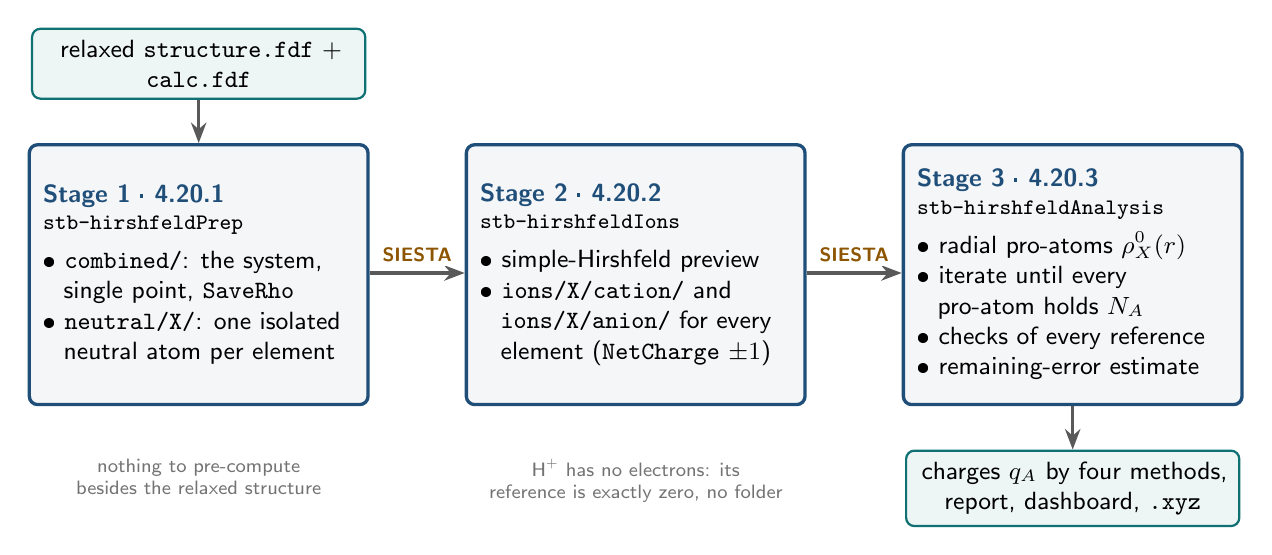
\begin{tikzpicture}[
    font=\sffamily\small,
    stage/.style={draw=stbblue, very thick, rounded corners=3pt, fill=stbblue!5,
      text width=3.95cm, align=flush left, inner sep=5pt, minimum height=3.3cm, anchor=north},
    io/.style={draw=stbteal, thick, rounded corners=3pt, fill=stbteal!7,
      text width=3.95cm, align=flush center, inner sep=4pt},
    head/.style={font=\sffamily\bfseries\small, text=stbblue},
    flow/.style={-{Stealth[length=2.6mm]}, very thick, color=black!65},
    run/.style={font=\sffamily\scriptsize\bfseries, text=stbamber!80!black, fill=white, inner sep=1.5pt}]
  \node[stage] (s1) at (0,0) {{\color{stbblue}\bfseries Stage 1 \textperiodcentered{} 4.20.1}\\[-1pt]
      {\ttfamily\footnotesize stb-hirshfeldPrep}\\[3pt]
      \textbullet~\texttt{combined/}: the system,\\\hspace*{0.8em}single point, \texttt{SaveRho}\\
      \textbullet~\texttt{neutral/X/}: one isolated\\\hspace*{0.8em}neutral atom per element};
  \node[stage] (s2) at (5.55,0) {{\color{stbblue}\bfseries Stage 2 \textperiodcentered{} 4.20.2}\\[-1pt]
      {\ttfamily\footnotesize stb-hirshfeldIons}\\[3pt]
      \textbullet~simple-Hirshfeld preview\\
      \textbullet~\texttt{ions/X/cation/} and\\\hspace*{0.8em}\texttt{ions/X/anion/} for every\\\hspace*{0.8em}element (\texttt{NetCharge} $\pm1$)};
  \node[stage] (s3) at (11.1,0) {{\color{stbblue}\bfseries Stage 3 \textperiodcentered{} 4.20.3}\\[-1pt]
      {\ttfamily\footnotesize stb-hirshfeldAnalysis}\\[3pt]
      \textbullet~radial pro-atoms $\rho^0_X(r)$\\
      \textbullet~iterate until every\\\hspace*{0.8em}pro-atom holds $N_A$\\
      \textbullet~checks of every reference\\
      \textbullet~remaining-error estimate};
  \node[io, above=0.55cm of s1] (in) {relaxed \texttt{structure.fdf} + \texttt{calc.fdf}};
  \node[io, below=0.55cm of s3] (out) {charges $q_A$ by four methods,\\ report, dashboard, \texttt{.xyz}};
  \draw[flow] (in) -- (s1);
  \draw[flow] ([yshift=-1.65cm]s1.north east) -- node[run, above=2pt] {SIESTA} ([yshift=-1.65cm]s2.north west);
  \draw[flow] ([yshift=-1.65cm]s2.north east) -- node[run, above=2pt] {SIESTA} ([yshift=-1.65cm]s3.north west);
  \draw[flow] (s3) -- (out);
  \node[font=\sffamily\scriptsize, text=black!55, below=0.55cm of s1, text width=3.95cm, align=flush center]
      {nothing to pre-compute\\ besides the relaxed structure};
  \node[font=\sffamily\scriptsize, text=black!55, below=0.55cm of s2, text width=3.95cm, align=flush center]
      {H\textsuperscript{+} has no electrons: its\\ reference is exactly zero, no folder};
\end{tikzpicture}
\caption{The three stages of the Hirshfeld-I workflow. Every SIESTA run between the stages is a
single point with the mesh, functional, basis and pseudopotentials of the system; only Stage~3 does
the partition, and it can be re-run in seconds with another \opt{--tol}.}
\label{fig-4.20-flow}
\end{figure}

\begin{theorybox}[Hirshfeld-I in five equations]
\textbf{Stockholder partition.} Place a spherical pro-atom $\rho^0_A$ on every nucleus (and on every
periodic image $\mathbf T$ of it, in a crystal \cite{Vanpoucke2013periodicHI}) and give atom $A$ the
fraction $w_A$ of the density at each point:
\begin{equation*}
w_A(\mathbf r)=\frac{\sum_{\mathbf T}\rho^0_A(|\mathbf r-\mathbf R_A-\mathbf T|)}
                    {\sum_B\sum_{\mathbf T}\rho^0_B(|\mathbf r-\mathbf R_B-\mathbf T|)},
\qquad
N_A=\int_{\text{cell}} w_A(\mathbf r)\,\rho(\mathbf r)\,d^3r,
\qquad q_A = Z^{\text{val}}_A-N_A .
\end{equation*}
The weights add up to one, so the charges always add up to the charge of the cell. The pieces
$\rho_A=w_A\rho$ are the ones closest to the pro-atoms in the information-theoretic sense: they minimize
$\sum_A\int\rho_A\ln(\rho_A/\rho^0_A)$ under $\sum_A\rho_A=\rho$ \cite{Nalewajski2000infoAIM,HeidarZadeh2018hirshfeld}.

\medskip\textbf{Self-consistent pro-atoms.} Neutral pro-atoms pull every charge toward zero. Hirshfeld-I asks
instead that each pro-atom hold as many electrons as the atom it defines, interpolating between the
neutral atom and the ion of the same sign:
\begin{equation*}
\int\rho^0_A\,d^3r = N_A,
\qquad
\rho^0_A(q)=(1-f)\,\rho^{0}_{X}+f\,\rho^{\pm}_{X},\quad f=\min(|q_A|,1),
\end{equation*}
solved by iteration from the simple-Hirshfeld charges until $\Delta q_n=\max_A|q_A^{(n)}-q_A^{(n-1)}|<\text{tol}$.
The solution does not depend on the starting point \cite{Bultinck2007uniqueness}.

\medskip\textbf{How far from the fixed point.} Near the solution each step is a fixed fraction $r$ of the
previous one, so the charges are still
\begin{equation*}
e_n\simeq\Delta q_n\,\frac{r}{1-r}
\end{equation*}
away when the loop stops --- about $2\times$tol for water ($r\approx0.67$), $3\times$tol for NaCl
($r\approx0.76$). Stage~3 measures $r$ and prints $e_n$.
\end{theorybox}

\begin{warnbox}[Before you quote a Hirshfeld-I charge]
\begin{itemize}[leftmargin=1.2em, itemsep=1pt, topsep=1pt]
  \item \textbf{Read the error estimate, not \opt{--tol}.} Tighten \opt{--tol} until the estimated
    remaining error is small; Stage~3 suggests the value, and re-running it needs no SIESTA.
  \item \textbf{Fix the basis.} In SIESTA the anion reference is only as diffuse as the orbitals allow:
    \fdf{PAO.EnergyShift} from 0.02 to 0.005~Ry moved $q(\mathrm O)$ of water from $-0.60$ to $-0.77$.
    Compare charges computed with one basis.
  \item \textbf{Past $\pm1$ the reference stops at the ion} (MgO: $\pm1.09$, flagged \emph{capped}): read it as a
    lower bound.
  \item \textbf{Quote the method with the number.} On one density Voronoi, Hirshfeld, Hirshfeld-I and Bader differed
    by factors of 2--4 (Section~\ref{g4.20-59-how-far-to-trust-each-number}).
\end{itemize}
\end{warnbox}

\subsection{Guide}
\label{guide-4.20}{\small\itshape The guide below is the hands-on tutorial of the documentation site. It follows the repository folder \texttt{examples/\allowbreak{}4.\allowbreak{}20-\allowbreak{}hirshfeld/}; file names in it are relative to that folder, and its script \texttt{example\_*.sh} reproduces every step.}

This workflow computes \textbf{Hirshfeld-I} (iterative Hirshfeld) atomic charges {[}5{]} from a SIESTA density, in 3 stages.
\textbf{Stage 1} (\texttt{stb-\allowbreak{}hirshfeldPrep}, code \texttt{4.\allowbreak{}20.\allowbreak{}1}) takes your relaxed structure and template and writes the system as a
single point that saves its density, plus one isolated \textbf{neutral atom} per element. \textbf{Stage 2}
(\texttt{stb-\allowbreak{}hirshfeldIons}, code \texttt{4.\allowbreak{}20.\allowbreak{}2}), after SIESTA ran there, writes the \textbf{cation and the anion} of every element.
\textbf{Stage 3} (\texttt{stb-\allowbreak{}hirshfeldAnalysis}, code \texttt{4.\allowbreak{}20.\allowbreak{}3}) builds a spherical reference from each isolated atom and
iterates the stockholder partition until every reference holds as many electrons as the atom it defines:

\begin{codeblock}
q_A = Z_A − ∫ w_A(r) ρ(r) d³r,     w_A = ρ_A⁰ / Σ_B ρ_B⁰,     ρ_A⁰ = (1 − |q_A|) ρ_neutral + |q_A| ρ_ion
\end{codeblock}

It reports the charges next to Voronoi, SIESTA\textquotesingle s own Hirshfeld and simple Hirshfeld (neutral references) of the
same density, with what you need to trust them: a check of every reference atom (electrons, radius, SCF), the
history of the iteration and an estimate of \textbf{how far the charges still are from the fixed point} when it stops,
the charge balance, a dipole check, and an optional dashboard.

It answers a question the rest of section 4 does not: not an energy or a spectrum, but \textbf{how many electrons each
atom owns} --- the number behind "the oxygen of water carries −0.7 e", oxidation-state arguments, charge transfer at
an interface, or the point charges of a force field. Section 1 explains why that number needs a definition and what
this one is; the worked example (Section 5) runs all three stages for real with SIESTA on water, N₂O (two atoms of
one element with opposite charges), the NaCl crystal and MgO (charges beyond ±1), plus mesh, box and basis studies
of water that show what the numbers depend on.

The three stages live in this one folder and this one tutorial --- same reasoning as \texttt{4.\allowbreak{}8}, \texttt{4.\allowbreak{}17}: each stage\textquotesingle s
output exists only to feed the next.

\subsubsection{1. Theory}\label{g4.20-1-theory}

\textbf{Symbols at a glance}

\begingroup\small\setlength{\LTpre}{0.4em}\setlength{\LTpost}{0.6em}
\begin{longtable}[]{@{}>{\raggedright\arraybackslash}p{(\linewidth - 4\tabcolsep) * \real{0.1901}}>{\raggedright\arraybackslash}p{(\linewidth - 4\tabcolsep) * \real{0.8099}}@{}}
\toprule\noalign{}
Symbol & Meaning \\
\midrule\noalign{}
\endhead
\bottomrule\noalign{}
\endlastfoot
\texttt{ρ(r)} & electron density of the system (the valence pseudo-density SIESTA writes, e/ų) \\
\texttt{ρ\_\allowbreak{}A⁰(r)} & the \textbf{pro-atom}: a spherical reference density of atom \texttt{A}, centred on its nucleus \\
\texttt{ρ⁰(r)\ =\allowbreak{}\ Σ\_\allowbreak{}A\ ρ\_\allowbreak{}A⁰} & the \textbf{promolecule}: all pro-atoms superposed at the atomic positions (every periodic image included) \\
\texttt{w\_\allowbreak{}A(r)\ =\allowbreak{}\ ρ\_\allowbreak{}A⁰/\allowbreak{}ρ⁰} & Hirshfeld weight of atom \texttt{A} at \texttt{r}, \texttt{0\ ≤\ w\_\allowbreak{}A\ ≤\ 1}, \texttt{Σ\_\allowbreak{}A\ w\_\allowbreak{}A\ =\allowbreak{}\ 1} \\
\texttt{N\_\allowbreak{}A}, \texttt{q\_\allowbreak{}A} & population of atom \texttt{A} (e) and its charge \texttt{q\_\allowbreak{}A\ =\allowbreak{}\ Z\_\allowbreak{}A\ −\ N\_\allowbreak{}A} (\texttt{\textgreater{}\ 0}: it lost electrons) \\
\texttt{Z\_\allowbreak{}A} & valence charge of \texttt{A}\textquotesingle s pseudopotential (\texttt{Z\_\allowbreak{}val}: O 6, H 1, Na 9, Mg 10, Cl 7) \\
\texttt{ρ\_\allowbreak{}X\^{}\{0\},\allowbreak{}\ ρ\_\allowbreak{}X\^{}\{+\},\allowbreak{}\ ρ\_\allowbreak{}X\^{}\{−\}} & spherically averaged density of the isolated neutral atom, cation and anion of element \texttt{X} \\
\texttt{f\ =\allowbreak{}\ min(abs(q),\allowbreak{}\ 1)} & the fraction of the ion mixed into a pro-atom \\
\texttt{Δq\_\allowbreak{}n} & \texttt{max\_\allowbreak{}A\ abs(q\_\allowbreak{}A\^{}(n)\ −\ q\_\allowbreak{}A\^{}(n−1))}, the step of iteration \texttt{n} (e) \\
\texttt{r} & the \textbf{contraction ratio} of the iteration, \texttt{Δq\_\allowbreak{}n\ /\allowbreak{}\ Δq\_\allowbreak{}\{n−1\}} \\
\texttt{μ} & dipole moment (Debye; 1 e Å = 4.803 D) \\
\end{longtable}
\endgroup

\paragraph{1.1 An atomic charge is a partition, not an observable}\label{g4.20-11-an-atomic-charge-is-a-partition-not-an-observable}

The density \texttt{ρ(r)} of a molecule or a crystal is an observable; the charge of one of its atoms is not. To say that
the oxygen of water carries \texttt{−0.\allowbreak{}7\ e} you must first say \textbf{which electrons belong to the oxygen}, that is, cut the
density into atomic pieces \texttt{ρ\_\allowbreak{}A(r)} that add up to the whole:

\begin{codeblock}
ρ(r) = Σ_A ρ_A(r),        N_A = ∫ ρ_A(r) d³r,        q_A = Z_A − N_A                         (1)
\end{codeblock}

There are many ways of cutting, and each gives its own numbers {[}1, 2{]}:

\begin{itemize}
\tightlist
\item
  \textbf{Space is divided into regions}, one per atom, with sharp boundaries: Voronoi cells (each point goes to the
  nearest nucleus; SIESTA\textquotesingle s \texttt{Charge.\allowbreak{}Voronoi}), Bader basins (the zero-flux surfaces of \texttt{ρ} {[}3{]}; \texttt{stb-\allowbreak{}bader}, 3.6).
\item
  \textbf{The basis set is divided}, not space: Mulliken and Löwdin populations. They need no grid but depend strongly
  on the basis.
\item
  \textbf{Every point is shared} among all atoms with smooth weights \texttt{w\_\allowbreak{}A(r)}, \texttt{ρ\_\allowbreak{}A\ =\allowbreak{}\ w\_\allowbreak{}A\ ρ}: the \textbf{stockholder}
  family --- Hirshfeld {[}4{]}, Hirshfeld-I {[}5{]}, iterated stockholder (ISA) {[}6{]}, MBIS {[}7{]}, DDEC {[}8{]}.
\end{itemize}

This workflow computes \textbf{Hirshfeld-I} charges, a member of the last family, and reports next to them the
simple Hirshfeld, Voronoi and (in the example) Bader charges of the same density, so the numbers can be compared
partition by partition.

\paragraph{1.2 The Hirshfeld (stockholder) partition}\label{g4.20-12-the-hirshfeld-stockholder-partition}

Hirshfeld\textquotesingle s idea {[}4{]} is to share the density at each point \textbf{in proportion to what the free atoms would have put
there}. Place a spherical reference atom \texttt{ρ\_\allowbreak{}A⁰} on every nucleus, add them up into the promolecule \texttt{ρ⁰}, and give
atom \texttt{A} the fraction

\begin{codeblock}
w_A(r) = ρ_A⁰(|r − R_A|) / ρ⁰(r),          ρ⁰(r) = Σ_B ρ_B⁰(|r − R_B|)                       (2)

N_A = ∫ w_A(r) ρ(r) d³r                                                                       (3)
\end{codeblock}

of the real density there --- like the shareholders of a company, each gets a share of the profit proportional to
its investment, hence the name. The weights add up to one at every point, so \texttt{Σ\_\allowbreak{}A\ N\_\allowbreak{}A\ =\allowbreak{}\ ∫ρ} exactly, whatever the
pro-atoms are: the charges always sum to the total charge.

The partition has a clean justification: the Hirshfeld atoms are the pieces \texttt{ρ\_\allowbreak{}A} that \textbf{stay as close as possible
to the free atoms}, in the sense that they minimize the information distance (Kullback--Leibler divergence) to the
pro-atoms,

\begin{codeblock}
Σ_A ∫ ρ_A(r) ln[ ρ_A(r) / ρ_A⁰(r) ] d³r     subject to   Σ_A ρ_A = ρ                          (4)
\end{codeblock}

and Eq. 2 is the exact minimizer {[}9{]}. The atoms overlap smoothly (no sharp boundary), are transferable between
similar environments, and need nothing but the density and the pro-atoms.

What they need \textbf{is a choice of pro-atoms}, and that is the weak point. The usual choice is the \textbf{neutral} free
atoms. It is known to make charges too small {[}5, 10{]}: the weight function is built from neutral atoms, so a region
where the oxygen of water has gained density is still shared as if the oxygen were neutral; the partition is
\emph{biased toward neutrality}. It is also arbitrary (why neutral? why not the ions, or a different neutral state?) and
breaks for a charged system, where \texttt{∫ρ⁰\ ≠\ ∫ρ}.

\paragraph{1.3 Hirshfeld-I: make the pro-atoms consistent with the atoms they produce}\label{g4.20-13-hirshfeld-i-make-the-pro-atoms-consistent-with-the-atoms-they-produce}

Bultinck \emph{et al.} {[}5{]} removed the arbitrariness with one condition: \textbf{each pro-atom must hold as many electrons as
the atom it defines},

\begin{codeblock}
∫ ρ_A⁰ d³r = N_A                                                                               (5)
\end{codeblock}

A pro-atom with a non-integer population is built by interpolating linearly between the isolated atoms of the
two integer charge states that bracket it. This workflow keeps the states −1, 0 and +1 of every element and builds,
for an atom with charge \texttt{q},

\begin{codeblock}
ρ_A⁰(q) = (1 − f) ρ_X^{0} + f ρ_X^{±},       f = min(abs(q), 1),   ± = sign of q                     (6)
\end{codeblock}

which integrates to \texttt{Z\_\allowbreak{}A\ −\ q} exactly for \texttt{abs(q)\ ≤\ 1} --- the linear interpolation is what keeps Eq. 5 exact. Eq. 5
is then solved by iteration:

\begin{codeblock}
q^(0)     = simple Hirshfeld (neutral pro-atoms, f = 0)
q^(n+1)   = Hirshfeld partition (Eqs. 2-3) with the pro-atoms ρ_A⁰(q_A^(n)) of Eq. 6                    (7)
stop when Δq_n = max_A abs(q_A^(n) − q_A^(n−1)) < tol
\end{codeblock}

Each atom chooses its \textbf{own} ion --- its cation when it is positive, its anion when negative --- so two atoms of the
same element can lean in opposite directions (the two nitrogens of N₂O do, Section 5.4). That is why Stage 2 writes
both ions of every element.

The self-consistent charges do not depend on the starting point {[}11{]} (no promolecule to choose), are only slightly
basis dependent, work for charged systems, are larger in magnitude than the simple Hirshfeld ones, and reproduce
the molecular electrostatic potential about as well as charges fitted to it {[}12{]}. Whether the solution is always
unique is not proven in general {[}13{]}; a counterexample with symmetry-equivalent atoms getting different charges
has been reported for some materials {[}8{]}. The workflow starts every atom from simple Hirshfeld, so
symmetry-equivalent atoms start equal and stay equal.

\paragraph{1.4 How far from converged: the contraction ratio}\label{g4.20-14-how-far-from-converged-the-contraction-ratio}

Near its solution the iteration of Eq. 7 behaves like a linear map: the error of every round is a fixed fraction
\texttt{r} of the previous one (the largest eigenvalue of the map\textquotesingle s Jacobian),

\begin{codeblock}
e_n ≈ r e_{n−1},          Δq_n = e_{n−1} − e_n ≈ e_n (1 − r) / r                                (8)

e_n ≈ Δq_n · r / (1 − r)        (the remaining error after round n)                              (9)
\end{codeblock}

So the usual stopping rule \texttt{Δq\_\allowbreak{}n\ \textless{}\ tol} does \textbf{not} bound the error of the charges: it bounds the last step, and
at \texttt{r\ =\allowbreak{}\ 0.\allowbreak{}68} (water) the charges are still \texttt{0.\allowbreak{}68\ /\allowbreak{}\ 0.\allowbreak{}32\ ≈\ 2.\allowbreak{}1\ ×\ tol} away from the fixed point when it fires. Stage 3
measures \texttt{r} from the last three steps, prints the estimate of Eq. 9, and warns --- with the \texttt{-\/-\allowbreak{}tol} that would make
the \emph{error} small --- when the estimate exceeds the tolerance (not below 0.001 e). The estimate needs no new SIESTA
run, and Section 5.3 checks it against the converged answer. \texttt{r} itself says how hard the partition is: it
approaches 1 when the charge transfer is large and the anion reference is very different from the neutral atom.

\paragraph{1.5 Periodic systems}\label{g4.20-15-periodic-systems}

Nothing in Eqs. 2--7 needs a molecule: in a crystal the promolecule is the sum of the pro-atoms of \textbf{every
periodic image} of every atom,

\begin{codeblock}
ρ⁰(r) = Σ_A Σ_T ρ_A⁰(|r − R_A − T|),        w_A(r) = Σ_T ρ_A⁰(|r − R_A − T|) / ρ⁰(r)             (10)
\end{codeblock}

and \texttt{N\_\allowbreak{}A} is integrated over one cell {[}14{]}. Stage 3 sums every image within the reach of each pro-atom (the radius
beyond which it vanishes, a few Å for SIESTA\textquotesingle s confined orbitals, Section 1.6). For a molecule in a large box that
is only the nearest image; in the 2-atom cell of rock salt a point near a Cl sees six Na neighbours at 2.8 Å, each a
different image of the same atom. (The first version of the workflow kept only the nearest image; Section 5.5
shows what that did to NaCl.)

\paragraph{1.6 Reference atoms with SIESTA}\label{g4.20-16-reference-atoms-with-siesta}

The pro-atoms are computed, not tabulated: one SIESTA run per element and charge state, a single atom in a cubic
box (\texttt{-\/-\allowbreak{}vacuum}, default 20 Å), at the level of theory of the system. Several consequences are worth knowing:

\begin{itemize}
\tightlist
\item
  \textbf{Valence pseudo-densities.} SIESTA\textquotesingle s \texttt{.\allowbreak{}RHO} holds only the electrons of the pseudopotential\textquotesingle s valence, so
  \texttt{Z\_\allowbreak{}A} is \texttt{Z\_\allowbreak{}val} and the core is in neither \texttt{ρ} nor \texttt{ρ⁰}. Semicore states are valence when the pseudopotential
  includes them: the PseudoDojo Na has 9 electrons (2s² 2p⁶ 3s¹), Mg 10; their cations are then Na⁺ with 8 and
  Mg⁺ with 9. Using pseudo-valence densities for Hirshfeld-I in solids was shown to reproduce the all-electron
  charges to good accuracy {[}15{]}.
\item
  \textbf{The same mesh, basis and functional} as the system (Stage 1 forces the same \texttt{MeshCutoff} into every folder,
  the template supplies the rest). The isolated atoms are run \textbf{spin-polarized} with Γ only.
\item
  \textbf{Confined orbitals confine the reference.} SIESTA\textquotesingle s numerical atomic orbitals are strictly zero beyond a
  cutoff radius set by \texttt{PAO.\allowbreak{}EnergyShift} (Section 5.7), so the density of every reference atom vanishes beyond it
  too --- a few Å, far inside the box. A free anion is a delicate object (the extra electron of O⁻ is weakly bound;
  O²⁻ is not bound at all in vacuum), and in a plane-wave code its density spreads over the whole box {[}14{]}; here the
  basis keeps it on the atom. The anion reference is therefore as confined as the basis, and the charges inherit a
  basis dependence through it.
\item
  \textbf{The bare proton.} H has \texttt{Z\_\allowbreak{}val\ =\allowbreak{}\ 1}, so H⁺ has no electrons: its density is exactly zero and no SIESTA run is
  needed (SIESTA could not converge it anyway). Stage 2 skips the folder; Stage 3 uses \texttt{ρ\_\allowbreak{}H\^{}\{+\}\ =\allowbreak{}\ 0}, so a positive
  hydrogen\textquotesingle s pro-atom is \texttt{(1\ −\ q)\ ρ\_\allowbreak{}H\^{}\{0\}}.
\item
  \textbf{Spherical averages.} An open-shell atom (O, N, Cl) is not spherical in a spin-polarized SCF: Stage 3 averages
  each reference over angles in shells 0.25 grid spacings wide (empty shells dropped) and checks that the profile
  still holds \texttt{Z\_\allowbreak{}val}, \texttt{Z\_\allowbreak{}val\ −\ 1} and \texttt{Z\_\allowbreak{}val\ +\ 1} electrons (\texttt{{[}2{]}} of the report).
\end{itemize}

\paragraph{1.7 Charges beyond ±1}\label{g4.20-17-charges-beyond-1}

Eq. 6 stops at the ions: when \texttt{abs(q)\ \textgreater{}\ 1}, the pro-atom is the ion itself (\texttt{f\ =\allowbreak{}\ 1}). The partition still returns
whatever charge the density gives, but Eq. 5 no longer holds (\texttt{N\_\allowbreak{}A\ ≠\ ∫ρ\_\allowbreak{}A⁰}), and the true Hirshfeld-I value
would need the next ion, Mg²⁺ or O²⁻. Mg²⁺ is an ordinary closed shell; O²⁻ is not bound in vacuum and must be
stabilized artificially, and different stabilizations give different charges --- the main known ambiguity of
Hirshfeld-I for oxides, which motivated the Hirshfeld-E scheme {[}16{]}. Stage 3 flags every such atom (\texttt{(capped)} in
\texttt{{[}5{]}} and a warning). MgO in Section 5.6 is the case.

\paragraph{1.8 What point charges can and cannot reproduce}\label{g4.20-18-what-point-charges-can-and-cannot-reproduce}

Atomic charges are often used to build the electrostatics of a model (force fields, the dipole of a molecule).
The dipole of a molecule is exactly

\begin{codeblock}
μ = Σ_A q_A R_A  +  Σ_A μ_A,        μ_A = −∫ (r − R_A) ρ_A(r) d³r                                  (11)
\end{codeblock}

--- the point charges plus the dipole of each atomic piece (the asymmetry of its cloud around its own nucleus). Any
partition satisfies Eq. 11 with its own \texttt{q\_\allowbreak{}A} and \texttt{μ\_\allowbreak{}A}; the point-charge term alone depends on how much of the
dipole the partition put into the charges. Stage 3 prints the point-charge dipole of every method next to SIESTA\textquotesingle s
dipole of the full density, along the axes where a dipole is defined (non-periodic ones). Neither "closer is
better" nor "larger is better" is a law: Hirshfeld charges are known to be too small to give the dipole by
themselves, Hirshfeld-I charges are larger and leave a smaller, opposite atomic-dipole term {[}10, 12{]}. The comparison
says which charges carry the electrostatics in a given molecule (Section 5.2).

\paragraph{1.9 A calculation you can check by hand}\label{g4.20-19-a-calculation-you-can-check-by-hand}

The water molecule of Section 5.2: \texttt{{[}4{]}} of its report (and \texttt{hirshfeld\_\allowbreak{}iterations.\allowbreak{}dat}) lists the step of every round,
and the last three are

\begin{codeblock}
Δq_8 = 0.008415    Δq_9 = 0.005665    Δq_10 = 0.003820 e
r ≈ 0.005665/0.008415 = 0.673,   0.003820/0.005665 = 0.674
e_10 ≈ 0.003820 × 0.673 / (1 − 0.673) = 0.0079 e              (Eq. 9; the report prints 0.0079)
\end{codeblock}

so \texttt{q(O)\ =\allowbreak{}\ −0.\allowbreak{}7002\ e} after round 10 should be \texttt{≈\ −0.\allowbreak{}708\ e} at the fixed point --- the run at \texttt{-\/-\allowbreak{}tol\ 1e-\allowbreak{}6} gives
\texttt{−0.\allowbreak{}7082} (Section 5.3). The charges add up: \texttt{q(O)\ +\ 2\ q(H)\ =\allowbreak{}\ −0.\allowbreak{}7002\ +\ 2\ ×\ 0.\allowbreak{}3501\ =\allowbreak{}\ 0.\allowbreak{}0000\ e}. And the reference of the
oxygen at the end, \texttt{0.\allowbreak{}70\ anion} in \texttt{{[}5{]}}, is Eq. 6 with \texttt{f\ =\allowbreak{}\ 0.\allowbreak{}70}: \texttt{0.\allowbreak{}30\ ρ\_\allowbreak{}O\^{}0\ +\ 0.\allowbreak{}70\ ρ\_\allowbreak{}O\^{}−}, which holds
\texttt{0.\allowbreak{}30\ ×\ 6\ +\ 0.\allowbreak{}70\ ×\ 7\ =\allowbreak{}\ 6.\allowbreak{}70} electrons --- its population, as Eq. 5 demands.

\subsubsection{2. Libraries and external dependencies used}\label{g4.20-2-libraries-and-external-dependencies-used}

\begin{itemize}
\tightlist
\item
  \textbf{SIESTA} {[}18, 19{]} itself is \emph{not} called by the suite. It does the real work: one SCF per folder --- the system, and
  every element as an isolated neutral atom, cation and anion --- writing the density on its real-space grid
  (\texttt{\textless{}label\textgreater{}.\allowbreak{}RHO}, because \texttt{SaveRho} is forced) and the log (\texttt{calc.\allowbreak{}out}) with \texttt{Z\_\allowbreak{}val}, the SCF convergence, its own
  Hirshfeld and Voronoi charges and the dipole. The reference data of Section 5 was produced with SIESTA 5.4.2,
  GGA-PBE {[}20{]}, PseudoDojo norm-conserving pseudopotentials {[}21{]} and Monkhorst--Pack k-grids {[}22{]}.
\item
  \textbf{\href{https://zerothi.github.io/sisl/}{sisl}} {[}23{]} --- reads the \texttt{.\allowbreak{}RHO} grids (spin up + down).
\item
  \textbf{numpy} --- the radial profiles, the promolecule on the grid with its periodic images, the weights and the
  integrals of Eqs. 2--3, the iteration.
\item
  \textbf{\href{https://pymatgen.org/}{pymatgen}} {[}24{]} / \textbf{ASE} {[}25{]} --- structure reading and the dimensionality of the cell
  (which axes have vacuum, for the dipole check).
\item
  \textbf{\href{https://matplotlib.org/}{matplotlib}} {[}26{]} --- the 6-panel dashboard of Stage 3 (\texttt{-\/-\allowbreak{}png} / \texttt{-\/-\allowbreak{}show}).
\end{itemize}

\subsubsection{3. Stages 1 and 2: the folders}\label{g4.20-3-stages-1-and-2-the-folders}

The reference atoms cannot all be written at once: whether an element needs its ions at all, and how each ion
behaves, is only known after the neutral atoms ran. So there are two writing stages, with SIESTA between them:

\begin{codeblock}
stb-hirshfeldPrep  ->  SIESTA in combined/, neutral/*  ->  stb-hirshfeldIons  ->  SIESTA in ions/*/*  ->  stb-hirshfeldAnalysis
   (4.20.1)                                                  (4.20.2)                                       (4.20.3)
\end{codeblock}

\paragraph{\texorpdfstring{3.1 Stage 1 (\texttt{stb-\allowbreak{}hirshfeldPrep}, code \texttt{4.\allowbreak{}20.\allowbreak{}1})}{3.1 Stage 1 (stb-hirshfeldPrep, code 4.20.1)}}\label{g4.20-31-stage-1-stb-hirshfeldprep-code-4201}

Takes the \textbf{relaxed} structure (\texttt{-s}, default \texttt{structure.\allowbreak{}fdf}) and your template (\texttt{-\/-\allowbreak{}calc}, default \texttt{calc.\allowbreak{}fdf}; it must
\texttt{\%include\ structure.\allowbreak{}fdf} and use an implicit basis such as \texttt{PAO.\allowbreak{}BasisSize\ DZP}, which works for any subset of the
elements) and writes

\begin{codeblock}
<output-dir>/                          (-O, default hirshfeld_study)
    combined/        structure.fdf, calc.fdf, config_extra.fdf, the pseudopotentials
    neutral/<El>/    one isolated atom per element, in a cubic box of side --vacuum
    hirshfeld_manifest.json            what Stage 2 reads (paths RELATIVE to the study: copy or move it freely)
    hirshfeld_prep_report.txt          with --save-report
\end{codeblock}

Every \texttt{calc.\allowbreak{}fdf} is \texttt{\%include\ config\_\allowbreak{}extra.\allowbreak{}fdf} above your template, untouched; SIESTA\textquotesingle s fdf reader is
first-occurrence-wins, so the forced settings beat the template\textquotesingle s:

\begingroup\small\setlength{\LTpre}{0.4em}\setlength{\LTpost}{0.6em}
\begin{longtable}[]{@{}>{\raggedright\arraybackslash}p{(\linewidth - 8\tabcolsep) * \real{0.2869}}>{\raggedright\arraybackslash}p{(\linewidth - 8\tabcolsep) * \real{0.1736}}>{\raggedright\arraybackslash}p{(\linewidth - 8\tabcolsep) * \real{0.2181}}>{\raggedright\arraybackslash}p{(\linewidth - 8\tabcolsep) * \real{0.3214}}@{}}
\toprule\noalign{}
Directive & \texttt{combined/\allowbreak{}} & \texttt{neutral/\allowbreak{}\textless{}El\textgreater{}/\allowbreak{}} (and the ions) & Why \\
\midrule\noalign{}
\endhead
\bottomrule\noalign{}
\endlastfoot
\texttt{MD.\allowbreak{}VariableCell\ false}, \texttt{MD.\allowbreak{}TypeOfRun\ CG}, \texttt{MD.\allowbreak{}Steps\ 0} & forced & forced & a single point at the geometry given \\
\texttt{MeshCutoff} & \texttt{-\/-\allowbreak{}mesh-\allowbreak{}cutoff} (400 Ry) & the same & every density on a comparably fine grid \\
\texttt{SaveRho\ true} & forced & forced & Stage 2/3 read the \texttt{.\allowbreak{}RHO} \\
\texttt{Charge.\allowbreak{}Hirshfeld\ end}, \texttt{Charge.\allowbreak{}Voronoi\ end} & forced & --- & SIESTA\textquotesingle s own charges of the same density, for comparison \\
\texttt{kgrid.\allowbreak{}MonkhorstPack} & the template\textquotesingle s & \texttt{{[}1\ 1\ 1{]}} & one atom in a box needs Γ only \\
\texttt{Spin} & the template\textquotesingle s & \texttt{polarized} (also written into \texttt{calc.\allowbreak{}fdf}) & an isolated atom is usually an open shell \\
\end{longtable}
\endgroup

The box (\texttt{-\/-\allowbreak{}vacuum}, 20 Å) only has to hold the atom: SIESTA\textquotesingle s atom densities vanish beyond the orbital radii (≈ 2--4 Å
here), so 10 Å would do (Section 5.7); Stage 3 checks it.

\paragraph{\texorpdfstring{3.2 Stage 2 (\texttt{stb-\allowbreak{}hirshfeldIons}, code \texttt{4.\allowbreak{}20.\allowbreak{}2})}{3.2 Stage 2 (stb-hirshfeldIons, code 4.20.2)}}\label{g4.20-32-stage-2-stb-hirshfeldions-code-4202}

After SIESTA ran in \texttt{combined/\allowbreak{}} and every \texttt{neutral/\allowbreak{}\textless{}El\textgreater{}/\allowbreak{}}, Stage 2 (\texttt{-O} the same study) reads \texttt{Z\_\allowbreak{}val} of every element
from the log of \texttt{combined/\allowbreak{}} (\texttt{-\/-\allowbreak{}ref} for a log not named \texttt{*.\allowbreak{}out}), the neutral densities, and writes

\begin{codeblock}
ions/<El>/cation/    NetCharge +1  (Z_val - 1 electrons)
ions/<El>/anion/     NetCharge -1  (Z_val + 1 electrons)
hirshfeld_ions_manifest.json
\end{codeblock}

for \textbf{every} element --- both ions, because in Stage 3 each atom chooses its own (Section 1.3). The exception is an element
with \texttt{Z\_\allowbreak{}val\ ≤\ 1} (H): its cation has no electrons at all, an exactly zero density, so no folder is written and Stage 3
uses zero. Its report also previews the simple-Hirshfeld charges of \texttt{combined/\allowbreak{}} (pass 0, what Stage 3 starts from) next
to SIESTA\textquotesingle s own, and counts how many atoms of each element lean positive or negative.

\paragraph{3.3 Running them}\label{g4.20-33-running-them}

\begin{codeblock}
stb-hirshfeldPrep -s structure.fdf --calc calc.fdf -p dojo --save-report         # Stage 1
for d in hirshfeld_study/combined hirshfeld_study/neutral/*; do (cd $d && mpirun -np 4 siesta calc.fdf > calc.out); done
stb-hirshfeldIons -O hirshfeld_study -p dojo --save-report                        # Stage 2
for d in hirshfeld_study/ions/*/*; do (cd $d && mpirun -np 4 siesta calc.fdf > calc.out); done
stb-suite            # or: 4 (Workflow) -> 20 (Hirshfeld-I) -> 1 / 2   (4.20.1, 4.20.2)
\end{codeblock}

The isolated-atom runs are small (one atom, Γ only): a few seconds to a few minutes each. An anion can need more SCF
iterations than the neutral atom (Na⁻ took 25); \texttt{{[}2{]}} of Stage 3 reports each one.

\subsubsection{\texorpdfstring{4. Stage 3: the analysis (\texttt{stb-\allowbreak{}hirshfeldAnalysis}, code \texttt{4.\allowbreak{}20.\allowbreak{}3})}{4. Stage 3: the analysis (stb-hirshfeldAnalysis, code 4.20.3)}}\label{g4.20-4-stage-3-the-analysis-stb-hirshfeldanalysis-code-4203}

\paragraph{4.1 What it does}\label{g4.20-41-what-it-does}

Reads every reference folder, builds its radial profile (Section 1.6), reads \texttt{combined/\allowbreak{}}\textquotesingle s density, runs simple
Hirshfeld (pass 0) and iterates Hirshfeld-I (Eq. 7) until \texttt{max\textbar{}Δq\textbar{}\ \textless{}\ -\/-\allowbreak{}tol} (default 0.005 e) or \texttt{-\/-\allowbreak{}max-\allowbreak{}iter} (20). The
iteration is cheap --- seconds for the molecules of Section 5 --- and needs no new SIESTA run, so \texttt{-\/-\allowbreak{}tol} can be tightened at
will (Section 5.3).

\paragraph{4.2 Report structure}\label{g4.20-42-report-structure}

\begingroup\small\setlength{\LTpre}{0.4em}\setlength{\LTpost}{0.6em}
\begin{longtable}[]{@{}>{\raggedright\arraybackslash}p{(\linewidth - 4\tabcolsep) * \real{0.1236}}>{\raggedright\arraybackslash}p{(\linewidth - 4\tabcolsep) * \real{0.8764}}@{}}
\toprule\noalign{}
Section & Content \\
\midrule\noalign{}
\endhead
\bottomrule\noalign{}
\endlastfoot
\texttt{{[}0{]}} & run metadata \\
\texttt{{[}1{]}} & the combined system: periodicity, grid, \texttt{Z\_\allowbreak{}val} per element, electrons in the density, SCF \\
\texttt{{[}2{]}} & every \textbf{reference atom}: target electrons, on the grid, in the radial profile, the radius holding 99.9 \% against the box, grid spacing, SCF \\
\texttt{{[}3{]}} & the iteration, round by round, with the atom that moved most \\
\texttt{{[}4{]}} & \textbf{convergence history}: the step and its ratio to the previous one, the contraction ratio, the estimated remaining error (Eq. 9) \\
\texttt{{[}5{]}} & per atom: Voronoi and Hirshfeld (SIESTA), simple Hirshfeld, Hirshfeld-I, their difference, the population, the reference used (\texttt{0.\allowbreak{}70\ anion} = 30 \% neutral + 70 \% anion; \texttt{(capped)} past ±1) \\
\texttt{{[}6{]}} & per element: mean, spread, how many atoms are cation- or anion-like, means of the other methods, the Hirshfeld-I / Hirshfeld ratio \\
\texttt{{[}7{]}} & charge balance: total charge by every method, electrons assigned, simple Hirshfeld here vs SIESTA\textquotesingle s \\
\texttt{{[}8{]}} & the \textbf{dipole check} along the non-periodic axes (Section 1.8) \\
\texttt{{[}9{]}} & summary and files written \\
\texttt{{[}10{]}} & every warning \\
\end{longtable}
\endgroup

\paragraph{4.3 The checks}\label{g4.20-43-the-checks}

\begingroup\small\setlength{\LTpre}{0.4em}\setlength{\LTpost}{0.6em}
\begin{longtable}[]{@{}>{\raggedright\arraybackslash}p{(\linewidth - 6\tabcolsep) * \real{0.3711}}>{\raggedright\arraybackslash}p{(\linewidth - 6\tabcolsep) * \real{0.1509}}>{\raggedright\arraybackslash}p{(\linewidth - 6\tabcolsep) * \real{0.4780}}@{}}
\toprule\noalign{}
Check & Warns when & What to do \\
\midrule\noalign{}
\endhead
\bottomrule\noalign{}
\endlastfoot
electrons in the combined density vs \texttt{Σ\ Z\_\allowbreak{}val} & they differ by \textgreater{} 0.02 e & a charged run (then the charges add up to it) or a \texttt{Z\_\allowbreak{}val} that does not match \\
SCF of \texttt{combined/\allowbreak{}} and of every reference & not confirmed in the log & converge it: the charges are only as good as the density \\
electrons of each reference on its grid vs \texttt{Z\_\allowbreak{}val}, \texttt{Z\_\allowbreak{}val\ ∓\ 1} & \textgreater{} 0.02 e & a wrong charge state or pseudopotential \\
the radial profile vs the grid & \textgreater{} max(0.02 e, 0.5 \%) & a mesh too coarse to average the atom \\
the radius holding 99.9 \% vs the box & \textgreater{} 80 \% of the inradius & a larger \texttt{-\/-\allowbreak{}vacuum} \\
electrons assigned to no atom & \textgreater{} 0.02 e & density where no reference reaches \\
\texttt{abs(q)\ \textgreater{}\ 1} & always & the reference stops at ±1 (Section 1.7) \\
the estimated remaining error & \textgreater{} \texttt{-\/-\allowbreak{}tol} (and \textgreater{} 0.001 e) & it prints the \texttt{-\/-\allowbreak{}tol} that would make the error small \\
not converged within \texttt{-\/-\allowbreak{}max-\allowbreak{}iter} & always & more rounds \\
\end{longtable}
\endgroup

A missing reference \texttt{.\allowbreak{}RHO} stops it with an \texttt{{[}ERROR{]}} naming the folder: a reference cannot be guessed.

\paragraph{4.4 Output files (all opt-in)}\label{g4.20-44-output-files-all-opt-in}

\begingroup\small\setlength{\LTpre}{0.4em}\setlength{\LTpost}{0.6em}
\begin{longtable}[]{@{}>{\raggedright\arraybackslash}p{(\linewidth - 4\tabcolsep) * \real{0.2023}}>{\raggedright\arraybackslash}p{(\linewidth - 4\tabcolsep) * \real{0.7977}}@{}}
\toprule\noalign{}
Option & Writes \\
\midrule\noalign{}
\endhead
\bottomrule\noalign{}
\endlastfoot
\texttt{-\/-\allowbreak{}save-\allowbreak{}data} & \texttt{hirshfeld\_\allowbreak{}charges.\allowbreak{}dat} (per atom: every method, population, reference), \texttt{hirshfeld\_\allowbreak{}iterations.\allowbreak{}dat} (every atom\textquotesingle s charge per round), \texttt{hirshfeld\_\allowbreak{}charges.\allowbreak{}xyz} (extended XYZ with the charges as per-atom columns; \texttt{ase\ gui} colours atoms by them) \\
\texttt{-\/-\allowbreak{}png} / \texttt{-\/-\allowbreak{}show} & the 6-panel dashboard \texttt{hirshfeld\_\allowbreak{}analysis.\allowbreak{}png}: convergence with the tolerance and the estimated error, each atom\textquotesingle s charge per round, the mean charge per element by method, Hirshfeld-I vs simple Hirshfeld per atom, the reference profiles \texttt{4πr²ρ(r)}, the structure coloured by charge (\texttt{-\/-\allowbreak{}show} without a display saves the PNG) \\
\texttt{-\/-\allowbreak{}save-\allowbreak{}report} & \texttt{hirshfeld\_\allowbreak{}analysis\_\allowbreak{}report.\allowbreak{}txt} \\
\end{longtable}
\endgroup

\paragraph{4.5 Running it both ways}\label{g4.20-45-running-it-both-ways}

\begin{codeblock}
stb-hirshfeldAnalysis -O hirshfeld_study --save-data --png --save-report
stb-hirshfeldAnalysis -O hirshfeld_study --tol 1e-4 --max-iter 100          # tighter, seconds more
stb-suite            # then: 4 -> 20 -> 3  (4.20.3): it asks for the folder, tolerance and outputs
\end{codeblock}

\subsubsection{5. Worked example: four systems, end to end}\label{g4.20-5-worked-example-four-systems-end-to-end}

\paragraph{5.1 Set-up}\label{g4.20-51-set-up}

\begingroup\small\setlength{\LTpre}{0.4em}\setlength{\LTpost}{0.6em}
\begin{longtable}[]{@{}>{\raggedright\arraybackslash}p{(\linewidth - 8\tabcolsep) * \real{0.0863}}>{\raggedright\arraybackslash}p{(\linewidth - 8\tabcolsep) * \real{0.4871}}>{\raggedright\arraybackslash}p{(\linewidth - 8\tabcolsep) * \real{0.2647}}>{\raggedright\arraybackslash}p{(\linewidth - 8\tabcolsep) * \real{0.1619}}@{}}
\toprule\noalign{}
System & Why & Cell & Template \\
\midrule\noalign{}
\endhead
\bottomrule\noalign{}
\endlastfoot
H₂O & a polar molecule; the base case of every study & 14 Å cube & \texttt{calc.\allowbreak{}fdf} \\
N₂O & two atoms of one element with opposite charges & 14 Å cube & \texttt{calc.\allowbreak{}fdf} \\
NaCl & an ionic crystal: periodic images, semicore Na & 2-atom fcc primitive cell & \texttt{calc\_\allowbreak{}bulk.\allowbreak{}fdf} \\
MgO & an oxide whose charges pass ±1 & 2-atom fcc primitive cell & \texttt{calc\_\allowbreak{}bulk.\allowbreak{}fdf} \\
\end{longtable}
\endgroup

All with SIESTA 5.4.2, PBE {[}20{]}, PseudoDojo pseudopotentials {[}21{]} (\texttt{Z\_\allowbreak{}val}: H 1, N 5, O 6, Na 9, Mg 10, Cl 7 --- Na and
Mg with their 2s 2p semicore), DZP basis with \texttt{PAO.\allowbreak{}EnergyShift\ 0.\allowbreak{}01\ Ry}, \texttt{MeshCutoff\ 400\ Ry}, 300 K smearing; the
molecules at Γ, the crystals with an 8×8×8 Monkhorst--Pack grid {[}22{]}. Each structure was relaxed first with the same
template (the molecules at fixed cell, 0.01 eV/Å; the crystals with the cell, 0.05 GPa): O--H 0.975 Å and 104.4°
(experiment 0.958 Å, 104.5° {[}28{]}), N--N 1.163 and N--O 1.203 Å (1.128 and 1.184 Å {[}28{]}), \texttt{a} = 5.674 Å for NaCl and
4.250 Å for MgO (5.64 and 4.21 Å measured; PBE overestimates lattice constants by about this much). The isolated
atoms sit in 20 Å boxes (the default).

\begin{codeblock}
stb-hirshfeldPrep -s relaxed.fdf --calc calc.fdf -p dojo -O h2o --mesh-cutoff 400 --save-report
for d in h2o/combined h2o/neutral/*; do (cd $d && mpirun -np 4 siesta calc.fdf > calc.out); done
stb-hirshfeldIons -O h2o -p dojo --save-report
for d in h2o/ions/*/*; do (cd $d && mpirun -np 4 siesta calc.fdf > calc.out); done
stb-hirshfeldAnalysis -O h2o --save-data --png --save-report
\end{codeblock}

\paragraph{5.2 Water: the three stages}\label{g4.20-52-water-the-three-stages}

\textbf{Stage 1} writes \texttt{combined/\allowbreak{}}, \texttt{neutral/\allowbreak{}O/\allowbreak{}} and \texttt{neutral/\allowbreak{}H/\allowbreak{}}; the isolated atoms get, in their \texttt{config\_\allowbreak{}extra.\allowbreak{}fdf},

\begin{codeblock}
MD.VariableCell false        MD.TypeOfRun CG    MD.Steps 0      kgrid.MonkhorstPack [1 1 1]
MeshCutoff 400 Ry            SaveRho true       Spin polarized
\end{codeblock}

\textbf{Stage 2}, after SIESTA, reads \texttt{Z\_\allowbreak{}val} from the log, previews pass 0 and writes the ions:

\begin{codeblock}
Idx | Elem | Z_val | Population(e-) | Charge(e-) | Native Hirshfeld(e-)
1   | O    | 6.0   | 6.2555         | -0.2555    | -0.2421
2   | H    | 1.0   | 0.8723         | +0.1277    | +0.1211
  [OK] O: ions/O/cation/ (NetCharge +1.0), ions/O/anion/ (NetCharge -1.0)
  [OK] H: ions/H/anion/ (NetCharge -1.0); cation SKIPPED (Z_val=1 -- NetCharge +1.0 would leave 0 electrons ...)
\end{codeblock}

\textbf{Stage 3} first checks the five references SIESTA computed (and the exact zero of H⁺):

\begin{codeblock}
Elem | State   | Target N | N on grid | N radial  | Radial-target | r99.9%(Ang) | Box inradius(Ang) | Spacing(Ang) | SCF conv.
O    | neutral | 6        | 6.0000    | 6.0053    | +0.0053       | 1.91        | 10.00             | 0.0800       | yes (9)
O    | cation  | 5        | 5.0000    | 5.0052    | +0.0052       | 1.81        | 10.00             | 0.0800       | yes (9)
O    | anion   | 7        | 7.0000    | 7.0054    | +0.0054       | 1.97        | 10.00             | 0.0800       | yes (13)
H    | neutral | 1        | 1.0000    | 1.0015    | +0.0015       | 2.39        | 10.00             | 0.0800       | yes (6)
H    | cation  | 0        | 0 (exact) | 0 (exact) | -             | -           | -                 | -            | -
H    | anion   | 2        | 2.0000    | 2.0012    | +0.0012       | 2.49        | 10.00             | 0.0800       | yes (12)
\end{codeblock}

Every reference holds exactly its electrons (\texttt{NetCharge\ −1} gives 7.0000 on O: the sign convention is right), the
spherical averages hold them to 0.1 \%, and 99.9 \% of each atom lies within 2.5 Å --- a fifth of its box. Then the
iteration:

\begin{codeblock}
Iteration | max|Delta q| (e-) | Ratio to previous | Atom that moved most
1         | 0.159092          | -                 | #1 (O)
2         | 0.100813          | 0.634             | #1 (O)
...
9         | 0.005665          | 0.673             | #1 (O)
10        | 0.003820          | 0.674             | #1 (O)
Converged after 10 iteration(s) (max|Delta q| < 0.005 e-).
Contraction ratio      : 0.673 (each step ~67 % of the previous)
Est. remaining error   : 0.0079 e- on the slowest atom, distance to the converged charges
\end{codeblock}

and the charges, with the dipole check:

\begin{codeblock}
Idx | Elem | Voronoi(e-) | Hirsh. SIESTA(e-) | Simple Hirshfeld(e-) | Hirshfeld-I(e-) | HI - H(e-) | Pop. HI(e-) | Reference
1   | O    | -0.1905     | -0.2421           | -0.2555              | -0.7002         | -0.4447    | 6.7002      | 0.70 anion
2   | H    | +0.0953     | +0.1211           | +0.1277              | +0.3501         | +0.2224    | 0.6499      | 0.35 cation
3   | H    | +0.0953     | +0.1211           | +0.1277              | +0.3501         | +0.2224    | 0.6499      | 0.35 cation

Component (Debye) | Voronoi (SIESTA) | Hirshfeld (SIESTA) | Simple Hirshfeld (pass 0) | Hirshfeld-I | SIESTA (density)
|mu|              | 0.547            | 0.695              | 0.733                     | 2.010       | 1.430
\end{codeblock}

\stbfigure{4.20-hirshfeld/figures/h2o_dashboard.png}{Dashboard of water}

\emph{Fig. 1 --- The dashboard of water (\texttt{-\/-\allowbreak{}png}): the step per round with the tolerance and the estimated remaining error;
the charge of each atom per round (0 = simple Hirshfeld); the mean charge per element by method; Hirshfeld-I against
simple Hirshfeld per atom (slope 2.74); the reference atoms \texttt{4πr²ρ(r)} (neutral, cation, anion); the molecule coloured
by charge.}

Reading it:

\begin{itemize}
\tightlist
\item
  \textbf{Hirshfeld-I is 2.7× simple Hirshfeld}: O −0.70 against −0.26. The iteration moves the oxygen steadily away from
  neutral (Fig. 1, second panel) and stops at a reference that is 70 \% O⁻. Fig. 2 shows why the numbers change: with the
  oxygen\textquotesingle s reference made more negative (more diffuse) and the hydrogens\textquotesingle{} smaller (\texttt{(1\ −\ 0.\allowbreak{}35)\ ρ\_\allowbreak{}H\^{}0}, H⁺ has no
  density), the point where the hydrogen\textquotesingle s share of the density falls to one half moves from 0.73 to 0.80 Å along the
  0.975 Å bond --- the oxygen owns more of the bond.
\item
  \textbf{Simple Hirshfeld here and SIESTA\textquotesingle s own agree} (−0.256 and −0.242): both use neutral references, SIESTA its own
  free-atom densities from the basis, this tool the SCF atoms of \texttt{neutral/\allowbreak{}}; the 0.013 e difference is that choice.
  Voronoi gives less (−0.19), a different partition altogether (the cell of each nucleus, {[}27{]}).
\item
  \textbf{The dipole:} SIESTA\textquotesingle s dipole of the density is 1.43 D (the experiment gives 1.855 D {[}28{]}: DZP is short of diffuse
  functions, Section 5.7). Point charges alone give 0.55--0.73 D with the neutral-reference methods and 2.01 D with
  Hirshfeld-I: by Eq. 11, the Hirshfeld atoms carry a large atomic-dipole term in the same direction (+0.70 D), the
  Hirshfeld-I atoms a smaller one in the opposite direction (−0.58 D). Neither set of point charges \emph{is} the dipole;
  Hirshfeld-I\textquotesingle s are the ones that put most of the electrostatics into the charges {[}12{]}.
\end{itemize}

\stbfigure{4.20-hirshfeld/figures/stockholder_weights.png}{Hirshfeld weights along the O-H bond}

\emph{Fig. 2 --- Left: the pro-atoms along the O→H bond, neutral (solid) and at the converged charges (dashed); SIESTA\textquotesingle s
pseudo-density of O has a dip at the nucleus, where the core was removed. Right: the hydrogen\textquotesingle s weight \texttt{w\_\allowbreak{}H} (Eq. 2)
with neutral pro-atoms and with the converged Hirshfeld-I ones. \texttt{python3\ study\_\allowbreak{}table.\allowbreak{}py\ -\/-\allowbreak{}png}.}

\paragraph{5.3 How converged is "converged"}\label{g4.20-53-how-converged-is-converged}

The report\textquotesingle s warning on water: \emph{"The last step was 0.0038 e-, but at a contraction ratio of 0.67 the charges are still
\textasciitilde0.0079 e- from the converged Hirshfeld-I values (1.6 x -\/-tol). For the error itself to be below 0.005 e-, rerun with
-\/-tol 0.0024"}. Each system was also run at \texttt{-\/-\allowbreak{}tol\ 1e-\allowbreak{}6} (\texttt{analysis\_\allowbreak{}tight/\allowbreak{}}), which gives the true error of every round
(\texttt{study\_\allowbreak{}table.\allowbreak{}py} \texttt{{[}C{]}}):

\begingroup\small\setlength{\LTpre}{0.4em}\setlength{\LTpost}{0.6em}
\begin{longtable}[]{@{}llllllll@{}}
\toprule\noalign{}
Round & H₂O step & estimate (Eq. 9) & true error & & NaCl step & estimate & true error \\
\midrule\noalign{}
\endhead
\bottomrule\noalign{}
\endlastfoot
8 & 0.00842 & 0.0171 & 0.0174 & & 0.01143 & 0.0348 & 0.0371 \\
10 & \textbf{0.00382} & \textbf{0.0079} & \textbf{0.0080} & & 0.00661 & 0.0210 & 0.0218 \\
12 & 0.00174 & 0.0036 & 0.0036 & & \textbf{0.00387} & \textbf{0.0126} & \textbf{0.0129} \\
14 & 0.00080 & 0.0017 & 0.0017 & & 0.00228 & 0.0075 & 0.0076 \\
\end{longtable}
\endgroup

\stbfigure{4.20-hirshfeld/figures/h2o_studies.png}{Water studies}

\emph{Fig. 3 --- Left: the true distance of the charges from the fixed point per round (solid) and the estimate of Eq. 9 (dashed)
for the four systems. Middle: q(O) of water against the mesh and the isolated-atom box, in 10⁻³ e. Right: q(O) for six
basis sets, with the radius that holds 99.9 \% of the O⁻ reference. \texttt{python3\ study\_\allowbreak{}table.\allowbreak{}py\ -\/-\allowbreak{}png}.}

\begin{itemize}
\tightlist
\item
  \textbf{The stopping rule is not the error.} At the default \texttt{-\/-\allowbreak{}tol\ 0.\allowbreak{}005} the charges of water are 0.008 e from the fixed
  point, those of NaCl 0.013 e (2.6 × tol): the iteration contracts slowly (ratio 0.67 and 0.76) and the last step is only
  a fraction \texttt{1\ −\ r} of the error.
\item
  \textbf{Eq. 9 predicts it.} For water and N₂O the estimate agrees with the true error to 1 \% from round 3 on. For NaCl it is
  2--7 \% low, because the ratio itself still creeps up (0.70 → 0.77): the iteration is not yet in its linear regime, and a
  ratio that grows makes the geometric sum an underestimate. The suggested \texttt{-\/-\allowbreak{}tol} (0.0015 for NaCl) gets the error
  below 0.005 e anyway.
\item
  \textbf{It costs nothing to ask for more.} The iteration needs no SIESTA run: water to 10⁻⁶ e in 32 rounds, N₂O in 24, NaCl
  in 44 --- seconds each. The converged charges: H₂O O −0.7082, H +0.3541; NaCl ±0.5143.
\item
  \textbf{MgO breaks the assumption} (Fig. 3, the steep line): its charges pass ±1 in round 5, the references stop changing
  (Section 1.7) and the iteration lands on its fixed point in one step. The ratio and the estimate of the earlier rounds
  meant nothing; the report gives the ratio of the last rounds (0.17) and an estimate of 0.
\end{itemize}

\paragraph{5.4 N₂O: two nitrogens of opposite sign}\label{g4.20-54-nux2082o-two-nitrogens-of-opposite-sign}

\begin{codeblock}
Idx | Elem | Z(Ang) | Voronoi(e-) | Hirsh. SIESTA(e-) | Simple Hirshfeld(e-) | Hirshfeld-I(e-) | Reference
1   | N    | 5.8200 | -0.0953     | -0.0886           | -0.0886              | -0.2284         | 0.23 anion
2   | N    | 6.9834 | +0.2037     | +0.1787           | +0.1873              | +0.4452         | 0.45 cation
3   | O    | 8.1862 | -0.1084     | -0.0902           | -0.0987              | -0.2169         | 0.22 anion
Species highlighted above converged with atoms genuinely leaning toward BOTH ion states ...

Component (Debye) | Voronoi (SIESTA) | Hirshfeld (SIESTA) | Simple Hirshfeld (pass 0) | Hirshfeld-I | SIESTA (density)
along c           | -0.094           | -0.026             | -0.075                    | +0.023      | +0.269
\end{codeblock}

\begin{itemize}
\tightlist
\item
  \textbf{The central N is positive, the terminal N negative}, by every method: the familiar resonance picture N⁻=N⁺=O ↔
  N≡N⁺--O⁻ puts the positive formal charge on the central atom. Each atom chose its own ion --- the terminal N mixes in N⁻,
  the central N mixes in N⁺ --- which is exactly what a one-ion-per-element shortcut cannot do and why Stage 2 writes both.
  \texttt{{[}6{]}} flags such an element. Converged: −0.2323, +0.4523, −0.2200.
\end{itemize}

\stbfigure{4.20-hirshfeld/figures/n2o_dashboard.png}{Dashboard of N2O}

\emph{Fig. 4 --- N₂O (\texttt{-\/-\allowbreak{}png}): the two nitrogens leave simple Hirshfeld in opposite directions from the first round on (second
panel), which is why the per-species bar of N carries a large spread; the per-atom panel shows the central N far above
the diagonal and the terminal N and O below it.}

\begin{itemize}
\tightlist
\item
  \textbf{No point-charge set gives the dipole.} SIESTA\textquotesingle s dipole is 0.27 D (0.161 D measured {[}28{]}); the point charges give
  between −0.09 and +0.02 D --- not even the sign agrees across methods. In a linear molecule with nearly balanced
  charges the dipole is a small difference of atomic dipoles (Eq. 11), and charges alone cannot represent it. This is a
  limit of point charges, not of the partition; use \texttt{{[}8{]}} to see when it applies.
\end{itemize}

\paragraph{5.5 NaCl: a crystal, and why every periodic image counts}\label{g4.20-55-nacl-a-crystal-and-why-every-periodic-image-counts}

\begin{codeblock}
Periodicity    : 3D (non-periodic axes: none)
Na   | neutral | 9  | 9.0000  | 9.0156  | +0.0156 | 3.81 | ...
Na   | cation  | 8  | 8.0000  | 8.0155  | +0.0155 | 1.45 | ...
Na   | anion   | 10 | 10.0000 | 10.0157 | +0.0157 | 4.02 | ...

Idx | Elem | Voronoi(e-) | Hirsh. SIESTA(e-) | Simple Hirshfeld(e-) | Hirshfeld-I(e-) | Reference
1   | Na   | +0.1702     | +0.1400           | +0.1457              | +0.5014         | 0.50 cation
2   | Cl   | -0.1702     | -0.1400           | -0.1457              | -0.5014         | 0.50 anion
\end{codeblock}

\begin{itemize}
\tightlist
\item
  \textbf{The semicore electrons are valence here.} The Na reference holds 9 electrons (2s² 2p⁶ 3s¹), its cation 8; the 3s
  electron makes the neutral atom large (99.9 \% within 3.81 Å), the cation small (1.45 Å). Hirshfeld-I gives Na +0.51
  (converged +0.514), 3.5× simple Hirshfeld.
\end{itemize}

\stbfigure{4.20-hirshfeld/figures/nacl_dashboard.png}{Dashboard of NaCl}

\emph{Fig. 5 --- NaCl (\texttt{-\/-\allowbreak{}png}): a slower iteration (ratio 0.76) whose last step is below \texttt{-\/-\allowbreak{}tol} while the estimated error is
0.013 e; the reference atoms show the Na 3s tail of the neutral atom (and of Na⁻) that the cation has lost.}

\begin{itemize}
\tightlist
\item
  \textbf{Bader gives ±0.86} on the same density (\texttt{stb-\allowbreak{}bader}, Section 5.8). Different partitions, different numbers (Section
  1.1): in a crystal the Bader basin of Na⁺ is bounded by the density minimum between the ions, while the Hirshfeld weights
  share the overlap region smoothly. Neither is "the" ionic charge; compare like with like.
\item
  \textbf{Every image matters.} The primitive cell is 4 Å across and each Cl has 6 Na neighbours at 2.84 Å, all images of the
  same atom. The first version of Stage 3 counted only the nearest image of each atom at every grid point. On this density it
  gave simple Hirshfeld ±0.333 --- more than twice SIESTA\textquotesingle s own ±0.140 --- and Hirshfeld-I ±0.555. Summing every image within
  the reach of each reference (Eq. 10) gives ±0.146, next to SIESTA\textquotesingle s, and ±0.514. For a molecule in a box the two are the
  same; \texttt{test/\allowbreak{}4-\allowbreak{}workflow/\allowbreak{}20-\allowbreak{}hirshfeld/\allowbreak{}analysis/\allowbreak{}check\_\allowbreak{}core\_\allowbreak{}numerics.\allowbreak{}py} now checks a small periodic cell with an exact answer.
\end{itemize}

\paragraph{5.6 MgO: beyond ±1}\label{g4.20-56-mgo-beyond-1}

\begin{codeblock}
Idx | Elem | Voronoi(e-) | Hirsh. SIESTA(e-) | Simple Hirshfeld(e-) | Hirshfeld-I(e-) | Pop. HI(e-) | Reference
1   | Mg   | +0.3990     | +0.3139           | +0.3082              | +1.0880         | 8.9120      | 1.00 cation (capped)
2   | O    | -0.3990     | -0.3139           | -0.3082              | -1.0880         | 7.0880      | 1.00 anion (capped)
[WARNING 1] 2 atom(s) ended with |q| > 1 e- (#1 Mg +1.088, #2 O -1.088): the reference is capped at the +-1 ion, so these
charges are not fully self-consistent -- a +-2 ion reference would be needed for them.
\end{codeblock}

\begin{itemize}
\tightlist
\item
  \textbf{The charge passes 1 and the reference stops.} With Mg⁺ and O⁻ as references the partition still gives ±1.088, but
  the oxygen\textquotesingle s reference holds 7 electrons and the oxygen 7.088: Eq. 5 is not satisfied. A Mg²⁺ / O²⁻ reference would
  move the charge further; how far depends on how O²⁻ --- unbound in vacuum --- is stabilized, the known ambiguity of
  Hirshfeld-I for oxides {[}14, 16{]}. Read ±1.09 as a lower bound of the Hirshfeld-I value, and compare oxides with each other
  at the same setting.
\end{itemize}

\stbfigure{4.20-hirshfeld/figures/mgo_dashboard.png}{Dashboard of MgO}

\emph{Fig. 6 --- MgO (\texttt{-\/-\allowbreak{}png}): the step shrinks slowly until round 5, then drops to zero once both charges pass 1 and the
references are capped (first panel); the Mg reference atoms show the semicore 2p peak at 0.3 Å and the 3s shell beyond
1 Å that the cation loses.}

\begin{itemize}
\tightlist
\item
  Bader gives ±1.74 on the same density, Voronoi ±0.40: the spread between partitions is larger than in NaCl, and the
  ordering (Voronoi \textless{} Hirshfeld \textless{} Hirshfeld-I \textless{} Bader) is the same in both crystals.
\end{itemize}

\paragraph{5.7 What the charges depend on: mesh, box, basis}\label{g4.20-57-what-the-charges-depend-on-mesh-box-basis}

Eleven more complete studies of water (every folder recomputed, \texttt{study\_\allowbreak{}table.\allowbreak{}py} \texttt{{[}D{]}}--\texttt{{[}F{]}}, Fig. 3):

\begingroup\small\setlength{\LTpre}{0.4em}\setlength{\LTpost}{0.6em}
\begin{longtable}[]{@{}lllllll@{}}
\toprule\noalign{}
\texttt{MeshCutoff} (Ry, used) & grid spacing (Å) & simple Hirshfeld & Hirshfeld-I & & box (Å) & Hirshfeld-I \\
\midrule\noalign{}
\endhead
\bottomrule\noalign{}
\endlastfoot
200 (203) & 0.117 & −0.2557 & −0.7006 & & 10 & −0.6996 \\
300 (317) & 0.093 & −0.2556 & −0.7005 & & 14 & −0.7000 \\
\textbf{400 (457)} & 0.078 & −0.2555 & \textbf{−0.7002} & & \textbf{20} & \textbf{−0.7002} \\
600 (658) & 0.065 & −0.2554 & −0.7001 & & 28 & −0.7003 \\
\end{longtable}
\endgroup

\begingroup\small\setlength{\LTpre}{0.4em}\setlength{\LTpost}{0.6em}
\begin{longtable}[]{@{}>{\raggedright\arraybackslash}p{(\linewidth - 16\tabcolsep) * \real{0.1876}}>{\raggedright\arraybackslash}p{(\linewidth - 16\tabcolsep) * \real{0.0672}}>{\raggedright\arraybackslash}p{(\linewidth - 16\tabcolsep) * \real{0.1364}}>{\raggedright\arraybackslash}p{(\linewidth - 16\tabcolsep) * \real{0.1364}}>{\raggedright\arraybackslash}p{(\linewidth - 16\tabcolsep) * \real{0.0971}}>{\raggedright\arraybackslash}p{(\linewidth - 16\tabcolsep) * \real{0.1450}}>{\raggedright\arraybackslash}p{(\linewidth - 16\tabcolsep) * \real{0.1279}}>{\raggedright\arraybackslash}p{(\linewidth - 16\tabcolsep) * \real{0.1023}}@{}}
\toprule\noalign{}
Basis, \texttt{PAO.\allowbreak{}EnergyShift} & Voronoi & SIESTA Hirshfeld & simple Hirshfeld & Hirshfeld-I & r99.9 \% of O⁻ (Å) & μ HI points (D) & μ SIESTA (D) \\
\midrule\noalign{}
\endhead
\bottomrule\noalign{}
\endlastfoot
SZP, 0.01 Ry & −0.197 & −0.250 & −0.250 & −0.515 & 1.91 & 1.48 & 1.26 \\
DZP, 0.02 Ry & −0.146 & −0.210 & −0.234 & −0.603 & 1.81 & 1.73 & 1.30 \\
\textbf{DZP, 0.01 Ry} & −0.191 & −0.242 & −0.255 & \textbf{−0.700} & 1.97 & 2.01 & 1.43 \\
DZP, 0.005 Ry & −0.220 & −0.262 & −0.268 & −0.765 & 2.13 & 2.20 & 1.51 \\
TZP, 0.01 Ry & −0.190 & −0.246 & −0.260 & −0.720 & 1.99 & 2.07 & 1.43 \\
TZP, 0.005 Ry & −0.219 & −0.266 & −0.272 & −0.783 & 2.15 & 2.25 & 1.51 \\
\end{longtable}
\endgroup

\begin{itemize}
\tightlist
\item
  \textbf{The mesh and the box do not matter.} From 200 to 600 Ry the charge moves by 5 × 10⁻⁴ e; from a 10 to a 28 Å box by
  7 × 10⁻⁴ e (the box only shifts the grid points relative to the atom). SIESTA\textquotesingle s atoms vanish beyond their orbital radii,
  ≈ 2.5 Å, so any box that holds them is the same box. The defaults (400 Ry, 20 Å) are generous; 300 Ry and 14 Å would do.
\item
  \textbf{The basis does --- through the reference atoms.} Hirshfeld-I goes from −0.52 (SZP) to −0.78 (TZP, 0.005 Ry), simple
  Hirshfeld only from −0.23 to −0.27. What moves it most is \texttt{PAO.\allowbreak{}EnergyShift}, the confinement of the orbitals: from 0.02 to
  0.005 Ry the O⁻ reference grows from 1.81 to 2.13 Å and q(O) from −0.60 to −0.77; at the same shift DZP → TZP changes it by
  only 0.02. In SIESTA the anion reference is exactly as diffuse as the basis allows (Section 1.6), so the iterative
  scheme inherits a basis dependence that is small for Hirshfeld-I in Gaussian-basis codes {[}11{]}. The density itself
  improves along the same path (SIESTA\textquotesingle s dipole 1.26 → 1.51 D, toward the 1.855 D measured): the charges of the longer
  orbitals are the better ones, and they are not converged at the default \texttt{0.\allowbreak{}01\ Ry}.
\item
  \textbf{Compare charges only at one basis.} A trend across molecules or sites computed with the same basis is robust; an
  absolute Hirshfeld-I charge carries an uncertainty of ±0.1 e from the basis alone.
\end{itemize}

\paragraph{5.8 Why not Bader on SIESTA\textquotesingle s density?}\label{g4.20-58-why-not-bader-on-siestas-density}

\texttt{stb-\allowbreak{}bader} on the \texttt{combined/\allowbreak{}} densities gives NaCl ±0.86 and MgO ±1.74, but for water \textbf{O −2.000, H +1.000}: the
hydrogens get no electrons at all. That is not a bug of the partition, it is the density. Along the O--H bond SIESTA\textquotesingle s
valence pseudo-density rises to 5.5 e/ų in the oxygen\textquotesingle s shell, 0.3 Šfrom O, and then \emph{decreases monotonically} through the
proton (1.77 e/ų at the H nucleus) --- the pseudo-hydrogen has no density maximum of its own once it sits in the tail of
the oxygen. Bader needs one maximum per atom; without it the hydrogen\textquotesingle s basin is empty. (Plane-wave codes add the core
charge back for the same reason before running Bader {[}29{]}.) The stockholder partition needs no maximum: it shares
every point by the reference atoms, and the hydrogens get 0.65 electrons each. For light atoms next to heavy ones on a
pseudo-density, Hirshfeld-I is the real-space partition that works.

\paragraph{5.9 How far to trust each number}\label{g4.20-59-how-far-to-trust-each-number}

\begingroup\small\setlength{\LTpre}{0.4em}\setlength{\LTpost}{0.6em}
\begin{longtable}[]{@{}>{\raggedright\arraybackslash}p{(\linewidth - 6\tabcolsep) * \real{0.3357}}>{\raggedright\arraybackslash}p{(\linewidth - 6\tabcolsep) * \real{0.3636}}>{\raggedright\arraybackslash}p{(\linewidth - 6\tabcolsep) * \real{0.3007}}@{}}
\toprule\noalign{}
Quantity & What moves it (this example) & Verdict \\
\midrule\noalign{}
\endhead
\bottomrule\noalign{}
\endlastfoot
electrons of every reference, the charge balance & nothing (to 10⁻⁴ e) & a check, not a result \\
Hirshfeld-I at the default \texttt{-\/-\allowbreak{}tol} & 0.008 (water) -- 0.013 e (NaCl) from the fixed point & read the estimate, tighten \texttt{-\/-\allowbreak{}tol} (seconds) \\
Hirshfeld-I vs mesh, box & \textless{} 10⁻³ e & converged at the defaults \\
Hirshfeld-I vs basis & ±0.1 e (EnergyShift 0.02--0.005 Ry) & compare at one basis \\
Hirshfeld-I past ±1 & the reference stops at the ion & a lower bound (MgO) \\
simple Hirshfeld vs SIESTA\textquotesingle s own & 0.006--0.013 e (another neutral reference) & consistent \\
point-charge dipole & atomic dipoles: −0.6 D (water), all of it (N₂O) & not the molecule\textquotesingle s dipole \\
Bader on the pseudo-density & no basin for H next to O & ionic solids only \\
\end{longtable}
\endgroup

\paragraph{5.10 What to take from the example}\label{g4.20-510-what-to-take-from-the-example}

\begin{enumerate}
\def\labelenumi{\arabic{enumi}.}
\tightlist
\item
  Hirshfeld-I charges are 2.2--3.5× the simple Hirshfeld ones in these four systems: the neutral reference really does pull
  the stockholder charges toward zero, and the iteration removes the arbitrariness.
\item
  \texttt{max\textbar{}Δq\textbar{}\ \textless{}\ tol} is not the error. Read \texttt{{[}4{]}}: the contraction ratio and the estimated remaining error tell how far the
  charges still are, and tightening \texttt{-\/-\allowbreak{}tol} costs seconds.
\item
  Read \texttt{{[}2{]}} before the charges: every reference must hold its electrons and fit in its box.
\item
  In SIESTA the references are confined by the basis, so the basis --- mostly \texttt{PAO.\allowbreak{}EnergyShift} --- moves Hirshfeld-I charges
  by ±0.1 e. Compare charges at one basis.
\item
  Two atoms of one element can have opposite charges (N₂O): each atom chooses its own ion, which is why every element gets
  both. Past ±1 (MgO) the reference stops: a lower bound.
\item
  A charge is a definition: Voronoi, Hirshfeld, Hirshfeld-I and Bader differ by factors of 2--4 on the same density. Quote
  the method with the number.
\end{enumerate}

\subsubsection{6. Reproducing the reference data}\label{g4.20-6-reproducing-the-reference-data}

\texttt{reference\_\allowbreak{}results/\allowbreak{}} holds every finished SIESTA run of Section 5, so Stage 3 works out of the box without a SIESTA
installation.

\begingroup\small\setlength{\LTpre}{0.4em}\setlength{\LTpost}{0.6em}
\begin{longtable}[]{@{}>{\raggedright\arraybackslash}p{(\linewidth - 6\tabcolsep) * \real{0.1939}}>{\raggedright\arraybackslash}p{(\linewidth - 6\tabcolsep) * \real{0.1575}}>{\raggedright\arraybackslash}p{(\linewidth - 6\tabcolsep) * \real{0.6486}}@{}}
\toprule\noalign{}
Folder & What & Contents \\
\midrule\noalign{}
\endhead
\bottomrule\noalign{}
\endlastfoot
\texttt{relax/\allowbreak{}h2o}, \texttt{relax/\allowbreak{}n2o}, \texttt{relax/\allowbreak{}nacl}, \texttt{relax/\allowbreak{}mgo} & the relaxations & \texttt{calc.\allowbreak{}fdf}, \texttt{template.\allowbreak{}fdf}, start \texttt{structure.\allowbreak{}fdf}, \texttt{relaxed.\allowbreak{}fdf}, \texttt{calc.\allowbreak{}out} \\
\texttt{h2o/\allowbreak{}}, \texttt{n2o/\allowbreak{}}, \texttt{nacl/\allowbreak{}}, \texttt{mgo/\allowbreak{}} & the four studies & both manifests and the Stage 1/2 reports; per folder (\texttt{combined/\allowbreak{}}, \texttt{neutral/\allowbreak{}\textless{}El\textgreater{}/\allowbreak{}}, \texttt{ions/\allowbreak{}\textless{}El\textgreater{}/\allowbreak{}\textless{}cation\textbar{}anion\textgreater{}/\allowbreak{}}) \texttt{structure.\allowbreak{}fdf}, \texttt{calc.\allowbreak{}fdf}, \texttt{config\_\allowbreak{}extra.\allowbreak{}fdf}, \texttt{calc.\allowbreak{}out}, \textbf{\texttt{siesta.\allowbreak{}RHO.\allowbreak{}xz}}; \texttt{analysis/\allowbreak{}} (report, \texttt{.\allowbreak{}dat}, \texttt{.\allowbreak{}xyz}, dashboard), \texttt{analysis\_\allowbreak{}tight/\allowbreak{}} (\texttt{-\/-\allowbreak{}tol\ 1e-\allowbreak{}6}), \texttt{bader/\allowbreak{}} \\
\texttt{h2o\_\allowbreak{}mesh200}, \texttt{h2o\_\allowbreak{}mesh300}, \texttt{h2o\_\allowbreak{}mesh600} & water at \texttt{MeshCutoff} 200, 300, 600 Ry & as above, without the \texttt{.\allowbreak{}RHO} \\
\texttt{h2o\_\allowbreak{}box10}, \texttt{h2o\_\allowbreak{}box14}, \texttt{h2o\_\allowbreak{}box28} & the isolated atoms in 10, 14, 28 Å boxes & same \\
\texttt{h2o\_\allowbreak{}szp\_\allowbreak{}s001}, \texttt{h2o\_\allowbreak{}dzp\_\allowbreak{}s002}, \texttt{h2o\_\allowbreak{}dzp\_\allowbreak{}s0005}, \texttt{h2o\_\allowbreak{}tzp\_\allowbreak{}s001}, \texttt{h2o\_\allowbreak{}tzp\_\allowbreak{}s0005} & five other basis sets & same \\
\end{longtable}
\endgroup

The density grids of the four studies are stored compressed (\texttt{xz}): SIESTA\textquotesingle s density is exactly zero beyond the orbital
radii, so a 20 Å box compresses to \textasciitilde100--600 kB. \texttt{example\_\allowbreak{}4.\allowbreak{}20.\allowbreak{}sh} unpacks them into \texttt{output/\allowbreak{}} (\texttt{xz\ -\allowbreak{}d\ siesta.\allowbreak{}RHO.\allowbreak{}xz} by
hand). The studies keep their inputs, logs and analysis results but not the grids; \texttt{make\_\allowbreak{}reference.\allowbreak{}sh} regenerates
everything:

\begin{codeblock}
bash make_reference.sh ~/scratch/hi_run      # ~1.5 h on 12 cores; then trims into reference_results/
NP=4 JOBS=3 bash make_reference.sh           # MPI ranks per SIESTA run, runs at a time
\end{codeblock}

It relaxes the four structures, runs the three stages for each study (the commands of Section 5.1), \texttt{stb-\allowbreak{}bader} on the four
\texttt{combined/\allowbreak{}} densities and Stage 3 again at \texttt{-\/-\allowbreak{}tol\ 1e-\allowbreak{}6}. Computed with SIESTA 5.4.2 (conda-forge build, MPI), 3 runs of
\texttt{mpirun\ -\allowbreak{}np\ 4} at a time. One run (the H atom at 600 Ry) aborted with \texttt{double\ free} after a converged SCF on 4 ranks and
finished on 2; the script retries a failed run once on 2 ranks.

\subsubsection{7. Known, deliberate limitations}\label{g4.20-7-known-deliberate-limitations}

\begin{itemize}
\tightlist
\item
  \textbf{References up to ±1.} Charges past ±1 are flagged and are a lower bound (Section 1.7); there is no ±2 reference.
\item
  \textbf{Linear interpolation between neutral and ion.} The pro-atom of Eq. 6, as in the original method {[}5{]}; other choices
  (fractional-occupation atoms {[}12{]}, Hirshfeld-E {[}16{]}, ISA/MBIS {[}6, 7{]}) give other charges.
\item
  \textbf{Spherical references, spin-summed.} Each reference is the angular average of a spin-polarized atom; spin
  populations are not partitioned {[}17{]}.
\item
  \textbf{Valence pseudo-densities.} Charges are relative to \texttt{Z\_\allowbreak{}val}; the core is in neither density (Section 1.6).
\item
  \textbf{Basis-confined references} (Section 5.7): the charges inherit the orbital range.
\item
  \textbf{Point-charge dipoles} leave out the atomic dipoles (Section 1.8); the check is along non-periodic axes only.
\item
  \textbf{Uniqueness} of the fixed point is not proven in general {[}13{]}; every run starts from simple Hirshfeld.
\end{itemize}

\subsubsection{8. Step-by-step: running this workflow on your own system}\label{g4.20-8-step-by-step-running-this-workflow-on-your-own-system}

\begin{enumerate}
\def\labelenumi{\arabic{enumi}.}
\tightlist
\item
  \textbf{Relax the structure} with the template you will use; Stage 1 does not relax.
\item
  \textbf{Write a \texttt{calc.\allowbreak{}fdf} with the physics only}, \texttt{\%include\ structure.\allowbreak{}fdf}, an implicit basis (\texttt{PAO.\allowbreak{}BasisSize}), your
  functional, k-grid, spin.
\item
  \textbf{Run Stage 1} with \texttt{-p\ \textless{}bank\textgreater{}} (\texttt{-\/-\allowbreak{}mesh-\allowbreak{}cutoff} 300--400 Ry is plenty, Section 5.7); run SIESTA in \texttt{combined/\allowbreak{}} and every
  \texttt{neutral/\allowbreak{}\textless{}El\textgreater{}/\allowbreak{}}.
\item
  \textbf{Run Stage 2}; run SIESTA in every \texttt{ions/\allowbreak{}\textless{}El\textgreater{}/\allowbreak{}\textless{}cation\textbar{}anion\textgreater{}/\allowbreak{}} (anions may need more SCF iterations).
\item
  \textbf{Run Stage 3} with \texttt{-\/-\allowbreak{}save-\allowbreak{}data\ -\/-\allowbreak{}png}. Read \texttt{{[}2{]}} (every reference OK?), \texttt{{[}4{]}} (the estimated remaining error;
  rerun with the suggested \texttt{-\/-\allowbreak{}tol} if asked), \texttt{{[}5{]}}--\texttt{{[}7{]}}, then \texttt{{[}10{]}}.
\item
  \textbf{Test the basis} if absolute charges matter (Section 5.7): \texttt{PAO.\allowbreak{}EnergyShift} first.
\item
  \textbf{Quote the method} with the number, and compare charges computed the same way.
\end{enumerate}

\subsubsection{9. Files in this folder}\label{g4.20-9-files-in-this-folder}

\begingroup\small\setlength{\LTpre}{0.4em}\setlength{\LTpost}{0.6em}
\begin{longtable}[]{@{}>{\raggedright\arraybackslash}p{(\linewidth - 4\tabcolsep) * \real{0.2749}}>{\raggedright\arraybackslash}p{(\linewidth - 4\tabcolsep) * \real{0.7251}}@{}}
\toprule\noalign{}
File & What it is \\
\midrule\noalign{}
\endhead
\bottomrule\noalign{}
\endlastfoot
\texttt{README.\allowbreak{}md} & this tutorial \\
\texttt{example\_\allowbreak{}4.\allowbreak{}20.\allowbreak{}sh} & guided, runnable walk-through (10 cases) \\
\texttt{study\_\allowbreak{}table.\allowbreak{}py} & collects the reference runs into the tables of Section 5 (\texttt{{[}A{]}}--\texttt{{[}F{]}}) and draws \texttt{figures/\allowbreak{}h2o\_\allowbreak{}studies.\allowbreak{}png} and \texttt{figures/\allowbreak{}stockholder\_\allowbreak{}weights.\allowbreak{}png} \\
\texttt{build\_\allowbreak{}inputs.\allowbreak{}py} & helper of \texttt{make\_\allowbreak{}reference.\allowbreak{}sh}: the start structures (a G2 molecule in a box, a rock-salt primitive cell) \\
\texttt{make\_\allowbreak{}reference.\allowbreak{}sh} & regenerates \texttt{reference\_\allowbreak{}results/\allowbreak{}} with SIESTA (Section 6) \\
\texttt{h2o.\allowbreak{}fdf}, \texttt{n2o.\allowbreak{}fdf}, \texttt{nacl.\allowbreak{}fdf}, \texttt{mgo.\allowbreak{}fdf} & the start structures (\texttt{reference\_\allowbreak{}results/\allowbreak{}relax/\allowbreak{}*/\allowbreak{}relaxed.\allowbreak{}fdf} are the relaxed ones) \\
\texttt{calc.\allowbreak{}fdf}, \texttt{calc\_\allowbreak{}bulk.\allowbreak{}fdf} & the templates: PBE, DZP, \texttt{PAO.\allowbreak{}EnergyShift\ 0.\allowbreak{}01\ Ry}; the second with an 8×8×8 k-grid \\
\texttt{reference\_\allowbreak{}results/\allowbreak{}} & real finished SIESTA runs (Section 6) \\
\texttt{figures/\allowbreak{}} & the dashboards of the four systems and the two figures of \texttt{study\_\allowbreak{}table.\allowbreak{}py} \\
\texttt{output/\allowbreak{}} & created by the script (git-ignored) \\
\end{longtable}
\endgroup

\subsubsection{10. Running the script}\label{g4.20-10-running-the-script}

\begin{codeblock}
bash example_4.20.sh
\end{codeblock}

It pauses between cases (\texttt{{[}Press\ Enter\ to\ continue{]}}); \texttt{yes\ \textquotesingle{}\textquotesingle{}\ \textbar{}\ bash\ example\_\allowbreak{}4.\allowbreak{}20.\allowbreak{}sh} runs it straight through. It starts by
wiping its own \texttt{output/\allowbreak{}}. Cases 1--2 run Stages 1 and 2 (no SIESTA needed); Cases 3--10 run Stage 3 on \texttt{reference\_\allowbreak{}results/\allowbreak{}}. It
sets \texttt{MPLBACKEND=\allowbreak{}Agg}, so \texttt{-\/-\allowbreak{}show} is replaced by \texttt{-\/-\allowbreak{}png} in the script; try it on a desktop:

\begin{codeblock}
cp -r reference_results/h2o /tmp/h2o && find /tmp/h2o -name '*.xz' -exec xz -d {} \; && stb-hirshfeldAnalysis -O /tmp/h2o --show
\end{codeblock}

\subsubsection{11. Flag reference}\label{g4.20-11-flag-reference}

\textbf{\texttt{stb-\allowbreak{}hirshfeldPrep}} --- \texttt{-s/\allowbreak{}-\/-\allowbreak{}structure} (default \texttt{structure.\allowbreak{}fdf}) · \texttt{-\/-\allowbreak{}calc} (default \texttt{calc.\allowbreak{}fdf}) · \texttt{-\/-\allowbreak{}mesh-\allowbreak{}cutoff\ RY}
(default 400) · \texttt{-\/-\allowbreak{}vacuum\ ANG} (isolated-atom box, default 20) · \texttt{-p/\allowbreak{}-\/-\allowbreak{}pseudo-\allowbreak{}dir} (bank or folder; default: the structure\textquotesingle s
folder) · \texttt{-O/\allowbreak{}-\/-\allowbreak{}output-\allowbreak{}dir} (default \texttt{hirshfeld\_\allowbreak{}study}) · \texttt{-\/-\allowbreak{}save-\allowbreak{}report} · \texttt{-\/-\allowbreak{}no-\allowbreak{}intro} · \texttt{-v}.

\textbf{\texttt{stb-\allowbreak{}hirshfeldIons}} --- \texttt{-O/\allowbreak{}-\/-\allowbreak{}output-\allowbreak{}dir} (the study, default \texttt{hirshfeld\_\allowbreak{}study}) · \texttt{-p/\allowbreak{}-\/-\allowbreak{}pseudo-\allowbreak{}dir} · \texttt{-\/-\allowbreak{}ref\ OUT} (the log
to read \texttt{Z\_\allowbreak{}val} from) · \texttt{-\/-\allowbreak{}save-\allowbreak{}report} · \texttt{-\/-\allowbreak{}no-\allowbreak{}intro} · \texttt{-v}.

\textbf{\texttt{stb-\allowbreak{}hirshfeldAnalysis}} --- \texttt{-O/\allowbreak{}-\/-\allowbreak{}output-\allowbreak{}dir} (the study) · \texttt{-\/-\allowbreak{}tol\ E} (default 0.005 e) · \texttt{-\/-\allowbreak{}max-\allowbreak{}iter\ N} (default 20) ·
\texttt{-\/-\allowbreak{}ref\ OUT} · \texttt{-\/-\allowbreak{}save-\allowbreak{}data} · \texttt{-\/-\allowbreak{}png} · \texttt{-\/-\allowbreak{}show} · \texttt{-\/-\allowbreak{}save-\allowbreak{}report} · \texttt{-\/-\allowbreak{}no-\allowbreak{}intro} · \texttt{-v}.

\subsubsection{12. What\textquotesingle s next}\label{g4.20-12-whats-next}

\begin{itemize}
\tightlist
\item
  \texttt{stb-\allowbreak{}bader} (3.6) partitions the same density by zero-flux surfaces --- fine for ionic solids, not for H on a pseudo-density
  (Section 5.8); \texttt{stb-\allowbreak{}nativecharges} reads SIESTA\textquotesingle s own Hirshfeld, Voronoi and Mulliken charges.
\item
  \texttt{4.\allowbreak{}19-\allowbreak{}chargediff} shows \emph{where} the electrons moved between two fragments, partition-free in the planar view --- a
  complement to atomic charges at an interface.
\item
  \texttt{4.\allowbreak{}8-\allowbreak{}adsorption}: run this workflow on an adsorption site to quantify the charge transfer to the adsorbate.
\end{itemize}

\subsubsection{13. References}\label{g4.20-13-references}

\begin{enumerate}
\def\labelenumi{\arabic{enumi}.}
\tightlist
\item
  K. B. Wiberg, P. R. Rablen, \emph{Comparison of atomic charges derived via different procedures}, J. Comput. Chem. \textbf{14},
  1504 (1993). doi:10.1002/jcc.540141213
\item
  F. Heidar-Zadeh \emph{et al.}, \emph{Information-theoretic approaches to atoms-in-molecules: Hirshfeld family of partitioning
  schemes}, J. Phys. Chem. A (2017). doi:10.1021/acs.jpca.7b08966
\item
  R. F. W. Bader, \emph{Atoms in Molecules: A Quantum Theory}, Oxford University Press (1990).
\item
  F. L. Hirshfeld, \emph{Bonded-atom fragments for describing molecular charge densities}, Theor. Chim. Acta \textbf{44}, 129 (1977).
\item
  P. Bultinck, C. Van Alsenoy, P. W. Ayers, R. Carbó-Dorca, \emph{Critical analysis and extension of the Hirshfeld atoms in
  molecules}, J. Chem. Phys. \textbf{126}, 144111 (2007). doi:10.1063/1.2715563
\item
  T. C. Lillestolen, R. J. Wheatley, \emph{Redefining the atom: atomic charge densities produced by an iterative stockholder
  approach}, Chem. Commun. 5909 (2008). doi:10.1039/b812691g
\item
  T. Verstraelen \emph{et al.}, \emph{Minimal basis iterative stockholder: atoms in molecules for force-field development}, J. Chem.
  Theory Comput. \textbf{12}, 3894 (2016). doi:10.1021/acs.jctc.6b00456
\item
  T. A. Manz, N. Gabaldon Limas, \emph{Introducing DDEC6 atomic population analysis: part 1}, RSC Adv. \textbf{6}, 47771 (2016).
  doi:10.1039/c6ra04656h
\item
  R. F. Nalewajski, R. G. Parr, \emph{Information theory, atoms in molecules, and molecular similarity}, Proc. Natl. Acad. Sci.
  USA \textbf{97}, 8879 (2000). doi:10.1073/pnas.97.16.8879
\item
  E. R. Davidson, S. Chakravorty, \emph{A test of the Hirshfeld definition of atomic charges and moments}, Theor. Chim. Acta
  \textbf{83}, 319 (1992). doi:10.1007/bf01113058
\item
  P. Bultinck, P. W. Ayers, S. Fias, K. Tiels, C. Van Alsenoy, \emph{Uniqueness and basis set dependence of iterative
  Hirshfeld charges}, Chem. Phys. Lett. \textbf{444}, 205 (2007). doi:10.1016/j.cplett.2007.07.014
\item
  S. Van Damme, P. Bultinck, S. Fias, \emph{Electrostatic potentials from self-consistent Hirshfeld atomic charges}, J. Chem.
  Theory Comput. \textbf{5}, 334 (2009). doi:10.1021/ct800394q
\item
  L. Pujal \emph{et al.}, \emph{Constrained iterative Hirshfeld charges: a variational approach}, J. Chem. Phys. (2022).
  doi:10.1063/5.0089466
\item
  D. E. P. Vanpoucke, P. Bultinck, I. Van Driessche, \emph{Extending Hirshfeld-I to bulk and periodic materials}, J. Comput.
  Chem. \textbf{34}, 405 (2013). doi:10.1002/jcc.23088
\item
  D. E. P. Vanpoucke, I. Van Driessche, P. Bultinck, \emph{Reply to "Comment on \textquotesingle Extending Hirshfeld-I to bulk and periodic
  materials\textquotesingle"}, J. Comput. Chem. (2013). doi:10.1002/jcc.23193 --- pseudo-valence densities reproduce the
  all-electron Hirshfeld-I charges; NaF, NaCl, MgO, SrTiO₃.
\item
  T. Verstraelen \emph{et al.}, \emph{Hirshfeld-E partitioning: AIM charges with an improved trade-off between robustness and
  accurate electrostatics}, J. Chem. Theory Comput. (2013). doi:10.1021/ct4000923
\item
  D. Geldof \emph{et al.}, \emph{An extension of the Hirshfeld method to open shell systems using fractional occupations}, J. Chem.
  Theory Comput. (2011). doi:10.1021/ct100743h
\item
  J. M. Soler \emph{et al.}, \emph{The SIESTA method for ab initio order-N materials simulation}, J. Phys.: Condens. Matter \textbf{14},
  2745 (2002).
\item
  A. García \emph{et al.}, \emph{Siesta: Recent developments and applications}, J. Chem. Phys. \textbf{152}, 204108 (2020).
\item
  J. P. Perdew, K. Burke, M. Ernzerhof, \emph{Generalized gradient approximation made simple}, Phys. Rev. Lett. \textbf{77}, 3865
  (1996).
\item
  M. J. van Setten \emph{et al.}, \emph{The PseudoDojo: Training and grading a 85 element optimized norm-conserving pseudopotential
  table}, Comput. Phys. Commun. \textbf{226}, 39 (2018). doi:10.1016/j.cpc.2018.01.012
\item
  H. J. Monkhorst, J. D. Pack, \emph{Special points for Brillouin-zone integrations}, Phys. Rev. B \textbf{13}, 5188 (1976).
\item
  sisl --- \url{https://zerothi.github.io/sisl/} (N. Papior).
\item
  S. P. Ong \emph{et al.}, \emph{Python Materials Genomics (pymatgen)}, Comput. Mater. Sci. \textbf{68}, 314 (2013).
\item
  A. H. Larsen \emph{et al.}, \emph{The atomic simulation environment}, J. Phys.: Condens. Matter \textbf{29}, 273002 (2017).
\item
  J. D. Hunter, \emph{Matplotlib: A 2D graphics environment}, Comput. Sci. Eng. \textbf{9}, 90 (2007).
\item
  C. Fonseca Guerra, J.-W. Handgraaf, E. J. Baerends, F. M. Bickelhaupt, \emph{Voronoi deformation density (VDD) charges:
  assessment of the Mulliken, Bader, Hirshfeld, Weinhold, and VDD methods for charge analysis}, J. Comput. Chem. \textbf{25},
  189 (2004). doi:10.1002/jcc.10351
\item
  NIST Computational Chemistry Comparison and Benchmark Database (CCCBDB), experimental geometries and dipole moments
  (H₂O: 1.855 D, r(OH) 0.958 Å, 104.5°; N₂O: 0.161 D, r(NN) 1.128 Å, r(NO) 1.184 Å). \url{https://cccbdb.nist.gov}
\item
  W. Tang, E. Sanville, G. Henkelman, \emph{A grid-based Bader analysis algorithm without lattice bias}, J. Phys.: Condens.
  Matter \textbf{21}, 084204 (2009).
\end{enumerate}

\subsection{Command-line reference}
\label{ref-4.20}
\subsubsection{\texorpdfstring{\texttt{stb-hirshfeldPrep}}{stb-hirshfeldPrep}}
\label{cmd-stb-hirshfeldPrep}\index{stb-hirshfeldPrep@\texttt{stb-hirshfeldPrep}|textbf}
Stage 1 of the Hirshfeld-I (iterative) charge-partitioning workflow: writes a combined/ folder (the full system, forced to a single-point SaveRho-true evaluation) plus one isolated-atom-in-vacuum-box folder per chemical species -- everything needed before \texttt{stb-\allowbreak{}hirshfeldIons} (Stage 2) can decide each species' ion sign. Nothing needs to be pre-computed.

\paragraph{Synopsis}
\begin{helpblock}
usage: stb-hirshfeldPrep [-h] [-s STRUCTURE] [--calc CALC] [--mesh-cutoff RY]
                         [--vacuum ANG] [-p PSEUDO_DIR] [-O OUTPUT_DIR]
                         [--save-report] [--no-intro] [-v]
\end{helpblock}
\optgroup{Options}
\begin{optlist}
\optitem{-s, -{}-structure STRUCTURE}{\index{stb-hirshfeldPrep@\texttt{stb-hirshfeldPrep}!--structure@\texttt{--structure}}Path to the combined/production system's own .fdf structure file (structure\_io.read\_fdf). Default: '\texttt{structure.\allowbreak{}fdf}'.}
\optitem{-{}-calc CALC}{\index{stb-hirshfeldPrep@\texttt{stb-hirshfeldPrep}!--calc@\texttt{--calc}}SIESTA input template (.fdf) -- same basis/XC/pseudopotential directives used for combined/ and every isolated-atom folder (default: '\texttt{calc.\allowbreak{}fdf}'). Cell, single-point/MD, MeshCutoff and SaveRho are all overridden by this tool's own \texttt{config\_\allowbreak{}extra.\allowbreak{}fdf} regardless of what's in this template; k-grid/Spin/dipole/vdW are left untouched for combined/, and forced Gamma-only + spin-polarized for every isolated-atom folder.}
\optitem{-{}-mesh-\allowbreak{}cutoff RY}{\index{stb-hirshfeldPrep@\texttt{stb-hirshfeldPrep}!--mesh-cutoff@\texttt{--mesh-cutoff}}Explicit MeshCutoff (Ry) to force in combined/ and every isolated-atom folder. Default: 400 Ry.\optmeta{type: float}}
\optitem{-{}-vacuum ANG}{\index{stb-hirshfeldPrep@\texttt{stb-hirshfeldPrep}!--vacuum@\texttt{--vacuum}}Cubic vacuum-box side (Ang) for every isolated atom -- must be large enough that the atom's own density has decayed to \textasciitilde{}0 well before the box edge. Default: 20 Ang.\optmeta{type: float}}
\optitem{-p, -{}-pseudo-\allowbreak{}dir PSEUDO\_\allowbreak{}DIR}{\index{stb-hirshfeldPrep@\texttt{stb-hirshfeldPrep}!--pseudo-dir@\texttt{--pseudo-dir}}Pseudopotentials source: a bundled bank (dojo, virtual\_vault) or a folder path. Default: reuse the directory \texttt{-{}-structure} lives in, which already has every pseudopotential the combined calculation needed.}
\optitem{-O, -{}-output-\allowbreak{}dir OUTPUT\_\allowbreak{}DIR}{\index{stb-hirshfeldPrep@\texttt{stb-hirshfeldPrep}!--output-dir@\texttt{--output-dir}}Root directory to write combined/ and neutral/\textless{}species\textgreater{}/ into (default: hirshfeld\_study).}
\optitem{-{}-save-\allowbreak{}report}{\index{stb-hirshfeldPrep@\texttt{stb-hirshfeldPrep}!--save-report@\texttt{--save-report}}Also persist the report to \texttt{hirshfeld\_\allowbreak{}prep\_\allowbreak{}report.\allowbreak{}txt}. Off by default.\optmeta{switch, off by default}}
\end{optlist}
{\footnotesize\color{black!60} Like every STB command it also accepts \opt{-h}/\opt{--help}, \opt{-v}/\opt{--version} and \opt{--no-intro} (Section~\ref{sec-common-flags}).}
\paragraph{From the built-in help}
\begin{helpblock}
Usage example:
  stb-hirshfeldPrep --structure structure.fdf --calc calc.fdf -p dojo --output-dir hirshfeld_study
\end{helpblock}

\subsubsection{\texorpdfstring{\texttt{stb-hirshfeldIons}}{stb-hirshfeldIons}}
\label{cmd-stb-hirshfeldIons}\index{stb-hirshfeldIons@\texttt{stb-hirshfeldIons}|textbf}
Stage 2 of the Hirshfeld-I workflow: reads back every neutral atom folder \texttt{stb-\allowbreak{}hirshfeldPrep} wrote (now run through SIESTA) and writes BOTH a cation and an anion reference folder for EVERY species -- Stage 3 needs both, since individual atoms of the same species can converge toward opposite ion states (see module docstring).

\paragraph{Synopsis}
\begin{helpblock}
usage: stb-hirshfeldIons [-h] [-O OUTPUT_DIR] [-p PSEUDO_DIR] [--ref REF]
                         [--save-report] [--no-intro] [-v]
\end{helpblock}
\optgroup{Options}
\begin{optlist}
\optitem{-O, -{}-output-\allowbreak{}dir OUTPUT\_\allowbreak{}DIR}{\index{stb-hirshfeldIons@\texttt{stb-hirshfeldIons}!--output-dir@\texttt{--output-dir}}Same root directory \texttt{stb-\allowbreak{}hirshfeldPrep} wrote into (default: hirshfeld\_study) -- reads \texttt{hirshfeld\_\allowbreak{}manifest.\allowbreak{}json} from here.}
\optitem{-p, -{}-pseudo-\allowbreak{}dir PSEUDO\_\allowbreak{}DIR}{\index{stb-hirshfeldIons@\texttt{stb-hirshfeldIons}!--pseudo-dir@\texttt{--pseudo-dir}}Pseudopotentials source for the ion folders. Default: reuse the combined system's own directory (recorded in the manifest).}
\optitem{-{}-ref REF}{\index{stb-hirshfeldIons@\texttt{stb-hirshfeldIons}!--ref@\texttt{--ref}}Path to a specific SIESTA output file to read each species' Z\_val (valence charge) and native Hirshfeld/Voronoi cross-check from -- same convention as \texttt{stb-\allowbreak{}bader}'s own \texttt{-{}-ref}. Overrides auto-detection of combined/'s own '\texttt{*.\allowbreak{}out}' (which assumes that log was left with a .out extension; use \texttt{-{}-ref} if yours wasn't).}
\optitem{-{}-save-\allowbreak{}report}{\index{stb-hirshfeldIons@\texttt{stb-hirshfeldIons}!--save-report@\texttt{--save-report}}Also persist the report to \texttt{hirshfeld\_\allowbreak{}ions\_\allowbreak{}report.\allowbreak{}txt}. Off by default.\optmeta{switch, off by default}}
\end{optlist}
{\footnotesize\color{black!60} Like every STB command it also accepts \opt{-h}/\opt{--help}, \opt{-v}/\opt{--version} and \opt{--no-intro} (Section~\ref{sec-common-flags}).}

\subsubsection{\texorpdfstring{\texttt{stb-hirshfeldAnalysis}}{stb-hirshfeldAnalysis}}
\label{cmd-stb-hirshfeldAnalysis}\index{stb-hirshfeldAnalysis@\texttt{stb-hirshfeldAnalysis}|textbf}
Stage 3 of the Hirshfeld-I workflow: reads back every neutral+ion isolated-atom folder, then iterates the Hirshfeld-I reference-density refinement against the combined/production system's real density until convergence.

\paragraph{Synopsis}
\begin{helpblock}
usage: stb-hirshfeldAnalysis [-h] [-O OUTPUT_DIR] [--tol E-] [--max-iter N]
                             [--ref REF] [--save-report] [--save-data] [--png]
                             [--show] [--no-intro] [-v]
\end{helpblock}
\optgroup{Options}
\begin{optlist}
\optitem{-O, -{}-output-\allowbreak{}dir OUTPUT\_\allowbreak{}DIR}{\index{stb-hirshfeldAnalysis@\texttt{stb-hirshfeldAnalysis}!--output-dir@\texttt{--output-dir}}Same root directory \texttt{stb-\allowbreak{}hirshfeldPrep}/Ions wrote into (default: hirshfeld\_study).}
\optitem{-{}-tol E-}{\index{stb-hirshfeldAnalysis@\texttt{stb-hirshfeldAnalysis}!--tol@\texttt{--tol}}Convergence tolerance on max\textbar{}Delta q\textbar{} between rounds, in electrons (default: 0.005 e-, matching the method's own prototype). The report also estimates how far the charges still are from the fixed point, which can be 2-3 x this value when the iteration converges slowly.\optmeta{type: float}}
\optitem{-{}-max-\allowbreak{}iter N}{\index{stb-hirshfeldAnalysis@\texttt{stb-hirshfeldAnalysis}!--max-iter@\texttt{--max-iter}}Maximum number of refinement rounds (default: 20; the method's own prototype converged in 8).\optmeta{type: int}}
\optitem{-{}-ref REF}{\index{stb-hirshfeldAnalysis@\texttt{stb-hirshfeldAnalysis}!--ref@\texttt{--ref}}Path to a specific SIESTA output file to read each species' Z\_val (valence charge) from -- same convention as \texttt{stb-\allowbreak{}bader}'s own \texttt{-{}-ref}. Overrides auto-detection of combined/'s own '\texttt{*.\allowbreak{}out}' (which assumes that log was left with a .out extension; use \texttt{-{}-ref} if yours wasn't).}
\optitem{-{}-save-\allowbreak{}report}{\index{stb-hirshfeldAnalysis@\texttt{stb-hirshfeldAnalysis}!--save-report@\texttt{--save-report}}Also persist the report to \texttt{hirshfeld\_\allowbreak{}analysis\_\allowbreak{}report.\allowbreak{}txt}. Off by default.\optmeta{switch, off by default}}
\optitem{-{}-save-\allowbreak{}data}{\index{stb-hirshfeldAnalysis@\texttt{stb-hirshfeldAnalysis}!--save-data@\texttt{--save-data}}Write \texttt{hirshfeld\_\allowbreak{}charges.\allowbreak{}dat} (per-atom charges by every method, populations, reference used), \texttt{hirshfeld\_\allowbreak{}iterations.\allowbreak{}dat} (every atom's charge per iteration) and \texttt{hirshfeld\_\allowbreak{}charges.\allowbreak{}xyz} (extended XYZ with the charges as per-atom columns; 'ase gui' colours atoms by the Hirshfeld-I charge). Off by default.\optmeta{switch, off by default}}
\optitem{-{}-png}{\index{stb-hirshfeldAnalysis@\texttt{stb-hirshfeldAnalysis}!--png@\texttt{--png}}Save the 6-panel dashboard (convergence, charge per iteration, methods per species, Hirshfeld-I vs Hirshfeld per atom, reference profiles, structure coloured by charge) as \texttt{hirshfeld\_\allowbreak{}analysis.\allowbreak{}png}. Off by default.\optmeta{switch, off by default}}
\optitem{-{}-show}{\index{stb-hirshfeldAnalysis@\texttt{stb-hirshfeldAnalysis}!--show@\texttt{--show}}Open the dashboard on screen (matplotlib). Needs a display. Off by default.\optmeta{switch, off by default}}
\end{optlist}
{\footnotesize\color{black!60} Like every STB command it also accepts \opt{-h}/\opt{--help}, \opt{-v}/\opt{--version} and \opt{--no-intro} (Section~\ref{sec-common-flags}).}



%% ============================================================== Category 5
\chapter{ML Simulations}\label{chap-cat5}
\chaptercontents

These tools \emph{run} a simulation with a MACE potential \cite{Batatia2022mace}
instead of driving SIESTA: the energies and forces come from the MACE-MP-0
foundation model \cite{Batatia2023foundation} or from a model you fine-tuned with the
MLFF workflow (\menucode{4.17}). Everything happens in memory in one command, so these
tools are self-contained -- no folders to run, no separate analysis stage -- and
write their figures directly as matplotlib PNG files.

Several are fast previews of a SIESTA workflow (phonons, elastic constants, EOS,
NEB, adsorption sites); comparing the two is a useful check of both. Others have no
DFT counterpart in the suite (MD, structure search, melting, Monte Carlo
adsorption). Chapter~\ref{chap-ml} describes model choice, devices, dispersion and
the caveats that apply to all of them.

All need the optional \texttt{ml} extra (\texttt{pip install "stb\_suite[ml]"}).

\begingroup\small
\begin{longtable}{@{}>{\raggedright\arraybackslash}p{0.08\linewidth}>{\raggedright\arraybackslash}p{0.30\linewidth}>{\raggedright\arraybackslash}p{0.54\linewidth}@{}}
\toprule \textbf{Code} & \textbf{Tool} & \textbf{Purpose} \\ \midrule \endhead
\bottomrule \endfoot
\menucode{5.1} & \hyperref[tool-5.1]{ML Molecular Dynamics} & NVE/NVT/NPT molecular dynamics driven by a MACE potential -- fast exploration with the foundation model or your own fine-tuned one. \\
\menucode{5.2} & \hyperref[tool-5.2]{ML Phonons} & Standalone phonon bands/DOS/thermal properties driven entirely by a MACE potential -- no SIESTA, no separate analysis tool needed. \\
\menucode{5.3} & \hyperref[tool-5.3]{ML Elastic Constants} & Standalone stiffness matrix (stress-strain method) driven entirely by a MACE potential -- no SIESTA, no separate strain\_*/ folders needed. \\
\menucode{5.4} & \hyperref[tool-5.4]{ML Structure Search} & Basin-hopping global search (perturb + relax + accept/reject) for the lowest-energy atomic arrangement at a fixed cell, driven by MACE. \\
\menucode{5.5} & \hyperref[tool-5.5]{ML Melting Point} & Brackets a bulk material's melting point via a sequence of short MACE MD runs, tracking the Lindemann index vs. \\
\menucode{5.6} & \hyperref[tool-5.6]{ML Model-Size Convergence} & Compares MACE-MP-0 model sizes (small/medium/large) on the same reference calculation -- helps pick a size instead of guessing. \\
\menucode{5.7} & \hyperref[tool-5.7]{ML NEB} & Standalone climbing-image NEB (reaction barrier estimate) driven entirely by a MACE potential -- no SIESTA, no \texttt{calc.\allowbreak{}fdf} needed. \\
\menucode{5.8} & \hyperref[tool-5.8]{ML Vacancy Diffusion} & Auto-detects neighbor hop targets for a vacancy and screens the migration barrier for each via MACE-driven NEB. \\
\menucode{5.9} & \hyperref[tool-5.9]{ML Monte Carlo / GCMC} & Canonical/grand-canonical Monte Carlo adsorption (insert/move/delete a single-atom adsorbate) driven by a MACE potential. \\
\menucode{5.10} & \hyperref[tool-5.10]{ML Adsorption-Site Screening} & Enumerates candidate ontop/bridge/hollow sites, relaxes each with MACE, and ranks them by a genuine ML adsorption energy. \\
\menucode{5.11} & \hyperref[tool-5.11]{ML Equation of State} & E vs V curve + equation-of-state fit (V0/E0/B0/B0') driven by MACE -- an independent bulk-modulus cross-check against \texttt{stb-\allowbreak{}mlelastic}. \\
\end{longtable}
\endgroup


\section{ML Molecular Dynamics}
\label{tool-5.1}
\index{stb-mlmd@\texttt{stb-mlmd}}
\begin{toolinfo}[At a glance]
\textbf{Menu code:} \menucode{5.1} \quad \textbf{Command:} \hyperref[cmd-stb-mlmd]{\texttt{stb-\allowbreak{}mlmd}}

\textbf{Guided example:} none yet in the repository; this section is the reference.

\textbf{Summary:} NVE/NVT/NPT molecular dynamics driven by a MACE potential -- fast exploration with the foundation model or your own fine-tuned one.
\end{toolinfo}

\subsection{Overview}

\cmd{stb-mlmd} runs molecular dynamics with a MACE potential: the MACE-MP-0 foundation model
(\opt{--model}) or a model fine-tuned on your own SIESTA data (\opt{--custom-model}, from
\menucode{4.17}). It is a fast way to explore temperature effects, stability and diffusion
before (or instead of) an expensive ab initio MD run, and its trajectory can be analysed with
\cmd{stb-aimdAnalysis} (\menucode{3.18}).

\subsection{Ensembles}
\begin{description}[style=nextline,leftmargin=1.5em]
  \item[\texttt{nve}] velocity Verlet: energy conserving. The report gives the relative drift of the
    total energy $E_\mathrm{pot}+E_\mathrm{kin}$ and warns above 1~\%, a sign that
    \opt{--timestep} is too large.
  \item[\texttt{nvt} (default)] Langevin thermostat at \opt{--temperature} with friction
    \opt{--friction} (fs$^{-1}$, default 0.01).
  \item[\texttt{npt}] Berendsen thermostat and barostat \cite{Berendsen1984} at \opt{--temperature}
    and \opt{--pressure} (GPa), with coupling times \opt{--taut} and \opt{--taup} (fs, defaults 100
    and 500) and \opt{--compressibility} in bar$^{-1}$ (default $4.57\times10^{-5}$, water). Use a
    value near $1/B$ of your material, $1/(B[\mathrm{GPa}]\times10^4)$ (about $10^{-6}$ for Si).
    Bulk cells only.
\end{description}
All units given by the user (fs, K, GPa, bar$^{-1}$) are converted to ASE's internal units. Initial
velocities follow a Maxwell--Boltzmann distribution at the target temperature (\opt{--seed} for
reproducibility); \opt{--equilibration-steps} are run and discarded before the \opt{--n-steps}
production steps, because a freshly seeded structure needs about 100--200 steps to settle.

\subsection{Outputs}
\begin{itemize}
  \item the trajectory, one frame every \opt{--stride} steps, in \opt{--out-format} (xsf, pdb or
    xyz; Section~\ref{sec-traj-formats}; extended XYZ carries time, energy and temperature per frame),
    named by \opt{-o} or \file{<stem>\_md\_traj.<ext>};
  \item \file{<stem>\_md\_diagnostics.png} (energies, temperature and, for NPT, volume against time),
    and the numbers with \opt{--save-data};
  \item the last frame as \opt{--output-structure} (default \file{md\_final.fdf}).
\end{itemize}

\begin{codeblock}
stb-mlmd --file structure.fdf --ensemble nvt --temperature 600 \
         --equilibration-steps 200 --n-steps 5000 -of xyz
stb-aimdAnalysis --trajectory structure_md_traj.xyz --skip 50
\end{codeblock}

\subsection{Caveats}
The trajectory is only as good as the potential; check that nothing unphysical happens
(bond breaking, melting at low temperature) and confirm key results with SIESTA, or train a custom
model for the system (\menucode{4.17}) and use its MD stability test.

\subsection{Command-line reference}
\label{ref-5.1}
\subsubsection{\texorpdfstring{\texttt{stb-mlmd}}{stb-mlmd}}
\label{cmd-stb-mlmd}\index{stb-mlmd@\texttt{stb-mlmd}|textbf}
Molecular dynamics driven by a MACE potential -- the MACE-MP-0 foundation model, or a custom model fine-tuned on your own SIESTA data via \texttt{stb-\allowbreak{}mlffAnalysis} (\texttt{-{}-custom-\allowbreak{}model}). NVE (microcanonical), NVT (Langevin thermostat), or NPT (Berendsen thermostat+barostat, bulk-only) ensembles. A fast heuristic exploration tool, not a substitute for a real ab initio MD run.

\paragraph{Synopsis}
\begin{helpblock}
usage: stb-mlmd [-h] --file FILE [--model {small,medium,large}] [--custom-model PATH]
                [--custom-model-card JSON] [--ensemble {nve,nvt,npt}]
                [--temperature TEMPERATURE] [--pressure PRESSURE]
                [--timestep TIMESTEP] [--n-steps N_STEPS]
                [--equilibration-steps EQUILIBRATION_STEPS] [--friction FRICTION]
                [--taut TAUT] [--taup TAUP] [--compressibility COMPRESSIBILITY]
                [--stride STRIDE] [--vacuum-gap VACUUM_GAP] [-of {pdb,xsf,xyz}]
                [-o OUTPUT] [--output-structure OUTPUT_STRUCTURE]
                [--device {cpu,cuda}] [--seed SEED] [--save-data] [--save-report]
                [--no-intro] [-v]
\end{helpblock}
\optgroup{Options}
\begin{optlist}
\optitem{-{}-file FILE}{\index{stb-mlmd@\texttt{stb-mlmd}!--file@\texttt{--file}}Input structure (.fdf).\optmeta{required}}
\optitem{-{}-model \{small,\allowbreak{}medium,\allowbreak{}large\}}{\index{stb-mlmd@\texttt{stb-mlmd}!--model@\texttt{--model}}MACE-MP-0 model size (default: medium). Ignored if \texttt{-{}-custom-\allowbreak{}model} is given.\optmeta{choices: small, medium, large}}
\optitem{-{}-custom-\allowbreak{}model PATH}{\index{stb-mlmd@\texttt{stb-mlmd}!--custom-model@\texttt{--custom-model}}Use a custom MACE model file instead of the MACE-MP-0 foundation potential -- e.g. one fine-tuned via \texttt{stb-\allowbreak{}mlffAnalysis}. Overrides \texttt{-{}-model}.}
\optitem{-{}-custom-\allowbreak{}model-\allowbreak{}card JSON}{\index{stb-mlmd@\texttt{stb-mlmd}!--custom-model-card@\texttt{--custom-model-card}}Model card of the \texttt{-{}-custom-\allowbreak{}model} file: the \texttt{mlff\_\allowbreak{}model\_\allowbreak{}card.\allowbreak{}json} that \texttt{stb-\allowbreak{}mlffAnalysis} wrote next to it (training data, level of theory, accuracy, energy scale). Required with \texttt{-{}-custom-model}: the card is checked against the model file and used to warn when a structure is outside what the model was trained on.}
\optitem{-{}-ensemble \{nve,\allowbreak{}nvt,\allowbreak{}npt\}}{\index{stb-mlmd@\texttt{stb-mlmd}!--ensemble@\texttt{--ensemble}}MD ensemble (default: nvt). npt requires a bulk (no vacuum-padded axis) structure -- cell dynamics on a slab/wire/molecule would be physically meaningless.\optmeta{choices: nve, nvt, npt}}
\optitem{-{}-temperature TEMPERATURE}{\index{stb-mlmd@\texttt{stb-mlmd}!--temperature@\texttt{--temperature}}Target temperature, K (default: 300).\optmeta{type: float}}
\optitem{-{}-pressure PRESSURE}{\index{stb-mlmd@\texttt{stb-mlmd}!--pressure@\texttt{--pressure}}Target pressure, GPa (npt only, default: 0.0 -- ambient).\optmeta{type: float}}
\optitem{-{}-timestep TIMESTEP}{\index{stb-mlmd@\texttt{stb-mlmd}!--timestep@\texttt{--timestep}}MD timestep, fs (default: 1.0).\optmeta{type: float}}
\optitem{-{}-n-\allowbreak{}steps N\_\allowbreak{}STEPS}{\index{stb-mlmd@\texttt{stb-mlmd}!--n-steps@\texttt{--n-steps}}Number of PRODUCTION MD steps, after \texttt{-{}-equilibration-\allowbreak{}steps} (default: 1000).\optmeta{type: int}}
\optitem{-{}-equilibration-\allowbreak{}steps EQUILIBRATION\_\allowbreak{}STEPS}{\index{stb-mlmd@\texttt{stb-mlmd}!--equilibration-steps@\texttt{--equilibration-steps}}Steps to run and discard BEFORE production (default: 0). Verified live that a freshly Maxwell-Boltzmann-seeded structure relaxes for \textasciitilde{}100-200 steps before settling -- letting that transient into the saved trajectory/statistics biases them towards the initial condition.\optmeta{type: int}}
\optitem{-{}-friction FRICTION}{\index{stb-mlmd@\texttt{stb-mlmd}!--friction@\texttt{--friction}}Langevin friction coefficient, fs\textasciicircum{}-1 (nvt only, default: 0.01).\optmeta{type: float}}
\optitem{-{}-taut TAUT}{\index{stb-mlmd@\texttt{stb-mlmd}!--taut@\texttt{--taut}}Thermostat coupling time, fs (nvt/npt, default: 100).\optmeta{type: float}}
\optitem{-{}-taup TAUP}{\index{stb-mlmd@\texttt{stb-mlmd}!--taup@\texttt{--taup}}Barostat coupling time, fs (npt only, default: 500).\optmeta{type: float}}
\optitem{-{}-compressibility COMPRESSIBILITY}{\index{stb-mlmd@\texttt{stb-mlmd}!--compressibility@\texttt{--compressibility}}Compressibility, 1/bar (npt only, default: 4.57e-5 -- water's value, a generic placeholder; override with something closer to 1/bulk-modulus for the actual material, 1/(B[GPa] x 1e4) -- e.g. Si, B \textasciitilde{} 98 GPa: 1e-6 -- for a better-calibrated barostat response).\optmeta{type: float}}
\optitem{-{}-stride STRIDE}{\index{stb-mlmd@\texttt{stb-mlmd}!--stride@\texttt{--stride}}Save one trajectory frame every Nth MD step (default: 10).\optmeta{type: int}}
\optitem{-{}-vacuum-\allowbreak{}gap VACUUM\_\allowbreak{}GAP}{\index{stb-mlmd@\texttt{stb-mlmd}!--vacuum-gap@\texttt{--vacuum-gap}}Gap (Ang) used to detect vacuum-padded axes (default: 10.0, matches \texttt{stb-\allowbreak{}kgrid/\allowbreak{}stb-\allowbreak{}mlrelax}).\optmeta{type: float}}
\optitem{-of, -{}-out-\allowbreak{}format \{pdb,\allowbreak{}xsf,\allowbreak{}xyz\}}{\index{stb-mlmd@\texttt{stb-mlmd}!--out-format@\texttt{--out-format}}Trajectory format (default: xsf). Same 3 choices as \texttt{stb-\allowbreak{}ani2traj}.\optmeta{choices: pdb, xsf, xyz}}
\optitem{-o, -{}-output OUTPUT}{\index{stb-mlmd@\texttt{stb-mlmd}!--output@\texttt{--output}}Trajectory filename. Default: \textless{}input stem\textgreater{}\_md\_traj.\textless{}ext\textgreater{}}
\optitem{-{}-output-\allowbreak{}structure OUTPUT\_\allowbreak{}STRUCTURE}{\index{stb-mlmd@\texttt{stb-mlmd}!--output-structure@\texttt{--output-structure}}Final-frame structure output (default: \texttt{md\_\allowbreak{}final.\allowbreak{}fdf}).}
\optitem{-{}-device \{cpu,\allowbreak{}cuda\}}{\index{stb-mlmd@\texttt{stb-mlmd}!--device@\texttt{--device}}Device to run the model on (default: cpu).\optmeta{choices: cpu, cuda}}
\optitem{-{}-seed SEED}{\index{stb-mlmd@\texttt{stb-mlmd}!--seed@\texttt{--seed}}Random seed for initial velocities.\optmeta{type: int}}
\optitem{-{}-save-\allowbreak{}data}{\index{stb-mlmd@\texttt{stb-mlmd}!--save-data@\texttt{--save-data}}Also write the raw energy/temperature-vs-time data (.dat) behind the diagnostics plot. Off by default.\optmeta{switch, off by default}}
\optitem{-{}-save-\allowbreak{}report}{\index{stb-mlmd@\texttt{stb-mlmd}!--save-report@\texttt{--save-report}}Also persist the report to \texttt{stb\_\allowbreak{}mlmd\_\allowbreak{}report.\allowbreak{}txt}. Off by default.\optmeta{switch, off by default}}
\end{optlist}
{\footnotesize\color{black!60} Like every STB command it also accepts \opt{-h}/\opt{--help}, \opt{-v}/\opt{--version} and \opt{--no-intro} (Section~\ref{sec-common-flags}).}
\paragraph{From the built-in help}
\begin{helpblock}
Example usage:
  stb-mlmd --file structure.fdf --ensemble nvt --temperature 300 --n-steps 5000
  stb-mlmd --file structure.fdf --ensemble nvt --equilibration-steps 200 --n-steps 5000
  stb-mlmd --file structure.fdf --custom-model mlff_model.model --custom-model-card mlff_model_card.json --ensemble npt \
                           --temperature 500 --pressure 0.0 --n-steps 10000
\end{helpblock}


\section{ML Phonons}
\label{tool-5.2}
\index{stb-mlphonons@\texttt{stb-mlphonons}}
\begin{toolinfo}[At a glance]
\textbf{Menu code:} \menucode{5.2} \quad \textbf{Command:} \hyperref[cmd-stb-mlphonons]{\texttt{stb-\allowbreak{}mlphonons}}

\textbf{Guided example:} none yet in the repository; this section is the reference.

\textbf{Summary:} Standalone phonon bands/DOS/thermal properties driven entirely by a MACE potential -- no SIESTA, no separate analysis tool needed.
\end{toolinfo}

\subsection{Overview}

\cmd{stb-mlphonons} computes phonons in one command with a MACE potential: displacements, force
constants, band structure along the high-symmetry path, total and species-projected DOS, and
harmonic thermal properties -- the ML counterpart of \menucode{4.4}, with no SIESTA runs. It is also
the place for quasi-harmonic calculations.

\subsection{How it works}
\begin{enumerate}
  \item The structure is relaxed (positions) with MACE to \opt{--fmax} (default 0.05~eV/\AA) unless
    \opt{--no-relax}: a phonon calculation needs a force-free reference.
  \item phonopy \cite{Togo2015phonopy} generates the symmetry-reduced displacements of
    \opt{--distance} (default 0.01~\AA) in the \opt{--dim} supercell (default $2\times2\times2$; one
    along vacuum axes); MACE gives the forces, from which the forces of the undisplaced supercell are
    subtracted (the model's own residual), and the force constants are built and symmetrized.
  \item Bands (\opt{--band-points} per segment), DOS on the \opt{--mesh} (default $20^3$), and free
    energy, entropy and heat capacity from \opt{--tmin} to \opt{--tmax} in steps of \opt{--tstep}.
\end{enumerate}
Imaginary modes are judged with a small tolerance (as in \menucode{4.4.2}).
\opt{--freeze-unstable-mode} writes the structure displaced along an unstable mode (largest atomic
displacement \opt{--freeze-amplitude}, measured with the minimum-image convention).
\opt{--animate-mode N} writes the vibration of band $N$ at \opt{--animate-qpoint} (in a commensurate
\opt{--animate-dim} supercell) as a trajectory.

\subsection{Quasi-harmonic approximation}
With \opt{--qha}, the calculation is repeated at \opt{--n-volumes} isotropically scaled volumes
(\opt{--strain-range} per cent of volume, same convention as \cmd{stb-mleos}); at each temperature the
free energy $F(V,T)=E(V)+F_\mathrm{vib}(V,T)$ is fitted with an equation of state (\opt{--eos},
default Vinet) by phonopy's QHA module, giving the equilibrium volume, the thermal expansion and the
bulk modulus as functions of temperature.

\subsection{Convergence and comparison}
\opt{--check-convergence} repeats the pipeline at several supercells (\opt{--convergence-dims}) and
reports how the maximum frequency, heat capacity and entropy change. With \opt{--custom-model}, the
foundation model is run too and overlaid on every plot (unless \opt{--skip-foundation-comparison}).
Figures (bands, DOS, thermal) and, with \opt{--save-data}, the data go to \opt{-o}
(default \file{mlphonons\_out}).

\subsection{Caveats}
Universal potentials are usually reasonable for phonons \cite{Loew2025mlphonons} but tend to soften
them, and spurious imaginary modes are more frequent than with DFT; compare with SIESTA phonons
(\menucode{4.4}) for any result that matters. As in the DFT workflow, there is no LO--TO correction.

\subsection{Command-line reference}
\label{ref-5.2}
\subsubsection{\texorpdfstring{\texttt{stb-mlphonons}}{stb-mlphonons}}
\label{cmd-stb-mlphonons}\index{stb-mlphonons@\texttt{stb-mlphonons}|textbf}
Standalone phonon calculation driven entirely by a MACE potential -- the MACE-MP-0 foundation model, or a custom model fine-tuned on your own SIESTA data via \texttt{stb-\allowbreak{}mlffAnalysis} (\texttt{-{}-custom-\allowbreak{}model}). One shot: displacements, force constants, band structure, DOS (total + per-species), and thermal properties -- or, with \texttt{-{}-qha}, a quasi-harmonic volume scan (thermal expansion, bulk modulus vs. T). No SIESTA and no separate analysis tool needed. A fast heuristic preview, not a substitute for the real SIESTA-based \texttt{stb-\allowbreak{}phononsCreate/\allowbreak{}stb-\allowbreak{}phononsPos} workflow -- ML potentials are markedly less reliable for phonons (imaginary modes especially) than DFT.

\paragraph{Synopsis}
\begin{helpblock}
usage: stb-mlphonons [-h] --file FILE [--model {small,medium,large}]
                     [--custom-model PATH] [--custom-model-card JSON]
                     [--skip-foundation-comparison] [--dim NA NB NC]
                     [--distance DISTANCE] [--no-relax] [--fmax FMAX]
                     [--vacuum-gap VACUUM_GAP] [--band-points BAND_POINTS]
                     [--mesh NA NB NC] [--tmin TMIN] [--tmax TMAX] [--tstep TSTEP]
                     [--qha] [--n-volumes N_VOLUMES] [--strain-range STRAIN_RANGE]
                     [--eos {vinet,murnaghan,birch_murnaghan}] [--check-convergence]
                     [--convergence-dims N [N ...]] [--freeze-unstable-mode]
                     [--freeze-amplitude FREEZE_AMPLITUDE] [--animate-mode BAND_INDEX]
                     [--animate-qpoint QA QB QC] [--animate-dim NA NB NC]
                     [--animate-amplitude ANIMATE_AMPLITUDE]
                     [--animate-frames ANIMATE_FRAMES]
                     [--animate-format {pdb,xsf,xyz}] [--device {cpu,cuda}]
                     [-o OUTPUT_DIR] [--save-data] [--save-report] [--no-intro] [-v]
\end{helpblock}
\optgroup{Options}
\begin{optlist}
\optitem{-{}-file FILE}{\index{stb-mlphonons@\texttt{stb-mlphonons}!--file@\texttt{--file}}Input structure (.fdf).\optmeta{required}}
\optitem{-{}-model \{small,\allowbreak{}medium,\allowbreak{}large\}}{\index{stb-mlphonons@\texttt{stb-mlphonons}!--model@\texttt{--model}}MACE-MP-0 model size (default: medium). Ignored if \texttt{-{}-custom-\allowbreak{}model} is given.\optmeta{choices: small, medium, large}}
\optitem{-{}-custom-\allowbreak{}model PATH}{\index{stb-mlphonons@\texttt{stb-mlphonons}!--custom-model@\texttt{--custom-model}}Use a custom MACE model file instead of the MACE-MP-0 foundation potential -- e.g. one fine-tuned via \texttt{stb-\allowbreak{}mlffAnalysis}. Overrides \texttt{-{}-model}.}
\optitem{-{}-custom-\allowbreak{}model-\allowbreak{}card JSON}{\index{stb-mlphonons@\texttt{stb-mlphonons}!--custom-model-card@\texttt{--custom-model-card}}Model card of the \texttt{-{}-custom-\allowbreak{}model} file: the \texttt{mlff\_\allowbreak{}model\_\allowbreak{}card.\allowbreak{}json} that \texttt{stb-\allowbreak{}mlffAnalysis} wrote next to it (training data, level of theory, accuracy, energy scale). Required with \texttt{-{}-custom-model}: the card is checked against the model file and used to warn when a structure is outside what the model was trained on.}
\optitem{-{}-skip-\allowbreak{}foundation-\allowbreak{}comparison}{\index{stb-mlphonons@\texttt{stb-mlphonons}!--skip-foundation-comparison@\texttt{--skip-foundation-comparison}}If \texttt{-{}-custom-\allowbreak{}model} is given, also evaluate the same phonon pipeline with the raw (non-fine-tuned) foundation model (\texttt{-{}-model}) and overlay both on the bands/DOS/thermal plots, to show whether fine-tuning actually changed the phonon prediction. On by default; pass this to skip it (\texttt{-{}-qha} never does this comparison, regardless of this flag).\optmeta{switch, off by default}}
\optitem{-{}-dim NA NB NC}{\index{stb-mlphonons@\texttt{stb-mlphonons}!--dim@\texttt{--dim}}Supercell dimensions for the finite-displacement method (default: 2 2 2).\optmeta{type: int}}
\optitem{-{}-distance DISTANCE}{\index{stb-mlphonons@\texttt{stb-mlphonons}!--distance@\texttt{--distance}}Displacement distance, Angstrom (default: 0.01).\optmeta{type: float}}
\optitem{-{}-no-\allowbreak{}relax}{\index{stb-mlphonons@\texttt{stb-mlphonons}!--no-relax@\texttt{--no-relax}}Skip the MACE pre-relax (positions only) before generating displacements. On by default -- a phonon calculation assumes \textasciitilde{}zero net force at the reference geometry; skipping this on an unrelaxed structure is a common cause of spurious imaginary modes.\optmeta{switch}}
\optitem{-{}-fmax FMAX}{\index{stb-mlphonons@\texttt{stb-mlphonons}!--fmax@\texttt{--fmax}}Force convergence threshold for the pre-relax, eV/Ang (default: 0.05).\optmeta{type: float}}
\optitem{-{}-vacuum-\allowbreak{}gap VACUUM\_\allowbreak{}GAP}{\index{stb-mlphonons@\texttt{stb-mlphonons}!--vacuum-gap@\texttt{--vacuum-gap}}Gap (Ang) used to detect vacuum-padded axes (default: 10.0).\optmeta{type: float}}
\optitem{-{}-band-\allowbreak{}points BAND\_\allowbreak{}POINTS}{\index{stb-mlphonons@\texttt{stb-mlphonons}!--band-points@\texttt{--band-points}}q-points per band-structure segment (default: 101).\optmeta{type: int}}
\optitem{-{}-mesh NA NB NC}{\index{stb-mlphonons@\texttt{stb-mlphonons}!--mesh@\texttt{--mesh}}q-point mesh for DOS/thermal properties (default: 20 20 20).\optmeta{type: int}}
\optitem{-{}-tmin TMIN}{\index{stb-mlphonons@\texttt{stb-mlphonons}!--tmin@\texttt{--tmin}}Min temperature, K (default: 0).\optmeta{type: float}}
\optitem{-{}-tmax TMAX}{\index{stb-mlphonons@\texttt{stb-mlphonons}!--tmax@\texttt{--tmax}}Max temperature, K (default: 1000).\optmeta{type: float}}
\optitem{-{}-tstep TSTEP}{\index{stb-mlphonons@\texttt{stb-mlphonons}!--tstep@\texttt{--tstep}}Temperature step, K (default: 10).\optmeta{type: float}}
\optitem{-{}-qha}{\index{stb-mlphonons@\texttt{stb-mlphonons}!--qha@\texttt{--qha}}Quasi-harmonic approximation instead of a single-volume calculation: scans \texttt{-{}-n-\allowbreak{}volumes} isotropically-scaled volumes and fits an equation of state (thermal expansion, bulk modulus vs. T). No foundation-model comparison in this mode. Off by default.\optmeta{switch, off by default}}
\optitem{-{}-n-\allowbreak{}volumes N\_\allowbreak{}VOLUMES}{\index{stb-mlphonons@\texttt{stb-mlphonons}!--n-volumes@\texttt{--n-volumes}}Number of volume points for \texttt{-{}-qha}, \textgreater{}= 4 (default: 5).\optmeta{type: int}}
\optitem{-{}-strain-\allowbreak{}range STRAIN\_\allowbreak{}RANGE}{\index{stb-mlphonons@\texttt{stb-mlphonons}!--strain-range@\texttt{--strain-range}}Volume range around equilibrium for \texttt{-{}-qha}, +/- \% (default: 3.0).\optmeta{type: float}}
\optitem{-{}-eos \{vinet,\allowbreak{}murnaghan,\allowbreak{}birch\_\allowbreak{}murnaghan\}}{\index{stb-mlphonons@\texttt{stb-mlphonons}!--eos@\texttt{--eos}}Equation of state for \texttt{-{}-qha} (default: vinet).\optmeta{choices: vinet, murnaghan, birch\_murnaghan}}
\optitem{-{}-check-\allowbreak{}convergence}{\index{stb-mlphonons@\texttt{stb-mlphonons}!--check-convergence@\texttt{--check-convergence}}Instead of a single-volume calculation, run the same pipeline at multiple supercell sizes (\texttt{-{}-convergence-\allowbreak{}dims}) and report how the max frequency / heat capacity / entropy change between them -- MACE is cheap enough to check \texttt{-{}-dim} convergence directly, unlike DFT. Not supported together with \texttt{-{}-qha}. Off by default.\optmeta{switch, off by default}}
\optitem{-{}-convergence-\allowbreak{}dims N [N .\allowbreak{}.\allowbreak{}.\allowbreak{}]}{\index{stb-mlphonons@\texttt{stb-mlphonons}!--convergence-dims@\texttt{--convergence-dims}}Flat list of supercell sizes for \texttt{-{}-check-\allowbreak{}convergence}, given as consecutive NA NB NC triples (e.g. 1 1 1 2 2 2 3 3 3 tests 1x1x1, 2x2x2, and 3x3x3) -- must be a multiple of 3 values. Default: \texttt{-{}-dim} itself and \texttt{-{}-dim+1} on every non-vacuum axis (two points).\optmeta{type: int}}
\optitem{-{}-freeze-\allowbreak{}unstable-\allowbreak{}mode}{\index{stb-mlphonons@\texttt{stb-mlphonons}!--freeze-unstable-mode@\texttt{--freeze-unstable-mode}}If the phonon mesh has a genuine imaginary (unstable) mode, write a new structure displaced along that mode's eigenvector -- a common trick to escape a saddle point and find the true minimum. Same feature \texttt{stb-\allowbreak{}phononsPos} already has for the SIESTA path. Not supported together with \texttt{-{}-qha/\allowbreak{}-{}-check-\allowbreak{}convergence}. Off by default.\optmeta{switch, off by default}}
\optitem{-{}-freeze-\allowbreak{}amplitude FREEZE\_\allowbreak{}AMPLITUDE}{\index{stb-mlphonons@\texttt{stb-mlphonons}!--freeze-amplitude@\texttt{--freeze-amplitude}}Max atomic displacement (Angstrom) for \texttt{-{}-freeze-\allowbreak{}unstable-\allowbreak{}mode} (default: 0.05).\optmeta{type: float}}
\optitem{-{}-animate-\allowbreak{}mode BAND\_\allowbreak{}INDEX}{\index{stb-mlphonons@\texttt{stb-mlphonons}!--animate-mode@\texttt{--animate-mode}}Animate a normal mode's vibration and write it as a multi-frame trajectory (xsf/pdb/xyz, same convention as \texttt{stb-\allowbreak{}ani2traj/\allowbreak{}stb-\allowbreak{}mlmd}) for viewing in OVITO/VMD -- BAND\_INDEX selects which mode (0 = lowest frequency) at \texttt{-{}-animate-\allowbreak{}qpoint}. Not supported together with \texttt{-{}-qha/\allowbreak{}-{}-check-\allowbreak{}convergence}. Off by default.\optmeta{type: int}}
\optitem{-{}-animate-\allowbreak{}qpoint QA QB QC}{\index{stb-mlphonons@\texttt{stb-mlphonons}!--animate-qpoint@\texttt{--animate-qpoint}}Fractional q-point to animate a mode at (default: 0 0 0, Gamma).\optmeta{type: float}}
\optitem{-{}-animate-\allowbreak{}dim NA NB NC}{\index{stb-mlphonons@\texttt{stb-mlphonons}!--animate-dim@\texttt{--animate-dim}}Supercell size used to build the animated modulation -- must make \texttt{-{}-animate-\allowbreak{}qpoint} commensurate (q x dim \textasciitilde{} integer vector); the default 1 1 1 only works exactly at Gamma (default: 1 1 1).\optmeta{type: int}}
\optitem{-{}-animate-\allowbreak{}amplitude ANIMATE\_\allowbreak{}AMPLITUDE}{\index{stb-mlphonons@\texttt{stb-mlphonons}!--animate-amplitude@\texttt{--animate-amplitude}}Max atomic displacement for the animation, Angstrom -- deliberately larger than \texttt{-{}-freeze-\allowbreak{}amplitude} since this is for visualization, not a physical perturbation (default: 0.5).\optmeta{type: float}}
\optitem{-{}-animate-\allowbreak{}frames ANIMATE\_\allowbreak{}FRAMES}{\index{stb-mlphonons@\texttt{stb-mlphonons}!--animate-frames@\texttt{--animate-frames}}Number of frames in one full vibration cycle (default: 30).\optmeta{type: int}}
\optitem{-{}-animate-\allowbreak{}format \{pdb,\allowbreak{}xsf,\allowbreak{}xyz\}}{\index{stb-mlphonons@\texttt{stb-mlphonons}!--animate-format@\texttt{--animate-format}}Output trajectory format for \texttt{-{}-animate-\allowbreak{}mode}, same convention as \texttt{stb-\allowbreak{}ani2traj/\allowbreak{}stb-\allowbreak{}mlmd} (default: xsf).\optmeta{choices: pdb, xsf, xyz}}
\optitem{-{}-device \{cpu,\allowbreak{}cuda\}}{\index{stb-mlphonons@\texttt{stb-mlphonons}!--device@\texttt{--device}}Device to run the model on (default: cpu).\optmeta{choices: cpu, cuda}}
\optitem{-o, -{}-output-\allowbreak{}dir OUTPUT\_\allowbreak{}DIR}{\index{stb-mlphonons@\texttt{stb-mlphonons}!--output-dir@\texttt{--output-dir}}Output directory for all plots/data (default: mlphonons\_out).}
\optitem{-{}-save-\allowbreak{}data}{\index{stb-mlphonons@\texttt{stb-mlphonons}!--save-data@\texttt{--save-data}}Also write the raw numeric data (.dat) behind each plot. Off by default.\optmeta{switch, off by default}}
\optitem{-{}-save-\allowbreak{}report}{\index{stb-mlphonons@\texttt{stb-mlphonons}!--save-report@\texttt{--save-report}}Also persist the report to \texttt{stb\_\allowbreak{}mlphonons\_\allowbreak{}report.\allowbreak{}txt}. Off by default.\optmeta{switch, off by default}}
\end{optlist}
{\footnotesize\color{black!60} Like every STB command it also accepts \opt{-h}/\opt{--help}, \opt{-v}/\opt{--version} and \opt{--no-intro} (Section~\ref{sec-common-flags}).}
\paragraph{From the built-in help}
\begin{helpblock}
Example usage:
  stb-mlphonons --file structure.fdf --dim 2 2 2
  stb-mlphonons --file structure.fdf --custom-model mlff_model.model --custom-model-card mlff_model_card.json --dim 3 3 3
  stb-mlphonons --file structure.fdf --qha --n-volumes 7 --strain-range 5
\end{helpblock}


\section{ML Elastic Constants}
\label{tool-5.3}
\index{stb-mlelastic@\texttt{stb-mlelastic}}
\begin{toolinfo}[At a glance]
\textbf{Menu code:} \menucode{5.3} \quad \textbf{Command:} \hyperref[cmd-stb-mlelastic]{\texttt{stb-\allowbreak{}mlelastic}}

\textbf{Guided example:} none yet in the repository; this section is the reference.

\textbf{Summary:} Standalone stiffness matrix (stress-strain method) driven entirely by a MACE potential -- no SIESTA, no separate strain\_*/ folders needed.
\end{toolinfo}

\subsection{Overview}

\cmd{stb-mlelastic} computes the elastic stiffness tensor with MACE in one run: every canonical
Voigt strain is applied in memory, the stress is evaluated, and the same fitting, symmetry and
stability code as \cmd{stb-elasticAnalysis} (\menucode{4.2}) produces the tensor and the derived
moduli. A strain labelled \texttt{xy} means exactly the same deformation in both tools.

\subsection{How it works}
\begin{enumerate}
  \item Optional pre-relaxation of the reference (positions and cell, vacuum axes fixed;
    \opt{--no-pre-relax} to skip), to \opt{--fmax} (default 0.02~eV/\AA).
  \item For each of the six Voigt directions not touching a vacuum axis, strains up to
    $\pm$\opt{--max} per cent (default 1) with \opt{--steps} points per side (default 4); at each one
    the atoms are relaxed at fixed strained cell (relaxed-ion constants) unless \opt{--no-relax}
    (clamped-ion), and the stress is recorded.
  \item Column-by-column linear fits (quality threshold \opt{--fit-quality-tolerance}), symmetry
    check of $C_{ij}$, Born stability, Voigt--Reuss--Hill moduli, Poisson ratio and anisotropy index
    for 3D; layer moduli for 2D (\opt{--dimensionality}).
\end{enumerate}
No symmetry reduction of directions and no energy method are needed: MACE stresses are cheap and
free of SIESTA's grid noise.

\subsection{Extras}
\begin{itemize}
  \item sound velocities and Debye temperature from $B$, $G$ and the mass density (3D)
    \cite{Anderson1963debye}: $v_l=\sqrt{(B+\tfrac43G)/\rho}$, $v_t=\sqrt{G/\rho}$,
    $\Theta_D=\frac{h}{k_B}\left(\frac{3n}{4\pi V_a}\right)^{1/3}v_m$;
  \item the directional Young's modulus surface from the compliance tensor (3D;
    \opt{--skip-anisotropy-surface} to omit);
  \item \opt{--check-convergence}: the fit repeated for several maximum strains
    (\opt{--convergence-strains}) to confirm the linear regime;
  \item comparison with the foundation model when \opt{--custom-model} is used.
\end{itemize}
Stress--strain plots (matplotlib) and data (\opt{--save-data}) go to \opt{-o} (default
\file{mlelastic\_out}).

\subsection{Cross-checks}
The bulk modulus from this tensor and the one from the curvature of $E(V)$ (\cmd{stb-mleos},
\menucode{5.11}) come from independent calculations; for a reasonably isotropic material they should
agree. Comparing with \menucode{4.2} tests the potential against SIESTA.

\subsection{Command-line reference}
\label{ref-5.3}
\subsubsection{\texorpdfstring{\texttt{stb-mlelastic}}{stb-mlelastic}}
\label{cmd-stb-mlelastic}\index{stb-mlelastic@\texttt{stb-mlelastic}|textbf}
Standalone elastic-constants calculation driven entirely by a MACE potential -- the MACE-MP-0 foundation model, or a custom model fine-tuned on your own SIESTA data via \texttt{stb-\allowbreak{}mlffAnalysis} (\texttt{-{}-custom-\allowbreak{}model}). Strains the reference cell along every physically valid canonical Voigt direction, computes MACE stress at each strain point, and fits the full stiffness matrix -- no SIESTA and no separate strain\_*/ folders needed. Also reports sound velocities/Debye temperature and a directional Young's-modulus anisotropy surface (3D only), or, with \texttt{-{}-check-\allowbreak{}convergence}, how the fit changes across multiple strain magnitudes. A fast heuristic preview, not a substitute for the real SIESTA-based \texttt{stb-\allowbreak{}elasticInputs/\allowbreak{}stb-\allowbreak{}elasticAnalysis} workflow.

\paragraph{Synopsis}
\begin{helpblock}
usage: stb-mlelastic [-h] --file FILE [--model {small,medium,large}]
                     [--custom-model PATH] [--custom-model-card JSON]
                     [--skip-foundation-comparison] [--no-pre-relax] [--no-relax]
                     [--fmax FMAX] [--max-steps MAX_STEPS] [--max MAX] [--steps STEPS]
                     [--check-convergence] [--convergence-strains PCT [PCT ...]]
                     [--dimensionality {auto,3d,2d,1d}] [--vacuum-gap VACUUM_GAP]
                     [--fit-quality-tolerance FIT_QUALITY_TOLERANCE]
                     [--skip-anisotropy-surface] [--device {cpu,cuda}] [-o OUTPUT_DIR]
                     [--save-data] [--save-report] [--no-intro] [-v]
\end{helpblock}
\optgroup{Options}
\begin{optlist}
\optitem{-{}-file FILE}{\index{stb-mlelastic@\texttt{stb-mlelastic}!--file@\texttt{--file}}Input structure (.fdf).\optmeta{required}}
\optitem{-{}-model \{small,\allowbreak{}medium,\allowbreak{}large\}}{\index{stb-mlelastic@\texttt{stb-mlelastic}!--model@\texttt{--model}}MACE-MP-0 model size (default: medium). Ignored if \texttt{-{}-custom-\allowbreak{}model} is given.\optmeta{choices: small, medium, large}}
\optitem{-{}-custom-\allowbreak{}model PATH}{\index{stb-mlelastic@\texttt{stb-mlelastic}!--custom-model@\texttt{--custom-model}}Use a custom MACE model file instead of the MACE-MP-0 foundation potential -- e.g. one fine-tuned via \texttt{stb-\allowbreak{}mlffAnalysis}. Overrides \texttt{-{}-model}.}
\optitem{-{}-custom-\allowbreak{}model-\allowbreak{}card JSON}{\index{stb-mlelastic@\texttt{stb-mlelastic}!--custom-model-card@\texttt{--custom-model-card}}Model card of the \texttt{-{}-custom-\allowbreak{}model} file: the \texttt{mlff\_\allowbreak{}model\_\allowbreak{}card.\allowbreak{}json} that \texttt{stb-\allowbreak{}mlffAnalysis} wrote next to it (training data, level of theory, accuracy, energy scale). Required with \texttt{-{}-custom-model}: the card is checked against the model file and used to warn when a structure is outside what the model was trained on.}
\optitem{-{}-skip-\allowbreak{}foundation-\allowbreak{}comparison}{\index{stb-mlelastic@\texttt{stb-mlelastic}!--skip-foundation-comparison@\texttt{--skip-foundation-comparison}}If \texttt{-{}-custom-\allowbreak{}model} is given, also evaluate the same elastic-constants pipeline with the raw (non-fine-tuned) foundation model (\texttt{-{}-model}) and overlay both on the stress-strain plot plus a side-by-side constants table. On by default; pass this to skip it (\texttt{-{}-check-\allowbreak{}convergence} never does this comparison, regardless of this flag).\optmeta{switch, off by default}}
\optitem{-{}-no-\allowbreak{}pre-\allowbreak{}relax}{\index{stb-mlelastic@\texttt{stb-mlelastic}!--no-pre-relax@\texttt{--no-pre-relax}}Skip the full MACE pre-relax (cell + positions) of the reference structure before straining. On by default -- straining around a structure that isn't already at a MACE-relaxed minimum shows up as a non-negligible residual stress at zero strain in the fit diagnostics, contaminating every constant.\optmeta{switch}}
\optitem{-{}-no-\allowbreak{}relax}{\index{stb-mlelastic@\texttt{stb-mlelastic}!--no-relax@\texttt{--no-relax}}Skip the per-strain-point atomic-position relax (cell fixed at the strained shape). On by default -- real elastic-constant methodology relaxes internal coordinates at fixed strained cell (matters for e.g. diamond-structure C44); skip only for a single \texttt{-atom-\allowbreak{}per-\allowbreak{}primitive-\allowbreak{}cell} material, or a quick sanity check.\optmeta{switch}}
\optitem{-{}-fmax FMAX}{\index{stb-mlelastic@\texttt{stb-mlelastic}!--fmax@\texttt{--fmax}}Force convergence threshold for both relax stages, eV/Ang (default: 0.02 -- tighter than \texttt{stb-\allowbreak{}mlrelax's} 0.05 default, since elastic constants are a second derivative and more sensitive to residual forces).\optmeta{type: float}}
\optitem{-{}-max-\allowbreak{}steps MAX\_\allowbreak{}STEPS}{\index{stb-mlelastic@\texttt{stb-mlelastic}!--max-steps@\texttt{--max-steps}}Max optimizer steps for both relax stages (default: 200).\optmeta{type: int}}
\optitem{-{}-max MAX}{\index{stb-mlelastic@\texttt{stb-mlelastic}!--max@\texttt{--max}}Max strain magnitude, \% (default: 1.0 -- smaller than \texttt{stb-\allowbreak{}elasticInputs}' 2.0 default, to stay safely in the linear regime given MACE's own accuracy limits).\optmeta{type: float}}
\optitem{-{}-steps STEPS}{\index{stb-mlelastic@\texttt{stb-mlelastic}!--steps@\texttt{--steps}}Strain points per direction, spanning [\texttt{-max}, +max] (default: 4).\optmeta{type: int}}
\optitem{-{}-check-\allowbreak{}convergence}{\index{stb-mlelastic@\texttt{stb-mlelastic}!--check-convergence@\texttt{--check-convergence}}Instead of a single fit, re-run the pipeline at multiple \texttt{-{}-max} strain magnitudes (\texttt{-{}-convergence-\allowbreak{}strains}) and report how each diagonal constant changes -- checks whether the linear-regime assumption actually holds at the strain used. No foundation-model comparison in this mode. Off by default.\optmeta{switch, off by default}}
\optitem{-{}-convergence-\allowbreak{}strains PCT [PCT .\allowbreak{}.\allowbreak{}.\allowbreak{}]}{\index{stb-mlelastic@\texttt{stb-mlelastic}!--convergence-strains@\texttt{--convergence-strains}}Max strain magnitudes (\%) to compare for \texttt{-{}-check-\allowbreak{}convergence} (default: half, the given \texttt{-{}-max}, and double it).\optmeta{type: float}}
\optitem{-{}-dimensionality \{auto,\allowbreak{}3d,\allowbreak{}2d,\allowbreak{}1d\}}{\index{stb-mlelastic@\texttt{stb-mlelastic}!--dimensionality@\texttt{--dimensionality}}Physical dimensionality, controlling report units and which constants are physically meaningful (default: auto-detected from vacuum padding). Manual override assumes the same axis convention as \texttt{stb-\allowbreak{}elasticAnalysis}: in-plane xy for 2D, wire-along-c for 1D.\optmeta{choices: auto, 3d, 2d, 1d}}
\optitem{-{}-vacuum-\allowbreak{}gap VACUUM\_\allowbreak{}GAP}{\index{stb-mlelastic@\texttt{stb-mlelastic}!--vacuum-gap@\texttt{--vacuum-gap}}Gap (Ang) used to detect vacuum-padded axes (default: 10.0).\optmeta{type: float}}
\optitem{-{}-fit-\allowbreak{}quality-\allowbreak{}tolerance FIT\_\allowbreak{}QUALITY\_\allowbreak{}TOLERANCE}{\index{stb-mlelastic@\texttt{stb-mlelastic}!--fit-quality-tolerance@\texttt{--fit-quality-tolerance}}Minimum R\textasciicircum{}2 for a direction's stress-strain fit before it's flagged as low-quality (default: 0.995).\optmeta{type: float}}
\optitem{-{}-skip-\allowbreak{}anisotropy-\allowbreak{}surface}{\index{stb-mlelastic@\texttt{stb-mlelastic}!--skip-anisotropy-surface@\texttt{--skip-anisotropy-surface}}Skip the directional Young's-modulus anisotropy surface plot (3D only) -- it's an O(n\_theta*n\_phi) tensor contraction, cheap, but this opts out if not wanted. Off by default.\optmeta{switch, off by default}}
\optitem{-{}-device \{cpu,\allowbreak{}cuda\}}{\index{stb-mlelastic@\texttt{stb-mlelastic}!--device@\texttt{--device}}Device to run the model on (default: cpu).\optmeta{choices: cpu, cuda}}
\optitem{-o, -{}-output-\allowbreak{}dir OUTPUT\_\allowbreak{}DIR}{\index{stb-mlelastic@\texttt{stb-mlelastic}!--output-dir@\texttt{--output-dir}}Output directory for the plot/data (default: mlelastic\_out).}
\optitem{-{}-save-\allowbreak{}data}{\index{stb-mlelastic@\texttt{stb-mlelastic}!--save-data@\texttt{--save-data}}Also write the raw stress-strain data (.dat) behind the plot. Off by default.\optmeta{switch, off by default}}
\optitem{-{}-save-\allowbreak{}report}{\index{stb-mlelastic@\texttt{stb-mlelastic}!--save-report@\texttt{--save-report}}Also persist the report to \texttt{stb\_\allowbreak{}mlelastic\_\allowbreak{}report.\allowbreak{}txt}. Off by default.\optmeta{switch, off by default}}
\end{optlist}
{\footnotesize\color{black!60} Like every STB command it also accepts \opt{-h}/\opt{--help}, \opt{-v}/\opt{--version} and \opt{--no-intro} (Section~\ref{sec-common-flags}).}
\paragraph{From the built-in help}
\begin{helpblock}
Example usage:
  stb-mlelastic --file structure.fdf
  stb-mlelastic --file structure.fdf --custom-model mlff_model.model --custom-model-card mlff_model_card.json --max 1.0 --steps 6
  stb-mlelastic --file structure.fdf --check-convergence
\end{helpblock}


\section{ML Structure Search}
\label{tool-5.4}
\index{stb-mlsearch@\texttt{stb-mlsearch}}
\begin{toolinfo}[At a glance]
\textbf{Menu code:} \menucode{5.4} \quad \textbf{Command:} \hyperref[cmd-stb-mlsearch]{\texttt{stb-\allowbreak{}mlsearch}}

\textbf{Guided example:} none yet in the repository; this section is the reference.

\textbf{Summary:} Basin-hopping global search (perturb + relax + accept/reject) for the lowest-energy atomic arrangement at a fixed cell, driven by MACE.
\end{toolinfo}

\subsection{Overview}

\cmd{stb-mlsearch} searches for the lowest-energy arrangement of atoms in a \emph{fixed} cell with
MACE: which sites a dopant prefers, how a defect reconstructs, how atoms order in a small alloy cell.
It is a heuristic global optimization, not crystal-structure prediction: the cell shape and volume are
only touched by an optional final relaxation.

\subsection{Algorithms}
\begin{description}[style=nextline,leftmargin=1.5em]
  \item[\texttt{basin-hopping} (default)] ASE's implementation of Wales and Doye's method
    \cite{Wales1997basin}: random displacement of all atoms by up to \opt{--dr} (default 0.3~\AA),
    local relaxation (\opt{--fmax}, \opt{--max-steps}), acceptance with probability
    $\min[1,e^{-\Delta E/k_BT}]$ at \opt{--temperature} (default 1000~K), for \opt{--steps} trials;
    the lowest local minimum is kept.
  \item[\texttt{simulated-annealing}] one continuous Langevin MD run \cite{Kirkpatrick1983} cooled
    from \opt{--temp-start} (1500~K) to \opt{--temp-end} (50~K) over \opt{--steps} steps with an
    \texttt{exponential} or \texttt{linear} \opt{--schedule}; every \opt{--snapshot-interval} steps the
    current configuration is relaxed and kept if it is the best so far.
\end{description}
The start structure is pre-relaxed (\opt{--no-pre-relax} to skip); the winner gets a final relaxation
including the cell, vacuum axes fixed (\opt{--no-final-cell-relax} to skip). \opt{--seed} makes runs
reproducible.

\subsection{Outputs}
The best structure (\file{best\_structure.fdf}), the trajectory of every locally relaxed candidate
in \opt{--trajectory-format},
an energy-history plot, and with \opt{--save-data} the numbers, all in \opt{-o} (default
\file{mlsearch\_out}). There is no guarantee of finding the global minimum: run several seeds and
compare, and confirm the best candidates with SIESTA.

\subsection{Command-line reference}
\label{ref-5.4}
\subsubsection{\texorpdfstring{\texttt{stb-mlsearch}}{stb-mlsearch}}
\label{cmd-stb-mlsearch}\index{stb-mlsearch@\texttt{stb-mlsearch}|textbf}
Global structure search driven entirely by a MACE potential -- the MACE-MP-0 foundation model, or a custom model fine-tuned on your own SIESTA data via \texttt{stb-\allowbreak{}mlffAnalysis} (\texttt{-{}-custom-\allowbreak{}model}). Two algorithms (\texttt{-{}-algorithm}): 'basin-hopping' (default, ase.optimize.basin.BasinHopping -- random perturbation + local relax + Metropolis accept/reject) or 'simulated-annealing' (one continuous cooling NVT MD trajectory, periodically snapshotted and locally relaxed). Both search for the lowest-energy atomic arrangement at a FIXED cell -- e.g. defect/vacancy site occupation, disordered/alloy configurations, local amorphous-like rearrangements. NOT crystal structure prediction (the cell shape itself is untouched during the search) and NOT a proof of finding the true global minimum -- both are heuristic searches.

\paragraph{Synopsis}
\begin{helpblock}
usage: stb-mlsearch [-h] --file FILE [--model {small,medium,large}]
                    [--custom-model PATH] [--custom-model-card JSON]
                    [--algorithm {basin-hopping,simulated-annealing}] [--steps STEPS]
                    [--dr DR] [--temperature TEMPERATURE] [--temp-start TEMP_START]
                    [--temp-end TEMP_END] [--schedule {exponential,linear}]
                    [--snapshot-interval SNAPSHOT_INTERVAL] [--timestep TIMESTEP]
                    [--friction FRICTION] [--fmax FMAX] [--max-steps MAX_STEPS]
                    [--seed SEED] [--no-pre-relax] [--no-final-cell-relax]
                    [--vacuum-gap VACUUM_GAP] [--trajectory-format {pdb,xsf,xyz}]
                    [--device {cpu,cuda}] [-o OUTPUT_DIR] [--save-data]
                    [--save-report] [--no-intro] [-v]
\end{helpblock}
\optgroup{Options}
\begin{optlist}
\optitem{-{}-file FILE}{\index{stb-mlsearch@\texttt{stb-mlsearch}!--file@\texttt{--file}}Input structure (.fdf).\optmeta{required}}
\optitem{-{}-model \{small,\allowbreak{}medium,\allowbreak{}large\}}{\index{stb-mlsearch@\texttt{stb-mlsearch}!--model@\texttt{--model}}MACE-MP-0 model size (default: medium). Ignored if \texttt{-{}-custom-\allowbreak{}model} is given.\optmeta{choices: small, medium, large}}
\optitem{-{}-custom-\allowbreak{}model PATH}{\index{stb-mlsearch@\texttt{stb-mlsearch}!--custom-model@\texttt{--custom-model}}Use a custom MACE model file instead of the MACE-MP-0 foundation potential -- e.g. one fine-tuned via \texttt{stb-\allowbreak{}mlffAnalysis}. Overrides \texttt{-{}-model}.}
\optitem{-{}-custom-\allowbreak{}model-\allowbreak{}card JSON}{\index{stb-mlsearch@\texttt{stb-mlsearch}!--custom-model-card@\texttt{--custom-model-card}}Model card of the \texttt{-{}-custom-\allowbreak{}model} file: the \texttt{mlff\_\allowbreak{}model\_\allowbreak{}card.\allowbreak{}json} that \texttt{stb-\allowbreak{}mlffAnalysis} wrote next to it (training data, level of theory, accuracy, energy scale). Required with \texttt{-{}-custom-model}: the card is checked against the model file and used to warn when a structure is outside what the model was trained on.}
\optitem{-{}-algorithm \{basin-\allowbreak{}hopping,\allowbreak{}simulated-\allowbreak{}annealing\}}{\index{stb-mlsearch@\texttt{stb-mlsearch}!--algorithm@\texttt{--algorithm}}Search algorithm (default: basin-hopping). 'basin-hopping': random perturbation (\texttt{-{}-dr}) + local relax + Metropolis accept/reject (\texttt{-{}-temperature}). 'simulated-annealing': one continuous cooling NVT MD trajectory (\texttt{-{}-temp-\allowbreak{}start/\allowbreak{}-{}-temp-\allowbreak{}end/\allowbreak{}-{}-schedule}), periodically snapshotted (\texttt{-{}-snapshot-\allowbreak{}interval}) and locally relaxed.\optmeta{choices: basin-hopping, simulated-annealing}}
\optitem{-{}-steps STEPS}{\index{stb-mlsearch@\texttt{stb-mlsearch}!--steps@\texttt{--steps}}Number of basin-hopping perturb+relax+accept/reject attempts (basin-hopping), or total MD steps in the cooling trajectory (simulated-annealing) (default: 50).\optmeta{type: int}}
\optitem{-{}-dr DR}{\index{stb-mlsearch@\texttt{stb-mlsearch}!--dr@\texttt{--dr}}[basin-hopping] Max random atomic displacement per step, Angstrom, uniform per Cartesian component (default: 0.3).\optmeta{type: float}}
\optitem{-{}-temperature TEMPERATURE}{\index{stb-mlsearch@\texttt{stb-mlsearch}!--temperature@\texttt{--temperature}}[basin-hopping] Search 'temperature', Kelvin, controlling the Metropolis acceptance probability exp(-dE/kT) for an uphill move (default: 1000 -- deliberately higher than any physical temperature, to encourage escaping shallow local minima; a common basin-hopping convention, not a claim about the material's real conditions).\optmeta{type: float}}
\optitem{-{}-temp-\allowbreak{}start TEMP\_\allowbreak{}START}{\index{stb-mlsearch@\texttt{stb-mlsearch}!--temp-start@\texttt{--temp-start}}[simulated-annealing] Starting temperature, Kelvin (default: 1500).\optmeta{type: float}}
\optitem{-{}-temp-\allowbreak{}end TEMP\_\allowbreak{}END}{\index{stb-mlsearch@\texttt{stb-mlsearch}!--temp-end@\texttt{--temp-end}}[simulated-annealing] Final temperature, Kelvin (default: 50 -- near-zero, not exactly 0, since the cooling schedule is multiplicative for \texttt{-{}-schedule} exponential).\optmeta{type: float}}
\optitem{-{}-schedule \{exponential,\allowbreak{}linear\}}{\index{stb-mlsearch@\texttt{stb-mlsearch}!--schedule@\texttt{--schedule}}[simulated-annealing] Cooling schedule from \texttt{-{}-temp-\allowbreak{}start} to \texttt{-{}-temp-\allowbreak{}end} (default: exponential -- the classic simulated-annealing convention, cools fast initially then slows down).\optmeta{choices: exponential, linear}}
\optitem{-{}-snapshot-\allowbreak{}interval SNAPSHOT\_\allowbreak{}INTERVAL}{\index{stb-mlsearch@\texttt{stb-mlsearch}!--snapshot-interval@\texttt{--snapshot-interval}}[simulated-annealing] MD steps between snapshot+local-relax candidate evaluations (default: 20).\optmeta{type: int}}
\optitem{-{}-timestep TIMESTEP}{\index{stb-mlsearch@\texttt{stb-mlsearch}!--timestep@\texttt{--timestep}}[simulated-annealing] MD timestep, fs (default: 1.0).\optmeta{type: float}}
\optitem{-{}-friction FRICTION}{\index{stb-mlsearch@\texttt{stb-mlsearch}!--friction@\texttt{--friction}}[simulated-annealing] Langevin friction, fs\textasciicircum{}-1 (default: 0.01).\optmeta{type: float}}
\optitem{-{}-fmax FMAX}{\index{stb-mlsearch@\texttt{stb-mlsearch}!--fmax@\texttt{--fmax}}Force convergence threshold for each candidate's local relax, eV/Ang (default: 0.05).\optmeta{type: float}}
\optitem{-{}-max-\allowbreak{}steps MAX\_\allowbreak{}STEPS}{\index{stb-mlsearch@\texttt{stb-mlsearch}!--max-steps@\texttt{--max-steps}}Max local-optimizer steps per candidate relax (default: 200).\optmeta{type: int}}
\optitem{-{}-seed SEED}{\index{stb-mlsearch@\texttt{stb-mlsearch}!--seed@\texttt{--seed}}Random seed for reproducible searches (default: unseeded).\optmeta{type: int}}
\optitem{-{}-no-\allowbreak{}pre-\allowbreak{}relax}{\index{stb-mlsearch@\texttt{stb-mlsearch}!--no-pre-relax@\texttt{--no-pre-relax}}Skip the initial full MACE relax (cell + positions) of the input structure before starting the search. On by default, so the search starts from a sane reference rather than a raw input.\optmeta{switch}}
\optitem{-{}-no-\allowbreak{}final-\allowbreak{}cell-\allowbreak{}relax}{\index{stb-mlsearch@\texttt{stb-mlsearch}!--no-final-cell-relax@\texttt{--no-final-cell-relax}}Skip the final full relax (cell + positions) of the winning configuration. On by default -- the search itself only moves atomic positions at a fixed cell (see module docstring), so the final structure otherwise keeps the pre-search cell shape exactly, even if the winning arrangement would relax to a slightly different one.\optmeta{switch}}
\optitem{-{}-vacuum-\allowbreak{}gap VACUUM\_\allowbreak{}GAP}{\index{stb-mlsearch@\texttt{stb-mlsearch}!--vacuum-gap@\texttt{--vacuum-gap}}Gap (Ang) used to detect vacuum-padded axes, for the final cell relax's mask (default: 10.0).\optmeta{type: float}}
\optitem{-{}-trajectory-\allowbreak{}format \{pdb,\allowbreak{}xsf,\allowbreak{}xyz\}}{\index{stb-mlsearch@\texttt{stb-mlsearch}!--trajectory-format@\texttt{--trajectory-format}}Output format for the full search trajectory (every attempted, locally-relaxed candidate), same convention as \texttt{stb-\allowbreak{}ani2traj/\allowbreak{}stb-\allowbreak{}mlmd/\allowbreak{}stb-\allowbreak{}mlphonons} (default: xsf).\optmeta{choices: pdb, xsf, xyz}}
\optitem{-{}-device \{cpu,\allowbreak{}cuda\}}{\index{stb-mlsearch@\texttt{stb-mlsearch}!--device@\texttt{--device}}Device to run the model on (default: cpu).\optmeta{choices: cpu, cuda}}
\optitem{-o, -{}-output-\allowbreak{}dir OUTPUT\_\allowbreak{}DIR}{\index{stb-mlsearch@\texttt{stb-mlsearch}!--output-dir@\texttt{--output-dir}}Output directory for all files (default: mlsearch\_out).}
\optitem{-{}-save-\allowbreak{}data}{\index{stb-mlsearch@\texttt{stb-mlsearch}!--save-data@\texttt{--save-data}}Also write the raw search-history data (.dat). Off by default.\optmeta{switch, off by default}}
\optitem{-{}-save-\allowbreak{}report}{\index{stb-mlsearch@\texttt{stb-mlsearch}!--save-report@\texttt{--save-report}}Also persist the report to \texttt{stb\_\allowbreak{}mlsearch\_\allowbreak{}report.\allowbreak{}txt}. Off by default.\optmeta{switch, off by default}}
\end{optlist}
{\footnotesize\color{black!60} Like every STB command it also accepts \opt{-h}/\opt{--help}, \opt{-v}/\opt{--version} and \opt{--no-intro} (Section~\ref{sec-common-flags}).}
\paragraph{From the built-in help}
\begin{helpblock}
Example usage:
  stb-mlsearch --file structure.fdf --steps 100
  stb-mlsearch --file structure.fdf --custom-model mlff_model.model --custom-model-card mlff_model_card.json --dr 0.4 --temperature 1500
  stb-mlsearch --file structure.fdf --algorithm simulated-annealing --steps 2000 --temp-start 1500 --temp-end 50
\end{helpblock}


\section{ML Melting Point}
\label{tool-5.5}
\index{stb-mlmelting@\texttt{stb-mlmelting}}
\begin{toolinfo}[At a glance]
\textbf{Menu code:} \menucode{5.5} \quad \textbf{Command:} \hyperref[cmd-stb-mlmelting]{\texttt{stb-\allowbreak{}mlmelting}}

\textbf{Guided example:} none yet in the repository; this section is the reference.

\textbf{Summary:} Brackets a bulk material's melting point via a sequence of short MACE MD runs, tracking the Lindemann index vs. temperature.
\end{toolinfo}

\subsection{Overview}

\cmd{stb-mlmelting} brackets the melting temperature of a bulk material with a series of short MACE
MD runs, one per temperature, watching when the atoms stop vibrating about lattice sites.

\begin{theorybox}[Lindemann criterion]
The Lindemann index \cite{Lindemann1910} is the root-mean-square displacement of the atoms from
their own time-averaged positions divided by the nearest-neighbour distance $d$,
\[
\delta_L = \frac{1}{d}\Big\langle \sqrt{\langle|\mathbf{r}_i(t)-\langle\mathbf{r}_i\rangle_t|^2\rangle_t}\Big\rangle_i .
\]
It stays small and grows slowly in a solid, and jumps when the lattice melts; a threshold around
0.1 is the empirical melting criterion.
\end{theorybox}

\subsection{How it works}
The structure (bulk only) is relaxed with MACE, then for every temperature from \opt{--temp-min}
to \opt{--temp-max} in steps of \opt{--temp-step} (or an explicit \opt{--temperatures} list) an
independent Langevin NVT run starts from that relaxed solid: \opt{--equilibration-steps} (default
200), then \opt{--production-steps} (default 500) sampled every \opt{--stride} steps, with
\opt{--timestep} and \opt{--friction}. For each temperature the report gives $\delta_L$ and the
self-diffusion coefficient from the mean-square displacement (the same Einstein fit as
\cmd{stb-aimdAnalysis}), which should become clearly non-zero when the system flows. The melting point
is bracketed by linear interpolation where $\delta_L$ crosses \opt{--lindemann-threshold} (default
0.1). Plots and data go to \opt{-o} (default \file{mlmelting\_out}); \opt{--save-trajectories} keeps
every run.

\begin{warnbox}[Superheating]
A perfect periodic crystal has no surface or defect from which melting can nucleate, so single-phase
heating overshoots the thermodynamic melting point, often by a large margin -- a 4-atom Al cell gave
about 3100~K against 933~K for real aluminium. Use a large supercell and long runs for anything better
than a rough upper bound, or a two-phase (solid--liquid coexistence) simulation for a real estimate.
The potential's own accuracy for liquids also limits the result.
\end{warnbox}

\subsection{Command-line reference}
\label{ref-5.5}
\subsubsection{\texorpdfstring{\texttt{stb-mlmelting}}{stb-mlmelting}}
\label{cmd-stb-mlmelting}\index{stb-mlmelting@\texttt{stb-mlmelting}|textbf}
Melting-point bracketing via a sequence of short MACE-driven MD runs at increasing temperature, tracking the Lindemann index (RMS atomic displacement from each atom's own time-averaged position, over the nearest-neighbor distance) -- crosses a threshold (default 0.10, the classic literature value) around the real melting point. Also reports the self-diffusion coefficient vs. temperature as a cross-check (compute\_msd/fit\_diffusion\_coefficient, same as \texttt{stb-\allowbreak{}aimdAnalysis}). Bulk (3D periodic) only. A coarse, cheap heuristic screen, NOT a rigorous free-energy/coexistence melting-point calculation.

\paragraph{Synopsis}
\begin{helpblock}
usage: stb-mlmelting [-h] --file FILE [--model {small,medium,large}]
                     [--custom-model PATH] [--custom-model-card JSON]
                     [--temp-min TEMP_MIN] [--temp-max TEMP_MAX]
                     [--temp-step TEMP_STEP] [--temperatures K [K ...]]
                     [--equilibration-steps EQUILIBRATION_STEPS]
                     [--production-steps PRODUCTION_STEPS] [--timestep TIMESTEP]
                     [--friction FRICTION] [--stride STRIDE]
                     [--lindemann-threshold LINDEMANN_THRESHOLD] [--fmax FMAX]
                     [--max-steps MAX_STEPS] [--vacuum-gap VACUUM_GAP] [--seed SEED]
                     [--save-trajectories] [--trajectory-format {pdb,xsf,xyz}]
                     [--device {cpu,cuda}] [-o OUTPUT_DIR] [--save-data]
                     [--save-report] [--no-intro] [-v]
\end{helpblock}
\optgroup{Options}
\begin{optlist}
\optitem{-{}-file FILE}{\index{stb-mlmelting@\texttt{stb-mlmelting}!--file@\texttt{--file}}Input structure (.fdf).\optmeta{required}}
\optitem{-{}-model \{small,\allowbreak{}medium,\allowbreak{}large\}}{\index{stb-mlmelting@\texttt{stb-mlmelting}!--model@\texttt{--model}}MACE-MP-0 model size (default: medium). Ignored if \texttt{-{}-custom-\allowbreak{}model} is given.\optmeta{choices: small, medium, large}}
\optitem{-{}-custom-\allowbreak{}model PATH}{\index{stb-mlmelting@\texttt{stb-mlmelting}!--custom-model@\texttt{--custom-model}}Use a custom MACE model file instead of the MACE-MP-0 foundation potential -- e.g. one fine-tuned via \texttt{stb-\allowbreak{}mlffAnalysis}. Overrides \texttt{-{}-model}.}
\optitem{-{}-custom-\allowbreak{}model-\allowbreak{}card JSON}{\index{stb-mlmelting@\texttt{stb-mlmelting}!--custom-model-card@\texttt{--custom-model-card}}Model card of the \texttt{-{}-custom-\allowbreak{}model} file: the \texttt{mlff\_\allowbreak{}model\_\allowbreak{}card.\allowbreak{}json} that \texttt{stb-\allowbreak{}mlffAnalysis} wrote next to it (training data, level of theory, accuracy, energy scale). Required with \texttt{-{}-custom-model}: the card is checked against the model file and used to warn when a structure is outside what the model was trained on.}
\optitem{-{}-temp-\allowbreak{}min TEMP\_\allowbreak{}MIN}{\index{stb-mlmelting@\texttt{stb-mlmelting}!--temp-min@\texttt{--temp-min}}Lowest scanned temperature, K (default: 300).\optmeta{type: float}}
\optitem{-{}-temp-\allowbreak{}max TEMP\_\allowbreak{}MAX}{\index{stb-mlmelting@\texttt{stb-mlmelting}!--temp-max@\texttt{--temp-max}}Highest scanned temperature, K (default: 3000).\optmeta{type: float}}
\optitem{-{}-temp-\allowbreak{}step TEMP\_\allowbreak{}STEP}{\index{stb-mlmelting@\texttt{stb-mlmelting}!--temp-step@\texttt{--temp-step}}Temperature step, K (default: 300).\optmeta{type: float}}
\optitem{-{}-temperatures K [K .\allowbreak{}.\allowbreak{}.\allowbreak{}]}{\index{stb-mlmelting@\texttt{stb-mlmelting}!--temperatures@\texttt{--temperatures}}Explicit list of temperatures, K -- overrides \texttt{-{}-temp-\allowbreak{}min/\allowbreak{}-{}-temp-\allowbreak{}max/\allowbreak{}-{}-temp-\allowbreak{}step}.\optmeta{type: float}}
\optitem{-{}-equilibration-\allowbreak{}steps EQUILIBRATION\_\allowbreak{}STEPS}{\index{stb-mlmelting@\texttt{stb-mlmelting}!--equilibration-steps@\texttt{--equilibration-steps}}MD steps discarded before collecting data at each temperature (default: 200).\optmeta{type: int}}
\optitem{-{}-production-\allowbreak{}steps PRODUCTION\_\allowbreak{}STEPS}{\index{stb-mlmelting@\texttt{stb-mlmelting}!--production-steps@\texttt{--production-steps}}MD steps collected (after equilibration) at each temperature (default: 500).\optmeta{type: int}}
\optitem{-{}-timestep TIMESTEP}{\index{stb-mlmelting@\texttt{stb-mlmelting}!--timestep@\texttt{--timestep}}MD timestep, fs (default: 1.0).\optmeta{type: float}}
\optitem{-{}-friction FRICTION}{\index{stb-mlmelting@\texttt{stb-mlmelting}!--friction@\texttt{--friction}}Langevin friction, fs\textasciicircum{}-1 (default: 0.01).\optmeta{type: float}}
\optitem{-{}-stride STRIDE}{\index{stb-mlmelting@\texttt{stb-mlmelting}!--stride@\texttt{--stride}}Save one frame every this many production steps (default: 5).\optmeta{type: int}}
\optitem{-{}-lindemann-\allowbreak{}threshold LINDEMANN\_\allowbreak{}THRESHOLD}{\index{stb-mlmelting@\texttt{stb-mlmelting}!--lindemann-threshold@\texttt{--lindemann-threshold}}Lindemann index melting threshold (default: 0.10 -- the classic literature value; real materials vary roughly 0.05-0.15).\optmeta{type: float}}
\optitem{-{}-fmax FMAX}{\index{stb-mlmelting@\texttt{stb-mlmelting}!--fmax@\texttt{--fmax}}Force convergence threshold for the initial full relax, eV/Ang (default: 0.05).\optmeta{type: float}}
\optitem{-{}-max-\allowbreak{}steps MAX\_\allowbreak{}STEPS}{\index{stb-mlmelting@\texttt{stb-mlmelting}!--max-steps@\texttt{--max-steps}}Max optimizer steps for the initial full relax (default: 200).\optmeta{type: int}}
\optitem{-{}-vacuum-\allowbreak{}gap VACUUM\_\allowbreak{}GAP}{\index{stb-mlmelting@\texttt{stb-mlmelting}!--vacuum-gap@\texttt{--vacuum-gap}}Gap (Ang) used to detect vacuum-padded axes -- bulk-only, rejects any (default: 10.0).\optmeta{type: float}}
\optitem{-{}-seed SEED}{\index{stb-mlmelting@\texttt{stb-mlmelting}!--seed@\texttt{--seed}}Random seed for reproducible velocity initialization (default: unseeded).\optmeta{type: int}}
\optitem{-{}-save-\allowbreak{}trajectories}{\index{stb-mlmelting@\texttt{stb-mlmelting}!--save-trajectories@\texttt{--save-trajectories}}Also save each temperature's production trajectory (xsf/pdb/xyz, \texttt{-{}-trajectory-\allowbreak{}format}). Off by default -- can add up to a lot of files across a wide temperature scan.\optmeta{switch, off by default}}
\optitem{-{}-trajectory-\allowbreak{}format \{pdb,\allowbreak{}xsf,\allowbreak{}xyz\}}{\index{stb-mlmelting@\texttt{stb-mlmelting}!--trajectory-format@\texttt{--trajectory-format}}Format for \texttt{-{}-save-\allowbreak{}trajectories}, same convention as \texttt{stb-\allowbreak{}ani2traj/\allowbreak{}stb-\allowbreak{}mlmd} (default: xsf).\optmeta{choices: pdb, xsf, xyz}}
\optitem{-{}-device \{cpu,\allowbreak{}cuda\}}{\index{stb-mlmelting@\texttt{stb-mlmelting}!--device@\texttt{--device}}Device to run the model on (default: cpu).\optmeta{choices: cpu, cuda}}
\optitem{-o, -{}-output-\allowbreak{}dir OUTPUT\_\allowbreak{}DIR}{\index{stb-mlmelting@\texttt{stb-mlmelting}!--output-dir@\texttt{--output-dir}}Output directory for all files (default: mlmelting\_out).}
\optitem{-{}-save-\allowbreak{}data}{\index{stb-mlmelting@\texttt{stb-mlmelting}!--save-data@\texttt{--save-data}}Also write the raw Lindemann/diffusion-vs-temperature data (.dat). Off by default.\optmeta{switch, off by default}}
\optitem{-{}-save-\allowbreak{}report}{\index{stb-mlmelting@\texttt{stb-mlmelting}!--save-report@\texttt{--save-report}}Also persist the report to \texttt{stb\_\allowbreak{}mlmelting\_\allowbreak{}report.\allowbreak{}txt}. Off by default.\optmeta{switch, off by default}}
\end{optlist}
{\footnotesize\color{black!60} Like every STB command it also accepts \opt{-h}/\opt{--help}, \opt{-v}/\opt{--version} and \opt{--no-intro} (Section~\ref{sec-common-flags}).}
\paragraph{From the built-in help}
\begin{helpblock}
Example usage:
  stb-mlmelting --file structure.fdf
  stb-mlmelting --file structure.fdf --temp-min 500 --temp-max 1500 --temp-step 100
\end{helpblock}


\section{ML Model-Size Convergence}
\label{tool-5.6}
\index{stb-mlconvergence@\texttt{stb-mlconvergence}}
\begin{toolinfo}[At a glance]
\textbf{Menu code:} \menucode{5.6} \quad \textbf{Command:} \hyperref[cmd-stb-mlconvergence]{\texttt{stb-\allowbreak{}mlconvergence}}

\textbf{Guided example:} none yet in the repository; this section is the reference.

\textbf{Summary:} Compares MACE-MP-0 model sizes (small/medium/large) on the same reference calculation -- helps pick a size instead of guessing.
\end{toolinfo}

\subsection{Overview}

\cmd{stb-mlconvergence} answers a practical question before a long ML study: does the result depend on
the size of the MACE-MP-0 model? It runs the same full relaxation (positions and cell, vacuum axes
fixed; \opt{--no-relax} for single points) with every model in \opt{--models} (default
\texttt{small medium large}) and any \opt{--custom-models}, and compares energy per atom, volume,
lattice parameters, maximum residual force and wall-clock time.

\subsection{Reading the report}
Two models agree when their energies differ by less than \opt{--energy-tolerance} (default
5~meV/atom) and their lattice parameters by less than \opt{--lattice-tolerance} (default 1~\%). If
\texttt{medium} and \texttt{large} agree, \texttt{small} or \texttt{medium} is probably enough for that
property; if they disagree, the model size matters and the smaller ones should not be trusted. Results
and plots go to \opt{-o} (default \file{mlconvergence\_out}).

\begin{notebox}[Convergence is not accuracy]
Agreement between model sizes only means the answer of MACE-MP-0 has converged with model capacity;
it says nothing about agreement with DFT or experiment. Validate against SIESTA, or train a custom
model (\menucode{4.17}).
\end{notebox}

\subsection{Command-line reference}
\label{ref-5.6}
\subsubsection{\texorpdfstring{\texttt{stb-mlconvergence}}{stb-mlconvergence}}
\label{cmd-stb-mlconvergence}\index{stb-mlconvergence@\texttt{stb-mlconvergence}|textbf}
Model-size convergence check for MACE-MP-0 -- runs the same reference calculation (full relax, cell + positions) independently with each requested model size (\texttt{-{}-models}, default small medium large) and any \texttt{-{}-custom-\allowbreak{}models}, then reports how much energy/atom, cell volume/lattice parameters, and wall-clock time actually change between them. Helps pick a model size instead of guessing -- NOT a check against real DFT, only whether MACE-MP-0's own answer has converged with size.

\paragraph{Synopsis}
\begin{helpblock}
usage: stb-mlconvergence [-h] --file FILE
                         [--models {small,medium,large} [{small,medium,large} ...]]
                         [--custom-models PATH [PATH ...]]
                         [--custom-model-cards JSON [JSON ...]] [--no-relax]
                         [--fmax FMAX] [--max-steps MAX_STEPS]
                         [--vacuum-gap VACUUM_GAP]
                         [--energy-tolerance ENERGY_TOLERANCE]
                         [--lattice-tolerance LATTICE_TOLERANCE] [--device {cpu,cuda}]
                         [-o OUTPUT_DIR] [--save-data] [--save-report] [--no-intro]
                         [-v]
\end{helpblock}
\optgroup{Options}
\begin{optlist}
\optitem{-{}-file FILE}{\index{stb-mlconvergence@\texttt{stb-mlconvergence}!--file@\texttt{--file}}Input structure (.fdf).\optmeta{required}}
\optitem{-{}-models \{small,\allowbreak{}medium,\allowbreak{}large\} [\{small,\allowbreak{}medium,\allowbreak{}large\} .\allowbreak{}.\allowbreak{}.\allowbreak{}]}{\index{stb-mlconvergence@\texttt{stb-mlconvergence}!--models@\texttt{--models}}Foundation model sizes to compare (default: small medium large).\optmeta{choices: small, medium, large}}
\optitem{-{}-custom-\allowbreak{}models PATH [PATH .\allowbreak{}.\allowbreak{}.\allowbreak{}]}{\index{stb-mlconvergence@\texttt{stb-mlconvergence}!--custom-models@\texttt{--custom-models}}Also include one or more custom MACE model files (e.g. fine-tuned via \texttt{stb-\allowbreak{}mlffAnalysis}) in the comparison, labeled by filename.}
\optitem{-{}-custom-\allowbreak{}model-\allowbreak{}cards JSON [JSON ...]}{\index{stb-mlconvergence@\texttt{stb-mlconvergence}!--custom-model-cards@\texttt{--custom-model-cards}}Model cards (\texttt{mlff\_\allowbreak{}model\_\allowbreak{}card.\allowbreak{}json}, written by \texttt{stb-\allowbreak{}mlffAnalysis} next to each model) of the \texttt{-{}-custom-\allowbreak{}models}, one per model in the same order. Required with \texttt{-{}-custom-\allowbreak{}models}.}
\optitem{-{}-no-\allowbreak{}relax}{\index{stb-mlconvergence@\texttt{stb-mlconvergence}!--no-relax@\texttt{--no-relax}}Skip the full relax (cell + positions) -- just a single-point energy/force evaluation on the structure as given, for each model. On by default (a relax is what most workflows actually care about converging).\optmeta{switch}}
\optitem{-{}-fmax FMAX}{\index{stb-mlconvergence@\texttt{stb-mlconvergence}!--fmax@\texttt{--fmax}}Force convergence threshold for the relax, eV/Ang (default: 0.05).\optmeta{type: float}}
\optitem{-{}-max-\allowbreak{}steps MAX\_\allowbreak{}STEPS}{\index{stb-mlconvergence@\texttt{stb-mlconvergence}!--max-steps@\texttt{--max-steps}}Max optimizer steps for the relax (default: 200).\optmeta{type: int}}
\optitem{-{}-vacuum-\allowbreak{}gap VACUUM\_\allowbreak{}GAP}{\index{stb-mlconvergence@\texttt{stb-mlconvergence}!--vacuum-gap@\texttt{--vacuum-gap}}Gap (Ang) used to detect vacuum-padded axes, for the relax's cell mask (default: 10.0).\optmeta{type: float}}
\optitem{-{}-energy-\allowbreak{}tolerance ENERGY\_\allowbreak{}TOLERANCE}{\index{stb-mlconvergence@\texttt{stb-mlconvergence}!--energy-tolerance@\texttt{--energy-tolerance}}Flag a pair of consecutive models as NOT converged if their energy/atom differs by more than this, meV/atom (default: 5.0).\optmeta{type: float}}
\optitem{-{}-lattice-\allowbreak{}tolerance LATTICE\_\allowbreak{}TOLERANCE}{\index{stb-mlconvergence@\texttt{stb-mlconvergence}!--lattice-tolerance@\texttt{--lattice-tolerance}}Flag a pair of consecutive models as NOT converged if their cell volume differs by more than this, \% (default: 1.0).\optmeta{type: float}}
\optitem{-{}-device \{cpu,\allowbreak{}cuda\}}{\index{stb-mlconvergence@\texttt{stb-mlconvergence}!--device@\texttt{--device}}Device to run the models on (default: cpu).\optmeta{choices: cpu, cuda}}
\optitem{-o, -{}-output-\allowbreak{}dir OUTPUT\_\allowbreak{}DIR}{\index{stb-mlconvergence@\texttt{stb-mlconvergence}!--output-dir@\texttt{--output-dir}}Output directory for all files (default: mlconvergence\_out).}
\optitem{-{}-save-\allowbreak{}data}{\index{stb-mlconvergence@\texttt{stb-mlconvergence}!--save-data@\texttt{--save-data}}Also write the raw per-model comparison data (.dat). Off by default.\optmeta{switch, off by default}}
\optitem{-{}-save-\allowbreak{}report}{\index{stb-mlconvergence@\texttt{stb-mlconvergence}!--save-report@\texttt{--save-report}}Also persist the report to \texttt{stb\_\allowbreak{}mlconvergence\_\allowbreak{}report.\allowbreak{}txt}. Off by default.\optmeta{switch, off by default}}
\end{optlist}
{\footnotesize\color{black!60} Like every STB command it also accepts \opt{-h}/\opt{--help}, \opt{-v}/\opt{--version} and \opt{--no-intro} (Section~\ref{sec-common-flags}).}
\paragraph{From the built-in help}
\begin{helpblock}
Example usage:
  stb-mlconvergence --file structure.fdf
  stb-mlconvergence --file structure.fdf --models small medium --custom-models mlff_model.model
\end{helpblock}


\section{ML NEB}
\label{tool-5.7}
\index{stb-mlneb@\texttt{stb-mlneb}}
\begin{toolinfo}[At a glance]
\textbf{Menu code:} \menucode{5.7} \quad \textbf{Command:} \hyperref[cmd-stb-mlneb]{\texttt{stb-\allowbreak{}mlneb}}

\textbf{Guided example:} none yet in the repository; this section is the reference.

\textbf{Summary:} Standalone climbing-image NEB (reaction barrier estimate) driven entirely by a MACE potential -- no SIESTA, no \texttt{calc.\allowbreak{}fdf} needed.
\end{toolinfo}

\subsection{Overview}

\cmd{stb-mlneb} computes a minimum-energy path and barrier between two endpoints with a pure MACE
climbing-image NEB \cite{Henkelman2000cineb,Henkelman2000tangent} -- no SIESTA, no template. It shares
the geometric machinery of \cmd{stb-neb} (\menucode{4.9}): composition check, wrapping into the cell,
atom matching (\opt{--autosort-tol}, default 0.5~\AA), linear interpolation of \opt{--n-images} images
(default 7, endpoints included) refined by IDPP \cite{Smidstrup2014idpp} unless \opt{--no-idpp}, path
quality checks and trajectory output.

\subsection{How it works}
The endpoints (\opt{--initial}, \opt{--final}) are relaxed with MACE first (\opt{--no-pre-relax-endpoints}
to skip). Unlike \cmd{stb-neb}, a lattice mismatch between them only warns and the initial cell is used
for the whole band, which is convenient for screening. Atoms that move less than
\opt{--freeze-threshold} (default 0.3~\AA) between endpoints can be frozen (\opt{--freeze-substrate}).
The band is optimized in two stages -- without climbing until the shape settles, then with the climbing
image -- with spring constant \opt{--k} (default 0.1~eV/\AA$^2$), to \opt{--fmax} or \opt{--max-steps}.
The report gives forward and reverse barriers, reaction energy and the energy profile against the
reaction coordinate; \opt{--save-images} writes every image. Output in \opt{-o} (default
\file{mlneb\_out}).

\subsection{When to use it}
Fast screening of many hops (diffusion paths, adsorbate migration) to decide which deserve a DFT
NEB. Barriers from a foundation model can be off by tenths of an eV; refine important ones with
\cmd{stb-neb} (modes 2 or 3).

\subsection{Command-line reference}
\label{ref-5.7}
\subsubsection{\texorpdfstring{\texttt{stb-mlneb}}{stb-mlneb}}
\label{cmd-stb-mlneb}\index{stb-mlneb@\texttt{stb-mlneb}|textbf}
Standalone climbing-image NEB (nudged elastic band) driven entirely by a MACE potential -- the MACE-MP-0 foundation model, or a custom model fine-tuned on your own SIESTA data via \texttt{stb-\allowbreak{}mlffAnalysis} (\texttt{-{}-custom-\allowbreak{}model}). Interpolates images between two already-relaxed endpoint structures (\texttt{-{}-initial/\allowbreak{}-{}-final}), optionally refines the path with IDPP, runs a real climbing-image NEB with MACE, and reports the barrier + reaction energy. No SIESTA and no calc.fdf/pseudopotentials needed -- for the real DFT-level path, see \texttt{stb-\allowbreak{}neb} (and its own \texttt{-{}-ml-\allowbreak{}neb} preview mode, which this tool's machinery was extracted from).

\paragraph{Synopsis}
\begin{helpblock}
usage: stb-mlneb [-h] --initial INITIAL --final FINAL [--model {small,medium,large}]
                 [--custom-model PATH] [--custom-model-card JSON]
                 [--n-images N_IMAGES] [--autosort-tol AUTOSORT_TOL] [--no-idpp]
                 [--idpp-fmax IDPP_FMAX] [--idpp-steps IDPP_STEPS]
                 [--no-pre-relax-endpoints] [--freeze-substrate]
                 [--freeze-threshold FREEZE_THRESHOLD] [--k K] [--fmax FMAX]
                 [--max-steps MAX_STEPS] [--device {cpu,cuda}] [-o OUTPUT_DIR]
                 [--save-images] [--save-report] [--no-intro] [-v]
\end{helpblock}
\optgroup{Options}
\begin{optlist}
\optitem{-{}-initial INITIAL}{\index{stb-mlneb@\texttt{stb-mlneb}!--initial@\texttt{--initial}}Initial (relaxed) endpoint structure (.fdf).\optmeta{required}}
\optitem{-{}-final FINAL}{\index{stb-mlneb@\texttt{stb-mlneb}!--final@\texttt{--final}}Final (relaxed) endpoint structure (.fdf).\optmeta{required}}
\optitem{-{}-model \{small,\allowbreak{}medium,\allowbreak{}large\}}{\index{stb-mlneb@\texttt{stb-mlneb}!--model@\texttt{--model}}MACE-MP-0 model size (default: medium). Ignored if \texttt{-{}-custom-\allowbreak{}model} is given.\optmeta{choices: small, medium, large}}
\optitem{-{}-custom-\allowbreak{}model PATH}{\index{stb-mlneb@\texttt{stb-mlneb}!--custom-model@\texttt{--custom-model}}Use a custom MACE model file instead of the MACE-MP-0 foundation potential -- e.g. one fine-tuned via \texttt{stb-\allowbreak{}mlffAnalysis}. Overrides \texttt{-{}-model}.}
\optitem{-{}-custom-\allowbreak{}model-\allowbreak{}card JSON}{\index{stb-mlneb@\texttt{stb-mlneb}!--custom-model-card@\texttt{--custom-model-card}}Model card of the \texttt{-{}-custom-\allowbreak{}model} file: the \texttt{mlff\_\allowbreak{}model\_\allowbreak{}card.\allowbreak{}json} that \texttt{stb-\allowbreak{}mlffAnalysis} wrote next to it (training data, level of theory, accuracy, energy scale). Required with \texttt{-{}-custom-model}: the card is checked against the model file and used to warn when a structure is outside what the model was trained on.}
\optitem{-{}-n-\allowbreak{}images N\_\allowbreak{}IMAGES}{\index{stb-mlneb@\texttt{stb-mlneb}!--n-images@\texttt{--n-images}}Total images including both endpoints (default: 7).\optmeta{type: int}}
\optitem{-{}-autosort-\allowbreak{}tol AUTOSORT\_\allowbreak{}TOL}{\index{stb-mlneb@\texttt{stb-mlneb}!--autosort-tol@\texttt{--autosort-tol}}Atom-correspondence tolerance between \texttt{-{}-initial/\allowbreak{}-{}-final}, Ang (default: 0.5, pymatgen's own documented value).\optmeta{type: float}}
\optitem{-{}-no-\allowbreak{}idpp}{\index{stb-mlneb@\texttt{stb-mlneb}!--no-idpp@\texttt{--no-idpp}}Skip IDPP (Image Dependent Pair Potential) refinement of the interior images before the MACE NEB. On by default -- a purely classical/geometric smoothing that usually gives a much better starting guess than plain linear interpolation.\optmeta{switch}}
\optitem{-{}-idpp-\allowbreak{}fmax IDPP\_\allowbreak{}FMAX}{\index{stb-mlneb@\texttt{stb-mlneb}!--idpp-fmax@\texttt{--idpp-fmax}}Force convergence for IDPP refinement (default: 0.1).\optmeta{type: float}}
\optitem{-{}-idpp-\allowbreak{}steps IDPP\_\allowbreak{}STEPS}{\index{stb-mlneb@\texttt{stb-mlneb}!--idpp-steps@\texttt{--idpp-steps}}Max steps for IDPP refinement (default: 100).\optmeta{type: int}}
\optitem{-{}-no-\allowbreak{}pre-\allowbreak{}relax-\allowbreak{}endpoints}{\index{stb-mlneb@\texttt{stb-mlneb}!--no-pre-relax-endpoints@\texttt{--no-pre-relax-endpoints}}Skip the initial MACE relax (positions only) of both endpoints. On by default, so the reported barrier isn't contaminated by residual forces already present in \texttt{-{}-initial/\allowbreak{}-{}-final}.\optmeta{switch}}
\optitem{-{}-freeze-\allowbreak{}substrate}{\index{stb-mlneb@\texttt{stb-mlneb}!--freeze-substrate@\texttt{--freeze-substrate}}Freeze atoms that barely move between \texttt{-{}-initial/\allowbreak{}-{}-final} (\textless{} \texttt{-{}-freeze-\allowbreak{}threshold}) during the NEB relax -- fewer degrees of freedom, and avoids a spectator atom spuriously wandering during a fast/loose ML relax. Off by default.\optmeta{switch, off by default}}
\optitem{-{}-freeze-\allowbreak{}threshold FREEZE\_\allowbreak{}THRESHOLD}{\index{stb-mlneb@\texttt{stb-mlneb}!--freeze-threshold@\texttt{--freeze-threshold}}Displacement threshold for \texttt{-{}-freeze-\allowbreak{}substrate}, Ang (default: 0.3).\optmeta{type: float}}
\optitem{-{}-k K}{\index{stb-mlneb@\texttt{stb-mlneb}!--k@\texttt{--k}}NEB spring constant, eV/Ang\textasciicircum{}2 (default: 0.1).\optmeta{type: float}}
\optitem{-{}-fmax FMAX}{\index{stb-mlneb@\texttt{stb-mlneb}!--fmax@\texttt{--fmax}}Force convergence threshold for the NEB relax, eV/Ang (default: 0.05).\optmeta{type: float}}
\optitem{-{}-max-\allowbreak{}steps MAX\_\allowbreak{}STEPS}{\index{stb-mlneb@\texttt{stb-mlneb}!--max-steps@\texttt{--max-steps}}Max steps per NEB stage (default: 200).\optmeta{type: int}}
\optitem{-{}-device \{cpu,\allowbreak{}cuda\}}{\index{stb-mlneb@\texttt{stb-mlneb}!--device@\texttt{--device}}Device to run the model on (default: cpu).\optmeta{choices: cpu, cuda}}
\optitem{-o, -{}-output-\allowbreak{}dir OUTPUT\_\allowbreak{}DIR}{\index{stb-mlneb@\texttt{stb-mlneb}!--output-dir@\texttt{--output-dir}}Output directory for all files (default: mlneb\_out).}
\optitem{-{}-save-\allowbreak{}images}{\index{stb-mlneb@\texttt{stb-mlneb}!--save-images@\texttt{--save-images}}Also write each relaxed image as its own \texttt{image\_\allowbreak{}NN.\allowbreak{}fdf} (bare structure, no calc/pseudopotentials) -- e.g. to hand off to a real SIESTA NEB later. Off by default.\optmeta{switch, off by default}}
\optitem{-{}-save-\allowbreak{}report}{\index{stb-mlneb@\texttt{stb-mlneb}!--save-report@\texttt{--save-report}}Also persist the report to \texttt{stb\_\allowbreak{}mlneb\_\allowbreak{}report.\allowbreak{}txt}. Off by default.\optmeta{switch, off by default}}
\end{optlist}
{\footnotesize\color{black!60} Like every STB command it also accepts \opt{-h}/\opt{--help}, \opt{-v}/\opt{--version} and \opt{--no-intro} (Section~\ref{sec-common-flags}).}
\paragraph{From the built-in help}
\begin{helpblock}
Example usage:
  stb-mlneb --initial initial.fdf --final final.fdf
  stb-mlneb --initial initial.fdf --final final.fdf --custom-model mlff_model.model --custom-model-card mlff_model_card.json --n-images 9 --freeze-substrate
\end{helpblock}


\section{ML Vacancy Diffusion}
\label{tool-5.8}
\index{stb-mldiffusion@\texttt{stb-mldiffusion}}
\begin{toolinfo}[At a glance]
\textbf{Menu code:} \menucode{5.8} \quad \textbf{Command:} \hyperref[cmd-stb-mldiffusion]{\texttt{stb-\allowbreak{}mldiffusion}}

\textbf{Guided example:} none yet in the repository; this section is the reference.

\textbf{Summary:} Auto-detects neighbor hop targets for a vacancy and screens the migration barrier for each via MACE-driven NEB.
\end{toolinfo}

\subsection{Overview}

\cmd{stb-mldiffusion} screens vacancy-migration barriers automatically. Given a perfect bulk
structure (\opt{--file}) and the index of the atom to remove (\opt{--vacancy-index}), it finds every
neighbour in the first coordination shell of that site, builds for each the pair of endpoints
(vacancy at the original site; vacancy at the neighbour's site), and runs a MACE climbing-image NEB
for each candidate hop with the same engine as \cmd{stb-mlneb} (options \opt{--n-images},
\opt{--k}, \opt{--fmax}, IDPP, freezing, endpoint relaxation).

\subsection{Details}
The first shell is the set of neighbours within \opt{--shell-tolerance} (default 15~\%) of the
site's own nearest-neighbour distance -- measured locally, so sites with different environments are
handled correctly. The search ignores chemical species: in a compound, hops onto sites of another
element are built and computed too (the composition is preserved, since the same vacancy moves), but
such antisite-forming hops are rarely physical. The report ranks the hops by barrier; output in
\opt{-o} (default \file{mldiffusion\_out}).

\subsection{Relation to MD}
The diffusion coefficient from MD (\cmd{stb-mlmd} with \cmd{stb-aimdAnalysis}) needs many hops in the
simulated time; the barrier $E_m$ gives the rate directly through transition-state theory,
$\Gamma=\nu^*e^{-E_m/k_BT}$ \cite{Vineyard1957}, and is the only practical route at low temperature.

\subsection{Command-line reference}
\label{ref-5.8}
\subsubsection{\texorpdfstring{\texttt{stb-mldiffusion}}{stb-mldiffusion}}
\label{cmd-stb-mldiffusion}\index{stb-mldiffusion@\texttt{stb-mldiffusion}|textbf}
Vacancy migration-barrier screening via MACE-driven NEB -- given a PERFECT bulk reference structure and the index of one atom to remove (\texttt{-{}-vacancy-\allowbreak{}index}), auto-detects every neighbor in the first coordination shell, builds the vacancy-hop endpoint pair for each, and runs a real climbing-image NEB (reusing \texttt{stb-\allowbreak{}mlneb's} own pipeline) on every candidate, reporting a migration barrier per hop. No SIESTA and no separate endpoint structures to build by hand.

\paragraph{Synopsis}
\begin{helpblock}
usage: stb-mldiffusion [-h] --file FILE --vacancy-index VACANCY_INDEX
                       [--model {small,medium,large}] [--custom-model PATH]
                       [--custom-model-card JSON] [--shell-tolerance SHELL_TOLERANCE]
                       [--n-images N_IMAGES] [--autosort-tol AUTOSORT_TOL] [--no-idpp]
                       [--idpp-fmax IDPP_FMAX] [--idpp-steps IDPP_STEPS]
                       [--no-pre-relax-endpoints] [--freeze-substrate]
                       [--freeze-threshold FREEZE_THRESHOLD] [--k K] [--fmax FMAX]
                       [--max-steps MAX_STEPS] [--device {cpu,cuda}] [-o OUTPUT_DIR]
                       [--save-report] [--no-intro] [-v]
\end{helpblock}
\optgroup{Options}
\begin{optlist}
\optitem{-{}-file FILE}{\index{stb-mldiffusion@\texttt{stb-mldiffusion}!--file@\texttt{--file}}Perfect bulk reference structure (.fdf).\optmeta{required}}
\optitem{-{}-vacancy-\allowbreak{}index VACANCY\_\allowbreak{}INDEX}{\index{stb-mldiffusion@\texttt{stb-mldiffusion}!--vacancy-index@\texttt{--vacancy-index}}0-based index of the atom to remove, creating the vacancy.\optmeta{required; type: int}}
\optitem{-{}-model \{small,\allowbreak{}medium,\allowbreak{}large\}}{\index{stb-mldiffusion@\texttt{stb-mldiffusion}!--model@\texttt{--model}}MACE-MP-0 model size (default: medium). Ignored if \texttt{-{}-custom-\allowbreak{}model} is given.\optmeta{choices: small, medium, large}}
\optitem{-{}-custom-\allowbreak{}model PATH}{\index{stb-mldiffusion@\texttt{stb-mldiffusion}!--custom-model@\texttt{--custom-model}}Use a custom MACE model file instead of the MACE-MP-0 foundation potential -- e.g. one fine-tuned via \texttt{stb-\allowbreak{}mlffAnalysis}. Overrides \texttt{-{}-model}.}
\optitem{-{}-custom-\allowbreak{}model-\allowbreak{}card JSON}{\index{stb-mldiffusion@\texttt{stb-mldiffusion}!--custom-model-card@\texttt{--custom-model-card}}Model card of the \texttt{-{}-custom-\allowbreak{}model} file: the \texttt{mlff\_\allowbreak{}model\_\allowbreak{}card.\allowbreak{}json} that \texttt{stb-\allowbreak{}mlffAnalysis} wrote next to it (training data, level of theory, accuracy, energy scale). Required with \texttt{-{}-custom-model}: the card is checked against the model file and used to warn when a structure is outside what the model was trained on.}
\optitem{-{}-shell-\allowbreak{}tolerance SHELL\_\allowbreak{}TOLERANCE}{\index{stb-mldiffusion@\texttt{stb-mldiffusion}!--shell-tolerance@\texttt{--shell-tolerance}}Fraction above the nearest-neighbor distance still counted as the first coordination shell (default: 0.15).\optmeta{type: float}}
\optitem{-{}-n-\allowbreak{}images N\_\allowbreak{}IMAGES}{\index{stb-mldiffusion@\texttt{stb-mldiffusion}!--n-images@\texttt{--n-images}}Total images including both endpoints, per candidate hop (default: 5).\optmeta{type: int}}
\optitem{-{}-autosort-\allowbreak{}tol AUTOSORT\_\allowbreak{}TOL}{\index{stb-mldiffusion@\texttt{stb-mldiffusion}!--autosort-tol@\texttt{--autosort-tol}}Atom-correspondence tolerance, Ang (default: 0.5).\optmeta{type: float}}
\optitem{-{}-no-\allowbreak{}idpp}{\index{stb-mldiffusion@\texttt{stb-mldiffusion}!--no-idpp@\texttt{--no-idpp}}Skip IDPP refinement of interior images. On by default.\optmeta{switch}}
\optitem{-{}-idpp-\allowbreak{}fmax IDPP\_\allowbreak{}FMAX}{\index{stb-mldiffusion@\texttt{stb-mldiffusion}!--idpp-fmax@\texttt{--idpp-fmax}}IDPP force convergence (default: 0.1).\optmeta{type: float}}
\optitem{-{}-idpp-\allowbreak{}steps IDPP\_\allowbreak{}STEPS}{\index{stb-mldiffusion@\texttt{stb-mldiffusion}!--idpp-steps@\texttt{--idpp-steps}}Max IDPP steps (default: 100).\optmeta{type: int}}
\optitem{-{}-no-\allowbreak{}pre-\allowbreak{}relax-\allowbreak{}endpoints}{\index{stb-mldiffusion@\texttt{stb-mldiffusion}!--no-pre-relax-endpoints@\texttt{--no-pre-relax-endpoints}}Skip the MACE relax (positions only) of each hop's endpoints. On by default.\optmeta{switch}}
\optitem{-{}-freeze-\allowbreak{}substrate}{\index{stb-mldiffusion@\texttt{stb-mldiffusion}!--freeze-substrate@\texttt{--freeze-substrate}}Freeze atoms that barely move between each hop's endpoints during the NEB relax. Off by default.\optmeta{switch, off by default}}
\optitem{-{}-freeze-\allowbreak{}threshold FREEZE\_\allowbreak{}THRESHOLD}{\index{stb-mldiffusion@\texttt{stb-mldiffusion}!--freeze-threshold@\texttt{--freeze-threshold}}Displacement threshold for \texttt{-{}-freeze-\allowbreak{}substrate}, Ang (default: 0.3).\optmeta{type: float}}
\optitem{-{}-k K}{\index{stb-mldiffusion@\texttt{stb-mldiffusion}!--k@\texttt{--k}}NEB spring constant, eV/Ang\textasciicircum{}2 (default: 0.1).\optmeta{type: float}}
\optitem{-{}-fmax FMAX}{\index{stb-mldiffusion@\texttt{stb-mldiffusion}!--fmax@\texttt{--fmax}}Force convergence threshold for relax/NEB, eV/Ang (default: 0.05).\optmeta{type: float}}
\optitem{-{}-max-\allowbreak{}steps MAX\_\allowbreak{}STEPS}{\index{stb-mldiffusion@\texttt{stb-mldiffusion}!--max-steps@\texttt{--max-steps}}Max steps per stage (default: 200).\optmeta{type: int}}
\optitem{-{}-device \{cpu,\allowbreak{}cuda\}}{\index{stb-mldiffusion@\texttt{stb-mldiffusion}!--device@\texttt{--device}}Device to run the model on (default: cpu).\optmeta{choices: cpu, cuda}}
\optitem{-o, -{}-output-\allowbreak{}dir OUTPUT\_\allowbreak{}DIR}{\index{stb-mldiffusion@\texttt{stb-mldiffusion}!--output-dir@\texttt{--output-dir}}Output directory for all files (default: mldiffusion\_out).}
\optitem{-{}-save-\allowbreak{}report}{\index{stb-mldiffusion@\texttt{stb-mldiffusion}!--save-report@\texttt{--save-report}}Also persist the report to \texttt{stb\_\allowbreak{}mldiffusion\_\allowbreak{}report.\allowbreak{}txt}. Off by default.\optmeta{switch, off by default}}
\end{optlist}
{\footnotesize\color{black!60} Like every STB command it also accepts \opt{-h}/\opt{--help}, \opt{-v}/\opt{--version} and \opt{--no-intro} (Section~\ref{sec-common-flags}).}
\paragraph{From the built-in help}
\begin{helpblock}
Example usage:
  stb-mldiffusion --file bulk.fdf --vacancy-index 0
  stb-mldiffusion --file bulk.fdf --vacancy-index 0 --custom-model mlff_model.model --custom-model-card mlff_model_card.json
\end{helpblock}


\section{ML Monte Carlo / GCMC}
\label{tool-5.9}
\index{stb-mlgcmc@\texttt{stb-mlgcmc}}
\begin{toolinfo}[At a glance]
\textbf{Menu code:} \menucode{5.9} \quad \textbf{Command:} \hyperref[cmd-stb-mlgcmc]{\texttt{stb-\allowbreak{}mlgcmc}}

\textbf{Guided example:} none yet in the repository; this section is the reference.

\textbf{Summary:} Canonical/grand-canonical Monte Carlo adsorption (insert/move/delete a single-atom adsorbate) driven by a MACE potential.
\end{toolinfo}

\subsection{Overview}

\cmd{stb-mlgcmc} simulates the adsorption of a single-atom species (a noble gas, a simple ion) in a
rigid host with Metropolis Monte Carlo \cite{Metropolis1953,FrenkelSmit2002}, energies from MACE.
\opt{--ensemble canonical} keeps \opt{--n-initial} adsorbates and only moves them;
\opt{--ensemble grand-canonical} (default) also inserts and deletes them at chemical potential
\opt{--mu} (eV), giving the average loading $\langle N\rangle$, and \opt{--mu-scan} produces a whole
isotherm.

\begin{theorybox}[Grand-canonical acceptance rules]
With $\beta=1/k_BT$, the thermal wavelength $\Lambda=h/\sqrt{2\pi mk_BT}$ and the activity
$z=e^{\beta\mu}/\Lambda^3$,
\[
\mathrm{acc}(N\to N+1)=\min\!\left[1,\frac{Vz}{N+1}e^{-\beta\Delta U}\right],\qquad
\mathrm{acc}(N\to N-1)=\min\!\left[1,\frac{N}{Vz}e^{-\beta\Delta U}\right],
\]
and displacements are accepted with $\min[1,e^{-\beta\Delta U}]$. For a non-interacting gas
$\langle N\rangle = Vz$ (the code reproduces this exactly).
\end{theorybox}

\subsection{Parameters}
\opt{--steps} Monte Carlo steps (default 2000) after \opt{--equilibration-steps} (500), at
\opt{--temperature} (300~K); moves of up to \opt{--dr} (0.5~\AA); a fraction \opt{--insert-delete-prob}
(0.5) of the moves are insertions or deletions; insertions can be restricted to a height window
(\opt{--insertion-zmin}, \opt{--insertion-zmax}, fractional) for slabs. The host never moves.

\subsection{Choosing \texorpdfstring{$\mu$}{mu}}
$\beta\approx40$~eV$^{-1}$ at room temperature, so the ideal-gas loading $Vz$ changes by a factor of
about 50 for every 0.1~eV of $\mu$: a guessed value usually gives an empty cell or an absurdly crowded
one. The tool prints $Vz$ before the expensive loop; bracket the transition with a coarse
\opt{--mu-scan}, then refine. Remember that $\mu$ is measured on the energy scale of the potential
(insertion energies $\Delta U$ are differences of MACE total energies), so relate it to a gas pressure
only after defining the reference energy of the free atom with the same model. Output in \opt{-o}
(default \file{mlgcmc\_out}).

\subsection{Command-line reference}
\label{ref-5.9}
\subsubsection{\texorpdfstring{\texttt{stb-mlgcmc}}{stb-mlgcmc}}
\label{cmd-stb-mlgcmc}\index{stb-mlgcmc@\texttt{stb-mlgcmc}|textbf}
Monte Carlo (canonical or grand-canonical) adsorption simulation driven entirely by a MACE potential -- the MACE-MP-0 foundation model, or a custom model fine-tuned on your own SIESTA data via \texttt{stb-\allowbreak{}mlffAnalysis} (\texttt{-{}-custom-\allowbreak{}model}). A single-atom adsorbate species is inserted/moved/deleted in a fixed host framework via the Metropolis criterion. \texttt{-{}-ensemble} canonical: fixed adsorbate count, displacement moves only. \texttt{-{}-ensemble} grand-canonical: additionally inserts/deletes at a given chemical potential (\texttt{-{}-mu}), reporting the equilibrium loading -- \texttt{-{}-mu-\allowbreak{}scan} sweeps multiple values for a full adsorption isotherm.

\paragraph{Synopsis}
\begin{helpblock}
usage: stb-mlgcmc [-h] --host HOST --adsorbate ADSORBATE
                  [--model {small,medium,large}] [--custom-model PATH]
                  [--custom-model-card JSON] [--ensemble {canonical,grand-canonical}]
                  [--n-initial N_INITIAL] [--mu MU] [--mu-scan EV [EV ...]]
                  [--temperature TEMPERATURE] [--steps STEPS]
                  [--equilibration-steps EQUILIBRATION_STEPS] [--dr DR]
                  [--insert-delete-prob INSERT_DELETE_PROB]
                  [--insertion-zmin INSERTION_ZMIN] [--insertion-zmax INSERTION_ZMAX]
                  [--seed SEED] [--device {cpu,cuda}] [-o OUTPUT_DIR] [--save-data]
                  [--save-report] [--no-intro] [-v]
\end{helpblock}
\optgroup{Options}
\begin{optlist}
\optitem{-{}-host HOST}{\index{stb-mlgcmc@\texttt{stb-mlgcmc}!--host@\texttt{--host}}Host framework structure (.fdf), treated as rigid.\optmeta{required}}
\optitem{-{}-adsorbate ADSORBATE}{\index{stb-mlgcmc@\texttt{stb-mlgcmc}!--adsorbate@\texttt{--adsorbate}}Adsorbate element symbol (single atom, e.g. Ar).\optmeta{required}}
\optitem{-{}-model \{small,\allowbreak{}medium,\allowbreak{}large\}}{\index{stb-mlgcmc@\texttt{stb-mlgcmc}!--model@\texttt{--model}}MACE-MP-0 model size (default: medium). Ignored if \texttt{-{}-custom-\allowbreak{}model} is given.\optmeta{choices: small, medium, large}}
\optitem{-{}-custom-\allowbreak{}model PATH}{\index{stb-mlgcmc@\texttt{stb-mlgcmc}!--custom-model@\texttt{--custom-model}}Use a custom MACE model file instead of the MACE-MP-0 foundation potential -- e.g. one fine-tuned via \texttt{stb-\allowbreak{}mlffAnalysis}. Overrides \texttt{-{}-model}.}
\optitem{-{}-custom-\allowbreak{}model-\allowbreak{}card JSON}{\index{stb-mlgcmc@\texttt{stb-mlgcmc}!--custom-model-card@\texttt{--custom-model-card}}Model card of the \texttt{-{}-custom-\allowbreak{}model} file: the \texttt{mlff\_\allowbreak{}model\_\allowbreak{}card.\allowbreak{}json} that \texttt{stb-\allowbreak{}mlffAnalysis} wrote next to it (training data, level of theory, accuracy, energy scale). Required with \texttt{-{}-custom-model}: the card is checked against the model file and used to warn when a structure is outside what the model was trained on.}
\optitem{-{}-ensemble \{canonical,\allowbreak{}grand-\allowbreak{}canonical\}}{\index{stb-mlgcmc@\texttt{stb-mlgcmc}!--ensemble@\texttt{--ensemble}}Monte Carlo ensemble (default: grand-canonical).\optmeta{choices: canonical, grand-canonical}}
\optitem{-{}-n-\allowbreak{}initial N\_\allowbreak{}INITIAL}{\index{stb-mlgcmc@\texttt{stb-mlgcmc}!--n-initial@\texttt{--n-initial}}Initial number of adsorbate atoms, randomly placed (default: 0).\optmeta{type: int}}
\optitem{-{}-mu MU}{\index{stb-mlgcmc@\texttt{stb-mlgcmc}!--mu@\texttt{--mu}}Chemical potential, eV (required for \texttt{-{}-ensemble} grand-canonical unless \texttt{-{}-mu-\allowbreak{}scan} is given). Loading is extremely sensitive to this value (roughly a 50x change per 0.1 eV at 300 K for a light adsorbate) -- check the printed 'ideal-gas reference loading' before waiting on a full run, and bracket a transition with a coarse \texttt{-{}-mu-\allowbreak{}scan} first rather than guessing a single value.\optmeta{type: float}}
\optitem{-{}-mu-\allowbreak{}scan EV [EV .\allowbreak{}.\allowbreak{}.\allowbreak{}]}{\index{stb-mlgcmc@\texttt{stb-mlgcmc}!--mu-scan@\texttt{--mu-scan}}Multiple chemical potentials to scan (grand-canonical only) -- produces a full loading-vs-mu isotherm instead of a single run. Given the sensitivity noted under \texttt{-{}-mu}, an initial scan should use a wide range/coarse step to find where loading transitions at all, before refining.\optmeta{type: float}}
\optitem{-{}-temperature TEMPERATURE}{\index{stb-mlgcmc@\texttt{stb-mlgcmc}!--temperature@\texttt{--temperature}}Temperature, K (default: 300).\optmeta{type: float}}
\optitem{-{}-steps STEPS}{\index{stb-mlgcmc@\texttt{stb-mlgcmc}!--steps@\texttt{--steps}}Total MC steps (default: 2000).\optmeta{type: int}}
\optitem{-{}-equilibration-\allowbreak{}steps EQUILIBRATION\_\allowbreak{}STEPS}{\index{stb-mlgcmc@\texttt{stb-mlgcmc}!--equilibration-steps@\texttt{--equilibration-steps}}MC steps discarded before collecting statistics (default: 500).\optmeta{type: int}}
\optitem{-{}-dr DR}{\index{stb-mlgcmc@\texttt{stb-mlgcmc}!--dr@\texttt{--dr}}Max random displacement per move step, Angstrom (default: 0.5).\optmeta{type: float}}
\optitem{-{}-insert-\allowbreak{}delete-\allowbreak{}prob INSERT\_\allowbreak{}DELETE\_\allowbreak{}PROB}{\index{stb-mlgcmc@\texttt{stb-mlgcmc}!--insert-delete-prob@\texttt{--insert-delete-prob}}Probability of attempting an insert-or-delete move instead of a displacement move each step, grand-canonical only (default: 0.5).\optmeta{type: float}}
\optitem{-{}-insertion-\allowbreak{}zmin INSERTION\_\allowbreak{}ZMIN}{\index{stb-mlgcmc@\texttt{stb-mlgcmc}!--insertion-zmin@\texttt{--insertion-zmin}}Min fractional c-coordinate for insertion (default: 0.0, whole cell).\optmeta{type: float}}
\optitem{-{}-insertion-\allowbreak{}zmax INSERTION\_\allowbreak{}ZMAX}{\index{stb-mlgcmc@\texttt{stb-mlgcmc}!--insertion-zmax@\texttt{--insertion-zmax}}Max fractional c-coordinate for insertion (default: 1.0, whole cell).\optmeta{type: float}}
\optitem{-{}-seed SEED}{\index{stb-mlgcmc@\texttt{stb-mlgcmc}!--seed@\texttt{--seed}}Random seed (default: unseeded).\optmeta{type: int}}
\optitem{-{}-device \{cpu,\allowbreak{}cuda\}}{\index{stb-mlgcmc@\texttt{stb-mlgcmc}!--device@\texttt{--device}}Device to run the model on (default: cpu).\optmeta{choices: cpu, cuda}}
\optitem{-o, -{}-output-\allowbreak{}dir OUTPUT\_\allowbreak{}DIR}{\index{stb-mlgcmc@\texttt{stb-mlgcmc}!--output-dir@\texttt{--output-dir}}Output directory for all files (default: mlgcmc\_out).}
\optitem{-{}-save-\allowbreak{}data}{\index{stb-mlgcmc@\texttt{stb-mlgcmc}!--save-data@\texttt{--save-data}}Also write the raw N/energy history data (.dat). Off by default.\optmeta{switch, off by default}}
\optitem{-{}-save-\allowbreak{}report}{\index{stb-mlgcmc@\texttt{stb-mlgcmc}!--save-report@\texttt{--save-report}}Also persist the report to \texttt{stb\_\allowbreak{}mlgcmc\_\allowbreak{}report.\allowbreak{}txt}. Off by default.\optmeta{switch, off by default}}
\end{optlist}
{\footnotesize\color{black!60} Like every STB command it also accepts \opt{-h}/\opt{--help}, \opt{-v}/\opt{--version} and \opt{--no-intro} (Section~\ref{sec-common-flags}).}
\paragraph{From the built-in help}
\begin{helpblock}
Example usage:
  stb-mlgcmc --host slab.fdf --adsorbate Ar --ensemble canonical --n-initial 4
  stb-mlgcmc --host slab.fdf --adsorbate Ar --mu -0.3 --steps 5000
  stb-mlgcmc --host slab.fdf --adsorbate Ar --mu-scan -0.6 -0.4 -0.2 0.0
\end{helpblock}


\section{ML Adsorption-Site Screening}
\label{tool-5.10}
\index{stb-mladsorb@\texttt{stb-mladsorb}}
\begin{toolinfo}[At a glance]
\textbf{Menu code:} \menucode{5.10} \quad \textbf{Command:} \hyperref[cmd-stb-mladsorb]{\texttt{stb-\allowbreak{}mladsorb}}

\textbf{Guided example:} none yet in the repository; this section is the reference.

\textbf{Summary:} Enumerates candidate ontop/bridge/hollow sites, relaxes each with MACE, and ranks them by a genuine ML adsorption energy.
\end{toolinfo}

\subsection{Overview}

\cmd{stb-mladsorb} screens adsorption sites on a slab entirely with MACE: it enumerates ontop,
bridge and hollow sites (\opt{--site-type}, default \texttt{all}, symmetry-reduced at \opt{--symprec})
with the same site finder as \cmd{stb-adsorb} (\menucode{4.8}), places the adsorbate (element or G2
molecule) at \opt{--height} (default 2.0~\AA), relaxes every candidate with the substrate fixed, and
ranks them by a genuine ML adsorption energy
\[
E_\mathrm{ads}=E_\mathrm{site}-E_\mathrm{slab}-E_\mathrm{adsorbate},
\]
the isolated adsorbate computed in a box of \opt{--vacuum-box} \AA. \opt{--top-k} writes only the best
$N$ sites as \file{.fdf} files.

\subsection{Extras}
\begin{itemize}
  \item \opt{--n-orientations}: for molecules, random orientations are screened by single-point energy at
    each site before the full relaxation, keeping the best (the site finder always aligns the molecule's
    own axis with the surface normal, so rotation about it and tilt are what is sampled);
  \item \opt{--height-sweep}: binding-energy-versus-height curves per site;
  \item \opt{--diffusion-barrier}: a climbing-image NEB (the \cmd{stb-mlneb} engine) between the two most
    stable distinct sites, the surface-diffusion barrier of the adsorbate (\opt{--diffusion-adsorbate}
    chooses which adsorbate when several were given; \opt{--diffusion-n-images});
  \item with \opt{--custom-model}, the same ranking with the foundation model for comparison.
\end{itemize}
Output in \opt{-o} (default \file{mladsorb\_out}). Use the ranking to choose which sites to compute
with SIESTA, including the BSSE correction that an ML energy does not need but a SIESTA one does.

\subsection{Command-line reference}
\label{ref-5.10}
\subsubsection{\texorpdfstring{\texttt{stb-mladsorb}}{stb-mladsorb}}
\label{cmd-stb-mladsorb}\index{stb-mladsorb@\texttt{stb-mladsorb}|textbf}
Standalone adsorption-site screening driven entirely by a MACE potential -- the MACE-MP-0 foundation model, or a custom model fine-tuned on your own SIESTA data via \texttt{stb-\allowbreak{}mlffAnalysis} (\texttt{-{}-custom-\allowbreak{}model}). Enumerates candidate ontop/bridge/hollow sites (pymatgen's AdsorbateSiteFinder), relaxes each (substrate fixed) with MACE, and reports a genuine ML adsorption energy per site (relative to the clean slab + isolated, relaxed adsorbate) -- no SIESTA and no calc.fdf/pseudopotentials needed. Also supports a foundation-model comparison, random-orientation sampling for molecular adsorbates, a binding-energy-vs-height curve (\texttt{-{}-height-\allowbreak{}sweep}), and a surface-diffusion-barrier estimate between the top sites (\texttt{-{}-diffusion-\allowbreak{}barrier}). For the real DFT-level pipeline, see \texttt{stb-\allowbreak{}adsorb} (and its own \texttt{-{}-ml-\allowbreak{}rank} preview mode, which this tool's machinery was extracted from).

\paragraph{Synopsis}
\begin{helpblock}
usage: stb-mladsorb [-h] --slab SLAB --adsorbate ADSORBATE
                    [--model {small,medium,large}] [--custom-model PATH]
                    [--custom-model-card JSON] [--skip-foundation-comparison]
                    [--site-type {all,ontop,bridge,hollow}] [--height HEIGHT]
                    [--height-sweep MIN MAX STEP] [--n-orientations N_ORIENTATIONS]
                    [--seed SEED] [--diffusion-barrier] [--diffusion-adsorbate NAME]
                    [--diffusion-n-images DIFFUSION_N_IMAGES] [--symprec SYMPREC]
                    [--vacuum-gap VACUUM_GAP] [--vacuum-box VACUUM_BOX] [--fmax FMAX]
                    [--max-steps MAX_STEPS] [--top-k TOP_K] [--device {cpu,cuda}]
                    [-o OUTPUT_DIR] [--save-data] [--save-report] [--no-intro] [-v]
\end{helpblock}
\optgroup{Options}
\begin{optlist}
\optitem{-{}-slab SLAB}{\index{stb-mladsorb@\texttt{stb-mladsorb}!--slab@\texttt{--slab}}Slab/2D-material structure (.fdf), vacuum along one axis.\optmeta{required}}
\optitem{-{}-adsorbate ADSORBATE}{\index{stb-mladsorb@\texttt{stb-mladsorb}!--adsorbate@\texttt{--adsorbate}}Adsorbate(s): an ASE G2 molecule name (e.g. 'H2O') or element symbol, comma-separated for multiple (e.g. 'H,O').\optmeta{required}}
\optitem{-{}-model \{small,\allowbreak{}medium,\allowbreak{}large\}}{\index{stb-mladsorb@\texttt{stb-mladsorb}!--model@\texttt{--model}}MACE-MP-0 model size (default: medium). Ignored if \texttt{-{}-custom-\allowbreak{}model} is given.\optmeta{choices: small, medium, large}}
\optitem{-{}-custom-\allowbreak{}model PATH}{\index{stb-mladsorb@\texttt{stb-mladsorb}!--custom-model@\texttt{--custom-model}}Use a custom MACE model file instead of the MACE-MP-0 foundation potential -- e.g. one fine-tuned via \texttt{stb-\allowbreak{}mlffAnalysis}. Overrides \texttt{-{}-model}.}
\optitem{-{}-custom-\allowbreak{}model-\allowbreak{}card JSON}{\index{stb-mladsorb@\texttt{stb-mladsorb}!--custom-model-card@\texttt{--custom-model-card}}Model card of the \texttt{-{}-custom-\allowbreak{}model} file: the \texttt{mlff\_\allowbreak{}model\_\allowbreak{}card.\allowbreak{}json} that \texttt{stb-\allowbreak{}mlffAnalysis} wrote next to it (training data, level of theory, accuracy, energy scale). Required with \texttt{-{}-custom-model}: the card is checked against the model file and used to warn when a structure is outside what the model was trained on.}
\optitem{-{}-skip-\allowbreak{}foundation-\allowbreak{}comparison}{\index{stb-mladsorb@\texttt{stb-mladsorb}!--skip-foundation-comparison@\texttt{--skip-foundation-comparison}}If \texttt{-{}-custom-\allowbreak{}model} is given, also screen every site with the raw (non-fine-tuned) foundation model (\texttt{-{}-model}) and overlay both on the ranking plot plus a side-by-side table. On by default; pass this to skip it.\optmeta{switch, off by default}}
\optitem{-{}-site-\allowbreak{}type \{all,\allowbreak{}ontop,\allowbreak{}bridge,\allowbreak{}hollow\}}{\index{stb-mladsorb@\texttt{stb-mladsorb}!--site-type@\texttt{--site-type}}Which candidate site type(s) to screen (default: all).\optmeta{choices: all, ontop, bridge, hollow}}
\optitem{-{}-height HEIGHT}{\index{stb-mladsorb@\texttt{stb-mladsorb}!--height@\texttt{--height}}Adsorbate height above the surface, Ang (default: 2.0).\optmeta{type: float}}
\optitem{-{}-height-\allowbreak{}sweep MIN MAX STEP}{\index{stb-mladsorb@\texttt{stb-mladsorb}!--height-sweep@\texttt{--height-sweep}}Sweep multiple heights instead of a single \texttt{-{}-height} -- also produces a binding-energy-vs-height curve per site.\optmeta{type: float}}
\optitem{-{}-n-\allowbreak{}orientations N\_\allowbreak{}ORIENTATIONS}{\index{stb-mladsorb@\texttt{stb-mladsorb}!--n-orientations@\texttt{--n-orientations}}For a multi-atom adsorbate, cheaply screen this many random orientations per site (single-point energy, no relax) and keep the best-looking one before the full relax (default: 1, i.e. no sampling -- use the adsorbate's default G2 orientation). No effect on single-atom adsorbates (no orientation to sample).\optmeta{type: int}}
\optitem{-{}-seed SEED}{\index{stb-mladsorb@\texttt{stb-mladsorb}!--seed@\texttt{--seed}}Random seed for \texttt{-{}-n-\allowbreak{}orientations} reproducibility (default: unseeded).\optmeta{type: int}}
\optitem{-{}-diffusion-\allowbreak{}barrier}{\index{stb-mladsorb@\texttt{stb-mladsorb}!--diffusion-barrier@\texttt{--diffusion-barrier}}Also estimate the adsorbate's own surface-diffusion barrier between its 2 most stable, distinct sites via a real climbing-image NEB. Off by default.\optmeta{switch, off by default}}
\optitem{-{}-diffusion-\allowbreak{}adsorbate NAME}{\index{stb-mladsorb@\texttt{stb-mladsorb}!--diffusion-adsorbate@\texttt{--diffusion-adsorbate}}Which adsorbate's top sites to use for \texttt{-{}-diffusion-\allowbreak{}barrier} when multiple were given (default: the first one in \texttt{-{}-adsorbate}).}
\optitem{-{}-diffusion-\allowbreak{}n-\allowbreak{}images DIFFUSION\_\allowbreak{}N\_\allowbreak{}IMAGES}{\index{stb-mladsorb@\texttt{stb-mladsorb}!--diffusion-n-images@\texttt{--diffusion-n-images}}Total NEB images (including both endpoints) for \texttt{-{}-diffusion-\allowbreak{}barrier} (default: 5).\optmeta{type: int}}
\optitem{-{}-symprec SYMPREC}{\index{stb-mladsorb@\texttt{stb-mladsorb}!--symprec@\texttt{--symprec}}Symmetry tolerance for site-finding/reduction (default: 0.01).\optmeta{type: float}}
\optitem{-{}-vacuum-\allowbreak{}gap VACUUM\_\allowbreak{}GAP}{\index{stb-mladsorb@\texttt{stb-mladsorb}!--vacuum-gap@\texttt{--vacuum-gap}}Gap (Ang) used to detect the slab's vacuum axis (default: 10.0).\optmeta{type: float}}
\optitem{-{}-vacuum-\allowbreak{}box VACUUM\_\allowbreak{}BOX}{\index{stb-mladsorb@\texttt{stb-mladsorb}!--vacuum-box@\texttt{--vacuum-box}}Cubic box size (Ang) for the isolated-adsorbate reference (default: 20.0).\optmeta{type: float}}
\optitem{-{}-fmax FMAX}{\index{stb-mladsorb@\texttt{stb-mladsorb}!--fmax@\texttt{--fmax}}Force convergence threshold for all relaxations, eV/Ang (default: 0.05).\optmeta{type: float}}
\optitem{-{}-max-\allowbreak{}steps MAX\_\allowbreak{}STEPS}{\index{stb-mladsorb@\texttt{stb-mladsorb}!--max-steps@\texttt{--max-steps}}Max optimizer steps per relaxation (default: 200).\optmeta{type: int}}
\optitem{-{}-top-\allowbreak{}k TOP\_\allowbreak{}K}{\index{stb-mladsorb@\texttt{stb-mladsorb}!--top-k@\texttt{--top-k}}Only write out the N best-ranked sites as bare .fdf (default: all).\optmeta{type: int}}
\optitem{-{}-device \{cpu,\allowbreak{}cuda\}}{\index{stb-mladsorb@\texttt{stb-mladsorb}!--device@\texttt{--device}}Device to run the model on (default: cpu).\optmeta{choices: cpu, cuda}}
\optitem{-o, -{}-output-\allowbreak{}dir OUTPUT\_\allowbreak{}DIR}{\index{stb-mladsorb@\texttt{stb-mladsorb}!--output-dir@\texttt{--output-dir}}Output directory for all files (default: mladsorb\_out).}
\optitem{-{}-save-\allowbreak{}data}{\index{stb-mladsorb@\texttt{stb-mladsorb}!--save-data@\texttt{--save-data}}Also write the raw ranking data (.dat). Off by default.\optmeta{switch, off by default}}
\optitem{-{}-save-\allowbreak{}report}{\index{stb-mladsorb@\texttt{stb-mladsorb}!--save-report@\texttt{--save-report}}Also persist the report to \texttt{stb\_\allowbreak{}mladsorb\_\allowbreak{}report.\allowbreak{}txt}. Off by default.\optmeta{switch, off by default}}
\end{optlist}
{\footnotesize\color{black!60} Like every STB command it also accepts \opt{-h}/\opt{--help}, \opt{-v}/\opt{--version} and \opt{--no-intro} (Section~\ref{sec-common-flags}).}
\paragraph{From the built-in help}
\begin{helpblock}
Example usage:
  stb-mladsorb --slab slab.fdf --adsorbate H
  stb-mladsorb --slab slab.fdf --adsorbate O,H --site-type hollow --top-k 3
  stb-mladsorb --slab slab.fdf --adsorbate H2O --n-orientations 8 --diffusion-barrier
\end{helpblock}


\section{ML Equation of State}
\label{tool-5.11}
\index{stb-mleos@\texttt{stb-mleos}}
\begin{toolinfo}[At a glance]
\textbf{Menu code:} \menucode{5.11} \quad \textbf{Command:} \hyperref[cmd-stb-mleos]{\texttt{stb-\allowbreak{}mleos}}

\textbf{Guided example:} none yet in the repository; this section is the reference.

\textbf{Summary:} E vs V curve + equation-of-state fit (V0/E0/B0/B0') driven by MACE -- an independent bulk-modulus cross-check against \texttt{stb-\allowbreak{}mlelastic}.
\end{toolinfo}

\subsection{Overview}

\cmd{stb-mleos} fits an equation of state to MACE energies at \opt{--n-volumes} (default 9) isotropically
scaled volumes within $\pm$\opt{--strain-range} per cent of volume (default 5; scale factor
$(1+s/100)^{1/3}$ on the cell vectors, the same convention as \cmd{stb-eosInputs} and
\cmd{stb-mlphonons --qha}). The reference is first relaxed fully (\opt{--no-pre-relax} to skip) and
atomic positions are relaxed at each volume (\opt{--no-relax} for single points). The fit uses the
same code as \cmd{stb-eosAnalysis} (\opt{--eos}: Birch--Murnaghan, Vinet, Murnaghan or stabilized
jellium) and reports $V_0$, $E_0$, $B_0$ in GPa, $B_0'$ and $R^2$, warning when $V_0$ falls outside the
scan. Bulk only.

\subsection{Cross-check}
The bulk modulus from the curvature of $E(V)$ and the one from the elastic tensor
(\cmd{stb-mlelastic}) are independent calculations on the same potential: for a nearly isotropic
material they should agree, and a large difference points at a problem with the potential or the
fits. The same comparison with SIESTA (\menucode{4.18} and \menucode{4.2}) checks the DFT setup.
Output in \opt{-o} (default \file{mleos\_out}); \opt{--custom-model} adds the foundation-model
comparison.

\subsection{Command-line reference}
\label{ref-5.11}
\subsubsection{\texorpdfstring{\texttt{stb-mleos}}{stb-mleos}}
\label{cmd-stb-mleos}\index{stb-mleos@\texttt{stb-mleos}|textbf}
Standalone equation-of-state (E vs V) calculation driven entirely by a MACE potential -- the MACE-MP-0 foundation model, or a custom model fine-tuned on your own SIESTA data via \texttt{stb-\allowbreak{}mlffAnalysis} (\texttt{-{}-custom-\allowbreak{}model}). Scans isotropically-scaled volumes around equilibrium and fits V0/E0/B0/B0' (Birch-Murnaghan by default). Gives an independent, curvature-based bulk modulus to cross-check against \texttt{stb-\allowbreak{}mlelastic's} stress-strain-derived one. A fast heuristic, not a substitute for a real SIESTA volume scan.

\paragraph{Synopsis}
\begin{helpblock}
usage: stb-mleos [-h] --file FILE [--model {small,medium,large}] [--custom-model PATH]
                 [--custom-model-card JSON] [--skip-foundation-comparison]
                 [--no-pre-relax] [--no-relax] [--fmax FMAX] [--max-steps MAX_STEPS]
                 [--n-volumes N_VOLUMES] [--strain-range STRAIN_RANGE]
                 [--eos {birchmurnaghan,birch_murnaghan,vinet,murnaghan,sj}]
                 [--vacuum-gap VACUUM_GAP] [--device {cpu,cuda}] [-o OUTPUT_DIR]
                 [--save-data] [--save-report] [--no-intro] [-v]
\end{helpblock}
\optgroup{Options}
\begin{optlist}
\optitem{-{}-file FILE}{\index{stb-mleos@\texttt{stb-mleos}!--file@\texttt{--file}}Input structure (.fdf).\optmeta{required}}
\optitem{-{}-model \{small,\allowbreak{}medium,\allowbreak{}large\}}{\index{stb-mleos@\texttt{stb-mleos}!--model@\texttt{--model}}MACE-MP-0 model size (default: medium). Ignored if \texttt{-{}-custom-\allowbreak{}model} is given.\optmeta{choices: small, medium, large}}
\optitem{-{}-custom-\allowbreak{}model PATH}{\index{stb-mleos@\texttt{stb-mleos}!--custom-model@\texttt{--custom-model}}Use a custom MACE model file instead of the MACE-MP-0 foundation potential -- e.g. one fine-tuned via \texttt{stb-\allowbreak{}mlffAnalysis}. Overrides \texttt{-{}-model}.}
\optitem{-{}-custom-\allowbreak{}model-\allowbreak{}card JSON}{\index{stb-mleos@\texttt{stb-mleos}!--custom-model-card@\texttt{--custom-model-card}}Model card of the \texttt{-{}-custom-\allowbreak{}model} file: the \texttt{mlff\_\allowbreak{}model\_\allowbreak{}card.\allowbreak{}json} that \texttt{stb-\allowbreak{}mlffAnalysis} wrote next to it (training data, level of theory, accuracy, energy scale). Required with \texttt{-{}-custom-model}: the card is checked against the model file and used to warn when a structure is outside what the model was trained on.}
\optitem{-{}-skip-\allowbreak{}foundation-\allowbreak{}comparison}{\index{stb-mleos@\texttt{stb-mleos}!--skip-foundation-comparison@\texttt{--skip-foundation-comparison}}If \texttt{-{}-custom-\allowbreak{}model} is given, also fit the EOS with the raw (non-fine-tuned) foundation model (\texttt{-{}-model}) and overlay both curves plus a side-by-side V0/E0/B0/B0' table. On by default; pass this to skip it.\optmeta{switch, off by default}}
\optitem{-{}-no-\allowbreak{}pre-\allowbreak{}relax}{\index{stb-mleos@\texttt{stb-mleos}!--no-pre-relax@\texttt{--no-pre-relax}}Skip the full MACE pre-relax (cell + positions) of the reference structure before scanning volumes. On by default -- scanning around a structure that isn't already at a MACE-relaxed minimum shifts V0 away from the true equilibrium and can leave it outside the scanned range entirely.\optmeta{switch}}
\optitem{-{}-no-\allowbreak{}relax}{\index{stb-mleos@\texttt{stb-mleos}!--no-relax@\texttt{--no-relax}}Skip the per-volume atomic-position relax (cell fixed at the scaled volume). On by default -- for any structure with more than one atom per primitive cell, internal coordinates generally need to relax at each fixed strained cell for the energy to be physically meaningful.\optmeta{switch}}
\optitem{-{}-fmax FMAX}{\index{stb-mleos@\texttt{stb-mleos}!--fmax@\texttt{--fmax}}Force convergence threshold for both relax stages, eV/Ang (default: 0.02).\optmeta{type: float}}
\optitem{-{}-max-\allowbreak{}steps MAX\_\allowbreak{}STEPS}{\index{stb-mleos@\texttt{stb-mleos}!--max-steps@\texttt{--max-steps}}Max optimizer steps for both relax stages (default: 200).\optmeta{type: int}}
\optitem{-{}-n-\allowbreak{}volumes N\_\allowbreak{}VOLUMES}{\index{stb-mleos@\texttt{stb-mleos}!--n-volumes@\texttt{--n-volumes}}Number of volumes to scan (default: 9). Needs \textgreater{}= 5 for a robust 4-parameter EOS fit.\optmeta{type: int}}
\optitem{-{}-strain-\allowbreak{}range STRAIN\_\allowbreak{}RANGE}{\index{stb-mleos@\texttt{stb-mleos}!--strain-range@\texttt{--strain-range}}Max isotropic volume strain, \% (default: 5.0 -- wider than \texttt{stb-\allowbreak{}mlelastic's} linear-regime strain, since an EOS fit wants genuine curvature in the E-V curve, not a small-strain linear response).\optmeta{type: float}}
\optitem{-{}-eos \{birchmurnaghan,\allowbreak{}birch\_\allowbreak{}murnaghan,\allowbreak{}vinet,\allowbreak{}murnaghan,\allowbreak{}sj\}}{\index{stb-mleos@\texttt{stb-mleos}!--eos@\texttt{--eos}}Equation-of-state form to fit (default: birchmurnaghan). 'sj' = stabilized jellium (no B0' reported).\optmeta{choices: birchmurnaghan, birch\_murnaghan, vinet, murnaghan, sj}}
\optitem{-{}-vacuum-\allowbreak{}gap VACUUM\_\allowbreak{}GAP}{\index{stb-mleos@\texttt{stb-mleos}!--vacuum-gap@\texttt{--vacuum-gap}}Gap (Ang) used to detect vacuum-padded axes -- bulk-only, rejects any vacuum-padded structure (default: 10.0).\optmeta{type: float}}
\optitem{-{}-device \{cpu,\allowbreak{}cuda\}}{\index{stb-mleos@\texttt{stb-mleos}!--device@\texttt{--device}}Device to run the model on (default: cpu).\optmeta{choices: cpu, cuda}}
\optitem{-o, -{}-output-\allowbreak{}dir OUTPUT\_\allowbreak{}DIR}{\index{stb-mleos@\texttt{stb-mleos}!--output-dir@\texttt{--output-dir}}Output directory for the plot/data (default: mleos\_out).}
\optitem{-{}-save-\allowbreak{}data}{\index{stb-mleos@\texttt{stb-mleos}!--save-data@\texttt{--save-data}}Also write the raw volume-energy data (.dat) behind the plot. Off by default.\optmeta{switch, off by default}}
\optitem{-{}-save-\allowbreak{}report}{\index{stb-mleos@\texttt{stb-mleos}!--save-report@\texttt{--save-report}}Also persist the report to \texttt{stb\_\allowbreak{}mleos\_\allowbreak{}report.\allowbreak{}txt}. Off by default.\optmeta{switch, off by default}}
\end{optlist}
{\footnotesize\color{black!60} Like every STB command it also accepts \opt{-h}/\opt{--help}, \opt{-v}/\opt{--version} and \opt{--no-intro} (Section~\ref{sec-common-flags}).}
\paragraph{From the built-in help}
\begin{helpblock}
Example usage:
  stb-mleos --file structure.fdf
  stb-mleos --file structure.fdf --custom-model mlff_model.model --custom-model-card mlff_model_card.json --n-volumes 11 --strain-range 8.0
  stb-mleos --file structure.fdf --eos vinet
\end{helpblock}


%% ============================================================== Category 6
\chapter{Utils}\label{chap-cat6}
\chaptercontents

Helpers for everyday file handling: converting structures between formats,
cleaning and archiving calculation folders, converting grids to Gaussian cube files,
exporting the SIESTA Hamiltonian to WanTiBEXOS \cite{Dias2023wantibexos}, turning an
MD trajectory into a viewer-friendly format, summarizing the state of many runs, and
tabulating the charges SIESTA itself printed.

\begingroup\small
\begin{longtable}{@{}>{\raggedright\arraybackslash}p{0.08\linewidth}>{\raggedright\arraybackslash}p{0.30\linewidth}>{\raggedright\arraybackslash}p{0.54\linewidth}@{}}
\toprule \textbf{Code} & \textbf{Tool} & \textbf{Purpose} \\ \midrule \endhead
\bottomrule \endfoot
\menucode{6.1} & \hyperref[tool-6.1]{File Translator} & Convert between file formats (CIF, POSCAR, fdf, xyz...). \\
\menucode{6.2} & \hyperref[tool-6.2]{Clean File Tools} & Prep a calc folder to restart a fresh run (removes prior outputs, keeps only inputs/submission script). \\
\menucode{6.3} & \hyperref[tool-6.3]{Grid to Cube Converter} & Convert Siesta Grid files (VT, RHO, VH) to Gaussian .cube. \\
\menucode{6.4} & \hyperref[tool-6.4]{Wantibexos Interface} & Convert SIESTA Hamiltonian to Wantibexos format. \\
\menucode{6.5} & \hyperref[tool-6.5]{AIMD Trajectory Converter} & Convert a SIESTA AIMD .ANI trajectory (no lattice of its own) into a multi-frame format with the cell, for OVITO/VMD. \\
\menucode{6.6} & \hyperref[tool-6.6]{Status Checker} & Quick summary of a calc folder: run type, SCF convergence, max force, final energy, and which key output files are present. \\
\menucode{6.7} & \hyperref[tool-6.7]{Archive Packager} & Package a finished calc (inputs + essential outputs) into a .tar.gz for sharing/reproducibility -- the complement of \texttt{stb-\allowbreak{}clean}. \\
\menucode{6.8} & \hyperref[tool-6.8]{Native Charges} & Read and tabulate SIESTA's own native Hirshfeld/Voronoi atomic-charge sections from a finished .out log (Charge.Hirshfeld end / Charge.Voronoi end) -- no new charge-partitioning method, just formats what SIESTA already wrote. \\
\end{longtable}
\endgroup


\section{File Translator}
\label{tool-6.1}
\index{stb-translate@\texttt{stb-translate}}
\begin{toolinfo}[At a glance]
\textbf{Menu code:} \menucode{6.1} \quad \textbf{Command:} \hyperref[cmd-stb-translate]{\texttt{stb-\allowbreak{}translate}}

\textbf{Guided example:} none yet in the repository; this section is the reference.

\textbf{Summary:} Convert between file formats (CIF, POSCAR, fdf, xyz...).
\end{toolinfo}

\subsection{Overview}

\cmd{stb-translate} converts crystal structures between the formats used around SIESTA:

\begin{center}\small
\begin{tabularx}{\linewidth}{@{}l l l X@{}}
\toprule
\textbf{Format} & \textbf{read} & \textbf{write} & \textbf{Notes}\\
\midrule
\texttt{fdf} & yes & yes & SIESTA input (\texttt{LatticeConstant} units honoured)\\
\texttt{siesta} & yes & -- & SIESTA \file{.STRUCT\_OUT} (relaxed cell and positions)\\
\texttt{poscar} & yes & yes & VASP POSCAR/CONTCAR\\
\texttt{cif} & yes & yes & CIF (written with fractional coordinates)\\
\texttt{xyz} & yes & yes & needs \opt{--lattice-vectors} on input; Cartesian only\\
\texttt{xsf} & yes & yes & XCrySDen \texttt{PRIMVEC}/\texttt{PRIMCOORD}; Cartesian\\
\texttt{fhi} & yes & yes & FHI-aims \file{geometry.in}\\
\texttt{dftb} & yes & yes & DFTB+ \file{.gen}\\
\texttt{lammps} & -- & yes & LAMMPS data file \cite{Thompson2022lammps}, \texttt{atom\_style atomic}, metal units\\
\bottomrule
\end{tabularx}
\end{center}

The input format is inferred from the file name when \opt{-if} is omitted. Coordinates are
converted between fractional and Cartesian through the lattice; \opt{-cf direct|cartesian} chooses
the output representation where the format allows both (a format that requires one representation
says so and converts). \opt{-i} accepts a glob pattern for batch conversion into \opt{--out-dir}, each
output named after its input. \opt{--dry-run} only prints a summary (formula, atoms, coordinate type,
lattice, volume, symmetry, with the layer or point group for slabs and molecules).

\subsection{Checks and viewing}
Every written file is read back and compared with the input. \opt{--view} opens ASE's viewer at the
end; \opt{--view-image PATH} saves a static image without needing a display.

\begin{codeblock}
stb-translate -if poscar -i CONTCAR -of fdf -o structure.fdf
stb-translate -i '*.cif' -of fdf --out-dir fdf/
stb-translate -i relaxed.STRUCT_OUT -if siesta -of lammps -o data.lmp
\end{codeblock}

\subsection{Command-line reference}
\label{ref-6.1}
\subsubsection{\texorpdfstring{\texttt{stb-translate}}{stb-translate}}
\label{cmd-stb-translate}\index{stb-translate@\texttt{stb-translate}|textbf}
File format converter using \texttt{stb-\allowbreak{}translate}.

\paragraph{Synopsis}
\begin{helpblock}
usage: stb-translate [-h] [-if {fdf,xsf,poscar,fhi,siesta,xyz,dftb,cif}] -i IN_FILE
                     [-of {fdf,xsf,poscar,fhi,xyz,dftb,cif,lammps}] [-o OUT_FILE]
                     [--out-dir OUT_DIR] [--dry-run] [--save-report]
                     [-cf {direct,cartesian}]
                     [--lattice-vectors AX AY AZ BX BY BZ CX CY CZ] [--view]
                     [--view-image PATH] [-v] [--no-intro]
\end{helpblock}
\optgroup{Options}
\begin{optlist}
\optitem{-if, -{}-in-\allowbreak{}format \{fdf,\allowbreak{}xsf,\allowbreak{}poscar,\allowbreak{}fhi,\allowbreak{}siesta,\allowbreak{}xyz,\allowbreak{}dftb,\allowbreak{}cif\}}{\index{stb-translate@\texttt{stb-translate}!--in-format@\texttt{--in-format}}Input file format (options: poscar, cif, siesta [SIESTA STRUCT\_OUT-style output], xyz, fhi, dftb, xsf, fdf [SIESTA .fdf input file]). If omitted, inferred from \texttt{-{}-in-\allowbreak{}file's} name/extension.\optmeta{choices: fdf, xsf, poscar, fhi, siesta, xyz, dftb, cif}}
\optitem{-i, -{}-in-\allowbreak{}file IN\_\allowbreak{}FILE}{\index{stb-translate@\texttt{stb-translate}!--in-file@\texttt{--in-file}}Path to the input file, or a glob pattern (e.g. '*.poscar') matching several files for batch conversion.\optmeta{required}}
\optitem{-of, -{}-out-\allowbreak{}format \{fdf,\allowbreak{}xsf,\allowbreak{}poscar,\allowbreak{}fhi,\allowbreak{}xyz,\allowbreak{}dftb,\allowbreak{}cif,\allowbreak{}lammps\}}{\index{stb-translate@\texttt{stb-translate}!--out-format@\texttt{--out-format}}Output file format (options: cif, xyz, poscar, fdf, dftb, xsf, fhi, lammps [LAMMPS data file, atom\_style atomic, metal units -- for handing a relaxed structure off to classical MD/force-field runs]). Required unless \texttt{-{}-dry-\allowbreak{}run}.\optmeta{choices: fdf, xsf, poscar, fhi, xyz, dftb, cif, lammps}}
\optitem{-o, -{}-out-\allowbreak{}file OUT\_\allowbreak{}FILE}{\index{stb-translate@\texttt{stb-translate}!--out-file@\texttt{--out-file}}Path to the output file. Required unless \texttt{-{}-dry-\allowbreak{}run}, or in batch mode (use \texttt{-{}-out-\allowbreak{}dir} instead).}
\optitem{-{}-out-\allowbreak{}dir OUT\_\allowbreak{}DIR}{\index{stb-translate@\texttt{stb-translate}!--out-dir@\texttt{--out-dir}}Output directory for batch conversion, used when \texttt{-{}-in-\allowbreak{}file} is a glob pattern matching more than one file. Each output is named after its input's basename with the output format's extension. Required in batch mode unless \texttt{-{}-dry-\allowbreak{}run}; ignored otherwise.}
\optitem{-{}-dry-\allowbreak{}run}{\index{stb-translate@\texttt{stb-translate}!--dry-run@\texttt{--dry-run}}Parse \texttt{-{}-in-\allowbreak{}file} and print a summary (formula, atom count, coordinate type, lattice vectors, cell volume, symmetry) without writing any output file. \texttt{-{}-out-\allowbreak{}format/\allowbreak{}-{}-out-\allowbreak{}file} are not needed.\optmeta{switch, off by default}}
\optitem{-{}-save-\allowbreak{}report}{\index{stb-translate@\texttt{stb-translate}!--save-report@\texttt{--save-report}}Also persist the report to \texttt{stb\_\allowbreak{}translate\_\allowbreak{}report.\allowbreak{}txt} (next to \texttt{-{}-out-\allowbreak{}file}, or in \texttt{-{}-out-\allowbreak{}dir} in batch mode), not just print it. Off by default; ignored with \texttt{-{}-dry-\allowbreak{}run} (no disk side effects there regardless).\optmeta{switch, off by default}}
\optitem{-cf, -{}-coord-\allowbreak{}format \{direct,\allowbreak{}cartesian\}}{\index{stb-translate@\texttt{stb-translate}!--coord-format@\texttt{--coord-format}}Specify the output coordinate format (direct/fractional or cartesian). If not specified, uses the input format or the output format's default.\optmeta{choices: direct, cartesian}}
\optitem{-{}-lattice-\allowbreak{}vectors AX AY AZ BX BY BZ CX CY CZ}{\index{stb-translate@\texttt{stb-translate}!--lattice-vectors@\texttt{--lattice-vectors}}The 3 lattice vectors in Cartesian Angstrom, required only for XYZ input, e.g. \texttt{-{}-lattice-\allowbreak{}vectors} 5.43 0 0 0 5.43 0 0 0 5.43. Applied to every matched file in batch mode.\optmeta{type: float}}
\optitem{-{}-view}{\index{stb-translate@\texttt{stb-translate}!--view@\texttt{--view}}Open an interactive 3D viewer (ASE GUI) for the parsed structure. Needs a display (local X11, or ssh \texttt{-X/\allowbreak{}-\allowbreak{}Y}). Runs as the very last step, once every file has been read, written and verified.\optmeta{switch, off by default}}
\optitem{-{}-view-\allowbreak{}image PATH}{\index{stb-translate@\texttt{stb-translate}!--view-image@\texttt{--view-image}}Save a static 3D snapshot of the parsed structure to PATH (e.g. \texttt{structure.\allowbreak{}png}). In batch mode, PATH is a directory instead, and each file's snapshot is named after its stem. Works without a display; can be used together with, or instead of, \texttt{-{}-view}. Runs as the very last step.}
\end{optlist}
{\footnotesize\color{black!60} Like every STB command it also accepts \opt{-h}/\opt{--help}, \opt{-v}/\opt{--version} and \opt{--no-intro} (Section~\ref{sec-common-flags}).}


\section{Clean File Tools}
\label{tool-6.2}
\index{stb-clean@\texttt{stb-clean}}
\begin{toolinfo}[At a glance]
\textbf{Menu code:} \menucode{6.2} \quad \textbf{Command:} \hyperref[cmd-stb-clean]{\texttt{stb-\allowbreak{}clean}}

\textbf{Guided example:} none yet in the repository; this section is the reference.

\textbf{Summary:} Prep a calc folder to restart a fresh run (removes prior outputs, keeps only inputs/submission script).
\end{toolinfo}

\subsection{Overview}

\cmd{stb-clean} prepares a calculation folder for a fresh run by deleting everything except the
extensions in \opt{--keep} (default \file{.psml}, \file{.psf}, \file{.fdf}, \file{.sh}: pseudopotentials,
inputs and the submission script). Outputs and results (\file{.out}, \file{.XV}, \file{.DM},
\file{.bands}, \dots) are removed -- this is a reset, not an archive. As a safety net, every removed file
is first stored in a \file{.tar.gz} next to the folder (\opt{--no-archive} to skip), and the tool asks
for confirmation (\opt{-n}/\opt{--no-confirm} to skip, e.g. in scripts).

\opt{--path} accepts a glob (\texttt{'strain\_*'}) to clean several folders, and \opt{--recursive}
descends into subfolders (hidden ones such as \file{.git} are skipped). Keep the \file{.DM} with
\opt{--keep} if you want a restart from the previous density matrix.

\begin{codeblock}
stb-clean --path 'conv_*' --recursive --keep .fdf .psml .sh .DM
\end{codeblock}

\subsection{Command-line reference}
\label{ref-6.2}
\subsubsection{\texorpdfstring{\texttt{stb-clean}}{stb-clean}}
\label{cmd-stb-clean}\index{stb-clean@\texttt{stb-clean}|textbf}
Clean a SIESTA calc folder to restart a fresh run: removes every file except the extensions in \texttt{-{}-keep} (pseudopotentials, .fdf input, submission script by default). This deletes outputs/results too (.out, .XV, .bands, .DOS, ...) -- it's meant to prep for a re-run, not to archive results. Every removed file is archived (tar.gz) first unless \texttt{-{}-no-\allowbreak{}archive}.

\paragraph{Synopsis}
\begin{helpblock}
usage: stb-clean [-h] [--path PATH] [--keep KEEP [KEEP ...]] [--recursive]
                 [--no-archive] [--no-confirm] [--save-report] [-v] [--no-intro]
\end{helpblock}
\optgroup{Options}
\begin{optlist}
\optitem{-{}-path PATH}{\index{stb-clean@\texttt{stb-clean}!--path@\texttt{--path}}Directory to clean, or a glob pattern (e.g. 'strain\_*') matching several directories to clean one after another (default: current directory).}
\optitem{-{}-keep KEEP [KEEP .\allowbreak{}.\allowbreak{}.\allowbreak{}]}{\index{stb-clean@\texttt{stb-clean}!--keep@\texttt{--keep}}Extensions to keep, i.e. NOT delete (default: .psml .psf .fdf .sh -- pseudopotentials, the SIESTA input, and the submission script). Everything else, including prior run outputs, is removed.}
\optitem{-{}-recursive}{\index{stb-clean@\texttt{stb-clean}!--recursive@\texttt{--recursive}}Also clean subdirectories (skips hidden ones, e.g. .git), not just the top level of \texttt{-{}-path}.\optmeta{switch, off by default}}
\optitem{-{}-no-\allowbreak{}archive}{\index{stb-clean@\texttt{stb-clean}!--no-archive@\texttt{--no-archive}}Skip archiving removed files before deleting them. Archiving (tar.gz, next to \texttt{-{}-path}) is the default safety net -- turn it off only if you're sure.\optmeta{switch, off by default}}
\optitem{-{}-no-\allowbreak{}confirm, -n}{\index{stb-clean@\texttt{stb-clean}!--no-confirm@\texttt{--no-confirm}}Don't ask for confirmation before deleting.\optmeta{switch, off by default}}
\optitem{-{}-save-\allowbreak{}report}{\index{stb-clean@\texttt{stb-clean}!--save-report@\texttt{--save-report}}Also persist the report to \texttt{stb\_\allowbreak{}clean\_\allowbreak{}report.\allowbreak{}txt} (next to \texttt{-{}-path}). Off by default.\optmeta{switch, off by default}}
\end{optlist}
{\footnotesize\color{black!60} Like every STB command it also accepts \opt{-h}/\opt{--help}, \opt{-v}/\opt{--version} and \opt{--no-intro} (Section~\ref{sec-common-flags}).}


\section{Grid to Cube Converter}
\label{tool-6.3}
\index{stb-cube@\texttt{stb-cube}}
\begin{toolinfo}[At a glance]
\textbf{Menu code:} \menucode{6.3} \quad \textbf{Command:} \hyperref[cmd-stb-cube]{\texttt{stb-\allowbreak{}cube}}

\textbf{Guided example:} none yet in the repository; this section is the reference.

\textbf{Summary:} Convert Siesta Grid files (VT, RHO, VH) to Gaussian .cube.
\end{toolinfo}

\subsection{Overview}

\cmd{stb-cube} converts a SIESTA real-space grid to a Gaussian cube file for VESTA
\cite{Momma2011vesta}, VMD \cite{Humphrey1996vmd} or XCrySDen \cite{Kokalj1999xcrysden}: total potential
(\texttt{VT}), Hartree potential (\texttt{VH}), density (\texttt{RHO}) or Bader density (\texttt{BADER}),
selected with \opt{-t}, from \file{<label>.<type>} (\opt{-l}). The grid and the geometry are read with
sisl \cite{Papior2017sisl}; the cube is written in atomic units, as the format requires. For
spin-polarized grids \opt{--spin} chooses \texttt{total} (default), \texttt{up}, \texttt{down} or
\texttt{diff} (the magnetization density). The output name is \opt{-o} or \file{<label>\_<type>.cube}.

\begin{notebox}
The examples in the built-in help (reproduced below) use an older command name; the installed
command is \cmd{stb-cube}.
\end{notebox}

\subsection{Command-line reference}
\label{ref-6.3}
\subsubsection{\texorpdfstring{\texttt{stb-cube}}{stb-cube}}
\label{cmd-stb-cube}\index{stb-cube@\texttt{stb-cube}|textbf}
Convert SIESTA Grid files (VT, VH, RHO, BADER) to Gaussian Cube format.

\paragraph{Synopsis}
\begin{helpblock}
usage: stb-cube [-h] -l LABEL -t {VT,VH,RHO,BADER} [-o OUTPUT]
                [--spin {total,up,down,diff}] [--save-report] [--no-intro] [-v]
\end{helpblock}
\optgroup{Options}
\begin{optlist}
\optitem{-l, -{}-label LABEL}{\index{stb-cube@\texttt{stb-cube}!--label@\texttt{--label}}System Label (required).\optmeta{required}}
\optitem{-t, -{}-type \{VT,\allowbreak{}VH,\allowbreak{}RHO,\allowbreak{}BADER\}}{\index{stb-cube@\texttt{stb-cube}!--type@\texttt{--type}}File type to convert.\optmeta{required; choices: VT, VH, RHO, BADER}}
\optitem{-o, -{}-output OUTPUT}{\index{stb-cube@\texttt{stb-cube}!--output@\texttt{--output}}Custom output filename. Default: \texttt{label\_\allowbreak{}type.\allowbreak{}cube}}
\optitem{-{}-spin \{total,\allowbreak{}up,\allowbreak{}down,\allowbreak{}diff\}}{\index{stb-cube@\texttt{stb-cube}!--spin@\texttt{--spin}}Which spin channel to convert, for spin-polarized calculations: 'total' (up+down, default), 'up', 'down', or 'diff' (up-down, i.e. the local magnetization/spin density). Auto-identified and cross-checked against \texttt{\textless{}label\textgreater{}.\allowbreak{}HSX} when present: ignored (falls back to 'total') for non-spin-polarized or non-collinear/spin-orbit calculations, where up/down/diff doesn't apply. Verified against a real SIESTA spin-polarized O2 run: 'diff' integrates to exactly the spin moment SIESTA itself reports.\optmeta{choices: total, up, down, diff}}
\optitem{-{}-save-\allowbreak{}report}{\index{stb-cube@\texttt{stb-cube}!--save-report@\texttt{--save-report}}Also persist the report to \texttt{stb\_\allowbreak{}cube\_\allowbreak{}report.\allowbreak{}txt}. Off by default.\optmeta{switch, off by default}}
\end{optlist}
{\footnotesize\color{black!60} Like every STB command it also accepts \opt{-h}/\opt{--help}, \opt{-v}/\opt{--version} and \opt{--no-intro} (Section~\ref{sec-common-flags}).}
\paragraph{From the built-in help}
\begin{helpblock}
Example usage:
  stb_convert --label graphene --type RHO
  stb_convert -l system -t VT -o potential.cube
\end{helpblock}


\section{Wantibexos Interface}
\label{tool-6.4}
\index{stb-siesta2wtb@\texttt{stb-siesta2wtb}}
\begin{toolinfo}[At a glance]
\textbf{Menu code:} \menucode{6.4} \quad \textbf{Command:} \hyperref[cmd-stb-siesta2wtb]{\texttt{stb-\allowbreak{}siesta2wtb}}

\textbf{Guided example:} none yet in the repository; this section is the reference.

\textbf{Summary:} Convert SIESTA Hamiltonian to Wantibexos format.
\end{toolinfo}

\subsection{Overview}

\cmd{stb-siesta2wtb} exports the SIESTA Hamiltonian and overlap in real space to the tight-binding
input format of WanTiBEXOS \cite{Dias2023wantibexos}, a code for excitonic and optoelectronic
properties from tight-binding Hamiltonians. The SIESTA run must have \fdf{SaveHS true} (and
\fdf{SaveRho true}).

\subsection{What is written}
The input \file{.fdf} (\opt{-i}) is read with sisl, which loads the Hamiltonian and overlap in sparse
form over all supercell images. Two files are written:
\begin{itemize}
  \item \file{basis\_set-<S>.basis} -- one line per basis function: index, species, position, $l$,
    $m$ and spin;
  \item \file{tb-<S>.ham} -- the spin type, a scissor value (0), the Fermi energy, the lattice vectors,
    the number of orbitals and of cells, then every matrix element as
    \texttt{rcell\_x rcell\_y rcell\_z i j ReH ImH S}.
\end{itemize}
\texttt{<S>} is \texttt{NP} (non-polarized), \texttt{SP} (spin-polarized) or \texttt{SOC}
(non-collinear and spin--orbit). The Fermi energy is taken from the SIESTA log (\opt{-o}) or given with
\opt{-f}.

\subsection{Caveat}
SIESTA's basis is non-orthogonal; the overlap matrix is exported alongside the Hamiltonian and must be
used by the receiving code. Large, diffuse bases produce many cells and large files.

\subsection{Command-line reference}
\label{ref-6.4}
\subsubsection{\texorpdfstring{\texttt{stb-siesta2wtb}}{stb-siesta2wtb}}
\label{cmd-stb-siesta2wtb}\index{stb-siesta2wtb@\texttt{stb-siesta2wtb}|textbf}
Convert SIESTA Hamiltonian to TB format for wantibexos Requires SIESTA calculation with SaveHS = .true. and SaveRho = .true.

\paragraph{Synopsis}
\begin{helpblock}
usage: stb-siesta2wtb [-h] -i INPUT [-o OUTPUT] [-f FERMI_LEVEL] [-q] [-v]
                      [--no-intro]
\end{helpblock}
\optgroup{Options}
\begin{optlist}
\optitem{-i, -{}-input INPUT}{\index{stb-siesta2wtb@\texttt{stb-siesta2wtb}!--input@\texttt{--input}}Input FDF file from SIESTA calculation\optmeta{required}}
\optitem{-o, -{}-output OUTPUT}{\index{stb-siesta2wtb@\texttt{stb-siesta2wtb}!--output@\texttt{--output}}SIESTA output file for Fermi energy extraction}
\optitem{-f, -{}-fermi-\allowbreak{}level FERMI\_\allowbreak{}LEVEL}{\index{stb-siesta2wtb@\texttt{stb-siesta2wtb}!--fermi-level@\texttt{--fermi-level}}Manual Fermi energy setting (optional)\optmeta{type: float}}
\optitem{-q, -{}-quiet}{\index{stb-siesta2wtb@\texttt{stb-siesta2wtb}!--quiet@\texttt{--quiet}}Suppress terminal animations and colors\optmeta{switch}}
\end{optlist}
{\footnotesize\color{black!60} Like every STB command it also accepts \opt{-h}/\opt{--help}, \opt{-v}/\opt{--version} and \opt{--no-intro} (Section~\ref{sec-common-flags}).}


\section{AIMD Trajectory Converter}
\label{tool-6.5}
\index{stb-ani2traj@\texttt{stb-ani2traj}}
\begin{toolinfo}[At a glance]
\textbf{Menu code:} \menucode{6.5} \quad \textbf{Command:} \hyperref[cmd-stb-ani2traj]{\texttt{stb-\allowbreak{}ani2traj}}

\textbf{Guided example:} none yet in the repository; this section is the reference.

\textbf{Summary:} Convert a SIESTA AIMD .ANI trajectory (no lattice of its own) into a multi-frame format with the cell, for OVITO/VMD.
\end{toolinfo}

\subsection{Overview}

SIESTA writes MD positions to \file{<label>.ANI}, a multi-frame XYZ file without the cell. \cmd{stb-ani2traj}
adds the lattice and writes a trajectory that OVITO \cite{Stukowski2010ovito} or VMD can display with periodic
boundaries: multi-frame XSF (default), multi-model PDB with \texttt{CRYST1}, or extended XYZ (with a
\texttt{Lattice=} tag), via \opt{-of} (Section~\ref{sec-traj-formats}).

The cell of each frame is read from the log, so variable-cell (NPT, Parrinello--Rahman) runs are
correct frame by frame; without a usable log, one static cell is taken from \file{<label>.XV} or the
\file{.fdf}. \opt{--stride} keeps every $N$-th frame, and \opt{--unwrap} removes the jumps of atoms crossing
the box (each frame corrected by the minimum-image displacement from the previous one), giving continuous
paths for diffusing atoms. The output is \opt{-o} or \file{<label>\_traj.<ext>}. For analysis of the
trajectory itself (RDF, diffusion, VDOS) use \cmd{stb-aimdAnalysis} (\menucode{3.18}).

\subsection{Command-line reference}
\label{ref-6.5}
\subsubsection{\texorpdfstring{\texttt{stb-ani2traj}}{stb-ani2traj}}
\label{cmd-stb-ani2traj}\index{stb-ani2traj@\texttt{stb-ani2traj}|textbf}
Convert a SIESTA AIMD trajectory (\texttt{\textless{}label\textgreater{}.\allowbreak{}ANI}) into a multi-frame trajectory format that also carries the lattice -- for opening in OVITO, VMD, etc. .ANI itself is a bare multi-frame XYZ with no cell information at all; the lattice is read per-frame from \texttt{\textless{}label\textgreater{}.\allowbreak{}out} when available (correct for variable-cell/NPT runs too), or a single static one from \textless{}label\textgreater{}.XV/\textless{}label\textgreater{}.fdf otherwise.

\paragraph{Synopsis}
\begin{helpblock}
usage: stb-ani2traj [-h] -l LABEL [-of {pdb,xsf,xyz}] [-o OUTPUT] [--stride STRIDE]
                    [--unwrap] [--save-report] [--no-intro] [-v]
\end{helpblock}
\optgroup{Options}
\begin{optlist}
\optitem{-l, -{}-label LABEL}{\index{stb-ani2traj@\texttt{stb-ani2traj}!--label@\texttt{--label}}SystemLabel (required).\optmeta{required}}
\optitem{-of, -{}-out-\allowbreak{}format \{pdb,\allowbreak{}xsf,\allowbreak{}xyz\}}{\index{stb-ani2traj@\texttt{stb-ani2traj}!--out-format@\texttt{--out-format}}Output trajectory format (default: xsf):\newline xsf - multi-frame AXSF, read natively by OVITO and VMD's xsf plugin.\newline pdb - multi-model PDB (CRYST1), VMD's own default format, also read by OVITO.\newline xyz - extended XYZ (Lattice tag), OVITO-native; VMD's xyz reader ignores\newline the Lattice tag (positions show, but without periodic boundaries).\newline The only format that also carries per-frame E\_KS/Temp\_ion/Time.\optmeta{choices: pdb, xsf, xyz}}
\optitem{-o, -{}-output OUTPUT}{\index{stb-ani2traj@\texttt{stb-ani2traj}!--output@\texttt{--output}}Output filename. Default: \textless{}label\textgreater{}\_traj.\textless{}ext\textgreater{}}
\optitem{-{}-stride STRIDE}{\index{stb-ani2traj@\texttt{stb-ani2traj}!--stride@\texttt{--stride}}Keep only every Nth frame (default: 1, every frame).\optmeta{type: int}}
\optitem{-{}-unwrap}{\index{stb-ani2traj@\texttt{stb-ani2traj}!--unwrap@\texttt{--unwrap}}Remove periodic-boundary 'jumps': each frame's positions are corrected by the minimum-image displacement relative to the previous frame, so atoms that legitimately cross the box edge read as continuous motion in OVITO/VMD instead of teleporting. Off by default (raw .ANI positions, as SIESTA wrote them, mod the cell).\optmeta{switch, off by default}}
\optitem{-{}-save-\allowbreak{}report}{\index{stb-ani2traj@\texttt{stb-ani2traj}!--save-report@\texttt{--save-report}}Also persist the report to \texttt{stb\_\allowbreak{}ani2traj\_\allowbreak{}report.\allowbreak{}txt}. Off by default.\optmeta{switch, off by default}}
\end{optlist}
{\footnotesize\color{black!60} Like every STB command it also accepts \opt{-h}/\opt{--help}, \opt{-v}/\opt{--version} and \opt{--no-intro} (Section~\ref{sec-common-flags}).}
\paragraph{From the built-in help}
\begin{helpblock}
Example usage:
  stb-ani2traj --label aimd --out-format xsf
  stb-ani2traj -l siesta -of pdb -o traj.pdb --stride 5
  stb-ani2traj -l siesta -of xyz --unwrap
\end{helpblock}


\section{Status Checker}
\label{tool-6.6}
\index{stb-status@\texttt{stb-status}}
\begin{toolinfo}[At a glance]
\textbf{Menu code:} \menucode{6.6} \quad \textbf{Command:} \hyperref[cmd-stb-status]{\texttt{stb-\allowbreak{}status}}

\textbf{Guided example:} none yet in the repository; this section is the reference.

\textbf{Summary:} Quick summary of a calc folder: run type, SCF convergence, max force, final energy, and which key output files are present.
\end{toolinfo}

\subsection{Overview}

\cmd{stb-status} summarizes one or many calculation folders (\opt{--path}, a folder or a glob such as
\texttt{'strain\_*'}): the run type (single point, relaxation, MD) deduced from the input, whether the
SCF converged, the maximum force, the final energy, and which key output files exist (\file{.XV},
\file{.bands}, \file{.DOS}, \file{.RHO}, \file{.ANI}, \dots). The \fdf{SystemLabel} is detected from each
folder's \file{.fdf} (or forced with \opt{-l}) and the log is located even when it is not named after
the label. Every field degrades to "not available" rather than failing, so unfinished folders are
listed too -- the quickest way to see which runs of a workflow are done before an analysis stage.

\begin{codeblock}
stb-status --path 'elastic_runs/*/strain_*'
\end{codeblock}

\subsection{Command-line reference}
\label{ref-6.6}
\subsubsection{\texorpdfstring{\texttt{stb-status}}{stb-status}}
\label{cmd-stb-status}\index{stb-status@\texttt{stb-status}|textbf}
Quick status summary of a SIESTA calc folder: run type (single-point/relaxation/AIMD), SCF convergence, max force, final energy, and which key output files (.XV, .bands, .DOS, .RHO, .ANI...) are present. \texttt{-{}-path} can be a glob pattern to scan several folders at once (e.g. 'strain\_*').

\paragraph{Synopsis}
\begin{helpblock}
usage: stb-status [-h] [--path PATH] [-l LABEL] [--save-report] [--no-intro] [-v]
\end{helpblock}
\optgroup{Options}
\begin{optlist}
\optitem{-{}-path PATH}{\index{stb-status@\texttt{stb-status}!--path@\texttt{--path}}Directory to inspect, or a glob pattern (e.g. 'strain\_*') matching several directories (default: current directory).}
\optitem{-l, -{}-label LABEL}{\index{stb-status@\texttt{stb-status}!--label@\texttt{--label}}SystemLabel override, applied to every matched directory. Auto-detected per directory from its .fdf file(s) if not given.}
\optitem{-{}-save-\allowbreak{}report}{\index{stb-status@\texttt{stb-status}!--save-report@\texttt{--save-report}}Also persist the report to \texttt{stb\_\allowbreak{}status\_\allowbreak{}report.\allowbreak{}txt}. Off by default.\optmeta{switch, off by default}}
\end{optlist}
{\footnotesize\color{black!60} Like every STB command it also accepts \opt{-h}/\opt{--help}, \opt{-v}/\opt{--version} and \opt{--no-intro} (Section~\ref{sec-common-flags}).}


\section{Archive Packager}
\label{tool-6.7}
\index{stb-archive@\texttt{stb-archive}}
\begin{toolinfo}[At a glance]
\textbf{Menu code:} \menucode{6.7} \quad \textbf{Command:} \hyperref[cmd-stb-archive]{\texttt{stb-\allowbreak{}archive}}

\textbf{Guided example:} none yet in the repository; this section is the reference.

\textbf{Summary:} Package a finished calc (inputs + essential outputs) into a .tar.gz for sharing/reproducibility -- the complement of \texttt{stb-\allowbreak{}clean}.
\end{toolinfo}

\subsection{Overview}

\cmd{stb-archive} packages a finished calculation into \file{<folder>\_archive.tar.gz} (or \opt{-o}) for
sharing, publication data or long-term storage -- the complement of \cmd{stb-clean}. By default it keeps
inputs and essential outputs: \file{.fdf}, \file{.psf}, \file{.psml}, \file{.sh}, \file{.out},
\file{.XV}, \file{.STRUCT\_OUT}, \file{.bands}, \file{.DOS} and \file{.xml}; \opt{--include} and
\opt{--exclude} adjust the set (large grids such as \file{.RHO} are left out unless asked for). A
\file{MANIFEST.txt} inside the archive lists the files and summarizes the run (type, convergence,
energy). \opt{--path} accepts a glob to archive several folders, one archive each.

\subsection{Command-line reference}
\label{ref-6.7}
\subsubsection{\texorpdfstring{\texttt{stb-archive}}{stb-archive}}
\label{cmd-stb-archive}\index{stb-archive@\texttt{stb-archive}|textbf}
Package a finished SIESTA calculation (inputs + essential outputs) into a single .tar.gz for sharing or reproducibility -- the complement of \texttt{stb-\allowbreak{}clean}, which deletes that same class of outputs to prep for a restart instead of preserving them. \texttt{-{}-path} can be a glob pattern to archive several folders at once (e.g. 'strain\_*'), one archive each.

\paragraph{Synopsis}
\begin{helpblock}
usage: stb-archive [-h] [--path PATH] [-l LABEL] [--include EXT [EXT ...]]
                   [--exclude EXT [EXT ...]] [-o OUTPUT] [--save-report] [--no-intro]
                   [-v]
\end{helpblock}
\optgroup{Options}
\begin{optlist}
\optitem{-{}-path PATH}{\index{stb-archive@\texttt{stb-archive}!--path@\texttt{--path}}Directory to archive, or a glob pattern (e.g. 'strain\_*') matching several directories (default: current directory).}
\optitem{-l, -{}-label LABEL}{\index{stb-archive@\texttt{stb-archive}!--label@\texttt{--label}}SystemLabel override, applied to every matched directory. Auto-detected per directory from its .fdf file(s) if not given (only affects the manifest's run-type/convergence/energy summary, not which files get archived).}
\optitem{-{}-include EXT [EXT .\allowbreak{}.\allowbreak{}.\allowbreak{}]}{\index{stb-archive@\texttt{stb-archive}!--include@\texttt{--include}}Extra extensions to include, on top of the default set (.fdf .psf .psml .sh .out .XV .STRUCT\_OUT .bands .DOS .xml).}
\optitem{-{}-exclude EXT [EXT .\allowbreak{}.\allowbreak{}.\allowbreak{}]}{\index{stb-archive@\texttt{stb-archive}!--exclude@\texttt{--exclude}}Extensions to remove from the default include set.}
\optitem{-o, -{}-output OUTPUT}{\index{stb-archive@\texttt{stb-archive}!--output@\texttt{--output}}Archive filename. Default: \textless{}foldername\textgreater{}\_archive.tar.gz (next to \texttt{-{}-path}). Ignored in batch mode (multiple directories matched \texttt{-{}-path}).}
\optitem{-{}-save-\allowbreak{}report}{\index{stb-archive@\texttt{stb-archive}!--save-report@\texttt{--save-report}}Also persist the report to \texttt{stb\_\allowbreak{}archive\_\allowbreak{}report.\allowbreak{}txt}. Off by default.\optmeta{switch, off by default}}
\end{optlist}
{\footnotesize\color{black!60} Like every STB command it also accepts \opt{-h}/\opt{--help}, \opt{-v}/\opt{--version} and \opt{--no-intro} (Section~\ref{sec-common-flags}).}


\section{Native Charges}
\label{tool-6.8}
\index{stb-nativecharges@\texttt{stb-nativecharges}}
\begin{toolinfo}[At a glance]
\textbf{Menu code:} \menucode{6.8} \quad \textbf{Command:} \hyperref[cmd-stb-nativecharges]{\texttt{stb-\allowbreak{}nativecharges}}

\textbf{Guided example:} none yet in the repository; this section is the reference.

\textbf{Summary:} Read and tabulate SIESTA's own native Hirshfeld/Voronoi atomic-charge sections from a finished .out log (Charge.Hirshfeld end / Charge.Voronoi end) -- no new charge-partitioning method, just formats what SIESTA already wrote.
\end{toolinfo}

\subsection{Overview}

SIESTA can compute Hirshfeld \cite{Hirshfeld1977} and Voronoi \cite{FonsecaGuerra2004voronoi} atomic
charges itself, printed at the end of the log when the input contains \fdf{Charge.Hirshfeld end} and
\fdf{Charge.Voronoi end} (or the corresponding flags of the SIESTA version in use).
\cmd{stb-nativecharges} reads those sections and tabulates them per atom and per species, for one
folder or many (\opt{--path} glob; \opt{-l} to force the label). It adds no method of its own -- it saves
grepping the log. For iterative Hirshfeld charges, which correct the underestimated charge transfer of
plain Hirshfeld, use the workflow \menucode{4.20}; for Bader charges, \menucode{3.6}.

\subsection{Command-line reference}
\label{ref-6.8}
\subsubsection{\texorpdfstring{\texttt{stb-nativecharges}}{stb-nativecharges}}
\label{cmd-stb-nativecharges}\index{stb-nativecharges@\texttt{stb-nativecharges}|textbf}
Reads and tabulates SIESTA's own native Hirshfeld/Voronoi atomic-charge sections from a finished .out log (Charge.Hirshfeld end / Charge.Voronoi end). No new charge-partitioning method -- just formats what SIESTA already wrote. \texttt{-{}-path} can be a glob pattern to scan several folders at once (e.g. 'strain\_*').

\paragraph{Synopsis}
\begin{helpblock}
usage: stb-nativecharges [-h] [--path PATH] [-l LABEL] [--save-report] [--no-intro]
                         [-v]
\end{helpblock}
\optgroup{Options}
\begin{optlist}
\optitem{-{}-path PATH}{\index{stb-nativecharges@\texttt{stb-nativecharges}!--path@\texttt{--path}}Directory to inspect, or a glob pattern (e.g. 'strain\_*') matching several directories (default: current directory).}
\optitem{-l, -{}-label LABEL}{\index{stb-nativecharges@\texttt{stb-nativecharges}!--label@\texttt{--label}}SystemLabel override, applied to every matched directory. Auto-detected per directory from its .fdf file(s) if not given.}
\optitem{-{}-save-\allowbreak{}report}{\index{stb-nativecharges@\texttt{stb-nativecharges}!--save-report@\texttt{--save-report}}Also persist the report to \texttt{stb\_\allowbreak{}nativecharges\_\allowbreak{}report.\allowbreak{}txt}. Off by default.\optmeta{switch, off by default}}
\end{optlist}
{\footnotesize\color{black!60} Like every STB command it also accepts \opt{-h}/\opt{--help}, \opt{-v}/\opt{--version} and \opt{--no-intro} (Section~\ref{sec-common-flags}).}


%% ============================================================== PART III
\part{Developer reference}\label{part-dev}

\chapter{Architecture}\label{chap-dev}
\chaptercontents

\section{Repository layout}
\begin{center}\small
\begin{tabularx}{\linewidth}{@{}l X@{}}
\toprule
\file{stb-suite/src/stb/} & the package: one module per command, plus \file{core/}\\
\file{stb-suite/src/stb/core/} & the shared library\\
\file{stb-suite/src/stb/pseudopotentials/} & the bundled banks \texttt{dojo} and \texttt{virtual\_vault}\\
\file{stb-suite/pyproject.toml} & metadata, dependencies, the \texttt{ml} extra and \texttt{[project.scripts]}\\
\file{stb-suite/meta.yaml} & conda recipe\\
\file{examples/<code>-<name>/} & one guided example per tool: README, script, fixtures\\
\file{test/} & smoke-test scripts, mirroring the menu categories\\
\file{docs/} & the documentation site generator, the \opt{--help} snapshot and this manual\\
\bottomrule
\end{tabularx}
\end{center}
\file{stb-suite/build/} is a setuptools artefact, not source.

\section{Thin tools over a shared core}
Every command is a module \file{stb/<name>.py} with an argparse \texttt{main()}, registered in
\texttt{[project.scripts]} (\texttt{stb-kgrid = "stb.kgrid:main"}). Logic shared by two or more tools
lives in \texttt{stb.core}; a helper is moved there when a \emph{second} tool needs it, not before
(extract on second use). The main modules:

\begingroup\small
\begin{longtable}{@{}>{\raggedright\arraybackslash}p{0.27\linewidth}>{\raggedright\arraybackslash}p{0.68\linewidth}@{}}
\toprule\textbf{Module} & \textbf{Responsibility}\\\midrule\endhead
\bottomrule\endfoot
\texttt{structure\_io} & the only \file{.fdf} reader/writer (\texttt{read\_fdf}, \texttt{write\_fdf}, conversion to and from pymatgen), rewriting only the lattice or the coordinates of a full calculation file, supercells of a calculation file, \texttt{read\_relaxed\_or\_input} (folder $\to$ \file{.XV} with species cross-check), \fdf{ChemicalSpeciesLabel} renumbering\\
\texttt{siesta\_log} & parsers of \file{.out} logs (Fermi level, energies, stress in two forms, cell, MD trajectory, forces, dipole, spin moment, optical block, native charges, SCF/force diagnostics); every parser returns \texttt{None} instead of raising\\
\texttt{kspace} & Monkhorst--Pack divisions, vacuum-axis detection, surface reference, dimensionality\\
\texttt{fdf\_directives}, \texttt{calc\_directives} & reading directives with SIESTA's rules (case, separators, first occurrence wins); forcing directives into a template text\\
\texttt{pseudopotentials} & bundled banks, resolution of \opt{-p}, copying\\
\texttt{symmetry} & cell reduction, group labels, inequivalent sites, strain-mode equivalences and symmetry-allowed elastic bases\\
\texttt{cli}, \texttt{menu}, \texttt{deps}, \texttt{citations} & terminal output, reports and progress lines; \texttt{run\_tool}; optional-dependency guards; BibTeX entries and merging\\
\texttt{structure\_checks}, \texttt{passivation}, \texttt{heterostructure} & malformation checklist; dangling-bond capping; ZSL matching and bilayer construction\\
\texttt{mace\_relax}, \texttt{mace\_phonons} & MACE calculators, devices, relaxation and NEB; ML force constants\\
\texttt{phonon\_workflow}, \texttt{vibrational\_symmetry}, \texttt{raman\_symmetry}, \texttt{ir\_symmetry}, \texttt{born\_charges}, \texttt{spectrum}, \texttt{dielectric} & phonopy plumbing with residual-force subtraction, mode classification, Born charges, spectra, \file{.EPSIMG} and Kramers--Kronig\\
\texttt{siesta\_bands}, \texttt{siesta\_wfsx}, \texttt{orbitals}, \texttt{band\_scatter}, \texttt{broadening}, \texttt{rho\_io}, \texttt{grid\_export} & band files and edges; wavefunction loading modes; orbital names; scatter-on-bands plots; Gaussian broadening; density grids and their export\\
\texttt{adsorption\_sites}, \texttt{bsse}, \texttt{neb\_manifest} & slab/site geometry and forced blocks; ghost fragments; atom-correspondence manifests\\
\texttt{eos\_fit}, \texttt{gqca\_solver}, \texttt{optical\_setup}, \texttt{optical\_properties}, \texttt{hirshfeld}, \texttt{xrd} & equations of state, GQCA, optical symmetry and constants, Hirshfeld-I, powder diffraction\\
\texttt{mlff\_workflow}, \texttt{atomic\_env}, \texttt{md\_traj} & the MLFF state file; environment fingerprints; trajectory cells and unwrapping\\
\end{longtable}
\endgroup

\section{The interactive menu}
\cmd{stb-suite} builds its menu from six dictionaries -- \texttt{INPUT\_TOOLS}, \texttt{STRUCTURE\_TOOLS},
\texttt{ANALYSIS\_TOOLS}, \texttt{WORKFLOW\_TOOLS}, \texttt{MLSIM\_TOOLS}, \texttt{UTILITY\_TOOLS} -- keyed by
menu number to a title, a description and a function (\texttt{WORKFLOW\_TOOLS} entries have a
\texttt{stages} dictionary instead). The flat table of dotted codes is derived from them at import time.
Every menu function asks its questions, builds an argument list and calls
\texttt{run\_tool(command, args)}, which runs the installed console command as a subprocess and handles
errors and the final pause; it is the only dispatch path. Tools meant for job scripts
(\cmd{stb-nebCycle}) are not in the menu.

\section{Extensions}
Tools that should not live in the public repository can be shipped as a separate package that plugs into
the menu. Before building the code table, \cmd{stb-suite} loads every module registered under the
\texttt{stb.plugins} entry-point group; each may define any of the six dictionaries, whose entries are
merged by number (a taken number, or a plugin that fails to import, only produces a warning). Their
entries run their own console commands through \texttt{run\_tool}; \texttt{stb.core.menu} is the API they
import. The documentation tooling can include extension repositories listed in
\texttt{STB\_DOCS\_EXTRA\_ROOTS}; the public site and this manual are built without them.

\section{Versioning}
One version for the whole suite, \texttt{1.9.<number of commits>}, computed by
\file{stb/\_version.py}: \texttt{STB\_VERSION} if set, else \texttt{git rev-list --count HEAD} in a checkout,
else the installed metadata, else \texttt{1.9.0}. Tools import it (\texttt{from stb import \_\_version\_\_});
no tool carries its own number.

\section{Documentation}
The site (MkDocs) is generated at build time by \file{docs/gen\_pages.py}: guides from
\file{examples/*/README.md}, reference pages from the \opt{--help} snapshot \file{docs/reference\_help.json}
(rewritten by \file{docs/dump\_help.py}), menu facts read from \file{stb\_suite.py} and
\file{pyproject.toml} with \texttt{ast}. This manual (\file{docs/latex/stb\_manual.tex}) reuses the same
guides and reads each command's argument parser directly for the option lists.

\section{Adding a tool}
\begin{enumerate}
  \item Write \file{stb/<name>.py} with \texttt{main()}, taking \texttt{VERSION} from \texttt{stb.\_\_version\_\_},
    supporting \opt{--no-intro} and \opt{--save-report}, and importing shared logic from \texttt{stb.core}.
  \item Register \texttt{stb-<name>} in \texttt{[project.scripts]} and reinstall.
  \item Add a menu entry (or a stage of a workflow) with a \texttt{run\_*} function that calls
    \texttt{run\_tool}.
  \item Follow the conventions: \file{config\_extra.fdf} for forced directives, level-of-theory read back
    from earlier stages, wrapping into the cell, the trajectory formats, gnuplot for workflow analyses and
    matplotlib for ML tools, \opt{--custom-model} with foundation comparison for MACE tools.
  \item Add an example folder (README, script, fixtures) -- it becomes the tool's guide on the site --
    and a smoke test under \file{test/}; refresh the help snapshot.
\end{enumerate}

\section{Testing}
There is no unit-test suite. \file{test/} holds scripts per menu item that generate inputs, run the
installed command and check its output (for example \file{test/6-utils/1-translator/test.sh});
\file{test/version/}, \file{test/menu/} and \file{test/docs/} check the version scheme, the menu and the
documentation generator.

\appendix

\chapter{Menu code map}\label{app-menumap}
Every code accepted at the main prompt of \cmd{stb-suite}, with the command it runs. Codes of workflow
stages have three fields. Click a tool to go to its section, or a command to its option list.

\begingroup\small
\begin{longtable}{@{}>{\raggedright\arraybackslash}p{0.09\linewidth}>{\raggedright\arraybackslash}p{0.47\linewidth}>{\raggedright\arraybackslash}p{0.34\linewidth}@{}}
\toprule \textbf{Code} & \textbf{Tool / stage} & \textbf{Command} \\ \midrule \endhead
\bottomrule \endfoot
\multicolumn{3}{@{}l}{\textsf{\textbf{\color{stbblue}1 \textperiodcentered\ Inputs}}} \\
\menucode{1.1} & \hyperref[tool-1.1]{Input File Generator} & \hyperref[cmd-stb-inputfile]{\texttt{stb-\allowbreak{}inputfile}} \\
\menucode{1.2} & \hyperref[tool-1.2]{Pseudopotential Resolver} & \hyperref[cmd-stb-pseudo]{\texttt{stb-\allowbreak{}pseudo}} \\
\menucode{1.3} & \hyperref[tool-1.3]{K-Grid Generator} & \hyperref[cmd-stb-kgrid]{\texttt{stb-\allowbreak{}kgrid}} \\
\menucode{1.4} & \hyperref[tool-1.4]{K-Path Generator} & \hyperref[cmd-stb-kpath]{\texttt{stb-\allowbreak{}kpath}} \\
\menucode{1.5} & \hyperref[tool-1.5]{DFT+U / Hubbard Block Generator} & \hyperref[cmd-stb-dftu]{\texttt{stb-\allowbreak{}dftu}} \\
\menucode{1.6} & \hyperref[tool-1.6]{Structure Fetcher} & \hyperref[cmd-stb-fetch]{\texttt{stb-\allowbreak{}fetch}} \\
\menucode{1.7} & \hyperref[tool-1.7]{ML Pre-Relaxation} & \hyperref[cmd-stb-mlrelax]{\texttt{stb-\allowbreak{}mlrelax}} \\
\addlinespace
\multicolumn{3}{@{}l}{\textsf{\textbf{\color{stbblue}2 \textperiodcentered\ Structures}}} \\
\menucode{2.1} & \hyperref[tool-2.1]{2D Monolayer Stacker} & \hyperref[cmd-stb-2Dstacking]{\texttt{stb-\allowbreak{}2Dstacking}} \\
\menucode{2.2} & \hyperref[tool-2.2]{Supercell Builder} & \hyperref[cmd-stb-supercell]{\texttt{stb-\allowbreak{}supercell}} \\
\menucode{2.3} & \hyperref[tool-2.3]{Slab Builder} & \hyperref[cmd-stb-slab]{\texttt{stb-\allowbreak{}slab}} \\
\menucode{2.4} & \hyperref[tool-2.4]{Nanotube/Nanoribbon Builder} & \hyperref[cmd-stb-nanotube]{\texttt{stb-\allowbreak{}nanotube}} \\
\menucode{2.5} & \hyperref[tool-2.5]{Point Defect Generator} & \hyperref[cmd-stb-defect]{\texttt{stb-\allowbreak{}defect}} \\
\menucode{2.6} & \hyperref[tool-2.6]{SQS Generator} & \hyperref[cmd-stb-sqs]{\texttt{stb-\allowbreak{}sqs}} \\
\menucode{2.7} & \hyperref[tool-2.7]{Unit Cell Finder} & \hyperref[cmd-stb-unitcell]{\texttt{stb-\allowbreak{}unitcell}} \\
\menucode{2.8} & \hyperref[tool-2.8]{Crystal Builder} & \hyperref[cmd-stb-crystalbuilder]{\texttt{stb-\allowbreak{}crystalbuilder}} \\
\menucode{2.9} & \hyperref[tool-2.9]{Surface Passivator} & \hyperref[cmd-stb-passivate]{\texttt{stb-\allowbreak{}passivate}} \\
\menucode{2.10} & \hyperref[tool-2.10]{Reference Molecule Builder} & \hyperref[cmd-stb-molecule]{\texttt{stb-\allowbreak{}molecule}} \\
\menucode{2.11} & \hyperref[tool-2.11]{Amorphous Structure Generator} & \hyperref[cmd-stb-amorphize]{\texttt{stb-\allowbreak{}amorphize}} \\
\menucode{2.12} & \hyperref[tool-2.12]{Random Crystal Generator} & \hyperref[cmd-stb-crystalcast]{\texttt{stb-\allowbreak{}crystalcast}} \\
\addlinespace
\multicolumn{3}{@{}l}{\textsf{\textbf{\color{stbblue}3 \textperiodcentered\ Analysis}}} \\
\menucode{3.1} & \hyperref[tool-3.1]{Bands Analyzer} & \hyperref[cmd-stb-bands]{\texttt{stb-\allowbreak{}bands}} \\
\menucode{3.2} & \hyperref[tool-3.2]{PDOS XML Parser} & \hyperref[cmd-stb-dos]{\texttt{stb-\allowbreak{}dos}} \\
\menucode{3.3} & \hyperref[tool-3.3]{DOS Processor (Convolution)} & \hyperref[cmd-stb-convdos]{\texttt{stb-\allowbreak{}convdos}} \\
\menucode{3.4} & \hyperref[tool-3.4]{Structure Analyzer} & \hyperref[cmd-stb-structural]{\texttt{stb-\allowbreak{}structural}} \\
\menucode{3.5} & \hyperref[tool-3.5]{Symmetry Analyzer} & \hyperref[cmd-stb-symmetry]{\texttt{stb-\allowbreak{}symmetry}} \\
\menucode{3.6} & \hyperref[tool-3.6]{Bader Charge Analysis} & \hyperref[cmd-stb-bader]{\texttt{stb-\allowbreak{}bader}} \\
\menucode{3.7} & \hyperref[tool-3.7]{Work Function Calculator} & \hyperref[cmd-stb-workfunction]{\texttt{stb-\allowbreak{}workfunction}} \\
\menucode{3.8} & \hyperref[tool-3.8]{Density Plotter (RHO)} & \hyperref[cmd-stb-density]{\texttt{stb-\allowbreak{}density}} \\
\menucode{3.9} & \hyperref[tool-3.9]{Powder XRD Simulator} & \hyperref[cmd-stb-xrd]{\texttt{stb-\allowbreak{}xrd}} \\
\menucode{3.10} & \hyperref[tool-3.10]{Fatbands Analyzer} & \hyperref[cmd-stb-fatbands]{\texttt{stb-\allowbreak{}fatbands}} \\
\menucode{3.11} & \hyperref[tool-3.11]{STM Simulator} & \hyperref[cmd-stb-stm]{\texttt{stb-\allowbreak{}stm}} \\
\menucode{3.12} & \hyperref[tool-3.12]{Wavefunction Density} & \hyperref[cmd-stb-wfdensity]{\texttt{stb-\allowbreak{}wfdensity}} \\
\menucode{3.13} & \hyperref[tool-3.13]{STS Spectroscopy Simulator} & \hyperref[cmd-stb-sts]{\texttt{stb-\allowbreak{}sts}} \\
\menucode{3.14} & \hyperref[tool-3.14]{COOP/COHP Bonding Analysis} & \hyperref[cmd-stb-coop]{\texttt{stb-\allowbreak{}coop}} \\
\menucode{3.15} & \hyperref[tool-3.15]{IPR Analyzer} & \hyperref[cmd-stb-ipr]{\texttt{stb-\allowbreak{}ipr}} \\
\menucode{3.16} & \hyperref[tool-3.16]{Effective Mass / Velocity} & \hyperref[cmd-stb-effmass]{\texttt{stb-\allowbreak{}effmass}} \\
\menucode{3.17} & \hyperref[tool-3.17]{Spin Texture Analyzer} & \hyperref[cmd-stb-spintexture]{\texttt{stb-\allowbreak{}spintexture}} \\
\menucode{3.18} & \hyperref[tool-3.18]{AIMD Trajectory Analysis} & \hyperref[cmd-stb-aimdAnalysis]{\texttt{stb-\allowbreak{}aimdAnalysis}} \\
\addlinespace
\multicolumn{3}{@{}l}{\textsf{\textbf{\color{stbblue}4 \textperiodcentered\ Workflows}}} \\
\menucode{4.1.1} & \hyperref[tool-4.1]{Stress-Strain: Stage 1 - Prep} & \hyperref[cmd-stb-strain]{\texttt{stb-\allowbreak{}strain}} \\
\menucode{4.1.2} & \hyperref[tool-4.1]{Stress-Strain: Stage 2 - Analysis} & \hyperref[cmd-stb-strainAnalysis]{\texttt{stb-\allowbreak{}strainAnalysis}} \\
\menucode{4.2.1} & \hyperref[tool-4.2]{Elastic Constants: Stage 1 - Prep} & \hyperref[cmd-stb-elasticInputs]{\texttt{stb-\allowbreak{}elasticInputs}} \\
\menucode{4.2.2} & \hyperref[tool-4.2]{Elastic Constants: Stage 2 - Analysis} & \hyperref[cmd-stb-elasticAnalysis]{\texttt{stb-\allowbreak{}elasticAnalysis}} \\
\menucode{4.3.1} & \hyperref[tool-4.3]{Cohesive Energy: Stage 1 - Prep} & \hyperref[cmd-stb-cohesive]{\texttt{stb-\allowbreak{}cohesive}} \\
\menucode{4.3.2} & \hyperref[tool-4.3]{Cohesive Energy: Stage 2 - Analysis} & \hyperref[cmd-stb-cohesiveAnalysis]{\texttt{stb-\allowbreak{}cohesiveAnalysis}} \\
\menucode{4.4.1} & \hyperref[tool-4.4]{Phonons: Stage 1 - Prep} & \hyperref[cmd-stb-phononsCreate]{\texttt{stb-\allowbreak{}phononsCreate}} \\
\menucode{4.4.2} & \hyperref[tool-4.4]{Phonons: Stage 2 - Analysis} & \hyperref[cmd-stb-phononsPos]{\texttt{stb-\allowbreak{}phononsPos}} \\
\menucode{4.5.1} & \hyperref[tool-4.5]{Convergence Tests: Stage 1 - Prep} & \hyperref[cmd-stb-convergence]{\texttt{stb-\allowbreak{}convergence}} \\
\menucode{4.5.2} & \hyperref[tool-4.5]{Convergence Tests: Stage 2 - Analysis} & \hyperref[cmd-stb-convergenceAnalysis]{\texttt{stb-\allowbreak{}convergenceAnalysis}} \\
\menucode{4.6.1} & \hyperref[tool-4.6]{Structure Solution (XRD): Stage 1 - Prep} & \hyperref[cmd-stb-xrdsearch]{\texttt{stb-\allowbreak{}xrdsearch}} \\
\menucode{4.6.2} & \hyperref[tool-4.6]{Structure Solution (XRD): Stage 2 - Analysis} & \hyperref[cmd-stb-xrdrank]{\texttt{stb-\allowbreak{}xrdrank}} \\
\menucode{4.7.1} & \hyperref[tool-4.7]{Hubbard U (Linear Response): Stage 1 - Reference Prep} & \hyperref[cmd-stb-hubbardu]{\texttt{stb-\allowbreak{}hubbardu}} \\
\menucode{4.7.2} & \hyperref[tool-4.7]{Hubbard U (Linear Response): Stage 2 - Perturbation Prep} & \hyperref[cmd-stb-hubbarduAlphas]{\texttt{stb-\allowbreak{}hubbarduAlphas}} \\
\menucode{4.7.3} & \hyperref[tool-4.7]{Hubbard U (Linear Response): Stage 3 - Analysis} & \hyperref[cmd-stb-hubbarduAnalysis]{\texttt{stb-\allowbreak{}hubbarduAnalysis}} \\
\menucode{4.8.1} & \hyperref[tool-4.8]{Adsorption: Stage 1 - Prep} & \hyperref[cmd-stb-adsorb]{\texttt{stb-\allowbreak{}adsorb}} \\
\menucode{4.8.2} & \hyperref[tool-4.8]{Adsorption: Stage 2 - BSSE Prep} & \hyperref[cmd-stb-adsorbBsse]{\texttt{stb-\allowbreak{}adsorbBsse}} \\
\menucode{4.8.3} & \hyperref[tool-4.8]{Adsorption: Stage 3 - Analysis} & \hyperref[cmd-stb-adsorbAnalysis]{\texttt{stb-\allowbreak{}adsorbAnalysis}} \\
\menucode{4.8.4} & \hyperref[tool-4.8]{Adsorption: Stage 4 - Gibbs Free Energy} & \hyperref[cmd-stb-adsorbGibbs]{\texttt{stb-\allowbreak{}adsorbGibbs}} \\
\menucode{4.9.1} & \hyperref[tool-4.9]{NEB / Reaction Path: Stage 1 - Prep} & \hyperref[cmd-stb-neb]{\texttt{stb-\allowbreak{}neb}} \\
\menucode{4.9.2} & \hyperref[tool-4.9]{NEB / Reaction Path: Stage 2 - Analysis} & \hyperref[cmd-stb-nebAnalysis]{\texttt{stb-\allowbreak{}nebAnalysis}} \\
\menucode{4.10.1} & \hyperref[tool-4.10]{2D Stacking Fault (Gamma-Surface): Stage 1 - Prep} & \hyperref[cmd-stb-stackingfault]{\texttt{stb-\allowbreak{}stackingfault}} \\
\menucode{4.10.2} & \hyperref[tool-4.10]{2D Stacking Fault (Gamma-Surface): Stage 2 - Analysis} & \hyperref[cmd-stb-stackingfaultAnalysis]{\texttt{stb-\allowbreak{}stackingfaultAnalysis}} \\
\menucode{4.11.1} & \hyperref[tool-4.11]{Raman Spectrum: Stage 1 - Phonon Displacements} & \hyperref[cmd-stb-raman]{\texttt{stb-\allowbreak{}raman}} \\
\menucode{4.11.2} & \hyperref[tool-4.11]{Raman Spectrum: Stage 2 - Modes \& Optical Displacements} & \hyperref[cmd-stb-ramanModes]{\texttt{stb-\allowbreak{}ramanModes}} \\
\menucode{4.11.3} & \hyperref[tool-4.11]{Raman Spectrum: Stage 3 - Analysis} & \hyperref[cmd-stb-ramanAnalysis]{\texttt{stb-\allowbreak{}ramanAnalysis}} \\
\menucode{4.12.1} & \hyperref[tool-4.12]{IR Spectrum: Stage 1 - Phonon Displacements} & \hyperref[cmd-stb-ir]{\texttt{stb-\allowbreak{}ir}} \\
\menucode{4.12.2} & \hyperref[tool-4.12]{IR Spectrum: Stage 2 - Modes \& Dipole/Born-Charge Displacements} & \hyperref[cmd-stb-irModes]{\texttt{stb-\allowbreak{}irModes}} \\
\menucode{4.12.3} & \hyperref[tool-4.12]{IR Spectrum: Stage 3 - Analysis} & \hyperref[cmd-stb-irAnalysis]{\texttt{stb-\allowbreak{}irAnalysis}} \\
\menucode{4.15.1} & \hyperref[tool-4.15]{Generalized Quasi-Chemical Approximation (GQCA): Stage 1 - Structure Generation} & \hyperref[cmd-stb-gqca]{\texttt{stb-\allowbreak{}gqca}} \\
\menucode{4.15.2} & \hyperref[tool-4.15]{Generalized Quasi-Chemical Approximation (GQCA): Stage 2 - Analysis} & \hyperref[cmd-stb-gqcaAnalysis]{\texttt{stb-\allowbreak{}gqcaAnalysis}} \\
\menucode{4.16.1} & \hyperref[tool-4.16]{Optical Properties: Stage 1 - Direction Folders} & \hyperref[cmd-stb-optical]{\texttt{stb-\allowbreak{}optical}} \\
\menucode{4.16.2} & \hyperref[tool-4.16]{Optical Properties: Stage 2 - Analysis} & \hyperref[cmd-stb-opticalAnalysis]{\texttt{stb-\allowbreak{}opticalAnalysis}} \\
\menucode{4.17.1} & \hyperref[tool-4.17]{Custom ML Force Field (MACE fine-tuning): Stage 1 - Prep} & \hyperref[cmd-stb-mlff]{\texttt{stb-\allowbreak{}mlff}} \\
\menucode{4.17.2} & \hyperref[tool-4.17]{Custom ML Force Field (MACE fine-tuning): Stage 2 - Train} & \hyperref[cmd-stb-mlffAnalysis]{\texttt{stb-\allowbreak{}mlffAnalysis}} \\
\menucode{4.17.3} & \hyperref[tool-4.17]{Custom ML Force Field (MACE fine-tuning): Stage 3 - Validate} & \hyperref[cmd-stb-mlffValidate]{\texttt{stb-\allowbreak{}mlffValidate}} \\
\menucode{4.17.4} & \hyperref[tool-4.17]{Custom ML Force Field (MACE fine-tuning): Stage 4 - Active Learning} & \hyperref[cmd-stb-mlffActiveLearning]{\texttt{stb-\allowbreak{}mlffActiveLearning}} \\
\menucode{4.18.1} & \hyperref[tool-4.18]{Equation of State: Stage 1 - Prep} & \hyperref[cmd-stb-eosInputs]{\texttt{stb-\allowbreak{}eosInputs}} \\
\menucode{4.18.2} & \hyperref[tool-4.18]{Equation of State: Stage 2 - Analysis} & \hyperref[cmd-stb-eosAnalysis]{\texttt{stb-\allowbreak{}eosAnalysis}} \\
\menucode{4.19.1} & \hyperref[tool-4.19]{Charge Density Difference: Stage 1 - Prep} & \hyperref[cmd-stb-chargediffPrep]{\texttt{stb-\allowbreak{}chargediffPrep}} \\
\menucode{4.19.2} & \hyperref[tool-4.19]{Charge Density Difference: Stage 2 - Analysis} & \hyperref[cmd-stb-chargediffAnalysis]{\texttt{stb-\allowbreak{}chargediffAnalysis}} \\
\menucode{4.20.1} & \hyperref[tool-4.20]{Hirshfeld-I Charge Partitioning: Stage 1 - Neutral Prep} & \hyperref[cmd-stb-hirshfeldPrep]{\texttt{stb-\allowbreak{}hirshfeldPrep}} \\
\menucode{4.20.2} & \hyperref[tool-4.20]{Hirshfeld-I Charge Partitioning: Stage 2 - Ion Prep} & \hyperref[cmd-stb-hirshfeldIons]{\texttt{stb-\allowbreak{}hirshfeldIons}} \\
\menucode{4.20.3} & \hyperref[tool-4.20]{Hirshfeld-I Charge Partitioning: Stage 3 - Analysis} & \hyperref[cmd-stb-hirshfeldAnalysis]{\texttt{stb-\allowbreak{}hirshfeldAnalysis}} \\
\addlinespace
\multicolumn{3}{@{}l}{\textsf{\textbf{\color{stbblue}5 \textperiodcentered\ ML Simulations}}} \\
\menucode{5.1} & \hyperref[tool-5.1]{ML Molecular Dynamics} & \hyperref[cmd-stb-mlmd]{\texttt{stb-\allowbreak{}mlmd}} \\
\menucode{5.2} & \hyperref[tool-5.2]{ML Phonons} & \hyperref[cmd-stb-mlphonons]{\texttt{stb-\allowbreak{}mlphonons}} \\
\menucode{5.3} & \hyperref[tool-5.3]{ML Elastic Constants} & \hyperref[cmd-stb-mlelastic]{\texttt{stb-\allowbreak{}mlelastic}} \\
\menucode{5.4} & \hyperref[tool-5.4]{ML Structure Search} & \hyperref[cmd-stb-mlsearch]{\texttt{stb-\allowbreak{}mlsearch}} \\
\menucode{5.5} & \hyperref[tool-5.5]{ML Melting Point} & \hyperref[cmd-stb-mlmelting]{\texttt{stb-\allowbreak{}mlmelting}} \\
\menucode{5.6} & \hyperref[tool-5.6]{ML Model-Size Convergence} & \hyperref[cmd-stb-mlconvergence]{\texttt{stb-\allowbreak{}mlconvergence}} \\
\menucode{5.7} & \hyperref[tool-5.7]{ML NEB} & \hyperref[cmd-stb-mlneb]{\texttt{stb-\allowbreak{}mlneb}} \\
\menucode{5.8} & \hyperref[tool-5.8]{ML Vacancy Diffusion} & \hyperref[cmd-stb-mldiffusion]{\texttt{stb-\allowbreak{}mldiffusion}} \\
\menucode{5.9} & \hyperref[tool-5.9]{ML Monte Carlo / GCMC} & \hyperref[cmd-stb-mlgcmc]{\texttt{stb-\allowbreak{}mlgcmc}} \\
\menucode{5.10} & \hyperref[tool-5.10]{ML Adsorption-Site Screening} & \hyperref[cmd-stb-mladsorb]{\texttt{stb-\allowbreak{}mladsorb}} \\
\menucode{5.11} & \hyperref[tool-5.11]{ML Equation of State} & \hyperref[cmd-stb-mleos]{\texttt{stb-\allowbreak{}mleos}} \\
\addlinespace
\multicolumn{3}{@{}l}{\textsf{\textbf{\color{stbblue}6 \textperiodcentered\ Utils}}} \\
\menucode{6.1} & \hyperref[tool-6.1]{File Translator} & \hyperref[cmd-stb-translate]{\texttt{stb-\allowbreak{}translate}} \\
\menucode{6.2} & \hyperref[tool-6.2]{Clean File Tools} & \hyperref[cmd-stb-clean]{\texttt{stb-\allowbreak{}clean}} \\
\menucode{6.3} & \hyperref[tool-6.3]{Grid to Cube Converter} & \hyperref[cmd-stb-cube]{\texttt{stb-\allowbreak{}cube}} \\
\menucode{6.4} & \hyperref[tool-6.4]{Wantibexos Interface} & \hyperref[cmd-stb-siesta2wtb]{\texttt{stb-\allowbreak{}siesta2wtb}} \\
\menucode{6.5} & \hyperref[tool-6.5]{AIMD Trajectory Converter} & \hyperref[cmd-stb-ani2traj]{\texttt{stb-\allowbreak{}ani2traj}} \\
\menucode{6.6} & \hyperref[tool-6.6]{Status Checker} & \hyperref[cmd-stb-status]{\texttt{stb-\allowbreak{}status}} \\
\menucode{6.7} & \hyperref[tool-6.7]{Archive Packager} & \hyperref[cmd-stb-archive]{\texttt{stb-\allowbreak{}archive}} \\
\menucode{6.8} & \hyperref[tool-6.8]{Native Charges} & \hyperref[cmd-stb-nativecharges]{\texttt{stb-\allowbreak{}nativecharges}} \\
\addlinespace
\end{longtable}
\endgroup


\chapter{All commands}\label{app-commands}
Every console command installed by the package, alphabetically, with its menu code (\texttt{--} for
commands outside the menu) and the first sentence of its description.

\begingroup\small
\begin{longtable}{@{}>{\raggedright\arraybackslash}p{0.27\linewidth}>{\raggedright\arraybackslash}p{0.08\linewidth}>{\raggedright\arraybackslash}p{0.57\linewidth}@{}}
\toprule \textbf{Command} & \textbf{Code} & \textbf{What it does} \\ \midrule \endhead
\bottomrule \endfoot
\hyperref[cmd-stb-2Dstacking]{\texttt{stb-\allowbreak{}2Dstacking}} & 2.1 & STB Monolayer Stacking Tool with Geometric Control \& Symmetry Analysis. \\
\hyperref[cmd-stb-adsorb]{\texttt{stb-\allowbreak{}adsorb}} & 4.8.1 & Prepares SIESTA folders for an adsorption-energy study: a clean slab/2D material, an isolated adsorbate, and one folder per candidate adsorption site. \\
\hyperref[cmd-stb-adsorbAnalysis]{\texttt{stb-\allowbreak{}adsorbAnalysis}} & 4.8.3 & Computes adsorption energies from an \texttt{stb-\allowbreak{}adsorb} sweep: E\_ads = E\_site - E\_clean\_slab - E\_adsorbate. \\
\hyperref[cmd-stb-adsorbBsse]{\texttt{stb-\allowbreak{}adsorbBsse}} & 4.8.2 & Stage 2 of the Adsorption workflow: generates the BSSE (counterpoise) ghost-fragment folders at each site's RELAXED geometry, once \texttt{stb-\allowbreak{}adsorb's} own sites/site\_*/ have finished running in SIESTA. \\
\hyperref[cmd-stb-adsorbGibbs]{\texttt{stb-\allowbreak{}adsorbGibbs}} & 4.8.4 & Stage 4 of the Adsorption workflow: combines the vibrational Hessian/phonon folders \texttt{stb-\allowbreak{}adsorbAnalysis} \texttt{-{}-compute-\allowbreak{}gibbs} (Stage 3) wrote into a Gibbs free energy of adsorption, DG = E\_ads(BSSE if … \\
\hyperref[cmd-stb-aimdAnalysis]{\texttt{stb-\allowbreak{}aimdAnalysis}} & 3.18 & Physical post-processing of an AIMD/MD trajectory -- a SIESTA AIMD run (\texttt{\textless{}label\textgreater{}.\allowbreak{}ANI}) or a generic ASE-readable trajectory (e.g. \\
\hyperref[cmd-stb-amorphize]{\texttt{stb-\allowbreak{}amorphize}} & 2.11 & Melt-quench amorphous structure generator using the MACE-MP-0 potential. \\
\hyperref[cmd-stb-ani2traj]{\texttt{stb-\allowbreak{}ani2traj}} & 6.5 & Convert a SIESTA AIMD trajectory (\texttt{\textless{}label\textgreater{}.\allowbreak{}ANI}) into a multi-frame trajectory format that also carries the lattice -- for opening in OVITO, VMD, etc. \\
\hyperref[cmd-stb-archive]{\texttt{stb-\allowbreak{}archive}} & 6.7 & Package a finished SIESTA calculation (inputs + essential outputs) into a single .tar.gz for sharing or reproducibility -- the complement of \texttt{stb-\allowbreak{}clean}, which deletes that same class of outputs to … \\
\hyperref[cmd-stb-bader]{\texttt{stb-\allowbreak{}bader}} & 3.6 & Computes Bader (AIM) atomic charges from a SIESTA charge-density grid. \\
\hyperref[cmd-stb-bands]{\texttt{stb-\allowbreak{}bands}} & 3.1 & Process the band structure data. \\
\hyperref[cmd-stb-chargediffAnalysis]{\texttt{stb-\allowbreak{}chargediffAnalysis}} & 4.19.2 & Stage 2 of the Charge Density Difference workflow: given just \texttt{-{}-dir} (the same folder \texttt{stb-\allowbreak{}chargediffPrep} wrote into), auto-discovers the combined system and every fragment from … \\
\hyperref[cmd-stb-chargediffPrep]{\texttt{stb-\allowbreak{}chargediffPrep}} & 4.19.1 & Stage 1 of the Charge Density Difference workflow: writes a 'combined/' SIESTA input folder (every atom real, no ghosting) plus one fragment folder per fragment of an N-fragment system (bilayer … \\
\hyperref[cmd-stb-clean]{\texttt{stb-\allowbreak{}clean}} & 6.2 & Clean a SIESTA calc folder to restart a fresh run: removes every file except the extensions in \texttt{-{}-keep} (pseudopotentials, .fdf input, submission script by default). \\
\hyperref[cmd-stb-cohesive]{\texttt{stb-\allowbreak{}cohesive}} & 4.3.1 & Prepare folder structure for cohesive energy calculations. \\
\hyperref[cmd-stb-cohesiveAnalysis]{\texttt{stb-\allowbreak{}cohesiveAnalysis}} & 4.3.2 & Process cohesive energy results from SIESTA calculations. \\
\hyperref[cmd-stb-convdos]{\texttt{stb-\allowbreak{}convdos}} & 3.3 & Apply Gaussian convolution to broaden a DOS file's columns. \\
\hyperref[cmd-stb-convergence]{\texttt{stb-\allowbreak{}convergence}} & 4.5.1 & Stage 1 of 2: writes one ready-to-run SIESTA folder per swept value of one or more convergence-test parameters, one subfolder per parameter, fully relaxing the structure (positions + cell) at each. \\
\hyperref[cmd-stb-convergenceAnalysis]{\texttt{stb-\allowbreak{}convergenceAnalysis}} & 4.5.2 & Stage 2 of 2: analyzes a \texttt{stb-\allowbreak{}convergence} sweep and reports where each swept parameter's energy AND relaxed structure converge. \\
\hyperref[cmd-stb-coop]{\texttt{stb-\allowbreak{}coop}} & 3.14 & Energy-resolved COOP/COHP bonding/antibonding curves for selected atom pairs, from a full-BZ SIESTA .WFSX + .HSX. \\
\hyperref[cmd-stb-crystalbuilder]{\texttt{stb-\allowbreak{}crystalbuilder}} & 2.8 & Builds a structure from a space group and Wyckoff positions. \\
\hyperref[cmd-stb-crystalcast]{\texttt{stb-\allowbreak{}crystalcast}} & 2.12 & Casts one or more random structures compatible with a given symmetry group. \\
\hyperref[cmd-stb-cube]{\texttt{stb-\allowbreak{}cube}} & 6.3 & Convert SIESTA Grid files (VT, VH, RHO, BADER) to Gaussian Cube format. \\
\hyperref[cmd-stb-defect]{\texttt{stb-\allowbreak{}defect}} & 2.5 & Introduces a point defect (vacancy, substitution, interstitial) into a SIESTA FDF structure. \\
\hyperref[cmd-stb-density]{\texttt{stb-\allowbreak{}density}} & 3.8 & Converts a SIESTA charge-density grid (.RHO) to 2D maps, 3D point clouds, or planar-averaged 1D profiles. \\
\hyperref[cmd-stb-dftu]{\texttt{stb-\allowbreak{}dftu}} & 1.5 & Generates a ready-to-use \%block LDAU.proj snippet for one or more species. \\
\hyperref[cmd-stb-dos]{\texttt{stb-\allowbreak{}dos}} & 3.2 & Parse a \texttt{PDOS.\allowbreak{}xml} file and generate Gnuplot-ready .dat files. \\
\hyperref[cmd-stb-effmass]{\texttt{stb-\allowbreak{}effmass}} & 3.16 & Effective mass tensor (Voigt) and band velocity for one chosen (k, band) eigenstate, from a SIESTA .WFSX + .HSX. \\
\hyperref[cmd-stb-elasticAnalysis]{\texttt{stb-\allowbreak{}elasticAnalysis}} & 4.2.2 & Siesta Elastic Properties Analyzer (STB Suite) \\
\hyperref[cmd-stb-elasticInputs]{\texttt{stb-\allowbreak{}elasticInputs}} & 4.2.1 & Stage 1 of 2: applies one or more canonical Voigt strains to a SIESTA structure and writes one ready-to-run folder (structure + \texttt{calc.\allowbreak{}fdf} + \texttt{config\_\allowbreak{}extra.\allowbreak{}fdf} + pseudopotentials) per scanned strain … \\
\hyperref[cmd-stb-eosAnalysis]{\texttt{stb-\allowbreak{}eosAnalysis}} & 4.18.2 & Aggregates a \texttt{stb-\allowbreak{}eosInputs} 'vol\_*' sweep of real SIESTA calculations and fits an equation of state (Birch-Murnaghan by default) to get V0/E0/B0 (bulk modulus)/B0'. \\
\hyperref[cmd-stb-eosInputs]{\texttt{stb-\allowbreak{}eosInputs}} & 4.18.1 & Generates a set of isotropically-scaled-volume SIESTA input folders for a real-DFT equation-of-state (E vs V) scan -- run SIESTA in each one (fixed cell, positions may relax), then aggregate with … \\
\hyperref[cmd-stb-fatbands]{\texttt{stb-\allowbreak{}fatbands}} & 3.10 & Orbital-projected (fatbands) band structure from .bands + .WFSX. \\
\hyperref[cmd-stb-fetch]{\texttt{stb-\allowbreak{}fetch}} & 1.6 & Fetches a structure from an online database and writes it as .fdf. \\
\hyperref[cmd-stb-gqca]{\texttt{stb-\allowbreak{}gqca}} & 4.15.1 & Stage 1 of 2: generates the 3 ordered pair-cluster-representative structures (AA/AB/BB) for a substitutional alloy A(1-x)Bx. \\
\hyperref[cmd-stb-gqcaAnalysis]{\texttt{stb-\allowbreak{}gqcaAnalysis}} & 4.15.2 & Stage 2 of 2: solves the GQCA pair-cluster mass-action equilibrium and reports alloy mixing thermodynamics. \\
\hyperref[cmd-stb-hirshfeldAnalysis]{\texttt{stb-\allowbreak{}hirshfeldAnalysis}} & 4.20.3 & Stage 3 of the Hirshfeld-I workflow: reads back every neutral+ion isolated-atom folder, then iterates the Hirshfeld-I reference-density refinement against the combined/production system's real … \\
\hyperref[cmd-stb-hirshfeldIons]{\texttt{stb-\allowbreak{}hirshfeldIons}} & 4.20.2 & Stage 2 of the Hirshfeld-I workflow: reads back every neutral atom folder \texttt{stb-\allowbreak{}hirshfeldPrep} wrote (now run through SIESTA) and writes BOTH a cation and an anion reference folder for EVERY species -- … \\
\hyperref[cmd-stb-hirshfeldPrep]{\texttt{stb-\allowbreak{}hirshfeldPrep}} & 4.20.1 & Stage 1 of the Hirshfeld-I (iterative) charge-partitioning workflow: writes a combined/ folder (the full system, forced to a single-point SaveRho-true evaluation) plus one isolated-atom-in-vacuum-box … \\
\hyperref[cmd-stb-hubbardu]{\texttt{stb-\allowbreak{}hubbardu}} & 4.7.1 & Stage 1 of 3: generates the 'reference' folder for a Hubbard U linear-response calculation (Cococcioni \& de Gironcoli, Phys. \\
\hyperref[cmd-stb-hubbarduAlphas]{\texttt{stb-\allowbreak{}hubbarduAlphas}} & 4.7.2 & Stage 2 of 3: generates the perturbed run folders for a Hubbard U linear-response calculation. \\
\hyperref[cmd-stb-hubbarduAnalysis]{\texttt{stb-\allowbreak{}hubbarduAnalysis}} & 4.7.3 & Stage 3 of 3: analyzes a \texttt{stb-\allowbreak{}hubbardu} linear-response sweep and computes the Hubbard U. \\
\hyperref[cmd-stb-inputfile]{\texttt{stb-\allowbreak{}inputfile}} & 1.1 & Script to prepare a Siesta input file (.fdf). \\
\hyperref[cmd-stb-ipr]{\texttt{stb-\allowbreak{}ipr}} & 3.15 & Inverse Participation Ratio (IPR) scattered onto a band structure, from .bands + .WFSX. \\
\hyperref[cmd-stb-ir]{\texttt{stb-\allowbreak{}ir}} & 4.12.1 & Stage 1 of 3: generates the phonon-displacement folders for an IR spectrum workflow. \\
\hyperref[cmd-stb-irAnalysis]{\texttt{stb-\allowbreak{}irAnalysis}} & 4.12.3 & Stage 3 of 3: analyzes a \texttt{stb-\allowbreak{}irModes} displacement sweep and computes the IR spectrum. \\
\hyperref[cmd-stb-irModes]{\texttt{stb-\allowbreak{}irModes}} & 4.12.2 & Stage 2 of 3: builds FORCE\_SETS from Stage 1's phonon displacements, identifies the Gamma-point vibrational modes, and generates whichever follow-up SIESTA folder(s) the IR dipole-derivative … \\
\hyperref[cmd-stb-kgrid]{\texttt{stb-\allowbreak{}kgrid}} & 1.3 & Compute a Monkhorst-Pack k-point grid from a SIESTA structure file (.fdf) and a target k-point density. \\
\hyperref[cmd-stb-kpath]{\texttt{stb-\allowbreak{}kpath}} & 1.4 & Finds the high-symmetry k-path for a SIESTA structure file (.fdf). \\
\hyperref[cmd-stb-mladsorb]{\texttt{stb-\allowbreak{}mladsorb}} & 5.10 & Standalone adsorption-site screening driven entirely by a MACE potential -- the MACE-MP-0 foundation model, or a custom model fine-tuned on your own SIESTA data via \texttt{stb-\allowbreak{}mlffAnalysis} (\texttt{-{}-custom-\allowbreak{}model}). \\
\hyperref[cmd-stb-mlconvergence]{\texttt{stb-\allowbreak{}mlconvergence}} & 5.6 & Model-size convergence check for MACE-MP-0 -- runs the same reference calculation (full relax, cell + positions) independently with each requested model size (\texttt{-{}-models}, default small medium large) … \\
\hyperref[cmd-stb-mldiffusion]{\texttt{stb-\allowbreak{}mldiffusion}} & 5.8 & Vacancy migration-barrier screening via MACE-driven NEB -- given a PERFECT bulk reference structure and the index of one atom to remove (\texttt{-{}-vacancy-\allowbreak{}index}), auto-detects every neighbor in the first … \\
\hyperref[cmd-stb-mlelastic]{\texttt{stb-\allowbreak{}mlelastic}} & 5.3 & Standalone elastic-constants calculation driven entirely by a MACE potential -- the MACE-MP-0 foundation model, or a custom model fine-tuned on your own SIESTA data via \texttt{stb-\allowbreak{}mlffAnalysis} … \\
\hyperref[cmd-stb-mleos]{\texttt{stb-\allowbreak{}mleos}} & 5.11 & Standalone equation-of-state (E vs V) calculation driven entirely by a MACE potential -- the MACE-MP-0 foundation model, or a custom model fine-tuned on your own SIESTA data via \texttt{stb-\allowbreak{}mlffAnalysis} … \\
\hyperref[cmd-stb-mlff]{\texttt{stb-\allowbreak{}mlff}} & 4.17.1 & Stage 1 (Prep) of the Custom ML Force Field workflow: generates training configurations (rattled displacements and/or AIMD-sampled snapshots) from a reference SIESTA calculation, ready for the user … \\
\hyperref[cmd-stb-mlffActiveLearning]{\texttt{stb-\allowbreak{}mlffActiveLearning}} & 4.17.4 & Stage 4 (Active Learning) of the Custom ML Force Field workflow: uses already fine-tuned model(s) (\texttt{stb-\allowbreak{}mlffAnalysis}) to screen a fresh batch of candidate configurations (independent rattled … \\
\hyperref[cmd-stb-mlffAnalysis]{\texttt{stb-\allowbreak{}mlffAnalysis}} & 4.17.2 & Stage 2 (Train) of the Custom ML Force Field workflow: aggregates the finished SIESTA calculations (energy + forces, best-effort stress), builds a MACE-format training set, and fine-tunes a MACE-MP … \\
\hyperref[cmd-stb-mlffValidate]{\texttt{stb-\allowbreak{}mlffValidate}} & 4.17.3 & Stage 3 (Validate) of the Custom ML Force Field workflow: scores every training round recorded in \texttt{mlff\_\allowbreak{}workflow.\allowbreak{}json} (its committee mean and each member) against the held-out SIESTA test set from … \\
\hyperref[cmd-stb-mlgcmc]{\texttt{stb-\allowbreak{}mlgcmc}} & 5.9 & Monte Carlo (canonical or grand-canonical) adsorption simulation driven entirely by a MACE potential -- the MACE-MP-0 foundation model, or a custom model fine-tuned on your own SIESTA data via … \\
\hyperref[cmd-stb-mlmd]{\texttt{stb-\allowbreak{}mlmd}} & 5.1 & Molecular dynamics driven by a MACE potential -- the MACE-MP-0 foundation model, or a custom model fine-tuned on your own SIESTA data via \texttt{stb-\allowbreak{}mlffAnalysis} (\texttt{-{}-custom-\allowbreak{}model}). \\
\hyperref[cmd-stb-mlmelting]{\texttt{stb-\allowbreak{}mlmelting}} & 5.5 & Melting-point bracketing via a sequence of short MACE-driven MD runs at increasing temperature, tracking the Lindemann index (RMS atomic displacement from each atom's own time-averaged position, over … \\
\hyperref[cmd-stb-mlneb]{\texttt{stb-\allowbreak{}mlneb}} & 5.7 & Standalone climbing-image NEB (nudged elastic band) driven entirely by a MACE potential -- the MACE-MP-0 foundation model, or a custom model fine-tuned on your own SIESTA data via \texttt{stb-\allowbreak{}mlffAnalysis} … \\
\hyperref[cmd-stb-mlphonons]{\texttt{stb-\allowbreak{}mlphonons}} & 5.2 & Standalone phonon calculation driven entirely by a MACE potential -- the MACE-MP-0 foundation model, or a custom model fine-tuned on your own SIESTA data via \texttt{stb-\allowbreak{}mlffAnalysis} (\texttt{-{}-custom-\allowbreak{}model}). \\
\hyperref[cmd-stb-mlrelax]{\texttt{stb-\allowbreak{}mlrelax}} & 1.7 & Fast ML pre-relaxation with the MACE-MP-0 foundation potential. \\
\hyperref[cmd-stb-mlsearch]{\texttt{stb-\allowbreak{}mlsearch}} & 5.4 & Global structure search driven entirely by a MACE potential -- the MACE-MP-0 foundation model, or a custom model fine-tuned on your own SIESTA data via \texttt{stb-\allowbreak{}mlffAnalysis} (\texttt{-{}-custom-\allowbreak{}model}). \\
\hyperref[cmd-stb-molecule]{\texttt{stb-\allowbreak{}molecule}} & 2.10 & Builds a reference molecule from ASE's G2 database. \\
\hyperref[cmd-stb-nanotube]{\texttt{stb-\allowbreak{}nanotube}} & 2.4 & Rolls a 2D monolayer FDF into a nanotube or nanoribbon. \\
\hyperref[cmd-stb-nativecharges]{\texttt{stb-\allowbreak{}nativecharges}} & 6.8 & Reads and tabulates SIESTA's own native Hirshfeld/Voronoi atomic-charge sections from a finished .out log (Charge.Hirshfeld end / Charge.Voronoi end). \\
\hyperref[cmd-stb-neb]{\texttt{stb-\allowbreak{}neb}} & 4.9.1 & Prepares SIESTA folders for a NEB (Nudged Elastic Band) reaction-path study: interpolates images between two already-relaxed endpoint structures, optionally refining the path with MACE-MP-0 before … \\
\hyperref[cmd-stb-nebAnalysis]{\texttt{stb-\allowbreak{}nebAnalysis}} & 4.9.2 & Computes a NEB energy profile from an \texttt{stb-\allowbreak{}neb} band: reads each image\_NN/'s SIESTA single-point energy and estimates the reaction barrier from the highest-energy image. \\
\hyperref[cmd-stb-nebCycle]{\texttt{stb-\allowbreak{}nebCycle}} & -- & One real-DFT NEB step: reads the latest cycle\_NN/image\_*/ (finished SIESTA single-points), takes exactly one climbing-image NEB step (ASE's own FIRE optimizer, restart-persisted between calls), and … \\
\hyperref[cmd-stb-optical]{\texttt{stb-\allowbreak{}optical}} & 4.16.1 & Stage 1 of 2: writes one SIESTA folder per requested Cartesian/biaxial polarization direction, ready for a linear-response Optical.Calculate run. \\
\hyperref[cmd-stb-opticalAnalysis]{\texttt{stb-\allowbreak{}opticalAnalysis}} & 4.16.2 & Stage 2 of 2: aggregates every direction folder written by \texttt{stb-\allowbreak{}optical} and derives the full set of linear optical properties. \\
\hyperref[cmd-stb-passivate]{\texttt{stb-\allowbreak{}passivate}} & 2.9 & Caps dangling bonds on a cut surface with a passivating atom. \\
\hyperref[cmd-stb-phononsCreate]{\texttt{stb-\allowbreak{}phononsCreate}} & 4.4.1 & Automate SIESTA phonon displacement folders with Phonopy. \\
\hyperref[cmd-stb-phononsPos]{\texttt{stb-\allowbreak{}phononsPos}} & 4.4.2 & Post-processing for SIESTA phonon calculations using Phonopy. \\
\hyperref[cmd-stb-pseudo]{\texttt{stb-\allowbreak{}pseudo}} & 1.2 & Resolves the pseudopotentials a structure needs and copies them into a run folder. \\
\hyperref[cmd-stb-raman]{\texttt{stb-\allowbreak{}raman}} & 4.11.1 & Stage 1 of 3: generates the phonon-displacement folders for a Raman spectrum workflow. \\
\hyperref[cmd-stb-ramanAnalysis]{\texttt{stb-\allowbreak{}ramanAnalysis}} & 4.11.3 & Stage 3 of 3: analyzes a \texttt{stb-\allowbreak{}ramanModes} Optical-calculation sweep and computes the Raman spectrum. \\
\hyperref[cmd-stb-ramanModes]{\texttt{stb-\allowbreak{}ramanModes}} & 4.11.2 & Stage 2 of 3: builds FORCE\_SETS from Stage 1's phonon displacements, identifies the Gamma-point vibrational modes, and generates the +/-delta Optical-calculation displacement folders needed for the … \\
\hyperref[cmd-stb-siesta2wtb]{\texttt{stb-\allowbreak{}siesta2wtb}} & 6.4 & Convert SIESTA Hamiltonian to TB format for wantibexos Requires SIESTA calculation with SaveHS = .true. \\
\hyperref[cmd-stb-slab]{\texttt{stb-\allowbreak{}slab}} & 2.3 & Cuts a Miller-index slab from a bulk SIESTA FDF structure. \\
\hyperref[cmd-stb-spintexture]{\texttt{stb-\allowbreak{}spintexture}} & 3.17 & Spin texture (\textless{}Sx\textgreater{},\textless{}Sy\textgreater{},\textless{}Sz\textgreater{}) scattered onto a band structure, from a non-collinear/SOC SIESTA .WFSX. \\
\hyperref[cmd-stb-sqs]{\texttt{stb-\allowbreak{}sqs}} & 2.6 & Generates a Special Quasirandom Structure (SQS) for a substitutional alloy. \\
\hyperref[cmd-stb-stackingfault]{\texttt{stb-\allowbreak{}stackingfault}} & 4.10.1 & Prepares SIESTA folders for a 2D stacking-fault (generalized stacking fault energy / gamma-surface) study: rigidly slides one layer of a bilayer across a 2D grid of lateral offsets and writes one … \\
\hyperref[cmd-stb-stackingfaultAnalysis]{\texttt{stb-\allowbreak{}stackingfaultAnalysis}} & 4.10.2 & Computes a stacking-fault (gamma-surface) energy landscape from an \texttt{stb-\allowbreak{}stackingfault} grid: reads each positions/shift\_II\_JJ/'s SIESTA energy and reports the equilibrium stacking, the highest-energy … \\
\hyperref[cmd-stb-status]{\texttt{stb-\allowbreak{}status}} & 6.6 & Quick status summary of a SIESTA calc folder: run type (single-point/relaxation/AIMD), SCF convergence, max force, final energy, and which key output files (.XV, .bands, .DOS, .RHO, .ANI...) are … \\
\hyperref[cmd-stb-stm]{\texttt{stb-\allowbreak{}stm}} & 3.11 & Simulate an STM image (Tersoff-Hamann approximation) from a SIESTA energy-integrated LDOS grid (\texttt{\textless{}label\textgreater{}.\allowbreak{}LDOS}). \\
\hyperref[cmd-stb-strain]{\texttt{stb-\allowbreak{}strain}} & 4.1.1 & Stage 1 of 2: applies strain in Cartesian coordinates to a SIESTA structure and writes one ready-to-run folder (structure + \texttt{calc.\allowbreak{}fdf} + \texttt{config\_\allowbreak{}extra.\allowbreak{}fdf} + pseudopotentials) per scanned strain value. \\
\hyperref[cmd-stb-strainAnalysis]{\texttt{stb-\allowbreak{}strainAnalysis}} & 4.1.2 & Mechanical Properties from Stress-Strain Data (Stage 2 of \texttt{stb-\allowbreak{}strain}). \\
\hyperref[cmd-stb-structural]{\texttt{stb-\allowbreak{}structural}} & 3.4 & Compute ECN and structural properties from a SIESTA structure file. \\
\hyperref[cmd-stb-sts]{\texttt{stb-\allowbreak{}sts}} & 3.13 & Simulated STS dI/dV(E) spectroscopy curve at a fixed tip point, from a full-BZ SIESTA .WFSX. \\
\hyperref[cmd-stb-supercell]{\texttt{stb-\allowbreak{}supercell}} & 2.2 & Builds a supercell from a SIESTA FDF structure file. \\
\hyperref[cmd-stb-symmetry]{\texttt{stb-\allowbreak{}symmetry}} & 3.5 & Analyze crystal symmetry (space group, Wyckoff positions, symmetry operations) from a SIESTA structure file. \\
\hyperref[cmd-stb-translate]{\texttt{stb-\allowbreak{}translate}} & 6.1 & File format converter using \texttt{stb-\allowbreak{}translate}. \\
\hyperref[cmd-stb-unitcell]{\texttt{stb-\allowbreak{}unitcell}} & 2.7 & Finds the primitive/conventional unit cell of a structure, or refines it. \\
\hyperref[cmd-stb-wfdensity]{\texttt{stb-\allowbreak{}wfdensity}} & 3.12 & Real-space \textbar{}psi\textbar{}\textasciicircum{}2 of one chosen (k, band) eigenstate from a SIESTA .WFSX file -\textgreater{} Gaussian .cube. \\
\hyperref[cmd-stb-workfunction]{\texttt{stb-\allowbreak{}workfunction}} & 3.7 & Calculates the work function from a SIESTA electrostatic potential grid. \\
\hyperref[cmd-stb-xrd]{\texttt{stb-\allowbreak{}xrd}} & 3.9 & Simulates a powder XRD pattern from a structure. \\
\hyperref[cmd-stb-xrdrank]{\texttt{stb-\allowbreak{}xrdrank}} & 4.6.2 & Ranks candidate structures by similarity to an experimental XRD pattern (Stage 2 - Analysis). \\
\hyperref[cmd-stb-xrdsearch]{\texttt{stb-\allowbreak{}xrdsearch}} & 4.6.1 & Casts candidate structures across a set of space groups (Stage 1 - Prep). \\
\end{longtable}
\endgroup


\chapter{Units and conversion factors}\label{app-units}
\begin{center}\small
\begin{tabularx}{\linewidth}{@{}l X@{}}
\toprule
\textbf{Quantity} & \textbf{Conversions used by the tools}\\
\midrule
length & 1 Bohr = 0.529177~\AA\\
energy & 1 Ry = 13.6057~eV; 1 Ha = 27.2114~eV; 1~eV/atom = 96.485~kJ/mol = 23.061~kcal/mol\\
stress & 1 eV/\AA$^3$ = 160.218~GPa; 1~kBar = 0.1~GPa\\
2D stress & $\sigma_\mathrm{2D}$ [N/m] = 0.01 $\times$ $\sigma$ [kBar] $\times$ $c$ [\AA] (cell height)\\
1D force & $F$ [nN] = $10^{-3}$ $\times$ $\sigma$ [kBar] $\times$ $A$ [\AA$^2$] (cell cross-section)\\
surface energy & 1 meV/\AA$^2$ = 16.02~mJ/m$^2$\\
frequency & 1 THz = 33.356~cm$^{-1}$ = 4.1357~meV\\
k-point density & $d$ in \AA$^{-1}$ with $|\mathbf{b}_i|$ including $2\pi$; $N_i=\lceil|\mathbf{b}_i|/d\rceil$\\
temperature & $k_B$ = 8.617333$\times10^{-5}$~eV/K; $k_BT$ = 25.85~meV at 300~K\\
diffusion & 1 \AA$^2$/fs = 0.1~cm$^2$/s\\
effective mass & $m^*[m_0]$ = 3.301296$\times10^{-6}$ $\times$ sisl's value in (ps/\AA)$^2$\\
velocity & 1 \AA/ps = 0.1~km/s\\
compressibility & input in bar$^{-1}$; $1/(B[\mathrm{GPa}]\times10^4)$ for a material of bulk modulus $B$\\
\bottomrule
\end{tabularx}
\end{center}

\chapter{Glossary}\label{app-glossary}
\begin{description}[style=nextline,leftmargin=1.5em,itemsep=0.3em]
  \item[BSSE] basis-set superposition error: the artificial stabilization of a combined system when each
    fragment borrows the localized basis functions of the other; corrected by the counterpoise method with
    ghost atoms \cite{Boys1970bsse}.
  \item[\file{config\_extra.fdf}] the sidecar file in which the workflows force directives, included at the
    top of the copied template (Section~\ref{sec-config-extra}).
  \item[Committee] several ML models trained with different seeds; their disagreement estimates the
    uncertainty of a prediction.
  \item[Eggbox effect] the small dependence of SIESTA's energies, forces and stresses on the position of
    atoms relative to the real-space grid; reduced by a larger \fdf{Mesh.Cutoff}.
  \item[Foundation model] a machine-learning potential trained on a broad database across the periodic
    table, here MACE-MP-0 \cite{Batatia2023foundation}.
  \item[Ghost atom] a species with negative atomic number in \fdf{ChemicalSpeciesLabel}: it carries basis
    functions but no nucleus or electrons.
  \item[Level of theory] the set of settings that define a calculation's physics (functional, basis,
    pseudopotentials, spin, dispersion, dipole correction, grids); quantities combined in one result must
    share it.
  \item[PAO] pseudo-atomic orbitals, the strictly localized numerical basis of SIESTA
    \cite{Junquera2001pao}.
  \item[Single point] a calculation at fixed geometry (no ionic or cell relaxation).
  \item[SystemLabel] the SIESTA directive whose value names all output files.
  \item[Vacuum axis] a lattice direction along which the atoms leave a gap larger than \opt{--vacuum-gap};
    treated as non-periodic.
\end{description}

\backmatter
\cleardoublepage\phantomsection\addcontentsline{toc}{chapter}{Bibliography}
\bibliographystyle{unsrtnat}
\bibliography{\jobname}
\printindex

\end{document}
